\chapter{Measurements of the CERN T10 beam flux}
\label{sec:hptpc_beam_flux}

\section{Motivation}
\label{sec:hptpc_beam_flux:motivation}

As mentioned in \citesec{sec:theory:currentState}, one of the targets of the next generation of long baseline neutrino oscillation experiments is the measurement of \dcp.
In order to make this measurement, systematic uncertainties will have to be significantly reduced.
In the current generation of neutrino oscillation experiments, uncertainties relating to the neutrino-nucleus interaction model make up a large part of the overall systematic budget.
For example, NOvA's most recent results assign systematic uncertainties from its interaction model of $3.2-5.8\%$ on its \nue and \anue signal rates~\cite{novaRecent}.
The T2K experiment has reported systematic uncertainties of $7-9\%$ on the rate of far detector electron-like events (after the near detector constraint has been applied) where cross-section uncertainties are the largest part of this~\cite{t2kRecent}.

Reducing these systematic uncertainties relies upon better modelling of neutrino-nucleus interactions.
It is also important to have an accurate interaction model in order to infer the neutrino energy from the observed events.
A illustrative diagram showcasing the dependence on the interaction model is shown in \citefig{fig:fsiDiag}.

\begin{figure}[h]
  \centering
  \includegraphics[width=\linewidth]{files/figures/hptpc_beam_flux/fsiDiag}
  \caption[Simplified diagram of nuclear effects in neutrino nucleus interactions]{Simplified diagram of nuclear effects in neutrino nucleus interactions for a hypothetical quasielastic \numu interaction. Taken from~\cite{nuisanceTalk}.}
  \label{fig:fsiDiag}
\end{figure}

As \citefig{fig:fsiDiag} shows, in the simplest case a neutrino nucleus interaction (in this case a CC quasi-elastic one) can be thought of as a neutrino interacting with a free nucleon.
However, within a nucleus the nucleons are not static -- they have some initial momentum which will modify the kinematics of the outgoing particle.
Additionally within a nucleus, additional effects can occur due to correlations between nucleons.
Finally, as the outgoing particles propagate through the nucleus they can interact with other nucleons.
These `final state interactions' (FSI) can modify both the outgoing particles and their kinematics.

Given that in a detector only the outgoing particles can be observed, we are reliant on neutrino interaction models of the initial nuclear state, nuclear effects and FSI in order to correctly reconstruct the neutrino energy.
For example, at the DUNE experiment the primary neutrino interaction type is resonant single pion production, caused by the interaction of a neutrino with a nucleon within an argon nucleus.
This can be represented for muon neutrinos as
\begin{align}
  \numu + p &\rightarrow \muminus + \Delta^{++} \rightarrow \muminus + p + \piplus \\
  \numu + n &\rightarrow \muminus + \Delta^{+} \rightarrow \muminus + n + \piplus \\
  \numu + n &\rightarrow \muminus + \Delta^{+} \rightarrow \muminus + p + \pizero \, .
\end{align}

However, the pions emitted in this process can interact with other nucleons as they progress through the nucleus, leading to their absorption.
If this occurs, the outgoing pion will not be detected and the reconstructed hadronic energy will be biased by the mass of the pion.

Models of final state interactions are not consistent between different neutrino interaction generators.
Of the most commonly used neutrino interaction generators, GENIE~\cite{genie}, NuWro~\cite{nuwro} and NEUT~\cite{neut} all model FSI using intranuclear cascade models tuned on external hadron-nucleus scattering data.
The generator GiBUU~\cite{gibuu} meanwhile, solves the semi-classical Boltzmann-Uehling-Uhlenbeck equation in order to simulate FSI.

However, proton-nucleus scattering measurements are either sparse or non-existent in the energy region of interest or on the desired nucleus.
This is shown in \citefig{fig:protonNucleus} which compares data with a semi-empirical model.
One can see that, for several of the displayed nuclei, large energy regions have no measurements.
This lack of data leads to different parametrisations being used by different neutrino interaction generators.

\begin{figure}[h]
  \centering
  \includegraphics[width=.8\linewidth]{files/figures/hptpc_beam_flux/DataProtonCrossSections}
  \caption[Proton-nucleus cross-section data compared with a semi-empirical model]{Total reaction cross-sections for protons on a variety of nuclei. The points represent data from~\cite{protonXSecData} while the curves are a semi-empirical model~\cite{protonXSecModel}. Figure from~\cite{hptpcProposal}.}
  \label{fig:protonNucleus}
\end{figure}

\citefig{fig:generatorProtons} shows that these differing parametrisations can lead to discrepant final state kinematics between the generators, particularly at low proton energies.
\citefig{fig:generatorProtons} also shows that much of the discrepancy lies below the proton track production threshold in liquid argon.
Mismodelling of these nuclear effects can lead to significant biases in the measurement of neutrino oscillation parameters~\cite{nuclearMismodelOsc}, an undesirable outcome for future long baseline experiments.

High pressure gas TPCs (HPgTPCs) provide an excellent opportunity to gather proton-nucleus data in these regions of very low proton energy due to low thresholds required for track reconstruction.
To this end, a HPgTPC prototype has been constructed and exposed to a charged particle beam at CERN.
In order to access a flux of low energy protons, the beam was moderated and the HPgTPC was placed in an off-axis position. 
An overview of the beam test is given in \citesec{sec:hptpc_beam_flux:overview} while measurements of the beam flux are presented in \citesec{sec:hptpc_beam_flux:results}

\section{The 2018 beam test}
\label{sec:hptpc_beam_flux:overview}

\subsection{The T10 beamline}
\label{sec:hptpc_beam_flux:overview:t10}

The beam test took place at the T10 beam line in the East Area at CERN.
The T10 beam is derived from the PS beam, consists primarily of protons, charged pions and electrons and has a momentum range of \SIrange{0.8}{6.5}{\giga\electronvolt\per\clight} (corresponds to a proton kinetic energy range of \SIrange{0.3}{5.6}{\giga\electronvolt})~\cite{t10Report}.

\citefig{fig:t10Calc} shows the calculated intensity of the T10 beam as a function of beam momentum, separated by particle species.
One can see that charged pions dominate at all momenta, with the effect becoming more pronounced at lower beam momenta.

\begin{figure}[h]
  \centering
  \includegraphics[width=.6\linewidth]{files/figures/hptpc_beam_flux/t10Comp}
  \caption[Calculated intensity of the CERN T10 beam as a function of selected beam momentum and particle species.]{Calculated intensity of the CERN T10 beam as a function of selected beam momentum and particle species, from~\cite{t10Report}.}
  \label{fig:t10Calc}
\end{figure}

\citefig{fig:unmoderatedBeam}, left, shows the time of flight spectrum for the unmoderated T10 beam at a momentum setting of \SI{0.8}{\giga\electronvolt\per\clight}.
In this case the baseline is \SI{10.8}{\metre}.
Within \citefig{fig:unmoderatedBeam}, left, there are several peaks caused by different particle species, including protons.
The particle identification process will be covered in more detail in \citesec{sec:hptpc_beam_flux:methods}.
One can see from \citefig{fig:unmoderatedBeam}, right, that even at this momentum setting there is a negligible flux of protons with kinetic energies of less than \SI{0.1}{\giga\electronvolt}.

\begin{figure}[h]
  \begin{minipage}[t]{.5\textwidth}
    \begin{adjustbox}{max totalsize=\textwidth, center}
      \begin{tikzpicture}
\pgfdeclareplotmark{cross} {
\pgfpathmoveto{\pgfpoint{-0.3\pgfplotmarksize}{\pgfplotmarksize}}
\pgfpathlineto{\pgfpoint{+0.3\pgfplotmarksize}{\pgfplotmarksize}}
\pgfpathlineto{\pgfpoint{+0.3\pgfplotmarksize}{0.3\pgfplotmarksize}}
\pgfpathlineto{\pgfpoint{+1\pgfplotmarksize}{0.3\pgfplotmarksize}}
\pgfpathlineto{\pgfpoint{+1\pgfplotmarksize}{-0.3\pgfplotmarksize}}
\pgfpathlineto{\pgfpoint{+0.3\pgfplotmarksize}{-0.3\pgfplotmarksize}}
\pgfpathlineto{\pgfpoint{+0.3\pgfplotmarksize}{-1.\pgfplotmarksize}}
\pgfpathlineto{\pgfpoint{-0.3\pgfplotmarksize}{-1.\pgfplotmarksize}}
\pgfpathlineto{\pgfpoint{-0.3\pgfplotmarksize}{-0.3\pgfplotmarksize}}
\pgfpathlineto{\pgfpoint{-1.\pgfplotmarksize}{-0.3\pgfplotmarksize}}
\pgfpathlineto{\pgfpoint{-1.\pgfplotmarksize}{0.3\pgfplotmarksize}}
\pgfpathlineto{\pgfpoint{-0.3\pgfplotmarksize}{0.3\pgfplotmarksize}}
\pgfpathclose
\pgfusepathqstroke
}
\pgfdeclareplotmark{cross*} {
\pgfpathmoveto{\pgfpoint{-0.3\pgfplotmarksize}{\pgfplotmarksize}}
\pgfpathlineto{\pgfpoint{+0.3\pgfplotmarksize}{\pgfplotmarksize}}
\pgfpathlineto{\pgfpoint{+0.3\pgfplotmarksize}{0.3\pgfplotmarksize}}
\pgfpathlineto{\pgfpoint{+1\pgfplotmarksize}{0.3\pgfplotmarksize}}
\pgfpathlineto{\pgfpoint{+1\pgfplotmarksize}{-0.3\pgfplotmarksize}}
\pgfpathlineto{\pgfpoint{+0.3\pgfplotmarksize}{-0.3\pgfplotmarksize}}
\pgfpathlineto{\pgfpoint{+0.3\pgfplotmarksize}{-1.\pgfplotmarksize}}
\pgfpathlineto{\pgfpoint{-0.3\pgfplotmarksize}{-1.\pgfplotmarksize}}
\pgfpathlineto{\pgfpoint{-0.3\pgfplotmarksize}{-0.3\pgfplotmarksize}}
\pgfpathlineto{\pgfpoint{-1.\pgfplotmarksize}{-0.3\pgfplotmarksize}}
\pgfpathlineto{\pgfpoint{-1.\pgfplotmarksize}{0.3\pgfplotmarksize}}
\pgfpathlineto{\pgfpoint{-0.3\pgfplotmarksize}{0.3\pgfplotmarksize}}
\pgfpathclose
\pgfusepathqfillstroke
}
\pgfdeclareplotmark{newstar} {
\pgfpathmoveto{\pgfqpoint{0pt}{\pgfplotmarksize}}
\pgfpathlineto{\pgfqpointpolar{44}{0.5\pgfplotmarksize}}
\pgfpathlineto{\pgfqpointpolar{18}{\pgfplotmarksize}}
\pgfpathlineto{\pgfqpointpolar{-20}{0.5\pgfplotmarksize}}
\pgfpathlineto{\pgfqpointpolar{-54}{\pgfplotmarksize}}
\pgfpathlineto{\pgfqpointpolar{-90}{0.5\pgfplotmarksize}}
\pgfpathlineto{\pgfqpointpolar{234}{\pgfplotmarksize}}
\pgfpathlineto{\pgfqpointpolar{198}{0.5\pgfplotmarksize}}
\pgfpathlineto{\pgfqpointpolar{162}{\pgfplotmarksize}}
\pgfpathlineto{\pgfqpointpolar{134}{0.5\pgfplotmarksize}}
\pgfpathclose
\pgfusepathqstroke
}
\pgfdeclareplotmark{newstar*} {
\pgfpathmoveto{\pgfqpoint{0pt}{\pgfplotmarksize}}
\pgfpathlineto{\pgfqpointpolar{44}{0.5\pgfplotmarksize}}
\pgfpathlineto{\pgfqpointpolar{18}{\pgfplotmarksize}}
\pgfpathlineto{\pgfqpointpolar{-20}{0.5\pgfplotmarksize}}
\pgfpathlineto{\pgfqpointpolar{-54}{\pgfplotmarksize}}
\pgfpathlineto{\pgfqpointpolar{-90}{0.5\pgfplotmarksize}}
\pgfpathlineto{\pgfqpointpolar{234}{\pgfplotmarksize}}
\pgfpathlineto{\pgfqpointpolar{198}{0.5\pgfplotmarksize}}
\pgfpathlineto{\pgfqpointpolar{162}{\pgfplotmarksize}}
\pgfpathlineto{\pgfqpointpolar{134}{0.5\pgfplotmarksize}}
\pgfpathclose
\pgfusepathqfillstroke
}
\definecolor{c}{rgb}{1,1,1};
\draw [color=c, fill=c] (0,0) rectangle (20,13.639);
\draw [color=c, fill=c] (3,1.77307) rectangle (18,11.8659);
\definecolor{c}{rgb}{0,0,0};
\draw [c,line width=0.9] (3,1.77307) -- (3,11.8659) -- (18,11.8659) -- (18,1.77307) -- (3,1.77307);
\definecolor{c}{rgb}{1,1,1};
\draw [color=c, fill=c] (3,1.77307) rectangle (18,11.8659);
\definecolor{c}{rgb}{0,0,0};
\draw [c,line width=0.9] (3,1.77307) -- (3,11.8659) -- (18,11.8659) -- (18,1.77307) -- (3,1.77307);
\draw [c,line width=1.8] (3.03,3.54611) -- (3.03,3.82776);
\draw [c,line width=1.8] (3.03,3.82776) -- (3.03,4.03747);
\foreach \P in {(3.03,3.82776)}{\draw[mark options={color=c,fill=c},mark size=2.402402pt, line width=0.000000pt, mark=*,mark size=1pt] plot coordinates {\P};}
\draw [c,line width=1.8] (3.09,3.76531) -- (3.09,4.01227);
\draw [c,line width=1.8] (3.09,4.01227) -- (3.09,4.20219);
\foreach \P in {(3.09,4.01227)}{\draw[mark options={color=c,fill=c},mark size=2.402402pt, line width=0.000000pt, mark=*,mark size=1pt] plot coordinates {\P};}
\draw [c,line width=1.8] (3.15,3.25462) -- (3.15,3.58989);
\draw [c,line width=1.8] (3.15,3.58989) -- (3.15,3.82776);
\foreach \P in {(3.15,3.58989)}{\draw[mark options={color=c,fill=c},mark size=2.402402pt, line width=0.000000pt, mark=*,mark size=1pt] plot coordinates {\P};}
\draw [c,line width=1.8] (3.21,1.77307) -- (3.21,2.34621);
\draw [c,line width=1.8] (3.21,2.34621) -- (3.21,2.78842);
\foreach \P in {(3.21,2.34621)}{\draw[mark options={color=c,fill=c},mark size=2.402402pt, line width=0.000000pt, mark=*,mark size=1pt] plot coordinates {\P};}
\draw [c,line width=1.8] (3.27,3.25462) -- (3.27,3.58989);
\draw [c,line width=1.8] (3.27,3.58989) -- (3.27,3.82776);
\foreach \P in {(3.27,3.58989)}{\draw[mark options={color=c,fill=c},mark size=2.402402pt, line width=0.000000pt, mark=*,mark size=1pt] plot coordinates {\P};}
\draw [c,line width=1.8] (3.33,4.13069) -- (3.33,4.32896);
\draw [c,line width=1.8] (3.33,4.32896) -- (3.33,4.48876);
\foreach \P in {(3.33,4.32896)}{\draw[mark options={color=c,fill=c},mark size=2.402402pt, line width=0.000000pt, mark=*,mark size=1pt] plot coordinates {\P};}
\draw [c,line width=1.8] (3.39,3.36269) -- (3.39,3.677);
\draw [c,line width=1.8] (3.39,3.677) -- (3.39,3.9042);
\foreach \P in {(3.39,3.677)}{\draw[mark options={color=c,fill=c},mark size=2.402402pt, line width=0.000000pt, mark=*,mark size=1pt] plot coordinates {\P};}
\draw [c,line width=1.8] (3.45,3.36269) -- (3.45,3.677);
\draw [c,line width=1.8] (3.45,3.677) -- (3.45,3.9042);
\foreach \P in {(3.45,3.677)}{\draw[mark options={color=c,fill=c},mark size=2.402402pt, line width=0.000000pt, mark=*,mark size=1pt] plot coordinates {\P};}
\draw [c,line width=1.8] (3.51,3.82776) -- (3.51,4.06564);
\draw [c,line width=1.8] (3.51,4.06564) -- (3.51,4.25015);
\foreach \P in {(3.51,4.06564)}{\draw[mark options={color=c,fill=c},mark size=2.402402pt, line width=0.000000pt, mark=*,mark size=1pt] plot coordinates {\P};}
\draw [c,line width=1.8] (3.57,3.25462) -- (3.57,3.58989);
\draw [c,line width=1.8] (3.57,3.58989) -- (3.57,3.82776);
\foreach \P in {(3.57,3.58989)}{\draw[mark options={color=c,fill=c},mark size=2.402402pt, line width=0.000000pt, mark=*,mark size=1pt] plot coordinates {\P};}
\draw [c,line width=1.8] (3.63,3.25462) -- (3.63,3.58989);
\draw [c,line width=1.8] (3.63,3.58989) -- (3.63,3.82776);
\foreach \P in {(3.63,3.58989)}{\draw[mark options={color=c,fill=c},mark size=2.402402pt, line width=0.000000pt, mark=*,mark size=1pt] plot coordinates {\P};}
\draw [c,line width=1.8] (3.69,3.6981) -- (3.69,3.95522);
\draw [c,line width=1.8] (3.69,3.95522) -- (3.69,4.15107);
\foreach \P in {(3.69,3.95522)}{\draw[mark options={color=c,fill=c},mark size=2.402402pt, line width=0.000000pt, mark=*,mark size=1pt] plot coordinates {\P};}
\draw [c,line width=1.8] (3.75,3.54611) -- (3.75,3.82776);
\draw [c,line width=1.8] (3.75,3.82776) -- (3.75,4.03747);
\foreach \P in {(3.75,3.82776)}{\draw[mark options={color=c,fill=c},mark size=2.402402pt, line width=0.000000pt, mark=*,mark size=1pt] plot coordinates {\P};}
\draw [c,line width=1.8] (3.81,3.36269) -- (3.81,3.677);
\draw [c,line width=1.8] (3.81,3.677) -- (3.81,3.9042);
\foreach \P in {(3.81,3.677)}{\draw[mark options={color=c,fill=c},mark size=2.402402pt, line width=0.000000pt, mark=*,mark size=1pt] plot coordinates {\P};}
\draw [c,line width=1.8] (3.87,3.13176) -- (3.87,3.49249);
\draw [c,line width=1.8] (3.87,3.49249) -- (3.87,3.74282);
\foreach \P in {(3.87,3.49249)}{\draw[mark options={color=c,fill=c},mark size=2.402402pt, line width=0.000000pt, mark=*,mark size=1pt] plot coordinates {\P};}
\draw [c,line width=1.8] (3.93,2.98952) -- (3.93,3.38208);
\draw [c,line width=1.8] (3.93,3.38208) -- (3.93,3.64718);
\foreach \P in {(3.93,3.38208)}{\draw[mark options={color=c,fill=c},mark size=2.402402pt, line width=0.000000pt, mark=*,mark size=1pt] plot coordinates {\P};}
\draw [c,line width=1.8] (3.99,3.6981) -- (3.99,3.95522);
\draw [c,line width=1.8] (3.99,3.95522) -- (3.99,4.15107);
\foreach \P in {(3.99,3.95522)}{\draw[mark options={color=c,fill=c},mark size=2.402402pt, line width=0.000000pt, mark=*,mark size=1pt] plot coordinates {\P};}
\draw [c,line width=1.8] (4.05,3.25462) -- (4.05,3.58989);
\draw [c,line width=1.8] (4.05,3.58989) -- (4.05,3.82776);
\foreach \P in {(4.05,3.58989)}{\draw[mark options={color=c,fill=c},mark size=2.402402pt, line width=0.000000pt, mark=*,mark size=1pt] plot coordinates {\P};}
\draw [c,line width=1.8] (4.11,3.36269) -- (4.11,3.677);
\draw [c,line width=1.8] (4.11,3.677) -- (4.11,3.9042);
\foreach \P in {(4.11,3.677)}{\draw[mark options={color=c,fill=c},mark size=2.402402pt, line width=0.000000pt, mark=*,mark size=1pt] plot coordinates {\P};}
\draw [c,line width=1.8] (4.17,3.36269) -- (4.17,3.677);
\draw [c,line width=1.8] (4.17,3.677) -- (4.17,3.9042);
\foreach \P in {(4.17,3.677)}{\draw[mark options={color=c,fill=c},mark size=2.402402pt, line width=0.000000pt, mark=*,mark size=1pt] plot coordinates {\P};}
\draw [c,line width=1.8] (4.23,3.88608) -- (4.23,4.11577);
\draw [c,line width=1.8] (4.23,4.11577) -- (4.23,4.29532);
\foreach \P in {(4.23,4.11577)}{\draw[mark options={color=c,fill=c},mark size=2.402402pt, line width=0.000000pt, mark=*,mark size=1pt] plot coordinates {\P};}
\draw [c,line width=1.8] (4.29,3.4591) -- (4.29,3.75581);
\draw [c,line width=1.8] (4.29,3.75581) -- (4.29,3.97372);
\foreach \P in {(4.29,3.75581)}{\draw[mark options={color=c,fill=c},mark size=2.402402pt, line width=0.000000pt, mark=*,mark size=1pt] plot coordinates {\P};}
\draw [c,line width=1.8] (4.35,4.08693) -- (4.35,4.29049);
\draw [c,line width=1.8] (4.35,4.29049) -- (4.35,4.45371);
\foreach \P in {(4.35,4.29049)}{\draw[mark options={color=c,fill=c},mark size=2.402402pt, line width=0.000000pt, mark=*,mark size=1pt] plot coordinates {\P};}
\draw [c,line width=1.8] (4.41,3.88608) -- (4.41,4.11577);
\draw [c,line width=1.8] (4.41,4.11577) -- (4.41,4.29532);
\foreach \P in {(4.41,4.11577)}{\draw[mark options={color=c,fill=c},mark size=2.402402pt, line width=0.000000pt, mark=*,mark size=1pt] plot coordinates {\P};}
\draw [c,line width=1.8] (4.47,4.13069) -- (4.47,4.32896);
\draw [c,line width=1.8] (4.47,4.32896) -- (4.47,4.48876);
\foreach \P in {(4.47,4.32896)}{\draw[mark options={color=c,fill=c},mark size=2.402402pt, line width=0.000000pt, mark=*,mark size=1pt] plot coordinates {\P};}
\draw [c,line width=1.8] (4.53,4.65806) -- (4.53,4.80236);
\draw [c,line width=1.8] (4.53,4.80236) -- (4.53,4.92517);
\foreach \P in {(4.53,4.80236)}{\draw[mark options={color=c,fill=c},mark size=2.402402pt, line width=0.000000pt, mark=*,mark size=1pt] plot coordinates {\P};}
\draw [c,line width=1.8] (4.59,5.20563) -- (4.59,5.30931);
\draw [c,line width=1.8] (4.59,5.30931) -- (4.59,5.40143);
\foreach \P in {(4.59,5.30931)}{\draw[mark options={color=c,fill=c},mark size=2.402402pt, line width=0.000000pt, mark=*,mark size=1pt] plot coordinates {\P};}
\draw [c,line width=1.8] (4.65,8.20245) -- (4.65,8.21939);
\draw [c,line width=1.8] (4.65,8.21939) -- (4.65,8.236);
\foreach \P in {(4.65,8.21939)}{\draw[mark options={color=c,fill=c},mark size=2.402402pt, line width=0.000000pt, mark=*,mark size=1pt] plot coordinates {\P};}
\draw [c,line width=1.8] (4.71,11.1309) -- (4.71,11.1338);
\draw [c,line width=1.8] (4.71,11.1338) -- (4.71,11.1367);
\foreach \P in {(4.71,11.1338)}{\draw[mark options={color=c,fill=c},mark size=2.402402pt, line width=0.000000pt, mark=*,mark size=1pt] plot coordinates {\P};}
\draw [c,line width=1.8] (4.77,10.1393) -- (4.77,10.1446);
\draw [c,line width=1.8] (4.77,10.1446) -- (4.77,10.1498);
\foreach \P in {(4.77,10.1446)}{\draw[mark options={color=c,fill=c},mark size=2.402402pt, line width=0.000000pt, mark=*,mark size=1pt] plot coordinates {\P};}
\draw [c,line width=1.8] (4.83,9.13276) -- (4.83,9.14241);
\draw [c,line width=1.8] (4.83,9.14241) -- (4.83,9.15195);
\foreach \P in {(4.83,9.14241)}{\draw[mark options={color=c,fill=c},mark size=2.402402pt, line width=0.000000pt, mark=*,mark size=1pt] plot coordinates {\P};}
\draw [c,line width=1.8] (4.89,6.47086) -- (4.89,6.51913);
\draw [c,line width=1.8] (4.89,6.51913) -- (4.89,6.56474);
\foreach \P in {(4.89,6.51913)}{\draw[mark options={color=c,fill=c},mark size=2.402402pt, line width=0.000000pt, mark=*,mark size=1pt] plot coordinates {\P};}
\draw [c,line width=1.8] (4.95,5.70855) -- (4.95,5.78506);
\draw [c,line width=1.8] (4.95,5.78506) -- (4.95,5.8551);
\foreach \P in {(4.95,5.78506)}{\draw[mark options={color=c,fill=c},mark size=2.402402pt, line width=0.000000pt, mark=*,mark size=1pt] plot coordinates {\P};}
\draw [c,line width=1.8] (5.01,5.20563) -- (5.01,5.30931);
\draw [c,line width=1.8] (5.01,5.30931) -- (5.01,5.40143);
\foreach \P in {(5.01,5.30931)}{\draw[mark options={color=c,fill=c},mark size=2.402402pt, line width=0.000000pt, mark=*,mark size=1pt] plot coordinates {\P};}
\draw [c,line width=1.8] (5.07,4.72505) -- (5.07,4.86363);
\draw [c,line width=1.8] (5.07,4.86363) -- (5.07,4.98229);
\foreach \P in {(5.07,4.86363)}{\draw[mark options={color=c,fill=c},mark size=2.402402pt, line width=0.000000pt, mark=*,mark size=1pt] plot coordinates {\P};}
\draw [c,line width=1.8] (5.13,4.86363) -- (5.13,4.9911);
\draw [c,line width=1.8] (5.13,4.9911) -- (5.13,5.10151);
\foreach \P in {(5.13,4.9911)}{\draw[mark options={color=c,fill=c},mark size=2.402402pt, line width=0.000000pt, mark=*,mark size=1pt] plot coordinates {\P};}
\draw [c,line width=1.8] (5.19,4.7033) -- (5.19,4.84371);
\draw [c,line width=1.8] (5.19,4.84371) -- (5.19,4.9637);
\foreach \P in {(5.19,4.84371)}{\draw[mark options={color=c,fill=c},mark size=2.402402pt, line width=0.000000pt, mark=*,mark size=1pt] plot coordinates {\P};}
\draw [c,line width=1.8] (5.25,4.61032) -- (5.25,4.75883);
\draw [c,line width=1.8] (5.25,4.75883) -- (5.25,4.88468);
\foreach \P in {(5.25,4.75883)}{\draw[mark options={color=c,fill=c},mark size=2.402402pt, line width=0.000000pt, mark=*,mark size=1pt] plot coordinates {\P};}
\draw [c,line width=1.8] (5.31,4.63452) -- (5.31,4.78088);
\draw [c,line width=1.8] (5.31,4.78088) -- (5.31,4.90518);
\foreach \P in {(5.31,4.78088)}{\draw[mark options={color=c,fill=c},mark size=2.402402pt, line width=0.000000pt, mark=*,mark size=1pt] plot coordinates {\P};}
\draw [c,line width=1.8] (5.37,4.25015) -- (5.37,4.43466);
\draw [c,line width=1.8] (5.37,4.43466) -- (5.37,4.58541);
\foreach \P in {(5.37,4.43466)}{\draw[mark options={color=c,fill=c},mark size=2.402402pt, line width=0.000000pt, mark=*,mark size=1pt] plot coordinates {\P};}
\draw [c,line width=1.8] (5.43,3.76531) -- (5.43,4.01227);
\draw [c,line width=1.8] (5.43,4.01227) -- (5.43,4.20219);
\foreach \P in {(5.43,4.01227)}{\draw[mark options={color=c,fill=c},mark size=2.402402pt, line width=0.000000pt, mark=*,mark size=1pt] plot coordinates {\P};}
\draw [c,line width=1.8] (5.49,4.35517) -- (5.49,4.52837);
\draw [c,line width=1.8] (5.49,4.52837) -- (5.49,4.6715);
\foreach \P in {(5.49,4.52837)}{\draw[mark options={color=c,fill=c},mark size=2.402402pt, line width=0.000000pt, mark=*,mark size=1pt] plot coordinates {\P};}
\draw [c,line width=1.8] (5.55,4.08693) -- (5.55,4.29049);
\draw [c,line width=1.8] (5.55,4.29049) -- (5.55,4.45371);
\foreach \P in {(5.55,4.29049)}{\draw[mark options={color=c,fill=c},mark size=2.402402pt, line width=0.000000pt, mark=*,mark size=1pt] plot coordinates {\P};}
\draw [c,line width=1.8] (5.61,4.28658) -- (5.61,4.46709);
\draw [c,line width=1.8] (5.61,4.46709) -- (5.61,4.61516);
\foreach \P in {(5.61,4.46709)}{\draw[mark options={color=c,fill=c},mark size=2.402402pt, line width=0.000000pt, mark=*,mark size=1pt] plot coordinates {\P};}
\draw [c,line width=1.8] (5.67,3.94077) -- (5.67,4.16303);
\draw [c,line width=1.8] (5.67,4.16303) -- (5.67,4.33803);
\foreach \P in {(5.67,4.16303)}{\draw[mark options={color=c,fill=c},mark size=2.402402pt, line width=0.000000pt, mark=*,mark size=1pt] plot coordinates {\P};}
\draw [c,line width=1.8] (5.73,3.99225) -- (5.73,4.20773);
\draw [c,line width=1.8] (5.73,4.20773) -- (5.73,4.37852);
\foreach \P in {(5.73,4.20773)}{\draw[mark options={color=c,fill=c},mark size=2.402402pt, line width=0.000000pt, mark=*,mark size=1pt] plot coordinates {\P};}
\draw [c,line width=1.8] (5.79,3.88608) -- (5.79,4.11577);
\draw [c,line width=1.8] (5.79,4.11577) -- (5.79,4.29532);
\foreach \P in {(5.79,4.11577)}{\draw[mark options={color=c,fill=c},mark size=2.402402pt, line width=0.000000pt, mark=*,mark size=1pt] plot coordinates {\P};}
\draw [c,line width=1.8] (5.85,4.04087) -- (5.85,4.25015);
\draw [c,line width=1.8] (5.85,4.25015) -- (5.85,4.41701);
\foreach \P in {(5.85,4.25015)}{\draw[mark options={color=c,fill=c},mark size=2.402402pt, line width=0.000000pt, mark=*,mark size=1pt] plot coordinates {\P};}
\draw [c,line width=1.8] (5.91,4.04087) -- (5.91,4.25015);
\draw [c,line width=1.8] (5.91,4.25015) -- (5.91,4.41701);
\foreach \P in {(5.91,4.25015)}{\draw[mark options={color=c,fill=c},mark size=2.402402pt, line width=0.000000pt, mark=*,mark size=1pt] plot coordinates {\P};}
\draw [c,line width=1.8] (5.97,3.82776) -- (5.97,4.06564);
\draw [c,line width=1.8] (5.97,4.06564) -- (5.97,4.25015);
\foreach \P in {(5.97,4.06564)}{\draw[mark options={color=c,fill=c},mark size=2.402402pt, line width=0.000000pt, mark=*,mark size=1pt] plot coordinates {\P};}
\draw [c,line width=1.8] (6.03,4.28658) -- (6.03,4.46709);
\draw [c,line width=1.8] (6.03,4.46709) -- (6.03,4.61516);
\foreach \P in {(6.03,4.46709)}{\draw[mark options={color=c,fill=c},mark size=2.402402pt, line width=0.000000pt, mark=*,mark size=1pt] plot coordinates {\P};}
\draw [c,line width=1.8] (6.09,4.21212) -- (6.09,4.4009);
\draw [c,line width=1.8] (6.09,4.4009) -- (6.09,4.5545);
\foreach \P in {(6.09,4.4009)}{\draw[mark options={color=c,fill=c},mark size=2.402402pt, line width=0.000000pt, mark=*,mark size=1pt] plot coordinates {\P};}
\draw [c,line width=1.8] (6.15,4.32155) -- (6.15,4.49829);
\draw [c,line width=1.8] (6.15,4.49829) -- (6.15,4.64383);
\foreach \P in {(6.15,4.49829)}{\draw[mark options={color=c,fill=c},mark size=2.402402pt, line width=0.000000pt, mark=*,mark size=1pt] plot coordinates {\P};}
\draw [c,line width=1.8] (6.21,4.44883) -- (6.21,4.61253);
\draw [c,line width=1.8] (6.21,4.61253) -- (6.21,4.74911);
\foreach \P in {(6.21,4.61253)}{\draw[mark options={color=c,fill=c},mark size=2.402402pt, line width=0.000000pt, mark=*,mark size=1pt] plot coordinates {\P};}
\draw [c,line width=1.8] (6.27,4.21212) -- (6.27,4.4009);
\draw [c,line width=1.8] (6.27,4.4009) -- (6.27,4.5545);
\foreach \P in {(6.27,4.4009)}{\draw[mark options={color=c,fill=c},mark size=2.402402pt, line width=0.000000pt, mark=*,mark size=1pt] plot coordinates {\P};}
\draw [c,line width=1.8] (6.33,4.32155) -- (6.33,4.49829);
\draw [c,line width=1.8] (6.33,4.49829) -- (6.33,4.64383);
\foreach \P in {(6.33,4.49829)}{\draw[mark options={color=c,fill=c},mark size=2.402402pt, line width=0.000000pt, mark=*,mark size=1pt] plot coordinates {\P};}
\draw [c,line width=1.8] (6.39,4.25015) -- (6.39,4.43466);
\draw [c,line width=1.8] (6.39,4.43466) -- (6.39,4.58541);
\foreach \P in {(6.39,4.43466)}{\draw[mark options={color=c,fill=c},mark size=2.402402pt, line width=0.000000pt, mark=*,mark size=1pt] plot coordinates {\P};}
\draw [c,line width=1.8] (6.45,4.21212) -- (6.45,4.4009);
\draw [c,line width=1.8] (6.45,4.4009) -- (6.45,4.5545);
\foreach \P in {(6.45,4.4009)}{\draw[mark options={color=c,fill=c},mark size=2.402402pt, line width=0.000000pt, mark=*,mark size=1pt] plot coordinates {\P};}
\draw [c,line width=1.8] (6.51,4.65806) -- (6.51,4.80236);
\draw [c,line width=1.8] (6.51,4.80236) -- (6.51,4.92517);
\foreach \P in {(6.51,4.80236)}{\draw[mark options={color=c,fill=c},mark size=2.402402pt, line width=0.000000pt, mark=*,mark size=1pt] plot coordinates {\P};}
\draw [c,line width=1.8] (6.57,5.01413) -- (6.57,5.13052);
\draw [c,line width=1.8] (6.57,5.13052) -- (6.57,5.23254);
\foreach \P in {(6.57,5.13052)}{\draw[mark options={color=c,fill=c},mark size=2.402402pt, line width=0.000000pt, mark=*,mark size=1pt] plot coordinates {\P};}
\draw [c,line width=1.8] (6.63,4.74627) -- (6.63,4.88309);
\draw [c,line width=1.8] (6.63,4.88309) -- (6.63,5.00045);
\foreach \P in {(6.63,4.88309)}{\draw[mark options={color=c,fill=c},mark size=2.402402pt, line width=0.000000pt, mark=*,mark size=1pt] plot coordinates {\P};}
\draw [c,line width=1.8] (6.69,4.76698) -- (6.69,4.9021);
\draw [c,line width=1.8] (6.69,4.9021) -- (6.69,5.01821);
\foreach \P in {(6.69,4.9021)}{\draw[mark options={color=c,fill=c},mark size=2.402402pt, line width=0.000000pt, mark=*,mark size=1pt] plot coordinates {\P};}
\draw [c,line width=1.8] (6.75,4.55977) -- (6.75,4.71288);
\draw [c,line width=1.8] (6.75,4.71288) -- (6.75,4.84201);
\foreach \P in {(6.75,4.71288)}{\draw[mark options={color=c,fill=c},mark size=2.402402pt, line width=0.000000pt, mark=*,mark size=1pt] plot coordinates {\P};}
\draw [c,line width=1.8] (6.81,4.32155) -- (6.81,4.49829);
\draw [c,line width=1.8] (6.81,4.49829) -- (6.81,4.64383);
\foreach \P in {(6.81,4.49829)}{\draw[mark options={color=c,fill=c},mark size=2.402402pt, line width=0.000000pt, mark=*,mark size=1pt] plot coordinates {\P};}
\draw [c,line width=1.8] (6.87,4.47793) -- (6.87,4.63878);
\draw [c,line width=1.8] (6.87,4.63878) -- (6.87,4.77338);
\foreach \P in {(6.87,4.63878)}{\draw[mark options={color=c,fill=c},mark size=2.402402pt, line width=0.000000pt, mark=*,mark size=1pt] plot coordinates {\P};}
\draw [c,line width=1.8] (6.93,4.25015) -- (6.93,4.43466);
\draw [c,line width=1.8] (6.93,4.43466) -- (6.93,4.58541);
\foreach \P in {(6.93,4.43466)}{\draw[mark options={color=c,fill=c},mark size=2.402402pt, line width=0.000000pt, mark=*,mark size=1pt] plot coordinates {\P};}
\draw [c,line width=1.8] (6.99,4.50608) -- (6.99,4.66422);
\draw [c,line width=1.8] (6.99,4.66422) -- (6.99,4.79692);
\foreach \P in {(6.99,4.66422)}{\draw[mark options={color=c,fill=c},mark size=2.402402pt, line width=0.000000pt, mark=*,mark size=1pt] plot coordinates {\P};}
\draw [c,line width=1.8] (7.05,4.25015) -- (7.05,4.43466);
\draw [c,line width=1.8] (7.05,4.43466) -- (7.05,4.58541);
\foreach \P in {(7.05,4.43466)}{\draw[mark options={color=c,fill=c},mark size=2.402402pt, line width=0.000000pt, mark=*,mark size=1pt] plot coordinates {\P};}
\draw [c,line width=1.8] (7.11,4.35517) -- (7.11,4.52837);
\draw [c,line width=1.8] (7.11,4.52837) -- (7.11,4.6715);
\foreach \P in {(7.11,4.52837)}{\draw[mark options={color=c,fill=c},mark size=2.402402pt, line width=0.000000pt, mark=*,mark size=1pt] plot coordinates {\P};}
\draw [c,line width=1.8] (7.17,4.41872) -- (7.17,4.58541);
\draw [c,line width=1.8] (7.17,4.58541) -- (7.17,4.72408);
\foreach \P in {(7.17,4.58541)}{\draw[mark options={color=c,fill=c},mark size=2.402402pt, line width=0.000000pt, mark=*,mark size=1pt] plot coordinates {\P};}
\draw [c,line width=1.8] (7.23,5.01413) -- (7.23,5.13052);
\draw [c,line width=1.8] (7.23,5.13052) -- (7.23,5.23254);
\foreach \P in {(7.23,5.13052)}{\draw[mark options={color=c,fill=c},mark size=2.402402pt, line width=0.000000pt, mark=*,mark size=1pt] plot coordinates {\P};}
\draw [c,line width=1.8] (7.29,5.81649) -- (7.29,5.88818);
\draw [c,line width=1.8] (7.29,5.88818) -- (7.29,5.95414);
\foreach \P in {(7.29,5.88818)}{\draw[mark options={color=c,fill=c},mark size=2.402402pt, line width=0.000000pt, mark=*,mark size=1pt] plot coordinates {\P};}
\draw [c,line width=1.8] (7.35,7.01097) -- (7.35,7.04579);
\draw [c,line width=1.8] (7.35,7.04579) -- (7.35,7.07921);
\foreach \P in {(7.35,7.04579)}{\draw[mark options={color=c,fill=c},mark size=2.402402pt, line width=0.000000pt, mark=*,mark size=1pt] plot coordinates {\P};}
\draw [c,line width=1.8] (7.41,8.06283) -- (7.41,8.08126);
\draw [c,line width=1.8] (7.41,8.08126) -- (7.41,8.09929);
\foreach \P in {(7.41,8.08126)}{\draw[mark options={color=c,fill=c},mark size=2.402402pt, line width=0.000000pt, mark=*,mark size=1pt] plot coordinates {\P};}
\draw [c,line width=1.8] (7.47,8.761) -- (7.47,8.77309);
\draw [c,line width=1.8] (7.47,8.77309) -- (7.47,8.785);
\foreach \P in {(7.47,8.77309)}{\draw[mark options={color=c,fill=c},mark size=2.402402pt, line width=0.000000pt, mark=*,mark size=1pt] plot coordinates {\P};}
\draw [c,line width=1.8] (7.53,8.61861) -- (7.53,8.63179);
\draw [c,line width=1.8] (7.53,8.63179) -- (7.53,8.64475);
\foreach \P in {(7.53,8.63179)}{\draw[mark options={color=c,fill=c},mark size=2.402402pt, line width=0.000000pt, mark=*,mark size=1pt] plot coordinates {\P};}
\draw [c,line width=1.8] (7.59,8.24857) -- (7.59,8.26505);
\draw [c,line width=1.8] (7.59,8.26505) -- (7.59,8.2812);
\foreach \P in {(7.59,8.26505)}{\draw[mark options={color=c,fill=c},mark size=2.402402pt, line width=0.000000pt, mark=*,mark size=1pt] plot coordinates {\P};}
\draw [c,line width=1.8] (7.65,7.71702) -- (7.65,7.73974);
\draw [c,line width=1.8] (7.65,7.73974) -- (7.65,7.76186);
\foreach \P in {(7.65,7.73974)}{\draw[mark options={color=c,fill=c},mark size=2.402402pt, line width=0.000000pt, mark=*,mark size=1pt] plot coordinates {\P};}
\draw [c,line width=1.8] (7.71,7.37439) -- (7.71,7.40234);
\draw [c,line width=1.8] (7.71,7.40234) -- (7.71,7.42938);
\foreach \P in {(7.71,7.40234)}{\draw[mark options={color=c,fill=c},mark size=2.402402pt, line width=0.000000pt, mark=*,mark size=1pt] plot coordinates {\P};}
\draw [c,line width=1.8] (7.77,6.67629) -- (7.77,6.71892);
\draw [c,line width=1.8] (7.77,6.71892) -- (7.77,6.75946);
\foreach \P in {(7.77,6.71892)}{\draw[mark options={color=c,fill=c},mark size=2.402402pt, line width=0.000000pt, mark=*,mark size=1pt] plot coordinates {\P};}
\draw [c,line width=1.8] (7.83,5.90685) -- (7.83,5.97473);
\draw [c,line width=1.8] (7.83,5.97473) -- (7.83,6.03745);
\foreach \P in {(7.83,5.97473)}{\draw[mark options={color=c,fill=c},mark size=2.402402pt, line width=0.000000pt, mark=*,mark size=1pt] plot coordinates {\P};}
\draw [c,line width=1.8] (7.89,5.35163) -- (7.89,5.44656);
\draw [c,line width=1.8] (7.89,5.44656) -- (7.89,5.53171);
\foreach \P in {(7.89,5.44656)}{\draw[mark options={color=c,fill=c},mark size=2.402402pt, line width=0.000000pt, mark=*,mark size=1pt] plot coordinates {\P};}
\draw [c,line width=1.8] (7.95,4.88172) -- (7.95,5.0078);
\draw [c,line width=1.8] (7.95,5.0078) -- (7.95,5.11717);
\foreach \P in {(7.95,5.0078)}{\draw[mark options={color=c,fill=c},mark size=2.402402pt, line width=0.000000pt, mark=*,mark size=1pt] plot coordinates {\P};}
\draw [c,line width=1.8] (8.01,4.44883) -- (8.01,4.61253);
\draw [c,line width=1.8] (8.01,4.61253) -- (8.01,4.74911);
\foreach \P in {(8.01,4.61253)}{\draw[mark options={color=c,fill=c},mark size=2.402402pt, line width=0.000000pt, mark=*,mark size=1pt] plot coordinates {\P};}
\draw [c,line width=1.8] (8.07,4.25015) -- (8.07,4.43466);
\draw [c,line width=1.8] (8.07,4.43466) -- (8.07,4.58541);
\foreach \P in {(8.07,4.43466)}{\draw[mark options={color=c,fill=c},mark size=2.402402pt, line width=0.000000pt, mark=*,mark size=1pt] plot coordinates {\P};}
\draw [c,line width=1.8] (8.13,3.94077) -- (8.13,4.16303);
\draw [c,line width=1.8] (8.13,4.16303) -- (8.13,4.33803);
\foreach \P in {(8.13,4.16303)}{\draw[mark options={color=c,fill=c},mark size=2.402402pt, line width=0.000000pt, mark=*,mark size=1pt] plot coordinates {\P};}
\draw [c,line width=1.8] (8.19,3.4591) -- (8.19,3.75581);
\draw [c,line width=1.8] (8.19,3.75581) -- (8.19,3.97372);
\foreach \P in {(8.19,3.75581)}{\draw[mark options={color=c,fill=c},mark size=2.402402pt, line width=0.000000pt, mark=*,mark size=1pt] plot coordinates {\P};}
\draw [c,line width=1.8] (8.25,3.99225) -- (8.25,4.20773);
\draw [c,line width=1.8] (8.25,4.20773) -- (8.25,4.37852);
\foreach \P in {(8.25,4.20773)}{\draw[mark options={color=c,fill=c},mark size=2.402402pt, line width=0.000000pt, mark=*,mark size=1pt] plot coordinates {\P};}
\draw [c,line width=1.8] (8.31,3.54611) -- (8.31,3.82776);
\draw [c,line width=1.8] (8.31,3.82776) -- (8.31,4.03747);
\foreach \P in {(8.31,3.82776)}{\draw[mark options={color=c,fill=c},mark size=2.402402pt, line width=0.000000pt, mark=*,mark size=1pt] plot coordinates {\P};}
\draw [c,line width=1.8] (8.37,3.54611) -- (8.37,3.82776);
\draw [c,line width=1.8] (8.37,3.82776) -- (8.37,4.03747);
\foreach \P in {(8.37,3.82776)}{\draw[mark options={color=c,fill=c},mark size=2.402402pt, line width=0.000000pt, mark=*,mark size=1pt] plot coordinates {\P};}
\draw [c,line width=1.8] (8.43,3.6981) -- (8.43,3.95522);
\draw [c,line width=1.8] (8.43,3.95522) -- (8.43,4.15107);
\foreach \P in {(8.43,3.95522)}{\draw[mark options={color=c,fill=c},mark size=2.402402pt, line width=0.000000pt, mark=*,mark size=1pt] plot coordinates {\P};}
\draw [c,line width=1.8] (8.49,3.36269) -- (8.49,3.677);
\draw [c,line width=1.8] (8.49,3.677) -- (8.49,3.9042);
\foreach \P in {(8.49,3.677)}{\draw[mark options={color=c,fill=c},mark size=2.402402pt, line width=0.000000pt, mark=*,mark size=1pt] plot coordinates {\P};}
\draw [c,line width=1.8] (8.55,3.36269) -- (8.55,3.677);
\draw [c,line width=1.8] (8.55,3.677) -- (8.55,3.9042);
\foreach \P in {(8.55,3.677)}{\draw[mark options={color=c,fill=c},mark size=2.402402pt, line width=0.000000pt, mark=*,mark size=1pt] plot coordinates {\P};}
\draw [c,line width=1.8] (8.61,3.6981) -- (8.61,3.95522);
\draw [c,line width=1.8] (8.61,3.95522) -- (8.61,4.15107);
\foreach \P in {(8.61,3.95522)}{\draw[mark options={color=c,fill=c},mark size=2.402402pt, line width=0.000000pt, mark=*,mark size=1pt] plot coordinates {\P};}
\draw [c,line width=1.8] (8.67,3.54611) -- (8.67,3.82776);
\draw [c,line width=1.8] (8.67,3.82776) -- (8.67,4.03747);
\foreach \P in {(8.67,3.82776)}{\draw[mark options={color=c,fill=c},mark size=2.402402pt, line width=0.000000pt, mark=*,mark size=1pt] plot coordinates {\P};}
\draw [c,line width=1.8] (8.73,3.4591) -- (8.73,3.75581);
\draw [c,line width=1.8] (8.73,3.75581) -- (8.73,3.97372);
\foreach \P in {(8.73,3.75581)}{\draw[mark options={color=c,fill=c},mark size=2.402402pt, line width=0.000000pt, mark=*,mark size=1pt] plot coordinates {\P};}
\draw [c,line width=1.8] (8.79,3.4591) -- (8.79,3.75581);
\draw [c,line width=1.8] (8.79,3.75581) -- (8.79,3.97372);
\foreach \P in {(8.79,3.75581)}{\draw[mark options={color=c,fill=c},mark size=2.402402pt, line width=0.000000pt, mark=*,mark size=1pt] plot coordinates {\P};}
\draw [c,line width=1.8] (8.85,2.82079) -- (8.85,3.25462);
\draw [c,line width=1.8] (8.85,3.25462) -- (8.85,3.53769);
\foreach \P in {(8.85,3.25462)}{\draw[mark options={color=c,fill=c},mark size=2.402402pt, line width=0.000000pt, mark=*,mark size=1pt] plot coordinates {\P};}
\draw [c,line width=1.8] (8.91,3.62535) -- (8.91,3.89395);
\draw [c,line width=1.8] (8.91,3.89395) -- (8.91,4.09635);
\foreach \P in {(8.91,3.89395)}{\draw[mark options={color=c,fill=c},mark size=2.402402pt, line width=0.000000pt, mark=*,mark size=1pt] plot coordinates {\P};}
\draw [c,line width=1.8] (8.97,3.88608) -- (8.97,4.11577);
\draw [c,line width=1.8] (8.97,4.11577) -- (8.97,4.29532);
\foreach \P in {(8.97,4.11577)}{\draw[mark options={color=c,fill=c},mark size=2.402402pt, line width=0.000000pt, mark=*,mark size=1pt] plot coordinates {\P};}
\draw [c,line width=1.8] (9.03,3.36269) -- (9.03,3.677);
\draw [c,line width=1.8] (9.03,3.677) -- (9.03,3.9042);
\foreach \P in {(9.03,3.677)}{\draw[mark options={color=c,fill=c},mark size=2.402402pt, line width=0.000000pt, mark=*,mark size=1pt] plot coordinates {\P};}
\draw [c,line width=1.8] (9.09,3.36269) -- (9.09,3.677);
\draw [c,line width=1.8] (9.09,3.677) -- (9.09,3.9042);
\foreach \P in {(9.09,3.677)}{\draw[mark options={color=c,fill=c},mark size=2.402402pt, line width=0.000000pt, mark=*,mark size=1pt] plot coordinates {\P};}
\draw [c,line width=1.8] (9.15,3.36269) -- (9.15,3.677);
\draw [c,line width=1.8] (9.15,3.677) -- (9.15,3.9042);
\foreach \P in {(9.15,3.677)}{\draw[mark options={color=c,fill=c},mark size=2.402402pt, line width=0.000000pt, mark=*,mark size=1pt] plot coordinates {\P};}
\draw [c,line width=1.8] (9.21,2.82079) -- (9.21,3.25462);
\draw [c,line width=1.8] (9.21,3.25462) -- (9.21,3.53769);
\foreach \P in {(9.21,3.25462)}{\draw[mark options={color=c,fill=c},mark size=2.402402pt, line width=0.000000pt, mark=*,mark size=1pt] plot coordinates {\P};}
\draw [c,line width=1.8] (9.27,3.4591) -- (9.27,3.75581);
\draw [c,line width=1.8] (9.27,3.75581) -- (9.27,3.97372);
\foreach \P in {(9.27,3.75581)}{\draw[mark options={color=c,fill=c},mark size=2.402402pt, line width=0.000000pt, mark=*,mark size=1pt] plot coordinates {\P};}
\draw [c,line width=1.8] (9.33,3.4591) -- (9.33,3.75581);
\draw [c,line width=1.8] (9.33,3.75581) -- (9.33,3.97372);
\foreach \P in {(9.33,3.75581)}{\draw[mark options={color=c,fill=c},mark size=2.402402pt, line width=0.000000pt, mark=*,mark size=1pt] plot coordinates {\P};}
\draw [c,line width=1.8] (9.39,3.36269) -- (9.39,3.677);
\draw [c,line width=1.8] (9.39,3.677) -- (9.39,3.9042);
\foreach \P in {(9.39,3.677)}{\draw[mark options={color=c,fill=c},mark size=2.402402pt, line width=0.000000pt, mark=*,mark size=1pt] plot coordinates {\P};}
\draw [c,line width=1.8] (9.45,3.13176) -- (9.45,3.49249);
\draw [c,line width=1.8] (9.45,3.49249) -- (9.45,3.74282);
\foreach \P in {(9.45,3.49249)}{\draw[mark options={color=c,fill=c},mark size=2.402402pt, line width=0.000000pt, mark=*,mark size=1pt] plot coordinates {\P};}
\draw [c,line width=1.8] (9.51,3.13176) -- (9.51,3.49249);
\draw [c,line width=1.8] (9.51,3.49249) -- (9.51,3.74282);
\foreach \P in {(9.51,3.49249)}{\draw[mark options={color=c,fill=c},mark size=2.402402pt, line width=0.000000pt, mark=*,mark size=1pt] plot coordinates {\P};}
\draw [c,line width=1.8] (9.57,3.4591) -- (9.57,3.75581);
\draw [c,line width=1.8] (9.57,3.75581) -- (9.57,3.97372);
\foreach \P in {(9.57,3.75581)}{\draw[mark options={color=c,fill=c},mark size=2.402402pt, line width=0.000000pt, mark=*,mark size=1pt] plot coordinates {\P};}
\draw [c,line width=1.8] (9.63,3.76531) -- (9.63,4.01227);
\draw [c,line width=1.8] (9.63,4.01227) -- (9.63,4.20219);
\foreach \P in {(9.63,4.01227)}{\draw[mark options={color=c,fill=c},mark size=2.402402pt, line width=0.000000pt, mark=*,mark size=1pt] plot coordinates {\P};}
\draw [c,line width=1.8] (9.69,2.61371) -- (9.69,3.10386);
\draw [c,line width=1.8] (9.69,3.10386) -- (9.69,3.40951);
\foreach \P in {(9.69,3.10386)}{\draw[mark options={color=c,fill=c},mark size=2.402402pt, line width=0.000000pt, mark=*,mark size=1pt] plot coordinates {\P};}
\draw [c,line width=1.8] (9.75,3.62535) -- (9.75,3.89395);
\draw [c,line width=1.8] (9.75,3.89395) -- (9.75,4.09635);
\foreach \P in {(9.75,3.89395)}{\draw[mark options={color=c,fill=c},mark size=2.402402pt, line width=0.000000pt, mark=*,mark size=1pt] plot coordinates {\P};}
\draw [c,line width=1.8] (9.81,3.25462) -- (9.81,3.58989);
\draw [c,line width=1.8] (9.81,3.58989) -- (9.81,3.82776);
\foreach \P in {(9.81,3.58989)}{\draw[mark options={color=c,fill=c},mark size=2.402402pt, line width=0.000000pt, mark=*,mark size=1pt] plot coordinates {\P};}
\draw [c,line width=1.8] (9.87,2.82079) -- (9.87,3.25462);
\draw [c,line width=1.8] (9.87,3.25462) -- (9.87,3.53769);
\foreach \P in {(9.87,3.25462)}{\draw[mark options={color=c,fill=c},mark size=2.402402pt, line width=0.000000pt, mark=*,mark size=1pt] plot coordinates {\P};}
\draw [c,line width=1.8] (9.93,1.96937) -- (9.93,2.68148);
\draw [c,line width=1.8] (9.93,2.68148) -- (9.93,3.05832);
\foreach \P in {(9.93,2.68148)}{\draw[mark options={color=c,fill=c},mark size=2.402402pt, line width=0.000000pt, mark=*,mark size=1pt] plot coordinates {\P};}
\draw [c,line width=1.8] (9.99,2.82079) -- (9.99,3.25462);
\draw [c,line width=1.8] (9.99,3.25462) -- (9.99,3.53769);
\foreach \P in {(9.99,3.25462)}{\draw[mark options={color=c,fill=c},mark size=2.402402pt, line width=0.000000pt, mark=*,mark size=1pt] plot coordinates {\P};}
\draw [c,line width=1.8] (10.05,3.36269) -- (10.05,3.677);
\draw [c,line width=1.8] (10.05,3.677) -- (10.05,3.9042);
\foreach \P in {(10.05,3.677)}{\draw[mark options={color=c,fill=c},mark size=2.402402pt, line width=0.000000pt, mark=*,mark size=1pt] plot coordinates {\P};}
\draw [c,line width=1.8] (10.11,2.98952) -- (10.11,3.38208);
\draw [c,line width=1.8] (10.11,3.38208) -- (10.11,3.64718);
\foreach \P in {(10.11,3.38208)}{\draw[mark options={color=c,fill=c},mark size=2.402402pt, line width=0.000000pt, mark=*,mark size=1pt] plot coordinates {\P};}
\draw [c,line width=1.8] (10.17,3.62535) -- (10.17,3.89395);
\draw [c,line width=1.8] (10.17,3.89395) -- (10.17,4.09635);
\foreach \P in {(10.17,3.89395)}{\draw[mark options={color=c,fill=c},mark size=2.402402pt, line width=0.000000pt, mark=*,mark size=1pt] plot coordinates {\P};}
\draw [c,line width=1.8] (10.23,2.61371) -- (10.23,3.10386);
\draw [c,line width=1.8] (10.23,3.10386) -- (10.23,3.40951);
\foreach \P in {(10.23,3.10386)}{\draw[mark options={color=c,fill=c},mark size=2.402402pt, line width=0.000000pt, mark=*,mark size=1pt] plot coordinates {\P};}
\draw [c,line width=1.8] (10.29,3.25462) -- (10.29,3.58989);
\draw [c,line width=1.8] (10.29,3.58989) -- (10.29,3.82776);
\foreach \P in {(10.29,3.58989)}{\draw[mark options={color=c,fill=c},mark size=2.402402pt, line width=0.000000pt, mark=*,mark size=1pt] plot coordinates {\P};}
\draw [c,line width=1.8] (10.35,1.96937) -- (10.35,2.68148);
\draw [c,line width=1.8] (10.35,2.68148) -- (10.35,3.05832);
\foreach \P in {(10.35,2.68148)}{\draw[mark options={color=c,fill=c},mark size=2.402402pt, line width=0.000000pt, mark=*,mark size=1pt] plot coordinates {\P};}
\draw [c,line width=1.8] (10.41,2.61371) -- (10.41,3.10386);
\draw [c,line width=1.8] (10.41,3.10386) -- (10.41,3.40951);
\foreach \P in {(10.41,3.10386)}{\draw[mark options={color=c,fill=c},mark size=2.402402pt, line width=0.000000pt, mark=*,mark size=1pt] plot coordinates {\P};}
\draw [c,line width=1.8] (10.47,2.61371) -- (10.47,3.10386);
\draw [c,line width=1.8] (10.47,3.10386) -- (10.47,3.40951);
\foreach \P in {(10.47,3.10386)}{\draw[mark options={color=c,fill=c},mark size=2.402402pt, line width=0.000000pt, mark=*,mark size=1pt] plot coordinates {\P};}
\draw [c,line width=1.8] (10.53,3.25462) -- (10.53,3.58989);
\draw [c,line width=1.8] (10.53,3.58989) -- (10.53,3.82776);
\foreach \P in {(10.53,3.58989)}{\draw[mark options={color=c,fill=c},mark size=2.402402pt, line width=0.000000pt, mark=*,mark size=1pt] plot coordinates {\P};}
\draw [c,line width=1.8] (10.59,2.34621) -- (10.59,2.91935);
\draw [c,line width=1.8] (10.59,2.91935) -- (10.59,3.25462);
\foreach \P in {(10.59,2.91935)}{\draw[mark options={color=c,fill=c},mark size=2.402402pt, line width=0.000000pt, mark=*,mark size=1pt] plot coordinates {\P};}
\draw [c,line width=1.8] (10.65,2.34621) -- (10.65,2.91935);
\draw [c,line width=1.8] (10.65,2.91935) -- (10.65,3.25462);
\foreach \P in {(10.65,2.91935)}{\draw[mark options={color=c,fill=c},mark size=2.402402pt, line width=0.000000pt, mark=*,mark size=1pt] plot coordinates {\P};}
\draw [c,line width=1.8] (10.71,3.13176) -- (10.71,3.49249);
\draw [c,line width=1.8] (10.71,3.49249) -- (10.71,3.74282);
\foreach \P in {(10.71,3.49249)}{\draw[mark options={color=c,fill=c},mark size=2.402402pt, line width=0.000000pt, mark=*,mark size=1pt] plot coordinates {\P};}
\draw [c,line width=1.8] (10.77,2.98952) -- (10.77,3.38208);
\draw [c,line width=1.8] (10.77,3.38208) -- (10.77,3.64718);
\foreach \P in {(10.77,3.38208)}{\draw[mark options={color=c,fill=c},mark size=2.402402pt, line width=0.000000pt, mark=*,mark size=1pt] plot coordinates {\P};}
\draw [c,line width=1.8] (10.83,3.62535) -- (10.83,3.89395);
\draw [c,line width=1.8] (10.83,3.89395) -- (10.83,4.09635);
\foreach \P in {(10.83,3.89395)}{\draw[mark options={color=c,fill=c},mark size=2.402402pt, line width=0.000000pt, mark=*,mark size=1pt] plot coordinates {\P};}
\draw [c,line width=1.8] (10.89,3.25462) -- (10.89,3.58989);
\draw [c,line width=1.8] (10.89,3.58989) -- (10.89,3.82776);
\foreach \P in {(10.89,3.58989)}{\draw[mark options={color=c,fill=c},mark size=2.402402pt, line width=0.000000pt, mark=*,mark size=1pt] plot coordinates {\P};}
\draw [c,line width=1.8] (11.01,2.34621) -- (11.01,2.91935);
\draw [c,line width=1.8] (11.01,2.91935) -- (11.01,3.25462);
\foreach \P in {(11.01,2.91935)}{\draw[mark options={color=c,fill=c},mark size=2.402402pt, line width=0.000000pt, mark=*,mark size=1pt] plot coordinates {\P};}
\draw [c,line width=1.8] (11.07,2.34621) -- (11.07,2.91935);
\draw [c,line width=1.8] (11.07,2.91935) -- (11.07,3.25462);
\foreach \P in {(11.07,2.91935)}{\draw[mark options={color=c,fill=c},mark size=2.402402pt, line width=0.000000pt, mark=*,mark size=1pt] plot coordinates {\P};}
\draw [c,line width=1.8] (11.13,2.34621) -- (11.13,2.91935);
\draw [c,line width=1.8] (11.13,2.91935) -- (11.13,3.25462);
\foreach \P in {(11.13,2.91935)}{\draw[mark options={color=c,fill=c},mark size=2.402402pt, line width=0.000000pt, mark=*,mark size=1pt] plot coordinates {\P};}
\draw [c,line width=1.8] (11.19,2.61371) -- (11.19,3.10386);
\draw [c,line width=1.8] (11.19,3.10386) -- (11.19,3.40951);
\foreach \P in {(11.19,3.10386)}{\draw[mark options={color=c,fill=c},mark size=2.402402pt, line width=0.000000pt, mark=*,mark size=1pt] plot coordinates {\P};}
\draw [c,line width=1.8] (11.25,2.61371) -- (11.25,3.10386);
\draw [c,line width=1.8] (11.25,3.10386) -- (11.25,3.40951);
\foreach \P in {(11.25,3.10386)}{\draw[mark options={color=c,fill=c},mark size=2.402402pt, line width=0.000000pt, mark=*,mark size=1pt] plot coordinates {\P};}
\draw [c,line width=1.8] (11.31,2.34621) -- (11.31,2.91935);
\draw [c,line width=1.8] (11.31,2.91935) -- (11.31,3.25462);
\foreach \P in {(11.31,2.91935)}{\draw[mark options={color=c,fill=c},mark size=2.402402pt, line width=0.000000pt, mark=*,mark size=1pt] plot coordinates {\P};}
\draw [c,line width=1.8] (11.37,2.34621) -- (11.37,2.91935);
\draw [c,line width=1.8] (11.37,2.91935) -- (11.37,3.25462);
\foreach \P in {(11.37,2.91935)}{\draw[mark options={color=c,fill=c},mark size=2.402402pt, line width=0.000000pt, mark=*,mark size=1pt] plot coordinates {\P};}
\draw [c,line width=1.8] (11.43,1.96937) -- (11.43,2.68148);
\draw [c,line width=1.8] (11.43,2.68148) -- (11.43,3.05832);
\foreach \P in {(11.43,2.68148)}{\draw[mark options={color=c,fill=c},mark size=2.402402pt, line width=0.000000pt, mark=*,mark size=1pt] plot coordinates {\P};}
\draw [c,line width=1.8] (11.49,2.34621) -- (11.49,2.91935);
\draw [c,line width=1.8] (11.49,2.91935) -- (11.49,3.25462);
\foreach \P in {(11.49,2.91935)}{\draw[mark options={color=c,fill=c},mark size=2.402402pt, line width=0.000000pt, mark=*,mark size=1pt] plot coordinates {\P};}
\draw [c,line width=1.8] (11.55,2.98952) -- (11.55,3.38208);
\draw [c,line width=1.8] (11.55,3.38208) -- (11.55,3.64718);
\foreach \P in {(11.55,3.38208)}{\draw[mark options={color=c,fill=c},mark size=2.402402pt, line width=0.000000pt, mark=*,mark size=1pt] plot coordinates {\P};}
\draw [c,line width=1.8] (11.61,1.77307) -- (11.61,2.34621);
\draw [c,line width=1.8] (11.61,2.34621) -- (11.61,2.78842);
\foreach \P in {(11.61,2.34621)}{\draw[mark options={color=c,fill=c},mark size=2.402402pt, line width=0.000000pt, mark=*,mark size=1pt] plot coordinates {\P};}
\draw [c,line width=1.8] (11.67,2.34621) -- (11.67,2.91935);
\draw [c,line width=1.8] (11.67,2.91935) -- (11.67,3.25462);
\foreach \P in {(11.67,2.91935)}{\draw[mark options={color=c,fill=c},mark size=2.402402pt, line width=0.000000pt, mark=*,mark size=1pt] plot coordinates {\P};}
\draw [c,line width=1.8] (11.73,1.96937) -- (11.73,2.68148);
\draw [c,line width=1.8] (11.73,2.68148) -- (11.73,3.05832);
\foreach \P in {(11.73,2.68148)}{\draw[mark options={color=c,fill=c},mark size=2.402402pt, line width=0.000000pt, mark=*,mark size=1pt] plot coordinates {\P};}
\draw [c,line width=1.8] (11.79,2.61371) -- (11.79,3.10386);
\draw [c,line width=1.8] (11.79,3.10386) -- (11.79,3.40951);
\foreach \P in {(11.79,3.10386)}{\draw[mark options={color=c,fill=c},mark size=2.402402pt, line width=0.000000pt, mark=*,mark size=1pt] plot coordinates {\P};}
\draw [c,line width=1.8] (11.85,3.13176) -- (11.85,3.49249);
\draw [c,line width=1.8] (11.85,3.49249) -- (11.85,3.74282);
\foreach \P in {(11.85,3.49249)}{\draw[mark options={color=c,fill=c},mark size=2.402402pt, line width=0.000000pt, mark=*,mark size=1pt] plot coordinates {\P};}
\draw [c,line width=1.8] (11.91,1.96937) -- (11.91,2.68148);
\draw [c,line width=1.8] (11.91,2.68148) -- (11.91,3.05832);
\foreach \P in {(11.91,2.68148)}{\draw[mark options={color=c,fill=c},mark size=2.402402pt, line width=0.000000pt, mark=*,mark size=1pt] plot coordinates {\P};}
\draw [c,line width=1.8] (11.97,2.61371) -- (11.97,3.10386);
\draw [c,line width=1.8] (11.97,3.10386) -- (11.97,3.40951);
\foreach \P in {(11.97,3.10386)}{\draw[mark options={color=c,fill=c},mark size=2.402402pt, line width=0.000000pt, mark=*,mark size=1pt] plot coordinates {\P};}
\draw [c,line width=1.8] (12.03,1.77307) -- (12.03,2.34621);
\draw [c,line width=1.8] (12.03,2.34621) -- (12.03,2.78842);
\foreach \P in {(12.03,2.34621)}{\draw[mark options={color=c,fill=c},mark size=2.402402pt, line width=0.000000pt, mark=*,mark size=1pt] plot coordinates {\P};}
\draw [c,line width=1.8] (12.09,2.61371) -- (12.09,3.10386);
\draw [c,line width=1.8] (12.09,3.10386) -- (12.09,3.40951);
\foreach \P in {(12.09,3.10386)}{\draw[mark options={color=c,fill=c},mark size=2.402402pt, line width=0.000000pt, mark=*,mark size=1pt] plot coordinates {\P};}
\draw [c,line width=1.8] (12.15,1.77307) -- (12.15,2.34621);
\draw [c,line width=1.8] (12.15,2.34621) -- (12.15,2.78842);
\foreach \P in {(12.15,2.34621)}{\draw[mark options={color=c,fill=c},mark size=2.402402pt, line width=0.000000pt, mark=*,mark size=1pt] plot coordinates {\P};}
\draw [c,line width=1.8] (12.21,1.96937) -- (12.21,2.68148);
\draw [c,line width=1.8] (12.21,2.68148) -- (12.21,3.05832);
\foreach \P in {(12.21,2.68148)}{\draw[mark options={color=c,fill=c},mark size=2.402402pt, line width=0.000000pt, mark=*,mark size=1pt] plot coordinates {\P};}
\draw [c,line width=1.8] (12.27,1.77307) -- (12.27,2.34621);
\draw [c,line width=1.8] (12.27,2.34621) -- (12.27,2.78842);
\foreach \P in {(12.27,2.34621)}{\draw[mark options={color=c,fill=c},mark size=2.402402pt, line width=0.000000pt, mark=*,mark size=1pt] plot coordinates {\P};}
\draw [c,line width=1.8] (12.33,2.82079) -- (12.33,3.25462);
\draw [c,line width=1.8] (12.33,3.25462) -- (12.33,3.53769);
\foreach \P in {(12.33,3.25462)}{\draw[mark options={color=c,fill=c},mark size=2.402402pt, line width=0.000000pt, mark=*,mark size=1pt] plot coordinates {\P};}
\draw [c,line width=1.8] (12.39,2.34621) -- (12.39,2.91935);
\draw [c,line width=1.8] (12.39,2.91935) -- (12.39,3.25462);
\foreach \P in {(12.39,2.91935)}{\draw[mark options={color=c,fill=c},mark size=2.402402pt, line width=0.000000pt, mark=*,mark size=1pt] plot coordinates {\P};}
\draw [c,line width=1.8] (12.45,2.34621) -- (12.45,2.91935);
\draw [c,line width=1.8] (12.45,2.91935) -- (12.45,3.25462);
\foreach \P in {(12.45,2.91935)}{\draw[mark options={color=c,fill=c},mark size=2.402402pt, line width=0.000000pt, mark=*,mark size=1pt] plot coordinates {\P};}
\draw [c,line width=1.8] (12.51,1.77307) -- (12.51,2.34621);
\draw [c,line width=1.8] (12.51,2.34621) -- (12.51,2.78842);
\foreach \P in {(12.51,2.34621)}{\draw[mark options={color=c,fill=c},mark size=2.402402pt, line width=0.000000pt, mark=*,mark size=1pt] plot coordinates {\P};}
\draw [c,line width=1.8] (12.57,1.77307) -- (12.57,2.34621);
\foreach \P in {(12.57,1.77307)}{\draw[mark options={color=c,fill=c},mark size=2.402402pt, line width=0.000000pt, mark=*,mark size=1pt] plot coordinates {\P};}
\draw [c,line width=1.8] (12.63,2.98952) -- (12.63,3.38208);
\draw [c,line width=1.8] (12.63,3.38208) -- (12.63,3.64718);
\foreach \P in {(12.63,3.38208)}{\draw[mark options={color=c,fill=c},mark size=2.402402pt, line width=0.000000pt, mark=*,mark size=1pt] plot coordinates {\P};}
\draw [c,line width=1.8] (12.69,2.98952) -- (12.69,3.38208);
\draw [c,line width=1.8] (12.69,3.38208) -- (12.69,3.64718);
\foreach \P in {(12.69,3.38208)}{\draw[mark options={color=c,fill=c},mark size=2.402402pt, line width=0.000000pt, mark=*,mark size=1pt] plot coordinates {\P};}
\draw [c,line width=1.8] (12.75,2.34621) -- (12.75,2.91935);
\draw [c,line width=1.8] (12.75,2.91935) -- (12.75,3.25462);
\foreach \P in {(12.75,2.91935)}{\draw[mark options={color=c,fill=c},mark size=2.402402pt, line width=0.000000pt, mark=*,mark size=1pt] plot coordinates {\P};}
\draw [c,line width=1.8] (12.81,3.36269) -- (12.81,3.677);
\draw [c,line width=1.8] (12.81,3.677) -- (12.81,3.9042);
\foreach \P in {(12.81,3.677)}{\draw[mark options={color=c,fill=c},mark size=2.402402pt, line width=0.000000pt, mark=*,mark size=1pt] plot coordinates {\P};}
\draw [c,line width=1.8] (12.87,3.76531) -- (12.87,4.01227);
\draw [c,line width=1.8] (12.87,4.01227) -- (12.87,4.20219);
\foreach \P in {(12.87,4.01227)}{\draw[mark options={color=c,fill=c},mark size=2.402402pt, line width=0.000000pt, mark=*,mark size=1pt] plot coordinates {\P};}
\draw [c,line width=1.8] (12.93,4.44883) -- (12.93,4.61253);
\draw [c,line width=1.8] (12.93,4.61253) -- (12.93,4.74911);
\foreach \P in {(12.93,4.61253)}{\draw[mark options={color=c,fill=c},mark size=2.402402pt, line width=0.000000pt, mark=*,mark size=1pt] plot coordinates {\P};}
\draw [c,line width=1.8] (12.99,4.99866) -- (12.99,5.11614);
\draw [c,line width=1.8] (12.99,5.11614) -- (12.99,5.219);
\foreach \P in {(12.99,5.11614)}{\draw[mark options={color=c,fill=c},mark size=2.402402pt, line width=0.000000pt, mark=*,mark size=1pt] plot coordinates {\P};}
\draw [c,line width=1.8] (13.05,5.02933) -- (13.05,5.14466);
\draw [c,line width=1.8] (13.05,5.14466) -- (13.05,5.24586);
\foreach \P in {(13.05,5.14466)}{\draw[mark options={color=c,fill=c},mark size=2.402402pt, line width=0.000000pt, mark=*,mark size=1pt] plot coordinates {\P};}
\draw [c,line width=1.8] (13.11,4.7872) -- (13.11,4.92068);
\draw [c,line width=1.8] (13.11,4.92068) -- (13.11,5.03558);
\foreach \P in {(13.11,4.92068)}{\draw[mark options={color=c,fill=c},mark size=2.402402pt, line width=0.000000pt, mark=*,mark size=1pt] plot coordinates {\P};}
\draw [c,line width=1.8] (13.17,4.9338) -- (13.17,5.05598);
\draw [c,line width=1.8] (13.17,5.05598) -- (13.17,5.16241);
\foreach \P in {(13.17,5.05598)}{\draw[mark options={color=c,fill=c},mark size=2.402402pt, line width=0.000000pt, mark=*,mark size=1pt] plot coordinates {\P};}
\draw [c,line width=1.8] (13.23,4.91679) -- (13.23,5.04023);
\draw [c,line width=1.8] (13.23,5.04023) -- (13.23,5.14761);
\foreach \P in {(13.23,5.04023)}{\draw[mark options={color=c,fill=c},mark size=2.402402pt, line width=0.000000pt, mark=*,mark size=1pt] plot coordinates {\P};}
\draw [c,line width=1.8] (13.29,4.82627) -- (13.29,4.95664);
\draw [c,line width=1.8] (13.29,4.95664) -- (13.29,5.06922);
\foreach \P in {(13.29,4.95664)}{\draw[mark options={color=c,fill=c},mark size=2.402402pt, line width=0.000000pt, mark=*,mark size=1pt] plot coordinates {\P};}
\draw [c,line width=1.8] (13.35,4.76698) -- (13.35,4.9021);
\draw [c,line width=1.8] (13.35,4.9021) -- (13.35,5.01821);
\foreach \P in {(13.35,4.9021)}{\draw[mark options={color=c,fill=c},mark size=2.402402pt, line width=0.000000pt, mark=*,mark size=1pt] plot coordinates {\P};}
\draw [c,line width=1.8] (13.41,4.21212) -- (13.41,4.4009);
\draw [c,line width=1.8] (13.41,4.4009) -- (13.41,4.5545);
\foreach \P in {(13.41,4.4009)}{\draw[mark options={color=c,fill=c},mark size=2.402402pt, line width=0.000000pt, mark=*,mark size=1pt] plot coordinates {\P};}
\draw [c,line width=1.8] (13.47,3.76531) -- (13.47,4.01227);
\draw [c,line width=1.8] (13.47,4.01227) -- (13.47,4.20219);
\foreach \P in {(13.47,4.01227)}{\draw[mark options={color=c,fill=c},mark size=2.402402pt, line width=0.000000pt, mark=*,mark size=1pt] plot coordinates {\P};}
\draw [c,line width=1.8] (13.53,2.82079) -- (13.53,3.25462);
\draw [c,line width=1.8] (13.53,3.25462) -- (13.53,3.53769);
\foreach \P in {(13.53,3.25462)}{\draw[mark options={color=c,fill=c},mark size=2.402402pt, line width=0.000000pt, mark=*,mark size=1pt] plot coordinates {\P};}
\draw [c,line width=1.8] (13.59,3.25462) -- (13.59,3.58989);
\draw [c,line width=1.8] (13.59,3.58989) -- (13.59,3.82776);
\foreach \P in {(13.59,3.58989)}{\draw[mark options={color=c,fill=c},mark size=2.402402pt, line width=0.000000pt, mark=*,mark size=1pt] plot coordinates {\P};}
\draw [c,line width=1.8] (13.65,3.4591) -- (13.65,3.75581);
\draw [c,line width=1.8] (13.65,3.75581) -- (13.65,3.97372);
\foreach \P in {(13.65,3.75581)}{\draw[mark options={color=c,fill=c},mark size=2.402402pt, line width=0.000000pt, mark=*,mark size=1pt] plot coordinates {\P};}
\draw [c,line width=1.8] (13.71,2.82079) -- (13.71,3.25462);
\draw [c,line width=1.8] (13.71,3.25462) -- (13.71,3.53769);
\foreach \P in {(13.71,3.25462)}{\draw[mark options={color=c,fill=c},mark size=2.402402pt, line width=0.000000pt, mark=*,mark size=1pt] plot coordinates {\P};}
\draw [c,line width=1.8] (13.77,2.34621) -- (13.77,2.91935);
\draw [c,line width=1.8] (13.77,2.91935) -- (13.77,3.25462);
\foreach \P in {(13.77,2.91935)}{\draw[mark options={color=c,fill=c},mark size=2.402402pt, line width=0.000000pt, mark=*,mark size=1pt] plot coordinates {\P};}
\draw [c,line width=1.8] (13.83,2.98952) -- (13.83,3.38208);
\draw [c,line width=1.8] (13.83,3.38208) -- (13.83,3.64718);
\foreach \P in {(13.83,3.38208)}{\draw[mark options={color=c,fill=c},mark size=2.402402pt, line width=0.000000pt, mark=*,mark size=1pt] plot coordinates {\P};}
\draw [c,line width=1.8] (13.89,2.34621) -- (13.89,2.91935);
\draw [c,line width=1.8] (13.89,2.91935) -- (13.89,3.25462);
\foreach \P in {(13.89,2.91935)}{\draw[mark options={color=c,fill=c},mark size=2.402402pt, line width=0.000000pt, mark=*,mark size=1pt] plot coordinates {\P};}
\draw [c,line width=1.8] (13.95,1.77307) -- (13.95,2.34621);
\draw [c,line width=1.8] (13.95,2.34621) -- (13.95,2.78842);
\foreach \P in {(13.95,2.34621)}{\draw[mark options={color=c,fill=c},mark size=2.402402pt, line width=0.000000pt, mark=*,mark size=1pt] plot coordinates {\P};}
\draw [c,line width=1.8] (14.01,2.34621) -- (14.01,2.91935);
\draw [c,line width=1.8] (14.01,2.91935) -- (14.01,3.25462);
\foreach \P in {(14.01,2.91935)}{\draw[mark options={color=c,fill=c},mark size=2.402402pt, line width=0.000000pt, mark=*,mark size=1pt] plot coordinates {\P};}
\draw [c,line width=1.8] (14.07,1.96937) -- (14.07,2.68148);
\draw [c,line width=1.8] (14.07,2.68148) -- (14.07,3.05832);
\foreach \P in {(14.07,2.68148)}{\draw[mark options={color=c,fill=c},mark size=2.402402pt, line width=0.000000pt, mark=*,mark size=1pt] plot coordinates {\P};}
\draw [c,line width=1.8] (14.13,3.13176) -- (14.13,3.49249);
\draw [c,line width=1.8] (14.13,3.49249) -- (14.13,3.74282);
\foreach \P in {(14.13,3.49249)}{\draw[mark options={color=c,fill=c},mark size=2.402402pt, line width=0.000000pt, mark=*,mark size=1pt] plot coordinates {\P};}
\draw [c,line width=1.8] (14.19,2.98952) -- (14.19,3.38208);
\draw [c,line width=1.8] (14.19,3.38208) -- (14.19,3.64718);
\foreach \P in {(14.19,3.38208)}{\draw[mark options={color=c,fill=c},mark size=2.402402pt, line width=0.000000pt, mark=*,mark size=1pt] plot coordinates {\P};}
\draw [c,line width=1.8] (14.25,3.62535) -- (14.25,3.89395);
\draw [c,line width=1.8] (14.25,3.89395) -- (14.25,4.09635);
\foreach \P in {(14.25,3.89395)}{\draw[mark options={color=c,fill=c},mark size=2.402402pt, line width=0.000000pt, mark=*,mark size=1pt] plot coordinates {\P};}
\draw [c,line width=1.8] (14.31,2.98952) -- (14.31,3.38208);
\draw [c,line width=1.8] (14.31,3.38208) -- (14.31,3.64718);
\foreach \P in {(14.31,3.38208)}{\draw[mark options={color=c,fill=c},mark size=2.402402pt, line width=0.000000pt, mark=*,mark size=1pt] plot coordinates {\P};}
\draw [c,line width=1.8] (14.37,3.25462) -- (14.37,3.58989);
\draw [c,line width=1.8] (14.37,3.58989) -- (14.37,3.82776);
\foreach \P in {(14.37,3.58989)}{\draw[mark options={color=c,fill=c},mark size=2.402402pt, line width=0.000000pt, mark=*,mark size=1pt] plot coordinates {\P};}
\draw [c,line width=1.8] (14.43,3.25462) -- (14.43,3.58989);
\draw [c,line width=1.8] (14.43,3.58989) -- (14.43,3.82776);
\foreach \P in {(14.43,3.58989)}{\draw[mark options={color=c,fill=c},mark size=2.402402pt, line width=0.000000pt, mark=*,mark size=1pt] plot coordinates {\P};}
\draw [c,line width=1.8] (14.49,2.98952) -- (14.49,3.38208);
\draw [c,line width=1.8] (14.49,3.38208) -- (14.49,3.64718);
\foreach \P in {(14.49,3.38208)}{\draw[mark options={color=c,fill=c},mark size=2.402402pt, line width=0.000000pt, mark=*,mark size=1pt] plot coordinates {\P};}
\draw [c,line width=1.8] (14.55,1.96937) -- (14.55,2.68148);
\draw [c,line width=1.8] (14.55,2.68148) -- (14.55,3.05832);
\foreach \P in {(14.55,2.68148)}{\draw[mark options={color=c,fill=c},mark size=2.402402pt, line width=0.000000pt, mark=*,mark size=1pt] plot coordinates {\P};}
\draw [c,line width=1.8] (14.61,3.13176) -- (14.61,3.49249);
\draw [c,line width=1.8] (14.61,3.49249) -- (14.61,3.74282);
\foreach \P in {(14.61,3.49249)}{\draw[mark options={color=c,fill=c},mark size=2.402402pt, line width=0.000000pt, mark=*,mark size=1pt] plot coordinates {\P};}
\draw [c,line width=1.8] (14.67,2.98952) -- (14.67,3.38208);
\draw [c,line width=1.8] (14.67,3.38208) -- (14.67,3.64718);
\foreach \P in {(14.67,3.38208)}{\draw[mark options={color=c,fill=c},mark size=2.402402pt, line width=0.000000pt, mark=*,mark size=1pt] plot coordinates {\P};}
\draw [c,line width=1.8] (14.73,2.61371) -- (14.73,3.10386);
\draw [c,line width=1.8] (14.73,3.10386) -- (14.73,3.40951);
\foreach \P in {(14.73,3.10386)}{\draw[mark options={color=c,fill=c},mark size=2.402402pt, line width=0.000000pt, mark=*,mark size=1pt] plot coordinates {\P};}
\draw [c,line width=1.8] (14.85,3.6981) -- (14.85,3.95522);
\draw [c,line width=1.8] (14.85,3.95522) -- (14.85,4.15107);
\foreach \P in {(14.85,3.95522)}{\draw[mark options={color=c,fill=c},mark size=2.402402pt, line width=0.000000pt, mark=*,mark size=1pt] plot coordinates {\P};}
\draw [c,line width=1.8] (14.91,2.82079) -- (14.91,3.25462);
\draw [c,line width=1.8] (14.91,3.25462) -- (14.91,3.53769);
\foreach \P in {(14.91,3.25462)}{\draw[mark options={color=c,fill=c},mark size=2.402402pt, line width=0.000000pt, mark=*,mark size=1pt] plot coordinates {\P};}
\draw [c,line width=1.8] (14.97,2.82079) -- (14.97,3.25462);
\draw [c,line width=1.8] (14.97,3.25462) -- (14.97,3.53769);
\foreach \P in {(14.97,3.25462)}{\draw[mark options={color=c,fill=c},mark size=2.402402pt, line width=0.000000pt, mark=*,mark size=1pt] plot coordinates {\P};}
\draw [c,line width=1.8] (15.03,2.98952) -- (15.03,3.38208);
\draw [c,line width=1.8] (15.03,3.38208) -- (15.03,3.64718);
\foreach \P in {(15.03,3.38208)}{\draw[mark options={color=c,fill=c},mark size=2.402402pt, line width=0.000000pt, mark=*,mark size=1pt] plot coordinates {\P};}
\draw [c,line width=1.8] (15.09,2.34621) -- (15.09,2.91935);
\draw [c,line width=1.8] (15.09,2.91935) -- (15.09,3.25462);
\foreach \P in {(15.09,2.91935)}{\draw[mark options={color=c,fill=c},mark size=2.402402pt, line width=0.000000pt, mark=*,mark size=1pt] plot coordinates {\P};}
\draw [c,line width=1.8] (15.15,2.61371) -- (15.15,3.10386);
\draw [c,line width=1.8] (15.15,3.10386) -- (15.15,3.40951);
\foreach \P in {(15.15,3.10386)}{\draw[mark options={color=c,fill=c},mark size=2.402402pt, line width=0.000000pt, mark=*,mark size=1pt] plot coordinates {\P};}
\draw [c,line width=1.8] (15.21,2.98952) -- (15.21,3.38208);
\draw [c,line width=1.8] (15.21,3.38208) -- (15.21,3.64718);
\foreach \P in {(15.21,3.38208)}{\draw[mark options={color=c,fill=c},mark size=2.402402pt, line width=0.000000pt, mark=*,mark size=1pt] plot coordinates {\P};}
\draw [c,line width=1.8] (15.27,2.82079) -- (15.27,3.25462);
\draw [c,line width=1.8] (15.27,3.25462) -- (15.27,3.53769);
\foreach \P in {(15.27,3.25462)}{\draw[mark options={color=c,fill=c},mark size=2.402402pt, line width=0.000000pt, mark=*,mark size=1pt] plot coordinates {\P};}
\draw [c,line width=1.8] (15.33,2.61371) -- (15.33,3.10386);
\draw [c,line width=1.8] (15.33,3.10386) -- (15.33,3.40951);
\foreach \P in {(15.33,3.10386)}{\draw[mark options={color=c,fill=c},mark size=2.402402pt, line width=0.000000pt, mark=*,mark size=1pt] plot coordinates {\P};}
\draw [c,line width=1.8] (15.39,1.96937) -- (15.39,2.68148);
\draw [c,line width=1.8] (15.39,2.68148) -- (15.39,3.05832);
\foreach \P in {(15.39,2.68148)}{\draw[mark options={color=c,fill=c},mark size=2.402402pt, line width=0.000000pt, mark=*,mark size=1pt] plot coordinates {\P};}
\draw [c,line width=1.8] (15.45,1.77307) -- (15.45,2.34621);
\draw [c,line width=1.8] (15.45,2.34621) -- (15.45,2.78842);
\foreach \P in {(15.45,2.34621)}{\draw[mark options={color=c,fill=c},mark size=2.402402pt, line width=0.000000pt, mark=*,mark size=1pt] plot coordinates {\P};}
\draw [c,line width=1.8] (15.51,1.77307) -- (15.51,2.34621);
\draw [c,line width=1.8] (15.51,2.34621) -- (15.51,2.78842);
\foreach \P in {(15.51,2.34621)}{\draw[mark options={color=c,fill=c},mark size=2.402402pt, line width=0.000000pt, mark=*,mark size=1pt] plot coordinates {\P};}
\draw [c,line width=1.8] (15.63,1.77307) -- (15.63,2.34621);
\draw [c,line width=1.8] (15.63,2.34621) -- (15.63,2.78842);
\foreach \P in {(15.63,2.34621)}{\draw[mark options={color=c,fill=c},mark size=2.402402pt, line width=0.000000pt, mark=*,mark size=1pt] plot coordinates {\P};}
\draw [c,line width=1.8] (15.69,1.77307) -- (15.69,2.34621);
\draw [c,line width=1.8] (15.69,2.34621) -- (15.69,2.78842);
\foreach \P in {(15.69,2.34621)}{\draw[mark options={color=c,fill=c},mark size=2.402402pt, line width=0.000000pt, mark=*,mark size=1pt] plot coordinates {\P};}
\draw [c,line width=1.8] (15.75,1.77307) -- (15.75,2.34621);
\draw [c,line width=1.8] (15.75,2.34621) -- (15.75,2.78842);
\foreach \P in {(15.75,2.34621)}{\draw[mark options={color=c,fill=c},mark size=2.402402pt, line width=0.000000pt, mark=*,mark size=1pt] plot coordinates {\P};}
\draw [c,line width=1.8] (15.93,1.77307) -- (15.93,2.34621);
\draw [c,line width=1.8] (15.93,2.34621) -- (15.93,2.78842);
\foreach \P in {(15.93,2.34621)}{\draw[mark options={color=c,fill=c},mark size=2.402402pt, line width=0.000000pt, mark=*,mark size=1pt] plot coordinates {\P};}
\draw [c,line width=1.8] (16.05,1.77307) -- (16.05,2.34621);
\draw [c,line width=1.8] (16.05,2.34621) -- (16.05,2.78842);
\foreach \P in {(16.05,2.34621)}{\draw[mark options={color=c,fill=c},mark size=2.402402pt, line width=0.000000pt, mark=*,mark size=1pt] plot coordinates {\P};}
\draw [c,line width=1.8] (16.11,1.77307) -- (16.11,2.34621);
\foreach \P in {(16.11,1.77307)}{\draw[mark options={color=c,fill=c},mark size=2.402402pt, line width=0.000000pt, mark=*,mark size=1pt] plot coordinates {\P};}
\draw [c,line width=1.8] (16.17,1.77307) -- (16.17,2.34621);
\draw [c,line width=1.8] (16.17,2.34621) -- (16.17,2.78842);
\foreach \P in {(16.17,2.34621)}{\draw[mark options={color=c,fill=c},mark size=2.402402pt, line width=0.000000pt, mark=*,mark size=1pt] plot coordinates {\P};}
\draw [c,line width=1.8] (16.23,1.77307) -- (16.23,2.34621);
\foreach \P in {(16.23,1.77307)}{\draw[mark options={color=c,fill=c},mark size=2.402402pt, line width=0.000000pt, mark=*,mark size=1pt] plot coordinates {\P};}
\draw [c,line width=1.8] (16.47,1.77307) -- (16.47,2.34621);
\foreach \P in {(16.47,1.77307)}{\draw[mark options={color=c,fill=c},mark size=2.402402pt, line width=0.000000pt, mark=*,mark size=1pt] plot coordinates {\P};}
\draw [c,line width=1.8] (16.89,1.77307) -- (16.89,2.34621);
\foreach \P in {(16.89,1.77307)}{\draw[mark options={color=c,fill=c},mark size=2.402402pt, line width=0.000000pt, mark=*,mark size=1pt] plot coordinates {\P};}
\draw [c,line width=1.8] (17.01,1.77307) -- (17.01,2.34621);
\draw [c,line width=1.8] (17.01,2.34621) -- (17.01,2.78842);
\foreach \P in {(17.01,2.34621)}{\draw[mark options={color=c,fill=c},mark size=2.402402pt, line width=0.000000pt, mark=*,mark size=1pt] plot coordinates {\P};}
\draw [c,line width=1.8] (3,3.82776) -- (3.06,3.82776) -- (3.06,4.01227) -- (3.12,4.01227) -- (3.12,3.58989) -- (3.18,3.58989) -- (3.18,2.34621) -- (3.24,2.34621) -- (3.24,3.58989) -- (3.3,3.58989) -- (3.3,4.32896) -- (3.36,4.32896) -- (3.36,3.677)
 -- (3.42,3.677) -- (3.42,3.677) -- (3.48,3.677) -- (3.48,4.06564) -- (3.54,4.06564) -- (3.54,3.58989) -- (3.6,3.58989) -- (3.6,3.58989) -- (3.66,3.58989) -- (3.66,3.95522) -- (3.72,3.95522) -- (3.72,3.82776) -- (3.78,3.82776) -- (3.78,3.677) --
 (3.84,3.677) -- (3.84,3.49249) -- (3.9,3.49249) -- (3.9,3.38208) -- (3.96,3.38208) -- (3.96,3.95522) -- (4.02,3.95522) -- (4.02,3.58989) -- (4.08,3.58989) -- (4.08,3.677) -- (4.14,3.677) -- (4.14,3.677) -- (4.2,3.677) -- (4.2,4.11577) --
 (4.26,4.11577) -- (4.26,3.75581) -- (4.32,3.75581) -- (4.32,4.29049) -- (4.38,4.29049) -- (4.38,4.11577) -- (4.44,4.11577) -- (4.44,4.32896) -- (4.5,4.32896) -- (4.5,4.80236) -- (4.56,4.80236) -- (4.56,5.30931) -- (4.62,5.30931) -- (4.62,8.21939) --
 (4.68,8.21939) -- (4.68,11.1338) -- (4.74,11.1338) -- (4.74,10.1446) -- (4.8,10.1446) -- (4.8,9.14241) -- (4.86,9.14241) -- (4.86,6.51913) -- (4.92,6.51913) -- (4.92,5.78506) -- (4.98,5.78506) -- (4.98,5.30931) -- (5.04,5.30931) -- (5.04,4.86363) --
 (5.1,4.86363) -- (5.1,4.9911) -- (5.16,4.9911) -- (5.16,4.84371) -- (5.22,4.84371) -- (5.22,4.75883) -- (5.28,4.75883) -- (5.28,4.78088) -- (5.34,4.78088) -- (5.34,4.43466) -- (5.4,4.43466) -- (5.4,4.01227) -- (5.46,4.01227) -- (5.46,4.52837) --
 (5.52,4.52837) -- (5.52,4.29049) -- (5.58,4.29049) -- (5.58,4.46709) -- (5.64,4.46709) -- (5.64,4.16303) -- (5.7,4.16303) -- (5.7,4.20773) -- (5.76,4.20773) -- (5.76,4.11577) -- (5.82,4.11577) -- (5.82,4.25015) -- (5.88,4.25015) -- (5.88,4.25015) --
 (5.94,4.25015) -- (5.94,4.06564) -- (6,4.06564) -- (6,4.46709) -- (6.06,4.46709) -- (6.06,4.4009) -- (6.12,4.4009) -- (6.12,4.49829) -- (6.18,4.49829) -- (6.18,4.61253) -- (6.24,4.61253) -- (6.24,4.4009) -- (6.3,4.4009) -- (6.3,4.49829) --
 (6.36,4.49829) -- (6.36,4.43466) -- (6.42,4.43466) -- (6.42,4.4009) -- (6.48,4.4009) -- (6.48,4.80236) -- (6.54,4.80236) -- (6.54,5.13052) -- (6.6,5.13052) -- (6.6,4.88309) -- (6.66,4.88309) -- (6.66,4.9021) -- (6.72,4.9021) -- (6.72,4.71288) --
 (6.78,4.71288) -- (6.78,4.49829) -- (6.84,4.49829) -- (6.84,4.63878) -- (6.9,4.63878) -- (6.9,4.43466) -- (6.96,4.43466) -- (6.96,4.66422) -- (7.02,4.66422) -- (7.02,4.43466) -- (7.08,4.43466) -- (7.08,4.52837) -- (7.14,4.52837) -- (7.14,4.58541) --
 (7.2,4.58541) -- (7.2,5.13052) -- (7.26,5.13052) -- (7.26,5.88818) -- (7.32,5.88818) -- (7.32,7.04579) -- (7.38,7.04579) -- (7.38,8.08126) -- (7.44,8.08126) -- (7.44,8.77309) -- (7.5,8.77309) -- (7.5,8.63179) -- (7.56,8.63179) -- (7.56,8.26505) --
 (7.62,8.26505) -- (7.62,7.73974) -- (7.68,7.73974) -- (7.68,7.40234) -- (7.74,7.40234) -- (7.74,6.71892) -- (7.8,6.71892) -- (7.8,5.97473) -- (7.86,5.97473) -- (7.86,5.44656) -- (7.92,5.44656) -- (7.92,5.0078) -- (7.98,5.0078) -- (7.98,4.61253) --
 (8.04,4.61253) -- (8.04,4.43466) -- (8.1,4.43466) -- (8.1,4.16303) -- (8.16,4.16303) -- (8.16,3.75581) -- (8.22,3.75581) -- (8.22,4.20773) -- (8.28,4.20773) -- (8.28,3.82776) -- (8.34,3.82776) -- (8.34,3.82776) -- (8.4,3.82776) -- (8.4,3.95522) --
 (8.46,3.95522) -- (8.46,3.677) -- (8.52,3.677) -- (8.52,3.677) -- (8.58,3.677) -- (8.58,3.95522) -- (8.64,3.95522) -- (8.64,3.82776) -- (8.7,3.82776) -- (8.7,3.75581) -- (8.76,3.75581) -- (8.76,3.75581) -- (8.82,3.75581) -- (8.82,3.25462) --
 (8.88,3.25462) -- (8.88,3.89395) -- (8.94,3.89395) -- (8.94,4.11577) -- (9,4.11577) -- (9,3.677) -- (9.06,3.677) -- (9.06,3.677) -- (9.12,3.677) -- (9.12,3.677) -- (9.18,3.677) -- (9.18,3.25462) -- (9.24,3.25462) -- (9.24,3.75581) -- (9.3,3.75581)
 -- (9.3,3.75581) -- (9.36,3.75581) -- (9.36,3.677) -- (9.42,3.677) -- (9.42,3.49249) -- (9.48,3.49249) -- (9.48,3.49249) -- (9.54,3.49249) -- (9.54,3.75581) -- (9.6,3.75581) -- (9.6,4.01227) -- (9.66,4.01227) -- (9.66,3.10386) -- (9.72,3.10386) --
 (9.72,3.89395) -- (9.78,3.89395) -- (9.78,3.58989) -- (9.84,3.58989) -- (9.84,3.25462) -- (9.9,3.25462) -- (9.9,2.68148) -- (9.96,2.68148) -- (9.96,3.25462) -- (10.02,3.25462) -- (10.02,3.677) -- (10.08,3.677) -- (10.08,3.38208) -- (10.14,3.38208)
 -- (10.14,3.89395) -- (10.2,3.89395) -- (10.2,3.10386) -- (10.26,3.10386) -- (10.26,3.58989) -- (10.32,3.58989) -- (10.32,2.68148) -- (10.38,2.68148) -- (10.38,3.10386) -- (10.44,3.10386) -- (10.44,3.10386) -- (10.5,3.10386) -- (10.5,3.58989) --
 (10.56,3.58989) -- (10.56,2.91935) -- (10.62,2.91935) -- (10.62,2.91935) -- (10.68,2.91935) -- (10.68,3.49249) -- (10.74,3.49249) -- (10.74,3.38208) -- (10.8,3.38208) -- (10.8,3.89395) -- (10.86,3.89395) -- (10.86,3.58989) -- (10.92,3.58989) --
 (10.92,1.77307) -- (10.98,1.77307) -- (10.98,2.91935) -- (11.04,2.91935) -- (11.04,2.91935) -- (11.1,2.91935) -- (11.1,2.91935) -- (11.16,2.91935) -- (11.16,3.10386) -- (11.22,3.10386) -- (11.22,3.10386) -- (11.28,3.10386) -- (11.28,2.91935) --
 (11.34,2.91935) -- (11.34,2.91935) -- (11.4,2.91935) -- (11.4,2.68148) -- (11.46,2.68148) -- (11.46,2.91935) -- (11.52,2.91935) -- (11.52,3.38208) -- (11.58,3.38208) -- (11.58,2.34621) -- (11.64,2.34621) -- (11.64,2.91935) -- (11.7,2.91935) --
 (11.7,2.68148) -- (11.76,2.68148) -- (11.76,3.10386) -- (11.82,3.10386) -- (11.82,3.49249) -- (11.88,3.49249) -- (11.88,2.68148) -- (11.94,2.68148) -- (11.94,3.10386) -- (12,3.10386) -- (12,2.34621) -- (12.06,2.34621) -- (12.06,3.10386) --
 (12.12,3.10386) -- (12.12,2.34621) -- (12.18,2.34621) -- (12.18,2.68148) -- (12.24,2.68148) -- (12.24,2.34621) -- (12.3,2.34621) -- (12.3,3.25462) -- (12.36,3.25462) -- (12.36,2.91935) -- (12.42,2.91935) -- (12.42,2.91935) -- (12.48,2.91935) --
 (12.48,2.34621) -- (12.54,2.34621) -- (12.54,1.77307) -- (12.6,1.77307) -- (12.6,3.38208) -- (12.66,3.38208) -- (12.66,3.38208) -- (12.72,3.38208) -- (12.72,2.91935) -- (12.78,2.91935) -- (12.78,3.677) -- (12.84,3.677) -- (12.84,4.01227) --
 (12.9,4.01227) -- (12.9,4.61253) -- (12.96,4.61253) -- (12.96,5.11614) -- (13.02,5.11614) -- (13.02,5.14466) -- (13.08,5.14466) -- (13.08,4.92068) -- (13.14,4.92068) -- (13.14,5.05598) -- (13.2,5.05598) -- (13.2,5.04023) -- (13.26,5.04023) --
 (13.26,4.95664) -- (13.32,4.95664) -- (13.32,4.9021) -- (13.38,4.9021) -- (13.38,4.4009) -- (13.44,4.4009) -- (13.44,4.01227) -- (13.5,4.01227) -- (13.5,3.25462) -- (13.56,3.25462) -- (13.56,3.58989) -- (13.62,3.58989) -- (13.62,3.75581) --
 (13.68,3.75581) -- (13.68,3.25462) -- (13.74,3.25462) -- (13.74,2.91935) -- (13.8,2.91935) -- (13.8,3.38208) -- (13.86,3.38208) -- (13.86,2.91935) -- (13.92,2.91935) -- (13.92,2.34621) -- (13.98,2.34621) -- (13.98,2.91935) -- (14.04,2.91935) --
 (14.04,2.68148) -- (14.1,2.68148) -- (14.1,3.49249) -- (14.16,3.49249) -- (14.16,3.38208) -- (14.22,3.38208) -- (14.22,3.89395) -- (14.28,3.89395) -- (14.28,3.38208) -- (14.34,3.38208) -- (14.34,3.58989) -- (14.4,3.58989) -- (14.4,3.58989) --
 (14.46,3.58989) -- (14.46,3.38208) -- (14.52,3.38208) -- (14.52,2.68148) -- (14.58,2.68148) -- (14.58,3.49249) -- (14.64,3.49249) -- (14.64,3.38208) -- (14.7,3.38208) -- (14.7,3.10386) -- (14.76,3.10386) -- (14.76,1.77307) -- (14.82,1.77307) --
 (14.82,3.95522) -- (14.88,3.95522) -- (14.88,3.25462) -- (14.94,3.25462) -- (14.94,3.25462) -- (15,3.25462) -- (15,3.38208) -- (15.06,3.38208) -- (15.06,2.91935) -- (15.12,2.91935) -- (15.12,3.10386) -- (15.18,3.10386) -- (15.18,3.38208) --
 (15.24,3.38208) -- (15.24,3.25462) -- (15.3,3.25462) -- (15.3,3.10386) -- (15.36,3.10386) -- (15.36,2.68148) -- (15.42,2.68148) -- (15.42,2.34621) -- (15.48,2.34621) -- (15.48,2.34621) -- (15.54,2.34621) -- (15.54,1.77307) -- (15.6,1.77307) --
 (15.6,2.34621) -- (15.66,2.34621) -- (15.66,2.34621) -- (15.72,2.34621) -- (15.72,2.34621) -- (15.78,2.34621) -- (15.78,1.77307) -- (15.84,1.77307) -- (15.84,1.77307) -- (15.9,1.77307) -- (15.9,2.34621) -- (15.96,2.34621) -- (15.96,1.77307) --
 (16.02,1.77307) -- (16.02,2.34621) -- (16.08,2.34621) -- (16.08,1.77307) -- (16.14,1.77307) -- (16.14,2.34621) -- (16.2,2.34621) -- (16.2,1.77307) -- (16.26,1.77307) -- (16.26,1.77307) -- (16.32,1.77307) -- (16.32,1.77307) -- (16.38,1.77307) --
 (16.38,1.77307) -- (16.44,1.77307) -- (16.44,1.77307) -- (16.5,1.77307) -- (16.5,1.77307) -- (16.56,1.77307) -- (16.56,1.77307) -- (16.62,1.77307) -- (16.62,1.77307) -- (16.68,1.77307) -- (16.68,1.77307) -- (16.74,1.77307) -- (16.74,1.77307) --
 (16.8,1.77307) -- (16.8,1.77307) -- (16.86,1.77307) -- (16.86,1.77307) -- (16.92,1.77307) -- (16.92,1.77307) -- (16.98,1.77307) -- (16.98,2.34621) -- (17.04,2.34621) -- (17.04,1.77307) -- (17.1,1.77307) -- (17.1,1.77307) -- (17.16,1.77307) --
 (17.16,1.77307) -- (17.22,1.77307) -- (17.22,1.77307) -- (17.28,1.77307) -- (17.28,1.77307) -- (17.34,1.77307) -- (17.34,1.77307) -- (17.4,1.77307) -- (17.4,1.77307) -- (17.46,1.77307) -- (17.46,1.77307) -- (17.52,1.77307) -- (17.52,1.77307) --
 (17.58,1.77307) -- (17.58,1.77307) -- (17.64,1.77307) -- (17.64,1.77307) -- (17.7,1.77307) -- (17.7,1.77307) -- (17.76,1.77307) -- (17.76,1.77307) -- (17.82,1.77307) -- (17.82,1.77307) -- (17.88,1.77307) -- (17.88,1.77307) -- (17.94,1.77307) --
 (17.94,1.77307) -- (18,1.77307);
\draw [c,line width=0.9] (3,1.77307) -- (18,1.77307);
\draw [c,line width=0.9] (3.75,2.07994) -- (3.75,1.77307);
\draw [c,line width=0.9] (4.05,1.9265) -- (4.05,1.77307);
\draw [c,line width=0.9] (4.35,1.9265) -- (4.35,1.77307);
\draw [c,line width=0.9] (4.65,1.9265) -- (4.65,1.77307);
\draw [c,line width=0.9] (4.95,1.9265) -- (4.95,1.77307);
\draw [c,line width=0.9] (5.25,2.07994) -- (5.25,1.77307);
\draw [c,line width=0.9] (5.55,1.9265) -- (5.55,1.77307);
\draw [c,line width=0.9] (5.85,1.9265) -- (5.85,1.77307);
\draw [c,line width=0.9] (6.15,1.9265) -- (6.15,1.77307);
\draw [c,line width=0.9] (6.45,1.9265) -- (6.45,1.77307);
\draw [c,line width=0.9] (6.75,2.07994) -- (6.75,1.77307);
\draw [c,line width=0.9] (7.05,1.9265) -- (7.05,1.77307);
\draw [c,line width=0.9] (7.35,1.9265) -- (7.35,1.77307);
\draw [c,line width=0.9] (7.65,1.9265) -- (7.65,1.77307);
\draw [c,line width=0.9] (7.95,1.9265) -- (7.95,1.77307);
\draw [c,line width=0.9] (8.25,2.07994) -- (8.25,1.77307);
\draw [c,line width=0.9] (8.55,1.9265) -- (8.55,1.77307);
\draw [c,line width=0.9] (8.85,1.9265) -- (8.85,1.77307);
\draw [c,line width=0.9] (9.15,1.9265) -- (9.15,1.77307);
\draw [c,line width=0.9] (9.45,1.9265) -- (9.45,1.77307);
\draw [c,line width=0.9] (9.75,2.07994) -- (9.75,1.77307);
\draw [c,line width=0.9] (10.05,1.9265) -- (10.05,1.77307);
\draw [c,line width=0.9] (10.35,1.9265) -- (10.35,1.77307);
\draw [c,line width=0.9] (10.65,1.9265) -- (10.65,1.77307);
\draw [c,line width=0.9] (10.95,1.9265) -- (10.95,1.77307);
\draw [c,line width=0.9] (11.25,2.07994) -- (11.25,1.77307);
\draw [c,line width=0.9] (11.55,1.9265) -- (11.55,1.77307);
\draw [c,line width=0.9] (11.85,1.9265) -- (11.85,1.77307);
\draw [c,line width=0.9] (12.15,1.9265) -- (12.15,1.77307);
\draw [c,line width=0.9] (12.45,1.9265) -- (12.45,1.77307);
\draw [c,line width=0.9] (12.75,2.07994) -- (12.75,1.77307);
\draw [c,line width=0.9] (13.05,1.9265) -- (13.05,1.77307);
\draw [c,line width=0.9] (13.35,1.9265) -- (13.35,1.77307);
\draw [c,line width=0.9] (13.65,1.9265) -- (13.65,1.77307);
\draw [c,line width=0.9] (13.95,1.9265) -- (13.95,1.77307);
\draw [c,line width=0.9] (14.25,2.07994) -- (14.25,1.77307);
\draw [c,line width=0.9] (14.55,1.9265) -- (14.55,1.77307);
\draw [c,line width=0.9] (14.85,1.9265) -- (14.85,1.77307);
\draw [c,line width=0.9] (15.15,1.9265) -- (15.15,1.77307);
\draw [c,line width=0.9] (15.45,1.9265) -- (15.45,1.77307);
\draw [c,line width=0.9] (15.75,2.07994) -- (15.75,1.77307);
\draw [c,line width=0.9] (16.05,1.9265) -- (16.05,1.77307);
\draw [c,line width=0.9] (16.35,1.9265) -- (16.35,1.77307);
\draw [c,line width=0.9] (16.65,1.9265) -- (16.65,1.77307);
\draw [c,line width=0.9] (16.95,1.9265) -- (16.95,1.77307);
\draw [c,line width=0.9] (17.25,2.07994) -- (17.25,1.77307);
\draw [c,line width=0.9] (3.75,2.07994) -- (3.75,1.77307);
\draw [c,line width=0.9] (3.45,1.9265) -- (3.45,1.77307);
\draw [c,line width=0.9] (3.15,1.9265) -- (3.15,1.77307);
\draw [c,line width=0.9] (17.25,2.07994) -- (17.25,1.77307);
\draw [c,line width=0.9] (17.55,1.9265) -- (17.55,1.77307);
\draw [c,line width=0.9] (17.85,1.9265) -- (17.85,1.77307);
\draw [anchor=base] (3.75,1.15931) node[scale=1.52731, color=c, rotate=0]{30};
\draw [anchor=base] (5.25,1.15931) node[scale=1.52731, color=c, rotate=0]{40};
\draw [anchor=base] (6.75,1.15931) node[scale=1.52731, color=c, rotate=0]{50};
\draw [anchor=base] (8.25,1.15931) node[scale=1.52731, color=c, rotate=0]{60};
\draw [anchor=base] (9.75,1.15931) node[scale=1.52731, color=c, rotate=0]{70};
\draw [anchor=base] (11.25,1.15931) node[scale=1.52731, color=c, rotate=0]{80};
\draw [anchor=base] (12.75,1.15931) node[scale=1.52731, color=c, rotate=0]{90};
\draw [anchor=base] (14.25,1.15931) node[scale=1.52731, color=c, rotate=0]{100};
\draw [anchor=base] (15.75,1.15931) node[scale=1.52731, color=c, rotate=0]{110};
\draw [anchor=base] (17.25,1.15931) node[scale=1.52731, color=c, rotate=0]{120};
\draw [anchor= east] (18,0.681948) node[scale=1.52731, color=c, rotate=0]{$t_{\SThree} - t_{\SOne}$ / \si{\nano\second}};
\draw [c,line width=0.9] (3,11.8659) -- (18,11.8659);
\draw [c,line width=0.9] (3.75,11.559) -- (3.75,11.8659);
\draw [c,line width=0.9] (4.05,11.7125) -- (4.05,11.8659);
\draw [c,line width=0.9] (4.35,11.7125) -- (4.35,11.8659);
\draw [c,line width=0.9] (4.65,11.7125) -- (4.65,11.8659);
\draw [c,line width=0.9] (4.95,11.7125) -- (4.95,11.8659);
\draw [c,line width=0.9] (5.25,11.559) -- (5.25,11.8659);
\draw [c,line width=0.9] (5.55,11.7125) -- (5.55,11.8659);
\draw [c,line width=0.9] (5.85,11.7125) -- (5.85,11.8659);
\draw [c,line width=0.9] (6.15,11.7125) -- (6.15,11.8659);
\draw [c,line width=0.9] (6.45,11.7125) -- (6.45,11.8659);
\draw [c,line width=0.9] (6.75,11.559) -- (6.75,11.8659);
\draw [c,line width=0.9] (7.05,11.7125) -- (7.05,11.8659);
\draw [c,line width=0.9] (7.35,11.7125) -- (7.35,11.8659);
\draw [c,line width=0.9] (7.65,11.7125) -- (7.65,11.8659);
\draw [c,line width=0.9] (7.95,11.7125) -- (7.95,11.8659);
\draw [c,line width=0.9] (8.25,11.559) -- (8.25,11.8659);
\draw [c,line width=0.9] (8.55,11.7125) -- (8.55,11.8659);
\draw [c,line width=0.9] (8.85,11.7125) -- (8.85,11.8659);
\draw [c,line width=0.9] (9.15,11.7125) -- (9.15,11.8659);
\draw [c,line width=0.9] (9.45,11.7125) -- (9.45,11.8659);
\draw [c,line width=0.9] (9.75,11.559) -- (9.75,11.8659);
\draw [c,line width=0.9] (10.05,11.7125) -- (10.05,11.8659);
\draw [c,line width=0.9] (10.35,11.7125) -- (10.35,11.8659);
\draw [c,line width=0.9] (10.65,11.7125) -- (10.65,11.8659);
\draw [c,line width=0.9] (10.95,11.7125) -- (10.95,11.8659);
\draw [c,line width=0.9] (11.25,11.559) -- (11.25,11.8659);
\draw [c,line width=0.9] (11.55,11.7125) -- (11.55,11.8659);
\draw [c,line width=0.9] (11.85,11.7125) -- (11.85,11.8659);
\draw [c,line width=0.9] (12.15,11.7125) -- (12.15,11.8659);
\draw [c,line width=0.9] (12.45,11.7125) -- (12.45,11.8659);
\draw [c,line width=0.9] (12.75,11.559) -- (12.75,11.8659);
\draw [c,line width=0.9] (13.05,11.7125) -- (13.05,11.8659);
\draw [c,line width=0.9] (13.35,11.7125) -- (13.35,11.8659);
\draw [c,line width=0.9] (13.65,11.7125) -- (13.65,11.8659);
\draw [c,line width=0.9] (13.95,11.7125) -- (13.95,11.8659);
\draw [c,line width=0.9] (14.25,11.559) -- (14.25,11.8659);
\draw [c,line width=0.9] (14.55,11.7125) -- (14.55,11.8659);
\draw [c,line width=0.9] (14.85,11.7125) -- (14.85,11.8659);
\draw [c,line width=0.9] (15.15,11.7125) -- (15.15,11.8659);
\draw [c,line width=0.9] (15.45,11.7125) -- (15.45,11.8659);
\draw [c,line width=0.9] (15.75,11.559) -- (15.75,11.8659);
\draw [c,line width=0.9] (16.05,11.7125) -- (16.05,11.8659);
\draw [c,line width=0.9] (16.35,11.7125) -- (16.35,11.8659);
\draw [c,line width=0.9] (16.65,11.7125) -- (16.65,11.8659);
\draw [c,line width=0.9] (16.95,11.7125) -- (16.95,11.8659);
\draw [c,line width=0.9] (17.25,11.559) -- (17.25,11.8659);
\draw [c,line width=0.9] (3.75,11.559) -- (3.75,11.8659);
\draw [c,line width=0.9] (3.45,11.7125) -- (3.45,11.8659);
\draw [c,line width=0.9] (3.15,11.7125) -- (3.15,11.8659);
\draw [c,line width=0.9] (17.25,11.559) -- (17.25,11.8659);
\draw [c,line width=0.9] (17.55,11.7125) -- (17.55,11.8659);
\draw [c,line width=0.9] (17.85,11.7125) -- (17.85,11.8659);
\draw [c,line width=0.9] (3,1.77307) -- (3,11.8659);
\draw [c,line width=0.9] (3.444,1.77307) -- (3,1.77307);
\draw [anchor= east] (2.82,1.77307) node[scale=1.52731, color=c, rotate=0]{1};
\draw [c,line width=0.9] (3.222,2.34621) -- (3,2.34621);
\draw [c,line width=0.9] (3.222,2.68148) -- (3,2.68148);
\draw [c,line width=0.9] (3.222,2.91935) -- (3,2.91935);
\draw [c,line width=0.9] (3.222,3.10386) -- (3,3.10386);
\draw [c,line width=0.9] (3.222,3.25462) -- (3,3.25462);
\draw [c,line width=0.9] (3.222,3.38208) -- (3,3.38208);
\draw [c,line width=0.9] (3.222,3.4925) -- (3,3.4925);
\draw [c,line width=0.9] (3.222,3.58989) -- (3,3.58989);
\draw [c,line width=0.9] (3.444,3.67701) -- (3,3.67701);
\draw [anchor= east] (2.82,3.67701) node[scale=1.52731, color=c, rotate=0]{10};
\draw [c,line width=0.9] (3.222,4.25015) -- (3,4.25015);
\draw [c,line width=0.9] (3.222,4.58542) -- (3,4.58542);
\draw [c,line width=0.9] (3.222,4.82329) -- (3,4.82329);
\draw [c,line width=0.9] (3.222,5.0078) -- (3,5.0078);
\draw [c,line width=0.9] (3.222,5.15856) -- (3,5.15856);
\draw [c,line width=0.9] (3.222,5.28602) -- (3,5.28602);
\draw [c,line width=0.9] (3.222,5.39643) -- (3,5.39643);
\draw [c,line width=0.9] (3.222,5.49383) -- (3,5.49383);
\draw [c,line width=0.9] (3.444,5.58094) -- (3,5.58094);
\draw [anchor= east] (2.82,5.58094) node[scale=1.52731, color=c, rotate=0]{$10^{2}$};
\draw [c,line width=0.9] (3.222,6.15409) -- (3,6.15409);
\draw [c,line width=0.9] (3.222,6.48935) -- (3,6.48935);
\draw [c,line width=0.9] (3.222,6.72723) -- (3,6.72723);
\draw [c,line width=0.9] (3.222,6.91174) -- (3,6.91174);
\draw [c,line width=0.9] (3.222,7.0625) -- (3,7.0625);
\draw [c,line width=0.9] (3.222,7.18996) -- (3,7.18996);
\draw [c,line width=0.9] (3.222,7.30037) -- (3,7.30037);
\draw [c,line width=0.9] (3.222,7.39776) -- (3,7.39776);
\draw [c,line width=0.9] (3.444,7.48488) -- (3,7.48488);
\draw [anchor= east] (2.82,7.48488) node[scale=1.52731, color=c, rotate=0]{$10^{3}$};
\draw [c,line width=0.9] (3.222,8.05803) -- (3,8.05803);
\draw [c,line width=0.9] (3.222,8.39329) -- (3,8.39329);
\draw [c,line width=0.9] (3.222,8.63117) -- (3,8.63117);
\draw [c,line width=0.9] (3.222,8.81568) -- (3,8.81568);
\draw [c,line width=0.9] (3.222,8.96644) -- (3,8.96644);
\draw [c,line width=0.9] (3.222,9.0939) -- (3,9.0939);
\draw [c,line width=0.9] (3.222,9.20431) -- (3,9.20431);
\draw [c,line width=0.9] (3.222,9.3017) -- (3,9.3017);
\draw [c,line width=0.9] (3.444,9.38882) -- (3,9.38882);
\draw [anchor= east] (2.82,9.38882) node[scale=1.52731, color=c, rotate=0]{$10^{4}$};
\draw [c,line width=0.9] (3.222,9.96196) -- (3,9.96196);
\draw [c,line width=0.9] (3.222,10.2972) -- (3,10.2972);
\draw [c,line width=0.9] (3.222,10.5351) -- (3,10.5351);
\draw [c,line width=0.9] (3.222,10.7196) -- (3,10.7196);
\draw [c,line width=0.9] (3.222,10.8704) -- (3,10.8704);
\draw [c,line width=0.9] (3.222,10.9978) -- (3,10.9978);
\draw [c,line width=0.9] (3.222,11.1082) -- (3,11.1082);
\draw [c,line width=0.9] (3.222,11.2056) -- (3,11.2056);
\draw [c,line width=0.9] (3.444,11.2928) -- (3,11.2928);
\draw [anchor= east] (2.82,11.2928) node[scale=1.52731, color=c, rotate=0]{$10^{5}$};
\draw [c,line width=0.9] (3.222,11.8659) -- (3,11.8659);
\draw [anchor= east] (1.4,11.8659) node[scale=1.52731, color=c, rotate=90]{Events / \SI{0.4}{\nano\second}};
\draw [c,line width=0.9] (18,1.77307) -- (18,11.8659);
\draw [c,line width=0.9] (17.556,1.77307) -- (18,1.77307);
\draw [c,line width=0.9] (17.778,2.34621) -- (18,2.34621);
\draw [c,line width=0.9] (17.778,2.68148) -- (18,2.68148);
\draw [c,line width=0.9] (17.778,2.91935) -- (18,2.91935);
\draw [c,line width=0.9] (17.778,3.10386) -- (18,3.10386);
\draw [c,line width=0.9] (17.778,3.25462) -- (18,3.25462);
\draw [c,line width=0.9] (17.778,3.38208) -- (18,3.38208);
\draw [c,line width=0.9] (17.778,3.4925) -- (18,3.4925);
\draw [c,line width=0.9] (17.778,3.58989) -- (18,3.58989);
\draw [c,line width=0.9] (17.556,3.67701) -- (18,3.67701);
\draw [c,line width=0.9] (17.778,4.25015) -- (18,4.25015);
\draw [c,line width=0.9] (17.778,4.58542) -- (18,4.58542);
\draw [c,line width=0.9] (17.778,4.82329) -- (18,4.82329);
\draw [c,line width=0.9] (17.778,5.0078) -- (18,5.0078);
\draw [c,line width=0.9] (17.778,5.15856) -- (18,5.15856);
\draw [c,line width=0.9] (17.778,5.28602) -- (18,5.28602);
\draw [c,line width=0.9] (17.778,5.39643) -- (18,5.39643);
\draw [c,line width=0.9] (17.778,5.49383) -- (18,5.49383);
\draw [c,line width=0.9] (17.556,5.58094) -- (18,5.58094);
\draw [c,line width=0.9] (17.778,6.15409) -- (18,6.15409);
\draw [c,line width=0.9] (17.778,6.48935) -- (18,6.48935);
\draw [c,line width=0.9] (17.778,6.72723) -- (18,6.72723);
\draw [c,line width=0.9] (17.778,6.91174) -- (18,6.91174);
\draw [c,line width=0.9] (17.778,7.0625) -- (18,7.0625);
\draw [c,line width=0.9] (17.778,7.18996) -- (18,7.18996);
\draw [c,line width=0.9] (17.778,7.30037) -- (18,7.30037);
\draw [c,line width=0.9] (17.778,7.39776) -- (18,7.39776);
\draw [c,line width=0.9] (17.556,7.48488) -- (18,7.48488);
\draw [c,line width=0.9] (17.778,8.05803) -- (18,8.05803);
\draw [c,line width=0.9] (17.778,8.39329) -- (18,8.39329);
\draw [c,line width=0.9] (17.778,8.63117) -- (18,8.63117);
\draw [c,line width=0.9] (17.778,8.81568) -- (18,8.81568);
\draw [c,line width=0.9] (17.778,8.96644) -- (18,8.96644);
\draw [c,line width=0.9] (17.778,9.0939) -- (18,9.0939);
\draw [c,line width=0.9] (17.778,9.20431) -- (18,9.20431);
\draw [c,line width=0.9] (17.778,9.3017) -- (18,9.3017);
\draw [c,line width=0.9] (17.556,9.38882) -- (18,9.38882);
\draw [c,line width=0.9] (17.778,9.96196) -- (18,9.96196);
\draw [c,line width=0.9] (17.778,10.2972) -- (18,10.2972);
\draw [c,line width=0.9] (17.778,10.5351) -- (18,10.5351);
\draw [c,line width=0.9] (17.778,10.7196) -- (18,10.7196);
\draw [c,line width=0.9] (17.778,10.8704) -- (18,10.8704);
\draw [c,line width=0.9] (17.778,10.9978) -- (18,10.9978);
\draw [c,line width=0.9] (17.778,11.1082) -- (18,11.1082);
\draw [c,line width=0.9] (17.778,11.2056) -- (18,11.2056);
\draw [c,line width=0.9] (17.556,11.2928) -- (18,11.2928);
\draw [c,line width=0.9] (17.778,11.8659) -- (18,11.8659);
\definecolor{c}{rgb}{1,1,1};
\draw [color=c, fill=c] (2,12.8206) rectangle (18,13.5708);
\definecolor{c}{rgb}{0,0,0};
%\draw (10,13.1957) node[scale=1.40004, color=c, rotate=0]{Time of flight};
\draw [c,line width=0.9] (7.5,10.2972) -- (7.5,9.24643);
\draw [c, fill=c] (7.66166,9.24643) -- (7.5,8.96643) -- (7.33834,9.24643);
\draw [c,line width=0.9] (7.66166,9.24643) -- (7.5,8.96643) -- (7.33834,9.24643) -- (7.66166,9.24643);
\draw [c,line width=0.9] (7.5,10.2972) -- (7.5,9.24643);
\draw [c, fill=c] (7.66166,9.24643) -- (7.5,8.96643) -- (7.33834,9.24643);
\draw [c,line width=0.9] (7.66166,9.24643) -- (7.5,8.96643) -- (7.33834,9.24643) -- (7.66166,9.24643);
\draw [c,line width=0.9] (7.5,10.2972) -- (7.5,9.24643);
\draw [c, fill=c] (7.66166,9.24643) -- (7.5,8.96643) -- (7.33834,9.24643);
\draw [c,line width=0.9] (7.66166,9.24643) -- (7.5,8.96643) -- (7.33834,9.24643) -- (7.66166,9.24643);
\draw [c,line width=0.9] (7.5,10.2972) -- (7.5,9.24643);
\draw [c, fill=c] (7.66166,9.24643) -- (7.5,8.96643) -- (7.33834,9.24643);
\draw [c,line width=0.9] (7.66166,9.24643) -- (7.5,8.96643) -- (7.33834,9.24643) -- (7.66166,9.24643);
\draw [anchor=base west] (7.5,10.4247) node[scale=1.52731, color=c, rotate=0]{Protons};
\end{tikzpicture}

    \end{adjustbox}
  \end{minipage}
  \begin{minipage}[t]{.5\textwidth}
    \begin{adjustbox}{max totalsize=\textwidth, center}
      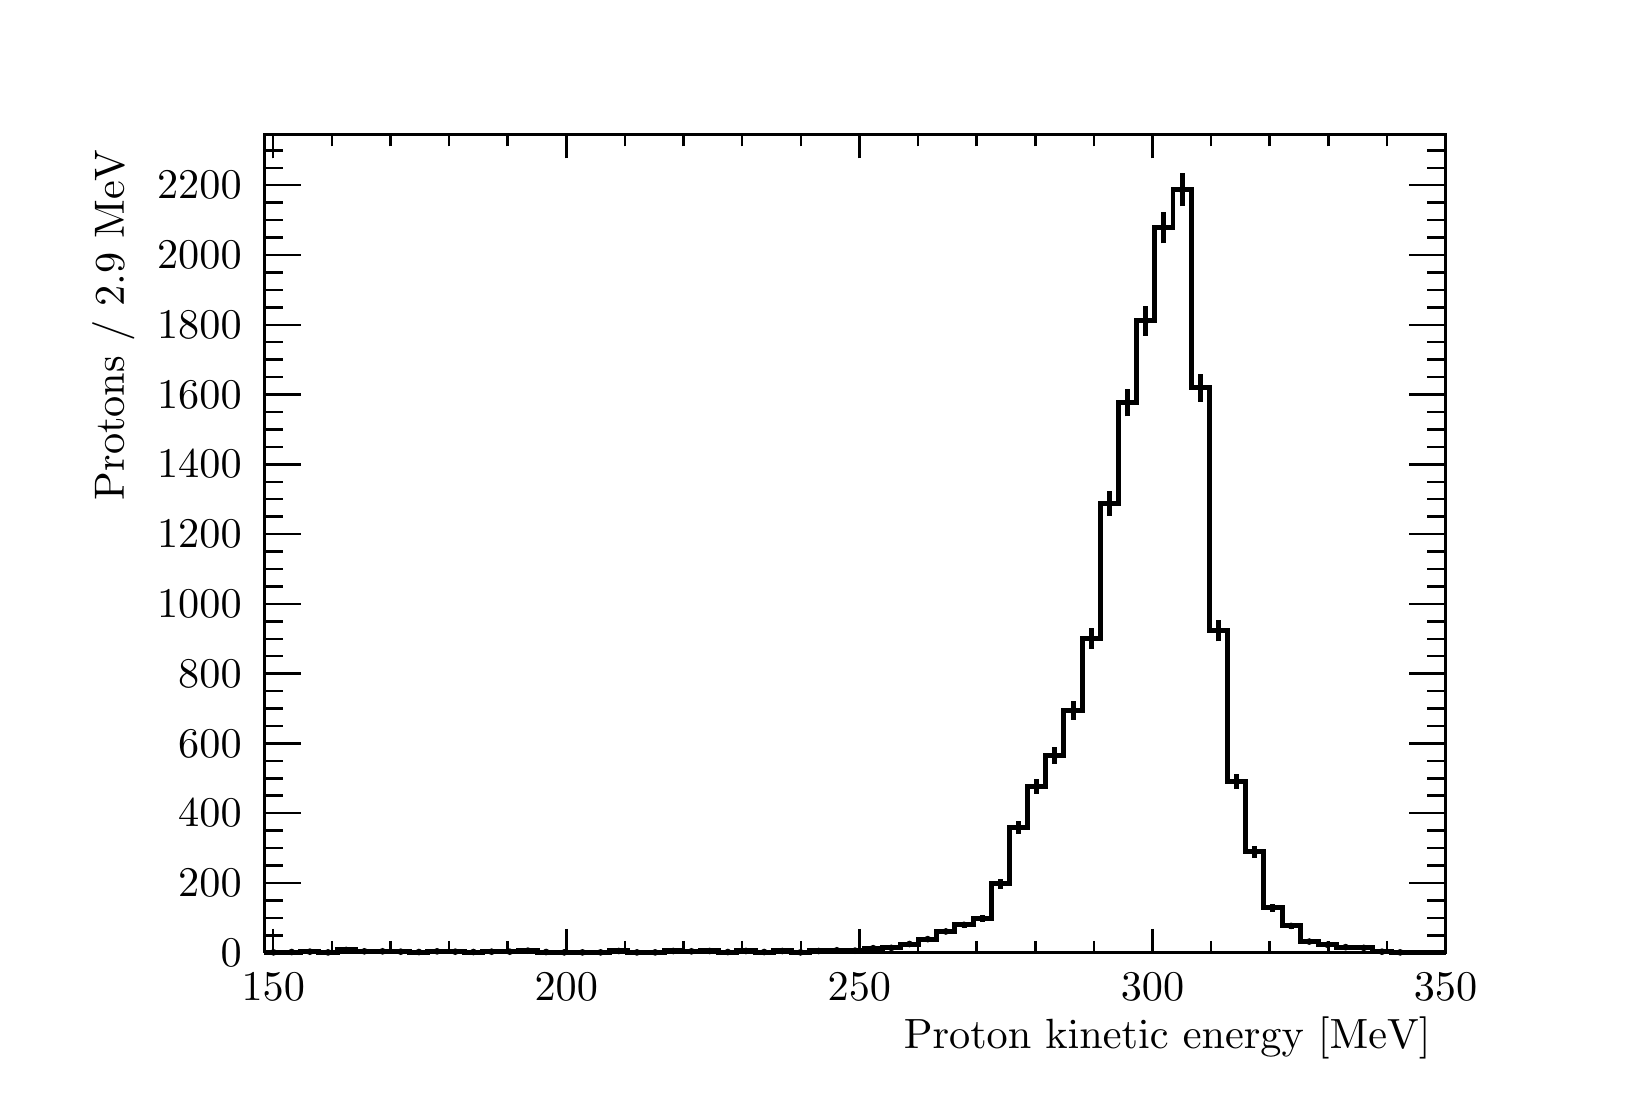
\begin{tikzpicture}
\pgfdeclareplotmark{cross} {
\pgfpathmoveto{\pgfpoint{-0.3\pgfplotmarksize}{\pgfplotmarksize}}
\pgfpathlineto{\pgfpoint{+0.3\pgfplotmarksize}{\pgfplotmarksize}}
\pgfpathlineto{\pgfpoint{+0.3\pgfplotmarksize}{0.3\pgfplotmarksize}}
\pgfpathlineto{\pgfpoint{+1\pgfplotmarksize}{0.3\pgfplotmarksize}}
\pgfpathlineto{\pgfpoint{+1\pgfplotmarksize}{-0.3\pgfplotmarksize}}
\pgfpathlineto{\pgfpoint{+0.3\pgfplotmarksize}{-0.3\pgfplotmarksize}}
\pgfpathlineto{\pgfpoint{+0.3\pgfplotmarksize}{-1.\pgfplotmarksize}}
\pgfpathlineto{\pgfpoint{-0.3\pgfplotmarksize}{-1.\pgfplotmarksize}}
\pgfpathlineto{\pgfpoint{-0.3\pgfplotmarksize}{-0.3\pgfplotmarksize}}
\pgfpathlineto{\pgfpoint{-1.\pgfplotmarksize}{-0.3\pgfplotmarksize}}
\pgfpathlineto{\pgfpoint{-1.\pgfplotmarksize}{0.3\pgfplotmarksize}}
\pgfpathlineto{\pgfpoint{-0.3\pgfplotmarksize}{0.3\pgfplotmarksize}}
\pgfpathclose
\pgfusepathqstroke
}
\pgfdeclareplotmark{cross*} {
\pgfpathmoveto{\pgfpoint{-0.3\pgfplotmarksize}{\pgfplotmarksize}}
\pgfpathlineto{\pgfpoint{+0.3\pgfplotmarksize}{\pgfplotmarksize}}
\pgfpathlineto{\pgfpoint{+0.3\pgfplotmarksize}{0.3\pgfplotmarksize}}
\pgfpathlineto{\pgfpoint{+1\pgfplotmarksize}{0.3\pgfplotmarksize}}
\pgfpathlineto{\pgfpoint{+1\pgfplotmarksize}{-0.3\pgfplotmarksize}}
\pgfpathlineto{\pgfpoint{+0.3\pgfplotmarksize}{-0.3\pgfplotmarksize}}
\pgfpathlineto{\pgfpoint{+0.3\pgfplotmarksize}{-1.\pgfplotmarksize}}
\pgfpathlineto{\pgfpoint{-0.3\pgfplotmarksize}{-1.\pgfplotmarksize}}
\pgfpathlineto{\pgfpoint{-0.3\pgfplotmarksize}{-0.3\pgfplotmarksize}}
\pgfpathlineto{\pgfpoint{-1.\pgfplotmarksize}{-0.3\pgfplotmarksize}}
\pgfpathlineto{\pgfpoint{-1.\pgfplotmarksize}{0.3\pgfplotmarksize}}
\pgfpathlineto{\pgfpoint{-0.3\pgfplotmarksize}{0.3\pgfplotmarksize}}
\pgfpathclose
\pgfusepathqfillstroke
}
\pgfdeclareplotmark{newstar} {
\pgfpathmoveto{\pgfqpoint{0pt}{\pgfplotmarksize}}
\pgfpathlineto{\pgfqpointpolar{44}{0.5\pgfplotmarksize}}
\pgfpathlineto{\pgfqpointpolar{18}{\pgfplotmarksize}}
\pgfpathlineto{\pgfqpointpolar{-20}{0.5\pgfplotmarksize}}
\pgfpathlineto{\pgfqpointpolar{-54}{\pgfplotmarksize}}
\pgfpathlineto{\pgfqpointpolar{-90}{0.5\pgfplotmarksize}}
\pgfpathlineto{\pgfqpointpolar{234}{\pgfplotmarksize}}
\pgfpathlineto{\pgfqpointpolar{198}{0.5\pgfplotmarksize}}
\pgfpathlineto{\pgfqpointpolar{162}{\pgfplotmarksize}}
\pgfpathlineto{\pgfqpointpolar{134}{0.5\pgfplotmarksize}}
\pgfpathclose
\pgfusepathqstroke
}
\pgfdeclareplotmark{newstar*} {
\pgfpathmoveto{\pgfqpoint{0pt}{\pgfplotmarksize}}
\pgfpathlineto{\pgfqpointpolar{44}{0.5\pgfplotmarksize}}
\pgfpathlineto{\pgfqpointpolar{18}{\pgfplotmarksize}}
\pgfpathlineto{\pgfqpointpolar{-20}{0.5\pgfplotmarksize}}
\pgfpathlineto{\pgfqpointpolar{-54}{\pgfplotmarksize}}
\pgfpathlineto{\pgfqpointpolar{-90}{0.5\pgfplotmarksize}}
\pgfpathlineto{\pgfqpointpolar{234}{\pgfplotmarksize}}
\pgfpathlineto{\pgfqpointpolar{198}{0.5\pgfplotmarksize}}
\pgfpathlineto{\pgfqpointpolar{162}{\pgfplotmarksize}}
\pgfpathlineto{\pgfqpointpolar{134}{0.5\pgfplotmarksize}}
\pgfpathclose
\pgfusepathqfillstroke
}
\definecolor{c}{rgb}{1,1,1};
\draw [color=c, fill=c] (0,0) rectangle (20,13.4957);
\draw [color=c, fill=c] (3,1.75444) rectangle (18,12.1461);
\definecolor{c}{rgb}{0,0,0};
\draw [c,line width=0.9] (3,1.75444) -- (3,12.1461) -- (18,12.1461) -- (18,1.75444) -- (3,1.75444);
\definecolor{c}{rgb}{1,1,1};
\draw [color=c, fill=c] (3,1.75444) rectangle (18,12.1461);
\definecolor{c}{rgb}{0,0,0};
\draw [c,line width=0.9] (3,1.75444) -- (3,12.1461) -- (18,12.1461) -- (18,1.75444) -- (3,1.75444);
\draw [c,line width=1.8] (3.11538,1.75444) -- (3.11538,1.75887);
\draw [c,line width=1.8] (3.11538,1.75887) -- (3.11538,1.7633);
\foreach \P in {(3.11538,1.75887)}{\draw[mark options={color=c,fill=c},mark size=2.402402pt,mark=*,mark size=1pt] plot coordinates {\P};}
\draw [c,line width=1.8] (3.34615,1.75704) -- (3.34615,1.7633);
\draw [c,line width=1.8] (3.34615,1.7633) -- (3.34615,1.76957);
\foreach \P in {(3.34615,1.7633)}{\draw[mark options={color=c,fill=c},mark size=2.402402pt,mark=*,mark size=1pt] plot coordinates {\P};}
\draw [c,line width=1.8] (3.57692,1.76006) -- (3.57692,1.76773);
\draw [c,line width=1.8] (3.57692,1.76773) -- (3.57692,1.77541);
\foreach \P in {(3.57692,1.76773)}{\draw[mark options={color=c,fill=c},mark size=2.402402pt,mark=*,mark size=1pt] plot coordinates {\P};}
\draw [c,line width=1.8] (3.80769,1.75444) -- (3.80769,1.75887);
\draw [c,line width=1.8] (3.80769,1.75887) -- (3.80769,1.7633);
\foreach \P in {(3.80769,1.75887)}{\draw[mark options={color=c,fill=c},mark size=2.402402pt,mark=*,mark size=1pt] plot coordinates {\P};}
\draw [c,line width=1.8] (4.03846,1.77735) -- (4.03846,1.78989);
\draw [c,line width=1.8] (4.03846,1.78989) -- (4.03846,1.80242);
\foreach \P in {(4.03846,1.78989)}{\draw[mark options={color=c,fill=c},mark size=2.402402pt,mark=*,mark size=1pt] plot coordinates {\P};}
\draw [c,line width=1.8] (4.26923,1.7633) -- (4.26923,1.77216);
\draw [c,line width=1.8] (4.26923,1.77216) -- (4.26923,1.78102);
\foreach \P in {(4.26923,1.77216)}{\draw[mark options={color=c,fill=c},mark size=2.402402pt,mark=*,mark size=1pt] plot coordinates {\P};}
\draw [c,line width=1.8] (4.5,1.7633) -- (4.5,1.77216);
\draw [c,line width=1.8] (4.5,1.77216) -- (4.5,1.78102);
\foreach \P in {(4.5,1.77216)}{\draw[mark options={color=c,fill=c},mark size=2.402402pt,mark=*,mark size=1pt] plot coordinates {\P};}
\draw [c,line width=1.8] (4.73077,1.76006) -- (4.73077,1.76773);
\draw [c,line width=1.8] (4.73077,1.76773) -- (4.73077,1.77541);
\foreach \P in {(4.73077,1.76773)}{\draw[mark options={color=c,fill=c},mark size=2.402402pt,mark=*,mark size=1pt] plot coordinates {\P};}
\draw [c,line width=1.8] (4.96154,1.75704) -- (4.96154,1.7633);
\draw [c,line width=1.8] (4.96154,1.7633) -- (4.96154,1.76957);
\foreach \P in {(4.96154,1.7633)}{\draw[mark options={color=c,fill=c},mark size=2.402402pt,mark=*,mark size=1pt] plot coordinates {\P};}
\draw [c,line width=1.8] (5.19231,1.7633) -- (5.19231,1.77216);
\draw [c,line width=1.8] (5.19231,1.77216) -- (5.19231,1.78102);
\foreach \P in {(5.19231,1.77216)}{\draw[mark options={color=c,fill=c},mark size=2.402402pt,mark=*,mark size=1pt] plot coordinates {\P};}
\draw [c,line width=1.8] (5.42308,1.76006) -- (5.42308,1.76773);
\draw [c,line width=1.8] (5.42308,1.76773) -- (5.42308,1.77541);
\foreach \P in {(5.42308,1.76773)}{\draw[mark options={color=c,fill=c},mark size=2.402402pt,mark=*,mark size=1pt] plot coordinates {\P};}
\draw [c,line width=1.8] (5.65385,1.75704) -- (5.65385,1.7633);
\draw [c,line width=1.8] (5.65385,1.7633) -- (5.65385,1.76957);
\foreach \P in {(5.65385,1.7633)}{\draw[mark options={color=c,fill=c},mark size=2.402402pt,mark=*,mark size=1pt] plot coordinates {\P};}
\draw [c,line width=1.8] (5.88462,1.76006) -- (5.88462,1.76773);
\draw [c,line width=1.8] (5.88462,1.76773) -- (5.88462,1.77541);
\foreach \P in {(5.88462,1.76773)}{\draw[mark options={color=c,fill=c},mark size=2.402402pt,mark=*,mark size=1pt] plot coordinates {\P};}
\draw [c,line width=1.8] (6.11538,1.76006) -- (6.11538,1.76773);
\draw [c,line width=1.8] (6.11538,1.76773) -- (6.11538,1.77541);
\foreach \P in {(6.11538,1.76773)}{\draw[mark options={color=c,fill=c},mark size=2.402402pt,mark=*,mark size=1pt] plot coordinates {\P};}
\draw [c,line width=1.8] (6.34615,1.77017) -- (6.34615,1.78102);
\draw [c,line width=1.8] (6.34615,1.78102) -- (6.34615,1.79188);
\foreach \P in {(6.34615,1.78102)}{\draw[mark options={color=c,fill=c},mark size=2.402402pt,mark=*,mark size=1pt] plot coordinates {\P};}
\draw [c,line width=1.8] (6.57692,1.75704) -- (6.57692,1.7633);
\draw [c,line width=1.8] (6.57692,1.7633) -- (6.57692,1.76957);
\foreach \P in {(6.57692,1.7633)}{\draw[mark options={color=c,fill=c},mark size=2.402402pt,mark=*,mark size=1pt] plot coordinates {\P};}
\draw [c,line width=1.8] (6.80769,1.75444) -- (6.80769,1.75887);
\draw [c,line width=1.8] (6.80769,1.75887) -- (6.80769,1.7633);
\foreach \P in {(6.80769,1.75887)}{\draw[mark options={color=c,fill=c},mark size=2.402402pt,mark=*,mark size=1pt] plot coordinates {\P};}
\draw [c,line width=1.8] (7.03846,1.75444) -- (7.03846,1.75887);
\draw [c,line width=1.8] (7.03846,1.75887) -- (7.03846,1.7633);
\foreach \P in {(7.03846,1.75887)}{\draw[mark options={color=c,fill=c},mark size=2.402402pt,mark=*,mark size=1pt] plot coordinates {\P};}
\draw [c,line width=1.8] (7.26923,1.75444) -- (7.26923,1.75887);
\draw [c,line width=1.8] (7.26923,1.75887) -- (7.26923,1.7633);
\foreach \P in {(7.26923,1.75887)}{\draw[mark options={color=c,fill=c},mark size=2.402402pt,mark=*,mark size=1pt] plot coordinates {\P};}
\draw [c,line width=1.8] (7.5,1.76669) -- (7.5,1.77659);
\draw [c,line width=1.8] (7.5,1.77659) -- (7.5,1.7865);
\foreach \P in {(7.5,1.77659)}{\draw[mark options={color=c,fill=c},mark size=2.402402pt,mark=*,mark size=1pt] plot coordinates {\P};}
\draw [c,line width=1.8] (7.73077,1.75444) -- (7.73077,1.75887);
\draw [c,line width=1.8] (7.73077,1.75887) -- (7.73077,1.7633);
\foreach \P in {(7.73077,1.75887)}{\draw[mark options={color=c,fill=c},mark size=2.402402pt,mark=*,mark size=1pt] plot coordinates {\P};}
\draw [c,line width=1.8] (7.96154,1.75444) -- (7.96154,1.75887);
\draw [c,line width=1.8] (7.96154,1.75887) -- (7.96154,1.7633);
\foreach \P in {(7.96154,1.75887)}{\draw[mark options={color=c,fill=c},mark size=2.402402pt,mark=*,mark size=1pt] plot coordinates {\P};}
\draw [c,line width=1.8] (8.19231,1.76669) -- (8.19231,1.77659);
\draw [c,line width=1.8] (8.19231,1.77659) -- (8.19231,1.7865);
\foreach \P in {(8.19231,1.77659)}{\draw[mark options={color=c,fill=c},mark size=2.402402pt,mark=*,mark size=1pt] plot coordinates {\P};}
\draw [c,line width=1.8] (8.42308,1.7633) -- (8.42308,1.77216);
\draw [c,line width=1.8] (8.42308,1.77216) -- (8.42308,1.78102);
\foreach \P in {(8.42308,1.77216)}{\draw[mark options={color=c,fill=c},mark size=2.402402pt,mark=*,mark size=1pt] plot coordinates {\P};}
\draw [c,line width=1.8] (8.65385,1.76669) -- (8.65385,1.77659);
\draw [c,line width=1.8] (8.65385,1.77659) -- (8.65385,1.7865);
\foreach \P in {(8.65385,1.77659)}{\draw[mark options={color=c,fill=c},mark size=2.402402pt,mark=*,mark size=1pt] plot coordinates {\P};}
\draw [c,line width=1.8] (8.88462,1.75704) -- (8.88462,1.7633);
\draw [c,line width=1.8] (8.88462,1.7633) -- (8.88462,1.76957);
\foreach \P in {(8.88462,1.7633)}{\draw[mark options={color=c,fill=c},mark size=2.402402pt,mark=*,mark size=1pt] plot coordinates {\P};}
\draw [c,line width=1.8] (9.11539,1.76669) -- (9.11539,1.77659);
\draw [c,line width=1.8] (9.11539,1.77659) -- (9.11539,1.7865);
\foreach \P in {(9.11539,1.77659)}{\draw[mark options={color=c,fill=c},mark size=2.402402pt,mark=*,mark size=1pt] plot coordinates {\P};}
\draw [c,line width=1.8] (9.34615,1.75704) -- (9.34615,1.7633);
\draw [c,line width=1.8] (9.34615,1.7633) -- (9.34615,1.76957);
\foreach \P in {(9.34615,1.7633)}{\draw[mark options={color=c,fill=c},mark size=2.402402pt,mark=*,mark size=1pt] plot coordinates {\P};}
\draw [c,line width=1.8] (9.57692,1.76669) -- (9.57692,1.77659);
\draw [c,line width=1.8] (9.57692,1.77659) -- (9.57692,1.7865);
\foreach \P in {(9.57692,1.77659)}{\draw[mark options={color=c,fill=c},mark size=2.402402pt,mark=*,mark size=1pt] plot coordinates {\P};}
\draw [c,line width=1.8] (9.80769,1.75444) -- (9.80769,1.75887);
\draw [c,line width=1.8] (9.80769,1.75887) -- (9.80769,1.7633);
\foreach \P in {(9.80769,1.75887)}{\draw[mark options={color=c,fill=c},mark size=2.402402pt,mark=*,mark size=1pt] plot coordinates {\P};}
\draw [c,line width=1.8] (10.0385,1.76669) -- (10.0385,1.77659);
\draw [c,line width=1.8] (10.0385,1.77659) -- (10.0385,1.7865);
\foreach \P in {(10.0385,1.77659)}{\draw[mark options={color=c,fill=c},mark size=2.402402pt,mark=*,mark size=1pt] plot coordinates {\P};}
\draw [c,line width=1.8] (10.2692,1.77373) -- (10.2692,1.78546);
\draw [c,line width=1.8] (10.2692,1.78546) -- (10.2692,1.79718);
\foreach \P in {(10.2692,1.78546)}{\draw[mark options={color=c,fill=c},mark size=2.402402pt,mark=*,mark size=1pt] plot coordinates {\P};}
\draw [c,line width=1.8] (10.5,1.77017) -- (10.5,1.78102);
\draw [c,line width=1.8] (10.5,1.78102) -- (10.5,1.79188);
\foreach \P in {(10.5,1.78102)}{\draw[mark options={color=c,fill=c},mark size=2.402402pt,mark=*,mark size=1pt] plot coordinates {\P};}
\draw [c,line width=1.8] (10.7308,1.79606) -- (10.7308,1.81204);
\draw [c,line width=1.8] (10.7308,1.81204) -- (10.7308,1.82801);
\foreach \P in {(10.7308,1.81204)}{\draw[mark options={color=c,fill=c},mark size=2.402402pt,mark=*,mark size=1pt] plot coordinates {\P};}
\draw [c,line width=1.8] (10.9615,1.79989) -- (10.9615,1.81647);
\draw [c,line width=1.8] (10.9615,1.81647) -- (10.9615,1.83305);
\foreach \P in {(10.9615,1.81647)}{\draw[mark options={color=c,fill=c},mark size=2.402402pt,mark=*,mark size=1pt] plot coordinates {\P};}
\draw [c,line width=1.8] (11.1923,1.84305) -- (11.1923,1.86521);
\draw [c,line width=1.8] (11.1923,1.86521) -- (11.1923,1.88736);
\foreach \P in {(11.1923,1.86521)}{\draw[mark options={color=c,fill=c},mark size=2.402402pt,mark=*,mark size=1pt] plot coordinates {\P};}
\draw [c,line width=1.8] (11.4231,1.89956) -- (11.4231,1.92723);
\draw [c,line width=1.8] (11.4231,1.92723) -- (11.4231,1.9549);
\foreach \P in {(11.4231,1.92723)}{\draw[mark options={color=c,fill=c},mark size=2.402402pt,mark=*,mark size=1pt] plot coordinates {\P};}
\draw [c,line width=1.8] (11.6538,1.9901) -- (11.6538,2.02471);
\draw [c,line width=1.8] (11.6538,2.02471) -- (11.6538,2.05931);
\foreach \P in {(11.6538,2.02471)}{\draw[mark options={color=c,fill=c},mark size=2.402402pt,mark=*,mark size=1pt] plot coordinates {\P};}
\draw [c,line width=1.8] (11.8846,2.06926) -- (11.8846,2.10889);
\draw [c,line width=1.8] (11.8846,2.10889) -- (11.8846,2.14851);
\foreach \P in {(11.8846,2.10889)}{\draw[mark options={color=c,fill=c},mark size=2.402402pt,mark=*,mark size=1pt] plot coordinates {\P};}
\draw [c,line width=1.8] (12.1154,2.14478) -- (12.1154,2.18864);
\draw [c,line width=1.8] (12.1154,2.18864) -- (12.1154,2.2325);
\foreach \P in {(12.1154,2.18864)}{\draw[mark options={color=c,fill=c},mark size=2.402402pt,mark=*,mark size=1pt] plot coordinates {\P};}
\draw [c,line width=1.8] (12.3462,2.56935) -- (12.3462,2.63169);
\draw [c,line width=1.8] (12.3462,2.63169) -- (12.3462,2.69404);
\foreach \P in {(12.3462,2.63169)}{\draw[mark options={color=c,fill=c},mark size=2.402402pt,mark=*,mark size=1pt] plot coordinates {\P};}
\draw [c,line width=1.8] (12.5769,3.26538) -- (12.5769,3.34945);
\draw [c,line width=1.8] (12.5769,3.34945) -- (12.5769,3.43351);
\foreach \P in {(12.5769,3.34945)}{\draw[mark options={color=c,fill=c},mark size=2.402402pt,mark=*,mark size=1pt] plot coordinates {\P};}
\draw [c,line width=1.8] (12.8077,3.77106) -- (12.8077,3.86782);
\draw [c,line width=1.8] (12.8077,3.86782) -- (12.8077,3.96459);
\foreach \P in {(12.8077,3.86782)}{\draw[mark options={color=c,fill=c},mark size=2.402402pt,mark=*,mark size=1pt] plot coordinates {\P};}
\draw [c,line width=1.8] (13.0385,4.1524) -- (13.0385,4.25771);
\draw [c,line width=1.8] (13.0385,4.25771) -- (13.0385,4.36303);
\foreach \P in {(13.0385,4.25771)}{\draw[mark options={color=c,fill=c},mark size=2.402402pt,mark=*,mark size=1pt] plot coordinates {\P};}
\draw [c,line width=1.8] (13.2692,4.71254) -- (13.2692,4.82926);
\draw [c,line width=1.8] (13.2692,4.82926) -- (13.2692,4.94597);
\foreach \P in {(13.2692,4.82926)}{\draw[mark options={color=c,fill=c},mark size=2.402402pt,mark=*,mark size=1pt] plot coordinates {\P};}
\draw [c,line width=1.8] (13.5,5.60904) -- (13.5,5.74195);
\draw [c,line width=1.8] (13.5,5.74195) -- (13.5,5.87487);
\foreach \P in {(13.5,5.74195)}{\draw[mark options={color=c,fill=c},mark size=2.402402pt,mark=*,mark size=1pt] plot coordinates {\P};}
\draw [c,line width=1.8] (13.7308,7.302) -- (13.7308,7.46101);
\draw [c,line width=1.8] (13.7308,7.46101) -- (13.7308,7.62002);
\foreach \P in {(13.7308,7.46101)}{\draw[mark options={color=c,fill=c},mark size=2.402402pt,mark=*,mark size=1pt] plot coordinates {\P};}
\draw [c,line width=1.8] (13.9615,8.5655) -- (13.9615,8.74145);
\draw [c,line width=1.8] (13.9615,8.74145) -- (13.9615,8.91739);
\foreach \P in {(13.9615,8.74145)}{\draw[mark options={color=c,fill=c},mark size=2.402402pt,mark=*,mark size=1pt] plot coordinates {\P};}
\draw [c,line width=1.8] (14.1923,9.58965) -- (14.1923,9.7782);
\draw [c,line width=1.8] (14.1923,9.7782) -- (14.1923,9.96675);
\foreach \P in {(14.1923,9.7782)}{\draw[mark options={color=c,fill=c},mark size=2.402402pt,mark=*,mark size=1pt] plot coordinates {\P};}
\draw [c,line width=1.8] (14.4231,10.7636) -- (14.4231,10.9656);
\draw [c,line width=1.8] (14.4231,10.9656) -- (14.4231,11.1676);
\foreach \P in {(14.4231,10.9656)}{\draw[mark options={color=c,fill=c},mark size=2.402402pt,mark=*,mark size=1pt] plot coordinates {\P};}
\draw [c,line width=1.8] (14.6538,11.2369) -- (14.6538,11.4441);
\draw [c,line width=1.8] (14.6538,11.4441) -- (14.6538,11.6513);
\foreach \P in {(14.6538,11.4441)}{\draw[mark options={color=c,fill=c},mark size=2.402402pt,mark=*,mark size=1pt] plot coordinates {\P};}
\draw [c,line width=1.8] (14.8846,8.75363) -- (14.8846,8.93196);
\draw [c,line width=1.8] (14.8846,8.93196) -- (14.8846,9.11029);
\foreach \P in {(14.8846,8.93196)}{\draw[mark options={color=c,fill=c},mark size=2.402402pt,mark=*,mark size=1pt] plot coordinates {\P};}
\draw [c,line width=1.8] (15.1154,5.70925) -- (15.1154,5.84385);
\draw [c,line width=1.8] (15.1154,5.84385) -- (15.1154,5.97846);
\foreach \P in {(15.1154,5.84385)}{\draw[mark options={color=c,fill=c},mark size=2.402402pt,mark=*,mark size=1pt] plot coordinates {\P};}
\draw [c,line width=1.8] (15.3462,3.83168) -- (15.3462,3.92985);
\draw [c,line width=1.8] (15.3462,3.92985) -- (15.3462,4.02802);
\foreach \P in {(15.3462,3.92985)}{\draw[mark options={color=c,fill=c},mark size=2.402402pt,mark=*,mark size=1pt] plot coordinates {\P};}
\draw [c,line width=1.8] (15.5769,2.95956) -- (15.5769,3.03488);
\draw [c,line width=1.8] (15.5769,3.03488) -- (15.5769,3.11019);
\foreach \P in {(15.5769,3.03488)}{\draw[mark options={color=c,fill=c},mark size=2.402402pt,mark=*,mark size=1pt] plot coordinates {\P};}
\draw [c,line width=1.8] (15.8077,2.27566) -- (15.8077,2.32598);
\draw [c,line width=1.8] (15.8077,2.32598) -- (15.8077,2.37631);
\foreach \P in {(15.8077,2.32598)}{\draw[mark options={color=c,fill=c},mark size=2.402402pt,mark=*,mark size=1pt] plot coordinates {\P};}
\draw [c,line width=1.8] (16.0385,2.05672) -- (16.0385,2.09559);
\draw [c,line width=1.8] (16.0385,2.09559) -- (16.0385,2.13447);
\foreach \P in {(16.0385,2.09559)}{\draw[mark options={color=c,fill=c},mark size=2.402402pt,mark=*,mark size=1pt] plot coordinates {\P};}
\draw [c,line width=1.8] (16.2692,1.87116) -- (16.2692,1.89622);
\draw [c,line width=1.8] (16.2692,1.89622) -- (16.2692,1.92128);
\foreach \P in {(16.2692,1.89622)}{\draw[mark options={color=c,fill=c},mark size=2.402402pt,mark=*,mark size=1pt] plot coordinates {\P};}
\draw [c,line width=1.8] (16.5,1.8351) -- (16.5,1.85634);
\draw [c,line width=1.8] (16.5,1.85634) -- (16.5,1.87759);
\foreach \P in {(16.5,1.85634)}{\draw[mark options={color=c,fill=c},mark size=2.402402pt,mark=*,mark size=1pt] plot coordinates {\P};}
\draw [c,line width=1.8] (16.7308,1.80761) -- (16.7308,1.82533);
\draw [c,line width=1.8] (16.7308,1.82533) -- (16.7308,1.84305);
\foreach \P in {(16.7308,1.82533)}{\draw[mark options={color=c,fill=c},mark size=2.402402pt,mark=*,mark size=1pt] plot coordinates {\P};}
\draw [c,line width=1.8] (16.9615,1.79989) -- (16.9615,1.81647);
\draw [c,line width=1.8] (16.9615,1.81647) -- (16.9615,1.83305);
\foreach \P in {(16.9615,1.81647)}{\draw[mark options={color=c,fill=c},mark size=2.402402pt,mark=*,mark size=1pt] plot coordinates {\P};}
\draw [c,line width=1.8] (17.1923,1.76006) -- (17.1923,1.76773);
\draw [c,line width=1.8] (17.1923,1.76773) -- (17.1923,1.77541);
\foreach \P in {(17.1923,1.76773)}{\draw[mark options={color=c,fill=c},mark size=2.402402pt,mark=*,mark size=1pt] plot coordinates {\P};}
\draw [c,line width=1.8] (17.4231,1.75444) -- (17.4231,1.75887);
\draw [c,line width=1.8] (17.4231,1.75887) -- (17.4231,1.7633);
\foreach \P in {(17.4231,1.75887)}{\draw[mark options={color=c,fill=c},mark size=2.402402pt,mark=*,mark size=1pt] plot coordinates {\P};}
\draw [c,line width=1.8] (3,1.75887) -- (3.23077,1.75887) -- (3.23077,1.7633) -- (3.46154,1.7633) -- (3.46154,1.76773) -- (3.69231,1.76773) -- (3.69231,1.75887) -- (3.92308,1.75887) -- (3.92308,1.78989) -- (4.15385,1.78989) -- (4.15385,1.77216) --
 (4.38462,1.77216) -- (4.38462,1.77216) -- (4.61538,1.77216) -- (4.61538,1.76773) -- (4.84615,1.76773) -- (4.84615,1.7633) -- (5.07692,1.7633) -- (5.07692,1.77216) -- (5.30769,1.77216) -- (5.30769,1.76773) -- (5.53846,1.76773) -- (5.53846,1.7633) --
 (5.76923,1.7633) -- (5.76923,1.76773) -- (6,1.76773) -- (6,1.76773) -- (6.23077,1.76773) -- (6.23077,1.78102) -- (6.46154,1.78102) -- (6.46154,1.7633) -- (6.69231,1.7633) -- (6.69231,1.75887) -- (6.92308,1.75887) -- (6.92308,1.75887) --
 (7.15385,1.75887) -- (7.15385,1.75887) -- (7.38462,1.75887) -- (7.38462,1.77659) -- (7.61538,1.77659) -- (7.61538,1.75887) -- (7.84615,1.75887) -- (7.84615,1.75887) -- (8.07692,1.75887) -- (8.07692,1.77659) -- (8.30769,1.77659) -- (8.30769,1.77216)
 -- (8.53846,1.77216) -- (8.53846,1.77659) -- (8.76923,1.77659) -- (8.76923,1.7633) -- (9,1.7633) -- (9,1.77659) -- (9.23077,1.77659) -- (9.23077,1.7633) -- (9.46154,1.7633) -- (9.46154,1.77659) -- (9.69231,1.77659) -- (9.69231,1.75887) --
 (9.92308,1.75887) -- (9.92308,1.77659) -- (10.1538,1.77659) -- (10.1538,1.78546) -- (10.3846,1.78546) -- (10.3846,1.78102) -- (10.6154,1.78102) -- (10.6154,1.81204) -- (10.8462,1.81204) -- (10.8462,1.81647) -- (11.0769,1.81647) -- (11.0769,1.86521)
 -- (11.3077,1.86521) -- (11.3077,1.92723) -- (11.5385,1.92723) -- (11.5385,2.02471) -- (11.7692,2.02471) -- (11.7692,2.10889) -- (12,2.10889) -- (12,2.18864) -- (12.2308,2.18864) -- (12.2308,2.63169) -- (12.4615,2.63169) -- (12.4615,3.34945) --
 (12.6923,3.34945) -- (12.6923,3.86782) -- (12.9231,3.86782) -- (12.9231,4.25771) -- (13.1538,4.25771) -- (13.1538,4.82926) -- (13.3846,4.82926) -- (13.3846,5.74195) -- (13.6154,5.74195) -- (13.6154,7.46101) -- (13.8462,7.46101) -- (13.8462,8.74145)
 -- (14.0769,8.74145) -- (14.0769,9.7782) -- (14.3077,9.7782) -- (14.3077,10.9656) -- (14.5385,10.9656) -- (14.5385,11.4441) -- (14.7692,11.4441) -- (14.7692,8.93196) -- (15,8.93196) -- (15,5.84385) -- (15.2308,5.84385) -- (15.2308,3.92985) --
 (15.4615,3.92985) -- (15.4615,3.03488) -- (15.6923,3.03488) -- (15.6923,2.32598) -- (15.9231,2.32598) -- (15.9231,2.09559) -- (16.1538,2.09559) -- (16.1538,1.89622) -- (16.3846,1.89622) -- (16.3846,1.85634) -- (16.6154,1.85634) -- (16.6154,1.82533)
 -- (16.8462,1.82533) -- (16.8462,1.81647) -- (17.0769,1.81647) -- (17.0769,1.76773) -- (17.3077,1.76773) -- (17.3077,1.75887) -- (17.5385,1.75887) -- (17.5385,1.75444) -- (17.7692,1.75444) -- (17.7692,1.75444) -- (18,1.75444);
\draw [c,line width=0.9] (3,1.75444) -- (18,1.75444);
\draw [c,line width=0.9] (3.11166,2.05809) -- (3.11166,1.75444);
\draw [c,line width=0.9] (3.85608,1.90627) -- (3.85608,1.75444);
\draw [c,line width=0.9] (4.6005,1.90627) -- (4.6005,1.75444);
\draw [c,line width=0.9] (5.34491,1.90627) -- (5.34491,1.75444);
\draw [c,line width=0.9] (6.08933,1.90627) -- (6.08933,1.75444);
\draw [c,line width=0.9] (6.83375,2.05809) -- (6.83375,1.75444);
\draw [c,line width=0.9] (7.57816,1.90627) -- (7.57816,1.75444);
\draw [c,line width=0.9] (8.32258,1.90627) -- (8.32258,1.75444);
\draw [c,line width=0.9] (9.067,1.90627) -- (9.067,1.75444);
\draw [c,line width=0.9] (9.81141,1.90627) -- (9.81141,1.75444);
\draw [c,line width=0.9] (10.5558,2.05809) -- (10.5558,1.75444);
\draw [c,line width=0.9] (11.3002,1.90627) -- (11.3002,1.75444);
\draw [c,line width=0.9] (12.0447,1.90627) -- (12.0447,1.75444);
\draw [c,line width=0.9] (12.7891,1.90627) -- (12.7891,1.75444);
\draw [c,line width=0.9] (13.5335,1.90627) -- (13.5335,1.75444);
\draw [c,line width=0.9] (14.2779,2.05809) -- (14.2779,1.75444);
\draw [c,line width=0.9] (15.0223,1.90627) -- (15.0223,1.75444);
\draw [c,line width=0.9] (15.7667,1.90627) -- (15.7667,1.75444);
\draw [c,line width=0.9] (16.5112,1.90627) -- (16.5112,1.75444);
\draw [c,line width=0.9] (17.2556,1.90627) -- (17.2556,1.75444);
\draw [c,line width=0.9] (18,2.05809) -- (18,1.75444);
\draw [c,line width=0.9] (3.11166,2.05809) -- (3.11166,1.75444);
\draw [c,line width=0.9] (18,2.05809) -- (18,1.75444);
\draw [anchor=base] (3.11166,1.14713) node[scale=1.52731, color=c, rotate=0]{150};
\draw [anchor=base] (6.83375,1.14713) node[scale=1.52731, color=c, rotate=0]{200};
\draw [anchor=base] (10.5558,1.14713) node[scale=1.52731, color=c, rotate=0]{250};
\draw [anchor=base] (14.2779,1.14713) node[scale=1.52731, color=c, rotate=0]{300};
\draw [anchor=base] (18,1.14713) node[scale=1.52731, color=c, rotate=0]{350};
\draw [anchor= east] (18,0.674785) node[scale=1.52731, color=c, rotate=0]{ Proton kinetic energy [MeV]};
\draw [c,line width=0.9] (3,12.1461) -- (18,12.1461);
\draw [c,line width=0.9] (3.11166,11.8425) -- (3.11166,12.1461);
\draw [c,line width=0.9] (3.85608,11.9943) -- (3.85608,12.1461);
\draw [c,line width=0.9] (4.6005,11.9943) -- (4.6005,12.1461);
\draw [c,line width=0.9] (5.34491,11.9943) -- (5.34491,12.1461);
\draw [c,line width=0.9] (6.08933,11.9943) -- (6.08933,12.1461);
\draw [c,line width=0.9] (6.83375,11.8425) -- (6.83375,12.1461);
\draw [c,line width=0.9] (7.57816,11.9943) -- (7.57816,12.1461);
\draw [c,line width=0.9] (8.32258,11.9943) -- (8.32258,12.1461);
\draw [c,line width=0.9] (9.067,11.9943) -- (9.067,12.1461);
\draw [c,line width=0.9] (9.81141,11.9943) -- (9.81141,12.1461);
\draw [c,line width=0.9] (10.5558,11.8425) -- (10.5558,12.1461);
\draw [c,line width=0.9] (11.3002,11.9943) -- (11.3002,12.1461);
\draw [c,line width=0.9] (12.0447,11.9943) -- (12.0447,12.1461);
\draw [c,line width=0.9] (12.7891,11.9943) -- (12.7891,12.1461);
\draw [c,line width=0.9] (13.5335,11.9943) -- (13.5335,12.1461);
\draw [c,line width=0.9] (14.2779,11.8425) -- (14.2779,12.1461);
\draw [c,line width=0.9] (15.0223,11.9943) -- (15.0223,12.1461);
\draw [c,line width=0.9] (15.7667,11.9943) -- (15.7667,12.1461);
\draw [c,line width=0.9] (16.5112,11.9943) -- (16.5112,12.1461);
\draw [c,line width=0.9] (17.2556,11.9943) -- (17.2556,12.1461);
\draw [c,line width=0.9] (18,11.8425) -- (18,12.1461);
\draw [c,line width=0.9] (3.11166,11.8425) -- (3.11166,12.1461);
\draw [c,line width=0.9] (18,11.8425) -- (18,12.1461);
\draw [c,line width=0.9] (3,1.75444) -- (3,12.1461);
\draw [c,line width=0.9] (3.462,1.75444) -- (3,1.75444);
\draw [c,line width=0.9] (3.231,1.97597) -- (3,1.97597);
\draw [c,line width=0.9] (3.231,2.1975) -- (3,2.1975);
\draw [c,line width=0.9] (3.231,2.41903) -- (3,2.41903);
\draw [c,line width=0.9] (3.462,2.64055) -- (3,2.64055);
\draw [c,line width=0.9] (3.231,2.86208) -- (3,2.86208);
\draw [c,line width=0.9] (3.231,3.08361) -- (3,3.08361);
\draw [c,line width=0.9] (3.231,3.30514) -- (3,3.30514);
\draw [c,line width=0.9] (3.462,3.52667) -- (3,3.52667);
\draw [c,line width=0.9] (3.231,3.7482) -- (3,3.7482);
\draw [c,line width=0.9] (3.231,3.96972) -- (3,3.96972);
\draw [c,line width=0.9] (3.231,4.19125) -- (3,4.19125);
\draw [c,line width=0.9] (3.462,4.41278) -- (3,4.41278);
\draw [c,line width=0.9] (3.231,4.63431) -- (3,4.63431);
\draw [c,line width=0.9] (3.231,4.85584) -- (3,4.85584);
\draw [c,line width=0.9] (3.231,5.07737) -- (3,5.07737);
\draw [c,line width=0.9] (3.462,5.29889) -- (3,5.29889);
\draw [c,line width=0.9] (3.231,5.52042) -- (3,5.52042);
\draw [c,line width=0.9] (3.231,5.74195) -- (3,5.74195);
\draw [c,line width=0.9] (3.231,5.96348) -- (3,5.96348);
\draw [c,line width=0.9] (3.462,6.18501) -- (3,6.18501);
\draw [c,line width=0.9] (3.231,6.40654) -- (3,6.40654);
\draw [c,line width=0.9] (3.231,6.62807) -- (3,6.62807);
\draw [c,line width=0.9] (3.231,6.84959) -- (3,6.84959);
\draw [c,line width=0.9] (3.462,7.07112) -- (3,7.07112);
\draw [c,line width=0.9] (3.231,7.29265) -- (3,7.29265);
\draw [c,line width=0.9] (3.231,7.51418) -- (3,7.51418);
\draw [c,line width=0.9] (3.231,7.73571) -- (3,7.73571);
\draw [c,line width=0.9] (3.462,7.95724) -- (3,7.95724);
\draw [c,line width=0.9] (3.231,8.17876) -- (3,8.17876);
\draw [c,line width=0.9] (3.231,8.40029) -- (3,8.40029);
\draw [c,line width=0.9] (3.231,8.62182) -- (3,8.62182);
\draw [c,line width=0.9] (3.462,8.84335) -- (3,8.84335);
\draw [c,line width=0.9] (3.231,9.06488) -- (3,9.06488);
\draw [c,line width=0.9] (3.231,9.28641) -- (3,9.28641);
\draw [c,line width=0.9] (3.231,9.50793) -- (3,9.50793);
\draw [c,line width=0.9] (3.462,9.72946) -- (3,9.72946);
\draw [c,line width=0.9] (3.231,9.95099) -- (3,9.95099);
\draw [c,line width=0.9] (3.231,10.1725) -- (3,10.1725);
\draw [c,line width=0.9] (3.231,10.394) -- (3,10.394);
\draw [c,line width=0.9] (3.462,10.6156) -- (3,10.6156);
\draw [c,line width=0.9] (3.231,10.8371) -- (3,10.8371);
\draw [c,line width=0.9] (3.231,11.0586) -- (3,11.0586);
\draw [c,line width=0.9] (3.231,11.2802) -- (3,11.2802);
\draw [c,line width=0.9] (3.462,11.5017) -- (3,11.5017);
\draw [c,line width=0.9] (3.462,11.5017) -- (3,11.5017);
\draw [c,line width=0.9] (3.231,11.7232) -- (3,11.7232);
\draw [c,line width=0.9] (3.231,11.9447) -- (3,11.9447);
\draw [anchor= east] (2.9,1.75444) node[scale=1.52731, color=c, rotate=0]{0};
\draw [anchor= east] (2.9,2.64055) node[scale=1.52731, color=c, rotate=0]{200};
\draw [anchor= east] (2.9,3.52667) node[scale=1.52731, color=c, rotate=0]{400};
\draw [anchor= east] (2.9,4.41278) node[scale=1.52731, color=c, rotate=0]{600};
\draw [anchor= east] (2.9,5.29889) node[scale=1.52731, color=c, rotate=0]{800};
\draw [anchor= east] (2.9,6.18501) node[scale=1.52731, color=c, rotate=0]{1000};
\draw [anchor= east] (2.9,7.07112) node[scale=1.52731, color=c, rotate=0]{1200};
\draw [anchor= east] (2.9,7.95724) node[scale=1.52731, color=c, rotate=0]{1400};
\draw [anchor= east] (2.9,8.84335) node[scale=1.52731, color=c, rotate=0]{1600};
\draw [anchor= east] (2.9,9.72946) node[scale=1.52731, color=c, rotate=0]{1800};
\draw [anchor= east] (2.9,10.6156) node[scale=1.52731, color=c, rotate=0]{2000};
\draw [anchor= east] (2.9,11.5017) node[scale=1.52731, color=c, rotate=0]{2200};
\draw [anchor= east] (1.08,12.1461) node[scale=1.52731, color=c, rotate=90]{Protons / 2.9~MeV};
\draw [c,line width=0.9] (18,1.75444) -- (18,12.1461);
\draw [c,line width=0.9] (17.538,1.75444) -- (18,1.75444);
\draw [c,line width=0.9] (17.769,1.97597) -- (18,1.97597);
\draw [c,line width=0.9] (17.769,2.1975) -- (18,2.1975);
\draw [c,line width=0.9] (17.769,2.41903) -- (18,2.41903);
\draw [c,line width=0.9] (17.538,2.64055) -- (18,2.64055);
\draw [c,line width=0.9] (17.769,2.86208) -- (18,2.86208);
\draw [c,line width=0.9] (17.769,3.08361) -- (18,3.08361);
\draw [c,line width=0.9] (17.769,3.30514) -- (18,3.30514);
\draw [c,line width=0.9] (17.538,3.52667) -- (18,3.52667);
\draw [c,line width=0.9] (17.769,3.7482) -- (18,3.7482);
\draw [c,line width=0.9] (17.769,3.96972) -- (18,3.96972);
\draw [c,line width=0.9] (17.769,4.19125) -- (18,4.19125);
\draw [c,line width=0.9] (17.538,4.41278) -- (18,4.41278);
\draw [c,line width=0.9] (17.769,4.63431) -- (18,4.63431);
\draw [c,line width=0.9] (17.769,4.85584) -- (18,4.85584);
\draw [c,line width=0.9] (17.769,5.07737) -- (18,5.07737);
\draw [c,line width=0.9] (17.538,5.29889) -- (18,5.29889);
\draw [c,line width=0.9] (17.769,5.52042) -- (18,5.52042);
\draw [c,line width=0.9] (17.769,5.74195) -- (18,5.74195);
\draw [c,line width=0.9] (17.769,5.96348) -- (18,5.96348);
\draw [c,line width=0.9] (17.538,6.18501) -- (18,6.18501);
\draw [c,line width=0.9] (17.769,6.40654) -- (18,6.40654);
\draw [c,line width=0.9] (17.769,6.62807) -- (18,6.62807);
\draw [c,line width=0.9] (17.769,6.84959) -- (18,6.84959);
\draw [c,line width=0.9] (17.538,7.07112) -- (18,7.07112);
\draw [c,line width=0.9] (17.769,7.29265) -- (18,7.29265);
\draw [c,line width=0.9] (17.769,7.51418) -- (18,7.51418);
\draw [c,line width=0.9] (17.769,7.73571) -- (18,7.73571);
\draw [c,line width=0.9] (17.538,7.95724) -- (18,7.95724);
\draw [c,line width=0.9] (17.769,8.17876) -- (18,8.17876);
\draw [c,line width=0.9] (17.769,8.40029) -- (18,8.40029);
\draw [c,line width=0.9] (17.769,8.62182) -- (18,8.62182);
\draw [c,line width=0.9] (17.538,8.84335) -- (18,8.84335);
\draw [c,line width=0.9] (17.769,9.06488) -- (18,9.06488);
\draw [c,line width=0.9] (17.769,9.28641) -- (18,9.28641);
\draw [c,line width=0.9] (17.769,9.50793) -- (18,9.50793);
\draw [c,line width=0.9] (17.538,9.72946) -- (18,9.72946);
\draw [c,line width=0.9] (17.769,9.95099) -- (18,9.95099);
\draw [c,line width=0.9] (17.769,10.1725) -- (18,10.1725);
\draw [c,line width=0.9] (17.769,10.394) -- (18,10.394);
\draw [c,line width=0.9] (17.538,10.6156) -- (18,10.6156);
\draw [c,line width=0.9] (17.769,10.8371) -- (18,10.8371);
\draw [c,line width=0.9] (17.769,11.0586) -- (18,11.0586);
\draw [c,line width=0.9] (17.769,11.2802) -- (18,11.2802);
\draw [c,line width=0.9] (17.538,11.5017) -- (18,11.5017);
\draw [c,line width=0.9] (17.538,11.5017) -- (18,11.5017);
\draw [c,line width=0.9] (17.769,11.7232) -- (18,11.7232);
\draw [c,line width=0.9] (17.769,11.9447) -- (18,11.9447);
\definecolor{c}{rgb}{1,1,1};
\draw [color=c, fill=c] (2,12.686) rectangle (18,13.4282);
\definecolor{c}{rgb}{0,0,0};
%\draw (10,13.0571) node[scale=1.40004, color=c, rotate=0]{Proton kinetic energy measured in $\mathit{S3}$};
\end{tikzpicture}

    \end{adjustbox}
  \end{minipage}
  \caption[Time of flight spectrum and proton kinetic energy for the unmoderated and unbent T10 beam]{Left: Time of flight spectrum of the unmoderated and unbent CERN T10 beam across a baseline of \SI{10.8}{\metre}. Right: Measured kinetic energies of protons in the unmoderated and unbent CERN T10 beam.}
  \label{fig:unmoderatedBeam}
\end{figure}

It is necessary to modify the T10 beam for several reasons, one of them being the lack of the low energy protons.
Additionally, it is important to reduce the multiplicity of particles entering the HPgTPC due to the speed of the optical readout which could otherwise become overwhelmed.
Finally, it is desirable to modify the proton-minimum ionising particle (MIP) ratio in order to isolate more particles which are of interest to a cross-section analysis.

Therefore, two modification are made to the beam flux in order to achieve these goals.
Firstly up to four \SI{10 x 10 x 10}{\cm} acrylic moderator blocks are placed in the beam.
These blocks have the effect of scattering the incident particles and reducing their energy.
Additionally, the HPgTPC is moved to an off-axis angle in order to maximise the ratio of protons to MIPs.
From previous GEANT~\cite{geant} simulations it is determined that the optimal off-axis angle for the HPgTPC is between \ang{2} and \ang{3}.
However, due to space constraints in the beam hall, the HPgTPC could not be moved this far off-axis.
Instead, the beam was steered approximately \ang{1} off its nominal axis to increase the angle between the beam and the HPgTPC.
A bird's-eye view diagram of the experimental setup, which shows the beam position relative to the HPgTPC, is shown in \citefig{fig:beamSetup}.

\begin{figure}[h]
  \centering
  \includegraphics[width=\linewidth]{files/figures/hptpc_beam_flux/hptpc_t10_planview}
  \caption[Bird's-eye view of the experimental setup within the T10 beam area]{Bird's-eye view of the experimental setup within the T10 beam area, from~\cite{beampaper}.}
  \label{fig:beamSetup}
\end{figure}

The effectiveness of this off-axis technique was assessed using several timing points which were used to measure the particle species and energies upstream and downstream of the HPgTPC prototype.
These timing points are shown in \citefig{fig:beamSetup} and, from upstream to downstream, consist of:
\begin{itemize}
    \item \SOne, a \SI{40 x 40 x 5}{\mm} plastic scintillator cross, described in \citesec{sec:hptpc_beam_flux:overview:s1s2};
    \item \STwo, a \SI{120 x 120 x 5}{\mm} plastic scintillator tile, used for coincidence measurements with \SOne, described in \citesec{sec:hptpc_beam_flux:overview:s1s2};
    \item \SThree, a large panel of plastic scintillator bars placed directly upstream of the TPC vessel, described in \citesec{sec:hptpc_beam_flux:overview:s3};
    \item \SFour, a large panel of plastic scintillator bars placed directly downstream of the HPgTPC, which is described in \citesec{sec:hptpc_beam_flux:overview:s4} (its characterisation is described in \citesec{sec:hptpc_dtof_characterisation}).
\end{itemize}
The moderator blocks were placed on a tripod stand in between \SOne and \STwo.

\subsection{Survey and coordinate system}
\label{sec:hptpc_beam_flux:overview:survey}

The distances to the various objects in the beamline from an origin point is measured by the CERN Survey, Mechatronics and Measurements (SMM) group to a precision of \SI{0.5}{\mm}.
Specifically, multiple points on each of \SOne, \STwo, \SThree, \SFour and the HPgTPC prototype were measured.
From these measurements, the distance between various timing points is calculated and displayed in \citetab{tab:pointDistances}, calculated using this survey data

\begin{table}
  \centering
  \caption[Calculated distances between objects within the T10 beamline during the beam test]{Calculated distances between objects within the T10 beamline during the beam test}
  \label{tab:pointDistances}
  \begin{tabular}{c c}
    \hline
    \hline
    Points & Distance between centres / m \\
    \hline
    $\text{Beam monitor} - \SOne$ & \num{0.288(1)} \\
    $\SOne - \STwo$ & \num{1.419(1)} \\
    $\SOne - \SThree$ & \num{10.756(1)} \\
    $\SThree - \text{TPC US side}$ & \num{1.323(2)} \\
    $\text{TPC DS side} - \SFour$ & \num{0.918(2)} \\
    $\STwo - \SFour$ & \num{12.651(1)} \\
    \hline
  \end{tabular}
\end{table}

The coordinate systeam used in this analysis is a right-handed coordinate system defined by the following directions: the $+\hat{z}$ direction is defined as the nominal beam axis, the $+\hat{y}$ direction is defined as vertically upwards and the $\hat{x}$ direction is defined as the horizontal direction which is perpendicular to the beam direction.
The origin is take to be at \SOne.
The $\hat{x}$ and $\hat{z}$ axes are labelled in \citefig{fig:beamSetup}.
In this analysis, the results are given in terms of the angles $\theta$ and $\phi$.
$\theta$ is measured in the $\hat{x}-\hat{z}$ plane with positive angle measured in the $+\hat{x}$ direction while $\phi$ is measured in the $\hat{y}-\hat{z}$ with positive angles measured in the $+\hat{y}$ direction.

\citefig{fig:angDistS1} shows the angular distribution of objects within the beamline as viewed from \SOne.
\citetab{tab:angDistS1} shows the angular extent of various beamline components as measured from \SOne.
Both of these use the data from the survey in order to calculate the results.

\begin{figure}[h]
  \begin{adjustbox}{max totalsize=.8\textwidth, center}
    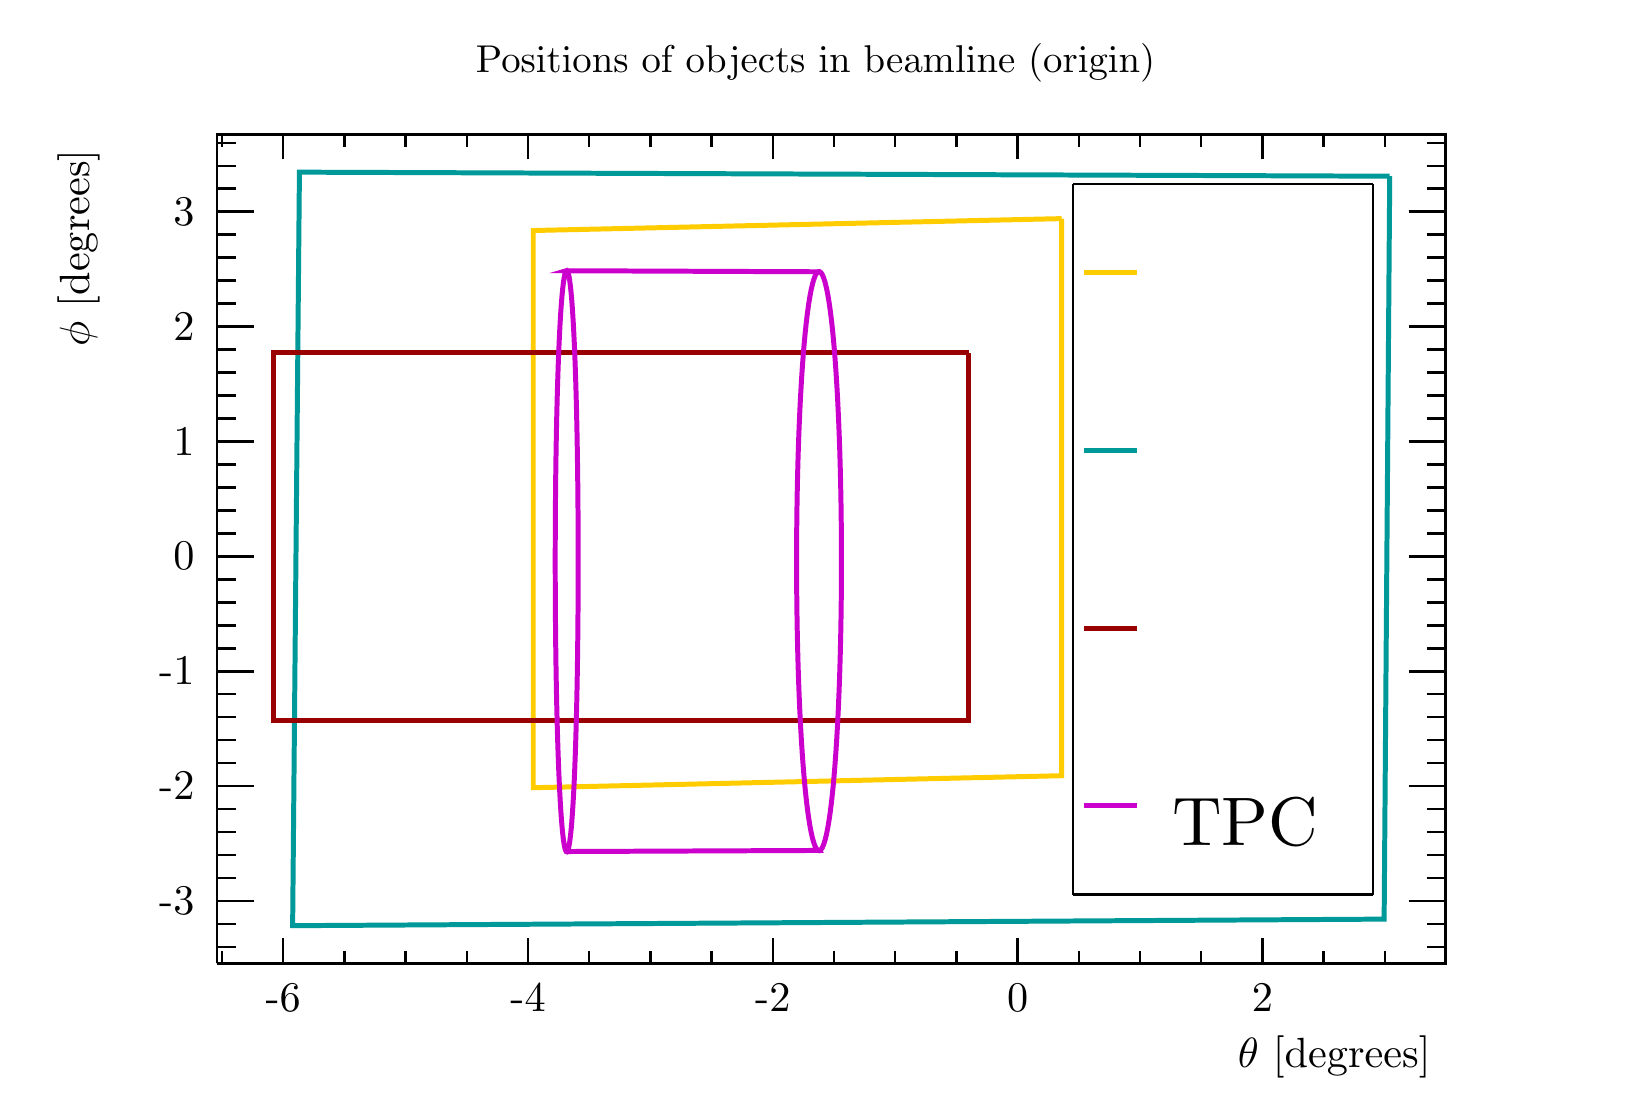
\begin{tikzpicture}
\pgfdeclareplotmark{cross} {
\pgfpathmoveto{\pgfpoint{-0.3\pgfplotmarksize}{\pgfplotmarksize}}
\pgfpathlineto{\pgfpoint{+0.3\pgfplotmarksize}{\pgfplotmarksize}}
\pgfpathlineto{\pgfpoint{+0.3\pgfplotmarksize}{0.3\pgfplotmarksize}}
\pgfpathlineto{\pgfpoint{+1\pgfplotmarksize}{0.3\pgfplotmarksize}}
\pgfpathlineto{\pgfpoint{+1\pgfplotmarksize}{-0.3\pgfplotmarksize}}
\pgfpathlineto{\pgfpoint{+0.3\pgfplotmarksize}{-0.3\pgfplotmarksize}}
\pgfpathlineto{\pgfpoint{+0.3\pgfplotmarksize}{-1.\pgfplotmarksize}}
\pgfpathlineto{\pgfpoint{-0.3\pgfplotmarksize}{-1.\pgfplotmarksize}}
\pgfpathlineto{\pgfpoint{-0.3\pgfplotmarksize}{-0.3\pgfplotmarksize}}
\pgfpathlineto{\pgfpoint{-1.\pgfplotmarksize}{-0.3\pgfplotmarksize}}
\pgfpathlineto{\pgfpoint{-1.\pgfplotmarksize}{0.3\pgfplotmarksize}}
\pgfpathlineto{\pgfpoint{-0.3\pgfplotmarksize}{0.3\pgfplotmarksize}}
\pgfpathclose
\pgfusepathqstroke
}
\pgfdeclareplotmark{cross*} {
\pgfpathmoveto{\pgfpoint{-0.3\pgfplotmarksize}{\pgfplotmarksize}}
\pgfpathlineto{\pgfpoint{+0.3\pgfplotmarksize}{\pgfplotmarksize}}
\pgfpathlineto{\pgfpoint{+0.3\pgfplotmarksize}{0.3\pgfplotmarksize}}
\pgfpathlineto{\pgfpoint{+1\pgfplotmarksize}{0.3\pgfplotmarksize}}
\pgfpathlineto{\pgfpoint{+1\pgfplotmarksize}{-0.3\pgfplotmarksize}}
\pgfpathlineto{\pgfpoint{+0.3\pgfplotmarksize}{-0.3\pgfplotmarksize}}
\pgfpathlineto{\pgfpoint{+0.3\pgfplotmarksize}{-1.\pgfplotmarksize}}
\pgfpathlineto{\pgfpoint{-0.3\pgfplotmarksize}{-1.\pgfplotmarksize}}
\pgfpathlineto{\pgfpoint{-0.3\pgfplotmarksize}{-0.3\pgfplotmarksize}}
\pgfpathlineto{\pgfpoint{-1.\pgfplotmarksize}{-0.3\pgfplotmarksize}}
\pgfpathlineto{\pgfpoint{-1.\pgfplotmarksize}{0.3\pgfplotmarksize}}
\pgfpathlineto{\pgfpoint{-0.3\pgfplotmarksize}{0.3\pgfplotmarksize}}
\pgfpathclose
\pgfusepathqfillstroke
}
\pgfdeclareplotmark{newstar} {
\pgfpathmoveto{\pgfqpoint{0pt}{\pgfplotmarksize}}
\pgfpathlineto{\pgfqpointpolar{44}{0.5\pgfplotmarksize}}
\pgfpathlineto{\pgfqpointpolar{18}{\pgfplotmarksize}}
\pgfpathlineto{\pgfqpointpolar{-20}{0.5\pgfplotmarksize}}
\pgfpathlineto{\pgfqpointpolar{-54}{\pgfplotmarksize}}
\pgfpathlineto{\pgfqpointpolar{-90}{0.5\pgfplotmarksize}}
\pgfpathlineto{\pgfqpointpolar{234}{\pgfplotmarksize}}
\pgfpathlineto{\pgfqpointpolar{198}{0.5\pgfplotmarksize}}
\pgfpathlineto{\pgfqpointpolar{162}{\pgfplotmarksize}}
\pgfpathlineto{\pgfqpointpolar{134}{0.5\pgfplotmarksize}}
\pgfpathclose
\pgfusepathqstroke
}
\pgfdeclareplotmark{newstar*} {
\pgfpathmoveto{\pgfqpoint{0pt}{\pgfplotmarksize}}
\pgfpathlineto{\pgfqpointpolar{44}{0.5\pgfplotmarksize}}
\pgfpathlineto{\pgfqpointpolar{18}{\pgfplotmarksize}}
\pgfpathlineto{\pgfqpointpolar{-20}{0.5\pgfplotmarksize}}
\pgfpathlineto{\pgfqpointpolar{-54}{\pgfplotmarksize}}
\pgfpathlineto{\pgfqpointpolar{-90}{0.5\pgfplotmarksize}}
\pgfpathlineto{\pgfqpointpolar{234}{\pgfplotmarksize}}
\pgfpathlineto{\pgfqpointpolar{198}{0.5\pgfplotmarksize}}
\pgfpathlineto{\pgfqpointpolar{162}{\pgfplotmarksize}}
\pgfpathlineto{\pgfqpointpolar{134}{0.5\pgfplotmarksize}}
\pgfpathclose
\pgfusepathqfillstroke
}
\definecolor{c}{rgb}{1,1,1};
\draw [color=c, fill=c] (0,0) rectangle (20,13.4957);
\draw [color=c, fill=c] (2.4,1.61948) rectangle (18,12.1461);
\definecolor{c}{rgb}{0,0,0};
\draw [c,line width=0.9] (2.4,1.61948) -- (2.4,12.1461) -- (18,12.1461) -- (18,1.61948) -- (2.4,1.61948);
\definecolor{c}{rgb}{1,1,1};
\draw [color=c, fill=c] (2.4,1.61948) rectangle (18,12.1461);
\definecolor{c}{rgb}{0,0,0};
\draw [c,line width=0.9] (2.4,1.61948) -- (2.4,12.1461) -- (18,12.1461) -- (18,1.61948) -- (2.4,1.61948);
\draw [c,line width=0.9] (2.4,1.61948) -- (18,1.61948);
\draw [c,line width=0.9] (3.23864,1.93528) -- (3.23864,1.61948);
\draw [c,line width=0.9] (4.01586,1.77738) -- (4.01586,1.61948);
\draw [c,line width=0.9] (4.79308,1.77738) -- (4.79308,1.61948);
\draw [c,line width=0.9] (5.5703,1.77738) -- (5.5703,1.61948);
\draw [c,line width=0.9] (6.34753,1.93528) -- (6.34753,1.61948);
\draw [c,line width=0.9] (7.12475,1.77738) -- (7.12475,1.61948);
\draw [c,line width=0.9] (7.90197,1.77738) -- (7.90197,1.61948);
\draw [c,line width=0.9] (8.67919,1.77738) -- (8.67919,1.61948);
\draw [c,line width=0.9] (9.45641,1.93528) -- (9.45641,1.61948);
\draw [c,line width=0.9] (10.2336,1.77738) -- (10.2336,1.61948);
\draw [c,line width=0.9] (11.0109,1.77738) -- (11.0109,1.61948);
\draw [c,line width=0.9] (11.7881,1.77738) -- (11.7881,1.61948);
\draw [c,line width=0.9] (12.5653,1.93528) -- (12.5653,1.61948);
\draw [c,line width=0.9] (13.3425,1.77738) -- (13.3425,1.61948);
\draw [c,line width=0.9] (14.1197,1.77738) -- (14.1197,1.61948);
\draw [c,line width=0.9] (14.897,1.77738) -- (14.897,1.61948);
\draw [c,line width=0.9] (15.6742,1.93528) -- (15.6742,1.61948);
\draw [c,line width=0.9] (3.23864,1.93528) -- (3.23864,1.61948);
\draw [c,line width=0.9] (2.46142,1.77738) -- (2.46142,1.61948);
\draw [c,line width=0.9] (15.6742,1.93528) -- (15.6742,1.61948);
\draw [c,line width=0.9] (16.4514,1.77738) -- (16.4514,1.61948);
\draw [c,line width=0.9] (17.2286,1.77738) -- (17.2286,1.61948);
\draw [anchor=base] (3.23864,1.01218) node[scale=1.52731, color=c, rotate=0]{-6};
\draw [anchor=base] (6.34753,1.01218) node[scale=1.52731, color=c, rotate=0]{-4};
\draw [anchor=base] (9.45641,1.01218) node[scale=1.52731, color=c, rotate=0]{-2};
\draw [anchor=base] (12.5653,1.01218) node[scale=1.52731, color=c, rotate=0]{0};
\draw [anchor=base] (15.6742,1.01218) node[scale=1.52731, color=c, rotate=0]{2};
\draw [anchor= east] (18,0.431862) node[scale=1.52731, color=c, rotate=0]{$ \theta$ [degrees]};
\draw [c,line width=0.9] (2.4,12.1461) -- (18,12.1461);
\draw [c,line width=0.9] (3.23864,11.8303) -- (3.23864,12.1461);
\draw [c,line width=0.9] (4.01586,11.9882) -- (4.01586,12.1461);
\draw [c,line width=0.9] (4.79308,11.9882) -- (4.79308,12.1461);
\draw [c,line width=0.9] (5.5703,11.9882) -- (5.5703,12.1461);
\draw [c,line width=0.9] (6.34753,11.8303) -- (6.34753,12.1461);
\draw [c,line width=0.9] (7.12475,11.9882) -- (7.12475,12.1461);
\draw [c,line width=0.9] (7.90197,11.9882) -- (7.90197,12.1461);
\draw [c,line width=0.9] (8.67919,11.9882) -- (8.67919,12.1461);
\draw [c,line width=0.9] (9.45641,11.8303) -- (9.45641,12.1461);
\draw [c,line width=0.9] (10.2336,11.9882) -- (10.2336,12.1461);
\draw [c,line width=0.9] (11.0109,11.9882) -- (11.0109,12.1461);
\draw [c,line width=0.9] (11.7881,11.9882) -- (11.7881,12.1461);
\draw [c,line width=0.9] (12.5653,11.8303) -- (12.5653,12.1461);
\draw [c,line width=0.9] (13.3425,11.9882) -- (13.3425,12.1461);
\draw [c,line width=0.9] (14.1197,11.9882) -- (14.1197,12.1461);
\draw [c,line width=0.9] (14.897,11.9882) -- (14.897,12.1461);
\draw [c,line width=0.9] (15.6742,11.8303) -- (15.6742,12.1461);
\draw [c,line width=0.9] (3.23864,11.8303) -- (3.23864,12.1461);
\draw [c,line width=0.9] (2.46142,11.9882) -- (2.46142,12.1461);
\draw [c,line width=0.9] (15.6742,11.8303) -- (15.6742,12.1461);
\draw [c,line width=0.9] (16.4514,11.9882) -- (16.4514,12.1461);
\draw [c,line width=0.9] (17.2286,11.9882) -- (17.2286,12.1461);
\draw [c,line width=0.9] (2.4,1.61948) -- (2.4,12.1461);
\draw [c,line width=0.9] (2.868,2.41096) -- (2.4,2.41096);
\draw [c,line width=0.9] (2.634,2.70278) -- (2.4,2.70278);
\draw [c,line width=0.9] (2.634,2.99459) -- (2.4,2.99459);
\draw [c,line width=0.9] (2.634,3.28641) -- (2.4,3.28641);
\draw [c,line width=0.9] (2.634,3.57822) -- (2.4,3.57822);
\draw [c,line width=0.9] (2.868,3.87004) -- (2.4,3.87004);
\draw [c,line width=0.9] (2.634,4.16185) -- (2.4,4.16185);
\draw [c,line width=0.9] (2.634,4.45367) -- (2.4,4.45367);
\draw [c,line width=0.9] (2.634,4.74548) -- (2.4,4.74548);
\draw [c,line width=0.9] (2.634,5.0373) -- (2.4,5.0373);
\draw [c,line width=0.9] (2.868,5.32911) -- (2.4,5.32911);
\draw [c,line width=0.9] (2.634,5.62093) -- (2.4,5.62093);
\draw [c,line width=0.9] (2.634,5.91274) -- (2.4,5.91274);
\draw [c,line width=0.9] (2.634,6.20456) -- (2.4,6.20456);
\draw [c,line width=0.9] (2.634,6.49638) -- (2.4,6.49638);
\draw [c,line width=0.9] (2.868,6.78819) -- (2.4,6.78819);
\draw [c,line width=0.9] (2.634,7.08001) -- (2.4,7.08001);
\draw [c,line width=0.9] (2.634,7.37182) -- (2.4,7.37182);
\draw [c,line width=0.9] (2.634,7.66364) -- (2.4,7.66364);
\draw [c,line width=0.9] (2.634,7.95545) -- (2.4,7.95545);
\draw [c,line width=0.9] (2.868,8.24727) -- (2.4,8.24727);
\draw [c,line width=0.9] (2.634,8.53908) -- (2.4,8.53908);
\draw [c,line width=0.9] (2.634,8.8309) -- (2.4,8.8309);
\draw [c,line width=0.9] (2.634,9.12271) -- (2.4,9.12271);
\draw [c,line width=0.9] (2.634,9.41453) -- (2.4,9.41453);
\draw [c,line width=0.9] (2.868,9.70634) -- (2.4,9.70634);
\draw [c,line width=0.9] (2.634,9.99816) -- (2.4,9.99816);
\draw [c,line width=0.9] (2.634,10.29) -- (2.4,10.29);
\draw [c,line width=0.9] (2.634,10.5818) -- (2.4,10.5818);
\draw [c,line width=0.9] (2.634,10.8736) -- (2.4,10.8736);
\draw [c,line width=0.9] (2.868,11.1654) -- (2.4,11.1654);
\draw [c,line width=0.9] (2.868,2.41096) -- (2.4,2.41096);
\draw [c,line width=0.9] (2.634,2.11915) -- (2.4,2.11915);
\draw [c,line width=0.9] (2.634,1.82733) -- (2.4,1.82733);
\draw [c,line width=0.9] (2.868,11.1654) -- (2.4,11.1654);
\draw [c,line width=0.9] (2.634,11.4572) -- (2.4,11.4572);
\draw [c,line width=0.9] (2.634,11.749) -- (2.4,11.749);
\draw [c,line width=0.9] (2.634,12.0409) -- (2.4,12.0409);
\draw [anchor= east] (2.3,2.41096) node[scale=1.52731, color=c, rotate=0]{-3};
\draw [anchor= east] (2.3,3.87004) node[scale=1.52731, color=c, rotate=0]{-2};
\draw [anchor= east] (2.3,5.32911) node[scale=1.52731, color=c, rotate=0]{-1};
\draw [anchor= east] (2.3,6.78819) node[scale=1.52731, color=c, rotate=0]{0};
\draw [anchor= east] (2.3,8.24727) node[scale=1.52731, color=c, rotate=0]{1};
\draw [anchor= east] (2.3,9.70634) node[scale=1.52731, color=c, rotate=0]{2};
\draw [anchor= east] (2.3,11.1654) node[scale=1.52731, color=c, rotate=0]{3};
\draw [anchor= east] (0.64,12.1461) node[scale=1.52731, color=c, rotate=90]{$ \phi$ [degrees]};
\draw [c,line width=0.9] (18,1.61948) -- (18,12.1461);
\draw [c,line width=0.9] (17.532,2.41096) -- (18,2.41096);
\draw [c,line width=0.9] (17.766,2.70278) -- (18,2.70278);
\draw [c,line width=0.9] (17.766,2.99459) -- (18,2.99459);
\draw [c,line width=0.9] (17.766,3.28641) -- (18,3.28641);
\draw [c,line width=0.9] (17.766,3.57822) -- (18,3.57822);
\draw [c,line width=0.9] (17.532,3.87004) -- (18,3.87004);
\draw [c,line width=0.9] (17.766,4.16185) -- (18,4.16185);
\draw [c,line width=0.9] (17.766,4.45367) -- (18,4.45367);
\draw [c,line width=0.9] (17.766,4.74548) -- (18,4.74548);
\draw [c,line width=0.9] (17.766,5.0373) -- (18,5.0373);
\draw [c,line width=0.9] (17.532,5.32911) -- (18,5.32911);
\draw [c,line width=0.9] (17.766,5.62093) -- (18,5.62093);
\draw [c,line width=0.9] (17.766,5.91274) -- (18,5.91274);
\draw [c,line width=0.9] (17.766,6.20456) -- (18,6.20456);
\draw [c,line width=0.9] (17.766,6.49638) -- (18,6.49638);
\draw [c,line width=0.9] (17.532,6.78819) -- (18,6.78819);
\draw [c,line width=0.9] (17.766,7.08001) -- (18,7.08001);
\draw [c,line width=0.9] (17.766,7.37182) -- (18,7.37182);
\draw [c,line width=0.9] (17.766,7.66364) -- (18,7.66364);
\draw [c,line width=0.9] (17.766,7.95545) -- (18,7.95545);
\draw [c,line width=0.9] (17.532,8.24727) -- (18,8.24727);
\draw [c,line width=0.9] (17.766,8.53908) -- (18,8.53908);
\draw [c,line width=0.9] (17.766,8.8309) -- (18,8.8309);
\draw [c,line width=0.9] (17.766,9.12271) -- (18,9.12271);
\draw [c,line width=0.9] (17.766,9.41453) -- (18,9.41453);
\draw [c,line width=0.9] (17.532,9.70634) -- (18,9.70634);
\draw [c,line width=0.9] (17.766,9.99816) -- (18,9.99816);
\draw [c,line width=0.9] (17.766,10.29) -- (18,10.29);
\draw [c,line width=0.9] (17.766,10.5818) -- (18,10.5818);
\draw [c,line width=0.9] (17.766,10.8736) -- (18,10.8736);
\draw [c,line width=0.9] (17.532,11.1654) -- (18,11.1654);
\draw [c,line width=0.9] (17.532,2.41096) -- (18,2.41096);
\draw [c,line width=0.9] (17.766,2.11915) -- (18,2.11915);
\draw [c,line width=0.9] (17.766,1.82733) -- (18,1.82733);
\draw [c,line width=0.9] (17.532,11.1654) -- (18,11.1654);
\draw [c,line width=0.9] (17.766,11.4572) -- (18,11.4572);
\draw [c,line width=0.9] (17.766,11.749) -- (18,11.749);
\draw [c,line width=0.9] (17.766,12.0409) -- (18,12.0409);
\definecolor{c}{rgb}{1,0.8,0};
\draw [c,line width=1.8] (13.123,11.0775) -- (13.123,4.00254) -- (6.41361,3.85009) -- (6.41361,10.9264) -- (13.123,11.0775);
\definecolor{c}{rgb}{0,0.6,0.6};
\draw [c,line width=1.8] (17.2909,11.6163) -- (3.44422,11.6676) -- (3.35799,2.09797) -- (17.22,2.18131) -- (17.2909,11.6163);
\definecolor{c}{rgb}{0.6,0,0};
\draw [c,line width=1.8] (11.9426,9.37206) -- (3.10909,9.37206) -- (3.10909,4.70729) -- (11.9426,4.70729) -- (11.9426,9.37206);
\definecolor{c}{rgb}{0.8,0,0.8};
\draw [c,line width=1.8] (6.83226,10.4157) -- (6.82314,10.3986) -- (6.81412,10.3672) -- (6.80521,10.3217) -- (6.79645,10.2624) -- (6.78788,10.1897) -- (6.77953,10.104) -- (6.77142,10.0055) -- (6.76359,9.89494) -- (6.75605,9.77263) --
 (6.74885,9.63914) -- (6.74199,9.49505) -- (6.73552,9.34093) -- (6.72943,9.17739) -- (6.72376,9.00508) -- (6.71852,8.82465) -- (6.71374,8.63678) -- (6.70941,8.44217) -- (6.70557,8.24152) -- (6.70221,8.03556) -- (6.69935,7.82503) -- (6.697,7.61067) --
 (6.69517,7.39324) -- (6.69385,7.17349) -- (6.69306,6.9522) -- (6.6928,6.73012) -- (6.69306,6.50804) -- (6.69385,6.28672) -- (6.69517,6.06693) -- (6.697,5.84944) -- (6.69935,5.635) -- (6.70221,5.42438) -- (6.70557,5.21831) -- (6.70941,5.01753) --
 (6.71374,4.82277) -- (6.71852,4.63474) -- (6.72376,4.45413) -- (6.72943,4.28163) -- (6.73552,4.11789) -- (6.74199,3.96355) -- (6.74885,3.81922) -- (6.75605,3.68549) -- (6.76359,3.56292) -- (6.77142,3.45203) -- (6.77953,3.35333) -- (6.78788,3.26727)
 -- (6.79645,3.19426) -- (6.80521,3.13469) -- (6.81412,3.08889) -- (6.82314,3.05715) -- (6.83226,3.0397) -- (6.84142,3.03673) -- (6.8506,3.04837) -- (6.85976,3.07469) -- (6.86885,3.11572) -- (6.87785,3.17139) -- (6.88671,3.24161) -- (6.8954,3.3262)
 -- (6.90388,3.42493) -- (6.91211,3.53747) -- (6.92006,3.66348) -- (6.92769,3.80249) -- (6.93496,3.95402) -- (6.94184,4.11749) -- (6.9483,4.29226) -- (6.95431,4.47764) -- (6.95985,4.67288) -- (6.96487,4.87717) -- (6.96936,5.08963) -- (6.9733,5.30937)
 -- (6.97667,5.53544) -- (6.97945,5.76682) -- (6.98163,6.00252) -- (6.98319,6.24147) -- (6.98413,6.4826) -- (6.98444,6.72484) -- (6.98413,6.96709) -- (6.98319,7.20826) -- (6.98163,7.44728) -- (6.97945,7.68305) -- (6.97667,7.91455) -- (6.9733,8.14075)
 -- (6.96936,8.36064) -- (6.96487,8.57329) -- (6.95985,8.77777) -- (6.95431,8.97322) -- (6.9483,9.15884) -- (6.94184,9.33386) -- (6.93496,9.49759) -- (6.92769,9.6494) -- (6.92006,9.7887) -- (6.91211,9.91501) -- (6.90388,10.0279) -- (6.8954,10.1269)
 -- (6.88671,10.2118) -- (6.87785,10.2824) -- (6.86885,10.3384) -- (6.85976,10.3797) -- (6.8506,10.4064) -- (6.84142,10.4184) -- (6.83226,10.4157) -- (10.0306,10.4025);
\draw [c,line width=1.8] (10.0306,3.05337) -- (10.0485,3.05045) -- (10.0665,3.06209) -- (10.0843,3.08835) -- (10.1021,3.12926) -- (10.1197,3.18477) -- (10.137,3.25476) -- (10.154,3.33907) -- (10.1705,3.43746) -- (10.1866,3.54962) -- (10.2022,3.67518)
 -- (10.2171,3.8137) -- (10.2313,3.96468) -- (10.2447,4.12756) -- (10.2573,4.30169) -- (10.2691,4.48639) -- (10.2799,4.6809) -- (10.2897,4.88442) -- (10.2985,5.09609) -- (10.3062,5.315) -- (10.3127,5.54021) -- (10.3182,5.77072) -- (10.3224,6.00552)
 -- (10.3255,6.24356) -- (10.3273,6.48377) -- (10.3279,6.72508) -- (10.3273,6.96641) -- (10.3255,7.20666) -- (10.3224,7.44476) -- (10.3182,7.67964) -- (10.3127,7.91026) -- (10.3062,8.1356) -- (10.2985,8.35466) -- (10.2897,8.56651) --
 (10.2799,8.77022) -- (10.2691,8.96495) -- (10.2573,9.14988) -- (10.2447,9.32426) -- (10.2313,9.4874) -- (10.2171,9.63865) -- (10.2022,9.77747) -- (10.1866,9.90332) -- (10.1705,10.0158) -- (10.154,10.1145) -- (10.137,10.1991) -- (10.1197,10.2695) --
 (10.1021,10.3253) -- (10.0843,10.3665) -- (10.0665,10.3931) -- (10.0485,10.4051) -- (10.0306,10.4025) -- (10.0128,10.3855) -- (9.99516,10.3542) -- (9.97776,10.3089) -- (9.96065,10.2499) -- (9.9439,10.1775) -- (9.92757,10.0921) -- (9.91173,9.99402)
 -- (9.89642,9.88383) -- (9.8817,9.76198) -- (9.86762,9.62899) -- (9.85423,9.48543) -- (9.84156,9.33188) -- (9.82967,9.16894) -- (9.81859,8.99725) -- (9.80836,8.81747) -- (9.799,8.63027) -- (9.79055,8.43635) -- (9.78303,8.23641) -- (9.77647,8.03118)
 -- (9.77088,7.82139) -- (9.76629,7.60779) -- (9.7627,7.39112) -- (9.76013,7.17214) -- (9.75859,6.95162) -- (9.75807,6.73033) -- (9.75859,6.50902) -- (9.76013,6.28848) -- (9.7627,6.06946) -- (9.76629,5.85273) -- (9.77088,5.63905) -- (9.77647,5.42916)
 -- (9.78303,5.22382) -- (9.79055,5.02376) -- (9.799,4.82969) -- (9.80836,4.64234) -- (9.81859,4.46238) -- (9.82967,4.2905) -- (9.84156,4.12736) -- (9.85423,3.97358) -- (9.86762,3.82979) -- (9.8817,3.69656) -- (9.89642,3.57445) -- (9.91173,3.46399)
 -- (9.92757,3.36567) -- (9.9439,3.27994) -- (9.96065,3.20723) -- (9.97776,3.14791) -- (9.99516,3.10231) -- (10.0128,3.07072) -- (10.0306,3.05337) -- (6.83226,3.0397);
\definecolor{c}{rgb}{1,1,1};
\draw [color=c, fill=c] (2,12.686) rectangle (18,13.4282);
\definecolor{c}{rgb}{0,0,0};
\draw (10,13.0571) node[scale=1.40004, color=c, rotate=0]{Positions of objects in beamline (\SOne origin)};
\definecolor{c}{rgb}{1,1,1};
\draw [color=c, fill=c] (13.2665,2.49284) rectangle (17.0774,11.5186);
\definecolor{c}{rgb}{0,0,0};
\draw [c,line width=0.9] (13.2665,2.49284) -- (17.0774,2.49284);
\draw [c,line width=0.9] (17.0774,2.49284) -- (17.0774,11.5186);
\draw [c,line width=0.9] (17.0774,11.5186) -- (13.2665,11.5186);
\draw [c,line width=0.9] (13.2665,11.5186) -- (13.2665,2.49284);
\draw [anchor=base west] (14.2192,9.8827) node[scale=2.48189, color=c, rotate=0]{\STwo};
\definecolor{c}{rgb}{1,0.8,0};
\draw [c,line width=1.8] (13.4094,10.3904) -- (14.0763,10.3904);
\definecolor{c}{rgb}{0,0,0};
\draw [anchor=base west] (14.2192,7.62625) node[scale=2.48189, color=c, rotate=0]{\SThree};
\definecolor{c}{rgb}{0,0.6,0.6};
\draw [c,line width=1.8] (13.4094,8.13395) -- (14.0763,8.13395);
\definecolor{c}{rgb}{0,0,0};
\draw [anchor=base west] (14.2192,5.36981) node[scale=2.48189, color=c, rotate=0]{\SFour};
\definecolor{c}{rgb}{0.6,0,0};
\draw [c,line width=1.8] (13.4094,5.87751) -- (14.0763,5.87751);
\definecolor{c}{rgb}{0,0,0};
\draw [anchor=base west] (14.2192,3.11336) node[scale=2.48189, color=c, rotate=0]{TPC};
\definecolor{c}{rgb}{0.8,0,0.8};
\draw [c,line width=1.8] (13.4094,3.62106) -- (14.0763,3.62106);
\end{tikzpicture}

  \end{adjustbox}
  \caption[Angular distribution of objects in the T10 beamline]{Angular distribution of objects within the T10 beamline. The origin here is at \SOne.}
  \label{fig:angDistS1}
\end{figure}

\begin{table}
  \centering
  \caption[Angular extent of components within the T10 beamline with \SOne as the origin]{Angular extent of components within the T10 beamline with \SOne as the origin.}
  \label{tab:angDistS1}
  \begin{tabular}{c c c c c}
    \hline
    \hline
    Object & $\theta_{\text{min}}$ & $\theta_{\text{max}}$ & $\phi_{\text{min}}$ & $\theta_{\text{max}}$ \\
    \hline
    \STwo & $\ang{-3.96} \pm \ang{0.03}$ & $\ang{0.36} \pm \ang{0.03}$ & $\ang{-2.01} \pm \ang{0.03}$ & $\ang{2.94} \pm \ang{0.03}$\\
    \SThree & $\ang{-5.923} \pm \ang{0.004}$ & $\ang{3.040} \pm \ang{0.004}$ & $\ang{-3.215} \pm \ang{0.004}$ & $\ang{3.344} \pm \ang{0.004}$ \\
    \SFour & $\ang{-6.083} \pm \ang{0.003}$ & $\ang{-0.401} \pm \ang{0.003}$ & $\ang{-1.426} \pm \ang{0.003}$ & $\ang{1.771} \pm \ang{0.003}$ \\
    TPC US face & $\ang{-3.59} \pm \ang{0.01}$ & $\ang{-1.44} \pm \ang{0.01}$ & $\ang{-2.66} \pm \ang{0.01}$ & $\ang{2.58} \pm \ang{0.01}$ \\
    TPC DS face & $\ang{-3.778} \pm \ang{0.009}$ & $\ang{-1.806} \pm \ang{0.009}$ & $\ang{-2.440} \pm \ang{0.009}$ & $\ang{2.361} \pm \ang{0.009}$ \\
    \hline 
  \end{tabular}
\end{table}

\citefig{fig:beamlinePics} shows images of the beamline with the various components of the ToF systems as well as the HPTPC and moderator blocks labelled.
In this particular image, all four moderator blocks are placed on the tripod stand.

\begin{figure}[h]
  \centering
  \includegraphics[width=\linewidth]{files/figures/hptpc_beam_flux/S1S2S3S4}
  \caption[Images of the test beam setup with various objects labelled]{Images of the T10 beamline with the apparatus used in the beam test labelled. Left: the downstream part of the beamline. Right: The upstream part of the beamline. Image from~\cite{beampaper}.}
  \label{fig:beamlinePics}
\end{figure}

\SThree and \SFour each have their own independent DAQ systems which process data from \SOne and \STwo plus either \SThree or \SFour.
The data from these two systems is synchronised offline using a signal from the PS indicating the arrival of a beam spill which is recorded by both DAQs.

T10 receives $1-3$ spills from the PS every supercycle, which has a normal duration of \SI{33}{\second}.
The duration of each of these spills is approximately \SI{0.4}{\second}.
The minimum separation in time of these spills is \SI{1}{\second} which means that the beam spill arrival signal has a frequency of less than \SI{1}{\hertz}.
This means that spills in the two DAQs can be matched by using this signal in combination with the DAQ file timestamps.

\citetab{tab:nSpills} shows the number of recorded spills used for each moderator block configuration for the variable block analysis.
One can see that significantly more spills are recorded in the 4 block configuration.
This is because this is the configuration that was used for the majority of the beam test.

\begin{table}
  \centering
  \caption[Number of recorded spills for each moderator block configuration used in T10 beam flux analysis]{Number of recorded spills for each moderator block configuration used in T10 beam flux analysis}
  \label{tab:nSpills}
  \begin{tabular}{c c}
    \hline
    \hline
    Number of moderator blocks & Recorded spills \\
    \hline
    0 & 257 \\
    1 & 254 \\
    2 & 267 \\
    3 & 220 \\
    4 & 3884 \\
    \hline
  \end{tabular}
\end{table}

\subsection{The upstream beam counters (\SOne and \STwo)}
\label{sec:hptpc_beam_flux:overview:s1s2}

The \SOne beam counter consists of a cross formed from two pieces of plastic scintillator and is shown in the left hand image of \citefig{fig:s1s2Pic}.
This cross measures \SI{40 x 40 x 5}{\milli\metre} and is attached to four 1'' Hamamatsu Photonics R4998 PMTs at each end which are used to read out the light signals.

\begin{figure}[h]
  \centering
  \includegraphics[width=.7\linewidth]{files/figures/hptpc_beam_flux/S1S2FrontOn}
  \caption[The upstream beam counters \SOne and \STwo]{Images of the upstream beam counters \SOne (left) and \STwo (right) from~\cite{beampaper}.}
  \label{fig:s1s2Pic}
\end{figure}

The time resolution of the \SOne beam counter is measured using the DAQ of the upstream ToF and found to be around \SI{30}{\pico\second}.
This measurement is made by taking the average distribution of the four PMT hit times. However, because this measurement is not centred at zero, we instead calculate the quantity
\begin{equation}
  t_{\text{ave}} = \frac{1}{4} ((t_{\text{PMT1}}+t_{\text{PMT2}}) - (t_{\text{PMT3}}+t_{\text{PMT4}}))
  \label{eq:tAve}
\end{equation}
where the $t_{\text{PMT}n}$ refer to the four PMTs used to read out \SOne.
This quantity has the same spread as the average hit time but is centred at zero.
An example of the distribution produced is shown in \citefig{fig:s1Res} which contains the data from one run.

\begin{figure}[h]
  \begin{adjustbox}{max totalsize=.7\textwidth, center}
    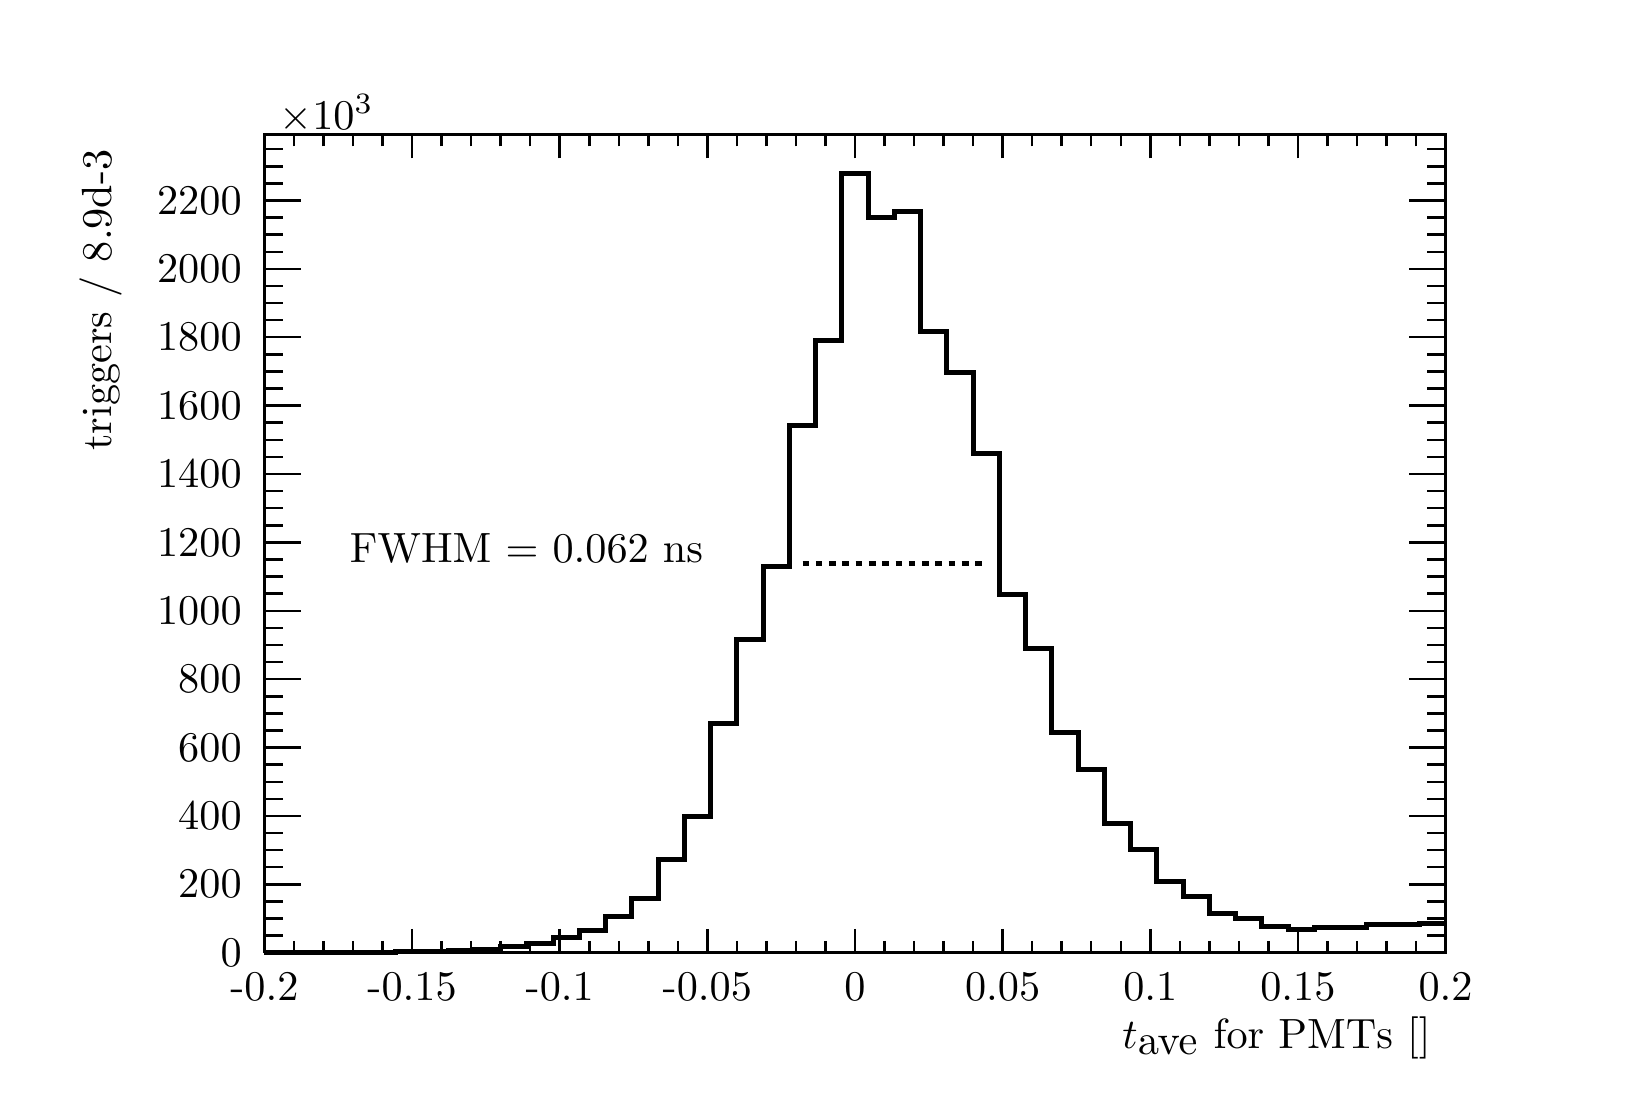
\begin{tikzpicture}
\pgfdeclareplotmark{cross} {
\pgfpathmoveto{\pgfpoint{-0.3\pgfplotmarksize}{\pgfplotmarksize}}
\pgfpathlineto{\pgfpoint{+0.3\pgfplotmarksize}{\pgfplotmarksize}}
\pgfpathlineto{\pgfpoint{+0.3\pgfplotmarksize}{0.3\pgfplotmarksize}}
\pgfpathlineto{\pgfpoint{+1\pgfplotmarksize}{0.3\pgfplotmarksize}}
\pgfpathlineto{\pgfpoint{+1\pgfplotmarksize}{-0.3\pgfplotmarksize}}
\pgfpathlineto{\pgfpoint{+0.3\pgfplotmarksize}{-0.3\pgfplotmarksize}}
\pgfpathlineto{\pgfpoint{+0.3\pgfplotmarksize}{-1.\pgfplotmarksize}}
\pgfpathlineto{\pgfpoint{-0.3\pgfplotmarksize}{-1.\pgfplotmarksize}}
\pgfpathlineto{\pgfpoint{-0.3\pgfplotmarksize}{-0.3\pgfplotmarksize}}
\pgfpathlineto{\pgfpoint{-1.\pgfplotmarksize}{-0.3\pgfplotmarksize}}
\pgfpathlineto{\pgfpoint{-1.\pgfplotmarksize}{0.3\pgfplotmarksize}}
\pgfpathlineto{\pgfpoint{-0.3\pgfplotmarksize}{0.3\pgfplotmarksize}}
\pgfpathclose
\pgfusepathqstroke
}
\pgfdeclareplotmark{cross*} {
\pgfpathmoveto{\pgfpoint{-0.3\pgfplotmarksize}{\pgfplotmarksize}}
\pgfpathlineto{\pgfpoint{+0.3\pgfplotmarksize}{\pgfplotmarksize}}
\pgfpathlineto{\pgfpoint{+0.3\pgfplotmarksize}{0.3\pgfplotmarksize}}
\pgfpathlineto{\pgfpoint{+1\pgfplotmarksize}{0.3\pgfplotmarksize}}
\pgfpathlineto{\pgfpoint{+1\pgfplotmarksize}{-0.3\pgfplotmarksize}}
\pgfpathlineto{\pgfpoint{+0.3\pgfplotmarksize}{-0.3\pgfplotmarksize}}
\pgfpathlineto{\pgfpoint{+0.3\pgfplotmarksize}{-1.\pgfplotmarksize}}
\pgfpathlineto{\pgfpoint{-0.3\pgfplotmarksize}{-1.\pgfplotmarksize}}
\pgfpathlineto{\pgfpoint{-0.3\pgfplotmarksize}{-0.3\pgfplotmarksize}}
\pgfpathlineto{\pgfpoint{-1.\pgfplotmarksize}{-0.3\pgfplotmarksize}}
\pgfpathlineto{\pgfpoint{-1.\pgfplotmarksize}{0.3\pgfplotmarksize}}
\pgfpathlineto{\pgfpoint{-0.3\pgfplotmarksize}{0.3\pgfplotmarksize}}
\pgfpathclose
\pgfusepathqfillstroke
}
\pgfdeclareplotmark{newstar} {
\pgfpathmoveto{\pgfqpoint{0pt}{\pgfplotmarksize}}
\pgfpathlineto{\pgfqpointpolar{44}{0.5\pgfplotmarksize}}
\pgfpathlineto{\pgfqpointpolar{18}{\pgfplotmarksize}}
\pgfpathlineto{\pgfqpointpolar{-20}{0.5\pgfplotmarksize}}
\pgfpathlineto{\pgfqpointpolar{-54}{\pgfplotmarksize}}
\pgfpathlineto{\pgfqpointpolar{-90}{0.5\pgfplotmarksize}}
\pgfpathlineto{\pgfqpointpolar{234}{\pgfplotmarksize}}
\pgfpathlineto{\pgfqpointpolar{198}{0.5\pgfplotmarksize}}
\pgfpathlineto{\pgfqpointpolar{162}{\pgfplotmarksize}}
\pgfpathlineto{\pgfqpointpolar{134}{0.5\pgfplotmarksize}}
\pgfpathclose
\pgfusepathqstroke
}
\pgfdeclareplotmark{newstar*} {
\pgfpathmoveto{\pgfqpoint{0pt}{\pgfplotmarksize}}
\pgfpathlineto{\pgfqpointpolar{44}{0.5\pgfplotmarksize}}
\pgfpathlineto{\pgfqpointpolar{18}{\pgfplotmarksize}}
\pgfpathlineto{\pgfqpointpolar{-20}{0.5\pgfplotmarksize}}
\pgfpathlineto{\pgfqpointpolar{-54}{\pgfplotmarksize}}
\pgfpathlineto{\pgfqpointpolar{-90}{0.5\pgfplotmarksize}}
\pgfpathlineto{\pgfqpointpolar{234}{\pgfplotmarksize}}
\pgfpathlineto{\pgfqpointpolar{198}{0.5\pgfplotmarksize}}
\pgfpathlineto{\pgfqpointpolar{162}{\pgfplotmarksize}}
\pgfpathlineto{\pgfqpointpolar{134}{0.5\pgfplotmarksize}}
\pgfpathclose
\pgfusepathqfillstroke
}
\definecolor{c}{rgb}{1,1,1};
\draw [color=c, fill=c] (0,0) rectangle (20,13.4957);
\draw [color=c, fill=c] (3,1.75444) rectangle (18,12.1461);
\definecolor{c}{rgb}{0,0,0};
\draw [c,line width=0.9] (3,1.75444) -- (3,12.1461) -- (18,12.1461) -- (18,1.75444) -- (3,1.75444);
\definecolor{c}{rgb}{1,1,1};
\draw [color=c, fill=c] (3,1.75444) rectangle (18,12.1461);
\definecolor{c}{rgb}{0,0,0};
\draw [c,line width=0.9] (3,1.75444) -- (3,12.1461) -- (18,12.1461) -- (18,1.75444) -- (3,1.75444);
\draw [c,line width=1.8] (3,1.75651) -- (3.33333,1.75651) -- (3.33333,1.75672) -- (3.66667,1.75672) -- (3.66667,1.75782) -- (4,1.75782) -- (4,1.75928) -- (4.33333,1.75928) -- (4.33333,1.76265) -- (4.66667,1.76265) -- (4.66667,1.76637) -- (5,1.76637)
 -- (5,1.77413) -- (5.33333,1.77413) -- (5.33333,1.78786) -- (5.66667,1.78786) -- (5.66667,1.80025) -- (6,1.80025) -- (6,1.83002) -- (6.33333,1.83002) -- (6.33333,1.8656) -- (6.66667,1.8656) -- (6.66667,1.94289) -- (7,1.94289) -- (7,2.03217) --
 (7.33333,2.03217) -- (7.33333,2.21951) -- (7.66667,2.21951) -- (7.66667,2.44174) -- (8,2.44174) -- (8,2.9414) -- (8.33333,2.9414) -- (8.33333,3.48698) -- (8.66667,3.48698) -- (8.66667,4.66096) -- (9,4.66096) -- (9,5.73419) -- (9.33333,5.73419) --
 (9.33333,6.66117) -- (9.66667,6.66117) -- (9.66667,8.44555) -- (10,8.44555) -- (10,9.52377) -- (10.3333,9.52377) -- (10.3333,11.6513) -- (10.6667,11.6513) -- (10.6667,11.0943) -- (11,11.0943) -- (11,11.169) -- (11.3333,11.169) -- (11.3333,9.64689)
 -- (11.6667,9.64689) -- (11.6667,9.12428) -- (12,9.12428) -- (12,8.09889) -- (12.3333,8.09889) -- (12.3333,6.29961) -- (12.6667,6.29961) -- (12.6667,5.61671) -- (13,5.61671) -- (13,4.54715) -- (13.3333,4.54715) -- (13.3333,4.0756) --
 (13.6667,4.0756) -- (13.6667,3.39822) -- (14,3.39822) -- (14,3.07106) -- (14.3333,3.07106) -- (14.3333,2.65631) -- (14.6667,2.65631) -- (14.6667,2.46793) -- (15,2.46793) -- (15,2.25342) -- (15.3333,2.25342) -- (15.3333,2.18649) -- (15.6667,2.18649)
 -- (15.6667,2.08911) -- (16,2.08911) -- (16,2.05201) -- (16.3333,2.05201) -- (16.3333,2.07377) -- (16.6667,2.07377) -- (16.6667,2.07323) -- (17,2.07323) -- (17,2.1138) -- (17.3333,2.1138) -- (17.3333,2.11352) -- (17.6667,2.11352) --
 (17.6667,2.12843) -- (18,2.12843);
\draw [c,line width=0.9] (3,1.75444) -- (18,1.75444);
\draw [c,line width=0.9] (3,2.05809) -- (3,1.75444);
\draw [c,line width=0.9] (3.375,1.90627) -- (3.375,1.75444);
\draw [c,line width=0.9] (3.75,1.90627) -- (3.75,1.75444);
\draw [c,line width=0.9] (4.125,1.90627) -- (4.125,1.75444);
\draw [c,line width=0.9] (4.5,1.90627) -- (4.5,1.75444);
\draw [c,line width=0.9] (4.875,2.05809) -- (4.875,1.75444);
\draw [c,line width=0.9] (5.25,1.90627) -- (5.25,1.75444);
\draw [c,line width=0.9] (5.625,1.90627) -- (5.625,1.75444);
\draw [c,line width=0.9] (6,1.90627) -- (6,1.75444);
\draw [c,line width=0.9] (6.375,1.90627) -- (6.375,1.75444);
\draw [c,line width=0.9] (6.75,2.05809) -- (6.75,1.75444);
\draw [c,line width=0.9] (7.125,1.90627) -- (7.125,1.75444);
\draw [c,line width=0.9] (7.5,1.90627) -- (7.5,1.75444);
\draw [c,line width=0.9] (7.875,1.90627) -- (7.875,1.75444);
\draw [c,line width=0.9] (8.25,1.90627) -- (8.25,1.75444);
\draw [c,line width=0.9] (8.625,2.05809) -- (8.625,1.75444);
\draw [c,line width=0.9] (9,1.90627) -- (9,1.75444);
\draw [c,line width=0.9] (9.375,1.90627) -- (9.375,1.75444);
\draw [c,line width=0.9] (9.75,1.90627) -- (9.75,1.75444);
\draw [c,line width=0.9] (10.125,1.90627) -- (10.125,1.75444);
\draw [c,line width=0.9] (10.5,2.05809) -- (10.5,1.75444);
\draw [c,line width=0.9] (10.875,1.90627) -- (10.875,1.75444);
\draw [c,line width=0.9] (11.25,1.90627) -- (11.25,1.75444);
\draw [c,line width=0.9] (11.625,1.90627) -- (11.625,1.75444);
\draw [c,line width=0.9] (12,1.90627) -- (12,1.75444);
\draw [c,line width=0.9] (12.375,2.05809) -- (12.375,1.75444);
\draw [c,line width=0.9] (12.75,1.90627) -- (12.75,1.75444);
\draw [c,line width=0.9] (13.125,1.90627) -- (13.125,1.75444);
\draw [c,line width=0.9] (13.5,1.90627) -- (13.5,1.75444);
\draw [c,line width=0.9] (13.875,1.90627) -- (13.875,1.75444);
\draw [c,line width=0.9] (14.25,2.05809) -- (14.25,1.75444);
\draw [c,line width=0.9] (14.625,1.90627) -- (14.625,1.75444);
\draw [c,line width=0.9] (15,1.90627) -- (15,1.75444);
\draw [c,line width=0.9] (15.375,1.90627) -- (15.375,1.75444);
\draw [c,line width=0.9] (15.75,1.90627) -- (15.75,1.75444);
\draw [c,line width=0.9] (16.125,2.05809) -- (16.125,1.75444);
\draw [c,line width=0.9] (16.5,1.90627) -- (16.5,1.75444);
\draw [c,line width=0.9] (16.875,1.90627) -- (16.875,1.75444);
\draw [c,line width=0.9] (17.25,1.90627) -- (17.25,1.75444);
\draw [c,line width=0.9] (17.625,1.90627) -- (17.625,1.75444);
\draw [c,line width=0.9] (18,2.05809) -- (18,1.75444);
\draw [anchor=base] (3,1.14713) node[scale=1.52731, color=c, rotate=0]{-0.2};
\draw [anchor=base] (4.875,1.14713) node[scale=1.52731, color=c, rotate=0]{-0.15};
\draw [anchor=base] (6.75,1.14713) node[scale=1.52731, color=c, rotate=0]{-0.1};
\draw [anchor=base] (8.625,1.14713) node[scale=1.52731, color=c, rotate=0]{-0.05};
\draw [anchor=base] (10.5,1.14713) node[scale=1.52731, color=c, rotate=0]{0};
\draw [anchor=base] (12.375,1.14713) node[scale=1.52731, color=c, rotate=0]{0.05};
\draw [anchor=base] (14.25,1.14713) node[scale=1.52731, color=c, rotate=0]{0.1};
\draw [anchor=base] (16.125,1.14713) node[scale=1.52731, color=c, rotate=0]{0.15};
\draw [anchor=base] (18,1.14713) node[scale=1.52731, color=c, rotate=0]{0.2};
\draw [anchor= east] (18,0.674785) node[scale=1.52731, color=c, rotate=0]{$t_{\textrm{ave}}$ for \SOne PMTs [\si{\nano\second}]};
\draw [c,line width=0.9] (3,12.1461) -- (18,12.1461);
\draw [c,line width=0.9] (3,11.8425) -- (3,12.1461);
\draw [c,line width=0.9] (3.375,11.9943) -- (3.375,12.1461);
\draw [c,line width=0.9] (3.75,11.9943) -- (3.75,12.1461);
\draw [c,line width=0.9] (4.125,11.9943) -- (4.125,12.1461);
\draw [c,line width=0.9] (4.5,11.9943) -- (4.5,12.1461);
\draw [c,line width=0.9] (4.875,11.8425) -- (4.875,12.1461);
\draw [c,line width=0.9] (5.25,11.9943) -- (5.25,12.1461);
\draw [c,line width=0.9] (5.625,11.9943) -- (5.625,12.1461);
\draw [c,line width=0.9] (6,11.9943) -- (6,12.1461);
\draw [c,line width=0.9] (6.375,11.9943) -- (6.375,12.1461);
\draw [c,line width=0.9] (6.75,11.8425) -- (6.75,12.1461);
\draw [c,line width=0.9] (7.125,11.9943) -- (7.125,12.1461);
\draw [c,line width=0.9] (7.5,11.9943) -- (7.5,12.1461);
\draw [c,line width=0.9] (7.875,11.9943) -- (7.875,12.1461);
\draw [c,line width=0.9] (8.25,11.9943) -- (8.25,12.1461);
\draw [c,line width=0.9] (8.625,11.8425) -- (8.625,12.1461);
\draw [c,line width=0.9] (9,11.9943) -- (9,12.1461);
\draw [c,line width=0.9] (9.375,11.9943) -- (9.375,12.1461);
\draw [c,line width=0.9] (9.75,11.9943) -- (9.75,12.1461);
\draw [c,line width=0.9] (10.125,11.9943) -- (10.125,12.1461);
\draw [c,line width=0.9] (10.5,11.8425) -- (10.5,12.1461);
\draw [c,line width=0.9] (10.875,11.9943) -- (10.875,12.1461);
\draw [c,line width=0.9] (11.25,11.9943) -- (11.25,12.1461);
\draw [c,line width=0.9] (11.625,11.9943) -- (11.625,12.1461);
\draw [c,line width=0.9] (12,11.9943) -- (12,12.1461);
\draw [c,line width=0.9] (12.375,11.8425) -- (12.375,12.1461);
\draw [c,line width=0.9] (12.75,11.9943) -- (12.75,12.1461);
\draw [c,line width=0.9] (13.125,11.9943) -- (13.125,12.1461);
\draw [c,line width=0.9] (13.5,11.9943) -- (13.5,12.1461);
\draw [c,line width=0.9] (13.875,11.9943) -- (13.875,12.1461);
\draw [c,line width=0.9] (14.25,11.8425) -- (14.25,12.1461);
\draw [c,line width=0.9] (14.625,11.9943) -- (14.625,12.1461);
\draw [c,line width=0.9] (15,11.9943) -- (15,12.1461);
\draw [c,line width=0.9] (15.375,11.9943) -- (15.375,12.1461);
\draw [c,line width=0.9] (15.75,11.9943) -- (15.75,12.1461);
\draw [c,line width=0.9] (16.125,11.8425) -- (16.125,12.1461);
\draw [c,line width=0.9] (16.5,11.9943) -- (16.5,12.1461);
\draw [c,line width=0.9] (16.875,11.9943) -- (16.875,12.1461);
\draw [c,line width=0.9] (17.25,11.9943) -- (17.25,12.1461);
\draw [c,line width=0.9] (17.625,11.9943) -- (17.625,12.1461);
\draw [c,line width=0.9] (18,11.8425) -- (18,12.1461);
\draw [c,line width=0.9] (3,1.75444) -- (3,12.1461);
\draw [c,line width=0.9] (3.462,1.75444) -- (3,1.75444);
\draw [c,line width=0.9] (3.231,1.97157) -- (3,1.97157);
\draw [c,line width=0.9] (3.231,2.1887) -- (3,2.1887);
\draw [c,line width=0.9] (3.231,2.40582) -- (3,2.40582);
\draw [c,line width=0.9] (3.462,2.62295) -- (3,2.62295);
\draw [c,line width=0.9] (3.231,2.84008) -- (3,2.84008);
\draw [c,line width=0.9] (3.231,3.0572) -- (3,3.0572);
\draw [c,line width=0.9] (3.231,3.27433) -- (3,3.27433);
\draw [c,line width=0.9] (3.462,3.49146) -- (3,3.49146);
\draw [c,line width=0.9] (3.231,3.70859) -- (3,3.70859);
\draw [c,line width=0.9] (3.231,3.92571) -- (3,3.92571);
\draw [c,line width=0.9] (3.231,4.14284) -- (3,4.14284);
\draw [c,line width=0.9] (3.462,4.35997) -- (3,4.35997);
\draw [c,line width=0.9] (3.231,4.57709) -- (3,4.57709);
\draw [c,line width=0.9] (3.231,4.79422) -- (3,4.79422);
\draw [c,line width=0.9] (3.231,5.01135) -- (3,5.01135);
\draw [c,line width=0.9] (3.462,5.22847) -- (3,5.22847);
\draw [c,line width=0.9] (3.231,5.4456) -- (3,5.4456);
\draw [c,line width=0.9] (3.231,5.66273) -- (3,5.66273);
\draw [c,line width=0.9] (3.231,5.87986) -- (3,5.87986);
\draw [c,line width=0.9] (3.462,6.09698) -- (3,6.09698);
\draw [c,line width=0.9] (3.231,6.31411) -- (3,6.31411);
\draw [c,line width=0.9] (3.231,6.53124) -- (3,6.53124);
\draw [c,line width=0.9] (3.231,6.74836) -- (3,6.74836);
\draw [c,line width=0.9] (3.462,6.96549) -- (3,6.96549);
\draw [c,line width=0.9] (3.231,7.18262) -- (3,7.18262);
\draw [c,line width=0.9] (3.231,7.39975) -- (3,7.39975);
\draw [c,line width=0.9] (3.231,7.61687) -- (3,7.61687);
\draw [c,line width=0.9] (3.462,7.834) -- (3,7.834);
\draw [c,line width=0.9] (3.231,8.05113) -- (3,8.05113);
\draw [c,line width=0.9] (3.231,8.26825) -- (3,8.26825);
\draw [c,line width=0.9] (3.231,8.48538) -- (3,8.48538);
\draw [c,line width=0.9] (3.462,8.70251) -- (3,8.70251);
\draw [c,line width=0.9] (3.231,8.91963) -- (3,8.91963);
\draw [c,line width=0.9] (3.231,9.13676) -- (3,9.13676);
\draw [c,line width=0.9] (3.231,9.35389) -- (3,9.35389);
\draw [c,line width=0.9] (3.462,9.57102) -- (3,9.57102);
\draw [c,line width=0.9] (3.231,9.78814) -- (3,9.78814);
\draw [c,line width=0.9] (3.231,10.0053) -- (3,10.0053);
\draw [c,line width=0.9] (3.231,10.2224) -- (3,10.2224);
\draw [c,line width=0.9] (3.462,10.4395) -- (3,10.4395);
\draw [c,line width=0.9] (3.231,10.6567) -- (3,10.6567);
\draw [c,line width=0.9] (3.231,10.8738) -- (3,10.8738);
\draw [c,line width=0.9] (3.231,11.0909) -- (3,11.0909);
\draw [c,line width=0.9] (3.462,11.308) -- (3,11.308);
\draw [c,line width=0.9] (3.462,11.308) -- (3,11.308);
\draw [c,line width=0.9] (3.231,11.5252) -- (3,11.5252);
\draw [c,line width=0.9] (3.231,11.7423) -- (3,11.7423);
\draw [c,line width=0.9] (3.231,11.9594) -- (3,11.9594);
\draw [anchor= east] (2.9,1.75444) node[scale=1.52731, color=c, rotate=0]{0};
\draw [anchor= east] (2.9,2.62295) node[scale=1.52731, color=c, rotate=0]{200};
\draw [anchor= east] (2.9,3.49146) node[scale=1.52731, color=c, rotate=0]{400};
\draw [anchor= east] (2.9,4.35997) node[scale=1.52731, color=c, rotate=0]{600};
\draw [anchor= east] (2.9,5.22847) node[scale=1.52731, color=c, rotate=0]{800};
\draw [anchor= east] (2.9,6.09698) node[scale=1.52731, color=c, rotate=0]{1000};
\draw [anchor= east] (2.9,6.96549) node[scale=1.52731, color=c, rotate=0]{1200};
\draw [anchor= east] (2.9,7.834) node[scale=1.52731, color=c, rotate=0]{1400};
\draw [anchor= east] (2.9,8.70251) node[scale=1.52731, color=c, rotate=0]{1600};
\draw [anchor= east] (2.9,9.57102) node[scale=1.52731, color=c, rotate=0]{1800};
\draw [anchor= east] (2.9,10.4395) node[scale=1.52731, color=c, rotate=0]{2000};
\draw [anchor= east] (2.9,11.308) node[scale=1.52731, color=c, rotate=0]{2200};
\draw [anchor=base west] (3,12.2136) node[scale=1.52731, color=c, rotate=0]{$\times10^{3}$};
\draw [anchor= east] (0.92,12.1461) node[scale=1.52731, color=c, rotate=90]{\SOne triggers / \SI{8.9d-3}{\nano\second}};
\draw [c,line width=0.9] (18,1.75444) -- (18,12.1461);
\draw [c,line width=0.9] (17.538,1.75444) -- (18,1.75444);
\draw [c,line width=0.9] (17.769,1.97157) -- (18,1.97157);
\draw [c,line width=0.9] (17.769,2.1887) -- (18,2.1887);
\draw [c,line width=0.9] (17.769,2.40582) -- (18,2.40582);
\draw [c,line width=0.9] (17.538,2.62295) -- (18,2.62295);
\draw [c,line width=0.9] (17.769,2.84008) -- (18,2.84008);
\draw [c,line width=0.9] (17.769,3.0572) -- (18,3.0572);
\draw [c,line width=0.9] (17.769,3.27433) -- (18,3.27433);
\draw [c,line width=0.9] (17.538,3.49146) -- (18,3.49146);
\draw [c,line width=0.9] (17.769,3.70859) -- (18,3.70859);
\draw [c,line width=0.9] (17.769,3.92571) -- (18,3.92571);
\draw [c,line width=0.9] (17.769,4.14284) -- (18,4.14284);
\draw [c,line width=0.9] (17.538,4.35997) -- (18,4.35997);
\draw [c,line width=0.9] (17.769,4.57709) -- (18,4.57709);
\draw [c,line width=0.9] (17.769,4.79422) -- (18,4.79422);
\draw [c,line width=0.9] (17.769,5.01135) -- (18,5.01135);
\draw [c,line width=0.9] (17.538,5.22847) -- (18,5.22847);
\draw [c,line width=0.9] (17.769,5.4456) -- (18,5.4456);
\draw [c,line width=0.9] (17.769,5.66273) -- (18,5.66273);
\draw [c,line width=0.9] (17.769,5.87986) -- (18,5.87986);
\draw [c,line width=0.9] (17.538,6.09698) -- (18,6.09698);
\draw [c,line width=0.9] (17.769,6.31411) -- (18,6.31411);
\draw [c,line width=0.9] (17.769,6.53124) -- (18,6.53124);
\draw [c,line width=0.9] (17.769,6.74836) -- (18,6.74836);
\draw [c,line width=0.9] (17.538,6.96549) -- (18,6.96549);
\draw [c,line width=0.9] (17.769,7.18262) -- (18,7.18262);
\draw [c,line width=0.9] (17.769,7.39975) -- (18,7.39975);
\draw [c,line width=0.9] (17.769,7.61687) -- (18,7.61687);
\draw [c,line width=0.9] (17.538,7.834) -- (18,7.834);
\draw [c,line width=0.9] (17.769,8.05113) -- (18,8.05113);
\draw [c,line width=0.9] (17.769,8.26825) -- (18,8.26825);
\draw [c,line width=0.9] (17.769,8.48538) -- (18,8.48538);
\draw [c,line width=0.9] (17.538,8.70251) -- (18,8.70251);
\draw [c,line width=0.9] (17.769,8.91963) -- (18,8.91963);
\draw [c,line width=0.9] (17.769,9.13676) -- (18,9.13676);
\draw [c,line width=0.9] (17.769,9.35389) -- (18,9.35389);
\draw [c,line width=0.9] (17.538,9.57102) -- (18,9.57102);
\draw [c,line width=0.9] (17.769,9.78814) -- (18,9.78814);
\draw [c,line width=0.9] (17.769,10.0053) -- (18,10.0053);
\draw [c,line width=0.9] (17.769,10.2224) -- (18,10.2224);
\draw [c,line width=0.9] (17.538,10.4395) -- (18,10.4395);
\draw [c,line width=0.9] (17.769,10.6567) -- (18,10.6567);
\draw [c,line width=0.9] (17.769,10.8738) -- (18,10.8738);
\draw [c,line width=0.9] (17.769,11.0909) -- (18,11.0909);
\draw [c,line width=0.9] (17.538,11.308) -- (18,11.308);
\draw [c,line width=0.9] (17.538,11.308) -- (18,11.308);
\draw [c,line width=0.9] (17.769,11.5252) -- (18,11.5252);
\draw [c,line width=0.9] (17.769,11.7423) -- (18,11.7423);
\draw [c,line width=0.9] (17.769,11.9594) -- (18,11.9594);
\definecolor{c}{rgb}{1,1,1};
\draw [color=c, fill=c] (2,12.686) rectangle (18,13.4282);
\definecolor{c}{rgb}{0,0,0};
%\draw (10,13.0571) node[scale=1.40004, color=c, rotate=0]{Measurement of the difference S1 PMT trigger times};
\draw [c,dash pattern=on 2.40pt off 2.40pt ,line width=1.8] (9.83333,6.70287) -- (12.1667,6.70287);
\draw [anchor=base west] (3.89685,6.70487) node[scale=1.52731, color=c, rotate=0]{FWHM = 0.062 ns};
\end{tikzpicture}

  \end{adjustbox}
  \caption[Example of \SOne time resolution measurement]{An example of an \SOne time resolution measurement made using the quantity $t_{\text{ave}}$, defined in \citeeq{eq:tAve}.}
  \label{fig:s1Res}
\end{figure}

\STwo consists of a single piece of plastic scintillator, measuring \SI{120 x 120 x 5}{\milli\metre} which is read out, via a light guide, by a 2'' Hamamatsu Photonics R1309 PMT~\cite{hamamatsu}.
An image of \STwo is shown on the right of \citefig{fig:s1s2Pic} where the light guide is also indicated.
\STwo is situated \SI{1.419(1)}{\metre} downstream of \SOne and away from the nominal beam axis.
This off-axis positioning means that all of the beam particles impinging on the HPgTPC should pass through \STwo.

The analog signals produced by the PMTs in \SOne and \STwo are fed into LeCroy 620AL NIM discriminator units with a threshold of \SI{30}{\milli\volt}.
These discriminated signals were then fed into a NIM coincidence unit.
The output of this unit was recorded by the DAQ system of the downstream time of flight panel (\SFour).
The signals from \SOne and \STwo were fed individually into the DAQ system of the upstream time of flight panel (\SThree).

\subsection{The upstream time of flight detector (\SThree)}
\label{sec:hptpc_beam_flux:overview:s3}

\SThree (also referred to as the upstream time of flight system) is situated \SI{1.323(2)}{\metre} upstream of the upstream side of the TPC and \SI{10.756(1)}{\metre} in the beamline.
It consists of 22 bars of EJ-200~\cite{ej200} plastic scintillator.
20 of these bars measure \SI{168 x 6 x 1}{\centi\metre} while the remaining 2 measure \SI{150 x 6 x 1}{\centi\metre}~\cite{s3Paper}.
The bars are arranged in a staggered setup with an overlap between the bars of \SI{5}{\milli\metre} while the two smaller bars are placed at the top and bottom of the panel.
The total active area of the detector is \SI{2.0214}{\centi\metre\square}.
Schematic diagrams of \SThree are shown in \citefig{fig:s3Diag} along with dimensions.

\begin{figure}[h]
  \begin{minipage}[t]{.55\linewidth}
    \includegraphics[width=\linewidth]{files/figures/hptpc_beam_flux/uToF_sketch}
  \end{minipage}
  \hfill
  \begin{minipage}[t]{.41\linewidth}
    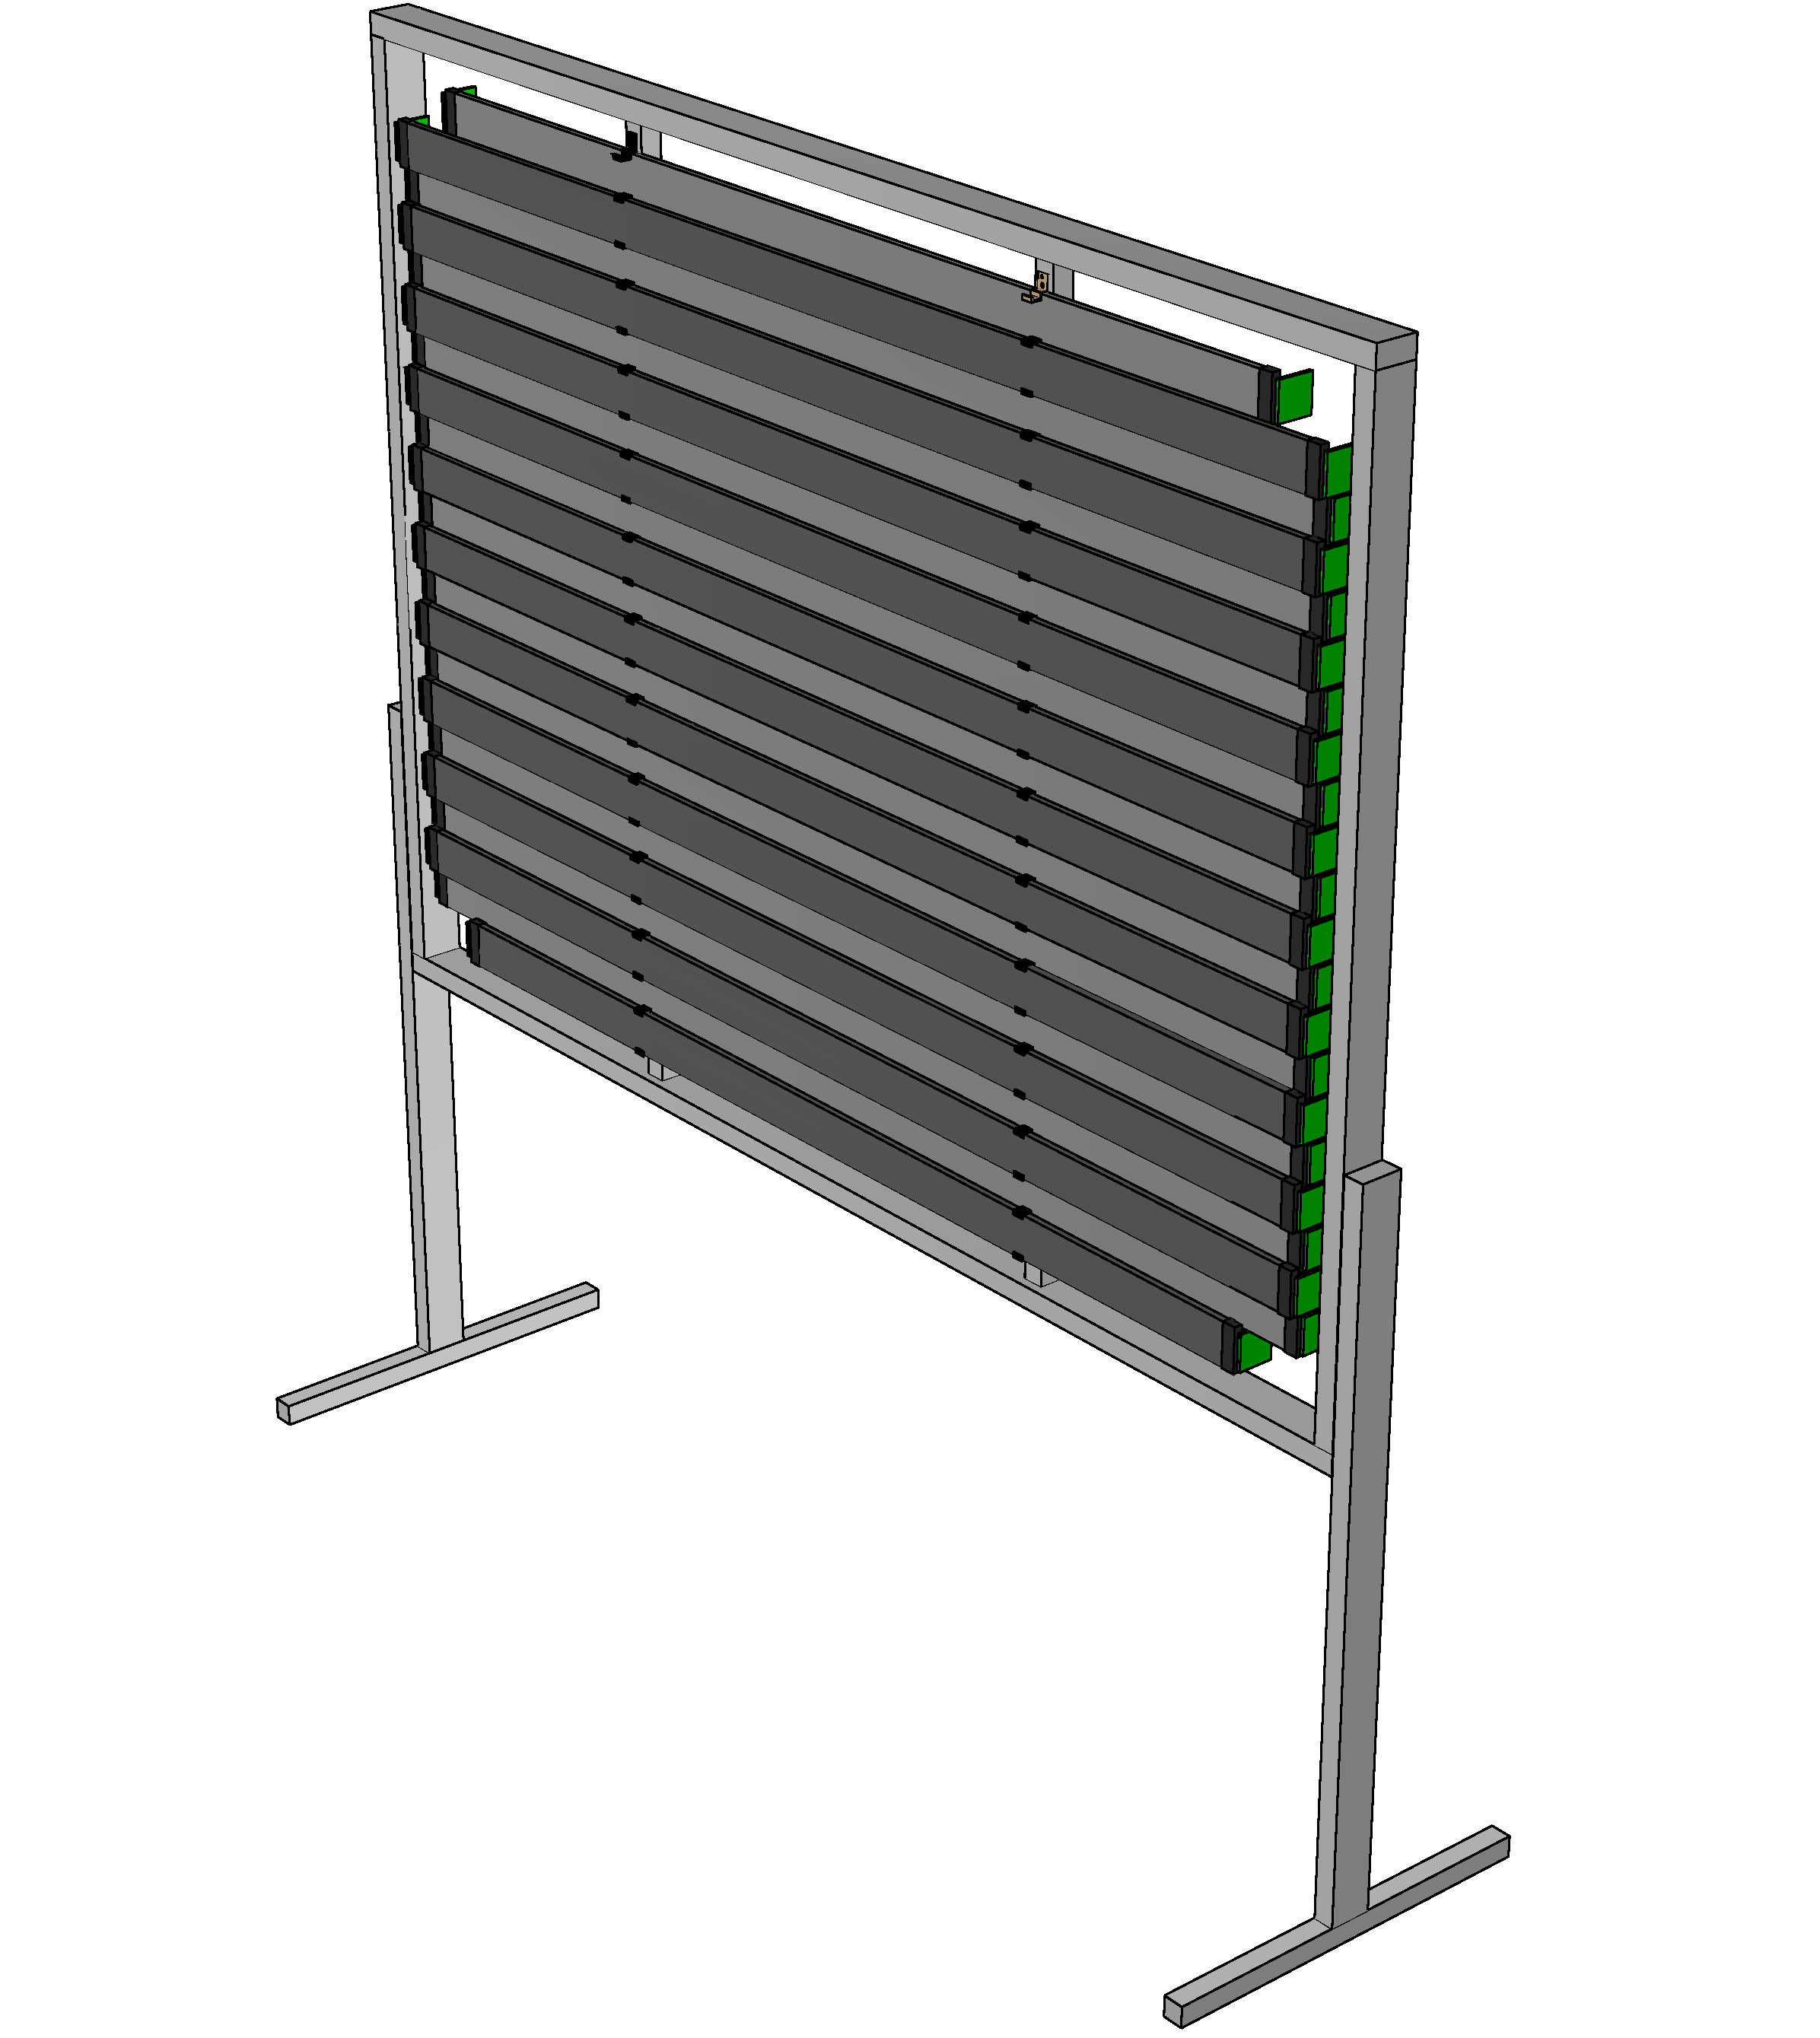
\includegraphics[width=\linewidth]{files/figures/hptpc_beam_flux/uTOF_rot}
  \end{minipage}
  \caption[Schematic diagrams of \SThree]{Front-on and rotated schematic diagrams of \SThree from~\cite{s3Paper} along with dimensions.}
  \label{fig:s3Diag}
\end{figure}

EJ-200 plastic scintillator (of which the bars are made) has a brightness of \num{10000}~photons/MeV deposited.
Additionally, it has a large optical attenuation length (\SI{4}{\metre}) along with a fast rise time and decay time constant (\SI{0.9}{\nano\second} and \SI{2.1}{\nano\second} respectively.
The scintillation emission spectrum peaks at a wavelength of \SI{435}{\nano\metre}~\cite{ej200}.
In order to increase the light collection capabilities of the bars while excluding background light, they are wrapped in aluminium foil which has a reflectivity of 60\%.

The scintillation photons produced by the bars are detected by S13360-6050PE Hamamatsu Photonics~\cite{hamamatsu} silicon photomultipliers (SiPMs) arranged at either end of the bar.
These photosensors, each measuring \SI{6 x 6}{\milli\metre}, are arranged in groups of eight and then coupled to the end of the bar.
These photomultipliers have a wavelength range that is well suited to the scintillation light produced by the bars (the sensitivity of the SiPMs at a wavelength of \SI{450}{\nano\metre} is 40\%~\cite{hamamatsu}).
The anode signals produced by these SiPMs are read out, summed and shaped by a dedicated circuit as described in~\cite{s3SiPM}.

These signals, along with those from \SOne and \STwo, are then fed into a DAQ based upon the SAMPIC chip, further details of which are given in~\cite{sampic}.

\SThree triggers are formed in the following manner, shown graphically in \citefig{fig:s3Trigger}, and are intended to identify the prescence of a beam particle travelling between \SOne and \SThree.
An \SOne signal is considered to have occurred when at least three of the four \SOne PMTs register a signal above the threshold of \SI{30}{\milli\volt}.
An \SThree signal is deemed to have occurred if the SiPMs on either end of a given bar register a signal above a threshold of \SI{30}{\milli\volt}.
If an \SOne signal and an \SThree signal occur within a time window of \SI{70}{\nano\second}, the DAQ is triggered and writes the event.
The DAQ also acquires signals from the coincidence of \SOne and \STwo as well as the signal indicating the start of the beam spill.

\begin{figure}[h]
  \centering
  \includegraphics[width=.8\linewidth]{files/figures/hptpc_beam_flux/utofTrig}
  \caption[Trigger logic for the upstream time of flight DAQ]{Trigger logic showing the necessary conditions for the identification of a $\SOne-\SThree$ beam particle by the upstream ToF DAQ.}
  \label{fig:s3Trigger}
\end{figure}


\subsection{The downstream time of flight detector (\SFour)}
\label{sec:hptpc_beam_flux:overview:s4}

The design of \SFour is primarily discussed in \citesec{sec:hptpc_dtof_characterisation:dtof}, however it will be briefly revisited here.
\SFour consists of 10 scintillator bars which together form an active area of \SI{1.40 x 0.78}{\metre}.
A diagram of one such bar is shown in \citefig{fig:barDiag}.
Each of these scintillator bars has a PMT attached to each end and these observe the scintillation light produced by charged particles traversing the bars.
A diagram of \SFour is shown in \citefig{fig:dtofDiag}.

The anode signal of each of the PMTs is fed into a LeCroy 620AL NIM discriminator with a threshold of \SI{-20}{\milli\volt}.
Any PMT signals above this threshold are digitised using a time-to-digital converted (TDC)
Additionally, the signal indicating the start of a beam spill as well as a signal indicating a coincidence between \SOne and \STwo were fed into the TDC.
A particle (either beam induced or otherwise) is considered to have been observed in \SFour if a signal above the discriminator threshold is recorded in both PMTs on the same bar, within \SI{20}{\nano\second} of each other.

Unlike the UToF DAQ system, the DToF DAQ is operated in self-triggering mode and thus acquired data both inside and outside the beam spill.


\subsection{The HPTPC prototype}
\label{sec:hptpc_beam_flux:overview:hptpc}

The relevant specifications of the HPTPC prototype for this study are the location and wall thickness of the pressure vessel.
The upstream face of HPTPC is located \SI{1.323(2)}{\metre} downstream of the \SThree panel while the downstream face is located \SI{0.918(2)}{\metre} upstream of \SFour.
\citefig{fig:angDistS1} shows that, from the point of view of the beam, most of the  TPC volume is covered by \STwo, \SThree and \SFour.
The angular position of the TPC is at approximately $\theta = \ang{-2.5}$.
With the beam steering, this means that the centre of the TPC lies approximately \ang{3.5} off-axis.

The pressure vessel itself is made out of 304L stainless steel, has an outer diameter of \SI{142}{\centi\metre} and a vessel wall thickness of \SI{1}{\centi\metre}~\cite{deisting2021high}.
This vessel wall thickness is equivalent to the range of proton with a kinetic energy of roughly \SI{80}{\mega\electronvolt}~\cite{protonRangeTables}.

The main cylindrical body of the vessel is \SI{73.6}{\centi\metre} in length while the rounded sections at the end of this volume each have a length of \SI{32.5}{\centi\metre}~\cite{deisting2021high}.
Interior to the cylindrical body is the active volume of the TPC.
This active TPC volume measures \SI{111}{\centi\metre} in diameter and \SI{48}{\centi\metre} in the drift direction and is formed by a series of copper rings which make up the field cage.
A diagram of the HPTPC, showing a cross-sectional view of the active volume, is shown in \citefig{fig:hptpc}.

\begin{figure}[h]
  \centering
  \includegraphics[width=.7\linewidth]{files/figures/hptpc_beam_flux/vesselView}
  \caption[Cross-sectional view of the HPTPC prototype]{Cross-sectional view of the HPTPC prototype with the door open, from~\cite{beampaper}. The drift volume formed by the copper rings is clearly visible. The direction of the beam during the beam test is indicated.}
  \label{fig:hptpc}
\end{figure}

\section{Methods}
\label{sec:hptpc_beam_flux:methods}

In a beamline such as the T10 beamline at CERN, charged particles are selected using by momentum using a magnetic field.
This results in a beam of particles that are all of the same momentum but of different species.
Different particles of the same momentum will take different times to cover the same distance.
The time of flight, $t$, of a particle of mass, $m$, with a momentum, $p$, is given by
\begin{equation}
  t = L \sqrt{ \frac{1}{c^{2}} + \frac{m^{2}}{p^{2}} }\, ,
  \label{eq:tof}
\end{equation}
where $L$ is the distance travelled by the particle.
\citefig{fig:tofVsMom}, left and right, show the time of flight for various particles as a function of particle momentum for the $\SOne - \SThree$ and  $\STwo - \SFour$ distances respectively.
If the beam momentum is known, by measuring a particle's time of flight it should be possible to identify the particle in question.
One can see that, assuming a time resolution of around \SI{1}{\nano\second}, it should be possible to distinguish between deuterons, protons and pions/muons at the momenta used in this study.

\begin{figure}[h]
  \begin{minipage}[t]{.5\linewidth}
    \begin{adjustbox}{max totalsize=\textwidth, center}
      \begin{tikzpicture}
\pgfdeclareplotmark{cross} {
\pgfpathmoveto{\pgfpoint{-0.3\pgfplotmarksize}{\pgfplotmarksize}}
\pgfpathlineto{\pgfpoint{+0.3\pgfplotmarksize}{\pgfplotmarksize}}
\pgfpathlineto{\pgfpoint{+0.3\pgfplotmarksize}{0.3\pgfplotmarksize}}
\pgfpathlineto{\pgfpoint{+1\pgfplotmarksize}{0.3\pgfplotmarksize}}
\pgfpathlineto{\pgfpoint{+1\pgfplotmarksize}{-0.3\pgfplotmarksize}}
\pgfpathlineto{\pgfpoint{+0.3\pgfplotmarksize}{-0.3\pgfplotmarksize}}
\pgfpathlineto{\pgfpoint{+0.3\pgfplotmarksize}{-1.\pgfplotmarksize}}
\pgfpathlineto{\pgfpoint{-0.3\pgfplotmarksize}{-1.\pgfplotmarksize}}
\pgfpathlineto{\pgfpoint{-0.3\pgfplotmarksize}{-0.3\pgfplotmarksize}}
\pgfpathlineto{\pgfpoint{-1.\pgfplotmarksize}{-0.3\pgfplotmarksize}}
\pgfpathlineto{\pgfpoint{-1.\pgfplotmarksize}{0.3\pgfplotmarksize}}
\pgfpathlineto{\pgfpoint{-0.3\pgfplotmarksize}{0.3\pgfplotmarksize}}
\pgfpathclose
\pgfusepathqstroke
}
\pgfdeclareplotmark{cross*} {
\pgfpathmoveto{\pgfpoint{-0.3\pgfplotmarksize}{\pgfplotmarksize}}
\pgfpathlineto{\pgfpoint{+0.3\pgfplotmarksize}{\pgfplotmarksize}}
\pgfpathlineto{\pgfpoint{+0.3\pgfplotmarksize}{0.3\pgfplotmarksize}}
\pgfpathlineto{\pgfpoint{+1\pgfplotmarksize}{0.3\pgfplotmarksize}}
\pgfpathlineto{\pgfpoint{+1\pgfplotmarksize}{-0.3\pgfplotmarksize}}
\pgfpathlineto{\pgfpoint{+0.3\pgfplotmarksize}{-0.3\pgfplotmarksize}}
\pgfpathlineto{\pgfpoint{+0.3\pgfplotmarksize}{-1.\pgfplotmarksize}}
\pgfpathlineto{\pgfpoint{-0.3\pgfplotmarksize}{-1.\pgfplotmarksize}}
\pgfpathlineto{\pgfpoint{-0.3\pgfplotmarksize}{-0.3\pgfplotmarksize}}
\pgfpathlineto{\pgfpoint{-1.\pgfplotmarksize}{-0.3\pgfplotmarksize}}
\pgfpathlineto{\pgfpoint{-1.\pgfplotmarksize}{0.3\pgfplotmarksize}}
\pgfpathlineto{\pgfpoint{-0.3\pgfplotmarksize}{0.3\pgfplotmarksize}}
\pgfpathclose
\pgfusepathqfillstroke
}
\pgfdeclareplotmark{newstar} {
\pgfpathmoveto{\pgfqpoint{0pt}{\pgfplotmarksize}}
\pgfpathlineto{\pgfqpointpolar{44}{0.5\pgfplotmarksize}}
\pgfpathlineto{\pgfqpointpolar{18}{\pgfplotmarksize}}
\pgfpathlineto{\pgfqpointpolar{-20}{0.5\pgfplotmarksize}}
\pgfpathlineto{\pgfqpointpolar{-54}{\pgfplotmarksize}}
\pgfpathlineto{\pgfqpointpolar{-90}{0.5\pgfplotmarksize}}
\pgfpathlineto{\pgfqpointpolar{234}{\pgfplotmarksize}}
\pgfpathlineto{\pgfqpointpolar{198}{0.5\pgfplotmarksize}}
\pgfpathlineto{\pgfqpointpolar{162}{\pgfplotmarksize}}
\pgfpathlineto{\pgfqpointpolar{134}{0.5\pgfplotmarksize}}
\pgfpathclose
\pgfusepathqstroke
}
\pgfdeclareplotmark{newstar*} {
\pgfpathmoveto{\pgfqpoint{0pt}{\pgfplotmarksize}}
\pgfpathlineto{\pgfqpointpolar{44}{0.5\pgfplotmarksize}}
\pgfpathlineto{\pgfqpointpolar{18}{\pgfplotmarksize}}
\pgfpathlineto{\pgfqpointpolar{-20}{0.5\pgfplotmarksize}}
\pgfpathlineto{\pgfqpointpolar{-54}{\pgfplotmarksize}}
\pgfpathlineto{\pgfqpointpolar{-90}{0.5\pgfplotmarksize}}
\pgfpathlineto{\pgfqpointpolar{234}{\pgfplotmarksize}}
\pgfpathlineto{\pgfqpointpolar{198}{0.5\pgfplotmarksize}}
\pgfpathlineto{\pgfqpointpolar{162}{\pgfplotmarksize}}
\pgfpathlineto{\pgfqpointpolar{134}{0.5\pgfplotmarksize}}
\pgfpathclose
\pgfusepathqfillstroke
}
\definecolor{c}{rgb}{1,1,1};
\draw [color=c, fill=c] (0,0) rectangle (20,13.639);
\draw [color=c, fill=c] (2.60745,1.76218) rectangle (17.0201,11.8768);
\definecolor{c}{rgb}{0,0,0};
\draw [c,line width=0.9] (2.60745,1.76218) -- (2.60745,11.8768) -- (17.0201,11.8768) -- (17.0201,1.76218) -- (2.60745,1.76218);
\definecolor{c}{rgb}{1,1,1};
\draw [color=c, fill=c] (2.60745,1.76218) rectangle (17.0201,11.8768);
\definecolor{c}{rgb}{0,0,0};
\draw [c,line width=0.9] (2.60745,1.76218) -- (2.60745,11.8768) -- (17.0201,11.8768) -- (17.0201,1.76218) -- (2.60745,1.76218);
\definecolor{c}{rgb}{0,0.8,0.8};
\draw [c,line width=1.8] (2.67951,3.58458) -- (2.82364,3.40401) -- (2.96777,3.25475) -- (3.11189,3.12999) -- (3.25602,3.02465) -- (3.40014,2.93493) -- (3.54427,2.85792) -- (3.6884,2.79135) -- (3.83252,2.73344) -- (3.97665,2.68276) --
 (4.12077,2.63817) -- (4.2649,2.59875) -- (4.40903,2.56374) -- (4.55315,2.53252) -- (4.69728,2.50455) -- (4.8414,2.47942) -- (4.98553,2.45675) -- (5.12966,2.43624) -- (5.27378,2.41763) -- (5.41791,2.40068) -- (5.56203,2.38522) -- (5.70616,2.37107) --
 (5.85029,2.35809) -- (5.99441,2.34616) -- (6.13854,2.33516) -- (6.28266,2.32501) -- (6.42679,2.31562) -- (6.57092,2.30691) -- (6.71504,2.29883) -- (6.85917,2.29131) -- (7.0033,2.2843) -- (7.14742,2.27777) -- (7.29155,2.27166) -- (7.43567,2.26594) --
 (7.5798,2.26058) -- (7.72393,2.25555) -- (7.86805,2.25083) -- (8.01218,2.24638) -- (8.1563,2.24219) -- (8.30043,2.23824) -- (8.44456,2.23451) -- (8.58868,2.23099) -- (8.73281,2.22766) -- (8.87693,2.2245) -- (9.02106,2.22151) -- (9.16519,2.21867) --
 (9.30931,2.21598) -- (9.45344,2.21342) -- (9.59756,2.21098) -- (9.74169,2.20866);
\draw [c,line width=1.8] (9.74169,2.20866) -- (9.88582,2.20645) -- (10.0299,2.20435) -- (10.1741,2.20234) -- (10.3182,2.20042) -- (10.4623,2.19858) -- (10.6064,2.19683) -- (10.7506,2.19516) -- (10.8947,2.19355) -- (11.0388,2.19201) --
 (11.183,2.19054) -- (11.3271,2.18913) -- (11.4712,2.18777) -- (11.6153,2.18647) -- (11.7595,2.18522) -- (11.9036,2.18401) -- (12.0477,2.18286) -- (12.1918,2.18175) -- (12.336,2.18068) -- (12.4801,2.17965) -- (12.6242,2.17865) -- (12.7683,2.17769) --
 (12.9125,2.17677) -- (13.0566,2.17588) -- (13.2007,2.17502) -- (13.3448,2.17419) -- (13.489,2.17339) -- (13.6331,2.17261) -- (13.7772,2.17187) -- (13.9213,2.17114) -- (14.0655,2.17044) -- (14.2096,2.16976) -- (14.3537,2.16911) -- (14.4979,2.16847)
 -- (14.642,2.16786) -- (14.7861,2.16726) -- (14.9302,2.16668) -- (15.0744,2.16612) -- (15.2185,2.16558) -- (15.3626,2.16505) -- (15.5067,2.16454) -- (15.6509,2.16404) -- (15.795,2.16356) -- (15.9391,2.16309) -- (16.0832,2.16263) -- (16.2274,2.16219)
 -- (16.3715,2.16176) -- (16.5156,2.16134) -- (16.6597,2.16093) -- (16.8039,2.16053);
\draw [c,line width=1.8] (16.8039,2.16053) -- (16.948,2.16015);
\definecolor{c}{rgb}{0,0,0};
\draw [c,line width=0.9] (2.60745,1.76218) -- (17.0201,1.76218);
\draw [c,line width=0.9] (2.60745,2.05704) -- (2.60745,1.76218);
\draw [c,line width=0.9] (2.92773,1.90961) -- (2.92773,1.76218);
\draw [c,line width=0.9] (3.24801,1.90961) -- (3.24801,1.76218);
\draw [c,line width=0.9] (3.56829,1.90961) -- (3.56829,1.76218);
\draw [c,line width=0.9] (3.88857,1.90961) -- (3.88857,1.76218);
\draw [c,line width=0.9] (4.20885,2.05704) -- (4.20885,1.76218);
\draw [c,line width=0.9] (4.52913,1.90961) -- (4.52913,1.76218);
\draw [c,line width=0.9] (4.84941,1.90961) -- (4.84941,1.76218);
\draw [c,line width=0.9] (5.16969,1.90961) -- (5.16969,1.76218);
\draw [c,line width=0.9] (5.48997,1.90961) -- (5.48997,1.76218);
\draw [c,line width=0.9] (5.81025,2.05704) -- (5.81025,1.76218);
\draw [c,line width=0.9] (6.13053,1.90961) -- (6.13053,1.76218);
\draw [c,line width=0.9] (6.45081,1.90961) -- (6.45081,1.76218);
\draw [c,line width=0.9] (6.77109,1.90961) -- (6.77109,1.76218);
\draw [c,line width=0.9] (7.09137,1.90961) -- (7.09137,1.76218);
\draw [c,line width=0.9] (7.41165,2.05704) -- (7.41165,1.76218);
\draw [c,line width=0.9] (7.73193,1.90961) -- (7.73193,1.76218);
\draw [c,line width=0.9] (8.05221,1.90961) -- (8.05221,1.76218);
\draw [c,line width=0.9] (8.37249,1.90961) -- (8.37249,1.76218);
\draw [c,line width=0.9] (8.69277,1.90961) -- (8.69277,1.76218);
\draw [c,line width=0.9] (9.01305,2.05704) -- (9.01305,1.76218);
\draw [c,line width=0.9] (9.33333,1.90961) -- (9.33333,1.76218);
\draw [c,line width=0.9] (9.65361,1.90961) -- (9.65361,1.76218);
\draw [c,line width=0.9] (9.97389,1.90961) -- (9.97389,1.76218);
\draw [c,line width=0.9] (10.2942,1.90961) -- (10.2942,1.76218);
\draw [c,line width=0.9] (10.6145,2.05704) -- (10.6145,1.76218);
\draw [c,line width=0.9] (10.9347,1.90961) -- (10.9347,1.76218);
\draw [c,line width=0.9] (11.255,1.90961) -- (11.255,1.76218);
\draw [c,line width=0.9] (11.5753,1.90961) -- (11.5753,1.76218);
\draw [c,line width=0.9] (11.8956,1.90961) -- (11.8956,1.76218);
\draw [c,line width=0.9] (12.2159,2.05704) -- (12.2159,1.76218);
\draw [c,line width=0.9] (12.5361,1.90961) -- (12.5361,1.76218);
\draw [c,line width=0.9] (12.8564,1.90961) -- (12.8564,1.76218);
\draw [c,line width=0.9] (13.1767,1.90961) -- (13.1767,1.76218);
\draw [c,line width=0.9] (13.497,1.90961) -- (13.497,1.76218);
\draw [c,line width=0.9] (13.8173,2.05704) -- (13.8173,1.76218);
\draw [c,line width=0.9] (14.1375,1.90961) -- (14.1375,1.76218);
\draw [c,line width=0.9] (14.4578,1.90961) -- (14.4578,1.76218);
\draw [c,line width=0.9] (14.7781,1.90961) -- (14.7781,1.76218);
\draw [c,line width=0.9] (15.0984,1.90961) -- (15.0984,1.76218);
\draw [c,line width=0.9] (15.4187,2.05704) -- (15.4187,1.76218);
\draw [c,line width=0.9] (15.7389,1.90961) -- (15.7389,1.76218);
\draw [c,line width=0.9] (16.0592,1.90961) -- (16.0592,1.76218);
\draw [c,line width=0.9] (16.3795,1.90961) -- (16.3795,1.76218);
\draw [c,line width=0.9] (16.6998,1.90961) -- (16.6998,1.76218);
\draw [c,line width=0.9] (17.0201,2.05704) -- (17.0201,1.76218);
\draw [anchor=base] (2.60745,1.14842) node[scale=1.52731, color=c, rotate=0]{0.1};
\draw [anchor=base] (4.20885,1.14842) node[scale=1.52731, color=c, rotate=0]{0.2};
\draw [anchor=base] (5.81025,1.14842) node[scale=1.52731, color=c, rotate=0]{0.3};
\draw [anchor=base] (7.41165,1.14842) node[scale=1.52731, color=c, rotate=0]{0.4};
\draw [anchor=base] (9.01305,1.14842) node[scale=1.52731, color=c, rotate=0]{0.5};
\draw [anchor=base] (10.6145,1.14842) node[scale=1.52731, color=c, rotate=0]{0.6};
\draw [anchor=base] (12.2159,1.14842) node[scale=1.52731, color=c, rotate=0]{0.7};
\draw [anchor=base] (13.8173,1.14842) node[scale=1.52731, color=c, rotate=0]{0.8};
\draw [anchor=base] (15.4187,1.14842) node[scale=1.52731, color=c, rotate=0]{0.9};
\draw [anchor=base] (17.0201,1.14842) node[scale=1.52731, color=c, rotate=0]{1};
\draw [anchor= east] (17.0201,0.561948) node[scale=1.52731, color=c, rotate=0]{ Particle momentum [\si{\giga\electronvolt\per\clight}]};
\draw [c,line width=0.9] (2.60745,11.8768) -- (17.0201,11.8768);
\draw [c,line width=0.9] (2.60745,11.5819) -- (2.60745,11.8768);
\draw [c,line width=0.9] (2.92773,11.7294) -- (2.92773,11.8768);
\draw [c,line width=0.9] (3.24801,11.7294) -- (3.24801,11.8768);
\draw [c,line width=0.9] (3.56829,11.7294) -- (3.56829,11.8768);
\draw [c,line width=0.9] (3.88857,11.7294) -- (3.88857,11.8768);
\draw [c,line width=0.9] (4.20885,11.5819) -- (4.20885,11.8768);
\draw [c,line width=0.9] (4.52913,11.7294) -- (4.52913,11.8768);
\draw [c,line width=0.9] (4.84941,11.7294) -- (4.84941,11.8768);
\draw [c,line width=0.9] (5.16969,11.7294) -- (5.16969,11.8768);
\draw [c,line width=0.9] (5.48997,11.7294) -- (5.48997,11.8768);
\draw [c,line width=0.9] (5.81025,11.5819) -- (5.81025,11.8768);
\draw [c,line width=0.9] (6.13053,11.7294) -- (6.13053,11.8768);
\draw [c,line width=0.9] (6.45081,11.7294) -- (6.45081,11.8768);
\draw [c,line width=0.9] (6.77109,11.7294) -- (6.77109,11.8768);
\draw [c,line width=0.9] (7.09137,11.7294) -- (7.09137,11.8768);
\draw [c,line width=0.9] (7.41165,11.5819) -- (7.41165,11.8768);
\draw [c,line width=0.9] (7.73193,11.7294) -- (7.73193,11.8768);
\draw [c,line width=0.9] (8.05221,11.7294) -- (8.05221,11.8768);
\draw [c,line width=0.9] (8.37249,11.7294) -- (8.37249,11.8768);
\draw [c,line width=0.9] (8.69277,11.7294) -- (8.69277,11.8768);
\draw [c,line width=0.9] (9.01305,11.5819) -- (9.01305,11.8768);
\draw [c,line width=0.9] (9.33333,11.7294) -- (9.33333,11.8768);
\draw [c,line width=0.9] (9.65361,11.7294) -- (9.65361,11.8768);
\draw [c,line width=0.9] (9.97389,11.7294) -- (9.97389,11.8768);
\draw [c,line width=0.9] (10.2942,11.7294) -- (10.2942,11.8768);
\draw [c,line width=0.9] (10.6145,11.5819) -- (10.6145,11.8768);
\draw [c,line width=0.9] (10.9347,11.7294) -- (10.9347,11.8768);
\draw [c,line width=0.9] (11.255,11.7294) -- (11.255,11.8768);
\draw [c,line width=0.9] (11.5753,11.7294) -- (11.5753,11.8768);
\draw [c,line width=0.9] (11.8956,11.7294) -- (11.8956,11.8768);
\draw [c,line width=0.9] (12.2159,11.5819) -- (12.2159,11.8768);
\draw [c,line width=0.9] (12.5361,11.7294) -- (12.5361,11.8768);
\draw [c,line width=0.9] (12.8564,11.7294) -- (12.8564,11.8768);
\draw [c,line width=0.9] (13.1767,11.7294) -- (13.1767,11.8768);
\draw [c,line width=0.9] (13.497,11.7294) -- (13.497,11.8768);
\draw [c,line width=0.9] (13.8173,11.5819) -- (13.8173,11.8768);
\draw [c,line width=0.9] (14.1375,11.7294) -- (14.1375,11.8768);
\draw [c,line width=0.9] (14.4578,11.7294) -- (14.4578,11.8768);
\draw [c,line width=0.9] (14.7781,11.7294) -- (14.7781,11.8768);
\draw [c,line width=0.9] (15.0984,11.7294) -- (15.0984,11.8768);
\draw [c,line width=0.9] (15.4187,11.5819) -- (15.4187,11.8768);
\draw [c,line width=0.9] (15.7389,11.7294) -- (15.7389,11.8768);
\draw [c,line width=0.9] (16.0592,11.7294) -- (16.0592,11.8768);
\draw [c,line width=0.9] (16.3795,11.7294) -- (16.3795,11.8768);
\draw [c,line width=0.9] (16.6998,11.7294) -- (16.6998,11.8768);
\draw [c,line width=0.9] (17.0201,11.5819) -- (17.0201,11.8768);
\draw [c,line width=0.9] (2.60745,1.76218) -- (2.60745,11.8768);
\draw [c,line width=0.9] (3.05241,2.35715) -- (2.60745,2.35715);
\draw [c,line width=0.9] (2.82993,2.65464) -- (2.60745,2.65464);
\draw [c,line width=0.9] (2.82993,2.95213) -- (2.60745,2.95213);
\draw [c,line width=0.9] (2.82993,3.24962) -- (2.60745,3.24962);
\draw [c,line width=0.9] (3.05241,3.54711) -- (2.60745,3.54711);
\draw [c,line width=0.9] (2.82993,3.8446) -- (2.60745,3.8446);
\draw [c,line width=0.9] (2.82993,4.14209) -- (2.60745,4.14209);
\draw [c,line width=0.9] (2.82993,4.43958) -- (2.60745,4.43958);
\draw [c,line width=0.9] (3.05241,4.73706) -- (2.60745,4.73706);
\draw [c,line width=0.9] (2.82993,5.03455) -- (2.60745,5.03455);
\draw [c,line width=0.9] (2.82993,5.33204) -- (2.60745,5.33204);
\draw [c,line width=0.9] (2.82993,5.62953) -- (2.60745,5.62953);
\draw [c,line width=0.9] (3.05241,5.92702) -- (2.60745,5.92702);
\draw [c,line width=0.9] (2.82993,6.22451) -- (2.60745,6.22451);
\draw [c,line width=0.9] (2.82993,6.522) -- (2.60745,6.522);
\draw [c,line width=0.9] (2.82993,6.81948) -- (2.60745,6.81948);
\draw [c,line width=0.9] (3.05241,7.11697) -- (2.60745,7.11697);
\draw [c,line width=0.9] (2.82993,7.41446) -- (2.60745,7.41446);
\draw [c,line width=0.9] (2.82993,7.71195) -- (2.60745,7.71195);
\draw [c,line width=0.9] (2.82993,8.00944) -- (2.60745,8.00944);
\draw [c,line width=0.9] (3.05241,8.30693) -- (2.60745,8.30693);
\draw [c,line width=0.9] (2.82993,8.60442) -- (2.60745,8.60442);
\draw [c,line width=0.9] (2.82993,8.90191) -- (2.60745,8.90191);
\draw [c,line width=0.9] (2.82993,9.19939) -- (2.60745,9.19939);
\draw [c,line width=0.9] (3.05241,9.49688) -- (2.60745,9.49688);
\draw [c,line width=0.9] (2.82993,9.79437) -- (2.60745,9.79437);
\draw [c,line width=0.9] (2.82993,10.0919) -- (2.60745,10.0919);
\draw [c,line width=0.9] (2.82993,10.3893) -- (2.60745,10.3893);
\draw [c,line width=0.9] (3.05241,10.6868) -- (2.60745,10.6868);
\draw [c,line width=0.9] (2.82993,10.9843) -- (2.60745,10.9843);
\draw [c,line width=0.9] (2.82993,11.2818) -- (2.60745,11.2818);
\draw [c,line width=0.9] (2.82993,11.5793) -- (2.60745,11.5793);
\draw [c,line width=0.9] (3.05241,11.8768) -- (2.60745,11.8768);
\draw [c,line width=0.9] (3.05241,2.35715) -- (2.60745,2.35715);
\draw [c,line width=0.9] (2.82993,2.05967) -- (2.60745,2.05967);
\draw [c,line width=0.9] (2.82993,1.76218) -- (2.60745,1.76218);
\draw [anchor= east] (2.50745,2.35715) node[scale=1.52731, color=c, rotate=0]{40};
\draw [anchor= east] (2.50745,3.54711) node[scale=1.52731, color=c, rotate=0]{60};
\draw [anchor= east] (2.50745,4.73706) node[scale=1.52731, color=c, rotate=0]{80};
\draw [anchor= east] (2.50745,5.92702) node[scale=1.52731, color=c, rotate=0]{100};
\draw [anchor= east] (2.50745,7.11697) node[scale=1.52731, color=c, rotate=0]{120};
\draw [anchor= east] (2.50745,8.30693) node[scale=1.52731, color=c, rotate=0]{140};
\draw [anchor= east] (2.50745,9.49688) node[scale=1.52731, color=c, rotate=0]{160};
\draw [anchor= east] (2.50745,10.6868) node[scale=1.52731, color=c, rotate=0]{180};
\draw [anchor= east] (2.50745,11.8768) node[scale=1.52731, color=c, rotate=0]{200};
\draw [anchor= east] (0.84745,11.8768) node[scale=1.52731, color=c, rotate=90]{ Time of flight [\si{\nano\second}]};
\draw [c,line width=0.9] (17.0201,1.76218) -- (17.0201,11.8768);
\draw [c,line width=0.9] (16.5751,2.35715) -- (17.0201,2.35715);
\draw [c,line width=0.9] (16.7976,2.65464) -- (17.0201,2.65464);
\draw [c,line width=0.9] (16.7976,2.95213) -- (17.0201,2.95213);
\draw [c,line width=0.9] (16.7976,3.24962) -- (17.0201,3.24962);
\draw [c,line width=0.9] (16.5751,3.54711) -- (17.0201,3.54711);
\draw [c,line width=0.9] (16.7976,3.8446) -- (17.0201,3.8446);
\draw [c,line width=0.9] (16.7976,4.14209) -- (17.0201,4.14209);
\draw [c,line width=0.9] (16.7976,4.43958) -- (17.0201,4.43958);
\draw [c,line width=0.9] (16.5751,4.73706) -- (17.0201,4.73706);
\draw [c,line width=0.9] (16.7976,5.03455) -- (17.0201,5.03455);
\draw [c,line width=0.9] (16.7976,5.33204) -- (17.0201,5.33204);
\draw [c,line width=0.9] (16.7976,5.62953) -- (17.0201,5.62953);
\draw [c,line width=0.9] (16.5751,5.92702) -- (17.0201,5.92702);
\draw [c,line width=0.9] (16.7976,6.22451) -- (17.0201,6.22451);
\draw [c,line width=0.9] (16.7976,6.522) -- (17.0201,6.522);
\draw [c,line width=0.9] (16.7976,6.81948) -- (17.0201,6.81948);
\draw [c,line width=0.9] (16.5751,7.11697) -- (17.0201,7.11697);
\draw [c,line width=0.9] (16.7976,7.41446) -- (17.0201,7.41446);
\draw [c,line width=0.9] (16.7976,7.71195) -- (17.0201,7.71195);
\draw [c,line width=0.9] (16.7976,8.00944) -- (17.0201,8.00944);
\draw [c,line width=0.9] (16.5751,8.30693) -- (17.0201,8.30693);
\draw [c,line width=0.9] (16.7976,8.60442) -- (17.0201,8.60442);
\draw [c,line width=0.9] (16.7976,8.90191) -- (17.0201,8.90191);
\draw [c,line width=0.9] (16.7976,9.19939) -- (17.0201,9.19939);
\draw [c,line width=0.9] (16.5751,9.49688) -- (17.0201,9.49688);
\draw [c,line width=0.9] (16.7976,9.79437) -- (17.0201,9.79437);
\draw [c,line width=0.9] (16.7976,10.0919) -- (17.0201,10.0919);
\draw [c,line width=0.9] (16.7976,10.3893) -- (17.0201,10.3893);
\draw [c,line width=0.9] (16.5751,10.6868) -- (17.0201,10.6868);
\draw [c,line width=0.9] (16.7976,10.9843) -- (17.0201,10.9843);
\draw [c,line width=0.9] (16.7976,11.2818) -- (17.0201,11.2818);
\draw [c,line width=0.9] (16.7976,11.5793) -- (17.0201,11.5793);
\draw [c,line width=0.9] (16.5751,11.8768) -- (17.0201,11.8768);
\draw [c,line width=0.9] (16.5751,2.35715) -- (17.0201,2.35715);
\draw [c,line width=0.9] (16.7976,2.05967) -- (17.0201,2.05967);
\draw [c,line width=0.9] (16.7976,1.76218) -- (17.0201,1.76218);
\definecolor{c}{rgb}{1,0,0};
\draw [c,line width=1.8] (3.78368,11.8768) -- (3.83252,11.671);
\draw [c,line width=1.8] (3.83252,11.671) -- (3.97665,11.1235) -- (4.12077,10.6276) -- (4.2649,10.1764) -- (4.40903,9.76425) -- (4.55315,9.38637) -- (4.69728,9.03875) -- (4.8414,8.71797) -- (4.98553,8.42111) -- (5.12966,8.14566) -- (5.27378,7.88943)
 -- (5.41791,7.65056) -- (5.56203,7.42737) -- (5.70616,7.21843) -- (5.85029,7.02246) -- (5.99441,6.83832) -- (6.13854,6.66503) -- (6.28266,6.50169) -- (6.42679,6.34749) -- (6.57092,6.20173) -- (6.71504,6.06376) -- (6.85917,5.933) -- (7.0033,5.80893)
 -- (7.14742,5.69107) -- (7.29155,5.57899) -- (7.43567,5.47231) -- (7.5798,5.37065) -- (7.72393,5.2737) -- (7.86805,5.18115) -- (8.01218,5.09273) -- (8.1563,5.00819) -- (8.30043,4.92729) -- (8.44456,4.84982) -- (8.58868,4.77557) -- (8.73281,4.70437)
 -- (8.87693,4.63605) -- (9.02106,4.57044) -- (9.16519,4.5074) -- (9.30931,4.4468) -- (9.45344,4.3885) -- (9.59756,4.33238) -- (9.74169,4.27834) -- (9.88582,4.22628) -- (10.0299,4.17608) -- (10.1741,4.12767) -- (10.3182,4.08096) -- (10.4623,4.03587)
 -- (10.6064,3.99232) -- (10.7506,3.95024);
\draw [c,line width=1.8] (10.7506,3.95024) -- (10.8947,3.90957) -- (11.0388,3.87024) -- (11.183,3.83219) -- (11.3271,3.79537) -- (11.4712,3.75972) -- (11.6153,3.72519) -- (11.7595,3.69175) -- (11.9036,3.65933) -- (12.0477,3.62791) --
 (12.1918,3.59744) -- (12.336,3.56787) -- (12.4801,3.53918) -- (12.6242,3.51134) -- (12.7683,3.4843) -- (12.9125,3.45804) -- (13.0566,3.43252) -- (13.2007,3.40773) -- (13.3448,3.38363) -- (13.489,3.36019) -- (13.6331,3.3374) -- (13.7772,3.31523) --
 (13.9213,3.29365) -- (14.0655,3.27265) -- (14.2096,3.25221) -- (14.3537,3.2323) -- (14.4979,3.21291) -- (14.642,3.19402) -- (14.7861,3.17561) -- (14.9302,3.15767) -- (15.0744,3.14019) -- (15.2185,3.12314) -- (15.3626,3.10651) -- (15.5067,3.09029) --
 (15.6509,3.07446) -- (15.795,3.05902) -- (15.9391,3.04395) -- (16.0832,3.02923) -- (16.2274,3.01487) -- (16.3715,3.00084) -- (16.5156,2.98714) -- (16.6597,2.97375) -- (16.8039,2.96067) -- (16.948,2.94789);
\definecolor{c}{rgb}{0,0,1};
\draw [c,line width=1.8] (2.67951,3.05203) -- (2.82364,2.93124) -- (2.96777,2.83249) -- (3.11189,2.75078) -- (3.25602,2.68244) -- (3.40014,2.62473) -- (3.54427,2.5756) -- (3.6884,2.53343) -- (3.83252,2.497) -- (3.97665,2.46531) -- (4.12077,2.43759)
 -- (4.2649,2.41321) -- (4.40903,2.39166) -- (4.55315,2.37252) -- (4.69728,2.35545) -- (4.8414,2.34017) -- (4.98553,2.32643) -- (5.12966,2.31404) -- (5.27378,2.30282) -- (5.41791,2.29264) -- (5.56203,2.28337) -- (5.70616,2.27491) -- (5.85029,2.26717)
 -- (5.99441,2.26006) -- (6.13854,2.25353) -- (6.28266,2.2475) -- (6.42679,2.24194) -- (6.57092,2.23679) -- (6.71504,2.23201) -- (6.85917,2.22758) -- (7.0033,2.22345) -- (7.14742,2.2196) -- (7.29155,2.21601) -- (7.43567,2.21265) -- (7.5798,2.20951)
 -- (7.72393,2.20656) -- (7.86805,2.20379) -- (8.01218,2.20119) -- (8.1563,2.19874) -- (8.30043,2.19644) -- (8.44456,2.19426) -- (8.58868,2.1922) -- (8.73281,2.19026) -- (8.87693,2.18842) -- (9.02106,2.18668) -- (9.16519,2.18503) -- (9.30931,2.18346)
 -- (9.45344,2.18197) -- (9.59756,2.18055) -- (9.74169,2.1792);
\draw [c,line width=1.8] (9.74169,2.1792) -- (9.88582,2.17792) -- (10.0299,2.1767) -- (10.1741,2.17553) -- (10.3182,2.17442) -- (10.4623,2.17336) -- (10.6064,2.17234) -- (10.7506,2.17137) -- (10.8947,2.17044) -- (11.0388,2.16955) -- (11.183,2.16869)
 -- (11.3271,2.16788) -- (11.4712,2.16709) -- (11.6153,2.16634) -- (11.7595,2.16561) -- (11.9036,2.16492) -- (12.0477,2.16425) -- (12.1918,2.16361) -- (12.336,2.16299) -- (12.4801,2.16239) -- (12.6242,2.16182) -- (12.7683,2.16127) --
 (12.9125,2.16073) -- (13.0566,2.16022) -- (13.2007,2.15972) -- (13.3448,2.15924) -- (13.489,2.15878) -- (13.6331,2.15833) -- (13.7772,2.1579) -- (13.9213,2.15748) -- (14.0655,2.15708) -- (14.2096,2.15669) -- (14.3537,2.15631) -- (14.4979,2.15594) --
 (14.642,2.15559) -- (14.7861,2.15524) -- (14.9302,2.15491) -- (15.0744,2.15459) -- (15.2185,2.15427) -- (15.3626,2.15397) -- (15.5067,2.15367) -- (15.6509,2.15339) -- (15.795,2.15311) -- (15.9391,2.15284) -- (16.0832,2.15258) -- (16.2274,2.15232) --
 (16.3715,2.15207) -- (16.5156,2.15183) -- (16.6597,2.1516) -- (16.8039,2.15137);
\draw [c,line width=1.8] (16.8039,2.15137) -- (16.948,2.15115);
\definecolor{c}{rgb}{1,0.6,0.2};
\draw [c,line width=1.8] (2.67951,10.4165) -- (2.82364,9.62568) -- (2.96777,8.95373) -- (3.11189,8.37623) -- (3.25602,7.87499) -- (3.40014,7.43621) -- (3.54427,7.04923) -- (3.6884,6.70565) -- (3.83252,6.39883) -- (3.97665,6.12337) -- (4.12077,5.8749)
 -- (4.2649,5.64981) -- (4.40903,5.44511) -- (4.55315,5.25828) -- (4.69728,5.08721) -- (4.8414,4.9301) -- (4.98553,4.78541) -- (5.12966,4.65181) -- (5.27378,4.52817) -- (5.41791,4.41348) -- (5.56203,4.30688) -- (5.70616,4.2076) -- (5.85029,4.11497)
 -- (5.99441,4.02841) -- (6.13854,3.94737) -- (6.28266,3.8714) -- (6.42679,3.80006) -- (6.57092,3.733) -- (6.71504,3.66987) -- (6.85917,3.61036) -- (7.0033,3.5542) -- (7.14742,3.50115) -- (7.29155,3.45098) -- (7.43567,3.40348) -- (7.5798,3.35846) --
 (7.72393,3.31576) -- (7.86805,3.27522) -- (8.01218,3.2367) -- (8.1563,3.20007) -- (8.30043,3.16519) -- (8.44456,3.13198) -- (8.58868,3.10031) -- (8.73281,3.07011) -- (8.87693,3.04127) -- (9.02106,3.01373) -- (9.16519,2.98739) -- (9.30931,2.96221) --
 (9.45344,2.9381) -- (9.59756,2.91501) -- (9.74169,2.89289);
\draw [c,line width=1.8] (9.74169,2.89289) -- (9.88582,2.87167) -- (10.0299,2.85132) -- (10.1741,2.83179) -- (10.3182,2.81303) -- (10.4623,2.79501) -- (10.6064,2.77768) -- (10.7506,2.76102) -- (10.8947,2.74498) -- (11.0388,2.72955) --
 (11.183,2.71468) -- (11.3271,2.70035) -- (11.4712,2.68655) -- (11.6153,2.67323) -- (11.7595,2.66038) -- (11.9036,2.64799) -- (12.0477,2.63602) -- (12.1918,2.62446) -- (12.336,2.61329) -- (12.4801,2.60249) -- (12.6242,2.59205) -- (12.7683,2.58195) --
 (12.9125,2.57218) -- (13.0566,2.56272) -- (13.2007,2.55356) -- (13.3448,2.5447) -- (13.489,2.5361) -- (13.6331,2.52778) -- (13.7772,2.5197) -- (13.9213,2.51187) -- (14.0655,2.50428) -- (14.2096,2.49691) -- (14.3537,2.48976) -- (14.4979,2.48282) --
 (14.642,2.47607) -- (14.7861,2.46952) -- (14.9302,2.46316) -- (15.0744,2.45697) -- (15.2185,2.45096) -- (15.3626,2.44512) -- (15.5067,2.43943) -- (15.6509,2.4339) -- (15.795,2.42852) -- (15.9391,2.42328) -- (16.0832,2.41818) -- (16.2274,2.41321) --
 (16.3715,2.40837) -- (16.5156,2.40366) -- (16.6597,2.39907) -- (16.8039,2.3946);
\draw [c,line width=1.8] (16.8039,2.3946) -- (16.948,2.39024);
\definecolor{c}{rgb}{0,0,0};
\draw [c,line width=1.8] (6.55527,11.8768) -- (6.57092,11.8437);
\draw [c,line width=1.8] (6.57092,11.8437) -- (6.71504,11.5542) -- (6.85917,11.2792) -- (7.0033,11.0176) -- (7.14742,10.7686) -- (7.29155,10.5312) -- (7.43567,10.3046) -- (7.5798,10.0882) -- (7.72393,9.88131) -- (7.86805,9.6833) -- (8.01218,9.49364)
 -- (8.1563,9.31182) -- (8.30043,9.13736) -- (8.44456,8.96986) -- (8.58868,8.8089) -- (8.73281,8.65412) -- (8.87693,8.50519) -- (9.02106,8.36177) -- (9.16519,8.22359) -- (9.30931,8.09037) -- (9.45344,7.96186) -- (9.59756,7.83781) -- (9.74169,7.718)
 -- (9.88582,7.60224) -- (10.0299,7.49032) -- (10.1741,7.38206) -- (10.3182,7.27729) -- (10.4623,7.17585) -- (10.6064,7.0776) -- (10.7506,6.98238) -- (10.8947,6.89007) -- (11.0388,6.80054) -- (11.183,6.71367) -- (11.3271,6.62935) -- (11.4712,6.54747)
 -- (11.6153,6.46793) -- (11.7595,6.39065) -- (11.9036,6.31552) -- (12.0477,6.24247) -- (12.1918,6.17141) -- (12.336,6.10226) -- (12.4801,6.03497) -- (12.6242,5.96944) -- (12.7683,5.90562) -- (12.9125,5.84345) -- (13.0566,5.78287) --
 (13.2007,5.72382) -- (13.3448,5.66624) -- (13.489,5.61009);
\draw [c,line width=1.8] (13.489,5.61009) -- (13.6331,5.55531) -- (13.7772,5.50186) -- (13.9213,5.44969) -- (14.0655,5.39877) -- (14.2096,5.34904) -- (14.3537,5.30047) -- (14.4979,5.25303) -- (14.642,5.20667) -- (14.7861,5.16136) -- (14.9302,5.11707)
 -- (15.0744,5.07377) -- (15.2185,5.03142) -- (15.3626,4.99001) -- (15.5067,4.94949) -- (15.6509,4.90984) -- (15.795,4.87104) -- (15.9391,4.83306) -- (16.0832,4.79588) -- (16.2274,4.75947) -- (16.3715,4.72381) -- (16.5156,4.68889) --
 (16.6597,4.65467) -- (16.8039,4.62115) -- (16.948,4.58829);
\definecolor{c}{rgb}{1,1,1};
\draw [color=c, fill=c] (9.11175,8.45272) rectangle (16.7908,11.49);
\definecolor{c}{rgb}{0,0,0};
\draw [anchor=base west] (10.0716,10.756) node[scale=1.40004, color=c, rotate=0]{Pion};
\definecolor{c}{rgb}{0,0.8,0.8};
\draw [c,line width=1.8] (9.25573,10.9838) -- (9.92765,10.9838);
\definecolor{c}{rgb}{0,0,0};
\draw [anchor=base west] (14.3845,10.756) node[scale=1.40004, color=c, rotate=0]{Muon};
\definecolor{c}{rgb}{0,0,1};
\draw [c,line width=1.8] (13.5686,10.9838) -- (14.2406,10.9838);
\definecolor{c}{rgb}{0,0,0};
\draw [anchor=base west] (10.0716,9.74355) node[scale=1.40004, color=c, rotate=0]{Kaon};
\definecolor{c}{rgb}{1,0.6,0.2};
\draw [c,line width=1.8] (9.25573,9.97135) -- (9.92765,9.97135);
\definecolor{c}{rgb}{0,0,0};
\draw [anchor=base west] (14.3845,9.74355) node[scale=1.40004, color=c, rotate=0]{Proton};
\definecolor{c}{rgb}{1,0,0};
\draw [c,line width=1.8] (13.5686,9.97135) -- (14.2406,9.97135);
\definecolor{c}{rgb}{0,0,0};
\draw [anchor=base west] (10.0716,8.73114) node[scale=1.40004, color=c, rotate=0]{Deuteron};
\draw [c,line width=1.8] (9.25573,8.95893) -- (9.92765,8.95893);
\definecolor{c}{rgb}{1,1,1};
\draw [color=c, fill=c] (2,12.8206) rectangle (18,13.5708);
\definecolor{c}{rgb}{0,0,0};
%\draw (10,13.1957) node[scale=1.40004, color=c, rotate=0]{Predicted time of flight from S1 to S3};
\end{tikzpicture}

    \end{adjustbox}
  \end{minipage}
  \hfill
  \begin{minipage}[t]{.5\linewidth}
    \begin{adjustbox}{max totalsize=\textwidth, center}
      \begin{tikzpicture}
\pgfdeclareplotmark{cross} {
\pgfpathmoveto{\pgfpoint{-0.3\pgfplotmarksize}{\pgfplotmarksize}}
\pgfpathlineto{\pgfpoint{+0.3\pgfplotmarksize}{\pgfplotmarksize}}
\pgfpathlineto{\pgfpoint{+0.3\pgfplotmarksize}{0.3\pgfplotmarksize}}
\pgfpathlineto{\pgfpoint{+1\pgfplotmarksize}{0.3\pgfplotmarksize}}
\pgfpathlineto{\pgfpoint{+1\pgfplotmarksize}{-0.3\pgfplotmarksize}}
\pgfpathlineto{\pgfpoint{+0.3\pgfplotmarksize}{-0.3\pgfplotmarksize}}
\pgfpathlineto{\pgfpoint{+0.3\pgfplotmarksize}{-1.\pgfplotmarksize}}
\pgfpathlineto{\pgfpoint{-0.3\pgfplotmarksize}{-1.\pgfplotmarksize}}
\pgfpathlineto{\pgfpoint{-0.3\pgfplotmarksize}{-0.3\pgfplotmarksize}}
\pgfpathlineto{\pgfpoint{-1.\pgfplotmarksize}{-0.3\pgfplotmarksize}}
\pgfpathlineto{\pgfpoint{-1.\pgfplotmarksize}{0.3\pgfplotmarksize}}
\pgfpathlineto{\pgfpoint{-0.3\pgfplotmarksize}{0.3\pgfplotmarksize}}
\pgfpathclose
\pgfusepathqstroke
}
\pgfdeclareplotmark{cross*} {
\pgfpathmoveto{\pgfpoint{-0.3\pgfplotmarksize}{\pgfplotmarksize}}
\pgfpathlineto{\pgfpoint{+0.3\pgfplotmarksize}{\pgfplotmarksize}}
\pgfpathlineto{\pgfpoint{+0.3\pgfplotmarksize}{0.3\pgfplotmarksize}}
\pgfpathlineto{\pgfpoint{+1\pgfplotmarksize}{0.3\pgfplotmarksize}}
\pgfpathlineto{\pgfpoint{+1\pgfplotmarksize}{-0.3\pgfplotmarksize}}
\pgfpathlineto{\pgfpoint{+0.3\pgfplotmarksize}{-0.3\pgfplotmarksize}}
\pgfpathlineto{\pgfpoint{+0.3\pgfplotmarksize}{-1.\pgfplotmarksize}}
\pgfpathlineto{\pgfpoint{-0.3\pgfplotmarksize}{-1.\pgfplotmarksize}}
\pgfpathlineto{\pgfpoint{-0.3\pgfplotmarksize}{-0.3\pgfplotmarksize}}
\pgfpathlineto{\pgfpoint{-1.\pgfplotmarksize}{-0.3\pgfplotmarksize}}
\pgfpathlineto{\pgfpoint{-1.\pgfplotmarksize}{0.3\pgfplotmarksize}}
\pgfpathlineto{\pgfpoint{-0.3\pgfplotmarksize}{0.3\pgfplotmarksize}}
\pgfpathclose
\pgfusepathqfillstroke
}
\pgfdeclareplotmark{newstar} {
\pgfpathmoveto{\pgfqpoint{0pt}{\pgfplotmarksize}}
\pgfpathlineto{\pgfqpointpolar{44}{0.5\pgfplotmarksize}}
\pgfpathlineto{\pgfqpointpolar{18}{\pgfplotmarksize}}
\pgfpathlineto{\pgfqpointpolar{-20}{0.5\pgfplotmarksize}}
\pgfpathlineto{\pgfqpointpolar{-54}{\pgfplotmarksize}}
\pgfpathlineto{\pgfqpointpolar{-90}{0.5\pgfplotmarksize}}
\pgfpathlineto{\pgfqpointpolar{234}{\pgfplotmarksize}}
\pgfpathlineto{\pgfqpointpolar{198}{0.5\pgfplotmarksize}}
\pgfpathlineto{\pgfqpointpolar{162}{\pgfplotmarksize}}
\pgfpathlineto{\pgfqpointpolar{134}{0.5\pgfplotmarksize}}
\pgfpathclose
\pgfusepathqstroke
}
\pgfdeclareplotmark{newstar*} {
\pgfpathmoveto{\pgfqpoint{0pt}{\pgfplotmarksize}}
\pgfpathlineto{\pgfqpointpolar{44}{0.5\pgfplotmarksize}}
\pgfpathlineto{\pgfqpointpolar{18}{\pgfplotmarksize}}
\pgfpathlineto{\pgfqpointpolar{-20}{0.5\pgfplotmarksize}}
\pgfpathlineto{\pgfqpointpolar{-54}{\pgfplotmarksize}}
\pgfpathlineto{\pgfqpointpolar{-90}{0.5\pgfplotmarksize}}
\pgfpathlineto{\pgfqpointpolar{234}{\pgfplotmarksize}}
\pgfpathlineto{\pgfqpointpolar{198}{0.5\pgfplotmarksize}}
\pgfpathlineto{\pgfqpointpolar{162}{\pgfplotmarksize}}
\pgfpathlineto{\pgfqpointpolar{134}{0.5\pgfplotmarksize}}
\pgfpathclose
\pgfusepathqfillstroke
}
\definecolor{c}{rgb}{1,1,1};
\draw [color=c, fill=c] (0,0) rectangle (20,13.639);
\draw [color=c, fill=c] (2.6,1.77307) rectangle (17,11.8659);
\definecolor{c}{rgb}{0,0,0};
\draw [c,line width=0.9] (2.6,1.77307) -- (2.6,11.8659) -- (17,11.8659) -- (17,1.77307) -- (2.6,1.77307);
\definecolor{c}{rgb}{1,1,1};
\draw [color=c, fill=c] (2.6,1.77307) rectangle (17,11.8659);
\definecolor{c}{rgb}{0,0,0};
\draw [c,line width=0.9] (2.6,1.77307) -- (2.6,11.8659) -- (17,11.8659) -- (17,1.77307) -- (2.6,1.77307);
\definecolor{c}{rgb}{0,0.8,0.8};
\draw [c,line width=1.8] (2.672,3.82229) -- (2.816,3.66545) -- (2.96,3.5358) -- (3.104,3.42742) -- (3.248,3.33593) -- (3.392,3.258) -- (3.536,3.19111) -- (3.68,3.13328) -- (3.824,3.08298) -- (3.968,3.03896) -- (4.112,3.00023) -- (4.256,2.96599) --
 (4.4,2.93558) -- (4.544,2.90845) -- (4.688,2.88416) -- (4.832,2.86233) -- (4.976,2.84264) -- (5.12,2.82483) -- (5.264,2.80866) -- (5.408,2.79394) -- (5.552,2.78051) -- (5.696,2.76822) -- (5.84,2.75694) -- (5.984,2.74658) -- (6.128,2.73703) --
 (6.272,2.72821) -- (6.416,2.72005) -- (6.56,2.71249) -- (6.704,2.70547) -- (6.848,2.69893) -- (6.992,2.69285) -- (7.136,2.68717) -- (7.28,2.68186) -- (7.424,2.6769) -- (7.568,2.67224) -- (7.712,2.66787) -- (7.856,2.66377) -- (8,2.65991) --
 (8.144,2.65627) -- (8.288,2.65284) -- (8.432,2.6496) -- (8.576,2.64654) -- (8.72,2.64365) -- (8.864,2.6409) -- (9.008,2.63831) -- (9.152,2.63584) -- (9.296,2.6335) -- (9.44,2.63128) -- (9.584,2.62916) -- (9.728,2.62715);
\draw [c,line width=1.8] (9.728,2.62715) -- (9.872,2.62523) -- (10.016,2.6234) -- (10.16,2.62165) -- (10.304,2.61999) -- (10.448,2.61839) -- (10.592,2.61687) -- (10.736,2.61541) -- (10.88,2.61402) -- (11.024,2.61268) -- (11.168,2.6114) --
 (11.312,2.61018) -- (11.456,2.609) -- (11.6,2.60787) -- (11.744,2.60678) -- (11.888,2.60574) -- (12.032,2.60473) -- (12.176,2.60377) -- (12.32,2.60284) -- (12.464,2.60194) -- (12.608,2.60108) -- (12.752,2.60025) -- (12.896,2.59945) --
 (13.04,2.59867) -- (13.184,2.59793) -- (13.328,2.5972) -- (13.472,2.59651) -- (13.616,2.59583) -- (13.76,2.59518) -- (13.904,2.59456) -- (14.048,2.59395) -- (14.192,2.59336) -- (14.336,2.59279) -- (14.48,2.59224) -- (14.624,2.5917) --
 (14.768,2.59118) -- (14.912,2.59068) -- (15.056,2.59019) -- (15.2,2.58972) -- (15.344,2.58926) -- (15.488,2.58882) -- (15.632,2.58839) -- (15.776,2.58797) -- (15.92,2.58756) -- (16.064,2.58716) -- (16.208,2.58678) -- (16.352,2.5864) --
 (16.496,2.58604) -- (16.64,2.58569) -- (16.784,2.58534);
\draw [c,line width=1.8] (16.784,2.58534) -- (16.928,2.58501);
\definecolor{c}{rgb}{0,0,0};
\draw [c,line width=0.9] (2.6,1.77307) -- (17,1.77307);
\draw [c,line width=0.9] (2.6,2.06767) -- (2.6,1.77307);
\draw [c,line width=0.9] (2.92,1.92037) -- (2.92,1.77307);
\draw [c,line width=0.9] (3.24,1.92037) -- (3.24,1.77307);
\draw [c,line width=0.9] (3.56,1.92037) -- (3.56,1.77307);
\draw [c,line width=0.9] (3.88,1.92037) -- (3.88,1.77307);
\draw [c,line width=0.9] (4.2,2.06767) -- (4.2,1.77307);
\draw [c,line width=0.9] (4.52,1.92037) -- (4.52,1.77307);
\draw [c,line width=0.9] (4.84,1.92037) -- (4.84,1.77307);
\draw [c,line width=0.9] (5.16,1.92037) -- (5.16,1.77307);
\draw [c,line width=0.9] (5.48,1.92037) -- (5.48,1.77307);
\draw [c,line width=0.9] (5.8,2.06767) -- (5.8,1.77307);
\draw [c,line width=0.9] (6.12,1.92037) -- (6.12,1.77307);
\draw [c,line width=0.9] (6.44,1.92037) -- (6.44,1.77307);
\draw [c,line width=0.9] (6.76,1.92037) -- (6.76,1.77307);
\draw [c,line width=0.9] (7.08,1.92037) -- (7.08,1.77307);
\draw [c,line width=0.9] (7.4,2.06767) -- (7.4,1.77307);
\draw [c,line width=0.9] (7.72,1.92037) -- (7.72,1.77307);
\draw [c,line width=0.9] (8.04,1.92037) -- (8.04,1.77307);
\draw [c,line width=0.9] (8.36,1.92037) -- (8.36,1.77307);
\draw [c,line width=0.9] (8.68,1.92037) -- (8.68,1.77307);
\draw [c,line width=0.9] (9,2.06767) -- (9,1.77307);
\draw [c,line width=0.9] (9.32,1.92037) -- (9.32,1.77307);
\draw [c,line width=0.9] (9.64,1.92037) -- (9.64,1.77307);
\draw [c,line width=0.9] (9.96,1.92037) -- (9.96,1.77307);
\draw [c,line width=0.9] (10.28,1.92037) -- (10.28,1.77307);
\draw [c,line width=0.9] (10.6,2.06767) -- (10.6,1.77307);
\draw [c,line width=0.9] (10.92,1.92037) -- (10.92,1.77307);
\draw [c,line width=0.9] (11.24,1.92037) -- (11.24,1.77307);
\draw [c,line width=0.9] (11.56,1.92037) -- (11.56,1.77307);
\draw [c,line width=0.9] (11.88,1.92037) -- (11.88,1.77307);
\draw [c,line width=0.9] (12.2,2.06767) -- (12.2,1.77307);
\draw [c,line width=0.9] (12.52,1.92037) -- (12.52,1.77307);
\draw [c,line width=0.9] (12.84,1.92037) -- (12.84,1.77307);
\draw [c,line width=0.9] (13.16,1.92037) -- (13.16,1.77307);
\draw [c,line width=0.9] (13.48,1.92037) -- (13.48,1.77307);
\draw [c,line width=0.9] (13.8,2.06767) -- (13.8,1.77307);
\draw [c,line width=0.9] (14.12,1.92037) -- (14.12,1.77307);
\draw [c,line width=0.9] (14.44,1.92037) -- (14.44,1.77307);
\draw [c,line width=0.9] (14.76,1.92037) -- (14.76,1.77307);
\draw [c,line width=0.9] (15.08,1.92037) -- (15.08,1.77307);
\draw [c,line width=0.9] (15.4,2.06767) -- (15.4,1.77307);
\draw [c,line width=0.9] (15.72,1.92037) -- (15.72,1.77307);
\draw [c,line width=0.9] (16.04,1.92037) -- (16.04,1.77307);
\draw [c,line width=0.9] (16.36,1.92037) -- (16.36,1.77307);
\draw [c,line width=0.9] (16.68,1.92037) -- (16.68,1.77307);
\draw [c,line width=0.9] (17,2.06767) -- (17,1.77307);
\draw [anchor=base] (2.6,1.15931) node[scale=1.52731, color=c, rotate=0]{0.1};
\draw [anchor=base] (4.2,1.15931) node[scale=1.52731, color=c, rotate=0]{0.2};
\draw [anchor=base] (5.8,1.15931) node[scale=1.52731, color=c, rotate=0]{0.3};
\draw [anchor=base] (7.4,1.15931) node[scale=1.52731, color=c, rotate=0]{0.4};
\draw [anchor=base] (9,1.15931) node[scale=1.52731, color=c, rotate=0]{0.5};
\draw [anchor=base] (10.6,1.15931) node[scale=1.52731, color=c, rotate=0]{0.6};
\draw [anchor=base] (12.2,1.15931) node[scale=1.52731, color=c, rotate=0]{0.7};
\draw [anchor=base] (13.8,1.15931) node[scale=1.52731, color=c, rotate=0]{0.8};
\draw [anchor=base] (15.4,1.15931) node[scale=1.52731, color=c, rotate=0]{0.9};
\draw [anchor=base] (17,1.15931) node[scale=1.52731, color=c, rotate=0]{1};
\draw [anchor= east] (17,0.572837) node[scale=1.52731, color=c, rotate=0]{ Particle momentum [\si{\giga\electronvolt\per\clight}]};
\draw [c,line width=0.9] (2.6,11.8659) -- (17,11.8659);
\draw [c,line width=0.9] (2.6,11.5713) -- (2.6,11.8659);
\draw [c,line width=0.9] (2.92,11.7186) -- (2.92,11.8659);
\draw [c,line width=0.9] (3.24,11.7186) -- (3.24,11.8659);
\draw [c,line width=0.9] (3.56,11.7186) -- (3.56,11.8659);
\draw [c,line width=0.9] (3.88,11.7186) -- (3.88,11.8659);
\draw [c,line width=0.9] (4.2,11.5713) -- (4.2,11.8659);
\draw [c,line width=0.9] (4.52,11.7186) -- (4.52,11.8659);
\draw [c,line width=0.9] (4.84,11.7186) -- (4.84,11.8659);
\draw [c,line width=0.9] (5.16,11.7186) -- (5.16,11.8659);
\draw [c,line width=0.9] (5.48,11.7186) -- (5.48,11.8659);
\draw [c,line width=0.9] (5.8,11.5713) -- (5.8,11.8659);
\draw [c,line width=0.9] (6.12,11.7186) -- (6.12,11.8659);
\draw [c,line width=0.9] (6.44,11.7186) -- (6.44,11.8659);
\draw [c,line width=0.9] (6.76,11.7186) -- (6.76,11.8659);
\draw [c,line width=0.9] (7.08,11.7186) -- (7.08,11.8659);
\draw [c,line width=0.9] (7.4,11.5713) -- (7.4,11.8659);
\draw [c,line width=0.9] (7.72,11.7186) -- (7.72,11.8659);
\draw [c,line width=0.9] (8.04,11.7186) -- (8.04,11.8659);
\draw [c,line width=0.9] (8.36,11.7186) -- (8.36,11.8659);
\draw [c,line width=0.9] (8.68,11.7186) -- (8.68,11.8659);
\draw [c,line width=0.9] (9,11.5713) -- (9,11.8659);
\draw [c,line width=0.9] (9.32,11.7186) -- (9.32,11.8659);
\draw [c,line width=0.9] (9.64,11.7186) -- (9.64,11.8659);
\draw [c,line width=0.9] (9.96,11.7186) -- (9.96,11.8659);
\draw [c,line width=0.9] (10.28,11.7186) -- (10.28,11.8659);
\draw [c,line width=0.9] (10.6,11.5713) -- (10.6,11.8659);
\draw [c,line width=0.9] (10.92,11.7186) -- (10.92,11.8659);
\draw [c,line width=0.9] (11.24,11.7186) -- (11.24,11.8659);
\draw [c,line width=0.9] (11.56,11.7186) -- (11.56,11.8659);
\draw [c,line width=0.9] (11.88,11.7186) -- (11.88,11.8659);
\draw [c,line width=0.9] (12.2,11.5713) -- (12.2,11.8659);
\draw [c,line width=0.9] (12.52,11.7186) -- (12.52,11.8659);
\draw [c,line width=0.9] (12.84,11.7186) -- (12.84,11.8659);
\draw [c,line width=0.9] (13.16,11.7186) -- (13.16,11.8659);
\draw [c,line width=0.9] (13.48,11.7186) -- (13.48,11.8659);
\draw [c,line width=0.9] (13.8,11.5713) -- (13.8,11.8659);
\draw [c,line width=0.9] (14.12,11.7186) -- (14.12,11.8659);
\draw [c,line width=0.9] (14.44,11.7186) -- (14.44,11.8659);
\draw [c,line width=0.9] (14.76,11.7186) -- (14.76,11.8659);
\draw [c,line width=0.9] (15.08,11.7186) -- (15.08,11.8659);
\draw [c,line width=0.9] (15.4,11.5713) -- (15.4,11.8659);
\draw [c,line width=0.9] (15.72,11.7186) -- (15.72,11.8659);
\draw [c,line width=0.9] (16.04,11.7186) -- (16.04,11.8659);
\draw [c,line width=0.9] (16.36,11.7186) -- (16.36,11.8659);
\draw [c,line width=0.9] (16.68,11.7186) -- (16.68,11.8659);
\draw [c,line width=0.9] (17,11.5713) -- (17,11.8659);
\draw [c,line width=0.9] (2.6,1.77307) -- (2.6,11.8659);
\draw [c,line width=0.9] (3.044,2.9243) -- (2.6,2.9243);
\draw [c,line width=0.9] (2.822,3.37138) -- (2.6,3.37138);
\draw [c,line width=0.9] (2.822,3.81846) -- (2.6,3.81846);
\draw [c,line width=0.9] (2.822,4.26554) -- (2.6,4.26554);
\draw [c,line width=0.9] (2.822,4.71262) -- (2.6,4.71262);
\draw [c,line width=0.9] (3.044,5.1597) -- (2.6,5.1597);
\draw [c,line width=0.9] (2.822,5.60678) -- (2.6,5.60678);
\draw [c,line width=0.9] (2.822,6.05386) -- (2.6,6.05386);
\draw [c,line width=0.9] (2.822,6.50094) -- (2.6,6.50094);
\draw [c,line width=0.9] (2.822,6.94802) -- (2.6,6.94802);
\draw [c,line width=0.9] (3.044,7.3951) -- (2.6,7.3951);
\draw [c,line width=0.9] (2.822,7.84218) -- (2.6,7.84218);
\draw [c,line width=0.9] (2.822,8.28926) -- (2.6,8.28926);
\draw [c,line width=0.9] (2.822,8.73634) -- (2.6,8.73634);
\draw [c,line width=0.9] (2.822,9.18342) -- (2.6,9.18342);
\draw [c,line width=0.9] (3.044,9.6305) -- (2.6,9.6305);
\draw [c,line width=0.9] (2.822,10.0776) -- (2.6,10.0776);
\draw [c,line width=0.9] (2.822,10.5247) -- (2.6,10.5247);
\draw [c,line width=0.9] (2.822,10.9717) -- (2.6,10.9717);
\draw [c,line width=0.9] (2.822,11.4188) -- (2.6,11.4188);
\draw [c,line width=0.9] (3.044,11.8659) -- (2.6,11.8659);
\draw [c,line width=0.9] (3.044,2.9243) -- (2.6,2.9243);
\draw [c,line width=0.9] (2.822,2.47722) -- (2.6,2.47722);
\draw [c,line width=0.9] (2.822,2.03014) -- (2.6,2.03014);
\draw [anchor= east] (2.5,2.9243) node[scale=1.52731, color=c, rotate=0]{50};
\draw [anchor= east] (2.5,5.1597) node[scale=1.52731, color=c, rotate=0]{100};
\draw [anchor= east] (2.5,7.3951) node[scale=1.52731, color=c, rotate=0]{150};
\draw [anchor= east] (2.5,9.6305) node[scale=1.52731, color=c, rotate=0]{200};
\draw [anchor= east] (2.5,11.8659) node[scale=1.52731, color=c, rotate=0]{250};
\draw [anchor= east] (0.84,11.8659) node[scale=1.52731, color=c, rotate=90]{ Time of flight [\si{\nano\second}]};
\draw [c,line width=0.9] (17,1.77307) -- (17,11.8659);
\draw [c,line width=0.9] (16.556,2.9243) -- (17,2.9243);
\draw [c,line width=0.9] (16.778,3.37138) -- (17,3.37138);
\draw [c,line width=0.9] (16.778,3.81846) -- (17,3.81846);
\draw [c,line width=0.9] (16.778,4.26554) -- (17,4.26554);
\draw [c,line width=0.9] (16.778,4.71262) -- (17,4.71262);
\draw [c,line width=0.9] (16.556,5.1597) -- (17,5.1597);
\draw [c,line width=0.9] (16.778,5.60678) -- (17,5.60678);
\draw [c,line width=0.9] (16.778,6.05386) -- (17,6.05386);
\draw [c,line width=0.9] (16.778,6.50094) -- (17,6.50094);
\draw [c,line width=0.9] (16.778,6.94802) -- (17,6.94802);
\draw [c,line width=0.9] (16.556,7.3951) -- (17,7.3951);
\draw [c,line width=0.9] (16.778,7.84218) -- (17,7.84218);
\draw [c,line width=0.9] (16.778,8.28926) -- (17,8.28926);
\draw [c,line width=0.9] (16.778,8.73634) -- (17,8.73634);
\draw [c,line width=0.9] (16.778,9.18342) -- (17,9.18342);
\draw [c,line width=0.9] (16.556,9.6305) -- (17,9.6305);
\draw [c,line width=0.9] (16.778,10.0776) -- (17,10.0776);
\draw [c,line width=0.9] (16.778,10.5247) -- (17,10.5247);
\draw [c,line width=0.9] (16.778,10.9717) -- (17,10.9717);
\draw [c,line width=0.9] (16.778,11.4188) -- (17,11.4188);
\draw [c,line width=0.9] (16.556,11.8659) -- (17,11.8659);
\draw [c,line width=0.9] (16.556,2.9243) -- (17,2.9243);
\draw [c,line width=0.9] (16.778,2.47722) -- (17,2.47722);
\draw [c,line width=0.9] (16.778,2.03014) -- (17,2.03014);
\definecolor{c}{rgb}{1,0,0};
\draw [c,line width=1.8] (3.5596,11.8659) -- (3.68,11.3739);
\draw [c,line width=1.8] (3.68,11.3739) -- (3.824,10.8463) -- (3.968,10.3707) -- (4.112,9.93998) -- (4.256,9.54807) -- (4.4,9.19007) -- (4.544,8.86184) -- (4.688,8.55989) -- (4.832,8.28126) -- (4.976,8.0234) -- (5.12,7.78413) -- (5.264,7.56157) --
 (5.408,7.35408) -- (5.552,7.16021) -- (5.696,6.97872) -- (5.84,6.8085) -- (5.984,6.64856) -- (6.128,6.49803) -- (6.272,6.35615) -- (6.416,6.22221) -- (6.56,6.0956) -- (6.704,5.97575) -- (6.848,5.86217) -- (6.992,5.7544) -- (7.136,5.65203) --
 (7.28,5.55468) -- (7.424,5.46201) -- (7.568,5.37371) -- (7.712,5.28949) -- (7.856,5.20911) -- (8,5.13231) -- (8.144,5.05887) -- (8.288,4.9886) -- (8.432,4.9213) -- (8.576,4.85681) -- (8.72,4.79497) -- (8.864,4.73562) -- (9.008,4.67863) --
 (9.152,4.62388) -- (9.296,4.57123) -- (9.44,4.52059) -- (9.584,4.47185) -- (9.728,4.42491) -- (9.872,4.37968) -- (10.016,4.33608) -- (10.16,4.29404) -- (10.304,4.25346) -- (10.448,4.21429) -- (10.592,4.17646);
\draw [c,line width=1.8] (10.592,4.17646) -- (10.736,4.13991) -- (10.88,4.10458) -- (11.024,4.07042) -- (11.168,4.03737) -- (11.312,4.00539) -- (11.456,3.97442) -- (11.6,3.94443) -- (11.744,3.91538) -- (11.888,3.88723) -- (12.032,3.85993) --
 (12.176,3.83346) -- (12.32,3.80778) -- (12.464,3.78286) -- (12.608,3.75867) -- (12.752,3.73519) -- (12.896,3.71238) -- (13.04,3.69021) -- (13.184,3.66868) -- (13.328,3.64774) -- (13.472,3.62739) -- (13.616,3.60759) -- (13.76,3.58833) --
 (13.904,3.56959) -- (14.048,3.55135) -- (14.192,3.53359) -- (14.336,3.5163) -- (14.48,3.49945) -- (14.624,3.48305) -- (14.768,3.46706) -- (14.912,3.45148) -- (15.056,3.43629) -- (15.2,3.42147) -- (15.344,3.40703) -- (15.488,3.39294) --
 (15.632,3.37919) -- (15.776,3.36578) -- (15.92,3.35269) -- (16.064,3.33991) -- (16.208,3.32743) -- (16.352,3.31524) -- (16.496,3.30334) -- (16.64,3.29172) -- (16.784,3.28036) -- (16.928,3.26925);
\definecolor{c}{rgb}{0,0,1};
\draw [c,line width=1.8] (2.672,3.35971) -- (2.816,3.25479) -- (2.96,3.16902) -- (3.104,3.09804) -- (3.248,3.03868) -- (3.392,2.98855) -- (3.536,2.94587) -- (3.68,2.90925) -- (3.824,2.8776) -- (3.968,2.85008) -- (4.112,2.826) -- (4.256,2.80482) --
 (4.4,2.7861) -- (4.544,2.76948) -- (4.688,2.75465) -- (4.832,2.74137) -- (4.976,2.72944) -- (5.12,2.71868) -- (5.264,2.70893) -- (5.408,2.70009) -- (5.552,2.69204) -- (5.696,2.68469) -- (5.84,2.67796) -- (5.984,2.67179) -- (6.128,2.66612) --
 (6.272,2.66088) -- (6.416,2.65605) -- (6.56,2.65158) -- (6.704,2.64743) -- (6.848,2.64358) -- (6.992,2.63999) -- (7.136,2.63665) -- (7.28,2.63353) -- (7.424,2.63061) -- (7.568,2.62788) -- (7.712,2.62532) -- (7.856,2.62292) -- (8,2.62066) --
 (8.144,2.61853) -- (8.288,2.61653) -- (8.432,2.61464) -- (8.576,2.61285) -- (8.72,2.61116) -- (8.864,2.60956) -- (9.008,2.60805) -- (9.152,2.60662) -- (9.296,2.60525) -- (9.44,2.60396) -- (9.584,2.60273) -- (9.728,2.60156);
\draw [c,line width=1.8] (9.728,2.60156) -- (9.872,2.60044) -- (10.016,2.59938) -- (10.16,2.59837) -- (10.304,2.5974) -- (10.448,2.59648) -- (10.592,2.5956) -- (10.736,2.59475) -- (10.88,2.59394) -- (11.024,2.59317) -- (11.168,2.59243) --
 (11.312,2.59172) -- (11.456,2.59104) -- (11.6,2.59038) -- (11.744,2.58975) -- (11.888,2.58915) -- (12.032,2.58857) -- (12.176,2.58801) -- (12.32,2.58747) -- (12.464,2.58696) -- (12.608,2.58646) -- (12.752,2.58598) -- (12.896,2.58551) --
 (13.04,2.58507) -- (13.184,2.58464) -- (13.328,2.58422) -- (13.472,2.58382) -- (13.616,2.58343) -- (13.76,2.58305) -- (13.904,2.58269) -- (14.048,2.58234) -- (14.192,2.582) -- (14.336,2.58167) -- (14.48,2.58135) -- (14.624,2.58105) --
 (14.768,2.58075) -- (14.912,2.58046) -- (15.056,2.58018) -- (15.2,2.5799) -- (15.344,2.57964) -- (15.488,2.57938) -- (15.632,2.57913) -- (15.776,2.57889) -- (15.92,2.57866) -- (16.064,2.57843) -- (16.208,2.57821) -- (16.352,2.57799) --
 (16.496,2.57778) -- (16.64,2.57758) -- (16.784,2.57738);
\draw [c,line width=1.8] (16.784,2.57738) -- (16.928,2.57719);
\definecolor{c}{rgb}{1,0.6,0.2};
\draw [c,line width=1.8] (2.672,9.75663) -- (2.816,9.0697) -- (2.96,8.48604) -- (3.104,7.98441) -- (3.248,7.54902) -- (3.392,7.16789) -- (3.536,6.83175) -- (3.68,6.53332) -- (3.824,6.2668) -- (3.968,6.02753) -- (4.112,5.81171) -- (4.256,5.61619) --
 (4.4,5.43838) -- (4.544,5.2761) -- (4.688,5.12751) -- (4.832,4.99104) -- (4.976,4.86536) -- (5.12,4.74931) -- (5.264,4.64191) -- (5.408,4.54229) -- (5.552,4.4497) -- (5.696,4.36346) -- (5.84,4.283) -- (5.984,4.20781) -- (6.128,4.13742) --
 (6.272,4.07143) -- (6.416,4.00947) -- (6.56,3.95121) -- (6.704,3.89638) -- (6.848,3.84469) -- (6.992,3.79591) -- (7.136,3.74983) -- (7.28,3.70624) -- (7.424,3.66498) -- (7.568,3.62588) -- (7.712,3.58879) -- (7.856,3.55358) -- (8,3.52012) --
 (8.144,3.4883) -- (8.288,3.45801) -- (8.432,3.42916) -- (8.576,3.40165) -- (8.72,3.37541) -- (8.864,3.35037) -- (9.008,3.32644) -- (9.152,3.30357) -- (9.296,3.28169) -- (9.44,3.26075) -- (9.584,3.24069) -- (9.728,3.22148);
\draw [c,line width=1.8] (9.728,3.22148) -- (9.872,3.20305) -- (10.016,3.18537) -- (10.16,3.16841) -- (10.304,3.15211) -- (10.448,3.13646) -- (10.592,3.12141) -- (10.736,3.10693) -- (10.88,3.093) -- (11.024,3.07959) -- (11.168,3.06668) --
 (11.312,3.05424) -- (11.456,3.04225) -- (11.6,3.03068) -- (11.744,3.01952) -- (11.888,3.00875) -- (12.032,2.99836) -- (12.176,2.98831) -- (12.32,2.97861) -- (12.464,2.96923) -- (12.608,2.96016) -- (12.752,2.95139) -- (12.896,2.9429) --
 (13.04,2.93469) -- (13.184,2.92674) -- (13.328,2.91903) -- (13.472,2.91157) -- (13.616,2.90433) -- (13.76,2.89732) -- (13.904,2.89052) -- (14.048,2.88392) -- (14.192,2.87752) -- (14.336,2.87131) -- (14.48,2.86528) -- (14.624,2.85942) --
 (14.768,2.85373) -- (14.912,2.84821) -- (15.056,2.84284) -- (15.2,2.83761) -- (15.344,2.83253) -- (15.488,2.8276) -- (15.632,2.82279) -- (15.776,2.81812) -- (15.92,2.81357) -- (16.064,2.80914) -- (16.208,2.80482) -- (16.352,2.80062) --
 (16.496,2.79653) -- (16.64,2.79254) -- (16.784,2.78865);
\draw [c,line width=1.8] (16.784,2.78865) -- (16.928,2.78486);
\definecolor{c}{rgb}{0,0,0};
\draw [c,line width=1.8] (6.11466,11.8659) -- (6.128,11.8369);
\draw [c,line width=1.8] (6.128,11.8369) -- (6.272,11.5412) -- (6.416,11.2614) -- (6.56,10.9963) -- (6.704,10.7448) -- (6.848,10.5059) -- (6.992,10.2788) -- (7.136,10.0624) -- (7.28,9.85622) -- (7.424,9.65944) -- (7.568,9.47147) -- (7.712,9.29175) --
 (7.856,9.11976) -- (8,8.95502) -- (8.144,8.79708) -- (8.288,8.64555) -- (8.432,8.50005) -- (8.576,8.36024) -- (8.72,8.22579) -- (8.864,8.09642) -- (9.008,7.97185) -- (9.152,7.85183) -- (9.296,7.73611) -- (9.44,7.62448) -- (9.584,7.51673) --
 (9.728,7.41266) -- (9.872,7.31211) -- (10.016,7.21489) -- (10.16,7.12085) -- (10.304,7.02985) -- (10.448,6.94174) -- (10.592,6.85639) -- (10.736,6.77369) -- (10.88,6.6935) -- (11.024,6.61573) -- (11.168,6.54028) -- (11.312,6.46703) --
 (11.456,6.39591) -- (11.6,6.32683) -- (11.744,6.2597) -- (11.888,6.19444) -- (12.032,6.13099) -- (12.176,6.06926) -- (12.32,6.0092) -- (12.464,5.95074) -- (12.608,5.89383) -- (12.752,5.8384) -- (12.896,5.78439) -- (13.04,5.73177);
\draw [c,line width=1.8] (13.04,5.73177) -- (13.184,5.68048) -- (13.328,5.63046) -- (13.472,5.58169) -- (13.616,5.53411) -- (13.76,5.48768) -- (13.904,5.44237) -- (14.048,5.39813) -- (14.192,5.35494) -- (14.336,5.31275) -- (14.48,5.27154) --
 (14.624,5.23127) -- (14.768,5.19192) -- (14.912,5.15345) -- (15.056,5.11583) -- (15.2,5.07905) -- (15.344,5.04307) -- (15.488,5.00788) -- (15.632,4.97344) -- (15.776,4.93974) -- (15.92,4.90675) -- (16.064,4.87445) -- (16.208,4.84282) --
 (16.352,4.81185) -- (16.496,4.78152) -- (16.64,4.75179) -- (16.784,4.72267) -- (16.928,4.69414);
\definecolor{c}{rgb}{1,1,1};
\draw [color=c, fill=c] (11.8338,6.38968) rectangle (16.7335,11.4613);
\definecolor{c}{rgb}{0,0,0};
\draw [anchor=base west] (13.0587,10.7259) node[scale=1.46368, color=c, rotate=0]{Pion};
\definecolor{c}{rgb}{0,0.8,0.8};
\draw [c,line width=1.8] (12.0176,10.9542) -- (12.875,10.9542);
\definecolor{c}{rgb}{0,0,0};
\draw [anchor=base west] (13.0587,9.7116) node[scale=1.46368, color=c, rotate=0]{Muon};
\definecolor{c}{rgb}{0,0,1};
\draw [c,line width=1.8] (12.0176,9.93983) -- (12.875,9.93983);
\definecolor{c}{rgb}{0,0,0};
\draw [anchor=base west] (13.0587,8.69728) node[scale=1.46368, color=c, rotate=0]{Kaon};
\definecolor{c}{rgb}{1,0.6,0.2};
\draw [c,line width=1.8] (12.0176,8.9255) -- (12.875,8.9255);
\definecolor{c}{rgb}{0,0,0};
\draw [anchor=base west] (13.0587,7.68295) node[scale=1.46368, color=c, rotate=0]{Proton};
\definecolor{c}{rgb}{1,0,0};
\draw [c,line width=1.8] (12.0176,7.91117) -- (12.875,7.91117);
\definecolor{c}{rgb}{0,0,0};
\draw [anchor=base west] (13.0587,6.66862) node[scale=1.46368, color=c, rotate=0]{Deuteron};
\draw [c,line width=1.8] (12.0176,6.89685) -- (12.875,6.89685);
\definecolor{c}{rgb}{1,1,1};
\draw [color=c, fill=c] (2,12.8206) rectangle (18,13.5708);
\definecolor{c}{rgb}{0,0,0};
%\draw (10,13.1957) node[scale=1.40004, color=c, rotate=0]{Predicted time of flight from S2 to S4};
\end{tikzpicture}

    \end{adjustbox}
  \end{minipage}
  \caption[Predicted time of flight as a function of momentum for various particle types across the distances used in the HPgTPC beam test]{Predicted time of flight as a function of momentum for various particle types across the distances used in the HPgTPC beam test. Right: the $\SOne - \SThree$ distance. Left: the $\STwo - \SFour$ distance.}
  \label{fig:tofVsMom}
\end{figure}

The basic methods by which the time of flight systems are calibrated are discussed in \citesec{sec:hptpc_beam_flux:methods:general}.
The process used for the identification of particles in \SThree as well as corrections specific to \SThree are discussed in \citesec{sec:hptpc_beam_flux:methods:s3} while the same topics involving \SFour are discussed in \citesec{sec:hptpc_beam_flux:methods:s4}.

\subsection{Analysis methods}
\label{sec:hptpc_beam_flux:methods:general}

In this study two measurements of the beam flux are made, one with \SThree and one with \SFour.
In both cases we measure the time of flight of particle $t_{f}-t_{i}$ where $t_{i}$ is time at which the particle is detected at the initial upstream timing point and $t_{f}$ is the time at which the particle is detected at some final downstream timing point.
In the case of the UToF system, the measured time difference is $t_{\SThree} - t_{\SOne}$, while for the DToF system it is $t_{\SFour} - t_{\STwo}$.

The particular particle type distinction that is made in this study is between protons and MIPs.
At the momenta and with the beamline used in this study, MIPs are primarily charged pions and electrons.
At a momentum of \SI{0.8}{\giga\electronvolt\per\clight} a charged pion will take \SI{36.4}{\nano\second} to traverse the $\SOne - \SThree$ distance while a proton will take \SI{55.3}{\nano\second}.
At the same momentum, a charged pion will take \SI{42.8}{\nano\second} to travel the $\STwo - \SFour$ distance while a proton will take \SI{65.0}{\nano\second}.

Example time of flight spectra are shown in \citefig{fig:s3Tof}, divided between the various moderator block configurations.
Here one can see that there are two distinct populations, a faster peak situated at approximately \SI{36}{\nano\second}, caused by MIPs (primarily pions, muons and positrons) and a broader double peaked structure located between \SI{50}{\nano\second} and \SI{110}{\nano\second} which is caused by protons.
One can see that these positions agree with the theoretical expectation above.

\citefig{fig:s3Tof} also shows that the proton population has a distinct double peaked structure.
This is caused by the steering of the beam which was undertaken in order to increase the off-axis angle of the HPgTPC.
This steering in turn leads to a portion of the beam scattering in the steering magnets.
This scattered portion of the beam forms the slower, broader proton peak while the unscattered portion forms the quicker proton peak.

The 0 block sample also contains a third peak located at approximately \SI{95}{\nano\second} which is not visible in the other samples.
This is caused by deuterons which are moderated out in the other samples.

\begin{figure}[h]
  \begin{adjustbox}{max totalsize={.8\linewidth}, center}
    \begin{tikzpicture}
\pgfdeclareplotmark{cross} {
\pgfpathmoveto{\pgfpoint{-0.3\pgfplotmarksize}{\pgfplotmarksize}}
\pgfpathlineto{\pgfpoint{+0.3\pgfplotmarksize}{\pgfplotmarksize}}
\pgfpathlineto{\pgfpoint{+0.3\pgfplotmarksize}{0.3\pgfplotmarksize}}
\pgfpathlineto{\pgfpoint{+1\pgfplotmarksize}{0.3\pgfplotmarksize}}
\pgfpathlineto{\pgfpoint{+1\pgfplotmarksize}{-0.3\pgfplotmarksize}}
\pgfpathlineto{\pgfpoint{+0.3\pgfplotmarksize}{-0.3\pgfplotmarksize}}
\pgfpathlineto{\pgfpoint{+0.3\pgfplotmarksize}{-1.\pgfplotmarksize}}
\pgfpathlineto{\pgfpoint{-0.3\pgfplotmarksize}{-1.\pgfplotmarksize}}
\pgfpathlineto{\pgfpoint{-0.3\pgfplotmarksize}{-0.3\pgfplotmarksize}}
\pgfpathlineto{\pgfpoint{-1.\pgfplotmarksize}{-0.3\pgfplotmarksize}}
\pgfpathlineto{\pgfpoint{-1.\pgfplotmarksize}{0.3\pgfplotmarksize}}
\pgfpathlineto{\pgfpoint{-0.3\pgfplotmarksize}{0.3\pgfplotmarksize}}
\pgfpathclose
\pgfusepathqstroke
}
\pgfdeclareplotmark{cross*} {
\pgfpathmoveto{\pgfpoint{-0.3\pgfplotmarksize}{\pgfplotmarksize}}
\pgfpathlineto{\pgfpoint{+0.3\pgfplotmarksize}{\pgfplotmarksize}}
\pgfpathlineto{\pgfpoint{+0.3\pgfplotmarksize}{0.3\pgfplotmarksize}}
\pgfpathlineto{\pgfpoint{+1\pgfplotmarksize}{0.3\pgfplotmarksize}}
\pgfpathlineto{\pgfpoint{+1\pgfplotmarksize}{-0.3\pgfplotmarksize}}
\pgfpathlineto{\pgfpoint{+0.3\pgfplotmarksize}{-0.3\pgfplotmarksize}}
\pgfpathlineto{\pgfpoint{+0.3\pgfplotmarksize}{-1.\pgfplotmarksize}}
\pgfpathlineto{\pgfpoint{-0.3\pgfplotmarksize}{-1.\pgfplotmarksize}}
\pgfpathlineto{\pgfpoint{-0.3\pgfplotmarksize}{-0.3\pgfplotmarksize}}
\pgfpathlineto{\pgfpoint{-1.\pgfplotmarksize}{-0.3\pgfplotmarksize}}
\pgfpathlineto{\pgfpoint{-1.\pgfplotmarksize}{0.3\pgfplotmarksize}}
\pgfpathlineto{\pgfpoint{-0.3\pgfplotmarksize}{0.3\pgfplotmarksize}}
\pgfpathclose
\pgfusepathqfillstroke
}
\pgfdeclareplotmark{newstar} {
\pgfpathmoveto{\pgfqpoint{0pt}{\pgfplotmarksize}}
\pgfpathlineto{\pgfqpointpolar{44}{0.5\pgfplotmarksize}}
\pgfpathlineto{\pgfqpointpolar{18}{\pgfplotmarksize}}
\pgfpathlineto{\pgfqpointpolar{-20}{0.5\pgfplotmarksize}}
\pgfpathlineto{\pgfqpointpolar{-54}{\pgfplotmarksize}}
\pgfpathlineto{\pgfqpointpolar{-90}{0.5\pgfplotmarksize}}
\pgfpathlineto{\pgfqpointpolar{234}{\pgfplotmarksize}}
\pgfpathlineto{\pgfqpointpolar{198}{0.5\pgfplotmarksize}}
\pgfpathlineto{\pgfqpointpolar{162}{\pgfplotmarksize}}
\pgfpathlineto{\pgfqpointpolar{134}{0.5\pgfplotmarksize}}
\pgfpathclose
\pgfusepathqstroke
}
\pgfdeclareplotmark{newstar*} {
\pgfpathmoveto{\pgfqpoint{0pt}{\pgfplotmarksize}}
\pgfpathlineto{\pgfqpointpolar{44}{0.5\pgfplotmarksize}}
\pgfpathlineto{\pgfqpointpolar{18}{\pgfplotmarksize}}
\pgfpathlineto{\pgfqpointpolar{-20}{0.5\pgfplotmarksize}}
\pgfpathlineto{\pgfqpointpolar{-54}{\pgfplotmarksize}}
\pgfpathlineto{\pgfqpointpolar{-90}{0.5\pgfplotmarksize}}
\pgfpathlineto{\pgfqpointpolar{234}{\pgfplotmarksize}}
\pgfpathlineto{\pgfqpointpolar{198}{0.5\pgfplotmarksize}}
\pgfpathlineto{\pgfqpointpolar{162}{\pgfplotmarksize}}
\pgfpathlineto{\pgfqpointpolar{134}{0.5\pgfplotmarksize}}
\pgfpathclose
\pgfusepathqfillstroke
}
\definecolor{c}{rgb}{1,1,1};
\draw [color=c, fill=c] (0,0) rectangle (20,13.639);
\draw [color=c, fill=c] (3,1.77307) rectangle (17,11.8659);
\definecolor{c}{rgb}{0,0,0};
\draw [c,line width=0.9] (3,1.77307) -- (3,11.8659) -- (17,11.8659) -- (17,1.77307) -- (3,1.77307);
\definecolor{c}{rgb}{1,1,1};
\draw [color=c, fill=c] (3,1.77307) rectangle (17,11.8659);
\definecolor{c}{rgb}{0,0,0};
\draw [c,line width=0.9] (3,1.77307) -- (3,11.8659) -- (17,11.8659) -- (17,1.77307) -- (3,1.77307);
\draw [c,line width=0.9] (3,1.77307) -- (3.056,1.77307) -- (3.056,1.77307) -- (3.112,1.77307) -- (3.112,1.77307) -- (3.168,1.77307) -- (3.168,1.77307) -- (3.224,1.77307) -- (3.224,1.77307) -- (3.28,1.77307) -- (3.28,1.77307) -- (3.336,1.77307) --
 (3.336,1.77307) -- (3.392,1.77307) -- (3.392,1.77307) -- (3.448,1.77307) -- (3.448,1.77307) -- (3.504,1.77307) -- (3.504,1.77307) -- (3.56,1.77307) -- (3.56,1.77307) -- (3.616,1.77307) -- (3.616,1.77307) -- (3.672,1.77307) -- (3.672,1.77307) --
 (3.728,1.77307) -- (3.728,1.77307) -- (3.784,1.77307) -- (3.784,1.77307) -- (3.84,1.77307) -- (3.84,1.77307) -- (3.896,1.77307) -- (3.896,1.77307) -- (3.952,1.77307) -- (3.952,1.77307) -- (4.008,1.77307) -- (4.008,1.77307) -- (4.064,1.77307) --
 (4.064,1.77307) -- (4.12,1.77307) -- (4.12,1.77307) -- (4.176,1.77307) -- (4.176,1.77307) -- (4.232,1.77307) -- (4.232,1.77307) -- (4.288,1.77307) -- (4.288,1.77307) -- (4.344,1.77307) -- (4.344,1.77307) -- (4.4,1.77307) -- (4.4,1.77307) --
 (4.456,1.77307) -- (4.456,1.77307) -- (4.512,1.77307) -- (4.512,1.77307) -- (4.568,1.77307) -- (4.568,1.77307) -- (4.624,1.77307) -- (4.624,1.77307) -- (4.68,1.77307) -- (4.68,1.77307) -- (4.736,1.77307) -- (4.736,1.77307) -- (4.792,1.77307) --
 (4.792,1.77307) -- (4.848,1.77307) -- (4.848,1.77307) -- (4.904,1.77307) -- (4.904,1.77307) -- (4.96,1.77307) -- (4.96,1.77307) -- (5.016,1.77307) -- (5.016,1.77307) -- (5.072,1.77307) -- (5.072,1.77307) -- (5.128,1.77307) -- (5.128,1.77307) --
 (5.184,1.77307) -- (5.184,1.77307) -- (5.24,1.77307) -- (5.24,1.77307) -- (5.296,1.77307) -- (5.296,1.77307) -- (5.352,1.77307) -- (5.352,1.77307) -- (5.408,1.77307) -- (5.408,1.77307) -- (5.464,1.77307) -- (5.464,1.77307) -- (5.52,1.77307) --
 (5.52,1.77307) -- (5.576,1.77307) -- (5.576,1.77307) -- (5.632,1.77307) -- (5.632,1.77307) -- (5.688,1.77307) -- (5.688,1.77307) -- (5.744,1.77307) -- (5.744,1.77307) -- (5.8,1.77307) -- (5.8,1.77307) -- (5.856,1.77307) -- (5.856,1.77307) --
 (5.912,1.77307) -- (5.912,1.77307) -- (5.968,1.77307) -- (5.968,1.77307) -- (6.024,1.77307) -- (6.024,1.77307) -- (6.08,1.77307) -- (6.08,1.77307) -- (6.136,1.77307) -- (6.136,1.77307) -- (6.192,1.77307) -- (6.192,1.77307) -- (6.248,1.77307) --
 (6.248,1.77307) -- (6.304,1.77307) -- (6.304,1.77307) -- (6.36,1.77307) -- (6.36,1.77307) -- (6.416,1.77307) -- (6.416,1.77307) -- (6.472,1.77307) -- (6.472,1.77307) -- (6.528,1.77307) -- (6.528,1.77307) -- (6.584,1.77307) -- (6.584,1.77307) --
 (6.64,1.77307) -- (6.64,1.77307) -- (6.696,1.77307) -- (6.696,1.77307) -- (6.752,1.77307) -- (6.752,1.77307) -- (6.808,1.77307) -- (6.808,1.77307) -- (6.864,1.77307) -- (6.864,1.77307) -- (6.92,1.77307) -- (6.92,1.77307) -- (6.976,1.77307) --
 (6.976,1.77307) -- (7.032,1.77307) -- (7.032,1.77307) -- (7.088,1.77307) -- (7.088,1.77307) -- (7.144,1.77307) -- (7.144,1.77307) -- (7.2,1.77307) -- (7.2,1.77307) -- (7.256,1.77307) -- (7.256,1.77307) -- (7.312,1.77307) -- (7.312,1.77307) --
 (7.368,1.77307) -- (7.368,1.77307) -- (7.424,1.77307) -- (7.424,1.77307) -- (7.48,1.77307) -- (7.48,1.77307) -- (7.536,1.77307) -- (7.536,1.77307) -- (7.592,1.77307) -- (7.592,1.77307) -- (7.648,1.77307) -- (7.648,1.77307) -- (7.704,1.77307) --
 (7.704,1.77307) -- (7.76,1.77307) -- (7.76,1.77307) -- (7.816,1.77307) -- (7.816,1.77307) -- (7.872,1.77307) -- (7.872,1.77307) -- (7.928,1.77307) -- (7.928,1.77307) -- (7.984,1.77307) -- (7.984,1.77307) -- (8.04,1.77307) -- (8.04,1.77307) --
 (8.096,1.77307) -- (8.096,1.77307) -- (8.152,1.77307) -- (8.152,1.77307) -- (8.208,1.77307) -- (8.208,1.77307) -- (8.264,1.77307) -- (8.264,1.77307) -- (8.32,1.77307) -- (8.32,1.77307) -- (8.376,1.77307) -- (8.376,1.77307) -- (8.432,1.77307) --
 (8.432,1.77307) -- (8.488,1.77307) -- (8.488,1.77307) -- (8.544,1.77307) -- (8.544,1.77307) -- (8.6,1.77307) -- (8.6,1.77307) -- (8.656,1.77307) -- (8.656,1.77307) -- (8.712,1.77307) -- (8.712,1.77307) -- (8.768,1.77307) -- (8.768,1.77307) --
 (8.824,1.77307) -- (8.824,1.77307) -- (8.88,1.77307) -- (8.88,1.77307) -- (8.936,1.77307) -- (8.936,1.77307) -- (8.992,1.77307) -- (8.992,1.77307) -- (9.048,1.77307) -- (9.048,1.77307) -- (9.104,1.77307) -- (9.104,1.77307) -- (9.16,1.77307) --
 (9.16,1.77307) -- (9.216,1.77307) -- (9.216,1.77307) -- (9.272,1.77307) -- (9.272,1.77307) -- (9.328,1.77307) -- (9.328,1.77307) -- (9.384,1.77307) -- (9.384,1.77307) -- (9.44,1.77307) -- (9.44,1.77307) -- (9.496,1.77307) -- (9.496,1.77307) --
 (9.552,1.77307) -- (9.552,1.77307) -- (9.608,1.77307) -- (9.608,1.77307) -- (9.664,1.77307) -- (9.664,1.77307) -- (9.72,1.77307) -- (9.72,1.77307) -- (9.776,1.77307) -- (9.776,1.77307) -- (9.832,1.77307) -- (9.832,1.77307) -- (9.888,1.77307) --
 (9.888,1.77307) -- (9.944,1.77307) -- (9.944,1.77307) -- (10,1.77307) -- (10,1.77307) -- (10.056,1.77307) -- (10.056,1.77307) -- (10.112,1.77307) -- (10.112,1.77307) -- (10.168,1.77307) -- (10.168,1.77307) -- (10.224,1.77307) -- (10.224,1.77307) --
 (10.28,1.77307) -- (10.28,1.77307) -- (10.336,1.77307) -- (10.336,1.77307) -- (10.392,1.77307) -- (10.392,1.77307) -- (10.448,1.77307) -- (10.448,1.77307) -- (10.504,1.77307) -- (10.504,1.77307) -- (10.56,1.77307) -- (10.56,1.77307) --
 (10.616,1.77307) -- (10.616,1.77307) -- (10.672,1.77307) -- (10.672,1.77307) -- (10.728,1.77307) -- (10.728,1.77307) -- (10.784,1.77307) -- (10.784,1.77307) -- (10.84,1.77307) -- (10.84,1.77307) -- (10.896,1.77307) -- (10.896,1.77307) --
 (10.952,1.77307) -- (10.952,1.77307) -- (11.008,1.77307) -- (11.008,1.77307) -- (11.064,1.77307) -- (11.064,1.77307) -- (11.12,1.77307) -- (11.12,1.77307) -- (11.176,1.77307) -- (11.176,1.77307) -- (11.232,1.77307) -- (11.232,1.77307) --
 (11.288,1.77307) -- (11.288,1.77307) -- (11.344,1.77307) -- (11.344,1.77307) -- (11.4,1.77307) -- (11.4,1.77307) -- (11.456,1.77307) -- (11.456,1.77307) -- (11.512,1.77307) -- (11.512,1.77307) -- (11.568,1.77307) -- (11.568,1.77307) --
 (11.624,1.77307) -- (11.624,1.77307) -- (11.68,1.77307) -- (11.68,1.77307) -- (11.736,1.77307) -- (11.736,1.77307) -- (11.792,1.77307) -- (11.792,1.77307) -- (11.848,1.77307) -- (11.848,1.77307) -- (11.904,1.77307) -- (11.904,1.77307) --
 (11.96,1.77307) -- (11.96,1.77307) -- (12.016,1.77307) -- (12.016,1.77307) -- (12.072,1.77307) -- (12.072,1.77307) -- (12.128,1.77307) -- (12.128,1.77307) -- (12.184,1.77307) -- (12.184,1.77307) -- (12.24,1.77307) -- (12.24,1.77307) --
 (12.296,1.77307) -- (12.296,1.77307) -- (12.352,1.77307) -- (12.352,1.77307) -- (12.408,1.77307) -- (12.408,1.77307) -- (12.464,1.77307) -- (12.464,1.77307) -- (12.52,1.77307) -- (12.52,1.77307) -- (12.576,1.77307) -- (12.576,1.77307) --
 (12.632,1.77307) -- (12.632,1.77307) -- (12.688,1.77307) -- (12.688,1.77307) -- (12.744,1.77307) -- (12.744,1.77307) -- (12.8,1.77307) -- (12.8,1.77307) -- (12.856,1.77307) -- (12.856,1.77307) -- (12.912,1.77307) -- (12.912,1.77307) --
 (12.968,1.77307) -- (12.968,1.77307) -- (13.024,1.77307) -- (13.024,1.77307) -- (13.08,1.77307) -- (13.08,1.77307) -- (13.136,1.77307) -- (13.136,1.77307) -- (13.192,1.77307) -- (13.192,1.77307) -- (13.248,1.77307) -- (13.248,1.77307) --
 (13.304,1.77307) -- (13.304,1.77307) -- (13.36,1.77307) -- (13.36,1.77307) -- (13.416,1.77307) -- (13.416,1.77307) -- (13.472,1.77307) -- (13.472,1.77307) -- (13.528,1.77307) -- (13.528,1.77307) -- (13.584,1.77307) -- (13.584,1.77307) --
 (13.64,1.77307) -- (13.64,1.77307) -- (13.696,1.77307) -- (13.696,1.77307) -- (13.752,1.77307) -- (13.752,1.77307) -- (13.808,1.77307) -- (13.808,1.77307) -- (13.864,1.77307) -- (13.864,1.77307) -- (13.92,1.77307) -- (13.92,1.77307) --
 (13.976,1.77307) -- (13.976,1.77307) -- (14.032,1.77307) -- (14.032,1.77307) -- (14.088,1.77307) -- (14.088,1.77307) -- (14.144,1.77307) -- (14.144,1.77307) -- (14.2,1.77307) -- (14.2,1.77307) -- (14.256,1.77307) -- (14.256,1.77307) --
 (14.312,1.77307) -- (14.312,1.77307) -- (14.368,1.77307) -- (14.368,1.77307) -- (14.424,1.77307) -- (14.424,1.77307) -- (14.48,1.77307) -- (14.48,1.77307) -- (14.536,1.77307) -- (14.536,1.77307) -- (14.592,1.77307) -- (14.592,1.77307) --
 (14.648,1.77307) -- (14.648,1.77307) -- (14.704,1.77307) -- (14.704,1.77307) -- (14.76,1.77307) -- (14.76,1.77307) -- (14.816,1.77307) -- (14.816,1.77307) -- (14.872,1.77307) -- (14.872,1.77307) -- (14.928,1.77307) -- (14.928,1.77307) --
 (14.984,1.77307) -- (14.984,1.77307) -- (15.04,1.77307) -- (15.04,1.77307) -- (15.096,1.77307) -- (15.096,1.77307) -- (15.152,1.77307) -- (15.152,1.77307) -- (15.208,1.77307) -- (15.208,1.77307) -- (15.264,1.77307) -- (15.264,1.77307) --
 (15.32,1.77307) -- (15.32,1.77307) -- (15.376,1.77307) -- (15.376,1.77307) -- (15.432,1.77307) -- (15.432,1.77307) -- (15.488,1.77307) -- (15.488,1.77307) -- (15.544,1.77307) -- (15.544,1.77307) -- (15.6,1.77307) -- (15.6,1.77307) --
 (15.656,1.77307) -- (15.656,1.77307) -- (15.712,1.77307) -- (15.712,1.77307) -- (15.768,1.77307) -- (15.768,1.77307) -- (15.824,1.77307) -- (15.824,1.77307) -- (15.88,1.77307) -- (15.88,1.77307) -- (15.936,1.77307) -- (15.936,1.77307) --
 (15.992,1.77307) -- (15.992,1.77307) -- (16.048,1.77307) -- (16.048,1.77307) -- (16.104,1.77307) -- (16.104,1.77307) -- (16.16,1.77307) -- (16.16,1.77307) -- (16.216,1.77307) -- (16.216,1.77307) -- (16.272,1.77307) -- (16.272,1.77307) --
 (16.328,1.77307) -- (16.328,1.77307) -- (16.384,1.77307) -- (16.384,1.77307) -- (16.44,1.77307) -- (16.44,1.77307) -- (16.496,1.77307) -- (16.496,1.77307) -- (16.552,1.77307) -- (16.552,1.77307) -- (16.608,1.77307) -- (16.608,1.77307) --
 (16.664,1.77307) -- (16.664,1.77307) -- (16.72,1.77307) -- (16.72,1.77307) -- (16.776,1.77307) -- (16.776,1.77307) -- (16.832,1.77307) -- (16.832,1.77307) -- (16.888,1.77307) -- (16.888,1.77307) -- (16.944,1.77307) -- (16.944,1.77307) --
 (17,1.77307);
\draw [c,line width=0.9] (3,1.77307) -- (17,1.77307);
\draw [c,line width=0.9] (3.7,2.05948) -- (3.7,1.77307);
\draw [c,line width=0.9] (3.98,1.91628) -- (3.98,1.77307);
\draw [c,line width=0.9] (4.26,1.91628) -- (4.26,1.77307);
\draw [c,line width=0.9] (4.54,1.91628) -- (4.54,1.77307);
\draw [c,line width=0.9] (4.82,1.91628) -- (4.82,1.77307);
\draw [c,line width=0.9] (5.1,2.05948) -- (5.1,1.77307);
\draw [c,line width=0.9] (5.38,1.91628) -- (5.38,1.77307);
\draw [c,line width=0.9] (5.66,1.91628) -- (5.66,1.77307);
\draw [c,line width=0.9] (5.94,1.91628) -- (5.94,1.77307);
\draw [c,line width=0.9] (6.22,1.91628) -- (6.22,1.77307);
\draw [c,line width=0.9] (6.5,2.05948) -- (6.5,1.77307);
\draw [c,line width=0.9] (6.78,1.91628) -- (6.78,1.77307);
\draw [c,line width=0.9] (7.06,1.91628) -- (7.06,1.77307);
\draw [c,line width=0.9] (7.34,1.91628) -- (7.34,1.77307);
\draw [c,line width=0.9] (7.62,1.91628) -- (7.62,1.77307);
\draw [c,line width=0.9] (7.9,2.05948) -- (7.9,1.77307);
\draw [c,line width=0.9] (8.18,1.91628) -- (8.18,1.77307);
\draw [c,line width=0.9] (8.46,1.91628) -- (8.46,1.77307);
\draw [c,line width=0.9] (8.74,1.91628) -- (8.74,1.77307);
\draw [c,line width=0.9] (9.02,1.91628) -- (9.02,1.77307);
\draw [c,line width=0.9] (9.3,2.05948) -- (9.3,1.77307);
\draw [c,line width=0.9] (9.58,1.91628) -- (9.58,1.77307);
\draw [c,line width=0.9] (9.86,1.91628) -- (9.86,1.77307);
\draw [c,line width=0.9] (10.14,1.91628) -- (10.14,1.77307);
\draw [c,line width=0.9] (10.42,1.91628) -- (10.42,1.77307);
\draw [c,line width=0.9] (10.7,2.05948) -- (10.7,1.77307);
\draw [c,line width=0.9] (10.98,1.91628) -- (10.98,1.77307);
\draw [c,line width=0.9] (11.26,1.91628) -- (11.26,1.77307);
\draw [c,line width=0.9] (11.54,1.91628) -- (11.54,1.77307);
\draw [c,line width=0.9] (11.82,1.91628) -- (11.82,1.77307);
\draw [c,line width=0.9] (12.1,2.05948) -- (12.1,1.77307);
\draw [c,line width=0.9] (12.38,1.91628) -- (12.38,1.77307);
\draw [c,line width=0.9] (12.66,1.91628) -- (12.66,1.77307);
\draw [c,line width=0.9] (12.94,1.91628) -- (12.94,1.77307);
\draw [c,line width=0.9] (13.22,1.91628) -- (13.22,1.77307);
\draw [c,line width=0.9] (13.5,2.05948) -- (13.5,1.77307);
\draw [c,line width=0.9] (13.78,1.91628) -- (13.78,1.77307);
\draw [c,line width=0.9] (14.06,1.91628) -- (14.06,1.77307);
\draw [c,line width=0.9] (14.34,1.91628) -- (14.34,1.77307);
\draw [c,line width=0.9] (14.62,1.91628) -- (14.62,1.77307);
\draw [c,line width=0.9] (14.9,2.05948) -- (14.9,1.77307);
\draw [c,line width=0.9] (15.18,1.91628) -- (15.18,1.77307);
\draw [c,line width=0.9] (15.46,1.91628) -- (15.46,1.77307);
\draw [c,line width=0.9] (15.74,1.91628) -- (15.74,1.77307);
\draw [c,line width=0.9] (16.02,1.91628) -- (16.02,1.77307);
\draw [c,line width=0.9] (16.3,2.05948) -- (16.3,1.77307);
\draw [c,line width=0.9] (3.7,2.05948) -- (3.7,1.77307);
\draw [c,line width=0.9] (3.42,1.91628) -- (3.42,1.77307);
\draw [c,line width=0.9] (3.14,1.91628) -- (3.14,1.77307);
\draw [c,line width=0.9] (16.3,2.05948) -- (16.3,1.77307);
\draw [c,line width=0.9] (16.58,1.91628) -- (16.58,1.77307);
\draw [c,line width=0.9] (16.86,1.91628) -- (16.86,1.77307);
\draw [anchor=base] (3.7,1.15931) node[scale=1.52731, color=c, rotate=0]{30};
\draw [anchor=base] (5.1,1.15931) node[scale=1.52731, color=c, rotate=0]{40};
\draw [anchor=base] (6.5,1.15931) node[scale=1.52731, color=c, rotate=0]{50};
\draw [anchor=base] (7.9,1.15931) node[scale=1.52731, color=c, rotate=0]{60};
\draw [anchor=base] (9.3,1.15931) node[scale=1.52731, color=c, rotate=0]{70};
\draw [anchor=base] (10.7,1.15931) node[scale=1.52731, color=c, rotate=0]{80};
\draw [anchor=base] (12.1,1.15931) node[scale=1.52731, color=c, rotate=0]{90};
\draw [anchor=base] (13.5,1.15931) node[scale=1.52731, color=c, rotate=0]{100};
\draw [anchor=base] (14.9,1.15931) node[scale=1.52731, color=c, rotate=0]{110};
\draw [anchor=base] (16.3,1.15931) node[scale=1.52731, color=c, rotate=0]{120};
\draw [anchor= east] (17,0.572837) node[scale=1.52731, color=c, rotate=0]{$t_{\SThree} - t_{\SOne}$ [\si{\nano\second}]};
\draw [c,line width=0.9] (3,11.8659) -- (17,11.8659);
\draw [c,line width=0.9] (3.7,11.5795) -- (3.7,11.8659);
\draw [c,line width=0.9] (3.98,11.7227) -- (3.98,11.8659);
\draw [c,line width=0.9] (4.26,11.7227) -- (4.26,11.8659);
\draw [c,line width=0.9] (4.54,11.7227) -- (4.54,11.8659);
\draw [c,line width=0.9] (4.82,11.7227) -- (4.82,11.8659);
\draw [c,line width=0.9] (5.1,11.5795) -- (5.1,11.8659);
\draw [c,line width=0.9] (5.38,11.7227) -- (5.38,11.8659);
\draw [c,line width=0.9] (5.66,11.7227) -- (5.66,11.8659);
\draw [c,line width=0.9] (5.94,11.7227) -- (5.94,11.8659);
\draw [c,line width=0.9] (6.22,11.7227) -- (6.22,11.8659);
\draw [c,line width=0.9] (6.5,11.5795) -- (6.5,11.8659);
\draw [c,line width=0.9] (6.78,11.7227) -- (6.78,11.8659);
\draw [c,line width=0.9] (7.06,11.7227) -- (7.06,11.8659);
\draw [c,line width=0.9] (7.34,11.7227) -- (7.34,11.8659);
\draw [c,line width=0.9] (7.62,11.7227) -- (7.62,11.8659);
\draw [c,line width=0.9] (7.9,11.5795) -- (7.9,11.8659);
\draw [c,line width=0.9] (8.18,11.7227) -- (8.18,11.8659);
\draw [c,line width=0.9] (8.46,11.7227) -- (8.46,11.8659);
\draw [c,line width=0.9] (8.74,11.7227) -- (8.74,11.8659);
\draw [c,line width=0.9] (9.02,11.7227) -- (9.02,11.8659);
\draw [c,line width=0.9] (9.3,11.5795) -- (9.3,11.8659);
\draw [c,line width=0.9] (9.58,11.7227) -- (9.58,11.8659);
\draw [c,line width=0.9] (9.86,11.7227) -- (9.86,11.8659);
\draw [c,line width=0.9] (10.14,11.7227) -- (10.14,11.8659);
\draw [c,line width=0.9] (10.42,11.7227) -- (10.42,11.8659);
\draw [c,line width=0.9] (10.7,11.5795) -- (10.7,11.8659);
\draw [c,line width=0.9] (10.98,11.7227) -- (10.98,11.8659);
\draw [c,line width=0.9] (11.26,11.7227) -- (11.26,11.8659);
\draw [c,line width=0.9] (11.54,11.7227) -- (11.54,11.8659);
\draw [c,line width=0.9] (11.82,11.7227) -- (11.82,11.8659);
\draw [c,line width=0.9] (12.1,11.5795) -- (12.1,11.8659);
\draw [c,line width=0.9] (12.38,11.7227) -- (12.38,11.8659);
\draw [c,line width=0.9] (12.66,11.7227) -- (12.66,11.8659);
\draw [c,line width=0.9] (12.94,11.7227) -- (12.94,11.8659);
\draw [c,line width=0.9] (13.22,11.7227) -- (13.22,11.8659);
\draw [c,line width=0.9] (13.5,11.5795) -- (13.5,11.8659);
\draw [c,line width=0.9] (13.78,11.7227) -- (13.78,11.8659);
\draw [c,line width=0.9] (14.06,11.7227) -- (14.06,11.8659);
\draw [c,line width=0.9] (14.34,11.7227) -- (14.34,11.8659);
\draw [c,line width=0.9] (14.62,11.7227) -- (14.62,11.8659);
\draw [c,line width=0.9] (14.9,11.5795) -- (14.9,11.8659);
\draw [c,line width=0.9] (15.18,11.7227) -- (15.18,11.8659);
\draw [c,line width=0.9] (15.46,11.7227) -- (15.46,11.8659);
\draw [c,line width=0.9] (15.74,11.7227) -- (15.74,11.8659);
\draw [c,line width=0.9] (16.02,11.7227) -- (16.02,11.8659);
\draw [c,line width=0.9] (16.3,11.5795) -- (16.3,11.8659);
\draw [c,line width=0.9] (3.7,11.5795) -- (3.7,11.8659);
\draw [c,line width=0.9] (3.42,11.7227) -- (3.42,11.8659);
\draw [c,line width=0.9] (3.14,11.7227) -- (3.14,11.8659);
\draw [c,line width=0.9] (16.3,11.5795) -- (16.3,11.8659);
\draw [c,line width=0.9] (16.58,11.7227) -- (16.58,11.8659);
\draw [c,line width=0.9] (16.86,11.7227) -- (16.86,11.8659);
\draw [c,line width=0.9] (3,1.77307) -- (3,11.8659);
\draw [c,line width=0.9] (3.444,1.77307) -- (3,1.77307);
\draw [anchor= east] (2.82,1.77307) node[scale=1.52731, color=c, rotate=0]{$10^{-1}$};
\draw [c,line width=0.9] (3.222,2.34621) -- (3,2.34621);
\draw [c,line width=0.9] (3.222,2.68148) -- (3,2.68148);
\draw [c,line width=0.9] (3.222,2.91935) -- (3,2.91935);
\draw [c,line width=0.9] (3.222,3.10386) -- (3,3.10386);
\draw [c,line width=0.9] (3.222,3.25462) -- (3,3.25462);
\draw [c,line width=0.9] (3.222,3.38208) -- (3,3.38208);
\draw [c,line width=0.9] (3.222,3.4925) -- (3,3.4925);
\draw [c,line width=0.9] (3.222,3.58989) -- (3,3.58989);
\draw [c,line width=0.9] (3.444,3.67701) -- (3,3.67701);
\draw [anchor= east] (2.82,3.67701) node[scale=1.52731, color=c, rotate=0]{1};
\draw [c,line width=0.9] (3.222,4.25015) -- (3,4.25015);
\draw [c,line width=0.9] (3.222,4.58542) -- (3,4.58542);
\draw [c,line width=0.9] (3.222,4.82329) -- (3,4.82329);
\draw [c,line width=0.9] (3.222,5.0078) -- (3,5.0078);
\draw [c,line width=0.9] (3.222,5.15856) -- (3,5.15856);
\draw [c,line width=0.9] (3.222,5.28602) -- (3,5.28602);
\draw [c,line width=0.9] (3.222,5.39643) -- (3,5.39643);
\draw [c,line width=0.9] (3.222,5.49383) -- (3,5.49383);
\draw [c,line width=0.9] (3.444,5.58094) -- (3,5.58094);
\draw [anchor= east] (2.82,5.58094) node[scale=1.52731, color=c, rotate=0]{10};
\draw [c,line width=0.9] (3.222,6.15409) -- (3,6.15409);
\draw [c,line width=0.9] (3.222,6.48935) -- (3,6.48935);
\draw [c,line width=0.9] (3.222,6.72723) -- (3,6.72723);
\draw [c,line width=0.9] (3.222,6.91174) -- (3,6.91174);
\draw [c,line width=0.9] (3.222,7.0625) -- (3,7.0625);
\draw [c,line width=0.9] (3.222,7.18996) -- (3,7.18996);
\draw [c,line width=0.9] (3.222,7.30037) -- (3,7.30037);
\draw [c,line width=0.9] (3.222,7.39776) -- (3,7.39776);
\draw [c,line width=0.9] (3.444,7.48488) -- (3,7.48488);
\draw [anchor= east] (2.82,7.48488) node[scale=1.52731, color=c, rotate=0]{$10^{2}$};
\draw [c,line width=0.9] (3.222,8.05803) -- (3,8.05803);
\draw [c,line width=0.9] (3.222,8.39329) -- (3,8.39329);
\draw [c,line width=0.9] (3.222,8.63117) -- (3,8.63117);
\draw [c,line width=0.9] (3.222,8.81568) -- (3,8.81568);
\draw [c,line width=0.9] (3.222,8.96644) -- (3,8.96644);
\draw [c,line width=0.9] (3.222,9.0939) -- (3,9.0939);
\draw [c,line width=0.9] (3.222,9.20431) -- (3,9.20431);
\draw [c,line width=0.9] (3.222,9.3017) -- (3,9.3017);
\draw [c,line width=0.9] (3.444,9.38882) -- (3,9.38882);
\draw [anchor= east] (2.82,9.38882) node[scale=1.52731, color=c, rotate=0]{$10^{3}$};
\draw [c,line width=0.9] (3.222,9.96196) -- (3,9.96196);
\draw [c,line width=0.9] (3.222,10.2972) -- (3,10.2972);
\draw [c,line width=0.9] (3.222,10.5351) -- (3,10.5351);
\draw [c,line width=0.9] (3.222,10.7196) -- (3,10.7196);
\draw [c,line width=0.9] (3.222,10.8704) -- (3,10.8704);
\draw [c,line width=0.9] (3.222,10.9978) -- (3,10.9978);
\draw [c,line width=0.9] (3.222,11.1082) -- (3,11.1082);
\draw [c,line width=0.9] (3.222,11.2056) -- (3,11.2056);
\draw [c,line width=0.9] (3.444,11.2928) -- (3,11.2928);
\draw [anchor= east] (2.82,11.2928) node[scale=1.52731, color=c, rotate=0]{$10^{4}$};
\draw [c,line width=0.9] (3.222,11.8659) -- (3,11.8659);
\draw [anchor= east] (1.24,11.8659) node[scale=1.52731, color=c, rotate=90]{ Events / spill / \SI{0.4}{\nano\second}};
\draw [c,line width=0.9] (17,1.77307) -- (17,11.8659);
\draw [c,line width=0.9] (16.556,1.77307) -- (17,1.77307);
\draw [c,line width=0.9] (16.778,2.34621) -- (17,2.34621);
\draw [c,line width=0.9] (16.778,2.68148) -- (17,2.68148);
\draw [c,line width=0.9] (16.778,2.91935) -- (17,2.91935);
\draw [c,line width=0.9] (16.778,3.10386) -- (17,3.10386);
\draw [c,line width=0.9] (16.778,3.25462) -- (17,3.25462);
\draw [c,line width=0.9] (16.778,3.38208) -- (17,3.38208);
\draw [c,line width=0.9] (16.778,3.4925) -- (17,3.4925);
\draw [c,line width=0.9] (16.778,3.58989) -- (17,3.58989);
\draw [c,line width=0.9] (16.556,3.67701) -- (17,3.67701);
\draw [c,line width=0.9] (16.778,4.25015) -- (17,4.25015);
\draw [c,line width=0.9] (16.778,4.58542) -- (17,4.58542);
\draw [c,line width=0.9] (16.778,4.82329) -- (17,4.82329);
\draw [c,line width=0.9] (16.778,5.0078) -- (17,5.0078);
\draw [c,line width=0.9] (16.778,5.15856) -- (17,5.15856);
\draw [c,line width=0.9] (16.778,5.28602) -- (17,5.28602);
\draw [c,line width=0.9] (16.778,5.39643) -- (17,5.39643);
\draw [c,line width=0.9] (16.778,5.49383) -- (17,5.49383);
\draw [c,line width=0.9] (16.556,5.58094) -- (17,5.58094);
\draw [c,line width=0.9] (16.778,6.15409) -- (17,6.15409);
\draw [c,line width=0.9] (16.778,6.48935) -- (17,6.48935);
\draw [c,line width=0.9] (16.778,6.72723) -- (17,6.72723);
\draw [c,line width=0.9] (16.778,6.91174) -- (17,6.91174);
\draw [c,line width=0.9] (16.778,7.0625) -- (17,7.0625);
\draw [c,line width=0.9] (16.778,7.18996) -- (17,7.18996);
\draw [c,line width=0.9] (16.778,7.30037) -- (17,7.30037);
\draw [c,line width=0.9] (16.778,7.39776) -- (17,7.39776);
\draw [c,line width=0.9] (16.556,7.48488) -- (17,7.48488);
\draw [c,line width=0.9] (16.778,8.05803) -- (17,8.05803);
\draw [c,line width=0.9] (16.778,8.39329) -- (17,8.39329);
\draw [c,line width=0.9] (16.778,8.63117) -- (17,8.63117);
\draw [c,line width=0.9] (16.778,8.81568) -- (17,8.81568);
\draw [c,line width=0.9] (16.778,8.96644) -- (17,8.96644);
\draw [c,line width=0.9] (16.778,9.0939) -- (17,9.0939);
\draw [c,line width=0.9] (16.778,9.20431) -- (17,9.20431);
\draw [c,line width=0.9] (16.778,9.3017) -- (17,9.3017);
\draw [c,line width=0.9] (16.556,9.38882) -- (17,9.38882);
\draw [c,line width=0.9] (16.778,9.96196) -- (17,9.96196);
\draw [c,line width=0.9] (16.778,10.2972) -- (17,10.2972);
\draw [c,line width=0.9] (16.778,10.5351) -- (17,10.5351);
\draw [c,line width=0.9] (16.778,10.7196) -- (17,10.7196);
\draw [c,line width=0.9] (16.778,10.8704) -- (17,10.8704);
\draw [c,line width=0.9] (16.778,10.9978) -- (17,10.9978);
\draw [c,line width=0.9] (16.778,11.1082) -- (17,11.1082);
\draw [c,line width=0.9] (16.778,11.2056) -- (17,11.2056);
\draw [c,line width=0.9] (16.556,11.2928) -- (17,11.2928);
\draw [c,line width=0.9] (16.778,11.8659) -- (17,11.8659);
\draw [c,line width=1.8] (3.028,2.32696) -- (3.028,2.71955);
\draw [c,line width=1.8] (3.028,2.71955) -- (3.028,2.98467);
\foreach \P in {(3.028,2.71955)}{\draw[mark options={color=c,fill=c},mark size=2.402402pt,mark=*,mark size=1pt] plot coordinates {\P};}
\draw [c,line width=1.8] (3.084,2.59206) -- (3.084,2.92736);
\draw [c,line width=1.8] (3.084,2.92736) -- (3.084,3.16525);
\foreach \P in {(3.084,2.92736)}{\draw[mark options={color=c,fill=c},mark size=2.402402pt,mark=*,mark size=1pt] plot coordinates {\P};}
\draw [c,line width=1.8] (3.14,1.95114) -- (3.14,2.44133);
\draw [c,line width=1.8] (3.14,2.44133) -- (3.14,2.74699);
\foreach \P in {(3.14,2.44133)}{\draw[mark options={color=c,fill=c},mark size=2.402402pt,mark=*,mark size=1pt] plot coordinates {\P};}
\draw [c,line width=1.8] (3.196,2.79655) -- (3.196,3.09328);
\draw [c,line width=1.8] (3.196,3.09328) -- (3.196,3.3112);
\foreach \P in {(3.196,3.09328)}{\draw[mark options={color=c,fill=c},mark size=2.402402pt,mark=*,mark size=1pt] plot coordinates {\P};}
\draw [c,line width=1.8] (3.252,2.79655) -- (3.252,3.09328);
\draw [c,line width=1.8] (3.252,3.09328) -- (3.252,3.3112);
\foreach \P in {(3.252,3.09328)}{\draw[mark options={color=c,fill=c},mark size=2.402402pt,mark=*,mark size=1pt] plot coordinates {\P};}
\draw [c,line width=1.8] (3.308,2.59206) -- (3.308,2.92736);
\draw [c,line width=1.8] (3.308,2.92736) -- (3.308,3.16525);
\foreach \P in {(3.308,2.92736)}{\draw[mark options={color=c,fill=c},mark size=2.402402pt,mark=*,mark size=1pt] plot coordinates {\P};}
\draw [c,line width=1.8] (3.364,2.9628) -- (3.364,3.23142);
\draw [c,line width=1.8] (3.364,3.23142) -- (3.364,3.43384);
\foreach \P in {(3.364,3.23142)}{\draw[mark options={color=c,fill=c},mark size=2.402402pt,mark=*,mark size=1pt] plot coordinates {\P};}
\draw [c,line width=1.8] (3.42,2.88356) -- (3.42,3.16523);
\draw [c,line width=1.8] (3.42,3.16523) -- (3.42,3.37495);
\foreach \P in {(3.42,3.16523)}{\draw[mark options={color=c,fill=c},mark size=2.402402pt,mark=*,mark size=1pt] plot coordinates {\P};}
\draw [c,line width=1.8] (3.476,2.79655) -- (3.476,3.09328);
\draw [c,line width=1.8] (3.476,3.09328) -- (3.476,3.3112);
\foreach \P in {(3.476,3.09328)}{\draw[mark options={color=c,fill=c},mark size=2.402402pt,mark=*,mark size=1pt] plot coordinates {\P};}
\draw [c,line width=1.8] (3.532,3.78629) -- (3.532,3.95);
\draw [c,line width=1.8] (3.532,3.95) -- (3.532,4.08659);
\foreach \P in {(3.532,3.95)}{\draw[mark options={color=c,fill=c},mark size=2.402402pt,mark=*,mark size=1pt] plot coordinates {\P};}
\draw [c,line width=1.8] (3.588,3.37833) -- (3.588,3.58762);
\draw [c,line width=1.8] (3.588,3.58762) -- (3.588,3.75449);
\foreach \P in {(3.588,3.58762)}{\draw[mark options={color=c,fill=c},mark size=2.402402pt,mark=*,mark size=1pt] plot coordinates {\P};}
\draw [c,line width=1.8] (3.644,2.79655) -- (3.644,3.09328);
\draw [c,line width=1.8] (3.644,3.09328) -- (3.644,3.3112);
\foreach \P in {(3.644,3.09328)}{\draw[mark options={color=c,fill=c},mark size=2.402402pt,mark=*,mark size=1pt] plot coordinates {\P};}
\draw [c,line width=1.8] (3.7,3.3297) -- (3.7,3.54521);
\draw [c,line width=1.8] (3.7,3.54521) -- (3.7,3.716);
\foreach \P in {(3.7,3.54521)}{\draw[mark options={color=c,fill=c},mark size=2.402402pt,mark=*,mark size=1pt] plot coordinates {\P};}
\draw [c,line width=1.8] (3.756,3.62404) -- (3.756,3.80456);
\draw [c,line width=1.8] (3.756,3.80456) -- (3.756,3.95264);
\foreach \P in {(3.756,3.80456)}{\draw[mark options={color=c,fill=c},mark size=2.402402pt,mark=*,mark size=1pt] plot coordinates {\P};}
\draw [c,line width=1.8] (3.812,3.50981) -- (3.812,3.70318);
\draw [c,line width=1.8] (3.812,3.70318) -- (3.812,3.85979);
\foreach \P in {(3.812,3.70318)}{\draw[mark options={color=c,fill=c},mark size=2.402402pt,mark=*,mark size=1pt] plot coordinates {\P};}
\draw [c,line width=1.8] (3.868,3.54958) -- (3.868,3.73837);
\draw [c,line width=1.8] (3.868,3.73837) -- (3.868,3.89198);
\foreach \P in {(3.868,3.73837)}{\draw[mark options={color=c,fill=c},mark size=2.402402pt,mark=*,mark size=1pt] plot coordinates {\P};}
\draw [c,line width=1.8] (3.924,3.69262) -- (3.924,3.86584);
\draw [c,line width=1.8] (3.924,3.86584) -- (3.924,4.00898);
\foreach \P in {(3.924,3.86584)}{\draw[mark options={color=c,fill=c},mark size=2.402402pt,mark=*,mark size=1pt] plot coordinates {\P};}
\draw [c,line width=1.8] (3.98,3.72498) -- (3.98,3.89485);
\draw [c,line width=1.8] (3.98,3.89485) -- (3.98,4.0357);
\foreach \P in {(3.98,3.89485)}{\draw[mark options={color=c,fill=c},mark size=2.402402pt,mark=*,mark size=1pt] plot coordinates {\P};}
\draw [c,line width=1.8] (4.036,3.65901) -- (4.036,3.83577);
\draw [c,line width=1.8] (4.036,3.83577) -- (4.036,3.98131);
\foreach \P in {(4.036,3.83577)}{\draw[mark options={color=c,fill=c},mark size=2.402402pt,mark=*,mark size=1pt] plot coordinates {\P};}
\draw [c,line width=1.8] (4.092,3.27822) -- (4.092,3.5005);
\draw [c,line width=1.8] (4.092,3.5005) -- (4.092,3.67551);
\foreach \P in {(4.092,3.5005)}{\draw[mark options={color=c,fill=c},mark size=2.402402pt,mark=*,mark size=1pt] plot coordinates {\P};}
\draw [c,line width=1.8] (4.148,4.12466) -- (4.148,4.25815);
\draw [c,line width=1.8] (4.148,4.25815) -- (4.148,4.37306);
\foreach \P in {(4.148,4.25815)}{\draw[mark options={color=c,fill=c},mark size=2.402402pt,mark=*,mark size=1pt] plot coordinates {\P};}
\draw [c,line width=1.8] (4.204,4.2011) -- (4.204,4.32857);
\draw [c,line width=1.8] (4.204,4.32857) -- (4.204,4.43899);
\foreach \P in {(4.204,4.32857)}{\draw[mark options={color=c,fill=c},mark size=2.402402pt,mark=*,mark size=1pt] plot coordinates {\P};}
\draw [c,line width=1.8] (4.26,4.41083) -- (4.26,4.52314);
\draw [c,line width=1.8] (4.26,4.52314) -- (4.26,4.62201);
\foreach \P in {(4.26,4.52314)}{\draw[mark options={color=c,fill=c},mark size=2.402402pt,mark=*,mark size=1pt] plot coordinates {\P};}
\draw [c,line width=1.8] (4.316,4.14442) -- (4.316,4.27633);
\draw [c,line width=1.8] (4.316,4.27633) -- (4.316,4.39006);
\foreach \P in {(4.316,4.27633)}{\draw[mark options={color=c,fill=c},mark size=2.402402pt,mark=*,mark size=1pt] plot coordinates {\P};}
\draw [c,line width=1.8] (4.372,4.27127) -- (4.372,4.39345);
\draw [c,line width=1.8] (4.372,4.39345) -- (4.372,4.49989);
\foreach \P in {(4.372,4.39345)}{\draw[mark options={color=c,fill=c},mark size=2.402402pt,mark=*,mark size=1pt] plot coordinates {\P};}
\draw [c,line width=1.8] (4.428,5.18898) -- (4.428,5.25918);
\draw [c,line width=1.8] (4.428,5.25918) -- (4.428,5.32387);
\foreach \P in {(4.428,5.25918)}{\draw[mark options={color=c,fill=c},mark size=2.402402pt,mark=*,mark size=1pt] plot coordinates {\P};}
\draw [c,line width=1.8] (4.484,5.66535) -- (4.484,5.71798);
\draw [c,line width=1.8] (4.484,5.71798) -- (4.484,5.76746);
\foreach \P in {(4.484,5.71798)}{\draw[mark options={color=c,fill=c},mark size=2.402402pt,mark=*,mark size=1pt] plot coordinates {\P};}
\draw [c,line width=1.8] (4.54,8.51399) -- (4.54,8.52339);
\draw [c,line width=1.8] (4.54,8.52339) -- (4.54,8.53268);
\foreach \P in {(4.54,8.52339)}{\draw[mark options={color=c,fill=c},mark size=2.402402pt,mark=*,mark size=1pt] plot coordinates {\P};}
\draw [c,line width=1.8] (4.596,11.0391) -- (4.596,11.0412);
\draw [c,line width=1.8] (4.596,11.0412) -- (4.596,11.0432);
\foreach \P in {(4.596,11.0412)}{\draw[mark options={color=c,fill=c},mark size=2.402402pt,mark=*,mark size=1pt] plot coordinates {\P};}
\draw [c,line width=1.8] (4.652,10.3775) -- (4.652,10.3805);
\draw [c,line width=1.8] (4.652,10.3805) -- (4.652,10.3836);
\foreach \P in {(4.652,10.3805)}{\draw[mark options={color=c,fill=c},mark size=2.402402pt,mark=*,mark size=1pt] plot coordinates {\P};}
\draw [c,line width=1.8] (4.708,9.67656) -- (4.708,9.68122);
\draw [c,line width=1.8] (4.708,9.68122) -- (4.708,9.68585);
\foreach \P in {(4.708,9.68122)}{\draw[mark options={color=c,fill=c},mark size=2.402402pt,mark=*,mark size=1pt] plot coordinates {\P};}
\draw [c,line width=1.8] (4.764,7.28819) -- (4.764,7.30792);
\draw [c,line width=1.8] (4.764,7.30792) -- (4.764,7.32719);
\foreach \P in {(4.764,7.30792)}{\draw[mark options={color=c,fill=c},mark size=2.402402pt,mark=*,mark size=1pt] plot coordinates {\P};}
\draw [c,line width=1.8] (4.82,6.02863) -- (4.82,6.07088);
\draw [c,line width=1.8] (4.82,6.07088) -- (4.82,6.11108);
\foreach \P in {(4.82,6.07088)}{\draw[mark options={color=c,fill=c},mark size=2.402402pt,mark=*,mark size=1pt] plot coordinates {\P};}
\draw [c,line width=1.8] (4.876,5.44369) -- (4.876,5.50387);
\draw [c,line width=1.8] (4.876,5.50387) -- (4.876,5.55996);
\foreach \P in {(4.876,5.50387)}{\draw[mark options={color=c,fill=c},mark size=2.402402pt,mark=*,mark size=1pt] plot coordinates {\P};}
\draw [c,line width=1.8] (4.932,5.12361) -- (4.932,5.19663);
\draw [c,line width=1.8] (4.932,5.19663) -- (4.932,5.26372);
\foreach \P in {(4.932,5.19663)}{\draw[mark options={color=c,fill=c},mark size=2.402402pt,mark=*,mark size=1pt] plot coordinates {\P};}
\draw [c,line width=1.8] (4.988,5.43091) -- (4.988,5.49156);
\draw [c,line width=1.8] (4.988,5.49156) -- (4.988,5.54805);
\foreach \P in {(4.988,5.49156)}{\draw[mark options={color=c,fill=c},mark size=2.402402pt,mark=*,mark size=1pt] plot coordinates {\P};}
\draw [c,line width=1.8] (5.044,5.44791) -- (5.044,5.50793);
\draw [c,line width=1.8] (5.044,5.50793) -- (5.044,5.56389);
\foreach \P in {(5.044,5.50793)}{\draw[mark options={color=c,fill=c},mark size=2.402402pt,mark=*,mark size=1pt] plot coordinates {\P};}
\draw [c,line width=1.8] (5.1,5.31615) -- (5.1,5.38114);
\draw [c,line width=1.8] (5.1,5.38114) -- (5.1,5.4414);
\foreach \P in {(5.1,5.38114)}{\draw[mark options={color=c,fill=c},mark size=2.402402pt,mark=*,mark size=1pt] plot coordinates {\P};}
\draw [c,line width=1.8] (5.156,5.1599) -- (5.156,5.23133);
\draw [c,line width=1.8] (5.156,5.23133) -- (5.156,5.29708);
\foreach \P in {(5.156,5.23133)}{\draw[mark options={color=c,fill=c},mark size=2.402402pt,mark=*,mark size=1pt] plot coordinates {\P};}
\draw [c,line width=1.8] (5.212,4.95303) -- (5.212,5.03398);
\draw [c,line width=1.8] (5.212,5.03398) -- (5.212,5.1077);
\foreach \P in {(5.212,5.03398)}{\draw[mark options={color=c,fill=c},mark size=2.402402pt,mark=*,mark size=1pt] plot coordinates {\P};}
\draw [c,line width=1.8] (5.268,4.69935) -- (5.268,4.7937);
\draw [c,line width=1.8] (5.268,4.7937) -- (5.268,4.87839);
\foreach \P in {(5.268,4.7937)}{\draw[mark options={color=c,fill=c},mark size=2.402402pt,mark=*,mark size=1pt] plot coordinates {\P};}
\draw [c,line width=1.8] (5.324,4.60225) -- (5.324,4.7023);
\draw [c,line width=1.8] (5.324,4.7023) -- (5.324,4.79154);
\foreach \P in {(5.324,4.7023)}{\draw[mark options={color=c,fill=c},mark size=2.402402pt,mark=*,mark size=1pt] plot coordinates {\P};}
\draw [c,line width=1.8] (5.38,4.54309) -- (5.38,4.64678);
\draw [c,line width=1.8] (5.38,4.64678) -- (5.38,4.73891);
\foreach \P in {(5.38,4.64678)}{\draw[mark options={color=c,fill=c},mark size=2.402402pt,mark=*,mark size=1pt] plot coordinates {\P};}
\draw [c,line width=1.8] (5.436,4.6136) -- (5.436,4.71297);
\draw [c,line width=1.8] (5.436,4.71297) -- (5.436,4.80167);
\foreach \P in {(5.436,4.71297)}{\draw[mark options={color=c,fill=c},mark size=2.402402pt,mark=*,mark size=1pt] plot coordinates {\P};}
\draw [c,line width=1.8] (5.492,4.51823) -- (5.492,4.62349);
\draw [c,line width=1.8] (5.492,4.62349) -- (5.492,4.71685);
\foreach \P in {(5.492,4.62349)}{\draw[mark options={color=c,fill=c},mark size=2.402402pt,mark=*,mark size=1pt] plot coordinates {\P};}
\draw [c,line width=1.8] (5.548,4.57908) -- (5.548,4.68054);
\draw [c,line width=1.8] (5.548,4.68054) -- (5.548,4.7709);
\foreach \P in {(5.548,4.68054)}{\draw[mark options={color=c,fill=c},mark size=2.402402pt,mark=*,mark size=1pt] plot coordinates {\P};}
\draw [c,line width=1.8] (5.604,4.2369) -- (5.604,4.36165);
\draw [c,line width=1.8] (5.604,4.36165) -- (5.604,4.47002);
\foreach \P in {(5.604,4.36165)}{\draw[mark options={color=c,fill=c},mark size=2.402402pt,mark=*,mark size=1pt] plot coordinates {\P};}
\draw [c,line width=1.8] (5.66,4.36679) -- (5.66,4.48213);
\draw [c,line width=1.8] (5.66,4.48213) -- (5.66,4.58333);
\foreach \P in {(5.66,4.48213)}{\draw[mark options={color=c,fill=c},mark size=2.402402pt,mark=*,mark size=1pt] plot coordinates {\P};}
\draw [c,line width=1.8] (5.716,4.14442) -- (5.716,4.27633);
\draw [c,line width=1.8] (5.716,4.27633) -- (5.716,4.39006);
\foreach \P in {(5.716,4.27633)}{\draw[mark options={color=c,fill=c},mark size=2.402402pt,mark=*,mark size=1pt] plot coordinates {\P};}
\draw [c,line width=1.8] (5.772,4.2011) -- (5.772,4.32857);
\draw [c,line width=1.8] (5.772,4.32857) -- (5.772,4.43899);
\foreach \P in {(5.772,4.32857)}{\draw[mark options={color=c,fill=c},mark size=2.402402pt,mark=*,mark size=1pt] plot coordinates {\P};}
\draw [c,line width=1.8] (5.828,4.55526) -- (5.828,4.65819);
\draw [c,line width=1.8] (5.828,4.65819) -- (5.828,4.74972);
\foreach \P in {(5.828,4.65819)}{\draw[mark options={color=c,fill=c},mark size=2.402402pt,mark=*,mark size=1pt] plot coordinates {\P};}
\draw [c,line width=1.8] (5.884,4.51823) -- (5.884,4.62349);
\draw [c,line width=1.8] (5.884,4.62349) -- (5.884,4.71685);
\foreach \P in {(5.884,4.62349)}{\draw[mark options={color=c,fill=c},mark size=2.402402pt,mark=*,mark size=1pt] plot coordinates {\P};}
\draw [c,line width=1.8] (5.94,4.54309) -- (5.94,4.64678);
\draw [c,line width=1.8] (5.94,4.64678) -- (5.94,4.73891);
\foreach \P in {(5.94,4.64678)}{\draw[mark options={color=c,fill=c},mark size=2.402402pt,mark=*,mark size=1pt] plot coordinates {\P};}
\draw [c,line width=1.8] (5.996,4.33612) -- (5.996,4.45362);
\draw [c,line width=1.8] (5.996,4.45362) -- (5.996,4.55647);
\foreach \P in {(5.996,4.45362)}{\draw[mark options={color=c,fill=c},mark size=2.402402pt,mark=*,mark size=1pt] plot coordinates {\P};}
\draw [c,line width=1.8] (6.052,4.28795) -- (6.052,4.40891);
\draw [c,line width=1.8] (6.052,4.40891) -- (6.052,4.51441);
\foreach \P in {(6.052,4.40891)}{\draw[mark options={color=c,fill=c},mark size=2.402402pt,mark=*,mark size=1pt] plot coordinates {\P};}
\draw [c,line width=1.8] (6.108,4.28795) -- (6.108,4.40891);
\draw [c,line width=1.8] (6.108,4.40891) -- (6.108,4.51441);
\foreach \P in {(6.108,4.40891)}{\draw[mark options={color=c,fill=c},mark size=2.402402pt,mark=*,mark size=1pt] plot coordinates {\P};}
\draw [c,line width=1.8] (6.164,4.16373) -- (6.164,4.29411);
\draw [c,line width=1.8] (6.164,4.29411) -- (6.164,4.4067);
\foreach \P in {(6.164,4.29411)}{\draw[mark options={color=c,fill=c},mark size=2.402402pt,mark=*,mark size=1pt] plot coordinates {\P};}
\draw [c,line width=1.8] (6.22,3.97198) -- (6.22,4.11835);
\draw [c,line width=1.8] (6.22,4.11835) -- (6.22,4.24266);
\foreach \P in {(6.22,4.11835)}{\draw[mark options={color=c,fill=c},mark size=2.402402pt,mark=*,mark size=1pt] plot coordinates {\P};}
\draw [c,line width=1.8] (6.276,4.2011) -- (6.276,4.32857);
\draw [c,line width=1.8] (6.276,4.32857) -- (6.276,4.43899);
\foreach \P in {(6.276,4.32857)}{\draw[mark options={color=c,fill=c},mark size=2.402402pt,mark=*,mark size=1pt] plot coordinates {\P};}
\draw [c,line width=1.8] (6.332,4.35159) -- (6.332,4.468);
\draw [c,line width=1.8] (6.332,4.468) -- (6.332,4.57002);
\foreach \P in {(6.332,4.468)}{\draw[mark options={color=c,fill=c},mark size=2.402402pt,mark=*,mark size=1pt] plot coordinates {\P};}
\draw [c,line width=1.8] (6.388,4.27127) -- (6.388,4.39345);
\draw [c,line width=1.8] (6.388,4.39345) -- (6.388,4.49989);
\foreach \P in {(6.388,4.39345)}{\draw[mark options={color=c,fill=c},mark size=2.402402pt,mark=*,mark size=1pt] plot coordinates {\P};}
\draw [c,line width=1.8] (6.444,4.49262) -- (6.444,4.59952);
\draw [c,line width=1.8] (6.444,4.59952) -- (6.444,4.69417);
\foreach \P in {(6.444,4.59952)}{\draw[mark options={color=c,fill=c},mark size=2.402402pt,mark=*,mark size=1pt] plot coordinates {\P};}
\draw [c,line width=1.8] (6.5,4.28795) -- (6.5,4.40891);
\draw [c,line width=1.8] (6.5,4.40891) -- (6.5,4.51441);
\foreach \P in {(6.5,4.40891)}{\draw[mark options={color=c,fill=c},mark size=2.402402pt,mark=*,mark size=1pt] plot coordinates {\P};}
\draw [c,line width=1.8] (6.556,4.10444) -- (6.556,4.23957);
\draw [c,line width=1.8] (6.556,4.23957) -- (6.556,4.35569);
\foreach \P in {(6.556,4.23957)}{\draw[mark options={color=c,fill=c},mark size=2.402402pt,mark=*,mark size=1pt] plot coordinates {\P};}
\draw [c,line width=1.8] (6.612,4.10444) -- (6.612,4.23957);
\draw [c,line width=1.8] (6.612,4.23957) -- (6.612,4.35569);
\foreach \P in {(6.612,4.23957)}{\draw[mark options={color=c,fill=c},mark size=2.402402pt,mark=*,mark size=1pt] plot coordinates {\P};}
\draw [c,line width=1.8] (6.668,4.38172) -- (6.668,4.49603);
\draw [c,line width=1.8] (6.668,4.49603) -- (6.668,4.59643);
\foreach \P in {(6.668,4.49603)}{\draw[mark options={color=c,fill=c},mark size=2.402402pt,mark=*,mark size=1pt] plot coordinates {\P};}
\draw [c,line width=1.8] (6.724,4.3964) -- (6.724,4.5097);
\draw [c,line width=1.8] (6.724,4.5097) -- (6.724,4.60932);
\foreach \P in {(6.724,4.5097)}{\draw[mark options={color=c,fill=c},mark size=2.402402pt,mark=*,mark size=1pt] plot coordinates {\P};}
\draw [c,line width=1.8] (6.78,4.30431) -- (6.78,4.42408);
\draw [c,line width=1.8] (6.78,4.42408) -- (6.78,4.52868);
\foreach \P in {(6.78,4.42408)}{\draw[mark options={color=c,fill=c},mark size=2.402402pt,mark=*,mark size=1pt] plot coordinates {\P};}
\draw [c,line width=1.8] (6.836,4.2369) -- (6.836,4.36165);
\draw [c,line width=1.8] (6.836,4.36165) -- (6.836,4.47002);
\foreach \P in {(6.836,4.36165)}{\draw[mark options={color=c,fill=c},mark size=2.402402pt,mark=*,mark size=1pt] plot coordinates {\P};}
\draw [c,line width=1.8] (6.892,4.38172) -- (6.892,4.49603);
\draw [c,line width=1.8] (6.892,4.49603) -- (6.892,4.59643);
\foreach \P in {(6.892,4.49603)}{\draw[mark options={color=c,fill=c},mark size=2.402402pt,mark=*,mark size=1pt] plot coordinates {\P};}
\draw [c,line width=1.8] (6.948,4.25426) -- (6.948,4.3777);
\draw [c,line width=1.8] (6.948,4.3777) -- (6.948,4.48509);
\foreach \P in {(6.948,4.3777)}{\draw[mark options={color=c,fill=c},mark size=2.402402pt,mark=*,mark size=1pt] plot coordinates {\P};}
\draw [c,line width=1.8] (7.004,4.43897) -- (7.004,4.54939);
\draw [c,line width=1.8] (7.004,4.54939) -- (7.004,4.64679);
\foreach \P in {(7.004,4.54939)}{\draw[mark options={color=c,fill=c},mark size=2.402402pt,mark=*,mark size=1pt] plot coordinates {\P};}
\draw [c,line width=1.8] (7.06,4.6248) -- (7.06,4.7235);
\draw [c,line width=1.8] (7.06,4.7235) -- (7.06,4.81167);
\foreach \P in {(7.06,4.7235)}{\draw[mark options={color=c,fill=c},mark size=2.402402pt,mark=*,mark size=1pt] plot coordinates {\P};}
\draw [c,line width=1.8] (7.116,4.98274) -- (7.116,5.06225);
\draw [c,line width=1.8] (7.116,5.06225) -- (7.116,5.13478);
\foreach \P in {(7.116,5.06225)}{\draw[mark options={color=c,fill=c},mark size=2.402402pt,mark=*,mark size=1pt] plot coordinates {\P};}
\draw [c,line width=1.8] (7.172,5.58713) -- (7.172,5.64231);
\draw [c,line width=1.8] (7.172,5.64231) -- (7.172,5.69404);
\foreach \P in {(7.172,5.64231)}{\draw[mark options={color=c,fill=c},mark size=2.402402pt,mark=*,mark size=1pt] plot coordinates {\P};}
\draw [c,line width=1.8] (7.228,7.75279) -- (7.228,7.76769);
\draw [c,line width=1.8] (7.228,7.76769) -- (7.228,7.78232);
\foreach \P in {(7.228,7.76769)}{\draw[mark options={color=c,fill=c},mark size=2.402402pt,mark=*,mark size=1pt] plot coordinates {\P};}
\draw [c,line width=1.8] (7.284,8.4818) -- (7.284,8.49139);
\draw [c,line width=1.8] (7.284,8.49139) -- (7.284,8.50086);
\foreach \P in {(7.284,8.49139)}{\draw[mark options={color=c,fill=c},mark size=2.402402pt,mark=*,mark size=1pt] plot coordinates {\P};}
\draw [c,line width=1.8] (7.34,8.52539) -- (7.34,8.53472);
\draw [c,line width=1.8] (7.34,8.53472) -- (7.34,8.54396);
\foreach \P in {(7.34,8.53472)}{\draw[mark options={color=c,fill=c},mark size=2.402402pt,mark=*,mark size=1pt] plot coordinates {\P};}
\draw [c,line width=1.8] (7.396,8.29579) -- (7.396,8.30652);
\draw [c,line width=1.8] (7.396,8.30652) -- (7.396,8.31711);
\foreach \P in {(7.396,8.30652)}{\draw[mark options={color=c,fill=c},mark size=2.402402pt,mark=*,mark size=1pt] plot coordinates {\P};}
\draw [c,line width=1.8] (7.452,7.99672) -- (7.452,8.00957);
\draw [c,line width=1.8] (7.452,8.00957) -- (7.452,8.02223);
\foreach \P in {(7.452,8.00957)}{\draw[mark options={color=c,fill=c},mark size=2.402402pt,mark=*,mark size=1pt] plot coordinates {\P};}
\draw [c,line width=1.8] (7.508,7.70432) -- (7.508,7.71966);
\draw [c,line width=1.8] (7.508,7.71966) -- (7.508,7.73472);
\foreach \P in {(7.508,7.71966)}{\draw[mark options={color=c,fill=c},mark size=2.402402pt,mark=*,mark size=1pt] plot coordinates {\P};}
\draw [c,line width=1.8] (7.564,7.73938) -- (7.564,7.7544);
\draw [c,line width=1.8] (7.564,7.7544) -- (7.564,7.76915);
\foreach \P in {(7.564,7.7544)}{\draw[mark options={color=c,fill=c},mark size=2.402402pt,mark=*,mark size=1pt] plot coordinates {\P};}
\draw [c,line width=1.8] (7.62,7.82436) -- (7.62,7.83862);
\draw [c,line width=1.8] (7.62,7.83862) -- (7.62,7.85265);
\foreach \P in {(7.62,7.83862)}{\draw[mark options={color=c,fill=c},mark size=2.402402pt,mark=*,mark size=1pt] plot coordinates {\P};}
\draw [c,line width=1.8] (7.676,7.8653) -- (7.676,7.87922);
\draw [c,line width=1.8] (7.676,7.87922) -- (7.676,7.89291);
\foreach \P in {(7.676,7.87922)}{\draw[mark options={color=c,fill=c},mark size=2.402402pt,mark=*,mark size=1pt] plot coordinates {\P};}
\draw [c,line width=1.8] (7.732,7.82436) -- (7.732,7.83862);
\draw [c,line width=1.8] (7.732,7.83862) -- (7.732,7.85265);
\foreach \P in {(7.732,7.83862)}{\draw[mark options={color=c,fill=c},mark size=2.402402pt,mark=*,mark size=1pt] plot coordinates {\P};}
\draw [c,line width=1.8] (7.788,7.72987) -- (7.788,7.74497);
\draw [c,line width=1.8] (7.788,7.74497) -- (7.788,7.75981);
\foreach \P in {(7.788,7.74497)}{\draw[mark options={color=c,fill=c},mark size=2.402402pt,mark=*,mark size=1pt] plot coordinates {\P};}
\draw [c,line width=1.8] (7.844,7.49291) -- (7.844,7.51034);
\draw [c,line width=1.8] (7.844,7.51034) -- (7.844,7.52741);
\foreach \P in {(7.844,7.51034)}{\draw[mark options={color=c,fill=c},mark size=2.402402pt,mark=*,mark size=1pt] plot coordinates {\P};}
\draw [c,line width=1.8] (7.9,7.21429) -- (7.9,7.23492);
\draw [c,line width=1.8] (7.9,7.23492) -- (7.9,7.25505);
\foreach \P in {(7.9,7.23492)}{\draw[mark options={color=c,fill=c},mark size=2.402402pt,mark=*,mark size=1pt] plot coordinates {\P};}
\draw [c,line width=1.8] (7.956,6.59642) -- (7.956,6.62639);
\draw [c,line width=1.8] (7.956,6.62639) -- (7.956,6.65532);
\foreach \P in {(7.956,6.62639)}{\draw[mark options={color=c,fill=c},mark size=2.402402pt,mark=*,mark size=1pt] plot coordinates {\P};}
\draw [c,line width=1.8] (8.012,6.037) -- (8.012,6.07904);
\draw [c,line width=1.8] (8.012,6.07904) -- (8.012,6.11905);
\foreach \P in {(8.012,6.07904)}{\draw[mark options={color=c,fill=c},mark size=2.402402pt,mark=*,mark size=1pt] plot coordinates {\P};}
\draw [c,line width=1.8] (8.068,5.69722) -- (8.068,5.74884);
\draw [c,line width=1.8] (8.068,5.74884) -- (8.068,5.79743);
\foreach \P in {(8.068,5.74884)}{\draw[mark options={color=c,fill=c},mark size=2.402402pt,mark=*,mark size=1pt] plot coordinates {\P};}
\draw [c,line width=1.8] (8.124,5.26023) -- (8.124,5.32746);
\draw [c,line width=1.8] (8.124,5.32746) -- (8.124,5.38964);
\foreach \P in {(8.124,5.32746)}{\draw[mark options={color=c,fill=c},mark size=2.402402pt,mark=*,mark size=1pt] plot coordinates {\P};}
\draw [c,line width=1.8] (8.18,5.01145) -- (8.18,5.08959);
\draw [c,line width=1.8] (8.18,5.08959) -- (8.18,5.16098);
\foreach \P in {(8.18,5.08959)}{\draw[mark options={color=c,fill=c},mark size=2.402402pt,mark=*,mark size=1pt] plot coordinates {\P};}
\draw [c,line width=1.8] (8.236,4.7195) -- (8.236,4.81271);
\draw [c,line width=1.8] (8.236,4.81271) -- (8.236,4.89647);
\foreach \P in {(8.236,4.81271)}{\draw[mark options={color=c,fill=c},mark size=2.402402pt,mark=*,mark size=1pt] plot coordinates {\P};}
\draw [c,line width=1.8] (8.292,4.33612) -- (8.292,4.45362);
\draw [c,line width=1.8] (8.292,4.45362) -- (8.292,4.55647);
\foreach \P in {(8.292,4.45362)}{\draw[mark options={color=c,fill=c},mark size=2.402402pt,mark=*,mark size=1pt] plot coordinates {\P};}
\draw [c,line width=1.8] (8.348,4.57908) -- (8.348,4.68054);
\draw [c,line width=1.8] (8.348,4.68054) -- (8.348,4.7709);
\foreach \P in {(8.348,4.68054)}{\draw[mark options={color=c,fill=c},mark size=2.402402pt,mark=*,mark size=1pt] plot coordinates {\P};}
\draw [c,line width=1.8] (8.404,4.08373) -- (8.404,4.22056);
\draw [c,line width=1.8] (8.404,4.22056) -- (8.404,4.33793);
\foreach \P in {(8.404,4.22056)}{\draw[mark options={color=c,fill=c},mark size=2.402402pt,mark=*,mark size=1pt] plot coordinates {\P};}
\draw [c,line width=1.8] (8.46,4.42502) -- (8.46,4.53637);
\draw [c,line width=1.8] (8.46,4.53637) -- (8.46,4.63449);
\foreach \P in {(8.46,4.53637)}{\draw[mark options={color=c,fill=c},mark size=2.402402pt,mark=*,mark size=1pt] plot coordinates {\P};}
\draw [c,line width=1.8] (8.516,4.41083) -- (8.516,4.52314);
\draw [c,line width=1.8] (8.516,4.52314) -- (8.516,4.62201);
\foreach \P in {(8.516,4.52314)}{\draw[mark options={color=c,fill=c},mark size=2.402402pt,mark=*,mark size=1pt] plot coordinates {\P};}
\draw [c,line width=1.8] (8.572,4.38172) -- (8.572,4.49603);
\draw [c,line width=1.8] (8.572,4.49603) -- (8.572,4.59643);
\foreach \P in {(8.572,4.49603)}{\draw[mark options={color=c,fill=c},mark size=2.402402pt,mark=*,mark size=1pt] plot coordinates {\P};}
\draw [c,line width=1.8] (8.628,4.12466) -- (8.628,4.25815);
\draw [c,line width=1.8] (8.628,4.25815) -- (8.628,4.37306);
\foreach \P in {(8.628,4.25815)}{\draw[mark options={color=c,fill=c},mark size=2.402402pt,mark=*,mark size=1pt] plot coordinates {\P};}
\draw [c,line width=1.8] (8.684,3.94778) -- (8.684,4.0963);
\draw [c,line width=1.8] (8.684,4.0963) -- (8.684,4.22216);
\foreach \P in {(8.684,4.0963)}{\draw[mark options={color=c,fill=c},mark size=2.402402pt,mark=*,mark size=1pt] plot coordinates {\P};}
\draw [c,line width=1.8] (8.74,4.12466) -- (8.74,4.25815);
\draw [c,line width=1.8] (8.74,4.25815) -- (8.74,4.37306);
\foreach \P in {(8.74,4.25815)}{\draw[mark options={color=c,fill=c},mark size=2.402402pt,mark=*,mark size=1pt] plot coordinates {\P};}
\draw [c,line width=1.8] (8.796,3.99552) -- (8.796,4.13983);
\draw [c,line width=1.8] (8.796,4.13983) -- (8.796,4.26265);
\foreach \P in {(8.796,4.13983)}{\draw[mark options={color=c,fill=c},mark size=2.402402pt,mark=*,mark size=1pt] plot coordinates {\P};}
\draw [c,line width=1.8] (8.852,3.8708) -- (8.852,4.02638);
\draw [c,line width=1.8] (8.852,4.02638) -- (8.852,4.15727);
\foreach \P in {(8.852,4.02638)}{\draw[mark options={color=c,fill=c},mark size=2.402402pt,mark=*,mark size=1pt] plot coordinates {\P};}
\draw [c,line width=1.8] (8.908,3.92287) -- (8.908,4.07364);
\draw [c,line width=1.8] (8.908,4.07364) -- (8.908,4.20111);
\foreach \P in {(8.908,4.07364)}{\draw[mark options={color=c,fill=c},mark size=2.402402pt,mark=*,mark size=1pt] plot coordinates {\P};}
\draw [c,line width=1.8] (8.964,3.97198) -- (8.964,4.11835);
\draw [c,line width=1.8] (8.964,4.11835) -- (8.964,4.24266);
\foreach \P in {(8.964,4.11835)}{\draw[mark options={color=c,fill=c},mark size=2.402402pt,mark=*,mark size=1pt] plot coordinates {\P};}
\draw [c,line width=1.8] (9.02,3.50981) -- (9.02,3.70318);
\draw [c,line width=1.8] (9.02,3.70318) -- (9.02,3.85979);
\foreach \P in {(9.02,3.70318)}{\draw[mark options={color=c,fill=c},mark size=2.402402pt,mark=*,mark size=1pt] plot coordinates {\P};}
\draw [c,line width=1.8] (9.076,3.50981) -- (9.076,3.70318);
\draw [c,line width=1.8] (9.076,3.70318) -- (9.076,3.85979);
\foreach \P in {(9.076,3.70318)}{\draw[mark options={color=c,fill=c},mark size=2.402402pt,mark=*,mark size=1pt] plot coordinates {\P};}
\draw [c,line width=1.8] (9.132,3.65901) -- (9.132,3.83577);
\draw [c,line width=1.8] (9.132,3.83577) -- (9.132,3.98131);
\foreach \P in {(9.132,3.83577)}{\draw[mark options={color=c,fill=c},mark size=2.402402pt,mark=*,mark size=1pt] plot coordinates {\P};}
\draw [c,line width=1.8] (9.188,3.97198) -- (9.188,4.11835);
\draw [c,line width=1.8] (9.188,4.11835) -- (9.188,4.24266);
\foreach \P in {(9.188,4.11835)}{\draw[mark options={color=c,fill=c},mark size=2.402402pt,mark=*,mark size=1pt] plot coordinates {\P};}
\draw [c,line width=1.8] (9.244,3.10276) -- (9.244,3.34974);
\draw [c,line width=1.8] (9.244,3.34974) -- (9.244,3.53967);
\foreach \P in {(9.244,3.34974)}{\draw[mark options={color=c,fill=c},mark size=2.402402pt,mark=*,mark size=1pt] plot coordinates {\P};}
\draw [c,line width=1.8] (9.3,3.84354) -- (9.3,4.00169);
\draw [c,line width=1.8] (9.3,4.00169) -- (9.3,4.1344);
\foreach \P in {(9.3,4.00169)}{\draw[mark options={color=c,fill=c},mark size=2.402402pt,mark=*,mark size=1pt] plot coordinates {\P};}
\draw [c,line width=1.8] (9.356,3.92287) -- (9.356,4.07364);
\draw [c,line width=1.8] (9.356,4.07364) -- (9.356,4.20111);
\foreach \P in {(9.356,4.07364)}{\draw[mark options={color=c,fill=c},mark size=2.402402pt,mark=*,mark size=1pt] plot coordinates {\P};}
\draw [c,line width=1.8] (9.412,3.62404) -- (9.412,3.80456);
\draw [c,line width=1.8] (9.412,3.80456) -- (9.412,3.95264);
\foreach \P in {(9.412,3.80456)}{\draw[mark options={color=c,fill=c},mark size=2.402402pt,mark=*,mark size=1pt] plot coordinates {\P};}
\draw [c,line width=1.8] (9.468,3.62404) -- (9.468,3.80456);
\draw [c,line width=1.8] (9.468,3.80456) -- (9.468,3.95264);
\foreach \P in {(9.468,3.80456)}{\draw[mark options={color=c,fill=c},mark size=2.402402pt,mark=*,mark size=1pt] plot coordinates {\P};}
\draw [c,line width=1.8] (9.524,4.01844) -- (9.524,4.16076);
\draw [c,line width=1.8] (9.524,4.16076) -- (9.524,4.28215);
\foreach \P in {(9.524,4.16076)}{\draw[mark options={color=c,fill=c},mark size=2.402402pt,mark=*,mark size=1pt] plot coordinates {\P};}
\draw [c,line width=1.8] (9.58,3.27822) -- (9.58,3.5005);
\draw [c,line width=1.8] (9.58,3.5005) -- (9.58,3.67551);
\foreach \P in {(9.58,3.5005)}{\draw[mark options={color=c,fill=c},mark size=2.402402pt,mark=*,mark size=1pt] plot coordinates {\P};}
\draw [c,line width=1.8] (9.636,3.58761) -- (9.636,3.77213);
\draw [c,line width=1.8] (9.636,3.77213) -- (9.636,3.92289);
\foreach \P in {(9.636,3.77213)}{\draw[mark options={color=c,fill=c},mark size=2.402402pt,mark=*,mark size=1pt] plot coordinates {\P};}
\draw [c,line width=1.8] (9.692,3.72498) -- (9.692,3.89485);
\draw [c,line width=1.8] (9.692,3.89485) -- (9.692,4.0357);
\foreach \P in {(9.692,3.89485)}{\draw[mark options={color=c,fill=c},mark size=2.402402pt,mark=*,mark size=1pt] plot coordinates {\P};}
\draw [c,line width=1.8] (9.748,3.72498) -- (9.748,3.89485);
\draw [c,line width=1.8] (9.748,3.89485) -- (9.748,4.0357);
\foreach \P in {(9.748,3.89485)}{\draw[mark options={color=c,fill=c},mark size=2.402402pt,mark=*,mark size=1pt] plot coordinates {\P};}
\draw [c,line width=1.8] (9.804,3.50981) -- (9.804,3.70318);
\draw [c,line width=1.8] (9.804,3.70318) -- (9.804,3.85979);
\foreach \P in {(9.804,3.70318)}{\draw[mark options={color=c,fill=c},mark size=2.402402pt,mark=*,mark size=1pt] plot coordinates {\P};}
\draw [c,line width=1.8] (9.86,3.3297) -- (9.86,3.54521);
\draw [c,line width=1.8] (9.86,3.54521) -- (9.86,3.716);
\foreach \P in {(9.86,3.54521)}{\draw[mark options={color=c,fill=c},mark size=2.402402pt,mark=*,mark size=1pt] plot coordinates {\P};}
\draw [c,line width=1.8] (9.916,3.46814) -- (9.916,3.66643);
\draw [c,line width=1.8] (9.916,3.66643) -- (9.916,3.82624);
\foreach \P in {(9.916,3.66643)}{\draw[mark options={color=c,fill=c},mark size=2.402402pt,mark=*,mark size=1pt] plot coordinates {\P};}
\draw [c,line width=1.8] (9.972,3.27822) -- (9.972,3.5005);
\draw [c,line width=1.8] (9.972,3.5005) -- (9.972,3.67551);
\foreach \P in {(9.972,3.5005)}{\draw[mark options={color=c,fill=c},mark size=2.402402pt,mark=*,mark size=1pt] plot coordinates {\P};}
\draw [c,line width=1.8] (10.028,3.72498) -- (10.028,3.89485);
\draw [c,line width=1.8] (10.028,3.89485) -- (10.028,4.0357);
\foreach \P in {(10.028,3.89485)}{\draw[mark options={color=c,fill=c},mark size=2.402402pt,mark=*,mark size=1pt] plot coordinates {\P};}
\draw [c,line width=1.8] (10.084,3.46814) -- (10.084,3.66643);
\draw [c,line width=1.8] (10.084,3.66643) -- (10.084,3.82624);
\foreach \P in {(10.084,3.66643)}{\draw[mark options={color=c,fill=c},mark size=2.402402pt,mark=*,mark size=1pt] plot coordinates {\P};}
\draw [c,line width=1.8] (10.14,3.22353) -- (10.14,3.45324);
\draw [c,line width=1.8] (10.14,3.45324) -- (10.14,3.6328);
\foreach \P in {(10.14,3.45324)}{\draw[mark options={color=c,fill=c},mark size=2.402402pt,mark=*,mark size=1pt] plot coordinates {\P};}
\draw [c,line width=1.8] (10.196,3.54958) -- (10.196,3.73837);
\draw [c,line width=1.8] (10.196,3.73837) -- (10.196,3.89198);
\foreach \P in {(10.196,3.73837)}{\draw[mark options={color=c,fill=c},mark size=2.402402pt,mark=*,mark size=1pt] plot coordinates {\P};}
\draw [c,line width=1.8] (10.252,3.27822) -- (10.252,3.5005);
\draw [c,line width=1.8] (10.252,3.5005) -- (10.252,3.67551);
\foreach \P in {(10.252,3.5005)}{\draw[mark options={color=c,fill=c},mark size=2.402402pt,mark=*,mark size=1pt] plot coordinates {\P};}
\draw [c,line width=1.8] (10.308,3.03555) -- (10.308,3.29269);
\draw [c,line width=1.8] (10.308,3.29269) -- (10.308,3.48856);
\foreach \P in {(10.308,3.29269)}{\draw[mark options={color=c,fill=c},mark size=2.402402pt,mark=*,mark size=1pt] plot coordinates {\P};}
\draw [c,line width=1.8] (10.364,2.88356) -- (10.364,3.16523);
\draw [c,line width=1.8] (10.364,3.16523) -- (10.364,3.37495);
\foreach \P in {(10.364,3.16523)}{\draw[mark options={color=c,fill=c},mark size=2.402402pt,mark=*,mark size=1pt] plot coordinates {\P};}
\draw [c,line width=1.8] (10.42,2.88356) -- (10.42,3.16523);
\draw [c,line width=1.8] (10.42,3.16523) -- (10.42,3.37495);
\foreach \P in {(10.42,3.16523)}{\draw[mark options={color=c,fill=c},mark size=2.402402pt,mark=*,mark size=1pt] plot coordinates {\P};}
\draw [c,line width=1.8] (10.476,3.65901) -- (10.476,3.83577);
\draw [c,line width=1.8] (10.476,3.83577) -- (10.476,3.98131);
\foreach \P in {(10.476,3.83577)}{\draw[mark options={color=c,fill=c},mark size=2.402402pt,mark=*,mark size=1pt] plot coordinates {\P};}
\draw [c,line width=1.8] (10.532,3.3297) -- (10.532,3.54521);
\draw [c,line width=1.8] (10.532,3.54521) -- (10.532,3.716);
\foreach \P in {(10.532,3.54521)}{\draw[mark options={color=c,fill=c},mark size=2.402402pt,mark=*,mark size=1pt] plot coordinates {\P};}
\draw [c,line width=1.8] (10.588,3.42439) -- (10.588,3.62796);
\draw [c,line width=1.8] (10.588,3.62796) -- (10.588,3.79119);
\foreach \P in {(10.588,3.62796)}{\draw[mark options={color=c,fill=c},mark size=2.402402pt,mark=*,mark size=1pt] plot coordinates {\P};}
\draw [c,line width=1.8] (10.644,3.16521) -- (10.644,3.40311);
\draw [c,line width=1.8] (10.644,3.40311) -- (10.644,3.58763);
\foreach \P in {(10.644,3.40311)}{\draw[mark options={color=c,fill=c},mark size=2.402402pt,mark=*,mark size=1pt] plot coordinates {\P};}
\draw [c,line width=1.8] (10.7,3.10276) -- (10.7,3.34974);
\draw [c,line width=1.8] (10.7,3.34974) -- (10.7,3.53967);
\foreach \P in {(10.7,3.34974)}{\draw[mark options={color=c,fill=c},mark size=2.402402pt,mark=*,mark size=1pt] plot coordinates {\P};}
\draw [c,line width=1.8] (10.756,2.9628) -- (10.756,3.23142);
\draw [c,line width=1.8] (10.756,3.23142) -- (10.756,3.43384);
\foreach \P in {(10.756,3.23142)}{\draw[mark options={color=c,fill=c},mark size=2.402402pt,mark=*,mark size=1pt] plot coordinates {\P};}
\draw [c,line width=1.8] (10.812,3.22353) -- (10.812,3.45324);
\draw [c,line width=1.8] (10.812,3.45324) -- (10.812,3.6328);
\foreach \P in {(10.812,3.45324)}{\draw[mark options={color=c,fill=c},mark size=2.402402pt,mark=*,mark size=1pt] plot coordinates {\P};}
\draw [c,line width=1.8] (10.868,3.22353) -- (10.868,3.45324);
\draw [c,line width=1.8] (10.868,3.45324) -- (10.868,3.6328);
\foreach \P in {(10.868,3.45324)}{\draw[mark options={color=c,fill=c},mark size=2.402402pt,mark=*,mark size=1pt] plot coordinates {\P};}
\draw [c,line width=1.8] (10.924,3.22353) -- (10.924,3.45324);
\draw [c,line width=1.8] (10.924,3.45324) -- (10.924,3.6328);
\foreach \P in {(10.924,3.45324)}{\draw[mark options={color=c,fill=c},mark size=2.402402pt,mark=*,mark size=1pt] plot coordinates {\P};}
\draw [c,line width=1.8] (10.98,2.88356) -- (10.98,3.16523);
\draw [c,line width=1.8] (10.98,3.16523) -- (10.98,3.37495);
\foreach \P in {(10.98,3.16523)}{\draw[mark options={color=c,fill=c},mark size=2.402402pt,mark=*,mark size=1pt] plot coordinates {\P};}
\draw [c,line width=1.8] (11.036,2.9628) -- (11.036,3.23142);
\draw [c,line width=1.8] (11.036,3.23142) -- (11.036,3.43384);
\foreach \P in {(11.036,3.23142)}{\draw[mark options={color=c,fill=c},mark size=2.402402pt,mark=*,mark size=1pt] plot coordinates {\P};}
\draw [c,line width=1.8] (11.092,3.16521) -- (11.092,3.40311);
\draw [c,line width=1.8] (11.092,3.40311) -- (11.092,3.58763);
\foreach \P in {(11.092,3.40311)}{\draw[mark options={color=c,fill=c},mark size=2.402402pt,mark=*,mark size=1pt] plot coordinates {\P};}
\draw [c,line width=1.8] (11.148,2.59206) -- (11.148,2.92736);
\draw [c,line width=1.8] (11.148,2.92736) -- (11.148,3.16525);
\foreach \P in {(11.148,2.92736)}{\draw[mark options={color=c,fill=c},mark size=2.402402pt,mark=*,mark size=1pt] plot coordinates {\P};}
\draw [c,line width=1.8] (11.204,3.10276) -- (11.204,3.34974);
\draw [c,line width=1.8] (11.204,3.34974) -- (11.204,3.53967);
\foreach \P in {(11.204,3.34974)}{\draw[mark options={color=c,fill=c},mark size=2.402402pt,mark=*,mark size=1pt] plot coordinates {\P};}
\draw [c,line width=1.8] (11.26,2.70013) -- (11.26,3.01448);
\draw [c,line width=1.8] (11.26,3.01448) -- (11.26,3.24169);
\foreach \P in {(11.26,3.01448)}{\draw[mark options={color=c,fill=c},mark size=2.402402pt,mark=*,mark size=1pt] plot coordinates {\P};}
\draw [c,line width=1.8] (11.316,2.70013) -- (11.316,3.01448);
\draw [c,line width=1.8] (11.316,3.01448) -- (11.316,3.24169);
\foreach \P in {(11.316,3.01448)}{\draw[mark options={color=c,fill=c},mark size=2.402402pt,mark=*,mark size=1pt] plot coordinates {\P};}
\draw [c,line width=1.8] (11.372,3.10276) -- (11.372,3.34974);
\draw [c,line width=1.8] (11.372,3.34974) -- (11.372,3.53967);
\foreach \P in {(11.372,3.34974)}{\draw[mark options={color=c,fill=c},mark size=2.402402pt,mark=*,mark size=1pt] plot coordinates {\P};}
\draw [c,line width=1.8] (11.428,3.54958) -- (11.428,3.73837);
\draw [c,line width=1.8] (11.428,3.73837) -- (11.428,3.89198);
\foreach \P in {(11.428,3.73837)}{\draw[mark options={color=c,fill=c},mark size=2.402402pt,mark=*,mark size=1pt] plot coordinates {\P};}
\draw [c,line width=1.8] (11.484,2.79655) -- (11.484,3.09328);
\draw [c,line width=1.8] (11.484,3.09328) -- (11.484,3.3112);
\foreach \P in {(11.484,3.09328)}{\draw[mark options={color=c,fill=c},mark size=2.402402pt,mark=*,mark size=1pt] plot coordinates {\P};}
\draw [c,line width=1.8] (11.54,3.27822) -- (11.54,3.5005);
\draw [c,line width=1.8] (11.54,3.5005) -- (11.54,3.67551);
\foreach \P in {(11.54,3.5005)}{\draw[mark options={color=c,fill=c},mark size=2.402402pt,mark=*,mark size=1pt] plot coordinates {\P};}
\draw [c,line width=1.8] (11.596,2.59206) -- (11.596,2.92736);
\draw [c,line width=1.8] (11.596,2.92736) -- (11.596,3.16525);
\foreach \P in {(11.596,2.92736)}{\draw[mark options={color=c,fill=c},mark size=2.402402pt,mark=*,mark size=1pt] plot coordinates {\P};}
\draw [c,line width=1.8] (11.652,2.88356) -- (11.652,3.16523);
\draw [c,line width=1.8] (11.652,3.16523) -- (11.652,3.37495);
\foreach \P in {(11.652,3.16523)}{\draw[mark options={color=c,fill=c},mark size=2.402402pt,mark=*,mark size=1pt] plot coordinates {\P};}
\draw [c,line width=1.8] (11.708,3.10276) -- (11.708,3.34974);
\draw [c,line width=1.8] (11.708,3.34974) -- (11.708,3.53967);
\foreach \P in {(11.708,3.34974)}{\draw[mark options={color=c,fill=c},mark size=2.402402pt,mark=*,mark size=1pt] plot coordinates {\P};}
\draw [c,line width=1.8] (11.764,3.22353) -- (11.764,3.45324);
\draw [c,line width=1.8] (11.764,3.45324) -- (11.764,3.6328);
\foreach \P in {(11.764,3.45324)}{\draw[mark options={color=c,fill=c},mark size=2.402402pt,mark=*,mark size=1pt] plot coordinates {\P};}
\draw [c,line width=1.8] (11.82,2.70013) -- (11.82,3.01448);
\draw [c,line width=1.8] (11.82,3.01448) -- (11.82,3.24169);
\foreach \P in {(11.82,3.01448)}{\draw[mark options={color=c,fill=c},mark size=2.402402pt,mark=*,mark size=1pt] plot coordinates {\P};}
\draw [c,line width=1.8] (11.876,2.15822) -- (11.876,2.59209);
\draw [c,line width=1.8] (11.876,2.59209) -- (11.876,2.87518);
\foreach \P in {(11.876,2.59209)}{\draw[mark options={color=c,fill=c},mark size=2.402402pt,mark=*,mark size=1pt] plot coordinates {\P};}
\draw [c,line width=1.8] (11.932,1.77307) -- (11.932,2.25682);
\draw [c,line width=1.8] (11.932,2.25682) -- (11.932,2.59211);
\foreach \P in {(11.932,2.25682)}{\draw[mark options={color=c,fill=c},mark size=2.402402pt,mark=*,mark size=1pt] plot coordinates {\P};}
\draw [c,line width=1.8] (11.988,2.9628) -- (11.988,3.23142);
\draw [c,line width=1.8] (11.988,3.23142) -- (11.988,3.43384);
\foreach \P in {(11.988,3.23142)}{\draw[mark options={color=c,fill=c},mark size=2.402402pt,mark=*,mark size=1pt] plot coordinates {\P};}
\draw [c,line width=1.8] (12.044,3.22353) -- (12.044,3.45324);
\draw [c,line width=1.8] (12.044,3.45324) -- (12.044,3.6328);
\foreach \P in {(12.044,3.45324)}{\draw[mark options={color=c,fill=c},mark size=2.402402pt,mark=*,mark size=1pt] plot coordinates {\P};}
\draw [c,line width=1.8] (12.1,2.70013) -- (12.1,3.01448);
\draw [c,line width=1.8] (12.1,3.01448) -- (12.1,3.24169);
\foreach \P in {(12.1,3.01448)}{\draw[mark options={color=c,fill=c},mark size=2.402402pt,mark=*,mark size=1pt] plot coordinates {\P};}
\draw [c,line width=1.8] (12.156,2.32696) -- (12.156,2.71955);
\draw [c,line width=1.8] (12.156,2.71955) -- (12.156,2.98467);
\foreach \P in {(12.156,2.71955)}{\draw[mark options={color=c,fill=c},mark size=2.402402pt,mark=*,mark size=1pt] plot coordinates {\P};}
\draw [c,line width=1.8] (12.212,2.88356) -- (12.212,3.16523);
\draw [c,line width=1.8] (12.212,3.16523) -- (12.212,3.37495);
\foreach \P in {(12.212,3.16523)}{\draw[mark options={color=c,fill=c},mark size=2.402402pt,mark=*,mark size=1pt] plot coordinates {\P};}
\draw [c,line width=1.8] (12.268,2.70013) -- (12.268,3.01448);
\draw [c,line width=1.8] (12.268,3.01448) -- (12.268,3.24169);
\foreach \P in {(12.268,3.01448)}{\draw[mark options={color=c,fill=c},mark size=2.402402pt,mark=*,mark size=1pt] plot coordinates {\P};}
\draw [c,line width=1.8] (12.324,3.03555) -- (12.324,3.29269);
\draw [c,line width=1.8] (12.324,3.29269) -- (12.324,3.48856);
\foreach \P in {(12.324,3.29269)}{\draw[mark options={color=c,fill=c},mark size=2.402402pt,mark=*,mark size=1pt] plot coordinates {\P};}
\draw [c,line width=1.8] (12.38,3.22353) -- (12.38,3.45324);
\draw [c,line width=1.8] (12.38,3.45324) -- (12.38,3.6328);
\foreach \P in {(12.38,3.45324)}{\draw[mark options={color=c,fill=c},mark size=2.402402pt,mark=*,mark size=1pt] plot coordinates {\P};}
\draw [c,line width=1.8] (12.436,4.14442) -- (12.436,4.27633);
\draw [c,line width=1.8] (12.436,4.27633) -- (12.436,4.39006);
\foreach \P in {(12.436,4.27633)}{\draw[mark options={color=c,fill=c},mark size=2.402402pt,mark=*,mark size=1pt] plot coordinates {\P};}
\draw [c,line width=1.8] (12.492,4.8655) -- (12.492,4.95084);
\draw [c,line width=1.8] (12.492,4.95084) -- (12.492,5.0282);
\foreach \P in {(12.492,4.95084)}{\draw[mark options={color=c,fill=c},mark size=2.402402pt,mark=*,mark size=1pt] plot coordinates {\P};}
\draw [c,line width=1.8] (12.548,5.04601) -- (12.548,5.12254);
\draw [c,line width=1.8] (12.548,5.12254) -- (12.548,5.19257);
\foreach \P in {(12.548,5.12254)}{\draw[mark options={color=c,fill=c},mark size=2.402402pt,mark=*,mark size=1pt] plot coordinates {\P};}
\draw [c,line width=1.8] (12.604,5.2171) -- (12.604,5.28611);
\draw [c,line width=1.8] (12.604,5.28611) -- (12.604,5.3498);
\foreach \P in {(12.604,5.28611)}{\draw[mark options={color=c,fill=c},mark size=2.402402pt,mark=*,mark size=1pt] plot coordinates {\P};}
\draw [c,line width=1.8] (12.66,5.0857) -- (12.66,5.16041);
\draw [c,line width=1.8] (12.66,5.16041) -- (12.66,5.22893);
\foreach \P in {(12.66,5.16041)}{\draw[mark options={color=c,fill=c},mark size=2.402402pt,mark=*,mark size=1pt] plot coordinates {\P};}
\draw [c,line width=1.8] (12.716,4.99722) -- (12.716,5.07603);
\draw [c,line width=1.8] (12.716,5.07603) -- (12.716,5.14798);
\foreach \P in {(12.716,5.07603)}{\draw[mark options={color=c,fill=c},mark size=2.402402pt,mark=*,mark size=1pt] plot coordinates {\P};}
\draw [c,line width=1.8] (12.772,4.85708) -- (12.772,4.94286);
\draw [c,line width=1.8] (12.772,4.94286) -- (12.772,5.02057);
\foreach \P in {(12.772,4.94286)}{\draw[mark options={color=c,fill=c},mark size=2.402402pt,mark=*,mark size=1pt] plot coordinates {\P};}
\draw [c,line width=1.8] (12.828,4.68909) -- (12.828,4.78403);
\draw [c,line width=1.8] (12.828,4.78403) -- (12.828,4.86919);
\foreach \P in {(12.828,4.78403)}{\draw[mark options={color=c,fill=c},mark size=2.402402pt,mark=*,mark size=1pt] plot coordinates {\P};}
\draw [c,line width=1.8] (12.884,4.63586) -- (12.884,4.7339);
\draw [c,line width=1.8] (12.884,4.7339) -- (12.884,4.82154);
\foreach \P in {(12.884,4.7339)}{\draw[mark options={color=c,fill=c},mark size=2.402402pt,mark=*,mark size=1pt] plot coordinates {\P};}
\draw [c,line width=1.8] (12.94,4.32036) -- (12.94,4.43898);
\draw [c,line width=1.8] (12.94,4.43898) -- (12.94,4.5427);
\foreach \P in {(12.94,4.43898)}{\draw[mark options={color=c,fill=c},mark size=2.402402pt,mark=*,mark size=1pt] plot coordinates {\P};}
\draw [c,line width=1.8] (12.996,4.16373) -- (12.996,4.29411);
\draw [c,line width=1.8] (12.996,4.29411) -- (12.996,4.4067);
\foreach \P in {(12.996,4.29411)}{\draw[mark options={color=c,fill=c},mark size=2.402402pt,mark=*,mark size=1pt] plot coordinates {\P};}
\draw [c,line width=1.8] (13.052,4.10444) -- (13.052,4.23957);
\draw [c,line width=1.8] (13.052,4.23957) -- (13.052,4.35569);
\foreach \P in {(13.052,4.23957)}{\draw[mark options={color=c,fill=c},mark size=2.402402pt,mark=*,mark size=1pt] plot coordinates {\P};}
\draw [c,line width=1.8] (13.108,3.81539) -- (13.108,3.97625);
\draw [c,line width=1.8] (13.108,3.97625) -- (13.108,4.11086);
\foreach \P in {(13.108,3.97625)}{\draw[mark options={color=c,fill=c},mark size=2.402402pt,mark=*,mark size=1pt] plot coordinates {\P};}
\draw [c,line width=1.8] (13.164,3.16521) -- (13.164,3.40311);
\draw [c,line width=1.8] (13.164,3.40311) -- (13.164,3.58763);
\foreach \P in {(13.164,3.40311)}{\draw[mark options={color=c,fill=c},mark size=2.402402pt,mark=*,mark size=1pt] plot coordinates {\P};}
\draw [c,line width=1.8] (13.22,3.72498) -- (13.22,3.89485);
\draw [c,line width=1.8] (13.22,3.89485) -- (13.22,4.0357);
\foreach \P in {(13.22,3.89485)}{\draw[mark options={color=c,fill=c},mark size=2.402402pt,mark=*,mark size=1pt] plot coordinates {\P};}
\draw [c,line width=1.8] (13.276,3.37833) -- (13.276,3.58762);
\draw [c,line width=1.8] (13.276,3.58762) -- (13.276,3.75449);
\foreach \P in {(13.276,3.58762)}{\draw[mark options={color=c,fill=c},mark size=2.402402pt,mark=*,mark size=1pt] plot coordinates {\P};}
\draw [c,line width=1.8] (13.332,2.9628) -- (13.332,3.23142);
\draw [c,line width=1.8] (13.332,3.23142) -- (13.332,3.43384);
\foreach \P in {(13.332,3.23142)}{\draw[mark options={color=c,fill=c},mark size=2.402402pt,mark=*,mark size=1pt] plot coordinates {\P};}
\draw [c,line width=1.8] (13.388,2.70013) -- (13.388,3.01448);
\draw [c,line width=1.8] (13.388,3.01448) -- (13.388,3.24169);
\foreach \P in {(13.388,3.01448)}{\draw[mark options={color=c,fill=c},mark size=2.402402pt,mark=*,mark size=1pt] plot coordinates {\P};}
\draw [c,line width=1.8] (13.444,3.10276) -- (13.444,3.34974);
\draw [c,line width=1.8] (13.444,3.34974) -- (13.444,3.53967);
\foreach \P in {(13.444,3.34974)}{\draw[mark options={color=c,fill=c},mark size=2.402402pt,mark=*,mark size=1pt] plot coordinates {\P};}
\draw [c,line width=1.8] (13.5,3.10276) -- (13.5,3.34974);
\draw [c,line width=1.8] (13.5,3.34974) -- (13.5,3.53967);
\foreach \P in {(13.5,3.34974)}{\draw[mark options={color=c,fill=c},mark size=2.402402pt,mark=*,mark size=1pt] plot coordinates {\P};}
\draw [c,line width=1.8] (13.556,2.9628) -- (13.556,3.23142);
\draw [c,line width=1.8] (13.556,3.23142) -- (13.556,3.43384);
\foreach \P in {(13.556,3.23142)}{\draw[mark options={color=c,fill=c},mark size=2.402402pt,mark=*,mark size=1pt] plot coordinates {\P};}
\draw [c,line width=1.8] (13.612,2.88356) -- (13.612,3.16523);
\draw [c,line width=1.8] (13.612,3.16523) -- (13.612,3.37495);
\foreach \P in {(13.612,3.16523)}{\draw[mark options={color=c,fill=c},mark size=2.402402pt,mark=*,mark size=1pt] plot coordinates {\P};}
\draw [c,line width=1.8] (13.668,2.9628) -- (13.668,3.23142);
\draw [c,line width=1.8] (13.668,3.23142) -- (13.668,3.43384);
\foreach \P in {(13.668,3.23142)}{\draw[mark options={color=c,fill=c},mark size=2.402402pt,mark=*,mark size=1pt] plot coordinates {\P};}
\draw [c,line width=1.8] (13.724,2.15822) -- (13.724,2.59209);
\draw [c,line width=1.8] (13.724,2.59209) -- (13.724,2.87518);
\foreach \P in {(13.724,2.59209)}{\draw[mark options={color=c,fill=c},mark size=2.402402pt,mark=*,mark size=1pt] plot coordinates {\P};}
\draw [c,line width=1.8] (13.78,1.77307) -- (13.78,2.25682);
\draw [c,line width=1.8] (13.78,2.25682) -- (13.78,2.59211);
\foreach \P in {(13.78,2.25682)}{\draw[mark options={color=c,fill=c},mark size=2.402402pt,mark=*,mark size=1pt] plot coordinates {\P};}
\draw [c,line width=1.8] (13.836,2.15822) -- (13.836,2.59209);
\draw [c,line width=1.8] (13.836,2.59209) -- (13.836,2.87518);
\foreach \P in {(13.836,2.59209)}{\draw[mark options={color=c,fill=c},mark size=2.402402pt,mark=*,mark size=1pt] plot coordinates {\P};}
\draw [c,line width=1.8] (13.892,2.32696) -- (13.892,2.71955);
\draw [c,line width=1.8] (13.892,2.71955) -- (13.892,2.98467);
\foreach \P in {(13.892,2.71955)}{\draw[mark options={color=c,fill=c},mark size=2.402402pt,mark=*,mark size=1pt] plot coordinates {\P};}
\draw [c,line width=1.8] (13.948,1.95114) -- (13.948,2.44133);
\draw [c,line width=1.8] (13.948,2.44133) -- (13.948,2.74699);
\foreach \P in {(13.948,2.44133)}{\draw[mark options={color=c,fill=c},mark size=2.402402pt,mark=*,mark size=1pt] plot coordinates {\P};}
\draw [c,line width=1.8] (14.004,1.95114) -- (14.004,2.44133);
\draw [c,line width=1.8] (14.004,2.44133) -- (14.004,2.74699);
\foreach \P in {(14.004,2.44133)}{\draw[mark options={color=c,fill=c},mark size=2.402402pt,mark=*,mark size=1pt] plot coordinates {\P};}
\draw [c,line width=1.8] (14.06,2.15822) -- (14.06,2.59209);
\draw [c,line width=1.8] (14.06,2.59209) -- (14.06,2.87518);
\foreach \P in {(14.06,2.59209)}{\draw[mark options={color=c,fill=c},mark size=2.402402pt,mark=*,mark size=1pt] plot coordinates {\P};}
\draw [c,line width=1.8] (14.228,1.77307) -- (14.228,2.01895);
\draw [c,line width=1.8] (14.228,2.01895) -- (14.228,2.39581);
\foreach \P in {(14.228,2.01895)}{\draw[mark options={color=c,fill=c},mark size=2.402402pt,mark=*,mark size=1pt] plot coordinates {\P};}
\draw [c,line width=1.8] (14.34,1.77307) -- (14.34,2.01895);
\draw [c,line width=1.8] (14.34,2.01895) -- (14.34,2.39581);
\foreach \P in {(14.34,2.01895)}{\draw[mark options={color=c,fill=c},mark size=2.402402pt,mark=*,mark size=1pt] plot coordinates {\P};}
\draw [c,line width=1.8] (14.396,1.95114) -- (14.396,2.44133);
\draw [c,line width=1.8] (14.396,2.44133) -- (14.396,2.74699);
\foreach \P in {(14.396,2.44133)}{\draw[mark options={color=c,fill=c},mark size=2.402402pt,mark=*,mark size=1pt] plot coordinates {\P};}
\draw [c,line width=1.8] (14.508,1.77307) -- (14.508,2.01895);
\draw [c,line width=1.8] (14.508,2.01895) -- (14.508,2.39581);
\foreach \P in {(14.508,2.01895)}{\draw[mark options={color=c,fill=c},mark size=2.402402pt,mark=*,mark size=1pt] plot coordinates {\P};}
\draw [c,line width=1.8] (3,2.71955) -- (3.056,2.71955) -- (3.056,2.92736) -- (3.112,2.92736) -- (3.112,2.44133) -- (3.168,2.44133) -- (3.168,3.09328) -- (3.224,3.09328) -- (3.224,3.09328) -- (3.28,3.09328) -- (3.28,2.92736) -- (3.336,2.92736) --
 (3.336,3.23142) -- (3.392,3.23142) -- (3.392,3.16523) -- (3.448,3.16523) -- (3.448,3.09328) -- (3.504,3.09328) -- (3.504,3.95) -- (3.56,3.95) -- (3.56,3.58762) -- (3.616,3.58762) -- (3.616,3.09328) -- (3.672,3.09328) -- (3.672,3.54521) --
 (3.728,3.54521) -- (3.728,3.80456) -- (3.784,3.80456) -- (3.784,3.70318) -- (3.84,3.70318) -- (3.84,3.73837) -- (3.896,3.73837) -- (3.896,3.86584) -- (3.952,3.86584) -- (3.952,3.89485) -- (4.008,3.89485) -- (4.008,3.83577) -- (4.064,3.83577) --
 (4.064,3.5005) -- (4.12,3.5005) -- (4.12,4.25815) -- (4.176,4.25815) -- (4.176,4.32857) -- (4.232,4.32857) -- (4.232,4.52314) -- (4.288,4.52314) -- (4.288,4.27633) -- (4.344,4.27633) -- (4.344,4.39345) -- (4.4,4.39345) -- (4.4,5.25918) --
 (4.456,5.25918) -- (4.456,5.71798) -- (4.512,5.71798) -- (4.512,8.52339) -- (4.568,8.52339) -- (4.568,11.0412) -- (4.624,11.0412) -- (4.624,10.3805) -- (4.68,10.3805) -- (4.68,9.68122) -- (4.736,9.68122) -- (4.736,7.30792) -- (4.792,7.30792) --
 (4.792,6.07088) -- (4.848,6.07088) -- (4.848,5.50387) -- (4.904,5.50387) -- (4.904,5.19663) -- (4.96,5.19663) -- (4.96,5.49156) -- (5.016,5.49156) -- (5.016,5.50793) -- (5.072,5.50793) -- (5.072,5.38114) -- (5.128,5.38114) -- (5.128,5.23133) --
 (5.184,5.23133) -- (5.184,5.03398) -- (5.24,5.03398) -- (5.24,4.7937) -- (5.296,4.7937) -- (5.296,4.7023) -- (5.352,4.7023) -- (5.352,4.64678) -- (5.408,4.64678) -- (5.408,4.71297) -- (5.464,4.71297) -- (5.464,4.62349) -- (5.52,4.62349) --
 (5.52,4.68054) -- (5.576,4.68054) -- (5.576,4.36165) -- (5.632,4.36165) -- (5.632,4.48213) -- (5.688,4.48213) -- (5.688,4.27633) -- (5.744,4.27633) -- (5.744,4.32857) -- (5.8,4.32857) -- (5.8,4.65819) -- (5.856,4.65819) -- (5.856,4.62349) --
 (5.912,4.62349) -- (5.912,4.64678) -- (5.968,4.64678) -- (5.968,4.45362) -- (6.024,4.45362) -- (6.024,4.40891) -- (6.08,4.40891) -- (6.08,4.40891) -- (6.136,4.40891) -- (6.136,4.29411) -- (6.192,4.29411) -- (6.192,4.11835) -- (6.248,4.11835) --
 (6.248,4.32857) -- (6.304,4.32857) -- (6.304,4.468) -- (6.36,4.468) -- (6.36,4.39345) -- (6.416,4.39345) -- (6.416,4.59952) -- (6.472,4.59952) -- (6.472,4.40891) -- (6.528,4.40891) -- (6.528,4.23957) -- (6.584,4.23957) -- (6.584,4.23957) --
 (6.64,4.23957) -- (6.64,4.49603) -- (6.696,4.49603) -- (6.696,4.5097) -- (6.752,4.5097) -- (6.752,4.42408) -- (6.808,4.42408) -- (6.808,4.36165) -- (6.864,4.36165) -- (6.864,4.49603) -- (6.92,4.49603) -- (6.92,4.3777) -- (6.976,4.3777) --
 (6.976,4.54939) -- (7.032,4.54939) -- (7.032,4.7235) -- (7.088,4.7235) -- (7.088,5.06225) -- (7.144,5.06225) -- (7.144,5.64231) -- (7.2,5.64231) -- (7.2,7.76769) -- (7.256,7.76769) -- (7.256,8.49139) -- (7.312,8.49139) -- (7.312,8.53472) --
 (7.368,8.53472) -- (7.368,8.30652) -- (7.424,8.30652) -- (7.424,8.00957) -- (7.48,8.00957) -- (7.48,7.71966) -- (7.536,7.71966) -- (7.536,7.7544) -- (7.592,7.7544) -- (7.592,7.83862) -- (7.648,7.83862) -- (7.648,7.87922) -- (7.704,7.87922) --
 (7.704,7.83862) -- (7.76,7.83862) -- (7.76,7.74497) -- (7.816,7.74497) -- (7.816,7.51034) -- (7.872,7.51034) -- (7.872,7.23492) -- (7.928,7.23492) -- (7.928,6.62639) -- (7.984,6.62639) -- (7.984,6.07904) -- (8.04,6.07904) -- (8.04,5.74884) --
 (8.096,5.74884) -- (8.096,5.32746) -- (8.152,5.32746) -- (8.152,5.08959) -- (8.208,5.08959) -- (8.208,4.81271) -- (8.264,4.81271) -- (8.264,4.45362) -- (8.32,4.45362) -- (8.32,4.68054) -- (8.376,4.68054) -- (8.376,4.22056) -- (8.432,4.22056) --
 (8.432,4.53637) -- (8.488,4.53637) -- (8.488,4.52314) -- (8.544,4.52314) -- (8.544,4.49603) -- (8.6,4.49603) -- (8.6,4.25815) -- (8.656,4.25815) -- (8.656,4.0963) -- (8.712,4.0963) -- (8.712,4.25815) -- (8.768,4.25815) -- (8.768,4.13983) --
 (8.824,4.13983) -- (8.824,4.02638) -- (8.88,4.02638) -- (8.88,4.07364) -- (8.936,4.07364) -- (8.936,4.11835) -- (8.992,4.11835) -- (8.992,3.70318) -- (9.048,3.70318) -- (9.048,3.70318) -- (9.104,3.70318) -- (9.104,3.83577) -- (9.16,3.83577) --
 (9.16,4.11835) -- (9.216,4.11835) -- (9.216,3.34974) -- (9.272,3.34974) -- (9.272,4.00169) -- (9.328,4.00169) -- (9.328,4.07364) -- (9.384,4.07364) -- (9.384,3.80456) -- (9.44,3.80456) -- (9.44,3.80456) -- (9.496,3.80456) -- (9.496,4.16076) --
 (9.552,4.16076) -- (9.552,3.5005) -- (9.608,3.5005) -- (9.608,3.77213) -- (9.664,3.77213) -- (9.664,3.89485) -- (9.72,3.89485) -- (9.72,3.89485) -- (9.776,3.89485) -- (9.776,3.70318) -- (9.832,3.70318) -- (9.832,3.54521) -- (9.888,3.54521) --
 (9.888,3.66643) -- (9.944,3.66643) -- (9.944,3.5005) -- (10,3.5005) -- (10,3.89485) -- (10.056,3.89485) -- (10.056,3.66643) -- (10.112,3.66643) -- (10.112,3.45324) -- (10.168,3.45324) -- (10.168,3.73837) -- (10.224,3.73837) -- (10.224,3.5005) --
 (10.28,3.5005) -- (10.28,3.29269) -- (10.336,3.29269) -- (10.336,3.16523) -- (10.392,3.16523) -- (10.392,3.16523) -- (10.448,3.16523) -- (10.448,3.83577) -- (10.504,3.83577) -- (10.504,3.54521) -- (10.56,3.54521) -- (10.56,3.62796) --
 (10.616,3.62796) -- (10.616,3.40311) -- (10.672,3.40311) -- (10.672,3.34974) -- (10.728,3.34974) -- (10.728,3.23142) -- (10.784,3.23142) -- (10.784,3.45324) -- (10.84,3.45324) -- (10.84,3.45324) -- (10.896,3.45324) -- (10.896,3.45324) --
 (10.952,3.45324) -- (10.952,3.16523) -- (11.008,3.16523) -- (11.008,3.23142) -- (11.064,3.23142) -- (11.064,3.40311) -- (11.12,3.40311) -- (11.12,2.92736) -- (11.176,2.92736) -- (11.176,3.34974) -- (11.232,3.34974) -- (11.232,3.01448) --
 (11.288,3.01448) -- (11.288,3.01448) -- (11.344,3.01448) -- (11.344,3.34974) -- (11.4,3.34974) -- (11.4,3.73837) -- (11.456,3.73837) -- (11.456,3.09328) -- (11.512,3.09328) -- (11.512,3.5005) -- (11.568,3.5005) -- (11.568,2.92736) --
 (11.624,2.92736) -- (11.624,3.16523) -- (11.68,3.16523) -- (11.68,3.34974) -- (11.736,3.34974) -- (11.736,3.45324) -- (11.792,3.45324) -- (11.792,3.01448) -- (11.848,3.01448) -- (11.848,2.59209) -- (11.904,2.59209) -- (11.904,2.25682) --
 (11.96,2.25682) -- (11.96,3.23142) -- (12.016,3.23142) -- (12.016,3.45324) -- (12.072,3.45324) -- (12.072,3.01448) -- (12.128,3.01448) -- (12.128,2.71955) -- (12.184,2.71955) -- (12.184,3.16523) -- (12.24,3.16523) -- (12.24,3.01448) --
 (12.296,3.01448) -- (12.296,3.29269) -- (12.352,3.29269) -- (12.352,3.45324) -- (12.408,3.45324) -- (12.408,4.27633) -- (12.464,4.27633) -- (12.464,4.95084) -- (12.52,4.95084) -- (12.52,5.12254) -- (12.576,5.12254) -- (12.576,5.28611) --
 (12.632,5.28611) -- (12.632,5.16041) -- (12.688,5.16041) -- (12.688,5.07603) -- (12.744,5.07603) -- (12.744,4.94286) -- (12.8,4.94286) -- (12.8,4.78403) -- (12.856,4.78403) -- (12.856,4.7339) -- (12.912,4.7339) -- (12.912,4.43898) --
 (12.968,4.43898) -- (12.968,4.29411) -- (13.024,4.29411) -- (13.024,4.23957) -- (13.08,4.23957) -- (13.08,3.97625) -- (13.136,3.97625) -- (13.136,3.40311) -- (13.192,3.40311) -- (13.192,3.89485) -- (13.248,3.89485) -- (13.248,3.58762) --
 (13.304,3.58762) -- (13.304,3.23142) -- (13.36,3.23142) -- (13.36,3.01448) -- (13.416,3.01448) -- (13.416,3.34974) -- (13.472,3.34974) -- (13.472,3.34974) -- (13.528,3.34974) -- (13.528,3.23142) -- (13.584,3.23142) -- (13.584,3.16523) --
 (13.64,3.16523) -- (13.64,3.23142) -- (13.696,3.23142) -- (13.696,2.59209) -- (13.752,2.59209) -- (13.752,2.25682) -- (13.808,2.25682) -- (13.808,2.59209) -- (13.864,2.59209) -- (13.864,2.71955) -- (13.92,2.71955) -- (13.92,2.44133) --
 (13.976,2.44133) -- (13.976,2.44133) -- (14.032,2.44133) -- (14.032,2.59209) -- (14.088,2.59209) -- (14.088,1.77307) -- (14.144,1.77307) -- (14.144,1.77307) -- (14.2,1.77307) -- (14.2,2.01895) -- (14.256,2.01895) -- (14.256,1.77307) --
 (14.312,1.77307) -- (14.312,2.01895) -- (14.368,2.01895) -- (14.368,2.44133) -- (14.424,2.44133) -- (14.424,1.77307) -- (14.48,1.77307) -- (14.48,2.01895) -- (14.536,2.01895) -- (14.536,1.77307) -- (14.592,1.77307) -- (14.592,1.77307) --
 (14.648,1.77307) -- (14.648,1.77307) -- (14.704,1.77307) -- (14.704,1.77307) -- (14.76,1.77307) -- (14.76,1.77307) -- (14.816,1.77307) -- (14.816,1.77307) -- (14.872,1.77307) -- (14.872,1.77307) -- (14.928,1.77307) -- (14.928,1.77307) --
 (14.984,1.77307) -- (14.984,1.77307) -- (15.04,1.77307) -- (15.04,1.77307) -- (15.096,1.77307) -- (15.096,1.77307) -- (15.152,1.77307) -- (15.152,1.77307) -- (15.208,1.77307) -- (15.208,1.77307) -- (15.264,1.77307) -- (15.264,1.77307) --
 (15.32,1.77307) -- (15.32,1.77307) -- (15.376,1.77307) -- (15.376,1.77307) -- (15.432,1.77307) -- (15.432,1.77307) -- (15.488,1.77307) -- (15.488,1.77307) -- (15.544,1.77307) -- (15.544,1.77307) -- (15.6,1.77307) -- (15.6,1.77307) --
 (15.656,1.77307) -- (15.656,1.77307) -- (15.712,1.77307) -- (15.712,1.77307) -- (15.768,1.77307) -- (15.768,1.77307) -- (15.824,1.77307) -- (15.824,1.77307) -- (15.88,1.77307) -- (15.88,1.77307) -- (15.936,1.77307) -- (15.936,1.77307) --
 (15.992,1.77307) -- (15.992,1.77307) -- (16.048,1.77307) -- (16.048,1.77307) -- (16.104,1.77307) -- (16.104,1.77307) -- (16.16,1.77307) -- (16.16,1.77307) -- (16.216,1.77307) -- (16.216,1.77307) -- (16.272,1.77307) -- (16.272,1.77307) --
 (16.328,1.77307) -- (16.328,1.77307) -- (16.384,1.77307) -- (16.384,1.77307) -- (16.44,1.77307) -- (16.44,1.77307) -- (16.496,1.77307) -- (16.496,1.77307) -- (16.552,1.77307) -- (16.552,1.77307) -- (16.608,1.77307) -- (16.608,1.77307) --
 (16.664,1.77307) -- (16.664,1.77307) -- (16.72,1.77307) -- (16.72,1.77307) -- (16.776,1.77307) -- (16.776,1.77307) -- (16.832,1.77307) -- (16.832,1.77307) -- (16.888,1.77307) -- (16.888,1.77307) -- (16.944,1.77307) -- (16.944,1.77307) --
 (17,1.77307);
\definecolor{c}{rgb}{1,0,0};
\draw [c,line width=1.8] (3.028,2.54444) -- (3.028,2.85467);
\draw [c,line width=1.8] (3.028,2.85467) -- (3.028,3.07974);
\definecolor{c}{rgb}{0,0,0};
\foreach \P in {(3.028,2.85467)}{\draw[mark options={color=c,fill=c},mark size=2.402402pt,mark=*,mark size=1pt] plot coordinates {\P};}
\definecolor{c}{rgb}{1,0,0};
\draw [c,line width=1.8] (3.084,2.8479) -- (3.084,3.10426);
\draw [c,line width=1.8] (3.084,3.10426) -- (3.084,3.29966);
\definecolor{c}{rgb}{0,0,0};
\foreach \P in {(3.084,3.10426)}{\draw[mark options={color=c,fill=c},mark size=2.402402pt,mark=*,mark size=1pt] plot coordinates {\P};}
\definecolor{c}{rgb}{1,0,0};
\draw [c,line width=1.8] (3.14,2.72455) -- (3.14,2.99516);
\draw [c,line width=1.8] (3.14,2.99516) -- (3.14,3.19871);
\definecolor{c}{rgb}{0,0,0};
\foreach \P in {(3.14,2.99516)}{\draw[mark options={color=c,fill=c},mark size=2.402402pt,mark=*,mark size=1pt] plot coordinates {\P};}
\definecolor{c}{rgb}{1,0,0};
\draw [c,line width=1.8] (3.196,2.78148) -- (3.196,3.03978);
\draw [c,line width=1.8] (3.196,3.03978) -- (3.196,3.23631);
\definecolor{c}{rgb}{0,0,0};
\foreach \P in {(3.196,3.03978)}{\draw[mark options={color=c,fill=c},mark size=2.402402pt,mark=*,mark size=1pt] plot coordinates {\P};}
\definecolor{c}{rgb}{1,0,0};
\draw [c,line width=1.8] (3.252,2.62609) -- (3.252,2.94869);
\draw [c,line width=1.8] (3.252,2.94869) -- (3.252,3.18015);
\definecolor{c}{rgb}{0,0,0};
\foreach \P in {(3.252,2.94869)}{\draw[mark options={color=c,fill=c},mark size=2.402402pt,mark=*,mark size=1pt] plot coordinates {\P};}
\definecolor{c}{rgb}{1,0,0};
\draw [c,line width=1.8] (3.308,2.45304) -- (3.308,2.78408);
\draw [c,line width=1.8] (3.308,2.78408) -- (3.308,3.01984);
\definecolor{c}{rgb}{0,0,0};
\foreach \P in {(3.308,2.78408)}{\draw[mark options={color=c,fill=c},mark size=2.402402pt,mark=*,mark size=1pt] plot coordinates {\P};}
\definecolor{c}{rgb}{1,0,0};
\draw [c,line width=1.8] (3.364,3.03377) -- (3.364,3.25851);
\draw [c,line width=1.8] (3.364,3.25851) -- (3.364,3.43504);
\definecolor{c}{rgb}{0,0,0};
\foreach \P in {(3.364,3.25851)}{\draw[mark options={color=c,fill=c},mark size=2.402402pt,mark=*,mark size=1pt] plot coordinates {\P};}
\definecolor{c}{rgb}{1,0,0};
\draw [c,line width=1.8] (3.42,3.14084) -- (3.42,3.36751);
\draw [c,line width=1.8] (3.42,3.36751) -- (3.42,3.54522);
\definecolor{c}{rgb}{0,0,0};
\foreach \P in {(3.42,3.36751)}{\draw[mark options={color=c,fill=c},mark size=2.402402pt,mark=*,mark size=1pt] plot coordinates {\P};}
\definecolor{c}{rgb}{1,0,0};
\draw [c,line width=1.8] (3.476,3.17449) -- (3.476,3.39126);
\draw [c,line width=1.8] (3.476,3.39126) -- (3.476,3.56284);
\definecolor{c}{rgb}{0,0,0};
\foreach \P in {(3.476,3.39126)}{\draw[mark options={color=c,fill=c},mark size=2.402402pt,mark=*,mark size=1pt] plot coordinates {\P};}
\definecolor{c}{rgb}{1,0,0};
\draw [c,line width=1.8] (3.532,3.16449) -- (3.532,3.3773);
\draw [c,line width=1.8] (3.532,3.3773) -- (3.532,3.54639);
\definecolor{c}{rgb}{0,0,0};
\foreach \P in {(3.532,3.3773)}{\draw[mark options={color=c,fill=c},mark size=2.402402pt,mark=*,mark size=1pt] plot coordinates {\P};}
\definecolor{c}{rgb}{1,0,0};
\draw [c,line width=1.8] (3.588,3.39118) -- (3.588,3.58686);
\draw [c,line width=1.8] (3.588,3.58686) -- (3.588,3.74498);
\definecolor{c}{rgb}{0,0,0};
\foreach \P in {(3.588,3.58686)}{\draw[mark options={color=c,fill=c},mark size=2.402402pt,mark=*,mark size=1pt] plot coordinates {\P};}
\definecolor{c}{rgb}{1,0,0};
\draw [c,line width=1.8] (3.644,3.42915) -- (3.644,3.61168);
\draw [c,line width=1.8] (3.644,3.61168) -- (3.644,3.76112);
\definecolor{c}{rgb}{0,0,0};
\foreach \P in {(3.644,3.61168)}{\draw[mark options={color=c,fill=c},mark size=2.402402pt,mark=*,mark size=1pt] plot coordinates {\P};}
\definecolor{c}{rgb}{1,0,0};
\draw [c,line width=1.8] (3.7,3.26237) -- (3.7,3.46059);
\draw [c,line width=1.8] (3.7,3.46059) -- (3.7,3.62036);
\definecolor{c}{rgb}{0,0,0};
\foreach \P in {(3.7,3.46059)}{\draw[mark options={color=c,fill=c},mark size=2.402402pt,mark=*,mark size=1pt] plot coordinates {\P};}
\definecolor{c}{rgb}{1,0,0};
\draw [c,line width=1.8] (3.756,3.61675) -- (3.756,3.77612);
\draw [c,line width=1.8] (3.756,3.77612) -- (3.756,3.90967);
\definecolor{c}{rgb}{0,0,0};
\foreach \P in {(3.756,3.77612)}{\draw[mark options={color=c,fill=c},mark size=2.402402pt,mark=*,mark size=1pt] plot coordinates {\P};}
\definecolor{c}{rgb}{1,0,0};
\draw [c,line width=1.8] (3.812,3.32921) -- (3.812,3.52177);
\draw [c,line width=1.8] (3.812,3.52177) -- (3.812,3.67784);
\definecolor{c}{rgb}{0,0,0};
\foreach \P in {(3.812,3.52177)}{\draw[mark options={color=c,fill=c},mark size=2.402402pt,mark=*,mark size=1pt] plot coordinates {\P};}
\definecolor{c}{rgb}{1,0,0};
\draw [c,line width=1.8] (3.868,3.80563) -- (3.868,3.9573);
\draw [c,line width=1.8] (3.868,3.9573) -- (3.868,4.08542);
\definecolor{c}{rgb}{0,0,0};
\foreach \P in {(3.868,3.9573)}{\draw[mark options={color=c,fill=c},mark size=2.402402pt,mark=*,mark size=1pt] plot coordinates {\P};}
\definecolor{c}{rgb}{1,0,0};
\draw [c,line width=1.8] (3.924,3.97356) -- (3.924,4.10841);
\draw [c,line width=1.8] (3.924,4.10841) -- (3.924,4.22432);
\definecolor{c}{rgb}{0,0,0};
\foreach \P in {(3.924,4.10841)}{\draw[mark options={color=c,fill=c},mark size=2.402402pt,mark=*,mark size=1pt] plot coordinates {\P};}
\definecolor{c}{rgb}{1,0,0};
\draw [c,line width=1.8] (3.98,3.97836) -- (3.98,4.11288);
\draw [c,line width=1.8] (3.98,4.11288) -- (3.98,4.22854);
\definecolor{c}{rgb}{0,0,0};
\foreach \P in {(3.98,4.11288)}{\draw[mark options={color=c,fill=c},mark size=2.402402pt,mark=*,mark size=1pt] plot coordinates {\P};}
\definecolor{c}{rgb}{1,0,0};
\draw [c,line width=1.8] (4.036,3.98114) -- (4.036,4.10957);
\draw [c,line width=1.8] (4.036,4.10957) -- (4.036,4.22071);
\definecolor{c}{rgb}{0,0,0};
\foreach \P in {(4.036,4.10957)}{\draw[mark options={color=c,fill=c},mark size=2.402402pt,mark=*,mark size=1pt] plot coordinates {\P};}
\definecolor{c}{rgb}{1,0,0};
\draw [c,line width=1.8] (4.092,4.31556) -- (4.092,4.42227);
\draw [c,line width=1.8] (4.092,4.42227) -- (4.092,4.51677);
\definecolor{c}{rgb}{0,0,0};
\foreach \P in {(4.092,4.42227)}{\draw[mark options={color=c,fill=c},mark size=2.402402pt,mark=*,mark size=1pt] plot coordinates {\P};}
\definecolor{c}{rgb}{1,0,0};
\draw [c,line width=1.8] (4.148,4.52486) -- (4.148,4.62187);
\draw [c,line width=1.8] (4.148,4.62187) -- (4.148,4.70868);
\definecolor{c}{rgb}{0,0,0};
\foreach \P in {(4.148,4.62187)}{\draw[mark options={color=c,fill=c},mark size=2.402402pt,mark=*,mark size=1pt] plot coordinates {\P};}
\definecolor{c}{rgb}{1,0,0};
\draw [c,line width=1.8] (4.204,4.65568) -- (4.204,4.74574);
\draw [c,line width=1.8] (4.204,4.74574) -- (4.204,4.82696);
\definecolor{c}{rgb}{0,0,0};
\foreach \P in {(4.204,4.74574)}{\draw[mark options={color=c,fill=c},mark size=2.402402pt,mark=*,mark size=1pt] plot coordinates {\P};}
\definecolor{c}{rgb}{1,0,0};
\draw [c,line width=1.8] (4.26,4.81104) -- (4.26,4.89512);
\draw [c,line width=1.8] (4.26,4.89512) -- (4.26,4.97144);
\definecolor{c}{rgb}{0,0,0};
\foreach \P in {(4.26,4.89512)}{\draw[mark options={color=c,fill=c},mark size=2.402402pt,mark=*,mark size=1pt] plot coordinates {\P};}
\definecolor{c}{rgb}{1,0,0};
\draw [c,line width=1.8] (4.316,5.10034) -- (4.316,5.16822);
\draw [c,line width=1.8] (4.316,5.16822) -- (4.316,5.23094);
\definecolor{c}{rgb}{0,0,0};
\foreach \P in {(4.316,5.16822)}{\draw[mark options={color=c,fill=c},mark size=2.402402pt,mark=*,mark size=1pt] plot coordinates {\P};}
\definecolor{c}{rgb}{1,0,0};
\draw [c,line width=1.8] (4.372,5.24095) -- (4.372,5.30453);
\draw [c,line width=1.8] (4.372,5.30453) -- (4.372,5.36357);
\definecolor{c}{rgb}{0,0,0};
\foreach \P in {(4.372,5.30453)}{\draw[mark options={color=c,fill=c},mark size=2.402402pt,mark=*,mark size=1pt] plot coordinates {\P};}
\definecolor{c}{rgb}{1,0,0};
\draw [c,line width=1.8] (4.428,5.56454) -- (4.428,5.61525);
\draw [c,line width=1.8] (4.428,5.61525) -- (4.428,5.66304);
\definecolor{c}{rgb}{0,0,0};
\foreach \P in {(4.428,5.61525)}{\draw[mark options={color=c,fill=c},mark size=2.402402pt,mark=*,mark size=1pt] plot coordinates {\P};}
\definecolor{c}{rgb}{1,0,0};
\draw [c,line width=1.8] (4.484,6.15079) -- (4.484,6.1866);
\draw [c,line width=1.8] (4.484,6.1866) -- (4.484,6.22092);
\definecolor{c}{rgb}{0,0,0};
\foreach \P in {(4.484,6.1866)}{\draw[mark options={color=c,fill=c},mark size=2.402402pt,mark=*,mark size=1pt] plot coordinates {\P};}
\definecolor{c}{rgb}{1,0,0};
\draw [c,line width=1.8] (4.54,8.94999) -- (4.54,8.95664);
\draw [c,line width=1.8] (4.54,8.95664) -- (4.54,8.96324);
\definecolor{c}{rgb}{0,0,0};
\foreach \P in {(4.54,8.95664)}{\draw[mark options={color=c,fill=c},mark size=2.402402pt,mark=*,mark size=1pt] plot coordinates {\P};}
\definecolor{c}{rgb}{1,0,0};
\draw [c,line width=1.8] (4.596,11.2187) -- (4.596,11.2203);
\draw [c,line width=1.8] (4.596,11.2203) -- (4.596,11.222);
\definecolor{c}{rgb}{0,0,0};
\foreach \P in {(4.596,11.2203)}{\draw[mark options={color=c,fill=c},mark size=2.402402pt,mark=*,mark size=1pt] plot coordinates {\P};}
\definecolor{c}{rgb}{1,0,0};
\draw [c,line width=1.8] (4.652,10.3928) -- (4.652,10.3956);
\draw [c,line width=1.8] (4.652,10.3956) -- (4.652,10.3984);
\definecolor{c}{rgb}{0,0,0};
\foreach \P in {(4.652,10.3956)}{\draw[mark options={color=c,fill=c},mark size=2.402402pt,mark=*,mark size=1pt] plot coordinates {\P};}
\definecolor{c}{rgb}{1,0,0};
\draw [c,line width=1.8] (4.708,9.72742) -- (4.708,9.73157);
\draw [c,line width=1.8] (4.708,9.73157) -- (4.708,9.7357);
\definecolor{c}{rgb}{0,0,0};
\foreach \P in {(4.708,9.73157)}{\draw[mark options={color=c,fill=c},mark size=2.402402pt,mark=*,mark size=1pt] plot coordinates {\P};}
\definecolor{c}{rgb}{1,0,0};
\draw [c,line width=1.8] (4.764,7.44168) -- (4.764,7.45827);
\draw [c,line width=1.8] (4.764,7.45827) -- (4.764,7.47453);
\definecolor{c}{rgb}{0,0,0};
\foreach \P in {(4.764,7.45827)}{\draw[mark options={color=c,fill=c},mark size=2.402402pt,mark=*,mark size=1pt] plot coordinates {\P};}
\definecolor{c}{rgb}{1,0,0};
\draw [c,line width=1.8] (4.82,6.27635) -- (4.82,6.30978);
\draw [c,line width=1.8] (4.82,6.30978) -- (4.82,6.34191);
\definecolor{c}{rgb}{0,0,0};
\foreach \P in {(4.82,6.30978)}{\draw[mark options={color=c,fill=c},mark size=2.402402pt,mark=*,mark size=1pt] plot coordinates {\P};}
\definecolor{c}{rgb}{1,0,0};
\draw [c,line width=1.8] (4.876,5.74786) -- (4.876,5.79321);
\draw [c,line width=1.8] (4.876,5.79321) -- (4.876,5.83619);
\definecolor{c}{rgb}{0,0,0};
\foreach \P in {(4.876,5.79321)}{\draw[mark options={color=c,fill=c},mark size=2.402402pt,mark=*,mark size=1pt] plot coordinates {\P};}
\definecolor{c}{rgb}{1,0,0};
\draw [c,line width=1.8] (4.932,5.42378) -- (4.932,5.47975);
\draw [c,line width=1.8] (4.932,5.47975) -- (4.932,5.53218);
\definecolor{c}{rgb}{0,0,0};
\foreach \P in {(4.932,5.47975)}{\draw[mark options={color=c,fill=c},mark size=2.402402pt,mark=*,mark size=1pt] plot coordinates {\P};}
\definecolor{c}{rgb}{1,0,0};
\draw [c,line width=1.8] (4.988,5.66877) -- (4.988,5.71706);
\draw [c,line width=1.8] (4.988,5.71706) -- (4.988,5.76269);
\definecolor{c}{rgb}{0,0,0};
\foreach \P in {(4.988,5.71706)}{\draw[mark options={color=c,fill=c},mark size=2.402402pt,mark=*,mark size=1pt] plot coordinates {\P};}
\definecolor{c}{rgb}{1,0,0};
\draw [c,line width=1.8] (5.044,5.48354) -- (5.044,5.5378);
\draw [c,line width=1.8] (5.044,5.5378) -- (5.044,5.58872);
\definecolor{c}{rgb}{0,0,0};
\foreach \P in {(5.044,5.5378)}{\draw[mark options={color=c,fill=c},mark size=2.402402pt,mark=*,mark size=1pt] plot coordinates {\P};}
\definecolor{c}{rgb}{1,0,0};
\draw [c,line width=1.8] (5.1,5.40769) -- (5.1,5.46485);
\draw [c,line width=1.8] (5.1,5.46485) -- (5.1,5.51831);
\definecolor{c}{rgb}{0,0,0};
\foreach \P in {(5.1,5.46485)}{\draw[mark options={color=c,fill=c},mark size=2.402402pt,mark=*,mark size=1pt] plot coordinates {\P};}
\definecolor{c}{rgb}{1,0,0};
\draw [c,line width=1.8] (5.156,5.18204) -- (5.156,5.2476);
\draw [c,line width=1.8] (5.156,5.2476) -- (5.156,5.30833);
\definecolor{c}{rgb}{0,0,0};
\foreach \P in {(5.156,5.2476)}{\draw[mark options={color=c,fill=c},mark size=2.402402pt,mark=*,mark size=1pt] plot coordinates {\P};}
\definecolor{c}{rgb}{1,0,0};
\draw [c,line width=1.8] (5.212,4.99448) -- (5.212,5.06702);
\draw [c,line width=1.8] (5.212,5.06702) -- (5.212,5.13371);
\definecolor{c}{rgb}{0,0,0};
\foreach \P in {(5.212,5.06702)}{\draw[mark options={color=c,fill=c},mark size=2.402402pt,mark=*,mark size=1pt] plot coordinates {\P};}
\definecolor{c}{rgb}{1,0,0};
\draw [c,line width=1.8] (5.268,4.79628) -- (5.268,4.87823);
\draw [c,line width=1.8] (5.268,4.87823) -- (5.268,4.95279);
\definecolor{c}{rgb}{0,0,0};
\foreach \P in {(5.268,4.87823)}{\draw[mark options={color=c,fill=c},mark size=2.402402pt,mark=*,mark size=1pt] plot coordinates {\P};}
\definecolor{c}{rgb}{1,0,0};
\draw [c,line width=1.8] (5.324,4.70745) -- (5.324,4.79333);
\draw [c,line width=1.8] (5.324,4.79333) -- (5.324,4.87113);
\definecolor{c}{rgb}{0,0,0};
\foreach \P in {(5.324,4.79333)}{\draw[mark options={color=c,fill=c},mark size=2.402402pt,mark=*,mark size=1pt] plot coordinates {\P};}
\definecolor{c}{rgb}{1,0,0};
\draw [c,line width=1.8] (5.38,4.65767) -- (5.38,4.74898);
\draw [c,line width=1.8] (5.38,4.74898) -- (5.38,4.8312);
\definecolor{c}{rgb}{0,0,0};
\foreach \P in {(5.38,4.74898)}{\draw[mark options={color=c,fill=c},mark size=2.402402pt,mark=*,mark size=1pt] plot coordinates {\P};}
\definecolor{c}{rgb}{1,0,0};
\draw [c,line width=1.8] (5.436,4.65108) -- (5.436,4.73923);
\draw [c,line width=1.8] (5.436,4.73923) -- (5.436,4.81889);
\definecolor{c}{rgb}{0,0,0};
\foreach \P in {(5.436,4.73923)}{\draw[mark options={color=c,fill=c},mark size=2.402402pt,mark=*,mark size=1pt] plot coordinates {\P};}
\definecolor{c}{rgb}{1,0,0};
\draw [c,line width=1.8] (5.492,4.71057) -- (5.492,4.7954);
\draw [c,line width=1.8] (5.492,4.7954) -- (5.492,4.87234);
\definecolor{c}{rgb}{0,0,0};
\foreach \P in {(5.492,4.7954)}{\draw[mark options={color=c,fill=c},mark size=2.402402pt,mark=*,mark size=1pt] plot coordinates {\P};}
\definecolor{c}{rgb}{1,0,0};
\draw [c,line width=1.8] (5.548,4.59909) -- (5.548,4.69072);
\draw [c,line width=1.8] (5.548,4.69072) -- (5.548,4.7732);
\definecolor{c}{rgb}{0,0,0};
\foreach \P in {(5.548,4.69072)}{\draw[mark options={color=c,fill=c},mark size=2.402402pt,mark=*,mark size=1pt] plot coordinates {\P};}
\definecolor{c}{rgb}{1,0,0};
\draw [c,line width=1.8] (5.604,4.38672) -- (5.604,4.49049);
\draw [c,line width=1.8] (5.604,4.49049) -- (5.604,4.58269);
\definecolor{c}{rgb}{0,0,0};
\foreach \P in {(5.604,4.49049)}{\draw[mark options={color=c,fill=c},mark size=2.402402pt,mark=*,mark size=1pt] plot coordinates {\P};}
\definecolor{c}{rgb}{1,0,0};
\draw [c,line width=1.8] (5.66,4.42546) -- (5.66,4.52658);
\draw [c,line width=1.8] (5.66,4.52658) -- (5.66,4.61667);
\definecolor{c}{rgb}{0,0,0};
\foreach \P in {(5.66,4.52658)}{\draw[mark options={color=c,fill=c},mark size=2.402402pt,mark=*,mark size=1pt] plot coordinates {\P};}
\definecolor{c}{rgb}{1,0,0};
\draw [c,line width=1.8] (5.716,4.18366) -- (5.716,4.30035);
\draw [c,line width=1.8] (5.716,4.30035) -- (5.716,4.4026);
\definecolor{c}{rgb}{0,0,0};
\foreach \P in {(5.716,4.30035)}{\draw[mark options={color=c,fill=c},mark size=2.402402pt,mark=*,mark size=1pt] plot coordinates {\P};}
\definecolor{c}{rgb}{1,0,0};
\draw [c,line width=1.8] (5.772,4.69804) -- (5.772,4.78529);
\draw [c,line width=1.8] (5.772,4.78529) -- (5.772,4.8642);
\definecolor{c}{rgb}{0,0,0};
\foreach \P in {(5.772,4.78529)}{\draw[mark options={color=c,fill=c},mark size=2.402402pt,mark=*,mark size=1pt] plot coordinates {\P};}
\definecolor{c}{rgb}{1,0,0};
\draw [c,line width=1.8] (5.828,4.70298) -- (5.828,4.78711);
\draw [c,line width=1.8] (5.828,4.78711) -- (5.828,4.86347);
\definecolor{c}{rgb}{0,0,0};
\foreach \P in {(5.828,4.78711)}{\draw[mark options={color=c,fill=c},mark size=2.402402pt,mark=*,mark size=1pt] plot coordinates {\P};}
\definecolor{c}{rgb}{1,0,0};
\draw [c,line width=1.8] (5.884,4.85467) -- (5.884,4.93359);
\draw [c,line width=1.8] (5.884,4.93359) -- (5.884,5.00563);
\definecolor{c}{rgb}{0,0,0};
\foreach \P in {(5.884,4.93359)}{\draw[mark options={color=c,fill=c},mark size=2.402402pt,mark=*,mark size=1pt] plot coordinates {\P};}
\definecolor{c}{rgb}{1,0,0};
\draw [c,line width=1.8] (5.94,4.79069) -- (5.94,4.87328);
\draw [c,line width=1.8] (5.94,4.87328) -- (5.94,4.94835);
\definecolor{c}{rgb}{0,0,0};
\foreach \P in {(5.94,4.87328)}{\draw[mark options={color=c,fill=c},mark size=2.402402pt,mark=*,mark size=1pt] plot coordinates {\P};}
\definecolor{c}{rgb}{1,0,0};
\draw [c,line width=1.8] (5.996,4.42572) -- (5.996,4.52719);
\draw [c,line width=1.8] (5.996,4.52719) -- (5.996,4.61756);
\definecolor{c}{rgb}{0,0,0};
\foreach \P in {(5.996,4.52719)}{\draw[mark options={color=c,fill=c},mark size=2.402402pt,mark=*,mark size=1pt] plot coordinates {\P};}
\definecolor{c}{rgb}{1,0,0};
\draw [c,line width=1.8] (6.052,4.46796) -- (6.052,4.56783);
\draw [c,line width=1.8] (6.052,4.56783) -- (6.052,4.65692);
\definecolor{c}{rgb}{0,0,0};
\foreach \P in {(6.052,4.56783)}{\draw[mark options={color=c,fill=c},mark size=2.402402pt,mark=*,mark size=1pt] plot coordinates {\P};}
\definecolor{c}{rgb}{1,0,0};
\draw [c,line width=1.8] (6.108,4.48702) -- (6.108,4.58776);
\draw [c,line width=1.8] (6.108,4.58776) -- (6.108,4.67755);
\definecolor{c}{rgb}{0,0,0};
\foreach \P in {(6.108,4.58776)}{\draw[mark options={color=c,fill=c},mark size=2.402402pt,mark=*,mark size=1pt] plot coordinates {\P};}
\definecolor{c}{rgb}{1,0,0};
\draw [c,line width=1.8] (6.164,4.44558) -- (6.164,4.54373);
\draw [c,line width=1.8] (6.164,4.54373) -- (6.164,4.63145);
\definecolor{c}{rgb}{0,0,0};
\foreach \P in {(6.164,4.54373)}{\draw[mark options={color=c,fill=c},mark size=2.402402pt,mark=*,mark size=1pt] plot coordinates {\P};}
\definecolor{c}{rgb}{1,0,0};
\draw [c,line width=1.8] (6.22,4.40229) -- (6.22,4.50518);
\draw [c,line width=1.8] (6.22,4.50518) -- (6.22,4.59667);
\definecolor{c}{rgb}{0,0,0};
\foreach \P in {(6.22,4.50518)}{\draw[mark options={color=c,fill=c},mark size=2.402402pt,mark=*,mark size=1pt] plot coordinates {\P};}
\definecolor{c}{rgb}{1,0,0};
\draw [c,line width=1.8] (6.276,4.59761) -- (6.276,4.69131);
\draw [c,line width=1.8] (6.276,4.69131) -- (6.276,4.77547);
\definecolor{c}{rgb}{0,0,0};
\foreach \P in {(6.276,4.69131)}{\draw[mark options={color=c,fill=c},mark size=2.402402pt,mark=*,mark size=1pt] plot coordinates {\P};}
\definecolor{c}{rgb}{1,0,0};
\draw [c,line width=1.8] (6.332,4.42441) -- (6.332,4.52414);
\draw [c,line width=1.8] (6.332,4.52414) -- (6.332,4.61313);
\definecolor{c}{rgb}{0,0,0};
\foreach \P in {(6.332,4.52414)}{\draw[mark options={color=c,fill=c},mark size=2.402402pt,mark=*,mark size=1pt] plot coordinates {\P};}
\definecolor{c}{rgb}{1,0,0};
\draw [c,line width=1.8] (6.388,4.5501) -- (6.388,4.64239);
\draw [c,line width=1.8] (6.388,4.64239) -- (6.388,4.7254);
\definecolor{c}{rgb}{0,0,0};
\foreach \P in {(6.388,4.64239)}{\draw[mark options={color=c,fill=c},mark size=2.402402pt,mark=*,mark size=1pt] plot coordinates {\P};}
\definecolor{c}{rgb}{1,0,0};
\draw [c,line width=1.8] (6.444,4.59416) -- (6.444,4.6877);
\draw [c,line width=1.8] (6.444,4.6877) -- (6.444,4.77172);
\definecolor{c}{rgb}{0,0,0};
\foreach \P in {(6.444,4.6877)}{\draw[mark options={color=c,fill=c},mark size=2.402402pt,mark=*,mark size=1pt] plot coordinates {\P};}
\definecolor{c}{rgb}{1,0,0};
\draw [c,line width=1.8] (6.5,4.5868) -- (6.5,4.68302);
\draw [c,line width=1.8] (6.5,4.68302) -- (6.5,4.7692);
\definecolor{c}{rgb}{0,0,0};
\foreach \P in {(6.5,4.68302)}{\draw[mark options={color=c,fill=c},mark size=2.402402pt,mark=*,mark size=1pt] plot coordinates {\P};}
\definecolor{c}{rgb}{1,0,0};
\draw [c,line width=1.8] (6.556,4.4835) -- (6.556,4.57769);
\draw [c,line width=1.8] (6.556,4.57769) -- (6.556,4.66224);
\definecolor{c}{rgb}{0,0,0};
\foreach \P in {(6.556,4.57769)}{\draw[mark options={color=c,fill=c},mark size=2.402402pt,mark=*,mark size=1pt] plot coordinates {\P};}
\definecolor{c}{rgb}{1,0,0};
\draw [c,line width=1.8] (6.612,4.63984) -- (6.612,4.73217);
\draw [c,line width=1.8] (6.612,4.73217) -- (6.612,4.81521);
\definecolor{c}{rgb}{0,0,0};
\foreach \P in {(6.612,4.73217)}{\draw[mark options={color=c,fill=c},mark size=2.402402pt,mark=*,mark size=1pt] plot coordinates {\P};}
\definecolor{c}{rgb}{1,0,0};
\draw [c,line width=1.8] (6.668,4.46364) -- (6.668,4.56462);
\draw [c,line width=1.8] (6.668,4.56462) -- (6.668,4.6546);
\definecolor{c}{rgb}{0,0,0};
\foreach \P in {(6.668,4.56462)}{\draw[mark options={color=c,fill=c},mark size=2.402402pt,mark=*,mark size=1pt] plot coordinates {\P};}
\definecolor{c}{rgb}{1,0,0};
\draw [c,line width=1.8] (6.724,4.62686) -- (6.724,4.71821);
\draw [c,line width=1.8] (6.724,4.71821) -- (6.724,4.80048);
\definecolor{c}{rgb}{0,0,0};
\foreach \P in {(6.724,4.71821)}{\draw[mark options={color=c,fill=c},mark size=2.402402pt,mark=*,mark size=1pt] plot coordinates {\P};}
\definecolor{c}{rgb}{1,0,0};
\draw [c,line width=1.8] (6.78,4.51116) -- (6.78,4.60926);
\draw [c,line width=1.8] (6.78,4.60926) -- (6.78,4.69695);
\definecolor{c}{rgb}{0,0,0};
\foreach \P in {(6.78,4.60926)}{\draw[mark options={color=c,fill=c},mark size=2.402402pt,mark=*,mark size=1pt] plot coordinates {\P};}
\definecolor{c}{rgb}{1,0,0};
\draw [c,line width=1.8] (6.836,4.41386) -- (6.836,4.51679);
\draw [c,line width=1.8] (6.836,4.51679) -- (6.836,4.60831);
\definecolor{c}{rgb}{0,0,0};
\foreach \P in {(6.836,4.51679)}{\draw[mark options={color=c,fill=c},mark size=2.402402pt,mark=*,mark size=1pt] plot coordinates {\P};}
\definecolor{c}{rgb}{1,0,0};
\draw [c,line width=1.8] (6.892,4.48512) -- (6.892,4.58696);
\draw [c,line width=1.8] (6.892,4.58696) -- (6.892,4.67763);
\definecolor{c}{rgb}{0,0,0};
\foreach \P in {(6.892,4.58696)}{\draw[mark options={color=c,fill=c},mark size=2.402402pt,mark=*,mark size=1pt] plot coordinates {\P};}
\definecolor{c}{rgb}{1,0,0};
\draw [c,line width=1.8] (6.948,4.23589) -- (6.948,4.35035);
\draw [c,line width=1.8] (6.948,4.35035) -- (6.948,4.45088);
\definecolor{c}{rgb}{0,0,0};
\foreach \P in {(6.948,4.35035)}{\draw[mark options={color=c,fill=c},mark size=2.402402pt,mark=*,mark size=1pt] plot coordinates {\P};}
\definecolor{c}{rgb}{1,0,0};
\draw [c,line width=1.8] (7.004,4.2863) -- (7.004,4.39678);
\draw [c,line width=1.8] (7.004,4.39678) -- (7.004,4.49423);
\definecolor{c}{rgb}{0,0,0};
\foreach \P in {(7.004,4.39678)}{\draw[mark options={color=c,fill=c},mark size=2.402402pt,mark=*,mark size=1pt] plot coordinates {\P};}
\definecolor{c}{rgb}{1,0,0};
\draw [c,line width=1.8] (7.06,4.0678) -- (7.06,4.19341);
\draw [c,line width=1.8] (7.06,4.19341) -- (7.06,4.30244);
\definecolor{c}{rgb}{0,0,0};
\foreach \P in {(7.06,4.19341)}{\draw[mark options={color=c,fill=c},mark size=2.402402pt,mark=*,mark size=1pt] plot coordinates {\P};}
\definecolor{c}{rgb}{1,0,0};
\draw [c,line width=1.8] (7.116,4.31904) -- (7.116,4.42987);
\draw [c,line width=1.8] (7.116,4.42987) -- (7.116,4.52758);
\definecolor{c}{rgb}{0,0,0};
\foreach \P in {(7.116,4.42987)}{\draw[mark options={color=c,fill=c},mark size=2.402402pt,mark=*,mark size=1pt] plot coordinates {\P};}
\definecolor{c}{rgb}{1,0,0};
\draw [c,line width=1.8] (7.172,4.13483) -- (7.172,4.25841);
\draw [c,line width=1.8] (7.172,4.25841) -- (7.172,4.36591);
\definecolor{c}{rgb}{0,0,0};
\foreach \P in {(7.172,4.25841)}{\draw[mark options={color=c,fill=c},mark size=2.402402pt,mark=*,mark size=1pt] plot coordinates {\P};}
\definecolor{c}{rgb}{1,0,0};
\draw [c,line width=1.8] (7.228,4.16856) -- (7.228,4.28818);
\draw [c,line width=1.8] (7.228,4.28818) -- (7.228,4.39265);
\definecolor{c}{rgb}{0,0,0};
\foreach \P in {(7.228,4.28818)}{\draw[mark options={color=c,fill=c},mark size=2.402402pt,mark=*,mark size=1pt] plot coordinates {\P};}
\definecolor{c}{rgb}{1,0,0};
\draw [c,line width=1.8] (7.284,4.35988) -- (7.284,4.46659);
\draw [c,line width=1.8] (7.284,4.46659) -- (7.284,4.56109);
\definecolor{c}{rgb}{0,0,0};
\foreach \P in {(7.284,4.46659)}{\draw[mark options={color=c,fill=c},mark size=2.402402pt,mark=*,mark size=1pt] plot coordinates {\P};}
\definecolor{c}{rgb}{1,0,0};
\draw [c,line width=1.8] (7.34,4.43276) -- (7.34,4.5357);
\draw [c,line width=1.8] (7.34,4.5357) -- (7.34,4.62724);
\definecolor{c}{rgb}{0,0,0};
\foreach \P in {(7.34,4.5357)}{\draw[mark options={color=c,fill=c},mark size=2.402402pt,mark=*,mark size=1pt] plot coordinates {\P};}
\definecolor{c}{rgb}{1,0,0};
\draw [c,line width=1.8] (7.396,4.55597) -- (7.396,4.65249);
\draw [c,line width=1.8] (7.396,4.65249) -- (7.396,4.73891);
\definecolor{c}{rgb}{0,0,0};
\foreach \P in {(7.396,4.65249)}{\draw[mark options={color=c,fill=c},mark size=2.402402pt,mark=*,mark size=1pt] plot coordinates {\P};}
\definecolor{c}{rgb}{1,0,0};
\draw [c,line width=1.8] (7.452,4.80699) -- (7.452,4.88785);
\draw [c,line width=1.8] (7.452,4.88785) -- (7.452,4.9615);
\definecolor{c}{rgb}{0,0,0};
\foreach \P in {(7.452,4.88785)}{\draw[mark options={color=c,fill=c},mark size=2.402402pt,mark=*,mark size=1pt] plot coordinates {\P};}
\definecolor{c}{rgb}{1,0,0};
\draw [c,line width=1.8] (7.508,5.9256) -- (7.508,5.96693);
\draw [c,line width=1.8] (7.508,5.96693) -- (7.508,6.00628);
\definecolor{c}{rgb}{0,0,0};
\foreach \P in {(7.508,5.96693)}{\draw[mark options={color=c,fill=c},mark size=2.402402pt,mark=*,mark size=1pt] plot coordinates {\P};}
\definecolor{c}{rgb}{1,0,0};
\draw [c,line width=1.8] (7.564,7.51137) -- (7.564,7.52722);
\draw [c,line width=1.8] (7.564,7.52722) -- (7.564,7.54277);
\definecolor{c}{rgb}{0,0,0};
\foreach \P in {(7.564,7.52722)}{\draw[mark options={color=c,fill=c},mark size=2.402402pt,mark=*,mark size=1pt] plot coordinates {\P};}
\definecolor{c}{rgb}{1,0,0};
\draw [c,line width=1.8] (7.62,8.18585) -- (7.62,8.1964);
\draw [c,line width=1.8] (7.62,8.1964) -- (7.62,8.20681);
\definecolor{c}{rgb}{0,0,0};
\foreach \P in {(7.62,8.1964)}{\draw[mark options={color=c,fill=c},mark size=2.402402pt,mark=*,mark size=1pt] plot coordinates {\P};}
\definecolor{c}{rgb}{1,0,0};
\draw [c,line width=1.8] (7.676,8.29571) -- (7.676,8.30557);
\draw [c,line width=1.8] (7.676,8.30557) -- (7.676,8.31531);
\definecolor{c}{rgb}{0,0,0};
\foreach \P in {(7.676,8.30557)}{\draw[mark options={color=c,fill=c},mark size=2.402402pt,mark=*,mark size=1pt] plot coordinates {\P};}
\definecolor{c}{rgb}{1,0,0};
\draw [c,line width=1.8] (7.732,8.25934) -- (7.732,8.26943);
\draw [c,line width=1.8] (7.732,8.26943) -- (7.732,8.2794);
\definecolor{c}{rgb}{0,0,0};
\foreach \P in {(7.732,8.26943)}{\draw[mark options={color=c,fill=c},mark size=2.402402pt,mark=*,mark size=1pt] plot coordinates {\P};}
\definecolor{c}{rgb}{1,0,0};
\draw [c,line width=1.8] (7.788,8.03063) -- (7.788,8.04224);
\draw [c,line width=1.8] (7.788,8.04224) -- (7.788,8.05369);
\definecolor{c}{rgb}{0,0,0};
\foreach \P in {(7.788,8.04224)}{\draw[mark options={color=c,fill=c},mark size=2.402402pt,mark=*,mark size=1pt] plot coordinates {\P};}
\definecolor{c}{rgb}{1,0,0};
\draw [c,line width=1.8] (7.844,7.68524) -- (7.844,7.69955);
\draw [c,line width=1.8] (7.844,7.69955) -- (7.844,7.71362);
\definecolor{c}{rgb}{0,0,0};
\foreach \P in {(7.844,7.69955)}{\draw[mark options={color=c,fill=c},mark size=2.402402pt,mark=*,mark size=1pt] plot coordinates {\P};}
\definecolor{c}{rgb}{1,0,0};
\draw [c,line width=1.8] (7.9,7.47848) -- (7.9,7.4947);
\draw [c,line width=1.8] (7.9,7.4947) -- (7.9,7.51061);
\definecolor{c}{rgb}{0,0,0};
\foreach \P in {(7.9,7.4947)}{\draw[mark options={color=c,fill=c},mark size=2.402402pt,mark=*,mark size=1pt] plot coordinates {\P};}
\definecolor{c}{rgb}{1,0,0};
\draw [c,line width=1.8] (7.956,7.34405) -- (7.956,7.36157);
\draw [c,line width=1.8] (7.956,7.36157) -- (7.956,7.37872);
\definecolor{c}{rgb}{0,0,0};
\foreach \P in {(7.956,7.36157)}{\draw[mark options={color=c,fill=c},mark size=2.402402pt,mark=*,mark size=1pt] plot coordinates {\P};}
\definecolor{c}{rgb}{1,0,0};
\draw [c,line width=1.8] (8.012,7.40236) -- (8.012,7.41937);
\draw [c,line width=1.8] (8.012,7.41937) -- (8.012,7.43603);
\definecolor{c}{rgb}{0,0,0};
\foreach \P in {(8.012,7.41937)}{\draw[mark options={color=c,fill=c},mark size=2.402402pt,mark=*,mark size=1pt] plot coordinates {\P};}
\definecolor{c}{rgb}{1,0,0};
\draw [c,line width=1.8] (8.068,7.44619) -- (8.068,7.46269);
\draw [c,line width=1.8] (8.068,7.46269) -- (8.068,7.47886);
\definecolor{c}{rgb}{0,0,0};
\foreach \P in {(8.068,7.46269)}{\draw[mark options={color=c,fill=c},mark size=2.402402pt,mark=*,mark size=1pt] plot coordinates {\P};}
\definecolor{c}{rgb}{1,0,0};
\draw [c,line width=1.8] (8.124,7.48983) -- (8.124,7.50591);
\draw [c,line width=1.8] (8.124,7.50591) -- (8.124,7.52167);
\definecolor{c}{rgb}{0,0,0};
\foreach \P in {(8.124,7.50591)}{\draw[mark options={color=c,fill=c},mark size=2.402402pt,mark=*,mark size=1pt] plot coordinates {\P};}
\definecolor{c}{rgb}{1,0,0};
\draw [c,line width=1.8] (8.18,7.47155) -- (8.18,7.48772);
\draw [c,line width=1.8] (8.18,7.48772) -- (8.18,7.50359);
\definecolor{c}{rgb}{0,0,0};
\foreach \P in {(8.18,7.48772)}{\draw[mark options={color=c,fill=c},mark size=2.402402pt,mark=*,mark size=1pt] plot coordinates {\P};}
\definecolor{c}{rgb}{1,0,0};
\draw [c,line width=1.8] (8.236,7.43899) -- (8.236,7.45555);
\draw [c,line width=1.8] (8.236,7.45555) -- (8.236,7.47178);
\definecolor{c}{rgb}{0,0,0};
\foreach \P in {(8.236,7.45555)}{\draw[mark options={color=c,fill=c},mark size=2.402402pt,mark=*,mark size=1pt] plot coordinates {\P};}
\definecolor{c}{rgb}{1,0,0};
\draw [c,line width=1.8] (8.292,7.33035) -- (8.292,7.34803);
\draw [c,line width=1.8] (8.292,7.34803) -- (8.292,7.36535);
\definecolor{c}{rgb}{0,0,0};
\foreach \P in {(8.292,7.34803)}{\draw[mark options={color=c,fill=c},mark size=2.402402pt,mark=*,mark size=1pt] plot coordinates {\P};}
\definecolor{c}{rgb}{1,0,0};
\draw [c,line width=1.8] (8.348,7.22957) -- (8.348,7.2483);
\draw [c,line width=1.8] (8.348,7.2483) -- (8.348,7.26662);
\definecolor{c}{rgb}{0,0,0};
\foreach \P in {(8.348,7.2483)}{\draw[mark options={color=c,fill=c},mark size=2.402402pt,mark=*,mark size=1pt] plot coordinates {\P};}
\definecolor{c}{rgb}{1,0,0};
\draw [c,line width=1.8] (8.404,7.06955) -- (8.404,7.09025);
\draw [c,line width=1.8] (8.404,7.09025) -- (8.404,7.11044);
\definecolor{c}{rgb}{0,0,0};
\foreach \P in {(8.404,7.09025)}{\draw[mark options={color=c,fill=c},mark size=2.402402pt,mark=*,mark size=1pt] plot coordinates {\P};}
\definecolor{c}{rgb}{1,0,0};
\draw [c,line width=1.8] (8.46,6.86304) -- (8.46,6.88659);
\draw [c,line width=1.8] (8.46,6.88659) -- (8.46,6.90949);
\definecolor{c}{rgb}{0,0,0};
\foreach \P in {(8.46,6.88659)}{\draw[mark options={color=c,fill=c},mark size=2.402402pt,mark=*,mark size=1pt] plot coordinates {\P};}
\definecolor{c}{rgb}{1,0,0};
\draw [c,line width=1.8] (8.516,6.68428) -- (8.516,6.71048);
\draw [c,line width=1.8] (8.516,6.71048) -- (8.516,6.73587);
\definecolor{c}{rgb}{0,0,0};
\foreach \P in {(8.516,6.71048)}{\draw[mark options={color=c,fill=c},mark size=2.402402pt,mark=*,mark size=1pt] plot coordinates {\P};}
\definecolor{c}{rgb}{1,0,0};
\draw [c,line width=1.8] (8.572,6.40984) -- (8.572,6.44083);
\draw [c,line width=1.8] (8.572,6.44083) -- (8.572,6.47071);
\definecolor{c}{rgb}{0,0,0};
\foreach \P in {(8.572,6.44083)}{\draw[mark options={color=c,fill=c},mark size=2.402402pt,mark=*,mark size=1pt] plot coordinates {\P};}
\definecolor{c}{rgb}{1,0,0};
\draw [c,line width=1.8] (8.628,5.96962) -- (8.628,6.00965);
\draw [c,line width=1.8] (8.628,6.00965) -- (8.628,6.04784);
\definecolor{c}{rgb}{0,0,0};
\foreach \P in {(8.628,6.00965)}{\draw[mark options={color=c,fill=c},mark size=2.402402pt,mark=*,mark size=1pt] plot coordinates {\P};}
\definecolor{c}{rgb}{1,0,0};
\draw [c,line width=1.8] (8.684,5.63987) -- (8.684,5.68948);
\draw [c,line width=1.8] (8.684,5.68948) -- (8.684,5.73628);
\definecolor{c}{rgb}{0,0,0};
\foreach \P in {(8.684,5.68948)}{\draw[mark options={color=c,fill=c},mark size=2.402402pt,mark=*,mark size=1pt] plot coordinates {\P};}
\definecolor{c}{rgb}{1,0,0};
\draw [c,line width=1.8] (8.74,5.4505) -- (8.74,5.50568);
\draw [c,line width=1.8] (8.74,5.50568) -- (8.74,5.55741);
\definecolor{c}{rgb}{0,0,0};
\foreach \P in {(8.74,5.50568)}{\draw[mark options={color=c,fill=c},mark size=2.402402pt,mark=*,mark size=1pt] plot coordinates {\P};}
\definecolor{c}{rgb}{1,0,0};
\draw [c,line width=1.8] (8.796,5.17855) -- (8.796,5.24353);
\draw [c,line width=1.8] (8.796,5.24353) -- (8.796,5.30377);
\definecolor{c}{rgb}{0,0,0};
\foreach \P in {(8.796,5.24353)}{\draw[mark options={color=c,fill=c},mark size=2.402402pt,mark=*,mark size=1pt] plot coordinates {\P};}
\definecolor{c}{rgb}{1,0,0};
\draw [c,line width=1.8] (8.852,5.07614) -- (8.852,5.14719);
\draw [c,line width=1.8] (8.852,5.14719) -- (8.852,5.21262);
\definecolor{c}{rgb}{0,0,0};
\foreach \P in {(8.852,5.14719)}{\draw[mark options={color=c,fill=c},mark size=2.402402pt,mark=*,mark size=1pt] plot coordinates {\P};}
\definecolor{c}{rgb}{1,0,0};
\draw [c,line width=1.8] (8.908,4.83526) -- (8.908,4.91545);
\draw [c,line width=1.8] (8.908,4.91545) -- (8.908,4.98856);
\definecolor{c}{rgb}{0,0,0};
\foreach \P in {(8.908,4.91545)}{\draw[mark options={color=c,fill=c},mark size=2.402402pt,mark=*,mark size=1pt] plot coordinates {\P};}
\definecolor{c}{rgb}{1,0,0};
\draw [c,line width=1.8] (8.964,4.58095) -- (8.964,4.67599);
\draw [c,line width=1.8] (8.964,4.67599) -- (8.964,4.76123);
\definecolor{c}{rgb}{0,0,0};
\foreach \P in {(8.964,4.67599)}{\draw[mark options={color=c,fill=c},mark size=2.402402pt,mark=*,mark size=1pt] plot coordinates {\P};}
\definecolor{c}{rgb}{1,0,0};
\draw [c,line width=1.8] (9.02,4.52864) -- (9.02,4.62729);
\draw [c,line width=1.8] (9.02,4.62729) -- (9.02,4.71542);
\definecolor{c}{rgb}{0,0,0};
\foreach \P in {(9.02,4.62729)}{\draw[mark options={color=c,fill=c},mark size=2.402402pt,mark=*,mark size=1pt] plot coordinates {\P};}
\definecolor{c}{rgb}{1,0,0};
\draw [c,line width=1.8] (9.076,4.49799) -- (9.076,4.5952);
\draw [c,line width=1.8] (9.076,4.5952) -- (9.076,4.68217);
\definecolor{c}{rgb}{0,0,0};
\foreach \P in {(9.076,4.5952)}{\draw[mark options={color=c,fill=c},mark size=2.402402pt,mark=*,mark size=1pt] plot coordinates {\P};}
\definecolor{c}{rgb}{1,0,0};
\draw [c,line width=1.8] (9.132,4.6377) -- (9.132,4.7292);
\draw [c,line width=1.8] (9.132,4.7292) -- (9.132,4.81157);
\definecolor{c}{rgb}{0,0,0};
\foreach \P in {(9.132,4.7292)}{\draw[mark options={color=c,fill=c},mark size=2.402402pt,mark=*,mark size=1pt] plot coordinates {\P};}
\definecolor{c}{rgb}{1,0,0};
\draw [c,line width=1.8] (9.188,4.26512) -- (9.188,4.37727);
\draw [c,line width=1.8] (9.188,4.37727) -- (9.188,4.47602);
\definecolor{c}{rgb}{0,0,0};
\foreach \P in {(9.188,4.37727)}{\draw[mark options={color=c,fill=c},mark size=2.402402pt,mark=*,mark size=1pt] plot coordinates {\P};}
\definecolor{c}{rgb}{1,0,0};
\draw [c,line width=1.8] (9.244,4.30003) -- (9.244,4.41035);
\draw [c,line width=1.8] (9.244,4.41035) -- (9.244,4.50767);
\definecolor{c}{rgb}{0,0,0};
\foreach \P in {(9.244,4.41035)}{\draw[mark options={color=c,fill=c},mark size=2.402402pt,mark=*,mark size=1pt] plot coordinates {\P};}
\definecolor{c}{rgb}{1,0,0};
\draw [c,line width=1.8] (9.3,4.0937) -- (9.3,4.21613);
\draw [c,line width=1.8] (9.3,4.21613) -- (9.3,4.32276);
\definecolor{c}{rgb}{0,0,0};
\foreach \P in {(9.3,4.21613)}{\draw[mark options={color=c,fill=c},mark size=2.402402pt,mark=*,mark size=1pt] plot coordinates {\P};}
\definecolor{c}{rgb}{1,0,0};
\draw [c,line width=1.8] (9.356,4.0742) -- (9.356,4.19842);
\draw [c,line width=1.8] (9.356,4.19842) -- (9.356,4.30639);
\definecolor{c}{rgb}{0,0,0};
\foreach \P in {(9.356,4.19842)}{\draw[mark options={color=c,fill=c},mark size=2.402402pt,mark=*,mark size=1pt] plot coordinates {\P};}
\definecolor{c}{rgb}{1,0,0};
\draw [c,line width=1.8] (9.412,3.99744) -- (9.412,4.13136);
\draw [c,line width=1.8] (9.412,4.13136) -- (9.412,4.24658);
\definecolor{c}{rgb}{0,0,0};
\foreach \P in {(9.412,4.13136)}{\draw[mark options={color=c,fill=c},mark size=2.402402pt,mark=*,mark size=1pt] plot coordinates {\P};}
\definecolor{c}{rgb}{1,0,0};
\draw [c,line width=1.8] (9.468,4.01833) -- (9.468,4.15629);
\draw [c,line width=1.8] (9.468,4.15629) -- (9.468,4.2745);
\definecolor{c}{rgb}{0,0,0};
\foreach \P in {(9.468,4.15629)}{\draw[mark options={color=c,fill=c},mark size=2.402402pt,mark=*,mark size=1pt] plot coordinates {\P};}
\definecolor{c}{rgb}{1,0,0};
\draw [c,line width=1.8] (9.524,3.88512) -- (9.524,4.03028);
\draw [c,line width=1.8] (9.524,4.03028) -- (9.524,4.15371);
\definecolor{c}{rgb}{0,0,0};
\foreach \P in {(9.524,4.03028)}{\draw[mark options={color=c,fill=c},mark size=2.402402pt,mark=*,mark size=1pt] plot coordinates {\P};}
\definecolor{c}{rgb}{1,0,0};
\draw [c,line width=1.8] (9.58,3.74778) -- (9.58,3.89563);
\draw [c,line width=1.8] (9.58,3.89563) -- (9.58,4.02101);
\definecolor{c}{rgb}{0,0,0};
\foreach \P in {(9.58,3.89563)}{\draw[mark options={color=c,fill=c},mark size=2.402402pt,mark=*,mark size=1pt] plot coordinates {\P};}
\definecolor{c}{rgb}{1,0,0};
\draw [c,line width=1.8] (9.636,3.83556) -- (9.636,3.98246);
\draw [c,line width=1.8] (9.636,3.98246) -- (9.636,4.10715);
\definecolor{c}{rgb}{0,0,0};
\foreach \P in {(9.636,3.98246)}{\draw[mark options={color=c,fill=c},mark size=2.402402pt,mark=*,mark size=1pt] plot coordinates {\P};}
\definecolor{c}{rgb}{1,0,0};
\draw [c,line width=1.8] (9.692,3.63062) -- (9.692,3.78984);
\draw [c,line width=1.8] (9.692,3.78984) -- (9.692,3.92329);
\definecolor{c}{rgb}{0,0,0};
\foreach \P in {(9.692,3.78984)}{\draw[mark options={color=c,fill=c},mark size=2.402402pt,mark=*,mark size=1pt] plot coordinates {\P};}
\definecolor{c}{rgb}{1,0,0};
\draw [c,line width=1.8] (9.748,3.89298) -- (9.748,4.0292);
\draw [c,line width=1.8] (9.748,4.0292) -- (9.748,4.14612);
\definecolor{c}{rgb}{0,0,0};
\foreach \P in {(9.748,4.0292)}{\draw[mark options={color=c,fill=c},mark size=2.402402pt,mark=*,mark size=1pt] plot coordinates {\P};}
\definecolor{c}{rgb}{1,0,0};
\draw [c,line width=1.8] (9.804,3.89526) -- (9.804,4.04485);
\draw [c,line width=1.8] (9.804,4.04485) -- (9.804,4.17147);
\definecolor{c}{rgb}{0,0,0};
\foreach \P in {(9.804,4.04485)}{\draw[mark options={color=c,fill=c},mark size=2.402402pt,mark=*,mark size=1pt] plot coordinates {\P};}
\definecolor{c}{rgb}{1,0,0};
\draw [c,line width=1.8] (9.86,3.81468) -- (9.86,3.96341);
\draw [c,line width=1.8] (9.86,3.96341) -- (9.86,4.08943);
\definecolor{c}{rgb}{0,0,0};
\foreach \P in {(9.86,3.96341)}{\draw[mark options={color=c,fill=c},mark size=2.402402pt,mark=*,mark size=1pt] plot coordinates {\P};}
\definecolor{c}{rgb}{1,0,0};
\draw [c,line width=1.8] (9.916,3.58843) -- (9.916,3.76431);
\draw [c,line width=1.8] (9.916,3.76431) -- (9.916,3.90926);
\definecolor{c}{rgb}{0,0,0};
\foreach \P in {(9.916,3.76431)}{\draw[mark options={color=c,fill=c},mark size=2.402402pt,mark=*,mark size=1pt] plot coordinates {\P};}
\definecolor{c}{rgb}{1,0,0};
\draw [c,line width=1.8] (9.972,3.7447) -- (9.972,3.89752);
\draw [c,line width=1.8] (9.972,3.89752) -- (9.972,4.02645);
\definecolor{c}{rgb}{0,0,0};
\foreach \P in {(9.972,3.89752)}{\draw[mark options={color=c,fill=c},mark size=2.402402pt,mark=*,mark size=1pt] plot coordinates {\P};}
\definecolor{c}{rgb}{1,0,0};
\draw [c,line width=1.8] (10.028,3.67422) -- (10.028,3.83142);
\draw [c,line width=1.8] (10.028,3.83142) -- (10.028,3.96346);
\definecolor{c}{rgb}{0,0,0};
\foreach \P in {(10.028,3.83142)}{\draw[mark options={color=c,fill=c},mark size=2.402402pt,mark=*,mark size=1pt] plot coordinates {\P};}
\definecolor{c}{rgb}{1,0,0};
\draw [c,line width=1.8] (10.084,3.62944) -- (10.084,3.79517);
\draw [c,line width=1.8] (10.084,3.79517) -- (10.084,3.93317);
\definecolor{c}{rgb}{0,0,0};
\foreach \P in {(10.084,3.79517)}{\draw[mark options={color=c,fill=c},mark size=2.402402pt,mark=*,mark size=1pt] plot coordinates {\P};}
\definecolor{c}{rgb}{1,0,0};
\draw [c,line width=1.8] (10.14,3.41746) -- (10.14,3.60477);
\draw [c,line width=1.8] (10.14,3.60477) -- (10.14,3.75739);
\definecolor{c}{rgb}{0,0,0};
\foreach \P in {(10.14,3.60477)}{\draw[mark options={color=c,fill=c},mark size=2.402402pt,mark=*,mark size=1pt] plot coordinates {\P};}
\definecolor{c}{rgb}{1,0,0};
\draw [c,line width=1.8] (10.196,3.45532) -- (10.196,3.64045);
\draw [c,line width=1.8] (10.196,3.64045) -- (10.196,3.79162);
\definecolor{c}{rgb}{0,0,0};
\foreach \P in {(10.196,3.64045)}{\draw[mark options={color=c,fill=c},mark size=2.402402pt,mark=*,mark size=1pt] plot coordinates {\P};}
\definecolor{c}{rgb}{1,0,0};
\draw [c,line width=1.8] (10.252,3.7563) -- (10.252,3.90737);
\draw [c,line width=1.8] (10.252,3.90737) -- (10.252,4.03506);
\definecolor{c}{rgb}{0,0,0};
\foreach \P in {(10.252,3.90737)}{\draw[mark options={color=c,fill=c},mark size=2.402402pt,mark=*,mark size=1pt] plot coordinates {\P};}
\definecolor{c}{rgb}{1,0,0};
\draw [c,line width=1.8] (10.308,3.51947) -- (10.308,3.69442);
\draw [c,line width=1.8] (10.308,3.69442) -- (10.308,3.83875);
\definecolor{c}{rgb}{0,0,0};
\foreach \P in {(10.308,3.69442)}{\draw[mark options={color=c,fill=c},mark size=2.402402pt,mark=*,mark size=1pt] plot coordinates {\P};}
\definecolor{c}{rgb}{1,0,0};
\draw [c,line width=1.8] (10.364,3.37832) -- (10.364,3.57287);
\draw [c,line width=1.8] (10.364,3.57287) -- (10.364,3.73025);
\definecolor{c}{rgb}{0,0,0};
\foreach \P in {(10.364,3.57287)}{\draw[mark options={color=c,fill=c},mark size=2.402402pt,mark=*,mark size=1pt] plot coordinates {\P};}
\definecolor{c}{rgb}{1,0,0};
\draw [c,line width=1.8] (10.42,3.67253) -- (10.42,3.83718);
\draw [c,line width=1.8] (10.42,3.83718) -- (10.42,3.97443);
\definecolor{c}{rgb}{0,0,0};
\foreach \P in {(10.42,3.83718)}{\draw[mark options={color=c,fill=c},mark size=2.402402pt,mark=*,mark size=1pt] plot coordinates {\P};}
\definecolor{c}{rgb}{1,0,0};
\draw [c,line width=1.8] (10.476,3.62022) -- (10.476,3.78675);
\draw [c,line width=1.8] (10.476,3.78675) -- (10.476,3.9253);
\definecolor{c}{rgb}{0,0,0};
\foreach \P in {(10.476,3.78675)}{\draw[mark options={color=c,fill=c},mark size=2.402402pt,mark=*,mark size=1pt] plot coordinates {\P};}
\definecolor{c}{rgb}{1,0,0};
\draw [c,line width=1.8] (10.532,3.33189) -- (10.532,3.51839);
\draw [c,line width=1.8] (10.532,3.51839) -- (10.532,3.67046);
\definecolor{c}{rgb}{0,0,0};
\foreach \P in {(10.532,3.51839)}{\draw[mark options={color=c,fill=c},mark size=2.402402pt,mark=*,mark size=1pt] plot coordinates {\P};}
\definecolor{c}{rgb}{1,0,0};
\draw [c,line width=1.8] (10.588,3.51671) -- (10.588,3.69224);
\draw [c,line width=1.8] (10.588,3.69224) -- (10.588,3.83695);
\definecolor{c}{rgb}{0,0,0};
\foreach \P in {(10.588,3.69224)}{\draw[mark options={color=c,fill=c},mark size=2.402402pt,mark=*,mark size=1pt] plot coordinates {\P};}
\definecolor{c}{rgb}{1,0,0};
\draw [c,line width=1.8] (10.644,3.50877) -- (10.644,3.67912);
\draw [c,line width=1.8] (10.644,3.67912) -- (10.644,3.82029);
\definecolor{c}{rgb}{0,0,0};
\foreach \P in {(10.644,3.67912)}{\draw[mark options={color=c,fill=c},mark size=2.402402pt,mark=*,mark size=1pt] plot coordinates {\P};}
\definecolor{c}{rgb}{1,0,0};
\draw [c,line width=1.8] (10.7,3.08601) -- (10.7,3.32204);
\draw [c,line width=1.8] (10.7,3.32204) -- (10.7,3.50544);
\definecolor{c}{rgb}{0,0,0};
\foreach \P in {(10.7,3.32204)}{\draw[mark options={color=c,fill=c},mark size=2.402402pt,mark=*,mark size=1pt] plot coordinates {\P};}
\definecolor{c}{rgb}{1,0,0};
\draw [c,line width=1.8] (10.756,3.40102) -- (10.756,3.58813);
\draw [c,line width=1.8] (10.756,3.58813) -- (10.756,3.74061);
\definecolor{c}{rgb}{0,0,0};
\foreach \P in {(10.756,3.58813)}{\draw[mark options={color=c,fill=c},mark size=2.402402pt,mark=*,mark size=1pt] plot coordinates {\P};}
\definecolor{c}{rgb}{1,0,0};
\draw [c,line width=1.8] (10.812,3.16598) -- (10.812,3.38124);
\draw [c,line width=1.8] (10.812,3.38124) -- (10.812,3.55188);
\definecolor{c}{rgb}{0,0,0};
\foreach \P in {(10.812,3.38124)}{\draw[mark options={color=c,fill=c},mark size=2.402402pt,mark=*,mark size=1pt] plot coordinates {\P};}
\definecolor{c}{rgb}{1,0,0};
\draw [c,line width=1.8] (10.868,3.26534) -- (10.868,3.48292);
\draw [c,line width=1.8] (10.868,3.48292) -- (10.868,3.65502);
\definecolor{c}{rgb}{0,0,0};
\foreach \P in {(10.868,3.48292)}{\draw[mark options={color=c,fill=c},mark size=2.402402pt,mark=*,mark size=1pt] plot coordinates {\P};}
\definecolor{c}{rgb}{1,0,0};
\draw [c,line width=1.8] (10.924,3.37275) -- (10.924,3.57557);
\draw [c,line width=1.8] (10.924,3.57557) -- (10.924,3.73832);
\definecolor{c}{rgb}{0,0,0};
\foreach \P in {(10.924,3.57557)}{\draw[mark options={color=c,fill=c},mark size=2.402402pt,mark=*,mark size=1pt] plot coordinates {\P};}
\definecolor{c}{rgb}{1,0,0};
\draw [c,line width=1.8] (10.98,3.48445) -- (10.98,3.67032);
\draw [c,line width=1.8] (10.98,3.67032) -- (10.98,3.82197);
\definecolor{c}{rgb}{0,0,0};
\foreach \P in {(10.98,3.67032)}{\draw[mark options={color=c,fill=c},mark size=2.402402pt,mark=*,mark size=1pt] plot coordinates {\P};}
\definecolor{c}{rgb}{1,0,0};
\draw [c,line width=1.8] (11.036,3.22578) -- (11.036,3.44412);
\draw [c,line width=1.8] (11.036,3.44412) -- (11.036,3.61668);
\definecolor{c}{rgb}{0,0,0};
\foreach \P in {(11.036,3.44412)}{\draw[mark options={color=c,fill=c},mark size=2.402402pt,mark=*,mark size=1pt] plot coordinates {\P};}
\definecolor{c}{rgb}{1,0,0};
\draw [c,line width=1.8] (11.092,2.69251) -- (11.092,2.97913);
\draw [c,line width=1.8] (11.092,2.97913) -- (11.092,3.19156);
\definecolor{c}{rgb}{0,0,0};
\foreach \P in {(11.092,2.97913)}{\draw[mark options={color=c,fill=c},mark size=2.402402pt,mark=*,mark size=1pt] plot coordinates {\P};}
\definecolor{c}{rgb}{1,0,0};
\draw [c,line width=1.8] (11.148,2.8738) -- (11.148,3.13594);
\draw [c,line width=1.8] (11.148,3.13594) -- (11.148,3.33468);
\definecolor{c}{rgb}{0,0,0};
\foreach \P in {(11.148,3.13594)}{\draw[mark options={color=c,fill=c},mark size=2.402402pt,mark=*,mark size=1pt] plot coordinates {\P};}
\definecolor{c}{rgb}{1,0,0};
\draw [c,line width=1.8] (11.204,2.78445) -- (11.204,3.0958);
\draw [c,line width=1.8] (11.204,3.0958) -- (11.204,3.32145);
\definecolor{c}{rgb}{0,0,0};
\foreach \P in {(11.204,3.0958)}{\draw[mark options={color=c,fill=c},mark size=2.402402pt,mark=*,mark size=1pt] plot coordinates {\P};}
\definecolor{c}{rgb}{1,0,0};
\draw [c,line width=1.8] (11.26,3.20396) -- (11.26,3.43354);
\draw [c,line width=1.8] (11.26,3.43354) -- (11.26,3.61303);
\definecolor{c}{rgb}{0,0,0};
\foreach \P in {(11.26,3.43354)}{\draw[mark options={color=c,fill=c},mark size=2.402402pt,mark=*,mark size=1pt] plot coordinates {\P};}
\definecolor{c}{rgb}{1,0,0};
\draw [c,line width=1.8] (11.316,2.64653) -- (11.316,2.943);
\draw [c,line width=1.8] (11.316,2.943) -- (11.316,3.16077);
\definecolor{c}{rgb}{0,0,0};
\foreach \P in {(11.316,2.943)}{\draw[mark options={color=c,fill=c},mark size=2.402402pt,mark=*,mark size=1pt] plot coordinates {\P};}
\definecolor{c}{rgb}{1,0,0};
\draw [c,line width=1.8] (11.372,2.95315) -- (11.372,3.19477);
\draw [c,line width=1.8] (11.372,3.19477) -- (11.372,3.38152);
\definecolor{c}{rgb}{0,0,0};
\foreach \P in {(11.372,3.19477)}{\draw[mark options={color=c,fill=c},mark size=2.402402pt,mark=*,mark size=1pt] plot coordinates {\P};}
\definecolor{c}{rgb}{1,0,0};
\draw [c,line width=1.8] (11.428,3.11338) -- (11.428,3.33497);
\draw [c,line width=1.8] (11.428,3.33497) -- (11.428,3.50955);
\definecolor{c}{rgb}{0,0,0};
\foreach \P in {(11.428,3.33497)}{\draw[mark options={color=c,fill=c},mark size=2.402402pt,mark=*,mark size=1pt] plot coordinates {\P};}
\definecolor{c}{rgb}{1,0,0};
\draw [c,line width=1.8] (11.484,3.26542) -- (11.484,3.46382);
\draw [c,line width=1.8] (11.484,3.46382) -- (11.484,3.62371);
\definecolor{c}{rgb}{0,0,0};
\foreach \P in {(11.484,3.46382)}{\draw[mark options={color=c,fill=c},mark size=2.402402pt,mark=*,mark size=1pt] plot coordinates {\P};}
\definecolor{c}{rgb}{1,0,0};
\draw [c,line width=1.8] (11.54,2.83615) -- (11.54,3.10854);
\draw [c,line width=1.8] (11.54,3.10854) -- (11.54,3.31309);
\definecolor{c}{rgb}{0,0,0};
\foreach \P in {(11.54,3.10854)}{\draw[mark options={color=c,fill=c},mark size=2.402402pt,mark=*,mark size=1pt] plot coordinates {\P};}
\definecolor{c}{rgb}{1,0,0};
\draw [c,line width=1.8] (11.596,3.05804) -- (11.596,3.28865);
\draw [c,line width=1.8] (11.596,3.28865) -- (11.596,3.46877);
\definecolor{c}{rgb}{0,0,0};
\foreach \P in {(11.596,3.28865)}{\draw[mark options={color=c,fill=c},mark size=2.402402pt,mark=*,mark size=1pt] plot coordinates {\P};}
\definecolor{c}{rgb}{1,0,0};
\draw [c,line width=1.8] (11.652,2.91307) -- (11.652,3.17714);
\draw [c,line width=1.8] (11.652,3.17714) -- (11.652,3.37697);
\definecolor{c}{rgb}{0,0,0};
\foreach \P in {(11.652,3.17714)}{\draw[mark options={color=c,fill=c},mark size=2.402402pt,mark=*,mark size=1pt] plot coordinates {\P};}
\definecolor{c}{rgb}{1,0,0};
\draw [c,line width=1.8] (11.708,2.53705) -- (11.708,2.83386);
\draw [c,line width=1.8] (11.708,2.83386) -- (11.708,3.05182);
\definecolor{c}{rgb}{0,0,0};
\foreach \P in {(11.708,2.83386)}{\draw[mark options={color=c,fill=c},mark size=2.402402pt,mark=*,mark size=1pt] plot coordinates {\P};}
\definecolor{c}{rgb}{1,0,0};
\draw [c,line width=1.8] (11.764,3.06771) -- (11.764,3.30519);
\draw [c,line width=1.8] (11.764,3.30519) -- (11.764,3.48947);
\definecolor{c}{rgb}{0,0,0};
\foreach \P in {(11.764,3.30519)}{\draw[mark options={color=c,fill=c},mark size=2.402402pt,mark=*,mark size=1pt] plot coordinates {\P};}
\definecolor{c}{rgb}{1,0,0};
\draw [c,line width=1.8] (11.82,2.6512) -- (11.82,2.93056);
\draw [c,line width=1.8] (11.82,2.93056) -- (11.82,3.139);
\definecolor{c}{rgb}{0,0,0};
\foreach \P in {(11.82,2.93056)}{\draw[mark options={color=c,fill=c},mark size=2.402402pt,mark=*,mark size=1pt] plot coordinates {\P};}
\definecolor{c}{rgb}{1,0,0};
\draw [c,line width=1.8] (11.876,2.86891) -- (11.876,3.11448);
\draw [c,line width=1.8] (11.876,3.11448) -- (11.876,3.30357);
\definecolor{c}{rgb}{0,0,0};
\foreach \P in {(11.876,3.11448)}{\draw[mark options={color=c,fill=c},mark size=2.402402pt,mark=*,mark size=1pt] plot coordinates {\P};}
\definecolor{c}{rgb}{1,0,0};
\draw [c,line width=1.8] (11.932,2.96403) -- (11.932,3.21831);
\draw [c,line width=1.8] (11.932,3.21831) -- (11.932,3.41251);
\definecolor{c}{rgb}{0,0,0};
\foreach \P in {(11.932,3.21831)}{\draw[mark options={color=c,fill=c},mark size=2.402402pt,mark=*,mark size=1pt] plot coordinates {\P};}
\definecolor{c}{rgb}{1,0,0};
\draw [c,line width=1.8] (11.988,2.85009) -- (11.988,3.1241);
\draw [c,line width=1.8] (11.988,3.1241) -- (11.988,3.32955);
\definecolor{c}{rgb}{0,0,0};
\foreach \P in {(11.988,3.1241)}{\draw[mark options={color=c,fill=c},mark size=2.402402pt,mark=*,mark size=1pt] plot coordinates {\P};}
\definecolor{c}{rgb}{1,0,0};
\draw [c,line width=1.8] (12.044,2.95194) -- (12.044,3.19077);
\draw [c,line width=1.8] (12.044,3.19077) -- (12.044,3.37585);
\definecolor{c}{rgb}{0,0,0};
\foreach \P in {(12.044,3.19077)}{\draw[mark options={color=c,fill=c},mark size=2.402402pt,mark=*,mark size=1pt] plot coordinates {\P};}
\definecolor{c}{rgb}{1,0,0};
\draw [c,line width=1.8] (12.1,2.26052) -- (12.1,2.64845);
\draw [c,line width=1.8] (12.1,2.64845) -- (12.1,2.91145);
\definecolor{c}{rgb}{0,0,0};
\foreach \P in {(12.1,2.64845)}{\draw[mark options={color=c,fill=c},mark size=2.402402pt,mark=*,mark size=1pt] plot coordinates {\P};}
\definecolor{c}{rgb}{1,0,0};
\draw [c,line width=1.8] (12.156,2.83253) -- (12.156,3.08886);
\draw [c,line width=1.8] (12.156,3.08886) -- (12.156,3.28424);
\definecolor{c}{rgb}{0,0,0};
\foreach \P in {(12.156,3.08886)}{\draw[mark options={color=c,fill=c},mark size=2.402402pt,mark=*,mark size=1pt] plot coordinates {\P};}
\definecolor{c}{rgb}{1,0,0};
\draw [c,line width=1.8] (12.212,2.6398) -- (12.212,2.92046);
\draw [c,line width=1.8] (12.212,2.92046) -- (12.212,3.12962);
\definecolor{c}{rgb}{0,0,0};
\foreach \P in {(12.212,2.92046)}{\draw[mark options={color=c,fill=c},mark size=2.402402pt,mark=*,mark size=1pt] plot coordinates {\P};}
\definecolor{c}{rgb}{1,0,0};
\draw [c,line width=1.8] (12.268,3.03043) -- (12.268,3.28509);
\draw [c,line width=1.8] (12.268,3.28509) -- (12.268,3.47952);
\definecolor{c}{rgb}{0,0,0};
\foreach \P in {(12.268,3.28509)}{\draw[mark options={color=c,fill=c},mark size=2.402402pt,mark=*,mark size=1pt] plot coordinates {\P};}
\definecolor{c}{rgb}{1,0,0};
\draw [c,line width=1.8] (12.324,2.67108) -- (12.324,2.96919);
\draw [c,line width=1.8] (12.324,2.96919) -- (12.324,3.18784);
\definecolor{c}{rgb}{0,0,0};
\foreach \P in {(12.324,2.96919)}{\draw[mark options={color=c,fill=c},mark size=2.402402pt,mark=*,mark size=1pt] plot coordinates {\P};}
\definecolor{c}{rgb}{1,0,0};
\draw [c,line width=1.8] (12.38,2.68095) -- (12.38,3.0093);
\draw [c,line width=1.8] (12.38,3.0093) -- (12.38,3.24369);
\definecolor{c}{rgb}{0,0,0};
\foreach \P in {(12.38,3.0093)}{\draw[mark options={color=c,fill=c},mark size=2.402402pt,mark=*,mark size=1pt] plot coordinates {\P};}
\definecolor{c}{rgb}{1,0,0};
\draw [c,line width=1.8] (12.436,2.9221) -- (12.436,3.16259);
\draw [c,line width=1.8] (12.436,3.16259) -- (12.436,3.34867);
\definecolor{c}{rgb}{0,0,0};
\foreach \P in {(12.436,3.16259)}{\draw[mark options={color=c,fill=c},mark size=2.402402pt,mark=*,mark size=1pt] plot coordinates {\P};}
\definecolor{c}{rgb}{1,0,0};
\draw [c,line width=1.8] (12.492,2.82729) -- (12.492,3.08823);
\draw [c,line width=1.8] (12.492,3.08823) -- (12.492,3.28628);
\definecolor{c}{rgb}{0,0,0};
\foreach \P in {(12.492,3.08823)}{\draw[mark options={color=c,fill=c},mark size=2.402402pt,mark=*,mark size=1pt] plot coordinates {\P};}
\definecolor{c}{rgb}{1,0,0};
\draw [c,line width=1.8] (12.548,2.9704) -- (12.548,3.20385);
\draw [c,line width=1.8] (12.548,3.20385) -- (12.548,3.38569);
\definecolor{c}{rgb}{0,0,0};
\foreach \P in {(12.548,3.20385)}{\draw[mark options={color=c,fill=c},mark size=2.402402pt,mark=*,mark size=1pt] plot coordinates {\P};}
\definecolor{c}{rgb}{1,0,0};
\draw [c,line width=1.8] (12.604,2.76559) -- (12.604,3.03087);
\draw [c,line width=1.8] (12.604,3.03087) -- (12.604,3.2314);
\definecolor{c}{rgb}{0,0,0};
\foreach \P in {(12.604,3.03087)}{\draw[mark options={color=c,fill=c},mark size=2.402402pt,mark=*,mark size=1pt] plot coordinates {\P};}
\definecolor{c}{rgb}{1,0,0};
\draw [c,line width=1.8] (12.66,2.7951) -- (12.66,3.08785);
\draw [c,line width=1.8] (12.66,3.08785) -- (12.66,3.30361);
\definecolor{c}{rgb}{0,0,0};
\foreach \P in {(12.66,3.08785)}{\draw[mark options={color=c,fill=c},mark size=2.402402pt,mark=*,mark size=1pt] plot coordinates {\P};}
\definecolor{c}{rgb}{1,0,0};
\draw [c,line width=1.8] (12.716,2.6073) -- (12.716,2.89754);
\draw [c,line width=1.8] (12.716,2.89754) -- (12.716,3.11195);
\definecolor{c}{rgb}{0,0,0};
\foreach \P in {(12.716,2.89754)}{\draw[mark options={color=c,fill=c},mark size=2.402402pt,mark=*,mark size=1pt] plot coordinates {\P};}
\definecolor{c}{rgb}{1,0,0};
\draw [c,line width=1.8] (12.772,2.79982) -- (12.772,3.07129);
\draw [c,line width=1.8] (12.772,3.07129) -- (12.772,3.27532);
\definecolor{c}{rgb}{0,0,0};
\foreach \P in {(12.772,3.07129)}{\draw[mark options={color=c,fill=c},mark size=2.402402pt,mark=*,mark size=1pt] plot coordinates {\P};}
\definecolor{c}{rgb}{1,0,0};
\draw [c,line width=1.8] (12.828,2.57111) -- (12.828,2.87069);
\draw [c,line width=1.8] (12.828,2.87069) -- (12.828,3.09013);
\definecolor{c}{rgb}{0,0,0};
\foreach \P in {(12.828,2.87069)}{\draw[mark options={color=c,fill=c},mark size=2.402402pt,mark=*,mark size=1pt] plot coordinates {\P};}
\definecolor{c}{rgb}{1,0,0};
\draw [c,line width=1.8] (12.884,3.10802) -- (12.884,3.34822);
\draw [c,line width=1.8] (12.884,3.34822) -- (12.884,3.53412);
\definecolor{c}{rgb}{0,0,0};
\foreach \P in {(12.884,3.34822)}{\draw[mark options={color=c,fill=c},mark size=2.402402pt,mark=*,mark size=1pt] plot coordinates {\P};}
\definecolor{c}{rgb}{1,0,0};
\draw [c,line width=1.8] (12.94,2.79684) -- (12.94,3.06718);
\draw [c,line width=1.8] (12.94,3.06718) -- (12.94,3.27058);
\definecolor{c}{rgb}{0,0,0};
\foreach \P in {(12.94,3.06718)}{\draw[mark options={color=c,fill=c},mark size=2.402402pt,mark=*,mark size=1pt] plot coordinates {\P};}
\definecolor{c}{rgb}{1,0,0};
\draw [c,line width=1.8] (12.996,3.00394) -- (12.996,3.25066);
\draw [c,line width=1.8] (12.996,3.25066) -- (12.996,3.44043);
\definecolor{c}{rgb}{0,0,0};
\foreach \P in {(12.996,3.25066)}{\draw[mark options={color=c,fill=c},mark size=2.402402pt,mark=*,mark size=1pt] plot coordinates {\P};}
\definecolor{c}{rgb}{1,0,0};
\draw [c,line width=1.8] (13.052,2.82318) -- (13.052,3.11209);
\draw [c,line width=1.8] (13.052,3.11209) -- (13.052,3.32578);
\definecolor{c}{rgb}{0,0,0};
\foreach \P in {(13.052,3.11209)}{\draw[mark options={color=c,fill=c},mark size=2.402402pt,mark=*,mark size=1pt] plot coordinates {\P};}
\definecolor{c}{rgb}{1,0,0};
\draw [c,line width=1.8] (13.108,2.40676) -- (13.108,2.75168);
\draw [c,line width=1.8] (13.108,2.75168) -- (13.108,2.99434);
\definecolor{c}{rgb}{0,0,0};
\foreach \P in {(13.108,2.75168)}{\draw[mark options={color=c,fill=c},mark size=2.402402pt,mark=*,mark size=1pt] plot coordinates {\P};}
\definecolor{c}{rgb}{1,0,0};
\draw [c,line width=1.8] (13.164,2.78722) -- (13.164,3.0625);
\draw [c,line width=1.8] (13.164,3.0625) -- (13.164,3.26867);
\definecolor{c}{rgb}{0,0,0};
\foreach \P in {(13.164,3.0625)}{\draw[mark options={color=c,fill=c},mark size=2.402402pt,mark=*,mark size=1pt] plot coordinates {\P};}
\definecolor{c}{rgb}{1,0,0};
\draw [c,line width=1.8] (13.22,2.10925) -- (13.22,2.49171);
\draw [c,line width=1.8] (13.22,2.49171) -- (13.22,2.7522);
\definecolor{c}{rgb}{0,0,0};
\foreach \P in {(13.22,2.49171)}{\draw[mark options={color=c,fill=c},mark size=2.402402pt,mark=*,mark size=1pt] plot coordinates {\P};}
\definecolor{c}{rgb}{1,0,0};
\draw [c,line width=1.8] (13.276,2.3913) -- (13.276,2.75396);
\draw [c,line width=1.8] (13.276,2.75396) -- (13.276,3.0052);
\definecolor{c}{rgb}{0,0,0};
\foreach \P in {(13.276,2.75396)}{\draw[mark options={color=c,fill=c},mark size=2.402402pt,mark=*,mark size=1pt] plot coordinates {\P};}
\definecolor{c}{rgb}{1,0,0};
\draw [c,line width=1.8] (13.332,2.74549) -- (13.332,3.03048);
\draw [c,line width=1.8] (13.332,3.03048) -- (13.332,3.24202);
\definecolor{c}{rgb}{0,0,0};
\foreach \P in {(13.332,3.03048)}{\draw[mark options={color=c,fill=c},mark size=2.402402pt,mark=*,mark size=1pt] plot coordinates {\P};}
\definecolor{c}{rgb}{1,0,0};
\draw [c,line width=1.8] (13.388,2.65583) -- (13.388,2.94323);
\draw [c,line width=1.8] (13.388,2.94323) -- (13.388,3.15609);
\definecolor{c}{rgb}{0,0,0};
\foreach \P in {(13.388,2.94323)}{\draw[mark options={color=c,fill=c},mark size=2.402402pt,mark=*,mark size=1pt] plot coordinates {\P};}
\definecolor{c}{rgb}{1,0,0};
\draw [c,line width=1.8] (13.444,2.59719) -- (13.444,2.89549);
\draw [c,line width=1.8] (13.444,2.89549) -- (13.444,3.11424);
\definecolor{c}{rgb}{0,0,0};
\foreach \P in {(13.444,2.89549)}{\draw[mark options={color=c,fill=c},mark size=2.402402pt,mark=*,mark size=1pt] plot coordinates {\P};}
\definecolor{c}{rgb}{1,0,0};
\draw [c,line width=1.8] (13.5,2.31739) -- (13.5,2.68266);
\draw [c,line width=1.8] (13.5,2.68266) -- (13.5,2.93514);
\definecolor{c}{rgb}{0,0,0};
\foreach \P in {(13.5,2.68266)}{\draw[mark options={color=c,fill=c},mark size=2.402402pt,mark=*,mark size=1pt] plot coordinates {\P};}
\definecolor{c}{rgb}{1,0,0};
\draw [c,line width=1.8] (13.556,2.89875) -- (13.556,3.15753);
\draw [c,line width=1.8] (13.556,3.15753) -- (13.556,3.35434);
\definecolor{c}{rgb}{0,0,0};
\foreach \P in {(13.556,3.15753)}{\draw[mark options={color=c,fill=c},mark size=2.402402pt,mark=*,mark size=1pt] plot coordinates {\P};}
\definecolor{c}{rgb}{1,0,0};
\draw [c,line width=1.8] (13.612,1.77307) -- (13.612,2.24171);
\draw [c,line width=1.8] (13.612,2.24171) -- (13.612,2.55648);
\definecolor{c}{rgb}{0,0,0};
\foreach \P in {(13.612,2.24171)}{\draw[mark options={color=c,fill=c},mark size=2.402402pt,mark=*,mark size=1pt] plot coordinates {\P};}
\definecolor{c}{rgb}{1,0,0};
\draw [c,line width=1.8] (13.668,2.5653) -- (13.668,2.88306);
\draw [c,line width=1.8] (13.668,2.88306) -- (13.668,3.11204);
\definecolor{c}{rgb}{0,0,0};
\foreach \P in {(13.668,2.88306)}{\draw[mark options={color=c,fill=c},mark size=2.402402pt,mark=*,mark size=1pt] plot coordinates {\P};}
\definecolor{c}{rgb}{1,0,0};
\draw [c,line width=1.8] (13.724,2.18922) -- (13.724,2.62188);
\draw [c,line width=1.8] (13.724,2.62188) -- (13.724,2.90447);
\definecolor{c}{rgb}{0,0,0};
\foreach \P in {(13.724,2.62188)}{\draw[mark options={color=c,fill=c},mark size=2.402402pt,mark=*,mark size=1pt] plot coordinates {\P};}
\definecolor{c}{rgb}{1,0,0};
\draw [c,line width=1.8] (13.78,2.18764) -- (13.78,2.55931);
\draw [c,line width=1.8] (13.78,2.55931) -- (13.78,2.8148);
\definecolor{c}{rgb}{0,0,0};
\foreach \P in {(13.78,2.55931)}{\draw[mark options={color=c,fill=c},mark size=2.402402pt,mark=*,mark size=1pt] plot coordinates {\P};}
\definecolor{c}{rgb}{1,0,0};
\draw [c,line width=1.8] (13.836,2.1773) -- (13.836,2.6011);
\draw [c,line width=1.8] (13.836,2.6011) -- (13.836,2.87993);
\definecolor{c}{rgb}{0,0,0};
\foreach \P in {(13.836,2.6011)}{\draw[mark options={color=c,fill=c},mark size=2.402402pt,mark=*,mark size=1pt] plot coordinates {\P};}
\definecolor{c}{rgb}{1,0,0};
\draw [c,line width=1.8] (13.892,1.77307) -- (13.892,2.11331);
\draw [c,line width=1.8] (13.892,2.11331) -- (13.892,2.51548);
\definecolor{c}{rgb}{0,0,0};
\foreach \P in {(13.892,2.11331)}{\draw[mark options={color=c,fill=c},mark size=2.402402pt,mark=*,mark size=1pt] plot coordinates {\P};}
\definecolor{c}{rgb}{1,0,0};
\draw [c,line width=1.8] (13.948,2.20568) -- (13.948,2.6018);
\draw [c,line width=1.8] (13.948,2.6018) -- (13.948,2.8685);
\definecolor{c}{rgb}{0,0,0};
\foreach \P in {(13.948,2.6018)}{\draw[mark options={color=c,fill=c},mark size=2.402402pt,mark=*,mark size=1pt] plot coordinates {\P};}
\definecolor{c}{rgb}{1,0,0};
\draw [c,line width=1.8] (14.004,1.77307) -- (14.004,1.95407);
\draw [c,line width=1.8] (14.004,1.95407) -- (14.004,2.29974);
\definecolor{c}{rgb}{0,0,0};
\foreach \P in {(14.004,1.95407)}{\draw[mark options={color=c,fill=c},mark size=2.402402pt,mark=*,mark size=1pt] plot coordinates {\P};}
\definecolor{c}{rgb}{1,0,0};
\draw [c,line width=1.8] (14.06,1.81842) -- (14.06,2.27048);
\draw [c,line width=1.8] (14.06,2.27048) -- (14.06,2.5611);
\definecolor{c}{rgb}{0,0,0};
\foreach \P in {(14.06,2.27048)}{\draw[mark options={color=c,fill=c},mark size=2.402402pt,mark=*,mark size=1pt] plot coordinates {\P};}
\definecolor{c}{rgb}{1,0,0};
\draw [c,line width=1.8] (14.172,1.77307) -- (14.172,1.90208);
\draw [c,line width=1.8] (14.172,1.90208) -- (14.172,2.24547);
\definecolor{c}{rgb}{0,0,0};
\foreach \P in {(14.172,1.90208)}{\draw[mark options={color=c,fill=c},mark size=2.402402pt,mark=*,mark size=1pt] plot coordinates {\P};}
\definecolor{c}{rgb}{1,0,0};
\draw [c,line width=1.8] (14.228,1.77307) -- (14.228,2.20966);
\draw [c,line width=1.8] (14.228,2.20966) -- (14.228,2.52606);
\definecolor{c}{rgb}{0,0,0};
\foreach \P in {(14.228,2.20966)}{\draw[mark options={color=c,fill=c},mark size=2.402402pt,mark=*,mark size=1pt] plot coordinates {\P};}
\definecolor{c}{rgb}{1,0,0};
\draw [c,line width=1.8] (14.34,1.77307) -- (14.34,2.20537);
\draw [c,line width=1.8] (14.34,2.20537) -- (14.34,2.51859);
\definecolor{c}{rgb}{0,0,0};
\foreach \P in {(14.34,2.20537)}{\draw[mark options={color=c,fill=c},mark size=2.402402pt,mark=*,mark size=1pt] plot coordinates {\P};}
\definecolor{c}{rgb}{1,0,0};
\draw [c,line width=1.8] (14.564,1.87488) -- (14.564,2.39973);
\draw [c,line width=1.8] (14.564,2.39973) -- (14.564,2.71825);
\definecolor{c}{rgb}{0,0,0};
\foreach \P in {(14.564,2.39973)}{\draw[mark options={color=c,fill=c},mark size=2.402402pt,mark=*,mark size=1pt] plot coordinates {\P};}
\definecolor{c}{rgb}{1,0,0};
\draw [c,line width=1.8] (14.844,1.77307) -- (14.844,1.89021);
\draw [c,line width=1.8] (14.844,1.89021) -- (14.844,2.27759);
\definecolor{c}{rgb}{0,0,0};
\foreach \P in {(14.844,1.89021)}{\draw[mark options={color=c,fill=c},mark size=2.402402pt,mark=*,mark size=1pt] plot coordinates {\P};}
\definecolor{c}{rgb}{1,0,0};
\draw [c,line width=1.8] (3,2.85467) -- (3.056,2.85467) -- (3.056,3.10426) -- (3.112,3.10426) -- (3.112,2.99516) -- (3.168,2.99516) -- (3.168,3.03978) -- (3.224,3.03978) -- (3.224,2.94869) -- (3.28,2.94869) -- (3.28,2.78408) -- (3.336,2.78408) --
 (3.336,3.25851) -- (3.392,3.25851) -- (3.392,3.36751) -- (3.448,3.36751) -- (3.448,3.39126) -- (3.504,3.39126) -- (3.504,3.3773) -- (3.56,3.3773) -- (3.56,3.58686) -- (3.616,3.58686) -- (3.616,3.61168) -- (3.672,3.61168) -- (3.672,3.46059) --
 (3.728,3.46059) -- (3.728,3.77612) -- (3.784,3.77612) -- (3.784,3.52177) -- (3.84,3.52177) -- (3.84,3.9573) -- (3.896,3.9573) -- (3.896,4.10841) -- (3.952,4.10841) -- (3.952,4.11288) -- (4.008,4.11288) -- (4.008,4.10957) -- (4.064,4.10957) --
 (4.064,4.42227) -- (4.12,4.42227) -- (4.12,4.62187) -- (4.176,4.62187) -- (4.176,4.74574) -- (4.232,4.74574) -- (4.232,4.89512) -- (4.288,4.89512) -- (4.288,5.16822) -- (4.344,5.16822) -- (4.344,5.30453) -- (4.4,5.30453) -- (4.4,5.61525) --
 (4.456,5.61525) -- (4.456,6.1866) -- (4.512,6.1866) -- (4.512,8.95664) -- (4.568,8.95664) -- (4.568,11.2203) -- (4.624,11.2203) -- (4.624,10.3956) -- (4.68,10.3956) -- (4.68,9.73157) -- (4.736,9.73157) -- (4.736,7.45827) -- (4.792,7.45827) --
 (4.792,6.30978) -- (4.848,6.30978) -- (4.848,5.79321) -- (4.904,5.79321) -- (4.904,5.47975) -- (4.96,5.47975) -- (4.96,5.71706) -- (5.016,5.71706) -- (5.016,5.5378) -- (5.072,5.5378) -- (5.072,5.46485) -- (5.128,5.46485) -- (5.128,5.2476) --
 (5.184,5.2476) -- (5.184,5.06702) -- (5.24,5.06702) -- (5.24,4.87823) -- (5.296,4.87823) -- (5.296,4.79333) -- (5.352,4.79333) -- (5.352,4.74898) -- (5.408,4.74898) -- (5.408,4.73923) -- (5.464,4.73923) -- (5.464,4.7954) -- (5.52,4.7954) --
 (5.52,4.69072) -- (5.576,4.69072) -- (5.576,4.49049) -- (5.632,4.49049) -- (5.632,4.52658) -- (5.688,4.52658) -- (5.688,4.30035) -- (5.744,4.30035) -- (5.744,4.78529) -- (5.8,4.78529) -- (5.8,4.78711) -- (5.856,4.78711) -- (5.856,4.93359) --
 (5.912,4.93359) -- (5.912,4.87328) -- (5.968,4.87328) -- (5.968,4.52719) -- (6.024,4.52719) -- (6.024,4.56783) -- (6.08,4.56783) -- (6.08,4.58776) -- (6.136,4.58776) -- (6.136,4.54373) -- (6.192,4.54373) -- (6.192,4.50518) -- (6.248,4.50518) --
 (6.248,4.69131) -- (6.304,4.69131) -- (6.304,4.52414) -- (6.36,4.52414) -- (6.36,4.64239) -- (6.416,4.64239) -- (6.416,4.6877) -- (6.472,4.6877) -- (6.472,4.68302) -- (6.528,4.68302) -- (6.528,4.57769) -- (6.584,4.57769) -- (6.584,4.73217) --
 (6.64,4.73217) -- (6.64,4.56462) -- (6.696,4.56462) -- (6.696,4.71821) -- (6.752,4.71821) -- (6.752,4.60926) -- (6.808,4.60926) -- (6.808,4.51679) -- (6.864,4.51679) -- (6.864,4.58696) -- (6.92,4.58696) -- (6.92,4.35035) -- (6.976,4.35035) --
 (6.976,4.39678) -- (7.032,4.39678) -- (7.032,4.19341) -- (7.088,4.19341) -- (7.088,4.42987) -- (7.144,4.42987) -- (7.144,4.25841) -- (7.2,4.25841) -- (7.2,4.28818) -- (7.256,4.28818) -- (7.256,4.46659) -- (7.312,4.46659) -- (7.312,4.5357) --
 (7.368,4.5357) -- (7.368,4.65249) -- (7.424,4.65249) -- (7.424,4.88785) -- (7.48,4.88785) -- (7.48,5.96693) -- (7.536,5.96693) -- (7.536,7.52722) -- (7.592,7.52722) -- (7.592,8.1964) -- (7.648,8.1964) -- (7.648,8.30557) -- (7.704,8.30557) --
 (7.704,8.26943) -- (7.76,8.26943) -- (7.76,8.04224) -- (7.816,8.04224) -- (7.816,7.69955) -- (7.872,7.69955) -- (7.872,7.4947) -- (7.928,7.4947) -- (7.928,7.36157) -- (7.984,7.36157) -- (7.984,7.41937) -- (8.04,7.41937) -- (8.04,7.46269) --
 (8.096,7.46269) -- (8.096,7.50591) -- (8.152,7.50591) -- (8.152,7.48772) -- (8.208,7.48772) -- (8.208,7.45555) -- (8.264,7.45555) -- (8.264,7.34803) -- (8.32,7.34803) -- (8.32,7.2483) -- (8.376,7.2483) -- (8.376,7.09025) -- (8.432,7.09025) --
 (8.432,6.88659) -- (8.488,6.88659) -- (8.488,6.71048) -- (8.544,6.71048) -- (8.544,6.44083) -- (8.6,6.44083) -- (8.6,6.00965) -- (8.656,6.00965) -- (8.656,5.68948) -- (8.712,5.68948) -- (8.712,5.50568) -- (8.768,5.50568) -- (8.768,5.24353) --
 (8.824,5.24353) -- (8.824,5.14719) -- (8.88,5.14719) -- (8.88,4.91545) -- (8.936,4.91545) -- (8.936,4.67599) -- (8.992,4.67599) -- (8.992,4.62729) -- (9.048,4.62729) -- (9.048,4.5952) -- (9.104,4.5952) -- (9.104,4.7292) -- (9.16,4.7292) --
 (9.16,4.37727) -- (9.216,4.37727) -- (9.216,4.41035) -- (9.272,4.41035) -- (9.272,4.21613) -- (9.328,4.21613) -- (9.328,4.19842) -- (9.384,4.19842) -- (9.384,4.13136) -- (9.44,4.13136) -- (9.44,4.15629) -- (9.496,4.15629) -- (9.496,4.03028) --
 (9.552,4.03028) -- (9.552,3.89563) -- (9.608,3.89563) -- (9.608,3.98246) -- (9.664,3.98246) -- (9.664,3.78984) -- (9.72,3.78984) -- (9.72,4.0292) -- (9.776,4.0292) -- (9.776,4.04485) -- (9.832,4.04485) -- (9.832,3.96341) -- (9.888,3.96341) --
 (9.888,3.76431) -- (9.944,3.76431) -- (9.944,3.89752) -- (10,3.89752) -- (10,3.83142) -- (10.056,3.83142) -- (10.056,3.79517) -- (10.112,3.79517) -- (10.112,3.60477) -- (10.168,3.60477) -- (10.168,3.64045) -- (10.224,3.64045) -- (10.224,3.90737) --
 (10.28,3.90737) -- (10.28,3.69442) -- (10.336,3.69442) -- (10.336,3.57287) -- (10.392,3.57287) -- (10.392,3.83718) -- (10.448,3.83718) -- (10.448,3.78675) -- (10.504,3.78675) -- (10.504,3.51839) -- (10.56,3.51839) -- (10.56,3.69224) --
 (10.616,3.69224) -- (10.616,3.67912) -- (10.672,3.67912) -- (10.672,3.32204) -- (10.728,3.32204) -- (10.728,3.58813) -- (10.784,3.58813) -- (10.784,3.38124) -- (10.84,3.38124) -- (10.84,3.48292) -- (10.896,3.48292) -- (10.896,3.57557) --
 (10.952,3.57557) -- (10.952,3.67032) -- (11.008,3.67032) -- (11.008,3.44412) -- (11.064,3.44412) -- (11.064,2.97913) -- (11.12,2.97913) -- (11.12,3.13594) -- (11.176,3.13594) -- (11.176,3.0958) -- (11.232,3.0958) -- (11.232,3.43354) --
 (11.288,3.43354) -- (11.288,2.943) -- (11.344,2.943) -- (11.344,3.19477) -- (11.4,3.19477) -- (11.4,3.33497) -- (11.456,3.33497) -- (11.456,3.46382) -- (11.512,3.46382) -- (11.512,3.10854) -- (11.568,3.10854) -- (11.568,3.28865) -- (11.624,3.28865)
 -- (11.624,3.17714) -- (11.68,3.17714) -- (11.68,2.83386) -- (11.736,2.83386) -- (11.736,3.30519) -- (11.792,3.30519) -- (11.792,2.93056) -- (11.848,2.93056) -- (11.848,3.11448) -- (11.904,3.11448) -- (11.904,3.21831) -- (11.96,3.21831) --
 (11.96,3.1241) -- (12.016,3.1241) -- (12.016,3.19077) -- (12.072,3.19077) -- (12.072,2.64845) -- (12.128,2.64845) -- (12.128,3.08886) -- (12.184,3.08886) -- (12.184,2.92046) -- (12.24,2.92046) -- (12.24,3.28509) -- (12.296,3.28509) --
 (12.296,2.96919) -- (12.352,2.96919) -- (12.352,3.0093) -- (12.408,3.0093) -- (12.408,3.16259) -- (12.464,3.16259) -- (12.464,3.08823) -- (12.52,3.08823) -- (12.52,3.20385) -- (12.576,3.20385) -- (12.576,3.03087) -- (12.632,3.03087) --
 (12.632,3.08785) -- (12.688,3.08785) -- (12.688,2.89754) -- (12.744,2.89754) -- (12.744,3.07129) -- (12.8,3.07129) -- (12.8,2.87069) -- (12.856,2.87069) -- (12.856,3.34822) -- (12.912,3.34822) -- (12.912,3.06718) -- (12.968,3.06718) --
 (12.968,3.25066) -- (13.024,3.25066) -- (13.024,3.11209) -- (13.08,3.11209) -- (13.08,2.75168) -- (13.136,2.75168) -- (13.136,3.0625) -- (13.192,3.0625) -- (13.192,2.49171) -- (13.248,2.49171) -- (13.248,2.75396) -- (13.304,2.75396) --
 (13.304,3.03048) -- (13.36,3.03048) -- (13.36,2.94323) -- (13.416,2.94323) -- (13.416,2.89549) -- (13.472,2.89549) -- (13.472,2.68266) -- (13.528,2.68266) -- (13.528,3.15753) -- (13.584,3.15753) -- (13.584,2.24171) -- (13.64,2.24171) --
 (13.64,2.88306) -- (13.696,2.88306) -- (13.696,2.62188) -- (13.752,2.62188) -- (13.752,2.55931) -- (13.808,2.55931) -- (13.808,2.6011) -- (13.864,2.6011) -- (13.864,2.11331) -- (13.92,2.11331) -- (13.92,2.6018) -- (13.976,2.6018) -- (13.976,1.95407)
 -- (14.032,1.95407) -- (14.032,2.27048) -- (14.088,2.27048) -- (14.088,1.77307) -- (14.144,1.77307) -- (14.144,1.90208) -- (14.2,1.90208) -- (14.2,2.20966) -- (14.256,2.20966) -- (14.256,1.77307) -- (14.312,1.77307) -- (14.312,2.20537) --
 (14.368,2.20537) -- (14.368,1.77307) -- (14.424,1.77307) -- (14.424,1.77307) -- (14.48,1.77307) -- (14.48,1.77307) -- (14.536,1.77307) -- (14.536,2.39973) -- (14.592,2.39973) -- (14.592,1.77307) -- (14.648,1.77307) -- (14.648,1.77307) --
 (14.704,1.77307) -- (14.704,1.77307) -- (14.76,1.77307) -- (14.76,1.77307) -- (14.816,1.77307) -- (14.816,1.89021) -- (14.872,1.89021) -- (14.872,1.77307) -- (14.928,1.77307) -- (14.928,1.77307) -- (14.984,1.77307) -- (14.984,1.77307) --
 (15.04,1.77307) -- (15.04,1.77307) -- (15.096,1.77307) -- (15.096,1.77307) -- (15.152,1.77307) -- (15.152,1.77307) -- (15.208,1.77307) -- (15.208,1.77307) -- (15.264,1.77307) -- (15.264,1.77307) -- (15.32,1.77307) -- (15.32,1.77307) --
 (15.376,1.77307) -- (15.376,1.77307) -- (15.432,1.77307) -- (15.432,1.77307) -- (15.488,1.77307) -- (15.488,1.77307) -- (15.544,1.77307) -- (15.544,1.77307) -- (15.6,1.77307) -- (15.6,1.77307) -- (15.656,1.77307) -- (15.656,1.77307) --
 (15.712,1.77307) -- (15.712,1.77307) -- (15.768,1.77307) -- (15.768,1.77307) -- (15.824,1.77307) -- (15.824,1.77307) -- (15.88,1.77307) -- (15.88,1.77307) -- (15.936,1.77307) -- (15.936,1.77307) -- (15.992,1.77307) -- (15.992,1.77307) --
 (16.048,1.77307) -- (16.048,1.77307) -- (16.104,1.77307) -- (16.104,1.77307) -- (16.16,1.77307) -- (16.16,1.77307) -- (16.216,1.77307) -- (16.216,1.77307) -- (16.272,1.77307) -- (16.272,1.77307) -- (16.328,1.77307) -- (16.328,1.77307) --
 (16.384,1.77307) -- (16.384,1.77307) -- (16.44,1.77307) -- (16.44,1.77307) -- (16.496,1.77307) -- (16.496,1.77307) -- (16.552,1.77307) -- (16.552,1.77307) -- (16.608,1.77307) -- (16.608,1.77307) -- (16.664,1.77307) -- (16.664,1.77307) --
 (16.72,1.77307) -- (16.72,1.77307) -- (16.776,1.77307) -- (16.776,1.77307) -- (16.832,1.77307) -- (16.832,1.77307) -- (16.888,1.77307) -- (16.888,1.77307) -- (16.944,1.77307) -- (16.944,1.77307) -- (17,1.77307);
\definecolor{c}{rgb}{0,0,1};
\draw [c,line width=1.8] (3.028,2.2742) -- (3.028,2.59846);
\draw [c,line width=1.8] (3.028,2.59846) -- (3.028,2.83077);
\definecolor{c}{rgb}{0,0,0};
\foreach \P in {(3.028,2.59846)}{\draw[mark options={color=c,fill=c},mark size=2.402402pt,mark=*,mark size=1pt] plot coordinates {\P};}
\definecolor{c}{rgb}{0,0,1};
\draw [c,line width=1.8] (3.084,2.85754) -- (3.084,3.10189);
\draw [c,line width=1.8] (3.084,3.10189) -- (3.084,3.29027);
\definecolor{c}{rgb}{0,0,0};
\foreach \P in {(3.084,3.10189)}{\draw[mark options={color=c,fill=c},mark size=2.402402pt,mark=*,mark size=1pt] plot coordinates {\P};}
\definecolor{c}{rgb}{0,0,1};
\draw [c,line width=1.8] (3.14,2.84921) -- (3.14,3.08847);
\draw [c,line width=1.8] (3.14,3.08847) -- (3.14,3.27381);
\definecolor{c}{rgb}{0,0,0};
\foreach \P in {(3.14,3.08847)}{\draw[mark options={color=c,fill=c},mark size=2.402402pt,mark=*,mark size=1pt] plot coordinates {\P};}
\definecolor{c}{rgb}{0,0,1};
\draw [c,line width=1.8] (3.196,2.49323) -- (3.196,2.78916);
\draw [c,line width=1.8] (3.196,2.78916) -- (3.196,3.00664);
\definecolor{c}{rgb}{0,0,0};
\foreach \P in {(3.196,2.78916)}{\draw[mark options={color=c,fill=c},mark size=2.402402pt,mark=*,mark size=1pt] plot coordinates {\P};}
\definecolor{c}{rgb}{0,0,1};
\draw [c,line width=1.8] (3.252,2.96215) -- (3.252,3.1851);
\draw [c,line width=1.8] (3.252,3.1851) -- (3.252,3.36052);
\definecolor{c}{rgb}{0,0,0};
\foreach \P in {(3.252,3.1851)}{\draw[mark options={color=c,fill=c},mark size=2.402402pt,mark=*,mark size=1pt] plot coordinates {\P};}
\definecolor{c}{rgb}{0,0,1};
\draw [c,line width=1.8] (3.308,2.6958) -- (3.308,2.957);
\draw [c,line width=1.8] (3.308,2.957) -- (3.308,3.1552);
\definecolor{c}{rgb}{0,0,0};
\foreach \P in {(3.308,2.957)}{\draw[mark options={color=c,fill=c},mark size=2.402402pt,mark=*,mark size=1pt] plot coordinates {\P};}
\definecolor{c}{rgb}{0,0,1};
\draw [c,line width=1.8] (3.364,3.30156) -- (3.364,3.48725);
\draw [c,line width=1.8] (3.364,3.48725) -- (3.364,3.63879);
\definecolor{c}{rgb}{0,0,0};
\foreach \P in {(3.364,3.48725)}{\draw[mark options={color=c,fill=c},mark size=2.402402pt,mark=*,mark size=1pt] plot coordinates {\P};}
\definecolor{c}{rgb}{0,0,1};
\draw [c,line width=1.8] (3.42,3.32448) -- (3.42,3.50445);
\draw [c,line width=1.8] (3.42,3.50445) -- (3.42,3.65217);
\definecolor{c}{rgb}{0,0,0};
\foreach \P in {(3.42,3.50445)}{\draw[mark options={color=c,fill=c},mark size=2.402402pt,mark=*,mark size=1pt] plot coordinates {\P};}
\definecolor{c}{rgb}{0,0,1};
\draw [c,line width=1.8] (3.476,3.57298) -- (3.476,3.72489);
\draw [c,line width=1.8] (3.476,3.72489) -- (3.476,3.85318);
\definecolor{c}{rgb}{0,0,0};
\foreach \P in {(3.476,3.72489)}{\draw[mark options={color=c,fill=c},mark size=2.402402pt,mark=*,mark size=1pt] plot coordinates {\P};}
\definecolor{c}{rgb}{0,0,1};
\draw [c,line width=1.8] (3.532,3.34452) -- (3.532,3.52093);
\draw [c,line width=1.8] (3.532,3.52093) -- (3.532,3.66623);
\definecolor{c}{rgb}{0,0,0};
\foreach \P in {(3.532,3.52093)}{\draw[mark options={color=c,fill=c},mark size=2.402402pt,mark=*,mark size=1pt] plot coordinates {\P};}
\definecolor{c}{rgb}{0,0,1};
\draw [c,line width=1.8] (3.588,3.45057) -- (3.588,3.61745);
\draw [c,line width=1.8] (3.588,3.61745) -- (3.588,3.75624);
\definecolor{c}{rgb}{0,0,0};
\foreach \P in {(3.588,3.61745)}{\draw[mark options={color=c,fill=c},mark size=2.402402pt,mark=*,mark size=1pt] plot coordinates {\P};}
\definecolor{c}{rgb}{0,0,1};
\draw [c,line width=1.8] (3.644,3.06517) -- (3.644,3.27147);
\draw [c,line width=1.8] (3.644,3.27147) -- (3.644,3.43643);
\definecolor{c}{rgb}{0,0,0};
\foreach \P in {(3.644,3.27147)}{\draw[mark options={color=c,fill=c},mark size=2.402402pt,mark=*,mark size=1pt] plot coordinates {\P};}
\definecolor{c}{rgb}{0,0,1};
\draw [c,line width=1.8] (3.7,3.32086) -- (3.7,3.50995);
\draw [c,line width=1.8] (3.7,3.50995) -- (3.7,3.66375);
\definecolor{c}{rgb}{0,0,0};
\foreach \P in {(3.7,3.50995)}{\draw[mark options={color=c,fill=c},mark size=2.402402pt,mark=*,mark size=1pt] plot coordinates {\P};}
\definecolor{c}{rgb}{0,0,1};
\draw [c,line width=1.8] (3.756,3.56967) -- (3.756,3.7223);
\draw [c,line width=1.8] (3.756,3.7223) -- (3.756,3.85109);
\definecolor{c}{rgb}{0,0,0};
\foreach \P in {(3.756,3.7223)}{\draw[mark options={color=c,fill=c},mark size=2.402402pt,mark=*,mark size=1pt] plot coordinates {\P};}
\definecolor{c}{rgb}{0,0,1};
\draw [c,line width=1.8] (3.812,3.54891) -- (3.812,3.70384);
\draw [c,line width=1.8] (3.812,3.70384) -- (3.812,3.83427);
\definecolor{c}{rgb}{0,0,0};
\foreach \P in {(3.812,3.70384)}{\draw[mark options={color=c,fill=c},mark size=2.402402pt,mark=*,mark size=1pt] plot coordinates {\P};}
\definecolor{c}{rgb}{0,0,1};
\draw [c,line width=1.8] (3.868,4.17576) -- (3.868,4.28316);
\draw [c,line width=1.8] (3.868,4.28316) -- (3.868,4.37819);
\definecolor{c}{rgb}{0,0,0};
\foreach \P in {(3.868,4.28316)}{\draw[mark options={color=c,fill=c},mark size=2.402402pt,mark=*,mark size=1pt] plot coordinates {\P};}
\definecolor{c}{rgb}{0,0,1};
\draw [c,line width=1.8] (3.924,4.27642) -- (3.924,4.3758);
\draw [c,line width=1.8] (3.924,4.3758) -- (3.924,4.46451);
\definecolor{c}{rgb}{0,0,0};
\foreach \P in {(3.924,4.3758)}{\draw[mark options={color=c,fill=c},mark size=2.402402pt,mark=*,mark size=1pt] plot coordinates {\P};}
\definecolor{c}{rgb}{0,0,1};
\draw [c,line width=1.8] (3.98,4.45126) -- (3.98,4.54123);
\draw [c,line width=1.8] (3.98,4.54123) -- (3.98,4.62238);
\definecolor{c}{rgb}{0,0,0};
\foreach \P in {(3.98,4.54123)}{\draw[mark options={color=c,fill=c},mark size=2.402402pt,mark=*,mark size=1pt] plot coordinates {\P};}
\definecolor{c}{rgb}{0,0,1};
\draw [c,line width=1.8] (4.036,4.47723) -- (4.036,4.56613);
\draw [c,line width=1.8] (4.036,4.56613) -- (4.036,4.64639);
\definecolor{c}{rgb}{0,0,0};
\foreach \P in {(4.036,4.56613)}{\draw[mark options={color=c,fill=c},mark size=2.402402pt,mark=*,mark size=1pt] plot coordinates {\P};}
\definecolor{c}{rgb}{0,0,1};
\draw [c,line width=1.8] (4.092,4.75445) -- (4.092,4.82853);
\draw [c,line width=1.8] (4.092,4.82853) -- (4.092,4.89651);
\definecolor{c}{rgb}{0,0,0};
\foreach \P in {(4.092,4.82853)}{\draw[mark options={color=c,fill=c},mark size=2.402402pt,mark=*,mark size=1pt] plot coordinates {\P};}
\definecolor{c}{rgb}{0,0,1};
\draw [c,line width=1.8] (4.148,4.97346) -- (4.148,5.03956);
\draw [c,line width=1.8] (4.148,5.03956) -- (4.148,5.10077);
\definecolor{c}{rgb}{0,0,0};
\foreach \P in {(4.148,5.03956)}{\draw[mark options={color=c,fill=c},mark size=2.402402pt,mark=*,mark size=1pt] plot coordinates {\P};}
\definecolor{c}{rgb}{0,0,1};
\draw [c,line width=1.8] (4.204,5.12572) -- (4.204,5.18696);
\draw [c,line width=1.8] (4.204,5.18696) -- (4.204,5.24397);
\definecolor{c}{rgb}{0,0,0};
\foreach \P in {(4.204,5.18696)}{\draw[mark options={color=c,fill=c},mark size=2.402402pt,mark=*,mark size=1pt] plot coordinates {\P};}
\definecolor{c}{rgb}{0,0,1};
\draw [c,line width=1.8] (4.26,5.22418) -- (4.26,5.28089);
\draw [c,line width=1.8] (4.26,5.28089) -- (4.26,5.33396);
\definecolor{c}{rgb}{0,0,0};
\foreach \P in {(4.26,5.28089)}{\draw[mark options={color=c,fill=c},mark size=2.402402pt,mark=*,mark size=1pt] plot coordinates {\P};}
\definecolor{c}{rgb}{0,0,1};
\draw [c,line width=1.8] (4.316,5.35038) -- (4.316,5.40304);
\draw [c,line width=1.8] (4.316,5.40304) -- (4.316,5.45255);
\definecolor{c}{rgb}{0,0,0};
\foreach \P in {(4.316,5.40304)}{\draw[mark options={color=c,fill=c},mark size=2.402402pt,mark=*,mark size=1pt] plot coordinates {\P};}
\definecolor{c}{rgb}{0,0,1};
\draw [c,line width=1.8] (4.372,5.65574) -- (4.372,5.69932);
\draw [c,line width=1.8] (4.372,5.69932) -- (4.372,5.74072);
\definecolor{c}{rgb}{0,0,0};
\foreach \P in {(4.372,5.69932)}{\draw[mark options={color=c,fill=c},mark size=2.402402pt,mark=*,mark size=1pt] plot coordinates {\P};}
\definecolor{c}{rgb}{0,0,1};
\draw [c,line width=1.8] (4.428,5.83918) -- (4.428,5.87788);
\draw [c,line width=1.8] (4.428,5.87788) -- (4.428,5.91484);
\definecolor{c}{rgb}{0,0,0};
\foreach \P in {(4.428,5.87788)}{\draw[mark options={color=c,fill=c},mark size=2.402402pt,mark=*,mark size=1pt] plot coordinates {\P};}
\definecolor{c}{rgb}{0,0,1};
\draw [c,line width=1.8] (4.484,6.4197) -- (4.484,6.44728);
\draw [c,line width=1.8] (4.484,6.44728) -- (4.484,6.47397);
\definecolor{c}{rgb}{0,0,0};
\foreach \P in {(4.484,6.44728)}{\draw[mark options={color=c,fill=c},mark size=2.402402pt,mark=*,mark size=1pt] plot coordinates {\P};}
\definecolor{c}{rgb}{0,0,1};
\draw [c,line width=1.8] (4.54,9.09962) -- (4.54,9.10507);
\draw [c,line width=1.8] (4.54,9.10507) -- (4.54,9.11048);
\definecolor{c}{rgb}{0,0,0};
\foreach \P in {(4.54,9.10507)}{\draw[mark options={color=c,fill=c},mark size=2.402402pt,mark=*,mark size=1pt] plot coordinates {\P};}
\definecolor{c}{rgb}{0,0,1};
\draw [c,line width=1.8] (4.596,11.1475) -- (4.596,11.1491);
\draw [c,line width=1.8] (4.596,11.1491) -- (4.596,11.1507);
\definecolor{c}{rgb}{0,0,0};
\foreach \P in {(4.596,11.1491)}{\draw[mark options={color=c,fill=c},mark size=2.402402pt,mark=*,mark size=1pt] plot coordinates {\P};}
\definecolor{c}{rgb}{0,0,1};
\draw [c,line width=1.8] (4.652,10.244) -- (4.652,10.2467);
\draw [c,line width=1.8] (4.652,10.2467) -- (4.652,10.2494);
\definecolor{c}{rgb}{0,0,0};
\foreach \P in {(4.652,10.2467)}{\draw[mark options={color=c,fill=c},mark size=2.402402pt,mark=*,mark size=1pt] plot coordinates {\P};}
\definecolor{c}{rgb}{0,0,1};
\draw [c,line width=1.8] (4.708,9.6571) -- (4.708,9.66099);
\draw [c,line width=1.8] (4.708,9.66099) -- (4.708,9.66486);
\definecolor{c}{rgb}{0,0,0};
\foreach \P in {(4.708,9.66099)}{\draw[mark options={color=c,fill=c},mark size=2.402402pt,mark=*,mark size=1pt] plot coordinates {\P};}
\definecolor{c}{rgb}{0,0,1};
\draw [c,line width=1.8] (4.764,7.58253) -- (4.764,7.59611);
\draw [c,line width=1.8] (4.764,7.59611) -- (4.764,7.60947);
\definecolor{c}{rgb}{0,0,0};
\foreach \P in {(4.764,7.59611)}{\draw[mark options={color=c,fill=c},mark size=2.402402pt,mark=*,mark size=1pt] plot coordinates {\P};}
\definecolor{c}{rgb}{0,0,1};
\draw [c,line width=1.8] (4.82,6.37046) -- (4.82,6.39882);
\draw [c,line width=1.8] (4.82,6.39882) -- (4.82,6.42623);
\definecolor{c}{rgb}{0,0,0};
\foreach \P in {(4.82,6.39882)}{\draw[mark options={color=c,fill=c},mark size=2.402402pt,mark=*,mark size=1pt] plot coordinates {\P};}
\definecolor{c}{rgb}{0,0,1};
\draw [c,line width=1.8] (4.876,5.86846) -- (4.876,5.90653);
\draw [c,line width=1.8] (4.876,5.90653) -- (4.876,5.94292);
\definecolor{c}{rgb}{0,0,0};
\foreach \P in {(4.876,5.90653)}{\draw[mark options={color=c,fill=c},mark size=2.402402pt,mark=*,mark size=1pt] plot coordinates {\P};}
\definecolor{c}{rgb}{0,0,1};
\draw [c,line width=1.8] (4.932,5.62369) -- (4.932,5.66781);
\draw [c,line width=1.8] (4.932,5.66781) -- (4.932,5.7097);
\definecolor{c}{rgb}{0,0,0};
\foreach \P in {(4.932,5.66781)}{\draw[mark options={color=c,fill=c},mark size=2.402402pt,mark=*,mark size=1pt] plot coordinates {\P};}
\definecolor{c}{rgb}{0,0,1};
\draw [c,line width=1.8] (4.988,5.69629) -- (4.988,5.73846);
\draw [c,line width=1.8] (4.988,5.73846) -- (4.988,5.77857);
\definecolor{c}{rgb}{0,0,0};
\foreach \P in {(4.988,5.73846)}{\draw[mark options={color=c,fill=c},mark size=2.402402pt,mark=*,mark size=1pt] plot coordinates {\P};}
\definecolor{c}{rgb}{0,0,1};
\draw [c,line width=1.8] (5.044,5.64191) -- (5.044,5.6864);
\draw [c,line width=1.8] (5.044,5.6864) -- (5.044,5.72862);
\definecolor{c}{rgb}{0,0,0};
\foreach \P in {(5.044,5.6864)}{\draw[mark options={color=c,fill=c},mark size=2.402402pt,mark=*,mark size=1pt] plot coordinates {\P};}
\definecolor{c}{rgb}{0,0,1};
\draw [c,line width=1.8] (5.1,5.38276) -- (5.1,5.43407);
\draw [c,line width=1.8] (5.1,5.43407) -- (5.1,5.48238);
\definecolor{c}{rgb}{0,0,0};
\foreach \P in {(5.1,5.43407)}{\draw[mark options={color=c,fill=c},mark size=2.402402pt,mark=*,mark size=1pt] plot coordinates {\P};}
\definecolor{c}{rgb}{0,0,1};
\draw [c,line width=1.8] (5.156,5.23004) -- (5.156,5.28679);
\draw [c,line width=1.8] (5.156,5.28679) -- (5.156,5.33989);
\definecolor{c}{rgb}{0,0,0};
\foreach \P in {(5.156,5.28679)}{\draw[mark options={color=c,fill=c},mark size=2.402402pt,mark=*,mark size=1pt] plot coordinates {\P};}
\definecolor{c}{rgb}{0,0,1};
\draw [c,line width=1.8] (5.212,4.98654) -- (5.212,5.05168);
\draw [c,line width=1.8] (5.212,5.05168) -- (5.212,5.11207);
\definecolor{c}{rgb}{0,0,0};
\foreach \P in {(5.212,5.05168)}{\draw[mark options={color=c,fill=c},mark size=2.402402pt,mark=*,mark size=1pt] plot coordinates {\P};}
\definecolor{c}{rgb}{0,0,1};
\draw [c,line width=1.8] (5.268,4.85292) -- (5.268,4.92241);
\draw [c,line width=1.8] (5.268,4.92241) -- (5.268,4.98651);
\definecolor{c}{rgb}{0,0,0};
\foreach \P in {(5.268,4.92241)}{\draw[mark options={color=c,fill=c},mark size=2.402402pt,mark=*,mark size=1pt] plot coordinates {\P};}
\definecolor{c}{rgb}{0,0,1};
\draw [c,line width=1.8] (5.324,4.63573) -- (5.324,4.71488);
\draw [c,line width=1.8] (5.324,4.71488) -- (5.324,4.78712);
\definecolor{c}{rgb}{0,0,0};
\foreach \P in {(5.324,4.71488)}{\draw[mark options={color=c,fill=c},mark size=2.402402pt,mark=*,mark size=1pt] plot coordinates {\P};}
\definecolor{c}{rgb}{0,0,1};
\draw [c,line width=1.8] (5.38,4.62911) -- (5.38,4.71082);
\draw [c,line width=1.8] (5.38,4.71082) -- (5.38,4.78518);
\definecolor{c}{rgb}{0,0,0};
\foreach \P in {(5.38,4.71082)}{\draw[mark options={color=c,fill=c},mark size=2.402402pt,mark=*,mark size=1pt] plot coordinates {\P};}
\definecolor{c}{rgb}{0,0,1};
\draw [c,line width=1.8] (5.436,4.60895) -- (5.436,4.69105);
\draw [c,line width=1.8] (5.436,4.69105) -- (5.436,4.76573);
\definecolor{c}{rgb}{0,0,0};
\foreach \P in {(5.436,4.69105)}{\draw[mark options={color=c,fill=c},mark size=2.402402pt,mark=*,mark size=1pt] plot coordinates {\P};}
\definecolor{c}{rgb}{0,0,1};
\draw [c,line width=1.8] (5.492,4.43829) -- (5.492,4.52866);
\draw [c,line width=1.8] (5.492,4.52866) -- (5.492,4.61013);
\definecolor{c}{rgb}{0,0,0};
\foreach \P in {(5.492,4.52866)}{\draw[mark options={color=c,fill=c},mark size=2.402402pt,mark=*,mark size=1pt] plot coordinates {\P};}
\definecolor{c}{rgb}{0,0,1};
\draw [c,line width=1.8] (5.548,4.44932) -- (5.548,4.53799);
\draw [c,line width=1.8] (5.548,4.53799) -- (5.548,4.61807);
\definecolor{c}{rgb}{0,0,0};
\foreach \P in {(5.548,4.53799)}{\draw[mark options={color=c,fill=c},mark size=2.402402pt,mark=*,mark size=1pt] plot coordinates {\P};}
\definecolor{c}{rgb}{0,0,1};
\draw [c,line width=1.8] (5.604,4.34069) -- (5.604,4.43836);
\draw [c,line width=1.8] (5.604,4.43836) -- (5.604,4.5257);
\definecolor{c}{rgb}{0,0,0};
\foreach \P in {(5.604,4.43836)}{\draw[mark options={color=c,fill=c},mark size=2.402402pt,mark=*,mark size=1pt] plot coordinates {\P};}
\definecolor{c}{rgb}{0,0,1};
\draw [c,line width=1.8] (5.66,4.22288) -- (5.66,4.32705);
\draw [c,line width=1.8] (5.66,4.32705) -- (5.66,4.41954);
\definecolor{c}{rgb}{0,0,0};
\foreach \P in {(5.66,4.32705)}{\draw[mark options={color=c,fill=c},mark size=2.402402pt,mark=*,mark size=1pt] plot coordinates {\P};}
\definecolor{c}{rgb}{0,0,1};
\draw [c,line width=1.8] (5.716,4.49546) -- (5.716,4.58479);
\draw [c,line width=1.8] (5.716,4.58479) -- (5.716,4.66541);
\definecolor{c}{rgb}{0,0,0};
\foreach \P in {(5.716,4.58479)}{\draw[mark options={color=c,fill=c},mark size=2.402402pt,mark=*,mark size=1pt] plot coordinates {\P};}
\definecolor{c}{rgb}{0,0,1};
\draw [c,line width=1.8] (5.772,4.66826) -- (5.772,4.74767);
\draw [c,line width=1.8] (5.772,4.74767) -- (5.772,4.82011);
\definecolor{c}{rgb}{0,0,0};
\foreach \P in {(5.772,4.74767)}{\draw[mark options={color=c,fill=c},mark size=2.402402pt,mark=*,mark size=1pt] plot coordinates {\P};}
\definecolor{c}{rgb}{0,0,1};
\draw [c,line width=1.8] (5.828,4.86214) -- (5.828,4.93265);
\draw [c,line width=1.8] (5.828,4.93265) -- (5.828,4.99761);
\definecolor{c}{rgb}{0,0,0};
\foreach \P in {(5.828,4.93265)}{\draw[mark options={color=c,fill=c},mark size=2.402402pt,mark=*,mark size=1pt] plot coordinates {\P};}
\definecolor{c}{rgb}{0,0,1};
\draw [c,line width=1.8] (5.884,4.80743) -- (5.884,4.8807);
\draw [c,line width=1.8] (5.884,4.8807) -- (5.884,4.948);
\definecolor{c}{rgb}{0,0,0};
\foreach \P in {(5.884,4.8807)}{\draw[mark options={color=c,fill=c},mark size=2.402402pt,mark=*,mark size=1pt] plot coordinates {\P};}
\definecolor{c}{rgb}{0,0,1};
\draw [c,line width=1.8] (5.94,4.73279) -- (5.94,4.80797);
\draw [c,line width=1.8] (5.94,4.80797) -- (5.94,4.87687);
\definecolor{c}{rgb}{0,0,0};
\foreach \P in {(5.94,4.80797)}{\draw[mark options={color=c,fill=c},mark size=2.402402pt,mark=*,mark size=1pt] plot coordinates {\P};}
\definecolor{c}{rgb}{0,0,1};
\draw [c,line width=1.8] (5.996,4.66062) -- (5.996,4.73874);
\draw [c,line width=1.8] (5.996,4.73874) -- (5.996,4.81011);
\definecolor{c}{rgb}{0,0,0};
\foreach \P in {(5.996,4.73874)}{\draw[mark options={color=c,fill=c},mark size=2.402402pt,mark=*,mark size=1pt] plot coordinates {\P};}
\definecolor{c}{rgb}{0,0,1};
\draw [c,line width=1.8] (6.052,4.60694) -- (6.052,4.68832);
\draw [c,line width=1.8] (6.052,4.68832) -- (6.052,4.7624);
\definecolor{c}{rgb}{0,0,0};
\foreach \P in {(6.052,4.68832)}{\draw[mark options={color=c,fill=c},mark size=2.402402pt,mark=*,mark size=1pt] plot coordinates {\P};}
\definecolor{c}{rgb}{0,0,1};
\draw [c,line width=1.8] (6.108,4.59956) -- (6.108,4.6816);
\draw [c,line width=1.8] (6.108,4.6816) -- (6.108,4.75623);
\definecolor{c}{rgb}{0,0,0};
\foreach \P in {(6.108,4.6816)}{\draw[mark options={color=c,fill=c},mark size=2.402402pt,mark=*,mark size=1pt] plot coordinates {\P};}
\definecolor{c}{rgb}{0,0,1};
\draw [c,line width=1.8] (6.164,4.60162) -- (6.164,4.68385);
\draw [c,line width=1.8] (6.164,4.68385) -- (6.164,4.75863);
\definecolor{c}{rgb}{0,0,0};
\foreach \P in {(6.164,4.68385)}{\draw[mark options={color=c,fill=c},mark size=2.402402pt,mark=*,mark size=1pt] plot coordinates {\P};}
\definecolor{c}{rgb}{0,0,1};
\draw [c,line width=1.8] (6.22,4.50395) -- (6.22,4.59243);
\draw [c,line width=1.8] (6.22,4.59243) -- (6.22,4.67236);
\definecolor{c}{rgb}{0,0,0};
\foreach \P in {(6.22,4.59243)}{\draw[mark options={color=c,fill=c},mark size=2.402402pt,mark=*,mark size=1pt] plot coordinates {\P};}
\definecolor{c}{rgb}{0,0,1};
\draw [c,line width=1.8] (6.276,4.42429) -- (6.276,4.51738);
\draw [c,line width=1.8] (6.276,4.51738) -- (6.276,4.60104);
\definecolor{c}{rgb}{0,0,0};
\foreach \P in {(6.276,4.51738)}{\draw[mark options={color=c,fill=c},mark size=2.402402pt,mark=*,mark size=1pt] plot coordinates {\P};}
\definecolor{c}{rgb}{0,0,1};
\draw [c,line width=1.8] (6.332,4.52413) -- (6.332,4.61253);
\draw [c,line width=1.8] (6.332,4.61253) -- (6.332,4.69239);
\definecolor{c}{rgb}{0,0,0};
\foreach \P in {(6.332,4.61253)}{\draw[mark options={color=c,fill=c},mark size=2.402402pt,mark=*,mark size=1pt] plot coordinates {\P};}
\definecolor{c}{rgb}{0,0,1};
\draw [c,line width=1.8] (6.388,4.64036) -- (6.388,4.72174);
\draw [c,line width=1.8] (6.388,4.72174) -- (6.388,4.79582);
\definecolor{c}{rgb}{0,0,0};
\foreach \P in {(6.388,4.72174)}{\draw[mark options={color=c,fill=c},mark size=2.402402pt,mark=*,mark size=1pt] plot coordinates {\P};}
\definecolor{c}{rgb}{0,0,1};
\draw [c,line width=1.8] (6.444,4.55805) -- (6.444,4.64212);
\draw [c,line width=1.8] (6.444,4.64212) -- (6.444,4.71842);
\definecolor{c}{rgb}{0,0,0};
\foreach \P in {(6.444,4.64212)}{\draw[mark options={color=c,fill=c},mark size=2.402402pt,mark=*,mark size=1pt] plot coordinates {\P};}
\definecolor{c}{rgb}{0,0,1};
\draw [c,line width=1.8] (6.5,4.53585) -- (6.5,4.62155);
\draw [c,line width=1.8] (6.5,4.62155) -- (6.5,4.6992);
\definecolor{c}{rgb}{0,0,0};
\foreach \P in {(6.5,4.62155)}{\draw[mark options={color=c,fill=c},mark size=2.402402pt,mark=*,mark size=1pt] plot coordinates {\P};}
\definecolor{c}{rgb}{0,0,1};
\draw [c,line width=1.8] (6.556,4.4571) -- (6.556,4.54602);
\draw [c,line width=1.8] (6.556,4.54602) -- (6.556,4.6263);
\definecolor{c}{rgb}{0,0,0};
\foreach \P in {(6.556,4.54602)}{\draw[mark options={color=c,fill=c},mark size=2.402402pt,mark=*,mark size=1pt] plot coordinates {\P};}
\definecolor{c}{rgb}{0,0,1};
\draw [c,line width=1.8] (6.612,4.4406) -- (6.612,4.53098);
\draw [c,line width=1.8] (6.612,4.53098) -- (6.612,4.61244);
\definecolor{c}{rgb}{0,0,0};
\foreach \P in {(6.612,4.53098)}{\draw[mark options={color=c,fill=c},mark size=2.402402pt,mark=*,mark size=1pt] plot coordinates {\P};}
\definecolor{c}{rgb}{0,0,1};
\draw [c,line width=1.8] (6.668,4.5324) -- (6.668,4.61862);
\draw [c,line width=1.8] (6.668,4.61862) -- (6.668,4.69669);
\definecolor{c}{rgb}{0,0,0};
\foreach \P in {(6.668,4.61862)}{\draw[mark options={color=c,fill=c},mark size=2.402402pt,mark=*,mark size=1pt] plot coordinates {\P};}
\definecolor{c}{rgb}{0,0,1};
\draw [c,line width=1.8] (6.724,4.26131) -- (6.724,4.35968);
\draw [c,line width=1.8] (6.724,4.35968) -- (6.724,4.44759);
\definecolor{c}{rgb}{0,0,0};
\foreach \P in {(6.724,4.35968)}{\draw[mark options={color=c,fill=c},mark size=2.402402pt,mark=*,mark size=1pt] plot coordinates {\P};}
\definecolor{c}{rgb}{0,0,1};
\draw [c,line width=1.8] (6.78,4.37536) -- (6.78,4.46856);
\draw [c,line width=1.8] (6.78,4.46856) -- (6.78,4.55231);
\definecolor{c}{rgb}{0,0,0};
\foreach \P in {(6.78,4.46856)}{\draw[mark options={color=c,fill=c},mark size=2.402402pt,mark=*,mark size=1pt] plot coordinates {\P};}
\definecolor{c}{rgb}{0,0,1};
\draw [c,line width=1.8] (6.836,4.29979) -- (6.836,4.3984);
\draw [c,line width=1.8] (6.836,4.3984) -- (6.836,4.48649);
\definecolor{c}{rgb}{0,0,0};
\foreach \P in {(6.836,4.3984)}{\draw[mark options={color=c,fill=c},mark size=2.402402pt,mark=*,mark size=1pt] plot coordinates {\P};}
\definecolor{c}{rgb}{0,0,1};
\draw [c,line width=1.8] (6.892,4.16588) -- (6.892,4.27385);
\draw [c,line width=1.8] (6.892,4.27385) -- (6.892,4.36933);
\definecolor{c}{rgb}{0,0,0};
\foreach \P in {(6.892,4.27385)}{\draw[mark options={color=c,fill=c},mark size=2.402402pt,mark=*,mark size=1pt] plot coordinates {\P};}
\definecolor{c}{rgb}{0,0,1};
\draw [c,line width=1.8] (6.948,4.26371) -- (6.948,4.36514);
\draw [c,line width=1.8] (6.948,4.36514) -- (6.948,4.45547);
\definecolor{c}{rgb}{0,0,0};
\foreach \P in {(6.948,4.36514)}{\draw[mark options={color=c,fill=c},mark size=2.402402pt,mark=*,mark size=1pt] plot coordinates {\P};}
\definecolor{c}{rgb}{0,0,1};
\draw [c,line width=1.8] (7.004,4.25834) -- (7.004,4.35886);
\draw [c,line width=1.8] (7.004,4.35886) -- (7.004,4.44848);
\definecolor{c}{rgb}{0,0,0};
\foreach \P in {(7.004,4.35886)}{\draw[mark options={color=c,fill=c},mark size=2.402402pt,mark=*,mark size=1pt] plot coordinates {\P};}
\definecolor{c}{rgb}{0,0,1};
\draw [c,line width=1.8] (7.06,4.12288) -- (7.06,4.23383);
\draw [c,line width=1.8] (7.06,4.23383) -- (7.06,4.33163);
\definecolor{c}{rgb}{0,0,0};
\foreach \P in {(7.06,4.23383)}{\draw[mark options={color=c,fill=c},mark size=2.402402pt,mark=*,mark size=1pt] plot coordinates {\P};}
\definecolor{c}{rgb}{0,0,1};
\draw [c,line width=1.8] (7.116,4.25143) -- (7.116,4.35502);
\draw [c,line width=1.8] (7.116,4.35502) -- (7.116,4.44706);
\definecolor{c}{rgb}{0,0,0};
\foreach \P in {(7.116,4.35502)}{\draw[mark options={color=c,fill=c},mark size=2.402402pt,mark=*,mark size=1pt] plot coordinates {\P};}
\definecolor{c}{rgb}{0,0,1};
\draw [c,line width=1.8] (7.172,4.14011) -- (7.172,4.25064);
\draw [c,line width=1.8] (7.172,4.25064) -- (7.172,4.34812);
\definecolor{c}{rgb}{0,0,0};
\foreach \P in {(7.172,4.25064)}{\draw[mark options={color=c,fill=c},mark size=2.402402pt,mark=*,mark size=1pt] plot coordinates {\P};}
\definecolor{c}{rgb}{0,0,1};
\draw [c,line width=1.8] (7.228,4.32386) -- (7.228,4.42299);
\draw [c,line width=1.8] (7.228,4.42299) -- (7.228,4.51149);
\definecolor{c}{rgb}{0,0,0};
\foreach \P in {(7.228,4.42299)}{\draw[mark options={color=c,fill=c},mark size=2.402402pt,mark=*,mark size=1pt] plot coordinates {\P};}
\definecolor{c}{rgb}{0,0,1};
\draw [c,line width=1.8] (7.284,4.20911) -- (7.284,4.3098);
\draw [c,line width=1.8] (7.284,4.3098) -- (7.284,4.39955);
\definecolor{c}{rgb}{0,0,0};
\foreach \P in {(7.284,4.3098)}{\draw[mark options={color=c,fill=c},mark size=2.402402pt,mark=*,mark size=1pt] plot coordinates {\P};}
\definecolor{c}{rgb}{0,0,1};
\draw [c,line width=1.8] (7.34,4.24728) -- (7.34,4.34969);
\draw [c,line width=1.8] (7.34,4.34969) -- (7.34,4.4408);
\definecolor{c}{rgb}{0,0,0};
\foreach \P in {(7.34,4.34969)}{\draw[mark options={color=c,fill=c},mark size=2.402402pt,mark=*,mark size=1pt] plot coordinates {\P};}
\definecolor{c}{rgb}{0,0,1};
\draw [c,line width=1.8] (7.396,4.22861) -- (7.396,4.33211);
\draw [c,line width=1.8] (7.396,4.33211) -- (7.396,4.42408);
\definecolor{c}{rgb}{0,0,0};
\foreach \P in {(7.396,4.33211)}{\draw[mark options={color=c,fill=c},mark size=2.402402pt,mark=*,mark size=1pt] plot coordinates {\P};}
\definecolor{c}{rgb}{0,0,1};
\draw [c,line width=1.8] (7.452,4.00837) -- (7.452,4.12607);
\draw [c,line width=1.8] (7.452,4.12607) -- (7.452,4.22909);
\definecolor{c}{rgb}{0,0,0};
\foreach \P in {(7.452,4.12607)}{\draw[mark options={color=c,fill=c},mark size=2.402402pt,mark=*,mark size=1pt] plot coordinates {\P};}
\definecolor{c}{rgb}{0,0,1};
\draw [c,line width=1.8] (7.508,4.02911) -- (7.508,4.1456);
\draw [c,line width=1.8] (7.508,4.1456) -- (7.508,4.24768);
\definecolor{c}{rgb}{0,0,0};
\foreach \P in {(7.508,4.1456)}{\draw[mark options={color=c,fill=c},mark size=2.402402pt,mark=*,mark size=1pt] plot coordinates {\P};}
\definecolor{c}{rgb}{0,0,1};
\draw [c,line width=1.8] (7.564,3.91254) -- (7.564,4.03802);
\draw [c,line width=1.8] (7.564,4.03802) -- (7.564,4.14694);
\definecolor{c}{rgb}{0,0,0};
\foreach \P in {(7.564,4.03802)}{\draw[mark options={color=c,fill=c},mark size=2.402402pt,mark=*,mark size=1pt] plot coordinates {\P};}
\definecolor{c}{rgb}{0,0,1};
\draw [c,line width=1.8] (7.62,4.24278) -- (7.62,4.35048);
\draw [c,line width=1.8] (7.62,4.35048) -- (7.62,4.44576);
\definecolor{c}{rgb}{0,0,0};
\foreach \P in {(7.62,4.35048)}{\draw[mark options={color=c,fill=c},mark size=2.402402pt,mark=*,mark size=1pt] plot coordinates {\P};}
\definecolor{c}{rgb}{0,0,1};
\draw [c,line width=1.8] (7.676,4.27714) -- (7.676,4.38048);
\draw [c,line width=1.8] (7.676,4.38048) -- (7.676,4.47233);
\definecolor{c}{rgb}{0,0,0};
\foreach \P in {(7.676,4.38048)}{\draw[mark options={color=c,fill=c},mark size=2.402402pt,mark=*,mark size=1pt] plot coordinates {\P};}
\definecolor{c}{rgb}{0,0,1};
\draw [c,line width=1.8] (7.732,3.77222) -- (7.732,3.90909);
\draw [c,line width=1.8] (7.732,3.90909) -- (7.732,4.02648);
\definecolor{c}{rgb}{0,0,0};
\foreach \P in {(7.732,3.90909)}{\draw[mark options={color=c,fill=c},mark size=2.402402pt,mark=*,mark size=1pt] plot coordinates {\P};}
\definecolor{c}{rgb}{0,0,1};
\draw [c,line width=1.8] (7.788,4.11175) -- (7.788,4.22226);
\draw [c,line width=1.8] (7.788,4.22226) -- (7.788,4.31972);
\definecolor{c}{rgb}{0,0,0};
\foreach \P in {(7.788,4.22226)}{\draw[mark options={color=c,fill=c},mark size=2.402402pt,mark=*,mark size=1pt] plot coordinates {\P};}
\definecolor{c}{rgb}{0,0,1};
\draw [c,line width=1.8] (7.844,4.30237) -- (7.844,4.40203);
\draw [c,line width=1.8] (7.844,4.40203) -- (7.844,4.49096);
\definecolor{c}{rgb}{0,0,0};
\foreach \P in {(7.844,4.40203)}{\draw[mark options={color=c,fill=c},mark size=2.402402pt,mark=*,mark size=1pt] plot coordinates {\P};}
\definecolor{c}{rgb}{0,0,1};
\draw [c,line width=1.8] (7.9,4.3545) -- (7.9,4.44816);
\draw [c,line width=1.8] (7.9,4.44816) -- (7.9,4.53228);
\definecolor{c}{rgb}{0,0,0};
\foreach \P in {(7.9,4.44816)}{\draw[mark options={color=c,fill=c},mark size=2.402402pt,mark=*,mark size=1pt] plot coordinates {\P};}
\definecolor{c}{rgb}{0,0,1};
\draw [c,line width=1.8] (7.956,4.57108) -- (7.956,4.65658);
\draw [c,line width=1.8] (7.956,4.65658) -- (7.956,4.73405);
\definecolor{c}{rgb}{0,0,0};
\foreach \P in {(7.956,4.65658)}{\draw[mark options={color=c,fill=c},mark size=2.402402pt,mark=*,mark size=1pt] plot coordinates {\P};}
\definecolor{c}{rgb}{0,0,1};
\draw [c,line width=1.8] (8.012,5.15667) -- (8.012,5.21645);
\draw [c,line width=1.8] (8.012,5.21645) -- (8.012,5.27219);
\definecolor{c}{rgb}{0,0,0};
\foreach \P in {(8.012,5.21645)}{\draw[mark options={color=c,fill=c},mark size=2.402402pt,mark=*,mark size=1pt] plot coordinates {\P};}
\definecolor{c}{rgb}{0,0,1};
\draw [c,line width=1.8] (8.068,6.38218) -- (8.068,6.41024);
\draw [c,line width=1.8] (8.068,6.41024) -- (8.068,6.43738);
\definecolor{c}{rgb}{0,0,0};
\foreach \P in {(8.068,6.41024)}{\draw[mark options={color=c,fill=c},mark size=2.402402pt,mark=*,mark size=1pt] plot coordinates {\P};}
\definecolor{c}{rgb}{0,0,1};
\draw [c,line width=1.8] (8.124,7.28934) -- (8.124,7.30564);
\draw [c,line width=1.8] (8.124,7.30564) -- (8.124,7.32163);
\definecolor{c}{rgb}{0,0,0};
\foreach \P in {(8.124,7.30564)}{\draw[mark options={color=c,fill=c},mark size=2.402402pt,mark=*,mark size=1pt] plot coordinates {\P};}
\definecolor{c}{rgb}{0,0,1};
\draw [c,line width=1.8] (8.18,7.60277) -- (8.18,7.6162);
\draw [c,line width=1.8] (8.18,7.6162) -- (8.18,7.62943);
\definecolor{c}{rgb}{0,0,0};
\foreach \P in {(8.18,7.6162)}{\draw[mark options={color=c,fill=c},mark size=2.402402pt,mark=*,mark size=1pt] plot coordinates {\P};}
\definecolor{c}{rgb}{0,0,1};
\draw [c,line width=1.8] (8.236,7.68912) -- (8.236,7.7019);
\draw [c,line width=1.8] (8.236,7.7019) -- (8.236,7.71449);
\definecolor{c}{rgb}{0,0,0};
\foreach \P in {(8.236,7.7019)}{\draw[mark options={color=c,fill=c},mark size=2.402402pt,mark=*,mark size=1pt] plot coordinates {\P};}
\definecolor{c}{rgb}{0,0,1};
\draw [c,line width=1.8] (8.292,7.72271) -- (8.292,7.73527);
\draw [c,line width=1.8] (8.292,7.73527) -- (8.292,7.74764);
\definecolor{c}{rgb}{0,0,0};
\foreach \P in {(8.292,7.73527)}{\draw[mark options={color=c,fill=c},mark size=2.402402pt,mark=*,mark size=1pt] plot coordinates {\P};}
\definecolor{c}{rgb}{0,0,1};
\draw [c,line width=1.8] (8.348,7.70776) -- (8.348,7.72042);
\draw [c,line width=1.8] (8.348,7.72042) -- (8.348,7.73288);
\definecolor{c}{rgb}{0,0,0};
\foreach \P in {(8.348,7.72042)}{\draw[mark options={color=c,fill=c},mark size=2.402402pt,mark=*,mark size=1pt] plot coordinates {\P};}
\definecolor{c}{rgb}{0,0,1};
\draw [c,line width=1.8] (8.404,7.56157) -- (8.404,7.5754);
\draw [c,line width=1.8] (8.404,7.5754) -- (8.404,7.589);
\definecolor{c}{rgb}{0,0,0};
\foreach \P in {(8.404,7.5754)}{\draw[mark options={color=c,fill=c},mark size=2.402402pt,mark=*,mark size=1pt] plot coordinates {\P};}
\definecolor{c}{rgb}{0,0,1};
\draw [c,line width=1.8] (8.46,7.35146) -- (8.46,7.36715);
\draw [c,line width=1.8] (8.46,7.36715) -- (8.46,7.38255);
\definecolor{c}{rgb}{0,0,0};
\foreach \P in {(8.46,7.36715)}{\draw[mark options={color=c,fill=c},mark size=2.402402pt,mark=*,mark size=1pt] plot coordinates {\P};}
\definecolor{c}{rgb}{0,0,1};
\draw [c,line width=1.8] (8.516,7.17489) -- (8.516,7.19228);
\draw [c,line width=1.8] (8.516,7.19228) -- (8.516,7.20931);
\definecolor{c}{rgb}{0,0,0};
\foreach \P in {(8.516,7.19228)}{\draw[mark options={color=c,fill=c},mark size=2.402402pt,mark=*,mark size=1pt] plot coordinates {\P};}
\definecolor{c}{rgb}{0,0,1};
\draw [c,line width=1.8] (8.572,6.96979) -- (8.572,6.98947);
\draw [c,line width=1.8] (8.572,6.98947) -- (8.572,7.0087);
\definecolor{c}{rgb}{0,0,0};
\foreach \P in {(8.572,6.98947)}{\draw[mark options={color=c,fill=c},mark size=2.402402pt,mark=*,mark size=1pt] plot coordinates {\P};}
\definecolor{c}{rgb}{0,0,1};
\draw [c,line width=1.8] (8.628,6.83734) -- (8.628,6.8586);
\draw [c,line width=1.8] (8.628,6.8586) -- (8.628,6.87932);
\definecolor{c}{rgb}{0,0,0};
\foreach \P in {(8.628,6.8586)}{\draw[mark options={color=c,fill=c},mark size=2.402402pt,mark=*,mark size=1pt] plot coordinates {\P};}
\definecolor{c}{rgb}{0,0,1};
\draw [c,line width=1.8] (8.684,6.67393) -- (8.684,6.69751);
\draw [c,line width=1.8] (8.684,6.69751) -- (8.684,6.72044);
\definecolor{c}{rgb}{0,0,0};
\foreach \P in {(8.684,6.69751)}{\draw[mark options={color=c,fill=c},mark size=2.402402pt,mark=*,mark size=1pt] plot coordinates {\P};}
\definecolor{c}{rgb}{0,0,1};
\draw [c,line width=1.8] (8.74,6.67157) -- (8.74,6.69517);
\draw [c,line width=1.8] (8.74,6.69517) -- (8.74,6.71812);
\definecolor{c}{rgb}{0,0,0};
\foreach \P in {(8.74,6.69517)}{\draw[mark options={color=c,fill=c},mark size=2.402402pt,mark=*,mark size=1pt] plot coordinates {\P};}
\definecolor{c}{rgb}{0,0,1};
\draw [c,line width=1.8] (8.796,6.71894) -- (8.796,6.74199);
\draw [c,line width=1.8] (8.796,6.74199) -- (8.796,6.76442);
\definecolor{c}{rgb}{0,0,0};
\foreach \P in {(8.796,6.74199)}{\draw[mark options={color=c,fill=c},mark size=2.402402pt,mark=*,mark size=1pt] plot coordinates {\P};}
\definecolor{c}{rgb}{0,0,1};
\draw [c,line width=1.8] (8.852,6.71078) -- (8.852,6.73365);
\draw [c,line width=1.8] (8.852,6.73365) -- (8.852,6.75591);
\definecolor{c}{rgb}{0,0,0};
\foreach \P in {(8.852,6.73365)}{\draw[mark options={color=c,fill=c},mark size=2.402402pt,mark=*,mark size=1pt] plot coordinates {\P};}
\definecolor{c}{rgb}{0,0,1};
\draw [c,line width=1.8] (8.908,6.75195) -- (8.908,6.77436);
\draw [c,line width=1.8] (8.908,6.77436) -- (8.908,6.79617);
\definecolor{c}{rgb}{0,0,0};
\foreach \P in {(8.908,6.77436)}{\draw[mark options={color=c,fill=c},mark size=2.402402pt,mark=*,mark size=1pt] plot coordinates {\P};}
\definecolor{c}{rgb}{0,0,1};
\draw [c,line width=1.8] (8.964,6.71599) -- (8.964,6.739);
\draw [c,line width=1.8] (8.964,6.739) -- (8.964,6.76139);
\definecolor{c}{rgb}{0,0,0};
\foreach \P in {(8.964,6.739)}{\draw[mark options={color=c,fill=c},mark size=2.402402pt,mark=*,mark size=1pt] plot coordinates {\P};}
\definecolor{c}{rgb}{0,0,1};
\draw [c,line width=1.8] (9.02,6.73023) -- (9.02,6.75293);
\draw [c,line width=1.8] (9.02,6.75293) -- (9.02,6.77504);
\definecolor{c}{rgb}{0,0,0};
\foreach \P in {(9.02,6.75293)}{\draw[mark options={color=c,fill=c},mark size=2.402402pt,mark=*,mark size=1pt] plot coordinates {\P};}
\definecolor{c}{rgb}{0,0,1};
\draw [c,line width=1.8] (9.076,6.72485) -- (9.076,6.74772);
\draw [c,line width=1.8] (9.076,6.74772) -- (9.076,6.76998);
\definecolor{c}{rgb}{0,0,0};
\foreach \P in {(9.076,6.74772)}{\draw[mark options={color=c,fill=c},mark size=2.402402pt,mark=*,mark size=1pt] plot coordinates {\P};}
\definecolor{c}{rgb}{0,0,1};
\draw [c,line width=1.8] (9.132,6.72319) -- (9.132,6.7461);
\draw [c,line width=1.8] (9.132,6.7461) -- (9.132,6.76839);
\definecolor{c}{rgb}{0,0,0};
\foreach \P in {(9.132,6.7461)}{\draw[mark options={color=c,fill=c},mark size=2.402402pt,mark=*,mark size=1pt] plot coordinates {\P};}
\definecolor{c}{rgb}{0,0,1};
\draw [c,line width=1.8] (9.188,6.59447) -- (9.188,6.61886);
\draw [c,line width=1.8] (9.188,6.61886) -- (9.188,6.64255);
\definecolor{c}{rgb}{0,0,0};
\foreach \P in {(9.188,6.61886)}{\draw[mark options={color=c,fill=c},mark size=2.402402pt,mark=*,mark size=1pt] plot coordinates {\P};}
\definecolor{c}{rgb}{0,0,1};
\draw [c,line width=1.8] (9.244,6.62677) -- (9.244,6.65093);
\draw [c,line width=1.8] (9.244,6.65093) -- (9.244,6.6744);
\definecolor{c}{rgb}{0,0,0};
\foreach \P in {(9.244,6.65093)}{\draw[mark options={color=c,fill=c},mark size=2.402402pt,mark=*,mark size=1pt] plot coordinates {\P};}
\definecolor{c}{rgb}{0,0,1};
\draw [c,line width=1.8] (9.3,6.58071) -- (9.3,6.60573);
\draw [c,line width=1.8] (9.3,6.60573) -- (9.3,6.63001);
\definecolor{c}{rgb}{0,0,0};
\foreach \P in {(9.3,6.60573)}{\draw[mark options={color=c,fill=c},mark size=2.402402pt,mark=*,mark size=1pt] plot coordinates {\P};}
\definecolor{c}{rgb}{0,0,1};
\draw [c,line width=1.8] (9.356,6.47714) -- (9.356,6.50367);
\draw [c,line width=1.8] (9.356,6.50367) -- (9.356,6.52938);
\definecolor{c}{rgb}{0,0,0};
\foreach \P in {(9.356,6.50367)}{\draw[mark options={color=c,fill=c},mark size=2.402402pt,mark=*,mark size=1pt] plot coordinates {\P};}
\definecolor{c}{rgb}{0,0,1};
\draw [c,line width=1.8] (9.412,6.44125) -- (9.412,6.46829);
\draw [c,line width=1.8] (9.412,6.46829) -- (9.412,6.49447);
\definecolor{c}{rgb}{0,0,0};
\foreach \P in {(9.412,6.46829)}{\draw[mark options={color=c,fill=c},mark size=2.402402pt,mark=*,mark size=1pt] plot coordinates {\P};}
\definecolor{c}{rgb}{0,0,1};
\draw [c,line width=1.8] (9.468,6.31103) -- (9.468,6.34);
\draw [c,line width=1.8] (9.468,6.34) -- (9.468,6.36799);
\definecolor{c}{rgb}{0,0,0};
\foreach \P in {(9.468,6.34)}{\draw[mark options={color=c,fill=c},mark size=2.402402pt,mark=*,mark size=1pt] plot coordinates {\P};}
\definecolor{c}{rgb}{0,0,1};
\draw [c,line width=1.8] (9.524,6.20766) -- (9.524,6.23905);
\draw [c,line width=1.8] (9.524,6.23905) -- (9.524,6.26929);
\definecolor{c}{rgb}{0,0,0};
\foreach \P in {(9.524,6.23905)}{\draw[mark options={color=c,fill=c},mark size=2.402402pt,mark=*,mark size=1pt] plot coordinates {\P};}
\definecolor{c}{rgb}{0,0,1};
\draw [c,line width=1.8] (9.58,6.12182) -- (9.58,6.15501);
\draw [c,line width=1.8] (9.58,6.15501) -- (9.58,6.18692);
\definecolor{c}{rgb}{0,0,0};
\foreach \P in {(9.58,6.15501)}{\draw[mark options={color=c,fill=c},mark size=2.402402pt,mark=*,mark size=1pt] plot coordinates {\P};}
\definecolor{c}{rgb}{0,0,1};
\draw [c,line width=1.8] (9.636,6.07965) -- (9.636,6.11325);
\draw [c,line width=1.8] (9.636,6.11325) -- (9.636,6.14553);
\definecolor{c}{rgb}{0,0,0};
\foreach \P in {(9.636,6.11325)}{\draw[mark options={color=c,fill=c},mark size=2.402402pt,mark=*,mark size=1pt] plot coordinates {\P};}
\definecolor{c}{rgb}{0,0,1};
\draw [c,line width=1.8] (9.692,6.00977) -- (9.692,6.04526);
\draw [c,line width=1.8] (9.692,6.04526) -- (9.692,6.07929);
\definecolor{c}{rgb}{0,0,0};
\foreach \P in {(9.692,6.04526)}{\draw[mark options={color=c,fill=c},mark size=2.402402pt,mark=*,mark size=1pt] plot coordinates {\P};}
\definecolor{c}{rgb}{0,0,1};
\draw [c,line width=1.8] (9.748,5.94405) -- (9.748,5.98046);
\draw [c,line width=1.8] (9.748,5.98046) -- (9.748,6.01533);
\definecolor{c}{rgb}{0,0,0};
\foreach \P in {(9.748,5.98046)}{\draw[mark options={color=c,fill=c},mark size=2.402402pt,mark=*,mark size=1pt] plot coordinates {\P};}
\definecolor{c}{rgb}{0,0,1};
\draw [c,line width=1.8] (9.804,5.86535) -- (9.804,5.90373);
\draw [c,line width=1.8] (9.804,5.90373) -- (9.804,5.9404);
\definecolor{c}{rgb}{0,0,0};
\foreach \P in {(9.804,5.90373)}{\draw[mark options={color=c,fill=c},mark size=2.402402pt,mark=*,mark size=1pt] plot coordinates {\P};}
\definecolor{c}{rgb}{0,0,1};
\draw [c,line width=1.8] (9.86,5.68143) -- (9.86,5.72422);
\draw [c,line width=1.8] (9.86,5.72422) -- (9.86,5.76491);
\definecolor{c}{rgb}{0,0,0};
\foreach \P in {(9.86,5.72422)}{\draw[mark options={color=c,fill=c},mark size=2.402402pt,mark=*,mark size=1pt] plot coordinates {\P};}
\definecolor{c}{rgb}{0,0,1};
\draw [c,line width=1.8] (9.916,5.54064) -- (9.916,5.58725);
\draw [c,line width=1.8] (9.916,5.58725) -- (9.916,5.63137);
\definecolor{c}{rgb}{0,0,0};
\foreach \P in {(9.916,5.58725)}{\draw[mark options={color=c,fill=c},mark size=2.402402pt,mark=*,mark size=1pt] plot coordinates {\P};}
\definecolor{c}{rgb}{0,0,1};
\draw [c,line width=1.8] (9.972,5.40756) -- (9.972,5.45816);
\draw [c,line width=1.8] (9.972,5.45816) -- (9.972,5.50585);
\definecolor{c}{rgb}{0,0,0};
\foreach \P in {(9.972,5.45816)}{\draw[mark options={color=c,fill=c},mark size=2.402402pt,mark=*,mark size=1pt] plot coordinates {\P};}
\definecolor{c}{rgb}{0,0,1};
\draw [c,line width=1.8] (10.028,5.19616) -- (10.028,5.2533);
\draw [c,line width=1.8] (10.028,5.2533) -- (10.028,5.30676);
\definecolor{c}{rgb}{0,0,0};
\foreach \P in {(10.028,5.2533)}{\draw[mark options={color=c,fill=c},mark size=2.402402pt,mark=*,mark size=1pt] plot coordinates {\P};}
\definecolor{c}{rgb}{0,0,1};
\draw [c,line width=1.8] (10.084,5.04483) -- (10.084,5.1079);
\draw [c,line width=1.8] (10.084,5.1079) -- (10.084,5.1665);
\definecolor{c}{rgb}{0,0,0};
\foreach \P in {(10.084,5.1079)}{\draw[mark options={color=c,fill=c},mark size=2.402402pt,mark=*,mark size=1pt] plot coordinates {\P};}
\definecolor{c}{rgb}{0,0,1};
\draw [c,line width=1.8] (10.14,5.05421) -- (10.14,5.11786);
\draw [c,line width=1.8] (10.14,5.11786) -- (10.14,5.17697);
\definecolor{c}{rgb}{0,0,0};
\foreach \P in {(10.14,5.11786)}{\draw[mark options={color=c,fill=c},mark size=2.402402pt,mark=*,mark size=1pt] plot coordinates {\P};}
\definecolor{c}{rgb}{0,0,1};
\draw [c,line width=1.8] (10.196,4.73523) -- (10.196,4.81054);
\draw [c,line width=1.8] (10.196,4.81054) -- (10.196,4.87957);
\definecolor{c}{rgb}{0,0,0};
\foreach \P in {(10.196,4.81054)}{\draw[mark options={color=c,fill=c},mark size=2.402402pt,mark=*,mark size=1pt] plot coordinates {\P};}
\definecolor{c}{rgb}{0,0,1};
\draw [c,line width=1.8] (10.252,4.49871) -- (10.252,4.58592);
\draw [c,line width=1.8] (10.252,4.58592) -- (10.252,4.66481);
\definecolor{c}{rgb}{0,0,0};
\foreach \P in {(10.252,4.58592)}{\draw[mark options={color=c,fill=c},mark size=2.402402pt,mark=*,mark size=1pt] plot coordinates {\P};}
\definecolor{c}{rgb}{0,0,1};
\draw [c,line width=1.8] (10.308,4.51974) -- (10.308,4.60611);
\draw [c,line width=1.8] (10.308,4.60611) -- (10.308,4.6843);
\definecolor{c}{rgb}{0,0,0};
\foreach \P in {(10.308,4.60611)}{\draw[mark options={color=c,fill=c},mark size=2.402402pt,mark=*,mark size=1pt] plot coordinates {\P};}
\definecolor{c}{rgb}{0,0,1};
\draw [c,line width=1.8] (10.364,4.48407) -- (10.364,4.57111);
\draw [c,line width=1.8] (10.364,4.57111) -- (10.364,4.64986);
\definecolor{c}{rgb}{0,0,0};
\foreach \P in {(10.364,4.57111)}{\draw[mark options={color=c,fill=c},mark size=2.402402pt,mark=*,mark size=1pt] plot coordinates {\P};}
\definecolor{c}{rgb}{0,0,1};
\draw [c,line width=1.8] (10.42,4.34098) -- (10.42,4.43716);
\draw [c,line width=1.8] (10.42,4.43716) -- (10.42,4.5233);
\definecolor{c}{rgb}{0,0,0};
\foreach \P in {(10.42,4.43716)}{\draw[mark options={color=c,fill=c},mark size=2.402402pt,mark=*,mark size=1pt] plot coordinates {\P};}
\definecolor{c}{rgb}{0,0,1};
\draw [c,line width=1.8] (10.476,4.42996) -- (10.476,4.52107);
\draw [c,line width=1.8] (10.476,4.52107) -- (10.476,4.60313);
\definecolor{c}{rgb}{0,0,0};
\foreach \P in {(10.476,4.52107)}{\draw[mark options={color=c,fill=c},mark size=2.402402pt,mark=*,mark size=1pt] plot coordinates {\P};}
\definecolor{c}{rgb}{0,0,1};
\draw [c,line width=1.8] (10.532,4.17175) -- (10.532,4.27854);
\draw [c,line width=1.8] (10.532,4.27854) -- (10.532,4.37311);
\definecolor{c}{rgb}{0,0,0};
\foreach \P in {(10.532,4.27854)}{\draw[mark options={color=c,fill=c},mark size=2.402402pt,mark=*,mark size=1pt] plot coordinates {\P};}
\definecolor{c}{rgb}{0,0,1};
\draw [c,line width=1.8] (10.588,4.16875) -- (10.588,4.27444);
\draw [c,line width=1.8] (10.588,4.27444) -- (10.588,4.36814);
\definecolor{c}{rgb}{0,0,0};
\foreach \P in {(10.588,4.27444)}{\draw[mark options={color=c,fill=c},mark size=2.402402pt,mark=*,mark size=1pt] plot coordinates {\P};}
\definecolor{c}{rgb}{0,0,1};
\draw [c,line width=1.8] (10.644,4.15925) -- (10.644,4.26858);
\draw [c,line width=1.8] (10.644,4.26858) -- (10.644,4.36512);
\definecolor{c}{rgb}{0,0,0};
\foreach \P in {(10.644,4.26858)}{\draw[mark options={color=c,fill=c},mark size=2.402402pt,mark=*,mark size=1pt] plot coordinates {\P};}
\definecolor{c}{rgb}{0,0,1};
\draw [c,line width=1.8] (10.7,3.94675) -- (10.7,4.07239);
\draw [c,line width=1.8] (10.7,4.07239) -- (10.7,4.18144);
\definecolor{c}{rgb}{0,0,0};
\foreach \P in {(10.7,4.07239)}{\draw[mark options={color=c,fill=c},mark size=2.402402pt,mark=*,mark size=1pt] plot coordinates {\P};}
\definecolor{c}{rgb}{0,0,1};
\draw [c,line width=1.8] (10.756,3.68191) -- (10.756,3.82466);
\draw [c,line width=1.8] (10.756,3.82466) -- (10.756,3.94636);
\definecolor{c}{rgb}{0,0,0};
\foreach \P in {(10.756,3.82466)}{\draw[mark options={color=c,fill=c},mark size=2.402402pt,mark=*,mark size=1pt] plot coordinates {\P};}
\definecolor{c}{rgb}{0,0,1};
\draw [c,line width=1.8] (10.812,3.62959) -- (10.812,3.77614);
\draw [c,line width=1.8] (10.812,3.77614) -- (10.812,3.90058);
\definecolor{c}{rgb}{0,0,0};
\foreach \P in {(10.812,3.77614)}{\draw[mark options={color=c,fill=c},mark size=2.402402pt,mark=*,mark size=1pt] plot coordinates {\P};}
\definecolor{c}{rgb}{0,0,1};
\draw [c,line width=1.8] (10.868,3.78449) -- (10.868,3.91997);
\draw [c,line width=1.8] (10.868,3.91997) -- (10.868,4.03635);
\definecolor{c}{rgb}{0,0,0};
\foreach \P in {(10.868,3.91997)}{\draw[mark options={color=c,fill=c},mark size=2.402402pt,mark=*,mark size=1pt] plot coordinates {\P};}
\definecolor{c}{rgb}{0,0,1};
\draw [c,line width=1.8] (10.924,3.77353) -- (10.924,3.91219);
\draw [c,line width=1.8] (10.924,3.91219) -- (10.924,4.03091);
\definecolor{c}{rgb}{0,0,0};
\foreach \P in {(10.924,3.91219)}{\draw[mark options={color=c,fill=c},mark size=2.402402pt,mark=*,mark size=1pt] plot coordinates {\P};}
\definecolor{c}{rgb}{0,0,1};
\draw [c,line width=1.8] (10.98,3.51466) -- (10.98,3.6767);
\draw [c,line width=1.8] (10.98,3.6767) -- (10.98,3.81214);
\definecolor{c}{rgb}{0,0,0};
\foreach \P in {(10.98,3.6767)}{\draw[mark options={color=c,fill=c},mark size=2.402402pt,mark=*,mark size=1pt] plot coordinates {\P};}
\definecolor{c}{rgb}{0,0,1};
\draw [c,line width=1.8] (11.036,3.48438) -- (11.036,3.64337);
\draw [c,line width=1.8] (11.036,3.64337) -- (11.036,3.77666);
\definecolor{c}{rgb}{0,0,0};
\foreach \P in {(11.036,3.64337)}{\draw[mark options={color=c,fill=c},mark size=2.402402pt,mark=*,mark size=1pt] plot coordinates {\P};}
\definecolor{c}{rgb}{0,0,1};
\draw [c,line width=1.8] (11.092,3.33398) -- (11.092,3.51048);
\draw [c,line width=1.8] (11.092,3.51048) -- (11.092,3.65586);
\definecolor{c}{rgb}{0,0,0};
\foreach \P in {(11.092,3.51048)}{\draw[mark options={color=c,fill=c},mark size=2.402402pt,mark=*,mark size=1pt] plot coordinates {\P};}
\definecolor{c}{rgb}{0,0,1};
\draw [c,line width=1.8] (11.148,3.15678) -- (11.148,3.36073);
\draw [c,line width=1.8] (11.148,3.36073) -- (11.148,3.5242);
\definecolor{c}{rgb}{0,0,0};
\foreach \P in {(11.148,3.36073)}{\draw[mark options={color=c,fill=c},mark size=2.402402pt,mark=*,mark size=1pt] plot coordinates {\P};}
\definecolor{c}{rgb}{0,0,1};
\draw [c,line width=1.8] (11.204,3.00487) -- (11.204,3.21689);
\draw [c,line width=1.8] (11.204,3.21689) -- (11.204,3.38549);
\definecolor{c}{rgb}{0,0,0};
\foreach \P in {(11.204,3.21689)}{\draw[mark options={color=c,fill=c},mark size=2.402402pt,mark=*,mark size=1pt] plot coordinates {\P};}
\definecolor{c}{rgb}{0,0,1};
\draw [c,line width=1.8] (11.26,3.42544) -- (11.26,3.59216);
\draw [c,line width=1.8] (11.26,3.59216) -- (11.26,3.73084);
\definecolor{c}{rgb}{0,0,0};
\foreach \P in {(11.26,3.59216)}{\draw[mark options={color=c,fill=c},mark size=2.402402pt,mark=*,mark size=1pt] plot coordinates {\P};}
\definecolor{c}{rgb}{0,0,1};
\draw [c,line width=1.8] (11.316,2.99313) -- (11.316,3.20483);
\draw [c,line width=1.8] (11.316,3.20483) -- (11.316,3.37322);
\definecolor{c}{rgb}{0,0,0};
\foreach \P in {(11.316,3.20483)}{\draw[mark options={color=c,fill=c},mark size=2.402402pt,mark=*,mark size=1pt] plot coordinates {\P};}
\definecolor{c}{rgb}{0,0,1};
\draw [c,line width=1.8] (11.372,3.15109) -- (11.372,3.34728);
\draw [c,line width=1.8] (11.372,3.34728) -- (11.372,3.50573);
\definecolor{c}{rgb}{0,0,0};
\foreach \P in {(11.372,3.34728)}{\draw[mark options={color=c,fill=c},mark size=2.402402pt,mark=*,mark size=1pt] plot coordinates {\P};}
\definecolor{c}{rgb}{0,0,1};
\draw [c,line width=1.8] (11.428,3.41868) -- (11.428,3.58677);
\draw [c,line width=1.8] (11.428,3.58677) -- (11.428,3.7264);
\definecolor{c}{rgb}{0,0,0};
\foreach \P in {(11.428,3.58677)}{\draw[mark options={color=c,fill=c},mark size=2.402402pt,mark=*,mark size=1pt] plot coordinates {\P};}
\definecolor{c}{rgb}{0,0,1};
\draw [c,line width=1.8] (11.484,3.45777) -- (11.484,3.62478);
\draw [c,line width=1.8] (11.484,3.62478) -- (11.484,3.76366);
\definecolor{c}{rgb}{0,0,0};
\foreach \P in {(11.484,3.62478)}{\draw[mark options={color=c,fill=c},mark size=2.402402pt,mark=*,mark size=1pt] plot coordinates {\P};}
\definecolor{c}{rgb}{0,0,1};
\draw [c,line width=1.8] (11.54,3.21537) -- (11.54,3.40241);
\draw [c,line width=1.8] (11.54,3.40241) -- (11.54,3.55484);
\definecolor{c}{rgb}{0,0,0};
\foreach \P in {(11.54,3.40241)}{\draw[mark options={color=c,fill=c},mark size=2.402402pt,mark=*,mark size=1pt] plot coordinates {\P};}
\definecolor{c}{rgb}{0,0,1};
\draw [c,line width=1.8] (11.596,2.88247) -- (11.596,3.10573);
\draw [c,line width=1.8] (11.596,3.10573) -- (11.596,3.28135);
\definecolor{c}{rgb}{0,0,0};
\foreach \P in {(11.596,3.10573)}{\draw[mark options={color=c,fill=c},mark size=2.402402pt,mark=*,mark size=1pt] plot coordinates {\P};}
\definecolor{c}{rgb}{0,0,1};
\draw [c,line width=1.8] (11.652,3.13248) -- (11.652,3.33331);
\draw [c,line width=1.8] (11.652,3.33331) -- (11.652,3.49477);
\definecolor{c}{rgb}{0,0,0};
\foreach \P in {(11.652,3.33331)}{\draw[mark options={color=c,fill=c},mark size=2.402402pt,mark=*,mark size=1pt] plot coordinates {\P};}
\definecolor{c}{rgb}{0,0,1};
\draw [c,line width=1.8] (11.708,2.9633) -- (11.708,3.1724);
\draw [c,line width=1.8] (11.708,3.1724) -- (11.708,3.33915);
\definecolor{c}{rgb}{0,0,0};
\foreach \P in {(11.708,3.1724)}{\draw[mark options={color=c,fill=c},mark size=2.402402pt,mark=*,mark size=1pt] plot coordinates {\P};}
\definecolor{c}{rgb}{0,0,1};
\draw [c,line width=1.8] (11.764,3.14569) -- (11.764,3.33533);
\draw [c,line width=1.8] (11.764,3.33533) -- (11.764,3.48949);
\definecolor{c}{rgb}{0,0,0};
\foreach \P in {(11.764,3.33533)}{\draw[mark options={color=c,fill=c},mark size=2.402402pt,mark=*,mark size=1pt] plot coordinates {\P};}
\definecolor{c}{rgb}{0,0,1};
\draw [c,line width=1.8] (11.82,3.10081) -- (11.82,3.31582);
\draw [c,line width=1.8] (11.82,3.31582) -- (11.82,3.4863);
\definecolor{c}{rgb}{0,0,0};
\foreach \P in {(11.82,3.31582)}{\draw[mark options={color=c,fill=c},mark size=2.402402pt,mark=*,mark size=1pt] plot coordinates {\P};}
\definecolor{c}{rgb}{0,0,1};
\draw [c,line width=1.8] (11.876,3.214) -- (11.876,3.40068);
\draw [c,line width=1.8] (11.876,3.40068) -- (11.876,3.55288);
\definecolor{c}{rgb}{0,0,0};
\foreach \P in {(11.876,3.40068)}{\draw[mark options={color=c,fill=c},mark size=2.402402pt,mark=*,mark size=1pt] plot coordinates {\P};}
\definecolor{c}{rgb}{0,0,1};
\draw [c,line width=1.8] (11.932,2.9613) -- (11.932,3.17557);
\draw [c,line width=1.8] (11.932,3.17557) -- (11.932,3.34559);
\definecolor{c}{rgb}{0,0,0};
\foreach \P in {(11.932,3.17557)}{\draw[mark options={color=c,fill=c},mark size=2.402402pt,mark=*,mark size=1pt] plot coordinates {\P};}
\definecolor{c}{rgb}{0,0,1};
\draw [c,line width=1.8] (11.988,2.78146) -- (11.988,3.01779);
\draw [c,line width=1.8] (11.988,3.01779) -- (11.988,3.20138);
\definecolor{c}{rgb}{0,0,0};
\foreach \P in {(11.988,3.01779)}{\draw[mark options={color=c,fill=c},mark size=2.402402pt,mark=*,mark size=1pt] plot coordinates {\P};}
\definecolor{c}{rgb}{0,0,1};
\draw [c,line width=1.8] (12.044,2.99772) -- (12.044,3.21552);
\draw [c,line width=1.8] (12.044,3.21552) -- (12.044,3.38775);
\definecolor{c}{rgb}{0,0,0};
\foreach \P in {(12.044,3.21552)}{\draw[mark options={color=c,fill=c},mark size=2.402402pt,mark=*,mark size=1pt] plot coordinates {\P};}
\definecolor{c}{rgb}{0,0,1};
\draw [c,line width=1.8] (12.1,2.93573) -- (12.1,3.15239);
\draw [c,line width=1.8] (12.1,3.15239) -- (12.1,3.3239);
\definecolor{c}{rgb}{0,0,0};
\foreach \P in {(12.1,3.15239)}{\draw[mark options={color=c,fill=c},mark size=2.402402pt,mark=*,mark size=1pt] plot coordinates {\P};}
\definecolor{c}{rgb}{0,0,1};
\draw [c,line width=1.8] (12.156,2.87542) -- (12.156,3.10654);
\draw [c,line width=1.8] (12.156,3.10654) -- (12.156,3.28697);
\definecolor{c}{rgb}{0,0,0};
\foreach \P in {(12.156,3.10654)}{\draw[mark options={color=c,fill=c},mark size=2.402402pt,mark=*,mark size=1pt] plot coordinates {\P};}
\definecolor{c}{rgb}{0,0,1};
\draw [c,line width=1.8] (12.212,2.67738) -- (12.212,2.9196);
\draw [c,line width=1.8] (12.212,2.9196) -- (12.212,3.10671);
\definecolor{c}{rgb}{0,0,0};
\foreach \P in {(12.212,2.9196)}{\draw[mark options={color=c,fill=c},mark size=2.402402pt,mark=*,mark size=1pt] plot coordinates {\P};}
\definecolor{c}{rgb}{0,0,1};
\draw [c,line width=1.8] (12.268,3.23631) -- (12.268,3.42951);
\draw [c,line width=1.8] (12.268,3.42951) -- (12.268,3.58602);
\definecolor{c}{rgb}{0,0,0};
\foreach \P in {(12.268,3.42951)}{\draw[mark options={color=c,fill=c},mark size=2.402402pt,mark=*,mark size=1pt] plot coordinates {\P};}
\definecolor{c}{rgb}{0,0,1};
\draw [c,line width=1.8] (12.324,3.41063) -- (12.324,3.57163);
\draw [c,line width=1.8] (12.324,3.57163) -- (12.324,3.70634);
\definecolor{c}{rgb}{0,0,0};
\foreach \P in {(12.324,3.57163)}{\draw[mark options={color=c,fill=c},mark size=2.402402pt,mark=*,mark size=1pt] plot coordinates {\P};}
\definecolor{c}{rgb}{0,0,1};
\draw [c,line width=1.8] (12.38,3.09479) -- (12.38,3.30764);
\draw [c,line width=1.8] (12.38,3.30764) -- (12.38,3.47676);
\definecolor{c}{rgb}{0,0,0};
\foreach \P in {(12.38,3.30764)}{\draw[mark options={color=c,fill=c},mark size=2.402402pt,mark=*,mark size=1pt] plot coordinates {\P};}
\definecolor{c}{rgb}{0,0,1};
\draw [c,line width=1.8] (12.436,2.87539) -- (12.436,3.11467);
\draw [c,line width=1.8] (12.436,3.11467) -- (12.436,3.30002);
\definecolor{c}{rgb}{0,0,0};
\foreach \P in {(12.436,3.11467)}{\draw[mark options={color=c,fill=c},mark size=2.402402pt,mark=*,mark size=1pt] plot coordinates {\P};}
\definecolor{c}{rgb}{0,0,1};
\draw [c,line width=1.8] (12.492,2.8513) -- (12.492,3.08359);
\draw [c,line width=1.8] (12.492,3.08359) -- (12.492,3.26472);
\definecolor{c}{rgb}{0,0,0};
\foreach \P in {(12.492,3.08359)}{\draw[mark options={color=c,fill=c},mark size=2.402402pt,mark=*,mark size=1pt] plot coordinates {\P};}
\definecolor{c}{rgb}{0,0,1};
\draw [c,line width=1.8] (12.548,2.56609) -- (12.548,2.84587);
\draw [c,line width=1.8] (12.548,2.84587) -- (12.548,3.05454);
\definecolor{c}{rgb}{0,0,0};
\foreach \P in {(12.548,2.84587)}{\draw[mark options={color=c,fill=c},mark size=2.402402pt,mark=*,mark size=1pt] plot coordinates {\P};}
\definecolor{c}{rgb}{0,0,1};
\draw [c,line width=1.8] (12.604,2.86167) -- (12.604,3.10531);
\draw [c,line width=1.8] (12.604,3.10531) -- (12.604,3.29326);
\definecolor{c}{rgb}{0,0,0};
\foreach \P in {(12.604,3.10531)}{\draw[mark options={color=c,fill=c},mark size=2.402402pt,mark=*,mark size=1pt] plot coordinates {\P};}
\definecolor{c}{rgb}{0,0,1};
\draw [c,line width=1.8] (12.66,3.1864) -- (12.66,3.39289);
\draw [c,line width=1.8] (12.66,3.39289) -- (12.66,3.55798);
\definecolor{c}{rgb}{0,0,0};
\foreach \P in {(12.66,3.39289)}{\draw[mark options={color=c,fill=c},mark size=2.402402pt,mark=*,mark size=1pt] plot coordinates {\P};}
\definecolor{c}{rgb}{0,0,1};
\draw [c,line width=1.8] (12.716,3.00245) -- (12.716,3.21173);
\draw [c,line width=1.8] (12.716,3.21173) -- (12.716,3.3786);
\definecolor{c}{rgb}{0,0,0};
\foreach \P in {(12.716,3.21173)}{\draw[mark options={color=c,fill=c},mark size=2.402402pt,mark=*,mark size=1pt] plot coordinates {\P};}
\definecolor{c}{rgb}{0,0,1};
\draw [c,line width=1.8] (12.772,2.87472) -- (12.772,3.10567);
\draw [c,line width=1.8] (12.772,3.10567) -- (12.772,3.28599);
\definecolor{c}{rgb}{0,0,0};
\foreach \P in {(12.772,3.10567)}{\draw[mark options={color=c,fill=c},mark size=2.402402pt,mark=*,mark size=1pt] plot coordinates {\P};}
\definecolor{c}{rgb}{0,0,1};
\draw [c,line width=1.8] (12.828,2.38011) -- (12.828,2.6822);
\draw [c,line width=1.8] (12.828,2.6822) -- (12.828,2.90298);
\definecolor{c}{rgb}{0,0,0};
\foreach \P in {(12.828,2.6822)}{\draw[mark options={color=c,fill=c},mark size=2.402402pt,mark=*,mark size=1pt] plot coordinates {\P};}
\definecolor{c}{rgb}{0,0,1};
\draw [c,line width=1.8] (12.884,2.37653) -- (12.884,2.68351);
\draw [c,line width=1.8] (12.884,2.68351) -- (12.884,2.90688);
\definecolor{c}{rgb}{0,0,0};
\foreach \P in {(12.884,2.68351)}{\draw[mark options={color=c,fill=c},mark size=2.402402pt,mark=*,mark size=1pt] plot coordinates {\P};}
\definecolor{c}{rgb}{0,0,1};
\draw [c,line width=1.8] (12.94,2.63553) -- (12.94,2.90642);
\draw [c,line width=1.8] (12.94,2.90642) -- (12.94,3.11012);
\definecolor{c}{rgb}{0,0,0};
\foreach \P in {(12.94,2.90642)}{\draw[mark options={color=c,fill=c},mark size=2.402402pt,mark=*,mark size=1pt] plot coordinates {\P};}
\definecolor{c}{rgb}{0,0,1};
\draw [c,line width=1.8] (12.996,2.70518) -- (12.996,2.96036);
\draw [c,line width=1.8] (12.996,2.96036) -- (12.996,3.15508);
\definecolor{c}{rgb}{0,0,0};
\foreach \P in {(12.996,2.96036)}{\draw[mark options={color=c,fill=c},mark size=2.402402pt,mark=*,mark size=1pt] plot coordinates {\P};}
\definecolor{c}{rgb}{0,0,1};
\draw [c,line width=1.8] (13.052,2.77165) -- (13.052,3.01828);
\draw [c,line width=1.8] (13.052,3.01828) -- (13.052,3.20799);
\definecolor{c}{rgb}{0,0,0};
\foreach \P in {(13.052,3.01828)}{\draw[mark options={color=c,fill=c},mark size=2.402402pt,mark=*,mark size=1pt] plot coordinates {\P};}
\definecolor{c}{rgb}{0,0,1};
\draw [c,line width=1.8] (13.108,3.0778) -- (13.108,3.28181);
\draw [c,line width=1.8] (13.108,3.28181) -- (13.108,3.44531);
\definecolor{c}{rgb}{0,0,0};
\foreach \P in {(13.108,3.28181)}{\draw[mark options={color=c,fill=c},mark size=2.402402pt,mark=*,mark size=1pt] plot coordinates {\P};}
\definecolor{c}{rgb}{0,0,1};
\draw [c,line width=1.8] (13.164,2.52387) -- (13.164,2.82187);
\draw [c,line width=1.8] (13.164,2.82187) -- (13.164,3.04046);
\definecolor{c}{rgb}{0,0,0};
\foreach \P in {(13.164,2.82187)}{\draw[mark options={color=c,fill=c},mark size=2.402402pt,mark=*,mark size=1pt] plot coordinates {\P};}
\definecolor{c}{rgb}{0,0,1};
\draw [c,line width=1.8] (13.22,2.51185) -- (13.22,2.82611);
\draw [c,line width=1.8] (13.22,2.82611) -- (13.22,3.05327);
\definecolor{c}{rgb}{0,0,0};
\foreach \P in {(13.22,2.82611)}{\draw[mark options={color=c,fill=c},mark size=2.402402pt,mark=*,mark size=1pt] plot coordinates {\P};}
\definecolor{c}{rgb}{0,0,1};
\draw [c,line width=1.8] (13.276,2.41343) -- (13.276,2.70565);
\draw [c,line width=1.8] (13.276,2.70565) -- (13.276,2.92114);
\definecolor{c}{rgb}{0,0,0};
\foreach \P in {(13.276,2.70565)}{\draw[mark options={color=c,fill=c},mark size=2.402402pt,mark=*,mark size=1pt] plot coordinates {\P};}
\definecolor{c}{rgb}{0,0,1};
\draw [c,line width=1.8] (13.332,2.62878) -- (13.332,2.90108);
\draw [c,line width=1.8] (13.332,2.90108) -- (13.332,3.10558);
\definecolor{c}{rgb}{0,0,0};
\foreach \P in {(13.332,2.90108)}{\draw[mark options={color=c,fill=c},mark size=2.402402pt,mark=*,mark size=1pt] plot coordinates {\P};}
\definecolor{c}{rgb}{0,0,1};
\draw [c,line width=1.8] (13.388,2.74755) -- (13.388,3.0009);
\draw [c,line width=1.8] (13.388,3.0009) -- (13.388,3.19456);
\definecolor{c}{rgb}{0,0,0};
\foreach \P in {(13.388,3.0009)}{\draw[mark options={color=c,fill=c},mark size=2.402402pt,mark=*,mark size=1pt] plot coordinates {\P};}
\definecolor{c}{rgb}{0,0,1};
\draw [c,line width=1.8] (13.444,2.72724) -- (13.444,2.98388);
\draw [c,line width=1.8] (13.444,2.98388) -- (13.444,3.17945);
\definecolor{c}{rgb}{0,0,0};
\foreach \P in {(13.444,2.98388)}{\draw[mark options={color=c,fill=c},mark size=2.402402pt,mark=*,mark size=1pt] plot coordinates {\P};}
\definecolor{c}{rgb}{0,0,1};
\draw [c,line width=1.8] (13.5,2.3342) -- (13.5,2.67299);
\draw [c,line width=1.8] (13.5,2.67299) -- (13.5,2.91262);
\definecolor{c}{rgb}{0,0,0};
\foreach \P in {(13.5,2.67299)}{\draw[mark options={color=c,fill=c},mark size=2.402402pt,mark=*,mark size=1pt] plot coordinates {\P};}
\definecolor{c}{rgb}{0,0,1};
\draw [c,line width=1.8] (13.556,2.28437) -- (13.556,2.6423);
\draw [c,line width=1.8] (13.556,2.6423) -- (13.556,2.89127);
\definecolor{c}{rgb}{0,0,0};
\foreach \P in {(13.556,2.6423)}{\draw[mark options={color=c,fill=c},mark size=2.402402pt,mark=*,mark size=1pt] plot coordinates {\P};}
\definecolor{c}{rgb}{0,0,1};
\draw [c,line width=1.8] (13.668,1.77307) -- (13.668,2.21834);
\draw [c,line width=1.8] (13.668,2.21834) -- (13.668,2.5084);
\definecolor{c}{rgb}{0,0,0};
\foreach \P in {(13.668,2.21834)}{\draw[mark options={color=c,fill=c},mark size=2.402402pt,mark=*,mark size=1pt] plot coordinates {\P};}
\definecolor{c}{rgb}{0,0,1};
\draw [c,line width=1.8] (13.724,2.45957) -- (13.724,2.75077);
\draw [c,line width=1.8] (13.724,2.75077) -- (13.724,2.9657);
\definecolor{c}{rgb}{0,0,0};
\foreach \P in {(13.724,2.75077)}{\draw[mark options={color=c,fill=c},mark size=2.402402pt,mark=*,mark size=1pt] plot coordinates {\P};}
\definecolor{c}{rgb}{0,0,1};
\draw [c,line width=1.8] (13.78,2.1153) -- (13.78,2.49999);
\draw [c,line width=1.8] (13.78,2.49999) -- (13.78,2.76151);
\definecolor{c}{rgb}{0,0,0};
\foreach \P in {(13.78,2.49999)}{\draw[mark options={color=c,fill=c},mark size=2.402402pt,mark=*,mark size=1pt] plot coordinates {\P};}
\definecolor{c}{rgb}{0,0,1};
\draw [c,line width=1.8] (13.836,2.37354) -- (13.836,2.68072);
\draw [c,line width=1.8] (13.836,2.68072) -- (13.836,2.90418);
\definecolor{c}{rgb}{0,0,0};
\foreach \P in {(13.836,2.68072)}{\draw[mark options={color=c,fill=c},mark size=2.402402pt,mark=*,mark size=1pt] plot coordinates {\P};}
\definecolor{c}{rgb}{0,0,1};
\draw [c,line width=1.8] (13.892,1.89127) -- (13.892,2.35229);
\draw [c,line width=1.8] (13.892,2.35229) -- (13.892,2.64653);
\definecolor{c}{rgb}{0,0,0};
\foreach \P in {(13.892,2.35229)}{\draw[mark options={color=c,fill=c},mark size=2.402402pt,mark=*,mark size=1pt] plot coordinates {\P};}
\definecolor{c}{rgb}{0,0,1};
\draw [c,line width=1.8] (14.06,1.77307) -- (14.06,1.99685);
\draw [c,line width=1.8] (14.06,1.99685) -- (14.06,2.34033);
\definecolor{c}{rgb}{0,0,0};
\foreach \P in {(14.06,1.99685)}{\draw[mark options={color=c,fill=c},mark size=2.402402pt,mark=*,mark size=1pt] plot coordinates {\P};}
\definecolor{c}{rgb}{0,0,1};
\draw [c,line width=1.8] (14.172,1.8934) -- (14.172,2.33527);
\draw [c,line width=1.8] (14.172,2.33527) -- (14.172,2.6217);
\definecolor{c}{rgb}{0,0,0};
\foreach \P in {(14.172,2.33527)}{\draw[mark options={color=c,fill=c},mark size=2.402402pt,mark=*,mark size=1pt] plot coordinates {\P};}
\definecolor{c}{rgb}{0,0,1};
\draw [c,line width=1.8] (14.228,1.77307) -- (14.228,2.12834);
\draw [c,line width=1.8] (14.228,2.12834) -- (14.228,2.41465);
\definecolor{c}{rgb}{0,0,0};
\foreach \P in {(14.228,2.12834)}{\draw[mark options={color=c,fill=c},mark size=2.402402pt,mark=*,mark size=1pt] plot coordinates {\P};}
\definecolor{c}{rgb}{0,0,1};
\draw [c,line width=1.8] (14.284,1.77307) -- (14.284,1.82266);
\draw [c,line width=1.8] (14.284,1.82266) -- (14.284,2.16282);
\definecolor{c}{rgb}{0,0,0};
\foreach \P in {(14.284,1.82266)}{\draw[mark options={color=c,fill=c},mark size=2.402402pt,mark=*,mark size=1pt] plot coordinates {\P};}
\definecolor{c}{rgb}{0,0,1};
\draw [c,line width=1.8] (3,2.59846) -- (3.056,2.59846) -- (3.056,3.10189) -- (3.112,3.10189) -- (3.112,3.08847) -- (3.168,3.08847) -- (3.168,2.78916) -- (3.224,2.78916) -- (3.224,3.1851) -- (3.28,3.1851) -- (3.28,2.957) -- (3.336,2.957) --
 (3.336,3.48725) -- (3.392,3.48725) -- (3.392,3.50445) -- (3.448,3.50445) -- (3.448,3.72489) -- (3.504,3.72489) -- (3.504,3.52093) -- (3.56,3.52093) -- (3.56,3.61745) -- (3.616,3.61745) -- (3.616,3.27147) -- (3.672,3.27147) -- (3.672,3.50995) --
 (3.728,3.50995) -- (3.728,3.7223) -- (3.784,3.7223) -- (3.784,3.70384) -- (3.84,3.70384) -- (3.84,4.28316) -- (3.896,4.28316) -- (3.896,4.3758) -- (3.952,4.3758) -- (3.952,4.54123) -- (4.008,4.54123) -- (4.008,4.56613) -- (4.064,4.56613) --
 (4.064,4.82853) -- (4.12,4.82853) -- (4.12,5.03956) -- (4.176,5.03956) -- (4.176,5.18696) -- (4.232,5.18696) -- (4.232,5.28089) -- (4.288,5.28089) -- (4.288,5.40304) -- (4.344,5.40304) -- (4.344,5.69932) -- (4.4,5.69932) -- (4.4,5.87788) --
 (4.456,5.87788) -- (4.456,6.44728) -- (4.512,6.44728) -- (4.512,9.10507) -- (4.568,9.10507) -- (4.568,11.1491) -- (4.624,11.1491) -- (4.624,10.2467) -- (4.68,10.2467) -- (4.68,9.66099) -- (4.736,9.66099) -- (4.736,7.59611) -- (4.792,7.59611) --
 (4.792,6.39882) -- (4.848,6.39882) -- (4.848,5.90653) -- (4.904,5.90653) -- (4.904,5.66781) -- (4.96,5.66781) -- (4.96,5.73846) -- (5.016,5.73846) -- (5.016,5.6864) -- (5.072,5.6864) -- (5.072,5.43407) -- (5.128,5.43407) -- (5.128,5.28679) --
 (5.184,5.28679) -- (5.184,5.05168) -- (5.24,5.05168) -- (5.24,4.92241) -- (5.296,4.92241) -- (5.296,4.71488) -- (5.352,4.71488) -- (5.352,4.71082) -- (5.408,4.71082) -- (5.408,4.69105) -- (5.464,4.69105) -- (5.464,4.52866) -- (5.52,4.52866) --
 (5.52,4.53799) -- (5.576,4.53799) -- (5.576,4.43836) -- (5.632,4.43836) -- (5.632,4.32705) -- (5.688,4.32705) -- (5.688,4.58479) -- (5.744,4.58479) -- (5.744,4.74767) -- (5.8,4.74767) -- (5.8,4.93265) -- (5.856,4.93265) -- (5.856,4.8807) --
 (5.912,4.8807) -- (5.912,4.80797) -- (5.968,4.80797) -- (5.968,4.73874) -- (6.024,4.73874) -- (6.024,4.68832) -- (6.08,4.68832) -- (6.08,4.6816) -- (6.136,4.6816) -- (6.136,4.68385) -- (6.192,4.68385) -- (6.192,4.59243) -- (6.248,4.59243) --
 (6.248,4.51738) -- (6.304,4.51738) -- (6.304,4.61253) -- (6.36,4.61253) -- (6.36,4.72174) -- (6.416,4.72174) -- (6.416,4.64212) -- (6.472,4.64212) -- (6.472,4.62155) -- (6.528,4.62155) -- (6.528,4.54602) -- (6.584,4.54602) -- (6.584,4.53098) --
 (6.64,4.53098) -- (6.64,4.61862) -- (6.696,4.61862) -- (6.696,4.35968) -- (6.752,4.35968) -- (6.752,4.46856) -- (6.808,4.46856) -- (6.808,4.3984) -- (6.864,4.3984) -- (6.864,4.27385) -- (6.92,4.27385) -- (6.92,4.36514) -- (6.976,4.36514) --
 (6.976,4.35886) -- (7.032,4.35886) -- (7.032,4.23383) -- (7.088,4.23383) -- (7.088,4.35502) -- (7.144,4.35502) -- (7.144,4.25064) -- (7.2,4.25064) -- (7.2,4.42299) -- (7.256,4.42299) -- (7.256,4.3098) -- (7.312,4.3098) -- (7.312,4.34969) --
 (7.368,4.34969) -- (7.368,4.33211) -- (7.424,4.33211) -- (7.424,4.12607) -- (7.48,4.12607) -- (7.48,4.1456) -- (7.536,4.1456) -- (7.536,4.03802) -- (7.592,4.03802) -- (7.592,4.35048) -- (7.648,4.35048) -- (7.648,4.38048) -- (7.704,4.38048) --
 (7.704,3.90909) -- (7.76,3.90909) -- (7.76,4.22226) -- (7.816,4.22226) -- (7.816,4.40203) -- (7.872,4.40203) -- (7.872,4.44816) -- (7.928,4.44816) -- (7.928,4.65658) -- (7.984,4.65658) -- (7.984,5.21645) -- (8.04,5.21645) -- (8.04,6.41024) --
 (8.096,6.41024) -- (8.096,7.30564) -- (8.152,7.30564) -- (8.152,7.6162) -- (8.208,7.6162) -- (8.208,7.7019) -- (8.264,7.7019) -- (8.264,7.73527) -- (8.32,7.73527) -- (8.32,7.72042) -- (8.376,7.72042) -- (8.376,7.5754) -- (8.432,7.5754) --
 (8.432,7.36715) -- (8.488,7.36715) -- (8.488,7.19228) -- (8.544,7.19228) -- (8.544,6.98947) -- (8.6,6.98947) -- (8.6,6.8586) -- (8.656,6.8586) -- (8.656,6.69751) -- (8.712,6.69751) -- (8.712,6.69517) -- (8.768,6.69517) -- (8.768,6.74199) --
 (8.824,6.74199) -- (8.824,6.73365) -- (8.88,6.73365) -- (8.88,6.77436) -- (8.936,6.77436) -- (8.936,6.739) -- (8.992,6.739) -- (8.992,6.75293) -- (9.048,6.75293) -- (9.048,6.74772) -- (9.104,6.74772) -- (9.104,6.7461) -- (9.16,6.7461) --
 (9.16,6.61886) -- (9.216,6.61886) -- (9.216,6.65093) -- (9.272,6.65093) -- (9.272,6.60573) -- (9.328,6.60573) -- (9.328,6.50367) -- (9.384,6.50367) -- (9.384,6.46829) -- (9.44,6.46829) -- (9.44,6.34) -- (9.496,6.34) -- (9.496,6.23905) --
 (9.552,6.23905) -- (9.552,6.15501) -- (9.608,6.15501) -- (9.608,6.11325) -- (9.664,6.11325) -- (9.664,6.04526) -- (9.72,6.04526) -- (9.72,5.98046) -- (9.776,5.98046) -- (9.776,5.90373) -- (9.832,5.90373) -- (9.832,5.72422) -- (9.888,5.72422) --
 (9.888,5.58725) -- (9.944,5.58725) -- (9.944,5.45816) -- (10,5.45816) -- (10,5.2533) -- (10.056,5.2533) -- (10.056,5.1079) -- (10.112,5.1079) -- (10.112,5.11786) -- (10.168,5.11786) -- (10.168,4.81054) -- (10.224,4.81054) -- (10.224,4.58592) --
 (10.28,4.58592) -- (10.28,4.60611) -- (10.336,4.60611) -- (10.336,4.57111) -- (10.392,4.57111) -- (10.392,4.43716) -- (10.448,4.43716) -- (10.448,4.52107) -- (10.504,4.52107) -- (10.504,4.27854) -- (10.56,4.27854) -- (10.56,4.27444) --
 (10.616,4.27444) -- (10.616,4.26858) -- (10.672,4.26858) -- (10.672,4.07239) -- (10.728,4.07239) -- (10.728,3.82466) -- (10.784,3.82466) -- (10.784,3.77614) -- (10.84,3.77614) -- (10.84,3.91997) -- (10.896,3.91997) -- (10.896,3.91219) --
 (10.952,3.91219) -- (10.952,3.6767) -- (11.008,3.6767) -- (11.008,3.64337) -- (11.064,3.64337) -- (11.064,3.51048) -- (11.12,3.51048) -- (11.12,3.36073) -- (11.176,3.36073) -- (11.176,3.21689) -- (11.232,3.21689) -- (11.232,3.59216) --
 (11.288,3.59216) -- (11.288,3.20483) -- (11.344,3.20483) -- (11.344,3.34728) -- (11.4,3.34728) -- (11.4,3.58677) -- (11.456,3.58677) -- (11.456,3.62478) -- (11.512,3.62478) -- (11.512,3.40241) -- (11.568,3.40241) -- (11.568,3.10573) --
 (11.624,3.10573) -- (11.624,3.33331) -- (11.68,3.33331) -- (11.68,3.1724) -- (11.736,3.1724) -- (11.736,3.33533) -- (11.792,3.33533) -- (11.792,3.31582) -- (11.848,3.31582) -- (11.848,3.40068) -- (11.904,3.40068) -- (11.904,3.17557) --
 (11.96,3.17557) -- (11.96,3.01779) -- (12.016,3.01779) -- (12.016,3.21552) -- (12.072,3.21552) -- (12.072,3.15239) -- (12.128,3.15239) -- (12.128,3.10654) -- (12.184,3.10654) -- (12.184,2.9196) -- (12.24,2.9196) -- (12.24,3.42951) --
 (12.296,3.42951) -- (12.296,3.57163) -- (12.352,3.57163) -- (12.352,3.30764) -- (12.408,3.30764) -- (12.408,3.11467) -- (12.464,3.11467) -- (12.464,3.08359) -- (12.52,3.08359) -- (12.52,2.84587) -- (12.576,2.84587) -- (12.576,3.10531) --
 (12.632,3.10531) -- (12.632,3.39289) -- (12.688,3.39289) -- (12.688,3.21173) -- (12.744,3.21173) -- (12.744,3.10567) -- (12.8,3.10567) -- (12.8,2.6822) -- (12.856,2.6822) -- (12.856,2.68351) -- (12.912,2.68351) -- (12.912,2.90642) --
 (12.968,2.90642) -- (12.968,2.96036) -- (13.024,2.96036) -- (13.024,3.01828) -- (13.08,3.01828) -- (13.08,3.28181) -- (13.136,3.28181) -- (13.136,2.82187) -- (13.192,2.82187) -- (13.192,2.82611) -- (13.248,2.82611) -- (13.248,2.70565) --
 (13.304,2.70565) -- (13.304,2.90108) -- (13.36,2.90108) -- (13.36,3.0009) -- (13.416,3.0009) -- (13.416,2.98388) -- (13.472,2.98388) -- (13.472,2.67299) -- (13.528,2.67299) -- (13.528,2.6423) -- (13.584,2.6423) -- (13.584,1.77307) -- (13.64,1.77307)
 -- (13.64,2.21834) -- (13.696,2.21834) -- (13.696,2.75077) -- (13.752,2.75077) -- (13.752,2.49999) -- (13.808,2.49999) -- (13.808,2.68072) -- (13.864,2.68072) -- (13.864,2.35229) -- (13.92,2.35229) -- (13.92,1.77307) -- (13.976,1.77307) --
 (13.976,1.77307) -- (14.032,1.77307) -- (14.032,1.99685) -- (14.088,1.99685) -- (14.088,1.77307) -- (14.144,1.77307) -- (14.144,2.33527) -- (14.2,2.33527) -- (14.2,2.12834) -- (14.256,2.12834) -- (14.256,1.82266) -- (14.312,1.82266) --
 (14.312,1.77307) -- (14.368,1.77307) -- (14.368,1.77307) -- (14.424,1.77307) -- (14.424,1.77307) -- (14.48,1.77307) -- (14.48,1.77307) -- (14.536,1.77307) -- (14.536,1.77307) -- (14.592,1.77307) -- (14.592,1.77307) -- (14.648,1.77307) --
 (14.648,1.77307) -- (14.704,1.77307) -- (14.704,1.77307) -- (14.76,1.77307) -- (14.76,1.77307) -- (14.816,1.77307) -- (14.816,1.77307) -- (14.872,1.77307) -- (14.872,1.77307) -- (14.928,1.77307) -- (14.928,1.77307) -- (14.984,1.77307) --
 (14.984,1.77307) -- (15.04,1.77307) -- (15.04,1.77307) -- (15.096,1.77307) -- (15.096,1.77307) -- (15.152,1.77307) -- (15.152,1.77307) -- (15.208,1.77307) -- (15.208,1.77307) -- (15.264,1.77307) -- (15.264,1.77307) -- (15.32,1.77307) --
 (15.32,1.77307) -- (15.376,1.77307) -- (15.376,1.77307) -- (15.432,1.77307) -- (15.432,1.77307) -- (15.488,1.77307) -- (15.488,1.77307) -- (15.544,1.77307) -- (15.544,1.77307) -- (15.6,1.77307) -- (15.6,1.77307) -- (15.656,1.77307) --
 (15.656,1.77307) -- (15.712,1.77307) -- (15.712,1.77307) -- (15.768,1.77307) -- (15.768,1.77307) -- (15.824,1.77307) -- (15.824,1.77307) -- (15.88,1.77307) -- (15.88,1.77307) -- (15.936,1.77307) -- (15.936,1.77307) -- (15.992,1.77307) --
 (15.992,1.77307) -- (16.048,1.77307) -- (16.048,1.77307) -- (16.104,1.77307) -- (16.104,1.77307) -- (16.16,1.77307) -- (16.16,1.77307) -- (16.216,1.77307) -- (16.216,1.77307) -- (16.272,1.77307) -- (16.272,1.77307) -- (16.328,1.77307) --
 (16.328,1.77307) -- (16.384,1.77307) -- (16.384,1.77307) -- (16.44,1.77307) -- (16.44,1.77307) -- (16.496,1.77307) -- (16.496,1.77307) -- (16.552,1.77307) -- (16.552,1.77307) -- (16.608,1.77307) -- (16.608,1.77307) -- (16.664,1.77307) --
 (16.664,1.77307) -- (16.72,1.77307) -- (16.72,1.77307) -- (16.776,1.77307) -- (16.776,1.77307) -- (16.832,1.77307) -- (16.832,1.77307) -- (16.888,1.77307) -- (16.888,1.77307) -- (16.944,1.77307) -- (16.944,1.77307) -- (17,1.77307);
\definecolor{c}{rgb}{0,0.8,0.8};
\draw [c,line width=1.8] (3.028,2.38004) -- (3.028,2.83492);
\draw [c,line width=1.8] (3.028,2.83492) -- (3.028,3.12668);
\definecolor{c}{rgb}{0,0,0};
\foreach \P in {(3.028,2.83492)}{\draw[mark options={color=c,fill=c},mark size=2.402402pt,mark=*,mark size=1pt] plot coordinates {\P};}
\definecolor{c}{rgb}{0,0.8,0.8};
\draw [c,line width=1.8] (3.14,2.22749) -- (3.14,2.73176);
\draw [c,line width=1.8] (3.14,2.73176) -- (3.14,3.04273);
\definecolor{c}{rgb}{0,0,0};
\foreach \P in {(3.14,2.73176)}{\draw[mark options={color=c,fill=c},mark size=2.402402pt,mark=*,mark size=1pt] plot coordinates {\P};}
\definecolor{c}{rgb}{0,0.8,0.8};
\draw [c,line width=1.8] (3.196,2.44537) -- (3.196,2.89788);
\draw [c,line width=1.8] (3.196,2.89788) -- (3.196,3.18868);
\definecolor{c}{rgb}{0,0,0};
\foreach \P in {(3.196,2.89788)}{\draw[mark options={color=c,fill=c},mark size=2.402402pt,mark=*,mark size=1pt] plot coordinates {\P};}
\definecolor{c}{rgb}{0,0.8,0.8};
\draw [c,line width=1.8] (3.252,2.93632) -- (3.252,3.26696);
\draw [c,line width=1.8] (3.252,3.26696) -- (3.252,3.50251);
\definecolor{c}{rgb}{0,0,0};
\foreach \P in {(3.252,3.26696)}{\draw[mark options={color=c,fill=c},mark size=2.402402pt,mark=*,mark size=1pt] plot coordinates {\P};}
\definecolor{c}{rgb}{0,0.8,0.8};
\draw [c,line width=1.8] (3.308,2.52099) -- (3.308,2.93107);
\draw [c,line width=1.8] (3.308,2.93107) -- (3.308,3.20396);
\definecolor{c}{rgb}{0,0,0};
\foreach \P in {(3.308,2.93107)}{\draw[mark options={color=c,fill=c},mark size=2.402402pt,mark=*,mark size=1pt] plot coordinates {\P};}
\definecolor{c}{rgb}{0,0.8,0.8};
\draw [c,line width=1.8] (3.364,1.85783) -- (3.364,2.46474);
\draw [c,line width=1.8] (3.364,2.46474) -- (3.364,2.81097);
\definecolor{c}{rgb}{0,0,0};
\foreach \P in {(3.364,2.46474)}{\draw[mark options={color=c,fill=c},mark size=2.402402pt,mark=*,mark size=1pt] plot coordinates {\P};}
\definecolor{c}{rgb}{0,0.8,0.8};
\draw [c,line width=1.8] (3.42,3.35005) -- (3.42,3.60607);
\draw [c,line width=1.8] (3.42,3.60607) -- (3.42,3.80127);
\definecolor{c}{rgb}{0,0,0};
\foreach \P in {(3.42,3.60607)}{\draw[mark options={color=c,fill=c},mark size=2.402402pt,mark=*,mark size=1pt] plot coordinates {\P};}
\definecolor{c}{rgb}{0,0.8,0.8};
\draw [c,line width=1.8] (3.476,3.26421) -- (3.476,3.53312);
\draw [c,line width=1.8] (3.476,3.53312) -- (3.476,3.73571);
\definecolor{c}{rgb}{0,0,0};
\foreach \P in {(3.476,3.53312)}{\draw[mark options={color=c,fill=c},mark size=2.402402pt,mark=*,mark size=1pt] plot coordinates {\P};}
\definecolor{c}{rgb}{0,0.8,0.8};
\draw [c,line width=1.8] (3.532,2.95155) -- (3.532,3.27929);
\draw [c,line width=1.8] (3.532,3.27929) -- (3.532,3.51337);
\definecolor{c}{rgb}{0,0,0};
\foreach \P in {(3.532,3.27929)}{\draw[mark options={color=c,fill=c},mark size=2.402402pt,mark=*,mark size=1pt] plot coordinates {\P};}
\definecolor{c}{rgb}{0,0.8,0.8};
\draw [c,line width=1.8] (3.588,3.10699) -- (3.588,3.41737);
\draw [c,line width=1.8] (3.588,3.41737) -- (3.588,3.64251);
\definecolor{c}{rgb}{0,0,0};
\foreach \P in {(3.588,3.41737)}{\draw[mark options={color=c,fill=c},mark size=2.402402pt,mark=*,mark size=1pt] plot coordinates {\P};}
\definecolor{c}{rgb}{0,0.8,0.8};
\draw [c,line width=1.8] (3.644,2.30409) -- (3.644,2.74971);
\draw [c,line width=1.8] (3.644,2.74971) -- (3.644,3.03769);
\definecolor{c}{rgb}{0,0,0};
\foreach \P in {(3.644,2.74971)}{\draw[mark options={color=c,fill=c},mark size=2.402402pt,mark=*,mark size=1pt] plot coordinates {\P};}
\definecolor{c}{rgb}{0,0.8,0.8};
\draw [c,line width=1.8] (3.7,2.90119) -- (3.7,3.23408);
\draw [c,line width=1.8] (3.7,3.23408) -- (3.7,3.47077);
\definecolor{c}{rgb}{0,0,0};
\foreach \P in {(3.7,3.23408)}{\draw[mark options={color=c,fill=c},mark size=2.402402pt,mark=*,mark size=1pt] plot coordinates {\P};}
\definecolor{c}{rgb}{0,0.8,0.8};
\draw [c,line width=1.8] (3.756,2.87296) -- (3.756,3.21901);
\draw [c,line width=1.8] (3.756,3.21901) -- (3.756,3.46223);
\definecolor{c}{rgb}{0,0,0};
\foreach \P in {(3.756,3.21901)}{\draw[mark options={color=c,fill=c},mark size=2.402402pt,mark=*,mark size=1pt] plot coordinates {\P};}
\definecolor{c}{rgb}{0,0.8,0.8};
\draw [c,line width=1.8] (3.812,3.83188) -- (3.812,4.02773);
\draw [c,line width=1.8] (3.812,4.02773) -- (3.812,4.18596);
\definecolor{c}{rgb}{0,0,0};
\foreach \P in {(3.812,4.02773)}{\draw[mark options={color=c,fill=c},mark size=2.402402pt,mark=*,mark size=1pt] plot coordinates {\P};}
\definecolor{c}{rgb}{0,0.8,0.8};
\draw [c,line width=1.8] (3.868,4.70001) -- (3.868,4.81399);
\draw [c,line width=1.8] (3.868,4.81399) -- (3.868,4.91415);
\definecolor{c}{rgb}{0,0,0};
\foreach \P in {(3.868,4.81399)}{\draw[mark options={color=c,fill=c},mark size=2.402402pt,mark=*,mark size=1pt] plot coordinates {\P};}
\definecolor{c}{rgb}{0,0.8,0.8};
\draw [c,line width=1.8] (3.924,4.63131) -- (3.924,4.75336);
\draw [c,line width=1.8] (3.924,4.75336) -- (3.924,4.85969);
\definecolor{c}{rgb}{0,0,0};
\foreach \P in {(3.924,4.75336)}{\draw[mark options={color=c,fill=c},mark size=2.402402pt,mark=*,mark size=1pt] plot coordinates {\P};}
\definecolor{c}{rgb}{0,0.8,0.8};
\draw [c,line width=1.8] (3.98,4.58538) -- (3.98,4.70942);
\draw [c,line width=1.8] (3.98,4.70942) -- (3.98,4.81725);
\definecolor{c}{rgb}{0,0,0};
\foreach \P in {(3.98,4.70942)}{\draw[mark options={color=c,fill=c},mark size=2.402402pt,mark=*,mark size=1pt] plot coordinates {\P};}
\definecolor{c}{rgb}{0,0.8,0.8};
\draw [c,line width=1.8] (4.036,4.68246) -- (4.036,4.79874);
\draw [c,line width=1.8] (4.036,4.79874) -- (4.036,4.90066);
\definecolor{c}{rgb}{0,0,0};
\foreach \P in {(4.036,4.79874)}{\draw[mark options={color=c,fill=c},mark size=2.402402pt,mark=*,mark size=1pt] plot coordinates {\P};}
\definecolor{c}{rgb}{0,0.8,0.8};
\draw [c,line width=1.8] (4.092,4.82841) -- (4.092,4.9339);
\draw [c,line width=1.8] (4.092,4.9339) -- (4.092,5.02744);
\definecolor{c}{rgb}{0,0,0};
\foreach \P in {(4.092,4.9339)}{\draw[mark options={color=c,fill=c},mark size=2.402402pt,mark=*,mark size=1pt] plot coordinates {\P};}
\definecolor{c}{rgb}{0,0.8,0.8};
\draw [c,line width=1.8] (4.148,5.26388) -- (4.148,5.34562);
\draw [c,line width=1.8] (4.148,5.34562) -- (4.148,5.42);
\definecolor{c}{rgb}{0,0,0};
\foreach \P in {(4.148,5.34562)}{\draw[mark options={color=c,fill=c},mark size=2.402402pt,mark=*,mark size=1pt] plot coordinates {\P};}
\definecolor{c}{rgb}{0,0.8,0.8};
\draw [c,line width=1.8] (4.204,5.16485) -- (4.204,5.25334);
\draw [c,line width=1.8] (4.204,5.25334) -- (4.204,5.33326);
\definecolor{c}{rgb}{0,0,0};
\foreach \P in {(4.204,5.25334)}{\draw[mark options={color=c,fill=c},mark size=2.402402pt,mark=*,mark size=1pt] plot coordinates {\P};}
\definecolor{c}{rgb}{0,0.8,0.8};
\draw [c,line width=1.8] (4.26,5.40248) -- (4.26,5.48059);
\draw [c,line width=1.8] (4.26,5.48059) -- (4.26,5.55195);
\definecolor{c}{rgb}{0,0,0};
\foreach \P in {(4.26,5.48059)}{\draw[mark options={color=c,fill=c},mark size=2.402402pt,mark=*,mark size=1pt] plot coordinates {\P};}
\definecolor{c}{rgb}{0,0.8,0.8};
\draw [c,line width=1.8] (4.316,5.6534) -- (4.316,5.71911);
\draw [c,line width=1.8] (4.316,5.71911) -- (4.316,5.77997);
\definecolor{c}{rgb}{0,0,0};
\foreach \P in {(4.316,5.71911)}{\draw[mark options={color=c,fill=c},mark size=2.402402pt,mark=*,mark size=1pt] plot coordinates {\P};}
\definecolor{c}{rgb}{0,0.8,0.8};
\draw [c,line width=1.8] (4.372,5.78368) -- (4.372,5.84386);
\draw [c,line width=1.8] (4.372,5.84386) -- (4.372,5.89996);
\definecolor{c}{rgb}{0,0,0};
\foreach \P in {(4.372,5.84386)}{\draw[mark options={color=c,fill=c},mark size=2.402402pt,mark=*,mark size=1pt] plot coordinates {\P};}
\definecolor{c}{rgb}{0,0.8,0.8};
\draw [c,line width=1.8] (4.428,6.01892) -- (4.428,6.07124);
\draw [c,line width=1.8] (4.428,6.07124) -- (4.428,6.12044);
\definecolor{c}{rgb}{0,0,0};
\foreach \P in {(4.428,6.07124)}{\draw[mark options={color=c,fill=c},mark size=2.402402pt,mark=*,mark size=1pt] plot coordinates {\P};}
\definecolor{c}{rgb}{0,0.8,0.8};
\draw [c,line width=1.8] (4.484,6.47326) -- (4.484,6.51293);
\draw [c,line width=1.8] (4.484,6.51293) -- (4.484,6.55079);
\definecolor{c}{rgb}{0,0,0};
\foreach \P in {(4.484,6.51293)}{\draw[mark options={color=c,fill=c},mark size=2.402402pt,mark=*,mark size=1pt] plot coordinates {\P};}
\definecolor{c}{rgb}{0,0.8,0.8};
\draw [c,line width=1.8] (4.54,9.19964) -- (4.54,9.20726);
\draw [c,line width=1.8] (4.54,9.20726) -- (4.54,9.21482);
\definecolor{c}{rgb}{0,0,0};
\foreach \P in {(4.54,9.20726)}{\draw[mark options={color=c,fill=c},mark size=2.402402pt,mark=*,mark size=1pt] plot coordinates {\P};}
\definecolor{c}{rgb}{0,0.8,0.8};
\draw [c,line width=1.8] (4.596,11.1166) -- (4.596,11.119);
\draw [c,line width=1.8] (4.596,11.119) -- (4.596,11.1214);
\definecolor{c}{rgb}{0,0,0};
\foreach \P in {(4.596,11.119)}{\draw[mark options={color=c,fill=c},mark size=2.402402pt,mark=*,mark size=1pt] plot coordinates {\P};}
\definecolor{c}{rgb}{0,0.8,0.8};
\draw [c,line width=1.8] (4.652,10.162) -- (4.652,10.1663);
\draw [c,line width=1.8] (4.652,10.1663) -- (4.652,10.1705);
\definecolor{c}{rgb}{0,0,0};
\foreach \P in {(4.652,10.1663)}{\draw[mark options={color=c,fill=c},mark size=2.402402pt,mark=*,mark size=1pt] plot coordinates {\P};}
\definecolor{c}{rgb}{0,0.8,0.8};
\draw [c,line width=1.8] (4.708,9.65726) -- (4.708,9.66302);
\draw [c,line width=1.8] (4.708,9.66302) -- (4.708,9.66875);
\definecolor{c}{rgb}{0,0,0};
\foreach \P in {(4.708,9.66302)}{\draw[mark options={color=c,fill=c},mark size=2.402402pt,mark=*,mark size=1pt] plot coordinates {\P};}
\definecolor{c}{rgb}{0,0.8,0.8};
\draw [c,line width=1.8] (4.764,7.75726) -- (4.764,7.77539);
\draw [c,line width=1.8] (4.764,7.77539) -- (4.764,7.79314);
\definecolor{c}{rgb}{0,0,0};
\foreach \P in {(4.764,7.77539)}{\draw[mark options={color=c,fill=c},mark size=2.402402pt,mark=*,mark size=1pt] plot coordinates {\P};}
\definecolor{c}{rgb}{0,0.8,0.8};
\draw [c,line width=1.8] (4.82,6.56395) -- (4.82,6.60123);
\draw [c,line width=1.8] (4.82,6.60123) -- (4.82,6.63691);
\definecolor{c}{rgb}{0,0,0};
\foreach \P in {(4.82,6.60123)}{\draw[mark options={color=c,fill=c},mark size=2.402402pt,mark=*,mark size=1pt] plot coordinates {\P};}
\definecolor{c}{rgb}{0,0.8,0.8};
\draw [c,line width=1.8] (4.876,6.12644) -- (4.876,6.17471);
\draw [c,line width=1.8] (4.876,6.17471) -- (4.876,6.22031);
\definecolor{c}{rgb}{0,0,0};
\foreach \P in {(4.876,6.17471)}{\draw[mark options={color=c,fill=c},mark size=2.402402pt,mark=*,mark size=1pt] plot coordinates {\P};}
\definecolor{c}{rgb}{0,0.8,0.8};
\draw [c,line width=1.8] (4.932,5.7659) -- (4.932,5.82692);
\draw [c,line width=1.8] (4.932,5.82692) -- (4.932,5.88374);
\definecolor{c}{rgb}{0,0,0};
\foreach \P in {(4.932,5.82692)}{\draw[mark options={color=c,fill=c},mark size=2.402402pt,mark=*,mark size=1pt] plot coordinates {\P};}
\definecolor{c}{rgb}{0,0.8,0.8};
\draw [c,line width=1.8] (4.988,5.80256) -- (4.988,5.86135);
\draw [c,line width=1.8] (4.988,5.86135) -- (4.988,5.91624);
\definecolor{c}{rgb}{0,0,0};
\foreach \P in {(4.988,5.86135)}{\draw[mark options={color=c,fill=c},mark size=2.402402pt,mark=*,mark size=1pt] plot coordinates {\P};}
\definecolor{c}{rgb}{0,0.8,0.8};
\draw [c,line width=1.8] (5.044,5.66973) -- (5.044,5.7336);
\draw [c,line width=1.8] (5.044,5.7336) -- (5.044,5.79289);
\definecolor{c}{rgb}{0,0,0};
\foreach \P in {(5.044,5.7336)}{\draw[mark options={color=c,fill=c},mark size=2.402402pt,mark=*,mark size=1pt] plot coordinates {\P};}
\definecolor{c}{rgb}{0,0.8,0.8};
\draw [c,line width=1.8] (5.1,5.44337) -- (5.1,5.51784);
\draw [c,line width=1.8] (5.1,5.51784) -- (5.1,5.58616);
\definecolor{c}{rgb}{0,0,0};
\foreach \P in {(5.1,5.51784)}{\draw[mark options={color=c,fill=c},mark size=2.402402pt,mark=*,mark size=1pt] plot coordinates {\P};}
\definecolor{c}{rgb}{0,0.8,0.8};
\draw [c,line width=1.8] (5.156,5.13614) -- (5.156,5.22412);
\draw [c,line width=1.8] (5.156,5.22412) -- (5.156,5.30364);
\definecolor{c}{rgb}{0,0,0};
\foreach \P in {(5.156,5.22412)}{\draw[mark options={color=c,fill=c},mark size=2.402402pt,mark=*,mark size=1pt] plot coordinates {\P};}
\definecolor{c}{rgb}{0,0.8,0.8};
\draw [c,line width=1.8] (5.212,4.86929) -- (5.212,4.97228);
\draw [c,line width=1.8] (5.212,4.97228) -- (5.212,5.06385);
\definecolor{c}{rgb}{0,0,0};
\foreach \P in {(5.212,4.97228)}{\draw[mark options={color=c,fill=c},mark size=2.402402pt,mark=*,mark size=1pt] plot coordinates {\P};}
\definecolor{c}{rgb}{0,0.8,0.8};
\draw [c,line width=1.8] (5.268,4.84526) -- (5.268,4.95183);
\draw [c,line width=1.8] (5.268,4.95183) -- (5.268,5.04622);
\definecolor{c}{rgb}{0,0,0};
\foreach \P in {(5.268,4.95183)}{\draw[mark options={color=c,fill=c},mark size=2.402402pt,mark=*,mark size=1pt] plot coordinates {\P};}
\definecolor{c}{rgb}{0,0.8,0.8};
\draw [c,line width=1.8] (5.324,4.5685) -- (5.324,4.69484);
\draw [c,line width=1.8] (5.324,4.69484) -- (5.324,4.80441);
\definecolor{c}{rgb}{0,0,0};
\foreach \P in {(5.324,4.69484)}{\draw[mark options={color=c,fill=c},mark size=2.402402pt,mark=*,mark size=1pt] plot coordinates {\P};}
\definecolor{c}{rgb}{0,0.8,0.8};
\draw [c,line width=1.8] (5.38,4.54382) -- (5.38,4.66628);
\draw [c,line width=1.8] (5.38,4.66628) -- (5.38,4.77292);
\definecolor{c}{rgb}{0,0,0};
\foreach \P in {(5.38,4.66628)}{\draw[mark options={color=c,fill=c},mark size=2.402402pt,mark=*,mark size=1pt] plot coordinates {\P};}
\definecolor{c}{rgb}{0,0.8,0.8};
\draw [c,line width=1.8] (5.436,4.51264) -- (5.436,4.64306);
\draw [c,line width=1.8] (5.436,4.64306) -- (5.436,4.75568);
\definecolor{c}{rgb}{0,0,0};
\foreach \P in {(5.436,4.64306)}{\draw[mark options={color=c,fill=c},mark size=2.402402pt,mark=*,mark size=1pt] plot coordinates {\P};}
\definecolor{c}{rgb}{0,0.8,0.8};
\draw [c,line width=1.8] (5.492,4.59622) -- (5.492,4.7175);
\draw [c,line width=1.8] (5.492,4.7175) -- (5.492,4.82325);
\definecolor{c}{rgb}{0,0,0};
\foreach \P in {(5.492,4.7175)}{\draw[mark options={color=c,fill=c},mark size=2.402402pt,mark=*,mark size=1pt] plot coordinates {\P};}
\definecolor{c}{rgb}{0,0.8,0.8};
\draw [c,line width=1.8] (5.548,4.40456) -- (5.548,4.54255);
\draw [c,line width=1.8] (5.548,4.54255) -- (5.548,4.66077);
\definecolor{c}{rgb}{0,0,0};
\foreach \P in {(5.548,4.54255)}{\draw[mark options={color=c,fill=c},mark size=2.402402pt,mark=*,mark size=1pt] plot coordinates {\P};}
\definecolor{c}{rgb}{0,0.8,0.8};
\draw [c,line width=1.8] (5.604,4.35721) -- (5.604,4.49812);
\draw [c,line width=1.8] (5.604,4.49812) -- (5.604,4.61848);
\definecolor{c}{rgb}{0,0,0};
\foreach \P in {(5.604,4.49812)}{\draw[mark options={color=c,fill=c},mark size=2.402402pt,mark=*,mark size=1pt] plot coordinates {\P};}
\definecolor{c}{rgb}{0,0.8,0.8};
\draw [c,line width=1.8] (5.66,4.13573) -- (5.66,4.29232);
\draw [c,line width=1.8] (5.66,4.29232) -- (5.66,4.42393);
\definecolor{c}{rgb}{0,0,0};
\foreach \P in {(5.66,4.29232)}{\draw[mark options={color=c,fill=c},mark size=2.402402pt,mark=*,mark size=1pt] plot coordinates {\P};}
\definecolor{c}{rgb}{0,0.8,0.8};
\draw [c,line width=1.8] (5.716,4.15347) -- (5.716,4.31324);
\draw [c,line width=1.8] (5.716,4.31324) -- (5.716,4.44709);
\definecolor{c}{rgb}{0,0,0};
\foreach \P in {(5.716,4.31324)}{\draw[mark options={color=c,fill=c},mark size=2.402402pt,mark=*,mark size=1pt] plot coordinates {\P};}
\definecolor{c}{rgb}{0,0.8,0.8};
\draw [c,line width=1.8] (5.772,4.64411) -- (5.772,4.76669);
\draw [c,line width=1.8] (5.772,4.76669) -- (5.772,4.87341);
\definecolor{c}{rgb}{0,0,0};
\foreach \P in {(5.772,4.76669)}{\draw[mark options={color=c,fill=c},mark size=2.402402pt,mark=*,mark size=1pt] plot coordinates {\P};}
\definecolor{c}{rgb}{0,0.8,0.8};
\draw [c,line width=1.8] (5.828,4.76992) -- (5.828,4.88053);
\draw [c,line width=1.8] (5.828,4.88053) -- (5.828,4.97808);
\definecolor{c}{rgb}{0,0,0};
\foreach \P in {(5.828,4.88053)}{\draw[mark options={color=c,fill=c},mark size=2.402402pt,mark=*,mark size=1pt] plot coordinates {\P};}
\definecolor{c}{rgb}{0,0.8,0.8};
\draw [c,line width=1.8] (5.884,4.68037) -- (5.884,4.7959);
\draw [c,line width=1.8] (5.884,4.7959) -- (5.884,4.89724);
\definecolor{c}{rgb}{0,0,0};
\foreach \P in {(5.884,4.7959)}{\draw[mark options={color=c,fill=c},mark size=2.402402pt,mark=*,mark size=1pt] plot coordinates {\P};}
\definecolor{c}{rgb}{0,0.8,0.8};
\draw [c,line width=1.8] (5.94,4.62421) -- (5.94,4.74419);
\draw [c,line width=1.8] (5.94,4.74419) -- (5.94,4.84894);
\definecolor{c}{rgb}{0,0,0};
\foreach \P in {(5.94,4.74419)}{\draw[mark options={color=c,fill=c},mark size=2.402402pt,mark=*,mark size=1pt] plot coordinates {\P};}
\definecolor{c}{rgb}{0,0.8,0.8};
\draw [c,line width=1.8] (5.996,4.68962) -- (5.996,4.80388);
\draw [c,line width=1.8] (5.996,4.80388) -- (5.996,4.90425);
\definecolor{c}{rgb}{0,0,0};
\foreach \P in {(5.996,4.80388)}{\draw[mark options={color=c,fill=c},mark size=2.402402pt,mark=*,mark size=1pt] plot coordinates {\P};}
\definecolor{c}{rgb}{0,0.8,0.8};
\draw [c,line width=1.8] (6.052,4.50289) -- (6.052,4.63358);
\draw [c,line width=1.8] (6.052,4.63358) -- (6.052,4.7464);
\definecolor{c}{rgb}{0,0,0};
\foreach \P in {(6.052,4.63358)}{\draw[mark options={color=c,fill=c},mark size=2.402402pt,mark=*,mark size=1pt] plot coordinates {\P};}
\definecolor{c}{rgb}{0,0.8,0.8};
\draw [c,line width=1.8] (6.108,4.33561) -- (6.108,4.47747);
\draw [c,line width=1.8] (6.108,4.47747) -- (6.108,4.59852);
\definecolor{c}{rgb}{0,0,0};
\foreach \P in {(6.108,4.47747)}{\draw[mark options={color=c,fill=c},mark size=2.402402pt,mark=*,mark size=1pt] plot coordinates {\P};}
\definecolor{c}{rgb}{0,0.8,0.8};
\draw [c,line width=1.8] (6.164,4.21614) -- (6.164,4.37022);
\draw [c,line width=1.8] (6.164,4.37022) -- (6.164,4.50006);
\definecolor{c}{rgb}{0,0,0};
\foreach \P in {(6.164,4.37022)}{\draw[mark options={color=c,fill=c},mark size=2.402402pt,mark=*,mark size=1pt] plot coordinates {\P};}
\definecolor{c}{rgb}{0,0.8,0.8};
\draw [c,line width=1.8] (6.22,4.27167) -- (6.22,4.42346);
\draw [c,line width=1.8] (6.22,4.42346) -- (6.22,4.55167);
\definecolor{c}{rgb}{0,0,0};
\foreach \P in {(6.22,4.42346)}{\draw[mark options={color=c,fill=c},mark size=2.402402pt,mark=*,mark size=1pt] plot coordinates {\P};}
\definecolor{c}{rgb}{0,0.8,0.8};
\draw [c,line width=1.8] (6.276,4.58555) -- (6.276,4.70959);
\draw [c,line width=1.8] (6.276,4.70959) -- (6.276,4.81742);
\definecolor{c}{rgb}{0,0,0};
\foreach \P in {(6.276,4.70959)}{\draw[mark options={color=c,fill=c},mark size=2.402402pt,mark=*,mark size=1pt] plot coordinates {\P};}
\definecolor{c}{rgb}{0,0.8,0.8};
\draw [c,line width=1.8] (6.332,4.11801) -- (6.332,4.27571);
\draw [c,line width=1.8] (6.332,4.27571) -- (6.332,4.40809);
\definecolor{c}{rgb}{0,0,0};
\foreach \P in {(6.332,4.27571)}{\draw[mark options={color=c,fill=c},mark size=2.402402pt,mark=*,mark size=1pt] plot coordinates {\P};}
\definecolor{c}{rgb}{0,0.8,0.8};
\draw [c,line width=1.8] (6.388,4.32471) -- (6.388,4.46898);
\draw [c,line width=1.8] (6.388,4.46898) -- (6.388,4.59178);
\definecolor{c}{rgb}{0,0,0};
\foreach \P in {(6.388,4.46898)}{\draw[mark options={color=c,fill=c},mark size=2.402402pt,mark=*,mark size=1pt] plot coordinates {\P};}
\definecolor{c}{rgb}{0,0.8,0.8};
\draw [c,line width=1.8] (6.444,4.26573) -- (6.444,4.41506);
\draw [c,line width=1.8] (6.444,4.41506) -- (6.444,4.54151);
\definecolor{c}{rgb}{0,0,0};
\foreach \P in {(6.444,4.41506)}{\draw[mark options={color=c,fill=c},mark size=2.402402pt,mark=*,mark size=1pt] plot coordinates {\P};}
\definecolor{c}{rgb}{0,0.8,0.8};
\draw [c,line width=1.8] (6.5,4.22066) -- (6.5,4.37553);
\draw [c,line width=1.8] (6.5,4.37553) -- (6.5,4.50592);
\definecolor{c}{rgb}{0,0,0};
\foreach \P in {(6.5,4.37553)}{\draw[mark options={color=c,fill=c},mark size=2.402402pt,mark=*,mark size=1pt] plot coordinates {\P};}
\definecolor{c}{rgb}{0,0.8,0.8};
\draw [c,line width=1.8] (6.556,4.42409) -- (6.556,4.56103);
\draw [c,line width=1.8] (6.556,4.56103) -- (6.556,4.67849);
\definecolor{c}{rgb}{0,0,0};
\foreach \P in {(6.556,4.56103)}{\draw[mark options={color=c,fill=c},mark size=2.402402pt,mark=*,mark size=1pt] plot coordinates {\P};}
\definecolor{c}{rgb}{0,0.8,0.8};
\draw [c,line width=1.8] (6.612,4.44782) -- (6.612,4.58402);
\draw [c,line width=1.8] (6.612,4.58402) -- (6.612,4.70093);
\definecolor{c}{rgb}{0,0,0};
\foreach \P in {(6.612,4.58402)}{\draw[mark options={color=c,fill=c},mark size=2.402402pt,mark=*,mark size=1pt] plot coordinates {\P};}
\definecolor{c}{rgb}{0,0.8,0.8};
\draw [c,line width=1.8] (6.668,4.21714) -- (6.668,4.36993);
\draw [c,line width=1.8] (6.668,4.36993) -- (6.668,4.49884);
\definecolor{c}{rgb}{0,0,0};
\foreach \P in {(6.668,4.36993)}{\draw[mark options={color=c,fill=c},mark size=2.402402pt,mark=*,mark size=1pt] plot coordinates {\P};}
\definecolor{c}{rgb}{0,0.8,0.8};
\draw [c,line width=1.8] (6.724,4.16355) -- (6.724,4.32814);
\draw [c,line width=1.8] (6.724,4.32814) -- (6.724,4.46535);
\definecolor{c}{rgb}{0,0,0};
\foreach \P in {(6.724,4.32814)}{\draw[mark options={color=c,fill=c},mark size=2.402402pt,mark=*,mark size=1pt] plot coordinates {\P};}
\definecolor{c}{rgb}{0,0.8,0.8};
\draw [c,line width=1.8] (6.78,4.02893) -- (6.78,4.19806);
\draw [c,line width=1.8] (6.78,4.19806) -- (6.78,4.33839);
\definecolor{c}{rgb}{0,0,0};
\foreach \P in {(6.78,4.19806)}{\draw[mark options={color=c,fill=c},mark size=2.402402pt,mark=*,mark size=1pt] plot coordinates {\P};}
\definecolor{c}{rgb}{0,0.8,0.8};
\draw [c,line width=1.8] (6.836,4.46888) -- (6.836,4.60114);
\draw [c,line width=1.8] (6.836,4.60114) -- (6.836,4.71513);
\definecolor{c}{rgb}{0,0,0};
\foreach \P in {(6.836,4.60114)}{\draw[mark options={color=c,fill=c},mark size=2.402402pt,mark=*,mark size=1pt] plot coordinates {\P};}
\definecolor{c}{rgb}{0,0.8,0.8};
\draw [c,line width=1.8] (6.892,3.89017) -- (6.892,4.08457);
\draw [c,line width=1.8] (6.892,4.08457) -- (6.892,4.24186);
\definecolor{c}{rgb}{0,0,0};
\foreach \P in {(6.892,4.08457)}{\draw[mark options={color=c,fill=c},mark size=2.402402pt,mark=*,mark size=1pt] plot coordinates {\P};}
\definecolor{c}{rgb}{0,0.8,0.8};
\draw [c,line width=1.8] (6.948,3.95582) -- (6.948,4.13617);
\draw [c,line width=1.8] (6.948,4.13617) -- (6.948,4.28413);
\definecolor{c}{rgb}{0,0,0};
\foreach \P in {(6.948,4.13617)}{\draw[mark options={color=c,fill=c},mark size=2.402402pt,mark=*,mark size=1pt] plot coordinates {\P};}
\definecolor{c}{rgb}{0,0.8,0.8};
\draw [c,line width=1.8] (7.004,3.91977) -- (7.004,4.09111);
\draw [c,line width=1.8] (7.004,4.09111) -- (7.004,4.23297);
\definecolor{c}{rgb}{0,0,0};
\foreach \P in {(7.004,4.09111)}{\draw[mark options={color=c,fill=c},mark size=2.402402pt,mark=*,mark size=1pt] plot coordinates {\P};}
\definecolor{c}{rgb}{0,0.8,0.8};
\draw [c,line width=1.8] (7.06,3.92469) -- (7.06,4.10987);
\draw [c,line width=1.8] (7.06,4.10987) -- (7.06,4.26107);
\definecolor{c}{rgb}{0,0,0};
\foreach \P in {(7.06,4.10987)}{\draw[mark options={color=c,fill=c},mark size=2.402402pt,mark=*,mark size=1pt] plot coordinates {\P};}
\definecolor{c}{rgb}{0,0.8,0.8};
\draw [c,line width=1.8] (7.116,3.72041) -- (7.116,3.91936);
\draw [c,line width=1.8] (7.116,3.91936) -- (7.116,4.0796);
\definecolor{c}{rgb}{0,0,0};
\foreach \P in {(7.116,3.91936)}{\draw[mark options={color=c,fill=c},mark size=2.402402pt,mark=*,mark size=1pt] plot coordinates {\P};}
\definecolor{c}{rgb}{0,0.8,0.8};
\draw [c,line width=1.8] (7.172,3.86889) -- (7.172,4.05393);
\draw [c,line width=1.8] (7.172,4.05393) -- (7.172,4.20504);
\definecolor{c}{rgb}{0,0,0};
\foreach \P in {(7.172,4.05393)}{\draw[mark options={color=c,fill=c},mark size=2.402402pt,mark=*,mark size=1pt] plot coordinates {\P};}
\definecolor{c}{rgb}{0,0.8,0.8};
\draw [c,line width=1.8] (7.228,3.78605) -- (7.228,3.98425);
\draw [c,line width=1.8] (7.228,3.98425) -- (7.228,4.144);
\definecolor{c}{rgb}{0,0,0};
\foreach \P in {(7.228,3.98425)}{\draw[mark options={color=c,fill=c},mark size=2.402402pt,mark=*,mark size=1pt] plot coordinates {\P};}
\definecolor{c}{rgb}{0,0.8,0.8};
\draw [c,line width=1.8] (7.284,3.86145) -- (7.284,4.0487);
\draw [c,line width=1.8] (7.284,4.0487) -- (7.284,4.20127);
\definecolor{c}{rgb}{0,0,0};
\foreach \P in {(7.284,4.0487)}{\draw[mark options={color=c,fill=c},mark size=2.402402pt,mark=*,mark size=1pt] plot coordinates {\P};}
\definecolor{c}{rgb}{0,0.8,0.8};
\draw [c,line width=1.8] (7.34,3.52125) -- (7.34,3.75088);
\draw [c,line width=1.8] (7.34,3.75088) -- (7.34,3.9304);
\definecolor{c}{rgb}{0,0,0};
\foreach \P in {(7.34,3.75088)}{\draw[mark options={color=c,fill=c},mark size=2.402402pt,mark=*,mark size=1pt] plot coordinates {\P};}
\definecolor{c}{rgb}{0,0.8,0.8};
\draw [c,line width=1.8] (7.396,3.56169) -- (7.396,3.79316);
\draw [c,line width=1.8] (7.396,3.79316) -- (7.396,3.9738);
\definecolor{c}{rgb}{0,0,0};
\foreach \P in {(7.396,3.79316)}{\draw[mark options={color=c,fill=c},mark size=2.402402pt,mark=*,mark size=1pt] plot coordinates {\P};}
\definecolor{c}{rgb}{0,0.8,0.8};
\draw [c,line width=1.8] (7.452,3.36908) -- (7.452,3.62639);
\draw [c,line width=1.8] (7.452,3.62639) -- (7.452,3.82234);
\definecolor{c}{rgb}{0,0,0};
\foreach \P in {(7.452,3.62639)}{\draw[mark options={color=c,fill=c},mark size=2.402402pt,mark=*,mark size=1pt] plot coordinates {\P};}
\definecolor{c}{rgb}{0,0.8,0.8};
\draw [c,line width=1.8] (7.508,3.64483) -- (7.508,3.85757);
\draw [c,line width=1.8] (7.508,3.85757) -- (7.508,4.02662);
\definecolor{c}{rgb}{0,0,0};
\foreach \P in {(7.508,3.85757)}{\draw[mark options={color=c,fill=c},mark size=2.402402pt,mark=*,mark size=1pt] plot coordinates {\P};}
\definecolor{c}{rgb}{0,0.8,0.8};
\draw [c,line width=1.8] (7.564,4.06198) -- (7.564,4.23713);
\draw [c,line width=1.8] (7.564,4.23713) -- (7.564,4.38158);
\definecolor{c}{rgb}{0,0,0};
\foreach \P in {(7.564,4.23713)}{\draw[mark options={color=c,fill=c},mark size=2.402402pt,mark=*,mark size=1pt] plot coordinates {\P};}
\definecolor{c}{rgb}{0,0.8,0.8};
\draw [c,line width=1.8] (7.62,3.56126) -- (7.62,3.79323);
\draw [c,line width=1.8] (7.62,3.79323) -- (7.62,3.97417);
\definecolor{c}{rgb}{0,0,0};
\foreach \P in {(7.62,3.79323)}{\draw[mark options={color=c,fill=c},mark size=2.402402pt,mark=*,mark size=1pt] plot coordinates {\P};}
\definecolor{c}{rgb}{0,0.8,0.8};
\draw [c,line width=1.8] (7.676,3.26254) -- (7.676,3.54251);
\draw [c,line width=1.8] (7.676,3.54251) -- (7.676,3.75128);
\definecolor{c}{rgb}{0,0,0};
\foreach \P in {(7.676,3.54251)}{\draw[mark options={color=c,fill=c},mark size=2.402402pt,mark=*,mark size=1pt] plot coordinates {\P};}
\definecolor{c}{rgb}{0,0.8,0.8};
\draw [c,line width=1.8] (7.732,3.44949) -- (7.732,3.69835);
\draw [c,line width=1.8] (7.732,3.69835) -- (7.732,3.88938);
\definecolor{c}{rgb}{0,0,0};
\foreach \P in {(7.732,3.69835)}{\draw[mark options={color=c,fill=c},mark size=2.402402pt,mark=*,mark size=1pt] plot coordinates {\P};}
\definecolor{c}{rgb}{0,0.8,0.8};
\draw [c,line width=1.8] (7.788,3.84866) -- (7.788,4.03576);
\draw [c,line width=1.8] (7.788,4.03576) -- (7.788,4.18823);
\definecolor{c}{rgb}{0,0,0};
\foreach \P in {(7.788,4.03576)}{\draw[mark options={color=c,fill=c},mark size=2.402402pt,mark=*,mark size=1pt] plot coordinates {\P};}
\definecolor{c}{rgb}{0,0.8,0.8};
\draw [c,line width=1.8] (7.844,3.337) -- (7.844,3.59607);
\draw [c,line width=1.8] (7.844,3.59607) -- (7.844,3.79304);
\definecolor{c}{rgb}{0,0,0};
\foreach \P in {(7.844,3.59607)}{\draw[mark options={color=c,fill=c},mark size=2.402402pt,mark=*,mark size=1pt] plot coordinates {\P};}
\definecolor{c}{rgb}{0,0.8,0.8};
\draw [c,line width=1.8] (7.9,3.81847) -- (7.9,4.00934);
\draw [c,line width=1.8] (7.9,4.00934) -- (7.9,4.16431);
\definecolor{c}{rgb}{0,0,0};
\foreach \P in {(7.9,4.00934)}{\draw[mark options={color=c,fill=c},mark size=2.402402pt,mark=*,mark size=1pt] plot coordinates {\P};}
\definecolor{c}{rgb}{0,0.8,0.8};
\draw [c,line width=1.8] (7.956,3.52251) -- (7.956,3.75165);
\draw [c,line width=1.8] (7.956,3.75165) -- (7.956,3.93087);
\definecolor{c}{rgb}{0,0,0};
\foreach \P in {(7.956,3.75165)}{\draw[mark options={color=c,fill=c},mark size=2.402402pt,mark=*,mark size=1pt] plot coordinates {\P};}
\definecolor{c}{rgb}{0,0.8,0.8};
\draw [c,line width=1.8] (8.012,3.47636) -- (8.012,3.70915);
\draw [c,line width=1.8] (8.012,3.70915) -- (8.012,3.8906);
\definecolor{c}{rgb}{0,0,0};
\foreach \P in {(8.012,3.70915)}{\draw[mark options={color=c,fill=c},mark size=2.402402pt,mark=*,mark size=1pt] plot coordinates {\P};}
\definecolor{c}{rgb}{0,0.8,0.8};
\draw [c,line width=1.8] (8.068,3.64989) -- (8.068,3.86164);
\draw [c,line width=1.8] (8.068,3.86164) -- (8.068,4.03008);
\definecolor{c}{rgb}{0,0,0};
\foreach \P in {(8.068,3.86164)}{\draw[mark options={color=c,fill=c},mark size=2.402402pt,mark=*,mark size=1pt] plot coordinates {\P};}
\definecolor{c}{rgb}{0,0.8,0.8};
\draw [c,line width=1.8] (8.124,3.92694) -- (8.124,4.11375);
\draw [c,line width=1.8] (8.124,4.11375) -- (8.124,4.26604);
\definecolor{c}{rgb}{0,0,0};
\foreach \P in {(8.124,4.11375)}{\draw[mark options={color=c,fill=c},mark size=2.402402pt,mark=*,mark size=1pt] plot coordinates {\P};}
\definecolor{c}{rgb}{0,0.8,0.8};
\draw [c,line width=1.8] (8.18,3.64394) -- (8.18,3.86088);
\draw [c,line width=1.8] (8.18,3.86088) -- (8.18,4.03257);
\definecolor{c}{rgb}{0,0,0};
\foreach \P in {(8.18,3.86088)}{\draw[mark options={color=c,fill=c},mark size=2.402402pt,mark=*,mark size=1pt] plot coordinates {\P};}
\definecolor{c}{rgb}{0,0.8,0.8};
\draw [c,line width=1.8] (8.236,3.73494) -- (8.236,3.93988);
\draw [c,line width=1.8] (8.236,3.93988) -- (8.236,4.10398);
\definecolor{c}{rgb}{0,0,0};
\foreach \P in {(8.236,3.93988)}{\draw[mark options={color=c,fill=c},mark size=2.402402pt,mark=*,mark size=1pt] plot coordinates {\P};}
\definecolor{c}{rgb}{0,0.8,0.8};
\draw [c,line width=1.8] (8.292,4.20777) -- (8.292,4.36535);
\draw [c,line width=1.8] (8.292,4.36535) -- (8.292,4.49766);
\definecolor{c}{rgb}{0,0,0};
\foreach \P in {(8.292,4.36535)}{\draw[mark options={color=c,fill=c},mark size=2.402402pt,mark=*,mark size=1pt] plot coordinates {\P};}
\definecolor{c}{rgb}{0,0.8,0.8};
\draw [c,line width=1.8] (8.348,3.72458) -- (8.348,3.93161);
\draw [c,line width=1.8] (8.348,3.93161) -- (8.348,4.09705);
\definecolor{c}{rgb}{0,0,0};
\foreach \P in {(8.348,3.93161)}{\draw[mark options={color=c,fill=c},mark size=2.402402pt,mark=*,mark size=1pt] plot coordinates {\P};}
\definecolor{c}{rgb}{0,0.8,0.8};
\draw [c,line width=1.8] (8.404,3.75865) -- (8.404,3.9644);
\draw [c,line width=1.8] (8.404,3.9644) -- (8.404,4.12902);
\definecolor{c}{rgb}{0,0,0};
\foreach \P in {(8.404,3.9644)}{\draw[mark options={color=c,fill=c},mark size=2.402402pt,mark=*,mark size=1pt] plot coordinates {\P};}
\definecolor{c}{rgb}{0,0.8,0.8};
\draw [c,line width=1.8] (8.46,3.88603) -- (8.46,4.08042);
\draw [c,line width=1.8] (8.46,4.08042) -- (8.46,4.2377);
\definecolor{c}{rgb}{0,0,0};
\foreach \P in {(8.46,4.08042)}{\draw[mark options={color=c,fill=c},mark size=2.402402pt,mark=*,mark size=1pt] plot coordinates {\P};}
\definecolor{c}{rgb}{0,0.8,0.8};
\draw [c,line width=1.8] (8.516,3.97533) -- (8.516,4.15246);
\draw [c,line width=1.8] (8.516,4.15246) -- (8.516,4.29826);
\definecolor{c}{rgb}{0,0,0};
\foreach \P in {(8.516,4.15246)}{\draw[mark options={color=c,fill=c},mark size=2.402402pt,mark=*,mark size=1pt] plot coordinates {\P};}
\definecolor{c}{rgb}{0,0.8,0.8};
\draw [c,line width=1.8] (8.572,4.28636) -- (8.572,4.4305);
\draw [c,line width=1.8] (8.572,4.4305) -- (8.572,4.55321);
\definecolor{c}{rgb}{0,0,0};
\foreach \P in {(8.572,4.4305)}{\draw[mark options={color=c,fill=c},mark size=2.402402pt,mark=*,mark size=1pt] plot coordinates {\P};}
\definecolor{c}{rgb}{0,0.8,0.8};
\draw [c,line width=1.8] (8.628,3.85382) -- (8.628,4.04178);
\draw [c,line width=1.8] (8.628,4.04178) -- (8.628,4.19483);
\definecolor{c}{rgb}{0,0,0};
\foreach \P in {(8.628,4.04178)}{\draw[mark options={color=c,fill=c},mark size=2.402402pt,mark=*,mark size=1pt] plot coordinates {\P};}
\definecolor{c}{rgb}{0,0.8,0.8};
\draw [c,line width=1.8] (8.684,4.00314) -- (8.684,4.17678);
\draw [c,line width=1.8] (8.684,4.17678) -- (8.684,4.32022);
\definecolor{c}{rgb}{0,0,0};
\foreach \P in {(8.684,4.17678)}{\draw[mark options={color=c,fill=c},mark size=2.402402pt,mark=*,mark size=1pt] plot coordinates {\P};}
\definecolor{c}{rgb}{0,0.8,0.8};
\draw [c,line width=1.8] (8.74,4.03008) -- (8.74,4.19422);
\draw [c,line width=1.8] (8.74,4.19422) -- (8.74,4.33111);
\definecolor{c}{rgb}{0,0,0};
\foreach \P in {(8.74,4.19422)}{\draw[mark options={color=c,fill=c},mark size=2.402402pt,mark=*,mark size=1pt] plot coordinates {\P};}
\definecolor{c}{rgb}{0,0.8,0.8};
\draw [c,line width=1.8] (8.796,4.47749) -- (8.796,4.61052);
\draw [c,line width=1.8] (8.796,4.61052) -- (8.796,4.72508);
\definecolor{c}{rgb}{0,0,0};
\foreach \P in {(8.796,4.61052)}{\draw[mark options={color=c,fill=c},mark size=2.402402pt,mark=*,mark size=1pt] plot coordinates {\P};}
\definecolor{c}{rgb}{0,0.8,0.8};
\draw [c,line width=1.8] (8.852,4.81203) -- (8.852,4.91882);
\draw [c,line width=1.8] (8.852,4.91882) -- (8.852,5.01338);
\definecolor{c}{rgb}{0,0,0};
\foreach \P in {(8.852,4.91882)}{\draw[mark options={color=c,fill=c},mark size=2.402402pt,mark=*,mark size=1pt] plot coordinates {\P};}
\definecolor{c}{rgb}{0,0.8,0.8};
\draw [c,line width=1.8] (8.908,5.5217) -- (8.908,5.59112);
\draw [c,line width=1.8] (8.908,5.59112) -- (8.908,5.65516);
\definecolor{c}{rgb}{0,0,0};
\foreach \P in {(8.908,5.59112)}{\draw[mark options={color=c,fill=c},mark size=2.402402pt,mark=*,mark size=1pt] plot coordinates {\P};}
\definecolor{c}{rgb}{0,0.8,0.8};
\draw [c,line width=1.8] (8.964,6.23242) -- (8.964,6.27806);
\draw [c,line width=1.8] (8.964,6.27806) -- (8.964,6.32131);
\definecolor{c}{rgb}{0,0,0};
\foreach \P in {(8.964,6.27806)}{\draw[mark options={color=c,fill=c},mark size=2.402402pt,mark=*,mark size=1pt] plot coordinates {\P};}
\definecolor{c}{rgb}{0,0.8,0.8};
\draw [c,line width=1.8] (9.02,6.63245) -- (9.02,6.66831);
\draw [c,line width=1.8] (9.02,6.66831) -- (9.02,6.70268);
\definecolor{c}{rgb}{0,0,0};
\foreach \P in {(9.02,6.66831)}{\draw[mark options={color=c,fill=c},mark size=2.402402pt,mark=*,mark size=1pt] plot coordinates {\P};}
\definecolor{c}{rgb}{0,0.8,0.8};
\draw [c,line width=1.8] (9.076,6.79741) -- (9.076,6.82999);
\draw [c,line width=1.8] (9.076,6.82999) -- (9.076,6.86133);
\definecolor{c}{rgb}{0,0,0};
\foreach \P in {(9.076,6.82999)}{\draw[mark options={color=c,fill=c},mark size=2.402402pt,mark=*,mark size=1pt] plot coordinates {\P};}
\definecolor{c}{rgb}{0,0.8,0.8};
\draw [c,line width=1.8] (9.132,6.92752) -- (9.132,6.95761);
\draw [c,line width=1.8] (9.132,6.95761) -- (9.132,6.98665);
\definecolor{c}{rgb}{0,0,0};
\foreach \P in {(9.132,6.95761)}{\draw[mark options={color=c,fill=c},mark size=2.402402pt,mark=*,mark size=1pt] plot coordinates {\P};}
\definecolor{c}{rgb}{0,0.8,0.8};
\draw [c,line width=1.8] (9.188,6.87622) -- (9.188,6.90724);
\draw [c,line width=1.8] (9.188,6.90724) -- (9.188,6.93715);
\definecolor{c}{rgb}{0,0,0};
\foreach \P in {(9.188,6.90724)}{\draw[mark options={color=c,fill=c},mark size=2.402402pt,mark=*,mark size=1pt] plot coordinates {\P};}
\definecolor{c}{rgb}{0,0.8,0.8};
\draw [c,line width=1.8] (9.244,6.98196) -- (9.244,7.01107);
\draw [c,line width=1.8] (9.244,7.01107) -- (9.244,7.03919);
\definecolor{c}{rgb}{0,0,0};
\foreach \P in {(9.244,7.01107)}{\draw[mark options={color=c,fill=c},mark size=2.402402pt,mark=*,mark size=1pt] plot coordinates {\P};}
\definecolor{c}{rgb}{0,0.8,0.8};
\draw [c,line width=1.8] (9.3,6.91591) -- (9.3,6.9461);
\draw [c,line width=1.8] (9.3,6.9461) -- (9.3,6.97523);
\definecolor{c}{rgb}{0,0,0};
\foreach \P in {(9.3,6.9461)}{\draw[mark options={color=c,fill=c},mark size=2.402402pt,mark=*,mark size=1pt] plot coordinates {\P};}
\definecolor{c}{rgb}{0,0.8,0.8};
\draw [c,line width=1.8] (9.356,6.9198) -- (9.356,6.94986);
\draw [c,line width=1.8] (9.356,6.94986) -- (9.356,6.97887);
\definecolor{c}{rgb}{0,0,0};
\foreach \P in {(9.356,6.94986)}{\draw[mark options={color=c,fill=c},mark size=2.402402pt,mark=*,mark size=1pt] plot coordinates {\P};}
\definecolor{c}{rgb}{0,0.8,0.8};
\draw [c,line width=1.8] (9.412,6.92108) -- (9.412,6.95112);
\draw [c,line width=1.8] (9.412,6.95112) -- (9.412,6.98011);
\definecolor{c}{rgb}{0,0,0};
\foreach \P in {(9.412,6.95112)}{\draw[mark options={color=c,fill=c},mark size=2.402402pt,mark=*,mark size=1pt] plot coordinates {\P};}
\definecolor{c}{rgb}{0,0.8,0.8};
\draw [c,line width=1.8] (9.468,6.85601) -- (9.468,6.88732);
\draw [c,line width=1.8] (9.468,6.88732) -- (9.468,6.9175);
\definecolor{c}{rgb}{0,0,0};
\foreach \P in {(9.468,6.88732)}{\draw[mark options={color=c,fill=c},mark size=2.402402pt,mark=*,mark size=1pt] plot coordinates {\P};}
\definecolor{c}{rgb}{0,0.8,0.8};
\draw [c,line width=1.8] (9.524,6.80076) -- (9.524,6.83327);
\draw [c,line width=1.8] (9.524,6.83327) -- (9.524,6.86455);
\definecolor{c}{rgb}{0,0,0};
\foreach \P in {(9.524,6.83327)}{\draw[mark options={color=c,fill=c},mark size=2.402402pt,mark=*,mark size=1pt] plot coordinates {\P};}
\definecolor{c}{rgb}{0,0.8,0.8};
\draw [c,line width=1.8] (9.58,6.67892) -- (9.58,6.71386);
\draw [c,line width=1.8] (9.58,6.71386) -- (9.58,6.74739);
\definecolor{c}{rgb}{0,0,0};
\foreach \P in {(9.58,6.71386)}{\draw[mark options={color=c,fill=c},mark size=2.402402pt,mark=*,mark size=1pt] plot coordinates {\P};}
\definecolor{c}{rgb}{0,0.8,0.8};
\draw [c,line width=1.8] (9.636,6.63075) -- (9.636,6.66645);
\draw [c,line width=1.8] (9.636,6.66645) -- (9.636,6.70067);
\definecolor{c}{rgb}{0,0,0};
\foreach \P in {(9.636,6.66645)}{\draw[mark options={color=c,fill=c},mark size=2.402402pt,mark=*,mark size=1pt] plot coordinates {\P};}
\definecolor{c}{rgb}{0,0.8,0.8};
\draw [c,line width=1.8] (9.692,6.45809) -- (9.692,6.49835);
\draw [c,line width=1.8] (9.692,6.49835) -- (9.692,6.53674);
\definecolor{c}{rgb}{0,0,0};
\foreach \P in {(9.692,6.49835)}{\draw[mark options={color=c,fill=c},mark size=2.402402pt,mark=*,mark size=1pt] plot coordinates {\P};}
\definecolor{c}{rgb}{0,0.8,0.8};
\draw [c,line width=1.8] (9.748,6.37152) -- (9.748,6.4133);
\draw [c,line width=1.8] (9.748,6.4133) -- (9.748,6.45308);
\definecolor{c}{rgb}{0,0,0};
\foreach \P in {(9.748,6.4133)}{\draw[mark options={color=c,fill=c},mark size=2.402402pt,mark=*,mark size=1pt] plot coordinates {\P};}
\definecolor{c}{rgb}{0,0.8,0.8};
\draw [c,line width=1.8] (9.804,6.32172) -- (9.804,6.36531);
\draw [c,line width=1.8] (9.804,6.36531) -- (9.804,6.40671);
\definecolor{c}{rgb}{0,0,0};
\foreach \P in {(9.804,6.36531)}{\draw[mark options={color=c,fill=c},mark size=2.402402pt,mark=*,mark size=1pt] plot coordinates {\P};}
\definecolor{c}{rgb}{0,0.8,0.8};
\draw [c,line width=1.8] (9.86,6.13258) -- (9.86,6.18089);
\draw [c,line width=1.8] (9.86,6.18089) -- (9.86,6.22654);
\definecolor{c}{rgb}{0,0,0};
\foreach \P in {(9.86,6.18089)}{\draw[mark options={color=c,fill=c},mark size=2.402402pt,mark=*,mark size=1pt] plot coordinates {\P};}
\definecolor{c}{rgb}{0,0.8,0.8};
\draw [c,line width=1.8] (9.916,6.07892) -- (9.916,6.12962);
\draw [c,line width=1.8] (9.916,6.12962) -- (9.916,6.17739);
\definecolor{c}{rgb}{0,0,0};
\foreach \P in {(9.916,6.12962)}{\draw[mark options={color=c,fill=c},mark size=2.402402pt,mark=*,mark size=1pt] plot coordinates {\P};}
\definecolor{c}{rgb}{0,0.8,0.8};
\draw [c,line width=1.8] (9.972,5.94497) -- (9.972,5.99871);
\draw [c,line width=1.8] (9.972,5.99871) -- (9.972,6.04917);
\definecolor{c}{rgb}{0,0,0};
\foreach \P in {(9.972,5.99871)}{\draw[mark options={color=c,fill=c},mark size=2.402402pt,mark=*,mark size=1pt] plot coordinates {\P};}
\definecolor{c}{rgb}{0,0.8,0.8};
\draw [c,line width=1.8] (10.028,5.93689) -- (10.028,5.99135);
\draw [c,line width=1.8] (10.028,5.99135) -- (10.028,6.04245);
\definecolor{c}{rgb}{0,0,0};
\foreach \P in {(10.028,5.99135)}{\draw[mark options={color=c,fill=c},mark size=2.402402pt,mark=*,mark size=1pt] plot coordinates {\P};}
\definecolor{c}{rgb}{0,0.8,0.8};
\draw [c,line width=1.8] (10.084,5.75405) -- (10.084,5.81507);
\draw [c,line width=1.8] (10.084,5.81507) -- (10.084,5.87189);
\definecolor{c}{rgb}{0,0,0};
\foreach \P in {(10.084,5.81507)}{\draw[mark options={color=c,fill=c},mark size=2.402402pt,mark=*,mark size=1pt] plot coordinates {\P};}
\definecolor{c}{rgb}{0,0.8,0.8};
\draw [c,line width=1.8] (10.14,5.74728) -- (10.14,5.8098);
\draw [c,line width=1.8] (10.14,5.8098) -- (10.14,5.86793);
\definecolor{c}{rgb}{0,0,0};
\foreach \P in {(10.14,5.8098)}{\draw[mark options={color=c,fill=c},mark size=2.402402pt,mark=*,mark size=1pt] plot coordinates {\P};}
\definecolor{c}{rgb}{0,0.8,0.8};
\draw [c,line width=1.8] (10.196,5.80981) -- (10.196,5.86897);
\draw [c,line width=1.8] (10.196,5.86897) -- (10.196,5.92418);
\definecolor{c}{rgb}{0,0,0};
\foreach \P in {(10.196,5.86897)}{\draw[mark options={color=c,fill=c},mark size=2.402402pt,mark=*,mark size=1pt] plot coordinates {\P};}
\definecolor{c}{rgb}{0,0.8,0.8};
\draw [c,line width=1.8] (10.252,5.56685) -- (10.252,5.63386);
\draw [c,line width=1.8] (10.252,5.63386) -- (10.252,5.69585);
\definecolor{c}{rgb}{0,0,0};
\foreach \P in {(10.252,5.63386)}{\draw[mark options={color=c,fill=c},mark size=2.402402pt,mark=*,mark size=1pt] plot coordinates {\P};}
\definecolor{c}{rgb}{0,0.8,0.8};
\draw [c,line width=1.8] (10.308,5.64103) -- (10.308,5.70628);
\draw [c,line width=1.8] (10.308,5.70628) -- (10.308,5.76675);
\definecolor{c}{rgb}{0,0,0};
\foreach \P in {(10.308,5.70628)}{\draw[mark options={color=c,fill=c},mark size=2.402402pt,mark=*,mark size=1pt] plot coordinates {\P};}
\definecolor{c}{rgb}{0,0.8,0.8};
\draw [c,line width=1.8] (10.364,5.60853) -- (10.364,5.67617);
\draw [c,line width=1.8] (10.364,5.67617) -- (10.364,5.73869);
\definecolor{c}{rgb}{0,0,0};
\foreach \P in {(10.364,5.67617)}{\draw[mark options={color=c,fill=c},mark size=2.402402pt,mark=*,mark size=1pt] plot coordinates {\P};}
\definecolor{c}{rgb}{0,0.8,0.8};
\draw [c,line width=1.8] (10.42,5.66364) -- (10.42,5.72783);
\draw [c,line width=1.8] (10.42,5.72783) -- (10.42,5.78739);
\definecolor{c}{rgb}{0,0,0};
\foreach \P in {(10.42,5.72783)}{\draw[mark options={color=c,fill=c},mark size=2.402402pt,mark=*,mark size=1pt] plot coordinates {\P};}
\definecolor{c}{rgb}{0,0.8,0.8};
\draw [c,line width=1.8] (10.476,5.73394) -- (10.476,5.79655);
\draw [c,line width=1.8] (10.476,5.79655) -- (10.476,5.85476);
\definecolor{c}{rgb}{0,0,0};
\foreach \P in {(10.476,5.79655)}{\draw[mark options={color=c,fill=c},mark size=2.402402pt,mark=*,mark size=1pt] plot coordinates {\P};}
\definecolor{c}{rgb}{0,0.8,0.8};
\draw [c,line width=1.8] (10.532,5.62869) -- (10.532,5.69455);
\draw [c,line width=1.8] (10.532,5.69455) -- (10.532,5.75556);
\definecolor{c}{rgb}{0,0,0};
\foreach \P in {(10.532,5.69455)}{\draw[mark options={color=c,fill=c},mark size=2.402402pt,mark=*,mark size=1pt] plot coordinates {\P};}
\definecolor{c}{rgb}{0,0.8,0.8};
\draw [c,line width=1.8] (10.588,5.62313) -- (10.588,5.68954);
\draw [c,line width=1.8] (10.588,5.68954) -- (10.588,5.75101);
\definecolor{c}{rgb}{0,0,0};
\foreach \P in {(10.588,5.68954)}{\draw[mark options={color=c,fill=c},mark size=2.402402pt,mark=*,mark size=1pt] plot coordinates {\P};}
\definecolor{c}{rgb}{0,0.8,0.8};
\draw [c,line width=1.8] (10.644,5.67667) -- (10.644,5.74064);
\draw [c,line width=1.8] (10.644,5.74064) -- (10.644,5.80001);
\definecolor{c}{rgb}{0,0,0};
\foreach \P in {(10.644,5.74064)}{\draw[mark options={color=c,fill=c},mark size=2.402402pt,mark=*,mark size=1pt] plot coordinates {\P};}
\definecolor{c}{rgb}{0,0.8,0.8};
\draw [c,line width=1.8] (10.7,5.64191) -- (10.7,5.70807);
\draw [c,line width=1.8] (10.7,5.70807) -- (10.7,5.76932);
\definecolor{c}{rgb}{0,0,0};
\foreach \P in {(10.7,5.70807)}{\draw[mark options={color=c,fill=c},mark size=2.402402pt,mark=*,mark size=1pt] plot coordinates {\P};}
\definecolor{c}{rgb}{0,0.8,0.8};
\draw [c,line width=1.8] (10.756,5.69408) -- (10.756,5.7574);
\draw [c,line width=1.8] (10.756,5.7574) -- (10.756,5.81621);
\definecolor{c}{rgb}{0,0,0};
\foreach \P in {(10.756,5.7574)}{\draw[mark options={color=c,fill=c},mark size=2.402402pt,mark=*,mark size=1pt] plot coordinates {\P};}
\definecolor{c}{rgb}{0,0.8,0.8};
\draw [c,line width=1.8] (10.812,5.66988) -- (10.812,5.73333);
\draw [c,line width=1.8] (10.812,5.73333) -- (10.812,5.79226);
\definecolor{c}{rgb}{0,0,0};
\foreach \P in {(10.812,5.73333)}{\draw[mark options={color=c,fill=c},mark size=2.402402pt,mark=*,mark size=1pt] plot coordinates {\P};}
\definecolor{c}{rgb}{0,0.8,0.8};
\draw [c,line width=1.8] (10.868,5.52282) -- (10.868,5.59297);
\draw [c,line width=1.8] (10.868,5.59297) -- (10.868,5.65763);
\definecolor{c}{rgb}{0,0,0};
\foreach \P in {(10.868,5.59297)}{\draw[mark options={color=c,fill=c},mark size=2.402402pt,mark=*,mark size=1pt] plot coordinates {\P};}
\definecolor{c}{rgb}{0,0.8,0.8};
\draw [c,line width=1.8] (10.924,5.5789) -- (10.924,5.64724);
\draw [c,line width=1.8] (10.924,5.64724) -- (10.924,5.71036);
\definecolor{c}{rgb}{0,0,0};
\foreach \P in {(10.924,5.64724)}{\draw[mark options={color=c,fill=c},mark size=2.402402pt,mark=*,mark size=1pt] plot coordinates {\P};}
\definecolor{c}{rgb}{0,0.8,0.8};
\draw [c,line width=1.8] (10.98,5.56952) -- (10.98,5.63754);
\draw [c,line width=1.8] (10.98,5.63754) -- (10.98,5.7004);
\definecolor{c}{rgb}{0,0,0};
\foreach \P in {(10.98,5.63754)}{\draw[mark options={color=c,fill=c},mark size=2.402402pt,mark=*,mark size=1pt] plot coordinates {\P};}
\definecolor{c}{rgb}{0,0.8,0.8};
\draw [c,line width=1.8] (11.036,5.53823) -- (11.036,5.60737);
\draw [c,line width=1.8] (11.036,5.60737) -- (11.036,5.67117);
\definecolor{c}{rgb}{0,0,0};
\foreach \P in {(11.036,5.60737)}{\draw[mark options={color=c,fill=c},mark size=2.402402pt,mark=*,mark size=1pt] plot coordinates {\P};}
\definecolor{c}{rgb}{0,0.8,0.8};
\draw [c,line width=1.8] (11.092,5.55005) -- (11.092,5.61835);
\draw [c,line width=1.8] (11.092,5.61835) -- (11.092,5.68145);
\definecolor{c}{rgb}{0,0,0};
\foreach \P in {(11.092,5.61835)}{\draw[mark options={color=c,fill=c},mark size=2.402402pt,mark=*,mark size=1pt] plot coordinates {\P};}
\definecolor{c}{rgb}{0,0.8,0.8};
\draw [c,line width=1.8] (11.148,5.47523) -- (11.148,5.54726);
\draw [c,line width=1.8] (11.148,5.54726) -- (11.148,5.61352);
\definecolor{c}{rgb}{0,0,0};
\foreach \P in {(11.148,5.54726)}{\draw[mark options={color=c,fill=c},mark size=2.402402pt,mark=*,mark size=1pt] plot coordinates {\P};}
\definecolor{c}{rgb}{0,0.8,0.8};
\draw [c,line width=1.8] (11.204,5.53986) -- (11.204,5.61098);
\draw [c,line width=1.8] (11.204,5.61098) -- (11.204,5.67647);
\definecolor{c}{rgb}{0,0,0};
\foreach \P in {(11.204,5.61098)}{\draw[mark options={color=c,fill=c},mark size=2.402402pt,mark=*,mark size=1pt] plot coordinates {\P};}
\definecolor{c}{rgb}{0,0.8,0.8};
\draw [c,line width=1.8] (11.26,5.69084) -- (11.26,5.75444);
\draw [c,line width=1.8] (11.26,5.75444) -- (11.26,5.81349);
\definecolor{c}{rgb}{0,0,0};
\foreach \P in {(11.26,5.75444)}{\draw[mark options={color=c,fill=c},mark size=2.402402pt,mark=*,mark size=1pt] plot coordinates {\P};}
\definecolor{c}{rgb}{0,0.8,0.8};
\draw [c,line width=1.8] (11.316,5.53607) -- (11.316,5.60562);
\draw [c,line width=1.8] (11.316,5.60562) -- (11.316,5.66978);
\definecolor{c}{rgb}{0,0,0};
\foreach \P in {(11.316,5.60562)}{\draw[mark options={color=c,fill=c},mark size=2.402402pt,mark=*,mark size=1pt] plot coordinates {\P};}
\definecolor{c}{rgb}{0,0.8,0.8};
\draw [c,line width=1.8] (11.372,5.38915) -- (11.372,5.46577);
\draw [c,line width=1.8] (11.372,5.46577) -- (11.372,5.53588);
\definecolor{c}{rgb}{0,0,0};
\foreach \P in {(11.372,5.46577)}{\draw[mark options={color=c,fill=c},mark size=2.402402pt,mark=*,mark size=1pt] plot coordinates {\P};}
\definecolor{c}{rgb}{0,0.8,0.8};
\draw [c,line width=1.8] (11.428,5.32504) -- (11.428,5.40526);
\draw [c,line width=1.8] (11.428,5.40526) -- (11.428,5.47837);
\definecolor{c}{rgb}{0,0,0};
\foreach \P in {(11.428,5.40526)}{\draw[mark options={color=c,fill=c},mark size=2.402402pt,mark=*,mark size=1pt] plot coordinates {\P};}
\definecolor{c}{rgb}{0,0.8,0.8};
\draw [c,line width=1.8] (11.484,5.29538) -- (11.484,5.37636);
\draw [c,line width=1.8] (11.484,5.37636) -- (11.484,5.4501);
\definecolor{c}{rgb}{0,0,0};
\foreach \P in {(11.484,5.37636)}{\draw[mark options={color=c,fill=c},mark size=2.402402pt,mark=*,mark size=1pt] plot coordinates {\P};}
\definecolor{c}{rgb}{0,0.8,0.8};
\draw [c,line width=1.8] (11.54,5.31138) -- (11.54,5.39078);
\draw [c,line width=1.8] (11.54,5.39078) -- (11.54,5.46321);
\definecolor{c}{rgb}{0,0,0};
\foreach \P in {(11.54,5.39078)}{\draw[mark options={color=c,fill=c},mark size=2.402402pt,mark=*,mark size=1pt] plot coordinates {\P};}
\definecolor{c}{rgb}{0,0.8,0.8};
\draw [c,line width=1.8] (11.596,5.22689) -- (11.596,5.31024);
\draw [c,line width=1.8] (11.596,5.31024) -- (11.596,5.38596);
\definecolor{c}{rgb}{0,0,0};
\foreach \P in {(11.596,5.31024)}{\draw[mark options={color=c,fill=c},mark size=2.402402pt,mark=*,mark size=1pt] plot coordinates {\P};}
\definecolor{c}{rgb}{0,0.8,0.8};
\draw [c,line width=1.8] (11.652,5.314) -- (11.652,5.3922);
\draw [c,line width=1.8] (11.652,5.3922) -- (11.652,5.46363);
\definecolor{c}{rgb}{0,0,0};
\foreach \P in {(11.652,5.3922)}{\draw[mark options={color=c,fill=c},mark size=2.402402pt,mark=*,mark size=1pt] plot coordinates {\P};}
\definecolor{c}{rgb}{0,0.8,0.8};
\draw [c,line width=1.8] (11.708,5.29621) -- (11.708,5.37606);
\draw [c,line width=1.8] (11.708,5.37606) -- (11.708,5.44887);
\definecolor{c}{rgb}{0,0,0};
\foreach \P in {(11.708,5.37606)}{\draw[mark options={color=c,fill=c},mark size=2.402402pt,mark=*,mark size=1pt] plot coordinates {\P};}
\definecolor{c}{rgb}{0,0.8,0.8};
\draw [c,line width=1.8] (11.764,5.24529) -- (11.764,5.32753);
\draw [c,line width=1.8] (11.764,5.32753) -- (11.764,5.40232);
\definecolor{c}{rgb}{0,0,0};
\foreach \P in {(11.764,5.32753)}{\draw[mark options={color=c,fill=c},mark size=2.402402pt,mark=*,mark size=1pt] plot coordinates {\P};}
\definecolor{c}{rgb}{0,0.8,0.8};
\draw [c,line width=1.8] (11.82,5.31093) -- (11.82,5.39191);
\draw [c,line width=1.8] (11.82,5.39191) -- (11.82,5.46566);
\definecolor{c}{rgb}{0,0,0};
\foreach \P in {(11.82,5.39191)}{\draw[mark options={color=c,fill=c},mark size=2.402402pt,mark=*,mark size=1pt] plot coordinates {\P};}
\definecolor{c}{rgb}{0,0.8,0.8};
\draw [c,line width=1.8] (11.876,5.31403) -- (11.876,5.39415);
\draw [c,line width=1.8] (11.876,5.39415) -- (11.876,5.4672);
\definecolor{c}{rgb}{0,0,0};
\foreach \P in {(11.876,5.39415)}{\draw[mark options={color=c,fill=c},mark size=2.402402pt,mark=*,mark size=1pt] plot coordinates {\P};}
\definecolor{c}{rgb}{0,0.8,0.8};
\draw [c,line width=1.8] (11.932,5.23274) -- (11.932,5.31535);
\draw [c,line width=1.8] (11.932,5.31535) -- (11.932,5.39045);
\definecolor{c}{rgb}{0,0,0};
\foreach \P in {(11.932,5.31535)}{\draw[mark options={color=c,fill=c},mark size=2.402402pt,mark=*,mark size=1pt] plot coordinates {\P};}
\definecolor{c}{rgb}{0,0.8,0.8};
\draw [c,line width=1.8] (11.988,5.12455) -- (11.988,5.21398);
\draw [c,line width=1.8] (11.988,5.21398) -- (11.988,5.29467);
\definecolor{c}{rgb}{0,0,0};
\foreach \P in {(11.988,5.21398)}{\draw[mark options={color=c,fill=c},mark size=2.402402pt,mark=*,mark size=1pt] plot coordinates {\P};}
\definecolor{c}{rgb}{0,0.8,0.8};
\draw [c,line width=1.8] (12.044,4.86713) -- (12.044,4.96988);
\draw [c,line width=1.8] (12.044,4.96988) -- (12.044,5.06126);
\definecolor{c}{rgb}{0,0,0};
\foreach \P in {(12.044,4.96988)}{\draw[mark options={color=c,fill=c},mark size=2.402402pt,mark=*,mark size=1pt] plot coordinates {\P};}
\definecolor{c}{rgb}{0,0.8,0.8};
\draw [c,line width=1.8] (12.1,5.06898) -- (12.1,5.16114);
\draw [c,line width=1.8] (12.1,5.16114) -- (12.1,5.24404);
\definecolor{c}{rgb}{0,0,0};
\foreach \P in {(12.1,5.16114)}{\draw[mark options={color=c,fill=c},mark size=2.402402pt,mark=*,mark size=1pt] plot coordinates {\P};}
\definecolor{c}{rgb}{0,0.8,0.8};
\draw [c,line width=1.8] (12.156,5.07396) -- (12.156,5.16606);
\draw [c,line width=1.8] (12.156,5.16606) -- (12.156,5.24892);
\definecolor{c}{rgb}{0,0,0};
\foreach \P in {(12.156,5.16606)}{\draw[mark options={color=c,fill=c},mark size=2.402402pt,mark=*,mark size=1pt] plot coordinates {\P};}
\definecolor{c}{rgb}{0,0.8,0.8};
\draw [c,line width=1.8] (12.212,4.88303) -- (12.212,4.98738);
\draw [c,line width=1.8] (12.212,4.98738) -- (12.212,5.08002);
\definecolor{c}{rgb}{0,0,0};
\foreach \P in {(12.212,4.98738)}{\draw[mark options={color=c,fill=c},mark size=2.402402pt,mark=*,mark size=1pt] plot coordinates {\P};}
\definecolor{c}{rgb}{0,0.8,0.8};
\draw [c,line width=1.8] (12.268,4.90867) -- (12.268,5.00944);
\draw [c,line width=1.8] (12.268,5.00944) -- (12.268,5.09925);
\definecolor{c}{rgb}{0,0,0};
\foreach \P in {(12.268,5.00944)}{\draw[mark options={color=c,fill=c},mark size=2.402402pt,mark=*,mark size=1pt] plot coordinates {\P};}
\definecolor{c}{rgb}{0,0.8,0.8};
\draw [c,line width=1.8] (12.324,5.02262) -- (12.324,5.11722);
\draw [c,line width=1.8] (12.324,5.11722) -- (12.324,5.20211);
\definecolor{c}{rgb}{0,0,0};
\foreach \P in {(12.324,5.11722)}{\draw[mark options={color=c,fill=c},mark size=2.402402pt,mark=*,mark size=1pt] plot coordinates {\P};}
\definecolor{c}{rgb}{0,0.8,0.8};
\draw [c,line width=1.8] (12.38,4.86229) -- (12.38,4.96623);
\draw [c,line width=1.8] (12.38,4.96623) -- (12.38,5.05856);
\definecolor{c}{rgb}{0,0,0};
\foreach \P in {(12.38,4.96623)}{\draw[mark options={color=c,fill=c},mark size=2.402402pt,mark=*,mark size=1pt] plot coordinates {\P};}
\definecolor{c}{rgb}{0,0.8,0.8};
\draw [c,line width=1.8] (12.436,4.81694) -- (12.436,4.92621);
\draw [c,line width=1.8] (12.436,4.92621) -- (12.436,5.02271);
\definecolor{c}{rgb}{0,0,0};
\foreach \P in {(12.436,4.92621)}{\draw[mark options={color=c,fill=c},mark size=2.402402pt,mark=*,mark size=1pt] plot coordinates {\P};}
\definecolor{c}{rgb}{0,0.8,0.8};
\draw [c,line width=1.8] (12.492,4.72539) -- (12.492,4.83786);
\draw [c,line width=1.8] (12.492,4.83786) -- (12.492,4.93685);
\definecolor{c}{rgb}{0,0,0};
\foreach \P in {(12.492,4.83786)}{\draw[mark options={color=c,fill=c},mark size=2.402402pt,mark=*,mark size=1pt] plot coordinates {\P};}
\definecolor{c}{rgb}{0,0.8,0.8};
\draw [c,line width=1.8] (12.548,4.77037) -- (12.548,4.87961);
\draw [c,line width=1.8] (12.548,4.87961) -- (12.548,4.97608);
\definecolor{c}{rgb}{0,0,0};
\foreach \P in {(12.548,4.87961)}{\draw[mark options={color=c,fill=c},mark size=2.402402pt,mark=*,mark size=1pt] plot coordinates {\P};}
\definecolor{c}{rgb}{0,0.8,0.8};
\draw [c,line width=1.8] (12.604,4.73373) -- (12.604,4.84728);
\draw [c,line width=1.8] (12.604,4.84728) -- (12.604,4.94711);
\definecolor{c}{rgb}{0,0,0};
\foreach \P in {(12.604,4.84728)}{\draw[mark options={color=c,fill=c},mark size=2.402402pt,mark=*,mark size=1pt] plot coordinates {\P};}
\definecolor{c}{rgb}{0,0.8,0.8};
\draw [c,line width=1.8] (12.66,4.81907) -- (12.66,4.92611);
\draw [c,line width=1.8] (12.66,4.92611) -- (12.66,5.02086);
\definecolor{c}{rgb}{0,0,0};
\foreach \P in {(12.66,4.92611)}{\draw[mark options={color=c,fill=c},mark size=2.402402pt,mark=*,mark size=1pt] plot coordinates {\P};}
\definecolor{c}{rgb}{0,0.8,0.8};
\draw [c,line width=1.8] (12.716,4.37337) -- (12.716,4.51542);
\draw [c,line width=1.8] (12.716,4.51542) -- (12.716,4.63661);
\definecolor{c}{rgb}{0,0,0};
\foreach \P in {(12.716,4.51542)}{\draw[mark options={color=c,fill=c},mark size=2.402402pt,mark=*,mark size=1pt] plot coordinates {\P};}
\definecolor{c}{rgb}{0,0.8,0.8};
\draw [c,line width=1.8] (12.772,4.4687) -- (12.772,4.60613);
\draw [c,line width=1.8] (12.772,4.60613) -- (12.772,4.72394);
\definecolor{c}{rgb}{0,0,0};
\foreach \P in {(12.772,4.60613)}{\draw[mark options={color=c,fill=c},mark size=2.402402pt,mark=*,mark size=1pt] plot coordinates {\P};}
\definecolor{c}{rgb}{0,0.8,0.8};
\draw [c,line width=1.8] (12.828,4.62103) -- (12.828,4.74469);
\draw [c,line width=1.8] (12.828,4.74469) -- (12.828,4.85224);
\definecolor{c}{rgb}{0,0,0};
\foreach \P in {(12.828,4.74469)}{\draw[mark options={color=c,fill=c},mark size=2.402402pt,mark=*,mark size=1pt] plot coordinates {\P};}
\definecolor{c}{rgb}{0,0.8,0.8};
\draw [c,line width=1.8] (12.884,4.5335) -- (12.884,4.66208);
\draw [c,line width=1.8] (12.884,4.66208) -- (12.884,4.77334);
\definecolor{c}{rgb}{0,0,0};
\foreach \P in {(12.884,4.66208)}{\draw[mark options={color=c,fill=c},mark size=2.402402pt,mark=*,mark size=1pt] plot coordinates {\P};}
\definecolor{c}{rgb}{0,0.8,0.8};
\draw [c,line width=1.8] (12.94,4.33879) -- (12.94,4.48198);
\draw [c,line width=1.8] (12.94,4.48198) -- (12.94,4.604);
\definecolor{c}{rgb}{0,0,0};
\foreach \P in {(12.94,4.48198)}{\draw[mark options={color=c,fill=c},mark size=2.402402pt,mark=*,mark size=1pt] plot coordinates {\P};}
\definecolor{c}{rgb}{0,0.8,0.8};
\draw [c,line width=1.8] (12.996,4.08783) -- (12.996,4.25518);
\draw [c,line width=1.8] (12.996,4.25518) -- (12.996,4.39429);
\definecolor{c}{rgb}{0,0,0};
\foreach \P in {(12.996,4.25518)}{\draw[mark options={color=c,fill=c},mark size=2.402402pt,mark=*,mark size=1pt] plot coordinates {\P};}
\definecolor{c}{rgb}{0,0.8,0.8};
\draw [c,line width=1.8] (13.052,3.97736) -- (13.052,4.15024);
\draw [c,line width=1.8] (13.052,4.15024) -- (13.052,4.29314);
\definecolor{c}{rgb}{0,0,0};
\foreach \P in {(13.052,4.15024)}{\draw[mark options={color=c,fill=c},mark size=2.402402pt,mark=*,mark size=1pt] plot coordinates {\P};}
\definecolor{c}{rgb}{0,0.8,0.8};
\draw [c,line width=1.8] (13.108,4.10485) -- (13.108,4.27441);
\draw [c,line width=1.8] (13.108,4.27441) -- (13.108,4.41505);
\definecolor{c}{rgb}{0,0,0};
\foreach \P in {(13.108,4.27441)}{\draw[mark options={color=c,fill=c},mark size=2.402402pt,mark=*,mark size=1pt] plot coordinates {\P};}
\definecolor{c}{rgb}{0,0.8,0.8};
\draw [c,line width=1.8] (13.164,3.87824) -- (13.164,4.06595);
\draw [c,line width=1.8] (13.164,4.06595) -- (13.164,4.21883);
\definecolor{c}{rgb}{0,0,0};
\foreach \P in {(13.164,4.06595)}{\draw[mark options={color=c,fill=c},mark size=2.402402pt,mark=*,mark size=1pt] plot coordinates {\P};}
\definecolor{c}{rgb}{0,0.8,0.8};
\draw [c,line width=1.8] (13.22,4.006) -- (13.22,4.18427);
\draw [c,line width=1.8] (13.22,4.18427) -- (13.22,4.33085);
\definecolor{c}{rgb}{0,0,0};
\foreach \P in {(13.22,4.18427)}{\draw[mark options={color=c,fill=c},mark size=2.402402pt,mark=*,mark size=1pt] plot coordinates {\P};}
\definecolor{c}{rgb}{0,0.8,0.8};
\draw [c,line width=1.8] (13.276,3.94623) -- (13.276,4.12768);
\draw [c,line width=1.8] (13.276,4.12768) -- (13.276,4.27639);
\definecolor{c}{rgb}{0,0,0};
\foreach \P in {(13.276,4.12768)}{\draw[mark options={color=c,fill=c},mark size=2.402402pt,mark=*,mark size=1pt] plot coordinates {\P};}
\definecolor{c}{rgb}{0,0.8,0.8};
\draw [c,line width=1.8] (13.332,3.67533) -- (13.332,3.88872);
\draw [c,line width=1.8] (13.332,3.88872) -- (13.332,4.05817);
\definecolor{c}{rgb}{0,0,0};
\foreach \P in {(13.332,3.88872)}{\draw[mark options={color=c,fill=c},mark size=2.402402pt,mark=*,mark size=1pt] plot coordinates {\P};}
\definecolor{c}{rgb}{0,0.8,0.8};
\draw [c,line width=1.8] (13.388,3.1648) -- (13.388,3.44467);
\draw [c,line width=1.8] (13.388,3.44467) -- (13.388,3.65339);
\definecolor{c}{rgb}{0,0,0};
\foreach \P in {(13.388,3.44467)}{\draw[mark options={color=c,fill=c},mark size=2.402402pt,mark=*,mark size=1pt] plot coordinates {\P};}
\definecolor{c}{rgb}{0,0.8,0.8};
\draw [c,line width=1.8] (13.444,3.41758) -- (13.444,3.66646);
\draw [c,line width=1.8] (13.444,3.66646) -- (13.444,3.8575);
\definecolor{c}{rgb}{0,0,0};
\foreach \P in {(13.444,3.66646)}{\draw[mark options={color=c,fill=c},mark size=2.402402pt,mark=*,mark size=1pt] plot coordinates {\P};}
\definecolor{c}{rgb}{0,0.8,0.8};
\draw [c,line width=1.8] (13.5,3.31317) -- (13.5,3.56909);
\draw [c,line width=1.8] (13.5,3.56909) -- (13.5,3.76424);
\definecolor{c}{rgb}{0,0,0};
\foreach \P in {(13.5,3.56909)}{\draw[mark options={color=c,fill=c},mark size=2.402402pt,mark=*,mark size=1pt] plot coordinates {\P};}
\definecolor{c}{rgb}{0,0.8,0.8};
\draw [c,line width=1.8] (13.556,3.34489) -- (13.556,3.59063);
\draw [c,line width=1.8] (13.556,3.59063) -- (13.556,3.77983);
\definecolor{c}{rgb}{0,0,0};
\foreach \P in {(13.556,3.59063)}{\draw[mark options={color=c,fill=c},mark size=2.402402pt,mark=*,mark size=1pt] plot coordinates {\P};}
\definecolor{c}{rgb}{0,0.8,0.8};
\draw [c,line width=1.8] (13.612,2.83456) -- (13.612,3.19039);
\draw [c,line width=1.8] (13.612,3.19039) -- (13.612,3.43835);
\definecolor{c}{rgb}{0,0,0};
\foreach \P in {(13.612,3.19039)}{\draw[mark options={color=c,fill=c},mark size=2.402402pt,mark=*,mark size=1pt] plot coordinates {\P};}
\definecolor{c}{rgb}{0,0.8,0.8};
\draw [c,line width=1.8] (13.668,2.48747) -- (13.668,2.89753);
\draw [c,line width=1.8] (13.668,2.89753) -- (13.668,3.17041);
\definecolor{c}{rgb}{0,0,0};
\foreach \P in {(13.668,2.89753)}{\draw[mark options={color=c,fill=c},mark size=2.402402pt,mark=*,mark size=1pt] plot coordinates {\P};}
\definecolor{c}{rgb}{0,0.8,0.8};
\draw [c,line width=1.8] (13.724,1.93447) -- (13.724,2.54051);
\draw [c,line width=1.8] (13.724,2.54051) -- (13.724,2.88647);
\definecolor{c}{rgb}{0,0,0};
\foreach \P in {(13.724,2.54051)}{\draw[mark options={color=c,fill=c},mark size=2.402402pt,mark=*,mark size=1pt] plot coordinates {\P};}
\definecolor{c}{rgb}{0,0.8,0.8};
\draw [c,line width=1.8] (13.78,2.41817) -- (13.78,2.8767);
\draw [c,line width=1.8] (13.78,2.8767) -- (13.78,3.16994);
\definecolor{c}{rgb}{0,0,0};
\foreach \P in {(13.78,2.8767)}{\draw[mark options={color=c,fill=c},mark size=2.402402pt,mark=*,mark size=1pt] plot coordinates {\P};}
\definecolor{c}{rgb}{0,0.8,0.8};
\draw [c,line width=1.8] (13.836,2.41468) -- (13.836,2.86308);
\draw [c,line width=1.8] (13.836,2.86308) -- (13.836,3.1522);
\definecolor{c}{rgb}{0,0,0};
\foreach \P in {(13.836,2.86308)}{\draw[mark options={color=c,fill=c},mark size=2.402402pt,mark=*,mark size=1pt] plot coordinates {\P};}
\definecolor{c}{rgb}{0,0.8,0.8};
\draw [c,line width=1.8] (13.892,2.53593) -- (13.892,2.95081);
\draw [c,line width=1.8] (13.892,2.95081) -- (13.892,3.22579);
\definecolor{c}{rgb}{0,0,0};
\foreach \P in {(13.892,2.95081)}{\draw[mark options={color=c,fill=c},mark size=2.402402pt,mark=*,mark size=1pt] plot coordinates {\P};}
\definecolor{c}{rgb}{0,0.8,0.8};
\draw [c,line width=1.8] (13.948,2.02276) -- (13.948,2.62275);
\draw [c,line width=1.8] (13.948,2.62275) -- (13.948,2.96677);
\definecolor{c}{rgb}{0,0,0};
\foreach \P in {(13.948,2.62275)}{\draw[mark options={color=c,fill=c},mark size=2.402402pt,mark=*,mark size=1pt] plot coordinates {\P};}
\definecolor{c}{rgb}{0,0.8,0.8};
\draw [c,line width=1.8] (14.004,1.77307) -- (14.004,2.26268);
\draw [c,line width=1.8] (14.004,2.26268) -- (14.004,2.64793);
\definecolor{c}{rgb}{0,0,0};
\foreach \P in {(14.004,2.26268)}{\draw[mark options={color=c,fill=c},mark size=2.402402pt,mark=*,mark size=1pt] plot coordinates {\P};}
\definecolor{c}{rgb}{0,0.8,0.8};
\draw [c,line width=1.8] (14.06,2.22771) -- (14.06,2.74154);
\draw [c,line width=1.8] (14.06,2.74154) -- (14.06,3.05605);
\definecolor{c}{rgb}{0,0,0};
\foreach \P in {(14.06,2.74154)}{\draw[mark options={color=c,fill=c},mark size=2.402402pt,mark=*,mark size=1pt] plot coordinates {\P};}
\definecolor{c}{rgb}{0,0.8,0.8};
\draw [c,line width=1.8] (14.116,1.77307) -- (14.116,2.23255);
\draw [c,line width=1.8] (14.116,2.23255) -- (14.116,2.61903);
\definecolor{c}{rgb}{0,0,0};
\foreach \P in {(14.116,2.23255)}{\draw[mark options={color=c,fill=c},mark size=2.402402pt,mark=*,mark size=1pt] plot coordinates {\P};}
\definecolor{c}{rgb}{0,0.8,0.8};
\draw [c,line width=1.8] (14.284,1.77307) -- (14.284,1.90677);
\draw [c,line width=1.8] (14.284,1.90677) -- (14.284,2.35445);
\definecolor{c}{rgb}{0,0,0};
\foreach \P in {(14.284,1.90677)}{\draw[mark options={color=c,fill=c},mark size=2.402402pt,mark=*,mark size=1pt] plot coordinates {\P};}
\definecolor{c}{rgb}{0,0.8,0.8};
\draw [c,line width=1.8] (14.34,1.77307) -- (14.34,1.91445);
\draw [c,line width=1.8] (14.34,1.91445) -- (14.34,2.36429);
\definecolor{c}{rgb}{0,0,0};
\foreach \P in {(14.34,1.91445)}{\draw[mark options={color=c,fill=c},mark size=2.402402pt,mark=*,mark size=1pt] plot coordinates {\P};}
\definecolor{c}{rgb}{0,0.8,0.8};
\draw [c,line width=1.8] (14.396,1.77307) -- (14.396,1.837);
\draw [c,line width=1.8] (14.396,1.837) -- (14.396,2.29016);
\definecolor{c}{rgb}{0,0,0};
\foreach \P in {(14.396,1.837)}{\draw[mark options={color=c,fill=c},mark size=2.402402pt,mark=*,mark size=1pt] plot coordinates {\P};}
\definecolor{c}{rgb}{0,0.8,0.8};
\draw [c,line width=1.8] (14.452,1.77307) -- (14.452,1.79551);
\draw [c,line width=1.8] (14.452,1.79551) -- (14.452,2.24253);
\definecolor{c}{rgb}{0,0,0};
\foreach \P in {(14.452,1.79551)}{\draw[mark options={color=c,fill=c},mark size=2.402402pt,mark=*,mark size=1pt] plot coordinates {\P};}
\definecolor{c}{rgb}{0,0.8,0.8};
\draw [c,line width=1.8] (14.564,1.77307) -- (14.564,1.93637);
\draw [c,line width=1.8] (14.564,1.93637) -- (14.564,2.38751);
\definecolor{c}{rgb}{0,0,0};
\foreach \P in {(14.564,1.93637)}{\draw[mark options={color=c,fill=c},mark size=2.402402pt,mark=*,mark size=1pt] plot coordinates {\P};}
\definecolor{c}{rgb}{0,0.8,0.8};
\draw [c,line width=1.8] (14.62,1.77307) -- (14.62,1.99116);
\draw [c,line width=1.8] (14.62,1.99116) -- (14.62,2.44117);
\definecolor{c}{rgb}{0,0,0};
\foreach \P in {(14.62,1.99116)}{\draw[mark options={color=c,fill=c},mark size=2.402402pt,mark=*,mark size=1pt] plot coordinates {\P};}
\definecolor{c}{rgb}{0,0.8,0.8};
\draw [c,line width=1.8] (14.9,1.77307) -- (14.9,1.99062);
\draw [c,line width=1.8] (14.9,1.99062) -- (14.9,2.4406);
\definecolor{c}{rgb}{0,0,0};
\foreach \P in {(14.9,1.99062)}{\draw[mark options={color=c,fill=c},mark size=2.402402pt,mark=*,mark size=1pt] plot coordinates {\P};}
\definecolor{c}{rgb}{0,0.8,0.8};
\draw [c,line width=1.8] (15.404,1.77307) -- (15.404,1.93358);
\draw [c,line width=1.8] (15.404,1.93358) -- (15.404,2.38451);
\definecolor{c}{rgb}{0,0,0};
\foreach \P in {(15.404,1.93358)}{\draw[mark options={color=c,fill=c},mark size=2.402402pt,mark=*,mark size=1pt] plot coordinates {\P};}
\definecolor{c}{rgb}{0,0.8,0.8};
\draw [c,line width=1.8] (3,2.83492) -- (3.056,2.83492) -- (3.056,1.77307) -- (3.112,1.77307) -- (3.112,2.73176) -- (3.168,2.73176) -- (3.168,2.89788) -- (3.224,2.89788) -- (3.224,3.26696) -- (3.28,3.26696) -- (3.28,2.93107) -- (3.336,2.93107) --
 (3.336,2.46474) -- (3.392,2.46474) -- (3.392,3.60607) -- (3.448,3.60607) -- (3.448,3.53312) -- (3.504,3.53312) -- (3.504,3.27929) -- (3.56,3.27929) -- (3.56,3.41737) -- (3.616,3.41737) -- (3.616,2.74971) -- (3.672,2.74971) -- (3.672,3.23408) --
 (3.728,3.23408) -- (3.728,3.21901) -- (3.784,3.21901) -- (3.784,4.02773) -- (3.84,4.02773) -- (3.84,4.81399) -- (3.896,4.81399) -- (3.896,4.75336) -- (3.952,4.75336) -- (3.952,4.70942) -- (4.008,4.70942) -- (4.008,4.79874) -- (4.064,4.79874) --
 (4.064,4.9339) -- (4.12,4.9339) -- (4.12,5.34562) -- (4.176,5.34562) -- (4.176,5.25334) -- (4.232,5.25334) -- (4.232,5.48059) -- (4.288,5.48059) -- (4.288,5.71911) -- (4.344,5.71911) -- (4.344,5.84386) -- (4.4,5.84386) -- (4.4,6.07124) --
 (4.456,6.07124) -- (4.456,6.51293) -- (4.512,6.51293) -- (4.512,9.20726) -- (4.568,9.20726) -- (4.568,11.119) -- (4.624,11.119) -- (4.624,10.1663) -- (4.68,10.1663) -- (4.68,9.66302) -- (4.736,9.66302) -- (4.736,7.77539) -- (4.792,7.77539) --
 (4.792,6.60123) -- (4.848,6.60123) -- (4.848,6.17471) -- (4.904,6.17471) -- (4.904,5.82692) -- (4.96,5.82692) -- (4.96,5.86135) -- (5.016,5.86135) -- (5.016,5.7336) -- (5.072,5.7336) -- (5.072,5.51784) -- (5.128,5.51784) -- (5.128,5.22412) --
 (5.184,5.22412) -- (5.184,4.97228) -- (5.24,4.97228) -- (5.24,4.95183) -- (5.296,4.95183) -- (5.296,4.69484) -- (5.352,4.69484) -- (5.352,4.66628) -- (5.408,4.66628) -- (5.408,4.64306) -- (5.464,4.64306) -- (5.464,4.7175) -- (5.52,4.7175) --
 (5.52,4.54255) -- (5.576,4.54255) -- (5.576,4.49812) -- (5.632,4.49812) -- (5.632,4.29232) -- (5.688,4.29232) -- (5.688,4.31324) -- (5.744,4.31324) -- (5.744,4.76669) -- (5.8,4.76669) -- (5.8,4.88053) -- (5.856,4.88053) -- (5.856,4.7959) --
 (5.912,4.7959) -- (5.912,4.74419) -- (5.968,4.74419) -- (5.968,4.80388) -- (6.024,4.80388) -- (6.024,4.63358) -- (6.08,4.63358) -- (6.08,4.47747) -- (6.136,4.47747) -- (6.136,4.37022) -- (6.192,4.37022) -- (6.192,4.42346) -- (6.248,4.42346) --
 (6.248,4.70959) -- (6.304,4.70959) -- (6.304,4.27571) -- (6.36,4.27571) -- (6.36,4.46898) -- (6.416,4.46898) -- (6.416,4.41506) -- (6.472,4.41506) -- (6.472,4.37553) -- (6.528,4.37553) -- (6.528,4.56103) -- (6.584,4.56103) -- (6.584,4.58402) --
 (6.64,4.58402) -- (6.64,4.36993) -- (6.696,4.36993) -- (6.696,4.32814) -- (6.752,4.32814) -- (6.752,4.19806) -- (6.808,4.19806) -- (6.808,4.60114) -- (6.864,4.60114) -- (6.864,4.08457) -- (6.92,4.08457) -- (6.92,4.13617) -- (6.976,4.13617) --
 (6.976,4.09111) -- (7.032,4.09111) -- (7.032,4.10987) -- (7.088,4.10987) -- (7.088,3.91936) -- (7.144,3.91936) -- (7.144,4.05393) -- (7.2,4.05393) -- (7.2,3.98425) -- (7.256,3.98425) -- (7.256,4.0487) -- (7.312,4.0487) -- (7.312,3.75088) --
 (7.368,3.75088) -- (7.368,3.79316) -- (7.424,3.79316) -- (7.424,3.62639) -- (7.48,3.62639) -- (7.48,3.85757) -- (7.536,3.85757) -- (7.536,4.23713) -- (7.592,4.23713) -- (7.592,3.79323) -- (7.648,3.79323) -- (7.648,3.54251) -- (7.704,3.54251) --
 (7.704,3.69835) -- (7.76,3.69835) -- (7.76,4.03576) -- (7.816,4.03576) -- (7.816,3.59607) -- (7.872,3.59607) -- (7.872,4.00934) -- (7.928,4.00934) -- (7.928,3.75165) -- (7.984,3.75165) -- (7.984,3.70915) -- (8.04,3.70915) -- (8.04,3.86164) --
 (8.096,3.86164) -- (8.096,4.11375) -- (8.152,4.11375) -- (8.152,3.86088) -- (8.208,3.86088) -- (8.208,3.93988) -- (8.264,3.93988) -- (8.264,4.36535) -- (8.32,4.36535) -- (8.32,3.93161) -- (8.376,3.93161) -- (8.376,3.9644) -- (8.432,3.9644) --
 (8.432,4.08042) -- (8.488,4.08042) -- (8.488,4.15246) -- (8.544,4.15246) -- (8.544,4.4305) -- (8.6,4.4305) -- (8.6,4.04178) -- (8.656,4.04178) -- (8.656,4.17678) -- (8.712,4.17678) -- (8.712,4.19422) -- (8.768,4.19422) -- (8.768,4.61052) --
 (8.824,4.61052) -- (8.824,4.91882) -- (8.88,4.91882) -- (8.88,5.59112) -- (8.936,5.59112) -- (8.936,6.27806) -- (8.992,6.27806) -- (8.992,6.66831) -- (9.048,6.66831) -- (9.048,6.82999) -- (9.104,6.82999) -- (9.104,6.95761) -- (9.16,6.95761) --
 (9.16,6.90724) -- (9.216,6.90724) -- (9.216,7.01107) -- (9.272,7.01107) -- (9.272,6.9461) -- (9.328,6.9461) -- (9.328,6.94986) -- (9.384,6.94986) -- (9.384,6.95112) -- (9.44,6.95112) -- (9.44,6.88732) -- (9.496,6.88732) -- (9.496,6.83327) --
 (9.552,6.83327) -- (9.552,6.71386) -- (9.608,6.71386) -- (9.608,6.66645) -- (9.664,6.66645) -- (9.664,6.49835) -- (9.72,6.49835) -- (9.72,6.4133) -- (9.776,6.4133) -- (9.776,6.36531) -- (9.832,6.36531) -- (9.832,6.18089) -- (9.888,6.18089) --
 (9.888,6.12962) -- (9.944,6.12962) -- (9.944,5.99871) -- (10,5.99871) -- (10,5.99135) -- (10.056,5.99135) -- (10.056,5.81507) -- (10.112,5.81507) -- (10.112,5.8098) -- (10.168,5.8098) -- (10.168,5.86897) -- (10.224,5.86897) -- (10.224,5.63386) --
 (10.28,5.63386) -- (10.28,5.70628) -- (10.336,5.70628) -- (10.336,5.67617) -- (10.392,5.67617) -- (10.392,5.72783) -- (10.448,5.72783) -- (10.448,5.79655) -- (10.504,5.79655) -- (10.504,5.69455) -- (10.56,5.69455) -- (10.56,5.68954) --
 (10.616,5.68954) -- (10.616,5.74064) -- (10.672,5.74064) -- (10.672,5.70807) -- (10.728,5.70807) -- (10.728,5.7574) -- (10.784,5.7574) -- (10.784,5.73333) -- (10.84,5.73333) -- (10.84,5.59297) -- (10.896,5.59297) -- (10.896,5.64724) --
 (10.952,5.64724) -- (10.952,5.63754) -- (11.008,5.63754) -- (11.008,5.60737) -- (11.064,5.60737) -- (11.064,5.61835) -- (11.12,5.61835) -- (11.12,5.54726) -- (11.176,5.54726) -- (11.176,5.61098) -- (11.232,5.61098) -- (11.232,5.75444) --
 (11.288,5.75444) -- (11.288,5.60562) -- (11.344,5.60562) -- (11.344,5.46577) -- (11.4,5.46577) -- (11.4,5.40526) -- (11.456,5.40526) -- (11.456,5.37636) -- (11.512,5.37636) -- (11.512,5.39078) -- (11.568,5.39078) -- (11.568,5.31024) --
 (11.624,5.31024) -- (11.624,5.3922) -- (11.68,5.3922) -- (11.68,5.37606) -- (11.736,5.37606) -- (11.736,5.32753) -- (11.792,5.32753) -- (11.792,5.39191) -- (11.848,5.39191) -- (11.848,5.39415) -- (11.904,5.39415) -- (11.904,5.31535) --
 (11.96,5.31535) -- (11.96,5.21398) -- (12.016,5.21398) -- (12.016,4.96988) -- (12.072,4.96988) -- (12.072,5.16114) -- (12.128,5.16114) -- (12.128,5.16606) -- (12.184,5.16606) -- (12.184,4.98738) -- (12.24,4.98738) -- (12.24,5.00944) --
 (12.296,5.00944) -- (12.296,5.11722) -- (12.352,5.11722) -- (12.352,4.96623) -- (12.408,4.96623) -- (12.408,4.92621) -- (12.464,4.92621) -- (12.464,4.83786) -- (12.52,4.83786) -- (12.52,4.87961) -- (12.576,4.87961) -- (12.576,4.84728) --
 (12.632,4.84728) -- (12.632,4.92611) -- (12.688,4.92611) -- (12.688,4.51542) -- (12.744,4.51542) -- (12.744,4.60613) -- (12.8,4.60613) -- (12.8,4.74469) -- (12.856,4.74469) -- (12.856,4.66208) -- (12.912,4.66208) -- (12.912,4.48198) --
 (12.968,4.48198) -- (12.968,4.25518) -- (13.024,4.25518) -- (13.024,4.15024) -- (13.08,4.15024) -- (13.08,4.27441) -- (13.136,4.27441) -- (13.136,4.06595) -- (13.192,4.06595) -- (13.192,4.18427) -- (13.248,4.18427) -- (13.248,4.12768) --
 (13.304,4.12768) -- (13.304,3.88872) -- (13.36,3.88872) -- (13.36,3.44467) -- (13.416,3.44467) -- (13.416,3.66646) -- (13.472,3.66646) -- (13.472,3.56909) -- (13.528,3.56909) -- (13.528,3.59063) -- (13.584,3.59063) -- (13.584,3.19039) --
 (13.64,3.19039) -- (13.64,2.89753) -- (13.696,2.89753) -- (13.696,2.54051) -- (13.752,2.54051) -- (13.752,2.8767) -- (13.808,2.8767) -- (13.808,2.86308) -- (13.864,2.86308) -- (13.864,2.95081) -- (13.92,2.95081) -- (13.92,2.62275) --
 (13.976,2.62275) -- (13.976,2.26268) -- (14.032,2.26268) -- (14.032,2.74154) -- (14.088,2.74154) -- (14.088,2.23255) -- (14.144,2.23255) -- (14.144,1.77307) -- (14.2,1.77307) -- (14.2,1.77307) -- (14.256,1.77307) -- (14.256,1.90677) --
 (14.312,1.90677) -- (14.312,1.91445) -- (14.368,1.91445) -- (14.368,1.837) -- (14.424,1.837) -- (14.424,1.79551) -- (14.48,1.79551) -- (14.48,1.77307) -- (14.536,1.77307) -- (14.536,1.93637) -- (14.592,1.93637) -- (14.592,1.99116) --
 (14.648,1.99116) -- (14.648,1.77307) -- (14.704,1.77307) -- (14.704,1.77307) -- (14.76,1.77307) -- (14.76,1.77307) -- (14.816,1.77307) -- (14.816,1.77307) -- (14.872,1.77307) -- (14.872,1.99062) -- (14.928,1.99062) -- (14.928,1.77307) --
 (14.984,1.77307) -- (14.984,1.77307) -- (15.04,1.77307) -- (15.04,1.77307) -- (15.096,1.77307) -- (15.096,1.77307) -- (15.152,1.77307) -- (15.152,1.77307) -- (15.208,1.77307) -- (15.208,1.77307) -- (15.264,1.77307) -- (15.264,1.77307) --
 (15.32,1.77307) -- (15.32,1.77307) -- (15.376,1.77307) -- (15.376,1.93358) -- (15.432,1.93358) -- (15.432,1.77307) -- (15.488,1.77307) -- (15.488,1.77307) -- (15.544,1.77307) -- (15.544,1.77307) -- (15.6,1.77307) -- (15.6,1.77307) --
 (15.656,1.77307) -- (15.656,1.77307) -- (15.712,1.77307) -- (15.712,1.77307) -- (15.768,1.77307) -- (15.768,1.77307) -- (15.824,1.77307) -- (15.824,1.77307) -- (15.88,1.77307) -- (15.88,1.77307) -- (15.936,1.77307) -- (15.936,1.77307) --
 (15.992,1.77307) -- (15.992,1.77307) -- (16.048,1.77307) -- (16.048,1.77307) -- (16.104,1.77307) -- (16.104,1.77307) -- (16.16,1.77307) -- (16.16,1.77307) -- (16.216,1.77307) -- (16.216,1.77307) -- (16.272,1.77307) -- (16.272,1.77307) --
 (16.328,1.77307) -- (16.328,1.77307) -- (16.384,1.77307) -- (16.384,1.77307) -- (16.44,1.77307) -- (16.44,1.77307) -- (16.496,1.77307) -- (16.496,1.77307) -- (16.552,1.77307) -- (16.552,1.77307) -- (16.608,1.77307) -- (16.608,1.77307) --
 (16.664,1.77307) -- (16.664,1.77307) -- (16.72,1.77307) -- (16.72,1.77307) -- (16.776,1.77307) -- (16.776,1.77307) -- (16.832,1.77307) -- (16.832,1.77307) -- (16.888,1.77307) -- (16.888,1.77307) -- (16.944,1.77307) -- (16.944,1.77307) --
 (17,1.77307);
\definecolor{c}{rgb}{1,0.6,0.2};
\draw [c,line width=1.8] (3.028,2.72864) -- (3.028,2.79427);
\draw [c,line width=1.8] (3.028,2.79427) -- (3.028,2.85508);
\definecolor{c}{rgb}{0,0,0};
\foreach \P in {(3.028,2.79427)}{\draw[mark options={color=c,fill=c},mark size=2.402402pt,mark=*,mark size=1pt] plot coordinates {\P};}
\definecolor{c}{rgb}{1,0.6,0.2};
\draw [c,line width=1.8] (3.084,2.80512) -- (3.084,2.8675);
\draw [c,line width=1.8] (3.084,2.8675) -- (3.084,2.9255);
\definecolor{c}{rgb}{0,0,0};
\foreach \P in {(3.084,2.8675)}{\draw[mark options={color=c,fill=c},mark size=2.402402pt,mark=*,mark size=1pt] plot coordinates {\P};}
\definecolor{c}{rgb}{1,0.6,0.2};
\draw [c,line width=1.8] (3.14,2.98315) -- (3.14,3.03856);
\draw [c,line width=1.8] (3.14,3.03856) -- (3.14,3.09048);
\definecolor{c}{rgb}{0,0,0};
\foreach \P in {(3.14,3.03856)}{\draw[mark options={color=c,fill=c},mark size=2.402402pt,mark=*,mark size=1pt] plot coordinates {\P};}
\definecolor{c}{rgb}{1,0.6,0.2};
\draw [c,line width=1.8] (3.196,3.12228) -- (3.196,3.17384);
\draw [c,line width=1.8] (3.196,3.17384) -- (3.196,3.22238);
\definecolor{c}{rgb}{0,0,0};
\foreach \P in {(3.196,3.17384)}{\draw[mark options={color=c,fill=c},mark size=2.402402pt,mark=*,mark size=1pt] plot coordinates {\P};}
\definecolor{c}{rgb}{1,0.6,0.2};
\draw [c,line width=1.8] (3.252,3.14355) -- (3.252,3.19378);
\draw [c,line width=1.8] (3.252,3.19378) -- (3.252,3.24113);
\definecolor{c}{rgb}{0,0,0};
\foreach \P in {(3.252,3.19378)}{\draw[mark options={color=c,fill=c},mark size=2.402402pt,mark=*,mark size=1pt] plot coordinates {\P};}
\definecolor{c}{rgb}{1,0.6,0.2};
\draw [c,line width=1.8] (3.308,3.06964) -- (3.308,3.12188);
\draw [c,line width=1.8] (3.308,3.12188) -- (3.308,3.17101);
\definecolor{c}{rgb}{0,0,0};
\foreach \P in {(3.308,3.12188)}{\draw[mark options={color=c,fill=c},mark size=2.402402pt,mark=*,mark size=1pt] plot coordinates {\P};}
\definecolor{c}{rgb}{1,0.6,0.2};
\draw [c,line width=1.8] (3.364,3.18971) -- (3.364,3.23803);
\draw [c,line width=1.8] (3.364,3.23803) -- (3.364,3.28369);
\definecolor{c}{rgb}{0,0,0};
\foreach \P in {(3.364,3.23803)}{\draw[mark options={color=c,fill=c},mark size=2.402402pt,mark=*,mark size=1pt] plot coordinates {\P};}
\definecolor{c}{rgb}{1,0.6,0.2};
\draw [c,line width=1.8] (3.42,3.18764) -- (3.42,3.23721);
\draw [c,line width=1.8] (3.42,3.23721) -- (3.42,3.28398);
\definecolor{c}{rgb}{0,0,0};
\foreach \P in {(3.42,3.23721)}{\draw[mark options={color=c,fill=c},mark size=2.402402pt,mark=*,mark size=1pt] plot coordinates {\P};}
\definecolor{c}{rgb}{1,0.6,0.2};
\draw [c,line width=1.8] (3.476,3.33391) -- (3.476,3.37946);
\draw [c,line width=1.8] (3.476,3.37946) -- (3.476,3.42264);
\definecolor{c}{rgb}{0,0,0};
\foreach \P in {(3.476,3.37946)}{\draw[mark options={color=c,fill=c},mark size=2.402402pt,mark=*,mark size=1pt] plot coordinates {\P};}
\definecolor{c}{rgb}{1,0.6,0.2};
\draw [c,line width=1.8] (3.532,3.34602) -- (3.532,3.39101);
\draw [c,line width=1.8] (3.532,3.39101) -- (3.532,3.43368);
\definecolor{c}{rgb}{0,0,0};
\foreach \P in {(3.532,3.39101)}{\draw[mark options={color=c,fill=c},mark size=2.402402pt,mark=*,mark size=1pt] plot coordinates {\P};}
\definecolor{c}{rgb}{1,0.6,0.2};
\draw [c,line width=1.8] (3.588,3.44573) -- (3.588,3.48834);
\draw [c,line width=1.8] (3.588,3.48834) -- (3.588,3.52885);
\definecolor{c}{rgb}{0,0,0};
\foreach \P in {(3.588,3.48834)}{\draw[mark options={color=c,fill=c},mark size=2.402402pt,mark=*,mark size=1pt] plot coordinates {\P};}
\definecolor{c}{rgb}{1,0.6,0.2};
\draw [c,line width=1.8] (3.644,3.50154) -- (3.644,3.54269);
\draw [c,line width=1.8] (3.644,3.54269) -- (3.644,3.58188);
\definecolor{c}{rgb}{0,0,0};
\foreach \P in {(3.644,3.54269)}{\draw[mark options={color=c,fill=c},mark size=2.402402pt,mark=*,mark size=1pt] plot coordinates {\P};}
\definecolor{c}{rgb}{1,0.6,0.2};
\draw [c,line width=1.8] (3.7,3.52585) -- (3.7,3.56637);
\draw [c,line width=1.8] (3.7,3.56637) -- (3.7,3.605);
\definecolor{c}{rgb}{0,0,0};
\foreach \P in {(3.7,3.56637)}{\draw[mark options={color=c,fill=c},mark size=2.402402pt,mark=*,mark size=1pt] plot coordinates {\P};}
\definecolor{c}{rgb}{1,0.6,0.2};
\draw [c,line width=1.8] (3.756,3.6267) -- (3.756,3.66486);
\draw [c,line width=1.8] (3.756,3.66486) -- (3.756,3.70134);
\definecolor{c}{rgb}{0,0,0};
\foreach \P in {(3.756,3.66486)}{\draw[mark options={color=c,fill=c},mark size=2.402402pt,mark=*,mark size=1pt] plot coordinates {\P};}
\definecolor{c}{rgb}{1,0.6,0.2};
\draw [c,line width=1.8] (3.812,3.71531) -- (3.812,3.75199);
\draw [c,line width=1.8] (3.812,3.75199) -- (3.812,3.78712);
\definecolor{c}{rgb}{0,0,0};
\foreach \P in {(3.812,3.75199)}{\draw[mark options={color=c,fill=c},mark size=2.402402pt,mark=*,mark size=1pt] plot coordinates {\P};}
\definecolor{c}{rgb}{1,0.6,0.2};
\draw [c,line width=1.8] (3.868,3.76451) -- (3.868,3.79972);
\draw [c,line width=1.8] (3.868,3.79972) -- (3.868,3.8335);
\definecolor{c}{rgb}{0,0,0};
\foreach \P in {(3.868,3.79972)}{\draw[mark options={color=c,fill=c},mark size=2.402402pt,mark=*,mark size=1pt] plot coordinates {\P};}
\definecolor{c}{rgb}{1,0.6,0.2};
\draw [c,line width=1.8] (3.924,4.02632) -- (3.924,4.05633);
\draw [c,line width=1.8] (3.924,4.05633) -- (3.924,4.08529);
\definecolor{c}{rgb}{0,0,0};
\foreach \P in {(3.924,4.05633)}{\draw[mark options={color=c,fill=c},mark size=2.402402pt,mark=*,mark size=1pt] plot coordinates {\P};}
\definecolor{c}{rgb}{1,0.6,0.2};
\draw [c,line width=1.8] (3.98,4.22432) -- (3.98,4.25096);
\draw [c,line width=1.8] (3.98,4.25096) -- (3.98,4.27678);
\definecolor{c}{rgb}{0,0,0};
\foreach \P in {(3.98,4.25096)}{\draw[mark options={color=c,fill=c},mark size=2.402402pt,mark=*,mark size=1pt] plot coordinates {\P};}
\definecolor{c}{rgb}{1,0.6,0.2};
\draw [c,line width=1.8] (4.036,4.44191) -- (4.036,4.4649);
\draw [c,line width=1.8] (4.036,4.4649) -- (4.036,4.48727);
\definecolor{c}{rgb}{0,0,0};
\foreach \P in {(4.036,4.4649)}{\draw[mark options={color=c,fill=c},mark size=2.402402pt,mark=*,mark size=1pt] plot coordinates {\P};}
\definecolor{c}{rgb}{1,0.6,0.2};
\draw [c,line width=1.8] (4.092,4.64103) -- (4.092,4.66163);
\draw [c,line width=1.8] (4.092,4.66163) -- (4.092,4.68173);
\definecolor{c}{rgb}{0,0,0};
\foreach \P in {(4.092,4.66163)}{\draw[mark options={color=c,fill=c},mark size=2.402402pt,mark=*,mark size=1pt] plot coordinates {\P};}
\definecolor{c}{rgb}{1,0.6,0.2};
\draw [c,line width=1.8] (4.148,4.79767) -- (4.148,4.81631);
\draw [c,line width=1.8] (4.148,4.81631) -- (4.148,4.83453);
\definecolor{c}{rgb}{0,0,0};
\foreach \P in {(4.148,4.81631)}{\draw[mark options={color=c,fill=c},mark size=2.402402pt,mark=*,mark size=1pt] plot coordinates {\P};}
\definecolor{c}{rgb}{1,0.6,0.2};
\draw [c,line width=1.8] (4.204,4.98201) -- (4.204,4.99872);
\draw [c,line width=1.8] (4.204,4.99872) -- (4.204,5.0151);
\definecolor{c}{rgb}{0,0,0};
\foreach \P in {(4.204,4.99872)}{\draw[mark options={color=c,fill=c},mark size=2.402402pt,mark=*,mark size=1pt] plot coordinates {\P};}
\definecolor{c}{rgb}{1,0.6,0.2};
\draw [c,line width=1.8] (4.26,5.1535) -- (4.26,5.16855);
\draw [c,line width=1.8] (4.26,5.16855) -- (4.26,5.18334);
\definecolor{c}{rgb}{0,0,0};
\foreach \P in {(4.26,5.16855)}{\draw[mark options={color=c,fill=c},mark size=2.402402pt,mark=*,mark size=1pt] plot coordinates {\P};}
\definecolor{c}{rgb}{1,0.6,0.2};
\draw [c,line width=1.8] (4.316,5.37187) -- (4.316,5.38502);
\draw [c,line width=1.8] (4.316,5.38502) -- (4.316,5.39797);
\definecolor{c}{rgb}{0,0,0};
\foreach \P in {(4.316,5.38502)}{\draw[mark options={color=c,fill=c},mark size=2.402402pt,mark=*,mark size=1pt] plot coordinates {\P};}
\definecolor{c}{rgb}{1,0.6,0.2};
\draw [c,line width=1.8] (4.372,5.58641) -- (4.372,5.59798);
\draw [c,line width=1.8] (4.372,5.59798) -- (4.372,5.6094);
\definecolor{c}{rgb}{0,0,0};
\foreach \P in {(4.372,5.59798)}{\draw[mark options={color=c,fill=c},mark size=2.402402pt,mark=*,mark size=1pt] plot coordinates {\P};}
\definecolor{c}{rgb}{1,0.6,0.2};
\draw [c,line width=1.8] (4.428,5.84289) -- (4.428,5.85281);
\draw [c,line width=1.8] (4.428,5.85281) -- (4.428,5.86261);
\definecolor{c}{rgb}{0,0,0};
\foreach \P in {(4.428,5.85281)}{\draw[mark options={color=c,fill=c},mark size=2.402402pt,mark=*,mark size=1pt] plot coordinates {\P};}
\definecolor{c}{rgb}{1,0.6,0.2};
\draw [c,line width=1.8] (4.484,6.31234) -- (4.484,6.31982);
\draw [c,line width=1.8] (4.484,6.31982) -- (4.484,6.32724);
\definecolor{c}{rgb}{0,0,0};
\foreach \P in {(4.484,6.31982)}{\draw[mark options={color=c,fill=c},mark size=2.402402pt,mark=*,mark size=1pt] plot coordinates {\P};}
\definecolor{c}{rgb}{1,0.6,0.2};
\draw [c,line width=1.8] (4.54,9.44771) -- (4.54,9.44884);
\draw [c,line width=1.8] (4.54,9.44884) -- (4.54,9.44997);
\definecolor{c}{rgb}{0,0,0};
\foreach \P in {(4.54,9.44884)}{\draw[mark options={color=c,fill=c},mark size=2.402402pt,mark=*,mark size=1pt] plot coordinates {\P};}
\definecolor{c}{rgb}{1,0.6,0.2};
\draw [c,line width=1.8] (4.596,10.7503) -- (4.596,10.7508);
\draw [c,line width=1.8] (4.596,10.7508) -- (4.596,10.7513);
\definecolor{c}{rgb}{0,0,0};
\foreach \P in {(4.596,10.7508)}{\draw[mark options={color=c,fill=c},mark size=2.402402pt,mark=*,mark size=1pt] plot coordinates {\P};}
\definecolor{c}{rgb}{1,0.6,0.2};
\draw [c,line width=1.8] (4.652,9.77676) -- (4.652,9.77767);
\draw [c,line width=1.8] (4.652,9.77767) -- (4.652,9.77859);
\definecolor{c}{rgb}{0,0,0};
\foreach \P in {(4.652,9.77767)}{\draw[mark options={color=c,fill=c},mark size=2.402402pt,mark=*,mark size=1pt] plot coordinates {\P};}
\definecolor{c}{rgb}{1,0.6,0.2};
\draw [c,line width=1.8] (4.708,9.33331) -- (4.708,9.33451);
\draw [c,line width=1.8] (4.708,9.33451) -- (4.708,9.33571);
\definecolor{c}{rgb}{0,0,0};
\foreach \P in {(4.708,9.33451)}{\draw[mark options={color=c,fill=c},mark size=2.402402pt,mark=*,mark size=1pt] plot coordinates {\P};}
\definecolor{c}{rgb}{1,0.6,0.2};
\draw [c,line width=1.8] (4.764,7.58749) -- (4.764,7.59093);
\draw [c,line width=1.8] (4.764,7.59093) -- (4.764,7.59435);
\definecolor{c}{rgb}{0,0,0};
\foreach \P in {(4.764,7.59093)}{\draw[mark options={color=c,fill=c},mark size=2.402402pt,mark=*,mark size=1pt] plot coordinates {\P};}
\definecolor{c}{rgb}{1,0.6,0.2};
\draw [c,line width=1.8] (4.82,6.46865) -- (4.82,6.47542);
\draw [c,line width=1.8] (4.82,6.47542) -- (4.82,6.48214);
\definecolor{c}{rgb}{0,0,0};
\foreach \P in {(4.82,6.47542)}{\draw[mark options={color=c,fill=c},mark size=2.402402pt,mark=*,mark size=1pt] plot coordinates {\P};}
\definecolor{c}{rgb}{1,0.6,0.2};
\draw [c,line width=1.8] (4.876,5.96583) -- (4.876,5.97502);
\draw [c,line width=1.8] (4.876,5.97502) -- (4.876,5.98411);
\definecolor{c}{rgb}{0,0,0};
\foreach \P in {(4.876,5.97502)}{\draw[mark options={color=c,fill=c},mark size=2.402402pt,mark=*,mark size=1pt] plot coordinates {\P};}
\definecolor{c}{rgb}{1,0.6,0.2};
\draw [c,line width=1.8] (4.932,5.6715) -- (4.932,5.68249);
\draw [c,line width=1.8] (4.932,5.68249) -- (4.932,5.69333);
\definecolor{c}{rgb}{0,0,0};
\foreach \P in {(4.932,5.68249)}{\draw[mark options={color=c,fill=c},mark size=2.402402pt,mark=*,mark size=1pt] plot coordinates {\P};}
\definecolor{c}{rgb}{1,0.6,0.2};
\draw [c,line width=1.8] (4.988,5.62855) -- (4.988,5.63984);
\draw [c,line width=1.8] (4.988,5.63984) -- (4.988,5.65097);
\definecolor{c}{rgb}{0,0,0};
\foreach \P in {(4.988,5.63984)}{\draw[mark options={color=c,fill=c},mark size=2.402402pt,mark=*,mark size=1pt] plot coordinates {\P};}
\definecolor{c}{rgb}{1,0.6,0.2};
\draw [c,line width=1.8] (5.044,5.48371) -- (5.044,5.49602);
\draw [c,line width=1.8] (5.044,5.49602) -- (5.044,5.50815);
\definecolor{c}{rgb}{0,0,0};
\foreach \P in {(5.044,5.49602)}{\draw[mark options={color=c,fill=c},mark size=2.402402pt,mark=*,mark size=1pt] plot coordinates {\P};}
\definecolor{c}{rgb}{1,0.6,0.2};
\draw [c,line width=1.8] (5.1,5.27031) -- (5.1,5.2843);
\draw [c,line width=1.8] (5.1,5.2843) -- (5.1,5.29805);
\definecolor{c}{rgb}{0,0,0};
\foreach \P in {(5.1,5.2843)}{\draw[mark options={color=c,fill=c},mark size=2.402402pt,mark=*,mark size=1pt] plot coordinates {\P};}
\definecolor{c}{rgb}{1,0.6,0.2};
\draw [c,line width=1.8] (5.156,5.03813) -- (5.156,5.05427);
\draw [c,line width=1.8] (5.156,5.05427) -- (5.156,5.07011);
\definecolor{c}{rgb}{0,0,0};
\foreach \P in {(5.156,5.05427)}{\draw[mark options={color=c,fill=c},mark size=2.402402pt,mark=*,mark size=1pt] plot coordinates {\P};}
\definecolor{c}{rgb}{1,0.6,0.2};
\draw [c,line width=1.8] (5.212,4.90119) -- (5.212,4.91876);
\draw [c,line width=1.8] (5.212,4.91876) -- (5.212,4.93596);
\definecolor{c}{rgb}{0,0,0};
\foreach \P in {(5.212,4.91876)}{\draw[mark options={color=c,fill=c},mark size=2.402402pt,mark=*,mark size=1pt] plot coordinates {\P};}
\definecolor{c}{rgb}{1,0.6,0.2};
\draw [c,line width=1.8] (5.268,4.76594) -- (5.268,4.78494);
\draw [c,line width=1.8] (5.268,4.78494) -- (5.268,4.80351);
\definecolor{c}{rgb}{0,0,0};
\foreach \P in {(5.268,4.78494)}{\draw[mark options={color=c,fill=c},mark size=2.402402pt,mark=*,mark size=1pt] plot coordinates {\P};}
\definecolor{c}{rgb}{1,0.6,0.2};
\draw [c,line width=1.8] (5.324,4.68721) -- (5.324,4.70724);
\draw [c,line width=1.8] (5.324,4.70724) -- (5.324,4.72679);
\definecolor{c}{rgb}{0,0,0};
\foreach \P in {(5.324,4.70724)}{\draw[mark options={color=c,fill=c},mark size=2.402402pt,mark=*,mark size=1pt] plot coordinates {\P};}
\definecolor{c}{rgb}{1,0.6,0.2};
\draw [c,line width=1.8] (5.38,4.57917) -- (5.38,4.60037);
\draw [c,line width=1.8] (5.38,4.60037) -- (5.38,4.62104);
\definecolor{c}{rgb}{0,0,0};
\foreach \P in {(5.38,4.60037)}{\draw[mark options={color=c,fill=c},mark size=2.402402pt,mark=*,mark size=1pt] plot coordinates {\P};}
\definecolor{c}{rgb}{1,0.6,0.2};
\draw [c,line width=1.8] (5.436,4.55172) -- (5.436,4.57338);
\draw [c,line width=1.8] (5.436,4.57338) -- (5.436,4.59449);
\definecolor{c}{rgb}{0,0,0};
\foreach \P in {(5.436,4.57338)}{\draw[mark options={color=c,fill=c},mark size=2.402402pt,mark=*,mark size=1pt] plot coordinates {\P};}
\definecolor{c}{rgb}{1,0.6,0.2};
\draw [c,line width=1.8] (5.492,4.46909) -- (5.492,4.492);
\draw [c,line width=1.8] (5.492,4.492) -- (5.492,4.51429);
\definecolor{c}{rgb}{0,0,0};
\foreach \P in {(5.492,4.492)}{\draw[mark options={color=c,fill=c},mark size=2.402402pt,mark=*,mark size=1pt] plot coordinates {\P};}
\definecolor{c}{rgb}{1,0.6,0.2};
\draw [c,line width=1.8] (5.548,4.38514) -- (5.548,4.40898);
\draw [c,line width=1.8] (5.548,4.40898) -- (5.548,4.43215);
\definecolor{c}{rgb}{0,0,0};
\foreach \P in {(5.548,4.40898)}{\draw[mark options={color=c,fill=c},mark size=2.402402pt,mark=*,mark size=1pt] plot coordinates {\P};}
\definecolor{c}{rgb}{1,0.6,0.2};
\draw [c,line width=1.8] (5.604,4.4203) -- (5.604,4.44386);
\draw [c,line width=1.8] (5.604,4.44386) -- (5.604,4.46677);
\definecolor{c}{rgb}{0,0,0};
\foreach \P in {(5.604,4.44386)}{\draw[mark options={color=c,fill=c},mark size=2.402402pt,mark=*,mark size=1pt] plot coordinates {\P};}
\definecolor{c}{rgb}{1,0.6,0.2};
\draw [c,line width=1.8] (5.66,4.35616) -- (5.66,4.38053);
\draw [c,line width=1.8] (5.66,4.38053) -- (5.66,4.40421);
\definecolor{c}{rgb}{0,0,0};
\foreach \P in {(5.66,4.38053)}{\draw[mark options={color=c,fill=c},mark size=2.402402pt,mark=*,mark size=1pt] plot coordinates {\P};}
\definecolor{c}{rgb}{1,0.6,0.2};
\draw [c,line width=1.8] (5.716,4.55725) -- (5.716,4.57882);
\draw [c,line width=1.8] (5.716,4.57882) -- (5.716,4.59985);
\definecolor{c}{rgb}{0,0,0};
\foreach \P in {(5.716,4.57882)}{\draw[mark options={color=c,fill=c},mark size=2.402402pt,mark=*,mark size=1pt] plot coordinates {\P};}
\definecolor{c}{rgb}{1,0.6,0.2};
\draw [c,line width=1.8] (5.772,4.65753) -- (5.772,4.67783);
\draw [c,line width=1.8] (5.772,4.67783) -- (5.772,4.69765);
\definecolor{c}{rgb}{0,0,0};
\foreach \P in {(5.772,4.67783)}{\draw[mark options={color=c,fill=c},mark size=2.402402pt,mark=*,mark size=1pt] plot coordinates {\P};}
\definecolor{c}{rgb}{1,0.6,0.2};
\draw [c,line width=1.8] (5.828,4.75883) -- (5.828,4.77793);
\draw [c,line width=1.8] (5.828,4.77793) -- (5.828,4.7966);
\definecolor{c}{rgb}{0,0,0};
\foreach \P in {(5.828,4.77793)}{\draw[mark options={color=c,fill=c},mark size=2.402402pt,mark=*,mark size=1pt] plot coordinates {\P};}
\definecolor{c}{rgb}{1,0.6,0.2};
\draw [c,line width=1.8] (5.884,4.76649) -- (5.884,4.78567);
\draw [c,line width=1.8] (5.884,4.78567) -- (5.884,4.80441);
\definecolor{c}{rgb}{0,0,0};
\foreach \P in {(5.884,4.78567)}{\draw[mark options={color=c,fill=c},mark size=2.402402pt,mark=*,mark size=1pt] plot coordinates {\P};}
\definecolor{c}{rgb}{1,0.6,0.2};
\draw [c,line width=1.8] (5.94,4.65043) -- (5.94,4.67086);
\draw [c,line width=1.8] (5.94,4.67086) -- (5.94,4.69079);
\definecolor{c}{rgb}{0,0,0};
\foreach \P in {(5.94,4.67086)}{\draw[mark options={color=c,fill=c},mark size=2.402402pt,mark=*,mark size=1pt] plot coordinates {\P};}
\definecolor{c}{rgb}{1,0.6,0.2};
\draw [c,line width=1.8] (5.996,4.59845) -- (5.996,4.61961);
\draw [c,line width=1.8] (5.996,4.61961) -- (5.996,4.64025);
\definecolor{c}{rgb}{0,0,0};
\foreach \P in {(5.996,4.61961)}{\draw[mark options={color=c,fill=c},mark size=2.402402pt,mark=*,mark size=1pt] plot coordinates {\P};}
\definecolor{c}{rgb}{1,0.6,0.2};
\draw [c,line width=1.8] (6.052,4.51694) -- (6.052,4.53921);
\draw [c,line width=1.8] (6.052,4.53921) -- (6.052,4.56089);
\definecolor{c}{rgb}{0,0,0};
\foreach \P in {(6.052,4.53921)}{\draw[mark options={color=c,fill=c},mark size=2.402402pt,mark=*,mark size=1pt] plot coordinates {\P};}
\definecolor{c}{rgb}{1,0.6,0.2};
\draw [c,line width=1.8] (6.108,4.40131) -- (6.108,4.42501);
\draw [c,line width=1.8] (6.108,4.42501) -- (6.108,4.44806);
\definecolor{c}{rgb}{0,0,0};
\foreach \P in {(6.108,4.42501)}{\draw[mark options={color=c,fill=c},mark size=2.402402pt,mark=*,mark size=1pt] plot coordinates {\P};}
\definecolor{c}{rgb}{1,0.6,0.2};
\draw [c,line width=1.8] (6.164,4.40756) -- (6.164,4.43115);
\draw [c,line width=1.8] (6.164,4.43115) -- (6.164,4.45409);
\definecolor{c}{rgb}{0,0,0};
\foreach \P in {(6.164,4.43115)}{\draw[mark options={color=c,fill=c},mark size=2.402402pt,mark=*,mark size=1pt] plot coordinates {\P};}
\definecolor{c}{rgb}{1,0.6,0.2};
\draw [c,line width=1.8] (6.22,4.37356) -- (6.22,4.39771);
\draw [c,line width=1.8] (6.22,4.39771) -- (6.22,4.42118);
\definecolor{c}{rgb}{0,0,0};
\foreach \P in {(6.22,4.39771)}{\draw[mark options={color=c,fill=c},mark size=2.402402pt,mark=*,mark size=1pt] plot coordinates {\P};}
\definecolor{c}{rgb}{1,0.6,0.2};
\draw [c,line width=1.8] (6.276,4.45036) -- (6.276,4.47351);
\draw [c,line width=1.8] (6.276,4.47351) -- (6.276,4.49603);
\definecolor{c}{rgb}{0,0,0};
\foreach \P in {(6.276,4.47351)}{\draw[mark options={color=c,fill=c},mark size=2.402402pt,mark=*,mark size=1pt] plot coordinates {\P};}
\definecolor{c}{rgb}{1,0.6,0.2};
\draw [c,line width=1.8] (6.332,4.46545) -- (6.332,4.48824);
\draw [c,line width=1.8] (6.332,4.48824) -- (6.332,4.51041);
\definecolor{c}{rgb}{0,0,0};
\foreach \P in {(6.332,4.48824)}{\draw[mark options={color=c,fill=c},mark size=2.402402pt,mark=*,mark size=1pt] plot coordinates {\P};}
\definecolor{c}{rgb}{1,0.6,0.2};
\draw [c,line width=1.8] (6.388,4.42554) -- (6.388,4.44885);
\draw [c,line width=1.8] (6.388,4.44885) -- (6.388,4.47153);
\definecolor{c}{rgb}{0,0,0};
\foreach \P in {(6.388,4.44885)}{\draw[mark options={color=c,fill=c},mark size=2.402402pt,mark=*,mark size=1pt] plot coordinates {\P};}
\definecolor{c}{rgb}{1,0.6,0.2};
\draw [c,line width=1.8] (6.444,4.40545) -- (6.444,4.42901);
\draw [c,line width=1.8] (6.444,4.42901) -- (6.444,4.45193);
\definecolor{c}{rgb}{0,0,0};
\foreach \P in {(6.444,4.42901)}{\draw[mark options={color=c,fill=c},mark size=2.402402pt,mark=*,mark size=1pt] plot coordinates {\P};}
\definecolor{c}{rgb}{1,0.6,0.2};
\draw [c,line width=1.8] (6.5,4.408) -- (6.5,4.43152);
\draw [c,line width=1.8] (6.5,4.43152) -- (6.5,4.45438);
\definecolor{c}{rgb}{0,0,0};
\foreach \P in {(6.5,4.43152)}{\draw[mark options={color=c,fill=c},mark size=2.402402pt,mark=*,mark size=1pt] plot coordinates {\P};}
\definecolor{c}{rgb}{1,0.6,0.2};
\draw [c,line width=1.8] (6.556,4.33308) -- (6.556,4.35775);
\draw [c,line width=1.8] (6.556,4.35775) -- (6.556,4.3817);
\definecolor{c}{rgb}{0,0,0};
\foreach \P in {(6.556,4.35775)}{\draw[mark options={color=c,fill=c},mark size=2.402402pt,mark=*,mark size=1pt] plot coordinates {\P};}
\definecolor{c}{rgb}{1,0.6,0.2};
\draw [c,line width=1.8] (6.612,4.35523) -- (6.612,4.37965);
\draw [c,line width=1.8] (6.612,4.37965) -- (6.612,4.40336);
\definecolor{c}{rgb}{0,0,0};
\foreach \P in {(6.612,4.37965)}{\draw[mark options={color=c,fill=c},mark size=2.402402pt,mark=*,mark size=1pt] plot coordinates {\P};}
\definecolor{c}{rgb}{1,0.6,0.2};
\draw [c,line width=1.8] (6.668,4.33526) -- (6.668,4.35986);
\draw [c,line width=1.8] (6.668,4.35986) -- (6.668,4.38375);
\definecolor{c}{rgb}{0,0,0};
\foreach \P in {(6.668,4.35986)}{\draw[mark options={color=c,fill=c},mark size=2.402402pt,mark=*,mark size=1pt] plot coordinates {\P};}
\definecolor{c}{rgb}{1,0.6,0.2};
\draw [c,line width=1.8] (6.724,4.26922) -- (6.724,4.29486);
\draw [c,line width=1.8] (6.724,4.29486) -- (6.724,4.31973);
\definecolor{c}{rgb}{0,0,0};
\foreach \P in {(6.724,4.29486)}{\draw[mark options={color=c,fill=c},mark size=2.402402pt,mark=*,mark size=1pt] plot coordinates {\P};}
\definecolor{c}{rgb}{1,0.6,0.2};
\draw [c,line width=1.8] (6.78,4.28056) -- (6.78,4.30624);
\draw [c,line width=1.8] (6.78,4.30624) -- (6.78,4.33114);
\definecolor{c}{rgb}{0,0,0};
\foreach \P in {(6.78,4.30624)}{\draw[mark options={color=c,fill=c},mark size=2.402402pt,mark=*,mark size=1pt] plot coordinates {\P};}
\definecolor{c}{rgb}{1,0.6,0.2};
\draw [c,line width=1.8] (6.836,4.23796) -- (6.836,4.26414);
\draw [c,line width=1.8] (6.836,4.26414) -- (6.836,4.28952);
\definecolor{c}{rgb}{0,0,0};
\foreach \P in {(6.836,4.26414)}{\draw[mark options={color=c,fill=c},mark size=2.402402pt,mark=*,mark size=1pt] plot coordinates {\P};}
\definecolor{c}{rgb}{1,0.6,0.2};
\draw [c,line width=1.8] (6.892,4.17532) -- (6.892,4.20232);
\draw [c,line width=1.8] (6.892,4.20232) -- (6.892,4.22846);
\definecolor{c}{rgb}{0,0,0};
\foreach \P in {(6.892,4.20232)}{\draw[mark options={color=c,fill=c},mark size=2.402402pt,mark=*,mark size=1pt] plot coordinates {\P};}
\definecolor{c}{rgb}{1,0.6,0.2};
\draw [c,line width=1.8] (6.948,4.23559) -- (6.948,4.26193);
\draw [c,line width=1.8] (6.948,4.26193) -- (6.948,4.28746);
\definecolor{c}{rgb}{0,0,0};
\foreach \P in {(6.948,4.26193)}{\draw[mark options={color=c,fill=c},mark size=2.402402pt,mark=*,mark size=1pt] plot coordinates {\P};}
\definecolor{c}{rgb}{1,0.6,0.2};
\draw [c,line width=1.8] (7.004,4.12336) -- (7.004,4.15153);
\draw [c,line width=1.8] (7.004,4.15153) -- (7.004,4.17878);
\definecolor{c}{rgb}{0,0,0};
\foreach \P in {(7.004,4.15153)}{\draw[mark options={color=c,fill=c},mark size=2.402402pt,mark=*,mark size=1pt] plot coordinates {\P};}
\definecolor{c}{rgb}{1,0.6,0.2};
\draw [c,line width=1.8] (7.06,4.1894) -- (7.06,4.21633);
\draw [c,line width=1.8] (7.06,4.21633) -- (7.06,4.2424);
\definecolor{c}{rgb}{0,0,0};
\foreach \P in {(7.06,4.21633)}{\draw[mark options={color=c,fill=c},mark size=2.402402pt,mark=*,mark size=1pt] plot coordinates {\P};}
\definecolor{c}{rgb}{1,0.6,0.2};
\draw [c,line width=1.8] (7.116,4.09813) -- (7.116,4.12645);
\draw [c,line width=1.8] (7.116,4.12645) -- (7.116,4.15382);
\definecolor{c}{rgb}{0,0,0};
\foreach \P in {(7.116,4.12645)}{\draw[mark options={color=c,fill=c},mark size=2.402402pt,mark=*,mark size=1pt] plot coordinates {\P};}
\definecolor{c}{rgb}{1,0.6,0.2};
\draw [c,line width=1.8] (7.172,4.03775) -- (7.172,4.06726);
\draw [c,line width=1.8] (7.172,4.06726) -- (7.172,4.09575);
\definecolor{c}{rgb}{0,0,0};
\foreach \P in {(7.172,4.06726)}{\draw[mark options={color=c,fill=c},mark size=2.402402pt,mark=*,mark size=1pt] plot coordinates {\P};}
\definecolor{c}{rgb}{1,0.6,0.2};
\draw [c,line width=1.8] (7.228,4.00932) -- (7.228,4.03948);
\draw [c,line width=1.8] (7.228,4.03948) -- (7.228,4.06858);
\definecolor{c}{rgb}{0,0,0};
\foreach \P in {(7.228,4.03948)}{\draw[mark options={color=c,fill=c},mark size=2.402402pt,mark=*,mark size=1pt] plot coordinates {\P};}
\definecolor{c}{rgb}{1,0.6,0.2};
\draw [c,line width=1.8] (7.284,4.03527) -- (7.284,4.06494);
\draw [c,line width=1.8] (7.284,4.06494) -- (7.284,4.09359);
\definecolor{c}{rgb}{0,0,0};
\foreach \P in {(7.284,4.06494)}{\draw[mark options={color=c,fill=c},mark size=2.402402pt,mark=*,mark size=1pt] plot coordinates {\P};}
\definecolor{c}{rgb}{1,0.6,0.2};
\draw [c,line width=1.8] (7.34,4.03477) -- (7.34,4.06418);
\draw [c,line width=1.8] (7.34,4.06418) -- (7.34,4.09259);
\definecolor{c}{rgb}{0,0,0};
\foreach \P in {(7.34,4.06418)}{\draw[mark options={color=c,fill=c},mark size=2.402402pt,mark=*,mark size=1pt] plot coordinates {\P};}
\definecolor{c}{rgb}{1,0.6,0.2};
\draw [c,line width=1.8] (7.396,4.02421) -- (7.396,4.05409);
\draw [c,line width=1.8] (7.396,4.05409) -- (7.396,4.08293);
\definecolor{c}{rgb}{0,0,0};
\foreach \P in {(7.396,4.05409)}{\draw[mark options={color=c,fill=c},mark size=2.402402pt,mark=*,mark size=1pt] plot coordinates {\P};}
\definecolor{c}{rgb}{1,0.6,0.2};
\draw [c,line width=1.8] (7.452,3.97197) -- (7.452,4.00243);
\draw [c,line width=1.8] (7.452,4.00243) -- (7.452,4.03181);
\definecolor{c}{rgb}{0,0,0};
\foreach \P in {(7.452,4.00243)}{\draw[mark options={color=c,fill=c},mark size=2.402402pt,mark=*,mark size=1pt] plot coordinates {\P};}
\definecolor{c}{rgb}{1,0.6,0.2};
\draw [c,line width=1.8] (7.508,3.95575) -- (7.508,3.98686);
\draw [c,line width=1.8] (7.508,3.98686) -- (7.508,4.01685);
\definecolor{c}{rgb}{0,0,0};
\foreach \P in {(7.508,3.98686)}{\draw[mark options={color=c,fill=c},mark size=2.402402pt,mark=*,mark size=1pt] plot coordinates {\P};}
\definecolor{c}{rgb}{1,0.6,0.2};
\draw [c,line width=1.8] (7.564,3.98307) -- (7.564,4.0135);
\draw [c,line width=1.8] (7.564,4.0135) -- (7.564,4.04285);
\definecolor{c}{rgb}{0,0,0};
\foreach \P in {(7.564,4.0135)}{\draw[mark options={color=c,fill=c},mark size=2.402402pt,mark=*,mark size=1pt] plot coordinates {\P};}
\definecolor{c}{rgb}{1,0.6,0.2};
\draw [c,line width=1.8] (7.62,3.9143) -- (7.62,3.94605);
\draw [c,line width=1.8] (7.62,3.94605) -- (7.62,3.97663);
\definecolor{c}{rgb}{0,0,0};
\foreach \P in {(7.62,3.94605)}{\draw[mark options={color=c,fill=c},mark size=2.402402pt,mark=*,mark size=1pt] plot coordinates {\P};}
\definecolor{c}{rgb}{1,0.6,0.2};
\draw [c,line width=1.8] (7.676,3.95227) -- (7.676,3.98359);
\draw [c,line width=1.8] (7.676,3.98359) -- (7.676,4.01377);
\definecolor{c}{rgb}{0,0,0};
\foreach \P in {(7.676,3.98359)}{\draw[mark options={color=c,fill=c},mark size=2.402402pt,mark=*,mark size=1pt] plot coordinates {\P};}
\definecolor{c}{rgb}{1,0.6,0.2};
\draw [c,line width=1.8] (7.732,3.94426) -- (7.732,3.97562);
\draw [c,line width=1.8] (7.732,3.97562) -- (7.732,4.00584);
\definecolor{c}{rgb}{0,0,0};
\foreach \P in {(7.732,3.97562)}{\draw[mark options={color=c,fill=c},mark size=2.402402pt,mark=*,mark size=1pt] plot coordinates {\P};}
\definecolor{c}{rgb}{1,0.6,0.2};
\draw [c,line width=1.8] (7.788,3.90299) -- (7.788,3.9351);
\draw [c,line width=1.8] (7.788,3.9351) -- (7.788,3.96601);
\definecolor{c}{rgb}{0,0,0};
\foreach \P in {(7.788,3.9351)}{\draw[mark options={color=c,fill=c},mark size=2.402402pt,mark=*,mark size=1pt] plot coordinates {\P};}
\definecolor{c}{rgb}{1,0.6,0.2};
\draw [c,line width=1.8] (7.844,3.90117) -- (7.844,3.93351);
\draw [c,line width=1.8] (7.844,3.93351) -- (7.844,3.96462);
\definecolor{c}{rgb}{0,0,0};
\foreach \P in {(7.844,3.93351)}{\draw[mark options={color=c,fill=c},mark size=2.402402pt,mark=*,mark size=1pt] plot coordinates {\P};}
\definecolor{c}{rgb}{1,0.6,0.2};
\draw [c,line width=1.8] (7.9,3.89134) -- (7.9,3.92355);
\draw [c,line width=1.8] (7.9,3.92355) -- (7.9,3.95455);
\definecolor{c}{rgb}{0,0,0};
\foreach \P in {(7.9,3.92355)}{\draw[mark options={color=c,fill=c},mark size=2.402402pt,mark=*,mark size=1pt] plot coordinates {\P};}
\definecolor{c}{rgb}{1,0.6,0.2};
\draw [c,line width=1.8] (7.956,3.8498) -- (7.956,3.88289);
\draw [c,line width=1.8] (7.956,3.88289) -- (7.956,3.91472);
\definecolor{c}{rgb}{0,0,0};
\foreach \P in {(7.956,3.88289)}{\draw[mark options={color=c,fill=c},mark size=2.402402pt,mark=*,mark size=1pt] plot coordinates {\P};}
\definecolor{c}{rgb}{1,0.6,0.2};
\draw [c,line width=1.8] (8.012,3.86143) -- (8.012,3.89399);
\draw [c,line width=1.8] (8.012,3.89399) -- (8.012,3.92532);
\definecolor{c}{rgb}{0,0,0};
\foreach \P in {(8.012,3.89399)}{\draw[mark options={color=c,fill=c},mark size=2.402402pt,mark=*,mark size=1pt] plot coordinates {\P};}
\definecolor{c}{rgb}{1,0.6,0.2};
\draw [c,line width=1.8] (8.068,3.88361) -- (8.068,3.91639);
\draw [c,line width=1.8] (8.068,3.91639) -- (8.068,3.94792);
\definecolor{c}{rgb}{0,0,0};
\foreach \P in {(8.068,3.91639)}{\draw[mark options={color=c,fill=c},mark size=2.402402pt,mark=*,mark size=1pt] plot coordinates {\P};}
\definecolor{c}{rgb}{1,0.6,0.2};
\draw [c,line width=1.8] (8.124,3.85096) -- (8.124,3.88429);
\draw [c,line width=1.8] (8.124,3.88429) -- (8.124,3.91633);
\definecolor{c}{rgb}{0,0,0};
\foreach \P in {(8.124,3.88429)}{\draw[mark options={color=c,fill=c},mark size=2.402402pt,mark=*,mark size=1pt] plot coordinates {\P};}
\definecolor{c}{rgb}{1,0.6,0.2};
\draw [c,line width=1.8] (8.18,3.90882) -- (8.18,3.94058);
\draw [c,line width=1.8] (8.18,3.94058) -- (8.18,3.97117);
\definecolor{c}{rgb}{0,0,0};
\foreach \P in {(8.18,3.94058)}{\draw[mark options={color=c,fill=c},mark size=2.402402pt,mark=*,mark size=1pt] plot coordinates {\P};}
\definecolor{c}{rgb}{1,0.6,0.2};
\draw [c,line width=1.8] (8.236,3.90151) -- (8.236,3.93352);
\draw [c,line width=1.8] (8.236,3.93352) -- (8.236,3.96434);
\definecolor{c}{rgb}{0,0,0};
\foreach \P in {(8.236,3.93352)}{\draw[mark options={color=c,fill=c},mark size=2.402402pt,mark=*,mark size=1pt] plot coordinates {\P};}
\definecolor{c}{rgb}{1,0.6,0.2};
\draw [c,line width=1.8] (8.292,3.97385) -- (8.292,4.00438);
\draw [c,line width=1.8] (8.292,4.00438) -- (8.292,4.03383);
\definecolor{c}{rgb}{0,0,0};
\foreach \P in {(8.292,4.00438)}{\draw[mark options={color=c,fill=c},mark size=2.402402pt,mark=*,mark size=1pt] plot coordinates {\P};}
\definecolor{c}{rgb}{1,0.6,0.2};
\draw [c,line width=1.8] (8.348,3.98256) -- (8.348,4.0133);
\draw [c,line width=1.8] (8.348,4.0133) -- (8.348,4.04294);
\definecolor{c}{rgb}{0,0,0};
\foreach \P in {(8.348,4.0133)}{\draw[mark options={color=c,fill=c},mark size=2.402402pt,mark=*,mark size=1pt] plot coordinates {\P};}
\definecolor{c}{rgb}{1,0.6,0.2};
\draw [c,line width=1.8] (8.404,4.0275) -- (8.404,4.0572);
\draw [c,line width=1.8] (8.404,4.0572) -- (8.404,4.08587);
\definecolor{c}{rgb}{0,0,0};
\foreach \P in {(8.404,4.0572)}{\draw[mark options={color=c,fill=c},mark size=2.402402pt,mark=*,mark size=1pt] plot coordinates {\P};}
\definecolor{c}{rgb}{1,0.6,0.2};
\draw [c,line width=1.8] (8.46,4.02758) -- (8.46,4.05745);
\draw [c,line width=1.8] (8.46,4.05745) -- (8.46,4.08627);
\definecolor{c}{rgb}{0,0,0};
\foreach \P in {(8.46,4.05745)}{\draw[mark options={color=c,fill=c},mark size=2.402402pt,mark=*,mark size=1pt] plot coordinates {\P};}
\definecolor{c}{rgb}{1,0.6,0.2};
\draw [c,line width=1.8] (8.516,3.91671) -- (8.516,3.94855);
\draw [c,line width=1.8] (8.516,3.94855) -- (8.516,3.97922);
\definecolor{c}{rgb}{0,0,0};
\foreach \P in {(8.516,3.94855)}{\draw[mark options={color=c,fill=c},mark size=2.402402pt,mark=*,mark size=1pt] plot coordinates {\P};}
\definecolor{c}{rgb}{1,0.6,0.2};
\draw [c,line width=1.8] (8.572,3.89277) -- (8.572,3.92496);
\draw [c,line width=1.8] (8.572,3.92496) -- (8.572,3.95594);
\definecolor{c}{rgb}{0,0,0};
\foreach \P in {(8.572,3.92496)}{\draw[mark options={color=c,fill=c},mark size=2.402402pt,mark=*,mark size=1pt] plot coordinates {\P};}
\definecolor{c}{rgb}{1,0.6,0.2};
\draw [c,line width=1.8] (8.628,3.88825) -- (8.628,3.92055);
\draw [c,line width=1.8] (8.628,3.92055) -- (8.628,3.95165);
\definecolor{c}{rgb}{0,0,0};
\foreach \P in {(8.628,3.92055)}{\draw[mark options={color=c,fill=c},mark size=2.402402pt,mark=*,mark size=1pt] plot coordinates {\P};}
\definecolor{c}{rgb}{1,0.6,0.2};
\draw [c,line width=1.8] (8.684,3.91316) -- (8.684,3.94513);
\draw [c,line width=1.8] (8.684,3.94513) -- (8.684,3.97591);
\definecolor{c}{rgb}{0,0,0};
\foreach \P in {(8.684,3.94513)}{\draw[mark options={color=c,fill=c},mark size=2.402402pt,mark=*,mark size=1pt] plot coordinates {\P};}
\definecolor{c}{rgb}{1,0.6,0.2};
\draw [c,line width=1.8] (8.74,3.78539) -- (8.74,3.81964);
\draw [c,line width=1.8] (8.74,3.81964) -- (8.74,3.85252);
\definecolor{c}{rgb}{0,0,0};
\foreach \P in {(8.74,3.81964)}{\draw[mark options={color=c,fill=c},mark size=2.402402pt,mark=*,mark size=1pt] plot coordinates {\P};}
\definecolor{c}{rgb}{1,0.6,0.2};
\draw [c,line width=1.8] (8.796,3.85383) -- (8.796,3.88686);
\draw [c,line width=1.8] (8.796,3.88686) -- (8.796,3.91862);
\definecolor{c}{rgb}{0,0,0};
\foreach \P in {(8.796,3.88686)}{\draw[mark options={color=c,fill=c},mark size=2.402402pt,mark=*,mark size=1pt] plot coordinates {\P};}
\definecolor{c}{rgb}{1,0.6,0.2};
\draw [c,line width=1.8] (8.852,3.77375) -- (8.852,3.80853);
\draw [c,line width=1.8] (8.852,3.80853) -- (8.852,3.84192);
\definecolor{c}{rgb}{0,0,0};
\foreach \P in {(8.852,3.80853)}{\draw[mark options={color=c,fill=c},mark size=2.402402pt,mark=*,mark size=1pt] plot coordinates {\P};}
\definecolor{c}{rgb}{1,0.6,0.2};
\draw [c,line width=1.8] (8.908,3.79478) -- (8.908,3.82931);
\draw [c,line width=1.8] (8.908,3.82931) -- (8.908,3.86246);
\definecolor{c}{rgb}{0,0,0};
\foreach \P in {(8.908,3.82931)}{\draw[mark options={color=c,fill=c},mark size=2.402402pt,mark=*,mark size=1pt] plot coordinates {\P};}
\definecolor{c}{rgb}{1,0.6,0.2};
\draw [c,line width=1.8] (8.964,3.74041) -- (8.964,3.77564);
\draw [c,line width=1.8] (8.964,3.77564) -- (8.964,3.80943);
\definecolor{c}{rgb}{0,0,0};
\foreach \P in {(8.964,3.77564)}{\draw[mark options={color=c,fill=c},mark size=2.402402pt,mark=*,mark size=1pt] plot coordinates {\P};}
\definecolor{c}{rgb}{1,0.6,0.2};
\draw [c,line width=1.8] (9.02,3.75579) -- (9.02,3.79048);
\draw [c,line width=1.8] (9.02,3.79048) -- (9.02,3.82377);
\definecolor{c}{rgb}{0,0,0};
\foreach \P in {(9.02,3.79048)}{\draw[mark options={color=c,fill=c},mark size=2.402402pt,mark=*,mark size=1pt] plot coordinates {\P};}
\definecolor{c}{rgb}{1,0.6,0.2};
\draw [c,line width=1.8] (9.076,3.69056) -- (9.076,3.7272);
\draw [c,line width=1.8] (9.076,3.7272) -- (9.076,3.76229);
\definecolor{c}{rgb}{0,0,0};
\foreach \P in {(9.076,3.7272)}{\draw[mark options={color=c,fill=c},mark size=2.402402pt,mark=*,mark size=1pt] plot coordinates {\P};}
\definecolor{c}{rgb}{1,0.6,0.2};
\draw [c,line width=1.8] (9.132,3.74876) -- (9.132,3.78405);
\draw [c,line width=1.8] (9.132,3.78405) -- (9.132,3.81789);
\definecolor{c}{rgb}{0,0,0};
\foreach \P in {(9.132,3.78405)}{\draw[mark options={color=c,fill=c},mark size=2.402402pt,mark=*,mark size=1pt] plot coordinates {\P};}
\definecolor{c}{rgb}{1,0.6,0.2};
\draw [c,line width=1.8] (9.188,3.73354) -- (9.188,3.76879);
\draw [c,line width=1.8] (9.188,3.76879) -- (9.188,3.8026);
\definecolor{c}{rgb}{0,0,0};
\foreach \P in {(9.188,3.76879)}{\draw[mark options={color=c,fill=c},mark size=2.402402pt,mark=*,mark size=1pt] plot coordinates {\P};}
\definecolor{c}{rgb}{1,0.6,0.2};
\draw [c,line width=1.8] (9.244,3.71952) -- (9.244,3.7552);
\draw [c,line width=1.8] (9.244,3.7552) -- (9.244,3.7894);
\definecolor{c}{rgb}{0,0,0};
\foreach \P in {(9.244,3.7552)}{\draw[mark options={color=c,fill=c},mark size=2.402402pt,mark=*,mark size=1pt] plot coordinates {\P};}
\definecolor{c}{rgb}{1,0.6,0.2};
\draw [c,line width=1.8] (9.3,3.71302) -- (9.3,3.74896);
\draw [c,line width=1.8] (9.3,3.74896) -- (9.3,3.7834);
\definecolor{c}{rgb}{0,0,0};
\foreach \P in {(9.3,3.74896)}{\draw[mark options={color=c,fill=c},mark size=2.402402pt,mark=*,mark size=1pt] plot coordinates {\P};}
\definecolor{c}{rgb}{1,0.6,0.2};
\draw [c,line width=1.8] (9.356,3.73397) -- (9.356,3.7693);
\draw [c,line width=1.8] (9.356,3.7693) -- (9.356,3.80318);
\definecolor{c}{rgb}{0,0,0};
\foreach \P in {(9.356,3.7693)}{\draw[mark options={color=c,fill=c},mark size=2.402402pt,mark=*,mark size=1pt] plot coordinates {\P};}
\definecolor{c}{rgb}{1,0.6,0.2};
\draw [c,line width=1.8] (9.412,3.63266) -- (9.412,3.67032);
\draw [c,line width=1.8] (9.412,3.67032) -- (9.412,3.70633);
\definecolor{c}{rgb}{0,0,0};
\foreach \P in {(9.412,3.67032)}{\draw[mark options={color=c,fill=c},mark size=2.402402pt,mark=*,mark size=1pt] plot coordinates {\P};}
\definecolor{c}{rgb}{1,0.6,0.2};
\draw [c,line width=1.8] (9.468,3.74271) -- (9.468,3.77797);
\draw [c,line width=1.8] (9.468,3.77797) -- (9.468,3.81178);
\definecolor{c}{rgb}{0,0,0};
\foreach \P in {(9.468,3.77797)}{\draw[mark options={color=c,fill=c},mark size=2.402402pt,mark=*,mark size=1pt] plot coordinates {\P};}
\definecolor{c}{rgb}{1,0.6,0.2};
\draw [c,line width=1.8] (9.524,3.72) -- (9.524,3.75592);
\draw [c,line width=1.8] (9.524,3.75592) -- (9.524,3.79034);
\definecolor{c}{rgb}{0,0,0};
\foreach \P in {(9.524,3.75592)}{\draw[mark options={color=c,fill=c},mark size=2.402402pt,mark=*,mark size=1pt] plot coordinates {\P};}
\definecolor{c}{rgb}{1,0.6,0.2};
\draw [c,line width=1.8] (9.58,3.64177) -- (9.58,3.67914);
\draw [c,line width=1.8] (9.58,3.67914) -- (9.58,3.71488);
\definecolor{c}{rgb}{0,0,0};
\foreach \P in {(9.58,3.67914)}{\draw[mark options={color=c,fill=c},mark size=2.402402pt,mark=*,mark size=1pt] plot coordinates {\P};}
\definecolor{c}{rgb}{1,0.6,0.2};
\draw [c,line width=1.8] (9.636,3.64266) -- (9.636,3.68067);
\draw [c,line width=1.8] (9.636,3.68067) -- (9.636,3.717);
\definecolor{c}{rgb}{0,0,0};
\foreach \P in {(9.636,3.68067)}{\draw[mark options={color=c,fill=c},mark size=2.402402pt,mark=*,mark size=1pt] plot coordinates {\P};}
\definecolor{c}{rgb}{1,0.6,0.2};
\draw [c,line width=1.8] (9.692,3.67094) -- (9.692,3.70769);
\draw [c,line width=1.8] (9.692,3.70769) -- (9.692,3.74288);
\definecolor{c}{rgb}{0,0,0};
\foreach \P in {(9.692,3.70769)}{\draw[mark options={color=c,fill=c},mark size=2.402402pt,mark=*,mark size=1pt] plot coordinates {\P};}
\definecolor{c}{rgb}{1,0.6,0.2};
\draw [c,line width=1.8] (9.748,3.62856) -- (9.748,3.66646);
\draw [c,line width=1.8] (9.748,3.66646) -- (9.748,3.7027);
\definecolor{c}{rgb}{0,0,0};
\foreach \P in {(9.748,3.66646)}{\draw[mark options={color=c,fill=c},mark size=2.402402pt,mark=*,mark size=1pt] plot coordinates {\P};}
\definecolor{c}{rgb}{1,0.6,0.2};
\draw [c,line width=1.8] (9.804,3.65623) -- (9.804,3.69322);
\draw [c,line width=1.8] (9.804,3.69322) -- (9.804,3.72863);
\definecolor{c}{rgb}{0,0,0};
\foreach \P in {(9.804,3.69322)}{\draw[mark options={color=c,fill=c},mark size=2.402402pt,mark=*,mark size=1pt] plot coordinates {\P};}
\definecolor{c}{rgb}{1,0.6,0.2};
\draw [c,line width=1.8] (9.86,3.60666) -- (9.86,3.64505);
\draw [c,line width=1.8] (9.86,3.64505) -- (9.86,3.68173);
\definecolor{c}{rgb}{0,0,0};
\foreach \P in {(9.86,3.64505)}{\draw[mark options={color=c,fill=c},mark size=2.402402pt,mark=*,mark size=1pt] plot coordinates {\P};}
\definecolor{c}{rgb}{1,0.6,0.2};
\draw [c,line width=1.8] (9.916,3.58708) -- (9.916,3.62603);
\draw [c,line width=1.8] (9.916,3.62603) -- (9.916,3.66323);
\definecolor{c}{rgb}{0,0,0};
\foreach \P in {(9.916,3.62603)}{\draw[mark options={color=c,fill=c},mark size=2.402402pt,mark=*,mark size=1pt] plot coordinates {\P};}
\definecolor{c}{rgb}{1,0.6,0.2};
\draw [c,line width=1.8] (9.972,3.55442) -- (9.972,3.59353);
\draw [c,line width=1.8] (9.972,3.59353) -- (9.972,3.63087);
\definecolor{c}{rgb}{0,0,0};
\foreach \P in {(9.972,3.59353)}{\draw[mark options={color=c,fill=c},mark size=2.402402pt,mark=*,mark size=1pt] plot coordinates {\P};}
\definecolor{c}{rgb}{1,0.6,0.2};
\draw [c,line width=1.8] (10.028,3.51924) -- (10.028,3.55957);
\draw [c,line width=1.8] (10.028,3.55957) -- (10.028,3.59803);
\definecolor{c}{rgb}{0,0,0};
\foreach \P in {(10.028,3.55957)}{\draw[mark options={color=c,fill=c},mark size=2.402402pt,mark=*,mark size=1pt] plot coordinates {\P};}
\definecolor{c}{rgb}{1,0.6,0.2};
\draw [c,line width=1.8] (10.084,3.56039) -- (10.084,3.59993);
\draw [c,line width=1.8] (10.084,3.59993) -- (10.084,3.63766);
\definecolor{c}{rgb}{0,0,0};
\foreach \P in {(10.084,3.59993)}{\draw[mark options={color=c,fill=c},mark size=2.402402pt,mark=*,mark size=1pt] plot coordinates {\P};}
\definecolor{c}{rgb}{1,0.6,0.2};
\draw [c,line width=1.8] (10.14,3.50561) -- (10.14,3.54637);
\draw [c,line width=1.8] (10.14,3.54637) -- (10.14,3.58521);
\definecolor{c}{rgb}{0,0,0};
\foreach \P in {(10.14,3.54637)}{\draw[mark options={color=c,fill=c},mark size=2.402402pt,mark=*,mark size=1pt] plot coordinates {\P};}
\definecolor{c}{rgb}{1,0.6,0.2};
\draw [c,line width=1.8] (10.196,3.48452) -- (10.196,3.5256);
\draw [c,line width=1.8] (10.196,3.5256) -- (10.196,3.56473);
\definecolor{c}{rgb}{0,0,0};
\foreach \P in {(10.196,3.5256)}{\draw[mark options={color=c,fill=c},mark size=2.402402pt,mark=*,mark size=1pt] plot coordinates {\P};}
\definecolor{c}{rgb}{1,0.6,0.2};
\draw [c,line width=1.8] (10.252,3.55992) -- (10.252,3.59978);
\draw [c,line width=1.8] (10.252,3.59978) -- (10.252,3.63779);
\definecolor{c}{rgb}{0,0,0};
\foreach \P in {(10.252,3.59978)}{\draw[mark options={color=c,fill=c},mark size=2.402402pt,mark=*,mark size=1pt] plot coordinates {\P};}
\definecolor{c}{rgb}{1,0.6,0.2};
\draw [c,line width=1.8] (10.308,3.44682) -- (10.308,3.48874);
\draw [c,line width=1.8] (10.308,3.48874) -- (10.308,3.52864);
\definecolor{c}{rgb}{0,0,0};
\foreach \P in {(10.308,3.48874)}{\draw[mark options={color=c,fill=c},mark size=2.402402pt,mark=*,mark size=1pt] plot coordinates {\P};}
\definecolor{c}{rgb}{1,0.6,0.2};
\draw [c,line width=1.8] (10.364,3.46996) -- (10.364,3.51184);
\draw [c,line width=1.8] (10.364,3.51184) -- (10.364,3.55171);
\definecolor{c}{rgb}{0,0,0};
\foreach \P in {(10.364,3.51184)}{\draw[mark options={color=c,fill=c},mark size=2.402402pt,mark=*,mark size=1pt] plot coordinates {\P};}
\definecolor{c}{rgb}{1,0.6,0.2};
\draw [c,line width=1.8] (10.42,3.44354) -- (10.42,3.4855);
\draw [c,line width=1.8] (10.42,3.4855) -- (10.42,3.52544);
\definecolor{c}{rgb}{0,0,0};
\foreach \P in {(10.42,3.4855)}{\draw[mark options={color=c,fill=c},mark size=2.402402pt,mark=*,mark size=1pt] plot coordinates {\P};}
\definecolor{c}{rgb}{1,0.6,0.2};
\draw [c,line width=1.8] (10.476,3.53728) -- (10.476,3.5774);
\draw [c,line width=1.8] (10.476,3.5774) -- (10.476,3.61565);
\definecolor{c}{rgb}{0,0,0};
\foreach \P in {(10.476,3.5774)}{\draw[mark options={color=c,fill=c},mark size=2.402402pt,mark=*,mark size=1pt] plot coordinates {\P};}
\definecolor{c}{rgb}{1,0.6,0.2};
\draw [c,line width=1.8] (10.532,3.43629) -- (10.532,3.47866);
\draw [c,line width=1.8] (10.532,3.47866) -- (10.532,3.51896);
\definecolor{c}{rgb}{0,0,0};
\foreach \P in {(10.532,3.47866)}{\draw[mark options={color=c,fill=c},mark size=2.402402pt,mark=*,mark size=1pt] plot coordinates {\P};}
\definecolor{c}{rgb}{1,0.6,0.2};
\draw [c,line width=1.8] (10.588,3.42857) -- (10.588,3.47093);
\draw [c,line width=1.8] (10.588,3.47093) -- (10.588,3.51122);
\definecolor{c}{rgb}{0,0,0};
\foreach \P in {(10.588,3.47093)}{\draw[mark options={color=c,fill=c},mark size=2.402402pt,mark=*,mark size=1pt] plot coordinates {\P};}
\definecolor{c}{rgb}{1,0.6,0.2};
\draw [c,line width=1.8] (10.644,3.40794) -- (10.644,3.45096);
\draw [c,line width=1.8] (10.644,3.45096) -- (10.644,3.49186);
\definecolor{c}{rgb}{0,0,0};
\foreach \P in {(10.644,3.45096)}{\draw[mark options={color=c,fill=c},mark size=2.402402pt,mark=*,mark size=1pt] plot coordinates {\P};}
\definecolor{c}{rgb}{1,0.6,0.2};
\draw [c,line width=1.8] (10.7,3.39591) -- (10.7,3.43946);
\draw [c,line width=1.8] (10.7,3.43946) -- (10.7,3.48083);
\definecolor{c}{rgb}{0,0,0};
\foreach \P in {(10.7,3.43946)}{\draw[mark options={color=c,fill=c},mark size=2.402402pt,mark=*,mark size=1pt] plot coordinates {\P};}
\definecolor{c}{rgb}{1,0.6,0.2};
\draw [c,line width=1.8] (10.756,3.42115) -- (10.756,3.46436);
\draw [c,line width=1.8] (10.756,3.46436) -- (10.756,3.50542);
\definecolor{c}{rgb}{0,0,0};
\foreach \P in {(10.756,3.46436)}{\draw[mark options={color=c,fill=c},mark size=2.402402pt,mark=*,mark size=1pt] plot coordinates {\P};}
\definecolor{c}{rgb}{1,0.6,0.2};
\draw [c,line width=1.8] (10.812,3.45161) -- (10.812,3.49366);
\draw [c,line width=1.8] (10.812,3.49366) -- (10.812,3.53367);
\definecolor{c}{rgb}{0,0,0};
\foreach \P in {(10.812,3.49366)}{\draw[mark options={color=c,fill=c},mark size=2.402402pt,mark=*,mark size=1pt] plot coordinates {\P};}
\definecolor{c}{rgb}{1,0.6,0.2};
\draw [c,line width=1.8] (10.868,3.46029) -- (10.868,3.50228);
\draw [c,line width=1.8] (10.868,3.50228) -- (10.868,3.54224);
\definecolor{c}{rgb}{0,0,0};
\foreach \P in {(10.868,3.50228)}{\draw[mark options={color=c,fill=c},mark size=2.402402pt,mark=*,mark size=1pt] plot coordinates {\P};}
\definecolor{c}{rgb}{1,0.6,0.2};
\draw [c,line width=1.8] (10.924,3.49457) -- (10.924,3.53583);
\draw [c,line width=1.8] (10.924,3.53583) -- (10.924,3.57512);
\definecolor{c}{rgb}{0,0,0};
\foreach \P in {(10.924,3.53583)}{\draw[mark options={color=c,fill=c},mark size=2.402402pt,mark=*,mark size=1pt] plot coordinates {\P};}
\definecolor{c}{rgb}{1,0.6,0.2};
\draw [c,line width=1.8] (10.98,3.48628) -- (10.98,3.52673);
\draw [c,line width=1.8] (10.98,3.52673) -- (10.98,3.56529);
\definecolor{c}{rgb}{0,0,0};
\foreach \P in {(10.98,3.52673)}{\draw[mark options={color=c,fill=c},mark size=2.402402pt,mark=*,mark size=1pt] plot coordinates {\P};}
\definecolor{c}{rgb}{1,0.6,0.2};
\draw [c,line width=1.8] (11.036,3.50752) -- (11.036,3.54802);
\draw [c,line width=1.8] (11.036,3.54802) -- (11.036,3.58663);
\definecolor{c}{rgb}{0,0,0};
\foreach \P in {(11.036,3.54802)}{\draw[mark options={color=c,fill=c},mark size=2.402402pt,mark=*,mark size=1pt] plot coordinates {\P};}
\definecolor{c}{rgb}{1,0.6,0.2};
\draw [c,line width=1.8] (11.092,3.65622) -- (11.092,3.69317);
\draw [c,line width=1.8] (11.092,3.69317) -- (11.092,3.72854);
\definecolor{c}{rgb}{0,0,0};
\foreach \P in {(11.092,3.69317)}{\draw[mark options={color=c,fill=c},mark size=2.402402pt,mark=*,mark size=1pt] plot coordinates {\P};}
\definecolor{c}{rgb}{1,0.6,0.2};
\draw [c,line width=1.8] (11.148,3.80296) -- (11.148,3.83713);
\draw [c,line width=1.8] (11.148,3.83713) -- (11.148,3.86994);
\definecolor{c}{rgb}{0,0,0};
\foreach \P in {(11.148,3.83713)}{\draw[mark options={color=c,fill=c},mark size=2.402402pt,mark=*,mark size=1pt] plot coordinates {\P};}
\definecolor{c}{rgb}{1,0.6,0.2};
\draw [c,line width=1.8] (11.204,3.96081) -- (11.204,3.99163);
\draw [c,line width=1.8] (11.204,3.99163) -- (11.204,4.02134);
\definecolor{c}{rgb}{0,0,0};
\foreach \P in {(11.204,3.99163)}{\draw[mark options={color=c,fill=c},mark size=2.402402pt,mark=*,mark size=1pt] plot coordinates {\P};}
\definecolor{c}{rgb}{1,0.6,0.2};
\draw [c,line width=1.8] (11.26,4.11319) -- (11.26,4.14148);
\draw [c,line width=1.8] (11.26,4.14148) -- (11.26,4.16883);
\definecolor{c}{rgb}{0,0,0};
\foreach \P in {(11.26,4.14148)}{\draw[mark options={color=c,fill=c},mark size=2.402402pt,mark=*,mark size=1pt] plot coordinates {\P};}
\definecolor{c}{rgb}{1,0.6,0.2};
\draw [c,line width=1.8] (11.316,4.21245) -- (11.316,4.23874);
\draw [c,line width=1.8] (11.316,4.23874) -- (11.316,4.26422);
\definecolor{c}{rgb}{0,0,0};
\foreach \P in {(11.316,4.23874)}{\draw[mark options={color=c,fill=c},mark size=2.402402pt,mark=*,mark size=1pt] plot coordinates {\P};}
\definecolor{c}{rgb}{1,0.6,0.2};
\draw [c,line width=1.8] (11.372,4.39076) -- (11.372,4.41458);
\draw [c,line width=1.8] (11.372,4.41458) -- (11.372,4.43773);
\definecolor{c}{rgb}{0,0,0};
\foreach \P in {(11.372,4.41458)}{\draw[mark options={color=c,fill=c},mark size=2.402402pt,mark=*,mark size=1pt] plot coordinates {\P};}
\definecolor{c}{rgb}{1,0.6,0.2};
\draw [c,line width=1.8] (11.428,4.50465) -- (11.428,4.52677);
\draw [c,line width=1.8] (11.428,4.52677) -- (11.428,4.54831);
\definecolor{c}{rgb}{0,0,0};
\foreach \P in {(11.428,4.52677)}{\draw[mark options={color=c,fill=c},mark size=2.402402pt,mark=*,mark size=1pt] plot coordinates {\P};}
\definecolor{c}{rgb}{1,0.6,0.2};
\draw [c,line width=1.8] (11.484,4.61259) -- (11.484,4.63335);
\draw [c,line width=1.8] (11.484,4.63335) -- (11.484,4.65361);
\definecolor{c}{rgb}{0,0,0};
\foreach \P in {(11.484,4.63335)}{\draw[mark options={color=c,fill=c},mark size=2.402402pt,mark=*,mark size=1pt] plot coordinates {\P};}
\definecolor{c}{rgb}{1,0.6,0.2};
\draw [c,line width=1.8] (11.54,4.71057) -- (11.54,4.73014);
\draw [c,line width=1.8] (11.54,4.73014) -- (11.54,4.74926);
\definecolor{c}{rgb}{0,0,0};
\foreach \P in {(11.54,4.73014)}{\draw[mark options={color=c,fill=c},mark size=2.402402pt,mark=*,mark size=1pt] plot coordinates {\P};}
\definecolor{c}{rgb}{1,0.6,0.2};
\draw [c,line width=1.8] (11.596,4.77724) -- (11.596,4.79618);
\draw [c,line width=1.8] (11.596,4.79618) -- (11.596,4.81471);
\definecolor{c}{rgb}{0,0,0};
\foreach \P in {(11.596,4.79618)}{\draw[mark options={color=c,fill=c},mark size=2.402402pt,mark=*,mark size=1pt] plot coordinates {\P};}
\definecolor{c}{rgb}{1,0.6,0.2};
\draw [c,line width=1.8] (11.652,4.85412) -- (11.652,4.87208);
\draw [c,line width=1.8] (11.652,4.87208) -- (11.652,4.88965);
\definecolor{c}{rgb}{0,0,0};
\foreach \P in {(11.652,4.87208)}{\draw[mark options={color=c,fill=c},mark size=2.402402pt,mark=*,mark size=1pt] plot coordinates {\P};}
\definecolor{c}{rgb}{1,0.6,0.2};
\draw [c,line width=1.8] (11.708,4.9295) -- (11.708,4.94671);
\draw [c,line width=1.8] (11.708,4.94671) -- (11.708,4.96357);
\definecolor{c}{rgb}{0,0,0};
\foreach \P in {(11.708,4.94671)}{\draw[mark options={color=c,fill=c},mark size=2.402402pt,mark=*,mark size=1pt] plot coordinates {\P};}
\definecolor{c}{rgb}{1,0.6,0.2};
\draw [c,line width=1.8] (11.764,4.98663) -- (11.764,5.00327);
\draw [c,line width=1.8] (11.764,5.00327) -- (11.764,5.01959);
\definecolor{c}{rgb}{0,0,0};
\foreach \P in {(11.764,5.00327)}{\draw[mark options={color=c,fill=c},mark size=2.402402pt,mark=*,mark size=1pt] plot coordinates {\P};}
\definecolor{c}{rgb}{1,0.6,0.2};
\draw [c,line width=1.8] (11.82,4.98461) -- (11.82,5.00126);
\draw [c,line width=1.8] (11.82,5.00126) -- (11.82,5.01759);
\definecolor{c}{rgb}{0,0,0};
\foreach \P in {(11.82,5.00126)}{\draw[mark options={color=c,fill=c},mark size=2.402402pt,mark=*,mark size=1pt] plot coordinates {\P};}
\definecolor{c}{rgb}{1,0.6,0.2};
\draw [c,line width=1.8] (11.876,5.01771) -- (11.876,5.03401);
\draw [c,line width=1.8] (11.876,5.03401) -- (11.876,5.04999);
\definecolor{c}{rgb}{0,0,0};
\foreach \P in {(11.876,5.03401)}{\draw[mark options={color=c,fill=c},mark size=2.402402pt,mark=*,mark size=1pt] plot coordinates {\P};}
\definecolor{c}{rgb}{1,0.6,0.2};
\draw [c,line width=1.8] (11.932,5.07117) -- (11.932,5.08692);
\draw [c,line width=1.8] (11.932,5.08692) -- (11.932,5.10237);
\definecolor{c}{rgb}{0,0,0};
\foreach \P in {(11.932,5.08692)}{\draw[mark options={color=c,fill=c},mark size=2.402402pt,mark=*,mark size=1pt] plot coordinates {\P};}
\definecolor{c}{rgb}{1,0.6,0.2};
\draw [c,line width=1.8] (11.988,5.06083) -- (11.988,5.0767);
\draw [c,line width=1.8] (11.988,5.0767) -- (11.988,5.09227);
\definecolor{c}{rgb}{0,0,0};
\foreach \P in {(11.988,5.0767)}{\draw[mark options={color=c,fill=c},mark size=2.402402pt,mark=*,mark size=1pt] plot coordinates {\P};}
\definecolor{c}{rgb}{1,0.6,0.2};
\draw [c,line width=1.8] (12.044,5.09139) -- (12.044,5.107);
\draw [c,line width=1.8] (12.044,5.107) -- (12.044,5.12232);
\definecolor{c}{rgb}{0,0,0};
\foreach \P in {(12.044,5.107)}{\draw[mark options={color=c,fill=c},mark size=2.402402pt,mark=*,mark size=1pt] plot coordinates {\P};}
\definecolor{c}{rgb}{1,0.6,0.2};
\draw [c,line width=1.8] (12.1,5.08767) -- (12.1,5.10325);
\draw [c,line width=1.8] (12.1,5.10325) -- (12.1,5.11855);
\definecolor{c}{rgb}{0,0,0};
\foreach \P in {(12.1,5.10325)}{\draw[mark options={color=c,fill=c},mark size=2.402402pt,mark=*,mark size=1pt] plot coordinates {\P};}
\definecolor{c}{rgb}{1,0.6,0.2};
\draw [c,line width=1.8] (12.156,5.06518) -- (12.156,5.08099);
\draw [c,line width=1.8] (12.156,5.08099) -- (12.156,5.09651);
\definecolor{c}{rgb}{0,0,0};
\foreach \P in {(12.156,5.08099)}{\draw[mark options={color=c,fill=c},mark size=2.402402pt,mark=*,mark size=1pt] plot coordinates {\P};}
\definecolor{c}{rgb}{1,0.6,0.2};
\draw [c,line width=1.8] (12.212,5.04051) -- (12.212,5.0565);
\draw [c,line width=1.8] (12.212,5.0565) -- (12.212,5.07219);
\definecolor{c}{rgb}{0,0,0};
\foreach \P in {(12.212,5.0565)}{\draw[mark options={color=c,fill=c},mark size=2.402402pt,mark=*,mark size=1pt] plot coordinates {\P};}
\definecolor{c}{rgb}{1,0.6,0.2};
\draw [c,line width=1.8] (12.268,5.0578) -- (12.268,5.07383);
\draw [c,line width=1.8] (12.268,5.07383) -- (12.268,5.08955);
\definecolor{c}{rgb}{0,0,0};
\foreach \P in {(12.268,5.07383)}{\draw[mark options={color=c,fill=c},mark size=2.402402pt,mark=*,mark size=1pt] plot coordinates {\P};}
\definecolor{c}{rgb}{1,0.6,0.2};
\draw [c,line width=1.8] (12.324,5.0686) -- (12.324,5.08447);
\draw [c,line width=1.8] (12.324,5.08447) -- (12.324,5.10005);
\definecolor{c}{rgb}{0,0,0};
\foreach \P in {(12.324,5.08447)}{\draw[mark options={color=c,fill=c},mark size=2.402402pt,mark=*,mark size=1pt] plot coordinates {\P};}
\definecolor{c}{rgb}{1,0.6,0.2};
\draw [c,line width=1.8] (12.38,5.03102) -- (12.38,5.04718);
\draw [c,line width=1.8] (12.38,5.04718) -- (12.38,5.06303);
\definecolor{c}{rgb}{0,0,0};
\foreach \P in {(12.38,5.04718)}{\draw[mark options={color=c,fill=c},mark size=2.402402pt,mark=*,mark size=1pt] plot coordinates {\P};}
\definecolor{c}{rgb}{1,0.6,0.2};
\draw [c,line width=1.8] (12.436,5.02303) -- (12.436,5.03936);
\draw [c,line width=1.8] (12.436,5.03936) -- (12.436,5.05537);
\definecolor{c}{rgb}{0,0,0};
\foreach \P in {(12.436,5.03936)}{\draw[mark options={color=c,fill=c},mark size=2.402402pt,mark=*,mark size=1pt] plot coordinates {\P};}
\definecolor{c}{rgb}{1,0.6,0.2};
\draw [c,line width=1.8] (12.492,4.97495) -- (12.492,4.99165);
\draw [c,line width=1.8] (12.492,4.99165) -- (12.492,5.00803);
\definecolor{c}{rgb}{0,0,0};
\foreach \P in {(12.492,4.99165)}{\draw[mark options={color=c,fill=c},mark size=2.402402pt,mark=*,mark size=1pt] plot coordinates {\P};}
\definecolor{c}{rgb}{1,0.6,0.2};
\draw [c,line width=1.8] (12.548,4.94624) -- (12.548,4.96336);
\draw [c,line width=1.8] (12.548,4.96336) -- (12.548,4.98014);
\definecolor{c}{rgb}{0,0,0};
\foreach \P in {(12.548,4.96336)}{\draw[mark options={color=c,fill=c},mark size=2.402402pt,mark=*,mark size=1pt] plot coordinates {\P};}
\definecolor{c}{rgb}{1,0.6,0.2};
\draw [c,line width=1.8] (12.604,4.89572) -- (12.604,4.91327);
\draw [c,line width=1.8] (12.604,4.91327) -- (12.604,4.93046);
\definecolor{c}{rgb}{0,0,0};
\foreach \P in {(12.604,4.91327)}{\draw[mark options={color=c,fill=c},mark size=2.402402pt,mark=*,mark size=1pt] plot coordinates {\P};}
\definecolor{c}{rgb}{1,0.6,0.2};
\draw [c,line width=1.8] (12.66,4.84007) -- (12.66,4.8583);
\draw [c,line width=1.8] (12.66,4.8583) -- (12.66,4.87614);
\definecolor{c}{rgb}{0,0,0};
\foreach \P in {(12.66,4.8583)}{\draw[mark options={color=c,fill=c},mark size=2.402402pt,mark=*,mark size=1pt] plot coordinates {\P};}
\definecolor{c}{rgb}{1,0.6,0.2};
\draw [c,line width=1.8] (12.716,4.77922) -- (12.716,4.79801);
\draw [c,line width=1.8] (12.716,4.79801) -- (12.716,4.81637);
\definecolor{c}{rgb}{0,0,0};
\foreach \P in {(12.716,4.79801)}{\draw[mark options={color=c,fill=c},mark size=2.402402pt,mark=*,mark size=1pt] plot coordinates {\P};}
\definecolor{c}{rgb}{1,0.6,0.2};
\draw [c,line width=1.8] (12.772,4.76064) -- (12.772,4.77966);
\draw [c,line width=1.8] (12.772,4.77966) -- (12.772,4.79826);
\definecolor{c}{rgb}{0,0,0};
\foreach \P in {(12.772,4.77966)}{\draw[mark options={color=c,fill=c},mark size=2.402402pt,mark=*,mark size=1pt] plot coordinates {\P};}
\definecolor{c}{rgb}{1,0.6,0.2};
\draw [c,line width=1.8] (12.828,4.66422) -- (12.828,4.6844);
\draw [c,line width=1.8] (12.828,4.6844) -- (12.828,4.70411);
\definecolor{c}{rgb}{0,0,0};
\foreach \P in {(12.828,4.6844)}{\draw[mark options={color=c,fill=c},mark size=2.402402pt,mark=*,mark size=1pt] plot coordinates {\P};}
\definecolor{c}{rgb}{1,0.6,0.2};
\draw [c,line width=1.8] (12.884,4.59744) -- (12.884,4.61854);
\draw [c,line width=1.8] (12.884,4.61854) -- (12.884,4.63912);
\definecolor{c}{rgb}{0,0,0};
\foreach \P in {(12.884,4.61854)}{\draw[mark options={color=c,fill=c},mark size=2.402402pt,mark=*,mark size=1pt] plot coordinates {\P};}
\definecolor{c}{rgb}{1,0.6,0.2};
\draw [c,line width=1.8] (12.94,4.56658) -- (12.94,4.58797);
\draw [c,line width=1.8] (12.94,4.58797) -- (12.94,4.60882);
\definecolor{c}{rgb}{0,0,0};
\foreach \P in {(12.94,4.58797)}{\draw[mark options={color=c,fill=c},mark size=2.402402pt,mark=*,mark size=1pt] plot coordinates {\P};}
\definecolor{c}{rgb}{1,0.6,0.2};
\draw [c,line width=1.8] (12.996,4.5223) -- (12.996,4.54441);
\draw [c,line width=1.8] (12.996,4.54441) -- (12.996,4.56594);
\definecolor{c}{rgb}{0,0,0};
\foreach \P in {(12.996,4.54441)}{\draw[mark options={color=c,fill=c},mark size=2.402402pt,mark=*,mark size=1pt] plot coordinates {\P};}
\definecolor{c}{rgb}{1,0.6,0.2};
\draw [c,line width=1.8] (13.052,4.44884) -- (13.052,4.47185);
\draw [c,line width=1.8] (13.052,4.47185) -- (13.052,4.49425);
\definecolor{c}{rgb}{0,0,0};
\foreach \P in {(13.052,4.47185)}{\draw[mark options={color=c,fill=c},mark size=2.402402pt,mark=*,mark size=1pt] plot coordinates {\P};}
\definecolor{c}{rgb}{1,0.6,0.2};
\draw [c,line width=1.8] (13.108,4.40785) -- (13.108,4.43135);
\draw [c,line width=1.8] (13.108,4.43135) -- (13.108,4.4542);
\definecolor{c}{rgb}{0,0,0};
\foreach \P in {(13.108,4.43135)}{\draw[mark options={color=c,fill=c},mark size=2.402402pt,mark=*,mark size=1pt] plot coordinates {\P};}
\definecolor{c}{rgb}{1,0.6,0.2};
\draw [c,line width=1.8] (13.164,4.27465) -- (13.164,4.30025);
\draw [c,line width=1.8] (13.164,4.30025) -- (13.164,4.32508);
\definecolor{c}{rgb}{0,0,0};
\foreach \P in {(13.164,4.30025)}{\draw[mark options={color=c,fill=c},mark size=2.402402pt,mark=*,mark size=1pt] plot coordinates {\P};}
\definecolor{c}{rgb}{1,0.6,0.2};
\draw [c,line width=1.8] (13.22,4.25541) -- (13.22,4.28132);
\draw [c,line width=1.8] (13.22,4.28132) -- (13.22,4.30643);
\definecolor{c}{rgb}{0,0,0};
\foreach \P in {(13.22,4.28132)}{\draw[mark options={color=c,fill=c},mark size=2.402402pt,mark=*,mark size=1pt] plot coordinates {\P};}
\definecolor{c}{rgb}{1,0.6,0.2};
\draw [c,line width=1.8] (13.276,4.14375) -- (13.276,4.17147);
\draw [c,line width=1.8] (13.276,4.17147) -- (13.276,4.19829);
\definecolor{c}{rgb}{0,0,0};
\foreach \P in {(13.276,4.17147)}{\draw[mark options={color=c,fill=c},mark size=2.402402pt,mark=*,mark size=1pt] plot coordinates {\P};}
\definecolor{c}{rgb}{1,0.6,0.2};
\draw [c,line width=1.8] (13.332,4.02089) -- (13.332,4.05048);
\draw [c,line width=1.8] (13.332,4.05048) -- (13.332,4.07905);
\definecolor{c}{rgb}{0,0,0};
\foreach \P in {(13.332,4.05048)}{\draw[mark options={color=c,fill=c},mark size=2.402402pt,mark=*,mark size=1pt] plot coordinates {\P};}
\definecolor{c}{rgb}{1,0.6,0.2};
\draw [c,line width=1.8] (13.388,3.98372) -- (13.388,4.0141);
\draw [c,line width=1.8] (13.388,4.0141) -- (13.388,4.0434);
\definecolor{c}{rgb}{0,0,0};
\foreach \P in {(13.388,4.0141)}{\draw[mark options={color=c,fill=c},mark size=2.402402pt,mark=*,mark size=1pt] plot coordinates {\P};}
\definecolor{c}{rgb}{1,0.6,0.2};
\draw [c,line width=1.8] (13.444,3.8813) -- (13.444,3.91404);
\draw [c,line width=1.8] (13.444,3.91404) -- (13.444,3.94554);
\definecolor{c}{rgb}{0,0,0};
\foreach \P in {(13.444,3.91404)}{\draw[mark options={color=c,fill=c},mark size=2.402402pt,mark=*,mark size=1pt] plot coordinates {\P};}
\definecolor{c}{rgb}{1,0.6,0.2};
\draw [c,line width=1.8] (13.5,3.83797) -- (13.5,3.87132);
\draw [c,line width=1.8] (13.5,3.87132) -- (13.5,3.90339);
\definecolor{c}{rgb}{0,0,0};
\foreach \P in {(13.5,3.87132)}{\draw[mark options={color=c,fill=c},mark size=2.402402pt,mark=*,mark size=1pt] plot coordinates {\P};}
\definecolor{c}{rgb}{1,0.6,0.2};
\draw [c,line width=1.8] (13.556,3.75976) -- (13.556,3.79504);
\draw [c,line width=1.8] (13.556,3.79504) -- (13.556,3.82887);
\definecolor{c}{rgb}{0,0,0};
\foreach \P in {(13.556,3.79504)}{\draw[mark options={color=c,fill=c},mark size=2.402402pt,mark=*,mark size=1pt] plot coordinates {\P};}
\definecolor{c}{rgb}{1,0.6,0.2};
\draw [c,line width=1.8] (13.612,3.57379) -- (13.612,3.6128);
\draw [c,line width=1.8] (13.612,3.6128) -- (13.612,3.65006);
\definecolor{c}{rgb}{0,0,0};
\foreach \P in {(13.612,3.6128)}{\draw[mark options={color=c,fill=c},mark size=2.402402pt,mark=*,mark size=1pt] plot coordinates {\P};}
\definecolor{c}{rgb}{1,0.6,0.2};
\draw [c,line width=1.8] (13.668,3.50238) -- (13.668,3.54321);
\draw [c,line width=1.8] (13.668,3.54321) -- (13.668,3.58213);
\definecolor{c}{rgb}{0,0,0};
\foreach \P in {(13.668,3.54321)}{\draw[mark options={color=c,fill=c},mark size=2.402402pt,mark=*,mark size=1pt] plot coordinates {\P};}
\definecolor{c}{rgb}{1,0.6,0.2};
\draw [c,line width=1.8] (13.724,3.42112) -- (13.724,3.46404);
\draw [c,line width=1.8] (13.724,3.46404) -- (13.724,3.50484);
\definecolor{c}{rgb}{0,0,0};
\foreach \P in {(13.724,3.46404)}{\draw[mark options={color=c,fill=c},mark size=2.402402pt,mark=*,mark size=1pt] plot coordinates {\P};}
\definecolor{c}{rgb}{1,0.6,0.2};
\draw [c,line width=1.8] (13.78,3.2954) -- (13.78,3.34184);
\draw [c,line width=1.8] (13.78,3.34184) -- (13.78,3.3858);
\definecolor{c}{rgb}{0,0,0};
\foreach \P in {(13.78,3.34184)}{\draw[mark options={color=c,fill=c},mark size=2.402402pt,mark=*,mark size=1pt] plot coordinates {\P};}
\definecolor{c}{rgb}{1,0.6,0.2};
\draw [c,line width=1.8] (13.836,3.22835) -- (13.836,3.27666);
\draw [c,line width=1.8] (13.836,3.27666) -- (13.836,3.32231);
\definecolor{c}{rgb}{0,0,0};
\foreach \P in {(13.836,3.27666)}{\draw[mark options={color=c,fill=c},mark size=2.402402pt,mark=*,mark size=1pt] plot coordinates {\P};}
\definecolor{c}{rgb}{1,0.6,0.2};
\draw [c,line width=1.8] (13.892,3.03909) -- (13.892,3.09281);
\draw [c,line width=1.8] (13.892,3.09281) -- (13.892,3.14326);
\definecolor{c}{rgb}{0,0,0};
\foreach \P in {(13.892,3.09281)}{\draw[mark options={color=c,fill=c},mark size=2.402402pt,mark=*,mark size=1pt] plot coordinates {\P};}
\definecolor{c}{rgb}{1,0.6,0.2};
\draw [c,line width=1.8] (13.948,2.9154) -- (13.948,2.97378);
\draw [c,line width=1.8] (13.948,2.97378) -- (13.948,3.02831);
\definecolor{c}{rgb}{0,0,0};
\foreach \P in {(13.948,2.97378)}{\draw[mark options={color=c,fill=c},mark size=2.402402pt,mark=*,mark size=1pt] plot coordinates {\P};}
\definecolor{c}{rgb}{1,0.6,0.2};
\draw [c,line width=1.8] (14.004,2.70722) -- (14.004,2.77288);
\draw [c,line width=1.8] (14.004,2.77288) -- (14.004,2.83372);
\definecolor{c}{rgb}{0,0,0};
\foreach \P in {(14.004,2.77288)}{\draw[mark options={color=c,fill=c},mark size=2.402402pt,mark=*,mark size=1pt] plot coordinates {\P};}
\definecolor{c}{rgb}{1,0.6,0.2};
\draw [c,line width=1.8] (14.06,2.67208) -- (14.06,2.7394);
\draw [c,line width=1.8] (14.06,2.7394) -- (14.06,2.80165);
\definecolor{c}{rgb}{0,0,0};
\foreach \P in {(14.06,2.7394)}{\draw[mark options={color=c,fill=c},mark size=2.402402pt,mark=*,mark size=1pt] plot coordinates {\P};}
\definecolor{c}{rgb}{1,0.6,0.2};
\draw [c,line width=1.8] (14.116,2.522) -- (14.116,2.59675);
\draw [c,line width=1.8] (14.116,2.59675) -- (14.116,2.66529);
\definecolor{c}{rgb}{0,0,0};
\foreach \P in {(14.116,2.59675)}{\draw[mark options={color=c,fill=c},mark size=2.402402pt,mark=*,mark size=1pt] plot coordinates {\P};}
\definecolor{c}{rgb}{1,0.6,0.2};
\draw [c,line width=1.8] (14.172,2.45436) -- (14.172,2.53059);
\draw [c,line width=1.8] (14.172,2.53059) -- (14.172,2.60039);
\definecolor{c}{rgb}{0,0,0};
\foreach \P in {(14.172,2.53059)}{\draw[mark options={color=c,fill=c},mark size=2.402402pt,mark=*,mark size=1pt] plot coordinates {\P};}
\definecolor{c}{rgb}{1,0.6,0.2};
\draw [c,line width=1.8] (14.228,2.39036) -- (14.228,2.46986);
\draw [c,line width=1.8] (14.228,2.46986) -- (14.228,2.54238);
\definecolor{c}{rgb}{0,0,0};
\foreach \P in {(14.228,2.46986)}{\draw[mark options={color=c,fill=c},mark size=2.402402pt,mark=*,mark size=1pt] plot coordinates {\P};}
\definecolor{c}{rgb}{1,0.6,0.2};
\draw [c,line width=1.8] (14.284,2.31034) -- (14.284,2.3952);
\draw [c,line width=1.8] (14.284,2.3952) -- (14.284,2.47215);
\definecolor{c}{rgb}{0,0,0};
\foreach \P in {(14.284,2.3952)}{\draw[mark options={color=c,fill=c},mark size=2.402402pt,mark=*,mark size=1pt] plot coordinates {\P};}
\definecolor{c}{rgb}{1,0.6,0.2};
\draw [c,line width=1.8] (14.34,2.33838) -- (14.34,2.42045);
\draw [c,line width=1.8] (14.34,2.42045) -- (14.34,2.4951);
\definecolor{c}{rgb}{0,0,0};
\foreach \P in {(14.34,2.42045)}{\draw[mark options={color=c,fill=c},mark size=2.402402pt,mark=*,mark size=1pt] plot coordinates {\P};}
\definecolor{c}{rgb}{1,0.6,0.2};
\draw [c,line width=1.8] (14.396,2.26114) -- (14.396,2.34542);
\draw [c,line width=1.8] (14.396,2.34542) -- (14.396,2.42189);
\definecolor{c}{rgb}{0,0,0};
\foreach \P in {(14.396,2.34542)}{\draw[mark options={color=c,fill=c},mark size=2.402402pt,mark=*,mark size=1pt] plot coordinates {\P};}
\definecolor{c}{rgb}{1,0.6,0.2};
\draw [c,line width=1.8] (14.452,2.06778) -- (14.452,2.1658);
\draw [c,line width=1.8] (14.452,2.1658) -- (14.452,2.25343);
\definecolor{c}{rgb}{0,0,0};
\foreach \P in {(14.452,2.1658)}{\draw[mark options={color=c,fill=c},mark size=2.402402pt,mark=*,mark size=1pt] plot coordinates {\P};}
\definecolor{c}{rgb}{1,0.6,0.2};
\draw [c,line width=1.8] (14.508,2.1511) -- (14.508,2.24316);
\draw [c,line width=1.8] (14.508,2.24316) -- (14.508,2.32598);
\definecolor{c}{rgb}{0,0,0};
\foreach \P in {(14.508,2.24316)}{\draw[mark options={color=c,fill=c},mark size=2.402402pt,mark=*,mark size=1pt] plot coordinates {\P};}
\definecolor{c}{rgb}{1,0.6,0.2};
\draw [c,line width=1.8] (14.564,2.19415) -- (14.564,2.28385);
\draw [c,line width=1.8] (14.564,2.28385) -- (14.564,2.36477);
\definecolor{c}{rgb}{0,0,0};
\foreach \P in {(14.564,2.28385)}{\draw[mark options={color=c,fill=c},mark size=2.402402pt,mark=*,mark size=1pt] plot coordinates {\P};}
\definecolor{c}{rgb}{1,0.6,0.2};
\draw [c,line width=1.8] (14.62,2.12213) -- (14.62,2.21847);
\draw [c,line width=1.8] (14.62,2.21847) -- (14.62,2.30475);
\definecolor{c}{rgb}{0,0,0};
\foreach \P in {(14.62,2.21847)}{\draw[mark options={color=c,fill=c},mark size=2.402402pt,mark=*,mark size=1pt] plot coordinates {\P};}
\definecolor{c}{rgb}{1,0.6,0.2};
\draw [c,line width=1.8] (14.676,2.23276) -- (14.676,2.32178);
\draw [c,line width=1.8] (14.676,2.32178) -- (14.676,2.40214);
\definecolor{c}{rgb}{0,0,0};
\foreach \P in {(14.676,2.32178)}{\draw[mark options={color=c,fill=c},mark size=2.402402pt,mark=*,mark size=1pt] plot coordinates {\P};}
\definecolor{c}{rgb}{1,0.6,0.2};
\draw [c,line width=1.8] (14.732,2.08354) -- (14.732,2.17829);
\draw [c,line width=1.8] (14.732,2.17829) -- (14.732,2.2633);
\definecolor{c}{rgb}{0,0,0};
\foreach \P in {(14.732,2.17829)}{\draw[mark options={color=c,fill=c},mark size=2.402402pt,mark=*,mark size=1pt] plot coordinates {\P};}
\definecolor{c}{rgb}{1,0.6,0.2};
\draw [c,line width=1.8] (14.788,1.89841) -- (14.788,2.00563);
\draw [c,line width=1.8] (14.788,2.00563) -- (14.788,2.10052);
\definecolor{c}{rgb}{0,0,0};
\foreach \P in {(14.788,2.00563)}{\draw[mark options={color=c,fill=c},mark size=2.402402pt,mark=*,mark size=1pt] plot coordinates {\P};}
\definecolor{c}{rgb}{1,0.6,0.2};
\draw [c,line width=1.8] (14.844,1.81625) -- (14.844,1.93111);
\draw [c,line width=1.8] (14.844,1.93111) -- (14.844,2.03195);
\definecolor{c}{rgb}{0,0,0};
\foreach \P in {(14.844,1.93111)}{\draw[mark options={color=c,fill=c},mark size=2.402402pt,mark=*,mark size=1pt] plot coordinates {\P};}
\definecolor{c}{rgb}{1,0.6,0.2};
\draw [c,line width=1.8] (14.9,1.77307) -- (14.9,1.84788);
\draw [c,line width=1.8] (14.9,1.84788) -- (14.9,1.95117);
\definecolor{c}{rgb}{0,0,0};
\foreach \P in {(14.9,1.84788)}{\draw[mark options={color=c,fill=c},mark size=2.402402pt,mark=*,mark size=1pt] plot coordinates {\P};}
\definecolor{c}{rgb}{1,0.6,0.2};
\draw [c,line width=1.8] (14.956,1.77307) -- (14.956,1.82211);
\draw [c,line width=1.8] (14.956,1.82211) -- (14.956,1.9264);
\definecolor{c}{rgb}{0,0,0};
\foreach \P in {(14.956,1.82211)}{\draw[mark options={color=c,fill=c},mark size=2.402402pt,mark=*,mark size=1pt] plot coordinates {\P};}
\definecolor{c}{rgb}{1,0.6,0.2};
\draw [c,line width=1.8] (15.012,1.77307) -- (15.012,1.77786);
\draw [c,line width=1.8] (15.012,1.77786) -- (15.012,1.88639);
\definecolor{c}{rgb}{0,0,0};
\foreach \P in {(15.012,1.77786)}{\draw[mark options={color=c,fill=c},mark size=2.402402pt,mark=*,mark size=1pt] plot coordinates {\P};}
\definecolor{c}{rgb}{1,0.6,0.2};
\draw [c,line width=1.8] (3,2.79427) -- (3.056,2.79427) -- (3.056,2.8675) -- (3.112,2.8675) -- (3.112,3.03856) -- (3.168,3.03856) -- (3.168,3.17384) -- (3.224,3.17384) -- (3.224,3.19378) -- (3.28,3.19378) -- (3.28,3.12188) -- (3.336,3.12188) --
 (3.336,3.23803) -- (3.392,3.23803) -- (3.392,3.23721) -- (3.448,3.23721) -- (3.448,3.37946) -- (3.504,3.37946) -- (3.504,3.39101) -- (3.56,3.39101) -- (3.56,3.48834) -- (3.616,3.48834) -- (3.616,3.54269) -- (3.672,3.54269) -- (3.672,3.56637) --
 (3.728,3.56637) -- (3.728,3.66486) -- (3.784,3.66486) -- (3.784,3.75199) -- (3.84,3.75199) -- (3.84,3.79972) -- (3.896,3.79972) -- (3.896,4.05633) -- (3.952,4.05633) -- (3.952,4.25096) -- (4.008,4.25096) -- (4.008,4.4649) -- (4.064,4.4649) --
 (4.064,4.66163) -- (4.12,4.66163) -- (4.12,4.81631) -- (4.176,4.81631) -- (4.176,4.99872) -- (4.232,4.99872) -- (4.232,5.16855) -- (4.288,5.16855) -- (4.288,5.38502) -- (4.344,5.38502) -- (4.344,5.59798) -- (4.4,5.59798) -- (4.4,5.85281) --
 (4.456,5.85281) -- (4.456,6.31982) -- (4.512,6.31982) -- (4.512,9.44884) -- (4.568,9.44884) -- (4.568,10.7508) -- (4.624,10.7508) -- (4.624,9.77767) -- (4.68,9.77767) -- (4.68,9.33451) -- (4.736,9.33451) -- (4.736,7.59093) -- (4.792,7.59093) --
 (4.792,6.47542) -- (4.848,6.47542) -- (4.848,5.97502) -- (4.904,5.97502) -- (4.904,5.68249) -- (4.96,5.68249) -- (4.96,5.63984) -- (5.016,5.63984) -- (5.016,5.49602) -- (5.072,5.49602) -- (5.072,5.2843) -- (5.128,5.2843) -- (5.128,5.05427) --
 (5.184,5.05427) -- (5.184,4.91876) -- (5.24,4.91876) -- (5.24,4.78494) -- (5.296,4.78494) -- (5.296,4.70724) -- (5.352,4.70724) -- (5.352,4.60037) -- (5.408,4.60037) -- (5.408,4.57338) -- (5.464,4.57338) -- (5.464,4.492) -- (5.52,4.492) --
 (5.52,4.40898) -- (5.576,4.40898) -- (5.576,4.44386) -- (5.632,4.44386) -- (5.632,4.38053) -- (5.688,4.38053) -- (5.688,4.57882) -- (5.744,4.57882) -- (5.744,4.67783) -- (5.8,4.67783) -- (5.8,4.77793) -- (5.856,4.77793) -- (5.856,4.78567) --
 (5.912,4.78567) -- (5.912,4.67086) -- (5.968,4.67086) -- (5.968,4.61961) -- (6.024,4.61961) -- (6.024,4.53921) -- (6.08,4.53921) -- (6.08,4.42501) -- (6.136,4.42501) -- (6.136,4.43115) -- (6.192,4.43115) -- (6.192,4.39771) -- (6.248,4.39771) --
 (6.248,4.47351) -- (6.304,4.47351) -- (6.304,4.48824) -- (6.36,4.48824) -- (6.36,4.44885) -- (6.416,4.44885) -- (6.416,4.42901) -- (6.472,4.42901) -- (6.472,4.43152) -- (6.528,4.43152) -- (6.528,4.35775) -- (6.584,4.35775) -- (6.584,4.37965) --
 (6.64,4.37965) -- (6.64,4.35986) -- (6.696,4.35986) -- (6.696,4.29486) -- (6.752,4.29486) -- (6.752,4.30624) -- (6.808,4.30624) -- (6.808,4.26414) -- (6.864,4.26414) -- (6.864,4.20232) -- (6.92,4.20232) -- (6.92,4.26193) -- (6.976,4.26193) --
 (6.976,4.15153) -- (7.032,4.15153) -- (7.032,4.21633) -- (7.088,4.21633) -- (7.088,4.12645) -- (7.144,4.12645) -- (7.144,4.06726) -- (7.2,4.06726) -- (7.2,4.03948) -- (7.256,4.03948) -- (7.256,4.06494) -- (7.312,4.06494) -- (7.312,4.06418) --
 (7.368,4.06418) -- (7.368,4.05409) -- (7.424,4.05409) -- (7.424,4.00243) -- (7.48,4.00243) -- (7.48,3.98686) -- (7.536,3.98686) -- (7.536,4.0135) -- (7.592,4.0135) -- (7.592,3.94605) -- (7.648,3.94605) -- (7.648,3.98359) -- (7.704,3.98359) --
 (7.704,3.97562) -- (7.76,3.97562) -- (7.76,3.9351) -- (7.816,3.9351) -- (7.816,3.93351) -- (7.872,3.93351) -- (7.872,3.92355) -- (7.928,3.92355) -- (7.928,3.88289) -- (7.984,3.88289) -- (7.984,3.89399) -- (8.04,3.89399) -- (8.04,3.91639) --
 (8.096,3.91639) -- (8.096,3.88429) -- (8.152,3.88429) -- (8.152,3.94058) -- (8.208,3.94058) -- (8.208,3.93352) -- (8.264,3.93352) -- (8.264,4.00438) -- (8.32,4.00438) -- (8.32,4.0133) -- (8.376,4.0133) -- (8.376,4.0572) -- (8.432,4.0572) --
 (8.432,4.05745) -- (8.488,4.05745) -- (8.488,3.94855) -- (8.544,3.94855) -- (8.544,3.92496) -- (8.6,3.92496) -- (8.6,3.92055) -- (8.656,3.92055) -- (8.656,3.94513) -- (8.712,3.94513) -- (8.712,3.81964) -- (8.768,3.81964) -- (8.768,3.88686) --
 (8.824,3.88686) -- (8.824,3.80853) -- (8.88,3.80853) -- (8.88,3.82931) -- (8.936,3.82931) -- (8.936,3.77564) -- (8.992,3.77564) -- (8.992,3.79048) -- (9.048,3.79048) -- (9.048,3.7272) -- (9.104,3.7272) -- (9.104,3.78405) -- (9.16,3.78405) --
 (9.16,3.76879) -- (9.216,3.76879) -- (9.216,3.7552) -- (9.272,3.7552) -- (9.272,3.74896) -- (9.328,3.74896) -- (9.328,3.7693) -- (9.384,3.7693) -- (9.384,3.67032) -- (9.44,3.67032) -- (9.44,3.77797) -- (9.496,3.77797) -- (9.496,3.75592) --
 (9.552,3.75592) -- (9.552,3.67914) -- (9.608,3.67914) -- (9.608,3.68067) -- (9.664,3.68067) -- (9.664,3.70769) -- (9.72,3.70769) -- (9.72,3.66646) -- (9.776,3.66646) -- (9.776,3.69322) -- (9.832,3.69322) -- (9.832,3.64505) -- (9.888,3.64505) --
 (9.888,3.62603) -- (9.944,3.62603) -- (9.944,3.59353) -- (10,3.59353) -- (10,3.55957) -- (10.056,3.55957) -- (10.056,3.59993) -- (10.112,3.59993) -- (10.112,3.54637) -- (10.168,3.54637) -- (10.168,3.5256) -- (10.224,3.5256) -- (10.224,3.59978) --
 (10.28,3.59978) -- (10.28,3.48874) -- (10.336,3.48874) -- (10.336,3.51184) -- (10.392,3.51184) -- (10.392,3.4855) -- (10.448,3.4855) -- (10.448,3.5774) -- (10.504,3.5774) -- (10.504,3.47866) -- (10.56,3.47866) -- (10.56,3.47093) -- (10.616,3.47093)
 -- (10.616,3.45096) -- (10.672,3.45096) -- (10.672,3.43946) -- (10.728,3.43946) -- (10.728,3.46436) -- (10.784,3.46436) -- (10.784,3.49366) -- (10.84,3.49366) -- (10.84,3.50228) -- (10.896,3.50228) -- (10.896,3.53583) -- (10.952,3.53583) --
 (10.952,3.52673) -- (11.008,3.52673) -- (11.008,3.54802) -- (11.064,3.54802) -- (11.064,3.69317) -- (11.12,3.69317) -- (11.12,3.83713) -- (11.176,3.83713) -- (11.176,3.99163) -- (11.232,3.99163) -- (11.232,4.14148) -- (11.288,4.14148) --
 (11.288,4.23874) -- (11.344,4.23874) -- (11.344,4.41458) -- (11.4,4.41458) -- (11.4,4.52677) -- (11.456,4.52677) -- (11.456,4.63335) -- (11.512,4.63335) -- (11.512,4.73014) -- (11.568,4.73014) -- (11.568,4.79618) -- (11.624,4.79618) --
 (11.624,4.87208) -- (11.68,4.87208) -- (11.68,4.94671) -- (11.736,4.94671) -- (11.736,5.00327) -- (11.792,5.00327) -- (11.792,5.00126) -- (11.848,5.00126) -- (11.848,5.03401) -- (11.904,5.03401) -- (11.904,5.08692) -- (11.96,5.08692) --
 (11.96,5.0767) -- (12.016,5.0767) -- (12.016,5.107) -- (12.072,5.107) -- (12.072,5.10325) -- (12.128,5.10325) -- (12.128,5.08099) -- (12.184,5.08099) -- (12.184,5.0565) -- (12.24,5.0565) -- (12.24,5.07383) -- (12.296,5.07383) -- (12.296,5.08447) --
 (12.352,5.08447) -- (12.352,5.04718) -- (12.408,5.04718) -- (12.408,5.03936) -- (12.464,5.03936) -- (12.464,4.99165) -- (12.52,4.99165) -- (12.52,4.96336) -- (12.576,4.96336) -- (12.576,4.91327) -- (12.632,4.91327) -- (12.632,4.8583) --
 (12.688,4.8583) -- (12.688,4.79801) -- (12.744,4.79801) -- (12.744,4.77966) -- (12.8,4.77966) -- (12.8,4.6844) -- (12.856,4.6844) -- (12.856,4.61854) -- (12.912,4.61854) -- (12.912,4.58797) -- (12.968,4.58797) -- (12.968,4.54441) -- (13.024,4.54441)
 -- (13.024,4.47185) -- (13.08,4.47185) -- (13.08,4.43135) -- (13.136,4.43135) -- (13.136,4.30025) -- (13.192,4.30025) -- (13.192,4.28132) -- (13.248,4.28132) -- (13.248,4.17147) -- (13.304,4.17147) -- (13.304,4.05048) -- (13.36,4.05048) --
 (13.36,4.0141) -- (13.416,4.0141) -- (13.416,3.91404) -- (13.472,3.91404) -- (13.472,3.87132) -- (13.528,3.87132) -- (13.528,3.79504) -- (13.584,3.79504) -- (13.584,3.6128) -- (13.64,3.6128) -- (13.64,3.54321) -- (13.696,3.54321) -- (13.696,3.46404)
 -- (13.752,3.46404) -- (13.752,3.34184) -- (13.808,3.34184) -- (13.808,3.27666) -- (13.864,3.27666) -- (13.864,3.09281) -- (13.92,3.09281) -- (13.92,2.97378) -- (13.976,2.97378) -- (13.976,2.77288) -- (14.032,2.77288) -- (14.032,2.7394) --
 (14.088,2.7394) -- (14.088,2.59675) -- (14.144,2.59675) -- (14.144,2.53059) -- (14.2,2.53059) -- (14.2,2.46986) -- (14.256,2.46986) -- (14.256,2.3952) -- (14.312,2.3952) -- (14.312,2.42045) -- (14.368,2.42045) -- (14.368,2.34542) -- (14.424,2.34542)
 -- (14.424,2.1658) -- (14.48,2.1658) -- (14.48,2.24316) -- (14.536,2.24316) -- (14.536,2.28385) -- (14.592,2.28385) -- (14.592,2.21847) -- (14.648,2.21847) -- (14.648,2.32178) -- (14.704,2.32178) -- (14.704,2.17829) -- (14.76,2.17829) --
 (14.76,2.00563) -- (14.816,2.00563) -- (14.816,1.93111) -- (14.872,1.93111) -- (14.872,1.84788) -- (14.928,1.84788) -- (14.928,1.82211) -- (14.984,1.82211) -- (14.984,1.77786) -- (15.04,1.77786) -- (15.04,1.77307) -- (15.096,1.77307) --
 (15.096,1.77307) -- (15.152,1.77307) -- (15.152,1.77307) -- (15.208,1.77307) -- (15.208,1.77307) -- (15.264,1.77307) -- (15.264,1.77307) -- (15.32,1.77307) -- (15.32,1.77307) -- (15.376,1.77307) -- (15.376,1.77307) -- (15.432,1.77307) --
 (15.432,1.77307) -- (15.488,1.77307) -- (15.488,1.77307) -- (15.544,1.77307) -- (15.544,1.77307) -- (15.6,1.77307) -- (15.6,1.77307) -- (15.656,1.77307) -- (15.656,1.77307) -- (15.712,1.77307) -- (15.712,1.77307) -- (15.768,1.77307) --
 (15.768,1.77307) -- (15.824,1.77307) -- (15.824,1.77307) -- (15.88,1.77307) -- (15.88,1.77307) -- (15.936,1.77307) -- (15.936,1.77307) -- (15.992,1.77307) -- (15.992,1.77307) -- (16.048,1.77307) -- (16.048,1.77307) -- (16.104,1.77307) --
 (16.104,1.77307) -- (16.16,1.77307) -- (16.16,1.77307) -- (16.216,1.77307) -- (16.216,1.77307) -- (16.272,1.77307) -- (16.272,1.77307) -- (16.328,1.77307) -- (16.328,1.77307) -- (16.384,1.77307) -- (16.384,1.77307) -- (16.44,1.77307) --
 (16.44,1.77307) -- (16.496,1.77307) -- (16.496,1.77307) -- (16.552,1.77307) -- (16.552,1.77307) -- (16.608,1.77307) -- (16.608,1.77307) -- (16.664,1.77307) -- (16.664,1.77307) -- (16.72,1.77307) -- (16.72,1.77307) -- (16.776,1.77307) --
 (16.776,1.77307) -- (16.832,1.77307) -- (16.832,1.77307) -- (16.888,1.77307) -- (16.888,1.77307) -- (16.944,1.77307) -- (16.944,1.77307) -- (17,1.77307);
\definecolor{c}{rgb}{0,0,0};
\draw [c,line width=0.9] (3,1.77307) -- (17,1.77307);
\draw [c,line width=0.9] (3.7,2.05948) -- (3.7,1.77307);
\draw [c,line width=0.9] (3.98,1.91628) -- (3.98,1.77307);
\draw [c,line width=0.9] (4.26,1.91628) -- (4.26,1.77307);
\draw [c,line width=0.9] (4.54,1.91628) -- (4.54,1.77307);
\draw [c,line width=0.9] (4.82,1.91628) -- (4.82,1.77307);
\draw [c,line width=0.9] (5.1,2.05948) -- (5.1,1.77307);
\draw [c,line width=0.9] (5.38,1.91628) -- (5.38,1.77307);
\draw [c,line width=0.9] (5.66,1.91628) -- (5.66,1.77307);
\draw [c,line width=0.9] (5.94,1.91628) -- (5.94,1.77307);
\draw [c,line width=0.9] (6.22,1.91628) -- (6.22,1.77307);
\draw [c,line width=0.9] (6.5,2.05948) -- (6.5,1.77307);
\draw [c,line width=0.9] (6.78,1.91628) -- (6.78,1.77307);
\draw [c,line width=0.9] (7.06,1.91628) -- (7.06,1.77307);
\draw [c,line width=0.9] (7.34,1.91628) -- (7.34,1.77307);
\draw [c,line width=0.9] (7.62,1.91628) -- (7.62,1.77307);
\draw [c,line width=0.9] (7.9,2.05948) -- (7.9,1.77307);
\draw [c,line width=0.9] (8.18,1.91628) -- (8.18,1.77307);
\draw [c,line width=0.9] (8.46,1.91628) -- (8.46,1.77307);
\draw [c,line width=0.9] (8.74,1.91628) -- (8.74,1.77307);
\draw [c,line width=0.9] (9.02,1.91628) -- (9.02,1.77307);
\draw [c,line width=0.9] (9.3,2.05948) -- (9.3,1.77307);
\draw [c,line width=0.9] (9.58,1.91628) -- (9.58,1.77307);
\draw [c,line width=0.9] (9.86,1.91628) -- (9.86,1.77307);
\draw [c,line width=0.9] (10.14,1.91628) -- (10.14,1.77307);
\draw [c,line width=0.9] (10.42,1.91628) -- (10.42,1.77307);
\draw [c,line width=0.9] (10.7,2.05948) -- (10.7,1.77307);
\draw [c,line width=0.9] (10.98,1.91628) -- (10.98,1.77307);
\draw [c,line width=0.9] (11.26,1.91628) -- (11.26,1.77307);
\draw [c,line width=0.9] (11.54,1.91628) -- (11.54,1.77307);
\draw [c,line width=0.9] (11.82,1.91628) -- (11.82,1.77307);
\draw [c,line width=0.9] (12.1,2.05948) -- (12.1,1.77307);
\draw [c,line width=0.9] (12.38,1.91628) -- (12.38,1.77307);
\draw [c,line width=0.9] (12.66,1.91628) -- (12.66,1.77307);
\draw [c,line width=0.9] (12.94,1.91628) -- (12.94,1.77307);
\draw [c,line width=0.9] (13.22,1.91628) -- (13.22,1.77307);
\draw [c,line width=0.9] (13.5,2.05948) -- (13.5,1.77307);
\draw [c,line width=0.9] (13.78,1.91628) -- (13.78,1.77307);
\draw [c,line width=0.9] (14.06,1.91628) -- (14.06,1.77307);
\draw [c,line width=0.9] (14.34,1.91628) -- (14.34,1.77307);
\draw [c,line width=0.9] (14.62,1.91628) -- (14.62,1.77307);
\draw [c,line width=0.9] (14.9,2.05948) -- (14.9,1.77307);
\draw [c,line width=0.9] (15.18,1.91628) -- (15.18,1.77307);
\draw [c,line width=0.9] (15.46,1.91628) -- (15.46,1.77307);
\draw [c,line width=0.9] (15.74,1.91628) -- (15.74,1.77307);
\draw [c,line width=0.9] (16.02,1.91628) -- (16.02,1.77307);
\draw [c,line width=0.9] (16.3,2.05948) -- (16.3,1.77307);
\draw [c,line width=0.9] (3.7,2.05948) -- (3.7,1.77307);
\draw [c,line width=0.9] (3.42,1.91628) -- (3.42,1.77307);
\draw [c,line width=0.9] (3.14,1.91628) -- (3.14,1.77307);
\draw [c,line width=0.9] (16.3,2.05948) -- (16.3,1.77307);
\draw [c,line width=0.9] (16.58,1.91628) -- (16.58,1.77307);
\draw [c,line width=0.9] (16.86,1.91628) -- (16.86,1.77307);
\draw [c,line width=0.9] (3,11.8659) -- (17,11.8659);
\draw [c,line width=0.9] (3.7,11.5795) -- (3.7,11.8659);
\draw [c,line width=0.9] (3.98,11.7227) -- (3.98,11.8659);
\draw [c,line width=0.9] (4.26,11.7227) -- (4.26,11.8659);
\draw [c,line width=0.9] (4.54,11.7227) -- (4.54,11.8659);
\draw [c,line width=0.9] (4.82,11.7227) -- (4.82,11.8659);
\draw [c,line width=0.9] (5.1,11.5795) -- (5.1,11.8659);
\draw [c,line width=0.9] (5.38,11.7227) -- (5.38,11.8659);
\draw [c,line width=0.9] (5.66,11.7227) -- (5.66,11.8659);
\draw [c,line width=0.9] (5.94,11.7227) -- (5.94,11.8659);
\draw [c,line width=0.9] (6.22,11.7227) -- (6.22,11.8659);
\draw [c,line width=0.9] (6.5,11.5795) -- (6.5,11.8659);
\draw [c,line width=0.9] (6.78,11.7227) -- (6.78,11.8659);
\draw [c,line width=0.9] (7.06,11.7227) -- (7.06,11.8659);
\draw [c,line width=0.9] (7.34,11.7227) -- (7.34,11.8659);
\draw [c,line width=0.9] (7.62,11.7227) -- (7.62,11.8659);
\draw [c,line width=0.9] (7.9,11.5795) -- (7.9,11.8659);
\draw [c,line width=0.9] (8.18,11.7227) -- (8.18,11.8659);
\draw [c,line width=0.9] (8.46,11.7227) -- (8.46,11.8659);
\draw [c,line width=0.9] (8.74,11.7227) -- (8.74,11.8659);
\draw [c,line width=0.9] (9.02,11.7227) -- (9.02,11.8659);
\draw [c,line width=0.9] (9.3,11.5795) -- (9.3,11.8659);
\draw [c,line width=0.9] (9.58,11.7227) -- (9.58,11.8659);
\draw [c,line width=0.9] (9.86,11.7227) -- (9.86,11.8659);
\draw [c,line width=0.9] (10.14,11.7227) -- (10.14,11.8659);
\draw [c,line width=0.9] (10.42,11.7227) -- (10.42,11.8659);
\draw [c,line width=0.9] (10.7,11.5795) -- (10.7,11.8659);
\draw [c,line width=0.9] (10.98,11.7227) -- (10.98,11.8659);
\draw [c,line width=0.9] (11.26,11.7227) -- (11.26,11.8659);
\draw [c,line width=0.9] (11.54,11.7227) -- (11.54,11.8659);
\draw [c,line width=0.9] (11.82,11.7227) -- (11.82,11.8659);
\draw [c,line width=0.9] (12.1,11.5795) -- (12.1,11.8659);
\draw [c,line width=0.9] (12.38,11.7227) -- (12.38,11.8659);
\draw [c,line width=0.9] (12.66,11.7227) -- (12.66,11.8659);
\draw [c,line width=0.9] (12.94,11.7227) -- (12.94,11.8659);
\draw [c,line width=0.9] (13.22,11.7227) -- (13.22,11.8659);
\draw [c,line width=0.9] (13.5,11.5795) -- (13.5,11.8659);
\draw [c,line width=0.9] (13.78,11.7227) -- (13.78,11.8659);
\draw [c,line width=0.9] (14.06,11.7227) -- (14.06,11.8659);
\draw [c,line width=0.9] (14.34,11.7227) -- (14.34,11.8659);
\draw [c,line width=0.9] (14.62,11.7227) -- (14.62,11.8659);
\draw [c,line width=0.9] (14.9,11.5795) -- (14.9,11.8659);
\draw [c,line width=0.9] (15.18,11.7227) -- (15.18,11.8659);
\draw [c,line width=0.9] (15.46,11.7227) -- (15.46,11.8659);
\draw [c,line width=0.9] (15.74,11.7227) -- (15.74,11.8659);
\draw [c,line width=0.9] (16.02,11.7227) -- (16.02,11.8659);
\draw [c,line width=0.9] (16.3,11.5795) -- (16.3,11.8659);
\draw [c,line width=0.9] (3.7,11.5795) -- (3.7,11.8659);
\draw [c,line width=0.9] (3.42,11.7227) -- (3.42,11.8659);
\draw [c,line width=0.9] (3.14,11.7227) -- (3.14,11.8659);
\draw [c,line width=0.9] (16.3,11.5795) -- (16.3,11.8659);
\draw [c,line width=0.9] (16.58,11.7227) -- (16.58,11.8659);
\draw [c,line width=0.9] (16.86,11.7227) -- (16.86,11.8659);
\draw [c,line width=0.9] (3,1.77307) -- (3,11.8659);
\draw [c,line width=0.9] (3.444,1.77307) -- (3,1.77307);
\draw [c,line width=0.9] (3.222,2.34621) -- (3,2.34621);
\draw [c,line width=0.9] (3.222,2.68148) -- (3,2.68148);
\draw [c,line width=0.9] (3.222,2.91935) -- (3,2.91935);
\draw [c,line width=0.9] (3.222,3.10386) -- (3,3.10386);
\draw [c,line width=0.9] (3.222,3.25462) -- (3,3.25462);
\draw [c,line width=0.9] (3.222,3.38208) -- (3,3.38208);
\draw [c,line width=0.9] (3.222,3.4925) -- (3,3.4925);
\draw [c,line width=0.9] (3.222,3.58989) -- (3,3.58989);
\draw [c,line width=0.9] (3.444,3.67701) -- (3,3.67701);
\draw [c,line width=0.9] (3.222,4.25015) -- (3,4.25015);
\draw [c,line width=0.9] (3.222,4.58542) -- (3,4.58542);
\draw [c,line width=0.9] (3.222,4.82329) -- (3,4.82329);
\draw [c,line width=0.9] (3.222,5.0078) -- (3,5.0078);
\draw [c,line width=0.9] (3.222,5.15856) -- (3,5.15856);
\draw [c,line width=0.9] (3.222,5.28602) -- (3,5.28602);
\draw [c,line width=0.9] (3.222,5.39643) -- (3,5.39643);
\draw [c,line width=0.9] (3.222,5.49383) -- (3,5.49383);
\draw [c,line width=0.9] (3.444,5.58094) -- (3,5.58094);
\draw [c,line width=0.9] (3.222,6.15409) -- (3,6.15409);
\draw [c,line width=0.9] (3.222,6.48935) -- (3,6.48935);
\draw [c,line width=0.9] (3.222,6.72723) -- (3,6.72723);
\draw [c,line width=0.9] (3.222,6.91174) -- (3,6.91174);
\draw [c,line width=0.9] (3.222,7.0625) -- (3,7.0625);
\draw [c,line width=0.9] (3.222,7.18996) -- (3,7.18996);
\draw [c,line width=0.9] (3.222,7.30037) -- (3,7.30037);
\draw [c,line width=0.9] (3.222,7.39776) -- (3,7.39776);
\draw [c,line width=0.9] (3.444,7.48488) -- (3,7.48488);
\draw [c,line width=0.9] (3.222,8.05803) -- (3,8.05803);
\draw [c,line width=0.9] (3.222,8.39329) -- (3,8.39329);
\draw [c,line width=0.9] (3.222,8.63117) -- (3,8.63117);
\draw [c,line width=0.9] (3.222,8.81568) -- (3,8.81568);
\draw [c,line width=0.9] (3.222,8.96644) -- (3,8.96644);
\draw [c,line width=0.9] (3.222,9.0939) -- (3,9.0939);
\draw [c,line width=0.9] (3.222,9.20431) -- (3,9.20431);
\draw [c,line width=0.9] (3.222,9.3017) -- (3,9.3017);
\draw [c,line width=0.9] (3.444,9.38882) -- (3,9.38882);
\draw [c,line width=0.9] (3.222,9.96196) -- (3,9.96196);
\draw [c,line width=0.9] (3.222,10.2972) -- (3,10.2972);
\draw [c,line width=0.9] (3.222,10.5351) -- (3,10.5351);
\draw [c,line width=0.9] (3.222,10.7196) -- (3,10.7196);
\draw [c,line width=0.9] (3.222,10.8704) -- (3,10.8704);
\draw [c,line width=0.9] (3.222,10.9978) -- (3,10.9978);
\draw [c,line width=0.9] (3.222,11.1082) -- (3,11.1082);
\draw [c,line width=0.9] (3.222,11.2056) -- (3,11.2056);
\draw [c,line width=0.9] (3.444,11.2928) -- (3,11.2928);
\draw [c,line width=0.9] (3.222,11.8659) -- (3,11.8659);
\draw [c,line width=0.9] (17,1.77307) -- (17,11.8659);
\draw [c,line width=0.9] (16.556,1.77307) -- (17,1.77307);
\draw [c,line width=0.9] (16.778,2.34621) -- (17,2.34621);
\draw [c,line width=0.9] (16.778,2.68148) -- (17,2.68148);
\draw [c,line width=0.9] (16.778,2.91935) -- (17,2.91935);
\draw [c,line width=0.9] (16.778,3.10386) -- (17,3.10386);
\draw [c,line width=0.9] (16.778,3.25462) -- (17,3.25462);
\draw [c,line width=0.9] (16.778,3.38208) -- (17,3.38208);
\draw [c,line width=0.9] (16.778,3.4925) -- (17,3.4925);
\draw [c,line width=0.9] (16.778,3.58989) -- (17,3.58989);
\draw [c,line width=0.9] (16.556,3.67701) -- (17,3.67701);
\draw [c,line width=0.9] (16.778,4.25015) -- (17,4.25015);
\draw [c,line width=0.9] (16.778,4.58542) -- (17,4.58542);
\draw [c,line width=0.9] (16.778,4.82329) -- (17,4.82329);
\draw [c,line width=0.9] (16.778,5.0078) -- (17,5.0078);
\draw [c,line width=0.9] (16.778,5.15856) -- (17,5.15856);
\draw [c,line width=0.9] (16.778,5.28602) -- (17,5.28602);
\draw [c,line width=0.9] (16.778,5.39643) -- (17,5.39643);
\draw [c,line width=0.9] (16.778,5.49383) -- (17,5.49383);
\draw [c,line width=0.9] (16.556,5.58094) -- (17,5.58094);
\draw [c,line width=0.9] (16.778,6.15409) -- (17,6.15409);
\draw [c,line width=0.9] (16.778,6.48935) -- (17,6.48935);
\draw [c,line width=0.9] (16.778,6.72723) -- (17,6.72723);
\draw [c,line width=0.9] (16.778,6.91174) -- (17,6.91174);
\draw [c,line width=0.9] (16.778,7.0625) -- (17,7.0625);
\draw [c,line width=0.9] (16.778,7.18996) -- (17,7.18996);
\draw [c,line width=0.9] (16.778,7.30037) -- (17,7.30037);
\draw [c,line width=0.9] (16.778,7.39776) -- (17,7.39776);
\draw [c,line width=0.9] (16.556,7.48488) -- (17,7.48488);
\draw [c,line width=0.9] (16.778,8.05803) -- (17,8.05803);
\draw [c,line width=0.9] (16.778,8.39329) -- (17,8.39329);
\draw [c,line width=0.9] (16.778,8.63117) -- (17,8.63117);
\draw [c,line width=0.9] (16.778,8.81568) -- (17,8.81568);
\draw [c,line width=0.9] (16.778,8.96644) -- (17,8.96644);
\draw [c,line width=0.9] (16.778,9.0939) -- (17,9.0939);
\draw [c,line width=0.9] (16.778,9.20431) -- (17,9.20431);
\draw [c,line width=0.9] (16.778,9.3017) -- (17,9.3017);
\draw [c,line width=0.9] (16.556,9.38882) -- (17,9.38882);
\draw [c,line width=0.9] (16.778,9.96196) -- (17,9.96196);
\draw [c,line width=0.9] (16.778,10.2972) -- (17,10.2972);
\draw [c,line width=0.9] (16.778,10.5351) -- (17,10.5351);
\draw [c,line width=0.9] (16.778,10.7196) -- (17,10.7196);
\draw [c,line width=0.9] (16.778,10.8704) -- (17,10.8704);
\draw [c,line width=0.9] (16.778,10.9978) -- (17,10.9978);
\draw [c,line width=0.9] (16.778,11.1082) -- (17,11.1082);
\draw [c,line width=0.9] (16.778,11.2056) -- (17,11.2056);
\draw [c,line width=0.9] (16.556,11.2928) -- (17,11.2928);
\draw [c,line width=0.9] (16.778,11.8659) -- (17,11.8659);
\definecolor{c}{rgb}{1,1,1};
\draw [color=c, fill=c] (2,12.8206) rectangle (18,13.5708);
\definecolor{c}{rgb}{0,0,0};
%\draw (10,13.1957) node[scale=1.40004, color=c, rotate=0]{Time of flight as measured in S3};
\definecolor{c}{rgb}{1,1,1};
\draw [color=c, fill=c] (11.4613,5.90258) rectangle (16.4756,11.3467);
\definecolor{c}{rgb}{0,0,0};
\draw [anchor=base west] (12.7149,10.5573) node[scale=1.59095, color=c, rotate=0]{0 blocks};
\draw [c,line width=1.8] (11.6494,10.8023) -- (12.5269,10.8023);
\draw [c,line width=1.8] (12.0881,10.4756) -- (12.0881,11.1289);
\draw [anchor=base west] (12.7149,9.46848) node[scale=1.59095, color=c, rotate=0]{1 block};
\definecolor{c}{rgb}{1,0,0};
\draw [c,line width=1.8] (11.6494,9.71347) -- (12.5269,9.71347);
\draw [c,line width=1.8] (12.0881,9.38682) -- (12.0881,10.0401);
\definecolor{c}{rgb}{0,0,0};
\draw [anchor=base west] (12.7149,8.37966) node[scale=1.59095, color=c, rotate=0]{2 blocks};
\definecolor{c}{rgb}{0,0,1};
\draw [c,line width=1.8] (11.6494,8.62464) -- (12.5269,8.62464);
\draw [c,line width=1.8] (12.0881,8.29799) -- (12.0881,8.95129);
\definecolor{c}{rgb}{0,0,0};
\draw [anchor=base west] (12.7149,7.29083) node[scale=1.59095, color=c, rotate=0]{3 blocks};
\definecolor{c}{rgb}{0,0.8,0.8};
\draw [c,line width=1.8] (11.6494,7.53582) -- (12.5269,7.53582);
\draw [c,line width=1.8] (12.0881,7.20917) -- (12.0881,7.86246);
\definecolor{c}{rgb}{0,0,0};
\draw [anchor=base west] (12.7149,6.20201) node[scale=1.59095, color=c, rotate=0]{4 blocks};
\definecolor{c}{rgb}{1,0.6,0.2};
\draw [c,line width=1.8] (11.6494,6.44699) -- (12.5269,6.44699);
\draw [c,line width=1.8] (12.0881,6.12034) -- (12.0881,6.77364);
\end{tikzpicture}

  \end{adjustbox}
  \caption[Time of flight spectra for particles travelling between \SOne and \SThree for various numbers of moderator blocks]{Time of flight spectra for particles travelling between \SOne and \SThree for various numbers of moderator blocks}
  \label{fig:s3Tof}
\end{figure}

In this study, in order to identify the species of particle detected it is important to measure the time of flight of said given particle accurately.
With that in mind, it is important to calibrate the equipment used for cabling and equipment delays.
This is done by shifting the value of $t_{f}-t_{i}$ such that, for the unmoderated beam, the MIP peak is located at its expected value according to \citeeq{eq:tof}.
This procedure is performed for each ToF DAQs.
The resulting required shift for $t_{\SThree} - t_{\SOne}$ is \SI{65.0}{\nano\second} while for $t_{\SFour} - t_{\STwo}$ the required shift is \SI{43.7}{\nano\second}.

\subsection{\SThree specific methods}
\label{sec:hptpc_beam_flux:methods:s3}

One can see that the calibration has been performed correctly for \SThree in \citefig{fig:s3MassDistribution} which shows the reconstructed mass spectrum for the unmoderated beam.
This distribution is formed using the following equation:
\begin{equation}
  m^{2} = p^{2} \left( \left( \frac{t_{\SThree} - t_{\SOne}}{x_{\SThree} - x_{\SOne}} \right)^{2} - 1 \right) \, ,
  \label{eq:massDistribution}
\end{equation}
where $p$ has been set to \SI{0.8}{\giga\electronvolt\per\clight} and $x_{\SThree} - x_{\SOne}$ is equal to the distance between \SOne and \SThree.
One can observe that the predicted particle positions match well with the data.
Additionally, one can see that the MIP portion of the beam is made up predominantly of positrons, with a smaller component made up on pions.

\begin{figure}[h]
  \begin{adjustbox}{max totalsize=\textwidth, center}
    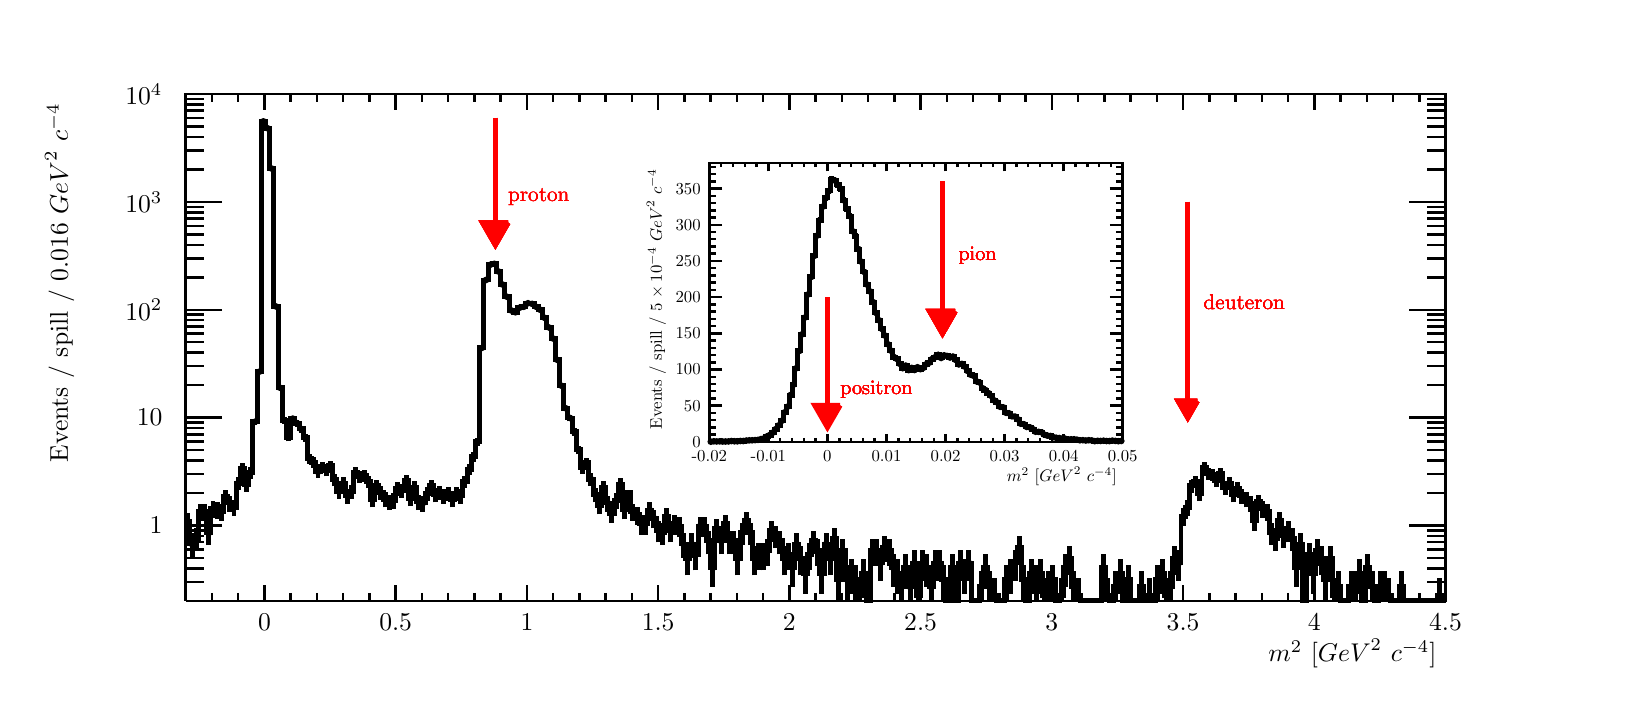
\begin{tikzpicture}
\pgfdeclareplotmark{cross} {
\pgfpathmoveto{\pgfpoint{-0.3\pgfplotmarksize}{\pgfplotmarksize}}
\pgfpathlineto{\pgfpoint{+0.3\pgfplotmarksize}{\pgfplotmarksize}}
\pgfpathlineto{\pgfpoint{+0.3\pgfplotmarksize}{0.3\pgfplotmarksize}}
\pgfpathlineto{\pgfpoint{+1\pgfplotmarksize}{0.3\pgfplotmarksize}}
\pgfpathlineto{\pgfpoint{+1\pgfplotmarksize}{-0.3\pgfplotmarksize}}
\pgfpathlineto{\pgfpoint{+0.3\pgfplotmarksize}{-0.3\pgfplotmarksize}}
\pgfpathlineto{\pgfpoint{+0.3\pgfplotmarksize}{-1.\pgfplotmarksize}}
\pgfpathlineto{\pgfpoint{-0.3\pgfplotmarksize}{-1.\pgfplotmarksize}}
\pgfpathlineto{\pgfpoint{-0.3\pgfplotmarksize}{-0.3\pgfplotmarksize}}
\pgfpathlineto{\pgfpoint{-1.\pgfplotmarksize}{-0.3\pgfplotmarksize}}
\pgfpathlineto{\pgfpoint{-1.\pgfplotmarksize}{0.3\pgfplotmarksize}}
\pgfpathlineto{\pgfpoint{-0.3\pgfplotmarksize}{0.3\pgfplotmarksize}}
\pgfpathclose
\pgfusepathqstroke
}
\pgfdeclareplotmark{cross*} {
\pgfpathmoveto{\pgfpoint{-0.3\pgfplotmarksize}{\pgfplotmarksize}}
\pgfpathlineto{\pgfpoint{+0.3\pgfplotmarksize}{\pgfplotmarksize}}
\pgfpathlineto{\pgfpoint{+0.3\pgfplotmarksize}{0.3\pgfplotmarksize}}
\pgfpathlineto{\pgfpoint{+1\pgfplotmarksize}{0.3\pgfplotmarksize}}
\pgfpathlineto{\pgfpoint{+1\pgfplotmarksize}{-0.3\pgfplotmarksize}}
\pgfpathlineto{\pgfpoint{+0.3\pgfplotmarksize}{-0.3\pgfplotmarksize}}
\pgfpathlineto{\pgfpoint{+0.3\pgfplotmarksize}{-1.\pgfplotmarksize}}
\pgfpathlineto{\pgfpoint{-0.3\pgfplotmarksize}{-1.\pgfplotmarksize}}
\pgfpathlineto{\pgfpoint{-0.3\pgfplotmarksize}{-0.3\pgfplotmarksize}}
\pgfpathlineto{\pgfpoint{-1.\pgfplotmarksize}{-0.3\pgfplotmarksize}}
\pgfpathlineto{\pgfpoint{-1.\pgfplotmarksize}{0.3\pgfplotmarksize}}
\pgfpathlineto{\pgfpoint{-0.3\pgfplotmarksize}{0.3\pgfplotmarksize}}
\pgfpathclose
\pgfusepathqfillstroke
}
\pgfdeclareplotmark{newstar} {
\pgfpathmoveto{\pgfqpoint{0pt}{\pgfplotmarksize}}
\pgfpathlineto{\pgfqpointpolar{44}{0.5\pgfplotmarksize}}
\pgfpathlineto{\pgfqpointpolar{18}{\pgfplotmarksize}}
\pgfpathlineto{\pgfqpointpolar{-20}{0.5\pgfplotmarksize}}
\pgfpathlineto{\pgfqpointpolar{-54}{\pgfplotmarksize}}
\pgfpathlineto{\pgfqpointpolar{-90}{0.5\pgfplotmarksize}}
\pgfpathlineto{\pgfqpointpolar{234}{\pgfplotmarksize}}
\pgfpathlineto{\pgfqpointpolar{198}{0.5\pgfplotmarksize}}
\pgfpathlineto{\pgfqpointpolar{162}{\pgfplotmarksize}}
\pgfpathlineto{\pgfqpointpolar{134}{0.5\pgfplotmarksize}}
\pgfpathclose
\pgfusepathqstroke
}
\pgfdeclareplotmark{newstar*} {
\pgfpathmoveto{\pgfqpoint{0pt}{\pgfplotmarksize}}
\pgfpathlineto{\pgfqpointpolar{44}{0.5\pgfplotmarksize}}
\pgfpathlineto{\pgfqpointpolar{18}{\pgfplotmarksize}}
\pgfpathlineto{\pgfqpointpolar{-20}{0.5\pgfplotmarksize}}
\pgfpathlineto{\pgfqpointpolar{-54}{\pgfplotmarksize}}
\pgfpathlineto{\pgfqpointpolar{-90}{0.5\pgfplotmarksize}}
\pgfpathlineto{\pgfqpointpolar{234}{\pgfplotmarksize}}
\pgfpathlineto{\pgfqpointpolar{198}{0.5\pgfplotmarksize}}
\pgfpathlineto{\pgfqpointpolar{162}{\pgfplotmarksize}}
\pgfpathlineto{\pgfqpointpolar{134}{0.5\pgfplotmarksize}}
\pgfpathclose
\pgfusepathqfillstroke
}
\definecolor{c}{rgb}{1,1,1};
\draw [color=c, fill=c] (0,0) rectangle (20,8.35902);
\draw [color=c, fill=c] (2,1.08667) rectangle (18,7.52312);
\definecolor{c}{rgb}{0,0,0};
\draw [c,line width=0.9] (2,1.08667) -- (2,7.52312) -- (18,7.52312) -- (18,1.08667) -- (2,1.08667);
\definecolor{c}{rgb}{1,1,1};
\draw [color=c, fill=c] (2,1.08667) rectangle (18,7.52312);
\definecolor{c}{rgb}{0,0,0};
\draw [c,line width=0.9] (2,1.08667) -- (2,7.52312) -- (18,7.52312) -- (18,1.08667) -- (2,1.08667);
\draw [c,line width=1.8] (2.02667,1.95243) -- (2.02667,2.08824);
\draw [c,line width=1.8] (2.02667,2.08824) -- (2.02667,2.19874);
\foreach \P in {(2.02667,2.08824)}{\draw[mark options={color=c,fill=c},mark size=2.402402pt,mark=*,mark size=1pt] plot coordinates {\P};}
\draw [c,line width=1.8] (2.08,1.63097) -- (2.08,1.80865);
\draw [c,line width=1.8] (2.08,1.80865) -- (2.08,1.94528);
\foreach \P in {(2.08,1.80865)}{\draw[mark options={color=c,fill=c},mark size=2.402402pt,mark=*,mark size=1pt] plot coordinates {\P};}
\draw [c,line width=1.8] (2.13333,1.71786) -- (2.13333,1.88311);
\draw [c,line width=1.8] (2.13333,1.88311) -- (2.13333,2.01229);
\foreach \P in {(2.13333,1.88311)}{\draw[mark options={color=c,fill=c},mark size=2.402402pt,mark=*,mark size=1pt] plot coordinates {\P};}
\draw [c,line width=1.8] (2.18667,2.10106) -- (2.18667,2.22099);
\draw [c,line width=1.8] (2.18667,2.22099) -- (2.18667,2.32074);
\foreach \P in {(2.18667,2.22099)}{\draw[mark options={color=c,fill=c},mark size=2.402402pt,mark=*,mark size=1pt] plot coordinates {\P};}
\draw [c,line width=1.8] (2.24,2.10106) -- (2.24,2.22099);
\draw [c,line width=1.8] (2.24,2.22099) -- (2.24,2.32074);
\foreach \P in {(2.24,2.22099)}{\draw[mark options={color=c,fill=c},mark size=2.402402pt,mark=*,mark size=1pt] plot coordinates {\P};}
\draw [c,line width=1.8] (2.29333,1.79424) -- (2.29333,1.94927);
\draw [c,line width=1.8] (2.29333,1.94927) -- (2.29333,2.07214);
\foreach \P in {(2.29333,1.94927)}{\draw[mark options={color=c,fill=c},mark size=2.402402pt,mark=*,mark size=1pt] plot coordinates {\P};}
\draw [c,line width=1.8] (2.34667,2.14366) -- (2.34667,2.25938);
\draw [c,line width=1.8] (2.34667,2.25938) -- (2.34667,2.35621);
\foreach \P in {(2.34667,2.25938)}{\draw[mark options={color=c,fill=c},mark size=2.402402pt,mark=*,mark size=1pt] plot coordinates {\P};}
\draw [c,line width=1.8] (2.4,2.12272) -- (2.4,2.24049);
\draw [c,line width=1.8] (2.4,2.24049) -- (2.4,2.33875);
\foreach \P in {(2.4,2.24049)}{\draw[mark options={color=c,fill=c},mark size=2.402402pt,mark=*,mark size=1pt] plot coordinates {\P};}
\draw [c,line width=1.8] (2.45333,2.10106) -- (2.45333,2.22099);
\draw [c,line width=1.8] (2.45333,2.22099) -- (2.45333,2.32074);
\foreach \P in {(2.45333,2.22099)}{\draw[mark options={color=c,fill=c},mark size=2.402402pt,mark=*,mark size=1pt] plot coordinates {\P};}
\draw [c,line width=1.8] (2.50667,2.3058) -- (2.50667,2.40681);
\draw [c,line width=1.8] (2.50667,2.40681) -- (2.50667,2.49314);
\foreach \P in {(2.50667,2.40681)}{\draw[mark options={color=c,fill=c},mark size=2.402402pt,mark=*,mark size=1pt] plot coordinates {\P};}
\draw [c,line width=1.8] (2.56,2.22099) -- (2.56,2.32945);
\draw [c,line width=1.8] (2.56,2.32945) -- (2.56,2.42115);
\foreach \P in {(2.56,2.32945)}{\draw[mark options={color=c,fill=c},mark size=2.402402pt,mark=*,mark size=1pt] plot coordinates {\P};}
\draw [c,line width=1.8] (2.61333,2.16391) -- (2.61333,2.27768);
\draw [c,line width=1.8] (2.61333,2.27768) -- (2.61333,2.37315);
\foreach \P in {(2.61333,2.27768)}{\draw[mark options={color=c,fill=c},mark size=2.402402pt,mark=*,mark size=1pt] plot coordinates {\P};}
\draw [c,line width=1.8] (2.66667,2.4954) -- (2.66667,2.58156);
\draw [c,line width=1.8] (2.66667,2.58156) -- (2.66667,2.65681);
\foreach \P in {(2.66667,2.58156)}{\draw[mark options={color=c,fill=c},mark size=2.402402pt,mark=*,mark size=1pt] plot coordinates {\P};}
\draw [c,line width=1.8] (2.72,2.70147) -- (2.72,2.77395);
\draw [c,line width=1.8] (2.72,2.77395) -- (2.72,2.83855);
\foreach \P in {(2.72,2.77395)}{\draw[mark options={color=c,fill=c},mark size=2.402402pt,mark=*,mark size=1pt] plot coordinates {\P};}
\draw [c,line width=1.8] (2.77333,2.47163) -- (2.77333,2.55953);
\draw [c,line width=1.8] (2.77333,2.55953) -- (2.77333,2.6361);
\foreach \P in {(2.77333,2.55953)}{\draw[mark options={color=c,fill=c},mark size=2.402402pt,mark=*,mark size=1pt] plot coordinates {\P};}
\draw [c,line width=1.8] (2.82667,2.64016) -- (2.82667,2.71647);
\draw [c,line width=1.8] (2.82667,2.71647) -- (2.82667,2.78409);
\foreach \P in {(2.82667,2.71647)}{\draw[mark options={color=c,fill=c},mark size=2.402402pt,mark=*,mark size=1pt] plot coordinates {\P};}
\draw [c,line width=1.8] (2.88,3.31814) -- (2.88,3.36132);
\draw [c,line width=1.8] (2.88,3.36132) -- (2.88,3.40158);
\foreach \P in {(2.88,3.36132)}{\draw[mark options={color=c,fill=c},mark size=2.402402pt,mark=*,mark size=1pt] plot coordinates {\P};}
\draw [c,line width=1.8] (2.93333,3.97116) -- (2.93333,3.9961);
\draw [c,line width=1.8] (2.93333,3.9961) -- (2.93333,4.02004);
\foreach \P in {(2.93333,3.9961)}{\draw[mark options={color=c,fill=c},mark size=2.402402pt,mark=*,mark size=1pt] plot coordinates {\P};}
\draw [c,line width=1.8] (2.98667,7.17425) -- (2.98667,7.17594);
\draw [c,line width=1.8] (2.98667,7.17594) -- (2.98667,7.17762);
\foreach \P in {(2.98667,7.17594)}{\draw[mark options={color=c,fill=c},mark size=2.402402pt,mark=*,mark size=1pt] plot coordinates {\P};}
\draw [c,line width=1.8] (3.04,7.08616) -- (3.04,7.08798);
\draw [c,line width=1.8] (3.04,7.08798) -- (3.04,7.0898);
\foreach \P in {(3.04,7.08798)}{\draw[mark options={color=c,fill=c},mark size=2.402402pt,mark=*,mark size=1pt] plot coordinates {\P};}
\draw [c,line width=1.8] (3.09333,6.57319) -- (3.09333,6.57599);
\draw [c,line width=1.8] (3.09333,6.57599) -- (3.09333,6.57878);
\foreach \P in {(3.09333,6.57599)}{\draw[mark options={color=c,fill=c},mark size=2.402402pt,mark=*,mark size=1pt] plot coordinates {\P};}
\draw [c,line width=1.8] (3.14667,4.81298) -- (3.14667,4.82527);
\draw [c,line width=1.8] (3.14667,4.82527) -- (3.14667,4.83732);
\foreach \P in {(3.14667,4.82527)}{\draw[mark options={color=c,fill=c},mark size=2.402402pt,mark=*,mark size=1pt] plot coordinates {\P};}
\draw [c,line width=1.8] (3.2,3.76259) -- (3.2,3.79232);
\draw [c,line width=1.8] (3.2,3.79232) -- (3.2,3.82063);
\foreach \P in {(3.2,3.79232)}{\draw[mark options={color=c,fill=c},mark size=2.402402pt,mark=*,mark size=1pt] plot coordinates {\P};}
\draw [c,line width=1.8] (3.25333,3.33603) -- (3.25333,3.37857);
\draw [c,line width=1.8] (3.25333,3.37857) -- (3.25333,3.41826);
\foreach \P in {(3.25333,3.37857)}{\draw[mark options={color=c,fill=c},mark size=2.402402pt,mark=*,mark size=1pt] plot coordinates {\P};}
\draw [c,line width=1.8] (3.30667,3.11094) -- (3.30667,3.16233);
\draw [c,line width=1.8] (3.30667,3.16233) -- (3.30667,3.20963);
\foreach \P in {(3.30667,3.16233)}{\draw[mark options={color=c,fill=c},mark size=2.402402pt,mark=*,mark size=1pt] plot coordinates {\P};}
\draw [c,line width=1.8] (3.36,3.35909) -- (3.36,3.40081);
\draw [c,line width=1.8] (3.36,3.40081) -- (3.36,3.43979);
\foreach \P in {(3.36,3.40081)}{\draw[mark options={color=c,fill=c},mark size=2.402402pt,mark=*,mark size=1pt] plot coordinates {\P};}
\draw [c,line width=1.8] (3.41333,3.29971) -- (3.41333,3.34356);
\draw [c,line width=1.8] (3.41333,3.34356) -- (3.41333,3.3844);
\foreach \P in {(3.41333,3.34356)}{\draw[mark options={color=c,fill=c},mark size=2.402402pt,mark=*,mark size=1pt] plot coordinates {\P};}
\draw [c,line width=1.8] (3.46667,3.22335) -- (3.46667,3.27011);
\draw [c,line width=1.8] (3.46667,3.27011) -- (3.46667,3.31346);
\foreach \P in {(3.46667,3.27011)}{\draw[mark options={color=c,fill=c},mark size=2.402402pt,mark=*,mark size=1pt] plot coordinates {\P};}
\draw [c,line width=1.8] (3.52,3.10666) -- (3.52,3.15824);
\draw [c,line width=1.8] (3.52,3.15824) -- (3.52,3.2057);
\foreach \P in {(3.52,3.15824)}{\draw[mark options={color=c,fill=c},mark size=2.402402pt,mark=*,mark size=1pt] plot coordinates {\P};}
\draw [c,line width=1.8] (3.57333,2.82891) -- (3.57333,2.89403);
\draw [c,line width=1.8] (3.57333,2.89403) -- (3.57333,2.95273);
\foreach \P in {(3.57333,2.89403)}{\draw[mark options={color=c,fill=c},mark size=2.402402pt,mark=*,mark size=1pt] plot coordinates {\P};}
\draw [c,line width=1.8] (3.62667,2.77961) -- (3.62667,2.84748);
\draw [c,line width=1.8] (3.62667,2.84748) -- (3.62667,2.9084);
\foreach \P in {(3.62667,2.84748)}{\draw[mark options={color=c,fill=c},mark size=2.402402pt,mark=*,mark size=1pt] plot coordinates {\P};}
\draw [c,line width=1.8] (3.68,2.6493) -- (3.68,2.72503);
\draw [c,line width=1.8] (3.68,2.72503) -- (3.68,2.79219);
\foreach \P in {(3.68,2.72503)}{\draw[mark options={color=c,fill=c},mark size=2.402402pt,mark=*,mark size=1pt] plot coordinates {\P};}
\draw [c,line width=1.8] (3.73333,2.71791) -- (3.73333,2.7894);
\draw [c,line width=1.8] (3.73333,2.7894) -- (3.73333,2.85321);
\foreach \P in {(3.73333,2.7894)}{\draw[mark options={color=c,fill=c},mark size=2.402402pt,mark=*,mark size=1pt] plot coordinates {\P};}
\draw [c,line width=1.8] (3.78667,2.66719) -- (3.78667,2.74178);
\draw [c,line width=1.8] (3.78667,2.74178) -- (3.78667,2.80806);
\foreach \P in {(3.78667,2.74178)}{\draw[mark options={color=c,fill=c},mark size=2.402402pt,mark=*,mark size=1pt] plot coordinates {\P};}
\draw [c,line width=1.8] (3.84,2.73393) -- (3.84,2.80446);
\draw [c,line width=1.8] (3.84,2.80446) -- (3.84,2.86751);
\foreach \P in {(3.84,2.80446)}{\draw[mark options={color=c,fill=c},mark size=2.402402pt,mark=*,mark size=1pt] plot coordinates {\P};}
\draw [c,line width=1.8] (3.89333,2.54035) -- (3.89333,2.62333);
\draw [c,line width=1.8] (3.89333,2.62333) -- (3.89333,2.69613);
\foreach \P in {(3.89333,2.62333)}{\draw[mark options={color=c,fill=c},mark size=2.402402pt,mark=*,mark size=1pt] plot coordinates {\P};}
\draw [c,line width=1.8] (3.94667,2.38037) -- (3.94667,2.47526);
\draw [c,line width=1.8] (3.94667,2.47526) -- (3.94667,2.55708);
\foreach \P in {(3.94667,2.47526)}{\draw[mark options={color=c,fill=c},mark size=2.402402pt,mark=*,mark size=1pt] plot coordinates {\P};}
\draw [c,line width=1.8] (4,2.4954) -- (4,2.58156);
\draw [c,line width=1.8] (4,2.58156) -- (4,2.65681);
\foreach \P in {(4,2.58156)}{\draw[mark options={color=c,fill=c},mark size=2.402402pt,mark=*,mark size=1pt] plot coordinates {\P};}
\draw [c,line width=1.8] (4.05333,2.32145) -- (4.05333,2.42115);
\draw [c,line width=1.8] (4.05333,2.42115) -- (4.05333,2.50651);
\foreach \P in {(4.05333,2.42115)}{\draw[mark options={color=c,fill=c},mark size=2.402402pt,mark=*,mark size=1pt] plot coordinates {\P};}
\draw [c,line width=1.8] (4.10667,2.38037) -- (4.10667,2.47526);
\draw [c,line width=1.8] (4.10667,2.47526) -- (4.10667,2.55708);
\foreach \P in {(4.10667,2.47526)}{\draw[mark options={color=c,fill=c},mark size=2.402402pt,mark=*,mark size=1pt] plot coordinates {\P};}
\draw [c,line width=1.8] (4.16,2.64016) -- (4.16,2.71647);
\draw [c,line width=1.8] (4.16,2.71647) -- (4.16,2.78409);
\foreach \P in {(4.16,2.71647)}{\draw[mark options={color=c,fill=c},mark size=2.402402pt,mark=*,mark size=1pt] plot coordinates {\P};}
\draw [c,line width=1.8] (4.21333,2.58224) -- (4.21333,2.66235);
\draw [c,line width=1.8] (4.21333,2.66235) -- (4.21333,2.73294);
\foreach \P in {(4.21333,2.66235)}{\draw[mark options={color=c,fill=c},mark size=2.402402pt,mark=*,mark size=1pt] plot coordinates {\P};}
\draw [c,line width=1.8] (4.26667,2.60216) -- (4.26667,2.68094);
\draw [c,line width=1.8] (4.26667,2.68094) -- (4.26667,2.7505);
\foreach \P in {(4.26667,2.68094)}{\draw[mark options={color=c,fill=c},mark size=2.402402pt,mark=*,mark size=1pt] plot coordinates {\P};}
\draw [c,line width=1.8] (4.32,2.51829) -- (4.32,2.60281);
\draw [c,line width=1.8] (4.32,2.60281) -- (4.32,2.67681);
\foreach \P in {(4.32,2.60281)}{\draw[mark options={color=c,fill=c},mark size=2.402402pt,mark=*,mark size=1pt] plot coordinates {\P};}
\draw [c,line width=1.8] (4.37333,2.27325) -- (4.37333,2.37706);
\draw [c,line width=1.8] (4.37333,2.37706) -- (4.37333,2.46542);
\foreach \P in {(4.37333,2.37706)}{\draw[mark options={color=c,fill=c},mark size=2.402402pt,mark=*,mark size=1pt] plot coordinates {\P};}
\draw [c,line width=1.8] (4.42667,2.45939) -- (4.42667,2.5482);
\draw [c,line width=1.8] (4.42667,2.5482) -- (4.42667,2.62545);
\foreach \P in {(4.42667,2.5482)}{\draw[mark options={color=c,fill=c},mark size=2.402402pt,mark=*,mark size=1pt] plot coordinates {\P};}
\draw [c,line width=1.8] (4.48,2.36616) -- (4.48,2.46219);
\draw [c,line width=1.8] (4.48,2.46219) -- (4.48,2.54485);
\foreach \P in {(4.48,2.46219)}{\draw[mark options={color=c,fill=c},mark size=2.402402pt,mark=*,mark size=1pt] plot coordinates {\P};}
\draw [c,line width=1.8] (4.53333,2.27325) -- (4.53333,2.37706);
\draw [c,line width=1.8] (4.53333,2.37706) -- (4.53333,2.46542);
\foreach \P in {(4.53333,2.37706)}{\draw[mark options={color=c,fill=c},mark size=2.402402pt,mark=*,mark size=1pt] plot coordinates {\P};}
\draw [c,line width=1.8] (4.58667,2.2389) -- (4.58667,2.34574);
\draw [c,line width=1.8] (4.58667,2.34574) -- (4.58667,2.43629);
\foreach \P in {(4.58667,2.34574)}{\draw[mark options={color=c,fill=c},mark size=2.402402pt,mark=*,mark size=1pt] plot coordinates {\P};}
\draw [c,line width=1.8] (4.64,2.25631) -- (4.64,2.36161);
\draw [c,line width=1.8] (4.64,2.36161) -- (4.64,2.45104);
\foreach \P in {(4.64,2.36161)}{\draw[mark options={color=c,fill=c},mark size=2.402402pt,mark=*,mark size=1pt] plot coordinates {\P};}
\draw [c,line width=1.8] (4.69333,2.42115) -- (4.69333,2.51285);
\draw [c,line width=1.8] (4.69333,2.51285) -- (4.69333,2.59228);
\foreach \P in {(4.69333,2.51285)}{\draw[mark options={color=c,fill=c},mark size=2.402402pt,mark=*,mark size=1pt] plot coordinates {\P};}
\draw [c,line width=1.8] (4.74667,2.39426) -- (4.74667,2.48806);
\draw [c,line width=1.8] (4.74667,2.48806) -- (4.74667,2.56906);
\foreach \P in {(4.74667,2.48806)}{\draw[mark options={color=c,fill=c},mark size=2.402402pt,mark=*,mark size=1pt] plot coordinates {\P};}
\draw [c,line width=1.8] (4.8,2.52942) -- (4.8,2.61316);
\draw [c,line width=1.8] (4.8,2.61316) -- (4.8,2.68655);
\foreach \P in {(4.8,2.61316)}{\draw[mark options={color=c,fill=c},mark size=2.402402pt,mark=*,mark size=1pt] plot coordinates {\P};}
\draw [c,line width=1.8] (4.85333,2.28974) -- (4.85333,2.39212);
\draw [c,line width=1.8] (4.85333,2.39212) -- (4.85333,2.47945);
\foreach \P in {(4.85333,2.39212)}{\draw[mark options={color=c,fill=c},mark size=2.402402pt,mark=*,mark size=1pt] plot coordinates {\P};}
\draw [c,line width=1.8] (4.90667,2.43416) -- (4.90667,2.52487);
\draw [c,line width=1.8] (4.90667,2.52487) -- (4.90667,2.60355);
\foreach \P in {(4.90667,2.52487)}{\draw[mark options={color=c,fill=c},mark size=2.402402pt,mark=*,mark size=1pt] plot coordinates {\P};}
\draw [c,line width=1.8] (4.96,2.2389) -- (4.96,2.34574);
\draw [c,line width=1.8] (4.96,2.34574) -- (4.96,2.43629);
\foreach \P in {(4.96,2.34574)}{\draw[mark options={color=c,fill=c},mark size=2.402402pt,mark=*,mark size=1pt] plot coordinates {\P};}
\draw [c,line width=1.8] (5.01333,2.22099) -- (5.01333,2.32945);
\draw [c,line width=1.8] (5.01333,2.32945) -- (5.01333,2.42115);
\foreach \P in {(5.01333,2.32945)}{\draw[mark options={color=c,fill=c},mark size=2.402402pt,mark=*,mark size=1pt] plot coordinates {\P};}
\draw [c,line width=1.8] (5.06667,2.35161) -- (5.06667,2.44882);
\draw [c,line width=1.8] (5.06667,2.44882) -- (5.06667,2.53235);
\foreach \P in {(5.06667,2.44882)}{\draw[mark options={color=c,fill=c},mark size=2.402402pt,mark=*,mark size=1pt] plot coordinates {\P};}
\draw [c,line width=1.8] (5.12,2.45939) -- (5.12,2.5482);
\draw [c,line width=1.8] (5.12,2.5482) -- (5.12,2.62545);
\foreach \P in {(5.12,2.5482)}{\draw[mark options={color=c,fill=c},mark size=2.402402pt,mark=*,mark size=1pt] plot coordinates {\P};}
\draw [c,line width=1.8] (5.17333,2.33671) -- (5.17333,2.43514);
\draw [c,line width=1.8] (5.17333,2.43514) -- (5.17333,2.51958);
\foreach \P in {(5.17333,2.43514)}{\draw[mark options={color=c,fill=c},mark size=2.402402pt,mark=*,mark size=1pt] plot coordinates {\P};}
\draw [c,line width=1.8] (5.22667,2.36616) -- (5.22667,2.46219);
\draw [c,line width=1.8] (5.22667,2.46219) -- (5.22667,2.54485);
\foreach \P in {(5.22667,2.46219)}{\draw[mark options={color=c,fill=c},mark size=2.402402pt,mark=*,mark size=1pt] plot coordinates {\P};}
\draw [c,line width=1.8] (5.28,2.32145) -- (5.28,2.42115);
\draw [c,line width=1.8] (5.28,2.42115) -- (5.28,2.50651);
\foreach \P in {(5.28,2.42115)}{\draw[mark options={color=c,fill=c},mark size=2.402402pt,mark=*,mark size=1pt] plot coordinates {\P};}
\draw [c,line width=1.8] (5.33333,2.35161) -- (5.33333,2.44882);
\draw [c,line width=1.8] (5.33333,2.44882) -- (5.33333,2.53235);
\foreach \P in {(5.33333,2.44882)}{\draw[mark options={color=c,fill=c},mark size=2.402402pt,mark=*,mark size=1pt] plot coordinates {\P};}
\draw [c,line width=1.8] (5.38667,2.27325) -- (5.38667,2.37706);
\draw [c,line width=1.8] (5.38667,2.37706) -- (5.38667,2.46542);
\foreach \P in {(5.38667,2.37706)}{\draw[mark options={color=c,fill=c},mark size=2.402402pt,mark=*,mark size=1pt] plot coordinates {\P};}
\draw [c,line width=1.8] (5.44,2.35161) -- (5.44,2.44882);
\draw [c,line width=1.8] (5.44,2.44882) -- (5.44,2.53235);
\foreach \P in {(5.44,2.44882)}{\draw[mark options={color=c,fill=c},mark size=2.402402pt,mark=*,mark size=1pt] plot coordinates {\P};}
\draw [c,line width=1.8] (5.49333,2.32145) -- (5.49333,2.42115);
\draw [c,line width=1.8] (5.49333,2.42115) -- (5.49333,2.50651);
\foreach \P in {(5.49333,2.42115)}{\draw[mark options={color=c,fill=c},mark size=2.402402pt,mark=*,mark size=1pt] plot coordinates {\P};}
\draw [c,line width=1.8] (5.54667,2.51829) -- (5.54667,2.60281);
\draw [c,line width=1.8] (5.54667,2.60281) -- (5.54667,2.67681);
\foreach \P in {(5.54667,2.60281)}{\draw[mark options={color=c,fill=c},mark size=2.402402pt,mark=*,mark size=1pt] plot coordinates {\P};}
\draw [c,line width=1.8] (5.6,2.68457) -- (5.6,2.75808);
\draw [c,line width=1.8] (5.6,2.75808) -- (5.6,2.8235);
\foreach \P in {(5.6,2.75808)}{\draw[mark options={color=c,fill=c},mark size=2.402402pt,mark=*,mark size=1pt] plot coordinates {\P};}
\draw [c,line width=1.8] (5.65333,2.85539) -- (5.65333,2.91908);
\draw [c,line width=1.8] (5.65333,2.91908) -- (5.65333,2.97661);
\foreach \P in {(5.65333,2.91908)}{\draw[mark options={color=c,fill=c},mark size=2.402402pt,mark=*,mark size=1pt] plot coordinates {\P};}
\draw [c,line width=1.8] (5.70667,3.05756) -- (5.70667,3.11131);
\draw [c,line width=1.8] (5.70667,3.11131) -- (5.70667,3.1606);
\foreach \P in {(5.70667,3.11131)}{\draw[mark options={color=c,fill=c},mark size=2.402402pt,mark=*,mark size=1pt] plot coordinates {\P};}
\draw [c,line width=1.8] (5.76,4.27932) -- (5.76,4.29857);
\draw [c,line width=1.8] (5.76,4.29857) -- (5.76,4.31722);
\foreach \P in {(5.76,4.29857)}{\draw[mark options={color=c,fill=c},mark size=2.402402pt,mark=*,mark size=1pt] plot coordinates {\P};}
\draw [c,line width=1.8] (5.81333,5.15212) -- (5.81333,5.16137);
\draw [c,line width=1.8] (5.81333,5.16137) -- (5.81333,5.17047);
\foreach \P in {(5.81333,5.16137)}{\draw[mark options={color=c,fill=c},mark size=2.402402pt,mark=*,mark size=1pt] plot coordinates {\P};}
\draw [c,line width=1.8] (5.86667,5.34635) -- (5.86667,5.35421);
\draw [c,line width=1.8] (5.86667,5.35421) -- (5.86667,5.36196);
\foreach \P in {(5.86667,5.35421)}{\draw[mark options={color=c,fill=c},mark size=2.402402pt,mark=*,mark size=1pt] plot coordinates {\P};}
\draw [c,line width=1.8] (5.92,5.35889) -- (5.92,5.36666);
\draw [c,line width=1.8] (5.92,5.36666) -- (5.92,5.37433);
\foreach \P in {(5.92,5.36666)}{\draw[mark options={color=c,fill=c},mark size=2.402402pt,mark=*,mark size=1pt] plot coordinates {\P};}
\draw [c,line width=1.8] (5.97333,5.26044) -- (5.97333,5.26888);
\draw [c,line width=1.8] (5.97333,5.26888) -- (5.97333,5.27721);
\foreach \P in {(5.97333,5.26888)}{\draw[mark options={color=c,fill=c},mark size=2.402402pt,mark=*,mark size=1pt] plot coordinates {\P};}
\draw [c,line width=1.8] (6.02667,5.09297) -- (6.02667,5.10269);
\draw [c,line width=1.8] (6.02667,5.10269) -- (6.02667,5.11225);
\foreach \P in {(6.02667,5.10269)}{\draw[mark options={color=c,fill=c},mark size=2.402402pt,mark=*,mark size=1pt] plot coordinates {\P};}
\draw [c,line width=1.8] (6.08,4.9372) -- (6.08,4.94828);
\draw [c,line width=1.8] (6.08,4.94828) -- (6.08,4.95915);
\foreach \P in {(6.08,4.94828)}{\draw[mark options={color=c,fill=c},mark size=2.402402pt,mark=*,mark size=1pt] plot coordinates {\P};}
\draw [c,line width=1.8] (6.13333,4.76236) -- (6.13333,4.77518);
\draw [c,line width=1.8] (6.13333,4.77518) -- (6.13333,4.78774);
\foreach \P in {(6.13333,4.77518)}{\draw[mark options={color=c,fill=c},mark size=2.402402pt,mark=*,mark size=1pt] plot coordinates {\P};}
\draw [c,line width=1.8] (6.18667,4.73862) -- (6.18667,4.75171);
\draw [c,line width=1.8] (6.18667,4.75171) -- (6.18667,4.76452);
\foreach \P in {(6.18667,4.75171)}{\draw[mark options={color=c,fill=c},mark size=2.402402pt,mark=*,mark size=1pt] plot coordinates {\P};}
\draw [c,line width=1.8] (6.24,4.79666) -- (6.24,4.80913);
\draw [c,line width=1.8] (6.24,4.80913) -- (6.24,4.82133);
\foreach \P in {(6.24,4.80913)}{\draw[mark options={color=c,fill=c},mark size=2.402402pt,mark=*,mark size=1pt] plot coordinates {\P};}
\draw [c,line width=1.8] (6.29333,4.80894) -- (6.29333,4.82128);
\draw [c,line width=1.8] (6.29333,4.82128) -- (6.29333,4.83336);
\foreach \P in {(6.29333,4.82128)}{\draw[mark options={color=c,fill=c},mark size=2.402402pt,mark=*,mark size=1pt] plot coordinates {\P};}
\draw [c,line width=1.8] (6.34667,4.85474) -- (6.34667,4.86661);
\draw [c,line width=1.8] (6.34667,4.86661) -- (6.34667,4.87825);
\foreach \P in {(6.34667,4.86661)}{\draw[mark options={color=c,fill=c},mark size=2.402402pt,mark=*,mark size=1pt] plot coordinates {\P};}
\draw [c,line width=1.8] (6.4,4.84624) -- (6.4,4.8582);
\draw [c,line width=1.8] (6.4,4.8582) -- (6.4,4.86992);
\foreach \P in {(6.4,4.8582)}{\draw[mark options={color=c,fill=c},mark size=2.402402pt,mark=*,mark size=1pt] plot coordinates {\P};}
\draw [c,line width=1.8] (6.45333,4.80793) -- (6.45333,4.82027);
\draw [c,line width=1.8] (6.45333,4.82027) -- (6.45333,4.83237);
\foreach \P in {(6.45333,4.82027)}{\draw[mark options={color=c,fill=c},mark size=2.402402pt,mark=*,mark size=1pt] plot coordinates {\P};}
\draw [c,line width=1.8] (6.50667,4.76889) -- (6.50667,4.78165);
\draw [c,line width=1.8] (6.50667,4.78165) -- (6.50667,4.79414);
\foreach \P in {(6.50667,4.78165)}{\draw[mark options={color=c,fill=c},mark size=2.402402pt,mark=*,mark size=1pt] plot coordinates {\P};}
\draw [c,line width=1.8] (6.56,4.66604) -- (6.56,4.67995);
\draw [c,line width=1.8] (6.56,4.67995) -- (6.56,4.69355);
\foreach \P in {(6.56,4.67995)}{\draw[mark options={color=c,fill=c},mark size=2.402402pt,mark=*,mark size=1pt] plot coordinates {\P};}
\draw [c,line width=1.8] (6.61333,4.54296) -- (6.61333,4.55838);
\draw [c,line width=1.8] (6.61333,4.55838) -- (6.61333,4.57342);
\foreach \P in {(6.61333,4.55838)}{\draw[mark options={color=c,fill=c},mark size=2.402402pt,mark=*,mark size=1pt] plot coordinates {\P};}
\draw [c,line width=1.8] (6.66667,4.4005) -- (6.66667,4.41789);
\draw [c,line width=1.8] (6.66667,4.41789) -- (6.66667,4.43479);
\foreach \P in {(6.66667,4.41789)}{\draw[mark options={color=c,fill=c},mark size=2.402402pt,mark=*,mark size=1pt] plot coordinates {\P};}
\draw [c,line width=1.8] (6.72,4.12491) -- (6.72,4.14683);
\draw [c,line width=1.8] (6.72,4.14683) -- (6.72,4.16797);
\foreach \P in {(6.72,4.14683)}{\draw[mark options={color=c,fill=c},mark size=2.402402pt,mark=*,mark size=1pt] plot coordinates {\P};}
\draw [c,line width=1.8] (6.77333,3.78952) -- (6.77333,3.81858);
\draw [c,line width=1.8] (6.77333,3.81858) -- (6.77333,3.84628);
\foreach \P in {(6.77333,3.81858)}{\draw[mark options={color=c,fill=c},mark size=2.402402pt,mark=*,mark size=1pt] plot coordinates {\P};}
\draw [c,line width=1.8] (6.82667,3.49525) -- (6.82667,3.53246);
\draw [c,line width=1.8] (6.82667,3.53246) -- (6.82667,3.56748);
\foreach \P in {(6.82667,3.53246)}{\draw[mark options={color=c,fill=c},mark size=2.402402pt,mark=*,mark size=1pt] plot coordinates {\P};}
\draw [c,line width=1.8] (6.88,3.36751) -- (6.88,3.40894);
\draw [c,line width=1.8] (6.88,3.40894) -- (6.88,3.44766);
\foreach \P in {(6.88,3.40894)}{\draw[mark options={color=c,fill=c},mark size=2.402402pt,mark=*,mark size=1pt] plot coordinates {\P};}
\draw [c,line width=1.8] (6.93333,3.18312) -- (6.93333,3.23149);
\draw [c,line width=1.8] (6.93333,3.23149) -- (6.93333,3.27621);
\foreach \P in {(6.93333,3.23149)}{\draw[mark options={color=c,fill=c},mark size=2.402402pt,mark=*,mark size=1pt] plot coordinates {\P};}
\draw [c,line width=1.8] (6.98667,2.94557) -- (6.98667,3.00462);
\draw [c,line width=1.8] (6.98667,3.00462) -- (6.98667,3.05833);
\foreach \P in {(6.98667,3.00462)}{\draw[mark options={color=c,fill=c},mark size=2.402402pt,mark=*,mark size=1pt] plot coordinates {\P};}
\draw [c,line width=1.8] (7.04,2.70147) -- (7.04,2.77395);
\draw [c,line width=1.8] (7.04,2.77395) -- (7.04,2.83855);
\foreach \P in {(7.04,2.77395)}{\draw[mark options={color=c,fill=c},mark size=2.402402pt,mark=*,mark size=1pt] plot coordinates {\P};}
\draw [c,line width=1.8] (7.09333,2.77223) -- (7.09333,2.84052);
\draw [c,line width=1.8] (7.09333,2.84052) -- (7.09333,2.90178);
\foreach \P in {(7.09333,2.84052)}{\draw[mark options={color=c,fill=c},mark size=2.402402pt,mark=*,mark size=1pt] plot coordinates {\P};}
\draw [c,line width=1.8] (7.14667,2.5511) -- (7.14667,2.63332);
\draw [c,line width=1.8] (7.14667,2.63332) -- (7.14667,2.70555);
\foreach \P in {(7.14667,2.63332)}{\draw[mark options={color=c,fill=c},mark size=2.402402pt,mark=*,mark size=1pt] plot coordinates {\P};}
\draw [c,line width=1.8] (7.2,2.33671) -- (7.2,2.43514);
\draw [c,line width=1.8] (7.2,2.43514) -- (7.2,2.51958);
\foreach \P in {(7.2,2.43514)}{\draw[mark options={color=c,fill=c},mark size=2.402402pt,mark=*,mark size=1pt] plot coordinates {\P};}
\draw [c,line width=1.8] (7.25333,2.18352) -- (7.25333,2.29544);
\draw [c,line width=1.8] (7.25333,2.29544) -- (7.25333,2.3896);
\foreach \P in {(7.25333,2.29544)}{\draw[mark options={color=c,fill=c},mark size=2.402402pt,mark=*,mark size=1pt] plot coordinates {\P};}
\draw [c,line width=1.8] (7.30667,2.43416) -- (7.30667,2.52487);
\draw [c,line width=1.8] (7.30667,2.52487) -- (7.30667,2.60355);
\foreach \P in {(7.30667,2.52487)}{\draw[mark options={color=c,fill=c},mark size=2.402402pt,mark=*,mark size=1pt] plot coordinates {\P};}
\draw [c,line width=1.8] (7.36,2.22099) -- (7.36,2.32945);
\draw [c,line width=1.8] (7.36,2.32945) -- (7.36,2.42115);
\foreach \P in {(7.36,2.32945)}{\draw[mark options={color=c,fill=c},mark size=2.402402pt,mark=*,mark size=1pt] plot coordinates {\P};}
\draw [c,line width=1.8] (7.41333,2.07862) -- (7.41333,2.20082);
\draw [c,line width=1.8] (7.41333,2.20082) -- (7.41333,2.30214);
\foreach \P in {(7.41333,2.20082)}{\draw[mark options={color=c,fill=c},mark size=2.402402pt,mark=*,mark size=1pt] plot coordinates {\P};}
\draw [c,line width=1.8] (7.46667,2.25631) -- (7.46667,2.36161);
\draw [c,line width=1.8] (7.46667,2.36161) -- (7.46667,2.45104);
\foreach \P in {(7.46667,2.36161)}{\draw[mark options={color=c,fill=c},mark size=2.402402pt,mark=*,mark size=1pt] plot coordinates {\P};}
\draw [c,line width=1.8] (7.52,2.48363) -- (7.52,2.57065);
\draw [c,line width=1.8] (7.52,2.57065) -- (7.52,2.64655);
\foreach \P in {(7.52,2.57065)}{\draw[mark options={color=c,fill=c},mark size=2.402402pt,mark=*,mark size=1pt] plot coordinates {\P};}
\draw [c,line width=1.8] (7.57333,2.12272) -- (7.57333,2.24049);
\draw [c,line width=1.8] (7.57333,2.24049) -- (7.57333,2.33875);
\foreach \P in {(7.57333,2.24049)}{\draw[mark options={color=c,fill=c},mark size=2.402402pt,mark=*,mark size=1pt] plot coordinates {\P};}
\draw [c,line width=1.8] (7.62667,2.36616) -- (7.62667,2.46219);
\draw [c,line width=1.8] (7.62667,2.46219) -- (7.62667,2.54485);
\foreach \P in {(7.62667,2.46219)}{\draw[mark options={color=c,fill=c},mark size=2.402402pt,mark=*,mark size=1pt] plot coordinates {\P};}
\draw [c,line width=1.8] (7.68,2.10106) -- (7.68,2.22099);
\draw [c,line width=1.8] (7.68,2.22099) -- (7.68,2.32074);
\foreach \P in {(7.68,2.22099)}{\draw[mark options={color=c,fill=c},mark size=2.402402pt,mark=*,mark size=1pt] plot coordinates {\P};}
\draw [c,line width=1.8] (7.73333,2.05534) -- (7.73333,2.17994);
\draw [c,line width=1.8] (7.73333,2.17994) -- (7.73333,2.28292);
\foreach \P in {(7.73333,2.17994)}{\draw[mark options={color=c,fill=c},mark size=2.402402pt,mark=*,mark size=1pt] plot coordinates {\P};}
\draw [c,line width=1.8] (7.78667,1.92382) -- (7.78667,2.06293);
\draw [c,line width=1.8] (7.78667,2.06293) -- (7.78667,2.17559);
\foreach \P in {(7.78667,2.06293)}{\draw[mark options={color=c,fill=c},mark size=2.402402pt,mark=*,mark size=1pt] plot coordinates {\P};}
\draw [c,line width=1.8] (7.84,1.92382) -- (7.84,2.06293);
\draw [c,line width=1.8] (7.84,2.06293) -- (7.84,2.17559);
\foreach \P in {(7.84,2.06293)}{\draw[mark options={color=c,fill=c},mark size=2.402402pt,mark=*,mark size=1pt] plot coordinates {\P};}
\draw [c,line width=1.8] (7.89333,2.12272) -- (7.89333,2.24049);
\draw [c,line width=1.8] (7.89333,2.24049) -- (7.89333,2.33875);
\foreach \P in {(7.89333,2.24049)}{\draw[mark options={color=c,fill=c},mark size=2.402402pt,mark=*,mark size=1pt] plot coordinates {\P};}
\draw [c,line width=1.8] (7.94667,2.006) -- (7.94667,2.13586);
\draw [c,line width=1.8] (7.94667,2.13586) -- (7.94667,2.24239);
\foreach \P in {(7.94667,2.13586)}{\draw[mark options={color=c,fill=c},mark size=2.402402pt,mark=*,mark size=1pt] plot coordinates {\P};}
\draw [c,line width=1.8] (8,1.82922) -- (8,1.97978);
\draw [c,line width=1.8] (8,1.97978) -- (8,2.09983);
\foreach \P in {(8,1.97978)}{\draw[mark options={color=c,fill=c},mark size=2.402402pt,mark=*,mark size=1pt] plot coordinates {\P};}
\draw [c,line width=1.8] (8.05333,1.79424) -- (8.05333,1.94927);
\draw [c,line width=1.8] (8.05333,1.94927) -- (8.05333,2.07214);
\foreach \P in {(8.05333,1.94927)}{\draw[mark options={color=c,fill=c},mark size=2.402402pt,mark=*,mark size=1pt] plot coordinates {\P};}
\draw [c,line width=1.8] (8.10667,2.03115) -- (8.10667,2.15831);
\draw [c,line width=1.8] (8.10667,2.15831) -- (8.10667,2.26301);
\foreach \P in {(8.10667,2.15831)}{\draw[mark options={color=c,fill=c},mark size=2.402402pt,mark=*,mark size=1pt] plot coordinates {\P};}
\draw [c,line width=1.8] (8.16,1.82922) -- (8.16,1.97978);
\draw [c,line width=1.8] (8.16,1.97978) -- (8.16,2.09983);
\foreach \P in {(8.16,1.97978)}{\draw[mark options={color=c,fill=c},mark size=2.402402pt,mark=*,mark size=1pt] plot coordinates {\P};}
\draw [c,line width=1.8] (8.21333,1.92382) -- (8.21333,2.06293);
\draw [c,line width=1.8] (8.21333,2.06293) -- (8.21333,2.17559);
\foreach \P in {(8.21333,2.06293)}{\draw[mark options={color=c,fill=c},mark size=2.402402pt,mark=*,mark size=1pt] plot coordinates {\P};}
\draw [c,line width=1.8] (8.26667,1.89384) -- (8.26667,2.03648);
\draw [c,line width=1.8] (8.26667,2.03648) -- (8.26667,2.15145);
\foreach \P in {(8.26667,2.03648)}{\draw[mark options={color=c,fill=c},mark size=2.402402pt,mark=*,mark size=1pt] plot coordinates {\P};}
\draw [c,line width=1.8] (8.32,1.63097) -- (8.32,1.80865);
\draw [c,line width=1.8] (8.32,1.80865) -- (8.32,1.94528);
\foreach \P in {(8.32,1.80865)}{\draw[mark options={color=c,fill=c},mark size=2.402402pt,mark=*,mark size=1pt] plot coordinates {\P};}
\draw [c,line width=1.8] (8.37333,1.41068) -- (8.37333,1.62414);
\draw [c,line width=1.8] (8.37333,1.62414) -- (8.37333,1.78091);
\foreach \P in {(8.37333,1.62414)}{\draw[mark options={color=c,fill=c},mark size=2.402402pt,mark=*,mark size=1pt] plot coordinates {\P};}
\draw [c,line width=1.8] (8.42667,1.63097) -- (8.42667,1.80865);
\draw [c,line width=1.8] (8.42667,1.80865) -- (8.42667,1.94528);
\foreach \P in {(8.42667,1.80865)}{\draw[mark options={color=c,fill=c},mark size=2.402402pt,mark=*,mark size=1pt] plot coordinates {\P};}
\draw [c,line width=1.8] (8.48,1.47327) -- (8.48,1.67591);
\draw [c,line width=1.8] (8.48,1.67591) -- (8.48,1.82678);
\foreach \P in {(8.48,1.67591)}{\draw[mark options={color=c,fill=c},mark size=2.402402pt,mark=*,mark size=1pt] plot coordinates {\P};}
\draw [c,line width=1.8] (8.53333,1.89384) -- (8.53333,2.03648);
\draw [c,line width=1.8] (8.53333,2.03648) -- (8.53333,2.15145);
\foreach \P in {(8.53333,2.03648)}{\draw[mark options={color=c,fill=c},mark size=2.402402pt,mark=*,mark size=1pt] plot coordinates {\P};}
\draw [c,line width=1.8] (8.58667,1.89384) -- (8.58667,2.03648);
\draw [c,line width=1.8] (8.58667,2.03648) -- (8.58667,2.15145);
\foreach \P in {(8.58667,2.03648)}{\draw[mark options={color=c,fill=c},mark size=2.402402pt,mark=*,mark size=1pt] plot coordinates {\P};}
\draw [c,line width=1.8] (8.64,1.67591) -- (8.64,1.84704);
\draw [c,line width=1.8] (8.64,1.84704) -- (8.64,1.97978);
\foreach \P in {(8.64,1.84704)}{\draw[mark options={color=c,fill=c},mark size=2.402402pt,mark=*,mark size=1pt] plot coordinates {\P};}
\draw [c,line width=1.8] (8.69333,1.26357) -- (8.69333,1.50477);
\draw [c,line width=1.8] (8.69333,1.50477) -- (8.69333,1.67591);
\foreach \P in {(8.69333,1.50477)}{\draw[mark options={color=c,fill=c},mark size=2.402402pt,mark=*,mark size=1pt] plot coordinates {\P};}
\draw [c,line width=1.8] (8.74667,1.86236) -- (8.74667,2.00881);
\draw [c,line width=1.8] (8.74667,2.00881) -- (8.74667,2.12623);
\foreach \P in {(8.74667,2.00881)}{\draw[mark options={color=c,fill=c},mark size=2.402402pt,mark=*,mark size=1pt] plot coordinates {\P};}
\draw [c,line width=1.8] (8.8,1.67591) -- (8.8,1.84704);
\draw [c,line width=1.8] (8.8,1.84704) -- (8.8,1.97978);
\foreach \P in {(8.8,1.84704)}{\draw[mark options={color=c,fill=c},mark size=2.402402pt,mark=*,mark size=1pt] plot coordinates {\P};}
\draw [c,line width=1.8] (8.85333,1.92382) -- (8.85333,2.06293);
\draw [c,line width=1.8] (8.85333,2.06293) -- (8.85333,2.17559);
\foreach \P in {(8.85333,2.06293)}{\draw[mark options={color=c,fill=c},mark size=2.402402pt,mark=*,mark size=1pt] plot coordinates {\P};}
\draw [c,line width=1.8] (8.90667,1.67591) -- (8.90667,1.84704);
\draw [c,line width=1.8] (8.90667,1.84704) -- (8.90667,1.97978);
\foreach \P in {(8.90667,1.84704)}{\draw[mark options={color=c,fill=c},mark size=2.402402pt,mark=*,mark size=1pt] plot coordinates {\P};}
\draw [c,line width=1.8] (8.96,1.67591) -- (8.96,1.84704);
\draw [c,line width=1.8] (8.96,1.84704) -- (8.96,1.97978);
\foreach \P in {(8.96,1.84704)}{\draw[mark options={color=c,fill=c},mark size=2.402402pt,mark=*,mark size=1pt] plot coordinates {\P};}
\draw [c,line width=1.8] (9.01333,1.41068) -- (9.01333,1.62414);
\draw [c,line width=1.8] (9.01333,1.62414) -- (9.01333,1.78091);
\foreach \P in {(9.01333,1.62414)}{\draw[mark options={color=c,fill=c},mark size=2.402402pt,mark=*,mark size=1pt] plot coordinates {\P};}
\draw [c,line width=1.8] (9.06667,1.79424) -- (9.06667,1.94927);
\draw [c,line width=1.8] (9.06667,1.94927) -- (9.06667,2.07214);
\foreach \P in {(9.06667,1.94927)}{\draw[mark options={color=c,fill=c},mark size=2.402402pt,mark=*,mark size=1pt] plot coordinates {\P};}
\draw [c,line width=1.8] (9.12,1.97978) -- (9.12,2.11253);
\draw [c,line width=1.8] (9.12,2.11253) -- (9.12,2.22099);
\foreach \P in {(9.12,2.11253)}{\draw[mark options={color=c,fill=c},mark size=2.402402pt,mark=*,mark size=1pt] plot coordinates {\P};}
\draw [c,line width=1.8] (9.17333,1.79424) -- (9.17333,1.94927);
\draw [c,line width=1.8] (9.17333,1.94927) -- (9.17333,2.07214);
\foreach \P in {(9.17333,1.94927)}{\draw[mark options={color=c,fill=c},mark size=2.402402pt,mark=*,mark size=1pt] plot coordinates {\P};}
\draw [c,line width=1.8] (9.22667,1.41068) -- (9.22667,1.62414);
\draw [c,line width=1.8] (9.22667,1.62414) -- (9.22667,1.78091);
\foreach \P in {(9.22667,1.62414)}{\draw[mark options={color=c,fill=c},mark size=2.402402pt,mark=*,mark size=1pt] plot coordinates {\P};}
\draw [c,line width=1.8] (9.28,1.47327) -- (9.28,1.67591);
\draw [c,line width=1.8] (9.28,1.67591) -- (9.28,1.82678);
\foreach \P in {(9.28,1.67591)}{\draw[mark options={color=c,fill=c},mark size=2.402402pt,mark=*,mark size=1pt] plot coordinates {\P};}
\draw [c,line width=1.8] (9.33333,1.47327) -- (9.33333,1.67591);
\draw [c,line width=1.8] (9.33333,1.67591) -- (9.33333,1.82678);
\foreach \P in {(9.33333,1.67591)}{\draw[mark options={color=c,fill=c},mark size=2.402402pt,mark=*,mark size=1pt] plot coordinates {\P};}
\draw [c,line width=1.8] (9.38667,1.53029) -- (9.38667,1.72352);
\draw [c,line width=1.8] (9.38667,1.72352) -- (9.38667,1.86914);
\foreach \P in {(9.38667,1.72352)}{\draw[mark options={color=c,fill=c},mark size=2.402402pt,mark=*,mark size=1pt] plot coordinates {\P};}
\draw [c,line width=1.8] (9.44,1.82922) -- (9.44,1.97978);
\draw [c,line width=1.8] (9.44,1.97978) -- (9.44,2.09983);
\foreach \P in {(9.44,1.97978)}{\draw[mark options={color=c,fill=c},mark size=2.402402pt,mark=*,mark size=1pt] plot coordinates {\P};}
\draw [c,line width=1.8] (9.49333,1.75721) -- (9.49333,1.91711);
\draw [c,line width=1.8] (9.49333,1.91711) -- (9.49333,2.04301);
\foreach \P in {(9.49333,1.91711)}{\draw[mark options={color=c,fill=c},mark size=2.402402pt,mark=*,mark size=1pt] plot coordinates {\P};}
\draw [c,line width=1.8] (9.54667,1.67591) -- (9.54667,1.84704);
\draw [c,line width=1.8] (9.54667,1.84704) -- (9.54667,1.97978);
\foreach \P in {(9.54667,1.84704)}{\draw[mark options={color=c,fill=c},mark size=2.402402pt,mark=*,mark size=1pt] plot coordinates {\P};}
\draw [c,line width=1.8] (9.6,1.41068) -- (9.6,1.62414);
\draw [c,line width=1.8] (9.6,1.62414) -- (9.6,1.78091);
\foreach \P in {(9.6,1.62414)}{\draw[mark options={color=c,fill=c},mark size=2.402402pt,mark=*,mark size=1pt] plot coordinates {\P};}
\draw [c,line width=1.8] (9.65333,1.47327) -- (9.65333,1.67591);
\draw [c,line width=1.8] (9.65333,1.67591) -- (9.65333,1.82678);
\foreach \P in {(9.65333,1.67591)}{\draw[mark options={color=c,fill=c},mark size=2.402402pt,mark=*,mark size=1pt] plot coordinates {\P};}
\draw [c,line width=1.8] (9.70667,1.26357) -- (9.70667,1.50477);
\draw [c,line width=1.8] (9.70667,1.50477) -- (9.70667,1.67591);
\foreach \P in {(9.70667,1.50477)}{\draw[mark options={color=c,fill=c},mark size=2.402402pt,mark=*,mark size=1pt] plot coordinates {\P};}
\draw [c,line width=1.8] (9.76,1.63097) -- (9.76,1.80865);
\draw [c,line width=1.8] (9.76,1.80865) -- (9.76,1.94528);
\foreach \P in {(9.76,1.80865)}{\draw[mark options={color=c,fill=c},mark size=2.402402pt,mark=*,mark size=1pt] plot coordinates {\P};}
\draw [c,line width=1.8] (9.81333,1.41068) -- (9.81333,1.62414);
\draw [c,line width=1.8] (9.81333,1.62414) -- (9.81333,1.78091);
\foreach \P in {(9.81333,1.62414)}{\draw[mark options={color=c,fill=c},mark size=2.402402pt,mark=*,mark size=1pt] plot coordinates {\P};}
\draw [c,line width=1.8] (9.86667,1.17518) -- (9.86667,1.4347);
\draw [c,line width=1.8] (9.86667,1.4347) -- (9.86667,1.61479);
\foreach \P in {(9.86667,1.4347)}{\draw[mark options={color=c,fill=c},mark size=2.402402pt,mark=*,mark size=1pt] plot coordinates {\P};}
\draw [c,line width=1.8] (9.92,1.47327) -- (9.92,1.67591);
\draw [c,line width=1.8] (9.92,1.67591) -- (9.92,1.82678);
\foreach \P in {(9.92,1.67591)}{\draw[mark options={color=c,fill=c},mark size=2.402402pt,mark=*,mark size=1pt] plot coordinates {\P};}
\draw [c,line width=1.8] (9.97333,1.67591) -- (9.97333,1.84704);
\draw [c,line width=1.8] (9.97333,1.84704) -- (9.97333,1.97978);
\foreach \P in {(9.97333,1.84704)}{\draw[mark options={color=c,fill=c},mark size=2.402402pt,mark=*,mark size=1pt] plot coordinates {\P};}
\draw [c,line width=1.8] (10.0267,1.53029) -- (10.0267,1.72352);
\draw [c,line width=1.8] (10.0267,1.72352) -- (10.0267,1.86914);
\foreach \P in {(10.0267,1.72352)}{\draw[mark options={color=c,fill=c},mark size=2.402402pt,mark=*,mark size=1pt] plot coordinates {\P};}
\draw [c,line width=1.8] (10.08,1.17518) -- (10.08,1.4347);
\draw [c,line width=1.8] (10.08,1.4347) -- (10.08,1.61479);
\foreach \P in {(10.08,1.4347)}{\draw[mark options={color=c,fill=c},mark size=2.402402pt,mark=*,mark size=1pt] plot coordinates {\P};}
\draw [c,line width=1.8] (10.1333,1.63097) -- (10.1333,1.80865);
\draw [c,line width=1.8] (10.1333,1.80865) -- (10.1333,1.94528);
\foreach \P in {(10.1333,1.80865)}{\draw[mark options={color=c,fill=c},mark size=2.402402pt,mark=*,mark size=1pt] plot coordinates {\P};}
\draw [c,line width=1.8] (10.1867,1.41068) -- (10.1867,1.62414);
\draw [c,line width=1.8] (10.1867,1.62414) -- (10.1867,1.78091);
\foreach \P in {(10.1867,1.62414)}{\draw[mark options={color=c,fill=c},mark size=2.402402pt,mark=*,mark size=1pt] plot coordinates {\P};}
\draw [c,line width=1.8] (10.24,1.71786) -- (10.24,1.88311);
\draw [c,line width=1.8] (10.24,1.88311) -- (10.24,2.01229);
\foreach \P in {(10.24,1.88311)}{\draw[mark options={color=c,fill=c},mark size=2.402402pt,mark=*,mark size=1pt] plot coordinates {\P};}
\draw [c,line width=1.8] (10.2933,1.08667) -- (10.2933,1.35527);
\draw [c,line width=1.8] (10.2933,1.35527) -- (10.2933,1.54599);
\foreach \P in {(10.2933,1.35527)}{\draw[mark options={color=c,fill=c},mark size=2.402402pt,mark=*,mark size=1pt] plot coordinates {\P};}
\draw [c,line width=1.8] (10.3467,1.53029) -- (10.3467,1.72352);
\draw [c,line width=1.8] (10.3467,1.72352) -- (10.3467,1.86914);
\foreach \P in {(10.3467,1.72352)}{\draw[mark options={color=c,fill=c},mark size=2.402402pt,mark=*,mark size=1pt] plot coordinates {\P};}
\draw [c,line width=1.8] (10.4,1.08667) -- (10.4,1.35527);
\draw [c,line width=1.8] (10.4,1.35527) -- (10.4,1.54599);
\foreach \P in {(10.4,1.35527)}{\draw[mark options={color=c,fill=c},mark size=2.402402pt,mark=*,mark size=1pt] plot coordinates {\P};}
\draw [c,line width=1.8] (10.4533,1.17518) -- (10.4533,1.4347);
\draw [c,line width=1.8] (10.4533,1.4347) -- (10.4533,1.61479);
\foreach \P in {(10.4533,1.4347)}{\draw[mark options={color=c,fill=c},mark size=2.402402pt,mark=*,mark size=1pt] plot coordinates {\P};}
\draw [c,line width=1.8] (10.5067,1.08667) -- (10.5067,1.35527);
\draw [c,line width=1.8] (10.5067,1.35527) -- (10.5067,1.54599);
\foreach \P in {(10.5067,1.35527)}{\draw[mark options={color=c,fill=c},mark size=2.402402pt,mark=*,mark size=1pt] plot coordinates {\P};}
\draw [c,line width=1.8] (10.56,1.08667) -- (10.56,1.15511);
\draw [c,line width=1.8] (10.56,1.15511) -- (10.56,1.375);
\foreach \P in {(10.56,1.15511)}{\draw[mark options={color=c,fill=c},mark size=2.402402pt,mark=*,mark size=1pt] plot coordinates {\P};}
\draw [c,line width=1.8] (10.6133,1.17518) -- (10.6133,1.4347);
\draw [c,line width=1.8] (10.6133,1.4347) -- (10.6133,1.61479);
\foreach \P in {(10.6133,1.4347)}{\draw[mark options={color=c,fill=c},mark size=2.402402pt,mark=*,mark size=1pt] plot coordinates {\P};}
\draw [c,line width=1.8] (10.72,1.53029) -- (10.72,1.72352);
\draw [c,line width=1.8] (10.72,1.72352) -- (10.72,1.86914);
\foreach \P in {(10.72,1.72352)}{\draw[mark options={color=c,fill=c},mark size=2.402402pt,mark=*,mark size=1pt] plot coordinates {\P};}
\draw [c,line width=1.8] (10.7733,1.53029) -- (10.7733,1.72352);
\draw [c,line width=1.8] (10.7733,1.72352) -- (10.7733,1.86914);
\foreach \P in {(10.7733,1.72352)}{\draw[mark options={color=c,fill=c},mark size=2.402402pt,mark=*,mark size=1pt] plot coordinates {\P};}
\draw [c,line width=1.8] (10.8267,1.34132) -- (10.8267,1.56745);
\draw [c,line width=1.8] (10.8267,1.56745) -- (10.8267,1.7309);
\foreach \P in {(10.8267,1.56745)}{\draw[mark options={color=c,fill=c},mark size=2.402402pt,mark=*,mark size=1pt] plot coordinates {\P};}
\draw [c,line width=1.8] (10.88,1.58262) -- (10.88,1.76761);
\draw [c,line width=1.8] (10.88,1.76761) -- (10.88,1.90851);
\foreach \P in {(10.88,1.76761)}{\draw[mark options={color=c,fill=c},mark size=2.402402pt,mark=*,mark size=1pt] plot coordinates {\P};}
\draw [c,line width=1.8] (10.9333,1.53029) -- (10.9333,1.72352);
\draw [c,line width=1.8] (10.9333,1.72352) -- (10.9333,1.86914);
\foreach \P in {(10.9333,1.72352)}{\draw[mark options={color=c,fill=c},mark size=2.402402pt,mark=*,mark size=1pt] plot coordinates {\P};}
\draw [c,line width=1.8] (10.9867,1.26357) -- (10.9867,1.50477);
\draw [c,line width=1.8] (10.9867,1.50477) -- (10.9867,1.67591);
\foreach \P in {(10.9867,1.50477)}{\draw[mark options={color=c,fill=c},mark size=2.402402pt,mark=*,mark size=1pt] plot coordinates {\P};}
\draw [c,line width=1.8] (11.04,1.17518) -- (11.04,1.4347);
\draw [c,line width=1.8] (11.04,1.4347) -- (11.04,1.61479);
\foreach \P in {(11.04,1.4347)}{\draw[mark options={color=c,fill=c},mark size=2.402402pt,mark=*,mark size=1pt] plot coordinates {\P};}
\draw [c,line width=1.8] (11.0933,1.08667) -- (11.0933,1.26357);
\draw [c,line width=1.8] (11.0933,1.26357) -- (11.0933,1.46722);
\foreach \P in {(11.0933,1.26357)}{\draw[mark options={color=c,fill=c},mark size=2.402402pt,mark=*,mark size=1pt] plot coordinates {\P};}
\draw [c,line width=1.8] (11.1467,1.26357) -- (11.1467,1.50477);
\draw [c,line width=1.8] (11.1467,1.50477) -- (11.1467,1.67591);
\foreach \P in {(11.1467,1.50477)}{\draw[mark options={color=c,fill=c},mark size=2.402402pt,mark=*,mark size=1pt] plot coordinates {\P};}
\draw [c,line width=1.8] (11.2,1.08667) -- (11.2,1.26357);
\draw [c,line width=1.8] (11.2,1.26357) -- (11.2,1.46722);
\foreach \P in {(11.2,1.26357)}{\draw[mark options={color=c,fill=c},mark size=2.402402pt,mark=*,mark size=1pt] plot coordinates {\P};}
\draw [c,line width=1.8] (11.2533,1.34132) -- (11.2533,1.56745);
\draw [c,line width=1.8] (11.2533,1.56745) -- (11.2533,1.7309);
\foreach \P in {(11.2533,1.56745)}{\draw[mark options={color=c,fill=c},mark size=2.402402pt,mark=*,mark size=1pt] plot coordinates {\P};}
\draw [c,line width=1.8] (11.3067,1.08667) -- (11.3067,1.15511);
\draw [c,line width=1.8] (11.3067,1.15511) -- (11.3067,1.375);
\foreach \P in {(11.3067,1.15511)}{\draw[mark options={color=c,fill=c},mark size=2.402402pt,mark=*,mark size=1pt] plot coordinates {\P};}
\draw [c,line width=1.8] (11.36,1.34132) -- (11.36,1.56745);
\draw [c,line width=1.8] (11.36,1.56745) -- (11.36,1.7309);
\foreach \P in {(11.36,1.56745)}{\draw[mark options={color=c,fill=c},mark size=2.402402pt,mark=*,mark size=1pt] plot coordinates {\P};}
\draw [c,line width=1.8] (11.4133,1.26357) -- (11.4133,1.50477);
\draw [c,line width=1.8] (11.4133,1.50477) -- (11.4133,1.67591);
\foreach \P in {(11.4133,1.50477)}{\draw[mark options={color=c,fill=c},mark size=2.402402pt,mark=*,mark size=1pt] plot coordinates {\P};}
\draw [c,line width=1.8] (11.4667,1.08667) -- (11.4667,1.26357);
\draw [c,line width=1.8] (11.4667,1.26357) -- (11.4667,1.46722);
\foreach \P in {(11.4667,1.26357)}{\draw[mark options={color=c,fill=c},mark size=2.402402pt,mark=*,mark size=1pt] plot coordinates {\P};}
\draw [c,line width=1.8] (11.52,1.34132) -- (11.52,1.56745);
\draw [c,line width=1.8] (11.52,1.56745) -- (11.52,1.7309);
\foreach \P in {(11.52,1.56745)}{\draw[mark options={color=c,fill=c},mark size=2.402402pt,mark=*,mark size=1pt] plot coordinates {\P};}
\draw [c,line width=1.8] (11.5733,1.34132) -- (11.5733,1.56745);
\draw [c,line width=1.8] (11.5733,1.56745) -- (11.5733,1.7309);
\foreach \P in {(11.5733,1.56745)}{\draw[mark options={color=c,fill=c},mark size=2.402402pt,mark=*,mark size=1pt] plot coordinates {\P};}
\draw [c,line width=1.8] (11.6267,1.08667) -- (11.6267,1.35527);
\draw [c,line width=1.8] (11.6267,1.35527) -- (11.6267,1.54599);
\foreach \P in {(11.6267,1.35527)}{\draw[mark options={color=c,fill=c},mark size=2.402402pt,mark=*,mark size=1pt] plot coordinates {\P};}
\draw [c,line width=1.8] (11.7333,1.26357) -- (11.7333,1.50477);
\draw [c,line width=1.8] (11.7333,1.50477) -- (11.7333,1.67591);
\foreach \P in {(11.7333,1.50477)}{\draw[mark options={color=c,fill=c},mark size=2.402402pt,mark=*,mark size=1pt] plot coordinates {\P};}
\draw [c,line width=1.8] (11.84,1.34132) -- (11.84,1.56745);
\draw [c,line width=1.8] (11.84,1.56745) -- (11.84,1.7309);
\foreach \P in {(11.84,1.56745)}{\draw[mark options={color=c,fill=c},mark size=2.402402pt,mark=*,mark size=1pt] plot coordinates {\P};}
\draw [c,line width=1.8] (11.8933,1.17518) -- (11.8933,1.4347);
\draw [c,line width=1.8] (11.8933,1.4347) -- (11.8933,1.61479);
\foreach \P in {(11.8933,1.4347)}{\draw[mark options={color=c,fill=c},mark size=2.402402pt,mark=*,mark size=1pt] plot coordinates {\P};}
\draw [c,line width=1.8] (11.9467,1.34132) -- (11.9467,1.56745);
\draw [c,line width=1.8] (11.9467,1.56745) -- (11.9467,1.7309);
\foreach \P in {(11.9467,1.56745)}{\draw[mark options={color=c,fill=c},mark size=2.402402pt,mark=*,mark size=1pt] plot coordinates {\P};}
\draw [c,line width=1.8] (12.1067,1.08667) -- (12.1067,1.26357);
\draw [c,line width=1.8] (12.1067,1.26357) -- (12.1067,1.46722);
\foreach \P in {(12.1067,1.26357)}{\draw[mark options={color=c,fill=c},mark size=2.402402pt,mark=*,mark size=1pt] plot coordinates {\P};}
\draw [c,line width=1.8] (12.16,1.26357) -- (12.16,1.50477);
\draw [c,line width=1.8] (12.16,1.50477) -- (12.16,1.67591);
\foreach \P in {(12.16,1.50477)}{\draw[mark options={color=c,fill=c},mark size=2.402402pt,mark=*,mark size=1pt] plot coordinates {\P};}
\draw [c,line width=1.8] (12.2133,1.08667) -- (12.2133,1.26357);
\draw [c,line width=1.8] (12.2133,1.26357) -- (12.2133,1.46722);
\foreach \P in {(12.2133,1.26357)}{\draw[mark options={color=c,fill=c},mark size=2.402402pt,mark=*,mark size=1pt] plot coordinates {\P};}
\draw [c,line width=1.8] (12.2667,1.08667) -- (12.2667,1.15511);
\draw [c,line width=1.8] (12.2667,1.15511) -- (12.2667,1.375);
\foreach \P in {(12.2667,1.15511)}{\draw[mark options={color=c,fill=c},mark size=2.402402pt,mark=*,mark size=1pt] plot coordinates {\P};}
\draw [c,line width=1.8] (12.4267,1.08667) -- (12.4267,1.35527);
\draw [c,line width=1.8] (12.4267,1.35527) -- (12.4267,1.54599);
\foreach \P in {(12.4267,1.35527)}{\draw[mark options={color=c,fill=c},mark size=2.402402pt,mark=*,mark size=1pt] plot coordinates {\P};}
\draw [c,line width=1.8] (12.48,1.17518) -- (12.48,1.4347);
\draw [c,line width=1.8] (12.48,1.4347) -- (12.48,1.61479);
\foreach \P in {(12.48,1.4347)}{\draw[mark options={color=c,fill=c},mark size=2.402402pt,mark=*,mark size=1pt] plot coordinates {\P};}
\draw [c,line width=1.8] (12.5333,1.34132) -- (12.5333,1.56745);
\draw [c,line width=1.8] (12.5333,1.56745) -- (12.5333,1.7309);
\foreach \P in {(12.5333,1.56745)}{\draw[mark options={color=c,fill=c},mark size=2.402402pt,mark=*,mark size=1pt] plot coordinates {\P};}
\draw [c,line width=1.8] (12.5867,1.58262) -- (12.5867,1.76761);
\draw [c,line width=1.8] (12.5867,1.76761) -- (12.5867,1.90851);
\foreach \P in {(12.5867,1.76761)}{\draw[mark options={color=c,fill=c},mark size=2.402402pt,mark=*,mark size=1pt] plot coordinates {\P};}
\draw [c,line width=1.8] (12.64,1.08667) -- (12.64,1.35527);
\draw [c,line width=1.8] (12.64,1.35527) -- (12.64,1.54599);
\foreach \P in {(12.64,1.35527)}{\draw[mark options={color=c,fill=c},mark size=2.402402pt,mark=*,mark size=1pt] plot coordinates {\P};}
\draw [c,line width=1.8] (12.7467,1.17518) -- (12.7467,1.4347);
\draw [c,line width=1.8] (12.7467,1.4347) -- (12.7467,1.61479);
\foreach \P in {(12.7467,1.4347)}{\draw[mark options={color=c,fill=c},mark size=2.402402pt,mark=*,mark size=1pt] plot coordinates {\P};}
\draw [c,line width=1.8] (12.8,1.08667) -- (12.8,1.35527);
\draw [c,line width=1.8] (12.8,1.35527) -- (12.8,1.54599);
\foreach \P in {(12.8,1.35527)}{\draw[mark options={color=c,fill=c},mark size=2.402402pt,mark=*,mark size=1pt] plot coordinates {\P};}
\draw [c,line width=1.8] (12.8533,1.17518) -- (12.8533,1.4347);
\draw [c,line width=1.8] (12.8533,1.4347) -- (12.8533,1.61479);
\foreach \P in {(12.8533,1.4347)}{\draw[mark options={color=c,fill=c},mark size=2.402402pt,mark=*,mark size=1pt] plot coordinates {\P};}
\draw [c,line width=1.8] (12.9067,1.08667) -- (12.9067,1.15511);
\draw [c,line width=1.8] (12.9067,1.15511) -- (12.9067,1.375);
\foreach \P in {(12.9067,1.15511)}{\draw[mark options={color=c,fill=c},mark size=2.402402pt,mark=*,mark size=1pt] plot coordinates {\P};}
\draw [c,line width=1.8] (12.96,1.08667) -- (12.96,1.26357);
\draw [c,line width=1.8] (12.96,1.26357) -- (12.96,1.46722);
\foreach \P in {(12.96,1.26357)}{\draw[mark options={color=c,fill=c},mark size=2.402402pt,mark=*,mark size=1pt] plot coordinates {\P};}
\draw [c,line width=1.8] (13.0133,1.08667) -- (13.0133,1.35527);
\draw [c,line width=1.8] (13.0133,1.35527) -- (13.0133,1.54599);
\foreach \P in {(13.0133,1.35527)}{\draw[mark options={color=c,fill=c},mark size=2.402402pt,mark=*,mark size=1pt] plot coordinates {\P};}
\draw [c,line width=1.8] (13.12,1.08667) -- (13.12,1.15511);
\draw [c,line width=1.8] (13.12,1.15511) -- (13.12,1.375);
\foreach \P in {(13.12,1.15511)}{\draw[mark options={color=c,fill=c},mark size=2.402402pt,mark=*,mark size=1pt] plot coordinates {\P};}
\draw [c,line width=1.8] (13.1733,1.26357) -- (13.1733,1.50477);
\draw [c,line width=1.8] (13.1733,1.50477) -- (13.1733,1.67591);
\foreach \P in {(13.1733,1.50477)}{\draw[mark options={color=c,fill=c},mark size=2.402402pt,mark=*,mark size=1pt] plot coordinates {\P};}
\draw [c,line width=1.8] (13.2267,1.41068) -- (13.2267,1.62414);
\draw [c,line width=1.8] (13.2267,1.62414) -- (13.2267,1.78091);
\foreach \P in {(13.2267,1.62414)}{\draw[mark options={color=c,fill=c},mark size=2.402402pt,mark=*,mark size=1pt] plot coordinates {\P};}
\draw [c,line width=1.8] (13.28,1.08667) -- (13.28,1.26357);
\draw [c,line width=1.8] (13.28,1.26357) -- (13.28,1.46722);
\foreach \P in {(13.28,1.26357)}{\draw[mark options={color=c,fill=c},mark size=2.402402pt,mark=*,mark size=1pt] plot coordinates {\P};}
\draw [c,line width=1.8] (13.3333,1.08667) -- (13.3333,1.15511);
\draw [c,line width=1.8] (13.3333,1.15511) -- (13.3333,1.375);
\foreach \P in {(13.3333,1.15511)}{\draw[mark options={color=c,fill=c},mark size=2.402402pt,mark=*,mark size=1pt] plot coordinates {\P};}
\draw [c,line width=1.8] (13.6533,1.26357) -- (13.6533,1.50477);
\draw [c,line width=1.8] (13.6533,1.50477) -- (13.6533,1.67591);
\foreach \P in {(13.6533,1.50477)}{\draw[mark options={color=c,fill=c},mark size=2.402402pt,mark=*,mark size=1pt] plot coordinates {\P};}
\draw [c,line width=1.8] (13.7067,1.08667) -- (13.7067,1.15511);
\draw [c,line width=1.8] (13.7067,1.15511) -- (13.7067,1.375);
\foreach \P in {(13.7067,1.15511)}{\draw[mark options={color=c,fill=c},mark size=2.402402pt,mark=*,mark size=1pt] plot coordinates {\P};}
\draw [c,line width=1.8] (13.8133,1.08667) -- (13.8133,1.26357);
\draw [c,line width=1.8] (13.8133,1.26357) -- (13.8133,1.46722);
\foreach \P in {(13.8133,1.26357)}{\draw[mark options={color=c,fill=c},mark size=2.402402pt,mark=*,mark size=1pt] plot coordinates {\P};}
\draw [c,line width=1.8] (13.8667,1.17518) -- (13.8667,1.4347);
\draw [c,line width=1.8] (13.8667,1.4347) -- (13.8667,1.61479);
\foreach \P in {(13.8667,1.4347)}{\draw[mark options={color=c,fill=c},mark size=2.402402pt,mark=*,mark size=1pt] plot coordinates {\P};}
\draw [c,line width=1.8] (13.9733,1.08667) -- (13.9733,1.35527);
\draw [c,line width=1.8] (13.9733,1.35527) -- (13.9733,1.54599);
\foreach \P in {(13.9733,1.35527)}{\draw[mark options={color=c,fill=c},mark size=2.402402pt,mark=*,mark size=1pt] plot coordinates {\P};}
\draw [c,line width=1.8] (14.1333,1.08667) -- (14.1333,1.26357);
\draw [c,line width=1.8] (14.1333,1.26357) -- (14.1333,1.46722);
\foreach \P in {(14.1333,1.26357)}{\draw[mark options={color=c,fill=c},mark size=2.402402pt,mark=*,mark size=1pt] plot coordinates {\P};}
\draw [c,line width=1.8] (14.24,1.08667) -- (14.24,1.15511);
\draw [c,line width=1.8] (14.24,1.15511) -- (14.24,1.375);
\foreach \P in {(14.24,1.15511)}{\draw[mark options={color=c,fill=c},mark size=2.402402pt,mark=*,mark size=1pt] plot coordinates {\P};}
\draw [c,line width=1.8] (14.3467,1.08667) -- (14.3467,1.35527);
\draw [c,line width=1.8] (14.3467,1.35527) -- (14.3467,1.54599);
\foreach \P in {(14.3467,1.35527)}{\draw[mark options={color=c,fill=c},mark size=2.402402pt,mark=*,mark size=1pt] plot coordinates {\P};}
\draw [c,line width=1.8] (14.4,1.17518) -- (14.4,1.4347);
\draw [c,line width=1.8] (14.4,1.4347) -- (14.4,1.61479);
\foreach \P in {(14.4,1.4347)}{\draw[mark options={color=c,fill=c},mark size=2.402402pt,mark=*,mark size=1pt] plot coordinates {\P};}
\draw [c,line width=1.8] (14.4533,1.08667) -- (14.4533,1.15511);
\draw [c,line width=1.8] (14.4533,1.15511) -- (14.4533,1.375);
\foreach \P in {(14.4533,1.15511)}{\draw[mark options={color=c,fill=c},mark size=2.402402pt,mark=*,mark size=1pt] plot coordinates {\P};}
\draw [c,line width=1.8] (14.5067,1.08667) -- (14.5067,1.26357);
\draw [c,line width=1.8] (14.5067,1.26357) -- (14.5067,1.46722);
\foreach \P in {(14.5067,1.26357)}{\draw[mark options={color=c,fill=c},mark size=2.402402pt,mark=*,mark size=1pt] plot coordinates {\P};}
\draw [c,line width=1.8] (14.56,1.41068) -- (14.56,1.62414);
\draw [c,line width=1.8] (14.56,1.62414) -- (14.56,1.78091);
\foreach \P in {(14.56,1.62414)}{\draw[mark options={color=c,fill=c},mark size=2.402402pt,mark=*,mark size=1pt] plot coordinates {\P};}
\draw [c,line width=1.8] (14.6133,1.34132) -- (14.6133,1.56745);
\draw [c,line width=1.8] (14.6133,1.56745) -- (14.6133,1.7309);
\foreach \P in {(14.6133,1.56745)}{\draw[mark options={color=c,fill=c},mark size=2.402402pt,mark=*,mark size=1pt] plot coordinates {\P};}
\draw [c,line width=1.8] (14.6667,2.03115) -- (14.6667,2.15831);
\draw [c,line width=1.8] (14.6667,2.15831) -- (14.6667,2.26301);
\foreach \P in {(14.6667,2.15831)}{\draw[mark options={color=c,fill=c},mark size=2.402402pt,mark=*,mark size=1pt] plot coordinates {\P};}
\draw [c,line width=1.8] (14.72,2.16391) -- (14.72,2.27768);
\draw [c,line width=1.8] (14.72,2.27768) -- (14.72,2.37315);
\foreach \P in {(14.72,2.27768)}{\draw[mark options={color=c,fill=c},mark size=2.402402pt,mark=*,mark size=1pt] plot coordinates {\P};}
\draw [c,line width=1.8] (14.7733,2.45939) -- (14.7733,2.5482);
\draw [c,line width=1.8] (14.7733,2.5482) -- (14.7733,2.62545);
\foreach \P in {(14.7733,2.5482)}{\draw[mark options={color=c,fill=c},mark size=2.402402pt,mark=*,mark size=1pt] plot coordinates {\P};}
\draw [c,line width=1.8] (14.8267,2.51829) -- (14.8267,2.60281);
\draw [c,line width=1.8] (14.8267,2.60281) -- (14.8267,2.67681);
\foreach \P in {(14.8267,2.60281)}{\draw[mark options={color=c,fill=c},mark size=2.402402pt,mark=*,mark size=1pt] plot coordinates {\P};}
\draw [c,line width=1.8] (14.88,2.35161) -- (14.88,2.44882);
\draw [c,line width=1.8] (14.88,2.44882) -- (14.88,2.53235);
\foreach \P in {(14.88,2.44882)}{\draw[mark options={color=c,fill=c},mark size=2.402402pt,mark=*,mark size=1pt] plot coordinates {\P};}
\draw [c,line width=1.8] (14.9333,2.70975) -- (14.9333,2.78172);
\draw [c,line width=1.8] (14.9333,2.78172) -- (14.9333,2.84592);
\foreach \P in {(14.9333,2.78172)}{\draw[mark options={color=c,fill=c},mark size=2.402402pt,mark=*,mark size=1pt] plot coordinates {\P};}
\draw [c,line width=1.8] (14.9867,2.62145) -- (14.9867,2.69897);
\draw [c,line width=1.8] (14.9867,2.69897) -- (14.9867,2.76754);
\foreach \P in {(14.9867,2.69897)}{\draw[mark options={color=c,fill=c},mark size=2.402402pt,mark=*,mark size=1pt] plot coordinates {\P};}
\draw [c,line width=1.8] (15.04,2.61188) -- (15.04,2.69002);
\draw [c,line width=1.8] (15.04,2.69002) -- (15.04,2.75908);
\foreach \P in {(15.04,2.69002)}{\draw[mark options={color=c,fill=c},mark size=2.402402pt,mark=*,mark size=1pt] plot coordinates {\P};}
\draw [c,line width=1.8] (15.0933,2.52942) -- (15.0933,2.61316);
\draw [c,line width=1.8] (15.0933,2.61316) -- (15.0933,2.68655);
\foreach \P in {(15.0933,2.61316)}{\draw[mark options={color=c,fill=c},mark size=2.402402pt,mark=*,mark size=1pt] plot coordinates {\P};}
\draw [c,line width=1.8] (15.1467,2.62145) -- (15.1467,2.69897);
\draw [c,line width=1.8] (15.1467,2.69897) -- (15.1467,2.76754);
\foreach \P in {(15.1467,2.69897)}{\draw[mark options={color=c,fill=c},mark size=2.402402pt,mark=*,mark size=1pt] plot coordinates {\P};}
\draw [c,line width=1.8] (15.2,2.43416) -- (15.2,2.52487);
\draw [c,line width=1.8] (15.2,2.52487) -- (15.2,2.60355);
\foreach \P in {(15.2,2.52487)}{\draw[mark options={color=c,fill=c},mark size=2.402402pt,mark=*,mark size=1pt] plot coordinates {\P};}
\draw [c,line width=1.8] (15.2533,2.4954) -- (15.2533,2.58156);
\draw [c,line width=1.8] (15.2533,2.58156) -- (15.2533,2.65681);
\foreach \P in {(15.2533,2.58156)}{\draw[mark options={color=c,fill=c},mark size=2.402402pt,mark=*,mark size=1pt] plot coordinates {\P};}
\draw [c,line width=1.8] (15.3067,2.33671) -- (15.3067,2.43514);
\draw [c,line width=1.8] (15.3067,2.43514) -- (15.3067,2.51958);
\foreach \P in {(15.3067,2.43514)}{\draw[mark options={color=c,fill=c},mark size=2.402402pt,mark=*,mark size=1pt] plot coordinates {\P};}
\draw [c,line width=1.8] (15.36,2.42115) -- (15.36,2.51285);
\draw [c,line width=1.8] (15.36,2.51285) -- (15.36,2.59228);
\foreach \P in {(15.36,2.51285)}{\draw[mark options={color=c,fill=c},mark size=2.402402pt,mark=*,mark size=1pt] plot coordinates {\P};}
\draw [c,line width=1.8] (15.4133,2.32145) -- (15.4133,2.42115);
\draw [c,line width=1.8] (15.4133,2.42115) -- (15.4133,2.50651);
\foreach \P in {(15.4133,2.42115)}{\draw[mark options={color=c,fill=c},mark size=2.402402pt,mark=*,mark size=1pt] plot coordinates {\P};}
\draw [c,line width=1.8] (15.4667,2.27325) -- (15.4667,2.37706);
\draw [c,line width=1.8] (15.4667,2.37706) -- (15.4667,2.46542);
\foreach \P in {(15.4667,2.37706)}{\draw[mark options={color=c,fill=c},mark size=2.402402pt,mark=*,mark size=1pt] plot coordinates {\P};}
\draw [c,line width=1.8] (15.52,2.22099) -- (15.52,2.32945);
\draw [c,line width=1.8] (15.52,2.32945) -- (15.52,2.42115);
\foreach \P in {(15.52,2.32945)}{\draw[mark options={color=c,fill=c},mark size=2.402402pt,mark=*,mark size=1pt] plot coordinates {\P};}
\draw [c,line width=1.8] (15.5733,1.97978) -- (15.5733,2.11253);
\draw [c,line width=1.8] (15.5733,2.11253) -- (15.5733,2.22099);
\foreach \P in {(15.5733,2.11253)}{\draw[mark options={color=c,fill=c},mark size=2.402402pt,mark=*,mark size=1pt] plot coordinates {\P};}
\draw [c,line width=1.8] (15.6267,2.2389) -- (15.6267,2.34574);
\draw [c,line width=1.8] (15.6267,2.34574) -- (15.6267,2.43629);
\foreach \P in {(15.6267,2.34574)}{\draw[mark options={color=c,fill=c},mark size=2.402402pt,mark=*,mark size=1pt] plot coordinates {\P};}
\draw [c,line width=1.8] (15.68,2.14366) -- (15.68,2.25938);
\draw [c,line width=1.8] (15.68,2.25938) -- (15.68,2.35621);
\foreach \P in {(15.68,2.25938)}{\draw[mark options={color=c,fill=c},mark size=2.402402pt,mark=*,mark size=1pt] plot coordinates {\P};}
\draw [c,line width=1.8] (15.7333,2.10106) -- (15.7333,2.22099);
\draw [c,line width=1.8] (15.7333,2.22099) -- (15.7333,2.32074);
\foreach \P in {(15.7333,2.22099)}{\draw[mark options={color=c,fill=c},mark size=2.402402pt,mark=*,mark size=1pt] plot coordinates {\P};}
\draw [c,line width=1.8] (15.7867,1.79424) -- (15.7867,1.94927);
\draw [c,line width=1.8] (15.7867,1.94927) -- (15.7867,2.07214);
\foreach \P in {(15.7867,1.94927)}{\draw[mark options={color=c,fill=c},mark size=2.402402pt,mark=*,mark size=1pt] plot coordinates {\P};}
\draw [c,line width=1.8] (15.84,1.71786) -- (15.84,1.88311);
\draw [c,line width=1.8] (15.84,1.88311) -- (15.84,2.01229);
\foreach \P in {(15.84,1.88311)}{\draw[mark options={color=c,fill=c},mark size=2.402402pt,mark=*,mark size=1pt] plot coordinates {\P};}
\draw [c,line width=1.8] (15.8933,1.97978) -- (15.8933,2.11253);
\draw [c,line width=1.8] (15.8933,2.11253) -- (15.8933,2.22099);
\foreach \P in {(15.8933,2.11253)}{\draw[mark options={color=c,fill=c},mark size=2.402402pt,mark=*,mark size=1pt] plot coordinates {\P};}
\draw [c,line width=1.8] (15.9467,1.75721) -- (15.9467,1.91711);
\draw [c,line width=1.8] (15.9467,1.91711) -- (15.9467,2.04301);
\foreach \P in {(15.9467,1.91711)}{\draw[mark options={color=c,fill=c},mark size=2.402402pt,mark=*,mark size=1pt] plot coordinates {\P};}
\draw [c,line width=1.8] (16,1.82922) -- (16,1.97978);
\draw [c,line width=1.8] (16,1.97978) -- (16,2.09983);
\foreach \P in {(16,1.97978)}{\draw[mark options={color=c,fill=c},mark size=2.402402pt,mark=*,mark size=1pt] plot coordinates {\P};}
\draw [c,line width=1.8] (16.0533,1.71786) -- (16.0533,1.88311);
\draw [c,line width=1.8] (16.0533,1.88311) -- (16.0533,2.01229);
\foreach \P in {(16.0533,1.88311)}{\draw[mark options={color=c,fill=c},mark size=2.402402pt,mark=*,mark size=1pt] plot coordinates {\P};}
\draw [c,line width=1.8] (16.1067,1.26357) -- (16.1067,1.50477);
\draw [c,line width=1.8] (16.1067,1.50477) -- (16.1067,1.67591);
\foreach \P in {(16.1067,1.50477)}{\draw[mark options={color=c,fill=c},mark size=2.402402pt,mark=*,mark size=1pt] plot coordinates {\P};}
\draw [c,line width=1.8] (16.16,1.63097) -- (16.16,1.80865);
\draw [c,line width=1.8] (16.16,1.80865) -- (16.16,1.94528);
\foreach \P in {(16.16,1.80865)}{\draw[mark options={color=c,fill=c},mark size=2.402402pt,mark=*,mark size=1pt] plot coordinates {\P};}
\draw [c,line width=1.8] (16.2667,1.47327) -- (16.2667,1.67591);
\draw [c,line width=1.8] (16.2667,1.67591) -- (16.2667,1.82678);
\foreach \P in {(16.2667,1.67591)}{\draw[mark options={color=c,fill=c},mark size=2.402402pt,mark=*,mark size=1pt] plot coordinates {\P};}
\draw [c,line width=1.8] (16.32,1.17518) -- (16.32,1.4347);
\draw [c,line width=1.8] (16.32,1.4347) -- (16.32,1.61479);
\foreach \P in {(16.32,1.4347)}{\draw[mark options={color=c,fill=c},mark size=2.402402pt,mark=*,mark size=1pt] plot coordinates {\P};}
\draw [c,line width=1.8] (16.3733,1.53029) -- (16.3733,1.72352);
\draw [c,line width=1.8] (16.3733,1.72352) -- (16.3733,1.86914);
\foreach \P in {(16.3733,1.72352)}{\draw[mark options={color=c,fill=c},mark size=2.402402pt,mark=*,mark size=1pt] plot coordinates {\P};}
\draw [c,line width=1.8] (16.4267,1.41068) -- (16.4267,1.62414);
\draw [c,line width=1.8] (16.4267,1.62414) -- (16.4267,1.78091);
\foreach \P in {(16.4267,1.62414)}{\draw[mark options={color=c,fill=c},mark size=2.402402pt,mark=*,mark size=1pt] plot coordinates {\P};}
\draw [c,line width=1.8] (16.48,1.08667) -- (16.48,1.35527);
\draw [c,line width=1.8] (16.48,1.35527) -- (16.48,1.54599);
\foreach \P in {(16.48,1.35527)}{\draw[mark options={color=c,fill=c},mark size=2.402402pt,mark=*,mark size=1pt] plot coordinates {\P};}
\draw [c,line width=1.8] (16.5333,1.41068) -- (16.5333,1.62414);
\draw [c,line width=1.8] (16.5333,1.62414) -- (16.5333,1.78091);
\foreach \P in {(16.5333,1.62414)}{\draw[mark options={color=c,fill=c},mark size=2.402402pt,mark=*,mark size=1pt] plot coordinates {\P};}
\draw [c,line width=1.8] (16.5867,1.08667) -- (16.5867,1.15511);
\draw [c,line width=1.8] (16.5867,1.15511) -- (16.5867,1.375);
\foreach \P in {(16.5867,1.15511)}{\draw[mark options={color=c,fill=c},mark size=2.402402pt,mark=*,mark size=1pt] plot coordinates {\P};}
\draw [c,line width=1.8] (16.64,1.08667) -- (16.64,1.26357);
\draw [c,line width=1.8] (16.64,1.26357) -- (16.64,1.46722);
\foreach \P in {(16.64,1.26357)}{\draw[mark options={color=c,fill=c},mark size=2.402402pt,mark=*,mark size=1pt] plot coordinates {\P};}
\draw [c,line width=1.8] (16.8,1.08667) -- (16.8,1.26357);
\draw [c,line width=1.8] (16.8,1.26357) -- (16.8,1.46722);
\foreach \P in {(16.8,1.26357)}{\draw[mark options={color=c,fill=c},mark size=2.402402pt,mark=*,mark size=1pt] plot coordinates {\P};}
\draw [c,line width=1.8] (16.8533,1.08667) -- (16.8533,1.26357);
\draw [c,line width=1.8] (16.8533,1.26357) -- (16.8533,1.46722);
\foreach \P in {(16.8533,1.26357)}{\draw[mark options={color=c,fill=c},mark size=2.402402pt,mark=*,mark size=1pt] plot coordinates {\P};}
\draw [c,line width=1.8] (16.9067,1.17518) -- (16.9067,1.4347);
\draw [c,line width=1.8] (16.9067,1.4347) -- (16.9067,1.61479);
\foreach \P in {(16.9067,1.4347)}{\draw[mark options={color=c,fill=c},mark size=2.402402pt,mark=*,mark size=1pt] plot coordinates {\P};}
\draw [c,line width=1.8] (17.0133,1.26357) -- (17.0133,1.50477);
\draw [c,line width=1.8] (17.0133,1.50477) -- (17.0133,1.67591);
\foreach \P in {(17.0133,1.50477)}{\draw[mark options={color=c,fill=c},mark size=2.402402pt,mark=*,mark size=1pt] plot coordinates {\P};}
\draw [c,line width=1.8] (17.0667,1.08667) -- (17.0667,1.26357);
\draw [c,line width=1.8] (17.0667,1.26357) -- (17.0667,1.46722);
\foreach \P in {(17.0667,1.26357)}{\draw[mark options={color=c,fill=c},mark size=2.402402pt,mark=*,mark size=1pt] plot coordinates {\P};}
\draw [c,line width=1.8] (17.1733,1.08667) -- (17.1733,1.26357);
\draw [c,line width=1.8] (17.1733,1.26357) -- (17.1733,1.46722);
\foreach \P in {(17.1733,1.26357)}{\draw[mark options={color=c,fill=c},mark size=2.402402pt,mark=*,mark size=1pt] plot coordinates {\P};}
\draw [c,line width=1.8] (17.2267,1.08667) -- (17.2267,1.26357);
\draw [c,line width=1.8] (17.2267,1.26357) -- (17.2267,1.46722);
\foreach \P in {(17.2267,1.26357)}{\draw[mark options={color=c,fill=c},mark size=2.402402pt,mark=*,mark size=1pt] plot coordinates {\P};}
\draw [c,line width=1.8] (17.28,1.08667) -- (17.28,1.15511);
\draw [c,line width=1.8] (17.28,1.15511) -- (17.28,1.375);
\foreach \P in {(17.28,1.15511)}{\draw[mark options={color=c,fill=c},mark size=2.402402pt,mark=*,mark size=1pt] plot coordinates {\P};}
\draw [c,line width=1.8] (17.44,1.08667) -- (17.44,1.26357);
\draw [c,line width=1.8] (17.44,1.26357) -- (17.44,1.46722);
\foreach \P in {(17.44,1.26357)}{\draw[mark options={color=c,fill=c},mark size=2.402402pt,mark=*,mark size=1pt] plot coordinates {\P};}
\draw [c,line width=1.8] (17.92,1.08667) -- (17.92,1.15511);
\draw [c,line width=1.8] (17.92,1.15511) -- (17.92,1.375);
\foreach \P in {(17.92,1.15511)}{\draw[mark options={color=c,fill=c},mark size=2.402402pt,mark=*,mark size=1pt] plot coordinates {\P};}
\draw [c,line width=1.8] (2,2.08824) -- (2.05333,2.08824) -- (2.05333,1.80865) -- (2.10667,1.80865) -- (2.10667,1.88311) -- (2.16,1.88311) -- (2.16,2.22099) -- (2.21333,2.22099) -- (2.21333,2.22099) -- (2.26667,2.22099) -- (2.26667,1.94927) --
 (2.32,1.94927) -- (2.32,2.25938) -- (2.37333,2.25938) -- (2.37333,2.24049) -- (2.42667,2.24049) -- (2.42667,2.22099) -- (2.48,2.22099) -- (2.48,2.40681) -- (2.53333,2.40681) -- (2.53333,2.32945) -- (2.58667,2.32945) -- (2.58667,2.27768) --
 (2.64,2.27768) -- (2.64,2.58156) -- (2.69333,2.58156) -- (2.69333,2.77395) -- (2.74667,2.77395) -- (2.74667,2.55953) -- (2.8,2.55953) -- (2.8,2.71647) -- (2.85333,2.71647) -- (2.85333,3.36132) -- (2.90667,3.36132) -- (2.90667,3.9961) --
 (2.96,3.9961) -- (2.96,7.17594) -- (3.01333,7.17594) -- (3.01333,7.08798) -- (3.06667,7.08798) -- (3.06667,6.57599) -- (3.12,6.57599) -- (3.12,4.82527) -- (3.17333,4.82527) -- (3.17333,3.79232) -- (3.22667,3.79232) -- (3.22667,3.37857) --
 (3.28,3.37857) -- (3.28,3.16233) -- (3.33333,3.16233) -- (3.33333,3.40081) -- (3.38667,3.40081) -- (3.38667,3.34356) -- (3.44,3.34356) -- (3.44,3.27011) -- (3.49333,3.27011) -- (3.49333,3.15824) -- (3.54667,3.15824) -- (3.54667,2.89403) --
 (3.6,2.89403) -- (3.6,2.84748) -- (3.65333,2.84748) -- (3.65333,2.72503) -- (3.70667,2.72503) -- (3.70667,2.7894) -- (3.76,2.7894) -- (3.76,2.74178) -- (3.81333,2.74178) -- (3.81333,2.80446) -- (3.86667,2.80446) -- (3.86667,2.62333) --
 (3.92,2.62333) -- (3.92,2.47526) -- (3.97333,2.47526) -- (3.97333,2.58156) -- (4.02667,2.58156) -- (4.02667,2.42115) -- (4.08,2.42115) -- (4.08,2.47526) -- (4.13333,2.47526) -- (4.13333,2.71647) -- (4.18667,2.71647) -- (4.18667,2.66235) --
 (4.24,2.66235) -- (4.24,2.68094) -- (4.29333,2.68094) -- (4.29333,2.60281) -- (4.34667,2.60281) -- (4.34667,2.37706) -- (4.4,2.37706) -- (4.4,2.5482) -- (4.45333,2.5482) -- (4.45333,2.46219) -- (4.50667,2.46219) -- (4.50667,2.37706) --
 (4.56,2.37706) -- (4.56,2.34574) -- (4.61333,2.34574) -- (4.61333,2.36161) -- (4.66667,2.36161) -- (4.66667,2.51285) -- (4.72,2.51285) -- (4.72,2.48806) -- (4.77333,2.48806) -- (4.77333,2.61316) -- (4.82667,2.61316) -- (4.82667,2.39212) --
 (4.88,2.39212) -- (4.88,2.52487) -- (4.93333,2.52487) -- (4.93333,2.34574) -- (4.98667,2.34574) -- (4.98667,2.32945) -- (5.04,2.32945) -- (5.04,2.44882) -- (5.09333,2.44882) -- (5.09333,2.5482) -- (5.14667,2.5482) -- (5.14667,2.43514) --
 (5.2,2.43514) -- (5.2,2.46219) -- (5.25333,2.46219) -- (5.25333,2.42115) -- (5.30667,2.42115) -- (5.30667,2.44882) -- (5.36,2.44882) -- (5.36,2.37706) -- (5.41333,2.37706) -- (5.41333,2.44882) -- (5.46667,2.44882) -- (5.46667,2.42115) --
 (5.52,2.42115) -- (5.52,2.60281) -- (5.57333,2.60281) -- (5.57333,2.75808) -- (5.62667,2.75808) -- (5.62667,2.91908) -- (5.68,2.91908) -- (5.68,3.11131) -- (5.73333,3.11131) -- (5.73333,4.29857) -- (5.78667,4.29857) -- (5.78667,5.16137) --
 (5.84,5.16137) -- (5.84,5.35421) -- (5.89333,5.35421) -- (5.89333,5.36666) -- (5.94667,5.36666) -- (5.94667,5.26888) -- (6,5.26888) -- (6,5.10269) -- (6.05333,5.10269) -- (6.05333,4.94828) -- (6.10667,4.94828) -- (6.10667,4.77518) -- (6.16,4.77518)
 -- (6.16,4.75171) -- (6.21333,4.75171) -- (6.21333,4.80913) -- (6.26667,4.80913) -- (6.26667,4.82128) -- (6.32,4.82128) -- (6.32,4.86661) -- (6.37333,4.86661) -- (6.37333,4.8582) -- (6.42667,4.8582) -- (6.42667,4.82027) -- (6.48,4.82027) --
 (6.48,4.78165) -- (6.53333,4.78165) -- (6.53333,4.67995) -- (6.58667,4.67995) -- (6.58667,4.55838) -- (6.64,4.55838) -- (6.64,4.41789) -- (6.69333,4.41789) -- (6.69333,4.14683) -- (6.74667,4.14683) -- (6.74667,3.81858) -- (6.8,3.81858) --
 (6.8,3.53246) -- (6.85333,3.53246) -- (6.85333,3.40894) -- (6.90667,3.40894) -- (6.90667,3.23149) -- (6.96,3.23149) -- (6.96,3.00462) -- (7.01333,3.00462) -- (7.01333,2.77395) -- (7.06667,2.77395) -- (7.06667,2.84052) -- (7.12,2.84052) --
 (7.12,2.63332) -- (7.17333,2.63332) -- (7.17333,2.43514) -- (7.22667,2.43514) -- (7.22667,2.29544) -- (7.28,2.29544) -- (7.28,2.52487) -- (7.33333,2.52487) -- (7.33333,2.32945) -- (7.38667,2.32945) -- (7.38667,2.20082) -- (7.44,2.20082) --
 (7.44,2.36161) -- (7.49333,2.36161) -- (7.49333,2.57065) -- (7.54667,2.57065) -- (7.54667,2.24049) -- (7.6,2.24049) -- (7.6,2.46219) -- (7.65333,2.46219) -- (7.65333,2.22099) -- (7.70667,2.22099) -- (7.70667,2.17994) -- (7.76,2.17994) --
 (7.76,2.06293) -- (7.81333,2.06293) -- (7.81333,2.06293) -- (7.86667,2.06293) -- (7.86667,2.24049) -- (7.92,2.24049) -- (7.92,2.13586) -- (7.97333,2.13586) -- (7.97333,1.97978) -- (8.02667,1.97978) -- (8.02667,1.94927) -- (8.08,1.94927) --
 (8.08,2.15831) -- (8.13333,2.15831) -- (8.13333,1.97978) -- (8.18667,1.97978) -- (8.18667,2.06293) -- (8.24,2.06293) -- (8.24,2.03648) -- (8.29333,2.03648) -- (8.29333,1.80865) -- (8.34667,1.80865) -- (8.34667,1.62414) -- (8.4,1.62414) --
 (8.4,1.80865) -- (8.45333,1.80865) -- (8.45333,1.67591) -- (8.50667,1.67591) -- (8.50667,2.03648) -- (8.56,2.03648) -- (8.56,2.03648) -- (8.61333,2.03648) -- (8.61333,1.84704) -- (8.66667,1.84704) -- (8.66667,1.50477) -- (8.72,1.50477) --
 (8.72,2.00881) -- (8.77333,2.00881) -- (8.77333,1.84704) -- (8.82667,1.84704) -- (8.82667,2.06293) -- (8.88,2.06293) -- (8.88,1.84704) -- (8.93333,1.84704) -- (8.93333,1.84704) -- (8.98667,1.84704) -- (8.98667,1.62414) -- (9.04,1.62414) --
 (9.04,1.94927) -- (9.09333,1.94927) -- (9.09333,2.11253) -- (9.14667,2.11253) -- (9.14667,1.94927) -- (9.2,1.94927) -- (9.2,1.62414) -- (9.25333,1.62414) -- (9.25333,1.67591) -- (9.30667,1.67591) -- (9.30667,1.67591) -- (9.36,1.67591) --
 (9.36,1.72352) -- (9.41333,1.72352) -- (9.41333,1.97978) -- (9.46667,1.97978) -- (9.46667,1.91711) -- (9.52,1.91711) -- (9.52,1.84704) -- (9.57333,1.84704) -- (9.57333,1.62414) -- (9.62667,1.62414) -- (9.62667,1.67591) -- (9.68,1.67591) --
 (9.68,1.50477) -- (9.73333,1.50477) -- (9.73333,1.80865) -- (9.78667,1.80865) -- (9.78667,1.62414) -- (9.84,1.62414) -- (9.84,1.4347) -- (9.89333,1.4347) -- (9.89333,1.67591) -- (9.94667,1.67591) -- (9.94667,1.84704) -- (10,1.84704) -- (10,1.72352)
 -- (10.0533,1.72352) -- (10.0533,1.4347) -- (10.1067,1.4347) -- (10.1067,1.80865) -- (10.16,1.80865) -- (10.16,1.62414) -- (10.2133,1.62414) -- (10.2133,1.88311) -- (10.2667,1.88311) -- (10.2667,1.35527) -- (10.32,1.35527) -- (10.32,1.72352) --
 (10.3733,1.72352) -- (10.3733,1.35527) -- (10.4267,1.35527) -- (10.4267,1.4347) -- (10.48,1.4347) -- (10.48,1.35527) -- (10.5333,1.35527) -- (10.5333,1.15511) -- (10.5867,1.15511) -- (10.5867,1.4347) -- (10.64,1.4347) -- (10.64,1.08667) --
 (10.6933,1.08667) -- (10.6933,1.72352) -- (10.7467,1.72352) -- (10.7467,1.72352) -- (10.8,1.72352) -- (10.8,1.56745) -- (10.8533,1.56745) -- (10.8533,1.76761) -- (10.9067,1.76761) -- (10.9067,1.72352) -- (10.96,1.72352) -- (10.96,1.50477) --
 (11.0133,1.50477) -- (11.0133,1.4347) -- (11.0667,1.4347) -- (11.0667,1.26357) -- (11.12,1.26357) -- (11.12,1.50477) -- (11.1733,1.50477) -- (11.1733,1.26357) -- (11.2267,1.26357) -- (11.2267,1.56745) -- (11.28,1.56745) -- (11.28,1.15511) --
 (11.3333,1.15511) -- (11.3333,1.56745) -- (11.3867,1.56745) -- (11.3867,1.50477) -- (11.44,1.50477) -- (11.44,1.26357) -- (11.4933,1.26357) -- (11.4933,1.56745) -- (11.5467,1.56745) -- (11.5467,1.56745) -- (11.6,1.56745) -- (11.6,1.35527) --
 (11.6533,1.35527) -- (11.6533,1.08667) -- (11.7067,1.08667) -- (11.7067,1.50477) -- (11.76,1.50477) -- (11.76,1.08667) -- (11.8133,1.08667) -- (11.8133,1.56745) -- (11.8667,1.56745) -- (11.8667,1.4347) -- (11.92,1.4347) -- (11.92,1.56745) --
 (11.9733,1.56745) -- (11.9733,1.08667) -- (12.0267,1.08667) -- (12.0267,1.08667) -- (12.08,1.08667) -- (12.08,1.26357) -- (12.1333,1.26357) -- (12.1333,1.50477) -- (12.1867,1.50477) -- (12.1867,1.26357) -- (12.24,1.26357) -- (12.24,1.15511) --
 (12.2933,1.15511) -- (12.2933,1.08667) -- (12.3467,1.08667) -- (12.3467,1.08667) -- (12.4,1.08667) -- (12.4,1.35527) -- (12.4533,1.35527) -- (12.4533,1.4347) -- (12.5067,1.4347) -- (12.5067,1.56745) -- (12.56,1.56745) -- (12.56,1.76761) --
 (12.6133,1.76761) -- (12.6133,1.35527) -- (12.6667,1.35527) -- (12.6667,1.08667) -- (12.72,1.08667) -- (12.72,1.4347) -- (12.7733,1.4347) -- (12.7733,1.35527) -- (12.8267,1.35527) -- (12.8267,1.4347) -- (12.88,1.4347) -- (12.88,1.15511) --
 (12.9333,1.15511) -- (12.9333,1.26357) -- (12.9867,1.26357) -- (12.9867,1.35527) -- (13.04,1.35527) -- (13.04,1.08667) -- (13.0933,1.08667) -- (13.0933,1.15511) -- (13.1467,1.15511) -- (13.1467,1.50477) -- (13.2,1.50477) -- (13.2,1.62414) --
 (13.2533,1.62414) -- (13.2533,1.26357) -- (13.3067,1.26357) -- (13.3067,1.15511) -- (13.36,1.15511) -- (13.36,1.08667) -- (13.4133,1.08667) -- (13.4133,1.08667) -- (13.4667,1.08667) -- (13.4667,1.08667) -- (13.52,1.08667) -- (13.52,1.08667) --
 (13.5733,1.08667) -- (13.5733,1.08667) -- (13.6267,1.08667) -- (13.6267,1.50477) -- (13.68,1.50477) -- (13.68,1.15511) -- (13.7333,1.15511) -- (13.7333,1.08667) -- (13.7867,1.08667) -- (13.7867,1.26357) -- (13.84,1.26357) -- (13.84,1.4347) --
 (13.8933,1.4347) -- (13.8933,1.08667) -- (13.9467,1.08667) -- (13.9467,1.35527) -- (14,1.35527) -- (14,1.08667) -- (14.0533,1.08667) -- (14.0533,1.08667) -- (14.1067,1.08667) -- (14.1067,1.26357) -- (14.16,1.26357) -- (14.16,1.08667) --
 (14.2133,1.08667) -- (14.2133,1.15511) -- (14.2667,1.15511) -- (14.2667,1.08667) -- (14.32,1.08667) -- (14.32,1.35527) -- (14.3733,1.35527) -- (14.3733,1.4347) -- (14.4267,1.4347) -- (14.4267,1.15511) -- (14.48,1.15511) -- (14.48,1.26357) --
 (14.5333,1.26357) -- (14.5333,1.62414) -- (14.5867,1.62414) -- (14.5867,1.56745) -- (14.64,1.56745) -- (14.64,2.15831) -- (14.6933,2.15831) -- (14.6933,2.27768) -- (14.7467,2.27768) -- (14.7467,2.5482) -- (14.8,2.5482) -- (14.8,2.60281) --
 (14.8533,2.60281) -- (14.8533,2.44882) -- (14.9067,2.44882) -- (14.9067,2.78172) -- (14.96,2.78172) -- (14.96,2.69897) -- (15.0133,2.69897) -- (15.0133,2.69002) -- (15.0667,2.69002) -- (15.0667,2.61316) -- (15.12,2.61316) -- (15.12,2.69897) --
 (15.1733,2.69897) -- (15.1733,2.52487) -- (15.2267,2.52487) -- (15.2267,2.58156) -- (15.28,2.58156) -- (15.28,2.43514) -- (15.3333,2.43514) -- (15.3333,2.51285) -- (15.3867,2.51285) -- (15.3867,2.42115) -- (15.44,2.42115) -- (15.44,2.37706) --
 (15.4933,2.37706) -- (15.4933,2.32945) -- (15.5467,2.32945) -- (15.5467,2.11253) -- (15.6,2.11253) -- (15.6,2.34574) -- (15.6533,2.34574) -- (15.6533,2.25938) -- (15.7067,2.25938) -- (15.7067,2.22099) -- (15.76,2.22099) -- (15.76,1.94927) --
 (15.8133,1.94927) -- (15.8133,1.88311) -- (15.8667,1.88311) -- (15.8667,2.11253) -- (15.92,2.11253) -- (15.92,1.91711) -- (15.9733,1.91711) -- (15.9733,1.97978) -- (16.0267,1.97978) -- (16.0267,1.88311) -- (16.08,1.88311) -- (16.08,1.50477) --
 (16.1333,1.50477) -- (16.1333,1.80865) -- (16.1867,1.80865) -- (16.1867,1.08667) -- (16.24,1.08667) -- (16.24,1.67591) -- (16.2933,1.67591) -- (16.2933,1.4347) -- (16.3467,1.4347) -- (16.3467,1.72352) -- (16.4,1.72352) -- (16.4,1.62414) --
 (16.4533,1.62414) -- (16.4533,1.35527) -- (16.5067,1.35527) -- (16.5067,1.62414) -- (16.56,1.62414) -- (16.56,1.15511) -- (16.6133,1.15511) -- (16.6133,1.26357) -- (16.6667,1.26357) -- (16.6667,1.08667) -- (16.72,1.08667) -- (16.72,1.08667) --
 (16.7733,1.08667) -- (16.7733,1.26357) -- (16.8267,1.26357) -- (16.8267,1.26357) -- (16.88,1.26357) -- (16.88,1.4347) -- (16.9333,1.4347) -- (16.9333,1.08667) -- (16.9867,1.08667) -- (16.9867,1.50477) -- (17.04,1.50477) -- (17.04,1.26357) --
 (17.0933,1.26357) -- (17.0933,1.08667) -- (17.1467,1.08667) -- (17.1467,1.26357) -- (17.2,1.26357) -- (17.2,1.26357) -- (17.2533,1.26357) -- (17.2533,1.15511) -- (17.3067,1.15511) -- (17.3067,1.08667) -- (17.36,1.08667) -- (17.36,1.08667) --
 (17.4133,1.08667) -- (17.4133,1.26357) -- (17.4667,1.26357) -- (17.4667,1.08667) -- (17.52,1.08667) -- (17.52,1.08667) -- (17.5733,1.08667) -- (17.5733,1.08667) -- (17.6267,1.08667) -- (17.6267,1.08667) -- (17.68,1.08667) -- (17.68,1.08667) --
 (17.7333,1.08667) -- (17.7333,1.08667) -- (17.7867,1.08667) -- (17.7867,1.08667) -- (17.84,1.08667) -- (17.84,1.08667) -- (17.8933,1.08667) -- (17.8933,1.15511) -- (17.9467,1.15511) -- (17.9467,1.08667) -- (18,1.08667);
\draw [c,line width=0.9] (2,1.08667) -- (18,1.08667);
\draw [c,line width=0.9] (3,1.28729) -- (3,1.08667);
\draw [c,line width=0.9] (3.33333,1.18698) -- (3.33333,1.08667);
\draw [c,line width=0.9] (3.66667,1.18698) -- (3.66667,1.08667);
\draw [c,line width=0.9] (4,1.18698) -- (4,1.08667);
\draw [c,line width=0.9] (4.33333,1.18698) -- (4.33333,1.08667);
\draw [c,line width=0.9] (4.66667,1.28729) -- (4.66667,1.08667);
\draw [c,line width=0.9] (5,1.18698) -- (5,1.08667);
\draw [c,line width=0.9] (5.33333,1.18698) -- (5.33333,1.08667);
\draw [c,line width=0.9] (5.66667,1.18698) -- (5.66667,1.08667);
\draw [c,line width=0.9] (6,1.18698) -- (6,1.08667);
\draw [c,line width=0.9] (6.33333,1.28729) -- (6.33333,1.08667);
\draw [c,line width=0.9] (6.66667,1.18698) -- (6.66667,1.08667);
\draw [c,line width=0.9] (7,1.18698) -- (7,1.08667);
\draw [c,line width=0.9] (7.33333,1.18698) -- (7.33333,1.08667);
\draw [c,line width=0.9] (7.66667,1.18698) -- (7.66667,1.08667);
\draw [c,line width=0.9] (8,1.28729) -- (8,1.08667);
\draw [c,line width=0.9] (8.33333,1.18698) -- (8.33333,1.08667);
\draw [c,line width=0.9] (8.66667,1.18698) -- (8.66667,1.08667);
\draw [c,line width=0.9] (9,1.18698) -- (9,1.08667);
\draw [c,line width=0.9] (9.33333,1.18698) -- (9.33333,1.08667);
\draw [c,line width=0.9] (9.66667,1.28729) -- (9.66667,1.08667);
\draw [c,line width=0.9] (10,1.18698) -- (10,1.08667);
\draw [c,line width=0.9] (10.3333,1.18698) -- (10.3333,1.08667);
\draw [c,line width=0.9] (10.6667,1.18698) -- (10.6667,1.08667);
\draw [c,line width=0.9] (11,1.18698) -- (11,1.08667);
\draw [c,line width=0.9] (11.3333,1.28729) -- (11.3333,1.08667);
\draw [c,line width=0.9] (11.6667,1.18698) -- (11.6667,1.08667);
\draw [c,line width=0.9] (12,1.18698) -- (12,1.08667);
\draw [c,line width=0.9] (12.3333,1.18698) -- (12.3333,1.08667);
\draw [c,line width=0.9] (12.6667,1.18698) -- (12.6667,1.08667);
\draw [c,line width=0.9] (13,1.28729) -- (13,1.08667);
\draw [c,line width=0.9] (13.3333,1.18698) -- (13.3333,1.08667);
\draw [c,line width=0.9] (13.6667,1.18698) -- (13.6667,1.08667);
\draw [c,line width=0.9] (14,1.18698) -- (14,1.08667);
\draw [c,line width=0.9] (14.3333,1.18698) -- (14.3333,1.08667);
\draw [c,line width=0.9] (14.6667,1.28729) -- (14.6667,1.08667);
\draw [c,line width=0.9] (15,1.18698) -- (15,1.08667);
\draw [c,line width=0.9] (15.3333,1.18698) -- (15.3333,1.08667);
\draw [c,line width=0.9] (15.6667,1.18698) -- (15.6667,1.08667);
\draw [c,line width=0.9] (16,1.18698) -- (16,1.08667);
\draw [c,line width=0.9] (16.3333,1.28729) -- (16.3333,1.08667);
\draw [c,line width=0.9] (16.6667,1.18698) -- (16.6667,1.08667);
\draw [c,line width=0.9] (17,1.18698) -- (17,1.08667);
\draw [c,line width=0.9] (17.3333,1.18698) -- (17.3333,1.08667);
\draw [c,line width=0.9] (17.6667,1.18698) -- (17.6667,1.08667);
\draw [c,line width=0.9] (18,1.28729) -- (18,1.08667);
\draw [c,line width=0.9] (3,1.28729) -- (3,1.08667);
\draw [c,line width=0.9] (2.66667,1.18698) -- (2.66667,1.08667);
\draw [c,line width=0.9] (2.33333,1.18698) -- (2.33333,1.08667);
\draw [c,line width=0.9] (2,1.18698) -- (2,1.08667);
\draw [anchor=base] (3,0.710517) node[scale=0.926243, color=c, rotate=0]{0};
\draw [anchor=base] (4.66667,0.710517) node[scale=0.926243, color=c, rotate=0]{0.5};
\draw [anchor=base] (6.33333,0.710517) node[scale=0.926243, color=c, rotate=0]{1};
\draw [anchor=base] (8,0.710517) node[scale=0.926243, color=c, rotate=0]{1.5};
\draw [anchor=base] (9.66667,0.710517) node[scale=0.926243, color=c, rotate=0]{2};
\draw [anchor=base] (11.3333,0.710517) node[scale=0.926243, color=c, rotate=0]{2.5};
\draw [anchor=base] (13,0.710517) node[scale=0.926243, color=c, rotate=0]{3};
\draw [anchor=base] (14.6667,0.710517) node[scale=0.926243, color=c, rotate=0]{3.5};
\draw [anchor=base] (16.3333,0.710517) node[scale=0.926243, color=c, rotate=0]{4};
\draw [anchor=base] (18,0.710517) node[scale=0.926243, color=c, rotate=0]{4.5};
\draw [anchor= east] (18,0.417951) node[scale=0.926243, color=c, rotate=0]{$m^{2}$ [$\text{GeV}^{2}~c^{-4}$]};
\draw [c,line width=0.9] (2,7.52312) -- (18,7.52312);
\draw [c,line width=0.9] (3,7.3225) -- (3,7.52312);
\draw [c,line width=0.9] (3.33333,7.42281) -- (3.33333,7.52312);
\draw [c,line width=0.9] (3.66667,7.42281) -- (3.66667,7.52312);
\draw [c,line width=0.9] (4,7.42281) -- (4,7.52312);
\draw [c,line width=0.9] (4.33333,7.42281) -- (4.33333,7.52312);
\draw [c,line width=0.9] (4.66667,7.3225) -- (4.66667,7.52312);
\draw [c,line width=0.9] (5,7.42281) -- (5,7.52312);
\draw [c,line width=0.9] (5.33333,7.42281) -- (5.33333,7.52312);
\draw [c,line width=0.9] (5.66667,7.42281) -- (5.66667,7.52312);
\draw [c,line width=0.9] (6,7.42281) -- (6,7.52312);
\draw [c,line width=0.9] (6.33333,7.3225) -- (6.33333,7.52312);
\draw [c,line width=0.9] (6.66667,7.42281) -- (6.66667,7.52312);
\draw [c,line width=0.9] (7,7.42281) -- (7,7.52312);
\draw [c,line width=0.9] (7.33333,7.42281) -- (7.33333,7.52312);
\draw [c,line width=0.9] (7.66667,7.42281) -- (7.66667,7.52312);
\draw [c,line width=0.9] (8,7.3225) -- (8,7.52312);
\draw [c,line width=0.9] (8.33333,7.42281) -- (8.33333,7.52312);
\draw [c,line width=0.9] (8.66667,7.42281) -- (8.66667,7.52312);
\draw [c,line width=0.9] (9,7.42281) -- (9,7.52312);
\draw [c,line width=0.9] (9.33333,7.42281) -- (9.33333,7.52312);
\draw [c,line width=0.9] (9.66667,7.3225) -- (9.66667,7.52312);
\draw [c,line width=0.9] (10,7.42281) -- (10,7.52312);
\draw [c,line width=0.9] (10.3333,7.42281) -- (10.3333,7.52312);
\draw [c,line width=0.9] (10.6667,7.42281) -- (10.6667,7.52312);
\draw [c,line width=0.9] (11,7.42281) -- (11,7.52312);
\draw [c,line width=0.9] (11.3333,7.3225) -- (11.3333,7.52312);
\draw [c,line width=0.9] (11.6667,7.42281) -- (11.6667,7.52312);
\draw [c,line width=0.9] (12,7.42281) -- (12,7.52312);
\draw [c,line width=0.9] (12.3333,7.42281) -- (12.3333,7.52312);
\draw [c,line width=0.9] (12.6667,7.42281) -- (12.6667,7.52312);
\draw [c,line width=0.9] (13,7.3225) -- (13,7.52312);
\draw [c,line width=0.9] (13.3333,7.42281) -- (13.3333,7.52312);
\draw [c,line width=0.9] (13.6667,7.42281) -- (13.6667,7.52312);
\draw [c,line width=0.9] (14,7.42281) -- (14,7.52312);
\draw [c,line width=0.9] (14.3333,7.42281) -- (14.3333,7.52312);
\draw [c,line width=0.9] (14.6667,7.3225) -- (14.6667,7.52312);
\draw [c,line width=0.9] (15,7.42281) -- (15,7.52312);
\draw [c,line width=0.9] (15.3333,7.42281) -- (15.3333,7.52312);
\draw [c,line width=0.9] (15.6667,7.42281) -- (15.6667,7.52312);
\draw [c,line width=0.9] (16,7.42281) -- (16,7.52312);
\draw [c,line width=0.9] (16.3333,7.3225) -- (16.3333,7.52312);
\draw [c,line width=0.9] (16.6667,7.42281) -- (16.6667,7.52312);
\draw [c,line width=0.9] (17,7.42281) -- (17,7.52312);
\draw [c,line width=0.9] (17.3333,7.42281) -- (17.3333,7.52312);
\draw [c,line width=0.9] (17.6667,7.42281) -- (17.6667,7.52312);
\draw [c,line width=0.9] (18,7.3225) -- (18,7.52312);
\draw [c,line width=0.9] (3,7.3225) -- (3,7.52312);
\draw [c,line width=0.9] (2.66667,7.42281) -- (2.66667,7.52312);
\draw [c,line width=0.9] (2.33333,7.42281) -- (2.33333,7.52312);
\draw [c,line width=0.9] (2,7.42281) -- (2,7.52312);
\draw [c,line width=0.9] (2,1.08667) -- (2,7.52312);
\draw [c,line width=0.9] (2.231,1.08667) -- (2,1.08667);
\draw [c,line width=0.9] (2.231,1.32788) -- (2,1.32788);
\draw [c,line width=0.9] (2.231,1.49901) -- (2,1.49901);
\draw [c,line width=0.9] (2.231,1.63175) -- (2,1.63175);
\draw [c,line width=0.9] (2.231,1.74021) -- (2,1.74021);
\draw [c,line width=0.9] (2.231,1.83191) -- (2,1.83191);
\draw [c,line width=0.9] (2.231,1.91135) -- (2,1.91135);
\draw [c,line width=0.9] (2.231,1.98142) -- (2,1.98142);
\draw [c,line width=0.9] (2.462,2.04409) -- (2,2.04409);
\draw [anchor= east] (1.82,2.04409) node[scale=0.926243, color=c, rotate=0]{1};
\draw [c,line width=0.9] (2.231,2.45643) -- (2,2.45643);
\draw [c,line width=0.9] (2.231,2.69763) -- (2,2.69763);
\draw [c,line width=0.9] (2.231,2.86877) -- (2,2.86877);
\draw [c,line width=0.9] (2.231,3.00151) -- (2,3.00151);
\draw [c,line width=0.9] (2.231,3.10997) -- (2,3.10997);
\draw [c,line width=0.9] (2.231,3.20167) -- (2,3.20167);
\draw [c,line width=0.9] (2.231,3.28111) -- (2,3.28111);
\draw [c,line width=0.9] (2.231,3.35117) -- (2,3.35117);
\draw [c,line width=0.9] (2.462,3.41385) -- (2,3.41385);
\draw [anchor= east] (1.82,3.41385) node[scale=0.926243, color=c, rotate=0]{10};
\draw [c,line width=0.9] (2.231,3.82619) -- (2,3.82619);
\draw [c,line width=0.9] (2.231,4.06739) -- (2,4.06739);
\draw [c,line width=0.9] (2.231,4.23852) -- (2,4.23852);
\draw [c,line width=0.9] (2.231,4.37127) -- (2,4.37127);
\draw [c,line width=0.9] (2.231,4.47973) -- (2,4.47973);
\draw [c,line width=0.9] (2.231,4.57143) -- (2,4.57143);
\draw [c,line width=0.9] (2.231,4.65086) -- (2,4.65086);
\draw [c,line width=0.9] (2.231,4.72093) -- (2,4.72093);
\draw [c,line width=0.9] (2.462,4.78361) -- (2,4.78361);
\draw [anchor= east] (1.82,4.78361) node[scale=0.926243, color=c, rotate=0]{$10^{2}$};
\draw [c,line width=0.9] (2.231,5.19594) -- (2,5.19594);
\draw [c,line width=0.9] (2.231,5.43715) -- (2,5.43715);
\draw [c,line width=0.9] (2.231,5.60828) -- (2,5.60828);
\draw [c,line width=0.9] (2.231,5.74102) -- (2,5.74102);
\draw [c,line width=0.9] (2.231,5.84948) -- (2,5.84948);
\draw [c,line width=0.9] (2.231,5.94118) -- (2,5.94118);
\draw [c,line width=0.9] (2.231,6.02062) -- (2,6.02062);
\draw [c,line width=0.9] (2.231,6.09069) -- (2,6.09069);
\draw [c,line width=0.9] (2.462,6.15336) -- (2,6.15336);
\draw [anchor= east] (1.82,6.15336) node[scale=0.926243, color=c, rotate=0]{$10^{3}$};
\draw [c,line width=0.9] (2.231,6.5657) -- (2,6.5657);
\draw [c,line width=0.9] (2.231,6.8069) -- (2,6.8069);
\draw [c,line width=0.9] (2.231,6.97804) -- (2,6.97804);
\draw [c,line width=0.9] (2.231,7.11078) -- (2,7.11078);
\draw [c,line width=0.9] (2.231,7.21924) -- (2,7.21924);
\draw [c,line width=0.9] (2.231,7.31094) -- (2,7.31094);
\draw [c,line width=0.9] (2.231,7.39038) -- (2,7.39038);
\draw [c,line width=0.9] (2.231,7.46044) -- (2,7.46044);
\draw [c,line width=0.9] (2.462,7.52312) -- (2,7.52312);
\draw [anchor= east] (1.82,7.52312) node[scale=0.926243, color=c, rotate=0]{$10^{4}$};
\draw [anchor= east] (0.4,7.52312) node[scale=0.926243, color=c, rotate=90]{ Events / spill / $0.016~\text{GeV}^{2}~c^{-4}$};
\draw [c,line width=0.9] (18,1.08667) -- (18,7.52312);
\draw [c,line width=0.9] (17.769,1.08667) -- (18,1.08667);
\draw [c,line width=0.9] (17.769,1.32788) -- (18,1.32788);
\draw [c,line width=0.9] (17.769,1.49901) -- (18,1.49901);
\draw [c,line width=0.9] (17.769,1.63175) -- (18,1.63175);
\draw [c,line width=0.9] (17.769,1.74021) -- (18,1.74021);
\draw [c,line width=0.9] (17.769,1.83191) -- (18,1.83191);
\draw [c,line width=0.9] (17.769,1.91135) -- (18,1.91135);
\draw [c,line width=0.9] (17.769,1.98142) -- (18,1.98142);
\draw [c,line width=0.9] (17.538,2.04409) -- (18,2.04409);
\draw [c,line width=0.9] (17.769,2.45643) -- (18,2.45643);
\draw [c,line width=0.9] (17.769,2.69763) -- (18,2.69763);
\draw [c,line width=0.9] (17.769,2.86877) -- (18,2.86877);
\draw [c,line width=0.9] (17.769,3.00151) -- (18,3.00151);
\draw [c,line width=0.9] (17.769,3.10997) -- (18,3.10997);
\draw [c,line width=0.9] (17.769,3.20167) -- (18,3.20167);
\draw [c,line width=0.9] (17.769,3.28111) -- (18,3.28111);
\draw [c,line width=0.9] (17.769,3.35117) -- (18,3.35117);
\draw [c,line width=0.9] (17.538,3.41385) -- (18,3.41385);
\draw [c,line width=0.9] (17.769,3.82619) -- (18,3.82619);
\draw [c,line width=0.9] (17.769,4.06739) -- (18,4.06739);
\draw [c,line width=0.9] (17.769,4.23852) -- (18,4.23852);
\draw [c,line width=0.9] (17.769,4.37127) -- (18,4.37127);
\draw [c,line width=0.9] (17.769,4.47973) -- (18,4.47973);
\draw [c,line width=0.9] (17.769,4.57143) -- (18,4.57143);
\draw [c,line width=0.9] (17.769,4.65086) -- (18,4.65086);
\draw [c,line width=0.9] (17.769,4.72093) -- (18,4.72093);
\draw [c,line width=0.9] (17.538,4.78361) -- (18,4.78361);
\draw [c,line width=0.9] (17.769,5.19594) -- (18,5.19594);
\draw [c,line width=0.9] (17.769,5.43715) -- (18,5.43715);
\draw [c,line width=0.9] (17.769,5.60828) -- (18,5.60828);
\draw [c,line width=0.9] (17.769,5.74102) -- (18,5.74102);
\draw [c,line width=0.9] (17.769,5.84948) -- (18,5.84948);
\draw [c,line width=0.9] (17.769,5.94118) -- (18,5.94118);
\draw [c,line width=0.9] (17.769,6.02062) -- (18,6.02062);
\draw [c,line width=0.9] (17.769,6.09069) -- (18,6.09069);
\draw [c,line width=0.9] (17.538,6.15336) -- (18,6.15336);
\draw [c,line width=0.9] (17.769,6.5657) -- (18,6.5657);
\draw [c,line width=0.9] (17.769,6.8069) -- (18,6.8069);
\draw [c,line width=0.9] (17.769,6.97804) -- (18,6.97804);
\draw [c,line width=0.9] (17.769,7.11078) -- (18,7.11078);
\draw [c,line width=0.9] (17.769,7.21924) -- (18,7.21924);
\draw [c,line width=0.9] (17.769,7.31094) -- (18,7.31094);
\draw [c,line width=0.9] (17.769,7.39038) -- (18,7.39038);
\draw [c,line width=0.9] (17.769,7.46044) -- (18,7.46044);
\draw [c,line width=0.9] (17.538,7.52312) -- (18,7.52312);
\definecolor{c}{rgb}{1,1,1};
\draw [color=c, fill=c] (2,7.85748) rectangle (18,8.31723);
\definecolor{c}{rgb}{0,0,0};
\definecolor{c}{rgb}{1,1,1};
\draw [color=c, fill=c] (7.6,2.50771) rectangle (14.6,7.10517);
\draw [color=c, fill=c] (8.65,3.10538) rectangle (13.9,6.64542);
\definecolor{c}{rgb}{0,0,0};
\draw [c,line width=0.9] (8.65,3.10538) -- (8.65,6.64542) -- (13.9,6.64542) -- (13.9,3.10538) -- (8.65,3.10538);
\definecolor{c}{rgb}{1,1,1};
\draw [color=c, fill=c] (8.65,3.10538) rectangle (13.9,6.64542);
\definecolor{c}{rgb}{0,0,0};
\draw [c,line width=0.9] (8.65,3.10538) -- (8.65,6.64542) -- (13.9,6.64542) -- (13.9,3.10538) -- (8.65,3.10538);
\draw [c,line width=1.8] (8.66875,3.10717) -- (8.66875,3.10826);
\draw [c,line width=1.8] (8.66875,3.10826) -- (8.66875,3.10935);
\foreach \P in {(8.66875,3.10826)}{\draw[mark options={color=c,fill=c},mark size=2.402402pt,mark=*,mark size=1pt] plot coordinates {\P};}
\draw [c,line width=1.8] (8.70625,3.11105) -- (8.70625,3.1128);
\draw [c,line width=1.8] (8.70625,3.1128) -- (8.70625,3.11455);
\foreach \P in {(8.70625,3.1128)}{\draw[mark options={color=c,fill=c},mark size=2.402402pt,mark=*,mark size=1pt] plot coordinates {\P};}
\draw [c,line width=1.8] (8.74375,3.10961) -- (8.74375,3.11115);
\draw [c,line width=1.8] (8.74375,3.11115) -- (8.74375,3.11269);
\foreach \P in {(8.74375,3.11115)}{\draw[mark options={color=c,fill=c},mark size=2.402402pt,mark=*,mark size=1pt] plot coordinates {\P};}
\draw [c,line width=1.8] (8.78125,3.11069) -- (8.78125,3.11239);
\draw [c,line width=1.8] (8.78125,3.11239) -- (8.78125,3.11409);
\foreach \P in {(8.78125,3.11239)}{\draw[mark options={color=c,fill=c},mark size=2.402402pt,mark=*,mark size=1pt] plot coordinates {\P};}
\draw [c,line width=1.8] (8.81875,3.1089) -- (8.81875,3.11033);
\draw [c,line width=1.8] (8.81875,3.11033) -- (8.81875,3.11175);
\foreach \P in {(8.81875,3.11033)}{\draw[mark options={color=c,fill=c},mark size=2.402402pt,mark=*,mark size=1pt] plot coordinates {\P};}
\draw [c,line width=1.8] (8.85625,3.1089) -- (8.85625,3.11033);
\draw [c,line width=1.8] (8.85625,3.11033) -- (8.85625,3.11175);
\foreach \P in {(8.85625,3.11033)}{\draw[mark options={color=c,fill=c},mark size=2.402402pt,mark=*,mark size=1pt] plot coordinates {\P};}
\draw [c,line width=1.8] (8.89375,3.10997) -- (8.89375,3.11156);
\draw [c,line width=1.8] (8.89375,3.11156) -- (8.89375,3.11316);
\foreach \P in {(8.89375,3.11156)}{\draw[mark options={color=c,fill=c},mark size=2.402402pt,mark=*,mark size=1pt] plot coordinates {\P};}
\draw [c,line width=1.8] (8.93125,3.114) -- (8.93125,3.1161);
\draw [c,line width=1.8] (8.93125,3.1161) -- (8.93125,3.1182);
\foreach \P in {(8.93125,3.1161)}{\draw[mark options={color=c,fill=c},mark size=2.402402pt,mark=*,mark size=1pt] plot coordinates {\P};}
\draw [c,line width=1.8] (8.96875,3.11142) -- (8.96875,3.11321);
\draw [c,line width=1.8] (8.96875,3.11321) -- (8.96875,3.11501);
\foreach \P in {(8.96875,3.11321)}{\draw[mark options={color=c,fill=c},mark size=2.402402pt,mark=*,mark size=1pt] plot coordinates {\P};}
\draw [c,line width=1.8] (9.00625,3.11105) -- (9.00625,3.1128);
\draw [c,line width=1.8] (9.00625,3.1128) -- (9.00625,3.11455);
\foreach \P in {(9.00625,3.1128)}{\draw[mark options={color=c,fill=c},mark size=2.402402pt,mark=*,mark size=1pt] plot coordinates {\P};}
\draw [c,line width=1.8] (9.04375,3.11474) -- (9.04375,3.11693);
\draw [c,line width=1.8] (9.04375,3.11693) -- (9.04375,3.11911);
\foreach \P in {(9.04375,3.11693)}{\draw[mark options={color=c,fill=c},mark size=2.402402pt,mark=*,mark size=1pt] plot coordinates {\P};}
\draw [c,line width=1.8] (9.08125,3.11437) -- (9.08125,3.11651);
\draw [c,line width=1.8] (9.08125,3.11651) -- (9.08125,3.11866);
\foreach \P in {(9.08125,3.11651)}{\draw[mark options={color=c,fill=c},mark size=2.402402pt,mark=*,mark size=1pt] plot coordinates {\P};}
\draw [c,line width=1.8] (9.11875,3.11965) -- (9.11875,3.12229);
\draw [c,line width=1.8] (9.11875,3.12229) -- (9.11875,3.12493);
\foreach \P in {(9.11875,3.12229)}{\draw[mark options={color=c,fill=c},mark size=2.402402pt,mark=*,mark size=1pt] plot coordinates {\P};}
\draw [c,line width=1.8] (9.15625,3.12232) -- (9.15625,3.12517);
\draw [c,line width=1.8] (9.15625,3.12517) -- (9.15625,3.12803);
\foreach \P in {(9.15625,3.12517)}{\draw[mark options={color=c,fill=c},mark size=2.402402pt,mark=*,mark size=1pt] plot coordinates {\P};}
\draw [c,line width=1.8] (9.19375,3.12308) -- (9.19375,3.126);
\draw [c,line width=1.8] (9.19375,3.126) -- (9.19375,3.12892);
\foreach \P in {(9.19375,3.126)}{\draw[mark options={color=c,fill=c},mark size=2.402402pt,mark=*,mark size=1pt] plot coordinates {\P};}
\draw [c,line width=1.8] (9.23125,3.125) -- (9.23125,3.12806);
\draw [c,line width=1.8] (9.23125,3.12806) -- (9.23125,3.13112);
\foreach \P in {(9.23125,3.12806)}{\draw[mark options={color=c,fill=c},mark size=2.402402pt,mark=*,mark size=1pt] plot coordinates {\P};}
\draw [c,line width=1.8] (9.26875,3.1277) -- (9.26875,3.13095);
\draw [c,line width=1.8] (9.26875,3.13095) -- (9.26875,3.1342);
\foreach \P in {(9.26875,3.13095)}{\draw[mark options={color=c,fill=c},mark size=2.402402pt,mark=*,mark size=1pt] plot coordinates {\P};}
\draw [c,line width=1.8] (9.30625,3.13702) -- (9.30625,3.14085);
\draw [c,line width=1.8] (9.30625,3.14085) -- (9.30625,3.14467);
\foreach \P in {(9.30625,3.14085)}{\draw[mark options={color=c,fill=c},mark size=2.402402pt,mark=*,mark size=1pt] plot coordinates {\P};}
\draw [c,line width=1.8] (9.34375,3.14524) -- (9.34375,3.14951);
\draw [c,line width=1.8] (9.34375,3.14951) -- (9.34375,3.15378);
\foreach \P in {(9.34375,3.14951)}{\draw[mark options={color=c,fill=c},mark size=2.402402pt,mark=*,mark size=1pt] plot coordinates {\P};}
\draw [c,line width=1.8] (9.38125,3.16893) -- (9.38125,3.17426);
\draw [c,line width=1.8] (9.38125,3.17426) -- (9.38125,3.17959);
\foreach \P in {(9.38125,3.17426)}{\draw[mark options={color=c,fill=c},mark size=2.402402pt,mark=*,mark size=1pt] plot coordinates {\P};}
\draw [c,line width=1.8] (9.41875,3.18681) -- (9.41875,3.19282);
\draw [c,line width=1.8] (9.41875,3.19282) -- (9.41875,3.19883);
\foreach \P in {(9.41875,3.19282)}{\draw[mark options={color=c,fill=c},mark size=2.402402pt,mark=*,mark size=1pt] plot coordinates {\P};}
\draw [c,line width=1.8] (9.45625,3.21637) -- (9.45625,3.22334);
\draw [c,line width=1.8] (9.45625,3.22334) -- (9.45625,3.23032);
\foreach \P in {(9.45625,3.22334)}{\draw[mark options={color=c,fill=c},mark size=2.402402pt,mark=*,mark size=1pt] plot coordinates {\P};}
\draw [c,line width=1.8] (9.49375,3.2589) -- (9.49375,3.26706);
\draw [c,line width=1.8] (9.49375,3.26706) -- (9.49375,3.27523);
\foreach \P in {(9.49375,3.26706)}{\draw[mark options={color=c,fill=c},mark size=2.402402pt,mark=*,mark size=1pt] plot coordinates {\P};}
\draw [c,line width=1.8] (9.53125,3.30602) -- (9.53125,3.31532);
\draw [c,line width=1.8] (9.53125,3.31532) -- (9.53125,3.32463);
\foreach \P in {(9.53125,3.31532)}{\draw[mark options={color=c,fill=c},mark size=2.402402pt,mark=*,mark size=1pt] plot coordinates {\P};}
\draw [c,line width=1.8] (9.56875,3.36256) -- (9.56875,3.37307);
\draw [c,line width=1.8] (9.56875,3.37307) -- (9.56875,3.38358);
\foreach \P in {(9.56875,3.37307)}{\draw[mark options={color=c,fill=c},mark size=2.402402pt,mark=*,mark size=1pt] plot coordinates {\P};}
\draw [c,line width=1.8] (9.60625,3.46787) -- (9.60625,3.48031);
\draw [c,line width=1.8] (9.60625,3.48031) -- (9.60625,3.49274);
\foreach \P in {(9.60625,3.48031)}{\draw[mark options={color=c,fill=c},mark size=2.402402pt,mark=*,mark size=1pt] plot coordinates {\P};}
\draw [c,line width=1.8] (9.64375,3.53932) -- (9.64375,3.5529);
\draw [c,line width=1.8] (9.64375,3.5529) -- (9.64375,3.56649);
\foreach \P in {(9.64375,3.5529)}{\draw[mark options={color=c,fill=c},mark size=2.402402pt,mark=*,mark size=1pt] plot coordinates {\P};}
\draw [c,line width=1.8] (9.68125,3.6849) -- (9.68125,3.70057);
\draw [c,line width=1.8] (9.68125,3.70057) -- (9.68125,3.71624);
\foreach \P in {(9.68125,3.70057)}{\draw[mark options={color=c,fill=c},mark size=2.402402pt,mark=*,mark size=1pt] plot coordinates {\P};}
\draw [c,line width=1.8] (9.71875,3.81605) -- (9.71875,3.83338);
\draw [c,line width=1.8] (9.71875,3.83338) -- (9.71875,3.85071);
\foreach \P in {(9.71875,3.83338)}{\draw[mark options={color=c,fill=c},mark size=2.402402pt,mark=*,mark size=1pt] plot coordinates {\P};}
\draw [c,line width=1.8] (9.75625,4.02162) -- (9.75625,4.04127);
\draw [c,line width=1.8] (9.75625,4.04127) -- (9.75625,4.06091);
\foreach \P in {(9.75625,4.04127)}{\draw[mark options={color=c,fill=c},mark size=2.402402pt,mark=*,mark size=1pt] plot coordinates {\P};}
\draw [c,line width=1.8] (9.79375,4.23969) -- (9.79375,4.26152);
\draw [c,line width=1.8] (9.79375,4.26152) -- (9.79375,4.28336);
\foreach \P in {(9.79375,4.26152)}{\draw[mark options={color=c,fill=c},mark size=2.402402pt,mark=*,mark size=1pt] plot coordinates {\P};}
\draw [c,line width=1.8] (9.83125,4.44896) -- (9.83125,4.47271);
\draw [c,line width=1.8] (9.83125,4.47271) -- (9.83125,4.49645);
\foreach \P in {(9.83125,4.47271)}{\draw[mark options={color=c,fill=c},mark size=2.402402pt,mark=*,mark size=1pt] plot coordinates {\P};}
\draw [c,line width=1.8] (9.86875,4.66083) -- (9.86875,4.68636);
\draw [c,line width=1.8] (9.86875,4.68636) -- (9.86875,4.7119);
\foreach \P in {(9.86875,4.68636)}{\draw[mark options={color=c,fill=c},mark size=2.402402pt,mark=*,mark size=1pt] plot coordinates {\P};}
\draw [c,line width=1.8] (9.90625,4.95101) -- (9.90625,4.9788);
\draw [c,line width=1.8] (9.90625,4.9788) -- (9.90625,5.0066);
\foreach \P in {(9.90625,4.9788)}{\draw[mark options={color=c,fill=c},mark size=2.402402pt,mark=*,mark size=1pt] plot coordinates {\P};}
\draw [c,line width=1.8] (9.94375,5.1709) -- (9.94375,5.2003);
\draw [c,line width=1.8] (9.94375,5.2003) -- (9.94375,5.22969);
\foreach \P in {(9.94375,5.2003)}{\draw[mark options={color=c,fill=c},mark size=2.402402pt,mark=*,mark size=1pt] plot coordinates {\P};}
\draw [c,line width=1.8] (9.98125,5.43595) -- (9.98125,5.46716);
\draw [c,line width=1.8] (9.98125,5.46716) -- (9.98125,5.49838);
\foreach \P in {(9.98125,5.46716)}{\draw[mark options={color=c,fill=c},mark size=2.402402pt,mark=*,mark size=1pt] plot coordinates {\P};}
\draw [c,line width=1.8] (10.0188,5.6925) -- (10.0188,5.72537);
\draw [c,line width=1.8] (10.0188,5.72537) -- (10.0188,5.75824);
\foreach \P in {(10.0188,5.72537)}{\draw[mark options={color=c,fill=c},mark size=2.402402pt,mark=*,mark size=1pt] plot coordinates {\P};}
\draw [c,line width=1.8] (10.0562,5.88803) -- (10.0562,5.92212);
\draw [c,line width=1.8] (10.0562,5.92212) -- (10.0562,5.9562);
\foreach \P in {(10.0562,5.92212)}{\draw[mark options={color=c,fill=c},mark size=2.402402pt,mark=*,mark size=1pt] plot coordinates {\P};}
\draw [c,line width=1.8] (10.0938,6.059) -- (10.0938,6.09412);
\draw [c,line width=1.8] (10.0938,6.09412) -- (10.0938,6.12923);
\foreach \P in {(10.0938,6.09412)}{\draw[mark options={color=c,fill=c},mark size=2.402402pt,mark=*,mark size=1pt] plot coordinates {\P};}
\draw [c,line width=1.8] (10.1313,6.16808) -- (10.1313,6.20383);
\draw [c,line width=1.8] (10.1313,6.20383) -- (10.1313,6.23958);
\foreach \P in {(10.1313,6.20383)}{\draw[mark options={color=c,fill=c},mark size=2.402402pt,mark=*,mark size=1pt] plot coordinates {\P};}
\draw [c,line width=1.8] (10.1687,6.25625) -- (10.1687,6.29251);
\draw [c,line width=1.8] (10.1687,6.29251) -- (10.1687,6.32877);
\foreach \P in {(10.1687,6.29251)}{\draw[mark options={color=c,fill=c},mark size=2.402402pt,mark=*,mark size=1pt] plot coordinates {\P};}
\draw [c,line width=1.8] (10.2063,6.40268) -- (10.2063,6.43976);
\draw [c,line width=1.8] (10.2063,6.43976) -- (10.2063,6.47685);
\foreach \P in {(10.2063,6.43976)}{\draw[mark options={color=c,fill=c},mark size=2.402402pt,mark=*,mark size=1pt] plot coordinates {\P};}
\draw [c,line width=1.8] (10.2437,6.38832) -- (10.2437,6.42533);
\draw [c,line width=1.8] (10.2437,6.42533) -- (10.2437,6.46233);
\foreach \P in {(10.2437,6.42533)}{\draw[mark options={color=c,fill=c},mark size=2.402402pt,mark=*,mark size=1pt] plot coordinates {\P};}
\draw [c,line width=1.8] (10.2812,6.335) -- (10.2812,6.37171);
\draw [c,line width=1.8] (10.2812,6.37171) -- (10.2812,6.40841);
\foreach \P in {(10.2812,6.37171)}{\draw[mark options={color=c,fill=c},mark size=2.402402pt,mark=*,mark size=1pt] plot coordinates {\P};}
\draw [c,line width=1.8] (10.3188,6.28168) -- (10.3188,6.31809);
\draw [c,line width=1.8] (10.3188,6.31809) -- (10.3188,6.35449);
\foreach \P in {(10.3188,6.31809)}{\draw[mark options={color=c,fill=c},mark size=2.402402pt,mark=*,mark size=1pt] plot coordinates {\P};}
\draw [c,line width=1.8] (10.3562,6.13856) -- (10.3562,6.17413);
\draw [c,line width=1.8] (10.3562,6.17413) -- (10.3562,6.20971);
\foreach \P in {(10.3562,6.17413)}{\draw[mark options={color=c,fill=c},mark size=2.402402pt,mark=*,mark size=1pt] plot coordinates {\P};}
\draw [c,line width=1.8] (10.3938,6.02989) -- (10.3938,6.06483);
\draw [c,line width=1.8] (10.3938,6.06483) -- (10.3938,6.09977);
\foreach \P in {(10.3938,6.06483)}{\draw[mark options={color=c,fill=c},mark size=2.402402pt,mark=*,mark size=1pt] plot coordinates {\P};}
\draw [c,line width=1.8] (10.4312,5.93846) -- (10.4312,5.97285);
\draw [c,line width=1.8] (10.4312,5.97285) -- (10.4312,6.00724);
\foreach \P in {(10.4312,5.97285)}{\draw[mark options={color=c,fill=c},mark size=2.402402pt,mark=*,mark size=1pt] plot coordinates {\P};}
\draw [c,line width=1.8] (10.4688,5.74783) -- (10.4688,5.78105);
\draw [c,line width=1.8] (10.4688,5.78105) -- (10.4688,5.81427);
\foreach \P in {(10.4688,5.78105)}{\draw[mark options={color=c,fill=c},mark size=2.402402pt,mark=*,mark size=1pt] plot coordinates {\P};}
\draw [c,line width=1.8] (10.5063,5.68635) -- (10.5063,5.71918);
\draw [c,line width=1.8] (10.5063,5.71918) -- (10.5063,5.75202);
\foreach \P in {(10.5063,5.71918)}{\draw[mark options={color=c,fill=c},mark size=2.402402pt,mark=*,mark size=1pt] plot coordinates {\P};}
\draw [c,line width=1.8] (10.5437,5.522) -- (10.5437,5.55378);
\draw [c,line width=1.8] (10.5437,5.55378) -- (10.5437,5.58556);
\foreach \P in {(10.5437,5.55378)}{\draw[mark options={color=c,fill=c},mark size=2.402402pt,mark=*,mark size=1pt] plot coordinates {\P};}
\draw [c,line width=1.8] (10.5813,5.36261) -- (10.5813,5.39333);
\draw [c,line width=1.8] (10.5813,5.39333) -- (10.5813,5.42405);
\foreach \P in {(10.5813,5.39333)}{\draw[mark options={color=c,fill=c},mark size=2.402402pt,mark=*,mark size=1pt] plot coordinates {\P};}
\draw [c,line width=1.8] (10.6187,5.23316) -- (10.6187,5.26299);
\draw [c,line width=1.8] (10.6187,5.26299) -- (10.6187,5.29283);
\foreach \P in {(10.6187,5.26299)}{\draw[mark options={color=c,fill=c},mark size=2.402402pt,mark=*,mark size=1pt] plot coordinates {\P};}
\draw [c,line width=1.8] (10.6562,5.07302) -- (10.6562,5.10172);
\draw [c,line width=1.8] (10.6562,5.10172) -- (10.6562,5.13041);
\foreach \P in {(10.6562,5.10172)}{\draw[mark options={color=c,fill=c},mark size=2.402402pt,mark=*,mark size=1pt] plot coordinates {\P};}
\draw [c,line width=1.8] (10.6938,4.98703) -- (10.6938,5.0151);
\draw [c,line width=1.8] (10.6938,5.0151) -- (10.6938,5.04317);
\foreach \P in {(10.6938,5.0151)}{\draw[mark options={color=c,fill=c},mark size=2.402402pt,mark=*,mark size=1pt] plot coordinates {\P};}
\draw [c,line width=1.8] (10.7312,4.85235) -- (10.7312,4.8794);
\draw [c,line width=1.8] (10.7312,4.8794) -- (10.7312,4.90645);
\foreach \P in {(10.7312,4.8794)}{\draw[mark options={color=c,fill=c},mark size=2.402402pt,mark=*,mark size=1pt] plot coordinates {\P};}
\draw [c,line width=1.8] (10.7688,4.71688) -- (10.7688,4.74287);
\draw [c,line width=1.8] (10.7688,4.74287) -- (10.7688,4.76886);
\foreach \P in {(10.7688,4.74287)}{\draw[mark options={color=c,fill=c},mark size=2.402402pt,mark=*,mark size=1pt] plot coordinates {\P};}
\draw [c,line width=1.8] (10.8062,4.6236) -- (10.8062,4.64883);
\draw [c,line width=1.8] (10.8062,4.64883) -- (10.8062,4.67406);
\foreach \P in {(10.8062,4.64883)}{\draw[mark options={color=c,fill=c},mark size=2.402402pt,mark=*,mark size=1pt] plot coordinates {\P};}
\draw [c,line width=1.8] (10.8438,4.51561) -- (10.8438,4.53994);
\draw [c,line width=1.8] (10.8438,4.53994) -- (10.8438,4.56426);
\foreach \P in {(10.8438,4.53994)}{\draw[mark options={color=c,fill=c},mark size=2.402402pt,mark=*,mark size=1pt] plot coordinates {\P};}
\draw [c,line width=1.8] (10.8813,4.43178) -- (10.8813,4.45538);
\draw [c,line width=1.8] (10.8813,4.45538) -- (10.8813,4.47898);
\foreach \P in {(10.8813,4.45538)}{\draw[mark options={color=c,fill=c},mark size=2.402402pt,mark=*,mark size=1pt] plot coordinates {\P};}
\draw [c,line width=1.8] (10.9187,4.32223) -- (10.9187,4.34484);
\draw [c,line width=1.8] (10.9187,4.34484) -- (10.9187,4.36745);
\foreach \P in {(10.9187,4.34484)}{\draw[mark options={color=c,fill=c},mark size=2.402402pt,mark=*,mark size=1pt] plot coordinates {\P};}
\draw [c,line width=1.8] (10.9563,4.24255) -- (10.9563,4.26441);
\draw [c,line width=1.8] (10.9563,4.26441) -- (10.9563,4.28627);
\foreach \P in {(10.9563,4.26441)}{\draw[mark options={color=c,fill=c},mark size=2.402402pt,mark=*,mark size=1pt] plot coordinates {\P};}
\draw [c,line width=1.8] (10.9937,4.16207) -- (10.9937,4.18315);
\draw [c,line width=1.8] (10.9937,4.18315) -- (10.9937,4.20424);
\foreach \P in {(10.9937,4.18315)}{\draw[mark options={color=c,fill=c},mark size=2.402402pt,mark=*,mark size=1pt] plot coordinates {\P};}
\draw [c,line width=1.8] (11.0312,4.1392) -- (11.0312,4.16006);
\draw [c,line width=1.8] (11.0312,4.16006) -- (11.0312,4.18091);
\foreach \P in {(11.0312,4.16006)}{\draw[mark options={color=c,fill=c},mark size=2.402402pt,mark=*,mark size=1pt] plot coordinates {\P};}
\draw [c,line width=1.8] (11.0688,4.07713) -- (11.0688,4.09736);
\draw [c,line width=1.8] (11.0688,4.09736) -- (11.0688,4.11759);
\foreach \P in {(11.0688,4.09736)}{\draw[mark options={color=c,fill=c},mark size=2.402402pt,mark=*,mark size=1pt] plot coordinates {\P};}
\draw [c,line width=1.8] (11.1062,4.02203) -- (11.1062,4.04168);
\draw [c,line width=1.8] (11.1062,4.04168) -- (11.1062,4.06133);
\foreach \P in {(11.1062,4.04168)}{\draw[mark options={color=c,fill=c},mark size=2.402402pt,mark=*,mark size=1pt] plot coordinates {\P};}
\draw [c,line width=1.8] (11.1438,4.05427) -- (11.1438,4.07426);
\draw [c,line width=1.8] (11.1438,4.07426) -- (11.1438,4.09425);
\foreach \P in {(11.1438,4.07426)}{\draw[mark options={color=c,fill=c},mark size=2.402402pt,mark=*,mark size=1pt] plot coordinates {\P};}
\draw [c,line width=1.8] (11.1812,3.99754) -- (11.1812,4.01693);
\draw [c,line width=1.8] (11.1812,4.01693) -- (11.1812,4.03632);
\foreach \P in {(11.1812,4.01693)}{\draw[mark options={color=c,fill=c},mark size=2.402402pt,mark=*,mark size=1pt] plot coordinates {\P};}
\draw [c,line width=1.8] (11.2188,4.0257) -- (11.2188,4.04539);
\draw [c,line width=1.8] (11.2188,4.04539) -- (11.2188,4.06508);
\foreach \P in {(11.2188,4.04539)}{\draw[mark options={color=c,fill=c},mark size=2.402402pt,mark=*,mark size=1pt] plot coordinates {\P};}
\draw [c,line width=1.8] (11.2563,3.99917) -- (11.2563,4.01858);
\draw [c,line width=1.8] (11.2563,4.01858) -- (11.2563,4.03799);
\foreach \P in {(11.2563,4.01858)}{\draw[mark options={color=c,fill=c},mark size=2.402402pt,mark=*,mark size=1pt] plot coordinates {\P};}
\draw [c,line width=1.8] (11.2937,4.03345) -- (11.2937,4.05323);
\draw [c,line width=1.8] (11.2937,4.05323) -- (11.2937,4.073);
\foreach \P in {(11.2937,4.05323)}{\draw[mark options={color=c,fill=c},mark size=2.402402pt,mark=*,mark size=1pt] plot coordinates {\P};}
\draw [c,line width=1.8] (11.3313,4.00978) -- (11.3313,4.0293);
\draw [c,line width=1.8] (11.3313,4.0293) -- (11.3313,4.04882);
\foreach \P in {(11.3313,4.0293)}{\draw[mark options={color=c,fill=c},mark size=2.402402pt,mark=*,mark size=1pt] plot coordinates {\P};}
\draw [c,line width=1.8] (11.3687,4.02733) -- (11.3687,4.04704);
\draw [c,line width=1.8] (11.3687,4.04704) -- (11.3687,4.06675);
\foreach \P in {(11.3687,4.04704)}{\draw[mark options={color=c,fill=c},mark size=2.402402pt,mark=*,mark size=1pt] plot coordinates {\P};}
\draw [c,line width=1.8] (11.4062,4.07183) -- (11.4062,4.092);
\draw [c,line width=1.8] (11.4062,4.092) -- (11.4062,4.11217);
\foreach \P in {(11.4062,4.092)}{\draw[mark options={color=c,fill=c},mark size=2.402402pt,mark=*,mark size=1pt] plot coordinates {\P};}
\draw [c,line width=1.8] (11.4438,4.09142) -- (11.4438,4.1118);
\draw [c,line width=1.8] (11.4438,4.1118) -- (11.4438,4.13217);
\foreach \P in {(11.4438,4.1118)}{\draw[mark options={color=c,fill=c},mark size=2.402402pt,mark=*,mark size=1pt] plot coordinates {\P};}
\draw [c,line width=1.8] (11.4812,4.13716) -- (11.4812,4.15799);
\draw [c,line width=1.8] (11.4812,4.15799) -- (11.4812,4.17883);
\foreach \P in {(11.4812,4.15799)}{\draw[mark options={color=c,fill=c},mark size=2.402402pt,mark=*,mark size=1pt] plot coordinates {\P};}
\draw [c,line width=1.8] (11.5188,4.15962) -- (11.5188,4.18068);
\draw [c,line width=1.8] (11.5188,4.18068) -- (11.5188,4.20174);
\foreach \P in {(11.5188,4.18068)}{\draw[mark options={color=c,fill=c},mark size=2.402402pt,mark=*,mark size=1pt] plot coordinates {\P};}
\draw [c,line width=1.8] (11.5562,4.18984) -- (11.5562,4.2112);
\draw [c,line width=1.8] (11.5562,4.2112) -- (11.5562,4.23256);
\foreach \P in {(11.5562,4.2112)}{\draw[mark options={color=c,fill=c},mark size=2.402402pt,mark=*,mark size=1pt] plot coordinates {\P};}
\draw [c,line width=1.8] (11.5938,4.15063) -- (11.5938,4.1716);
\draw [c,line width=1.8] (11.5938,4.1716) -- (11.5938,4.19258);
\foreach \P in {(11.5938,4.1716)}{\draw[mark options={color=c,fill=c},mark size=2.402402pt,mark=*,mark size=1pt] plot coordinates {\P};}
\draw [c,line width=1.8] (11.6313,4.18331) -- (11.6313,4.2046);
\draw [c,line width=1.8] (11.6313,4.2046) -- (11.6313,4.22589);
\foreach \P in {(11.6313,4.2046)}{\draw[mark options={color=c,fill=c},mark size=2.402402pt,mark=*,mark size=1pt] plot coordinates {\P};}
\draw [c,line width=1.8] (11.6687,4.17596) -- (11.6687,4.19718);
\draw [c,line width=1.8] (11.6687,4.19718) -- (11.6687,4.2184);
\foreach \P in {(11.6687,4.19718)}{\draw[mark options={color=c,fill=c},mark size=2.402402pt,mark=*,mark size=1pt] plot coordinates {\P};}
\draw [c,line width=1.8] (11.7063,4.15594) -- (11.7063,4.17697);
\draw [c,line width=1.8] (11.7063,4.17697) -- (11.7063,4.19799);
\foreach \P in {(11.7063,4.17697)}{\draw[mark options={color=c,fill=c},mark size=2.402402pt,mark=*,mark size=1pt] plot coordinates {\P};}
\draw [c,line width=1.8] (11.7437,4.16779) -- (11.7437,4.18893);
\draw [c,line width=1.8] (11.7437,4.18893) -- (11.7437,4.21007);
\foreach \P in {(11.7437,4.18893)}{\draw[mark options={color=c,fill=c},mark size=2.402402pt,mark=*,mark size=1pt] plot coordinates {\P};}
\draw [c,line width=1.8] (11.7812,4.12491) -- (11.7812,4.14562);
\draw [c,line width=1.8] (11.7812,4.14562) -- (11.7812,4.16633);
\foreach \P in {(11.7812,4.14562)}{\draw[mark options={color=c,fill=c},mark size=2.402402pt,mark=*,mark size=1pt] plot coordinates {\P};}
\draw [c,line width=1.8] (11.8188,4.06938) -- (11.8188,4.08952);
\draw [c,line width=1.8] (11.8188,4.08952) -- (11.8188,4.10967);
\foreach \P in {(11.8188,4.08952)}{\draw[mark options={color=c,fill=c},mark size=2.402402pt,mark=*,mark size=1pt] plot coordinates {\P};}
\draw [c,line width=1.8] (11.8562,4.0755) -- (11.8562,4.09571);
\draw [c,line width=1.8] (11.8562,4.09571) -- (11.8562,4.11592);
\foreach \P in {(11.8562,4.09571)}{\draw[mark options={color=c,fill=c},mark size=2.402402pt,mark=*,mark size=1pt] plot coordinates {\P};}
\draw [c,line width=1.8] (11.8938,4.04121) -- (11.8938,4.06106);
\draw [c,line width=1.8] (11.8938,4.06106) -- (11.8938,4.08092);
\foreach \P in {(11.8938,4.06106)}{\draw[mark options={color=c,fill=c},mark size=2.402402pt,mark=*,mark size=1pt] plot coordinates {\P};}
\draw [c,line width=1.8] (11.9312,3.98693) -- (11.9312,4.00621);
\draw [c,line width=1.8] (11.9312,4.00621) -- (11.9312,4.02548);
\foreach \P in {(11.9312,4.00621)}{\draw[mark options={color=c,fill=c},mark size=2.402402pt,mark=*,mark size=1pt] plot coordinates {\P};}
\draw [c,line width=1.8] (11.9688,3.94001) -- (11.9688,3.95877);
\draw [c,line width=1.8] (11.9688,3.95877) -- (11.9688,3.97753);
\foreach \P in {(11.9688,3.95877)}{\draw[mark options={color=c,fill=c},mark size=2.402402pt,mark=*,mark size=1pt] plot coordinates {\P};}
\draw [c,line width=1.8] (12.0063,3.92655) -- (12.0063,3.94516);
\draw [c,line width=1.8] (12.0063,3.94516) -- (12.0063,3.96377);
\foreach \P in {(12.0063,3.94516)}{\draw[mark options={color=c,fill=c},mark size=2.402402pt,mark=*,mark size=1pt] plot coordinates {\P};}
\draw [c,line width=1.8] (12.0437,3.85559) -- (12.0437,3.87339);
\draw [c,line width=1.8] (12.0437,3.87339) -- (12.0437,3.89119);
\foreach \P in {(12.0437,3.87339)}{\draw[mark options={color=c,fill=c},mark size=2.402402pt,mark=*,mark size=1pt] plot coordinates {\P};}
\draw [c,line width=1.8] (12.0813,3.84255) -- (12.0813,3.86019);
\draw [c,line width=1.8] (12.0813,3.86019) -- (12.0813,3.87784);
\foreach \P in {(12.0813,3.86019)}{\draw[mark options={color=c,fill=c},mark size=2.402402pt,mark=*,mark size=1pt] plot coordinates {\P};}
\draw [c,line width=1.8] (12.1187,3.77042) -- (12.1187,3.78718);
\draw [c,line width=1.8] (12.1187,3.78718) -- (12.1187,3.80395);
\foreach \P in {(12.1187,3.78718)}{\draw[mark options={color=c,fill=c},mark size=2.402402pt,mark=*,mark size=1pt] plot coordinates {\P};}
\draw [c,line width=1.8] (12.1562,3.74679) -- (12.1562,3.76326);
\draw [c,line width=1.8] (12.1562,3.76326) -- (12.1562,3.77973);
\foreach \P in {(12.1562,3.76326)}{\draw[mark options={color=c,fill=c},mark size=2.402402pt,mark=*,mark size=1pt] plot coordinates {\P};}
\draw [c,line width=1.8] (12.1938,3.70851) -- (12.1938,3.72449);
\draw [c,line width=1.8] (12.1938,3.72449) -- (12.1938,3.74047);
\foreach \P in {(12.1938,3.72449)}{\draw[mark options={color=c,fill=c},mark size=2.402402pt,mark=*,mark size=1pt] plot coordinates {\P};}
\draw [c,line width=1.8] (12.2312,3.67391) -- (12.2312,3.68943);
\draw [c,line width=1.8] (12.2312,3.68943) -- (12.2312,3.70495);
\foreach \P in {(12.2312,3.68943)}{\draw[mark options={color=c,fill=c},mark size=2.402402pt,mark=*,mark size=1pt] plot coordinates {\P};}
\draw [c,line width=1.8] (12.2688,3.61695) -- (12.2688,3.63168);
\draw [c,line width=1.8] (12.2688,3.63168) -- (12.2688,3.64642);
\foreach \P in {(12.2688,3.63168)}{\draw[mark options={color=c,fill=c},mark size=2.402402pt,mark=*,mark size=1pt] plot coordinates {\P};}
\draw [c,line width=1.8] (12.3062,3.59215) -- (12.3062,3.60652);
\draw [c,line width=1.8] (12.3062,3.60652) -- (12.3062,3.6209);
\foreach \P in {(12.3062,3.60652)}{\draw[mark options={color=c,fill=c},mark size=2.402402pt,mark=*,mark size=1pt] plot coordinates {\P};}
\draw [c,line width=1.8] (12.3438,3.53729) -- (12.3438,3.55084);
\draw [c,line width=1.8] (12.3438,3.55084) -- (12.3438,3.5644);
\foreach \P in {(12.3438,3.55084)}{\draw[mark options={color=c,fill=c},mark size=2.402402pt,mark=*,mark size=1pt] plot coordinates {\P};}
\draw [c,line width=1.8] (12.3813,3.53079) -- (12.3813,3.54424);
\draw [c,line width=1.8] (12.3813,3.54424) -- (12.3813,3.5577);
\foreach \P in {(12.3813,3.54424)}{\draw[mark options={color=c,fill=c},mark size=2.402402pt,mark=*,mark size=1pt] plot coordinates {\P};}
\draw [c,line width=1.8] (12.4187,3.4622) -- (12.4187,3.47453);
\draw [c,line width=1.8] (12.4187,3.47453) -- (12.4187,3.48687);
\foreach \P in {(12.4187,3.47453)}{\draw[mark options={color=c,fill=c},mark size=2.402402pt,mark=*,mark size=1pt] plot coordinates {\P};}
\draw [c,line width=1.8] (12.4563,3.45652) -- (12.4563,3.46876);
\draw [c,line width=1.8] (12.4563,3.46876) -- (12.4563,3.481);
\foreach \P in {(12.4563,3.46876)}{\draw[mark options={color=c,fill=c},mark size=2.402402pt,mark=*,mark size=1pt] plot coordinates {\P};}
\draw [c,line width=1.8] (12.4937,3.41842) -- (12.4937,3.42999);
\draw [c,line width=1.8] (12.4937,3.42999) -- (12.4937,3.44156);
\foreach \P in {(12.4937,3.42999)}{\draw[mark options={color=c,fill=c},mark size=2.402402pt,mark=*,mark size=1pt] plot coordinates {\P};}
\draw [c,line width=1.8] (12.5312,3.41518) -- (12.5312,3.42669);
\draw [c,line width=1.8] (12.5312,3.42669) -- (12.5312,3.4382);
\foreach \P in {(12.5312,3.42669)}{\draw[mark options={color=c,fill=c},mark size=2.402402pt,mark=*,mark size=1pt] plot coordinates {\P};}
\draw [c,line width=1.8] (12.5688,3.38076) -- (12.5688,3.39163);
\draw [c,line width=1.8] (12.5688,3.39163) -- (12.5688,3.40249);
\foreach \P in {(12.5688,3.39163)}{\draw[mark options={color=c,fill=c},mark size=2.402402pt,mark=*,mark size=1pt] plot coordinates {\P};}
\draw [c,line width=1.8] (12.6062,3.32619) -- (12.6062,3.33595);
\draw [c,line width=1.8] (12.6062,3.33595) -- (12.6062,3.3457);
\foreach \P in {(12.6062,3.33595)}{\draw[mark options={color=c,fill=c},mark size=2.402402pt,mark=*,mark size=1pt] plot coordinates {\P};}
\draw [c,line width=1.8] (12.6438,3.32014) -- (12.6438,3.32976);
\draw [c,line width=1.8] (12.6438,3.32976) -- (12.6438,3.33938);
\foreach \P in {(12.6438,3.32976)}{\draw[mark options={color=c,fill=c},mark size=2.402402pt,mark=*,mark size=1pt] plot coordinates {\P};}
\draw [c,line width=1.8] (12.6812,3.28667) -- (12.6812,3.29552);
\draw [c,line width=1.8] (12.6812,3.29552) -- (12.6812,3.30438);
\foreach \P in {(12.6812,3.29552)}{\draw[mark options={color=c,fill=c},mark size=2.402402pt,mark=*,mark size=1pt] plot coordinates {\P};}
\draw [c,line width=1.8] (12.7188,3.28183) -- (12.7188,3.29057);
\draw [c,line width=1.8] (12.7188,3.29057) -- (12.7188,3.29931);
\foreach \P in {(12.7188,3.29057)}{\draw[mark options={color=c,fill=c},mark size=2.402402pt,mark=*,mark size=1pt] plot coordinates {\P};}
\draw [c,line width=1.8] (12.7563,3.2597) -- (12.7563,3.26789);
\draw [c,line width=1.8] (12.7563,3.26789) -- (12.7563,3.27608);
\foreach \P in {(12.7563,3.26789)}{\draw[mark options={color=c,fill=c},mark size=2.402402pt,mark=*,mark size=1pt] plot coordinates {\P};}
\draw [c,line width=1.8] (12.7937,3.22718) -- (12.7937,3.23448);
\draw [c,line width=1.8] (12.7937,3.23448) -- (12.7937,3.24178);
\foreach \P in {(12.7937,3.23448)}{\draw[mark options={color=c,fill=c},mark size=2.402402pt,mark=*,mark size=1pt] plot coordinates {\P};}
\draw [c,line width=1.8] (12.8313,3.22558) -- (12.8313,3.23283);
\draw [c,line width=1.8] (12.8313,3.23283) -- (12.8313,3.24008);
\foreach \P in {(12.8313,3.23283)}{\draw[mark options={color=c,fill=c},mark size=2.402402pt,mark=*,mark size=1pt] plot coordinates {\P};}
\draw [c,line width=1.8] (12.8687,3.21917) -- (12.8687,3.22623);
\draw [c,line width=1.8] (12.8687,3.22623) -- (12.8687,3.23329);
\foreach \P in {(12.8687,3.22623)}{\draw[mark options={color=c,fill=c},mark size=2.402402pt,mark=*,mark size=1pt] plot coordinates {\P};}
\draw [c,line width=1.8] (12.9062,3.1908) -- (12.9062,3.19694);
\draw [c,line width=1.8] (12.9062,3.19694) -- (12.9062,3.20309);
\foreach \P in {(12.9062,3.19694)}{\draw[mark options={color=c,fill=c},mark size=2.402402pt,mark=*,mark size=1pt] plot coordinates {\P};}
\draw [c,line width=1.8] (12.9438,3.17925) -- (12.9438,3.18498);
\draw [c,line width=1.8] (12.9438,3.18498) -- (12.9438,3.19071);
\foreach \P in {(12.9438,3.18498)}{\draw[mark options={color=c,fill=c},mark size=2.402402pt,mark=*,mark size=1pt] plot coordinates {\P};}
\draw [c,line width=1.8] (12.9812,3.17488) -- (12.9812,3.18045);
\draw [c,line width=1.8] (12.9812,3.18045) -- (12.9812,3.18601);
\foreach \P in {(12.9812,3.18045)}{\draw[mark options={color=c,fill=c},mark size=2.402402pt,mark=*,mark size=1pt] plot coordinates {\P};}
\draw [c,line width=1.8] (13.0188,3.16022) -- (13.0188,3.16518);
\draw [c,line width=1.8] (13.0188,3.16518) -- (13.0188,3.17015);
\foreach \P in {(13.0188,3.16518)}{\draw[mark options={color=c,fill=c},mark size=2.402402pt,mark=*,mark size=1pt] plot coordinates {\P};}
\draw [c,line width=1.8] (13.0562,3.15311) -- (13.0562,3.15776);
\draw [c,line width=1.8] (13.0562,3.15776) -- (13.0562,3.16241);
\foreach \P in {(13.0562,3.15776)}{\draw[mark options={color=c,fill=c},mark size=2.402402pt,mark=*,mark size=1pt] plot coordinates {\P};}
\draw [c,line width=1.8] (13.0938,3.14996) -- (13.0938,3.15446);
\draw [c,line width=1.8] (13.0938,3.15446) -- (13.0938,3.15896);
\foreach \P in {(13.0938,3.15446)}{\draw[mark options={color=c,fill=c},mark size=2.402402pt,mark=*,mark size=1pt] plot coordinates {\P};}
\draw [c,line width=1.8] (13.1313,3.14289) -- (13.1313,3.14704);
\draw [c,line width=1.8] (13.1313,3.14704) -- (13.1313,3.15118);
\foreach \P in {(13.1313,3.14704)}{\draw[mark options={color=c,fill=c},mark size=2.402402pt,mark=*,mark size=1pt] plot coordinates {\P};}
\draw [c,line width=1.8] (13.1687,3.14172) -- (13.1687,3.1458);
\draw [c,line width=1.8] (13.1687,3.1458) -- (13.1687,3.14988);
\foreach \P in {(13.1687,3.1458)}{\draw[mark options={color=c,fill=c},mark size=2.402402pt,mark=*,mark size=1pt] plot coordinates {\P};}
\draw [c,line width=1.8] (13.2063,3.13352) -- (13.2063,3.13714);
\draw [c,line width=1.8] (13.2063,3.13714) -- (13.2063,3.14076);
\foreach \P in {(13.2063,3.13714)}{\draw[mark options={color=c,fill=c},mark size=2.402402pt,mark=*,mark size=1pt] plot coordinates {\P};}
\draw [c,line width=1.8] (13.2437,3.13468) -- (13.2437,3.13837);
\draw [c,line width=1.8] (13.2437,3.13837) -- (13.2437,3.14206);
\foreach \P in {(13.2437,3.13837)}{\draw[mark options={color=c,fill=c},mark size=2.402402pt,mark=*,mark size=1pt] plot coordinates {\P};}
\draw [c,line width=1.8] (13.2812,3.13507) -- (13.2812,3.13879);
\draw [c,line width=1.8] (13.2812,3.13879) -- (13.2812,3.1425);
\foreach \P in {(13.2812,3.13879)}{\draw[mark options={color=c,fill=c},mark size=2.402402pt,mark=*,mark size=1pt] plot coordinates {\P};}
\draw [c,line width=1.8] (13.3188,3.13041) -- (13.3188,3.13384);
\draw [c,line width=1.8] (13.3188,3.13384) -- (13.3188,3.13726);
\foreach \P in {(13.3188,3.13384)}{\draw[mark options={color=c,fill=c},mark size=2.402402pt,mark=*,mark size=1pt] plot coordinates {\P};}
\draw [c,line width=1.8] (13.3562,3.12308) -- (13.3562,3.126);
\draw [c,line width=1.8] (13.3562,3.126) -- (13.3562,3.12892);
\foreach \P in {(13.3562,3.126)}{\draw[mark options={color=c,fill=c},mark size=2.402402pt,mark=*,mark size=1pt] plot coordinates {\P};}
\draw [c,line width=1.8] (13.3938,3.12423) -- (13.3938,3.12724);
\draw [c,line width=1.8] (13.3938,3.12724) -- (13.3938,3.13024);
\foreach \P in {(13.3938,3.12724)}{\draw[mark options={color=c,fill=c},mark size=2.402402pt,mark=*,mark size=1pt] plot coordinates {\P};}
\draw [c,line width=1.8] (13.4312,3.12041) -- (13.4312,3.12311);
\draw [c,line width=1.8] (13.4312,3.12311) -- (13.4312,3.12582);
\foreach \P in {(13.4312,3.12311)}{\draw[mark options={color=c,fill=c},mark size=2.402402pt,mark=*,mark size=1pt] plot coordinates {\P};}
\draw [c,line width=1.8] (13.4688,3.12385) -- (13.4688,3.12682);
\draw [c,line width=1.8] (13.4688,3.12682) -- (13.4688,3.1298);
\foreach \P in {(13.4688,3.12682)}{\draw[mark options={color=c,fill=c},mark size=2.402402pt,mark=*,mark size=1pt] plot coordinates {\P};}
\draw [c,line width=1.8] (13.5063,3.12117) -- (13.5063,3.12394);
\draw [c,line width=1.8] (13.5063,3.12394) -- (13.5063,3.1267);
\foreach \P in {(13.5063,3.12394)}{\draw[mark options={color=c,fill=c},mark size=2.402402pt,mark=*,mark size=1pt] plot coordinates {\P};}
\draw [c,line width=1.8] (13.5437,3.11288) -- (13.5437,3.11486);
\draw [c,line width=1.8] (13.5437,3.11486) -- (13.5437,3.11684);
\foreach \P in {(13.5437,3.11486)}{\draw[mark options={color=c,fill=c},mark size=2.402402pt,mark=*,mark size=1pt] plot coordinates {\P};}
\draw [c,line width=1.8] (13.5813,3.11662) -- (13.5813,3.11899);
\draw [c,line width=1.8] (13.5813,3.11899) -- (13.5813,3.12136);
\foreach \P in {(13.5813,3.11899)}{\draw[mark options={color=c,fill=c},mark size=2.402402pt,mark=*,mark size=1pt] plot coordinates {\P};}
\draw [c,line width=1.8] (13.6187,3.11512) -- (13.6187,3.11734);
\draw [c,line width=1.8] (13.6187,3.11734) -- (13.6187,3.11956);
\foreach \P in {(13.6187,3.11734)}{\draw[mark options={color=c,fill=c},mark size=2.402402pt,mark=*,mark size=1pt] plot coordinates {\P};}
\draw [c,line width=1.8] (13.6562,3.11813) -- (13.6562,3.12064);
\draw [c,line width=1.8] (13.6562,3.12064) -- (13.6562,3.12315);
\foreach \P in {(13.6562,3.12064)}{\draw[mark options={color=c,fill=c},mark size=2.402402pt,mark=*,mark size=1pt] plot coordinates {\P};}
\draw [c,line width=1.8] (13.6938,3.11437) -- (13.6938,3.11651);
\draw [c,line width=1.8] (13.6938,3.11651) -- (13.6938,3.11866);
\foreach \P in {(13.6938,3.11651)}{\draw[mark options={color=c,fill=c},mark size=2.402402pt,mark=*,mark size=1pt] plot coordinates {\P};}
\draw [c,line width=1.8] (13.7312,3.11363) -- (13.7312,3.11569);
\draw [c,line width=1.8] (13.7312,3.11569) -- (13.7312,3.11775);
\foreach \P in {(13.7312,3.11569)}{\draw[mark options={color=c,fill=c},mark size=2.402402pt,mark=*,mark size=1pt] plot coordinates {\P};}
\draw [c,line width=1.8] (13.7688,3.11889) -- (13.7688,3.12146);
\draw [c,line width=1.8] (13.7688,3.12146) -- (13.7688,3.12404);
\foreach \P in {(13.7688,3.12146)}{\draw[mark options={color=c,fill=c},mark size=2.402402pt,mark=*,mark size=1pt] plot coordinates {\P};}
\draw [c,line width=1.8] (13.8062,3.11549) -- (13.8062,3.11775);
\draw [c,line width=1.8] (13.8062,3.11775) -- (13.8062,3.12001);
\foreach \P in {(13.8062,3.11775)}{\draw[mark options={color=c,fill=c},mark size=2.402402pt,mark=*,mark size=1pt] plot coordinates {\P};}
\draw [c,line width=1.8] (13.8438,3.11215) -- (13.8438,3.11404);
\draw [c,line width=1.8] (13.8438,3.11404) -- (13.8438,3.11593);
\foreach \P in {(13.8438,3.11404)}{\draw[mark options={color=c,fill=c},mark size=2.402402pt,mark=*,mark size=1pt] plot coordinates {\P};}
\draw [c,line width=1.8] (13.8813,3.11512) -- (13.8813,3.11734);
\draw [c,line width=1.8] (13.8813,3.11734) -- (13.8813,3.11956);
\foreach \P in {(13.8813,3.11734)}{\draw[mark options={color=c,fill=c},mark size=2.402402pt,mark=*,mark size=1pt] plot coordinates {\P};}
\draw [c,line width=1.8] (8.65,3.10826) -- (8.6875,3.10826) -- (8.6875,3.1128) -- (8.725,3.1128) -- (8.725,3.11115) -- (8.7625,3.11115) -- (8.7625,3.11239) -- (8.8,3.11239) -- (8.8,3.11033) -- (8.8375,3.11033) -- (8.8375,3.11033) -- (8.875,3.11033)
 -- (8.875,3.11156) -- (8.9125,3.11156) -- (8.9125,3.1161) -- (8.95,3.1161) -- (8.95,3.11321) -- (8.9875,3.11321) -- (8.9875,3.1128) -- (9.025,3.1128) -- (9.025,3.11693) -- (9.0625,3.11693) -- (9.0625,3.11651) -- (9.1,3.11651) -- (9.1,3.12229) --
 (9.1375,3.12229) -- (9.1375,3.12517) -- (9.175,3.12517) -- (9.175,3.126) -- (9.2125,3.126) -- (9.2125,3.12806) -- (9.25,3.12806) -- (9.25,3.13095) -- (9.2875,3.13095) -- (9.2875,3.14085) -- (9.325,3.14085) -- (9.325,3.14951) -- (9.3625,3.14951) --
 (9.3625,3.17426) -- (9.4,3.17426) -- (9.4,3.19282) -- (9.4375,3.19282) -- (9.4375,3.22334) -- (9.475,3.22334) -- (9.475,3.26706) -- (9.5125,3.26706) -- (9.5125,3.31532) -- (9.55,3.31532) -- (9.55,3.37307) -- (9.5875,3.37307) -- (9.5875,3.48031) --
 (9.625,3.48031) -- (9.625,3.5529) -- (9.6625,3.5529) -- (9.6625,3.70057) -- (9.7,3.70057) -- (9.7,3.83338) -- (9.7375,3.83338) -- (9.7375,4.04127) -- (9.775,4.04127) -- (9.775,4.26152) -- (9.8125,4.26152) -- (9.8125,4.47271) -- (9.85,4.47271) --
 (9.85,4.68636) -- (9.8875,4.68636) -- (9.8875,4.9788) -- (9.925,4.9788) -- (9.925,5.2003) -- (9.9625,5.2003) -- (9.9625,5.46716) -- (10,5.46716) -- (10,5.72537) -- (10.0375,5.72537) -- (10.0375,5.92212) -- (10.075,5.92212) -- (10.075,6.09412) --
 (10.1125,6.09412) -- (10.1125,6.20383) -- (10.15,6.20383) -- (10.15,6.29251) -- (10.1875,6.29251) -- (10.1875,6.43976) -- (10.225,6.43976) -- (10.225,6.42533) -- (10.2625,6.42533) -- (10.2625,6.37171) -- (10.3,6.37171) -- (10.3,6.31809) --
 (10.3375,6.31809) -- (10.3375,6.17413) -- (10.375,6.17413) -- (10.375,6.06483) -- (10.4125,6.06483) -- (10.4125,5.97285) -- (10.45,5.97285) -- (10.45,5.78105) -- (10.4875,5.78105) -- (10.4875,5.71918) -- (10.525,5.71918) -- (10.525,5.55378) --
 (10.5625,5.55378) -- (10.5625,5.39333) -- (10.6,5.39333) -- (10.6,5.26299) -- (10.6375,5.26299) -- (10.6375,5.10172) -- (10.675,5.10172) -- (10.675,5.0151) -- (10.7125,5.0151) -- (10.7125,4.8794) -- (10.75,4.8794) -- (10.75,4.74287) --
 (10.7875,4.74287) -- (10.7875,4.64883) -- (10.825,4.64883) -- (10.825,4.53994) -- (10.8625,4.53994) -- (10.8625,4.45538) -- (10.9,4.45538) -- (10.9,4.34484) -- (10.9375,4.34484) -- (10.9375,4.26441) -- (10.975,4.26441) -- (10.975,4.18315) --
 (11.0125,4.18315) -- (11.0125,4.16006) -- (11.05,4.16006) -- (11.05,4.09736) -- (11.0875,4.09736) -- (11.0875,4.04168) -- (11.125,4.04168) -- (11.125,4.07426) -- (11.1625,4.07426) -- (11.1625,4.01693) -- (11.2,4.01693) -- (11.2,4.04539) --
 (11.2375,4.04539) -- (11.2375,4.01858) -- (11.275,4.01858) -- (11.275,4.05323) -- (11.3125,4.05323) -- (11.3125,4.0293) -- (11.35,4.0293) -- (11.35,4.04704) -- (11.3875,4.04704) -- (11.3875,4.092) -- (11.425,4.092) -- (11.425,4.1118) --
 (11.4625,4.1118) -- (11.4625,4.15799) -- (11.5,4.15799) -- (11.5,4.18068) -- (11.5375,4.18068) -- (11.5375,4.2112) -- (11.575,4.2112) -- (11.575,4.1716) -- (11.6125,4.1716) -- (11.6125,4.2046) -- (11.65,4.2046) -- (11.65,4.19718) --
 (11.6875,4.19718) -- (11.6875,4.17697) -- (11.725,4.17697) -- (11.725,4.18893) -- (11.7625,4.18893) -- (11.7625,4.14562) -- (11.8,4.14562) -- (11.8,4.08952) -- (11.8375,4.08952) -- (11.8375,4.09571) -- (11.875,4.09571) -- (11.875,4.06106) --
 (11.9125,4.06106) -- (11.9125,4.00621) -- (11.95,4.00621) -- (11.95,3.95877) -- (11.9875,3.95877) -- (11.9875,3.94516) -- (12.025,3.94516) -- (12.025,3.87339) -- (12.0625,3.87339) -- (12.0625,3.86019) -- (12.1,3.86019) -- (12.1,3.78718) --
 (12.1375,3.78718) -- (12.1375,3.76326) -- (12.175,3.76326) -- (12.175,3.72449) -- (12.2125,3.72449) -- (12.2125,3.68943) -- (12.25,3.68943) -- (12.25,3.63168) -- (12.2875,3.63168) -- (12.2875,3.60652) -- (12.325,3.60652) -- (12.325,3.55084) --
 (12.3625,3.55084) -- (12.3625,3.54424) -- (12.4,3.54424) -- (12.4,3.47453) -- (12.4375,3.47453) -- (12.4375,3.46876) -- (12.475,3.46876) -- (12.475,3.42999) -- (12.5125,3.42999) -- (12.5125,3.42669) -- (12.55,3.42669) -- (12.55,3.39163) --
 (12.5875,3.39163) -- (12.5875,3.33595) -- (12.625,3.33595) -- (12.625,3.32976) -- (12.6625,3.32976) -- (12.6625,3.29552) -- (12.7,3.29552) -- (12.7,3.29057) -- (12.7375,3.29057) -- (12.7375,3.26789) -- (12.775,3.26789) -- (12.775,3.23448) --
 (12.8125,3.23448) -- (12.8125,3.23283) -- (12.85,3.23283) -- (12.85,3.22623) -- (12.8875,3.22623) -- (12.8875,3.19694) -- (12.925,3.19694) -- (12.925,3.18498) -- (12.9625,3.18498) -- (12.9625,3.18045) -- (13,3.18045) -- (13,3.16518) --
 (13.0375,3.16518) -- (13.0375,3.15776) -- (13.075,3.15776) -- (13.075,3.15446) -- (13.1125,3.15446) -- (13.1125,3.14704) -- (13.15,3.14704) -- (13.15,3.1458) -- (13.1875,3.1458) -- (13.1875,3.13714) -- (13.225,3.13714) -- (13.225,3.13837) --
 (13.2625,3.13837) -- (13.2625,3.13879) -- (13.3,3.13879) -- (13.3,3.13384) -- (13.3375,3.13384) -- (13.3375,3.126) -- (13.375,3.126) -- (13.375,3.12724) -- (13.4125,3.12724) -- (13.4125,3.12311) -- (13.45,3.12311) -- (13.45,3.12682) --
 (13.4875,3.12682) -- (13.4875,3.12394) -- (13.525,3.12394) -- (13.525,3.11486) -- (13.5625,3.11486) -- (13.5625,3.11899) -- (13.6,3.11899) -- (13.6,3.11734) -- (13.6375,3.11734) -- (13.6375,3.12064) -- (13.675,3.12064) -- (13.675,3.11651) --
 (13.7125,3.11651) -- (13.7125,3.11569) -- (13.75,3.11569) -- (13.75,3.12146) -- (13.7875,3.12146) -- (13.7875,3.11775) -- (13.825,3.11775) -- (13.825,3.11404) -- (13.8625,3.11404) -- (13.8625,3.11734) -- (13.9,3.11734);
\draw [c,line width=0.9] (8.65,3.10538) -- (13.9,3.10538);
\draw [c,line width=0.9] (8.65,3.20882) -- (8.65,3.10538);
\draw [c,line width=0.9] (8.8,3.1571) -- (8.8,3.10538);
\draw [c,line width=0.9] (8.95,3.1571) -- (8.95,3.10538);
\draw [c,line width=0.9] (9.1,3.1571) -- (9.1,3.10538);
\draw [c,line width=0.9] (9.25,3.1571) -- (9.25,3.10538);
\draw [c,line width=0.9] (9.4,3.20882) -- (9.4,3.10538);
\draw [c,line width=0.9] (9.55,3.1571) -- (9.55,3.10538);
\draw [c,line width=0.9] (9.7,3.1571) -- (9.7,3.10538);
\draw [c,line width=0.9] (9.85,3.1571) -- (9.85,3.10538);
\draw [c,line width=0.9] (10,3.1571) -- (10,3.10538);
\draw [c,line width=0.9] (10.15,3.20882) -- (10.15,3.10538);
\draw [c,line width=0.9] (10.3,3.1571) -- (10.3,3.10538);
\draw [c,line width=0.9] (10.45,3.1571) -- (10.45,3.10538);
\draw [c,line width=0.9] (10.6,3.1571) -- (10.6,3.10538);
\draw [c,line width=0.9] (10.75,3.1571) -- (10.75,3.10538);
\draw [c,line width=0.9] (10.9,3.20882) -- (10.9,3.10538);
\draw [c,line width=0.9] (11.05,3.1571) -- (11.05,3.10538);
\draw [c,line width=0.9] (11.2,3.1571) -- (11.2,3.10538);
\draw [c,line width=0.9] (11.35,3.1571) -- (11.35,3.10538);
\draw [c,line width=0.9] (11.5,3.1571) -- (11.5,3.10538);
\draw [c,line width=0.9] (11.65,3.20882) -- (11.65,3.10538);
\draw [c,line width=0.9] (11.8,3.1571) -- (11.8,3.10538);
\draw [c,line width=0.9] (11.95,3.1571) -- (11.95,3.10538);
\draw [c,line width=0.9] (12.1,3.1571) -- (12.1,3.10538);
\draw [c,line width=0.9] (12.25,3.1571) -- (12.25,3.10538);
\draw [c,line width=0.9] (12.4,3.20882) -- (12.4,3.10538);
\draw [c,line width=0.9] (12.55,3.1571) -- (12.55,3.10538);
\draw [c,line width=0.9] (12.7,3.1571) -- (12.7,3.10538);
\draw [c,line width=0.9] (12.85,3.1571) -- (12.85,3.10538);
\draw [c,line width=0.9] (13,3.1571) -- (13,3.10538);
\draw [c,line width=0.9] (13.15,3.20882) -- (13.15,3.10538);
\draw [c,line width=0.9] (13.3,3.1571) -- (13.3,3.10538);
\draw [c,line width=0.9] (13.45,3.1571) -- (13.45,3.10538);
\draw [c,line width=0.9] (13.6,3.1571) -- (13.6,3.10538);
\draw [c,line width=0.9] (13.75,3.1571) -- (13.75,3.10538);
\draw [c,line width=0.9] (13.9,3.20882) -- (13.9,3.10538);
\draw [c,line width=0.9] (8.65,3.20882) -- (8.65,3.10538);
\draw [anchor=base] (8.65,2.86171) node[scale=0.605385, color=c, rotate=0]{-0.02};
\draw [anchor=base] (9.4,2.86171) node[scale=0.605385, color=c, rotate=0]{-0.01};
\draw [anchor=base] (10.15,2.86171) node[scale=0.605385, color=c, rotate=0]{0};
\draw [anchor=base] (10.9,2.86171) node[scale=0.605385, color=c, rotate=0]{0.01};
\draw [anchor=base] (11.65,2.86171) node[scale=0.605385, color=c, rotate=0]{0.02};
\draw [anchor=base] (12.4,2.86171) node[scale=0.605385, color=c, rotate=0]{0.03};
\draw [anchor=base] (13.15,2.86171) node[scale=0.605385, color=c, rotate=0]{0.04};
\draw [anchor=base] (13.9,2.86171) node[scale=0.605385, color=c, rotate=0]{0.05};
\draw [anchor= east] (13.9,2.66402) node[scale=0.605385, color=c, rotate=0]{$m^{2}$ [$\text{GeV}^{2}~c^{-4}$]};
\draw [c,line width=0.9] (8.65,6.64542) -- (13.9,6.64542);
\draw [c,line width=0.9] (8.65,6.54198) -- (8.65,6.64542);
\draw [c,line width=0.9] (8.8,6.5937) -- (8.8,6.64542);
\draw [c,line width=0.9] (8.95,6.5937) -- (8.95,6.64542);
\draw [c,line width=0.9] (9.1,6.5937) -- (9.1,6.64542);
\draw [c,line width=0.9] (9.25,6.5937) -- (9.25,6.64542);
\draw [c,line width=0.9] (9.4,6.54198) -- (9.4,6.64542);
\draw [c,line width=0.9] (9.55,6.5937) -- (9.55,6.64542);
\draw [c,line width=0.9] (9.7,6.5937) -- (9.7,6.64542);
\draw [c,line width=0.9] (9.85,6.5937) -- (9.85,6.64542);
\draw [c,line width=0.9] (10,6.5937) -- (10,6.64542);
\draw [c,line width=0.9] (10.15,6.54198) -- (10.15,6.64542);
\draw [c,line width=0.9] (10.3,6.5937) -- (10.3,6.64542);
\draw [c,line width=0.9] (10.45,6.5937) -- (10.45,6.64542);
\draw [c,line width=0.9] (10.6,6.5937) -- (10.6,6.64542);
\draw [c,line width=0.9] (10.75,6.5937) -- (10.75,6.64542);
\draw [c,line width=0.9] (10.9,6.54198) -- (10.9,6.64542);
\draw [c,line width=0.9] (11.05,6.5937) -- (11.05,6.64542);
\draw [c,line width=0.9] (11.2,6.5937) -- (11.2,6.64542);
\draw [c,line width=0.9] (11.35,6.5937) -- (11.35,6.64542);
\draw [c,line width=0.9] (11.5,6.5937) -- (11.5,6.64542);
\draw [c,line width=0.9] (11.65,6.54198) -- (11.65,6.64542);
\draw [c,line width=0.9] (11.8,6.5937) -- (11.8,6.64542);
\draw [c,line width=0.9] (11.95,6.5937) -- (11.95,6.64542);
\draw [c,line width=0.9] (12.1,6.5937) -- (12.1,6.64542);
\draw [c,line width=0.9] (12.25,6.5937) -- (12.25,6.64542);
\draw [c,line width=0.9] (12.4,6.54198) -- (12.4,6.64542);
\draw [c,line width=0.9] (12.55,6.5937) -- (12.55,6.64542);
\draw [c,line width=0.9] (12.7,6.5937) -- (12.7,6.64542);
\draw [c,line width=0.9] (12.85,6.5937) -- (12.85,6.64542);
\draw [c,line width=0.9] (13,6.5937) -- (13,6.64542);
\draw [c,line width=0.9] (13.15,6.54198) -- (13.15,6.64542);
\draw [c,line width=0.9] (13.3,6.5937) -- (13.3,6.64542);
\draw [c,line width=0.9] (13.45,6.5937) -- (13.45,6.64542);
\draw [c,line width=0.9] (13.6,6.5937) -- (13.6,6.64542);
\draw [c,line width=0.9] (13.75,6.5937) -- (13.75,6.64542);
\draw [c,line width=0.9] (13.9,6.54198) -- (13.9,6.64542);
\draw [c,line width=0.9] (8.65,6.54198) -- (8.65,6.64542);
\draw [c,line width=0.9] (8.65,3.10538) -- (8.65,6.64542);
\draw [c,line width=0.9] (8.8117,3.10538) -- (8.65,3.10538);
\draw [c,line width=0.9] (8.73085,3.19729) -- (8.65,3.19729);
\draw [c,line width=0.9] (8.73085,3.2892) -- (8.65,3.2892);
\draw [c,line width=0.9] (8.73085,3.38111) -- (8.65,3.38111);
\draw [c,line width=0.9] (8.73085,3.47302) -- (8.65,3.47302);
\draw [c,line width=0.9] (8.8117,3.56493) -- (8.65,3.56493);
\draw [c,line width=0.9] (8.73085,3.65684) -- (8.65,3.65684);
\draw [c,line width=0.9] (8.73085,3.74875) -- (8.65,3.74875);
\draw [c,line width=0.9] (8.73085,3.84066) -- (8.65,3.84066);
\draw [c,line width=0.9] (8.73085,3.93258) -- (8.65,3.93258);
\draw [c,line width=0.9] (8.8117,4.02449) -- (8.65,4.02449);
\draw [c,line width=0.9] (8.73085,4.1164) -- (8.65,4.1164);
\draw [c,line width=0.9] (8.73085,4.20831) -- (8.65,4.20831);
\draw [c,line width=0.9] (8.73085,4.30022) -- (8.65,4.30022);
\draw [c,line width=0.9] (8.73085,4.39213) -- (8.65,4.39213);
\draw [c,line width=0.9] (8.8117,4.48404) -- (8.65,4.48404);
\draw [c,line width=0.9] (8.73085,4.57595) -- (8.65,4.57595);
\draw [c,line width=0.9] (8.73085,4.66786) -- (8.65,4.66786);
\draw [c,line width=0.9] (8.73085,4.75978) -- (8.65,4.75978);
\draw [c,line width=0.9] (8.73085,4.85169) -- (8.65,4.85169);
\draw [c,line width=0.9] (8.8117,4.9436) -- (8.65,4.9436);
\draw [c,line width=0.9] (8.73085,5.03551) -- (8.65,5.03551);
\draw [c,line width=0.9] (8.73085,5.12742) -- (8.65,5.12742);
\draw [c,line width=0.9] (8.73085,5.21933) -- (8.65,5.21933);
\draw [c,line width=0.9] (8.73085,5.31124) -- (8.65,5.31124);
\draw [c,line width=0.9] (8.8117,5.40315) -- (8.65,5.40315);
\draw [c,line width=0.9] (8.73085,5.49506) -- (8.65,5.49506);
\draw [c,line width=0.9] (8.73085,5.58697) -- (8.65,5.58697);
\draw [c,line width=0.9] (8.73085,5.67889) -- (8.65,5.67889);
\draw [c,line width=0.9] (8.73085,5.7708) -- (8.65,5.7708);
\draw [c,line width=0.9] (8.8117,5.86271) -- (8.65,5.86271);
\draw [c,line width=0.9] (8.73085,5.95462) -- (8.65,5.95462);
\draw [c,line width=0.9] (8.73085,6.04653) -- (8.65,6.04653);
\draw [c,line width=0.9] (8.73085,6.13844) -- (8.65,6.13844);
\draw [c,line width=0.9] (8.73085,6.23035) -- (8.65,6.23035);
\draw [c,line width=0.9] (8.8117,6.32226) -- (8.65,6.32226);
\draw [c,line width=0.9] (8.8117,6.32226) -- (8.65,6.32226);
\draw [c,line width=0.9] (8.73085,6.41417) -- (8.65,6.41417);
\draw [c,line width=0.9] (8.73085,6.50608) -- (8.65,6.50608);
\draw [c,line width=0.9] (8.73085,6.598) -- (8.65,6.598);
\draw [anchor= east] (8.615,3.10538) node[scale=0.605385, color=c, rotate=0]{0};
\draw [anchor= east] (8.615,3.56493) node[scale=0.605385, color=c, rotate=0]{50};
\draw [anchor= east] (8.615,4.02449) node[scale=0.605385, color=c, rotate=0]{100};
\draw [anchor= east] (8.615,4.48404) node[scale=0.605385, color=c, rotate=0]{150};
\draw [anchor= east] (8.615,4.9436) node[scale=0.605385, color=c, rotate=0]{200};
\draw [anchor= east] (8.615,5.40315) node[scale=0.605385, color=c, rotate=0]{250};
\draw [anchor= east] (8.615,5.86271) node[scale=0.605385, color=c, rotate=0]{300};
\draw [anchor= east] (8.615,6.32226) node[scale=0.605385, color=c, rotate=0]{350};
\draw [anchor= east] (7.978,6.64542) node[scale=0.605385, color=c, rotate=90]{Events / spill / $5\times10^{-4}~\text{GeV}^{2}~c^{-4}$};
\draw [c,line width=0.9] (13.9,3.10538) -- (13.9,6.64542);
\draw [c,line width=0.9] (13.7383,3.10538) -- (13.9,3.10538);
\draw [c,line width=0.9] (13.8191,3.19729) -- (13.9,3.19729);
\draw [c,line width=0.9] (13.8191,3.2892) -- (13.9,3.2892);
\draw [c,line width=0.9] (13.8191,3.38111) -- (13.9,3.38111);
\draw [c,line width=0.9] (13.8191,3.47302) -- (13.9,3.47302);
\draw [c,line width=0.9] (13.7383,3.56493) -- (13.9,3.56493);
\draw [c,line width=0.9] (13.8191,3.65684) -- (13.9,3.65684);
\draw [c,line width=0.9] (13.8191,3.74875) -- (13.9,3.74875);
\draw [c,line width=0.9] (13.8191,3.84066) -- (13.9,3.84066);
\draw [c,line width=0.9] (13.8191,3.93258) -- (13.9,3.93258);
\draw [c,line width=0.9] (13.7383,4.02449) -- (13.9,4.02449);
\draw [c,line width=0.9] (13.8191,4.1164) -- (13.9,4.1164);
\draw [c,line width=0.9] (13.8191,4.20831) -- (13.9,4.20831);
\draw [c,line width=0.9] (13.8191,4.30022) -- (13.9,4.30022);
\draw [c,line width=0.9] (13.8191,4.39213) -- (13.9,4.39213);
\draw [c,line width=0.9] (13.7383,4.48404) -- (13.9,4.48404);
\draw [c,line width=0.9] (13.8191,4.57595) -- (13.9,4.57595);
\draw [c,line width=0.9] (13.8191,4.66786) -- (13.9,4.66786);
\draw [c,line width=0.9] (13.8191,4.75978) -- (13.9,4.75978);
\draw [c,line width=0.9] (13.8191,4.85169) -- (13.9,4.85169);
\draw [c,line width=0.9] (13.7383,4.9436) -- (13.9,4.9436);
\draw [c,line width=0.9] (13.8191,5.03551) -- (13.9,5.03551);
\draw [c,line width=0.9] (13.8191,5.12742) -- (13.9,5.12742);
\draw [c,line width=0.9] (13.8191,5.21933) -- (13.9,5.21933);
\draw [c,line width=0.9] (13.8191,5.31124) -- (13.9,5.31124);
\draw [c,line width=0.9] (13.7383,5.40315) -- (13.9,5.40315);
\draw [c,line width=0.9] (13.8191,5.49506) -- (13.9,5.49506);
\draw [c,line width=0.9] (13.8191,5.58697) -- (13.9,5.58697);
\draw [c,line width=0.9] (13.8191,5.67889) -- (13.9,5.67889);
\draw [c,line width=0.9] (13.8191,5.7708) -- (13.9,5.7708);
\draw [c,line width=0.9] (13.7383,5.86271) -- (13.9,5.86271);
\draw [c,line width=0.9] (13.8191,5.95462) -- (13.9,5.95462);
\draw [c,line width=0.9] (13.8191,6.04653) -- (13.9,6.04653);
\draw [c,line width=0.9] (13.8191,6.13844) -- (13.9,6.13844);
\draw [c,line width=0.9] (13.8191,6.23035) -- (13.9,6.23035);
\draw [c,line width=0.9] (13.7383,6.32226) -- (13.9,6.32226);
\draw [c,line width=0.9] (13.7383,6.32226) -- (13.9,6.32226);
\draw [c,line width=0.9] (13.8191,6.41417) -- (13.9,6.41417);
\draw [c,line width=0.9] (13.8191,6.50608) -- (13.9,6.50608);
\draw [c,line width=0.9] (13.8191,6.598) -- (13.9,6.598);
\definecolor{c}{rgb}{1,1,1};
\draw [color=c, fill=c] (8.3,6.82932) rectangle (13.9,7.08218);
\definecolor{c}{rgb}{0,0,0};
\definecolor{c}{rgb}{1,0,0};
\draw [c,line width=1.8] (11.611,6.41417) -- (11.611,4.76465);
\draw [c, fill=c] (11.7727,4.76465) -- (11.611,4.48404) -- (11.4493,4.76465);
\draw [c,line width=1.8] (11.7727,4.76465) -- (11.611,4.48404) -- (11.4493,4.76465) -- (11.7727,4.76465);
\draw [c,line width=1.8] (11.611,6.41417) -- (11.611,4.76465);
\draw [c, fill=c] (11.7727,4.76465) -- (11.611,4.48404) -- (11.4493,4.76465);
\draw [c,line width=1.8] (11.7727,4.76465) -- (11.611,4.48404) -- (11.4493,4.76465) -- (11.7727,4.76465);
\draw [c,line width=1.8] (11.611,6.41417) -- (11.611,4.76465);
\draw [c, fill=c] (11.7727,4.76465) -- (11.611,4.48404) -- (11.4493,4.76465);
\draw [c,line width=1.8] (11.7727,4.76465) -- (11.611,4.48404) -- (11.4493,4.76465) -- (11.7727,4.76465);
\draw [c,line width=1.8] (11.611,6.41417) -- (11.611,4.76465);
\draw [c, fill=c] (11.7727,4.76465) -- (11.611,4.48404) -- (11.4493,4.76465);
\draw [c,line width=1.8] (11.7727,4.76465) -- (11.611,4.48404) -- (11.4493,4.76465) -- (11.7727,4.76465);
\draw [c,line width=1.8] (11.611,6.41417) -- (11.611,4.76465);
\draw [c, fill=c] (11.7727,4.76465) -- (11.611,4.48404) -- (11.4493,4.76465);
\draw [c,line width=1.8] (11.7727,4.76465) -- (11.611,4.48404) -- (11.4493,4.76465) -- (11.7727,4.76465);
\draw [c,line width=1.8] (11.611,6.41417) -- (11.611,4.76465);
\draw [c, fill=c] (11.7727,4.76465) -- (11.611,4.48404) -- (11.4493,4.76465);
\draw [c,line width=1.8] (11.7727,4.76465) -- (11.611,4.48404) -- (11.4493,4.76465) -- (11.7727,4.76465);
\draw [c,line width=1.8] (11.611,6.41417) -- (11.611,4.76465);
\draw [c, fill=c] (11.7727,4.76465) -- (11.611,4.48404) -- (11.4493,4.76465);
\draw [c,line width=1.8] (11.7727,4.76465) -- (11.611,4.48404) -- (11.4493,4.76465) -- (11.7727,4.76465);
\draw [c,line width=1.8] (10.15,4.9436) -- (10.15,3.56981);
\draw [c, fill=c] (10.3117,3.56981) -- (10.15,3.2892) -- (9.98832,3.56981);
\draw [c,line width=1.8] (10.3117,3.56981) -- (10.15,3.2892) -- (9.98832,3.56981) -- (10.3117,3.56981);
\draw [anchor=base west] (11.725,5.40315) node[scale=0.726462, color=c, rotate=0]{pion};
\draw [anchor=base west] (11.725,5.40315) node[scale=0.726462, color=c, rotate=0]{pion};
\draw [anchor=base west] (11.725,5.40315) node[scale=0.726462, color=c, rotate=0]{pion};
\draw [anchor=base west] (11.725,5.40315) node[scale=0.726462, color=c, rotate=0]{pion};
\draw [anchor=base west] (11.725,5.40315) node[scale=0.726462, color=c, rotate=0]{pion};
\draw [anchor=base west] (11.725,5.40315) node[scale=0.726462, color=c, rotate=0]{pion};
\draw [anchor=base west] (11.725,5.40315) node[scale=0.726462, color=c, rotate=0]{pion};
\draw [anchor=base west] (10.225,3.7028) node[scale=0.726462, color=c, rotate=0]{positron};
\draw [anchor=base west] (10.225,3.7028) node[scale=0.726462, color=c, rotate=0]{positron};
\draw [anchor=base west] (10.225,3.7028) node[scale=0.726462, color=c, rotate=0]{positron};
\draw [anchor=base west] (10.225,3.7028) node[scale=0.726462, color=c, rotate=0]{positron};
\draw [anchor=base west] (10.225,3.7028) node[scale=0.726462, color=c, rotate=0]{positron};
\draw [anchor=base west] (10.225,3.7028) node[scale=0.726462, color=c, rotate=0]{positron};
\draw [c,line width=1.8] (5.93267,7.21924) -- (5.93267,5.88828);
\draw [c, fill=c] (6.09433,5.88828) -- (5.93267,5.60828) -- (5.77101,5.88828);
\draw [c,line width=1.8] (6.09433,5.88828) -- (5.93267,5.60828) -- (5.77101,5.88828) -- (6.09433,5.88828);
\draw [c,line width=1.8] (5.93267,7.21924) -- (5.93267,5.88828);
\draw [c, fill=c] (6.09433,5.88828) -- (5.93267,5.60828) -- (5.77101,5.88828);
\draw [c,line width=1.8] (6.09433,5.88828) -- (5.93267,5.60828) -- (5.77101,5.88828) -- (6.09433,5.88828);
\draw [c,line width=1.8] (5.93267,7.21924) -- (5.93267,5.88828);
\draw [c, fill=c] (6.09433,5.88828) -- (5.93267,5.60828) -- (5.77101,5.88828);
\draw [c,line width=1.8] (6.09433,5.88828) -- (5.93267,5.60828) -- (5.77101,5.88828) -- (6.09433,5.88828);
\draw [c,line width=1.8] (5.93267,7.21924) -- (5.93267,5.88828);
\draw [c, fill=c] (6.09433,5.88828) -- (5.93267,5.60828) -- (5.77101,5.88828);
\draw [c,line width=1.8] (6.09433,5.88828) -- (5.93267,5.60828) -- (5.77101,5.88828) -- (6.09433,5.88828);
\draw [c,line width=1.8] (14.7263,6.15336) -- (14.7263,3.62385);
\draw [c, fill=c] (14.8476,3.62385) -- (14.7263,3.41385) -- (14.6051,3.62385);
\draw [c,line width=1.8] (14.8476,3.62385) -- (14.7263,3.41385) -- (14.6051,3.62385) -- (14.8476,3.62385);
\draw [c,line width=1.8] (14.7263,6.15336) -- (14.7263,3.62385);
\draw [c, fill=c] (14.8476,3.62385) -- (14.7263,3.41385) -- (14.6051,3.62385);
\draw [c,line width=1.8] (14.8476,3.62385) -- (14.7263,3.41385) -- (14.6051,3.62385) -- (14.8476,3.62385);
\draw [c,line width=1.8] (14.7263,6.15336) -- (14.7263,3.62385);
\draw [c, fill=c] (14.8476,3.62385) -- (14.7263,3.41385) -- (14.6051,3.62385);
\draw [c,line width=1.8] (14.8476,3.62385) -- (14.7263,3.41385) -- (14.6051,3.62385) -- (14.8476,3.62385);
\draw [c,line width=1.8] (14.7263,6.15336) -- (14.7263,3.62385);
\draw [c, fill=c] (14.8476,3.62385) -- (14.7263,3.41385) -- (14.6051,3.62385);
\draw [c,line width=1.8] (14.8476,3.62385) -- (14.7263,3.41385) -- (14.6051,3.62385) -- (14.8476,3.62385);
\draw [anchor=base west] (14.8333,4.78361) node[scale=0.765157, color=c, rotate=0]{deuteron};
\draw [anchor=base west] (14.8333,4.78361) node[scale=0.765157, color=c, rotate=0]{deuteron};
\draw [anchor=base west] (14.8333,4.78361) node[scale=0.765157, color=c, rotate=0]{deuteron};
\draw [anchor=base west] (14.8333,4.78361) node[scale=0.765157, color=c, rotate=0]{deuteron};
\draw [anchor=base west] (14.8333,4.78361) node[scale=0.765157, color=c, rotate=0]{deuteron};
\draw [anchor=base west] (6,6.15336) node[scale=0.765157, color=c, rotate=0]{proton};
\draw [anchor=base west] (6,6.15336) node[scale=0.765157, color=c, rotate=0]{proton};
\draw [anchor=base west] (6,6.15336) node[scale=0.765157, color=c, rotate=0]{proton};
\draw [anchor=base west] (6,6.15336) node[scale=0.765157, color=c, rotate=0]{proton};
\end{tikzpicture}

  \end{adjustbox}
  \caption[Reconstructed mass spectrum for \SThree]{Reconstructed mass spectrum for \SThree for the data taken without moderator blocks. The vertical red arrows show the predicted positions of the various particle species. Insert: Zoomed view of the MIP region of the same spectrum.}
  \label{fig:s3MassDistribution}
\end{figure}

\subsubsection{Particle identification}
\label{sec:hptpc_beam_flux:methods:s3:pid}

The UToF DAQ (see \citesec{sec:hptpc_beam_flux:overview:s3}) stores information about the size and time of signals observed by the SiPMs in \SThree.
As such, both timing and signal size cuts can be used to select protons and MIPs
This signal amplitude information is relevant due to the differing energy deposition of protons and MIPs at these momenta.

\citefig{fig:energyLoss} shows the mean energy loss for a variety of different materials as a function of $\beta \gamma$.
One can see that for all the materials, the minimum energy loss per unit distance occurs at $\beta\gamma \approx 3$ with a rapid rise at low values and a slower one at higher values.
For a charged pion with a momentum of \SI{0.8}{\giga\electronvolt\per\clight}, $\beta\gamma = 5.73$.
However, for a proton with the same momentum $\beta\gamma = 0.85$.
This leads protons to deposit more energy in the scintillator bars than the lighter MIPs.

\begin{figure}[h]
  \centering
  \includegraphics[width=.6\linewidth]{files/figures/hptpc_beam_flux/energyLoss}
  \caption[Mean energy loss for a variety of different materials.]{Mean energy loss for variety of different materials. Taken from~\cite{pdg2020}.}
  \label{fig:energyLoss}
\end{figure}

This greater energy deposition within the bars leads to an increased amount of scintillation light and so an increased signal size in the SiPMs.
Therefore, it is possible to use the SiPM signal size to discriminate between particle species.

\citefig{fig:tvsa} shows the relationship between $t_{\SThree} - t_{\SOne}$ and signal amplitude (here labelled as A1) for one of the bars in \SThree along with timing and signal cuts used to select particle types.
One can see that two populations are visible for all the different numbers of moderator blocks apart from \citefig{fig:tvsa:0} where three populations can be seen.
This third, slowest population is cause by deuterons.

The quicker population, produced by MIPs, does not appear to move with increasing numbers of moderator blocks.
This is because, even after moderation with 4 blocks, the particles are still in the minimum ionising regime.
However, the proton peak moves to higher amplitudes as the number of moderator blocks increases.
In this case, the protons already have $\beta\gamma < 3$ when the beam momentum is \SI{0.8}{\giga\electronvolt\per\clight}.
Looking at \citefig{fig:energyLoss} one can see that as $\beta\gamma$ falls further, as will occur when the protons are moderated, the energy loss and thus the amplitude rises.
Therefore, an amplitude cut can be used to select protons while reducing the number of background events.
Given that the gain of each SiPM array varies, the proton amplitude cut is determined by eye for each one individually.
The cut values vary in the range \SI{0.125}{\volt} to \SI{0.3}{\volt}.

\begin{figure}[t]
  \begin{subfigure}[t]{.5\textwidth}
    \begin{adjustbox}{max totalsize=\textwidth, center}
      \input{files/figures/hptpc_beam_flux/tvsa0}
    \end{adjustbox}
    \caption{0 blocks}
    \label{fig:tvsa:0}
  \end{subfigure}
  \hfill
  \begin{subfigure}[t]{.5\textwidth}
    \begin{adjustbox}{max totalsize=\textwidth, center}
      \input{files/figures/hptpc_beam_flux/tvsa1}      
    \end{adjustbox}
    \caption{1 block}
  \end{subfigure} \\
  \begin{subfigure}[t]{.5\textwidth}
    \begin{adjustbox}{max totalsize=\textwidth, center}
      \input{files/figures/hptpc_beam_flux/tvsa2}
    \end{adjustbox}
    \caption{2 blocks}
  \end{subfigure}
  \hfill
  \begin{subfigure}[t]{.5\textwidth}
    \begin{adjustbox}{max totalsize=\textwidth, center}
      \begin{tikzpicture}
\pgfdeclareplotmark{cross} {
\pgfpathmoveto{\pgfpoint{-0.3\pgfplotmarksize}{\pgfplotmarksize}}
\pgfpathlineto{\pgfpoint{+0.3\pgfplotmarksize}{\pgfplotmarksize}}
\pgfpathlineto{\pgfpoint{+0.3\pgfplotmarksize}{0.3\pgfplotmarksize}}
\pgfpathlineto{\pgfpoint{+1\pgfplotmarksize}{0.3\pgfplotmarksize}}
\pgfpathlineto{\pgfpoint{+1\pgfplotmarksize}{-0.3\pgfplotmarksize}}
\pgfpathlineto{\pgfpoint{+0.3\pgfplotmarksize}{-0.3\pgfplotmarksize}}
\pgfpathlineto{\pgfpoint{+0.3\pgfplotmarksize}{-1.\pgfplotmarksize}}
\pgfpathlineto{\pgfpoint{-0.3\pgfplotmarksize}{-1.\pgfplotmarksize}}
\pgfpathlineto{\pgfpoint{-0.3\pgfplotmarksize}{-0.3\pgfplotmarksize}}
\pgfpathlineto{\pgfpoint{-1.\pgfplotmarksize}{-0.3\pgfplotmarksize}}
\pgfpathlineto{\pgfpoint{-1.\pgfplotmarksize}{0.3\pgfplotmarksize}}
\pgfpathlineto{\pgfpoint{-0.3\pgfplotmarksize}{0.3\pgfplotmarksize}}
\pgfpathclose
\pgfusepathqstroke
}
\pgfdeclareplotmark{cross*} {
\pgfpathmoveto{\pgfpoint{-0.3\pgfplotmarksize}{\pgfplotmarksize}}
\pgfpathlineto{\pgfpoint{+0.3\pgfplotmarksize}{\pgfplotmarksize}}
\pgfpathlineto{\pgfpoint{+0.3\pgfplotmarksize}{0.3\pgfplotmarksize}}
\pgfpathlineto{\pgfpoint{+1\pgfplotmarksize}{0.3\pgfplotmarksize}}
\pgfpathlineto{\pgfpoint{+1\pgfplotmarksize}{-0.3\pgfplotmarksize}}
\pgfpathlineto{\pgfpoint{+0.3\pgfplotmarksize}{-0.3\pgfplotmarksize}}
\pgfpathlineto{\pgfpoint{+0.3\pgfplotmarksize}{-1.\pgfplotmarksize}}
\pgfpathlineto{\pgfpoint{-0.3\pgfplotmarksize}{-1.\pgfplotmarksize}}
\pgfpathlineto{\pgfpoint{-0.3\pgfplotmarksize}{-0.3\pgfplotmarksize}}
\pgfpathlineto{\pgfpoint{-1.\pgfplotmarksize}{-0.3\pgfplotmarksize}}
\pgfpathlineto{\pgfpoint{-1.\pgfplotmarksize}{0.3\pgfplotmarksize}}
\pgfpathlineto{\pgfpoint{-0.3\pgfplotmarksize}{0.3\pgfplotmarksize}}
\pgfpathclose
\pgfusepathqfillstroke
}
\pgfdeclareplotmark{newstar} {
\pgfpathmoveto{\pgfqpoint{0pt}{\pgfplotmarksize}}
\pgfpathlineto{\pgfqpointpolar{44}{0.5\pgfplotmarksize}}
\pgfpathlineto{\pgfqpointpolar{18}{\pgfplotmarksize}}
\pgfpathlineto{\pgfqpointpolar{-20}{0.5\pgfplotmarksize}}
\pgfpathlineto{\pgfqpointpolar{-54}{\pgfplotmarksize}}
\pgfpathlineto{\pgfqpointpolar{-90}{0.5\pgfplotmarksize}}
\pgfpathlineto{\pgfqpointpolar{234}{\pgfplotmarksize}}
\pgfpathlineto{\pgfqpointpolar{198}{0.5\pgfplotmarksize}}
\pgfpathlineto{\pgfqpointpolar{162}{\pgfplotmarksize}}
\pgfpathlineto{\pgfqpointpolar{134}{0.5\pgfplotmarksize}}
\pgfpathclose
\pgfusepathqstroke
}
\pgfdeclareplotmark{newstar*} {
\pgfpathmoveto{\pgfqpoint{0pt}{\pgfplotmarksize}}
\pgfpathlineto{\pgfqpointpolar{44}{0.5\pgfplotmarksize}}
\pgfpathlineto{\pgfqpointpolar{18}{\pgfplotmarksize}}
\pgfpathlineto{\pgfqpointpolar{-20}{0.5\pgfplotmarksize}}
\pgfpathlineto{\pgfqpointpolar{-54}{\pgfplotmarksize}}
\pgfpathlineto{\pgfqpointpolar{-90}{0.5\pgfplotmarksize}}
\pgfpathlineto{\pgfqpointpolar{234}{\pgfplotmarksize}}
\pgfpathlineto{\pgfqpointpolar{198}{0.5\pgfplotmarksize}}
\pgfpathlineto{\pgfqpointpolar{162}{\pgfplotmarksize}}
\pgfpathlineto{\pgfqpointpolar{134}{0.5\pgfplotmarksize}}
\pgfpathclose
\pgfusepathqfillstroke
}
\definecolor{c}{rgb}{1,1,1};
\draw [color=c, fill=c] (0,0) rectangle (20,13.639);
\draw [color=c, fill=c] (3,1.77307) rectangle (16.6,11.8659);
\definecolor{c}{rgb}{0,0,0};
\draw [c,line width=0.9] (3,1.77307) -- (3,11.8659) -- (16.6,11.8659) -- (16.6,1.77307) -- (3,1.77307);
\definecolor{c}{rgb}{1,1,1};
\draw [color=c, fill=c] (3,1.77307) rectangle (16.6,11.8659);
\definecolor{c}{rgb}{0,0,0};
\draw [c,line width=0.9] (3,1.77307) -- (3,11.8659) -- (16.6,11.8659) -- (16.6,1.77307) -- (3,1.77307);
\definecolor{c}{rgb}{0.939911,0.947249,0.748261};
\draw [color=c, fill=c] (4.36,2.17678) rectangle (4.496,2.27771);
\draw [color=c, fill=c] (5.176,2.17678) rectangle (5.312,2.27771);
\definecolor{c}{rgb}{0.924632,0.933333,0.176961};
\draw [color=c, fill=c] (5.176,2.37864) rectangle (5.312,2.47956);
\definecolor{c}{rgb}{0.879902,0.576716,0.032598};
\draw [color=c, fill=c] (5.176,2.47956) rectangle (5.312,2.58049);
\definecolor{c}{rgb}{0.924632,0.933333,0.176961};
\draw [color=c, fill=c] (5.312,2.47956) rectangle (5.448,2.58049);
\definecolor{c}{rgb}{0.939911,0.947249,0.748261};
\draw [color=c, fill=c] (5.448,2.47956) rectangle (5.584,2.58049);
\draw [color=c, fill=c] (5.584,2.47956) rectangle (5.72,2.58049);
\draw [color=c, fill=c] (5.04,2.58049) rectangle (5.176,2.68142);
\definecolor{c}{rgb}{0.83799,0.420711,0.0349265};
\draw [color=c, fill=c] (5.176,2.58049) rectangle (5.312,2.68142);
\definecolor{c}{rgb}{0.939911,0.947249,0.748261};
\draw [color=c, fill=c] (5.312,2.58049) rectangle (5.448,2.68142);
\draw [color=c, fill=c] (5.584,2.58049) rectangle (5.72,2.68142);
\draw [color=c, fill=c] (12.248,2.58049) rectangle (12.384,2.68142);
\definecolor{c}{rgb}{0.790196,0.354902,0.0308824};
\draw [color=c, fill=c] (5.176,2.68142) rectangle (5.312,2.78235);
\definecolor{c}{rgb}{0.919118,0.933333,0.331373};
\draw [color=c, fill=c] (5.584,2.68142) rectangle (5.72,2.78235);
\definecolor{c}{rgb}{0.939911,0.947249,0.748261};
\draw [color=c, fill=c] (5.856,2.68142) rectangle (5.992,2.78235);
\draw [color=c, fill=c] (5.04,2.78235) rectangle (5.176,2.88328);
\definecolor{c}{rgb}{0.762745,0.327451,0.0279412};
\draw [color=c, fill=c] (5.176,2.78235) rectangle (5.312,2.88328);
\definecolor{c}{rgb}{0.939911,0.947249,0.748261};
\draw [color=c, fill=c] (5.312,2.78235) rectangle (5.448,2.88328);
\draw [color=c, fill=c] (6.264,2.78235) rectangle (6.4,2.88328);
\definecolor{c}{rgb}{0.919118,0.933333,0.331373};
\draw [color=c, fill=c] (5.04,2.88328) rectangle (5.176,2.98421);
\definecolor{c}{rgb}{0.83799,0.420711,0.0349265};
\draw [color=c, fill=c] (5.176,2.88328) rectangle (5.312,2.98421);
\definecolor{c}{rgb}{0.939911,0.947249,0.748261};
\draw [color=c, fill=c] (5.04,2.98421) rectangle (5.176,3.08513);
\definecolor{c}{rgb}{0.810784,0.37549,0.0330882};
\draw [color=c, fill=c] (5.176,2.98421) rectangle (5.312,3.08513);
\definecolor{c}{rgb}{0.939911,0.947249,0.748261};
\draw [color=c, fill=c] (5.312,2.98421) rectangle (5.448,3.08513);
\draw [color=c, fill=c] (5.72,2.98421) rectangle (5.856,3.08513);
\draw [color=c, fill=c] (5.04,3.08513) rectangle (5.176,3.18606);
\definecolor{c}{rgb}{0.831373,0.396078,0.0352941};
\draw [color=c, fill=c] (5.176,3.08513) rectangle (5.312,3.18606);
\definecolor{c}{rgb}{0.939911,0.947249,0.748261};
\draw [color=c, fill=c] (6.264,3.08513) rectangle (6.4,3.18606);
\draw [color=c, fill=c] (7.352,3.08513) rectangle (7.488,3.18606);
\draw [color=c, fill=c] (4.768,3.18606) rectangle (4.904,3.28699);
\definecolor{c}{rgb}{0.83799,0.420711,0.0349265};
\draw [color=c, fill=c] (5.176,3.18606) rectangle (5.312,3.28699);
\definecolor{c}{rgb}{0.939911,0.947249,0.748261};
\draw [color=c, fill=c] (6.264,3.18606) rectangle (6.4,3.28699);
\definecolor{c}{rgb}{0.844608,0.445343,0.0345588};
\draw [color=c, fill=c] (5.176,3.28699) rectangle (5.312,3.38792);
\definecolor{c}{rgb}{0.939911,0.947249,0.748261};
\draw [color=c, fill=c] (5.72,3.28699) rectangle (5.856,3.38792);
\definecolor{c}{rgb}{0.879902,0.576716,0.032598};
\draw [color=c, fill=c] (5.176,3.38792) rectangle (5.312,3.48885);
\definecolor{c}{rgb}{0.939911,0.947249,0.748261};
\draw [color=c, fill=c] (5.312,3.38792) rectangle (5.448,3.48885);
\draw [color=c, fill=c] (5.448,3.38792) rectangle (5.584,3.48885);
\definecolor{c}{rgb}{0.810784,0.37549,0.0330882};
\draw [color=c, fill=c] (5.176,3.48885) rectangle (5.312,3.58978);
\definecolor{c}{rgb}{0.939911,0.947249,0.748261};
\draw [color=c, fill=c] (5.312,3.48885) rectangle (5.448,3.58978);
\draw [color=c, fill=c] (5.448,3.48885) rectangle (5.584,3.58978);
\draw [color=c, fill=c] (7.488,3.48885) rectangle (7.624,3.58978);
\definecolor{c}{rgb}{0.844608,0.445343,0.0345588};
\draw [color=c, fill=c] (5.176,3.58978) rectangle (5.312,3.6907);
\definecolor{c}{rgb}{0.924632,0.933333,0.176961};
\draw [color=c, fill=c] (5.312,3.58978) rectangle (5.448,3.6907);
\definecolor{c}{rgb}{0.939911,0.947249,0.748261};
\draw [color=c, fill=c] (3.68,3.6907) rectangle (3.816,3.79163);
\definecolor{c}{rgb}{0.831373,0.396078,0.0352941};
\draw [color=c, fill=c] (5.176,3.6907) rectangle (5.312,3.79163);
\definecolor{c}{rgb}{0.939911,0.947249,0.748261};
\draw [color=c, fill=c] (5.312,3.6907) rectangle (5.448,3.79163);
\draw [color=c, fill=c] (5.04,3.79163) rectangle (5.176,3.89256);
\definecolor{c}{rgb}{0.721569,0.286275,0.0235294};
\draw [color=c, fill=c] (5.176,3.79163) rectangle (5.312,3.89256);
\definecolor{c}{rgb}{0.919118,0.933333,0.331373};
\draw [color=c, fill=c] (5.312,3.79163) rectangle (5.448,3.89256);
\definecolor{c}{rgb}{0.939911,0.947249,0.748261};
\draw [color=c, fill=c] (7.216,3.79163) rectangle (7.352,3.89256);
\definecolor{c}{rgb}{0.659804,0.22451,0.0169118};
\draw [color=c, fill=c] (5.176,3.89256) rectangle (5.312,3.99349);
\definecolor{c}{rgb}{0.939911,0.947249,0.748261};
\draw [color=c, fill=c] (5.312,3.89256) rectangle (5.448,3.99349);
\definecolor{c}{rgb}{0.919118,0.933333,0.331373};
\draw [color=c, fill=c] (5.584,3.89256) rectangle (5.72,3.99349);
\definecolor{c}{rgb}{0.939911,0.947249,0.748261};
\draw [color=c, fill=c] (6.264,3.89256) rectangle (6.4,3.99349);
\draw [color=c, fill=c] (6.536,3.89256) rectangle (6.672,3.99349);
\draw [color=c, fill=c] (3.408,3.99349) rectangle (3.544,4.09442);
\definecolor{c}{rgb}{0.569853,0.143382,0.0102941};
\draw [color=c, fill=c] (5.176,3.99349) rectangle (5.312,4.09442);
\definecolor{c}{rgb}{0.91826,0.821814,0.0383578};
\draw [color=c, fill=c] (5.312,3.99349) rectangle (5.448,4.09442);
\definecolor{c}{rgb}{0.939911,0.947249,0.748261};
\draw [color=c, fill=c] (5.448,3.99349) rectangle (5.584,4.09442);
\definecolor{c}{rgb}{0.919118,0.933333,0.331373};
\draw [color=c, fill=c] (5.04,4.09442) rectangle (5.176,4.19535);
\definecolor{c}{rgb}{0.458088,0.0551471,0.00637255};
\draw [color=c, fill=c] (5.176,4.09442) rectangle (5.312,4.19535);
\definecolor{c}{rgb}{0.928309,0.933333,0.0740196};
\draw [color=c, fill=c] (5.312,4.09442) rectangle (5.448,4.19535);
\definecolor{c}{rgb}{0.919118,0.933333,0.331373};
\draw [color=c, fill=c] (5.04,4.19535) rectangle (5.176,4.29628);
\definecolor{c}{rgb}{0.368382,0,0.00392157};
\draw [color=c, fill=c] (5.176,4.19535) rectangle (5.312,4.29628);
\definecolor{c}{rgb}{0.895343,0.634191,0.0317402};
\draw [color=c, fill=c] (5.312,4.19535) rectangle (5.448,4.29628);
\definecolor{c}{rgb}{0.939911,0.947249,0.748261};
\draw [color=c, fill=c] (5.72,4.19535) rectangle (5.856,4.29628);
\definecolor{c}{rgb}{0.919118,0.933333,0.331373};
\draw [color=c, fill=c] (5.04,4.29628) rectangle (5.176,4.3972);
\definecolor{c}{rgb}{0.308824,0,0.00392157};
\draw [color=c, fill=c] (5.176,4.29628) rectangle (5.312,4.3972);
\definecolor{c}{rgb}{0.904534,0.684559,0.0324755};
\draw [color=c, fill=c] (5.312,4.29628) rectangle (5.448,4.3972);
\definecolor{c}{rgb}{0.939911,0.947249,0.748261};
\draw [color=c, fill=c] (5.72,4.29628) rectangle (5.856,4.3972);
\draw [color=c, fill=c] (7.352,4.29628) rectangle (7.488,4.3972);
\draw [color=c, fill=c] (9.12,4.29628) rectangle (9.256,4.3972);
\draw [color=c, fill=c] (4.36,4.3972) rectangle (4.496,4.49813);
\definecolor{c}{rgb}{0.222794,0,0.00392157};
\draw [color=c, fill=c] (5.176,4.3972) rectangle (5.312,4.49813);
\definecolor{c}{rgb}{0.831373,0.396078,0.0352941};
\draw [color=c, fill=c] (5.312,4.3972) rectangle (5.448,4.49813);
\definecolor{c}{rgb}{0.939911,0.947249,0.748261};
\draw [color=c, fill=c] (5.448,4.3972) rectangle (5.584,4.49813);
\draw [color=c, fill=c] (6.808,4.3972) rectangle (6.944,4.49813);
\draw [color=c, fill=c] (7.08,4.3972) rectangle (7.216,4.49813);
\draw [color=c, fill=c] (7.216,4.3972) rectangle (7.352,4.49813);
\draw [color=c, fill=c] (9.936,4.3972) rectangle (10.072,4.49813);
\definecolor{c}{rgb}{0.924632,0.933333,0.176961};
\draw [color=c, fill=c] (5.04,4.49813) rectangle (5.176,4.59906);
\definecolor{c}{rgb}{0.143382,0,0.00318627};
\draw [color=c, fill=c] (5.176,4.49813) rectangle (5.312,4.59906);
\definecolor{c}{rgb}{0.762745,0.327451,0.0279412};
\draw [color=c, fill=c] (5.312,4.49813) rectangle (5.448,4.59906);
\definecolor{c}{rgb}{0.919118,0.933333,0.331373};
\draw [color=c, fill=c] (5.584,4.49813) rectangle (5.72,4.59906);
\definecolor{c}{rgb}{0.939911,0.947249,0.748261};
\draw [color=c, fill=c] (6.264,4.49813) rectangle (6.4,4.59906);
\draw [color=c, fill=c] (6.808,4.49813) rectangle (6.944,4.59906);
\draw [color=c, fill=c] (9.528,4.49813) rectangle (9.664,4.59906);
\draw [color=c, fill=c] (9.936,4.49813) rectangle (10.072,4.59906);
\draw [color=c, fill=c] (5.04,4.59906) rectangle (5.176,4.69999);
\definecolor{c}{rgb}{0.110294,0,0.00245098};
\draw [color=c, fill=c] (5.176,4.59906) rectangle (5.312,4.69999);
\definecolor{c}{rgb}{0.590809,0.159926,0.0110294};
\draw [color=c, fill=c] (5.312,4.59906) rectangle (5.448,4.69999);
\definecolor{c}{rgb}{0.939911,0.947249,0.748261};
\draw [color=c, fill=c] (6.128,4.59906) rectangle (6.264,4.69999);
\definecolor{c}{rgb}{0.919118,0.933333,0.331373};
\draw [color=c, fill=c] (6.536,4.59906) rectangle (6.672,4.69999);
\definecolor{c}{rgb}{0.939911,0.947249,0.748261};
\draw [color=c, fill=c] (7.08,4.59906) rectangle (7.216,4.69999);
\draw [color=c, fill=c] (4.088,4.69999) rectangle (4.224,4.80092);
\draw [color=c, fill=c] (4.496,4.69999) rectangle (4.632,4.80092);
\draw [color=c, fill=c] (5.04,4.69999) rectangle (5.176,4.80092);
\definecolor{c}{rgb}{0.0882353,0,0.00196078};
\draw [color=c, fill=c] (5.176,4.69999) rectangle (5.312,4.80092);
\definecolor{c}{rgb}{0.590809,0.159926,0.0110294};
\draw [color=c, fill=c] (5.312,4.69999) rectangle (5.448,4.80092);
\definecolor{c}{rgb}{0.939911,0.947249,0.748261};
\draw [color=c, fill=c] (5.448,4.69999) rectangle (5.584,4.80092);
\draw [color=c, fill=c] (8.576,4.69999) rectangle (8.712,4.80092);
\draw [color=c, fill=c] (11.432,4.69999) rectangle (11.568,4.80092);
\draw [color=c, fill=c] (13.2,4.69999) rectangle (13.336,4.80092);
\draw [color=c, fill=c] (4.224,4.80092) rectangle (4.36,4.90185);
\draw [color=c, fill=c] (5.04,4.80092) rectangle (5.176,4.90185);
\definecolor{c}{rgb}{0.0386029,0,0.000857843};
\draw [color=c, fill=c] (5.176,4.80092) rectangle (5.312,4.90185);
\definecolor{c}{rgb}{0.458088,0.0551471,0.00637255};
\draw [color=c, fill=c] (5.312,4.80092) rectangle (5.448,4.90185);
\definecolor{c}{rgb}{0.939911,0.947249,0.748261};
\draw [color=c, fill=c] (5.448,4.80092) rectangle (5.584,4.90185);
\draw [color=c, fill=c] (9.392,4.80092) rectangle (9.528,4.90185);
\draw [color=c, fill=c] (10.208,4.80092) rectangle (10.344,4.90185);
\draw [color=c, fill=c] (11.024,4.80092) rectangle (11.16,4.90185);
\draw [color=c, fill=c] (11.976,4.80092) rectangle (12.112,4.90185);
\definecolor{c}{rgb}{0.0220588,0,0.000490196};
\draw [color=c, fill=c] (5.176,4.90185) rectangle (5.312,5.00277);
\definecolor{c}{rgb}{0.458088,0.0551471,0.00637255};
\draw [color=c, fill=c] (5.312,4.90185) rectangle (5.448,5.00277);
\definecolor{c}{rgb}{0.919118,0.933333,0.331373};
\draw [color=c, fill=c] (9.392,4.90185) rectangle (9.528,5.00277);
\definecolor{c}{rgb}{0.939911,0.947249,0.748261};
\draw [color=c, fill=c] (9.528,4.90185) rectangle (9.664,5.00277);
\draw [color=c, fill=c] (11.976,4.90185) rectangle (12.112,5.00277);
\draw [color=c, fill=c] (4.768,5.00277) rectangle (4.904,5.1037);
\definecolor{c}{rgb}{0.0220588,0,0.000490196};
\draw [color=c, fill=c] (5.176,5.00277) rectangle (5.312,5.1037);
\definecolor{c}{rgb}{0.437132,0.0386029,0.00563726};
\draw [color=c, fill=c] (5.312,5.00277) rectangle (5.448,5.1037);
\definecolor{c}{rgb}{0.939911,0.947249,0.748261};
\draw [color=c, fill=c] (5.448,5.00277) rectangle (5.584,5.1037);
\draw [color=c, fill=c] (5.584,5.00277) rectangle (5.72,5.1037);
\draw [color=c, fill=c] (6.4,5.00277) rectangle (6.536,5.1037);
\draw [color=c, fill=c] (6.944,5.00277) rectangle (7.08,5.1037);
\draw [color=c, fill=c] (9.936,5.00277) rectangle (10.072,5.1037);
\definecolor{c}{rgb}{0.924632,0.933333,0.176961};
\draw [color=c, fill=c] (5.04,5.1037) rectangle (5.176,5.20463);
\definecolor{c}{rgb}{0.00551471,0,0.000122549};
\draw [color=c, fill=c] (5.176,5.1037) rectangle (5.312,5.20463);
\definecolor{c}{rgb}{0.368382,0,0.00392157};
\draw [color=c, fill=c] (5.312,5.1037) rectangle (5.448,5.20463);
\definecolor{c}{rgb}{0.939911,0.947249,0.748261};
\draw [color=c, fill=c] (5.448,5.1037) rectangle (5.584,5.20463);
\draw [color=c, fill=c] (6.944,5.1037) rectangle (7.08,5.20463);
\draw [color=c, fill=c] (7.08,5.1037) rectangle (7.216,5.20463);
\draw [color=c, fill=c] (8.304,5.1037) rectangle (8.44,5.20463);
\draw [color=c, fill=c] (4.088,5.20463) rectangle (4.224,5.30556);
\definecolor{c}{rgb}{0.00551471,0,0.000122549};
\draw [color=c, fill=c] (5.176,5.20463) rectangle (5.312,5.30556);
\definecolor{c}{rgb}{0.348529,0,0.00392157};
\draw [color=c, fill=c] (5.312,5.20463) rectangle (5.448,5.30556);
\definecolor{c}{rgb}{0.939911,0.947249,0.748261};
\draw [color=c, fill=c] (5.448,5.20463) rectangle (5.584,5.30556);
\draw [color=c, fill=c] (5.584,5.20463) rectangle (5.72,5.30556);
\draw [color=c, fill=c] (7.488,5.20463) rectangle (7.624,5.30556);
\draw [color=c, fill=c] (8.712,5.20463) rectangle (8.848,5.30556);
\draw [color=c, fill=c] (8.848,5.20463) rectangle (8.984,5.30556);
\draw [color=c, fill=c] (8.984,5.20463) rectangle (9.12,5.30556);
\draw [color=c, fill=c] (9.12,5.20463) rectangle (9.256,5.30556);
\draw [color=c, fill=c] (4.768,5.30556) rectangle (4.904,5.40649);
\definecolor{c}{rgb}{0.00551471,0,0.000122549};
\draw [color=c, fill=c] (5.176,5.30556) rectangle (5.312,5.40649);
\definecolor{c}{rgb}{0.348529,0,0.00392157};
\draw [color=c, fill=c] (5.312,5.30556) rectangle (5.448,5.40649);
\definecolor{c}{rgb}{0.939911,0.947249,0.748261};
\draw [color=c, fill=c] (8.576,5.30556) rectangle (8.712,5.40649);
\draw [color=c, fill=c] (11.704,5.30556) rectangle (11.84,5.40649);
\draw [color=c, fill=c] (12.52,5.30556) rectangle (12.656,5.40649);
\draw [color=c, fill=c] (14.56,5.30556) rectangle (14.696,5.40649);
\draw [color=c, fill=c] (3.816,5.40649) rectangle (3.952,5.50742);
\definecolor{c}{rgb}{0.924632,0.933333,0.176961};
\draw [color=c, fill=c] (5.04,5.40649) rectangle (5.176,5.50742);
\definecolor{c}{rgb}{0.00551471,0,0.000122549};
\draw [color=c, fill=c] (5.176,5.40649) rectangle (5.312,5.50742);
\definecolor{c}{rgb}{0.308824,0,0.00392157};
\draw [color=c, fill=c] (5.312,5.40649) rectangle (5.448,5.50742);
\definecolor{c}{rgb}{0.939911,0.947249,0.748261};
\draw [color=c, fill=c] (5.448,5.40649) rectangle (5.584,5.50742);
\draw [color=c, fill=c] (6.944,5.40649) rectangle (7.08,5.50742);
\draw [color=c, fill=c] (7.488,5.40649) rectangle (7.624,5.50742);
\draw [color=c, fill=c] (8.44,5.40649) rectangle (8.576,5.50742);
\definecolor{c}{rgb}{0.919118,0.933333,0.331373};
\draw [color=c, fill=c] (4.904,5.50742) rectangle (5.04,5.60834);
\definecolor{c}{rgb}{0.0220588,0,0.000490196};
\draw [color=c, fill=c] (5.176,5.50742) rectangle (5.312,5.60834);
\definecolor{c}{rgb}{0.328676,0,0.00392157};
\draw [color=c, fill=c] (5.312,5.50742) rectangle (5.448,5.60834);
\definecolor{c}{rgb}{0.939911,0.947249,0.748261};
\draw [color=c, fill=c] (5.448,5.50742) rectangle (5.584,5.60834);
\draw [color=c, fill=c] (5.584,5.50742) rectangle (5.72,5.60834);
\draw [color=c, fill=c] (6.808,5.50742) rectangle (6.944,5.60834);
\draw [color=c, fill=c] (6.944,5.50742) rectangle (7.08,5.60834);
\draw [color=c, fill=c] (9.392,5.50742) rectangle (9.528,5.60834);
\draw [color=c, fill=c] (10.072,5.50742) rectangle (10.208,5.60834);
\draw [color=c, fill=c] (10.616,5.50742) rectangle (10.752,5.60834);
\draw [color=c, fill=c] (11.704,5.50742) rectangle (11.84,5.60834);
\draw [color=c, fill=c] (5.04,5.60834) rectangle (5.176,5.70927);
\definecolor{c}{rgb}{0.0386029,0,0.000857843};
\draw [color=c, fill=c] (5.176,5.60834) rectangle (5.312,5.70927);
\definecolor{c}{rgb}{0.308824,0,0.00392157};
\draw [color=c, fill=c] (5.312,5.60834) rectangle (5.448,5.70927);
\definecolor{c}{rgb}{0.939911,0.947249,0.748261};
\draw [color=c, fill=c] (5.448,5.60834) rectangle (5.584,5.70927);
\draw [color=c, fill=c] (5.584,5.60834) rectangle (5.72,5.70927);
\draw [color=c, fill=c] (5.992,5.60834) rectangle (6.128,5.70927);
\draw [color=c, fill=c] (8.44,5.60834) rectangle (8.576,5.70927);
\draw [color=c, fill=c] (10.616,5.60834) rectangle (10.752,5.70927);
\draw [color=c, fill=c] (4.224,5.70927) rectangle (4.36,5.8102);
\draw [color=c, fill=c] (5.04,5.70927) rectangle (5.176,5.8102);
\definecolor{c}{rgb}{0.0551471,0,0.00122549};
\draw [color=c, fill=c] (5.176,5.70927) rectangle (5.312,5.8102);
\definecolor{c}{rgb}{0.328676,0,0.00392157};
\draw [color=c, fill=c] (5.312,5.70927) rectangle (5.448,5.8102);
\definecolor{c}{rgb}{0.939911,0.947249,0.748261};
\draw [color=c, fill=c] (5.448,5.70927) rectangle (5.584,5.8102);
\draw [color=c, fill=c] (5.584,5.70927) rectangle (5.72,5.8102);
\draw [color=c, fill=c] (7.352,5.70927) rectangle (7.488,5.8102);
\draw [color=c, fill=c] (11.024,5.70927) rectangle (11.16,5.8102);
\draw [color=c, fill=c] (4.632,5.8102) rectangle (4.768,5.91113);
\draw [color=c, fill=c] (5.04,5.8102) rectangle (5.176,5.91113);
\definecolor{c}{rgb}{0.0551471,0,0.00122549};
\draw [color=c, fill=c] (5.176,5.8102) rectangle (5.312,5.91113);
\definecolor{c}{rgb}{0.348529,0,0.00392157};
\draw [color=c, fill=c] (5.312,5.8102) rectangle (5.448,5.91113);
\definecolor{c}{rgb}{0.919118,0.933333,0.331373};
\draw [color=c, fill=c] (6.128,5.8102) rectangle (6.264,5.91113);
\definecolor{c}{rgb}{0.939911,0.947249,0.748261};
\draw [color=c, fill=c] (6.264,5.8102) rectangle (6.4,5.91113);
\draw [color=c, fill=c] (7.352,5.8102) rectangle (7.488,5.91113);
\draw [color=c, fill=c] (7.488,5.8102) rectangle (7.624,5.91113);
\definecolor{c}{rgb}{0.0716912,0,0.00159314};
\draw [color=c, fill=c] (5.176,5.91113) rectangle (5.312,6.01206);
\definecolor{c}{rgb}{0.388235,0,0.00392157};
\draw [color=c, fill=c] (5.312,5.91113) rectangle (5.448,6.01206);
\definecolor{c}{rgb}{0.939911,0.947249,0.748261};
\draw [color=c, fill=c] (5.448,5.91113) rectangle (5.584,6.01206);
\draw [color=c, fill=c] (5.856,5.91113) rectangle (5.992,6.01206);
\draw [color=c, fill=c] (6.4,5.91113) rectangle (6.536,6.01206);
\draw [color=c, fill=c] (6.536,5.91113) rectangle (6.672,6.01206);
\draw [color=c, fill=c] (8.712,5.91113) rectangle (8.848,6.01206);
\draw [color=c, fill=c] (8.984,5.91113) rectangle (9.12,6.01206);
\draw [color=c, fill=c] (9.664,5.91113) rectangle (9.8,6.01206);
\draw [color=c, fill=c] (3.544,6.01206) rectangle (3.68,6.11299);
\definecolor{c}{rgb}{0.919118,0.933333,0.331373};
\draw [color=c, fill=c] (5.04,6.01206) rectangle (5.176,6.11299);
\definecolor{c}{rgb}{0.110294,0,0.00245098};
\draw [color=c, fill=c] (5.176,6.01206) rectangle (5.312,6.11299);
\definecolor{c}{rgb}{0.368382,0,0.00392157};
\draw [color=c, fill=c] (5.312,6.01206) rectangle (5.448,6.11299);
\definecolor{c}{rgb}{0.919118,0.933333,0.331373};
\draw [color=c, fill=c] (5.584,6.01206) rectangle (5.72,6.11299);
\definecolor{c}{rgb}{0.939911,0.947249,0.748261};
\draw [color=c, fill=c] (4.904,6.11299) rectangle (5.04,6.21391);
\draw [color=c, fill=c] (5.04,6.11299) rectangle (5.176,6.21391);
\definecolor{c}{rgb}{0.126838,0,0.00281863};
\draw [color=c, fill=c] (5.176,6.11299) rectangle (5.312,6.21391);
\definecolor{c}{rgb}{0.458088,0.0551471,0.00637255};
\draw [color=c, fill=c] (5.312,6.11299) rectangle (5.448,6.21391);
\definecolor{c}{rgb}{0.939911,0.947249,0.748261};
\draw [color=c, fill=c] (6.4,6.11299) rectangle (6.536,6.21391);
\draw [color=c, fill=c] (9.664,6.11299) rectangle (9.8,6.21391);
\draw [color=c, fill=c] (9.936,6.11299) rectangle (10.072,6.21391);
\draw [color=c, fill=c] (4.36,6.21391) rectangle (4.496,6.31484);
\draw [color=c, fill=c] (5.04,6.21391) rectangle (5.176,6.31484);
\definecolor{c}{rgb}{0.176471,0,0.00392157};
\draw [color=c, fill=c] (5.176,6.21391) rectangle (5.312,6.31484);
\definecolor{c}{rgb}{0.437132,0.0386029,0.00563726};
\draw [color=c, fill=c] (5.312,6.21391) rectangle (5.448,6.31484);
\definecolor{c}{rgb}{0.939911,0.947249,0.748261};
\draw [color=c, fill=c] (5.448,6.21391) rectangle (5.584,6.31484);
\draw [color=c, fill=c] (5.72,6.21391) rectangle (5.856,6.31484);
\draw [color=c, fill=c] (6.808,6.21391) rectangle (6.944,6.31484);
\draw [color=c, fill=c] (7.624,6.21391) rectangle (7.76,6.31484);
\definecolor{c}{rgb}{0.919118,0.933333,0.331373};
\draw [color=c, fill=c] (4.768,6.31484) rectangle (4.904,6.41577);
\definecolor{c}{rgb}{0.939911,0.947249,0.748261};
\draw [color=c, fill=c] (5.04,6.31484) rectangle (5.176,6.41577);
\definecolor{c}{rgb}{0.159926,0,0.00355392};
\draw [color=c, fill=c] (5.176,6.31484) rectangle (5.312,6.41577);
\definecolor{c}{rgb}{0.479044,0.0716912,0.00710784};
\draw [color=c, fill=c] (5.312,6.31484) rectangle (5.448,6.41577);
\definecolor{c}{rgb}{0.939911,0.947249,0.748261};
\draw [color=c, fill=c] (7.488,6.31484) rectangle (7.624,6.41577);
\draw [color=c, fill=c] (7.624,6.31484) rectangle (7.76,6.41577);
\draw [color=c, fill=c] (7.896,6.31484) rectangle (8.032,6.41577);
\draw [color=c, fill=c] (8.712,6.31484) rectangle (8.848,6.41577);
\draw [color=c, fill=c] (11.84,6.31484) rectangle (11.976,6.41577);
\draw [color=c, fill=c] (12.656,6.31484) rectangle (12.792,6.41577);
\definecolor{c}{rgb}{0.242647,0,0.00392157};
\draw [color=c, fill=c] (5.176,6.41577) rectangle (5.312,6.5167);
\definecolor{c}{rgb}{0.5,0.0882353,0.00784314};
\draw [color=c, fill=c] (5.312,6.41577) rectangle (5.448,6.5167);
\definecolor{c}{rgb}{0.939911,0.947249,0.748261};
\draw [color=c, fill=c] (5.448,6.41577) rectangle (5.584,6.5167);
\draw [color=c, fill=c] (5.72,6.41577) rectangle (5.856,6.5167);
\draw [color=c, fill=c] (9.528,6.41577) rectangle (9.664,6.5167);
\draw [color=c, fill=c] (13.88,6.41577) rectangle (14.016,6.5167);
\definecolor{c}{rgb}{0.919118,0.933333,0.331373};
\draw [color=c, fill=c] (4.768,6.5167) rectangle (4.904,6.61763);
\definecolor{c}{rgb}{0.939911,0.947249,0.748261};
\draw [color=c, fill=c] (5.04,6.5167) rectangle (5.176,6.61763);
\definecolor{c}{rgb}{0.282353,0,0.00392157};
\draw [color=c, fill=c] (5.176,6.5167) rectangle (5.312,6.61763);
\definecolor{c}{rgb}{0.569853,0.143382,0.0102941};
\draw [color=c, fill=c] (5.312,6.5167) rectangle (5.448,6.61763);
\definecolor{c}{rgb}{0.939911,0.947249,0.748261};
\draw [color=c, fill=c] (13.064,6.5167) rectangle (13.2,6.61763);
\draw [color=c, fill=c] (4.904,6.61763) rectangle (5.04,6.71856);
\definecolor{c}{rgb}{0.282353,0,0.00392157};
\draw [color=c, fill=c] (5.176,6.61763) rectangle (5.312,6.71856);
\definecolor{c}{rgb}{0.632353,0.197059,0.0139706};
\draw [color=c, fill=c] (5.312,6.61763) rectangle (5.448,6.71856);
\definecolor{c}{rgb}{0.939911,0.947249,0.748261};
\draw [color=c, fill=c] (3.816,6.71856) rectangle (3.952,6.81948);
\draw [color=c, fill=c] (4.632,6.71856) rectangle (4.768,6.81948);
\definecolor{c}{rgb}{0.282353,0,0.00392157};
\draw [color=c, fill=c] (5.176,6.71856) rectangle (5.312,6.81948);
\definecolor{c}{rgb}{0.590809,0.159926,0.0110294};
\draw [color=c, fill=c] (5.312,6.71856) rectangle (5.448,6.81948);
\definecolor{c}{rgb}{0.939911,0.947249,0.748261};
\draw [color=c, fill=c] (5.448,6.71856) rectangle (5.584,6.81948);
\draw [color=c, fill=c] (5.72,6.71856) rectangle (5.856,6.81948);
\draw [color=c, fill=c] (5.856,6.71856) rectangle (5.992,6.81948);
\draw [color=c, fill=c] (14.968,6.71856) rectangle (15.104,6.81948);
\definecolor{c}{rgb}{0.328676,0,0.00392157};
\draw [color=c, fill=c] (5.176,6.81948) rectangle (5.312,6.92041);
\definecolor{c}{rgb}{0.611765,0.176471,0.0117647};
\draw [color=c, fill=c] (5.312,6.81948) rectangle (5.448,6.92041);
\definecolor{c}{rgb}{0.939911,0.947249,0.748261};
\draw [color=c, fill=c] (6.264,6.81948) rectangle (6.4,6.92041);
\draw [color=c, fill=c] (6.808,6.81948) rectangle (6.944,6.92041);
\draw [color=c, fill=c] (4.904,6.92041) rectangle (5.04,7.02134);
\draw [color=c, fill=c] (5.04,6.92041) rectangle (5.176,7.02134);
\definecolor{c}{rgb}{0.348529,0,0.00392157};
\draw [color=c, fill=c] (5.176,6.92041) rectangle (5.312,7.02134);
\definecolor{c}{rgb}{0.611765,0.176471,0.0117647};
\draw [color=c, fill=c] (5.312,6.92041) rectangle (5.448,7.02134);
\definecolor{c}{rgb}{0.939911,0.947249,0.748261};
\draw [color=c, fill=c] (5.584,6.92041) rectangle (5.72,7.02134);
\draw [color=c, fill=c] (9.12,6.92041) rectangle (9.256,7.02134);
\draw [color=c, fill=c] (9.664,6.92041) rectangle (9.8,7.02134);
\draw [color=c, fill=c] (12.112,6.92041) rectangle (12.248,7.02134);
\definecolor{c}{rgb}{0.919118,0.933333,0.331373};
\draw [color=c, fill=c] (4.768,7.02134) rectangle (4.904,7.12227);
\definecolor{c}{rgb}{0.939911,0.947249,0.748261};
\draw [color=c, fill=c] (4.904,7.02134) rectangle (5.04,7.12227);
\draw [color=c, fill=c] (5.04,7.02134) rectangle (5.176,7.12227);
\definecolor{c}{rgb}{0.388235,0,0.00392157};
\draw [color=c, fill=c] (5.176,7.02134) rectangle (5.312,7.12227);
\definecolor{c}{rgb}{0.632353,0.197059,0.0139706};
\draw [color=c, fill=c] (5.312,7.02134) rectangle (5.448,7.12227);
\definecolor{c}{rgb}{0.388235,0,0.00392157};
\draw [color=c, fill=c] (5.176,7.12227) rectangle (5.312,7.2232);
\definecolor{c}{rgb}{0.721569,0.286275,0.0235294};
\draw [color=c, fill=c] (5.312,7.12227) rectangle (5.448,7.2232);
\definecolor{c}{rgb}{0.939911,0.947249,0.748261};
\draw [color=c, fill=c] (10.208,7.12227) rectangle (10.344,7.2232);
\draw [color=c, fill=c] (4.632,7.2232) rectangle (4.768,7.32413);
\definecolor{c}{rgb}{0.919118,0.933333,0.331373};
\draw [color=c, fill=c] (4.768,7.2232) rectangle (4.904,7.32413);
\definecolor{c}{rgb}{0.939911,0.947249,0.748261};
\draw [color=c, fill=c] (5.04,7.2232) rectangle (5.176,7.32413);
\definecolor{c}{rgb}{0.409191,0.0165441,0.00465686};
\draw [color=c, fill=c] (5.176,7.2232) rectangle (5.312,7.32413);
\definecolor{c}{rgb}{0.83799,0.420711,0.0349265};
\draw [color=c, fill=c] (5.312,7.2232) rectangle (5.448,7.32413);
\definecolor{c}{rgb}{0.939911,0.947249,0.748261};
\draw [color=c, fill=c] (5.448,7.2232) rectangle (5.584,7.32413);
\definecolor{c}{rgb}{0.919118,0.933333,0.331373};
\draw [color=c, fill=c] (4.904,7.32413) rectangle (5.04,7.42505);
\definecolor{c}{rgb}{0.928309,0.933333,0.0740196};
\draw [color=c, fill=c] (5.04,7.32413) rectangle (5.176,7.42505);
\definecolor{c}{rgb}{0.458088,0.0551471,0.00637255};
\draw [color=c, fill=c] (5.176,7.32413) rectangle (5.312,7.42505);
\definecolor{c}{rgb}{0.721569,0.286275,0.0235294};
\draw [color=c, fill=c] (5.312,7.32413) rectangle (5.448,7.42505);
\definecolor{c}{rgb}{0.939911,0.947249,0.748261};
\draw [color=c, fill=c] (4.904,7.42505) rectangle (5.04,7.52598);
\definecolor{c}{rgb}{0.924632,0.933333,0.176961};
\draw [color=c, fill=c] (5.04,7.42505) rectangle (5.176,7.52598);
\definecolor{c}{rgb}{0.458088,0.0551471,0.00637255};
\draw [color=c, fill=c] (5.176,7.42505) rectangle (5.312,7.52598);
\definecolor{c}{rgb}{0.721569,0.286275,0.0235294};
\draw [color=c, fill=c] (5.312,7.42505) rectangle (5.448,7.52598);
\definecolor{c}{rgb}{0.939911,0.947249,0.748261};
\draw [color=c, fill=c] (9.936,7.42505) rectangle (10.072,7.52598);
\draw [color=c, fill=c] (10.072,7.42505) rectangle (10.208,7.52598);
\draw [color=c, fill=c] (5.04,7.52598) rectangle (5.176,7.62691);
\definecolor{c}{rgb}{0.479044,0.0716912,0.00710784};
\draw [color=c, fill=c] (5.176,7.52598) rectangle (5.312,7.62691);
\definecolor{c}{rgb}{0.844608,0.445343,0.0345588};
\draw [color=c, fill=c] (5.312,7.52598) rectangle (5.448,7.62691);
\definecolor{c}{rgb}{0.919118,0.933333,0.331373};
\draw [color=c, fill=c] (4.904,7.62691) rectangle (5.04,7.72784);
\draw [color=c, fill=c] (5.04,7.62691) rectangle (5.176,7.72784);
\definecolor{c}{rgb}{0.5,0.0882353,0.00784314};
\draw [color=c, fill=c] (5.176,7.62691) rectangle (5.312,7.72784);
\definecolor{c}{rgb}{0.742157,0.306863,0.0257353};
\draw [color=c, fill=c] (5.312,7.62691) rectangle (5.448,7.72784);
\definecolor{c}{rgb}{0.939911,0.947249,0.748261};
\draw [color=c, fill=c] (6.536,7.62691) rectangle (6.672,7.72784);
\draw [color=c, fill=c] (6.672,7.62691) rectangle (6.808,7.72784);
\draw [color=c, fill=c] (5.04,7.72784) rectangle (5.176,7.82877);
\definecolor{c}{rgb}{0.5,0.0882353,0.00784314};
\draw [color=c, fill=c] (5.176,7.72784) rectangle (5.312,7.82877);
\definecolor{c}{rgb}{0.901961,0.658824,0.0313726};
\draw [color=c, fill=c] (5.312,7.72784) rectangle (5.448,7.82877);
\definecolor{c}{rgb}{0.939911,0.947249,0.748261};
\draw [color=c, fill=c] (5.584,7.72784) rectangle (5.72,7.82877);
\draw [color=c, fill=c] (6.264,7.72784) rectangle (6.4,7.82877);
\draw [color=c, fill=c] (5.04,7.82877) rectangle (5.176,7.9297);
\definecolor{c}{rgb}{0.520956,0.104779,0.00857843};
\draw [color=c, fill=c] (5.176,7.82877) rectangle (5.312,7.9297);
\definecolor{c}{rgb}{0.873284,0.552083,0.0329657};
\draw [color=c, fill=c] (5.312,7.82877) rectangle (5.448,7.9297);
\definecolor{c}{rgb}{0.939911,0.947249,0.748261};
\draw [color=c, fill=c] (5.448,7.82877) rectangle (5.584,7.9297);
\draw [color=c, fill=c] (6.536,7.82877) rectangle (6.672,7.9297);
\draw [color=c, fill=c] (7.08,7.82877) rectangle (7.216,7.9297);
\draw [color=c, fill=c] (4.768,7.9297) rectangle (4.904,8.03062);
\draw [color=c, fill=c] (4.904,7.9297) rectangle (5.04,8.03062);
\definecolor{c}{rgb}{0.569853,0.143382,0.0102941};
\draw [color=c, fill=c] (5.176,7.9297) rectangle (5.312,8.03062);
\definecolor{c}{rgb}{0.879902,0.576716,0.032598};
\draw [color=c, fill=c] (5.312,7.9297) rectangle (5.448,8.03062);
\definecolor{c}{rgb}{0.939911,0.947249,0.748261};
\draw [color=c, fill=c] (11.296,7.9297) rectangle (11.432,8.03062);
\draw [color=c, fill=c] (11.432,7.9297) rectangle (11.568,8.03062);
\draw [color=c, fill=c] (4.904,8.03062) rectangle (5.04,8.13155);
\definecolor{c}{rgb}{0.919118,0.933333,0.331373};
\draw [color=c, fill=c] (5.04,8.03062) rectangle (5.176,8.13155);
\definecolor{c}{rgb}{0.458088,0.0551471,0.00637255};
\draw [color=c, fill=c] (5.176,8.03062) rectangle (5.312,8.13155);
\definecolor{c}{rgb}{0.853431,0.478186,0.0340686};
\draw [color=c, fill=c] (5.312,8.03062) rectangle (5.448,8.13155);
\definecolor{c}{rgb}{0.939911,0.947249,0.748261};
\draw [color=c, fill=c] (6.4,8.03062) rectangle (6.536,8.13155);
\draw [color=c, fill=c] (7.76,8.03062) rectangle (7.896,8.13155);
\definecolor{c}{rgb}{0.928309,0.933333,0.0740196};
\draw [color=c, fill=c] (4.768,8.13155) rectangle (4.904,8.23248);
\definecolor{c}{rgb}{0.919118,0.933333,0.331373};
\draw [color=c, fill=c] (4.904,8.13155) rectangle (5.04,8.23248);
\draw [color=c, fill=c] (5.04,8.13155) rectangle (5.176,8.23248);
\definecolor{c}{rgb}{0.611765,0.176471,0.0117647};
\draw [color=c, fill=c] (5.176,8.13155) rectangle (5.312,8.23248);
\definecolor{c}{rgb}{0.790196,0.354902,0.0308824};
\draw [color=c, fill=c] (5.312,8.13155) rectangle (5.448,8.23248);
\definecolor{c}{rgb}{0.939911,0.947249,0.748261};
\draw [color=c, fill=c] (8.984,8.13155) rectangle (9.12,8.23248);
\draw [color=c, fill=c] (9.528,8.13155) rectangle (9.664,8.23248);
\draw [color=c, fill=c] (10.072,8.13155) rectangle (10.208,8.23248);
\draw [color=c, fill=c] (4.904,8.23248) rectangle (5.04,8.33341);
\definecolor{c}{rgb}{0.590809,0.159926,0.0110294};
\draw [color=c, fill=c] (5.176,8.23248) rectangle (5.312,8.33341);
\definecolor{c}{rgb}{0.853431,0.478186,0.0340686};
\draw [color=c, fill=c] (5.312,8.23248) rectangle (5.448,8.33341);
\definecolor{c}{rgb}{0.939911,0.947249,0.748261};
\draw [color=c, fill=c] (5.856,8.23248) rectangle (5.992,8.33341);
\draw [color=c, fill=c] (9.528,8.23248) rectangle (9.664,8.33341);
\definecolor{c}{rgb}{0.919118,0.933333,0.331373};
\draw [color=c, fill=c] (5.04,8.33341) rectangle (5.176,8.43434);
\definecolor{c}{rgb}{0.479044,0.0716912,0.00710784};
\draw [color=c, fill=c] (5.176,8.33341) rectangle (5.312,8.43434);
\definecolor{c}{rgb}{0.866667,0.527451,0.0333333};
\draw [color=c, fill=c] (5.312,8.33341) rectangle (5.448,8.43434);
\definecolor{c}{rgb}{0.939911,0.947249,0.748261};
\draw [color=c, fill=c] (5.584,8.33341) rectangle (5.72,8.43434);
\draw [color=c, fill=c] (7.352,8.33341) rectangle (7.488,8.43434);
\draw [color=c, fill=c] (7.896,8.33341) rectangle (8.032,8.43434);
\draw [color=c, fill=c] (9.528,8.33341) rectangle (9.664,8.43434);
\draw [color=c, fill=c] (4.904,8.43434) rectangle (5.04,8.53527);
\definecolor{c}{rgb}{0.924632,0.933333,0.176961};
\draw [color=c, fill=c] (5.04,8.43434) rectangle (5.176,8.53527);
\definecolor{c}{rgb}{0.569853,0.143382,0.0102941};
\draw [color=c, fill=c] (5.176,8.43434) rectangle (5.312,8.53527);
\definecolor{c}{rgb}{0.895343,0.634191,0.0317402};
\draw [color=c, fill=c] (5.312,8.43434) rectangle (5.448,8.53527);
\definecolor{c}{rgb}{0.919118,0.933333,0.331373};
\draw [color=c, fill=c] (9.528,8.43434) rectangle (9.664,8.53527);
\definecolor{c}{rgb}{0.939911,0.947249,0.748261};
\draw [color=c, fill=c] (4.904,8.53527) rectangle (5.04,8.6362);
\definecolor{c}{rgb}{0.928309,0.933333,0.0740196};
\draw [color=c, fill=c] (5.04,8.53527) rectangle (5.176,8.6362);
\definecolor{c}{rgb}{0.520956,0.104779,0.00857843};
\draw [color=c, fill=c] (5.176,8.53527) rectangle (5.312,8.6362);
\definecolor{c}{rgb}{0.895343,0.634191,0.0317402};
\draw [color=c, fill=c] (5.312,8.53527) rectangle (5.448,8.6362);
\definecolor{c}{rgb}{0.919118,0.933333,0.331373};
\draw [color=c, fill=c] (9.392,8.53527) rectangle (9.528,8.6362);
\definecolor{c}{rgb}{0.939911,0.947249,0.748261};
\draw [color=c, fill=c] (9.664,8.53527) rectangle (9.8,8.6362);
\draw [color=c, fill=c] (4.768,8.6362) rectangle (4.904,8.73712);
\draw [color=c, fill=c] (4.904,8.6362) rectangle (5.04,8.73712);
\draw [color=c, fill=c] (5.04,8.6362) rectangle (5.176,8.73712);
\definecolor{c}{rgb}{0.590809,0.159926,0.0110294};
\draw [color=c, fill=c] (5.176,8.6362) rectangle (5.312,8.73712);
\definecolor{c}{rgb}{0.888726,0.609559,0.0321078};
\draw [color=c, fill=c] (5.312,8.6362) rectangle (5.448,8.73712);
\definecolor{c}{rgb}{0.939911,0.947249,0.748261};
\draw [color=c, fill=c] (7.216,8.6362) rectangle (7.352,8.73712);
\draw [color=c, fill=c] (9.256,8.6362) rectangle (9.392,8.73712);
\draw [color=c, fill=c] (9.528,8.6362) rectangle (9.664,8.73712);
\definecolor{c}{rgb}{0.919118,0.933333,0.331373};
\draw [color=c, fill=c] (5.04,8.73712) rectangle (5.176,8.83805);
\definecolor{c}{rgb}{0.479044,0.0716912,0.00710784};
\draw [color=c, fill=c] (5.176,8.73712) rectangle (5.312,8.83805);
\definecolor{c}{rgb}{0.879902,0.576716,0.032598};
\draw [color=c, fill=c] (5.312,8.73712) rectangle (5.448,8.83805);
\definecolor{c}{rgb}{0.939911,0.947249,0.748261};
\draw [color=c, fill=c] (7.488,8.73712) rectangle (7.624,8.83805);
\draw [color=c, fill=c] (9.256,8.73712) rectangle (9.392,8.83805);
\definecolor{c}{rgb}{0.919118,0.933333,0.331373};
\draw [color=c, fill=c] (9.528,8.73712) rectangle (9.664,8.83805);
\draw [color=c, fill=c] (9.664,8.73712) rectangle (9.8,8.83805);
\definecolor{c}{rgb}{0.939911,0.947249,0.748261};
\draw [color=c, fill=c] (9.936,8.73712) rectangle (10.072,8.83805);
\draw [color=c, fill=c] (12.928,8.73712) rectangle (13.064,8.83805);
\definecolor{c}{rgb}{0.520956,0.104779,0.00857843};
\draw [color=c, fill=c] (5.176,8.83805) rectangle (5.312,8.93898);
\definecolor{c}{rgb}{0.873284,0.552083,0.0329657};
\draw [color=c, fill=c] (5.312,8.83805) rectangle (5.448,8.93898);
\definecolor{c}{rgb}{0.924632,0.933333,0.176961};
\draw [color=c, fill=c] (9.392,8.83805) rectangle (9.528,8.93898);
\definecolor{c}{rgb}{0.919118,0.933333,0.331373};
\draw [color=c, fill=c] (9.528,8.83805) rectangle (9.664,8.93898);
\draw [color=c, fill=c] (9.664,8.83805) rectangle (9.8,8.93898);
\draw [color=c, fill=c] (9.8,8.83805) rectangle (9.936,8.93898);
\definecolor{c}{rgb}{0.939911,0.947249,0.748261};
\draw [color=c, fill=c] (4.904,8.93898) rectangle (5.04,9.03991);
\definecolor{c}{rgb}{0.479044,0.0716912,0.00710784};
\draw [color=c, fill=c] (5.176,8.93898) rectangle (5.312,9.03991);
\definecolor{c}{rgb}{0.853431,0.478186,0.0340686};
\draw [color=c, fill=c] (5.312,8.93898) rectangle (5.448,9.03991);
\definecolor{c}{rgb}{0.939911,0.947249,0.748261};
\draw [color=c, fill=c] (9.12,8.93898) rectangle (9.256,9.03991);
\definecolor{c}{rgb}{0.928309,0.933333,0.0740196};
\draw [color=c, fill=c] (9.392,8.93898) rectangle (9.528,9.03991);
\draw [color=c, fill=c] (9.528,8.93898) rectangle (9.664,9.03991);
\definecolor{c}{rgb}{0.923407,0.873284,0.0405637};
\draw [color=c, fill=c] (9.664,8.93898) rectangle (9.8,9.03991);
\definecolor{c}{rgb}{0.913113,0.770343,0.036152};
\draw [color=c, fill=c] (9.8,8.93898) rectangle (9.936,9.03991);
\definecolor{c}{rgb}{0.939911,0.947249,0.748261};
\draw [color=c, fill=c] (10.752,8.93898) rectangle (10.888,9.03991);
\definecolor{c}{rgb}{0.928309,0.933333,0.0740196};
\draw [color=c, fill=c] (5.04,9.03991) rectangle (5.176,9.14084);
\definecolor{c}{rgb}{0.520956,0.104779,0.00857843};
\draw [color=c, fill=c] (5.176,9.03991) rectangle (5.312,9.14084);
\definecolor{c}{rgb}{0.873284,0.552083,0.0329657};
\draw [color=c, fill=c] (5.312,9.03991) rectangle (5.448,9.14084);
\definecolor{c}{rgb}{0.928309,0.933333,0.0740196};
\draw [color=c, fill=c] (9.392,9.03991) rectangle (9.528,9.14084);
\definecolor{c}{rgb}{0.913113,0.770343,0.036152};
\draw [color=c, fill=c] (9.528,9.03991) rectangle (9.664,9.14084);
\draw [color=c, fill=c] (9.664,9.03991) rectangle (9.8,9.14084);
\definecolor{c}{rgb}{0.909681,0.736029,0.0346814};
\draw [color=c, fill=c] (9.8,9.03991) rectangle (9.936,9.14084);
\definecolor{c}{rgb}{0.924632,0.933333,0.176961};
\draw [color=c, fill=c] (10.072,9.03991) rectangle (10.208,9.14084);
\definecolor{c}{rgb}{0.939911,0.947249,0.748261};
\draw [color=c, fill=c] (10.208,9.03991) rectangle (10.344,9.14084);
\draw [color=c, fill=c] (10.344,9.03991) rectangle (10.48,9.14084);
\draw [color=c, fill=c] (10.48,9.03991) rectangle (10.616,9.14084);
\draw [color=c, fill=c] (4.904,9.14084) rectangle (5.04,9.24177);
\definecolor{c}{rgb}{0.924632,0.933333,0.176961};
\draw [color=c, fill=c] (5.04,9.14084) rectangle (5.176,9.24177);
\definecolor{c}{rgb}{0.569853,0.143382,0.0102941};
\draw [color=c, fill=c] (5.176,9.14084) rectangle (5.312,9.24177);
\definecolor{c}{rgb}{0.91826,0.821814,0.0383578};
\draw [color=c, fill=c] (5.312,9.14084) rectangle (5.448,9.24177);
\definecolor{c}{rgb}{0.939911,0.947249,0.748261};
\draw [color=c, fill=c] (6.808,9.14084) rectangle (6.944,9.24177);
\draw [color=c, fill=c] (9.256,9.14084) rectangle (9.392,9.24177);
\definecolor{c}{rgb}{0.91826,0.821814,0.0383578};
\draw [color=c, fill=c] (9.392,9.14084) rectangle (9.528,9.24177);
\definecolor{c}{rgb}{0.888726,0.609559,0.0321078};
\draw [color=c, fill=c] (9.528,9.14084) rectangle (9.664,9.24177);
\definecolor{c}{rgb}{0.909681,0.736029,0.0346814};
\draw [color=c, fill=c] (9.664,9.14084) rectangle (9.8,9.24177);
\definecolor{c}{rgb}{0.888726,0.609559,0.0321078};
\draw [color=c, fill=c] (9.8,9.14084) rectangle (9.936,9.24177);
\definecolor{c}{rgb}{0.91826,0.821814,0.0383578};
\draw [color=c, fill=c] (9.936,9.14084) rectangle (10.072,9.24177);
\definecolor{c}{rgb}{0.923407,0.873284,0.0405637};
\draw [color=c, fill=c] (10.072,9.14084) rectangle (10.208,9.24177);
\definecolor{c}{rgb}{0.939911,0.947249,0.748261};
\draw [color=c, fill=c] (10.208,9.14084) rectangle (10.344,9.24177);
\definecolor{c}{rgb}{0.919118,0.933333,0.331373};
\draw [color=c, fill=c] (10.48,9.14084) rectangle (10.616,9.24177);
\definecolor{c}{rgb}{0.939911,0.947249,0.748261};
\draw [color=c, fill=c] (10.616,9.14084) rectangle (10.752,9.24177);
\draw [color=c, fill=c] (10.752,9.14084) rectangle (10.888,9.24177);
\draw [color=c, fill=c] (4.496,9.24177) rectangle (4.632,9.34269);
\definecolor{c}{rgb}{0.913113,0.770343,0.036152};
\draw [color=c, fill=c] (5.04,9.24177) rectangle (5.176,9.34269);
\definecolor{c}{rgb}{0.659804,0.22451,0.0169118};
\draw [color=c, fill=c] (5.176,9.24177) rectangle (5.312,9.34269);
\definecolor{c}{rgb}{0.901961,0.658824,0.0313726};
\draw [color=c, fill=c] (5.312,9.24177) rectangle (5.448,9.34269);
\definecolor{c}{rgb}{0.939911,0.947249,0.748261};
\draw [color=c, fill=c] (5.584,9.24177) rectangle (5.72,9.34269);
\draw [color=c, fill=c] (8.848,9.24177) rectangle (8.984,9.34269);
\definecolor{c}{rgb}{0.919118,0.933333,0.331373};
\draw [color=c, fill=c] (9.256,9.24177) rectangle (9.392,9.34269);
\definecolor{c}{rgb}{0.923407,0.873284,0.0405637};
\draw [color=c, fill=c] (9.392,9.24177) rectangle (9.528,9.34269);
\definecolor{c}{rgb}{0.873284,0.552083,0.0329657};
\draw [color=c, fill=c] (9.528,9.24177) rectangle (9.664,9.34269);
\draw [color=c, fill=c] (9.664,9.24177) rectangle (9.8,9.34269);
\definecolor{c}{rgb}{0.901961,0.658824,0.0313726};
\draw [color=c, fill=c] (9.8,9.24177) rectangle (9.936,9.34269);
\definecolor{c}{rgb}{0.873284,0.552083,0.0329657};
\draw [color=c, fill=c] (9.936,9.24177) rectangle (10.072,9.34269);
\definecolor{c}{rgb}{0.913113,0.770343,0.036152};
\draw [color=c, fill=c] (10.072,9.24177) rectangle (10.208,9.34269);
\definecolor{c}{rgb}{0.919118,0.933333,0.331373};
\draw [color=c, fill=c] (10.208,9.24177) rectangle (10.344,9.34269);
\definecolor{c}{rgb}{0.928309,0.933333,0.0740196};
\draw [color=c, fill=c] (10.344,9.24177) rectangle (10.48,9.34269);
\definecolor{c}{rgb}{0.939911,0.947249,0.748261};
\draw [color=c, fill=c] (10.616,9.24177) rectangle (10.752,9.34269);
\draw [color=c, fill=c] (11.16,9.24177) rectangle (11.296,9.34269);
\definecolor{c}{rgb}{0.928309,0.933333,0.0740196};
\draw [color=c, fill=c] (5.04,9.34269) rectangle (5.176,9.44362);
\definecolor{c}{rgb}{0.611765,0.176471,0.0117647};
\draw [color=c, fill=c] (5.176,9.34269) rectangle (5.312,9.44362);
\definecolor{c}{rgb}{0.91826,0.821814,0.0383578};
\draw [color=c, fill=c] (5.312,9.34269) rectangle (5.448,9.44362);
\definecolor{c}{rgb}{0.939911,0.947249,0.748261};
\draw [color=c, fill=c] (5.856,9.34269) rectangle (5.992,9.44362);
\draw [color=c, fill=c] (8.848,9.34269) rectangle (8.984,9.44362);
\draw [color=c, fill=c] (9.256,9.34269) rectangle (9.392,9.44362);
\definecolor{c}{rgb}{0.91826,0.821814,0.0383578};
\draw [color=c, fill=c] (9.392,9.34269) rectangle (9.528,9.44362);
\definecolor{c}{rgb}{0.831373,0.396078,0.0352941};
\draw [color=c, fill=c] (9.528,9.34269) rectangle (9.664,9.44362);
\definecolor{c}{rgb}{0.873284,0.552083,0.0329657};
\draw [color=c, fill=c] (9.664,9.34269) rectangle (9.8,9.44362);
\definecolor{c}{rgb}{0.866667,0.527451,0.0333333};
\draw [color=c, fill=c] (9.8,9.34269) rectangle (9.936,9.44362);
\definecolor{c}{rgb}{0.901961,0.658824,0.0313726};
\draw [color=c, fill=c] (9.936,9.34269) rectangle (10.072,9.44362);
\definecolor{c}{rgb}{0.91826,0.821814,0.0383578};
\draw [color=c, fill=c] (10.072,9.34269) rectangle (10.208,9.44362);
\definecolor{c}{rgb}{0.909681,0.736029,0.0346814};
\draw [color=c, fill=c] (10.208,9.34269) rectangle (10.344,9.44362);
\definecolor{c}{rgb}{0.939911,0.947249,0.748261};
\draw [color=c, fill=c] (10.344,9.34269) rectangle (10.48,9.44362);
\definecolor{c}{rgb}{0.919118,0.933333,0.331373};
\draw [color=c, fill=c] (10.48,9.34269) rectangle (10.616,9.44362);
\definecolor{c}{rgb}{0.924632,0.933333,0.176961};
\draw [color=c, fill=c] (10.616,9.34269) rectangle (10.752,9.44362);
\draw [color=c, fill=c] (10.752,9.34269) rectangle (10.888,9.44362);
\definecolor{c}{rgb}{0.939911,0.947249,0.748261};
\draw [color=c, fill=c] (11.024,9.34269) rectangle (11.16,9.44362);
\draw [color=c, fill=c] (5.04,9.44362) rectangle (5.176,9.54455);
\definecolor{c}{rgb}{0.70098,0.265686,0.0213235};
\draw [color=c, fill=c] (5.176,9.44362) rectangle (5.312,9.54455);
\definecolor{c}{rgb}{0.913113,0.770343,0.036152};
\draw [color=c, fill=c] (5.312,9.44362) rectangle (5.448,9.54455);
\definecolor{c}{rgb}{0.919118,0.933333,0.331373};
\draw [color=c, fill=c] (8.984,9.44362) rectangle (9.12,9.54455);
\definecolor{c}{rgb}{0.913113,0.770343,0.036152};
\draw [color=c, fill=c] (9.392,9.44362) rectangle (9.528,9.54455);
\definecolor{c}{rgb}{0.83799,0.420711,0.0349265};
\draw [color=c, fill=c] (9.528,9.44362) rectangle (9.664,9.54455);
\definecolor{c}{rgb}{0.866667,0.527451,0.0333333};
\draw [color=c, fill=c] (9.664,9.44362) rectangle (9.8,9.54455);
\definecolor{c}{rgb}{0.853431,0.478186,0.0340686};
\draw [color=c, fill=c] (9.8,9.44362) rectangle (9.936,9.54455);
\draw [color=c, fill=c] (9.936,9.44362) rectangle (10.072,9.54455);
\definecolor{c}{rgb}{0.91826,0.821814,0.0383578};
\draw [color=c, fill=c] (10.072,9.44362) rectangle (10.208,9.54455);
\definecolor{c}{rgb}{0.913113,0.770343,0.036152};
\draw [color=c, fill=c] (10.208,9.44362) rectangle (10.344,9.54455);
\definecolor{c}{rgb}{0.919118,0.933333,0.331373};
\draw [color=c, fill=c] (10.344,9.44362) rectangle (10.48,9.54455);
\definecolor{c}{rgb}{0.939911,0.947249,0.748261};
\draw [color=c, fill=c] (10.48,9.44362) rectangle (10.616,9.54455);
\draw [color=c, fill=c] (10.616,9.44362) rectangle (10.752,9.54455);
\draw [color=c, fill=c] (10.752,9.44362) rectangle (10.888,9.54455);
\draw [color=c, fill=c] (11.024,9.44362) rectangle (11.16,9.54455);
\draw [color=c, fill=c] (11.16,9.44362) rectangle (11.296,9.54455);
\draw [color=c, fill=c] (11.568,9.44362) rectangle (11.704,9.54455);
\draw [color=c, fill=c] (5.04,9.54455) rectangle (5.176,9.64548);
\definecolor{c}{rgb}{0.721569,0.286275,0.0235294};
\draw [color=c, fill=c] (5.176,9.54455) rectangle (5.312,9.64548);
\definecolor{c}{rgb}{0.904534,0.684559,0.0324755};
\draw [color=c, fill=c] (5.312,9.54455) rectangle (5.448,9.64548);
\definecolor{c}{rgb}{0.939911,0.947249,0.748261};
\draw [color=c, fill=c] (6.536,9.54455) rectangle (6.672,9.64548);
\draw [color=c, fill=c] (9.256,9.54455) rectangle (9.392,9.64548);
\definecolor{c}{rgb}{0.895343,0.634191,0.0317402};
\draw [color=c, fill=c] (9.392,9.54455) rectangle (9.528,9.64548);
\definecolor{c}{rgb}{0.853431,0.478186,0.0340686};
\draw [color=c, fill=c] (9.528,9.54455) rectangle (9.664,9.64548);
\definecolor{c}{rgb}{0.790196,0.354902,0.0308824};
\draw [color=c, fill=c] (9.664,9.54455) rectangle (9.8,9.64548);
\definecolor{c}{rgb}{0.844608,0.445343,0.0345588};
\draw [color=c, fill=c] (9.8,9.54455) rectangle (9.936,9.64548);
\draw [color=c, fill=c] (9.936,9.54455) rectangle (10.072,9.64548);
\definecolor{c}{rgb}{0.873284,0.552083,0.0329657};
\draw [color=c, fill=c] (10.072,9.54455) rectangle (10.208,9.64548);
\definecolor{c}{rgb}{0.91826,0.821814,0.0383578};
\draw [color=c, fill=c] (10.208,9.54455) rectangle (10.344,9.64548);
\definecolor{c}{rgb}{0.924632,0.933333,0.176961};
\draw [color=c, fill=c] (10.344,9.54455) rectangle (10.48,9.64548);
\draw [color=c, fill=c] (10.48,9.54455) rectangle (10.616,9.64548);
\draw [color=c, fill=c] (10.616,9.54455) rectangle (10.752,9.64548);
\definecolor{c}{rgb}{0.928309,0.933333,0.0740196};
\draw [color=c, fill=c] (10.752,9.54455) rectangle (10.888,9.64548);
\definecolor{c}{rgb}{0.919118,0.933333,0.331373};
\draw [color=c, fill=c] (10.888,9.54455) rectangle (11.024,9.64548);
\definecolor{c}{rgb}{0.928309,0.933333,0.0740196};
\draw [color=c, fill=c] (11.024,9.54455) rectangle (11.16,9.64548);
\definecolor{c}{rgb}{0.919118,0.933333,0.331373};
\draw [color=c, fill=c] (11.296,9.54455) rectangle (11.432,9.64548);
\definecolor{c}{rgb}{0.939911,0.947249,0.748261};
\draw [color=c, fill=c] (11.432,9.54455) rectangle (11.568,9.64548);
\draw [color=c, fill=c] (11.568,9.54455) rectangle (11.704,9.64548);
\draw [color=c, fill=c] (11.704,9.54455) rectangle (11.84,9.64548);
\definecolor{c}{rgb}{0.810784,0.37549,0.0330882};
\draw [color=c, fill=c] (5.176,9.64548) rectangle (5.312,9.74641);
\definecolor{c}{rgb}{0.923407,0.873284,0.0405637};
\draw [color=c, fill=c] (5.312,9.64548) rectangle (5.448,9.74641);
\definecolor{c}{rgb}{0.939911,0.947249,0.748261};
\draw [color=c, fill=c] (9.12,9.64548) rectangle (9.256,9.74641);
\draw [color=c, fill=c] (9.256,9.64548) rectangle (9.392,9.74641);
\definecolor{c}{rgb}{0.901961,0.658824,0.0313726};
\draw [color=c, fill=c] (9.392,9.64548) rectangle (9.528,9.74641);
\definecolor{c}{rgb}{0.853431,0.478186,0.0340686};
\draw [color=c, fill=c] (9.528,9.64548) rectangle (9.664,9.74641);
\definecolor{c}{rgb}{0.762745,0.327451,0.0279412};
\draw [color=c, fill=c] (9.664,9.64548) rectangle (9.8,9.74641);
\draw [color=c, fill=c] (9.8,9.64548) rectangle (9.936,9.74641);
\definecolor{c}{rgb}{0.831373,0.396078,0.0352941};
\draw [color=c, fill=c] (9.936,9.64548) rectangle (10.072,9.74641);
\definecolor{c}{rgb}{0.83799,0.420711,0.0349265};
\draw [color=c, fill=c] (10.072,9.64548) rectangle (10.208,9.74641);
\definecolor{c}{rgb}{0.904534,0.684559,0.0324755};
\draw [color=c, fill=c] (10.208,9.64548) rectangle (10.344,9.74641);
\definecolor{c}{rgb}{0.923407,0.873284,0.0405637};
\draw [color=c, fill=c] (10.344,9.64548) rectangle (10.48,9.74641);
\definecolor{c}{rgb}{0.928309,0.933333,0.0740196};
\draw [color=c, fill=c] (10.48,9.64548) rectangle (10.616,9.74641);
\definecolor{c}{rgb}{0.91826,0.821814,0.0383578};
\draw [color=c, fill=c] (10.616,9.64548) rectangle (10.752,9.74641);
\definecolor{c}{rgb}{0.913113,0.770343,0.036152};
\draw [color=c, fill=c] (10.752,9.64548) rectangle (10.888,9.74641);
\definecolor{c}{rgb}{0.919118,0.933333,0.331373};
\draw [color=c, fill=c] (10.888,9.64548) rectangle (11.024,9.74641);
\draw [color=c, fill=c] (11.024,9.64548) rectangle (11.16,9.74641);
\draw [color=c, fill=c] (11.296,9.64548) rectangle (11.432,9.74641);
\definecolor{c}{rgb}{0.928309,0.933333,0.0740196};
\draw [color=c, fill=c] (11.432,9.64548) rectangle (11.568,9.74641);
\definecolor{c}{rgb}{0.924632,0.933333,0.176961};
\draw [color=c, fill=c] (11.568,9.64548) rectangle (11.704,9.74641);
\draw [color=c, fill=c] (11.704,9.64548) rectangle (11.84,9.74641);
\definecolor{c}{rgb}{0.939911,0.947249,0.748261};
\draw [color=c, fill=c] (12.112,9.64548) rectangle (12.248,9.74641);
\definecolor{c}{rgb}{0.742157,0.306863,0.0257353};
\draw [color=c, fill=c] (5.176,9.74641) rectangle (5.312,9.84733);
\definecolor{c}{rgb}{0.939911,0.947249,0.748261};
\draw [color=c, fill=c] (5.312,9.74641) rectangle (5.448,9.84733);
\draw [color=c, fill=c] (5.448,9.74641) rectangle (5.584,9.84733);
\draw [color=c, fill=c] (8.712,9.74641) rectangle (8.848,9.84733);
\draw [color=c, fill=c] (9.256,9.74641) rectangle (9.392,9.84733);
\definecolor{c}{rgb}{0.873284,0.552083,0.0329657};
\draw [color=c, fill=c] (9.392,9.74641) rectangle (9.528,9.84733);
\definecolor{c}{rgb}{0.810784,0.37549,0.0330882};
\draw [color=c, fill=c] (9.528,9.74641) rectangle (9.664,9.84733);
\definecolor{c}{rgb}{0.831373,0.396078,0.0352941};
\draw [color=c, fill=c] (9.664,9.74641) rectangle (9.8,9.84733);
\definecolor{c}{rgb}{0.83799,0.420711,0.0349265};
\draw [color=c, fill=c] (9.8,9.74641) rectangle (9.936,9.84733);
\definecolor{c}{rgb}{0.853431,0.478186,0.0340686};
\draw [color=c, fill=c] (9.936,9.74641) rectangle (10.072,9.84733);
\definecolor{c}{rgb}{0.83799,0.420711,0.0349265};
\draw [color=c, fill=c] (10.072,9.74641) rectangle (10.208,9.84733);
\definecolor{c}{rgb}{0.895343,0.634191,0.0317402};
\draw [color=c, fill=c] (10.208,9.74641) rectangle (10.344,9.84733);
\draw [color=c, fill=c] (10.344,9.74641) rectangle (10.48,9.84733);
\definecolor{c}{rgb}{0.91826,0.821814,0.0383578};
\draw [color=c, fill=c] (10.48,9.74641) rectangle (10.616,9.84733);
\definecolor{c}{rgb}{0.904534,0.684559,0.0324755};
\draw [color=c, fill=c] (10.616,9.74641) rectangle (10.752,9.84733);
\definecolor{c}{rgb}{0.923407,0.873284,0.0405637};
\draw [color=c, fill=c] (10.752,9.74641) rectangle (10.888,9.84733);
\definecolor{c}{rgb}{0.919118,0.933333,0.331373};
\draw [color=c, fill=c] (10.888,9.74641) rectangle (11.024,9.84733);
\definecolor{c}{rgb}{0.909681,0.736029,0.0346814};
\draw [color=c, fill=c] (11.024,9.74641) rectangle (11.16,9.84733);
\definecolor{c}{rgb}{0.923407,0.873284,0.0405637};
\draw [color=c, fill=c] (11.16,9.74641) rectangle (11.296,9.84733);
\definecolor{c}{rgb}{0.924632,0.933333,0.176961};
\draw [color=c, fill=c] (11.432,9.74641) rectangle (11.568,9.84733);
\definecolor{c}{rgb}{0.939911,0.947249,0.748261};
\draw [color=c, fill=c] (11.568,9.74641) rectangle (11.704,9.84733);
\definecolor{c}{rgb}{0.924632,0.933333,0.176961};
\draw [color=c, fill=c] (11.704,9.74641) rectangle (11.84,9.84733);
\definecolor{c}{rgb}{0.939911,0.947249,0.748261};
\draw [color=c, fill=c] (11.84,9.74641) rectangle (11.976,9.84733);
\draw [color=c, fill=c] (11.976,9.74641) rectangle (12.112,9.84733);
\draw [color=c, fill=c] (12.112,9.74641) rectangle (12.248,9.84733);
\definecolor{c}{rgb}{0.853431,0.478186,0.0340686};
\draw [color=c, fill=c] (5.176,9.84733) rectangle (5.312,9.94826);
\definecolor{c}{rgb}{0.939911,0.947249,0.748261};
\draw [color=c, fill=c] (5.312,9.84733) rectangle (5.448,9.94826);
\draw [color=c, fill=c] (5.992,9.84733) rectangle (6.128,9.94826);
\draw [color=c, fill=c] (8.984,9.84733) rectangle (9.12,9.94826);
\draw [color=c, fill=c] (9.256,9.84733) rectangle (9.392,9.94826);
\definecolor{c}{rgb}{0.866667,0.527451,0.0333333};
\draw [color=c, fill=c] (9.392,9.84733) rectangle (9.528,9.94826);
\definecolor{c}{rgb}{0.844608,0.445343,0.0345588};
\draw [color=c, fill=c] (9.528,9.84733) rectangle (9.664,9.94826);
\definecolor{c}{rgb}{0.742157,0.306863,0.0257353};
\draw [color=c, fill=c] (9.664,9.84733) rectangle (9.8,9.94826);
\definecolor{c}{rgb}{0.790196,0.354902,0.0308824};
\draw [color=c, fill=c] (9.8,9.84733) rectangle (9.936,9.94826);
\draw [color=c, fill=c] (9.936,9.84733) rectangle (10.072,9.94826);
\definecolor{c}{rgb}{0.83799,0.420711,0.0349265};
\draw [color=c, fill=c] (10.072,9.84733) rectangle (10.208,9.94826);
\definecolor{c}{rgb}{0.853431,0.478186,0.0340686};
\draw [color=c, fill=c] (10.208,9.84733) rectangle (10.344,9.94826);
\definecolor{c}{rgb}{0.866667,0.527451,0.0333333};
\draw [color=c, fill=c] (10.344,9.84733) rectangle (10.48,9.94826);
\definecolor{c}{rgb}{0.923407,0.873284,0.0405637};
\draw [color=c, fill=c] (10.48,9.84733) rectangle (10.616,9.94826);
\definecolor{c}{rgb}{0.913113,0.770343,0.036152};
\draw [color=c, fill=c] (10.616,9.84733) rectangle (10.752,9.94826);
\definecolor{c}{rgb}{0.91826,0.821814,0.0383578};
\draw [color=c, fill=c] (10.752,9.84733) rectangle (10.888,9.94826);
\definecolor{c}{rgb}{0.904534,0.684559,0.0324755};
\draw [color=c, fill=c] (10.888,9.84733) rectangle (11.024,9.94826);
\definecolor{c}{rgb}{0.928309,0.933333,0.0740196};
\draw [color=c, fill=c] (11.024,9.84733) rectangle (11.16,9.94826);
\definecolor{c}{rgb}{0.923407,0.873284,0.0405637};
\draw [color=c, fill=c] (11.16,9.84733) rectangle (11.296,9.94826);
\definecolor{c}{rgb}{0.924632,0.933333,0.176961};
\draw [color=c, fill=c] (11.296,9.84733) rectangle (11.432,9.94826);
\definecolor{c}{rgb}{0.939911,0.947249,0.748261};
\draw [color=c, fill=c] (11.432,9.84733) rectangle (11.568,9.94826);
\definecolor{c}{rgb}{0.928309,0.933333,0.0740196};
\draw [color=c, fill=c] (11.568,9.84733) rectangle (11.704,9.94826);
\definecolor{c}{rgb}{0.923407,0.873284,0.0405637};
\draw [color=c, fill=c] (11.704,9.84733) rectangle (11.84,9.94826);
\definecolor{c}{rgb}{0.919118,0.933333,0.331373};
\draw [color=c, fill=c] (11.84,9.84733) rectangle (11.976,9.94826);
\definecolor{c}{rgb}{0.939911,0.947249,0.748261};
\draw [color=c, fill=c] (11.976,9.84733) rectangle (12.112,9.94826);
\draw [color=c, fill=c] (12.112,9.84733) rectangle (12.248,9.94826);
\draw [color=c, fill=c] (12.248,9.84733) rectangle (12.384,9.94826);
\draw [color=c, fill=c] (12.384,9.84733) rectangle (12.52,9.94826);
\draw [color=c, fill=c] (12.792,9.84733) rectangle (12.928,9.94826);
\definecolor{c}{rgb}{0.742157,0.306863,0.0257353};
\draw [color=c, fill=c] (5.176,9.94826) rectangle (5.312,10.0492);
\definecolor{c}{rgb}{0.939911,0.947249,0.748261};
\draw [color=c, fill=c] (5.312,9.94826) rectangle (5.448,10.0492);
\definecolor{c}{rgb}{0.928309,0.933333,0.0740196};
\draw [color=c, fill=c] (9.392,9.94826) rectangle (9.528,10.0492);
\definecolor{c}{rgb}{0.853431,0.478186,0.0340686};
\draw [color=c, fill=c] (9.528,9.94826) rectangle (9.664,10.0492);
\definecolor{c}{rgb}{0.810784,0.37549,0.0330882};
\draw [color=c, fill=c] (9.664,9.94826) rectangle (9.8,10.0492);
\definecolor{c}{rgb}{0.742157,0.306863,0.0257353};
\draw [color=c, fill=c] (9.8,9.94826) rectangle (9.936,10.0492);
\draw [color=c, fill=c] (9.936,9.94826) rectangle (10.072,10.0492);
\definecolor{c}{rgb}{0.866667,0.527451,0.0333333};
\draw [color=c, fill=c] (10.072,9.94826) rectangle (10.208,10.0492);
\definecolor{c}{rgb}{0.844608,0.445343,0.0345588};
\draw [color=c, fill=c] (10.208,9.94826) rectangle (10.344,10.0492);
\definecolor{c}{rgb}{0.895343,0.634191,0.0317402};
\draw [color=c, fill=c] (10.344,9.94826) rectangle (10.48,10.0492);
\definecolor{c}{rgb}{0.901961,0.658824,0.0313726};
\draw [color=c, fill=c] (10.48,9.94826) rectangle (10.616,10.0492);
\definecolor{c}{rgb}{0.928309,0.933333,0.0740196};
\draw [color=c, fill=c] (10.616,9.94826) rectangle (10.752,10.0492);
\definecolor{c}{rgb}{0.888726,0.609559,0.0321078};
\draw [color=c, fill=c] (10.752,9.94826) rectangle (10.888,10.0492);
\definecolor{c}{rgb}{0.91826,0.821814,0.0383578};
\draw [color=c, fill=c] (10.888,9.94826) rectangle (11.024,10.0492);
\definecolor{c}{rgb}{0.904534,0.684559,0.0324755};
\draw [color=c, fill=c] (11.024,9.94826) rectangle (11.16,10.0492);
\definecolor{c}{rgb}{0.913113,0.770343,0.036152};
\draw [color=c, fill=c] (11.16,9.94826) rectangle (11.296,10.0492);
\draw [color=c, fill=c] (11.296,9.94826) rectangle (11.432,10.0492);
\definecolor{c}{rgb}{0.909681,0.736029,0.0346814};
\draw [color=c, fill=c] (11.432,9.94826) rectangle (11.568,10.0492);
\definecolor{c}{rgb}{0.913113,0.770343,0.036152};
\draw [color=c, fill=c] (11.568,9.94826) rectangle (11.704,10.0492);
\definecolor{c}{rgb}{0.924632,0.933333,0.176961};
\draw [color=c, fill=c] (11.704,9.94826) rectangle (11.84,10.0492);
\draw [color=c, fill=c] (11.84,9.94826) rectangle (11.976,10.0492);
\definecolor{c}{rgb}{0.919118,0.933333,0.331373};
\draw [color=c, fill=c] (11.976,9.94826) rectangle (12.112,10.0492);
\draw [color=c, fill=c] (12.112,9.94826) rectangle (12.248,10.0492);
\definecolor{c}{rgb}{0.939911,0.947249,0.748261};
\draw [color=c, fill=c] (12.248,9.94826) rectangle (12.384,10.0492);
\definecolor{c}{rgb}{0.919118,0.933333,0.331373};
\draw [color=c, fill=c] (12.384,9.94826) rectangle (12.52,10.0492);
\definecolor{c}{rgb}{0.924632,0.933333,0.176961};
\draw [color=c, fill=c] (12.52,9.94826) rectangle (12.656,10.0492);
\definecolor{c}{rgb}{0.919118,0.933333,0.331373};
\draw [color=c, fill=c] (12.656,9.94826) rectangle (12.792,10.0492);
\definecolor{c}{rgb}{0.928309,0.933333,0.0740196};
\draw [color=c, fill=c] (12.792,9.94826) rectangle (12.928,10.0492);
\definecolor{c}{rgb}{0.939911,0.947249,0.748261};
\draw [color=c, fill=c] (13.064,9.94826) rectangle (13.2,10.0492);
\definecolor{c}{rgb}{0.873284,0.552083,0.0329657};
\draw [color=c, fill=c] (5.176,10.0492) rectangle (5.312,10.1501);
\definecolor{c}{rgb}{0.924632,0.933333,0.176961};
\draw [color=c, fill=c] (5.312,10.0492) rectangle (5.448,10.1501);
\draw [color=c, fill=c] (9.392,10.0492) rectangle (9.528,10.1501);
\definecolor{c}{rgb}{0.901961,0.658824,0.0313726};
\draw [color=c, fill=c] (9.528,10.0492) rectangle (9.664,10.1501);
\definecolor{c}{rgb}{0.853431,0.478186,0.0340686};
\draw [color=c, fill=c] (9.664,10.0492) rectangle (9.8,10.1501);
\definecolor{c}{rgb}{0.83799,0.420711,0.0349265};
\draw [color=c, fill=c] (9.8,10.0492) rectangle (9.936,10.1501);
\draw [color=c, fill=c] (9.936,10.0492) rectangle (10.072,10.1501);
\definecolor{c}{rgb}{0.866667,0.527451,0.0333333};
\draw [color=c, fill=c] (10.072,10.0492) rectangle (10.208,10.1501);
\definecolor{c}{rgb}{0.873284,0.552083,0.0329657};
\draw [color=c, fill=c] (10.208,10.0492) rectangle (10.344,10.1501);
\definecolor{c}{rgb}{0.904534,0.684559,0.0324755};
\draw [color=c, fill=c] (10.344,10.0492) rectangle (10.48,10.1501);
\definecolor{c}{rgb}{0.895343,0.634191,0.0317402};
\draw [color=c, fill=c] (10.48,10.0492) rectangle (10.616,10.1501);
\draw [color=c, fill=c] (10.616,10.0492) rectangle (10.752,10.1501);
\definecolor{c}{rgb}{0.923407,0.873284,0.0405637};
\draw [color=c, fill=c] (10.752,10.0492) rectangle (10.888,10.1501);
\definecolor{c}{rgb}{0.895343,0.634191,0.0317402};
\draw [color=c, fill=c] (10.888,10.0492) rectangle (11.024,10.1501);
\definecolor{c}{rgb}{0.904534,0.684559,0.0324755};
\draw [color=c, fill=c] (11.024,10.0492) rectangle (11.16,10.1501);
\definecolor{c}{rgb}{0.888726,0.609559,0.0321078};
\draw [color=c, fill=c] (11.16,10.0492) rectangle (11.296,10.1501);
\definecolor{c}{rgb}{0.923407,0.873284,0.0405637};
\draw [color=c, fill=c] (11.296,10.0492) rectangle (11.432,10.1501);
\definecolor{c}{rgb}{0.913113,0.770343,0.036152};
\draw [color=c, fill=c] (11.432,10.0492) rectangle (11.568,10.1501);
\definecolor{c}{rgb}{0.901961,0.658824,0.0313726};
\draw [color=c, fill=c] (11.568,10.0492) rectangle (11.704,10.1501);
\definecolor{c}{rgb}{0.913113,0.770343,0.036152};
\draw [color=c, fill=c] (11.704,10.0492) rectangle (11.84,10.1501);
\definecolor{c}{rgb}{0.904534,0.684559,0.0324755};
\draw [color=c, fill=c] (11.84,10.0492) rectangle (11.976,10.1501);
\definecolor{c}{rgb}{0.923407,0.873284,0.0405637};
\draw [color=c, fill=c] (11.976,10.0492) rectangle (12.112,10.1501);
\definecolor{c}{rgb}{0.909681,0.736029,0.0346814};
\draw [color=c, fill=c] (12.112,10.0492) rectangle (12.248,10.1501);
\definecolor{c}{rgb}{0.928309,0.933333,0.0740196};
\draw [color=c, fill=c] (12.248,10.0492) rectangle (12.384,10.1501);
\draw [color=c, fill=c] (12.384,10.0492) rectangle (12.52,10.1501);
\definecolor{c}{rgb}{0.923407,0.873284,0.0405637};
\draw [color=c, fill=c] (12.52,10.0492) rectangle (12.656,10.1501);
\definecolor{c}{rgb}{0.928309,0.933333,0.0740196};
\draw [color=c, fill=c] (12.656,10.0492) rectangle (12.792,10.1501);
\definecolor{c}{rgb}{0.919118,0.933333,0.331373};
\draw [color=c, fill=c] (12.792,10.0492) rectangle (12.928,10.1501);
\definecolor{c}{rgb}{0.939911,0.947249,0.748261};
\draw [color=c, fill=c] (5.04,10.1501) rectangle (5.176,10.251);
\definecolor{c}{rgb}{0.909681,0.736029,0.0346814};
\draw [color=c, fill=c] (5.176,10.1501) rectangle (5.312,10.251);
\definecolor{c}{rgb}{0.919118,0.933333,0.331373};
\draw [color=c, fill=c] (5.312,10.1501) rectangle (5.448,10.251);
\definecolor{c}{rgb}{0.939911,0.947249,0.748261};
\draw [color=c, fill=c] (5.856,10.1501) rectangle (5.992,10.251);
\draw [color=c, fill=c] (9.256,10.1501) rectangle (9.392,10.251);
\definecolor{c}{rgb}{0.928309,0.933333,0.0740196};
\draw [color=c, fill=c] (9.528,10.1501) rectangle (9.664,10.251);
\draw [color=c, fill=c] (9.664,10.1501) rectangle (9.8,10.251);
\definecolor{c}{rgb}{0.913113,0.770343,0.036152};
\draw [color=c, fill=c] (9.8,10.1501) rectangle (9.936,10.251);
\draw [color=c, fill=c] (9.936,10.1501) rectangle (10.072,10.251);
\definecolor{c}{rgb}{0.909681,0.736029,0.0346814};
\draw [color=c, fill=c] (10.072,10.1501) rectangle (10.208,10.251);
\definecolor{c}{rgb}{0.904534,0.684559,0.0324755};
\draw [color=c, fill=c] (10.208,10.1501) rectangle (10.344,10.251);
\definecolor{c}{rgb}{0.928309,0.933333,0.0740196};
\draw [color=c, fill=c] (10.344,10.1501) rectangle (10.48,10.251);
\definecolor{c}{rgb}{0.919118,0.933333,0.331373};
\draw [color=c, fill=c] (10.48,10.1501) rectangle (10.616,10.251);
\definecolor{c}{rgb}{0.909681,0.736029,0.0346814};
\draw [color=c, fill=c] (10.616,10.1501) rectangle (10.752,10.251);
\definecolor{c}{rgb}{0.91826,0.821814,0.0383578};
\draw [color=c, fill=c] (10.752,10.1501) rectangle (10.888,10.251);
\definecolor{c}{rgb}{0.919118,0.933333,0.331373};
\draw [color=c, fill=c] (10.888,10.1501) rectangle (11.024,10.251);
\definecolor{c}{rgb}{0.928309,0.933333,0.0740196};
\draw [color=c, fill=c] (11.024,10.1501) rectangle (11.16,10.251);
\definecolor{c}{rgb}{0.91826,0.821814,0.0383578};
\draw [color=c, fill=c] (11.16,10.1501) rectangle (11.296,10.251);
\definecolor{c}{rgb}{0.923407,0.873284,0.0405637};
\draw [color=c, fill=c] (11.296,10.1501) rectangle (11.432,10.251);
\definecolor{c}{rgb}{0.901961,0.658824,0.0313726};
\draw [color=c, fill=c] (11.432,10.1501) rectangle (11.568,10.251);
\definecolor{c}{rgb}{0.913113,0.770343,0.036152};
\draw [color=c, fill=c] (11.568,10.1501) rectangle (11.704,10.251);
\definecolor{c}{rgb}{0.904534,0.684559,0.0324755};
\draw [color=c, fill=c] (11.704,10.1501) rectangle (11.84,10.251);
\definecolor{c}{rgb}{0.909681,0.736029,0.0346814};
\draw [color=c, fill=c] (11.84,10.1501) rectangle (11.976,10.251);
\draw [color=c, fill=c] (11.976,10.1501) rectangle (12.112,10.251);
\definecolor{c}{rgb}{0.939911,0.947249,0.748261};
\draw [color=c, fill=c] (12.112,10.1501) rectangle (12.248,10.251);
\definecolor{c}{rgb}{0.91826,0.821814,0.0383578};
\draw [color=c, fill=c] (12.248,10.1501) rectangle (12.384,10.251);
\definecolor{c}{rgb}{0.913113,0.770343,0.036152};
\draw [color=c, fill=c] (12.384,10.1501) rectangle (12.52,10.251);
\definecolor{c}{rgb}{0.909681,0.736029,0.0346814};
\draw [color=c, fill=c] (12.52,10.1501) rectangle (12.656,10.251);
\definecolor{c}{rgb}{0.924632,0.933333,0.176961};
\draw [color=c, fill=c] (12.656,10.1501) rectangle (12.792,10.251);
\draw [color=c, fill=c] (12.792,10.1501) rectangle (12.928,10.251);
\definecolor{c}{rgb}{0.939911,0.947249,0.748261};
\draw [color=c, fill=c] (12.928,10.1501) rectangle (13.064,10.251);
\draw [color=c, fill=c] (13.064,10.1501) rectangle (13.2,10.251);
\draw [color=c, fill=c] (13.2,10.1501) rectangle (13.336,10.251);
\draw [color=c, fill=c] (5.04,10.251) rectangle (5.176,10.352);
\definecolor{c}{rgb}{0.928309,0.933333,0.0740196};
\draw [color=c, fill=c] (5.176,10.251) rectangle (5.312,10.352);
\definecolor{c}{rgb}{0.919118,0.933333,0.331373};
\draw [color=c, fill=c] (5.312,10.251) rectangle (5.448,10.352);
\definecolor{c}{rgb}{0.939911,0.947249,0.748261};
\draw [color=c, fill=c] (9.664,10.251) rectangle (9.8,10.352);
\definecolor{c}{rgb}{0.928309,0.933333,0.0740196};
\draw [color=c, fill=c] (9.8,10.251) rectangle (9.936,10.352);
\definecolor{c}{rgb}{0.924632,0.933333,0.176961};
\draw [color=c, fill=c] (9.936,10.251) rectangle (10.072,10.352);
\definecolor{c}{rgb}{0.928309,0.933333,0.0740196};
\draw [color=c, fill=c] (10.208,10.251) rectangle (10.344,10.352);
\definecolor{c}{rgb}{0.924632,0.933333,0.176961};
\draw [color=c, fill=c] (10.344,10.251) rectangle (10.48,10.352);
\definecolor{c}{rgb}{0.919118,0.933333,0.331373};
\draw [color=c, fill=c] (10.48,10.251) rectangle (10.616,10.352);
\definecolor{c}{rgb}{0.939911,0.947249,0.748261};
\draw [color=c, fill=c] (10.616,10.251) rectangle (10.752,10.352);
\draw [color=c, fill=c] (10.752,10.251) rectangle (10.888,10.352);
\definecolor{c}{rgb}{0.91826,0.821814,0.0383578};
\draw [color=c, fill=c] (10.888,10.251) rectangle (11.024,10.352);
\definecolor{c}{rgb}{0.919118,0.933333,0.331373};
\draw [color=c, fill=c] (11.024,10.251) rectangle (11.16,10.352);
\definecolor{c}{rgb}{0.923407,0.873284,0.0405637};
\draw [color=c, fill=c] (11.16,10.251) rectangle (11.296,10.352);
\definecolor{c}{rgb}{0.928309,0.933333,0.0740196};
\draw [color=c, fill=c] (11.296,10.251) rectangle (11.432,10.352);
\definecolor{c}{rgb}{0.924632,0.933333,0.176961};
\draw [color=c, fill=c] (11.432,10.251) rectangle (11.568,10.352);
\draw [color=c, fill=c] (11.568,10.251) rectangle (11.704,10.352);
\definecolor{c}{rgb}{0.928309,0.933333,0.0740196};
\draw [color=c, fill=c] (11.704,10.251) rectangle (11.84,10.352);
\definecolor{c}{rgb}{0.91826,0.821814,0.0383578};
\draw [color=c, fill=c] (11.84,10.251) rectangle (11.976,10.352);
\definecolor{c}{rgb}{0.928309,0.933333,0.0740196};
\draw [color=c, fill=c] (11.976,10.251) rectangle (12.112,10.352);
\definecolor{c}{rgb}{0.924632,0.933333,0.176961};
\draw [color=c, fill=c] (12.112,10.251) rectangle (12.248,10.352);
\definecolor{c}{rgb}{0.919118,0.933333,0.331373};
\draw [color=c, fill=c] (12.248,10.251) rectangle (12.384,10.352);
\definecolor{c}{rgb}{0.928309,0.933333,0.0740196};
\draw [color=c, fill=c] (12.384,10.251) rectangle (12.52,10.352);
\draw [color=c, fill=c] (12.52,10.251) rectangle (12.656,10.352);
\definecolor{c}{rgb}{0.924632,0.933333,0.176961};
\draw [color=c, fill=c] (12.656,10.251) rectangle (12.792,10.352);
\draw [color=c, fill=c] (12.792,10.251) rectangle (12.928,10.352);
\definecolor{c}{rgb}{0.928309,0.933333,0.0740196};
\draw [color=c, fill=c] (12.928,10.251) rectangle (13.064,10.352);
\definecolor{c}{rgb}{0.924632,0.933333,0.176961};
\draw [color=c, fill=c] (13.064,10.251) rectangle (13.2,10.352);
\definecolor{c}{rgb}{0.939911,0.947249,0.748261};
\draw [color=c, fill=c] (13.336,10.251) rectangle (13.472,10.352);
\definecolor{c}{rgb}{0.919118,0.933333,0.331373};
\draw [color=c, fill=c] (13.472,10.251) rectangle (13.608,10.352);
\draw [color=c, fill=c] (5.04,10.352) rectangle (5.176,10.4529);
\draw [color=c, fill=c] (5.176,10.352) rectangle (5.312,10.4529);
\definecolor{c}{rgb}{0.939911,0.947249,0.748261};
\draw [color=c, fill=c] (9.528,10.352) rectangle (9.664,10.4529);
\definecolor{c}{rgb}{0.919118,0.933333,0.331373};
\draw [color=c, fill=c] (10.072,10.352) rectangle (10.208,10.4529);
\draw [color=c, fill=c] (10.208,10.352) rectangle (10.344,10.4529);
\definecolor{c}{rgb}{0.939911,0.947249,0.748261};
\draw [color=c, fill=c] (10.616,10.352) rectangle (10.752,10.4529);
\draw [color=c, fill=c] (10.752,10.352) rectangle (10.888,10.4529);
\definecolor{c}{rgb}{0.919118,0.933333,0.331373};
\draw [color=c, fill=c] (11.024,10.352) rectangle (11.16,10.4529);
\definecolor{c}{rgb}{0.939911,0.947249,0.748261};
\draw [color=c, fill=c] (11.16,10.352) rectangle (11.296,10.4529);
\draw [color=c, fill=c] (11.296,10.352) rectangle (11.432,10.4529);
\definecolor{c}{rgb}{0.919118,0.933333,0.331373};
\draw [color=c, fill=c] (11.432,10.352) rectangle (11.568,10.4529);
\definecolor{c}{rgb}{0.939911,0.947249,0.748261};
\draw [color=c, fill=c] (11.704,10.352) rectangle (11.84,10.4529);
\definecolor{c}{rgb}{0.924632,0.933333,0.176961};
\draw [color=c, fill=c] (11.84,10.352) rectangle (11.976,10.4529);
\definecolor{c}{rgb}{0.939911,0.947249,0.748261};
\draw [color=c, fill=c] (11.976,10.352) rectangle (12.112,10.4529);
\definecolor{c}{rgb}{0.919118,0.933333,0.331373};
\draw [color=c, fill=c] (12.112,10.352) rectangle (12.248,10.4529);
\definecolor{c}{rgb}{0.928309,0.933333,0.0740196};
\draw [color=c, fill=c] (12.248,10.352) rectangle (12.384,10.4529);
\definecolor{c}{rgb}{0.924632,0.933333,0.176961};
\draw [color=c, fill=c] (12.384,10.352) rectangle (12.52,10.4529);
\draw [color=c, fill=c] (12.52,10.352) rectangle (12.656,10.4529);
\definecolor{c}{rgb}{0.919118,0.933333,0.331373};
\draw [color=c, fill=c] (12.656,10.352) rectangle (12.792,10.4529);
\draw [color=c, fill=c] (12.792,10.352) rectangle (12.928,10.4529);
\definecolor{c}{rgb}{0.939911,0.947249,0.748261};
\draw [color=c, fill=c] (12.928,10.352) rectangle (13.064,10.4529);
\draw [color=c, fill=c] (13.064,10.352) rectangle (13.2,10.4529);
\draw [color=c, fill=c] (13.2,10.352) rectangle (13.336,10.4529);
\draw [color=c, fill=c] (5.176,10.4529) rectangle (5.312,10.5538);
\draw [color=c, fill=c] (10.752,10.4529) rectangle (10.888,10.5538);
\draw [color=c, fill=c] (10.888,10.4529) rectangle (11.024,10.5538);
\draw [color=c, fill=c] (11.16,10.4529) rectangle (11.296,10.5538);
\draw [color=c, fill=c] (11.296,10.4529) rectangle (11.432,10.5538);
\definecolor{c}{rgb}{0.928309,0.933333,0.0740196};
\draw [color=c, fill=c] (11.568,10.4529) rectangle (11.704,10.5538);
\definecolor{c}{rgb}{0.919118,0.933333,0.331373};
\draw [color=c, fill=c] (11.704,10.4529) rectangle (11.84,10.5538);
\definecolor{c}{rgb}{0.939911,0.947249,0.748261};
\draw [color=c, fill=c] (12.112,10.4529) rectangle (12.248,10.5538);
\definecolor{c}{rgb}{0.928309,0.933333,0.0740196};
\draw [color=c, fill=c] (12.248,10.4529) rectangle (12.384,10.5538);
\draw [color=c, fill=c] (12.384,10.4529) rectangle (12.52,10.5538);
\definecolor{c}{rgb}{0.939911,0.947249,0.748261};
\draw [color=c, fill=c] (12.52,10.4529) rectangle (12.656,10.5538);
\definecolor{c}{rgb}{0.919118,0.933333,0.331373};
\draw [color=c, fill=c] (12.656,10.4529) rectangle (12.792,10.5538);
\definecolor{c}{rgb}{0.939911,0.947249,0.748261};
\draw [color=c, fill=c] (13.064,10.4529) rectangle (13.2,10.5538);
\draw [color=c, fill=c] (13.336,10.4529) rectangle (13.472,10.5538);
\draw [color=c, fill=c] (13.472,10.4529) rectangle (13.608,10.5538);
\definecolor{c}{rgb}{0.919118,0.933333,0.331373};
\draw [color=c, fill=c] (13.608,10.4529) rectangle (13.744,10.5538);
\definecolor{c}{rgb}{0.939911,0.947249,0.748261};
\draw [color=c, fill=c] (13.744,10.4529) rectangle (13.88,10.5538);
\draw [color=c, fill=c] (14.016,10.4529) rectangle (14.152,10.5538);
\draw [color=c, fill=c] (5.04,10.5538) rectangle (5.176,10.6548);
\definecolor{c}{rgb}{0.924632,0.933333,0.176961};
\draw [color=c, fill=c] (5.176,10.5538) rectangle (5.312,10.6548);
\definecolor{c}{rgb}{0.939911,0.947249,0.748261};
\draw [color=c, fill=c] (8.168,10.5538) rectangle (8.304,10.6548);
\draw [color=c, fill=c] (9.664,10.5538) rectangle (9.8,10.6548);
\draw [color=c, fill=c] (10.072,10.5538) rectangle (10.208,10.6548);
\draw [color=c, fill=c] (10.888,10.5538) rectangle (11.024,10.6548);
\draw [color=c, fill=c] (11.296,10.5538) rectangle (11.432,10.6548);
\draw [color=c, fill=c] (11.432,10.5538) rectangle (11.568,10.6548);
\definecolor{c}{rgb}{0.928309,0.933333,0.0740196};
\draw [color=c, fill=c] (11.568,10.5538) rectangle (11.704,10.6548);
\definecolor{c}{rgb}{0.939911,0.947249,0.748261};
\draw [color=c, fill=c] (11.84,10.5538) rectangle (11.976,10.6548);
\definecolor{c}{rgb}{0.919118,0.933333,0.331373};
\draw [color=c, fill=c] (11.976,10.5538) rectangle (12.112,10.6548);
\definecolor{c}{rgb}{0.939911,0.947249,0.748261};
\draw [color=c, fill=c] (12.112,10.5538) rectangle (12.248,10.6548);
\definecolor{c}{rgb}{0.919118,0.933333,0.331373};
\draw [color=c, fill=c] (12.248,10.5538) rectangle (12.384,10.6548);
\definecolor{c}{rgb}{0.939911,0.947249,0.748261};
\draw [color=c, fill=c] (12.384,10.5538) rectangle (12.52,10.6548);
\definecolor{c}{rgb}{0.919118,0.933333,0.331373};
\draw [color=c, fill=c] (12.52,10.5538) rectangle (12.656,10.6548);
\definecolor{c}{rgb}{0.939911,0.947249,0.748261};
\draw [color=c, fill=c] (12.792,10.5538) rectangle (12.928,10.6548);
\definecolor{c}{rgb}{0.928309,0.933333,0.0740196};
\draw [color=c, fill=c] (12.928,10.5538) rectangle (13.064,10.6548);
\definecolor{c}{rgb}{0.939911,0.947249,0.748261};
\draw [color=c, fill=c] (13.064,10.5538) rectangle (13.2,10.6548);
\definecolor{c}{rgb}{0.919118,0.933333,0.331373};
\draw [color=c, fill=c] (13.2,10.5538) rectangle (13.336,10.6548);
\draw [color=c, fill=c] (13.336,10.5538) rectangle (13.472,10.6548);
\definecolor{c}{rgb}{0.939911,0.947249,0.748261};
\draw [color=c, fill=c] (13.608,10.5538) rectangle (13.744,10.6548);
\draw [color=c, fill=c] (14.016,10.5538) rectangle (14.152,10.6548);
\draw [color=c, fill=c] (15.104,10.5538) rectangle (15.24,10.6548);
\draw [color=c, fill=c] (5.176,10.6548) rectangle (5.312,10.7557);
\draw [color=c, fill=c] (10.072,10.6548) rectangle (10.208,10.7557);
\draw [color=c, fill=c] (10.208,10.6548) rectangle (10.344,10.7557);
\draw [color=c, fill=c] (11.024,10.6548) rectangle (11.16,10.7557);
\draw [color=c, fill=c] (11.704,10.6548) rectangle (11.84,10.7557);
\definecolor{c}{rgb}{0.924632,0.933333,0.176961};
\draw [color=c, fill=c] (11.976,10.6548) rectangle (12.112,10.7557);
\definecolor{c}{rgb}{0.939911,0.947249,0.748261};
\draw [color=c, fill=c] (12.112,10.6548) rectangle (12.248,10.7557);
\draw [color=c, fill=c] (12.248,10.6548) rectangle (12.384,10.7557);
\definecolor{c}{rgb}{0.919118,0.933333,0.331373};
\draw [color=c, fill=c] (12.384,10.6548) rectangle (12.52,10.7557);
\definecolor{c}{rgb}{0.928309,0.933333,0.0740196};
\draw [color=c, fill=c] (12.52,10.6548) rectangle (12.656,10.7557);
\definecolor{c}{rgb}{0.939911,0.947249,0.748261};
\draw [color=c, fill=c] (12.792,10.6548) rectangle (12.928,10.7557);
\draw [color=c, fill=c] (13.2,10.6548) rectangle (13.336,10.7557);
\definecolor{c}{rgb}{0.919118,0.933333,0.331373};
\draw [color=c, fill=c] (13.336,10.6548) rectangle (13.472,10.7557);
\definecolor{c}{rgb}{0.939911,0.947249,0.748261};
\draw [color=c, fill=c] (13.472,10.6548) rectangle (13.608,10.7557);
\draw [color=c, fill=c] (13.608,10.6548) rectangle (13.744,10.7557);
\draw [color=c, fill=c] (13.744,10.6548) rectangle (13.88,10.7557);
\draw [color=c, fill=c] (5.176,10.7557) rectangle (5.312,10.8566);
\draw [color=c, fill=c] (12.656,10.7557) rectangle (12.792,10.8566);
\draw [color=c, fill=c] (12.792,10.7557) rectangle (12.928,10.8566);
\draw [color=c, fill=c] (13.608,10.7557) rectangle (13.744,10.8566);
\definecolor{c}{rgb}{0,0,0};
\draw [c,line width=0.9] (3,1.77307) -- (16.6,1.77307);
\draw [c,line width=0.9] (3,2.0513) -- (3,1.77307);
\draw [c,line width=0.9] (3.272,1.91218) -- (3.272,1.77307);
\draw [c,line width=0.9] (3.544,1.91218) -- (3.544,1.77307);
\draw [c,line width=0.9] (3.816,1.91218) -- (3.816,1.77307);
\draw [c,line width=0.9] (4.088,1.91218) -- (4.088,1.77307);
\draw [c,line width=0.9] (4.36,2.0513) -- (4.36,1.77307);
\draw [c,line width=0.9] (4.632,1.91218) -- (4.632,1.77307);
\draw [c,line width=0.9] (4.904,1.91218) -- (4.904,1.77307);
\draw [c,line width=0.9] (5.176,1.91218) -- (5.176,1.77307);
\draw [c,line width=0.9] (5.448,1.91218) -- (5.448,1.77307);
\draw [c,line width=0.9] (5.72,2.0513) -- (5.72,1.77307);
\draw [c,line width=0.9] (5.992,1.91218) -- (5.992,1.77307);
\draw [c,line width=0.9] (6.264,1.91218) -- (6.264,1.77307);
\draw [c,line width=0.9] (6.536,1.91218) -- (6.536,1.77307);
\draw [c,line width=0.9] (6.808,1.91218) -- (6.808,1.77307);
\draw [c,line width=0.9] (7.08,2.0513) -- (7.08,1.77307);
\draw [c,line width=0.9] (7.352,1.91218) -- (7.352,1.77307);
\draw [c,line width=0.9] (7.624,1.91218) -- (7.624,1.77307);
\draw [c,line width=0.9] (7.896,1.91218) -- (7.896,1.77307);
\draw [c,line width=0.9] (8.168,1.91218) -- (8.168,1.77307);
\draw [c,line width=0.9] (8.44,2.0513) -- (8.44,1.77307);
\draw [c,line width=0.9] (8.712,1.91218) -- (8.712,1.77307);
\draw [c,line width=0.9] (8.984,1.91218) -- (8.984,1.77307);
\draw [c,line width=0.9] (9.256,1.91218) -- (9.256,1.77307);
\draw [c,line width=0.9] (9.528,1.91218) -- (9.528,1.77307);
\draw [c,line width=0.9] (9.8,2.0513) -- (9.8,1.77307);
\draw [c,line width=0.9] (10.072,1.91218) -- (10.072,1.77307);
\draw [c,line width=0.9] (10.344,1.91218) -- (10.344,1.77307);
\draw [c,line width=0.9] (10.616,1.91218) -- (10.616,1.77307);
\draw [c,line width=0.9] (10.888,1.91218) -- (10.888,1.77307);
\draw [c,line width=0.9] (11.16,2.0513) -- (11.16,1.77307);
\draw [c,line width=0.9] (11.432,1.91218) -- (11.432,1.77307);
\draw [c,line width=0.9] (11.704,1.91218) -- (11.704,1.77307);
\draw [c,line width=0.9] (11.976,1.91218) -- (11.976,1.77307);
\draw [c,line width=0.9] (12.248,1.91218) -- (12.248,1.77307);
\draw [c,line width=0.9] (12.52,2.0513) -- (12.52,1.77307);
\draw [c,line width=0.9] (12.792,1.91218) -- (12.792,1.77307);
\draw [c,line width=0.9] (13.064,1.91218) -- (13.064,1.77307);
\draw [c,line width=0.9] (13.336,1.91218) -- (13.336,1.77307);
\draw [c,line width=0.9] (13.608,1.91218) -- (13.608,1.77307);
\draw [c,line width=0.9] (13.88,2.0513) -- (13.88,1.77307);
\draw [c,line width=0.9] (14.152,1.91218) -- (14.152,1.77307);
\draw [c,line width=0.9] (14.424,1.91218) -- (14.424,1.77307);
\draw [c,line width=0.9] (14.696,1.91218) -- (14.696,1.77307);
\draw [c,line width=0.9] (14.968,1.91218) -- (14.968,1.77307);
\draw [c,line width=0.9] (15.24,2.0513) -- (15.24,1.77307);
\draw [c,line width=0.9] (15.512,1.91218) -- (15.512,1.77307);
\draw [c,line width=0.9] (15.784,1.91218) -- (15.784,1.77307);
\draw [c,line width=0.9] (16.056,1.91218) -- (16.056,1.77307);
\draw [c,line width=0.9] (16.328,1.91218) -- (16.328,1.77307);
\draw [c,line width=0.9] (16.6,2.0513) -- (16.6,1.77307);
\draw [anchor=base] (3,1.0502) node[scale=1.84551, color=c, rotate=0]{20};
\draw [anchor=base] (4.36,1.0502) node[scale=1.84551, color=c, rotate=0]{30};
\draw [anchor=base] (5.72,1.0502) node[scale=1.84551, color=c, rotate=0]{40};
\draw [anchor=base] (7.08,1.0502) node[scale=1.84551, color=c, rotate=0]{50};
\draw [anchor=base] (8.44,1.0502) node[scale=1.84551, color=c, rotate=0]{60};
\draw [anchor=base] (9.8,1.0502) node[scale=1.84551, color=c, rotate=0]{70};
\draw [anchor=base] (11.16,1.0502) node[scale=1.84551, color=c, rotate=0]{80};
\draw [anchor=base] (12.52,1.0502) node[scale=1.84551, color=c, rotate=0]{90};
\draw [anchor=base] (13.88,1.0502) node[scale=1.84551, color=c, rotate=0]{100};
\draw [anchor=base] (15.24,1.0502) node[scale=1.84551, color=c, rotate=0]{110};
\draw [anchor=base] (16.6,1.0502) node[scale=1.84551, color=c, rotate=0]{120};
\draw [anchor= east] (16.6,0.463725) node[scale=1.84551, color=c, rotate=0]{$t_{\SThree}-t_{\SOne}$ [\si{\nano\second}]};
\draw [c,line width=0.9] (3,11.8659) -- (16.6,11.8659);
\draw [c,line width=0.9] (3,11.5877) -- (3,11.8659);
\draw [c,line width=0.9] (3.272,11.7268) -- (3.272,11.8659);
\draw [c,line width=0.9] (3.544,11.7268) -- (3.544,11.8659);
\draw [c,line width=0.9] (3.816,11.7268) -- (3.816,11.8659);
\draw [c,line width=0.9] (4.088,11.7268) -- (4.088,11.8659);
\draw [c,line width=0.9] (4.36,11.5877) -- (4.36,11.8659);
\draw [c,line width=0.9] (4.632,11.7268) -- (4.632,11.8659);
\draw [c,line width=0.9] (4.904,11.7268) -- (4.904,11.8659);
\draw [c,line width=0.9] (5.176,11.7268) -- (5.176,11.8659);
\draw [c,line width=0.9] (5.448,11.7268) -- (5.448,11.8659);
\draw [c,line width=0.9] (5.72,11.5877) -- (5.72,11.8659);
\draw [c,line width=0.9] (5.992,11.7268) -- (5.992,11.8659);
\draw [c,line width=0.9] (6.264,11.7268) -- (6.264,11.8659);
\draw [c,line width=0.9] (6.536,11.7268) -- (6.536,11.8659);
\draw [c,line width=0.9] (6.808,11.7268) -- (6.808,11.8659);
\draw [c,line width=0.9] (7.08,11.5877) -- (7.08,11.8659);
\draw [c,line width=0.9] (7.352,11.7268) -- (7.352,11.8659);
\draw [c,line width=0.9] (7.624,11.7268) -- (7.624,11.8659);
\draw [c,line width=0.9] (7.896,11.7268) -- (7.896,11.8659);
\draw [c,line width=0.9] (8.168,11.7268) -- (8.168,11.8659);
\draw [c,line width=0.9] (8.44,11.5877) -- (8.44,11.8659);
\draw [c,line width=0.9] (8.712,11.7268) -- (8.712,11.8659);
\draw [c,line width=0.9] (8.984,11.7268) -- (8.984,11.8659);
\draw [c,line width=0.9] (9.256,11.7268) -- (9.256,11.8659);
\draw [c,line width=0.9] (9.528,11.7268) -- (9.528,11.8659);
\draw [c,line width=0.9] (9.8,11.5877) -- (9.8,11.8659);
\draw [c,line width=0.9] (10.072,11.7268) -- (10.072,11.8659);
\draw [c,line width=0.9] (10.344,11.7268) -- (10.344,11.8659);
\draw [c,line width=0.9] (10.616,11.7268) -- (10.616,11.8659);
\draw [c,line width=0.9] (10.888,11.7268) -- (10.888,11.8659);
\draw [c,line width=0.9] (11.16,11.5877) -- (11.16,11.8659);
\draw [c,line width=0.9] (11.432,11.7268) -- (11.432,11.8659);
\draw [c,line width=0.9] (11.704,11.7268) -- (11.704,11.8659);
\draw [c,line width=0.9] (11.976,11.7268) -- (11.976,11.8659);
\draw [c,line width=0.9] (12.248,11.7268) -- (12.248,11.8659);
\draw [c,line width=0.9] (12.52,11.5877) -- (12.52,11.8659);
\draw [c,line width=0.9] (12.792,11.7268) -- (12.792,11.8659);
\draw [c,line width=0.9] (13.064,11.7268) -- (13.064,11.8659);
\draw [c,line width=0.9] (13.336,11.7268) -- (13.336,11.8659);
\draw [c,line width=0.9] (13.608,11.7268) -- (13.608,11.8659);
\draw [c,line width=0.9] (13.88,11.5877) -- (13.88,11.8659);
\draw [c,line width=0.9] (14.152,11.7268) -- (14.152,11.8659);
\draw [c,line width=0.9] (14.424,11.7268) -- (14.424,11.8659);
\draw [c,line width=0.9] (14.696,11.7268) -- (14.696,11.8659);
\draw [c,line width=0.9] (14.968,11.7268) -- (14.968,11.8659);
\draw [c,line width=0.9] (15.24,11.5877) -- (15.24,11.8659);
\draw [c,line width=0.9] (15.512,11.7268) -- (15.512,11.8659);
\draw [c,line width=0.9] (15.784,11.7268) -- (15.784,11.8659);
\draw [c,line width=0.9] (16.056,11.7268) -- (16.056,11.8659);
\draw [c,line width=0.9] (16.328,11.7268) -- (16.328,11.8659);
\draw [c,line width=0.9] (16.6,11.5877) -- (16.6,11.8659);
\draw [c,line width=0.9] (3,1.77307) -- (3,11.8659);
\draw [c,line width=0.9] (3.444,1.77307) -- (3,1.77307);
\draw [c,line width=0.9] (3.222,1.99735) -- (3,1.99735);
\draw [c,line width=0.9] (3.222,2.22164) -- (3,2.22164);
\draw [c,line width=0.9] (3.222,2.44592) -- (3,2.44592);
\draw [c,line width=0.9] (3.222,2.67021) -- (3,2.67021);
\draw [c,line width=0.9] (3.444,2.89449) -- (3,2.89449);
\draw [c,line width=0.9] (3.222,3.11878) -- (3,3.11878);
\draw [c,line width=0.9] (3.222,3.34306) -- (3,3.34306);
\draw [c,line width=0.9] (3.222,3.56735) -- (3,3.56735);
\draw [c,line width=0.9] (3.222,3.79163) -- (3,3.79163);
\draw [c,line width=0.9] (3.444,4.01592) -- (3,4.01592);
\draw [c,line width=0.9] (3.222,4.2402) -- (3,4.2402);
\draw [c,line width=0.9] (3.222,4.46449) -- (3,4.46449);
\draw [c,line width=0.9] (3.222,4.68877) -- (3,4.68877);
\draw [c,line width=0.9] (3.222,4.91306) -- (3,4.91306);
\draw [c,line width=0.9] (3.444,5.13734) -- (3,5.13734);
\draw [c,line width=0.9] (3.222,5.36163) -- (3,5.36163);
\draw [c,line width=0.9] (3.222,5.58592) -- (3,5.58592);
\draw [c,line width=0.9] (3.222,5.8102) -- (3,5.8102);
\draw [c,line width=0.9] (3.222,6.03449) -- (3,6.03449);
\draw [c,line width=0.9] (3.444,6.25877) -- (3,6.25877);
\draw [c,line width=0.9] (3.222,6.48306) -- (3,6.48306);
\draw [c,line width=0.9] (3.222,6.70734) -- (3,6.70734);
\draw [c,line width=0.9] (3.222,6.93163) -- (3,6.93163);
\draw [c,line width=0.9] (3.222,7.15591) -- (3,7.15591);
\draw [c,line width=0.9] (3.444,7.3802) -- (3,7.3802);
\draw [c,line width=0.9] (3.222,7.60448) -- (3,7.60448);
\draw [c,line width=0.9] (3.222,7.82877) -- (3,7.82877);
\draw [c,line width=0.9] (3.222,8.05305) -- (3,8.05305);
\draw [c,line width=0.9] (3.222,8.27734) -- (3,8.27734);
\draw [c,line width=0.9] (3.444,8.50162) -- (3,8.50162);
\draw [c,line width=0.9] (3.222,8.72591) -- (3,8.72591);
\draw [c,line width=0.9] (3.222,8.95019) -- (3,8.95019);
\draw [c,line width=0.9] (3.222,9.17448) -- (3,9.17448);
\draw [c,line width=0.9] (3.222,9.39876) -- (3,9.39876);
\draw [c,line width=0.9] (3.444,9.62305) -- (3,9.62305);
\draw [c,line width=0.9] (3.222,9.84733) -- (3,9.84733);
\draw [c,line width=0.9] (3.222,10.0716) -- (3,10.0716);
\draw [c,line width=0.9] (3.222,10.2959) -- (3,10.2959);
\draw [c,line width=0.9] (3.222,10.5202) -- (3,10.5202);
\draw [c,line width=0.9] (3.444,10.7445) -- (3,10.7445);
\draw [c,line width=0.9] (3.222,10.9688) -- (3,10.9688);
\draw [c,line width=0.9] (3.222,11.193) -- (3,11.193);
\draw [c,line width=0.9] (3.222,11.4173) -- (3,11.4173);
\draw [c,line width=0.9] (3.222,11.6416) -- (3,11.6416);
\draw [c,line width=0.9] (3.444,11.8659) -- (3,11.8659);
\draw [c,line width=0.9] (3.444,11.8659) -- (3,11.8659);
\draw [anchor= east] (2.9,1.77307) node[scale=1.84551, color=c, rotate=0]{0};
\draw [anchor= east] (2.9,2.89449) node[scale=1.84551, color=c, rotate=0]{0.05};
\draw [anchor= east] (2.9,4.01592) node[scale=1.84551, color=c, rotate=0]{0.1};
\draw [anchor= east] (2.9,5.13734) node[scale=1.84551, color=c, rotate=0]{0.15};
\draw [anchor= east] (2.9,6.25877) node[scale=1.84551, color=c, rotate=0]{0.2};
\draw [anchor= east] (2.9,7.3802) node[scale=1.84551, color=c, rotate=0]{0.25};
\draw [anchor= east] (2.9,8.50162) node[scale=1.84551, color=c, rotate=0]{0.3};
\draw [anchor= east] (2.9,9.62305) node[scale=1.84551, color=c, rotate=0]{0.35};
\draw [anchor= east] (2.9,10.7445) node[scale=1.84551, color=c, rotate=0]{0.4};
\draw [anchor= east] (2.9,11.8659) node[scale=1.84551, color=c, rotate=0]{0.45};
\draw [anchor= east] (0.888,11.8659) node[scale=1.84551, color=c, rotate=90]{A1 [\si{\volt}]};
\draw [c,line width=0.9] (16.6,1.77307) -- (16.6,11.8659);
\draw [c,line width=0.9] (16.156,1.77307) -- (16.6,1.77307);
\draw [c,line width=0.9] (16.378,1.99735) -- (16.6,1.99735);
\draw [c,line width=0.9] (16.378,2.22164) -- (16.6,2.22164);
\draw [c,line width=0.9] (16.378,2.44592) -- (16.6,2.44592);
\draw [c,line width=0.9] (16.378,2.67021) -- (16.6,2.67021);
\draw [c,line width=0.9] (16.156,2.89449) -- (16.6,2.89449);
\draw [c,line width=0.9] (16.378,3.11878) -- (16.6,3.11878);
\draw [c,line width=0.9] (16.378,3.34306) -- (16.6,3.34306);
\draw [c,line width=0.9] (16.378,3.56735) -- (16.6,3.56735);
\draw [c,line width=0.9] (16.378,3.79163) -- (16.6,3.79163);
\draw [c,line width=0.9] (16.156,4.01592) -- (16.6,4.01592);
\draw [c,line width=0.9] (16.378,4.2402) -- (16.6,4.2402);
\draw [c,line width=0.9] (16.378,4.46449) -- (16.6,4.46449);
\draw [c,line width=0.9] (16.378,4.68877) -- (16.6,4.68877);
\draw [c,line width=0.9] (16.378,4.91306) -- (16.6,4.91306);
\draw [c,line width=0.9] (16.156,5.13734) -- (16.6,5.13734);
\draw [c,line width=0.9] (16.378,5.36163) -- (16.6,5.36163);
\draw [c,line width=0.9] (16.378,5.58592) -- (16.6,5.58592);
\draw [c,line width=0.9] (16.378,5.8102) -- (16.6,5.8102);
\draw [c,line width=0.9] (16.378,6.03449) -- (16.6,6.03449);
\draw [c,line width=0.9] (16.156,6.25877) -- (16.6,6.25877);
\draw [c,line width=0.9] (16.378,6.48306) -- (16.6,6.48306);
\draw [c,line width=0.9] (16.378,6.70734) -- (16.6,6.70734);
\draw [c,line width=0.9] (16.378,6.93163) -- (16.6,6.93163);
\draw [c,line width=0.9] (16.378,7.15591) -- (16.6,7.15591);
\draw [c,line width=0.9] (16.156,7.3802) -- (16.6,7.3802);
\draw [c,line width=0.9] (16.378,7.60448) -- (16.6,7.60448);
\draw [c,line width=0.9] (16.378,7.82877) -- (16.6,7.82877);
\draw [c,line width=0.9] (16.378,8.05305) -- (16.6,8.05305);
\draw [c,line width=0.9] (16.378,8.27734) -- (16.6,8.27734);
\draw [c,line width=0.9] (16.156,8.50162) -- (16.6,8.50162);
\draw [c,line width=0.9] (16.378,8.72591) -- (16.6,8.72591);
\draw [c,line width=0.9] (16.378,8.95019) -- (16.6,8.95019);
\draw [c,line width=0.9] (16.378,9.17448) -- (16.6,9.17448);
\draw [c,line width=0.9] (16.378,9.39876) -- (16.6,9.39876);
\draw [c,line width=0.9] (16.156,9.62305) -- (16.6,9.62305);
\draw [c,line width=0.9] (16.378,9.84733) -- (16.6,9.84733);
\draw [c,line width=0.9] (16.378,10.0716) -- (16.6,10.0716);
\draw [c,line width=0.9] (16.378,10.2959) -- (16.6,10.2959);
\draw [c,line width=0.9] (16.378,10.5202) -- (16.6,10.5202);
\draw [c,line width=0.9] (16.156,10.7445) -- (16.6,10.7445);
\draw [c,line width=0.9] (16.378,10.9688) -- (16.6,10.9688);
\draw [c,line width=0.9] (16.378,11.193) -- (16.6,11.193);
\draw [c,line width=0.9] (16.378,11.4173) -- (16.6,11.4173);
\draw [c,line width=0.9] (16.378,11.6416) -- (16.6,11.6416);
\draw [c,line width=0.9] (16.156,11.8659) -- (16.6,11.8659);
\draw [c,line width=0.9] (16.156,11.8659) -- (16.6,11.8659);
\definecolor{c}{rgb}{0.945984,0.951044,0.850727};
\draw [color=c, fill=c] (16.7,1.77307) rectangle (17.6,1.89923);
\definecolor{c}{rgb}{0.942948,0.949146,0.799494};
\draw [color=c, fill=c] (16.7,1.89923) rectangle (17.6,2.02539);
\definecolor{c}{rgb}{0.939911,0.947249,0.748261};
\draw [color=c, fill=c] (16.7,2.02539) rectangle (17.6,2.15155);
\definecolor{c}{rgb}{0.936875,0.945351,0.697027};
\draw [color=c, fill=c] (16.7,2.15155) rectangle (17.6,2.27771);
\definecolor{c}{rgb}{0.933839,0.943453,0.645794};
\draw [color=c, fill=c] (16.7,2.27771) rectangle (17.6,2.40387);
\definecolor{c}{rgb}{0.929791,0.940923,0.577483};
\draw [color=c, fill=c] (16.7,2.40387) rectangle (17.6,2.53003);
\definecolor{c}{rgb}{0.926755,0.939026,0.526249};
\draw [color=c, fill=c] (16.7,2.53003) rectangle (17.6,2.65619);
\definecolor{c}{rgb}{0.923719,0.937128,0.475016};
\draw [color=c, fill=c] (16.7,2.65619) rectangle (17.6,2.78235);
\definecolor{c}{rgb}{0.920683,0.935231,0.423782};
\draw [color=c, fill=c] (16.7,2.78235) rectangle (17.6,2.90851);
\definecolor{c}{rgb}{0.917647,0.933333,0.372549};
\draw [color=c, fill=c] (16.7,2.90851) rectangle (17.6,3.03467);
\definecolor{c}{rgb}{0.919118,0.933333,0.331373};
\draw [color=c, fill=c] (16.7,3.03467) rectangle (17.6,3.16083);
\definecolor{c}{rgb}{0.920221,0.933333,0.30049};
\draw [color=c, fill=c] (16.7,3.16083) rectangle (17.6,3.28699);
\definecolor{c}{rgb}{0.921324,0.933333,0.269608};
\draw [color=c, fill=c] (16.7,3.28699) rectangle (17.6,3.41315);
\definecolor{c}{rgb}{0.922426,0.933333,0.238725};
\draw [color=c, fill=c] (16.7,3.41315) rectangle (17.6,3.53931);
\definecolor{c}{rgb}{0.923529,0.933333,0.207843};
\draw [color=c, fill=c] (16.7,3.53931) rectangle (17.6,3.66547);
\definecolor{c}{rgb}{0.924632,0.933333,0.176961};
\draw [color=c, fill=c] (16.7,3.66547) rectangle (17.6,3.79163);
\definecolor{c}{rgb}{0.926103,0.933333,0.135784};
\draw [color=c, fill=c] (16.7,3.79163) rectangle (17.6,3.91779);
\definecolor{c}{rgb}{0.927206,0.933333,0.104902};
\draw [color=c, fill=c] (16.7,3.91779) rectangle (17.6,4.04395);
\definecolor{c}{rgb}{0.928309,0.933333,0.0740196};
\draw [color=c, fill=c] (16.7,4.04395) rectangle (17.6,4.17011);
\definecolor{c}{rgb}{0.929412,0.933333,0.0431373};
\draw [color=c, fill=c] (16.7,4.17011) rectangle (17.6,4.29628);
\definecolor{c}{rgb}{0.926838,0.907598,0.0420343};
\draw [color=c, fill=c] (16.7,4.29628) rectangle (17.6,4.42244);
\definecolor{c}{rgb}{0.923407,0.873284,0.0405637};
\draw [color=c, fill=c] (16.7,4.42244) rectangle (17.6,4.5486);
\definecolor{c}{rgb}{0.920833,0.847549,0.0394608};
\draw [color=c, fill=c] (16.7,4.5486) rectangle (17.6,4.67476);
\definecolor{c}{rgb}{0.91826,0.821814,0.0383578};
\draw [color=c, fill=c] (16.7,4.67476) rectangle (17.6,4.80092);
\definecolor{c}{rgb}{0.915686,0.796078,0.0372549};
\draw [color=c, fill=c] (16.7,4.80092) rectangle (17.6,4.92708);
\definecolor{c}{rgb}{0.913113,0.770343,0.036152};
\draw [color=c, fill=c] (16.7,4.92708) rectangle (17.6,5.05324);
\definecolor{c}{rgb}{0.909681,0.736029,0.0346814};
\draw [color=c, fill=c] (16.7,5.05324) rectangle (17.6,5.1794);
\definecolor{c}{rgb}{0.907108,0.710294,0.0335784};
\draw [color=c, fill=c] (16.7,5.1794) rectangle (17.6,5.30556);
\definecolor{c}{rgb}{0.904534,0.684559,0.0324755};
\draw [color=c, fill=c] (16.7,5.30556) rectangle (17.6,5.43172);
\definecolor{c}{rgb}{0.901961,0.658824,0.0313726};
\draw [color=c, fill=c] (16.7,5.43172) rectangle (17.6,5.55788);
\definecolor{c}{rgb}{0.895343,0.634191,0.0317402};
\draw [color=c, fill=c] (16.7,5.55788) rectangle (17.6,5.68404);
\definecolor{c}{rgb}{0.888726,0.609559,0.0321078};
\draw [color=c, fill=c] (16.7,5.68404) rectangle (17.6,5.8102);
\definecolor{c}{rgb}{0.879902,0.576716,0.032598};
\draw [color=c, fill=c] (16.7,5.8102) rectangle (17.6,5.93636);
\definecolor{c}{rgb}{0.873284,0.552083,0.0329657};
\draw [color=c, fill=c] (16.7,5.93636) rectangle (17.6,6.06252);
\definecolor{c}{rgb}{0.866667,0.527451,0.0333333};
\draw [color=c, fill=c] (16.7,6.06252) rectangle (17.6,6.18868);
\definecolor{c}{rgb}{0.860049,0.502819,0.033701};
\draw [color=c, fill=c] (16.7,6.18868) rectangle (17.6,6.31484);
\definecolor{c}{rgb}{0.853431,0.478186,0.0340686};
\draw [color=c, fill=c] (16.7,6.31484) rectangle (17.6,6.441);
\definecolor{c}{rgb}{0.844608,0.445343,0.0345588};
\draw [color=c, fill=c] (16.7,6.441) rectangle (17.6,6.56716);
\definecolor{c}{rgb}{0.83799,0.420711,0.0349265};
\draw [color=c, fill=c] (16.7,6.56716) rectangle (17.6,6.69332);
\definecolor{c}{rgb}{0.831373,0.396078,0.0352941};
\draw [color=c, fill=c] (16.7,6.69332) rectangle (17.6,6.81948);
\definecolor{c}{rgb}{0.810784,0.37549,0.0330882};
\draw [color=c, fill=c] (16.7,6.81948) rectangle (17.6,6.94564);
\definecolor{c}{rgb}{0.790196,0.354902,0.0308824};
\draw [color=c, fill=c] (16.7,6.94564) rectangle (17.6,7.07181);
\definecolor{c}{rgb}{0.762745,0.327451,0.0279412};
\draw [color=c, fill=c] (16.7,7.07181) rectangle (17.6,7.19797);
\definecolor{c}{rgb}{0.742157,0.306863,0.0257353};
\draw [color=c, fill=c] (16.7,7.19797) rectangle (17.6,7.32413);
\definecolor{c}{rgb}{0.721569,0.286275,0.0235294};
\draw [color=c, fill=c] (16.7,7.32413) rectangle (17.6,7.45029);
\definecolor{c}{rgb}{0.70098,0.265686,0.0213235};
\draw [color=c, fill=c] (16.7,7.45029) rectangle (17.6,7.57645);
\definecolor{c}{rgb}{0.680392,0.245098,0.0191176};
\draw [color=c, fill=c] (16.7,7.57645) rectangle (17.6,7.70261);
\definecolor{c}{rgb}{0.659804,0.22451,0.0169118};
\draw [color=c, fill=c] (16.7,7.70261) rectangle (17.6,7.82877);
\definecolor{c}{rgb}{0.632353,0.197059,0.0139706};
\draw [color=c, fill=c] (16.7,7.82877) rectangle (17.6,7.95493);
\definecolor{c}{rgb}{0.611765,0.176471,0.0117647};
\draw [color=c, fill=c] (16.7,7.95493) rectangle (17.6,8.08109);
\definecolor{c}{rgb}{0.590809,0.159926,0.0110294};
\draw [color=c, fill=c] (16.7,8.08109) rectangle (17.6,8.20725);
\definecolor{c}{rgb}{0.569853,0.143382,0.0102941};
\draw [color=c, fill=c] (16.7,8.20725) rectangle (17.6,8.33341);
\definecolor{c}{rgb}{0.548897,0.126838,0.00955882};
\draw [color=c, fill=c] (16.7,8.33341) rectangle (17.6,8.45957);
\definecolor{c}{rgb}{0.520956,0.104779,0.00857843};
\draw [color=c, fill=c] (16.7,8.45957) rectangle (17.6,8.58573);
\definecolor{c}{rgb}{0.5,0.0882353,0.00784314};
\draw [color=c, fill=c] (16.7,8.58573) rectangle (17.6,8.71189);
\definecolor{c}{rgb}{0.479044,0.0716912,0.00710784};
\draw [color=c, fill=c] (16.7,8.71189) rectangle (17.6,8.83805);
\definecolor{c}{rgb}{0.458088,0.0551471,0.00637255};
\draw [color=c, fill=c] (16.7,8.83805) rectangle (17.6,8.96421);
\definecolor{c}{rgb}{0.437132,0.0386029,0.00563726};
\draw [color=c, fill=c] (16.7,8.96421) rectangle (17.6,9.09037);
\definecolor{c}{rgb}{0.409191,0.0165441,0.00465686};
\draw [color=c, fill=c] (16.7,9.09037) rectangle (17.6,9.21653);
\definecolor{c}{rgb}{0.388235,0,0.00392157};
\draw [color=c, fill=c] (16.7,9.21653) rectangle (17.6,9.34269);
\definecolor{c}{rgb}{0.368382,0,0.00392157};
\draw [color=c, fill=c] (16.7,9.34269) rectangle (17.6,9.46885);
\definecolor{c}{rgb}{0.348529,0,0.00392157};
\draw [color=c, fill=c] (16.7,9.46885) rectangle (17.6,9.59501);
\definecolor{c}{rgb}{0.328676,0,0.00392157};
\draw [color=c, fill=c] (16.7,9.59501) rectangle (17.6,9.72118);
\definecolor{c}{rgb}{0.308824,0,0.00392157};
\draw [color=c, fill=c] (16.7,9.72118) rectangle (17.6,9.84733);
\definecolor{c}{rgb}{0.282353,0,0.00392157};
\draw [color=c, fill=c] (16.7,9.84733) rectangle (17.6,9.9735);
\definecolor{c}{rgb}{0.2625,0,0.00392157};
\draw [color=c, fill=c] (16.7,9.9735) rectangle (17.6,10.0997);
\definecolor{c}{rgb}{0.242647,0,0.00392157};
\draw [color=c, fill=c] (16.7,10.0997) rectangle (17.6,10.2258);
\definecolor{c}{rgb}{0.222794,0,0.00392157};
\draw [color=c, fill=c] (16.7,10.2258) rectangle (17.6,10.352);
\definecolor{c}{rgb}{0.202941,0,0.00392157};
\draw [color=c, fill=c] (16.7,10.352) rectangle (17.6,10.4781);
\definecolor{c}{rgb}{0.176471,0,0.00392157};
\draw [color=c, fill=c] (16.7,10.4781) rectangle (17.6,10.6043);
\definecolor{c}{rgb}{0.159926,0,0.00355392};
\draw [color=c, fill=c] (16.7,10.6043) rectangle (17.6,10.7305);
\definecolor{c}{rgb}{0.143382,0,0.00318627};
\draw [color=c, fill=c] (16.7,10.7305) rectangle (17.6,10.8566);
\definecolor{c}{rgb}{0.126838,0,0.00281863};
\draw [color=c, fill=c] (16.7,10.8566) rectangle (17.6,10.9828);
\definecolor{c}{rgb}{0.110294,0,0.00245098};
\draw [color=c, fill=c] (16.7,10.9828) rectangle (17.6,11.1089);
\definecolor{c}{rgb}{0.0882353,0,0.00196078};
\draw [color=c, fill=c] (16.7,11.1089) rectangle (17.6,11.2351);
\definecolor{c}{rgb}{0.0716912,0,0.00159314};
\draw [color=c, fill=c] (16.7,11.2351) rectangle (17.6,11.3613);
\definecolor{c}{rgb}{0.0551471,0,0.00122549};
\draw [color=c, fill=c] (16.7,11.3613) rectangle (17.6,11.4874);
\definecolor{c}{rgb}{0.0386029,0,0.000857843};
\draw [color=c, fill=c] (16.7,11.4874) rectangle (17.6,11.6136);
\definecolor{c}{rgb}{0.0220588,0,0.000490196};
\draw [color=c, fill=c] (16.7,11.6136) rectangle (17.6,11.7397);
\definecolor{c}{rgb}{0.00551471,0,0.000122549};
\draw [color=c, fill=c] (16.7,11.7397) rectangle (17.6,11.8659);
\definecolor{c}{rgb}{0,0,0};
\draw [c,line width=0.9] (17.6,1.77307) -- (17.6,11.8659);
\draw [c,line width=0.9] (17.378,1.94151) -- (17.6,1.94151);
\draw [c,line width=0.9] (17.156,2.09545) -- (17.6,2.09545);
\draw [anchor= west] (17.904,2.09545) node[scale=1.84551, color=c, rotate=0]{1};
\draw [c,line width=0.9] (17.378,3.1082) -- (17.6,3.1082);
\draw [c,line width=0.9] (17.378,3.70062) -- (17.6,3.70062);
\draw [c,line width=0.9] (17.378,4.12095) -- (17.6,4.12095);
\draw [c,line width=0.9] (17.378,4.44698) -- (17.6,4.44698);
\draw [c,line width=0.9] (17.378,4.71337) -- (17.6,4.71337);
\draw [c,line width=0.9] (17.378,4.9386) -- (17.6,4.9386);
\draw [c,line width=0.9] (17.378,5.1337) -- (17.6,5.1337);
\draw [c,line width=0.9] (17.378,5.30579) -- (17.6,5.30579);
\draw [c,line width=0.9] (17.156,5.45973) -- (17.6,5.45973);
\draw [anchor= west] (17.904,5.45973) node[scale=1.84551, color=c, rotate=0]{10};
\draw [c,line width=0.9] (17.378,6.47248) -- (17.6,6.47248);
\draw [c,line width=0.9] (17.378,7.0649) -- (17.6,7.0649);
\draw [c,line width=0.9] (17.378,7.48523) -- (17.6,7.48523);
\draw [c,line width=0.9] (17.378,7.81126) -- (17.6,7.81126);
\draw [c,line width=0.9] (17.378,8.07765) -- (17.6,8.07765);
\draw [c,line width=0.9] (17.378,8.30288) -- (17.6,8.30288);
\draw [c,line width=0.9] (17.378,8.49798) -- (17.6,8.49798);
\draw [c,line width=0.9] (17.378,8.67007) -- (17.6,8.67007);
\draw [c,line width=0.9] (17.156,8.82401) -- (17.6,8.82401);
\draw [anchor= west] (17.904,8.82401) node[scale=1.84551, color=c, rotate=0]{$10^{2}$};
\draw [c,line width=0.9] (17.378,9.83676) -- (17.6,9.83676);
\draw [c,line width=0.9] (17.378,10.4292) -- (17.6,10.4292);
\draw [c,line width=0.9] (17.378,10.8495) -- (17.6,10.8495);
\draw [c,line width=0.9] (17.378,11.1755) -- (17.6,11.1755);
\draw [c,line width=0.9] (17.378,11.4419) -- (17.6,11.4419);
\draw [c,line width=0.9] (17.378,11.6672) -- (17.6,11.6672);
\draw [c,line width=0.9] (17.378,11.8623) -- (17.6,11.8623);
\draw [anchor= east] (19.52,11.8659) node[scale=1.84551, color=c, rotate=90]{Events / \SI{1}{\nano\second} / \SI{0.0045}{\volt} };
\definecolor{c}{rgb}{1,0,0};
\draw [c,dash pattern=on 2.40pt off 2.40pt ,line width=1.8] (7.488,6.25877) -- (7.488,11.8659);
\draw [c,dash pattern=on 2.40pt off 2.40pt ,line width=1.8] (7.488,6.25877) -- (15.92,6.25877);
\draw [c,dash pattern=on 2.40pt off 2.40pt ,line width=1.8] (15.92,6.25877) -- (15.92,11.8659);
\definecolor{c}{rgb}{0,0.8,0};
\draw [c,dash pattern=on 2.40pt off 2.40pt ,line width=1.8] (5.142,1.77307) -- (5.142,11.8659);
\draw [c,dash pattern=on 2.40pt off 2.40pt ,line width=1.8] (5.414,1.77307) -- (5.414,11.8659);
\definecolor{c}{rgb}{1,1,1};
\draw [color=c, fill=c] (2,12.8206) rectangle (18,13.5708);
\definecolor{c}{rgb}{0,0,0};
%\draw (10,13.1957) node[scale=1.40004, color=c, rotate=0]{3 blocks};
\end{tikzpicture}

    \end{adjustbox}
    \caption{3 blocks}
  \end{subfigure} \\

  \begin{subfigure}[t]{\textwidth}
    \begin{adjustbox}{max totalsize=.5\textwidth, center}
      \begin{tikzpicture}
\pgfdeclareplotmark{cross} {
\pgfpathmoveto{\pgfpoint{-0.3\pgfplotmarksize}{\pgfplotmarksize}}
\pgfpathlineto{\pgfpoint{+0.3\pgfplotmarksize}{\pgfplotmarksize}}
\pgfpathlineto{\pgfpoint{+0.3\pgfplotmarksize}{0.3\pgfplotmarksize}}
\pgfpathlineto{\pgfpoint{+1\pgfplotmarksize}{0.3\pgfplotmarksize}}
\pgfpathlineto{\pgfpoint{+1\pgfplotmarksize}{-0.3\pgfplotmarksize}}
\pgfpathlineto{\pgfpoint{+0.3\pgfplotmarksize}{-0.3\pgfplotmarksize}}
\pgfpathlineto{\pgfpoint{+0.3\pgfplotmarksize}{-1.\pgfplotmarksize}}
\pgfpathlineto{\pgfpoint{-0.3\pgfplotmarksize}{-1.\pgfplotmarksize}}
\pgfpathlineto{\pgfpoint{-0.3\pgfplotmarksize}{-0.3\pgfplotmarksize}}
\pgfpathlineto{\pgfpoint{-1.\pgfplotmarksize}{-0.3\pgfplotmarksize}}
\pgfpathlineto{\pgfpoint{-1.\pgfplotmarksize}{0.3\pgfplotmarksize}}
\pgfpathlineto{\pgfpoint{-0.3\pgfplotmarksize}{0.3\pgfplotmarksize}}
\pgfpathclose
\pgfusepathqstroke
}
\pgfdeclareplotmark{cross*} {
\pgfpathmoveto{\pgfpoint{-0.3\pgfplotmarksize}{\pgfplotmarksize}}
\pgfpathlineto{\pgfpoint{+0.3\pgfplotmarksize}{\pgfplotmarksize}}
\pgfpathlineto{\pgfpoint{+0.3\pgfplotmarksize}{0.3\pgfplotmarksize}}
\pgfpathlineto{\pgfpoint{+1\pgfplotmarksize}{0.3\pgfplotmarksize}}
\pgfpathlineto{\pgfpoint{+1\pgfplotmarksize}{-0.3\pgfplotmarksize}}
\pgfpathlineto{\pgfpoint{+0.3\pgfplotmarksize}{-0.3\pgfplotmarksize}}
\pgfpathlineto{\pgfpoint{+0.3\pgfplotmarksize}{-1.\pgfplotmarksize}}
\pgfpathlineto{\pgfpoint{-0.3\pgfplotmarksize}{-1.\pgfplotmarksize}}
\pgfpathlineto{\pgfpoint{-0.3\pgfplotmarksize}{-0.3\pgfplotmarksize}}
\pgfpathlineto{\pgfpoint{-1.\pgfplotmarksize}{-0.3\pgfplotmarksize}}
\pgfpathlineto{\pgfpoint{-1.\pgfplotmarksize}{0.3\pgfplotmarksize}}
\pgfpathlineto{\pgfpoint{-0.3\pgfplotmarksize}{0.3\pgfplotmarksize}}
\pgfpathclose
\pgfusepathqfillstroke
}
\pgfdeclareplotmark{newstar} {
\pgfpathmoveto{\pgfqpoint{0pt}{\pgfplotmarksize}}
\pgfpathlineto{\pgfqpointpolar{44}{0.5\pgfplotmarksize}}
\pgfpathlineto{\pgfqpointpolar{18}{\pgfplotmarksize}}
\pgfpathlineto{\pgfqpointpolar{-20}{0.5\pgfplotmarksize}}
\pgfpathlineto{\pgfqpointpolar{-54}{\pgfplotmarksize}}
\pgfpathlineto{\pgfqpointpolar{-90}{0.5\pgfplotmarksize}}
\pgfpathlineto{\pgfqpointpolar{234}{\pgfplotmarksize}}
\pgfpathlineto{\pgfqpointpolar{198}{0.5\pgfplotmarksize}}
\pgfpathlineto{\pgfqpointpolar{162}{\pgfplotmarksize}}
\pgfpathlineto{\pgfqpointpolar{134}{0.5\pgfplotmarksize}}
\pgfpathclose
\pgfusepathqstroke
}
\pgfdeclareplotmark{newstar*} {
\pgfpathmoveto{\pgfqpoint{0pt}{\pgfplotmarksize}}
\pgfpathlineto{\pgfqpointpolar{44}{0.5\pgfplotmarksize}}
\pgfpathlineto{\pgfqpointpolar{18}{\pgfplotmarksize}}
\pgfpathlineto{\pgfqpointpolar{-20}{0.5\pgfplotmarksize}}
\pgfpathlineto{\pgfqpointpolar{-54}{\pgfplotmarksize}}
\pgfpathlineto{\pgfqpointpolar{-90}{0.5\pgfplotmarksize}}
\pgfpathlineto{\pgfqpointpolar{234}{\pgfplotmarksize}}
\pgfpathlineto{\pgfqpointpolar{198}{0.5\pgfplotmarksize}}
\pgfpathlineto{\pgfqpointpolar{162}{\pgfplotmarksize}}
\pgfpathlineto{\pgfqpointpolar{134}{0.5\pgfplotmarksize}}
\pgfpathclose
\pgfusepathqfillstroke
}
\definecolor{c}{rgb}{1,1,1};
\draw [color=c, fill=c] (0,0) rectangle (20,13.639);
\draw [color=c, fill=c] (3,1.77307) rectangle (16.6,11.8659);
\definecolor{c}{rgb}{0,0,0};
\draw [c,line width=0.9] (3,1.77307) -- (3,11.8659) -- (16.6,11.8659) -- (16.6,1.77307) -- (3,1.77307);
\definecolor{c}{rgb}{1,1,1};
\draw [color=c, fill=c] (3,1.77307) rectangle (16.6,11.8659);
\definecolor{c}{rgb}{0,0,0};
\draw [c,line width=0.9] (3,1.77307) -- (3,11.8659) -- (16.6,11.8659) -- (16.6,1.77307) -- (3,1.77307);
\definecolor{c}{rgb}{0.945984,0.951044,0.850727};
\draw [color=c, fill=c] (5.312,2.07585) rectangle (5.448,2.17678);
\draw [color=c, fill=c] (5.176,2.17678) rectangle (5.312,2.27771);
\draw [color=c, fill=c] (5.312,2.27771) rectangle (5.448,2.37864);
\definecolor{c}{rgb}{0.926755,0.939026,0.526249};
\draw [color=c, fill=c] (5.856,2.27771) rectangle (5.992,2.37864);
\definecolor{c}{rgb}{0.945984,0.951044,0.850727};
\draw [color=c, fill=c] (6.672,2.27771) rectangle (6.808,2.37864);
\draw [color=c, fill=c] (7.08,2.27771) rectangle (7.216,2.37864);
\definecolor{c}{rgb}{0.919118,0.933333,0.331373};
\draw [color=c, fill=c] (5.04,2.37864) rectangle (5.176,2.47956);
\definecolor{c}{rgb}{0.866667,0.527451,0.0333333};
\draw [color=c, fill=c] (5.176,2.37864) rectangle (5.312,2.47956);
\definecolor{c}{rgb}{0.921324,0.933333,0.269608};
\draw [color=c, fill=c] (5.312,2.37864) rectangle (5.448,2.47956);
\definecolor{c}{rgb}{0.926755,0.939026,0.526249};
\draw [color=c, fill=c] (5.584,2.37864) rectangle (5.72,2.47956);
\definecolor{c}{rgb}{0.945984,0.951044,0.850727};
\draw [color=c, fill=c] (5.72,2.37864) rectangle (5.856,2.47956);
\draw [color=c, fill=c] (7.08,2.37864) rectangle (7.216,2.47956);
\draw [color=c, fill=c] (7.216,2.37864) rectangle (7.352,2.47956);
\draw [color=c, fill=c] (8.304,2.37864) rectangle (8.44,2.47956);
\draw [color=c, fill=c] (8.848,2.37864) rectangle (8.984,2.47956);
\definecolor{c}{rgb}{0.926755,0.939026,0.526249};
\draw [color=c, fill=c] (12.928,2.37864) rectangle (13.064,2.47956);
\definecolor{c}{rgb}{0.915686,0.796078,0.0372549};
\draw [color=c, fill=c] (5.04,2.47956) rectangle (5.176,2.58049);
\definecolor{c}{rgb}{0.659804,0.22451,0.0169118};
\draw [color=c, fill=c] (5.176,2.47956) rectangle (5.312,2.58049);
\definecolor{c}{rgb}{0.928309,0.933333,0.0740196};
\draw [color=c, fill=c] (5.312,2.47956) rectangle (5.448,2.58049);
\definecolor{c}{rgb}{0.923407,0.873284,0.0405637};
\draw [color=c, fill=c] (5.448,2.47956) rectangle (5.584,2.58049);
\definecolor{c}{rgb}{0.921324,0.933333,0.269608};
\draw [color=c, fill=c] (5.584,2.47956) rectangle (5.72,2.58049);
\definecolor{c}{rgb}{0.926755,0.939026,0.526249};
\draw [color=c, fill=c] (5.856,2.47956) rectangle (5.992,2.58049);
\definecolor{c}{rgb}{0.945984,0.951044,0.850727};
\draw [color=c, fill=c] (5.992,2.47956) rectangle (6.128,2.58049);
\draw [color=c, fill=c] (6.128,2.47956) rectangle (6.264,2.58049);
\draw [color=c, fill=c] (6.536,2.47956) rectangle (6.672,2.58049);
\draw [color=c, fill=c] (7.352,2.47956) rectangle (7.488,2.58049);
\draw [color=c, fill=c] (10.072,2.47956) rectangle (10.208,2.58049);
\draw [color=c, fill=c] (12.792,2.47956) rectangle (12.928,2.58049);
\draw [color=c, fill=c] (3.408,2.58049) rectangle (3.544,2.68142);
\definecolor{c}{rgb}{0.888726,0.609559,0.0321078};
\draw [color=c, fill=c] (5.04,2.58049) rectangle (5.176,2.68142);
\definecolor{c}{rgb}{0.590809,0.159926,0.0110294};
\draw [color=c, fill=c] (5.176,2.58049) rectangle (5.312,2.68142);
\definecolor{c}{rgb}{0.913113,0.770343,0.036152};
\draw [color=c, fill=c] (5.312,2.58049) rectangle (5.448,2.68142);
\definecolor{c}{rgb}{0.923529,0.933333,0.207843};
\draw [color=c, fill=c] (5.448,2.58049) rectangle (5.584,2.68142);
\definecolor{c}{rgb}{0.921324,0.933333,0.269608};
\draw [color=c, fill=c] (5.584,2.58049) rectangle (5.72,2.68142);
\definecolor{c}{rgb}{0.926755,0.939026,0.526249};
\draw [color=c, fill=c] (5.72,2.58049) rectangle (5.856,2.68142);
\definecolor{c}{rgb}{0.945984,0.951044,0.850727};
\draw [color=c, fill=c] (5.992,2.58049) rectangle (6.128,2.68142);
\draw [color=c, fill=c] (6.128,2.58049) rectangle (6.264,2.68142);
\draw [color=c, fill=c] (6.264,2.58049) rectangle (6.4,2.68142);
\draw [color=c, fill=c] (7.352,2.58049) rectangle (7.488,2.68142);
\draw [color=c, fill=c] (7.488,2.58049) rectangle (7.624,2.68142);
\draw [color=c, fill=c] (8.032,2.58049) rectangle (8.168,2.68142);
\draw [color=c, fill=c] (9.664,2.58049) rectangle (9.8,2.68142);
\draw [color=c, fill=c] (11.432,2.58049) rectangle (11.568,2.68142);
\draw [color=c, fill=c] (3.544,2.68142) rectangle (3.68,2.78235);
\draw [color=c, fill=c] (3.68,2.68142) rectangle (3.816,2.78235);
\draw [color=c, fill=c] (4.904,2.68142) rectangle (5.04,2.78235);
\definecolor{c}{rgb}{0.920833,0.847549,0.0394608};
\draw [color=c, fill=c] (5.04,2.68142) rectangle (5.176,2.78235);
\definecolor{c}{rgb}{0.569853,0.143382,0.0102941};
\draw [color=c, fill=c] (5.176,2.68142) rectangle (5.312,2.78235);
\definecolor{c}{rgb}{0.904534,0.684559,0.0324755};
\draw [color=c, fill=c] (5.312,2.68142) rectangle (5.448,2.78235);
\definecolor{c}{rgb}{0.929412,0.933333,0.0431373};
\draw [color=c, fill=c] (5.448,2.68142) rectangle (5.584,2.78235);
\definecolor{c}{rgb}{0.926755,0.939026,0.526249};
\draw [color=c, fill=c] (5.584,2.68142) rectangle (5.72,2.78235);
\draw [color=c, fill=c] (5.72,2.68142) rectangle (5.856,2.78235);
\draw [color=c, fill=c] (5.992,2.68142) rectangle (6.128,2.78235);
\draw [color=c, fill=c] (6.128,2.68142) rectangle (6.264,2.78235);
\draw [color=c, fill=c] (6.536,2.68142) rectangle (6.672,2.78235);
\draw [color=c, fill=c] (7.216,2.68142) rectangle (7.352,2.78235);
\definecolor{c}{rgb}{0.945984,0.951044,0.850727};
\draw [color=c, fill=c] (7.352,2.68142) rectangle (7.488,2.78235);
\draw [color=c, fill=c] (8.032,2.68142) rectangle (8.168,2.78235);
\draw [color=c, fill=c] (8.44,2.68142) rectangle (8.576,2.78235);
\draw [color=c, fill=c] (8.712,2.68142) rectangle (8.848,2.78235);
\draw [color=c, fill=c] (8.848,2.68142) rectangle (8.984,2.78235);
\draw [color=c, fill=c] (9.256,2.68142) rectangle (9.392,2.78235);
\draw [color=c, fill=c] (10.208,2.68142) rectangle (10.344,2.78235);
\draw [color=c, fill=c] (11.568,2.68142) rectangle (11.704,2.78235);
\draw [color=c, fill=c] (11.976,2.68142) rectangle (12.112,2.78235);
\definecolor{c}{rgb}{0.913113,0.770343,0.036152};
\draw [color=c, fill=c] (5.04,2.78235) rectangle (5.176,2.88328);
\definecolor{c}{rgb}{0.548897,0.126838,0.00955882};
\draw [color=c, fill=c] (5.176,2.78235) rectangle (5.312,2.88328);
\definecolor{c}{rgb}{0.91826,0.821814,0.0383578};
\draw [color=c, fill=c] (5.312,2.78235) rectangle (5.448,2.88328);
\definecolor{c}{rgb}{0.923529,0.933333,0.207843};
\draw [color=c, fill=c] (5.448,2.78235) rectangle (5.584,2.88328);
\draw [color=c, fill=c] (5.584,2.78235) rectangle (5.72,2.88328);
\definecolor{c}{rgb}{0.921324,0.933333,0.269608};
\draw [color=c, fill=c] (5.72,2.78235) rectangle (5.856,2.88328);
\definecolor{c}{rgb}{0.945984,0.951044,0.850727};
\draw [color=c, fill=c] (5.856,2.78235) rectangle (5.992,2.88328);
\draw [color=c, fill=c] (5.992,2.78235) rectangle (6.128,2.88328);
\draw [color=c, fill=c] (6.264,2.78235) rectangle (6.4,2.88328);
\draw [color=c, fill=c] (6.4,2.78235) rectangle (6.536,2.88328);
\definecolor{c}{rgb}{0.926755,0.939026,0.526249};
\draw [color=c, fill=c] (6.944,2.78235) rectangle (7.08,2.88328);
\draw [color=c, fill=c] (7.08,2.78235) rectangle (7.216,2.88328);
\definecolor{c}{rgb}{0.945984,0.951044,0.850727};
\draw [color=c, fill=c] (8.44,2.78235) rectangle (8.576,2.88328);
\draw [color=c, fill=c] (8.712,2.78235) rectangle (8.848,2.88328);
\draw [color=c, fill=c] (9.8,2.78235) rectangle (9.936,2.88328);
\draw [color=c, fill=c] (10.752,2.78235) rectangle (10.888,2.88328);
\draw [color=c, fill=c] (11.704,2.78235) rectangle (11.84,2.88328);
\definecolor{c}{rgb}{0.926103,0.933333,0.135784};
\draw [color=c, fill=c] (5.04,2.88328) rectangle (5.176,2.98421);
\definecolor{c}{rgb}{0.590809,0.159926,0.0110294};
\draw [color=c, fill=c] (5.176,2.88328) rectangle (5.312,2.98421);
\definecolor{c}{rgb}{0.91826,0.821814,0.0383578};
\draw [color=c, fill=c] (5.312,2.88328) rectangle (5.448,2.98421);
\definecolor{c}{rgb}{0.923529,0.933333,0.207843};
\draw [color=c, fill=c] (5.448,2.88328) rectangle (5.584,2.98421);
\draw [color=c, fill=c] (5.584,2.88328) rectangle (5.72,2.98421);
\definecolor{c}{rgb}{0.945984,0.951044,0.850727};
\draw [color=c, fill=c] (5.72,2.88328) rectangle (5.856,2.98421);
\draw [color=c, fill=c] (5.856,2.88328) rectangle (5.992,2.98421);
\draw [color=c, fill=c] (6.264,2.88328) rectangle (6.4,2.98421);
\draw [color=c, fill=c] (6.808,2.88328) rectangle (6.944,2.98421);
\draw [color=c, fill=c] (6.944,2.88328) rectangle (7.08,2.98421);
\draw [color=c, fill=c] (7.08,2.88328) rectangle (7.216,2.98421);
\draw [color=c, fill=c] (8.848,2.88328) rectangle (8.984,2.98421);
\draw [color=c, fill=c] (8.984,2.88328) rectangle (9.12,2.98421);
\draw [color=c, fill=c] (11.432,2.88328) rectangle (11.568,2.98421);
\draw [color=c, fill=c] (12.248,2.88328) rectangle (12.384,2.98421);
\draw [color=c, fill=c] (12.792,2.88328) rectangle (12.928,2.98421);
\draw [color=c, fill=c] (4.496,2.98421) rectangle (4.632,3.08513);
\definecolor{c}{rgb}{0.928309,0.933333,0.0740196};
\draw [color=c, fill=c] (5.04,2.98421) rectangle (5.176,3.08513);
\definecolor{c}{rgb}{0.590809,0.159926,0.0110294};
\draw [color=c, fill=c] (5.176,2.98421) rectangle (5.312,3.08513);
\definecolor{c}{rgb}{0.91826,0.821814,0.0383578};
\draw [color=c, fill=c] (5.312,2.98421) rectangle (5.448,3.08513);
\definecolor{c}{rgb}{0.926103,0.933333,0.135784};
\draw [color=c, fill=c] (5.448,2.98421) rectangle (5.584,3.08513);
\definecolor{c}{rgb}{0.923529,0.933333,0.207843};
\draw [color=c, fill=c] (5.584,2.98421) rectangle (5.72,3.08513);
\definecolor{c}{rgb}{0.945984,0.951044,0.850727};
\draw [color=c, fill=c] (6.128,2.98421) rectangle (6.264,3.08513);
\draw [color=c, fill=c] (6.672,2.98421) rectangle (6.808,3.08513);
\draw [color=c, fill=c] (7.216,2.98421) rectangle (7.352,3.08513);
\draw [color=c, fill=c] (8.712,2.98421) rectangle (8.848,3.08513);
\draw [color=c, fill=c] (9.12,2.98421) rectangle (9.256,3.08513);
\draw [color=c, fill=c] (11.84,2.98421) rectangle (11.976,3.08513);
\draw [color=c, fill=c] (12.928,2.98421) rectangle (13.064,3.08513);
\definecolor{c}{rgb}{0.926103,0.933333,0.135784};
\draw [color=c, fill=c] (5.04,3.08513) rectangle (5.176,3.18606);
\definecolor{c}{rgb}{0.590809,0.159926,0.0110294};
\draw [color=c, fill=c] (5.176,3.08513) rectangle (5.312,3.18606);
\definecolor{c}{rgb}{0.926838,0.907598,0.0420343};
\draw [color=c, fill=c] (5.312,3.08513) rectangle (5.448,3.18606);
\definecolor{c}{rgb}{0.945984,0.951044,0.850727};
\draw [color=c, fill=c] (5.448,3.08513) rectangle (5.584,3.18606);
\draw [color=c, fill=c] (5.584,3.08513) rectangle (5.72,3.18606);
\draw [color=c, fill=c] (5.72,3.08513) rectangle (5.856,3.18606);
\draw [color=c, fill=c] (5.856,3.08513) rectangle (5.992,3.18606);
\draw [color=c, fill=c] (5.992,3.08513) rectangle (6.128,3.18606);
\definecolor{c}{rgb}{0.926755,0.939026,0.526249};
\draw [color=c, fill=c] (6.4,3.08513) rectangle (6.536,3.18606);
\definecolor{c}{rgb}{0.945984,0.951044,0.850727};
\draw [color=c, fill=c] (6.808,3.08513) rectangle (6.944,3.18606);
\draw [color=c, fill=c] (7.08,3.08513) rectangle (7.216,3.18606);
\draw [color=c, fill=c] (7.352,3.08513) rectangle (7.488,3.18606);
\draw [color=c, fill=c] (8.848,3.08513) rectangle (8.984,3.18606);
\draw [color=c, fill=c] (4.904,3.18606) rectangle (5.04,3.28699);
\definecolor{c}{rgb}{0.923529,0.933333,0.207843};
\draw [color=c, fill=c] (5.04,3.18606) rectangle (5.176,3.28699);
\definecolor{c}{rgb}{0.590809,0.159926,0.0110294};
\draw [color=c, fill=c] (5.176,3.18606) rectangle (5.312,3.28699);
\definecolor{c}{rgb}{0.926838,0.907598,0.0420343};
\draw [color=c, fill=c] (5.312,3.18606) rectangle (5.448,3.28699);
\definecolor{c}{rgb}{0.945984,0.951044,0.850727};
\draw [color=c, fill=c] (5.448,3.18606) rectangle (5.584,3.28699);
\definecolor{c}{rgb}{0.923529,0.933333,0.207843};
\draw [color=c, fill=c] (5.584,3.18606) rectangle (5.72,3.28699);
\definecolor{c}{rgb}{0.945984,0.951044,0.850727};
\draw [color=c, fill=c] (5.856,3.18606) rectangle (5.992,3.28699);
\definecolor{c}{rgb}{0.926755,0.939026,0.526249};
\draw [color=c, fill=c] (5.992,3.18606) rectangle (6.128,3.28699);
\definecolor{c}{rgb}{0.945984,0.951044,0.850727};
\draw [color=c, fill=c] (11.568,3.18606) rectangle (11.704,3.28699);
\draw [color=c, fill=c] (11.84,3.18606) rectangle (11.976,3.28699);
\draw [color=c, fill=c] (12.112,3.18606) rectangle (12.248,3.28699);
\draw [color=c, fill=c] (5.04,3.28699) rectangle (5.176,3.38792);
\definecolor{c}{rgb}{0.611765,0.176471,0.0117647};
\draw [color=c, fill=c] (5.176,3.28699) rectangle (5.312,3.38792);
\definecolor{c}{rgb}{0.929412,0.933333,0.0431373};
\draw [color=c, fill=c] (5.312,3.28699) rectangle (5.448,3.38792);
\definecolor{c}{rgb}{0.923529,0.933333,0.207843};
\draw [color=c, fill=c] (5.448,3.28699) rectangle (5.584,3.38792);
\definecolor{c}{rgb}{0.928309,0.933333,0.0740196};
\draw [color=c, fill=c] (5.584,3.28699) rectangle (5.72,3.38792);
\definecolor{c}{rgb}{0.945984,0.951044,0.850727};
\draw [color=c, fill=c] (5.72,3.28699) rectangle (5.856,3.38792);
\draw [color=c, fill=c] (5.856,3.28699) rectangle (5.992,3.38792);
\draw [color=c, fill=c] (6.264,3.28699) rectangle (6.4,3.38792);
\draw [color=c, fill=c] (6.536,3.28699) rectangle (6.672,3.38792);
\draw [color=c, fill=c] (7.488,3.28699) rectangle (7.624,3.38792);
\draw [color=c, fill=c] (7.624,3.28699) rectangle (7.76,3.38792);
\draw [color=c, fill=c] (9.936,3.28699) rectangle (10.072,3.38792);
\draw [color=c, fill=c] (10.072,3.28699) rectangle (10.208,3.38792);
\draw [color=c, fill=c] (10.616,3.28699) rectangle (10.752,3.38792);
\draw [color=c, fill=c] (10.752,3.28699) rectangle (10.888,3.38792);
\draw [color=c, fill=c] (4.224,3.38792) rectangle (4.36,3.48885);
\definecolor{c}{rgb}{0.926755,0.939026,0.526249};
\draw [color=c, fill=c] (4.904,3.38792) rectangle (5.04,3.48885);
\draw [color=c, fill=c] (5.04,3.38792) rectangle (5.176,3.48885);
\definecolor{c}{rgb}{0.590809,0.159926,0.0110294};
\draw [color=c, fill=c] (5.176,3.38792) rectangle (5.312,3.48885);
\definecolor{c}{rgb}{0.920833,0.847549,0.0394608};
\draw [color=c, fill=c] (5.312,3.38792) rectangle (5.448,3.48885);
\definecolor{c}{rgb}{0.929412,0.933333,0.0431373};
\draw [color=c, fill=c] (5.448,3.38792) rectangle (5.584,3.48885);
\definecolor{c}{rgb}{0.919118,0.933333,0.331373};
\draw [color=c, fill=c] (5.584,3.38792) rectangle (5.72,3.48885);
\definecolor{c}{rgb}{0.945984,0.951044,0.850727};
\draw [color=c, fill=c] (5.992,3.38792) rectangle (6.128,3.48885);
\draw [color=c, fill=c] (6.264,3.38792) rectangle (6.4,3.48885);
\draw [color=c, fill=c] (6.536,3.38792) rectangle (6.672,3.48885);
\draw [color=c, fill=c] (6.944,3.38792) rectangle (7.08,3.48885);
\draw [color=c, fill=c] (7.624,3.38792) rectangle (7.76,3.48885);
\draw [color=c, fill=c] (8.44,3.38792) rectangle (8.576,3.48885);
\draw [color=c, fill=c] (11.296,3.38792) rectangle (11.432,3.48885);
\draw [color=c, fill=c] (11.432,3.38792) rectangle (11.568,3.48885);
\draw [color=c, fill=c] (11.568,3.38792) rectangle (11.704,3.48885);
\draw [color=c, fill=c] (12.792,3.38792) rectangle (12.928,3.48885);
\draw [color=c, fill=c] (4.496,3.48885) rectangle (4.632,3.58978);
\definecolor{c}{rgb}{0.919118,0.933333,0.331373};
\draw [color=c, fill=c] (5.04,3.48885) rectangle (5.176,3.58978);
\definecolor{c}{rgb}{0.548897,0.126838,0.00955882};
\draw [color=c, fill=c] (5.176,3.48885) rectangle (5.312,3.58978);
\definecolor{c}{rgb}{0.915686,0.796078,0.0372549};
\draw [color=c, fill=c] (5.312,3.48885) rectangle (5.448,3.58978);
\definecolor{c}{rgb}{0.919118,0.933333,0.331373};
\draw [color=c, fill=c] (5.448,3.48885) rectangle (5.584,3.58978);
\definecolor{c}{rgb}{0.926755,0.939026,0.526249};
\draw [color=c, fill=c] (5.584,3.48885) rectangle (5.72,3.58978);
\definecolor{c}{rgb}{0.945984,0.951044,0.850727};
\draw [color=c, fill=c] (5.856,3.48885) rectangle (5.992,3.58978);
\draw [color=c, fill=c] (5.992,3.48885) rectangle (6.128,3.58978);
\definecolor{c}{rgb}{0.926755,0.939026,0.526249};
\draw [color=c, fill=c] (6.264,3.48885) rectangle (6.4,3.58978);
\definecolor{c}{rgb}{0.945984,0.951044,0.850727};
\draw [color=c, fill=c] (6.4,3.48885) rectangle (6.536,3.58978);
\draw [color=c, fill=c] (9.8,3.48885) rectangle (9.936,3.58978);
\definecolor{c}{rgb}{0.926755,0.939026,0.526249};
\draw [color=c, fill=c] (10.616,3.48885) rectangle (10.752,3.58978);
\definecolor{c}{rgb}{0.945984,0.951044,0.850727};
\draw [color=c, fill=c] (3.544,3.58978) rectangle (3.68,3.6907);
\draw [color=c, fill=c] (4.224,3.58978) rectangle (4.36,3.6907);
\draw [color=c, fill=c] (4.36,3.58978) rectangle (4.496,3.6907);
\draw [color=c, fill=c] (4.496,3.58978) rectangle (4.632,3.6907);
\draw [color=c, fill=c] (4.632,3.58978) rectangle (4.768,3.6907);
\definecolor{c}{rgb}{0.926103,0.933333,0.135784};
\draw [color=c, fill=c] (5.04,3.58978) rectangle (5.176,3.6907);
\definecolor{c}{rgb}{0.479044,0.0716912,0.00710784};
\draw [color=c, fill=c] (5.176,3.58978) rectangle (5.312,3.6907);
\definecolor{c}{rgb}{0.909681,0.736029,0.0346814};
\draw [color=c, fill=c] (5.312,3.58978) rectangle (5.448,3.6907);
\definecolor{c}{rgb}{0.926755,0.939026,0.526249};
\draw [color=c, fill=c] (5.448,3.58978) rectangle (5.584,3.6907);
\definecolor{c}{rgb}{0.919118,0.933333,0.331373};
\draw [color=c, fill=c] (5.584,3.58978) rectangle (5.72,3.6907);
\definecolor{c}{rgb}{0.945984,0.951044,0.850727};
\draw [color=c, fill=c] (5.992,3.58978) rectangle (6.128,3.6907);
\draw [color=c, fill=c] (6.672,3.58978) rectangle (6.808,3.6907);
\draw [color=c, fill=c] (7.08,3.58978) rectangle (7.216,3.6907);
\definecolor{c}{rgb}{0.926755,0.939026,0.526249};
\draw [color=c, fill=c] (7.624,3.58978) rectangle (7.76,3.6907);
\definecolor{c}{rgb}{0.945984,0.951044,0.850727};
\draw [color=c, fill=c] (7.76,3.58978) rectangle (7.896,3.6907);
\draw [color=c, fill=c] (8.848,3.58978) rectangle (8.984,3.6907);
\draw [color=c, fill=c] (8.984,3.58978) rectangle (9.12,3.6907);
\draw [color=c, fill=c] (12.52,3.58978) rectangle (12.656,3.6907);
\draw [color=c, fill=c] (3.136,3.6907) rectangle (3.272,3.79163);
\draw [color=c, fill=c] (3.816,3.6907) rectangle (3.952,3.79163);
\definecolor{c}{rgb}{0.904534,0.684559,0.0324755};
\draw [color=c, fill=c] (5.04,3.6907) rectangle (5.176,3.79163);
\definecolor{c}{rgb}{0.368382,0,0.00392157};
\draw [color=c, fill=c] (5.176,3.6907) rectangle (5.312,3.79163);
\definecolor{c}{rgb}{0.895343,0.634191,0.0317402};
\draw [color=c, fill=c] (5.312,3.6907) rectangle (5.448,3.79163);
\definecolor{c}{rgb}{0.923529,0.933333,0.207843};
\draw [color=c, fill=c] (5.448,3.6907) rectangle (5.584,3.79163);
\definecolor{c}{rgb}{0.926755,0.939026,0.526249};
\draw [color=c, fill=c] (5.584,3.6907) rectangle (5.72,3.79163);
\definecolor{c}{rgb}{0.945984,0.951044,0.850727};
\draw [color=c, fill=c] (5.72,3.6907) rectangle (5.856,3.79163);
\draw [color=c, fill=c] (5.992,3.6907) rectangle (6.128,3.79163);
\draw [color=c, fill=c] (7.488,3.6907) rectangle (7.624,3.79163);
\draw [color=c, fill=c] (10.072,3.6907) rectangle (10.208,3.79163);
\draw [color=c, fill=c] (10.208,3.6907) rectangle (10.344,3.79163);
\draw [color=c, fill=c] (11.024,3.6907) rectangle (11.16,3.79163);
\definecolor{c}{rgb}{0.873284,0.552083,0.0329657};
\draw [color=c, fill=c] (5.04,3.79163) rectangle (5.176,3.89256);
\definecolor{c}{rgb}{0.282353,0,0.00392157};
\draw [color=c, fill=c] (5.176,3.79163) rectangle (5.312,3.89256);
\definecolor{c}{rgb}{0.83799,0.420711,0.0349265};
\draw [color=c, fill=c] (5.312,3.79163) rectangle (5.448,3.89256);
\definecolor{c}{rgb}{0.929412,0.933333,0.0431373};
\draw [color=c, fill=c] (5.448,3.79163) rectangle (5.584,3.89256);
\definecolor{c}{rgb}{0.921324,0.933333,0.269608};
\draw [color=c, fill=c] (5.584,3.79163) rectangle (5.72,3.89256);
\definecolor{c}{rgb}{0.945984,0.951044,0.850727};
\draw [color=c, fill=c] (5.72,3.79163) rectangle (5.856,3.89256);
\draw [color=c, fill=c] (6.128,3.79163) rectangle (6.264,3.89256);
\draw [color=c, fill=c] (6.536,3.79163) rectangle (6.672,3.89256);
\draw [color=c, fill=c] (7.488,3.79163) rectangle (7.624,3.89256);
\definecolor{c}{rgb}{0.926755,0.939026,0.526249};
\draw [color=c, fill=c] (7.624,3.79163) rectangle (7.76,3.89256);
\definecolor{c}{rgb}{0.945984,0.951044,0.850727};
\draw [color=c, fill=c] (8.032,3.79163) rectangle (8.168,3.89256);
\draw [color=c, fill=c] (8.44,3.79163) rectangle (8.576,3.89256);
\draw [color=c, fill=c] (8.712,3.79163) rectangle (8.848,3.89256);
\draw [color=c, fill=c] (8.984,3.79163) rectangle (9.12,3.89256);
\draw [color=c, fill=c] (9.256,3.79163) rectangle (9.392,3.89256);
\draw [color=c, fill=c] (9.528,3.79163) rectangle (9.664,3.89256);
\draw [color=c, fill=c] (9.8,3.79163) rectangle (9.936,3.89256);
\draw [color=c, fill=c] (9.936,3.79163) rectangle (10.072,3.89256);
\draw [color=c, fill=c] (10.48,3.79163) rectangle (10.616,3.89256);
\definecolor{c}{rgb}{0.926755,0.939026,0.526249};
\draw [color=c, fill=c] (11.024,3.79163) rectangle (11.16,3.89256);
\definecolor{c}{rgb}{0.945984,0.951044,0.850727};
\draw [color=c, fill=c] (11.16,3.79163) rectangle (11.296,3.89256);
\draw [color=c, fill=c] (12.248,3.79163) rectangle (12.384,3.89256);
\draw [color=c, fill=c] (12.52,3.79163) rectangle (12.656,3.89256);
\definecolor{c}{rgb}{0.926755,0.939026,0.526249};
\draw [color=c, fill=c] (12.928,3.79163) rectangle (13.064,3.89256);
\definecolor{c}{rgb}{0.945984,0.951044,0.850727};
\draw [color=c, fill=c] (13.472,3.79163) rectangle (13.608,3.89256);
\definecolor{c}{rgb}{0.919118,0.933333,0.331373};
\draw [color=c, fill=c] (3.816,3.89256) rectangle (3.952,3.99349);
\definecolor{c}{rgb}{0.926755,0.939026,0.526249};
\draw [color=c, fill=c] (4.632,3.89256) rectangle (4.768,3.99349);
\definecolor{c}{rgb}{0.945984,0.951044,0.850727};
\draw [color=c, fill=c] (4.904,3.89256) rectangle (5.04,3.99349);
\definecolor{c}{rgb}{0.860049,0.502819,0.033701};
\draw [color=c, fill=c] (5.04,3.89256) rectangle (5.176,3.99349);
\definecolor{c}{rgb}{0.176471,0,0.00392157};
\draw [color=c, fill=c] (5.176,3.89256) rectangle (5.312,3.99349);
\definecolor{c}{rgb}{0.721569,0.286275,0.0235294};
\draw [color=c, fill=c] (5.312,3.89256) rectangle (5.448,3.99349);
\definecolor{c}{rgb}{0.923407,0.873284,0.0405637};
\draw [color=c, fill=c] (5.448,3.89256) rectangle (5.584,3.99349);
\definecolor{c}{rgb}{0.926755,0.939026,0.526249};
\draw [color=c, fill=c] (5.584,3.89256) rectangle (5.72,3.99349);
\definecolor{c}{rgb}{0.945984,0.951044,0.850727};
\draw [color=c, fill=c] (5.72,3.89256) rectangle (5.856,3.99349);
\draw [color=c, fill=c] (5.992,3.89256) rectangle (6.128,3.99349);
\definecolor{c}{rgb}{0.926755,0.939026,0.526249};
\draw [color=c, fill=c] (6.128,3.89256) rectangle (6.264,3.99349);
\definecolor{c}{rgb}{0.945984,0.951044,0.850727};
\draw [color=c, fill=c] (6.4,3.89256) rectangle (6.536,3.99349);
\definecolor{c}{rgb}{0.926755,0.939026,0.526249};
\draw [color=c, fill=c] (6.536,3.89256) rectangle (6.672,3.99349);
\draw [color=c, fill=c] (6.672,3.89256) rectangle (6.808,3.99349);
\draw [color=c, fill=c] (6.808,3.89256) rectangle (6.944,3.99349);
\definecolor{c}{rgb}{0.945984,0.951044,0.850727};
\draw [color=c, fill=c] (6.944,3.89256) rectangle (7.08,3.99349);
\draw [color=c, fill=c] (7.08,3.89256) rectangle (7.216,3.99349);
\draw [color=c, fill=c] (8.168,3.89256) rectangle (8.304,3.99349);
\definecolor{c}{rgb}{0.926755,0.939026,0.526249};
\draw [color=c, fill=c] (8.576,3.89256) rectangle (8.712,3.99349);
\definecolor{c}{rgb}{0.945984,0.951044,0.850727};
\draw [color=c, fill=c] (8.712,3.89256) rectangle (8.848,3.99349);
\definecolor{c}{rgb}{0.919118,0.933333,0.331373};
\draw [color=c, fill=c] (8.848,3.89256) rectangle (8.984,3.99349);
\definecolor{c}{rgb}{0.945984,0.951044,0.850727};
\draw [color=c, fill=c] (8.984,3.89256) rectangle (9.12,3.99349);
\definecolor{c}{rgb}{0.919118,0.933333,0.331373};
\draw [color=c, fill=c] (9.256,3.89256) rectangle (9.392,3.99349);
\definecolor{c}{rgb}{0.945984,0.951044,0.850727};
\draw [color=c, fill=c] (9.392,3.89256) rectangle (9.528,3.99349);
\draw [color=c, fill=c] (9.664,3.89256) rectangle (9.8,3.99349);
\draw [color=c, fill=c] (9.8,3.89256) rectangle (9.936,3.99349);
\draw [color=c, fill=c] (10.208,3.89256) rectangle (10.344,3.99349);
\definecolor{c}{rgb}{0.926755,0.939026,0.526249};
\draw [color=c, fill=c] (11.024,3.89256) rectangle (11.16,3.99349);
\definecolor{c}{rgb}{0.945984,0.951044,0.850727};
\draw [color=c, fill=c] (11.296,3.89256) rectangle (11.432,3.99349);
\draw [color=c, fill=c] (12.248,3.89256) rectangle (12.384,3.99349);
\draw [color=c, fill=c] (13.88,3.89256) rectangle (14.016,3.99349);
\draw [color=c, fill=c] (14.696,3.89256) rectangle (14.832,3.99349);
\draw [color=c, fill=c] (4.088,3.99349) rectangle (4.224,4.09442);
\definecolor{c}{rgb}{0.926755,0.939026,0.526249};
\draw [color=c, fill=c] (4.224,3.99349) rectangle (4.36,4.09442);
\definecolor{c}{rgb}{0.945984,0.951044,0.850727};
\draw [color=c, fill=c] (4.496,3.99349) rectangle (4.632,4.09442);
\draw [color=c, fill=c] (4.632,3.99349) rectangle (4.768,4.09442);
\draw [color=c, fill=c] (4.768,3.99349) rectangle (4.904,4.09442);
\definecolor{c}{rgb}{0.926755,0.939026,0.526249};
\draw [color=c, fill=c] (4.904,3.99349) rectangle (5.04,4.09442);
\definecolor{c}{rgb}{0.873284,0.552083,0.0329657};
\draw [color=c, fill=c] (5.04,3.99349) rectangle (5.176,4.09442);
\definecolor{c}{rgb}{0.143382,0,0.00318627};
\draw [color=c, fill=c] (5.176,3.99349) rectangle (5.312,4.09442);
\definecolor{c}{rgb}{0.632353,0.197059,0.0139706};
\draw [color=c, fill=c] (5.312,3.99349) rectangle (5.448,4.09442);
\definecolor{c}{rgb}{0.919118,0.933333,0.331373};
\draw [color=c, fill=c] (5.448,3.99349) rectangle (5.584,4.09442);
\draw [color=c, fill=c] (5.584,3.99349) rectangle (5.72,4.09442);
\definecolor{c}{rgb}{0.945984,0.951044,0.850727};
\draw [color=c, fill=c] (5.72,3.99349) rectangle (5.856,4.09442);
\definecolor{c}{rgb}{0.921324,0.933333,0.269608};
\draw [color=c, fill=c] (5.856,3.99349) rectangle (5.992,4.09442);
\definecolor{c}{rgb}{0.945984,0.951044,0.850727};
\draw [color=c, fill=c] (6.128,3.99349) rectangle (6.264,4.09442);
\draw [color=c, fill=c] (6.264,3.99349) rectangle (6.4,4.09442);
\definecolor{c}{rgb}{0.919118,0.933333,0.331373};
\draw [color=c, fill=c] (6.4,3.99349) rectangle (6.536,4.09442);
\definecolor{c}{rgb}{0.945984,0.951044,0.850727};
\draw [color=c, fill=c] (6.808,3.99349) rectangle (6.944,4.09442);
\draw [color=c, fill=c] (7.08,3.99349) rectangle (7.216,4.09442);
\definecolor{c}{rgb}{0.926755,0.939026,0.526249};
\draw [color=c, fill=c] (7.216,3.99349) rectangle (7.352,4.09442);
\draw [color=c, fill=c] (7.352,3.99349) rectangle (7.488,4.09442);
\definecolor{c}{rgb}{0.945984,0.951044,0.850727};
\draw [color=c, fill=c] (7.488,3.99349) rectangle (7.624,4.09442);
\draw [color=c, fill=c] (7.624,3.99349) rectangle (7.76,4.09442);
\definecolor{c}{rgb}{0.926755,0.939026,0.526249};
\draw [color=c, fill=c] (7.76,3.99349) rectangle (7.896,4.09442);
\definecolor{c}{rgb}{0.945984,0.951044,0.850727};
\draw [color=c, fill=c] (8.032,3.99349) rectangle (8.168,4.09442);
\draw [color=c, fill=c] (8.304,3.99349) rectangle (8.44,4.09442);
\draw [color=c, fill=c] (8.712,3.99349) rectangle (8.848,4.09442);
\draw [color=c, fill=c] (9.12,3.99349) rectangle (9.256,4.09442);
\draw [color=c, fill=c] (9.256,3.99349) rectangle (9.392,4.09442);
\draw [color=c, fill=c] (9.392,3.99349) rectangle (9.528,4.09442);
\draw [color=c, fill=c] (9.664,3.99349) rectangle (9.8,4.09442);
\definecolor{c}{rgb}{0.926755,0.939026,0.526249};
\draw [color=c, fill=c] (9.8,3.99349) rectangle (9.936,4.09442);
\definecolor{c}{rgb}{0.919118,0.933333,0.331373};
\draw [color=c, fill=c] (10.072,3.99349) rectangle (10.208,4.09442);
\definecolor{c}{rgb}{0.945984,0.951044,0.850727};
\draw [color=c, fill=c] (10.888,3.99349) rectangle (11.024,4.09442);
\draw [color=c, fill=c] (11.16,3.99349) rectangle (11.296,4.09442);
\definecolor{c}{rgb}{0.926755,0.939026,0.526249};
\draw [color=c, fill=c] (11.296,3.99349) rectangle (11.432,4.09442);
\definecolor{c}{rgb}{0.945984,0.951044,0.850727};
\draw [color=c, fill=c] (11.432,3.99349) rectangle (11.568,4.09442);
\draw [color=c, fill=c] (11.568,3.99349) rectangle (11.704,4.09442);
\draw [color=c, fill=c] (13.064,3.99349) rectangle (13.2,4.09442);
\draw [color=c, fill=c] (13.336,3.99349) rectangle (13.472,4.09442);
\draw [color=c, fill=c] (3.68,4.09442) rectangle (3.816,4.19535);
\definecolor{c}{rgb}{0.921324,0.933333,0.269608};
\draw [color=c, fill=c] (3.952,4.09442) rectangle (4.088,4.19535);
\definecolor{c}{rgb}{0.926755,0.939026,0.526249};
\draw [color=c, fill=c] (4.36,4.09442) rectangle (4.496,4.19535);
\draw [color=c, fill=c] (4.496,4.09442) rectangle (4.632,4.19535);
\definecolor{c}{rgb}{0.945984,0.951044,0.850727};
\draw [color=c, fill=c] (4.632,4.09442) rectangle (4.768,4.19535);
\draw [color=c, fill=c] (4.768,4.09442) rectangle (4.904,4.19535);
\definecolor{c}{rgb}{0.860049,0.502819,0.033701};
\draw [color=c, fill=c] (5.04,4.09442) rectangle (5.176,4.19535);
\definecolor{c}{rgb}{0.110294,0,0.00245098};
\draw [color=c, fill=c] (5.176,4.09442) rectangle (5.312,4.19535);
\definecolor{c}{rgb}{0.569853,0.143382,0.0102941};
\draw [color=c, fill=c] (5.312,4.09442) rectangle (5.448,4.19535);
\definecolor{c}{rgb}{0.921324,0.933333,0.269608};
\draw [color=c, fill=c] (5.448,4.09442) rectangle (5.584,4.19535);
\definecolor{c}{rgb}{0.926755,0.939026,0.526249};
\draw [color=c, fill=c] (5.584,4.09442) rectangle (5.72,4.19535);
\definecolor{c}{rgb}{0.945984,0.951044,0.850727};
\draw [color=c, fill=c] (5.72,4.09442) rectangle (5.856,4.19535);
\draw [color=c, fill=c] (5.856,4.09442) rectangle (5.992,4.19535);
\definecolor{c}{rgb}{0.921324,0.933333,0.269608};
\draw [color=c, fill=c] (5.992,4.09442) rectangle (6.128,4.19535);
\definecolor{c}{rgb}{0.945984,0.951044,0.850727};
\draw [color=c, fill=c] (6.128,4.09442) rectangle (6.264,4.19535);
\definecolor{c}{rgb}{0.919118,0.933333,0.331373};
\draw [color=c, fill=c] (6.264,4.09442) rectangle (6.4,4.19535);
\definecolor{c}{rgb}{0.945984,0.951044,0.850727};
\draw [color=c, fill=c] (6.4,4.09442) rectangle (6.536,4.19535);
\definecolor{c}{rgb}{0.921324,0.933333,0.269608};
\draw [color=c, fill=c] (6.536,4.09442) rectangle (6.672,4.19535);
\definecolor{c}{rgb}{0.945984,0.951044,0.850727};
\draw [color=c, fill=c] (6.808,4.09442) rectangle (6.944,4.19535);
\draw [color=c, fill=c] (6.944,4.09442) rectangle (7.08,4.19535);
\definecolor{c}{rgb}{0.926755,0.939026,0.526249};
\draw [color=c, fill=c] (7.08,4.09442) rectangle (7.216,4.19535);
\draw [color=c, fill=c] (7.352,4.09442) rectangle (7.488,4.19535);
\definecolor{c}{rgb}{0.945984,0.951044,0.850727};
\draw [color=c, fill=c] (7.488,4.09442) rectangle (7.624,4.19535);
\draw [color=c, fill=c] (7.624,4.09442) rectangle (7.76,4.19535);
\draw [color=c, fill=c] (7.76,4.09442) rectangle (7.896,4.19535);
\draw [color=c, fill=c] (7.896,4.09442) rectangle (8.032,4.19535);
\definecolor{c}{rgb}{0.919118,0.933333,0.331373};
\draw [color=c, fill=c] (8.032,4.09442) rectangle (8.168,4.19535);
\definecolor{c}{rgb}{0.926755,0.939026,0.526249};
\draw [color=c, fill=c] (8.168,4.09442) rectangle (8.304,4.19535);
\draw [color=c, fill=c] (8.44,4.09442) rectangle (8.576,4.19535);
\draw [color=c, fill=c] (8.848,4.09442) rectangle (8.984,4.19535);
\draw [color=c, fill=c] (8.984,4.09442) rectangle (9.12,4.19535);
\definecolor{c}{rgb}{0.945984,0.951044,0.850727};
\draw [color=c, fill=c] (9.12,4.09442) rectangle (9.256,4.19535);
\definecolor{c}{rgb}{0.926755,0.939026,0.526249};
\draw [color=c, fill=c] (9.256,4.09442) rectangle (9.392,4.19535);
\draw [color=c, fill=c] (9.392,4.09442) rectangle (9.528,4.19535);
\definecolor{c}{rgb}{0.945984,0.951044,0.850727};
\draw [color=c, fill=c] (10.208,4.09442) rectangle (10.344,4.19535);
\definecolor{c}{rgb}{0.926755,0.939026,0.526249};
\draw [color=c, fill=c] (10.616,4.09442) rectangle (10.752,4.19535);
\definecolor{c}{rgb}{0.945984,0.951044,0.850727};
\draw [color=c, fill=c] (11.024,4.09442) rectangle (11.16,4.19535);
\draw [color=c, fill=c] (11.296,4.09442) rectangle (11.432,4.19535);
\draw [color=c, fill=c] (12.248,4.09442) rectangle (12.384,4.19535);
\draw [color=c, fill=c] (12.656,4.09442) rectangle (12.792,4.19535);
\draw [color=c, fill=c] (3.136,4.19535) rectangle (3.272,4.29628);
\draw [color=c, fill=c] (4.224,4.19535) rectangle (4.36,4.29628);
\definecolor{c}{rgb}{0.919118,0.933333,0.331373};
\draw [color=c, fill=c] (4.496,4.19535) rectangle (4.632,4.29628);
\definecolor{c}{rgb}{0.926755,0.939026,0.526249};
\draw [color=c, fill=c] (4.768,4.19535) rectangle (4.904,4.29628);
\definecolor{c}{rgb}{0.945984,0.951044,0.850727};
\draw [color=c, fill=c] (4.904,4.19535) rectangle (5.04,4.29628);
\definecolor{c}{rgb}{0.873284,0.552083,0.0329657};
\draw [color=c, fill=c] (5.04,4.19535) rectangle (5.176,4.29628);
\definecolor{c}{rgb}{0.0716912,0,0.00159314};
\draw [color=c, fill=c] (5.176,4.19535) rectangle (5.312,4.29628);
\definecolor{c}{rgb}{0.479044,0.0716912,0.00710784};
\draw [color=c, fill=c] (5.312,4.19535) rectangle (5.448,4.29628);
\definecolor{c}{rgb}{0.926838,0.907598,0.0420343};
\draw [color=c, fill=c] (5.448,4.19535) rectangle (5.584,4.29628);
\definecolor{c}{rgb}{0.929412,0.933333,0.0431373};
\draw [color=c, fill=c] (5.584,4.19535) rectangle (5.72,4.29628);
\definecolor{c}{rgb}{0.945984,0.951044,0.850727};
\draw [color=c, fill=c] (5.72,4.19535) rectangle (5.856,4.29628);
\definecolor{c}{rgb}{0.919118,0.933333,0.331373};
\draw [color=c, fill=c] (5.856,4.19535) rectangle (5.992,4.29628);
\definecolor{c}{rgb}{0.945984,0.951044,0.850727};
\draw [color=c, fill=c] (5.992,4.19535) rectangle (6.128,4.29628);
\definecolor{c}{rgb}{0.926755,0.939026,0.526249};
\draw [color=c, fill=c] (6.128,4.19535) rectangle (6.264,4.29628);
\draw [color=c, fill=c] (6.264,4.19535) rectangle (6.4,4.29628);
\definecolor{c}{rgb}{0.919118,0.933333,0.331373};
\draw [color=c, fill=c] (6.4,4.19535) rectangle (6.536,4.29628);
\definecolor{c}{rgb}{0.926755,0.939026,0.526249};
\draw [color=c, fill=c] (6.672,4.19535) rectangle (6.808,4.29628);
\draw [color=c, fill=c] (6.808,4.19535) rectangle (6.944,4.29628);
\definecolor{c}{rgb}{0.919118,0.933333,0.331373};
\draw [color=c, fill=c] (6.944,4.19535) rectangle (7.08,4.29628);
\definecolor{c}{rgb}{0.926755,0.939026,0.526249};
\draw [color=c, fill=c] (7.08,4.19535) rectangle (7.216,4.29628);
\definecolor{c}{rgb}{0.945984,0.951044,0.850727};
\draw [color=c, fill=c] (7.216,4.19535) rectangle (7.352,4.29628);
\definecolor{c}{rgb}{0.926755,0.939026,0.526249};
\draw [color=c, fill=c] (7.352,4.19535) rectangle (7.488,4.29628);
\definecolor{c}{rgb}{0.945984,0.951044,0.850727};
\draw [color=c, fill=c] (7.488,4.19535) rectangle (7.624,4.29628);
\draw [color=c, fill=c] (7.624,4.19535) rectangle (7.76,4.29628);
\definecolor{c}{rgb}{0.926755,0.939026,0.526249};
\draw [color=c, fill=c] (7.896,4.19535) rectangle (8.032,4.29628);
\definecolor{c}{rgb}{0.945984,0.951044,0.850727};
\draw [color=c, fill=c] (8.44,4.19535) rectangle (8.576,4.29628);
\definecolor{c}{rgb}{0.926755,0.939026,0.526249};
\draw [color=c, fill=c] (8.712,4.19535) rectangle (8.848,4.29628);
\definecolor{c}{rgb}{0.945984,0.951044,0.850727};
\draw [color=c, fill=c] (8.848,4.19535) rectangle (8.984,4.29628);
\draw [color=c, fill=c] (8.984,4.19535) rectangle (9.12,4.29628);
\definecolor{c}{rgb}{0.926755,0.939026,0.526249};
\draw [color=c, fill=c] (9.12,4.19535) rectangle (9.256,4.29628);
\definecolor{c}{rgb}{0.945984,0.951044,0.850727};
\draw [color=c, fill=c] (9.256,4.19535) rectangle (9.392,4.29628);
\draw [color=c, fill=c] (9.392,4.19535) rectangle (9.528,4.29628);
\draw [color=c, fill=c] (9.664,4.19535) rectangle (9.8,4.29628);
\draw [color=c, fill=c] (9.936,4.19535) rectangle (10.072,4.29628);
\draw [color=c, fill=c] (10.208,4.19535) rectangle (10.344,4.29628);
\draw [color=c, fill=c] (10.344,4.19535) rectangle (10.48,4.29628);
\draw [color=c, fill=c] (10.48,4.19535) rectangle (10.616,4.29628);
\definecolor{c}{rgb}{0.926755,0.939026,0.526249};
\draw [color=c, fill=c] (10.752,4.19535) rectangle (10.888,4.29628);
\definecolor{c}{rgb}{0.919118,0.933333,0.331373};
\draw [color=c, fill=c] (11.296,4.19535) rectangle (11.432,4.29628);
\definecolor{c}{rgb}{0.945984,0.951044,0.850727};
\draw [color=c, fill=c] (11.84,4.19535) rectangle (11.976,4.29628);
\draw [color=c, fill=c] (11.976,4.19535) rectangle (12.112,4.29628);
\draw [color=c, fill=c] (12.52,4.19535) rectangle (12.656,4.29628);
\draw [color=c, fill=c] (12.656,4.19535) rectangle (12.792,4.29628);
\definecolor{c}{rgb}{0.926755,0.939026,0.526249};
\draw [color=c, fill=c] (12.792,4.19535) rectangle (12.928,4.29628);
\definecolor{c}{rgb}{0.945984,0.951044,0.850727};
\draw [color=c, fill=c] (12.928,4.19535) rectangle (13.064,4.29628);
\draw [color=c, fill=c] (3.408,4.29628) rectangle (3.544,4.3972);
\definecolor{c}{rgb}{0.926755,0.939026,0.526249};
\draw [color=c, fill=c] (3.952,4.29628) rectangle (4.088,4.3972);
\definecolor{c}{rgb}{0.945984,0.951044,0.850727};
\draw [color=c, fill=c] (4.496,4.29628) rectangle (4.632,4.3972);
\definecolor{c}{rgb}{0.923529,0.933333,0.207843};
\draw [color=c, fill=c] (4.768,4.29628) rectangle (4.904,4.3972);
\definecolor{c}{rgb}{0.879902,0.576716,0.032598};
\draw [color=c, fill=c] (5.04,4.29628) rectangle (5.176,4.3972);
\definecolor{c}{rgb}{0.0386029,0,0.000857843};
\draw [color=c, fill=c] (5.176,4.29628) rectangle (5.312,4.3972);
\definecolor{c}{rgb}{0.409191,0.0165441,0.00465686};
\draw [color=c, fill=c] (5.312,4.29628) rectangle (5.448,4.3972);
\definecolor{c}{rgb}{0.913113,0.770343,0.036152};
\draw [color=c, fill=c] (5.448,4.29628) rectangle (5.584,4.3972);
\definecolor{c}{rgb}{0.921324,0.933333,0.269608};
\draw [color=c, fill=c] (5.584,4.29628) rectangle (5.72,4.3972);
\definecolor{c}{rgb}{0.919118,0.933333,0.331373};
\draw [color=c, fill=c] (5.72,4.29628) rectangle (5.856,4.3972);
\definecolor{c}{rgb}{0.945984,0.951044,0.850727};
\draw [color=c, fill=c] (5.992,4.29628) rectangle (6.128,4.3972);
\definecolor{c}{rgb}{0.926755,0.939026,0.526249};
\draw [color=c, fill=c] (6.128,4.29628) rectangle (6.264,4.3972);
\draw [color=c, fill=c] (6.264,4.29628) rectangle (6.4,4.3972);
\draw [color=c, fill=c] (6.4,4.29628) rectangle (6.536,4.3972);
\draw [color=c, fill=c] (6.536,4.29628) rectangle (6.672,4.3972);
\draw [color=c, fill=c] (6.944,4.29628) rectangle (7.08,4.3972);
\draw [color=c, fill=c] (7.216,4.29628) rectangle (7.352,4.3972);
\definecolor{c}{rgb}{0.919118,0.933333,0.331373};
\draw [color=c, fill=c] (7.352,4.29628) rectangle (7.488,4.3972);
\definecolor{c}{rgb}{0.926755,0.939026,0.526249};
\draw [color=c, fill=c] (7.488,4.29628) rectangle (7.624,4.3972);
\definecolor{c}{rgb}{0.945984,0.951044,0.850727};
\draw [color=c, fill=c] (7.624,4.29628) rectangle (7.76,4.3972);
\definecolor{c}{rgb}{0.926755,0.939026,0.526249};
\draw [color=c, fill=c] (8.032,4.29628) rectangle (8.168,4.3972);
\definecolor{c}{rgb}{0.945984,0.951044,0.850727};
\draw [color=c, fill=c] (8.168,4.29628) rectangle (8.304,4.3972);
\draw [color=c, fill=c] (8.304,4.29628) rectangle (8.44,4.3972);
\definecolor{c}{rgb}{0.926755,0.939026,0.526249};
\draw [color=c, fill=c] (8.44,4.29628) rectangle (8.576,4.3972);
\draw [color=c, fill=c] (8.984,4.29628) rectangle (9.12,4.3972);
\definecolor{c}{rgb}{0.945984,0.951044,0.850727};
\draw [color=c, fill=c] (9.12,4.29628) rectangle (9.256,4.3972);
\draw [color=c, fill=c] (9.256,4.29628) rectangle (9.392,4.3972);
\draw [color=c, fill=c] (9.392,4.29628) rectangle (9.528,4.3972);
\definecolor{c}{rgb}{0.926755,0.939026,0.526249};
\draw [color=c, fill=c] (9.528,4.29628) rectangle (9.664,4.3972);
\definecolor{c}{rgb}{0.945984,0.951044,0.850727};
\draw [color=c, fill=c] (9.8,4.29628) rectangle (9.936,4.3972);
\definecolor{c}{rgb}{0.926755,0.939026,0.526249};
\draw [color=c, fill=c] (10.072,4.29628) rectangle (10.208,4.3972);
\definecolor{c}{rgb}{0.945984,0.951044,0.850727};
\draw [color=c, fill=c] (10.208,4.29628) rectangle (10.344,4.3972);
\draw [color=c, fill=c] (10.888,4.29628) rectangle (11.024,4.3972);
\draw [color=c, fill=c] (11.024,4.29628) rectangle (11.16,4.3972);
\draw [color=c, fill=c] (11.16,4.29628) rectangle (11.296,4.3972);
\draw [color=c, fill=c] (11.568,4.29628) rectangle (11.704,4.3972);
\definecolor{c}{rgb}{0.926755,0.939026,0.526249};
\draw [color=c, fill=c] (11.84,4.29628) rectangle (11.976,4.3972);
\draw [color=c, fill=c] (12.384,4.29628) rectangle (12.52,4.3972);
\definecolor{c}{rgb}{0.945984,0.951044,0.850727};
\draw [color=c, fill=c] (13.2,4.29628) rectangle (13.336,4.3972);
\draw [color=c, fill=c] (3.272,4.3972) rectangle (3.408,4.49813);
\draw [color=c, fill=c] (3.408,4.3972) rectangle (3.544,4.49813);
\definecolor{c}{rgb}{0.926755,0.939026,0.526249};
\draw [color=c, fill=c] (3.544,4.3972) rectangle (3.68,4.49813);
\definecolor{c}{rgb}{0.945984,0.951044,0.850727};
\draw [color=c, fill=c] (3.816,4.3972) rectangle (3.952,4.49813);
\draw [color=c, fill=c] (4.224,4.3972) rectangle (4.36,4.49813);
\definecolor{c}{rgb}{0.919118,0.933333,0.331373};
\draw [color=c, fill=c] (4.632,4.3972) rectangle (4.768,4.49813);
\definecolor{c}{rgb}{0.860049,0.502819,0.033701};
\draw [color=c, fill=c] (5.04,4.3972) rectangle (5.176,4.49813);
\definecolor{c}{rgb}{0.0220588,0,0.000490196};
\draw [color=c, fill=c] (5.176,4.3972) rectangle (5.312,4.49813);
\definecolor{c}{rgb}{0.348529,0,0.00392157};
\draw [color=c, fill=c] (5.312,4.3972) rectangle (5.448,4.49813);
\definecolor{c}{rgb}{0.920833,0.847549,0.0394608};
\draw [color=c, fill=c] (5.448,4.3972) rectangle (5.584,4.49813);
\definecolor{c}{rgb}{0.926755,0.939026,0.526249};
\draw [color=c, fill=c] (5.584,4.3972) rectangle (5.72,4.49813);
\definecolor{c}{rgb}{0.945984,0.951044,0.850727};
\draw [color=c, fill=c] (5.72,4.3972) rectangle (5.856,4.49813);
\definecolor{c}{rgb}{0.919118,0.933333,0.331373};
\draw [color=c, fill=c] (5.856,4.3972) rectangle (5.992,4.49813);
\definecolor{c}{rgb}{0.926755,0.939026,0.526249};
\draw [color=c, fill=c] (5.992,4.3972) rectangle (6.128,4.49813);
\definecolor{c}{rgb}{0.919118,0.933333,0.331373};
\draw [color=c, fill=c] (6.128,4.3972) rectangle (6.264,4.49813);
\definecolor{c}{rgb}{0.945984,0.951044,0.850727};
\draw [color=c, fill=c] (6.264,4.3972) rectangle (6.4,4.49813);
\definecolor{c}{rgb}{0.926755,0.939026,0.526249};
\draw [color=c, fill=c] (6.4,4.3972) rectangle (6.536,4.49813);
\definecolor{c}{rgb}{0.945984,0.951044,0.850727};
\draw [color=c, fill=c] (6.536,4.3972) rectangle (6.672,4.49813);
\draw [color=c, fill=c] (6.672,4.3972) rectangle (6.808,4.49813);
\definecolor{c}{rgb}{0.926755,0.939026,0.526249};
\draw [color=c, fill=c] (6.808,4.3972) rectangle (6.944,4.49813);
\definecolor{c}{rgb}{0.945984,0.951044,0.850727};
\draw [color=c, fill=c] (6.944,4.3972) rectangle (7.08,4.49813);
\draw [color=c, fill=c] (7.08,4.3972) rectangle (7.216,4.49813);
\definecolor{c}{rgb}{0.926755,0.939026,0.526249};
\draw [color=c, fill=c] (7.216,4.3972) rectangle (7.352,4.49813);
\definecolor{c}{rgb}{0.921324,0.933333,0.269608};
\draw [color=c, fill=c] (7.352,4.3972) rectangle (7.488,4.49813);
\definecolor{c}{rgb}{0.945984,0.951044,0.850727};
\draw [color=c, fill=c] (7.624,4.3972) rectangle (7.76,4.49813);
\draw [color=c, fill=c] (7.76,4.3972) rectangle (7.896,4.49813);
\definecolor{c}{rgb}{0.926755,0.939026,0.526249};
\draw [color=c, fill=c] (7.896,4.3972) rectangle (8.032,4.49813);
\draw [color=c, fill=c] (8.44,4.3972) rectangle (8.576,4.49813);
\definecolor{c}{rgb}{0.945984,0.951044,0.850727};
\draw [color=c, fill=c] (8.576,4.3972) rectangle (8.712,4.49813);
\draw [color=c, fill=c] (8.712,4.3972) rectangle (8.848,4.49813);
\definecolor{c}{rgb}{0.926755,0.939026,0.526249};
\draw [color=c, fill=c] (8.984,4.3972) rectangle (9.12,4.49813);
\draw [color=c, fill=c] (9.256,4.3972) rectangle (9.392,4.49813);
\definecolor{c}{rgb}{0.945984,0.951044,0.850727};
\draw [color=c, fill=c] (9.392,4.3972) rectangle (9.528,4.49813);
\definecolor{c}{rgb}{0.926755,0.939026,0.526249};
\draw [color=c, fill=c] (9.664,4.3972) rectangle (9.8,4.49813);
\definecolor{c}{rgb}{0.945984,0.951044,0.850727};
\draw [color=c, fill=c] (9.8,4.3972) rectangle (9.936,4.49813);
\draw [color=c, fill=c] (10.208,4.3972) rectangle (10.344,4.49813);
\definecolor{c}{rgb}{0.926755,0.939026,0.526249};
\draw [color=c, fill=c] (10.344,4.3972) rectangle (10.48,4.49813);
\definecolor{c}{rgb}{0.945984,0.951044,0.850727};
\draw [color=c, fill=c] (11.024,4.3972) rectangle (11.16,4.49813);
\definecolor{c}{rgb}{0.921324,0.933333,0.269608};
\draw [color=c, fill=c] (11.16,4.3972) rectangle (11.296,4.49813);
\definecolor{c}{rgb}{0.926755,0.939026,0.526249};
\draw [color=c, fill=c] (11.432,4.3972) rectangle (11.568,4.49813);
\definecolor{c}{rgb}{0.945984,0.951044,0.850727};
\draw [color=c, fill=c] (11.568,4.3972) rectangle (11.704,4.49813);
\definecolor{c}{rgb}{0.926755,0.939026,0.526249};
\draw [color=c, fill=c] (12.384,4.3972) rectangle (12.52,4.49813);
\definecolor{c}{rgb}{0.945984,0.951044,0.850727};
\draw [color=c, fill=c] (3.544,4.49813) rectangle (3.68,4.59906);
\definecolor{c}{rgb}{0.926755,0.939026,0.526249};
\draw [color=c, fill=c] (3.68,4.49813) rectangle (3.816,4.59906);
\draw [color=c, fill=c] (4.36,4.49813) rectangle (4.496,4.59906);
\definecolor{c}{rgb}{0.945984,0.951044,0.850727};
\draw [color=c, fill=c] (4.496,4.49813) rectangle (4.632,4.59906);
\definecolor{c}{rgb}{0.921324,0.933333,0.269608};
\draw [color=c, fill=c] (4.632,4.49813) rectangle (4.768,4.59906);
\definecolor{c}{rgb}{0.926755,0.939026,0.526249};
\draw [color=c, fill=c] (4.768,4.49813) rectangle (4.904,4.59906);
\definecolor{c}{rgb}{0.921324,0.933333,0.269608};
\draw [color=c, fill=c] (4.904,4.49813) rectangle (5.04,4.59906);
\definecolor{c}{rgb}{0.879902,0.576716,0.032598};
\draw [color=c, fill=c] (5.04,4.49813) rectangle (5.176,4.59906);
\definecolor{c}{rgb}{0.00551471,0,0.000122549};
\draw [color=c, fill=c] (5.176,4.49813) rectangle (5.312,4.59906);
\definecolor{c}{rgb}{0.308824,0,0.00392157};
\draw [color=c, fill=c] (5.312,4.49813) rectangle (5.448,4.59906);
\definecolor{c}{rgb}{0.919118,0.933333,0.331373};
\draw [color=c, fill=c] (5.448,4.49813) rectangle (5.584,4.59906);
\definecolor{c}{rgb}{0.923529,0.933333,0.207843};
\draw [color=c, fill=c] (5.584,4.49813) rectangle (5.72,4.59906);
\draw [color=c, fill=c] (5.72,4.49813) rectangle (5.856,4.59906);
\definecolor{c}{rgb}{0.926755,0.939026,0.526249};
\draw [color=c, fill=c] (5.856,4.49813) rectangle (5.992,4.59906);
\draw [color=c, fill=c] (6.128,4.49813) rectangle (6.264,4.59906);
\definecolor{c}{rgb}{0.919118,0.933333,0.331373};
\draw [color=c, fill=c] (6.264,4.49813) rectangle (6.4,4.59906);
\definecolor{c}{rgb}{0.945984,0.951044,0.850727};
\draw [color=c, fill=c] (6.4,4.49813) rectangle (6.536,4.59906);
\draw [color=c, fill=c] (6.536,4.49813) rectangle (6.672,4.59906);
\definecolor{c}{rgb}{0.919118,0.933333,0.331373};
\draw [color=c, fill=c] (6.672,4.49813) rectangle (6.808,4.59906);
\definecolor{c}{rgb}{0.945984,0.951044,0.850727};
\draw [color=c, fill=c] (6.808,4.49813) rectangle (6.944,4.59906);
\draw [color=c, fill=c] (6.944,4.49813) rectangle (7.08,4.59906);
\draw [color=c, fill=c] (7.08,4.49813) rectangle (7.216,4.59906);
\draw [color=c, fill=c] (7.352,4.49813) rectangle (7.488,4.59906);
\draw [color=c, fill=c] (7.488,4.49813) rectangle (7.624,4.59906);
\draw [color=c, fill=c] (7.76,4.49813) rectangle (7.896,4.59906);
\draw [color=c, fill=c] (7.896,4.49813) rectangle (8.032,4.59906);
\definecolor{c}{rgb}{0.926755,0.939026,0.526249};
\draw [color=c, fill=c] (8.032,4.49813) rectangle (8.168,4.59906);
\draw [color=c, fill=c] (8.168,4.49813) rectangle (8.304,4.59906);
\definecolor{c}{rgb}{0.945984,0.951044,0.850727};
\draw [color=c, fill=c] (8.304,4.49813) rectangle (8.44,4.59906);
\draw [color=c, fill=c] (8.44,4.49813) rectangle (8.576,4.59906);
\definecolor{c}{rgb}{0.919118,0.933333,0.331373};
\draw [color=c, fill=c] (8.576,4.49813) rectangle (8.712,4.59906);
\definecolor{c}{rgb}{0.945984,0.951044,0.850727};
\draw [color=c, fill=c] (9.392,4.49813) rectangle (9.528,4.59906);
\draw [color=c, fill=c] (9.528,4.49813) rectangle (9.664,4.59906);
\draw [color=c, fill=c] (9.936,4.49813) rectangle (10.072,4.59906);
\draw [color=c, fill=c] (10.072,4.49813) rectangle (10.208,4.59906);
\draw [color=c, fill=c] (10.48,4.49813) rectangle (10.616,4.59906);
\draw [color=c, fill=c] (10.616,4.49813) rectangle (10.752,4.59906);
\draw [color=c, fill=c] (10.888,4.49813) rectangle (11.024,4.59906);
\draw [color=c, fill=c] (11.432,4.49813) rectangle (11.568,4.59906);
\definecolor{c}{rgb}{0.926755,0.939026,0.526249};
\draw [color=c, fill=c] (12.248,4.49813) rectangle (12.384,4.59906);
\definecolor{c}{rgb}{0.945984,0.951044,0.850727};
\draw [color=c, fill=c] (12.384,4.49813) rectangle (12.52,4.59906);
\definecolor{c}{rgb}{0.926755,0.939026,0.526249};
\draw [color=c, fill=c] (12.52,4.49813) rectangle (12.656,4.59906);
\definecolor{c}{rgb}{0.945984,0.951044,0.850727};
\draw [color=c, fill=c] (3.408,4.59906) rectangle (3.544,4.69999);
\definecolor{c}{rgb}{0.926755,0.939026,0.526249};
\draw [color=c, fill=c] (3.952,4.59906) rectangle (4.088,4.69999);
\definecolor{c}{rgb}{0.945984,0.951044,0.850727};
\draw [color=c, fill=c] (4.496,4.59906) rectangle (4.632,4.69999);
\definecolor{c}{rgb}{0.921324,0.933333,0.269608};
\draw [color=c, fill=c] (4.768,4.59906) rectangle (4.904,4.69999);
\definecolor{c}{rgb}{0.945984,0.951044,0.850727};
\draw [color=c, fill=c] (4.904,4.59906) rectangle (5.04,4.69999);
\definecolor{c}{rgb}{0.895343,0.634191,0.0317402};
\draw [color=c, fill=c] (5.04,4.59906) rectangle (5.176,4.69999);
\definecolor{c}{rgb}{0.00551471,0,0.000122549};
\draw [color=c, fill=c] (5.176,4.59906) rectangle (5.312,4.69999);
\definecolor{c}{rgb}{0.282353,0,0.00392157};
\draw [color=c, fill=c] (5.312,4.59906) rectangle (5.448,4.69999);
\definecolor{c}{rgb}{0.923407,0.873284,0.0405637};
\draw [color=c, fill=c] (5.448,4.59906) rectangle (5.584,4.69999);
\definecolor{c}{rgb}{0.923529,0.933333,0.207843};
\draw [color=c, fill=c] (5.584,4.59906) rectangle (5.72,4.69999);
\definecolor{c}{rgb}{0.919118,0.933333,0.331373};
\draw [color=c, fill=c] (5.72,4.59906) rectangle (5.856,4.69999);
\definecolor{c}{rgb}{0.926755,0.939026,0.526249};
\draw [color=c, fill=c] (5.856,4.59906) rectangle (5.992,4.69999);
\definecolor{c}{rgb}{0.919118,0.933333,0.331373};
\draw [color=c, fill=c] (6.128,4.59906) rectangle (6.264,4.69999);
\definecolor{c}{rgb}{0.945984,0.951044,0.850727};
\draw [color=c, fill=c] (6.264,4.59906) rectangle (6.4,4.69999);
\definecolor{c}{rgb}{0.919118,0.933333,0.331373};
\draw [color=c, fill=c] (6.4,4.59906) rectangle (6.536,4.69999);
\definecolor{c}{rgb}{0.945984,0.951044,0.850727};
\draw [color=c, fill=c] (6.536,4.59906) rectangle (6.672,4.69999);
\definecolor{c}{rgb}{0.923529,0.933333,0.207843};
\draw [color=c, fill=c] (6.672,4.59906) rectangle (6.808,4.69999);
\definecolor{c}{rgb}{0.919118,0.933333,0.331373};
\draw [color=c, fill=c] (6.808,4.59906) rectangle (6.944,4.69999);
\definecolor{c}{rgb}{0.926755,0.939026,0.526249};
\draw [color=c, fill=c] (6.944,4.59906) rectangle (7.08,4.69999);
\definecolor{c}{rgb}{0.945984,0.951044,0.850727};
\draw [color=c, fill=c] (7.216,4.59906) rectangle (7.352,4.69999);
\definecolor{c}{rgb}{0.921324,0.933333,0.269608};
\draw [color=c, fill=c] (7.352,4.59906) rectangle (7.488,4.69999);
\definecolor{c}{rgb}{0.945984,0.951044,0.850727};
\draw [color=c, fill=c] (7.488,4.59906) rectangle (7.624,4.69999);
\draw [color=c, fill=c] (8.032,4.59906) rectangle (8.168,4.69999);
\draw [color=c, fill=c] (8.304,4.59906) rectangle (8.44,4.69999);
\draw [color=c, fill=c] (8.44,4.59906) rectangle (8.576,4.69999);
\draw [color=c, fill=c] (8.576,4.59906) rectangle (8.712,4.69999);
\draw [color=c, fill=c] (8.712,4.59906) rectangle (8.848,4.69999);
\draw [color=c, fill=c] (9.528,4.59906) rectangle (9.664,4.69999);
\draw [color=c, fill=c] (9.664,4.59906) rectangle (9.8,4.69999);
\draw [color=c, fill=c] (9.8,4.59906) rectangle (9.936,4.69999);
\draw [color=c, fill=c] (10.072,4.59906) rectangle (10.208,4.69999);
\draw [color=c, fill=c] (10.208,4.59906) rectangle (10.344,4.69999);
\draw [color=c, fill=c] (10.344,4.59906) rectangle (10.48,4.69999);
\draw [color=c, fill=c] (10.616,4.59906) rectangle (10.752,4.69999);
\definecolor{c}{rgb}{0.926755,0.939026,0.526249};
\draw [color=c, fill=c] (11.16,4.59906) rectangle (11.296,4.69999);
\definecolor{c}{rgb}{0.945984,0.951044,0.850727};
\draw [color=c, fill=c] (11.432,4.59906) rectangle (11.568,4.69999);
\definecolor{c}{rgb}{0.926755,0.939026,0.526249};
\draw [color=c, fill=c] (11.976,4.59906) rectangle (12.112,4.69999);
\definecolor{c}{rgb}{0.945984,0.951044,0.850727};
\draw [color=c, fill=c] (12.112,4.59906) rectangle (12.248,4.69999);
\definecolor{c}{rgb}{0.926755,0.939026,0.526249};
\draw [color=c, fill=c] (12.248,4.59906) rectangle (12.384,4.69999);
\definecolor{c}{rgb}{0.945984,0.951044,0.850727};
\draw [color=c, fill=c] (12.656,4.59906) rectangle (12.792,4.69999);
\draw [color=c, fill=c] (12.792,4.59906) rectangle (12.928,4.69999);
\draw [color=c, fill=c] (13.472,4.59906) rectangle (13.608,4.69999);
\draw [color=c, fill=c] (13.744,4.59906) rectangle (13.88,4.69999);
\draw [color=c, fill=c] (4.088,4.69999) rectangle (4.224,4.80092);
\definecolor{c}{rgb}{0.919118,0.933333,0.331373};
\draw [color=c, fill=c] (4.36,4.69999) rectangle (4.496,4.80092);
\definecolor{c}{rgb}{0.926755,0.939026,0.526249};
\draw [color=c, fill=c] (4.496,4.69999) rectangle (4.632,4.80092);
\definecolor{c}{rgb}{0.945984,0.951044,0.850727};
\draw [color=c, fill=c] (4.632,4.69999) rectangle (4.768,4.80092);
\definecolor{c}{rgb}{0.919118,0.933333,0.331373};
\draw [color=c, fill=c] (4.768,4.69999) rectangle (4.904,4.80092);
\definecolor{c}{rgb}{0.926755,0.939026,0.526249};
\draw [color=c, fill=c] (4.904,4.69999) rectangle (5.04,4.80092);
\definecolor{c}{rgb}{0.913113,0.770343,0.036152};
\draw [color=c, fill=c] (5.04,4.69999) rectangle (5.176,4.80092);
\definecolor{c}{rgb}{0.00551471,0,0.000122549};
\draw [color=c, fill=c] (5.176,4.69999) rectangle (5.312,4.80092);
\definecolor{c}{rgb}{0.2625,0,0.00392157};
\draw [color=c, fill=c] (5.312,4.69999) rectangle (5.448,4.80092);
\definecolor{c}{rgb}{0.920833,0.847549,0.0394608};
\draw [color=c, fill=c] (5.448,4.69999) rectangle (5.584,4.80092);
\definecolor{c}{rgb}{0.919118,0.933333,0.331373};
\draw [color=c, fill=c] (5.584,4.69999) rectangle (5.72,4.80092);
\draw [color=c, fill=c] (5.72,4.69999) rectangle (5.856,4.80092);
\definecolor{c}{rgb}{0.945984,0.951044,0.850727};
\draw [color=c, fill=c] (5.856,4.69999) rectangle (5.992,4.80092);
\definecolor{c}{rgb}{0.919118,0.933333,0.331373};
\draw [color=c, fill=c] (6.128,4.69999) rectangle (6.264,4.80092);
\draw [color=c, fill=c] (6.264,4.69999) rectangle (6.4,4.80092);
\definecolor{c}{rgb}{0.945984,0.951044,0.850727};
\draw [color=c, fill=c] (6.4,4.69999) rectangle (6.536,4.80092);
\draw [color=c, fill=c] (6.536,4.69999) rectangle (6.672,4.80092);
\definecolor{c}{rgb}{0.919118,0.933333,0.331373};
\draw [color=c, fill=c] (6.672,4.69999) rectangle (6.808,4.80092);
\definecolor{c}{rgb}{0.945984,0.951044,0.850727};
\draw [color=c, fill=c] (6.808,4.69999) rectangle (6.944,4.80092);
\draw [color=c, fill=c] (7.08,4.69999) rectangle (7.216,4.80092);
\definecolor{c}{rgb}{0.919118,0.933333,0.331373};
\draw [color=c, fill=c] (7.216,4.69999) rectangle (7.352,4.80092);
\definecolor{c}{rgb}{0.945984,0.951044,0.850727};
\draw [color=c, fill=c] (7.488,4.69999) rectangle (7.624,4.80092);
\definecolor{c}{rgb}{0.926755,0.939026,0.526249};
\draw [color=c, fill=c] (7.76,4.69999) rectangle (7.896,4.80092);
\definecolor{c}{rgb}{0.945984,0.951044,0.850727};
\draw [color=c, fill=c] (7.896,4.69999) rectangle (8.032,4.80092);
\draw [color=c, fill=c] (8.032,4.69999) rectangle (8.168,4.80092);
\definecolor{c}{rgb}{0.921324,0.933333,0.269608};
\draw [color=c, fill=c] (8.304,4.69999) rectangle (8.44,4.80092);
\definecolor{c}{rgb}{0.926755,0.939026,0.526249};
\draw [color=c, fill=c] (8.44,4.69999) rectangle (8.576,4.80092);
\definecolor{c}{rgb}{0.919118,0.933333,0.331373};
\draw [color=c, fill=c] (8.712,4.69999) rectangle (8.848,4.80092);
\definecolor{c}{rgb}{0.945984,0.951044,0.850727};
\draw [color=c, fill=c] (8.848,4.69999) rectangle (8.984,4.80092);
\definecolor{c}{rgb}{0.926755,0.939026,0.526249};
\draw [color=c, fill=c] (8.984,4.69999) rectangle (9.12,4.80092);
\definecolor{c}{rgb}{0.945984,0.951044,0.850727};
\draw [color=c, fill=c] (9.12,4.69999) rectangle (9.256,4.80092);
\draw [color=c, fill=c] (9.256,4.69999) rectangle (9.392,4.80092);
\definecolor{c}{rgb}{0.926755,0.939026,0.526249};
\draw [color=c, fill=c] (9.936,4.69999) rectangle (10.072,4.80092);
\draw [color=c, fill=c] (10.208,4.69999) rectangle (10.344,4.80092);
\definecolor{c}{rgb}{0.945984,0.951044,0.850727};
\draw [color=c, fill=c] (10.344,4.69999) rectangle (10.48,4.80092);
\draw [color=c, fill=c] (10.48,4.69999) rectangle (10.616,4.80092);
\draw [color=c, fill=c] (10.616,4.69999) rectangle (10.752,4.80092);
\definecolor{c}{rgb}{0.926755,0.939026,0.526249};
\draw [color=c, fill=c] (10.752,4.69999) rectangle (10.888,4.80092);
\definecolor{c}{rgb}{0.945984,0.951044,0.850727};
\draw [color=c, fill=c] (10.888,4.69999) rectangle (11.024,4.80092);
\draw [color=c, fill=c] (11.024,4.69999) rectangle (11.16,4.80092);
\draw [color=c, fill=c] (11.296,4.69999) rectangle (11.432,4.80092);
\draw [color=c, fill=c] (11.432,4.69999) rectangle (11.568,4.80092);
\draw [color=c, fill=c] (11.976,4.69999) rectangle (12.112,4.80092);
\draw [color=c, fill=c] (12.384,4.69999) rectangle (12.52,4.80092);
\draw [color=c, fill=c] (13.2,4.69999) rectangle (13.336,4.80092);
\draw [color=c, fill=c] (13.472,4.69999) rectangle (13.608,4.80092);
\definecolor{c}{rgb}{0.926755,0.939026,0.526249};
\draw [color=c, fill=c] (13.608,4.69999) rectangle (13.744,4.80092);
\definecolor{c}{rgb}{0.945984,0.951044,0.850727};
\draw [color=c, fill=c] (3.544,4.80092) rectangle (3.68,4.90185);
\draw [color=c, fill=c] (3.952,4.80092) rectangle (4.088,4.90185);
\draw [color=c, fill=c] (4.088,4.80092) rectangle (4.224,4.90185);
\definecolor{c}{rgb}{0.919118,0.933333,0.331373};
\draw [color=c, fill=c] (4.36,4.80092) rectangle (4.496,4.90185);
\definecolor{c}{rgb}{0.926755,0.939026,0.526249};
\draw [color=c, fill=c] (4.632,4.80092) rectangle (4.768,4.90185);
\definecolor{c}{rgb}{0.923529,0.933333,0.207843};
\draw [color=c, fill=c] (4.768,4.80092) rectangle (4.904,4.90185);
\draw [color=c, fill=c] (4.904,4.80092) rectangle (5.04,4.90185);
\definecolor{c}{rgb}{0.926838,0.907598,0.0420343};
\draw [color=c, fill=c] (5.04,4.80092) rectangle (5.176,4.90185);
\definecolor{c}{rgb}{0.00551471,0,0.000122549};
\draw [color=c, fill=c] (5.176,4.80092) rectangle (5.312,4.90185);
\definecolor{c}{rgb}{0.242647,0,0.00392157};
\draw [color=c, fill=c] (5.312,4.80092) rectangle (5.448,4.90185);
\definecolor{c}{rgb}{0.926103,0.933333,0.135784};
\draw [color=c, fill=c] (5.448,4.80092) rectangle (5.584,4.90185);
\definecolor{c}{rgb}{0.923529,0.933333,0.207843};
\draw [color=c, fill=c] (5.584,4.80092) rectangle (5.72,4.90185);
\definecolor{c}{rgb}{0.919118,0.933333,0.331373};
\draw [color=c, fill=c] (5.856,4.80092) rectangle (5.992,4.90185);
\definecolor{c}{rgb}{0.945984,0.951044,0.850727};
\draw [color=c, fill=c] (5.992,4.80092) rectangle (6.128,4.90185);
\definecolor{c}{rgb}{0.926755,0.939026,0.526249};
\draw [color=c, fill=c] (6.128,4.80092) rectangle (6.264,4.90185);
\definecolor{c}{rgb}{0.919118,0.933333,0.331373};
\draw [color=c, fill=c] (6.264,4.80092) rectangle (6.4,4.90185);
\definecolor{c}{rgb}{0.945984,0.951044,0.850727};
\draw [color=c, fill=c] (6.4,4.80092) rectangle (6.536,4.90185);
\definecolor{c}{rgb}{0.926755,0.939026,0.526249};
\draw [color=c, fill=c] (6.536,4.80092) rectangle (6.672,4.90185);
\draw [color=c, fill=c] (6.808,4.80092) rectangle (6.944,4.90185);
\definecolor{c}{rgb}{0.945984,0.951044,0.850727};
\draw [color=c, fill=c] (6.944,4.80092) rectangle (7.08,4.90185);
\draw [color=c, fill=c] (7.624,4.80092) rectangle (7.76,4.90185);
\definecolor{c}{rgb}{0.919118,0.933333,0.331373};
\draw [color=c, fill=c] (7.76,4.80092) rectangle (7.896,4.90185);
\definecolor{c}{rgb}{0.926755,0.939026,0.526249};
\draw [color=c, fill=c] (7.896,4.80092) rectangle (8.032,4.90185);
\definecolor{c}{rgb}{0.945984,0.951044,0.850727};
\draw [color=c, fill=c] (8.032,4.80092) rectangle (8.168,4.90185);
\draw [color=c, fill=c] (8.168,4.80092) rectangle (8.304,4.90185);
\draw [color=c, fill=c] (8.304,4.80092) rectangle (8.44,4.90185);
\definecolor{c}{rgb}{0.926755,0.939026,0.526249};
\draw [color=c, fill=c] (8.44,4.80092) rectangle (8.576,4.90185);
\definecolor{c}{rgb}{0.945984,0.951044,0.850727};
\draw [color=c, fill=c] (8.576,4.80092) rectangle (8.712,4.90185);
\draw [color=c, fill=c] (8.712,4.80092) rectangle (8.848,4.90185);
\definecolor{c}{rgb}{0.926755,0.939026,0.526249};
\draw [color=c, fill=c] (8.848,4.80092) rectangle (8.984,4.90185);
\definecolor{c}{rgb}{0.945984,0.951044,0.850727};
\draw [color=c, fill=c] (8.984,4.80092) rectangle (9.12,4.90185);
\draw [color=c, fill=c] (9.12,4.80092) rectangle (9.256,4.90185);
\draw [color=c, fill=c] (9.256,4.80092) rectangle (9.392,4.90185);
\definecolor{c}{rgb}{0.926755,0.939026,0.526249};
\draw [color=c, fill=c] (9.528,4.80092) rectangle (9.664,4.90185);
\definecolor{c}{rgb}{0.919118,0.933333,0.331373};
\draw [color=c, fill=c] (9.664,4.80092) rectangle (9.8,4.90185);
\definecolor{c}{rgb}{0.926755,0.939026,0.526249};
\draw [color=c, fill=c] (10.072,4.80092) rectangle (10.208,4.90185);
\definecolor{c}{rgb}{0.945984,0.951044,0.850727};
\draw [color=c, fill=c] (10.616,4.80092) rectangle (10.752,4.90185);
\draw [color=c, fill=c] (10.752,4.80092) rectangle (10.888,4.90185);
\draw [color=c, fill=c] (10.888,4.80092) rectangle (11.024,4.90185);
\draw [color=c, fill=c] (11.568,4.80092) rectangle (11.704,4.90185);
\definecolor{c}{rgb}{0.919118,0.933333,0.331373};
\draw [color=c, fill=c] (11.704,4.80092) rectangle (11.84,4.90185);
\definecolor{c}{rgb}{0.926755,0.939026,0.526249};
\draw [color=c, fill=c] (11.976,4.80092) rectangle (12.112,4.90185);
\definecolor{c}{rgb}{0.945984,0.951044,0.850727};
\draw [color=c, fill=c] (12.52,4.80092) rectangle (12.656,4.90185);
\draw [color=c, fill=c] (12.792,4.80092) rectangle (12.928,4.90185);
\draw [color=c, fill=c] (13.336,4.80092) rectangle (13.472,4.90185);
\draw [color=c, fill=c] (3.408,4.90185) rectangle (3.544,5.00277);
\draw [color=c, fill=c] (3.816,4.90185) rectangle (3.952,5.00277);
\draw [color=c, fill=c] (4.36,4.90185) rectangle (4.496,5.00277);
\definecolor{c}{rgb}{0.926755,0.939026,0.526249};
\draw [color=c, fill=c] (4.904,4.90185) rectangle (5.04,5.00277);
\definecolor{c}{rgb}{0.913113,0.770343,0.036152};
\draw [color=c, fill=c] (5.04,4.90185) rectangle (5.176,5.00277);
\definecolor{c}{rgb}{0.00551471,0,0.000122549};
\draw [color=c, fill=c] (5.176,4.90185) rectangle (5.312,5.00277);
\definecolor{c}{rgb}{0.242647,0,0.00392157};
\draw [color=c, fill=c] (5.312,4.90185) rectangle (5.448,5.00277);
\definecolor{c}{rgb}{0.921324,0.933333,0.269608};
\draw [color=c, fill=c] (5.448,4.90185) rectangle (5.584,5.00277);
\definecolor{c}{rgb}{0.926755,0.939026,0.526249};
\draw [color=c, fill=c] (5.584,4.90185) rectangle (5.72,5.00277);
\definecolor{c}{rgb}{0.919118,0.933333,0.331373};
\draw [color=c, fill=c] (5.72,4.90185) rectangle (5.856,5.00277);
\draw [color=c, fill=c] (5.856,4.90185) rectangle (5.992,5.00277);
\definecolor{c}{rgb}{0.945984,0.951044,0.850727};
\draw [color=c, fill=c] (6.128,4.90185) rectangle (6.264,5.00277);
\definecolor{c}{rgb}{0.921324,0.933333,0.269608};
\draw [color=c, fill=c] (6.4,4.90185) rectangle (6.536,5.00277);
\definecolor{c}{rgb}{0.926755,0.939026,0.526249};
\draw [color=c, fill=c] (6.808,4.90185) rectangle (6.944,5.00277);
\definecolor{c}{rgb}{0.945984,0.951044,0.850727};
\draw [color=c, fill=c] (7.216,4.90185) rectangle (7.352,5.00277);
\definecolor{c}{rgb}{0.926755,0.939026,0.526249};
\draw [color=c, fill=c] (7.352,4.90185) rectangle (7.488,5.00277);
\definecolor{c}{rgb}{0.945984,0.951044,0.850727};
\draw [color=c, fill=c] (7.488,4.90185) rectangle (7.624,5.00277);
\draw [color=c, fill=c] (7.624,4.90185) rectangle (7.76,5.00277);
\draw [color=c, fill=c] (7.76,4.90185) rectangle (7.896,5.00277);
\definecolor{c}{rgb}{0.926755,0.939026,0.526249};
\draw [color=c, fill=c] (7.896,4.90185) rectangle (8.032,5.00277);
\definecolor{c}{rgb}{0.945984,0.951044,0.850727};
\draw [color=c, fill=c] (8.168,4.90185) rectangle (8.304,5.00277);
\draw [color=c, fill=c] (8.304,4.90185) rectangle (8.44,5.00277);
\draw [color=c, fill=c] (8.44,4.90185) rectangle (8.576,5.00277);
\draw [color=c, fill=c] (8.848,4.90185) rectangle (8.984,5.00277);
\draw [color=c, fill=c] (8.984,4.90185) rectangle (9.12,5.00277);
\draw [color=c, fill=c] (9.256,4.90185) rectangle (9.392,5.00277);
\definecolor{c}{rgb}{0.926755,0.939026,0.526249};
\draw [color=c, fill=c] (10.072,4.90185) rectangle (10.208,5.00277);
\definecolor{c}{rgb}{0.945984,0.951044,0.850727};
\draw [color=c, fill=c] (10.48,4.90185) rectangle (10.616,5.00277);
\draw [color=c, fill=c] (11.024,4.90185) rectangle (11.16,5.00277);
\draw [color=c, fill=c] (11.432,4.90185) rectangle (11.568,5.00277);
\draw [color=c, fill=c] (11.704,4.90185) rectangle (11.84,5.00277);
\draw [color=c, fill=c] (12.112,4.90185) rectangle (12.248,5.00277);
\definecolor{c}{rgb}{0.926755,0.939026,0.526249};
\draw [color=c, fill=c] (12.384,4.90185) rectangle (12.52,5.00277);
\definecolor{c}{rgb}{0.945984,0.951044,0.850727};
\draw [color=c, fill=c] (12.52,4.90185) rectangle (12.656,5.00277);
\draw [color=c, fill=c] (12.656,4.90185) rectangle (12.792,5.00277);
\draw [color=c, fill=c] (3.816,5.00277) rectangle (3.952,5.1037);
\draw [color=c, fill=c] (4.768,5.00277) rectangle (4.904,5.1037);
\definecolor{c}{rgb}{0.926838,0.907598,0.0420343};
\draw [color=c, fill=c] (5.04,5.00277) rectangle (5.176,5.1037);
\definecolor{c}{rgb}{0.00551471,0,0.000122549};
\draw [color=c, fill=c] (5.176,5.00277) rectangle (5.312,5.1037);
\definecolor{c}{rgb}{0.222794,0,0.00392157};
\draw [color=c, fill=c] (5.312,5.00277) rectangle (5.448,5.1037);
\definecolor{c}{rgb}{0.921324,0.933333,0.269608};
\draw [color=c, fill=c] (5.448,5.00277) rectangle (5.584,5.1037);
\definecolor{c}{rgb}{0.919118,0.933333,0.331373};
\draw [color=c, fill=c] (5.584,5.00277) rectangle (5.72,5.1037);
\definecolor{c}{rgb}{0.926755,0.939026,0.526249};
\draw [color=c, fill=c] (5.72,5.00277) rectangle (5.856,5.1037);
\definecolor{c}{rgb}{0.919118,0.933333,0.331373};
\draw [color=c, fill=c] (5.856,5.00277) rectangle (5.992,5.1037);
\definecolor{c}{rgb}{0.945984,0.951044,0.850727};
\draw [color=c, fill=c] (5.992,5.00277) rectangle (6.128,5.1037);
\draw [color=c, fill=c] (6.128,5.00277) rectangle (6.264,5.1037);
\definecolor{c}{rgb}{0.926755,0.939026,0.526249};
\draw [color=c, fill=c] (6.264,5.00277) rectangle (6.4,5.1037);
\definecolor{c}{rgb}{0.945984,0.951044,0.850727};
\draw [color=c, fill=c] (6.4,5.00277) rectangle (6.536,5.1037);
\definecolor{c}{rgb}{0.926755,0.939026,0.526249};
\draw [color=c, fill=c] (6.536,5.00277) rectangle (6.672,5.1037);
\definecolor{c}{rgb}{0.945984,0.951044,0.850727};
\draw [color=c, fill=c] (6.672,5.00277) rectangle (6.808,5.1037);
\draw [color=c, fill=c] (6.808,5.00277) rectangle (6.944,5.1037);
\definecolor{c}{rgb}{0.919118,0.933333,0.331373};
\draw [color=c, fill=c] (6.944,5.00277) rectangle (7.08,5.1037);
\definecolor{c}{rgb}{0.945984,0.951044,0.850727};
\draw [color=c, fill=c] (7.08,5.00277) rectangle (7.216,5.1037);
\definecolor{c}{rgb}{0.919118,0.933333,0.331373};
\draw [color=c, fill=c] (7.216,5.00277) rectangle (7.352,5.1037);
\definecolor{c}{rgb}{0.945984,0.951044,0.850727};
\draw [color=c, fill=c] (7.352,5.00277) rectangle (7.488,5.1037);
\draw [color=c, fill=c] (7.488,5.00277) rectangle (7.624,5.1037);
\draw [color=c, fill=c] (7.624,5.00277) rectangle (7.76,5.1037);
\definecolor{c}{rgb}{0.926755,0.939026,0.526249};
\draw [color=c, fill=c] (8.168,5.00277) rectangle (8.304,5.1037);
\draw [color=c, fill=c] (8.44,5.00277) rectangle (8.576,5.1037);
\definecolor{c}{rgb}{0.945984,0.951044,0.850727};
\draw [color=c, fill=c] (8.712,5.00277) rectangle (8.848,5.1037);
\definecolor{c}{rgb}{0.926755,0.939026,0.526249};
\draw [color=c, fill=c] (8.984,5.00277) rectangle (9.12,5.1037);
\draw [color=c, fill=c] (9.256,5.00277) rectangle (9.392,5.1037);
\definecolor{c}{rgb}{0.945984,0.951044,0.850727};
\draw [color=c, fill=c] (9.392,5.00277) rectangle (9.528,5.1037);
\draw [color=c, fill=c] (9.936,5.00277) rectangle (10.072,5.1037);
\definecolor{c}{rgb}{0.926755,0.939026,0.526249};
\draw [color=c, fill=c] (10.48,5.00277) rectangle (10.616,5.1037);
\definecolor{c}{rgb}{0.945984,0.951044,0.850727};
\draw [color=c, fill=c] (10.616,5.00277) rectangle (10.752,5.1037);
\draw [color=c, fill=c] (11.024,5.00277) rectangle (11.16,5.1037);
\draw [color=c, fill=c] (11.976,5.00277) rectangle (12.112,5.1037);
\draw [color=c, fill=c] (12.248,5.00277) rectangle (12.384,5.1037);
\definecolor{c}{rgb}{0.926755,0.939026,0.526249};
\draw [color=c, fill=c] (12.656,5.00277) rectangle (12.792,5.1037);
\definecolor{c}{rgb}{0.945984,0.951044,0.850727};
\draw [color=c, fill=c] (12.928,5.00277) rectangle (13.064,5.1037);
\draw [color=c, fill=c] (3.408,5.1037) rectangle (3.544,5.20463);
\draw [color=c, fill=c] (3.544,5.1037) rectangle (3.68,5.20463);
\draw [color=c, fill=c] (4.36,5.1037) rectangle (4.496,5.20463);
\draw [color=c, fill=c] (4.496,5.1037) rectangle (4.632,5.20463);
\definecolor{c}{rgb}{0.926755,0.939026,0.526249};
\draw [color=c, fill=c] (4.632,5.1037) rectangle (4.768,5.20463);
\draw [color=c, fill=c] (4.768,5.1037) rectangle (4.904,5.20463);
\draw [color=c, fill=c] (4.904,5.1037) rectangle (5.04,5.20463);
\definecolor{c}{rgb}{0.926103,0.933333,0.135784};
\draw [color=c, fill=c] (5.04,5.1037) rectangle (5.176,5.20463);
\definecolor{c}{rgb}{0.0220588,0,0.000490196};
\draw [color=c, fill=c] (5.176,5.1037) rectangle (5.312,5.20463);
\definecolor{c}{rgb}{0.222794,0,0.00392157};
\draw [color=c, fill=c] (5.312,5.1037) rectangle (5.448,5.20463);
\definecolor{c}{rgb}{0.929412,0.933333,0.0431373};
\draw [color=c, fill=c] (5.448,5.1037) rectangle (5.584,5.20463);
\definecolor{c}{rgb}{0.926103,0.933333,0.135784};
\draw [color=c, fill=c] (5.584,5.1037) rectangle (5.72,5.20463);
\definecolor{c}{rgb}{0.926755,0.939026,0.526249};
\draw [color=c, fill=c] (5.72,5.1037) rectangle (5.856,5.20463);
\draw [color=c, fill=c] (5.856,5.1037) rectangle (5.992,5.20463);
\definecolor{c}{rgb}{0.945984,0.951044,0.850727};
\draw [color=c, fill=c] (5.992,5.1037) rectangle (6.128,5.20463);
\definecolor{c}{rgb}{0.919118,0.933333,0.331373};
\draw [color=c, fill=c] (6.264,5.1037) rectangle (6.4,5.20463);
\definecolor{c}{rgb}{0.945984,0.951044,0.850727};
\draw [color=c, fill=c] (6.4,5.1037) rectangle (6.536,5.20463);
\definecolor{c}{rgb}{0.926755,0.939026,0.526249};
\draw [color=c, fill=c] (6.536,5.1037) rectangle (6.672,5.20463);
\definecolor{c}{rgb}{0.945984,0.951044,0.850727};
\draw [color=c, fill=c] (6.672,5.1037) rectangle (6.808,5.20463);
\definecolor{c}{rgb}{0.919118,0.933333,0.331373};
\draw [color=c, fill=c] (7.08,5.1037) rectangle (7.216,5.20463);
\definecolor{c}{rgb}{0.926755,0.939026,0.526249};
\draw [color=c, fill=c] (7.216,5.1037) rectangle (7.352,5.20463);
\draw [color=c, fill=c] (7.352,5.1037) rectangle (7.488,5.20463);
\definecolor{c}{rgb}{0.945984,0.951044,0.850727};
\draw [color=c, fill=c] (7.488,5.1037) rectangle (7.624,5.20463);
\definecolor{c}{rgb}{0.919118,0.933333,0.331373};
\draw [color=c, fill=c] (7.624,5.1037) rectangle (7.76,5.20463);
\definecolor{c}{rgb}{0.945984,0.951044,0.850727};
\draw [color=c, fill=c] (7.76,5.1037) rectangle (7.896,5.20463);
\draw [color=c, fill=c] (7.896,5.1037) rectangle (8.032,5.20463);
\draw [color=c, fill=c] (8.44,5.1037) rectangle (8.576,5.20463);
\definecolor{c}{rgb}{0.926755,0.939026,0.526249};
\draw [color=c, fill=c] (8.712,5.1037) rectangle (8.848,5.20463);
\definecolor{c}{rgb}{0.945984,0.951044,0.850727};
\draw [color=c, fill=c] (8.848,5.1037) rectangle (8.984,5.20463);
\draw [color=c, fill=c] (8.984,5.1037) rectangle (9.12,5.20463);
\draw [color=c, fill=c] (9.12,5.1037) rectangle (9.256,5.20463);
\draw [color=c, fill=c] (9.392,5.1037) rectangle (9.528,5.20463);
\draw [color=c, fill=c] (9.528,5.1037) rectangle (9.664,5.20463);
\draw [color=c, fill=c] (9.8,5.1037) rectangle (9.936,5.20463);
\draw [color=c, fill=c] (9.936,5.1037) rectangle (10.072,5.20463);
\draw [color=c, fill=c] (11.568,5.1037) rectangle (11.704,5.20463);
\definecolor{c}{rgb}{0.926755,0.939026,0.526249};
\draw [color=c, fill=c] (11.704,5.1037) rectangle (11.84,5.20463);
\definecolor{c}{rgb}{0.945984,0.951044,0.850727};
\draw [color=c, fill=c] (12.52,5.1037) rectangle (12.656,5.20463);
\draw [color=c, fill=c] (12.792,5.1037) rectangle (12.928,5.20463);
\draw [color=c, fill=c] (14.288,5.1037) rectangle (14.424,5.20463);
\draw [color=c, fill=c] (3.408,5.20463) rectangle (3.544,5.30556);
\draw [color=c, fill=c] (3.544,5.20463) rectangle (3.68,5.30556);
\draw [color=c, fill=c] (3.816,5.20463) rectangle (3.952,5.30556);
\draw [color=c, fill=c] (3.952,5.20463) rectangle (4.088,5.30556);
\draw [color=c, fill=c] (4.088,5.20463) rectangle (4.224,5.30556);
\draw [color=c, fill=c] (4.496,5.20463) rectangle (4.632,5.30556);
\draw [color=c, fill=c] (4.768,5.20463) rectangle (4.904,5.30556);
\definecolor{c}{rgb}{0.926755,0.939026,0.526249};
\draw [color=c, fill=c] (4.904,5.20463) rectangle (5.04,5.30556);
\definecolor{c}{rgb}{0.929412,0.933333,0.0431373};
\draw [color=c, fill=c] (5.04,5.20463) rectangle (5.176,5.30556);
\definecolor{c}{rgb}{0.0386029,0,0.000857843};
\draw [color=c, fill=c] (5.176,5.20463) rectangle (5.312,5.30556);
\definecolor{c}{rgb}{0.222794,0,0.00392157};
\draw [color=c, fill=c] (5.312,5.20463) rectangle (5.448,5.30556);
\definecolor{c}{rgb}{0.926838,0.907598,0.0420343};
\draw [color=c, fill=c] (5.448,5.20463) rectangle (5.584,5.30556);
\definecolor{c}{rgb}{0.945984,0.951044,0.850727};
\draw [color=c, fill=c] (5.584,5.20463) rectangle (5.72,5.30556);
\draw [color=c, fill=c] (5.72,5.20463) rectangle (5.856,5.30556);
\draw [color=c, fill=c] (5.856,5.20463) rectangle (5.992,5.30556);
\draw [color=c, fill=c] (5.992,5.20463) rectangle (6.128,5.30556);
\definecolor{c}{rgb}{0.926755,0.939026,0.526249};
\draw [color=c, fill=c] (6.264,5.20463) rectangle (6.4,5.30556);
\definecolor{c}{rgb}{0.945984,0.951044,0.850727};
\draw [color=c, fill=c] (6.536,5.20463) rectangle (6.672,5.30556);
\draw [color=c, fill=c] (6.808,5.20463) rectangle (6.944,5.30556);
\definecolor{c}{rgb}{0.923529,0.933333,0.207843};
\draw [color=c, fill=c] (6.944,5.20463) rectangle (7.08,5.30556);
\definecolor{c}{rgb}{0.945984,0.951044,0.850727};
\draw [color=c, fill=c] (7.08,5.20463) rectangle (7.216,5.30556);
\draw [color=c, fill=c] (7.352,5.20463) rectangle (7.488,5.30556);
\draw [color=c, fill=c] (7.488,5.20463) rectangle (7.624,5.30556);
\draw [color=c, fill=c] (8.168,5.20463) rectangle (8.304,5.30556);
\draw [color=c, fill=c] (8.44,5.20463) rectangle (8.576,5.30556);
\draw [color=c, fill=c] (8.576,5.20463) rectangle (8.712,5.30556);
\definecolor{c}{rgb}{0.926755,0.939026,0.526249};
\draw [color=c, fill=c] (8.712,5.20463) rectangle (8.848,5.30556);
\definecolor{c}{rgb}{0.945984,0.951044,0.850727};
\draw [color=c, fill=c] (9.8,5.20463) rectangle (9.936,5.30556);
\draw [color=c, fill=c] (9.936,5.20463) rectangle (10.072,5.30556);
\draw [color=c, fill=c] (10.208,5.20463) rectangle (10.344,5.30556);
\draw [color=c, fill=c] (10.344,5.20463) rectangle (10.48,5.30556);
\draw [color=c, fill=c] (10.752,5.20463) rectangle (10.888,5.30556);
\definecolor{c}{rgb}{0.926755,0.939026,0.526249};
\draw [color=c, fill=c] (11.024,5.20463) rectangle (11.16,5.30556);
\definecolor{c}{rgb}{0.945984,0.951044,0.850727};
\draw [color=c, fill=c] (11.296,5.20463) rectangle (11.432,5.30556);
\draw [color=c, fill=c] (11.432,5.20463) rectangle (11.568,5.30556);
\draw [color=c, fill=c] (11.568,5.20463) rectangle (11.704,5.30556);
\draw [color=c, fill=c] (11.704,5.20463) rectangle (11.84,5.30556);
\draw [color=c, fill=c] (12.384,5.20463) rectangle (12.52,5.30556);
\draw [color=c, fill=c] (12.52,5.20463) rectangle (12.656,5.30556);
\definecolor{c}{rgb}{0.926755,0.939026,0.526249};
\draw [color=c, fill=c] (4.36,5.30556) rectangle (4.496,5.40649);
\definecolor{c}{rgb}{0.945984,0.951044,0.850727};
\draw [color=c, fill=c] (4.496,5.30556) rectangle (4.632,5.40649);
\definecolor{c}{rgb}{0.919118,0.933333,0.331373};
\draw [color=c, fill=c] (4.768,5.30556) rectangle (4.904,5.40649);
\definecolor{c}{rgb}{0.945984,0.951044,0.850727};
\draw [color=c, fill=c] (4.904,5.30556) rectangle (5.04,5.40649);
\definecolor{c}{rgb}{0.91826,0.821814,0.0383578};
\draw [color=c, fill=c] (5.04,5.30556) rectangle (5.176,5.40649);
\definecolor{c}{rgb}{0.0386029,0,0.000857843};
\draw [color=c, fill=c] (5.176,5.30556) rectangle (5.312,5.40649);
\definecolor{c}{rgb}{0.242647,0,0.00392157};
\draw [color=c, fill=c] (5.312,5.30556) rectangle (5.448,5.40649);
\definecolor{c}{rgb}{0.91826,0.821814,0.0383578};
\draw [color=c, fill=c] (5.448,5.30556) rectangle (5.584,5.40649);
\definecolor{c}{rgb}{0.926755,0.939026,0.526249};
\draw [color=c, fill=c] (5.584,5.30556) rectangle (5.72,5.40649);
\definecolor{c}{rgb}{0.945984,0.951044,0.850727};
\draw [color=c, fill=c] (5.72,5.30556) rectangle (5.856,5.40649);
\definecolor{c}{rgb}{0.926755,0.939026,0.526249};
\draw [color=c, fill=c] (5.856,5.30556) rectangle (5.992,5.40649);
\definecolor{c}{rgb}{0.945984,0.951044,0.850727};
\draw [color=c, fill=c] (5.992,5.30556) rectangle (6.128,5.40649);
\definecolor{c}{rgb}{0.921324,0.933333,0.269608};
\draw [color=c, fill=c] (6.128,5.30556) rectangle (6.264,5.40649);
\definecolor{c}{rgb}{0.926755,0.939026,0.526249};
\draw [color=c, fill=c] (6.4,5.30556) rectangle (6.536,5.40649);
\draw [color=c, fill=c] (6.536,5.30556) rectangle (6.672,5.40649);
\draw [color=c, fill=c] (6.808,5.30556) rectangle (6.944,5.40649);
\definecolor{c}{rgb}{0.945984,0.951044,0.850727};
\draw [color=c, fill=c] (6.944,5.30556) rectangle (7.08,5.40649);
\draw [color=c, fill=c] (7.08,5.30556) rectangle (7.216,5.40649);
\definecolor{c}{rgb}{0.926755,0.939026,0.526249};
\draw [color=c, fill=c] (7.216,5.30556) rectangle (7.352,5.40649);
\definecolor{c}{rgb}{0.945984,0.951044,0.850727};
\draw [color=c, fill=c] (7.488,5.30556) rectangle (7.624,5.40649);
\draw [color=c, fill=c] (7.76,5.30556) rectangle (7.896,5.40649);
\definecolor{c}{rgb}{0.926755,0.939026,0.526249};
\draw [color=c, fill=c] (7.896,5.30556) rectangle (8.032,5.40649);
\definecolor{c}{rgb}{0.945984,0.951044,0.850727};
\draw [color=c, fill=c] (8.032,5.30556) rectangle (8.168,5.40649);
\draw [color=c, fill=c] (8.168,5.30556) rectangle (8.304,5.40649);
\draw [color=c, fill=c] (8.304,5.30556) rectangle (8.44,5.40649);
\draw [color=c, fill=c] (8.44,5.30556) rectangle (8.576,5.40649);
\draw [color=c, fill=c] (8.576,5.30556) rectangle (8.712,5.40649);
\draw [color=c, fill=c] (8.712,5.30556) rectangle (8.848,5.40649);
\draw [color=c, fill=c] (9.12,5.30556) rectangle (9.256,5.40649);
\definecolor{c}{rgb}{0.926755,0.939026,0.526249};
\draw [color=c, fill=c] (9.664,5.30556) rectangle (9.8,5.40649);
\definecolor{c}{rgb}{0.945984,0.951044,0.850727};
\draw [color=c, fill=c] (10.208,5.30556) rectangle (10.344,5.40649);
\draw [color=c, fill=c] (10.344,5.30556) rectangle (10.48,5.40649);
\definecolor{c}{rgb}{0.926755,0.939026,0.526249};
\draw [color=c, fill=c] (10.48,5.30556) rectangle (10.616,5.40649);
\definecolor{c}{rgb}{0.945984,0.951044,0.850727};
\draw [color=c, fill=c] (10.888,5.30556) rectangle (11.024,5.40649);
\definecolor{c}{rgb}{0.926755,0.939026,0.526249};
\draw [color=c, fill=c] (11.568,5.30556) rectangle (11.704,5.40649);
\definecolor{c}{rgb}{0.945984,0.951044,0.850727};
\draw [color=c, fill=c] (11.976,5.30556) rectangle (12.112,5.40649);
\draw [color=c, fill=c] (12.248,5.30556) rectangle (12.384,5.40649);
\draw [color=c, fill=c] (12.928,5.30556) rectangle (13.064,5.40649);
\draw [color=c, fill=c] (13.064,5.30556) rectangle (13.2,5.40649);
\definecolor{c}{rgb}{0.926755,0.939026,0.526249};
\draw [color=c, fill=c] (4.496,5.40649) rectangle (4.632,5.50742);
\draw [color=c, fill=c] (4.632,5.40649) rectangle (4.768,5.50742);
\definecolor{c}{rgb}{0.945984,0.951044,0.850727};
\draw [color=c, fill=c] (4.904,5.40649) rectangle (5.04,5.50742);
\definecolor{c}{rgb}{0.91826,0.821814,0.0383578};
\draw [color=c, fill=c] (5.04,5.40649) rectangle (5.176,5.50742);
\definecolor{c}{rgb}{0.0551471,0,0.00122549};
\draw [color=c, fill=c] (5.176,5.40649) rectangle (5.312,5.50742);
\definecolor{c}{rgb}{0.2625,0,0.00392157};
\draw [color=c, fill=c] (5.312,5.40649) rectangle (5.448,5.50742);
\definecolor{c}{rgb}{0.920833,0.847549,0.0394608};
\draw [color=c, fill=c] (5.448,5.40649) rectangle (5.584,5.50742);
\definecolor{c}{rgb}{0.926755,0.939026,0.526249};
\draw [color=c, fill=c] (5.584,5.40649) rectangle (5.72,5.50742);
\draw [color=c, fill=c] (5.72,5.40649) rectangle (5.856,5.50742);
\definecolor{c}{rgb}{0.921324,0.933333,0.269608};
\draw [color=c, fill=c] (5.856,5.40649) rectangle (5.992,5.50742);
\definecolor{c}{rgb}{0.926755,0.939026,0.526249};
\draw [color=c, fill=c] (6.128,5.40649) rectangle (6.264,5.50742);
\definecolor{c}{rgb}{0.945984,0.951044,0.850727};
\draw [color=c, fill=c] (6.4,5.40649) rectangle (6.536,5.50742);
\draw [color=c, fill=c] (6.536,5.40649) rectangle (6.672,5.50742);
\draw [color=c, fill=c] (7.216,5.40649) rectangle (7.352,5.50742);
\definecolor{c}{rgb}{0.926755,0.939026,0.526249};
\draw [color=c, fill=c] (7.488,5.40649) rectangle (7.624,5.50742);
\draw [color=c, fill=c] (7.624,5.40649) rectangle (7.76,5.50742);
\draw [color=c, fill=c] (7.896,5.40649) rectangle (8.032,5.50742);
\definecolor{c}{rgb}{0.945984,0.951044,0.850727};
\draw [color=c, fill=c] (8.168,5.40649) rectangle (8.304,5.50742);
\draw [color=c, fill=c] (8.712,5.40649) rectangle (8.848,5.50742);
\draw [color=c, fill=c] (8.848,5.40649) rectangle (8.984,5.50742);
\definecolor{c}{rgb}{0.926755,0.939026,0.526249};
\draw [color=c, fill=c] (9.256,5.40649) rectangle (9.392,5.50742);
\definecolor{c}{rgb}{0.945984,0.951044,0.850727};
\draw [color=c, fill=c] (9.392,5.40649) rectangle (9.528,5.50742);
\draw [color=c, fill=c] (9.528,5.40649) rectangle (9.664,5.50742);
\draw [color=c, fill=c] (9.8,5.40649) rectangle (9.936,5.50742);
\draw [color=c, fill=c] (9.936,5.40649) rectangle (10.072,5.50742);
\draw [color=c, fill=c] (10.344,5.40649) rectangle (10.48,5.50742);
\draw [color=c, fill=c] (10.48,5.40649) rectangle (10.616,5.50742);
\draw [color=c, fill=c] (10.752,5.40649) rectangle (10.888,5.50742);
\definecolor{c}{rgb}{0.919118,0.933333,0.331373};
\draw [color=c, fill=c] (11.16,5.40649) rectangle (11.296,5.50742);
\definecolor{c}{rgb}{0.945984,0.951044,0.850727};
\draw [color=c, fill=c] (11.976,5.40649) rectangle (12.112,5.50742);
\draw [color=c, fill=c] (12.112,5.40649) rectangle (12.248,5.50742);
\draw [color=c, fill=c] (12.792,5.40649) rectangle (12.928,5.50742);
\draw [color=c, fill=c] (3.272,5.50742) rectangle (3.408,5.60834);
\draw [color=c, fill=c] (3.816,5.50742) rectangle (3.952,5.60834);
\draw [color=c, fill=c] (4.632,5.50742) rectangle (4.768,5.60834);
\definecolor{c}{rgb}{0.926755,0.939026,0.526249};
\draw [color=c, fill=c] (4.768,5.50742) rectangle (4.904,5.60834);
\definecolor{c}{rgb}{0.919118,0.933333,0.331373};
\draw [color=c, fill=c] (4.904,5.50742) rectangle (5.04,5.60834);
\definecolor{c}{rgb}{0.926103,0.933333,0.135784};
\draw [color=c, fill=c] (5.04,5.50742) rectangle (5.176,5.60834);
\definecolor{c}{rgb}{0.0716912,0,0.00159314};
\draw [color=c, fill=c] (5.176,5.50742) rectangle (5.312,5.60834);
\definecolor{c}{rgb}{0.2625,0,0.00392157};
\draw [color=c, fill=c] (5.312,5.50742) rectangle (5.448,5.60834);
\definecolor{c}{rgb}{0.926838,0.907598,0.0420343};
\draw [color=c, fill=c] (5.448,5.50742) rectangle (5.584,5.60834);
\definecolor{c}{rgb}{0.926755,0.939026,0.526249};
\draw [color=c, fill=c] (5.72,5.50742) rectangle (5.856,5.60834);
\definecolor{c}{rgb}{0.945984,0.951044,0.850727};
\draw [color=c, fill=c] (5.856,5.50742) rectangle (5.992,5.60834);
\definecolor{c}{rgb}{0.926755,0.939026,0.526249};
\draw [color=c, fill=c] (5.992,5.50742) rectangle (6.128,5.60834);
\definecolor{c}{rgb}{0.919118,0.933333,0.331373};
\draw [color=c, fill=c] (6.4,5.50742) rectangle (6.536,5.60834);
\definecolor{c}{rgb}{0.945984,0.951044,0.850727};
\draw [color=c, fill=c] (6.536,5.50742) rectangle (6.672,5.60834);
\draw [color=c, fill=c] (6.808,5.50742) rectangle (6.944,5.60834);
\definecolor{c}{rgb}{0.926755,0.939026,0.526249};
\draw [color=c, fill=c] (6.944,5.50742) rectangle (7.08,5.60834);
\definecolor{c}{rgb}{0.945984,0.951044,0.850727};
\draw [color=c, fill=c] (7.216,5.50742) rectangle (7.352,5.60834);
\draw [color=c, fill=c] (7.488,5.50742) rectangle (7.624,5.60834);
\draw [color=c, fill=c] (7.624,5.50742) rectangle (7.76,5.60834);
\draw [color=c, fill=c] (7.76,5.50742) rectangle (7.896,5.60834);
\draw [color=c, fill=c] (7.896,5.50742) rectangle (8.032,5.60834);
\definecolor{c}{rgb}{0.926755,0.939026,0.526249};
\draw [color=c, fill=c] (8.168,5.50742) rectangle (8.304,5.60834);
\definecolor{c}{rgb}{0.945984,0.951044,0.850727};
\draw [color=c, fill=c] (8.712,5.50742) rectangle (8.848,5.60834);
\draw [color=c, fill=c] (9.12,5.50742) rectangle (9.256,5.60834);
\draw [color=c, fill=c] (10.616,5.50742) rectangle (10.752,5.60834);
\draw [color=c, fill=c] (10.752,5.50742) rectangle (10.888,5.60834);
\draw [color=c, fill=c] (11.16,5.50742) rectangle (11.296,5.60834);
\draw [color=c, fill=c] (12.52,5.50742) rectangle (12.656,5.60834);
\draw [color=c, fill=c] (3.136,5.60834) rectangle (3.272,5.70927);
\definecolor{c}{rgb}{0.926755,0.939026,0.526249};
\draw [color=c, fill=c] (4.224,5.60834) rectangle (4.36,5.70927);
\definecolor{c}{rgb}{0.945984,0.951044,0.850727};
\draw [color=c, fill=c] (4.36,5.60834) rectangle (4.496,5.70927);
\draw [color=c, fill=c] (4.496,5.60834) rectangle (4.632,5.70927);
\definecolor{c}{rgb}{0.926755,0.939026,0.526249};
\draw [color=c, fill=c] (4.632,5.60834) rectangle (4.768,5.70927);
\definecolor{c}{rgb}{0.923529,0.933333,0.207843};
\draw [color=c, fill=c] (4.904,5.60834) rectangle (5.04,5.70927);
\definecolor{c}{rgb}{0.926755,0.939026,0.526249};
\draw [color=c, fill=c] (5.04,5.60834) rectangle (5.176,5.70927);
\definecolor{c}{rgb}{0.0882353,0,0.00196078};
\draw [color=c, fill=c] (5.176,5.60834) rectangle (5.312,5.70927);
\definecolor{c}{rgb}{0.282353,0,0.00392157};
\draw [color=c, fill=c] (5.312,5.60834) rectangle (5.448,5.70927);
\definecolor{c}{rgb}{0.929412,0.933333,0.0431373};
\draw [color=c, fill=c] (5.448,5.60834) rectangle (5.584,5.70927);
\definecolor{c}{rgb}{0.926755,0.939026,0.526249};
\draw [color=c, fill=c] (5.584,5.60834) rectangle (5.72,5.70927);
\definecolor{c}{rgb}{0.945984,0.951044,0.850727};
\draw [color=c, fill=c] (5.856,5.60834) rectangle (5.992,5.70927);
\definecolor{c}{rgb}{0.921324,0.933333,0.269608};
\draw [color=c, fill=c] (5.992,5.60834) rectangle (6.128,5.70927);
\definecolor{c}{rgb}{0.926755,0.939026,0.526249};
\draw [color=c, fill=c] (6.128,5.60834) rectangle (6.264,5.70927);
\definecolor{c}{rgb}{0.945984,0.951044,0.850727};
\draw [color=c, fill=c] (6.264,5.60834) rectangle (6.4,5.70927);
\draw [color=c, fill=c] (6.4,5.60834) rectangle (6.536,5.70927);
\draw [color=c, fill=c] (6.536,5.60834) rectangle (6.672,5.70927);
\draw [color=c, fill=c] (7.352,5.60834) rectangle (7.488,5.70927);
\draw [color=c, fill=c] (7.624,5.60834) rectangle (7.76,5.70927);
\draw [color=c, fill=c] (7.76,5.60834) rectangle (7.896,5.70927);
\definecolor{c}{rgb}{0.926755,0.939026,0.526249};
\draw [color=c, fill=c] (7.896,5.60834) rectangle (8.032,5.70927);
\definecolor{c}{rgb}{0.945984,0.951044,0.850727};
\draw [color=c, fill=c] (8.304,5.60834) rectangle (8.44,5.70927);
\draw [color=c, fill=c] (8.576,5.60834) rectangle (8.712,5.70927);
\draw [color=c, fill=c] (8.712,5.60834) rectangle (8.848,5.70927);
\definecolor{c}{rgb}{0.919118,0.933333,0.331373};
\draw [color=c, fill=c] (8.848,5.60834) rectangle (8.984,5.70927);
\definecolor{c}{rgb}{0.945984,0.951044,0.850727};
\draw [color=c, fill=c] (8.984,5.60834) rectangle (9.12,5.70927);
\draw [color=c, fill=c] (9.664,5.60834) rectangle (9.8,5.70927);
\draw [color=c, fill=c] (9.8,5.60834) rectangle (9.936,5.70927);
\draw [color=c, fill=c] (10.344,5.60834) rectangle (10.48,5.70927);
\definecolor{c}{rgb}{0.926755,0.939026,0.526249};
\draw [color=c, fill=c] (10.752,5.60834) rectangle (10.888,5.70927);
\definecolor{c}{rgb}{0.945984,0.951044,0.850727};
\draw [color=c, fill=c] (10.888,5.60834) rectangle (11.024,5.70927);
\draw [color=c, fill=c] (11.432,5.60834) rectangle (11.568,5.70927);
\draw [color=c, fill=c] (11.568,5.60834) rectangle (11.704,5.70927);
\draw [color=c, fill=c] (11.84,5.60834) rectangle (11.976,5.70927);
\draw [color=c, fill=c] (11.976,5.60834) rectangle (12.112,5.70927);
\draw [color=c, fill=c] (12.384,5.60834) rectangle (12.52,5.70927);
\draw [color=c, fill=c] (12.656,5.60834) rectangle (12.792,5.70927);
\draw [color=c, fill=c] (3.272,5.70927) rectangle (3.408,5.8102);
\draw [color=c, fill=c] (4.36,5.70927) rectangle (4.496,5.8102);
\draw [color=c, fill=c] (4.632,5.70927) rectangle (4.768,5.8102);
\draw [color=c, fill=c] (4.768,5.70927) rectangle (4.904,5.8102);
\definecolor{c}{rgb}{0.921324,0.933333,0.269608};
\draw [color=c, fill=c] (4.904,5.70927) rectangle (5.04,5.8102);
\definecolor{c}{rgb}{0.929412,0.933333,0.0431373};
\draw [color=c, fill=c] (5.04,5.70927) rectangle (5.176,5.8102);
\definecolor{c}{rgb}{0.126838,0,0.00281863};
\draw [color=c, fill=c] (5.176,5.70927) rectangle (5.312,5.8102);
\definecolor{c}{rgb}{0.308824,0,0.00392157};
\draw [color=c, fill=c] (5.312,5.70927) rectangle (5.448,5.8102);
\definecolor{c}{rgb}{0.921324,0.933333,0.269608};
\draw [color=c, fill=c] (5.448,5.70927) rectangle (5.584,5.8102);
\definecolor{c}{rgb}{0.926755,0.939026,0.526249};
\draw [color=c, fill=c] (5.584,5.70927) rectangle (5.72,5.8102);
\definecolor{c}{rgb}{0.945984,0.951044,0.850727};
\draw [color=c, fill=c] (5.72,5.70927) rectangle (5.856,5.8102);
\definecolor{c}{rgb}{0.926755,0.939026,0.526249};
\draw [color=c, fill=c] (5.856,5.70927) rectangle (5.992,5.8102);
\definecolor{c}{rgb}{0.919118,0.933333,0.331373};
\draw [color=c, fill=c] (5.992,5.70927) rectangle (6.128,5.8102);
\definecolor{c}{rgb}{0.945984,0.951044,0.850727};
\draw [color=c, fill=c] (6.128,5.70927) rectangle (6.264,5.8102);
\draw [color=c, fill=c] (6.264,5.70927) rectangle (6.4,5.8102);
\draw [color=c, fill=c] (6.536,5.70927) rectangle (6.672,5.8102);
\draw [color=c, fill=c] (6.808,5.70927) rectangle (6.944,5.8102);
\definecolor{c}{rgb}{0.926755,0.939026,0.526249};
\draw [color=c, fill=c] (7.08,5.70927) rectangle (7.216,5.8102);
\definecolor{c}{rgb}{0.945984,0.951044,0.850727};
\draw [color=c, fill=c] (7.216,5.70927) rectangle (7.352,5.8102);
\draw [color=c, fill=c] (7.488,5.70927) rectangle (7.624,5.8102);
\definecolor{c}{rgb}{0.926755,0.939026,0.526249};
\draw [color=c, fill=c] (7.624,5.70927) rectangle (7.76,5.8102);
\definecolor{c}{rgb}{0.945984,0.951044,0.850727};
\draw [color=c, fill=c] (8.304,5.70927) rectangle (8.44,5.8102);
\definecolor{c}{rgb}{0.926755,0.939026,0.526249};
\draw [color=c, fill=c] (9.528,5.70927) rectangle (9.664,5.8102);
\definecolor{c}{rgb}{0.945984,0.951044,0.850727};
\draw [color=c, fill=c] (9.664,5.70927) rectangle (9.8,5.8102);
\draw [color=c, fill=c] (10.072,5.70927) rectangle (10.208,5.8102);
\draw [color=c, fill=c] (10.208,5.70927) rectangle (10.344,5.8102);
\draw [color=c, fill=c] (10.616,5.70927) rectangle (10.752,5.8102);
\draw [color=c, fill=c] (10.752,5.70927) rectangle (10.888,5.8102);
\draw [color=c, fill=c] (10.888,5.70927) rectangle (11.024,5.8102);
\draw [color=c, fill=c] (11.024,5.70927) rectangle (11.16,5.8102);
\draw [color=c, fill=c] (11.296,5.70927) rectangle (11.432,5.8102);
\draw [color=c, fill=c] (12.112,5.70927) rectangle (12.248,5.8102);
\draw [color=c, fill=c] (12.248,5.70927) rectangle (12.384,5.8102);
\draw [color=c, fill=c] (4.088,5.8102) rectangle (4.224,5.91113);
\draw [color=c, fill=c] (4.224,5.8102) rectangle (4.36,5.91113);
\definecolor{c}{rgb}{0.919118,0.933333,0.331373};
\draw [color=c, fill=c] (4.768,5.8102) rectangle (4.904,5.91113);
\definecolor{c}{rgb}{0.945984,0.951044,0.850727};
\draw [color=c, fill=c] (4.904,5.8102) rectangle (5.04,5.91113);
\definecolor{c}{rgb}{0.929412,0.933333,0.0431373};
\draw [color=c, fill=c] (5.04,5.8102) rectangle (5.176,5.91113);
\definecolor{c}{rgb}{0.143382,0,0.00318627};
\draw [color=c, fill=c] (5.176,5.8102) rectangle (5.312,5.91113);
\definecolor{c}{rgb}{0.328676,0,0.00392157};
\draw [color=c, fill=c] (5.312,5.8102) rectangle (5.448,5.91113);
\definecolor{c}{rgb}{0.923529,0.933333,0.207843};
\draw [color=c, fill=c] (5.448,5.8102) rectangle (5.584,5.91113);
\definecolor{c}{rgb}{0.921324,0.933333,0.269608};
\draw [color=c, fill=c] (5.584,5.8102) rectangle (5.72,5.91113);
\definecolor{c}{rgb}{0.945984,0.951044,0.850727};
\draw [color=c, fill=c] (5.72,5.8102) rectangle (5.856,5.91113);
\draw [color=c, fill=c] (6.4,5.8102) rectangle (6.536,5.91113);
\draw [color=c, fill=c] (6.672,5.8102) rectangle (6.808,5.91113);
\definecolor{c}{rgb}{0.926755,0.939026,0.526249};
\draw [color=c, fill=c] (7.08,5.8102) rectangle (7.216,5.91113);
\draw [color=c, fill=c] (7.216,5.8102) rectangle (7.352,5.91113);
\definecolor{c}{rgb}{0.945984,0.951044,0.850727};
\draw [color=c, fill=c] (7.488,5.8102) rectangle (7.624,5.91113);
\definecolor{c}{rgb}{0.926755,0.939026,0.526249};
\draw [color=c, fill=c] (7.76,5.8102) rectangle (7.896,5.91113);
\definecolor{c}{rgb}{0.945984,0.951044,0.850727};
\draw [color=c, fill=c] (7.896,5.8102) rectangle (8.032,5.91113);
\draw [color=c, fill=c] (8.44,5.8102) rectangle (8.576,5.91113);
\draw [color=c, fill=c] (9.392,5.8102) rectangle (9.528,5.91113);
\draw [color=c, fill=c] (10.072,5.8102) rectangle (10.208,5.91113);
\definecolor{c}{rgb}{0.926755,0.939026,0.526249};
\draw [color=c, fill=c] (10.344,5.8102) rectangle (10.48,5.91113);
\definecolor{c}{rgb}{0.945984,0.951044,0.850727};
\draw [color=c, fill=c] (11.024,5.8102) rectangle (11.16,5.91113);
\draw [color=c, fill=c] (12.928,5.8102) rectangle (13.064,5.91113);
\draw [color=c, fill=c] (3.68,5.91113) rectangle (3.816,6.01206);
\draw [color=c, fill=c] (4.36,5.91113) rectangle (4.496,6.01206);
\draw [color=c, fill=c] (4.632,5.91113) rectangle (4.768,6.01206);
\definecolor{c}{rgb}{0.919118,0.933333,0.331373};
\draw [color=c, fill=c] (4.768,5.91113) rectangle (4.904,6.01206);
\definecolor{c}{rgb}{0.926755,0.939026,0.526249};
\draw [color=c, fill=c] (4.904,5.91113) rectangle (5.04,6.01206);
\definecolor{c}{rgb}{0.928309,0.933333,0.0740196};
\draw [color=c, fill=c] (5.04,5.91113) rectangle (5.176,6.01206);
\definecolor{c}{rgb}{0.159926,0,0.00355392};
\draw [color=c, fill=c] (5.176,5.91113) rectangle (5.312,6.01206);
\definecolor{c}{rgb}{0.348529,0,0.00392157};
\draw [color=c, fill=c] (5.312,5.91113) rectangle (5.448,6.01206);
\definecolor{c}{rgb}{0.919118,0.933333,0.331373};
\draw [color=c, fill=c] (5.448,5.91113) rectangle (5.584,6.01206);
\definecolor{c}{rgb}{0.945984,0.951044,0.850727};
\draw [color=c, fill=c] (5.584,5.91113) rectangle (5.72,6.01206);
\draw [color=c, fill=c] (6.128,5.91113) rectangle (6.264,6.01206);
\draw [color=c, fill=c] (6.4,5.91113) rectangle (6.536,6.01206);
\definecolor{c}{rgb}{0.926755,0.939026,0.526249};
\draw [color=c, fill=c] (6.536,5.91113) rectangle (6.672,6.01206);
\draw [color=c, fill=c] (6.672,5.91113) rectangle (6.808,6.01206);
\definecolor{c}{rgb}{0.919118,0.933333,0.331373};
\draw [color=c, fill=c] (6.944,5.91113) rectangle (7.08,6.01206);
\definecolor{c}{rgb}{0.945984,0.951044,0.850727};
\draw [color=c, fill=c] (7.896,5.91113) rectangle (8.032,6.01206);
\draw [color=c, fill=c] (9.12,5.91113) rectangle (9.256,6.01206);
\draw [color=c, fill=c] (9.256,5.91113) rectangle (9.392,6.01206);
\draw [color=c, fill=c] (9.664,5.91113) rectangle (9.8,6.01206);
\draw [color=c, fill=c] (10.072,5.91113) rectangle (10.208,6.01206);
\draw [color=c, fill=c] (10.48,5.91113) rectangle (10.616,6.01206);
\draw [color=c, fill=c] (10.616,5.91113) rectangle (10.752,6.01206);
\definecolor{c}{rgb}{0.926755,0.939026,0.526249};
\draw [color=c, fill=c] (10.752,5.91113) rectangle (10.888,6.01206);
\definecolor{c}{rgb}{0.945984,0.951044,0.850727};
\draw [color=c, fill=c] (11.704,5.91113) rectangle (11.84,6.01206);
\draw [color=c, fill=c] (12.112,5.91113) rectangle (12.248,6.01206);
\draw [color=c, fill=c] (12.248,5.91113) rectangle (12.384,6.01206);
\draw [color=c, fill=c] (12.656,5.91113) rectangle (12.792,6.01206);
\draw [color=c, fill=c] (13.608,5.91113) rectangle (13.744,6.01206);
\draw [color=c, fill=c] (3.544,6.01206) rectangle (3.68,6.11299);
\draw [color=c, fill=c] (3.68,6.01206) rectangle (3.816,6.11299);
\draw [color=c, fill=c] (4.496,6.01206) rectangle (4.632,6.11299);
\draw [color=c, fill=c] (4.632,6.01206) rectangle (4.768,6.11299);
\definecolor{c}{rgb}{0.923529,0.933333,0.207843};
\draw [color=c, fill=c] (4.768,6.01206) rectangle (4.904,6.11299);
\draw [color=c, fill=c] (4.904,6.01206) rectangle (5.04,6.11299);
\definecolor{c}{rgb}{0.929412,0.933333,0.0431373};
\draw [color=c, fill=c] (5.04,6.01206) rectangle (5.176,6.11299);
\definecolor{c}{rgb}{0.176471,0,0.00392157};
\draw [color=c, fill=c] (5.176,6.01206) rectangle (5.312,6.11299);
\definecolor{c}{rgb}{0.388235,0,0.00392157};
\draw [color=c, fill=c] (5.312,6.01206) rectangle (5.448,6.11299);
\definecolor{c}{rgb}{0.923529,0.933333,0.207843};
\draw [color=c, fill=c] (5.448,6.01206) rectangle (5.584,6.11299);
\definecolor{c}{rgb}{0.926755,0.939026,0.526249};
\draw [color=c, fill=c] (5.584,6.01206) rectangle (5.72,6.11299);
\definecolor{c}{rgb}{0.945984,0.951044,0.850727};
\draw [color=c, fill=c] (5.856,6.01206) rectangle (5.992,6.11299);
\draw [color=c, fill=c] (6.264,6.01206) rectangle (6.4,6.11299);
\draw [color=c, fill=c] (6.672,6.01206) rectangle (6.808,6.11299);
\draw [color=c, fill=c] (7.08,6.01206) rectangle (7.216,6.11299);
\draw [color=c, fill=c] (7.352,6.01206) rectangle (7.488,6.11299);
\draw [color=c, fill=c] (7.76,6.01206) rectangle (7.896,6.11299);
\draw [color=c, fill=c] (8.712,6.01206) rectangle (8.848,6.11299);
\draw [color=c, fill=c] (9.12,6.01206) rectangle (9.256,6.11299);
\draw [color=c, fill=c] (9.528,6.01206) rectangle (9.664,6.11299);
\draw [color=c, fill=c] (9.8,6.01206) rectangle (9.936,6.11299);
\draw [color=c, fill=c] (10.208,6.01206) rectangle (10.344,6.11299);
\draw [color=c, fill=c] (11.704,6.01206) rectangle (11.84,6.11299);
\draw [color=c, fill=c] (4.088,6.11299) rectangle (4.224,6.21391);
\draw [color=c, fill=c] (4.632,6.11299) rectangle (4.768,6.21391);
\definecolor{c}{rgb}{0.921324,0.933333,0.269608};
\draw [color=c, fill=c] (4.904,6.11299) rectangle (5.04,6.21391);
\definecolor{c}{rgb}{0.926103,0.933333,0.135784};
\draw [color=c, fill=c] (5.04,6.11299) rectangle (5.176,6.21391);
\definecolor{c}{rgb}{0.202941,0,0.00392157};
\draw [color=c, fill=c] (5.176,6.11299) rectangle (5.312,6.21391);
\definecolor{c}{rgb}{0.409191,0.0165441,0.00465686};
\draw [color=c, fill=c] (5.312,6.11299) rectangle (5.448,6.21391);
\definecolor{c}{rgb}{0.928309,0.933333,0.0740196};
\draw [color=c, fill=c] (5.448,6.11299) rectangle (5.584,6.21391);
\definecolor{c}{rgb}{0.945984,0.951044,0.850727};
\draw [color=c, fill=c] (5.584,6.11299) rectangle (5.72,6.21391);
\definecolor{c}{rgb}{0.926755,0.939026,0.526249};
\draw [color=c, fill=c] (5.856,6.11299) rectangle (5.992,6.21391);
\definecolor{c}{rgb}{0.945984,0.951044,0.850727};
\draw [color=c, fill=c] (5.992,6.11299) rectangle (6.128,6.21391);
\definecolor{c}{rgb}{0.926755,0.939026,0.526249};
\draw [color=c, fill=c] (6.264,6.11299) rectangle (6.4,6.21391);
\definecolor{c}{rgb}{0.945984,0.951044,0.850727};
\draw [color=c, fill=c] (6.4,6.11299) rectangle (6.536,6.21391);
\definecolor{c}{rgb}{0.926755,0.939026,0.526249};
\draw [color=c, fill=c] (6.672,6.11299) rectangle (6.808,6.21391);
\definecolor{c}{rgb}{0.945984,0.951044,0.850727};
\draw [color=c, fill=c] (6.944,6.11299) rectangle (7.08,6.21391);
\draw [color=c, fill=c] (7.624,6.11299) rectangle (7.76,6.21391);
\draw [color=c, fill=c] (8.576,6.11299) rectangle (8.712,6.21391);
\draw [color=c, fill=c] (8.712,6.11299) rectangle (8.848,6.21391);
\draw [color=c, fill=c] (9.256,6.11299) rectangle (9.392,6.21391);
\draw [color=c, fill=c] (11.024,6.11299) rectangle (11.16,6.21391);
\draw [color=c, fill=c] (11.432,6.11299) rectangle (11.568,6.21391);
\draw [color=c, fill=c] (11.84,6.11299) rectangle (11.976,6.21391);
\draw [color=c, fill=c] (14.288,6.11299) rectangle (14.424,6.21391);
\draw [color=c, fill=c] (4.36,6.21391) rectangle (4.496,6.31484);
\draw [color=c, fill=c] (4.632,6.21391) rectangle (4.768,6.31484);
\definecolor{c}{rgb}{0.919118,0.933333,0.331373};
\draw [color=c, fill=c] (4.768,6.21391) rectangle (4.904,6.31484);
\definecolor{c}{rgb}{0.926755,0.939026,0.526249};
\draw [color=c, fill=c] (4.904,6.21391) rectangle (5.04,6.31484);
\definecolor{c}{rgb}{0.926103,0.933333,0.135784};
\draw [color=c, fill=c] (5.04,6.21391) rectangle (5.176,6.31484);
\definecolor{c}{rgb}{0.222794,0,0.00392157};
\draw [color=c, fill=c] (5.176,6.21391) rectangle (5.312,6.31484);
\definecolor{c}{rgb}{0.437132,0.0386029,0.00563726};
\draw [color=c, fill=c] (5.312,6.21391) rectangle (5.448,6.31484);
\definecolor{c}{rgb}{0.926103,0.933333,0.135784};
\draw [color=c, fill=c] (5.448,6.21391) rectangle (5.584,6.31484);
\definecolor{c}{rgb}{0.945984,0.951044,0.850727};
\draw [color=c, fill=c] (5.584,6.21391) rectangle (5.72,6.31484);
\draw [color=c, fill=c] (5.72,6.21391) rectangle (5.856,6.31484);
\draw [color=c, fill=c] (5.856,6.21391) rectangle (5.992,6.31484);
\draw [color=c, fill=c] (6.128,6.21391) rectangle (6.264,6.31484);
\draw [color=c, fill=c] (6.4,6.21391) rectangle (6.536,6.31484);
\draw [color=c, fill=c] (6.536,6.21391) rectangle (6.672,6.31484);
\draw [color=c, fill=c] (6.672,6.21391) rectangle (6.808,6.31484);
\draw [color=c, fill=c] (6.944,6.21391) rectangle (7.08,6.31484);
\draw [color=c, fill=c] (7.08,6.21391) rectangle (7.216,6.31484);
\definecolor{c}{rgb}{0.926755,0.939026,0.526249};
\draw [color=c, fill=c] (7.216,6.21391) rectangle (7.352,6.31484);
\definecolor{c}{rgb}{0.945984,0.951044,0.850727};
\draw [color=c, fill=c] (7.352,6.21391) rectangle (7.488,6.31484);
\draw [color=c, fill=c] (8.304,6.21391) rectangle (8.44,6.31484);
\draw [color=c, fill=c] (10.208,6.21391) rectangle (10.344,6.31484);
\draw [color=c, fill=c] (11.296,6.21391) rectangle (11.432,6.31484);
\draw [color=c, fill=c] (4.088,6.31484) rectangle (4.224,6.41577);
\draw [color=c, fill=c] (4.632,6.31484) rectangle (4.768,6.41577);
\definecolor{c}{rgb}{0.923529,0.933333,0.207843};
\draw [color=c, fill=c] (4.768,6.31484) rectangle (4.904,6.41577);
\definecolor{c}{rgb}{0.919118,0.933333,0.331373};
\draw [color=c, fill=c] (4.904,6.31484) rectangle (5.04,6.41577);
\definecolor{c}{rgb}{0.926838,0.907598,0.0420343};
\draw [color=c, fill=c] (5.04,6.31484) rectangle (5.176,6.41577);
\definecolor{c}{rgb}{0.242647,0,0.00392157};
\draw [color=c, fill=c] (5.176,6.31484) rectangle (5.312,6.41577);
\definecolor{c}{rgb}{0.458088,0.0551471,0.00637255};
\draw [color=c, fill=c] (5.312,6.31484) rectangle (5.448,6.41577);
\definecolor{c}{rgb}{0.921324,0.933333,0.269608};
\draw [color=c, fill=c] (5.448,6.31484) rectangle (5.584,6.41577);
\definecolor{c}{rgb}{0.926755,0.939026,0.526249};
\draw [color=c, fill=c] (5.584,6.31484) rectangle (5.72,6.41577);
\definecolor{c}{rgb}{0.945984,0.951044,0.850727};
\draw [color=c, fill=c] (5.856,6.31484) rectangle (5.992,6.41577);
\draw [color=c, fill=c] (6.264,6.31484) rectangle (6.4,6.41577);
\definecolor{c}{rgb}{0.926755,0.939026,0.526249};
\draw [color=c, fill=c] (6.944,6.31484) rectangle (7.08,6.41577);
\definecolor{c}{rgb}{0.945984,0.951044,0.850727};
\draw [color=c, fill=c] (7.216,6.31484) rectangle (7.352,6.41577);
\draw [color=c, fill=c] (7.896,6.31484) rectangle (8.032,6.41577);
\draw [color=c, fill=c] (8.032,6.31484) rectangle (8.168,6.41577);
\draw [color=c, fill=c] (8.44,6.31484) rectangle (8.576,6.41577);
\draw [color=c, fill=c] (8.576,6.31484) rectangle (8.712,6.41577);
\draw [color=c, fill=c] (8.712,6.31484) rectangle (8.848,6.41577);
\draw [color=c, fill=c] (8.984,6.31484) rectangle (9.12,6.41577);
\draw [color=c, fill=c] (9.12,6.31484) rectangle (9.256,6.41577);
\draw [color=c, fill=c] (11.16,6.31484) rectangle (11.296,6.41577);
\draw [color=c, fill=c] (11.568,6.31484) rectangle (11.704,6.41577);
\draw [color=c, fill=c] (12.112,6.31484) rectangle (12.248,6.41577);
\draw [color=c, fill=c] (4.224,6.41577) rectangle (4.36,6.5167);
\definecolor{c}{rgb}{0.926755,0.939026,0.526249};
\draw [color=c, fill=c] (4.496,6.41577) rectangle (4.632,6.5167);
\definecolor{c}{rgb}{0.923529,0.933333,0.207843};
\draw [color=c, fill=c] (4.768,6.41577) rectangle (4.904,6.5167);
\definecolor{c}{rgb}{0.919118,0.933333,0.331373};
\draw [color=c, fill=c] (4.904,6.41577) rectangle (5.04,6.5167);
\definecolor{c}{rgb}{0.923529,0.933333,0.207843};
\draw [color=c, fill=c] (5.04,6.41577) rectangle (5.176,6.5167);
\definecolor{c}{rgb}{0.2625,0,0.00392157};
\draw [color=c, fill=c] (5.176,6.41577) rectangle (5.312,6.5167);
\definecolor{c}{rgb}{0.5,0.0882353,0.00784314};
\draw [color=c, fill=c] (5.312,6.41577) rectangle (5.448,6.5167);
\definecolor{c}{rgb}{0.921324,0.933333,0.269608};
\draw [color=c, fill=c] (5.448,6.41577) rectangle (5.584,6.5167);
\definecolor{c}{rgb}{0.926755,0.939026,0.526249};
\draw [color=c, fill=c] (5.584,6.41577) rectangle (5.72,6.5167);
\definecolor{c}{rgb}{0.945984,0.951044,0.850727};
\draw [color=c, fill=c] (5.856,6.41577) rectangle (5.992,6.5167);
\draw [color=c, fill=c] (6.4,6.41577) rectangle (6.536,6.5167);
\draw [color=c, fill=c] (6.536,6.41577) rectangle (6.672,6.5167);
\draw [color=c, fill=c] (7.08,6.41577) rectangle (7.216,6.5167);
\definecolor{c}{rgb}{0.926755,0.939026,0.526249};
\draw [color=c, fill=c] (7.352,6.41577) rectangle (7.488,6.5167);
\draw [color=c, fill=c] (7.76,6.41577) rectangle (7.896,6.5167);
\definecolor{c}{rgb}{0.945984,0.951044,0.850727};
\draw [color=c, fill=c] (8.984,6.41577) rectangle (9.12,6.5167);
\draw [color=c, fill=c] (9.528,6.41577) rectangle (9.664,6.5167);
\draw [color=c, fill=c] (9.936,6.41577) rectangle (10.072,6.5167);
\draw [color=c, fill=c] (10.208,6.41577) rectangle (10.344,6.5167);
\draw [color=c, fill=c] (12.928,6.41577) rectangle (13.064,6.5167);
\draw [color=c, fill=c] (13.2,6.41577) rectangle (13.336,6.5167);
\draw [color=c, fill=c] (4.496,6.5167) rectangle (4.632,6.61763);
\draw [color=c, fill=c] (4.632,6.5167) rectangle (4.768,6.61763);
\definecolor{c}{rgb}{0.919118,0.933333,0.331373};
\draw [color=c, fill=c] (4.768,6.5167) rectangle (4.904,6.61763);
\definecolor{c}{rgb}{0.926755,0.939026,0.526249};
\draw [color=c, fill=c] (4.904,6.5167) rectangle (5.04,6.61763);
\definecolor{c}{rgb}{0.926103,0.933333,0.135784};
\draw [color=c, fill=c] (5.04,6.5167) rectangle (5.176,6.61763);
\definecolor{c}{rgb}{0.282353,0,0.00392157};
\draw [color=c, fill=c] (5.176,6.5167) rectangle (5.312,6.61763);
\definecolor{c}{rgb}{0.520956,0.104779,0.00857843};
\draw [color=c, fill=c] (5.312,6.5167) rectangle (5.448,6.61763);
\definecolor{c}{rgb}{0.926755,0.939026,0.526249};
\draw [color=c, fill=c] (5.448,6.5167) rectangle (5.584,6.61763);
\definecolor{c}{rgb}{0.945984,0.951044,0.850727};
\draw [color=c, fill=c] (5.72,6.5167) rectangle (5.856,6.61763);
\draw [color=c, fill=c] (5.856,6.5167) rectangle (5.992,6.61763);
\definecolor{c}{rgb}{0.926755,0.939026,0.526249};
\draw [color=c, fill=c] (6.128,6.5167) rectangle (6.264,6.61763);
\definecolor{c}{rgb}{0.945984,0.951044,0.850727};
\draw [color=c, fill=c] (6.264,6.5167) rectangle (6.4,6.61763);
\definecolor{c}{rgb}{0.926755,0.939026,0.526249};
\draw [color=c, fill=c] (6.672,6.5167) rectangle (6.808,6.61763);
\definecolor{c}{rgb}{0.945984,0.951044,0.850727};
\draw [color=c, fill=c] (6.808,6.5167) rectangle (6.944,6.61763);
\draw [color=c, fill=c] (7.488,6.5167) rectangle (7.624,6.61763);
\draw [color=c, fill=c] (8.032,6.5167) rectangle (8.168,6.61763);
\draw [color=c, fill=c] (8.168,6.5167) rectangle (8.304,6.61763);
\draw [color=c, fill=c] (10.888,6.5167) rectangle (11.024,6.61763);
\draw [color=c, fill=c] (4.224,6.61763) rectangle (4.36,6.71856);
\definecolor{c}{rgb}{0.919118,0.933333,0.331373};
\draw [color=c, fill=c] (4.632,6.61763) rectangle (4.768,6.71856);
\draw [color=c, fill=c] (4.768,6.61763) rectangle (4.904,6.71856);
\definecolor{c}{rgb}{0.923529,0.933333,0.207843};
\draw [color=c, fill=c] (4.904,6.61763) rectangle (5.04,6.71856);
\definecolor{c}{rgb}{0.929412,0.933333,0.0431373};
\draw [color=c, fill=c] (5.04,6.61763) rectangle (5.176,6.71856);
\definecolor{c}{rgb}{0.308824,0,0.00392157};
\draw [color=c, fill=c] (5.176,6.61763) rectangle (5.312,6.71856);
\definecolor{c}{rgb}{0.548897,0.126838,0.00955882};
\draw [color=c, fill=c] (5.312,6.61763) rectangle (5.448,6.71856);
\definecolor{c}{rgb}{0.919118,0.933333,0.331373};
\draw [color=c, fill=c] (5.448,6.61763) rectangle (5.584,6.71856);
\definecolor{c}{rgb}{0.926755,0.939026,0.526249};
\draw [color=c, fill=c] (5.584,6.61763) rectangle (5.72,6.71856);
\definecolor{c}{rgb}{0.945984,0.951044,0.850727};
\draw [color=c, fill=c] (5.856,6.61763) rectangle (5.992,6.71856);
\draw [color=c, fill=c] (5.992,6.61763) rectangle (6.128,6.71856);
\draw [color=c, fill=c] (6.536,6.61763) rectangle (6.672,6.71856);
\draw [color=c, fill=c] (6.808,6.61763) rectangle (6.944,6.71856);
\draw [color=c, fill=c] (7.08,6.61763) rectangle (7.216,6.71856);
\definecolor{c}{rgb}{0.926755,0.939026,0.526249};
\draw [color=c, fill=c] (7.624,6.61763) rectangle (7.76,6.71856);
\definecolor{c}{rgb}{0.945984,0.951044,0.850727};
\draw [color=c, fill=c] (7.76,6.61763) rectangle (7.896,6.71856);
\definecolor{c}{rgb}{0.926755,0.939026,0.526249};
\draw [color=c, fill=c] (8.44,6.61763) rectangle (8.576,6.71856);
\definecolor{c}{rgb}{0.945984,0.951044,0.850727};
\draw [color=c, fill=c] (9.256,6.61763) rectangle (9.392,6.71856);
\draw [color=c, fill=c] (9.528,6.61763) rectangle (9.664,6.71856);
\draw [color=c, fill=c] (9.664,6.61763) rectangle (9.8,6.71856);
\draw [color=c, fill=c] (12.112,6.61763) rectangle (12.248,6.71856);
\draw [color=c, fill=c] (4.496,6.71856) rectangle (4.632,6.81948);
\draw [color=c, fill=c] (4.632,6.71856) rectangle (4.768,6.81948);
\definecolor{c}{rgb}{0.919118,0.933333,0.331373};
\draw [color=c, fill=c] (4.768,6.71856) rectangle (4.904,6.81948);
\definecolor{c}{rgb}{0.929412,0.933333,0.0431373};
\draw [color=c, fill=c] (4.904,6.71856) rectangle (5.04,6.81948);
\draw [color=c, fill=c] (5.04,6.71856) rectangle (5.176,6.81948);
\definecolor{c}{rgb}{0.328676,0,0.00392157};
\draw [color=c, fill=c] (5.176,6.71856) rectangle (5.312,6.81948);
\definecolor{c}{rgb}{0.590809,0.159926,0.0110294};
\draw [color=c, fill=c] (5.312,6.71856) rectangle (5.448,6.81948);
\definecolor{c}{rgb}{0.945984,0.951044,0.850727};
\draw [color=c, fill=c] (5.448,6.71856) rectangle (5.584,6.81948);
\draw [color=c, fill=c] (5.856,6.71856) rectangle (5.992,6.81948);
\draw [color=c, fill=c] (5.992,6.71856) rectangle (6.128,6.81948);
\draw [color=c, fill=c] (6.536,6.71856) rectangle (6.672,6.81948);
\draw [color=c, fill=c] (7.216,6.71856) rectangle (7.352,6.81948);
\draw [color=c, fill=c] (7.624,6.71856) rectangle (7.76,6.81948);
\draw [color=c, fill=c] (9.664,6.71856) rectangle (9.8,6.81948);
\draw [color=c, fill=c] (9.936,6.71856) rectangle (10.072,6.81948);
\draw [color=c, fill=c] (10.616,6.71856) rectangle (10.752,6.81948);
\draw [color=c, fill=c] (4.496,6.81948) rectangle (4.632,6.92041);
\draw [color=c, fill=c] (4.632,6.81948) rectangle (4.768,6.92041);
\definecolor{c}{rgb}{0.921324,0.933333,0.269608};
\draw [color=c, fill=c] (4.768,6.81948) rectangle (4.904,6.92041);
\draw [color=c, fill=c] (4.904,6.81948) rectangle (5.04,6.92041);
\definecolor{c}{rgb}{0.920833,0.847549,0.0394608};
\draw [color=c, fill=c] (5.04,6.81948) rectangle (5.176,6.92041);
\definecolor{c}{rgb}{0.328676,0,0.00392157};
\draw [color=c, fill=c] (5.176,6.81948) rectangle (5.312,6.92041);
\definecolor{c}{rgb}{0.590809,0.159926,0.0110294};
\draw [color=c, fill=c] (5.312,6.81948) rectangle (5.448,6.92041);
\definecolor{c}{rgb}{0.926103,0.933333,0.135784};
\draw [color=c, fill=c] (5.448,6.81948) rectangle (5.584,6.92041);
\definecolor{c}{rgb}{0.945984,0.951044,0.850727};
\draw [color=c, fill=c] (5.584,6.81948) rectangle (5.72,6.92041);
\draw [color=c, fill=c] (7.352,6.81948) rectangle (7.488,6.92041);
\draw [color=c, fill=c] (7.488,6.81948) rectangle (7.624,6.92041);
\draw [color=c, fill=c] (7.896,6.81948) rectangle (8.032,6.92041);
\draw [color=c, fill=c] (8.168,6.81948) rectangle (8.304,6.92041);
\draw [color=c, fill=c] (9.392,6.81948) rectangle (9.528,6.92041);
\draw [color=c, fill=c] (10.072,6.81948) rectangle (10.208,6.92041);
\draw [color=c, fill=c] (11.296,6.81948) rectangle (11.432,6.92041);
\draw [color=c, fill=c] (12.384,6.81948) rectangle (12.52,6.92041);
\draw [color=c, fill=c] (13.064,6.81948) rectangle (13.2,6.92041);
\definecolor{c}{rgb}{0.928309,0.933333,0.0740196};
\draw [color=c, fill=c] (4.768,6.92041) rectangle (4.904,7.02134);
\definecolor{c}{rgb}{0.923529,0.933333,0.207843};
\draw [color=c, fill=c] (4.904,6.92041) rectangle (5.04,7.02134);
\definecolor{c}{rgb}{0.929412,0.933333,0.0431373};
\draw [color=c, fill=c] (5.04,6.92041) rectangle (5.176,7.02134);
\definecolor{c}{rgb}{0.348529,0,0.00392157};
\draw [color=c, fill=c] (5.176,6.92041) rectangle (5.312,7.02134);
\definecolor{c}{rgb}{0.590809,0.159926,0.0110294};
\draw [color=c, fill=c] (5.312,6.92041) rectangle (5.448,7.02134);
\definecolor{c}{rgb}{0.945984,0.951044,0.850727};
\draw [color=c, fill=c] (5.448,6.92041) rectangle (5.584,7.02134);
\draw [color=c, fill=c] (6.128,6.92041) rectangle (6.264,7.02134);
\draw [color=c, fill=c] (6.264,6.92041) rectangle (6.4,7.02134);
\definecolor{c}{rgb}{0.926755,0.939026,0.526249};
\draw [color=c, fill=c] (6.808,6.92041) rectangle (6.944,7.02134);
\definecolor{c}{rgb}{0.945984,0.951044,0.850727};
\draw [color=c, fill=c] (6.944,6.92041) rectangle (7.08,7.02134);
\draw [color=c, fill=c] (7.352,6.92041) rectangle (7.488,7.02134);
\draw [color=c, fill=c] (12.792,6.92041) rectangle (12.928,7.02134);
\draw [color=c, fill=c] (4.088,7.02134) rectangle (4.224,7.12227);
\definecolor{c}{rgb}{0.926755,0.939026,0.526249};
\draw [color=c, fill=c] (4.632,7.02134) rectangle (4.768,7.12227);
\definecolor{c}{rgb}{0.919118,0.933333,0.331373};
\draw [color=c, fill=c] (4.768,7.02134) rectangle (4.904,7.12227);
\definecolor{c}{rgb}{0.921324,0.933333,0.269608};
\draw [color=c, fill=c] (4.904,7.02134) rectangle (5.04,7.12227);
\definecolor{c}{rgb}{0.91826,0.821814,0.0383578};
\draw [color=c, fill=c] (5.04,7.02134) rectangle (5.176,7.12227);
\definecolor{c}{rgb}{0.368382,0,0.00392157};
\draw [color=c, fill=c] (5.176,7.02134) rectangle (5.312,7.12227);
\definecolor{c}{rgb}{0.632353,0.197059,0.0139706};
\draw [color=c, fill=c] (5.312,7.02134) rectangle (5.448,7.12227);
\definecolor{c}{rgb}{0.945984,0.951044,0.850727};
\draw [color=c, fill=c] (5.448,7.02134) rectangle (5.584,7.12227);
\definecolor{c}{rgb}{0.919118,0.933333,0.331373};
\draw [color=c, fill=c] (5.584,7.02134) rectangle (5.72,7.12227);
\definecolor{c}{rgb}{0.945984,0.951044,0.850727};
\draw [color=c, fill=c] (6.4,7.02134) rectangle (6.536,7.12227);
\draw [color=c, fill=c] (6.536,7.02134) rectangle (6.672,7.12227);
\draw [color=c, fill=c] (6.808,7.02134) rectangle (6.944,7.12227);
\draw [color=c, fill=c] (7.08,7.02134) rectangle (7.216,7.12227);
\definecolor{c}{rgb}{0.926755,0.939026,0.526249};
\draw [color=c, fill=c] (7.352,7.02134) rectangle (7.488,7.12227);
\definecolor{c}{rgb}{0.945984,0.951044,0.850727};
\draw [color=c, fill=c] (7.624,7.02134) rectangle (7.76,7.12227);
\draw [color=c, fill=c] (8.032,7.02134) rectangle (8.168,7.12227);
\draw [color=c, fill=c] (8.712,7.02134) rectangle (8.848,7.12227);
\draw [color=c, fill=c] (9.12,7.02134) rectangle (9.256,7.12227);
\draw [color=c, fill=c] (9.256,7.02134) rectangle (9.392,7.12227);
\draw [color=c, fill=c] (9.528,7.02134) rectangle (9.664,7.12227);
\draw [color=c, fill=c] (9.664,7.02134) rectangle (9.8,7.12227);
\draw [color=c, fill=c] (11.024,7.02134) rectangle (11.16,7.12227);
\definecolor{c}{rgb}{0.921324,0.933333,0.269608};
\draw [color=c, fill=c] (4.768,7.12227) rectangle (4.904,7.2232);
\definecolor{c}{rgb}{0.923529,0.933333,0.207843};
\draw [color=c, fill=c] (4.904,7.12227) rectangle (5.04,7.2232);
\definecolor{c}{rgb}{0.913113,0.770343,0.036152};
\draw [color=c, fill=c] (5.04,7.12227) rectangle (5.176,7.2232);
\definecolor{c}{rgb}{0.409191,0.0165441,0.00465686};
\draw [color=c, fill=c] (5.176,7.12227) rectangle (5.312,7.2232);
\definecolor{c}{rgb}{0.659804,0.22451,0.0169118};
\draw [color=c, fill=c] (5.312,7.12227) rectangle (5.448,7.2232);
\definecolor{c}{rgb}{0.945984,0.951044,0.850727};
\draw [color=c, fill=c] (5.448,7.12227) rectangle (5.584,7.2232);
\draw [color=c, fill=c] (5.584,7.12227) rectangle (5.72,7.2232);
\draw [color=c, fill=c] (5.992,7.12227) rectangle (6.128,7.2232);
\draw [color=c, fill=c] (6.4,7.12227) rectangle (6.536,7.2232);
\draw [color=c, fill=c] (6.536,7.12227) rectangle (6.672,7.2232);
\draw [color=c, fill=c] (6.672,7.12227) rectangle (6.808,7.2232);
\draw [color=c, fill=c] (7.896,7.12227) rectangle (8.032,7.2232);
\draw [color=c, fill=c] (9.256,7.12227) rectangle (9.392,7.2232);
\draw [color=c, fill=c] (9.528,7.12227) rectangle (9.664,7.2232);
\definecolor{c}{rgb}{0.926755,0.939026,0.526249};
\draw [color=c, fill=c] (9.664,7.12227) rectangle (9.8,7.2232);
\definecolor{c}{rgb}{0.945984,0.951044,0.850727};
\draw [color=c, fill=c] (11.296,7.12227) rectangle (11.432,7.2232);
\draw [color=c, fill=c] (12.928,7.12227) rectangle (13.064,7.2232);
\draw [color=c, fill=c] (4.496,7.2232) rectangle (4.632,7.32413);
\draw [color=c, fill=c] (4.632,7.2232) rectangle (4.768,7.32413);
\definecolor{c}{rgb}{0.921324,0.933333,0.269608};
\draw [color=c, fill=c] (4.904,7.2232) rectangle (5.04,7.32413);
\definecolor{c}{rgb}{0.913113,0.770343,0.036152};
\draw [color=c, fill=c] (5.04,7.2232) rectangle (5.176,7.32413);
\definecolor{c}{rgb}{0.409191,0.0165441,0.00465686};
\draw [color=c, fill=c] (5.176,7.2232) rectangle (5.312,7.32413);
\definecolor{c}{rgb}{0.70098,0.265686,0.0213235};
\draw [color=c, fill=c] (5.312,7.2232) rectangle (5.448,7.32413);
\definecolor{c}{rgb}{0.919118,0.933333,0.331373};
\draw [color=c, fill=c] (5.448,7.2232) rectangle (5.584,7.32413);
\definecolor{c}{rgb}{0.945984,0.951044,0.850727};
\draw [color=c, fill=c] (5.584,7.2232) rectangle (5.72,7.32413);
\draw [color=c, fill=c] (5.856,7.2232) rectangle (5.992,7.32413);
\draw [color=c, fill=c] (8.168,7.2232) rectangle (8.304,7.32413);
\draw [color=c, fill=c] (8.304,7.2232) rectangle (8.44,7.32413);
\draw [color=c, fill=c] (8.712,7.2232) rectangle (8.848,7.32413);
\draw [color=c, fill=c] (9.12,7.2232) rectangle (9.256,7.32413);
\draw [color=c, fill=c] (10.208,7.2232) rectangle (10.344,7.32413);
\definecolor{c}{rgb}{0.919118,0.933333,0.331373};
\draw [color=c, fill=c] (4.768,7.32413) rectangle (4.904,7.42505);
\definecolor{c}{rgb}{0.920833,0.847549,0.0394608};
\draw [color=c, fill=c] (4.904,7.32413) rectangle (5.04,7.42505);
\definecolor{c}{rgb}{0.901961,0.658824,0.0313726};
\draw [color=c, fill=c] (5.04,7.32413) rectangle (5.176,7.42505);
\definecolor{c}{rgb}{0.409191,0.0165441,0.00465686};
\draw [color=c, fill=c] (5.176,7.32413) rectangle (5.312,7.42505);
\definecolor{c}{rgb}{0.680392,0.245098,0.0191176};
\draw [color=c, fill=c] (5.312,7.32413) rectangle (5.448,7.42505);
\definecolor{c}{rgb}{0.926755,0.939026,0.526249};
\draw [color=c, fill=c] (5.448,7.32413) rectangle (5.584,7.42505);
\definecolor{c}{rgb}{0.945984,0.951044,0.850727};
\draw [color=c, fill=c] (6.536,7.32413) rectangle (6.672,7.42505);
\draw [color=c, fill=c] (7.488,7.32413) rectangle (7.624,7.42505);
\draw [color=c, fill=c] (8.44,7.32413) rectangle (8.576,7.42505);
\draw [color=c, fill=c] (8.576,7.32413) rectangle (8.712,7.42505);
\draw [color=c, fill=c] (9.12,7.32413) rectangle (9.256,7.42505);
\draw [color=c, fill=c] (10.48,7.32413) rectangle (10.616,7.42505);
\draw [color=c, fill=c] (11.296,7.32413) rectangle (11.432,7.42505);
\draw [color=c, fill=c] (12.928,7.32413) rectangle (13.064,7.42505);
\draw [color=c, fill=c] (4.088,7.42505) rectangle (4.224,7.52598);
\definecolor{c}{rgb}{0.926755,0.939026,0.526249};
\draw [color=c, fill=c] (4.768,7.42505) rectangle (4.904,7.52598);
\draw [color=c, fill=c] (4.904,7.42505) rectangle (5.04,7.52598);
\definecolor{c}{rgb}{0.907108,0.710294,0.0335784};
\draw [color=c, fill=c] (5.04,7.42505) rectangle (5.176,7.52598);
\definecolor{c}{rgb}{0.437132,0.0386029,0.00563726};
\draw [color=c, fill=c] (5.176,7.42505) rectangle (5.312,7.52598);
\definecolor{c}{rgb}{0.680392,0.245098,0.0191176};
\draw [color=c, fill=c] (5.312,7.42505) rectangle (5.448,7.52598);
\definecolor{c}{rgb}{0.945984,0.951044,0.850727};
\draw [color=c, fill=c] (5.584,7.42505) rectangle (5.72,7.52598);
\draw [color=c, fill=c] (6.128,7.42505) rectangle (6.264,7.52598);
\draw [color=c, fill=c] (6.4,7.42505) rectangle (6.536,7.52598);
\draw [color=c, fill=c] (7.76,7.42505) rectangle (7.896,7.52598);
\draw [color=c, fill=c] (8.032,7.42505) rectangle (8.168,7.52598);
\draw [color=c, fill=c] (8.168,7.42505) rectangle (8.304,7.52598);
\draw [color=c, fill=c] (9.12,7.42505) rectangle (9.256,7.52598);
\draw [color=c, fill=c] (10.888,7.42505) rectangle (11.024,7.52598);
\draw [color=c, fill=c] (12.52,7.42505) rectangle (12.656,7.52598);
\draw [color=c, fill=c] (4.496,7.52598) rectangle (4.632,7.62691);
\draw [color=c, fill=c] (4.768,7.52598) rectangle (4.904,7.62691);
\definecolor{c}{rgb}{0.923529,0.933333,0.207843};
\draw [color=c, fill=c] (4.904,7.52598) rectangle (5.04,7.62691);
\definecolor{c}{rgb}{0.926838,0.907598,0.0420343};
\draw [color=c, fill=c] (5.04,7.52598) rectangle (5.176,7.62691);
\definecolor{c}{rgb}{0.437132,0.0386029,0.00563726};
\draw [color=c, fill=c] (5.176,7.52598) rectangle (5.312,7.62691);
\definecolor{c}{rgb}{0.742157,0.306863,0.0257353};
\draw [color=c, fill=c] (5.312,7.52598) rectangle (5.448,7.62691);
\definecolor{c}{rgb}{0.919118,0.933333,0.331373};
\draw [color=c, fill=c] (5.448,7.52598) rectangle (5.584,7.62691);
\definecolor{c}{rgb}{0.945984,0.951044,0.850727};
\draw [color=c, fill=c] (5.584,7.52598) rectangle (5.72,7.62691);
\draw [color=c, fill=c] (5.856,7.52598) rectangle (5.992,7.62691);
\definecolor{c}{rgb}{0.926755,0.939026,0.526249};
\draw [color=c, fill=c] (6.536,7.52598) rectangle (6.672,7.62691);
\definecolor{c}{rgb}{0.945984,0.951044,0.850727};
\draw [color=c, fill=c] (7.624,7.52598) rectangle (7.76,7.62691);
\draw [color=c, fill=c] (7.76,7.52598) rectangle (7.896,7.62691);
\draw [color=c, fill=c] (8.304,7.52598) rectangle (8.44,7.62691);
\draw [color=c, fill=c] (8.44,7.52598) rectangle (8.576,7.62691);
\draw [color=c, fill=c] (8.712,7.52598) rectangle (8.848,7.62691);
\draw [color=c, fill=c] (9.256,7.52598) rectangle (9.392,7.62691);
\draw [color=c, fill=c] (9.8,7.52598) rectangle (9.936,7.62691);
\draw [color=c, fill=c] (10.208,7.52598) rectangle (10.344,7.62691);
\draw [color=c, fill=c] (13.064,7.52598) rectangle (13.2,7.62691);
\draw [color=c, fill=c] (4.496,7.62691) rectangle (4.632,7.72784);
\draw [color=c, fill=c] (4.632,7.62691) rectangle (4.768,7.72784);
\definecolor{c}{rgb}{0.926838,0.907598,0.0420343};
\draw [color=c, fill=c] (4.904,7.62691) rectangle (5.04,7.72784);
\definecolor{c}{rgb}{0.923407,0.873284,0.0405637};
\draw [color=c, fill=c] (5.04,7.62691) rectangle (5.176,7.72784);
\definecolor{c}{rgb}{0.458088,0.0551471,0.00637255};
\draw [color=c, fill=c] (5.176,7.62691) rectangle (5.312,7.72784);
\definecolor{c}{rgb}{0.721569,0.286275,0.0235294};
\draw [color=c, fill=c] (5.312,7.62691) rectangle (5.448,7.72784);
\definecolor{c}{rgb}{0.926755,0.939026,0.526249};
\draw [color=c, fill=c] (5.448,7.62691) rectangle (5.584,7.72784);
\draw [color=c, fill=c] (5.584,7.62691) rectangle (5.72,7.72784);
\definecolor{c}{rgb}{0.945984,0.951044,0.850727};
\draw [color=c, fill=c] (5.72,7.62691) rectangle (5.856,7.72784);
\definecolor{c}{rgb}{0.926755,0.939026,0.526249};
\draw [color=c, fill=c] (6.944,7.62691) rectangle (7.08,7.72784);
\definecolor{c}{rgb}{0.945984,0.951044,0.850727};
\draw [color=c, fill=c] (7.76,7.62691) rectangle (7.896,7.72784);
\definecolor{c}{rgb}{0.926755,0.939026,0.526249};
\draw [color=c, fill=c] (8.576,7.62691) rectangle (8.712,7.72784);
\definecolor{c}{rgb}{0.945984,0.951044,0.850727};
\draw [color=c, fill=c] (9.8,7.62691) rectangle (9.936,7.72784);
\definecolor{c}{rgb}{0.926755,0.939026,0.526249};
\draw [color=c, fill=c] (11.704,7.62691) rectangle (11.84,7.72784);
\draw [color=c, fill=c] (12.52,7.62691) rectangle (12.656,7.72784);
\definecolor{c}{rgb}{0.945984,0.951044,0.850727};
\draw [color=c, fill=c] (12.792,7.62691) rectangle (12.928,7.72784);
\definecolor{c}{rgb}{0.926755,0.939026,0.526249};
\draw [color=c, fill=c] (4.632,7.72784) rectangle (4.768,7.82877);
\definecolor{c}{rgb}{0.945984,0.951044,0.850727};
\draw [color=c, fill=c] (4.768,7.72784) rectangle (4.904,7.82877);
\definecolor{c}{rgb}{0.921324,0.933333,0.269608};
\draw [color=c, fill=c] (4.904,7.72784) rectangle (5.04,7.82877);
\definecolor{c}{rgb}{0.904534,0.684559,0.0324755};
\draw [color=c, fill=c] (5.04,7.72784) rectangle (5.176,7.82877);
\definecolor{c}{rgb}{0.458088,0.0551471,0.00637255};
\draw [color=c, fill=c] (5.176,7.72784) rectangle (5.312,7.82877);
\definecolor{c}{rgb}{0.790196,0.354902,0.0308824};
\draw [color=c, fill=c] (5.312,7.72784) rectangle (5.448,7.82877);
\definecolor{c}{rgb}{0.945984,0.951044,0.850727};
\draw [color=c, fill=c] (5.448,7.72784) rectangle (5.584,7.82877);
\draw [color=c, fill=c] (5.72,7.72784) rectangle (5.856,7.82877);
\definecolor{c}{rgb}{0.926755,0.939026,0.526249};
\draw [color=c, fill=c] (7.352,7.72784) rectangle (7.488,7.82877);
\definecolor{c}{rgb}{0.945984,0.951044,0.850727};
\draw [color=c, fill=c] (7.488,7.72784) rectangle (7.624,7.82877);
\draw [color=c, fill=c] (8.304,7.72784) rectangle (8.44,7.82877);
\draw [color=c, fill=c] (8.44,7.72784) rectangle (8.576,7.82877);
\draw [color=c, fill=c] (8.576,7.72784) rectangle (8.712,7.82877);
\draw [color=c, fill=c] (8.712,7.72784) rectangle (8.848,7.82877);
\draw [color=c, fill=c] (10.888,7.72784) rectangle (11.024,7.82877);
\draw [color=c, fill=c] (4.36,7.82877) rectangle (4.496,7.9297);
\definecolor{c}{rgb}{0.926755,0.939026,0.526249};
\draw [color=c, fill=c] (4.632,7.82877) rectangle (4.768,7.9297);
\definecolor{c}{rgb}{0.919118,0.933333,0.331373};
\draw [color=c, fill=c] (4.768,7.82877) rectangle (4.904,7.9297);
\definecolor{c}{rgb}{0.926103,0.933333,0.135784};
\draw [color=c, fill=c] (4.904,7.82877) rectangle (5.04,7.9297);
\definecolor{c}{rgb}{0.904534,0.684559,0.0324755};
\draw [color=c, fill=c] (5.04,7.82877) rectangle (5.176,7.9297);
\definecolor{c}{rgb}{0.479044,0.0716912,0.00710784};
\draw [color=c, fill=c] (5.176,7.82877) rectangle (5.312,7.9297);
\definecolor{c}{rgb}{0.810784,0.37549,0.0330882};
\draw [color=c, fill=c] (5.312,7.82877) rectangle (5.448,7.9297);
\definecolor{c}{rgb}{0.919118,0.933333,0.331373};
\draw [color=c, fill=c] (5.448,7.82877) rectangle (5.584,7.9297);
\definecolor{c}{rgb}{0.926755,0.939026,0.526249};
\draw [color=c, fill=c] (6.264,7.82877) rectangle (6.4,7.9297);
\definecolor{c}{rgb}{0.945984,0.951044,0.850727};
\draw [color=c, fill=c] (6.944,7.82877) rectangle (7.08,7.9297);
\draw [color=c, fill=c] (7.08,7.82877) rectangle (7.216,7.9297);
\draw [color=c, fill=c] (7.216,7.82877) rectangle (7.352,7.9297);
\draw [color=c, fill=c] (7.76,7.82877) rectangle (7.896,7.9297);
\draw [color=c, fill=c] (8.032,7.82877) rectangle (8.168,7.9297);
\draw [color=c, fill=c] (8.44,7.82877) rectangle (8.576,7.9297);
\definecolor{c}{rgb}{0.926755,0.939026,0.526249};
\draw [color=c, fill=c] (8.576,7.82877) rectangle (8.712,7.9297);
\definecolor{c}{rgb}{0.945984,0.951044,0.850727};
\draw [color=c, fill=c] (8.712,7.82877) rectangle (8.848,7.9297);
\draw [color=c, fill=c] (9.528,7.82877) rectangle (9.664,7.9297);
\draw [color=c, fill=c] (11.432,7.82877) rectangle (11.568,7.9297);
\draw [color=c, fill=c] (12.792,7.82877) rectangle (12.928,7.9297);
\draw [color=c, fill=c] (13.336,7.82877) rectangle (13.472,7.9297);
\definecolor{c}{rgb}{0.926755,0.939026,0.526249};
\draw [color=c, fill=c] (4.768,7.9297) rectangle (4.904,8.03062);
\definecolor{c}{rgb}{0.926838,0.907598,0.0420343};
\draw [color=c, fill=c] (4.904,7.9297) rectangle (5.04,8.03062);
\definecolor{c}{rgb}{0.907108,0.710294,0.0335784};
\draw [color=c, fill=c] (5.04,7.9297) rectangle (5.176,8.03062);
\definecolor{c}{rgb}{0.458088,0.0551471,0.00637255};
\draw [color=c, fill=c] (5.176,7.9297) rectangle (5.312,8.03062);
\definecolor{c}{rgb}{0.831373,0.396078,0.0352941};
\draw [color=c, fill=c] (5.312,7.9297) rectangle (5.448,8.03062);
\definecolor{c}{rgb}{0.919118,0.933333,0.331373};
\draw [color=c, fill=c] (5.584,7.9297) rectangle (5.72,8.03062);
\definecolor{c}{rgb}{0.945984,0.951044,0.850727};
\draw [color=c, fill=c] (6.128,7.9297) rectangle (6.264,8.03062);
\draw [color=c, fill=c] (7.76,7.9297) rectangle (7.896,8.03062);
\draw [color=c, fill=c] (10.072,7.9297) rectangle (10.208,8.03062);
\draw [color=c, fill=c] (10.208,7.9297) rectangle (10.344,8.03062);
\draw [color=c, fill=c] (10.888,7.9297) rectangle (11.024,8.03062);
\draw [color=c, fill=c] (13.472,7.9297) rectangle (13.608,8.03062);
\draw [color=c, fill=c] (4.36,8.03062) rectangle (4.496,8.13155);
\definecolor{c}{rgb}{0.926755,0.939026,0.526249};
\draw [color=c, fill=c] (4.632,8.03062) rectangle (4.768,8.13155);
\definecolor{c}{rgb}{0.919118,0.933333,0.331373};
\draw [color=c, fill=c] (4.768,8.03062) rectangle (4.904,8.13155);
\definecolor{c}{rgb}{0.928309,0.933333,0.0740196};
\draw [color=c, fill=c] (4.904,8.03062) rectangle (5.04,8.13155);
\definecolor{c}{rgb}{0.907108,0.710294,0.0335784};
\draw [color=c, fill=c] (5.04,8.03062) rectangle (5.176,8.13155);
\definecolor{c}{rgb}{0.458088,0.0551471,0.00637255};
\draw [color=c, fill=c] (5.176,8.03062) rectangle (5.312,8.13155);
\definecolor{c}{rgb}{0.762745,0.327451,0.0279412};
\draw [color=c, fill=c] (5.312,8.03062) rectangle (5.448,8.13155);
\definecolor{c}{rgb}{0.945984,0.951044,0.850727};
\draw [color=c, fill=c] (5.448,8.03062) rectangle (5.584,8.13155);
\draw [color=c, fill=c] (5.584,8.03062) rectangle (5.72,8.13155);
\draw [color=c, fill=c] (5.856,8.03062) rectangle (5.992,8.13155);
\draw [color=c, fill=c] (6.128,8.03062) rectangle (6.264,8.13155);
\draw [color=c, fill=c] (6.808,8.03062) rectangle (6.944,8.13155);
\draw [color=c, fill=c] (8.712,8.03062) rectangle (8.848,8.13155);
\draw [color=c, fill=c] (9.392,8.03062) rectangle (9.528,8.13155);
\draw [color=c, fill=c] (10.616,8.03062) rectangle (10.752,8.13155);
\definecolor{c}{rgb}{0.929412,0.933333,0.0431373};
\draw [color=c, fill=c] (4.904,8.13155) rectangle (5.04,8.23248);
\definecolor{c}{rgb}{0.904534,0.684559,0.0324755};
\draw [color=c, fill=c] (5.04,8.13155) rectangle (5.176,8.23248);
\definecolor{c}{rgb}{0.458088,0.0551471,0.00637255};
\draw [color=c, fill=c] (5.176,8.13155) rectangle (5.312,8.23248);
\definecolor{c}{rgb}{0.810784,0.37549,0.0330882};
\draw [color=c, fill=c] (5.312,8.13155) rectangle (5.448,8.23248);
\definecolor{c}{rgb}{0.926755,0.939026,0.526249};
\draw [color=c, fill=c] (5.448,8.13155) rectangle (5.584,8.23248);
\definecolor{c}{rgb}{0.945984,0.951044,0.850727};
\draw [color=c, fill=c] (5.584,8.13155) rectangle (5.72,8.23248);
\draw [color=c, fill=c] (5.856,8.13155) rectangle (5.992,8.23248);
\draw [color=c, fill=c] (6.128,8.13155) rectangle (6.264,8.23248);
\draw [color=c, fill=c] (6.808,8.13155) rectangle (6.944,8.23248);
\definecolor{c}{rgb}{0.926755,0.939026,0.526249};
\draw [color=c, fill=c] (7.488,8.13155) rectangle (7.624,8.23248);
\definecolor{c}{rgb}{0.945984,0.951044,0.850727};
\draw [color=c, fill=c] (7.76,8.13155) rectangle (7.896,8.23248);
\draw [color=c, fill=c] (8.032,8.13155) rectangle (8.168,8.23248);
\draw [color=c, fill=c] (8.304,8.13155) rectangle (8.44,8.23248);
\draw [color=c, fill=c] (8.44,8.13155) rectangle (8.576,8.23248);
\draw [color=c, fill=c] (9.256,8.13155) rectangle (9.392,8.23248);
\draw [color=c, fill=c] (10.616,8.13155) rectangle (10.752,8.23248);
\draw [color=c, fill=c] (11.568,8.13155) rectangle (11.704,8.23248);
\draw [color=c, fill=c] (12.656,8.13155) rectangle (12.792,8.23248);
\draw [color=c, fill=c] (13.2,8.13155) rectangle (13.336,8.23248);
\definecolor{c}{rgb}{0.919118,0.933333,0.331373};
\draw [color=c, fill=c] (4.768,8.23248) rectangle (4.904,8.33341);
\draw [color=c, fill=c] (4.904,8.23248) rectangle (5.04,8.33341);
\definecolor{c}{rgb}{0.909681,0.736029,0.0346814};
\draw [color=c, fill=c] (5.04,8.23248) rectangle (5.176,8.33341);
\definecolor{c}{rgb}{0.479044,0.0716912,0.00710784};
\draw [color=c, fill=c] (5.176,8.23248) rectangle (5.312,8.33341);
\definecolor{c}{rgb}{0.831373,0.396078,0.0352941};
\draw [color=c, fill=c] (5.312,8.23248) rectangle (5.448,8.33341);
\definecolor{c}{rgb}{0.945984,0.951044,0.850727};
\draw [color=c, fill=c] (5.448,8.23248) rectangle (5.584,8.33341);
\draw [color=c, fill=c] (7.08,8.23248) rectangle (7.216,8.33341);
\draw [color=c, fill=c] (7.352,8.23248) rectangle (7.488,8.33341);
\draw [color=c, fill=c] (7.624,8.23248) rectangle (7.76,8.33341);
\draw [color=c, fill=c] (7.76,8.23248) rectangle (7.896,8.33341);
\draw [color=c, fill=c] (7.896,8.23248) rectangle (8.032,8.33341);
\draw [color=c, fill=c] (9.8,8.23248) rectangle (9.936,8.33341);
\draw [color=c, fill=c] (10.208,8.23248) rectangle (10.344,8.33341);
\draw [color=c, fill=c] (10.888,8.23248) rectangle (11.024,8.33341);
\draw [color=c, fill=c] (11.976,8.23248) rectangle (12.112,8.33341);
\draw [color=c, fill=c] (3.544,8.33341) rectangle (3.68,8.43434);
\definecolor{c}{rgb}{0.926755,0.939026,0.526249};
\draw [color=c, fill=c] (4.632,8.33341) rectangle (4.768,8.43434);
\draw [color=c, fill=c] (4.768,8.33341) rectangle (4.904,8.43434);
\definecolor{c}{rgb}{0.919118,0.933333,0.331373};
\draw [color=c, fill=c] (4.904,8.33341) rectangle (5.04,8.43434);
\definecolor{c}{rgb}{0.888726,0.609559,0.0321078};
\draw [color=c, fill=c] (5.04,8.33341) rectangle (5.176,8.43434);
\definecolor{c}{rgb}{0.479044,0.0716912,0.00710784};
\draw [color=c, fill=c] (5.176,8.33341) rectangle (5.312,8.43434);
\definecolor{c}{rgb}{0.831373,0.396078,0.0352941};
\draw [color=c, fill=c] (5.312,8.33341) rectangle (5.448,8.43434);
\definecolor{c}{rgb}{0.919118,0.933333,0.331373};
\draw [color=c, fill=c] (5.448,8.33341) rectangle (5.584,8.43434);
\definecolor{c}{rgb}{0.945984,0.951044,0.850727};
\draw [color=c, fill=c] (6.536,8.33341) rectangle (6.672,8.43434);
\draw [color=c, fill=c] (6.808,8.33341) rectangle (6.944,8.43434);
\draw [color=c, fill=c] (7.76,8.33341) rectangle (7.896,8.43434);
\draw [color=c, fill=c] (7.896,8.33341) rectangle (8.032,8.43434);
\draw [color=c, fill=c] (8.032,8.33341) rectangle (8.168,8.43434);
\draw [color=c, fill=c] (8.848,8.33341) rectangle (8.984,8.43434);
\draw [color=c, fill=c] (10.072,8.33341) rectangle (10.208,8.43434);
\draw [color=c, fill=c] (10.208,8.33341) rectangle (10.344,8.43434);
\draw [color=c, fill=c] (11.296,8.33341) rectangle (11.432,8.43434);
\draw [color=c, fill=c] (12.248,8.33341) rectangle (12.384,8.43434);
\draw [color=c, fill=c] (12.656,8.33341) rectangle (12.792,8.43434);
\draw [color=c, fill=c] (3.408,8.43434) rectangle (3.544,8.53527);
\draw [color=c, fill=c] (4.632,8.43434) rectangle (4.768,8.53527);
\draw [color=c, fill=c] (4.768,8.43434) rectangle (4.904,8.53527);
\definecolor{c}{rgb}{0.926755,0.939026,0.526249};
\draw [color=c, fill=c] (4.904,8.43434) rectangle (5.04,8.53527);
\definecolor{c}{rgb}{0.895343,0.634191,0.0317402};
\draw [color=c, fill=c] (5.04,8.43434) rectangle (5.176,8.53527);
\definecolor{c}{rgb}{0.458088,0.0551471,0.00637255};
\draw [color=c, fill=c] (5.176,8.43434) rectangle (5.312,8.53527);
\definecolor{c}{rgb}{0.83799,0.420711,0.0349265};
\draw [color=c, fill=c] (5.312,8.43434) rectangle (5.448,8.53527);
\definecolor{c}{rgb}{0.945984,0.951044,0.850727};
\draw [color=c, fill=c] (5.448,8.43434) rectangle (5.584,8.53527);
\draw [color=c, fill=c] (5.584,8.43434) rectangle (5.72,8.53527);
\definecolor{c}{rgb}{0.926755,0.939026,0.526249};
\draw [color=c, fill=c] (5.72,8.43434) rectangle (5.856,8.53527);
\definecolor{c}{rgb}{0.945984,0.951044,0.850727};
\draw [color=c, fill=c] (5.856,8.43434) rectangle (5.992,8.53527);
\draw [color=c, fill=c] (5.992,8.43434) rectangle (6.128,8.53527);
\draw [color=c, fill=c] (6.672,8.43434) rectangle (6.808,8.53527);
\definecolor{c}{rgb}{0.926755,0.939026,0.526249};
\draw [color=c, fill=c] (7.352,8.43434) rectangle (7.488,8.53527);
\definecolor{c}{rgb}{0.945984,0.951044,0.850727};
\draw [color=c, fill=c] (7.488,8.43434) rectangle (7.624,8.53527);
\draw [color=c, fill=c] (8.032,8.43434) rectangle (8.168,8.53527);
\draw [color=c, fill=c] (8.168,8.43434) rectangle (8.304,8.53527);
\draw [color=c, fill=c] (8.44,8.43434) rectangle (8.576,8.53527);
\draw [color=c, fill=c] (13.2,8.43434) rectangle (13.336,8.53527);
\draw [color=c, fill=c] (13.608,8.43434) rectangle (13.744,8.53527);
\draw [color=c, fill=c] (4.904,8.53527) rectangle (5.04,8.6362);
\definecolor{c}{rgb}{0.907108,0.710294,0.0335784};
\draw [color=c, fill=c] (5.04,8.53527) rectangle (5.176,8.6362);
\definecolor{c}{rgb}{0.458088,0.0551471,0.00637255};
\draw [color=c, fill=c] (5.176,8.53527) rectangle (5.312,8.6362);
\definecolor{c}{rgb}{0.844608,0.445343,0.0345588};
\draw [color=c, fill=c] (5.312,8.53527) rectangle (5.448,8.6362);
\definecolor{c}{rgb}{0.945984,0.951044,0.850727};
\draw [color=c, fill=c] (5.584,8.53527) rectangle (5.72,8.6362);
\draw [color=c, fill=c] (6.536,8.53527) rectangle (6.672,8.6362);
\draw [color=c, fill=c] (7.488,8.53527) rectangle (7.624,8.6362);
\draw [color=c, fill=c] (7.896,8.53527) rectangle (8.032,8.6362);
\draw [color=c, fill=c] (8.168,8.53527) rectangle (8.304,8.6362);
\draw [color=c, fill=c] (8.712,8.53527) rectangle (8.848,8.6362);
\draw [color=c, fill=c] (12.248,8.53527) rectangle (12.384,8.6362);
\draw [color=c, fill=c] (4.496,8.6362) rectangle (4.632,8.73712);
\draw [color=c, fill=c] (4.632,8.6362) rectangle (4.768,8.73712);
\definecolor{c}{rgb}{0.919118,0.933333,0.331373};
\draw [color=c, fill=c] (4.768,8.6362) rectangle (4.904,8.73712);
\definecolor{c}{rgb}{0.923529,0.933333,0.207843};
\draw [color=c, fill=c] (4.904,8.6362) rectangle (5.04,8.73712);
\definecolor{c}{rgb}{0.913113,0.770343,0.036152};
\draw [color=c, fill=c] (5.04,8.6362) rectangle (5.176,8.73712);
\definecolor{c}{rgb}{0.458088,0.0551471,0.00637255};
\draw [color=c, fill=c] (5.176,8.6362) rectangle (5.312,8.73712);
\definecolor{c}{rgb}{0.831373,0.396078,0.0352941};
\draw [color=c, fill=c] (5.312,8.6362) rectangle (5.448,8.73712);
\definecolor{c}{rgb}{0.945984,0.951044,0.850727};
\draw [color=c, fill=c] (5.448,8.6362) rectangle (5.584,8.73712);
\draw [color=c, fill=c] (5.72,8.6362) rectangle (5.856,8.73712);
\draw [color=c, fill=c] (5.856,8.6362) rectangle (5.992,8.73712);
\draw [color=c, fill=c] (5.992,8.6362) rectangle (6.128,8.73712);
\draw [color=c, fill=c] (7.352,8.6362) rectangle (7.488,8.73712);
\draw [color=c, fill=c] (7.76,8.6362) rectangle (7.896,8.73712);
\draw [color=c, fill=c] (8.032,8.6362) rectangle (8.168,8.73712);
\definecolor{c}{rgb}{0.919118,0.933333,0.331373};
\draw [color=c, fill=c] (8.712,8.6362) rectangle (8.848,8.73712);
\definecolor{c}{rgb}{0.926755,0.939026,0.526249};
\draw [color=c, fill=c] (9.392,8.6362) rectangle (9.528,8.73712);
\definecolor{c}{rgb}{0.945984,0.951044,0.850727};
\draw [color=c, fill=c] (9.664,8.6362) rectangle (9.8,8.73712);
\draw [color=c, fill=c] (12.384,8.6362) rectangle (12.52,8.73712);
\draw [color=c, fill=c] (12.52,8.6362) rectangle (12.656,8.73712);
\draw [color=c, fill=c] (12.792,8.6362) rectangle (12.928,8.73712);
\draw [color=c, fill=c] (13.064,8.6362) rectangle (13.2,8.73712);
\definecolor{c}{rgb}{0.926755,0.939026,0.526249};
\draw [color=c, fill=c] (4.904,8.73712) rectangle (5.04,8.83805);
\definecolor{c}{rgb}{0.904534,0.684559,0.0324755};
\draw [color=c, fill=c] (5.04,8.73712) rectangle (5.176,8.83805);
\definecolor{c}{rgb}{0.479044,0.0716912,0.00710784};
\draw [color=c, fill=c] (5.176,8.73712) rectangle (5.312,8.83805);
\definecolor{c}{rgb}{0.844608,0.445343,0.0345588};
\draw [color=c, fill=c] (5.312,8.73712) rectangle (5.448,8.83805);
\definecolor{c}{rgb}{0.945984,0.951044,0.850727};
\draw [color=c, fill=c] (5.584,8.73712) rectangle (5.72,8.83805);
\definecolor{c}{rgb}{0.926755,0.939026,0.526249};
\draw [color=c, fill=c] (5.72,8.73712) rectangle (5.856,8.83805);
\definecolor{c}{rgb}{0.921324,0.933333,0.269608};
\draw [color=c, fill=c] (7.624,8.73712) rectangle (7.76,8.83805);
\definecolor{c}{rgb}{0.945984,0.951044,0.850727};
\draw [color=c, fill=c] (8.168,8.73712) rectangle (8.304,8.83805);
\draw [color=c, fill=c] (8.984,8.73712) rectangle (9.12,8.83805);
\draw [color=c, fill=c] (9.12,8.73712) rectangle (9.256,8.83805);
\draw [color=c, fill=c] (9.256,8.73712) rectangle (9.392,8.83805);
\draw [color=c, fill=c] (9.392,8.73712) rectangle (9.528,8.83805);
\draw [color=c, fill=c] (9.8,8.73712) rectangle (9.936,8.83805);
\draw [color=c, fill=c] (12.384,8.73712) rectangle (12.52,8.83805);
\draw [color=c, fill=c] (12.52,8.73712) rectangle (12.656,8.83805);
\draw [color=c, fill=c] (13.336,8.73712) rectangle (13.472,8.83805);
\draw [color=c, fill=c] (4.632,8.83805) rectangle (4.768,8.93898);
\draw [color=c, fill=c] (4.768,8.83805) rectangle (4.904,8.93898);
\definecolor{c}{rgb}{0.926755,0.939026,0.526249};
\draw [color=c, fill=c] (4.904,8.83805) rectangle (5.04,8.93898);
\definecolor{c}{rgb}{0.909681,0.736029,0.0346814};
\draw [color=c, fill=c] (5.04,8.83805) rectangle (5.176,8.93898);
\definecolor{c}{rgb}{0.479044,0.0716912,0.00710784};
\draw [color=c, fill=c] (5.176,8.83805) rectangle (5.312,8.93898);
\definecolor{c}{rgb}{0.844608,0.445343,0.0345588};
\draw [color=c, fill=c] (5.312,8.83805) rectangle (5.448,8.93898);
\definecolor{c}{rgb}{0.926755,0.939026,0.526249};
\draw [color=c, fill=c] (5.448,8.83805) rectangle (5.584,8.93898);
\definecolor{c}{rgb}{0.945984,0.951044,0.850727};
\draw [color=c, fill=c] (6.264,8.83805) rectangle (6.4,8.93898);
\definecolor{c}{rgb}{0.926755,0.939026,0.526249};
\draw [color=c, fill=c] (6.808,8.83805) rectangle (6.944,8.93898);
\definecolor{c}{rgb}{0.945984,0.951044,0.850727};
\draw [color=c, fill=c] (7.08,8.83805) rectangle (7.216,8.93898);
\draw [color=c, fill=c] (7.216,8.83805) rectangle (7.352,8.93898);
\draw [color=c, fill=c] (7.896,8.83805) rectangle (8.032,8.93898);
\draw [color=c, fill=c] (8.576,8.83805) rectangle (8.712,8.93898);
\draw [color=c, fill=c] (8.712,8.83805) rectangle (8.848,8.93898);
\draw [color=c, fill=c] (8.848,8.83805) rectangle (8.984,8.93898);
\draw [color=c, fill=c] (8.984,8.83805) rectangle (9.12,8.93898);
\draw [color=c, fill=c] (9.664,8.83805) rectangle (9.8,8.93898);
\draw [color=c, fill=c] (10.344,8.83805) rectangle (10.48,8.93898);
\draw [color=c, fill=c] (10.888,8.83805) rectangle (11.024,8.93898);
\draw [color=c, fill=c] (3.816,8.93898) rectangle (3.952,9.03991);
\draw [color=c, fill=c] (4.496,8.93898) rectangle (4.632,9.03991);
\definecolor{c}{rgb}{0.923529,0.933333,0.207843};
\draw [color=c, fill=c] (4.904,8.93898) rectangle (5.04,9.03991);
\definecolor{c}{rgb}{0.909681,0.736029,0.0346814};
\draw [color=c, fill=c] (5.04,8.93898) rectangle (5.176,9.03991);
\definecolor{c}{rgb}{0.5,0.0882353,0.00784314};
\draw [color=c, fill=c] (5.176,8.93898) rectangle (5.312,9.03991);
\definecolor{c}{rgb}{0.844608,0.445343,0.0345588};
\draw [color=c, fill=c] (5.312,8.93898) rectangle (5.448,9.03991);
\definecolor{c}{rgb}{0.945984,0.951044,0.850727};
\draw [color=c, fill=c] (5.448,8.93898) rectangle (5.584,9.03991);
\draw [color=c, fill=c] (5.584,8.93898) rectangle (5.72,9.03991);
\draw [color=c, fill=c] (5.72,8.93898) rectangle (5.856,9.03991);
\draw [color=c, fill=c] (6.128,8.93898) rectangle (6.264,9.03991);
\definecolor{c}{rgb}{0.926755,0.939026,0.526249};
\draw [color=c, fill=c] (6.536,8.93898) rectangle (6.672,9.03991);
\definecolor{c}{rgb}{0.919118,0.933333,0.331373};
\draw [color=c, fill=c] (7.896,8.93898) rectangle (8.032,9.03991);
\definecolor{c}{rgb}{0.945984,0.951044,0.850727};
\draw [color=c, fill=c] (8.712,8.93898) rectangle (8.848,9.03991);
\draw [color=c, fill=c] (8.848,8.93898) rectangle (8.984,9.03991);
\draw [color=c, fill=c] (8.984,8.93898) rectangle (9.12,9.03991);
\draw [color=c, fill=c] (9.256,8.93898) rectangle (9.392,9.03991);
\draw [color=c, fill=c] (9.392,8.93898) rectangle (9.528,9.03991);
\draw [color=c, fill=c] (9.528,8.93898) rectangle (9.664,9.03991);
\definecolor{c}{rgb}{0.919118,0.933333,0.331373};
\draw [color=c, fill=c] (9.664,8.93898) rectangle (9.8,9.03991);
\definecolor{c}{rgb}{0.945984,0.951044,0.850727};
\draw [color=c, fill=c] (9.936,8.93898) rectangle (10.072,9.03991);
\definecolor{c}{rgb}{0.926755,0.939026,0.526249};
\draw [color=c, fill=c] (10.48,8.93898) rectangle (10.616,9.03991);
\definecolor{c}{rgb}{0.945984,0.951044,0.850727};
\draw [color=c, fill=c] (12.384,8.93898) rectangle (12.52,9.03991);
\draw [color=c, fill=c] (12.928,8.93898) rectangle (13.064,9.03991);
\definecolor{c}{rgb}{0.919118,0.933333,0.331373};
\draw [color=c, fill=c] (4.904,9.03991) rectangle (5.04,9.14084);
\definecolor{c}{rgb}{0.913113,0.770343,0.036152};
\draw [color=c, fill=c] (5.04,9.03991) rectangle (5.176,9.14084);
\definecolor{c}{rgb}{0.520956,0.104779,0.00857843};
\draw [color=c, fill=c] (5.176,9.03991) rectangle (5.312,9.14084);
\definecolor{c}{rgb}{0.873284,0.552083,0.0329657};
\draw [color=c, fill=c] (5.312,9.03991) rectangle (5.448,9.14084);
\definecolor{c}{rgb}{0.926755,0.939026,0.526249};
\draw [color=c, fill=c] (5.448,9.03991) rectangle (5.584,9.14084);
\definecolor{c}{rgb}{0.945984,0.951044,0.850727};
\draw [color=c, fill=c] (5.584,9.03991) rectangle (5.72,9.14084);
\draw [color=c, fill=c] (5.72,9.03991) rectangle (5.856,9.14084);
\draw [color=c, fill=c] (6.264,9.03991) rectangle (6.4,9.14084);
\definecolor{c}{rgb}{0.926755,0.939026,0.526249};
\draw [color=c, fill=c] (8.984,9.03991) rectangle (9.12,9.14084);
\definecolor{c}{rgb}{0.945984,0.951044,0.850727};
\draw [color=c, fill=c] (9.392,9.03991) rectangle (9.528,9.14084);
\draw [color=c, fill=c] (9.664,9.03991) rectangle (9.8,9.14084);
\draw [color=c, fill=c] (9.936,9.03991) rectangle (10.072,9.14084);
\draw [color=c, fill=c] (10.344,9.03991) rectangle (10.48,9.14084);
\definecolor{c}{rgb}{0.926755,0.939026,0.526249};
\draw [color=c, fill=c] (10.48,9.03991) rectangle (10.616,9.14084);
\definecolor{c}{rgb}{0.945984,0.951044,0.850727};
\draw [color=c, fill=c] (10.888,9.03991) rectangle (11.024,9.14084);
\draw [color=c, fill=c] (11.16,9.03991) rectangle (11.296,9.14084);
\draw [color=c, fill=c] (12.52,9.03991) rectangle (12.656,9.14084);
\draw [color=c, fill=c] (12.656,9.03991) rectangle (12.792,9.14084);
\draw [color=c, fill=c] (13.2,9.03991) rectangle (13.336,9.14084);
\draw [color=c, fill=c] (4.768,9.14084) rectangle (4.904,9.24177);
\definecolor{c}{rgb}{0.921324,0.933333,0.269608};
\draw [color=c, fill=c] (4.904,9.14084) rectangle (5.04,9.24177);
\definecolor{c}{rgb}{0.913113,0.770343,0.036152};
\draw [color=c, fill=c] (5.04,9.14084) rectangle (5.176,9.24177);
\definecolor{c}{rgb}{0.569853,0.143382,0.0102941};
\draw [color=c, fill=c] (5.176,9.14084) rectangle (5.312,9.24177);
\definecolor{c}{rgb}{0.879902,0.576716,0.032598};
\draw [color=c, fill=c] (5.312,9.14084) rectangle (5.448,9.24177);
\definecolor{c}{rgb}{0.945984,0.951044,0.850727};
\draw [color=c, fill=c] (5.448,9.14084) rectangle (5.584,9.24177);
\draw [color=c, fill=c] (8.032,9.14084) rectangle (8.168,9.24177);
\draw [color=c, fill=c] (8.984,9.14084) rectangle (9.12,9.24177);
\definecolor{c}{rgb}{0.926755,0.939026,0.526249};
\draw [color=c, fill=c] (9.256,9.14084) rectangle (9.392,9.24177);
\definecolor{c}{rgb}{0.945984,0.951044,0.850727};
\draw [color=c, fill=c] (9.664,9.14084) rectangle (9.8,9.24177);
\draw [color=c, fill=c] (9.8,9.14084) rectangle (9.936,9.24177);
\draw [color=c, fill=c] (9.936,9.14084) rectangle (10.072,9.24177);
\draw [color=c, fill=c] (10.208,9.14084) rectangle (10.344,9.24177);
\draw [color=c, fill=c] (10.344,9.14084) rectangle (10.48,9.24177);
\draw [color=c, fill=c] (10.48,9.14084) rectangle (10.616,9.24177);
\definecolor{c}{rgb}{0.926755,0.939026,0.526249};
\draw [color=c, fill=c] (11.16,9.14084) rectangle (11.296,9.24177);
\draw [color=c, fill=c] (11.432,9.14084) rectangle (11.568,9.24177);
\definecolor{c}{rgb}{0.945984,0.951044,0.850727};
\draw [color=c, fill=c] (11.568,9.14084) rectangle (11.704,9.24177);
\draw [color=c, fill=c] (12.112,9.14084) rectangle (12.248,9.24177);
\draw [color=c, fill=c] (13.064,9.14084) rectangle (13.2,9.24177);
\draw [color=c, fill=c] (13.336,9.14084) rectangle (13.472,9.24177);
\draw [color=c, fill=c] (13.608,9.14084) rectangle (13.744,9.24177);
\definecolor{c}{rgb}{0.919118,0.933333,0.331373};
\draw [color=c, fill=c] (4.904,9.24177) rectangle (5.04,9.34269);
\definecolor{c}{rgb}{0.913113,0.770343,0.036152};
\draw [color=c, fill=c] (5.04,9.24177) rectangle (5.176,9.34269);
\definecolor{c}{rgb}{0.611765,0.176471,0.0117647};
\draw [color=c, fill=c] (5.176,9.24177) rectangle (5.312,9.34269);
\definecolor{c}{rgb}{0.895343,0.634191,0.0317402};
\draw [color=c, fill=c] (5.312,9.24177) rectangle (5.448,9.34269);
\definecolor{c}{rgb}{0.945984,0.951044,0.850727};
\draw [color=c, fill=c] (5.72,9.24177) rectangle (5.856,9.34269);
\draw [color=c, fill=c] (6.672,9.24177) rectangle (6.808,9.34269);
\draw [color=c, fill=c] (8.712,9.24177) rectangle (8.848,9.34269);
\draw [color=c, fill=c] (9.664,9.24177) rectangle (9.8,9.34269);
\draw [color=c, fill=c] (9.8,9.24177) rectangle (9.936,9.34269);
\definecolor{c}{rgb}{0.926755,0.939026,0.526249};
\draw [color=c, fill=c] (10.48,9.24177) rectangle (10.616,9.34269);
\draw [color=c, fill=c] (10.888,9.24177) rectangle (11.024,9.34269);
\definecolor{c}{rgb}{0.945984,0.951044,0.850727};
\draw [color=c, fill=c] (11.024,9.24177) rectangle (11.16,9.34269);
\draw [color=c, fill=c] (11.432,9.24177) rectangle (11.568,9.34269);
\definecolor{c}{rgb}{0.926755,0.939026,0.526249};
\draw [color=c, fill=c] (11.568,9.24177) rectangle (11.704,9.34269);
\definecolor{c}{rgb}{0.945984,0.951044,0.850727};
\draw [color=c, fill=c] (11.704,9.24177) rectangle (11.84,9.34269);
\definecolor{c}{rgb}{0.926755,0.939026,0.526249};
\draw [color=c, fill=c] (11.84,9.24177) rectangle (11.976,9.34269);
\definecolor{c}{rgb}{0.945984,0.951044,0.850727};
\draw [color=c, fill=c] (13.336,9.24177) rectangle (13.472,9.34269);
\draw [color=c, fill=c] (4.768,9.34269) rectangle (4.904,9.44362);
\definecolor{c}{rgb}{0.919118,0.933333,0.331373};
\draw [color=c, fill=c] (4.904,9.34269) rectangle (5.04,9.44362);
\definecolor{c}{rgb}{0.91826,0.821814,0.0383578};
\draw [color=c, fill=c] (5.04,9.34269) rectangle (5.176,9.44362);
\definecolor{c}{rgb}{0.659804,0.22451,0.0169118};
\draw [color=c, fill=c] (5.176,9.34269) rectangle (5.312,9.44362);
\definecolor{c}{rgb}{0.904534,0.684559,0.0324755};
\draw [color=c, fill=c] (5.312,9.34269) rectangle (5.448,9.44362);
\definecolor{c}{rgb}{0.945984,0.951044,0.850727};
\draw [color=c, fill=c] (5.448,9.34269) rectangle (5.584,9.44362);
\draw [color=c, fill=c] (6.128,9.34269) rectangle (6.264,9.44362);
\draw [color=c, fill=c] (8.44,9.34269) rectangle (8.576,9.44362);
\draw [color=c, fill=c] (8.712,9.34269) rectangle (8.848,9.44362);
\draw [color=c, fill=c] (9.664,9.34269) rectangle (9.8,9.44362);
\draw [color=c, fill=c] (9.8,9.34269) rectangle (9.936,9.44362);
\draw [color=c, fill=c] (10.888,9.34269) rectangle (11.024,9.44362);
\draw [color=c, fill=c] (11.296,9.34269) rectangle (11.432,9.44362);
\draw [color=c, fill=c] (11.432,9.34269) rectangle (11.568,9.44362);
\draw [color=c, fill=c] (11.568,9.34269) rectangle (11.704,9.44362);
\definecolor{c}{rgb}{0.919118,0.933333,0.331373};
\draw [color=c, fill=c] (11.84,9.34269) rectangle (11.976,9.44362);
\draw [color=c, fill=c] (11.976,9.34269) rectangle (12.112,9.44362);
\definecolor{c}{rgb}{0.926755,0.939026,0.526249};
\draw [color=c, fill=c] (12.112,9.34269) rectangle (12.248,9.44362);
\definecolor{c}{rgb}{0.945984,0.951044,0.850727};
\draw [color=c, fill=c] (12.384,9.34269) rectangle (12.52,9.44362);
\definecolor{c}{rgb}{0.926755,0.939026,0.526249};
\draw [color=c, fill=c] (4.904,9.44362) rectangle (5.04,9.54455);
\definecolor{c}{rgb}{0.91826,0.821814,0.0383578};
\draw [color=c, fill=c] (5.04,9.44362) rectangle (5.176,9.54455);
\definecolor{c}{rgb}{0.659804,0.22451,0.0169118};
\draw [color=c, fill=c] (5.176,9.44362) rectangle (5.312,9.54455);
\definecolor{c}{rgb}{0.901961,0.658824,0.0313726};
\draw [color=c, fill=c] (5.312,9.44362) rectangle (5.448,9.54455);
\definecolor{c}{rgb}{0.919118,0.933333,0.331373};
\draw [color=c, fill=c] (5.584,9.44362) rectangle (5.72,9.54455);
\definecolor{c}{rgb}{0.945984,0.951044,0.850727};
\draw [color=c, fill=c] (5.992,9.44362) rectangle (6.128,9.54455);
\draw [color=c, fill=c] (6.672,9.44362) rectangle (6.808,9.54455);
\draw [color=c, fill=c] (7.352,9.44362) rectangle (7.488,9.54455);
\draw [color=c, fill=c] (8.304,9.44362) rectangle (8.44,9.54455);
\draw [color=c, fill=c] (8.44,9.44362) rectangle (8.576,9.54455);
\draw [color=c, fill=c] (8.712,9.44362) rectangle (8.848,9.54455);
\draw [color=c, fill=c] (9.12,9.44362) rectangle (9.256,9.54455);
\draw [color=c, fill=c] (9.664,9.44362) rectangle (9.8,9.54455);
\draw [color=c, fill=c] (10.072,9.44362) rectangle (10.208,9.54455);
\definecolor{c}{rgb}{0.926755,0.939026,0.526249};
\draw [color=c, fill=c] (10.752,9.44362) rectangle (10.888,9.54455);
\draw [color=c, fill=c] (11.024,9.44362) rectangle (11.16,9.54455);
\definecolor{c}{rgb}{0.919118,0.933333,0.331373};
\draw [color=c, fill=c] (11.704,9.44362) rectangle (11.84,9.54455);
\definecolor{c}{rgb}{0.926755,0.939026,0.526249};
\draw [color=c, fill=c] (11.84,9.44362) rectangle (11.976,9.54455);
\definecolor{c}{rgb}{0.919118,0.933333,0.331373};
\draw [color=c, fill=c] (11.976,9.44362) rectangle (12.112,9.54455);
\definecolor{c}{rgb}{0.926103,0.933333,0.135784};
\draw [color=c, fill=c] (12.112,9.44362) rectangle (12.248,9.54455);
\definecolor{c}{rgb}{0.921324,0.933333,0.269608};
\draw [color=c, fill=c] (12.248,9.44362) rectangle (12.384,9.54455);
\definecolor{c}{rgb}{0.929412,0.933333,0.0431373};
\draw [color=c, fill=c] (12.384,9.44362) rectangle (12.52,9.54455);
\definecolor{c}{rgb}{0.945984,0.951044,0.850727};
\draw [color=c, fill=c] (12.52,9.44362) rectangle (12.656,9.54455);
\definecolor{c}{rgb}{0.926755,0.939026,0.526249};
\draw [color=c, fill=c] (12.656,9.44362) rectangle (12.792,9.54455);
\definecolor{c}{rgb}{0.945984,0.951044,0.850727};
\draw [color=c, fill=c] (14.288,9.44362) rectangle (14.424,9.54455);
\draw [color=c, fill=c] (4.904,9.54455) rectangle (5.04,9.64548);
\definecolor{c}{rgb}{0.928309,0.933333,0.0740196};
\draw [color=c, fill=c] (5.04,9.54455) rectangle (5.176,9.64548);
\definecolor{c}{rgb}{0.70098,0.265686,0.0213235};
\draw [color=c, fill=c] (5.176,9.54455) rectangle (5.312,9.64548);
\definecolor{c}{rgb}{0.913113,0.770343,0.036152};
\draw [color=c, fill=c] (5.312,9.54455) rectangle (5.448,9.64548);
\definecolor{c}{rgb}{0.945984,0.951044,0.850727};
\draw [color=c, fill=c] (5.448,9.54455) rectangle (5.584,9.64548);
\draw [color=c, fill=c] (5.584,9.54455) rectangle (5.72,9.64548);
\draw [color=c, fill=c] (6.264,9.54455) rectangle (6.4,9.64548);
\draw [color=c, fill=c] (7.216,9.54455) rectangle (7.352,9.64548);
\draw [color=c, fill=c] (7.896,9.54455) rectangle (8.032,9.64548);
\draw [color=c, fill=c] (8.44,9.54455) rectangle (8.576,9.64548);
\draw [color=c, fill=c] (9.256,9.54455) rectangle (9.392,9.64548);
\draw [color=c, fill=c] (10.208,9.54455) rectangle (10.344,9.64548);
\draw [color=c, fill=c] (10.616,9.54455) rectangle (10.752,9.64548);
\draw [color=c, fill=c] (10.752,9.54455) rectangle (10.888,9.64548);
\definecolor{c}{rgb}{0.926755,0.939026,0.526249};
\draw [color=c, fill=c] (11.024,9.54455) rectangle (11.16,9.64548);
\draw [color=c, fill=c] (11.16,9.54455) rectangle (11.296,9.64548);
\definecolor{c}{rgb}{0.919118,0.933333,0.331373};
\draw [color=c, fill=c] (11.432,9.54455) rectangle (11.568,9.64548);
\draw [color=c, fill=c] (11.704,9.54455) rectangle (11.84,9.64548);
\definecolor{c}{rgb}{0.923529,0.933333,0.207843};
\draw [color=c, fill=c] (11.84,9.54455) rectangle (11.976,9.64548);
\definecolor{c}{rgb}{0.926103,0.933333,0.135784};
\draw [color=c, fill=c] (11.976,9.54455) rectangle (12.112,9.64548);
\definecolor{c}{rgb}{0.91826,0.821814,0.0383578};
\draw [color=c, fill=c] (12.112,9.54455) rectangle (12.248,9.64548);
\definecolor{c}{rgb}{0.926838,0.907598,0.0420343};
\draw [color=c, fill=c] (12.248,9.54455) rectangle (12.384,9.64548);
\definecolor{c}{rgb}{0.929412,0.933333,0.0431373};
\draw [color=c, fill=c] (12.384,9.54455) rectangle (12.52,9.64548);
\definecolor{c}{rgb}{0.923529,0.933333,0.207843};
\draw [color=c, fill=c] (12.52,9.54455) rectangle (12.656,9.64548);
\definecolor{c}{rgb}{0.919118,0.933333,0.331373};
\draw [color=c, fill=c] (12.656,9.54455) rectangle (12.792,9.64548);
\draw [color=c, fill=c] (12.792,9.54455) rectangle (12.928,9.64548);
\definecolor{c}{rgb}{0.945984,0.951044,0.850727};
\draw [color=c, fill=c] (13.472,9.54455) rectangle (13.608,9.64548);
\definecolor{c}{rgb}{0.921324,0.933333,0.269608};
\draw [color=c, fill=c] (5.04,9.64548) rectangle (5.176,9.74641);
\definecolor{c}{rgb}{0.742157,0.306863,0.0257353};
\draw [color=c, fill=c] (5.176,9.64548) rectangle (5.312,9.74641);
\definecolor{c}{rgb}{0.907108,0.710294,0.0335784};
\draw [color=c, fill=c] (5.312,9.64548) rectangle (5.448,9.74641);
\definecolor{c}{rgb}{0.926755,0.939026,0.526249};
\draw [color=c, fill=c] (5.448,9.64548) rectangle (5.584,9.74641);
\definecolor{c}{rgb}{0.945984,0.951044,0.850727};
\draw [color=c, fill=c] (5.584,9.64548) rectangle (5.72,9.74641);
\draw [color=c, fill=c] (6.944,9.64548) rectangle (7.08,9.74641);
\draw [color=c, fill=c] (8.304,9.64548) rectangle (8.44,9.74641);
\draw [color=c, fill=c] (9.392,9.64548) rectangle (9.528,9.74641);
\draw [color=c, fill=c] (10.072,9.64548) rectangle (10.208,9.74641);
\draw [color=c, fill=c] (10.208,9.64548) rectangle (10.344,9.74641);
\draw [color=c, fill=c] (10.344,9.64548) rectangle (10.48,9.74641);
\draw [color=c, fill=c] (10.48,9.64548) rectangle (10.616,9.74641);
\draw [color=c, fill=c] (10.752,9.64548) rectangle (10.888,9.74641);
\draw [color=c, fill=c] (10.888,9.64548) rectangle (11.024,9.74641);
\draw [color=c, fill=c] (11.024,9.64548) rectangle (11.16,9.74641);
\definecolor{c}{rgb}{0.919118,0.933333,0.331373};
\draw [color=c, fill=c] (11.16,9.64548) rectangle (11.296,9.74641);
\definecolor{c}{rgb}{0.945984,0.951044,0.850727};
\draw [color=c, fill=c] (11.296,9.64548) rectangle (11.432,9.74641);
\definecolor{c}{rgb}{0.926755,0.939026,0.526249};
\draw [color=c, fill=c] (11.432,9.64548) rectangle (11.568,9.74641);
\definecolor{c}{rgb}{0.919118,0.933333,0.331373};
\draw [color=c, fill=c] (11.568,9.64548) rectangle (11.704,9.74641);
\definecolor{c}{rgb}{0.923529,0.933333,0.207843};
\draw [color=c, fill=c] (11.704,9.64548) rectangle (11.84,9.74641);
\draw [color=c, fill=c] (11.84,9.64548) rectangle (11.976,9.74641);
\definecolor{c}{rgb}{0.928309,0.933333,0.0740196};
\draw [color=c, fill=c] (11.976,9.64548) rectangle (12.112,9.74641);
\definecolor{c}{rgb}{0.920833,0.847549,0.0394608};
\draw [color=c, fill=c] (12.112,9.64548) rectangle (12.248,9.74641);
\definecolor{c}{rgb}{0.91826,0.821814,0.0383578};
\draw [color=c, fill=c] (12.248,9.64548) rectangle (12.384,9.74641);
\draw [color=c, fill=c] (12.384,9.64548) rectangle (12.52,9.74641);
\definecolor{c}{rgb}{0.926838,0.907598,0.0420343};
\draw [color=c, fill=c] (12.52,9.64548) rectangle (12.656,9.74641);
\definecolor{c}{rgb}{0.913113,0.770343,0.036152};
\draw [color=c, fill=c] (12.656,9.64548) rectangle (12.792,9.74641);
\definecolor{c}{rgb}{0.920833,0.847549,0.0394608};
\draw [color=c, fill=c] (12.792,9.64548) rectangle (12.928,9.74641);
\definecolor{c}{rgb}{0.929412,0.933333,0.0431373};
\draw [color=c, fill=c] (12.928,9.64548) rectangle (13.064,9.74641);
\definecolor{c}{rgb}{0.921324,0.933333,0.269608};
\draw [color=c, fill=c] (13.064,9.64548) rectangle (13.2,9.74641);
\definecolor{c}{rgb}{0.945984,0.951044,0.850727};
\draw [color=c, fill=c] (13.2,9.64548) rectangle (13.336,9.74641);
\draw [color=c, fill=c] (13.336,9.64548) rectangle (13.472,9.74641);
\draw [color=c, fill=c] (4.36,9.74641) rectangle (4.496,9.84733);
\definecolor{c}{rgb}{0.929412,0.933333,0.0431373};
\draw [color=c, fill=c] (5.04,9.74641) rectangle (5.176,9.84733);
\definecolor{c}{rgb}{0.762745,0.327451,0.0279412};
\draw [color=c, fill=c] (5.176,9.74641) rectangle (5.312,9.84733);
\definecolor{c}{rgb}{0.929412,0.933333,0.0431373};
\draw [color=c, fill=c] (5.312,9.74641) rectangle (5.448,9.84733);
\definecolor{c}{rgb}{0.945984,0.951044,0.850727};
\draw [color=c, fill=c] (5.584,9.74641) rectangle (5.72,9.84733);
\draw [color=c, fill=c] (7.488,9.74641) rectangle (7.624,9.84733);
\draw [color=c, fill=c] (9.936,9.74641) rectangle (10.072,9.84733);
\draw [color=c, fill=c] (10.616,9.74641) rectangle (10.752,9.84733);
\definecolor{c}{rgb}{0.926755,0.939026,0.526249};
\draw [color=c, fill=c] (10.752,9.74641) rectangle (10.888,9.84733);
\definecolor{c}{rgb}{0.945984,0.951044,0.850727};
\draw [color=c, fill=c] (10.888,9.74641) rectangle (11.024,9.84733);
\definecolor{c}{rgb}{0.926755,0.939026,0.526249};
\draw [color=c, fill=c] (11.024,9.74641) rectangle (11.16,9.84733);
\definecolor{c}{rgb}{0.919118,0.933333,0.331373};
\draw [color=c, fill=c] (11.16,9.74641) rectangle (11.296,9.84733);
\definecolor{c}{rgb}{0.926103,0.933333,0.135784};
\draw [color=c, fill=c] (11.296,9.74641) rectangle (11.432,9.84733);
\definecolor{c}{rgb}{0.919118,0.933333,0.331373};
\draw [color=c, fill=c] (11.432,9.74641) rectangle (11.568,9.84733);
\definecolor{c}{rgb}{0.920833,0.847549,0.0394608};
\draw [color=c, fill=c] (11.568,9.74641) rectangle (11.704,9.84733);
\definecolor{c}{rgb}{0.91826,0.821814,0.0383578};
\draw [color=c, fill=c] (11.704,9.74641) rectangle (11.84,9.84733);
\draw [color=c, fill=c] (11.84,9.74641) rectangle (11.976,9.84733);
\definecolor{c}{rgb}{0.909681,0.736029,0.0346814};
\draw [color=c, fill=c] (11.976,9.74641) rectangle (12.112,9.84733);
\draw [color=c, fill=c] (12.112,9.74641) rectangle (12.248,9.84733);
\draw [color=c, fill=c] (12.248,9.74641) rectangle (12.384,9.84733);
\definecolor{c}{rgb}{0.901961,0.658824,0.0313726};
\draw [color=c, fill=c] (12.384,9.74641) rectangle (12.52,9.84733);
\definecolor{c}{rgb}{0.91826,0.821814,0.0383578};
\draw [color=c, fill=c] (12.52,9.74641) rectangle (12.656,9.84733);
\draw [color=c, fill=c] (12.656,9.74641) rectangle (12.792,9.84733);
\definecolor{c}{rgb}{0.915686,0.796078,0.0372549};
\draw [color=c, fill=c] (12.792,9.74641) rectangle (12.928,9.84733);
\definecolor{c}{rgb}{0.923407,0.873284,0.0405637};
\draw [color=c, fill=c] (12.928,9.74641) rectangle (13.064,9.84733);
\draw [color=c, fill=c] (13.064,9.74641) rectangle (13.2,9.84733);
\definecolor{c}{rgb}{0.928309,0.933333,0.0740196};
\draw [color=c, fill=c] (13.2,9.74641) rectangle (13.336,9.84733);
\definecolor{c}{rgb}{0.926755,0.939026,0.526249};
\draw [color=c, fill=c] (13.336,9.74641) rectangle (13.472,9.84733);
\definecolor{c}{rgb}{0.945984,0.951044,0.850727};
\draw [color=c, fill=c] (13.472,9.74641) rectangle (13.608,9.84733);
\draw [color=c, fill=c] (13.608,9.74641) rectangle (13.744,9.84733);
\draw [color=c, fill=c] (13.744,9.74641) rectangle (13.88,9.84733);
\definecolor{c}{rgb}{0.923529,0.933333,0.207843};
\draw [color=c, fill=c] (5.04,9.84733) rectangle (5.176,9.94826);
\definecolor{c}{rgb}{0.83799,0.420711,0.0349265};
\draw [color=c, fill=c] (5.176,9.84733) rectangle (5.312,9.94826);
\definecolor{c}{rgb}{0.923529,0.933333,0.207843};
\draw [color=c, fill=c] (5.312,9.84733) rectangle (5.448,9.94826);
\definecolor{c}{rgb}{0.945984,0.951044,0.850727};
\draw [color=c, fill=c] (5.448,9.84733) rectangle (5.584,9.94826);
\draw [color=c, fill=c] (5.856,9.84733) rectangle (5.992,9.94826);
\draw [color=c, fill=c] (7.76,9.84733) rectangle (7.896,9.94826);
\draw [color=c, fill=c] (8.984,9.84733) rectangle (9.12,9.94826);
\draw [color=c, fill=c] (9.256,9.84733) rectangle (9.392,9.94826);
\draw [color=c, fill=c] (10.344,9.84733) rectangle (10.48,9.94826);
\definecolor{c}{rgb}{0.919118,0.933333,0.331373};
\draw [color=c, fill=c] (10.616,9.84733) rectangle (10.752,9.94826);
\definecolor{c}{rgb}{0.945984,0.951044,0.850727};
\draw [color=c, fill=c] (10.888,9.84733) rectangle (11.024,9.94826);
\draw [color=c, fill=c] (11.16,9.84733) rectangle (11.296,9.94826);
\definecolor{c}{rgb}{0.926755,0.939026,0.526249};
\draw [color=c, fill=c] (11.296,9.84733) rectangle (11.432,9.94826);
\definecolor{c}{rgb}{0.928309,0.933333,0.0740196};
\draw [color=c, fill=c] (11.432,9.84733) rectangle (11.568,9.94826);
\definecolor{c}{rgb}{0.923407,0.873284,0.0405637};
\draw [color=c, fill=c] (11.568,9.84733) rectangle (11.704,9.94826);
\definecolor{c}{rgb}{0.895343,0.634191,0.0317402};
\draw [color=c, fill=c] (11.704,9.84733) rectangle (11.84,9.94826);
\draw [color=c, fill=c] (11.84,9.84733) rectangle (11.976,9.94826);
\definecolor{c}{rgb}{0.879902,0.576716,0.032598};
\draw [color=c, fill=c] (11.976,9.84733) rectangle (12.112,9.94826);
\draw [color=c, fill=c] (12.112,9.84733) rectangle (12.248,9.94826);
\definecolor{c}{rgb}{0.873284,0.552083,0.0329657};
\draw [color=c, fill=c] (12.248,9.84733) rectangle (12.384,9.94826);
\definecolor{c}{rgb}{0.879902,0.576716,0.032598};
\draw [color=c, fill=c] (12.384,9.84733) rectangle (12.52,9.94826);
\definecolor{c}{rgb}{0.895343,0.634191,0.0317402};
\draw [color=c, fill=c] (12.52,9.84733) rectangle (12.656,9.94826);
\draw [color=c, fill=c] (12.656,9.84733) rectangle (12.792,9.94826);
\definecolor{c}{rgb}{0.907108,0.710294,0.0335784};
\draw [color=c, fill=c] (12.792,9.84733) rectangle (12.928,9.94826);
\definecolor{c}{rgb}{0.904534,0.684559,0.0324755};
\draw [color=c, fill=c] (12.928,9.84733) rectangle (13.064,9.94826);
\definecolor{c}{rgb}{0.907108,0.710294,0.0335784};
\draw [color=c, fill=c] (13.064,9.84733) rectangle (13.2,9.94826);
\definecolor{c}{rgb}{0.926838,0.907598,0.0420343};
\draw [color=c, fill=c] (13.2,9.84733) rectangle (13.336,9.94826);
\draw [color=c, fill=c] (13.336,9.84733) rectangle (13.472,9.94826);
\definecolor{c}{rgb}{0.921324,0.933333,0.269608};
\draw [color=c, fill=c] (13.472,9.84733) rectangle (13.608,9.94826);
\definecolor{c}{rgb}{0.919118,0.933333,0.331373};
\draw [color=c, fill=c] (13.608,9.84733) rectangle (13.744,9.94826);
\draw [color=c, fill=c] (13.744,9.84733) rectangle (13.88,9.94826);
\definecolor{c}{rgb}{0.921324,0.933333,0.269608};
\draw [color=c, fill=c] (13.88,9.84733) rectangle (14.016,9.94826);
\definecolor{c}{rgb}{0.945984,0.951044,0.850727};
\draw [color=c, fill=c] (14.016,9.84733) rectangle (14.152,9.94826);
\draw [color=c, fill=c] (14.288,9.84733) rectangle (14.424,9.94826);
\draw [color=c, fill=c] (4.904,9.94826) rectangle (5.04,10.0492);
\draw [color=c, fill=c] (5.04,9.94826) rectangle (5.176,10.0492);
\definecolor{c}{rgb}{0.873284,0.552083,0.0329657};
\draw [color=c, fill=c] (5.176,9.94826) rectangle (5.312,10.0492);
\definecolor{c}{rgb}{0.926755,0.939026,0.526249};
\draw [color=c, fill=c] (5.312,9.94826) rectangle (5.448,10.0492);
\definecolor{c}{rgb}{0.945984,0.951044,0.850727};
\draw [color=c, fill=c] (5.992,9.94826) rectangle (6.128,10.0492);
\draw [color=c, fill=c] (6.128,9.94826) rectangle (6.264,10.0492);
\draw [color=c, fill=c] (6.264,9.94826) rectangle (6.4,10.0492);
\draw [color=c, fill=c] (6.4,9.94826) rectangle (6.536,10.0492);
\draw [color=c, fill=c] (8.984,9.94826) rectangle (9.12,10.0492);
\draw [color=c, fill=c] (10.208,9.94826) rectangle (10.344,10.0492);
\draw [color=c, fill=c] (10.344,9.94826) rectangle (10.48,10.0492);
\draw [color=c, fill=c] (10.48,9.94826) rectangle (10.616,10.0492);
\draw [color=c, fill=c] (10.616,9.94826) rectangle (10.752,10.0492);
\definecolor{c}{rgb}{0.926755,0.939026,0.526249};
\draw [color=c, fill=c] (11.024,9.94826) rectangle (11.16,10.0492);
\definecolor{c}{rgb}{0.945984,0.951044,0.850727};
\draw [color=c, fill=c] (11.296,9.94826) rectangle (11.432,10.0492);
\definecolor{c}{rgb}{0.919118,0.933333,0.331373};
\draw [color=c, fill=c] (11.432,9.94826) rectangle (11.568,10.0492);
\definecolor{c}{rgb}{0.923407,0.873284,0.0405637};
\draw [color=c, fill=c] (11.568,9.94826) rectangle (11.704,10.0492);
\definecolor{c}{rgb}{0.909681,0.736029,0.0346814};
\draw [color=c, fill=c] (11.704,9.94826) rectangle (11.84,10.0492);
\definecolor{c}{rgb}{0.873284,0.552083,0.0329657};
\draw [color=c, fill=c] (11.84,9.94826) rectangle (11.976,10.0492);
\definecolor{c}{rgb}{0.879902,0.576716,0.032598};
\draw [color=c, fill=c] (11.976,9.94826) rectangle (12.112,10.0492);
\definecolor{c}{rgb}{0.860049,0.502819,0.033701};
\draw [color=c, fill=c] (12.112,9.94826) rectangle (12.248,10.0492);
\definecolor{c}{rgb}{0.853431,0.478186,0.0340686};
\draw [color=c, fill=c] (12.248,9.94826) rectangle (12.384,10.0492);
\definecolor{c}{rgb}{0.860049,0.502819,0.033701};
\draw [color=c, fill=c] (12.384,9.94826) rectangle (12.52,10.0492);
\definecolor{c}{rgb}{0.866667,0.527451,0.0333333};
\draw [color=c, fill=c] (12.52,9.94826) rectangle (12.656,10.0492);
\draw [color=c, fill=c] (12.656,9.94826) rectangle (12.792,10.0492);
\draw [color=c, fill=c] (12.792,9.94826) rectangle (12.928,10.0492);
\definecolor{c}{rgb}{0.888726,0.609559,0.0321078};
\draw [color=c, fill=c] (12.928,9.94826) rectangle (13.064,10.0492);
\definecolor{c}{rgb}{0.904534,0.684559,0.0324755};
\draw [color=c, fill=c] (13.064,9.94826) rectangle (13.2,10.0492);
\definecolor{c}{rgb}{0.888726,0.609559,0.0321078};
\draw [color=c, fill=c] (13.2,9.94826) rectangle (13.336,10.0492);
\definecolor{c}{rgb}{0.926103,0.933333,0.135784};
\draw [color=c, fill=c] (13.336,9.94826) rectangle (13.472,10.0492);
\definecolor{c}{rgb}{0.923407,0.873284,0.0405637};
\draw [color=c, fill=c] (13.472,9.94826) rectangle (13.608,10.0492);
\definecolor{c}{rgb}{0.945984,0.951044,0.850727};
\draw [color=c, fill=c] (13.608,9.94826) rectangle (13.744,10.0492);
\definecolor{c}{rgb}{0.928309,0.933333,0.0740196};
\draw [color=c, fill=c] (13.744,9.94826) rectangle (13.88,10.0492);
\definecolor{c}{rgb}{0.945984,0.951044,0.850727};
\draw [color=c, fill=c] (13.88,9.94826) rectangle (14.016,10.0492);
\definecolor{c}{rgb}{0.926755,0.939026,0.526249};
\draw [color=c, fill=c] (14.016,9.94826) rectangle (14.152,10.0492);
\definecolor{c}{rgb}{0.921324,0.933333,0.269608};
\draw [color=c, fill=c] (14.152,9.94826) rectangle (14.288,10.0492);
\definecolor{c}{rgb}{0.945984,0.951044,0.850727};
\draw [color=c, fill=c] (14.288,9.94826) rectangle (14.424,10.0492);
\definecolor{c}{rgb}{0.919118,0.933333,0.331373};
\draw [color=c, fill=c] (14.424,9.94826) rectangle (14.56,10.0492);
\definecolor{c}{rgb}{0.926755,0.939026,0.526249};
\draw [color=c, fill=c] (14.56,9.94826) rectangle (14.696,10.0492);
\definecolor{c}{rgb}{0.945984,0.951044,0.850727};
\draw [color=c, fill=c] (15.104,9.94826) rectangle (15.24,10.0492);
\draw [color=c, fill=c] (5.04,10.0492) rectangle (5.176,10.1501);
\definecolor{c}{rgb}{0.920833,0.847549,0.0394608};
\draw [color=c, fill=c] (5.176,10.0492) rectangle (5.312,10.1501);
\definecolor{c}{rgb}{0.921324,0.933333,0.269608};
\draw [color=c, fill=c] (5.312,10.0492) rectangle (5.448,10.1501);
\definecolor{c}{rgb}{0.945984,0.951044,0.850727};
\draw [color=c, fill=c] (5.448,10.0492) rectangle (5.584,10.1501);
\draw [color=c, fill=c] (5.72,10.0492) rectangle (5.856,10.1501);
\draw [color=c, fill=c] (6.4,10.0492) rectangle (6.536,10.1501);
\definecolor{c}{rgb}{0.926755,0.939026,0.526249};
\draw [color=c, fill=c] (11.16,10.0492) rectangle (11.296,10.1501);
\draw [color=c, fill=c] (11.296,10.0492) rectangle (11.432,10.1501);
\definecolor{c}{rgb}{0.919118,0.933333,0.331373};
\draw [color=c, fill=c] (11.432,10.0492) rectangle (11.568,10.1501);
\definecolor{c}{rgb}{0.928309,0.933333,0.0740196};
\draw [color=c, fill=c] (11.568,10.0492) rectangle (11.704,10.1501);
\definecolor{c}{rgb}{0.926103,0.933333,0.135784};
\draw [color=c, fill=c] (11.704,10.0492) rectangle (11.84,10.1501);
\definecolor{c}{rgb}{0.915686,0.796078,0.0372549};
\draw [color=c, fill=c] (11.84,10.0492) rectangle (11.976,10.1501);
\definecolor{c}{rgb}{0.901961,0.658824,0.0313726};
\draw [color=c, fill=c] (11.976,10.0492) rectangle (12.112,10.1501);
\definecolor{c}{rgb}{0.873284,0.552083,0.0329657};
\draw [color=c, fill=c] (12.112,10.0492) rectangle (12.248,10.1501);
\draw [color=c, fill=c] (12.248,10.0492) rectangle (12.384,10.1501);
\definecolor{c}{rgb}{0.879902,0.576716,0.032598};
\draw [color=c, fill=c] (12.384,10.0492) rectangle (12.52,10.1501);
\definecolor{c}{rgb}{0.873284,0.552083,0.0329657};
\draw [color=c, fill=c] (12.52,10.0492) rectangle (12.656,10.1501);
\definecolor{c}{rgb}{0.866667,0.527451,0.0333333};
\draw [color=c, fill=c] (12.656,10.0492) rectangle (12.792,10.1501);
\definecolor{c}{rgb}{0.860049,0.502819,0.033701};
\draw [color=c, fill=c] (12.792,10.0492) rectangle (12.928,10.1501);
\definecolor{c}{rgb}{0.895343,0.634191,0.0317402};
\draw [color=c, fill=c] (12.928,10.0492) rectangle (13.064,10.1501);
\definecolor{c}{rgb}{0.901961,0.658824,0.0313726};
\draw [color=c, fill=c] (13.064,10.0492) rectangle (13.2,10.1501);
\definecolor{c}{rgb}{0.915686,0.796078,0.0372549};
\draw [color=c, fill=c] (13.2,10.0492) rectangle (13.336,10.1501);
\definecolor{c}{rgb}{0.909681,0.736029,0.0346814};
\draw [color=c, fill=c] (13.336,10.0492) rectangle (13.472,10.1501);
\definecolor{c}{rgb}{0.928309,0.933333,0.0740196};
\draw [color=c, fill=c] (13.472,10.0492) rectangle (13.608,10.1501);
\definecolor{c}{rgb}{0.929412,0.933333,0.0431373};
\draw [color=c, fill=c] (13.608,10.0492) rectangle (13.744,10.1501);
\definecolor{c}{rgb}{0.926103,0.933333,0.135784};
\draw [color=c, fill=c] (13.744,10.0492) rectangle (13.88,10.1501);
\definecolor{c}{rgb}{0.919118,0.933333,0.331373};
\draw [color=c, fill=c] (13.88,10.0492) rectangle (14.016,10.1501);
\definecolor{c}{rgb}{0.921324,0.933333,0.269608};
\draw [color=c, fill=c] (14.016,10.0492) rectangle (14.152,10.1501);
\definecolor{c}{rgb}{0.926755,0.939026,0.526249};
\draw [color=c, fill=c] (14.152,10.0492) rectangle (14.288,10.1501);
\definecolor{c}{rgb}{0.923529,0.933333,0.207843};
\draw [color=c, fill=c] (14.288,10.0492) rectangle (14.424,10.1501);
\definecolor{c}{rgb}{0.919118,0.933333,0.331373};
\draw [color=c, fill=c] (14.424,10.0492) rectangle (14.56,10.1501);
\draw [color=c, fill=c] (14.56,10.0492) rectangle (14.696,10.1501);
\definecolor{c}{rgb}{0.926755,0.939026,0.526249};
\draw [color=c, fill=c] (14.696,10.0492) rectangle (14.832,10.1501);
\draw [color=c, fill=c] (5.04,10.1501) rectangle (5.176,10.251);
\definecolor{c}{rgb}{0.926838,0.907598,0.0420343};
\draw [color=c, fill=c] (5.176,10.1501) rectangle (5.312,10.251);
\definecolor{c}{rgb}{0.945984,0.951044,0.850727};
\draw [color=c, fill=c] (5.312,10.1501) rectangle (5.448,10.251);
\draw [color=c, fill=c] (5.584,10.1501) rectangle (5.72,10.251);
\draw [color=c, fill=c] (7.488,10.1501) rectangle (7.624,10.251);
\draw [color=c, fill=c] (9.528,10.1501) rectangle (9.664,10.251);
\draw [color=c, fill=c] (11.16,10.1501) rectangle (11.296,10.251);
\definecolor{c}{rgb}{0.926755,0.939026,0.526249};
\draw [color=c, fill=c] (11.568,10.1501) rectangle (11.704,10.251);
\definecolor{c}{rgb}{0.926838,0.907598,0.0420343};
\draw [color=c, fill=c] (11.704,10.1501) rectangle (11.84,10.251);
\definecolor{c}{rgb}{0.929412,0.933333,0.0431373};
\draw [color=c, fill=c] (11.84,10.1501) rectangle (11.976,10.251);
\definecolor{c}{rgb}{0.913113,0.770343,0.036152};
\draw [color=c, fill=c] (11.976,10.1501) rectangle (12.112,10.251);
\definecolor{c}{rgb}{0.909681,0.736029,0.0346814};
\draw [color=c, fill=c] (12.112,10.1501) rectangle (12.248,10.251);
\draw [color=c, fill=c] (12.248,10.1501) rectangle (12.384,10.251);
\definecolor{c}{rgb}{0.907108,0.710294,0.0335784};
\draw [color=c, fill=c] (12.384,10.1501) rectangle (12.52,10.251);
\definecolor{c}{rgb}{0.901961,0.658824,0.0313726};
\draw [color=c, fill=c] (12.52,10.1501) rectangle (12.656,10.251);
\definecolor{c}{rgb}{0.904534,0.684559,0.0324755};
\draw [color=c, fill=c] (12.656,10.1501) rectangle (12.792,10.251);
\definecolor{c}{rgb}{0.907108,0.710294,0.0335784};
\draw [color=c, fill=c] (12.792,10.1501) rectangle (12.928,10.251);
\definecolor{c}{rgb}{0.904534,0.684559,0.0324755};
\draw [color=c, fill=c] (12.928,10.1501) rectangle (13.064,10.251);
\definecolor{c}{rgb}{0.907108,0.710294,0.0335784};
\draw [color=c, fill=c] (13.064,10.1501) rectangle (13.2,10.251);
\definecolor{c}{rgb}{0.926838,0.907598,0.0420343};
\draw [color=c, fill=c] (13.2,10.1501) rectangle (13.336,10.251);
\definecolor{c}{rgb}{0.915686,0.796078,0.0372549};
\draw [color=c, fill=c] (13.336,10.1501) rectangle (13.472,10.251);
\definecolor{c}{rgb}{0.91826,0.821814,0.0383578};
\draw [color=c, fill=c] (13.472,10.1501) rectangle (13.608,10.251);
\definecolor{c}{rgb}{0.926838,0.907598,0.0420343};
\draw [color=c, fill=c] (13.608,10.1501) rectangle (13.744,10.251);
\definecolor{c}{rgb}{0.926755,0.939026,0.526249};
\draw [color=c, fill=c] (13.744,10.1501) rectangle (13.88,10.251);
\draw [color=c, fill=c] (14.016,10.1501) rectangle (14.152,10.251);
\definecolor{c}{rgb}{0.945984,0.951044,0.850727};
\draw [color=c, fill=c] (14.152,10.1501) rectangle (14.288,10.251);
\definecolor{c}{rgb}{0.919118,0.933333,0.331373};
\draw [color=c, fill=c] (14.832,10.1501) rectangle (14.968,10.251);
\definecolor{c}{rgb}{0.926103,0.933333,0.135784};
\draw [color=c, fill=c] (5.176,10.251) rectangle (5.312,10.352);
\definecolor{c}{rgb}{0.945984,0.951044,0.850727};
\draw [color=c, fill=c] (7.76,10.251) rectangle (7.896,10.352);
\draw [color=c, fill=c] (8.168,10.251) rectangle (8.304,10.352);
\definecolor{c}{rgb}{0.926755,0.939026,0.526249};
\draw [color=c, fill=c] (11.704,10.251) rectangle (11.84,10.352);
\draw [color=c, fill=c] (11.84,10.251) rectangle (11.976,10.352);
\definecolor{c}{rgb}{0.923529,0.933333,0.207843};
\draw [color=c, fill=c] (11.976,10.251) rectangle (12.112,10.352);
\definecolor{c}{rgb}{0.920833,0.847549,0.0394608};
\draw [color=c, fill=c] (12.112,10.251) rectangle (12.248,10.352);
\definecolor{c}{rgb}{0.915686,0.796078,0.0372549};
\draw [color=c, fill=c] (12.248,10.251) rectangle (12.384,10.352);
\definecolor{c}{rgb}{0.907108,0.710294,0.0335784};
\draw [color=c, fill=c] (12.384,10.251) rectangle (12.52,10.352);
\definecolor{c}{rgb}{0.913113,0.770343,0.036152};
\draw [color=c, fill=c] (12.52,10.251) rectangle (12.656,10.352);
\draw [color=c, fill=c] (12.656,10.251) rectangle (12.792,10.352);
\definecolor{c}{rgb}{0.904534,0.684559,0.0324755};
\draw [color=c, fill=c] (12.792,10.251) rectangle (12.928,10.352);
\draw [color=c, fill=c] (12.928,10.251) rectangle (13.064,10.352);
\definecolor{c}{rgb}{0.913113,0.770343,0.036152};
\draw [color=c, fill=c] (13.064,10.251) rectangle (13.2,10.352);
\definecolor{c}{rgb}{0.923529,0.933333,0.207843};
\draw [color=c, fill=c] (13.2,10.251) rectangle (13.336,10.352);
\definecolor{c}{rgb}{0.91826,0.821814,0.0383578};
\draw [color=c, fill=c] (13.336,10.251) rectangle (13.472,10.352);
\definecolor{c}{rgb}{0.926103,0.933333,0.135784};
\draw [color=c, fill=c] (13.472,10.251) rectangle (13.608,10.352);
\definecolor{c}{rgb}{0.923529,0.933333,0.207843};
\draw [color=c, fill=c] (13.608,10.251) rectangle (13.744,10.352);
\definecolor{c}{rgb}{0.929412,0.933333,0.0431373};
\draw [color=c, fill=c] (13.744,10.251) rectangle (13.88,10.352);
\definecolor{c}{rgb}{0.926755,0.939026,0.526249};
\draw [color=c, fill=c] (14.016,10.251) rectangle (14.152,10.352);
\definecolor{c}{rgb}{0.921324,0.933333,0.269608};
\draw [color=c, fill=c] (14.152,10.251) rectangle (14.288,10.352);
\definecolor{c}{rgb}{0.919118,0.933333,0.331373};
\draw [color=c, fill=c] (14.288,10.251) rectangle (14.424,10.352);
\definecolor{c}{rgb}{0.945984,0.951044,0.850727};
\draw [color=c, fill=c] (14.424,10.251) rectangle (14.56,10.352);
\definecolor{c}{rgb}{0.926755,0.939026,0.526249};
\draw [color=c, fill=c] (14.56,10.251) rectangle (14.696,10.352);
\draw [color=c, fill=c] (14.696,10.251) rectangle (14.832,10.352);
\definecolor{c}{rgb}{0.945984,0.951044,0.850727};
\draw [color=c, fill=c] (14.832,10.251) rectangle (14.968,10.352);
\draw [color=c, fill=c] (15.104,10.251) rectangle (15.24,10.352);
\draw [color=c, fill=c] (15.24,10.251) rectangle (15.376,10.352);
\definecolor{c}{rgb}{0.926103,0.933333,0.135784};
\draw [color=c, fill=c] (5.176,10.352) rectangle (5.312,10.4529);
\definecolor{c}{rgb}{0.926755,0.939026,0.526249};
\draw [color=c, fill=c] (5.312,10.352) rectangle (5.448,10.4529);
\definecolor{c}{rgb}{0.945984,0.951044,0.850727};
\draw [color=c, fill=c] (7.352,10.352) rectangle (7.488,10.4529);
\draw [color=c, fill=c] (10.344,10.352) rectangle (10.48,10.4529);
\definecolor{c}{rgb}{0.928309,0.933333,0.0740196};
\draw [color=c, fill=c] (11.976,10.352) rectangle (12.112,10.4529);
\definecolor{c}{rgb}{0.921324,0.933333,0.269608};
\draw [color=c, fill=c] (12.112,10.352) rectangle (12.248,10.4529);
\definecolor{c}{rgb}{0.929412,0.933333,0.0431373};
\draw [color=c, fill=c] (12.248,10.352) rectangle (12.384,10.4529);
\definecolor{c}{rgb}{0.928309,0.933333,0.0740196};
\draw [color=c, fill=c] (12.384,10.352) rectangle (12.52,10.4529);
\definecolor{c}{rgb}{0.91826,0.821814,0.0383578};
\draw [color=c, fill=c] (12.52,10.352) rectangle (12.656,10.4529);
\definecolor{c}{rgb}{0.913113,0.770343,0.036152};
\draw [color=c, fill=c] (12.656,10.352) rectangle (12.792,10.4529);
\definecolor{c}{rgb}{0.91826,0.821814,0.0383578};
\draw [color=c, fill=c] (12.792,10.352) rectangle (12.928,10.4529);
\definecolor{c}{rgb}{0.907108,0.710294,0.0335784};
\draw [color=c, fill=c] (12.928,10.352) rectangle (13.064,10.4529);
\definecolor{c}{rgb}{0.91826,0.821814,0.0383578};
\draw [color=c, fill=c] (13.064,10.352) rectangle (13.2,10.4529);
\draw [color=c, fill=c] (13.2,10.352) rectangle (13.336,10.4529);
\definecolor{c}{rgb}{0.915686,0.796078,0.0372549};
\draw [color=c, fill=c] (13.336,10.352) rectangle (13.472,10.4529);
\definecolor{c}{rgb}{0.923407,0.873284,0.0405637};
\draw [color=c, fill=c] (13.472,10.352) rectangle (13.608,10.4529);
\definecolor{c}{rgb}{0.928309,0.933333,0.0740196};
\draw [color=c, fill=c] (13.608,10.352) rectangle (13.744,10.4529);
\definecolor{c}{rgb}{0.921324,0.933333,0.269608};
\draw [color=c, fill=c] (13.744,10.352) rectangle (13.88,10.4529);
\definecolor{c}{rgb}{0.926103,0.933333,0.135784};
\draw [color=c, fill=c] (13.88,10.352) rectangle (14.016,10.4529);
\definecolor{c}{rgb}{0.926755,0.939026,0.526249};
\draw [color=c, fill=c] (14.016,10.352) rectangle (14.152,10.4529);
\draw [color=c, fill=c] (14.152,10.352) rectangle (14.288,10.4529);
\definecolor{c}{rgb}{0.945984,0.951044,0.850727};
\draw [color=c, fill=c] (14.696,10.352) rectangle (14.832,10.4529);
\draw [color=c, fill=c] (14.832,10.352) rectangle (14.968,10.4529);
\definecolor{c}{rgb}{0.926755,0.939026,0.526249};
\draw [color=c, fill=c] (14.968,10.352) rectangle (15.104,10.4529);
\draw [color=c, fill=c] (15.104,10.352) rectangle (15.24,10.4529);
\definecolor{c}{rgb}{0.913113,0.770343,0.036152};
\draw [color=c, fill=c] (5.176,10.4529) rectangle (5.312,10.5538);
\definecolor{c}{rgb}{0.945984,0.951044,0.850727};
\draw [color=c, fill=c] (5.312,10.4529) rectangle (5.448,10.5538);
\definecolor{c}{rgb}{0.921324,0.933333,0.269608};
\draw [color=c, fill=c] (11.976,10.4529) rectangle (12.112,10.5538);
\definecolor{c}{rgb}{0.923529,0.933333,0.207843};
\draw [color=c, fill=c] (12.112,10.4529) rectangle (12.248,10.5538);
\definecolor{c}{rgb}{0.929412,0.933333,0.0431373};
\draw [color=c, fill=c] (12.248,10.4529) rectangle (12.384,10.5538);
\definecolor{c}{rgb}{0.926838,0.907598,0.0420343};
\draw [color=c, fill=c] (12.384,10.4529) rectangle (12.52,10.5538);
\definecolor{c}{rgb}{0.909681,0.736029,0.0346814};
\draw [color=c, fill=c] (12.52,10.4529) rectangle (12.656,10.5538);
\definecolor{c}{rgb}{0.91826,0.821814,0.0383578};
\draw [color=c, fill=c] (12.656,10.4529) rectangle (12.792,10.5538);
\definecolor{c}{rgb}{0.923407,0.873284,0.0405637};
\draw [color=c, fill=c] (12.792,10.4529) rectangle (12.928,10.5538);
\definecolor{c}{rgb}{0.91826,0.821814,0.0383578};
\draw [color=c, fill=c] (12.928,10.4529) rectangle (13.064,10.5538);
\definecolor{c}{rgb}{0.901961,0.658824,0.0313726};
\draw [color=c, fill=c] (13.064,10.4529) rectangle (13.2,10.5538);
\definecolor{c}{rgb}{0.923407,0.873284,0.0405637};
\draw [color=c, fill=c] (13.2,10.4529) rectangle (13.336,10.5538);
\definecolor{c}{rgb}{0.909681,0.736029,0.0346814};
\draw [color=c, fill=c] (13.336,10.4529) rectangle (13.472,10.5538);
\definecolor{c}{rgb}{0.901961,0.658824,0.0313726};
\draw [color=c, fill=c] (13.472,10.4529) rectangle (13.608,10.5538);
\definecolor{c}{rgb}{0.91826,0.821814,0.0383578};
\draw [color=c, fill=c] (13.608,10.4529) rectangle (13.744,10.5538);
\definecolor{c}{rgb}{0.926103,0.933333,0.135784};
\draw [color=c, fill=c] (13.744,10.4529) rectangle (13.88,10.5538);
\definecolor{c}{rgb}{0.91826,0.821814,0.0383578};
\draw [color=c, fill=c] (13.88,10.4529) rectangle (14.016,10.5538);
\definecolor{c}{rgb}{0.923529,0.933333,0.207843};
\draw [color=c, fill=c] (14.016,10.4529) rectangle (14.152,10.5538);
\definecolor{c}{rgb}{0.945984,0.951044,0.850727};
\draw [color=c, fill=c] (14.152,10.4529) rectangle (14.288,10.5538);
\draw [color=c, fill=c] (14.288,10.4529) rectangle (14.424,10.5538);
\definecolor{c}{rgb}{0.926755,0.939026,0.526249};
\draw [color=c, fill=c] (14.424,10.4529) rectangle (14.56,10.5538);
\definecolor{c}{rgb}{0.945984,0.951044,0.850727};
\draw [color=c, fill=c] (14.696,10.4529) rectangle (14.832,10.5538);
\definecolor{c}{rgb}{0.926755,0.939026,0.526249};
\draw [color=c, fill=c] (14.832,10.4529) rectangle (14.968,10.5538);
\definecolor{c}{rgb}{0.945984,0.951044,0.850727};
\draw [color=c, fill=c] (14.968,10.4529) rectangle (15.104,10.5538);
\draw [color=c, fill=c] (15.104,10.4529) rectangle (15.24,10.5538);
\draw [color=c, fill=c] (5.04,10.5538) rectangle (5.176,10.6548);
\definecolor{c}{rgb}{0.926838,0.907598,0.0420343};
\draw [color=c, fill=c] (5.176,10.5538) rectangle (5.312,10.6548);
\definecolor{c}{rgb}{0.945984,0.951044,0.850727};
\draw [color=c, fill=c] (5.584,10.5538) rectangle (5.72,10.6548);
\draw [color=c, fill=c] (9.392,10.5538) rectangle (9.528,10.6548);
\draw [color=c, fill=c] (11.84,10.5538) rectangle (11.976,10.6548);
\draw [color=c, fill=c] (11.976,10.5538) rectangle (12.112,10.6548);
\definecolor{c}{rgb}{0.923529,0.933333,0.207843};
\draw [color=c, fill=c] (12.384,10.5538) rectangle (12.52,10.6548);
\definecolor{c}{rgb}{0.929412,0.933333,0.0431373};
\draw [color=c, fill=c] (12.52,10.5538) rectangle (12.656,10.6548);
\definecolor{c}{rgb}{0.921324,0.933333,0.269608};
\draw [color=c, fill=c] (12.656,10.5538) rectangle (12.792,10.6548);
\draw [color=c, fill=c] (12.792,10.5538) rectangle (12.928,10.6548);
\definecolor{c}{rgb}{0.929412,0.933333,0.0431373};
\draw [color=c, fill=c] (12.928,10.5538) rectangle (13.064,10.6548);
\definecolor{c}{rgb}{0.923529,0.933333,0.207843};
\draw [color=c, fill=c] (13.064,10.5538) rectangle (13.2,10.6548);
\definecolor{c}{rgb}{0.928309,0.933333,0.0740196};
\draw [color=c, fill=c] (13.2,10.5538) rectangle (13.336,10.6548);
\definecolor{c}{rgb}{0.929412,0.933333,0.0431373};
\draw [color=c, fill=c] (13.336,10.5538) rectangle (13.472,10.6548);
\definecolor{c}{rgb}{0.926838,0.907598,0.0420343};
\draw [color=c, fill=c] (13.472,10.5538) rectangle (13.608,10.6548);
\definecolor{c}{rgb}{0.91826,0.821814,0.0383578};
\draw [color=c, fill=c] (13.608,10.5538) rectangle (13.744,10.6548);
\definecolor{c}{rgb}{0.929412,0.933333,0.0431373};
\draw [color=c, fill=c] (13.744,10.5538) rectangle (13.88,10.6548);
\definecolor{c}{rgb}{0.919118,0.933333,0.331373};
\draw [color=c, fill=c] (13.88,10.5538) rectangle (14.016,10.6548);
\draw [color=c, fill=c] (14.016,10.5538) rectangle (14.152,10.6548);
\definecolor{c}{rgb}{0.945984,0.951044,0.850727};
\draw [color=c, fill=c] (14.832,10.5538) rectangle (14.968,10.6548);
\definecolor{c}{rgb}{0,0,0};
\draw [c,line width=0.9] (3,1.77307) -- (16.6,1.77307);
\draw [c,line width=0.9] (3,2.0513) -- (3,1.77307);
\draw [c,line width=0.9] (3.272,1.91218) -- (3.272,1.77307);
\draw [c,line width=0.9] (3.544,1.91218) -- (3.544,1.77307);
\draw [c,line width=0.9] (3.816,1.91218) -- (3.816,1.77307);
\draw [c,line width=0.9] (4.088,1.91218) -- (4.088,1.77307);
\draw [c,line width=0.9] (4.36,2.0513) -- (4.36,1.77307);
\draw [c,line width=0.9] (4.632,1.91218) -- (4.632,1.77307);
\draw [c,line width=0.9] (4.904,1.91218) -- (4.904,1.77307);
\draw [c,line width=0.9] (5.176,1.91218) -- (5.176,1.77307);
\draw [c,line width=0.9] (5.448,1.91218) -- (5.448,1.77307);
\draw [c,line width=0.9] (5.72,2.0513) -- (5.72,1.77307);
\draw [c,line width=0.9] (5.992,1.91218) -- (5.992,1.77307);
\draw [c,line width=0.9] (6.264,1.91218) -- (6.264,1.77307);
\draw [c,line width=0.9] (6.536,1.91218) -- (6.536,1.77307);
\draw [c,line width=0.9] (6.808,1.91218) -- (6.808,1.77307);
\draw [c,line width=0.9] (7.08,2.0513) -- (7.08,1.77307);
\draw [c,line width=0.9] (7.352,1.91218) -- (7.352,1.77307);
\draw [c,line width=0.9] (7.624,1.91218) -- (7.624,1.77307);
\draw [c,line width=0.9] (7.896,1.91218) -- (7.896,1.77307);
\draw [c,line width=0.9] (8.168,1.91218) -- (8.168,1.77307);
\draw [c,line width=0.9] (8.44,2.0513) -- (8.44,1.77307);
\draw [c,line width=0.9] (8.712,1.91218) -- (8.712,1.77307);
\draw [c,line width=0.9] (8.984,1.91218) -- (8.984,1.77307);
\draw [c,line width=0.9] (9.256,1.91218) -- (9.256,1.77307);
\draw [c,line width=0.9] (9.528,1.91218) -- (9.528,1.77307);
\draw [c,line width=0.9] (9.8,2.0513) -- (9.8,1.77307);
\draw [c,line width=0.9] (10.072,1.91218) -- (10.072,1.77307);
\draw [c,line width=0.9] (10.344,1.91218) -- (10.344,1.77307);
\draw [c,line width=0.9] (10.616,1.91218) -- (10.616,1.77307);
\draw [c,line width=0.9] (10.888,1.91218) -- (10.888,1.77307);
\draw [c,line width=0.9] (11.16,2.0513) -- (11.16,1.77307);
\draw [c,line width=0.9] (11.432,1.91218) -- (11.432,1.77307);
\draw [c,line width=0.9] (11.704,1.91218) -- (11.704,1.77307);
\draw [c,line width=0.9] (11.976,1.91218) -- (11.976,1.77307);
\draw [c,line width=0.9] (12.248,1.91218) -- (12.248,1.77307);
\draw [c,line width=0.9] (12.52,2.0513) -- (12.52,1.77307);
\draw [c,line width=0.9] (12.792,1.91218) -- (12.792,1.77307);
\draw [c,line width=0.9] (13.064,1.91218) -- (13.064,1.77307);
\draw [c,line width=0.9] (13.336,1.91218) -- (13.336,1.77307);
\draw [c,line width=0.9] (13.608,1.91218) -- (13.608,1.77307);
\draw [c,line width=0.9] (13.88,2.0513) -- (13.88,1.77307);
\draw [c,line width=0.9] (14.152,1.91218) -- (14.152,1.77307);
\draw [c,line width=0.9] (14.424,1.91218) -- (14.424,1.77307);
\draw [c,line width=0.9] (14.696,1.91218) -- (14.696,1.77307);
\draw [c,line width=0.9] (14.968,1.91218) -- (14.968,1.77307);
\draw [c,line width=0.9] (15.24,2.0513) -- (15.24,1.77307);
\draw [c,line width=0.9] (15.512,1.91218) -- (15.512,1.77307);
\draw [c,line width=0.9] (15.784,1.91218) -- (15.784,1.77307);
\draw [c,line width=0.9] (16.056,1.91218) -- (16.056,1.77307);
\draw [c,line width=0.9] (16.328,1.91218) -- (16.328,1.77307);
\draw [c,line width=0.9] (16.6,2.0513) -- (16.6,1.77307);
\draw [anchor=base] (3,1.0502) node[scale=1.84551, color=c, rotate=0]{20};
\draw [anchor=base] (4.36,1.0502) node[scale=1.84551, color=c, rotate=0]{30};
\draw [anchor=base] (5.72,1.0502) node[scale=1.84551, color=c, rotate=0]{40};
\draw [anchor=base] (7.08,1.0502) node[scale=1.84551, color=c, rotate=0]{50};
\draw [anchor=base] (8.44,1.0502) node[scale=1.84551, color=c, rotate=0]{60};
\draw [anchor=base] (9.8,1.0502) node[scale=1.84551, color=c, rotate=0]{70};
\draw [anchor=base] (11.16,1.0502) node[scale=1.84551, color=c, rotate=0]{80};
\draw [anchor=base] (12.52,1.0502) node[scale=1.84551, color=c, rotate=0]{90};
\draw [anchor=base] (13.88,1.0502) node[scale=1.84551, color=c, rotate=0]{100};
\draw [anchor=base] (15.24,1.0502) node[scale=1.84551, color=c, rotate=0]{110};
\draw [anchor=base] (16.6,1.0502) node[scale=1.84551, color=c, rotate=0]{120};
\draw [anchor= east] (16.6,0.463725) node[scale=1.84551, color=c, rotate=0]{$t_{\SThree}-t_{\SOne}$ [\si{\nano\second}]};
\draw [c,line width=0.9] (3,11.8659) -- (16.6,11.8659);
\draw [c,line width=0.9] (3,11.5877) -- (3,11.8659);
\draw [c,line width=0.9] (3.272,11.7268) -- (3.272,11.8659);
\draw [c,line width=0.9] (3.544,11.7268) -- (3.544,11.8659);
\draw [c,line width=0.9] (3.816,11.7268) -- (3.816,11.8659);
\draw [c,line width=0.9] (4.088,11.7268) -- (4.088,11.8659);
\draw [c,line width=0.9] (4.36,11.5877) -- (4.36,11.8659);
\draw [c,line width=0.9] (4.632,11.7268) -- (4.632,11.8659);
\draw [c,line width=0.9] (4.904,11.7268) -- (4.904,11.8659);
\draw [c,line width=0.9] (5.176,11.7268) -- (5.176,11.8659);
\draw [c,line width=0.9] (5.448,11.7268) -- (5.448,11.8659);
\draw [c,line width=0.9] (5.72,11.5877) -- (5.72,11.8659);
\draw [c,line width=0.9] (5.992,11.7268) -- (5.992,11.8659);
\draw [c,line width=0.9] (6.264,11.7268) -- (6.264,11.8659);
\draw [c,line width=0.9] (6.536,11.7268) -- (6.536,11.8659);
\draw [c,line width=0.9] (6.808,11.7268) -- (6.808,11.8659);
\draw [c,line width=0.9] (7.08,11.5877) -- (7.08,11.8659);
\draw [c,line width=0.9] (7.352,11.7268) -- (7.352,11.8659);
\draw [c,line width=0.9] (7.624,11.7268) -- (7.624,11.8659);
\draw [c,line width=0.9] (7.896,11.7268) -- (7.896,11.8659);
\draw [c,line width=0.9] (8.168,11.7268) -- (8.168,11.8659);
\draw [c,line width=0.9] (8.44,11.5877) -- (8.44,11.8659);
\draw [c,line width=0.9] (8.712,11.7268) -- (8.712,11.8659);
\draw [c,line width=0.9] (8.984,11.7268) -- (8.984,11.8659);
\draw [c,line width=0.9] (9.256,11.7268) -- (9.256,11.8659);
\draw [c,line width=0.9] (9.528,11.7268) -- (9.528,11.8659);
\draw [c,line width=0.9] (9.8,11.5877) -- (9.8,11.8659);
\draw [c,line width=0.9] (10.072,11.7268) -- (10.072,11.8659);
\draw [c,line width=0.9] (10.344,11.7268) -- (10.344,11.8659);
\draw [c,line width=0.9] (10.616,11.7268) -- (10.616,11.8659);
\draw [c,line width=0.9] (10.888,11.7268) -- (10.888,11.8659);
\draw [c,line width=0.9] (11.16,11.5877) -- (11.16,11.8659);
\draw [c,line width=0.9] (11.432,11.7268) -- (11.432,11.8659);
\draw [c,line width=0.9] (11.704,11.7268) -- (11.704,11.8659);
\draw [c,line width=0.9] (11.976,11.7268) -- (11.976,11.8659);
\draw [c,line width=0.9] (12.248,11.7268) -- (12.248,11.8659);
\draw [c,line width=0.9] (12.52,11.5877) -- (12.52,11.8659);
\draw [c,line width=0.9] (12.792,11.7268) -- (12.792,11.8659);
\draw [c,line width=0.9] (13.064,11.7268) -- (13.064,11.8659);
\draw [c,line width=0.9] (13.336,11.7268) -- (13.336,11.8659);
\draw [c,line width=0.9] (13.608,11.7268) -- (13.608,11.8659);
\draw [c,line width=0.9] (13.88,11.5877) -- (13.88,11.8659);
\draw [c,line width=0.9] (14.152,11.7268) -- (14.152,11.8659);
\draw [c,line width=0.9] (14.424,11.7268) -- (14.424,11.8659);
\draw [c,line width=0.9] (14.696,11.7268) -- (14.696,11.8659);
\draw [c,line width=0.9] (14.968,11.7268) -- (14.968,11.8659);
\draw [c,line width=0.9] (15.24,11.5877) -- (15.24,11.8659);
\draw [c,line width=0.9] (15.512,11.7268) -- (15.512,11.8659);
\draw [c,line width=0.9] (15.784,11.7268) -- (15.784,11.8659);
\draw [c,line width=0.9] (16.056,11.7268) -- (16.056,11.8659);
\draw [c,line width=0.9] (16.328,11.7268) -- (16.328,11.8659);
\draw [c,line width=0.9] (16.6,11.5877) -- (16.6,11.8659);
\draw [c,line width=0.9] (3,1.77307) -- (3,11.8659);
\draw [c,line width=0.9] (3.444,1.77307) -- (3,1.77307);
\draw [c,line width=0.9] (3.222,1.99735) -- (3,1.99735);
\draw [c,line width=0.9] (3.222,2.22164) -- (3,2.22164);
\draw [c,line width=0.9] (3.222,2.44592) -- (3,2.44592);
\draw [c,line width=0.9] (3.222,2.67021) -- (3,2.67021);
\draw [c,line width=0.9] (3.444,2.89449) -- (3,2.89449);
\draw [c,line width=0.9] (3.222,3.11878) -- (3,3.11878);
\draw [c,line width=0.9] (3.222,3.34306) -- (3,3.34306);
\draw [c,line width=0.9] (3.222,3.56735) -- (3,3.56735);
\draw [c,line width=0.9] (3.222,3.79163) -- (3,3.79163);
\draw [c,line width=0.9] (3.444,4.01592) -- (3,4.01592);
\draw [c,line width=0.9] (3.222,4.2402) -- (3,4.2402);
\draw [c,line width=0.9] (3.222,4.46449) -- (3,4.46449);
\draw [c,line width=0.9] (3.222,4.68877) -- (3,4.68877);
\draw [c,line width=0.9] (3.222,4.91306) -- (3,4.91306);
\draw [c,line width=0.9] (3.444,5.13734) -- (3,5.13734);
\draw [c,line width=0.9] (3.222,5.36163) -- (3,5.36163);
\draw [c,line width=0.9] (3.222,5.58592) -- (3,5.58592);
\draw [c,line width=0.9] (3.222,5.8102) -- (3,5.8102);
\draw [c,line width=0.9] (3.222,6.03449) -- (3,6.03449);
\draw [c,line width=0.9] (3.444,6.25877) -- (3,6.25877);
\draw [c,line width=0.9] (3.222,6.48306) -- (3,6.48306);
\draw [c,line width=0.9] (3.222,6.70734) -- (3,6.70734);
\draw [c,line width=0.9] (3.222,6.93163) -- (3,6.93163);
\draw [c,line width=0.9] (3.222,7.15591) -- (3,7.15591);
\draw [c,line width=0.9] (3.444,7.3802) -- (3,7.3802);
\draw [c,line width=0.9] (3.222,7.60448) -- (3,7.60448);
\draw [c,line width=0.9] (3.222,7.82877) -- (3,7.82877);
\draw [c,line width=0.9] (3.222,8.05305) -- (3,8.05305);
\draw [c,line width=0.9] (3.222,8.27734) -- (3,8.27734);
\draw [c,line width=0.9] (3.444,8.50162) -- (3,8.50162);
\draw [c,line width=0.9] (3.222,8.72591) -- (3,8.72591);
\draw [c,line width=0.9] (3.222,8.95019) -- (3,8.95019);
\draw [c,line width=0.9] (3.222,9.17448) -- (3,9.17448);
\draw [c,line width=0.9] (3.222,9.39876) -- (3,9.39876);
\draw [c,line width=0.9] (3.444,9.62305) -- (3,9.62305);
\draw [c,line width=0.9] (3.222,9.84733) -- (3,9.84733);
\draw [c,line width=0.9] (3.222,10.0716) -- (3,10.0716);
\draw [c,line width=0.9] (3.222,10.2959) -- (3,10.2959);
\draw [c,line width=0.9] (3.222,10.5202) -- (3,10.5202);
\draw [c,line width=0.9] (3.444,10.7445) -- (3,10.7445);
\draw [c,line width=0.9] (3.222,10.9688) -- (3,10.9688);
\draw [c,line width=0.9] (3.222,11.193) -- (3,11.193);
\draw [c,line width=0.9] (3.222,11.4173) -- (3,11.4173);
\draw [c,line width=0.9] (3.222,11.6416) -- (3,11.6416);
\draw [c,line width=0.9] (3.444,11.8659) -- (3,11.8659);
\draw [c,line width=0.9] (3.444,11.8659) -- (3,11.8659);
\draw [anchor= east] (2.9,1.77307) node[scale=1.84551, color=c, rotate=0]{0};
\draw [anchor= east] (2.9,2.89449) node[scale=1.84551, color=c, rotate=0]{0.05};
\draw [anchor= east] (2.9,4.01592) node[scale=1.84551, color=c, rotate=0]{0.1};
\draw [anchor= east] (2.9,5.13734) node[scale=1.84551, color=c, rotate=0]{0.15};
\draw [anchor= east] (2.9,6.25877) node[scale=1.84551, color=c, rotate=0]{0.2};
\draw [anchor= east] (2.9,7.3802) node[scale=1.84551, color=c, rotate=0]{0.25};
\draw [anchor= east] (2.9,8.50162) node[scale=1.84551, color=c, rotate=0]{0.3};
\draw [anchor= east] (2.9,9.62305) node[scale=1.84551, color=c, rotate=0]{0.35};
\draw [anchor= east] (2.9,10.7445) node[scale=1.84551, color=c, rotate=0]{0.4};
\draw [anchor= east] (2.9,11.8659) node[scale=1.84551, color=c, rotate=0]{0.45};
\draw [anchor= east] (0.888,11.8659) node[scale=1.84551, color=c, rotate=90]{A1 [\si{\volt}]};
\draw [c,line width=0.9] (16.6,1.77307) -- (16.6,11.8659);
\draw [c,line width=0.9] (16.156,1.77307) -- (16.6,1.77307);
\draw [c,line width=0.9] (16.378,1.99735) -- (16.6,1.99735);
\draw [c,line width=0.9] (16.378,2.22164) -- (16.6,2.22164);
\draw [c,line width=0.9] (16.378,2.44592) -- (16.6,2.44592);
\draw [c,line width=0.9] (16.378,2.67021) -- (16.6,2.67021);
\draw [c,line width=0.9] (16.156,2.89449) -- (16.6,2.89449);
\draw [c,line width=0.9] (16.378,3.11878) -- (16.6,3.11878);
\draw [c,line width=0.9] (16.378,3.34306) -- (16.6,3.34306);
\draw [c,line width=0.9] (16.378,3.56735) -- (16.6,3.56735);
\draw [c,line width=0.9] (16.378,3.79163) -- (16.6,3.79163);
\draw [c,line width=0.9] (16.156,4.01592) -- (16.6,4.01592);
\draw [c,line width=0.9] (16.378,4.2402) -- (16.6,4.2402);
\draw [c,line width=0.9] (16.378,4.46449) -- (16.6,4.46449);
\draw [c,line width=0.9] (16.378,4.68877) -- (16.6,4.68877);
\draw [c,line width=0.9] (16.378,4.91306) -- (16.6,4.91306);
\draw [c,line width=0.9] (16.156,5.13734) -- (16.6,5.13734);
\draw [c,line width=0.9] (16.378,5.36163) -- (16.6,5.36163);
\draw [c,line width=0.9] (16.378,5.58592) -- (16.6,5.58592);
\draw [c,line width=0.9] (16.378,5.8102) -- (16.6,5.8102);
\draw [c,line width=0.9] (16.378,6.03449) -- (16.6,6.03449);
\draw [c,line width=0.9] (16.156,6.25877) -- (16.6,6.25877);
\draw [c,line width=0.9] (16.378,6.48306) -- (16.6,6.48306);
\draw [c,line width=0.9] (16.378,6.70734) -- (16.6,6.70734);
\draw [c,line width=0.9] (16.378,6.93163) -- (16.6,6.93163);
\draw [c,line width=0.9] (16.378,7.15591) -- (16.6,7.15591);
\draw [c,line width=0.9] (16.156,7.3802) -- (16.6,7.3802);
\draw [c,line width=0.9] (16.378,7.60448) -- (16.6,7.60448);
\draw [c,line width=0.9] (16.378,7.82877) -- (16.6,7.82877);
\draw [c,line width=0.9] (16.378,8.05305) -- (16.6,8.05305);
\draw [c,line width=0.9] (16.378,8.27734) -- (16.6,8.27734);
\draw [c,line width=0.9] (16.156,8.50162) -- (16.6,8.50162);
\draw [c,line width=0.9] (16.378,8.72591) -- (16.6,8.72591);
\draw [c,line width=0.9] (16.378,8.95019) -- (16.6,8.95019);
\draw [c,line width=0.9] (16.378,9.17448) -- (16.6,9.17448);
\draw [c,line width=0.9] (16.378,9.39876) -- (16.6,9.39876);
\draw [c,line width=0.9] (16.156,9.62305) -- (16.6,9.62305);
\draw [c,line width=0.9] (16.378,9.84733) -- (16.6,9.84733);
\draw [c,line width=0.9] (16.378,10.0716) -- (16.6,10.0716);
\draw [c,line width=0.9] (16.378,10.2959) -- (16.6,10.2959);
\draw [c,line width=0.9] (16.378,10.5202) -- (16.6,10.5202);
\draw [c,line width=0.9] (16.156,10.7445) -- (16.6,10.7445);
\draw [c,line width=0.9] (16.378,10.9688) -- (16.6,10.9688);
\draw [c,line width=0.9] (16.378,11.193) -- (16.6,11.193);
\draw [c,line width=0.9] (16.378,11.4173) -- (16.6,11.4173);
\draw [c,line width=0.9] (16.378,11.6416) -- (16.6,11.6416);
\draw [c,line width=0.9] (16.156,11.8659) -- (16.6,11.8659);
\draw [c,line width=0.9] (16.156,11.8659) -- (16.6,11.8659);
\definecolor{c}{rgb}{0.945984,0.951044,0.850727};
\draw [color=c, fill=c] (16.7,1.77307) rectangle (17.6,1.89923);
\definecolor{c}{rgb}{0.942948,0.949146,0.799494};
\draw [color=c, fill=c] (16.7,1.89923) rectangle (17.6,2.02539);
\definecolor{c}{rgb}{0.939911,0.947249,0.748261};
\draw [color=c, fill=c] (16.7,2.02539) rectangle (17.6,2.15155);
\definecolor{c}{rgb}{0.936875,0.945351,0.697027};
\draw [color=c, fill=c] (16.7,2.15155) rectangle (17.6,2.27771);
\definecolor{c}{rgb}{0.933839,0.943453,0.645794};
\draw [color=c, fill=c] (16.7,2.27771) rectangle (17.6,2.40387);
\definecolor{c}{rgb}{0.929791,0.940923,0.577483};
\draw [color=c, fill=c] (16.7,2.40387) rectangle (17.6,2.53003);
\definecolor{c}{rgb}{0.926755,0.939026,0.526249};
\draw [color=c, fill=c] (16.7,2.53003) rectangle (17.6,2.65619);
\definecolor{c}{rgb}{0.923719,0.937128,0.475016};
\draw [color=c, fill=c] (16.7,2.65619) rectangle (17.6,2.78235);
\definecolor{c}{rgb}{0.920683,0.935231,0.423782};
\draw [color=c, fill=c] (16.7,2.78235) rectangle (17.6,2.90851);
\definecolor{c}{rgb}{0.917647,0.933333,0.372549};
\draw [color=c, fill=c] (16.7,2.90851) rectangle (17.6,3.03467);
\definecolor{c}{rgb}{0.919118,0.933333,0.331373};
\draw [color=c, fill=c] (16.7,3.03467) rectangle (17.6,3.16083);
\definecolor{c}{rgb}{0.920221,0.933333,0.30049};
\draw [color=c, fill=c] (16.7,3.16083) rectangle (17.6,3.28699);
\definecolor{c}{rgb}{0.921324,0.933333,0.269608};
\draw [color=c, fill=c] (16.7,3.28699) rectangle (17.6,3.41315);
\definecolor{c}{rgb}{0.922426,0.933333,0.238725};
\draw [color=c, fill=c] (16.7,3.41315) rectangle (17.6,3.53931);
\definecolor{c}{rgb}{0.923529,0.933333,0.207843};
\draw [color=c, fill=c] (16.7,3.53931) rectangle (17.6,3.66547);
\definecolor{c}{rgb}{0.924632,0.933333,0.176961};
\draw [color=c, fill=c] (16.7,3.66547) rectangle (17.6,3.79163);
\definecolor{c}{rgb}{0.926103,0.933333,0.135784};
\draw [color=c, fill=c] (16.7,3.79163) rectangle (17.6,3.91779);
\definecolor{c}{rgb}{0.927206,0.933333,0.104902};
\draw [color=c, fill=c] (16.7,3.91779) rectangle (17.6,4.04395);
\definecolor{c}{rgb}{0.928309,0.933333,0.0740196};
\draw [color=c, fill=c] (16.7,4.04395) rectangle (17.6,4.17011);
\definecolor{c}{rgb}{0.929412,0.933333,0.0431373};
\draw [color=c, fill=c] (16.7,4.17011) rectangle (17.6,4.29628);
\definecolor{c}{rgb}{0.926838,0.907598,0.0420343};
\draw [color=c, fill=c] (16.7,4.29628) rectangle (17.6,4.42244);
\definecolor{c}{rgb}{0.923407,0.873284,0.0405637};
\draw [color=c, fill=c] (16.7,4.42244) rectangle (17.6,4.5486);
\definecolor{c}{rgb}{0.920833,0.847549,0.0394608};
\draw [color=c, fill=c] (16.7,4.5486) rectangle (17.6,4.67476);
\definecolor{c}{rgb}{0.91826,0.821814,0.0383578};
\draw [color=c, fill=c] (16.7,4.67476) rectangle (17.6,4.80092);
\definecolor{c}{rgb}{0.915686,0.796078,0.0372549};
\draw [color=c, fill=c] (16.7,4.80092) rectangle (17.6,4.92708);
\definecolor{c}{rgb}{0.913113,0.770343,0.036152};
\draw [color=c, fill=c] (16.7,4.92708) rectangle (17.6,5.05324);
\definecolor{c}{rgb}{0.909681,0.736029,0.0346814};
\draw [color=c, fill=c] (16.7,5.05324) rectangle (17.6,5.1794);
\definecolor{c}{rgb}{0.907108,0.710294,0.0335784};
\draw [color=c, fill=c] (16.7,5.1794) rectangle (17.6,5.30556);
\definecolor{c}{rgb}{0.904534,0.684559,0.0324755};
\draw [color=c, fill=c] (16.7,5.30556) rectangle (17.6,5.43172);
\definecolor{c}{rgb}{0.901961,0.658824,0.0313726};
\draw [color=c, fill=c] (16.7,5.43172) rectangle (17.6,5.55788);
\definecolor{c}{rgb}{0.895343,0.634191,0.0317402};
\draw [color=c, fill=c] (16.7,5.55788) rectangle (17.6,5.68404);
\definecolor{c}{rgb}{0.888726,0.609559,0.0321078};
\draw [color=c, fill=c] (16.7,5.68404) rectangle (17.6,5.8102);
\definecolor{c}{rgb}{0.879902,0.576716,0.032598};
\draw [color=c, fill=c] (16.7,5.8102) rectangle (17.6,5.93636);
\definecolor{c}{rgb}{0.873284,0.552083,0.0329657};
\draw [color=c, fill=c] (16.7,5.93636) rectangle (17.6,6.06252);
\definecolor{c}{rgb}{0.866667,0.527451,0.0333333};
\draw [color=c, fill=c] (16.7,6.06252) rectangle (17.6,6.18868);
\definecolor{c}{rgb}{0.860049,0.502819,0.033701};
\draw [color=c, fill=c] (16.7,6.18868) rectangle (17.6,6.31484);
\definecolor{c}{rgb}{0.853431,0.478186,0.0340686};
\draw [color=c, fill=c] (16.7,6.31484) rectangle (17.6,6.441);
\definecolor{c}{rgb}{0.844608,0.445343,0.0345588};
\draw [color=c, fill=c] (16.7,6.441) rectangle (17.6,6.56716);
\definecolor{c}{rgb}{0.83799,0.420711,0.0349265};
\draw [color=c, fill=c] (16.7,6.56716) rectangle (17.6,6.69332);
\definecolor{c}{rgb}{0.831373,0.396078,0.0352941};
\draw [color=c, fill=c] (16.7,6.69332) rectangle (17.6,6.81948);
\definecolor{c}{rgb}{0.810784,0.37549,0.0330882};
\draw [color=c, fill=c] (16.7,6.81948) rectangle (17.6,6.94564);
\definecolor{c}{rgb}{0.790196,0.354902,0.0308824};
\draw [color=c, fill=c] (16.7,6.94564) rectangle (17.6,7.07181);
\definecolor{c}{rgb}{0.762745,0.327451,0.0279412};
\draw [color=c, fill=c] (16.7,7.07181) rectangle (17.6,7.19797);
\definecolor{c}{rgb}{0.742157,0.306863,0.0257353};
\draw [color=c, fill=c] (16.7,7.19797) rectangle (17.6,7.32413);
\definecolor{c}{rgb}{0.721569,0.286275,0.0235294};
\draw [color=c, fill=c] (16.7,7.32413) rectangle (17.6,7.45029);
\definecolor{c}{rgb}{0.70098,0.265686,0.0213235};
\draw [color=c, fill=c] (16.7,7.45029) rectangle (17.6,7.57645);
\definecolor{c}{rgb}{0.680392,0.245098,0.0191176};
\draw [color=c, fill=c] (16.7,7.57645) rectangle (17.6,7.70261);
\definecolor{c}{rgb}{0.659804,0.22451,0.0169118};
\draw [color=c, fill=c] (16.7,7.70261) rectangle (17.6,7.82877);
\definecolor{c}{rgb}{0.632353,0.197059,0.0139706};
\draw [color=c, fill=c] (16.7,7.82877) rectangle (17.6,7.95493);
\definecolor{c}{rgb}{0.611765,0.176471,0.0117647};
\draw [color=c, fill=c] (16.7,7.95493) rectangle (17.6,8.08109);
\definecolor{c}{rgb}{0.590809,0.159926,0.0110294};
\draw [color=c, fill=c] (16.7,8.08109) rectangle (17.6,8.20725);
\definecolor{c}{rgb}{0.569853,0.143382,0.0102941};
\draw [color=c, fill=c] (16.7,8.20725) rectangle (17.6,8.33341);
\definecolor{c}{rgb}{0.548897,0.126838,0.00955882};
\draw [color=c, fill=c] (16.7,8.33341) rectangle (17.6,8.45957);
\definecolor{c}{rgb}{0.520956,0.104779,0.00857843};
\draw [color=c, fill=c] (16.7,8.45957) rectangle (17.6,8.58573);
\definecolor{c}{rgb}{0.5,0.0882353,0.00784314};
\draw [color=c, fill=c] (16.7,8.58573) rectangle (17.6,8.71189);
\definecolor{c}{rgb}{0.479044,0.0716912,0.00710784};
\draw [color=c, fill=c] (16.7,8.71189) rectangle (17.6,8.83805);
\definecolor{c}{rgb}{0.458088,0.0551471,0.00637255};
\draw [color=c, fill=c] (16.7,8.83805) rectangle (17.6,8.96421);
\definecolor{c}{rgb}{0.437132,0.0386029,0.00563726};
\draw [color=c, fill=c] (16.7,8.96421) rectangle (17.6,9.09037);
\definecolor{c}{rgb}{0.409191,0.0165441,0.00465686};
\draw [color=c, fill=c] (16.7,9.09037) rectangle (17.6,9.21653);
\definecolor{c}{rgb}{0.388235,0,0.00392157};
\draw [color=c, fill=c] (16.7,9.21653) rectangle (17.6,9.34269);
\definecolor{c}{rgb}{0.368382,0,0.00392157};
\draw [color=c, fill=c] (16.7,9.34269) rectangle (17.6,9.46885);
\definecolor{c}{rgb}{0.348529,0,0.00392157};
\draw [color=c, fill=c] (16.7,9.46885) rectangle (17.6,9.59501);
\definecolor{c}{rgb}{0.328676,0,0.00392157};
\draw [color=c, fill=c] (16.7,9.59501) rectangle (17.6,9.72118);
\definecolor{c}{rgb}{0.308824,0,0.00392157};
\draw [color=c, fill=c] (16.7,9.72118) rectangle (17.6,9.84733);
\definecolor{c}{rgb}{0.282353,0,0.00392157};
\draw [color=c, fill=c] (16.7,9.84733) rectangle (17.6,9.9735);
\definecolor{c}{rgb}{0.2625,0,0.00392157};
\draw [color=c, fill=c] (16.7,9.9735) rectangle (17.6,10.0997);
\definecolor{c}{rgb}{0.242647,0,0.00392157};
\draw [color=c, fill=c] (16.7,10.0997) rectangle (17.6,10.2258);
\definecolor{c}{rgb}{0.222794,0,0.00392157};
\draw [color=c, fill=c] (16.7,10.2258) rectangle (17.6,10.352);
\definecolor{c}{rgb}{0.202941,0,0.00392157};
\draw [color=c, fill=c] (16.7,10.352) rectangle (17.6,10.4781);
\definecolor{c}{rgb}{0.176471,0,0.00392157};
\draw [color=c, fill=c] (16.7,10.4781) rectangle (17.6,10.6043);
\definecolor{c}{rgb}{0.159926,0,0.00355392};
\draw [color=c, fill=c] (16.7,10.6043) rectangle (17.6,10.7305);
\definecolor{c}{rgb}{0.143382,0,0.00318627};
\draw [color=c, fill=c] (16.7,10.7305) rectangle (17.6,10.8566);
\definecolor{c}{rgb}{0.126838,0,0.00281863};
\draw [color=c, fill=c] (16.7,10.8566) rectangle (17.6,10.9828);
\definecolor{c}{rgb}{0.110294,0,0.00245098};
\draw [color=c, fill=c] (16.7,10.9828) rectangle (17.6,11.1089);
\definecolor{c}{rgb}{0.0882353,0,0.00196078};
\draw [color=c, fill=c] (16.7,11.1089) rectangle (17.6,11.2351);
\definecolor{c}{rgb}{0.0716912,0,0.00159314};
\draw [color=c, fill=c] (16.7,11.2351) rectangle (17.6,11.3613);
\definecolor{c}{rgb}{0.0551471,0,0.00122549};
\draw [color=c, fill=c] (16.7,11.3613) rectangle (17.6,11.4874);
\definecolor{c}{rgb}{0.0386029,0,0.000857843};
\draw [color=c, fill=c] (16.7,11.4874) rectangle (17.6,11.6136);
\definecolor{c}{rgb}{0.0220588,0,0.000490196};
\draw [color=c, fill=c] (16.7,11.6136) rectangle (17.6,11.7397);
\definecolor{c}{rgb}{0.00551471,0,0.000122549};
\draw [color=c, fill=c] (16.7,11.7397) rectangle (17.6,11.8659);
\definecolor{c}{rgb}{0,0,0};
\draw [c,line width=0.9] (17.6,1.77307) -- (17.6,11.8659);
\draw [c,line width=0.9] (17.156,1.77307) -- (17.6,1.77307);
\draw [anchor= west] (17.904,1.77307) node[scale=1.84551, color=c, rotate=0]{1};
\draw [c,line width=0.9] (17.378,2.58249) -- (17.6,2.58249);
\draw [c,line width=0.9] (17.378,3.05598) -- (17.6,3.05598);
\draw [c,line width=0.9] (17.378,3.39192) -- (17.6,3.39192);
\draw [c,line width=0.9] (17.378,3.6525) -- (17.6,3.6525);
\draw [c,line width=0.9] (17.378,3.8654) -- (17.6,3.8654);
\draw [c,line width=0.9] (17.378,4.04541) -- (17.6,4.04541);
\draw [c,line width=0.9] (17.378,4.20134) -- (17.6,4.20134);
\draw [c,line width=0.9] (17.378,4.33889) -- (17.6,4.33889);
\draw [c,line width=0.9] (17.156,4.46192) -- (17.6,4.46192);
\draw [anchor= west] (17.904,4.46192) node[scale=1.84551, color=c, rotate=0]{10};
\draw [c,line width=0.9] (17.378,5.27135) -- (17.6,5.27135);
\draw [c,line width=0.9] (17.378,5.74483) -- (17.6,5.74483);
\draw [c,line width=0.9] (17.378,6.08077) -- (17.6,6.08077);
\draw [c,line width=0.9] (17.378,6.34135) -- (17.6,6.34135);
\draw [c,line width=0.9] (17.378,6.55426) -- (17.6,6.55426);
\draw [c,line width=0.9] (17.378,6.73427) -- (17.6,6.73427);
\draw [c,line width=0.9] (17.378,6.8902) -- (17.6,6.8902);
\draw [c,line width=0.9] (17.378,7.02774) -- (17.6,7.02774);
\draw [c,line width=0.9] (17.156,7.15077) -- (17.6,7.15077);
\draw [anchor= west] (17.904,7.15077) node[scale=1.84551, color=c, rotate=0]{$10^{2}$};
\draw [c,line width=0.9] (17.378,7.9602) -- (17.6,7.9602);
\draw [c,line width=0.9] (17.378,8.43368) -- (17.6,8.43368);
\draw [c,line width=0.9] (17.378,8.76963) -- (17.6,8.76963);
\draw [c,line width=0.9] (17.378,9.0302) -- (17.6,9.0302);
\draw [c,line width=0.9] (17.378,9.24311) -- (17.6,9.24311);
\draw [c,line width=0.9] (17.378,9.42312) -- (17.6,9.42312);
\draw [c,line width=0.9] (17.378,9.57905) -- (17.6,9.57905);
\draw [c,line width=0.9] (17.378,9.71659) -- (17.6,9.71659);
\draw [c,line width=0.9] (17.156,9.83963) -- (17.6,9.83963);
\draw [anchor= west] (17.904,9.83963) node[scale=1.84551, color=c, rotate=0]{$10^{3}$};
\draw [c,line width=0.9] (17.378,10.6491) -- (17.6,10.6491);
\draw [c,line width=0.9] (17.378,11.1225) -- (17.6,11.1225);
\draw [c,line width=0.9] (17.378,11.4585) -- (17.6,11.4585);
\draw [c,line width=0.9] (17.378,11.7191) -- (17.6,11.7191);
\draw [anchor= east] (19.52,11.8659) node[scale=1.84551, color=c, rotate=90]{Events / \SI{1}{\nano\second} / \SI{0.0045}{\volt} };
\definecolor{c}{rgb}{1,0,0};
\draw [c,dash pattern=on 2.40pt off 2.40pt ,line width=1.8] (7.488,6.25877) -- (7.488,11.8659);
\draw [c,dash pattern=on 2.40pt off 2.40pt ,line width=1.8] (7.488,6.25877) -- (15.92,6.25877);
\draw [c,dash pattern=on 2.40pt off 2.40pt ,line width=1.8] (15.92,6.25877) -- (15.92,11.8659);
\definecolor{c}{rgb}{0,0.8,0};
\draw [c,dash pattern=on 2.40pt off 2.40pt ,line width=1.8] (5.142,1.77307) -- (5.142,11.8659);
\draw [c,dash pattern=on 2.40pt off 2.40pt ,line width=1.8] (5.414,1.77307) -- (5.414,11.8659);
\definecolor{c}{rgb}{1,1,1};
\draw [color=c, fill=c] (2,12.8206) rectangle (18,13.5708);
\definecolor{c}{rgb}{0,0,0};
%\draw (10,13.1957) node[scale=1.40004, color=c, rotate=0]{4 blocks};
\end{tikzpicture}

    \end{adjustbox}
    \caption{4 blocks}
  \end{subfigure}

  \caption[Signal amplitude versus time of flight in \SThree]{Signal amplitude versus time of flight in \SThree for various numbers of moderator blocks. Also shown are the timing and signal amplitude cuts used to select protons (red) and MIPs (green) for this particular SiPM.}
  \label{fig:tvsa}
\end{figure}

Particles for which $\SI{35.75}{\nano\second} < t_{\SThree} - t_{\SOne} < \SI{37.75}{\nano\second}$ are identified as MIPs while those for which $\SI{53}{\nano\second} < t_{\SThree} - t_{\SOne} < \SI{115}{\nano\second}$ and which are above the amplitude threshold are identified as protons.
For the unmoderated sample, the upper bound of the timing cut is lowered to \SI{80}{\nano\second} in order to exclude deuterons.
The timing and amplitude cuts used for each sample for one SiPM are shown in \citefig{fig:tvsa}.

\subsubsection{Dead time correction}
\label{sec:hptpc_beam_flux:methods:s3:deadtime}

\citefig{fig:spillStructureComp} shows that significant differences are observed between the spill structure measured in \SThree and \SFour.
These differences do not originate from physical processes but rather the large, unknown dead time of the UToF DAq.
As \citefig{fig:spillStructureComp} shows, the UToF DAQ initially acquires hits at the start of the spill before failing to record much of the data from later in the spill.
The DToF DAQ, which has a negligible deadtime, continues to record a similar number of hits before declining gradually.

\begin{figure}[h]
  \begin{adjustbox}{max totalsize=.75\textwidth, center}
    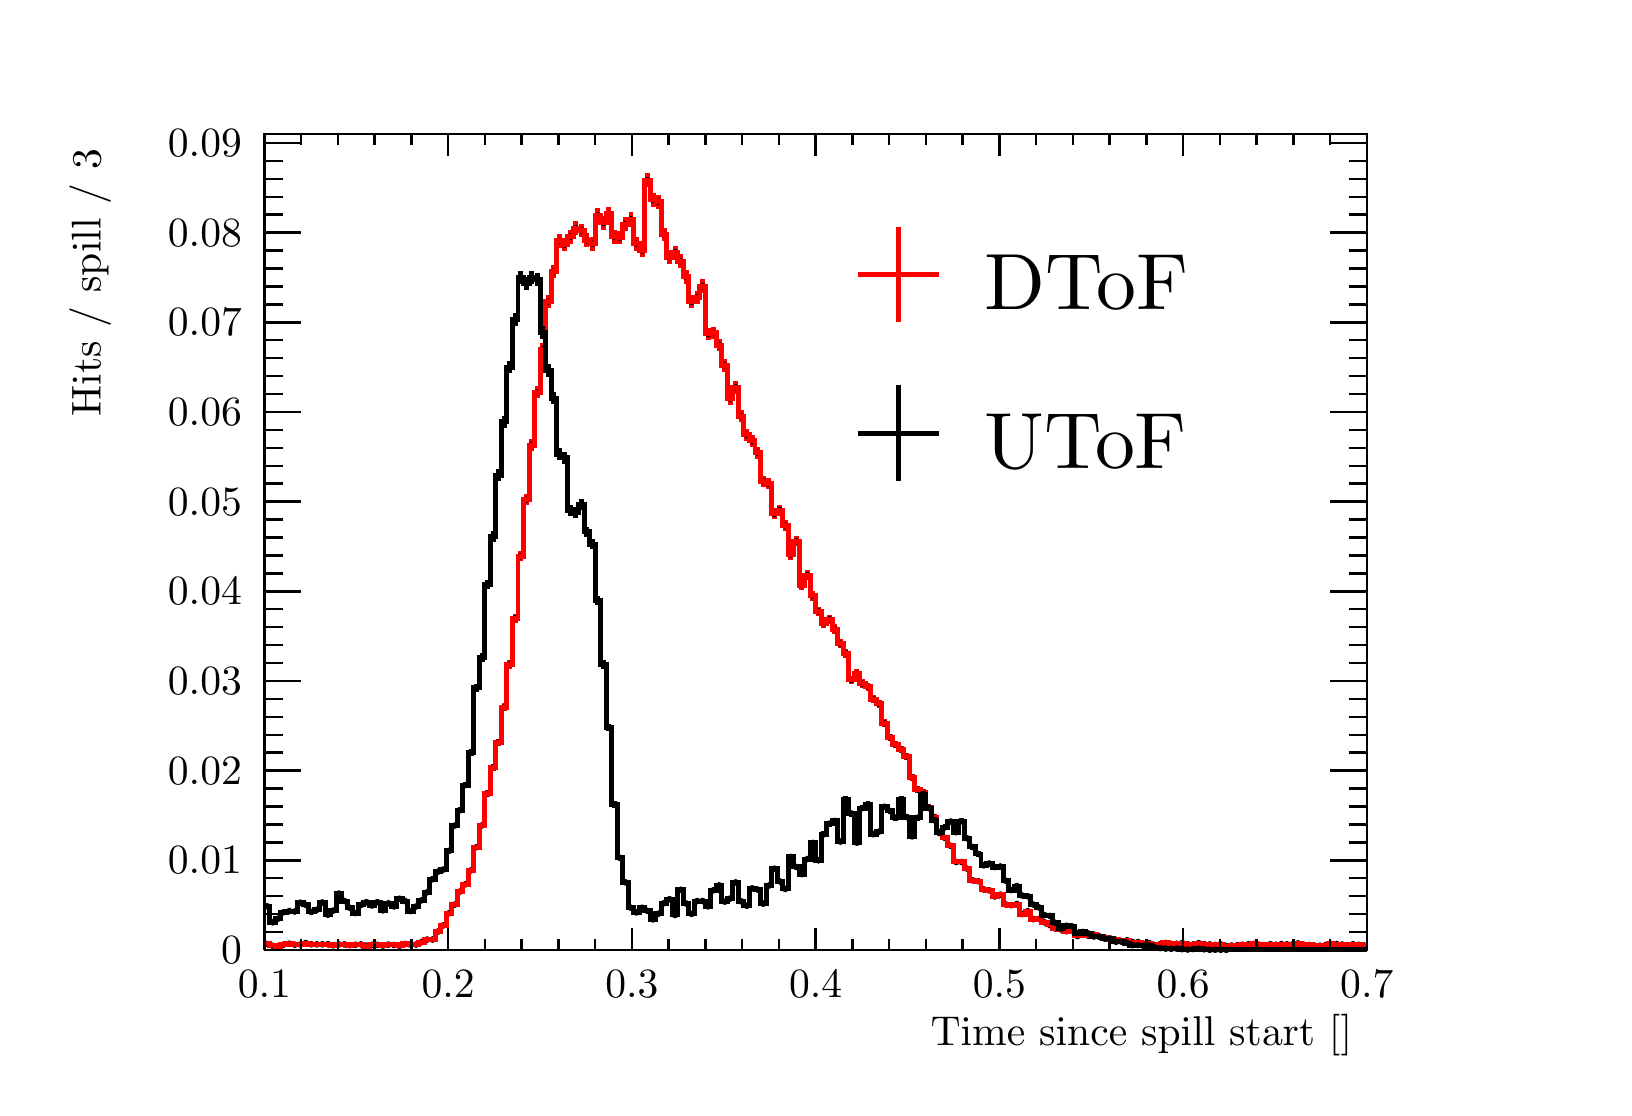
\begin{tikzpicture}
\pgfdeclareplotmark{cross} {
\pgfpathmoveto{\pgfpoint{-0.3\pgfplotmarksize}{\pgfplotmarksize}}
\pgfpathlineto{\pgfpoint{+0.3\pgfplotmarksize}{\pgfplotmarksize}}
\pgfpathlineto{\pgfpoint{+0.3\pgfplotmarksize}{0.3\pgfplotmarksize}}
\pgfpathlineto{\pgfpoint{+1\pgfplotmarksize}{0.3\pgfplotmarksize}}
\pgfpathlineto{\pgfpoint{+1\pgfplotmarksize}{-0.3\pgfplotmarksize}}
\pgfpathlineto{\pgfpoint{+0.3\pgfplotmarksize}{-0.3\pgfplotmarksize}}
\pgfpathlineto{\pgfpoint{+0.3\pgfplotmarksize}{-1.\pgfplotmarksize}}
\pgfpathlineto{\pgfpoint{-0.3\pgfplotmarksize}{-1.\pgfplotmarksize}}
\pgfpathlineto{\pgfpoint{-0.3\pgfplotmarksize}{-0.3\pgfplotmarksize}}
\pgfpathlineto{\pgfpoint{-1.\pgfplotmarksize}{-0.3\pgfplotmarksize}}
\pgfpathlineto{\pgfpoint{-1.\pgfplotmarksize}{0.3\pgfplotmarksize}}
\pgfpathlineto{\pgfpoint{-0.3\pgfplotmarksize}{0.3\pgfplotmarksize}}
\pgfpathclose
\pgfusepathqstroke
}
\pgfdeclareplotmark{cross*} {
\pgfpathmoveto{\pgfpoint{-0.3\pgfplotmarksize}{\pgfplotmarksize}}
\pgfpathlineto{\pgfpoint{+0.3\pgfplotmarksize}{\pgfplotmarksize}}
\pgfpathlineto{\pgfpoint{+0.3\pgfplotmarksize}{0.3\pgfplotmarksize}}
\pgfpathlineto{\pgfpoint{+1\pgfplotmarksize}{0.3\pgfplotmarksize}}
\pgfpathlineto{\pgfpoint{+1\pgfplotmarksize}{-0.3\pgfplotmarksize}}
\pgfpathlineto{\pgfpoint{+0.3\pgfplotmarksize}{-0.3\pgfplotmarksize}}
\pgfpathlineto{\pgfpoint{+0.3\pgfplotmarksize}{-1.\pgfplotmarksize}}
\pgfpathlineto{\pgfpoint{-0.3\pgfplotmarksize}{-1.\pgfplotmarksize}}
\pgfpathlineto{\pgfpoint{-0.3\pgfplotmarksize}{-0.3\pgfplotmarksize}}
\pgfpathlineto{\pgfpoint{-1.\pgfplotmarksize}{-0.3\pgfplotmarksize}}
\pgfpathlineto{\pgfpoint{-1.\pgfplotmarksize}{0.3\pgfplotmarksize}}
\pgfpathlineto{\pgfpoint{-0.3\pgfplotmarksize}{0.3\pgfplotmarksize}}
\pgfpathclose
\pgfusepathqfillstroke
}
\pgfdeclareplotmark{newstar} {
\pgfpathmoveto{\pgfqpoint{0pt}{\pgfplotmarksize}}
\pgfpathlineto{\pgfqpointpolar{44}{0.5\pgfplotmarksize}}
\pgfpathlineto{\pgfqpointpolar{18}{\pgfplotmarksize}}
\pgfpathlineto{\pgfqpointpolar{-20}{0.5\pgfplotmarksize}}
\pgfpathlineto{\pgfqpointpolar{-54}{\pgfplotmarksize}}
\pgfpathlineto{\pgfqpointpolar{-90}{0.5\pgfplotmarksize}}
\pgfpathlineto{\pgfqpointpolar{234}{\pgfplotmarksize}}
\pgfpathlineto{\pgfqpointpolar{198}{0.5\pgfplotmarksize}}
\pgfpathlineto{\pgfqpointpolar{162}{\pgfplotmarksize}}
\pgfpathlineto{\pgfqpointpolar{134}{0.5\pgfplotmarksize}}
\pgfpathclose
\pgfusepathqstroke
}
\pgfdeclareplotmark{newstar*} {
\pgfpathmoveto{\pgfqpoint{0pt}{\pgfplotmarksize}}
\pgfpathlineto{\pgfqpointpolar{44}{0.5\pgfplotmarksize}}
\pgfpathlineto{\pgfqpointpolar{18}{\pgfplotmarksize}}
\pgfpathlineto{\pgfqpointpolar{-20}{0.5\pgfplotmarksize}}
\pgfpathlineto{\pgfqpointpolar{-54}{\pgfplotmarksize}}
\pgfpathlineto{\pgfqpointpolar{-90}{0.5\pgfplotmarksize}}
\pgfpathlineto{\pgfqpointpolar{234}{\pgfplotmarksize}}
\pgfpathlineto{\pgfqpointpolar{198}{0.5\pgfplotmarksize}}
\pgfpathlineto{\pgfqpointpolar{162}{\pgfplotmarksize}}
\pgfpathlineto{\pgfqpointpolar{134}{0.5\pgfplotmarksize}}
\pgfpathclose
\pgfusepathqfillstroke
}
\definecolor{c}{rgb}{1,1,1};
\draw [color=c, fill=c] (0,0) rectangle (20,13.4556);
\draw [color=c, fill=c] (3,1.74922) rectangle (17,12.11);
\definecolor{c}{rgb}{0,0,0};
\draw [c,line width=0.9] (3,1.74922) -- (3,12.11) -- (17,12.11) -- (17,1.74922) -- (3,1.74922);
\definecolor{c}{rgb}{1,1,1};
\draw [color=c, fill=c] (3,1.74922) rectangle (17,12.11);
\definecolor{c}{rgb}{0,0,0};
\draw [c,line width=0.9] (3,1.74922) -- (3,12.11) -- (17,12.11) -- (17,1.74922) -- (3,1.74922);
\definecolor{c}{rgb}{1,0,0};
\draw [c,line width=1.8] (3.035,1.81776) -- (3.035,1.82578);
\draw [c,line width=1.8] (3.035,1.82578) -- (3.035,1.83381);
\definecolor{c}{rgb}{0,0,0};
\foreach \P in {(3.035,1.82578)}{\draw[mark options={color=c,fill=c},mark size=2.402402pt,mark=*,mark size=1pt] plot coordinates {\P};}
\definecolor{c}{rgb}{1,0,0};
\draw [c,line width=1.8] (3.105,1.79555) -- (3.105,1.80223);
\draw [c,line width=1.8] (3.105,1.80223) -- (3.105,1.8089);
\definecolor{c}{rgb}{0,0,0};
\foreach \P in {(3.105,1.80223)}{\draw[mark options={color=c,fill=c},mark size=2.402402pt,mark=*,mark size=1pt] plot coordinates {\P};}
\definecolor{c}{rgb}{1,0,0};
\draw [c,line width=1.8] (3.175,1.78691) -- (3.175,1.79297);
\draw [c,line width=1.8] (3.175,1.79297) -- (3.175,1.79904);
\definecolor{c}{rgb}{0,0,0};
\foreach \P in {(3.175,1.79297)}{\draw[mark options={color=c,fill=c},mark size=2.402402pt,mark=*,mark size=1pt] plot coordinates {\P};}
\definecolor{c}{rgb}{1,0,0};
\draw [c,line width=1.8] (3.245,1.81059) -- (3.245,1.81821);
\draw [c,line width=1.8] (3.245,1.81821) -- (3.245,1.82583);
\definecolor{c}{rgb}{0,0,0};
\foreach \P in {(3.245,1.81821)}{\draw[mark options={color=c,fill=c},mark size=2.402402pt,mark=*,mark size=1pt] plot coordinates {\P};}
\definecolor{c}{rgb}{1,0,0};
\draw [c,line width=1.8] (3.315,1.82095) -- (3.315,1.82915);
\draw [c,line width=1.8] (3.315,1.82915) -- (3.315,1.83735);
\definecolor{c}{rgb}{0,0,0};
\foreach \P in {(3.315,1.82915)}{\draw[mark options={color=c,fill=c},mark size=2.402402pt,mark=*,mark size=1pt] plot coordinates {\P};}
\definecolor{c}{rgb}{1,0,0};
\draw [c,line width=1.8] (3.385,1.809) -- (3.385,1.81653);
\draw [c,line width=1.8] (3.385,1.81653) -- (3.385,1.82405);
\definecolor{c}{rgb}{0,0,0};
\foreach \P in {(3.385,1.81653)}{\draw[mark options={color=c,fill=c},mark size=2.402402pt,mark=*,mark size=1pt] plot coordinates {\P};}
\definecolor{c}{rgb}{1,0,0};
\draw [c,line width=1.8] (3.455,1.81059) -- (3.455,1.81821);
\draw [c,line width=1.8] (3.455,1.81821) -- (3.455,1.82583);
\definecolor{c}{rgb}{0,0,0};
\foreach \P in {(3.455,1.81821)}{\draw[mark options={color=c,fill=c},mark size=2.402402pt,mark=*,mark size=1pt] plot coordinates {\P};}
\definecolor{c}{rgb}{1,0,0};
\draw [c,line width=1.8] (3.525,1.82814) -- (3.525,1.83672);
\draw [c,line width=1.8] (3.525,1.83672) -- (3.525,1.8453);
\definecolor{c}{rgb}{0,0,0};
\foreach \P in {(3.525,1.83672)}{\draw[mark options={color=c,fill=c},mark size=2.402402pt,mark=*,mark size=1pt] plot coordinates {\P};}
\definecolor{c}{rgb}{1,0,0};
\draw [c,line width=1.8] (3.595,1.81377) -- (3.595,1.82158);
\draw [c,line width=1.8] (3.595,1.82158) -- (3.595,1.82938);
\definecolor{c}{rgb}{0,0,0};
\foreach \P in {(3.595,1.82158)}{\draw[mark options={color=c,fill=c},mark size=2.402402pt,mark=*,mark size=1pt] plot coordinates {\P};}
\definecolor{c}{rgb}{1,0,0};
\draw [c,line width=1.8] (3.665,1.81298) -- (3.665,1.82073);
\draw [c,line width=1.8] (3.665,1.82073) -- (3.665,1.82849);
\definecolor{c}{rgb}{0,0,0};
\foreach \P in {(3.665,1.82073)}{\draw[mark options={color=c,fill=c},mark size=2.402402pt,mark=*,mark size=1pt] plot coordinates {\P};}
\definecolor{c}{rgb}{1,0,0};
\draw [c,line width=1.8] (3.735,1.81377) -- (3.735,1.82158);
\draw [c,line width=1.8] (3.735,1.82158) -- (3.735,1.82938);
\definecolor{c}{rgb}{0,0,0};
\foreach \P in {(3.735,1.82158)}{\draw[mark options={color=c,fill=c},mark size=2.402402pt,mark=*,mark size=1pt] plot coordinates {\P};}
\definecolor{c}{rgb}{1,0,0};
\draw [c,line width=1.8] (3.805,1.81457) -- (3.805,1.82242);
\draw [c,line width=1.8] (3.805,1.82242) -- (3.805,1.83026);
\definecolor{c}{rgb}{0,0,0};
\foreach \P in {(3.805,1.82242)}{\draw[mark options={color=c,fill=c},mark size=2.402402pt,mark=*,mark size=1pt] plot coordinates {\P};}
\definecolor{c}{rgb}{1,0,0};
\draw [c,line width=1.8] (3.875,1.80108) -- (3.875,1.80812);
\draw [c,line width=1.8] (3.875,1.80812) -- (3.875,1.81515);
\definecolor{c}{rgb}{0,0,0};
\foreach \P in {(3.875,1.80812)}{\draw[mark options={color=c,fill=c},mark size=2.402402pt,mark=*,mark size=1pt] plot coordinates {\P};}
\definecolor{c}{rgb}{1,0,0};
\draw [c,line width=1.8] (3.945,1.81298) -- (3.945,1.82073);
\draw [c,line width=1.8] (3.945,1.82073) -- (3.945,1.82849);
\definecolor{c}{rgb}{0,0,0};
\foreach \P in {(3.945,1.82073)}{\draw[mark options={color=c,fill=c},mark size=2.402402pt,mark=*,mark size=1pt] plot coordinates {\P};}
\definecolor{c}{rgb}{1,0,0};
\draw [c,line width=1.8] (4.015,1.81218) -- (4.015,1.81989);
\draw [c,line width=1.8] (4.015,1.81989) -- (4.015,1.8276);
\definecolor{c}{rgb}{0,0,0};
\foreach \P in {(4.015,1.81989)}{\draw[mark options={color=c,fill=c},mark size=2.402402pt,mark=*,mark size=1pt] plot coordinates {\P};}
\definecolor{c}{rgb}{1,0,0};
\draw [c,line width=1.8] (4.085,1.80345) -- (4.085,1.81064);
\draw [c,line width=1.8] (4.085,1.81064) -- (4.085,1.81783);
\definecolor{c}{rgb}{0,0,0};
\foreach \P in {(4.085,1.81064)}{\draw[mark options={color=c,fill=c},mark size=2.402402pt,mark=*,mark size=1pt] plot coordinates {\P};}
\definecolor{c}{rgb}{1,0,0};
\draw [c,line width=1.8] (4.155,1.80821) -- (4.155,1.81569);
\draw [c,line width=1.8] (4.155,1.81569) -- (4.155,1.82316);
\definecolor{c}{rgb}{0,0,0};
\foreach \P in {(4.155,1.81569)}{\draw[mark options={color=c,fill=c},mark size=2.402402pt,mark=*,mark size=1pt] plot coordinates {\P};}
\definecolor{c}{rgb}{1,0,0};
\draw [c,line width=1.8] (4.225,1.81218) -- (4.225,1.81989);
\draw [c,line width=1.8] (4.225,1.81989) -- (4.225,1.8276);
\definecolor{c}{rgb}{0,0,0};
\foreach \P in {(4.225,1.81989)}{\draw[mark options={color=c,fill=c},mark size=2.402402pt,mark=*,mark size=1pt] plot coordinates {\P};}
\definecolor{c}{rgb}{1,0,0};
\draw [c,line width=1.8] (4.295,1.7924) -- (4.295,1.79886);
\draw [c,line width=1.8] (4.295,1.79886) -- (4.295,1.80532);
\definecolor{c}{rgb}{0,0,0};
\foreach \P in {(4.295,1.79886)}{\draw[mark options={color=c,fill=c},mark size=2.402402pt,mark=*,mark size=1pt] plot coordinates {\P};}
\definecolor{c}{rgb}{1,0,0};
\draw [c,line width=1.8] (4.365,1.80742) -- (4.365,1.81485);
\draw [c,line width=1.8] (4.365,1.81485) -- (4.365,1.82228);
\definecolor{c}{rgb}{0,0,0};
\foreach \P in {(4.365,1.81485)}{\draw[mark options={color=c,fill=c},mark size=2.402402pt,mark=*,mark size=1pt] plot coordinates {\P};}
\definecolor{c}{rgb}{1,0,0};
\draw [c,line width=1.8] (4.435,1.80821) -- (4.435,1.81569);
\draw [c,line width=1.8] (4.435,1.81569) -- (4.435,1.82316);
\definecolor{c}{rgb}{0,0,0};
\foreach \P in {(4.435,1.81569)}{\draw[mark options={color=c,fill=c},mark size=2.402402pt,mark=*,mark size=1pt] plot coordinates {\P};}
\definecolor{c}{rgb}{1,0,0};
\draw [c,line width=1.8] (4.505,1.79792) -- (4.505,1.80475);
\draw [c,line width=1.8] (4.505,1.80475) -- (4.505,1.81158);
\definecolor{c}{rgb}{0,0,0};
\foreach \P in {(4.505,1.80475)}{\draw[mark options={color=c,fill=c},mark size=2.402402pt,mark=*,mark size=1pt] plot coordinates {\P};}
\definecolor{c}{rgb}{1,0,0};
\draw [c,line width=1.8] (4.575,1.8098) -- (4.575,1.81737);
\draw [c,line width=1.8] (4.575,1.81737) -- (4.575,1.82494);
\definecolor{c}{rgb}{0,0,0};
\foreach \P in {(4.575,1.81737)}{\draw[mark options={color=c,fill=c},mark size=2.402402pt,mark=*,mark size=1pt] plot coordinates {\P};}
\definecolor{c}{rgb}{1,0,0};
\draw [c,line width=1.8] (4.645,1.80583) -- (4.645,1.81316);
\draw [c,line width=1.8] (4.645,1.81316) -- (4.645,1.8205);
\definecolor{c}{rgb}{0,0,0};
\foreach \P in {(4.645,1.81316)}{\draw[mark options={color=c,fill=c},mark size=2.402402pt,mark=*,mark size=1pt] plot coordinates {\P};}
\definecolor{c}{rgb}{1,0,0};
\draw [c,line width=1.8] (4.715,1.79634) -- (4.715,1.80307);
\draw [c,line width=1.8] (4.715,1.80307) -- (4.715,1.8098);
\definecolor{c}{rgb}{0,0,0};
\foreach \P in {(4.715,1.80307)}{\draw[mark options={color=c,fill=c},mark size=2.402402pt,mark=*,mark size=1pt] plot coordinates {\P};}
\definecolor{c}{rgb}{1,0,0};
\draw [c,line width=1.8] (4.785,1.81776) -- (4.785,1.82578);
\draw [c,line width=1.8] (4.785,1.82578) -- (4.785,1.83381);
\definecolor{c}{rgb}{0,0,0};
\foreach \P in {(4.785,1.82578)}{\draw[mark options={color=c,fill=c},mark size=2.402402pt,mark=*,mark size=1pt] plot coordinates {\P};}
\definecolor{c}{rgb}{1,0,0};
\draw [c,line width=1.8] (4.855,1.8098) -- (4.855,1.81737);
\draw [c,line width=1.8] (4.855,1.81737) -- (4.855,1.82494);
\definecolor{c}{rgb}{0,0,0};
\foreach \P in {(4.855,1.81737)}{\draw[mark options={color=c,fill=c},mark size=2.402402pt,mark=*,mark size=1pt] plot coordinates {\P};}
\definecolor{c}{rgb}{1,0,0};
\draw [c,line width=1.8] (4.925,1.81059) -- (4.925,1.81821);
\draw [c,line width=1.8] (4.925,1.81821) -- (4.925,1.82583);
\definecolor{c}{rgb}{0,0,0};
\foreach \P in {(4.925,1.81821)}{\draw[mark options={color=c,fill=c},mark size=2.402402pt,mark=*,mark size=1pt] plot coordinates {\P};}
\definecolor{c}{rgb}{1,0,0};
\draw [c,line width=1.8] (4.995,1.83856) -- (4.995,1.84766);
\draw [c,line width=1.8] (4.995,1.84766) -- (4.995,1.85676);
\definecolor{c}{rgb}{0,0,0};
\foreach \P in {(4.995,1.84766)}{\draw[mark options={color=c,fill=c},mark size=2.402402pt,mark=*,mark size=1pt] plot coordinates {\P};}
\definecolor{c}{rgb}{1,0,0};
\draw [c,line width=1.8] (5.065,1.87077) -- (5.065,1.88131);
\draw [c,line width=1.8] (5.065,1.88131) -- (5.065,1.89185);
\definecolor{c}{rgb}{0,0,0};
\foreach \P in {(5.065,1.88131)}{\draw[mark options={color=c,fill=c},mark size=2.402402pt,mark=*,mark size=1pt] plot coordinates {\P};}
\definecolor{c}{rgb}{1,0,0};
\draw [c,line width=1.8] (5.135,1.87157) -- (5.135,1.88215);
\draw [c,line width=1.8] (5.135,1.88215) -- (5.135,1.89272);
\definecolor{c}{rgb}{0,0,0};
\foreach \P in {(5.135,1.88215)}{\draw[mark options={color=c,fill=c},mark size=2.402402pt,mark=*,mark size=1pt] plot coordinates {\P};}
\definecolor{c}{rgb}{1,0,0};
\draw [c,line width=1.8] (5.205,1.96989) -- (5.205,1.98395);
\draw [c,line width=1.8] (5.205,1.98395) -- (5.205,1.998);
\definecolor{c}{rgb}{0,0,0};
\foreach \P in {(5.205,1.98395)}{\draw[mark options={color=c,fill=c},mark size=2.402402pt,mark=*,mark size=1pt] plot coordinates {\P};}
\definecolor{c}{rgb}{1,0,0};
\draw [c,line width=1.8] (5.275,2.04596) -- (5.275,2.06219);
\draw [c,line width=1.8] (5.275,2.06219) -- (5.275,2.07841);
\definecolor{c}{rgb}{0,0,0};
\foreach \P in {(5.275,2.06219)}{\draw[mark options={color=c,fill=c},mark size=2.402402pt,mark=*,mark size=1pt] plot coordinates {\P};}
\definecolor{c}{rgb}{1,0,0};
\draw [c,line width=1.8] (5.345,2.19633) -- (5.345,2.21614);
\draw [c,line width=1.8] (5.345,2.21614) -- (5.345,2.23596);
\definecolor{c}{rgb}{0,0,0};
\foreach \P in {(5.345,2.21614)}{\draw[mark options={color=c,fill=c},mark size=2.402402pt,mark=*,mark size=1pt] plot coordinates {\P};}
\definecolor{c}{rgb}{1,0,0};
\draw [c,line width=1.8] (5.415,2.30349) -- (5.415,2.32551);
\draw [c,line width=1.8] (5.415,2.32551) -- (5.415,2.34753);
\definecolor{c}{rgb}{0,0,0};
\foreach \P in {(5.415,2.32551)}{\draw[mark options={color=c,fill=c},mark size=2.402402pt,mark=*,mark size=1pt] plot coordinates {\P};}
\definecolor{c}{rgb}{1,0,0};
\draw [c,line width=1.8] (5.485,2.46709) -- (5.485,2.49209);
\draw [c,line width=1.8] (5.485,2.49209) -- (5.485,2.51709);
\definecolor{c}{rgb}{0,0,0};
\foreach \P in {(5.485,2.49209)}{\draw[mark options={color=c,fill=c},mark size=2.402402pt,mark=*,mark size=1pt] plot coordinates {\P};}
\definecolor{c}{rgb}{1,0,0};
\draw [c,line width=1.8] (5.555,2.55812) -- (5.555,2.58463);
\draw [c,line width=1.8] (5.555,2.58463) -- (5.555,2.61114);
\definecolor{c}{rgb}{0,0,0};
\foreach \P in {(5.555,2.58463)}{\draw[mark options={color=c,fill=c},mark size=2.402402pt,mark=*,mark size=1pt] plot coordinates {\P};}
\definecolor{c}{rgb}{1,0,0};
\draw [c,line width=1.8] (5.625,2.73213) -- (5.625,2.76131);
\draw [c,line width=1.8] (5.625,2.76131) -- (5.625,2.79049);
\definecolor{c}{rgb}{0,0,0};
\foreach \P in {(5.625,2.76131)}{\draw[mark options={color=c,fill=c},mark size=2.402402pt,mark=*,mark size=1pt] plot coordinates {\P};}
\definecolor{c}{rgb}{1,0,0};
\draw [c,line width=1.8] (5.695,3.02178) -- (5.695,3.05492);
\draw [c,line width=1.8] (5.695,3.05492) -- (5.695,3.08806);
\definecolor{c}{rgb}{0,0,0};
\foreach \P in {(5.695,3.05492)}{\draw[mark options={color=c,fill=c},mark size=2.402402pt,mark=*,mark size=1pt] plot coordinates {\P};}
\definecolor{c}{rgb}{1,0,0};
\draw [c,line width=1.8] (5.765,3.29522) -- (5.765,3.33171);
\draw [c,line width=1.8] (5.765,3.33171) -- (5.765,3.36819);
\definecolor{c}{rgb}{0,0,0};
\foreach \P in {(5.765,3.33171)}{\draw[mark options={color=c,fill=c},mark size=2.402402pt,mark=*,mark size=1pt] plot coordinates {\P};}
\definecolor{c}{rgb}{1,0,0};
\draw [c,line width=1.8] (5.835,3.69715) -- (5.835,3.73805);
\draw [c,line width=1.8] (5.835,3.73805) -- (5.835,3.77896);
\definecolor{c}{rgb}{0,0,0};
\foreach \P in {(5.835,3.73805)}{\draw[mark options={color=c,fill=c},mark size=2.402402pt,mark=*,mark size=1pt] plot coordinates {\P};}
\definecolor{c}{rgb}{1,0,0};
\draw [c,line width=1.8] (5.905,4.02618) -- (5.905,4.07037);
\draw [c,line width=1.8] (5.905,4.07037) -- (5.905,4.11456);
\definecolor{c}{rgb}{0,0,0};
\foreach \P in {(5.905,4.07037)}{\draw[mark options={color=c,fill=c},mark size=2.402402pt,mark=*,mark size=1pt] plot coordinates {\P};}
\definecolor{c}{rgb}{1,0,0};
\draw [c,line width=1.8] (5.975,4.33959) -- (5.975,4.38669);
\draw [c,line width=1.8] (5.975,4.38669) -- (5.975,4.4338);
\definecolor{c}{rgb}{0,0,0};
\foreach \P in {(5.975,4.38669)}{\draw[mark options={color=c,fill=c},mark size=2.402402pt,mark=*,mark size=1pt] plot coordinates {\P};}
\definecolor{c}{rgb}{1,0,0};
\draw [c,line width=1.8] (6.045,4.78249) -- (6.045,4.83342);
\draw [c,line width=1.8] (6.045,4.83342) -- (6.045,4.88436);
\definecolor{c}{rgb}{0,0,0};
\foreach \P in {(6.045,4.83342)}{\draw[mark options={color=c,fill=c},mark size=2.402402pt,mark=*,mark size=1pt] plot coordinates {\P};}
\definecolor{c}{rgb}{1,0,0};
\draw [c,line width=1.8] (6.115,5.32166) -- (6.115,5.3769);
\draw [c,line width=1.8] (6.115,5.3769) -- (6.115,5.43215);
\definecolor{c}{rgb}{0,0,0};
\foreach \P in {(6.115,5.3769)}{\draw[mark options={color=c,fill=c},mark size=2.402402pt,mark=*,mark size=1pt] plot coordinates {\P};}
\definecolor{c}{rgb}{1,0,0};
\draw [c,line width=1.8] (6.185,5.90291) -- (6.185,5.96245);
\draw [c,line width=1.8] (6.185,5.96245) -- (6.185,6.02198);
\definecolor{c}{rgb}{0,0,0};
\foreach \P in {(6.185,5.96245)}{\draw[mark options={color=c,fill=c},mark size=2.402402pt,mark=*,mark size=1pt] plot coordinates {\P};}
\definecolor{c}{rgb}{1,0,0};
\draw [c,line width=1.8] (6.255,6.68504) -- (6.255,6.7499);
\draw [c,line width=1.8] (6.255,6.7499) -- (6.255,6.81476);
\definecolor{c}{rgb}{0,0,0};
\foreach \P in {(6.255,6.7499)}{\draw[mark options={color=c,fill=c},mark size=2.402402pt,mark=*,mark size=1pt] plot coordinates {\P};}
\definecolor{c}{rgb}{1,0,0};
\draw [c,line width=1.8] (6.325,7.39817) -- (6.325,7.46753);
\draw [c,line width=1.8] (6.325,7.46753) -- (6.325,7.53689);
\definecolor{c}{rgb}{0,0,0};
\foreach \P in {(6.325,7.46753)}{\draw[mark options={color=c,fill=c},mark size=2.402402pt,mark=*,mark size=1pt] plot coordinates {\P};}
\definecolor{c}{rgb}{1,0,0};
\draw [c,line width=1.8] (6.395,8.08815) -- (6.395,8.1616);
\draw [c,line width=1.8] (6.395,8.1616) -- (6.395,8.23505);
\definecolor{c}{rgb}{0,0,0};
\foreach \P in {(6.395,8.1616)}{\draw[mark options={color=c,fill=c},mark size=2.402402pt,mark=*,mark size=1pt] plot coordinates {\P};}
\definecolor{c}{rgb}{1,0,0};
\draw [c,line width=1.8] (6.465,8.75408) -- (6.465,8.83127);
\draw [c,line width=1.8] (6.465,8.83127) -- (6.465,8.90846);
\definecolor{c}{rgb}{0,0,0};
\foreach \P in {(6.465,8.83127)}{\draw[mark options={color=c,fill=c},mark size=2.402402pt,mark=*,mark size=1pt] plot coordinates {\P};}
\definecolor{c}{rgb}{1,0,0};
\draw [c,line width=1.8] (6.535,9.30051) -- (6.535,9.38064);
\draw [c,line width=1.8] (6.535,9.38064) -- (6.535,9.46077);
\definecolor{c}{rgb}{0,0,0};
\foreach \P in {(6.535,9.38064)}{\draw[mark options={color=c,fill=c},mark size=2.402402pt,mark=*,mark size=1pt] plot coordinates {\P};}
\definecolor{c}{rgb}{1,0,0};
\draw [c,line width=1.8] (6.605,9.90229) -- (6.605,9.98553);
\draw [c,line width=1.8] (6.605,9.98553) -- (6.605,10.0688);
\definecolor{c}{rgb}{0,0,0};
\foreach \P in {(6.605,9.98553)}{\draw[mark options={color=c,fill=c},mark size=2.402402pt,mark=*,mark size=1pt] plot coordinates {\P};}
\definecolor{c}{rgb}{1,0,0};
\draw [c,line width=1.8] (6.675,10.2815) -- (6.675,10.3666);
\draw [c,line width=1.8] (6.675,10.3666) -- (6.675,10.4518);
\definecolor{c}{rgb}{0,0,0};
\foreach \P in {(6.675,10.3666)}{\draw[mark options={color=c,fill=c},mark size=2.402402pt,mark=*,mark size=1pt] plot coordinates {\P};}
\definecolor{c}{rgb}{1,0,0};
\draw [c,line width=1.8] (6.745,10.6674) -- (6.745,10.7545);
\draw [c,line width=1.8] (6.745,10.7545) -- (6.745,10.8415);
\definecolor{c}{rgb}{0,0,0};
\foreach \P in {(6.745,10.7545)}{\draw[mark options={color=c,fill=c},mark size=2.402402pt,mark=*,mark size=1pt] plot coordinates {\P};}
\definecolor{c}{rgb}{1,0,0};
\draw [c,line width=1.8] (6.815,10.6206) -- (6.815,10.7074);
\draw [c,line width=1.8] (6.815,10.7074) -- (6.815,10.7942);
\definecolor{c}{rgb}{0,0,0};
\foreach \P in {(6.815,10.7074)}{\draw[mark options={color=c,fill=c},mark size=2.402402pt,mark=*,mark size=1pt] plot coordinates {\P};}
\definecolor{c}{rgb}{1,0,0};
\draw [c,line width=1.8] (6.885,10.721) -- (6.885,10.8083);
\draw [c,line width=1.8] (6.885,10.8083) -- (6.885,10.8956);
\definecolor{c}{rgb}{0,0,0};
\foreach \P in {(6.885,10.8083)}{\draw[mark options={color=c,fill=c},mark size=2.402402pt,mark=*,mark size=1pt] plot coordinates {\P};}
\definecolor{c}{rgb}{1,0,0};
\draw [c,line width=1.8] (6.955,10.8282) -- (6.955,10.916);
\draw [c,line width=1.8] (6.955,10.916) -- (6.955,11.0038);
\definecolor{c}{rgb}{0,0,0};
\foreach \P in {(6.955,10.916)}{\draw[mark options={color=c,fill=c},mark size=2.402402pt,mark=*,mark size=1pt] plot coordinates {\P};}
\definecolor{c}{rgb}{1,0,0};
\draw [c,line width=1.8] (7.025,10.7997) -- (7.025,10.8874);
\draw [c,line width=1.8] (7.025,10.8874) -- (7.025,10.9751);
\definecolor{c}{rgb}{0,0,0};
\foreach \P in {(7.025,10.8874)}{\draw[mark options={color=c,fill=c},mark size=2.402402pt,mark=*,mark size=1pt] plot coordinates {\P};}
\definecolor{c}{rgb}{1,0,0};
\draw [c,line width=1.8] (7.095,10.6758) -- (7.095,10.7629);
\draw [c,line width=1.8] (7.095,10.7629) -- (7.095,10.85);
\definecolor{c}{rgb}{0,0,0};
\foreach \P in {(7.095,10.7629)}{\draw[mark options={color=c,fill=c},mark size=2.402402pt,mark=*,mark size=1pt] plot coordinates {\P};}
\definecolor{c}{rgb}{1,0,0};
\draw [c,line width=1.8] (7.165,10.6314) -- (7.165,10.7183);
\draw [c,line width=1.8] (7.165,10.7183) -- (7.165,10.8052);
\definecolor{c}{rgb}{0,0,0};
\foreach \P in {(7.165,10.7183)}{\draw[mark options={color=c,fill=c},mark size=2.402402pt,mark=*,mark size=1pt] plot coordinates {\P};}
\definecolor{c}{rgb}{1,0,0};
\draw [c,line width=1.8] (7.235,10.9898) -- (7.235,11.0784);
\draw [c,line width=1.8] (7.235,11.0784) -- (7.235,11.167);
\definecolor{c}{rgb}{0,0,0};
\foreach \P in {(7.235,11.0784)}{\draw[mark options={color=c,fill=c},mark size=2.402402pt,mark=*,mark size=1pt] plot coordinates {\P};}
\definecolor{c}{rgb}{1,0,0};
\draw [c,line width=1.8] (7.305,10.896) -- (7.305,10.9842);
\draw [c,line width=1.8] (7.305,10.9842) -- (7.305,11.0723);
\definecolor{c}{rgb}{0,0,0};
\foreach \P in {(7.305,10.9842)}{\draw[mark options={color=c,fill=c},mark size=2.402402pt,mark=*,mark size=1pt] plot coordinates {\P};}
\definecolor{c}{rgb}{1,0,0};
\draw [c,line width=1.8] (7.375,11.0107) -- (7.375,11.0994);
\draw [c,line width=1.8] (7.375,11.0994) -- (7.375,11.1881);
\definecolor{c}{rgb}{0,0,0};
\foreach \P in {(7.375,11.0994)}{\draw[mark options={color=c,fill=c},mark size=2.402402pt,mark=*,mark size=1pt] plot coordinates {\P};}
\definecolor{c}{rgb}{1,0,0};
\draw [c,line width=1.8] (7.445,10.7193) -- (7.445,10.8066);
\draw [c,line width=1.8] (7.445,10.8066) -- (7.445,10.8939);
\definecolor{c}{rgb}{0,0,0};
\foreach \P in {(7.445,10.8066)}{\draw[mark options={color=c,fill=c},mark size=2.402402pt,mark=*,mark size=1pt] plot coordinates {\P};}
\definecolor{c}{rgb}{1,0,0};
\draw [c,line width=1.8] (7.515,10.711) -- (7.515,10.7982);
\draw [c,line width=1.8] (7.515,10.7982) -- (7.515,10.8855);
\definecolor{c}{rgb}{0,0,0};
\foreach \P in {(7.515,10.7982)}{\draw[mark options={color=c,fill=c},mark size=2.402402pt,mark=*,mark size=1pt] plot coordinates {\P};}
\definecolor{c}{rgb}{1,0,0};
\draw [c,line width=1.8] (7.585,10.8801) -- (7.585,10.9682);
\draw [c,line width=1.8] (7.585,10.9682) -- (7.585,11.0562);
\definecolor{c}{rgb}{0,0,0};
\foreach \P in {(7.585,10.9682)}{\draw[mark options={color=c,fill=c},mark size=2.402402pt,mark=*,mark size=1pt] plot coordinates {\P};}
\definecolor{c}{rgb}{1,0,0};
\draw [c,line width=1.8] (7.655,10.9395) -- (7.655,11.0279);
\draw [c,line width=1.8] (7.655,11.0279) -- (7.655,11.1163);
\definecolor{c}{rgb}{0,0,0};
\foreach \P in {(7.655,11.0279)}{\draw[mark options={color=c,fill=c},mark size=2.402402pt,mark=*,mark size=1pt] plot coordinates {\P};}
\definecolor{c}{rgb}{1,0,0};
\draw [c,line width=1.8] (7.725,10.6323) -- (7.725,10.7191);
\draw [c,line width=1.8] (7.725,10.7191) -- (7.725,10.806);
\definecolor{c}{rgb}{0,0,0};
\foreach \P in {(7.725,10.7191)}{\draw[mark options={color=c,fill=c},mark size=2.402402pt,mark=*,mark size=1pt] plot coordinates {\P};}
\definecolor{c}{rgb}{1,0,0};
\draw [c,line width=1.8] (7.795,10.5452) -- (7.795,10.6317);
\draw [c,line width=1.8] (7.795,10.6317) -- (7.795,10.7181);
\definecolor{c}{rgb}{0,0,0};
\foreach \P in {(7.795,10.6317)}{\draw[mark options={color=c,fill=c},mark size=2.402402pt,mark=*,mark size=1pt] plot coordinates {\P};}
\definecolor{c}{rgb}{1,0,0};
\draw [c,line width=1.8] (7.865,11.4353) -- (7.865,11.526);
\draw [c,line width=1.8] (7.865,11.526) -- (7.865,11.6166);
\definecolor{c}{rgb}{0,0,0};
\foreach \P in {(7.865,11.526)}{\draw[mark options={color=c,fill=c},mark size=2.402402pt,mark=*,mark size=1pt] plot coordinates {\P};}
\definecolor{c}{rgb}{1,0,0};
\draw [c,line width=1.8] (7.935,11.1849) -- (7.935,11.2744);
\draw [c,line width=1.8] (7.935,11.2744) -- (7.935,11.3639);
\definecolor{c}{rgb}{0,0,0};
\foreach \P in {(7.935,11.2744)}{\draw[mark options={color=c,fill=c},mark size=2.402402pt,mark=*,mark size=1pt] plot coordinates {\P};}
\definecolor{c}{rgb}{1,0,0};
\draw [c,line width=1.8] (8.005,11.1598) -- (8.005,11.2492);
\draw [c,line width=1.8] (8.005,11.2492) -- (8.005,11.3386);
\definecolor{c}{rgb}{0,0,0};
\foreach \P in {(8.005,11.2492)}{\draw[mark options={color=c,fill=c},mark size=2.402402pt,mark=*,mark size=1pt] plot coordinates {\P};}
\definecolor{c}{rgb}{1,0,0};
\draw [c,line width=1.8] (8.075,10.747) -- (8.075,10.8344);
\draw [c,line width=1.8] (8.075,10.8344) -- (8.075,10.9218);
\definecolor{c}{rgb}{0,0,0};
\foreach \P in {(8.075,10.8344)}{\draw[mark options={color=c,fill=c},mark size=2.402402pt,mark=*,mark size=1pt] plot coordinates {\P};}
\definecolor{c}{rgb}{1,0,0};
\draw [c,line width=1.8] (8.145,10.4615) -- (8.145,10.5475);
\draw [c,line width=1.8] (8.145,10.5475) -- (8.145,10.6336);
\definecolor{c}{rgb}{0,0,0};
\foreach \P in {(8.145,10.5475)}{\draw[mark options={color=c,fill=c},mark size=2.402402pt,mark=*,mark size=1pt] plot coordinates {\P};}
\definecolor{c}{rgb}{1,0,0};
\draw [c,line width=1.8] (8.215,10.5226) -- (8.215,10.6089);
\draw [c,line width=1.8] (8.215,10.6089) -- (8.215,10.6953);
\definecolor{c}{rgb}{0,0,0};
\foreach \P in {(8.215,10.6089)}{\draw[mark options={color=c,fill=c},mark size=2.402402pt,mark=*,mark size=1pt] plot coordinates {\P};}
\definecolor{c}{rgb}{1,0,0};
\draw [c,line width=1.8] (8.285,10.4121) -- (8.285,10.4979);
\draw [c,line width=1.8] (8.285,10.4979) -- (8.285,10.5837);
\definecolor{c}{rgb}{0,0,0};
\foreach \P in {(8.285,10.4979)}{\draw[mark options={color=c,fill=c},mark size=2.402402pt,mark=*,mark size=1pt] plot coordinates {\P};}
\definecolor{c}{rgb}{1,0,0};
\draw [c,line width=1.8] (8.355,10.2129) -- (8.355,10.2977);
\draw [c,line width=1.8] (8.355,10.2977) -- (8.355,10.3825);
\definecolor{c}{rgb}{0,0,0};
\foreach \P in {(8.355,10.2977)}{\draw[mark options={color=c,fill=c},mark size=2.402402pt,mark=*,mark size=1pt] plot coordinates {\P};}
\definecolor{c}{rgb}{1,0,0};
\draw [c,line width=1.8] (8.425,9.89811) -- (8.425,9.98133);
\draw [c,line width=1.8] (8.425,9.98133) -- (8.425,10.0645);
\definecolor{c}{rgb}{0,0,0};
\foreach \P in {(8.425,9.98133)}{\draw[mark options={color=c,fill=c},mark size=2.402402pt,mark=*,mark size=1pt] plot coordinates {\P};}
\definecolor{c}{rgb}{1,0,0};
\draw [c,line width=1.8] (8.495,9.95503) -- (8.495,10.0385);
\draw [c,line width=1.8] (8.495,10.0385) -- (8.495,10.122);
\definecolor{c}{rgb}{0,0,0};
\foreach \P in {(8.495,10.0385)}{\draw[mark options={color=c,fill=c},mark size=2.402402pt,mark=*,mark size=1pt] plot coordinates {\P};}
\definecolor{c}{rgb}{1,0,0};
\draw [c,line width=1.8] (8.565,10.0965) -- (8.565,10.1807);
\draw [c,line width=1.8] (8.565,10.1807) -- (8.565,10.2649);
\definecolor{c}{rgb}{0,0,0};
\foreach \P in {(8.565,10.1807)}{\draw[mark options={color=c,fill=c},mark size=2.402402pt,mark=*,mark size=1pt] plot coordinates {\P};}
\definecolor{c}{rgb}{1,0,0};
\draw [c,line width=1.8] (8.635,9.49217) -- (8.635,9.5733);
\draw [c,line width=1.8] (8.635,9.5733) -- (8.635,9.65443);
\definecolor{c}{rgb}{0,0,0};
\foreach \P in {(8.635,9.5733)}{\draw[mark options={color=c,fill=c},mark size=2.402402pt,mark=*,mark size=1pt] plot coordinates {\P};}
\definecolor{c}{rgb}{1,0,0};
\draw [c,line width=1.8] (8.705,9.50388) -- (8.705,9.58508);
\draw [c,line width=1.8] (8.705,9.58508) -- (8.705,9.66627);
\definecolor{c}{rgb}{0,0,0};
\foreach \P in {(8.705,9.58508)}{\draw[mark options={color=c,fill=c},mark size=2.402402pt,mark=*,mark size=1pt] plot coordinates {\P};}
\definecolor{c}{rgb}{1,0,0};
\draw [c,line width=1.8] (8.775,9.35156) -- (8.775,9.43196);
\draw [c,line width=1.8] (8.775,9.43196) -- (8.775,9.51235);
\definecolor{c}{rgb}{0,0,0};
\foreach \P in {(8.775,9.43196)}{\draw[mark options={color=c,fill=c},mark size=2.402402pt,mark=*,mark size=1pt] plot coordinates {\P};}
\definecolor{c}{rgb}{1,0,0};
\draw [c,line width=1.8] (8.845,9.09381) -- (8.845,9.17284);
\draw [c,line width=1.8] (8.845,9.17284) -- (8.845,9.25187);
\definecolor{c}{rgb}{0,0,0};
\foreach \P in {(8.845,9.17284)}{\draw[mark options={color=c,fill=c},mark size=2.402402pt,mark=*,mark size=1pt] plot coordinates {\P};}
\definecolor{c}{rgb}{1,0,0};
\draw [c,line width=1.8] (8.915,8.67627) -- (8.915,8.75303);
\draw [c,line width=1.8] (8.915,8.75303) -- (8.915,8.82979);
\definecolor{c}{rgb}{0,0,0};
\foreach \P in {(8.915,8.75303)}{\draw[mark options={color=c,fill=c},mark size=2.402402pt,mark=*,mark size=1pt] plot coordinates {\P};}
\definecolor{c}{rgb}{1,0,0};
\draw [c,line width=1.8] (8.985,8.816) -- (8.985,8.89353);
\draw [c,line width=1.8] (8.985,8.89353) -- (8.985,8.97106);
\definecolor{c}{rgb}{0,0,0};
\foreach \P in {(8.985,8.89353)}{\draw[mark options={color=c,fill=c},mark size=2.402402pt,mark=*,mark size=1pt] plot coordinates {\P};}
\definecolor{c}{rgb}{1,0,0};
\draw [c,line width=1.8] (9.055,8.45121) -- (9.055,8.52672);
\draw [c,line width=1.8] (9.055,8.52672) -- (9.055,8.60223);
\definecolor{c}{rgb}{0,0,0};
\foreach \P in {(9.055,8.52672)}{\draw[mark options={color=c,fill=c},mark size=2.402402pt,mark=*,mark size=1pt] plot coordinates {\P};}
\definecolor{c}{rgb}{1,0,0};
\draw [c,line width=1.8] (9.125,8.21781) -- (9.125,8.292);
\draw [c,line width=1.8] (9.125,8.292) -- (9.125,8.36619);
\definecolor{c}{rgb}{0,0,0};
\foreach \P in {(9.125,8.292)}{\draw[mark options={color=c,fill=c},mark size=2.402402pt,mark=*,mark size=1pt] plot coordinates {\P};}
\definecolor{c}{rgb}{1,0,0};
\draw [c,line width=1.8] (9.195,8.14085) -- (9.195,8.2146);
\draw [c,line width=1.8] (9.195,8.2146) -- (9.195,8.28835);
\definecolor{c}{rgb}{0,0,0};
\foreach \P in {(9.195,8.2146)}{\draw[mark options={color=c,fill=c},mark size=2.402402pt,mark=*,mark size=1pt] plot coordinates {\P};}
\definecolor{c}{rgb}{1,0,0};
\draw [c,line width=1.8] (9.265,7.99028) -- (9.265,8.06317);
\draw [c,line width=1.8] (9.265,8.06317) -- (9.265,8.13605);
\definecolor{c}{rgb}{0,0,0};
\foreach \P in {(9.265,8.06317)}{\draw[mark options={color=c,fill=c},mark size=2.402402pt,mark=*,mark size=1pt] plot coordinates {\P};}
\definecolor{c}{rgb}{1,0,0};
\draw [c,line width=1.8] (9.335,7.63064) -- (9.335,7.70141);
\draw [c,line width=1.8] (9.335,7.70141) -- (9.335,7.77217);
\definecolor{c}{rgb}{0,0,0};
\foreach \P in {(9.335,7.70141)}{\draw[mark options={color=c,fill=c},mark size=2.402402pt,mark=*,mark size=1pt] plot coordinates {\P};}
\definecolor{c}{rgb}{1,0,0};
\draw [c,line width=1.8] (9.405,7.60054) -- (9.405,7.67112);
\draw [c,line width=1.8] (9.405,7.67112) -- (9.405,7.74171);
\definecolor{c}{rgb}{0,0,0};
\foreach \P in {(9.405,7.67112)}{\draw[mark options={color=c,fill=c},mark size=2.402402pt,mark=*,mark size=1pt] plot coordinates {\P};}
\definecolor{c}{rgb}{1,0,0};
\draw [c,line width=1.8] (9.475,7.2209) -- (9.475,7.28917);
\draw [c,line width=1.8] (9.475,7.28917) -- (9.475,7.35744);
\definecolor{c}{rgb}{0,0,0};
\foreach \P in {(9.475,7.28917)}{\draw[mark options={color=c,fill=c},mark size=2.402402pt,mark=*,mark size=1pt] plot coordinates {\P};}
\definecolor{c}{rgb}{1,0,0};
\draw [c,line width=1.8] (9.545,7.26773) -- (9.545,7.33629);
\draw [c,line width=1.8] (9.545,7.33629) -- (9.545,7.40484);
\definecolor{c}{rgb}{0,0,0};
\foreach \P in {(9.545,7.33629)}{\draw[mark options={color=c,fill=c},mark size=2.402402pt,mark=*,mark size=1pt] plot coordinates {\P};}
\definecolor{c}{rgb}{1,0,0};
\draw [c,line width=1.8] (9.615,7.07459) -- (9.615,7.14195);
\draw [c,line width=1.8] (9.615,7.14195) -- (9.615,7.2093);
\definecolor{c}{rgb}{0,0,0};
\foreach \P in {(9.615,7.14195)}{\draw[mark options={color=c,fill=c},mark size=2.402402pt,mark=*,mark size=1pt] plot coordinates {\P};}
\definecolor{c}{rgb}{1,0,0};
\draw [c,line width=1.8] (9.685,6.70594) -- (9.685,6.77093);
\draw [c,line width=1.8] (9.685,6.77093) -- (9.685,6.83593);
\definecolor{c}{rgb}{0,0,0};
\foreach \P in {(9.685,6.77093)}{\draw[mark options={color=c,fill=c},mark size=2.402402pt,mark=*,mark size=1pt] plot coordinates {\P};}
\definecolor{c}{rgb}{1,0,0};
\draw [c,line width=1.8] (9.755,6.87562) -- (9.755,6.94172);
\draw [c,line width=1.8] (9.755,6.94172) -- (9.755,7.00781);
\definecolor{c}{rgb}{0,0,0};
\foreach \P in {(9.755,6.94172)}{\draw[mark options={color=c,fill=c},mark size=2.402402pt,mark=*,mark size=1pt] plot coordinates {\P};}
\definecolor{c}{rgb}{1,0,0};
\draw [c,line width=1.8] (9.825,6.31982) -- (9.825,6.38225);
\draw [c,line width=1.8] (9.825,6.38225) -- (9.825,6.44469);
\definecolor{c}{rgb}{0,0,0};
\foreach \P in {(9.825,6.38225)}{\draw[mark options={color=c,fill=c},mark size=2.402402pt,mark=*,mark size=1pt] plot coordinates {\P};}
\definecolor{c}{rgb}{1,0,0};
\draw [c,line width=1.8] (9.895,6.44434) -- (9.895,6.50761);
\draw [c,line width=1.8] (9.895,6.50761) -- (9.895,6.57088);
\definecolor{c}{rgb}{0,0,0};
\foreach \P in {(9.895,6.50761)}{\draw[mark options={color=c,fill=c},mark size=2.402402pt,mark=*,mark size=1pt] plot coordinates {\P};}
\definecolor{c}{rgb}{1,0,0};
\draw [c,line width=1.8] (9.965,6.18529) -- (9.965,6.2468);
\draw [c,line width=1.8] (9.965,6.2468) -- (9.965,6.30832);
\definecolor{c}{rgb}{0,0,0};
\foreach \P in {(9.965,6.2468)}{\draw[mark options={color=c,fill=c},mark size=2.402402pt,mark=*,mark size=1pt] plot coordinates {\P};}
\definecolor{c}{rgb}{1,0,0};
\draw [c,line width=1.8] (10.035,5.99062) -- (10.035,6.05078);
\draw [c,line width=1.8] (10.035,6.05078) -- (10.035,6.11094);
\definecolor{c}{rgb}{0,0,0};
\foreach \P in {(10.035,6.05078)}{\draw[mark options={color=c,fill=c},mark size=2.402402pt,mark=*,mark size=1pt] plot coordinates {\P};}
\definecolor{c}{rgb}{1,0,0};
\draw [c,line width=1.8] (10.105,5.83942) -- (10.105,5.89851);
\draw [c,line width=1.8] (10.105,5.89851) -- (10.105,5.95759);
\definecolor{c}{rgb}{0,0,0};
\foreach \P in {(10.105,5.89851)}{\draw[mark options={color=c,fill=c},mark size=2.402402pt,mark=*,mark size=1pt] plot coordinates {\P};}
\definecolor{c}{rgb}{1,0,0};
\draw [c,line width=1.8] (10.175,5.88871) -- (10.175,5.94814);
\draw [c,line width=1.8] (10.175,5.94814) -- (10.175,6.00758);
\definecolor{c}{rgb}{0,0,0};
\foreach \P in {(10.175,5.94814)}{\draw[mark options={color=c,fill=c},mark size=2.402402pt,mark=*,mark size=1pt] plot coordinates {\P};}
\definecolor{c}{rgb}{1,0,0};
\draw [c,line width=1.8] (10.245,5.76592) -- (10.245,5.82447);
\draw [c,line width=1.8] (10.245,5.82447) -- (10.245,5.88303);
\definecolor{c}{rgb}{0,0,0};
\foreach \P in {(10.245,5.82447)}{\draw[mark options={color=c,fill=c},mark size=2.402402pt,mark=*,mark size=1pt] plot coordinates {\P};}
\definecolor{c}{rgb}{1,0,0};
\draw [c,line width=1.8] (10.315,5.58051) -- (10.315,5.6377);
\draw [c,line width=1.8] (10.315,5.6377) -- (10.315,5.6949);
\definecolor{c}{rgb}{0,0,0};
\foreach \P in {(10.315,5.6377)}{\draw[mark options={color=c,fill=c},mark size=2.402402pt,mark=*,mark size=1pt] plot coordinates {\P};}
\definecolor{c}{rgb}{1,0,0};
\draw [c,line width=1.8] (10.385,5.46276) -- (10.385,5.51908);
\draw [c,line width=1.8] (10.385,5.51908) -- (10.385,5.5754);
\definecolor{c}{rgb}{0,0,0};
\foreach \P in {(10.385,5.51908)}{\draw[mark options={color=c,fill=c},mark size=2.402402pt,mark=*,mark size=1pt] plot coordinates {\P};}
\definecolor{c}{rgb}{1,0,0};
\draw [c,line width=1.8] (10.455,5.12631) -- (10.455,5.18004);
\draw [c,line width=1.8] (10.455,5.18004) -- (10.455,5.23376);
\definecolor{c}{rgb}{0,0,0};
\foreach \P in {(10.455,5.18004)}{\draw[mark options={color=c,fill=c},mark size=2.402402pt,mark=*,mark size=1pt] plot coordinates {\P};}
\definecolor{c}{rgb}{1,0,0};
\draw [c,line width=1.8] (10.525,5.20311) -- (10.525,5.25744);
\draw [c,line width=1.8] (10.525,5.25744) -- (10.525,5.31177);
\definecolor{c}{rgb}{0,0,0};
\foreach \P in {(10.525,5.25744)}{\draw[mark options={color=c,fill=c},mark size=2.402402pt,mark=*,mark size=1pt] plot coordinates {\P};}
\definecolor{c}{rgb}{1,0,0};
\draw [c,line width=1.8] (10.595,5.0779) -- (10.595,5.13124);
\draw [c,line width=1.8] (10.595,5.13124) -- (10.595,5.18458);
\definecolor{c}{rgb}{0,0,0};
\foreach \P in {(10.595,5.13124)}{\draw[mark options={color=c,fill=c},mark size=2.402402pt,mark=*,mark size=1pt] plot coordinates {\P};}
\definecolor{c}{rgb}{1,0,0};
\draw [c,line width=1.8] (10.665,5.03951) -- (10.665,5.09254);
\draw [c,line width=1.8] (10.665,5.09254) -- (10.665,5.14558);
\definecolor{c}{rgb}{0,0,0};
\foreach \P in {(10.665,5.09254)}{\draw[mark options={color=c,fill=c},mark size=2.402402pt,mark=*,mark size=1pt] plot coordinates {\P};}
\definecolor{c}{rgb}{1,0,0};
\draw [c,line width=1.8] (10.735,4.88178) -- (10.735,4.93354);
\draw [c,line width=1.8] (10.735,4.93354) -- (10.735,4.9853);
\definecolor{c}{rgb}{0,0,0};
\foreach \P in {(10.735,4.93354)}{\draw[mark options={color=c,fill=c},mark size=2.402402pt,mark=*,mark size=1pt] plot coordinates {\P};}
\definecolor{c}{rgb}{1,0,0};
\draw [c,line width=1.8] (10.805,4.82337) -- (10.805,4.87465);
\draw [c,line width=1.8] (10.805,4.87465) -- (10.805,4.92592);
\definecolor{c}{rgb}{0,0,0};
\foreach \P in {(10.805,4.87465)}{\draw[mark options={color=c,fill=c},mark size=2.402402pt,mark=*,mark size=1pt] plot coordinates {\P};}
\definecolor{c}{rgb}{1,0,0};
\draw [c,line width=1.8] (10.875,4.57893) -- (10.875,4.62815);
\draw [c,line width=1.8] (10.875,4.62815) -- (10.875,4.67736);
\definecolor{c}{rgb}{0,0,0};
\foreach \P in {(10.875,4.62815)}{\draw[mark options={color=c,fill=c},mark size=2.402402pt,mark=*,mark size=1pt] plot coordinates {\P};}
\definecolor{c}{rgb}{1,0,0};
\draw [c,line width=1.8] (10.945,4.39796) -- (10.945,4.44558);
\draw [c,line width=1.8] (10.945,4.44558) -- (10.945,4.49321);
\definecolor{c}{rgb}{0,0,0};
\foreach \P in {(10.945,4.44558)}{\draw[mark options={color=c,fill=c},mark size=2.402402pt,mark=*,mark size=1pt] plot coordinates {\P};}
\definecolor{c}{rgb}{1,0,0};
\draw [c,line width=1.8] (11.015,4.30957) -- (11.015,4.35641);
\draw [c,line width=1.8] (11.015,4.35641) -- (11.015,4.40324);
\definecolor{c}{rgb}{0,0,0};
\foreach \P in {(11.015,4.35641)}{\draw[mark options={color=c,fill=c},mark size=2.402402pt,mark=*,mark size=1pt] plot coordinates {\P};}
\definecolor{c}{rgb}{1,0,0};
\draw [c,line width=1.8] (11.085,4.24955) -- (11.085,4.29583);
\draw [c,line width=1.8] (11.085,4.29583) -- (11.085,4.34212);
\definecolor{c}{rgb}{0,0,0};
\foreach \P in {(11.085,4.29583)}{\draw[mark options={color=c,fill=c},mark size=2.402402pt,mark=*,mark size=1pt] plot coordinates {\P};}
\definecolor{c}{rgb}{1,0,0};
\draw [c,line width=1.8] (11.155,4.16035) -- (11.155,4.20581);
\draw [c,line width=1.8] (11.155,4.20581) -- (11.155,4.25128);
\definecolor{c}{rgb}{0,0,0};
\foreach \P in {(11.155,4.20581)}{\draw[mark options={color=c,fill=c},mark size=2.402402pt,mark=*,mark size=1pt] plot coordinates {\P};}
\definecolor{c}{rgb}{1,0,0};
\draw [c,line width=1.8] (11.225,3.89703) -- (11.225,3.93996);
\draw [c,line width=1.8] (11.225,3.93996) -- (11.225,3.9829);
\definecolor{c}{rgb}{0,0,0};
\foreach \P in {(11.225,3.93996)}{\draw[mark options={color=c,fill=c},mark size=2.402402pt,mark=*,mark size=1pt] plot coordinates {\P};}
\definecolor{c}{rgb}{1,0,0};
\draw [c,line width=1.8] (11.295,3.74628) -- (11.295,3.78769);
\draw [c,line width=1.8] (11.295,3.78769) -- (11.295,3.8291);
\definecolor{c}{rgb}{0,0,0};
\foreach \P in {(11.295,3.78769)}{\draw[mark options={color=c,fill=c},mark size=2.402402pt,mark=*,mark size=1pt] plot coordinates {\P};}
\definecolor{c}{rgb}{1,0,0};
\draw [c,line width=1.8] (11.365,3.71047) -- (11.365,3.75151);
\draw [c,line width=1.8] (11.365,3.75151) -- (11.365,3.79256);
\definecolor{c}{rgb}{0,0,0};
\foreach \P in {(11.365,3.75151)}{\draw[mark options={color=c,fill=c},mark size=2.402402pt,mark=*,mark size=1pt] plot coordinates {\P};}
\definecolor{c}{rgb}{1,0,0};
\draw [c,line width=1.8] (11.435,3.52067) -- (11.435,3.5597);
\draw [c,line width=1.8] (11.435,3.5597) -- (11.435,3.59873);
\definecolor{c}{rgb}{0,0,0};
\foreach \P in {(11.435,3.5597)}{\draw[mark options={color=c,fill=c},mark size=2.402402pt,mark=*,mark size=1pt] plot coordinates {\P};}
\definecolor{c}{rgb}{1,0,0};
\draw [c,line width=1.8] (11.505,3.39836) -- (11.505,3.43603);
\draw [c,line width=1.8] (11.505,3.43603) -- (11.505,3.4737);
\definecolor{c}{rgb}{0,0,0};
\foreach \P in {(11.505,3.43603)}{\draw[mark options={color=c,fill=c},mark size=2.402402pt,mark=*,mark size=1pt] plot coordinates {\P};}
\definecolor{c}{rgb}{1,0,0};
\draw [c,line width=1.8] (11.575,3.2129) -- (11.575,3.24842);
\draw [c,line width=1.8] (11.575,3.24842) -- (11.575,3.28393);
\definecolor{c}{rgb}{0,0,0};
\foreach \P in {(11.575,3.24842)}{\draw[mark options={color=c,fill=c},mark size=2.402402pt,mark=*,mark size=1pt] plot coordinates {\P};}
\definecolor{c}{rgb}{1,0,0};
\draw [c,line width=1.8] (11.645,3.13809) -- (11.645,3.1727);
\draw [c,line width=1.8] (11.645,3.1727) -- (11.645,3.20731);
\definecolor{c}{rgb}{0,0,0};
\foreach \P in {(11.645,3.1727)}{\draw[mark options={color=c,fill=c},mark size=2.402402pt,mark=*,mark size=1pt] plot coordinates {\P};}
\definecolor{c}{rgb}{1,0,0};
\draw [c,line width=1.8] (11.715,3.03922) -- (11.715,3.07259);
\draw [c,line width=1.8] (11.715,3.07259) -- (11.715,3.10595);
\definecolor{c}{rgb}{0,0,0};
\foreach \P in {(11.715,3.07259)}{\draw[mark options={color=c,fill=c},mark size=2.402402pt,mark=*,mark size=1pt] plot coordinates {\P};}
\definecolor{c}{rgb}{1,0,0};
\draw [c,line width=1.8] (11.785,2.83664) -- (11.785,2.86731);
\draw [c,line width=1.8] (11.785,2.86731) -- (11.785,2.89798);
\definecolor{c}{rgb}{0,0,0};
\foreach \P in {(11.785,2.86731)}{\draw[mark options={color=c,fill=c},mark size=2.402402pt,mark=*,mark size=1pt] plot coordinates {\P};}
\definecolor{c}{rgb}{1,0,0};
\draw [c,line width=1.8] (11.855,2.83664) -- (11.855,2.86731);
\draw [c,line width=1.8] (11.855,2.86731) -- (11.855,2.89798);
\definecolor{c}{rgb}{0,0,0};
\foreach \P in {(11.855,2.86731)}{\draw[mark options={color=c,fill=c},mark size=2.402402pt,mark=*,mark size=1pt] plot coordinates {\P};}
\definecolor{c}{rgb}{1,0,0};
\draw [c,line width=1.8] (11.925,2.75286) -- (11.925,2.78234);
\draw [c,line width=1.8] (11.925,2.78234) -- (11.925,2.81182);
\definecolor{c}{rgb}{0,0,0};
\foreach \P in {(11.925,2.78234)}{\draw[mark options={color=c,fill=c},mark size=2.402402pt,mark=*,mark size=1pt] plot coordinates {\P};}
\definecolor{c}{rgb}{1,0,0};
\draw [c,line width=1.8] (11.995,2.60615) -- (11.995,2.63343);
\draw [c,line width=1.8] (11.995,2.63343) -- (11.995,2.6607);
\definecolor{c}{rgb}{0,0,0};
\foreach \P in {(11.995,2.63343)}{\draw[mark options={color=c,fill=c},mark size=2.402402pt,mark=*,mark size=1pt] plot coordinates {\P};}
\definecolor{c}{rgb}{1,0,0};
\draw [c,line width=1.8] (12.065,2.59539) -- (12.065,2.62249);
\draw [c,line width=1.8] (12.065,2.62249) -- (12.065,2.6496);
\definecolor{c}{rgb}{0,0,0};
\foreach \P in {(12.065,2.62249)}{\draw[mark options={color=c,fill=c},mark size=2.402402pt,mark=*,mark size=1pt] plot coordinates {\P};}
\definecolor{c}{rgb}{1,0,0};
\draw [c,line width=1.8] (12.135,2.49274) -- (12.135,2.51817);
\draw [c,line width=1.8] (12.135,2.51817) -- (12.135,2.54361);
\definecolor{c}{rgb}{0,0,0};
\foreach \P in {(12.135,2.51817)}{\draw[mark options={color=c,fill=c},mark size=2.402402pt,mark=*,mark size=1pt] plot coordinates {\P};}
\definecolor{c}{rgb}{1,0,0};
\draw [c,line width=1.8] (12.205,2.48115) -- (12.205,2.50639);
\draw [c,line width=1.8] (12.205,2.50639) -- (12.205,2.53163);
\definecolor{c}{rgb}{0,0,0};
\foreach \P in {(12.205,2.50639)}{\draw[mark options={color=c,fill=c},mark size=2.402402pt,mark=*,mark size=1pt] plot coordinates {\P};}
\definecolor{c}{rgb}{1,0,0};
\draw [c,line width=1.8] (12.275,2.40591) -- (12.275,2.42983);
\draw [c,line width=1.8] (12.275,2.42983) -- (12.275,2.45376);
\definecolor{c}{rgb}{0,0,0};
\foreach \P in {(12.275,2.42983)}{\draw[mark options={color=c,fill=c},mark size=2.402402pt,mark=*,mark size=1pt] plot coordinates {\P};}
\definecolor{c}{rgb}{1,0,0};
\draw [c,line width=1.8] (12.345,2.4274) -- (12.345,2.45171);
\draw [c,line width=1.8] (12.345,2.45171) -- (12.345,2.47602);
\definecolor{c}{rgb}{0,0,0};
\foreach \P in {(12.345,2.45171)}{\draw[mark options={color=c,fill=c},mark size=2.402402pt,mark=*,mark size=1pt] plot coordinates {\P};}
\definecolor{c}{rgb}{1,0,0};
\draw [c,line width=1.8] (12.415,2.30515) -- (12.415,2.3272);
\draw [c,line width=1.8] (12.415,2.3272) -- (12.415,2.34925);
\definecolor{c}{rgb}{0,0,0};
\foreach \P in {(12.415,2.3272)}{\draw[mark options={color=c,fill=c},mark size=2.402402pt,mark=*,mark size=1pt] plot coordinates {\P};}
\definecolor{c}{rgb}{1,0,0};
\draw [c,line width=1.8] (12.485,2.29689) -- (12.485,2.31878);
\draw [c,line width=1.8] (12.485,2.31878) -- (12.485,2.34067);
\definecolor{c}{rgb}{0,0,0};
\foreach \P in {(12.485,2.31878)}{\draw[mark options={color=c,fill=c},mark size=2.402402pt,mark=*,mark size=1pt] plot coordinates {\P};}
\definecolor{c}{rgb}{1,0,0};
\draw [c,line width=1.8] (12.555,2.31092) -- (12.555,2.33309);
\draw [c,line width=1.8] (12.555,2.33309) -- (12.555,2.35525);
\definecolor{c}{rgb}{0,0,0};
\foreach \P in {(12.555,2.33309)}{\draw[mark options={color=c,fill=c},mark size=2.402402pt,mark=*,mark size=1pt] plot coordinates {\P};}
\definecolor{c}{rgb}{1,0,0};
\draw [c,line width=1.8] (12.625,2.18562) -- (12.625,2.20521);
\draw [c,line width=1.8] (12.625,2.20521) -- (12.625,2.22479);
\definecolor{c}{rgb}{0,0,0};
\foreach \P in {(12.625,2.20521)}{\draw[mark options={color=c,fill=c},mark size=2.402402pt,mark=*,mark size=1pt] plot coordinates {\P};}
\definecolor{c}{rgb}{1,0,0};
\draw [c,line width=1.8] (12.695,2.22186) -- (12.695,2.24222);
\draw [c,line width=1.8] (12.695,2.24222) -- (12.695,2.26259);
\definecolor{c}{rgb}{0,0,0};
\foreach \P in {(12.695,2.24222)}{\draw[mark options={color=c,fill=c},mark size=2.402402pt,mark=*,mark size=1pt] plot coordinates {\P};}
\definecolor{c}{rgb}{1,0,0};
\draw [c,line width=1.8] (12.765,2.12229) -- (12.765,2.14043);
\draw [c,line width=1.8] (12.765,2.14043) -- (12.765,2.15857);
\definecolor{c}{rgb}{0,0,0};
\foreach \P in {(12.765,2.14043)}{\draw[mark options={color=c,fill=c},mark size=2.402402pt,mark=*,mark size=1pt] plot coordinates {\P};}
\definecolor{c}{rgb}{1,0,0};
\draw [c,line width=1.8] (12.835,2.12557) -- (12.835,2.14379);
\draw [c,line width=1.8] (12.835,2.14379) -- (12.835,2.16201);
\definecolor{c}{rgb}{0,0,0};
\foreach \P in {(12.835,2.14379)}{\draw[mark options={color=c,fill=c},mark size=2.402402pt,mark=*,mark size=1pt] plot coordinates {\P};}
\definecolor{c}{rgb}{1,0,0};
\draw [c,line width=1.8] (12.905,2.08369) -- (12.905,2.10089);
\draw [c,line width=1.8] (12.905,2.10089) -- (12.905,2.11809);
\definecolor{c}{rgb}{0,0,0};
\foreach \P in {(12.905,2.10089)}{\draw[mark options={color=c,fill=c},mark size=2.402402pt,mark=*,mark size=1pt] plot coordinates {\P};}
\definecolor{c}{rgb}{1,0,0};
\draw [c,line width=1.8] (12.975,2.05088) -- (12.975,2.06723);
\draw [c,line width=1.8] (12.975,2.06723) -- (12.975,2.08359);
\definecolor{c}{rgb}{0,0,0};
\foreach \P in {(12.975,2.06723)}{\draw[mark options={color=c,fill=c},mark size=2.402402pt,mark=*,mark size=1pt] plot coordinates {\P};}
\definecolor{c}{rgb}{1,0,0};
\draw [c,line width=1.8] (13.045,2.00666) -- (13.045,2.0218);
\draw [c,line width=1.8] (13.045,2.0218) -- (13.045,2.03695);
\definecolor{c}{rgb}{0,0,0};
\foreach \P in {(13.045,2.0218)}{\draw[mark options={color=c,fill=c},mark size=2.402402pt,mark=*,mark size=1pt] plot coordinates {\P};}
\definecolor{c}{rgb}{1,0,0};
\draw [c,line width=1.8] (13.115,1.99521) -- (13.115,2.01003);
\draw [c,line width=1.8] (13.115,2.01003) -- (13.115,2.02484);
\definecolor{c}{rgb}{0,0,0};
\foreach \P in {(13.115,2.01003)}{\draw[mark options={color=c,fill=c},mark size=2.402402pt,mark=*,mark size=1pt] plot coordinates {\P};}
\definecolor{c}{rgb}{1,0,0};
\draw [c,line width=1.8] (13.185,1.97316) -- (13.185,1.98731);
\draw [c,line width=1.8] (13.185,1.98731) -- (13.185,2.00146);
\definecolor{c}{rgb}{0,0,0};
\foreach \P in {(13.185,1.98731)}{\draw[mark options={color=c,fill=c},mark size=2.402402pt,mark=*,mark size=1pt] plot coordinates {\P};}
\definecolor{c}{rgb}{1,0,0};
\draw [c,line width=1.8] (13.255,1.97887) -- (13.255,1.9932);
\draw [c,line width=1.8] (13.255,1.9932) -- (13.255,2.00753);
\definecolor{c}{rgb}{0,0,0};
\foreach \P in {(13.255,1.9932)}{\draw[mark options={color=c,fill=c},mark size=2.402402pt,mark=*,mark size=1pt] plot coordinates {\P};}
\definecolor{c}{rgb}{1,0,0};
\draw [c,line width=1.8] (13.325,1.91452) -- (13.325,1.92674);
\draw [c,line width=1.8] (13.325,1.92674) -- (13.325,1.93896);
\definecolor{c}{rgb}{0,0,0};
\foreach \P in {(13.325,1.92674)}{\draw[mark options={color=c,fill=c},mark size=2.402402pt,mark=*,mark size=1pt] plot coordinates {\P};}
\definecolor{c}{rgb}{1,0,0};
\draw [c,line width=1.8] (13.395,1.94299) -- (13.395,1.95618);
\draw [c,line width=1.8] (13.395,1.95618) -- (13.395,1.96938);
\definecolor{c}{rgb}{0,0,0};
\foreach \P in {(13.395,1.95618)}{\draw[mark options={color=c,fill=c},mark size=2.402402pt,mark=*,mark size=1pt] plot coordinates {\P};}
\definecolor{c}{rgb}{1,0,0};
\draw [c,line width=1.8] (13.465,1.91777) -- (13.465,1.9301);
\draw [c,line width=1.8] (13.465,1.9301) -- (13.465,1.94244);
\definecolor{c}{rgb}{0,0,0};
\foreach \P in {(13.465,1.9301)}{\draw[mark options={color=c,fill=c},mark size=2.402402pt,mark=*,mark size=1pt] plot coordinates {\P};}
\definecolor{c}{rgb}{1,0,0};
\draw [c,line width=1.8] (13.535,1.93159) -- (13.535,1.94441);
\draw [c,line width=1.8] (13.535,1.94441) -- (13.535,1.95722);
\definecolor{c}{rgb}{0,0,0};
\foreach \P in {(13.535,1.94441)}{\draw[mark options={color=c,fill=c},mark size=2.402402pt,mark=*,mark size=1pt] plot coordinates {\P};}
\definecolor{c}{rgb}{1,0,0};
\draw [c,line width=1.8] (13.605,1.90721) -- (13.605,1.91917);
\draw [c,line width=1.8] (13.605,1.91917) -- (13.605,1.93112);
\definecolor{c}{rgb}{0,0,0};
\foreach \P in {(13.605,1.91917)}{\draw[mark options={color=c,fill=c},mark size=2.402402pt,mark=*,mark size=1pt] plot coordinates {\P};}
\definecolor{c}{rgb}{1,0,0};
\draw [c,line width=1.8] (13.675,1.89504) -- (13.675,1.90655);
\draw [c,line width=1.8] (13.675,1.90655) -- (13.675,1.91805);
\definecolor{c}{rgb}{0,0,0};
\foreach \P in {(13.675,1.90655)}{\draw[mark options={color=c,fill=c},mark size=2.402402pt,mark=*,mark size=1pt] plot coordinates {\P};}
\definecolor{c}{rgb}{1,0,0};
\draw [c,line width=1.8] (13.745,1.87319) -- (13.745,1.88383);
\draw [c,line width=1.8] (13.745,1.88383) -- (13.745,1.89447);
\definecolor{c}{rgb}{0,0,0};
\foreach \P in {(13.745,1.88383)}{\draw[mark options={color=c,fill=c},mark size=2.402402pt,mark=*,mark size=1pt] plot coordinates {\P};}
\definecolor{c}{rgb}{1,0,0};
\draw [c,line width=1.8] (13.815,1.86673) -- (13.815,1.8771);
\draw [c,line width=1.8] (13.815,1.8771) -- (13.815,1.88747);
\definecolor{c}{rgb}{0,0,0};
\foreach \P in {(13.815,1.8771)}{\draw[mark options={color=c,fill=c},mark size=2.402402pt,mark=*,mark size=1pt] plot coordinates {\P};}
\definecolor{c}{rgb}{1,0,0};
\draw [c,line width=1.8] (13.885,1.84659) -- (13.885,1.85607);
\draw [c,line width=1.8] (13.885,1.85607) -- (13.885,1.86555);
\definecolor{c}{rgb}{0,0,0};
\foreach \P in {(13.885,1.85607)}{\draw[mark options={color=c,fill=c},mark size=2.402402pt,mark=*,mark size=1pt] plot coordinates {\P};}
\definecolor{c}{rgb}{1,0,0};
\draw [c,line width=1.8] (13.955,1.86269) -- (13.955,1.8729);
\draw [c,line width=1.8] (13.955,1.8729) -- (13.955,1.8831);
\definecolor{c}{rgb}{0,0,0};
\foreach \P in {(13.955,1.8729)}{\draw[mark options={color=c,fill=c},mark size=2.402402pt,mark=*,mark size=1pt] plot coordinates {\P};}
\definecolor{c}{rgb}{1,0,0};
\draw [c,line width=1.8] (14.025,1.83936) -- (14.025,1.8485);
\draw [c,line width=1.8] (14.025,1.8485) -- (14.025,1.85764);
\definecolor{c}{rgb}{0,0,0};
\foreach \P in {(14.025,1.8485)}{\draw[mark options={color=c,fill=c},mark size=2.402402pt,mark=*,mark size=1pt] plot coordinates {\P};}
\definecolor{c}{rgb}{1,0,0};
\draw [c,line width=1.8] (14.095,1.84016) -- (14.095,1.84934);
\draw [c,line width=1.8] (14.095,1.84934) -- (14.095,1.85852);
\definecolor{c}{rgb}{0,0,0};
\foreach \P in {(14.095,1.84934)}{\draw[mark options={color=c,fill=c},mark size=2.402402pt,mark=*,mark size=1pt] plot coordinates {\P};}
\definecolor{c}{rgb}{1,0,0};
\draw [c,line width=1.8] (14.165,1.82095) -- (14.165,1.82915);
\draw [c,line width=1.8] (14.165,1.82915) -- (14.165,1.83735);
\definecolor{c}{rgb}{0,0,0};
\foreach \P in {(14.165,1.82915)}{\draw[mark options={color=c,fill=c},mark size=2.402402pt,mark=*,mark size=1pt] plot coordinates {\P};}
\definecolor{c}{rgb}{1,0,0};
\draw [c,line width=1.8] (14.235,1.82734) -- (14.235,1.83588);
\draw [c,line width=1.8] (14.235,1.83588) -- (14.235,1.84442);
\definecolor{c}{rgb}{0,0,0};
\foreach \P in {(14.235,1.83588)}{\draw[mark options={color=c,fill=c},mark size=2.402402pt,mark=*,mark size=1pt] plot coordinates {\P};}
\definecolor{c}{rgb}{1,0,0};
\draw [c,line width=1.8] (14.305,1.80345) -- (14.305,1.81064);
\draw [c,line width=1.8] (14.305,1.81064) -- (14.305,1.81783);
\definecolor{c}{rgb}{0,0,0};
\foreach \P in {(14.305,1.81064)}{\draw[mark options={color=c,fill=c},mark size=2.402402pt,mark=*,mark size=1pt] plot coordinates {\P};}
\definecolor{c}{rgb}{1,0,0};
\draw [c,line width=1.8] (14.375,1.81377) -- (14.375,1.82158);
\draw [c,line width=1.8] (14.375,1.82158) -- (14.375,1.82938);
\definecolor{c}{rgb}{0,0,0};
\foreach \P in {(14.375,1.82158)}{\draw[mark options={color=c,fill=c},mark size=2.402402pt,mark=*,mark size=1pt] plot coordinates {\P};}
\definecolor{c}{rgb}{1,0,0};
\draw [c,line width=1.8] (14.445,1.83054) -- (14.445,1.83924);
\draw [c,line width=1.8] (14.445,1.83924) -- (14.445,1.84795);
\definecolor{c}{rgb}{0,0,0};
\foreach \P in {(14.445,1.83924)}{\draw[mark options={color=c,fill=c},mark size=2.402402pt,mark=*,mark size=1pt] plot coordinates {\P};}
\definecolor{c}{rgb}{1,0,0};
\draw [c,line width=1.8] (14.515,1.81696) -- (14.515,1.82494);
\draw [c,line width=1.8] (14.515,1.82494) -- (14.515,1.83292);
\definecolor{c}{rgb}{0,0,0};
\foreach \P in {(14.515,1.82494)}{\draw[mark options={color=c,fill=c},mark size=2.402402pt,mark=*,mark size=1pt] plot coordinates {\P};}
\definecolor{c}{rgb}{1,0,0};
\draw [c,line width=1.8] (14.585,1.81935) -- (14.585,1.82746);
\draw [c,line width=1.8] (14.585,1.82746) -- (14.585,1.83558);
\definecolor{c}{rgb}{0,0,0};
\foreach \P in {(14.585,1.82746)}{\draw[mark options={color=c,fill=c},mark size=2.402402pt,mark=*,mark size=1pt] plot coordinates {\P};}
\definecolor{c}{rgb}{1,0,0};
\draw [c,line width=1.8] (14.655,1.82814) -- (14.655,1.83672);
\draw [c,line width=1.8] (14.655,1.83672) -- (14.655,1.8453);
\definecolor{c}{rgb}{0,0,0};
\foreach \P in {(14.655,1.83672)}{\draw[mark options={color=c,fill=c},mark size=2.402402pt,mark=*,mark size=1pt] plot coordinates {\P};}
\definecolor{c}{rgb}{1,0,0};
\draw [c,line width=1.8] (14.725,1.81218) -- (14.725,1.81989);
\draw [c,line width=1.8] (14.725,1.81989) -- (14.725,1.8276);
\definecolor{c}{rgb}{0,0,0};
\foreach \P in {(14.725,1.81989)}{\draw[mark options={color=c,fill=c},mark size=2.402402pt,mark=*,mark size=1pt] plot coordinates {\P};}
\definecolor{c}{rgb}{1,0,0};
\draw [c,line width=1.8] (14.795,1.81218) -- (14.795,1.81989);
\draw [c,line width=1.8] (14.795,1.81989) -- (14.795,1.8276);
\definecolor{c}{rgb}{0,0,0};
\foreach \P in {(14.795,1.81989)}{\draw[mark options={color=c,fill=c},mark size=2.402402pt,mark=*,mark size=1pt] plot coordinates {\P};}
\definecolor{c}{rgb}{1,0,0};
\draw [c,line width=1.8] (14.865,1.82734) -- (14.865,1.83588);
\draw [c,line width=1.8] (14.865,1.83588) -- (14.865,1.84442);
\definecolor{c}{rgb}{0,0,0};
\foreach \P in {(14.865,1.83588)}{\draw[mark options={color=c,fill=c},mark size=2.402402pt,mark=*,mark size=1pt] plot coordinates {\P};}
\definecolor{c}{rgb}{1,0,0};
\draw [c,line width=1.8] (14.935,1.81537) -- (14.935,1.82326);
\draw [c,line width=1.8] (14.935,1.82326) -- (14.935,1.83115);
\definecolor{c}{rgb}{0,0,0};
\foreach \P in {(14.935,1.82326)}{\draw[mark options={color=c,fill=c},mark size=2.402402pt,mark=*,mark size=1pt] plot coordinates {\P};}
\definecolor{c}{rgb}{1,0,0};
\draw [c,line width=1.8] (15.005,1.81139) -- (15.005,1.81905);
\draw [c,line width=1.8] (15.005,1.81905) -- (15.005,1.82672);
\definecolor{c}{rgb}{0,0,0};
\foreach \P in {(15.005,1.81905)}{\draw[mark options={color=c,fill=c},mark size=2.402402pt,mark=*,mark size=1pt] plot coordinates {\P};}
\definecolor{c}{rgb}{1,0,0};
\draw [c,line width=1.8] (15.075,1.80662) -- (15.075,1.814);
\draw [c,line width=1.8] (15.075,1.814) -- (15.075,1.82139);
\definecolor{c}{rgb}{0,0,0};
\foreach \P in {(15.075,1.814)}{\draw[mark options={color=c,fill=c},mark size=2.402402pt,mark=*,mark size=1pt] plot coordinates {\P};}
\definecolor{c}{rgb}{1,0,0};
\draw [c,line width=1.8] (15.145,1.81298) -- (15.145,1.82073);
\draw [c,line width=1.8] (15.145,1.82073) -- (15.145,1.82849);
\definecolor{c}{rgb}{0,0,0};
\foreach \P in {(15.145,1.82073)}{\draw[mark options={color=c,fill=c},mark size=2.402402pt,mark=*,mark size=1pt] plot coordinates {\P};}
\definecolor{c}{rgb}{1,0,0};
\draw [c,line width=1.8] (15.215,1.79161) -- (15.215,1.79802);
\draw [c,line width=1.8] (15.215,1.79802) -- (15.215,1.80443);
\definecolor{c}{rgb}{0,0,0};
\foreach \P in {(15.215,1.79802)}{\draw[mark options={color=c,fill=c},mark size=2.402402pt,mark=*,mark size=1pt] plot coordinates {\P};}
\definecolor{c}{rgb}{1,0,0};
\draw [c,line width=1.8] (15.285,1.79792) -- (15.285,1.80475);
\draw [c,line width=1.8] (15.285,1.80475) -- (15.285,1.81158);
\definecolor{c}{rgb}{0,0,0};
\foreach \P in {(15.285,1.80475)}{\draw[mark options={color=c,fill=c},mark size=2.402402pt,mark=*,mark size=1pt] plot coordinates {\P};}
\definecolor{c}{rgb}{1,0,0};
\draw [c,line width=1.8] (15.355,1.80108) -- (15.355,1.80812);
\draw [c,line width=1.8] (15.355,1.80812) -- (15.355,1.81515);
\definecolor{c}{rgb}{0,0,0};
\foreach \P in {(15.355,1.80812)}{\draw[mark options={color=c,fill=c},mark size=2.402402pt,mark=*,mark size=1pt] plot coordinates {\P};}
\definecolor{c}{rgb}{1,0,0};
\draw [c,line width=1.8] (15.425,1.80821) -- (15.425,1.81569);
\draw [c,line width=1.8] (15.425,1.81569) -- (15.425,1.82316);
\definecolor{c}{rgb}{0,0,0};
\foreach \P in {(15.425,1.81569)}{\draw[mark options={color=c,fill=c},mark size=2.402402pt,mark=*,mark size=1pt] plot coordinates {\P};}
\definecolor{c}{rgb}{1,0,0};
\draw [c,line width=1.8] (15.495,1.81377) -- (15.495,1.82158);
\draw [c,line width=1.8] (15.495,1.82158) -- (15.495,1.82938);
\definecolor{c}{rgb}{0,0,0};
\foreach \P in {(15.495,1.82158)}{\draw[mark options={color=c,fill=c},mark size=2.402402pt,mark=*,mark size=1pt] plot coordinates {\P};}
\definecolor{c}{rgb}{1,0,0};
\draw [c,line width=1.8] (15.565,1.81855) -- (15.565,1.82662);
\draw [c,line width=1.8] (15.565,1.82662) -- (15.565,1.83469);
\definecolor{c}{rgb}{0,0,0};
\foreach \P in {(15.565,1.82662)}{\draw[mark options={color=c,fill=c},mark size=2.402402pt,mark=*,mark size=1pt] plot coordinates {\P};}
\definecolor{c}{rgb}{1,0,0};
\draw [c,line width=1.8] (15.635,1.80662) -- (15.635,1.814);
\draw [c,line width=1.8] (15.635,1.814) -- (15.635,1.82139);
\definecolor{c}{rgb}{0,0,0};
\foreach \P in {(15.635,1.814)}{\draw[mark options={color=c,fill=c},mark size=2.402402pt,mark=*,mark size=1pt] plot coordinates {\P};}
\definecolor{c}{rgb}{1,0,0};
\draw [c,line width=1.8] (15.705,1.80424) -- (15.705,1.81148);
\draw [c,line width=1.8] (15.705,1.81148) -- (15.705,1.81872);
\definecolor{c}{rgb}{0,0,0};
\foreach \P in {(15.705,1.81148)}{\draw[mark options={color=c,fill=c},mark size=2.402402pt,mark=*,mark size=1pt] plot coordinates {\P};}
\definecolor{c}{rgb}{1,0,0};
\draw [c,line width=1.8] (15.775,1.81377) -- (15.775,1.82158);
\draw [c,line width=1.8] (15.775,1.82158) -- (15.775,1.82938);
\definecolor{c}{rgb}{0,0,0};
\foreach \P in {(15.775,1.82158)}{\draw[mark options={color=c,fill=c},mark size=2.402402pt,mark=*,mark size=1pt] plot coordinates {\P};}
\definecolor{c}{rgb}{1,0,0};
\draw [c,line width=1.8] (15.845,1.80821) -- (15.845,1.81569);
\draw [c,line width=1.8] (15.845,1.81569) -- (15.845,1.82316);
\definecolor{c}{rgb}{0,0,0};
\foreach \P in {(15.845,1.81569)}{\draw[mark options={color=c,fill=c},mark size=2.402402pt,mark=*,mark size=1pt] plot coordinates {\P};}
\definecolor{c}{rgb}{1,0,0};
\draw [c,line width=1.8] (15.915,1.81537) -- (15.915,1.82326);
\draw [c,line width=1.8] (15.915,1.82326) -- (15.915,1.83115);
\definecolor{c}{rgb}{0,0,0};
\foreach \P in {(15.915,1.82326)}{\draw[mark options={color=c,fill=c},mark size=2.402402pt,mark=*,mark size=1pt] plot coordinates {\P};}
\definecolor{c}{rgb}{1,0,0};
\draw [c,line width=1.8] (15.985,1.81298) -- (15.985,1.82073);
\draw [c,line width=1.8] (15.985,1.82073) -- (15.985,1.82849);
\definecolor{c}{rgb}{0,0,0};
\foreach \P in {(15.985,1.82073)}{\draw[mark options={color=c,fill=c},mark size=2.402402pt,mark=*,mark size=1pt] plot coordinates {\P};}
\definecolor{c}{rgb}{1,0,0};
\draw [c,line width=1.8] (16.055,1.81218) -- (16.055,1.81989);
\draw [c,line width=1.8] (16.055,1.81989) -- (16.055,1.8276);
\definecolor{c}{rgb}{0,0,0};
\foreach \P in {(16.055,1.81989)}{\draw[mark options={color=c,fill=c},mark size=2.402402pt,mark=*,mark size=1pt] plot coordinates {\P};}
\definecolor{c}{rgb}{1,0,0};
\draw [c,line width=1.8] (16.125,1.82414) -- (16.125,1.83251);
\draw [c,line width=1.8] (16.125,1.83251) -- (16.125,1.84088);
\definecolor{c}{rgb}{0,0,0};
\foreach \P in {(16.125,1.83251)}{\draw[mark options={color=c,fill=c},mark size=2.402402pt,mark=*,mark size=1pt] plot coordinates {\P};}
\definecolor{c}{rgb}{1,0,0};
\draw [c,line width=1.8] (16.195,1.8098) -- (16.195,1.81737);
\draw [c,line width=1.8] (16.195,1.81737) -- (16.195,1.82494);
\definecolor{c}{rgb}{0,0,0};
\foreach \P in {(16.195,1.81737)}{\draw[mark options={color=c,fill=c},mark size=2.402402pt,mark=*,mark size=1pt] plot coordinates {\P};}
\definecolor{c}{rgb}{1,0,0};
\draw [c,line width=1.8] (16.265,1.80583) -- (16.265,1.81316);
\draw [c,line width=1.8] (16.265,1.81316) -- (16.265,1.8205);
\definecolor{c}{rgb}{0,0,0};
\foreach \P in {(16.265,1.81316)}{\draw[mark options={color=c,fill=c},mark size=2.402402pt,mark=*,mark size=1pt] plot coordinates {\P};}
\definecolor{c}{rgb}{1,0,0};
\draw [c,line width=1.8] (16.335,1.79792) -- (16.335,1.80475);
\draw [c,line width=1.8] (16.335,1.80475) -- (16.335,1.81158);
\definecolor{c}{rgb}{0,0,0};
\foreach \P in {(16.335,1.80475)}{\draw[mark options={color=c,fill=c},mark size=2.402402pt,mark=*,mark size=1pt] plot coordinates {\P};}
\definecolor{c}{rgb}{1,0,0};
\draw [c,line width=1.8] (16.405,1.79634) -- (16.405,1.80307);
\draw [c,line width=1.8] (16.405,1.80307) -- (16.405,1.8098);
\definecolor{c}{rgb}{0,0,0};
\foreach \P in {(16.405,1.80307)}{\draw[mark options={color=c,fill=c},mark size=2.402402pt,mark=*,mark size=1pt] plot coordinates {\P};}
\definecolor{c}{rgb}{1,0,0};
\draw [c,line width=1.8] (16.475,1.80345) -- (16.475,1.81064);
\draw [c,line width=1.8] (16.475,1.81064) -- (16.475,1.81783);
\definecolor{c}{rgb}{0,0,0};
\foreach \P in {(16.475,1.81064)}{\draw[mark options={color=c,fill=c},mark size=2.402402pt,mark=*,mark size=1pt] plot coordinates {\P};}
\definecolor{c}{rgb}{1,0,0};
\draw [c,line width=1.8] (16.545,1.81935) -- (16.545,1.82746);
\draw [c,line width=1.8] (16.545,1.82746) -- (16.545,1.83558);
\definecolor{c}{rgb}{0,0,0};
\foreach \P in {(16.545,1.82746)}{\draw[mark options={color=c,fill=c},mark size=2.402402pt,mark=*,mark size=1pt] plot coordinates {\P};}
\definecolor{c}{rgb}{1,0,0};
\draw [c,line width=1.8] (16.615,1.81616) -- (16.615,1.8241);
\draw [c,line width=1.8] (16.615,1.8241) -- (16.615,1.83204);
\definecolor{c}{rgb}{0,0,0};
\foreach \P in {(16.615,1.8241)}{\draw[mark options={color=c,fill=c},mark size=2.402402pt,mark=*,mark size=1pt] plot coordinates {\P};}
\definecolor{c}{rgb}{1,0,0};
\draw [c,line width=1.8] (16.685,1.81059) -- (16.685,1.81821);
\draw [c,line width=1.8] (16.685,1.81821) -- (16.685,1.82583);
\definecolor{c}{rgb}{0,0,0};
\foreach \P in {(16.685,1.81821)}{\draw[mark options={color=c,fill=c},mark size=2.402402pt,mark=*,mark size=1pt] plot coordinates {\P};}
\definecolor{c}{rgb}{1,0,0};
\draw [c,line width=1.8] (16.755,1.79949) -- (16.755,1.80643);
\draw [c,line width=1.8] (16.755,1.80643) -- (16.755,1.81337);
\definecolor{c}{rgb}{0,0,0};
\foreach \P in {(16.755,1.80643)}{\draw[mark options={color=c,fill=c},mark size=2.402402pt,mark=*,mark size=1pt] plot coordinates {\P};}
\definecolor{c}{rgb}{1,0,0};
\draw [c,line width=1.8] (16.825,1.81457) -- (16.825,1.82242);
\draw [c,line width=1.8] (16.825,1.82242) -- (16.825,1.83026);
\definecolor{c}{rgb}{0,0,0};
\foreach \P in {(16.825,1.82242)}{\draw[mark options={color=c,fill=c},mark size=2.402402pt,mark=*,mark size=1pt] plot coordinates {\P};}
\definecolor{c}{rgb}{1,0,0};
\draw [c,line width=1.8] (16.895,1.80742) -- (16.895,1.81485);
\draw [c,line width=1.8] (16.895,1.81485) -- (16.895,1.82228);
\definecolor{c}{rgb}{0,0,0};
\foreach \P in {(16.895,1.81485)}{\draw[mark options={color=c,fill=c},mark size=2.402402pt,mark=*,mark size=1pt] plot coordinates {\P};}
\definecolor{c}{rgb}{1,0,0};
\draw [c,line width=1.8] (16.965,1.79949) -- (16.965,1.80643);
\draw [c,line width=1.8] (16.965,1.80643) -- (16.965,1.81337);
\definecolor{c}{rgb}{0,0,0};
\foreach \P in {(16.965,1.80643)}{\draw[mark options={color=c,fill=c},mark size=2.402402pt,mark=*,mark size=1pt] plot coordinates {\P};}
\definecolor{c}{rgb}{1,0,0};
\draw [c,line width=1.8] (3,1.82578) -- (3.07,1.82578) -- (3.07,1.80223) -- (3.14,1.80223) -- (3.14,1.79297) -- (3.21,1.79297) -- (3.21,1.81821) -- (3.28,1.81821) -- (3.28,1.82915) -- (3.35,1.82915) -- (3.35,1.81653) -- (3.42,1.81653) --
 (3.42,1.81821) -- (3.49,1.81821) -- (3.49,1.83672) -- (3.56,1.83672) -- (3.56,1.82158) -- (3.63,1.82158) -- (3.63,1.82073) -- (3.7,1.82073) -- (3.7,1.82158) -- (3.77,1.82158) -- (3.77,1.82242) -- (3.84,1.82242) -- (3.84,1.80812) -- (3.91,1.80812) --
 (3.91,1.82073) -- (3.98,1.82073) -- (3.98,1.81989) -- (4.05,1.81989) -- (4.05,1.81064) -- (4.12,1.81064) -- (4.12,1.81569) -- (4.19,1.81569) -- (4.19,1.81989) -- (4.26,1.81989) -- (4.26,1.79886) -- (4.33,1.79886) -- (4.33,1.81485) -- (4.4,1.81485)
 -- (4.4,1.81569) -- (4.47,1.81569) -- (4.47,1.80475) -- (4.54,1.80475) -- (4.54,1.81737) -- (4.61,1.81737) -- (4.61,1.81316) -- (4.68,1.81316) -- (4.68,1.80307) -- (4.75,1.80307) -- (4.75,1.82578) -- (4.82,1.82578) -- (4.82,1.81737) --
 (4.89,1.81737) -- (4.89,1.81821) -- (4.96,1.81821) -- (4.96,1.84766) -- (5.03,1.84766) -- (5.03,1.88131) -- (5.1,1.88131) -- (5.1,1.88215) -- (5.17,1.88215) -- (5.17,1.98395) -- (5.24,1.98395) -- (5.24,2.06219) -- (5.31,2.06219) -- (5.31,2.21614) --
 (5.38,2.21614) -- (5.38,2.32551) -- (5.45,2.32551) -- (5.45,2.49209) -- (5.52,2.49209) -- (5.52,2.58463) -- (5.59,2.58463) -- (5.59,2.76131) -- (5.66,2.76131) -- (5.66,3.05492) -- (5.73,3.05492) -- (5.73,3.33171) -- (5.8,3.33171) -- (5.8,3.73805) --
 (5.87,3.73805) -- (5.87,4.07037) -- (5.94,4.07037) -- (5.94,4.38669) -- (6.01,4.38669) -- (6.01,4.83342) -- (6.08,4.83342) -- (6.08,5.3769) -- (6.15,5.3769) -- (6.15,5.96245) -- (6.22,5.96245) -- (6.22,6.7499) -- (6.29,6.7499) -- (6.29,7.46753) --
 (6.36,7.46753) -- (6.36,8.1616) -- (6.43,8.1616) -- (6.43,8.83127) -- (6.5,8.83127) -- (6.5,9.38064) -- (6.57,9.38064) -- (6.57,9.98553) -- (6.64,9.98553) -- (6.64,10.3666) -- (6.71,10.3666) -- (6.71,10.7545) -- (6.78,10.7545) -- (6.78,10.7074) --
 (6.85,10.7074) -- (6.85,10.8083) -- (6.92,10.8083) -- (6.92,10.916) -- (6.99,10.916) -- (6.99,10.8874) -- (7.06,10.8874) -- (7.06,10.7629) -- (7.13,10.7629) -- (7.13,10.7183) -- (7.2,10.7183) -- (7.2,11.0784) -- (7.27,11.0784) -- (7.27,10.9842) --
 (7.34,10.9842) -- (7.34,11.0994) -- (7.41,11.0994) -- (7.41,10.8066) -- (7.48,10.8066) -- (7.48,10.7982) -- (7.55,10.7982) -- (7.55,10.9682) -- (7.62,10.9682) -- (7.62,11.0279) -- (7.69,11.0279) -- (7.69,10.7191) -- (7.76,10.7191) -- (7.76,10.6317)
 -- (7.83,10.6317) -- (7.83,11.526) -- (7.9,11.526) -- (7.9,11.2744) -- (7.97,11.2744) -- (7.97,11.2492) -- (8.04,11.2492) -- (8.04,10.8344) -- (8.11,10.8344) -- (8.11,10.5475) -- (8.18,10.5475) -- (8.18,10.6089) -- (8.25,10.6089) -- (8.25,10.4979)
 -- (8.32,10.4979) -- (8.32,10.2977) -- (8.39,10.2977) -- (8.39,9.98133) -- (8.46,9.98133) -- (8.46,10.0385) -- (8.53,10.0385) -- (8.53,10.1807) -- (8.6,10.1807) -- (8.6,9.5733) -- (8.67,9.5733) -- (8.67,9.58508) -- (8.74,9.58508) -- (8.74,9.43196)
 -- (8.81,9.43196) -- (8.81,9.17284) -- (8.88,9.17284) -- (8.88,8.75303) -- (8.95,8.75303) -- (8.95,8.89353) -- (9.02,8.89353) -- (9.02,8.52672) -- (9.09,8.52672) -- (9.09,8.292) -- (9.16,8.292) -- (9.16,8.2146) -- (9.23,8.2146) -- (9.23,8.06317) --
 (9.3,8.06317) -- (9.3,7.70141) -- (9.37,7.70141) -- (9.37,7.67112) -- (9.44,7.67112) -- (9.44,7.28917) -- (9.51,7.28917) -- (9.51,7.33629) -- (9.58,7.33629) -- (9.58,7.14195) -- (9.65,7.14195) -- (9.65,6.77093) -- (9.72,6.77093) -- (9.72,6.94172) --
 (9.79,6.94172) -- (9.79,6.38225) -- (9.86,6.38225) -- (9.86,6.50761) -- (9.93,6.50761) -- (9.93,6.2468) -- (10,6.2468) -- (10,6.05078) -- (10.07,6.05078) -- (10.07,5.89851) -- (10.14,5.89851) -- (10.14,5.94814) -- (10.21,5.94814) -- (10.21,5.82447)
 -- (10.28,5.82447) -- (10.28,5.6377) -- (10.35,5.6377) -- (10.35,5.51908) -- (10.42,5.51908) -- (10.42,5.18004) -- (10.49,5.18004) -- (10.49,5.25744) -- (10.56,5.25744) -- (10.56,5.13124) -- (10.63,5.13124) -- (10.63,5.09254) -- (10.7,5.09254) --
 (10.7,4.93354) -- (10.77,4.93354) -- (10.77,4.87465) -- (10.84,4.87465) -- (10.84,4.62815) -- (10.91,4.62815) -- (10.91,4.44558) -- (10.98,4.44558) -- (10.98,4.35641) -- (11.05,4.35641) -- (11.05,4.29583) -- (11.12,4.29583) -- (11.12,4.20581) --
 (11.19,4.20581) -- (11.19,3.93996) -- (11.26,3.93996) -- (11.26,3.78769) -- (11.33,3.78769) -- (11.33,3.75151) -- (11.4,3.75151) -- (11.4,3.5597) -- (11.47,3.5597) -- (11.47,3.43603) -- (11.54,3.43603) -- (11.54,3.24842) -- (11.61,3.24842) --
 (11.61,3.1727) -- (11.68,3.1727) -- (11.68,3.07259) -- (11.75,3.07259) -- (11.75,2.86731) -- (11.82,2.86731) -- (11.82,2.86731) -- (11.89,2.86731) -- (11.89,2.78234) -- (11.96,2.78234) -- (11.96,2.63343) -- (12.03,2.63343) -- (12.03,2.62249) --
 (12.1,2.62249) -- (12.1,2.51817) -- (12.17,2.51817) -- (12.17,2.50639) -- (12.24,2.50639) -- (12.24,2.42983) -- (12.31,2.42983) -- (12.31,2.45171) -- (12.38,2.45171) -- (12.38,2.3272) -- (12.45,2.3272) -- (12.45,2.31878) -- (12.52,2.31878) --
 (12.52,2.33309) -- (12.59,2.33309) -- (12.59,2.20521) -- (12.66,2.20521) -- (12.66,2.24222) -- (12.73,2.24222) -- (12.73,2.14043) -- (12.8,2.14043) -- (12.8,2.14379) -- (12.87,2.14379) -- (12.87,2.10089) -- (12.94,2.10089) -- (12.94,2.06723) --
 (13.01,2.06723) -- (13.01,2.0218) -- (13.08,2.0218) -- (13.08,2.01003) -- (13.15,2.01003) -- (13.15,1.98731) -- (13.22,1.98731) -- (13.22,1.9932) -- (13.29,1.9932) -- (13.29,1.92674) -- (13.36,1.92674) -- (13.36,1.95618) -- (13.43,1.95618) --
 (13.43,1.9301) -- (13.5,1.9301) -- (13.5,1.94441) -- (13.57,1.94441) -- (13.57,1.91917) -- (13.64,1.91917) -- (13.64,1.90655) -- (13.71,1.90655) -- (13.71,1.88383) -- (13.78,1.88383) -- (13.78,1.8771) -- (13.85,1.8771) -- (13.85,1.85607) --
 (13.92,1.85607) -- (13.92,1.8729) -- (13.99,1.8729) -- (13.99,1.8485) -- (14.06,1.8485) -- (14.06,1.84934) -- (14.13,1.84934) -- (14.13,1.82915) -- (14.2,1.82915) -- (14.2,1.83588) -- (14.27,1.83588) -- (14.27,1.81064) -- (14.34,1.81064) --
 (14.34,1.82158) -- (14.41,1.82158) -- (14.41,1.83924) -- (14.48,1.83924) -- (14.48,1.82494) -- (14.55,1.82494) -- (14.55,1.82746) -- (14.62,1.82746) -- (14.62,1.83672) -- (14.69,1.83672) -- (14.69,1.81989) -- (14.76,1.81989) -- (14.76,1.81989) --
 (14.83,1.81989) -- (14.83,1.83588) -- (14.9,1.83588) -- (14.9,1.82326) -- (14.97,1.82326) -- (14.97,1.81905) -- (15.04,1.81905) -- (15.04,1.814) -- (15.11,1.814) -- (15.11,1.82073) -- (15.18,1.82073) -- (15.18,1.79802) -- (15.25,1.79802) --
 (15.25,1.80475) -- (15.32,1.80475) -- (15.32,1.80812) -- (15.39,1.80812) -- (15.39,1.81569) -- (15.46,1.81569) -- (15.46,1.82158) -- (15.53,1.82158) -- (15.53,1.82662) -- (15.6,1.82662) -- (15.6,1.814) -- (15.67,1.814) -- (15.67,1.81148) --
 (15.74,1.81148) -- (15.74,1.82158) -- (15.81,1.82158) -- (15.81,1.81569) -- (15.88,1.81569) -- (15.88,1.82326) -- (15.95,1.82326) -- (15.95,1.82073) -- (16.02,1.82073) -- (16.02,1.81989) -- (16.09,1.81989) -- (16.09,1.83251) -- (16.16,1.83251) --
 (16.16,1.81737) -- (16.23,1.81737) -- (16.23,1.81316) -- (16.3,1.81316) -- (16.3,1.80475) -- (16.37,1.80475) -- (16.37,1.80307) -- (16.44,1.80307) -- (16.44,1.81064) -- (16.51,1.81064) -- (16.51,1.82746) -- (16.58,1.82746) -- (16.58,1.8241) --
 (16.65,1.8241) -- (16.65,1.81821) -- (16.72,1.81821) -- (16.72,1.80643) -- (16.79,1.80643) -- (16.79,1.82242) -- (16.86,1.82242) -- (16.86,1.81485) -- (16.93,1.81485) -- (16.93,1.80643) -- (17,1.80643);
\definecolor{c}{rgb}{0,0,0};
\draw [c,line width=0.9] (3,1.74922) -- (17,1.74922);
\draw [c,line width=0.9] (3,2.03179) -- (3,1.74922);
\draw [c,line width=0.9] (3.46667,1.89051) -- (3.46667,1.74922);
\draw [c,line width=0.9] (3.93333,1.89051) -- (3.93333,1.74922);
\draw [c,line width=0.9] (4.4,1.89051) -- (4.4,1.74922);
\draw [c,line width=0.9] (4.86667,1.89051) -- (4.86667,1.74922);
\draw [c,line width=0.9] (5.33333,2.03179) -- (5.33333,1.74922);
\draw [c,line width=0.9] (5.8,1.89051) -- (5.8,1.74922);
\draw [c,line width=0.9] (6.26667,1.89051) -- (6.26667,1.74922);
\draw [c,line width=0.9] (6.73333,1.89051) -- (6.73333,1.74922);
\draw [c,line width=0.9] (7.2,1.89051) -- (7.2,1.74922);
\draw [c,line width=0.9] (7.66667,2.03179) -- (7.66667,1.74922);
\draw [c,line width=0.9] (8.13333,1.89051) -- (8.13333,1.74922);
\draw [c,line width=0.9] (8.6,1.89051) -- (8.6,1.74922);
\draw [c,line width=0.9] (9.06667,1.89051) -- (9.06667,1.74922);
\draw [c,line width=0.9] (9.53333,1.89051) -- (9.53333,1.74922);
\draw [c,line width=0.9] (10,2.03179) -- (10,1.74922);
\draw [c,line width=0.9] (10.4667,1.89051) -- (10.4667,1.74922);
\draw [c,line width=0.9] (10.9333,1.89051) -- (10.9333,1.74922);
\draw [c,line width=0.9] (11.4,1.89051) -- (11.4,1.74922);
\draw [c,line width=0.9] (11.8667,1.89051) -- (11.8667,1.74922);
\draw [c,line width=0.9] (12.3333,2.03179) -- (12.3333,1.74922);
\draw [c,line width=0.9] (12.8,1.89051) -- (12.8,1.74922);
\draw [c,line width=0.9] (13.2667,1.89051) -- (13.2667,1.74922);
\draw [c,line width=0.9] (13.7333,1.89051) -- (13.7333,1.74922);
\draw [c,line width=0.9] (14.2,1.89051) -- (14.2,1.74922);
\draw [c,line width=0.9] (14.6667,2.03179) -- (14.6667,1.74922);
\draw [c,line width=0.9] (15.1333,1.89051) -- (15.1333,1.74922);
\draw [c,line width=0.9] (15.6,1.89051) -- (15.6,1.74922);
\draw [c,line width=0.9] (16.0667,1.89051) -- (16.0667,1.74922);
\draw [c,line width=0.9] (16.5333,1.89051) -- (16.5333,1.74922);
\draw [c,line width=0.9] (17,2.03179) -- (17,1.74922);
\draw [c,line width=0.9] (17,2.03179) -- (17,1.74922);
\draw [anchor=base] (3,1.14372) node[scale=1.50362, color=c, rotate=0]{0.1};
\draw [anchor=base] (5.33333,1.14372) node[scale=1.50362, color=c, rotate=0]{0.2};
\draw [anchor=base] (7.66667,1.14372) node[scale=1.50362, color=c, rotate=0]{0.3};
\draw [anchor=base] (10,1.14372) node[scale=1.50362, color=c, rotate=0]{0.4};
\draw [anchor=base] (12.3333,1.14372) node[scale=1.50362, color=c, rotate=0]{0.5};
\draw [anchor=base] (14.6667,1.14372) node[scale=1.50362, color=c, rotate=0]{0.6};
\draw [anchor=base] (17,1.14372) node[scale=1.50362, color=c, rotate=0]{0.7};
\draw [anchor= east] (17,0.672779) node[scale=1.50362, color=c, rotate=0]{ Time since spill start [\si{\second}]};
\draw [c,line width=0.9] (3,12.11) -- (17,12.11);
\draw [c,line width=0.9] (3,11.8274) -- (3,12.11);
\draw [c,line width=0.9] (3.46667,11.9687) -- (3.46667,12.11);
\draw [c,line width=0.9] (3.93333,11.9687) -- (3.93333,12.11);
\draw [c,line width=0.9] (4.4,11.9687) -- (4.4,12.11);
\draw [c,line width=0.9] (4.86667,11.9687) -- (4.86667,12.11);
\draw [c,line width=0.9] (5.33333,11.8274) -- (5.33333,12.11);
\draw [c,line width=0.9] (5.8,11.9687) -- (5.8,12.11);
\draw [c,line width=0.9] (6.26667,11.9687) -- (6.26667,12.11);
\draw [c,line width=0.9] (6.73333,11.9687) -- (6.73333,12.11);
\draw [c,line width=0.9] (7.2,11.9687) -- (7.2,12.11);
\draw [c,line width=0.9] (7.66667,11.8274) -- (7.66667,12.11);
\draw [c,line width=0.9] (8.13333,11.9687) -- (8.13333,12.11);
\draw [c,line width=0.9] (8.6,11.9687) -- (8.6,12.11);
\draw [c,line width=0.9] (9.06667,11.9687) -- (9.06667,12.11);
\draw [c,line width=0.9] (9.53333,11.9687) -- (9.53333,12.11);
\draw [c,line width=0.9] (10,11.8274) -- (10,12.11);
\draw [c,line width=0.9] (10.4667,11.9687) -- (10.4667,12.11);
\draw [c,line width=0.9] (10.9333,11.9687) -- (10.9333,12.11);
\draw [c,line width=0.9] (11.4,11.9687) -- (11.4,12.11);
\draw [c,line width=0.9] (11.8667,11.9687) -- (11.8667,12.11);
\draw [c,line width=0.9] (12.3333,11.8274) -- (12.3333,12.11);
\draw [c,line width=0.9] (12.8,11.9687) -- (12.8,12.11);
\draw [c,line width=0.9] (13.2667,11.9687) -- (13.2667,12.11);
\draw [c,line width=0.9] (13.7333,11.9687) -- (13.7333,12.11);
\draw [c,line width=0.9] (14.2,11.9687) -- (14.2,12.11);
\draw [c,line width=0.9] (14.6667,11.8274) -- (14.6667,12.11);
\draw [c,line width=0.9] (15.1333,11.9687) -- (15.1333,12.11);
\draw [c,line width=0.9] (15.6,11.9687) -- (15.6,12.11);
\draw [c,line width=0.9] (16.0667,11.9687) -- (16.0667,12.11);
\draw [c,line width=0.9] (16.5333,11.9687) -- (16.5333,12.11);
\draw [c,line width=0.9] (17,11.8274) -- (17,12.11);
\draw [c,line width=0.9] (17,11.8274) -- (17,12.11);
\draw [c,line width=0.9] (3,1.74922) -- (3,12.11);
\draw [c,line width=0.9] (3.462,1.74922) -- (3,1.74922);
\draw [c,line width=0.9] (3.231,1.97698) -- (3,1.97698);
\draw [c,line width=0.9] (3.231,2.20474) -- (3,2.20474);
\draw [c,line width=0.9] (3.231,2.4325) -- (3,2.4325);
\draw [c,line width=0.9] (3.231,2.66026) -- (3,2.66026);
\draw [c,line width=0.9] (3.462,2.88801) -- (3,2.88801);
\draw [c,line width=0.9] (3.231,3.11577) -- (3,3.11577);
\draw [c,line width=0.9] (3.231,3.34353) -- (3,3.34353);
\draw [c,line width=0.9] (3.231,3.57129) -- (3,3.57129);
\draw [c,line width=0.9] (3.231,3.79905) -- (3,3.79905);
\draw [c,line width=0.9] (3.462,4.0268) -- (3,4.0268);
\draw [c,line width=0.9] (3.231,4.25456) -- (3,4.25456);
\draw [c,line width=0.9] (3.231,4.48232) -- (3,4.48232);
\draw [c,line width=0.9] (3.231,4.71008) -- (3,4.71008);
\draw [c,line width=0.9] (3.231,4.93784) -- (3,4.93784);
\draw [c,line width=0.9] (3.462,5.16559) -- (3,5.16559);
\draw [c,line width=0.9] (3.231,5.39335) -- (3,5.39335);
\draw [c,line width=0.9] (3.231,5.62111) -- (3,5.62111);
\draw [c,line width=0.9] (3.231,5.84887) -- (3,5.84887);
\draw [c,line width=0.9] (3.231,6.07662) -- (3,6.07662);
\draw [c,line width=0.9] (3.462,6.30438) -- (3,6.30438);
\draw [c,line width=0.9] (3.231,6.53214) -- (3,6.53214);
\draw [c,line width=0.9] (3.231,6.7599) -- (3,6.7599);
\draw [c,line width=0.9] (3.231,6.98766) -- (3,6.98766);
\draw [c,line width=0.9] (3.231,7.21541) -- (3,7.21541);
\draw [c,line width=0.9] (3.462,7.44317) -- (3,7.44317);
\draw [c,line width=0.9] (3.231,7.67093) -- (3,7.67093);
\draw [c,line width=0.9] (3.231,7.89869) -- (3,7.89869);
\draw [c,line width=0.9] (3.231,8.12645) -- (3,8.12645);
\draw [c,line width=0.9] (3.231,8.3542) -- (3,8.3542);
\draw [c,line width=0.9] (3.462,8.58196) -- (3,8.58196);
\draw [c,line width=0.9] (3.231,8.80972) -- (3,8.80972);
\draw [c,line width=0.9] (3.231,9.03748) -- (3,9.03748);
\draw [c,line width=0.9] (3.231,9.26524) -- (3,9.26524);
\draw [c,line width=0.9] (3.231,9.49299) -- (3,9.49299);
\draw [c,line width=0.9] (3.462,9.72075) -- (3,9.72075);
\draw [c,line width=0.9] (3.231,9.94851) -- (3,9.94851);
\draw [c,line width=0.9] (3.231,10.1763) -- (3,10.1763);
\draw [c,line width=0.9] (3.231,10.404) -- (3,10.404);
\draw [c,line width=0.9] (3.231,10.6318) -- (3,10.6318);
\draw [c,line width=0.9] (3.462,10.8595) -- (3,10.8595);
\draw [c,line width=0.9] (3.231,11.0873) -- (3,11.0873);
\draw [c,line width=0.9] (3.231,11.3151) -- (3,11.3151);
\draw [c,line width=0.9] (3.231,11.5428) -- (3,11.5428);
\draw [c,line width=0.9] (3.231,11.7706) -- (3,11.7706);
\draw [c,line width=0.9] (3.462,11.9983) -- (3,11.9983);
\draw [c,line width=0.9] (3.462,11.9983) -- (3,11.9983);
\draw [anchor= east] (2.9,1.74922) node[scale=1.50362, color=c, rotate=0]{0};
\draw [anchor= east] (2.9,2.88801) node[scale=1.50362, color=c, rotate=0]{0.01};
\draw [anchor= east] (2.9,4.0268) node[scale=1.50362, color=c, rotate=0]{0.02};
\draw [anchor= east] (2.9,5.16559) node[scale=1.50362, color=c, rotate=0]{0.03};
\draw [anchor= east] (2.9,6.30438) node[scale=1.50362, color=c, rotate=0]{0.04};
\draw [anchor= east] (2.9,7.44317) node[scale=1.50362, color=c, rotate=0]{0.05};
\draw [anchor= east] (2.9,8.58196) node[scale=1.50362, color=c, rotate=0]{0.06};
\draw [anchor= east] (2.9,9.72075) node[scale=1.50362, color=c, rotate=0]{0.07};
\draw [anchor= east] (2.9,10.8595) node[scale=1.50362, color=c, rotate=0]{0.08};
\draw [anchor= east] (2.9,11.9983) node[scale=1.50362, color=c, rotate=0]{0.09};
\draw [anchor= east] (0.787024,12.11) node[scale=1.50362, color=c, rotate=90]{ Hits / spill / \SI{3}{\milli\second} };
\draw [c,line width=0.9] (17,1.74922) -- (17,12.11);
\draw [c,line width=0.9] (16.538,1.74922) -- (17,1.74922);
\draw [c,line width=0.9] (16.769,1.97698) -- (17,1.97698);
\draw [c,line width=0.9] (16.769,2.20474) -- (17,2.20474);
\draw [c,line width=0.9] (16.769,2.4325) -- (17,2.4325);
\draw [c,line width=0.9] (16.769,2.66026) -- (17,2.66026);
\draw [c,line width=0.9] (16.538,2.88801) -- (17,2.88801);
\draw [c,line width=0.9] (16.769,3.11577) -- (17,3.11577);
\draw [c,line width=0.9] (16.769,3.34353) -- (17,3.34353);
\draw [c,line width=0.9] (16.769,3.57129) -- (17,3.57129);
\draw [c,line width=0.9] (16.769,3.79905) -- (17,3.79905);
\draw [c,line width=0.9] (16.538,4.0268) -- (17,4.0268);
\draw [c,line width=0.9] (16.769,4.25456) -- (17,4.25456);
\draw [c,line width=0.9] (16.769,4.48232) -- (17,4.48232);
\draw [c,line width=0.9] (16.769,4.71008) -- (17,4.71008);
\draw [c,line width=0.9] (16.769,4.93784) -- (17,4.93784);
\draw [c,line width=0.9] (16.538,5.16559) -- (17,5.16559);
\draw [c,line width=0.9] (16.769,5.39335) -- (17,5.39335);
\draw [c,line width=0.9] (16.769,5.62111) -- (17,5.62111);
\draw [c,line width=0.9] (16.769,5.84887) -- (17,5.84887);
\draw [c,line width=0.9] (16.769,6.07662) -- (17,6.07662);
\draw [c,line width=0.9] (16.538,6.30438) -- (17,6.30438);
\draw [c,line width=0.9] (16.769,6.53214) -- (17,6.53214);
\draw [c,line width=0.9] (16.769,6.7599) -- (17,6.7599);
\draw [c,line width=0.9] (16.769,6.98766) -- (17,6.98766);
\draw [c,line width=0.9] (16.769,7.21541) -- (17,7.21541);
\draw [c,line width=0.9] (16.538,7.44317) -- (17,7.44317);
\draw [c,line width=0.9] (16.769,7.67093) -- (17,7.67093);
\draw [c,line width=0.9] (16.769,7.89869) -- (17,7.89869);
\draw [c,line width=0.9] (16.769,8.12645) -- (17,8.12645);
\draw [c,line width=0.9] (16.769,8.3542) -- (17,8.3542);
\draw [c,line width=0.9] (16.538,8.58196) -- (17,8.58196);
\draw [c,line width=0.9] (16.769,8.80972) -- (17,8.80972);
\draw [c,line width=0.9] (16.769,9.03748) -- (17,9.03748);
\draw [c,line width=0.9] (16.769,9.26524) -- (17,9.26524);
\draw [c,line width=0.9] (16.769,9.49299) -- (17,9.49299);
\draw [c,line width=0.9] (16.538,9.72075) -- (17,9.72075);
\draw [c,line width=0.9] (16.769,9.94851) -- (17,9.94851);
\draw [c,line width=0.9] (16.769,10.1763) -- (17,10.1763);
\draw [c,line width=0.9] (16.769,10.404) -- (17,10.404);
\draw [c,line width=0.9] (16.769,10.6318) -- (17,10.6318);
\draw [c,line width=0.9] (16.538,10.8595) -- (17,10.8595);
\draw [c,line width=0.9] (16.769,11.0873) -- (17,11.0873);
\draw [c,line width=0.9] (16.769,11.3151) -- (17,11.3151);
\draw [c,line width=0.9] (16.769,11.5428) -- (17,11.5428);
\draw [c,line width=0.9] (16.769,11.7706) -- (17,11.7706);
\draw [c,line width=0.9] (16.538,11.9983) -- (17,11.9983);
\draw [c,line width=0.9] (16.538,11.9983) -- (17,11.9983);
\definecolor{c}{rgb}{1,1,1};
\draw [color=c, fill=c] (2,12.6482) rectangle (18,13.3883);
\definecolor{c}{rgb}{0,0,0};
%\draw (10,13.0183) node[scale=1.37832, color=c, rotate=0]{DToF spill structure};
\draw [c,line width=1.8] (3.035,2.28204) -- (3.035,2.30364);
\draw [c,line width=1.8] (3.035,2.30364) -- (3.035,2.32524);
\foreach \P in {(3.035,2.30364)}{\draw[mark options={color=c,fill=c},mark size=2.402402pt,mark=*,mark size=1pt] plot coordinates {\P};}
\draw [c,line width=1.8] (3.105,2.08369) -- (3.105,2.10089);
\draw [c,line width=1.8] (3.105,2.10089) -- (3.105,2.11809);
\foreach \P in {(3.105,2.10089)}{\draw[mark options={color=c,fill=c},mark size=2.402402pt,mark=*,mark size=1pt] plot coordinates {\P};}
\draw [c,line width=1.8] (3.175,2.12968) -- (3.175,2.148);
\draw [c,line width=1.8] (3.175,2.148) -- (3.175,2.16632);
\foreach \P in {(3.175,2.148)}{\draw[mark options={color=c,fill=c},mark size=2.402402pt,mark=*,mark size=1pt] plot coordinates {\P};}
\draw [c,line width=1.8] (3.245,2.20868) -- (3.245,2.22876);
\draw [c,line width=1.8] (3.245,2.22876) -- (3.245,2.24885);
\foreach \P in {(3.245,2.22876)}{\draw[mark options={color=c,fill=c},mark size=2.402402pt,mark=*,mark size=1pt] plot coordinates {\P};}
\draw [c,line width=1.8] (3.315,2.22268) -- (3.315,2.24307);
\draw [c,line width=1.8] (3.315,2.24307) -- (3.315,2.26345);
\foreach \P in {(3.315,2.24307)}{\draw[mark options={color=c,fill=c},mark size=2.402402pt,mark=*,mark size=1pt] plot coordinates {\P};}
\draw [c,line width=1.8] (3.385,2.21774) -- (3.385,2.23802);
\draw [c,line width=1.8] (3.385,2.23802) -- (3.385,2.2583);
\foreach \P in {(3.385,2.23802)}{\draw[mark options={color=c,fill=c},mark size=2.402402pt,mark=*,mark size=1pt] plot coordinates {\P};}
\draw [c,line width=1.8] (3.455,2.32743) -- (3.455,2.34991);
\draw [c,line width=1.8] (3.455,2.34991) -- (3.455,2.37239);
\foreach \P in {(3.455,2.34991)}{\draw[mark options={color=c,fill=c},mark size=2.402402pt,mark=*,mark size=1pt] plot coordinates {\P};}
\draw [c,line width=1.8] (3.525,2.30019) -- (3.525,2.32215);
\draw [c,line width=1.8] (3.525,2.32215) -- (3.525,2.3441);
\foreach \P in {(3.525,2.32215)}{\draw[mark options={color=c,fill=c},mark size=2.402402pt,mark=*,mark size=1pt] plot coordinates {\P};}
\draw [c,line width=1.8] (3.595,2.21197) -- (3.595,2.23213);
\draw [c,line width=1.8] (3.595,2.23213) -- (3.595,2.25229);
\foreach \P in {(3.595,2.23213)}{\draw[mark options={color=c,fill=c},mark size=2.402402pt,mark=*,mark size=1pt] plot coordinates {\P};}
\draw [c,line width=1.8] (3.665,2.23916) -- (3.665,2.25989);
\draw [c,line width=1.8] (3.665,2.25989) -- (3.665,2.28062);
\foreach \P in {(3.665,2.25989)}{\draw[mark options={color=c,fill=c},mark size=2.402402pt,mark=*,mark size=1pt] plot coordinates {\P};}
\draw [c,line width=1.8] (3.735,2.32991) -- (3.735,2.35244);
\draw [c,line width=1.8] (3.735,2.35244) -- (3.735,2.37496);
\foreach \P in {(3.735,2.35244)}{\draw[mark options={color=c,fill=c},mark size=2.402402pt,mark=*,mark size=1pt] plot coordinates {\P};}
\draw [c,line width=1.8] (3.805,2.17821) -- (3.805,2.19764);
\draw [c,line width=1.8] (3.805,2.19764) -- (3.805,2.21706);
\foreach \P in {(3.805,2.19764)}{\draw[mark options={color=c,fill=c},mark size=2.402402pt,mark=*,mark size=1pt] plot coordinates {\P};}
\draw [c,line width=1.8] (3.875,2.22928) -- (3.875,2.2498);
\draw [c,line width=1.8] (3.875,2.2498) -- (3.875,2.27032);
\foreach \P in {(3.875,2.2498)}{\draw[mark options={color=c,fill=c},mark size=2.402402pt,mark=*,mark size=1pt] plot coordinates {\P};}
\draw [c,line width=1.8] (3.945,2.44063) -- (3.945,2.46517);
\draw [c,line width=1.8] (3.945,2.46517) -- (3.945,2.48971);
\foreach \P in {(3.945,2.46517)}{\draw[mark options={color=c,fill=c},mark size=2.402402pt,mark=*,mark size=1pt] plot coordinates {\P};}
\draw [c,line width=1.8] (4.015,2.34807) -- (4.015,2.37094);
\draw [c,line width=1.8] (4.015,2.37094) -- (4.015,2.39381);
\foreach \P in {(4.015,2.37094)}{\draw[mark options={color=c,fill=c},mark size=2.402402pt,mark=*,mark size=1pt] plot coordinates {\P};}
\draw [c,line width=1.8] (4.085,2.2639) -- (4.085,2.28513);
\draw [c,line width=1.8] (4.085,2.28513) -- (4.085,2.30636);
\foreach \P in {(4.085,2.28513)}{\draw[mark options={color=c,fill=c},mark size=2.402402pt,mark=*,mark size=1pt] plot coordinates {\P};}
\draw [c,line width=1.8] (4.155,2.19797) -- (4.155,2.21783);
\draw [c,line width=1.8] (4.155,2.21783) -- (4.155,2.23768);
\foreach \P in {(4.155,2.21783)}{\draw[mark options={color=c,fill=c},mark size=2.402402pt,mark=*,mark size=1pt] plot coordinates {\P};}
\draw [c,line width=1.8] (4.225,2.29937) -- (4.225,2.32131);
\draw [c,line width=1.8] (4.225,2.32131) -- (4.225,2.34325);
\foreach \P in {(4.225,2.32131)}{\draw[mark options={color=c,fill=c},mark size=2.402402pt,mark=*,mark size=1pt] plot coordinates {\P};}
\draw [c,line width=1.8] (4.295,2.33321) -- (4.295,2.3558);
\draw [c,line width=1.8] (4.295,2.3558) -- (4.295,2.37839);
\foreach \P in {(4.295,2.3558)}{\draw[mark options={color=c,fill=c},mark size=2.402402pt,mark=*,mark size=1pt] plot coordinates {\P};}
\draw [c,line width=1.8] (4.365,2.29277) -- (4.365,2.31458);
\draw [c,line width=1.8] (4.365,2.31458) -- (4.365,2.33639);
\foreach \P in {(4.365,2.31458)}{\draw[mark options={color=c,fill=c},mark size=2.402402pt,mark=*,mark size=1pt] plot coordinates {\P};}
\draw [c,line width=1.8] (4.435,2.33404) -- (4.435,2.35664);
\draw [c,line width=1.8] (4.435,2.35664) -- (4.435,2.37925);
\foreach \P in {(4.435,2.35664)}{\draw[mark options={color=c,fill=c},mark size=2.402402pt,mark=*,mark size=1pt] plot coordinates {\P};}
\draw [c,line width=1.8] (4.505,2.23175) -- (4.505,2.25232);
\draw [c,line width=1.8] (4.505,2.25232) -- (4.505,2.27289);
\foreach \P in {(4.505,2.25232)}{\draw[mark options={color=c,fill=c},mark size=2.402402pt,mark=*,mark size=1pt] plot coordinates {\P};}
\draw [c,line width=1.8] (4.575,2.31918) -- (4.575,2.3415);
\draw [c,line width=1.8] (4.575,2.3415) -- (4.575,2.36382);
\foreach \P in {(4.575,2.3415)}{\draw[mark options={color=c,fill=c},mark size=2.402402pt,mark=*,mark size=1pt] plot coordinates {\P};}
\draw [c,line width=1.8] (4.645,2.28122) -- (4.645,2.3028);
\draw [c,line width=1.8] (4.645,2.3028) -- (4.645,2.32438);
\foreach \P in {(4.645,2.3028)}{\draw[mark options={color=c,fill=c},mark size=2.402402pt,mark=*,mark size=1pt] plot coordinates {\P};}
\draw [c,line width=1.8] (4.715,2.37616) -- (4.715,2.39955);
\draw [c,line width=1.8] (4.715,2.39955) -- (4.715,2.42294);
\foreach \P in {(4.715,2.39955)}{\draw[mark options={color=c,fill=c},mark size=2.402402pt,mark=*,mark size=1pt] plot coordinates {\P};}
\draw [c,line width=1.8] (4.785,2.34725) -- (4.785,2.3701);
\draw [c,line width=1.8] (4.785,2.3701) -- (4.785,2.39296);
\foreach \P in {(4.785,2.3701)}{\draw[mark options={color=c,fill=c},mark size=2.402402pt,mark=*,mark size=1pt] plot coordinates {\P};}
\draw [c,line width=1.8] (4.855,2.22351) -- (4.855,2.24391);
\draw [c,line width=1.8] (4.855,2.24391) -- (4.855,2.26431);
\foreach \P in {(4.855,2.24391)}{\draw[mark options={color=c,fill=c},mark size=2.402402pt,mark=*,mark size=1pt] plot coordinates {\P};}
\draw [c,line width=1.8] (4.925,2.27957) -- (4.925,2.30112);
\draw [c,line width=1.8] (4.925,2.30112) -- (4.925,2.32266);
\foreach \P in {(4.925,2.30112)}{\draw[mark options={color=c,fill=c},mark size=2.402402pt,mark=*,mark size=1pt] plot coordinates {\P};}
\draw [c,line width=1.8] (4.995,2.35633) -- (4.995,2.37936);
\draw [c,line width=1.8] (4.995,2.37936) -- (4.995,2.40238);
\foreach \P in {(4.995,2.37936)}{\draw[mark options={color=c,fill=c},mark size=2.402402pt,mark=*,mark size=1pt] plot coordinates {\P};}
\draw [c,line width=1.8] (5.065,2.45634) -- (5.065,2.48115);
\draw [c,line width=1.8] (5.065,2.48115) -- (5.065,2.50597);
\foreach \P in {(5.065,2.48115)}{\draw[mark options={color=c,fill=c},mark size=2.402402pt,mark=*,mark size=1pt] plot coordinates {\P};}
\draw [c,line width=1.8] (5.135,2.62107) -- (5.135,2.64857);
\draw [c,line width=1.8] (5.135,2.64857) -- (5.135,2.67608);
\foreach \P in {(5.135,2.64857)}{\draw[mark options={color=c,fill=c},mark size=2.402402pt,mark=*,mark size=1pt] plot coordinates {\P};}
\draw [c,line width=1.8] (5.205,2.71554) -- (5.205,2.74448);
\draw [c,line width=1.8] (5.205,2.74448) -- (5.205,2.77342);
\foreach \P in {(5.205,2.74448)}{\draw[mark options={color=c,fill=c},mark size=2.402402pt,mark=*,mark size=1pt] plot coordinates {\P};}
\draw [c,line width=1.8] (5.275,2.74208) -- (5.275,2.7714);
\draw [c,line width=1.8] (5.275,2.7714) -- (5.275,2.80073);
\foreach \P in {(5.275,2.7714)}{\draw[mark options={color=c,fill=c},mark size=2.402402pt,mark=*,mark size=1pt] plot coordinates {\P};}
\draw [c,line width=1.8] (5.345,2.9761) -- (5.345,3.00865);
\draw [c,line width=1.8] (5.345,3.00865) -- (5.345,3.0412);
\foreach \P in {(5.345,3.00865)}{\draw[mark options={color=c,fill=c},mark size=2.402402pt,mark=*,mark size=1pt] plot coordinates {\P};}
\draw [c,line width=1.8] (5.415,3.29272) -- (5.415,3.32918);
\draw [c,line width=1.8] (5.415,3.32918) -- (5.415,3.36564);
\foreach \P in {(5.415,3.32918)}{\draw[mark options={color=c,fill=c},mark size=2.402402pt,mark=*,mark size=1pt] plot coordinates {\P};}
\draw [c,line width=1.8] (5.485,3.48655) -- (5.485,3.5252);
\draw [c,line width=1.8] (5.485,3.5252) -- (5.485,3.56386);
\foreach \P in {(5.485,3.5252)}{\draw[mark options={color=c,fill=c},mark size=2.402402pt,mark=*,mark size=1pt] plot coordinates {\P};}
\draw [c,line width=1.8] (5.555,3.80124) -- (5.555,3.84322);
\draw [c,line width=1.8] (5.555,3.84322) -- (5.555,3.88519);
\foreach \P in {(5.555,3.84322)}{\draw[mark options={color=c,fill=c},mark size=2.402402pt,mark=*,mark size=1pt] plot coordinates {\P};}
\draw [c,line width=1.8] (5.625,4.21203) -- (5.625,4.25798);
\draw [c,line width=1.8] (5.625,4.25798) -- (5.625,4.30392);
\foreach \P in {(5.625,4.25798)}{\draw[mark options={color=c,fill=c},mark size=2.402402pt,mark=*,mark size=1pt] plot coordinates {\P};}
\draw [c,line width=1.8] (5.695,5.02532) -- (5.695,5.07824);
\draw [c,line width=1.8] (5.695,5.07824) -- (5.695,5.13116);
\foreach \P in {(5.695,5.07824)}{\draw[mark options={color=c,fill=c},mark size=2.402402pt,mark=*,mark size=1pt] plot coordinates {\P};}
\draw [c,line width=1.8] (5.765,5.411) -- (5.765,5.46692);
\draw [c,line width=1.8] (5.765,5.46692) -- (5.765,5.52285);
\foreach \P in {(5.765,5.46692)}{\draw[mark options={color=c,fill=c},mark size=2.402402pt,mark=*,mark size=1pt] plot coordinates {\P};}
\draw [c,line width=1.8] (5.835,6.32818) -- (5.835,6.39067);
\draw [c,line width=1.8] (5.835,6.39067) -- (5.835,6.45316);
\foreach \P in {(5.835,6.39067)}{\draw[mark options={color=c,fill=c},mark size=2.402402pt,mark=*,mark size=1pt] plot coordinates {\P};}
\draw [c,line width=1.8] (5.905,6.93665) -- (5.905,7.00313);
\draw [c,line width=1.8] (5.905,7.00313) -- (5.905,7.06962);
\foreach \P in {(5.905,7.00313)}{\draw[mark options={color=c,fill=c},mark size=2.402402pt,mark=*,mark size=1pt] plot coordinates {\P};}
\draw [c,line width=1.8] (5.975,7.70926) -- (5.975,7.78049);
\draw [c,line width=1.8] (5.975,7.78049) -- (5.975,7.85172);
\foreach \P in {(5.975,7.78049)}{\draw[mark options={color=c,fill=c},mark size=2.402402pt,mark=*,mark size=1pt] plot coordinates {\P};}
\draw [c,line width=1.8] (6.045,8.38345) -- (6.045,8.45858);
\draw [c,line width=1.8] (6.045,8.45858) -- (6.045,8.53371);
\foreach \P in {(6.045,8.45858)}{\draw[mark options={color=c,fill=c},mark size=2.402402pt,mark=*,mark size=1pt] plot coordinates {\P};}
\draw [c,line width=1.8] (6.115,9.07289) -- (6.115,9.15181);
\draw [c,line width=1.8] (6.115,9.15181) -- (6.115,9.23072);
\foreach \P in {(6.115,9.15181)}{\draw[mark options={color=c,fill=c},mark size=2.402402pt,mark=*,mark size=1pt] plot coordinates {\P};}
\draw [c,line width=1.8] (6.185,9.67128) -- (6.185,9.75333);
\draw [c,line width=1.8] (6.185,9.75333) -- (6.185,9.83539);
\foreach \P in {(6.185,9.75333)}{\draw[mark options={color=c,fill=c},mark size=2.402402pt,mark=*,mark size=1pt] plot coordinates {\P};}
\draw [c,line width=1.8] (6.255,10.2036) -- (6.255,10.2884);
\draw [c,line width=1.8] (6.255,10.2884) -- (6.255,10.3732);
\foreach \P in {(6.255,10.2884)}{\draw[mark options={color=c,fill=c},mark size=2.402402pt,mark=*,mark size=1pt] plot coordinates {\P};}
\draw [c,line width=1.8] (6.325,10.125) -- (6.325,10.2093);
\draw [c,line width=1.8] (6.325,10.2093) -- (6.325,10.2937);
\foreach \P in {(6.325,10.2093)}{\draw[mark options={color=c,fill=c},mark size=2.402402pt,mark=*,mark size=1pt] plot coordinates {\P};}
\draw [c,line width=1.8] (6.395,10.207) -- (6.395,10.2918);
\draw [c,line width=1.8] (6.395,10.2918) -- (6.395,10.3765);
\foreach \P in {(6.395,10.2918)}{\draw[mark options={color=c,fill=c},mark size=2.402402pt,mark=*,mark size=1pt] plot coordinates {\P};}
\draw [c,line width=1.8] (6.465,10.1802) -- (6.465,10.2648);
\draw [c,line width=1.8] (6.465,10.2648) -- (6.465,10.3495);
\foreach \P in {(6.465,10.2648)}{\draw[mark options={color=c,fill=c},mark size=2.402402pt,mark=*,mark size=1pt] plot coordinates {\P};}
\draw [c,line width=1.8] (6.535,9.51393) -- (6.535,9.59517);
\draw [c,line width=1.8] (6.535,9.59517) -- (6.535,9.67642);
\foreach \P in {(6.535,9.59517)}{\draw[mark options={color=c,fill=c},mark size=2.402402pt,mark=*,mark size=1pt] plot coordinates {\P};}
\draw [c,line width=1.8] (6.605,9.0277) -- (6.605,9.10638);
\draw [c,line width=1.8] (6.605,9.10638) -- (6.605,9.18505);
\foreach \P in {(6.605,9.10638)}{\draw[mark options={color=c,fill=c},mark size=2.402402pt,mark=*,mark size=1pt] plot coordinates {\P};}
\draw [c,line width=1.8] (6.675,8.67962) -- (6.675,8.7564);
\draw [c,line width=1.8] (6.675,8.7564) -- (6.675,8.83318);
\foreach \P in {(6.675,8.7564)}{\draw[mark options={color=c,fill=c},mark size=2.402402pt,mark=*,mark size=1pt] plot coordinates {\P};}
\draw [c,line width=1.8] (6.745,7.97523) -- (6.745,8.04802);
\draw [c,line width=1.8] (6.745,8.04802) -- (6.745,8.12082);
\foreach \P in {(6.745,8.04802)}{\draw[mark options={color=c,fill=c},mark size=2.402402pt,mark=*,mark size=1pt] plot coordinates {\P};}
\draw [c,line width=1.8] (6.815,7.92672) -- (6.815,7.99923);
\draw [c,line width=1.8] (6.815,7.99923) -- (6.815,8.07174);
\foreach \P in {(6.815,7.99923)}{\draw[mark options={color=c,fill=c},mark size=2.402402pt,mark=*,mark size=1pt] plot coordinates {\P};}
\draw [c,line width=1.8] (6.885,7.26689) -- (6.885,7.33544);
\draw [c,line width=1.8] (6.885,7.33544) -- (6.885,7.404);
\foreach \P in {(6.885,7.33544)}{\draw[mark options={color=c,fill=c},mark size=2.402402pt,mark=*,mark size=1pt] plot coordinates {\P};}
\draw [c,line width=1.8] (6.955,7.2393) -- (6.955,7.30768);
\draw [c,line width=1.8] (6.955,7.30768) -- (6.955,7.37606);
\foreach \P in {(6.955,7.30768)}{\draw[mark options={color=c,fill=c},mark size=2.402402pt,mark=*,mark size=1pt] plot coordinates {\P};}
\draw [c,line width=1.8] (7.025,7.33796) -- (7.025,7.40695);
\draw [c,line width=1.8] (7.025,7.40695) -- (7.025,7.47595);
\foreach \P in {(7.025,7.40695)}{\draw[mark options={color=c,fill=c},mark size=2.402402pt,mark=*,mark size=1pt] plot coordinates {\P};}
\draw [c,line width=1.8] (7.095,6.99349) -- (7.095,7.06034);
\draw [c,line width=1.8] (7.095,7.06034) -- (7.095,7.12718);
\foreach \P in {(7.095,7.06034)}{\draw[mark options={color=c,fill=c},mark size=2.402402pt,mark=*,mark size=1pt] plot coordinates {\P};}
\draw [c,line width=1.8] (7.165,6.83717) -- (7.165,6.90302);
\draw [c,line width=1.8] (7.165,6.90302) -- (7.165,6.96886);
\foreach \P in {(7.165,6.90302)}{\draw[mark options={color=c,fill=c},mark size=2.402402pt,mark=*,mark size=1pt] plot coordinates {\P};}
\draw [c,line width=1.8] (7.235,6.12513) -- (7.235,6.18623);
\draw [c,line width=1.8] (7.235,6.18623) -- (7.235,6.24733);
\foreach \P in {(7.235,6.18623)}{\draw[mark options={color=c,fill=c},mark size=2.402402pt,mark=*,mark size=1pt] plot coordinates {\P};}
\draw [c,line width=1.8] (7.305,5.31748) -- (7.305,5.3727);
\draw [c,line width=1.8] (7.305,5.3727) -- (7.305,5.42791);
\foreach \P in {(7.305,5.3727)}{\draw[mark options={color=c,fill=c},mark size=2.402402pt,mark=*,mark size=1pt] plot coordinates {\P};}
\draw [c,line width=1.8] (7.375,4.52639) -- (7.375,4.57514);
\draw [c,line width=1.8] (7.375,4.57514) -- (7.375,4.6239);
\foreach \P in {(7.375,4.57514)}{\draw[mark options={color=c,fill=c},mark size=2.402402pt,mark=*,mark size=1pt] plot coordinates {\P};}
\draw [c,line width=1.8] (7.445,3.55646) -- (7.445,3.59587);
\draw [c,line width=1.8] (7.445,3.59587) -- (7.445,3.63529);
\foreach \P in {(7.445,3.59587)}{\draw[mark options={color=c,fill=c},mark size=2.402402pt,mark=*,mark size=1pt] plot coordinates {\P};}
\draw [c,line width=1.8] (7.515,2.88809) -- (7.515,2.91947);
\draw [c,line width=1.8] (7.515,2.91947) -- (7.515,2.95085);
\foreach \P in {(7.515,2.91947)}{\draw[mark options={color=c,fill=c},mark size=2.402402pt,mark=*,mark size=1pt] plot coordinates {\P};}
\draw [c,line width=1.8] (7.585,2.58131) -- (7.585,2.60819);
\draw [c,line width=1.8] (7.585,2.60819) -- (7.585,2.63507);
\foreach \P in {(7.585,2.60819)}{\draw[mark options={color=c,fill=c},mark size=2.402402pt,mark=*,mark size=1pt] plot coordinates {\P};}
\draw [c,line width=1.8] (7.655,2.2639) -- (7.655,2.28513);
\draw [c,line width=1.8] (7.655,2.28513) -- (7.655,2.30636);
\foreach \P in {(7.655,2.28513)}{\draw[mark options={color=c,fill=c},mark size=2.402402pt,mark=*,mark size=1pt] plot coordinates {\P};}
\draw [c,line width=1.8] (7.725,2.20621) -- (7.725,2.22624);
\draw [c,line width=1.8] (7.725,2.22624) -- (7.725,2.24627);
\foreach \P in {(7.725,2.22624)}{\draw[mark options={color=c,fill=c},mark size=2.402402pt,mark=*,mark size=1pt] plot coordinates {\P};}
\draw [c,line width=1.8] (7.795,2.2639) -- (7.795,2.28513);
\draw [c,line width=1.8] (7.795,2.28513) -- (7.795,2.30636);
\foreach \P in {(7.795,2.28513)}{\draw[mark options={color=c,fill=c},mark size=2.402402pt,mark=*,mark size=1pt] plot coordinates {\P};}
\draw [c,line width=1.8] (7.865,2.22598) -- (7.865,2.24643);
\draw [c,line width=1.8] (7.865,2.24643) -- (7.865,2.26688);
\foreach \P in {(7.865,2.24643)}{\draw[mark options={color=c,fill=c},mark size=2.402402pt,mark=*,mark size=1pt] plot coordinates {\P};}
\draw [c,line width=1.8] (7.935,2.11982) -- (7.935,2.1379);
\draw [c,line width=1.8] (7.935,2.1379) -- (7.935,2.15599);
\foreach \P in {(7.935,2.1379)}{\draw[mark options={color=c,fill=c},mark size=2.402402pt,mark=*,mark size=1pt] plot coordinates {\P};}
\draw [c,line width=1.8] (8.005,2.19056) -- (8.005,2.21026);
\draw [c,line width=1.8] (8.005,2.21026) -- (8.005,2.22995);
\foreach \P in {(8.005,2.21026)}{\draw[mark options={color=c,fill=c},mark size=2.402402pt,mark=*,mark size=1pt] plot coordinates {\P};}
\draw [c,line width=1.8] (8.075,2.32165) -- (8.075,2.34402);
\draw [c,line width=1.8] (8.075,2.34402) -- (8.075,2.36639);
\foreach \P in {(8.075,2.34402)}{\draw[mark options={color=c,fill=c},mark size=2.402402pt,mark=*,mark size=1pt] plot coordinates {\P};}
\draw [c,line width=1.8] (8.145,2.37037) -- (8.145,2.39366);
\draw [c,line width=1.8] (8.145,2.39366) -- (8.145,2.41694);
\foreach \P in {(8.145,2.39366)}{\draw[mark options={color=c,fill=c},mark size=2.402402pt,mark=*,mark size=1pt] plot coordinates {\P};}
\draw [c,line width=1.8] (8.215,2.1741) -- (8.215,2.19343);
\draw [c,line width=1.8] (8.215,2.19343) -- (8.215,2.21276);
\foreach \P in {(8.215,2.19343)}{\draw[mark options={color=c,fill=c},mark size=2.402402pt,mark=*,mark size=1pt] plot coordinates {\P};}
\draw [c,line width=1.8] (8.285,2.4886) -- (8.285,2.51396);
\draw [c,line width=1.8] (8.285,2.51396) -- (8.285,2.53933);
\foreach \P in {(8.285,2.51396)}{\draw[mark options={color=c,fill=c},mark size=2.402402pt,mark=*,mark size=1pt] plot coordinates {\P};}
\draw [c,line width=1.8] (8.355,2.31753) -- (8.355,2.33982);
\draw [c,line width=1.8] (8.355,2.33982) -- (8.355,2.36211);
\foreach \P in {(8.355,2.33982)}{\draw[mark options={color=c,fill=c},mark size=2.402402pt,mark=*,mark size=1pt] plot coordinates {\P};}
\draw [c,line width=1.8] (8.425,2.18891) -- (8.425,2.20857);
\draw [c,line width=1.8] (8.425,2.20857) -- (8.425,2.22823);
\foreach \P in {(8.425,2.20857)}{\draw[mark options={color=c,fill=c},mark size=2.402402pt,mark=*,mark size=1pt] plot coordinates {\P};}
\draw [c,line width=1.8] (8.495,2.34725) -- (8.495,2.3701);
\draw [c,line width=1.8] (8.495,2.3701) -- (8.495,2.39296);
\foreach \P in {(8.495,2.3701)}{\draw[mark options={color=c,fill=c},mark size=2.402402pt,mark=*,mark size=1pt] plot coordinates {\P};}
\draw [c,line width=1.8] (8.565,2.34807) -- (8.565,2.37094);
\draw [c,line width=1.8] (8.565,2.37094) -- (8.565,2.39381);
\foreach \P in {(8.565,2.37094)}{\draw[mark options={color=c,fill=c},mark size=2.402402pt,mark=*,mark size=1pt] plot coordinates {\P};}
\draw [c,line width=1.8] (8.635,2.28204) -- (8.635,2.30364);
\draw [c,line width=1.8] (8.635,2.30364) -- (8.635,2.32524);
\foreach \P in {(8.635,2.30364)}{\draw[mark options={color=c,fill=c},mark size=2.402402pt,mark=*,mark size=1pt] plot coordinates {\P};}
\draw [c,line width=1.8] (8.705,2.48281) -- (8.705,2.50808);
\draw [c,line width=1.8] (8.705,2.50808) -- (8.705,2.53334);
\foreach \P in {(8.705,2.50808)}{\draw[mark options={color=c,fill=c},mark size=2.402402pt,mark=*,mark size=1pt] plot coordinates {\P};}
\draw [c,line width=1.8] (8.775,2.54322) -- (8.775,2.56949);
\draw [c,line width=1.8] (8.775,2.56949) -- (8.775,2.59576);
\foreach \P in {(8.775,2.56949)}{\draw[mark options={color=c,fill=c},mark size=2.402402pt,mark=*,mark size=1pt] plot coordinates {\P};}
\draw [c,line width=1.8] (8.845,2.34064) -- (8.845,2.36337);
\draw [c,line width=1.8] (8.845,2.36337) -- (8.845,2.3861);
\foreach \P in {(8.845,2.36337)}{\draw[mark options={color=c,fill=c},mark size=2.402402pt,mark=*,mark size=1pt] plot coordinates {\P};}
\draw [c,line width=1.8] (8.915,2.37946) -- (8.915,2.40291);
\draw [c,line width=1.8] (8.915,2.40291) -- (8.915,2.42636);
\foreach \P in {(8.915,2.40291)}{\draw[mark options={color=c,fill=c},mark size=2.402402pt,mark=*,mark size=1pt] plot coordinates {\P};}
\draw [c,line width=1.8] (8.985,2.58048) -- (8.985,2.60735);
\draw [c,line width=1.8] (8.985,2.60735) -- (8.985,2.63422);
\foreach \P in {(8.985,2.60735)}{\draw[mark options={color=c,fill=c},mark size=2.402402pt,mark=*,mark size=1pt] plot coordinates {\P};}
\draw [c,line width=1.8] (9.055,2.34394) -- (9.055,2.36674);
\draw [c,line width=1.8] (9.055,2.36674) -- (9.055,2.38953);
\foreach \P in {(9.055,2.36674)}{\draw[mark options={color=c,fill=c},mark size=2.402402pt,mark=*,mark size=1pt] plot coordinates {\P};}
\draw [c,line width=1.8] (9.125,2.28947) -- (9.125,2.31121);
\draw [c,line width=1.8] (9.125,2.31121) -- (9.125,2.33296);
\foreach \P in {(9.125,2.31121)}{\draw[mark options={color=c,fill=c},mark size=2.402402pt,mark=*,mark size=1pt] plot coordinates {\P};}
\draw [c,line width=1.8] (9.195,2.50598) -- (9.195,2.53163);
\draw [c,line width=1.8] (9.195,2.53163) -- (9.195,2.55729);
\foreach \P in {(9.195,2.53163)}{\draw[mark options={color=c,fill=c},mark size=2.402402pt,mark=*,mark size=1pt] plot coordinates {\P};}
\draw [c,line width=1.8] (9.265,2.49108) -- (9.265,2.51649);
\draw [c,line width=1.8] (9.265,2.51649) -- (9.265,2.54189);
\foreach \P in {(9.265,2.51649)}{\draw[mark options={color=c,fill=c},mark size=2.402402pt,mark=*,mark size=1pt] plot coordinates {\P};}
\draw [c,line width=1.8] (9.335,2.31587) -- (9.335,2.33813);
\draw [c,line width=1.8] (9.335,2.33813) -- (9.335,2.36039);
\foreach \P in {(9.335,2.33813)}{\draw[mark options={color=c,fill=c},mark size=2.402402pt,mark=*,mark size=1pt] plot coordinates {\P};}
\draw [c,line width=1.8] (9.405,2.54074) -- (9.405,2.56697);
\draw [c,line width=1.8] (9.405,2.56697) -- (9.405,2.5932);
\foreach \P in {(9.405,2.56697)}{\draw[mark options={color=c,fill=c},mark size=2.402402pt,mark=*,mark size=1pt] plot coordinates {\P};}
\draw [c,line width=1.8] (9.475,2.75203) -- (9.475,2.7815);
\draw [c,line width=1.8] (9.475,2.7815) -- (9.475,2.81097);
\foreach \P in {(9.475,2.7815)}{\draw[mark options={color=c,fill=c},mark size=2.402402pt,mark=*,mark size=1pt] plot coordinates {\P};}
\draw [c,line width=1.8] (9.545,2.5929) -- (9.545,2.61997);
\draw [c,line width=1.8] (9.545,2.61997) -- (9.545,2.64703);
\foreach \P in {(9.545,2.61997)}{\draw[mark options={color=c,fill=c},mark size=2.402402pt,mark=*,mark size=1pt] plot coordinates {\P};}
\draw [c,line width=1.8] (9.615,2.49936) -- (9.615,2.5249);
\draw [c,line width=1.8] (9.615,2.5249) -- (9.615,2.55045);
\foreach \P in {(9.615,2.5249)}{\draw[mark options={color=c,fill=c},mark size=2.402402pt,mark=*,mark size=1pt] plot coordinates {\P};}
\draw [c,line width=1.8] (9.685,2.89888) -- (9.685,2.93041);
\draw [c,line width=1.8] (9.685,2.93041) -- (9.685,2.96193);
\foreach \P in {(9.685,2.93041)}{\draw[mark options={color=c,fill=c},mark size=2.402402pt,mark=*,mark size=1pt] plot coordinates {\P};}
\draw [c,line width=1.8] (9.755,2.77359) -- (9.755,2.80337);
\draw [c,line width=1.8] (9.755,2.80337) -- (9.755,2.83315);
\foreach \P in {(9.755,2.80337)}{\draw[mark options={color=c,fill=c},mark size=2.402402pt,mark=*,mark size=1pt] plot coordinates {\P};}
\draw [c,line width=1.8] (9.825,2.68404) -- (9.825,2.71251);
\draw [c,line width=1.8] (9.825,2.71251) -- (9.825,2.74098);
\foreach \P in {(9.825,2.71251)}{\draw[mark options={color=c,fill=c},mark size=2.402402pt,mark=*,mark size=1pt] plot coordinates {\P};}
\draw [c,line width=1.8] (9.895,2.87232) -- (9.895,2.90349);
\draw [c,line width=1.8] (9.895,2.90349) -- (9.895,2.93465);
\foreach \P in {(9.895,2.90349)}{\draw[mark options={color=c,fill=c},mark size=2.402402pt,mark=*,mark size=1pt] plot coordinates {\P};}
\draw [c,line width=1.8] (9.965,3.07494) -- (9.965,3.10876);
\draw [c,line width=1.8] (9.965,3.10876) -- (9.965,3.14258);
\foreach \P in {(9.965,3.10876)}{\draw[mark options={color=c,fill=c},mark size=2.402402pt,mark=*,mark size=1pt] plot coordinates {\P};}
\draw [c,line width=1.8] (10.035,2.85738) -- (10.035,2.88834);
\draw [c,line width=1.8] (10.035,2.88834) -- (10.035,2.9193);
\foreach \P in {(10.035,2.88834)}{\draw[mark options={color=c,fill=c},mark size=2.402402pt,mark=*,mark size=1pt] plot coordinates {\P};}
\draw [c,line width=1.8] (10.105,3.18381) -- (10.105,3.21897);
\draw [c,line width=1.8] (10.105,3.21897) -- (10.105,3.25414);
\foreach \P in {(10.105,3.21897)}{\draw[mark options={color=c,fill=c},mark size=2.402402pt,mark=*,mark size=1pt] plot coordinates {\P};}
\draw [c,line width=1.8] (10.175,3.31684) -- (10.175,3.35358);
\draw [c,line width=1.8] (10.175,3.35358) -- (10.175,3.39032);
\foreach \P in {(10.175,3.35358)}{\draw[mark options={color=c,fill=c},mark size=2.402402pt,mark=*,mark size=1pt] plot coordinates {\P};}
\draw [c,line width=1.8] (10.245,3.35177) -- (10.245,3.38891);
\draw [c,line width=1.8] (10.245,3.38891) -- (10.245,3.42606);
\foreach \P in {(10.245,3.38891)}{\draw[mark options={color=c,fill=c},mark size=2.402402pt,mark=*,mark size=1pt] plot coordinates {\P};}
\draw [c,line width=1.8] (10.315,3.09239) -- (10.315,3.12643);
\draw [c,line width=1.8] (10.315,3.12643) -- (10.315,3.16047);
\foreach \P in {(10.315,3.12643)}{\draw[mark options={color=c,fill=c},mark size=2.402402pt,mark=*,mark size=1pt] plot coordinates {\P};}
\draw [c,line width=1.8] (10.385,3.61889) -- (10.385,3.65897);
\draw [c,line width=1.8] (10.385,3.65897) -- (10.385,3.69905);
\foreach \P in {(10.385,3.65897)}{\draw[mark options={color=c,fill=c},mark size=2.402402pt,mark=*,mark size=1pt] plot coordinates {\P};}
\draw [c,line width=1.8] (10.455,3.44411) -- (10.455,3.4823);
\draw [c,line width=1.8] (10.455,3.4823) -- (10.455,3.52048);
\foreach \P in {(10.455,3.4823)}{\draw[mark options={color=c,fill=c},mark size=2.402402pt,mark=*,mark size=1pt] plot coordinates {\P};}
\draw [c,line width=1.8] (10.525,3.07827) -- (10.525,3.11213);
\draw [c,line width=1.8] (10.525,3.11213) -- (10.525,3.14599);
\foreach \P in {(10.525,3.11213)}{\draw[mark options={color=c,fill=c},mark size=2.402402pt,mark=*,mark size=1pt] plot coordinates {\P};}
\draw [c,line width=1.8] (10.595,3.51235) -- (10.595,3.55129);
\draw [c,line width=1.8] (10.595,3.55129) -- (10.595,3.59022);
\foreach \P in {(10.595,3.55129)}{\draw[mark options={color=c,fill=c},mark size=2.402402pt,mark=*,mark size=1pt] plot coordinates {\P};}
\draw [c,line width=1.8] (10.665,3.55729) -- (10.665,3.59671);
\draw [c,line width=1.8] (10.665,3.59671) -- (10.665,3.63614);
\foreach \P in {(10.665,3.59671)}{\draw[mark options={color=c,fill=c},mark size=2.402402pt,mark=*,mark size=1pt] plot coordinates {\P};}
\draw [c,line width=1.8] (10.735,3.18464) -- (10.735,3.21981);
\draw [c,line width=1.8] (10.735,3.21981) -- (10.735,3.25499);
\foreach \P in {(10.735,3.21981)}{\draw[mark options={color=c,fill=c},mark size=2.402402pt,mark=*,mark size=1pt] plot coordinates {\P};}
\draw [c,line width=1.8] (10.805,3.21706) -- (10.805,3.25262);
\draw [c,line width=1.8] (10.805,3.25262) -- (10.805,3.28819);
\foreach \P in {(10.805,3.25262)}{\draw[mark options={color=c,fill=c},mark size=2.402402pt,mark=*,mark size=1pt] plot coordinates {\P};}
\draw [c,line width=1.8] (10.875,3.52816) -- (10.875,3.56727);
\draw [c,line width=1.8] (10.875,3.56727) -- (10.875,3.60638);
\foreach \P in {(10.875,3.56727)}{\draw[mark options={color=c,fill=c},mark size=2.402402pt,mark=*,mark size=1pt] plot coordinates {\P};}
\draw [c,line width=1.8] (10.945,3.4774) -- (10.945,3.51595);
\draw [c,line width=1.8] (10.945,3.51595) -- (10.945,3.5545);
\foreach \P in {(10.945,3.51595)}{\draw[mark options={color=c,fill=c},mark size=2.402402pt,mark=*,mark size=1pt] plot coordinates {\P};}
\draw [c,line width=1.8] (11.015,3.39253) -- (11.015,3.43014);
\draw [c,line width=1.8] (11.015,3.43014) -- (11.015,3.46774);
\foreach \P in {(11.015,3.43014)}{\draw[mark options={color=c,fill=c},mark size=2.402402pt,mark=*,mark size=1pt] plot coordinates {\P};}
\draw [c,line width=1.8] (11.085,3.62305) -- (11.085,3.66318);
\draw [c,line width=1.8] (11.085,3.66318) -- (11.085,3.70331);
\foreach \P in {(11.085,3.66318)}{\draw[mark options={color=c,fill=c},mark size=2.402402pt,mark=*,mark size=1pt] plot coordinates {\P};}
\draw [c,line width=1.8] (11.155,3.39919) -- (11.155,3.43687);
\draw [c,line width=1.8] (11.155,3.43687) -- (11.155,3.47455);
\foreach \P in {(11.155,3.43687)}{\draw[mark options={color=c,fill=c},mark size=2.402402pt,mark=*,mark size=1pt] plot coordinates {\P};}
\draw [c,line width=1.8] (11.225,3.15721) -- (11.225,3.19205);
\draw [c,line width=1.8] (11.225,3.19205) -- (11.225,3.22689);
\foreach \P in {(11.225,3.19205)}{\draw[mark options={color=c,fill=c},mark size=2.402402pt,mark=*,mark size=1pt] plot coordinates {\P};}
\draw [c,line width=1.8] (11.295,3.39087) -- (11.295,3.42846);
\draw [c,line width=1.8] (11.295,3.42846) -- (11.295,3.46604);
\foreach \P in {(11.295,3.42846)}{\draw[mark options={color=c,fill=c},mark size=2.402402pt,mark=*,mark size=1pt] plot coordinates {\P};}
\draw [c,line width=1.8] (11.365,3.68216) -- (11.365,3.72291);
\draw [c,line width=1.8] (11.365,3.72291) -- (11.365,3.76366);
\foreach \P in {(11.365,3.72291)}{\draw[mark options={color=c,fill=c},mark size=2.402402pt,mark=*,mark size=1pt] plot coordinates {\P};}
\draw [c,line width=1.8] (11.435,3.51235) -- (11.435,3.55129);
\draw [c,line width=1.8] (11.435,3.55129) -- (11.435,3.59022);
\foreach \P in {(11.435,3.55129)}{\draw[mark options={color=c,fill=c},mark size=2.402402pt,mark=*,mark size=1pt] plot coordinates {\P};}
\draw [c,line width=1.8] (11.505,3.36092) -- (11.505,3.39817);
\draw [c,line width=1.8] (11.505,3.39817) -- (11.505,3.43541);
\foreach \P in {(11.505,3.39817)}{\draw[mark options={color=c,fill=c},mark size=2.402402pt,mark=*,mark size=1pt] plot coordinates {\P};}
\draw [c,line width=1.8] (11.575,3.20043) -- (11.575,3.2358);
\draw [c,line width=1.8] (11.575,3.2358) -- (11.575,3.27116);
\foreach \P in {(11.575,3.2358)}{\draw[mark options={color=c,fill=c},mark size=2.402402pt,mark=*,mark size=1pt] plot coordinates {\P};}
\draw [c,line width=1.8] (11.645,3.27193) -- (11.645,3.30815);
\draw [c,line width=1.8] (11.645,3.30815) -- (11.645,3.34436);
\foreach \P in {(11.645,3.30815)}{\draw[mark options={color=c,fill=c},mark size=2.402402pt,mark=*,mark size=1pt] plot coordinates {\P};}
\draw [c,line width=1.8] (11.715,3.34346) -- (11.715,3.3805);
\draw [c,line width=1.8] (11.715,3.3805) -- (11.715,3.41755);
\foreach \P in {(11.715,3.3805)}{\draw[mark options={color=c,fill=c},mark size=2.402402pt,mark=*,mark size=1pt] plot coordinates {\P};}
\draw [c,line width=1.8] (11.785,3.20958) -- (11.785,3.24505);
\draw [c,line width=1.8] (11.785,3.24505) -- (11.785,3.28053);
\foreach \P in {(11.785,3.24505)}{\draw[mark options={color=c,fill=c},mark size=2.402402pt,mark=*,mark size=1pt] plot coordinates {\P};}
\draw [c,line width=1.8] (11.855,3.34678) -- (11.855,3.38387);
\draw [c,line width=1.8] (11.855,3.38387) -- (11.855,3.42095);
\foreach \P in {(11.855,3.38387)}{\draw[mark options={color=c,fill=c},mark size=2.402402pt,mark=*,mark size=1pt] plot coordinates {\P};}
\draw [c,line width=1.8] (11.925,3.13228) -- (11.925,3.16681);
\draw [c,line width=1.8] (11.925,3.16681) -- (11.925,3.20135);
\foreach \P in {(11.925,3.16681)}{\draw[mark options={color=c,fill=c},mark size=2.402402pt,mark=*,mark size=1pt] plot coordinates {\P};}
\draw [c,line width=1.8] (11.995,3.02427) -- (11.995,3.05744);
\draw [c,line width=1.8] (11.995,3.05744) -- (11.995,3.09062);
\foreach \P in {(11.995,3.05744)}{\draw[mark options={color=c,fill=c},mark size=2.402402pt,mark=*,mark size=1pt] plot coordinates {\P};}
\draw [c,line width=1.8] (12.065,2.93624) -- (12.065,2.96827);
\draw [c,line width=1.8] (12.065,2.96827) -- (12.065,3.00029);
\foreach \P in {(12.065,2.96827)}{\draw[mark options={color=c,fill=c},mark size=2.402402pt,mark=*,mark size=1pt] plot coordinates {\P};}
\draw [c,line width=1.8] (12.135,2.79433) -- (12.135,2.8244);
\draw [c,line width=1.8] (12.135,2.8244) -- (12.135,2.85448);
\foreach \P in {(12.135,2.8244)}{\draw[mark options={color=c,fill=c},mark size=2.402402pt,mark=*,mark size=1pt] plot coordinates {\P};}
\draw [c,line width=1.8] (12.205,2.81673) -- (12.205,2.84712);
\draw [c,line width=1.8] (12.205,2.84712) -- (12.205,2.87751);
\foreach \P in {(12.205,2.84712)}{\draw[mark options={color=c,fill=c},mark size=2.402402pt,mark=*,mark size=1pt] plot coordinates {\P};}
\draw [c,line width=1.8] (12.275,2.77276) -- (12.275,2.80253);
\draw [c,line width=1.8] (12.275,2.80253) -- (12.275,2.8323);
\foreach \P in {(12.275,2.80253)}{\draw[mark options={color=c,fill=c},mark size=2.402402pt,mark=*,mark size=1pt] plot coordinates {\P};}
\draw [c,line width=1.8] (12.345,2.7794) -- (12.345,2.80926);
\draw [c,line width=1.8] (12.345,2.80926) -- (12.345,2.83912);
\foreach \P in {(12.345,2.80926)}{\draw[mark options={color=c,fill=c},mark size=2.402402pt,mark=*,mark size=1pt] plot coordinates {\P};}
\draw [c,line width=1.8] (12.415,2.60118) -- (12.415,2.62838);
\draw [c,line width=1.8] (12.415,2.62838) -- (12.415,2.65558);
\foreach \P in {(12.415,2.62838)}{\draw[mark options={color=c,fill=c},mark size=2.402402pt,mark=*,mark size=1pt] plot coordinates {\P};}
\draw [c,line width=1.8] (12.485,2.48446) -- (12.485,2.50976);
\draw [c,line width=1.8] (12.485,2.50976) -- (12.485,2.53505);
\foreach \P in {(12.485,2.50976)}{\draw[mark options={color=c,fill=c},mark size=2.402402pt,mark=*,mark size=1pt] plot coordinates {\P};}
\draw [c,line width=1.8] (12.555,2.53494) -- (12.555,2.56108);
\draw [c,line width=1.8] (12.555,2.56108) -- (12.555,2.58721);
\foreach \P in {(12.555,2.56108)}{\draw[mark options={color=c,fill=c},mark size=2.402402pt,mark=*,mark size=1pt] plot coordinates {\P};}
\draw [c,line width=1.8] (12.625,2.41665) -- (12.625,2.44077);
\draw [c,line width=1.8] (12.625,2.44077) -- (12.625,2.46489);
\foreach \P in {(12.625,2.44077)}{\draw[mark options={color=c,fill=c},mark size=2.402402pt,mark=*,mark size=1pt] plot coordinates {\P};}
\draw [c,line width=1.8] (12.695,2.40673) -- (12.695,2.43068);
\draw [c,line width=1.8] (12.695,2.43068) -- (12.695,2.45462);
\foreach \P in {(12.695,2.43068)}{\draw[mark options={color=c,fill=c},mark size=2.402402pt,mark=*,mark size=1pt] plot coordinates {\P};}
\draw [c,line width=1.8] (12.765,2.30432) -- (12.765,2.32635);
\draw [c,line width=1.8] (12.765,2.32635) -- (12.765,2.34839);
\foreach \P in {(12.765,2.32635)}{\draw[mark options={color=c,fill=c},mark size=2.402402pt,mark=*,mark size=1pt] plot coordinates {\P};}
\draw [c,line width=1.8] (12.835,2.26885) -- (12.835,2.29018);
\draw [c,line width=1.8] (12.835,2.29018) -- (12.835,2.31151);
\foreach \P in {(12.835,2.29018)}{\draw[mark options={color=c,fill=c},mark size=2.402402pt,mark=*,mark size=1pt] plot coordinates {\P};}
\draw [c,line width=1.8] (12.905,2.17328) -- (12.905,2.19259);
\draw [c,line width=1.8] (12.905,2.19259) -- (12.905,2.2119);
\foreach \P in {(12.905,2.19259)}{\draw[mark options={color=c,fill=c},mark size=2.402402pt,mark=*,mark size=1pt] plot coordinates {\P};}
\draw [c,line width=1.8] (12.975,2.1634) -- (12.975,2.18249);
\draw [c,line width=1.8] (12.975,2.18249) -- (12.975,2.20158);
\foreach \P in {(12.975,2.18249)}{\draw[mark options={color=c,fill=c},mark size=2.402402pt,mark=*,mark size=1pt] plot coordinates {\P};}
\draw [c,line width=1.8] (13.045,2.07712) -- (13.045,2.09416);
\draw [c,line width=1.8] (13.045,2.09416) -- (13.045,2.11119);
\foreach \P in {(13.045,2.09416)}{\draw[mark options={color=c,fill=c},mark size=2.402402pt,mark=*,mark size=1pt] plot coordinates {\P};}
\draw [c,line width=1.8] (13.115,2.00584) -- (13.115,2.02096);
\draw [c,line width=1.8] (13.115,2.02096) -- (13.115,2.03608);
\foreach \P in {(13.115,2.02096)}{\draw[mark options={color=c,fill=c},mark size=2.402402pt,mark=*,mark size=1pt] plot coordinates {\P};}
\draw [c,line width=1.8] (13.185,2.04104) -- (13.185,2.05714);
\draw [c,line width=1.8] (13.185,2.05714) -- (13.185,2.07323);
\foreach \P in {(13.185,2.05714)}{\draw[mark options={color=c,fill=c},mark size=2.402402pt,mark=*,mark size=1pt] plot coordinates {\P};}
\draw [c,line width=1.8] (13.255,2.03367) -- (13.255,2.04957);
\draw [c,line width=1.8] (13.255,2.04957) -- (13.255,2.06546);
\foreach \P in {(13.255,2.04957)}{\draw[mark options={color=c,fill=c},mark size=2.402402pt,mark=*,mark size=1pt] plot coordinates {\P};}
\draw [c,line width=1.8] (13.325,1.94869) -- (13.325,1.96207);
\draw [c,line width=1.8] (13.325,1.96207) -- (13.325,1.97545);
\foreach \P in {(13.325,1.96207)}{\draw[mark options={color=c,fill=c},mark size=2.402402pt,mark=*,mark size=1pt] plot coordinates {\P};}
\draw [c,line width=1.8] (13.395,1.96418) -- (13.395,1.97806);
\draw [c,line width=1.8] (13.395,1.97806) -- (13.395,1.99193);
\foreach \P in {(13.395,1.97806)}{\draw[mark options={color=c,fill=c},mark size=2.402402pt,mark=*,mark size=1pt] plot coordinates {\P};}
\draw [c,line width=1.8] (13.465,1.94462) -- (13.465,1.95787);
\draw [c,line width=1.8] (13.465,1.95787) -- (13.465,1.97111);
\foreach \P in {(13.465,1.95787)}{\draw[mark options={color=c,fill=c},mark size=2.402402pt,mark=*,mark size=1pt] plot coordinates {\P};}
\draw [c,line width=1.8] (13.535,1.90883) -- (13.535,1.92085);
\draw [c,line width=1.8] (13.535,1.92085) -- (13.535,1.93287);
\foreach \P in {(13.535,1.92085)}{\draw[mark options={color=c,fill=c},mark size=2.402402pt,mark=*,mark size=1pt] plot coordinates {\P};}
\draw [c,line width=1.8] (13.605,1.90559) -- (13.605,1.91748);
\draw [c,line width=1.8] (13.605,1.91748) -- (13.605,1.92938);
\foreach \P in {(13.605,1.91748)}{\draw[mark options={color=c,fill=c},mark size=2.402402pt,mark=*,mark size=1pt] plot coordinates {\P};}
\draw [c,line width=1.8] (13.675,1.88208) -- (13.675,1.89309);
\draw [c,line width=1.8] (13.675,1.89309) -- (13.675,1.90409);
\foreach \P in {(13.675,1.89309)}{\draw[mark options={color=c,fill=c},mark size=2.402402pt,mark=*,mark size=1pt] plot coordinates {\P};}
\draw [c,line width=1.8] (13.745,1.88289) -- (13.745,1.89393);
\draw [c,line width=1.8] (13.745,1.89393) -- (13.745,1.90496);
\foreach \P in {(13.745,1.89393)}{\draw[mark options={color=c,fill=c},mark size=2.402402pt,mark=*,mark size=1pt] plot coordinates {\P};}
\draw [c,line width=1.8] (13.815,1.84418) -- (13.815,1.85355);
\draw [c,line width=1.8] (13.815,1.85355) -- (13.815,1.86291);
\foreach \P in {(13.815,1.85355)}{\draw[mark options={color=c,fill=c},mark size=2.402402pt,mark=*,mark size=1pt] plot coordinates {\P};}
\draw [c,line width=1.8] (13.885,1.84739) -- (13.885,1.85691);
\draw [c,line width=1.8] (13.885,1.85691) -- (13.885,1.86643);
\foreach \P in {(13.885,1.85691)}{\draw[mark options={color=c,fill=c},mark size=2.402402pt,mark=*,mark size=1pt] plot coordinates {\P};}
\draw [c,line width=1.8] (13.955,1.82894) -- (13.955,1.83756);
\draw [c,line width=1.8] (13.955,1.83756) -- (13.955,1.84618);
\foreach \P in {(13.955,1.83756)}{\draw[mark options={color=c,fill=c},mark size=2.402402pt,mark=*,mark size=1pt] plot coordinates {\P};}
\draw [c,line width=1.8] (14.025,1.80266) -- (14.025,1.8098);
\draw [c,line width=1.8] (14.025,1.8098) -- (14.025,1.81694);
\foreach \P in {(14.025,1.8098)}{\draw[mark options={color=c,fill=c},mark size=2.402402pt,mark=*,mark size=1pt] plot coordinates {\P};}
\draw [c,line width=1.8] (14.095,1.80424) -- (14.095,1.81148);
\draw [c,line width=1.8] (14.095,1.81148) -- (14.095,1.81872);
\foreach \P in {(14.095,1.81148)}{\draw[mark options={color=c,fill=c},mark size=2.402402pt,mark=*,mark size=1pt] plot coordinates {\P};}
\draw [c,line width=1.8] (14.165,1.79555) -- (14.165,1.80223);
\draw [c,line width=1.8] (14.165,1.80223) -- (14.165,1.8089);
\foreach \P in {(14.165,1.80223)}{\draw[mark options={color=c,fill=c},mark size=2.402402pt,mark=*,mark size=1pt] plot coordinates {\P};}
\draw [c,line width=1.8] (14.235,1.7987) -- (14.235,1.80559);
\draw [c,line width=1.8] (14.235,1.80559) -- (14.235,1.81248);
\foreach \P in {(14.235,1.80559)}{\draw[mark options={color=c,fill=c},mark size=2.402402pt,mark=*,mark size=1pt] plot coordinates {\P};}
\draw [c,line width=1.8] (14.305,1.77678) -- (14.305,1.78203);
\draw [c,line width=1.8] (14.305,1.78203) -- (14.305,1.78729);
\foreach \P in {(14.305,1.78203)}{\draw[mark options={color=c,fill=c},mark size=2.402402pt,mark=*,mark size=1pt] plot coordinates {\P};}
\draw [c,line width=1.8] (14.375,1.76833) -- (14.375,1.77278);
\draw [c,line width=1.8] (14.375,1.77278) -- (14.375,1.77723);
\foreach \P in {(14.375,1.77278)}{\draw[mark options={color=c,fill=c},mark size=2.402402pt,mark=*,mark size=1pt] plot coordinates {\P};}
\draw [c,line width=1.8] (14.445,1.76304) -- (14.445,1.76689);
\draw [c,line width=1.8] (14.445,1.76689) -- (14.445,1.77075);
\foreach \P in {(14.445,1.76689)}{\draw[mark options={color=c,fill=c},mark size=2.402402pt,mark=*,mark size=1pt] plot coordinates {\P};}
\draw [c,line width=1.8] (14.515,1.76006) -- (14.515,1.76353);
\draw [c,line width=1.8] (14.515,1.76353) -- (14.515,1.767);
\foreach \P in {(14.515,1.76353)}{\draw[mark options={color=c,fill=c},mark size=2.402402pt,mark=*,mark size=1pt] plot coordinates {\P};}
\draw [c,line width=1.8] (14.585,1.76379) -- (14.585,1.76773);
\draw [c,line width=1.8] (14.585,1.76773) -- (14.585,1.77168);
\foreach \P in {(14.585,1.76773)}{\draw[mark options={color=c,fill=c},mark size=2.402402pt,mark=*,mark size=1pt] plot coordinates {\P};}
\draw [c,line width=1.8] (14.655,1.75713) -- (14.655,1.76016);
\draw [c,line width=1.8] (14.655,1.76016) -- (14.655,1.76319);
\foreach \P in {(14.655,1.76016)}{\draw[mark options={color=c,fill=c},mark size=2.402402pt,mark=*,mark size=1pt] plot coordinates {\P};}
\draw [c,line width=1.8] (14.725,1.75289) -- (14.725,1.75511);
\draw [c,line width=1.8] (14.725,1.75511) -- (14.725,1.75734);
\foreach \P in {(14.725,1.75511)}{\draw[mark options={color=c,fill=c},mark size=2.402402pt,mark=*,mark size=1pt] plot coordinates {\P};}
\draw [c,line width=1.8] (14.795,1.75785) -- (14.795,1.761);
\draw [c,line width=1.8] (14.795,1.761) -- (14.795,1.76415);
\foreach \P in {(14.795,1.761)}{\draw[mark options={color=c,fill=c},mark size=2.402402pt,mark=*,mark size=1pt] plot coordinates {\P};}
\draw [c,line width=1.8] (14.865,1.76154) -- (14.865,1.76521);
\draw [c,line width=1.8] (14.865,1.76521) -- (14.865,1.76888);
\foreach \P in {(14.865,1.76521)}{\draw[mark options={color=c,fill=c},mark size=2.402402pt,mark=*,mark size=1pt] plot coordinates {\P};}
\draw [c,line width=1.8] (14.935,1.75569) -- (14.935,1.75848);
\draw [c,line width=1.8] (14.935,1.75848) -- (14.935,1.76127);
\foreach \P in {(14.935,1.75848)}{\draw[mark options={color=c,fill=c},mark size=2.402402pt,mark=*,mark size=1pt] plot coordinates {\P};}
\draw [c,line width=1.8] (15.005,1.75029) -- (15.005,1.75175);
\draw [c,line width=1.8] (15.005,1.75175) -- (15.005,1.75321);
\foreach \P in {(15.005,1.75175)}{\draw[mark options={color=c,fill=c},mark size=2.402402pt,mark=*,mark size=1pt] plot coordinates {\P};}
\draw [c,line width=1.8] (15.075,1.75091) -- (15.075,1.75259);
\draw [c,line width=1.8] (15.075,1.75259) -- (15.075,1.75427);
\foreach \P in {(15.075,1.75259)}{\draw[mark options={color=c,fill=c},mark size=2.402402pt,mark=*,mark size=1pt] plot coordinates {\P};}
\draw [c,line width=1.8] (15.145,1.75029) -- (15.145,1.75175);
\draw [c,line width=1.8] (15.145,1.75175) -- (15.145,1.75321);
\foreach \P in {(15.145,1.75175)}{\draw[mark options={color=c,fill=c},mark size=2.402402pt,mark=*,mark size=1pt] plot coordinates {\P};}
\draw [c,line width=1.8] (15.215,1.74972) -- (15.215,1.75091);
\draw [c,line width=1.8] (15.215,1.75091) -- (15.215,1.7521);
\foreach \P in {(15.215,1.75091)}{\draw[mark options={color=c,fill=c},mark size=2.402402pt,mark=*,mark size=1pt] plot coordinates {\P};}
\draw [c,line width=1.8] (3,2.30364) -- (3.07,2.30364) -- (3.07,2.10089) -- (3.14,2.10089) -- (3.14,2.148) -- (3.21,2.148) -- (3.21,2.22876) -- (3.28,2.22876) -- (3.28,2.24307) -- (3.35,2.24307) -- (3.35,2.23802) -- (3.42,2.23802) -- (3.42,2.34991)
 -- (3.49,2.34991) -- (3.49,2.32215) -- (3.56,2.32215) -- (3.56,2.23213) -- (3.63,2.23213) -- (3.63,2.25989) -- (3.7,2.25989) -- (3.7,2.35244) -- (3.77,2.35244) -- (3.77,2.19764) -- (3.84,2.19764) -- (3.84,2.2498) -- (3.91,2.2498) -- (3.91,2.46517)
 -- (3.98,2.46517) -- (3.98,2.37094) -- (4.05,2.37094) -- (4.05,2.28513) -- (4.12,2.28513) -- (4.12,2.21783) -- (4.19,2.21783) -- (4.19,2.32131) -- (4.26,2.32131) -- (4.26,2.3558) -- (4.33,2.3558) -- (4.33,2.31458) -- (4.4,2.31458) -- (4.4,2.35664)
 -- (4.47,2.35664) -- (4.47,2.25232) -- (4.54,2.25232) -- (4.54,2.3415) -- (4.61,2.3415) -- (4.61,2.3028) -- (4.68,2.3028) -- (4.68,2.39955) -- (4.75,2.39955) -- (4.75,2.3701) -- (4.82,2.3701) -- (4.82,2.24391) -- (4.89,2.24391) -- (4.89,2.30112) --
 (4.96,2.30112) -- (4.96,2.37936) -- (5.03,2.37936) -- (5.03,2.48115) -- (5.1,2.48115) -- (5.1,2.64857) -- (5.17,2.64857) -- (5.17,2.74448) -- (5.24,2.74448) -- (5.24,2.7714) -- (5.31,2.7714) -- (5.31,3.00865) -- (5.38,3.00865) -- (5.38,3.32918) --
 (5.45,3.32918) -- (5.45,3.5252) -- (5.52,3.5252) -- (5.52,3.84322) -- (5.59,3.84322) -- (5.59,4.25798) -- (5.66,4.25798) -- (5.66,5.07824) -- (5.73,5.07824) -- (5.73,5.46692) -- (5.8,5.46692) -- (5.8,6.39067) -- (5.87,6.39067) -- (5.87,7.00313) --
 (5.94,7.00313) -- (5.94,7.78049) -- (6.01,7.78049) -- (6.01,8.45858) -- (6.08,8.45858) -- (6.08,9.15181) -- (6.15,9.15181) -- (6.15,9.75333) -- (6.22,9.75333) -- (6.22,10.2884) -- (6.29,10.2884) -- (6.29,10.2093) -- (6.36,10.2093) -- (6.36,10.2918)
 -- (6.43,10.2918) -- (6.43,10.2648) -- (6.5,10.2648) -- (6.5,9.59517) -- (6.57,9.59517) -- (6.57,9.10638) -- (6.64,9.10638) -- (6.64,8.7564) -- (6.71,8.7564) -- (6.71,8.04802) -- (6.78,8.04802) -- (6.78,7.99923) -- (6.85,7.99923) -- (6.85,7.33544)
 -- (6.92,7.33544) -- (6.92,7.30768) -- (6.99,7.30768) -- (6.99,7.40695) -- (7.06,7.40695) -- (7.06,7.06034) -- (7.13,7.06034) -- (7.13,6.90302) -- (7.2,6.90302) -- (7.2,6.18623) -- (7.27,6.18623) -- (7.27,5.3727) -- (7.34,5.3727) -- (7.34,4.57514)
 -- (7.41,4.57514) -- (7.41,3.59587) -- (7.48,3.59587) -- (7.48,2.91947) -- (7.55,2.91947) -- (7.55,2.60819) -- (7.62,2.60819) -- (7.62,2.28513) -- (7.69,2.28513) -- (7.69,2.22624) -- (7.76,2.22624) -- (7.76,2.28513) -- (7.83,2.28513) --
 (7.83,2.24643) -- (7.9,2.24643) -- (7.9,2.1379) -- (7.97,2.1379) -- (7.97,2.21026) -- (8.04,2.21026) -- (8.04,2.34402) -- (8.11,2.34402) -- (8.11,2.39366) -- (8.18,2.39366) -- (8.18,2.19343) -- (8.25,2.19343) -- (8.25,2.51396) -- (8.32,2.51396) --
 (8.32,2.33982) -- (8.39,2.33982) -- (8.39,2.20857) -- (8.46,2.20857) -- (8.46,2.3701) -- (8.53,2.3701) -- (8.53,2.37094) -- (8.6,2.37094) -- (8.6,2.30364) -- (8.67,2.30364) -- (8.67,2.50808) -- (8.74,2.50808) -- (8.74,2.56949) -- (8.81,2.56949) --
 (8.81,2.36337) -- (8.88,2.36337) -- (8.88,2.40291) -- (8.95,2.40291) -- (8.95,2.60735) -- (9.02,2.60735) -- (9.02,2.36674) -- (9.09,2.36674) -- (9.09,2.31121) -- (9.16,2.31121) -- (9.16,2.53163) -- (9.23,2.53163) -- (9.23,2.51649) -- (9.3,2.51649)
 -- (9.3,2.33813) -- (9.37,2.33813) -- (9.37,2.56697) -- (9.44,2.56697) -- (9.44,2.7815) -- (9.51,2.7815) -- (9.51,2.61997) -- (9.58,2.61997) -- (9.58,2.5249) -- (9.65,2.5249) -- (9.65,2.93041) -- (9.72,2.93041) -- (9.72,2.80337) -- (9.79,2.80337) --
 (9.79,2.71251) -- (9.86,2.71251) -- (9.86,2.90349) -- (9.93,2.90349) -- (9.93,3.10876) -- (10,3.10876) -- (10,2.88834) -- (10.07,2.88834) -- (10.07,3.21897) -- (10.14,3.21897) -- (10.14,3.35358) -- (10.21,3.35358) -- (10.21,3.38891) --
 (10.28,3.38891) -- (10.28,3.12643) -- (10.35,3.12643) -- (10.35,3.65897) -- (10.42,3.65897) -- (10.42,3.4823) -- (10.49,3.4823) -- (10.49,3.11213) -- (10.56,3.11213) -- (10.56,3.55129) -- (10.63,3.55129) -- (10.63,3.59671) -- (10.7,3.59671) --
 (10.7,3.21981) -- (10.77,3.21981) -- (10.77,3.25262) -- (10.84,3.25262) -- (10.84,3.56727) -- (10.91,3.56727) -- (10.91,3.51595) -- (10.98,3.51595) -- (10.98,3.43014) -- (11.05,3.43014) -- (11.05,3.66318) -- (11.12,3.66318) -- (11.12,3.43687) --
 (11.19,3.43687) -- (11.19,3.19205) -- (11.26,3.19205) -- (11.26,3.42846) -- (11.33,3.42846) -- (11.33,3.72291) -- (11.4,3.72291) -- (11.4,3.55129) -- (11.47,3.55129) -- (11.47,3.39817) -- (11.54,3.39817) -- (11.54,3.2358) -- (11.61,3.2358) --
 (11.61,3.30815) -- (11.68,3.30815) -- (11.68,3.3805) -- (11.75,3.3805) -- (11.75,3.24505) -- (11.82,3.24505) -- (11.82,3.38387) -- (11.89,3.38387) -- (11.89,3.16681) -- (11.96,3.16681) -- (11.96,3.05744) -- (12.03,3.05744) -- (12.03,2.96827) --
 (12.1,2.96827) -- (12.1,2.8244) -- (12.17,2.8244) -- (12.17,2.84712) -- (12.24,2.84712) -- (12.24,2.80253) -- (12.31,2.80253) -- (12.31,2.80926) -- (12.38,2.80926) -- (12.38,2.62838) -- (12.45,2.62838) -- (12.45,2.50976) -- (12.52,2.50976) --
 (12.52,2.56108) -- (12.59,2.56108) -- (12.59,2.44077) -- (12.66,2.44077) -- (12.66,2.43068) -- (12.73,2.43068) -- (12.73,2.32635) -- (12.8,2.32635) -- (12.8,2.29018) -- (12.87,2.29018) -- (12.87,2.19259) -- (12.94,2.19259) -- (12.94,2.18249) --
 (13.01,2.18249) -- (13.01,2.09416) -- (13.08,2.09416) -- (13.08,2.02096) -- (13.15,2.02096) -- (13.15,2.05714) -- (13.22,2.05714) -- (13.22,2.04957) -- (13.29,2.04957) -- (13.29,1.96207) -- (13.36,1.96207) -- (13.36,1.97806) -- (13.43,1.97806) --
 (13.43,1.95787) -- (13.5,1.95787) -- (13.5,1.92085) -- (13.57,1.92085) -- (13.57,1.91748) -- (13.64,1.91748) -- (13.64,1.89309) -- (13.71,1.89309) -- (13.71,1.89393) -- (13.78,1.89393) -- (13.78,1.85355) -- (13.85,1.85355) -- (13.85,1.85691) --
 (13.92,1.85691) -- (13.92,1.83756) -- (13.99,1.83756) -- (13.99,1.8098) -- (14.06,1.8098) -- (14.06,1.81148) -- (14.13,1.81148) -- (14.13,1.80223) -- (14.2,1.80223) -- (14.2,1.80559) -- (14.27,1.80559) -- (14.27,1.78203) -- (14.34,1.78203) --
 (14.34,1.77278) -- (14.41,1.77278) -- (14.41,1.76689) -- (14.48,1.76689) -- (14.48,1.76353) -- (14.55,1.76353) -- (14.55,1.76773) -- (14.62,1.76773) -- (14.62,1.76016) -- (14.69,1.76016) -- (14.69,1.75511) -- (14.76,1.75511) -- (14.76,1.761) --
 (14.83,1.761) -- (14.83,1.76521) -- (14.9,1.76521) -- (14.9,1.75848) -- (14.97,1.75848) -- (14.97,1.75175) -- (15.04,1.75175) -- (15.04,1.75259) -- (15.11,1.75259) -- (15.11,1.75175) -- (15.18,1.75175) -- (15.18,1.75091) -- (15.25,1.75091) --
 (15.25,1.74922) -- (15.32,1.74922) -- (15.32,1.74922) -- (15.39,1.74922) -- (15.39,1.74922) -- (15.46,1.74922) -- (15.46,1.74922) -- (15.53,1.74922) -- (15.53,1.74922) -- (15.6,1.74922) -- (15.6,1.74922) -- (15.67,1.74922) -- (15.67,1.74922) --
 (15.74,1.74922) -- (15.74,1.74922) -- (15.81,1.74922) -- (15.81,1.74922) -- (15.88,1.74922) -- (15.88,1.74922) -- (15.95,1.74922) -- (15.95,1.74922) -- (16.02,1.74922) -- (16.02,1.74922) -- (16.09,1.74922) -- (16.09,1.74922) -- (16.16,1.74922) --
 (16.16,1.74922) -- (16.23,1.74922) -- (16.23,1.74922) -- (16.3,1.74922) -- (16.3,1.74922) -- (16.37,1.74922) -- (16.37,1.74922) -- (16.44,1.74922) -- (16.44,1.74922) -- (16.51,1.74922) -- (16.51,1.74922) -- (16.58,1.74922) -- (16.58,1.74922) --
 (16.65,1.74922) -- (16.65,1.74922) -- (16.72,1.74922) -- (16.72,1.74922) -- (16.79,1.74922) -- (16.79,1.74922) -- (16.86,1.74922) -- (16.86,1.74922) -- (16.93,1.74922) -- (16.93,1.74922) -- (17,1.74922);
\definecolor{c}{rgb}{1,1,1};
\draw [color=c, fill=c] (10.3244,7.30607) rectangle (16.1636,11.3399);
\definecolor{c}{rgb}{0,0,0};
\draw [anchor=base west] (11.7842,9.87764) node[scale=2.88194, color=c, rotate=0]{DToF};
\definecolor{c}{rgb}{1,0,0};
\draw [c,line width=1.8] (10.5434,10.3315) -- (11.5652,10.3315);
\draw [c,line width=1.8] (11.0543,9.72638) -- (11.0543,10.9365);
\definecolor{c}{rgb}{0,0,0};
\draw [anchor=base west] (11.7842,7.86072) node[scale=2.88194, color=c, rotate=0]{UToF};
\draw [c,line width=1.8] (10.5434,8.31453) -- (11.5652,8.31453);
\draw [c,line width=1.8] (11.0543,7.70945) -- (11.0543,8.91961);
\end{tikzpicture}

  \end{adjustbox}
  \caption[Spill structure comparison in \SThree and \SFour]{Spill structure comparison in \SThree and \SFour for the unmoderated T10 beam.}
  \label{fig:spillStructureComp}
\end{figure}

In order to correct for this, it is necessary to identify a signal that is recorded by both DAQs that is linked to the number of particles per spill.
The $\SOne-\STwo$ coincidence signal fulfills this requirement.
In this case, hits registered in the UToF DAQ can be weighted such that the number of $\SOne-\STwo$ signals across the two DAQs match.
Because the UToF DAQ deadtime is clearly related to the time since the start of the spill, it is important to verify that the particle content of the spill does not change as a function of time within the spill.
\citefig{fig:proMipRatio} verifies that the ratio of protons to MIPs remains constant as a function of time across the spill.

\begin{figure}[h]
  \begin{adjustbox}{max totalsize=.75\textwidth, center}
    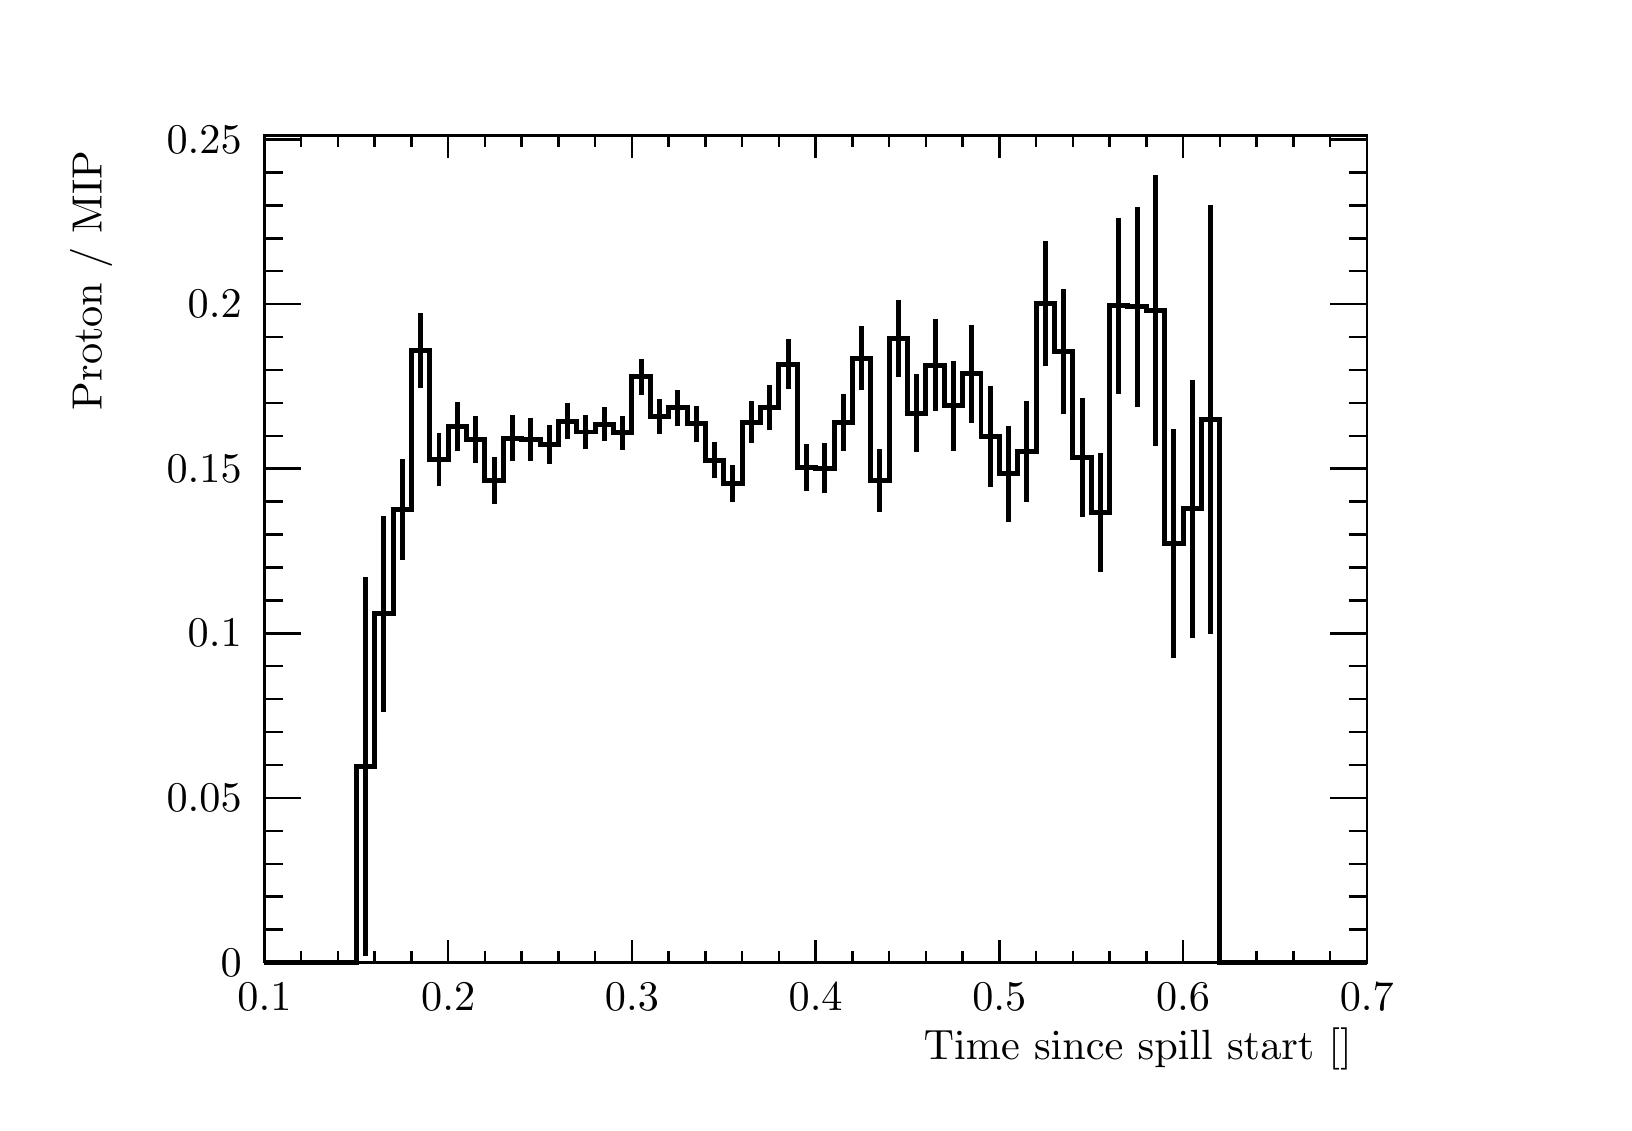
\begin{tikzpicture}
\pgfdeclareplotmark{cross} {
\pgfpathmoveto{\pgfpoint{-0.3\pgfplotmarksize}{\pgfplotmarksize}}
\pgfpathlineto{\pgfpoint{+0.3\pgfplotmarksize}{\pgfplotmarksize}}
\pgfpathlineto{\pgfpoint{+0.3\pgfplotmarksize}{0.3\pgfplotmarksize}}
\pgfpathlineto{\pgfpoint{+1\pgfplotmarksize}{0.3\pgfplotmarksize}}
\pgfpathlineto{\pgfpoint{+1\pgfplotmarksize}{-0.3\pgfplotmarksize}}
\pgfpathlineto{\pgfpoint{+0.3\pgfplotmarksize}{-0.3\pgfplotmarksize}}
\pgfpathlineto{\pgfpoint{+0.3\pgfplotmarksize}{-1.\pgfplotmarksize}}
\pgfpathlineto{\pgfpoint{-0.3\pgfplotmarksize}{-1.\pgfplotmarksize}}
\pgfpathlineto{\pgfpoint{-0.3\pgfplotmarksize}{-0.3\pgfplotmarksize}}
\pgfpathlineto{\pgfpoint{-1.\pgfplotmarksize}{-0.3\pgfplotmarksize}}
\pgfpathlineto{\pgfpoint{-1.\pgfplotmarksize}{0.3\pgfplotmarksize}}
\pgfpathlineto{\pgfpoint{-0.3\pgfplotmarksize}{0.3\pgfplotmarksize}}
\pgfpathclose
\pgfusepathqstroke
}
\pgfdeclareplotmark{cross*} {
\pgfpathmoveto{\pgfpoint{-0.3\pgfplotmarksize}{\pgfplotmarksize}}
\pgfpathlineto{\pgfpoint{+0.3\pgfplotmarksize}{\pgfplotmarksize}}
\pgfpathlineto{\pgfpoint{+0.3\pgfplotmarksize}{0.3\pgfplotmarksize}}
\pgfpathlineto{\pgfpoint{+1\pgfplotmarksize}{0.3\pgfplotmarksize}}
\pgfpathlineto{\pgfpoint{+1\pgfplotmarksize}{-0.3\pgfplotmarksize}}
\pgfpathlineto{\pgfpoint{+0.3\pgfplotmarksize}{-0.3\pgfplotmarksize}}
\pgfpathlineto{\pgfpoint{+0.3\pgfplotmarksize}{-1.\pgfplotmarksize}}
\pgfpathlineto{\pgfpoint{-0.3\pgfplotmarksize}{-1.\pgfplotmarksize}}
\pgfpathlineto{\pgfpoint{-0.3\pgfplotmarksize}{-0.3\pgfplotmarksize}}
\pgfpathlineto{\pgfpoint{-1.\pgfplotmarksize}{-0.3\pgfplotmarksize}}
\pgfpathlineto{\pgfpoint{-1.\pgfplotmarksize}{0.3\pgfplotmarksize}}
\pgfpathlineto{\pgfpoint{-0.3\pgfplotmarksize}{0.3\pgfplotmarksize}}
\pgfpathclose
\pgfusepathqfillstroke
}
\pgfdeclareplotmark{newstar} {
\pgfpathmoveto{\pgfqpoint{0pt}{\pgfplotmarksize}}
\pgfpathlineto{\pgfqpointpolar{44}{0.5\pgfplotmarksize}}
\pgfpathlineto{\pgfqpointpolar{18}{\pgfplotmarksize}}
\pgfpathlineto{\pgfqpointpolar{-20}{0.5\pgfplotmarksize}}
\pgfpathlineto{\pgfqpointpolar{-54}{\pgfplotmarksize}}
\pgfpathlineto{\pgfqpointpolar{-90}{0.5\pgfplotmarksize}}
\pgfpathlineto{\pgfqpointpolar{234}{\pgfplotmarksize}}
\pgfpathlineto{\pgfqpointpolar{198}{0.5\pgfplotmarksize}}
\pgfpathlineto{\pgfqpointpolar{162}{\pgfplotmarksize}}
\pgfpathlineto{\pgfqpointpolar{134}{0.5\pgfplotmarksize}}
\pgfpathclose
\pgfusepathqstroke
}
\pgfdeclareplotmark{newstar*} {
\pgfpathmoveto{\pgfqpoint{0pt}{\pgfplotmarksize}}
\pgfpathlineto{\pgfqpointpolar{44}{0.5\pgfplotmarksize}}
\pgfpathlineto{\pgfqpointpolar{18}{\pgfplotmarksize}}
\pgfpathlineto{\pgfqpointpolar{-20}{0.5\pgfplotmarksize}}
\pgfpathlineto{\pgfqpointpolar{-54}{\pgfplotmarksize}}
\pgfpathlineto{\pgfqpointpolar{-90}{0.5\pgfplotmarksize}}
\pgfpathlineto{\pgfqpointpolar{234}{\pgfplotmarksize}}
\pgfpathlineto{\pgfqpointpolar{198}{0.5\pgfplotmarksize}}
\pgfpathlineto{\pgfqpointpolar{162}{\pgfplotmarksize}}
\pgfpathlineto{\pgfqpointpolar{134}{0.5\pgfplotmarksize}}
\pgfpathclose
\pgfusepathqfillstroke
}
\definecolor{c}{rgb}{1,1,1};
\draw [color=c, fill=c] (0,0) rectangle (20,13.639);
\draw [color=c, fill=c] (3,1.77307) rectangle (17,12.2751);
\definecolor{c}{rgb}{0,0,0};
\draw [c,line width=0.9] (3,1.77307) -- (3,12.2751) -- (17,12.2751) -- (17,1.77307) -- (3,1.77307);
\definecolor{c}{rgb}{1,1,1};
\draw [color=c, fill=c] (3,1.77307) rectangle (17,12.2751);
\definecolor{c}{rgb}{0,0,0};
\draw [c,line width=0.9] (3,1.77307) -- (3,12.2751) -- (17,12.2751) -- (17,1.77307) -- (3,1.77307);
\draw [c,line width=1.8] (4.28333,1.85795) -- (4.28333,4.26597);
\draw [c,line width=1.8] (4.28333,4.26597) -- (4.28333,6.674);
\foreach \P in {(4.28333,4.26597)}{\draw[mark options={color=c,fill=c},mark size=2.402402pt,mark=*,mark size=1pt] plot coordinates {\P};}
\draw [c,line width=1.8] (4.51667,4.95882) -- (4.51667,6.20182);
\draw [c,line width=1.8] (4.51667,6.20182) -- (4.51667,7.44483);
\foreach \P in {(4.51667,6.20182)}{\draw[mark options={color=c,fill=c},mark size=2.402402pt,mark=*,mark size=1pt] plot coordinates {\P};}
\draw [c,line width=1.8] (4.75,6.88558) -- (4.75,7.52999);
\draw [c,line width=1.8] (4.75,7.52999) -- (4.75,8.17441);
\foreach \P in {(4.75,7.52999)}{\draw[mark options={color=c,fill=c},mark size=2.402402pt,mark=*,mark size=1pt] plot coordinates {\P};}
\draw [c,line width=1.8] (4.98333,9.06517) -- (4.98333,9.54667);
\draw [c,line width=1.8] (4.98333,9.54667) -- (4.98333,10.0282);
\foreach \P in {(4.98333,9.54667)}{\draw[mark options={color=c,fill=c},mark size=2.402402pt,mark=*,mark size=1pt] plot coordinates {\P};}
\draw [c,line width=1.8] (5.21667,7.82536) -- (5.21667,8.15941);
\draw [c,line width=1.8] (5.21667,8.15941) -- (5.21667,8.49346);
\foreach \P in {(5.21667,8.15941)}{\draw[mark options={color=c,fill=c},mark size=2.402402pt,mark=*,mark size=1pt] plot coordinates {\P};}
\draw [c,line width=1.8] (5.45,8.26867) -- (5.45,8.57816);
\draw [c,line width=1.8] (5.45,8.57816) -- (5.45,8.88765);
\foreach \P in {(5.45,8.57816)}{\draw[mark options={color=c,fill=c},mark size=2.402402pt,mark=*,mark size=1pt] plot coordinates {\P};}
\draw [c,line width=1.8] (5.68333,8.11213) -- (5.68333,8.41069);
\draw [c,line width=1.8] (5.68333,8.41069) -- (5.68333,8.70926);
\foreach \P in {(5.68333,8.41069)}{\draw[mark options={color=c,fill=c},mark size=2.402402pt,mark=*,mark size=1pt] plot coordinates {\P};}
\draw [c,line width=1.8] (5.91667,7.59665) -- (5.91667,7.89397);
\draw [c,line width=1.8] (5.91667,7.89397) -- (5.91667,8.19129);
\foreach \P in {(5.91667,7.89397)}{\draw[mark options={color=c,fill=c},mark size=2.402402pt,mark=*,mark size=1pt] plot coordinates {\P};}
\draw [c,line width=1.8] (6.15,8.14152) -- (6.15,8.43263);
\draw [c,line width=1.8] (6.15,8.43263) -- (6.15,8.72374);
\foreach \P in {(6.15,8.43263)}{\draw[mark options={color=c,fill=c},mark size=2.402402pt,mark=*,mark size=1pt] plot coordinates {\P};}
\draw [c,line width=1.8] (6.38333,8.14559) -- (6.38333,8.41426);
\draw [c,line width=1.8] (6.38333,8.41426) -- (6.38333,8.68294);
\foreach \P in {(6.38333,8.41426)}{\draw[mark options={color=c,fill=c},mark size=2.402402pt,mark=*,mark size=1pt] plot coordinates {\P};}
\draw [c,line width=1.8] (6.61667,8.09959) -- (6.61667,8.34791);
\draw [c,line width=1.8] (6.61667,8.34791) -- (6.61667,8.59622);
\foreach \P in {(6.61667,8.34791)}{\draw[mark options={color=c,fill=c},mark size=2.402402pt,mark=*,mark size=1pt] plot coordinates {\P};}
\draw [c,line width=1.8] (6.85,8.41637) -- (6.85,8.64916);
\draw [c,line width=1.8] (6.85,8.64916) -- (6.85,8.88195);
\foreach \P in {(6.85,8.64916)}{\draw[mark options={color=c,fill=c},mark size=2.402402pt,mark=*,mark size=1pt] plot coordinates {\P};}
\draw [c,line width=1.8] (7.08333,8.28923) -- (7.08333,8.51105);
\draw [c,line width=1.8] (7.08333,8.51105) -- (7.08333,8.73287);
\foreach \P in {(7.08333,8.51105)}{\draw[mark options={color=c,fill=c},mark size=2.402402pt,mark=*,mark size=1pt] plot coordinates {\P};}
\draw [c,line width=1.8] (7.31667,8.39124) -- (7.31667,8.60961);
\draw [c,line width=1.8] (7.31667,8.60961) -- (7.31667,8.82799);
\foreach \P in {(7.31667,8.60961)}{\draw[mark options={color=c,fill=c},mark size=2.402402pt,mark=*,mark size=1pt] plot coordinates {\P};}
\draw [c,line width=1.8] (7.55,8.28584) -- (7.55,8.49863);
\draw [c,line width=1.8] (7.55,8.49863) -- (7.55,8.71142);
\foreach \P in {(7.55,8.49863)}{\draw[mark options={color=c,fill=c},mark size=2.402402pt,mark=*,mark size=1pt] plot coordinates {\P};}
\draw [c,line width=1.8] (7.78333,8.98351) -- (7.78333,9.21265);
\draw [c,line width=1.8] (7.78333,9.21265) -- (7.78333,9.44178);
\foreach \P in {(7.78333,9.21265)}{\draw[mark options={color=c,fill=c},mark size=2.402402pt,mark=*,mark size=1pt] plot coordinates {\P};}
\draw [c,line width=1.8] (8.01667,8.47948) -- (8.01667,8.70265);
\draw [c,line width=1.8] (8.01667,8.70265) -- (8.01667,8.92583);
\foreach \P in {(8.01667,8.70265)}{\draw[mark options={color=c,fill=c},mark size=2.402402pt,mark=*,mark size=1pt] plot coordinates {\P};}
\draw [c,line width=1.8] (8.25,8.58929) -- (8.25,8.81786);
\draw [c,line width=1.8] (8.25,8.81786) -- (8.25,9.04643);
\foreach \P in {(8.25,8.81786)}{\draw[mark options={color=c,fill=c},mark size=2.402402pt,mark=*,mark size=1pt] plot coordinates {\P};}
\draw [c,line width=1.8] (8.48333,8.38024) -- (8.48333,8.61365);
\draw [c,line width=1.8] (8.48333,8.61365) -- (8.48333,8.84705);
\foreach \P in {(8.48333,8.61365)}{\draw[mark options={color=c,fill=c},mark size=2.402402pt,mark=*,mark size=1pt] plot coordinates {\P};}
\draw [c,line width=1.8] (8.71667,7.9206) -- (8.71667,8.15484);
\draw [c,line width=1.8] (8.71667,8.15484) -- (8.71667,8.38908);
\foreach \P in {(8.71667,8.15484)}{\draw[mark options={color=c,fill=c},mark size=2.402402pt,mark=*,mark size=1pt] plot coordinates {\P};}
\draw [c,line width=1.8] (8.95,7.62004) -- (8.95,7.85569);
\draw [c,line width=1.8] (8.95,7.85569) -- (8.95,8.09134);
\foreach \P in {(8.95,7.85569)}{\draw[mark options={color=c,fill=c},mark size=2.402402pt,mark=*,mark size=1pt] plot coordinates {\P};}
\draw [c,line width=1.8] (9.18333,8.36926) -- (9.18333,8.63709);
\draw [c,line width=1.8] (9.18333,8.63709) -- (9.18333,8.90492);
\foreach \P in {(9.18333,8.63709)}{\draw[mark options={color=c,fill=c},mark size=2.402402pt,mark=*,mark size=1pt] plot coordinates {\P};}
\draw [c,line width=1.8] (9.41667,8.53941) -- (9.41667,8.82537);
\draw [c,line width=1.8] (9.41667,8.82537) -- (9.41667,9.11132);
\foreach \P in {(9.41667,8.82537)}{\draw[mark options={color=c,fill=c},mark size=2.402402pt,mark=*,mark size=1pt] plot coordinates {\P};}
\draw [c,line width=1.8] (9.65,9.05386) -- (9.65,9.36986);
\draw [c,line width=1.8] (9.65,9.36986) -- (9.65,9.68587);
\foreach \P in {(9.65,9.36986)}{\draw[mark options={color=c,fill=c},mark size=2.402402pt,mark=*,mark size=1pt] plot coordinates {\P};}
\draw [c,line width=1.8] (9.88333,7.76146) -- (9.88333,8.06142);
\draw [c,line width=1.8] (9.88333,8.06142) -- (9.88333,8.36138);
\foreach \P in {(9.88333,8.06142)}{\draw[mark options={color=c,fill=c},mark size=2.402402pt,mark=*,mark size=1pt] plot coordinates {\P};}
\draw [c,line width=1.8] (10.1167,7.73575) -- (10.1167,8.05126);
\draw [c,line width=1.8] (10.1167,8.05126) -- (10.1167,8.36676);
\foreach \P in {(10.1167,8.05126)}{\draw[mark options={color=c,fill=c},mark size=2.402402pt,mark=*,mark size=1pt] plot coordinates {\P};}
\draw [c,line width=1.8] (10.35,8.2671) -- (10.35,8.63019);
\draw [c,line width=1.8] (10.35,8.63019) -- (10.35,8.99327);
\foreach \P in {(10.35,8.63019)}{\draw[mark options={color=c,fill=c},mark size=2.402402pt,mark=*,mark size=1pt] plot coordinates {\P};}
\draw [c,line width=1.8] (10.5833,9.04507) -- (10.5833,9.44879);
\draw [c,line width=1.8] (10.5833,9.44879) -- (10.5833,9.85251);
\foreach \P in {(10.5833,9.44879)}{\draw[mark options={color=c,fill=c},mark size=2.402402pt,mark=*,mark size=1pt] plot coordinates {\P};}
\draw [c,line width=1.8] (10.8167,7.50104) -- (10.8167,7.89536);
\draw [c,line width=1.8] (10.8167,7.89536) -- (10.8167,8.28967);
\foreach \P in {(10.8167,7.89536)}{\draw[mark options={color=c,fill=c},mark size=2.402402pt,mark=*,mark size=1pt] plot coordinates {\P};}
\draw [c,line width=1.8] (11.05,9.21278) -- (11.05,9.7027);
\draw [c,line width=1.8] (11.05,9.7027) -- (11.05,10.1926);
\foreach \P in {(11.05,9.7027)}{\draw[mark options={color=c,fill=c},mark size=2.402402pt,mark=*,mark size=1pt] plot coordinates {\P};}
\draw [c,line width=1.8] (11.2833,8.25238) -- (11.2833,8.74718);
\draw [c,line width=1.8] (11.2833,8.74718) -- (11.2833,9.24198);
\foreach \P in {(11.2833,8.74718)}{\draw[mark options={color=c,fill=c},mark size=2.402402pt,mark=*,mark size=1pt] plot coordinates {\P};}
\draw [c,line width=1.8] (11.5167,8.77527) -- (11.5167,9.35802);
\draw [c,line width=1.8] (11.5167,9.35802) -- (11.5167,9.94076);
\foreach \P in {(11.5167,9.35802)}{\draw[mark options={color=c,fill=c},mark size=2.402402pt,mark=*,mark size=1pt] plot coordinates {\P};}
\draw [c,line width=1.8] (11.75,8.27462) -- (11.75,8.84624);
\draw [c,line width=1.8] (11.75,8.84624) -- (11.75,9.41786);
\foreach \P in {(11.75,8.84624)}{\draw[mark options={color=c,fill=c},mark size=2.402402pt,mark=*,mark size=1pt] plot coordinates {\P};}
\draw [c,line width=1.8] (11.9833,8.63141) -- (11.9833,9.2513);
\draw [c,line width=1.8] (11.9833,9.2513) -- (11.9833,9.8712);
\foreach \P in {(11.9833,9.2513)}{\draw[mark options={color=c,fill=c},mark size=2.402402pt,mark=*,mark size=1pt] plot coordinates {\P};}
\draw [c,line width=1.8] (12.2167,7.81775) -- (12.2167,8.45422);
\draw [c,line width=1.8] (12.2167,8.45422) -- (12.2167,9.09069);
\foreach \P in {(12.2167,8.45422)}{\draw[mark options={color=c,fill=c},mark size=2.402402pt,mark=*,mark size=1pt] plot coordinates {\P};}
\draw [c,line width=1.8] (12.45,7.36943) -- (12.45,7.97822);
\draw [c,line width=1.8] (12.45,7.97822) -- (12.45,8.58701);
\foreach \P in {(12.45,7.97822)}{\draw[mark options={color=c,fill=c},mark size=2.402402pt,mark=*,mark size=1pt] plot coordinates {\P};}
\draw [c,line width=1.8] (12.6833,7.61971) -- (12.6833,8.26531);
\draw [c,line width=1.8] (12.6833,8.26531) -- (12.6833,8.91091);
\foreach \P in {(12.6833,8.26531)}{\draw[mark options={color=c,fill=c},mark size=2.402402pt,mark=*,mark size=1pt] plot coordinates {\P};}
\draw [c,line width=1.8] (12.9167,9.34774) -- (12.9167,10.144);
\draw [c,line width=1.8] (12.9167,10.144) -- (12.9167,10.9402);
\foreach \P in {(12.9167,10.144)}{\draw[mark options={color=c,fill=c},mark size=2.402402pt,mark=*,mark size=1pt] plot coordinates {\P};}
\draw [c,line width=1.8] (13.15,8.74157) -- (13.15,9.53696);
\draw [c,line width=1.8] (13.15,9.53696) -- (13.15,10.3324);
\foreach \P in {(13.15,9.53696)}{\draw[mark options={color=c,fill=c},mark size=2.402402pt,mark=*,mark size=1pt] plot coordinates {\P};}
\draw [c,line width=1.8] (13.3833,7.43321) -- (13.3833,8.1871);
\draw [c,line width=1.8] (13.3833,8.1871) -- (13.3833,8.941);
\foreach \P in {(13.3833,8.1871)}{\draw[mark options={color=c,fill=c},mark size=2.402402pt,mark=*,mark size=1pt] plot coordinates {\P};}
\draw [c,line width=1.8] (13.6167,6.72893) -- (13.6167,7.48532);
\draw [c,line width=1.8] (13.6167,7.48532) -- (13.6167,8.2417);
\foreach \P in {(13.6167,7.48532)}{\draw[mark options={color=c,fill=c},mark size=2.402402pt,mark=*,mark size=1pt] plot coordinates {\P};}
\draw [c,line width=1.8] (13.85,8.99665) -- (13.85,10.1133);
\draw [c,line width=1.8] (13.85,10.1133) -- (13.85,11.2299);
\foreach \P in {(13.85,10.1133)}{\draw[mark options={color=c,fill=c},mark size=2.402402pt,mark=*,mark size=1pt] plot coordinates {\P};}
\draw [c,line width=1.8] (14.0833,8.83049) -- (14.0833,10.1011);
\draw [c,line width=1.8] (14.0833,10.1011) -- (14.0833,11.3716);
\foreach \P in {(14.0833,10.1011)}{\draw[mark options={color=c,fill=c},mark size=2.402402pt,mark=*,mark size=1pt] plot coordinates {\P};}
\draw [c,line width=1.8] (14.3167,8.33544) -- (14.3167,10.0552);
\draw [c,line width=1.8] (14.3167,10.0552) -- (14.3167,11.775);
\foreach \P in {(14.3167,10.0552)}{\draw[mark options={color=c,fill=c},mark size=2.402402pt,mark=*,mark size=1pt] plot coordinates {\P};}
\draw [c,line width=1.8] (14.55,5.64668) -- (14.55,7.09824);
\draw [c,line width=1.8] (14.55,7.09824) -- (14.55,8.5498);
\foreach \P in {(14.55,7.09824)}{\draw[mark options={color=c,fill=c},mark size=2.402402pt,mark=*,mark size=1pt] plot coordinates {\P};}
\draw [c,line width=1.8] (14.7833,5.89349) -- (14.7833,7.53431);
\draw [c,line width=1.8] (14.7833,7.53431) -- (14.7833,9.17514);
\foreach \P in {(14.7833,7.53431)}{\draw[mark options={color=c,fill=c},mark size=2.402402pt,mark=*,mark size=1pt] plot coordinates {\P};}
\draw [c,line width=1.8] (15.0167,5.94687) -- (15.0167,8.6719);
\draw [c,line width=1.8] (15.0167,8.6719) -- (15.0167,11.3969);
\foreach \P in {(15.0167,8.6719)}{\draw[mark options={color=c,fill=c},mark size=2.402402pt,mark=*,mark size=1pt] plot coordinates {\P};}
\draw [c,line width=1.8] (3,1.77307) -- (3.23333,1.77307) -- (3.23333,1.77307) -- (3.46667,1.77307) -- (3.46667,1.77307) -- (3.7,1.77307) -- (3.7,1.77307) -- (3.93333,1.77307) -- (3.93333,1.77307) -- (4.16667,1.77307) -- (4.16667,4.26597) --
 (4.4,4.26597) -- (4.4,6.20182) -- (4.63333,6.20182) -- (4.63333,7.52999) -- (4.86667,7.52999) -- (4.86667,9.54667) -- (5.1,9.54667) -- (5.1,8.15941) -- (5.33333,8.15941) -- (5.33333,8.57816) -- (5.56667,8.57816) -- (5.56667,8.41069) -- (5.8,8.41069)
 -- (5.8,7.89397) -- (6.03333,7.89397) -- (6.03333,8.43263) -- (6.26667,8.43263) -- (6.26667,8.41426) -- (6.5,8.41426) -- (6.5,8.34791) -- (6.73333,8.34791) -- (6.73333,8.64916) -- (6.96667,8.64916) -- (6.96667,8.51105) -- (7.2,8.51105) --
 (7.2,8.60961) -- (7.43333,8.60961) -- (7.43333,8.49863) -- (7.66667,8.49863) -- (7.66667,9.21265) -- (7.9,9.21265) -- (7.9,8.70265) -- (8.13333,8.70265) -- (8.13333,8.81786) -- (8.36667,8.81786) -- (8.36667,8.61365) -- (8.6,8.61365) -- (8.6,8.15484)
 -- (8.83333,8.15484) -- (8.83333,7.85569) -- (9.06667,7.85569) -- (9.06667,8.63709) -- (9.3,8.63709) -- (9.3,8.82537) -- (9.53333,8.82537) -- (9.53333,9.36986) -- (9.76667,9.36986) -- (9.76667,8.06142) -- (10,8.06142) -- (10,8.05126) --
 (10.2333,8.05126) -- (10.2333,8.63019) -- (10.4667,8.63019) -- (10.4667,9.44879) -- (10.7,9.44879) -- (10.7,7.89536) -- (10.9333,7.89536) -- (10.9333,9.7027) -- (11.1667,9.7027) -- (11.1667,8.74718) -- (11.4,8.74718) -- (11.4,9.35802) --
 (11.6333,9.35802) -- (11.6333,8.84624) -- (11.8667,8.84624) -- (11.8667,9.2513) -- (12.1,9.2513) -- (12.1,8.45422) -- (12.3333,8.45422) -- (12.3333,7.97822) -- (12.5667,7.97822) -- (12.5667,8.26531) -- (12.8,8.26531) -- (12.8,10.144) --
 (13.0333,10.144) -- (13.0333,9.53696) -- (13.2667,9.53696) -- (13.2667,8.1871) -- (13.5,8.1871) -- (13.5,7.48532) -- (13.7333,7.48532) -- (13.7333,10.1133) -- (13.9667,10.1133) -- (13.9667,10.1011) -- (14.2,10.1011) -- (14.2,10.0552) --
 (14.4333,10.0552) -- (14.4333,7.09824) -- (14.6667,7.09824) -- (14.6667,7.53431) -- (14.9,7.53431) -- (14.9,8.6719) -- (15.1333,8.6719) -- (15.1333,1.77307) -- (15.3667,1.77307) -- (15.3667,1.77307) -- (15.6,1.77307) -- (15.6,1.77307) --
 (15.8333,1.77307) -- (15.8333,1.77307) -- (16.0667,1.77307) -- (16.0667,1.77307) -- (16.3,1.77307) -- (16.3,1.77307) -- (16.5333,1.77307) -- (16.5333,1.77307) -- (16.7667,1.77307) -- (16.7667,1.77307) -- (17,1.77307);
\draw [c,line width=0.9] (3,1.77307) -- (17,1.77307);
\draw [c,line width=0.9] (3,2.05948) -- (3,1.77307);
\draw [c,line width=0.9] (3.46667,1.91628) -- (3.46667,1.77307);
\draw [c,line width=0.9] (3.93333,1.91628) -- (3.93333,1.77307);
\draw [c,line width=0.9] (4.4,1.91628) -- (4.4,1.77307);
\draw [c,line width=0.9] (4.86667,1.91628) -- (4.86667,1.77307);
\draw [c,line width=0.9] (5.33333,2.05948) -- (5.33333,1.77307);
\draw [c,line width=0.9] (5.8,1.91628) -- (5.8,1.77307);
\draw [c,line width=0.9] (6.26667,1.91628) -- (6.26667,1.77307);
\draw [c,line width=0.9] (6.73333,1.91628) -- (6.73333,1.77307);
\draw [c,line width=0.9] (7.2,1.91628) -- (7.2,1.77307);
\draw [c,line width=0.9] (7.66667,2.05948) -- (7.66667,1.77307);
\draw [c,line width=0.9] (8.13333,1.91628) -- (8.13333,1.77307);
\draw [c,line width=0.9] (8.6,1.91628) -- (8.6,1.77307);
\draw [c,line width=0.9] (9.06667,1.91628) -- (9.06667,1.77307);
\draw [c,line width=0.9] (9.53333,1.91628) -- (9.53333,1.77307);
\draw [c,line width=0.9] (10,2.05948) -- (10,1.77307);
\draw [c,line width=0.9] (10.4667,1.91628) -- (10.4667,1.77307);
\draw [c,line width=0.9] (10.9333,1.91628) -- (10.9333,1.77307);
\draw [c,line width=0.9] (11.4,1.91628) -- (11.4,1.77307);
\draw [c,line width=0.9] (11.8667,1.91628) -- (11.8667,1.77307);
\draw [c,line width=0.9] (12.3333,2.05948) -- (12.3333,1.77307);
\draw [c,line width=0.9] (12.8,1.91628) -- (12.8,1.77307);
\draw [c,line width=0.9] (13.2667,1.91628) -- (13.2667,1.77307);
\draw [c,line width=0.9] (13.7333,1.91628) -- (13.7333,1.77307);
\draw [c,line width=0.9] (14.2,1.91628) -- (14.2,1.77307);
\draw [c,line width=0.9] (14.6667,2.05948) -- (14.6667,1.77307);
\draw [c,line width=0.9] (15.1333,1.91628) -- (15.1333,1.77307);
\draw [c,line width=0.9] (15.6,1.91628) -- (15.6,1.77307);
\draw [c,line width=0.9] (16.0667,1.91628) -- (16.0667,1.77307);
\draw [c,line width=0.9] (16.5333,1.91628) -- (16.5333,1.77307);
\draw [c,line width=0.9] (17,2.05948) -- (17,1.77307);
\draw [c,line width=0.9] (17,2.05948) -- (17,1.77307);
\draw [anchor=base] (3,1.15931) node[scale=1.52731, color=c, rotate=0]{0.1};
\draw [anchor=base] (5.33333,1.15931) node[scale=1.52731, color=c, rotate=0]{0.2};
\draw [anchor=base] (7.66667,1.15931) node[scale=1.52731, color=c, rotate=0]{0.3};
\draw [anchor=base] (10,1.15931) node[scale=1.52731, color=c, rotate=0]{0.4};
\draw [anchor=base] (12.3333,1.15931) node[scale=1.52731, color=c, rotate=0]{0.5};
\draw [anchor=base] (14.6667,1.15931) node[scale=1.52731, color=c, rotate=0]{0.6};
\draw [anchor=base] (17,1.15931) node[scale=1.52731, color=c, rotate=0]{0.7};
\draw [anchor= east] (17,0.681948) node[scale=1.52731, color=c, rotate=0]{ Time since spill start [\si{\nano\second}]};
\draw [c,line width=0.9] (3,12.2751) -- (17,12.2751);
\draw [c,line width=0.9] (3,11.9887) -- (3,12.2751);
\draw [c,line width=0.9] (3.46667,12.1319) -- (3.46667,12.2751);
\draw [c,line width=0.9] (3.93333,12.1319) -- (3.93333,12.2751);
\draw [c,line width=0.9] (4.4,12.1319) -- (4.4,12.2751);
\draw [c,line width=0.9] (4.86667,12.1319) -- (4.86667,12.2751);
\draw [c,line width=0.9] (5.33333,11.9887) -- (5.33333,12.2751);
\draw [c,line width=0.9] (5.8,12.1319) -- (5.8,12.2751);
\draw [c,line width=0.9] (6.26667,12.1319) -- (6.26667,12.2751);
\draw [c,line width=0.9] (6.73333,12.1319) -- (6.73333,12.2751);
\draw [c,line width=0.9] (7.2,12.1319) -- (7.2,12.2751);
\draw [c,line width=0.9] (7.66667,11.9887) -- (7.66667,12.2751);
\draw [c,line width=0.9] (8.13333,12.1319) -- (8.13333,12.2751);
\draw [c,line width=0.9] (8.6,12.1319) -- (8.6,12.2751);
\draw [c,line width=0.9] (9.06667,12.1319) -- (9.06667,12.2751);
\draw [c,line width=0.9] (9.53333,12.1319) -- (9.53333,12.2751);
\draw [c,line width=0.9] (10,11.9887) -- (10,12.2751);
\draw [c,line width=0.9] (10.4667,12.1319) -- (10.4667,12.2751);
\draw [c,line width=0.9] (10.9333,12.1319) -- (10.9333,12.2751);
\draw [c,line width=0.9] (11.4,12.1319) -- (11.4,12.2751);
\draw [c,line width=0.9] (11.8667,12.1319) -- (11.8667,12.2751);
\draw [c,line width=0.9] (12.3333,11.9887) -- (12.3333,12.2751);
\draw [c,line width=0.9] (12.8,12.1319) -- (12.8,12.2751);
\draw [c,line width=0.9] (13.2667,12.1319) -- (13.2667,12.2751);
\draw [c,line width=0.9] (13.7333,12.1319) -- (13.7333,12.2751);
\draw [c,line width=0.9] (14.2,12.1319) -- (14.2,12.2751);
\draw [c,line width=0.9] (14.6667,11.9887) -- (14.6667,12.2751);
\draw [c,line width=0.9] (15.1333,12.1319) -- (15.1333,12.2751);
\draw [c,line width=0.9] (15.6,12.1319) -- (15.6,12.2751);
\draw [c,line width=0.9] (16.0667,12.1319) -- (16.0667,12.2751);
\draw [c,line width=0.9] (16.5333,12.1319) -- (16.5333,12.2751);
\draw [c,line width=0.9] (17,11.9887) -- (17,12.2751);
\draw [c,line width=0.9] (17,11.9887) -- (17,12.2751);
\draw [c,line width=0.9] (3,1.77307) -- (3,12.2751);
\draw [c,line width=0.9] (3.462,1.77307) -- (3,1.77307);
\draw [c,line width=0.9] (3.231,2.19118) -- (3,2.19118);
\draw [c,line width=0.9] (3.231,2.60929) -- (3,2.60929);
\draw [c,line width=0.9] (3.231,3.0274) -- (3,3.0274);
\draw [c,line width=0.9] (3.231,3.44551) -- (3,3.44551);
\draw [c,line width=0.9] (3.462,3.86362) -- (3,3.86362);
\draw [c,line width=0.9] (3.231,4.28173) -- (3,4.28173);
\draw [c,line width=0.9] (3.231,4.69984) -- (3,4.69984);
\draw [c,line width=0.9] (3.231,5.11795) -- (3,5.11795);
\draw [c,line width=0.9] (3.231,5.53606) -- (3,5.53606);
\draw [c,line width=0.9] (3.462,5.95417) -- (3,5.95417);
\draw [c,line width=0.9] (3.231,6.37228) -- (3,6.37228);
\draw [c,line width=0.9] (3.231,6.79039) -- (3,6.79039);
\draw [c,line width=0.9] (3.231,7.2085) -- (3,7.2085);
\draw [c,line width=0.9] (3.231,7.62661) -- (3,7.62661);
\draw [c,line width=0.9] (3.462,8.04472) -- (3,8.04472);
\draw [c,line width=0.9] (3.231,8.46283) -- (3,8.46283);
\draw [c,line width=0.9] (3.231,8.88094) -- (3,8.88094);
\draw [c,line width=0.9] (3.231,9.29905) -- (3,9.29905);
\draw [c,line width=0.9] (3.231,9.71716) -- (3,9.71716);
\draw [c,line width=0.9] (3.462,10.1353) -- (3,10.1353);
\draw [c,line width=0.9] (3.231,10.5534) -- (3,10.5534);
\draw [c,line width=0.9] (3.231,10.9715) -- (3,10.9715);
\draw [c,line width=0.9] (3.231,11.3896) -- (3,11.3896);
\draw [c,line width=0.9] (3.231,11.8077) -- (3,11.8077);
\draw [c,line width=0.9] (3.462,12.2258) -- (3,12.2258);
\draw [c,line width=0.9] (3.462,12.2258) -- (3,12.2258);
\draw [anchor= east] (2.9,1.77307) node[scale=1.52731, color=c, rotate=0]{0};
\draw [anchor= east] (2.9,3.86362) node[scale=1.52731, color=c, rotate=0]{0.05};
\draw [anchor= east] (2.9,5.95417) node[scale=1.52731, color=c, rotate=0]{0.1};
\draw [anchor= east] (2.9,8.04472) node[scale=1.52731, color=c, rotate=0]{0.15};
\draw [anchor= east] (2.9,10.1353) node[scale=1.52731, color=c, rotate=0]{0.2};
\draw [anchor= east] (2.9,12.2258) node[scale=1.52731, color=c, rotate=0]{0.25};
\draw [anchor= east] (0.796562,12.2751) node[scale=1.52731, color=c, rotate=90]{ Proton / MIP};
\draw [c,line width=0.9] (17,1.77307) -- (17,12.2751);
\draw [c,line width=0.9] (16.538,1.77307) -- (17,1.77307);
\draw [c,line width=0.9] (16.769,2.19118) -- (17,2.19118);
\draw [c,line width=0.9] (16.769,2.60929) -- (17,2.60929);
\draw [c,line width=0.9] (16.769,3.0274) -- (17,3.0274);
\draw [c,line width=0.9] (16.769,3.44551) -- (17,3.44551);
\draw [c,line width=0.9] (16.538,3.86362) -- (17,3.86362);
\draw [c,line width=0.9] (16.769,4.28173) -- (17,4.28173);
\draw [c,line width=0.9] (16.769,4.69984) -- (17,4.69984);
\draw [c,line width=0.9] (16.769,5.11795) -- (17,5.11795);
\draw [c,line width=0.9] (16.769,5.53606) -- (17,5.53606);
\draw [c,line width=0.9] (16.538,5.95417) -- (17,5.95417);
\draw [c,line width=0.9] (16.769,6.37228) -- (17,6.37228);
\draw [c,line width=0.9] (16.769,6.79039) -- (17,6.79039);
\draw [c,line width=0.9] (16.769,7.2085) -- (17,7.2085);
\draw [c,line width=0.9] (16.769,7.62661) -- (17,7.62661);
\draw [c,line width=0.9] (16.538,8.04472) -- (17,8.04472);
\draw [c,line width=0.9] (16.769,8.46283) -- (17,8.46283);
\draw [c,line width=0.9] (16.769,8.88094) -- (17,8.88094);
\draw [c,line width=0.9] (16.769,9.29905) -- (17,9.29905);
\draw [c,line width=0.9] (16.769,9.71716) -- (17,9.71716);
\draw [c,line width=0.9] (16.538,10.1353) -- (17,10.1353);
\draw [c,line width=0.9] (16.769,10.5534) -- (17,10.5534);
\draw [c,line width=0.9] (16.769,10.9715) -- (17,10.9715);
\draw [c,line width=0.9] (16.769,11.3896) -- (17,11.3896);
\draw [c,line width=0.9] (16.769,11.8077) -- (17,11.8077);
\draw [c,line width=0.9] (16.538,12.2258) -- (17,12.2258);
\draw [c,line width=0.9] (16.538,12.2258) -- (17,12.2258);
\definecolor{c}{rgb}{1,1,1};
\draw [color=c, fill=c] (2,12.8206) rectangle (18,13.5708);
\definecolor{c}{rgb}{0,0,0};
%\draw (10,13.1957) node[scale=1.40004, color=c, rotate=0]{2 blocks: Proton/MIP};
\end{tikzpicture}

  \end{adjustbox}
  \caption[Proton/MIP ratio as a function of time since spill start]{Proton/MIP ratio as a function of time since spill start for 2 moderator block data.}
  \label{fig:proMipRatio}
\end{figure}

The relationship between the number of $\SOne-\STwo$ hits in the two DAQs for various numbers of moderator blocks is shown in \citefig{fig:s1s2DeadtimeComp}.
Here the horizontal axis displays the number of $\SOne-\STwo$ signals recorded by the DToF DAQ for a given beam spill, $(\SOne\STwo)_{\text{DToF}}$.
Similarly, $(\SOne\STwo)_{\text{UToF}}$ is the number of $\SOne-\STwo$ signals recorded by the UToF DAQ in the same spill.
Each of these distributions has a polynomial of the form
\begin{equation}
  (\SOne\STwo)_{\text{UToF}}/(\SOne\STwo)_{\text{DToF}} = p0 \times (\SOne\STwo)_{\text{DToF}} + p1
\end{equation}
fitted where $p0$ and $p1$ are the parameters to be determined.

\begin{figure}[t]
  \begin{subfigure}[t]{.5\textwidth}
    \begin{adjustbox}{max totalsize=\textwidth, center}
      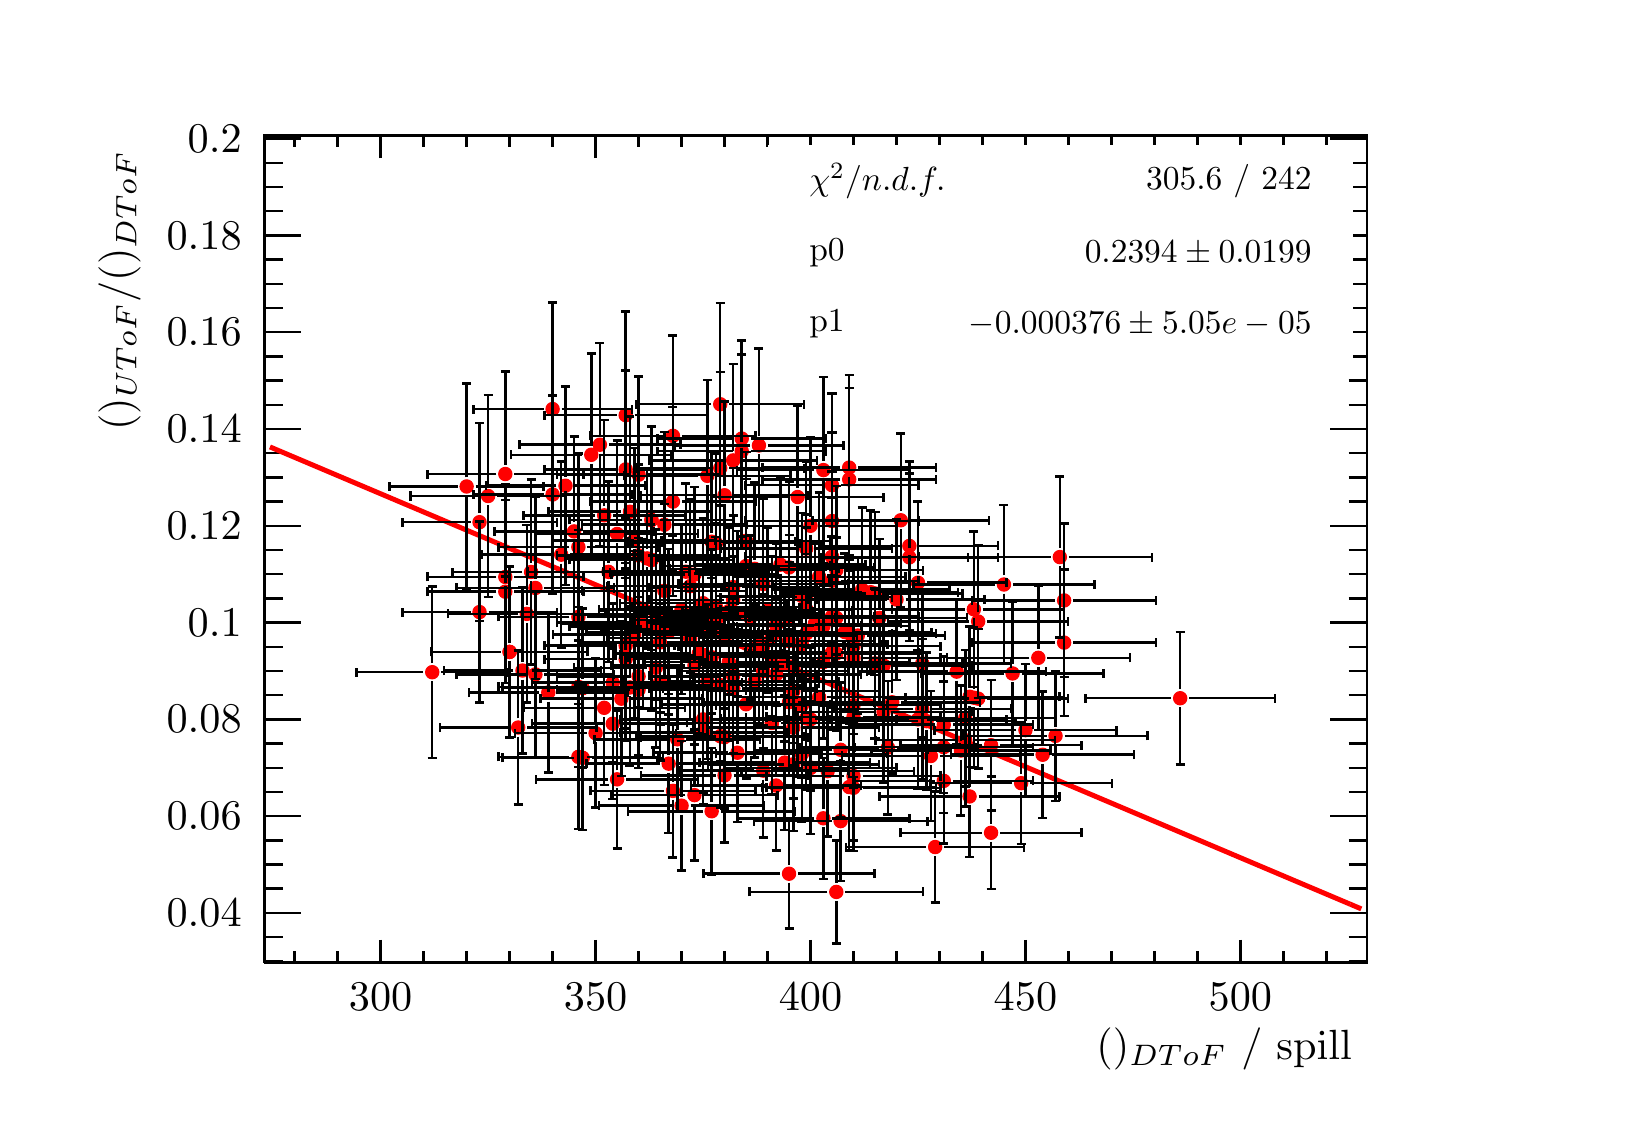
\begin{tikzpicture}
\pgfdeclareplotmark{cross} {
\pgfpathmoveto{\pgfpoint{-0.3\pgfplotmarksize}{\pgfplotmarksize}}
\pgfpathlineto{\pgfpoint{+0.3\pgfplotmarksize}{\pgfplotmarksize}}
\pgfpathlineto{\pgfpoint{+0.3\pgfplotmarksize}{0.3\pgfplotmarksize}}
\pgfpathlineto{\pgfpoint{+1\pgfplotmarksize}{0.3\pgfplotmarksize}}
\pgfpathlineto{\pgfpoint{+1\pgfplotmarksize}{-0.3\pgfplotmarksize}}
\pgfpathlineto{\pgfpoint{+0.3\pgfplotmarksize}{-0.3\pgfplotmarksize}}
\pgfpathlineto{\pgfpoint{+0.3\pgfplotmarksize}{-1.\pgfplotmarksize}}
\pgfpathlineto{\pgfpoint{-0.3\pgfplotmarksize}{-1.\pgfplotmarksize}}
\pgfpathlineto{\pgfpoint{-0.3\pgfplotmarksize}{-0.3\pgfplotmarksize}}
\pgfpathlineto{\pgfpoint{-1.\pgfplotmarksize}{-0.3\pgfplotmarksize}}
\pgfpathlineto{\pgfpoint{-1.\pgfplotmarksize}{0.3\pgfplotmarksize}}
\pgfpathlineto{\pgfpoint{-0.3\pgfplotmarksize}{0.3\pgfplotmarksize}}
\pgfpathclose
\pgfusepathqstroke
}
\pgfdeclareplotmark{cross*} {
\pgfpathmoveto{\pgfpoint{-0.3\pgfplotmarksize}{\pgfplotmarksize}}
\pgfpathlineto{\pgfpoint{+0.3\pgfplotmarksize}{\pgfplotmarksize}}
\pgfpathlineto{\pgfpoint{+0.3\pgfplotmarksize}{0.3\pgfplotmarksize}}
\pgfpathlineto{\pgfpoint{+1\pgfplotmarksize}{0.3\pgfplotmarksize}}
\pgfpathlineto{\pgfpoint{+1\pgfplotmarksize}{-0.3\pgfplotmarksize}}
\pgfpathlineto{\pgfpoint{+0.3\pgfplotmarksize}{-0.3\pgfplotmarksize}}
\pgfpathlineto{\pgfpoint{+0.3\pgfplotmarksize}{-1.\pgfplotmarksize}}
\pgfpathlineto{\pgfpoint{-0.3\pgfplotmarksize}{-1.\pgfplotmarksize}}
\pgfpathlineto{\pgfpoint{-0.3\pgfplotmarksize}{-0.3\pgfplotmarksize}}
\pgfpathlineto{\pgfpoint{-1.\pgfplotmarksize}{-0.3\pgfplotmarksize}}
\pgfpathlineto{\pgfpoint{-1.\pgfplotmarksize}{0.3\pgfplotmarksize}}
\pgfpathlineto{\pgfpoint{-0.3\pgfplotmarksize}{0.3\pgfplotmarksize}}
\pgfpathclose
\pgfusepathqfillstroke
}
\pgfdeclareplotmark{newstar} {
\pgfpathmoveto{\pgfqpoint{0pt}{\pgfplotmarksize}}
\pgfpathlineto{\pgfqpointpolar{44}{0.5\pgfplotmarksize}}
\pgfpathlineto{\pgfqpointpolar{18}{\pgfplotmarksize}}
\pgfpathlineto{\pgfqpointpolar{-20}{0.5\pgfplotmarksize}}
\pgfpathlineto{\pgfqpointpolar{-54}{\pgfplotmarksize}}
\pgfpathlineto{\pgfqpointpolar{-90}{0.5\pgfplotmarksize}}
\pgfpathlineto{\pgfqpointpolar{234}{\pgfplotmarksize}}
\pgfpathlineto{\pgfqpointpolar{198}{0.5\pgfplotmarksize}}
\pgfpathlineto{\pgfqpointpolar{162}{\pgfplotmarksize}}
\pgfpathlineto{\pgfqpointpolar{134}{0.5\pgfplotmarksize}}
\pgfpathclose
\pgfusepathqstroke
}
\pgfdeclareplotmark{newstar*} {
\pgfpathmoveto{\pgfqpoint{0pt}{\pgfplotmarksize}}
\pgfpathlineto{\pgfqpointpolar{44}{0.5\pgfplotmarksize}}
\pgfpathlineto{\pgfqpointpolar{18}{\pgfplotmarksize}}
\pgfpathlineto{\pgfqpointpolar{-20}{0.5\pgfplotmarksize}}
\pgfpathlineto{\pgfqpointpolar{-54}{\pgfplotmarksize}}
\pgfpathlineto{\pgfqpointpolar{-90}{0.5\pgfplotmarksize}}
\pgfpathlineto{\pgfqpointpolar{234}{\pgfplotmarksize}}
\pgfpathlineto{\pgfqpointpolar{198}{0.5\pgfplotmarksize}}
\pgfpathlineto{\pgfqpointpolar{162}{\pgfplotmarksize}}
\pgfpathlineto{\pgfqpointpolar{134}{0.5\pgfplotmarksize}}
\pgfpathclose
\pgfusepathqfillstroke
}
\definecolor{c}{rgb}{1,1,1};
\draw [color=c, fill=c] (0,0) rectangle (20,13.639);
\draw [color=c, fill=c] (3,1.77307) rectangle (17,12.2751);
\definecolor{c}{rgb}{0,0,0};
\draw [c,line width=0.9] (3,1.77307) -- (3,12.2751) -- (17,12.2751) -- (17,1.77307) -- (3,1.77307);
\definecolor{c}{rgb}{1,1,1};
\draw [color=c, fill=c] (3,1.77307) rectangle (17,12.2751);
\definecolor{c}{rgb}{0,0,0};
\draw [c,line width=0.9] (3,1.77307) -- (3,12.2751) -- (17,12.2751) -- (17,1.77307) -- (3,1.77307);
\draw [c,line width=0.9] (3,1.77307) -- (17,1.77307);
\draw [c,line width=0.9] (4.47585,2.05948) -- (4.47585,1.77307);
\draw [c,line width=0.9] (5.02176,1.91628) -- (5.02176,1.77307);
\draw [c,line width=0.9] (5.56767,1.91628) -- (5.56767,1.77307);
\draw [c,line width=0.9] (6.11359,1.91628) -- (6.11359,1.77307);
\draw [c,line width=0.9] (6.6595,1.91628) -- (6.6595,1.77307);
\draw [c,line width=0.9] (7.20542,2.05948) -- (7.20542,1.77307);
\draw [c,line width=0.9] (7.75133,1.91628) -- (7.75133,1.77307);
\draw [c,line width=0.9] (8.29724,1.91628) -- (8.29724,1.77307);
\draw [c,line width=0.9] (8.84316,1.91628) -- (8.84316,1.77307);
\draw [c,line width=0.9] (9.38907,1.91628) -- (9.38907,1.77307);
\draw [c,line width=0.9] (9.93499,2.05948) -- (9.93499,1.77307);
\draw [c,line width=0.9] (10.4809,1.91628) -- (10.4809,1.77307);
\draw [c,line width=0.9] (11.0268,1.91628) -- (11.0268,1.77307);
\draw [c,line width=0.9] (11.5727,1.91628) -- (11.5727,1.77307);
\draw [c,line width=0.9] (12.1186,1.91628) -- (12.1186,1.77307);
\draw [c,line width=0.9] (12.6646,2.05948) -- (12.6646,1.77307);
\draw [c,line width=0.9] (13.2105,1.91628) -- (13.2105,1.77307);
\draw [c,line width=0.9] (13.7564,1.91628) -- (13.7564,1.77307);
\draw [c,line width=0.9] (14.3023,1.91628) -- (14.3023,1.77307);
\draw [c,line width=0.9] (14.8482,1.91628) -- (14.8482,1.77307);
\draw [c,line width=0.9] (15.3941,2.05948) -- (15.3941,1.77307);
\draw [c,line width=0.9] (4.47585,2.05948) -- (4.47585,1.77307);
\draw [c,line width=0.9] (3.92993,1.91628) -- (3.92993,1.77307);
\draw [c,line width=0.9] (3.38402,1.91628) -- (3.38402,1.77307);
\draw [c,line width=0.9] (15.3941,2.05948) -- (15.3941,1.77307);
\draw [c,line width=0.9] (15.94,1.91628) -- (15.94,1.77307);
\draw [c,line width=0.9] (16.486,1.91628) -- (16.486,1.77307);
\draw [anchor=base] (4.47585,1.15931) node[scale=1.52731, color=c, rotate=0]{300};
\draw [anchor=base] (7.20542,1.15931) node[scale=1.52731, color=c, rotate=0]{350};
\draw [anchor=base] (9.93499,1.15931) node[scale=1.52731, color=c, rotate=0]{400};
\draw [anchor=base] (12.6646,1.15931) node[scale=1.52731, color=c, rotate=0]{450};
\draw [anchor=base] (15.3941,1.15931) node[scale=1.52731, color=c, rotate=0]{500};
\draw [anchor= east] (17,0.681948) node[scale=1.52731, color=c, rotate=0]{$(\SOne\STwo)_{\text{DToF}}$ / spill};
\draw [c,line width=0.9] (3,12.2751) -- (17,12.2751);
\draw [c,line width=0.9] (4.47585,11.9887) -- (4.47585,12.2751);
\draw [c,line width=0.9] (5.02176,12.1319) -- (5.02176,12.2751);
\draw [c,line width=0.9] (5.56767,12.1319) -- (5.56767,12.2751);
\draw [c,line width=0.9] (6.11359,12.1319) -- (6.11359,12.2751);
\draw [c,line width=0.9] (6.6595,12.1319) -- (6.6595,12.2751);
\draw [c,line width=0.9] (7.20542,11.9887) -- (7.20542,12.2751);
\draw [c,line width=0.9] (7.75133,12.1319) -- (7.75133,12.2751);
\draw [c,line width=0.9] (8.29724,12.1319) -- (8.29724,12.2751);
\draw [c,line width=0.9] (8.84316,12.1319) -- (8.84316,12.2751);
\draw [c,line width=0.9] (9.38907,12.1319) -- (9.38907,12.2751);
\draw [c,line width=0.9] (9.93499,11.9887) -- (9.93499,12.2751);
\draw [c,line width=0.9] (10.4809,12.1319) -- (10.4809,12.2751);
\draw [c,line width=0.9] (11.0268,12.1319) -- (11.0268,12.2751);
\draw [c,line width=0.9] (11.5727,12.1319) -- (11.5727,12.2751);
\draw [c,line width=0.9] (12.1186,12.1319) -- (12.1186,12.2751);
\draw [c,line width=0.9] (12.6646,11.9887) -- (12.6646,12.2751);
\draw [c,line width=0.9] (13.2105,12.1319) -- (13.2105,12.2751);
\draw [c,line width=0.9] (13.7564,12.1319) -- (13.7564,12.2751);
\draw [c,line width=0.9] (14.3023,12.1319) -- (14.3023,12.2751);
\draw [c,line width=0.9] (14.8482,12.1319) -- (14.8482,12.2751);
\draw [c,line width=0.9] (15.3941,11.9887) -- (15.3941,12.2751);
\draw [c,line width=0.9] (4.47585,11.9887) -- (4.47585,12.2751);
\draw [c,line width=0.9] (3.92993,12.1319) -- (3.92993,12.2751);
\draw [c,line width=0.9] (3.38402,12.1319) -- (3.38402,12.2751);
\draw [c,line width=0.9] (15.3941,11.9887) -- (15.3941,12.2751);
\draw [c,line width=0.9] (15.94,12.1319) -- (15.94,12.2751);
\draw [c,line width=0.9] (16.486,12.1319) -- (16.486,12.2751);
\draw [c,line width=0.9] (3,1.77307) -- (3,12.2751);
\draw [c,line width=0.9] (3.462,2.40333) -- (3,2.40333);
\draw [c,line width=0.9] (3.231,2.71062) -- (3,2.71062);
\draw [c,line width=0.9] (3.231,3.0179) -- (3,3.0179);
\draw [c,line width=0.9] (3.231,3.32518) -- (3,3.32518);
\draw [c,line width=0.9] (3.462,3.63247) -- (3,3.63247);
\draw [c,line width=0.9] (3.231,3.93975) -- (3,3.93975);
\draw [c,line width=0.9] (3.231,4.24704) -- (3,4.24704);
\draw [c,line width=0.9] (3.231,4.55432) -- (3,4.55432);
\draw [c,line width=0.9] (3.462,4.8616) -- (3,4.8616);
\draw [c,line width=0.9] (3.231,5.16889) -- (3,5.16889);
\draw [c,line width=0.9] (3.231,5.47617) -- (3,5.47617);
\draw [c,line width=0.9] (3.231,5.78345) -- (3,5.78345);
\draw [c,line width=0.9] (3.462,6.09074) -- (3,6.09074);
\draw [c,line width=0.9] (3.231,6.39802) -- (3,6.39802);
\draw [c,line width=0.9] (3.231,6.7053) -- (3,6.7053);
\draw [c,line width=0.9] (3.231,7.01259) -- (3,7.01259);
\draw [c,line width=0.9] (3.462,7.31987) -- (3,7.31987);
\draw [c,line width=0.9] (3.231,7.62715) -- (3,7.62715);
\draw [c,line width=0.9] (3.231,7.93444) -- (3,7.93444);
\draw [c,line width=0.9] (3.231,8.24172) -- (3,8.24172);
\draw [c,line width=0.9] (3.462,8.549) -- (3,8.549);
\draw [c,line width=0.9] (3.231,8.85629) -- (3,8.85629);
\draw [c,line width=0.9] (3.231,9.16357) -- (3,9.16357);
\draw [c,line width=0.9] (3.231,9.47085) -- (3,9.47085);
\draw [c,line width=0.9] (3.462,9.77814) -- (3,9.77814);
\draw [c,line width=0.9] (3.231,10.0854) -- (3,10.0854);
\draw [c,line width=0.9] (3.231,10.3927) -- (3,10.3927);
\draw [c,line width=0.9] (3.231,10.7) -- (3,10.7);
\draw [c,line width=0.9] (3.462,11.0073) -- (3,11.0073);
\draw [c,line width=0.9] (3.231,11.3146) -- (3,11.3146);
\draw [c,line width=0.9] (3.231,11.6218) -- (3,11.6218);
\draw [c,line width=0.9] (3.231,11.9291) -- (3,11.9291);
\draw [c,line width=0.9] (3.462,12.2364) -- (3,12.2364);
\draw [c,line width=0.9] (3.462,2.40333) -- (3,2.40333);
\draw [c,line width=0.9] (3.231,2.09605) -- (3,2.09605);
\draw [c,line width=0.9] (3.231,1.78877) -- (3,1.78877);
\draw [c,line width=0.9] (3.462,12.2364) -- (3,12.2364);
\draw [anchor= east] (2.9,2.40333) node[scale=1.52731, color=c, rotate=0]{0.04};
\draw [anchor= east] (2.9,3.63247) node[scale=1.52731, color=c, rotate=0]{0.06};
\draw [anchor= east] (2.9,4.8616) node[scale=1.52731, color=c, rotate=0]{0.08};
\draw [anchor= east] (2.9,6.09074) node[scale=1.52731, color=c, rotate=0]{0.1};
\draw [anchor= east] (2.9,7.31987) node[scale=1.52731, color=c, rotate=0]{0.12};
\draw [anchor= east] (2.9,8.549) node[scale=1.52731, color=c, rotate=0]{0.14};
\draw [anchor= east] (2.9,9.77814) node[scale=1.52731, color=c, rotate=0]{0.16};
\draw [anchor= east] (2.9,11.0073) node[scale=1.52731, color=c, rotate=0]{0.18};
\draw [anchor= east] (2.9,12.2364) node[scale=1.52731, color=c, rotate=0]{0.2};
\draw [anchor= east] (1.16,12.2751) node[scale=1.52731, color=c, rotate=90]{ $(\SOne\STwo)_{\text{UToF}}/(\SOne\STwo)_{\text{DToF}}$ };
\draw [c,line width=0.9] (17,1.77307) -- (17,12.2751);
\draw [c,line width=0.9] (16.538,2.40333) -- (17,2.40333);
\draw [c,line width=0.9] (16.769,2.71062) -- (17,2.71062);
\draw [c,line width=0.9] (16.769,3.0179) -- (17,3.0179);
\draw [c,line width=0.9] (16.769,3.32518) -- (17,3.32518);
\draw [c,line width=0.9] (16.538,3.63247) -- (17,3.63247);
\draw [c,line width=0.9] (16.769,3.93975) -- (17,3.93975);
\draw [c,line width=0.9] (16.769,4.24704) -- (17,4.24704);
\draw [c,line width=0.9] (16.769,4.55432) -- (17,4.55432);
\draw [c,line width=0.9] (16.538,4.8616) -- (17,4.8616);
\draw [c,line width=0.9] (16.769,5.16889) -- (17,5.16889);
\draw [c,line width=0.9] (16.769,5.47617) -- (17,5.47617);
\draw [c,line width=0.9] (16.769,5.78345) -- (17,5.78345);
\draw [c,line width=0.9] (16.538,6.09074) -- (17,6.09074);
\draw [c,line width=0.9] (16.769,6.39802) -- (17,6.39802);
\draw [c,line width=0.9] (16.769,6.7053) -- (17,6.7053);
\draw [c,line width=0.9] (16.769,7.01259) -- (17,7.01259);
\draw [c,line width=0.9] (16.538,7.31987) -- (17,7.31987);
\draw [c,line width=0.9] (16.769,7.62715) -- (17,7.62715);
\draw [c,line width=0.9] (16.769,7.93444) -- (17,7.93444);
\draw [c,line width=0.9] (16.769,8.24172) -- (17,8.24172);
\draw [c,line width=0.9] (16.538,8.549) -- (17,8.549);
\draw [c,line width=0.9] (16.769,8.85629) -- (17,8.85629);
\draw [c,line width=0.9] (16.769,9.16357) -- (17,9.16357);
\draw [c,line width=0.9] (16.769,9.47085) -- (17,9.47085);
\draw [c,line width=0.9] (16.538,9.77814) -- (17,9.77814);
\draw [c,line width=0.9] (16.769,10.0854) -- (17,10.0854);
\draw [c,line width=0.9] (16.769,10.3927) -- (17,10.3927);
\draw [c,line width=0.9] (16.769,10.7) -- (17,10.7);
\draw [c,line width=0.9] (16.538,11.0073) -- (17,11.0073);
\draw [c,line width=0.9] (16.769,11.3146) -- (17,11.3146);
\draw [c,line width=0.9] (16.769,11.6218) -- (17,11.6218);
\draw [c,line width=0.9] (16.769,11.9291) -- (17,11.9291);
\draw [c,line width=0.9] (16.538,12.2364) -- (17,12.2364);
\draw [c,line width=0.9] (16.538,2.40333) -- (17,2.40333);
\draw [c,line width=0.9] (16.769,2.09605) -- (17,2.09605);
\draw [c,line width=0.9] (16.769,1.78877) -- (17,1.78877);
\draw [c,line width=0.9] (16.538,12.2364) -- (17,12.2364);
\definecolor{c}{rgb}{1,0,0};
\foreach \P in {(6.059,6.66981), (10.0988,5.58749), (9.88039,5.95211), (8.40643,5.89249), (7.9697,6.19204), (10.7539,6.46096), (7.80592,6.07371), (8.67938,7.11773), (10.9722,5.07868), (11.9003,4.59661), (8.5702,4.8616), (11.4635,4.39637),
 (9.60744,5.5604), (12.5008,5.44455), (8.78857,8.86358), (8.02429,5.33305), (10.2625,2.66975), (8.35183,6.73678), (11.0268,6.38339), (6.98705,7.04989), (8.13347,5.97352), (5.73145,7.36553), (6.6595,7.71753), (9.60744,5.5604), (8.78857,4.64756),
 (6.27736,5.48171), (11.5181,3.23995), (7.3146,7.45256), (8.78857,5.29618), (8.95234,5.25415), (6.98705,4.38558), (9.8258,5.04072), (8.18806,7.62715), (6.98705,6.16178), (7.75133,5.40788), (9.60744,4.31255), (10.0988,6.04499), (6.44114,6.52971),
 (10.2079,5.71137), (9.8258,6.43045), (7.64215,7.4984), (10.2079,7.38057), (11.409,4.83857), (7.9697,5.51669), (7.9151,6.88646), (8.84316,7.70802), (12.064,5.12479), (11.0814,7.38994), (12.61,4.0513), (8.18806,3.95311), (11.6273,4.0802),
 (11.6273,4.50798), (9.38907,6.24832), (10.2079,6.92533), (13.1013,6.92268), (9.8258,5.81279), (13.1559,5.83634), (9.71662,5.22165), (6.6595,8.80206), (12.2278,4.53346), (10.4263,8.05915), (10.863,5.54544), (9.44366,4.81759), (9.44366,5.91784),
 (10.2079,6.92533), (13.1559,6.37191), (8.02429,6.00655), (12.3916,6.5741), (8.95234,5.41503), (10.1533,4.20444), (8.89775,6.23591), (8.95234,5.25415), (8.5702,6.33656), (10.2625,6.75677), (9.66203,6.79088), (12.6646,4.72503), (9.98958,6.07541),
 (9.93499,4.24704), (7.3146,5.00826), (11.9549,3.8828), (8.46102,3.89938), (9.55285,6.82571), (9.93499,4.8616), (10.2625,6.15128), (7.26001,8.3494), (7.04164,5.25833), (11.9549,5.14849), (8.5702,4.69772), (10.3171,3.56905), (7.58755,5.79809),
 (9.71662,4.29049), (11.7911,5.46767), (8.73397,6.28584), (9.44366,4.81759), (10.4809,4.89158), (9.33448,4.2107), (8.24265,4.60845), (6.44114,5.43227), (10.7539,5.57243), (7.9151,6.88646), (11.2998,6.59685), (9.49825,5.43227), (8.07888,7.3333),
 (8.67938,5.97663), (12.8283,5.64304), (9.8258,6.43045), (8.95234,6.5412), (6.059,7.9774), (7.75133,6.9443), (9.00693,4.43798), (9.49825,5.43227), (6.22277,4.75794), (12.0095,5.13661), (7.42378,5.32687), (6.38654,6.73282), (7.20542,4.68601),
 (9.88039,4.87392), (10.4809,5.79095), (9.27989,5.80563), (11.1906,6.91888), (9.93499,4.24704), (10.2079,7.8358), (11.6273,4.79316), (9.33448,5.79056), (10.4809,5.04148), (12.2278,3.42112), (10.8084,6.14983), (8.67938,5.6506), (10.3171,4.47504),
 (9.06152,8.26733), (7.64215,5.26674), (12.0095,6.25911), (10.2079,6.62184), (8.84316,4.15), (12.064,6.10474), (7.58755,5.62594), (8.95234,8.15002), (8.78857,8.05281), (9.2253,6.77359), (12.8829,4.41218), (9.66203,2.90121), (8.46102,6.70036),
 (7.9151,7.39436), (6.93246,7.24862), (9.00693,6.20306), (9.27989,8.33992), (14.6298,5.12968), (7.75133,7.96858), (10.4809,3.99221), (8.46102,5.54702), (10.2625,5.69717), (10.3717,5.97023), (9.77121,7.6852), (8.62479,5.33887), (10.6993,6.4767),
 (7.9151,6.03995), (5.13094,5.46041), (9.33448,6.58049), (9.11611,6.80906), (7.04164,4.37278), (9.93499,7.31987), (7.9151,7.39436), (9.49825,6.05938), (10.4809,4.14211), (7.53296,5.124), (9.88039,7.0303), (9.66203,6.16853), (11.1906,7.06416),
 (11.8457,4.46602), (7.75133,6.09074), (5.56767,7.81921), (10.0988,3.60502), (8.67938,3.69441), (11.3544,5.57138), (9.77121,5.05356), (7.86051,6.90563), (10.4263,7.90889), (11.2998,4.8616), (10.0442,6.67167), (10.5355,5.92625), (6.11359,5.71827),
 (7.42378,4.80605), (8.18806,8.46216), (6.60491,5.20242), (9.2253,5.34436), (10.2079,6.16661), (10.5901,6.5084), (10.4263,5.9555), (6.33195,6.20114), (8.29724,3.76535), (9.88039,6.26017), (10.0442,5.1429), (7.36919,6.7349), (9.17071,6.15442),
 (5.84063,7.69807), (8.95234,6.38032), (9.06152,8.42737), (9.71662,4.75607), (9.8258,4.42307), (9.44366,5.91784), (11.9003,4.87852), (9.33448,5.47459), (13.0467,4.65182), (10.0988,8.02746), (7.75133,5.23717), (9.11611,7.12832), (10.863,4.95592),
 (7.47837,7.216), (10.4809,5.64105), (9.66203,5.07942), (9.88039,5.95211), (8.73397,7.09876), (9.11611,5.05316), (9.88039,6.41419), (6.82328,7.82872), (8.73397,6.12325), (9.71662,5.53204), (8.02429,5.83817), (8.29724,6.25684), (6.76868,6.95329),
 (8.5702,5.68103), (8.51561,5.69636), (8.07888,6.49373), (8.84316,4.63518), (10.9176,4.50286), (9.71662,5.53204), (7.58755,8.03601), (7.47837,4.09989), (8.62479,7.95405), (7.69674,7.13499), (7.58755,8.7246), (6.059,6.48301), (5.73145,6.22392),
 (6.11359,5.71827), (8.13347,4.29895), (9.49825,4.02128), (8.40643,6.55331), (6.98705,5.27368), (10.4263,4.00211), (7.69674,5.93667), (9.66203,5.85736), (7.15082,8.22147), (8.89775,5.59069), (11.3544,4.99433)}{\draw[mark options={color=c,fill=c},mark
 size=2.402402pt,mark=*] plot coordinates {\P};}
\draw [c,line width=1.8] (3.07,8.32151) -- (3.21,8.26225) -- (3.35,8.20299) -- (3.49,8.14373) -- (3.63,8.08447) -- (3.77,8.0252) -- (3.91,7.96594) -- (4.05,7.90668) -- (4.19,7.84741) -- (4.33,7.78815) -- (4.47,7.72889) -- (4.61,7.66963) --
 (4.75,7.61036) -- (4.89,7.5511) -- (5.03,7.49184) -- (5.17,7.43258) -- (5.31,7.37331) -- (5.45,7.31405) -- (5.59,7.25479) -- (5.73,7.19553) -- (5.87,7.13627) -- (6.01,7.077) -- (6.15,7.01774) -- (6.29,6.95848) -- (6.43,6.89922) -- (6.57,6.83995) --
 (6.71,6.78069) -- (6.85,6.72143) -- (6.99,6.66217) -- (7.13,6.6029) -- (7.27,6.54364) -- (7.41,6.48438) -- (7.55,6.42512) -- (7.69,6.36585) -- (7.83,6.30659) -- (7.97,6.24733) -- (8.11,6.18807) -- (8.25,6.1288) -- (8.39,6.06954) -- (8.53,6.01028) --
 (8.67,5.95102) -- (8.81,5.89175) -- (8.95,5.83249) -- (9.09,5.77323) -- (9.23,5.71397) -- (9.37,5.6547) -- (9.51,5.59544) -- (9.65,5.53618) -- (9.79,5.47692) -- (9.93,5.41765);
\draw [c,line width=1.8] (9.93,5.41765) -- (10.07,5.35839) -- (10.21,5.29913) -- (10.35,5.23987) -- (10.49,5.1806) -- (10.63,5.12134) -- (10.77,5.06208) -- (10.91,5.00282) -- (11.05,4.94355) -- (11.19,4.88429) -- (11.33,4.82503) -- (11.47,4.76577) --
 (11.61,4.7065) -- (11.75,4.64724) -- (11.89,4.58798) -- (12.03,4.52872) -- (12.17,4.46945) -- (12.31,4.41019) -- (12.45,4.35093) -- (12.59,4.29167) -- (12.73,4.2324) -- (12.87,4.17314) -- (13.01,4.11388) -- (13.15,4.05462) -- (13.29,3.99535) --
 (13.43,3.93609) -- (13.57,3.87683) -- (13.71,3.81757) -- (13.85,3.7583) -- (13.99,3.69904) -- (14.13,3.63978) -- (14.27,3.58052) -- (14.41,3.52125) -- (14.55,3.46199) -- (14.69,3.40273) -- (14.83,3.34347) -- (14.97,3.2842) -- (15.11,3.22494) --
 (15.25,3.16568) -- (15.39,3.10642) -- (15.53,3.04715) -- (15.67,2.98789) -- (15.81,2.92863) -- (15.95,2.86937) -- (16.09,2.8101) -- (16.23,2.75084) -- (16.37,2.69158) -- (16.51,2.63232) -- (16.65,2.57305) -- (16.79,2.51379);
\draw [c,line width=1.8] (16.79,2.51379) -- (16.93,2.45453);
\definecolor{c}{rgb}{1,1,1};
\draw [color=c, fill=c] (9.39828,9.42693) rectangle (16.8195,12.149);
\definecolor{c}{rgb}{0,0,0};
\draw [anchor= west] (9.76934,11.6953) node[scale=1.20912, color=c, rotate=0]{$\chi^{2} / \text{n.d.f.} $};
\draw [anchor= east] (16.4484,11.6953) node[scale=1.20912, color=c, rotate=0]{ 305.6 / 242};
\draw [anchor= west] (9.76934,10.788) node[scale=1.20912, color=c, rotate=0]{p0       };
\draw [anchor= east] (16.4484,10.788) node[scale=1.20912, color=c, rotate=0]{$ 0.2394 \pm 0.0199$};
\draw [anchor= west] (9.76934,9.88061) node[scale=1.20912, color=c, rotate=0]{p1       };
\draw [anchor= east] (16.4484,9.88061) node[scale=1.20912, color=c, rotate=0]{$ -0.000376 \pm 5.05e-05$};
\draw [c,line width=0.9] (5.94438,6.66981) -- (5.0688,6.66981);
\draw [c,line width=0.9] (5.0688,6.6125) -- (5.0688,6.72712);
\draw [c,line width=0.9] (6.17361,6.66981) -- (7.04919,6.66981);
\draw [c,line width=0.9] (7.04919,6.6125) -- (7.04919,6.72712);
\draw [c,line width=0.9] (6.059,6.78442) -- (6.059,7.85033);
\draw [c,line width=0.9] (6.00169,7.85033) -- (6.1163,7.85033);
\draw [c,line width=0.9] (6.059,6.5552) -- (6.059,5.48929);
\draw [c,line width=0.9] (6.00169,5.48929) -- (6.1163,5.48929);
\draw [c,line width=0.9] (9.98415,5.58749) -- (9.00284,5.58749);
\draw [c,line width=0.9] (9.00284,5.53019) -- (9.00284,5.6448);
\draw [c,line width=0.9] (10.2134,5.58749) -- (11.1947,5.58749);
\draw [c,line width=0.9] (11.1947,5.53019) -- (11.1947,5.6448);
\draw [c,line width=0.9] (10.0988,5.70211) -- (10.0988,6.55675);
\draw [c,line width=0.9] (10.0415,6.55675) -- (10.1561,6.55675);
\draw [c,line width=0.9] (10.0988,5.47288) -- (10.0988,4.61824);
\draw [c,line width=0.9] (10.0415,4.61824) -- (10.1561,4.61824);
\draw [c,line width=0.9] (9.76578,5.95211) -- (8.78993,5.95211);
\draw [c,line width=0.9] (8.78993,5.89481) -- (8.78993,6.00942);
\draw [c,line width=0.9] (9.99501,5.95211) -- (10.9709,5.95211);
\draw [c,line width=0.9] (10.9709,5.89481) -- (10.9709,6.00942);
\draw [c,line width=0.9] (9.88039,6.06673) -- (9.88039,6.95992);
\draw [c,line width=0.9] (9.82309,6.95992) -- (9.9377,6.95992);
\draw [c,line width=0.9] (9.88039,5.8375) -- (9.88039,4.9443);
\draw [c,line width=0.9] (9.82309,4.9443) -- (9.9377,4.9443);
\draw [c,line width=0.9] (8.29181,5.89249) -- (7.35351,5.89249);
\draw [c,line width=0.9] (7.35351,5.83518) -- (7.35351,5.9498);
\draw [c,line width=0.9] (8.52104,5.89249) -- (9.45935,5.89249);
\draw [c,line width=0.9] (9.45935,5.83518) -- (9.45935,5.9498);
\draw [c,line width=0.9] (8.40643,6.0071) -- (8.40643,6.93058);
\draw [c,line width=0.9] (8.34912,6.93058) -- (8.46373,6.93058);
\draw [c,line width=0.9] (8.40643,5.77788) -- (8.40643,4.8544);
\draw [c,line width=0.9] (8.34912,4.8544) -- (8.46373,4.8544);
\draw [c,line width=0.9] (7.85508,6.19204) -- (6.92816,6.19204);
\draw [c,line width=0.9] (6.92816,6.13473) -- (6.92816,6.24935);
\draw [c,line width=0.9] (8.08431,6.19204) -- (9.01123,6.19204);
\draw [c,line width=0.9] (9.01123,6.13473) -- (9.01123,6.24935);
\draw [c,line width=0.9] (7.9697,6.30665) -- (7.9697,7.26997);
\draw [c,line width=0.9] (7.91239,7.26997) -- (8.027,7.26997);
\draw [c,line width=0.9] (7.9697,6.07743) -- (7.9697,5.11411);
\draw [c,line width=0.9] (7.91239,5.11411) -- (8.027,5.11411);
\draw [c,line width=0.9] (10.6392,6.46096) -- (9.64174,6.46096);
\draw [c,line width=0.9] (9.64174,6.40365) -- (9.64174,6.51826);
\draw [c,line width=0.9] (10.8685,6.46096) -- (11.866,6.46096);
\draw [c,line width=0.9] (11.866,6.40365) -- (11.866,6.51826);
\draw [c,line width=0.9] (10.7539,6.57557) -- (10.7539,7.49403);
\draw [c,line width=0.9] (10.6965,7.49403) -- (10.8112,7.49403);
\draw [c,line width=0.9] (10.7539,6.34634) -- (10.7539,5.42789);
\draw [c,line width=0.9] (10.6965,5.42789) -- (10.8112,5.42789);
\draw [c,line width=0.9] (7.69131,6.07371) -- (6.76868,6.07371);
\draw [c,line width=0.9] (6.76868,6.01641) -- (6.76868,6.13102);
\draw [c,line width=0.9] (7.92053,6.07371) -- (8.84316,6.07371);
\draw [c,line width=0.9] (8.84316,6.01641) -- (8.84316,6.13102);
\draw [c,line width=0.9] (7.80592,6.18833) -- (7.80592,7.14487);
\draw [c,line width=0.9] (7.74861,7.14487) -- (7.86323,7.14487);
\draw [c,line width=0.9] (7.80592,5.9591) -- (7.80592,5.00255);
\draw [c,line width=0.9] (7.74861,5.00255) -- (7.86323,5.00255);
\draw [c,line width=0.9] (8.56477,7.11773) -- (7.61941,7.11773);
\draw [c,line width=0.9] (7.61941,7.06043) -- (7.61941,7.17504);
\draw [c,line width=0.9] (8.794,7.11773) -- (9.73936,7.11773);
\draw [c,line width=0.9] (9.73936,7.06043) -- (9.73936,7.17504);
\draw [c,line width=0.9] (8.67938,7.23234) -- (8.67938,8.26041);
\draw [c,line width=0.9] (8.62208,8.26041) -- (8.73669,8.26041);
\draw [c,line width=0.9] (8.67938,7.00312) -- (8.67938,5.97505);
\draw [c,line width=0.9] (8.62208,5.97505) -- (8.73669,5.97505);
\draw [c,line width=0.9] (10.8576,5.07868) -- (9.85476,5.07868);
\draw [c,line width=0.9] (9.85476,5.02137) -- (9.85476,5.13599);
\draw [c,line width=0.9] (11.0868,5.07868) -- (12.0897,5.07868);
\draw [c,line width=0.9] (12.0897,5.02137) -- (12.0897,5.13599);
\draw [c,line width=0.9] (10.9722,5.19329) -- (10.9722,5.98194);
\draw [c,line width=0.9] (10.9149,5.98194) -- (11.0295,5.98194);
\draw [c,line width=0.9] (10.9722,4.96407) -- (10.9722,4.17543);
\draw [c,line width=0.9] (10.9149,4.17543) -- (11.0295,4.17543);
\draw [c,line width=0.9] (11.7857,4.59661) -- (10.7604,4.59661);
\draw [c,line width=0.9] (10.7604,4.5393) -- (10.7604,4.65391);
\draw [c,line width=0.9] (12.0149,4.59661) -- (13.0402,4.59661);
\draw [c,line width=0.9] (13.0402,4.5393) -- (13.0402,4.65391);
\draw [c,line width=0.9] (11.9003,4.71122) -- (11.9003,5.43642);
\draw [c,line width=0.9] (11.843,5.43642) -- (11.9576,5.43642);
\draw [c,line width=0.9] (11.9003,4.48199) -- (11.9003,3.75679);
\draw [c,line width=0.9] (11.843,3.75679) -- (11.9576,3.75679);
\draw [c,line width=0.9] (8.45559,4.8616) -- (7.51304,4.8616);
\draw [c,line width=0.9] (7.51304,4.8043) -- (7.51304,4.91891);
\draw [c,line width=0.9] (8.68481,4.8616) -- (9.62736,4.8616);
\draw [c,line width=0.9] (9.62736,4.8043) -- (9.62736,4.91891);
\draw [c,line width=0.9] (8.5702,4.97622) -- (8.5702,5.79445);
\draw [c,line width=0.9] (8.51289,5.79445) -- (8.62751,5.79445);
\draw [c,line width=0.9] (8.5702,4.74699) -- (8.5702,3.92876);
\draw [c,line width=0.9] (8.51289,3.92876) -- (8.62751,3.92876);
\draw [c,line width=0.9] (11.3489,4.39637) -- (10.3341,4.39637);
\draw [c,line width=0.9] (10.3341,4.33906) -- (10.3341,4.45368);
\draw [c,line width=0.9] (11.5782,4.39637) -- (12.5929,4.39637);
\draw [c,line width=0.9] (12.5929,4.33906) -- (12.5929,4.45368);
\draw [c,line width=0.9] (11.4635,4.51098) -- (11.4635,5.22429);
\draw [c,line width=0.9] (11.4062,5.22429) -- (11.5209,5.22429);
\draw [c,line width=0.9] (11.4635,4.28176) -- (11.4635,3.56844);
\draw [c,line width=0.9] (11.4062,3.56844) -- (11.5209,3.56844);
\draw [c,line width=0.9] (9.49282,5.5604) -- (8.52383,5.5604);
\draw [c,line width=0.9] (8.52383,5.50309) -- (8.52383,5.61771);
\draw [c,line width=0.9] (9.72205,5.5604) -- (10.691,5.5604);
\draw [c,line width=0.9] (10.691,5.50309) -- (10.691,5.61771);
\draw [c,line width=0.9] (9.60744,5.67501) -- (9.60744,6.53811);
\draw [c,line width=0.9] (9.55013,6.53811) -- (9.66474,6.53811);
\draw [c,line width=0.9] (9.60744,5.44579) -- (9.60744,4.58269);
\draw [c,line width=0.9] (9.55013,4.58269) -- (9.66474,4.58269);
\draw [c,line width=0.9] (12.3862,5.44455) -- (11.3466,5.44455);
\draw [c,line width=0.9] (11.3466,5.38724) -- (11.3466,5.50185);
\draw [c,line width=0.9] (12.6154,5.44455) -- (13.655,5.44455);
\draw [c,line width=0.9] (13.655,5.38724) -- (13.655,5.50185);
\draw [c,line width=0.9] (12.5008,5.55916) -- (12.5008,6.35216);
\draw [c,line width=0.9] (12.4435,6.35216) -- (12.5581,6.35216);
\draw [c,line width=0.9] (12.5008,5.32993) -- (12.5008,4.53693);
\draw [c,line width=0.9] (12.4435,4.53693) -- (12.5581,4.53693);
\draw [c,line width=0.9] (8.67395,8.86358) -- (7.72578,8.86358);
\draw [c,line width=0.9] (7.72578,8.80628) -- (7.72578,8.92089);
\draw [c,line width=0.9] (8.90318,8.86358) -- (9.85135,8.86358);
\draw [c,line width=0.9] (9.85135,8.80628) -- (9.85135,8.92089);
\draw [c,line width=0.9] (8.78857,8.9782) -- (8.78857,10.1505);
\draw [c,line width=0.9] (8.73126,10.1505) -- (8.84587,10.1505);
\draw [c,line width=0.9] (8.78857,8.74897) -- (8.78857,7.57671);
\draw [c,line width=0.9] (8.73126,7.57671) -- (8.84587,7.57671);
\draw [c,line width=0.9] (7.90967,5.33305) -- (6.98132,5.33305);
\draw [c,line width=0.9] (6.98132,5.27574) -- (6.98132,5.39036);
\draw [c,line width=0.9] (8.1389,5.33305) -- (9.06725,5.33305);
\draw [c,line width=0.9] (9.06725,5.27574) -- (9.06725,5.39036);
\draw [c,line width=0.9] (8.02429,5.44766) -- (8.02429,6.3264);
\draw [c,line width=0.9] (7.96698,6.3264) -- (8.08159,6.3264);
\draw [c,line width=0.9] (8.02429,5.21844) -- (8.02429,4.33971);
\draw [c,line width=0.9] (7.96698,4.33971) -- (8.08159,4.33971);
\draw [c,line width=0.9] (10.1479,2.66975) -- (9.16255,2.66975);
\draw [c,line width=0.9] (9.16255,2.61244) -- (9.16255,2.72705);
\draw [c,line width=0.9] (10.3771,2.66975) -- (11.3625,2.66975);
\draw [c,line width=0.9] (11.3625,2.61244) -- (11.3625,2.72705);
\draw [c,line width=0.9] (10.2625,2.78436) -- (10.2625,3.32604);
\draw [c,line width=0.9] (10.2052,3.32604) -- (10.3198,3.32604);
\draw [c,line width=0.9] (10.2625,2.55513) -- (10.2625,2.01345);
\draw [c,line width=0.9] (10.2052,2.01345) -- (10.3198,2.01345);
\draw [c,line width=0.9] (8.23722,6.73678) -- (7.30033,6.73678);
\draw [c,line width=0.9] (7.30033,6.67947) -- (7.30033,6.79408);
\draw [c,line width=0.9] (8.46645,6.73678) -- (9.40334,6.73678);
\draw [c,line width=0.9] (9.40334,6.67947) -- (9.40334,6.79408);
\draw [c,line width=0.9] (8.35183,6.85139) -- (8.35183,7.85454);
\draw [c,line width=0.9] (8.29453,7.85454) -- (8.40914,7.85454);
\draw [c,line width=0.9] (8.35183,6.62216) -- (8.35183,5.61902);
\draw [c,line width=0.9] (8.29453,5.61902) -- (8.40914,5.61902);
\draw [c,line width=0.9] (10.9122,6.38339) -- (9.90802,6.38339);
\draw [c,line width=0.9] (9.90802,6.32608) -- (9.90802,6.44069);
\draw [c,line width=0.9] (11.1414,6.38339) -- (12.1456,6.38339);
\draw [c,line width=0.9] (12.1456,6.32608) -- (12.1456,6.44069);
\draw [c,line width=0.9] (11.0268,6.498) -- (11.0268,7.40358);
\draw [c,line width=0.9] (10.9695,7.40358) -- (11.0841,7.40358);
\draw [c,line width=0.9] (11.0268,6.26877) -- (11.0268,5.3632);
\draw [c,line width=0.9] (10.9695,5.3632) -- (11.0841,5.3632);
\draw [c,line width=0.9] (6.87244,7.04989) -- (5.97159,7.04989);
\draw [c,line width=0.9] (5.97159,6.99258) -- (5.97159,7.10719);
\draw [c,line width=0.9] (7.10166,7.04989) -- (8.00251,7.04989);
\draw [c,line width=0.9] (8.00251,6.99258) -- (8.00251,7.10719);
\draw [c,line width=0.9] (6.98705,7.1645) -- (6.98705,8.23642);
\draw [c,line width=0.9] (6.92974,8.23642) -- (7.04436,8.23642);
\draw [c,line width=0.9] (6.98705,6.93527) -- (6.98705,5.86336);
\draw [c,line width=0.9] (6.92974,5.86336) -- (7.04436,5.86336);
\draw [c,line width=0.9] (8.01886,5.97352) -- (7.08765,5.97352);
\draw [c,line width=0.9] (7.08765,5.91621) -- (7.08765,6.03082);
\draw [c,line width=0.9] (8.24808,5.97352) -- (9.17929,5.97352);
\draw [c,line width=0.9] (9.17929,5.91621) -- (9.17929,6.03082);
\draw [c,line width=0.9] (8.13347,6.08813) -- (8.13347,7.02638);
\draw [c,line width=0.9] (8.07616,7.02638) -- (8.19078,7.02638);
\draw [c,line width=0.9] (8.13347,5.8589) -- (8.13347,4.92065);
\draw [c,line width=0.9] (8.07616,4.92065) -- (8.19078,4.92065);
\draw [c,line width=0.9] (5.61683,7.36553) -- (4.75032,7.36553);
\draw [c,line width=0.9] (4.75032,7.30823) -- (4.75032,7.42284);
\draw [c,line width=0.9] (5.84606,7.36553) -- (6.71258,7.36553);
\draw [c,line width=0.9] (6.71258,7.30823) -- (6.71258,7.42284);
\draw [c,line width=0.9] (5.73145,7.48015) -- (5.73145,8.62345);
\draw [c,line width=0.9] (5.67414,8.62345) -- (5.78875,8.62345);
\draw [c,line width=0.9] (5.73145,7.25092) -- (5.73145,6.10762);
\draw [c,line width=0.9] (5.67414,6.10762) -- (5.78875,6.10762);
\draw [c,line width=0.9] (6.54489,7.71753) -- (5.65289,7.71753);
\draw [c,line width=0.9] (5.65289,7.66022) -- (5.65289,7.77484);
\draw [c,line width=0.9] (6.77411,7.71753) -- (7.66612,7.71753);
\draw [c,line width=0.9] (7.66612,7.66022) -- (7.66612,7.77484);
\draw [c,line width=0.9] (6.6595,7.83214) -- (6.6595,8.97554);
\draw [c,line width=0.9] (6.60219,8.97554) -- (6.71681,8.97554);
\draw [c,line width=0.9] (6.6595,7.60292) -- (6.6595,6.45952);
\draw [c,line width=0.9] (6.60219,6.45952) -- (6.71681,6.45952);
\draw [c,line width=0.9] (9.49282,5.5604) -- (8.52383,5.5604);
\draw [c,line width=0.9] (8.52383,5.50309) -- (8.52383,5.61771);
\draw [c,line width=0.9] (9.72205,5.5604) -- (10.691,5.5604);
\draw [c,line width=0.9] (10.691,5.50309) -- (10.691,5.61771);
\draw [c,line width=0.9] (9.60744,5.67501) -- (9.60744,6.53811);
\draw [c,line width=0.9] (9.55013,6.53811) -- (9.66474,6.53811);
\draw [c,line width=0.9] (9.60744,5.44579) -- (9.60744,4.58269);
\draw [c,line width=0.9] (9.55013,4.58269) -- (9.66474,4.58269);
\draw [c,line width=0.9] (8.67395,4.64756) -- (7.72578,4.64756);
\draw [c,line width=0.9] (7.72578,4.59025) -- (7.72578,4.70486);
\draw [c,line width=0.9] (8.90318,4.64756) -- (9.85135,4.64756);
\draw [c,line width=0.9] (9.85135,4.59025) -- (9.85135,4.70486);
\draw [c,line width=0.9] (8.78857,4.76217) -- (8.78857,5.55358);
\draw [c,line width=0.9] (8.73126,5.55358) -- (8.84587,5.55358);
\draw [c,line width=0.9] (8.78857,4.53294) -- (8.78857,3.74153);
\draw [c,line width=0.9] (8.73126,3.74153) -- (8.84587,3.74153);
\draw [c,line width=0.9] (6.16275,5.48171) -- (5.28116,5.48171);
\draw [c,line width=0.9] (5.28116,5.4244) -- (5.28116,5.53901);
\draw [c,line width=0.9] (6.39197,5.48171) -- (7.27356,5.48171);
\draw [c,line width=0.9] (7.27356,5.4244) -- (7.27356,5.53901);
\draw [c,line width=0.9] (6.27736,5.59632) -- (6.27736,6.53711);
\draw [c,line width=0.9] (6.22006,6.53711) -- (6.33467,6.53711);
\draw [c,line width=0.9] (6.27736,5.36709) -- (6.27736,4.42631);
\draw [c,line width=0.9] (6.22006,4.42631) -- (6.33467,4.42631);
\draw [c,line width=0.9] (11.4035,3.23995) -- (10.3874,3.23995);
\draw [c,line width=0.9] (10.3874,3.18264) -- (10.3874,3.29725);
\draw [c,line width=0.9] (11.6327,3.23995) -- (12.6488,3.23995);
\draw [c,line width=0.9] (12.6488,3.18264) -- (12.6488,3.29725);
\draw [c,line width=0.9] (11.5181,3.35456) -- (11.5181,3.94515);
\draw [c,line width=0.9] (11.4608,3.94515) -- (11.5754,3.94515);
\draw [c,line width=0.9] (11.5181,3.12533) -- (11.5181,2.53474);
\draw [c,line width=0.9] (11.4608,2.53474) -- (11.5754,2.53474);
\draw [c,line width=0.9] (7.19999,7.45256) -- (6.29037,7.45256);
\draw [c,line width=0.9] (6.29037,7.39525) -- (6.29037,7.50987);
\draw [c,line width=0.9] (7.42921,7.45256) -- (8.33882,7.45256);
\draw [c,line width=0.9] (8.33882,7.39525) -- (8.33882,7.50987);
\draw [c,line width=0.9] (7.3146,7.56717) -- (7.3146,8.66536);
\draw [c,line width=0.9] (7.25729,8.66536) -- (7.3719,8.66536);
\draw [c,line width=0.9] (7.3146,7.33795) -- (7.3146,6.23976);
\draw [c,line width=0.9] (7.25729,6.23976) -- (7.3719,6.23976);
\draw [c,line width=0.9] (8.67395,5.29618) -- (7.72578,5.29618);
\draw [c,line width=0.9] (7.72578,5.23887) -- (7.72578,5.35348);
\draw [c,line width=0.9] (8.90318,5.29618) -- (9.85135,5.29618);
\draw [c,line width=0.9] (9.85135,5.23887) -- (9.85135,5.35348);
\draw [c,line width=0.9] (8.78857,5.41079) -- (8.78857,6.26739);
\draw [c,line width=0.9] (8.73126,6.26739) -- (8.84587,6.26739);
\draw [c,line width=0.9] (8.78857,5.18156) -- (8.78857,4.32496);
\draw [c,line width=0.9] (8.73126,4.32496) -- (8.84587,4.32496);
\draw [c,line width=0.9] (8.83773,5.25415) -- (7.88536,5.25415);
\draw [c,line width=0.9] (7.88536,5.19685) -- (7.88536,5.31146);
\draw [c,line width=0.9] (9.06695,5.25415) -- (10.0193,5.25415);
\draw [c,line width=0.9] (10.0193,5.19685) -- (10.0193,5.31146);
\draw [c,line width=0.9] (8.95234,5.36877) -- (8.95234,6.21744);
\draw [c,line width=0.9] (8.89503,6.21744) -- (9.00965,6.21744);
\draw [c,line width=0.9] (8.95234,5.13954) -- (8.95234,4.29087);
\draw [c,line width=0.9] (8.89503,4.29087) -- (9.00965,4.29087);
\draw [c,line width=0.9] (6.87244,4.38558) -- (5.97159,4.38558);
\draw [c,line width=0.9] (5.97159,4.32827) -- (5.97159,4.44289);
\draw [c,line width=0.9] (7.10166,4.38558) -- (8.00251,4.38558);
\draw [c,line width=0.9] (8.00251,4.32827) -- (8.00251,4.44289);
\draw [c,line width=0.9] (6.98705,4.50019) -- (6.98705,5.30521);
\draw [c,line width=0.9] (6.92974,5.30521) -- (7.04436,5.30521);
\draw [c,line width=0.9] (6.98705,4.27097) -- (6.98705,3.46595);
\draw [c,line width=0.9] (6.92974,3.46595) -- (7.04436,3.46595);
\draw [c,line width=0.9] (9.71119,5.04072) -- (8.73671,5.04072);
\draw [c,line width=0.9] (8.73671,4.98342) -- (8.73671,5.09803);
\draw [c,line width=0.9] (9.94042,5.04072) -- (10.9149,5.04072);
\draw [c,line width=0.9] (10.9149,4.98342) -- (10.9149,5.09803);
\draw [c,line width=0.9] (9.8258,5.15534) -- (9.8258,5.9638);
\draw [c,line width=0.9] (9.7685,5.9638) -- (9.88311,5.9638);
\draw [c,line width=0.9] (9.8258,4.92611) -- (9.8258,4.11764);
\draw [c,line width=0.9] (9.7685,4.11764) -- (9.88311,4.11764);
\draw [c,line width=0.9] (8.07345,7.62715) -- (7.14082,7.62715);
\draw [c,line width=0.9] (7.14082,7.56985) -- (7.14082,7.68446);
\draw [c,line width=0.9] (8.30267,7.62715) -- (9.2353,7.62715);
\draw [c,line width=0.9] (9.2353,7.56985) -- (9.2353,7.68446);
\draw [c,line width=0.9] (8.18806,7.74177) -- (8.18806,8.82852);
\draw [c,line width=0.9] (8.13075,8.82852) -- (8.24537,8.82852);
\draw [c,line width=0.9] (8.18806,7.51254) -- (8.18806,6.42578);
\draw [c,line width=0.9] (8.13075,6.42578) -- (8.24537,6.42578);
\draw [c,line width=0.9] (6.87244,6.16178) -- (5.97159,6.16178);
\draw [c,line width=0.9] (5.97159,6.10448) -- (5.97159,6.21909);
\draw [c,line width=0.9] (7.10166,6.16178) -- (8.00251,6.16178);
\draw [c,line width=0.9] (8.00251,6.10448) -- (8.00251,6.21909);
\draw [c,line width=0.9] (6.98705,6.2764) -- (6.98705,7.26447);
\draw [c,line width=0.9] (6.92974,7.26447) -- (7.04436,7.26447);
\draw [c,line width=0.9] (6.98705,6.04717) -- (6.98705,5.0591);
\draw [c,line width=0.9] (6.92974,5.0591) -- (7.04436,5.0591);
\draw [c,line width=0.9] (7.63672,5.40788) -- (6.71553,5.40788);
\draw [c,line width=0.9] (6.71553,5.35058) -- (6.71553,5.46519);
\draw [c,line width=0.9] (7.86594,5.40788) -- (8.78713,5.40788);
\draw [c,line width=0.9] (8.78713,5.35058) -- (8.78713,5.46519);
\draw [c,line width=0.9] (7.75133,5.5225) -- (7.75133,6.41559);
\draw [c,line width=0.9] (7.69402,6.41559) -- (7.80864,6.41559);
\draw [c,line width=0.9] (7.75133,5.29327) -- (7.75133,4.40018);
\draw [c,line width=0.9] (7.69402,4.40018) -- (7.80864,4.40018);
\draw [c,line width=0.9] (9.49282,4.31255) -- (8.52383,4.31255);
\draw [c,line width=0.9] (8.52383,4.25524) -- (8.52383,4.36985);
\draw [c,line width=0.9] (9.72205,4.31255) -- (10.691,4.31255);
\draw [c,line width=0.9] (10.691,4.25524) -- (10.691,4.36985);
\draw [c,line width=0.9] (9.60744,4.42716) -- (9.60744,5.16675);
\draw [c,line width=0.9] (9.55013,5.16675) -- (9.66474,5.16675);
\draw [c,line width=0.9] (9.60744,4.19793) -- (9.60744,3.45835);
\draw [c,line width=0.9] (9.55013,3.45835) -- (9.66474,3.45835);
\draw [c,line width=0.9] (9.98415,6.04499) -- (9.00284,6.04499);
\draw [c,line width=0.9] (9.00284,5.98768) -- (9.00284,6.10229);
\draw [c,line width=0.9] (10.2134,6.04499) -- (11.1947,6.04499);
\draw [c,line width=0.9] (11.1947,5.98768) -- (11.1947,6.10229);
\draw [c,line width=0.9] (10.0988,6.1596) -- (10.0988,7.0562);
\draw [c,line width=0.9] (10.0415,7.0562) -- (10.1561,7.0562);
\draw [c,line width=0.9] (10.0988,5.93037) -- (10.0988,5.03377);
\draw [c,line width=0.9] (10.0415,5.03377) -- (10.1561,5.03377);
\draw [c,line width=0.9] (6.32652,6.52971) -- (5.44046,6.52971);
\draw [c,line width=0.9] (5.44046,6.47241) -- (5.44046,6.58702);
\draw [c,line width=0.9] (6.55575,6.52971) -- (7.44181,6.52971);
\draw [c,line width=0.9] (7.44181,6.47241) -- (7.44181,6.58702);
\draw [c,line width=0.9] (6.44114,6.64433) -- (6.44114,7.68445);
\draw [c,line width=0.9] (6.38383,7.68445) -- (6.49844,7.68445);
\draw [c,line width=0.9] (6.44114,6.4151) -- (6.44114,5.37498);
\draw [c,line width=0.9] (6.38383,5.37498) -- (6.49844,5.37498);
\draw [c,line width=0.9] (10.0933,5.71137) -- (9.10931,5.71137);
\draw [c,line width=0.9] (9.10931,5.65407) -- (9.10931,5.76868);
\draw [c,line width=0.9] (10.3226,5.71137) -- (11.3066,5.71137);
\draw [c,line width=0.9] (11.3066,5.65407) -- (11.3066,5.76868);
\draw [c,line width=0.9] (10.2079,5.82599) -- (10.2079,6.68969);
\draw [c,line width=0.9] (10.1506,6.68969) -- (10.2652,6.68969);
\draw [c,line width=0.9] (10.2079,5.59676) -- (10.2079,4.73306);
\draw [c,line width=0.9] (10.1506,4.73306) -- (10.2652,4.73306);
\draw [c,line width=0.9] (9.71119,6.43045) -- (8.73671,6.43045);
\draw [c,line width=0.9] (8.73671,6.37314) -- (8.73671,6.48775);
\draw [c,line width=0.9] (9.94042,6.43045) -- (10.9149,6.43045);
\draw [c,line width=0.9] (10.9149,6.37314) -- (10.9149,6.48775);
\draw [c,line width=0.9] (9.8258,6.54506) -- (9.8258,7.48264);
\draw [c,line width=0.9] (9.7685,7.48264) -- (9.88311,7.48264);
\draw [c,line width=0.9] (9.8258,6.31583) -- (9.8258,5.37825);
\draw [c,line width=0.9] (9.7685,5.37825) -- (9.88311,5.37825);
\draw [c,line width=0.9] (7.52753,7.4984) -- (6.60923,7.4984);
\draw [c,line width=0.9] (6.60923,7.4411) -- (6.60923,7.55571);
\draw [c,line width=0.9] (7.75676,7.4984) -- (8.67506,7.4984);
\draw [c,line width=0.9] (8.67506,7.4411) -- (8.67506,7.55571);
\draw [c,line width=0.9] (7.64215,7.61302) -- (7.64215,8.70506);
\draw [c,line width=0.9] (7.58484,8.70506) -- (7.69945,8.70506);
\draw [c,line width=0.9] (7.64215,7.38379) -- (7.64215,6.29175);
\draw [c,line width=0.9] (7.58484,6.29175) -- (7.69945,6.29175);
\draw [c,line width=0.9] (10.0933,7.38057) -- (9.10931,7.38057);
\draw [c,line width=0.9] (9.10931,7.32326) -- (9.10931,7.43787);
\draw [c,line width=0.9] (10.3226,7.38057) -- (11.3066,7.38057);
\draw [c,line width=0.9] (11.3066,7.32326) -- (11.3066,7.43787);
\draw [c,line width=0.9] (10.2079,7.49518) -- (10.2079,8.50521);
\draw [c,line width=0.9] (10.1506,8.50521) -- (10.2652,8.50521);
\draw [c,line width=0.9] (10.2079,7.26596) -- (10.2079,6.25593);
\draw [c,line width=0.9] (10.1506,6.25593) -- (10.2652,6.25593);
\draw [c,line width=0.9] (11.2943,4.83857) -- (10.2809,4.83857);
\draw [c,line width=0.9] (10.2809,4.78127) -- (10.2809,4.89588);
\draw [c,line width=0.9] (11.5236,4.83857) -- (12.537,4.83857);
\draw [c,line width=0.9] (12.537,4.78127) -- (12.537,4.89588);
\draw [c,line width=0.9] (11.409,4.95319) -- (11.409,5.71058);
\draw [c,line width=0.9] (11.3516,5.71058) -- (11.4663,5.71058);
\draw [c,line width=0.9] (11.409,4.72396) -- (11.409,3.96657);
\draw [c,line width=0.9] (11.3516,3.96657) -- (11.4663,3.96657);
\draw [c,line width=0.9] (7.85508,5.51669) -- (6.92816,5.51669);
\draw [c,line width=0.9] (6.92816,5.45938) -- (6.92816,5.574);
\draw [c,line width=0.9] (8.08431,5.51669) -- (9.01123,5.51669);
\draw [c,line width=0.9] (9.01123,5.45938) -- (9.01123,5.574);
\draw [c,line width=0.9] (7.9697,5.6313) -- (7.9697,6.5296);
\draw [c,line width=0.9] (7.91239,6.5296) -- (8.027,6.5296);
\draw [c,line width=0.9] (7.9697,5.40208) -- (7.9697,4.50378);
\draw [c,line width=0.9] (7.91239,4.50378) -- (8.027,4.50378);
\draw [c,line width=0.9] (7.80049,6.88646) -- (6.875,6.88646);
\draw [c,line width=0.9] (6.875,6.82915) -- (6.875,6.94376);
\draw [c,line width=0.9] (8.02972,6.88646) -- (8.95521,6.88646);
\draw [c,line width=0.9] (8.95521,6.82915) -- (8.95521,6.94376);
\draw [c,line width=0.9] (7.9151,7.00107) -- (7.9151,8.0301);
\draw [c,line width=0.9] (7.8578,8.0301) -- (7.97241,8.0301);
\draw [c,line width=0.9] (7.9151,6.77184) -- (7.9151,5.74281);
\draw [c,line width=0.9] (7.8578,5.74281) -- (7.97241,5.74281);
\draw [c,line width=0.9] (8.72854,7.70802) -- (7.77898,7.70802);
\draw [c,line width=0.9] (7.77898,7.65071) -- (7.77898,7.76532);
\draw [c,line width=0.9] (8.95777,7.70802) -- (9.90734,7.70802);
\draw [c,line width=0.9] (9.90734,7.65071) -- (9.90734,7.76532);
\draw [c,line width=0.9] (8.84316,7.82263) -- (8.84316,8.89717);
\draw [c,line width=0.9] (8.78585,8.89717) -- (8.90046,8.89717);
\draw [c,line width=0.9] (8.84316,7.5934) -- (8.84316,6.51887);
\draw [c,line width=0.9] (8.78585,6.51887) -- (8.90046,6.51887);
\draw [c,line width=0.9] (11.9494,5.12479) -- (10.9202,5.12479);
\draw [c,line width=0.9] (10.9202,5.06748) -- (10.9202,5.18209);
\draw [c,line width=0.9] (12.1787,5.12479) -- (13.2079,5.12479);
\draw [c,line width=0.9] (13.2079,5.06748) -- (13.2079,5.18209);
\draw [c,line width=0.9] (12.064,5.2394) -- (12.064,6.01149);
\draw [c,line width=0.9] (12.0067,6.01149) -- (12.1214,6.01149);
\draw [c,line width=0.9] (12.064,5.01018) -- (12.064,4.23809);
\draw [c,line width=0.9] (12.0067,4.23809) -- (12.1214,4.23809);
\draw [c,line width=0.9] (10.9668,7.38994) -- (9.96128,7.38994);
\draw [c,line width=0.9] (9.96128,7.33263) -- (9.96128,7.44725);
\draw [c,line width=0.9] (11.196,7.38994) -- (12.2015,7.38994);
\draw [c,line width=0.9] (12.2015,7.33263) -- (12.2015,7.44725);
\draw [c,line width=0.9] (11.0814,7.50455) -- (11.0814,8.49377);
\draw [c,line width=0.9] (11.0241,8.49377) -- (11.1387,8.49377);
\draw [c,line width=0.9] (11.0814,7.27533) -- (11.0814,6.28611);
\draw [c,line width=0.9] (11.0241,6.28611) -- (11.1387,6.28611);
\draw [c,line width=0.9] (12.4953,4.0513) -- (11.4532,4.0513);
\draw [c,line width=0.9] (11.4532,3.994) -- (11.4532,4.10861);
\draw [c,line width=0.9] (12.7246,4.0513) -- (13.7667,4.0513);
\draw [c,line width=0.9] (13.7667,3.994) -- (13.7667,4.10861);
\draw [c,line width=0.9] (12.61,4.16592) -- (12.61,4.82564);
\draw [c,line width=0.9] (12.5527,4.82564) -- (12.6673,4.82564);
\draw [c,line width=0.9] (12.61,3.93669) -- (12.61,3.27697);
\draw [c,line width=0.9] (12.5527,3.27697) -- (12.6673,3.27697);
\draw [c,line width=0.9] (8.07345,3.95311) -- (7.14082,3.95311);
\draw [c,line width=0.9] (7.14082,3.89581) -- (7.14082,4.01042);
\draw [c,line width=0.9] (8.30267,3.95311) -- (9.2353,3.95311);
\draw [c,line width=0.9] (9.2353,3.89581) -- (9.2353,4.01042);
\draw [c,line width=0.9] (8.18806,4.06773) -- (8.18806,4.79751);
\draw [c,line width=0.9] (8.13075,4.79751) -- (8.24537,4.79751);
\draw [c,line width=0.9] (8.18806,3.8385) -- (8.18806,3.10872);
\draw [c,line width=0.9] (8.13075,3.10872) -- (8.24537,3.10872);
\draw [c,line width=0.9] (11.5127,4.0802) -- (10.494,4.0802);
\draw [c,line width=0.9] (10.494,4.0229) -- (10.494,4.13751);
\draw [c,line width=0.9] (11.7419,4.0802) -- (12.7607,4.0802);
\draw [c,line width=0.9] (12.7607,4.0229) -- (12.7607,4.13751);
\draw [c,line width=0.9] (11.6273,4.19482) -- (11.6273,4.87349);
\draw [c,line width=0.9] (11.57,4.87349) -- (11.6846,4.87349);
\draw [c,line width=0.9] (11.6273,3.96559) -- (11.6273,3.28692);
\draw [c,line width=0.9] (11.57,3.28692) -- (11.6846,3.28692);
\draw [c,line width=0.9] (11.5127,4.50798) -- (10.494,4.50798);
\draw [c,line width=0.9] (10.494,4.45067) -- (10.494,4.56528);
\draw [c,line width=0.9] (11.7419,4.50798) -- (12.7607,4.50798);
\draw [c,line width=0.9] (12.7607,4.45067) -- (12.7607,4.56528);
\draw [c,line width=0.9] (11.6273,4.62259) -- (11.6273,5.344);
\draw [c,line width=0.9] (11.57,5.344) -- (11.6846,5.344);
\draw [c,line width=0.9] (11.6273,4.39336) -- (11.6273,3.67195);
\draw [c,line width=0.9] (11.57,3.67195) -- (11.6846,3.67195);
\draw [c,line width=0.9] (9.27446,6.24832) -- (8.31098,6.24832);
\draw [c,line width=0.9] (8.31098,6.19101) -- (8.31098,6.30562);
\draw [c,line width=0.9] (9.50368,6.24832) -- (10.4672,6.24832);
\draw [c,line width=0.9] (10.4672,6.19101) -- (10.4672,6.30562);
\draw [c,line width=0.9] (9.38907,6.36293) -- (9.38907,7.29481);
\draw [c,line width=0.9] (9.33176,7.29481) -- (9.44638,7.29481);
\draw [c,line width=0.9] (9.38907,6.1337) -- (9.38907,5.20182);
\draw [c,line width=0.9] (9.33176,5.20182) -- (9.44638,5.20182);
\draw [c,line width=0.9] (10.0933,6.92533) -- (9.10931,6.92533);
\draw [c,line width=0.9] (9.10931,6.86803) -- (9.10931,6.98264);
\draw [c,line width=0.9] (10.3226,6.92533) -- (11.3066,6.92533);
\draw [c,line width=0.9] (11.3066,6.86803) -- (11.3066,6.98264);
\draw [c,line width=0.9] (10.2079,7.03995) -- (10.2079,8.01139);
\draw [c,line width=0.9] (10.1506,8.01139) -- (10.2652,8.01139);
\draw [c,line width=0.9] (10.2079,6.81072) -- (10.2079,5.83927);
\draw [c,line width=0.9] (10.1506,5.83927) -- (10.2652,5.83927);
\draw [c,line width=0.9] (12.9867,6.92268) -- (11.933,6.92268);
\draw [c,line width=0.9] (11.933,6.86538) -- (11.933,6.97999);
\draw [c,line width=0.9] (13.2159,6.92268) -- (14.2696,6.92268);
\draw [c,line width=0.9] (14.2696,6.86538) -- (14.2696,6.97999);
\draw [c,line width=0.9] (13.1013,7.0373) -- (13.1013,7.94376);
\draw [c,line width=0.9] (13.044,7.94376) -- (13.1586,7.94376);
\draw [c,line width=0.9] (13.1013,6.80807) -- (13.1013,5.90161);
\draw [c,line width=0.9] (13.044,5.90161) -- (13.1586,5.90161);
\draw [c,line width=0.9] (9.71119,5.81279) -- (8.73671,5.81279);
\draw [c,line width=0.9] (8.73671,5.75549) -- (8.73671,5.8701);
\draw [c,line width=0.9] (9.94042,5.81279) -- (10.9149,5.81279);
\draw [c,line width=0.9] (10.9149,5.75549) -- (10.9149,5.8701);
\draw [c,line width=0.9] (9.8258,5.9274) -- (9.8258,6.80907);
\draw [c,line width=0.9] (9.7685,6.80907) -- (9.88311,6.80907);
\draw [c,line width=0.9] (9.8258,5.69818) -- (9.8258,4.81652);
\draw [c,line width=0.9] (9.7685,4.81652) -- (9.88311,4.81652);
\draw [c,line width=0.9] (13.0413,5.83634) -- (11.9863,5.83634);
\draw [c,line width=0.9] (11.9863,5.77903) -- (11.9863,5.89365);
\draw [c,line width=0.9] (13.2705,5.83634) -- (14.3255,5.83634);
\draw [c,line width=0.9] (14.3255,5.77903) -- (14.3255,5.89365);
\draw [c,line width=0.9] (13.1559,5.95095) -- (13.1559,6.76608);
\draw [c,line width=0.9] (13.0986,6.76608) -- (13.2132,6.76608);
\draw [c,line width=0.9] (13.1559,5.72173) -- (13.1559,4.9066);
\draw [c,line width=0.9] (13.0986,4.9066) -- (13.2132,4.9066);
\draw [c,line width=0.9] (9.60201,5.22165) -- (8.63026,5.22165);
\draw [c,line width=0.9] (8.63026,5.16435) -- (8.63026,5.27896);
\draw [c,line width=0.9] (9.83123,5.22165) -- (10.803,5.22165);
\draw [c,line width=0.9] (10.803,5.16435) -- (10.803,5.27896);
\draw [c,line width=0.9] (9.71662,5.33627) -- (9.71662,6.16463);
\draw [c,line width=0.9] (9.65931,6.16463) -- (9.77393,6.16463);
\draw [c,line width=0.9] (9.71662,5.10704) -- (9.71662,4.27868);
\draw [c,line width=0.9] (9.65931,4.27868) -- (9.77393,4.27868);
\draw [c,line width=0.9] (6.54489,8.80206) -- (5.65289,8.80206);
\draw [c,line width=0.9] (5.65289,8.74475) -- (5.65289,8.85937);
\draw [c,line width=0.9] (6.77411,8.80206) -- (7.66612,8.80206);
\draw [c,line width=0.9] (7.66612,8.74475) -- (7.66612,8.85937);
\draw [c,line width=0.9] (6.6595,8.91667) -- (6.6595,10.1555);
\draw [c,line width=0.9] (6.60219,10.1555) -- (6.71681,10.1555);
\draw [c,line width=0.9] (6.6595,8.68745) -- (6.6595,7.44867);
\draw [c,line width=0.9] (6.60219,7.44867) -- (6.71681,7.44867);
\draw [c,line width=0.9] (12.1132,4.53346) -- (11.0801,4.53346);
\draw [c,line width=0.9] (11.0801,4.47616) -- (11.0801,4.59077);
\draw [c,line width=0.9] (12.3424,4.53346) -- (13.3755,4.53346);
\draw [c,line width=0.9] (13.3755,4.47616) -- (13.3755,4.59077);
\draw [c,line width=0.9] (12.2278,4.64808) -- (12.2278,5.36148);
\draw [c,line width=0.9] (12.1705,5.36148) -- (12.2851,5.36148);
\draw [c,line width=0.9] (12.2278,4.41885) -- (12.2278,3.70544);
\draw [c,line width=0.9] (12.1705,3.70544) -- (12.2851,3.70544);
\draw [c,line width=0.9] (10.3117,8.05915) -- (9.32226,8.05915);
\draw [c,line width=0.9] (9.32226,8.00185) -- (9.32226,8.11646);
\draw [c,line width=0.9] (10.5409,8.05915) -- (11.5303,8.05915);
\draw [c,line width=0.9] (11.5303,8.00185) -- (11.5303,8.11646);
\draw [c,line width=0.9] (10.4263,8.17377) -- (10.4263,9.23397);
\draw [c,line width=0.9] (10.369,9.23397) -- (10.4836,9.23397);
\draw [c,line width=0.9] (10.4263,7.94454) -- (10.4263,6.88433);
\draw [c,line width=0.9] (10.369,6.88433) -- (10.4836,6.88433);
\draw [c,line width=0.9] (10.7484,5.54544) -- (9.74825,5.54544);
\draw [c,line width=0.9] (9.74825,5.48813) -- (9.74825,5.60274);
\draw [c,line width=0.9] (10.9777,5.54544) -- (11.9778,5.54544);
\draw [c,line width=0.9] (11.9778,5.48813) -- (11.9778,5.60274);
\draw [c,line width=0.9] (10.863,5.66005) -- (10.863,6.49443);
\draw [c,line width=0.9] (10.8057,6.49443) -- (10.9203,6.49443);
\draw [c,line width=0.9] (10.863,5.43082) -- (10.863,4.59644);
\draw [c,line width=0.9] (10.8057,4.59644) -- (10.9203,4.59644);
\draw [c,line width=0.9] (9.32905,4.81759) -- (8.36419,4.81759);
\draw [c,line width=0.9] (8.36419,4.76029) -- (8.36419,4.8749);
\draw [c,line width=0.9] (9.55828,4.81759) -- (10.5231,4.81759);
\draw [c,line width=0.9] (10.5231,4.76029) -- (10.5231,4.8749);
\draw [c,line width=0.9] (9.44366,4.93221) -- (9.44366,5.72675);
\draw [c,line width=0.9] (9.38636,5.72675) -- (9.50097,5.72675);
\draw [c,line width=0.9] (9.44366,4.70298) -- (9.44366,3.90843);
\draw [c,line width=0.9] (9.38636,3.90843) -- (9.50097,3.90843);
\draw [c,line width=0.9] (9.32905,5.91784) -- (8.36419,5.91784);
\draw [c,line width=0.9] (8.36419,5.86053) -- (8.36419,5.97515);
\draw [c,line width=0.9] (9.55828,5.91784) -- (10.5231,5.91784);
\draw [c,line width=0.9] (10.5231,5.86053) -- (10.5231,5.97515);
\draw [c,line width=0.9] (9.44366,6.03245) -- (9.44366,6.93274);
\draw [c,line width=0.9] (9.38636,6.93274) -- (9.50097,6.93274);
\draw [c,line width=0.9] (9.44366,5.80323) -- (9.44366,4.90294);
\draw [c,line width=0.9] (9.38636,4.90294) -- (9.50097,4.90294);
\draw [c,line width=0.9] (10.0933,6.92533) -- (9.10931,6.92533);
\draw [c,line width=0.9] (9.10931,6.86803) -- (9.10931,6.98264);
\draw [c,line width=0.9] (10.3226,6.92533) -- (11.3066,6.92533);
\draw [c,line width=0.9] (11.3066,6.86803) -- (11.3066,6.98264);
\draw [c,line width=0.9] (10.2079,7.03995) -- (10.2079,8.01139);
\draw [c,line width=0.9] (10.1506,8.01139) -- (10.2652,8.01139);
\draw [c,line width=0.9] (10.2079,6.81072) -- (10.2079,5.83927);
\draw [c,line width=0.9] (10.1506,5.83927) -- (10.2652,5.83927);
\draw [c,line width=0.9] (13.0413,6.37191) -- (11.9863,6.37191);
\draw [c,line width=0.9] (11.9863,6.3146) -- (11.9863,6.42922);
\draw [c,line width=0.9] (13.2705,6.37191) -- (14.3255,6.37191);
\draw [c,line width=0.9] (14.3255,6.3146) -- (14.3255,6.42922);
\draw [c,line width=0.9] (13.1559,6.48652) -- (13.1559,7.34684);
\draw [c,line width=0.9] (13.0986,7.34684) -- (13.2132,7.34684);
\draw [c,line width=0.9] (13.1559,6.2573) -- (13.1559,5.39698);
\draw [c,line width=0.9] (13.0986,5.39698) -- (13.2132,5.39698);
\draw [c,line width=0.9] (7.90967,6.00655) -- (6.98132,6.00655);
\draw [c,line width=0.9] (6.98132,5.94924) -- (6.98132,6.06386);
\draw [c,line width=0.9] (8.1389,6.00655) -- (9.06725,6.00655);
\draw [c,line width=0.9] (9.06725,5.94924) -- (9.06725,6.06386);
\draw [c,line width=0.9] (8.02429,6.12116) -- (8.02429,7.06545);
\draw [c,line width=0.9] (7.96698,7.06545) -- (8.08159,7.06545);
\draw [c,line width=0.9] (8.02429,5.89194) -- (8.02429,4.94765);
\draw [c,line width=0.9] (7.96698,4.94765) -- (8.08159,4.94765);
\draw [c,line width=0.9] (12.277,6.5741) -- (11.24,6.5741);
\draw [c,line width=0.9] (11.24,6.5168) -- (11.24,6.63141);
\draw [c,line width=0.9] (12.5062,6.5741) -- (13.5432,6.5741);
\draw [c,line width=0.9] (13.5432,6.5168) -- (13.5432,6.63141);
\draw [c,line width=0.9] (12.3916,6.68872) -- (12.3916,7.58121);
\draw [c,line width=0.9] (12.3343,7.58121) -- (12.4489,7.58121);
\draw [c,line width=0.9] (12.3916,6.45949) -- (12.3916,5.567);
\draw [c,line width=0.9] (12.3343,5.567) -- (12.4489,5.567);
\draw [c,line width=0.9] (8.83773,5.41503) -- (7.88536,5.41503);
\draw [c,line width=0.9] (7.88536,5.35773) -- (7.88536,5.47234);
\draw [c,line width=0.9] (9.06695,5.41503) -- (10.0193,5.41503);
\draw [c,line width=0.9] (10.0193,5.35773) -- (10.0193,5.47234);
\draw [c,line width=0.9] (8.95234,5.52965) -- (8.95234,6.39398);
\draw [c,line width=0.9] (8.89503,6.39398) -- (9.00965,6.39398);
\draw [c,line width=0.9] (8.95234,5.30042) -- (8.95234,4.43608);
\draw [c,line width=0.9] (8.89503,4.43608) -- (9.00965,4.43608);
\draw [c,line width=0.9] (10.0387,4.20444) -- (9.05608,4.20444);
\draw [c,line width=0.9] (9.05608,4.14713) -- (9.05608,4.26175);
\draw [c,line width=0.9] (10.268,4.20444) -- (11.2506,4.20444);
\draw [c,line width=0.9] (11.2506,4.14713) -- (11.2506,4.26175);
\draw [c,line width=0.9] (10.1533,4.31905) -- (10.1533,5.03681);
\draw [c,line width=0.9] (10.096,5.03681) -- (10.2107,5.03681);
\draw [c,line width=0.9] (10.1533,4.08983) -- (10.1533,3.37207);
\draw [c,line width=0.9] (10.096,3.37207) -- (10.2107,3.37207);
\draw [c,line width=0.9] (8.78314,6.23591) -- (7.83217,6.23591);
\draw [c,line width=0.9] (7.83217,6.1786) -- (7.83217,6.29322);
\draw [c,line width=0.9] (9.01236,6.23591) -- (9.96333,6.23591);
\draw [c,line width=0.9] (9.96333,6.1786) -- (9.96333,6.29322);
\draw [c,line width=0.9] (8.89775,6.35052) -- (8.89775,7.29355);
\draw [c,line width=0.9] (8.84044,7.29355) -- (8.95506,7.29355);
\draw [c,line width=0.9] (8.89775,6.1213) -- (8.89775,5.17827);
\draw [c,line width=0.9] (8.84044,5.17827) -- (8.95506,5.17827);
\draw [c,line width=0.9] (8.83773,5.25415) -- (7.88536,5.25415);
\draw [c,line width=0.9] (7.88536,5.19685) -- (7.88536,5.31146);
\draw [c,line width=0.9] (9.06695,5.25415) -- (10.0193,5.25415);
\draw [c,line width=0.9] (10.0193,5.19685) -- (10.0193,5.31146);
\draw [c,line width=0.9] (8.95234,5.36877) -- (8.95234,6.21744);
\draw [c,line width=0.9] (8.89503,6.21744) -- (9.00965,6.21744);
\draw [c,line width=0.9] (8.95234,5.13954) -- (8.95234,4.29087);
\draw [c,line width=0.9] (8.89503,4.29087) -- (9.00965,4.29087);
\draw [c,line width=0.9] (8.45559,6.33656) -- (7.51304,6.33656);
\draw [c,line width=0.9] (7.51304,6.27926) -- (7.51304,6.39387);
\draw [c,line width=0.9] (8.68481,6.33656) -- (9.62736,6.33656);
\draw [c,line width=0.9] (9.62736,6.27926) -- (9.62736,6.39387);
\draw [c,line width=0.9] (8.5702,6.45118) -- (8.5702,7.41193);
\draw [c,line width=0.9] (8.51289,7.41193) -- (8.62751,7.41193);
\draw [c,line width=0.9] (8.5702,6.22195) -- (8.5702,5.2612);
\draw [c,line width=0.9] (8.51289,5.2612) -- (8.62751,5.2612);
\draw [c,line width=0.9] (10.1479,6.75677) -- (9.16255,6.75677);
\draw [c,line width=0.9] (9.16255,6.69946) -- (9.16255,6.81408);
\draw [c,line width=0.9] (10.3771,6.75677) -- (11.3625,6.75677);
\draw [c,line width=0.9] (11.3625,6.69946) -- (11.3625,6.81408);
\draw [c,line width=0.9] (10.2625,6.87138) -- (10.2625,7.82699);
\draw [c,line width=0.9] (10.2052,7.82699) -- (10.3198,7.82699);
\draw [c,line width=0.9] (10.2625,6.64216) -- (10.2625,5.68655);
\draw [c,line width=0.9] (10.2052,5.68655) -- (10.3198,5.68655);
\draw [c,line width=0.9] (9.54741,6.79088) -- (8.57705,6.79088);
\draw [c,line width=0.9] (8.57705,6.73357) -- (8.57705,6.84818);
\draw [c,line width=0.9] (9.77664,6.79088) -- (10.747,6.79088);
\draw [c,line width=0.9] (10.747,6.73357) -- (10.747,6.84818);
\draw [c,line width=0.9] (9.66203,6.90549) -- (9.66203,7.87888);
\draw [c,line width=0.9] (9.60472,7.87888) -- (9.71933,7.87888);
\draw [c,line width=0.9] (9.66203,6.67626) -- (9.66203,5.70287);
\draw [c,line width=0.9] (9.60472,5.70287) -- (9.71933,5.70287);
\draw [c,line width=0.9] (12.5499,4.72503) -- (11.5065,4.72503);
\draw [c,line width=0.9] (11.5065,4.66773) -- (11.5065,4.78234);
\draw [c,line width=0.9] (12.7792,4.72503) -- (13.8226,4.72503);
\draw [c,line width=0.9] (13.8226,4.66773) -- (13.8226,4.78234);
\draw [c,line width=0.9] (12.6646,4.83964) -- (12.6646,5.56383);
\draw [c,line width=0.9] (12.6072,5.56383) -- (12.7219,5.56383);
\draw [c,line width=0.9] (12.6646,4.61042) -- (12.6646,3.88624);
\draw [c,line width=0.9] (12.6072,3.88624) -- (12.7219,3.88624);
\draw [c,line width=0.9] (9.87496,6.07541) -- (8.89638,6.07541);
\draw [c,line width=0.9] (8.89638,6.0181) -- (8.89638,6.13272);
\draw [c,line width=0.9] (10.1042,6.07541) -- (11.0828,6.07541);
\draw [c,line width=0.9] (11.0828,6.0181) -- (11.0828,6.13272);
\draw [c,line width=0.9] (9.98958,6.19002) -- (9.98958,7.0919);
\draw [c,line width=0.9] (9.93227,7.0919) -- (10.0469,7.0919);
\draw [c,line width=0.9] (9.98958,5.9608) -- (9.98958,5.05892);
\draw [c,line width=0.9] (9.93227,5.05892) -- (10.0469,5.05892);
\draw [c,line width=0.9] (9.82037,4.24704) -- (8.84316,4.24704);
\draw [c,line width=0.9] (8.84316,4.18973) -- (8.84316,4.30434);
\draw [c,line width=0.9] (10.0496,4.24704) -- (11.0268,4.24704);
\draw [c,line width=0.9] (11.0268,4.18973) -- (11.0268,4.30434);
\draw [c,line width=0.9] (9.93499,4.36165) -- (9.93499,5.088);
\draw [c,line width=0.9] (9.87768,5.088) -- (9.99229,5.088);
\draw [c,line width=0.9] (9.93499,4.13242) -- (9.93499,3.40607);
\draw [c,line width=0.9] (9.87768,3.40607) -- (9.99229,3.40607);
\draw [c,line width=0.9] (7.19999,5.00826) -- (6.29037,5.00826);
\draw [c,line width=0.9] (6.29037,4.95095) -- (6.29037,5.06557);
\draw [c,line width=0.9] (7.42921,5.00826) -- (8.33882,5.00826);
\draw [c,line width=0.9] (8.33882,4.95095) -- (8.33882,5.06557);
\draw [c,line width=0.9] (7.3146,5.12287) -- (7.3146,5.98644);
\draw [c,line width=0.9] (7.25729,5.98644) -- (7.3719,5.98644);
\draw [c,line width=0.9] (7.3146,4.89365) -- (7.3146,4.03009);
\draw [c,line width=0.9] (7.25729,4.03009) -- (7.3719,4.03009);
\draw [c,line width=0.9] (11.8403,3.8828) -- (10.8137,3.8828);
\draw [c,line width=0.9] (10.8137,3.82549) -- (10.8137,3.9401);
\draw [c,line width=0.9] (12.0695,3.8828) -- (13.0961,3.8828);
\draw [c,line width=0.9] (13.0961,3.82549) -- (13.0961,3.9401);
\draw [c,line width=0.9] (11.9549,3.99741) -- (11.9549,4.65043);
\draw [c,line width=0.9] (11.8976,4.65043) -- (12.0122,4.65043);
\draw [c,line width=0.9] (11.9549,3.76818) -- (11.9549,3.11516);
\draw [c,line width=0.9] (11.8976,3.11516) -- (12.0122,3.11516);
\draw [c,line width=0.9] (8.3464,3.89938) -- (7.40668,3.89938);
\draw [c,line width=0.9] (7.40668,3.84208) -- (7.40668,3.95669);
\draw [c,line width=0.9] (8.57563,3.89938) -- (9.51535,3.89938);
\draw [c,line width=0.9] (9.51535,3.84208) -- (9.51535,3.95669);
\draw [c,line width=0.9] (8.46102,4.014) -- (8.46102,4.73212);
\draw [c,line width=0.9] (8.40371,4.73212) -- (8.51832,4.73212);
\draw [c,line width=0.9] (8.46102,3.78477) -- (8.46102,3.06665);
\draw [c,line width=0.9] (8.40371,3.06665) -- (8.51832,3.06665);
\draw [c,line width=0.9] (9.43823,6.82571) -- (8.47061,6.82571);
\draw [c,line width=0.9] (8.47061,6.76841) -- (8.47061,6.88302);
\draw [c,line width=0.9] (9.66746,6.82571) -- (10.6351,6.82571);
\draw [c,line width=0.9] (10.6351,6.76841) -- (10.6351,6.88302);
\draw [c,line width=0.9] (9.55285,6.94033) -- (9.55285,7.91954);
\draw [c,line width=0.9] (9.49554,7.91954) -- (9.61015,7.91954);
\draw [c,line width=0.9] (9.55285,6.7111) -- (9.55285,5.73189);
\draw [c,line width=0.9] (9.49554,5.73189) -- (9.61015,5.73189);
\draw [c,line width=0.9] (9.82037,4.8616) -- (8.84316,4.8616);
\draw [c,line width=0.9] (8.84316,4.8043) -- (8.84316,4.91891);
\draw [c,line width=0.9] (10.0496,4.8616) -- (11.0268,4.8616);
\draw [c,line width=0.9] (11.0268,4.8043) -- (11.0268,4.91891);
\draw [c,line width=0.9] (9.93499,4.97622) -- (9.93499,5.76483);
\draw [c,line width=0.9] (9.87768,5.76483) -- (9.99229,5.76483);
\draw [c,line width=0.9] (9.93499,4.74699) -- (9.93499,3.95838);
\draw [c,line width=0.9] (9.87768,3.95838) -- (9.99229,3.95838);
\draw [c,line width=0.9] (10.1479,6.15128) -- (9.16255,6.15128);
\draw [c,line width=0.9] (9.16255,6.09398) -- (9.16255,6.20859);
\draw [c,line width=0.9] (10.3771,6.15128) -- (11.3625,6.15128);
\draw [c,line width=0.9] (11.3625,6.09398) -- (11.3625,6.20859);
\draw [c,line width=0.9] (10.2625,6.2659) -- (10.2625,7.1683);
\draw [c,line width=0.9] (10.2052,7.1683) -- (10.3198,7.1683);
\draw [c,line width=0.9] (10.2625,6.03667) -- (10.2625,5.13427);
\draw [c,line width=0.9] (10.2052,5.13427) -- (10.3198,5.13427);
\draw [c,line width=0.9] (7.14539,8.3494) -- (6.23724,8.3494);
\draw [c,line width=0.9] (6.23724,8.2921) -- (6.23724,8.40671);
\draw [c,line width=0.9] (7.37462,8.3494) -- (8.28278,8.3494);
\draw [c,line width=0.9] (8.28278,8.2921) -- (8.28278,8.40671);
\draw [c,line width=0.9] (7.26001,8.46402) -- (7.26001,9.64275);
\draw [c,line width=0.9] (7.2027,9.64275) -- (7.31731,9.64275);
\draw [c,line width=0.9] (7.26001,8.23479) -- (7.26001,7.05605);
\draw [c,line width=0.9] (7.2027,7.05605) -- (7.31731,7.05605);
\draw [c,line width=0.9] (6.92703,5.25833) -- (6.02472,5.25833);
\draw [c,line width=0.9] (6.02472,5.20102) -- (6.02472,5.31563);
\draw [c,line width=0.9] (7.15625,5.25833) -- (8.05857,5.25833);
\draw [c,line width=0.9] (8.05857,5.20102) -- (8.05857,5.31563);
\draw [c,line width=0.9] (7.04164,5.37294) -- (7.04164,6.26945);
\draw [c,line width=0.9] (6.98433,6.26945) -- (7.09895,6.26945);
\draw [c,line width=0.9] (7.04164,5.14371) -- (7.04164,4.2472);
\draw [c,line width=0.9] (6.98433,4.2472) -- (7.09895,4.2472);
\draw [c,line width=0.9] (11.8403,5.14849) -- (10.8137,5.14849);
\draw [c,line width=0.9] (10.8137,5.09119) -- (10.8137,5.2058);
\draw [c,line width=0.9] (12.0695,5.14849) -- (13.0961,5.14849);
\draw [c,line width=0.9] (13.0961,5.09119) -- (13.0961,5.2058);
\draw [c,line width=0.9] (11.9549,5.26311) -- (11.9549,6.03941);
\draw [c,line width=0.9] (11.8976,6.03941) -- (12.0122,6.03941);
\draw [c,line width=0.9] (11.9549,5.03388) -- (11.9549,4.25758);
\draw [c,line width=0.9] (11.8976,4.25758) -- (12.0122,4.25758);
\draw [c,line width=0.9] (8.45559,4.69772) -- (7.51304,4.69772);
\draw [c,line width=0.9] (7.51304,4.64041) -- (7.51304,4.75502);
\draw [c,line width=0.9] (8.68481,4.69772) -- (9.62736,4.69772);
\draw [c,line width=0.9] (9.62736,4.64041) -- (9.62736,4.75502);
\draw [c,line width=0.9] (8.5702,4.81233) -- (8.5702,5.61375);
\draw [c,line width=0.9] (8.51289,5.61375) -- (8.62751,5.61375);
\draw [c,line width=0.9] (8.5702,4.5831) -- (8.5702,3.78168);
\draw [c,line width=0.9] (8.51289,3.78168) -- (8.62751,3.78168);
\draw [c,line width=0.9] (10.2025,3.56905) -- (9.21579,3.56905);
\draw [c,line width=0.9] (9.21579,3.51174) -- (9.21579,3.62636);
\draw [c,line width=0.9] (10.4317,3.56905) -- (11.4185,3.56905);
\draw [c,line width=0.9] (11.4185,3.51174) -- (11.4185,3.62636);
\draw [c,line width=0.9] (10.3171,3.68366) -- (10.3171,4.33029);
\draw [c,line width=0.9] (10.2598,4.33029) -- (10.3744,4.33029);
\draw [c,line width=0.9] (10.3171,3.45444) -- (10.3171,2.80781);
\draw [c,line width=0.9] (10.2598,2.80781) -- (10.3744,2.80781);
\draw [c,line width=0.9] (7.47294,5.79809) -- (6.55608,5.79809);
\draw [c,line width=0.9] (6.55608,5.74078) -- (6.55608,5.85539);
\draw [c,line width=0.9] (7.70217,5.79809) -- (8.61903,5.79809);
\draw [c,line width=0.9] (8.61903,5.74078) -- (8.61903,5.85539);
\draw [c,line width=0.9] (7.58755,5.9127) -- (7.58755,6.84858);
\draw [c,line width=0.9] (7.53025,6.84858) -- (7.64486,6.84858);
\draw [c,line width=0.9] (7.58755,5.68347) -- (7.58755,4.74759);
\draw [c,line width=0.9] (7.53025,4.74759) -- (7.64486,4.74759);
\draw [c,line width=0.9] (9.60201,4.29049) -- (8.63026,4.29049);
\draw [c,line width=0.9] (8.63026,4.23318) -- (8.63026,4.3478);
\draw [c,line width=0.9] (9.83123,4.29049) -- (10.803,4.29049);
\draw [c,line width=0.9] (10.803,4.23318) -- (10.803,4.3478);
\draw [c,line width=0.9] (9.71662,4.4051) -- (9.71662,5.14023);
\draw [c,line width=0.9] (9.65931,5.14023) -- (9.77393,5.14023);
\draw [c,line width=0.9] (9.71662,4.17588) -- (9.71662,3.44074);
\draw [c,line width=0.9] (9.65931,3.44074) -- (9.77393,3.44074);
\draw [c,line width=0.9] (11.6765,5.46767) -- (10.6538,5.46767);
\draw [c,line width=0.9] (10.6538,5.41037) -- (10.6538,5.52498);
\draw [c,line width=0.9] (11.9057,5.46767) -- (12.9284,5.46767);
\draw [c,line width=0.9] (12.9284,5.41037) -- (12.9284,5.52498);
\draw [c,line width=0.9] (11.7911,5.58229) -- (11.7911,6.39088);
\draw [c,line width=0.9] (11.7338,6.39088) -- (11.8484,6.39088);
\draw [c,line width=0.9] (11.7911,5.35306) -- (11.7911,4.54447);
\draw [c,line width=0.9] (11.7338,4.54447) -- (11.8484,4.54447);
\draw [c,line width=0.9] (8.61936,6.28584) -- (7.6726,6.28584);
\draw [c,line width=0.9] (7.6726,6.22853) -- (7.6726,6.34314);
\draw [c,line width=0.9] (8.84859,6.28584) -- (9.79535,6.28584);
\draw [c,line width=0.9] (9.79535,6.22853) -- (9.79535,6.34314);
\draw [c,line width=0.9] (8.73397,6.40045) -- (8.73397,7.35227);
\draw [c,line width=0.9] (8.67667,7.35227) -- (8.79128,7.35227);
\draw [c,line width=0.9] (8.73397,6.17122) -- (8.73397,5.21941);
\draw [c,line width=0.9] (8.67667,5.21941) -- (8.79128,5.21941);
\draw [c,line width=0.9] (9.32905,4.81759) -- (8.36419,4.81759);
\draw [c,line width=0.9] (8.36419,4.76029) -- (8.36419,4.8749);
\draw [c,line width=0.9] (9.55828,4.81759) -- (10.5231,4.81759);
\draw [c,line width=0.9] (10.5231,4.76029) -- (10.5231,4.8749);
\draw [c,line width=0.9] (9.44366,4.93221) -- (9.44366,5.72675);
\draw [c,line width=0.9] (9.38636,5.72675) -- (9.50097,5.72675);
\draw [c,line width=0.9] (9.44366,4.70298) -- (9.44366,3.90843);
\draw [c,line width=0.9] (9.38636,3.90843) -- (9.50097,3.90843);
\draw [c,line width=0.9] (10.3663,4.89158) -- (9.37551,4.89158);
\draw [c,line width=0.9] (9.37551,4.83427) -- (9.37551,4.94889);
\draw [c,line width=0.9] (10.5955,4.89158) -- (11.5863,4.89158);
\draw [c,line width=0.9] (11.5863,4.83427) -- (11.5863,4.94889);
\draw [c,line width=0.9] (10.4809,5.00619) -- (10.4809,5.78664);
\draw [c,line width=0.9] (10.4236,5.78664) -- (10.5382,5.78664);
\draw [c,line width=0.9] (10.4809,4.77697) -- (10.4809,3.99652);
\draw [c,line width=0.9] (10.4236,3.99652) -- (10.5382,3.99652);
\draw [c,line width=0.9] (9.21987,4.2107) -- (8.25777,4.2107);
\draw [c,line width=0.9] (8.25777,4.15339) -- (8.25777,4.268);
\draw [c,line width=0.9] (9.44909,4.2107) -- (10.4112,4.2107);
\draw [c,line width=0.9] (10.4112,4.15339) -- (10.4112,4.268);
\draw [c,line width=0.9] (9.33448,4.32531) -- (9.33448,5.05963);
\draw [c,line width=0.9] (9.27717,5.05963) -- (9.39179,5.05963);
\draw [c,line width=0.9] (9.33448,4.09609) -- (9.33448,3.36177);
\draw [c,line width=0.9] (9.27717,3.36177) -- (9.39179,3.36177);
\draw [c,line width=0.9] (8.12804,4.60845) -- (7.19399,4.60845);
\draw [c,line width=0.9] (7.19399,4.55114) -- (7.19399,4.66575);
\draw [c,line width=0.9] (8.35726,4.60845) -- (9.29132,4.60845);
\draw [c,line width=0.9] (9.29132,4.55114) -- (9.29132,4.66575);
\draw [c,line width=0.9] (8.24265,4.72306) -- (8.24265,5.52257);
\draw [c,line width=0.9] (8.18535,5.52257) -- (8.29996,5.52257);
\draw [c,line width=0.9] (8.24265,4.49383) -- (8.24265,3.69433);
\draw [c,line width=0.9] (8.18535,3.69433) -- (8.29996,3.69433);
\draw [c,line width=0.9] (6.32652,5.43227) -- (5.44046,5.43227);
\draw [c,line width=0.9] (5.44046,5.37497) -- (5.44046,5.48958);
\draw [c,line width=0.9] (6.55575,5.43227) -- (7.44181,5.43227);
\draw [c,line width=0.9] (7.44181,5.37497) -- (7.44181,5.48958);
\draw [c,line width=0.9] (6.44114,5.54689) -- (6.44114,6.47786);
\draw [c,line width=0.9] (6.38383,6.47786) -- (6.49844,6.47786);
\draw [c,line width=0.9] (6.44114,5.31766) -- (6.44114,4.38668);
\draw [c,line width=0.9] (6.38383,4.38668) -- (6.49844,4.38668);
\draw [c,line width=0.9] (10.6392,5.57243) -- (9.64174,5.57243);
\draw [c,line width=0.9] (9.64174,5.51512) -- (9.64174,5.62973);
\draw [c,line width=0.9] (10.8685,5.57243) -- (11.866,5.57243);
\draw [c,line width=0.9] (11.866,5.51512) -- (11.866,5.62973);
\draw [c,line width=0.9] (10.7539,5.68704) -- (10.7539,6.52618);
\draw [c,line width=0.9] (10.6965,6.52618) -- (10.8112,6.52618);
\draw [c,line width=0.9] (10.7539,5.45781) -- (10.7539,4.61867);
\draw [c,line width=0.9] (10.6965,4.61867) -- (10.8112,4.61867);
\draw [c,line width=0.9] (7.80049,6.88646) -- (6.875,6.88646);
\draw [c,line width=0.9] (6.875,6.82915) -- (6.875,6.94376);
\draw [c,line width=0.9] (8.02972,6.88646) -- (8.95521,6.88646);
\draw [c,line width=0.9] (8.95521,6.82915) -- (8.95521,6.94376);
\draw [c,line width=0.9] (7.9151,7.00107) -- (7.9151,8.0301);
\draw [c,line width=0.9] (7.8578,8.0301) -- (7.97241,8.0301);
\draw [c,line width=0.9] (7.9151,6.77184) -- (7.9151,5.74281);
\draw [c,line width=0.9] (7.8578,5.74281) -- (7.97241,5.74281);
\draw [c,line width=0.9] (11.1852,6.59685) -- (10.1743,6.59685);
\draw [c,line width=0.9] (10.1743,6.53954) -- (10.1743,6.65416);
\draw [c,line width=0.9] (11.4144,6.59685) -- (12.4252,6.59685);
\draw [c,line width=0.9] (12.4252,6.53954) -- (12.4252,6.65416);
\draw [c,line width=0.9] (11.2998,6.71146) -- (11.2998,7.62932);
\draw [c,line width=0.9] (11.2425,7.62932) -- (11.3571,7.62932);
\draw [c,line width=0.9] (11.2998,6.48224) -- (11.2998,5.56439);
\draw [c,line width=0.9] (11.2425,5.56439) -- (11.3571,5.56439);
\draw [c,line width=0.9] (9.38364,5.43227) -- (8.4174,5.43227);
\draw [c,line width=0.9] (8.4174,5.37497) -- (8.4174,5.48958);
\draw [c,line width=0.9] (9.61287,5.43227) -- (10.5791,5.43227);
\draw [c,line width=0.9] (10.5791,5.37497) -- (10.5791,5.48958);
\draw [c,line width=0.9] (9.49825,5.54689) -- (9.49825,6.4003);
\draw [c,line width=0.9] (9.44095,6.4003) -- (9.55556,6.4003);
\draw [c,line width=0.9] (9.49825,5.31766) -- (9.49825,4.46424);
\draw [c,line width=0.9] (9.44095,4.46424) -- (9.55556,4.46424);
\draw [c,line width=0.9] (7.96426,7.3333) -- (7.03448,7.3333);
\draw [c,line width=0.9] (7.03448,7.276) -- (7.03448,7.39061);
\draw [c,line width=0.9] (8.19349,7.3333) -- (9.12327,7.3333);
\draw [c,line width=0.9] (9.12327,7.276) -- (9.12327,7.39061);
\draw [c,line width=0.9] (8.07888,7.44792) -- (8.07888,8.51217);
\draw [c,line width=0.9] (8.02157,8.51217) -- (8.13618,8.51217);
\draw [c,line width=0.9] (8.07888,7.21869) -- (8.07888,6.15443);
\draw [c,line width=0.9] (8.02157,6.15443) -- (8.13618,6.15443);
\draw [c,line width=0.9] (8.56477,5.97663) -- (7.61941,5.97663);
\draw [c,line width=0.9] (7.61941,5.91932) -- (7.61941,6.03393);
\draw [c,line width=0.9] (8.794,5.97663) -- (9.73936,5.97663);
\draw [c,line width=0.9] (9.73936,5.91932) -- (9.73936,6.03393);
\draw [c,line width=0.9] (8.67938,6.09124) -- (8.67938,7.01573);
\draw [c,line width=0.9] (8.62208,7.01573) -- (8.73669,7.01573);
\draw [c,line width=0.9] (8.67938,5.86201) -- (8.67938,4.93752);
\draw [c,line width=0.9] (8.62208,4.93752) -- (8.73669,4.93752);
\draw [c,line width=0.9] (12.7137,5.64304) -- (11.6664,5.64304);
\draw [c,line width=0.9] (11.6664,5.58573) -- (11.6664,5.70035);
\draw [c,line width=0.9] (12.9429,5.64304) -- (13.9902,5.64304);
\draw [c,line width=0.9] (13.9902,5.58573) -- (13.9902,5.70035);
\draw [c,line width=0.9] (12.8283,5.75765) -- (12.8283,6.56211);
\draw [c,line width=0.9] (12.771,6.56211) -- (12.8856,6.56211);
\draw [c,line width=0.9] (12.8283,5.52843) -- (12.8283,4.72397);
\draw [c,line width=0.9] (12.771,4.72397) -- (12.8856,4.72397);
\draw [c,line width=0.9] (9.71119,6.43045) -- (8.73671,6.43045);
\draw [c,line width=0.9] (8.73671,6.37314) -- (8.73671,6.48775);
\draw [c,line width=0.9] (9.94042,6.43045) -- (10.9149,6.43045);
\draw [c,line width=0.9] (10.9149,6.37314) -- (10.9149,6.48775);
\draw [c,line width=0.9] (9.8258,6.54506) -- (9.8258,7.48264);
\draw [c,line width=0.9] (9.7685,7.48264) -- (9.88311,7.48264);
\draw [c,line width=0.9] (9.8258,6.31583) -- (9.8258,5.37825);
\draw [c,line width=0.9] (9.7685,5.37825) -- (9.88311,5.37825);
\draw [c,line width=0.9] (8.83773,6.5412) -- (7.88536,6.5412);
\draw [c,line width=0.9] (7.88536,6.4839) -- (7.88536,6.59851);
\draw [c,line width=0.9] (9.06695,6.5412) -- (10.0193,6.5412);
\draw [c,line width=0.9] (10.0193,6.4839) -- (10.0193,6.59851);
\draw [c,line width=0.9] (8.95234,6.65582) -- (8.95234,7.62522);
\draw [c,line width=0.9] (8.89503,7.62522) -- (9.00965,7.62522);
\draw [c,line width=0.9] (8.95234,6.42659) -- (8.95234,5.45719);
\draw [c,line width=0.9] (8.89503,5.45719) -- (9.00965,5.45719);
\draw [c,line width=0.9] (5.94438,7.9774) -- (5.0688,7.9774);
\draw [c,line width=0.9] (5.0688,7.92009) -- (5.0688,8.03471);
\draw [c,line width=0.9] (6.17361,7.9774) -- (7.04919,7.9774);
\draw [c,line width=0.9] (7.04919,7.92009) -- (7.04919,8.03471);
\draw [c,line width=0.9] (6.059,8.09201) -- (6.059,9.27991);
\draw [c,line width=0.9] (6.00169,9.27991) -- (6.1163,9.27991);
\draw [c,line width=0.9] (6.059,7.86279) -- (6.059,6.67489);
\draw [c,line width=0.9] (6.00169,6.67489) -- (6.1163,6.67489);
\draw [c,line width=0.9] (7.63672,6.9443) -- (6.71553,6.9443);
\draw [c,line width=0.9] (6.71553,6.887) -- (6.71553,7.00161);
\draw [c,line width=0.9] (7.86594,6.9443) -- (8.78713,6.9443);
\draw [c,line width=0.9] (8.78713,6.887) -- (8.78713,7.00161);
\draw [c,line width=0.9] (7.75133,7.05891) -- (7.75133,8.09797);
\draw [c,line width=0.9] (7.69402,8.09797) -- (7.80864,8.09797);
\draw [c,line width=0.9] (7.75133,6.82969) -- (7.75133,5.79064);
\draw [c,line width=0.9] (7.69402,5.79064) -- (7.80864,5.79064);
\draw [c,line width=0.9] (8.89232,4.43798) -- (7.93856,4.43798);
\draw [c,line width=0.9] (7.93856,4.38068) -- (7.93856,4.49529);
\draw [c,line width=0.9] (9.12154,4.43798) -- (10.0753,4.43798);
\draw [c,line width=0.9] (10.0753,4.38068) -- (10.0753,4.49529);
\draw [c,line width=0.9] (9.00693,4.5526) -- (9.00693,5.31756);
\draw [c,line width=0.9] (8.94963,5.31756) -- (9.06424,5.31756);
\draw [c,line width=0.9] (9.00693,4.32337) -- (9.00693,3.55841);
\draw [c,line width=0.9] (8.94963,3.55841) -- (9.06424,3.55841);
\draw [c,line width=0.9] (9.38364,5.43227) -- (8.4174,5.43227);
\draw [c,line width=0.9] (8.4174,5.37497) -- (8.4174,5.48958);
\draw [c,line width=0.9] (9.61287,5.43227) -- (10.5791,5.43227);
\draw [c,line width=0.9] (10.5791,5.37497) -- (10.5791,5.48958);
\draw [c,line width=0.9] (9.49825,5.54689) -- (9.49825,6.4003);
\draw [c,line width=0.9] (9.44095,6.4003) -- (9.55556,6.4003);
\draw [c,line width=0.9] (9.49825,5.31766) -- (9.49825,4.46424);
\draw [c,line width=0.9] (9.44095,4.46424) -- (9.55556,4.46424);
\draw [c,line width=0.9] (6.10816,4.75794) -- (5.22807,4.75794);
\draw [c,line width=0.9] (5.22807,4.70063) -- (5.22807,4.81525);
\draw [c,line width=0.9] (6.33738,4.75794) -- (7.21747,4.75794);
\draw [c,line width=0.9] (7.21747,4.70063) -- (7.21747,4.81525);
\draw [c,line width=0.9] (6.22277,4.87255) -- (6.22277,5.73809);
\draw [c,line width=0.9] (6.16546,5.73809) -- (6.28008,5.73809);
\draw [c,line width=0.9] (6.22277,4.64333) -- (6.22277,3.7778);
\draw [c,line width=0.9] (6.16546,3.7778) -- (6.28008,3.7778);
\draw [c,line width=0.9] (11.8948,5.13661) -- (10.8669,5.13661);
\draw [c,line width=0.9] (10.8669,5.07931) -- (10.8669,5.19392);
\draw [c,line width=0.9] (12.1241,5.13661) -- (13.152,5.13661);
\draw [c,line width=0.9] (13.152,5.07931) -- (13.152,5.19392);
\draw [c,line width=0.9] (12.0095,5.25123) -- (12.0095,6.02542);
\draw [c,line width=0.9] (11.9522,6.02542) -- (12.0668,6.02542);
\draw [c,line width=0.9] (12.0095,5.022) -- (12.0095,4.24781);
\draw [c,line width=0.9] (11.9522,4.24781) -- (12.0668,4.24781);
\draw [c,line width=0.9] (7.30917,5.32687) -- (6.39665,5.32687);
\draw [c,line width=0.9] (6.39665,5.26956) -- (6.39665,5.38417);
\draw [c,line width=0.9] (7.53839,5.32687) -- (8.45091,5.32687);
\draw [c,line width=0.9] (8.45091,5.26956) -- (8.45091,5.38417);
\draw [c,line width=0.9] (7.42378,5.44148) -- (7.42378,6.3349);
\draw [c,line width=0.9] (7.36647,6.3349) -- (7.48109,6.3349);
\draw [c,line width=0.9] (7.42378,5.21225) -- (7.42378,4.31883);
\draw [c,line width=0.9] (7.36647,4.31883) -- (7.48109,4.31883);
\draw [c,line width=0.9] (6.27193,6.73282) -- (5.38736,6.73282);
\draw [c,line width=0.9] (5.38736,6.67551) -- (5.38736,6.79013);
\draw [c,line width=0.9] (6.50116,6.73282) -- (7.38573,6.73282);
\draw [c,line width=0.9] (7.38573,6.67551) -- (7.38573,6.79013);
\draw [c,line width=0.9] (6.38654,6.84743) -- (6.38654,7.90873);
\draw [c,line width=0.9] (6.32924,7.90873) -- (6.44385,7.90873);
\draw [c,line width=0.9] (6.38654,6.61821) -- (6.38654,5.55691);
\draw [c,line width=0.9] (6.32924,5.55691) -- (6.44385,5.55691);
\draw [c,line width=0.9] (7.0908,4.68601) -- (6.1841,4.68601);
\draw [c,line width=0.9] (6.1841,4.62871) -- (6.1841,4.74332);
\draw [c,line width=0.9] (7.32003,4.68601) -- (8.22673,4.68601);
\draw [c,line width=0.9] (8.22673,4.62871) -- (8.22673,4.74332);
\draw [c,line width=0.9] (7.20542,4.80062) -- (7.20542,5.63295);
\draw [c,line width=0.9] (7.14811,5.63295) -- (7.26272,5.63295);
\draw [c,line width=0.9] (7.20542,4.5714) -- (7.20542,3.73908);
\draw [c,line width=0.9] (7.14811,3.73908) -- (7.26272,3.73908);
\draw [c,line width=0.9] (9.76578,4.87392) -- (8.78993,4.87392);
\draw [c,line width=0.9] (8.78993,4.81662) -- (8.78993,4.93123);
\draw [c,line width=0.9] (9.99501,4.87392) -- (10.9709,4.87392);
\draw [c,line width=0.9] (10.9709,4.81662) -- (10.9709,4.93123);
\draw [c,line width=0.9] (9.88039,4.98854) -- (9.88039,5.7795);
\draw [c,line width=0.9] (9.82309,5.7795) -- (9.9377,5.7795);
\draw [c,line width=0.9] (9.88039,4.75931) -- (9.88039,3.96835);
\draw [c,line width=0.9] (9.82309,3.96835) -- (9.9377,3.96835);
\draw [c,line width=0.9] (10.3663,5.79095) -- (9.37551,5.79095);
\draw [c,line width=0.9] (9.37551,5.73364) -- (9.37551,5.84825);
\draw [c,line width=0.9] (10.5955,5.79095) -- (11.5863,5.79095);
\draw [c,line width=0.9] (11.5863,5.73364) -- (11.5863,5.84825);
\draw [c,line width=0.9] (10.4809,5.90556) -- (10.4809,6.77055);
\draw [c,line width=0.9] (10.4236,6.77055) -- (10.5382,6.77055);
\draw [c,line width=0.9] (10.4809,5.67633) -- (10.4809,4.81135);
\draw [c,line width=0.9] (10.4236,4.81135) -- (10.5382,4.81135);
\draw [c,line width=0.9] (9.16527,5.80563) -- (8.20456,5.80563);
\draw [c,line width=0.9] (8.20456,5.74832) -- (8.20456,5.86293);
\draw [c,line width=0.9] (9.3945,5.80563) -- (10.3552,5.80563);
\draw [c,line width=0.9] (10.3552,5.74832) -- (10.3552,5.86293);
\draw [c,line width=0.9] (9.27989,5.92024) -- (9.27989,6.81399);
\draw [c,line width=0.9] (9.22258,6.81399) -- (9.33719,6.81399);
\draw [c,line width=0.9] (9.27989,5.69101) -- (9.27989,4.79726);
\draw [c,line width=0.9] (9.22258,4.79726) -- (9.33719,4.79726);
\draw [c,line width=0.9] (11.076,6.91888) -- (10.0678,6.91888);
\draw [c,line width=0.9] (10.0678,6.86157) -- (10.0678,6.97618);
\draw [c,line width=0.9] (11.3052,6.91888) -- (12.3134,6.91888);
\draw [c,line width=0.9] (12.3134,6.86157) -- (12.3134,6.97618);
\draw [c,line width=0.9] (11.1906,7.03349) -- (11.1906,7.98104);
\draw [c,line width=0.9] (11.1333,7.98104) -- (11.2479,7.98104);
\draw [c,line width=0.9] (11.1906,6.80426) -- (11.1906,5.85672);
\draw [c,line width=0.9] (11.1333,5.85672) -- (11.2479,5.85672);
\draw [c,line width=0.9] (9.82037,4.24704) -- (8.84316,4.24704);
\draw [c,line width=0.9] (8.84316,4.18973) -- (8.84316,4.30434);
\draw [c,line width=0.9] (10.0496,4.24704) -- (11.0268,4.24704);
\draw [c,line width=0.9] (11.0268,4.18973) -- (11.0268,4.30434);
\draw [c,line width=0.9] (9.93499,4.36165) -- (9.93499,5.088);
\draw [c,line width=0.9] (9.87768,5.088) -- (9.99229,5.088);
\draw [c,line width=0.9] (9.93499,4.13242) -- (9.93499,3.40607);
\draw [c,line width=0.9] (9.87768,3.40607) -- (9.99229,3.40607);
\draw [c,line width=0.9] (10.0933,7.8358) -- (9.10931,7.8358);
\draw [c,line width=0.9] (9.10931,7.7785) -- (9.10931,7.89311);
\draw [c,line width=0.9] (10.3226,7.8358) -- (11.3066,7.8358);
\draw [c,line width=0.9] (11.3066,7.7785) -- (11.3066,7.89311);
\draw [c,line width=0.9] (10.2079,7.95042) -- (10.2079,8.99818);
\draw [c,line width=0.9] (10.1506,8.99818) -- (10.2652,8.99818);
\draw [c,line width=0.9] (10.2079,7.72119) -- (10.2079,6.67343);
\draw [c,line width=0.9] (10.1506,6.67343) -- (10.2652,6.67343);
\draw [c,line width=0.9] (11.5127,4.79316) -- (10.494,4.79316);
\draw [c,line width=0.9] (10.494,4.73585) -- (10.494,4.85047);
\draw [c,line width=0.9] (11.7419,4.79316) -- (12.7607,4.79316);
\draw [c,line width=0.9] (12.7607,4.73585) -- (12.7607,4.85047);
\draw [c,line width=0.9] (11.6273,4.90777) -- (11.6273,5.65677);
\draw [c,line width=0.9] (11.57,5.65677) -- (11.6846,5.65677);
\draw [c,line width=0.9] (11.6273,4.67855) -- (11.6273,3.92955);
\draw [c,line width=0.9] (11.57,3.92955) -- (11.6846,3.92955);
\draw [c,line width=0.9] (9.21987,5.79056) -- (8.25777,5.79056);
\draw [c,line width=0.9] (8.25777,5.73326) -- (8.25777,5.84787);
\draw [c,line width=0.9] (9.44909,5.79056) -- (10.4112,5.79056);
\draw [c,line width=0.9] (10.4112,5.73326) -- (10.4112,5.84787);
\draw [c,line width=0.9] (9.33448,5.90518) -- (9.33448,6.79622);
\draw [c,line width=0.9] (9.27717,6.79622) -- (9.39179,6.79622);
\draw [c,line width=0.9] (9.33448,5.67595) -- (9.33448,4.7849);
\draw [c,line width=0.9] (9.27717,4.7849) -- (9.39179,4.7849);
\draw [c,line width=0.9] (10.3663,5.04148) -- (9.37551,5.04148);
\draw [c,line width=0.9] (9.37551,4.98417) -- (9.37551,5.09878);
\draw [c,line width=0.9] (10.5955,5.04148) -- (11.5863,5.04148);
\draw [c,line width=0.9] (11.5863,4.98417) -- (11.5863,5.09878);
\draw [c,line width=0.9] (10.4809,5.15609) -- (10.4809,5.95102);
\draw [c,line width=0.9] (10.4236,5.95102) -- (10.5382,5.95102);
\draw [c,line width=0.9] (10.4809,4.92686) -- (10.4809,4.13193);
\draw [c,line width=0.9] (10.4236,4.13193) -- (10.5382,4.13193);
\draw [c,line width=0.9] (12.1132,3.42112) -- (11.0801,3.42112);
\draw [c,line width=0.9] (11.0801,3.36382) -- (11.0801,3.47843);
\draw [c,line width=0.9] (12.3424,3.42112) -- (13.3755,3.42112);
\draw [c,line width=0.9] (13.3755,3.36382) -- (13.3755,3.47843);
\draw [c,line width=0.9] (12.2278,3.53574) -- (12.2278,4.13573);
\draw [c,line width=0.9] (12.1705,4.13573) -- (12.2851,4.13573);
\draw [c,line width=0.9] (12.2278,3.30651) -- (12.2278,2.70652);
\draw [c,line width=0.9] (12.1705,2.70652) -- (12.2851,2.70652);
\draw [c,line width=0.9] (10.6938,6.14983) -- (9.695,6.14983);
\draw [c,line width=0.9] (9.695,6.09252) -- (9.695,6.20714);
\draw [c,line width=0.9] (10.9231,6.14983) -- (11.9219,6.14983);
\draw [c,line width=0.9] (11.9219,6.09252) -- (11.9219,6.20714);
\draw [c,line width=0.9] (10.8084,6.26444) -- (10.8084,7.15441);
\draw [c,line width=0.9] (10.7511,7.15441) -- (10.8658,7.15441);
\draw [c,line width=0.9] (10.8084,6.03522) -- (10.8084,5.14524);
\draw [c,line width=0.9] (10.7511,5.14524) -- (10.8658,5.14524);
\draw [c,line width=0.9] (8.56477,5.6506) -- (7.61941,5.6506);
\draw [c,line width=0.9] (7.61941,5.59329) -- (7.61941,5.7079);
\draw [c,line width=0.9] (8.794,5.6506) -- (9.73936,5.6506);
\draw [c,line width=0.9] (9.73936,5.59329) -- (9.73936,5.7079);
\draw [c,line width=0.9] (8.67938,5.76521) -- (8.67938,6.65878);
\draw [c,line width=0.9] (8.62208,6.65878) -- (8.73669,6.65878);
\draw [c,line width=0.9] (8.67938,5.53598) -- (8.67938,4.64241);
\draw [c,line width=0.9] (8.62208,4.64241) -- (8.73669,4.64241);
\draw [c,line width=0.9] (10.2025,4.47504) -- (9.21579,4.47504);
\draw [c,line width=0.9] (9.21579,4.41774) -- (9.21579,4.53235);
\draw [c,line width=0.9] (10.4317,4.47504) -- (11.4185,4.47504);
\draw [c,line width=0.9] (11.4185,4.41774) -- (11.4185,4.53235);
\draw [c,line width=0.9] (10.3171,4.58966) -- (10.3171,5.33204);
\draw [c,line width=0.9] (10.2598,5.33204) -- (10.3744,5.33204);
\draw [c,line width=0.9] (10.3171,4.36043) -- (10.3171,3.61805);
\draw [c,line width=0.9] (10.2598,3.61805) -- (10.3744,3.61805);
\draw [c,line width=0.9] (8.94691,8.26733) -- (7.99175,8.26733);
\draw [c,line width=0.9] (7.99175,8.21002) -- (7.99175,8.32463);
\draw [c,line width=0.9] (9.17614,8.26733) -- (10.1313,8.26733);
\draw [c,line width=0.9] (10.1313,8.21002) -- (10.1313,8.32463);
\draw [c,line width=0.9] (9.06152,8.38194) -- (9.06152,9.49708);
\draw [c,line width=0.9] (9.00422,9.49708) -- (9.11883,9.49708);
\draw [c,line width=0.9] (9.06152,8.15271) -- (9.06152,7.03758);
\draw [c,line width=0.9] (9.00422,7.03758) -- (9.11883,7.03758);
\draw [c,line width=0.9] (7.52753,5.26674) -- (6.60923,5.26674);
\draw [c,line width=0.9] (6.60923,5.20943) -- (6.60923,5.32404);
\draw [c,line width=0.9] (7.75676,5.26674) -- (8.67506,5.26674);
\draw [c,line width=0.9] (8.67506,5.20943) -- (8.67506,5.32404);
\draw [c,line width=0.9] (7.64215,5.38135) -- (7.64215,6.26306);
\draw [c,line width=0.9] (7.58484,6.26306) -- (7.69945,6.26306);
\draw [c,line width=0.9] (7.64215,5.15212) -- (7.64215,4.27041);
\draw [c,line width=0.9] (7.58484,4.27041) -- (7.69945,4.27041);
\draw [c,line width=0.9] (11.8948,6.25911) -- (10.8669,6.25911);
\draw [c,line width=0.9] (10.8669,6.2018) -- (10.8669,6.31642);
\draw [c,line width=0.9] (12.1241,6.25911) -- (13.152,6.25911);
\draw [c,line width=0.9] (13.152,6.2018) -- (13.152,6.31642);
\draw [c,line width=0.9] (12.0095,6.37372) -- (12.0095,7.24752);
\draw [c,line width=0.9] (11.9522,7.24752) -- (12.0668,7.24752);
\draw [c,line width=0.9] (12.0095,6.1445) -- (12.0095,5.2707);
\draw [c,line width=0.9] (11.9522,5.2707) -- (12.0668,5.2707);
\draw [c,line width=0.9] (10.0933,6.62184) -- (9.10931,6.62184);
\draw [c,line width=0.9] (9.10931,6.56454) -- (9.10931,6.67915);
\draw [c,line width=0.9] (10.3226,6.62184) -- (11.3066,6.62184);
\draw [c,line width=0.9] (11.3066,6.56454) -- (11.3066,6.67915);
\draw [c,line width=0.9] (10.2079,6.73646) -- (10.2079,7.68167);
\draw [c,line width=0.9] (10.1506,7.68167) -- (10.2652,7.68167);
\draw [c,line width=0.9] (10.2079,6.50723) -- (10.2079,5.56201);
\draw [c,line width=0.9] (10.1506,5.56201) -- (10.2652,5.56201);
\draw [c,line width=0.9] (8.72854,4.15) -- (7.77898,4.15);
\draw [c,line width=0.9] (7.77898,4.09269) -- (7.77898,4.2073);
\draw [c,line width=0.9] (8.95777,4.15) -- (9.90734,4.15);
\draw [c,line width=0.9] (9.90734,4.09269) -- (9.90734,4.2073);
\draw [c,line width=0.9] (8.84316,4.26461) -- (8.84316,5.0024);
\draw [c,line width=0.9] (8.78585,5.0024) -- (8.90046,5.0024);
\draw [c,line width=0.9] (8.84316,4.03539) -- (8.84316,3.2976);
\draw [c,line width=0.9] (8.78585,3.2976) -- (8.90046,3.2976);
\draw [c,line width=0.9] (11.9494,6.10474) -- (10.9202,6.10474);
\draw [c,line width=0.9] (10.9202,6.04743) -- (10.9202,6.16204);
\draw [c,line width=0.9] (12.1787,6.10474) -- (13.2079,6.10474);
\draw [c,line width=0.9] (13.2079,6.04743) -- (13.2079,6.16204);
\draw [c,line width=0.9] (12.064,6.21935) -- (12.064,7.07877);
\draw [c,line width=0.9] (12.0067,7.07877) -- (12.1214,7.07877);
\draw [c,line width=0.9] (12.064,5.99012) -- (12.064,5.13071);
\draw [c,line width=0.9] (12.0067,5.13071) -- (12.1214,5.13071);
\draw [c,line width=0.9] (7.47294,5.62594) -- (6.55608,5.62594);
\draw [c,line width=0.9] (6.55608,5.56863) -- (6.55608,5.68324);
\draw [c,line width=0.9] (7.70217,5.62594) -- (8.61903,5.62594);
\draw [c,line width=0.9] (8.61903,5.56863) -- (8.61903,5.68324);
\draw [c,line width=0.9] (7.58755,5.74055) -- (7.58755,6.65955);
\draw [c,line width=0.9] (7.53025,6.65955) -- (7.64486,6.65955);
\draw [c,line width=0.9] (7.58755,5.51132) -- (7.58755,4.59233);
\draw [c,line width=0.9] (7.53025,4.59233) -- (7.64486,4.59233);
\draw [c,line width=0.9] (8.83773,8.15002) -- (7.88536,8.15002);
\draw [c,line width=0.9] (7.88536,8.09271) -- (7.88536,8.20732);
\draw [c,line width=0.9] (9.06695,8.15002) -- (10.0193,8.15002);
\draw [c,line width=0.9] (10.0193,8.09271) -- (10.0193,8.20732);
\draw [c,line width=0.9] (8.95234,8.26463) -- (8.95234,9.37323);
\draw [c,line width=0.9] (8.89503,9.37323) -- (9.00965,9.37323);
\draw [c,line width=0.9] (8.95234,8.03541) -- (8.95234,6.9268);
\draw [c,line width=0.9] (8.89503,6.9268) -- (9.00965,6.9268);
\draw [c,line width=0.9] (8.67395,8.05281) -- (7.72578,8.05281);
\draw [c,line width=0.9] (7.72578,7.9955) -- (7.72578,8.11012);
\draw [c,line width=0.9] (8.90318,8.05281) -- (9.85135,8.05281);
\draw [c,line width=0.9] (9.85135,7.9955) -- (9.85135,8.11012);
\draw [c,line width=0.9] (8.78857,8.16742) -- (8.78857,9.27271);
\draw [c,line width=0.9] (8.73126,9.27271) -- (8.84587,9.27271);
\draw [c,line width=0.9] (8.78857,7.9382) -- (8.78857,6.83291);
\draw [c,line width=0.9] (8.73126,6.83291) -- (8.84587,6.83291);
\draw [c,line width=0.9] (9.11068,6.77359) -- (8.15136,6.77359);
\draw [c,line width=0.9] (8.15136,6.71628) -- (8.15136,6.8309);
\draw [c,line width=0.9] (9.33991,6.77359) -- (10.2992,6.77359);
\draw [c,line width=0.9] (10.2992,6.71628) -- (10.2992,6.8309);
\draw [c,line width=0.9] (9.2253,6.8882) -- (9.2253,7.87126);
\draw [c,line width=0.9] (9.16799,7.87126) -- (9.2826,7.87126);
\draw [c,line width=0.9] (9.2253,6.65898) -- (9.2253,5.67592);
\draw [c,line width=0.9] (9.16799,5.67592) -- (9.2826,5.67592);
\draw [c,line width=0.9] (12.7683,4.41218) -- (11.7197,4.41218);
\draw [c,line width=0.9] (11.7197,4.35488) -- (11.7197,4.46949);
\draw [c,line width=0.9] (12.9975,4.41218) -- (14.0461,4.41218);
\draw [c,line width=0.9] (14.0461,4.35488) -- (14.0461,4.46949);
\draw [c,line width=0.9] (12.8829,4.5268) -- (12.8829,5.21757);
\draw [c,line width=0.9] (12.8256,5.21757) -- (12.9402,5.21757);
\draw [c,line width=0.9] (12.8829,4.29757) -- (12.8829,3.60679);
\draw [c,line width=0.9] (12.8256,3.60679) -- (12.9402,3.60679);
\draw [c,line width=0.9] (9.54741,2.90121) -- (8.57705,2.90121);
\draw [c,line width=0.9] (8.57705,2.8439) -- (8.57705,2.95852);
\draw [c,line width=0.9] (9.77664,2.90121) -- (10.747,2.90121);
\draw [c,line width=0.9] (10.747,2.8439) -- (10.747,2.95852);
\draw [c,line width=0.9] (9.66203,3.01582) -- (9.66203,3.59552);
\draw [c,line width=0.9] (9.60472,3.59552) -- (9.71933,3.59552);
\draw [c,line width=0.9] (9.66203,2.7866) -- (9.66203,2.20691);
\draw [c,line width=0.9] (9.60472,2.20691) -- (9.71933,2.20691);
\draw [c,line width=0.9] (8.3464,6.70036) -- (7.40668,6.70036);
\draw [c,line width=0.9] (7.40668,6.64305) -- (7.40668,6.75767);
\draw [c,line width=0.9] (8.57563,6.70036) -- (9.51535,6.70036);
\draw [c,line width=0.9] (9.51535,6.64305) -- (9.51535,6.75767);
\draw [c,line width=0.9] (8.46102,6.81497) -- (8.46102,7.81183);
\draw [c,line width=0.9] (8.40371,7.81183) -- (8.51832,7.81183);
\draw [c,line width=0.9] (8.46102,6.58575) -- (8.46102,5.58889);
\draw [c,line width=0.9] (8.40371,5.58889) -- (8.51832,5.58889);
\draw [c,line width=0.9] (7.80049,7.39436) -- (6.875,7.39436);
\draw [c,line width=0.9] (6.875,7.33706) -- (6.875,7.45167);
\draw [c,line width=0.9] (8.02972,7.39436) -- (8.95521,7.39436);
\draw [c,line width=0.9] (8.95521,7.33706) -- (8.95521,7.45167);
\draw [c,line width=0.9] (7.9151,7.50898) -- (7.9151,8.5835);
\draw [c,line width=0.9] (7.8578,8.5835) -- (7.97241,8.5835);
\draw [c,line width=0.9] (7.9151,7.27975) -- (7.9151,6.20522);
\draw [c,line width=0.9] (7.8578,6.20522) -- (7.97241,6.20522);
\draw [c,line width=0.9] (6.81785,7.24862) -- (5.91847,7.24862);
\draw [c,line width=0.9] (5.91847,7.19131) -- (5.91847,7.30592);
\draw [c,line width=0.9] (7.04707,7.24862) -- (7.94645,7.24862);
\draw [c,line width=0.9] (7.94645,7.19131) -- (7.94645,7.30592);
\draw [c,line width=0.9] (6.93246,7.36323) -- (6.93246,8.45511);
\draw [c,line width=0.9] (6.87515,8.45511) -- (6.98977,8.45511);
\draw [c,line width=0.9] (6.93246,7.134) -- (6.93246,6.04212);
\draw [c,line width=0.9] (6.87515,6.04212) -- (6.98977,6.04212);
\draw [c,line width=0.9] (8.89232,6.20306) -- (7.93856,6.20306);
\draw [c,line width=0.9] (7.93856,6.14575) -- (7.93856,6.26037);
\draw [c,line width=0.9] (9.12154,6.20306) -- (10.0753,6.20306);
\draw [c,line width=0.9] (10.0753,6.14575) -- (10.0753,6.26037);
\draw [c,line width=0.9] (9.00693,6.31767) -- (9.00693,7.25492);
\draw [c,line width=0.9] (8.94963,7.25492) -- (9.06424,7.25492);
\draw [c,line width=0.9] (9.00693,6.08845) -- (9.00693,5.1512);
\draw [c,line width=0.9] (8.94963,5.1512) -- (9.06424,5.1512);
\draw [c,line width=0.9] (9.16527,8.33992) -- (8.20456,8.33992);
\draw [c,line width=0.9] (8.20456,8.28262) -- (8.20456,8.39723);
\draw [c,line width=0.9] (9.3945,8.33992) -- (10.3552,8.33992);
\draw [c,line width=0.9] (10.3552,8.28262) -- (10.3552,8.39723);
\draw [c,line width=0.9] (9.27989,8.45454) -- (9.27989,9.56928);
\draw [c,line width=0.9] (9.22258,9.56928) -- (9.33719,9.56928);
\draw [c,line width=0.9] (9.27989,8.22531) -- (9.27989,7.11057);
\draw [c,line width=0.9] (9.22258,7.11057) -- (9.33719,7.11057);
\draw [c,line width=0.9] (14.5152,5.12968) -- (13.4264,5.12968);
\draw [c,line width=0.9] (13.4264,5.07238) -- (13.4264,5.18699);
\draw [c,line width=0.9] (14.7445,5.12968) -- (15.8333,5.12968);
\draw [c,line width=0.9] (15.8333,5.07238) -- (15.8333,5.18699);
\draw [c,line width=0.9] (14.6298,5.2443) -- (14.6298,5.97285);
\draw [c,line width=0.9] (14.5725,5.97285) -- (14.6872,5.97285);
\draw [c,line width=0.9] (14.6298,5.01507) -- (14.6298,4.28652);
\draw [c,line width=0.9] (14.5725,4.28652) -- (14.6872,4.28652);
\draw [c,line width=0.9] (7.63672,7.96858) -- (6.71553,7.96858);
\draw [c,line width=0.9] (6.71553,7.91127) -- (6.71553,8.02589);
\draw [c,line width=0.9] (7.86594,7.96858) -- (8.78713,7.96858);
\draw [c,line width=0.9] (8.78713,7.91127) -- (8.78713,8.02589);
\draw [c,line width=0.9] (7.75133,8.08319) -- (7.75133,9.21299);
\draw [c,line width=0.9] (7.69402,9.21299) -- (7.80864,9.21299);
\draw [c,line width=0.9] (7.75133,7.85397) -- (7.75133,6.72418);
\draw [c,line width=0.9] (7.69402,6.72418) -- (7.80864,6.72418);
\draw [c,line width=0.9] (10.3663,3.99221) -- (9.37551,3.99221);
\draw [c,line width=0.9] (9.37551,3.93491) -- (9.37551,4.04952);
\draw [c,line width=0.9] (10.5955,3.99221) -- (11.5863,3.99221);
\draw [c,line width=0.9] (11.5863,3.93491) -- (11.5863,4.04952);
\draw [c,line width=0.9] (10.4809,4.10683) -- (10.4809,4.79633);
\draw [c,line width=0.9] (10.4236,4.79633) -- (10.5382,4.79633);
\draw [c,line width=0.9] (10.4809,3.8776) -- (10.4809,3.1881);
\draw [c,line width=0.9] (10.4236,3.1881) -- (10.5382,3.1881);
\draw [c,line width=0.9] (8.3464,5.54702) -- (7.40668,5.54702);
\draw [c,line width=0.9] (7.40668,5.48971) -- (7.40668,5.60432);
\draw [c,line width=0.9] (8.57563,5.54702) -- (9.51535,5.54702);
\draw [c,line width=0.9] (9.51535,5.48971) -- (9.51535,5.60432);
\draw [c,line width=0.9] (8.46102,5.66163) -- (8.46102,6.55058);
\draw [c,line width=0.9] (8.40371,6.55058) -- (8.51832,6.55058);
\draw [c,line width=0.9] (8.46102,5.4324) -- (8.46102,4.54346);
\draw [c,line width=0.9] (8.40371,4.54346) -- (8.51832,4.54346);
\draw [c,line width=0.9] (10.1479,5.69717) -- (9.16255,5.69717);
\draw [c,line width=0.9] (9.16255,5.63986) -- (9.16255,5.75448);
\draw [c,line width=0.9] (10.3771,5.69717) -- (11.3625,5.69717);
\draw [c,line width=0.9] (11.3625,5.63986) -- (11.3625,5.75448);
\draw [c,line width=0.9] (10.2625,5.81178) -- (10.2625,6.67298);
\draw [c,line width=0.9] (10.2052,6.67298) -- (10.3198,6.67298);
\draw [c,line width=0.9] (10.2625,5.58256) -- (10.2625,4.72137);
\draw [c,line width=0.9] (10.2052,4.72137) -- (10.3198,4.72137);
\draw [c,line width=0.9] (10.2571,5.97023) -- (9.26902,5.97023);
\draw [c,line width=0.9] (9.26902,5.91293) -- (9.26902,6.02754);
\draw [c,line width=0.9] (10.4863,5.97023) -- (11.4744,5.97023);
\draw [c,line width=0.9] (11.4744,5.91293) -- (11.4744,6.02754);
\draw [c,line width=0.9] (10.3717,6.08485) -- (10.3717,6.9685);
\draw [c,line width=0.9] (10.3144,6.9685) -- (10.429,6.9685);
\draw [c,line width=0.9] (10.3717,5.85562) -- (10.3717,4.97196);
\draw [c,line width=0.9] (10.3144,4.97196) -- (10.429,4.97196);
\draw [c,line width=0.9] (9.6566,7.6852) -- (8.68349,7.6852);
\draw [c,line width=0.9] (8.68349,7.6279) -- (8.68349,7.74251);
\draw [c,line width=0.9] (9.88582,7.6852) -- (10.8589,7.6852);
\draw [c,line width=0.9] (10.8589,7.6279) -- (10.8589,7.74251);
\draw [c,line width=0.9] (9.77121,7.79982) -- (9.77121,8.84671);
\draw [c,line width=0.9] (9.7139,8.84671) -- (9.82852,8.84671);
\draw [c,line width=0.9] (9.77121,7.57059) -- (9.77121,6.5237);
\draw [c,line width=0.9] (9.7139,6.5237) -- (9.82852,6.5237);
\draw [c,line width=0.9] (8.51018,5.33887) -- (7.56623,5.33887);
\draw [c,line width=0.9] (7.56623,5.28157) -- (7.56623,5.39618);
\draw [c,line width=0.9] (8.7394,5.33887) -- (9.68336,5.33887);
\draw [c,line width=0.9] (9.68336,5.28157) -- (9.68336,5.39618);
\draw [c,line width=0.9] (8.62479,5.45349) -- (8.62479,6.31815);
\draw [c,line width=0.9] (8.56748,6.31815) -- (8.6821,6.31815);
\draw [c,line width=0.9] (8.62479,5.22426) -- (8.62479,4.35959);
\draw [c,line width=0.9] (8.56748,4.35959) -- (8.6821,4.35959);
\draw [c,line width=0.9] (10.5847,6.4767) -- (9.58849,6.4767);
\draw [c,line width=0.9] (9.58849,6.41939) -- (9.58849,6.534);
\draw [c,line width=0.9] (10.8139,6.4767) -- (11.81,6.4767);
\draw [c,line width=0.9] (11.81,6.41939) -- (11.81,6.534);
\draw [c,line width=0.9] (10.6993,6.59131) -- (10.6993,7.51238);
\draw [c,line width=0.9] (10.642,7.51238) -- (10.7566,7.51238);
\draw [c,line width=0.9] (10.6993,6.36208) -- (10.6993,5.44101);
\draw [c,line width=0.9] (10.642,5.44101) -- (10.7566,5.44101);
\draw [c,line width=0.9] (7.80049,6.03995) -- (6.875,6.03995);
\draw [c,line width=0.9] (6.875,5.98264) -- (6.875,6.09725);
\draw [c,line width=0.9] (8.02972,6.03995) -- (8.95521,6.03995);
\draw [c,line width=0.9] (8.95521,5.98264) -- (8.95521,6.09725);
\draw [c,line width=0.9] (7.9151,6.15456) -- (7.9151,7.10494);
\draw [c,line width=0.9] (7.8578,7.10494) -- (7.97241,7.10494);
\draw [c,line width=0.9] (7.9151,5.92533) -- (7.9151,4.97495);
\draw [c,line width=0.9] (7.8578,4.97495) -- (7.97241,4.97495);
\draw [c,line width=0.9] (5.01633,5.46041) -- (4.16667,5.46041);
\draw [c,line width=0.9] (4.16667,5.4031) -- (4.16667,5.51772);
\draw [c,line width=0.9] (5.24556,5.46041) -- (6.09522,5.46041);
\draw [c,line width=0.9] (6.09522,5.4031) -- (6.09522,5.51772);
\draw [c,line width=0.9] (5.13094,5.57502) -- (5.13094,6.54848);
\draw [c,line width=0.9] (5.07364,6.54848) -- (5.18825,6.54848);
\draw [c,line width=0.9] (5.13094,5.3458) -- (5.13094,4.37234);
\draw [c,line width=0.9] (5.07364,4.37234) -- (5.18825,4.37234);
\draw [c,line width=0.9] (9.21987,6.58049) -- (8.25777,6.58049);
\draw [c,line width=0.9] (8.25777,6.52319) -- (8.25777,6.6378);
\draw [c,line width=0.9] (9.44909,6.58049) -- (10.4112,6.58049);
\draw [c,line width=0.9] (10.4112,6.52319) -- (10.4112,6.6378);
\draw [c,line width=0.9] (9.33448,6.69511) -- (9.33448,7.65822);
\draw [c,line width=0.9] (9.27717,7.65822) -- (9.39179,7.65822);
\draw [c,line width=0.9] (9.33448,6.46588) -- (9.33448,5.50277);
\draw [c,line width=0.9] (9.27717,5.50277) -- (9.39179,5.50277);
\draw [c,line width=0.9] (9.0015,6.80906) -- (8.04495,6.80906);
\draw [c,line width=0.9] (8.04495,6.75175) -- (8.04495,6.86637);
\draw [c,line width=0.9] (9.23073,6.80906) -- (10.1873,6.80906);
\draw [c,line width=0.9] (10.1873,6.75175) -- (10.1873,6.86637);
\draw [c,line width=0.9] (9.11611,6.92367) -- (9.11611,7.91272);
\draw [c,line width=0.9] (9.05881,7.91272) -- (9.17342,7.91272);
\draw [c,line width=0.9] (9.11611,6.69445) -- (9.11611,5.7054);
\draw [c,line width=0.9] (9.05881,5.7054) -- (9.17342,5.7054);
\draw [c,line width=0.9] (6.92703,4.37278) -- (6.02472,4.37278);
\draw [c,line width=0.9] (6.02472,4.31548) -- (6.02472,4.43009);
\draw [c,line width=0.9] (7.15625,4.37278) -- (8.05857,4.37278);
\draw [c,line width=0.9] (8.05857,4.31548) -- (8.05857,4.43009);
\draw [c,line width=0.9] (7.04164,4.4874) -- (7.04164,5.28967);
\draw [c,line width=0.9] (6.98433,5.28967) -- (7.09895,5.28967);
\draw [c,line width=0.9] (7.04164,4.25817) -- (7.04164,3.45589);
\draw [c,line width=0.9] (6.98433,3.45589) -- (7.09895,3.45589);
\draw [c,line width=0.9] (9.82037,7.31987) -- (8.84316,7.31987);
\draw [c,line width=0.9] (8.84316,7.26256) -- (8.84316,7.37718);
\draw [c,line width=0.9] (10.0496,7.31987) -- (11.0268,7.31987);
\draw [c,line width=0.9] (11.0268,7.26256) -- (11.0268,7.37718);
\draw [c,line width=0.9] (9.93499,7.43448) -- (9.93499,8.44639);
\draw [c,line width=0.9] (9.87768,8.44639) -- (9.99229,8.44639);
\draw [c,line width=0.9] (9.93499,7.20526) -- (9.93499,6.19335);
\draw [c,line width=0.9] (9.87768,6.19335) -- (9.99229,6.19335);
\draw [c,line width=0.9] (7.80049,7.39436) -- (6.875,7.39436);
\draw [c,line width=0.9] (6.875,7.33706) -- (6.875,7.45167);
\draw [c,line width=0.9] (8.02972,7.39436) -- (8.95521,7.39436);
\draw [c,line width=0.9] (8.95521,7.33706) -- (8.95521,7.45167);
\draw [c,line width=0.9] (7.9151,7.50898) -- (7.9151,8.5835);
\draw [c,line width=0.9] (7.8578,8.5835) -- (7.97241,8.5835);
\draw [c,line width=0.9] (7.9151,7.27975) -- (7.9151,6.20522);
\draw [c,line width=0.9] (7.8578,6.20522) -- (7.97241,6.20522);
\draw [c,line width=0.9] (9.38364,6.05938) -- (8.4174,6.05938);
\draw [c,line width=0.9] (8.4174,6.00207) -- (8.4174,6.11669);
\draw [c,line width=0.9] (9.61287,6.05938) -- (10.5791,6.05938);
\draw [c,line width=0.9] (10.5791,6.00207) -- (10.5791,6.11669);
\draw [c,line width=0.9] (9.49825,6.17399) -- (9.49825,7.086);
\draw [c,line width=0.9] (9.44095,7.086) -- (9.55556,7.086);
\draw [c,line width=0.9] (9.49825,5.94477) -- (9.49825,5.03276);
\draw [c,line width=0.9] (9.44095,5.03276) -- (9.55556,5.03276);
\draw [c,line width=0.9] (10.3663,4.14211) -- (9.37551,4.14211);
\draw [c,line width=0.9] (9.37551,4.0848) -- (9.37551,4.19942);
\draw [c,line width=0.9] (10.5955,4.14211) -- (11.5863,4.14211);
\draw [c,line width=0.9] (11.5863,4.0848) -- (11.5863,4.19942);
\draw [c,line width=0.9] (10.4809,4.25672) -- (10.4809,4.96191);
\draw [c,line width=0.9] (10.4236,4.96191) -- (10.5382,4.96191);
\draw [c,line width=0.9] (10.4809,4.0275) -- (10.4809,3.32231);
\draw [c,line width=0.9] (10.4236,3.32231) -- (10.5382,3.32231);
\draw [c,line width=0.9] (7.41835,5.124) -- (6.50294,5.124);
\draw [c,line width=0.9] (6.50294,5.0667) -- (6.50294,5.18131);
\draw [c,line width=0.9] (7.64758,5.124) -- (8.56299,5.124);
\draw [c,line width=0.9] (8.56299,5.0667) -- (8.56299,5.18131);
\draw [c,line width=0.9] (7.53296,5.23862) -- (7.53296,6.10858);
\draw [c,line width=0.9] (7.47566,6.10858) -- (7.59027,6.10858);
\draw [c,line width=0.9] (7.53296,5.00939) -- (7.53296,4.13943);
\draw [c,line width=0.9] (7.47566,4.13943) -- (7.59027,4.13943);
\draw [c,line width=0.9] (9.76578,7.0303) -- (8.78993,7.0303);
\draw [c,line width=0.9] (8.78993,6.97299) -- (8.78993,7.08761);
\draw [c,line width=0.9] (9.99501,7.0303) -- (10.9709,7.0303);
\draw [c,line width=0.9] (10.9709,6.97299) -- (10.9709,7.08761);
\draw [c,line width=0.9] (9.88039,7.14491) -- (9.88039,8.13354);
\draw [c,line width=0.9] (9.82309,8.13354) -- (9.9377,8.13354);
\draw [c,line width=0.9] (9.88039,6.91569) -- (9.88039,5.92706);
\draw [c,line width=0.9] (9.82309,5.92706) -- (9.9377,5.92706);
\draw [c,line width=0.9] (9.54741,6.16853) -- (8.57705,6.16853);
\draw [c,line width=0.9] (8.57705,6.11122) -- (8.57705,6.22584);
\draw [c,line width=0.9] (9.77664,6.16853) -- (10.747,6.16853);
\draw [c,line width=0.9] (10.747,6.11122) -- (10.747,6.22584);
\draw [c,line width=0.9] (9.66203,6.28314) -- (9.66203,7.20117);
\draw [c,line width=0.9] (9.60472,7.20117) -- (9.71933,7.20117);
\draw [c,line width=0.9] (9.66203,6.05392) -- (9.66203,5.13589);
\draw [c,line width=0.9] (9.60472,5.13589) -- (9.71933,5.13589);
\draw [c,line width=0.9] (11.076,7.06416) -- (10.0678,7.06416);
\draw [c,line width=0.9] (10.0678,7.00686) -- (10.0678,7.12147);
\draw [c,line width=0.9] (11.3052,7.06416) -- (12.3134,7.06416);
\draw [c,line width=0.9] (12.3134,7.00686) -- (12.3134,7.12147);
\draw [c,line width=0.9] (11.1906,7.17878) -- (11.1906,8.13847);
\draw [c,line width=0.9] (11.1333,8.13847) -- (11.2479,8.13847);
\draw [c,line width=0.9] (11.1906,6.94955) -- (11.1906,5.98986);
\draw [c,line width=0.9] (11.1333,5.98986) -- (11.2479,5.98986);
\draw [c,line width=0.9] (11.7311,4.46602) -- (10.7071,4.46602);
\draw [c,line width=0.9] (10.7071,4.40871) -- (10.7071,4.52333);
\draw [c,line width=0.9] (11.9603,4.46602) -- (12.9843,4.46602);
\draw [c,line width=0.9] (12.9843,4.40871) -- (12.9843,4.52333);
\draw [c,line width=0.9] (11.8457,4.58063) -- (11.8457,5.29409);
\draw [c,line width=0.9] (11.7884,5.29409) -- (11.903,5.29409);
\draw [c,line width=0.9] (11.8457,4.35141) -- (11.8457,3.63795);
\draw [c,line width=0.9] (11.7884,3.63795) -- (11.903,3.63795);
\draw [c,line width=0.9] (7.63672,6.09074) -- (6.71553,6.09074);
\draw [c,line width=0.9] (6.71553,6.03343) -- (6.71553,6.14804);
\draw [c,line width=0.9] (7.86594,6.09074) -- (8.78713,6.09074);
\draw [c,line width=0.9] (8.78713,6.03343) -- (8.78713,6.14804);
\draw [c,line width=0.9] (7.75133,6.20535) -- (7.75133,7.16501);
\draw [c,line width=0.9] (7.69402,7.16501) -- (7.80864,7.16501);
\draw [c,line width=0.9] (7.75133,5.97612) -- (7.75133,5.01646);
\draw [c,line width=0.9] (7.69402,5.01646) -- (7.80864,5.01646);
\draw [c,line width=0.9] (5.45306,7.81921) -- (4.59111,7.81921);
\draw [c,line width=0.9] (4.59111,7.7619) -- (4.59111,7.87651);
\draw [c,line width=0.9] (5.68229,7.81921) -- (6.54423,7.81921);
\draw [c,line width=0.9] (6.54423,7.7619) -- (6.54423,7.87651);
\draw [c,line width=0.9] (5.56767,7.93382) -- (5.56767,9.12535);
\draw [c,line width=0.9] (5.51037,9.12535) -- (5.62498,9.12535);
\draw [c,line width=0.9] (5.56767,7.70459) -- (5.56767,6.51307);
\draw [c,line width=0.9] (5.51037,6.51307) -- (5.62498,6.51307);
\draw [c,line width=0.9] (9.98415,3.60502) -- (9.00284,3.60502);
\draw [c,line width=0.9] (9.00284,3.54771) -- (9.00284,3.66233);
\draw [c,line width=0.9] (10.2134,3.60502) -- (11.1947,3.60502);
\draw [c,line width=0.9] (11.1947,3.54771) -- (11.1947,3.66233);
\draw [c,line width=0.9] (10.0988,3.71963) -- (10.0988,4.37403);
\draw [c,line width=0.9] (10.0415,4.37403) -- (10.1561,4.37403);
\draw [c,line width=0.9] (10.0988,3.49041) -- (10.0988,2.83601);
\draw [c,line width=0.9] (10.0415,2.83601) -- (10.1561,2.83601);
\draw [c,line width=0.9] (8.56477,3.69441) -- (7.61941,3.69441);
\draw [c,line width=0.9] (7.61941,3.63711) -- (7.61941,3.75172);
\draw [c,line width=0.9] (8.794,3.69441) -- (9.73936,3.69441);
\draw [c,line width=0.9] (9.73936,3.63711) -- (9.73936,3.75172);
\draw [c,line width=0.9] (8.67938,3.80903) -- (8.67938,4.4997);
\draw [c,line width=0.9] (8.62208,4.4997) -- (8.73669,4.4997);
\draw [c,line width=0.9] (8.67938,3.5798) -- (8.67938,2.88913);
\draw [c,line width=0.9] (8.62208,2.88913) -- (8.73669,2.88913);
\draw [c,line width=0.9] (11.2397,5.57138) -- (10.2276,5.57138);
\draw [c,line width=0.9] (10.2276,5.51408) -- (10.2276,5.62869);
\draw [c,line width=0.9] (11.469,5.57138) -- (12.4811,5.57138);
\draw [c,line width=0.9] (12.4811,5.51408) -- (12.4811,5.62869);
\draw [c,line width=0.9] (11.3544,5.686) -- (11.3544,6.51265);
\draw [c,line width=0.9] (11.2971,6.51265) -- (11.4117,6.51265);
\draw [c,line width=0.9] (11.3544,5.45677) -- (11.3544,4.63012);
\draw [c,line width=0.9] (11.2971,4.63012) -- (11.4117,4.63012);
\draw [c,line width=0.9] (9.6566,5.05356) -- (8.68349,5.05356);
\draw [c,line width=0.9] (8.68349,4.99625) -- (8.68349,5.11086);
\draw [c,line width=0.9] (9.88582,5.05356) -- (10.8589,5.05356);
\draw [c,line width=0.9] (10.8589,4.99625) -- (10.8589,5.11086);
\draw [c,line width=0.9] (9.77121,5.16817) -- (9.77121,5.97905);
\draw [c,line width=0.9] (9.7139,5.97905) -- (9.82852,5.97905);
\draw [c,line width=0.9] (9.77121,4.93894) -- (9.77121,4.12806);
\draw [c,line width=0.9] (9.7139,4.12806) -- (9.82852,4.12806);
\draw [c,line width=0.9] (7.7459,6.90563) -- (6.82184,6.90563);
\draw [c,line width=0.9] (6.82184,6.84833) -- (6.82184,6.96294);
\draw [c,line width=0.9] (7.97513,6.90563) -- (8.89918,6.90563);
\draw [c,line width=0.9] (8.89918,6.84833) -- (8.89918,6.96294);
\draw [c,line width=0.9] (7.86051,7.02025) -- (7.86051,8.0526);
\draw [c,line width=0.9] (7.80321,8.0526) -- (7.91782,8.0526);
\draw [c,line width=0.9] (7.86051,6.79102) -- (7.86051,5.75867);
\draw [c,line width=0.9] (7.80321,5.75867) -- (7.91782,5.75867);
\draw [c,line width=0.9] (10.3117,7.90889) -- (9.32226,7.90889);
\draw [c,line width=0.9] (9.32226,7.85159) -- (9.32226,7.9662);
\draw [c,line width=0.9] (10.5409,7.90889) -- (11.5303,7.90889);
\draw [c,line width=0.9] (11.5303,7.85159) -- (11.5303,7.9662);
\draw [c,line width=0.9] (10.4263,8.02351) -- (10.4263,9.07153);
\draw [c,line width=0.9] (10.369,9.07153) -- (10.4836,9.07153);
\draw [c,line width=0.9] (10.4263,7.79428) -- (10.4263,6.74626);
\draw [c,line width=0.9] (10.369,6.74626) -- (10.4836,6.74626);
\draw [c,line width=0.9] (11.1852,4.8616) -- (10.1743,4.8616);
\draw [c,line width=0.9] (10.1743,4.8043) -- (10.1743,4.91891);
\draw [c,line width=0.9] (11.4144,4.8616) -- (12.4252,4.8616);
\draw [c,line width=0.9] (12.4252,4.8043) -- (12.4252,4.91891);
\draw [c,line width=0.9] (11.2998,4.97622) -- (11.2998,5.73786);
\draw [c,line width=0.9] (11.2425,5.73786) -- (11.3571,5.73786);
\draw [c,line width=0.9] (11.2998,4.74699) -- (11.2998,3.98534);
\draw [c,line width=0.9] (11.2425,3.98534) -- (11.3571,3.98534);
\draw [c,line width=0.9] (9.92955,6.67167) -- (8.94961,6.67167);
\draw [c,line width=0.9] (8.94961,6.61436) -- (8.94961,6.72898);
\draw [c,line width=0.9] (10.1588,6.67167) -- (11.1387,6.67167);
\draw [c,line width=0.9] (11.1387,6.61436) -- (11.1387,6.72898);
\draw [c,line width=0.9] (10.0442,6.78628) -- (10.0442,7.7398);
\draw [c,line width=0.9] (9.98686,7.7398) -- (10.1015,7.7398);
\draw [c,line width=0.9] (10.0442,6.55706) -- (10.0442,5.60354);
\draw [c,line width=0.9] (9.98686,5.60354) -- (10.1015,5.60354);
\draw [c,line width=0.9] (10.4209,5.92625) -- (9.42875,5.92625);
\draw [c,line width=0.9] (9.42875,5.86895) -- (9.42875,5.98356);
\draw [c,line width=0.9] (10.6501,5.92625) -- (11.6422,5.92625);
\draw [c,line width=0.9] (11.6422,5.86895) -- (11.6422,5.98356);
\draw [c,line width=0.9] (10.5355,6.04087) -- (10.5355,6.91691);
\draw [c,line width=0.9] (10.4782,6.91691) -- (10.5928,6.91691);
\draw [c,line width=0.9] (10.5355,5.81164) -- (10.5355,4.93559);
\draw [c,line width=0.9] (10.4782,4.93559) -- (10.5928,4.93559);
\draw [c,line width=0.9] (5.99897,5.71827) -- (5.12189,5.71827);
\draw [c,line width=0.9] (5.12189,5.66096) -- (5.12189,5.77558);
\draw [c,line width=0.9] (6.2282,5.71827) -- (7.10529,5.71827);
\draw [c,line width=0.9] (7.10529,5.66096) -- (7.10529,5.77558);
\draw [c,line width=0.9] (6.11359,5.83288) -- (6.11359,6.80278);
\draw [c,line width=0.9] (6.05628,6.80278) -- (6.17089,6.80278);
\draw [c,line width=0.9] (6.11359,5.60366) -- (6.11359,4.63376);
\draw [c,line width=0.9] (6.05628,4.63376) -- (6.17089,4.63376);
\draw [c,line width=0.9] (7.30917,4.80605) -- (6.39665,4.80605);
\draw [c,line width=0.9] (6.39665,4.74874) -- (6.39665,4.86335);
\draw [c,line width=0.9] (7.53839,4.80605) -- (8.45091,4.80605);
\draw [c,line width=0.9] (8.45091,4.74874) -- (8.45091,4.86335);
\draw [c,line width=0.9] (7.42378,4.92066) -- (7.42378,5.76033);
\draw [c,line width=0.9] (7.36647,5.76033) -- (7.48109,5.76033);
\draw [c,line width=0.9] (7.42378,4.69143) -- (7.42378,3.85177);
\draw [c,line width=0.9] (7.36647,3.85177) -- (7.48109,3.85177);
\draw [c,line width=0.9] (8.07345,8.46216) -- (7.14082,8.46216);
\draw [c,line width=0.9] (7.14082,8.40486) -- (7.14082,8.51947);
\draw [c,line width=0.9] (8.30267,8.46216) -- (9.2353,8.46216);
\draw [c,line width=0.9] (9.2353,8.40486) -- (9.2353,8.51947);
\draw [c,line width=0.9] (8.18806,8.57678) -- (8.18806,9.73476);
\draw [c,line width=0.9] (8.13075,9.73476) -- (8.24537,9.73476);
\draw [c,line width=0.9] (8.18806,8.34755) -- (8.18806,7.18957);
\draw [c,line width=0.9] (8.13075,7.18957) -- (8.24537,7.18957);
\draw [c,line width=0.9] (6.4903,5.20242) -- (5.59978,5.20242);
\draw [c,line width=0.9] (5.59978,5.14512) -- (5.59978,5.25973);
\draw [c,line width=0.9] (6.71952,5.20242) -- (7.61004,5.20242);
\draw [c,line width=0.9] (7.61004,5.14512) -- (7.61004,5.25973);
\draw [c,line width=0.9] (6.60491,5.31704) -- (6.60491,6.21959);
\draw [c,line width=0.9] (6.5476,6.21959) -- (6.66222,6.21959);
\draw [c,line width=0.9] (6.60491,5.08781) -- (6.60491,4.18526);
\draw [c,line width=0.9] (6.5476,4.18526) -- (6.66222,4.18526);
\draw [c,line width=0.9] (9.11068,5.34436) -- (8.15136,5.34436);
\draw [c,line width=0.9] (8.15136,5.28706) -- (8.15136,5.40167);
\draw [c,line width=0.9] (9.33991,5.34436) -- (10.2992,5.34436);
\draw [c,line width=0.9] (10.2992,5.28706) -- (10.2992,5.40167);
\draw [c,line width=0.9] (9.2253,5.45898) -- (9.2253,6.31015);
\draw [c,line width=0.9] (9.16799,6.31015) -- (9.2826,6.31015);
\draw [c,line width=0.9] (9.2253,5.22975) -- (9.2253,4.37857);
\draw [c,line width=0.9] (9.16799,4.37857) -- (9.2826,4.37857);
\draw [c,line width=0.9] (10.0933,6.16661) -- (9.10931,6.16661);
\draw [c,line width=0.9] (9.10931,6.1093) -- (9.10931,6.22392);
\draw [c,line width=0.9] (10.3226,6.16661) -- (11.3066,6.16661);
\draw [c,line width=0.9] (11.3066,6.1093) -- (11.3066,6.22392);
\draw [c,line width=0.9] (10.2079,6.28122) -- (10.2079,7.18625);
\draw [c,line width=0.9] (10.1506,7.18625) -- (10.2652,7.18625);
\draw [c,line width=0.9] (10.2079,6.052) -- (10.2079,5.14697);
\draw [c,line width=0.9] (10.1506,5.14697) -- (10.2652,5.14697);
\draw [c,line width=0.9] (10.4755,6.5084) -- (9.482,6.5084);
\draw [c,line width=0.9] (9.482,6.4511) -- (9.482,6.56571);
\draw [c,line width=0.9] (10.7047,6.5084) -- (11.6982,6.5084);
\draw [c,line width=0.9] (11.6982,6.4511) -- (11.6982,6.56571);
\draw [c,line width=0.9] (10.5901,6.62302) -- (10.5901,7.54936);
\draw [c,line width=0.9] (10.5328,7.54936) -- (10.6474,7.54936);
\draw [c,line width=0.9] (10.5901,6.39379) -- (10.5901,5.46745);
\draw [c,line width=0.9] (10.5328,5.46745) -- (10.6474,5.46745);
\draw [c,line width=0.9] (10.3117,5.9555) -- (9.32226,5.9555);
\draw [c,line width=0.9] (9.32226,5.89819) -- (9.32226,6.01281);
\draw [c,line width=0.9] (10.5409,5.9555) -- (11.5303,5.9555);
\draw [c,line width=0.9] (11.5303,5.89819) -- (11.5303,6.01281);
\draw [c,line width=0.9] (10.4263,6.07011) -- (10.4263,6.95122);
\draw [c,line width=0.9] (10.369,6.95122) -- (10.4836,6.95122);
\draw [c,line width=0.9] (10.4263,5.84089) -- (10.4263,4.95978);
\draw [c,line width=0.9] (10.369,4.95978) -- (10.4836,4.95978);
\draw [c,line width=0.9] (6.21734,6.20114) -- (5.33426,6.20114);
\draw [c,line width=0.9] (5.33426,6.14383) -- (5.33426,6.25844);
\draw [c,line width=0.9] (6.44657,6.20114) -- (7.32965,6.20114);
\draw [c,line width=0.9] (7.32965,6.14383) -- (7.32965,6.25844);
\draw [c,line width=0.9] (6.33195,6.31575) -- (6.33195,7.32733);
\draw [c,line width=0.9] (6.27465,7.32733) -- (6.38926,7.32733);
\draw [c,line width=0.9] (6.33195,6.08652) -- (6.33195,5.07494);
\draw [c,line width=0.9] (6.27465,5.07494) -- (6.38926,5.07494);
\draw [c,line width=0.9] (8.18263,3.76535) -- (7.24716,3.76535);
\draw [c,line width=0.9] (7.24716,3.70804) -- (7.24716,3.82265);
\draw [c,line width=0.9] (8.41186,3.76535) -- (9.34733,3.76535);
\draw [c,line width=0.9] (9.34733,3.70804) -- (9.34733,3.82265);
\draw [c,line width=0.9] (8.29724,3.87996) -- (8.29724,4.58632);
\draw [c,line width=0.9] (8.23994,4.58632) -- (8.35455,4.58632);
\draw [c,line width=0.9] (8.29724,3.65073) -- (8.29724,2.94438);
\draw [c,line width=0.9] (8.23994,2.94438) -- (8.35455,2.94438);
\draw [c,line width=0.9] (9.76578,6.26017) -- (8.78993,6.26017);
\draw [c,line width=0.9] (8.78993,6.20286) -- (8.78993,6.31747);
\draw [c,line width=0.9] (9.99501,6.26017) -- (10.9709,6.26017);
\draw [c,line width=0.9] (10.9709,6.20286) -- (10.9709,6.31747);
\draw [c,line width=0.9] (9.88039,6.37478) -- (9.88039,7.29585);
\draw [c,line width=0.9] (9.82309,7.29585) -- (9.9377,7.29585);
\draw [c,line width=0.9] (9.88039,6.14555) -- (9.88039,5.22448);
\draw [c,line width=0.9] (9.82309,5.22448) -- (9.9377,5.22448);
\draw [c,line width=0.9] (9.92955,5.1429) -- (8.94961,5.1429);
\draw [c,line width=0.9] (8.94961,5.08559) -- (8.94961,5.2002);
\draw [c,line width=0.9] (10.1588,5.1429) -- (11.1387,5.1429);
\draw [c,line width=0.9] (11.1387,5.08559) -- (11.1387,5.2002);
\draw [c,line width=0.9] (10.0442,5.25751) -- (10.0442,6.07125);
\draw [c,line width=0.9] (9.98686,6.07125) -- (10.1015,6.07125);
\draw [c,line width=0.9] (10.0442,5.02828) -- (10.0442,4.21454);
\draw [c,line width=0.9] (9.98686,4.21454) -- (10.1015,4.21454);
\draw [c,line width=0.9] (7.25458,6.7349) -- (6.34351,6.7349);
\draw [c,line width=0.9] (6.34351,6.67759) -- (6.34351,6.79221);
\draw [c,line width=0.9] (7.4838,6.7349) -- (8.39487,6.7349);
\draw [c,line width=0.9] (8.39487,6.67759) -- (8.39487,6.79221);
\draw [c,line width=0.9] (7.36919,6.84951) -- (7.36919,7.88063);
\draw [c,line width=0.9] (7.31188,7.88063) -- (7.4265,7.88063);
\draw [c,line width=0.9] (7.36919,6.62029) -- (7.36919,5.58917);
\draw [c,line width=0.9] (7.31188,5.58917) -- (7.4265,5.58917);
\draw [c,line width=0.9] (9.05609,6.15442) -- (8.09816,6.15442);
\draw [c,line width=0.9] (8.09816,6.09712) -- (8.09816,6.21173);
\draw [c,line width=0.9] (9.28532,6.15442) -- (10.2433,6.15442);
\draw [c,line width=0.9] (10.2433,6.09712) -- (10.2433,6.21173);
\draw [c,line width=0.9] (9.17071,6.26904) -- (9.17071,7.19774);
\draw [c,line width=0.9] (9.1134,7.19774) -- (9.22801,7.19774);
\draw [c,line width=0.9] (9.17071,6.03981) -- (9.17071,5.11111);
\draw [c,line width=0.9] (9.1134,5.11111) -- (9.22801,5.11111);
\draw [c,line width=0.9] (5.72602,7.69807) -- (4.85647,7.69807);
\draw [c,line width=0.9] (4.85647,7.64076) -- (4.85647,7.75537);
\draw [c,line width=0.9] (5.95524,7.69807) -- (6.82479,7.69807);
\draw [c,line width=0.9] (6.82479,7.64076) -- (6.82479,7.75537);
\draw [c,line width=0.9] (5.84063,7.81268) -- (5.84063,8.98299);
\draw [c,line width=0.9] (5.78332,8.98299) -- (5.89794,8.98299);
\draw [c,line width=0.9] (5.84063,7.58345) -- (5.84063,6.41314);
\draw [c,line width=0.9] (5.78332,6.41314) -- (5.89794,6.41314);
\draw [c,line width=0.9] (8.83773,6.38032) -- (7.88536,6.38032);
\draw [c,line width=0.9] (7.88536,6.32302) -- (7.88536,6.43763);
\draw [c,line width=0.9] (9.06695,6.38032) -- (10.0193,6.38032);
\draw [c,line width=0.9] (10.0193,6.32302) -- (10.0193,6.43763);
\draw [c,line width=0.9] (8.95234,6.49494) -- (8.95234,7.44977);
\draw [c,line width=0.9] (8.89503,7.44977) -- (9.00965,7.44977);
\draw [c,line width=0.9] (8.95234,6.26571) -- (8.95234,5.31087);
\draw [c,line width=0.9] (8.89503,5.31087) -- (9.00965,5.31087);
\draw [c,line width=0.9] (8.94691,8.42737) -- (7.99175,8.42737);
\draw [c,line width=0.9] (7.99175,8.37006) -- (7.99175,8.48468);
\draw [c,line width=0.9] (9.17614,8.42737) -- (10.1313,8.42737);
\draw [c,line width=0.9] (10.1313,8.37006) -- (10.1313,8.48468);
\draw [c,line width=0.9] (9.06152,8.54198) -- (9.06152,9.67031);
\draw [c,line width=0.9] (9.00422,9.67031) -- (9.11883,9.67031);
\draw [c,line width=0.9] (9.06152,8.31276) -- (9.06152,7.18443);
\draw [c,line width=0.9] (9.00422,7.18443) -- (9.11883,7.18443);
\draw [c,line width=0.9] (9.60201,4.75607) -- (8.63026,4.75607);
\draw [c,line width=0.9] (8.63026,4.69876) -- (8.63026,4.81338);
\draw [c,line width=0.9] (9.83123,4.75607) -- (10.803,4.75607);
\draw [c,line width=0.9] (10.803,4.69876) -- (10.803,4.81338);
\draw [c,line width=0.9] (9.71662,4.87068) -- (9.71662,5.65334);
\draw [c,line width=0.9] (9.65931,5.65334) -- (9.77393,5.65334);
\draw [c,line width=0.9] (9.71662,4.64146) -- (9.71662,3.8588);
\draw [c,line width=0.9] (9.65931,3.8588) -- (9.77393,3.8588);
\draw [c,line width=0.9] (9.71119,4.42307) -- (8.73671,4.42307);
\draw [c,line width=0.9] (8.73671,4.36576) -- (8.73671,4.48037);
\draw [c,line width=0.9] (9.94042,4.42307) -- (10.9149,4.42307);
\draw [c,line width=0.9] (10.9149,4.36576) -- (10.9149,4.48037);
\draw [c,line width=0.9] (9.8258,4.53768) -- (9.8258,5.28437);
\draw [c,line width=0.9] (9.7685,5.28437) -- (9.88311,5.28437);
\draw [c,line width=0.9] (9.8258,4.30845) -- (9.8258,3.56176);
\draw [c,line width=0.9] (9.7685,3.56176) -- (9.88311,3.56176);
\draw [c,line width=0.9] (9.32905,5.91784) -- (8.36419,5.91784);
\draw [c,line width=0.9] (8.36419,5.86053) -- (8.36419,5.97515);
\draw [c,line width=0.9] (9.55828,5.91784) -- (10.5231,5.91784);
\draw [c,line width=0.9] (10.5231,5.86053) -- (10.5231,5.97515);
\draw [c,line width=0.9] (9.44366,6.03245) -- (9.44366,6.93274);
\draw [c,line width=0.9] (9.38636,6.93274) -- (9.50097,6.93274);
\draw [c,line width=0.9] (9.44366,5.80323) -- (9.44366,4.90294);
\draw [c,line width=0.9] (9.38636,4.90294) -- (9.50097,4.90294);
\draw [c,line width=0.9] (11.7857,4.87852) -- (10.7604,4.87852);
\draw [c,line width=0.9] (10.7604,4.82121) -- (10.7604,4.93582);
\draw [c,line width=0.9] (12.0149,4.87852) -- (13.0402,4.87852);
\draw [c,line width=0.9] (13.0402,4.82121) -- (13.0402,4.93582);
\draw [c,line width=0.9] (11.9003,4.99313) -- (11.9003,5.74525);
\draw [c,line width=0.9] (11.843,5.74525) -- (11.9576,5.74525);
\draw [c,line width=0.9] (11.9003,4.7639) -- (11.9003,4.01179);
\draw [c,line width=0.9] (11.843,4.01179) -- (11.9576,4.01179);
\draw [c,line width=0.9] (9.21987,5.47459) -- (8.25777,5.47459);
\draw [c,line width=0.9] (8.25777,5.41728) -- (8.25777,5.5319);
\draw [c,line width=0.9] (9.44909,5.47459) -- (10.4112,5.47459);
\draw [c,line width=0.9] (10.4112,5.41728) -- (10.4112,5.5319);
\draw [c,line width=0.9] (9.33448,5.5892) -- (9.33448,6.45039);
\draw [c,line width=0.9] (9.27717,6.45039) -- (9.39179,6.45039);
\draw [c,line width=0.9] (9.33448,5.35998) -- (9.33448,4.49879);
\draw [c,line width=0.9] (9.27717,4.49879) -- (9.39179,4.49879);
\draw [c,line width=0.9] (12.9321,4.65182) -- (11.8797,4.65182);
\draw [c,line width=0.9] (11.8797,4.59451) -- (11.8797,4.70912);
\draw [c,line width=0.9] (13.1613,4.65182) -- (14.2137,4.65182);
\draw [c,line width=0.9] (14.2137,4.59451) -- (14.2137,4.70912);
\draw [c,line width=0.9] (13.0467,4.76643) -- (13.0467,5.47731);
\draw [c,line width=0.9] (12.9894,5.47731) -- (13.104,5.47731);
\draw [c,line width=0.9] (13.0467,4.5372) -- (13.0467,3.82633);
\draw [c,line width=0.9] (12.9894,3.82633) -- (13.104,3.82633);
\draw [c,line width=0.9] (9.98415,8.02746) -- (9.00284,8.02746);
\draw [c,line width=0.9] (9.00284,7.97015) -- (9.00284,8.08477);
\draw [c,line width=0.9] (10.2134,8.02746) -- (11.1947,8.02746);
\draw [c,line width=0.9] (11.1947,7.97015) -- (11.1947,8.08477);
\draw [c,line width=0.9] (10.0988,8.14207) -- (10.0988,9.20841);
\draw [c,line width=0.9] (10.0415,9.20841) -- (10.1561,9.20841);
\draw [c,line width=0.9] (10.0988,7.91285) -- (10.0988,6.84651);
\draw [c,line width=0.9] (10.0415,6.84651) -- (10.1561,6.84651);
\draw [c,line width=0.9] (7.63672,5.23717) -- (6.71553,5.23717);
\draw [c,line width=0.9] (6.71553,5.17986) -- (6.71553,5.29448);
\draw [c,line width=0.9] (7.86594,5.23717) -- (8.78713,5.23717);
\draw [c,line width=0.9] (8.78713,5.17986) -- (8.78713,5.29448);
\draw [c,line width=0.9] (7.75133,5.35178) -- (7.75133,6.22774);
\draw [c,line width=0.9] (7.69402,6.22774) -- (7.80864,6.22774);
\draw [c,line width=0.9] (7.75133,5.12256) -- (7.75133,4.2466);
\draw [c,line width=0.9] (7.69402,4.2466) -- (7.80864,4.2466);
\draw [c,line width=0.9] (9.0015,7.12832) -- (8.04495,7.12832);
\draw [c,line width=0.9] (8.04495,7.07101) -- (8.04495,7.18562);
\draw [c,line width=0.9] (9.23073,7.12832) -- (10.1873,7.12832);
\draw [c,line width=0.9] (10.1873,7.07101) -- (10.1873,7.18562);
\draw [c,line width=0.9] (9.11611,7.24293) -- (9.11611,8.25998);
\draw [c,line width=0.9] (9.05881,8.25998) -- (9.17342,8.25998);
\draw [c,line width=0.9] (9.11611,7.0137) -- (9.11611,5.99665);
\draw [c,line width=0.9] (9.05881,5.99665) -- (9.17342,5.99665);
\draw [c,line width=0.9] (10.7484,4.95592) -- (9.74825,4.95592);
\draw [c,line width=0.9] (9.74825,4.89862) -- (9.74825,5.01323);
\draw [c,line width=0.9] (10.9777,4.95592) -- (11.9778,4.95592);
\draw [c,line width=0.9] (11.9778,4.89862) -- (11.9778,5.01323);
\draw [c,line width=0.9] (10.863,5.07054) -- (10.863,5.84963);
\draw [c,line width=0.9] (10.8057,5.84963) -- (10.9203,5.84963);
\draw [c,line width=0.9] (10.863,4.84131) -- (10.863,4.06222);
\draw [c,line width=0.9] (10.8057,4.06222) -- (10.9203,4.06222);
\draw [c,line width=0.9] (7.36376,7.216) -- (6.44979,7.216);
\draw [c,line width=0.9] (6.44979,7.15869) -- (6.44979,7.27331);
\draw [c,line width=0.9] (7.59299,7.216) -- (8.50695,7.216);
\draw [c,line width=0.9] (8.50695,7.15869) -- (8.50695,7.27331);
\draw [c,line width=0.9] (7.47837,7.33061) -- (7.47837,8.40244);
\draw [c,line width=0.9] (7.42107,8.40244) -- (7.53568,8.40244);
\draw [c,line width=0.9] (7.47837,7.10139) -- (7.47837,6.02956);
\draw [c,line width=0.9] (7.42107,6.02956) -- (7.53568,6.02956);
\draw [c,line width=0.9] (10.3663,5.64105) -- (9.37551,5.64105);
\draw [c,line width=0.9] (9.37551,5.58375) -- (9.37551,5.69836);
\draw [c,line width=0.9] (10.5955,5.64105) -- (11.5863,5.64105);
\draw [c,line width=0.9] (11.5863,5.58375) -- (11.5863,5.69836);
\draw [c,line width=0.9] (10.4809,5.75567) -- (10.4809,6.60694);
\draw [c,line width=0.9] (10.4236,6.60694) -- (10.5382,6.60694);
\draw [c,line width=0.9] (10.4809,5.52644) -- (10.4809,4.67517);
\draw [c,line width=0.9] (10.4236,4.67517) -- (10.5382,4.67517);
\draw [c,line width=0.9] (9.54741,5.07942) -- (8.57705,5.07942);
\draw [c,line width=0.9] (8.57705,5.02212) -- (8.57705,5.13673);
\draw [c,line width=0.9] (9.77664,5.07942) -- (10.747,5.07942);
\draw [c,line width=0.9] (10.747,5.02212) -- (10.747,5.13673);
\draw [c,line width=0.9] (9.66203,5.19404) -- (9.66203,6.00979);
\draw [c,line width=0.9] (9.60472,6.00979) -- (9.71933,6.00979);
\draw [c,line width=0.9] (9.66203,4.96481) -- (9.66203,4.14906);
\draw [c,line width=0.9] (9.60472,4.14906) -- (9.71933,4.14906);
\draw [c,line width=0.9] (9.76578,5.95211) -- (8.78993,5.95211);
\draw [c,line width=0.9] (8.78993,5.89481) -- (8.78993,6.00942);
\draw [c,line width=0.9] (9.99501,5.95211) -- (10.9709,5.95211);
\draw [c,line width=0.9] (10.9709,5.89481) -- (10.9709,6.00942);
\draw [c,line width=0.9] (9.88039,6.06673) -- (9.88039,6.95992);
\draw [c,line width=0.9] (9.82309,6.95992) -- (9.9377,6.95992);
\draw [c,line width=0.9] (9.88039,5.8375) -- (9.88039,4.9443);
\draw [c,line width=0.9] (9.82309,4.9443) -- (9.9377,4.9443);
\draw [c,line width=0.9] (8.61936,7.09876) -- (7.6726,7.09876);
\draw [c,line width=0.9] (7.6726,7.04145) -- (7.6726,7.15606);
\draw [c,line width=0.9] (8.84859,7.09876) -- (9.79535,7.09876);
\draw [c,line width=0.9] (9.79535,7.04145) -- (9.79535,7.15606);
\draw [c,line width=0.9] (8.73397,7.21337) -- (8.73397,8.23826);
\draw [c,line width=0.9] (8.67667,8.23826) -- (8.79128,8.23826);
\draw [c,line width=0.9] (8.73397,6.98414) -- (8.73397,5.95926);
\draw [c,line width=0.9] (8.67667,5.95926) -- (8.79128,5.95926);
\draw [c,line width=0.9] (9.0015,5.05316) -- (8.04495,5.05316);
\draw [c,line width=0.9] (8.04495,4.99585) -- (8.04495,5.11046);
\draw [c,line width=0.9] (9.23073,5.05316) -- (10.1873,5.05316);
\draw [c,line width=0.9] (10.1873,4.99585) -- (10.1873,5.11046);
\draw [c,line width=0.9] (9.11611,5.16777) -- (9.11611,5.99292);
\draw [c,line width=0.9] (9.05881,5.99292) -- (9.17342,5.99292);
\draw [c,line width=0.9] (9.11611,4.93854) -- (9.11611,4.11339);
\draw [c,line width=0.9] (9.05881,4.11339) -- (9.17342,4.11339);
\draw [c,line width=0.9] (9.76578,6.41419) -- (8.78993,6.41419);
\draw [c,line width=0.9] (8.78993,6.35689) -- (8.78993,6.4715);
\draw [c,line width=0.9] (9.99501,6.41419) -- (10.9709,6.41419);
\draw [c,line width=0.9] (10.9709,6.35689) -- (10.9709,6.4715);
\draw [c,line width=0.9] (9.88039,6.52881) -- (9.88039,7.46362);
\draw [c,line width=0.9] (9.82309,7.46362) -- (9.9377,7.46362);
\draw [c,line width=0.9] (9.88039,6.29958) -- (9.88039,5.36476);
\draw [c,line width=0.9] (9.82309,5.36476) -- (9.9377,5.36476);
\draw [c,line width=0.9] (6.70866,7.82872) -- (5.81223,7.82872);
\draw [c,line width=0.9] (5.81223,7.77142) -- (5.81223,7.88603);
\draw [c,line width=0.9] (6.93789,7.82872) -- (7.83432,7.82872);
\draw [c,line width=0.9] (7.83432,7.77142) -- (7.83432,7.88603);
\draw [c,line width=0.9] (6.82328,7.94334) -- (6.82328,9.09116);
\draw [c,line width=0.9] (6.76597,9.09116) -- (6.88058,9.09116);
\draw [c,line width=0.9] (6.82328,7.71411) -- (6.82328,6.56629);
\draw [c,line width=0.9] (6.76597,6.56629) -- (6.88058,6.56629);
\draw [c,line width=0.9] (8.61936,6.12325) -- (7.6726,6.12325);
\draw [c,line width=0.9] (7.6726,6.06595) -- (7.6726,6.18056);
\draw [c,line width=0.9] (8.84859,6.12325) -- (9.79535,6.12325);
\draw [c,line width=0.9] (9.79535,6.06595) -- (9.79535,6.18056);
\draw [c,line width=0.9] (8.73397,6.23787) -- (8.73397,7.17466);
\draw [c,line width=0.9] (8.67667,7.17466) -- (8.79128,7.17466);
\draw [c,line width=0.9] (8.73397,6.00864) -- (8.73397,5.07185);
\draw [c,line width=0.9] (8.67667,5.07185) -- (8.79128,5.07185);
\draw [c,line width=0.9] (9.60201,5.53204) -- (8.63026,5.53204);
\draw [c,line width=0.9] (8.63026,5.47473) -- (8.63026,5.58935);
\draw [c,line width=0.9] (9.83123,5.53204) -- (10.803,5.53204);
\draw [c,line width=0.9] (10.803,5.47473) -- (10.803,5.58935);
\draw [c,line width=0.9] (9.71662,5.64665) -- (9.71662,6.50461);
\draw [c,line width=0.9] (9.65931,6.50461) -- (9.77393,6.50461);
\draw [c,line width=0.9] (9.71662,5.41743) -- (9.71662,4.55947);
\draw [c,line width=0.9] (9.65931,4.55947) -- (9.77393,4.55947);
\draw [c,line width=0.9] (7.90967,5.83817) -- (6.98132,5.83817);
\draw [c,line width=0.9] (6.98132,5.78087) -- (6.98132,5.89548);
\draw [c,line width=0.9] (8.1389,5.83817) -- (9.06725,5.83817);
\draw [c,line width=0.9] (9.06725,5.78087) -- (9.06725,5.89548);
\draw [c,line width=0.9] (8.02429,5.95279) -- (8.02429,6.88096);
\draw [c,line width=0.9] (7.96698,6.88096) -- (8.08159,6.88096);
\draw [c,line width=0.9] (8.02429,5.72356) -- (8.02429,4.79539);
\draw [c,line width=0.9] (7.96698,4.79539) -- (8.08159,4.79539);
\draw [c,line width=0.9] (8.18263,6.25684) -- (7.24716,6.25684);
\draw [c,line width=0.9] (7.24716,6.19953) -- (7.24716,6.31414);
\draw [c,line width=0.9] (8.41186,6.25684) -- (9.34733,6.25684);
\draw [c,line width=0.9] (9.34733,6.19953) -- (9.34733,6.31414);
\draw [c,line width=0.9] (8.29724,6.37145) -- (8.29724,7.33203);
\draw [c,line width=0.9] (8.23994,7.33203) -- (8.35455,7.33203);
\draw [c,line width=0.9] (8.29724,6.14222) -- (8.29724,5.18164);
\draw [c,line width=0.9] (8.23994,5.18164) -- (8.35455,5.18164);
\draw [c,line width=0.9] (6.65407,6.95329) -- (5.75911,6.95329);
\draw [c,line width=0.9] (5.75911,6.89598) -- (5.75911,7.01059);
\draw [c,line width=0.9] (6.8833,6.95329) -- (7.77826,6.95329);
\draw [c,line width=0.9] (7.77826,6.89598) -- (7.77826,7.01059);
\draw [c,line width=0.9] (6.76868,7.0679) -- (6.76868,8.13776);
\draw [c,line width=0.9] (6.71138,8.13776) -- (6.82599,8.13776);
\draw [c,line width=0.9] (6.76868,6.83867) -- (6.76868,5.76881);
\draw [c,line width=0.9] (6.71138,5.76881) -- (6.82599,5.76881);
\draw [c,line width=0.9] (8.45559,5.68103) -- (7.51304,5.68103);
\draw [c,line width=0.9] (7.51304,5.62372) -- (7.51304,5.73833);
\draw [c,line width=0.9] (8.68481,5.68103) -- (9.62736,5.68103);
\draw [c,line width=0.9] (9.62736,5.62372) -- (9.62736,5.73833);
\draw [c,line width=0.9] (8.5702,5.79564) -- (8.5702,6.69482);
\draw [c,line width=0.9] (8.51289,6.69482) -- (8.62751,6.69482);
\draw [c,line width=0.9] (8.5702,5.56641) -- (8.5702,4.66723);
\draw [c,line width=0.9] (8.51289,4.66723) -- (8.62751,4.66723);
\draw [c,line width=0.9] (8.401,5.69636) -- (7.45986,5.69636);
\draw [c,line width=0.9] (7.45986,5.63906) -- (7.45986,5.75367);
\draw [c,line width=0.9] (8.63022,5.69636) -- (9.57136,5.69636);
\draw [c,line width=0.9] (9.57136,5.63906) -- (9.57136,5.75367);
\draw [c,line width=0.9] (8.51561,5.81098) -- (8.51561,6.71298);
\draw [c,line width=0.9] (8.4583,6.71298) -- (8.57292,6.71298);
\draw [c,line width=0.9] (8.51561,5.58175) -- (8.51561,4.67974);
\draw [c,line width=0.9] (8.4583,4.67974) -- (8.57292,4.67974);
\draw [c,line width=0.9] (7.96426,6.49373) -- (7.03448,6.49373);
\draw [c,line width=0.9] (7.03448,6.43642) -- (7.03448,6.55104);
\draw [c,line width=0.9] (8.19349,6.49373) -- (9.12327,6.49373);
\draw [c,line width=0.9] (9.12327,6.43642) -- (9.12327,6.55104);
\draw [c,line width=0.9] (8.07888,6.60834) -- (8.07888,7.59681);
\draw [c,line width=0.9] (8.02157,7.59681) -- (8.13618,7.59681);
\draw [c,line width=0.9] (8.07888,6.37912) -- (8.07888,5.39065);
\draw [c,line width=0.9] (8.02157,5.39065) -- (8.13618,5.39065);
\draw [c,line width=0.9] (8.72854,4.63518) -- (7.77898,4.63518);
\draw [c,line width=0.9] (7.77898,4.57788) -- (7.77898,4.69249);
\draw [c,line width=0.9] (8.95777,4.63518) -- (9.90734,4.63518);
\draw [c,line width=0.9] (9.90734,4.57788) -- (9.90734,4.69249);
\draw [c,line width=0.9] (8.84316,4.7498) -- (8.84316,5.53874);
\draw [c,line width=0.9] (8.78585,5.53874) -- (8.90046,5.53874);
\draw [c,line width=0.9] (8.84316,4.52057) -- (8.84316,3.73163);
\draw [c,line width=0.9] (8.78585,3.73163) -- (8.90046,3.73163);
\draw [c,line width=0.9] (10.803,4.50286) -- (9.80151,4.50286);
\draw [c,line width=0.9] (9.80151,4.44555) -- (9.80151,4.56017);
\draw [c,line width=0.9] (11.0322,4.50286) -- (12.0338,4.50286);
\draw [c,line width=0.9] (12.0338,4.44555) -- (12.0338,4.56017);
\draw [c,line width=0.9] (10.9176,4.61747) -- (10.9176,5.35128);
\draw [c,line width=0.9] (10.8603,5.35128) -- (10.9749,5.35128);
\draw [c,line width=0.9] (10.9176,4.38825) -- (10.9176,3.65444);
\draw [c,line width=0.9] (10.8603,3.65444) -- (10.9749,3.65444);
\draw [c,line width=0.9] (9.60201,5.53204) -- (8.63026,5.53204);
\draw [c,line width=0.9] (8.63026,5.47473) -- (8.63026,5.58935);
\draw [c,line width=0.9] (9.83123,5.53204) -- (10.803,5.53204);
\draw [c,line width=0.9] (10.803,5.47473) -- (10.803,5.58935);
\draw [c,line width=0.9] (9.71662,5.64665) -- (9.71662,6.50461);
\draw [c,line width=0.9] (9.65931,6.50461) -- (9.77393,6.50461);
\draw [c,line width=0.9] (9.71662,5.41743) -- (9.71662,4.55947);
\draw [c,line width=0.9] (9.65931,4.55947) -- (9.77393,4.55947);
\draw [c,line width=0.9] (7.47294,8.03601) -- (6.55608,8.03601);
\draw [c,line width=0.9] (6.55608,7.9787) -- (6.55608,8.09331);
\draw [c,line width=0.9] (7.70217,8.03601) -- (8.61903,8.03601);
\draw [c,line width=0.9] (8.61903,7.9787) -- (8.61903,8.09331);
\draw [c,line width=0.9] (7.58755,8.15062) -- (7.58755,9.29148);
\draw [c,line width=0.9] (7.53025,9.29148) -- (7.64486,9.29148);
\draw [c,line width=0.9] (7.58755,7.92139) -- (7.58755,6.78053);
\draw [c,line width=0.9] (7.53025,6.78053) -- (7.64486,6.78053);
\draw [c,line width=0.9] (7.36376,4.09989) -- (6.44979,4.09989);
\draw [c,line width=0.9] (6.44979,4.04258) -- (6.44979,4.15719);
\draw [c,line width=0.9] (7.59299,4.09989) -- (8.50695,4.09989);
\draw [c,line width=0.9] (8.50695,4.04258) -- (8.50695,4.15719);
\draw [c,line width=0.9] (7.47837,4.2145) -- (7.47837,4.97618);
\draw [c,line width=0.9] (7.42107,4.97618) -- (7.53568,4.97618);
\draw [c,line width=0.9] (7.47837,3.98527) -- (7.47837,3.22359);
\draw [c,line width=0.9] (7.42107,3.22359) -- (7.53568,3.22359);
\draw [c,line width=0.9] (8.51018,7.95405) -- (7.56623,7.95405);
\draw [c,line width=0.9] (7.56623,7.89674) -- (7.56623,8.01136);
\draw [c,line width=0.9] (8.7394,7.95405) -- (9.68336,7.95405);
\draw [c,line width=0.9] (9.68336,7.89674) -- (9.68336,8.01136);
\draw [c,line width=0.9] (8.62479,8.06866) -- (8.62479,9.17046);
\draw [c,line width=0.9] (8.56748,9.17046) -- (8.6821,9.17046);
\draw [c,line width=0.9] (8.62479,7.83944) -- (8.62479,6.73764);
\draw [c,line width=0.9] (8.56748,6.73764) -- (8.6821,6.73764);
\draw [c,line width=0.9] (7.58212,7.13499) -- (6.66238,7.13499);
\draw [c,line width=0.9] (6.66238,7.07768) -- (6.66238,7.19229);
\draw [c,line width=0.9] (7.81135,7.13499) -- (8.7311,7.13499);
\draw [c,line width=0.9] (8.7311,7.07768) -- (8.7311,7.19229);
\draw [c,line width=0.9] (7.69674,7.2496) -- (7.69674,8.30752);
\draw [c,line width=0.9] (7.63943,8.30752) -- (7.75404,8.30752);
\draw [c,line width=0.9] (7.69674,7.02037) -- (7.69674,5.96246);
\draw [c,line width=0.9] (7.63943,5.96246) -- (7.75404,5.96246);
\draw [c,line width=0.9] (7.47294,8.7246) -- (6.55608,8.7246);
\draw [c,line width=0.9] (6.55608,8.66729) -- (6.55608,8.7819);
\draw [c,line width=0.9] (7.70217,8.7246) -- (8.61903,8.7246);
\draw [c,line width=0.9] (8.61903,8.66729) -- (8.61903,8.7819);
\draw [c,line width=0.9] (7.58755,8.83921) -- (7.58755,10.0389);
\draw [c,line width=0.9] (7.53025,10.0389) -- (7.64486,10.0389);
\draw [c,line width=0.9] (7.58755,8.60998) -- (7.58755,7.41033);
\draw [c,line width=0.9] (7.53025,7.41033) -- (7.64486,7.41033);
\draw [c,line width=0.9] (5.94438,6.48301) -- (5.0688,6.48301);
\draw [c,line width=0.9] (5.0688,6.42571) -- (5.0688,6.54032);
\draw [c,line width=0.9] (6.17361,6.48301) -- (7.04919,6.48301);
\draw [c,line width=0.9] (7.04919,6.42571) -- (7.04919,6.54032);
\draw [c,line width=0.9] (6.059,6.59763) -- (6.059,7.64543);
\draw [c,line width=0.9] (6.00169,7.64543) -- (6.1163,7.64543);
\draw [c,line width=0.9] (6.059,6.3684) -- (6.059,5.3206);
\draw [c,line width=0.9] (6.00169,5.3206) -- (6.1163,5.3206);
\draw [c,line width=0.9] (5.61683,6.22392) -- (4.75032,6.22392);
\draw [c,line width=0.9] (4.75032,6.16662) -- (4.75032,6.28123);
\draw [c,line width=0.9] (5.84606,6.22392) -- (6.71258,6.22392);
\draw [c,line width=0.9] (6.71258,6.16662) -- (6.71258,6.28123);
\draw [c,line width=0.9] (5.73145,6.33854) -- (5.73145,7.37141);
\draw [c,line width=0.9] (5.67414,7.37141) -- (5.78875,7.37141);
\draw [c,line width=0.9] (5.73145,6.10931) -- (5.73145,5.07644);
\draw [c,line width=0.9] (5.67414,5.07644) -- (5.78875,5.07644);
\draw [c,line width=0.9] (5.99897,5.71827) -- (5.12189,5.71827);
\draw [c,line width=0.9] (5.12189,5.66096) -- (5.12189,5.77558);
\draw [c,line width=0.9] (6.2282,5.71827) -- (7.10529,5.71827);
\draw [c,line width=0.9] (7.10529,5.66096) -- (7.10529,5.77558);
\draw [c,line width=0.9] (6.11359,5.83288) -- (6.11359,6.80278);
\draw [c,line width=0.9] (6.05628,6.80278) -- (6.17089,6.80278);
\draw [c,line width=0.9] (6.11359,5.60366) -- (6.11359,4.63376);
\draw [c,line width=0.9] (6.05628,4.63376) -- (6.17089,4.63376);
\draw [c,line width=0.9] (8.01886,4.29895) -- (7.08765,4.29895);
\draw [c,line width=0.9] (7.08765,4.24164) -- (7.08765,4.35625);
\draw [c,line width=0.9] (8.24808,4.29895) -- (9.17929,4.29895);
\draw [c,line width=0.9] (9.17929,4.24164) -- (9.17929,4.35625);
\draw [c,line width=0.9] (8.13347,4.41356) -- (8.13347,5.18254);
\draw [c,line width=0.9] (8.07616,5.18254) -- (8.19078,5.18254);
\draw [c,line width=0.9] (8.13347,4.18433) -- (8.13347,3.41535);
\draw [c,line width=0.9] (8.07616,3.41535) -- (8.19078,3.41535);
\draw [c,line width=0.9] (9.38364,4.02128) -- (8.4174,4.02128);
\draw [c,line width=0.9] (8.4174,3.96397) -- (8.4174,4.07858);
\draw [c,line width=0.9] (9.61287,4.02128) -- (10.5791,4.02128);
\draw [c,line width=0.9] (10.5791,3.96397) -- (10.5791,4.07858);
\draw [c,line width=0.9] (9.49825,4.13589) -- (9.49825,4.84677);
\draw [c,line width=0.9] (9.44095,4.84677) -- (9.55556,4.84677);
\draw [c,line width=0.9] (9.49825,3.90666) -- (9.49825,3.19578);
\draw [c,line width=0.9] (9.44095,3.19578) -- (9.55556,3.19578);
\draw [c,line width=0.9] (8.29181,6.55331) -- (7.35351,6.55331);
\draw [c,line width=0.9] (7.35351,6.49601) -- (7.35351,6.61062);
\draw [c,line width=0.9] (8.52104,6.55331) -- (9.45935,6.55331);
\draw [c,line width=0.9] (9.45935,6.49601) -- (9.45935,6.61062);
\draw [c,line width=0.9] (8.40643,6.66793) -- (8.40643,7.65291);
\draw [c,line width=0.9] (8.34912,7.65291) -- (8.46373,7.65291);
\draw [c,line width=0.9] (8.40643,6.4387) -- (8.40643,5.45372);
\draw [c,line width=0.9] (8.34912,5.45372) -- (8.46373,5.45372);
\draw [c,line width=0.9] (6.87244,5.27368) -- (5.97159,5.27368);
\draw [c,line width=0.9] (5.97159,5.21638) -- (5.97159,5.33099);
\draw [c,line width=0.9] (7.10166,5.27368) -- (8.00251,5.27368);
\draw [c,line width=0.9] (8.00251,5.21638) -- (8.00251,5.33099);
\draw [c,line width=0.9] (6.98705,5.3883) -- (6.98705,6.28785);
\draw [c,line width=0.9] (6.92974,6.28785) -- (7.04436,6.28785);
\draw [c,line width=0.9] (6.98705,5.15907) -- (6.98705,4.25951);
\draw [c,line width=0.9] (6.92974,4.25951) -- (7.04436,4.25951);
\draw [c,line width=0.9] (10.3117,4.00211) -- (9.32226,4.00211);
\draw [c,line width=0.9] (9.32226,3.9448) -- (9.32226,4.05942);
\draw [c,line width=0.9] (10.5409,4.00211) -- (11.5303,4.00211);
\draw [c,line width=0.9] (11.5303,3.9448) -- (11.5303,4.05942);
\draw [c,line width=0.9] (10.4263,4.11672) -- (10.4263,4.80825);
\draw [c,line width=0.9] (10.369,4.80825) -- (10.4836,4.80825);
\draw [c,line width=0.9] (10.4263,3.8875) -- (10.4263,3.19597);
\draw [c,line width=0.9] (10.369,3.19597) -- (10.4836,3.19597);
\draw [c,line width=0.9] (7.58212,5.93667) -- (6.66238,5.93667);
\draw [c,line width=0.9] (6.66238,5.87936) -- (6.66238,5.99397);
\draw [c,line width=0.9] (7.81135,5.93667) -- (8.7311,5.93667);
\draw [c,line width=0.9] (8.7311,5.87936) -- (8.7311,5.99397);
\draw [c,line width=0.9] (7.69674,6.05128) -- (7.69674,6.99765);
\draw [c,line width=0.9] (7.63943,6.99765) -- (7.75404,6.99765);
\draw [c,line width=0.9] (7.69674,5.82205) -- (7.69674,4.87568);
\draw [c,line width=0.9] (7.63943,4.87568) -- (7.75404,4.87568);
\draw [c,line width=0.9] (9.54741,5.85736) -- (8.57705,5.85736);
\draw [c,line width=0.9] (8.57705,5.80005) -- (8.57705,5.91466);
\draw [c,line width=0.9] (9.77664,5.85736) -- (10.747,5.85736);
\draw [c,line width=0.9] (10.747,5.80005) -- (10.747,5.91466);
\draw [c,line width=0.9] (9.66203,5.97197) -- (9.66203,6.86153);
\draw [c,line width=0.9] (9.60472,6.86153) -- (9.71933,6.86153);
\draw [c,line width=0.9] (9.66203,5.74274) -- (9.66203,4.85318);
\draw [c,line width=0.9] (9.60472,4.85318) -- (9.71933,4.85318);
\draw [c,line width=0.9] (7.03621,8.22147) -- (6.13097,8.22147);
\draw [c,line width=0.9] (6.13097,8.16416) -- (6.13097,8.27878);
\draw [c,line width=0.9] (7.26544,8.22147) -- (8.17068,8.22147);
\draw [c,line width=0.9] (8.17068,8.16416) -- (8.17068,8.27878);
\draw [c,line width=0.9] (7.15082,8.33608) -- (7.15082,9.50743);
\draw [c,line width=0.9] (7.09352,9.50743) -- (7.20813,9.50743);
\draw [c,line width=0.9] (7.15082,8.10686) -- (7.15082,6.93551);
\draw [c,line width=0.9] (7.09352,6.93551) -- (7.20813,6.93551);
\draw [c,line width=0.9] (8.78314,5.59069) -- (7.83217,5.59069);
\draw [c,line width=0.9] (7.83217,5.53339) -- (7.83217,5.648);
\draw [c,line width=0.9] (9.01236,5.59069) -- (9.96333,5.59069);
\draw [c,line width=0.9] (9.96333,5.53339) -- (9.96333,5.648);
\draw [c,line width=0.9] (8.89775,5.70531) -- (8.89775,6.58785);
\draw [c,line width=0.9] (8.84044,6.58785) -- (8.95506,6.58785);
\draw [c,line width=0.9] (8.89775,5.47608) -- (8.89775,4.59354);
\draw [c,line width=0.9] (8.84044,4.59354) -- (8.95506,4.59354);
\draw [c,line width=0.9] (11.2397,4.99433) -- (10.2276,4.99433);
\draw [c,line width=0.9] (10.2276,4.93702) -- (10.2276,5.05163);
\draw [c,line width=0.9] (11.469,4.99433) -- (12.4811,4.99433);
\draw [c,line width=0.9] (12.4811,4.93702) -- (12.4811,5.05163);
\draw [c,line width=0.9] (11.3544,5.10894) -- (11.3544,5.88217);
\draw [c,line width=0.9] (11.2971,5.88217) -- (11.4117,5.88217);
\draw [c,line width=0.9] (11.3544,4.87971) -- (11.3544,4.10648);
\draw [c,line width=0.9] (11.2971,4.10648) -- (11.4117,4.10648);
\definecolor{c}{rgb}{1,1,1};
\draw [color=c, fill=c] (9.39828,9.42693) rectangle (16.8195,12.149);
\definecolor{c}{rgb}{0,0,0};
\draw [anchor= west] (9.76934,11.6953) node[scale=1.20912, color=c, rotate=0]{$\chi^{2} / \text{n.d.f.} $};
\draw [anchor= east] (16.4484,11.6953) node[scale=1.20912, color=c, rotate=0]{ 305.6 / 242};
\draw [anchor= west] (9.76934,10.788) node[scale=1.20912, color=c, rotate=0]{p0       };
\draw [anchor= east] (16.4484,10.788) node[scale=1.20912, color=c, rotate=0]{$ 0.2394 \pm 0.0199$};
\draw [anchor= west] (9.76934,9.88061) node[scale=1.20912, color=c, rotate=0]{p1       };
\draw [anchor= east] (16.4484,9.88061) node[scale=1.20912, color=c, rotate=0]{$ -0.000376 \pm 5.05e-05$};
\definecolor{c}{rgb}{1,1,1};
\draw [color=c, fill=c] (2,12.8206) rectangle (18,13.5708);
\definecolor{c}{rgb}{0,0,0};
%\draw (10,13.1957) node[scale=1.40004, color=c, rotate=0]{(Utof S1S2)/(Dtof S1S2) vs. Dtof S1S2, 0 blocks};
\end{tikzpicture}

    \end{adjustbox}
    \caption{0 blocks}
  \end{subfigure}
  \hfill
  \begin{subfigure}[t]{.5\textwidth}
    \begin{adjustbox}{max totalsize=\textwidth, center}
      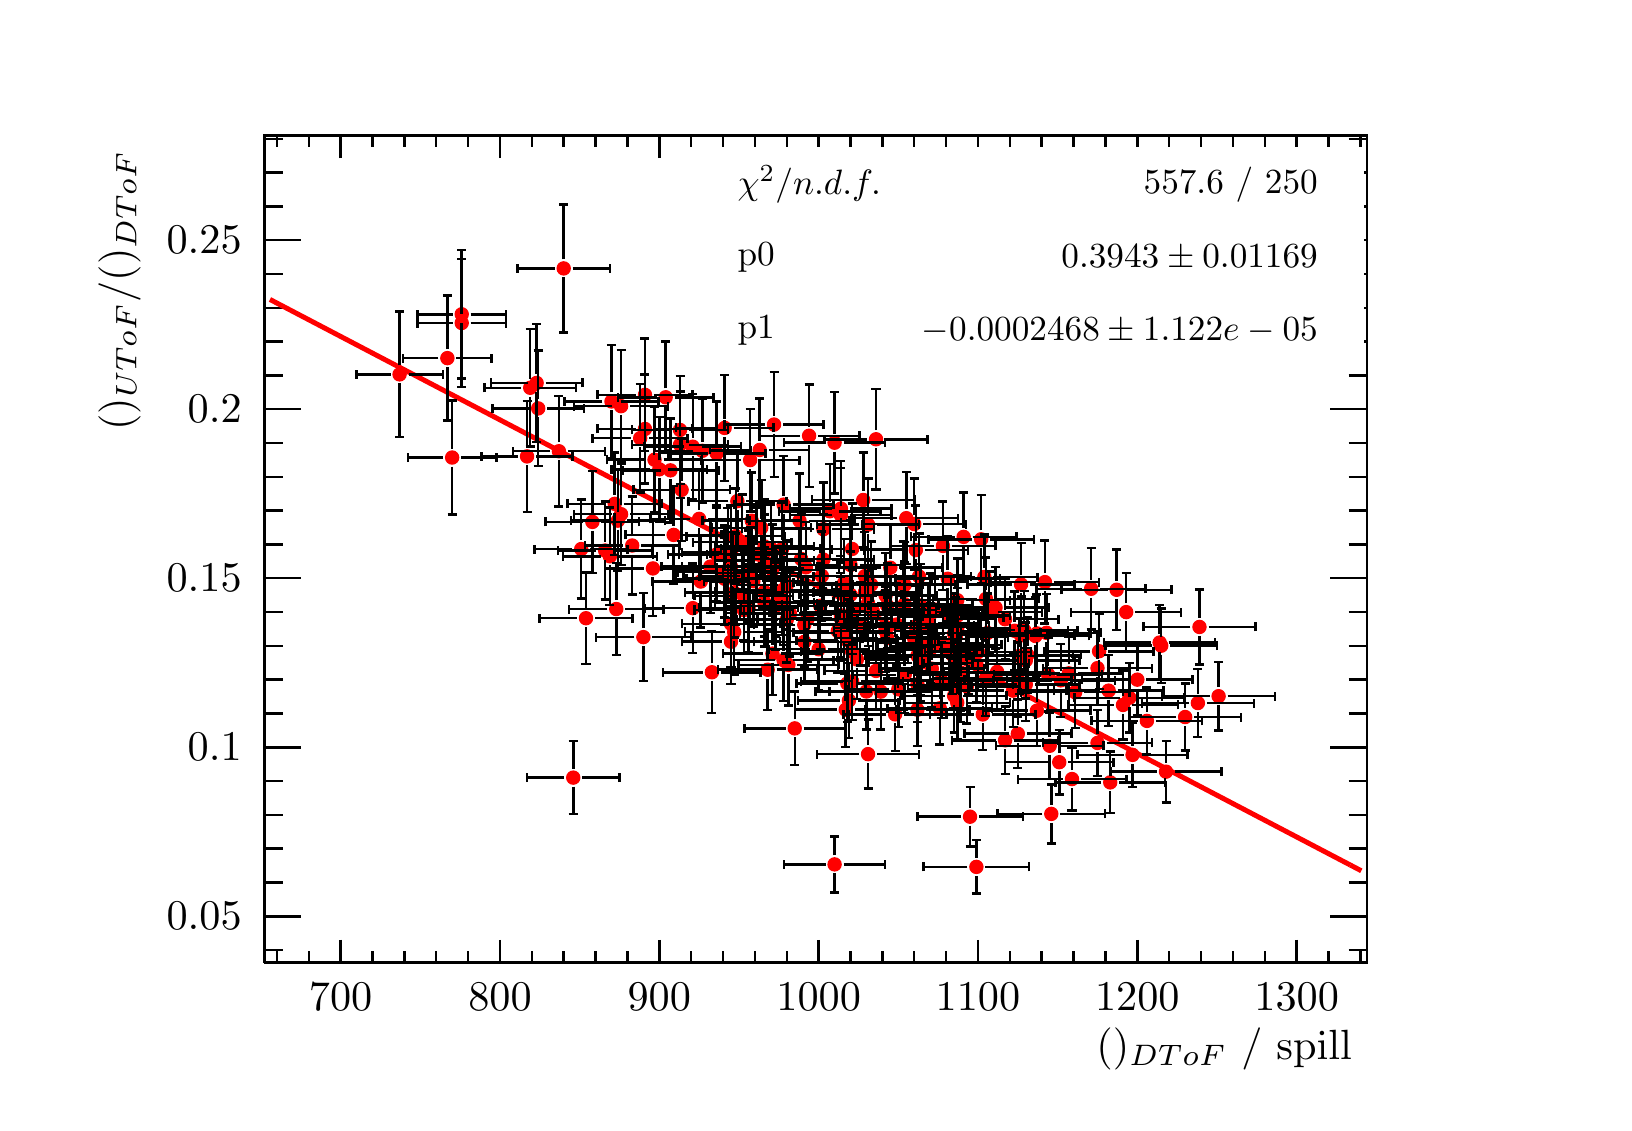
\begin{tikzpicture}
\pgfdeclareplotmark{cross} {
\pgfpathmoveto{\pgfpoint{-0.3\pgfplotmarksize}{\pgfplotmarksize}}
\pgfpathlineto{\pgfpoint{+0.3\pgfplotmarksize}{\pgfplotmarksize}}
\pgfpathlineto{\pgfpoint{+0.3\pgfplotmarksize}{0.3\pgfplotmarksize}}
\pgfpathlineto{\pgfpoint{+1\pgfplotmarksize}{0.3\pgfplotmarksize}}
\pgfpathlineto{\pgfpoint{+1\pgfplotmarksize}{-0.3\pgfplotmarksize}}
\pgfpathlineto{\pgfpoint{+0.3\pgfplotmarksize}{-0.3\pgfplotmarksize}}
\pgfpathlineto{\pgfpoint{+0.3\pgfplotmarksize}{-1.\pgfplotmarksize}}
\pgfpathlineto{\pgfpoint{-0.3\pgfplotmarksize}{-1.\pgfplotmarksize}}
\pgfpathlineto{\pgfpoint{-0.3\pgfplotmarksize}{-0.3\pgfplotmarksize}}
\pgfpathlineto{\pgfpoint{-1.\pgfplotmarksize}{-0.3\pgfplotmarksize}}
\pgfpathlineto{\pgfpoint{-1.\pgfplotmarksize}{0.3\pgfplotmarksize}}
\pgfpathlineto{\pgfpoint{-0.3\pgfplotmarksize}{0.3\pgfplotmarksize}}
\pgfpathclose
\pgfusepathqstroke
}
\pgfdeclareplotmark{cross*} {
\pgfpathmoveto{\pgfpoint{-0.3\pgfplotmarksize}{\pgfplotmarksize}}
\pgfpathlineto{\pgfpoint{+0.3\pgfplotmarksize}{\pgfplotmarksize}}
\pgfpathlineto{\pgfpoint{+0.3\pgfplotmarksize}{0.3\pgfplotmarksize}}
\pgfpathlineto{\pgfpoint{+1\pgfplotmarksize}{0.3\pgfplotmarksize}}
\pgfpathlineto{\pgfpoint{+1\pgfplotmarksize}{-0.3\pgfplotmarksize}}
\pgfpathlineto{\pgfpoint{+0.3\pgfplotmarksize}{-0.3\pgfplotmarksize}}
\pgfpathlineto{\pgfpoint{+0.3\pgfplotmarksize}{-1.\pgfplotmarksize}}
\pgfpathlineto{\pgfpoint{-0.3\pgfplotmarksize}{-1.\pgfplotmarksize}}
\pgfpathlineto{\pgfpoint{-0.3\pgfplotmarksize}{-0.3\pgfplotmarksize}}
\pgfpathlineto{\pgfpoint{-1.\pgfplotmarksize}{-0.3\pgfplotmarksize}}
\pgfpathlineto{\pgfpoint{-1.\pgfplotmarksize}{0.3\pgfplotmarksize}}
\pgfpathlineto{\pgfpoint{-0.3\pgfplotmarksize}{0.3\pgfplotmarksize}}
\pgfpathclose
\pgfusepathqfillstroke
}
\pgfdeclareplotmark{newstar} {
\pgfpathmoveto{\pgfqpoint{0pt}{\pgfplotmarksize}}
\pgfpathlineto{\pgfqpointpolar{44}{0.5\pgfplotmarksize}}
\pgfpathlineto{\pgfqpointpolar{18}{\pgfplotmarksize}}
\pgfpathlineto{\pgfqpointpolar{-20}{0.5\pgfplotmarksize}}
\pgfpathlineto{\pgfqpointpolar{-54}{\pgfplotmarksize}}
\pgfpathlineto{\pgfqpointpolar{-90}{0.5\pgfplotmarksize}}
\pgfpathlineto{\pgfqpointpolar{234}{\pgfplotmarksize}}
\pgfpathlineto{\pgfqpointpolar{198}{0.5\pgfplotmarksize}}
\pgfpathlineto{\pgfqpointpolar{162}{\pgfplotmarksize}}
\pgfpathlineto{\pgfqpointpolar{134}{0.5\pgfplotmarksize}}
\pgfpathclose
\pgfusepathqstroke
}
\pgfdeclareplotmark{newstar*} {
\pgfpathmoveto{\pgfqpoint{0pt}{\pgfplotmarksize}}
\pgfpathlineto{\pgfqpointpolar{44}{0.5\pgfplotmarksize}}
\pgfpathlineto{\pgfqpointpolar{18}{\pgfplotmarksize}}
\pgfpathlineto{\pgfqpointpolar{-20}{0.5\pgfplotmarksize}}
\pgfpathlineto{\pgfqpointpolar{-54}{\pgfplotmarksize}}
\pgfpathlineto{\pgfqpointpolar{-90}{0.5\pgfplotmarksize}}
\pgfpathlineto{\pgfqpointpolar{234}{\pgfplotmarksize}}
\pgfpathlineto{\pgfqpointpolar{198}{0.5\pgfplotmarksize}}
\pgfpathlineto{\pgfqpointpolar{162}{\pgfplotmarksize}}
\pgfpathlineto{\pgfqpointpolar{134}{0.5\pgfplotmarksize}}
\pgfpathclose
\pgfusepathqfillstroke
}
\definecolor{c}{rgb}{1,1,1};
\draw [color=c, fill=c] (0,0) rectangle (20,13.639);
\draw [color=c, fill=c] (3,1.77307) rectangle (17,12.2751);
\definecolor{c}{rgb}{0,0,0};
\draw [c,line width=0.9] (3,1.77307) -- (3,12.2751) -- (17,12.2751) -- (17,1.77307) -- (3,1.77307);
\definecolor{c}{rgb}{1,1,1};
\draw [color=c, fill=c] (3,1.77307) rectangle (17,12.2751);
\definecolor{c}{rgb}{0,0,0};
\draw [c,line width=0.9] (3,1.77307) -- (3,12.2751) -- (17,12.2751) -- (17,1.77307) -- (3,1.77307);
\draw [c,line width=0.9] (3,1.77307) -- (17,1.77307);
\draw [c,line width=0.9] (3.96729,2.05948) -- (3.96729,1.77307);
\draw [c,line width=0.9] (4.37202,1.91628) -- (4.37202,1.77307);
\draw [c,line width=0.9] (4.77675,1.91628) -- (4.77675,1.77307);
\draw [c,line width=0.9] (5.18148,1.91628) -- (5.18148,1.77307);
\draw [c,line width=0.9] (5.58621,1.91628) -- (5.58621,1.77307);
\draw [c,line width=0.9] (5.99094,2.05948) -- (5.99094,1.77307);
\draw [c,line width=0.9] (6.39567,1.91628) -- (6.39567,1.77307);
\draw [c,line width=0.9] (6.8004,1.91628) -- (6.8004,1.77307);
\draw [c,line width=0.9] (7.20513,1.91628) -- (7.20513,1.77307);
\draw [c,line width=0.9] (7.60985,1.91628) -- (7.60985,1.77307);
\draw [c,line width=0.9] (8.01458,2.05948) -- (8.01458,1.77307);
\draw [c,line width=0.9] (8.41931,1.91628) -- (8.41931,1.77307);
\draw [c,line width=0.9] (8.82404,1.91628) -- (8.82404,1.77307);
\draw [c,line width=0.9] (9.22877,1.91628) -- (9.22877,1.77307);
\draw [c,line width=0.9] (9.6335,1.91628) -- (9.6335,1.77307);
\draw [c,line width=0.9] (10.0382,2.05948) -- (10.0382,1.77307);
\draw [c,line width=0.9] (10.443,1.91628) -- (10.443,1.77307);
\draw [c,line width=0.9] (10.8477,1.91628) -- (10.8477,1.77307);
\draw [c,line width=0.9] (11.2524,1.91628) -- (11.2524,1.77307);
\draw [c,line width=0.9] (11.6571,1.91628) -- (11.6571,1.77307);
\draw [c,line width=0.9] (12.0619,2.05948) -- (12.0619,1.77307);
\draw [c,line width=0.9] (12.4666,1.91628) -- (12.4666,1.77307);
\draw [c,line width=0.9] (12.8713,1.91628) -- (12.8713,1.77307);
\draw [c,line width=0.9] (13.2761,1.91628) -- (13.2761,1.77307);
\draw [c,line width=0.9] (13.6808,1.91628) -- (13.6808,1.77307);
\draw [c,line width=0.9] (14.0855,2.05948) -- (14.0855,1.77307);
\draw [c,line width=0.9] (14.4903,1.91628) -- (14.4903,1.77307);
\draw [c,line width=0.9] (14.895,1.91628) -- (14.895,1.77307);
\draw [c,line width=0.9] (15.2997,1.91628) -- (15.2997,1.77307);
\draw [c,line width=0.9] (15.7044,1.91628) -- (15.7044,1.77307);
\draw [c,line width=0.9] (16.1092,2.05948) -- (16.1092,1.77307);
\draw [c,line width=0.9] (3.96729,2.05948) -- (3.96729,1.77307);
\draw [c,line width=0.9] (3.56256,1.91628) -- (3.56256,1.77307);
\draw [c,line width=0.9] (3.15783,1.91628) -- (3.15783,1.77307);
\draw [c,line width=0.9] (16.1092,2.05948) -- (16.1092,1.77307);
\draw [c,line width=0.9] (16.5139,1.91628) -- (16.5139,1.77307);
\draw [c,line width=0.9] (16.9186,1.91628) -- (16.9186,1.77307);
\draw [anchor=base] (3.96729,1.15931) node[scale=1.52731, color=c, rotate=0]{700};
\draw [anchor=base] (5.99094,1.15931) node[scale=1.52731, color=c, rotate=0]{800};
\draw [anchor=base] (8.01458,1.15931) node[scale=1.52731, color=c, rotate=0]{900};
\draw [anchor=base] (10.0382,1.15931) node[scale=1.52731, color=c, rotate=0]{1000};
\draw [anchor=base] (12.0619,1.15931) node[scale=1.52731, color=c, rotate=0]{1100};
\draw [anchor=base] (14.0855,1.15931) node[scale=1.52731, color=c, rotate=0]{1200};
\draw [anchor=base] (16.1092,1.15931) node[scale=1.52731, color=c, rotate=0]{1300};
\draw [anchor= east] (17,0.681948) node[scale=1.52731, color=c, rotate=0]{ $(\SOne\STwo)_{\text{DToF}}$  / spill};
\draw [c,line width=0.9] (3,12.2751) -- (17,12.2751);
\draw [c,line width=0.9] (3.96729,11.9887) -- (3.96729,12.2751);
\draw [c,line width=0.9] (4.37202,12.1319) -- (4.37202,12.2751);
\draw [c,line width=0.9] (4.77675,12.1319) -- (4.77675,12.2751);
\draw [c,line width=0.9] (5.18148,12.1319) -- (5.18148,12.2751);
\draw [c,line width=0.9] (5.58621,12.1319) -- (5.58621,12.2751);
\draw [c,line width=0.9] (5.99094,11.9887) -- (5.99094,12.2751);
\draw [c,line width=0.9] (6.39567,12.1319) -- (6.39567,12.2751);
\draw [c,line width=0.9] (6.8004,12.1319) -- (6.8004,12.2751);
\draw [c,line width=0.9] (7.20513,12.1319) -- (7.20513,12.2751);
\draw [c,line width=0.9] (7.60985,12.1319) -- (7.60985,12.2751);
\draw [c,line width=0.9] (8.01458,11.9887) -- (8.01458,12.2751);
\draw [c,line width=0.9] (8.41931,12.1319) -- (8.41931,12.2751);
\draw [c,line width=0.9] (8.82404,12.1319) -- (8.82404,12.2751);
\draw [c,line width=0.9] (9.22877,12.1319) -- (9.22877,12.2751);
\draw [c,line width=0.9] (9.6335,12.1319) -- (9.6335,12.2751);
\draw [c,line width=0.9] (10.0382,11.9887) -- (10.0382,12.2751);
\draw [c,line width=0.9] (10.443,12.1319) -- (10.443,12.2751);
\draw [c,line width=0.9] (10.8477,12.1319) -- (10.8477,12.2751);
\draw [c,line width=0.9] (11.2524,12.1319) -- (11.2524,12.2751);
\draw [c,line width=0.9] (11.6571,12.1319) -- (11.6571,12.2751);
\draw [c,line width=0.9] (12.0619,11.9887) -- (12.0619,12.2751);
\draw [c,line width=0.9] (12.4666,12.1319) -- (12.4666,12.2751);
\draw [c,line width=0.9] (12.8713,12.1319) -- (12.8713,12.2751);
\draw [c,line width=0.9] (13.2761,12.1319) -- (13.2761,12.2751);
\draw [c,line width=0.9] (13.6808,12.1319) -- (13.6808,12.2751);
\draw [c,line width=0.9] (14.0855,11.9887) -- (14.0855,12.2751);
\draw [c,line width=0.9] (14.4903,12.1319) -- (14.4903,12.2751);
\draw [c,line width=0.9] (14.895,12.1319) -- (14.895,12.2751);
\draw [c,line width=0.9] (15.2997,12.1319) -- (15.2997,12.2751);
\draw [c,line width=0.9] (15.7044,12.1319) -- (15.7044,12.2751);
\draw [c,line width=0.9] (16.1092,11.9887) -- (16.1092,12.2751);
\draw [c,line width=0.9] (3.96729,11.9887) -- (3.96729,12.2751);
\draw [c,line width=0.9] (3.56256,12.1319) -- (3.56256,12.2751);
\draw [c,line width=0.9] (3.15783,12.1319) -- (3.15783,12.2751);
\draw [c,line width=0.9] (16.1092,11.9887) -- (16.1092,12.2751);
\draw [c,line width=0.9] (16.5139,12.1319) -- (16.5139,12.2751);
\draw [c,line width=0.9] (16.9186,12.1319) -- (16.9186,12.2751);
\draw [c,line width=0.9] (3,1.77307) -- (3,12.2751);
\draw [c,line width=0.9] (3.462,2.36091) -- (3,2.36091);
\draw [c,line width=0.9] (3.231,2.79018) -- (3,2.79018);
\draw [c,line width=0.9] (3.231,3.21945) -- (3,3.21945);
\draw [c,line width=0.9] (3.231,3.64872) -- (3,3.64872);
\draw [c,line width=0.9] (3.231,4.07799) -- (3,4.07799);
\draw [c,line width=0.9] (3.462,4.50726) -- (3,4.50726);
\draw [c,line width=0.9] (3.231,4.93653) -- (3,4.93653);
\draw [c,line width=0.9] (3.231,5.36579) -- (3,5.36579);
\draw [c,line width=0.9] (3.231,5.79506) -- (3,5.79506);
\draw [c,line width=0.9] (3.231,6.22433) -- (3,6.22433);
\draw [c,line width=0.9] (3.462,6.6536) -- (3,6.6536);
\draw [c,line width=0.9] (3.231,7.08287) -- (3,7.08287);
\draw [c,line width=0.9] (3.231,7.51214) -- (3,7.51214);
\draw [c,line width=0.9] (3.231,7.94141) -- (3,7.94141);
\draw [c,line width=0.9] (3.231,8.37068) -- (3,8.37068);
\draw [c,line width=0.9] (3.462,8.79995) -- (3,8.79995);
\draw [c,line width=0.9] (3.231,9.22922) -- (3,9.22922);
\draw [c,line width=0.9] (3.231,9.65849) -- (3,9.65849);
\draw [c,line width=0.9] (3.231,10.0878) -- (3,10.0878);
\draw [c,line width=0.9] (3.231,10.517) -- (3,10.517);
\draw [c,line width=0.9] (3.462,10.9463) -- (3,10.9463);
\draw [c,line width=0.9] (3.462,2.36091) -- (3,2.36091);
\draw [c,line width=0.9] (3.231,1.93164) -- (3,1.93164);
\draw [c,line width=0.9] (3.462,10.9463) -- (3,10.9463);
\draw [c,line width=0.9] (3.231,11.3756) -- (3,11.3756);
\draw [c,line width=0.9] (3.231,11.8048) -- (3,11.8048);
\draw [c,line width=0.9] (3.231,12.2341) -- (3,12.2341);
\draw [anchor= east] (2.9,2.36091) node[scale=1.52731, color=c, rotate=0]{0.05};
\draw [anchor= east] (2.9,4.50726) node[scale=1.52731, color=c, rotate=0]{0.1};
\draw [anchor= east] (2.9,6.6536) node[scale=1.52731, color=c, rotate=0]{0.15};
\draw [anchor= east] (2.9,8.79995) node[scale=1.52731, color=c, rotate=0]{0.2};
\draw [anchor= east] (2.9,10.9463) node[scale=1.52731, color=c, rotate=0]{0.25};
\draw [anchor= east] (1.16,12.2751) node[scale=1.52731, color=c, rotate=90]{$(\SOne\STwo)_{\text{UToF}}/(\SOne\STwo)_{\text{DToF}}$ };
\draw [c,line width=0.9] (17,1.77307) -- (17,12.2751);
\draw [c,line width=0.9] (16.538,2.36091) -- (17,2.36091);
\draw [c,line width=0.9] (16.769,2.79018) -- (17,2.79018);
\draw [c,line width=0.9] (16.769,3.21945) -- (17,3.21945);
\draw [c,line width=0.9] (16.769,3.64872) -- (17,3.64872);
\draw [c,line width=0.9] (16.769,4.07799) -- (17,4.07799);
\draw [c,line width=0.9] (16.538,4.50726) -- (17,4.50726);
\draw [c,line width=0.9] (16.769,4.93653) -- (17,4.93653);
\draw [c,line width=0.9] (16.769,5.36579) -- (17,5.36579);
\draw [c,line width=0.9] (16.769,5.79506) -- (17,5.79506);
\draw [c,line width=0.9] (16.769,6.22433) -- (17,6.22433);
\draw [c,line width=0.9] (16.538,6.6536) -- (17,6.6536);
\draw [c,line width=0.9] (16.769,7.08287) -- (17,7.08287);
\draw [c,line width=0.9] (16.769,7.51214) -- (17,7.51214);
\draw [c,line width=0.9] (16.769,7.94141) -- (17,7.94141);
\draw [c,line width=0.9] (16.769,8.37068) -- (17,8.37068);
\draw [c,line width=0.9] (16.538,8.79995) -- (17,8.79995);
\draw [c,line width=0.9] (16.769,9.22922) -- (17,9.22922);
\draw [c,line width=0.9] (16.769,9.65849) -- (17,9.65849);
\draw [c,line width=0.9] (16.769,10.0878) -- (17,10.0878);
\draw [c,line width=0.9] (16.769,10.517) -- (17,10.517);
\draw [c,line width=0.9] (16.538,10.9463) -- (17,10.9463);
\draw [c,line width=0.9] (16.538,2.36091) -- (17,2.36091);
\draw [c,line width=0.9] (16.769,1.93164) -- (17,1.93164);
\draw [c,line width=0.9] (16.538,10.9463) -- (17,10.9463);
\draw [c,line width=0.9] (16.769,11.3756) -- (17,11.3756);
\draw [c,line width=0.9] (16.769,11.8048) -- (17,11.8048);
\draw [c,line width=0.9] (16.769,12.2341) -- (17,12.2341);
\definecolor{c}{rgb}{1,0,0};
\foreach \P in {(11.5155,6.25554), (9.57279,6.49762), (10.7667,8.41874), (10.4025,5.86506), (11.9202,5.28096), (11.1108,6.57411), (10.6453,5.21576), (13.0939,4.31705), (10.362,5.96069), (11.131,5.4277), (9.57279,7.02487), (7.81222,5.906),
 (10.0989,7.27632), (13.2154,5.44593), (8.7431,6.95629), (9.1883,7.38399), (11.6774,6.64764), (6.73969,8.26657), (14.8545,5.06898), (11.6167,5.78949), (11.8797,7.17888), (13.7213,5.22634), (11.3334,5.58043), (11.6976,5.80855), (11.5762,5.00195),
 (9.67397,6.20335), (13.9439,6.22361), (10.3215,6.14136), (12.7904,5.92052), (13.2558,4.10354), (7.67056,7.06926), (13.5998,5.72644), (11.2929,6.03516), (10.4632,5.72233), (14.3891,5.79683), (11.2524,5.88416), (10.0585,6.3041), (12.669,5.30501),
 (8.98593,6.64455), (10.3215,7.45372), (14.2069,4.84184), (9.14783,6.27642), (14.3688,5.83679), (8.84428,6.738), (11.475,5.50528), (10.706,6.57257), (11.2929,5.30759), (13.9843,5.13589), (11.4345,6.07736), (11.8393,5.29957), (12.6487,5.99392),
 (10.6656,4.41982), (12.1631,6.39138), (12.6083,5.928), (8.98593,7.18792), (11.3131,6.67581), (9.06688,7.11353), (8.29789,7.77609), (12.588,5.66621), (10.0382,5.75214), (11.1512,7.41652), (11.7988,6.37519), (8.43955,6.27374), (13.5796,4.56206),
 (9.28948,8.28286), (12.5273,5.98657), (10.443,6.44318), (8.86451,6.73107), (13.9034,5.04429), (13.8224,6.50714), (11.3536,6.05907), (14.0855,5.36579), (8.92522,6.98293), (7.44796,7.59878), (15.1176,5.15579), (9.65374,5.55308), (9.59303,7.58851),
 (11.4548,6.19224), (5.38384,8.18671), (8.84428,6.64676), (10.8882,6.43526), (8.88475,6.95177), (11.3334,5.66112), (7.32654,7.00554), (10.7263,6.2343), (10.3215,7.53839), (10.3215,6.18369), (11.2727,7.01166), (11.131,6.32371), (10.2406,3.01969),
 (8.92522,6.80123), (9.59303,6.35952), (8.09553,8.9519), (11.0501,5.24315), (8.27766,8.53665), (11.7381,5.67943), (12.9725,4.526), (10.5644,6.07204), (12.9118,6.60474), (9.39066,5.49174), (9.35019,6.34698), (9.8561,6.06233), (10.6656,7.33435),
 (9.6335,6.566), (11.7583,5.95134), (9.45137,5.69648), (10.4632,5.34393), (8.92522,5.8473), (10.2406,8.37493), (12.5678,5.36579), (10.4632,7.02569), (12.2845,6.28074), (10.362,6.59445), (8.84428,8.56273), (9.45137,6.75749), (10.6048,7.64743),
 (9.79539,7.38353), (8.43955,8.32454), (8.7431,8.24043), (11.9607,3.6252), (8.94546,6.65814), (5.50526,9.89525), (11.7988,6.17773), (8.56097,8.27204), (11.2929,5.67138), (11.7786,5.90653), (13.4987,6.5198), (9.08712,6.43063), (10.4632,6.22686),
 (9.49185,6.47934), (10.8275,5.21375), (11.7179,6.16012), (9.24901,6.95958), (7.48844,7.38542), (12.1428,6.66915), (9.91681,8.4631), (12.6892,5.68006), (9.81563,6.89884), (10.443,6.82194), (11.4548,5.75093), (5.32313,9.44917), (11.0298,6.06637),
 (12.3047,5.46462), (10.7667,5.47684), (9.00617,7.63291), (12.6083,6.57552), (10.2811,5.9834), (8.9657,6.47002), (12.1833,5.95885), (8.9657,5.97139), (10.8882,6.02329), (9.8561,5.84574), (12.8106,4.97164), (11.9405,5.66872), (9.20853,6.61555),
 (10.6656,6.33508), (13.1142,5.35685), (7.93364,6.77817), (12.1226,4.92368), (11.6167,7.06376), (9.35019,6.88023), (9.6335,6.12797), (7.16465,7.36905), (11.2524,7.34205), (11.3334,6.30664), (8.01458,8.0368), (12.1631,5.38133), (12.0416,2.98782),
 (8.54073,6.61188), (14.4498,4.19711), (12.669,5.60892), (7.77175,8.43255), (11.7988,5.07198), (8.19671,7.20376), (12.1023,7.14831), (10.6251,6.68072), (7.83246,8.54942), (11.131,6.56807), (12.9523,5.43033), (7.023,7.02436), (10.1799,7.50404),
 (12.4059,6.13287), (9.89657,6.13701), (6.8004,10.5886), (8.66215,6.80099), (12.0619,5.71701), (10.4025,5.31688), (10.9489,6.78711), (10.3822,4.98422), (4.71604,9.24261), (7.40749,8.89863), (12.4059,4.59565), (9.43114,7.02977), (8.5205,7.40772),
 (7.38725,6.9327), (9.87634,6.79208), (14.8747,6.03516), (6.33496,8.20097), (14.0248,4.41043), (11.2727,6.04065), (9.14783,6.68054), (9.35019,7.05799), (9.47161,8.60563), (6.92181,4.12162), (8.68239,5.45965), (7.08371,6.14592), (10.5239,5.62235),
 (6.37543,9.0725), (9.73468,4.74695), (9.59303,5.61335), (10.9084,5.89425), (13.7415,4.06093), (8.15624,8.02376), (10.6251,6.47213), (11.2929,4.98422), (5.50526,10.0059), (11.7583,5.16006), (11.5964,5.35623), (7.83246,8.98302), (11.7988,6.01977),
 (12.8106,5.95325), (11.0096,4.92506), (7.52891,7.46706), (8.27766,8.34858), (6.45638,9.13377), (11.4548,5.83117), (7.95387,8.15868), (9.35019,6.48029), (12.9928,3.6607), (10.0989,6.89113), (13.5796,5.51193), (12.0416,5.56578), (9.08712,6.25046),
 (9.16806,8.15403), (9.30972,7.29483), (7.4682,6.26269), (14.6926,4.89116), (9.16806,6.71864), (10.9084,6.30582), (12.932,5.96069), (10.8882,5.9821), (10.4227,5.10124), (12.2035,6.22511), (7.52891,8.83915), (12.5678,4.67896), (11.8393,5.45725),
 (6.47661,8.81037), (12.5071,5.22653), (10.0787,6.68359), (9.49185,6.30286), (13.2963,5.20607), (8.92522,6.07443)}{\draw[mark options={color=c,fill=c},mark size=2.402402pt,mark=*] plot coordinates {\P};}
\draw [c,line width=1.8] (3.07,10.1944) -- (3.21,10.1211) -- (3.35,10.0478) -- (3.49,9.97453) -- (3.63,9.90124) -- (3.77,9.82794) -- (3.91,9.75465) -- (4.05,9.68136) -- (4.19,9.60806) -- (4.33,9.53477) -- (4.47,9.46148) -- (4.61,9.38819) --
 (4.75,9.31489) -- (4.89,9.2416) -- (5.03,9.16831) -- (5.17,9.09501) -- (5.31,9.02172) -- (5.45,8.94843) -- (5.59,8.87514) -- (5.73,8.80184) -- (5.87,8.72855) -- (6.01,8.65526) -- (6.15,8.58196) -- (6.29,8.50867) -- (6.43,8.43538) -- (6.57,8.36209)
 -- (6.71,8.28879) -- (6.85,8.2155) -- (6.99,8.14221) -- (7.13,8.06891) -- (7.27,7.99562) -- (7.41,7.92233) -- (7.55,7.84904) -- (7.69,7.77574) -- (7.83,7.70245) -- (7.97,7.62916) -- (8.11,7.55586) -- (8.25,7.48257) -- (8.39,7.40928) --
 (8.53,7.33599) -- (8.67,7.26269) -- (8.81,7.1894) -- (8.95,7.11611) -- (9.09,7.04281) -- (9.23,6.96952) -- (9.37,6.89623) -- (9.51,6.82294) -- (9.65,6.74964) -- (9.79,6.67635) -- (9.93,6.60306);
\draw [c,line width=1.8] (9.93,6.60306) -- (10.07,6.52976) -- (10.21,6.45647) -- (10.35,6.38318) -- (10.49,6.30989) -- (10.63,6.23659) -- (10.77,6.1633) -- (10.91,6.09001) -- (11.05,6.01671) -- (11.19,5.94342) -- (11.33,5.87013) -- (11.47,5.79683) --
 (11.61,5.72354) -- (11.75,5.65025) -- (11.89,5.57696) -- (12.03,5.50366) -- (12.17,5.43037) -- (12.31,5.35708) -- (12.45,5.28378) -- (12.59,5.21049) -- (12.73,5.1372) -- (12.87,5.06391) -- (13.01,4.99061) -- (13.15,4.91732) -- (13.29,4.84403) --
 (13.43,4.77073) -- (13.57,4.69744) -- (13.71,4.62415) -- (13.85,4.55086) -- (13.99,4.47756) -- (14.13,4.40427) -- (14.27,4.33098) -- (14.41,4.25768) -- (14.55,4.18439) -- (14.69,4.1111) -- (14.83,4.03781) -- (14.97,3.96451) -- (15.11,3.89122) --
 (15.25,3.81793) -- (15.39,3.74463) -- (15.53,3.67134) -- (15.67,3.59805) -- (15.81,3.52476) -- (15.95,3.45146) -- (16.09,3.37817) -- (16.23,3.30488) -- (16.37,3.23158) -- (16.51,3.15829) -- (16.65,3.085) -- (16.79,3.01171);
\draw [c,line width=1.8] (16.79,3.01171) -- (16.93,2.93841);
\definecolor{c}{rgb}{1,1,1};
\draw [color=c, fill=c] (8.42407,9.34097) rectangle (16.9628,12.1203);
\definecolor{c}{rgb}{0,0,0};
\draw [anchor= west] (8.851,11.6571) node[scale=1.27276, color=c, rotate=0]{$\chi^{2} / ndf $};
\draw [anchor= east] (16.5358,11.6571) node[scale=1.27276, color=c, rotate=0]{ 557.6 / 250};
\draw [anchor= west] (8.851,10.7307) node[scale=1.27276, color=c, rotate=0]{p0       };
\draw [anchor= east] (16.5358,10.7307) node[scale=1.27276, color=c, rotate=0]{$ 0.3943 \pm 0.01169$};
\draw [anchor= west] (8.851,9.8042) node[scale=1.27276, color=c, rotate=0]{p1       };
\draw [anchor= east] (16.5358,9.8042) node[scale=1.27276, color=c, rotate=0]{$ -0.0002468 \pm 1.122e-05$};
\draw [c,line width=0.9] (11.4009,6.25554) -- (10.8526,6.25554);
\draw [c,line width=0.9] (10.8526,6.19823) -- (10.8526,6.31284);
\draw [c,line width=0.9] (11.6301,6.25554) -- (12.1784,6.25554);
\draw [c,line width=0.9] (12.1784,6.19823) -- (12.1784,6.31284);
\draw [c,line width=0.9] (11.5155,6.37015) -- (11.5155,6.7806);
\draw [c,line width=0.9] (11.4582,6.7806) -- (11.5728,6.7806);
\draw [c,line width=0.9] (11.5155,6.14092) -- (11.5155,5.73048);
\draw [c,line width=0.9] (11.4582,5.73048) -- (11.5728,5.73048);
\draw [c,line width=0.9] (9.45818,6.49762) -- (8.94026,6.49762);
\draw [c,line width=0.9] (8.94026,6.44032) -- (8.94026,6.55493);
\draw [c,line width=0.9] (9.6874,6.49762) -- (10.2053,6.49762);
\draw [c,line width=0.9] (10.2053,6.44032) -- (10.2053,6.55493);
\draw [c,line width=0.9] (9.57279,6.61224) -- (9.57279,7.06018);
\draw [c,line width=0.9] (9.51548,7.06018) -- (9.6301,7.06018);
\draw [c,line width=0.9] (9.57279,6.38301) -- (9.57279,5.93507);
\draw [c,line width=0.9] (9.51548,5.93507) -- (9.6301,5.93507);
\draw [c,line width=0.9] (10.6521,8.41874) -- (10.1154,8.41874);
\draw [c,line width=0.9] (10.1154,8.36144) -- (10.1154,8.47605);
\draw [c,line width=0.9] (10.8814,8.41874) -- (11.4181,8.41874);
\draw [c,line width=0.9] (11.4181,8.36144) -- (11.4181,8.47605);
\draw [c,line width=0.9] (10.7667,8.53336) -- (10.7667,9.05507);
\draw [c,line width=0.9] (10.7094,9.05507) -- (10.824,9.05507);
\draw [c,line width=0.9] (10.7667,8.30413) -- (10.7667,7.78242);
\draw [c,line width=0.9] (10.7094,7.78242) -- (10.824,7.78242);
\draw [c,line width=0.9] (10.2879,5.86506) -- (9.75682,5.86506);
\draw [c,line width=0.9] (9.75682,5.80776) -- (9.75682,5.92237);
\draw [c,line width=0.9] (10.5171,5.86506) -- (11.0482,5.86506);
\draw [c,line width=0.9] (11.0482,5.80776) -- (11.0482,5.92237);
\draw [c,line width=0.9] (10.4025,5.97968) -- (10.4025,6.38432);
\draw [c,line width=0.9] (10.3452,6.38432) -- (10.4598,6.38432);
\draw [c,line width=0.9] (10.4025,5.75045) -- (10.4025,5.3458);
\draw [c,line width=0.9] (10.3452,5.3458) -- (10.4598,5.3458);
\draw [c,line width=0.9] (11.8056,5.28096) -- (11.2512,5.28096);
\draw [c,line width=0.9] (11.2512,5.22366) -- (11.2512,5.33827);
\draw [c,line width=0.9] (12.0348,5.28096) -- (12.5892,5.28096);
\draw [c,line width=0.9] (12.5892,5.22366) -- (12.5892,5.33827);
\draw [c,line width=0.9] (11.9202,5.39558) -- (11.9202,5.75262);
\draw [c,line width=0.9] (11.8629,5.75262) -- (11.9775,5.75262);
\draw [c,line width=0.9] (11.9202,5.16635) -- (11.9202,4.8093);
\draw [c,line width=0.9] (11.8629,4.8093) -- (11.9775,4.8093);
\draw [c,line width=0.9] (10.9961,6.57411) -- (10.4541,6.57411);
\draw [c,line width=0.9] (10.4541,6.5168) -- (10.4541,6.63141);
\draw [c,line width=0.9] (11.2254,6.57411) -- (11.7674,6.57411);
\draw [c,line width=0.9] (11.7674,6.5168) -- (11.7674,6.63141);
\draw [c,line width=0.9] (11.1108,6.68872) -- (11.1108,7.11969);
\draw [c,line width=0.9] (11.0535,7.11969) -- (11.1681,7.11969);
\draw [c,line width=0.9] (11.1108,6.45949) -- (11.1108,6.02852);
\draw [c,line width=0.9] (11.0535,6.02852) -- (11.1681,6.02852);
\draw [c,line width=0.9] (10.5307,5.21576) -- (9.99586,5.21576);
\draw [c,line width=0.9] (9.99586,5.15845) -- (9.99586,5.27307);
\draw [c,line width=0.9] (10.7599,5.21576) -- (11.2948,5.21576);
\draw [c,line width=0.9] (11.2948,5.15845) -- (11.2948,5.27307);
\draw [c,line width=0.9] (10.6453,5.33037) -- (10.6453,5.69817);
\draw [c,line width=0.9] (10.588,5.69817) -- (10.7026,5.69817);
\draw [c,line width=0.9] (10.6453,5.10115) -- (10.6453,4.73335);
\draw [c,line width=0.9] (10.588,4.73335) -- (10.7026,4.73335);
\draw [c,line width=0.9] (12.9793,4.31705) -- (12.4074,4.31705);
\draw [c,line width=0.9] (12.4074,4.25974) -- (12.4074,4.37436);
\draw [c,line width=0.9] (13.2085,4.31705) -- (13.7805,4.31705);
\draw [c,line width=0.9] (13.7805,4.25974) -- (13.7805,4.37436);
\draw [c,line width=0.9] (13.0939,4.43166) -- (13.0939,4.72647);
\draw [c,line width=0.9] (13.0366,4.72647) -- (13.1512,4.72647);
\draw [c,line width=0.9] (13.0939,4.20244) -- (13.0939,3.90763);
\draw [c,line width=0.9] (13.0366,3.90763) -- (13.1512,3.90763);
\draw [c,line width=0.9] (10.2474,5.96069) -- (9.71698,5.96069);
\draw [c,line width=0.9] (9.71698,5.90338) -- (9.71698,6.01799);
\draw [c,line width=0.9] (10.4766,5.96069) -- (11.007,5.96069);
\draw [c,line width=0.9] (11.007,5.90338) -- (11.007,6.01799);
\draw [c,line width=0.9] (10.362,6.0753) -- (10.362,6.48535);
\draw [c,line width=0.9] (10.3047,6.48535) -- (10.4193,6.48535);
\draw [c,line width=0.9] (10.362,5.84607) -- (10.362,5.43602);
\draw [c,line width=0.9] (10.3047,5.43602) -- (10.4193,5.43602);
\draw [c,line width=0.9] (11.0164,5.4277) -- (10.474,5.4277);
\draw [c,line width=0.9] (10.474,5.37039) -- (10.474,5.48501);
\draw [c,line width=0.9] (11.2456,5.4277) -- (11.788,5.4277);
\draw [c,line width=0.9] (11.788,5.37039) -- (11.788,5.48501);
\draw [c,line width=0.9] (11.131,5.54231) -- (11.131,5.91566);
\draw [c,line width=0.9] (11.0737,5.91566) -- (11.1883,5.91566);
\draw [c,line width=0.9] (11.131,5.31309) -- (11.131,4.93974);
\draw [c,line width=0.9] (11.0737,4.93974) -- (11.1883,4.93974);
\draw [c,line width=0.9] (9.45818,7.02487) -- (8.94026,7.02487);
\draw [c,line width=0.9] (8.94026,6.96757) -- (8.94026,7.08218);
\draw [c,line width=0.9] (9.6874,7.02487) -- (10.2053,7.02487);
\draw [c,line width=0.9] (10.2053,6.96757) -- (10.2053,7.08218);
\draw [c,line width=0.9] (9.57279,7.13949) -- (9.57279,7.61369);
\draw [c,line width=0.9] (9.51548,7.61369) -- (9.6301,7.61369);
\draw [c,line width=0.9] (9.57279,6.91026) -- (9.57279,6.43606);
\draw [c,line width=0.9] (9.51548,6.43606) -- (9.6301,6.43606);
\draw [c,line width=0.9] (7.69761,5.906) -- (7.20851,5.906);
\draw [c,line width=0.9] (7.20851,5.84869) -- (7.20851,5.9633);
\draw [c,line width=0.9] (7.92683,5.906) -- (8.41593,5.906);
\draw [c,line width=0.9] (8.41593,5.84869) -- (8.41593,5.9633);
\draw [c,line width=0.9] (7.81222,6.02061) -- (7.81222,6.46359);
\draw [c,line width=0.9] (7.75491,6.46359) -- (7.86953,6.46359);
\draw [c,line width=0.9] (7.81222,5.79138) -- (7.81222,5.34841);
\draw [c,line width=0.9] (7.75491,5.34841) -- (7.86953,5.34841);
\draw [c,line width=0.9] (9.98433,7.27632) -- (9.45805,7.27632);
\draw [c,line width=0.9] (9.45805,7.21901) -- (9.45805,7.33363);
\draw [c,line width=0.9] (10.2136,7.27632) -- (10.7398,7.27632);
\draw [c,line width=0.9] (10.7398,7.21901) -- (10.7398,7.33363);
\draw [c,line width=0.9] (10.0989,7.39093) -- (10.0989,7.86958);
\draw [c,line width=0.9] (10.0416,7.86958) -- (10.1562,7.86958);
\draw [c,line width=0.9] (10.0989,7.16171) -- (10.0989,6.68306);
\draw [c,line width=0.9] (10.0416,6.68306) -- (10.1562,6.68306);
\draw [c,line width=0.9] (13.1007,5.44593) -- (12.527,5.44593);
\draw [c,line width=0.9] (12.527,5.38863) -- (12.527,5.50324);
\draw [c,line width=0.9] (13.33,5.44593) -- (13.9037,5.44593);
\draw [c,line width=0.9] (13.9037,5.38863) -- (13.9037,5.50324);
\draw [c,line width=0.9] (13.2154,5.56055) -- (13.2154,5.91257);
\draw [c,line width=0.9] (13.158,5.91257) -- (13.2727,5.91257);
\draw [c,line width=0.9] (13.2154,5.33132) -- (13.2154,4.9793);
\draw [c,line width=0.9] (13.158,4.9793) -- (13.2727,4.9793);
\draw [c,line width=0.9] (8.62848,6.95629) -- (8.12398,6.95629);
\draw [c,line width=0.9] (8.12398,6.89898) -- (8.12398,7.0136);
\draw [c,line width=0.9] (8.85771,6.95629) -- (9.36221,6.95629);
\draw [c,line width=0.9] (9.36221,6.89898) -- (9.36221,7.0136);
\draw [c,line width=0.9] (8.7431,7.0709) -- (8.7431,7.55441);
\draw [c,line width=0.9] (8.68579,7.55441) -- (8.8004,7.55441);
\draw [c,line width=0.9] (8.7431,6.84168) -- (8.7431,6.35817);
\draw [c,line width=0.9] (8.68579,6.35817) -- (8.8004,6.35817);
\draw [c,line width=0.9] (9.07368,7.38399) -- (8.56195,7.38399);
\draw [c,line width=0.9] (8.56195,7.32668) -- (8.56195,7.44129);
\draw [c,line width=0.9] (9.30291,7.38399) -- (9.81465,7.38399);
\draw [c,line width=0.9] (9.81465,7.32668) -- (9.81465,7.44129);
\draw [c,line width=0.9] (9.1883,7.4986) -- (9.1883,7.99628);
\draw [c,line width=0.9] (9.13099,7.99628) -- (9.2456,7.99628);
\draw [c,line width=0.9] (9.1883,7.26937) -- (9.1883,6.77169);
\draw [c,line width=0.9] (9.13099,6.77169) -- (9.2456,6.77169);
\draw [c,line width=0.9] (11.5628,6.64764) -- (11.012,6.64764);
\draw [c,line width=0.9] (11.012,6.59034) -- (11.012,6.70495);
\draw [c,line width=0.9] (11.792,6.64764) -- (12.3427,6.64764);
\draw [c,line width=0.9] (12.3427,6.59034) -- (12.3427,6.70495);
\draw [c,line width=0.9] (11.6774,6.76226) -- (11.6774,7.18963);
\draw [c,line width=0.9] (11.6201,7.18963) -- (11.7347,7.18963);
\draw [c,line width=0.9] (11.6774,6.53303) -- (11.6774,6.10566);
\draw [c,line width=0.9] (11.6201,6.10566) -- (11.7347,6.10566);
\draw [c,line width=0.9] (6.62507,8.26657) -- (6.15423,8.26657);
\draw [c,line width=0.9] (6.15423,8.20926) -- (6.15423,8.32387);
\draw [c,line width=0.9] (6.8543,8.26657) -- (7.32515,8.26657);
\draw [c,line width=0.9] (7.32515,8.20926) -- (7.32515,8.32387);
\draw [c,line width=0.9] (6.73969,8.38118) -- (6.73969,8.96687);
\draw [c,line width=0.9] (6.68238,8.96687) -- (6.79699,8.96687);
\draw [c,line width=0.9] (6.73969,8.15195) -- (6.73969,7.56627);
\draw [c,line width=0.9] (6.68238,7.56627) -- (6.79699,7.56627);
\draw [c,line width=0.9] (14.7399,5.06898) -- (14.1425,5.06898);
\draw [c,line width=0.9] (14.1425,5.01167) -- (14.1425,5.12629);
\draw [c,line width=0.9] (14.9691,5.06898) -- (15.5665,5.06898);
\draw [c,line width=0.9] (15.5665,5.01167) -- (15.5665,5.12629);
\draw [c,line width=0.9] (14.8545,5.18359) -- (14.8545,5.50183);
\draw [c,line width=0.9] (14.7972,5.50183) -- (14.9118,5.50183);
\draw [c,line width=0.9] (14.8545,4.95437) -- (14.8545,4.63613);
\draw [c,line width=0.9] (14.7972,4.63613) -- (14.9118,4.63613);
\draw [c,line width=0.9] (11.5021,5.78949) -- (10.9523,5.78949);
\draw [c,line width=0.9] (10.9523,5.73218) -- (10.9523,5.8468);
\draw [c,line width=0.9] (11.7313,5.78949) -- (12.2811,5.78949);
\draw [c,line width=0.9] (12.2811,5.73218) -- (12.2811,5.8468);
\draw [c,line width=0.9] (11.6167,5.9041) -- (11.6167,6.29032);
\draw [c,line width=0.9] (11.5594,6.29032) -- (11.674,6.29032);
\draw [c,line width=0.9] (11.6167,5.67488) -- (11.6167,5.28866);
\draw [c,line width=0.9] (11.5594,5.28866) -- (11.674,5.28866);
\draw [c,line width=0.9] (11.7651,7.17888) -- (11.2113,7.17888);
\draw [c,line width=0.9] (11.2113,7.12157) -- (11.2113,7.23618);
\draw [c,line width=0.9] (11.9944,7.17888) -- (12.5482,7.17888);
\draw [c,line width=0.9] (12.5482,7.12157) -- (12.5482,7.23618);
\draw [c,line width=0.9] (11.8797,7.29349) -- (11.8797,7.74321);
\draw [c,line width=0.9] (11.8224,7.74321) -- (11.9371,7.74321);
\draw [c,line width=0.9] (11.8797,7.06426) -- (11.8797,6.61454);
\draw [c,line width=0.9] (11.8224,6.61454) -- (11.9371,6.61454);
\draw [c,line width=0.9] (13.6067,5.22634) -- (13.0255,5.22634);
\draw [c,line width=0.9] (13.0255,5.16903) -- (13.0255,5.28364);
\draw [c,line width=0.9] (13.8359,5.22634) -- (14.417,5.22634);
\draw [c,line width=0.9] (14.417,5.16903) -- (14.417,5.28364);
\draw [c,line width=0.9] (13.7213,5.34095) -- (13.7213,5.67718);
\draw [c,line width=0.9] (13.664,5.67718) -- (13.7786,5.67718);
\draw [c,line width=0.9] (13.7213,5.11172) -- (13.7213,4.77549);
\draw [c,line width=0.9] (13.664,4.77549) -- (13.7786,4.77549);
\draw [c,line width=0.9] (11.2187,5.58043) -- (10.6733,5.58043);
\draw [c,line width=0.9] (10.6733,5.52312) -- (10.6733,5.63774);
\draw [c,line width=0.9] (11.448,5.58043) -- (11.9935,5.58043);
\draw [c,line width=0.9] (11.9935,5.52312) -- (11.9935,5.63774);
\draw [c,line width=0.9] (11.3334,5.69504) -- (11.3334,6.07393);
\draw [c,line width=0.9] (11.2761,6.07393) -- (11.3907,6.07393);
\draw [c,line width=0.9] (11.3334,5.46582) -- (11.3334,5.08693);
\draw [c,line width=0.9] (11.2761,5.08693) -- (11.3907,5.08693);
\draw [c,line width=0.9] (11.583,5.80855) -- (11.032,5.80855);
\draw [c,line width=0.9] (11.032,5.75125) -- (11.032,5.86586);
\draw [c,line width=0.9] (11.8122,5.80855) -- (12.3633,5.80855);
\draw [c,line width=0.9] (12.3633,5.75125) -- (12.3633,5.86586);
\draw [c,line width=0.9] (11.6976,5.92317) -- (11.6976,6.30941);
\draw [c,line width=0.9] (11.6403,6.30941) -- (11.7549,6.30941);
\draw [c,line width=0.9] (11.6976,5.69394) -- (11.6976,5.3077);
\draw [c,line width=0.9] (11.6403,5.3077) -- (11.7549,5.3077);
\draw [c,line width=0.9] (11.4616,5.00195) -- (10.9124,5.00195);
\draw [c,line width=0.9] (10.9124,4.94465) -- (10.9124,5.05926);
\draw [c,line width=0.9] (11.6908,5.00195) -- (12.24,5.00195);
\draw [c,line width=0.9] (12.24,4.94465) -- (12.24,5.05926);
\draw [c,line width=0.9] (11.5762,5.11657) -- (11.5762,5.46271);
\draw [c,line width=0.9] (11.5189,5.46271) -- (11.6335,5.46271);
\draw [c,line width=0.9] (11.5762,4.88734) -- (11.5762,4.5412);
\draw [c,line width=0.9] (11.5189,4.5412) -- (11.6335,4.5412);
\draw [c,line width=0.9] (9.55936,6.20335) -- (9.03983,6.20335);
\draw [c,line width=0.9] (9.03983,6.14604) -- (9.03983,6.26066);
\draw [c,line width=0.9] (9.78859,6.20335) -- (10.3081,6.20335);
\draw [c,line width=0.9] (10.3081,6.14604) -- (10.3081,6.26066);
\draw [c,line width=0.9] (9.67397,6.31796) -- (9.67397,6.74953);
\draw [c,line width=0.9] (9.61667,6.74953) -- (9.73128,6.74953);
\draw [c,line width=0.9] (9.67397,6.08874) -- (9.67397,5.65717);
\draw [c,line width=0.9] (9.61667,5.65717) -- (9.73128,5.65717);
\draw [c,line width=0.9] (13.8293,6.22361) -- (13.2449,6.22361);
\draw [c,line width=0.9] (13.2449,6.16631) -- (13.2449,6.28092);
\draw [c,line width=0.9] (14.0585,6.22361) -- (14.6428,6.22361);
\draw [c,line width=0.9] (14.6428,6.16631) -- (14.6428,6.28092);
\draw [c,line width=0.9] (13.9439,6.33823) -- (13.9439,6.72009);
\draw [c,line width=0.9] (13.8866,6.72009) -- (14.0012,6.72009);
\draw [c,line width=0.9] (13.9439,6.109) -- (13.9439,5.72714);
\draw [c,line width=0.9] (13.8866,5.72714) -- (14.0012,5.72714);
\draw [c,line width=0.9] (10.2069,6.14136) -- (9.67714,6.14136);
\draw [c,line width=0.9] (9.67714,6.08405) -- (9.67714,6.19866);
\draw [c,line width=0.9] (10.4362,6.14136) -- (10.9659,6.14136);
\draw [c,line width=0.9] (10.9659,6.08405) -- (10.9659,6.19866);
\draw [c,line width=0.9] (10.3215,6.25597) -- (10.3215,6.67572);
\draw [c,line width=0.9] (10.2642,6.67572) -- (10.3788,6.67572);
\draw [c,line width=0.9] (10.3215,6.02674) -- (10.3215,5.60699);
\draw [c,line width=0.9] (10.2642,5.60699) -- (10.3788,5.60699);
\draw [c,line width=0.9] (12.6758,5.92052) -- (12.1083,5.92052);
\draw [c,line width=0.9] (12.1083,5.86321) -- (12.1083,5.97783);
\draw [c,line width=0.9] (12.905,5.92052) -- (13.4724,5.92052);
\draw [c,line width=0.9] (13.4724,5.86321) -- (13.4724,5.97783);
\draw [c,line width=0.9] (12.7904,6.03513) -- (12.7904,6.41476);
\draw [c,line width=0.9] (12.7331,6.41476) -- (12.8477,6.41476);
\draw [c,line width=0.9] (12.7904,5.80591) -- (12.7904,5.42628);
\draw [c,line width=0.9] (12.7331,5.42628) -- (12.8477,5.42628);
\draw [c,line width=0.9] (13.1412,4.10354) -- (12.5669,4.10354);
\draw [c,line width=0.9] (12.5669,4.04624) -- (12.5669,4.16085);
\draw [c,line width=0.9] (13.3704,4.10354) -- (13.9448,4.10354);
\draw [c,line width=0.9] (13.9448,4.04624) -- (13.9448,4.16085);
\draw [c,line width=0.9] (13.2558,4.21816) -- (13.2558,4.49989);
\draw [c,line width=0.9] (13.1985,4.49989) -- (13.3131,4.49989);
\draw [c,line width=0.9] (13.2558,3.98893) -- (13.2558,3.7072);
\draw [c,line width=0.9] (13.1985,3.7072) -- (13.3131,3.7072);
\draw [c,line width=0.9] (7.55595,7.06926) -- (7.06923,7.06926);
\draw [c,line width=0.9] (7.06923,7.01195) -- (7.06923,7.12656);
\draw [c,line width=0.9] (7.78518,7.06926) -- (8.2719,7.06926);
\draw [c,line width=0.9] (8.2719,7.01195) -- (8.2719,7.12656);
\draw [c,line width=0.9] (7.67056,7.18387) -- (7.67056,7.69091);
\draw [c,line width=0.9] (7.61326,7.69091) -- (7.72787,7.69091);
\draw [c,line width=0.9] (7.67056,6.95465) -- (7.67056,6.44761);
\draw [c,line width=0.9] (7.61326,6.44761) -- (7.72787,6.44761);
\draw [c,line width=0.9] (13.4852,5.72644) -- (12.9059,5.72644);
\draw [c,line width=0.9] (12.9059,5.66913) -- (12.9059,5.78375);
\draw [c,line width=0.9] (13.7145,5.72644) -- (14.2938,5.72644);
\draw [c,line width=0.9] (14.2938,5.66913) -- (14.2938,5.78375);
\draw [c,line width=0.9] (13.5998,5.84105) -- (13.5998,6.20292);
\draw [c,line width=0.9] (13.5425,6.20292) -- (13.6572,6.20292);
\draw [c,line width=0.9] (13.5998,5.61183) -- (13.5998,5.24996);
\draw [c,line width=0.9] (13.5425,5.24996) -- (13.6572,5.24996);
\draw [c,line width=0.9] (11.1783,6.03516) -- (10.6334,6.03516);
\draw [c,line width=0.9] (10.6334,5.97786) -- (10.6334,6.09247);
\draw [c,line width=0.9] (11.4075,6.03516) -- (11.9524,6.03516);
\draw [c,line width=0.9] (11.9524,5.97786) -- (11.9524,6.09247);
\draw [c,line width=0.9] (11.2929,6.14978) -- (11.2929,6.55205);
\draw [c,line width=0.9] (11.2356,6.55205) -- (11.3502,6.55205);
\draw [c,line width=0.9] (11.2929,5.92055) -- (11.2929,5.51827);
\draw [c,line width=0.9] (11.2356,5.51827) -- (11.3502,5.51827);
\draw [c,line width=0.9] (10.3486,5.72233) -- (9.81658,5.72233);
\draw [c,line width=0.9] (9.81658,5.66502) -- (9.81658,5.77963);
\draw [c,line width=0.9] (10.5778,5.72233) -- (11.1098,5.72233);
\draw [c,line width=0.9] (11.1098,5.66502) -- (11.1098,5.77963);
\draw [c,line width=0.9] (10.4632,5.83694) -- (10.4632,6.23348);
\draw [c,line width=0.9] (10.4059,6.23348) -- (10.5205,6.23348);
\draw [c,line width=0.9] (10.4632,5.60771) -- (10.4632,5.21117);
\draw [c,line width=0.9] (10.4059,5.21117) -- (10.5205,5.21117);
\draw [c,line width=0.9] (14.2745,5.79683) -- (13.6837,5.79683);
\draw [c,line width=0.9] (13.6837,5.73952) -- (13.6837,5.85414);
\draw [c,line width=0.9] (14.5037,5.79683) -- (15.0944,5.79683);
\draw [c,line width=0.9] (15.0944,5.73952) -- (15.0944,5.85414);
\draw [c,line width=0.9] (14.3891,5.91144) -- (14.3891,6.26892);
\draw [c,line width=0.9] (14.3318,6.26892) -- (14.4464,6.26892);
\draw [c,line width=0.9] (14.3891,5.68222) -- (14.3891,5.32474);
\draw [c,line width=0.9] (14.3318,5.32474) -- (14.4464,5.32474);
\draw [c,line width=0.9] (11.1378,5.88416) -- (10.5936,5.88416);
\draw [c,line width=0.9] (10.5936,5.82685) -- (10.5936,5.94146);
\draw [c,line width=0.9] (11.367,5.88416) -- (11.9113,5.88416);
\draw [c,line width=0.9] (11.9113,5.82685) -- (11.9113,5.94146);
\draw [c,line width=0.9] (11.2524,5.99877) -- (11.2524,6.39399);
\draw [c,line width=0.9] (11.1951,6.39399) -- (11.3097,6.39399);
\draw [c,line width=0.9] (11.2524,5.76954) -- (11.2524,5.37433);
\draw [c,line width=0.9] (11.1951,5.37433) -- (11.3097,5.37433);
\draw [c,line width=0.9] (9.94385,6.3041) -- (9.41821,6.3041);
\draw [c,line width=0.9] (9.41821,6.24679) -- (9.41821,6.3614);
\draw [c,line width=0.9] (10.1731,6.3041) -- (10.6987,6.3041);
\draw [c,line width=0.9] (10.6987,6.24679) -- (10.6987,6.3614);
\draw [c,line width=0.9] (10.0585,6.41871) -- (10.0585,6.85016);
\draw [c,line width=0.9] (10.0012,6.85016) -- (10.1158,6.85016);
\draw [c,line width=0.9] (10.0585,6.18948) -- (10.0585,5.75803);
\draw [c,line width=0.9] (10.0012,5.75803) -- (10.1158,5.75803);
\draw [c,line width=0.9] (12.5544,5.30501) -- (11.9887,5.30501);
\draw [c,line width=0.9] (11.9887,5.24771) -- (11.9887,5.36232);
\draw [c,line width=0.9] (12.7836,5.30501) -- (13.3492,5.30501);
\draw [c,line width=0.9] (13.3492,5.24771) -- (13.3492,5.36232);
\draw [c,line width=0.9] (12.669,5.41963) -- (12.669,5.7701);
\draw [c,line width=0.9] (12.6117,5.7701) -- (12.7263,5.7701);
\draw [c,line width=0.9] (12.669,5.1904) -- (12.669,4.83992);
\draw [c,line width=0.9] (12.6117,4.83992) -- (12.7263,4.83992);
\draw [c,line width=0.9] (8.87132,6.64455) -- (8.36286,6.64455);
\draw [c,line width=0.9] (8.36286,6.58724) -- (8.36286,6.70185);
\draw [c,line width=0.9] (9.10055,6.64455) -- (9.60901,6.64455);
\draw [c,line width=0.9] (9.60901,6.58724) -- (9.60901,6.70185);
\draw [c,line width=0.9] (8.98593,6.75916) -- (8.98593,7.22314);
\draw [c,line width=0.9] (8.92863,7.22314) -- (9.04324,7.22314);
\draw [c,line width=0.9] (8.98593,6.52993) -- (8.98593,6.06595);
\draw [c,line width=0.9] (8.92863,6.06595) -- (9.04324,6.06595);
\draw [c,line width=0.9] (10.2069,7.45372) -- (9.67714,7.45372);
\draw [c,line width=0.9] (9.67714,7.39641) -- (9.67714,7.51102);
\draw [c,line width=0.9] (10.4362,7.45372) -- (10.9659,7.45372);
\draw [c,line width=0.9] (10.9659,7.39641) -- (10.9659,7.51102);
\draw [c,line width=0.9] (10.3215,7.56833) -- (10.3215,8.05217);
\draw [c,line width=0.9] (10.2642,8.05217) -- (10.3788,8.05217);
\draw [c,line width=0.9] (10.3215,7.33911) -- (10.3215,6.85527);
\draw [c,line width=0.9] (10.2642,6.85527) -- (10.3788,6.85527);
\draw [c,line width=0.9] (14.0923,4.84184) -- (13.5042,4.84184);
\draw [c,line width=0.9] (13.5042,4.78454) -- (13.5042,4.89915);
\draw [c,line width=0.9] (14.3216,4.84184) -- (14.9097,4.84184);
\draw [c,line width=0.9] (14.9097,4.78454) -- (14.9097,4.89915);
\draw [c,line width=0.9] (14.2069,4.95646) -- (14.2069,5.269);
\draw [c,line width=0.9] (14.1496,5.269) -- (14.2642,5.269);
\draw [c,line width=0.9] (14.2069,4.72723) -- (14.2069,4.41469);
\draw [c,line width=0.9] (14.1496,4.41469) -- (14.2642,4.41469);
\draw [c,line width=0.9] (9.03321,6.27642) -- (8.52213,6.27642);
\draw [c,line width=0.9] (8.52213,6.21911) -- (8.52213,6.33373);
\draw [c,line width=0.9] (9.26244,6.27642) -- (9.77352,6.27642);
\draw [c,line width=0.9] (9.77352,6.21911) -- (9.77352,6.33373);
\draw [c,line width=0.9] (9.14783,6.39103) -- (9.14783,6.83376);
\draw [c,line width=0.9] (9.09052,6.83376) -- (9.20513,6.83376);
\draw [c,line width=0.9] (9.14783,6.16181) -- (9.14783,5.71908);
\draw [c,line width=0.9] (9.09052,5.71908) -- (9.20513,5.71908);
\draw [c,line width=0.9] (14.2542,5.83679) -- (13.6637,5.83679);
\draw [c,line width=0.9] (13.6637,5.77948) -- (13.6637,5.89409);
\draw [c,line width=0.9] (14.4834,5.83679) -- (15.0739,5.83679);
\draw [c,line width=0.9] (15.0739,5.77948) -- (15.0739,5.89409);
\draw [c,line width=0.9] (14.3688,5.9514) -- (14.3688,6.31096);
\draw [c,line width=0.9] (14.3115,6.31096) -- (14.4261,6.31096);
\draw [c,line width=0.9] (14.3688,5.72218) -- (14.3688,5.36262);
\draw [c,line width=0.9] (14.3115,5.36262) -- (14.4261,5.36262);
\draw [c,line width=0.9] (8.72966,6.738) -- (8.22351,6.738);
\draw [c,line width=0.9] (8.22351,6.68069) -- (8.22351,6.7953);
\draw [c,line width=0.9] (8.95889,6.738) -- (9.46505,6.738);
\draw [c,line width=0.9] (9.46505,6.68069) -- (9.46505,6.7953);
\draw [c,line width=0.9] (8.84428,6.85261) -- (8.84428,7.3235);
\draw [c,line width=0.9] (8.78697,7.3235) -- (8.90158,7.3235);
\draw [c,line width=0.9] (8.84428,6.62338) -- (8.84428,6.15249);
\draw [c,line width=0.9] (8.78697,6.15249) -- (8.90158,6.15249);
\draw [c,line width=0.9] (11.3604,5.50528) -- (10.8128,5.50528);
\draw [c,line width=0.9] (10.8128,5.44797) -- (10.8128,5.56258);
\draw [c,line width=0.9] (11.5896,5.50528) -- (12.1373,5.50528);
\draw [c,line width=0.9] (12.1373,5.44797) -- (12.1373,5.56258);
\draw [c,line width=0.9] (11.475,5.61989) -- (11.475,5.99333);
\draw [c,line width=0.9] (11.4177,5.99333) -- (11.5323,5.99333);
\draw [c,line width=0.9] (11.475,5.39066) -- (11.475,5.01723);
\draw [c,line width=0.9] (11.4177,5.01723) -- (11.5323,5.01723);
\draw [c,line width=0.9] (10.5914,6.57257) -- (10.0556,6.57257);
\draw [c,line width=0.9] (10.0556,6.51526) -- (10.0556,6.62987);
\draw [c,line width=0.9] (10.8206,6.57257) -- (11.3564,6.57257);
\draw [c,line width=0.9] (11.3564,6.51526) -- (11.3564,6.62987);
\draw [c,line width=0.9] (10.706,6.68718) -- (10.706,7.12333);
\draw [c,line width=0.9] (10.6487,7.12333) -- (10.7633,7.12333);
\draw [c,line width=0.9] (10.706,6.45795) -- (10.706,6.0218);
\draw [c,line width=0.9] (10.6487,6.0218) -- (10.7633,6.0218);
\draw [c,line width=0.9] (11.1783,5.30759) -- (10.6334,5.30759);
\draw [c,line width=0.9] (10.6334,5.25028) -- (10.6334,5.36489);
\draw [c,line width=0.9] (11.4075,5.30759) -- (11.9524,5.30759);
\draw [c,line width=0.9] (11.9524,5.25028) -- (11.9524,5.36489);
\draw [c,line width=0.9] (11.2929,5.4222) -- (11.2929,5.78747);
\draw [c,line width=0.9] (11.2356,5.78747) -- (11.3502,5.78747);
\draw [c,line width=0.9] (11.2929,5.19298) -- (11.2929,4.8277);
\draw [c,line width=0.9] (11.2356,4.8277) -- (11.3502,4.8277);
\draw [c,line width=0.9] (13.8697,5.13589) -- (13.2848,5.13589);
\draw [c,line width=0.9] (13.2848,5.07859) -- (13.2848,5.1932);
\draw [c,line width=0.9] (14.099,5.13589) -- (14.6839,5.13589);
\draw [c,line width=0.9] (14.6839,5.07859) -- (14.6839,5.1932);
\draw [c,line width=0.9] (13.9843,5.25051) -- (13.9843,5.5798);
\draw [c,line width=0.9] (13.927,5.5798) -- (14.0416,5.5798);
\draw [c,line width=0.9] (13.9843,5.02128) -- (13.9843,4.69199);
\draw [c,line width=0.9] (13.927,4.69199) -- (14.0416,4.69199);
\draw [c,line width=0.9] (11.3199,6.07736) -- (10.7729,6.07736);
\draw [c,line width=0.9] (10.7729,6.02005) -- (10.7729,6.13467);
\draw [c,line width=0.9] (11.5492,6.07736) -- (12.0962,6.07736);
\draw [c,line width=0.9] (12.0962,6.02005) -- (12.0962,6.13467);
\draw [c,line width=0.9] (11.4345,6.19197) -- (11.4345,6.59464);
\draw [c,line width=0.9] (11.3772,6.59464) -- (11.4919,6.59464);
\draw [c,line width=0.9] (11.4345,5.96275) -- (11.4345,5.56008);
\draw [c,line width=0.9] (11.3772,5.56008) -- (11.4919,5.56008);
\draw [c,line width=0.9] (11.7247,5.29957) -- (11.1715,5.29957);
\draw [c,line width=0.9] (11.1715,5.24226) -- (11.1715,5.35688);
\draw [c,line width=0.9] (11.9539,5.29957) -- (12.5071,5.29957);
\draw [c,line width=0.9] (12.5071,5.24226) -- (12.5071,5.35688);
\draw [c,line width=0.9] (11.8393,5.41418) -- (11.8393,5.77306);
\draw [c,line width=0.9] (11.782,5.77306) -- (11.8966,5.77306);
\draw [c,line width=0.9] (11.8393,5.18496) -- (11.8393,4.82609);
\draw [c,line width=0.9] (11.782,4.82609) -- (11.8966,4.82609);
\draw [c,line width=0.9] (12.5341,5.99392) -- (11.9688,5.99392);
\draw [c,line width=0.9] (11.9688,5.93661) -- (11.9688,6.05123);
\draw [c,line width=0.9] (12.7633,5.99392) -- (13.3287,5.99392);
\draw [c,line width=0.9] (13.3287,5.93661) -- (13.3287,6.05123);
\draw [c,line width=0.9] (12.6487,6.10853) -- (12.6487,6.49325);
\draw [c,line width=0.9] (12.5914,6.49325) -- (12.706,6.49325);
\draw [c,line width=0.9] (12.6487,5.87931) -- (12.6487,5.49459);
\draw [c,line width=0.9] (12.5914,5.49459) -- (12.706,5.49459);
\draw [c,line width=0.9] (10.5509,4.41982) -- (10.0158,4.41982);
\draw [c,line width=0.9] (10.0158,4.36251) -- (10.0158,4.47713);
\draw [c,line width=0.9] (10.7802,4.41982) -- (11.3153,4.41982);
\draw [c,line width=0.9] (11.3153,4.36251) -- (11.3153,4.47713);
\draw [c,line width=0.9] (10.6656,4.53443) -- (10.6656,4.85828);
\draw [c,line width=0.9] (10.6083,4.85828) -- (10.7229,4.85828);
\draw [c,line width=0.9] (10.6656,4.30521) -- (10.6656,3.98136);
\draw [c,line width=0.9] (10.6083,3.98136) -- (10.7229,3.98136);
\draw [c,line width=0.9] (12.0484,6.39138) -- (11.4904,6.39138);
\draw [c,line width=0.9] (11.4904,6.33407) -- (11.4904,6.44869);
\draw [c,line width=0.9] (12.2777,6.39138) -- (12.8357,6.39138);
\draw [c,line width=0.9] (12.8357,6.33407) -- (12.8357,6.44869);
\draw [c,line width=0.9] (12.1631,6.50599) -- (12.1631,6.91529);
\draw [c,line width=0.9] (12.1058,6.91529) -- (12.2204,6.91529);
\draw [c,line width=0.9] (12.1631,6.27677) -- (12.1631,5.86747);
\draw [c,line width=0.9] (12.1058,5.86747) -- (12.2204,5.86747);
\draw [c,line width=0.9] (12.4936,5.928) -- (11.9289,5.928);
\draw [c,line width=0.9] (11.9289,5.87069) -- (11.9289,5.9853);
\draw [c,line width=0.9] (12.7229,5.928) -- (13.2876,5.928);
\draw [c,line width=0.9] (13.2876,5.87069) -- (13.2876,5.9853);
\draw [c,line width=0.9] (12.6083,6.04261) -- (12.6083,6.42457);
\draw [c,line width=0.9] (12.551,6.42457) -- (12.6656,6.42457);
\draw [c,line width=0.9] (12.6083,5.81338) -- (12.6083,5.43142);
\draw [c,line width=0.9] (12.551,5.43142) -- (12.6656,5.43142);
\draw [c,line width=0.9] (8.87132,7.18792) -- (8.36286,7.18792);
\draw [c,line width=0.9] (8.36286,7.13062) -- (8.36286,7.24523);
\draw [c,line width=0.9] (9.10055,7.18792) -- (9.60901,7.18792);
\draw [c,line width=0.9] (9.60901,7.13062) -- (9.60901,7.24523);
\draw [c,line width=0.9] (8.98593,7.30254) -- (8.98593,7.79378);
\draw [c,line width=0.9] (8.92863,7.79378) -- (9.04324,7.79378);
\draw [c,line width=0.9] (8.98593,7.07331) -- (8.98593,6.58207);
\draw [c,line width=0.9] (8.92863,6.58207) -- (9.04324,6.58207);
\draw [c,line width=0.9] (11.1985,6.67581) -- (10.6533,6.67581);
\draw [c,line width=0.9] (10.6533,6.61851) -- (10.6533,6.73312);
\draw [c,line width=0.9] (11.4277,6.67581) -- (11.9729,6.67581);
\draw [c,line width=0.9] (11.9729,6.61851) -- (11.9729,6.73312);
\draw [c,line width=0.9] (11.3131,6.79043) -- (11.3131,7.22371);
\draw [c,line width=0.9] (11.2558,7.22371) -- (11.3704,7.22371);
\draw [c,line width=0.9] (11.3131,6.5612) -- (11.3131,6.12791);
\draw [c,line width=0.9] (11.2558,6.12791) -- (11.3704,6.12791);
\draw [c,line width=0.9] (8.95227,7.11353) -- (8.44249,7.11353);
\draw [c,line width=0.9] (8.44249,7.05623) -- (8.44249,7.17084);
\draw [c,line width=0.9] (9.18149,7.11353) -- (9.69127,7.11353);
\draw [c,line width=0.9] (9.69127,7.05623) -- (9.69127,7.17084);
\draw [c,line width=0.9] (9.06688,7.22815) -- (9.06688,7.71443);
\draw [c,line width=0.9] (9.00957,7.71443) -- (9.12419,7.71443);
\draw [c,line width=0.9] (9.06688,6.99892) -- (9.06688,6.51263);
\draw [c,line width=0.9] (9.00957,6.51263) -- (9.12419,6.51263);
\draw [c,line width=0.9] (8.18328,7.77609) -- (7.6861,7.77609);
\draw [c,line width=0.9] (7.6861,7.71878) -- (7.6861,7.8334);
\draw [c,line width=0.9] (8.41251,7.77609) -- (8.90969,7.77609);
\draw [c,line width=0.9] (8.90969,7.71878) -- (8.90969,7.8334);
\draw [c,line width=0.9] (8.29789,7.8907) -- (8.29789,8.42238);
\draw [c,line width=0.9] (8.24059,8.42238) -- (8.3552,8.42238);
\draw [c,line width=0.9] (8.29789,7.66148) -- (8.29789,7.1298);
\draw [c,line width=0.9] (8.24059,7.1298) -- (8.3552,7.1298);
\draw [c,line width=0.9] (12.4734,5.66621) -- (11.909,5.66621);
\draw [c,line width=0.9] (11.909,5.6089) -- (11.909,5.72351);
\draw [c,line width=0.9] (12.7026,5.66621) -- (13.2671,5.66621);
\draw [c,line width=0.9] (13.2671,5.6089) -- (13.2671,5.72351);
\draw [c,line width=0.9] (12.588,5.78082) -- (12.588,6.15018);
\draw [c,line width=0.9] (12.5307,6.15018) -- (12.6453,6.15018);
\draw [c,line width=0.9] (12.588,5.55159) -- (12.588,5.18223);
\draw [c,line width=0.9] (12.5307,5.18223) -- (12.6453,5.18223);
\draw [c,line width=0.9] (9.92362,5.75214) -- (9.3983,5.75214);
\draw [c,line width=0.9] (9.3983,5.69483) -- (9.3983,5.80944);
\draw [c,line width=0.9] (10.1528,5.75214) -- (10.6782,5.75214);
\draw [c,line width=0.9] (10.6782,5.69483) -- (10.6782,5.80944);
\draw [c,line width=0.9] (10.0382,5.86675) -- (10.0382,6.27019);
\draw [c,line width=0.9] (9.98092,6.27019) -- (10.0955,6.27019);
\draw [c,line width=0.9] (10.0382,5.63752) -- (10.0382,5.23409);
\draw [c,line width=0.9] (9.98092,5.23409) -- (10.0955,5.23409);
\draw [c,line width=0.9] (11.0366,7.41652) -- (10.4939,7.41652);
\draw [c,line width=0.9] (10.4939,7.35921) -- (10.4939,7.47383);
\draw [c,line width=0.9] (11.2658,7.41652) -- (11.8085,7.41652);
\draw [c,line width=0.9] (11.8085,7.35921) -- (11.8085,7.47383);
\draw [c,line width=0.9] (11.1512,7.53113) -- (11.1512,8.0015);
\draw [c,line width=0.9] (11.0939,8.0015) -- (11.2085,8.0015);
\draw [c,line width=0.9] (11.1512,7.30191) -- (11.1512,6.83154);
\draw [c,line width=0.9] (11.0939,6.83154) -- (11.2085,6.83154);
\draw [c,line width=0.9] (11.6842,6.37519) -- (11.1316,6.37519);
\draw [c,line width=0.9] (11.1316,6.31788) -- (11.1316,6.4325);
\draw [c,line width=0.9] (11.9134,6.37519) -- (12.466,6.37519);
\draw [c,line width=0.9] (12.466,6.31788) -- (12.466,6.4325);
\draw [c,line width=0.9] (11.7988,6.4898) -- (11.7988,6.90264);
\draw [c,line width=0.9] (11.7415,6.90264) -- (11.8561,6.90264);
\draw [c,line width=0.9] (11.7988,6.26058) -- (11.7988,5.84774);
\draw [c,line width=0.9] (11.7415,5.84774) -- (11.8561,5.84774);
\draw [c,line width=0.9] (8.32494,6.27374) -- (7.82541,6.27374);
\draw [c,line width=0.9] (7.82541,6.21643) -- (7.82541,6.33104);
\draw [c,line width=0.9] (8.55416,6.27374) -- (9.05369,6.27374);
\draw [c,line width=0.9] (9.05369,6.21643) -- (9.05369,6.33104);
\draw [c,line width=0.9] (8.43955,6.38835) -- (8.43955,6.84143);
\draw [c,line width=0.9] (8.38224,6.84143) -- (8.49686,6.84143);
\draw [c,line width=0.9] (8.43955,6.15912) -- (8.43955,5.70605);
\draw [c,line width=0.9] (8.38224,5.70605) -- (8.49686,5.70605);
\draw [c,line width=0.9] (13.465,4.56206) -- (12.8859,4.56206);
\draw [c,line width=0.9] (12.8859,4.50475) -- (12.8859,4.61936);
\draw [c,line width=0.9] (13.6942,4.56206) -- (14.2733,4.56206);
\draw [c,line width=0.9] (14.2733,4.50475) -- (14.2733,4.61936);
\draw [c,line width=0.9] (13.5796,4.67667) -- (13.5796,4.98028);
\draw [c,line width=0.9] (13.5223,4.98028) -- (13.6369,4.98028);
\draw [c,line width=0.9] (13.5796,4.44744) -- (13.5796,4.14383);
\draw [c,line width=0.9] (13.5223,4.14383) -- (13.6369,4.14383);
\draw [c,line width=0.9] (9.17487,8.28286) -- (8.6615,8.28286);
\draw [c,line width=0.9] (8.6615,8.22556) -- (8.6615,8.34017);
\draw [c,line width=0.9] (9.40409,8.28286) -- (9.91746,8.28286);
\draw [c,line width=0.9] (9.91746,8.22556) -- (9.91746,8.34017);
\draw [c,line width=0.9] (9.28948,8.39748) -- (9.28948,8.93651);
\draw [c,line width=0.9] (9.23217,8.93651) -- (9.34679,8.93651);
\draw [c,line width=0.9] (9.28948,8.16825) -- (9.28948,7.62922);
\draw [c,line width=0.9] (9.23217,7.62922) -- (9.34679,7.62922);
\draw [c,line width=0.9] (12.4127,5.98657) -- (11.8492,5.98657);
\draw [c,line width=0.9] (11.8492,5.92927) -- (11.8492,6.04388);
\draw [c,line width=0.9] (12.6419,5.98657) -- (13.2055,5.98657);
\draw [c,line width=0.9] (13.2055,5.92927) -- (13.2055,6.04388);
\draw [c,line width=0.9] (12.5273,6.10118) -- (12.5273,6.48687);
\draw [c,line width=0.9] (12.47,6.48687) -- (12.5846,6.48687);
\draw [c,line width=0.9] (12.5273,5.87196) -- (12.5273,5.48627);
\draw [c,line width=0.9] (12.47,5.48627) -- (12.5846,5.48627);
\draw [c,line width=0.9] (10.3283,6.44318) -- (9.79666,6.44318);
\draw [c,line width=0.9] (9.79666,6.38587) -- (9.79666,6.50048);
\draw [c,line width=0.9] (10.5576,6.44318) -- (11.0893,6.44318);
\draw [c,line width=0.9] (11.0893,6.38587) -- (11.0893,6.50048);
\draw [c,line width=0.9] (10.443,6.55779) -- (10.443,6.99105);
\draw [c,line width=0.9] (10.3857,6.99105) -- (10.5003,6.99105);
\draw [c,line width=0.9] (10.443,6.32856) -- (10.443,5.8953);
\draw [c,line width=0.9] (10.3857,5.8953) -- (10.5003,5.8953);
\draw [c,line width=0.9] (8.7499,6.73107) -- (8.24342,6.73107);
\draw [c,line width=0.9] (8.24342,6.67376) -- (8.24342,6.78838);
\draw [c,line width=0.9] (8.97913,6.73107) -- (9.48561,6.73107);
\draw [c,line width=0.9] (9.48561,6.67376) -- (9.48561,6.78838);
\draw [c,line width=0.9] (8.86451,6.84568) -- (8.86451,7.31591);
\draw [c,line width=0.9] (8.80721,7.31591) -- (8.92182,7.31591);
\draw [c,line width=0.9] (8.86451,6.61646) -- (8.86451,6.14623);
\draw [c,line width=0.9] (8.80721,6.14623) -- (8.92182,6.14623);
\draw [c,line width=0.9] (13.7888,5.04429) -- (13.205,5.04429);
\draw [c,line width=0.9] (13.205,4.98699) -- (13.205,5.1016);
\draw [c,line width=0.9] (14.018,5.04429) -- (14.6018,5.04429);
\draw [c,line width=0.9] (14.6018,4.98699) -- (14.6018,5.1016);
\draw [c,line width=0.9] (13.9034,5.15891) -- (13.9034,5.48436);
\draw [c,line width=0.9] (13.8461,5.48436) -- (13.9607,5.48436);
\draw [c,line width=0.9] (13.9034,4.92968) -- (13.9034,4.60422);
\draw [c,line width=0.9] (13.8461,4.60422) -- (13.9607,4.60422);
\draw [c,line width=0.9] (13.7078,6.50714) -- (13.1252,6.50714);
\draw [c,line width=0.9] (13.1252,6.44983) -- (13.1252,6.56444);
\draw [c,line width=0.9] (13.9371,6.50714) -- (14.5197,6.50714);
\draw [c,line width=0.9] (14.5197,6.44983) -- (14.5197,6.56444);
\draw [c,line width=0.9] (13.8224,6.62175) -- (13.8224,7.01794);
\draw [c,line width=0.9] (13.7651,7.01794) -- (13.8798,7.01794);
\draw [c,line width=0.9] (13.8224,6.39252) -- (13.8224,5.99633);
\draw [c,line width=0.9] (13.7651,5.99633) -- (13.8798,5.99633);
\draw [c,line width=0.9] (11.239,6.05907) -- (10.6932,6.05907);
\draw [c,line width=0.9] (10.6932,6.00177) -- (10.6932,6.11638);
\draw [c,line width=0.9] (11.4682,6.05907) -- (12.014,6.05907);
\draw [c,line width=0.9] (12.014,6.00177) -- (12.014,6.11638);
\draw [c,line width=0.9] (11.3536,6.17369) -- (11.3536,6.57642);
\draw [c,line width=0.9] (11.2963,6.57642) -- (11.4109,6.57642);
\draw [c,line width=0.9] (11.3536,5.94446) -- (11.3536,5.54173);
\draw [c,line width=0.9] (11.2963,5.54173) -- (11.4109,5.54173);
\draw [c,line width=0.9] (13.9709,5.36579) -- (13.3845,5.36579);
\draw [c,line width=0.9] (13.3845,5.30849) -- (13.3845,5.4231);
\draw [c,line width=0.9] (14.2001,5.36579) -- (14.7865,5.36579);
\draw [c,line width=0.9] (14.7865,5.30849) -- (14.7865,5.4231);
\draw [c,line width=0.9] (14.0855,5.48041) -- (14.0855,5.82009);
\draw [c,line width=0.9] (14.0282,5.82009) -- (14.1428,5.82009);
\draw [c,line width=0.9] (14.0855,5.25118) -- (14.0855,4.9115);
\draw [c,line width=0.9] (14.0282,4.9115) -- (14.1428,4.9115);
\draw [c,line width=0.9] (8.81061,6.98293) -- (8.30314,6.98293);
\draw [c,line width=0.9] (8.30314,6.92563) -- (8.30314,7.04024);
\draw [c,line width=0.9] (9.03984,6.98293) -- (9.54731,6.98293);
\draw [c,line width=0.9] (9.54731,6.92563) -- (9.54731,7.04024);
\draw [c,line width=0.9] (8.92522,7.09755) -- (8.92522,7.57954);
\draw [c,line width=0.9] (8.86792,7.57954) -- (8.98253,7.57954);
\draw [c,line width=0.9] (8.92522,6.86832) -- (8.92522,6.38633);
\draw [c,line width=0.9] (8.86792,6.38633) -- (8.98253,6.38633);
\draw [c,line width=0.9] (7.33335,7.59878) -- (6.85039,7.59878);
\draw [c,line width=0.9] (6.85039,7.54147) -- (6.85039,7.65609);
\draw [c,line width=0.9] (7.56258,7.59878) -- (8.04554,7.59878);
\draw [c,line width=0.9] (8.04554,7.54147) -- (8.04554,7.65609);
\draw [c,line width=0.9] (7.44796,7.71339) -- (7.44796,8.2515);
\draw [c,line width=0.9] (7.39066,8.2515) -- (7.50527,8.2515);
\draw [c,line width=0.9] (7.44796,7.48417) -- (7.44796,6.94606);
\draw [c,line width=0.9] (7.39066,6.94606) -- (7.50527,6.94606);
\draw [c,line width=0.9] (15.003,5.15579) -- (14.4018,5.15579);
\draw [c,line width=0.9] (14.4018,5.09849) -- (14.4018,5.2131);
\draw [c,line width=0.9] (15.2322,5.15579) -- (15.8333,5.15579);
\draw [c,line width=0.9] (15.8333,5.09849) -- (15.8333,5.2131);
\draw [c,line width=0.9] (15.1176,5.27041) -- (15.1176,5.59061);
\draw [c,line width=0.9] (15.0603,5.59061) -- (15.1749,5.59061);
\draw [c,line width=0.9] (15.1176,5.04118) -- (15.1176,4.72097);
\draw [c,line width=0.9] (15.0603,4.72097) -- (15.1749,4.72097);
\draw [c,line width=0.9] (9.53912,5.55308) -- (9.01991,5.55308);
\draw [c,line width=0.9] (9.01991,5.49577) -- (9.01991,5.61039);
\draw [c,line width=0.9] (9.76835,5.55308) -- (10.2876,5.55308);
\draw [c,line width=0.9] (10.2876,5.49577) -- (10.2876,5.61039);
\draw [c,line width=0.9] (9.65374,5.66769) -- (9.65374,6.06558);
\draw [c,line width=0.9] (9.59643,6.06558) -- (9.71104,6.06558);
\draw [c,line width=0.9] (9.65374,5.43847) -- (9.65374,5.04058);
\draw [c,line width=0.9] (9.59643,5.04058) -- (9.71104,5.04058);
\draw [c,line width=0.9] (9.47841,7.58851) -- (8.96017,7.58851);
\draw [c,line width=0.9] (8.96017,7.53121) -- (8.96017,7.64582);
\draw [c,line width=0.9] (9.70764,7.58851) -- (10.2259,7.58851);
\draw [c,line width=0.9] (10.2259,7.53121) -- (10.2259,7.64582);
\draw [c,line width=0.9] (9.59303,7.70313) -- (9.59303,8.20435);
\draw [c,line width=0.9] (9.53572,8.20435) -- (9.65033,8.20435);
\draw [c,line width=0.9] (9.59303,7.4739) -- (9.59303,6.97267);
\draw [c,line width=0.9] (9.53572,6.97267) -- (9.65033,6.97267);
\draw [c,line width=0.9] (11.3402,6.19224) -- (10.7928,6.19224);
\draw [c,line width=0.9] (10.7928,6.13493) -- (10.7928,6.24954);
\draw [c,line width=0.9] (11.5694,6.19224) -- (12.1167,6.19224);
\draw [c,line width=0.9] (12.1167,6.13493) -- (12.1167,6.24954);
\draw [c,line width=0.9] (11.4548,6.30685) -- (11.4548,6.71493);
\draw [c,line width=0.9] (11.3975,6.71493) -- (11.5121,6.71493);
\draw [c,line width=0.9] (11.4548,6.07762) -- (11.4548,5.66954);
\draw [c,line width=0.9] (11.3975,5.66954) -- (11.5121,5.66954);
\draw [c,line width=0.9] (5.26923,8.18671) -- (4.82231,8.18671);
\draw [c,line width=0.9] (4.82231,8.1294) -- (4.82231,8.24401);
\draw [c,line width=0.9] (5.49846,8.18671) -- (5.94538,8.18671);
\draw [c,line width=0.9] (5.94538,8.1294) -- (5.94538,8.24401);
\draw [c,line width=0.9] (5.38384,8.30132) -- (5.38384,8.91264);
\draw [c,line width=0.9] (5.32654,8.91264) -- (5.44115,8.91264);
\draw [c,line width=0.9] (5.38384,8.07209) -- (5.38384,7.46077);
\draw [c,line width=0.9] (5.32654,7.46077) -- (5.44115,7.46077);
\draw [c,line width=0.9] (8.72966,6.64676) -- (8.22351,6.64676);
\draw [c,line width=0.9] (8.22351,6.58945) -- (8.22351,6.70407);
\draw [c,line width=0.9] (8.95889,6.64676) -- (9.46505,6.64676);
\draw [c,line width=0.9] (9.46505,6.58945) -- (9.46505,6.70407);
\draw [c,line width=0.9] (8.84428,6.76137) -- (8.84428,7.22761);
\draw [c,line width=0.9] (8.78697,7.22761) -- (8.90158,7.22761);
\draw [c,line width=0.9] (8.84428,6.53215) -- (8.84428,6.0659);
\draw [c,line width=0.9] (8.78697,6.0659) -- (8.90158,6.0659);
\draw [c,line width=0.9] (10.7735,6.43526) -- (10.2349,6.43526);
\draw [c,line width=0.9] (10.2349,6.37795) -- (10.2349,6.49257);
\draw [c,line width=0.9] (11.0028,6.43526) -- (11.5414,6.43526);
\draw [c,line width=0.9] (11.5414,6.37795) -- (11.5414,6.49257);
\draw [c,line width=0.9] (10.8882,6.54987) -- (10.8882,6.97693);
\draw [c,line width=0.9] (10.8309,6.97693) -- (10.9455,6.97693);
\draw [c,line width=0.9] (10.8882,6.32065) -- (10.8882,5.89359);
\draw [c,line width=0.9] (10.8309,5.89359) -- (10.9455,5.89359);
\draw [c,line width=0.9] (8.77014,6.95177) -- (8.26332,6.95177);
\draw [c,line width=0.9] (8.26332,6.89446) -- (8.26332,7.00907);
\draw [c,line width=0.9] (8.99936,6.95177) -- (9.50618,6.95177);
\draw [c,line width=0.9] (9.50618,6.89446) -- (9.50618,7.00907);
\draw [c,line width=0.9] (8.88475,7.06638) -- (8.88475,7.54744);
\draw [c,line width=0.9] (8.82745,7.54744) -- (8.94206,7.54744);
\draw [c,line width=0.9] (8.88475,6.83716) -- (8.88475,6.3561);
\draw [c,line width=0.9] (8.82745,6.3561) -- (8.94206,6.3561);
\draw [c,line width=0.9] (11.2187,5.66112) -- (10.6733,5.66112);
\draw [c,line width=0.9] (10.6733,5.60381) -- (10.6733,5.71843);
\draw [c,line width=0.9] (11.448,5.66112) -- (11.9935,5.66112);
\draw [c,line width=0.9] (11.9935,5.60381) -- (11.9935,5.71843);
\draw [c,line width=0.9] (11.3334,5.77573) -- (11.3334,6.15873);
\draw [c,line width=0.9] (11.2761,6.15873) -- (11.3907,6.15873);
\draw [c,line width=0.9] (11.3334,5.54651) -- (11.3334,5.1635);
\draw [c,line width=0.9] (11.2761,5.1635) -- (11.3907,5.1635);
\draw [c,line width=0.9] (7.21193,7.00554) -- (6.73103,7.00554);
\draw [c,line width=0.9] (6.73103,6.94824) -- (6.73103,7.06285);
\draw [c,line width=0.9] (7.44116,7.00554) -- (7.92206,7.00554);
\draw [c,line width=0.9] (7.92206,6.94824) -- (7.92206,7.06285);
\draw [c,line width=0.9] (7.32654,7.12016) -- (7.32654,7.62994);
\draw [c,line width=0.9] (7.26924,7.62994) -- (7.38385,7.62994);
\draw [c,line width=0.9] (7.32654,6.89093) -- (7.32654,6.38114);
\draw [c,line width=0.9] (7.26924,6.38114) -- (7.38385,6.38114);
\draw [c,line width=0.9] (10.6117,6.2343) -- (10.0755,6.2343);
\draw [c,line width=0.9] (10.0755,6.17699) -- (10.0755,6.2916);
\draw [c,line width=0.9] (10.8409,6.2343) -- (11.377,6.2343);
\draw [c,line width=0.9] (11.377,6.17699) -- (11.377,6.2916);
\draw [c,line width=0.9] (10.7263,6.34891) -- (10.7263,6.76811);
\draw [c,line width=0.9] (10.669,6.76811) -- (10.7836,6.76811);
\draw [c,line width=0.9] (10.7263,6.11968) -- (10.7263,5.70048);
\draw [c,line width=0.9] (10.669,5.70048) -- (10.7836,5.70048);
\draw [c,line width=0.9] (10.2069,7.53839) -- (9.67714,7.53839);
\draw [c,line width=0.9] (9.67714,7.48108) -- (9.67714,7.59569);
\draw [c,line width=0.9] (10.4362,7.53839) -- (10.9659,7.53839);
\draw [c,line width=0.9] (10.9659,7.48108) -- (10.9659,7.59569);
\draw [c,line width=0.9] (10.3215,7.653) -- (10.3215,8.14084);
\draw [c,line width=0.9] (10.2642,8.14084) -- (10.3788,8.14084);
\draw [c,line width=0.9] (10.3215,7.42377) -- (10.3215,6.93594);
\draw [c,line width=0.9] (10.2642,6.93594) -- (10.3788,6.93594);
\draw [c,line width=0.9] (10.2069,6.18369) -- (9.67714,6.18369);
\draw [c,line width=0.9] (9.67714,6.12639) -- (9.67714,6.241);
\draw [c,line width=0.9] (10.4362,6.18369) -- (10.9659,6.18369);
\draw [c,line width=0.9] (10.9659,6.12639) -- (10.9659,6.241);
\draw [c,line width=0.9] (10.3215,6.29831) -- (10.3215,6.7202);
\draw [c,line width=0.9] (10.2642,6.7202) -- (10.3788,6.7202);
\draw [c,line width=0.9] (10.3215,6.06908) -- (10.3215,5.64719);
\draw [c,line width=0.9] (10.2642,5.64719) -- (10.3788,5.64719);
\draw [c,line width=0.9] (11.158,7.01166) -- (10.6135,7.01166);
\draw [c,line width=0.9] (10.6135,6.95436) -- (10.6135,7.06897);
\draw [c,line width=0.9] (11.3873,7.01166) -- (11.9318,7.01166);
\draw [c,line width=0.9] (11.9318,6.95436) -- (11.9318,7.06897);
\draw [c,line width=0.9] (11.2727,7.12628) -- (11.2727,7.57606);
\draw [c,line width=0.9] (11.2153,7.57606) -- (11.33,7.57606);
\draw [c,line width=0.9] (11.2727,6.89705) -- (11.2727,6.44726);
\draw [c,line width=0.9] (11.2153,6.44726) -- (11.33,6.44726);
\draw [c,line width=0.9] (11.0164,6.32371) -- (10.474,6.32371);
\draw [c,line width=0.9] (10.474,6.2664) -- (10.474,6.38101);
\draw [c,line width=0.9] (11.2456,6.32371) -- (11.788,6.32371);
\draw [c,line width=0.9] (11.788,6.2664) -- (11.788,6.38101);
\draw [c,line width=0.9] (11.131,6.43832) -- (11.131,6.85683);
\draw [c,line width=0.9] (11.0737,6.85683) -- (11.1883,6.85683);
\draw [c,line width=0.9] (11.131,6.20909) -- (11.131,5.79058);
\draw [c,line width=0.9] (11.0737,5.79058) -- (11.1883,5.79058);
\draw [c,line width=0.9] (10.126,3.01969) -- (9.59747,3.01969);
\draw [c,line width=0.9] (9.59747,2.96238) -- (9.59747,3.077);
\draw [c,line width=0.9] (10.3552,3.01969) -- (10.8837,3.01969);
\draw [c,line width=0.9] (10.8837,2.96238) -- (10.8837,3.077);
\draw [c,line width=0.9] (10.2406,3.1343) -- (10.2406,3.37608);
\draw [c,line width=0.9] (10.1833,3.37608) -- (10.2979,3.37608);
\draw [c,line width=0.9] (10.2406,2.90508) -- (10.2406,2.6633);
\draw [c,line width=0.9] (10.1833,2.6633) -- (10.2979,2.6633);
\draw [c,line width=0.9] (8.81061,6.80123) -- (8.30314,6.80123);
\draw [c,line width=0.9] (8.30314,6.74393) -- (8.30314,6.85854);
\draw [c,line width=0.9] (9.03984,6.80123) -- (9.54731,6.80123);
\draw [c,line width=0.9] (9.54731,6.74393) -- (9.54731,6.85854);
\draw [c,line width=0.9] (8.92522,6.91585) -- (8.92522,7.38869);
\draw [c,line width=0.9] (8.86792,7.38869) -- (8.98253,7.38869);
\draw [c,line width=0.9] (8.92522,6.68662) -- (8.92522,6.21377);
\draw [c,line width=0.9] (8.86792,6.21377) -- (8.98253,6.21377);
\draw [c,line width=0.9] (9.47841,6.35952) -- (8.96017,6.35952);
\draw [c,line width=0.9] (8.96017,6.30222) -- (8.96017,6.41683);
\draw [c,line width=0.9] (9.70764,6.35952) -- (10.2259,6.35952);
\draw [c,line width=0.9] (10.2259,6.30222) -- (10.2259,6.41683);
\draw [c,line width=0.9] (9.59303,6.47413) -- (9.59303,6.91479);
\draw [c,line width=0.9] (9.53572,6.91479) -- (9.65033,6.91479);
\draw [c,line width=0.9] (9.59303,6.24491) -- (9.59303,5.80425);
\draw [c,line width=0.9] (9.53572,5.80425) -- (9.65033,5.80425);
\draw [c,line width=0.9] (7.98092,8.9519) -- (7.48709,8.9519);
\draw [c,line width=0.9] (7.48709,8.89459) -- (7.48709,9.00921);
\draw [c,line width=0.9] (8.21014,8.9519) -- (8.70397,8.9519);
\draw [c,line width=0.9] (8.70397,8.89459) -- (8.70397,9.00921);
\draw [c,line width=0.9] (8.09553,9.06651) -- (8.09553,9.65854);
\draw [c,line width=0.9] (8.03822,9.65854) -- (8.15284,9.65854);
\draw [c,line width=0.9] (8.09553,8.83729) -- (8.09553,8.24526);
\draw [c,line width=0.9] (8.03822,8.24526) -- (8.15284,8.24526);
\draw [c,line width=0.9] (10.9354,5.24315) -- (10.3943,5.24315);
\draw [c,line width=0.9] (10.3943,5.18584) -- (10.3943,5.30045);
\draw [c,line width=0.9] (11.1647,5.24315) -- (11.7058,5.24315);
\draw [c,line width=0.9] (11.7058,5.18584) -- (11.7058,5.30045);
\draw [c,line width=0.9] (11.0501,5.35776) -- (11.0501,5.72238);
\draw [c,line width=0.9] (10.9927,5.72238) -- (11.1074,5.72238);
\draw [c,line width=0.9] (11.0501,5.12853) -- (11.0501,4.76391);
\draw [c,line width=0.9] (10.9927,4.76391) -- (11.1074,4.76391);
\draw [c,line width=0.9] (8.16304,8.53665) -- (7.66619,8.53665);
\draw [c,line width=0.9] (7.66619,8.47934) -- (7.66619,8.59396);
\draw [c,line width=0.9] (8.39227,8.53665) -- (8.88912,8.53665);
\draw [c,line width=0.9] (8.88912,8.47934) -- (8.88912,8.59396);
\draw [c,line width=0.9] (8.27766,8.65126) -- (8.27766,9.22013);
\draw [c,line width=0.9] (8.22035,9.22013) -- (8.33496,9.22013);
\draw [c,line width=0.9] (8.27766,8.42204) -- (8.27766,7.85317);
\draw [c,line width=0.9] (8.22035,7.85317) -- (8.33496,7.85317);
\draw [c,line width=0.9] (11.6235,5.67943) -- (11.0718,5.67943);
\draw [c,line width=0.9] (11.0718,5.62212) -- (11.0718,5.73674);
\draw [c,line width=0.9] (11.8527,5.67943) -- (12.4044,5.67943);
\draw [c,line width=0.9] (12.4044,5.62212) -- (12.4044,5.73674);
\draw [c,line width=0.9] (11.7381,5.79404) -- (11.7381,6.17335);
\draw [c,line width=0.9] (11.6808,6.17335) -- (11.7954,6.17335);
\draw [c,line width=0.9] (11.7381,5.56482) -- (11.7381,5.18551);
\draw [c,line width=0.9] (11.6808,5.18551) -- (11.7954,5.18551);
\draw [c,line width=0.9] (12.8579,4.526) -- (12.2878,4.526);
\draw [c,line width=0.9] (12.2878,4.46869) -- (12.2878,4.58331);
\draw [c,line width=0.9] (13.0871,4.526) -- (13.6573,4.526);
\draw [c,line width=0.9] (13.6573,4.46869) -- (13.6573,4.58331);
\draw [c,line width=0.9] (12.9725,4.64061) -- (12.9725,4.94775);
\draw [c,line width=0.9] (12.9152,4.94775) -- (13.0298,4.94775);
\draw [c,line width=0.9] (12.9725,4.41139) -- (12.9725,4.10425);
\draw [c,line width=0.9] (12.9152,4.10425) -- (13.0298,4.10425);
\draw [c,line width=0.9] (10.4498,6.07204) -- (9.91618,6.07204);
\draw [c,line width=0.9] (9.91618,6.01473) -- (9.91618,6.12934);
\draw [c,line width=0.9] (10.679,6.07204) -- (11.2126,6.07204);
\draw [c,line width=0.9] (11.2126,6.01473) -- (11.2126,6.12934);
\draw [c,line width=0.9] (10.5644,6.18665) -- (10.5644,6.59978);
\draw [c,line width=0.9] (10.5071,6.59978) -- (10.6217,6.59978);
\draw [c,line width=0.9] (10.5644,5.95743) -- (10.5644,5.5443);
\draw [c,line width=0.9] (10.5071,5.5443) -- (10.6217,5.5443);
\draw [c,line width=0.9] (12.7972,6.60474) -- (12.2279,6.60474);
\draw [c,line width=0.9] (12.2279,6.54743) -- (12.2279,6.66204);
\draw [c,line width=0.9] (13.0264,6.60474) -- (13.5957,6.60474);
\draw [c,line width=0.9] (13.5957,6.54743) -- (13.5957,6.66204);
\draw [c,line width=0.9] (12.9118,6.71935) -- (12.9118,7.13005);
\draw [c,line width=0.9] (12.8545,7.13005) -- (12.9691,7.13005);
\draw [c,line width=0.9] (12.9118,6.49012) -- (12.9118,6.07942);
\draw [c,line width=0.9] (12.8545,6.07942) -- (12.9691,6.07942);
\draw [c,line width=0.9] (9.27605,5.49174) -- (8.76105,5.49174);
\draw [c,line width=0.9] (8.76105,5.43443) -- (8.76105,5.54904);
\draw [c,line width=0.9] (9.50528,5.49174) -- (10.0203,5.49174);
\draw [c,line width=0.9] (10.0203,5.43443) -- (10.0203,5.54904);
\draw [c,line width=0.9] (9.39066,5.60635) -- (9.39066,6.00437);
\draw [c,line width=0.9] (9.33336,6.00437) -- (9.44797,6.00437);
\draw [c,line width=0.9] (9.39066,5.37712) -- (9.39066,4.97911);
\draw [c,line width=0.9] (9.33336,4.97911) -- (9.44797,4.97911);
\draw [c,line width=0.9] (9.23558,6.34698) -- (8.72123,6.34698);
\draw [c,line width=0.9] (8.72123,6.28967) -- (8.72123,6.40429);
\draw [c,line width=0.9] (9.4648,6.34698) -- (9.97915,6.34698);
\draw [c,line width=0.9] (9.97915,6.28967) -- (9.97915,6.40429);
\draw [c,line width=0.9] (9.35019,6.46159) -- (9.35019,6.90505);
\draw [c,line width=0.9] (9.29288,6.90505) -- (9.4075,6.90505);
\draw [c,line width=0.9] (9.35019,6.23237) -- (9.35019,5.78891);
\draw [c,line width=0.9] (9.29288,5.78891) -- (9.4075,5.78891);
\draw [c,line width=0.9] (9.74149,6.06233) -- (9.21905,6.06233);
\draw [c,line width=0.9] (9.21905,6.00502) -- (9.21905,6.11963);
\draw [c,line width=0.9] (9.97071,6.06233) -- (10.4931,6.06233);
\draw [c,line width=0.9] (10.4931,6.00502) -- (10.4931,6.11963);
\draw [c,line width=0.9] (9.8561,6.17694) -- (9.8561,6.59881);
\draw [c,line width=0.9] (9.79879,6.59881) -- (9.91341,6.59881);
\draw [c,line width=0.9] (9.8561,5.94771) -- (9.8561,5.52585);
\draw [c,line width=0.9] (9.79879,5.52585) -- (9.91341,5.52585);
\draw [c,line width=0.9] (10.5509,7.33435) -- (10.0158,7.33435);
\draw [c,line width=0.9] (10.0158,7.27705) -- (10.0158,7.39166);
\draw [c,line width=0.9] (10.7802,7.33435) -- (11.3153,7.33435);
\draw [c,line width=0.9] (11.3153,7.27705) -- (11.3153,7.39166);
\draw [c,line width=0.9] (10.6656,7.44897) -- (10.6656,7.92224);
\draw [c,line width=0.9] (10.6083,7.92224) -- (10.7229,7.92224);
\draw [c,line width=0.9] (10.6656,7.21974) -- (10.6656,6.74647);
\draw [c,line width=0.9] (10.6083,6.74647) -- (10.7229,6.74647);
\draw [c,line width=0.9] (9.51889,6.566) -- (9,6.566);
\draw [c,line width=0.9] (9,6.50869) -- (9,6.6233);
\draw [c,line width=0.9] (9.74811,6.566) -- (10.267,6.566);
\draw [c,line width=0.9] (10.267,6.50869) -- (10.267,6.6233);
\draw [c,line width=0.9] (9.6335,6.68061) -- (9.6335,7.13113);
\draw [c,line width=0.9] (9.57619,7.13113) -- (9.69081,7.13113);
\draw [c,line width=0.9] (9.6335,6.45138) -- (9.6335,6.00086);
\draw [c,line width=0.9] (9.57619,6.00086) -- (9.69081,6.00086);
\draw [c,line width=0.9] (11.6437,5.95134) -- (11.0918,5.95134);
\draw [c,line width=0.9] (11.0918,5.89403) -- (11.0918,6.00865);
\draw [c,line width=0.9] (11.8729,5.95134) -- (12.4249,5.95134);
\draw [c,line width=0.9] (12.4249,5.89403) -- (12.4249,6.00865);
\draw [c,line width=0.9] (11.7583,6.06595) -- (11.7583,6.45859);
\draw [c,line width=0.9] (11.701,6.45859) -- (11.8156,6.45859);
\draw [c,line width=0.9] (11.7583,5.83673) -- (11.7583,5.44409);
\draw [c,line width=0.9] (11.701,5.44409) -- (11.8156,5.44409);
\draw [c,line width=0.9] (9.33676,5.69648) -- (8.82079,5.69648);
\draw [c,line width=0.9] (8.82079,5.63917) -- (8.82079,5.75378);
\draw [c,line width=0.9] (9.56599,5.69648) -- (10.082,5.69648);
\draw [c,line width=0.9] (10.082,5.63917) -- (10.082,5.75378);
\draw [c,line width=0.9] (9.45137,5.81109) -- (9.45137,6.21926);
\draw [c,line width=0.9] (9.39407,6.21926) -- (9.50868,6.21926);
\draw [c,line width=0.9] (9.45137,5.58186) -- (9.45137,5.1737);
\draw [c,line width=0.9] (9.39407,5.1737) -- (9.50868,5.1737);
\draw [c,line width=0.9] (10.3486,5.34393) -- (9.81658,5.34393);
\draw [c,line width=0.9] (9.81658,5.28662) -- (9.81658,5.40124);
\draw [c,line width=0.9] (10.5778,5.34393) -- (11.1098,5.34393);
\draw [c,line width=0.9] (11.1098,5.28662) -- (11.1098,5.40124);
\draw [c,line width=0.9] (10.4632,5.45854) -- (10.4632,5.83528);
\draw [c,line width=0.9] (10.4059,5.83528) -- (10.5205,5.83528);
\draw [c,line width=0.9] (10.4632,5.22932) -- (10.4632,4.85258);
\draw [c,line width=0.9] (10.4059,4.85258) -- (10.5205,4.85258);
\draw [c,line width=0.9] (8.81061,5.8473) -- (8.30314,5.8473);
\draw [c,line width=0.9] (8.30314,5.79) -- (8.30314,5.90461);
\draw [c,line width=0.9] (9.03984,5.8473) -- (9.54731,5.8473);
\draw [c,line width=0.9] (9.54731,5.79) -- (9.54731,5.90461);
\draw [c,line width=0.9] (8.92522,5.96192) -- (8.92522,6.3853);
\draw [c,line width=0.9] (8.86792,6.3853) -- (8.98253,6.3853);
\draw [c,line width=0.9] (8.92522,5.73269) -- (8.92522,5.3093);
\draw [c,line width=0.9] (8.86792,5.3093) -- (8.98253,5.3093);
\draw [c,line width=0.9] (10.126,8.37493) -- (9.59747,8.37493);
\draw [c,line width=0.9] (9.59747,8.31762) -- (9.59747,8.43223);
\draw [c,line width=0.9] (10.3552,8.37493) -- (10.8837,8.37493);
\draw [c,line width=0.9] (10.8837,8.31762) -- (10.8837,8.43223);
\draw [c,line width=0.9] (10.2406,8.48954) -- (10.2406,9.01739);
\draw [c,line width=0.9] (10.1833,9.01739) -- (10.2979,9.01739);
\draw [c,line width=0.9] (10.2406,8.26031) -- (10.2406,7.73246);
\draw [c,line width=0.9] (10.1833,7.73246) -- (10.2979,7.73246);
\draw [c,line width=0.9] (12.4532,5.36579) -- (11.889,5.36579);
\draw [c,line width=0.9] (11.889,5.30849) -- (11.889,5.4231);
\draw [c,line width=0.9] (12.6824,5.36579) -- (13.2465,5.36579);
\draw [c,line width=0.9] (13.2465,5.30849) -- (13.2465,5.4231);
\draw [c,line width=0.9] (12.5678,5.48041) -- (12.5678,5.83499);
\draw [c,line width=0.9] (12.5105,5.83499) -- (12.6251,5.83499);
\draw [c,line width=0.9] (12.5678,5.25118) -- (12.5678,4.8966);
\draw [c,line width=0.9] (12.5105,4.8966) -- (12.6251,4.8966);
\draw [c,line width=0.9] (10.3486,7.02569) -- (9.81658,7.02569);
\draw [c,line width=0.9] (9.81658,6.96838) -- (9.81658,7.083);
\draw [c,line width=0.9] (10.5778,7.02569) -- (11.1098,7.02569);
\draw [c,line width=0.9] (11.1098,6.96838) -- (11.1098,7.083);
\draw [c,line width=0.9] (10.4632,7.1403) -- (10.4632,7.60172);
\draw [c,line width=0.9] (10.4059,7.60172) -- (10.5205,7.60172);
\draw [c,line width=0.9] (10.4632,6.91108) -- (10.4632,6.44967);
\draw [c,line width=0.9] (10.4059,6.44967) -- (10.5205,6.44967);
\draw [c,line width=0.9] (12.1699,6.28074) -- (11.61,6.28074);
\draw [c,line width=0.9] (11.61,6.22344) -- (11.61,6.33805);
\draw [c,line width=0.9] (12.3991,6.28074) -- (12.959,6.28074);
\draw [c,line width=0.9] (12.959,6.22344) -- (12.959,6.33805);
\draw [c,line width=0.9] (12.2845,6.39536) -- (12.2845,6.79796);
\draw [c,line width=0.9] (12.2272,6.79796) -- (12.3418,6.79796);
\draw [c,line width=0.9] (12.2845,6.16613) -- (12.2845,5.76353);
\draw [c,line width=0.9] (12.2272,5.76353) -- (12.3418,5.76353);
\draw [c,line width=0.9] (10.2474,6.59445) -- (9.71698,6.59445);
\draw [c,line width=0.9] (9.71698,6.53714) -- (9.71698,6.65176);
\draw [c,line width=0.9] (10.4766,6.59445) -- (11.007,6.59445);
\draw [c,line width=0.9] (11.007,6.53714) -- (11.007,6.65176);
\draw [c,line width=0.9] (10.362,6.70906) -- (10.362,7.15088);
\draw [c,line width=0.9] (10.3047,7.15088) -- (10.4193,7.15088);
\draw [c,line width=0.9] (10.362,6.47984) -- (10.362,6.03802);
\draw [c,line width=0.9] (10.3047,6.03802) -- (10.4193,6.03802);
\draw [c,line width=0.9] (8.72966,8.56273) -- (8.22351,8.56273);
\draw [c,line width=0.9] (8.22351,8.50542) -- (8.22351,8.62004);
\draw [c,line width=0.9] (8.95889,8.56273) -- (9.46505,8.56273);
\draw [c,line width=0.9] (9.46505,8.50542) -- (9.46505,8.62004);
\draw [c,line width=0.9] (8.84428,8.67734) -- (8.84428,9.23719);
\draw [c,line width=0.9] (8.78697,9.23719) -- (8.90158,9.23719);
\draw [c,line width=0.9] (8.84428,8.44812) -- (8.84428,7.88828);
\draw [c,line width=0.9] (8.78697,7.88828) -- (8.90158,7.88828);
\draw [c,line width=0.9] (9.33676,6.75749) -- (8.82079,6.75749);
\draw [c,line width=0.9] (8.82079,6.70019) -- (8.82079,6.8148);
\draw [c,line width=0.9] (9.56599,6.75749) -- (10.082,6.75749);
\draw [c,line width=0.9] (10.082,6.70019) -- (10.082,6.8148);
\draw [c,line width=0.9] (9.45137,6.87211) -- (9.45137,7.33485);
\draw [c,line width=0.9] (9.39407,7.33485) -- (9.50868,7.33485);
\draw [c,line width=0.9] (9.45137,6.64288) -- (9.45137,6.18013);
\draw [c,line width=0.9] (9.39407,6.18013) -- (9.50868,6.18013);
\draw [c,line width=0.9] (10.4902,7.64743) -- (9.95602,7.64743);
\draw [c,line width=0.9] (9.95602,7.59013) -- (9.95602,7.70474);
\draw [c,line width=0.9] (10.7195,7.64743) -- (11.2537,7.64743);
\draw [c,line width=0.9] (11.2537,7.59013) -- (11.2537,7.70474);
\draw [c,line width=0.9] (10.6048,7.76205) -- (10.6048,8.25086);
\draw [c,line width=0.9] (10.5475,8.25086) -- (10.6622,8.25086);
\draw [c,line width=0.9] (10.6048,7.53282) -- (10.6048,7.04401);
\draw [c,line width=0.9] (10.5475,7.04401) -- (10.6622,7.04401);
\draw [c,line width=0.9] (9.68078,7.38353) -- (9.15931,7.38353);
\draw [c,line width=0.9] (9.15931,7.32623) -- (9.15931,7.44084);
\draw [c,line width=0.9] (9.91,7.38353) -- (10.4315,7.38353);
\draw [c,line width=0.9] (10.4315,7.32623) -- (10.4315,7.44084);
\draw [c,line width=0.9] (9.79539,7.49815) -- (9.79539,7.98644);
\draw [c,line width=0.9] (9.73808,7.98644) -- (9.8527,7.98644);
\draw [c,line width=0.9] (9.79539,7.26892) -- (9.79539,6.78063);
\draw [c,line width=0.9] (9.73808,6.78063) -- (9.8527,6.78063);
\draw [c,line width=0.9] (8.32494,8.32454) -- (7.82541,8.32454);
\draw [c,line width=0.9] (7.82541,8.26723) -- (7.82541,8.38184);
\draw [c,line width=0.9] (8.55416,8.32454) -- (9.05369,8.32454);
\draw [c,line width=0.9] (9.05369,8.26723) -- (9.05369,8.38184);
\draw [c,line width=0.9] (8.43955,8.43915) -- (8.43955,8.99492);
\draw [c,line width=0.9] (8.38224,8.99492) -- (8.49686,8.99492);
\draw [c,line width=0.9] (8.43955,8.20992) -- (8.43955,7.65415);
\draw [c,line width=0.9] (8.38224,7.65415) -- (8.49686,7.65415);
\draw [c,line width=0.9] (8.62848,8.24043) -- (8.12398,8.24043);
\draw [c,line width=0.9] (8.12398,8.18312) -- (8.12398,8.29774);
\draw [c,line width=0.9] (8.85771,8.24043) -- (9.36221,8.24043);
\draw [c,line width=0.9] (9.36221,8.18312) -- (9.36221,8.29774);
\draw [c,line width=0.9] (8.7431,8.35504) -- (8.7431,8.90141);
\draw [c,line width=0.9] (8.68579,8.90141) -- (8.8004,8.90141);
\draw [c,line width=0.9] (8.7431,8.12582) -- (8.7431,7.57944);
\draw [c,line width=0.9] (8.68579,7.57944) -- (8.8004,7.57944);
\draw [c,line width=0.9] (11.8461,3.6252) -- (11.2911,3.6252);
\draw [c,line width=0.9] (11.2911,3.56789) -- (11.2911,3.6825);
\draw [c,line width=0.9] (12.0753,3.6252) -- (12.6303,3.6252);
\draw [c,line width=0.9] (12.6303,3.56789) -- (12.6303,3.6825);
\draw [c,line width=0.9] (11.9607,3.73981) -- (11.9607,4.0051);
\draw [c,line width=0.9] (11.9034,4.0051) -- (12.018,4.0051);
\draw [c,line width=0.9] (11.9607,3.51058) -- (11.9607,3.24529);
\draw [c,line width=0.9] (11.9034,3.24529) -- (12.018,3.24529);
\draw [c,line width=0.9] (8.83085,6.65814) -- (8.32305,6.65814);
\draw [c,line width=0.9] (8.32305,6.60083) -- (8.32305,6.71545);
\draw [c,line width=0.9] (9.06007,6.65814) -- (9.56788,6.65814);
\draw [c,line width=0.9] (9.56788,6.60083) -- (9.56788,6.71545);
\draw [c,line width=0.9] (8.94546,6.77275) -- (8.94546,7.23804);
\draw [c,line width=0.9] (8.88815,7.23804) -- (9.00277,7.23804);
\draw [c,line width=0.9] (8.94546,6.54353) -- (8.94546,6.07824);
\draw [c,line width=0.9] (8.88815,6.07824) -- (9.00277,6.07824);
\draw [c,line width=0.9] (5.39065,9.89525) -- (4.94154,9.89525);
\draw [c,line width=0.9] (4.94154,9.83794) -- (4.94154,9.95255);
\draw [c,line width=0.9] (5.61988,9.89525) -- (6.06898,9.89525);
\draw [c,line width=0.9] (6.06898,9.83794) -- (6.06898,9.95255);
\draw [c,line width=0.9] (5.50526,10.0099) -- (5.50526,10.7054);
\draw [c,line width=0.9] (5.44796,10.7054) -- (5.56257,10.7054);
\draw [c,line width=0.9] (5.50526,9.78063) -- (5.50526,9.08513);
\draw [c,line width=0.9] (5.44796,9.08513) -- (5.56257,9.08513);
\draw [c,line width=0.9] (11.6842,6.17773) -- (11.1316,6.17773);
\draw [c,line width=0.9] (11.1316,6.12043) -- (11.1316,6.23504);
\draw [c,line width=0.9] (11.9134,6.17773) -- (12.466,6.17773);
\draw [c,line width=0.9] (12.466,6.12043) -- (12.466,6.23504);
\draw [c,line width=0.9] (11.7988,6.29235) -- (11.7988,6.69562);
\draw [c,line width=0.9] (11.7415,6.69562) -- (11.8561,6.69562);
\draw [c,line width=0.9] (11.7988,6.06312) -- (11.7988,5.65985);
\draw [c,line width=0.9] (11.7415,5.65985) -- (11.8561,5.65985);
\draw [c,line width=0.9] (8.44635,8.27204) -- (7.94484,8.27204);
\draw [c,line width=0.9] (7.94484,8.21474) -- (7.94484,8.32935);
\draw [c,line width=0.9] (8.67558,8.27204) -- (9.1771,8.27204);
\draw [c,line width=0.9] (9.1771,8.21474) -- (9.1771,8.32935);
\draw [c,line width=0.9] (8.56097,8.38666) -- (8.56097,8.93774);
\draw [c,line width=0.9] (8.50366,8.93774) -- (8.61827,8.93774);
\draw [c,line width=0.9] (8.56097,8.15743) -- (8.56097,7.60634);
\draw [c,line width=0.9] (8.50366,7.60634) -- (8.61827,7.60634);
\draw [c,line width=0.9] (11.1783,5.67138) -- (10.6334,5.67138);
\draw [c,line width=0.9] (10.6334,5.61407) -- (10.6334,5.72868);
\draw [c,line width=0.9] (11.4075,5.67138) -- (11.9524,5.67138);
\draw [c,line width=0.9] (11.9524,5.61407) -- (11.9524,5.72868);
\draw [c,line width=0.9] (11.2929,5.78599) -- (11.2929,6.16998);
\draw [c,line width=0.9] (11.2356,6.16998) -- (11.3502,6.16998);
\draw [c,line width=0.9] (11.2929,5.55676) -- (11.2929,5.17277);
\draw [c,line width=0.9] (11.2356,5.17277) -- (11.3502,5.17277);
\draw [c,line width=0.9] (11.664,5.90653) -- (11.1117,5.90653);
\draw [c,line width=0.9] (11.1117,5.84922) -- (11.1117,5.96384);
\draw [c,line width=0.9] (11.8932,5.90653) -- (12.4454,5.90653);
\draw [c,line width=0.9] (12.4454,5.84922) -- (12.4454,5.96384);
\draw [c,line width=0.9] (11.7786,6.02114) -- (11.7786,6.41133);
\draw [c,line width=0.9] (11.7213,6.41133) -- (11.8359,6.41133);
\draw [c,line width=0.9] (11.7786,5.79192) -- (11.7786,5.40173);
\draw [c,line width=0.9] (11.7213,5.40173) -- (11.8359,5.40173);
\draw [c,line width=0.9] (13.3841,6.5198) -- (12.8062,6.5198);
\draw [c,line width=0.9] (12.8062,6.46249) -- (12.8062,6.57711);
\draw [c,line width=0.9] (13.6133,6.5198) -- (14.1912,6.5198);
\draw [c,line width=0.9] (14.1912,6.46249) -- (14.1912,6.57711);
\draw [c,line width=0.9] (13.4987,6.63441) -- (13.4987,7.03467);
\draw [c,line width=0.9] (13.4414,7.03467) -- (13.556,7.03467);
\draw [c,line width=0.9] (13.4987,6.40519) -- (13.4987,6.00493);
\draw [c,line width=0.9] (13.4414,6.00493) -- (13.556,6.00493);
\draw [c,line width=0.9] (8.9725,6.43063) -- (8.4624,6.43063);
\draw [c,line width=0.9] (8.4624,6.37333) -- (8.4624,6.48794);
\draw [c,line width=0.9] (9.20173,6.43063) -- (9.71183,6.43063);
\draw [c,line width=0.9] (9.71183,6.37333) -- (9.71183,6.48794);
\draw [c,line width=0.9] (9.08712,6.54525) -- (9.08712,6.9968);
\draw [c,line width=0.9] (9.02981,6.9968) -- (9.14442,6.9968);
\draw [c,line width=0.9] (9.08712,6.31602) -- (9.08712,5.86447);
\draw [c,line width=0.9] (9.02981,5.86447) -- (9.14442,5.86447);
\draw [c,line width=0.9] (10.3486,6.22686) -- (9.81658,6.22686);
\draw [c,line width=0.9] (9.81658,6.16955) -- (9.81658,6.28416);
\draw [c,line width=0.9] (10.5778,6.22686) -- (11.1098,6.22686);
\draw [c,line width=0.9] (11.1098,6.16955) -- (11.1098,6.28416);
\draw [c,line width=0.9] (10.4632,6.34147) -- (10.4632,6.76368);
\draw [c,line width=0.9] (10.4059,6.76368) -- (10.5205,6.76368);
\draw [c,line width=0.9] (10.4632,6.11224) -- (10.4632,5.69003);
\draw [c,line width=0.9] (10.4059,5.69003) -- (10.5205,5.69003);
\draw [c,line width=0.9] (9.37723,6.47934) -- (8.86061,6.47934);
\draw [c,line width=0.9] (8.86061,6.42203) -- (8.86061,6.53664);
\draw [c,line width=0.9] (9.60646,6.47934) -- (10.1231,6.47934);
\draw [c,line width=0.9] (10.1231,6.42203) -- (10.1231,6.53664);
\draw [c,line width=0.9] (9.49185,6.59395) -- (9.49185,7.04212);
\draw [c,line width=0.9] (9.43454,7.04212) -- (9.54915,7.04212);
\draw [c,line width=0.9] (9.49185,6.36472) -- (9.49185,5.91655);
\draw [c,line width=0.9] (9.43454,5.91655) -- (9.54915,5.91655);
\draw [c,line width=0.9] (10.7128,5.21375) -- (10.1752,5.21375);
\draw [c,line width=0.9] (10.1752,5.15645) -- (10.1752,5.27106);
\draw [c,line width=0.9] (10.9421,5.21375) -- (11.4797,5.21375);
\draw [c,line width=0.9] (11.4797,5.15645) -- (11.4797,5.27106);
\draw [c,line width=0.9] (10.8275,5.32837) -- (10.8275,5.69396);
\draw [c,line width=0.9] (10.7701,5.69396) -- (10.8848,5.69396);
\draw [c,line width=0.9] (10.8275,5.09914) -- (10.8275,4.73355);
\draw [c,line width=0.9] (10.7701,4.73355) -- (10.8848,4.73355);
\draw [c,line width=0.9] (11.6032,6.16012) -- (11.0519,6.16012);
\draw [c,line width=0.9] (11.0519,6.10281) -- (11.0519,6.21743);
\draw [c,line width=0.9] (11.8325,6.16012) -- (12.3838,6.16012);
\draw [c,line width=0.9] (12.3838,6.10281) -- (12.3838,6.21743);
\draw [c,line width=0.9] (11.7179,6.27473) -- (11.7179,6.6781);
\draw [c,line width=0.9] (11.6605,6.6781) -- (11.7752,6.6781);
\draw [c,line width=0.9] (11.7179,6.04551) -- (11.7179,5.64214);
\draw [c,line width=0.9] (11.6605,5.64214) -- (11.7752,5.64214);
\draw [c,line width=0.9] (9.13439,6.95958) -- (8.62168,6.95958);
\draw [c,line width=0.9] (8.62168,6.90228) -- (8.62168,7.01689);
\draw [c,line width=0.9] (9.36362,6.95958) -- (9.87634,6.95958);
\draw [c,line width=0.9] (9.87634,6.90228) -- (9.87634,7.01689);
\draw [c,line width=0.9] (9.24901,7.0742) -- (9.24901,7.55004);
\draw [c,line width=0.9] (9.1917,7.55004) -- (9.30631,7.55004);
\draw [c,line width=0.9] (9.24901,6.84497) -- (9.24901,6.36913);
\draw [c,line width=0.9] (9.1917,6.36913) -- (9.30631,6.36913);
\draw [c,line width=0.9] (7.37382,7.38542) -- (6.89018,7.38542);
\draw [c,line width=0.9] (6.89018,7.32812) -- (6.89018,7.44273);
\draw [c,line width=0.9] (7.60305,7.38542) -- (8.0867,7.38542);
\draw [c,line width=0.9] (8.0867,7.32812) -- (8.0867,7.44273);
\draw [c,line width=0.9] (7.48844,7.50004) -- (7.48844,8.02654);
\draw [c,line width=0.9] (7.43113,8.02654) -- (7.54574,8.02654);
\draw [c,line width=0.9] (7.48844,7.27081) -- (7.48844,6.7443);
\draw [c,line width=0.9] (7.43113,6.7443) -- (7.54574,6.7443);
\draw [c,line width=0.9] (12.0282,6.66915) -- (11.4704,6.66915);
\draw [c,line width=0.9] (11.4704,6.61185) -- (11.4704,6.72646);
\draw [c,line width=0.9] (12.2574,6.66915) -- (12.8152,6.66915);
\draw [c,line width=0.9] (12.8152,6.61185) -- (12.8152,6.72646);
\draw [c,line width=0.9] (12.1428,6.78377) -- (12.1428,7.20647);
\draw [c,line width=0.9] (12.0855,7.20647) -- (12.2001,7.20647);
\draw [c,line width=0.9] (12.1428,6.55454) -- (12.1428,6.13184);
\draw [c,line width=0.9] (12.0855,6.13184) -- (12.2001,6.13184);
\draw [c,line width=0.9] (9.8022,8.4631) -- (9.2788,8.4631);
\draw [c,line width=0.9] (9.2788,8.40579) -- (9.2788,8.5204);
\draw [c,line width=0.9] (10.0314,8.4631) -- (10.5548,8.4631);
\draw [c,line width=0.9] (10.5548,8.40579) -- (10.5548,8.5204);
\draw [c,line width=0.9] (9.91681,8.57771) -- (9.91681,9.11476);
\draw [c,line width=0.9] (9.8595,9.11476) -- (9.97412,9.11476);
\draw [c,line width=0.9] (9.91681,8.34848) -- (9.91681,7.81143);
\draw [c,line width=0.9] (9.8595,7.81143) -- (9.97412,7.81143);
\draw [c,line width=0.9] (12.5746,5.68006) -- (12.0086,5.68006);
\draw [c,line width=0.9] (12.0086,5.62275) -- (12.0086,5.73737);
\draw [c,line width=0.9] (12.8038,5.68006) -- (13.3698,5.68006);
\draw [c,line width=0.9] (13.3698,5.62275) -- (13.3698,5.73737);
\draw [c,line width=0.9] (12.6892,5.79467) -- (12.6892,6.16364);
\draw [c,line width=0.9] (12.6319,6.16364) -- (12.7465,6.16364);
\draw [c,line width=0.9] (12.6892,5.56545) -- (12.6892,5.19648);
\draw [c,line width=0.9] (12.6319,5.19648) -- (12.7465,5.19648);
\draw [c,line width=0.9] (9.70102,6.89884) -- (9.17922,6.89884);
\draw [c,line width=0.9] (9.17922,6.84153) -- (9.17922,6.95614);
\draw [c,line width=0.9] (9.93024,6.89884) -- (10.452,6.89884);
\draw [c,line width=0.9] (10.452,6.84153) -- (10.452,6.95614);
\draw [c,line width=0.9] (9.81563,7.01345) -- (9.81563,7.47789);
\draw [c,line width=0.9] (9.75832,7.47789) -- (9.87294,7.47789);
\draw [c,line width=0.9] (9.81563,6.78422) -- (9.81563,6.31978);
\draw [c,line width=0.9] (9.75832,6.31978) -- (9.87294,6.31978);
\draw [c,line width=0.9] (10.3283,6.82194) -- (9.79666,6.82194);
\draw [c,line width=0.9] (9.79666,6.76464) -- (9.79666,6.87925);
\draw [c,line width=0.9] (10.5576,6.82194) -- (11.0893,6.82194);
\draw [c,line width=0.9] (11.0893,6.76464) -- (11.0893,6.87925);
\draw [c,line width=0.9] (10.443,6.93656) -- (10.443,7.3884);
\draw [c,line width=0.9] (10.3857,7.3884) -- (10.5003,7.3884);
\draw [c,line width=0.9] (10.443,6.70733) -- (10.443,6.25548);
\draw [c,line width=0.9] (10.3857,6.25548) -- (10.5003,6.25548);
\draw [c,line width=0.9] (11.3402,5.75093) -- (10.7928,5.75093);
\draw [c,line width=0.9] (10.7928,5.69363) -- (10.7928,5.80824);
\draw [c,line width=0.9] (11.5694,5.75093) -- (12.1167,5.75093);
\draw [c,line width=0.9] (12.1167,5.69363) -- (12.1167,5.80824);
\draw [c,line width=0.9] (11.4548,5.86555) -- (11.4548,6.25169);
\draw [c,line width=0.9] (11.3975,6.25169) -- (11.5121,6.25169);
\draw [c,line width=0.9] (11.4548,5.63632) -- (11.4548,5.25018);
\draw [c,line width=0.9] (11.3975,5.25018) -- (11.5121,5.25018);
\draw [c,line width=0.9] (5.20852,9.44917) -- (4.76269,9.44917);
\draw [c,line width=0.9] (4.76269,9.39186) -- (4.76269,9.50647);
\draw [c,line width=0.9] (5.43775,9.44917) -- (5.88358,9.44917);
\draw [c,line width=0.9] (5.88358,9.39186) -- (5.88358,9.50647);
\draw [c,line width=0.9] (5.32313,9.56378) -- (5.32313,10.2416);
\draw [c,line width=0.9] (5.26583,10.2416) -- (5.38044,10.2416);
\draw [c,line width=0.9] (5.32313,9.33455) -- (5.32313,8.65669);
\draw [c,line width=0.9] (5.26583,8.65669) -- (5.38044,8.65669);
\draw [c,line width=0.9] (10.9152,6.06637) -- (10.3744,6.06637);
\draw [c,line width=0.9] (10.3744,6.00907) -- (10.3744,6.12368);
\draw [c,line width=0.9] (11.1444,6.06637) -- (11.6852,6.06637);
\draw [c,line width=0.9] (11.6852,6.00907) -- (11.6852,6.12368);
\draw [c,line width=0.9] (11.0298,6.18099) -- (11.0298,6.58802);
\draw [c,line width=0.9] (10.9725,6.58802) -- (11.0871,6.58802);
\draw [c,line width=0.9] (11.0298,5.95176) -- (11.0298,5.54473);
\draw [c,line width=0.9] (10.9725,5.54473) -- (11.0871,5.54473);
\draw [c,line width=0.9] (12.1901,5.46462) -- (11.6299,5.46462);
\draw [c,line width=0.9] (11.6299,5.40731) -- (11.6299,5.52193);
\draw [c,line width=0.9] (12.4193,5.46462) -- (12.9795,5.46462);
\draw [c,line width=0.9] (12.9795,5.40731) -- (12.9795,5.52193);
\draw [c,line width=0.9] (12.3047,5.57923) -- (12.3047,5.94154);
\draw [c,line width=0.9] (12.2474,5.94154) -- (12.362,5.94154);
\draw [c,line width=0.9] (12.3047,5.35001) -- (12.3047,4.98769);
\draw [c,line width=0.9] (12.2474,4.98769) -- (12.362,4.98769);
\draw [c,line width=0.9] (10.6521,5.47684) -- (10.1154,5.47684);
\draw [c,line width=0.9] (10.1154,5.41953) -- (10.1154,5.53415);
\draw [c,line width=0.9] (10.8814,5.47684) -- (11.4181,5.47684);
\draw [c,line width=0.9] (11.4181,5.41953) -- (11.4181,5.53415);
\draw [c,line width=0.9] (10.7667,5.59145) -- (10.7667,5.97159);
\draw [c,line width=0.9] (10.7094,5.97159) -- (10.824,5.97159);
\draw [c,line width=0.9] (10.7667,5.36223) -- (10.7667,4.9821);
\draw [c,line width=0.9] (10.7094,4.9821) -- (10.824,4.9821);
\draw [c,line width=0.9] (8.89156,7.63291) -- (8.38277,7.63291);
\draw [c,line width=0.9] (8.38277,7.57561) -- (8.38277,7.69022);
\draw [c,line width=0.9] (9.12078,7.63291) -- (9.62957,7.63291);
\draw [c,line width=0.9] (9.62957,7.57561) -- (9.62957,7.69022);
\draw [c,line width=0.9] (9.00617,7.74753) -- (9.00617,8.26025);
\draw [c,line width=0.9] (8.94886,8.26025) -- (9.06348,8.26025);
\draw [c,line width=0.9] (9.00617,7.5183) -- (9.00617,7.00558);
\draw [c,line width=0.9] (8.94886,7.00558) -- (9.06348,7.00558);
\draw [c,line width=0.9] (12.4936,6.57552) -- (11.9289,6.57552);
\draw [c,line width=0.9] (11.9289,6.51821) -- (11.9289,6.63282);
\draw [c,line width=0.9] (12.7229,6.57552) -- (13.2876,6.57552);
\draw [c,line width=0.9] (13.2876,6.51821) -- (13.2876,6.63282);
\draw [c,line width=0.9] (12.6083,6.69013) -- (12.6083,7.10295);
\draw [c,line width=0.9] (12.551,7.10295) -- (12.6656,7.10295);
\draw [c,line width=0.9] (12.6083,6.46091) -- (12.6083,6.04808);
\draw [c,line width=0.9] (12.551,6.04808) -- (12.6656,6.04808);
\draw [c,line width=0.9] (10.1665,5.9834) -- (9.63731,5.9834);
\draw [c,line width=0.9] (9.63731,5.92609) -- (9.63731,6.04071);
\draw [c,line width=0.9] (10.3957,5.9834) -- (10.9248,5.9834);
\draw [c,line width=0.9] (10.9248,5.92609) -- (10.9248,6.04071);
\draw [c,line width=0.9] (10.2811,6.09801) -- (10.2811,6.51026);
\draw [c,line width=0.9] (10.2238,6.51026) -- (10.3384,6.51026);
\draw [c,line width=0.9] (10.2811,5.86879) -- (10.2811,5.45653);
\draw [c,line width=0.9] (10.2238,5.45653) -- (10.3384,5.45653);
\draw [c,line width=0.9] (8.85108,6.47002) -- (8.34295,6.47002);
\draw [c,line width=0.9] (8.34295,6.41271) -- (8.34295,6.52732);
\draw [c,line width=0.9] (9.08031,6.47002) -- (9.58844,6.47002);
\draw [c,line width=0.9] (9.58844,6.41271) -- (9.58844,6.52732);
\draw [c,line width=0.9] (8.9657,6.58463) -- (8.9657,7.04);
\draw [c,line width=0.9] (8.90839,7.04) -- (9.023,7.04);
\draw [c,line width=0.9] (8.9657,6.3554) -- (8.9657,5.90004);
\draw [c,line width=0.9] (8.90839,5.90004) -- (9.023,5.90004);
\draw [c,line width=0.9] (12.0687,5.95885) -- (11.5103,5.95885);
\draw [c,line width=0.9] (11.5103,5.90155) -- (11.5103,6.01616);
\draw [c,line width=0.9] (12.2979,5.95885) -- (12.8563,5.95885);
\draw [c,line width=0.9] (12.8563,5.90155) -- (12.8563,6.01616);
\draw [c,line width=0.9] (12.1833,6.07347) -- (12.1833,6.46163);
\draw [c,line width=0.9] (12.126,6.46163) -- (12.2406,6.46163);
\draw [c,line width=0.9] (12.1833,5.84424) -- (12.1833,5.45607);
\draw [c,line width=0.9] (12.126,5.45607) -- (12.2406,5.45607);
\draw [c,line width=0.9] (8.85108,5.97139) -- (8.34295,5.97139);
\draw [c,line width=0.9] (8.34295,5.91409) -- (8.34295,6.0287);
\draw [c,line width=0.9] (9.08031,5.97139) -- (9.58844,5.97139);
\draw [c,line width=0.9] (9.58844,5.91409) -- (9.58844,6.0287);
\draw [c,line width=0.9] (8.9657,6.08601) -- (8.9657,6.51541);
\draw [c,line width=0.9] (8.90839,6.51541) -- (9.023,6.51541);
\draw [c,line width=0.9] (8.9657,5.85678) -- (8.9657,5.42738);
\draw [c,line width=0.9] (8.90839,5.42738) -- (9.023,5.42738);
\draw [c,line width=0.9] (10.7735,6.02329) -- (10.2349,6.02329);
\draw [c,line width=0.9] (10.2349,5.96599) -- (10.2349,6.0806);
\draw [c,line width=0.9] (11.0028,6.02329) -- (11.5414,6.02329);
\draw [c,line width=0.9] (11.5414,5.96599) -- (11.5414,6.0806);
\draw [c,line width=0.9] (10.8882,6.13791) -- (10.8882,6.54452);
\draw [c,line width=0.9] (10.8309,6.54452) -- (10.9455,6.54452);
\draw [c,line width=0.9] (10.8882,5.90868) -- (10.8882,5.50206);
\draw [c,line width=0.9] (10.8309,5.50206) -- (10.9455,5.50206);
\draw [c,line width=0.9] (9.74149,5.84574) -- (9.21905,5.84574);
\draw [c,line width=0.9] (9.21905,5.78844) -- (9.21905,5.90305);
\draw [c,line width=0.9] (9.97071,5.84574) -- (10.4931,5.84574);
\draw [c,line width=0.9] (10.4931,5.78844) -- (10.4931,5.90305);
\draw [c,line width=0.9] (9.8561,5.96036) -- (9.8561,6.37103);
\draw [c,line width=0.9] (9.79879,6.37103) -- (9.91341,6.37103);
\draw [c,line width=0.9] (9.8561,5.73113) -- (9.8561,5.32046);
\draw [c,line width=0.9] (9.79879,5.32046) -- (9.91341,5.32046);
\draw [c,line width=0.9] (12.696,4.97164) -- (12.1283,4.97164);
\draw [c,line width=0.9] (12.1283,4.91433) -- (12.1283,5.02894);
\draw [c,line width=0.9] (12.9252,4.97164) -- (13.493,4.97164);
\draw [c,line width=0.9] (13.493,4.91433) -- (13.493,5.02894);
\draw [c,line width=0.9] (12.8106,5.08625) -- (12.8106,5.4183);
\draw [c,line width=0.9] (12.7533,5.4183) -- (12.8679,5.4183);
\draw [c,line width=0.9] (12.8106,4.85702) -- (12.8106,4.52498);
\draw [c,line width=0.9] (12.7533,4.52498) -- (12.8679,4.52498);
\draw [c,line width=0.9] (11.8258,5.66872) -- (11.2711,5.66872);
\draw [c,line width=0.9] (11.2711,5.61141) -- (11.2711,5.72602);
\draw [c,line width=0.9] (12.0551,5.66872) -- (12.6098,5.66872);
\draw [c,line width=0.9] (12.6098,5.61141) -- (12.6098,5.72602);
\draw [c,line width=0.9] (11.9405,5.78333) -- (11.9405,6.15984);
\draw [c,line width=0.9] (11.8832,6.15984) -- (11.9978,6.15984);
\draw [c,line width=0.9] (11.9405,5.5541) -- (11.9405,5.17759);
\draw [c,line width=0.9] (11.8832,5.17759) -- (11.9978,5.17759);
\draw [c,line width=0.9] (9.09392,6.61555) -- (8.58186,6.61555);
\draw [c,line width=0.9] (8.58186,6.55825) -- (8.58186,6.67286);
\draw [c,line width=0.9] (9.32315,6.61555) -- (9.83521,6.61555);
\draw [c,line width=0.9] (9.83521,6.55825) -- (9.83521,6.67286);
\draw [c,line width=0.9] (9.20853,6.73017) -- (9.20853,7.18935);
\draw [c,line width=0.9] (9.15123,7.18935) -- (9.26584,7.18935);
\draw [c,line width=0.9] (9.20853,6.50094) -- (9.20853,6.04175);
\draw [c,line width=0.9] (9.15123,6.04175) -- (9.26584,6.04175);
\draw [c,line width=0.9] (10.5509,6.33508) -- (10.0158,6.33508);
\draw [c,line width=0.9] (10.0158,6.27778) -- (10.0158,6.39239);
\draw [c,line width=0.9] (10.7802,6.33508) -- (11.3153,6.33508);
\draw [c,line width=0.9] (11.3153,6.27778) -- (11.3153,6.39239);
\draw [c,line width=0.9] (10.6656,6.4497) -- (10.6656,6.87469);
\draw [c,line width=0.9] (10.6083,6.87469) -- (10.7229,6.87469);
\draw [c,line width=0.9] (10.6656,6.22047) -- (10.6656,5.79548);
\draw [c,line width=0.9] (10.6083,5.79548) -- (10.7229,5.79548);
\draw [c,line width=0.9] (12.9996,5.35685) -- (12.4273,5.35685);
\draw [c,line width=0.9] (12.4273,5.29954) -- (12.4273,5.41416);
\draw [c,line width=0.9] (13.2288,5.35685) -- (13.801,5.35685);
\draw [c,line width=0.9] (13.801,5.29954) -- (13.801,5.41416);
\draw [c,line width=0.9] (13.1142,5.47146) -- (13.1142,5.82007);
\draw [c,line width=0.9] (13.0569,5.82007) -- (13.1715,5.82007);
\draw [c,line width=0.9] (13.1142,5.24224) -- (13.1142,4.89363);
\draw [c,line width=0.9] (13.0569,4.89363) -- (13.1715,4.89363);
\draw [c,line width=0.9] (7.81902,6.77817) -- (7.32789,6.77817);
\draw [c,line width=0.9] (7.32789,6.72086) -- (7.32789,6.83547);
\draw [c,line width=0.9] (8.04825,6.77817) -- (8.53938,6.77817);
\draw [c,line width=0.9] (8.53938,6.72086) -- (8.53938,6.83547);
\draw [c,line width=0.9] (7.93364,6.89278) -- (7.93364,7.38028);
\draw [c,line width=0.9] (7.87633,7.38028) -- (7.99094,7.38028);
\draw [c,line width=0.9] (7.93364,6.66355) -- (7.93364,6.17605);
\draw [c,line width=0.9] (7.87633,6.17605) -- (7.99094,6.17605);
\draw [c,line width=0.9] (12.008,4.92368) -- (11.4505,4.92368);
\draw [c,line width=0.9] (11.4505,4.86638) -- (11.4505,4.98099);
\draw [c,line width=0.9] (12.2372,4.92368) -- (12.7947,4.92368);
\draw [c,line width=0.9] (12.7947,4.86638) -- (12.7947,4.98099);
\draw [c,line width=0.9] (12.1226,5.0383) -- (12.1226,5.37465);
\draw [c,line width=0.9] (12.0653,5.37465) -- (12.1799,5.37465);
\draw [c,line width=0.9] (12.1226,4.80907) -- (12.1226,4.47271);
\draw [c,line width=0.9] (12.0653,4.47271) -- (12.1799,4.47271);
\draw [c,line width=0.9] (11.5021,7.06376) -- (10.9523,7.06376);
\draw [c,line width=0.9] (10.9523,7.00645) -- (10.9523,7.12106);
\draw [c,line width=0.9] (11.7313,7.06376) -- (12.2811,7.06376);
\draw [c,line width=0.9] (12.2811,7.00645) -- (12.2811,7.12106);
\draw [c,line width=0.9] (11.6167,7.17837) -- (11.6167,7.62612);
\draw [c,line width=0.9] (11.5594,7.62612) -- (11.674,7.62612);
\draw [c,line width=0.9] (11.6167,6.94914) -- (11.6167,6.50139);
\draw [c,line width=0.9] (11.5594,6.50139) -- (11.674,6.50139);
\draw [c,line width=0.9] (9.23558,6.88023) -- (8.72123,6.88023);
\draw [c,line width=0.9] (8.72123,6.82293) -- (8.72123,6.93754);
\draw [c,line width=0.9] (9.4648,6.88023) -- (9.97915,6.88023);
\draw [c,line width=0.9] (9.97915,6.82293) -- (9.97915,6.93754);
\draw [c,line width=0.9] (9.35019,6.99485) -- (9.35019,7.46522);
\draw [c,line width=0.9] (9.29288,7.46522) -- (9.4075,7.46522);
\draw [c,line width=0.9] (9.35019,6.76562) -- (9.35019,6.29525);
\draw [c,line width=0.9] (9.29288,6.29525) -- (9.4075,6.29525);
\draw [c,line width=0.9] (9.51889,6.12797) -- (9,6.12797);
\draw [c,line width=0.9] (9,6.07066) -- (9,6.18527);
\draw [c,line width=0.9] (9.74811,6.12797) -- (10.267,6.12797);
\draw [c,line width=0.9] (10.267,6.07066) -- (10.267,6.18527);
\draw [c,line width=0.9] (9.6335,6.24258) -- (9.6335,6.67083);
\draw [c,line width=0.9] (9.57619,6.67083) -- (9.69081,6.67083);
\draw [c,line width=0.9] (9.6335,6.01335) -- (9.6335,5.5851);
\draw [c,line width=0.9] (9.57619,5.5851) -- (9.69081,5.5851);
\draw [c,line width=0.9] (7.05004,7.36905) -- (6.57189,7.36905);
\draw [c,line width=0.9] (6.57189,7.31174) -- (6.57189,7.42636);
\draw [c,line width=0.9] (7.27927,7.36905) -- (7.75741,7.36905);
\draw [c,line width=0.9] (7.75741,7.31174) -- (7.75741,7.42636);
\draw [c,line width=0.9] (7.16465,7.48366) -- (7.16465,8.01528);
\draw [c,line width=0.9] (7.10735,8.01528) -- (7.22196,8.01528);
\draw [c,line width=0.9] (7.16465,7.25444) -- (7.16465,6.72283);
\draw [c,line width=0.9] (7.10735,6.72283) -- (7.22196,6.72283);
\draw [c,line width=0.9] (11.1378,7.34205) -- (10.5936,7.34205);
\draw [c,line width=0.9] (10.5936,7.28475) -- (10.5936,7.39936);
\draw [c,line width=0.9] (11.367,7.34205) -- (11.9113,7.34205);
\draw [c,line width=0.9] (11.9113,7.28475) -- (11.9113,7.39936);
\draw [c,line width=0.9] (11.2524,7.45667) -- (11.2524,7.9222);
\draw [c,line width=0.9] (11.1951,7.9222) -- (11.3097,7.9222);
\draw [c,line width=0.9] (11.2524,7.22744) -- (11.2524,6.76191);
\draw [c,line width=0.9] (11.1951,6.76191) -- (11.3097,6.76191);
\draw [c,line width=0.9] (11.2187,6.30664) -- (10.6733,6.30664);
\draw [c,line width=0.9] (10.6733,6.24933) -- (10.6733,6.36394);
\draw [c,line width=0.9] (11.448,6.30664) -- (11.9935,6.30664);
\draw [c,line width=0.9] (11.9935,6.24933) -- (11.9935,6.36394);
\draw [c,line width=0.9] (11.3334,6.42125) -- (11.3334,6.83641);
\draw [c,line width=0.9] (11.2761,6.83641) -- (11.3907,6.83641);
\draw [c,line width=0.9] (11.3334,6.19202) -- (11.3334,5.77686);
\draw [c,line width=0.9] (11.2761,5.77686) -- (11.3907,5.77686);
\draw [c,line width=0.9] (7.89997,8.0368) -- (7.40749,8.0368);
\draw [c,line width=0.9] (7.40749,7.9795) -- (7.40749,8.09411);
\draw [c,line width=0.9] (8.1292,8.0368) -- (8.62168,8.0368);
\draw [c,line width=0.9] (8.62168,7.9795) -- (8.62168,8.09411);
\draw [c,line width=0.9] (8.01458,8.15141) -- (8.01458,8.70094);
\draw [c,line width=0.9] (7.95728,8.70094) -- (8.07189,8.70094);
\draw [c,line width=0.9] (8.01458,7.92219) -- (8.01458,7.37266);
\draw [c,line width=0.9] (7.95728,7.37266) -- (8.07189,7.37266);
\draw [c,line width=0.9] (12.0484,5.38133) -- (11.4904,5.38133);
\draw [c,line width=0.9] (11.4904,5.32403) -- (11.4904,5.43864);
\draw [c,line width=0.9] (12.2777,5.38133) -- (12.8357,5.38133);
\draw [c,line width=0.9] (12.8357,5.32403) -- (12.8357,5.43864);
\draw [c,line width=0.9] (12.1631,5.49595) -- (12.1631,5.85555);
\draw [c,line width=0.9] (12.1058,5.85555) -- (12.2204,5.85555);
\draw [c,line width=0.9] (12.1631,5.26672) -- (12.1631,4.90712);
\draw [c,line width=0.9] (12.1058,4.90712) -- (12.2204,4.90712);
\draw [c,line width=0.9] (11.927,2.98782) -- (11.3708,2.98782);
\draw [c,line width=0.9] (11.3708,2.93052) -- (11.3708,3.04513);
\draw [c,line width=0.9] (12.1563,2.98782) -- (12.7125,2.98782);
\draw [c,line width=0.9] (12.7125,2.93052) -- (12.7125,3.04513);
\draw [c,line width=0.9] (12.0416,3.10244) -- (12.0416,3.32741);
\draw [c,line width=0.9] (11.9843,3.32741) -- (12.0989,3.32741);
\draw [c,line width=0.9] (12.0416,2.87321) -- (12.0416,2.64823);
\draw [c,line width=0.9] (11.9843,2.64823) -- (12.0989,2.64823);
\draw [c,line width=0.9] (8.42612,6.61188) -- (7.92493,6.61188);
\draw [c,line width=0.9] (7.92493,6.55457) -- (7.92493,6.66919);
\draw [c,line width=0.9] (8.65534,6.61188) -- (9.15653,6.61188);
\draw [c,line width=0.9] (9.15653,6.55457) -- (9.15653,6.66919);
\draw [c,line width=0.9] (8.54073,6.72649) -- (8.54073,7.19563);
\draw [c,line width=0.9] (8.48343,7.19563) -- (8.59804,7.19563);
\draw [c,line width=0.9] (8.54073,6.49727) -- (8.54073,6.02813);
\draw [c,line width=0.9] (8.48343,6.02813) -- (8.59804,6.02813);
\draw [c,line width=0.9] (14.3352,4.19711) -- (13.7435,4.19711);
\draw [c,line width=0.9] (13.7435,4.1398) -- (13.7435,4.25442);
\draw [c,line width=0.9] (14.5644,4.19711) -- (15.156,4.19711);
\draw [c,line width=0.9] (15.156,4.1398) -- (15.156,4.25442);
\draw [c,line width=0.9] (14.4498,4.31172) -- (14.4498,4.58875);
\draw [c,line width=0.9] (14.3925,4.58875) -- (14.5071,4.58875);
\draw [c,line width=0.9] (14.4498,4.0825) -- (14.4498,3.80547);
\draw [c,line width=0.9] (14.3925,3.80547) -- (14.5071,3.80547);
\draw [c,line width=0.9] (12.5544,5.60892) -- (11.9887,5.60892);
\draw [c,line width=0.9] (11.9887,5.55161) -- (11.9887,5.66623);
\draw [c,line width=0.9] (12.7836,5.60892) -- (13.3492,5.60892);
\draw [c,line width=0.9] (13.3492,5.55161) -- (13.3492,5.66623);
\draw [c,line width=0.9] (12.669,5.72353) -- (12.669,6.08921);
\draw [c,line width=0.9] (12.6117,6.08921) -- (12.7263,6.08921);
\draw [c,line width=0.9] (12.669,5.49431) -- (12.669,5.12863);
\draw [c,line width=0.9] (12.6117,5.12863) -- (12.7263,5.12863);
\draw [c,line width=0.9] (7.65713,8.43255) -- (7.16871,8.43255);
\draw [c,line width=0.9] (7.16871,8.37525) -- (7.16871,8.48986);
\draw [c,line width=0.9] (7.88636,8.43255) -- (8.37478,8.43255);
\draw [c,line width=0.9] (8.37478,8.37525) -- (8.37478,8.48986);
\draw [c,line width=0.9] (7.77175,8.54717) -- (7.77175,9.12054);
\draw [c,line width=0.9] (7.71444,9.12054) -- (7.82905,9.12054);
\draw [c,line width=0.9] (7.77175,8.31794) -- (7.77175,7.74457);
\draw [c,line width=0.9] (7.71444,7.74457) -- (7.82905,7.74457);
\draw [c,line width=0.9] (11.6842,5.07198) -- (11.1316,5.07198);
\draw [c,line width=0.9] (11.1316,5.01467) -- (11.1316,5.12929);
\draw [c,line width=0.9] (11.9134,5.07198) -- (12.466,5.07198);
\draw [c,line width=0.9] (12.466,5.01467) -- (12.466,5.12929);
\draw [c,line width=0.9] (11.7988,5.18659) -- (11.7988,5.53407);
\draw [c,line width=0.9] (11.7415,5.53407) -- (11.8561,5.53407);
\draw [c,line width=0.9] (11.7988,4.95737) -- (11.7988,4.60989);
\draw [c,line width=0.9] (11.7415,4.60989) -- (11.8561,4.60989);
\draw [c,line width=0.9] (8.0821,7.20376) -- (7.58659,7.20376);
\draw [c,line width=0.9] (7.58659,7.14646) -- (7.58659,7.26107);
\draw [c,line width=0.9] (8.31133,7.20376) -- (8.80683,7.20376);
\draw [c,line width=0.9] (8.80683,7.14646) -- (8.80683,7.26107);
\draw [c,line width=0.9] (8.19671,7.31838) -- (8.19671,7.82328);
\draw [c,line width=0.9] (8.13941,7.82328) -- (8.25402,7.82328);
\draw [c,line width=0.9] (8.19671,7.08915) -- (8.19671,6.58425);
\draw [c,line width=0.9] (8.13941,6.58425) -- (8.25402,6.58425);
\draw [c,line width=0.9] (11.9877,7.14831) -- (11.4306,7.14831);
\draw [c,line width=0.9] (11.4306,7.09101) -- (11.4306,7.20562);
\draw [c,line width=0.9] (12.217,7.14831) -- (12.7741,7.14831);
\draw [c,line width=0.9] (12.7741,7.09101) -- (12.7741,7.20562);
\draw [c,line width=0.9] (12.1023,7.26293) -- (12.1023,7.70842);
\draw [c,line width=0.9] (12.045,7.70842) -- (12.1597,7.70842);
\draw [c,line width=0.9] (12.1023,7.0337) -- (12.1023,6.5882);
\draw [c,line width=0.9] (12.045,6.5882) -- (12.1597,6.5882);
\draw [c,line width=0.9] (10.5105,6.68072) -- (9.97594,6.68072);
\draw [c,line width=0.9] (9.97594,6.62341) -- (9.97594,6.73802);
\draw [c,line width=0.9] (10.7397,6.68072) -- (11.2742,6.68072);
\draw [c,line width=0.9] (11.2742,6.62341) -- (11.2742,6.73802);
\draw [c,line width=0.9] (10.6251,6.79533) -- (10.6251,7.23784);
\draw [c,line width=0.9] (10.5678,7.23784) -- (10.6824,7.23784);
\draw [c,line width=0.9] (10.6251,6.5661) -- (10.6251,6.1236);
\draw [c,line width=0.9] (10.5678,6.1236) -- (10.6824,6.1236);
\draw [c,line width=0.9] (7.71784,8.54942) -- (7.2284,8.54942);
\draw [c,line width=0.9] (7.2284,8.49211) -- (7.2284,8.60673);
\draw [c,line width=0.9] (7.94707,8.54942) -- (8.43651,8.54942);
\draw [c,line width=0.9] (8.43651,8.49211) -- (8.43651,8.60673);
\draw [c,line width=0.9] (7.83246,8.66403) -- (7.83246,9.2419);
\draw [c,line width=0.9] (7.77515,9.2419) -- (7.88976,9.2419);
\draw [c,line width=0.9] (7.83246,8.43481) -- (7.83246,7.85694);
\draw [c,line width=0.9] (7.77515,7.85694) -- (7.88976,7.85694);
\draw [c,line width=0.9] (11.0164,6.56807) -- (10.474,6.56807);
\draw [c,line width=0.9] (10.474,6.51077) -- (10.474,6.62538);
\draw [c,line width=0.9] (11.2456,6.56807) -- (11.788,6.56807);
\draw [c,line width=0.9] (11.788,6.51077) -- (11.788,6.62538);
\draw [c,line width=0.9] (11.131,6.68269) -- (11.131,7.11311);
\draw [c,line width=0.9] (11.0737,7.11311) -- (11.1883,7.11311);
\draw [c,line width=0.9] (11.131,6.45346) -- (11.131,6.02304);
\draw [c,line width=0.9] (11.0737,6.02304) -- (11.1883,6.02304);
\draw [c,line width=0.9] (12.8377,5.43033) -- (12.2678,5.43033);
\draw [c,line width=0.9] (12.2678,5.37303) -- (12.2678,5.48764);
\draw [c,line width=0.9] (13.0669,5.43033) -- (13.6367,5.43033);
\draw [c,line width=0.9] (13.6367,5.37303) -- (13.6367,5.48764);
\draw [c,line width=0.9] (12.9523,5.54495) -- (12.9523,5.89884);
\draw [c,line width=0.9] (12.895,5.89884) -- (13.0096,5.89884);
\draw [c,line width=0.9] (12.9523,5.31572) -- (12.9523,4.96183);
\draw [c,line width=0.9] (12.895,4.96183) -- (13.0096,4.96183);
\draw [c,line width=0.9] (6.90838,7.02436) -- (6.43266,7.02436);
\draw [c,line width=0.9] (6.43266,6.96705) -- (6.43266,7.08166);
\draw [c,line width=0.9] (7.13761,7.02436) -- (7.61333,7.02436);
\draw [c,line width=0.9] (7.61333,6.96705) -- (7.61333,7.08166);
\draw [c,line width=0.9] (7.023,7.13897) -- (7.023,7.65523);
\draw [c,line width=0.9] (6.96569,7.65523) -- (7.0803,7.65523);
\draw [c,line width=0.9] (7.023,6.90974) -- (7.023,6.39349);
\draw [c,line width=0.9] (6.96569,6.39349) -- (7.0803,6.39349);
\draw [c,line width=0.9] (10.0653,7.50404) -- (9.53772,7.50404);
\draw [c,line width=0.9] (9.53772,7.44673) -- (9.53772,7.56135);
\draw [c,line width=0.9] (10.2945,7.50404) -- (10.8221,7.50404);
\draw [c,line width=0.9] (10.8221,7.44673) -- (10.8221,7.56135);
\draw [c,line width=0.9] (10.1799,7.61865) -- (10.1799,8.10696);
\draw [c,line width=0.9] (10.1226,8.10696) -- (10.2372,8.10696);
\draw [c,line width=0.9] (10.1799,7.38943) -- (10.1799,6.90113);
\draw [c,line width=0.9] (10.1226,6.90113) -- (10.2372,6.90113);
\draw [c,line width=0.9] (12.2913,6.13287) -- (11.7296,6.13287);
\draw [c,line width=0.9] (11.7296,6.07556) -- (11.7296,6.19017);
\draw [c,line width=0.9] (12.5205,6.13287) -- (13.0822,6.13287);
\draw [c,line width=0.9] (13.0822,6.07556) -- (13.0822,6.19017);
\draw [c,line width=0.9] (12.4059,6.24748) -- (12.4059,6.64159);
\draw [c,line width=0.9] (12.3486,6.64159) -- (12.4632,6.64159);
\draw [c,line width=0.9] (12.4059,6.01825) -- (12.4059,5.62414);
\draw [c,line width=0.9] (12.3486,5.62414) -- (12.4632,5.62414);
\draw [c,line width=0.9] (9.78196,6.13701) -- (9.25888,6.13701);
\draw [c,line width=0.9] (9.25888,6.0797) -- (9.25888,6.19432);
\draw [c,line width=0.9] (10.0112,6.13701) -- (10.5343,6.13701);
\draw [c,line width=0.9] (10.5343,6.0797) -- (10.5343,6.19432);
\draw [c,line width=0.9] (9.89657,6.25162) -- (9.89657,6.67677);
\draw [c,line width=0.9] (9.83927,6.67677) -- (9.95388,6.67677);
\draw [c,line width=0.9] (9.89657,6.0224) -- (9.89657,5.59724);
\draw [c,line width=0.9] (9.83927,5.59724) -- (9.95388,5.59724);
\draw [c,line width=0.9] (6.68578,10.5886) -- (6.21389,10.5886);
\draw [c,line width=0.9] (6.21389,10.5313) -- (6.21389,10.6459);
\draw [c,line width=0.9] (6.91501,10.5886) -- (7.3869,10.5886);
\draw [c,line width=0.9] (7.3869,10.5313) -- (7.3869,10.6459);
\draw [c,line width=0.9] (6.8004,10.7032) -- (6.8004,11.3999);
\draw [c,line width=0.9] (6.74309,11.3999) -- (6.8577,11.3999);
\draw [c,line width=0.9] (6.8004,10.474) -- (6.8004,9.77723);
\draw [c,line width=0.9] (6.74309,9.77723) -- (6.8577,9.77723);
\draw [c,line width=0.9] (8.54754,6.80099) -- (8.04436,6.80099);
\draw [c,line width=0.9] (8.04436,6.74368) -- (8.04436,6.8583);
\draw [c,line width=0.9] (8.77676,6.80099) -- (9.27994,6.80099);
\draw [c,line width=0.9] (9.27994,6.74368) -- (9.27994,6.8583);
\draw [c,line width=0.9] (8.66215,6.9156) -- (8.66215,7.39252);
\draw [c,line width=0.9] (8.60484,7.39252) -- (8.71946,7.39252);
\draw [c,line width=0.9] (8.66215,6.68638) -- (8.66215,6.20946);
\draw [c,line width=0.9] (8.60484,6.20946) -- (8.71946,6.20946);
\draw [c,line width=0.9] (11.9473,5.71701) -- (11.3907,5.71701);
\draw [c,line width=0.9] (11.3907,5.65971) -- (11.3907,5.77432);
\draw [c,line width=0.9] (12.1765,5.71701) -- (12.733,5.71701);
\draw [c,line width=0.9] (12.733,5.65971) -- (12.733,5.77432);
\draw [c,line width=0.9] (12.0619,5.83163) -- (12.0619,6.20921);
\draw [c,line width=0.9] (12.0046,6.20921) -- (12.1192,6.20921);
\draw [c,line width=0.9] (12.0619,5.6024) -- (12.0619,5.22482);
\draw [c,line width=0.9] (12.0046,5.22482) -- (12.1192,5.22482);
\draw [c,line width=0.9] (10.2879,5.31688) -- (9.75682,5.31688);
\draw [c,line width=0.9] (9.75682,5.25957) -- (9.75682,5.37419);
\draw [c,line width=0.9] (10.5171,5.31688) -- (11.0482,5.31688);
\draw [c,line width=0.9] (11.0482,5.25957) -- (11.0482,5.37419);
\draw [c,line width=0.9] (10.4025,5.43149) -- (10.4025,5.80752);
\draw [c,line width=0.9] (10.3452,5.80752) -- (10.4598,5.80752);
\draw [c,line width=0.9] (10.4025,5.20227) -- (10.4025,4.82624);
\draw [c,line width=0.9] (10.3452,4.82624) -- (10.4598,4.82624);
\draw [c,line width=0.9] (10.8343,6.78711) -- (10.2947,6.78711);
\draw [c,line width=0.9] (10.2947,6.7298) -- (10.2947,6.84441);
\draw [c,line width=0.9] (11.0635,6.78711) -- (11.603,6.78711);
\draw [c,line width=0.9] (11.603,6.7298) -- (11.603,6.84441);
\draw [c,line width=0.9] (10.9489,6.90172) -- (10.9489,7.34507);
\draw [c,line width=0.9] (10.8916,7.34507) -- (11.0062,7.34507);
\draw [c,line width=0.9] (10.9489,6.67249) -- (10.9489,6.22914);
\draw [c,line width=0.9] (10.8916,6.22914) -- (11.0062,6.22914);
\draw [c,line width=0.9] (10.2676,4.98422) -- (9.7369,4.98422);
\draw [c,line width=0.9] (9.7369,4.92692) -- (9.7369,5.04153);
\draw [c,line width=0.9] (10.4969,4.98422) -- (11.0276,4.98422);
\draw [c,line width=0.9] (11.0276,4.92692) -- (11.0276,5.04153);
\draw [c,line width=0.9] (10.3822,5.09883) -- (10.3822,5.45718);
\draw [c,line width=0.9] (10.3249,5.45718) -- (10.4396,5.45718);
\draw [c,line width=0.9] (10.3822,4.86961) -- (10.3822,4.51126);
\draw [c,line width=0.9] (10.3249,4.51126) -- (10.4396,4.51126);
\draw [c,line width=0.9] (4.60143,9.24261) -- (4.16667,9.24261);
\draw [c,line width=0.9] (4.16667,9.18531) -- (4.16667,9.29992);
\draw [c,line width=0.9] (4.83065,9.24261) -- (5.26542,9.24261);
\draw [c,line width=0.9] (5.26542,9.18531) -- (5.26542,9.29992);
\draw [c,line width=0.9] (4.71604,9.35723) -- (4.71604,10.0404);
\draw [c,line width=0.9] (4.65873,10.0404) -- (4.77335,10.0404);
\draw [c,line width=0.9] (4.71604,9.128) -- (4.71604,8.44484);
\draw [c,line width=0.9] (4.65873,8.44484) -- (4.77335,8.44484);
\draw [c,line width=0.9] (7.29288,8.89863) -- (6.8106,8.89863);
\draw [c,line width=0.9] (6.8106,8.84132) -- (6.8106,8.95594);
\draw [c,line width=0.9] (7.5221,8.89863) -- (8.00438,8.89863);
\draw [c,line width=0.9] (8.00438,8.84132) -- (8.00438,8.95594);
\draw [c,line width=0.9] (7.40749,9.01324) -- (7.40749,9.61638);
\draw [c,line width=0.9] (7.35018,9.61638) -- (7.4648,9.61638);
\draw [c,line width=0.9] (7.40749,8.78402) -- (7.40749,8.18088);
\draw [c,line width=0.9] (7.35018,8.18088) -- (7.4648,8.18088);
\draw [c,line width=0.9] (12.2913,4.59565) -- (11.7296,4.59565);
\draw [c,line width=0.9] (11.7296,4.53834) -- (11.7296,4.65295);
\draw [c,line width=0.9] (12.5205,4.59565) -- (13.0822,4.59565);
\draw [c,line width=0.9] (13.0822,4.53834) -- (13.0822,4.65295);
\draw [c,line width=0.9] (12.4059,4.71026) -- (12.4059,5.0264);
\draw [c,line width=0.9] (12.3486,5.0264) -- (12.4632,5.0264);
\draw [c,line width=0.9] (12.4059,4.48103) -- (12.4059,4.16489);
\draw [c,line width=0.9] (12.3486,4.16489) -- (12.4632,4.16489);
\draw [c,line width=0.9] (9.31652,7.02977) -- (8.80087,7.02977);
\draw [c,line width=0.9] (8.80087,6.97246) -- (8.80087,7.08707);
\draw [c,line width=0.9] (9.54575,7.02977) -- (10.0614,7.02977);
\draw [c,line width=0.9] (10.0614,6.97246) -- (10.0614,7.08707);
\draw [c,line width=0.9] (9.43114,7.14438) -- (9.43114,7.62094);
\draw [c,line width=0.9] (9.37383,7.62094) -- (9.48844,7.62094);
\draw [c,line width=0.9] (9.43114,6.91515) -- (9.43114,6.43859);
\draw [c,line width=0.9] (9.37383,6.43859) -- (9.48844,6.43859);
\draw [c,line width=0.9] (8.40588,7.40772) -- (7.90503,7.40772);
\draw [c,line width=0.9] (7.90503,7.35042) -- (7.90503,7.46503);
\draw [c,line width=0.9] (8.63511,7.40772) -- (9.13596,7.40772);
\draw [c,line width=0.9] (9.13596,7.35042) -- (9.13596,7.46503);
\draw [c,line width=0.9] (8.5205,7.52234) -- (8.5205,8.03203);
\draw [c,line width=0.9] (8.46319,8.03203) -- (8.5778,8.03203);
\draw [c,line width=0.9] (8.5205,7.29311) -- (8.5205,6.78342);
\draw [c,line width=0.9] (8.46319,6.78342) -- (8.5778,6.78342);
\draw [c,line width=0.9] (7.27264,6.9327) -- (6.79071,6.9327);
\draw [c,line width=0.9] (6.79071,6.87539) -- (6.79071,6.99001);
\draw [c,line width=0.9] (7.50187,6.9327) -- (7.9838,6.9327);
\draw [c,line width=0.9] (7.9838,6.87539) -- (7.9838,6.99001);
\draw [c,line width=0.9] (7.38725,7.04731) -- (7.38725,7.55222);
\draw [c,line width=0.9] (7.32995,7.55222) -- (7.44456,7.55222);
\draw [c,line width=0.9] (7.38725,6.81809) -- (7.38725,6.31318);
\draw [c,line width=0.9] (7.32995,6.31318) -- (7.44456,6.31318);
\draw [c,line width=0.9] (9.76172,6.79208) -- (9.23897,6.79208);
\draw [c,line width=0.9] (9.23897,6.73477) -- (9.23897,6.84938);
\draw [c,line width=0.9] (9.99095,6.79208) -- (10.5137,6.79208);
\draw [c,line width=0.9] (10.5137,6.73477) -- (10.5137,6.84938);
\draw [c,line width=0.9] (9.87634,6.90669) -- (9.87634,7.365);
\draw [c,line width=0.9] (9.81903,7.365) -- (9.93364,7.365);
\draw [c,line width=0.9] (9.87634,6.67746) -- (9.87634,6.21915);
\draw [c,line width=0.9] (9.81903,6.21915) -- (9.93364,6.21915);
\draw [c,line width=0.9] (14.7601,6.03516) -- (14.1624,6.03516);
\draw [c,line width=0.9] (14.1624,5.97786) -- (14.1624,6.09247);
\draw [c,line width=0.9] (14.9894,6.03516) -- (15.5871,6.03516);
\draw [c,line width=0.9] (15.5871,5.97786) -- (15.5871,6.09247);
\draw [c,line width=0.9] (14.8747,6.14978) -- (14.8747,6.51371);
\draw [c,line width=0.9] (14.8174,6.51371) -- (14.932,6.51371);
\draw [c,line width=0.9] (14.8747,5.92055) -- (14.8747,5.55662);
\draw [c,line width=0.9] (14.8174,5.55662) -- (14.932,5.55662);
\draw [c,line width=0.9] (6.22034,8.20097) -- (5.75653,8.20097);
\draw [c,line width=0.9] (5.75653,8.14366) -- (5.75653,8.25827);
\draw [c,line width=0.9] (6.44957,8.20097) -- (6.91338,8.20097);
\draw [c,line width=0.9] (6.91338,8.14366) -- (6.91338,8.25827);
\draw [c,line width=0.9] (6.33496,8.31558) -- (6.33496,8.90644);
\draw [c,line width=0.9] (6.27765,8.90644) -- (6.39226,8.90644);
\draw [c,line width=0.9] (6.33496,8.08635) -- (6.33496,7.49549);
\draw [c,line width=0.9] (6.27765,7.49549) -- (6.39226,7.49549);
\draw [c,line width=0.9] (13.9102,4.41043) -- (13.3247,4.41043);
\draw [c,line width=0.9] (13.3247,4.35312) -- (13.3247,4.46774);
\draw [c,line width=0.9] (14.1394,4.41043) -- (14.7249,4.41043);
\draw [c,line width=0.9] (14.7249,4.35312) -- (14.7249,4.46774);
\draw [c,line width=0.9] (14.0248,4.52504) -- (14.0248,4.81685);
\draw [c,line width=0.9] (13.9675,4.81685) -- (14.0821,4.81685);
\draw [c,line width=0.9] (14.0248,4.29582) -- (14.0248,4.004);
\draw [c,line width=0.9] (13.9675,4.004) -- (14.0821,4.004);
\draw [c,line width=0.9] (11.158,6.04065) -- (10.6135,6.04065);
\draw [c,line width=0.9] (10.6135,5.98334) -- (10.6135,6.09796);
\draw [c,line width=0.9] (11.3873,6.04065) -- (11.9318,6.04065);
\draw [c,line width=0.9] (11.9318,5.98334) -- (11.9318,6.09796);
\draw [c,line width=0.9] (11.2727,6.15526) -- (11.2727,6.55805);
\draw [c,line width=0.9] (11.2153,6.55805) -- (11.33,6.55805);
\draw [c,line width=0.9] (11.2727,5.92604) -- (11.2727,5.52324);
\draw [c,line width=0.9] (11.2153,5.52324) -- (11.33,5.52324);
\draw [c,line width=0.9] (9.03321,6.68054) -- (8.52213,6.68054);
\draw [c,line width=0.9] (8.52213,6.62324) -- (8.52213,6.73785);
\draw [c,line width=0.9] (9.26244,6.68054) -- (9.77352,6.68054);
\draw [c,line width=0.9] (9.77352,6.62324) -- (9.77352,6.73785);
\draw [c,line width=0.9] (9.14783,6.79516) -- (9.14783,7.25853);
\draw [c,line width=0.9] (9.09052,7.25853) -- (9.20513,7.25853);
\draw [c,line width=0.9] (9.14783,6.56593) -- (9.14783,6.10255);
\draw [c,line width=0.9] (9.09052,6.10255) -- (9.20513,6.10255);
\draw [c,line width=0.9] (9.23558,7.05799) -- (8.72123,7.05799);
\draw [c,line width=0.9] (8.72123,7.00068) -- (8.72123,7.11529);
\draw [c,line width=0.9] (9.4648,7.05799) -- (9.97915,7.05799);
\draw [c,line width=0.9] (9.97915,7.00068) -- (9.97915,7.11529);
\draw [c,line width=0.9] (9.35019,7.1726) -- (9.35019,7.65178);
\draw [c,line width=0.9] (9.29288,7.65178) -- (9.4075,7.65178);
\draw [c,line width=0.9] (9.35019,6.94337) -- (9.35019,6.46419);
\draw [c,line width=0.9] (9.29288,6.46419) -- (9.4075,6.46419);
\draw [c,line width=0.9] (9.357,8.60563) -- (8.8407,8.60563);
\draw [c,line width=0.9] (8.8407,8.54832) -- (8.8407,8.66293);
\draw [c,line width=0.9] (9.58622,8.60563) -- (10.1025,8.60563);
\draw [c,line width=0.9] (10.1025,8.54832) -- (10.1025,8.66293);
\draw [c,line width=0.9] (9.47161,8.72024) -- (9.47161,9.27122);
\draw [c,line width=0.9] (9.4143,9.27122) -- (9.52892,9.27122);
\draw [c,line width=0.9] (9.47161,8.49101) -- (9.47161,7.94003);
\draw [c,line width=0.9] (9.4143,7.94003) -- (9.52892,7.94003);
\draw [c,line width=0.9] (6.8072,4.12162) -- (6.33322,4.12162);
\draw [c,line width=0.9] (6.33322,4.06432) -- (6.33322,4.17893);
\draw [c,line width=0.9] (7.03643,4.12162) -- (7.51041,4.12162);
\draw [c,line width=0.9] (7.51041,4.06432) -- (7.51041,4.17893);
\draw [c,line width=0.9] (6.92181,4.23624) -- (6.92181,4.5867);
\draw [c,line width=0.9] (6.86451,4.5867) -- (6.97912,4.5867);
\draw [c,line width=0.9] (6.92181,4.00701) -- (6.92181,3.65655);
\draw [c,line width=0.9] (6.86451,3.65655) -- (6.97912,3.65655);
\draw [c,line width=0.9] (8.56777,5.45965) -- (8.06426,5.45965);
\draw [c,line width=0.9] (8.06426,5.40235) -- (8.06426,5.51696);
\draw [c,line width=0.9] (8.797,5.45965) -- (9.30051,5.45965);
\draw [c,line width=0.9] (9.30051,5.40235) -- (9.30051,5.51696);
\draw [c,line width=0.9] (8.68239,5.57427) -- (8.68239,5.98005);
\draw [c,line width=0.9] (8.62508,5.98005) -- (8.73969,5.98005);
\draw [c,line width=0.9] (8.68239,5.34504) -- (8.68239,4.93926);
\draw [c,line width=0.9] (8.62508,4.93926) -- (8.73969,4.93926);
\draw [c,line width=0.9] (6.96909,6.14592) -- (6.49233,6.14592);
\draw [c,line width=0.9] (6.49233,6.08861) -- (6.49233,6.20322);
\draw [c,line width=0.9] (7.19832,6.14592) -- (7.67508,6.14592);
\draw [c,line width=0.9] (7.67508,6.08861) -- (7.67508,6.20322);
\draw [c,line width=0.9] (7.08371,6.26053) -- (7.08371,6.72845);
\draw [c,line width=0.9] (7.0264,6.72845) -- (7.14101,6.72845);
\draw [c,line width=0.9] (7.08371,6.0313) -- (7.08371,5.56339);
\draw [c,line width=0.9] (7.0264,5.56339) -- (7.14101,5.56339);
\draw [c,line width=0.9] (10.4093,5.62235) -- (9.87634,5.62235);
\draw [c,line width=0.9] (9.87634,5.56504) -- (9.87634,5.67966);
\draw [c,line width=0.9] (10.6385,5.62235) -- (11.1715,5.62235);
\draw [c,line width=0.9] (11.1715,5.56504) -- (11.1715,5.67966);
\draw [c,line width=0.9] (10.5239,5.73696) -- (10.5239,6.12758);
\draw [c,line width=0.9] (10.4666,6.12758) -- (10.5812,6.12758);
\draw [c,line width=0.9] (10.5239,5.50774) -- (10.5239,5.11712);
\draw [c,line width=0.9] (10.4666,5.11712) -- (10.5812,5.11712);
\draw [c,line width=0.9] (6.26082,9.0725) -- (5.7963,9.0725);
\draw [c,line width=0.9] (5.7963,9.01519) -- (5.7963,9.12981);
\draw [c,line width=0.9] (6.49004,9.0725) -- (6.95456,9.0725);
\draw [c,line width=0.9] (6.95456,9.01519) -- (6.95456,9.12981);
\draw [c,line width=0.9] (6.37543,9.18711) -- (6.37543,9.82088);
\draw [c,line width=0.9] (6.31812,9.82088) -- (6.43274,9.82088);
\draw [c,line width=0.9] (6.37543,8.95789) -- (6.37543,8.32411);
\draw [c,line width=0.9] (6.31812,8.32411) -- (6.43274,8.32411);
\draw [c,line width=0.9] (9.62007,4.74695) -- (9.09957,4.74695);
\draw [c,line width=0.9] (9.09957,4.68964) -- (9.09957,4.80426);
\draw [c,line width=0.9] (9.8493,4.74695) -- (10.3698,4.74695);
\draw [c,line width=0.9] (10.3698,4.68964) -- (10.3698,4.80426);
\draw [c,line width=0.9] (9.73468,4.86156) -- (9.73468,5.21426);
\draw [c,line width=0.9] (9.67738,5.21426) -- (9.79199,5.21426);
\draw [c,line width=0.9] (9.73468,4.63234) -- (9.73468,4.27964);
\draw [c,line width=0.9] (9.67738,4.27964) -- (9.79199,4.27964);
\draw [c,line width=0.9] (9.47841,5.61335) -- (8.96017,5.61335);
\draw [c,line width=0.9] (8.96017,5.55604) -- (8.96017,5.67065);
\draw [c,line width=0.9] (9.70764,5.61335) -- (10.2259,5.61335);
\draw [c,line width=0.9] (10.2259,5.55604) -- (10.2259,5.67065);
\draw [c,line width=0.9] (9.59303,5.72796) -- (9.59303,6.12985);
\draw [c,line width=0.9] (9.53572,6.12985) -- (9.65033,6.12985);
\draw [c,line width=0.9] (9.59303,5.49873) -- (9.59303,5.09685);
\draw [c,line width=0.9] (9.53572,5.09685) -- (9.65033,5.09685);
\draw [c,line width=0.9] (10.7938,5.89425) -- (10.2549,5.89425);
\draw [c,line width=0.9] (10.2549,5.83695) -- (10.2549,5.95156);
\draw [c,line width=0.9] (11.023,5.89425) -- (11.5619,5.89425);
\draw [c,line width=0.9] (11.5619,5.83695) -- (11.5619,5.95156);
\draw [c,line width=0.9] (10.9084,6.00887) -- (10.9084,6.40873);
\draw [c,line width=0.9] (10.8511,6.40873) -- (10.9657,6.40873);
\draw [c,line width=0.9] (10.9084,5.77964) -- (10.9084,5.37977);
\draw [c,line width=0.9] (10.8511,5.37977) -- (10.9657,5.37977);
\draw [c,line width=0.9] (13.6269,4.06093) -- (13.0455,4.06093);
\draw [c,line width=0.9] (13.0455,4.00363) -- (13.0455,4.11824);
\draw [c,line width=0.9] (13.8561,4.06093) -- (14.4375,4.06093);
\draw [c,line width=0.9] (14.4375,4.00363) -- (14.4375,4.11824);
\draw [c,line width=0.9] (13.7415,4.17555) -- (13.7415,4.4509);
\draw [c,line width=0.9] (13.6842,4.4509) -- (13.7988,4.4509);
\draw [c,line width=0.9] (13.7415,3.94632) -- (13.7415,3.67096);
\draw [c,line width=0.9] (13.6842,3.67096) -- (13.7988,3.67096);
\draw [c,line width=0.9] (8.04163,8.02376) -- (7.54679,8.02376);
\draw [c,line width=0.9] (7.54679,7.96645) -- (7.54679,8.08107);
\draw [c,line width=0.9] (8.27085,8.02376) -- (8.76569,8.02376);
\draw [c,line width=0.9] (8.76569,7.96645) -- (8.76569,8.08107);
\draw [c,line width=0.9] (8.15624,8.13837) -- (8.15624,8.68469);
\draw [c,line width=0.9] (8.09893,8.68469) -- (8.21354,8.68469);
\draw [c,line width=0.9] (8.15624,7.90915) -- (8.15624,7.36283);
\draw [c,line width=0.9] (8.09893,7.36283) -- (8.21354,7.36283);
\draw [c,line width=0.9] (10.5105,6.47213) -- (9.97594,6.47213);
\draw [c,line width=0.9] (9.97594,6.41483) -- (9.97594,6.52944);
\draw [c,line width=0.9] (10.7397,6.47213) -- (11.2742,6.47213);
\draw [c,line width=0.9] (11.2742,6.41483) -- (11.2742,6.52944);
\draw [c,line width=0.9] (10.6251,6.58675) -- (10.6251,7.01903);
\draw [c,line width=0.9] (10.5678,7.01903) -- (10.6824,7.01903);
\draw [c,line width=0.9] (10.6251,6.35752) -- (10.6251,5.92523);
\draw [c,line width=0.9] (10.5678,5.92523) -- (10.6824,5.92523);
\draw [c,line width=0.9] (11.1783,4.98422) -- (10.6334,4.98422);
\draw [c,line width=0.9] (10.6334,4.92692) -- (10.6334,5.04153);
\draw [c,line width=0.9] (11.4075,4.98422) -- (11.9524,4.98422);
\draw [c,line width=0.9] (11.9524,4.92692) -- (11.9524,5.04153);
\draw [c,line width=0.9] (11.2929,5.09883) -- (11.2929,5.44706);
\draw [c,line width=0.9] (11.2356,5.44706) -- (11.3502,5.44706);
\draw [c,line width=0.9] (11.2929,4.86961) -- (11.2929,4.52139);
\draw [c,line width=0.9] (11.2356,4.52139) -- (11.3502,4.52139);
\draw [c,line width=0.9] (5.39065,10.0059) -- (4.94154,10.0059);
\draw [c,line width=0.9] (4.94154,9.94858) -- (4.94154,10.0632);
\draw [c,line width=0.9] (5.61988,10.0059) -- (6.06898,10.0059);
\draw [c,line width=0.9] (6.06898,9.94858) -- (6.06898,10.0632);
\draw [c,line width=0.9] (5.50526,10.1205) -- (5.50526,10.8215);
\draw [c,line width=0.9] (5.44796,10.8215) -- (5.56257,10.8215);
\draw [c,line width=0.9] (5.50526,9.89127) -- (5.50526,9.1903);
\draw [c,line width=0.9] (5.44796,9.1903) -- (5.56257,9.1903);
\draw [c,line width=0.9] (11.6437,5.16006) -- (11.0918,5.16006);
\draw [c,line width=0.9] (11.0918,5.10276) -- (11.0918,5.21737);
\draw [c,line width=0.9] (11.8729,5.16006) -- (12.4249,5.16006);
\draw [c,line width=0.9] (12.4249,5.10276) -- (12.4249,5.21737);
\draw [c,line width=0.9] (11.7583,5.27467) -- (11.7583,5.62719);
\draw [c,line width=0.9] (11.701,5.62719) -- (11.8156,5.62719);
\draw [c,line width=0.9] (11.7583,5.04545) -- (11.7583,4.69294);
\draw [c,line width=0.9] (11.701,4.69294) -- (11.8156,4.69294);
\draw [c,line width=0.9] (11.4818,5.35623) -- (10.9323,5.35623);
\draw [c,line width=0.9] (10.9323,5.29892) -- (10.9323,5.41354);
\draw [c,line width=0.9] (11.7111,5.35623) -- (12.2606,5.35623);
\draw [c,line width=0.9] (12.2606,5.29892) -- (12.2606,5.41354);
\draw [c,line width=0.9] (11.5964,5.47084) -- (11.5964,5.83527);
\draw [c,line width=0.9] (11.5391,5.83527) -- (11.6537,5.83527);
\draw [c,line width=0.9] (11.5964,5.24162) -- (11.5964,4.87719);
\draw [c,line width=0.9] (11.5391,4.87719) -- (11.6537,4.87719);
\draw [c,line width=0.9] (7.71784,8.98302) -- (7.2284,8.98302);
\draw [c,line width=0.9] (7.2284,8.92572) -- (7.2284,9.04033);
\draw [c,line width=0.9] (7.94707,8.98302) -- (8.43651,8.98302);
\draw [c,line width=0.9] (8.43651,8.92572) -- (8.43651,9.04033);
\draw [c,line width=0.9] (7.83246,9.09764) -- (7.83246,9.69629);
\draw [c,line width=0.9] (7.77515,9.69629) -- (7.88976,9.69629);
\draw [c,line width=0.9] (7.83246,8.86841) -- (7.83246,8.26976);
\draw [c,line width=0.9] (7.77515,8.26976) -- (7.88976,8.26976);
\draw [c,line width=0.9] (11.6842,6.01977) -- (11.1316,6.01977);
\draw [c,line width=0.9] (11.1316,5.96246) -- (11.1316,6.07708);
\draw [c,line width=0.9] (11.9134,6.01977) -- (12.466,6.01977);
\draw [c,line width=0.9] (12.466,5.96246) -- (12.466,6.07708);
\draw [c,line width=0.9] (11.7988,6.13438) -- (11.7988,6.52992);
\draw [c,line width=0.9] (11.7415,6.52992) -- (11.8561,6.52992);
\draw [c,line width=0.9] (11.7988,5.90516) -- (11.7988,5.50961);
\draw [c,line width=0.9] (11.7415,5.50961) -- (11.8561,5.50961);
\draw [c,line width=0.9] (12.696,5.95325) -- (12.1283,5.95325);
\draw [c,line width=0.9] (12.1283,5.89595) -- (12.1283,6.01056);
\draw [c,line width=0.9] (12.9252,5.95325) -- (13.493,5.95325);
\draw [c,line width=0.9] (13.493,5.89595) -- (13.493,6.01056);
\draw [c,line width=0.9] (12.8106,6.06787) -- (12.8106,6.44886);
\draw [c,line width=0.9] (12.7533,6.44886) -- (12.8679,6.44886);
\draw [c,line width=0.9] (12.8106,5.83864) -- (12.8106,5.45765);
\draw [c,line width=0.9] (12.7533,5.45765) -- (12.8679,5.45765);
\draw [c,line width=0.9] (10.895,4.92506) -- (10.3545,4.92506);
\draw [c,line width=0.9] (10.3545,4.86775) -- (10.3545,4.98236);
\draw [c,line width=0.9] (11.1242,4.92506) -- (11.6647,4.92506);
\draw [c,line width=0.9] (11.6647,4.86775) -- (11.6647,4.98236);
\draw [c,line width=0.9] (11.0096,5.03967) -- (11.0096,5.38778);
\draw [c,line width=0.9] (10.9523,5.38778) -- (11.0669,5.38778);
\draw [c,line width=0.9] (11.0096,4.81044) -- (11.0096,4.46233);
\draw [c,line width=0.9] (10.9523,4.46233) -- (11.0669,4.46233);
\draw [c,line width=0.9] (7.4143,7.46706) -- (6.92996,7.46706);
\draw [c,line width=0.9] (6.92996,7.40975) -- (6.92996,7.52436);
\draw [c,line width=0.9] (7.64352,7.46706) -- (8.12785,7.46706);
\draw [c,line width=0.9] (8.12785,7.40975) -- (8.12785,7.52436);
\draw [c,line width=0.9] (7.52891,7.58167) -- (7.52891,8.1116);
\draw [c,line width=0.9] (7.4716,8.1116) -- (7.58622,8.1116);
\draw [c,line width=0.9] (7.52891,7.35244) -- (7.52891,6.82251);
\draw [c,line width=0.9] (7.4716,6.82251) -- (7.58622,6.82251);
\draw [c,line width=0.9] (8.16304,8.34858) -- (7.66619,8.34858);
\draw [c,line width=0.9] (7.66619,8.29127) -- (7.66619,8.40589);
\draw [c,line width=0.9] (8.39227,8.34858) -- (8.88912,8.34858);
\draw [c,line width=0.9] (8.88912,8.29127) -- (8.88912,8.40589);
\draw [c,line width=0.9] (8.27766,8.46319) -- (8.27766,9.02305);
\draw [c,line width=0.9] (8.22035,9.02305) -- (8.33496,9.02305);
\draw [c,line width=0.9] (8.27766,8.23397) -- (8.27766,7.67411);
\draw [c,line width=0.9] (8.22035,7.67411) -- (8.33496,7.67411);
\draw [c,line width=0.9] (6.34176,9.13377) -- (5.87583,9.13377);
\draw [c,line width=0.9] (5.87583,9.07646) -- (5.87583,9.19107);
\draw [c,line width=0.9] (6.57099,9.13377) -- (7.03692,9.13377);
\draw [c,line width=0.9] (7.03692,9.07646) -- (7.03692,9.19107);
\draw [c,line width=0.9] (6.45638,9.24838) -- (6.45638,9.88335);
\draw [c,line width=0.9] (6.39907,9.88335) -- (6.51368,9.88335);
\draw [c,line width=0.9] (6.45638,9.01915) -- (6.45638,8.38418);
\draw [c,line width=0.9] (6.39907,8.38418) -- (6.51368,8.38418);
\draw [c,line width=0.9] (11.3402,5.83117) -- (10.7928,5.83117);
\draw [c,line width=0.9] (10.7928,5.77386) -- (10.7928,5.88848);
\draw [c,line width=0.9] (11.5694,5.83117) -- (12.1167,5.83117);
\draw [c,line width=0.9] (12.1167,5.77386) -- (12.1167,5.88848);
\draw [c,line width=0.9] (11.4548,5.94578) -- (11.4548,6.33596);
\draw [c,line width=0.9] (11.3975,6.33596) -- (11.5121,6.33596);
\draw [c,line width=0.9] (11.4548,5.71656) -- (11.4548,5.32638);
\draw [c,line width=0.9] (11.3975,5.32638) -- (11.5121,5.32638);
\draw [c,line width=0.9] (7.83926,8.15868) -- (7.34779,8.15868);
\draw [c,line width=0.9] (7.34779,8.10137) -- (7.34779,8.21598);
\draw [c,line width=0.9] (8.06849,8.15868) -- (8.55996,8.15868);
\draw [c,line width=0.9] (8.55996,8.10137) -- (8.55996,8.21598);
\draw [c,line width=0.9] (7.95387,8.27329) -- (7.95387,8.82989);
\draw [c,line width=0.9] (7.89657,8.82989) -- (8.01118,8.82989);
\draw [c,line width=0.9] (7.95387,8.04406) -- (7.95387,7.48746);
\draw [c,line width=0.9] (7.89657,7.48746) -- (8.01118,7.48746);
\draw [c,line width=0.9] (9.23558,6.48029) -- (8.72123,6.48029);
\draw [c,line width=0.9] (8.72123,6.42299) -- (8.72123,6.5376);
\draw [c,line width=0.9] (9.4648,6.48029) -- (9.97915,6.48029);
\draw [c,line width=0.9] (9.97915,6.42299) -- (9.97915,6.5376);
\draw [c,line width=0.9] (9.35019,6.59491) -- (9.35019,7.04516);
\draw [c,line width=0.9] (9.29288,7.04516) -- (9.4075,7.04516);
\draw [c,line width=0.9] (9.35019,6.36568) -- (9.35019,5.91543);
\draw [c,line width=0.9] (9.29288,5.91543) -- (9.4075,5.91543);
\draw [c,line width=0.9] (12.8781,3.6607) -- (12.3077,3.6607);
\draw [c,line width=0.9] (12.3077,3.6034) -- (12.3077,3.71801);
\draw [c,line width=0.9] (13.1074,3.6607) -- (13.6778,3.6607);
\draw [c,line width=0.9] (13.6778,3.6034) -- (13.6778,3.71801);
\draw [c,line width=0.9] (12.9928,3.77532) -- (12.9928,4.03413);
\draw [c,line width=0.9] (12.9354,4.03413) -- (13.0501,4.03413);
\draw [c,line width=0.9] (12.9928,3.54609) -- (12.9928,3.28728);
\draw [c,line width=0.9] (12.9354,3.28728) -- (13.0501,3.28728);
\draw [c,line width=0.9] (9.98433,6.89113) -- (9.45805,6.89113);
\draw [c,line width=0.9] (9.45805,6.83383) -- (9.45805,6.94844);
\draw [c,line width=0.9] (10.2136,6.89113) -- (10.7398,6.89113);
\draw [c,line width=0.9] (10.7398,6.83383) -- (10.7398,6.94844);
\draw [c,line width=0.9] (10.0989,7.00575) -- (10.0989,7.46576);
\draw [c,line width=0.9] (10.0416,7.46576) -- (10.1562,7.46576);
\draw [c,line width=0.9] (10.0989,6.77652) -- (10.0989,6.31651);
\draw [c,line width=0.9] (10.0416,6.31651) -- (10.1562,6.31651);
\draw [c,line width=0.9] (13.465,5.51193) -- (12.8859,5.51193);
\draw [c,line width=0.9] (12.8859,5.45462) -- (12.8859,5.56923);
\draw [c,line width=0.9] (13.6942,5.51193) -- (14.2733,5.51193);
\draw [c,line width=0.9] (14.2733,5.45462) -- (14.2733,5.56923);
\draw [c,line width=0.9] (13.5796,5.62654) -- (13.5796,5.97821);
\draw [c,line width=0.9] (13.5223,5.97821) -- (13.6369,5.97821);
\draw [c,line width=0.9] (13.5796,5.39732) -- (13.5796,5.04565);
\draw [c,line width=0.9] (13.5223,5.04565) -- (13.6369,5.04565);
\draw [c,line width=0.9] (11.927,5.56578) -- (11.3708,5.56578);
\draw [c,line width=0.9] (11.3708,5.50847) -- (11.3708,5.62309);
\draw [c,line width=0.9] (12.1563,5.56578) -- (12.7125,5.56578);
\draw [c,line width=0.9] (12.7125,5.50847) -- (12.7125,5.62309);
\draw [c,line width=0.9] (12.0416,5.68039) -- (12.0416,6.05063);
\draw [c,line width=0.9] (11.9843,6.05063) -- (12.0989,6.05063);
\draw [c,line width=0.9] (12.0416,5.45117) -- (12.0416,5.08094);
\draw [c,line width=0.9] (11.9843,5.08094) -- (12.0989,5.08094);
\draw [c,line width=0.9] (8.9725,6.25046) -- (8.4624,6.25046);
\draw [c,line width=0.9] (8.4624,6.19315) -- (8.4624,6.30776);
\draw [c,line width=0.9] (9.20173,6.25046) -- (9.71183,6.25046);
\draw [c,line width=0.9] (9.71183,6.19315) -- (9.71183,6.30776);
\draw [c,line width=0.9] (9.08712,6.36507) -- (9.08712,6.80733);
\draw [c,line width=0.9] (9.02981,6.80733) -- (9.14442,6.80733);
\draw [c,line width=0.9] (9.08712,6.13584) -- (9.08712,5.69358);
\draw [c,line width=0.9] (9.02981,5.69358) -- (9.14442,5.69358);
\draw [c,line width=0.9] (9.05345,8.15403) -- (8.54204,8.15403);
\draw [c,line width=0.9] (8.54204,8.09672) -- (8.54204,8.21133);
\draw [c,line width=0.9] (9.28267,8.15403) -- (9.79408,8.15403);
\draw [c,line width=0.9] (9.79408,8.09672) -- (9.79408,8.21133);
\draw [c,line width=0.9] (9.16806,8.26864) -- (9.16806,8.80364);
\draw [c,line width=0.9] (9.11075,8.80364) -- (9.22537,8.80364);
\draw [c,line width=0.9] (9.16806,8.03941) -- (9.16806,7.50441);
\draw [c,line width=0.9] (9.11075,7.50441) -- (9.22537,7.50441);
\draw [c,line width=0.9] (9.1951,7.29483) -- (8.68141,7.29483);
\draw [c,line width=0.9] (8.68141,7.23753) -- (8.68141,7.35214);
\draw [c,line width=0.9] (9.42433,7.29483) -- (9.93803,7.29483);
\draw [c,line width=0.9] (9.93803,7.23753) -- (9.93803,7.35214);
\draw [c,line width=0.9] (9.30972,7.40945) -- (9.30972,7.90088);
\draw [c,line width=0.9] (9.25241,7.90088) -- (9.36702,7.90088);
\draw [c,line width=0.9] (9.30972,7.18022) -- (9.30972,6.68879);
\draw [c,line width=0.9] (9.25241,6.68879) -- (9.36702,6.68879);
\draw [c,line width=0.9] (7.35359,6.26269) -- (6.87028,6.26269);
\draw [c,line width=0.9] (6.87028,6.20538) -- (6.87028,6.31999);
\draw [c,line width=0.9] (7.58281,6.26269) -- (8.06612,6.26269);
\draw [c,line width=0.9] (8.06612,6.20538) -- (8.06612,6.31999);
\draw [c,line width=0.9] (7.4682,6.3773) -- (7.4682,6.84518);
\draw [c,line width=0.9] (7.41089,6.84518) -- (7.52551,6.84518);
\draw [c,line width=0.9] (7.4682,6.14807) -- (7.4682,5.68019);
\draw [c,line width=0.9] (7.41089,5.68019) -- (7.52551,5.68019);
\draw [c,line width=0.9] (14.578,4.89116) -- (13.9829,4.89116);
\draw [c,line width=0.9] (13.9829,4.83385) -- (13.9829,4.94846);
\draw [c,line width=0.9] (14.8072,4.89116) -- (15.4023,4.89116);
\draw [c,line width=0.9] (15.4023,4.83385) -- (15.4023,4.94846);
\draw [c,line width=0.9] (14.6926,5.00577) -- (14.6926,5.31659);
\draw [c,line width=0.9] (14.6353,5.31659) -- (14.7499,5.31659);
\draw [c,line width=0.9] (14.6926,4.77654) -- (14.6926,4.46572);
\draw [c,line width=0.9] (14.6353,4.46572) -- (14.7499,4.46572);
\draw [c,line width=0.9] (9.05345,6.71864) -- (8.54204,6.71864);
\draw [c,line width=0.9] (8.54204,6.66134) -- (8.54204,6.77595);
\draw [c,line width=0.9] (9.28267,6.71864) -- (9.79408,6.71864);
\draw [c,line width=0.9] (9.79408,6.66134) -- (9.79408,6.77595);
\draw [c,line width=0.9] (9.16806,6.83326) -- (9.16806,7.29825);
\draw [c,line width=0.9] (9.11075,7.29825) -- (9.22537,7.29825);
\draw [c,line width=0.9] (9.16806,6.60403) -- (9.16806,6.13903);
\draw [c,line width=0.9] (9.11075,6.13903) -- (9.22537,6.13903);
\draw [c,line width=0.9] (10.7938,6.30582) -- (10.2549,6.30582);
\draw [c,line width=0.9] (10.2549,6.24852) -- (10.2549,6.36313);
\draw [c,line width=0.9] (11.023,6.30582) -- (11.5619,6.30582);
\draw [c,line width=0.9] (11.5619,6.24852) -- (11.5619,6.36313);
\draw [c,line width=0.9] (10.9084,6.42044) -- (10.9084,6.84087);
\draw [c,line width=0.9] (10.8511,6.84087) -- (10.9657,6.84087);
\draw [c,line width=0.9] (10.9084,6.19121) -- (10.9084,5.77078);
\draw [c,line width=0.9] (10.8511,5.77078) -- (10.9657,5.77078);
\draw [c,line width=0.9] (12.8174,5.96069) -- (12.2479,5.96069);
\draw [c,line width=0.9] (12.2479,5.90338) -- (12.2479,6.01799);
\draw [c,line width=0.9] (13.0467,5.96069) -- (13.6162,5.96069);
\draw [c,line width=0.9] (13.6162,5.90338) -- (13.6162,6.01799);
\draw [c,line width=0.9] (12.932,6.0753) -- (12.932,6.45535);
\draw [c,line width=0.9] (12.8747,6.45535) -- (12.9893,6.45535);
\draw [c,line width=0.9] (12.932,5.84607) -- (12.932,5.46602);
\draw [c,line width=0.9] (12.8747,5.46602) -- (12.9893,5.46602);
\draw [c,line width=0.9] (10.7735,5.9821) -- (10.2349,5.9821);
\draw [c,line width=0.9] (10.2349,5.92479) -- (10.2349,6.0394);
\draw [c,line width=0.9] (11.0028,5.9821) -- (11.5414,5.9821);
\draw [c,line width=0.9] (11.5414,5.92479) -- (11.5414,6.0394);
\draw [c,line width=0.9] (10.8882,6.09671) -- (10.8882,6.50126);
\draw [c,line width=0.9] (10.8309,6.50126) -- (10.9455,6.50126);
\draw [c,line width=0.9] (10.8882,5.86748) -- (10.8882,5.46294);
\draw [c,line width=0.9] (10.8309,5.46294) -- (10.9455,5.46294);
\draw [c,line width=0.9] (10.3081,5.10124) -- (9.77674,5.10124);
\draw [c,line width=0.9] (9.77674,5.04393) -- (9.77674,5.15855);
\draw [c,line width=0.9] (10.5373,5.10124) -- (11.0687,5.10124);
\draw [c,line width=0.9] (11.0687,5.04393) -- (11.0687,5.15855);
\draw [c,line width=0.9] (10.4227,5.21585) -- (10.4227,5.58009);
\draw [c,line width=0.9] (10.3654,5.58009) -- (10.48,5.58009);
\draw [c,line width=0.9] (10.4227,4.98663) -- (10.4227,4.62239);
\draw [c,line width=0.9] (10.3654,4.62239) -- (10.48,4.62239);
\draw [c,line width=0.9] (12.0889,6.22511) -- (11.5302,6.22511);
\draw [c,line width=0.9] (11.5302,6.1678) -- (11.5302,6.28241);
\draw [c,line width=0.9] (12.3181,6.22511) -- (12.8768,6.22511);
\draw [c,line width=0.9] (12.8768,6.1678) -- (12.8768,6.28241);
\draw [c,line width=0.9] (12.2035,6.33972) -- (12.2035,6.74058);
\draw [c,line width=0.9] (12.1462,6.74058) -- (12.2608,6.74058);
\draw [c,line width=0.9] (12.2035,6.1105) -- (12.2035,5.70964);
\draw [c,line width=0.9] (12.1462,5.70964) -- (12.2608,5.70964);
\draw [c,line width=0.9] (7.4143,8.83915) -- (6.92996,8.83915);
\draw [c,line width=0.9] (6.92996,8.78184) -- (6.92996,8.89646);
\draw [c,line width=0.9] (7.64352,8.83915) -- (8.12785,8.83915);
\draw [c,line width=0.9] (8.12785,8.78184) -- (8.12785,8.89646);
\draw [c,line width=0.9] (7.52891,8.95376) -- (7.52891,9.55157);
\draw [c,line width=0.9] (7.4716,9.55157) -- (7.58622,9.55157);
\draw [c,line width=0.9] (7.52891,8.72454) -- (7.52891,8.12673);
\draw [c,line width=0.9] (7.4716,8.12673) -- (7.58622,8.12673);
\draw [c,line width=0.9] (12.4532,4.67896) -- (11.889,4.67896);
\draw [c,line width=0.9] (11.889,4.62166) -- (11.889,4.73627);
\draw [c,line width=0.9] (12.6824,4.67896) -- (13.2465,4.67896);
\draw [c,line width=0.9] (13.2465,4.62166) -- (13.2465,4.73627);
\draw [c,line width=0.9] (12.5678,4.79358) -- (12.5678,5.11263);
\draw [c,line width=0.9] (12.5105,5.11263) -- (12.6251,5.11263);
\draw [c,line width=0.9] (12.5678,4.56435) -- (12.5678,4.2453);
\draw [c,line width=0.9] (12.5105,4.2453) -- (12.6251,4.2453);
\draw [c,line width=0.9] (11.7247,5.45725) -- (11.1715,5.45725);
\draw [c,line width=0.9] (11.1715,5.39994) -- (11.1715,5.51455);
\draw [c,line width=0.9] (11.9539,5.45725) -- (12.5071,5.45725);
\draw [c,line width=0.9] (12.5071,5.39994) -- (12.5071,5.51455);
\draw [c,line width=0.9] (11.8393,5.57186) -- (11.8393,5.9388);
\draw [c,line width=0.9] (11.782,5.9388) -- (11.8966,5.9388);
\draw [c,line width=0.9] (11.8393,5.34263) -- (11.8393,4.97569);
\draw [c,line width=0.9] (11.782,4.97569) -- (11.8966,4.97569);
\draw [c,line width=0.9] (6.362,8.81037) -- (5.89572,8.81037);
\draw [c,line width=0.9] (5.89572,8.75306) -- (5.89572,8.86767);
\draw [c,line width=0.9] (6.59123,8.81037) -- (7.05751,8.81037);
\draw [c,line width=0.9] (7.05751,8.75306) -- (7.05751,8.86767);
\draw [c,line width=0.9] (6.47661,8.92498) -- (6.47661,9.54349);
\draw [c,line width=0.9] (6.41931,9.54349) -- (6.53392,9.54349);
\draw [c,line width=0.9] (6.47661,8.69575) -- (6.47661,8.07724);
\draw [c,line width=0.9] (6.41931,8.07724) -- (6.53392,8.07724);
\draw [c,line width=0.9] (12.3925,5.22653) -- (11.8292,5.22653);
\draw [c,line width=0.9] (11.8292,5.16922) -- (11.8292,5.28384);
\draw [c,line width=0.9] (12.6217,5.22653) -- (13.1849,5.22653);
\draw [c,line width=0.9] (13.1849,5.16922) -- (13.1849,5.28384);
\draw [c,line width=0.9] (12.5071,5.34114) -- (12.5071,5.68929);
\draw [c,line width=0.9] (12.4498,5.68929) -- (12.5644,5.68929);
\draw [c,line width=0.9] (12.5071,5.11192) -- (12.5071,4.76378);
\draw [c,line width=0.9] (12.4498,4.76378) -- (12.5644,4.76378);
\draw [c,line width=0.9] (9.96409,6.68359) -- (9.43813,6.68359);
\draw [c,line width=0.9] (9.43813,6.62628) -- (9.43813,6.7409);
\draw [c,line width=0.9] (10.1933,6.68359) -- (10.7193,6.68359);
\draw [c,line width=0.9] (10.7193,6.62628) -- (10.7193,6.7409);
\draw [c,line width=0.9] (10.0787,6.7982) -- (10.0787,7.24831);
\draw [c,line width=0.9] (10.0214,7.24831) -- (10.136,7.24831);
\draw [c,line width=0.9] (10.0787,6.56898) -- (10.0787,6.11887);
\draw [c,line width=0.9] (10.0214,6.11887) -- (10.136,6.11887);
\draw [c,line width=0.9] (9.37723,6.30286) -- (8.86061,6.30286);
\draw [c,line width=0.9] (8.86061,6.24556) -- (8.86061,6.36017);
\draw [c,line width=0.9] (9.60646,6.30286) -- (10.1231,6.30286);
\draw [c,line width=0.9] (10.1231,6.24556) -- (10.1231,6.36017);
\draw [c,line width=0.9] (9.49185,6.41748) -- (9.49185,6.85667);
\draw [c,line width=0.9] (9.43454,6.85667) -- (9.54915,6.85667);
\draw [c,line width=0.9] (9.49185,6.18825) -- (9.49185,5.74906);
\draw [c,line width=0.9] (9.43454,5.74906) -- (9.54915,5.74906);
\draw [c,line width=0.9] (13.1817,5.20607) -- (12.6068,5.20607);
\draw [c,line width=0.9] (12.6068,5.14876) -- (12.6068,5.26337);
\draw [c,line width=0.9] (13.4109,5.20607) -- (13.9858,5.20607);
\draw [c,line width=0.9] (13.9858,5.14876) -- (13.9858,5.26337);
\draw [c,line width=0.9] (13.2963,5.32068) -- (13.2963,5.65996);
\draw [c,line width=0.9] (13.239,5.65996) -- (13.3536,5.65996);
\draw [c,line width=0.9] (13.2963,5.09145) -- (13.2963,4.75218);
\draw [c,line width=0.9] (13.239,4.75218) -- (13.3536,4.75218);
\draw [c,line width=0.9] (8.81061,6.07443) -- (8.30314,6.07443);
\draw [c,line width=0.9] (8.30314,6.01712) -- (8.30314,6.13174);
\draw [c,line width=0.9] (9.03984,6.07443) -- (9.54731,6.07443);
\draw [c,line width=0.9] (9.54731,6.01712) -- (9.54731,6.13174);
\draw [c,line width=0.9] (8.92522,6.18904) -- (8.92522,6.62445);
\draw [c,line width=0.9] (8.86792,6.62445) -- (8.98253,6.62445);
\draw [c,line width=0.9] (8.92522,5.95982) -- (8.92522,5.52441);
\draw [c,line width=0.9] (8.86792,5.52441) -- (8.98253,5.52441);
\definecolor{c}{rgb}{1,1,1};
\draw [color=c, fill=c] (8.42407,9.34097) rectangle (16.9628,12.1203);
\definecolor{c}{rgb}{0,0,0};
\draw [anchor= west] (8.851,11.6571) node[scale=1.27276, color=c, rotate=0]{$\chi^{2} / \text{n.d.f.} $};
\draw [anchor= east] (16.5358,11.6571) node[scale=1.27276, color=c, rotate=0]{ 557.6 / 250};
\draw [anchor= west] (8.851,10.7307) node[scale=1.27276, color=c, rotate=0]{p0       };
\draw [anchor= east] (16.5358,10.7307) node[scale=1.27276, color=c, rotate=0]{$ 0.3943 \pm 0.01169$};
\draw [anchor= west] (8.851,9.8042) node[scale=1.27276, color=c, rotate=0]{p1       };
\draw [anchor= east] (16.5358,9.8042) node[scale=1.27276, color=c, rotate=0]{$ -0.0002468 \pm 1.122e-05$};
\definecolor{c}{rgb}{1,1,1};
\draw [color=c, fill=c] (2,12.8206) rectangle (18,13.5708);
\definecolor{c}{rgb}{0,0,0};
%\draw (10,13.1957) node[scale=1.40004, color=c, rotate=0]{(Utof S1S2)/(Dtof S1S2) vs. Dtof S1S2, 1 blocks};
\end{tikzpicture}
      
    \end{adjustbox}
    \caption{1 block}
  \end{subfigure} \\
  \begin{subfigure}[t]{.5\textwidth}
    \begin{adjustbox}{max totalsize=\textwidth, center}
      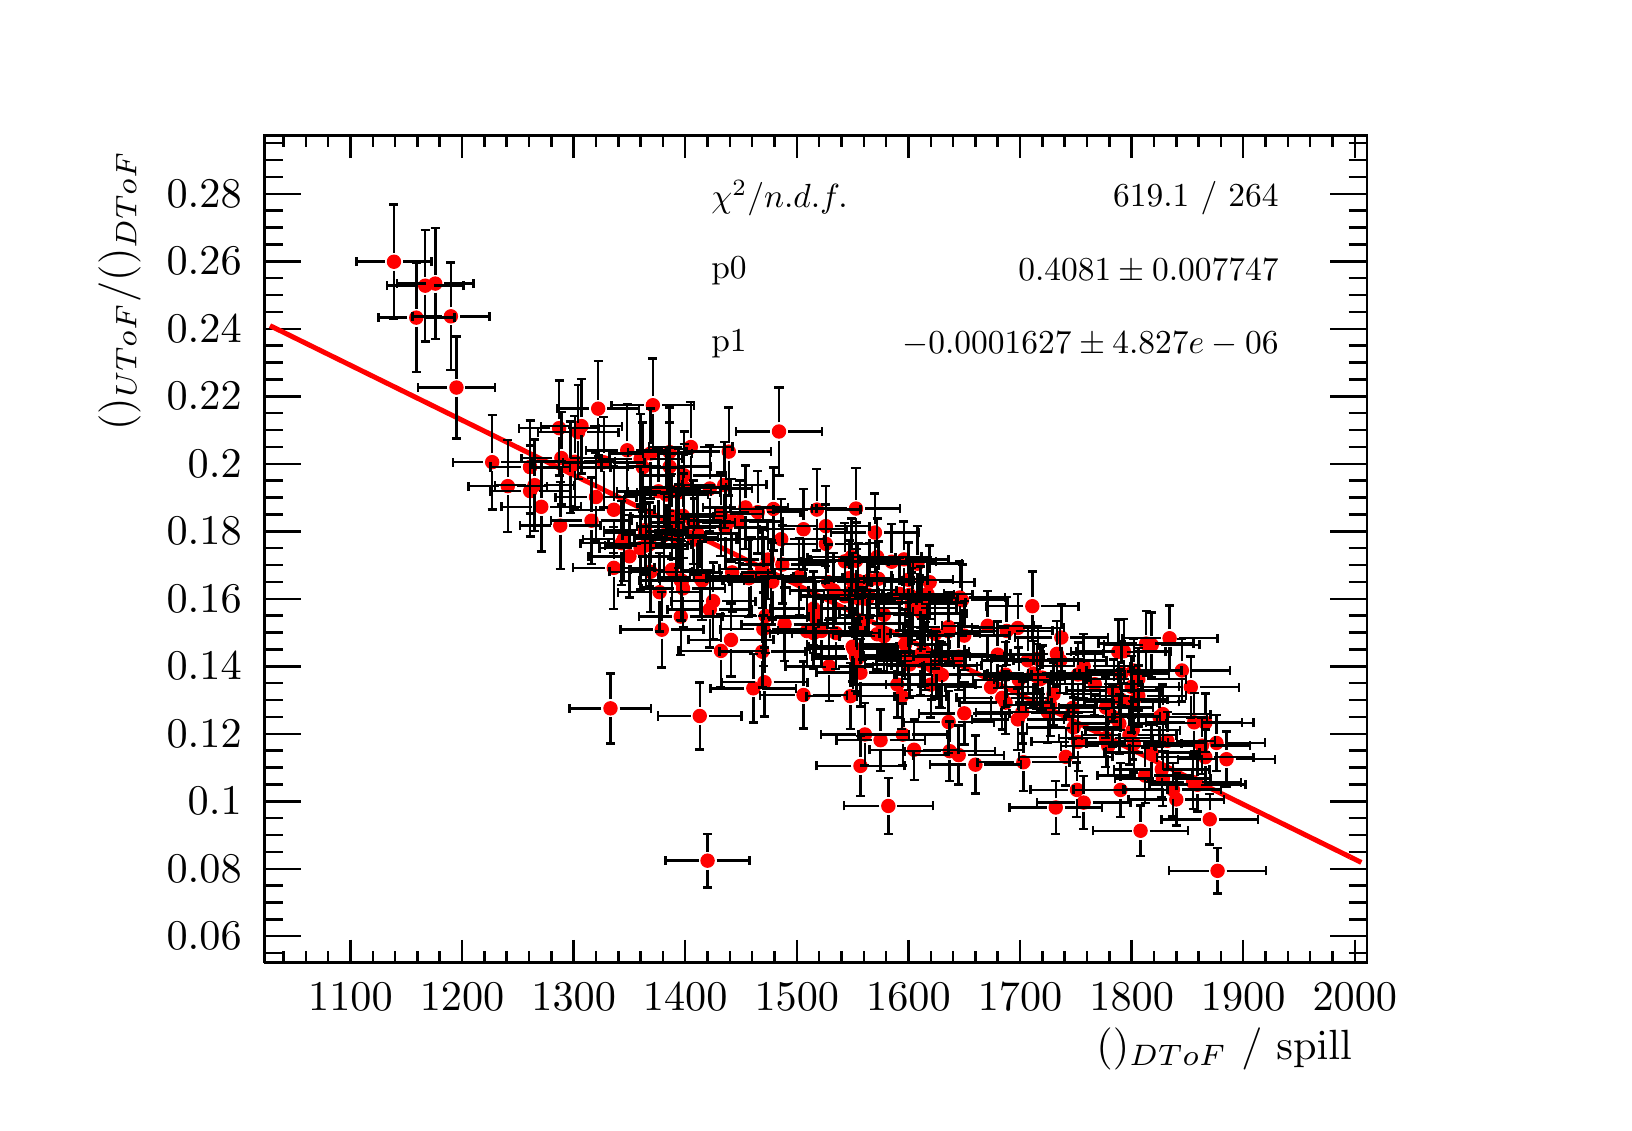
\begin{tikzpicture}
\pgfdeclareplotmark{cross} {
\pgfpathmoveto{\pgfpoint{-0.3\pgfplotmarksize}{\pgfplotmarksize}}
\pgfpathlineto{\pgfpoint{+0.3\pgfplotmarksize}{\pgfplotmarksize}}
\pgfpathlineto{\pgfpoint{+0.3\pgfplotmarksize}{0.3\pgfplotmarksize}}
\pgfpathlineto{\pgfpoint{+1\pgfplotmarksize}{0.3\pgfplotmarksize}}
\pgfpathlineto{\pgfpoint{+1\pgfplotmarksize}{-0.3\pgfplotmarksize}}
\pgfpathlineto{\pgfpoint{+0.3\pgfplotmarksize}{-0.3\pgfplotmarksize}}
\pgfpathlineto{\pgfpoint{+0.3\pgfplotmarksize}{-1.\pgfplotmarksize}}
\pgfpathlineto{\pgfpoint{-0.3\pgfplotmarksize}{-1.\pgfplotmarksize}}
\pgfpathlineto{\pgfpoint{-0.3\pgfplotmarksize}{-0.3\pgfplotmarksize}}
\pgfpathlineto{\pgfpoint{-1.\pgfplotmarksize}{-0.3\pgfplotmarksize}}
\pgfpathlineto{\pgfpoint{-1.\pgfplotmarksize}{0.3\pgfplotmarksize}}
\pgfpathlineto{\pgfpoint{-0.3\pgfplotmarksize}{0.3\pgfplotmarksize}}
\pgfpathclose
\pgfusepathqstroke
}
\pgfdeclareplotmark{cross*} {
\pgfpathmoveto{\pgfpoint{-0.3\pgfplotmarksize}{\pgfplotmarksize}}
\pgfpathlineto{\pgfpoint{+0.3\pgfplotmarksize}{\pgfplotmarksize}}
\pgfpathlineto{\pgfpoint{+0.3\pgfplotmarksize}{0.3\pgfplotmarksize}}
\pgfpathlineto{\pgfpoint{+1\pgfplotmarksize}{0.3\pgfplotmarksize}}
\pgfpathlineto{\pgfpoint{+1\pgfplotmarksize}{-0.3\pgfplotmarksize}}
\pgfpathlineto{\pgfpoint{+0.3\pgfplotmarksize}{-0.3\pgfplotmarksize}}
\pgfpathlineto{\pgfpoint{+0.3\pgfplotmarksize}{-1.\pgfplotmarksize}}
\pgfpathlineto{\pgfpoint{-0.3\pgfplotmarksize}{-1.\pgfplotmarksize}}
\pgfpathlineto{\pgfpoint{-0.3\pgfplotmarksize}{-0.3\pgfplotmarksize}}
\pgfpathlineto{\pgfpoint{-1.\pgfplotmarksize}{-0.3\pgfplotmarksize}}
\pgfpathlineto{\pgfpoint{-1.\pgfplotmarksize}{0.3\pgfplotmarksize}}
\pgfpathlineto{\pgfpoint{-0.3\pgfplotmarksize}{0.3\pgfplotmarksize}}
\pgfpathclose
\pgfusepathqfillstroke
}
\pgfdeclareplotmark{newstar} {
\pgfpathmoveto{\pgfqpoint{0pt}{\pgfplotmarksize}}
\pgfpathlineto{\pgfqpointpolar{44}{0.5\pgfplotmarksize}}
\pgfpathlineto{\pgfqpointpolar{18}{\pgfplotmarksize}}
\pgfpathlineto{\pgfqpointpolar{-20}{0.5\pgfplotmarksize}}
\pgfpathlineto{\pgfqpointpolar{-54}{\pgfplotmarksize}}
\pgfpathlineto{\pgfqpointpolar{-90}{0.5\pgfplotmarksize}}
\pgfpathlineto{\pgfqpointpolar{234}{\pgfplotmarksize}}
\pgfpathlineto{\pgfqpointpolar{198}{0.5\pgfplotmarksize}}
\pgfpathlineto{\pgfqpointpolar{162}{\pgfplotmarksize}}
\pgfpathlineto{\pgfqpointpolar{134}{0.5\pgfplotmarksize}}
\pgfpathclose
\pgfusepathqstroke
}
\pgfdeclareplotmark{newstar*} {
\pgfpathmoveto{\pgfqpoint{0pt}{\pgfplotmarksize}}
\pgfpathlineto{\pgfqpointpolar{44}{0.5\pgfplotmarksize}}
\pgfpathlineto{\pgfqpointpolar{18}{\pgfplotmarksize}}
\pgfpathlineto{\pgfqpointpolar{-20}{0.5\pgfplotmarksize}}
\pgfpathlineto{\pgfqpointpolar{-54}{\pgfplotmarksize}}
\pgfpathlineto{\pgfqpointpolar{-90}{0.5\pgfplotmarksize}}
\pgfpathlineto{\pgfqpointpolar{234}{\pgfplotmarksize}}
\pgfpathlineto{\pgfqpointpolar{198}{0.5\pgfplotmarksize}}
\pgfpathlineto{\pgfqpointpolar{162}{\pgfplotmarksize}}
\pgfpathlineto{\pgfqpointpolar{134}{0.5\pgfplotmarksize}}
\pgfpathclose
\pgfusepathqfillstroke
}
\definecolor{c}{rgb}{1,1,1};
\draw [color=c, fill=c] (0,0) rectangle (20,13.639);
\draw [color=c, fill=c] (3,1.77307) rectangle (17,12.2751);
\definecolor{c}{rgb}{0,0,0};
\draw [c,line width=0.9] (3,1.77307) -- (3,12.2751) -- (17,12.2751) -- (17,1.77307) -- (3,1.77307);
\definecolor{c}{rgb}{1,1,1};
\draw [color=c, fill=c] (3,1.77307) rectangle (17,12.2751);
\definecolor{c}{rgb}{0,0,0};
\draw [c,line width=0.9] (3,1.77307) -- (3,12.2751) -- (17,12.2751) -- (17,1.77307) -- (3,1.77307);
\draw [c,line width=0.9] (3,1.77307) -- (17,1.77307);
\draw [c,line width=0.9] (4.09225,2.05948) -- (4.09225,1.77307);
\draw [c,line width=0.9] (4.3757,1.91628) -- (4.3757,1.77307);
\draw [c,line width=0.9] (4.65916,1.91628) -- (4.65916,1.77307);
\draw [c,line width=0.9] (4.94262,1.91628) -- (4.94262,1.77307);
\draw [c,line width=0.9] (5.22608,1.91628) -- (5.22608,1.77307);
\draw [c,line width=0.9] (5.50954,2.05948) -- (5.50954,1.77307);
\draw [c,line width=0.9] (5.793,1.91628) -- (5.793,1.77307);
\draw [c,line width=0.9] (6.07646,1.91628) -- (6.07646,1.77307);
\draw [c,line width=0.9] (6.35991,1.91628) -- (6.35991,1.77307);
\draw [c,line width=0.9] (6.64337,1.91628) -- (6.64337,1.77307);
\draw [c,line width=0.9] (6.92683,2.05948) -- (6.92683,1.77307);
\draw [c,line width=0.9] (7.21029,1.91628) -- (7.21029,1.77307);
\draw [c,line width=0.9] (7.49375,1.91628) -- (7.49375,1.77307);
\draw [c,line width=0.9] (7.77721,1.91628) -- (7.77721,1.77307);
\draw [c,line width=0.9] (8.06067,1.91628) -- (8.06067,1.77307);
\draw [c,line width=0.9] (8.34412,2.05948) -- (8.34412,1.77307);
\draw [c,line width=0.9] (8.62758,1.91628) -- (8.62758,1.77307);
\draw [c,line width=0.9] (8.91104,1.91628) -- (8.91104,1.77307);
\draw [c,line width=0.9] (9.1945,1.91628) -- (9.1945,1.77307);
\draw [c,line width=0.9] (9.47796,1.91628) -- (9.47796,1.77307);
\draw [c,line width=0.9] (9.76142,2.05948) -- (9.76142,1.77307);
\draw [c,line width=0.9] (10.0449,1.91628) -- (10.0449,1.77307);
\draw [c,line width=0.9] (10.3283,1.91628) -- (10.3283,1.77307);
\draw [c,line width=0.9] (10.6118,1.91628) -- (10.6118,1.77307);
\draw [c,line width=0.9] (10.8953,1.91628) -- (10.8953,1.77307);
\draw [c,line width=0.9] (11.1787,2.05948) -- (11.1787,1.77307);
\draw [c,line width=0.9] (11.4622,1.91628) -- (11.4622,1.77307);
\draw [c,line width=0.9] (11.7456,1.91628) -- (11.7456,1.77307);
\draw [c,line width=0.9] (12.0291,1.91628) -- (12.0291,1.77307);
\draw [c,line width=0.9] (12.3125,1.91628) -- (12.3125,1.77307);
\draw [c,line width=0.9] (12.596,2.05948) -- (12.596,1.77307);
\draw [c,line width=0.9] (12.8795,1.91628) -- (12.8795,1.77307);
\draw [c,line width=0.9] (13.1629,1.91628) -- (13.1629,1.77307);
\draw [c,line width=0.9] (13.4464,1.91628) -- (13.4464,1.77307);
\draw [c,line width=0.9] (13.7298,1.91628) -- (13.7298,1.77307);
\draw [c,line width=0.9] (14.0133,2.05948) -- (14.0133,1.77307);
\draw [c,line width=0.9] (14.2968,1.91628) -- (14.2968,1.77307);
\draw [c,line width=0.9] (14.5802,1.91628) -- (14.5802,1.77307);
\draw [c,line width=0.9] (14.8637,1.91628) -- (14.8637,1.77307);
\draw [c,line width=0.9] (15.1471,1.91628) -- (15.1471,1.77307);
\draw [c,line width=0.9] (15.4306,2.05948) -- (15.4306,1.77307);
\draw [c,line width=0.9] (15.714,1.91628) -- (15.714,1.77307);
\draw [c,line width=0.9] (15.9975,1.91628) -- (15.9975,1.77307);
\draw [c,line width=0.9] (16.281,1.91628) -- (16.281,1.77307);
\draw [c,line width=0.9] (16.5644,1.91628) -- (16.5644,1.77307);
\draw [c,line width=0.9] (16.8479,2.05948) -- (16.8479,1.77307);
\draw [c,line width=0.9] (4.09225,2.05948) -- (4.09225,1.77307);
\draw [c,line width=0.9] (3.80879,1.91628) -- (3.80879,1.77307);
\draw [c,line width=0.9] (3.52533,1.91628) -- (3.52533,1.77307);
\draw [c,line width=0.9] (3.24187,1.91628) -- (3.24187,1.77307);
\draw [c,line width=0.9] (16.8479,2.05948) -- (16.8479,1.77307);
\draw [anchor=base] (4.09225,1.15931) node[scale=1.52731, color=c, rotate=0]{1100};
\draw [anchor=base] (5.50954,1.15931) node[scale=1.52731, color=c, rotate=0]{1200};
\draw [anchor=base] (6.92683,1.15931) node[scale=1.52731, color=c, rotate=0]{1300};
\draw [anchor=base] (8.34412,1.15931) node[scale=1.52731, color=c, rotate=0]{1400};
\draw [anchor=base] (9.76142,1.15931) node[scale=1.52731, color=c, rotate=0]{1500};
\draw [anchor=base] (11.1787,1.15931) node[scale=1.52731, color=c, rotate=0]{1600};
\draw [anchor=base] (12.596,1.15931) node[scale=1.52731, color=c, rotate=0]{1700};
\draw [anchor=base] (14.0133,1.15931) node[scale=1.52731, color=c, rotate=0]{1800};
\draw [anchor=base] (15.4306,1.15931) node[scale=1.52731, color=c, rotate=0]{1900};
\draw [anchor=base] (16.8479,1.15931) node[scale=1.52731, color=c, rotate=0]{2000};
\draw [anchor= east] (17,0.681948) node[scale=1.52731, color=c, rotate=0]{ $(\SOne\STwo)_{\text{DToF}}$ / spill};
\draw [c,line width=0.9] (3,12.2751) -- (17,12.2751);
\draw [c,line width=0.9] (4.09225,11.9887) -- (4.09225,12.2751);
\draw [c,line width=0.9] (4.3757,12.1319) -- (4.3757,12.2751);
\draw [c,line width=0.9] (4.65916,12.1319) -- (4.65916,12.2751);
\draw [c,line width=0.9] (4.94262,12.1319) -- (4.94262,12.2751);
\draw [c,line width=0.9] (5.22608,12.1319) -- (5.22608,12.2751);
\draw [c,line width=0.9] (5.50954,11.9887) -- (5.50954,12.2751);
\draw [c,line width=0.9] (5.793,12.1319) -- (5.793,12.2751);
\draw [c,line width=0.9] (6.07646,12.1319) -- (6.07646,12.2751);
\draw [c,line width=0.9] (6.35991,12.1319) -- (6.35991,12.2751);
\draw [c,line width=0.9] (6.64337,12.1319) -- (6.64337,12.2751);
\draw [c,line width=0.9] (6.92683,11.9887) -- (6.92683,12.2751);
\draw [c,line width=0.9] (7.21029,12.1319) -- (7.21029,12.2751);
\draw [c,line width=0.9] (7.49375,12.1319) -- (7.49375,12.2751);
\draw [c,line width=0.9] (7.77721,12.1319) -- (7.77721,12.2751);
\draw [c,line width=0.9] (8.06067,12.1319) -- (8.06067,12.2751);
\draw [c,line width=0.9] (8.34412,11.9887) -- (8.34412,12.2751);
\draw [c,line width=0.9] (8.62758,12.1319) -- (8.62758,12.2751);
\draw [c,line width=0.9] (8.91104,12.1319) -- (8.91104,12.2751);
\draw [c,line width=0.9] (9.1945,12.1319) -- (9.1945,12.2751);
\draw [c,line width=0.9] (9.47796,12.1319) -- (9.47796,12.2751);
\draw [c,line width=0.9] (9.76142,11.9887) -- (9.76142,12.2751);
\draw [c,line width=0.9] (10.0449,12.1319) -- (10.0449,12.2751);
\draw [c,line width=0.9] (10.3283,12.1319) -- (10.3283,12.2751);
\draw [c,line width=0.9] (10.6118,12.1319) -- (10.6118,12.2751);
\draw [c,line width=0.9] (10.8953,12.1319) -- (10.8953,12.2751);
\draw [c,line width=0.9] (11.1787,11.9887) -- (11.1787,12.2751);
\draw [c,line width=0.9] (11.4622,12.1319) -- (11.4622,12.2751);
\draw [c,line width=0.9] (11.7456,12.1319) -- (11.7456,12.2751);
\draw [c,line width=0.9] (12.0291,12.1319) -- (12.0291,12.2751);
\draw [c,line width=0.9] (12.3125,12.1319) -- (12.3125,12.2751);
\draw [c,line width=0.9] (12.596,11.9887) -- (12.596,12.2751);
\draw [c,line width=0.9] (12.8795,12.1319) -- (12.8795,12.2751);
\draw [c,line width=0.9] (13.1629,12.1319) -- (13.1629,12.2751);
\draw [c,line width=0.9] (13.4464,12.1319) -- (13.4464,12.2751);
\draw [c,line width=0.9] (13.7298,12.1319) -- (13.7298,12.2751);
\draw [c,line width=0.9] (14.0133,11.9887) -- (14.0133,12.2751);
\draw [c,line width=0.9] (14.2968,12.1319) -- (14.2968,12.2751);
\draw [c,line width=0.9] (14.5802,12.1319) -- (14.5802,12.2751);
\draw [c,line width=0.9] (14.8637,12.1319) -- (14.8637,12.2751);
\draw [c,line width=0.9] (15.1471,12.1319) -- (15.1471,12.2751);
\draw [c,line width=0.9] (15.4306,11.9887) -- (15.4306,12.2751);
\draw [c,line width=0.9] (15.714,12.1319) -- (15.714,12.2751);
\draw [c,line width=0.9] (15.9975,12.1319) -- (15.9975,12.2751);
\draw [c,line width=0.9] (16.281,12.1319) -- (16.281,12.2751);
\draw [c,line width=0.9] (16.5644,12.1319) -- (16.5644,12.2751);
\draw [c,line width=0.9] (16.8479,11.9887) -- (16.8479,12.2751);
\draw [c,line width=0.9] (4.09225,11.9887) -- (4.09225,12.2751);
\draw [c,line width=0.9] (3.80879,12.1319) -- (3.80879,12.2751);
\draw [c,line width=0.9] (3.52533,12.1319) -- (3.52533,12.2751);
\draw [c,line width=0.9] (3.24187,12.1319) -- (3.24187,12.2751);
\draw [c,line width=0.9] (16.8479,11.9887) -- (16.8479,12.2751);
\draw [c,line width=0.9] (3,1.77307) -- (3,12.2751);
\draw [c,line width=0.9] (3.462,2.10714) -- (3,2.10714);
\draw [c,line width=0.9] (3.231,2.32142) -- (3,2.32142);
\draw [c,line width=0.9] (3.231,2.53571) -- (3,2.53571);
\draw [c,line width=0.9] (3.231,2.74999) -- (3,2.74999);
\draw [c,line width=0.9] (3.462,2.96428) -- (3,2.96428);
\draw [c,line width=0.9] (3.231,3.17856) -- (3,3.17856);
\draw [c,line width=0.9] (3.231,3.39285) -- (3,3.39285);
\draw [c,line width=0.9] (3.231,3.60714) -- (3,3.60714);
\draw [c,line width=0.9] (3.462,3.82142) -- (3,3.82142);
\draw [c,line width=0.9] (3.231,4.03571) -- (3,4.03571);
\draw [c,line width=0.9] (3.231,4.24999) -- (3,4.24999);
\draw [c,line width=0.9] (3.231,4.46428) -- (3,4.46428);
\draw [c,line width=0.9] (3.462,4.67856) -- (3,4.67856);
\draw [c,line width=0.9] (3.231,4.89285) -- (3,4.89285);
\draw [c,line width=0.9] (3.231,5.10713) -- (3,5.10713);
\draw [c,line width=0.9] (3.231,5.32142) -- (3,5.32142);
\draw [c,line width=0.9] (3.462,5.5357) -- (3,5.5357);
\draw [c,line width=0.9] (3.231,5.74999) -- (3,5.74999);
\draw [c,line width=0.9] (3.231,5.96427) -- (3,5.96427);
\draw [c,line width=0.9] (3.231,6.17856) -- (3,6.17856);
\draw [c,line width=0.9] (3.462,6.39284) -- (3,6.39284);
\draw [c,line width=0.9] (3.231,6.60713) -- (3,6.60713);
\draw [c,line width=0.9] (3.231,6.82141) -- (3,6.82141);
\draw [c,line width=0.9] (3.231,7.0357) -- (3,7.0357);
\draw [c,line width=0.9] (3.462,7.24999) -- (3,7.24999);
\draw [c,line width=0.9] (3.231,7.46427) -- (3,7.46427);
\draw [c,line width=0.9] (3.231,7.67856) -- (3,7.67856);
\draw [c,line width=0.9] (3.231,7.89284) -- (3,7.89284);
\draw [c,line width=0.9] (3.462,8.10713) -- (3,8.10713);
\draw [c,line width=0.9] (3.231,8.32141) -- (3,8.32141);
\draw [c,line width=0.9] (3.231,8.5357) -- (3,8.5357);
\draw [c,line width=0.9] (3.231,8.74998) -- (3,8.74998);
\draw [c,line width=0.9] (3.462,8.96427) -- (3,8.96427);
\draw [c,line width=0.9] (3.231,9.17855) -- (3,9.17855);
\draw [c,line width=0.9] (3.231,9.39284) -- (3,9.39284);
\draw [c,line width=0.9] (3.231,9.60712) -- (3,9.60712);
\draw [c,line width=0.9] (3.462,9.82141) -- (3,9.82141);
\draw [c,line width=0.9] (3.231,10.0357) -- (3,10.0357);
\draw [c,line width=0.9] (3.231,10.25) -- (3,10.25);
\draw [c,line width=0.9] (3.231,10.4643) -- (3,10.4643);
\draw [c,line width=0.9] (3.462,10.6785) -- (3,10.6785);
\draw [c,line width=0.9] (3.231,10.8928) -- (3,10.8928);
\draw [c,line width=0.9] (3.231,11.1071) -- (3,11.1071);
\draw [c,line width=0.9] (3.231,11.3214) -- (3,11.3214);
\draw [c,line width=0.9] (3.462,11.5357) -- (3,11.5357);
\draw [c,line width=0.9] (3.462,2.10714) -- (3,2.10714);
\draw [c,line width=0.9] (3.231,1.89285) -- (3,1.89285);
\draw [c,line width=0.9] (3.462,11.5357) -- (3,11.5357);
\draw [c,line width=0.9] (3.231,11.75) -- (3,11.75);
\draw [c,line width=0.9] (3.231,11.9643) -- (3,11.9643);
\draw [c,line width=0.9] (3.231,12.1785) -- (3,12.1785);
\draw [anchor= east] (2.9,2.10714) node[scale=1.52731, color=c, rotate=0]{0.06};
\draw [anchor= east] (2.9,2.96428) node[scale=1.52731, color=c, rotate=0]{0.08};
\draw [anchor= east] (2.9,3.82142) node[scale=1.52731, color=c, rotate=0]{0.1};
\draw [anchor= east] (2.9,4.67856) node[scale=1.52731, color=c, rotate=0]{0.12};
\draw [anchor= east] (2.9,5.5357) node[scale=1.52731, color=c, rotate=0]{0.14};
\draw [anchor= east] (2.9,6.39284) node[scale=1.52731, color=c, rotate=0]{0.16};
\draw [anchor= east] (2.9,7.24999) node[scale=1.52731, color=c, rotate=0]{0.18};
\draw [anchor= east] (2.9,8.10713) node[scale=1.52731, color=c, rotate=0]{0.2};
\draw [anchor= east] (2.9,8.96427) node[scale=1.52731, color=c, rotate=0]{0.22};
\draw [anchor= east] (2.9,9.82141) node[scale=1.52731, color=c, rotate=0]{0.24};
\draw [anchor= east] (2.9,10.6785) node[scale=1.52731, color=c, rotate=0]{0.26};
\draw [anchor= east] (2.9,11.5357) node[scale=1.52731, color=c, rotate=0]{0.28};
\draw [anchor= east] (1.16,12.2751) node[scale=1.52731, color=c, rotate=90]{ $(\SOne\STwo)_{\text{UToF}}/(\SOne\STwo)_{\text{DToF}}$ };
\draw [c,line width=0.9] (17,1.77307) -- (17,12.2751);
\draw [c,line width=0.9] (16.538,2.10714) -- (17,2.10714);
\draw [c,line width=0.9] (16.769,2.32142) -- (17,2.32142);
\draw [c,line width=0.9] (16.769,2.53571) -- (17,2.53571);
\draw [c,line width=0.9] (16.769,2.74999) -- (17,2.74999);
\draw [c,line width=0.9] (16.538,2.96428) -- (17,2.96428);
\draw [c,line width=0.9] (16.769,3.17856) -- (17,3.17856);
\draw [c,line width=0.9] (16.769,3.39285) -- (17,3.39285);
\draw [c,line width=0.9] (16.769,3.60714) -- (17,3.60714);
\draw [c,line width=0.9] (16.538,3.82142) -- (17,3.82142);
\draw [c,line width=0.9] (16.769,4.03571) -- (17,4.03571);
\draw [c,line width=0.9] (16.769,4.24999) -- (17,4.24999);
\draw [c,line width=0.9] (16.769,4.46428) -- (17,4.46428);
\draw [c,line width=0.9] (16.538,4.67856) -- (17,4.67856);
\draw [c,line width=0.9] (16.769,4.89285) -- (17,4.89285);
\draw [c,line width=0.9] (16.769,5.10713) -- (17,5.10713);
\draw [c,line width=0.9] (16.769,5.32142) -- (17,5.32142);
\draw [c,line width=0.9] (16.538,5.5357) -- (17,5.5357);
\draw [c,line width=0.9] (16.769,5.74999) -- (17,5.74999);
\draw [c,line width=0.9] (16.769,5.96427) -- (17,5.96427);
\draw [c,line width=0.9] (16.769,6.17856) -- (17,6.17856);
\draw [c,line width=0.9] (16.538,6.39284) -- (17,6.39284);
\draw [c,line width=0.9] (16.769,6.60713) -- (17,6.60713);
\draw [c,line width=0.9] (16.769,6.82141) -- (17,6.82141);
\draw [c,line width=0.9] (16.769,7.0357) -- (17,7.0357);
\draw [c,line width=0.9] (16.538,7.24999) -- (17,7.24999);
\draw [c,line width=0.9] (16.769,7.46427) -- (17,7.46427);
\draw [c,line width=0.9] (16.769,7.67856) -- (17,7.67856);
\draw [c,line width=0.9] (16.769,7.89284) -- (17,7.89284);
\draw [c,line width=0.9] (16.538,8.10713) -- (17,8.10713);
\draw [c,line width=0.9] (16.769,8.32141) -- (17,8.32141);
\draw [c,line width=0.9] (16.769,8.5357) -- (17,8.5357);
\draw [c,line width=0.9] (16.769,8.74998) -- (17,8.74998);
\draw [c,line width=0.9] (16.538,8.96427) -- (17,8.96427);
\draw [c,line width=0.9] (16.769,9.17855) -- (17,9.17855);
\draw [c,line width=0.9] (16.769,9.39284) -- (17,9.39284);
\draw [c,line width=0.9] (16.769,9.60712) -- (17,9.60712);
\draw [c,line width=0.9] (16.538,9.82141) -- (17,9.82141);
\draw [c,line width=0.9] (16.769,10.0357) -- (17,10.0357);
\draw [c,line width=0.9] (16.769,10.25) -- (17,10.25);
\draw [c,line width=0.9] (16.769,10.4643) -- (17,10.4643);
\draw [c,line width=0.9] (16.538,10.6785) -- (17,10.6785);
\draw [c,line width=0.9] (16.769,10.8928) -- (17,10.8928);
\draw [c,line width=0.9] (16.769,11.1071) -- (17,11.1071);
\draw [c,line width=0.9] (16.769,11.3214) -- (17,11.3214);
\draw [c,line width=0.9] (16.538,11.5357) -- (17,11.5357);
\draw [c,line width=0.9] (16.538,2.10714) -- (17,2.10714);
\draw [c,line width=0.9] (16.769,1.89285) -- (17,1.89285);
\draw [c,line width=0.9] (16.538,11.5357) -- (17,11.5357);
\draw [c,line width=0.9] (16.769,11.75) -- (17,11.75);
\draw [c,line width=0.9] (16.769,11.9643) -- (17,11.9643);
\draw [c,line width=0.9] (16.769,12.1785) -- (17,12.1785);
\definecolor{c}{rgb}{1,0,0};
\foreach \P in {(14.9487,4.38182), (11.859,6.37516), (12.4118,5.07385), (12.9503,4.95185), (9.97401,6.26837), (11.3346,6.34602), (10.1583,6.60376), (10.2575,5.95729), (8.65593,7.79369), (13.7865,5.22917), (10.4701,5.78455), (12.3692,5.13462),
 (9.32206,5.72067), (12.9787,5.04484), (12.8511,5.37306), (8.17405,6.7609), (8.92521,7.38739), (11.4196,6.45327), (5.89221,8.12808), (10.5126,5.66209), (12.4118,5.42951), (14.6511,5.48228), (14.0416,5.48148), (9.36457,6.1739), (10.5976,6.07836),
 (12.3125,5.68366), (9.33623,6.00801), (13.0212,5.18393), (10.5126,6.87633), (9.0386,7.37362), (10.7535,7.23361), (8.52837,6.66339), (13.7724,4.89585), (10.4559,6.92295), (10.0165,7.52554), (10.6685,6.44107), (13.9141,5.72644), (9.57717,6.82747),
 (11.8874,4.9383), (7.02604,8.58587), (10.3709,6.42395), (12.5677,6.02232), (8.23074,7.17117), (14.2684,5.80633), (12.4259,5.98458), (8.01815,6.47625), (8.25909,7.31393), (12.7519,6.29866), (8.84018,7.83834), (13.1062,5.60878), (6.75676,7.32186),
 (14.0416,4.55394), (11.8307,6.40951), (8.30161,6.62231), (9.3504,5.33351), (12.8228,5.62961), (5.04183,10.3693), (11.8165,5.65815), (14.0133,5.08332), (10.2291,6.49684), (13.4039,5.53619), (8.85435,7.29535), (13.3188,3.96583), (14.2684,4.43905),
 (10.1724,5.53402), (11.3771,5.72264), (11.2212,6.32654), (11.533,5.54889), (10.8669,6.18969), (11.2354,6.40246), (8.25909,7.74435), (15.218,4.35571), (5.43867,9.07545), (13.8432,5.71979), (13.1771,4.38513), (8.93939,6.72809), (9.84645,5.17031),
 (11.5756,5.43251), (9.88897,5.98273), (10.1299,7.09047), (14.8495,4.03121), (7.84807,7.07102), (10.796,6.64677), (4.92845,9.9634), (13.5456,5.3082), (10.7819,5.94246), (8.89687,8.262), (11.3488,5.70373), (14.0133,5.2738), (7.80555,8.06307),
 (11.6889,4.82736), (10.3709,6.86835), (9.56299,7.14962), (13.8857,5.44621), (6.77093,8.18027), (12.5818,5.36266), (13.333,5.43101), (7.77721,7.0357), (14.0983,5.15981), (14.0983,5.37339), (8.79766,7.46666), (12.7661,5.44358), (9.84645,7.27617),
 (8.17405,7.44019), (14.4101,4.10745), (8.69845,6.36277), (13.2621,5.00631), (8.44333,7.36391), (11.4622,5.3029), (15.0054,3.59224), (14.5802,3.84471), (10.6543,6.39065), (8.10318,7.71667), (13.1204,5.90136), (11.1362,5.81533), (11.0937,5.15499),
 (5.36781,9.97987), (7.43706,7.5233), (14.0275,4.7233), (7.89059,7.08582), (9.33623,6.67856), (13.8716,5.11432), (6.43078,7.83609), (9.78976,6.66905), (13.9849,4.66045), (6.51582,7.56088), (13.6873,5.01042), (6.88431,8.06087), (12.6385,4.31718),
 (11.8165,4.40761), (7.53627,7.09872), (10.9661,6.86333), (14.9487,4.8182), (8.41499,8.32065), (12.8086,5.40826), (13.6873,4.62454), (8.28743,6.62739), (10.0024,6.14649), (6.37409,7.76046), (10.5268,5.63057), (11.2212,6.27307), (11.1078,4.66781),
 (14.1834,4.14782), (12.6243,4.9495), (8.1457,7.76081), (11.1929,5.55872), (11.1929,6.4421), (5.16939,10.3958), (8.92521,5.87059), (4.64499,10.6733), (11.3346,5.60115), (12.2275,5.27047), (8.45751,7.14528), (10.5409,6.39836), (11.1787,6.63391),
 (7.90476,8.23861), (11.2496,4.47562), (10.8669,5.9181), (8.65593,6.25662), (9.10946,7.55299), (8.28743,6.16689), (9.60551,6.06933), (12.0291,4.28614), (11.7031,4.4576), (8.07484,7.20095), (11.0653,6.45422), (6.37409,8.06634), (11.037,5.3039),
 (14.807,4.82357), (8.31578,6.52528), (10.626,4.66978), (6.98352,8.50809), (8.32995,7.80691), (14.7645,5.27158), (6.74258,8.56001), (11.1787,5.66963), (13.4039,3.80435), (9.97401,5.9572), (10.4275,6.65547), (11.2354,6.40246), (11.5189,5.94844),
 (10.0732,5.98398), (6.09063,7.82395), (10.1299,7.31514), (14.4668,4.58873), (7.43706,6.78549), (13.0495,3.74224), (14.1267,3.4469), (10.8244,4.59693), (9.20867,5.25586), (15.1046,2.93779), (7.39454,5.00136), (9.46379,7.53338), (8.32995,7.96008),
 (14.5377,3.9684), (9.43544,6.64471), (7.1536,7.38416), (10.9236,3.76182), (14.7928,4.06401), (9.15198,6.65405), (9.39292,6.89178), (15.0904,4.5616), (7.60713,8.27881), (13.8574,4.80601), (8.62758,3.06689), (12.185,6.05019), (10.4701,6.50344),
 (7.93311,8.85111), (9.53465,8.51721), (14.1975,5.82362), (13.333,4.57484), (10.5693,5.45368), (11.122,6.89338), (9.44961,6.6109), (8.1457,8.07002), (7.8339,7.23365), (13.0637,5.69348), (12.5677,4.8613), (8.1457,8.25555), (7.8339,7.26507),
 (10.5126,7.53864), (7.21029,7.68505), (10.4842,5.75289), (14.396,4.22724), (11.6889,6.03238), (10.5693,4.27008), (10.5409,6.61884), (10.7819,6.92392), (14.4952,5.89183), (7.90476,6.73595), (10.6827,6.62835), (11.3913,5.66573), (8.52837,4.90422),
 (7.77721,8.17015), (11.8874,5.92531), (9.18033,6.67366), (12.8795,5.39118), (7.23864,8.80736), (8.79766,5.73083), (11.2921,6.83847), (8.50003,7.22022), (8.00397,7.75829), (14.0133,5.08332), (7.56461,7.15121), (14.4101,4.92801), (13.8716,3.96508),
 (8.04649,6.00001), (9.32206,6.77094), (6.37409,8.06634), (8.55672,6.62303), (12.6952,5.61153), (9.26536,7.49279), (10.4417,5.15586), (11.6889,5.97999), (11.4763,5.53729), (14.3676,4.88991), (14.9062,4.52765), (7.3095,8.1265), (13.2763,4.758),
 (7.63548,6.93253), (11.3488,6.20887), (11.448,6.60356), (6.941,8.13348), (11.6039,5.42527), (13.7157,4.52245), (8.31578,7.44496)}{\draw[mark options={color=c,fill=c},mark size=2.402402pt,mark=*] plot coordinates {\P};}
\draw [c,line width=1.8] (3.07,9.86152) -- (3.21,9.79266) -- (3.35,9.7238) -- (3.49,9.65494) -- (3.63,9.58609) -- (3.77,9.51723) -- (3.91,9.44837) -- (4.05,9.37951) -- (4.19,9.31065) -- (4.33,9.2418) -- (4.47,9.17294) -- (4.61,9.10408) --
 (4.75,9.03522) -- (4.89,8.96637) -- (5.03,8.89751) -- (5.17,8.82865) -- (5.31,8.75979) -- (5.45,8.69094) -- (5.59,8.62208) -- (5.73,8.55322) -- (5.87,8.48436) -- (6.01,8.41551) -- (6.15,8.34665) -- (6.29,8.27779) -- (6.43,8.20893) -- (6.57,8.14007)
 -- (6.71,8.07122) -- (6.85,8.00236) -- (6.99,7.9335) -- (7.13,7.86464) -- (7.27,7.79579) -- (7.41,7.72693) -- (7.55,7.65807) -- (7.69,7.58921) -- (7.83,7.52036) -- (7.97,7.4515) -- (8.11,7.38264) -- (8.25,7.31378) -- (8.39,7.24492) -- (8.53,7.17607)
 -- (8.67,7.10721) -- (8.81,7.03835) -- (8.95,6.96949) -- (9.09,6.90064) -- (9.23,6.83178) -- (9.37,6.76292) -- (9.51,6.69406) -- (9.65,6.62521) -- (9.79,6.55635) -- (9.93,6.48749);
\draw [c,line width=1.8] (9.93,6.48749) -- (10.07,6.41863) -- (10.21,6.34977) -- (10.35,6.28092) -- (10.49,6.21206) -- (10.63,6.1432) -- (10.77,6.07434) -- (10.91,6.00549) -- (11.05,5.93663) -- (11.19,5.86777) -- (11.33,5.79891) -- (11.47,5.73006) --
 (11.61,5.6612) -- (11.75,5.59234) -- (11.89,5.52348) -- (12.03,5.45463) -- (12.17,5.38577) -- (12.31,5.31691) -- (12.45,5.24805) -- (12.59,5.17919) -- (12.73,5.11034) -- (12.87,5.04148) -- (13.01,4.97262) -- (13.15,4.90376) -- (13.29,4.83491) --
 (13.43,4.76605) -- (13.57,4.69719) -- (13.71,4.62833) -- (13.85,4.55948) -- (13.99,4.49062) -- (14.13,4.42176) -- (14.27,4.3529) -- (14.41,4.28404) -- (14.55,4.21519) -- (14.69,4.14633) -- (14.83,4.07747) -- (14.97,4.00861) -- (15.11,3.93976) --
 (15.25,3.8709) -- (15.39,3.80204) -- (15.53,3.73318) -- (15.67,3.66433) -- (15.81,3.59547) -- (15.95,3.52661) -- (16.09,3.45775) -- (16.23,3.3889) -- (16.37,3.32004) -- (16.51,3.25118) -- (16.65,3.18232) -- (16.79,3.11346);
\draw [c,line width=1.8] (16.79,3.11346) -- (16.93,3.04461);
\definecolor{c}{rgb}{1,1,1};
\draw [color=c, fill=c] (8.10888,9.16905) rectangle (16.447,11.9484);
\definecolor{c}{rgb}{0,0,0};
\draw [anchor= west] (8.52579,11.4852) node[scale=1.20912, color=c, rotate=0]{$\chi^{2} / \text{n.d.f.} $};
\draw [anchor= east] (16.0301,11.4852) node[scale=1.20912, color=c, rotate=0]{ 619.1 / 264};
\draw [anchor= west] (8.52579,10.5587) node[scale=1.20912, color=c, rotate=0]{p0       };
\draw [anchor= east] (16.0301,10.5587) node[scale=1.20912, color=c, rotate=0]{$ 0.4081 \pm 0.007747$};
\draw [anchor= west] (8.52579,9.63228) node[scale=1.20912, color=c, rotate=0]{p1       };
\draw [anchor= east] (16.0301,9.63228) node[scale=1.20912, color=c, rotate=0]{$ -0.0001627 \pm 4.827e-06$};
\draw [c,line width=0.9] (14.8341,4.38182) -- (14.3365,4.38182);
\draw [c,line width=0.9] (14.3365,4.32452) -- (14.3365,4.43913);
\draw [c,line width=0.9] (15.0633,4.38182) -- (15.5609,4.38182);
\draw [c,line width=0.9] (15.5609,4.32452) -- (15.5609,4.43913);
\draw [c,line width=0.9] (14.9487,4.49644) -- (14.9487,4.7338);
\draw [c,line width=0.9] (14.8914,4.7338) -- (15.006,4.7338);
\draw [c,line width=0.9] (14.9487,4.26721) -- (14.9487,4.02985);
\draw [c,line width=0.9] (14.8914,4.02985) -- (15.006,4.02985);
\draw [c,line width=0.9] (11.7444,6.37516) -- (11.2837,6.37516);
\draw [c,line width=0.9] (11.2837,6.31785) -- (11.2837,6.43247);
\draw [c,line width=0.9] (11.9736,6.37516) -- (12.4344,6.37516);
\draw [c,line width=0.9] (12.4344,6.31785) -- (12.4344,6.43247);
\draw [c,line width=0.9] (11.859,6.48977) -- (11.859,6.82931);
\draw [c,line width=0.9] (11.8017,6.82931) -- (11.9163,6.82931);
\draw [c,line width=0.9] (11.859,6.26055) -- (11.859,5.92102);
\draw [c,line width=0.9] (11.8017,5.92102) -- (11.9163,5.92102);
\draw [c,line width=0.9] (12.2971,5.07385) -- (11.8296,5.07385);
\draw [c,line width=0.9] (11.8296,5.01655) -- (11.8296,5.13116);
\draw [c,line width=0.9] (12.5264,5.07385) -- (12.9939,5.07385);
\draw [c,line width=0.9] (12.9939,5.01655) -- (12.9939,5.13116);
\draw [c,line width=0.9] (12.4118,5.18847) -- (12.4118,5.47244);
\draw [c,line width=0.9] (12.3544,5.47244) -- (12.4691,5.47244);
\draw [c,line width=0.9] (12.4118,4.95924) -- (12.4118,4.67526);
\draw [c,line width=0.9] (12.3544,4.67526) -- (12.4691,4.67526);
\draw [c,line width=0.9] (12.8357,4.95185) -- (12.3617,4.95185);
\draw [c,line width=0.9] (12.3617,4.89455) -- (12.3617,5.00916);
\draw [c,line width=0.9] (13.0649,4.95185) -- (13.539,4.95185);
\draw [c,line width=0.9] (13.539,4.89455) -- (13.539,5.00916);
\draw [c,line width=0.9] (12.9503,5.06647) -- (12.9503,5.34117);
\draw [c,line width=0.9] (12.893,5.34117) -- (13.0076,5.34117);
\draw [c,line width=0.9] (12.9503,4.83724) -- (12.9503,4.56254);
\draw [c,line width=0.9] (12.893,4.56254) -- (13.0076,4.56254);
\draw [c,line width=0.9] (9.8594,6.26837) -- (9.42236,6.26837);
\draw [c,line width=0.9] (9.42236,6.21107) -- (9.42236,6.32568);
\draw [c,line width=0.9] (10.0886,6.26837) -- (10.5257,6.26837);
\draw [c,line width=0.9] (10.5257,6.21107) -- (10.5257,6.32568);
\draw [c,line width=0.9] (9.97401,6.38299) -- (9.97401,6.73782);
\draw [c,line width=0.9] (9.9167,6.73782) -- (10.0313,6.73782);
\draw [c,line width=0.9] (9.97401,6.15376) -- (9.97401,5.79893);
\draw [c,line width=0.9] (9.9167,5.79893) -- (10.0313,5.79893);
\draw [c,line width=0.9] (11.22,6.34602) -- (10.7657,6.34602);
\draw [c,line width=0.9] (10.7657,6.28872) -- (10.7657,6.40333);
\draw [c,line width=0.9] (11.4492,6.34602) -- (11.9035,6.34602);
\draw [c,line width=0.9] (11.9035,6.28872) -- (11.9035,6.40333);
\draw [c,line width=0.9] (11.3346,6.46064) -- (11.3346,6.80424);
\draw [c,line width=0.9] (11.2773,6.80424) -- (11.3919,6.80424);
\draw [c,line width=0.9] (11.3346,6.23141) -- (11.3346,5.88781);
\draw [c,line width=0.9] (11.2773,5.88781) -- (11.3919,5.88781);
\draw [c,line width=0.9] (10.0436,6.60376) -- (9.60424,6.60376);
\draw [c,line width=0.9] (9.60424,6.54646) -- (9.60424,6.66107);
\draw [c,line width=0.9] (10.2729,6.60376) -- (10.7123,6.60376);
\draw [c,line width=0.9] (10.7123,6.54646) -- (10.7123,6.66107);
\draw [c,line width=0.9] (10.1583,6.71838) -- (10.1583,7.08432);
\draw [c,line width=0.9] (10.101,7.08432) -- (10.2156,7.08432);
\draw [c,line width=0.9] (10.1583,6.48915) -- (10.1583,6.1232);
\draw [c,line width=0.9] (10.101,6.1232) -- (10.2156,6.1232);
\draw [c,line width=0.9] (10.1429,5.95729) -- (9.70219,5.95729);
\draw [c,line width=0.9] (9.70219,5.89999) -- (9.70219,6.0146);
\draw [c,line width=0.9] (10.3721,5.95729) -- (10.8128,5.95729);
\draw [c,line width=0.9] (10.8128,5.89999) -- (10.8128,6.0146);
\draw [c,line width=0.9] (10.2575,6.07191) -- (10.2575,6.41134);
\draw [c,line width=0.9] (10.2002,6.41134) -- (10.3148,6.41134);
\draw [c,line width=0.9] (10.2575,5.84268) -- (10.2575,5.50325);
\draw [c,line width=0.9] (10.2002,5.50325) -- (10.3148,5.50325);
\draw [c,line width=0.9] (8.54132,7.79369) -- (8.12148,7.79369);
\draw [c,line width=0.9] (8.12148,7.73638) -- (8.12148,7.85099);
\draw [c,line width=0.9] (8.77054,7.79369) -- (9.19038,7.79369);
\draw [c,line width=0.9] (9.19038,7.73638) -- (9.19038,7.85099);
\draw [c,line width=0.9] (8.65593,7.9083) -- (8.65593,8.33852);
\draw [c,line width=0.9] (8.59862,8.33852) -- (8.71323,8.33852);
\draw [c,line width=0.9] (8.65593,7.67907) -- (8.65593,7.24886);
\draw [c,line width=0.9] (8.59862,7.24886) -- (8.71323,7.24886);
\draw [c,line width=0.9] (13.6719,5.22917) -- (13.1879,5.22917);
\draw [c,line width=0.9] (13.1879,5.17186) -- (13.1879,5.28648);
\draw [c,line width=0.9] (13.9011,5.22917) -- (14.3852,5.22917);
\draw [c,line width=0.9] (14.3852,5.17186) -- (14.3852,5.28648);
\draw [c,line width=0.9] (13.7865,5.34378) -- (13.7865,5.6228);
\draw [c,line width=0.9] (13.7292,5.6228) -- (13.8438,5.6228);
\draw [c,line width=0.9] (13.7865,5.11456) -- (13.7865,4.83554);
\draw [c,line width=0.9] (13.7292,4.83554) -- (13.8438,4.83554);
\draw [c,line width=0.9] (10.3554,5.78455) -- (9.91207,5.78455);
\draw [c,line width=0.9] (9.91207,5.72724) -- (9.91207,5.84186);
\draw [c,line width=0.9] (10.5847,5.78455) -- (11.0281,5.78455);
\draw [c,line width=0.9] (11.0281,5.72724) -- (11.0281,5.84186);
\draw [c,line width=0.9] (10.4701,5.89916) -- (10.4701,6.22949);
\draw [c,line width=0.9] (10.4128,6.22949) -- (10.5274,6.22949);
\draw [c,line width=0.9] (10.4701,5.66994) -- (10.4701,5.33961);
\draw [c,line width=0.9] (10.4128,5.33961) -- (10.5274,5.33961);
\draw [c,line width=0.9] (12.2546,5.13462) -- (11.7876,5.13462);
\draw [c,line width=0.9] (11.7876,5.07731) -- (11.7876,5.19192);
\draw [c,line width=0.9] (12.4838,5.13462) -- (12.9508,5.13462);
\draw [c,line width=0.9] (12.9508,5.07731) -- (12.9508,5.19192);
\draw [c,line width=0.9] (12.3692,5.24923) -- (12.3692,5.536);
\draw [c,line width=0.9] (12.3119,5.536) -- (12.4265,5.536);
\draw [c,line width=0.9] (12.3692,5.02) -- (12.3692,4.73324);
\draw [c,line width=0.9] (12.3119,4.73324) -- (12.4265,4.73324);
\draw [c,line width=0.9] (9.20744,5.72067) -- (8.77884,5.72067);
\draw [c,line width=0.9] (8.77884,5.66336) -- (8.77884,5.77797);
\draw [c,line width=0.9] (9.43667,5.72067) -- (9.86527,5.72067);
\draw [c,line width=0.9] (9.86527,5.66336) -- (9.86527,5.77797);
\draw [c,line width=0.9] (9.32206,5.83528) -- (9.32206,6.17507);
\draw [c,line width=0.9] (9.26475,6.17507) -- (9.37936,6.17507);
\draw [c,line width=0.9] (9.32206,5.60605) -- (9.32206,5.26626);
\draw [c,line width=0.9] (9.26475,5.26626) -- (9.37936,5.26626);
\draw [c,line width=0.9] (12.8641,5.04484) -- (12.3897,5.04484);
\draw [c,line width=0.9] (12.3897,4.98754) -- (12.3897,5.10215);
\draw [c,line width=0.9] (13.0933,5.04484) -- (13.5677,5.04484);
\draw [c,line width=0.9] (13.5677,4.98754) -- (13.5677,5.10215);
\draw [c,line width=0.9] (12.9787,5.15946) -- (12.9787,5.43764);
\draw [c,line width=0.9] (12.9214,5.43764) -- (13.036,5.43764);
\draw [c,line width=0.9] (12.9787,4.93023) -- (12.9787,4.65205);
\draw [c,line width=0.9] (12.9214,4.65205) -- (13.036,4.65205);
\draw [c,line width=0.9] (12.7365,5.37306) -- (12.2637,5.37306);
\draw [c,line width=0.9] (12.2637,5.31575) -- (12.2637,5.43036);
\draw [c,line width=0.9] (12.9657,5.37306) -- (13.4386,5.37306);
\draw [c,line width=0.9] (13.4386,5.31575) -- (13.4386,5.43036);
\draw [c,line width=0.9] (12.8511,5.48767) -- (12.8511,5.77981);
\draw [c,line width=0.9] (12.7938,5.77981) -- (12.9084,5.77981);
\draw [c,line width=0.9] (12.8511,5.25844) -- (12.8511,4.9663);
\draw [c,line width=0.9] (12.7938,4.9663) -- (12.9084,4.9663);
\draw [c,line width=0.9] (8.05944,6.7609) -- (7.64602,6.7609);
\draw [c,line width=0.9] (7.64602,6.70359) -- (7.64602,6.8182);
\draw [c,line width=0.9] (8.28866,6.7609) -- (8.70207,6.7609);
\draw [c,line width=0.9] (8.70207,6.70359) -- (8.70207,6.8182);
\draw [c,line width=0.9] (8.17405,6.87551) -- (8.17405,7.27149);
\draw [c,line width=0.9] (8.11674,7.27149) -- (8.23135,7.27149);
\draw [c,line width=0.9] (8.17405,6.64628) -- (8.17405,6.25031);
\draw [c,line width=0.9] (8.11674,6.25031) -- (8.23135,6.25031);
\draw [c,line width=0.9] (8.8106,7.38739) -- (8.3872,7.38739);
\draw [c,line width=0.9] (8.3872,7.33008) -- (8.3872,7.4447);
\draw [c,line width=0.9] (9.03983,7.38739) -- (9.46323,7.38739);
\draw [c,line width=0.9] (9.46323,7.33008) -- (9.46323,7.4447);
\draw [c,line width=0.9] (8.92521,7.502) -- (8.92521,7.91303);
\draw [c,line width=0.9] (8.86791,7.91303) -- (8.98252,7.91303);
\draw [c,line width=0.9] (8.92521,7.27278) -- (8.92521,6.86175);
\draw [c,line width=0.9] (8.86791,6.86175) -- (8.98252,6.86175);
\draw [c,line width=0.9] (11.305,6.45327) -- (10.8497,6.45327);
\draw [c,line width=0.9] (10.8497,6.39597) -- (10.8497,6.51058);
\draw [c,line width=0.9] (11.5343,6.45327) -- (11.9896,6.45327);
\draw [c,line width=0.9] (11.9896,6.39597) -- (11.9896,6.51058);
\draw [c,line width=0.9] (11.4196,6.56789) -- (11.4196,6.91472);
\draw [c,line width=0.9] (11.3623,6.91472) -- (11.477,6.91472);
\draw [c,line width=0.9] (11.4196,6.33866) -- (11.4196,5.99182);
\draw [c,line width=0.9] (11.3623,5.99182) -- (11.477,5.99182);
\draw [c,line width=0.9] (5.77759,8.12808) -- (5.39575,8.12808);
\draw [c,line width=0.9] (5.39575,8.07078) -- (5.39575,8.18539);
\draw [c,line width=0.9] (6.00682,8.12808) -- (6.38866,8.12808);
\draw [c,line width=0.9] (6.38866,8.07078) -- (6.38866,8.18539);
\draw [c,line width=0.9] (5.89221,8.2427) -- (5.89221,8.72832);
\draw [c,line width=0.9] (5.8349,8.72832) -- (5.94951,8.72832);
\draw [c,line width=0.9] (5.89221,8.01347) -- (5.89221,7.52784);
\draw [c,line width=0.9] (5.8349,7.52784) -- (5.94951,7.52784);
\draw [c,line width=0.9] (10.398,5.66209) -- (9.95405,5.66209);
\draw [c,line width=0.9] (9.95405,5.60479) -- (9.95405,5.7194);
\draw [c,line width=0.9] (10.6272,5.66209) -- (11.0711,5.66209);
\draw [c,line width=0.9] (11.0711,5.60479) -- (11.0711,5.7194);
\draw [c,line width=0.9] (10.5126,5.77671) -- (10.5126,6.10168);
\draw [c,line width=0.9] (10.4553,6.10168) -- (10.5699,6.10168);
\draw [c,line width=0.9] (10.5126,5.54748) -- (10.5126,5.22251);
\draw [c,line width=0.9] (10.4553,5.22251) -- (10.5699,5.22251);
\draw [c,line width=0.9] (12.2971,5.42951) -- (11.8296,5.42951);
\draw [c,line width=0.9] (11.8296,5.37221) -- (11.8296,5.48682);
\draw [c,line width=0.9] (12.5264,5.42951) -- (12.9939,5.42951);
\draw [c,line width=0.9] (12.9939,5.37221) -- (12.9939,5.48682);
\draw [c,line width=0.9] (12.4118,5.54413) -- (12.4118,5.84221);
\draw [c,line width=0.9] (12.3544,5.84221) -- (12.4691,5.84221);
\draw [c,line width=0.9] (12.4118,5.3149) -- (12.4118,5.01682);
\draw [c,line width=0.9] (12.3544,5.01682) -- (12.4691,5.01682);
\draw [c,line width=0.9] (14.5365,5.48228) -- (14.0423,5.48228);
\draw [c,line width=0.9] (14.0423,5.42497) -- (14.0423,5.53958);
\draw [c,line width=0.9] (14.7657,5.48228) -- (15.2599,5.48228);
\draw [c,line width=0.9] (15.2599,5.42497) -- (15.2599,5.53958);
\draw [c,line width=0.9] (14.6511,5.59689) -- (14.6511,5.87888);
\draw [c,line width=0.9] (14.5938,5.87888) -- (14.7084,5.87888);
\draw [c,line width=0.9] (14.6511,5.36766) -- (14.6511,5.08567);
\draw [c,line width=0.9] (14.5938,5.08567) -- (14.7084,5.08567);
\draw [c,line width=0.9] (13.927,5.48148) -- (13.44,5.48148);
\draw [c,line width=0.9] (13.44,5.42417) -- (13.44,5.53878);
\draw [c,line width=0.9] (14.1563,5.48148) -- (14.6433,5.48148);
\draw [c,line width=0.9] (14.6433,5.42417) -- (14.6433,5.53878);
\draw [c,line width=0.9] (14.0416,5.59609) -- (14.0416,5.88276);
\draw [c,line width=0.9] (13.9843,5.88276) -- (14.0989,5.88276);
\draw [c,line width=0.9] (14.0416,5.36686) -- (14.0416,5.0802);
\draw [c,line width=0.9] (13.9843,5.0802) -- (14.0989,5.0802);
\draw [c,line width=0.9] (9.24996,6.1739) -- (8.82081,6.1739);
\draw [c,line width=0.9] (8.82081,6.11659) -- (8.82081,6.23121);
\draw [c,line width=0.9] (9.47919,6.1739) -- (9.90834,6.1739);
\draw [c,line width=0.9] (9.90834,6.11659) -- (9.90834,6.23121);
\draw [c,line width=0.9] (9.36457,6.28851) -- (9.36457,6.64635);
\draw [c,line width=0.9] (9.30727,6.64635) -- (9.42188,6.64635);
\draw [c,line width=0.9] (9.36457,6.05929) -- (9.36457,5.70145);
\draw [c,line width=0.9] (9.30727,5.70145) -- (9.42188,5.70145);
\draw [c,line width=0.9] (10.483,6.07836) -- (10.038,6.07836);
\draw [c,line width=0.9] (10.038,6.02105) -- (10.038,6.13566);
\draw [c,line width=0.9] (10.7122,6.07836) -- (11.1572,6.07836);
\draw [c,line width=0.9] (11.1572,6.02105) -- (11.1572,6.13566);
\draw [c,line width=0.9] (10.5976,6.19297) -- (10.5976,6.53368);
\draw [c,line width=0.9] (10.5403,6.53368) -- (10.6549,6.53368);
\draw [c,line width=0.9] (10.5976,5.96374) -- (10.5976,5.62304);
\draw [c,line width=0.9] (10.5403,5.62304) -- (10.6549,5.62304);
\draw [c,line width=0.9] (12.1979,5.68366) -- (11.7316,5.68366);
\draw [c,line width=0.9] (11.7316,5.62636) -- (11.7316,5.74097);
\draw [c,line width=0.9] (12.4272,5.68366) -- (12.8935,5.68366);
\draw [c,line width=0.9] (12.8935,5.62636) -- (12.8935,5.74097);
\draw [c,line width=0.9] (12.3125,5.79827) -- (12.3125,6.10714);
\draw [c,line width=0.9] (12.2552,6.10714) -- (12.3699,6.10714);
\draw [c,line width=0.9] (12.3125,5.56905) -- (12.3125,5.26018);
\draw [c,line width=0.9] (12.2552,5.26018) -- (12.3699,5.26018);
\draw [c,line width=0.9] (9.22162,6.00801) -- (8.79283,6.00801);
\draw [c,line width=0.9] (8.79283,5.9507) -- (8.79283,6.06531);
\draw [c,line width=0.9] (9.45084,6.00801) -- (9.87963,6.00801);
\draw [c,line width=0.9] (9.87963,5.9507) -- (9.87963,6.06531);
\draw [c,line width=0.9] (9.33623,6.12262) -- (9.33623,6.47404);
\draw [c,line width=0.9] (9.27892,6.47404) -- (9.39354,6.47404);
\draw [c,line width=0.9] (9.33623,5.89339) -- (9.33623,5.54197);
\draw [c,line width=0.9] (9.27892,5.54197) -- (9.39354,5.54197);
\draw [c,line width=0.9] (12.9066,5.18393) -- (12.4317,5.18393);
\draw [c,line width=0.9] (12.4317,5.12662) -- (12.4317,5.24123);
\draw [c,line width=0.9] (13.1358,5.18393) -- (13.6107,5.18393);
\draw [c,line width=0.9] (13.6107,5.12662) -- (13.6107,5.24123);
\draw [c,line width=0.9] (13.0212,5.29854) -- (13.0212,5.58188);
\draw [c,line width=0.9] (12.9639,5.58188) -- (13.0785,5.58188);
\draw [c,line width=0.9] (13.0212,5.06931) -- (13.0212,4.78598);
\draw [c,line width=0.9] (12.9639,4.78598) -- (13.0785,4.78598);
\draw [c,line width=0.9] (10.398,6.87633) -- (9.95405,6.87633);
\draw [c,line width=0.9] (9.95405,6.81902) -- (9.95405,6.93364);
\draw [c,line width=0.9] (10.6272,6.87633) -- (11.0711,6.87633);
\draw [c,line width=0.9] (11.0711,6.81902) -- (11.0711,6.93364);
\draw [c,line width=0.9] (10.5126,6.99094) -- (10.5126,7.36344);
\draw [c,line width=0.9] (10.4553,7.36344) -- (10.5699,7.36344);
\draw [c,line width=0.9] (10.5126,6.76172) -- (10.5126,6.38923);
\draw [c,line width=0.9] (10.4553,6.38923) -- (10.5699,6.38923);
\draw [c,line width=0.9] (8.92398,7.37362) -- (8.49909,7.37362);
\draw [c,line width=0.9] (8.49909,7.31631) -- (8.49909,7.43092);
\draw [c,line width=0.9] (9.15321,7.37362) -- (9.5781,7.37362);
\draw [c,line width=0.9] (9.5781,7.31631) -- (9.5781,7.43092);
\draw [c,line width=0.9] (9.0386,7.48823) -- (9.0386,7.89728);
\draw [c,line width=0.9] (8.98129,7.89728) -- (9.0959,7.89728);
\draw [c,line width=0.9] (9.0386,7.259) -- (9.0386,6.84996);
\draw [c,line width=0.9] (8.98129,6.84996) -- (9.0959,6.84996);
\draw [c,line width=0.9] (10.6389,7.23361) -- (10.1919,7.23361);
\draw [c,line width=0.9] (10.1919,7.1763) -- (10.1919,7.29091);
\draw [c,line width=0.9] (10.8681,7.23361) -- (11.3151,7.23361);
\draw [c,line width=0.9] (11.3151,7.1763) -- (11.3151,7.29091);
\draw [c,line width=0.9] (10.7535,7.34822) -- (10.7535,7.73148);
\draw [c,line width=0.9] (10.6962,7.73148) -- (10.8108,7.73148);
\draw [c,line width=0.9] (10.7535,7.11899) -- (10.7535,6.73573);
\draw [c,line width=0.9] (10.6962,6.73573) -- (10.8108,6.73573);
\draw [c,line width=0.9] (8.41376,6.66339) -- (7.99561,6.66339);
\draw [c,line width=0.9] (7.99561,6.60609) -- (7.99561,6.7207);
\draw [c,line width=0.9] (8.64299,6.66339) -- (9.06113,6.66339);
\draw [c,line width=0.9] (9.06113,6.60609) -- (9.06113,6.7207);
\draw [c,line width=0.9] (8.52837,6.77801) -- (8.52837,7.16553);
\draw [c,line width=0.9] (8.47107,7.16553) -- (8.58568,7.16553);
\draw [c,line width=0.9] (8.52837,6.54878) -- (8.52837,6.16126);
\draw [c,line width=0.9] (8.47107,6.16126) -- (8.58568,6.16126);
\draw [c,line width=0.9] (13.6577,4.89585) -- (13.1739,4.89585);
\draw [c,line width=0.9] (13.1739,4.83854) -- (13.1739,4.95316);
\draw [c,line width=0.9] (13.887,4.89585) -- (14.3708,4.89585);
\draw [c,line width=0.9] (14.3708,4.83854) -- (14.3708,4.95316);
\draw [c,line width=0.9] (13.7724,5.01046) -- (13.7724,5.27658);
\draw [c,line width=0.9] (13.715,5.27658) -- (13.8297,5.27658);
\draw [c,line width=0.9] (13.7724,4.78124) -- (13.7724,4.51512);
\draw [c,line width=0.9] (13.715,4.51512) -- (13.8297,4.51512);
\draw [c,line width=0.9] (10.3413,6.92295) -- (9.89808,6.92295);
\draw [c,line width=0.9] (9.89808,6.86565) -- (9.89808,6.98026);
\draw [c,line width=0.9] (10.5705,6.92295) -- (11.0137,6.92295);
\draw [c,line width=0.9] (11.0137,6.86565) -- (11.0137,6.98026);
\draw [c,line width=0.9] (10.4559,7.03757) -- (10.4559,7.41246);
\draw [c,line width=0.9] (10.3986,7.41246) -- (10.5132,7.41246);
\draw [c,line width=0.9] (10.4559,6.80834) -- (10.4559,6.43345);
\draw [c,line width=0.9] (10.3986,6.43345) -- (10.5132,6.43345);
\draw [c,line width=0.9] (9.90192,7.52554) -- (9.46433,7.52554);
\draw [c,line width=0.9] (9.46433,7.46823) -- (9.46433,7.58284);
\draw [c,line width=0.9] (10.1311,7.52554) -- (10.5687,7.52554);
\draw [c,line width=0.9] (10.5687,7.46823) -- (10.5687,7.58284);
\draw [c,line width=0.9] (10.0165,7.64015) -- (10.0165,8.04286);
\draw [c,line width=0.9] (9.95922,8.04286) -- (10.0738,8.04286);
\draw [c,line width=0.9] (10.0165,7.41092) -- (10.0165,7.00821);
\draw [c,line width=0.9] (9.95922,7.00821) -- (10.0738,7.00821);
\draw [c,line width=0.9] (10.5539,6.44107) -- (10.108,6.44107);
\draw [c,line width=0.9] (10.108,6.38377) -- (10.108,6.49838);
\draw [c,line width=0.9] (10.7831,6.44107) -- (11.229,6.44107);
\draw [c,line width=0.9] (11.229,6.38377) -- (11.229,6.49838);
\draw [c,line width=0.9] (10.6685,6.55569) -- (10.6685,6.9098);
\draw [c,line width=0.9] (10.6112,6.9098) -- (10.7258,6.9098);
\draw [c,line width=0.9] (10.6685,6.32646) -- (10.6685,5.97234);
\draw [c,line width=0.9] (10.6112,5.97234) -- (10.7258,5.97234);
\draw [c,line width=0.9] (13.7995,5.72644) -- (13.3139,5.72644);
\draw [c,line width=0.9] (13.3139,5.66914) -- (13.3139,5.78375);
\draw [c,line width=0.9] (14.0287,5.72644) -- (14.5142,5.72644);
\draw [c,line width=0.9] (14.5142,5.66914) -- (14.5142,5.78375);
\draw [c,line width=0.9] (13.9141,5.84106) -- (13.9141,6.13796);
\draw [c,line width=0.9] (13.8568,6.13796) -- (13.9714,6.13796);
\draw [c,line width=0.9] (13.9141,5.61183) -- (13.9141,5.31492);
\draw [c,line width=0.9] (13.8568,5.31492) -- (13.9714,5.31492);
\draw [c,line width=0.9] (9.46255,6.82747) -- (9.03064,6.82747);
\draw [c,line width=0.9] (9.03064,6.77016) -- (9.03064,6.88477);
\draw [c,line width=0.9] (9.69178,6.82747) -- (10.1237,6.82747);
\draw [c,line width=0.9] (10.1237,6.77016) -- (10.1237,6.88477);
\draw [c,line width=0.9] (9.57717,6.94208) -- (9.57717,7.32336);
\draw [c,line width=0.9] (9.51986,7.32336) -- (9.63447,7.32336);
\draw [c,line width=0.9] (9.57717,6.71285) -- (9.57717,6.33157);
\draw [c,line width=0.9] (9.51986,6.33157) -- (9.63447,6.33157);
\draw [c,line width=0.9] (11.7727,4.9383) -- (11.3116,4.9383);
\draw [c,line width=0.9] (11.3116,4.88099) -- (11.3116,4.99561);
\draw [c,line width=0.9] (12.002,4.9383) -- (12.4631,4.9383);
\draw [c,line width=0.9] (12.4631,4.88099) -- (12.4631,4.99561);
\draw [c,line width=0.9] (11.8874,5.05291) -- (11.8874,5.33581);
\draw [c,line width=0.9] (11.83,5.33581) -- (11.9447,5.33581);
\draw [c,line width=0.9] (11.8874,4.82369) -- (11.8874,4.54079);
\draw [c,line width=0.9] (11.83,4.54079) -- (11.9447,4.54079);
\draw [c,line width=0.9] (6.91143,8.58587) -- (6.51366,8.58587);
\draw [c,line width=0.9] (6.51366,8.52856) -- (6.51366,8.64317);
\draw [c,line width=0.9] (7.14065,8.58587) -- (7.53843,8.58587);
\draw [c,line width=0.9] (7.53843,8.52856) -- (7.53843,8.64317);
\draw [c,line width=0.9] (7.02604,8.70048) -- (7.02604,9.18539);
\draw [c,line width=0.9] (6.96873,9.18539) -- (7.08335,9.18539);
\draw [c,line width=0.9] (7.02604,8.47125) -- (7.02604,7.98635);
\draw [c,line width=0.9] (6.96873,7.98635) -- (7.08335,7.98635);
\draw [c,line width=0.9] (10.2562,6.42395) -- (9.81413,6.42395);
\draw [c,line width=0.9] (9.81413,6.36665) -- (9.81413,6.48126);
\draw [c,line width=0.9] (10.4855,6.42395) -- (10.9276,6.42395);
\draw [c,line width=0.9] (10.9276,6.36665) -- (10.9276,6.48126);
\draw [c,line width=0.9] (10.3709,6.53857) -- (10.3709,6.8952);
\draw [c,line width=0.9] (10.3135,6.8952) -- (10.4282,6.8952);
\draw [c,line width=0.9] (10.3709,6.30934) -- (10.3709,5.95271);
\draw [c,line width=0.9] (10.3135,5.95271) -- (10.4282,5.95271);
\draw [c,line width=0.9] (12.453,6.02232) -- (11.9836,6.02232);
\draw [c,line width=0.9] (11.9836,5.96502) -- (11.9836,6.07963);
\draw [c,line width=0.9] (12.6823,6.02232) -- (13.1517,6.02232);
\draw [c,line width=0.9] (13.1517,5.96502) -- (13.1517,6.07963);
\draw [c,line width=0.9] (12.5677,6.13694) -- (12.5677,6.45649);
\draw [c,line width=0.9] (12.5103,6.45649) -- (12.625,6.45649);
\draw [c,line width=0.9] (12.5677,5.90771) -- (12.5677,5.58816);
\draw [c,line width=0.9] (12.5103,5.58816) -- (12.625,5.58816);
\draw [c,line width=0.9] (8.11613,7.17117) -- (7.70196,7.17117);
\draw [c,line width=0.9] (7.70196,7.11386) -- (7.70196,7.22847);
\draw [c,line width=0.9] (8.34535,7.17117) -- (8.75953,7.17117);
\draw [c,line width=0.9] (8.75953,7.11386) -- (8.75953,7.22847);
\draw [c,line width=0.9] (8.23074,7.28578) -- (8.23074,7.69744);
\draw [c,line width=0.9] (8.17343,7.69744) -- (8.28805,7.69744);
\draw [c,line width=0.9] (8.23074,7.05655) -- (8.23074,6.64489);
\draw [c,line width=0.9] (8.17343,6.64489) -- (8.28805,6.64489);
\draw [c,line width=0.9] (14.1538,5.80633) -- (13.6641,5.80633);
\draw [c,line width=0.9] (13.6641,5.74902) -- (13.6641,5.86364);
\draw [c,line width=0.9] (14.383,5.80633) -- (14.8727,5.80633);
\draw [c,line width=0.9] (14.8727,5.74902) -- (14.8727,5.86364);
\draw [c,line width=0.9] (14.2684,5.92094) -- (14.2684,6.21797);
\draw [c,line width=0.9] (14.2111,6.21797) -- (14.3257,6.21797);
\draw [c,line width=0.9] (14.2684,5.69172) -- (14.2684,5.39469);
\draw [c,line width=0.9] (14.2111,5.39469) -- (14.3257,5.39469);
\draw [c,line width=0.9] (12.3113,5.98458) -- (11.8436,5.98458);
\draw [c,line width=0.9] (11.8436,5.92728) -- (11.8436,6.04189);
\draw [c,line width=0.9] (12.5405,5.98458) -- (13.0082,5.98458);
\draw [c,line width=0.9] (13.0082,5.92728) -- (13.0082,6.04189);
\draw [c,line width=0.9] (12.4259,6.0992) -- (12.4259,6.4186);
\draw [c,line width=0.9] (12.3686,6.4186) -- (12.4832,6.4186);
\draw [c,line width=0.9] (12.4259,5.86997) -- (12.4259,5.55057);
\draw [c,line width=0.9] (12.3686,5.55057) -- (12.4832,5.55057);
\draw [c,line width=0.9] (7.90353,6.47625) -- (7.49222,6.47625);
\draw [c,line width=0.9] (7.49222,6.41895) -- (7.49222,6.53356);
\draw [c,line width=0.9] (8.13276,6.47625) -- (8.54408,6.47625);
\draw [c,line width=0.9] (8.54408,6.41895) -- (8.54408,6.53356);
\draw [c,line width=0.9] (8.01815,6.59087) -- (8.01815,6.97725);
\draw [c,line width=0.9] (7.96084,6.97725) -- (8.07545,6.97725);
\draw [c,line width=0.9] (8.01815,6.36164) -- (8.01815,5.97526);
\draw [c,line width=0.9] (7.96084,5.97526) -- (8.07545,5.97526);
\draw [c,line width=0.9] (8.14447,7.31393) -- (7.72992,7.31393);
\draw [c,line width=0.9] (7.72992,7.25663) -- (7.72992,7.37124);
\draw [c,line width=0.9] (8.3737,7.31393) -- (8.78825,7.31393);
\draw [c,line width=0.9] (8.78825,7.25663) -- (8.78825,7.37124);
\draw [c,line width=0.9] (8.25909,7.42855) -- (8.25909,7.84547);
\draw [c,line width=0.9] (8.20178,7.84547) -- (8.31639,7.84547);
\draw [c,line width=0.9] (8.25909,7.19932) -- (8.25909,6.78239);
\draw [c,line width=0.9] (8.20178,6.78239) -- (8.31639,6.78239);
\draw [c,line width=0.9] (12.6373,6.29866) -- (12.1657,6.29866);
\draw [c,line width=0.9] (12.1657,6.24136) -- (12.1657,6.35597);
\draw [c,line width=0.9] (12.8665,6.29866) -- (13.3382,6.29866);
\draw [c,line width=0.9] (13.3382,6.24136) -- (13.3382,6.35597);
\draw [c,line width=0.9] (12.7519,6.41328) -- (12.7519,6.74153);
\draw [c,line width=0.9] (12.6946,6.74153) -- (12.8092,6.74153);
\draw [c,line width=0.9] (12.7519,6.18405) -- (12.7519,5.8558);
\draw [c,line width=0.9] (12.6946,5.8558) -- (12.8092,5.8558);
\draw [c,line width=0.9] (8.72556,7.83834) -- (8.30329,7.83834);
\draw [c,line width=0.9] (8.30329,7.78103) -- (8.30329,7.89564);
\draw [c,line width=0.9] (8.95479,7.83834) -- (9.37707,7.83834);
\draw [c,line width=0.9] (9.37707,7.78103) -- (9.37707,7.89564);
\draw [c,line width=0.9] (8.84018,7.95295) -- (8.84018,8.38239);
\draw [c,line width=0.9] (8.78287,8.38239) -- (8.89748,8.38239);
\draw [c,line width=0.9] (8.84018,7.72372) -- (8.84018,7.29428);
\draw [c,line width=0.9] (8.78287,7.29428) -- (8.89748,7.29428);
\draw [c,line width=0.9] (12.9916,5.60878) -- (12.5157,5.60878);
\draw [c,line width=0.9] (12.5157,5.55147) -- (12.5157,5.66608);
\draw [c,line width=0.9] (13.2208,5.60878) -- (13.6967,5.60878);
\draw [c,line width=0.9] (13.6967,5.55147) -- (13.6967,5.66608);
\draw [c,line width=0.9] (13.1062,5.72339) -- (13.1062,6.02251);
\draw [c,line width=0.9] (13.0489,6.02251) -- (13.1635,6.02251);
\draw [c,line width=0.9] (13.1062,5.49416) -- (13.1062,5.19505);
\draw [c,line width=0.9] (13.0489,5.19505) -- (13.1635,5.19505);
\draw [c,line width=0.9] (6.64214,7.32186) -- (6.24811,7.32186);
\draw [c,line width=0.9] (6.24811,7.26455) -- (6.24811,7.37916);
\draw [c,line width=0.9] (6.87137,7.32186) -- (7.2654,7.32186);
\draw [c,line width=0.9] (7.2654,7.26455) -- (7.2654,7.37916);
\draw [c,line width=0.9] (6.75676,7.43647) -- (6.75676,7.87516);
\draw [c,line width=0.9] (6.69945,7.87516) -- (6.81406,7.87516);
\draw [c,line width=0.9] (6.75676,7.20724) -- (6.75676,6.76855);
\draw [c,line width=0.9] (6.69945,6.76855) -- (6.81406,6.76855);
\draw [c,line width=0.9] (13.927,4.55394) -- (13.44,4.55394);
\draw [c,line width=0.9] (13.44,4.49663) -- (13.44,4.61125);
\draw [c,line width=0.9] (14.1563,4.55394) -- (14.6433,4.55394);
\draw [c,line width=0.9] (14.6433,4.49663) -- (14.6433,4.61125);
\draw [c,line width=0.9] (14.0416,4.66855) -- (14.0416,4.91907);
\draw [c,line width=0.9] (13.9843,4.91907) -- (14.0989,4.91907);
\draw [c,line width=0.9] (14.0416,4.43933) -- (14.0416,4.1888);
\draw [c,line width=0.9] (13.9843,4.1888) -- (14.0989,4.1888);
\draw [c,line width=0.9] (11.7161,6.40951) -- (11.2557,6.40951);
\draw [c,line width=0.9] (11.2557,6.3522) -- (11.2557,6.46681);
\draw [c,line width=0.9] (11.9453,6.40951) -- (12.4057,6.40951);
\draw [c,line width=0.9] (12.4057,6.3522) -- (12.4057,6.46681);
\draw [c,line width=0.9] (11.8307,6.52412) -- (11.8307,6.86523);
\draw [c,line width=0.9] (11.7734,6.86523) -- (11.888,6.86523);
\draw [c,line width=0.9] (11.8307,6.29489) -- (11.8307,5.95379);
\draw [c,line width=0.9] (11.7734,5.95379) -- (11.888,5.95379);
\draw [c,line width=0.9] (8.18699,6.62231) -- (7.77187,6.62231);
\draw [c,line width=0.9] (7.77187,6.56501) -- (7.77187,6.67962);
\draw [c,line width=0.9] (8.41622,6.62231) -- (8.83134,6.62231);
\draw [c,line width=0.9] (8.83134,6.56501) -- (8.83134,6.67962);
\draw [c,line width=0.9] (8.30161,6.73693) -- (8.30161,7.12565);
\draw [c,line width=0.9] (8.2443,7.12565) -- (8.35891,7.12565);
\draw [c,line width=0.9] (8.30161,6.5077) -- (8.30161,6.11898);
\draw [c,line width=0.9] (8.2443,6.11898) -- (8.35891,6.11898);
\draw [c,line width=0.9] (9.23579,5.33351) -- (8.80682,5.33351);
\draw [c,line width=0.9] (8.80682,5.2762) -- (8.80682,5.39081);
\draw [c,line width=0.9] (9.46501,5.33351) -- (9.89398,5.33351);
\draw [c,line width=0.9] (9.89398,5.2762) -- (9.89398,5.39081);
\draw [c,line width=0.9] (9.3504,5.44812) -- (9.3504,5.77142);
\draw [c,line width=0.9] (9.29309,5.77142) -- (9.40771,5.77142);
\draw [c,line width=0.9] (9.3504,5.2189) -- (9.3504,4.8956);
\draw [c,line width=0.9] (9.29309,4.8956) -- (9.40771,4.8956);
\draw [c,line width=0.9] (12.7082,5.62961) -- (12.2357,5.62961);
\draw [c,line width=0.9] (12.2357,5.5723) -- (12.2357,5.68692);
\draw [c,line width=0.9] (12.9374,5.62961) -- (13.4099,5.62961);
\draw [c,line width=0.9] (13.4099,5.5723) -- (13.4099,5.68692);
\draw [c,line width=0.9] (12.8228,5.74422) -- (12.8228,6.04654);
\draw [c,line width=0.9] (12.7655,6.04654) -- (12.8801,6.04654);
\draw [c,line width=0.9] (12.8228,5.515) -- (12.8228,5.21267);
\draw [c,line width=0.9] (12.7655,5.21267) -- (12.8801,5.21267);
\draw [c,line width=0.9] (4.92722,10.3693) -- (4.55766,10.3693);
\draw [c,line width=0.9] (4.55766,10.312) -- (4.55766,10.4266);
\draw [c,line width=0.9] (5.15645,10.3693) -- (5.526,10.3693);
\draw [c,line width=0.9] (5.526,10.312) -- (5.526,10.4266);
\draw [c,line width=0.9] (5.04183,10.4839) -- (5.04183,11.0753);
\draw [c,line width=0.9] (4.98453,11.0753) -- (5.09914,11.0753);
\draw [c,line width=0.9] (5.04183,10.2547) -- (5.04183,9.66334);
\draw [c,line width=0.9] (4.98453,9.66334) -- (5.09914,9.66334);
\draw [c,line width=0.9] (11.7019,5.65815) -- (11.2417,5.65815);
\draw [c,line width=0.9] (11.2417,5.60084) -- (11.2417,5.71546);
\draw [c,line width=0.9] (11.9311,5.65815) -- (12.3913,5.65815);
\draw [c,line width=0.9] (12.3913,5.60084) -- (12.3913,5.71546);
\draw [c,line width=0.9] (11.8165,5.77276) -- (11.8165,6.08511);
\draw [c,line width=0.9] (11.7592,6.08511) -- (11.8738,6.08511);
\draw [c,line width=0.9] (11.8165,5.54354) -- (11.8165,5.23119);
\draw [c,line width=0.9] (11.7592,5.23119) -- (11.8738,5.23119);
\draw [c,line width=0.9] (13.8987,5.08332) -- (13.412,5.08332);
\draw [c,line width=0.9] (13.412,5.02602) -- (13.412,5.14063);
\draw [c,line width=0.9] (14.1279,5.08332) -- (14.6146,5.08332);
\draw [c,line width=0.9] (14.6146,5.02602) -- (14.6146,5.14063);
\draw [c,line width=0.9] (14.0133,5.19794) -- (14.0133,5.46957);
\draw [c,line width=0.9] (13.956,5.46957) -- (14.0706,5.46957);
\draw [c,line width=0.9] (14.0133,4.96871) -- (14.0133,4.69708);
\draw [c,line width=0.9] (13.956,4.69708) -- (14.0706,4.69708);
\draw [c,line width=0.9] (10.1145,6.49684) -- (9.6742,6.49684);
\draw [c,line width=0.9] (9.6742,6.43954) -- (9.6742,6.55415);
\draw [c,line width=0.9] (10.3437,6.49684) -- (10.784,6.49684);
\draw [c,line width=0.9] (10.784,6.43954) -- (10.784,6.55415);
\draw [c,line width=0.9] (10.2291,6.61145) -- (10.2291,6.97246);
\draw [c,line width=0.9] (10.1718,6.97246) -- (10.2864,6.97246);
\draw [c,line width=0.9] (10.2291,6.38223) -- (10.2291,6.02122);
\draw [c,line width=0.9] (10.1718,6.02122) -- (10.2864,6.02122);
\draw [c,line width=0.9] (13.2892,5.53619) -- (12.8098,5.53619);
\draw [c,line width=0.9] (12.8098,5.47888) -- (12.8098,5.5935);
\draw [c,line width=0.9] (13.5185,5.53619) -- (13.9979,5.53619);
\draw [c,line width=0.9] (13.9979,5.47888) -- (13.9979,5.5935);
\draw [c,line width=0.9] (13.4039,5.6508) -- (13.4039,5.94467);
\draw [c,line width=0.9] (13.3466,5.94467) -- (13.4612,5.94467);
\draw [c,line width=0.9] (13.4039,5.42158) -- (13.4039,5.12771);
\draw [c,line width=0.9] (13.3466,5.12771) -- (13.4612,5.12771);
\draw [c,line width=0.9] (8.73974,7.29535) -- (8.31727,7.29535);
\draw [c,line width=0.9] (8.31727,7.23804) -- (8.31727,7.35266);
\draw [c,line width=0.9] (8.96896,7.29535) -- (9.39143,7.29535);
\draw [c,line width=0.9] (9.39143,7.23804) -- (9.39143,7.35266);
\draw [c,line width=0.9] (8.85435,7.40996) -- (8.85435,7.81834);
\draw [c,line width=0.9] (8.79704,7.81834) -- (8.91166,7.81834);
\draw [c,line width=0.9] (8.85435,7.18074) -- (8.85435,6.77236);
\draw [c,line width=0.9] (8.79704,6.77236) -- (8.91166,6.77236);
\draw [c,line width=0.9] (13.2042,3.96583) -- (12.7258,3.96583);
\draw [c,line width=0.9] (12.7258,3.90852) -- (12.7258,4.02313);
\draw [c,line width=0.9] (13.4334,3.96583) -- (13.9119,3.96583);
\draw [c,line width=0.9] (13.9119,3.90852) -- (13.9119,4.02313);
\draw [c,line width=0.9] (13.3188,4.08044) -- (13.3188,4.31172);
\draw [c,line width=0.9] (13.2615,4.31172) -- (13.3761,4.31172);
\draw [c,line width=0.9] (13.3188,3.85121) -- (13.3188,3.61994);
\draw [c,line width=0.9] (13.2615,3.61994) -- (13.3761,3.61994);
\draw [c,line width=0.9] (14.1538,4.43905) -- (13.6641,4.43905);
\draw [c,line width=0.9] (13.6641,4.38175) -- (13.6641,4.49636);
\draw [c,line width=0.9] (14.383,4.43905) -- (14.8727,4.43905);
\draw [c,line width=0.9] (14.8727,4.38175) -- (14.8727,4.49636);
\draw [c,line width=0.9] (14.2684,4.55367) -- (14.2684,4.79796);
\draw [c,line width=0.9] (14.2111,4.79796) -- (14.3257,4.79796);
\draw [c,line width=0.9] (14.2684,4.32444) -- (14.2684,4.08014);
\draw [c,line width=0.9] (14.2111,4.08014) -- (14.3257,4.08014);
\draw [c,line width=0.9] (10.0578,5.53402) -- (9.61824,5.53402);
\draw [c,line width=0.9] (9.61824,5.47671) -- (9.61824,5.59133);
\draw [c,line width=0.9] (10.287,5.53402) -- (10.7266,5.53402);
\draw [c,line width=0.9] (10.7266,5.47671) -- (10.7266,5.59133);
\draw [c,line width=0.9] (10.1724,5.64863) -- (10.1724,5.97181);
\draw [c,line width=0.9] (10.1151,5.97181) -- (10.2297,5.97181);
\draw [c,line width=0.9] (10.1724,5.41941) -- (10.1724,5.09623);
\draw [c,line width=0.9] (10.1151,5.09623) -- (10.2297,5.09623);
\draw [c,line width=0.9] (11.2625,5.72264) -- (10.8077,5.72264);
\draw [c,line width=0.9] (10.8077,5.66533) -- (10.8077,5.77994);
\draw [c,line width=0.9] (11.4917,5.72264) -- (11.9465,5.72264);
\draw [c,line width=0.9] (11.9465,5.66533) -- (11.9465,5.77994);
\draw [c,line width=0.9] (11.3771,5.83725) -- (11.3771,6.15623);
\draw [c,line width=0.9] (11.3198,6.15623) -- (11.4344,6.15623);
\draw [c,line width=0.9] (11.3771,5.60803) -- (11.3771,5.28905);
\draw [c,line width=0.9] (11.3198,5.28905) -- (11.4344,5.28905);
\draw [c,line width=0.9] (11.1066,6.32654) -- (10.6538,6.32654);
\draw [c,line width=0.9] (10.6538,6.26923) -- (10.6538,6.38385);
\draw [c,line width=0.9] (11.3358,6.32654) -- (11.7887,6.32654);
\draw [c,line width=0.9] (11.7887,6.26923) -- (11.7887,6.38385);
\draw [c,line width=0.9] (11.2212,6.44115) -- (11.2212,6.78515);
\draw [c,line width=0.9] (11.1639,6.78515) -- (11.2785,6.78515);
\draw [c,line width=0.9] (11.2212,6.21193) -- (11.2212,5.86793);
\draw [c,line width=0.9] (11.1639,5.86793) -- (11.2785,5.86793);
\draw [c,line width=0.9] (11.4184,5.54889) -- (10.9617,5.54889);
\draw [c,line width=0.9] (10.9617,5.49158) -- (10.9617,5.6062);
\draw [c,line width=0.9] (11.6476,5.54889) -- (12.1044,5.54889);
\draw [c,line width=0.9] (12.1044,5.49158) -- (12.1044,5.6062);
\draw [c,line width=0.9] (11.533,5.6635) -- (11.533,5.97414);
\draw [c,line width=0.9] (11.4757,5.97414) -- (11.5903,5.97414);
\draw [c,line width=0.9] (11.533,5.43428) -- (11.533,5.12364);
\draw [c,line width=0.9] (11.4757,5.12364) -- (11.5903,5.12364);
\draw [c,line width=0.9] (10.7523,6.18969) -- (10.3039,6.18969);
\draw [c,line width=0.9] (10.3039,6.13239) -- (10.3039,6.247);
\draw [c,line width=0.9] (10.9815,6.18969) -- (11.4299,6.18969);
\draw [c,line width=0.9] (11.4299,6.13239) -- (11.4299,6.247);
\draw [c,line width=0.9] (10.8669,6.30431) -- (10.8669,6.64661);
\draw [c,line width=0.9] (10.8096,6.64661) -- (10.9242,6.64661);
\draw [c,line width=0.9] (10.8669,6.07508) -- (10.8669,5.73278);
\draw [c,line width=0.9] (10.8096,5.73278) -- (10.9242,5.73278);
\draw [c,line width=0.9] (11.1208,6.40246) -- (10.6678,6.40246);
\draw [c,line width=0.9] (10.6678,6.34516) -- (10.6678,6.45977);
\draw [c,line width=0.9] (11.35,6.40246) -- (11.803,6.40246);
\draw [c,line width=0.9] (11.803,6.34516) -- (11.803,6.45977);
\draw [c,line width=0.9] (11.2354,6.51708) -- (11.2354,6.86384);
\draw [c,line width=0.9] (11.1781,6.86384) -- (11.2927,6.86384);
\draw [c,line width=0.9] (11.2354,6.28785) -- (11.2354,5.94109);
\draw [c,line width=0.9] (11.1781,5.94109) -- (11.2927,5.94109);
\draw [c,line width=0.9] (8.14447,7.74435) -- (7.72992,7.74435);
\draw [c,line width=0.9] (7.72992,7.68704) -- (7.72992,7.80165);
\draw [c,line width=0.9] (8.3737,7.74435) -- (8.78825,7.74435);
\draw [c,line width=0.9] (8.78825,7.68704) -- (8.78825,7.80165);
\draw [c,line width=0.9] (8.25909,7.85896) -- (8.25909,8.29271);
\draw [c,line width=0.9] (8.20178,8.29271) -- (8.31639,8.29271);
\draw [c,line width=0.9] (8.25909,7.62973) -- (8.25909,7.19598);
\draw [c,line width=0.9] (8.20178,7.19598) -- (8.31639,7.19598);
\draw [c,line width=0.9] (15.1034,4.35571) -- (14.6027,4.35571);
\draw [c,line width=0.9] (14.6027,4.29841) -- (14.6027,4.41302);
\draw [c,line width=0.9] (15.3326,4.35571) -- (15.8333,4.35571);
\draw [c,line width=0.9] (15.8333,4.29841) -- (15.8333,4.41302);
\draw [c,line width=0.9] (15.218,4.47033) -- (15.218,4.70487);
\draw [c,line width=0.9] (15.1607,4.70487) -- (15.2753,4.70487);
\draw [c,line width=0.9] (15.218,4.2411) -- (15.218,4.00655);
\draw [c,line width=0.9] (15.1607,4.00655) -- (15.2753,4.00655);
\draw [c,line width=0.9] (5.32406,9.07545) -- (4.94873,9.07545);
\draw [c,line width=0.9] (4.94873,9.01814) -- (4.94873,9.13275);
\draw [c,line width=0.9] (5.55329,9.07545) -- (5.92861,9.07545);
\draw [c,line width=0.9] (5.92861,9.01814) -- (5.92861,9.13275);
\draw [c,line width=0.9] (5.43867,9.19006) -- (5.43867,9.72219);
\draw [c,line width=0.9] (5.38137,9.72219) -- (5.49598,9.72219);
\draw [c,line width=0.9] (5.43867,8.96083) -- (5.43867,8.42869);
\draw [c,line width=0.9] (5.38137,8.42869) -- (5.49598,8.42869);
\draw [c,line width=0.9] (13.7286,5.71979) -- (13.2439,5.71979);
\draw [c,line width=0.9] (13.2439,5.66248) -- (13.2439,5.77709);
\draw [c,line width=0.9] (13.9578,5.71979) -- (14.4425,5.71979);
\draw [c,line width=0.9] (14.4425,5.66248) -- (14.4425,5.77709);
\draw [c,line width=0.9] (13.8432,5.8344) -- (13.8432,6.13163);
\draw [c,line width=0.9] (13.7859,6.13163) -- (13.9005,6.13163);
\draw [c,line width=0.9] (13.8432,5.60517) -- (13.8432,5.30794);
\draw [c,line width=0.9] (13.7859,5.30794) -- (13.9005,5.30794);
\draw [c,line width=0.9] (13.0625,4.38513) -- (12.5857,4.38513);
\draw [c,line width=0.9] (12.5857,4.32783) -- (12.5857,4.44244);
\draw [c,line width=0.9] (13.2917,4.38513) -- (13.7685,4.38513);
\draw [c,line width=0.9] (13.7685,4.32783) -- (13.7685,4.44244);
\draw [c,line width=0.9] (13.1771,4.49975) -- (13.1771,4.74967);
\draw [c,line width=0.9] (13.1198,4.74967) -- (13.2344,4.74967);
\draw [c,line width=0.9] (13.1771,4.27052) -- (13.1771,4.0206);
\draw [c,line width=0.9] (13.1198,4.0206) -- (13.2344,4.0206);
\draw [c,line width=0.9] (8.82477,6.72809) -- (8.40119,6.72809);
\draw [c,line width=0.9] (8.40119,6.67079) -- (8.40119,6.7854);
\draw [c,line width=0.9] (9.054,6.72809) -- (9.47758,6.72809);
\draw [c,line width=0.9] (9.47758,6.67079) -- (9.47758,6.7854);
\draw [c,line width=0.9] (8.93939,6.84271) -- (8.93939,7.22773);
\draw [c,line width=0.9] (8.88208,7.22773) -- (8.99669,7.22773);
\draw [c,line width=0.9] (8.93939,6.61348) -- (8.93939,6.22846);
\draw [c,line width=0.9] (8.88208,6.22846) -- (8.99669,6.22846);
\draw [c,line width=0.9] (9.73184,5.17031) -- (9.29644,5.17031);
\draw [c,line width=0.9] (9.29644,5.113) -- (9.29644,5.22761);
\draw [c,line width=0.9] (9.96107,5.17031) -- (10.3965,5.17031);
\draw [c,line width=0.9] (10.3965,5.113) -- (10.3965,5.22761);
\draw [c,line width=0.9] (9.84645,5.28492) -- (9.84645,5.59625);
\draw [c,line width=0.9] (9.78915,5.59625) -- (9.90376,5.59625);
\draw [c,line width=0.9] (9.84645,5.05569) -- (9.84645,4.74436);
\draw [c,line width=0.9] (9.78915,4.74436) -- (9.90376,4.74436);
\draw [c,line width=0.9] (11.4609,5.43251) -- (11.0037,5.43251);
\draw [c,line width=0.9] (11.0037,5.3752) -- (11.0037,5.48982);
\draw [c,line width=0.9] (11.6902,5.43251) -- (12.1474,5.43251);
\draw [c,line width=0.9] (12.1474,5.3752) -- (12.1474,5.48982);
\draw [c,line width=0.9] (11.5756,5.54712) -- (11.5756,5.85274);
\draw [c,line width=0.9] (11.5182,5.85274) -- (11.6329,5.85274);
\draw [c,line width=0.9] (11.5756,5.3179) -- (11.5756,5.01228);
\draw [c,line width=0.9] (11.5182,5.01228) -- (11.6329,5.01228);
\draw [c,line width=0.9] (9.77436,5.98273) -- (9.33841,5.98273);
\draw [c,line width=0.9] (9.33841,5.92543) -- (9.33841,6.04004);
\draw [c,line width=0.9] (10.0036,5.98273) -- (10.4395,5.98273);
\draw [c,line width=0.9] (10.4395,5.92543) -- (10.4395,6.04004);
\draw [c,line width=0.9] (9.88897,6.09735) -- (9.88897,6.4417);
\draw [c,line width=0.9] (9.83167,6.4417) -- (9.94628,6.4417);
\draw [c,line width=0.9] (9.88897,5.86812) -- (9.88897,5.52377);
\draw [c,line width=0.9] (9.83167,5.52377) -- (9.94628,5.52377);
\draw [c,line width=0.9] (10.0153,7.09047) -- (9.57626,7.09047);
\draw [c,line width=0.9] (9.57626,7.03316) -- (9.57626,7.14777);
\draw [c,line width=0.9] (10.2445,7.09047) -- (10.6836,7.09047);
\draw [c,line width=0.9] (10.6836,7.03316) -- (10.6836,7.14777);
\draw [c,line width=0.9] (10.1299,7.20508) -- (10.1299,7.59004);
\draw [c,line width=0.9] (10.0726,7.59004) -- (10.1872,7.59004);
\draw [c,line width=0.9] (10.1299,6.97585) -- (10.1299,6.59089);
\draw [c,line width=0.9] (10.0726,6.59089) -- (10.1872,6.59089);
\draw [c,line width=0.9] (14.7349,4.03121) -- (14.2384,4.03121);
\draw [c,line width=0.9] (14.2384,3.9739) -- (14.2384,4.08852);
\draw [c,line width=0.9] (14.9641,4.03121) -- (15.4606,4.03121);
\draw [c,line width=0.9] (15.4606,3.9739) -- (15.4606,4.08852);
\draw [c,line width=0.9] (14.8495,4.14582) -- (14.8495,4.3696);
\draw [c,line width=0.9] (14.7922,4.3696) -- (14.9068,4.3696);
\draw [c,line width=0.9] (14.8495,3.9166) -- (14.8495,3.69282);
\draw [c,line width=0.9] (14.7922,3.69282) -- (14.9068,3.69282);
\draw [c,line width=0.9] (7.73346,7.07102) -- (7.32444,7.07102);
\draw [c,line width=0.9] (7.32444,7.01372) -- (7.32444,7.12833);
\draw [c,line width=0.9] (7.96268,7.07102) -- (8.3717,7.07102);
\draw [c,line width=0.9] (8.3717,7.01372) -- (8.3717,7.12833);
\draw [c,line width=0.9] (7.84807,7.18564) -- (7.84807,7.59845);
\draw [c,line width=0.9] (7.79076,7.59845) -- (7.90538,7.59845);
\draw [c,line width=0.9] (7.84807,6.95641) -- (7.84807,6.54359);
\draw [c,line width=0.9] (7.79076,6.54359) -- (7.90538,6.54359);
\draw [c,line width=0.9] (10.6814,6.64677) -- (10.2339,6.64677);
\draw [c,line width=0.9] (10.2339,6.58946) -- (10.2339,6.70408);
\draw [c,line width=0.9] (10.9107,6.64677) -- (11.3582,6.64677);
\draw [c,line width=0.9] (11.3582,6.58946) -- (11.3582,6.70408);
\draw [c,line width=0.9] (10.796,6.76138) -- (10.796,7.12205);
\draw [c,line width=0.9] (10.7387,7.12205) -- (10.8533,7.12205);
\draw [c,line width=0.9] (10.796,6.53216) -- (10.796,6.17149);
\draw [c,line width=0.9] (10.7387,6.17149) -- (10.8533,6.17149);
\draw [c,line width=0.9] (4.81384,9.9634) -- (4.44594,9.9634);
\draw [c,line width=0.9] (4.44594,9.9061) -- (4.44594,10.0207);
\draw [c,line width=0.9] (5.04306,9.9634) -- (5.41095,9.9634);
\draw [c,line width=0.9] (5.41095,9.9061) -- (5.41095,10.0207);
\draw [c,line width=0.9] (4.92845,10.078) -- (4.92845,10.6558);
\draw [c,line width=0.9] (4.87114,10.6558) -- (4.98575,10.6558);
\draw [c,line width=0.9] (4.92845,9.84879) -- (4.92845,9.27101);
\draw [c,line width=0.9] (4.87114,9.27101) -- (4.98575,9.27101);
\draw [c,line width=0.9] (13.431,5.3082) -- (12.9498,5.3082);
\draw [c,line width=0.9] (12.9498,5.25089) -- (12.9498,5.36551);
\draw [c,line width=0.9] (13.6602,5.3082) -- (14.1414,5.3082);
\draw [c,line width=0.9] (14.1414,5.25089) -- (14.1414,5.36551);
\draw [c,line width=0.9] (13.5456,5.42281) -- (13.5456,5.70678);
\draw [c,line width=0.9] (13.4883,5.70678) -- (13.6029,5.70678);
\draw [c,line width=0.9] (13.5456,5.19359) -- (13.5456,4.90962);
\draw [c,line width=0.9] (13.4883,4.90962) -- (13.6029,4.90962);
\draw [c,line width=0.9] (10.6673,5.94246) -- (10.2199,5.94246);
\draw [c,line width=0.9] (10.2199,5.88516) -- (10.2199,5.99977);
\draw [c,line width=0.9] (10.8965,5.94246) -- (11.3438,5.94246);
\draw [c,line width=0.9] (11.3438,5.88516) -- (11.3438,5.99977);
\draw [c,line width=0.9] (10.7819,6.05708) -- (10.7819,6.39054);
\draw [c,line width=0.9] (10.7246,6.39054) -- (10.8392,6.39054);
\draw [c,line width=0.9] (10.7819,5.82785) -- (10.7819,5.49438);
\draw [c,line width=0.9] (10.7246,5.49438) -- (10.8392,5.49438);
\draw [c,line width=0.9] (8.78225,8.262) -- (8.35923,8.262);
\draw [c,line width=0.9] (8.35923,8.20469) -- (8.35923,8.3193);
\draw [c,line width=0.9] (9.01148,8.262) -- (9.43451,8.262);
\draw [c,line width=0.9] (9.43451,8.20469) -- (9.43451,8.3193);
\draw [c,line width=0.9] (8.89687,8.37661) -- (8.89687,8.82129);
\draw [c,line width=0.9] (8.83956,8.82129) -- (8.95417,8.82129);
\draw [c,line width=0.9] (8.89687,8.14738) -- (8.89687,7.7027);
\draw [c,line width=0.9] (8.83956,7.7027) -- (8.95417,7.7027);
\draw [c,line width=0.9] (11.2342,5.70373) -- (10.7797,5.70373);
\draw [c,line width=0.9] (10.7797,5.64642) -- (10.7797,5.76103);
\draw [c,line width=0.9] (11.4634,5.70373) -- (11.9178,5.70373);
\draw [c,line width=0.9] (11.9178,5.64642) -- (11.9178,5.76103);
\draw [c,line width=0.9] (11.3488,5.81834) -- (11.3488,6.13684);
\draw [c,line width=0.9] (11.2915,6.13684) -- (11.4061,6.13684);
\draw [c,line width=0.9] (11.3488,5.58911) -- (11.3488,5.27062);
\draw [c,line width=0.9] (11.2915,5.27062) -- (11.4061,5.27062);
\draw [c,line width=0.9] (13.8987,5.2738) -- (13.412,5.2738);
\draw [c,line width=0.9] (13.412,5.21649) -- (13.412,5.33111);
\draw [c,line width=0.9] (14.1279,5.2738) -- (14.6146,5.2738);
\draw [c,line width=0.9] (14.6146,5.21649) -- (14.6146,5.33111);
\draw [c,line width=0.9] (14.0133,5.38841) -- (14.0133,5.66739);
\draw [c,line width=0.9] (13.956,5.66739) -- (14.0706,5.66739);
\draw [c,line width=0.9] (14.0133,5.15919) -- (14.0133,4.88021);
\draw [c,line width=0.9] (13.956,4.88021) -- (14.0706,4.88021);
\draw [c,line width=0.9] (7.69094,8.06307) -- (7.2825,8.06307);
\draw [c,line width=0.9] (7.2825,8.00577) -- (7.2825,8.12038);
\draw [c,line width=0.9] (7.92017,8.06307) -- (8.32861,8.06307);
\draw [c,line width=0.9] (8.32861,8.00577) -- (8.32861,8.12038);
\draw [c,line width=0.9] (7.80555,8.17769) -- (7.80555,8.63027);
\draw [c,line width=0.9] (7.74825,8.63027) -- (7.86286,8.63027);
\draw [c,line width=0.9] (7.80555,7.94846) -- (7.80555,7.49588);
\draw [c,line width=0.9] (7.74825,7.49588) -- (7.86286,7.49588);
\draw [c,line width=0.9] (11.5743,4.82736) -- (11.1157,4.82736);
\draw [c,line width=0.9] (11.1157,4.77005) -- (11.1157,4.88466);
\draw [c,line width=0.9] (11.8035,4.82736) -- (12.2622,4.82736);
\draw [c,line width=0.9] (12.2622,4.77005) -- (12.2622,4.88466);
\draw [c,line width=0.9] (11.6889,4.94197) -- (11.6889,5.22199);
\draw [c,line width=0.9] (11.6316,5.22199) -- (11.7462,5.22199);
\draw [c,line width=0.9] (11.6889,4.71274) -- (11.6889,4.43272);
\draw [c,line width=0.9] (11.6316,4.43272) -- (11.7462,4.43272);
\draw [c,line width=0.9] (10.2562,6.86835) -- (9.81413,6.86835);
\draw [c,line width=0.9] (9.81413,6.81105) -- (9.81413,6.92566);
\draw [c,line width=0.9] (10.4855,6.86835) -- (10.9276,6.86835);
\draw [c,line width=0.9] (10.9276,6.81105) -- (10.9276,6.92566);
\draw [c,line width=0.9] (10.3709,6.98297) -- (10.3709,7.35673);
\draw [c,line width=0.9] (10.3135,7.35673) -- (10.4282,7.35673);
\draw [c,line width=0.9] (10.3709,6.75374) -- (10.3709,6.37998);
\draw [c,line width=0.9] (10.3135,6.37998) -- (10.4282,6.37998);
\draw [c,line width=0.9] (9.44838,7.14962) -- (9.01665,7.14962);
\draw [c,line width=0.9] (9.01665,7.09231) -- (9.01665,7.20693);
\draw [c,line width=0.9] (9.67761,7.14962) -- (10.1093,7.14962);
\draw [c,line width=0.9] (10.1093,7.09231) -- (10.1093,7.20693);
\draw [c,line width=0.9] (9.56299,7.26423) -- (9.56299,7.65815);
\draw [c,line width=0.9] (9.50569,7.65815) -- (9.6203,7.65815);
\draw [c,line width=0.9] (9.56299,7.03501) -- (9.56299,6.64109);
\draw [c,line width=0.9] (9.50569,6.64109) -- (9.6203,6.64109);
\draw [c,line width=0.9] (13.7711,5.44621) -- (13.2859,5.44621);
\draw [c,line width=0.9] (13.2859,5.3889) -- (13.2859,5.50351);
\draw [c,line width=0.9] (14.0004,5.44621) -- (14.4855,5.44621);
\draw [c,line width=0.9] (14.4855,5.3889) -- (14.4855,5.50351);
\draw [c,line width=0.9] (13.8857,5.56082) -- (13.8857,5.84738);
\draw [c,line width=0.9] (13.8284,5.84738) -- (13.943,5.84738);
\draw [c,line width=0.9] (13.8857,5.33159) -- (13.8857,5.04504);
\draw [c,line width=0.9] (13.8284,5.04504) -- (13.943,5.04504);
\draw [c,line width=0.9] (6.65632,8.18027) -- (6.26208,8.18027);
\draw [c,line width=0.9] (6.26208,8.12297) -- (6.26208,8.23758);
\draw [c,line width=0.9] (6.88554,8.18027) -- (7.27977,8.18027);
\draw [c,line width=0.9] (7.27977,8.12297) -- (7.27977,8.23758);
\draw [c,line width=0.9] (6.77093,8.29489) -- (6.77093,8.76797);
\draw [c,line width=0.9] (6.71362,8.76797) -- (6.82824,8.76797);
\draw [c,line width=0.9] (6.77093,8.06566) -- (6.77093,7.59257);
\draw [c,line width=0.9] (6.71362,7.59257) -- (6.82824,7.59257);
\draw [c,line width=0.9] (12.4672,5.36266) -- (11.9976,5.36266);
\draw [c,line width=0.9] (11.9976,5.30535) -- (11.9976,5.41997);
\draw [c,line width=0.9] (12.6964,5.36266) -- (13.166,5.36266);
\draw [c,line width=0.9] (13.166,5.30535) -- (13.166,5.41997);
\draw [c,line width=0.9] (12.5818,5.47727) -- (12.5818,5.77128);
\draw [c,line width=0.9] (12.5245,5.77128) -- (12.6391,5.77128);
\draw [c,line width=0.9] (12.5818,5.24805) -- (12.5818,4.95404);
\draw [c,line width=0.9] (12.5245,4.95404) -- (12.6391,4.95404);
\draw [c,line width=0.9] (13.2184,5.43101) -- (12.7398,5.43101);
\draw [c,line width=0.9] (12.7398,5.3737) -- (12.7398,5.48831);
\draw [c,line width=0.9] (13.4476,5.43101) -- (13.9262,5.43101);
\draw [c,line width=0.9] (13.9262,5.3737) -- (13.9262,5.48831);
\draw [c,line width=0.9] (13.333,5.54562) -- (13.333,5.83603);
\draw [c,line width=0.9] (13.2757,5.83603) -- (13.3903,5.83603);
\draw [c,line width=0.9] (13.333,5.31639) -- (13.333,5.02598);
\draw [c,line width=0.9] (13.2757,5.02598) -- (13.3903,5.02598);
\draw [c,line width=0.9] (7.66259,7.0357) -- (7.25453,7.0357);
\draw [c,line width=0.9] (7.25453,6.97839) -- (7.25453,7.09301);
\draw [c,line width=0.9] (7.89182,7.0357) -- (8.29988,7.0357);
\draw [c,line width=0.9] (8.29988,6.97839) -- (8.29988,7.09301);
\draw [c,line width=0.9] (7.77721,7.15031) -- (7.77721,7.56268);
\draw [c,line width=0.9] (7.7199,7.56268) -- (7.83451,7.56268);
\draw [c,line width=0.9] (7.77721,6.92109) -- (7.77721,6.50872);
\draw [c,line width=0.9] (7.7199,6.50872) -- (7.83451,6.50872);
\draw [c,line width=0.9] (13.9837,5.15981) -- (13.496,5.15981);
\draw [c,line width=0.9] (13.496,5.10251) -- (13.496,5.21712);
\draw [c,line width=0.9] (14.2129,5.15981) -- (14.7006,5.15981);
\draw [c,line width=0.9] (14.7006,5.10251) -- (14.7006,5.21712);
\draw [c,line width=0.9] (14.0983,5.27443) -- (14.0983,5.54837);
\draw [c,line width=0.9] (14.041,5.54837) -- (14.1556,5.54837);
\draw [c,line width=0.9] (14.0983,5.0452) -- (14.0983,4.77126);
\draw [c,line width=0.9] (14.041,4.77126) -- (14.1556,4.77126);
\draw [c,line width=0.9] (13.9837,5.37339) -- (13.496,5.37339);
\draw [c,line width=0.9] (13.496,5.31608) -- (13.496,5.43069);
\draw [c,line width=0.9] (14.2129,5.37339) -- (14.7006,5.37339);
\draw [c,line width=0.9] (14.7006,5.31608) -- (14.7006,5.43069);
\draw [c,line width=0.9] (14.0983,5.488) -- (14.0983,5.77012);
\draw [c,line width=0.9] (14.041,5.77012) -- (14.1556,5.77012);
\draw [c,line width=0.9] (14.0983,5.25877) -- (14.0983,4.97665);
\draw [c,line width=0.9] (14.041,4.97665) -- (14.1556,4.97665);
\draw [c,line width=0.9] (8.68304,7.46666) -- (8.26133,7.46666);
\draw [c,line width=0.9] (8.26133,7.40936) -- (8.26133,7.52397);
\draw [c,line width=0.9] (8.91227,7.46666) -- (9.33399,7.46666);
\draw [c,line width=0.9] (9.33399,7.40936) -- (9.33399,7.52397);
\draw [c,line width=0.9] (8.79766,7.58128) -- (8.79766,7.99703);
\draw [c,line width=0.9] (8.74035,7.99703) -- (8.85496,7.99703);
\draw [c,line width=0.9] (8.79766,7.35205) -- (8.79766,6.9363);
\draw [c,line width=0.9] (8.74035,6.9363) -- (8.85496,6.9363);
\draw [c,line width=0.9] (12.6515,5.44358) -- (12.1797,5.44358);
\draw [c,line width=0.9] (12.1797,5.38627) -- (12.1797,5.50089);
\draw [c,line width=0.9] (12.8807,5.44358) -- (13.3525,5.44358);
\draw [c,line width=0.9] (13.3525,5.38627) -- (13.3525,5.50089);
\draw [c,line width=0.9] (12.7661,5.55819) -- (12.7661,5.8538);
\draw [c,line width=0.9] (12.7088,5.8538) -- (12.8234,5.8538);
\draw [c,line width=0.9] (12.7661,5.32897) -- (12.7661,5.03336);
\draw [c,line width=0.9] (12.7088,5.03336) -- (12.8234,5.03336);
\draw [c,line width=0.9] (9.73184,7.27617) -- (9.29644,7.27617);
\draw [c,line width=0.9] (9.29644,7.21886) -- (9.29644,7.33347);
\draw [c,line width=0.9] (9.96107,7.27617) -- (10.3965,7.27617);
\draw [c,line width=0.9] (10.3965,7.21886) -- (10.3965,7.33347);
\draw [c,line width=0.9] (9.84645,7.39078) -- (9.84645,7.78613);
\draw [c,line width=0.9] (9.78915,7.78613) -- (9.90376,7.78613);
\draw [c,line width=0.9] (9.84645,7.16155) -- (9.84645,6.76621);
\draw [c,line width=0.9] (9.78915,6.76621) -- (9.90376,6.76621);
\draw [c,line width=0.9] (8.05944,7.44019) -- (7.64602,7.44019);
\draw [c,line width=0.9] (7.64602,7.38288) -- (7.64602,7.49749);
\draw [c,line width=0.9] (8.28866,7.44019) -- (8.70207,7.44019);
\draw [c,line width=0.9] (8.70207,7.38288) -- (8.70207,7.49749);
\draw [c,line width=0.9] (8.17405,7.5548) -- (8.17405,7.97785);
\draw [c,line width=0.9] (8.11674,7.97785) -- (8.23135,7.97785);
\draw [c,line width=0.9] (8.17405,7.32557) -- (8.17405,6.90252);
\draw [c,line width=0.9] (8.11674,6.90252) -- (8.23135,6.90252);
\draw [c,line width=0.9] (14.2955,4.10745) -- (13.8042,4.10745);
\draw [c,line width=0.9] (13.8042,4.05014) -- (13.8042,4.16475);
\draw [c,line width=0.9] (14.5247,4.10745) -- (15.0161,4.10745);
\draw [c,line width=0.9] (15.0161,4.05014) -- (15.0161,4.16475);
\draw [c,line width=0.9] (14.4101,4.22206) -- (14.4101,4.45185);
\draw [c,line width=0.9] (14.3528,4.45185) -- (14.4674,4.45185);
\draw [c,line width=0.9] (14.4101,3.99283) -- (14.4101,3.76304);
\draw [c,line width=0.9] (14.3528,3.76304) -- (14.4674,3.76304);
\draw [c,line width=0.9] (8.58383,6.36277) -- (8.16343,6.36277);
\draw [c,line width=0.9] (8.16343,6.30546) -- (8.16343,6.42008);
\draw [c,line width=0.9] (8.81306,6.36277) -- (9.23346,6.36277);
\draw [c,line width=0.9] (9.23346,6.30546) -- (9.23346,6.42008);
\draw [c,line width=0.9] (8.69845,6.47738) -- (8.69845,6.85065);
\draw [c,line width=0.9] (8.64114,6.85065) -- (8.75575,6.85065);
\draw [c,line width=0.9] (8.69845,6.24816) -- (8.69845,5.87488);
\draw [c,line width=0.9] (8.64114,5.87488) -- (8.75575,5.87488);
\draw [c,line width=0.9] (13.1475,5.00631) -- (12.6697,5.00631);
\draw [c,line width=0.9] (12.6697,4.949) -- (12.6697,5.06361);
\draw [c,line width=0.9] (13.3767,5.00631) -- (13.8545,5.00631);
\draw [c,line width=0.9] (13.8545,4.949) -- (13.8545,5.06361);
\draw [c,line width=0.9] (13.2621,5.12092) -- (13.2621,5.39532);
\draw [c,line width=0.9] (13.2048,5.39532) -- (13.3194,5.39532);
\draw [c,line width=0.9] (13.2621,4.89169) -- (13.2621,4.61729);
\draw [c,line width=0.9] (13.2048,4.61729) -- (13.3194,4.61729);
\draw [c,line width=0.9] (8.32872,7.36391) -- (7.91171,7.36391);
\draw [c,line width=0.9] (7.91171,7.3066) -- (7.91171,7.42121);
\draw [c,line width=0.9] (8.55795,7.36391) -- (8.97496,7.36391);
\draw [c,line width=0.9] (8.97496,7.3066) -- (8.97496,7.42121);
\draw [c,line width=0.9] (8.44333,7.47852) -- (8.44333,7.89494);
\draw [c,line width=0.9] (8.38603,7.89494) -- (8.50064,7.89494);
\draw [c,line width=0.9] (8.44333,7.24929) -- (8.44333,6.83287);
\draw [c,line width=0.9] (8.38603,6.83287) -- (8.50064,6.83287);
\draw [c,line width=0.9] (11.3476,5.3029) -- (10.8917,5.3029);
\draw [c,line width=0.9] (10.8917,5.24559) -- (10.8917,5.36021);
\draw [c,line width=0.9] (11.5768,5.3029) -- (12.0326,5.3029);
\draw [c,line width=0.9] (12.0326,5.24559) -- (12.0326,5.36021);
\draw [c,line width=0.9] (11.4622,5.41751) -- (11.4622,5.71895);
\draw [c,line width=0.9] (11.4049,5.71895) -- (11.5195,5.71895);
\draw [c,line width=0.9] (11.4622,5.18829) -- (11.4622,4.88684);
\draw [c,line width=0.9] (11.4049,4.88684) -- (11.5195,4.88684);
\draw [c,line width=0.9] (14.8908,3.59224) -- (14.3925,3.59224);
\draw [c,line width=0.9] (14.3925,3.53493) -- (14.3925,3.64954);
\draw [c,line width=0.9] (15.12,3.59224) -- (15.6183,3.59224);
\draw [c,line width=0.9] (15.6183,3.53493) -- (15.6183,3.64954);
\draw [c,line width=0.9] (15.0054,3.70685) -- (15.0054,3.91125);
\draw [c,line width=0.9] (14.9481,3.91125) -- (15.0627,3.91125);
\draw [c,line width=0.9] (15.0054,3.47763) -- (15.0054,3.27323);
\draw [c,line width=0.9] (14.9481,3.27323) -- (15.0627,3.27323);
\draw [c,line width=0.9] (14.4656,3.84471) -- (13.9723,3.84471);
\draw [c,line width=0.9] (13.9723,3.78741) -- (13.9723,3.90202);
\draw [c,line width=0.9] (14.6948,3.84471) -- (15.1882,3.84471);
\draw [c,line width=0.9] (15.1882,3.78741) -- (15.1882,3.90202);
\draw [c,line width=0.9] (14.5802,3.95933) -- (14.5802,4.17706);
\draw [c,line width=0.9] (14.5229,4.17706) -- (14.6375,4.17706);
\draw [c,line width=0.9] (14.5802,3.7301) -- (14.5802,3.51236);
\draw [c,line width=0.9] (14.5229,3.51236) -- (14.6375,3.51236);
\draw [c,line width=0.9] (10.5397,6.39065) -- (10.094,6.39065);
\draw [c,line width=0.9] (10.094,6.33334) -- (10.094,6.44796);
\draw [c,line width=0.9] (10.7689,6.39065) -- (11.2146,6.39065);
\draw [c,line width=0.9] (11.2146,6.33334) -- (11.2146,6.44796);
\draw [c,line width=0.9] (10.6543,6.50526) -- (10.6543,6.85758);
\draw [c,line width=0.9] (10.597,6.85758) -- (10.7116,6.85758);
\draw [c,line width=0.9] (10.6543,6.27604) -- (10.6543,5.92372);
\draw [c,line width=0.9] (10.597,5.92372) -- (10.7116,5.92372);
\draw [c,line width=0.9] (7.98857,7.71667) -- (7.57611,7.71667);
\draw [c,line width=0.9] (7.57611,7.65937) -- (7.57611,7.77398);
\draw [c,line width=0.9] (8.2178,7.71667) -- (8.63026,7.71667);
\draw [c,line width=0.9] (8.63026,7.65937) -- (8.63026,7.77398);
\draw [c,line width=0.9] (8.10318,7.83128) -- (8.10318,8.26613);
\draw [c,line width=0.9] (8.04588,8.26613) -- (8.16049,8.26613);
\draw [c,line width=0.9] (8.10318,7.60206) -- (8.10318,7.16721);
\draw [c,line width=0.9] (8.04588,7.16721) -- (8.16049,7.16721);
\draw [c,line width=0.9] (13.0058,5.90136) -- (12.5297,5.90136);
\draw [c,line width=0.9] (12.5297,5.84405) -- (12.5297,5.95866);
\draw [c,line width=0.9] (13.235,5.90136) -- (13.7111,5.90136);
\draw [c,line width=0.9] (13.7111,5.84405) -- (13.7111,5.95866);
\draw [c,line width=0.9] (13.1204,6.01597) -- (13.1204,6.32608);
\draw [c,line width=0.9] (13.0631,6.32608) -- (13.1777,6.32608);
\draw [c,line width=0.9] (13.1204,5.78674) -- (13.1204,5.47664);
\draw [c,line width=0.9] (13.0631,5.47664) -- (13.1777,5.47664);
\draw [c,line width=0.9] (11.0216,5.81533) -- (10.5698,5.81533);
\draw [c,line width=0.9] (10.5698,5.75803) -- (10.5698,5.87264);
\draw [c,line width=0.9] (11.2508,5.81533) -- (11.7026,5.81533);
\draw [c,line width=0.9] (11.7026,5.75803) -- (11.7026,5.87264);
\draw [c,line width=0.9] (11.1362,5.92995) -- (11.1362,6.25489);
\draw [c,line width=0.9] (11.0789,6.25489) -- (11.1935,6.25489);
\draw [c,line width=0.9] (11.1362,5.70072) -- (11.1362,5.37577);
\draw [c,line width=0.9] (11.0789,5.37577) -- (11.1935,5.37577);
\draw [c,line width=0.9] (10.9791,5.15499) -- (10.5278,5.15499);
\draw [c,line width=0.9] (10.5278,5.09768) -- (10.5278,5.2123);
\draw [c,line width=0.9] (11.2083,5.15499) -- (11.6595,5.15499);
\draw [c,line width=0.9] (11.6595,5.09768) -- (11.6595,5.2123);
\draw [c,line width=0.9] (11.0937,5.2696) -- (11.0937,5.56838);
\draw [c,line width=0.9] (11.0364,5.56838) -- (11.151,5.56838);
\draw [c,line width=0.9] (11.0937,5.04038) -- (11.0937,4.7416);
\draw [c,line width=0.9] (11.0364,4.7416) -- (11.151,4.7416);
\draw [c,line width=0.9] (5.2532,9.97987) -- (4.87889,9.97987);
\draw [c,line width=0.9] (4.87889,9.92257) -- (4.87889,10.0372);
\draw [c,line width=0.9] (5.48242,9.97987) -- (5.85672,9.97987);
\draw [c,line width=0.9] (5.85672,9.92257) -- (5.85672,10.0372);
\draw [c,line width=0.9] (5.36781,10.0945) -- (5.36781,10.6638);
\draw [c,line width=0.9] (5.3105,10.6638) -- (5.42512,10.6638);
\draw [c,line width=0.9] (5.36781,9.86526) -- (5.36781,9.29591);
\draw [c,line width=0.9] (5.3105,9.29591) -- (5.42512,9.29591);
\draw [c,line width=0.9] (7.32244,7.5233) -- (6.91902,7.5233);
\draw [c,line width=0.9] (6.91902,7.46599) -- (6.91902,7.5806);
\draw [c,line width=0.9] (7.55167,7.5233) -- (7.9551,7.5233);
\draw [c,line width=0.9] (7.9551,7.46599) -- (7.9551,7.5806);
\draw [c,line width=0.9] (7.43706,7.63791) -- (7.43706,8.07465);
\draw [c,line width=0.9] (7.37975,8.07465) -- (7.49436,8.07465);
\draw [c,line width=0.9] (7.43706,7.40868) -- (7.43706,6.97195);
\draw [c,line width=0.9] (7.37975,6.97195) -- (7.49436,6.97195);
\draw [c,line width=0.9] (13.9129,4.7233) -- (13.426,4.7233);
\draw [c,line width=0.9] (13.426,4.66599) -- (13.426,4.78061);
\draw [c,line width=0.9] (14.1421,4.7233) -- (14.6289,4.7233);
\draw [c,line width=0.9] (14.6289,4.66599) -- (14.6289,4.78061);
\draw [c,line width=0.9] (14.0275,4.83791) -- (14.0275,5.0953);
\draw [c,line width=0.9] (13.9702,5.0953) -- (14.0848,5.0953);
\draw [c,line width=0.9] (14.0275,4.60869) -- (14.0275,4.35129);
\draw [c,line width=0.9] (13.9702,4.35129) -- (14.0848,4.35129);
\draw [c,line width=0.9] (7.77598,7.08582) -- (7.36638,7.08582);
\draw [c,line width=0.9] (7.36638,7.02852) -- (7.36638,7.14313);
\draw [c,line width=0.9] (8.0052,7.08582) -- (8.4148,7.08582);
\draw [c,line width=0.9] (8.4148,7.02852) -- (8.4148,7.14313);
\draw [c,line width=0.9] (7.89059,7.20044) -- (7.89059,7.61327);
\draw [c,line width=0.9] (7.83328,7.61327) -- (7.9479,7.61327);
\draw [c,line width=0.9] (7.89059,6.97121) -- (7.89059,6.55838);
\draw [c,line width=0.9] (7.83328,6.55838) -- (7.9479,6.55838);
\draw [c,line width=0.9] (9.22162,6.67856) -- (8.79283,6.67856);
\draw [c,line width=0.9] (8.79283,6.62125) -- (8.79283,6.73586);
\draw [c,line width=0.9] (9.45084,6.67856) -- (9.87963,6.67856);
\draw [c,line width=0.9] (9.87963,6.62125) -- (9.87963,6.73586);
\draw [c,line width=0.9] (9.33623,6.79317) -- (9.33623,7.17146);
\draw [c,line width=0.9] (9.27892,7.17146) -- (9.39354,7.17146);
\draw [c,line width=0.9] (9.33623,6.56394) -- (9.33623,6.18565);
\draw [c,line width=0.9] (9.27892,6.18565) -- (9.39354,6.18565);
\draw [c,line width=0.9] (13.757,5.11432) -- (13.2719,5.11432);
\draw [c,line width=0.9] (13.2719,5.05701) -- (13.2719,5.17162);
\draw [c,line width=0.9] (13.9862,5.11432) -- (14.4712,5.11432);
\draw [c,line width=0.9] (14.4712,5.05701) -- (14.4712,5.17162);
\draw [c,line width=0.9] (13.8716,5.22893) -- (13.8716,5.50284);
\draw [c,line width=0.9] (13.8143,5.50284) -- (13.9289,5.50284);
\draw [c,line width=0.9] (13.8716,4.9997) -- (13.8716,4.72579);
\draw [c,line width=0.9] (13.8143,4.72579) -- (13.9289,4.72579);
\draw [c,line width=0.9] (6.31617,7.83609) -- (5.92669,7.83609);
\draw [c,line width=0.9] (5.92669,7.77879) -- (5.92669,7.8934);
\draw [c,line width=0.9] (6.54539,7.83609) -- (6.93486,7.83609);
\draw [c,line width=0.9] (6.93486,7.77879) -- (6.93486,7.8934);
\draw [c,line width=0.9] (6.43078,7.95071) -- (6.43078,8.41547);
\draw [c,line width=0.9] (6.37347,8.41547) -- (6.48809,8.41547);
\draw [c,line width=0.9] (6.43078,7.72148) -- (6.43078,7.25672);
\draw [c,line width=0.9] (6.37347,7.25672) -- (6.48809,7.25672);
\draw [c,line width=0.9] (9.67515,6.66905) -- (9.24048,6.66905);
\draw [c,line width=0.9] (9.24048,6.61174) -- (9.24048,6.72635);
\draw [c,line width=0.9] (9.90438,6.66905) -- (10.339,6.66905);
\draw [c,line width=0.9] (10.339,6.61174) -- (10.339,6.72635);
\draw [c,line width=0.9] (9.78976,6.78366) -- (9.78976,7.1563);
\draw [c,line width=0.9] (9.73246,7.1563) -- (9.84707,7.1563);
\draw [c,line width=0.9] (9.78976,6.55443) -- (9.78976,6.18179);
\draw [c,line width=0.9] (9.73246,6.18179) -- (9.84707,6.18179);
\draw [c,line width=0.9] (13.8703,4.66045) -- (13.384,4.66045);
\draw [c,line width=0.9] (13.384,4.60314) -- (13.384,4.71775);
\draw [c,line width=0.9] (14.0996,4.66045) -- (14.5859,4.66045);
\draw [c,line width=0.9] (14.5859,4.60314) -- (14.5859,4.71775);
\draw [c,line width=0.9] (13.9849,4.77506) -- (13.9849,5.03026);
\draw [c,line width=0.9] (13.9276,5.03026) -- (14.0423,5.03026);
\draw [c,line width=0.9] (13.9849,4.54583) -- (13.9849,4.29064);
\draw [c,line width=0.9] (13.9276,4.29064) -- (14.0423,4.29064);
\draw [c,line width=0.9] (6.4012,7.56088) -- (6.01054,7.56088);
\draw [c,line width=0.9] (6.01054,7.50357) -- (6.01054,7.61818);
\draw [c,line width=0.9] (6.63043,7.56088) -- (7.0211,7.56088);
\draw [c,line width=0.9] (7.0211,7.50357) -- (7.0211,7.61818);
\draw [c,line width=0.9] (6.51582,7.67549) -- (6.51582,8.12769);
\draw [c,line width=0.9] (6.45851,8.12769) -- (6.57312,8.12769);
\draw [c,line width=0.9] (6.51582,7.44626) -- (6.51582,6.99407);
\draw [c,line width=0.9] (6.45851,6.99407) -- (6.57312,6.99407);
\draw [c,line width=0.9] (13.5727,5.01042) -- (13.0899,5.01042);
\draw [c,line width=0.9] (13.0899,4.95311) -- (13.0899,5.06773);
\draw [c,line width=0.9] (13.8019,5.01042) -- (14.2848,5.01042);
\draw [c,line width=0.9] (14.2848,4.95311) -- (14.2848,5.06773);
\draw [c,line width=0.9] (13.6873,5.12503) -- (13.6873,5.3963);
\draw [c,line width=0.9] (13.63,5.3963) -- (13.7446,5.3963);
\draw [c,line width=0.9] (13.6873,4.89581) -- (13.6873,4.62454);
\draw [c,line width=0.9] (13.63,4.62454) -- (13.7446,4.62454);
\draw [c,line width=0.9] (6.7697,8.06087) -- (6.37389,8.06087);
\draw [c,line width=0.9] (6.37389,8.00356) -- (6.37389,8.11817);
\draw [c,line width=0.9] (6.99893,8.06087) -- (7.39473,8.06087);
\draw [c,line width=0.9] (7.39473,8.00356) -- (7.39473,8.11817);
\draw [c,line width=0.9] (6.88431,8.17548) -- (6.88431,8.64201);
\draw [c,line width=0.9] (6.82701,8.64201) -- (6.94162,8.64201);
\draw [c,line width=0.9] (6.88431,7.94625) -- (6.88431,7.47972);
\draw [c,line width=0.9] (6.82701,7.47972) -- (6.94162,7.47972);
\draw [c,line width=0.9] (12.5239,4.31718) -- (12.0536,4.31718);
\draw [c,line width=0.9] (12.0536,4.25988) -- (12.0536,4.37449);
\draw [c,line width=0.9] (12.7531,4.31718) -- (13.2234,4.31718);
\draw [c,line width=0.9] (13.2234,4.25988) -- (13.2234,4.37449);
\draw [c,line width=0.9] (12.6385,4.4318) -- (12.6385,4.68291);
\draw [c,line width=0.9] (12.5812,4.68291) -- (12.6958,4.68291);
\draw [c,line width=0.9] (12.6385,4.20257) -- (12.6385,3.95146);
\draw [c,line width=0.9] (12.5812,3.95146) -- (12.6958,3.95146);
\draw [c,line width=0.9] (11.7019,4.40761) -- (11.2417,4.40761);
\draw [c,line width=0.9] (11.2417,4.3503) -- (11.2417,4.46492);
\draw [c,line width=0.9] (11.9311,4.40761) -- (12.3913,4.40761);
\draw [c,line width=0.9] (12.3913,4.3503) -- (12.3913,4.46492);
\draw [c,line width=0.9] (11.8165,4.52222) -- (11.8165,4.78358);
\draw [c,line width=0.9] (11.7592,4.78358) -- (11.8738,4.78358);
\draw [c,line width=0.9] (11.8165,4.293) -- (11.8165,4.03164);
\draw [c,line width=0.9] (11.7592,4.03164) -- (11.8738,4.03164);
\draw [c,line width=0.9] (7.42165,7.09872) -- (7.01687,7.09872);
\draw [c,line width=0.9] (7.01687,7.04142) -- (7.01687,7.15603);
\draw [c,line width=0.9] (7.65088,7.09872) -- (8.05566,7.09872);
\draw [c,line width=0.9] (8.05566,7.04142) -- (8.05566,7.15603);
\draw [c,line width=0.9] (7.53627,7.21334) -- (7.53627,7.63158);
\draw [c,line width=0.9] (7.47896,7.63158) -- (7.59357,7.63158);
\draw [c,line width=0.9] (7.53627,6.98411) -- (7.53627,6.56587);
\draw [c,line width=0.9] (7.47896,6.56587) -- (7.59357,6.56587);
\draw [c,line width=0.9] (10.8515,6.86333) -- (10.4019,6.86333);
\draw [c,line width=0.9] (10.4019,6.80602) -- (10.4019,6.92063);
\draw [c,line width=0.9] (11.0807,6.86333) -- (11.5304,6.86333);
\draw [c,line width=0.9] (11.5304,6.80602) -- (11.5304,6.92063);
\draw [c,line width=0.9] (10.9661,6.97794) -- (10.9661,7.345);
\draw [c,line width=0.9] (10.9088,7.345) -- (11.0234,7.345);
\draw [c,line width=0.9] (10.9661,6.74871) -- (10.9661,6.38165);
\draw [c,line width=0.9] (10.9088,6.38165) -- (11.0234,6.38165);
\draw [c,line width=0.9] (14.8341,4.8182) -- (14.3365,4.8182);
\draw [c,line width=0.9] (14.3365,4.7609) -- (14.3365,4.87551);
\draw [c,line width=0.9] (15.0633,4.8182) -- (15.5609,4.8182);
\draw [c,line width=0.9] (15.5609,4.7609) -- (15.5609,4.87551);
\draw [c,line width=0.9] (14.9487,4.93282) -- (14.9487,5.18736);
\draw [c,line width=0.9] (14.8914,5.18736) -- (15.006,5.18736);
\draw [c,line width=0.9] (14.9487,4.70359) -- (14.9487,4.44904);
\draw [c,line width=0.9] (14.8914,4.44904) -- (15.006,4.44904);
\draw [c,line width=0.9] (8.30037,8.32065) -- (7.88374,8.32065);
\draw [c,line width=0.9] (7.88374,8.26334) -- (7.88374,8.37796);
\draw [c,line width=0.9] (8.5296,8.32065) -- (8.94624,8.32065);
\draw [c,line width=0.9] (8.94624,8.26334) -- (8.94624,8.37796);
\draw [c,line width=0.9] (8.41499,8.43526) -- (8.41499,8.88889);
\draw [c,line width=0.9] (8.35768,8.88889) -- (8.47229,8.88889);
\draw [c,line width=0.9] (8.41499,8.20604) -- (8.41499,7.75241);
\draw [c,line width=0.9] (8.35768,7.75241) -- (8.47229,7.75241);
\draw [c,line width=0.9] (12.694,5.40826) -- (12.2217,5.40826);
\draw [c,line width=0.9] (12.2217,5.35095) -- (12.2217,5.46556);
\draw [c,line width=0.9] (12.9232,5.40826) -- (13.3955,5.40826);
\draw [c,line width=0.9] (13.3955,5.35095) -- (13.3955,5.46556);
\draw [c,line width=0.9] (12.8086,5.52287) -- (12.8086,5.81674);
\draw [c,line width=0.9] (12.7513,5.81674) -- (12.8659,5.81674);
\draw [c,line width=0.9] (12.8086,5.29364) -- (12.8086,4.99977);
\draw [c,line width=0.9] (12.7513,4.99977) -- (12.8659,4.99977);
\draw [c,line width=0.9] (13.5727,4.62454) -- (13.0899,4.62454);
\draw [c,line width=0.9] (13.0899,4.56723) -- (13.0899,4.68184);
\draw [c,line width=0.9] (13.8019,4.62454) -- (14.2848,4.62454);
\draw [c,line width=0.9] (14.2848,4.56723) -- (14.2848,4.68184);
\draw [c,line width=0.9] (13.6873,4.73915) -- (13.6873,4.99508);
\draw [c,line width=0.9] (13.63,4.99508) -- (13.7446,4.99508);
\draw [c,line width=0.9] (13.6873,4.50992) -- (13.6873,4.25399);
\draw [c,line width=0.9] (13.63,4.25399) -- (13.7446,4.25399);
\draw [c,line width=0.9] (8.17282,6.62739) -- (7.75789,6.62739);
\draw [c,line width=0.9] (7.75789,6.57008) -- (7.75789,6.6847);
\draw [c,line width=0.9] (8.40205,6.62739) -- (8.81698,6.62739);
\draw [c,line width=0.9] (8.81698,6.57008) -- (8.81698,6.6847);
\draw [c,line width=0.9] (8.28743,6.742) -- (8.28743,7.13112);
\draw [c,line width=0.9] (8.23013,7.13112) -- (8.34474,7.13112);
\draw [c,line width=0.9] (8.28743,6.51278) -- (8.28743,6.12367);
\draw [c,line width=0.9] (8.23013,6.12367) -- (8.34474,6.12367);
\draw [c,line width=0.9] (9.88774,6.14649) -- (9.45034,6.14649);
\draw [c,line width=0.9] (9.45034,6.08919) -- (9.45034,6.2038);
\draw [c,line width=0.9] (10.117,6.14649) -- (10.5544,6.14649);
\draw [c,line width=0.9] (10.5544,6.08919) -- (10.5544,6.2038);
\draw [c,line width=0.9] (10.0024,6.26111) -- (10.0024,6.61079);
\draw [c,line width=0.9] (9.94505,6.61079) -- (10.0597,6.61079);
\draw [c,line width=0.9] (10.0024,6.03188) -- (10.0024,5.6822);
\draw [c,line width=0.9] (9.94505,5.6822) -- (10.0597,5.6822);
\draw [c,line width=0.9] (6.25947,7.76046) -- (5.8708,7.76046);
\draw [c,line width=0.9] (5.8708,7.70316) -- (5.8708,7.81777);
\draw [c,line width=0.9] (6.4887,7.76046) -- (6.87738,7.76046);
\draw [c,line width=0.9] (6.87738,7.70316) -- (6.87738,7.81777);
\draw [c,line width=0.9] (6.37409,7.87508) -- (6.37409,8.33768);
\draw [c,line width=0.9] (6.31678,8.33768) -- (6.43139,8.33768);
\draw [c,line width=0.9] (6.37409,7.64585) -- (6.37409,7.18325);
\draw [c,line width=0.9] (6.31678,7.18325) -- (6.43139,7.18325);
\draw [c,line width=0.9] (10.4121,5.63057) -- (9.96805,5.63057);
\draw [c,line width=0.9] (9.96805,5.57327) -- (9.96805,5.68788);
\draw [c,line width=0.9] (10.6414,5.63057) -- (11.0855,5.63057);
\draw [c,line width=0.9] (11.0855,5.57327) -- (11.0855,5.68788);
\draw [c,line width=0.9] (10.5268,5.74519) -- (10.5268,6.06874);
\draw [c,line width=0.9] (10.4694,6.06874) -- (10.5841,6.06874);
\draw [c,line width=0.9] (10.5268,5.51596) -- (10.5268,5.1924);
\draw [c,line width=0.9] (10.4694,5.1924) -- (10.5841,5.1924);
\draw [c,line width=0.9] (11.1066,6.27307) -- (10.6538,6.27307);
\draw [c,line width=0.9] (10.6538,6.21576) -- (10.6538,6.33038);
\draw [c,line width=0.9] (11.3358,6.27307) -- (11.7887,6.27307);
\draw [c,line width=0.9] (11.7887,6.21576) -- (11.7887,6.33038);
\draw [c,line width=0.9] (11.2212,6.38768) -- (11.2212,6.72963);
\draw [c,line width=0.9] (11.1639,6.72963) -- (11.2785,6.72963);
\draw [c,line width=0.9] (11.2212,6.15846) -- (11.2212,5.81651);
\draw [c,line width=0.9] (11.1639,5.81651) -- (11.2785,5.81651);
\draw [c,line width=0.9] (10.9932,4.66781) -- (10.5418,4.66781);
\draw [c,line width=0.9] (10.5418,4.61051) -- (10.5418,4.72512);
\draw [c,line width=0.9] (11.2225,4.66781) -- (11.6739,4.66781);
\draw [c,line width=0.9] (11.6739,4.61051) -- (11.6739,4.72512);
\draw [c,line width=0.9] (11.1078,4.78243) -- (11.1078,5.06077);
\draw [c,line width=0.9] (11.0505,5.06077) -- (11.1652,5.06077);
\draw [c,line width=0.9] (11.1078,4.5532) -- (11.1078,4.27486);
\draw [c,line width=0.9] (11.0505,4.27486) -- (11.1652,4.27486);
\draw [c,line width=0.9] (14.0688,4.14782) -- (13.5801,4.14782);
\draw [c,line width=0.9] (13.5801,4.09051) -- (13.5801,4.20512);
\draw [c,line width=0.9] (14.298,4.14782) -- (14.7867,4.14782);
\draw [c,line width=0.9] (14.7867,4.09051) -- (14.7867,4.20512);
\draw [c,line width=0.9] (14.1834,4.26243) -- (14.1834,4.49541);
\draw [c,line width=0.9] (14.1261,4.49541) -- (14.2407,4.49541);
\draw [c,line width=0.9] (14.1834,4.0332) -- (14.1834,3.80022);
\draw [c,line width=0.9] (14.1261,3.80022) -- (14.2407,3.80022);
\draw [c,line width=0.9] (12.5097,4.9495) -- (12.0396,4.9495);
\draw [c,line width=0.9] (12.0396,4.8922) -- (12.0396,5.00681);
\draw [c,line width=0.9] (12.739,4.9495) -- (13.2091,4.9495);
\draw [c,line width=0.9] (13.2091,4.8922) -- (13.2091,5.00681);
\draw [c,line width=0.9] (12.6243,5.06412) -- (12.6243,5.34135);
\draw [c,line width=0.9] (12.567,5.34135) -- (12.6817,5.34135);
\draw [c,line width=0.9] (12.6243,4.83489) -- (12.6243,4.55766);
\draw [c,line width=0.9] (12.567,4.55766) -- (12.6817,4.55766);
\draw [c,line width=0.9] (8.03109,7.76081) -- (7.61806,7.76081);
\draw [c,line width=0.9] (7.61806,7.7035) -- (7.61806,7.81811);
\draw [c,line width=0.9] (8.26032,7.76081) -- (8.67335,7.76081);
\draw [c,line width=0.9] (8.67335,7.7035) -- (8.67335,7.81811);
\draw [c,line width=0.9] (8.1457,7.87542) -- (8.1457,8.31139);
\draw [c,line width=0.9] (8.0884,8.31139) -- (8.20301,8.31139);
\draw [c,line width=0.9] (8.1457,7.64619) -- (8.1457,7.21022);
\draw [c,line width=0.9] (8.0884,7.21022) -- (8.20301,7.21022);
\draw [c,line width=0.9] (11.0783,5.55872) -- (10.6258,5.55872);
\draw [c,line width=0.9] (10.6258,5.50142) -- (10.6258,5.61603);
\draw [c,line width=0.9] (11.3075,5.55872) -- (11.76,5.55872);
\draw [c,line width=0.9] (11.76,5.50142) -- (11.76,5.61603);
\draw [c,line width=0.9] (11.1929,5.67334) -- (11.1929,5.98755);
\draw [c,line width=0.9] (11.1356,5.98755) -- (11.2502,5.98755);
\draw [c,line width=0.9] (11.1929,5.44411) -- (11.1929,5.1299);
\draw [c,line width=0.9] (11.1356,5.1299) -- (11.2502,5.1299);
\draw [c,line width=0.9] (11.0783,6.4421) -- (10.6258,6.4421);
\draw [c,line width=0.9] (10.6258,6.38479) -- (10.6258,6.49941);
\draw [c,line width=0.9] (11.3075,6.4421) -- (11.76,6.4421);
\draw [c,line width=0.9] (11.76,6.38479) -- (11.76,6.49941);
\draw [c,line width=0.9] (11.1929,6.55671) -- (11.1929,6.90542);
\draw [c,line width=0.9] (11.1356,6.90542) -- (11.2502,6.90542);
\draw [c,line width=0.9] (11.1929,6.32749) -- (11.1929,5.97877);
\draw [c,line width=0.9] (11.1356,5.97877) -- (11.2502,5.97877);
\draw [c,line width=0.9] (5.05477,10.3958) -- (4.68336,10.3958);
\draw [c,line width=0.9] (4.68336,10.3384) -- (4.68336,10.4531);
\draw [c,line width=0.9] (5.284,10.3958) -- (5.65542,10.3958);
\draw [c,line width=0.9] (5.65542,10.3384) -- (5.65542,10.4531);
\draw [c,line width=0.9] (5.16939,10.5104) -- (5.16939,11.1001);
\draw [c,line width=0.9] (5.11208,11.1001) -- (5.22669,11.1001);
\draw [c,line width=0.9] (5.16939,10.2811) -- (5.16939,9.69143);
\draw [c,line width=0.9] (5.11208,9.69143) -- (5.22669,9.69143);
\draw [c,line width=0.9] (8.8106,5.87059) -- (8.3872,5.87059);
\draw [c,line width=0.9] (8.3872,5.81328) -- (8.3872,5.9279);
\draw [c,line width=0.9] (9.03983,5.87059) -- (9.46323,5.87059);
\draw [c,line width=0.9] (9.46323,5.81328) -- (9.46323,5.9279);
\draw [c,line width=0.9] (8.92521,5.9852) -- (8.92521,6.33562);
\draw [c,line width=0.9] (8.86791,6.33562) -- (8.98252,6.33562);
\draw [c,line width=0.9] (8.92521,5.75598) -- (8.92521,5.40556);
\draw [c,line width=0.9] (8.86791,5.40556) -- (8.98252,5.40556);
\draw [c,line width=0.9] (4.53038,10.6733) -- (4.16667,10.6733);
\draw [c,line width=0.9] (4.16667,10.616) -- (4.16667,10.7306);
\draw [c,line width=0.9] (4.7596,10.6733) -- (5.12331,10.6733);
\draw [c,line width=0.9] (5.12331,10.616) -- (5.12331,10.7306);
\draw [c,line width=0.9] (4.64499,10.7879) -- (4.64499,11.3999);
\draw [c,line width=0.9] (4.58768,11.3999) -- (4.7023,11.3999);
\draw [c,line width=0.9] (4.64499,10.5587) -- (4.64499,9.94666);
\draw [c,line width=0.9] (4.58768,9.94666) -- (4.7023,9.94666);
\draw [c,line width=0.9] (11.22,5.60115) -- (10.7657,5.60115);
\draw [c,line width=0.9] (10.7657,5.54384) -- (10.7657,5.65845);
\draw [c,line width=0.9] (11.4492,5.60115) -- (11.9035,5.60115);
\draw [c,line width=0.9] (11.9035,5.54384) -- (11.9035,5.65845);
\draw [c,line width=0.9] (11.3346,5.71576) -- (11.3346,6.03032);
\draw [c,line width=0.9] (11.2773,6.03032) -- (11.3919,6.03032);
\draw [c,line width=0.9] (11.3346,5.48653) -- (11.3346,5.17197);
\draw [c,line width=0.9] (11.2773,5.17197) -- (11.3919,5.17197);
\draw [c,line width=0.9] (12.1129,5.27047) -- (11.6476,5.27047);
\draw [c,line width=0.9] (11.6476,5.21316) -- (11.6476,5.32778);
\draw [c,line width=0.9] (12.3421,5.27047) -- (12.8074,5.27047);
\draw [c,line width=0.9] (12.8074,5.21316) -- (12.8074,5.32778);
\draw [c,line width=0.9] (12.2275,5.38508) -- (12.2275,5.67847);
\draw [c,line width=0.9] (12.1702,5.67847) -- (12.2848,5.67847);
\draw [c,line width=0.9] (12.2275,5.15586) -- (12.2275,4.86247);
\draw [c,line width=0.9] (12.1702,4.86247) -- (12.2848,4.86247);
\draw [c,line width=0.9] (8.34289,7.14528) -- (7.92569,7.14528);
\draw [c,line width=0.9] (7.92569,7.08797) -- (7.92569,7.20258);
\draw [c,line width=0.9] (8.57212,7.14528) -- (8.98932,7.14528);
\draw [c,line width=0.9] (8.98932,7.08797) -- (8.98932,7.20258);
\draw [c,line width=0.9] (8.45751,7.25989) -- (8.45751,7.66753);
\draw [c,line width=0.9] (8.4002,7.66753) -- (8.51481,7.66753);
\draw [c,line width=0.9] (8.45751,7.03066) -- (8.45751,6.62302);
\draw [c,line width=0.9] (8.4002,6.62302) -- (8.51481,6.62302);
\draw [c,line width=0.9] (10.4263,6.39836) -- (9.98204,6.39836);
\draw [c,line width=0.9] (9.98204,6.34105) -- (9.98204,6.45566);
\draw [c,line width=0.9] (10.6555,6.39836) -- (11.0998,6.39836);
\draw [c,line width=0.9] (11.0998,6.34105) -- (11.0998,6.45566);
\draw [c,line width=0.9] (10.5409,6.51297) -- (10.5409,6.86679);
\draw [c,line width=0.9] (10.4836,6.86679) -- (10.5982,6.86679);
\draw [c,line width=0.9] (10.5409,6.28374) -- (10.5409,5.92993);
\draw [c,line width=0.9] (10.4836,5.92993) -- (10.5982,5.92993);
\draw [c,line width=0.9] (11.0641,6.63391) -- (10.6118,6.63391);
\draw [c,line width=0.9] (10.6118,6.57661) -- (10.6118,6.69122);
\draw [c,line width=0.9] (11.2933,6.63391) -- (11.7456,6.63391);
\draw [c,line width=0.9] (11.7456,6.57661) -- (11.7456,6.69122);
\draw [c,line width=0.9] (11.1787,6.74853) -- (11.1787,7.10468);
\draw [c,line width=0.9] (11.1214,7.10468) -- (11.236,7.10468);
\draw [c,line width=0.9] (11.1787,6.5193) -- (11.1787,6.16315);
\draw [c,line width=0.9] (11.1214,6.16315) -- (11.236,6.16315);
\draw [c,line width=0.9] (7.79015,8.23861) -- (7.38036,8.23861);
\draw [c,line width=0.9] (7.38036,8.1813) -- (7.38036,8.29592);
\draw [c,line width=0.9] (8.01938,8.23861) -- (8.42916,8.23861);
\draw [c,line width=0.9] (8.42916,8.1813) -- (8.42916,8.29592);
\draw [c,line width=0.9] (7.90476,8.35322) -- (7.90476,8.81112);
\draw [c,line width=0.9] (7.84746,8.81112) -- (7.96207,8.81112);
\draw [c,line width=0.9] (7.90476,8.124) -- (7.90476,7.66609);
\draw [c,line width=0.9] (7.84746,7.66609) -- (7.96207,7.66609);
\draw [c,line width=0.9] (11.135,4.47562) -- (10.6818,4.47562);
\draw [c,line width=0.9] (10.6818,4.41832) -- (10.6818,4.53293);
\draw [c,line width=0.9] (11.3642,4.47562) -- (11.8174,4.47562);
\draw [c,line width=0.9] (11.8174,4.41832) -- (11.8174,4.53293);
\draw [c,line width=0.9] (11.2496,4.59024) -- (11.2496,4.85917);
\draw [c,line width=0.9] (11.1923,4.85917) -- (11.3069,4.85917);
\draw [c,line width=0.9] (11.2496,4.36101) -- (11.2496,4.09207);
\draw [c,line width=0.9] (11.1923,4.09207) -- (11.3069,4.09207);
\draw [c,line width=0.9] (10.7523,5.9181) -- (10.3039,5.9181);
\draw [c,line width=0.9] (10.3039,5.8608) -- (10.3039,5.97541);
\draw [c,line width=0.9] (10.9815,5.9181) -- (11.4299,5.9181);
\draw [c,line width=0.9] (11.4299,5.8608) -- (11.4299,5.97541);
\draw [c,line width=0.9] (10.8669,6.03272) -- (10.8669,6.36437);
\draw [c,line width=0.9] (10.8096,6.36437) -- (10.9242,6.36437);
\draw [c,line width=0.9] (10.8669,5.80349) -- (10.8669,5.47184);
\draw [c,line width=0.9] (10.8096,5.47184) -- (10.9242,5.47184);
\draw [c,line width=0.9] (8.54132,6.25662) -- (8.12148,6.25662);
\draw [c,line width=0.9] (8.12148,6.19931) -- (8.12148,6.31392);
\draw [c,line width=0.9] (8.77054,6.25662) -- (9.19038,6.25662);
\draw [c,line width=0.9] (9.19038,6.19931) -- (9.19038,6.31392);
\draw [c,line width=0.9] (8.65593,6.37123) -- (8.65593,6.74069);
\draw [c,line width=0.9] (8.59862,6.74069) -- (8.71323,6.74069);
\draw [c,line width=0.9] (8.65593,6.142) -- (8.65593,5.77255);
\draw [c,line width=0.9] (8.59862,5.77255) -- (8.71323,5.77255);
\draw [c,line width=0.9] (8.99485,7.55299) -- (8.56903,7.55299);
\draw [c,line width=0.9] (8.56903,7.49568) -- (8.56903,7.6103);
\draw [c,line width=0.9] (9.22408,7.55299) -- (9.64989,7.55299);
\draw [c,line width=0.9] (9.64989,7.49568) -- (9.64989,7.6103);
\draw [c,line width=0.9] (9.10946,7.6676) -- (9.10946,8.08263);
\draw [c,line width=0.9] (9.05216,8.08263) -- (9.16677,8.08263);
\draw [c,line width=0.9] (9.10946,7.43838) -- (9.10946,7.02335);
\draw [c,line width=0.9] (9.05216,7.02335) -- (9.16677,7.02335);
\draw [c,line width=0.9] (8.17282,6.16689) -- (7.75789,6.16689);
\draw [c,line width=0.9] (7.75789,6.10959) -- (7.75789,6.2242);
\draw [c,line width=0.9] (8.40205,6.16689) -- (8.81698,6.16689);
\draw [c,line width=0.9] (8.81698,6.10959) -- (8.81698,6.2242);
\draw [c,line width=0.9] (8.28743,6.28151) -- (8.28743,6.65174);
\draw [c,line width=0.9] (8.23013,6.65174) -- (8.34474,6.65174);
\draw [c,line width=0.9] (8.28743,6.05228) -- (8.28743,5.68205);
\draw [c,line width=0.9] (8.23013,5.68205) -- (8.34474,5.68205);
\draw [c,line width=0.9] (9.4909,6.06933) -- (9.05862,6.06933);
\draw [c,line width=0.9] (9.05862,6.01202) -- (9.05862,6.12664);
\draw [c,line width=0.9] (9.72013,6.06933) -- (10.1524,6.06933);
\draw [c,line width=0.9] (10.1524,6.01202) -- (10.1524,6.12664);
\draw [c,line width=0.9] (9.60551,6.18394) -- (9.60551,6.53486);
\draw [c,line width=0.9] (9.54821,6.53486) -- (9.66282,6.53486);
\draw [c,line width=0.9] (9.60551,5.95472) -- (9.60551,5.60379);
\draw [c,line width=0.9] (9.54821,5.60379) -- (9.66282,5.60379);
\draw [c,line width=0.9] (11.9145,4.28614) -- (11.4516,4.28614);
\draw [c,line width=0.9] (11.4516,4.22883) -- (11.4516,4.34344);
\draw [c,line width=0.9] (12.1437,4.28614) -- (12.6065,4.28614);
\draw [c,line width=0.9] (12.6065,4.22883) -- (12.6065,4.34344);
\draw [c,line width=0.9] (12.0291,4.40075) -- (12.0291,4.65524);
\draw [c,line width=0.9] (11.9718,4.65524) -- (12.0864,4.65524);
\draw [c,line width=0.9] (12.0291,4.17152) -- (12.0291,3.91703);
\draw [c,line width=0.9] (11.9718,3.91703) -- (12.0864,3.91703);
\draw [c,line width=0.9] (11.5885,4.4576) -- (11.1297,4.4576);
\draw [c,line width=0.9] (11.1297,4.40029) -- (11.1297,4.51491);
\draw [c,line width=0.9] (11.8177,4.4576) -- (12.2765,4.4576);
\draw [c,line width=0.9] (12.2765,4.40029) -- (12.2765,4.51491);
\draw [c,line width=0.9] (11.7031,4.57221) -- (11.7031,4.83662);
\draw [c,line width=0.9] (11.6458,4.83662) -- (11.7604,4.83662);
\draw [c,line width=0.9] (11.7031,4.34299) -- (11.7031,4.07858);
\draw [c,line width=0.9] (11.6458,4.07858) -- (11.7604,4.07858);
\draw [c,line width=0.9] (7.96023,7.20095) -- (7.54815,7.20095);
\draw [c,line width=0.9] (7.54815,7.14365) -- (7.54815,7.25826);
\draw [c,line width=0.9] (8.18945,7.20095) -- (8.60153,7.20095);
\draw [c,line width=0.9] (8.60153,7.14365) -- (8.60153,7.25826);
\draw [c,line width=0.9] (8.07484,7.31557) -- (8.07484,7.7305);
\draw [c,line width=0.9] (8.01753,7.7305) -- (8.13214,7.7305);
\draw [c,line width=0.9] (8.07484,7.08634) -- (8.07484,6.6714);
\draw [c,line width=0.9] (8.01753,6.6714) -- (8.13214,6.6714);
\draw [c,line width=0.9] (10.9507,6.45422) -- (10.4998,6.45422);
\draw [c,line width=0.9] (10.4998,6.39692) -- (10.4998,6.51153);
\draw [c,line width=0.9] (11.1799,6.45422) -- (11.6308,6.45422);
\draw [c,line width=0.9] (11.6308,6.39692) -- (11.6308,6.51153);
\draw [c,line width=0.9] (11.0653,6.56884) -- (11.0653,6.91932);
\draw [c,line width=0.9] (11.008,6.91932) -- (11.1226,6.91932);
\draw [c,line width=0.9] (11.0653,6.33961) -- (11.0653,5.98913);
\draw [c,line width=0.9] (11.008,5.98913) -- (11.1226,5.98913);
\draw [c,line width=0.9] (6.25947,8.06634) -- (5.8708,8.06634);
\draw [c,line width=0.9] (5.8708,8.00904) -- (5.8708,8.12365);
\draw [c,line width=0.9] (6.4887,8.06634) -- (6.87738,8.06634);
\draw [c,line width=0.9] (6.87738,8.00904) -- (6.87738,8.12365);
\draw [c,line width=0.9] (6.37409,8.18096) -- (6.37409,8.65595);
\draw [c,line width=0.9] (6.31678,8.65595) -- (6.43139,8.65595);
\draw [c,line width=0.9] (6.37409,7.95173) -- (6.37409,7.47674);
\draw [c,line width=0.9] (6.31678,7.47674) -- (6.43139,7.47674);
\draw [c,line width=0.9] (10.9224,5.3039) -- (10.4718,5.3039);
\draw [c,line width=0.9] (10.4718,5.24659) -- (10.4718,5.3612);
\draw [c,line width=0.9] (11.1516,5.3039) -- (11.6021,5.3039);
\draw [c,line width=0.9] (11.6021,5.24659) -- (11.6021,5.3612);
\draw [c,line width=0.9] (11.037,5.41851) -- (11.037,5.7239);
\draw [c,line width=0.9] (10.9797,5.7239) -- (11.0943,5.7239);
\draw [c,line width=0.9] (11.037,5.18928) -- (11.037,4.88389);
\draw [c,line width=0.9] (10.9797,4.88389) -- (11.0943,4.88389);
\draw [c,line width=0.9] (14.6924,4.82357) -- (14.1964,4.82357);
\draw [c,line width=0.9] (14.1964,4.76627) -- (14.1964,4.88088);
\draw [c,line width=0.9] (14.9216,4.82357) -- (15.4176,4.82357);
\draw [c,line width=0.9] (15.4176,4.76627) -- (15.4176,4.88088);
\draw [c,line width=0.9] (14.807,4.93819) -- (14.807,5.19394);
\draw [c,line width=0.9] (14.7497,5.19394) -- (14.8643,5.19394);
\draw [c,line width=0.9] (14.807,4.70896) -- (14.807,4.45321);
\draw [c,line width=0.9] (14.7497,4.45321) -- (14.8643,4.45321);
\draw [c,line width=0.9] (8.20116,6.52528) -- (7.78585,6.52528);
\draw [c,line width=0.9] (7.78585,6.46797) -- (7.78585,6.58258);
\draw [c,line width=0.9] (8.43039,6.52528) -- (8.8457,6.52528);
\draw [c,line width=0.9] (8.8457,6.46797) -- (8.8457,6.58258);
\draw [c,line width=0.9] (8.31578,6.63989) -- (8.31578,7.02449);
\draw [c,line width=0.9] (8.25847,7.02449) -- (8.37308,7.02449);
\draw [c,line width=0.9] (8.31578,6.41066) -- (8.31578,6.02606);
\draw [c,line width=0.9] (8.25847,6.02606) -- (8.37308,6.02606);
\draw [c,line width=0.9] (10.5114,4.66978) -- (10.066,4.66978);
\draw [c,line width=0.9] (10.066,4.61247) -- (10.066,4.72708);
\draw [c,line width=0.9] (10.7406,4.66978) -- (11.1859,4.66978);
\draw [c,line width=0.9] (11.1859,4.61247) -- (11.1859,4.72708);
\draw [c,line width=0.9] (10.626,4.78439) -- (10.626,5.06707);
\draw [c,line width=0.9] (10.5687,5.06707) -- (10.6833,5.06707);
\draw [c,line width=0.9] (10.626,4.55516) -- (10.626,4.27248);
\draw [c,line width=0.9] (10.5687,4.27248) -- (10.6833,4.27248);
\draw [c,line width=0.9] (6.86891,8.50809) -- (6.47172,8.50809);
\draw [c,line width=0.9] (6.47172,8.45078) -- (6.47172,8.5654);
\draw [c,line width=0.9] (7.09814,8.50809) -- (7.49532,8.50809);
\draw [c,line width=0.9] (7.49532,8.45078) -- (7.49532,8.5654);
\draw [c,line width=0.9] (6.98352,8.6227) -- (6.98352,9.10527);
\draw [c,line width=0.9] (6.92622,9.10527) -- (7.04083,9.10527);
\draw [c,line width=0.9] (6.98352,8.39348) -- (6.98352,7.91091);
\draw [c,line width=0.9] (6.92622,7.91091) -- (7.04083,7.91091);
\draw [c,line width=0.9] (8.21534,7.80691) -- (7.79984,7.80691);
\draw [c,line width=0.9] (7.79984,7.74961) -- (7.79984,7.86422);
\draw [c,line width=0.9] (8.44456,7.80691) -- (8.86006,7.80691);
\draw [c,line width=0.9] (8.86006,7.74961) -- (8.86006,7.86422);
\draw [c,line width=0.9] (8.32995,7.92153) -- (8.32995,8.35671);
\draw [c,line width=0.9] (8.27264,8.35671) -- (8.38726,8.35671);
\draw [c,line width=0.9] (8.32995,7.6923) -- (8.32995,7.25711);
\draw [c,line width=0.9] (8.27264,7.25711) -- (8.38726,7.25711);
\draw [c,line width=0.9] (14.6498,5.27158) -- (14.1544,5.27158);
\draw [c,line width=0.9] (14.1544,5.21427) -- (14.1544,5.32888);
\draw [c,line width=0.9] (14.8791,5.27158) -- (15.3746,5.27158);
\draw [c,line width=0.9] (15.3746,5.21427) -- (15.3746,5.32888);
\draw [c,line width=0.9] (14.7645,5.38619) -- (14.7645,5.65941);
\draw [c,line width=0.9] (14.7072,5.65941) -- (14.8218,5.65941);
\draw [c,line width=0.9] (14.7645,5.15696) -- (14.7645,4.88374);
\draw [c,line width=0.9] (14.7072,4.88374) -- (14.8218,4.88374);
\draw [c,line width=0.9] (6.62797,8.56001) -- (6.23413,8.56001);
\draw [c,line width=0.9] (6.23413,8.5027) -- (6.23413,8.61731);
\draw [c,line width=0.9] (6.8572,8.56001) -- (7.25103,8.56001);
\draw [c,line width=0.9] (7.25103,8.5027) -- (7.25103,8.61731);
\draw [c,line width=0.9] (6.74258,8.67462) -- (6.74258,9.16315);
\draw [c,line width=0.9] (6.68528,9.16315) -- (6.79989,9.16315);
\draw [c,line width=0.9] (6.74258,8.44539) -- (6.74258,7.95686);
\draw [c,line width=0.9] (6.68528,7.95686) -- (6.79989,7.95686);
\draw [c,line width=0.9] (11.0641,5.66963) -- (10.6118,5.66963);
\draw [c,line width=0.9] (10.6118,5.61232) -- (10.6118,5.72694);
\draw [c,line width=0.9] (11.2933,5.66963) -- (11.7456,5.66963);
\draw [c,line width=0.9] (11.7456,5.61232) -- (11.7456,5.72694);
\draw [c,line width=0.9] (11.1787,5.78424) -- (11.1787,6.10301);
\draw [c,line width=0.9] (11.1214,6.10301) -- (11.236,6.10301);
\draw [c,line width=0.9] (11.1787,5.55502) -- (11.1787,5.23625);
\draw [c,line width=0.9] (11.1214,5.23625) -- (11.236,5.23625);
\draw [c,line width=0.9] (13.2892,3.80435) -- (12.8098,3.80435);
\draw [c,line width=0.9] (12.8098,3.74704) -- (12.8098,3.86165);
\draw [c,line width=0.9] (13.5185,3.80435) -- (13.9979,3.80435);
\draw [c,line width=0.9] (13.9979,3.74704) -- (13.9979,3.86165);
\draw [c,line width=0.9] (13.4039,3.91896) -- (13.4039,4.14271);
\draw [c,line width=0.9] (13.3466,4.14271) -- (13.4612,4.14271);
\draw [c,line width=0.9] (13.4039,3.68973) -- (13.4039,3.46598);
\draw [c,line width=0.9] (13.3466,3.46598) -- (13.4612,3.46598);
\draw [c,line width=0.9] (9.8594,5.9572) -- (9.42236,5.9572);
\draw [c,line width=0.9] (9.42236,5.89989) -- (9.42236,6.01451);
\draw [c,line width=0.9] (10.0886,5.9572) -- (10.5257,5.9572);
\draw [c,line width=0.9] (10.5257,5.89989) -- (10.5257,6.01451);
\draw [c,line width=0.9] (9.97401,6.07181) -- (9.97401,6.41423);
\draw [c,line width=0.9] (9.9167,6.41423) -- (10.0313,6.41423);
\draw [c,line width=0.9] (9.97401,5.84259) -- (9.97401,5.50018);
\draw [c,line width=0.9] (9.9167,5.50018) -- (10.0313,5.50018);
\draw [c,line width=0.9] (10.3129,6.65547) -- (9.8701,6.65547);
\draw [c,line width=0.9] (9.8701,6.59817) -- (9.8701,6.71278);
\draw [c,line width=0.9] (10.5422,6.65547) -- (10.985,6.65547);
\draw [c,line width=0.9] (10.985,6.59817) -- (10.985,6.71278);
\draw [c,line width=0.9] (10.4275,6.77008) -- (10.4275,7.13506);
\draw [c,line width=0.9] (10.3702,7.13506) -- (10.4849,7.13506);
\draw [c,line width=0.9] (10.4275,6.54086) -- (10.4275,6.17588);
\draw [c,line width=0.9] (10.3702,6.17588) -- (10.4849,6.17588);
\draw [c,line width=0.9] (11.1208,6.40246) -- (10.6678,6.40246);
\draw [c,line width=0.9] (10.6678,6.34516) -- (10.6678,6.45977);
\draw [c,line width=0.9] (11.35,6.40246) -- (11.803,6.40246);
\draw [c,line width=0.9] (11.803,6.34516) -- (11.803,6.45977);
\draw [c,line width=0.9] (11.2354,6.51708) -- (11.2354,6.86384);
\draw [c,line width=0.9] (11.1781,6.86384) -- (11.2927,6.86384);
\draw [c,line width=0.9] (11.2354,6.28785) -- (11.2354,5.94109);
\draw [c,line width=0.9] (11.1781,5.94109) -- (11.2927,5.94109);
\draw [c,line width=0.9] (11.4042,5.94844) -- (10.9477,5.94844);
\draw [c,line width=0.9] (10.9477,5.89113) -- (10.9477,6.00575);
\draw [c,line width=0.9] (11.6335,5.94844) -- (12.09,5.94844);
\draw [c,line width=0.9] (12.09,5.89113) -- (12.09,6.00575);
\draw [c,line width=0.9] (11.5189,6.06305) -- (11.5189,6.38952);
\draw [c,line width=0.9] (11.4616,6.38952) -- (11.5762,6.38952);
\draw [c,line width=0.9] (11.5189,5.83383) -- (11.5189,5.50736);
\draw [c,line width=0.9] (11.4616,5.50736) -- (11.5762,5.50736);
\draw [c,line width=0.9] (9.95861,5.98398) -- (9.5203,5.98398);
\draw [c,line width=0.9] (9.5203,5.92668) -- (9.5203,6.04129);
\draw [c,line width=0.9] (10.1878,5.98398) -- (10.6261,5.98398);
\draw [c,line width=0.9] (10.6261,5.92668) -- (10.6261,6.04129);
\draw [c,line width=0.9] (10.0732,6.0986) -- (10.0732,6.44103);
\draw [c,line width=0.9] (10.0159,6.44103) -- (10.1305,6.44103);
\draw [c,line width=0.9] (10.0732,5.86937) -- (10.0732,5.52694);
\draw [c,line width=0.9] (10.0159,5.52694) -- (10.1305,5.52694);
\draw [c,line width=0.9] (5.97602,7.82395) -- (5.59135,7.82395);
\draw [c,line width=0.9] (5.59135,7.76664) -- (5.59135,7.88125);
\draw [c,line width=0.9] (6.20524,7.82395) -- (6.58991,7.82395);
\draw [c,line width=0.9] (6.58991,7.76664) -- (6.58991,7.88125);
\draw [c,line width=0.9] (6.09063,7.93856) -- (6.09063,8.4084);
\draw [c,line width=0.9] (6.03332,8.4084) -- (6.14793,8.4084);
\draw [c,line width=0.9] (6.09063,7.70933) -- (6.09063,7.23949);
\draw [c,line width=0.9] (6.03332,7.23949) -- (6.14793,7.23949);
\draw [c,line width=0.9] (10.0153,7.31514) -- (9.57626,7.31514);
\draw [c,line width=0.9] (9.57626,7.25783) -- (9.57626,7.37245);
\draw [c,line width=0.9] (10.2445,7.31514) -- (10.6836,7.31514);
\draw [c,line width=0.9] (10.6836,7.25783) -- (10.6836,7.37245);
\draw [c,line width=0.9] (10.1299,7.42975) -- (10.1299,7.82322);
\draw [c,line width=0.9] (10.0726,7.82322) -- (10.1872,7.82322);
\draw [c,line width=0.9] (10.1299,7.20053) -- (10.1299,6.80707);
\draw [c,line width=0.9] (10.0726,6.80707) -- (10.1872,6.80707);
\draw [c,line width=0.9] (14.3522,4.58873) -- (13.8602,4.58873);
\draw [c,line width=0.9] (13.8602,4.53142) -- (13.8602,4.64604);
\draw [c,line width=0.9] (14.5814,4.58873) -- (15.0735,4.58873);
\draw [c,line width=0.9] (15.0735,4.53142) -- (15.0735,4.64604);
\draw [c,line width=0.9] (14.4668,4.70334) -- (14.4668,4.95225);
\draw [c,line width=0.9] (14.4095,4.95225) -- (14.5241,4.95225);
\draw [c,line width=0.9] (14.4668,4.47412) -- (14.4668,4.22521);
\draw [c,line width=0.9] (14.4095,4.22521) -- (14.5241,4.22521);
\draw [c,line width=0.9] (7.32244,6.78549) -- (6.91902,6.78549);
\draw [c,line width=0.9] (6.91902,6.72818) -- (6.91902,6.84279);
\draw [c,line width=0.9] (7.55167,6.78549) -- (7.9551,6.78549);
\draw [c,line width=0.9] (7.9551,6.72818) -- (7.9551,6.84279);
\draw [c,line width=0.9] (7.43706,6.9001) -- (7.43706,7.30693);
\draw [c,line width=0.9] (7.37975,7.30693) -- (7.49436,7.30693);
\draw [c,line width=0.9] (7.43706,6.67087) -- (7.43706,6.26404);
\draw [c,line width=0.9] (7.37975,6.26404) -- (7.49436,6.26404);
\draw [c,line width=0.9] (12.9349,3.74224) -- (12.4597,3.74224);
\draw [c,line width=0.9] (12.4597,3.68493) -- (12.4597,3.79955);
\draw [c,line width=0.9] (13.1641,3.74224) -- (13.6394,3.74224);
\draw [c,line width=0.9] (13.6394,3.68493) -- (13.6394,3.79955);
\draw [c,line width=0.9] (13.0495,3.85685) -- (13.0495,4.08033);
\draw [c,line width=0.9] (12.9922,4.08033) -- (13.1068,4.08033);
\draw [c,line width=0.9] (13.0495,3.62763) -- (13.0495,3.40415);
\draw [c,line width=0.9] (12.9922,3.40415) -- (13.1068,3.40415);
\draw [c,line width=0.9] (14.0121,3.4469) -- (13.524,3.4469);
\draw [c,line width=0.9] (13.524,3.38959) -- (13.524,3.5042);
\draw [c,line width=0.9] (14.2413,3.4469) -- (14.7293,3.4469);
\draw [c,line width=0.9] (14.7293,3.38959) -- (14.7293,3.5042);
\draw [c,line width=0.9] (14.1267,3.56151) -- (14.1267,3.76497);
\draw [c,line width=0.9] (14.0694,3.76497) -- (14.184,3.76497);
\draw [c,line width=0.9] (14.1267,3.33228) -- (14.1267,3.12882);
\draw [c,line width=0.9] (14.0694,3.12882) -- (14.184,3.12882);
\draw [c,line width=0.9] (10.7098,4.59693) -- (10.2619,4.59693);
\draw [c,line width=0.9] (10.2619,4.53962) -- (10.2619,4.65424);
\draw [c,line width=0.9] (10.939,4.59693) -- (11.3869,4.59693);
\draw [c,line width=0.9] (11.3869,4.53962) -- (11.3869,4.65424);
\draw [c,line width=0.9] (10.8244,4.71154) -- (10.8244,4.98934);
\draw [c,line width=0.9] (10.7671,4.98934) -- (10.8817,4.98934);
\draw [c,line width=0.9] (10.8244,4.48232) -- (10.8244,4.20452);
\draw [c,line width=0.9] (10.7671,4.20452) -- (10.8817,4.20452);
\draw [c,line width=0.9] (9.09406,5.25586) -- (8.66694,5.25586);
\draw [c,line width=0.9] (8.66694,5.19855) -- (8.66694,5.31316);
\draw [c,line width=0.9] (9.32329,5.25586) -- (9.7504,5.25586);
\draw [c,line width=0.9] (9.7504,5.19855) -- (9.7504,5.31316);
\draw [c,line width=0.9] (9.20867,5.37047) -- (9.20867,5.69196);
\draw [c,line width=0.9] (9.15137,5.69196) -- (9.26598,5.69196);
\draw [c,line width=0.9] (9.20867,5.14124) -- (9.20867,4.81975);
\draw [c,line width=0.9] (9.15137,4.81975) -- (9.26598,4.81975);
\draw [c,line width=0.9] (14.99,2.93779) -- (14.4906,2.93779);
\draw [c,line width=0.9] (14.4906,2.88049) -- (14.4906,2.9951);
\draw [c,line width=0.9] (15.2192,2.93779) -- (15.7186,2.93779);
\draw [c,line width=0.9] (15.7186,2.88049) -- (15.7186,2.9951);
\draw [c,line width=0.9] (15.1046,3.05241) -- (15.1046,3.22735);
\draw [c,line width=0.9] (15.0473,3.22735) -- (15.1619,3.22735);
\draw [c,line width=0.9] (15.1046,2.82318) -- (15.1046,2.64823);
\draw [c,line width=0.9] (15.0473,2.64823) -- (15.1619,2.64823);
\draw [c,line width=0.9] (7.27992,5.00136) -- (6.87708,5.00136);
\draw [c,line width=0.9] (6.87708,4.94405) -- (6.87708,5.05866);
\draw [c,line width=0.9] (7.50915,5.00136) -- (7.91199,5.00136);
\draw [c,line width=0.9] (7.91199,4.94405) -- (7.91199,5.05866);
\draw [c,line width=0.9] (7.39454,5.11597) -- (7.39454,5.44648);
\draw [c,line width=0.9] (7.33723,5.44648) -- (7.45184,5.44648);
\draw [c,line width=0.9] (7.39454,4.88674) -- (7.39454,4.55623);
\draw [c,line width=0.9] (7.33723,4.55623) -- (7.45184,4.55623);
\draw [c,line width=0.9] (9.34917,7.53338) -- (8.91873,7.53338);
\draw [c,line width=0.9] (8.91873,7.47607) -- (8.91873,7.59069);
\draw [c,line width=0.9] (9.5784,7.53338) -- (10.0088,7.53338);
\draw [c,line width=0.9] (10.0088,7.47607) -- (10.0088,7.59069);
\draw [c,line width=0.9] (9.46379,7.64799) -- (9.46379,8.05778);
\draw [c,line width=0.9] (9.40648,8.05778) -- (9.52109,8.05778);
\draw [c,line width=0.9] (9.46379,7.41877) -- (9.46379,7.00898);
\draw [c,line width=0.9] (9.40648,7.00898) -- (9.52109,7.00898);
\draw [c,line width=0.9] (8.21534,7.96008) -- (7.79984,7.96008);
\draw [c,line width=0.9] (7.79984,7.90278) -- (7.79984,8.01739);
\draw [c,line width=0.9] (8.44456,7.96008) -- (8.86006,7.96008);
\draw [c,line width=0.9] (8.86006,7.90278) -- (8.86006,8.01739);
\draw [c,line width=0.9] (8.32995,8.0747) -- (8.32995,8.51578);
\draw [c,line width=0.9] (8.27264,8.51578) -- (8.38726,8.51578);
\draw [c,line width=0.9] (8.32995,7.84547) -- (8.32995,7.40438);
\draw [c,line width=0.9] (8.27264,7.40438) -- (8.38726,7.40438);
\draw [c,line width=0.9] (14.4231,3.9684) -- (13.9302,3.9684);
\draw [c,line width=0.9] (13.9302,3.91109) -- (13.9302,4.02571);
\draw [c,line width=0.9] (14.6523,3.9684) -- (15.1451,3.9684);
\draw [c,line width=0.9] (15.1451,3.91109) -- (15.1451,4.02571);
\draw [c,line width=0.9] (14.5377,4.08301) -- (14.5377,4.3062);
\draw [c,line width=0.9] (14.4804,4.3062) -- (14.595,4.3062);
\draw [c,line width=0.9] (14.5377,3.85379) -- (14.5377,3.6306);
\draw [c,line width=0.9] (14.4804,3.6306) -- (14.595,3.6306);
\draw [c,line width=0.9] (9.32083,6.64471) -- (8.89075,6.64471);
\draw [c,line width=0.9] (8.89075,6.5874) -- (8.89075,6.70201);
\draw [c,line width=0.9] (9.55005,6.64471) -- (9.98013,6.64471);
\draw [c,line width=0.9] (9.98013,6.5874) -- (9.98013,6.70201);
\draw [c,line width=0.9] (9.43544,6.75932) -- (9.43544,7.13511);
\draw [c,line width=0.9] (9.37813,7.13511) -- (9.49275,7.13511);
\draw [c,line width=0.9] (9.43544,6.53009) -- (9.43544,6.1543);
\draw [c,line width=0.9] (9.37813,6.1543) -- (9.49275,6.1543);
\draw [c,line width=0.9] (7.03898,7.38416) -- (6.63945,7.38416);
\draw [c,line width=0.9] (6.63945,7.32685) -- (6.63945,7.44146);
\draw [c,line width=0.9] (7.26821,7.38416) -- (7.66775,7.38416);
\draw [c,line width=0.9] (7.66775,7.32685) -- (7.66775,7.44146);
\draw [c,line width=0.9] (7.1536,7.49877) -- (7.1536,7.93407);
\draw [c,line width=0.9] (7.09629,7.93407) -- (7.2109,7.93407);
\draw [c,line width=0.9] (7.1536,7.26954) -- (7.1536,6.83425);
\draw [c,line width=0.9] (7.09629,6.83425) -- (7.2109,6.83425);
\draw [c,line width=0.9] (10.809,3.76182) -- (10.3599,3.76182);
\draw [c,line width=0.9] (10.3599,3.70451) -- (10.3599,3.81913);
\draw [c,line width=0.9] (11.0382,3.76182) -- (11.4873,3.76182);
\draw [c,line width=0.9] (11.4873,3.70451) -- (11.4873,3.81913);
\draw [c,line width=0.9] (10.9236,3.87643) -- (10.9236,4.11647);
\draw [c,line width=0.9] (10.8663,4.11647) -- (10.9809,4.11647);
\draw [c,line width=0.9] (10.9236,3.64721) -- (10.9236,3.40717);
\draw [c,line width=0.9] (10.8663,3.40717) -- (10.9809,3.40717);
\draw [c,line width=0.9] (14.6782,4.06401) -- (14.1824,4.06401);
\draw [c,line width=0.9] (14.1824,4.0067) -- (14.1824,4.12131);
\draw [c,line width=0.9] (14.9074,4.06401) -- (15.4032,4.06401);
\draw [c,line width=0.9] (15.4032,4.0067) -- (15.4032,4.12131);
\draw [c,line width=0.9] (14.7928,4.17862) -- (14.7928,4.40412);
\draw [c,line width=0.9] (14.7355,4.40412) -- (14.8501,4.40412);
\draw [c,line width=0.9] (14.7928,3.94939) -- (14.7928,3.7239);
\draw [c,line width=0.9] (14.7355,3.7239) -- (14.8501,3.7239);
\draw [c,line width=0.9] (9.03737,6.65405) -- (8.61099,6.65405);
\draw [c,line width=0.9] (8.61099,6.59674) -- (8.61099,6.71135);
\draw [c,line width=0.9] (9.26659,6.65405) -- (9.69297,6.65405);
\draw [c,line width=0.9] (9.69297,6.59674) -- (9.69297,6.71135);
\draw [c,line width=0.9] (9.15198,6.76866) -- (9.15198,7.14817);
\draw [c,line width=0.9] (9.09467,7.14817) -- (9.20929,7.14817);
\draw [c,line width=0.9] (9.15198,6.53943) -- (9.15198,6.15992);
\draw [c,line width=0.9] (9.09467,6.15992) -- (9.20929,6.15992);
\draw [c,line width=0.9] (9.27831,6.89178) -- (8.84878,6.89178);
\draw [c,line width=0.9] (8.84878,6.83447) -- (8.84878,6.94908);
\draw [c,line width=0.9] (9.50753,6.89178) -- (9.93706,6.89178);
\draw [c,line width=0.9] (9.93706,6.83447) -- (9.93706,6.94908);
\draw [c,line width=0.9] (9.39292,7.00639) -- (9.39292,7.39237);
\draw [c,line width=0.9] (9.33561,7.39237) -- (9.45023,7.39237);
\draw [c,line width=0.9] (9.39292,6.77716) -- (9.39292,6.39119);
\draw [c,line width=0.9] (9.33561,6.39119) -- (9.45023,6.39119);
\draw [c,line width=0.9] (14.9758,4.5616) -- (14.4766,4.5616);
\draw [c,line width=0.9] (14.4766,4.50429) -- (14.4766,4.6189);
\draw [c,line width=0.9] (15.2051,4.5616) -- (15.7043,4.5616);
\draw [c,line width=0.9] (15.7043,4.50429) -- (15.7043,4.6189);
\draw [c,line width=0.9] (15.0904,4.67621) -- (15.0904,4.91976);
\draw [c,line width=0.9] (15.0331,4.91976) -- (15.1477,4.91976);
\draw [c,line width=0.9] (15.0904,4.44698) -- (15.0904,4.20343);
\draw [c,line width=0.9] (15.0331,4.20343) -- (15.1477,4.20343);
\draw [c,line width=0.9] (7.49252,8.27881) -- (7.08677,8.27881);
\draw [c,line width=0.9] (7.08677,8.2215) -- (7.08677,8.33612);
\draw [c,line width=0.9] (7.72174,8.27881) -- (8.12749,8.27881);
\draw [c,line width=0.9] (8.12749,8.2215) -- (8.12749,8.33612);
\draw [c,line width=0.9] (7.60713,8.39342) -- (7.60713,8.85732);
\draw [c,line width=0.9] (7.54982,8.85732) -- (7.66444,8.85732);
\draw [c,line width=0.9] (7.60713,8.1642) -- (7.60713,7.7003);
\draw [c,line width=0.9] (7.54982,7.7003) -- (7.66444,7.7003);
\draw [c,line width=0.9] (13.7428,4.80601) -- (13.2579,4.80601);
\draw [c,line width=0.9] (13.2579,4.7487) -- (13.2579,4.86331);
\draw [c,line width=0.9] (13.972,4.80601) -- (14.4569,4.80601);
\draw [c,line width=0.9] (14.4569,4.7487) -- (14.4569,4.86331);
\draw [c,line width=0.9] (13.8574,4.92062) -- (13.8574,5.18254);
\draw [c,line width=0.9] (13.8001,5.18254) -- (13.9147,5.18254);
\draw [c,line width=0.9] (13.8574,4.69139) -- (13.8574,4.42947);
\draw [c,line width=0.9] (13.8001,4.42947) -- (13.9147,4.42947);
\draw [c,line width=0.9] (8.51297,3.06689) -- (8.09351,3.06689);
\draw [c,line width=0.9] (8.09351,3.00959) -- (8.09351,3.1242);
\draw [c,line width=0.9] (8.7422,3.06689) -- (9.16166,3.06689);
\draw [c,line width=0.9] (9.16166,3.00959) -- (9.16166,3.1242);
\draw [c,line width=0.9] (8.62758,3.18151) -- (8.62758,3.40654);
\draw [c,line width=0.9] (8.57028,3.40654) -- (8.68489,3.40654);
\draw [c,line width=0.9] (8.62758,2.95228) -- (8.62758,2.72725);
\draw [c,line width=0.9] (8.57028,2.72725) -- (8.68489,2.72725);
\draw [c,line width=0.9] (12.0704,6.05019) -- (11.6056,6.05019);
\draw [c,line width=0.9] (11.6056,5.99289) -- (11.6056,6.1075);
\draw [c,line width=0.9] (12.2996,6.05019) -- (12.7643,6.05019);
\draw [c,line width=0.9] (12.7643,5.99289) -- (12.7643,6.1075);
\draw [c,line width=0.9] (12.185,6.16481) -- (12.185,6.48892);
\draw [c,line width=0.9] (12.1277,6.48892) -- (12.2423,6.48892);
\draw [c,line width=0.9] (12.185,5.93558) -- (12.185,5.61147);
\draw [c,line width=0.9] (12.1277,5.61147) -- (12.2423,5.61147);
\draw [c,line width=0.9] (10.3554,6.50344) -- (9.91207,6.50344);
\draw [c,line width=0.9] (9.91207,6.44614) -- (9.91207,6.56075);
\draw [c,line width=0.9] (10.5847,6.50344) -- (11.0281,6.50344);
\draw [c,line width=0.9] (11.0281,6.44614) -- (11.0281,6.56075);
\draw [c,line width=0.9] (10.4701,6.61806) -- (10.4701,6.97671);
\draw [c,line width=0.9] (10.4128,6.97671) -- (10.5274,6.97671);
\draw [c,line width=0.9] (10.4701,6.38883) -- (10.4701,6.03018);
\draw [c,line width=0.9] (10.4128,6.03018) -- (10.5274,6.03018);
\draw [c,line width=0.9] (7.8185,8.85111) -- (7.40833,8.85111);
\draw [c,line width=0.9] (7.40833,8.7938) -- (7.40833,8.90841);
\draw [c,line width=0.9] (8.04772,8.85111) -- (8.45789,8.85111);
\draw [c,line width=0.9] (8.45789,8.7938) -- (8.45789,8.90841);
\draw [c,line width=0.9] (7.93311,8.96572) -- (7.93311,9.4465);
\draw [c,line width=0.9] (7.8758,9.4465) -- (7.99042,9.4465);
\draw [c,line width=0.9] (7.93311,8.73649) -- (7.93311,8.25572);
\draw [c,line width=0.9] (7.8758,8.25572) -- (7.99042,8.25572);
\draw [c,line width=0.9] (9.42004,8.51721) -- (8.98867,8.51721);
\draw [c,line width=0.9] (8.98867,8.45991) -- (8.98867,8.57452);
\draw [c,line width=0.9] (9.64926,8.51721) -- (10.0806,8.51721);
\draw [c,line width=0.9] (10.0806,8.45991) -- (10.0806,8.57452);
\draw [c,line width=0.9] (9.53465,8.63183) -- (9.53465,9.07734);
\draw [c,line width=0.9] (9.47734,9.07734) -- (9.59196,9.07734);
\draw [c,line width=0.9] (9.53465,8.4026) -- (9.53465,7.95709);
\draw [c,line width=0.9] (9.47734,7.95709) -- (9.59196,7.95709);
\draw [c,line width=0.9] (14.0829,5.82362) -- (13.5941,5.82362);
\draw [c,line width=0.9] (13.5941,5.76632) -- (13.5941,5.88093);
\draw [c,line width=0.9] (14.3122,5.82362) -- (14.801,5.82362);
\draw [c,line width=0.9] (14.801,5.76632) -- (14.801,5.88093);
\draw [c,line width=0.9] (14.1975,5.93824) -- (14.1975,6.23647);
\draw [c,line width=0.9] (14.1402,6.23647) -- (14.2548,6.23647);
\draw [c,line width=0.9] (14.1975,5.70901) -- (14.1975,5.41077);
\draw [c,line width=0.9] (14.1402,5.41077) -- (14.2548,5.41077);
\draw [c,line width=0.9] (13.2184,4.57484) -- (12.7398,4.57484);
\draw [c,line width=0.9] (12.7398,4.51754) -- (12.7398,4.63215);
\draw [c,line width=0.9] (13.4476,4.57484) -- (13.9262,4.57484);
\draw [c,line width=0.9] (13.9262,4.51754) -- (13.9262,4.63215);
\draw [c,line width=0.9] (13.333,4.68946) -- (13.333,4.946);
\draw [c,line width=0.9] (13.2757,4.946) -- (13.3903,4.946);
\draw [c,line width=0.9] (13.333,4.46023) -- (13.333,4.20368);
\draw [c,line width=0.9] (13.2757,4.20368) -- (13.3903,4.20368);
\draw [c,line width=0.9] (10.4547,5.45368) -- (10.01,5.45368);
\draw [c,line width=0.9] (10.01,5.39637) -- (10.01,5.51098);
\draw [c,line width=0.9] (10.6839,5.45368) -- (11.1285,5.45368);
\draw [c,line width=0.9] (11.1285,5.39637) -- (11.1285,5.51098);
\draw [c,line width=0.9] (10.5693,5.56829) -- (10.5693,5.88424);
\draw [c,line width=0.9] (10.512,5.88424) -- (10.6266,5.88424);
\draw [c,line width=0.9] (10.5693,5.33906) -- (10.5693,5.02311);
\draw [c,line width=0.9] (10.512,5.02311) -- (10.6266,5.02311);
\draw [c,line width=0.9] (11.0074,6.89338) -- (10.5558,6.89338);
\draw [c,line width=0.9] (10.5558,6.83607) -- (10.5558,6.95069);
\draw [c,line width=0.9] (11.2366,6.89338) -- (11.6882,6.89338);
\draw [c,line width=0.9] (11.6882,6.83607) -- (11.6882,6.95069);
\draw [c,line width=0.9] (11.122,7.00799) -- (11.122,7.37452);
\draw [c,line width=0.9] (11.0647,7.37452) -- (11.1793,7.37452);
\draw [c,line width=0.9] (11.122,6.77877) -- (11.122,6.41224);
\draw [c,line width=0.9] (11.0647,6.41224) -- (11.1793,6.41224);
\draw [c,line width=0.9] (9.335,6.6109) -- (8.90474,6.6109);
\draw [c,line width=0.9] (8.90474,6.55359) -- (8.90474,6.66821);
\draw [c,line width=0.9] (9.56423,6.6109) -- (9.99449,6.6109);
\draw [c,line width=0.9] (9.99449,6.55359) -- (9.99449,6.66821);
\draw [c,line width=0.9] (9.44961,6.72551) -- (9.44961,7.0998);
\draw [c,line width=0.9] (9.39231,7.0998) -- (9.50692,7.0998);
\draw [c,line width=0.9] (9.44961,6.49629) -- (9.44961,6.122);
\draw [c,line width=0.9] (9.39231,6.122) -- (9.50692,6.122);
\draw [c,line width=0.9] (8.03109,8.07002) -- (7.61806,8.07002);
\draw [c,line width=0.9] (7.61806,8.01271) -- (7.61806,8.12733);
\draw [c,line width=0.9] (8.26032,8.07002) -- (8.67335,8.07002);
\draw [c,line width=0.9] (8.67335,8.01271) -- (8.67335,8.12733);
\draw [c,line width=0.9] (8.1457,8.18463) -- (8.1457,8.63255);
\draw [c,line width=0.9] (8.0884,8.63255) -- (8.20301,8.63255);
\draw [c,line width=0.9] (8.1457,7.95541) -- (8.1457,7.50749);
\draw [c,line width=0.9] (8.0884,7.50749) -- (8.20301,7.50749);
\draw [c,line width=0.9] (7.71929,7.23365) -- (7.31046,7.23365);
\draw [c,line width=0.9] (7.31046,7.17634) -- (7.31046,7.29095);
\draw [c,line width=0.9] (7.94851,7.23365) -- (8.35734,7.23365);
\draw [c,line width=0.9] (8.35734,7.17634) -- (8.35734,7.29095);
\draw [c,line width=0.9] (7.8339,7.34826) -- (7.8339,7.7678);
\draw [c,line width=0.9] (7.77659,7.7678) -- (7.8912,7.7678);
\draw [c,line width=0.9] (7.8339,7.11903) -- (7.8339,6.6995);
\draw [c,line width=0.9] (7.77659,6.6995) -- (7.8912,6.6995);
\draw [c,line width=0.9] (12.9491,5.69348) -- (12.4737,5.69348);
\draw [c,line width=0.9] (12.4737,5.63617) -- (12.4737,5.75079);
\draw [c,line width=0.9] (13.1783,5.69348) -- (13.6537,5.69348);
\draw [c,line width=0.9] (13.6537,5.63617) -- (13.6537,5.75079);
\draw [c,line width=0.9] (13.0637,5.80809) -- (13.0637,6.11081);
\draw [c,line width=0.9] (13.0064,6.11081) -- (13.121,6.11081);
\draw [c,line width=0.9] (13.0637,5.57887) -- (13.0637,5.27615);
\draw [c,line width=0.9] (13.0064,5.27615) -- (13.121,5.27615);
\draw [c,line width=0.9] (12.453,4.8613) -- (11.9836,4.8613);
\draw [c,line width=0.9] (11.9836,4.80399) -- (11.9836,4.9186);
\draw [c,line width=0.9] (12.6823,4.8613) -- (13.1517,4.8613);
\draw [c,line width=0.9] (13.1517,4.80399) -- (13.1517,4.9186);
\draw [c,line width=0.9] (12.5677,4.97591) -- (12.5677,5.25004);
\draw [c,line width=0.9] (12.5103,5.25004) -- (12.625,5.25004);
\draw [c,line width=0.9] (12.5677,4.74668) -- (12.5677,4.47256);
\draw [c,line width=0.9] (12.5103,4.47256) -- (12.625,4.47256);
\draw [c,line width=0.9] (8.03109,8.25555) -- (7.61806,8.25555);
\draw [c,line width=0.9] (7.61806,8.19824) -- (7.61806,8.31286);
\draw [c,line width=0.9] (8.26032,8.25555) -- (8.67335,8.25555);
\draw [c,line width=0.9] (8.67335,8.19824) -- (8.67335,8.31286);
\draw [c,line width=0.9] (8.1457,8.37016) -- (8.1457,8.82519);
\draw [c,line width=0.9] (8.0884,8.82519) -- (8.20301,8.82519);
\draw [c,line width=0.9] (8.1457,8.14094) -- (8.1457,7.68591);
\draw [c,line width=0.9] (8.0884,7.68591) -- (8.20301,7.68591);
\draw [c,line width=0.9] (7.71929,7.26507) -- (7.31046,7.26507);
\draw [c,line width=0.9] (7.31046,7.20776) -- (7.31046,7.32237);
\draw [c,line width=0.9] (7.94851,7.26507) -- (8.35734,7.26507);
\draw [c,line width=0.9] (8.35734,7.20776) -- (8.35734,7.32237);
\draw [c,line width=0.9] (7.8339,7.37968) -- (7.8339,7.80047);
\draw [c,line width=0.9] (7.77659,7.80047) -- (7.8912,7.80047);
\draw [c,line width=0.9] (7.8339,7.15045) -- (7.8339,6.72966);
\draw [c,line width=0.9] (7.77659,6.72966) -- (7.8912,6.72966);
\draw [c,line width=0.9] (10.398,7.53864) -- (9.95405,7.53864);
\draw [c,line width=0.9] (9.95405,7.48134) -- (9.95405,7.59595);
\draw [c,line width=0.9] (10.6272,7.53864) -- (11.0711,7.53864);
\draw [c,line width=0.9] (11.0711,7.48134) -- (11.0711,7.59595);
\draw [c,line width=0.9] (10.5126,7.65326) -- (10.5126,8.05059);
\draw [c,line width=0.9] (10.4553,8.05059) -- (10.5699,8.05059);
\draw [c,line width=0.9] (10.5126,7.42403) -- (10.5126,7.02669);
\draw [c,line width=0.9] (10.4553,7.02669) -- (10.5699,7.02669);
\draw [c,line width=0.9] (7.09568,7.68505) -- (6.69536,7.68505);
\draw [c,line width=0.9] (6.69536,7.62774) -- (6.69536,7.74236);
\draw [c,line width=0.9] (7.3249,7.68505) -- (7.72522,7.68505);
\draw [c,line width=0.9] (7.72522,7.62774) -- (7.72522,7.74236);
\draw [c,line width=0.9] (7.21029,7.79966) -- (7.21029,8.24621);
\draw [c,line width=0.9] (7.15298,8.24621) -- (7.2676,8.24621);
\draw [c,line width=0.9] (7.21029,7.57044) -- (7.21029,7.12389);
\draw [c,line width=0.9] (7.15298,7.12389) -- (7.2676,7.12389);
\draw [c,line width=0.9] (10.3696,5.75289) -- (9.92607,5.75289);
\draw [c,line width=0.9] (9.92607,5.69558) -- (9.92607,5.8102);
\draw [c,line width=0.9] (10.5988,5.75289) -- (11.0424,5.75289);
\draw [c,line width=0.9] (11.0424,5.69558) -- (11.0424,5.8102);
\draw [c,line width=0.9] (10.4842,5.8675) -- (10.4842,6.19641);
\draw [c,line width=0.9] (10.4269,6.19641) -- (10.5415,6.19641);
\draw [c,line width=0.9] (10.4842,5.63828) -- (10.4842,5.30937);
\draw [c,line width=0.9] (10.4269,5.30937) -- (10.5415,5.30937);
\draw [c,line width=0.9] (14.2814,4.22724) -- (13.7902,4.22724);
\draw [c,line width=0.9] (13.7902,4.16993) -- (13.7902,4.28454);
\draw [c,line width=0.9] (14.5106,4.22724) -- (15.0018,4.22724);
\draw [c,line width=0.9] (15.0018,4.16993) -- (15.0018,4.28454);
\draw [c,line width=0.9] (14.396,4.34185) -- (14.396,4.57666);
\draw [c,line width=0.9] (14.3387,4.57666) -- (14.4533,4.57666);
\draw [c,line width=0.9] (14.396,4.11262) -- (14.396,3.87781);
\draw [c,line width=0.9] (14.3387,3.87781) -- (14.4533,3.87781);
\draw [c,line width=0.9] (11.5743,6.03238) -- (11.1157,6.03238);
\draw [c,line width=0.9] (11.1157,5.97508) -- (11.1157,6.08969);
\draw [c,line width=0.9] (11.8035,6.03238) -- (12.2622,6.03238);
\draw [c,line width=0.9] (12.2622,5.97508) -- (12.2622,6.08969);
\draw [c,line width=0.9] (11.6889,6.147) -- (11.6889,6.47509);
\draw [c,line width=0.9] (11.6316,6.47509) -- (11.7462,6.47509);
\draw [c,line width=0.9] (11.6889,5.91777) -- (11.6889,5.58968);
\draw [c,line width=0.9] (11.6316,5.58968) -- (11.7462,5.58968);
\draw [c,line width=0.9] (10.4547,4.27008) -- (10.01,4.27008);
\draw [c,line width=0.9] (10.01,4.21278) -- (10.01,4.32739);
\draw [c,line width=0.9] (10.6839,4.27008) -- (11.1285,4.27008);
\draw [c,line width=0.9] (11.1285,4.21278) -- (11.1285,4.32739);
\draw [c,line width=0.9] (10.5693,4.3847) -- (10.5693,4.65049);
\draw [c,line width=0.9] (10.512,4.65049) -- (10.6266,4.65049);
\draw [c,line width=0.9] (10.5693,4.15547) -- (10.5693,3.88968);
\draw [c,line width=0.9] (10.512,3.88968) -- (10.6266,3.88968);
\draw [c,line width=0.9] (10.4263,6.61884) -- (9.98204,6.61884);
\draw [c,line width=0.9] (9.98204,6.56154) -- (9.98204,6.67615);
\draw [c,line width=0.9] (10.6555,6.61884) -- (11.0998,6.61884);
\draw [c,line width=0.9] (11.0998,6.56154) -- (11.0998,6.67615);
\draw [c,line width=0.9] (10.5409,6.73346) -- (10.5409,7.09579);
\draw [c,line width=0.9] (10.4836,7.09579) -- (10.5982,7.09579);
\draw [c,line width=0.9] (10.5409,6.50423) -- (10.5409,6.14189);
\draw [c,line width=0.9] (10.4836,6.14189) -- (10.5982,6.14189);
\draw [c,line width=0.9] (10.6673,6.92392) -- (10.2199,6.92392);
\draw [c,line width=0.9] (10.2199,6.86662) -- (10.2199,6.98123);
\draw [c,line width=0.9] (10.8965,6.92392) -- (11.3438,6.92392);
\draw [c,line width=0.9] (11.3438,6.86662) -- (11.3438,6.98123);
\draw [c,line width=0.9] (10.7819,7.03854) -- (10.7819,7.40987);
\draw [c,line width=0.9] (10.7246,7.40987) -- (10.8392,7.40987);
\draw [c,line width=0.9] (10.7819,6.80931) -- (10.7819,6.43797);
\draw [c,line width=0.9] (10.7246,6.43797) -- (10.8392,6.43797);
\draw [c,line width=0.9] (14.3806,5.89183) -- (13.8882,5.89183);
\draw [c,line width=0.9] (13.8882,5.83453) -- (13.8882,5.94914);
\draw [c,line width=0.9] (14.6098,5.89183) -- (15.1021,5.89183);
\draw [c,line width=0.9] (15.1021,5.83453) -- (15.1021,5.94914);
\draw [c,line width=0.9] (14.4952,6.00645) -- (14.4952,6.30482);
\draw [c,line width=0.9] (14.4379,6.30482) -- (14.5525,6.30482);
\draw [c,line width=0.9] (14.4952,5.77722) -- (14.4952,5.47884);
\draw [c,line width=0.9] (14.4379,5.47884) -- (14.5525,5.47884);
\draw [c,line width=0.9] (7.79015,6.73595) -- (7.38036,6.73595);
\draw [c,line width=0.9] (7.38036,6.67864) -- (7.38036,6.79326);
\draw [c,line width=0.9] (8.01938,6.73595) -- (8.42916,6.73595);
\draw [c,line width=0.9] (8.42916,6.67864) -- (8.42916,6.79326);
\draw [c,line width=0.9] (7.90476,6.85056) -- (7.90476,7.24905);
\draw [c,line width=0.9] (7.84746,7.24905) -- (7.96207,7.24905);
\draw [c,line width=0.9] (7.90476,6.62134) -- (7.90476,6.22285);
\draw [c,line width=0.9] (7.84746,6.22285) -- (7.96207,6.22285);
\draw [c,line width=0.9] (10.568,6.62835) -- (10.122,6.62835);
\draw [c,line width=0.9] (10.122,6.57105) -- (10.122,6.68566);
\draw [c,line width=0.9] (10.7973,6.62835) -- (11.2433,6.62835);
\draw [c,line width=0.9] (11.2433,6.57105) -- (11.2433,6.68566);
\draw [c,line width=0.9] (10.6827,6.74297) -- (10.6827,7.10414);
\draw [c,line width=0.9] (10.6253,7.10414) -- (10.74,7.10414);
\draw [c,line width=0.9] (10.6827,6.51374) -- (10.6827,6.15257);
\draw [c,line width=0.9] (10.6253,6.15257) -- (10.74,6.15257);
\draw [c,line width=0.9] (11.2767,5.66573) -- (10.8217,5.66573);
\draw [c,line width=0.9] (10.8217,5.60843) -- (10.8217,5.72304);
\draw [c,line width=0.9] (11.5059,5.66573) -- (11.9609,5.66573);
\draw [c,line width=0.9] (11.9609,5.60843) -- (11.9609,5.72304);
\draw [c,line width=0.9] (11.3913,5.78035) -- (11.3913,6.09694);
\draw [c,line width=0.9] (11.334,6.09694) -- (11.4486,6.09694);
\draw [c,line width=0.9] (11.3913,5.55112) -- (11.3913,5.23453);
\draw [c,line width=0.9] (11.334,5.23453) -- (11.4486,5.23453);
\draw [c,line width=0.9] (8.41376,4.90422) -- (7.99561,4.90422);
\draw [c,line width=0.9] (7.99561,4.84691) -- (7.99561,4.96153);
\draw [c,line width=0.9] (8.64299,4.90422) -- (9.06113,4.90422);
\draw [c,line width=0.9] (9.06113,4.84691) -- (9.06113,4.96153);
\draw [c,line width=0.9] (8.52837,5.01883) -- (8.52837,5.33227);
\draw [c,line width=0.9] (8.47107,5.33227) -- (8.58568,5.33227);
\draw [c,line width=0.9] (8.52837,4.78961) -- (8.52837,4.47617);
\draw [c,line width=0.9] (8.47107,4.47617) -- (8.58568,4.47617);
\draw [c,line width=0.9] (7.66259,8.17015) -- (7.25453,8.17015);
\draw [c,line width=0.9] (7.25453,8.11285) -- (7.25453,8.22746);
\draw [c,line width=0.9] (7.89182,8.17015) -- (8.29988,8.17015);
\draw [c,line width=0.9] (8.29988,8.11285) -- (8.29988,8.22746);
\draw [c,line width=0.9] (7.77721,8.28476) -- (7.77721,8.74191);
\draw [c,line width=0.9] (7.7199,8.74191) -- (7.83451,8.74191);
\draw [c,line width=0.9] (7.77721,8.05554) -- (7.77721,7.59839);
\draw [c,line width=0.9] (7.7199,7.59839) -- (7.83451,7.59839);
\draw [c,line width=0.9] (11.7727,5.92531) -- (11.3116,5.92531);
\draw [c,line width=0.9] (11.3116,5.86801) -- (11.3116,5.98262);
\draw [c,line width=0.9] (12.002,5.92531) -- (12.4631,5.92531);
\draw [c,line width=0.9] (12.4631,5.86801) -- (12.4631,5.98262);
\draw [c,line width=0.9] (11.8874,6.03993) -- (11.8874,6.36201);
\draw [c,line width=0.9] (11.83,6.36201) -- (11.9447,6.36201);
\draw [c,line width=0.9] (11.8874,5.8107) -- (11.8874,5.48861);
\draw [c,line width=0.9] (11.83,5.48861) -- (11.9447,5.48861);
\draw [c,line width=0.9] (9.06571,6.67366) -- (8.63896,6.67366);
\draw [c,line width=0.9] (8.63896,6.61636) -- (8.63896,6.73097);
\draw [c,line width=0.9] (9.29494,6.67366) -- (9.72169,6.67366);
\draw [c,line width=0.9] (9.72169,6.61636) -- (9.72169,6.73097);
\draw [c,line width=0.9] (9.18033,6.78828) -- (9.18033,7.16823);
\draw [c,line width=0.9] (9.12302,7.16823) -- (9.23763,7.16823);
\draw [c,line width=0.9] (9.18033,6.55905) -- (9.18033,6.1791);
\draw [c,line width=0.9] (9.12302,6.1791) -- (9.23763,6.1791);
\draw [c,line width=0.9] (12.7648,5.39118) -- (12.2917,5.39118);
\draw [c,line width=0.9] (12.2917,5.33388) -- (12.2917,5.44849);
\draw [c,line width=0.9] (12.9941,5.39118) -- (13.4673,5.39118);
\draw [c,line width=0.9] (13.4673,5.33388) -- (13.4673,5.44849);
\draw [c,line width=0.9] (12.8795,5.5058) -- (12.8795,5.79841);
\draw [c,line width=0.9] (12.8222,5.79841) -- (12.9368,5.79841);
\draw [c,line width=0.9] (12.8795,5.27657) -- (12.8795,4.98396);
\draw [c,line width=0.9] (12.8222,4.98396) -- (12.9368,4.98396);
\draw [c,line width=0.9] (7.12402,8.80736) -- (6.72332,8.80736);
\draw [c,line width=0.9] (6.72332,8.75006) -- (6.72332,8.86467);
\draw [c,line width=0.9] (7.35325,8.80736) -- (7.75395,8.80736);
\draw [c,line width=0.9] (7.75395,8.75006) -- (7.75395,8.86467);
\draw [c,line width=0.9] (7.23864,8.92198) -- (7.23864,9.41201);
\draw [c,line width=0.9] (7.18133,9.41201) -- (7.29594,9.41201);
\draw [c,line width=0.9] (7.23864,8.69275) -- (7.23864,8.20272);
\draw [c,line width=0.9] (7.18133,8.20272) -- (7.29594,8.20272);
\draw [c,line width=0.9] (8.68304,5.73083) -- (8.26133,5.73083);
\draw [c,line width=0.9] (8.26133,5.67353) -- (8.26133,5.78814);
\draw [c,line width=0.9] (8.91227,5.73083) -- (9.33399,5.73083);
\draw [c,line width=0.9] (9.33399,5.67353) -- (9.33399,5.78814);
\draw [c,line width=0.9] (8.79766,5.84545) -- (8.79766,6.1915);
\draw [c,line width=0.9] (8.74035,6.1915) -- (8.85496,6.1915);
\draw [c,line width=0.9] (8.79766,5.61622) -- (8.79766,5.27017);
\draw [c,line width=0.9] (8.74035,5.27017) -- (8.85496,5.27017);
\draw [c,line width=0.9] (11.1775,6.83847) -- (10.7238,6.83847);
\draw [c,line width=0.9] (10.7238,6.78117) -- (10.7238,6.89578);
\draw [c,line width=0.9] (11.4067,6.83847) -- (11.8604,6.83847);
\draw [c,line width=0.9] (11.8604,6.78117) -- (11.8604,6.89578);
\draw [c,line width=0.9] (11.2921,6.95309) -- (11.2921,7.31576);
\draw [c,line width=0.9] (11.2348,7.31576) -- (11.3494,7.31576);
\draw [c,line width=0.9] (11.2921,6.72386) -- (11.2921,6.36119);
\draw [c,line width=0.9] (11.2348,6.36119) -- (11.3494,6.36119);
\draw [c,line width=0.9] (8.38541,7.22022) -- (7.96764,7.22022);
\draw [c,line width=0.9] (7.96764,7.16291) -- (7.96764,7.27753);
\draw [c,line width=0.9] (8.61464,7.22022) -- (9.03241,7.22022);
\draw [c,line width=0.9] (9.03241,7.16291) -- (9.03241,7.27753);
\draw [c,line width=0.9] (8.50003,7.33483) -- (8.50003,7.74487);
\draw [c,line width=0.9] (8.44272,7.74487) -- (8.55733,7.74487);
\draw [c,line width=0.9] (8.50003,7.10561) -- (8.50003,6.69557);
\draw [c,line width=0.9] (8.44272,6.69557) -- (8.55733,6.69557);
\draw [c,line width=0.9] (7.88936,7.75829) -- (7.47824,7.75829);
\draw [c,line width=0.9] (7.47824,7.70098) -- (7.47824,7.8156);
\draw [c,line width=0.9] (8.11859,7.75829) -- (8.52971,7.75829);
\draw [c,line width=0.9] (8.52971,7.70098) -- (8.52971,7.8156);
\draw [c,line width=0.9] (8.00397,7.8729) -- (8.00397,8.31077);
\draw [c,line width=0.9] (7.94667,8.31077) -- (8.06128,8.31077);
\draw [c,line width=0.9] (8.00397,7.64368) -- (8.00397,7.20581);
\draw [c,line width=0.9] (7.94667,7.20581) -- (8.06128,7.20581);
\draw [c,line width=0.9] (13.8987,5.08332) -- (13.412,5.08332);
\draw [c,line width=0.9] (13.412,5.02602) -- (13.412,5.14063);
\draw [c,line width=0.9] (14.1279,5.08332) -- (14.6146,5.08332);
\draw [c,line width=0.9] (14.6146,5.02602) -- (14.6146,5.14063);
\draw [c,line width=0.9] (14.0133,5.19794) -- (14.0133,5.46957);
\draw [c,line width=0.9] (13.956,5.46957) -- (14.0706,5.46957);
\draw [c,line width=0.9] (14.0133,4.96871) -- (14.0133,4.69708);
\draw [c,line width=0.9] (13.956,4.69708) -- (14.0706,4.69708);
\draw [c,line width=0.9] (7.45,7.15121) -- (7.04483,7.15121);
\draw [c,line width=0.9] (7.04483,7.0939) -- (7.04483,7.20851);
\draw [c,line width=0.9] (7.67923,7.15121) -- (8.08439,7.15121);
\draw [c,line width=0.9] (8.08439,7.0939) -- (8.08439,7.20851);
\draw [c,line width=0.9] (7.56461,7.26582) -- (7.56461,7.68579);
\draw [c,line width=0.9] (7.50731,7.68579) -- (7.62192,7.68579);
\draw [c,line width=0.9] (7.56461,7.03659) -- (7.56461,6.61662);
\draw [c,line width=0.9] (7.50731,6.61662) -- (7.62192,6.61662);
\draw [c,line width=0.9] (14.2955,4.92801) -- (13.8042,4.92801);
\draw [c,line width=0.9] (13.8042,4.87071) -- (13.8042,4.98532);
\draw [c,line width=0.9] (14.5247,4.92801) -- (15.0161,4.92801);
\draw [c,line width=0.9] (15.0161,4.87071) -- (15.0161,4.98532);
\draw [c,line width=0.9] (14.4101,5.04263) -- (14.4101,5.30528);
\draw [c,line width=0.9] (14.3528,5.30528) -- (14.4674,5.30528);
\draw [c,line width=0.9] (14.4101,4.8134) -- (14.4101,4.55075);
\draw [c,line width=0.9] (14.3528,4.55075) -- (14.4674,4.55075);
\draw [c,line width=0.9] (13.757,3.96508) -- (13.2719,3.96508);
\draw [c,line width=0.9] (13.2719,3.90777) -- (13.2719,4.02238);
\draw [c,line width=0.9] (13.9862,3.96508) -- (14.4712,3.96508);
\draw [c,line width=0.9] (14.4712,3.90777) -- (14.4712,4.02238);
\draw [c,line width=0.9] (13.8716,4.07969) -- (13.8716,4.30714);
\draw [c,line width=0.9] (13.8143,4.30714) -- (13.9289,4.30714);
\draw [c,line width=0.9] (13.8716,3.85046) -- (13.8716,3.62301);
\draw [c,line width=0.9] (13.8143,3.62301) -- (13.9289,3.62301);
\draw [c,line width=0.9] (7.93188,6.00001) -- (7.52018,6.00001);
\draw [c,line width=0.9] (7.52018,5.94271) -- (7.52018,6.05732);
\draw [c,line width=0.9] (8.16111,6.00001) -- (8.5728,6.00001);
\draw [c,line width=0.9] (8.5728,5.94271) -- (8.5728,6.05732);
\draw [c,line width=0.9] (8.04649,6.11463) -- (8.04649,6.48085);
\draw [c,line width=0.9] (7.98919,6.48085) -- (8.1038,6.48085);
\draw [c,line width=0.9] (8.04649,5.8854) -- (8.04649,5.51918);
\draw [c,line width=0.9] (7.98919,5.51918) -- (8.1038,5.51918);
\draw [c,line width=0.9] (9.20744,6.77094) -- (8.77884,6.77094);
\draw [c,line width=0.9] (8.77884,6.71364) -- (8.77884,6.82825);
\draw [c,line width=0.9] (9.43667,6.77094) -- (9.86527,6.77094);
\draw [c,line width=0.9] (9.86527,6.71364) -- (9.86527,6.82825);
\draw [c,line width=0.9] (9.32206,6.88556) -- (9.32206,7.26765);
\draw [c,line width=0.9] (9.26475,7.26765) -- (9.37936,7.26765);
\draw [c,line width=0.9] (9.32206,6.65633) -- (9.32206,6.27424);
\draw [c,line width=0.9] (9.26475,6.27424) -- (9.37936,6.27424);
\draw [c,line width=0.9] (6.25947,8.06634) -- (5.8708,8.06634);
\draw [c,line width=0.9] (5.8708,8.00904) -- (5.8708,8.12365);
\draw [c,line width=0.9] (6.4887,8.06634) -- (6.87738,8.06634);
\draw [c,line width=0.9] (6.87738,8.00904) -- (6.87738,8.12365);
\draw [c,line width=0.9] (6.37409,8.18096) -- (6.37409,8.65595);
\draw [c,line width=0.9] (6.31678,8.65595) -- (6.43139,8.65595);
\draw [c,line width=0.9] (6.37409,7.95173) -- (6.37409,7.47674);
\draw [c,line width=0.9] (6.31678,7.47674) -- (6.43139,7.47674);
\draw [c,line width=0.9] (8.4421,6.62303) -- (8.02358,6.62303);
\draw [c,line width=0.9] (8.02358,6.56572) -- (8.02358,6.68034);
\draw [c,line width=0.9] (8.67133,6.62303) -- (9.08985,6.62303);
\draw [c,line width=0.9] (9.08985,6.56572) -- (9.08985,6.68034);
\draw [c,line width=0.9] (8.55672,6.73764) -- (8.55672,7.12319);
\draw [c,line width=0.9] (8.49941,7.12319) -- (8.61402,7.12319);
\draw [c,line width=0.9] (8.55672,6.50842) -- (8.55672,6.12287);
\draw [c,line width=0.9] (8.49941,6.12287) -- (8.61402,6.12287);
\draw [c,line width=0.9] (12.5806,5.61153) -- (12.1096,5.61153);
\draw [c,line width=0.9] (12.1096,5.55422) -- (12.1096,5.66883);
\draw [c,line width=0.9] (12.8098,5.61153) -- (13.2808,5.61153);
\draw [c,line width=0.9] (13.2808,5.55422) -- (13.2808,5.66883);
\draw [c,line width=0.9] (12.6952,5.72614) -- (12.6952,6.02886);
\draw [c,line width=0.9] (12.6379,6.02886) -- (12.7525,6.02886);
\draw [c,line width=0.9] (12.6952,5.49691) -- (12.6952,5.19419);
\draw [c,line width=0.9] (12.6379,5.19419) -- (12.7525,5.19419);
\draw [c,line width=0.9] (9.15075,7.49279) -- (8.72289,7.49279);
\draw [c,line width=0.9] (8.72289,7.43549) -- (8.72289,7.5501);
\draw [c,line width=0.9] (9.37998,7.49279) -- (9.80784,7.49279);
\draw [c,line width=0.9] (9.80784,7.43549) -- (9.80784,7.5501);
\draw [c,line width=0.9] (9.26536,7.60741) -- (9.26536,8.01814);
\draw [c,line width=0.9] (9.20806,8.01814) -- (9.32267,8.01814);
\draw [c,line width=0.9] (9.26536,7.37818) -- (9.26536,6.96744);
\draw [c,line width=0.9] (9.20806,6.96744) -- (9.32267,6.96744);
\draw [c,line width=0.9] (10.3271,5.15586) -- (9.88409,5.15586);
\draw [c,line width=0.9] (9.88409,5.09855) -- (9.88409,5.21317);
\draw [c,line width=0.9] (10.5563,5.15586) -- (10.9993,5.15586);
\draw [c,line width=0.9] (10.9993,5.09855) -- (10.9993,5.21317);
\draw [c,line width=0.9] (10.4417,5.27047) -- (10.4417,5.57538);
\draw [c,line width=0.9] (10.3844,5.57538) -- (10.499,5.57538);
\draw [c,line width=0.9] (10.4417,5.04125) -- (10.4417,4.73633);
\draw [c,line width=0.9] (10.3844,4.73633) -- (10.499,4.73633);
\draw [c,line width=0.9] (11.5743,5.97999) -- (11.1157,5.97999);
\draw [c,line width=0.9] (11.1157,5.92268) -- (11.1157,6.0373);
\draw [c,line width=0.9] (11.8035,5.97999) -- (12.2622,5.97999);
\draw [c,line width=0.9] (12.2622,5.92268) -- (12.2622,6.0373);
\draw [c,line width=0.9] (11.6889,6.0946) -- (11.6889,6.42067);
\draw [c,line width=0.9] (11.6316,6.42067) -- (11.7462,6.42067);
\draw [c,line width=0.9] (11.6889,5.86538) -- (11.6889,5.53931);
\draw [c,line width=0.9] (11.6316,5.53931) -- (11.7462,5.53931);
\draw [c,line width=0.9] (11.3617,5.53729) -- (10.9057,5.53729);
\draw [c,line width=0.9] (10.9057,5.47998) -- (10.9057,5.5946);
\draw [c,line width=0.9] (11.591,5.53729) -- (12.047,5.53729);
\draw [c,line width=0.9] (12.047,5.47998) -- (12.047,5.5946);
\draw [c,line width=0.9] (11.4763,5.6519) -- (11.4763,5.9626);
\draw [c,line width=0.9] (11.419,5.9626) -- (11.5336,5.9626);
\draw [c,line width=0.9] (11.4763,5.42268) -- (11.4763,5.11197);
\draw [c,line width=0.9] (11.419,5.11197) -- (11.5336,5.11197);
\draw [c,line width=0.9] (14.253,4.88991) -- (13.7621,4.88991);
\draw [c,line width=0.9] (13.7621,4.8326) -- (13.7621,4.94722);
\draw [c,line width=0.9] (14.4822,4.88991) -- (14.9731,4.88991);
\draw [c,line width=0.9] (14.9731,4.8326) -- (14.9731,4.94722);
\draw [c,line width=0.9] (14.3676,5.00452) -- (14.3676,5.266);
\draw [c,line width=0.9] (14.3103,5.266) -- (14.4249,5.266);
\draw [c,line width=0.9] (14.3676,4.7753) -- (14.3676,4.51382);
\draw [c,line width=0.9] (14.3103,4.51382) -- (14.4249,4.51382);
\draw [c,line width=0.9] (14.7916,4.52765) -- (14.2944,4.52765);
\draw [c,line width=0.9] (14.2944,4.47035) -- (14.2944,4.58496);
\draw [c,line width=0.9] (15.0208,4.52765) -- (15.5179,4.52765);
\draw [c,line width=0.9] (15.5179,4.47035) -- (15.5179,4.58496);
\draw [c,line width=0.9] (14.9062,4.64227) -- (14.9062,4.88572);
\draw [c,line width=0.9] (14.8489,4.88572) -- (14.9635,4.88572);
\draw [c,line width=0.9] (14.9062,4.41304) -- (14.9062,4.16959);
\draw [c,line width=0.9] (14.8489,4.16959) -- (14.9635,4.16959);
\draw [c,line width=0.9] (7.19489,8.1265) -- (6.79321,8.1265);
\draw [c,line width=0.9] (6.79321,8.0692) -- (6.79321,8.18381);
\draw [c,line width=0.9] (7.42411,8.1265) -- (7.82579,8.1265);
\draw [c,line width=0.9] (7.82579,8.0692) -- (7.82579,8.18381);
\draw [c,line width=0.9] (7.3095,8.24112) -- (7.3095,8.70362);
\draw [c,line width=0.9] (7.25219,8.70362) -- (7.36681,8.70362);
\draw [c,line width=0.9] (7.3095,8.01189) -- (7.3095,7.54939);
\draw [c,line width=0.9] (7.25219,7.54939) -- (7.36681,7.54939);
\draw [c,line width=0.9] (13.1617,4.758) -- (12.6837,4.758);
\draw [c,line width=0.9] (12.6837,4.70069) -- (12.6837,4.81531);
\draw [c,line width=0.9] (13.3909,4.758) -- (13.8689,4.758);
\draw [c,line width=0.9] (13.8689,4.70069) -- (13.8689,4.81531);
\draw [c,line width=0.9] (13.2763,4.87261) -- (13.2763,5.137);
\draw [c,line width=0.9] (13.219,5.137) -- (13.3336,5.137);
\draw [c,line width=0.9] (13.2763,4.64339) -- (13.2763,4.379);
\draw [c,line width=0.9] (13.219,4.379) -- (13.3336,4.379);
\draw [c,line width=0.9] (7.52086,6.93253) -- (7.11473,6.93253);
\draw [c,line width=0.9] (7.11473,6.87522) -- (7.11473,6.98983);
\draw [c,line width=0.9] (7.75009,6.93253) -- (8.15622,6.93253);
\draw [c,line width=0.9] (8.15622,6.87522) -- (8.15622,6.98983);
\draw [c,line width=0.9] (7.63548,7.04714) -- (7.63548,7.45726);
\draw [c,line width=0.9] (7.57817,7.45726) -- (7.69278,7.45726);
\draw [c,line width=0.9] (7.63548,6.81791) -- (7.63548,6.40779);
\draw [c,line width=0.9] (7.57817,6.40779) -- (7.69278,6.40779);
\draw [c,line width=0.9] (11.2342,6.20887) -- (10.7797,6.20887);
\draw [c,line width=0.9] (10.7797,6.15156) -- (10.7797,6.26617);
\draw [c,line width=0.9] (11.4634,6.20887) -- (11.9178,6.20887);
\draw [c,line width=0.9] (11.9178,6.15156) -- (11.9178,6.26617);
\draw [c,line width=0.9] (11.3488,6.32348) -- (11.3488,6.66168);
\draw [c,line width=0.9] (11.2915,6.66168) -- (11.4061,6.66168);
\draw [c,line width=0.9] (11.3488,6.09425) -- (11.3488,5.75605);
\draw [c,line width=0.9] (11.2915,5.75605) -- (11.4061,5.75605);
\draw [c,line width=0.9] (11.3334,6.60356) -- (10.8777,6.60356);
\draw [c,line width=0.9] (10.8777,6.54625) -- (10.8777,6.66086);
\draw [c,line width=0.9] (11.5626,6.60356) -- (12.0183,6.60356);
\draw [c,line width=0.9] (12.0183,6.54625) -- (12.0183,6.66086);
\draw [c,line width=0.9] (11.448,6.71817) -- (11.448,7.07041);
\draw [c,line width=0.9] (11.3907,7.07041) -- (11.5053,7.07041);
\draw [c,line width=0.9] (11.448,6.48894) -- (11.448,6.1367);
\draw [c,line width=0.9] (11.3907,6.1367) -- (11.5053,6.1367);
\draw [c,line width=0.9] (6.82639,8.13348) -- (6.4298,8.13348);
\draw [c,line width=0.9] (6.4298,8.07617) -- (6.4298,8.19079);
\draw [c,line width=0.9] (7.05562,8.13348) -- (7.45221,8.13348);
\draw [c,line width=0.9] (7.45221,8.07617) -- (7.45221,8.19079);
\draw [c,line width=0.9] (6.941,8.24809) -- (6.941,8.71661);
\draw [c,line width=0.9] (6.8837,8.71661) -- (6.99831,8.71661);
\draw [c,line width=0.9] (6.941,8.01887) -- (6.941,7.55035);
\draw [c,line width=0.9] (6.8837,7.55035) -- (6.99831,7.55035);
\draw [c,line width=0.9] (11.4893,5.42527) -- (11.0317,5.42527);
\draw [c,line width=0.9] (11.0317,5.36797) -- (11.0317,5.48258);
\draw [c,line width=0.9] (11.7185,5.42527) -- (12.1761,5.42527);
\draw [c,line width=0.9] (12.1761,5.36797) -- (12.1761,5.48258);
\draw [c,line width=0.9] (11.6039,5.53989) -- (11.6039,5.84495);
\draw [c,line width=0.9] (11.5466,5.84495) -- (11.6612,5.84495);
\draw [c,line width=0.9] (11.6039,5.31066) -- (11.6039,5.00559);
\draw [c,line width=0.9] (11.5466,5.00559) -- (11.6612,5.00559);
\draw [c,line width=0.9] (13.601,4.52245) -- (13.1179,4.52245);
\draw [c,line width=0.9] (13.1179,4.46515) -- (13.1179,4.57976);
\draw [c,line width=0.9] (13.8303,4.52245) -- (14.3135,4.52245);
\draw [c,line width=0.9] (14.3135,4.46515) -- (14.3135,4.57976);
\draw [c,line width=0.9] (13.7157,4.63707) -- (13.7157,4.88867);
\draw [c,line width=0.9] (13.6584,4.88867) -- (13.773,4.88867);
\draw [c,line width=0.9] (13.7157,4.40784) -- (13.7157,4.15624);
\draw [c,line width=0.9] (13.6584,4.15624) -- (13.773,4.15624);
\draw [c,line width=0.9] (8.20116,7.44496) -- (7.78585,7.44496);
\draw [c,line width=0.9] (7.78585,7.38765) -- (7.78585,7.50226);
\draw [c,line width=0.9] (8.43039,7.44496) -- (8.8457,7.44496);
\draw [c,line width=0.9] (8.8457,7.38765) -- (8.8457,7.50226);
\draw [c,line width=0.9] (8.31578,7.55957) -- (8.31578,7.98088);
\draw [c,line width=0.9] (8.25847,7.98088) -- (8.37308,7.98088);
\draw [c,line width=0.9] (8.31578,7.33034) -- (8.31578,6.90904);
\draw [c,line width=0.9] (8.25847,6.90904) -- (8.37308,6.90904);
\definecolor{c}{rgb}{1,1,1};
\draw [color=c, fill=c] (8.10888,9.16905) rectangle (16.447,11.9484);
\definecolor{c}{rgb}{0,0,0};
\draw [anchor= west] (8.52579,11.4852) node[scale=1.20912, color=c, rotate=0]{$\chi^{2} / \text{n.d.f.} $};
\draw [anchor= east] (16.0301,11.4852) node[scale=1.20912, color=c, rotate=0]{ 619.1 / 264};
\draw [anchor= west] (8.52579,10.5587) node[scale=1.20912, color=c, rotate=0]{p0       };
\draw [anchor= east] (16.0301,10.5587) node[scale=1.20912, color=c, rotate=0]{$ 0.4081 \pm 0.007747$};
\draw [anchor= west] (8.52579,9.63228) node[scale=1.20912, color=c, rotate=0]{p1       };
\draw [anchor= east] (16.0301,9.63228) node[scale=1.20912, color=c, rotate=0]{$ -0.0001627 \pm 4.827e-06$};
\definecolor{c}{rgb}{1,1,1};
\draw [color=c, fill=c] (2,12.8206) rectangle (18,13.5708);
\definecolor{c}{rgb}{0,0,0};
%\draw (10,13.1957) node[scale=1.40004, color=c, rotate=0]{(Utof S1S2)/(Dtof S1S2) vs. Dtof S1S2, 2 blocks};
\end{tikzpicture}

    \end{adjustbox}
    \caption{2 blocks}
  \end{subfigure}
  \hfill
  \begin{subfigure}[t]{.5\textwidth}
    \begin{adjustbox}{max totalsize=\textwidth, center}
      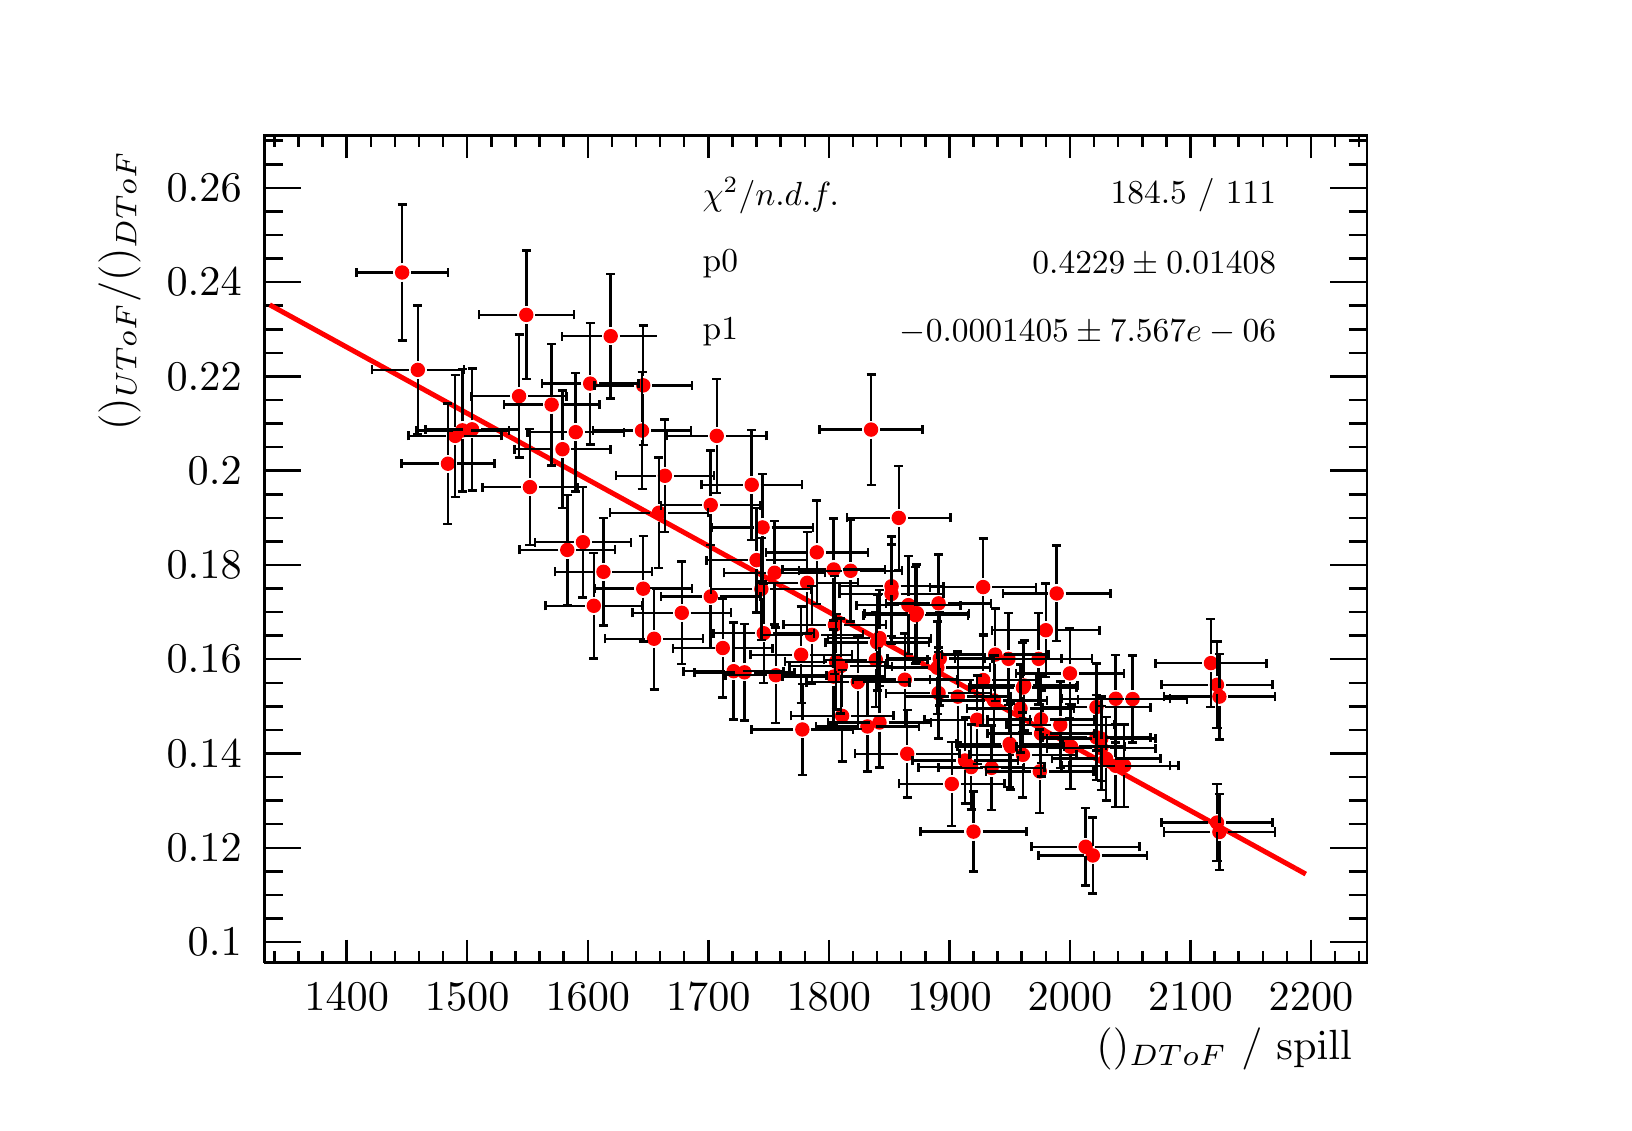
\begin{tikzpicture}
\pgfdeclareplotmark{cross} {
\pgfpathmoveto{\pgfpoint{-0.3\pgfplotmarksize}{\pgfplotmarksize}}
\pgfpathlineto{\pgfpoint{+0.3\pgfplotmarksize}{\pgfplotmarksize}}
\pgfpathlineto{\pgfpoint{+0.3\pgfplotmarksize}{0.3\pgfplotmarksize}}
\pgfpathlineto{\pgfpoint{+1\pgfplotmarksize}{0.3\pgfplotmarksize}}
\pgfpathlineto{\pgfpoint{+1\pgfplotmarksize}{-0.3\pgfplotmarksize}}
\pgfpathlineto{\pgfpoint{+0.3\pgfplotmarksize}{-0.3\pgfplotmarksize}}
\pgfpathlineto{\pgfpoint{+0.3\pgfplotmarksize}{-1.\pgfplotmarksize}}
\pgfpathlineto{\pgfpoint{-0.3\pgfplotmarksize}{-1.\pgfplotmarksize}}
\pgfpathlineto{\pgfpoint{-0.3\pgfplotmarksize}{-0.3\pgfplotmarksize}}
\pgfpathlineto{\pgfpoint{-1.\pgfplotmarksize}{-0.3\pgfplotmarksize}}
\pgfpathlineto{\pgfpoint{-1.\pgfplotmarksize}{0.3\pgfplotmarksize}}
\pgfpathlineto{\pgfpoint{-0.3\pgfplotmarksize}{0.3\pgfplotmarksize}}
\pgfpathclose
\pgfusepathqstroke
}
\pgfdeclareplotmark{cross*} {
\pgfpathmoveto{\pgfpoint{-0.3\pgfplotmarksize}{\pgfplotmarksize}}
\pgfpathlineto{\pgfpoint{+0.3\pgfplotmarksize}{\pgfplotmarksize}}
\pgfpathlineto{\pgfpoint{+0.3\pgfplotmarksize}{0.3\pgfplotmarksize}}
\pgfpathlineto{\pgfpoint{+1\pgfplotmarksize}{0.3\pgfplotmarksize}}
\pgfpathlineto{\pgfpoint{+1\pgfplotmarksize}{-0.3\pgfplotmarksize}}
\pgfpathlineto{\pgfpoint{+0.3\pgfplotmarksize}{-0.3\pgfplotmarksize}}
\pgfpathlineto{\pgfpoint{+0.3\pgfplotmarksize}{-1.\pgfplotmarksize}}
\pgfpathlineto{\pgfpoint{-0.3\pgfplotmarksize}{-1.\pgfplotmarksize}}
\pgfpathlineto{\pgfpoint{-0.3\pgfplotmarksize}{-0.3\pgfplotmarksize}}
\pgfpathlineto{\pgfpoint{-1.\pgfplotmarksize}{-0.3\pgfplotmarksize}}
\pgfpathlineto{\pgfpoint{-1.\pgfplotmarksize}{0.3\pgfplotmarksize}}
\pgfpathlineto{\pgfpoint{-0.3\pgfplotmarksize}{0.3\pgfplotmarksize}}
\pgfpathclose
\pgfusepathqfillstroke
}
\pgfdeclareplotmark{newstar} {
\pgfpathmoveto{\pgfqpoint{0pt}{\pgfplotmarksize}}
\pgfpathlineto{\pgfqpointpolar{44}{0.5\pgfplotmarksize}}
\pgfpathlineto{\pgfqpointpolar{18}{\pgfplotmarksize}}
\pgfpathlineto{\pgfqpointpolar{-20}{0.5\pgfplotmarksize}}
\pgfpathlineto{\pgfqpointpolar{-54}{\pgfplotmarksize}}
\pgfpathlineto{\pgfqpointpolar{-90}{0.5\pgfplotmarksize}}
\pgfpathlineto{\pgfqpointpolar{234}{\pgfplotmarksize}}
\pgfpathlineto{\pgfqpointpolar{198}{0.5\pgfplotmarksize}}
\pgfpathlineto{\pgfqpointpolar{162}{\pgfplotmarksize}}
\pgfpathlineto{\pgfqpointpolar{134}{0.5\pgfplotmarksize}}
\pgfpathclose
\pgfusepathqstroke
}
\pgfdeclareplotmark{newstar*} {
\pgfpathmoveto{\pgfqpoint{0pt}{\pgfplotmarksize}}
\pgfpathlineto{\pgfqpointpolar{44}{0.5\pgfplotmarksize}}
\pgfpathlineto{\pgfqpointpolar{18}{\pgfplotmarksize}}
\pgfpathlineto{\pgfqpointpolar{-20}{0.5\pgfplotmarksize}}
\pgfpathlineto{\pgfqpointpolar{-54}{\pgfplotmarksize}}
\pgfpathlineto{\pgfqpointpolar{-90}{0.5\pgfplotmarksize}}
\pgfpathlineto{\pgfqpointpolar{234}{\pgfplotmarksize}}
\pgfpathlineto{\pgfqpointpolar{198}{0.5\pgfplotmarksize}}
\pgfpathlineto{\pgfqpointpolar{162}{\pgfplotmarksize}}
\pgfpathlineto{\pgfqpointpolar{134}{0.5\pgfplotmarksize}}
\pgfpathclose
\pgfusepathqfillstroke
}
\definecolor{c}{rgb}{1,1,1};
\draw [color=c, fill=c] (0,0) rectangle (20,13.639);
\draw [color=c, fill=c] (3,1.77307) rectangle (17,12.2751);
\definecolor{c}{rgb}{0,0,0};
\draw [c,line width=0.9] (3,1.77307) -- (3,12.2751) -- (17,12.2751) -- (17,1.77307) -- (3,1.77307);
\definecolor{c}{rgb}{1,1,1};
\draw [color=c, fill=c] (3,1.77307) rectangle (17,12.2751);
\definecolor{c}{rgb}{0,0,0};
\draw [c,line width=0.9] (3,1.77307) -- (3,12.2751) -- (17,12.2751) -- (17,1.77307) -- (3,1.77307);
\draw [c,line width=0.9] (3,1.77307) -- (17,1.77307);
\draw [c,line width=0.9] (4.0446,2.05948) -- (4.0446,1.77307);
\draw [c,line width=0.9] (4.35077,1.91628) -- (4.35077,1.77307);
\draw [c,line width=0.9] (4.65694,1.91628) -- (4.65694,1.77307);
\draw [c,line width=0.9] (4.9631,1.91628) -- (4.9631,1.77307);
\draw [c,line width=0.9] (5.26927,1.91628) -- (5.26927,1.77307);
\draw [c,line width=0.9] (5.57543,2.05948) -- (5.57543,1.77307);
\draw [c,line width=0.9] (5.8816,1.91628) -- (5.8816,1.77307);
\draw [c,line width=0.9] (6.18777,1.91628) -- (6.18777,1.77307);
\draw [c,line width=0.9] (6.49393,1.91628) -- (6.49393,1.77307);
\draw [c,line width=0.9] (6.8001,1.91628) -- (6.8001,1.77307);
\draw [c,line width=0.9] (7.10627,2.05948) -- (7.10627,1.77307);
\draw [c,line width=0.9] (7.41243,1.91628) -- (7.41243,1.77307);
\draw [c,line width=0.9] (7.7186,1.91628) -- (7.7186,1.77307);
\draw [c,line width=0.9] (8.02476,1.91628) -- (8.02476,1.77307);
\draw [c,line width=0.9] (8.33093,1.91628) -- (8.33093,1.77307);
\draw [c,line width=0.9] (8.6371,2.05948) -- (8.6371,1.77307);
\draw [c,line width=0.9] (8.94326,1.91628) -- (8.94326,1.77307);
\draw [c,line width=0.9] (9.24943,1.91628) -- (9.24943,1.77307);
\draw [c,line width=0.9] (9.5556,1.91628) -- (9.5556,1.77307);
\draw [c,line width=0.9] (9.86176,1.91628) -- (9.86176,1.77307);
\draw [c,line width=0.9] (10.1679,2.05948) -- (10.1679,1.77307);
\draw [c,line width=0.9] (10.4741,1.91628) -- (10.4741,1.77307);
\draw [c,line width=0.9] (10.7803,1.91628) -- (10.7803,1.77307);
\draw [c,line width=0.9] (11.0864,1.91628) -- (11.0864,1.77307);
\draw [c,line width=0.9] (11.3926,1.91628) -- (11.3926,1.77307);
\draw [c,line width=0.9] (11.6988,2.05948) -- (11.6988,1.77307);
\draw [c,line width=0.9] (12.0049,1.91628) -- (12.0049,1.77307);
\draw [c,line width=0.9] (12.3111,1.91628) -- (12.3111,1.77307);
\draw [c,line width=0.9] (12.6173,1.91628) -- (12.6173,1.77307);
\draw [c,line width=0.9] (12.9234,1.91628) -- (12.9234,1.77307);
\draw [c,line width=0.9] (13.2296,2.05948) -- (13.2296,1.77307);
\draw [c,line width=0.9] (13.5358,1.91628) -- (13.5358,1.77307);
\draw [c,line width=0.9] (13.8419,1.91628) -- (13.8419,1.77307);
\draw [c,line width=0.9] (14.1481,1.91628) -- (14.1481,1.77307);
\draw [c,line width=0.9] (14.4543,1.91628) -- (14.4543,1.77307);
\draw [c,line width=0.9] (14.7604,2.05948) -- (14.7604,1.77307);
\draw [c,line width=0.9] (15.0666,1.91628) -- (15.0666,1.77307);
\draw [c,line width=0.9] (15.3728,1.91628) -- (15.3728,1.77307);
\draw [c,line width=0.9] (15.6789,1.91628) -- (15.6789,1.77307);
\draw [c,line width=0.9] (15.9851,1.91628) -- (15.9851,1.77307);
\draw [c,line width=0.9] (16.2913,2.05948) -- (16.2913,1.77307);
\draw [c,line width=0.9] (4.0446,2.05948) -- (4.0446,1.77307);
\draw [c,line width=0.9] (3.73844,1.91628) -- (3.73844,1.77307);
\draw [c,line width=0.9] (3.43227,1.91628) -- (3.43227,1.77307);
\draw [c,line width=0.9] (3.1261,1.91628) -- (3.1261,1.77307);
\draw [c,line width=0.9] (16.2913,2.05948) -- (16.2913,1.77307);
\draw [c,line width=0.9] (16.5974,1.91628) -- (16.5974,1.77307);
\draw [c,line width=0.9] (16.9036,1.91628) -- (16.9036,1.77307);
\draw [anchor=base] (4.0446,1.15931) node[scale=1.52731, color=c, rotate=0]{1400};
\draw [anchor=base] (5.57543,1.15931) node[scale=1.52731, color=c, rotate=0]{1500};
\draw [anchor=base] (7.10627,1.15931) node[scale=1.52731, color=c, rotate=0]{1600};
\draw [anchor=base] (8.6371,1.15931) node[scale=1.52731, color=c, rotate=0]{1700};
\draw [anchor=base] (10.1679,1.15931) node[scale=1.52731, color=c, rotate=0]{1800};
\draw [anchor=base] (11.6988,1.15931) node[scale=1.52731, color=c, rotate=0]{1900};
\draw [anchor=base] (13.2296,1.15931) node[scale=1.52731, color=c, rotate=0]{2000};
\draw [anchor=base] (14.7604,1.15931) node[scale=1.52731, color=c, rotate=0]{2100};
\draw [anchor=base] (16.2913,1.15931) node[scale=1.52731, color=c, rotate=0]{2200};
\draw [anchor= east] (17,0.681948) node[scale=1.52731, color=c, rotate=0]{ $(\SOne\STwo)_{\text{DToF}}$ / spill };
\draw [c,line width=0.9] (3,12.2751) -- (17,12.2751);
\draw [c,line width=0.9] (4.0446,11.9887) -- (4.0446,12.2751);
\draw [c,line width=0.9] (4.35077,12.1319) -- (4.35077,12.2751);
\draw [c,line width=0.9] (4.65694,12.1319) -- (4.65694,12.2751);
\draw [c,line width=0.9] (4.9631,12.1319) -- (4.9631,12.2751);
\draw [c,line width=0.9] (5.26927,12.1319) -- (5.26927,12.2751);
\draw [c,line width=0.9] (5.57543,11.9887) -- (5.57543,12.2751);
\draw [c,line width=0.9] (5.8816,12.1319) -- (5.8816,12.2751);
\draw [c,line width=0.9] (6.18777,12.1319) -- (6.18777,12.2751);
\draw [c,line width=0.9] (6.49393,12.1319) -- (6.49393,12.2751);
\draw [c,line width=0.9] (6.8001,12.1319) -- (6.8001,12.2751);
\draw [c,line width=0.9] (7.10627,11.9887) -- (7.10627,12.2751);
\draw [c,line width=0.9] (7.41243,12.1319) -- (7.41243,12.2751);
\draw [c,line width=0.9] (7.7186,12.1319) -- (7.7186,12.2751);
\draw [c,line width=0.9] (8.02476,12.1319) -- (8.02476,12.2751);
\draw [c,line width=0.9] (8.33093,12.1319) -- (8.33093,12.2751);
\draw [c,line width=0.9] (8.6371,11.9887) -- (8.6371,12.2751);
\draw [c,line width=0.9] (8.94326,12.1319) -- (8.94326,12.2751);
\draw [c,line width=0.9] (9.24943,12.1319) -- (9.24943,12.2751);
\draw [c,line width=0.9] (9.5556,12.1319) -- (9.5556,12.2751);
\draw [c,line width=0.9] (9.86176,12.1319) -- (9.86176,12.2751);
\draw [c,line width=0.9] (10.1679,11.9887) -- (10.1679,12.2751);
\draw [c,line width=0.9] (10.4741,12.1319) -- (10.4741,12.2751);
\draw [c,line width=0.9] (10.7803,12.1319) -- (10.7803,12.2751);
\draw [c,line width=0.9] (11.0864,12.1319) -- (11.0864,12.2751);
\draw [c,line width=0.9] (11.3926,12.1319) -- (11.3926,12.2751);
\draw [c,line width=0.9] (11.6988,11.9887) -- (11.6988,12.2751);
\draw [c,line width=0.9] (12.0049,12.1319) -- (12.0049,12.2751);
\draw [c,line width=0.9] (12.3111,12.1319) -- (12.3111,12.2751);
\draw [c,line width=0.9] (12.6173,12.1319) -- (12.6173,12.2751);
\draw [c,line width=0.9] (12.9234,12.1319) -- (12.9234,12.2751);
\draw [c,line width=0.9] (13.2296,11.9887) -- (13.2296,12.2751);
\draw [c,line width=0.9] (13.5358,12.1319) -- (13.5358,12.2751);
\draw [c,line width=0.9] (13.8419,12.1319) -- (13.8419,12.2751);
\draw [c,line width=0.9] (14.1481,12.1319) -- (14.1481,12.2751);
\draw [c,line width=0.9] (14.4543,12.1319) -- (14.4543,12.2751);
\draw [c,line width=0.9] (14.7604,11.9887) -- (14.7604,12.2751);
\draw [c,line width=0.9] (15.0666,12.1319) -- (15.0666,12.2751);
\draw [c,line width=0.9] (15.3728,12.1319) -- (15.3728,12.2751);
\draw [c,line width=0.9] (15.6789,12.1319) -- (15.6789,12.2751);
\draw [c,line width=0.9] (15.9851,12.1319) -- (15.9851,12.2751);
\draw [c,line width=0.9] (16.2913,11.9887) -- (16.2913,12.2751);
\draw [c,line width=0.9] (4.0446,11.9887) -- (4.0446,12.2751);
\draw [c,line width=0.9] (3.73844,12.1319) -- (3.73844,12.2751);
\draw [c,line width=0.9] (3.43227,12.1319) -- (3.43227,12.2751);
\draw [c,line width=0.9] (3.1261,12.1319) -- (3.1261,12.2751);
\draw [c,line width=0.9] (16.2913,11.9887) -- (16.2913,12.2751);
\draw [c,line width=0.9] (16.5974,12.1319) -- (16.5974,12.2751);
\draw [c,line width=0.9] (16.9036,12.1319) -- (16.9036,12.2751);
\draw [c,line width=0.9] (3,1.77307) -- (3,12.2751);
\draw [c,line width=0.9] (3.462,2.03294) -- (3,2.03294);
\draw [c,line width=0.9] (3.231,2.33227) -- (3,2.33227);
\draw [c,line width=0.9] (3.231,2.6316) -- (3,2.6316);
\draw [c,line width=0.9] (3.231,2.93093) -- (3,2.93093);
\draw [c,line width=0.9] (3.462,3.23026) -- (3,3.23026);
\draw [c,line width=0.9] (3.231,3.52959) -- (3,3.52959);
\draw [c,line width=0.9] (3.231,3.82892) -- (3,3.82892);
\draw [c,line width=0.9] (3.231,4.12825) -- (3,4.12825);
\draw [c,line width=0.9] (3.462,4.42757) -- (3,4.42757);
\draw [c,line width=0.9] (3.231,4.7269) -- (3,4.7269);
\draw [c,line width=0.9] (3.231,5.02623) -- (3,5.02623);
\draw [c,line width=0.9] (3.231,5.32556) -- (3,5.32556);
\draw [c,line width=0.9] (3.462,5.62489) -- (3,5.62489);
\draw [c,line width=0.9] (3.231,5.92422) -- (3,5.92422);
\draw [c,line width=0.9] (3.231,6.22355) -- (3,6.22355);
\draw [c,line width=0.9] (3.231,6.52288) -- (3,6.52288);
\draw [c,line width=0.9] (3.462,6.82221) -- (3,6.82221);
\draw [c,line width=0.9] (3.231,7.12153) -- (3,7.12153);
\draw [c,line width=0.9] (3.231,7.42086) -- (3,7.42086);
\draw [c,line width=0.9] (3.231,7.72019) -- (3,7.72019);
\draw [c,line width=0.9] (3.462,8.01952) -- (3,8.01952);
\draw [c,line width=0.9] (3.231,8.31885) -- (3,8.31885);
\draw [c,line width=0.9] (3.231,8.61818) -- (3,8.61818);
\draw [c,line width=0.9] (3.231,8.91751) -- (3,8.91751);
\draw [c,line width=0.9] (3.462,9.21684) -- (3,9.21684);
\draw [c,line width=0.9] (3.231,9.51617) -- (3,9.51617);
\draw [c,line width=0.9] (3.231,9.8155) -- (3,9.8155);
\draw [c,line width=0.9] (3.231,10.1148) -- (3,10.1148);
\draw [c,line width=0.9] (3.462,10.4142) -- (3,10.4142);
\draw [c,line width=0.9] (3.231,10.7135) -- (3,10.7135);
\draw [c,line width=0.9] (3.231,11.0128) -- (3,11.0128);
\draw [c,line width=0.9] (3.231,11.3121) -- (3,11.3121);
\draw [c,line width=0.9] (3.462,11.6115) -- (3,11.6115);
\draw [c,line width=0.9] (3.462,2.03294) -- (3,2.03294);
\draw [c,line width=0.9] (3.462,11.6115) -- (3,11.6115);
\draw [c,line width=0.9] (3.231,11.9108) -- (3,11.9108);
\draw [c,line width=0.9] (3.231,12.2101) -- (3,12.2101);
\draw [anchor= east] (2.9,2.03294) node[scale=1.52731, color=c, rotate=0]{0.1};
\draw [anchor= east] (2.9,3.23026) node[scale=1.52731, color=c, rotate=0]{0.12};
\draw [anchor= east] (2.9,4.42757) node[scale=1.52731, color=c, rotate=0]{0.14};
\draw [anchor= east] (2.9,5.62489) node[scale=1.52731, color=c, rotate=0]{0.16};
\draw [anchor= east] (2.9,6.82221) node[scale=1.52731, color=c, rotate=0]{0.18};
\draw [anchor= east] (2.9,8.01952) node[scale=1.52731, color=c, rotate=0]{0.2};
\draw [anchor= east] (2.9,9.21684) node[scale=1.52731, color=c, rotate=0]{0.22};
\draw [anchor= east] (2.9,10.4142) node[scale=1.52731, color=c, rotate=0]{0.24};
\draw [anchor= east] (2.9,11.6115) node[scale=1.52731, color=c, rotate=0]{0.26};
\draw [anchor= east] (1.16,12.2751) node[scale=1.52731, color=c, rotate=90]{ $(\SOne\STwo)_{\text{UToF}}/(\SOne\STwo)_{\text{DToF}}$ };
\draw [c,line width=0.9] (17,1.77307) -- (17,12.2751);
\draw [c,line width=0.9] (16.538,2.03294) -- (17,2.03294);
\draw [c,line width=0.9] (16.769,2.33227) -- (17,2.33227);
\draw [c,line width=0.9] (16.769,2.6316) -- (17,2.6316);
\draw [c,line width=0.9] (16.769,2.93093) -- (17,2.93093);
\draw [c,line width=0.9] (16.538,3.23026) -- (17,3.23026);
\draw [c,line width=0.9] (16.769,3.52959) -- (17,3.52959);
\draw [c,line width=0.9] (16.769,3.82892) -- (17,3.82892);
\draw [c,line width=0.9] (16.769,4.12825) -- (17,4.12825);
\draw [c,line width=0.9] (16.538,4.42757) -- (17,4.42757);
\draw [c,line width=0.9] (16.769,4.7269) -- (17,4.7269);
\draw [c,line width=0.9] (16.769,5.02623) -- (17,5.02623);
\draw [c,line width=0.9] (16.769,5.32556) -- (17,5.32556);
\draw [c,line width=0.9] (16.538,5.62489) -- (17,5.62489);
\draw [c,line width=0.9] (16.769,5.92422) -- (17,5.92422);
\draw [c,line width=0.9] (16.769,6.22355) -- (17,6.22355);
\draw [c,line width=0.9] (16.769,6.52288) -- (17,6.52288);
\draw [c,line width=0.9] (16.538,6.82221) -- (17,6.82221);
\draw [c,line width=0.9] (16.769,7.12153) -- (17,7.12153);
\draw [c,line width=0.9] (16.769,7.42086) -- (17,7.42086);
\draw [c,line width=0.9] (16.769,7.72019) -- (17,7.72019);
\draw [c,line width=0.9] (16.538,8.01952) -- (17,8.01952);
\draw [c,line width=0.9] (16.769,8.31885) -- (17,8.31885);
\draw [c,line width=0.9] (16.769,8.61818) -- (17,8.61818);
\draw [c,line width=0.9] (16.769,8.91751) -- (17,8.91751);
\draw [c,line width=0.9] (16.538,9.21684) -- (17,9.21684);
\draw [c,line width=0.9] (16.769,9.51617) -- (17,9.51617);
\draw [c,line width=0.9] (16.769,9.8155) -- (17,9.8155);
\draw [c,line width=0.9] (16.769,10.1148) -- (17,10.1148);
\draw [c,line width=0.9] (16.538,10.4142) -- (17,10.4142);
\draw [c,line width=0.9] (16.769,10.7135) -- (17,10.7135);
\draw [c,line width=0.9] (16.769,11.0128) -- (17,11.0128);
\draw [c,line width=0.9] (16.769,11.3121) -- (17,11.3121);
\draw [c,line width=0.9] (16.538,11.6115) -- (17,11.6115);
\draw [c,line width=0.9] (16.538,2.03294) -- (17,2.03294);
\draw [c,line width=0.9] (16.538,11.6115) -- (17,11.6115);
\draw [c,line width=0.9] (16.769,11.9108) -- (17,11.9108);
\draw [c,line width=0.9] (16.769,12.2101) -- (17,12.2101);
\definecolor{c}{rgb}{1,0,0};
\foreach \P in {(6.78479,8.2925), (8.74426,8.46141), (10.964,6.55197), (12.6479,5.29169), (9.31066,6.51601), (13.5204,3.133), (13.4286,3.24334), (7.18281,6.30374), (9.09635,5.45879), (10.8109,5.89399), (4.74879,10.5367), (9.81584,5.68149),
 (10.2445,6.06269), (12.2805,5.6842), (13.9185,4.27242), (6.84602,7.01356), (9.47905,6.72328), (11.8978,4.33932), (12.1274,6.54151), (6.23369,8.9662), (11.163,4.42436), (7.13688,9.12566), (5.63667,8.54494), (7.81045,6.52106), (12.6019,5.00026),
 (11.561,6.3353), (7.30527,6.73536), (8.66771,6.42263), (8.95857,5.47323), (6.32554,9.9983), (15.0972,5.29989), (12.4642,4.55038), (7.79514,8.52902), (11.561,5.1956), (13.5664,5.01735), (11.1324,5.36525), (10.6578,4.77135), (6.95318,8.50899),
 (15.0207,5.57625), (12.8622,4.68085), (12.4489,5.6298), (12.8469,4.20024), (8.66771,7.58337), (13.6276,4.49731), (9.95361,5.93461), (11.8059,5.15023), (11.0558,7.42022), (9.32597,7.29907), (9.34128,5.95542), (10.7803,5.83963), (11.5763,5.63375),
 (10.2292,5.40454), (8.8208,5.76756), (9.24943,6.88414), (15.1278,5.15025), (8.30031,6.21427), (12.6326,5.26588), (12.8316,5.62974), (15.0972,3.55075), (12.4795,4.51533), (11.7294,4.04106), (10.321,5.5389), (10.765,5.61708), (10.964,6.45499),
 (13.6276,4.6155), (13.2296,4.51737), (10.2598,5.59307), (11.2701,6.18389), (9.89238,6.59511), (11.1783,6.31274), (13.5664,4.63246), (8.00946,7.48546), (12.0049,3.43605), (7.39712,9.72786), (10.8109,4.82148), (4.94779,9.29972), (5.5142,8.53174),
 (13.1071,4.79182), (10.7037,8.54151), (6.37147,7.81123), (8.086,7.95476), (9.83115,4.7333), (11.2854,6.21044), (12.2652,5.10195), (9.49436,5.4217), (12.1274,5.36158), (7.81045,9.10336), (11.5457,5.5172), (11.9743,4.25528), (15.1278,3.43094),
 (12.0508,4.85657), (13.2449,4.51314), (5.42235,8.46148), (10.2292,6.76513), (6.64702,8.85841), (7.94822,5.88533), (10.5353,5.33475), (10.0148,6.98274), (9.1882,7.8402), (13.8113,4.2713), (10.3363,4.90557), (13.0612,6.46042), (13.2296,5.44529),
 (7.04503,7.11178), (10.4435,6.74844), (13.8113,5.12317), (12.6326,4.41109), (13.6888,4.3627), (5.3305,8.10827), (12.2346,4.24504), (14.0256,5.11959), (12.8622,4.86263), (12.9234,5.99376)}{\draw[mark options={color=c,fill=c},mark
 size=2.402402pt,mark=*] plot coordinates {\P};}
\draw [c,line width=1.8] (3.06646,10.1263) -- (3.19937,10.0533) -- (3.33228,9.98029) -- (3.46519,9.90727) -- (3.59811,9.83424) -- (3.73102,9.76122) -- (3.86393,9.68819) -- (3.99684,9.61516) -- (4.12976,9.54214) -- (4.26267,9.46911) --
 (4.39558,9.39609) -- (4.52849,9.32306) -- (4.66141,9.25004) -- (4.79432,9.17701) -- (4.92723,9.10398) -- (5.06014,9.03096) -- (5.19306,8.95793) -- (5.32597,8.88491) -- (5.45888,8.81188) -- (5.59179,8.73886) -- (5.72471,8.66583) -- (5.85762,8.5928)
 -- (5.99053,8.51978) -- (6.12344,8.44675) -- (6.25636,8.37373) -- (6.38927,8.3007) -- (6.52218,8.22768) -- (6.65509,8.15465) -- (6.78801,8.08162) -- (6.92092,8.0086) -- (7.05383,7.93557) -- (7.18674,7.86255) -- (7.31966,7.78952) -- (7.45257,7.7165)
 -- (7.58548,7.64347) -- (7.71839,7.57044) -- (7.85131,7.49742) -- (7.98422,7.42439) -- (8.11713,7.35137) -- (8.25004,7.27834) -- (8.38296,7.20532) -- (8.51587,7.13229) -- (8.64878,7.05926) -- (8.7817,6.98624) -- (8.91461,6.91321) --
 (9.04752,6.84019) -- (9.18043,6.76716) -- (9.31334,6.69414) -- (9.44626,6.62111) -- (9.57917,6.54808);
\draw [c,line width=1.8] (9.57917,6.54808) -- (9.71208,6.47506) -- (9.845,6.40203) -- (9.97791,6.32901) -- (10.1108,6.25598) -- (10.2437,6.18296) -- (10.3766,6.10993) -- (10.5096,6.0369) -- (10.6425,5.96388) -- (10.7754,5.89085) -- (10.9083,5.81783)
 -- (11.0412,5.7448) -- (11.1741,5.67178) -- (11.307,5.59875) -- (11.4399,5.52573) -- (11.5729,5.4527) -- (11.7058,5.37967) -- (11.8387,5.30665) -- (11.9716,5.23362) -- (12.1045,5.1606) -- (12.2374,5.08757) -- (12.3703,5.01455) -- (12.5032,4.94152)
 -- (12.6362,4.86849) -- (12.7691,4.79547) -- (12.902,4.72244) -- (13.0349,4.64942) -- (13.1678,4.57639) -- (13.3007,4.50337) -- (13.4336,4.43034) -- (13.5665,4.35731) -- (13.6995,4.28429) -- (13.8324,4.21126) -- (13.9653,4.13824) --
 (14.0982,4.06521) -- (14.2311,3.99219) -- (14.364,3.91916) -- (14.4969,3.84613) -- (14.6298,3.77311) -- (14.7628,3.70008) -- (14.8957,3.62706) -- (15.0286,3.55403) -- (15.1615,3.48101) -- (15.2944,3.40798) -- (15.4273,3.33495) -- (15.5602,3.26193)
 -- (15.6931,3.1889) -- (15.8261,3.11588) -- (15.959,3.04285) -- (16.0919,2.96983);
\draw [c,line width=1.8] (16.0919,2.96983) -- (16.2248,2.8968);
\definecolor{c}{rgb}{1,1,1};
\draw [color=c, fill=c] (7.99427,9.34097) rectangle (16.4183,11.9484);
\definecolor{c}{rgb}{0,0,0};
\draw [anchor= west] (8.41547,11.5138) node[scale=1.20912, color=c, rotate=0]{$\chi^{2} / ndf $};
\draw [anchor= east] (15.9971,11.5138) node[scale=1.20912, color=c, rotate=0]{ 184.5 / 111};
\draw [anchor= west] (8.41547,10.6447) node[scale=1.20912, color=c, rotate=0]{p0       };
\draw [anchor= east] (15.9971,10.6447) node[scale=1.20912, color=c, rotate=0]{$ 0.4229 \pm 0.01408$};
\draw [anchor= west] (8.41547,9.77555) node[scale=1.20912, color=c, rotate=0]{p1       };
\draw [anchor= east] (15.9971,9.77555) node[scale=1.20912, color=c, rotate=0]{$ -0.0001405 \pm 7.567e-06$};
\draw [c,line width=0.9] (6.67018,8.2925) -- (6.17649,8.2925);
\draw [c,line width=0.9] (6.17649,8.23519) -- (6.17649,8.34981);
\draw [c,line width=0.9] (6.8994,8.2925) -- (7.39309,8.2925);
\draw [c,line width=0.9] (7.39309,8.23519) -- (7.39309,8.34981);
\draw [c,line width=0.9] (6.78479,8.40711) -- (6.78479,9.04035);
\draw [c,line width=0.9] (6.72748,9.04035) -- (6.8421,9.04035);
\draw [c,line width=0.9] (6.78479,8.17789) -- (6.78479,7.54465);
\draw [c,line width=0.9] (6.72748,7.54465) -- (6.8421,7.54465);
\draw [c,line width=0.9] (8.62964,8.46141) -- (8.11178,8.46141);
\draw [c,line width=0.9] (8.11178,8.40411) -- (8.11178,8.51872);
\draw [c,line width=0.9] (8.85887,8.46141) -- (9.37673,8.46141);
\draw [c,line width=0.9] (9.37673,8.40411) -- (9.37673,8.51872);
\draw [c,line width=0.9] (8.74426,8.57603) -- (8.74426,9.18647);
\draw [c,line width=0.9] (8.68695,9.18647) -- (8.80156,9.18647);
\draw [c,line width=0.9] (8.74426,8.3468) -- (8.74426,7.73636);
\draw [c,line width=0.9] (8.68695,7.73636) -- (8.80156,7.73636);
\draw [c,line width=0.9] (10.8493,6.55197) -- (10.3052,6.55197);
\draw [c,line width=0.9] (10.3052,6.49466) -- (10.3052,6.60928);
\draw [c,line width=0.9] (11.0786,6.55197) -- (11.6228,6.55197);
\draw [c,line width=0.9] (11.6228,6.49466) -- (11.6228,6.60928);
\draw [c,line width=0.9] (10.964,6.66658) -- (10.964,7.18378);
\draw [c,line width=0.9] (10.9067,7.18378) -- (11.0213,7.18378);
\draw [c,line width=0.9] (10.964,6.43736) -- (10.964,5.92016);
\draw [c,line width=0.9] (10.9067,5.92016) -- (11.0213,5.92016);
\draw [c,line width=0.9] (12.5333,5.29169) -- (11.9698,5.29169);
\draw [c,line width=0.9] (11.9698,5.23439) -- (11.9698,5.349);
\draw [c,line width=0.9] (12.7625,5.29169) -- (13.3259,5.29169);
\draw [c,line width=0.9] (13.3259,5.23439) -- (13.3259,5.349);
\draw [c,line width=0.9] (12.6479,5.40631) -- (12.6479,5.86236);
\draw [c,line width=0.9] (12.5906,5.86236) -- (12.7052,5.86236);
\draw [c,line width=0.9] (12.6479,5.17708) -- (12.6479,4.72102);
\draw [c,line width=0.9] (12.5906,4.72102) -- (12.7052,4.72102);
\draw [c,line width=0.9] (9.19605,6.51601) -- (8.67137,6.51601);
\draw [c,line width=0.9] (8.67137,6.4587) -- (8.67137,6.57332);
\draw [c,line width=0.9] (9.42528,6.51601) -- (9.94996,6.51601);
\draw [c,line width=0.9] (9.94996,6.4587) -- (9.94996,6.57332);
\draw [c,line width=0.9] (9.31066,6.63062) -- (9.31066,7.16581);
\draw [c,line width=0.9] (9.25336,7.16581) -- (9.36797,7.16581);
\draw [c,line width=0.9] (9.31066,6.4014) -- (9.31066,5.86621);
\draw [c,line width=0.9] (9.25336,5.86621) -- (9.36797,5.86621);
\draw [c,line width=0.9] (13.4058,3.133) -- (12.8326,3.133);
\draw [c,line width=0.9] (12.8326,3.0757) -- (12.8326,3.19031);
\draw [c,line width=0.9] (13.6351,3.133) -- (14.2083,3.133);
\draw [c,line width=0.9] (14.2083,3.0757) -- (14.2083,3.19031);
\draw [c,line width=0.9] (13.5204,3.24762) -- (13.5204,3.61777);
\draw [c,line width=0.9] (13.4631,3.61777) -- (13.5778,3.61777);
\draw [c,line width=0.9] (13.5204,3.01839) -- (13.5204,2.64823);
\draw [c,line width=0.9] (13.4631,2.64823) -- (13.5778,2.64823);
\draw [c,line width=0.9] (13.314,3.24334) -- (12.7418,3.24334);
\draw [c,line width=0.9] (12.7418,3.18604) -- (12.7418,3.30065);
\draw [c,line width=0.9] (13.5432,3.24334) -- (14.1154,3.24334);
\draw [c,line width=0.9] (14.1154,3.18604) -- (14.1154,3.30065);
\draw [c,line width=0.9] (13.4286,3.35796) -- (13.4286,3.733);
\draw [c,line width=0.9] (13.3713,3.733) -- (13.4859,3.733);
\draw [c,line width=0.9] (13.4286,3.12873) -- (13.4286,2.75368);
\draw [c,line width=0.9] (13.3713,2.75368) -- (13.4859,2.75368);
\draw [c,line width=0.9] (7.06819,6.30374) -- (6.56952,6.30374);
\draw [c,line width=0.9] (6.56952,6.24644) -- (6.56952,6.36105);
\draw [c,line width=0.9] (7.29742,6.30374) -- (7.7961,6.30374);
\draw [c,line width=0.9] (7.7961,6.24644) -- (7.7961,6.36105);
\draw [c,line width=0.9] (7.18281,6.41836) -- (7.18281,6.97318);
\draw [c,line width=0.9] (7.1255,6.97318) -- (7.24011,6.97318);
\draw [c,line width=0.9] (7.18281,6.18913) -- (7.18281,5.6343);
\draw [c,line width=0.9] (7.1255,5.6343) -- (7.24011,5.6343);
\draw [c,line width=0.9] (8.98173,5.45879) -- (8.45962,5.45879);
\draw [c,line width=0.9] (8.45962,5.40148) -- (8.45962,5.5161);
\draw [c,line width=0.9] (9.21096,5.45879) -- (9.73307,5.45879);
\draw [c,line width=0.9] (9.73307,5.40148) -- (9.73307,5.5161);
\draw [c,line width=0.9] (9.09635,5.5734) -- (9.09635,6.07273);
\draw [c,line width=0.9] (9.03904,6.07273) -- (9.15365,6.07273);
\draw [c,line width=0.9] (9.09635,5.34418) -- (9.09635,4.84485);
\draw [c,line width=0.9] (9.03904,4.84485) -- (9.15365,4.84485);
\draw [c,line width=0.9] (10.6963,5.89399) -- (10.1539,5.89399);
\draw [c,line width=0.9] (10.1539,5.83669) -- (10.1539,5.9513);
\draw [c,line width=0.9] (10.9255,5.89399) -- (11.4679,5.89399);
\draw [c,line width=0.9] (11.4679,5.83669) -- (11.4679,5.9513);
\draw [c,line width=0.9] (10.8109,6.00861) -- (10.8109,6.50448);
\draw [c,line width=0.9] (10.7536,6.50448) -- (10.8682,6.50448);
\draw [c,line width=0.9] (10.8109,5.77938) -- (10.8109,5.2835);
\draw [c,line width=0.9] (10.7536,5.2835) -- (10.8682,5.2835);
\draw [c,line width=0.9] (4.63417,10.5367) -- (4.16667,10.5367);
\draw [c,line width=0.9] (4.16667,10.4794) -- (4.16667,10.594);
\draw [c,line width=0.9] (4.8634,10.5367) -- (5.3309,10.5367);
\draw [c,line width=0.9] (5.3309,10.4794) -- (5.3309,10.594);
\draw [c,line width=0.9] (4.74879,10.6513) -- (4.74879,11.3999);
\draw [c,line width=0.9] (4.69148,11.3999) -- (4.80609,11.3999);
\draw [c,line width=0.9] (4.74879,10.4221) -- (4.74879,9.6735);
\draw [c,line width=0.9] (4.69148,9.6735) -- (4.80609,9.6735);
\draw [c,line width=0.9] (9.70122,5.68149) -- (9.17052,5.68149);
\draw [c,line width=0.9] (9.17052,5.62418) -- (9.17052,5.73879);
\draw [c,line width=0.9] (9.93045,5.68149) -- (10.4612,5.68149);
\draw [c,line width=0.9] (10.4612,5.62418) -- (10.4612,5.73879);
\draw [c,line width=0.9] (9.81584,5.7961) -- (9.81584,6.29536);
\draw [c,line width=0.9] (9.75853,6.29536) -- (9.87314,6.29536);
\draw [c,line width=0.9] (9.81584,5.56687) -- (9.81584,5.06761);
\draw [c,line width=0.9] (9.75853,5.06761) -- (9.87314,5.06761);
\draw [c,line width=0.9] (10.1299,6.06269) -- (9.59409,6.06269);
\draw [c,line width=0.9] (9.59409,6.00538) -- (9.59409,6.12);
\draw [c,line width=0.9] (10.3591,6.06269) -- (10.8948,6.06269);
\draw [c,line width=0.9] (10.8948,6.00538) -- (10.8948,6.12);
\draw [c,line width=0.9] (10.2445,6.1773) -- (10.2445,6.68542);
\draw [c,line width=0.9] (10.1872,6.68542) -- (10.3018,6.68542);
\draw [c,line width=0.9] (10.2445,5.94808) -- (10.2445,5.43996);
\draw [c,line width=0.9] (10.1872,5.43996) -- (10.3018,5.43996);
\draw [c,line width=0.9] (12.1659,5.6842) -- (11.6066,5.6842);
\draw [c,line width=0.9] (11.6066,5.62689) -- (11.6066,5.74151);
\draw [c,line width=0.9] (12.3951,5.6842) -- (12.9544,5.6842);
\draw [c,line width=0.9] (12.9544,5.62689) -- (12.9544,5.74151);
\draw [c,line width=0.9] (12.2805,5.79881) -- (12.2805,6.27212);
\draw [c,line width=0.9] (12.2232,6.27212) -- (12.3378,6.27212);
\draw [c,line width=0.9] (12.2805,5.56959) -- (12.2805,5.09628);
\draw [c,line width=0.9] (12.2232,5.09628) -- (12.3378,5.09628);
\draw [c,line width=0.9] (13.8039,4.27242) -- (13.2262,4.27242);
\draw [c,line width=0.9] (13.2262,4.21511) -- (13.2262,4.32973);
\draw [c,line width=0.9] (14.0331,4.27242) -- (14.6107,4.27242);
\draw [c,line width=0.9] (14.6107,4.21511) -- (14.6107,4.32973);
\draw [c,line width=0.9] (13.9185,4.38703) -- (13.9185,4.79578);
\draw [c,line width=0.9] (13.8612,4.79578) -- (13.9758,4.79578);
\draw [c,line width=0.9] (13.9185,4.15781) -- (13.9185,3.74907);
\draw [c,line width=0.9] (13.8612,3.74907) -- (13.9758,3.74907);
\draw [c,line width=0.9] (6.73141,7.01356) -- (6.23695,7.01356);
\draw [c,line width=0.9] (6.23695,6.95626) -- (6.23695,7.07087);
\draw [c,line width=0.9] (6.96064,7.01356) -- (7.45509,7.01356);
\draw [c,line width=0.9] (7.45509,6.95626) -- (7.45509,7.07087);
\draw [c,line width=0.9] (6.84602,7.12818) -- (6.84602,7.71409);
\draw [c,line width=0.9] (6.78872,7.71409) -- (6.90333,7.71409);
\draw [c,line width=0.9] (6.84602,6.89895) -- (6.84602,6.31304);
\draw [c,line width=0.9] (6.78872,6.31304) -- (6.90333,6.31304);
\draw [c,line width=0.9] (9.36444,6.72328) -- (8.83775,6.72328);
\draw [c,line width=0.9] (8.83775,6.66598) -- (8.83775,6.78059);
\draw [c,line width=0.9] (9.59367,6.72328) -- (10.1204,6.72328);
\draw [c,line width=0.9] (10.1204,6.66598) -- (10.1204,6.78059);
\draw [c,line width=0.9] (9.47905,6.8379) -- (9.47905,7.37839);
\draw [c,line width=0.9] (9.42175,7.37839) -- (9.53636,7.37839);
\draw [c,line width=0.9] (9.47905,6.60867) -- (9.47905,6.06818);
\draw [c,line width=0.9] (9.42175,6.06818) -- (9.53636,6.06818);
\draw [c,line width=0.9] (11.7832,4.33932) -- (11.2282,4.33932);
\draw [c,line width=0.9] (11.2282,4.28202) -- (11.2282,4.39663);
\draw [c,line width=0.9] (12.0124,4.33932) -- (12.5673,4.33932);
\draw [c,line width=0.9] (12.5673,4.28202) -- (12.5673,4.39663);
\draw [c,line width=0.9] (11.8978,4.45394) -- (11.8978,4.8829);
\draw [c,line width=0.9] (11.8405,4.8829) -- (11.9551,4.8829);
\draw [c,line width=0.9] (11.8978,4.22471) -- (11.8978,3.79575);
\draw [c,line width=0.9] (11.8405,3.79575) -- (11.9551,3.79575);
\draw [c,line width=0.9] (12.0128,6.54151) -- (11.4552,6.54151);
\draw [c,line width=0.9] (11.4552,6.4842) -- (11.4552,6.59881);
\draw [c,line width=0.9] (12.242,6.54151) -- (12.7996,6.54151);
\draw [c,line width=0.9] (12.7996,6.4842) -- (12.7996,6.59881);
\draw [c,line width=0.9] (12.1274,6.65612) -- (12.1274,7.16039);
\draw [c,line width=0.9] (12.0701,7.16039) -- (12.1847,7.16039);
\draw [c,line width=0.9] (12.1274,6.42689) -- (12.1274,5.92263);
\draw [c,line width=0.9] (12.0701,5.92263) -- (12.1847,5.92263);
\draw [c,line width=0.9] (6.11908,8.9662) -- (5.63237,8.9662);
\draw [c,line width=0.9] (5.63237,8.90889) -- (5.63237,9.02351);
\draw [c,line width=0.9] (6.3483,8.9662) -- (6.83502,8.9662);
\draw [c,line width=0.9] (6.83502,8.90889) -- (6.83502,9.02351);
\draw [c,line width=0.9] (6.23369,9.08081) -- (6.23369,9.74687);
\draw [c,line width=0.9] (6.17638,9.74687) -- (6.291,9.74687);
\draw [c,line width=0.9] (6.23369,8.85159) -- (6.23369,8.18553);
\draw [c,line width=0.9] (6.17638,8.18553) -- (6.291,8.18553);
\draw [c,line width=0.9] (11.0484,4.42436) -- (10.5019,4.42436);
\draw [c,line width=0.9] (10.5019,4.36706) -- (10.5019,4.48167);
\draw [c,line width=0.9] (11.2776,4.42436) -- (11.8241,4.42436);
\draw [c,line width=0.9] (11.8241,4.36706) -- (11.8241,4.48167);
\draw [c,line width=0.9] (11.163,4.53898) -- (11.163,4.97805);
\draw [c,line width=0.9] (11.1057,4.97805) -- (11.2203,4.97805);
\draw [c,line width=0.9] (11.163,4.30975) -- (11.163,3.87068);
\draw [c,line width=0.9] (11.1057,3.87068) -- (11.2203,3.87068);
\draw [c,line width=0.9] (7.02227,9.12566) -- (6.52417,9.12566);
\draw [c,line width=0.9] (6.52417,9.06835) -- (6.52417,9.18296);
\draw [c,line width=0.9] (7.2515,9.12566) -- (7.7496,9.12566);
\draw [c,line width=0.9] (7.7496,9.06835) -- (7.7496,9.18296);
\draw [c,line width=0.9] (7.13688,9.24027) -- (7.13688,9.89738);
\draw [c,line width=0.9] (7.07958,9.89738) -- (7.19419,9.89738);
\draw [c,line width=0.9] (7.13688,9.01104) -- (7.13688,8.35394);
\draw [c,line width=0.9] (7.07958,8.35394) -- (7.19419,8.35394);
\draw [c,line width=0.9] (5.52205,8.54494) -- (5.04299,8.54494);
\draw [c,line width=0.9] (5.04299,8.48763) -- (5.04299,8.60225);
\draw [c,line width=0.9] (5.75128,8.54494) -- (6.23035,8.54494);
\draw [c,line width=0.9] (6.23035,8.48763) -- (6.23035,8.60225);
\draw [c,line width=0.9] (5.63667,8.65955) -- (5.63667,9.32042);
\draw [c,line width=0.9] (5.57936,9.32042) -- (5.69397,9.32042);
\draw [c,line width=0.9] (5.63667,8.43033) -- (5.63667,7.76946);
\draw [c,line width=0.9] (5.57936,7.76946) -- (5.69397,7.76946);
\draw [c,line width=0.9] (7.69583,6.52106) -- (7.18938,6.52106);
\draw [c,line width=0.9] (7.18938,6.46375) -- (7.18938,6.57836);
\draw [c,line width=0.9] (7.92506,6.52106) -- (8.43152,6.52106);
\draw [c,line width=0.9] (8.43152,6.46375) -- (8.43152,6.57836);
\draw [c,line width=0.9] (7.81045,6.63567) -- (7.81045,7.19011);
\draw [c,line width=0.9] (7.75314,7.19011) -- (7.86775,7.19011);
\draw [c,line width=0.9] (7.81045,6.40645) -- (7.81045,5.85201);
\draw [c,line width=0.9] (7.75314,5.85201) -- (7.86775,5.85201);
\draw [c,line width=0.9] (12.4873,5.00026) -- (11.9244,5.00026);
\draw [c,line width=0.9] (11.9244,4.94295) -- (11.9244,5.05756);
\draw [c,line width=0.9] (12.7166,5.00026) -- (13.2795,5.00026);
\draw [c,line width=0.9] (13.2795,4.94295) -- (13.2795,5.05756);
\draw [c,line width=0.9] (12.6019,5.11487) -- (12.6019,5.5611);
\draw [c,line width=0.9] (12.5446,5.5611) -- (12.6593,5.5611);
\draw [c,line width=0.9] (12.6019,4.88564) -- (12.6019,4.43941);
\draw [c,line width=0.9] (12.5446,4.43941) -- (12.6593,4.43941);
\draw [c,line width=0.9] (11.4464,6.3353) -- (10.8953,6.3353);
\draw [c,line width=0.9] (10.8953,6.278) -- (10.8953,6.39261);
\draw [c,line width=0.9] (11.6756,6.3353) -- (12.2267,6.3353);
\draw [c,line width=0.9] (12.2267,6.278) -- (12.2267,6.39261);
\draw [c,line width=0.9] (11.561,6.44991) -- (11.561,6.95313);
\draw [c,line width=0.9] (11.5037,6.95313) -- (11.6183,6.95313);
\draw [c,line width=0.9] (11.561,6.22069) -- (11.561,5.71747);
\draw [c,line width=0.9] (11.5037,5.71747) -- (11.6183,5.71747);
\draw [c,line width=0.9] (7.19066,6.73536) -- (6.69046,6.73536);
\draw [c,line width=0.9] (6.69046,6.67805) -- (6.69046,6.79266);
\draw [c,line width=0.9] (7.41989,6.73536) -- (7.92009,6.73536);
\draw [c,line width=0.9] (7.92009,6.67805) -- (7.92009,6.79266);
\draw [c,line width=0.9] (7.30527,6.84997) -- (7.30527,7.41913);
\draw [c,line width=0.9] (7.24797,7.41913) -- (7.36258,7.41913);
\draw [c,line width=0.9] (7.30527,6.62074) -- (7.30527,6.05158);
\draw [c,line width=0.9] (7.24797,6.05158) -- (7.36258,6.05158);
\draw [c,line width=0.9] (8.5531,6.42263) -- (8.03616,6.42263);
\draw [c,line width=0.9] (8.03616,6.36532) -- (8.03616,6.47994);
\draw [c,line width=0.9] (8.78233,6.42263) -- (9.29926,6.42263);
\draw [c,line width=0.9] (9.29926,6.36532) -- (9.29926,6.47994);
\draw [c,line width=0.9] (8.66771,6.53724) -- (8.66771,7.07703);
\draw [c,line width=0.9] (8.61041,7.07703) -- (8.72502,7.07703);
\draw [c,line width=0.9] (8.66771,6.30802) -- (8.66771,5.76824);
\draw [c,line width=0.9] (8.61041,5.76824) -- (8.72502,5.76824);
\draw [c,line width=0.9] (8.84396,5.47323) -- (8.32351,5.47323);
\draw [c,line width=0.9] (8.32351,5.41592) -- (8.32351,5.53053);
\draw [c,line width=0.9] (9.07318,5.47323) -- (9.59364,5.47323);
\draw [c,line width=0.9] (9.59364,5.41592) -- (9.59364,5.53053);
\draw [c,line width=0.9] (8.95857,5.58784) -- (8.95857,6.0893);
\draw [c,line width=0.9] (8.90126,6.0893) -- (9.01588,6.0893);
\draw [c,line width=0.9] (8.95857,5.35861) -- (8.95857,4.85715);
\draw [c,line width=0.9] (8.90126,4.85715) -- (9.01588,4.85715);
\draw [c,line width=0.9] (6.21093,9.9983) -- (5.72305,9.9983);
\draw [c,line width=0.9] (5.72305,9.94099) -- (5.72305,10.0556);
\draw [c,line width=0.9] (6.44015,9.9983) -- (6.92804,9.9983);
\draw [c,line width=0.9] (6.92804,9.94099) -- (6.92804,10.0556);
\draw [c,line width=0.9] (6.32554,10.1129) -- (6.32554,10.8137);
\draw [c,line width=0.9] (6.26823,10.8137) -- (6.38285,10.8137);
\draw [c,line width=0.9] (6.32554,9.88369) -- (6.32554,9.1829);
\draw [c,line width=0.9] (6.26823,9.1829) -- (6.38285,9.1829);
\draw [c,line width=0.9] (14.9826,5.29989) -- (14.392,5.29989);
\draw [c,line width=0.9] (14.392,5.24258) -- (14.392,5.35719);
\draw [c,line width=0.9] (15.2118,5.29989) -- (15.8024,5.29989);
\draw [c,line width=0.9] (15.8024,5.24258) -- (15.8024,5.35719);
\draw [c,line width=0.9] (15.0972,5.4145) -- (15.0972,5.8489);
\draw [c,line width=0.9] (15.0399,5.8489) -- (15.1545,5.8489);
\draw [c,line width=0.9] (15.0972,5.18528) -- (15.0972,4.75088);
\draw [c,line width=0.9] (15.0399,4.75088) -- (15.1545,4.75088);
\draw [c,line width=0.9] (12.3496,4.55038) -- (11.7882,4.55038);
\draw [c,line width=0.9] (11.7882,4.49307) -- (11.7882,4.60768);
\draw [c,line width=0.9] (12.5788,4.55038) -- (13.1402,4.55038);
\draw [c,line width=0.9] (13.1402,4.49307) -- (13.1402,4.60768);
\draw [c,line width=0.9] (12.4642,4.66499) -- (12.4642,5.09642);
\draw [c,line width=0.9] (12.4069,5.09642) -- (12.5215,5.09642);
\draw [c,line width=0.9] (12.4642,4.43576) -- (12.4642,4.00433);
\draw [c,line width=0.9] (12.4069,4.00433) -- (12.5215,4.00433);
\draw [c,line width=0.9] (7.68053,8.52902) -- (7.17426,8.52902);
\draw [c,line width=0.9] (7.17426,8.47171) -- (7.17426,8.58632);
\draw [c,line width=0.9] (7.90975,8.52902) -- (8.41602,8.52902);
\draw [c,line width=0.9] (8.41602,8.47171) -- (8.41602,8.58632);
\draw [c,line width=0.9] (7.79514,8.64363) -- (7.79514,9.26996);
\draw [c,line width=0.9] (7.73783,9.26996) -- (7.85245,9.26996);
\draw [c,line width=0.9] (7.79514,8.4144) -- (7.79514,7.78807);
\draw [c,line width=0.9] (7.73783,7.78807) -- (7.85245,7.78807);
\draw [c,line width=0.9] (11.4464,5.1956) -- (10.8953,5.1956);
\draw [c,line width=0.9] (10.8953,5.1383) -- (10.8953,5.25291);
\draw [c,line width=0.9] (11.6756,5.1956) -- (12.2267,5.1956);
\draw [c,line width=0.9] (12.2267,5.1383) -- (12.2267,5.25291);
\draw [c,line width=0.9] (11.561,5.31022) -- (11.561,5.77346);
\draw [c,line width=0.9] (11.5037,5.77346) -- (11.6183,5.77346);
\draw [c,line width=0.9] (11.561,5.08099) -- (11.561,4.61775);
\draw [c,line width=0.9] (11.5037,4.61775) -- (11.6183,4.61775);
\draw [c,line width=0.9] (13.4518,5.01735) -- (12.878,5.01735);
\draw [c,line width=0.9] (12.878,4.96004) -- (12.878,5.07466);
\draw [c,line width=0.9] (13.681,5.01735) -- (14.2547,5.01735);
\draw [c,line width=0.9] (14.2547,4.96004) -- (14.2547,5.07466);
\draw [c,line width=0.9] (13.5664,5.13196) -- (13.5664,5.56999);
\draw [c,line width=0.9] (13.5091,5.56999) -- (13.6237,5.56999);
\draw [c,line width=0.9] (13.5664,4.90274) -- (13.5664,4.46471);
\draw [c,line width=0.9] (13.5091,4.46471) -- (13.6237,4.46471);
\draw [c,line width=0.9] (11.0177,5.36525) -- (10.4716,5.36525);
\draw [c,line width=0.9] (10.4716,5.30794) -- (10.4716,5.42255);
\draw [c,line width=0.9] (11.247,5.36525) -- (11.7931,5.36525);
\draw [c,line width=0.9] (11.7931,5.30794) -- (11.7931,5.42255);
\draw [c,line width=0.9] (11.1324,5.47986) -- (11.1324,5.95352);
\draw [c,line width=0.9] (11.075,5.95352) -- (11.1897,5.95352);
\draw [c,line width=0.9] (11.1324,5.25063) -- (11.1324,4.77697);
\draw [c,line width=0.9] (11.075,4.77697) -- (11.1897,4.77697);
\draw [c,line width=0.9] (10.5432,4.77135) -- (10.0026,4.77135);
\draw [c,line width=0.9] (10.0026,4.71404) -- (10.0026,4.82865);
\draw [c,line width=0.9] (10.7724,4.77135) -- (11.313,4.77135);
\draw [c,line width=0.9] (11.313,4.71404) -- (11.313,4.82865);
\draw [c,line width=0.9] (10.6578,4.88596) -- (10.6578,5.34289);
\draw [c,line width=0.9] (10.6005,5.34289) -- (10.7151,5.34289);
\draw [c,line width=0.9] (10.6578,4.65673) -- (10.6578,4.1998);
\draw [c,line width=0.9] (10.6005,4.1998) -- (10.7151,4.1998);
\draw [c,line width=0.9] (6.83857,8.50899) -- (6.34277,8.50899);
\draw [c,line width=0.9] (6.34277,8.45168) -- (6.34277,8.5663);
\draw [c,line width=0.9] (7.0678,8.50899) -- (7.5636,8.50899);
\draw [c,line width=0.9] (7.5636,8.45168) -- (7.5636,8.5663);
\draw [c,line width=0.9] (6.95318,8.6236) -- (6.95318,9.26193);
\draw [c,line width=0.9] (6.89588,9.26193) -- (7.01049,9.26193);
\draw [c,line width=0.9] (6.95318,8.39438) -- (6.95318,7.75605);
\draw [c,line width=0.9] (6.89588,7.75605) -- (7.01049,7.75605);
\draw [c,line width=0.9] (14.906,5.57625) -- (14.3163,5.57625);
\draw [c,line width=0.9] (14.3163,5.51894) -- (14.3163,5.63356);
\draw [c,line width=0.9] (15.1353,5.57625) -- (15.725,5.57625);
\draw [c,line width=0.9] (15.725,5.51894) -- (15.725,5.63356);
\draw [c,line width=0.9] (15.0207,5.69086) -- (15.0207,6.13517);
\draw [c,line width=0.9] (14.9634,6.13517) -- (15.078,6.13517);
\draw [c,line width=0.9] (15.0207,5.46164) -- (15.0207,5.01733);
\draw [c,line width=0.9] (14.9634,5.01733) -- (15.078,5.01733);
\draw [c,line width=0.9] (12.7476,4.68085) -- (12.1817,4.68085);
\draw [c,line width=0.9] (12.1817,4.62355) -- (12.1817,4.73816);
\draw [c,line width=0.9] (12.9768,4.68085) -- (13.5427,4.68085);
\draw [c,line width=0.9] (13.5427,4.62355) -- (13.5427,4.73816);
\draw [c,line width=0.9] (12.8622,4.79547) -- (12.8622,5.22796);
\draw [c,line width=0.9] (12.8049,5.22796) -- (12.9195,5.22796);
\draw [c,line width=0.9] (12.8622,4.56624) -- (12.8622,4.13375);
\draw [c,line width=0.9] (12.8049,4.13375) -- (12.9195,4.13375);
\draw [c,line width=0.9] (12.3343,5.6298) -- (11.773,5.6298);
\draw [c,line width=0.9] (11.773,5.5725) -- (11.773,5.68711);
\draw [c,line width=0.9] (12.5635,5.6298) -- (13.1247,5.6298);
\draw [c,line width=0.9] (13.1247,5.5725) -- (13.1247,5.68711);
\draw [c,line width=0.9] (12.4489,5.74442) -- (12.4489,6.21418);
\draw [c,line width=0.9] (12.3916,6.21418) -- (12.5062,6.21418);
\draw [c,line width=0.9] (12.4489,5.51519) -- (12.4489,5.04543);
\draw [c,line width=0.9] (12.3916,5.04543) -- (12.5062,5.04543);
\draw [c,line width=0.9] (12.7323,4.20024) -- (12.1666,4.20024);
\draw [c,line width=0.9] (12.1666,4.14293) -- (12.1666,4.25754);
\draw [c,line width=0.9] (12.9615,4.20024) -- (13.5272,4.20024);
\draw [c,line width=0.9] (13.5272,4.14293) -- (13.5272,4.25754);
\draw [c,line width=0.9] (12.8469,4.31485) -- (12.8469,4.73016);
\draw [c,line width=0.9] (12.7896,4.73016) -- (12.9042,4.73016);
\draw [c,line width=0.9] (12.8469,4.08562) -- (12.8469,3.67031);
\draw [c,line width=0.9] (12.7896,3.67031) -- (12.9042,3.67031);
\draw [c,line width=0.9] (8.5531,7.58337) -- (8.03616,7.58337);
\draw [c,line width=0.9] (8.03616,7.52606) -- (8.03616,7.64067);
\draw [c,line width=0.9] (8.78233,7.58337) -- (9.29926,7.58337);
\draw [c,line width=0.9] (9.29926,7.52606) -- (9.29926,7.64067);
\draw [c,line width=0.9] (8.66771,7.69798) -- (8.66771,8.27907);
\draw [c,line width=0.9] (8.61041,8.27907) -- (8.72502,8.27907);
\draw [c,line width=0.9] (8.66771,7.46875) -- (8.66771,6.88766);
\draw [c,line width=0.9] (8.61041,6.88766) -- (8.72502,6.88766);
\draw [c,line width=0.9] (13.513,4.49731) -- (12.9386,4.49731);
\draw [c,line width=0.9] (12.9386,4.44) -- (12.9386,4.55462);
\draw [c,line width=0.9] (13.7422,4.49731) -- (14.3167,4.49731);
\draw [c,line width=0.9] (14.3167,4.44) -- (14.3167,4.55462);
\draw [c,line width=0.9] (13.6276,4.61192) -- (13.6276,5.03113);
\draw [c,line width=0.9] (13.5703,5.03113) -- (13.6849,5.03113);
\draw [c,line width=0.9] (13.6276,4.3827) -- (13.6276,3.96349);
\draw [c,line width=0.9] (13.5703,3.96349) -- (13.6849,3.96349);
\draw [c,line width=0.9] (9.839,5.93461) -- (9.30667,5.93461);
\draw [c,line width=0.9] (9.30667,5.8773) -- (9.30667,5.99192);
\draw [c,line width=0.9] (10.0682,5.93461) -- (10.6006,5.93461);
\draw [c,line width=0.9] (10.6006,5.8773) -- (10.6006,5.99192);
\draw [c,line width=0.9] (9.95361,6.04922) -- (9.95361,6.55606);
\draw [c,line width=0.9] (9.89631,6.55606) -- (10.0109,6.55606);
\draw [c,line width=0.9] (9.95361,5.82) -- (9.95361,5.31316);
\draw [c,line width=0.9] (9.89631,5.31316) -- (10.0109,5.31316);
\draw [c,line width=0.9] (11.6913,5.15023) -- (11.1374,5.15023);
\draw [c,line width=0.9] (11.1374,5.09293) -- (11.1374,5.20754);
\draw [c,line width=0.9] (11.9205,5.15023) -- (12.4744,5.15023);
\draw [c,line width=0.9] (12.4744,5.09293) -- (12.4744,5.20754);
\draw [c,line width=0.9] (11.8059,5.26485) -- (11.8059,5.72404);
\draw [c,line width=0.9] (11.7486,5.72404) -- (11.8632,5.72404);
\draw [c,line width=0.9] (11.8059,5.03562) -- (11.8059,4.57643);
\draw [c,line width=0.9] (11.7486,4.57643) -- (11.8632,4.57643);
\draw [c,line width=0.9] (10.9412,7.42022) -- (10.396,7.42022);
\draw [c,line width=0.9] (10.396,7.36291) -- (10.396,7.47753);
\draw [c,line width=0.9] (11.1704,7.42022) -- (11.7157,7.42022);
\draw [c,line width=0.9] (11.7157,7.36291) -- (11.7157,7.47753);
\draw [c,line width=0.9] (11.0558,7.53483) -- (11.0558,8.0806);
\draw [c,line width=0.9] (10.9985,8.0806) -- (11.1131,8.0806);
\draw [c,line width=0.9] (11.0558,7.30561) -- (11.0558,6.75984);
\draw [c,line width=0.9] (10.9985,6.75984) -- (11.1131,6.75984);
\draw [c,line width=0.9] (9.21136,7.29907) -- (8.68649,7.29907);
\draw [c,line width=0.9] (8.68649,7.24177) -- (8.68649,7.35638);
\draw [c,line width=0.9] (9.44058,7.29907) -- (9.96545,7.29907);
\draw [c,line width=0.9] (9.96545,7.24177) -- (9.96545,7.35638);
\draw [c,line width=0.9] (9.32597,7.41369) -- (9.32597,7.97628);
\draw [c,line width=0.9] (9.26866,7.97628) -- (9.38328,7.97628);
\draw [c,line width=0.9] (9.32597,7.18446) -- (9.32597,6.62187);
\draw [c,line width=0.9] (9.26866,6.62187) -- (9.38328,6.62187);
\draw [c,line width=0.9] (9.22667,5.95542) -- (8.70162,5.95542);
\draw [c,line width=0.9] (8.70162,5.89811) -- (8.70162,6.01273);
\draw [c,line width=0.9] (9.45589,5.95542) -- (9.98094,5.95542);
\draw [c,line width=0.9] (9.98094,5.89811) -- (9.98094,6.01273);
\draw [c,line width=0.9] (9.34128,6.07003) -- (9.34128,6.5847);
\draw [c,line width=0.9] (9.28397,6.5847) -- (9.39859,6.5847);
\draw [c,line width=0.9] (9.34128,5.84081) -- (9.34128,5.32614);
\draw [c,line width=0.9] (9.28397,5.32614) -- (9.39859,5.32614);
\draw [c,line width=0.9] (10.6656,5.83963) -- (10.1236,5.83963);
\draw [c,line width=0.9] (10.1236,5.78232) -- (10.1236,5.89693);
\draw [c,line width=0.9] (10.8949,5.83963) -- (11.4369,5.83963);
\draw [c,line width=0.9] (11.4369,5.78232) -- (11.4369,5.89693);
\draw [c,line width=0.9] (10.7803,5.95424) -- (10.7803,6.44852);
\draw [c,line width=0.9] (10.723,6.44852) -- (10.8376,6.44852);
\draw [c,line width=0.9] (10.7803,5.72501) -- (10.7803,5.23073);
\draw [c,line width=0.9] (10.723,5.23073) -- (10.8376,5.23073);
\draw [c,line width=0.9] (11.4617,5.63375) -- (10.9104,5.63375);
\draw [c,line width=0.9] (10.9104,5.57644) -- (10.9104,5.69106);
\draw [c,line width=0.9] (11.6909,5.63375) -- (12.2422,5.63375);
\draw [c,line width=0.9] (12.2422,5.57644) -- (12.2422,5.69106);
\draw [c,line width=0.9] (11.5763,5.74836) -- (11.5763,6.227);
\draw [c,line width=0.9] (11.519,6.227) -- (11.6336,6.227);
\draw [c,line width=0.9] (11.5763,5.51914) -- (11.5763,5.0405);
\draw [c,line width=0.9] (11.519,5.0405) -- (11.6336,5.0405);
\draw [c,line width=0.9] (10.1145,5.40454) -- (9.57896,5.40454);
\draw [c,line width=0.9] (9.57896,5.34723) -- (9.57896,5.46185);
\draw [c,line width=0.9] (10.3438,5.40454) -- (10.8794,5.40454);
\draw [c,line width=0.9] (10.8794,5.34723) -- (10.8794,5.46185);
\draw [c,line width=0.9] (10.2292,5.51915) -- (10.2292,6.00379);
\draw [c,line width=0.9] (10.1719,6.00379) -- (10.2865,6.00379);
\draw [c,line width=0.9] (10.2292,5.28993) -- (10.2292,4.80529);
\draw [c,line width=0.9] (10.1719,4.80529) -- (10.2865,4.80529);
\draw [c,line width=0.9] (8.70618,5.76756) -- (8.1874,5.76756);
\draw [c,line width=0.9] (8.1874,5.71025) -- (8.1874,5.82487);
\draw [c,line width=0.9] (8.93541,5.76756) -- (9.4542,5.76756);
\draw [c,line width=0.9] (9.4542,5.71025) -- (9.4542,5.82487);
\draw [c,line width=0.9] (8.8208,5.88217) -- (8.8208,6.39616);
\draw [c,line width=0.9] (8.76349,6.39616) -- (8.8781,6.39616);
\draw [c,line width=0.9] (8.8208,5.65295) -- (8.8208,5.13896);
\draw [c,line width=0.9] (8.76349,5.13896) -- (8.8781,5.13896);
\draw [c,line width=0.9] (9.13482,6.88414) -- (8.61087,6.88414);
\draw [c,line width=0.9] (8.61087,6.82683) -- (8.61087,6.94144);
\draw [c,line width=0.9] (9.36404,6.88414) -- (9.88799,6.88414);
\draw [c,line width=0.9] (9.88799,6.82683) -- (9.88799,6.94144);
\draw [c,line width=0.9] (9.24943,6.99875) -- (9.24943,7.54775);
\draw [c,line width=0.9] (9.19212,7.54775) -- (9.30674,7.54775);
\draw [c,line width=0.9] (9.24943,6.76952) -- (9.24943,6.22052);
\draw [c,line width=0.9] (9.19212,6.22052) -- (9.30674,6.22052);
\draw [c,line width=0.9] (15.0132,5.15025) -- (14.4223,5.15025);
\draw [c,line width=0.9] (14.4223,5.09294) -- (14.4223,5.20755);
\draw [c,line width=0.9] (15.2424,5.15025) -- (15.8333,5.15025);
\draw [c,line width=0.9] (15.8333,5.09294) -- (15.8333,5.20755);
\draw [c,line width=0.9] (15.1278,5.26486) -- (15.1278,5.69396);
\draw [c,line width=0.9] (15.0705,5.69396) -- (15.1851,5.69396);
\draw [c,line width=0.9] (15.1278,5.03563) -- (15.1278,4.60654);
\draw [c,line width=0.9] (15.0705,4.60654) -- (15.1851,4.60654);
\draw [c,line width=0.9] (8.1857,6.21427) -- (7.67323,6.21427);
\draw [c,line width=0.9] (7.67323,6.15697) -- (7.67323,6.27158);
\draw [c,line width=0.9] (8.41493,6.21427) -- (8.92739,6.21427);
\draw [c,line width=0.9] (8.92739,6.15697) -- (8.92739,6.27158);
\draw [c,line width=0.9] (8.30031,6.32889) -- (8.30031,6.86571);
\draw [c,line width=0.9] (8.24301,6.86571) -- (8.35762,6.86571);
\draw [c,line width=0.9] (8.30031,6.09966) -- (8.30031,5.56283);
\draw [c,line width=0.9] (8.24301,5.56283) -- (8.35762,5.56283);
\draw [c,line width=0.9] (12.518,5.26588) -- (11.9547,5.26588);
\draw [c,line width=0.9] (11.9547,5.20857) -- (11.9547,5.32318);
\draw [c,line width=0.9] (12.7472,5.26588) -- (13.3105,5.26588);
\draw [c,line width=0.9] (13.3105,5.20857) -- (13.3105,5.32318);
\draw [c,line width=0.9] (12.6326,5.38049) -- (12.6326,5.83579);
\draw [c,line width=0.9] (12.5753,5.83579) -- (12.6899,5.83579);
\draw [c,line width=0.9] (12.6326,5.15127) -- (12.6326,4.69597);
\draw [c,line width=0.9] (12.5753,4.69597) -- (12.6899,4.69597);
\draw [c,line width=0.9] (12.717,5.62974) -- (12.1514,5.62974);
\draw [c,line width=0.9] (12.1514,5.57244) -- (12.1514,5.68705);
\draw [c,line width=0.9] (12.9462,5.62974) -- (13.5117,5.62974);
\draw [c,line width=0.9] (13.5117,5.57244) -- (13.5117,5.68705);
\draw [c,line width=0.9] (12.8316,5.74436) -- (12.8316,6.2104);
\draw [c,line width=0.9] (12.7743,6.2104) -- (12.8889,6.2104);
\draw [c,line width=0.9] (12.8316,5.51513) -- (12.8316,5.04909);
\draw [c,line width=0.9] (12.7743,5.04909) -- (12.8889,5.04909);
\draw [c,line width=0.9] (14.9826,3.55075) -- (14.392,3.55075);
\draw [c,line width=0.9] (14.392,3.49344) -- (14.392,3.60805);
\draw [c,line width=0.9] (15.2118,3.55075) -- (15.8024,3.55075);
\draw [c,line width=0.9] (15.8024,3.49344) -- (15.8024,3.60805);
\draw [c,line width=0.9] (15.0972,3.66536) -- (15.0972,4.03886);
\draw [c,line width=0.9] (15.0399,4.03886) -- (15.1545,4.03886);
\draw [c,line width=0.9] (15.0972,3.43613) -- (15.0972,3.06264);
\draw [c,line width=0.9] (15.0399,3.06264) -- (15.1545,3.06264);
\draw [c,line width=0.9] (12.3649,4.51533) -- (11.8033,4.51533);
\draw [c,line width=0.9] (11.8033,4.45803) -- (11.8033,4.57264);
\draw [c,line width=0.9] (12.5941,4.51533) -- (13.1557,4.51533);
\draw [c,line width=0.9] (13.1557,4.45803) -- (13.1557,4.57264);
\draw [c,line width=0.9] (12.4795,4.62995) -- (12.4795,5.05997);
\draw [c,line width=0.9] (12.4222,5.05997) -- (12.5368,5.05997);
\draw [c,line width=0.9] (12.4795,4.40072) -- (12.4795,3.9707);
\draw [c,line width=0.9] (12.4222,3.9707) -- (12.5368,3.9707);
\draw [c,line width=0.9] (11.6148,4.04106) -- (11.0618,4.04106);
\draw [c,line width=0.9] (11.0618,3.98375) -- (11.0618,4.09837);
\draw [c,line width=0.9] (11.844,4.04106) -- (12.397,4.04106);
\draw [c,line width=0.9] (12.397,3.98375) -- (12.397,4.09837);
\draw [c,line width=0.9] (11.7294,4.15567) -- (11.7294,4.57514);
\draw [c,line width=0.9] (11.6721,4.57514) -- (11.7867,4.57514);
\draw [c,line width=0.9] (11.7294,3.92645) -- (11.7294,3.50698);
\draw [c,line width=0.9] (11.6721,3.50698) -- (11.7867,3.50698);
\draw [c,line width=0.9] (10.2064,5.5389) -- (9.66973,5.5389);
\draw [c,line width=0.9] (9.66973,5.48159) -- (9.66973,5.5962);
\draw [c,line width=0.9] (10.4356,5.5389) -- (10.9723,5.5389);
\draw [c,line width=0.9] (10.9723,5.48159) -- (10.9723,5.5962);
\draw [c,line width=0.9] (10.321,5.65351) -- (10.321,6.14201);
\draw [c,line width=0.9] (10.2637,6.14201) -- (10.3783,6.14201);
\draw [c,line width=0.9] (10.321,5.42428) -- (10.321,4.93578);
\draw [c,line width=0.9] (10.2637,4.93578) -- (10.3783,4.93578);
\draw [c,line width=0.9] (10.6503,5.61708) -- (10.1085,5.61708);
\draw [c,line width=0.9] (10.1085,5.55977) -- (10.1085,5.67438);
\draw [c,line width=0.9] (10.8796,5.61708) -- (11.4214,5.61708);
\draw [c,line width=0.9] (11.4214,5.55977) -- (11.4214,5.67438);
\draw [c,line width=0.9] (10.765,5.73169) -- (10.765,6.21822);
\draw [c,line width=0.9] (10.7076,6.21822) -- (10.8223,6.21822);
\draw [c,line width=0.9] (10.765,5.50246) -- (10.765,5.01594);
\draw [c,line width=0.9] (10.7076,5.01594) -- (10.8223,5.01594);
\draw [c,line width=0.9] (10.8493,6.45499) -- (10.3052,6.45499);
\draw [c,line width=0.9] (10.3052,6.39769) -- (10.3052,6.5123);
\draw [c,line width=0.9] (11.0786,6.45499) -- (11.6228,6.45499);
\draw [c,line width=0.9] (11.6228,6.39769) -- (11.6228,6.5123);
\draw [c,line width=0.9] (10.964,6.56961) -- (10.964,7.08345);
\draw [c,line width=0.9] (10.9067,7.08345) -- (11.0213,7.08345);
\draw [c,line width=0.9] (10.964,6.34038) -- (10.964,5.82654);
\draw [c,line width=0.9] (10.9067,5.82654) -- (11.0213,5.82654);
\draw [c,line width=0.9] (13.513,4.6155) -- (12.9386,4.6155);
\draw [c,line width=0.9] (12.9386,4.5582) -- (12.9386,4.67281);
\draw [c,line width=0.9] (13.7422,4.6155) -- (14.3167,4.6155);
\draw [c,line width=0.9] (14.3167,4.5582) -- (14.3167,4.67281);
\draw [c,line width=0.9] (13.6276,4.73012) -- (13.6276,5.15351);
\draw [c,line width=0.9] (13.5703,5.15351) -- (13.6849,5.15351);
\draw [c,line width=0.9] (13.6276,4.50089) -- (13.6276,4.0775);
\draw [c,line width=0.9] (13.5703,4.0775) -- (13.6849,4.0775);
\draw [c,line width=0.9] (13.115,4.51737) -- (12.545,4.51737);
\draw [c,line width=0.9] (12.545,4.46007) -- (12.545,4.57468);
\draw [c,line width=0.9] (13.3442,4.51737) -- (13.9142,4.51737);
\draw [c,line width=0.9] (13.9142,4.46007) -- (13.9142,4.57468);
\draw [c,line width=0.9] (13.2296,4.63199) -- (13.2296,5.05537);
\draw [c,line width=0.9] (13.1723,5.05537) -- (13.2869,5.05537);
\draw [c,line width=0.9] (13.2296,4.40276) -- (13.2296,3.97938);
\draw [c,line width=0.9] (13.1723,3.97938) -- (13.2869,3.97938);
\draw [c,line width=0.9] (10.1452,5.59307) -- (9.60922,5.59307);
\draw [c,line width=0.9] (9.60922,5.53576) -- (9.60922,5.65037);
\draw [c,line width=0.9] (10.3744,5.59307) -- (10.9103,5.59307);
\draw [c,line width=0.9] (10.9103,5.53576) -- (10.9103,5.65037);
\draw [c,line width=0.9] (10.2598,5.70768) -- (10.2598,6.19881);
\draw [c,line width=0.9] (10.2025,6.19881) -- (10.3171,6.19881);
\draw [c,line width=0.9] (10.2598,5.47845) -- (10.2598,4.98733);
\draw [c,line width=0.9] (10.2025,4.98733) -- (10.3171,4.98733);
\draw [c,line width=0.9] (11.1555,6.18389) -- (10.6078,6.18389);
\draw [c,line width=0.9] (10.6078,6.12659) -- (10.6078,6.2412);
\draw [c,line width=0.9] (11.3847,6.18389) -- (11.9325,6.18389);
\draw [c,line width=0.9] (11.9325,6.12659) -- (11.9325,6.2412);
\draw [c,line width=0.9] (11.2701,6.29851) -- (11.2701,6.7996);
\draw [c,line width=0.9] (11.2128,6.7996) -- (11.3274,6.7996);
\draw [c,line width=0.9] (11.2701,6.06928) -- (11.2701,5.56819);
\draw [c,line width=0.9] (11.2128,5.56819) -- (11.3274,5.56819);
\draw [c,line width=0.9] (9.77777,6.59511) -- (9.24616,6.59511);
\draw [c,line width=0.9] (9.24616,6.5378) -- (9.24616,6.65241);
\draw [c,line width=0.9] (10.007,6.59511) -- (10.5386,6.59511);
\draw [c,line width=0.9] (10.5386,6.5378) -- (10.5386,6.65241);
\draw [c,line width=0.9] (9.89238,6.70972) -- (9.89238,7.24073);
\draw [c,line width=0.9] (9.83507,7.24073) -- (9.94969,7.24073);
\draw [c,line width=0.9] (9.89238,6.48049) -- (9.89238,5.94948);
\draw [c,line width=0.9] (9.83507,5.94948) -- (9.94969,5.94948);
\draw [c,line width=0.9] (11.0637,6.31274) -- (10.517,6.31274);
\draw [c,line width=0.9] (10.517,6.25543) -- (10.517,6.37004);
\draw [c,line width=0.9] (11.2929,6.31274) -- (11.8396,6.31274);
\draw [c,line width=0.9] (11.8396,6.25543) -- (11.8396,6.37004);
\draw [c,line width=0.9] (11.1783,6.42735) -- (11.1783,6.93391);
\draw [c,line width=0.9] (11.121,6.93391) -- (11.2356,6.93391);
\draw [c,line width=0.9] (11.1783,6.19812) -- (11.1783,5.69157);
\draw [c,line width=0.9] (11.121,5.69157) -- (11.2356,5.69157);
\draw [c,line width=0.9] (13.4518,4.63246) -- (12.878,4.63246);
\draw [c,line width=0.9] (12.878,4.57515) -- (12.878,4.68976);
\draw [c,line width=0.9] (13.681,4.63246) -- (14.2547,4.63246);
\draw [c,line width=0.9] (14.2547,4.57515) -- (14.2547,4.68976);
\draw [c,line width=0.9] (13.5664,4.74707) -- (13.5664,5.17159);
\draw [c,line width=0.9] (13.5091,5.17159) -- (13.6237,5.17159);
\draw [c,line width=0.9] (13.5664,4.51784) -- (13.5664,4.09332);
\draw [c,line width=0.9] (13.5091,4.09332) -- (13.6237,4.09332);
\draw [c,line width=0.9] (7.89484,7.48546) -- (7.38594,7.48546);
\draw [c,line width=0.9] (7.38594,7.42815) -- (7.38594,7.54276);
\draw [c,line width=0.9] (8.12407,7.48546) -- (8.63298,7.48546);
\draw [c,line width=0.9] (8.63298,7.42815) -- (8.63298,7.54276);
\draw [c,line width=0.9] (8.00946,7.60007) -- (8.00946,8.18664);
\draw [c,line width=0.9] (7.95215,8.18664) -- (8.06676,8.18664);
\draw [c,line width=0.9] (8.00946,7.37084) -- (8.00946,6.78427);
\draw [c,line width=0.9] (7.95215,6.78427) -- (8.06676,6.78427);
\draw [c,line width=0.9] (11.8903,3.43605) -- (11.3341,3.43605);
\draw [c,line width=0.9] (11.3341,3.37874) -- (11.3341,3.49335);
\draw [c,line width=0.9] (12.1195,3.43605) -- (12.6757,3.43605);
\draw [c,line width=0.9] (12.6757,3.37874) -- (12.6757,3.49335);
\draw [c,line width=0.9] (12.0049,3.55066) -- (12.0049,3.94482);
\draw [c,line width=0.9] (11.9476,3.94482) -- (12.0622,3.94482);
\draw [c,line width=0.9] (12.0049,3.32143) -- (12.0049,2.92727);
\draw [c,line width=0.9] (11.9476,2.92727) -- (12.0622,2.92727);
\draw [c,line width=0.9] (7.28251,9.72786) -- (6.78117,9.72786);
\draw [c,line width=0.9] (6.78117,9.67055) -- (6.78117,9.78517);
\draw [c,line width=0.9] (7.51174,9.72786) -- (8.01308,9.72786);
\draw [c,line width=0.9] (8.01308,9.67055) -- (8.01308,9.78517);
\draw [c,line width=0.9] (7.39712,9.84247) -- (7.39712,10.5162);
\draw [c,line width=0.9] (7.33982,10.5162) -- (7.45443,10.5162);
\draw [c,line width=0.9] (7.39712,9.61325) -- (7.39712,8.9395);
\draw [c,line width=0.9] (7.33982,8.9395) -- (7.45443,8.9395);
\draw [c,line width=0.9] (10.6963,4.82148) -- (10.1539,4.82148);
\draw [c,line width=0.9] (10.1539,4.76417) -- (10.1539,4.87879);
\draw [c,line width=0.9] (10.9255,4.82148) -- (11.4679,4.82148);
\draw [c,line width=0.9] (11.4679,4.76417) -- (11.4679,4.87879);
\draw [c,line width=0.9] (10.8109,4.93609) -- (10.8109,5.39332);
\draw [c,line width=0.9] (10.7536,5.39332) -- (10.8682,5.39332);
\draw [c,line width=0.9] (10.8109,4.70687) -- (10.8109,4.24964);
\draw [c,line width=0.9] (10.7536,4.24964) -- (10.8682,4.24964);
\draw [c,line width=0.9] (4.83318,9.29972) -- (4.36306,9.29972);
\draw [c,line width=0.9] (4.36306,9.24242) -- (4.36306,9.35703);
\draw [c,line width=0.9] (5.06241,9.29972) -- (5.53252,9.29972);
\draw [c,line width=0.9] (5.53252,9.24242) -- (5.53252,9.35703);
\draw [c,line width=0.9] (4.94779,9.41434) -- (4.94779,10.1147);
\draw [c,line width=0.9] (4.89049,10.1147) -- (5.0051,10.1147);
\draw [c,line width=0.9] (4.94779,9.18511) -- (4.94779,8.48473);
\draw [c,line width=0.9] (4.89049,8.48473) -- (5.0051,8.48473);
\draw [c,line width=0.9] (5.39959,8.53174) -- (4.9221,8.53174);
\draw [c,line width=0.9] (4.9221,8.47444) -- (4.9221,8.58905);
\draw [c,line width=0.9] (5.62881,8.53174) -- (6.1063,8.53174);
\draw [c,line width=0.9] (6.1063,8.47444) -- (6.1063,8.58905);
\draw [c,line width=0.9] (5.5142,8.64636) -- (5.5142,9.30881);
\draw [c,line width=0.9] (5.45689,9.30881) -- (5.57151,9.30881);
\draw [c,line width=0.9] (5.5142,8.41713) -- (5.5142,7.75468);
\draw [c,line width=0.9] (5.45689,7.75468) -- (5.57151,7.75468);
\draw [c,line width=0.9] (12.9925,4.79182) -- (12.4239,4.79182);
\draw [c,line width=0.9] (12.4239,4.73451) -- (12.4239,4.84912);
\draw [c,line width=0.9] (13.2217,4.79182) -- (13.7904,4.79182);
\draw [c,line width=0.9] (13.7904,4.73451) -- (13.7904,4.84912);
\draw [c,line width=0.9] (13.1071,4.90643) -- (13.1071,5.34066);
\draw [c,line width=0.9] (13.0498,5.34066) -- (13.1644,5.34066);
\draw [c,line width=0.9] (13.1071,4.6772) -- (13.1071,4.24298);
\draw [c,line width=0.9] (13.0498,4.24298) -- (13.1644,4.24298);
\draw [c,line width=0.9] (10.5891,8.54151) -- (10.048,8.54151);
\draw [c,line width=0.9] (10.048,8.48421) -- (10.048,8.59882);
\draw [c,line width=0.9] (10.8183,8.54151) -- (11.3595,8.54151);
\draw [c,line width=0.9] (11.3595,8.48421) -- (11.3595,8.59882);
\draw [c,line width=0.9] (10.7037,8.65613) -- (10.7037,9.24346);
\draw [c,line width=0.9] (10.6464,9.24346) -- (10.761,9.24346);
\draw [c,line width=0.9] (10.7037,8.4269) -- (10.7037,7.83956);
\draw [c,line width=0.9] (10.6464,7.83956) -- (10.761,7.83956);
\draw [c,line width=0.9] (6.25685,7.81123) -- (5.76839,7.81123);
\draw [c,line width=0.9] (5.76839,7.75392) -- (5.76839,7.86853);
\draw [c,line width=0.9] (6.48608,7.81123) -- (6.97454,7.81123);
\draw [c,line width=0.9] (6.97454,7.75392) -- (6.97454,7.86853);
\draw [c,line width=0.9] (6.37147,7.92584) -- (6.37147,8.54811);
\draw [c,line width=0.9] (6.31416,8.54811) -- (6.42877,8.54811);
\draw [c,line width=0.9] (6.37147,7.69661) -- (6.37147,7.07435);
\draw [c,line width=0.9] (6.31416,7.07435) -- (6.42877,7.07435);
\draw [c,line width=0.9] (7.97138,7.95476) -- (7.46154,7.95476);
\draw [c,line width=0.9] (7.46154,7.89746) -- (7.46154,8.01207);
\draw [c,line width=0.9] (8.20061,7.95476) -- (8.71046,7.95476);
\draw [c,line width=0.9] (8.71046,7.89746) -- (8.71046,8.01207);
\draw [c,line width=0.9] (8.086,8.06938) -- (8.086,8.67146);
\draw [c,line width=0.9] (8.02869,8.67146) -- (8.1433,8.67146);
\draw [c,line width=0.9] (8.086,7.84015) -- (8.086,7.23807);
\draw [c,line width=0.9] (8.02869,7.23807) -- (8.1433,7.23807);
\draw [c,line width=0.9] (9.71653,4.7333) -- (9.18565,4.7333);
\draw [c,line width=0.9] (9.18565,4.67599) -- (9.18565,4.79061);
\draw [c,line width=0.9] (9.94576,4.7333) -- (10.4766,4.7333);
\draw [c,line width=0.9] (10.4766,4.67599) -- (10.4766,4.79061);
\draw [c,line width=0.9] (9.83115,4.84791) -- (9.83115,5.31204);
\draw [c,line width=0.9] (9.77384,5.31204) -- (9.88845,5.31204);
\draw [c,line width=0.9] (9.83115,4.61869) -- (9.83115,4.15457);
\draw [c,line width=0.9] (9.77384,4.15457) -- (9.88845,4.15457);
\draw [c,line width=0.9] (11.1708,6.21044) -- (10.6229,6.21044);
\draw [c,line width=0.9] (10.6229,6.15314) -- (10.6229,6.26775);
\draw [c,line width=0.9] (11.4,6.21044) -- (11.948,6.21044);
\draw [c,line width=0.9] (11.948,6.15314) -- (11.948,6.26775);
\draw [c,line width=0.9] (11.2854,6.32506) -- (11.2854,6.82691);
\draw [c,line width=0.9] (11.2281,6.82691) -- (11.3427,6.82691);
\draw [c,line width=0.9] (11.2854,6.09583) -- (11.2854,5.59398);
\draw [c,line width=0.9] (11.2281,5.59398) -- (11.3427,5.59398);
\draw [c,line width=0.9] (12.1506,5.10195) -- (11.5914,5.10195);
\draw [c,line width=0.9] (11.5914,5.04465) -- (11.5914,5.15926);
\draw [c,line width=0.9] (12.3798,5.10195) -- (12.9389,5.10195);
\draw [c,line width=0.9] (12.9389,5.04465) -- (12.9389,5.15926);
\draw [c,line width=0.9] (12.2652,5.21657) -- (12.2652,5.66959);
\draw [c,line width=0.9] (12.2079,5.66959) -- (12.3225,5.66959);
\draw [c,line width=0.9] (12.2652,4.98734) -- (12.2652,4.53432);
\draw [c,line width=0.9] (12.2079,4.53432) -- (12.3225,4.53432);
\draw [c,line width=0.9] (9.37975,5.4217) -- (8.85287,5.4217);
\draw [c,line width=0.9] (8.85287,5.36439) -- (8.85287,5.47901);
\draw [c,line width=0.9] (9.60898,5.4217) -- (10.1359,5.4217);
\draw [c,line width=0.9] (10.1359,5.36439) -- (10.1359,5.47901);
\draw [c,line width=0.9] (9.49436,5.53631) -- (9.49436,6.02971);
\draw [c,line width=0.9] (9.43706,6.02971) -- (9.55167,6.02971);
\draw [c,line width=0.9] (9.49436,5.30709) -- (9.49436,4.81369);
\draw [c,line width=0.9] (9.43706,4.81369) -- (9.55167,4.81369);
\draw [c,line width=0.9] (12.0128,5.36158) -- (11.4552,5.36158);
\draw [c,line width=0.9] (11.4552,5.30427) -- (11.4552,5.41889);
\draw [c,line width=0.9] (12.242,5.36158) -- (12.7996,5.36158);
\draw [c,line width=0.9] (12.7996,5.30427) -- (12.7996,5.41889);
\draw [c,line width=0.9] (12.1274,5.47619) -- (12.1274,5.93972);
\draw [c,line width=0.9] (12.0701,5.93972) -- (12.1847,5.93972);
\draw [c,line width=0.9] (12.1274,5.24697) -- (12.1274,4.78344);
\draw [c,line width=0.9] (12.0701,4.78344) -- (12.1847,4.78344);
\draw [c,line width=0.9] (7.69583,9.10336) -- (7.18938,9.10336);
\draw [c,line width=0.9] (7.18938,9.04605) -- (7.18938,9.16067);
\draw [c,line width=0.9] (7.92506,9.10336) -- (8.43152,9.10336);
\draw [c,line width=0.9] (8.43152,9.04605) -- (8.43152,9.16067);
\draw [c,line width=0.9] (7.81045,9.21797) -- (7.81045,9.86393);
\draw [c,line width=0.9] (7.75314,9.86393) -- (7.86775,9.86393);
\draw [c,line width=0.9] (7.81045,8.98875) -- (7.81045,8.34279);
\draw [c,line width=0.9] (7.75314,8.34279) -- (7.86775,8.34279);
\draw [c,line width=0.9] (11.4311,5.5172) -- (10.8802,5.5172);
\draw [c,line width=0.9] (10.8802,5.45989) -- (10.8802,5.5745);
\draw [c,line width=0.9] (11.6603,5.5172) -- (12.2112,5.5172);
\draw [c,line width=0.9] (12.2112,5.45989) -- (12.2112,5.5745);
\draw [c,line width=0.9] (11.5457,5.63181) -- (11.5457,6.10664);
\draw [c,line width=0.9] (11.4884,6.10664) -- (11.603,6.10664);
\draw [c,line width=0.9] (11.5457,5.40258) -- (11.5457,4.92775);
\draw [c,line width=0.9] (11.4884,4.92775) -- (11.603,4.92775);
\draw [c,line width=0.9] (11.8597,4.25528) -- (11.3039,4.25528);
\draw [c,line width=0.9] (11.3039,4.19797) -- (11.3039,4.31259);
\draw [c,line width=0.9] (12.0889,4.25528) -- (12.6447,4.25528);
\draw [c,line width=0.9] (12.6447,4.19797) -- (12.6447,4.31259);
\draw [c,line width=0.9] (11.9743,4.36989) -- (11.9743,4.79505);
\draw [c,line width=0.9] (11.917,4.79505) -- (12.0316,4.79505);
\draw [c,line width=0.9] (11.9743,4.14067) -- (11.9743,3.71551);
\draw [c,line width=0.9] (11.917,3.71551) -- (12.0316,3.71551);
\draw [c,line width=0.9] (15.0132,3.43094) -- (14.4223,3.43094);
\draw [c,line width=0.9] (14.4223,3.37363) -- (14.4223,3.48825);
\draw [c,line width=0.9] (15.2424,3.43094) -- (15.8333,3.43094);
\draw [c,line width=0.9] (15.8333,3.37363) -- (15.8333,3.48825);
\draw [c,line width=0.9] (15.1278,3.54555) -- (15.1278,3.91448);
\draw [c,line width=0.9] (15.0705,3.91448) -- (15.1851,3.91448);
\draw [c,line width=0.9] (15.1278,3.31633) -- (15.1278,2.9474);
\draw [c,line width=0.9] (15.0705,2.9474) -- (15.1851,2.9474);
\draw [c,line width=0.9] (11.9362,4.85657) -- (11.3795,4.85657);
\draw [c,line width=0.9] (11.3795,4.79926) -- (11.3795,4.91387);
\draw [c,line width=0.9] (12.1655,4.85657) -- (12.7222,4.85657);
\draw [c,line width=0.9] (12.7222,4.79926) -- (12.7222,4.91387);
\draw [c,line width=0.9] (12.0508,4.97118) -- (12.0508,5.41749);
\draw [c,line width=0.9] (11.9935,5.41749) -- (12.1082,5.41749);
\draw [c,line width=0.9] (12.0508,4.74195) -- (12.0508,4.29564);
\draw [c,line width=0.9] (11.9935,4.29564) -- (12.1082,4.29564);
\draw [c,line width=0.9] (13.1303,4.51314) -- (12.5601,4.51314);
\draw [c,line width=0.9] (12.5601,4.45583) -- (12.5601,4.57045);
\draw [c,line width=0.9] (13.3595,4.51314) -- (13.9297,4.51314);
\draw [c,line width=0.9] (13.9297,4.45583) -- (13.9297,4.57045);
\draw [c,line width=0.9] (13.2449,4.62775) -- (13.2449,5.05085);
\draw [c,line width=0.9] (13.1876,5.05085) -- (13.3022,5.05085);
\draw [c,line width=0.9] (13.2449,4.39853) -- (13.2449,3.97543);
\draw [c,line width=0.9] (13.1876,3.97543) -- (13.3022,3.97543);
\draw [c,line width=0.9] (5.30774,8.46148) -- (4.83144,8.46148);
\draw [c,line width=0.9] (4.83144,8.40418) -- (4.83144,8.51879);
\draw [c,line width=0.9] (5.53696,8.46148) -- (6.01326,8.46148);
\draw [c,line width=0.9] (6.01326,8.40418) -- (6.01326,8.51879);
\draw [c,line width=0.9] (5.42235,8.5761) -- (5.42235,9.23754);
\draw [c,line width=0.9] (5.36504,9.23754) -- (5.47966,9.23754);
\draw [c,line width=0.9] (5.42235,8.34687) -- (5.42235,7.68543);
\draw [c,line width=0.9] (5.36504,7.68543) -- (5.47966,7.68543);
\draw [c,line width=0.9] (10.1145,6.76513) -- (9.57896,6.76513);
\draw [c,line width=0.9] (9.57896,6.70782) -- (9.57896,6.82243);
\draw [c,line width=0.9] (10.3438,6.76513) -- (10.8794,6.76513);
\draw [c,line width=0.9] (10.8794,6.70782) -- (10.8794,6.82243);
\draw [c,line width=0.9] (10.2292,6.87974) -- (10.2292,7.41273);
\draw [c,line width=0.9] (10.1719,7.41273) -- (10.2865,7.41273);
\draw [c,line width=0.9] (10.2292,6.65051) -- (10.2292,6.11752);
\draw [c,line width=0.9] (10.1719,6.11752) -- (10.2865,6.11752);
\draw [c,line width=0.9] (6.5324,8.85841) -- (6.04045,8.85841);
\draw [c,line width=0.9] (6.04045,8.8011) -- (6.04045,8.91571);
\draw [c,line width=0.9] (6.76163,8.85841) -- (7.25358,8.85841);
\draw [c,line width=0.9] (7.25358,8.8011) -- (7.25358,8.91571);
\draw [c,line width=0.9] (6.64702,8.97302) -- (6.64702,9.62853);
\draw [c,line width=0.9] (6.58971,9.62853) -- (6.70432,9.62853);
\draw [c,line width=0.9] (6.64702,8.74379) -- (6.64702,8.08828);
\draw [c,line width=0.9] (6.58971,8.08828) -- (6.70432,8.08828);
\draw [c,line width=0.9] (7.83361,5.88533) -- (7.32545,5.88533);
\draw [c,line width=0.9] (7.32545,5.82803) -- (7.32545,5.94264);
\draw [c,line width=0.9] (8.06284,5.88533) -- (8.57099,5.88533);
\draw [c,line width=0.9] (8.57099,5.82803) -- (8.57099,5.94264);
\draw [c,line width=0.9] (7.94822,5.99995) -- (7.94822,6.52907);
\draw [c,line width=0.9] (7.89092,6.52907) -- (8.00553,6.52907);
\draw [c,line width=0.9] (7.94822,5.77072) -- (7.94822,5.2416);
\draw [c,line width=0.9] (7.89092,5.2416) -- (8.00553,5.2416);
\draw [c,line width=0.9] (10.4207,5.33475) -- (9.88154,5.33475);
\draw [c,line width=0.9] (9.88154,5.27744) -- (9.88154,5.39206);
\draw [c,line width=0.9] (10.6499,5.33475) -- (11.1891,5.33475);
\draw [c,line width=0.9] (11.1891,5.27744) -- (11.1891,5.39206);
\draw [c,line width=0.9] (10.5353,5.44936) -- (10.5353,5.92818);
\draw [c,line width=0.9] (10.478,5.92818) -- (10.5926,5.92818);
\draw [c,line width=0.9] (10.5353,5.22014) -- (10.5353,4.74132);
\draw [c,line width=0.9] (10.478,4.74132) -- (10.5926,4.74132);
\draw [c,line width=0.9] (9.90023,6.98274) -- (9.36718,6.98274);
\draw [c,line width=0.9] (9.36718,6.92543) -- (9.36718,7.04005);
\draw [c,line width=0.9] (10.1295,6.98274) -- (10.6625,6.98274);
\draw [c,line width=0.9] (10.6625,6.92543) -- (10.6625,7.04005);
\draw [c,line width=0.9] (10.0148,7.09735) -- (10.0148,7.64045);
\draw [c,line width=0.9] (9.95754,7.64045) -- (10.0722,7.64045);
\draw [c,line width=0.9] (10.0148,6.86813) -- (10.0148,6.32503);
\draw [c,line width=0.9] (9.95754,6.32503) -- (10.0722,6.32503);
\draw [c,line width=0.9] (9.07358,7.8402) -- (8.55037,7.8402);
\draw [c,line width=0.9] (8.55037,7.78289) -- (8.55037,7.89751);
\draw [c,line width=0.9] (9.30281,7.8402) -- (9.82602,7.8402);
\draw [c,line width=0.9] (9.82602,7.78289) -- (9.82602,7.89751);
\draw [c,line width=0.9] (9.1882,7.95481) -- (9.1882,8.53793);
\draw [c,line width=0.9] (9.13089,8.53793) -- (9.2455,8.53793);
\draw [c,line width=0.9] (9.1882,7.72559) -- (9.1882,7.14247);
\draw [c,line width=0.9] (9.13089,7.14247) -- (9.2455,7.14247);
\draw [c,line width=0.9] (13.6967,4.2713) -- (13.1202,4.2713);
\draw [c,line width=0.9] (13.1202,4.21399) -- (13.1202,4.32861);
\draw [c,line width=0.9] (13.9259,4.2713) -- (14.5024,4.2713);
\draw [c,line width=0.9] (14.5024,4.21399) -- (14.5024,4.32861);
\draw [c,line width=0.9] (13.8113,4.38591) -- (13.8113,4.79551);
\draw [c,line width=0.9] (13.754,4.79551) -- (13.8686,4.79551);
\draw [c,line width=0.9] (13.8113,4.15669) -- (13.8113,3.74709);
\draw [c,line width=0.9] (13.754,3.74709) -- (13.8686,3.74709);
\draw [c,line width=0.9] (10.2217,4.90557) -- (9.68486,4.90557);
\draw [c,line width=0.9] (9.68486,4.84827) -- (9.68486,4.96288);
\draw [c,line width=0.9] (10.4509,4.90557) -- (10.9878,4.90557);
\draw [c,line width=0.9] (10.9878,4.84827) -- (10.9878,4.96288);
\draw [c,line width=0.9] (10.3363,5.02019) -- (10.3363,5.4854);
\draw [c,line width=0.9] (10.279,5.4854) -- (10.3936,5.4854);
\draw [c,line width=0.9] (10.3363,4.79096) -- (10.3363,4.32575);
\draw [c,line width=0.9] (10.279,4.32575) -- (10.3936,4.32575);
\draw [c,line width=0.9] (12.9466,6.46042) -- (12.3785,6.46042);
\draw [c,line width=0.9] (12.3785,6.40312) -- (12.3785,6.51773);
\draw [c,line width=0.9] (13.1758,6.46042) -- (13.7439,6.46042);
\draw [c,line width=0.9] (13.7439,6.40312) -- (13.7439,6.51773);
\draw [c,line width=0.9] (13.0612,6.57504) -- (13.0612,7.06703);
\draw [c,line width=0.9] (13.0039,7.06703) -- (13.1185,7.06703);
\draw [c,line width=0.9] (13.0612,6.34581) -- (13.0612,5.85381);
\draw [c,line width=0.9] (13.0039,5.85381) -- (13.1185,5.85381);
\draw [c,line width=0.9] (13.115,5.44529) -- (12.545,5.44529);
\draw [c,line width=0.9] (12.545,5.38799) -- (12.545,5.5026);
\draw [c,line width=0.9] (13.3442,5.44529) -- (13.9142,5.44529);
\draw [c,line width=0.9] (13.9142,5.38799) -- (13.9142,5.5026);
\draw [c,line width=0.9] (13.2296,5.55991) -- (13.2296,6.01582);
\draw [c,line width=0.9] (13.1723,6.01582) -- (13.2869,6.01582);
\draw [c,line width=0.9] (13.2296,5.33068) -- (13.2296,4.87476);
\draw [c,line width=0.9] (13.1723,4.87476) -- (13.2869,4.87476);
\draw [c,line width=0.9] (6.93042,7.11178) -- (6.43347,7.11178);
\draw [c,line width=0.9] (6.43347,7.05448) -- (6.43347,7.16909);
\draw [c,line width=0.9] (7.15965,7.11178) -- (7.6566,7.11178);
\draw [c,line width=0.9] (7.6566,7.05448) -- (7.6566,7.16909);
\draw [c,line width=0.9] (7.04503,7.2264) -- (7.04503,7.81305);
\draw [c,line width=0.9] (6.98773,7.81305) -- (7.10234,7.81305);
\draw [c,line width=0.9] (7.04503,6.99717) -- (7.04503,6.41051);
\draw [c,line width=0.9] (6.98773,6.41051) -- (7.10234,6.41051);
\draw [c,line width=0.9] (10.3289,6.74844) -- (9.79076,6.74844);
\draw [c,line width=0.9] (9.79076,6.69114) -- (9.79076,6.80575);
\draw [c,line width=0.9] (10.5581,6.74844) -- (11.0962,6.74844);
\draw [c,line width=0.9] (11.0962,6.69114) -- (11.0962,6.80575);
\draw [c,line width=0.9] (10.4435,6.86306) -- (10.4435,7.39297);
\draw [c,line width=0.9] (10.3862,7.39297) -- (10.5008,7.39297);
\draw [c,line width=0.9] (10.4435,6.63383) -- (10.4435,6.10392);
\draw [c,line width=0.9] (10.3862,6.10392) -- (10.5008,6.10392);
\draw [c,line width=0.9] (13.6967,5.12317) -- (13.1202,5.12317);
\draw [c,line width=0.9] (13.1202,5.06586) -- (13.1202,5.18048);
\draw [c,line width=0.9] (13.9259,5.12317) -- (14.5024,5.12317);
\draw [c,line width=0.9] (14.5024,5.06586) -- (14.5024,5.18048);
\draw [c,line width=0.9] (13.8113,5.23778) -- (13.8113,5.67729);
\draw [c,line width=0.9] (13.754,5.67729) -- (13.8686,5.67729);
\draw [c,line width=0.9] (13.8113,5.00856) -- (13.8113,4.56904);
\draw [c,line width=0.9] (13.754,4.56904) -- (13.8686,4.56904);
\draw [c,line width=0.9] (12.518,4.41109) -- (11.9547,4.41109);
\draw [c,line width=0.9] (11.9547,4.35378) -- (11.9547,4.4684);
\draw [c,line width=0.9] (12.7472,4.41109) -- (13.3105,4.41109);
\draw [c,line width=0.9] (13.3105,4.35378) -- (13.3105,4.4684);
\draw [c,line width=0.9] (12.6326,4.5257) -- (12.6326,4.95057);
\draw [c,line width=0.9] (12.5753,4.95057) -- (12.6899,4.95057);
\draw [c,line width=0.9] (12.6326,4.29648) -- (12.6326,3.87161);
\draw [c,line width=0.9] (12.5753,3.87161) -- (12.6899,3.87161);
\draw [c,line width=0.9] (13.5742,4.3627) -- (12.9991,4.3627);
\draw [c,line width=0.9] (12.9991,4.30539) -- (12.9991,4.42);
\draw [c,line width=0.9] (13.8035,4.3627) -- (14.3786,4.3627);
\draw [c,line width=0.9] (14.3786,4.30539) -- (14.3786,4.42);
\draw [c,line width=0.9] (13.6888,4.47731) -- (13.6888,4.8912);
\draw [c,line width=0.9] (13.6315,4.8912) -- (13.7461,4.8912);
\draw [c,line width=0.9] (13.6888,4.24808) -- (13.6888,3.83419);
\draw [c,line width=0.9] (13.6315,3.83419) -- (13.7461,3.83419);
\draw [c,line width=0.9] (5.21589,8.10827) -- (4.74078,8.10827);
\draw [c,line width=0.9] (4.74078,8.05097) -- (4.74078,8.16558);
\draw [c,line width=0.9] (5.44511,8.10827) -- (5.92022,8.10827);
\draw [c,line width=0.9] (5.92022,8.05097) -- (5.92022,8.16558);
\draw [c,line width=0.9] (5.3305,8.22289) -- (5.3305,8.87288);
\draw [c,line width=0.9] (5.27319,8.87288) -- (5.38781,8.87288);
\draw [c,line width=0.9] (5.3305,7.99366) -- (5.3305,7.34366);
\draw [c,line width=0.9] (5.27319,7.34366) -- (5.38781,7.34366);
\draw [c,line width=0.9] (12.1199,4.24504) -- (11.5612,4.24504);
\draw [c,line width=0.9] (11.5612,4.18773) -- (11.5612,4.30234);
\draw [c,line width=0.9] (12.3492,4.24504) -- (12.9079,4.24504);
\draw [c,line width=0.9] (12.9079,4.18773) -- (12.9079,4.30234);
\draw [c,line width=0.9] (12.2346,4.35965) -- (12.2346,4.78206);
\draw [c,line width=0.9] (12.1772,4.78206) -- (12.2919,4.78206);
\draw [c,line width=0.9] (12.2346,4.13042) -- (12.2346,3.70802);
\draw [c,line width=0.9] (12.1772,3.70802) -- (12.2919,3.70802);
\draw [c,line width=0.9] (13.911,5.11959) -- (13.3322,5.11959);
\draw [c,line width=0.9] (13.3322,5.06228) -- (13.3322,5.1769);
\draw [c,line width=0.9] (14.1402,5.11959) -- (14.7191,5.11959);
\draw [c,line width=0.9] (14.7191,5.06228) -- (14.7191,5.1769);
\draw [c,line width=0.9] (14.0256,5.2342) -- (14.0256,5.6717);
\draw [c,line width=0.9] (13.9683,5.6717) -- (14.0829,5.6717);
\draw [c,line width=0.9] (14.0256,5.00498) -- (14.0256,4.56748);
\draw [c,line width=0.9] (13.9683,4.56748) -- (14.0829,4.56748);
\draw [c,line width=0.9] (12.7476,4.86263) -- (12.1817,4.86263);
\draw [c,line width=0.9] (12.1817,4.80532) -- (12.1817,4.91994);
\draw [c,line width=0.9] (12.9768,4.86263) -- (13.5427,4.86263);
\draw [c,line width=0.9] (13.5427,4.80532) -- (13.5427,4.91994);
\draw [c,line width=0.9] (12.8622,4.97724) -- (12.8622,5.4162);
\draw [c,line width=0.9] (12.8049,5.4162) -- (12.9195,5.4162);
\draw [c,line width=0.9] (12.8622,4.74802) -- (12.8622,4.30906);
\draw [c,line width=0.9] (12.8049,4.30906) -- (12.9195,4.30906);
\draw [c,line width=0.9] (12.8088,5.99376) -- (12.2422,5.99376);
\draw [c,line width=0.9] (12.2422,5.93645) -- (12.2422,6.05107);
\draw [c,line width=0.9] (13.038,5.99376) -- (13.6046,5.99376);
\draw [c,line width=0.9] (13.6046,5.93645) -- (13.6046,6.05107);
\draw [c,line width=0.9] (12.9234,6.10837) -- (12.9234,6.58599);
\draw [c,line width=0.9] (12.8661,6.58599) -- (12.9807,6.58599);
\draw [c,line width=0.9] (12.9234,5.87915) -- (12.9234,5.40153);
\draw [c,line width=0.9] (12.8661,5.40153) -- (12.9807,5.40153);
\definecolor{c}{rgb}{1,1,1};
\draw [color=c, fill=c] (7.99427,9.34097) rectangle (16.4183,11.9484);
\definecolor{c}{rgb}{0,0,0};
\draw [anchor= west] (8.41547,11.5138) node[scale=1.20912, color=c, rotate=0]{$\chi^{2} / \text{n.d.f.} $};
\draw [anchor= east] (15.9971,11.5138) node[scale=1.20912, color=c, rotate=0]{ 184.5 / 111};
\draw [anchor= west] (8.41547,10.6447) node[scale=1.20912, color=c, rotate=0]{p0       };
\draw [anchor= east] (15.9971,10.6447) node[scale=1.20912, color=c, rotate=0]{$ 0.4229 \pm 0.01408$};
\draw [anchor= west] (8.41547,9.77555) node[scale=1.20912, color=c, rotate=0]{p1       };
\draw [anchor= east] (15.9971,9.77555) node[scale=1.20912, color=c, rotate=0]{$ -0.0001405 \pm 7.567e-06$};
\definecolor{c}{rgb}{1,1,1};
\draw [color=c, fill=c] (2,12.8206) rectangle (18,13.5708);
\definecolor{c}{rgb}{0,0,0};
%\draw (10,13.1957) node[scale=1.40004, color=c, rotate=0]{(Utof S1S2)/(Dtof S1S2) vs. Dtof S1S2, 3 blocks};
\end{tikzpicture}

    \end{adjustbox}
    \caption{3 blocks}
  \end{subfigure} \\
  \begin{subfigure}[t]{\textwidth}
    \begin{adjustbox}{max totalsize=.5\textwidth, center}
      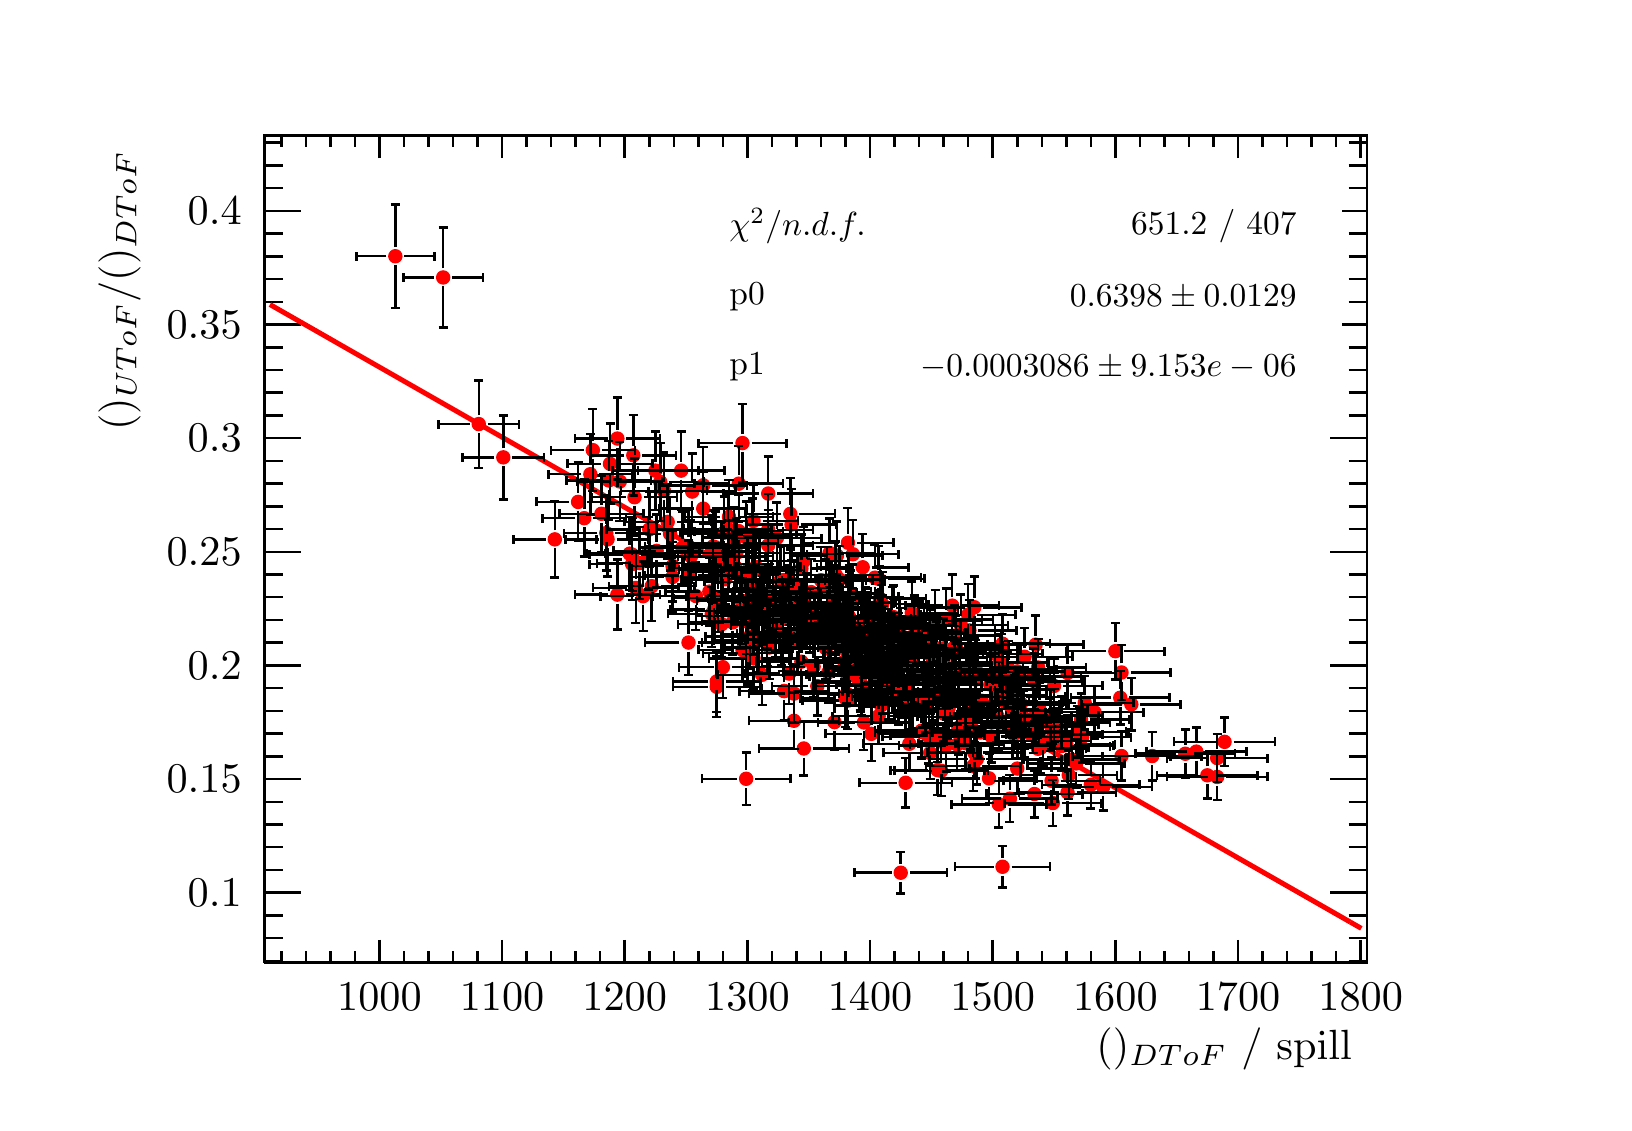
\begin{tikzpicture}
\pgfdeclareplotmark{cross} {
\pgfpathmoveto{\pgfpoint{-0.3\pgfplotmarksize}{\pgfplotmarksize}}
\pgfpathlineto{\pgfpoint{+0.3\pgfplotmarksize}{\pgfplotmarksize}}
\pgfpathlineto{\pgfpoint{+0.3\pgfplotmarksize}{0.3\pgfplotmarksize}}
\pgfpathlineto{\pgfpoint{+1\pgfplotmarksize}{0.3\pgfplotmarksize}}
\pgfpathlineto{\pgfpoint{+1\pgfplotmarksize}{-0.3\pgfplotmarksize}}
\pgfpathlineto{\pgfpoint{+0.3\pgfplotmarksize}{-0.3\pgfplotmarksize}}
\pgfpathlineto{\pgfpoint{+0.3\pgfplotmarksize}{-1.\pgfplotmarksize}}
\pgfpathlineto{\pgfpoint{-0.3\pgfplotmarksize}{-1.\pgfplotmarksize}}
\pgfpathlineto{\pgfpoint{-0.3\pgfplotmarksize}{-0.3\pgfplotmarksize}}
\pgfpathlineto{\pgfpoint{-1.\pgfplotmarksize}{-0.3\pgfplotmarksize}}
\pgfpathlineto{\pgfpoint{-1.\pgfplotmarksize}{0.3\pgfplotmarksize}}
\pgfpathlineto{\pgfpoint{-0.3\pgfplotmarksize}{0.3\pgfplotmarksize}}
\pgfpathclose
\pgfusepathqstroke
}
\pgfdeclareplotmark{cross*} {
\pgfpathmoveto{\pgfpoint{-0.3\pgfplotmarksize}{\pgfplotmarksize}}
\pgfpathlineto{\pgfpoint{+0.3\pgfplotmarksize}{\pgfplotmarksize}}
\pgfpathlineto{\pgfpoint{+0.3\pgfplotmarksize}{0.3\pgfplotmarksize}}
\pgfpathlineto{\pgfpoint{+1\pgfplotmarksize}{0.3\pgfplotmarksize}}
\pgfpathlineto{\pgfpoint{+1\pgfplotmarksize}{-0.3\pgfplotmarksize}}
\pgfpathlineto{\pgfpoint{+0.3\pgfplotmarksize}{-0.3\pgfplotmarksize}}
\pgfpathlineto{\pgfpoint{+0.3\pgfplotmarksize}{-1.\pgfplotmarksize}}
\pgfpathlineto{\pgfpoint{-0.3\pgfplotmarksize}{-1.\pgfplotmarksize}}
\pgfpathlineto{\pgfpoint{-0.3\pgfplotmarksize}{-0.3\pgfplotmarksize}}
\pgfpathlineto{\pgfpoint{-1.\pgfplotmarksize}{-0.3\pgfplotmarksize}}
\pgfpathlineto{\pgfpoint{-1.\pgfplotmarksize}{0.3\pgfplotmarksize}}
\pgfpathlineto{\pgfpoint{-0.3\pgfplotmarksize}{0.3\pgfplotmarksize}}
\pgfpathclose
\pgfusepathqfillstroke
}
\pgfdeclareplotmark{newstar} {
\pgfpathmoveto{\pgfqpoint{0pt}{\pgfplotmarksize}}
\pgfpathlineto{\pgfqpointpolar{44}{0.5\pgfplotmarksize}}
\pgfpathlineto{\pgfqpointpolar{18}{\pgfplotmarksize}}
\pgfpathlineto{\pgfqpointpolar{-20}{0.5\pgfplotmarksize}}
\pgfpathlineto{\pgfqpointpolar{-54}{\pgfplotmarksize}}
\pgfpathlineto{\pgfqpointpolar{-90}{0.5\pgfplotmarksize}}
\pgfpathlineto{\pgfqpointpolar{234}{\pgfplotmarksize}}
\pgfpathlineto{\pgfqpointpolar{198}{0.5\pgfplotmarksize}}
\pgfpathlineto{\pgfqpointpolar{162}{\pgfplotmarksize}}
\pgfpathlineto{\pgfqpointpolar{134}{0.5\pgfplotmarksize}}
\pgfpathclose
\pgfusepathqstroke
}
\pgfdeclareplotmark{newstar*} {
\pgfpathmoveto{\pgfqpoint{0pt}{\pgfplotmarksize}}
\pgfpathlineto{\pgfqpointpolar{44}{0.5\pgfplotmarksize}}
\pgfpathlineto{\pgfqpointpolar{18}{\pgfplotmarksize}}
\pgfpathlineto{\pgfqpointpolar{-20}{0.5\pgfplotmarksize}}
\pgfpathlineto{\pgfqpointpolar{-54}{\pgfplotmarksize}}
\pgfpathlineto{\pgfqpointpolar{-90}{0.5\pgfplotmarksize}}
\pgfpathlineto{\pgfqpointpolar{234}{\pgfplotmarksize}}
\pgfpathlineto{\pgfqpointpolar{198}{0.5\pgfplotmarksize}}
\pgfpathlineto{\pgfqpointpolar{162}{\pgfplotmarksize}}
\pgfpathlineto{\pgfqpointpolar{134}{0.5\pgfplotmarksize}}
\pgfpathclose
\pgfusepathqfillstroke
}
\definecolor{c}{rgb}{1,1,1};
\draw [color=c, fill=c] (0,0) rectangle (20,13.639);
\draw [color=c, fill=c] (3,1.77307) rectangle (17,12.2751);
\definecolor{c}{rgb}{0,0,0};
\draw [c,line width=0.9] (3,1.77307) -- (3,12.2751) -- (17,12.2751) -- (17,1.77307) -- (3,1.77307);
\definecolor{c}{rgb}{1,1,1};
\draw [color=c, fill=c] (3,1.77307) rectangle (17,12.2751);
\definecolor{c}{rgb}{0,0,0};
\draw [c,line width=0.9] (3,1.77307) -- (3,12.2751) -- (17,12.2751) -- (17,1.77307) -- (3,1.77307);
\draw [c,line width=0.9] (3,1.77307) -- (17,1.77307);
\draw [c,line width=0.9] (4.45996,2.05948) -- (4.45996,1.77307);
\draw [c,line width=0.9] (4.77152,1.91628) -- (4.77152,1.77307);
\draw [c,line width=0.9] (5.08308,1.91628) -- (5.08308,1.77307);
\draw [c,line width=0.9] (5.39463,1.91628) -- (5.39463,1.77307);
\draw [c,line width=0.9] (5.70619,1.91628) -- (5.70619,1.77307);
\draw [c,line width=0.9] (6.01775,2.05948) -- (6.01775,1.77307);
\draw [c,line width=0.9] (6.32931,1.91628) -- (6.32931,1.77307);
\draw [c,line width=0.9] (6.64087,1.91628) -- (6.64087,1.77307);
\draw [c,line width=0.9] (6.95242,1.91628) -- (6.95242,1.77307);
\draw [c,line width=0.9] (7.26398,1.91628) -- (7.26398,1.77307);
\draw [c,line width=0.9] (7.57554,2.05948) -- (7.57554,1.77307);
\draw [c,line width=0.9] (7.8871,1.91628) -- (7.8871,1.77307);
\draw [c,line width=0.9] (8.19865,1.91628) -- (8.19865,1.77307);
\draw [c,line width=0.9] (8.51021,1.91628) -- (8.51021,1.77307);
\draw [c,line width=0.9] (8.82177,1.91628) -- (8.82177,1.77307);
\draw [c,line width=0.9] (9.13333,2.05948) -- (9.13333,1.77307);
\draw [c,line width=0.9] (9.44488,1.91628) -- (9.44488,1.77307);
\draw [c,line width=0.9] (9.75644,1.91628) -- (9.75644,1.77307);
\draw [c,line width=0.9] (10.068,1.91628) -- (10.068,1.77307);
\draw [c,line width=0.9] (10.3796,1.91628) -- (10.3796,1.77307);
\draw [c,line width=0.9] (10.6911,2.05948) -- (10.6911,1.77307);
\draw [c,line width=0.9] (11.0027,1.91628) -- (11.0027,1.77307);
\draw [c,line width=0.9] (11.3142,1.91628) -- (11.3142,1.77307);
\draw [c,line width=0.9] (11.6258,1.91628) -- (11.6258,1.77307);
\draw [c,line width=0.9] (11.9373,1.91628) -- (11.9373,1.77307);
\draw [c,line width=0.9] (12.2489,2.05948) -- (12.2489,1.77307);
\draw [c,line width=0.9] (12.5605,1.91628) -- (12.5605,1.77307);
\draw [c,line width=0.9] (12.872,1.91628) -- (12.872,1.77307);
\draw [c,line width=0.9] (13.1836,1.91628) -- (13.1836,1.77307);
\draw [c,line width=0.9] (13.4951,1.91628) -- (13.4951,1.77307);
\draw [c,line width=0.9] (13.8067,2.05948) -- (13.8067,1.77307);
\draw [c,line width=0.9] (14.1182,1.91628) -- (14.1182,1.77307);
\draw [c,line width=0.9] (14.4298,1.91628) -- (14.4298,1.77307);
\draw [c,line width=0.9] (14.7414,1.91628) -- (14.7414,1.77307);
\draw [c,line width=0.9] (15.0529,1.91628) -- (15.0529,1.77307);
\draw [c,line width=0.9] (15.3645,2.05948) -- (15.3645,1.77307);
\draw [c,line width=0.9] (15.676,1.91628) -- (15.676,1.77307);
\draw [c,line width=0.9] (15.9876,1.91628) -- (15.9876,1.77307);
\draw [c,line width=0.9] (16.2992,1.91628) -- (16.2992,1.77307);
\draw [c,line width=0.9] (16.6107,1.91628) -- (16.6107,1.77307);
\draw [c,line width=0.9] (16.9223,2.05948) -- (16.9223,1.77307);
\draw [c,line width=0.9] (4.45996,2.05948) -- (4.45996,1.77307);
\draw [c,line width=0.9] (4.1484,1.91628) -- (4.1484,1.77307);
\draw [c,line width=0.9] (3.83685,1.91628) -- (3.83685,1.77307);
\draw [c,line width=0.9] (3.52529,1.91628) -- (3.52529,1.77307);
\draw [c,line width=0.9] (3.21373,1.91628) -- (3.21373,1.77307);
\draw [c,line width=0.9] (16.9223,2.05948) -- (16.9223,1.77307);
\draw [anchor=base] (4.45996,1.15931) node[scale=1.52731, color=c, rotate=0]{1000};
\draw [anchor=base] (6.01775,1.15931) node[scale=1.52731, color=c, rotate=0]{1100};
\draw [anchor=base] (7.57554,1.15931) node[scale=1.52731, color=c, rotate=0]{1200};
\draw [anchor=base] (9.13333,1.15931) node[scale=1.52731, color=c, rotate=0]{1300};
\draw [anchor=base] (10.6911,1.15931) node[scale=1.52731, color=c, rotate=0]{1400};
\draw [anchor=base] (12.2489,1.15931) node[scale=1.52731, color=c, rotate=0]{1500};
\draw [anchor=base] (13.8067,1.15931) node[scale=1.52731, color=c, rotate=0]{1600};
\draw [anchor=base] (15.3645,1.15931) node[scale=1.52731, color=c, rotate=0]{1700};
\draw [anchor=base] (16.9223,1.15931) node[scale=1.52731, color=c, rotate=0]{1800};
\draw [anchor= east] (17,0.681948) node[scale=1.52731, color=c, rotate=0]{ $(\SOne\STwo)_{\text{DToF}}$ / spill};
\draw [c,line width=0.9] (3,12.2751) -- (17,12.2751);
\draw [c,line width=0.9] (4.45996,11.9887) -- (4.45996,12.2751);
\draw [c,line width=0.9] (4.77152,12.1319) -- (4.77152,12.2751);
\draw [c,line width=0.9] (5.08308,12.1319) -- (5.08308,12.2751);
\draw [c,line width=0.9] (5.39463,12.1319) -- (5.39463,12.2751);
\draw [c,line width=0.9] (5.70619,12.1319) -- (5.70619,12.2751);
\draw [c,line width=0.9] (6.01775,11.9887) -- (6.01775,12.2751);
\draw [c,line width=0.9] (6.32931,12.1319) -- (6.32931,12.2751);
\draw [c,line width=0.9] (6.64087,12.1319) -- (6.64087,12.2751);
\draw [c,line width=0.9] (6.95242,12.1319) -- (6.95242,12.2751);
\draw [c,line width=0.9] (7.26398,12.1319) -- (7.26398,12.2751);
\draw [c,line width=0.9] (7.57554,11.9887) -- (7.57554,12.2751);
\draw [c,line width=0.9] (7.8871,12.1319) -- (7.8871,12.2751);
\draw [c,line width=0.9] (8.19865,12.1319) -- (8.19865,12.2751);
\draw [c,line width=0.9] (8.51021,12.1319) -- (8.51021,12.2751);
\draw [c,line width=0.9] (8.82177,12.1319) -- (8.82177,12.2751);
\draw [c,line width=0.9] (9.13333,11.9887) -- (9.13333,12.2751);
\draw [c,line width=0.9] (9.44488,12.1319) -- (9.44488,12.2751);
\draw [c,line width=0.9] (9.75644,12.1319) -- (9.75644,12.2751);
\draw [c,line width=0.9] (10.068,12.1319) -- (10.068,12.2751);
\draw [c,line width=0.9] (10.3796,12.1319) -- (10.3796,12.2751);
\draw [c,line width=0.9] (10.6911,11.9887) -- (10.6911,12.2751);
\draw [c,line width=0.9] (11.0027,12.1319) -- (11.0027,12.2751);
\draw [c,line width=0.9] (11.3142,12.1319) -- (11.3142,12.2751);
\draw [c,line width=0.9] (11.6258,12.1319) -- (11.6258,12.2751);
\draw [c,line width=0.9] (11.9373,12.1319) -- (11.9373,12.2751);
\draw [c,line width=0.9] (12.2489,11.9887) -- (12.2489,12.2751);
\draw [c,line width=0.9] (12.5605,12.1319) -- (12.5605,12.2751);
\draw [c,line width=0.9] (12.872,12.1319) -- (12.872,12.2751);
\draw [c,line width=0.9] (13.1836,12.1319) -- (13.1836,12.2751);
\draw [c,line width=0.9] (13.4951,12.1319) -- (13.4951,12.2751);
\draw [c,line width=0.9] (13.8067,11.9887) -- (13.8067,12.2751);
\draw [c,line width=0.9] (14.1182,12.1319) -- (14.1182,12.2751);
\draw [c,line width=0.9] (14.4298,12.1319) -- (14.4298,12.2751);
\draw [c,line width=0.9] (14.7414,12.1319) -- (14.7414,12.2751);
\draw [c,line width=0.9] (15.0529,12.1319) -- (15.0529,12.2751);
\draw [c,line width=0.9] (15.3645,11.9887) -- (15.3645,12.2751);
\draw [c,line width=0.9] (15.676,12.1319) -- (15.676,12.2751);
\draw [c,line width=0.9] (15.9876,12.1319) -- (15.9876,12.2751);
\draw [c,line width=0.9] (16.2992,12.1319) -- (16.2992,12.2751);
\draw [c,line width=0.9] (16.6107,12.1319) -- (16.6107,12.2751);
\draw [c,line width=0.9] (16.9223,11.9887) -- (16.9223,12.2751);
\draw [c,line width=0.9] (4.45996,11.9887) -- (4.45996,12.2751);
\draw [c,line width=0.9] (4.1484,12.1319) -- (4.1484,12.2751);
\draw [c,line width=0.9] (3.83685,12.1319) -- (3.83685,12.2751);
\draw [c,line width=0.9] (3.52529,12.1319) -- (3.52529,12.2751);
\draw [c,line width=0.9] (3.21373,12.1319) -- (3.21373,12.2751);
\draw [c,line width=0.9] (16.9223,11.9887) -- (16.9223,12.2751);
\draw [c,line width=0.9] (3,1.77307) -- (3,12.2751);
\draw [c,line width=0.9] (3.462,2.66058) -- (3,2.66058);
\draw [c,line width=0.9] (3.231,2.94918) -- (3,2.94918);
\draw [c,line width=0.9] (3.231,3.23779) -- (3,3.23779);
\draw [c,line width=0.9] (3.231,3.52639) -- (3,3.52639);
\draw [c,line width=0.9] (3.231,3.81499) -- (3,3.81499);
\draw [c,line width=0.9] (3.462,4.1036) -- (3,4.1036);
\draw [c,line width=0.9] (3.231,4.3922) -- (3,4.3922);
\draw [c,line width=0.9] (3.231,4.68081) -- (3,4.68081);
\draw [c,line width=0.9] (3.231,4.96941) -- (3,4.96941);
\draw [c,line width=0.9] (3.231,5.25801) -- (3,5.25801);
\draw [c,line width=0.9] (3.462,5.54662) -- (3,5.54662);
\draw [c,line width=0.9] (3.231,5.83522) -- (3,5.83522);
\draw [c,line width=0.9] (3.231,6.12382) -- (3,6.12382);
\draw [c,line width=0.9] (3.231,6.41243) -- (3,6.41243);
\draw [c,line width=0.9] (3.231,6.70103) -- (3,6.70103);
\draw [c,line width=0.9] (3.462,6.98964) -- (3,6.98964);
\draw [c,line width=0.9] (3.231,7.27824) -- (3,7.27824);
\draw [c,line width=0.9] (3.231,7.56684) -- (3,7.56684);
\draw [c,line width=0.9] (3.231,7.85545) -- (3,7.85545);
\draw [c,line width=0.9] (3.231,8.14405) -- (3,8.14405);
\draw [c,line width=0.9] (3.462,8.43266) -- (3,8.43266);
\draw [c,line width=0.9] (3.231,8.72126) -- (3,8.72126);
\draw [c,line width=0.9] (3.231,9.00986) -- (3,9.00986);
\draw [c,line width=0.9] (3.231,9.29847) -- (3,9.29847);
\draw [c,line width=0.9] (3.231,9.58707) -- (3,9.58707);
\draw [c,line width=0.9] (3.462,9.87568) -- (3,9.87568);
\draw [c,line width=0.9] (3.231,10.1643) -- (3,10.1643);
\draw [c,line width=0.9] (3.231,10.4529) -- (3,10.4529);
\draw [c,line width=0.9] (3.231,10.7415) -- (3,10.7415);
\draw [c,line width=0.9] (3.231,11.0301) -- (3,11.0301);
\draw [c,line width=0.9] (3.462,11.3187) -- (3,11.3187);
\draw [c,line width=0.9] (3.462,2.66058) -- (3,2.66058);
\draw [c,line width=0.9] (3.231,2.37197) -- (3,2.37197);
\draw [c,line width=0.9] (3.231,2.08337) -- (3,2.08337);
\draw [c,line width=0.9] (3.231,1.79477) -- (3,1.79477);
\draw [c,line width=0.9] (3.462,11.3187) -- (3,11.3187);
\draw [c,line width=0.9] (3.231,11.6073) -- (3,11.6073);
\draw [c,line width=0.9] (3.231,11.8959) -- (3,11.8959);
\draw [c,line width=0.9] (3.231,12.1845) -- (3,12.1845);
\draw [anchor= east] (2.9,2.66058) node[scale=1.52731, color=c, rotate=0]{0.1};
\draw [anchor= east] (2.9,4.1036) node[scale=1.52731, color=c, rotate=0]{0.15};
\draw [anchor= east] (2.9,5.54662) node[scale=1.52731, color=c, rotate=0]{0.2};
\draw [anchor= east] (2.9,6.98964) node[scale=1.52731, color=c, rotate=0]{0.25};
\draw [anchor= east] (2.9,8.43266) node[scale=1.52731, color=c, rotate=0]{0.3};
\draw [anchor= east] (2.9,9.87568) node[scale=1.52731, color=c, rotate=0]{0.35};
\draw [anchor= east] (2.9,11.3187) node[scale=1.52731, color=c, rotate=0]{0.4};
\draw [anchor= east] (1.16,12.2751) node[scale=1.52731, color=c, rotate=90]{ $(\SOne\STwo)_{\text{UToF}}/(\SOne\STwo)_{\text{DToF}}$ };
\draw [c,line width=0.9] (17,1.77307) -- (17,12.2751);
\draw [c,line width=0.9] (16.538,2.66058) -- (17,2.66058);
\draw [c,line width=0.9] (16.769,2.94918) -- (17,2.94918);
\draw [c,line width=0.9] (16.769,3.23779) -- (17,3.23779);
\draw [c,line width=0.9] (16.769,3.52639) -- (17,3.52639);
\draw [c,line width=0.9] (16.769,3.81499) -- (17,3.81499);
\draw [c,line width=0.9] (16.538,4.1036) -- (17,4.1036);
\draw [c,line width=0.9] (16.769,4.3922) -- (17,4.3922);
\draw [c,line width=0.9] (16.769,4.68081) -- (17,4.68081);
\draw [c,line width=0.9] (16.769,4.96941) -- (17,4.96941);
\draw [c,line width=0.9] (16.769,5.25801) -- (17,5.25801);
\draw [c,line width=0.9] (16.538,5.54662) -- (17,5.54662);
\draw [c,line width=0.9] (16.769,5.83522) -- (17,5.83522);
\draw [c,line width=0.9] (16.769,6.12382) -- (17,6.12382);
\draw [c,line width=0.9] (16.769,6.41243) -- (17,6.41243);
\draw [c,line width=0.9] (16.769,6.70103) -- (17,6.70103);
\draw [c,line width=0.9] (16.538,6.98964) -- (17,6.98964);
\draw [c,line width=0.9] (16.769,7.27824) -- (17,7.27824);
\draw [c,line width=0.9] (16.769,7.56684) -- (17,7.56684);
\draw [c,line width=0.9] (16.769,7.85545) -- (17,7.85545);
\draw [c,line width=0.9] (16.769,8.14405) -- (17,8.14405);
\draw [c,line width=0.9] (16.538,8.43266) -- (17,8.43266);
\draw [c,line width=0.9] (16.769,8.72126) -- (17,8.72126);
\draw [c,line width=0.9] (16.769,9.00986) -- (17,9.00986);
\draw [c,line width=0.9] (16.769,9.29847) -- (17,9.29847);
\draw [c,line width=0.9] (16.769,9.58707) -- (17,9.58707);
\draw [c,line width=0.9] (16.538,9.87568) -- (17,9.87568);
\draw [c,line width=0.9] (16.769,10.1643) -- (17,10.1643);
\draw [c,line width=0.9] (16.769,10.4529) -- (17,10.4529);
\draw [c,line width=0.9] (16.769,10.7415) -- (17,10.7415);
\draw [c,line width=0.9] (16.769,11.0301) -- (17,11.0301);
\draw [c,line width=0.9] (16.538,11.3187) -- (17,11.3187);
\draw [c,line width=0.9] (16.538,2.66058) -- (17,2.66058);
\draw [c,line width=0.9] (16.769,2.37197) -- (17,2.37197);
\draw [c,line width=0.9] (16.769,2.08337) -- (17,2.08337);
\draw [c,line width=0.9] (16.769,1.79477) -- (17,1.79477);
\draw [c,line width=0.9] (16.538,11.3187) -- (17,11.3187);
\draw [c,line width=0.9] (16.769,11.6073) -- (17,11.6073);
\draw [c,line width=0.9] (16.769,11.8959) -- (17,11.8959);
\draw [c,line width=0.9] (16.769,12.1845) -- (17,12.1845);
\definecolor{c}{rgb}{1,0,0};
\foreach \P in {(13.1992,5.45048), (10.3484,5.82726), (10.6288,6.12134), (7.13936,7.97463), (14.274,4.39574), (10.1615,5.85931), (11.9685,5.46093), (9.21122,6.0995), (10.1615,5.45788), (11.9685,4.79882), (12.6539,5.65631), (11.3921,5.14717),
 (9.32026,5.42783), (7.87152,6.97188), (11.7816,5.80185), (7.06147,7.41624), (10.364,5.76009), (7.68458,8.21507), (10.4107,7.10449), (7.17051,8.28024), (10.8157,5.84178), (10.2705,6.94234), (11.2208,6.21479), (8.41674,6.9321), (10.9559,6.00692),
 (11.065,6.01681), (4.66247,10.7432), (6.03333,8.18888), (10.4419,6.3432), (5.27001,10.4737), (13.4172,5.07019), (5.72177,8.61153), (9.21122,7.38218), (9.58508,6.22415), (13.0278,4.6715), (7.96498,8.02036), (9.05544,6.23748), (11.2987,5.39018),
 (9.99011,6.0152), (9.13333,5.70202), (8.71272,6.25849), (10.5353,5.94111), (11.3921,5.0473), (15.1931,4.57606), (10.8002,5.80507), (12.763,5.40354), (10.2238,6.41032), (12.7941,4.90736), (9.77202,6.5323), (10.6132,4.82252), (12.2333,4.64557),
 (10.3951,5.9186), (10.6755,5.63326), (9.72529,6.43961), (10.5665,5.35173), (7.66901,6.83409), (13.869,5.13638), (12.4358,5.36719), (13.3861,4.63659), (10.8157,6.39521), (11.0494,5.75754), (11.4389,5.33535), (11.5167,6.11072), (12.3268,3.78239),
 (9.41373,6.40936), (11.5479,4.21765), (10.1147,5.85152), (13.6509,4.00377), (9.81875,6.7749), (11.0806,5.89092), (11.6569,4.53196), (12.9811,4.90486), (12.4981,4.68614), (12.7786,5.34343), (10.8625,5.9107), (10.3796,5.9858), (12.763,4.76345),
 (10.1303,5.76243), (9.22679,6.49242), (9.88106,6.30452), (10.3951,5.43795), (9.28911,6.75831), (12.7941,5.80984), (11.2519,5.44211), (10.5821,6.05214), (10.3951,5.18717), (11.9685,4.81829), (11.1117,5.53853), (9.11775,6.1065), (11.5635,5.76069),
 (9.60066,5.22112), (11.4389,4.63775), (10.6288,6.14202), (12.3424,5.58111), (9.81875,5.59386), (13.5419,4.95227), (10.1303,6.48183), (12.3268,5.16309), (10.9715,6.14499), (7.35745,7.14781), (9.67855,6.60591), (11.766,5.92383), (10.0368,6.27769),
 (12.5605,4.23651), (13.3238,4.70417), (10.4263,6.16013), (12.8876,4.58773), (9.25795,5.86435), (7.37303,7.89532), (11.8127,5.49956), (10.8469,6.32441), (8.18308,6.80911), (8.15192,7.21711), (13.1213,4.81954), (11.6258,5.76406), (10.473,6.00055),
 (9.66297,6.13507), (10.7067,5.5013), (13.2147,4.15348), (10.8469,5.301), (10.6755,5.71578), (9.27353,5.85969), (11.0961,5.23899), (10.3951,5.9604), (11.2987,5.95175), (7.51323,7.88247), (9.9278,6.11912), (9.41373,5.77435), (9.46046,6.28506),
 (10.068,6.62888), (11.2208,5.08775), (12.0464,4.35494), (11.2363,5.06393), (8.88408,6.8323), (11.766,5.49161), (11.3454,4.69802), (6.98358,7.62298), (8.12076,7.36938), (9.60066,6.63159), (11.3142,5.9675), (9.66297,5.44277), (11.9529,5.99092),
 (9.66297,6.17834), (12.3268,4.81792), (10.9248,5.22028), (10.1459,6.62492), (8.74388,5.27499), (10.473,6.41701), (7.80921,6.42549), (8.96197,7.09599), (10.364,5.59266), (7.66901,6.95374), (8.97755,6.79947), (12.0152,4.43884), (10.7534,6.66074),
 (12.7786,3.91358), (9.97453,5.52956), (8.83735,7.23183), (10.9871,5.59136), (7.27956,7.47227), (10.4107,6.18564), (10.3796,5.12835), (11.2363,5.56673), (11.7348,5.69613), (9.58508,5.8767), (11.8127,4.75452), (10.4263,5.61757), (10.6288,6.03865),
 (10.8313,6.1652), (11.7348,5.38136), (9.32026,6.26373), (10.8002,5.53841), (11.4856,5.20451), (10.5821,5.28557), (10.177,6.2771), (10.2549,6.08512), (9.58508,6.13729), (9.67855,7.47064), (11.5791,5.63773), (12.5293,5.07892), (9.67855,5.87089),
 (10.5976,6.79296), (13.1992,3.93443), (11.7348,6.306), (11.9062,4.55857), (9.38257,6.17821), (11.47,5.66604), (10.4107,5.09972), (15.0997,4.13018), (11.9997,5.74498), (13.0122,3.79897), (9.66297,6.30815), (12.062,4.70098), (12.576,5.04948),
 (12.8564,4.50022), (6.6876,7.14745), (12.0152,6.28513), (9.32026,6.21973), (13.3082,4.30238), (13.8846,4.3958), (12.0308,5.50389), (13.8846,5.45671), (12.8409,4.99118), (9.24237,6.79642), (11.3765,5.89038), (12.8253,4.48759), (9.77202,5.84361),
 (14.8348,4.45179), (11.361,5.11461), (12.4203,5.06529), (14.975,4.15098), (11.5479,4.65403), (10.4107,5.91416), (11.0961,5.664), (10.8002,6.64606), (10.769,5.42337), (12.4826,5.05132), (7.63785,6.96567), (12.6539,4.71069), (10.9715,5.4937),
 (14.0092,5.05279), (10.473,6.9584), (10.4574,5.98421), (12.3268,5.2398), (11.6414,5.16734), (9.7876,5.96812), (8.07403,7.76268), (12.0308,5.36794), (13.3705,4.85999), (10.9715,5.31052), (10.7223,5.95009), (7.34187,7.2271), (11.6569,5.40054),
 (9.11775,4.10693), (11.4544,4.43522), (11.9997,4.26696), (9.72529,4.84344), (10.5821,5.57562), (8.88408,7.28184), (11.1429,5.04575), (12.2177,5.30387), (10.2082,6.45733), (9.21122,5.63508), (12.5605,5.47067), (8.47906,6.42757), (10.2394,4.82669),
 (9.69413,7.33527), (9.16448,5.91458), (12.1087,5.09755), (15.0997,4.37025), (11.1896,4.55101), (13.1213,4.52278), (12.2177,5.4002), (12.3579,5.57726), (9.84991,6.20702), (13.1836,4.5476), (14.6946,4.42495), (9.33584,6.28077), (12.467,3.85388),
 (8.80619,6.92758), (12.6072,4.83411), (10.8002,4.90254), (10.9559,5.66067), (13.2459,4.35087), (9.19564,7.21096), (11.9373,6.19013), (11.6569,6.13093), (11.2519,6.04504), (9.19564,6.39207), (10.8002,5.47688), (10.9248,5.81177), (11.6725,4.9627),
 (12.2801,5.69265), (10.1926,5.9137), (8.38559,7.05879), (8.18308,6.66935), (8.89966,7.43321), (10.9871,6.16084), (13.0278,5.28594), (11.5946,4.20851), (10.3017,6.63806), (10.9092,5.59152), (11.5791,5.40004), (8.82177,6.76416), (8.89966,6.9391),
 (10.2549,6.00098), (9.33584,6.25878), (9.07101,8.3703), (8.80619,6.07012), (12.5605,5.14789), (9.02428,7.85456), (9.72529,5.18856), (11.4544,5.86928), (7.71574,6.53011), (10.8157,6.08775), (10.3017,6.26026), (10.7378,5.92511), (11.6881,4.99858),
 (9.39815,7.07181), (12.5605,4.6922), (10.3796,6.02762), (10.8313,5.03864), (10.9248,5.87295), (8.43232,7.75426), (8.68157,6.20057), (9.6474,6.39965), (12.4514,5.49702), (10.177,6.9738), (10.3951,6.04399), (9.24237,6.37688), (10.6132,5.77419),
 (7.70016,7.68248), (9.60066,5.22112), (10.2549,6.69514), (11.6258,4.93383), (8.29212,8.02036), (8.57252,7.53762), (11.3454,4.71803), (11.174,5.32074), (12.3735,5.45858), (7.8871,7.27351), (10.2238,6.41032), (9.84991,4.49169), (12.2022,4.11227),
 (12.3112,4.89803), (9.07101,5.74258), (11.6569,5.36106), (10.0213,5.2829), (11.0806,2.91374), (8.75946,6.40157), (10.5665,5.33099), (13.4951,4.03053), (7.76247,6.84676), (9.38257,5.93698), (11.8906,4.89399), (8.82177,5.52407), (8.7283,7.04627),
 (8.69715,6.78544), (11.2363,5.6874), (8.38559,5.83706), (11.6414,5.54267), (8.0273,7.87611), (7.48207,6.44579), (8.38559,6.68997), (10.6755,5.88081), (7.91825,6.55272), (9.11775,5.83989), (12.4981,4.97169), (9.39815,7.26904), (8.85292,6.6407),
 (10.6444,5.97219), (12.0931,4.69436), (8.57252,7.83444), (9.13333,6.74543), (8.69715,7.0577), (12.9966,4.08122), (13.168,4.53215), (10.2705,6.29072), (9.94338,6.47732), (9.02428,7.2519), (9.11775,7.17293), (7.48207,8.42782), (10.8469,6.03786),
 (11.5323,5.72923), (7.98056,7.00141), (12.2801,5.40443), (9.39815,7.72923), (8.74388,5.3429), (10.6444,5.97219), (9.1489,6.60698), (12.6383,4.88425), (10.9404,5.78712), (8.68157,6.99531), (10.7223,5.90892), (10.0368,6.25644), (11.8439,6.0596),
 (8.3077,7.04171), (9.03986,6.17557), (8.99312,6.97287), (13.8067,5.72699), (9.27353,6.21246), (9.5072,7.16402), (11.0027,5.20111), (9.49162,6.14433), (10.6755,5.86018), (9.49162,6.05707), (11.1429,4.05614), (10.7067,4.6773), (12.8253,5.52033),
 (12.9811,4.79293), (8.96197,6.73775), (13.0278,4.91355), (11.7971,4.54209), (12.3735,5.82221), (8.65041,6.48361), (12.3735,2.98975), (10.3484,6.14142), (8.94639,6.09335), (9.84991,6.87171), (9.56951,5.94649), (10.878,5.7224), (10.5042,5.40938),
 (11.0494,5.1491), (12.6072,5.0615), (9.55393,6.62535), (13.3549,4.69789), (7.3886,8.10713), (9.05544,6.3712), (12.5137,4.77802)}{\draw[mark options={color=c,fill=c},mark size=2.402402pt,mark=*] plot coordinates {\P};}
\draw [c,line width=1.8] (3.07,10.13) -- (3.21,10.05) -- (3.35,9.96998) -- (3.49,9.88995) -- (3.63,9.80992) -- (3.77,9.72989) -- (3.91,9.64987) -- (4.05,9.56984) -- (4.19,9.48981) -- (4.33,9.40978) -- (4.47,9.32975) -- (4.61,9.24972) --
 (4.75,9.16969) -- (4.89,9.08966) -- (5.03,9.00963) -- (5.17,8.9296) -- (5.31,8.84957) -- (5.45,8.76954) -- (5.59,8.68951) -- (5.73,8.60948) -- (5.87,8.52945) -- (6.01,8.44942) -- (6.15,8.36939) -- (6.29,8.28936) -- (6.43,8.20933) -- (6.57,8.1293) --
 (6.71,8.04927) -- (6.85,7.96924) -- (6.99,7.88921) -- (7.13,7.80918) -- (7.27,7.72915) -- (7.41,7.64912) -- (7.55,7.5691) -- (7.69,7.48907) -- (7.83,7.40904) -- (7.97,7.32901) -- (8.11,7.24898) -- (8.25,7.16895) -- (8.39,7.08892) -- (8.53,7.00889)
 -- (8.67,6.92886) -- (8.81,6.84883) -- (8.95,6.7688) -- (9.09,6.68877) -- (9.23,6.60874) -- (9.37,6.52871) -- (9.51,6.44868) -- (9.65,6.36865) -- (9.79,6.28862) -- (9.93,6.20859);
\draw [c,line width=1.8] (9.93,6.20859) -- (10.07,6.12856) -- (10.21,6.04853) -- (10.35,5.9685) -- (10.49,5.88847) -- (10.63,5.80844) -- (10.77,5.72841) -- (10.91,5.64838) -- (11.05,5.56835) -- (11.19,5.48832) -- (11.33,5.4083) -- (11.47,5.32827) --
 (11.61,5.24824) -- (11.75,5.16821) -- (11.89,5.08818) -- (12.03,5.00815) -- (12.17,4.92812) -- (12.31,4.84809) -- (12.45,4.76806) -- (12.59,4.68803) -- (12.73,4.608) -- (12.87,4.52797) -- (13.01,4.44794) -- (13.15,4.36791) -- (13.29,4.28788) --
 (13.43,4.20785) -- (13.57,4.12782) -- (13.71,4.04779) -- (13.85,3.96776) -- (13.99,3.88773) -- (14.13,3.8077) -- (14.27,3.72767) -- (14.41,3.64764) -- (14.55,3.56761) -- (14.69,3.48758) -- (14.83,3.40755) -- (14.97,3.32753) -- (15.11,3.2475) --
 (15.25,3.16747) -- (15.39,3.08744) -- (15.53,3.00741) -- (15.67,2.92738) -- (15.81,2.84735) -- (15.95,2.76732) -- (16.09,2.68729) -- (16.23,2.60726) -- (16.37,2.52723) -- (16.51,2.4472) -- (16.65,2.36717) -- (16.79,2.28714);
\draw [c,line width=1.8] (16.79,2.28714) -- (16.93,2.20711);
\definecolor{c}{rgb}{1,1,1};
\draw [color=c, fill=c] (8.33811,8.88252) rectangle (16.6762,11.5759);
\definecolor{c}{rgb}{0,0,0};
\draw [anchor= west] (8.75501,11.127) node[scale=1.20912, color=c, rotate=0]{$\chi^{2} / ndf $};
\draw [anchor= east] (16.2593,11.127) node[scale=1.20912, color=c, rotate=0]{ 651.2 / 407};
\draw [anchor= west] (8.75501,10.2292) node[scale=1.20912, color=c, rotate=0]{p0       };
\draw [anchor= east] (16.2593,10.2292) node[scale=1.20912, color=c, rotate=0]{$ 0.6398 \pm 0.0129$};
\draw [anchor= west] (8.75501,9.33142) node[scale=1.20912, color=c, rotate=0]{p1       };
\draw [anchor= east] (16.2593,9.33142) node[scale=1.20912, color=c, rotate=0]{$ -0.0003086 \pm 9.153e-06$};
\draw [c,line width=0.9] (13.0845,5.45048) -- (12.5837,5.45048);
\draw [c,line width=0.9] (12.5837,5.39317) -- (12.5837,5.50778);
\draw [c,line width=0.9] (13.3138,5.45048) -- (13.8146,5.45048);
\draw [c,line width=0.9] (13.8146,5.39317) -- (13.8146,5.50778);
\draw [c,line width=0.9] (13.1992,5.56509) -- (13.1992,5.80485);
\draw [c,line width=0.9] (13.1418,5.80485) -- (13.2565,5.80485);
\draw [c,line width=0.9] (13.1992,5.33586) -- (13.1992,5.09611);
\draw [c,line width=0.9] (13.1418,5.09611) -- (13.2565,5.09611);
\draw [c,line width=0.9] (10.2338,5.82726) -- (9.77013,5.82726);
\draw [c,line width=0.9] (9.77013,5.76996) -- (9.77013,5.88457);
\draw [c,line width=0.9] (10.463,5.82726) -- (10.9267,5.82726);
\draw [c,line width=0.9] (10.9267,5.76996) -- (10.9267,5.88457);
\draw [c,line width=0.9] (10.3484,5.94188) -- (10.3484,6.21886);
\draw [c,line width=0.9] (10.2911,6.21886) -- (10.4057,6.21886);
\draw [c,line width=0.9] (10.3484,5.71265) -- (10.3484,5.43566);
\draw [c,line width=0.9] (10.2911,5.43566) -- (10.4057,5.43566);
\draw [c,line width=0.9] (10.5142,6.12134) -- (10.0468,6.12134);
\draw [c,line width=0.9] (10.0468,6.06404) -- (10.0468,6.17865);
\draw [c,line width=0.9] (10.7434,6.12134) -- (11.2108,6.12134);
\draw [c,line width=0.9] (11.2108,6.06404) -- (11.2108,6.17865);
\draw [c,line width=0.9] (10.6288,6.23596) -- (10.6288,6.52143);
\draw [c,line width=0.9] (10.5715,6.52143) -- (10.6861,6.52143);
\draw [c,line width=0.9] (10.6288,6.00673) -- (10.6288,5.72126);
\draw [c,line width=0.9] (10.5715,5.72126) -- (10.6861,5.72126);
\draw [c,line width=0.9] (7.02474,7.97463) -- (6.60606,7.97463);
\draw [c,line width=0.9] (6.60606,7.91733) -- (6.60606,8.03194);
\draw [c,line width=0.9] (7.25397,7.97463) -- (7.67266,7.97463);
\draw [c,line width=0.9] (7.67266,7.91733) -- (7.67266,8.03194);
\draw [c,line width=0.9] (7.13936,8.08925) -- (7.13936,8.48385);
\draw [c,line width=0.9] (7.08205,8.48385) -- (7.19666,8.48385);
\draw [c,line width=0.9] (7.13936,7.86002) -- (7.13936,7.46542);
\draw [c,line width=0.9] (7.08205,7.46542) -- (7.19666,7.46542);
\draw [c,line width=0.9] (14.1594,4.39574) -- (13.6451,4.39574);
\draw [c,line width=0.9] (13.6451,4.33844) -- (13.6451,4.45305);
\draw [c,line width=0.9] (14.3886,4.39574) -- (14.903,4.39574);
\draw [c,line width=0.9] (14.903,4.33844) -- (14.903,4.45305);
\draw [c,line width=0.9] (14.274,4.51036) -- (14.274,4.70384);
\draw [c,line width=0.9] (14.2167,4.70384) -- (14.3313,4.70384);
\draw [c,line width=0.9] (14.274,4.28113) -- (14.274,4.08765);
\draw [c,line width=0.9] (14.2167,4.08765) -- (14.3313,4.08765);
\draw [c,line width=0.9] (10.0469,5.85931) -- (9.58572,5.85931);
\draw [c,line width=0.9] (9.58572,5.802) -- (9.58572,5.91661);
\draw [c,line width=0.9] (10.2761,5.85931) -- (10.7372,5.85931);
\draw [c,line width=0.9] (10.7372,5.802) -- (10.7372,5.91661);
\draw [c,line width=0.9] (10.1615,5.97392) -- (10.1615,6.25385);
\draw [c,line width=0.9] (10.1042,6.25385) -- (10.2188,6.25385);
\draw [c,line width=0.9] (10.1615,5.74469) -- (10.1615,5.46477);
\draw [c,line width=0.9] (10.1042,5.46477) -- (10.2188,5.46477);
\draw [c,line width=0.9] (11.8539,5.46093) -- (11.3688,5.46093);
\draw [c,line width=0.9] (11.3688,5.40363) -- (11.3688,5.51824);
\draw [c,line width=0.9] (12.0831,5.46093) -- (12.5682,5.46093);
\draw [c,line width=0.9] (12.5682,5.40363) -- (12.5682,5.51824);
\draw [c,line width=0.9] (11.9685,5.57554) -- (11.9685,5.82501);
\draw [c,line width=0.9] (11.9112,5.82501) -- (12.0258,5.82501);
\draw [c,line width=0.9] (11.9685,5.34632) -- (11.9685,5.09685);
\draw [c,line width=0.9] (11.9112,5.09685) -- (12.0258,5.09685);
\draw [c,line width=0.9] (9.0966,6.0995) -- (8.64847,6.0995);
\draw [c,line width=0.9] (8.64847,6.04219) -- (8.64847,6.1568);
\draw [c,line width=0.9] (9.32583,6.0995) -- (9.77396,6.0995);
\draw [c,line width=0.9] (9.77396,6.04219) -- (9.77396,6.1568);
\draw [c,line width=0.9] (9.21122,6.21411) -- (9.21122,6.51245);
\draw [c,line width=0.9] (9.15391,6.51245) -- (9.26852,6.51245);
\draw [c,line width=0.9] (9.21122,5.98488) -- (9.21122,5.68654);
\draw [c,line width=0.9] (9.15391,5.68654) -- (9.26852,5.68654);
\draw [c,line width=0.9] (10.0469,5.45788) -- (9.58572,5.45788);
\draw [c,line width=0.9] (9.58572,5.40057) -- (9.58572,5.51519);
\draw [c,line width=0.9] (10.2761,5.45788) -- (10.7372,5.45788);
\draw [c,line width=0.9] (10.7372,5.40057) -- (10.7372,5.51519);
\draw [c,line width=0.9] (10.1615,5.57249) -- (10.1615,5.83699);
\draw [c,line width=0.9] (10.1042,5.83699) -- (10.2188,5.83699);
\draw [c,line width=0.9] (10.1615,5.34327) -- (10.1615,5.07877);
\draw [c,line width=0.9] (10.1042,5.07877) -- (10.2188,5.07877);
\draw [c,line width=0.9] (11.8539,4.79882) -- (11.3688,4.79882);
\draw [c,line width=0.9] (11.3688,4.74151) -- (11.3688,4.85612);
\draw [c,line width=0.9] (12.0831,4.79882) -- (12.5682,4.79882);
\draw [c,line width=0.9] (12.5682,4.74151) -- (12.5682,4.85612);
\draw [c,line width=0.9] (11.9685,4.91343) -- (11.9685,5.13775);
\draw [c,line width=0.9] (11.9112,5.13775) -- (12.0258,5.13775);
\draw [c,line width=0.9] (11.9685,4.6842) -- (11.9685,4.45988);
\draw [c,line width=0.9] (11.9112,4.45988) -- (12.0258,4.45988);
\draw [c,line width=0.9] (12.5393,5.65631) -- (12.0454,5.65631);
\draw [c,line width=0.9] (12.0454,5.599) -- (12.0454,5.71362);
\draw [c,line width=0.9] (12.7685,5.65631) -- (13.2625,5.65631);
\draw [c,line width=0.9] (13.2625,5.599) -- (13.2625,5.71362);
\draw [c,line width=0.9] (12.6539,5.77092) -- (12.6539,6.02224);
\draw [c,line width=0.9] (12.5966,6.02224) -- (12.7112,6.02224);
\draw [c,line width=0.9] (12.6539,5.5417) -- (12.6539,5.29037);
\draw [c,line width=0.9] (12.5966,5.29037) -- (12.7112,5.29037);
\draw [c,line width=0.9] (11.2775,5.14717) -- (10.8,5.14717);
\draw [c,line width=0.9] (10.8,5.08986) -- (10.8,5.20447);
\draw [c,line width=0.9] (11.5067,5.14717) -- (11.9843,5.14717);
\draw [c,line width=0.9] (11.9843,5.08986) -- (11.9843,5.20447);
\draw [c,line width=0.9] (11.3921,5.26178) -- (11.3921,5.50393);
\draw [c,line width=0.9] (11.3348,5.50393) -- (11.4494,5.50393);
\draw [c,line width=0.9] (11.3921,5.03255) -- (11.3921,4.7904);
\draw [c,line width=0.9] (11.3348,4.7904) -- (11.4494,4.7904);
\draw [c,line width=0.9] (9.20565,5.42783) -- (8.75601,5.42783);
\draw [c,line width=0.9] (8.75601,5.37053) -- (8.75601,5.48514);
\draw [c,line width=0.9] (9.43487,5.42783) -- (9.88452,5.42783);
\draw [c,line width=0.9] (9.88452,5.37053) -- (9.88452,5.48514);
\draw [c,line width=0.9] (9.32026,5.54244) -- (9.32026,5.81347);
\draw [c,line width=0.9] (9.26295,5.81347) -- (9.37757,5.81347);
\draw [c,line width=0.9] (9.32026,5.31322) -- (9.32026,5.04219);
\draw [c,line width=0.9] (9.26295,5.04219) -- (9.37757,5.04219);
\draw [c,line width=0.9] (7.7569,6.97188) -- (7.32763,6.97188);
\draw [c,line width=0.9] (7.32763,6.91457) -- (7.32763,7.02919);
\draw [c,line width=0.9] (7.98613,6.97188) -- (8.41541,6.97188);
\draw [c,line width=0.9] (8.41541,6.91457) -- (8.41541,7.02919);
\draw [c,line width=0.9] (7.87152,7.08649) -- (7.87152,7.43329);
\draw [c,line width=0.9] (7.81421,7.43329) -- (7.92882,7.43329);
\draw [c,line width=0.9] (7.87152,6.85727) -- (7.87152,6.51047);
\draw [c,line width=0.9] (7.81421,6.51047) -- (7.92882,6.51047);
\draw [c,line width=0.9] (11.667,5.80185) -- (11.1843,5.80185);
\draw [c,line width=0.9] (11.1843,5.74454) -- (11.1843,5.85915);
\draw [c,line width=0.9] (11.8962,5.80185) -- (12.3788,5.80185);
\draw [c,line width=0.9] (12.3788,5.74454) -- (12.3788,5.85915);
\draw [c,line width=0.9] (11.7816,5.91646) -- (11.7816,6.18006);
\draw [c,line width=0.9] (11.7243,6.18006) -- (11.8389,6.18006);
\draw [c,line width=0.9] (11.7816,5.68723) -- (11.7816,5.42363);
\draw [c,line width=0.9] (11.7243,5.42363) -- (11.8389,5.42363);
\draw [c,line width=0.9] (6.94685,7.41624) -- (6.52931,7.41624);
\draw [c,line width=0.9] (6.52931,7.35893) -- (6.52931,7.47354);
\draw [c,line width=0.9] (7.17608,7.41624) -- (7.59363,7.41624);
\draw [c,line width=0.9] (7.59363,7.35893) -- (7.59363,7.47354);
\draw [c,line width=0.9] (7.06147,7.53085) -- (7.06147,7.90513);
\draw [c,line width=0.9] (7.00416,7.90513) -- (7.11877,7.90513);
\draw [c,line width=0.9] (7.06147,7.30162) -- (7.06147,6.92734);
\draw [c,line width=0.9] (7.00416,6.92734) -- (7.11877,6.92734);
\draw [c,line width=0.9] (10.2494,5.76009) -- (9.7855,5.76009);
\draw [c,line width=0.9] (9.7855,5.70278) -- (9.7855,5.81739);
\draw [c,line width=0.9] (10.4786,5.76009) -- (10.9425,5.76009);
\draw [c,line width=0.9] (10.9425,5.70278) -- (10.9425,5.81739);
\draw [c,line width=0.9] (10.364,5.8747) -- (10.364,6.14899);
\draw [c,line width=0.9] (10.3067,6.14899) -- (10.4213,6.14899);
\draw [c,line width=0.9] (10.364,5.64547) -- (10.364,5.37118);
\draw [c,line width=0.9] (10.3067,5.37118) -- (10.4213,5.37118);
\draw [c,line width=0.9] (7.56997,8.21507) -- (7.14338,8.21507);
\draw [c,line width=0.9] (7.14338,8.15776) -- (7.14338,8.27237);
\draw [c,line width=0.9] (7.7992,8.21507) -- (8.22579,8.21507);
\draw [c,line width=0.9] (8.22579,8.15776) -- (8.22579,8.27237);
\draw [c,line width=0.9] (7.68458,8.32968) -- (7.68458,8.7258);
\draw [c,line width=0.9] (7.62728,8.7258) -- (7.74189,8.7258);
\draw [c,line width=0.9] (7.68458,8.10045) -- (7.68458,7.70434);
\draw [c,line width=0.9] (7.62728,7.70434) -- (7.74189,7.70434);
\draw [c,line width=0.9] (10.2961,7.10449) -- (9.8316,7.10449);
\draw [c,line width=0.9] (9.8316,7.04719) -- (9.8316,7.1618);
\draw [c,line width=0.9] (10.5253,7.10449) -- (10.9898,7.10449);
\draw [c,line width=0.9] (10.9898,7.04719) -- (10.9898,7.1618);
\draw [c,line width=0.9] (10.4107,7.21911) -- (10.4107,7.54261);
\draw [c,line width=0.9] (10.3534,7.54261) -- (10.468,7.54261);
\draw [c,line width=0.9] (10.4107,6.98988) -- (10.4107,6.66637);
\draw [c,line width=0.9] (10.3534,6.66637) -- (10.468,6.66637);
\draw [c,line width=0.9] (7.0559,8.28024) -- (6.63676,8.28024);
\draw [c,line width=0.9] (6.63676,8.22293) -- (6.63676,8.33755);
\draw [c,line width=0.9] (7.28513,8.28024) -- (7.70427,8.28024);
\draw [c,line width=0.9] (7.70427,8.22293) -- (7.70427,8.33755);
\draw [c,line width=0.9] (7.17051,8.39485) -- (7.17051,8.80055);
\draw [c,line width=0.9] (7.11321,8.80055) -- (7.22782,8.80055);
\draw [c,line width=0.9] (7.17051,8.16563) -- (7.17051,7.75993);
\draw [c,line width=0.9] (7.11321,7.75993) -- (7.22782,7.75993);
\draw [c,line width=0.9] (10.7011,5.84178) -- (10.2312,5.84178);
\draw [c,line width=0.9] (10.2312,5.78447) -- (10.2312,5.89909);
\draw [c,line width=0.9] (10.9304,5.84178) -- (11.4003,5.84178);
\draw [c,line width=0.9] (11.4003,5.78447) -- (11.4003,5.89909);
\draw [c,line width=0.9] (10.8157,5.95639) -- (10.8157,6.22973);
\draw [c,line width=0.9] (10.7584,6.22973) -- (10.873,6.22973);
\draw [c,line width=0.9] (10.8157,5.72717) -- (10.8157,5.45383);
\draw [c,line width=0.9] (10.7584,5.45383) -- (10.873,5.45383);
\draw [c,line width=0.9] (10.1559,6.94234) -- (9.69329,6.94234);
\draw [c,line width=0.9] (9.69329,6.88504) -- (9.69329,6.99965);
\draw [c,line width=0.9] (10.3851,6.94234) -- (10.8477,6.94234);
\draw [c,line width=0.9] (10.8477,6.88504) -- (10.8477,6.99965);
\draw [c,line width=0.9] (10.2705,7.05695) -- (10.2705,7.37603);
\draw [c,line width=0.9] (10.2132,7.37603) -- (10.3278,7.37603);
\draw [c,line width=0.9] (10.2705,6.82773) -- (10.2705,6.50865);
\draw [c,line width=0.9] (10.2132,6.50865) -- (10.3278,6.50865);
\draw [c,line width=0.9] (11.1061,6.21479) -- (10.6309,6.21479);
\draw [c,line width=0.9] (10.6309,6.15749) -- (10.6309,6.2721);
\draw [c,line width=0.9] (11.3354,6.21479) -- (11.8107,6.21479);
\draw [c,line width=0.9] (11.8107,6.15749) -- (11.8107,6.2721);
\draw [c,line width=0.9] (11.2208,6.32941) -- (11.2208,6.61296);
\draw [c,line width=0.9] (11.1635,6.61296) -- (11.2781,6.61296);
\draw [c,line width=0.9] (11.2208,6.10018) -- (11.2208,5.81662);
\draw [c,line width=0.9] (11.1635,5.81662) -- (11.2781,5.81662);
\draw [c,line width=0.9] (8.30213,6.9321) -- (7.8651,6.9321);
\draw [c,line width=0.9] (7.8651,6.87479) -- (7.8651,6.98941);
\draw [c,line width=0.9] (8.53136,6.9321) -- (8.96839,6.9321);
\draw [c,line width=0.9] (8.96839,6.87479) -- (8.96839,6.98941);
\draw [c,line width=0.9] (8.41674,7.04671) -- (8.41674,7.38551);
\draw [c,line width=0.9] (8.35944,7.38551) -- (8.47405,7.38551);
\draw [c,line width=0.9] (8.41674,6.81749) -- (8.41674,6.47869);
\draw [c,line width=0.9] (8.35944,6.47869) -- (8.47405,6.47869);
\draw [c,line width=0.9] (10.8413,6.00692) -- (10.3695,6.00692);
\draw [c,line width=0.9] (10.3695,5.94961) -- (10.3695,6.06422);
\draw [c,line width=0.9] (11.0706,6.00692) -- (11.5423,6.00692);
\draw [c,line width=0.9] (11.5423,5.94961) -- (11.5423,6.06422);
\draw [c,line width=0.9] (10.9559,6.12153) -- (10.9559,6.39979);
\draw [c,line width=0.9] (10.8986,6.39979) -- (11.0132,6.39979);
\draw [c,line width=0.9] (10.9559,5.8923) -- (10.9559,5.61405);
\draw [c,line width=0.9] (10.8986,5.61405) -- (11.0132,5.61405);
\draw [c,line width=0.9] (10.9504,6.01681) -- (10.4771,6.01681);
\draw [c,line width=0.9] (10.4771,5.95951) -- (10.4771,6.07412);
\draw [c,line width=0.9] (11.1796,6.01681) -- (11.6528,6.01681);
\draw [c,line width=0.9] (11.6528,5.95951) -- (11.6528,6.07412);
\draw [c,line width=0.9] (11.065,6.13143) -- (11.065,6.40909);
\draw [c,line width=0.9] (11.0077,6.40909) -- (11.1223,6.40909);
\draw [c,line width=0.9] (11.065,5.9022) -- (11.065,5.62454);
\draw [c,line width=0.9] (11.0077,5.62454) -- (11.1223,5.62454);
\draw [c,line width=0.9] (4.54786,10.7432) -- (4.16667,10.7432);
\draw [c,line width=0.9] (4.16667,10.6859) -- (4.16667,10.8005);
\draw [c,line width=0.9] (4.77709,10.7432) -- (5.15828,10.7432);
\draw [c,line width=0.9] (5.15828,10.6859) -- (5.15828,10.8005);
\draw [c,line width=0.9] (4.66247,10.8578) -- (4.66247,11.3999);
\draw [c,line width=0.9] (4.60517,11.3999) -- (4.71978,11.3999);
\draw [c,line width=0.9] (4.66247,10.6286) -- (4.66247,10.0865);
\draw [c,line width=0.9] (4.60517,10.0865) -- (4.71978,10.0865);
\draw [c,line width=0.9] (5.91871,8.18888) -- (5.51643,8.18888);
\draw [c,line width=0.9] (5.51643,8.13157) -- (5.51643,8.24618);
\draw [c,line width=0.9] (6.14794,8.18888) -- (6.55022,8.18888);
\draw [c,line width=0.9] (6.55022,8.13157) -- (6.55022,8.24618);
\draw [c,line width=0.9] (6.03333,8.30349) -- (6.03333,8.72261);
\draw [c,line width=0.9] (5.97602,8.72261) -- (6.09063,8.72261);
\draw [c,line width=0.9] (6.03333,8.07426) -- (6.03333,7.65514);
\draw [c,line width=0.9] (5.97602,7.65514) -- (6.09063,7.65514);
\draw [c,line width=0.9] (10.3273,6.3432) -- (9.86234,6.3432);
\draw [c,line width=0.9] (9.86234,6.28589) -- (9.86234,6.4005);
\draw [c,line width=0.9] (10.5565,6.3432) -- (11.0214,6.3432);
\draw [c,line width=0.9] (11.0214,6.28589) -- (11.0214,6.4005);
\draw [c,line width=0.9] (10.4419,6.45781) -- (10.4419,6.75326);
\draw [c,line width=0.9] (10.3846,6.75326) -- (10.4992,6.75326);
\draw [c,line width=0.9] (10.4419,6.22858) -- (10.4419,5.93313);
\draw [c,line width=0.9] (10.3846,5.93313) -- (10.4992,5.93313);
\draw [c,line width=0.9] (5.1554,10.4737) -- (4.76475,10.4737);
\draw [c,line width=0.9] (4.76475,10.4164) -- (4.76475,10.531);
\draw [c,line width=0.9] (5.38462,10.4737) -- (5.77527,10.4737);
\draw [c,line width=0.9] (5.77527,10.4164) -- (5.77527,10.531);
\draw [c,line width=0.9] (5.27001,10.5883) -- (5.27001,11.108);
\draw [c,line width=0.9] (5.21271,11.108) -- (5.32732,11.108);
\draw [c,line width=0.9] (5.27001,10.3591) -- (5.27001,9.83943);
\draw [c,line width=0.9] (5.21271,9.83943) -- (5.32732,9.83943);
\draw [c,line width=0.9] (13.3026,5.07019) -- (12.799,5.07019);
\draw [c,line width=0.9] (12.799,5.01288) -- (12.799,5.1275);
\draw [c,line width=0.9] (13.5319,5.07019) -- (14.0355,5.07019);
\draw [c,line width=0.9] (14.0355,5.01288) -- (14.0355,5.1275);
\draw [c,line width=0.9] (13.4172,5.1848) -- (13.4172,5.40908);
\draw [c,line width=0.9] (13.3599,5.40908) -- (13.4746,5.40908);
\draw [c,line width=0.9] (13.4172,4.95558) -- (13.4172,4.73131);
\draw [c,line width=0.9] (13.3599,4.73131) -- (13.4746,4.73131);
\draw [c,line width=0.9] (5.60716,8.61153) -- (5.20959,8.61153);
\draw [c,line width=0.9] (5.20959,8.55422) -- (5.20959,8.66884);
\draw [c,line width=0.9] (5.83638,8.61153) -- (6.23395,8.61153);
\draw [c,line width=0.9] (6.23395,8.55422) -- (6.23395,8.66884);
\draw [c,line width=0.9] (5.72177,8.72614) -- (5.72177,9.16666);
\draw [c,line width=0.9] (5.66446,9.16666) -- (5.77908,9.16666);
\draw [c,line width=0.9] (5.72177,8.49692) -- (5.72177,8.0564);
\draw [c,line width=0.9] (5.66446,8.0564) -- (5.77908,8.0564);
\draw [c,line width=0.9] (9.0966,7.38218) -- (8.64847,7.38218);
\draw [c,line width=0.9] (8.64847,7.32488) -- (8.64847,7.43949);
\draw [c,line width=0.9] (9.32583,7.38218) -- (9.77396,7.38218);
\draw [c,line width=0.9] (9.77396,7.32488) -- (9.77396,7.43949);
\draw [c,line width=0.9] (9.21122,7.4968) -- (9.21122,7.84326);
\draw [c,line width=0.9] (9.15391,7.84326) -- (9.26852,7.84326);
\draw [c,line width=0.9] (9.21122,7.26757) -- (9.21122,6.9211);
\draw [c,line width=0.9] (9.15391,6.9211) -- (9.26852,6.9211);
\draw [c,line width=0.9] (9.47047,6.22415) -- (9.01719,6.22415);
\draw [c,line width=0.9] (9.01719,6.16685) -- (9.01719,6.28146);
\draw [c,line width=0.9] (9.6997,6.22415) -- (10.153,6.22415);
\draw [c,line width=0.9] (10.153,6.16685) -- (10.153,6.28146);
\draw [c,line width=0.9] (9.58508,6.33877) -- (9.58508,6.63811);
\draw [c,line width=0.9] (9.52778,6.63811) -- (9.64239,6.63811);
\draw [c,line width=0.9] (9.58508,6.10954) -- (9.58508,5.8102);
\draw [c,line width=0.9] (9.52778,5.8102) -- (9.64239,5.8102);
\draw [c,line width=0.9] (12.9132,4.6715) -- (12.4145,4.6715);
\draw [c,line width=0.9] (12.4145,4.61419) -- (12.4145,4.7288);
\draw [c,line width=0.9] (13.1424,4.6715) -- (13.6411,4.6715);
\draw [c,line width=0.9] (13.6411,4.61419) -- (13.6411,4.7288);
\draw [c,line width=0.9] (13.0278,4.78611) -- (13.0278,4.99807);
\draw [c,line width=0.9] (12.9705,4.99807) -- (13.0851,4.99807);
\draw [c,line width=0.9] (13.0278,4.55688) -- (13.0278,4.34492);
\draw [c,line width=0.9] (12.9705,4.34492) -- (13.0851,4.34492);
\draw [c,line width=0.9] (7.85037,8.02036) -- (7.41976,8.02036);
\draw [c,line width=0.9] (7.41976,7.96306) -- (7.41976,8.07767);
\draw [c,line width=0.9] (8.0796,8.02036) -- (8.51021,8.02036);
\draw [c,line width=0.9] (8.51021,7.96306) -- (8.51021,8.07767);
\draw [c,line width=0.9] (7.96498,8.13498) -- (7.96498,8.52014);
\draw [c,line width=0.9] (7.90768,8.52014) -- (8.02229,8.52014);
\draw [c,line width=0.9] (7.96498,7.90575) -- (7.96498,7.52059);
\draw [c,line width=0.9] (7.90768,7.52059) -- (8.02229,7.52059);
\draw [c,line width=0.9] (8.94082,6.23748) -- (8.49485,6.23748);
\draw [c,line width=0.9] (8.49485,6.18018) -- (8.49485,6.29479);
\draw [c,line width=0.9] (9.17005,6.23748) -- (9.61602,6.23748);
\draw [c,line width=0.9] (9.61602,6.18018) -- (9.61602,6.29479);
\draw [c,line width=0.9] (9.05544,6.3521) -- (9.05544,6.65735);
\draw [c,line width=0.9] (8.99813,6.65735) -- (9.11274,6.65735);
\draw [c,line width=0.9] (9.05544,6.12287) -- (9.05544,5.81762);
\draw [c,line width=0.9] (8.99813,5.81762) -- (9.11274,5.81762);
\draw [c,line width=0.9] (11.184,5.39018) -- (10.7077,5.39018);
\draw [c,line width=0.9] (10.7077,5.33287) -- (10.7077,5.44749);
\draw [c,line width=0.9] (11.4133,5.39018) -- (11.8896,5.39018);
\draw [c,line width=0.9] (11.8896,5.33287) -- (11.8896,5.44749);
\draw [c,line width=0.9] (11.2987,5.50479) -- (11.2987,5.75698);
\draw [c,line width=0.9] (11.2413,5.75698) -- (11.356,5.75698);
\draw [c,line width=0.9] (11.2987,5.27557) -- (11.2987,5.02338);
\draw [c,line width=0.9] (11.2413,5.02338) -- (11.356,5.02338);
\draw [c,line width=0.9] (9.8755,6.0152) -- (9.41668,6.0152);
\draw [c,line width=0.9] (9.41668,5.95789) -- (9.41668,6.07251);
\draw [c,line width=0.9] (10.1047,6.0152) -- (10.5635,6.0152);
\draw [c,line width=0.9] (10.5635,5.95789) -- (10.5635,6.07251);
\draw [c,line width=0.9] (9.99011,6.12981) -- (9.99011,6.41727);
\draw [c,line width=0.9] (9.9328,6.41727) -- (10.0474,6.41727);
\draw [c,line width=0.9] (9.99011,5.90059) -- (9.99011,5.61313);
\draw [c,line width=0.9] (9.9328,5.61313) -- (10.0474,5.61313);
\draw [c,line width=0.9] (9.01871,5.70202) -- (8.57166,5.70202);
\draw [c,line width=0.9] (8.57166,5.64471) -- (8.57166,5.75933);
\draw [c,line width=0.9] (9.24794,5.70202) -- (9.69499,5.70202);
\draw [c,line width=0.9] (9.69499,5.64471) -- (9.69499,5.75933);
\draw [c,line width=0.9] (9.13333,5.81663) -- (9.13333,6.10029);
\draw [c,line width=0.9] (9.07602,6.10029) -- (9.19063,6.10029);
\draw [c,line width=0.9] (9.13333,5.58741) -- (9.13333,5.30375);
\draw [c,line width=0.9] (9.07602,5.30375) -- (9.19063,5.30375);
\draw [c,line width=0.9] (8.59811,6.25849) -- (8.15692,6.25849);
\draw [c,line width=0.9] (8.15692,6.20118) -- (8.15692,6.3158);
\draw [c,line width=0.9] (8.82734,6.25849) -- (9.26853,6.25849);
\draw [c,line width=0.9] (9.26853,6.20118) -- (9.26853,6.3158);
\draw [c,line width=0.9] (8.71272,6.3731) -- (8.71272,6.68278);
\draw [c,line width=0.9] (8.65542,6.68278) -- (8.77003,6.68278);
\draw [c,line width=0.9] (8.71272,6.14388) -- (8.71272,5.8342);
\draw [c,line width=0.9] (8.65542,5.8342) -- (8.77003,5.8342);
\draw [c,line width=0.9] (10.4207,5.94111) -- (9.95455,5.94111);
\draw [c,line width=0.9] (9.95455,5.8838) -- (9.95455,5.99842);
\draw [c,line width=0.9] (10.6499,5.94111) -- (11.1161,5.94111);
\draw [c,line width=0.9] (11.1161,5.8838) -- (11.1161,5.99842);
\draw [c,line width=0.9] (10.5353,6.05572) -- (10.5353,6.33531);
\draw [c,line width=0.9] (10.478,6.33531) -- (10.5926,6.33531);
\draw [c,line width=0.9] (10.5353,5.8265) -- (10.5353,5.54691);
\draw [c,line width=0.9] (10.478,5.54691) -- (10.5926,5.54691);
\draw [c,line width=0.9] (11.2775,5.0473) -- (10.8,5.0473);
\draw [c,line width=0.9] (10.8,4.99) -- (10.8,5.10461);
\draw [c,line width=0.9] (11.5067,5.0473) -- (11.9843,5.0473);
\draw [c,line width=0.9] (11.9843,4.99) -- (11.9843,5.10461);
\draw [c,line width=0.9] (11.3921,5.16192) -- (11.3921,5.40022);
\draw [c,line width=0.9] (11.3348,5.40022) -- (11.4494,5.40022);
\draw [c,line width=0.9] (11.3921,4.93269) -- (11.3921,4.69438);
\draw [c,line width=0.9] (11.3348,4.69438) -- (11.4494,4.69438);
\draw [c,line width=0.9] (15.0785,4.57606) -- (14.5529,4.57606);
\draw [c,line width=0.9] (14.5529,4.51875) -- (14.5529,4.63337);
\draw [c,line width=0.9] (15.3077,4.57606) -- (15.8333,4.57606);
\draw [c,line width=0.9] (15.8333,4.51875) -- (15.8333,4.63337);
\draw [c,line width=0.9] (15.1931,4.69067) -- (15.1931,4.88541);
\draw [c,line width=0.9] (15.1358,4.88541) -- (15.2504,4.88541);
\draw [c,line width=0.9] (15.1931,4.46145) -- (15.1931,4.26671);
\draw [c,line width=0.9] (15.1358,4.26671) -- (15.2504,4.26671);
\draw [c,line width=0.9] (10.6855,5.80507) -- (10.2158,5.80507);
\draw [c,line width=0.9] (10.2158,5.74776) -- (10.2158,5.86237);
\draw [c,line width=0.9] (10.9148,5.80507) -- (11.3845,5.80507);
\draw [c,line width=0.9] (11.3845,5.74776) -- (11.3845,5.86237);
\draw [c,line width=0.9] (10.8002,5.91968) -- (10.8002,6.19178);
\draw [c,line width=0.9] (10.7429,6.19178) -- (10.8575,6.19178);
\draw [c,line width=0.9] (10.8002,5.69045) -- (10.8002,5.41836);
\draw [c,line width=0.9] (10.7429,5.41836) -- (10.8575,5.41836);
\draw [c,line width=0.9] (12.6484,5.40354) -- (12.153,5.40354);
\draw [c,line width=0.9] (12.153,5.34623) -- (12.153,5.46084);
\draw [c,line width=0.9] (12.8776,5.40354) -- (13.3729,5.40354);
\draw [c,line width=0.9] (13.3729,5.34623) -- (13.3729,5.46084);
\draw [c,line width=0.9] (12.763,5.51815) -- (12.763,5.75941);
\draw [c,line width=0.9] (12.7057,5.75941) -- (12.8203,5.75941);
\draw [c,line width=0.9] (12.763,5.28893) -- (12.763,5.04767);
\draw [c,line width=0.9] (12.7057,5.04767) -- (12.8203,5.04767);
\draw [c,line width=0.9] (10.1092,6.41032) -- (9.64719,6.41032);
\draw [c,line width=0.9] (9.64719,6.35302) -- (9.64719,6.46763);
\draw [c,line width=0.9] (10.3384,6.41032) -- (10.8004,6.41032);
\draw [c,line width=0.9] (10.8004,6.35302) -- (10.8004,6.46763);
\draw [c,line width=0.9] (10.2238,6.52494) -- (10.2238,6.82497);
\draw [c,line width=0.9] (10.1665,6.82497) -- (10.2811,6.82497);
\draw [c,line width=0.9] (10.2238,6.29571) -- (10.2238,5.99568);
\draw [c,line width=0.9] (10.1665,5.99568) -- (10.2811,5.99568);
\draw [c,line width=0.9] (12.6795,4.90736) -- (12.1838,4.90736);
\draw [c,line width=0.9] (12.1838,4.85006) -- (12.1838,4.96467);
\draw [c,line width=0.9] (12.9087,4.90736) -- (13.4045,4.90736);
\draw [c,line width=0.9] (13.4045,4.85006) -- (13.4045,4.96467);
\draw [c,line width=0.9] (12.7941,5.02198) -- (12.7941,5.24451);
\draw [c,line width=0.9] (12.7368,5.24451) -- (12.8514,5.24451);
\draw [c,line width=0.9] (12.7941,4.79275) -- (12.7941,4.57022);
\draw [c,line width=0.9] (12.7368,4.57022) -- (12.8514,4.57022);
\draw [c,line width=0.9] (9.65741,6.5323) -- (9.20156,6.5323);
\draw [c,line width=0.9] (9.20156,6.475) -- (9.20156,6.58961);
\draw [c,line width=0.9] (9.88663,6.5323) -- (10.3425,6.5323);
\draw [c,line width=0.9] (10.3425,6.475) -- (10.3425,6.58961);
\draw [c,line width=0.9] (9.77202,6.64692) -- (9.77202,6.95597);
\draw [c,line width=0.9] (9.71471,6.95597) -- (9.82933,6.95597);
\draw [c,line width=0.9] (9.77202,6.41769) -- (9.77202,6.10864);
\draw [c,line width=0.9] (9.71471,6.10864) -- (9.82933,6.10864);
\draw [c,line width=0.9] (10.4986,4.82252) -- (10.0314,4.82252);
\draw [c,line width=0.9] (10.0314,4.76521) -- (10.0314,4.87983);
\draw [c,line width=0.9] (10.7278,4.82252) -- (11.1951,4.82252);
\draw [c,line width=0.9] (11.1951,4.76521) -- (11.1951,4.87983);
\draw [c,line width=0.9] (10.6132,4.93713) -- (10.6132,5.17281);
\draw [c,line width=0.9] (10.5559,5.17281) -- (10.6705,5.17281);
\draw [c,line width=0.9] (10.6132,4.70791) -- (10.6132,4.47223);
\draw [c,line width=0.9] (10.5559,4.47223) -- (10.6705,4.47223);
\draw [c,line width=0.9] (12.1187,4.64557) -- (11.6302,4.64557);
\draw [c,line width=0.9] (11.6302,4.58827) -- (11.6302,4.70288);
\draw [c,line width=0.9] (12.3479,4.64557) -- (12.8365,4.64557);
\draw [c,line width=0.9] (12.8365,4.58827) -- (12.8365,4.70288);
\draw [c,line width=0.9] (12.2333,4.76019) -- (12.2333,4.97665);
\draw [c,line width=0.9] (12.176,4.97665) -- (12.2906,4.97665);
\draw [c,line width=0.9] (12.2333,4.53096) -- (12.2333,4.3145);
\draw [c,line width=0.9] (12.176,4.3145) -- (12.2906,4.3145);
\draw [c,line width=0.9] (10.2805,5.9186) -- (9.81623,5.9186);
\draw [c,line width=0.9] (9.81623,5.8613) -- (9.81623,5.97591);
\draw [c,line width=0.9] (10.5097,5.9186) -- (10.974,5.9186);
\draw [c,line width=0.9] (10.974,5.8613) -- (10.974,5.97591);
\draw [c,line width=0.9] (10.3951,6.03322) -- (10.3951,6.31324);
\draw [c,line width=0.9] (10.3378,6.31324) -- (10.4524,6.31324);
\draw [c,line width=0.9] (10.3951,5.80399) -- (10.3951,5.52397);
\draw [c,line width=0.9] (10.3378,5.52397) -- (10.4524,5.52397);
\draw [c,line width=0.9] (10.5609,5.63326) -- (10.0929,5.63326);
\draw [c,line width=0.9] (10.0929,5.57595) -- (10.0929,5.69057);
\draw [c,line width=0.9] (10.7901,5.63326) -- (11.2582,5.63326);
\draw [c,line width=0.9] (11.2582,5.57595) -- (11.2582,5.69057);
\draw [c,line width=0.9] (10.6755,5.74787) -- (10.6755,6.01457);
\draw [c,line width=0.9] (10.6182,6.01457) -- (10.7328,6.01457);
\draw [c,line width=0.9] (10.6755,5.51865) -- (10.6755,5.25195);
\draw [c,line width=0.9] (10.6182,5.25195) -- (10.7328,5.25195);
\draw [c,line width=0.9] (9.61067,6.43961) -- (9.15547,6.43961);
\draw [c,line width=0.9] (9.15547,6.3823) -- (9.15547,6.49691);
\draw [c,line width=0.9] (9.8399,6.43961) -- (10.2951,6.43961);
\draw [c,line width=0.9] (10.2951,6.3823) -- (10.2951,6.49691);
\draw [c,line width=0.9] (9.72529,6.55422) -- (9.72529,6.86028);
\draw [c,line width=0.9] (9.66798,6.86028) -- (9.78259,6.86028);
\draw [c,line width=0.9] (9.72529,6.32499) -- (9.72529,6.01893);
\draw [c,line width=0.9] (9.66798,6.01893) -- (9.78259,6.01893);
\draw [c,line width=0.9] (10.4519,5.35173) -- (9.98529,5.35173);
\draw [c,line width=0.9] (9.98529,5.29442) -- (9.98529,5.40903);
\draw [c,line width=0.9] (10.6811,5.35173) -- (11.1477,5.35173);
\draw [c,line width=0.9] (11.1477,5.29442) -- (11.1477,5.40903);
\draw [c,line width=0.9] (10.5665,5.46634) -- (10.5665,5.72318);
\draw [c,line width=0.9] (10.5092,5.72318) -- (10.6238,5.72318);
\draw [c,line width=0.9] (10.5665,5.23711) -- (10.5665,4.98027);
\draw [c,line width=0.9] (10.5092,4.98027) -- (10.6238,4.98027);
\draw [c,line width=0.9] (7.55439,6.83409) -- (7.12802,6.83409);
\draw [c,line width=0.9] (7.12802,6.77678) -- (7.12802,6.89139);
\draw [c,line width=0.9] (7.78362,6.83409) -- (8.20999,6.83409);
\draw [c,line width=0.9] (8.20999,6.77678) -- (8.20999,6.89139);
\draw [c,line width=0.9] (7.66901,6.9487) -- (7.66901,7.29263);
\draw [c,line width=0.9] (7.6117,7.29263) -- (7.72631,7.29263);
\draw [c,line width=0.9] (7.66901,6.71947) -- (7.66901,6.37554);
\draw [c,line width=0.9] (7.6117,6.37554) -- (7.72631,6.37554);
\draw [c,line width=0.9] (13.7544,5.13638) -- (13.2451,5.13638);
\draw [c,line width=0.9] (13.2451,5.07908) -- (13.2451,5.19369);
\draw [c,line width=0.9] (13.9836,5.13638) -- (14.4929,5.13638);
\draw [c,line width=0.9] (14.4929,5.07908) -- (14.4929,5.19369);
\draw [c,line width=0.9] (13.869,5.251) -- (13.869,5.47461);
\draw [c,line width=0.9] (13.8117,5.47461) -- (13.9263,5.47461);
\draw [c,line width=0.9] (13.869,5.02177) -- (13.869,4.79815);
\draw [c,line width=0.9] (13.8117,4.79815) -- (13.9263,4.79815);
\draw [c,line width=0.9] (12.3212,5.36719) -- (11.8301,5.36719);
\draw [c,line width=0.9] (11.8301,5.30989) -- (11.8301,5.4245);
\draw [c,line width=0.9] (12.5505,5.36719) -- (13.0416,5.36719);
\draw [c,line width=0.9] (13.0416,5.30989) -- (13.0416,5.4245);
\draw [c,line width=0.9] (12.4358,5.48181) -- (12.4358,5.72418);
\draw [c,line width=0.9] (12.3785,5.72418) -- (12.4931,5.72418);
\draw [c,line width=0.9] (12.4358,5.25258) -- (12.4358,5.01021);
\draw [c,line width=0.9] (12.3785,5.01021) -- (12.4931,5.01021);
\draw [c,line width=0.9] (13.2715,4.63659) -- (12.7683,4.63659);
\draw [c,line width=0.9] (12.7683,4.57928) -- (12.7683,4.69389);
\draw [c,line width=0.9] (13.5007,4.63659) -- (14.0039,4.63659);
\draw [c,line width=0.9] (14.0039,4.57928) -- (14.0039,4.69389);
\draw [c,line width=0.9] (13.3861,4.7512) -- (13.3861,4.95944);
\draw [c,line width=0.9] (13.3288,4.95944) -- (13.4434,4.95944);
\draw [c,line width=0.9] (13.3861,4.52198) -- (13.3861,4.31374);
\draw [c,line width=0.9] (13.3288,4.31374) -- (13.4434,4.31374);
\draw [c,line width=0.9] (10.7011,6.39521) -- (10.2312,6.39521);
\draw [c,line width=0.9] (10.2312,6.3379) -- (10.2312,6.45252);
\draw [c,line width=0.9] (10.9304,6.39521) -- (11.4003,6.39521);
\draw [c,line width=0.9] (11.4003,6.3379) -- (11.4003,6.45252);
\draw [c,line width=0.9] (10.8157,6.50982) -- (10.8157,6.80367);
\draw [c,line width=0.9] (10.7584,6.80367) -- (10.873,6.80367);
\draw [c,line width=0.9] (10.8157,6.2806) -- (10.8157,5.98675);
\draw [c,line width=0.9] (10.7584,5.98675) -- (10.873,5.98675);
\draw [c,line width=0.9] (10.9348,5.75754) -- (10.4618,5.75754);
\draw [c,line width=0.9] (10.4618,5.70024) -- (10.4618,5.81485);
\draw [c,line width=0.9] (11.164,5.75754) -- (11.637,5.75754);
\draw [c,line width=0.9] (11.637,5.70024) -- (11.637,5.81485);
\draw [c,line width=0.9] (11.0494,5.87216) -- (11.0494,6.1403);
\draw [c,line width=0.9] (10.9921,6.1403) -- (11.1067,6.1403);
\draw [c,line width=0.9] (11.0494,5.64293) -- (11.0494,5.37479);
\draw [c,line width=0.9] (10.9921,5.37479) -- (11.1067,5.37479);
\draw [c,line width=0.9] (11.3242,5.33535) -- (10.8461,5.33535);
\draw [c,line width=0.9] (10.8461,5.27804) -- (10.8461,5.39265);
\draw [c,line width=0.9] (11.5535,5.33535) -- (12.0316,5.33535);
\draw [c,line width=0.9] (12.0316,5.27804) -- (12.0316,5.39265);
\draw [c,line width=0.9] (11.4389,5.44996) -- (11.4389,5.69892);
\draw [c,line width=0.9] (11.3815,5.69892) -- (11.4962,5.69892);
\draw [c,line width=0.9] (11.4389,5.22073) -- (11.4389,4.97177);
\draw [c,line width=0.9] (11.3815,4.97177) -- (11.4962,4.97177);
\draw [c,line width=0.9] (11.4021,6.11072) -- (10.9229,6.11072);
\draw [c,line width=0.9] (10.9229,6.05341) -- (10.9229,6.16802);
\draw [c,line width=0.9] (11.6314,6.11072) -- (12.1105,6.11072);
\draw [c,line width=0.9] (12.1105,6.05341) -- (12.1105,6.16802);
\draw [c,line width=0.9] (11.5167,6.22533) -- (11.5167,6.50249);
\draw [c,line width=0.9] (11.4594,6.50249) -- (11.574,6.50249);
\draw [c,line width=0.9] (11.5167,5.9961) -- (11.5167,5.71895);
\draw [c,line width=0.9] (11.4594,5.71895) -- (11.574,5.71895);
\draw [c,line width=0.9] (12.2122,3.78239) -- (11.7225,3.78239);
\draw [c,line width=0.9] (11.7225,3.72509) -- (11.7225,3.8397);
\draw [c,line width=0.9] (12.4414,3.78239) -- (12.9311,3.78239);
\draw [c,line width=0.9] (12.9311,3.72509) -- (12.9311,3.8397);
\draw [c,line width=0.9] (12.3268,3.89701) -- (12.3268,4.07825);
\draw [c,line width=0.9] (12.2695,4.07825) -- (12.3841,4.07825);
\draw [c,line width=0.9] (12.3268,3.66778) -- (12.3268,3.48654);
\draw [c,line width=0.9] (12.2695,3.48654) -- (12.3841,3.48654);
\draw [c,line width=0.9] (9.29912,6.40936) -- (8.84818,6.40936);
\draw [c,line width=0.9] (8.84818,6.35206) -- (8.84818,6.46667);
\draw [c,line width=0.9] (9.52834,6.40936) -- (9.97927,6.40936);
\draw [c,line width=0.9] (9.97927,6.35206) -- (9.97927,6.46667);
\draw [c,line width=0.9] (9.41373,6.52398) -- (9.41373,6.83207);
\draw [c,line width=0.9] (9.35642,6.83207) -- (9.47104,6.83207);
\draw [c,line width=0.9] (9.41373,6.29475) -- (9.41373,5.98665);
\draw [c,line width=0.9] (9.35642,5.98665) -- (9.47104,5.98665);
\draw [c,line width=0.9] (11.4333,4.21765) -- (10.9537,4.21765);
\draw [c,line width=0.9] (10.9537,4.16034) -- (10.9537,4.27496);
\draw [c,line width=0.9] (11.6625,4.21765) -- (12.1421,4.21765);
\draw [c,line width=0.9] (12.1421,4.16034) -- (12.1421,4.27496);
\draw [c,line width=0.9] (11.5479,4.33226) -- (11.5479,4.53655);
\draw [c,line width=0.9] (11.4906,4.53655) -- (11.6052,4.53655);
\draw [c,line width=0.9] (11.5479,4.10304) -- (11.5479,3.89875);
\draw [c,line width=0.9] (11.4906,3.89875) -- (11.6052,3.89875);
\draw [c,line width=0.9] (10.0001,5.85152) -- (9.53962,5.85152);
\draw [c,line width=0.9] (9.53962,5.79422) -- (9.53962,5.90883);
\draw [c,line width=0.9] (10.2293,5.85152) -- (10.6898,5.85152);
\draw [c,line width=0.9] (10.6898,5.79422) -- (10.6898,5.90883);
\draw [c,line width=0.9] (10.1147,5.96614) -- (10.1147,6.2462);
\draw [c,line width=0.9] (10.0574,6.2462) -- (10.172,6.2462);
\draw [c,line width=0.9] (10.1147,5.73691) -- (10.1147,5.45685);
\draw [c,line width=0.9] (10.0574,5.45685) -- (10.172,5.45685);
\draw [c,line width=0.9] (13.5363,4.00377) -- (13.0297,4.00377);
\draw [c,line width=0.9] (13.0297,3.94646) -- (13.0297,4.06107);
\draw [c,line width=0.9] (13.7655,4.00377) -- (14.2721,4.00377);
\draw [c,line width=0.9] (14.2721,3.94646) -- (14.2721,4.06107);
\draw [c,line width=0.9] (13.6509,4.11838) -- (13.6509,4.30044);
\draw [c,line width=0.9] (13.5936,4.30044) -- (13.7082,4.30044);
\draw [c,line width=0.9] (13.6509,3.88915) -- (13.6509,3.70709);
\draw [c,line width=0.9] (13.5936,3.70709) -- (13.7082,3.70709);
\draw [c,line width=0.9] (9.70414,6.7749) -- (9.24766,6.7749);
\draw [c,line width=0.9] (9.24766,6.71759) -- (9.24766,6.83221);
\draw [c,line width=0.9] (9.93337,6.7749) -- (10.3898,6.7749);
\draw [c,line width=0.9] (10.3898,6.71759) -- (10.3898,6.83221);
\draw [c,line width=0.9] (9.81875,6.88951) -- (9.81875,7.20709);
\draw [c,line width=0.9] (9.76145,7.20709) -- (9.87606,7.20709);
\draw [c,line width=0.9] (9.81875,6.66029) -- (9.81875,6.34272);
\draw [c,line width=0.9] (9.76145,6.34272) -- (9.87606,6.34272);
\draw [c,line width=0.9] (10.9659,5.89092) -- (10.4925,5.89092);
\draw [c,line width=0.9] (10.4925,5.83361) -- (10.4925,5.94822);
\draw [c,line width=0.9] (11.1952,5.89092) -- (11.6686,5.89092);
\draw [c,line width=0.9] (11.6686,5.83361) -- (11.6686,5.94822);
\draw [c,line width=0.9] (11.0806,6.00553) -- (11.0806,6.27838);
\draw [c,line width=0.9] (11.0233,6.27838) -- (11.1379,6.27838);
\draw [c,line width=0.9] (11.0806,5.7763) -- (11.0806,5.50345);
\draw [c,line width=0.9] (11.0233,5.50345) -- (11.1379,5.50345);
\draw [c,line width=0.9] (11.5423,4.53196) -- (11.0613,4.53196);
\draw [c,line width=0.9] (11.0613,4.47466) -- (11.0613,4.58927);
\draw [c,line width=0.9] (11.7716,4.53196) -- (12.2526,4.53196);
\draw [c,line width=0.9] (12.2526,4.47466) -- (12.2526,4.58927);
\draw [c,line width=0.9] (11.6569,4.64658) -- (11.6569,4.86271);
\draw [c,line width=0.9] (11.5996,4.86271) -- (11.7142,4.86271);
\draw [c,line width=0.9] (11.6569,4.41735) -- (11.6569,4.20122);
\draw [c,line width=0.9] (11.5996,4.20122) -- (11.7142,4.20122);
\draw [c,line width=0.9] (12.8665,4.90486) -- (12.3684,4.90486);
\draw [c,line width=0.9] (12.3684,4.84755) -- (12.3684,4.96217);
\draw [c,line width=0.9] (13.0957,4.90486) -- (13.5938,4.90486);
\draw [c,line width=0.9] (13.5938,4.84755) -- (13.5938,4.96217);
\draw [c,line width=0.9] (12.9811,5.01947) -- (12.9811,5.2406);
\draw [c,line width=0.9] (12.9238,5.2406) -- (13.0384,5.2406);
\draw [c,line width=0.9] (12.9811,4.79025) -- (12.9811,4.56912);
\draw [c,line width=0.9] (12.9238,4.56912) -- (13.0384,4.56912);
\draw [c,line width=0.9] (12.3835,4.68614) -- (11.8916,4.68614);
\draw [c,line width=0.9] (11.8916,4.62883) -- (11.8916,4.74344);
\draw [c,line width=0.9] (12.6128,4.68614) -- (13.1047,4.68614);
\draw [c,line width=0.9] (13.1047,4.62883) -- (13.1047,4.74344);
\draw [c,line width=0.9] (12.4981,4.80075) -- (12.4981,5.01692);
\draw [c,line width=0.9] (12.4408,5.01692) -- (12.5555,5.01692);
\draw [c,line width=0.9] (12.4981,4.57152) -- (12.4981,4.35535);
\draw [c,line width=0.9] (12.4408,4.35535) -- (12.5555,4.35535);
\draw [c,line width=0.9] (12.6639,5.34343) -- (12.1684,5.34343);
\draw [c,line width=0.9] (12.1684,5.28612) -- (12.1684,5.40073);
\draw [c,line width=0.9] (12.8932,5.34343) -- (13.3887,5.34343);
\draw [c,line width=0.9] (13.3887,5.28612) -- (13.3887,5.40073);
\draw [c,line width=0.9] (12.7786,5.45804) -- (12.7786,5.69697);
\draw [c,line width=0.9] (12.7212,5.69697) -- (12.8359,5.69697);
\draw [c,line width=0.9] (12.7786,5.22881) -- (12.7786,4.98989);
\draw [c,line width=0.9] (12.7212,4.98989) -- (12.8359,4.98989);
\draw [c,line width=0.9] (10.7479,5.9107) -- (10.2773,5.9107);
\draw [c,line width=0.9] (10.2773,5.85339) -- (10.2773,5.968);
\draw [c,line width=0.9] (10.9771,5.9107) -- (11.4476,5.9107);
\draw [c,line width=0.9] (11.4476,5.85339) -- (11.4476,5.968);
\draw [c,line width=0.9] (10.8625,6.02531) -- (10.8625,6.30081);
\draw [c,line width=0.9] (10.8052,6.30081) -- (10.9198,6.30081);
\draw [c,line width=0.9] (10.8625,5.79608) -- (10.8625,5.52058);
\draw [c,line width=0.9] (10.8052,5.52058) -- (10.9198,5.52058);
\draw [c,line width=0.9] (10.2649,5.9858) -- (9.80086,5.9858);
\draw [c,line width=0.9] (9.80086,5.92849) -- (9.80086,6.0431);
\draw [c,line width=0.9] (10.4942,5.9858) -- (10.9582,5.9858);
\draw [c,line width=0.9] (10.9582,5.92849) -- (10.9582,6.0431);
\draw [c,line width=0.9] (10.3796,6.10041) -- (10.3796,6.38311);
\draw [c,line width=0.9] (10.3223,6.38311) -- (10.4369,6.38311);
\draw [c,line width=0.9] (10.3796,5.87118) -- (10.3796,5.58849);
\draw [c,line width=0.9] (10.3223,5.58849) -- (10.4369,5.58849);
\draw [c,line width=0.9] (12.6484,4.76345) -- (12.153,4.76345);
\draw [c,line width=0.9] (12.153,4.70615) -- (12.153,4.82076);
\draw [c,line width=0.9] (12.8776,4.76345) -- (13.3729,4.76345);
\draw [c,line width=0.9] (13.3729,4.70615) -- (13.3729,4.82076);
\draw [c,line width=0.9] (12.763,4.87806) -- (12.763,5.09535);
\draw [c,line width=0.9] (12.7057,5.09535) -- (12.8203,5.09535);
\draw [c,line width=0.9] (12.763,4.64884) -- (12.763,4.43155);
\draw [c,line width=0.9] (12.7057,4.43155) -- (12.8203,4.43155);
\draw [c,line width=0.9] (10.0157,5.76243) -- (9.55498,5.76243);
\draw [c,line width=0.9] (9.55498,5.70513) -- (9.55498,5.81974);
\draw [c,line width=0.9] (10.2449,5.76243) -- (10.7056,5.76243);
\draw [c,line width=0.9] (10.7056,5.70513) -- (10.7056,5.81974);
\draw [c,line width=0.9] (10.1303,5.87705) -- (10.1303,6.15356);
\draw [c,line width=0.9] (10.073,6.15356) -- (10.1876,6.15356);
\draw [c,line width=0.9] (10.1303,5.64782) -- (10.1303,5.37131);
\draw [c,line width=0.9] (10.073,5.37131) -- (10.1876,5.37131);
\draw [c,line width=0.9] (9.11218,6.49242) -- (8.66383,6.49242);
\draw [c,line width=0.9] (8.66383,6.43512) -- (8.66383,6.54973);
\draw [c,line width=0.9] (9.34141,6.49242) -- (9.78976,6.49242);
\draw [c,line width=0.9] (9.78976,6.43512) -- (9.78976,6.54973);
\draw [c,line width=0.9] (9.22679,6.60704) -- (9.22679,6.92022);
\draw [c,line width=0.9] (9.16949,6.92022) -- (9.2841,6.92022);
\draw [c,line width=0.9] (9.22679,6.37781) -- (9.22679,6.06463);
\draw [c,line width=0.9] (9.16949,6.06463) -- (9.2841,6.06463);
\draw [c,line width=0.9] (9.76645,6.30452) -- (9.30912,6.30452);
\draw [c,line width=0.9] (9.30912,6.24722) -- (9.30912,6.36183);
\draw [c,line width=0.9] (9.99568,6.30452) -- (10.453,6.30452);
\draw [c,line width=0.9] (10.453,6.24722) -- (10.453,6.36183);
\draw [c,line width=0.9] (9.88106,6.41914) -- (9.88106,6.71857);
\draw [c,line width=0.9] (9.82376,6.71857) -- (9.93837,6.71857);
\draw [c,line width=0.9] (9.88106,6.18991) -- (9.88106,5.89047);
\draw [c,line width=0.9] (9.82376,5.89047) -- (9.93837,5.89047);
\draw [c,line width=0.9] (10.2805,5.43795) -- (9.81623,5.43795);
\draw [c,line width=0.9] (9.81623,5.38064) -- (9.81623,5.49525);
\draw [c,line width=0.9] (10.5097,5.43795) -- (10.974,5.43795);
\draw [c,line width=0.9] (10.974,5.38064) -- (10.974,5.49525);
\draw [c,line width=0.9] (10.3951,5.55256) -- (10.3951,5.81422);
\draw [c,line width=0.9] (10.3378,5.81422) -- (10.4524,5.81422);
\draw [c,line width=0.9] (10.3951,5.32333) -- (10.3951,5.06167);
\draw [c,line width=0.9] (10.3378,5.06167) -- (10.4524,5.06167);
\draw [c,line width=0.9] (9.17449,6.75831) -- (8.72528,6.75831);
\draw [c,line width=0.9] (8.72528,6.70101) -- (8.72528,6.81562);
\draw [c,line width=0.9] (9.40372,6.75831) -- (9.85293,6.75831);
\draw [c,line width=0.9] (9.85293,6.70101) -- (9.85293,6.81562);
\draw [c,line width=0.9] (9.28911,6.87293) -- (9.28911,7.19545);
\draw [c,line width=0.9] (9.2318,7.19545) -- (9.34641,7.19545);
\draw [c,line width=0.9] (9.28911,6.6437) -- (9.28911,6.32117);
\draw [c,line width=0.9] (9.2318,6.32117) -- (9.34641,6.32117);
\draw [c,line width=0.9] (12.6795,5.80984) -- (12.1838,5.80984);
\draw [c,line width=0.9] (12.1838,5.75253) -- (12.1838,5.86715);
\draw [c,line width=0.9] (12.9087,5.80984) -- (13.4045,5.80984);
\draw [c,line width=0.9] (13.4045,5.75253) -- (13.4045,5.86715);
\draw [c,line width=0.9] (12.7941,5.92445) -- (12.7941,6.18025);
\draw [c,line width=0.9] (12.7368,6.18025) -- (12.8514,6.18025);
\draw [c,line width=0.9] (12.7941,5.69523) -- (12.7941,5.43943);
\draw [c,line width=0.9] (12.7368,5.43943) -- (12.8514,5.43943);
\draw [c,line width=0.9] (11.1373,5.44211) -- (10.6616,5.44211);
\draw [c,line width=0.9] (10.6616,5.3848) -- (10.6616,5.49941);
\draw [c,line width=0.9] (11.3665,5.44211) -- (11.8422,5.44211);
\draw [c,line width=0.9] (11.8422,5.3848) -- (11.8422,5.49941);
\draw [c,line width=0.9] (11.2519,5.55672) -- (11.2519,5.81126);
\draw [c,line width=0.9] (11.1946,5.81126) -- (11.3092,5.81126);
\draw [c,line width=0.9] (11.2519,5.3275) -- (11.2519,5.07296);
\draw [c,line width=0.9] (11.1946,5.07296) -- (11.3092,5.07296);
\draw [c,line width=0.9] (10.4675,6.05214) -- (10.0007,6.05214);
\draw [c,line width=0.9] (10.0007,5.99483) -- (10.0007,6.10945);
\draw [c,line width=0.9] (10.6967,6.05214) -- (11.1635,6.05214);
\draw [c,line width=0.9] (11.1635,5.99483) -- (11.1635,6.10945);
\draw [c,line width=0.9] (10.5821,6.16675) -- (10.5821,6.45007);
\draw [c,line width=0.9] (10.5248,6.45007) -- (10.6394,6.45007);
\draw [c,line width=0.9] (10.5821,5.93753) -- (10.5821,5.65421);
\draw [c,line width=0.9] (10.5248,5.65421) -- (10.6394,5.65421);
\draw [c,line width=0.9] (10.2805,5.18717) -- (9.81623,5.18717);
\draw [c,line width=0.9] (9.81623,5.12986) -- (9.81623,5.24447);
\draw [c,line width=0.9] (10.5097,5.18717) -- (10.974,5.18717);
\draw [c,line width=0.9] (10.974,5.12986) -- (10.974,5.24447);
\draw [c,line width=0.9] (10.3951,5.30178) -- (10.3951,5.55368);
\draw [c,line width=0.9] (10.3378,5.55368) -- (10.4524,5.55368);
\draw [c,line width=0.9] (10.3951,5.07256) -- (10.3951,4.82066);
\draw [c,line width=0.9] (10.3378,4.82066) -- (10.4524,4.82066);
\draw [c,line width=0.9] (11.8539,4.81829) -- (11.3688,4.81829);
\draw [c,line width=0.9] (11.3688,4.76098) -- (11.3688,4.8756);
\draw [c,line width=0.9] (12.0831,4.81829) -- (12.5682,4.81829);
\draw [c,line width=0.9] (12.5682,4.76098) -- (12.5682,4.8756);
\draw [c,line width=0.9] (11.9685,4.9329) -- (11.9685,5.15798);
\draw [c,line width=0.9] (11.9112,5.15798) -- (12.0258,5.15798);
\draw [c,line width=0.9] (11.9685,4.70368) -- (11.9685,4.4786);
\draw [c,line width=0.9] (11.9112,4.4786) -- (12.0258,4.4786);
\draw [c,line width=0.9] (10.9971,5.53853) -- (10.5233,5.53853);
\draw [c,line width=0.9] (10.5233,5.48122) -- (10.5233,5.59583);
\draw [c,line width=0.9] (11.2263,5.53853) -- (11.7002,5.53853);
\draw [c,line width=0.9] (11.7002,5.48122) -- (11.7002,5.59583);
\draw [c,line width=0.9] (11.1117,5.65314) -- (11.1117,5.9125);
\draw [c,line width=0.9] (11.0544,5.9125) -- (11.169,5.9125);
\draw [c,line width=0.9] (11.1117,5.42391) -- (11.1117,5.16455);
\draw [c,line width=0.9] (11.0544,5.16455) -- (11.169,5.16455);
\draw [c,line width=0.9] (9.00313,6.1065) -- (8.5563,6.1065);
\draw [c,line width=0.9] (8.5563,6.04919) -- (8.5563,6.1638);
\draw [c,line width=0.9] (9.23236,6.1065) -- (9.6792,6.1065);
\draw [c,line width=0.9] (9.6792,6.04919) -- (9.6792,6.1638);
\draw [c,line width=0.9] (9.11775,6.22111) -- (9.11775,6.52067);
\draw [c,line width=0.9] (9.06044,6.52067) -- (9.17505,6.52067);
\draw [c,line width=0.9] (9.11775,5.99188) -- (9.11775,5.69232);
\draw [c,line width=0.9] (9.06044,5.69232) -- (9.17505,5.69232);
\draw [c,line width=0.9] (11.4489,5.76069) -- (10.9691,5.76069);
\draw [c,line width=0.9] (10.9691,5.70338) -- (10.9691,5.818);
\draw [c,line width=0.9] (11.6781,5.76069) -- (12.1579,5.76069);
\draw [c,line width=0.9] (12.1579,5.70338) -- (12.1579,5.818);
\draw [c,line width=0.9] (11.5635,5.8753) -- (11.5635,6.1392);
\draw [c,line width=0.9] (11.5062,6.1392) -- (11.6208,6.1392);
\draw [c,line width=0.9] (11.5635,5.64608) -- (11.5635,5.38218);
\draw [c,line width=0.9] (11.5062,5.38218) -- (11.6208,5.38218);
\draw [c,line width=0.9] (9.48605,5.22112) -- (9.03255,5.22112);
\draw [c,line width=0.9] (9.03255,5.16382) -- (9.03255,5.27843);
\draw [c,line width=0.9] (9.71528,5.22112) -- (10.1688,5.22112);
\draw [c,line width=0.9] (10.1688,5.16382) -- (10.1688,5.27843);
\draw [c,line width=0.9] (9.60066,5.33574) -- (9.60066,5.59595);
\draw [c,line width=0.9] (9.54336,5.59595) -- (9.65797,5.59595);
\draw [c,line width=0.9] (9.60066,5.10651) -- (9.60066,4.8463);
\draw [c,line width=0.9] (9.54336,4.8463) -- (9.65797,4.8463);
\draw [c,line width=0.9] (11.3242,4.63775) -- (10.8461,4.63775);
\draw [c,line width=0.9] (10.8461,4.58045) -- (10.8461,4.69506);
\draw [c,line width=0.9] (11.5535,4.63775) -- (12.0316,4.63775);
\draw [c,line width=0.9] (12.0316,4.58045) -- (12.0316,4.69506);
\draw [c,line width=0.9] (11.4389,4.75237) -- (11.4389,4.9743);
\draw [c,line width=0.9] (11.3815,4.9743) -- (11.4962,4.9743);
\draw [c,line width=0.9] (11.4389,4.52314) -- (11.4389,4.30121);
\draw [c,line width=0.9] (11.3815,4.30121) -- (11.4962,4.30121);
\draw [c,line width=0.9] (10.5142,6.14202) -- (10.0468,6.14202);
\draw [c,line width=0.9] (10.0468,6.08471) -- (10.0468,6.19932);
\draw [c,line width=0.9] (10.7434,6.14202) -- (11.2108,6.14202);
\draw [c,line width=0.9] (11.2108,6.08471) -- (11.2108,6.19932);
\draw [c,line width=0.9] (10.6288,6.25663) -- (10.6288,6.54287);
\draw [c,line width=0.9] (10.5715,6.54287) -- (10.6861,6.54287);
\draw [c,line width=0.9] (10.6288,6.0274) -- (10.6288,5.74117);
\draw [c,line width=0.9] (10.5715,5.74117) -- (10.6861,5.74117);
\draw [c,line width=0.9] (12.2278,5.58111) -- (11.7378,5.58111);
\draw [c,line width=0.9] (11.7378,5.5238) -- (11.7378,5.63842);
\draw [c,line width=0.9] (12.457,5.58111) -- (12.9469,5.58111);
\draw [c,line width=0.9] (12.9469,5.5238) -- (12.9469,5.63842);
\draw [c,line width=0.9] (12.3424,5.69572) -- (12.3424,5.94671);
\draw [c,line width=0.9] (12.2851,5.94671) -- (12.3997,5.94671);
\draw [c,line width=0.9] (12.3424,5.4665) -- (12.3424,5.21551);
\draw [c,line width=0.9] (12.2851,5.21551) -- (12.3997,5.21551);
\draw [c,line width=0.9] (9.70414,5.59386) -- (9.24766,5.59386);
\draw [c,line width=0.9] (9.24766,5.53655) -- (9.24766,5.65117);
\draw [c,line width=0.9] (9.93337,5.59386) -- (10.3898,5.59386);
\draw [c,line width=0.9] (10.3898,5.53655) -- (10.3898,5.65117);
\draw [c,line width=0.9] (9.81875,5.70847) -- (9.81875,5.98136);
\draw [c,line width=0.9] (9.76145,5.98136) -- (9.87606,5.98136);
\draw [c,line width=0.9] (9.81875,5.47925) -- (9.81875,5.20636);
\draw [c,line width=0.9] (9.76145,5.20636) -- (9.87606,5.20636);
\draw [c,line width=0.9] (13.4273,4.95227) -- (12.9221,4.95227);
\draw [c,line width=0.9] (12.9221,4.89496) -- (12.9221,5.00958);
\draw [c,line width=0.9] (13.6565,4.95227) -- (14.1617,4.95227);
\draw [c,line width=0.9] (14.1617,4.89496) -- (14.1617,5.00958);
\draw [c,line width=0.9] (13.5419,5.06688) -- (13.5419,5.28594);
\draw [c,line width=0.9] (13.4846,5.28594) -- (13.5992,5.28594);
\draw [c,line width=0.9] (13.5419,4.83766) -- (13.5419,4.61861);
\draw [c,line width=0.9] (13.4846,4.61861) -- (13.5992,4.61861);
\draw [c,line width=0.9] (10.0157,6.48183) -- (9.55498,6.48183);
\draw [c,line width=0.9] (9.55498,6.42452) -- (9.55498,6.53914);
\draw [c,line width=0.9] (10.2449,6.48183) -- (10.7056,6.48183);
\draw [c,line width=0.9] (10.7056,6.42452) -- (10.7056,6.53914);
\draw [c,line width=0.9] (10.1303,6.59644) -- (10.1303,6.90004);
\draw [c,line width=0.9] (10.073,6.90004) -- (10.1876,6.90004);
\draw [c,line width=0.9] (10.1303,6.36722) -- (10.1303,6.06362);
\draw [c,line width=0.9] (10.073,6.06362) -- (10.1876,6.06362);
\draw [c,line width=0.9] (12.2122,5.16309) -- (11.7225,5.16309);
\draw [c,line width=0.9] (11.7225,5.10578) -- (11.7225,5.2204);
\draw [c,line width=0.9] (12.4414,5.16309) -- (12.9311,5.16309);
\draw [c,line width=0.9] (12.9311,5.10578) -- (12.9311,5.2204);
\draw [c,line width=0.9] (12.3268,5.2777) -- (12.3268,5.51327);
\draw [c,line width=0.9] (12.2695,5.51327) -- (12.3841,5.51327);
\draw [c,line width=0.9] (12.3268,5.04848) -- (12.3268,4.81291);
\draw [c,line width=0.9] (12.2695,4.81291) -- (12.3841,4.81291);
\draw [c,line width=0.9] (10.8569,6.14499) -- (10.3849,6.14499);
\draw [c,line width=0.9] (10.3849,6.08769) -- (10.3849,6.2023);
\draw [c,line width=0.9] (11.0861,6.14499) -- (11.5581,6.14499);
\draw [c,line width=0.9] (11.5581,6.08769) -- (11.5581,6.2023);
\draw [c,line width=0.9] (10.9715,6.2596) -- (10.9715,6.54283);
\draw [c,line width=0.9] (10.9142,6.54283) -- (11.0288,6.54283);
\draw [c,line width=0.9] (10.9715,6.03038) -- (10.9715,5.74715);
\draw [c,line width=0.9] (10.9142,5.74715) -- (11.0288,5.74715);
\draw [c,line width=0.9] (7.24283,7.14781) -- (6.82097,7.14781);
\draw [c,line width=0.9] (6.82097,7.0905) -- (6.82097,7.20512);
\draw [c,line width=0.9] (7.47206,7.14781) -- (7.89392,7.14781);
\draw [c,line width=0.9] (7.89392,7.0905) -- (7.89392,7.20512);
\draw [c,line width=0.9] (7.35745,7.26242) -- (7.35745,7.62243);
\draw [c,line width=0.9] (7.30014,7.62243) -- (7.41475,7.62243);
\draw [c,line width=0.9] (7.35745,7.0332) -- (7.35745,6.67319);
\draw [c,line width=0.9] (7.30014,6.67319) -- (7.41475,6.67319);
\draw [c,line width=0.9] (9.56394,6.60591) -- (9.10937,6.60591);
\draw [c,line width=0.9] (9.10937,6.54861) -- (9.10937,6.66322);
\draw [c,line width=0.9] (9.79317,6.60591) -- (10.2477,6.60591);
\draw [c,line width=0.9] (10.2477,6.54861) -- (10.2477,6.66322);
\draw [c,line width=0.9] (9.67855,6.72053) -- (9.67855,7.03328);
\draw [c,line width=0.9] (9.62125,7.03328) -- (9.73586,7.03328);
\draw [c,line width=0.9] (9.67855,6.4913) -- (9.67855,6.17855);
\draw [c,line width=0.9] (9.62125,6.17855) -- (9.73586,6.17855);
\draw [c,line width=0.9] (11.6514,5.92383) -- (11.1689,5.92383);
\draw [c,line width=0.9] (11.1689,5.86652) -- (11.1689,5.98113);
\draw [c,line width=0.9] (11.8806,5.92383) -- (12.3631,5.92383);
\draw [c,line width=0.9] (12.3631,5.86652) -- (12.3631,5.98113);
\draw [c,line width=0.9] (11.766,6.03844) -- (11.766,6.30665);
\draw [c,line width=0.9] (11.7087,6.30665) -- (11.8233,6.30665);
\draw [c,line width=0.9] (11.766,5.80921) -- (11.766,5.541);
\draw [c,line width=0.9] (11.7087,5.541) -- (11.8233,5.541);
\draw [c,line width=0.9] (9.92223,6.27769) -- (9.46278,6.27769);
\draw [c,line width=0.9] (9.46278,6.22038) -- (9.46278,6.335);
\draw [c,line width=0.9] (10.1515,6.27769) -- (10.6109,6.27769);
\draw [c,line width=0.9] (10.6109,6.22038) -- (10.6109,6.335);
\draw [c,line width=0.9] (10.0368,6.3923) -- (10.0368,6.68921);
\draw [c,line width=0.9] (9.97954,6.68921) -- (10.0941,6.68921);
\draw [c,line width=0.9] (10.0368,6.16308) -- (10.0368,5.86617);
\draw [c,line width=0.9] (9.97954,5.86617) -- (10.0941,5.86617);
\draw [c,line width=0.9] (12.4458,4.23651) -- (11.9531,4.23651);
\draw [c,line width=0.9] (11.9531,4.1792) -- (11.9531,4.29381);
\draw [c,line width=0.9] (12.6751,4.23651) -- (13.1678,4.23651);
\draw [c,line width=0.9] (13.1678,4.1792) -- (13.1678,4.29381);
\draw [c,line width=0.9] (12.5605,4.35112) -- (12.5605,4.54927);
\draw [c,line width=0.9] (12.5032,4.54927) -- (12.6178,4.54927);
\draw [c,line width=0.9] (12.5605,4.12189) -- (12.5605,3.92375);
\draw [c,line width=0.9] (12.5032,3.92375) -- (12.6178,3.92375);
\draw [c,line width=0.9] (13.2092,4.70417) -- (12.7067,4.70417);
\draw [c,line width=0.9] (12.7067,4.64686) -- (12.7067,4.76147);
\draw [c,line width=0.9] (13.4384,4.70417) -- (13.9408,4.70417);
\draw [c,line width=0.9] (13.9408,4.64686) -- (13.9408,4.76147);
\draw [c,line width=0.9] (13.3238,4.81878) -- (13.3238,5.02999);
\draw [c,line width=0.9] (13.2665,5.02999) -- (13.3811,5.02999);
\draw [c,line width=0.9] (13.3238,4.58955) -- (13.3238,4.37834);
\draw [c,line width=0.9] (13.2665,4.37834) -- (13.3811,4.37834);
\draw [c,line width=0.9] (10.3117,6.16013) -- (9.84697,6.16013);
\draw [c,line width=0.9] (9.84697,6.10283) -- (9.84697,6.21744);
\draw [c,line width=0.9] (10.5409,6.16013) -- (11.0056,6.16013);
\draw [c,line width=0.9] (11.0056,6.10283) -- (11.0056,6.21744);
\draw [c,line width=0.9] (10.4263,6.27475) -- (10.4263,6.56354);
\draw [c,line width=0.9] (10.369,6.56354) -- (10.4836,6.56354);
\draw [c,line width=0.9] (10.4263,6.04552) -- (10.4263,5.75673);
\draw [c,line width=0.9] (10.369,5.75673) -- (10.4836,5.75673);
\draw [c,line width=0.9] (12.773,4.58773) -- (12.2761,4.58773);
\draw [c,line width=0.9] (12.2761,4.53042) -- (12.2761,4.64503);
\draw [c,line width=0.9] (13.0022,4.58773) -- (13.4991,4.58773);
\draw [c,line width=0.9] (13.4991,4.53042) -- (13.4991,4.64503);
\draw [c,line width=0.9] (12.8876,4.70234) -- (12.8876,4.91203);
\draw [c,line width=0.9] (12.8303,4.91203) -- (12.9449,4.91203);
\draw [c,line width=0.9] (12.8876,4.47311) -- (12.8876,4.26342);
\draw [c,line width=0.9] (12.8303,4.26342) -- (12.9449,4.26342);
\draw [c,line width=0.9] (9.14334,5.86435) -- (8.69456,5.86435);
\draw [c,line width=0.9] (8.69456,5.80704) -- (8.69456,5.92165);
\draw [c,line width=0.9] (9.37256,5.86435) -- (9.82134,5.86435);
\draw [c,line width=0.9] (9.82134,5.80704) -- (9.82134,5.92165);
\draw [c,line width=0.9] (9.25795,5.97896) -- (9.25795,6.26773);
\draw [c,line width=0.9] (9.20064,6.26773) -- (9.31526,6.26773);
\draw [c,line width=0.9] (9.25795,5.74973) -- (9.25795,5.46096);
\draw [c,line width=0.9] (9.20064,5.46096) -- (9.31526,5.46096);
\draw [c,line width=0.9] (7.25841,7.89532) -- (6.83632,7.89532);
\draw [c,line width=0.9] (6.83632,7.83802) -- (6.83632,7.95263);
\draw [c,line width=0.9] (7.48764,7.89532) -- (7.90973,7.89532);
\draw [c,line width=0.9] (7.90973,7.83802) -- (7.90973,7.95263);
\draw [c,line width=0.9] (7.37303,8.00994) -- (7.37303,8.39832);
\draw [c,line width=0.9] (7.31572,8.39832) -- (7.43033,8.39832);
\draw [c,line width=0.9] (7.37303,7.78071) -- (7.37303,7.39233);
\draw [c,line width=0.9] (7.31572,7.39233) -- (7.43033,7.39233);
\draw [c,line width=0.9] (11.6981,5.49956) -- (11.2151,5.49956);
\draw [c,line width=0.9] (11.2151,5.44226) -- (11.2151,5.55687);
\draw [c,line width=0.9] (11.9273,5.49956) -- (12.4104,5.49956);
\draw [c,line width=0.9] (12.4104,5.44226) -- (12.4104,5.55687);
\draw [c,line width=0.9] (11.8127,5.61417) -- (11.8127,5.86632);
\draw [c,line width=0.9] (11.7554,5.86632) -- (11.87,5.86632);
\draw [c,line width=0.9] (11.8127,5.38495) -- (11.8127,5.1328);
\draw [c,line width=0.9] (11.7554,5.1328) -- (11.87,5.1328);
\draw [c,line width=0.9] (10.7323,6.32441) -- (10.2619,6.32441);
\draw [c,line width=0.9] (10.2619,6.26711) -- (10.2619,6.38172);
\draw [c,line width=0.9] (10.9615,6.32441) -- (11.4318,6.32441);
\draw [c,line width=0.9] (11.4318,6.26711) -- (11.4318,6.38172);
\draw [c,line width=0.9] (10.8469,6.43903) -- (10.8469,6.72999);
\draw [c,line width=0.9] (10.7896,6.72999) -- (10.9042,6.72999);
\draw [c,line width=0.9] (10.8469,6.2098) -- (10.8469,5.91884);
\draw [c,line width=0.9] (10.7896,5.91884) -- (10.9042,5.91884);
\draw [c,line width=0.9] (8.06846,6.80911) -- (7.63474,6.80911);
\draw [c,line width=0.9] (7.63474,6.75181) -- (7.63474,6.86642);
\draw [c,line width=0.9] (8.29769,6.80911) -- (8.73141,6.80911);
\draw [c,line width=0.9] (8.73141,6.75181) -- (8.73141,6.86642);
\draw [c,line width=0.9] (8.18308,6.92373) -- (8.18308,7.26055);
\draw [c,line width=0.9] (8.12577,7.26055) -- (8.24038,7.26055);
\draw [c,line width=0.9] (8.18308,6.6945) -- (8.18308,6.35767);
\draw [c,line width=0.9] (8.12577,6.35767) -- (8.24038,6.35767);
\draw [c,line width=0.9] (8.03731,7.21711) -- (7.60403,7.21711);
\draw [c,line width=0.9] (7.60403,7.15981) -- (7.60403,7.27442);
\draw [c,line width=0.9] (8.26653,7.21711) -- (8.69981,7.21711);
\draw [c,line width=0.9] (8.69981,7.15981) -- (8.69981,7.27442);
\draw [c,line width=0.9] (8.15192,7.33173) -- (8.15192,7.68447);
\draw [c,line width=0.9] (8.09461,7.68447) -- (8.20923,7.68447);
\draw [c,line width=0.9] (8.15192,7.1025) -- (8.15192,6.74976);
\draw [c,line width=0.9] (8.09461,6.74976) -- (8.20923,6.74976);
\draw [c,line width=0.9] (13.0067,4.81954) -- (12.5068,4.81954);
\draw [c,line width=0.9] (12.5068,4.76224) -- (12.5068,4.87685);
\draw [c,line width=0.9] (13.2359,4.81954) -- (13.7358,4.81954);
\draw [c,line width=0.9] (13.7358,4.76224) -- (13.7358,4.87685);
\draw [c,line width=0.9] (13.1213,4.93416) -- (13.1213,5.1511);
\draw [c,line width=0.9] (13.064,5.1511) -- (13.1786,5.1511);
\draw [c,line width=0.9] (13.1213,4.70493) -- (13.1213,4.48798);
\draw [c,line width=0.9] (13.064,4.48798) -- (13.1786,4.48798);
\draw [c,line width=0.9] (11.5112,5.76406) -- (11.0306,5.76406);
\draw [c,line width=0.9] (11.0306,5.70675) -- (11.0306,5.82136);
\draw [c,line width=0.9] (11.7404,5.76406) -- (12.221,5.76406);
\draw [c,line width=0.9] (12.221,5.70675) -- (12.221,5.82136);
\draw [c,line width=0.9] (11.6258,5.87867) -- (11.6258,6.14217);
\draw [c,line width=0.9] (11.5685,6.14217) -- (11.6831,6.14217);
\draw [c,line width=0.9] (11.6258,5.64945) -- (11.6258,5.38595);
\draw [c,line width=0.9] (11.5685,5.38595) -- (11.6831,5.38595);
\draw [c,line width=0.9] (10.3584,6.00055) -- (9.89307,6.00055);
\draw [c,line width=0.9] (9.89307,5.94325) -- (9.89307,6.05786);
\draw [c,line width=0.9] (10.5876,6.00055) -- (11.053,6.00055);
\draw [c,line width=0.9] (11.053,5.94325) -- (11.053,6.05786);
\draw [c,line width=0.9] (10.473,6.11517) -- (10.473,6.39756);
\draw [c,line width=0.9] (10.4157,6.39756) -- (10.5303,6.39756);
\draw [c,line width=0.9] (10.473,5.88594) -- (10.473,5.60355);
\draw [c,line width=0.9] (10.4157,5.60355) -- (10.5303,5.60355);
\draw [c,line width=0.9] (9.54836,6.13507) -- (9.09401,6.13507);
\draw [c,line width=0.9] (9.09401,6.07777) -- (9.09401,6.19238);
\draw [c,line width=0.9] (9.77759,6.13507) -- (10.2319,6.13507);
\draw [c,line width=0.9] (10.2319,6.07777) -- (10.2319,6.19238);
\draw [c,line width=0.9] (9.66297,6.24969) -- (9.66297,6.54487);
\draw [c,line width=0.9] (9.60567,6.54487) -- (9.72028,6.54487);
\draw [c,line width=0.9] (9.66297,6.02046) -- (9.66297,5.72528);
\draw [c,line width=0.9] (9.60567,5.72528) -- (9.72028,5.72528);
\draw [c,line width=0.9] (10.5921,5.5013) -- (10.1236,5.5013);
\draw [c,line width=0.9] (10.1236,5.44399) -- (10.1236,5.5586);
\draw [c,line width=0.9] (10.8213,5.5013) -- (11.2898,5.5013);
\draw [c,line width=0.9] (11.2898,5.44399) -- (11.2898,5.5586);
\draw [c,line width=0.9] (10.7067,5.61591) -- (10.7067,5.8773);
\draw [c,line width=0.9] (10.6494,5.8773) -- (10.764,5.8773);
\draw [c,line width=0.9] (10.7067,5.38668) -- (10.7067,5.12529);
\draw [c,line width=0.9] (10.6494,5.12529) -- (10.764,5.12529);
\draw [c,line width=0.9] (13.1001,4.15348) -- (12.5991,4.15348);
\draw [c,line width=0.9] (12.5991,4.09618) -- (12.5991,4.21079);
\draw [c,line width=0.9] (13.3293,4.15348) -- (13.8304,4.15348);
\draw [c,line width=0.9] (13.8304,4.09618) -- (13.8304,4.21079);
\draw [c,line width=0.9] (13.2147,4.2681) -- (13.2147,4.45874);
\draw [c,line width=0.9] (13.1574,4.45874) -- (13.272,4.45874);
\draw [c,line width=0.9] (13.2147,4.03887) -- (13.2147,3.84822);
\draw [c,line width=0.9] (13.1574,3.84822) -- (13.272,3.84822);
\draw [c,line width=0.9] (10.7323,5.301) -- (10.2619,5.301);
\draw [c,line width=0.9] (10.2619,5.24369) -- (10.2619,5.3583);
\draw [c,line width=0.9] (10.9615,5.301) -- (11.4318,5.301);
\draw [c,line width=0.9] (11.4318,5.24369) -- (11.4318,5.3583);
\draw [c,line width=0.9] (10.8469,5.41561) -- (10.8469,5.66812);
\draw [c,line width=0.9] (10.7896,5.66812) -- (10.9042,5.66812);
\draw [c,line width=0.9] (10.8469,5.18638) -- (10.8469,4.93387);
\draw [c,line width=0.9] (10.7896,4.93387) -- (10.9042,4.93387);
\draw [c,line width=0.9] (10.5609,5.71578) -- (10.0929,5.71578);
\draw [c,line width=0.9] (10.0929,5.65847) -- (10.0929,5.77308);
\draw [c,line width=0.9] (10.7901,5.71578) -- (11.2582,5.71578);
\draw [c,line width=0.9] (11.2582,5.65847) -- (11.2582,5.77308);
\draw [c,line width=0.9] (10.6755,5.83039) -- (10.6755,6.10022);
\draw [c,line width=0.9] (10.6182,6.10022) -- (10.7328,6.10022);
\draw [c,line width=0.9] (10.6755,5.60116) -- (10.6755,5.33134);
\draw [c,line width=0.9] (10.6182,5.33134) -- (10.7328,5.33134);
\draw [c,line width=0.9] (9.15891,5.85969) -- (8.70992,5.85969);
\draw [c,line width=0.9] (8.70992,5.80239) -- (8.70992,5.917);
\draw [c,line width=0.9] (9.38814,5.85969) -- (9.83714,5.85969);
\draw [c,line width=0.9] (9.83714,5.80239) -- (9.83714,5.917);
\draw [c,line width=0.9] (9.27353,5.97431) -- (9.27353,6.26275);
\draw [c,line width=0.9] (9.21622,6.26275) -- (9.33083,6.26275);
\draw [c,line width=0.9] (9.27353,5.74508) -- (9.27353,5.45664);
\draw [c,line width=0.9] (9.21622,5.45664) -- (9.33083,5.45664);
\draw [c,line width=0.9] (10.9815,5.23899) -- (10.5079,5.23899);
\draw [c,line width=0.9] (10.5079,5.18168) -- (10.5079,5.2963);
\draw [c,line width=0.9] (11.2108,5.23899) -- (11.6844,5.23899);
\draw [c,line width=0.9] (11.6844,5.18168) -- (11.6844,5.2963);
\draw [c,line width=0.9] (11.0961,5.3536) -- (11.0961,5.60166);
\draw [c,line width=0.9] (11.0388,5.60166) -- (11.1534,5.60166);
\draw [c,line width=0.9] (11.0961,5.12438) -- (11.0961,4.87631);
\draw [c,line width=0.9] (11.0388,4.87631) -- (11.1534,4.87631);
\draw [c,line width=0.9] (10.2805,5.9604) -- (9.81623,5.9604);
\draw [c,line width=0.9] (9.81623,5.90309) -- (9.81623,6.01771);
\draw [c,line width=0.9] (10.5097,5.9604) -- (10.974,5.9604);
\draw [c,line width=0.9] (10.974,5.90309) -- (10.974,6.01771);
\draw [c,line width=0.9] (10.3951,6.07501) -- (10.3951,6.35661);
\draw [c,line width=0.9] (10.3378,6.35661) -- (10.4524,6.35661);
\draw [c,line width=0.9] (10.3951,5.84579) -- (10.3951,5.56419);
\draw [c,line width=0.9] (10.3378,5.56419) -- (10.4524,5.56419);
\draw [c,line width=0.9] (11.184,5.95175) -- (10.7077,5.95175);
\draw [c,line width=0.9] (10.7077,5.89444) -- (10.7077,6.00905);
\draw [c,line width=0.9] (11.4133,5.95175) -- (11.8896,5.95175);
\draw [c,line width=0.9] (11.8896,5.89444) -- (11.8896,6.00905);
\draw [c,line width=0.9] (11.2987,6.06636) -- (11.2987,6.33957);
\draw [c,line width=0.9] (11.2413,6.33957) -- (11.356,6.33957);
\draw [c,line width=0.9] (11.2987,5.83713) -- (11.2987,5.56392);
\draw [c,line width=0.9] (11.2413,5.56392) -- (11.356,5.56392);
\draw [c,line width=0.9] (7.39861,7.88247) -- (6.97449,7.88247);
\draw [c,line width=0.9] (6.97449,7.82517) -- (6.97449,7.93978);
\draw [c,line width=0.9] (7.62784,7.88247) -- (8.05196,7.88247);
\draw [c,line width=0.9] (8.05196,7.82517) -- (8.05196,7.93978);
\draw [c,line width=0.9] (7.51323,7.99709) -- (7.51323,8.38309);
\draw [c,line width=0.9] (7.45592,8.38309) -- (7.57053,8.38309);
\draw [c,line width=0.9] (7.51323,7.76786) -- (7.51323,7.38186);
\draw [c,line width=0.9] (7.45592,7.38186) -- (7.57053,7.38186);
\draw [c,line width=0.9] (9.81318,6.11912) -- (9.35522,6.11912);
\draw [c,line width=0.9] (9.35522,6.06182) -- (9.35522,6.17643);
\draw [c,line width=0.9] (10.0424,6.11912) -- (10.5004,6.11912);
\draw [c,line width=0.9] (10.5004,6.06182) -- (10.5004,6.17643);
\draw [c,line width=0.9] (9.9278,6.23374) -- (9.9278,6.52573);
\draw [c,line width=0.9] (9.87049,6.52573) -- (9.9851,6.52573);
\draw [c,line width=0.9] (9.9278,6.00451) -- (9.9278,5.71252);
\draw [c,line width=0.9] (9.87049,5.71252) -- (9.9851,5.71252);
\draw [c,line width=0.9] (9.29912,5.77435) -- (8.84818,5.77435);
\draw [c,line width=0.9] (8.84818,5.71704) -- (8.84818,5.83165);
\draw [c,line width=0.9] (9.52834,5.77435) -- (9.97927,5.77435);
\draw [c,line width=0.9] (9.97927,5.71704) -- (9.97927,5.83165);
\draw [c,line width=0.9] (9.41373,5.88896) -- (9.41373,6.17271);
\draw [c,line width=0.9] (9.35642,6.17271) -- (9.47104,6.17271);
\draw [c,line width=0.9] (9.41373,5.65973) -- (9.41373,5.37599);
\draw [c,line width=0.9] (9.35642,5.37599) -- (9.47104,5.37599);
\draw [c,line width=0.9] (9.34585,6.28506) -- (8.89427,6.28506);
\draw [c,line width=0.9] (8.89427,6.22775) -- (8.89427,6.34236);
\draw [c,line width=0.9] (9.57508,6.28506) -- (10.0266,6.28506);
\draw [c,line width=0.9] (10.0266,6.22775) -- (10.0266,6.34236);
\draw [c,line width=0.9] (9.46046,6.39967) -- (9.46046,6.70258);
\draw [c,line width=0.9] (9.40316,6.70258) -- (9.51777,6.70258);
\draw [c,line width=0.9] (9.46046,6.17045) -- (9.46046,5.86754);
\draw [c,line width=0.9] (9.40316,5.86754) -- (9.51777,5.86754);
\draw [c,line width=0.9] (9.95339,6.62888) -- (9.49352,6.62888);
\draw [c,line width=0.9] (9.49352,6.57158) -- (9.49352,6.68619);
\draw [c,line width=0.9] (10.1826,6.62888) -- (10.6425,6.62888);
\draw [c,line width=0.9] (10.6425,6.57158) -- (10.6425,6.68619);
\draw [c,line width=0.9] (10.068,6.74349) -- (10.068,7.05315);
\draw [c,line width=0.9] (10.0107,7.05315) -- (10.1253,7.05315);
\draw [c,line width=0.9] (10.068,6.51427) -- (10.068,6.20462);
\draw [c,line width=0.9] (10.0107,6.20462) -- (10.1253,6.20462);
\draw [c,line width=0.9] (11.1061,5.08775) -- (10.6309,5.08775);
\draw [c,line width=0.9] (10.6309,5.03044) -- (10.6309,5.14506);
\draw [c,line width=0.9] (11.3354,5.08775) -- (11.8107,5.08775);
\draw [c,line width=0.9] (11.8107,5.03044) -- (11.8107,5.14506);
\draw [c,line width=0.9] (11.2208,5.20236) -- (11.2208,5.44358);
\draw [c,line width=0.9] (11.1635,5.44358) -- (11.2781,5.44358);
\draw [c,line width=0.9] (11.2208,4.97314) -- (11.2208,4.73191);
\draw [c,line width=0.9] (11.1635,4.73191) -- (11.2781,4.73191);
\draw [c,line width=0.9] (11.9318,4.35494) -- (11.4457,4.35494);
\draw [c,line width=0.9] (11.4457,4.29763) -- (11.4457,4.41224);
\draw [c,line width=0.9] (12.161,4.35494) -- (12.6471,4.35494);
\draw [c,line width=0.9] (12.6471,4.29763) -- (12.6471,4.41224);
\draw [c,line width=0.9] (12.0464,4.46955) -- (12.0464,4.67588);
\draw [c,line width=0.9] (11.9891,4.67588) -- (12.1037,4.67588);
\draw [c,line width=0.9] (12.0464,4.24032) -- (12.0464,4.03399);
\draw [c,line width=0.9] (11.9891,4.03399) -- (12.1037,4.03399);
\draw [c,line width=0.9] (11.1217,5.06393) -- (10.6462,5.06393);
\draw [c,line width=0.9] (10.6462,5.00663) -- (10.6462,5.12124);
\draw [c,line width=0.9] (11.351,5.06393) -- (11.8265,5.06393);
\draw [c,line width=0.9] (11.8265,5.00663) -- (11.8265,5.12124);
\draw [c,line width=0.9] (11.2363,5.17855) -- (11.2363,5.41872);
\draw [c,line width=0.9] (11.179,5.41872) -- (11.2936,5.41872);
\draw [c,line width=0.9] (11.2363,4.94932) -- (11.2363,4.70914);
\draw [c,line width=0.9] (11.179,4.70914) -- (11.2936,4.70914);
\draw [c,line width=0.9] (8.76947,6.8323) -- (8.32588,6.8323);
\draw [c,line width=0.9] (8.32588,6.77499) -- (8.32588,6.8896);
\draw [c,line width=0.9] (8.99869,6.8323) -- (9.44228,6.8323);
\draw [c,line width=0.9] (9.44228,6.77499) -- (9.44228,6.8896);
\draw [c,line width=0.9] (8.88408,6.94691) -- (8.88408,7.27663);
\draw [c,line width=0.9] (8.82677,7.27663) -- (8.94139,7.27663);
\draw [c,line width=0.9] (8.88408,6.71768) -- (8.88408,6.38797);
\draw [c,line width=0.9] (8.82677,6.38797) -- (8.94139,6.38797);
\draw [c,line width=0.9] (11.6514,5.49161) -- (11.1689,5.49161);
\draw [c,line width=0.9] (11.1689,5.4343) -- (11.1689,5.54891);
\draw [c,line width=0.9] (11.8806,5.49161) -- (12.3631,5.49161);
\draw [c,line width=0.9] (12.3631,5.4343) -- (12.3631,5.54891);
\draw [c,line width=0.9] (11.766,5.60622) -- (11.766,5.85844);
\draw [c,line width=0.9] (11.7087,5.85844) -- (11.8233,5.85844);
\draw [c,line width=0.9] (11.766,5.37699) -- (11.766,5.12477);
\draw [c,line width=0.9] (11.7087,5.12477) -- (11.8233,5.12477);
\draw [c,line width=0.9] (11.2308,4.69802) -- (10.7538,4.69802);
\draw [c,line width=0.9] (10.7538,4.64071) -- (10.7538,4.75532);
\draw [c,line width=0.9] (11.46,4.69802) -- (11.9369,4.69802);
\draw [c,line width=0.9] (11.9369,4.64071) -- (11.9369,4.75532);
\draw [c,line width=0.9] (11.3454,4.81263) -- (11.3454,5.03765);
\draw [c,line width=0.9] (11.2881,5.03765) -- (11.4027,5.03765);
\draw [c,line width=0.9] (11.3454,4.5834) -- (11.3454,4.35839);
\draw [c,line width=0.9] (11.2881,4.35839) -- (11.4027,4.35839);
\draw [c,line width=0.9] (6.86897,7.62298) -- (6.45256,7.62298);
\draw [c,line width=0.9] (6.45256,7.56567) -- (6.45256,7.68028);
\draw [c,line width=0.9] (7.09819,7.62298) -- (7.5146,7.62298);
\draw [c,line width=0.9] (7.5146,7.56567) -- (7.5146,7.68028);
\draw [c,line width=0.9] (6.98358,7.73759) -- (6.98358,8.12091);
\draw [c,line width=0.9] (6.92627,8.12091) -- (7.04088,8.12091);
\draw [c,line width=0.9] (6.98358,7.50836) -- (6.98358,7.12504);
\draw [c,line width=0.9] (6.92627,7.12504) -- (7.04088,7.12504);
\draw [c,line width=0.9] (8.00615,7.36938) -- (7.57332,7.36938);
\draw [c,line width=0.9] (7.57332,7.31207) -- (7.57332,7.42668);
\draw [c,line width=0.9] (8.23538,7.36938) -- (8.66821,7.36938);
\draw [c,line width=0.9] (8.66821,7.31207) -- (8.66821,7.42668);
\draw [c,line width=0.9] (8.12076,7.48399) -- (8.12076,7.84286);
\draw [c,line width=0.9] (8.06346,7.84286) -- (8.17807,7.84286);
\draw [c,line width=0.9] (8.12076,7.25477) -- (8.12076,6.89589);
\draw [c,line width=0.9] (8.06346,6.89589) -- (8.17807,6.89589);
\draw [c,line width=0.9] (9.48605,6.63159) -- (9.03255,6.63159);
\draw [c,line width=0.9] (9.03255,6.57429) -- (9.03255,6.6889);
\draw [c,line width=0.9] (9.71528,6.63159) -- (10.1688,6.63159);
\draw [c,line width=0.9] (10.1688,6.57429) -- (10.1688,6.6889);
\draw [c,line width=0.9] (9.60066,6.74621) -- (9.60066,7.06072);
\draw [c,line width=0.9] (9.54336,7.06072) -- (9.65797,7.06072);
\draw [c,line width=0.9] (9.60066,6.51698) -- (9.60066,6.20247);
\draw [c,line width=0.9] (9.54336,6.20247) -- (9.65797,6.20247);
\draw [c,line width=0.9] (11.1996,5.9675) -- (10.7231,5.9675);
\draw [c,line width=0.9] (10.7231,5.91019) -- (10.7231,6.0248);
\draw [c,line width=0.9] (11.4288,5.9675) -- (11.9054,5.9675);
\draw [c,line width=0.9] (11.9054,5.91019) -- (11.9054,6.0248);
\draw [c,line width=0.9] (11.3142,6.08211) -- (11.3142,6.35577);
\draw [c,line width=0.9] (11.2569,6.35577) -- (11.3715,6.35577);
\draw [c,line width=0.9] (11.3142,5.85288) -- (11.3142,5.57923);
\draw [c,line width=0.9] (11.2569,5.57923) -- (11.3715,5.57923);
\draw [c,line width=0.9] (9.54836,5.44277) -- (9.09401,5.44277);
\draw [c,line width=0.9] (9.09401,5.38546) -- (9.09401,5.50008);
\draw [c,line width=0.9] (9.77759,5.44277) -- (10.2319,5.44277);
\draw [c,line width=0.9] (10.2319,5.38546) -- (10.2319,5.50008);
\draw [c,line width=0.9] (9.66297,5.55738) -- (9.66297,5.8258);
\draw [c,line width=0.9] (9.60567,5.8258) -- (9.72028,5.8258);
\draw [c,line width=0.9] (9.66297,5.32816) -- (9.66297,5.05974);
\draw [c,line width=0.9] (9.60567,5.05974) -- (9.72028,5.05974);
\draw [c,line width=0.9] (11.8383,5.99092) -- (11.3534,5.99092);
\draw [c,line width=0.9] (11.3534,5.93362) -- (11.3534,6.04823);
\draw [c,line width=0.9] (12.0675,5.99092) -- (12.5524,5.99092);
\draw [c,line width=0.9] (12.5524,5.93362) -- (12.5524,6.04823);
\draw [c,line width=0.9] (11.9529,6.10554) -- (11.9529,6.37463);
\draw [c,line width=0.9] (11.8956,6.37463) -- (12.0102,6.37463);
\draw [c,line width=0.9] (11.9529,5.87631) -- (11.9529,5.60721);
\draw [c,line width=0.9] (11.8956,5.60721) -- (12.0102,5.60721);
\draw [c,line width=0.9] (9.54836,6.17834) -- (9.09401,6.17834);
\draw [c,line width=0.9] (9.09401,6.12104) -- (9.09401,6.23565);
\draw [c,line width=0.9] (9.77759,6.17834) -- (10.2319,6.17834);
\draw [c,line width=0.9] (10.2319,6.12104) -- (10.2319,6.23565);
\draw [c,line width=0.9] (9.66297,6.29296) -- (9.66297,6.58979);
\draw [c,line width=0.9] (9.60567,6.58979) -- (9.72028,6.58979);
\draw [c,line width=0.9] (9.66297,6.06373) -- (9.66297,5.7669);
\draw [c,line width=0.9] (9.60567,5.7669) -- (9.72028,5.7669);
\draw [c,line width=0.9] (12.2122,4.81792) -- (11.7225,4.81792);
\draw [c,line width=0.9] (11.7225,4.76061) -- (11.7225,4.87522);
\draw [c,line width=0.9] (12.4414,4.81792) -- (12.9311,4.81792);
\draw [c,line width=0.9] (12.9311,4.76061) -- (12.9311,4.87522);
\draw [c,line width=0.9] (12.3268,4.93253) -- (12.3268,5.15498);
\draw [c,line width=0.9] (12.2695,5.15498) -- (12.3841,5.15498);
\draw [c,line width=0.9] (12.3268,4.7033) -- (12.3268,4.48085);
\draw [c,line width=0.9] (12.2695,4.48085) -- (12.3841,4.48085);
\draw [c,line width=0.9] (10.8102,5.22028) -- (10.3388,5.22028);
\draw [c,line width=0.9] (10.3388,5.16297) -- (10.3388,5.27759);
\draw [c,line width=0.9] (11.0394,5.22028) -- (11.5108,5.22028);
\draw [c,line width=0.9] (11.5108,5.16297) -- (11.5108,5.27759);
\draw [c,line width=0.9] (10.9248,5.33489) -- (10.9248,5.58364);
\draw [c,line width=0.9] (10.8675,5.58364) -- (10.9821,5.58364);
\draw [c,line width=0.9] (10.9248,5.10567) -- (10.9248,4.85692);
\draw [c,line width=0.9] (10.8675,4.85692) -- (10.9821,4.85692);
\draw [c,line width=0.9] (10.0313,6.62492) -- (9.57035,6.62492);
\draw [c,line width=0.9] (9.57035,6.56761) -- (9.57035,6.68222);
\draw [c,line width=0.9] (10.2605,6.62492) -- (10.7214,6.62492);
\draw [c,line width=0.9] (10.7214,6.56761) -- (10.7214,6.68222);
\draw [c,line width=0.9] (10.1459,6.73953) -- (10.1459,7.04826);
\draw [c,line width=0.9] (10.0886,7.04826) -- (10.2032,7.04826);
\draw [c,line width=0.9] (10.1459,6.5103) -- (10.1459,6.20158);
\draw [c,line width=0.9] (10.0886,6.20158) -- (10.2032,6.20158);
\draw [c,line width=0.9] (8.62927,5.27499) -- (8.18764,5.27499);
\draw [c,line width=0.9] (8.18764,5.21768) -- (8.18764,5.3323);
\draw [c,line width=0.9] (8.85849,5.27499) -- (9.30012,5.27499);
\draw [c,line width=0.9] (9.30012,5.21768) -- (9.30012,5.3323);
\draw [c,line width=0.9] (8.74388,5.3896) -- (8.74388,5.66);
\draw [c,line width=0.9] (8.68657,5.66) -- (8.80119,5.66);
\draw [c,line width=0.9] (8.74388,5.16038) -- (8.74388,4.88998);
\draw [c,line width=0.9] (8.68657,4.88998) -- (8.80119,4.88998);
\draw [c,line width=0.9] (10.3584,6.41701) -- (9.89307,6.41701);
\draw [c,line width=0.9] (9.89307,6.3597) -- (9.89307,6.47432);
\draw [c,line width=0.9] (10.5876,6.41701) -- (11.053,6.41701);
\draw [c,line width=0.9] (11.053,6.3597) -- (11.053,6.47432);
\draw [c,line width=0.9] (10.473,6.53162) -- (10.473,6.8295);
\draw [c,line width=0.9] (10.4157,6.8295) -- (10.5303,6.8295);
\draw [c,line width=0.9] (10.473,6.3024) -- (10.473,6.00452);
\draw [c,line width=0.9] (10.4157,6.00452) -- (10.5303,6.00452);
\draw [c,line width=0.9] (7.69459,6.42549) -- (7.26621,6.42549);
\draw [c,line width=0.9] (7.26621,6.36819) -- (7.26621,6.4828);
\draw [c,line width=0.9] (7.92382,6.42549) -- (8.3522,6.42549);
\draw [c,line width=0.9] (8.3522,6.36819) -- (8.3522,6.4828);
\draw [c,line width=0.9] (7.80921,6.54011) -- (7.80921,6.86639);
\draw [c,line width=0.9] (7.7519,6.86639) -- (7.86651,6.86639);
\draw [c,line width=0.9] (7.80921,6.31088) -- (7.80921,5.9846);
\draw [c,line width=0.9] (7.7519,5.9846) -- (7.86651,5.9846);
\draw [c,line width=0.9] (8.84736,7.09599) -- (8.40268,7.09599);
\draw [c,line width=0.9] (8.40268,7.03868) -- (8.40268,7.15329);
\draw [c,line width=0.9] (9.07658,7.09599) -- (9.52126,7.09599);
\draw [c,line width=0.9] (9.52126,7.03868) -- (9.52126,7.15329);
\draw [c,line width=0.9] (8.96197,7.2106) -- (8.96197,7.54932);
\draw [c,line width=0.9] (8.90466,7.54932) -- (9.01928,7.54932);
\draw [c,line width=0.9] (8.96197,6.98137) -- (8.96197,6.64265);
\draw [c,line width=0.9] (8.90466,6.64265) -- (9.01928,6.64265);
\draw [c,line width=0.9] (10.2494,5.59266) -- (9.7855,5.59266);
\draw [c,line width=0.9] (9.7855,5.53535) -- (9.7855,5.64997);
\draw [c,line width=0.9] (10.4786,5.59266) -- (10.9425,5.59266);
\draw [c,line width=0.9] (10.9425,5.53535) -- (10.9425,5.64997);
\draw [c,line width=0.9] (10.364,5.70727) -- (10.364,5.97517);
\draw [c,line width=0.9] (10.3067,5.97517) -- (10.4213,5.97517);
\draw [c,line width=0.9] (10.364,5.47805) -- (10.364,5.21015);
\draw [c,line width=0.9] (10.3067,5.21015) -- (10.4213,5.21015);
\draw [c,line width=0.9] (7.55439,6.95374) -- (7.12802,6.95374);
\draw [c,line width=0.9] (7.12802,6.89643) -- (7.12802,7.01105);
\draw [c,line width=0.9] (7.78362,6.95374) -- (8.20999,6.95374);
\draw [c,line width=0.9] (8.20999,6.89643) -- (8.20999,7.01105);
\draw [c,line width=0.9] (7.66901,7.06835) -- (7.66901,7.41693);
\draw [c,line width=0.9] (7.6117,7.41693) -- (7.72631,7.41693);
\draw [c,line width=0.9] (7.66901,6.83913) -- (7.66901,6.49056);
\draw [c,line width=0.9] (7.6117,6.49056) -- (7.72631,6.49056);
\draw [c,line width=0.9] (8.86293,6.79947) -- (8.41804,6.79947);
\draw [c,line width=0.9] (8.41804,6.74216) -- (8.41804,6.85678);
\draw [c,line width=0.9] (9.09216,6.79947) -- (9.53705,6.79947);
\draw [c,line width=0.9] (9.53705,6.74216) -- (9.53705,6.85678);
\draw [c,line width=0.9] (8.97755,6.91408) -- (8.97755,7.24153);
\draw [c,line width=0.9] (8.92024,7.24153) -- (9.03485,7.24153);
\draw [c,line width=0.9] (8.97755,6.68486) -- (8.97755,6.35741);
\draw [c,line width=0.9] (8.92024,6.35741) -- (9.03485,6.35741);
\draw [c,line width=0.9] (11.9006,4.43884) -- (11.4149,4.43884);
\draw [c,line width=0.9] (11.4149,4.38154) -- (11.4149,4.49615);
\draw [c,line width=0.9] (12.1298,4.43884) -- (12.6155,4.43884);
\draw [c,line width=0.9] (12.6155,4.38154) -- (12.6155,4.49615);
\draw [c,line width=0.9] (12.0152,4.55346) -- (12.0152,4.76334);
\draw [c,line width=0.9] (11.9579,4.76334) -- (12.0725,4.76334);
\draw [c,line width=0.9] (12.0152,4.32423) -- (12.0152,4.11435);
\draw [c,line width=0.9] (11.9579,4.11435) -- (12.0725,4.11435);
\draw [c,line width=0.9] (10.6388,6.66074) -- (10.1697,6.66074);
\draw [c,line width=0.9] (10.1697,6.60344) -- (10.1697,6.71805);
\draw [c,line width=0.9] (10.868,6.66074) -- (11.3371,6.66074);
\draw [c,line width=0.9] (11.3371,6.60344) -- (11.3371,6.71805);
\draw [c,line width=0.9] (10.7534,6.77536) -- (10.7534,7.07946);
\draw [c,line width=0.9] (10.6961,7.07946) -- (10.8107,7.07946);
\draw [c,line width=0.9] (10.7534,6.54613) -- (10.7534,6.24202);
\draw [c,line width=0.9] (10.6961,6.24202) -- (10.8107,6.24202);
\draw [c,line width=0.9] (12.6639,3.91358) -- (12.1684,3.91358);
\draw [c,line width=0.9] (12.1684,3.85627) -- (12.1684,3.97088);
\draw [c,line width=0.9] (12.8932,3.91358) -- (13.3887,3.91358);
\draw [c,line width=0.9] (13.3887,3.85627) -- (13.3887,3.97088);
\draw [c,line width=0.9] (12.7786,4.02819) -- (12.7786,4.21197);
\draw [c,line width=0.9] (12.7212,4.21197) -- (12.8359,4.21197);
\draw [c,line width=0.9] (12.7786,3.79896) -- (12.7786,3.61518);
\draw [c,line width=0.9] (12.7212,3.61518) -- (12.8359,3.61518);
\draw [c,line width=0.9] (9.85992,5.52956) -- (9.40132,5.52956);
\draw [c,line width=0.9] (9.40132,5.47226) -- (9.40132,5.58687);
\draw [c,line width=0.9] (10.0891,5.52956) -- (10.5477,5.52956);
\draw [c,line width=0.9] (10.5477,5.47226) -- (10.5477,5.58687);
\draw [c,line width=0.9] (9.97453,5.64418) -- (9.97453,5.91314);
\draw [c,line width=0.9] (9.91722,5.91314) -- (10.0318,5.91314);
\draw [c,line width=0.9] (9.97453,5.41495) -- (9.97453,5.14599);
\draw [c,line width=0.9] (9.91722,5.14599) -- (10.0318,5.14599);
\draw [c,line width=0.9] (8.72273,7.23183) -- (8.2798,7.23183);
\draw [c,line width=0.9] (8.2798,7.17452) -- (8.2798,7.28914);
\draw [c,line width=0.9] (8.95196,7.23183) -- (9.3949,7.23183);
\draw [c,line width=0.9] (9.3949,7.17452) -- (9.3949,7.28914);
\draw [c,line width=0.9] (8.83735,7.34644) -- (8.83735,7.69164);
\draw [c,line width=0.9] (8.78004,7.69164) -- (8.89465,7.69164);
\draw [c,line width=0.9] (8.83735,7.11722) -- (8.83735,6.77202);
\draw [c,line width=0.9] (8.78004,6.77202) -- (8.89465,6.77202);
\draw [c,line width=0.9] (10.8725,5.59136) -- (10.4003,5.59136);
\draw [c,line width=0.9] (10.4003,5.53406) -- (10.4003,5.64867);
\draw [c,line width=0.9] (11.1017,5.59136) -- (11.5739,5.59136);
\draw [c,line width=0.9] (11.5739,5.53406) -- (11.5739,5.64867);
\draw [c,line width=0.9] (10.9871,5.70598) -- (10.9871,5.96839);
\draw [c,line width=0.9] (10.9298,5.96839) -- (11.0444,5.96839);
\draw [c,line width=0.9] (10.9871,5.47675) -- (10.9871,5.21433);
\draw [c,line width=0.9] (10.9298,5.21433) -- (11.0444,5.21433);
\draw [c,line width=0.9] (7.16495,7.47227) -- (6.74421,7.47227);
\draw [c,line width=0.9] (6.74421,7.41497) -- (6.74421,7.52958);
\draw [c,line width=0.9] (7.39417,7.47227) -- (7.8149,7.47227);
\draw [c,line width=0.9] (7.8149,7.41497) -- (7.8149,7.52958);
\draw [c,line width=0.9] (7.27956,7.58689) -- (7.27956,7.96042);
\draw [c,line width=0.9] (7.22225,7.96042) -- (7.33686,7.96042);
\draw [c,line width=0.9] (7.27956,7.35766) -- (7.27956,6.98413);
\draw [c,line width=0.9] (7.22225,6.98413) -- (7.33686,6.98413);
\draw [c,line width=0.9] (10.2961,6.18564) -- (9.8316,6.18564);
\draw [c,line width=0.9] (9.8316,6.12833) -- (9.8316,6.24295);
\draw [c,line width=0.9] (10.5253,6.18564) -- (10.9898,6.18564);
\draw [c,line width=0.9] (10.9898,6.12833) -- (10.9898,6.24295);
\draw [c,line width=0.9] (10.4107,6.30025) -- (10.4107,6.59014);
\draw [c,line width=0.9] (10.3534,6.59014) -- (10.468,6.59014);
\draw [c,line width=0.9] (10.4107,6.07103) -- (10.4107,5.78113);
\draw [c,line width=0.9] (10.3534,5.78113) -- (10.468,5.78113);
\draw [c,line width=0.9] (10.2649,5.12835) -- (9.80086,5.12835);
\draw [c,line width=0.9] (9.80086,5.07104) -- (9.80086,5.18566);
\draw [c,line width=0.9] (10.4942,5.12835) -- (10.9582,5.12835);
\draw [c,line width=0.9] (10.9582,5.07104) -- (10.9582,5.18566);
\draw [c,line width=0.9] (10.3796,5.24296) -- (10.3796,5.49268);
\draw [c,line width=0.9] (10.3223,5.49268) -- (10.4369,5.49268);
\draw [c,line width=0.9] (10.3796,5.01374) -- (10.3796,4.76402);
\draw [c,line width=0.9] (10.3223,4.76402) -- (10.4369,4.76402);
\draw [c,line width=0.9] (11.1217,5.56673) -- (10.6462,5.56673);
\draw [c,line width=0.9] (10.6462,5.50942) -- (10.6462,5.62404);
\draw [c,line width=0.9] (11.351,5.56673) -- (11.8265,5.56673);
\draw [c,line width=0.9] (11.8265,5.50942) -- (11.8265,5.62404);
\draw [c,line width=0.9] (11.2363,5.68134) -- (11.2363,5.94072);
\draw [c,line width=0.9] (11.179,5.94072) -- (11.2936,5.94072);
\draw [c,line width=0.9] (11.2363,5.45212) -- (11.2363,5.19274);
\draw [c,line width=0.9] (11.179,5.19274) -- (11.2936,5.19274);
\draw [c,line width=0.9] (11.6202,5.69613) -- (11.1382,5.69613);
\draw [c,line width=0.9] (11.1382,5.63883) -- (11.1382,5.75344);
\draw [c,line width=0.9] (11.8494,5.69613) -- (12.3315,5.69613);
\draw [c,line width=0.9] (12.3315,5.63883) -- (12.3315,5.75344);
\draw [c,line width=0.9] (11.7348,5.81075) -- (11.7348,6.07083);
\draw [c,line width=0.9] (11.6775,6.07083) -- (11.7921,6.07083);
\draw [c,line width=0.9] (11.7348,5.58152) -- (11.7348,5.32143);
\draw [c,line width=0.9] (11.6775,5.32143) -- (11.7921,5.32143);
\draw [c,line width=0.9] (9.47047,5.8767) -- (9.01719,5.8767);
\draw [c,line width=0.9] (9.01719,5.81939) -- (9.01719,5.934);
\draw [c,line width=0.9] (9.6997,5.8767) -- (10.153,5.8767);
\draw [c,line width=0.9] (10.153,5.81939) -- (10.153,5.934);
\draw [c,line width=0.9] (9.58508,5.99131) -- (9.58508,6.27736);
\draw [c,line width=0.9] (9.52778,6.27736) -- (9.64239,6.27736);
\draw [c,line width=0.9] (9.58508,5.76208) -- (9.58508,5.47603);
\draw [c,line width=0.9] (9.52778,5.47603) -- (9.64239,5.47603);
\draw [c,line width=0.9] (11.6981,4.75452) -- (11.2151,4.75452);
\draw [c,line width=0.9] (11.2151,4.69722) -- (11.2151,4.81183);
\draw [c,line width=0.9] (11.9273,4.75452) -- (12.4104,4.75452);
\draw [c,line width=0.9] (12.4104,4.69722) -- (12.4104,4.81183);
\draw [c,line width=0.9] (11.8127,4.86914) -- (11.8127,5.09288);
\draw [c,line width=0.9] (11.7554,5.09288) -- (11.87,5.09288);
\draw [c,line width=0.9] (11.8127,4.63991) -- (11.8127,4.41617);
\draw [c,line width=0.9] (11.7554,4.41617) -- (11.87,4.41617);
\draw [c,line width=0.9] (10.3117,5.61757) -- (9.84697,5.61757);
\draw [c,line width=0.9] (9.84697,5.56026) -- (9.84697,5.67487);
\draw [c,line width=0.9] (10.5409,5.61757) -- (11.0056,5.61757);
\draw [c,line width=0.9] (11.0056,5.56026) -- (11.0056,5.67487);
\draw [c,line width=0.9] (10.4263,5.73218) -- (10.4263,6.00048);
\draw [c,line width=0.9] (10.369,6.00048) -- (10.4836,6.00048);
\draw [c,line width=0.9] (10.4263,5.50295) -- (10.4263,5.23466);
\draw [c,line width=0.9] (10.369,5.23466) -- (10.4836,5.23466);
\draw [c,line width=0.9] (10.5142,6.03865) -- (10.0468,6.03865);
\draw [c,line width=0.9] (10.0468,5.98134) -- (10.0468,6.09596);
\draw [c,line width=0.9] (10.7434,6.03865) -- (11.2108,6.03865);
\draw [c,line width=0.9] (11.2108,5.98134) -- (11.2108,6.09596);
\draw [c,line width=0.9] (10.6288,6.15326) -- (10.6288,6.43565);
\draw [c,line width=0.9] (10.5715,6.43565) -- (10.6861,6.43565);
\draw [c,line width=0.9] (10.6288,5.92404) -- (10.6288,5.64165);
\draw [c,line width=0.9] (10.5715,5.64165) -- (10.6861,5.64165);
\draw [c,line width=0.9] (10.7167,6.1652) -- (10.2466,6.1652);
\draw [c,line width=0.9] (10.2466,6.10789) -- (10.2466,6.22251);
\draw [c,line width=0.9] (10.9459,6.1652) -- (11.4161,6.1652);
\draw [c,line width=0.9] (11.4161,6.10789) -- (11.4161,6.22251);
\draw [c,line width=0.9] (10.8313,6.27981) -- (10.8313,6.56506);
\draw [c,line width=0.9] (10.774,6.56506) -- (10.8886,6.56506);
\draw [c,line width=0.9] (10.8313,6.05059) -- (10.8313,5.76534);
\draw [c,line width=0.9] (10.774,5.76534) -- (10.8886,5.76534);
\draw [c,line width=0.9] (11.6202,5.38136) -- (11.1382,5.38136);
\draw [c,line width=0.9] (11.1382,5.32406) -- (11.1382,5.43867);
\draw [c,line width=0.9] (11.8494,5.38136) -- (12.3315,5.38136);
\draw [c,line width=0.9] (12.3315,5.32406) -- (12.3315,5.43867);
\draw [c,line width=0.9] (11.7348,5.49598) -- (11.7348,5.74431);
\draw [c,line width=0.9] (11.6775,5.74431) -- (11.7921,5.74431);
\draw [c,line width=0.9] (11.7348,5.26675) -- (11.7348,5.01841);
\draw [c,line width=0.9] (11.6775,5.01841) -- (11.7921,5.01841);
\draw [c,line width=0.9] (9.20565,6.26373) -- (8.75601,6.26373);
\draw [c,line width=0.9] (8.75601,6.20642) -- (8.75601,6.32103);
\draw [c,line width=0.9] (9.43487,6.26373) -- (9.88452,6.26373);
\draw [c,line width=0.9] (9.88452,6.20642) -- (9.88452,6.32103);
\draw [c,line width=0.9] (9.32026,6.37834) -- (9.32026,6.68187);
\draw [c,line width=0.9] (9.26295,6.68187) -- (9.37757,6.68187);
\draw [c,line width=0.9] (9.32026,6.14911) -- (9.32026,5.84559);
\draw [c,line width=0.9] (9.26295,5.84559) -- (9.37757,5.84559);
\draw [c,line width=0.9] (10.6855,5.53841) -- (10.2158,5.53841);
\draw [c,line width=0.9] (10.2158,5.48111) -- (10.2158,5.59572);
\draw [c,line width=0.9] (10.9148,5.53841) -- (11.3845,5.53841);
\draw [c,line width=0.9] (11.3845,5.48111) -- (11.3845,5.59572);
\draw [c,line width=0.9] (10.8002,5.65303) -- (10.8002,5.91503);
\draw [c,line width=0.9] (10.7429,5.91503) -- (10.8575,5.91503);
\draw [c,line width=0.9] (10.8002,5.4238) -- (10.8002,5.16179);
\draw [c,line width=0.9] (10.7429,5.16179) -- (10.8575,5.16179);
\draw [c,line width=0.9] (11.371,5.20451) -- (10.8922,5.20451);
\draw [c,line width=0.9] (10.8922,5.1472) -- (10.8922,5.26182);
\draw [c,line width=0.9] (11.6002,5.20451) -- (12.079,5.20451);
\draw [c,line width=0.9] (12.079,5.1472) -- (12.079,5.26182);
\draw [c,line width=0.9] (11.4856,5.31912) -- (11.4856,5.56273);
\draw [c,line width=0.9] (11.4283,5.56273) -- (11.5429,5.56273);
\draw [c,line width=0.9] (11.4856,5.0899) -- (11.4856,4.84629);
\draw [c,line width=0.9] (11.4283,4.84629) -- (11.5429,4.84629);
\draw [c,line width=0.9] (10.4675,5.28557) -- (10.0007,5.28557);
\draw [c,line width=0.9] (10.0007,5.22826) -- (10.0007,5.34287);
\draw [c,line width=0.9] (10.6967,5.28557) -- (11.1635,5.28557);
\draw [c,line width=0.9] (11.1635,5.22826) -- (11.1635,5.34287);
\draw [c,line width=0.9] (10.5821,5.40018) -- (10.5821,5.65432);
\draw [c,line width=0.9] (10.5248,5.65432) -- (10.6394,5.65432);
\draw [c,line width=0.9] (10.5821,5.17095) -- (10.5821,4.91681);
\draw [c,line width=0.9] (10.5248,4.91681) -- (10.6394,4.91681);
\draw [c,line width=0.9] (10.0624,6.2771) -- (9.60108,6.2771);
\draw [c,line width=0.9] (9.60108,6.21979) -- (9.60108,6.33441);
\draw [c,line width=0.9] (10.2917,6.2771) -- (10.753,6.2771);
\draw [c,line width=0.9] (10.753,6.21979) -- (10.753,6.33441);
\draw [c,line width=0.9] (10.177,6.39171) -- (10.177,6.68724);
\draw [c,line width=0.9] (10.1197,6.68724) -- (10.2344,6.68724);
\draw [c,line width=0.9] (10.177,6.16249) -- (10.177,5.86696);
\draw [c,line width=0.9] (10.1197,5.86696) -- (10.2344,5.86696);
\draw [c,line width=0.9] (10.1403,6.08512) -- (9.67792,6.08512);
\draw [c,line width=0.9] (9.67792,6.02781) -- (9.67792,6.14243);
\draw [c,line width=0.9] (10.3695,6.08512) -- (10.8319,6.08512);
\draw [c,line width=0.9] (10.8319,6.02781) -- (10.8319,6.14243);
\draw [c,line width=0.9] (10.2549,6.19973) -- (10.2549,6.48733);
\draw [c,line width=0.9] (10.1976,6.48733) -- (10.3122,6.48733);
\draw [c,line width=0.9] (10.2549,5.97051) -- (10.2549,5.68291);
\draw [c,line width=0.9] (10.1976,5.68291) -- (10.3122,5.68291);
\draw [c,line width=0.9] (9.47047,6.13729) -- (9.01719,6.13729);
\draw [c,line width=0.9] (9.01719,6.07998) -- (9.01719,6.1946);
\draw [c,line width=0.9] (9.6997,6.13729) -- (10.153,6.13729);
\draw [c,line width=0.9] (10.153,6.07998) -- (10.153,6.1946);
\draw [c,line width=0.9] (9.58508,6.2519) -- (9.58508,6.54794);
\draw [c,line width=0.9] (9.52778,6.54794) -- (9.64239,6.54794);
\draw [c,line width=0.9] (9.58508,6.02268) -- (9.58508,5.72664);
\draw [c,line width=0.9] (9.52778,5.72664) -- (9.64239,5.72664);
\draw [c,line width=0.9] (9.56394,7.47064) -- (9.10937,7.47064);
\draw [c,line width=0.9] (9.10937,7.41334) -- (9.10937,7.52795);
\draw [c,line width=0.9] (9.79317,7.47064) -- (10.2477,7.47064);
\draw [c,line width=0.9] (10.2477,7.41334) -- (10.2477,7.52795);
\draw [c,line width=0.9] (9.67855,7.58526) -- (9.67855,7.92971);
\draw [c,line width=0.9] (9.62125,7.92971) -- (9.73586,7.92971);
\draw [c,line width=0.9] (9.67855,7.35603) -- (9.67855,7.01157);
\draw [c,line width=0.9] (9.62125,7.01157) -- (9.73586,7.01157);
\draw [c,line width=0.9] (11.4644,5.63773) -- (10.9844,5.63773);
\draw [c,line width=0.9] (10.9844,5.58043) -- (10.9844,5.69504);
\draw [c,line width=0.9] (11.6937,5.63773) -- (12.1737,5.63773);
\draw [c,line width=0.9] (12.1737,5.58043) -- (12.1737,5.69504);
\draw [c,line width=0.9] (11.5791,5.75235) -- (11.5791,6.01154);
\draw [c,line width=0.9] (11.5217,6.01154) -- (11.6364,6.01154);
\draw [c,line width=0.9] (11.5791,5.52312) -- (11.5791,5.26393);
\draw [c,line width=0.9] (11.5217,5.26393) -- (11.6364,5.26393);
\draw [c,line width=0.9] (12.4147,5.07892) -- (11.9224,5.07892);
\draw [c,line width=0.9] (11.9224,5.02161) -- (11.9224,5.13623);
\draw [c,line width=0.9] (12.6439,5.07892) -- (13.1362,5.07892);
\draw [c,line width=0.9] (13.1362,5.02161) -- (13.1362,5.13623);
\draw [c,line width=0.9] (12.5293,5.19353) -- (12.5293,5.42444);
\draw [c,line width=0.9] (12.472,5.42444) -- (12.5866,5.42444);
\draw [c,line width=0.9] (12.5293,4.96431) -- (12.5293,4.7334);
\draw [c,line width=0.9] (12.472,4.7334) -- (12.5866,4.7334);
\draw [c,line width=0.9] (9.56394,5.87089) -- (9.10937,5.87089);
\draw [c,line width=0.9] (9.10937,5.81358) -- (9.10937,5.9282);
\draw [c,line width=0.9] (9.79317,5.87089) -- (10.2477,5.87089);
\draw [c,line width=0.9] (10.2477,5.81358) -- (10.2477,5.9282);
\draw [c,line width=0.9] (9.67855,5.9855) -- (9.67855,6.27043);
\draw [c,line width=0.9] (9.62125,6.27043) -- (9.73586,6.27043);
\draw [c,line width=0.9] (9.67855,5.75628) -- (9.67855,5.47135);
\draw [c,line width=0.9] (9.62125,5.47135) -- (9.73586,5.47135);
\draw [c,line width=0.9] (10.483,6.79296) -- (10.016,6.79296);
\draw [c,line width=0.9] (10.016,6.73565) -- (10.016,6.85026);
\draw [c,line width=0.9] (10.7123,6.79296) -- (11.1793,6.79296);
\draw [c,line width=0.9] (11.1793,6.73565) -- (11.1793,6.85026);
\draw [c,line width=0.9] (10.5976,6.90757) -- (10.5976,7.21797);
\draw [c,line width=0.9] (10.5403,7.21797) -- (10.655,7.21797);
\draw [c,line width=0.9] (10.5976,6.67834) -- (10.5976,6.36794);
\draw [c,line width=0.9] (10.5403,6.36794) -- (10.655,6.36794);
\draw [c,line width=0.9] (13.0845,3.93443) -- (12.5837,3.93443);
\draw [c,line width=0.9] (12.5837,3.87712) -- (12.5837,3.99173);
\draw [c,line width=0.9] (13.3138,3.93443) -- (13.8146,3.93443);
\draw [c,line width=0.9] (13.8146,3.87712) -- (13.8146,3.99173);
\draw [c,line width=0.9] (13.1992,4.04904) -- (13.1992,4.23107);
\draw [c,line width=0.9] (13.1418,4.23107) -- (13.2565,4.23107);
\draw [c,line width=0.9] (13.1992,3.81982) -- (13.1992,3.63779);
\draw [c,line width=0.9] (13.1418,3.63779) -- (13.2565,3.63779);
\draw [c,line width=0.9] (11.6202,6.306) -- (11.1382,6.306);
\draw [c,line width=0.9] (11.1382,6.24869) -- (11.1382,6.3633);
\draw [c,line width=0.9] (11.8494,6.306) -- (12.3315,6.306);
\draw [c,line width=0.9] (12.3315,6.24869) -- (12.3315,6.3633);
\draw [c,line width=0.9] (11.7348,6.42061) -- (11.7348,6.70295);
\draw [c,line width=0.9] (11.6775,6.70295) -- (11.7921,6.70295);
\draw [c,line width=0.9] (11.7348,6.19138) -- (11.7348,5.90904);
\draw [c,line width=0.9] (11.6775,5.90904) -- (11.7921,5.90904);
\draw [c,line width=0.9] (11.7916,4.55857) -- (11.3073,4.55857);
\draw [c,line width=0.9] (11.3073,4.50126) -- (11.3073,4.61587);
\draw [c,line width=0.9] (12.0208,4.55857) -- (12.5051,4.55857);
\draw [c,line width=0.9] (12.5051,4.50126) -- (12.5051,4.61587);
\draw [c,line width=0.9] (11.9062,4.67318) -- (11.9062,4.88857);
\draw [c,line width=0.9] (11.8489,4.88857) -- (11.9635,4.88857);
\draw [c,line width=0.9] (11.9062,4.44395) -- (11.9062,4.22857);
\draw [c,line width=0.9] (11.8489,4.22857) -- (11.9635,4.22857);
\draw [c,line width=0.9] (9.26796,6.17821) -- (8.81746,6.17821);
\draw [c,line width=0.9] (8.81746,6.12091) -- (8.81746,6.23552);
\draw [c,line width=0.9] (9.49719,6.17821) -- (9.94769,6.17821);
\draw [c,line width=0.9] (9.94769,6.12091) -- (9.94769,6.23552);
\draw [c,line width=0.9] (9.38257,6.29283) -- (9.38257,6.59245);
\draw [c,line width=0.9] (9.32527,6.59245) -- (9.43988,6.59245);
\draw [c,line width=0.9] (9.38257,6.0636) -- (9.38257,5.76397);
\draw [c,line width=0.9] (9.32527,5.76397) -- (9.43988,5.76397);
\draw [c,line width=0.9] (11.3554,5.66604) -- (10.8768,5.66604);
\draw [c,line width=0.9] (10.8768,5.60873) -- (10.8768,5.72335);
\draw [c,line width=0.9] (11.5846,5.66604) -- (12.0632,5.66604);
\draw [c,line width=0.9] (12.0632,5.60873) -- (12.0632,5.72335);
\draw [c,line width=0.9] (11.47,5.78065) -- (11.47,6.04181);
\draw [c,line width=0.9] (11.4127,6.04181) -- (11.5273,6.04181);
\draw [c,line width=0.9] (11.47,5.55143) -- (11.47,5.29027);
\draw [c,line width=0.9] (11.4127,5.29027) -- (11.5273,5.29027);
\draw [c,line width=0.9] (10.2961,5.09972) -- (9.8316,5.09972);
\draw [c,line width=0.9] (9.8316,5.04241) -- (9.8316,5.15703);
\draw [c,line width=0.9] (10.5253,5.09972) -- (10.9898,5.09972);
\draw [c,line width=0.9] (10.9898,5.04241) -- (10.9898,5.15703);
\draw [c,line width=0.9] (10.4107,5.21433) -- (10.4107,5.46266);
\draw [c,line width=0.9] (10.3534,5.46266) -- (10.468,5.46266);
\draw [c,line width=0.9] (10.4107,4.98511) -- (10.4107,4.73678);
\draw [c,line width=0.9] (10.3534,4.73678) -- (10.468,4.73678);
\draw [c,line width=0.9] (14.985,4.13018) -- (14.4606,4.13018);
\draw [c,line width=0.9] (14.4606,4.07287) -- (14.4606,4.18748);
\draw [c,line width=0.9] (15.2143,4.13018) -- (15.7387,4.13018);
\draw [c,line width=0.9] (15.7387,4.07287) -- (15.7387,4.18748);
\draw [c,line width=0.9] (15.0997,4.24479) -- (15.0997,4.42337);
\draw [c,line width=0.9] (15.0423,4.42337) -- (15.157,4.42337);
\draw [c,line width=0.9] (15.0997,4.01556) -- (15.0997,3.83698);
\draw [c,line width=0.9] (15.0423,3.83698) -- (15.157,3.83698);
\draw [c,line width=0.9] (11.885,5.74498) -- (11.3996,5.74498);
\draw [c,line width=0.9] (11.3996,5.68768) -- (11.3996,5.80229);
\draw [c,line width=0.9] (12.1143,5.74498) -- (12.5998,5.74498);
\draw [c,line width=0.9] (12.5998,5.68768) -- (12.5998,5.80229);
\draw [c,line width=0.9] (11.9997,5.8596) -- (11.9997,6.11933);
\draw [c,line width=0.9] (11.9423,6.11933) -- (12.057,6.11933);
\draw [c,line width=0.9] (11.9997,5.63037) -- (11.9997,5.37064);
\draw [c,line width=0.9] (11.9423,5.37064) -- (12.057,5.37064);
\draw [c,line width=0.9] (12.8976,3.79897) -- (12.3991,3.79897);
\draw [c,line width=0.9] (12.3991,3.74166) -- (12.3991,3.85628);
\draw [c,line width=0.9] (13.1268,3.79897) -- (13.6253,3.79897);
\draw [c,line width=0.9] (13.6253,3.74166) -- (13.6253,3.85628);
\draw [c,line width=0.9] (13.0122,3.91358) -- (13.0122,4.09127);
\draw [c,line width=0.9] (12.9549,4.09127) -- (13.0695,4.09127);
\draw [c,line width=0.9] (13.0122,3.68436) -- (13.0122,3.50667);
\draw [c,line width=0.9] (12.9549,3.50667) -- (13.0695,3.50667);
\draw [c,line width=0.9] (9.54836,6.30815) -- (9.09401,6.30815);
\draw [c,line width=0.9] (9.09401,6.25084) -- (9.09401,6.36546);
\draw [c,line width=0.9] (9.77759,6.30815) -- (10.2319,6.30815);
\draw [c,line width=0.9] (10.2319,6.25084) -- (10.2319,6.36546);
\draw [c,line width=0.9] (9.66297,6.42276) -- (9.66297,6.72451);
\draw [c,line width=0.9] (9.60567,6.72451) -- (9.72028,6.72451);
\draw [c,line width=0.9] (9.66297,6.19354) -- (9.66297,5.8918);
\draw [c,line width=0.9] (9.60567,5.8918) -- (9.72028,5.8918);
\draw [c,line width=0.9] (11.9474,4.70098) -- (11.4611,4.70098);
\draw [c,line width=0.9] (11.4611,4.64367) -- (11.4611,4.75828);
\draw [c,line width=0.9] (12.1766,4.70098) -- (12.6629,4.70098);
\draw [c,line width=0.9] (12.6629,4.64367) -- (12.6629,4.75828);
\draw [c,line width=0.9] (12.062,4.81559) -- (12.062,5.03543);
\draw [c,line width=0.9] (12.0047,5.03543) -- (12.1193,5.03543);
\draw [c,line width=0.9] (12.062,4.58636) -- (12.062,4.36652);
\draw [c,line width=0.9] (12.0047,4.36652) -- (12.1193,4.36652);
\draw [c,line width=0.9] (12.4614,5.04948) -- (11.9685,5.04948);
\draw [c,line width=0.9] (11.9685,4.99218) -- (11.9685,5.10679);
\draw [c,line width=0.9] (12.6907,5.04948) -- (13.1836,5.04948);
\draw [c,line width=0.9] (13.1836,4.99218) -- (13.1836,5.10679);
\draw [c,line width=0.9] (12.576,5.16409) -- (12.576,5.39355);
\draw [c,line width=0.9] (12.5187,5.39355) -- (12.6333,5.39355);
\draw [c,line width=0.9] (12.576,4.93487) -- (12.576,4.70541);
\draw [c,line width=0.9] (12.5187,4.70541) -- (12.6333,4.70541);
\draw [c,line width=0.9] (12.7418,4.50022) -- (12.2453,4.50022);
\draw [c,line width=0.9] (12.2453,4.44291) -- (12.2453,4.55752);
\draw [c,line width=0.9] (12.9711,4.50022) -- (13.4676,4.50022);
\draw [c,line width=0.9] (13.4676,4.44291) -- (13.4676,4.55752);
\draw [c,line width=0.9] (12.8564,4.61483) -- (12.8564,4.82136);
\draw [c,line width=0.9] (12.7991,4.82136) -- (12.9137,4.82136);
\draw [c,line width=0.9] (12.8564,4.3856) -- (12.8564,4.17908);
\draw [c,line width=0.9] (12.7991,4.17908) -- (12.9137,4.17908);
\draw [c,line width=0.9] (6.57299,7.14745) -- (6.16094,7.14745);
\draw [c,line width=0.9] (6.16094,7.09014) -- (6.16094,7.20475);
\draw [c,line width=0.9] (6.80221,7.14745) -- (7.21426,7.14745);
\draw [c,line width=0.9] (7.21426,7.09014) -- (7.21426,7.20475);
\draw [c,line width=0.9] (6.6876,7.26206) -- (6.6876,7.6309);
\draw [c,line width=0.9] (6.63029,7.6309) -- (6.74491,7.6309);
\draw [c,line width=0.9] (6.6876,7.03283) -- (6.6876,6.664);
\draw [c,line width=0.9] (6.63029,6.664) -- (6.74491,6.664);
\draw [c,line width=0.9] (11.9006,6.28513) -- (11.4149,6.28513);
\draw [c,line width=0.9] (11.4149,6.22783) -- (11.4149,6.34244);
\draw [c,line width=0.9] (12.1298,6.28513) -- (12.6155,6.28513);
\draw [c,line width=0.9] (12.6155,6.22783) -- (12.6155,6.34244);
\draw [c,line width=0.9] (12.0152,6.39974) -- (12.0152,6.67893);
\draw [c,line width=0.9] (11.9579,6.67893) -- (12.0725,6.67893);
\draw [c,line width=0.9] (12.0152,6.17052) -- (12.0152,5.89134);
\draw [c,line width=0.9] (11.9579,5.89134) -- (12.0725,5.89134);
\draw [c,line width=0.9] (9.20565,6.21973) -- (8.75601,6.21973);
\draw [c,line width=0.9] (8.75601,6.16243) -- (8.75601,6.27704);
\draw [c,line width=0.9] (9.43487,6.21973) -- (9.88452,6.21973);
\draw [c,line width=0.9] (9.88452,6.16243) -- (9.88452,6.27704);
\draw [c,line width=0.9] (9.32026,6.33435) -- (9.32026,6.63619);
\draw [c,line width=0.9] (9.26295,6.63619) -- (9.37757,6.63619);
\draw [c,line width=0.9] (9.32026,6.10512) -- (9.32026,5.80327);
\draw [c,line width=0.9] (9.26295,5.80327) -- (9.37757,5.80327);
\draw [c,line width=0.9] (13.1936,4.30238) -- (12.6913,4.30238);
\draw [c,line width=0.9] (12.6913,4.24507) -- (12.6913,4.35969);
\draw [c,line width=0.9] (13.4228,4.30238) -- (13.9251,4.30238);
\draw [c,line width=0.9] (13.9251,4.24507) -- (13.9251,4.35969);
\draw [c,line width=0.9] (13.3082,4.41699) -- (13.3082,4.61289);
\draw [c,line width=0.9] (13.2509,4.61289) -- (13.3655,4.61289);
\draw [c,line width=0.9] (13.3082,4.18777) -- (13.3082,3.99188);
\draw [c,line width=0.9] (13.2509,3.99188) -- (13.3655,3.99188);
\draw [c,line width=0.9] (13.77,4.3958) -- (13.2605,4.3958);
\draw [c,line width=0.9] (13.2605,4.33849) -- (13.2605,4.4531);
\draw [c,line width=0.9] (13.9992,4.3958) -- (14.5087,4.3958);
\draw [c,line width=0.9] (14.5087,4.33849) -- (14.5087,4.4531);
\draw [c,line width=0.9] (13.8846,4.51041) -- (13.8846,4.70629);
\draw [c,line width=0.9] (13.8273,4.70629) -- (13.9419,4.70629);
\draw [c,line width=0.9] (13.8846,4.28118) -- (13.8846,4.08531);
\draw [c,line width=0.9] (13.8273,4.08531) -- (13.9419,4.08531);
\draw [c,line width=0.9] (11.9162,5.50389) -- (11.4303,5.50389);
\draw [c,line width=0.9] (11.4303,5.44658) -- (11.4303,5.5612);
\draw [c,line width=0.9] (12.1454,5.50389) -- (12.6313,5.50389);
\draw [c,line width=0.9] (12.6313,5.44658) -- (12.6313,5.5612);
\draw [c,line width=0.9] (12.0308,5.6185) -- (12.0308,5.86908);
\draw [c,line width=0.9] (11.9735,5.86908) -- (12.0881,5.86908);
\draw [c,line width=0.9] (12.0308,5.38928) -- (12.0308,5.1387);
\draw [c,line width=0.9] (11.9735,5.1387) -- (12.0881,5.1387);
\draw [c,line width=0.9] (13.77,5.45671) -- (13.2605,5.45671);
\draw [c,line width=0.9] (13.2605,5.3994) -- (13.2605,5.51402);
\draw [c,line width=0.9] (13.9992,5.45671) -- (14.5087,5.45671);
\draw [c,line width=0.9] (14.5087,5.3994) -- (14.5087,5.51402);
\draw [c,line width=0.9] (13.8846,5.57132) -- (13.8846,5.80641);
\draw [c,line width=0.9] (13.8273,5.80641) -- (13.9419,5.80641);
\draw [c,line width=0.9] (13.8846,5.3421) -- (13.8846,5.10701);
\draw [c,line width=0.9] (13.8273,5.10701) -- (13.9419,5.10701);
\draw [c,line width=0.9] (12.7262,4.99118) -- (12.2299,4.99118);
\draw [c,line width=0.9] (12.2299,4.93387) -- (12.2299,5.04848);
\draw [c,line width=0.9] (12.9555,4.99118) -- (13.4518,4.99118);
\draw [c,line width=0.9] (13.4518,4.93387) -- (13.4518,5.04848);
\draw [c,line width=0.9] (12.8409,5.10579) -- (12.8409,5.33115);
\draw [c,line width=0.9] (12.7836,5.33115) -- (12.8982,5.33115);
\draw [c,line width=0.9] (12.8409,4.87656) -- (12.8409,4.6512);
\draw [c,line width=0.9] (12.7836,4.6512) -- (12.8982,4.6512);
\draw [c,line width=0.9] (9.12776,6.79642) -- (8.67919,6.79642);
\draw [c,line width=0.9] (8.67919,6.73912) -- (8.67919,6.85373);
\draw [c,line width=0.9] (9.35698,6.79642) -- (9.80555,6.79642);
\draw [c,line width=0.9] (9.80555,6.73912) -- (9.80555,6.85373);
\draw [c,line width=0.9] (9.24237,6.91104) -- (9.24237,7.23549);
\draw [c,line width=0.9] (9.18507,7.23549) -- (9.29968,7.23549);
\draw [c,line width=0.9] (9.24237,6.68181) -- (9.24237,6.35736);
\draw [c,line width=0.9] (9.18507,6.35736) -- (9.29968,6.35736);
\draw [c,line width=0.9] (11.2619,5.89038) -- (10.7846,5.89038);
\draw [c,line width=0.9] (10.7846,5.83308) -- (10.7846,5.94769);
\draw [c,line width=0.9] (11.4912,5.89038) -- (11.9685,5.89038);
\draw [c,line width=0.9] (11.9685,5.83308) -- (11.9685,5.94769);
\draw [c,line width=0.9] (11.3765,6.005) -- (11.3765,6.27527);
\draw [c,line width=0.9] (11.3192,6.27527) -- (11.4338,6.27527);
\draw [c,line width=0.9] (11.3765,5.77577) -- (11.3765,5.5055);
\draw [c,line width=0.9] (11.3192,5.5055) -- (11.4338,5.5055);
\draw [c,line width=0.9] (12.7107,4.48759) -- (12.2146,4.48759);
\draw [c,line width=0.9] (12.2146,4.43028) -- (12.2146,4.5449);
\draw [c,line width=0.9] (12.9399,4.48759) -- (13.436,4.48759);
\draw [c,line width=0.9] (13.436,4.43028) -- (13.436,4.5449);
\draw [c,line width=0.9] (12.8253,4.6022) -- (12.8253,4.80845);
\draw [c,line width=0.9] (12.768,4.80845) -- (12.8826,4.80845);
\draw [c,line width=0.9] (12.8253,4.37298) -- (12.8253,4.16673);
\draw [c,line width=0.9] (12.768,4.16673) -- (12.8826,4.16673);
\draw [c,line width=0.9] (9.65741,5.84361) -- (9.20156,5.84361);
\draw [c,line width=0.9] (9.20156,5.78631) -- (9.20156,5.90092);
\draw [c,line width=0.9] (9.88663,5.84361) -- (10.3425,5.84361);
\draw [c,line width=0.9] (10.3425,5.78631) -- (10.3425,5.90092);
\draw [c,line width=0.9] (9.77202,5.95823) -- (9.77202,6.24121);
\draw [c,line width=0.9] (9.71471,6.24121) -- (9.82933,6.24121);
\draw [c,line width=0.9] (9.77202,5.729) -- (9.77202,5.44602);
\draw [c,line width=0.9] (9.71471,5.44602) -- (9.82933,5.44602);
\draw [c,line width=0.9] (14.7202,4.45179) -- (14.199,4.45179);
\draw [c,line width=0.9] (14.199,4.39449) -- (14.199,4.5091);
\draw [c,line width=0.9] (14.9494,4.45179) -- (15.4707,4.45179);
\draw [c,line width=0.9] (15.4707,4.39449) -- (15.4707,4.5091);
\draw [c,line width=0.9] (14.8348,4.56641) -- (14.8348,4.75864);
\draw [c,line width=0.9] (14.7775,4.75864) -- (14.8921,4.75864);
\draw [c,line width=0.9] (14.8348,4.33718) -- (14.8348,4.14494);
\draw [c,line width=0.9] (14.7775,4.14494) -- (14.8921,4.14494);
\draw [c,line width=0.9] (11.2464,5.11461) -- (10.7692,5.11461);
\draw [c,line width=0.9] (10.7692,5.0573) -- (10.7692,5.17192);
\draw [c,line width=0.9] (11.4756,5.11461) -- (11.9527,5.11461);
\draw [c,line width=0.9] (11.9527,5.0573) -- (11.9527,5.17192);
\draw [c,line width=0.9] (11.361,5.22922) -- (11.361,5.47037);
\draw [c,line width=0.9] (11.3037,5.47037) -- (11.4183,5.47037);
\draw [c,line width=0.9] (11.361,5) -- (11.361,4.75885);
\draw [c,line width=0.9] (11.3037,4.75885) -- (11.4183,4.75885);
\draw [c,line width=0.9] (12.3056,5.06529) -- (11.8147,5.06529);
\draw [c,line width=0.9] (11.8147,5.00799) -- (11.8147,5.1226);
\draw [c,line width=0.9] (12.5349,5.06529) -- (13.0258,5.06529);
\draw [c,line width=0.9] (13.0258,5.00799) -- (13.0258,5.1226);
\draw [c,line width=0.9] (12.4203,5.17991) -- (12.4203,5.4111);
\draw [c,line width=0.9] (12.363,5.4111) -- (12.4776,5.4111);
\draw [c,line width=0.9] (12.4203,4.95068) -- (12.4203,4.71949);
\draw [c,line width=0.9] (12.363,4.71949) -- (12.4776,4.71949);
\draw [c,line width=0.9] (14.8604,4.15098) -- (14.3375,4.15098);
\draw [c,line width=0.9] (14.3375,4.09367) -- (14.3375,4.20829);
\draw [c,line width=0.9] (15.0896,4.15098) -- (15.6126,4.15098);
\draw [c,line width=0.9] (15.6126,4.09367) -- (15.6126,4.20829);
\draw [c,line width=0.9] (14.975,4.26559) -- (14.975,4.44567);
\draw [c,line width=0.9] (14.9177,4.44567) -- (15.0323,4.44567);
\draw [c,line width=0.9] (14.975,4.03637) -- (14.975,3.85629);
\draw [c,line width=0.9] (14.9177,3.85629) -- (15.0323,3.85629);
\draw [c,line width=0.9] (11.4333,4.65403) -- (10.9537,4.65403);
\draw [c,line width=0.9] (10.9537,4.59672) -- (10.9537,4.71133);
\draw [c,line width=0.9] (11.6625,4.65403) -- (12.1421,4.65403);
\draw [c,line width=0.9] (12.1421,4.59672) -- (12.1421,4.71133);
\draw [c,line width=0.9] (11.5479,4.76864) -- (11.5479,4.99041);
\draw [c,line width=0.9] (11.4906,4.99041) -- (11.6052,4.99041);
\draw [c,line width=0.9] (11.5479,4.53941) -- (11.5479,4.31765);
\draw [c,line width=0.9] (11.4906,4.31765) -- (11.6052,4.31765);
\draw [c,line width=0.9] (10.2961,5.91416) -- (9.8316,5.91416);
\draw [c,line width=0.9] (9.8316,5.85685) -- (9.8316,5.97147);
\draw [c,line width=0.9] (10.5253,5.91416) -- (10.9898,5.91416);
\draw [c,line width=0.9] (10.9898,5.85685) -- (10.9898,5.97147);
\draw [c,line width=0.9] (10.4107,6.02877) -- (10.4107,6.30848);
\draw [c,line width=0.9] (10.3534,6.30848) -- (10.468,6.30848);
\draw [c,line width=0.9] (10.4107,5.79955) -- (10.4107,5.51984);
\draw [c,line width=0.9] (10.3534,5.51984) -- (10.468,5.51984);
\draw [c,line width=0.9] (10.9815,5.664) -- (10.5079,5.664);
\draw [c,line width=0.9] (10.5079,5.60669) -- (10.5079,5.72131);
\draw [c,line width=0.9] (11.2108,5.664) -- (11.6844,5.664);
\draw [c,line width=0.9] (11.6844,5.60669) -- (11.6844,5.72131);
\draw [c,line width=0.9] (11.0961,5.77861) -- (11.0961,6.04284);
\draw [c,line width=0.9] (11.0388,6.04284) -- (11.1534,6.04284);
\draw [c,line width=0.9] (11.0961,5.54939) -- (11.0961,5.28516);
\draw [c,line width=0.9] (11.0388,5.28516) -- (11.1534,5.28516);
\draw [c,line width=0.9] (10.6855,6.64606) -- (10.2158,6.64606);
\draw [c,line width=0.9] (10.2158,6.58875) -- (10.2158,6.70337);
\draw [c,line width=0.9] (10.9148,6.64606) -- (11.3845,6.64606);
\draw [c,line width=0.9] (11.3845,6.58875) -- (11.3845,6.70337);
\draw [c,line width=0.9] (10.8002,6.76067) -- (10.8002,7.0638);
\draw [c,line width=0.9] (10.7429,7.0638) -- (10.8575,7.0638);
\draw [c,line width=0.9] (10.8002,6.53145) -- (10.8002,6.22832);
\draw [c,line width=0.9] (10.7429,6.22832) -- (10.8575,6.22832);
\draw [c,line width=0.9] (10.6544,5.42337) -- (10.1851,5.42337);
\draw [c,line width=0.9] (10.1851,5.36606) -- (10.1851,5.48068);
\draw [c,line width=0.9] (10.8836,5.42337) -- (11.3529,5.42337);
\draw [c,line width=0.9] (11.3529,5.36606) -- (11.3529,5.48068);
\draw [c,line width=0.9] (10.769,5.53798) -- (10.769,5.79585);
\draw [c,line width=0.9] (10.7117,5.79585) -- (10.8263,5.79585);
\draw [c,line width=0.9] (10.769,5.30876) -- (10.769,5.05088);
\draw [c,line width=0.9] (10.7117,5.05088) -- (10.8263,5.05088);
\draw [c,line width=0.9] (12.368,5.05132) -- (11.8762,5.05132);
\draw [c,line width=0.9] (11.8762,4.99402) -- (11.8762,5.10863);
\draw [c,line width=0.9] (12.5972,5.05132) -- (13.0889,5.05132);
\draw [c,line width=0.9] (13.0889,4.99402) -- (13.0889,5.10863);
\draw [c,line width=0.9] (12.4826,5.16594) -- (12.4826,5.39614);
\draw [c,line width=0.9] (12.4253,5.39614) -- (12.5399,5.39614);
\draw [c,line width=0.9] (12.4826,4.93671) -- (12.4826,4.7065);
\draw [c,line width=0.9] (12.4253,4.7065) -- (12.5399,4.7065);
\draw [c,line width=0.9] (7.52324,6.96567) -- (7.09732,6.96567);
\draw [c,line width=0.9] (7.09732,6.90836) -- (7.09732,7.02297);
\draw [c,line width=0.9] (7.75246,6.96567) -- (8.17838,6.96567);
\draw [c,line width=0.9] (8.17838,6.90836) -- (8.17838,7.02297);
\draw [c,line width=0.9] (7.63785,7.08028) -- (7.63785,7.4297);
\draw [c,line width=0.9] (7.58054,7.4297) -- (7.69516,7.4297);
\draw [c,line width=0.9] (7.63785,6.85105) -- (7.63785,6.50164);
\draw [c,line width=0.9] (7.58054,6.50164) -- (7.69516,6.50164);
\draw [c,line width=0.9] (12.5393,4.71069) -- (12.0454,4.71069);
\draw [c,line width=0.9] (12.0454,4.65338) -- (12.0454,4.76799);
\draw [c,line width=0.9] (12.7685,4.71069) -- (13.2625,4.71069);
\draw [c,line width=0.9] (13.2625,4.65338) -- (13.2625,4.76799);
\draw [c,line width=0.9] (12.6539,4.8253) -- (12.6539,5.04133);
\draw [c,line width=0.9] (12.5966,5.04133) -- (12.7112,5.04133);
\draw [c,line width=0.9] (12.6539,4.59607) -- (12.6539,4.38005);
\draw [c,line width=0.9] (12.5966,4.38005) -- (12.7112,4.38005);
\draw [c,line width=0.9] (10.8569,5.4937) -- (10.3849,5.4937);
\draw [c,line width=0.9] (10.3849,5.43639) -- (10.3849,5.55101);
\draw [c,line width=0.9] (11.0861,5.4937) -- (11.5581,5.4937);
\draw [c,line width=0.9] (11.5581,5.43639) -- (11.5581,5.55101);
\draw [c,line width=0.9] (10.9715,5.60831) -- (10.9715,5.86715);
\draw [c,line width=0.9] (10.9142,5.86715) -- (11.0288,5.86715);
\draw [c,line width=0.9] (10.9715,5.37909) -- (10.9715,5.12024);
\draw [c,line width=0.9] (10.9142,5.12024) -- (11.0288,5.12024);
\draw [c,line width=0.9] (13.8946,5.05279) -- (13.3836,5.05279);
\draw [c,line width=0.9] (13.3836,4.99548) -- (13.3836,5.11009);
\draw [c,line width=0.9] (14.1238,5.05279) -- (14.6348,5.05279);
\draw [c,line width=0.9] (14.6348,4.99548) -- (14.6348,5.11009);
\draw [c,line width=0.9] (14.0092,5.1674) -- (14.0092,5.38702);
\draw [c,line width=0.9] (13.9519,5.38702) -- (14.0665,5.38702);
\draw [c,line width=0.9] (14.0092,4.93817) -- (14.0092,4.71855);
\draw [c,line width=0.9] (13.9519,4.71855) -- (14.0665,4.71855);
\draw [c,line width=0.9] (10.3584,6.9584) -- (9.89307,6.9584);
\draw [c,line width=0.9] (9.89307,6.9011) -- (9.89307,7.01571);
\draw [c,line width=0.9] (10.5876,6.9584) -- (11.053,6.9584);
\draw [c,line width=0.9] (11.053,6.9011) -- (11.053,7.01571);
\draw [c,line width=0.9] (10.473,7.07302) -- (10.473,7.39063);
\draw [c,line width=0.9] (10.4157,7.39063) -- (10.5303,7.39063);
\draw [c,line width=0.9] (10.473,6.84379) -- (10.473,6.52617);
\draw [c,line width=0.9] (10.4157,6.52617) -- (10.5303,6.52617);
\draw [c,line width=0.9] (10.3428,5.98421) -- (9.87771,5.98421);
\draw [c,line width=0.9] (9.87771,5.9269) -- (9.87771,6.04152);
\draw [c,line width=0.9] (10.5721,5.98421) -- (11.0372,5.98421);
\draw [c,line width=0.9] (11.0372,5.9269) -- (11.0372,6.04152);
\draw [c,line width=0.9] (10.4574,6.09882) -- (10.4574,6.38074);
\draw [c,line width=0.9] (10.4001,6.38074) -- (10.5148,6.38074);
\draw [c,line width=0.9] (10.4574,5.8696) -- (10.4574,5.58768);
\draw [c,line width=0.9] (10.4001,5.58768) -- (10.5148,5.58768);
\draw [c,line width=0.9] (12.2122,5.2398) -- (11.7225,5.2398);
\draw [c,line width=0.9] (11.7225,5.18249) -- (11.7225,5.2971);
\draw [c,line width=0.9] (12.4414,5.2398) -- (12.9311,5.2398);
\draw [c,line width=0.9] (12.9311,5.18249) -- (12.9311,5.2971);
\draw [c,line width=0.9] (12.3268,5.35441) -- (12.3268,5.59285);
\draw [c,line width=0.9] (12.2695,5.59285) -- (12.3841,5.59285);
\draw [c,line width=0.9] (12.3268,5.12518) -- (12.3268,4.88674);
\draw [c,line width=0.9] (12.2695,4.88674) -- (12.3841,4.88674);
\draw [c,line width=0.9] (11.5268,5.16734) -- (11.0459,5.16734);
\draw [c,line width=0.9] (11.0459,5.11004) -- (11.0459,5.22465);
\draw [c,line width=0.9] (11.756,5.16734) -- (12.2368,5.16734);
\draw [c,line width=0.9] (12.2368,5.11004) -- (12.2368,5.22465);
\draw [c,line width=0.9] (11.6414,5.28196) -- (11.6414,5.52292);
\draw [c,line width=0.9] (11.5841,5.52292) -- (11.6987,5.52292);
\draw [c,line width=0.9] (11.6414,5.05273) -- (11.6414,4.81177);
\draw [c,line width=0.9] (11.5841,4.81177) -- (11.6987,4.81177);
\draw [c,line width=0.9] (9.67298,5.96812) -- (9.21693,5.96812);
\draw [c,line width=0.9] (9.21693,5.91082) -- (9.21693,6.02543);
\draw [c,line width=0.9] (9.90221,5.96812) -- (10.3583,5.96812);
\draw [c,line width=0.9] (10.3583,5.91082) -- (10.3583,6.02543);
\draw [c,line width=0.9] (9.7876,6.08274) -- (9.7876,6.37034);
\draw [c,line width=0.9] (9.73029,6.37034) -- (9.8449,6.37034);
\draw [c,line width=0.9] (9.7876,5.85351) -- (9.7876,5.56591);
\draw [c,line width=0.9] (9.73029,5.56591) -- (9.8449,5.56591);
\draw [c,line width=0.9] (7.95942,7.76268) -- (7.52725,7.76268);
\draw [c,line width=0.9] (7.52725,7.70538) -- (7.52725,7.81999);
\draw [c,line width=0.9] (8.18864,7.76268) -- (8.62081,7.76268);
\draw [c,line width=0.9] (8.62081,7.70538) -- (8.62081,7.81999);
\draw [c,line width=0.9] (8.07403,7.8773) -- (8.07403,8.25148);
\draw [c,line width=0.9] (8.01672,8.25148) -- (8.13134,8.25148);
\draw [c,line width=0.9] (8.07403,7.64807) -- (8.07403,7.27389);
\draw [c,line width=0.9] (8.01672,7.27389) -- (8.13134,7.27389);
\draw [c,line width=0.9] (11.9162,5.36794) -- (11.4303,5.36794);
\draw [c,line width=0.9] (11.4303,5.31063) -- (11.4303,5.42525);
\draw [c,line width=0.9] (12.1454,5.36794) -- (12.6313,5.36794);
\draw [c,line width=0.9] (12.6313,5.31063) -- (12.6313,5.42525);
\draw [c,line width=0.9] (12.0308,5.48255) -- (12.0308,5.72806);
\draw [c,line width=0.9] (11.9735,5.72806) -- (12.0881,5.72806);
\draw [c,line width=0.9] (12.0308,5.25333) -- (12.0308,5.00782);
\draw [c,line width=0.9] (11.9735,5.00782) -- (12.0881,5.00782);
\draw [c,line width=0.9] (13.2559,4.85999) -- (12.7529,4.85999);
\draw [c,line width=0.9] (12.7529,4.80268) -- (12.7529,4.9173);
\draw [c,line width=0.9] (13.4851,4.85999) -- (13.9881,4.85999);
\draw [c,line width=0.9] (13.9881,4.80268) -- (13.9881,4.9173);
\draw [c,line width=0.9] (13.3705,4.9746) -- (13.3705,5.19137);
\draw [c,line width=0.9] (13.3132,5.19137) -- (13.4278,5.19137);
\draw [c,line width=0.9] (13.3705,4.74538) -- (13.3705,4.5286);
\draw [c,line width=0.9] (13.3132,4.5286) -- (13.4278,4.5286);
\draw [c,line width=0.9] (10.8569,5.31052) -- (10.3849,5.31052);
\draw [c,line width=0.9] (10.3849,5.25322) -- (10.3849,5.36783);
\draw [c,line width=0.9] (11.0861,5.31052) -- (11.5581,5.31052);
\draw [c,line width=0.9] (11.5581,5.25322) -- (11.5581,5.36783);
\draw [c,line width=0.9] (10.9715,5.42514) -- (10.9715,5.67697);
\draw [c,line width=0.9] (10.9142,5.67697) -- (11.0288,5.67697);
\draw [c,line width=0.9] (10.9715,5.19591) -- (10.9715,4.94407);
\draw [c,line width=0.9] (10.9142,4.94407) -- (11.0288,4.94407);
\draw [c,line width=0.9] (10.6077,5.95009) -- (10.139,5.95009);
\draw [c,line width=0.9] (10.139,5.89278) -- (10.139,6.00739);
\draw [c,line width=0.9] (10.8369,5.95009) -- (11.3056,5.95009);
\draw [c,line width=0.9] (11.3056,5.89278) -- (11.3056,6.00739);
\draw [c,line width=0.9] (10.7223,6.0647) -- (10.7223,6.34293);
\draw [c,line width=0.9] (10.665,6.34293) -- (10.7796,6.34293);
\draw [c,line width=0.9] (10.7223,5.83547) -- (10.7223,5.55724);
\draw [c,line width=0.9] (10.665,5.55724) -- (10.7796,5.55724);
\draw [c,line width=0.9] (7.22726,7.2271) -- (6.80562,7.2271);
\draw [c,line width=0.9] (6.80562,7.16979) -- (6.80562,7.2844);
\draw [c,line width=0.9] (7.45648,7.2271) -- (7.87812,7.2271);
\draw [c,line width=0.9] (7.87812,7.16979) -- (7.87812,7.2844);
\draw [c,line width=0.9] (7.34187,7.34171) -- (7.34187,7.70498);
\draw [c,line width=0.9] (7.28456,7.70498) -- (7.39918,7.70498);
\draw [c,line width=0.9] (7.34187,7.11248) -- (7.34187,6.74921);
\draw [c,line width=0.9] (7.28456,6.74921) -- (7.39918,6.74921);
\draw [c,line width=0.9] (11.5423,5.40054) -- (11.0613,5.40054);
\draw [c,line width=0.9] (11.0613,5.34323) -- (11.0613,5.45784);
\draw [c,line width=0.9] (11.7716,5.40054) -- (12.2526,5.40054);
\draw [c,line width=0.9] (12.2526,5.34323) -- (12.2526,5.45784);
\draw [c,line width=0.9] (11.6569,5.51515) -- (11.6569,5.76483);
\draw [c,line width=0.9] (11.5996,5.76483) -- (11.7142,5.76483);
\draw [c,line width=0.9] (11.6569,5.28592) -- (11.6569,5.03625);
\draw [c,line width=0.9] (11.5996,5.03625) -- (11.7142,5.03625);
\draw [c,line width=0.9] (9.00313,4.10693) -- (8.5563,4.10693);
\draw [c,line width=0.9] (8.5563,4.04962) -- (8.5563,4.16424);
\draw [c,line width=0.9] (9.23236,4.10693) -- (9.6792,4.10693);
\draw [c,line width=0.9] (9.6792,4.04962) -- (9.6792,4.16424);
\draw [c,line width=0.9] (9.11775,4.22154) -- (9.11775,4.43965);
\draw [c,line width=0.9] (9.06044,4.43965) -- (9.17505,4.43965);
\draw [c,line width=0.9] (9.11775,3.99232) -- (9.11775,3.77421);
\draw [c,line width=0.9] (9.06044,3.77421) -- (9.17505,3.77421);
\draw [c,line width=0.9] (11.3398,4.43522) -- (10.8614,4.43522);
\draw [c,line width=0.9] (10.8614,4.37792) -- (10.8614,4.49253);
\draw [c,line width=0.9] (11.569,4.43522) -- (12.0474,4.43522);
\draw [c,line width=0.9] (12.0474,4.37792) -- (12.0474,4.49253);
\draw [c,line width=0.9] (11.4544,4.54984) -- (11.4544,4.76358);
\draw [c,line width=0.9] (11.3971,4.76358) -- (11.5117,4.76358);
\draw [c,line width=0.9] (11.4544,4.32061) -- (11.4544,4.10686);
\draw [c,line width=0.9] (11.3971,4.10686) -- (11.5117,4.10686);
\draw [c,line width=0.9] (11.885,4.26696) -- (11.3996,4.26696);
\draw [c,line width=0.9] (11.3996,4.20965) -- (11.3996,4.32426);
\draw [c,line width=0.9] (12.1143,4.26696) -- (12.5998,4.26696);
\draw [c,line width=0.9] (12.5998,4.20965) -- (12.5998,4.32426);
\draw [c,line width=0.9] (11.9997,4.38157) -- (11.9997,4.58471);
\draw [c,line width=0.9] (11.9423,4.58471) -- (12.057,4.58471);
\draw [c,line width=0.9] (11.9997,4.15234) -- (11.9997,3.94921);
\draw [c,line width=0.9] (11.9423,3.94921) -- (12.057,3.94921);
\draw [c,line width=0.9] (9.61067,4.84344) -- (9.15547,4.84344);
\draw [c,line width=0.9] (9.15547,4.78613) -- (9.15547,4.90075);
\draw [c,line width=0.9] (9.8399,4.84344) -- (10.2951,4.84344);
\draw [c,line width=0.9] (10.2951,4.78613) -- (10.2951,4.90075);
\draw [c,line width=0.9] (9.72529,4.95805) -- (9.72529,5.20196);
\draw [c,line width=0.9] (9.66798,5.20196) -- (9.78259,5.20196);
\draw [c,line width=0.9] (9.72529,4.72883) -- (9.72529,4.48492);
\draw [c,line width=0.9] (9.66798,4.48492) -- (9.78259,4.48492);
\draw [c,line width=0.9] (10.4675,5.57562) -- (10.0007,5.57562);
\draw [c,line width=0.9] (10.0007,5.51832) -- (10.0007,5.63293);
\draw [c,line width=0.9] (10.6967,5.57562) -- (11.1635,5.57562);
\draw [c,line width=0.9] (11.1635,5.51832) -- (11.1635,5.63293);
\draw [c,line width=0.9] (10.5821,5.69024) -- (10.5821,5.95555);
\draw [c,line width=0.9] (10.5248,5.95555) -- (10.6394,5.95555);
\draw [c,line width=0.9] (10.5821,5.46101) -- (10.5821,5.19569);
\draw [c,line width=0.9] (10.5248,5.19569) -- (10.6394,5.19569);
\draw [c,line width=0.9] (8.76947,7.28184) -- (8.32588,7.28184);
\draw [c,line width=0.9] (8.32588,7.22453) -- (8.32588,7.33914);
\draw [c,line width=0.9] (8.99869,7.28184) -- (9.44228,7.28184);
\draw [c,line width=0.9] (9.44228,7.22453) -- (9.44228,7.33914);
\draw [c,line width=0.9] (8.88408,7.39645) -- (8.88408,7.74296);
\draw [c,line width=0.9] (8.82677,7.74296) -- (8.94139,7.74296);
\draw [c,line width=0.9] (8.88408,7.16722) -- (8.88408,6.82071);
\draw [c,line width=0.9] (8.82677,6.82071) -- (8.94139,6.82071);
\draw [c,line width=0.9] (11.0283,5.04575) -- (10.554,5.04575);
\draw [c,line width=0.9] (10.554,4.98844) -- (10.554,5.10306);
\draw [c,line width=0.9] (11.2575,5.04575) -- (11.7317,5.04575);
\draw [c,line width=0.9] (11.7317,4.98844) -- (11.7317,5.10306);
\draw [c,line width=0.9] (11.1429,5.16036) -- (11.1429,5.40058);
\draw [c,line width=0.9] (11.0856,5.40058) -- (11.2002,5.40058);
\draw [c,line width=0.9] (11.1429,4.93114) -- (11.1429,4.69092);
\draw [c,line width=0.9] (11.0856,4.69092) -- (11.2002,4.69092);
\draw [c,line width=0.9] (12.1031,5.30387) -- (11.6148,5.30387);
\draw [c,line width=0.9] (11.6148,5.24656) -- (11.6148,5.36117);
\draw [c,line width=0.9] (12.3324,5.30387) -- (12.8207,5.30387);
\draw [c,line width=0.9] (12.8207,5.24656) -- (12.8207,5.36117);
\draw [c,line width=0.9] (12.2177,5.41848) -- (12.2177,5.66015);
\draw [c,line width=0.9] (12.1604,5.66015) -- (12.2751,5.66015);
\draw [c,line width=0.9] (12.2177,5.18925) -- (12.2177,4.94758);
\draw [c,line width=0.9] (12.1604,4.94758) -- (12.2751,4.94758);
\draw [c,line width=0.9] (10.0936,6.45733) -- (9.63182,6.45733);
\draw [c,line width=0.9] (9.63182,6.40003) -- (9.63182,6.51464);
\draw [c,line width=0.9] (10.3228,6.45733) -- (10.7846,6.45733);
\draw [c,line width=0.9] (10.7846,6.40003) -- (10.7846,6.51464);
\draw [c,line width=0.9] (10.2082,6.57195) -- (10.2082,6.87387);
\draw [c,line width=0.9] (10.1509,6.87387) -- (10.2655,6.87387);
\draw [c,line width=0.9] (10.2082,6.34272) -- (10.2082,6.04079);
\draw [c,line width=0.9] (10.1509,6.04079) -- (10.2655,6.04079);
\draw [c,line width=0.9] (9.0966,5.63508) -- (8.64847,5.63508);
\draw [c,line width=0.9] (8.64847,5.57777) -- (8.64847,5.69238);
\draw [c,line width=0.9] (9.32583,5.63508) -- (9.77396,5.63508);
\draw [c,line width=0.9] (9.77396,5.57777) -- (9.77396,5.69238);
\draw [c,line width=0.9] (9.21122,5.74969) -- (9.21122,6.02995);
\draw [c,line width=0.9] (9.15391,6.02995) -- (9.26852,6.02995);
\draw [c,line width=0.9] (9.21122,5.52046) -- (9.21122,5.2402);
\draw [c,line width=0.9] (9.15391,5.2402) -- (9.26852,5.2402);
\draw [c,line width=0.9] (12.4458,5.47067) -- (11.9531,5.47067);
\draw [c,line width=0.9] (11.9531,5.41336) -- (11.9531,5.52798);
\draw [c,line width=0.9] (12.6751,5.47067) -- (13.1678,5.47067);
\draw [c,line width=0.9] (13.1678,5.41336) -- (13.1678,5.52798);
\draw [c,line width=0.9] (12.5605,5.58528) -- (12.5605,5.83053);
\draw [c,line width=0.9] (12.5032,5.83053) -- (12.6178,5.83053);
\draw [c,line width=0.9] (12.5605,5.35606) -- (12.5605,5.11081);
\draw [c,line width=0.9] (12.5032,5.11081) -- (12.6178,5.11081);
\draw [c,line width=0.9] (8.36444,6.42757) -- (7.92653,6.42757);
\draw [c,line width=0.9] (7.92653,6.37026) -- (7.92653,6.48488);
\draw [c,line width=0.9] (8.59367,6.42757) -- (9.03158,6.42757);
\draw [c,line width=0.9] (9.03158,6.37026) -- (9.03158,6.48488);
\draw [c,line width=0.9] (8.47906,6.54218) -- (8.47906,6.86095);
\draw [c,line width=0.9] (8.42175,6.86095) -- (8.53636,6.86095);
\draw [c,line width=0.9] (8.47906,6.31296) -- (8.47906,5.99419);
\draw [c,line width=0.9] (8.42175,5.99419) -- (8.53636,5.99419);
\draw [c,line width=0.9] (10.1247,4.82669) -- (9.66255,4.82669);
\draw [c,line width=0.9] (9.66255,4.76938) -- (9.66255,4.88399);
\draw [c,line width=0.9] (10.354,4.82669) -- (10.8162,4.82669);
\draw [c,line width=0.9] (10.8162,4.76938) -- (10.8162,4.88399);
\draw [c,line width=0.9] (10.2394,4.9413) -- (10.2394,5.18019);
\draw [c,line width=0.9] (10.182,5.18019) -- (10.2967,5.18019);
\draw [c,line width=0.9] (10.2394,4.71207) -- (10.2394,4.47318);
\draw [c,line width=0.9] (10.182,4.47318) -- (10.2967,4.47318);
\draw [c,line width=0.9] (9.57952,7.33527) -- (9.12474,7.33527);
\draw [c,line width=0.9] (9.12474,7.27796) -- (9.12474,7.39258);
\draw [c,line width=0.9] (9.80874,7.33527) -- (10.2635,7.33527);
\draw [c,line width=0.9] (10.2635,7.27796) -- (10.2635,7.39258);
\draw [c,line width=0.9] (9.69413,7.44988) -- (9.69413,7.78927);
\draw [c,line width=0.9] (9.63682,7.78927) -- (9.75144,7.78927);
\draw [c,line width=0.9] (9.69413,7.22066) -- (9.69413,6.88127);
\draw [c,line width=0.9] (9.63682,6.88127) -- (9.75144,6.88127);
\draw [c,line width=0.9] (9.04987,5.91458) -- (8.60238,5.91458);
\draw [c,line width=0.9] (8.60238,5.85727) -- (8.60238,5.97188);
\draw [c,line width=0.9] (9.27909,5.91458) -- (9.72658,5.91458);
\draw [c,line width=0.9] (9.72658,5.85727) -- (9.72658,5.97188);
\draw [c,line width=0.9] (9.16448,6.02919) -- (9.16448,6.32085);
\draw [c,line width=0.9] (9.10718,6.32085) -- (9.22179,6.32085);
\draw [c,line width=0.9] (9.16448,5.79996) -- (9.16448,5.5083);
\draw [c,line width=0.9] (9.10718,5.5083) -- (9.22179,5.5083);
\draw [c,line width=0.9] (11.9941,5.09755) -- (11.5072,5.09755);
\draw [c,line width=0.9] (11.5072,5.04024) -- (11.5072,5.15485);
\draw [c,line width=0.9] (12.2233,5.09755) -- (12.7102,5.09755);
\draw [c,line width=0.9] (12.7102,5.04024) -- (12.7102,5.15485);
\draw [c,line width=0.9] (12.1087,5.21216) -- (12.1087,5.44689);
\draw [c,line width=0.9] (12.0514,5.44689) -- (12.166,5.44689);
\draw [c,line width=0.9] (12.1087,4.98294) -- (12.1087,4.74821);
\draw [c,line width=0.9] (12.0514,4.74821) -- (12.166,4.74821);
\draw [c,line width=0.9] (14.985,4.37025) -- (14.4606,4.37025);
\draw [c,line width=0.9] (14.4606,4.31294) -- (14.4606,4.42756);
\draw [c,line width=0.9] (15.2143,4.37025) -- (15.7387,4.37025);
\draw [c,line width=0.9] (15.7387,4.31294) -- (15.7387,4.42756);
\draw [c,line width=0.9] (15.0997,4.48486) -- (15.0997,4.67251);
\draw [c,line width=0.9] (15.0423,4.67251) -- (15.157,4.67251);
\draw [c,line width=0.9] (15.0997,4.25564) -- (15.0997,4.068);
\draw [c,line width=0.9] (15.0423,4.068) -- (15.157,4.068);
\draw [c,line width=0.9] (11.075,4.55101) -- (10.6001,4.55101);
\draw [c,line width=0.9] (10.6001,4.49371) -- (10.6001,4.60832);
\draw [c,line width=0.9] (11.3042,4.55101) -- (11.7791,4.55101);
\draw [c,line width=0.9] (11.7791,4.49371) -- (11.7791,4.60832);
\draw [c,line width=0.9] (11.1896,4.66563) -- (11.1896,4.88597);
\draw [c,line width=0.9] (11.1323,4.88597) -- (11.2469,4.88597);
\draw [c,line width=0.9] (11.1896,4.4364) -- (11.1896,4.21606);
\draw [c,line width=0.9] (11.1323,4.21606) -- (11.2469,4.21606);
\draw [c,line width=0.9] (13.0067,4.52278) -- (12.5068,4.52278);
\draw [c,line width=0.9] (12.5068,4.46547) -- (12.5068,4.58008);
\draw [c,line width=0.9] (13.2359,4.52278) -- (13.7358,4.52278);
\draw [c,line width=0.9] (13.7358,4.46547) -- (13.7358,4.58008);
\draw [c,line width=0.9] (13.1213,4.63739) -- (13.1213,4.84303);
\draw [c,line width=0.9] (13.064,4.84303) -- (13.1786,4.84303);
\draw [c,line width=0.9] (13.1213,4.40816) -- (13.1213,4.20253);
\draw [c,line width=0.9] (13.064,4.20253) -- (13.1786,4.20253);
\draw [c,line width=0.9] (12.1031,5.4002) -- (11.6148,5.4002);
\draw [c,line width=0.9] (11.6148,5.34289) -- (11.6148,5.4575);
\draw [c,line width=0.9] (12.3324,5.4002) -- (12.8207,5.4002);
\draw [c,line width=0.9] (12.8207,5.34289) -- (12.8207,5.4575);
\draw [c,line width=0.9] (12.2177,5.51481) -- (12.2177,5.76007);
\draw [c,line width=0.9] (12.1604,5.76007) -- (12.2751,5.76007);
\draw [c,line width=0.9] (12.2177,5.28558) -- (12.2177,5.04032);
\draw [c,line width=0.9] (12.1604,5.04032) -- (12.2751,5.04032);
\draw [c,line width=0.9] (12.2433,5.57726) -- (11.7532,5.57726);
\draw [c,line width=0.9] (11.7532,5.51995) -- (11.7532,5.63456);
\draw [c,line width=0.9] (12.4726,5.57726) -- (12.9627,5.57726);
\draw [c,line width=0.9] (12.9627,5.51995) -- (12.9627,5.63456);
\draw [c,line width=0.9] (12.3579,5.69187) -- (12.3579,5.94259);
\draw [c,line width=0.9] (12.3006,5.94259) -- (12.4153,5.94259);
\draw [c,line width=0.9] (12.3579,5.46265) -- (12.3579,5.21192);
\draw [c,line width=0.9] (12.3006,5.21192) -- (12.4153,5.21192);
\draw [c,line width=0.9] (9.7353,6.20702) -- (9.27839,6.20702);
\draw [c,line width=0.9] (9.27839,6.14971) -- (9.27839,6.26432);
\draw [c,line width=0.9] (9.96452,6.20702) -- (10.4214,6.20702);
\draw [c,line width=0.9] (10.4214,6.14971) -- (10.4214,6.26432);
\draw [c,line width=0.9] (9.84991,6.32163) -- (9.84991,6.6177);
\draw [c,line width=0.9] (9.7926,6.6177) -- (9.90722,6.6177);
\draw [c,line width=0.9] (9.84991,6.0924) -- (9.84991,5.79633);
\draw [c,line width=0.9] (9.7926,5.79633) -- (9.90722,5.79633);
\draw [c,line width=0.9] (13.069,4.5476) -- (12.5683,4.5476);
\draw [c,line width=0.9] (12.5683,4.4903) -- (12.5683,4.60491);
\draw [c,line width=0.9] (13.2982,4.5476) -- (13.7989,4.5476);
\draw [c,line width=0.9] (13.7989,4.4903) -- (13.7989,4.60491);
\draw [c,line width=0.9] (13.1836,4.66222) -- (13.1836,4.86839);
\draw [c,line width=0.9] (13.1263,4.86839) -- (13.2409,4.86839);
\draw [c,line width=0.9] (13.1836,4.43299) -- (13.1836,4.22681);
\draw [c,line width=0.9] (13.1263,4.22681) -- (13.2409,4.22681);
\draw [c,line width=0.9] (14.58,4.42495) -- (14.0605,4.42495);
\draw [c,line width=0.9] (14.0605,4.36764) -- (14.0605,4.48225);
\draw [c,line width=0.9] (14.8092,4.42495) -- (15.3287,4.42495);
\draw [c,line width=0.9] (15.3287,4.36764) -- (15.3287,4.48225);
\draw [c,line width=0.9] (14.6946,4.53956) -- (14.6946,4.73162);
\draw [c,line width=0.9] (14.6373,4.73162) -- (14.7519,4.73162);
\draw [c,line width=0.9] (14.6946,4.31033) -- (14.6946,4.11827);
\draw [c,line width=0.9] (14.6373,4.11827) -- (14.7519,4.11827);
\draw [c,line width=0.9] (9.22123,6.28077) -- (8.77137,6.28077);
\draw [c,line width=0.9] (8.77137,6.22346) -- (8.77137,6.33807);
\draw [c,line width=0.9] (9.45045,6.28077) -- (9.90031,6.28077);
\draw [c,line width=0.9] (9.90031,6.22346) -- (9.90031,6.33807);
\draw [c,line width=0.9] (9.33584,6.39538) -- (9.33584,6.69939);
\draw [c,line width=0.9] (9.27853,6.69939) -- (9.39315,6.69939);
\draw [c,line width=0.9] (9.33584,6.16615) -- (9.33584,5.86214);
\draw [c,line width=0.9] (9.27853,5.86214) -- (9.39315,5.86214);
\draw [c,line width=0.9] (12.3524,3.85388) -- (11.8609,3.85388);
\draw [c,line width=0.9] (11.8609,3.79657) -- (11.8609,3.91119);
\draw [c,line width=0.9] (12.5816,3.85388) -- (13.0731,3.85388);
\draw [c,line width=0.9] (13.0731,3.79657) -- (13.0731,3.91119);
\draw [c,line width=0.9] (12.467,3.96849) -- (12.467,4.1518);
\draw [c,line width=0.9] (12.4097,4.1518) -- (12.5243,4.1518);
\draw [c,line width=0.9] (12.467,3.73927) -- (12.467,3.55597);
\draw [c,line width=0.9] (12.4097,3.55597) -- (12.5243,3.55597);
\draw [c,line width=0.9] (8.69158,6.92758) -- (8.24908,6.92758);
\draw [c,line width=0.9] (8.24908,6.87028) -- (8.24908,6.98489);
\draw [c,line width=0.9] (8.9208,6.92758) -- (9.3633,6.92758);
\draw [c,line width=0.9] (9.3633,6.87028) -- (9.3633,6.98489);
\draw [c,line width=0.9] (8.80619,7.0422) -- (8.80619,7.37637);
\draw [c,line width=0.9] (8.74888,7.37637) -- (8.8635,7.37637);
\draw [c,line width=0.9] (8.80619,6.81297) -- (8.80619,6.47879);
\draw [c,line width=0.9] (8.74888,6.47879) -- (8.8635,6.47879);
\draw [c,line width=0.9] (12.4926,4.83411) -- (11.9993,4.83411);
\draw [c,line width=0.9] (11.9993,4.7768) -- (11.9993,4.89141);
\draw [c,line width=0.9] (12.7218,4.83411) -- (13.2151,4.83411);
\draw [c,line width=0.9] (13.2151,4.7768) -- (13.2151,4.89141);
\draw [c,line width=0.9] (12.6072,4.94872) -- (12.6072,5.1698);
\draw [c,line width=0.9] (12.5499,5.1698) -- (12.6645,5.1698);
\draw [c,line width=0.9] (12.6072,4.71949) -- (12.6072,4.49842);
\draw [c,line width=0.9] (12.5499,4.49842) -- (12.6645,4.49842);
\draw [c,line width=0.9] (10.6855,4.90254) -- (10.2158,4.90254);
\draw [c,line width=0.9] (10.2158,4.84523) -- (10.2158,4.95985);
\draw [c,line width=0.9] (10.9148,4.90254) -- (11.3845,4.90254);
\draw [c,line width=0.9] (11.3845,4.84523) -- (11.3845,4.95985);
\draw [c,line width=0.9] (10.8002,5.01715) -- (10.8002,5.2545);
\draw [c,line width=0.9] (10.7429,5.2545) -- (10.8575,5.2545);
\draw [c,line width=0.9] (10.8002,4.78793) -- (10.8002,4.55058);
\draw [c,line width=0.9] (10.7429,4.55058) -- (10.8575,4.55058);
\draw [c,line width=0.9] (10.8413,5.66067) -- (10.3695,5.66067);
\draw [c,line width=0.9] (10.3695,5.60337) -- (10.3695,5.71798);
\draw [c,line width=0.9] (11.0706,5.66067) -- (11.5423,5.66067);
\draw [c,line width=0.9] (11.5423,5.60337) -- (11.5423,5.71798);
\draw [c,line width=0.9] (10.9559,5.77529) -- (10.9559,6.04059);
\draw [c,line width=0.9] (10.8986,6.04059) -- (11.0132,6.04059);
\draw [c,line width=0.9] (10.9559,5.54606) -- (10.9559,5.28076);
\draw [c,line width=0.9] (10.8986,5.28076) -- (11.0132,5.28076);
\draw [c,line width=0.9] (13.1313,4.35087) -- (12.6298,4.35087);
\draw [c,line width=0.9] (12.6298,4.29356) -- (12.6298,4.40817);
\draw [c,line width=0.9] (13.3605,4.35087) -- (13.862,4.35087);
\draw [c,line width=0.9] (13.862,4.29356) -- (13.862,4.40817);
\draw [c,line width=0.9] (13.2459,4.46548) -- (13.2459,4.66366);
\draw [c,line width=0.9] (13.1886,4.66366) -- (13.3032,4.66366);
\draw [c,line width=0.9] (13.2459,4.23625) -- (13.2459,4.03808);
\draw [c,line width=0.9] (13.1886,4.03808) -- (13.3032,4.03808);
\draw [c,line width=0.9] (9.08102,7.21096) -- (8.63311,7.21096);
\draw [c,line width=0.9] (8.63311,7.15365) -- (8.63311,7.26827);
\draw [c,line width=0.9] (9.31025,7.21096) -- (9.75817,7.21096);
\draw [c,line width=0.9] (9.75817,7.15365) -- (9.75817,7.26827);
\draw [c,line width=0.9] (9.19564,7.32557) -- (9.19564,7.66592);
\draw [c,line width=0.9] (9.13833,7.66592) -- (9.25294,7.66592);
\draw [c,line width=0.9] (9.19564,7.09635) -- (9.19564,6.75599);
\draw [c,line width=0.9] (9.13833,6.75599) -- (9.25294,6.75599);
\draw [c,line width=0.9] (11.8227,6.19013) -- (11.3381,6.19013);
\draw [c,line width=0.9] (11.3381,6.13282) -- (11.3381,6.24743);
\draw [c,line width=0.9] (12.052,6.19013) -- (12.5366,6.19013);
\draw [c,line width=0.9] (12.5366,6.13282) -- (12.5366,6.24743);
\draw [c,line width=0.9] (11.9373,6.30474) -- (11.9373,6.58117);
\draw [c,line width=0.9] (11.88,6.58117) -- (11.9947,6.58117);
\draw [c,line width=0.9] (11.9373,6.07551) -- (11.9373,5.79908);
\draw [c,line width=0.9] (11.88,5.79908) -- (11.9947,5.79908);
\draw [c,line width=0.9] (11.5423,6.13093) -- (11.0613,6.13093);
\draw [c,line width=0.9] (11.0613,6.07362) -- (11.0613,6.18824);
\draw [c,line width=0.9] (11.7716,6.13093) -- (12.2526,6.13093);
\draw [c,line width=0.9] (12.2526,6.07362) -- (12.2526,6.18824);
\draw [c,line width=0.9] (11.6569,6.24554) -- (11.6569,6.52223);
\draw [c,line width=0.9] (11.5996,6.52223) -- (11.7142,6.52223);
\draw [c,line width=0.9] (11.6569,6.01632) -- (11.6569,5.73963);
\draw [c,line width=0.9] (11.5996,5.73963) -- (11.7142,5.73963);
\draw [c,line width=0.9] (11.1373,6.04504) -- (10.6616,6.04504);
\draw [c,line width=0.9] (10.6616,5.98773) -- (10.6616,6.10235);
\draw [c,line width=0.9] (11.3665,6.04504) -- (11.8422,6.04504);
\draw [c,line width=0.9] (11.8422,5.98773) -- (11.8422,6.10235);
\draw [c,line width=0.9] (11.2519,6.15965) -- (11.2519,6.43671);
\draw [c,line width=0.9] (11.1946,6.43671) -- (11.3092,6.43671);
\draw [c,line width=0.9] (11.2519,5.93043) -- (11.2519,5.65337);
\draw [c,line width=0.9] (11.1946,5.65337) -- (11.3092,5.65337);
\draw [c,line width=0.9] (9.08102,6.39207) -- (8.63311,6.39207);
\draw [c,line width=0.9] (8.63311,6.33476) -- (8.63311,6.44937);
\draw [c,line width=0.9] (9.31025,6.39207) -- (9.75817,6.39207);
\draw [c,line width=0.9] (9.75817,6.33476) -- (9.75817,6.44937);
\draw [c,line width=0.9] (9.19564,6.50668) -- (9.19564,6.81638);
\draw [c,line width=0.9] (9.13833,6.81638) -- (9.25294,6.81638);
\draw [c,line width=0.9] (9.19564,6.27745) -- (9.19564,5.96775);
\draw [c,line width=0.9] (9.13833,5.96775) -- (9.25294,5.96775);
\draw [c,line width=0.9] (10.6855,5.47688) -- (10.2158,5.47688);
\draw [c,line width=0.9] (10.2158,5.41957) -- (10.2158,5.53418);
\draw [c,line width=0.9] (10.9148,5.47688) -- (11.3845,5.47688);
\draw [c,line width=0.9] (11.3845,5.41957) -- (11.3845,5.53418);
\draw [c,line width=0.9] (10.8002,5.59149) -- (10.8002,5.85114);
\draw [c,line width=0.9] (10.7429,5.85114) -- (10.8575,5.85114);
\draw [c,line width=0.9] (10.8002,5.36226) -- (10.8002,5.10261);
\draw [c,line width=0.9] (10.7429,5.10261) -- (10.8575,5.10261);
\draw [c,line width=0.9] (10.8102,5.81177) -- (10.3388,5.81177);
\draw [c,line width=0.9] (10.3388,5.75446) -- (10.3388,5.86907);
\draw [c,line width=0.9] (11.0394,5.81177) -- (11.5108,5.81177);
\draw [c,line width=0.9] (11.5108,5.75446) -- (11.5108,5.86907);
\draw [c,line width=0.9] (10.9248,5.92638) -- (10.9248,6.19763);
\draw [c,line width=0.9] (10.8675,6.19763) -- (10.9821,6.19763);
\draw [c,line width=0.9] (10.9248,5.69715) -- (10.9248,5.4259);
\draw [c,line width=0.9] (10.8675,5.4259) -- (10.9821,5.4259);
\draw [c,line width=0.9] (11.5579,4.9627) -- (11.0767,4.9627);
\draw [c,line width=0.9] (11.0767,4.9054) -- (11.0767,5.02001);
\draw [c,line width=0.9] (11.7871,4.9627) -- (12.2684,4.9627);
\draw [c,line width=0.9] (12.2684,4.9054) -- (12.2684,5.02001);
\draw [c,line width=0.9] (11.6725,5.07732) -- (11.6725,5.31019);
\draw [c,line width=0.9] (11.6152,5.31019) -- (11.7298,5.31019);
\draw [c,line width=0.9] (11.6725,4.84809) -- (11.6725,4.61522);
\draw [c,line width=0.9] (11.6152,4.61522) -- (11.7298,4.61522);
\draw [c,line width=0.9] (12.1654,5.69265) -- (11.6763,5.69265);
\draw [c,line width=0.9] (11.6763,5.63534) -- (11.6763,5.74995);
\draw [c,line width=0.9] (12.3947,5.69265) -- (12.8838,5.69265);
\draw [c,line width=0.9] (12.8838,5.63534) -- (12.8838,5.74995);
\draw [c,line width=0.9] (12.2801,5.80726) -- (12.2801,6.06283);
\draw [c,line width=0.9] (12.2228,6.06283) -- (12.3374,6.06283);
\draw [c,line width=0.9] (12.2801,5.57803) -- (12.2801,5.32247);
\draw [c,line width=0.9] (12.2228,5.32247) -- (12.3374,5.32247);
\draw [c,line width=0.9] (10.078,5.9137) -- (9.61645,5.9137);
\draw [c,line width=0.9] (9.61645,5.85639) -- (9.61645,5.97101);
\draw [c,line width=0.9] (10.3072,5.9137) -- (10.7688,5.9137);
\draw [c,line width=0.9] (10.7688,5.85639) -- (10.7688,5.97101);
\draw [c,line width=0.9] (10.1926,6.02831) -- (10.1926,6.31002);
\draw [c,line width=0.9] (10.1353,6.31002) -- (10.2499,6.31002);
\draw [c,line width=0.9] (10.1926,5.79909) -- (10.1926,5.51738);
\draw [c,line width=0.9] (10.1353,5.51738) -- (10.2499,5.51738);
\draw [c,line width=0.9] (8.27098,7.05879) -- (7.83439,7.05879);
\draw [c,line width=0.9] (7.83439,7.00148) -- (7.83439,7.1161);
\draw [c,line width=0.9] (8.5002,7.05879) -- (8.93679,7.05879);
\draw [c,line width=0.9] (8.93679,7.00148) -- (8.93679,7.1161);
\draw [c,line width=0.9] (8.38559,7.1734) -- (8.38559,7.51737);
\draw [c,line width=0.9] (8.32828,7.51737) -- (8.44289,7.51737);
\draw [c,line width=0.9] (8.38559,6.94418) -- (8.38559,6.60021);
\draw [c,line width=0.9] (8.32828,6.60021) -- (8.44289,6.60021);
\draw [c,line width=0.9] (8.06846,6.66935) -- (7.63474,6.66935);
\draw [c,line width=0.9] (7.63474,6.61205) -- (7.63474,6.72666);
\draw [c,line width=0.9] (8.29769,6.66935) -- (8.73141,6.66935);
\draw [c,line width=0.9] (8.73141,6.61205) -- (8.73141,6.72666);
\draw [c,line width=0.9] (8.18308,6.78397) -- (8.18308,7.11542);
\draw [c,line width=0.9] (8.12577,7.11542) -- (8.24038,7.11542);
\draw [c,line width=0.9] (8.18308,6.55474) -- (8.18308,6.22329);
\draw [c,line width=0.9] (8.12577,6.22329) -- (8.24038,6.22329);
\draw [c,line width=0.9] (8.78504,7.43321) -- (8.34124,7.43321);
\draw [c,line width=0.9] (8.34124,7.3759) -- (8.34124,7.49052);
\draw [c,line width=0.9] (9.01427,7.43321) -- (9.45808,7.43321);
\draw [c,line width=0.9] (9.45808,7.3759) -- (9.45808,7.49052);
\draw [c,line width=0.9] (8.89966,7.54782) -- (8.89966,7.89975);
\draw [c,line width=0.9] (8.84235,7.89975) -- (8.95696,7.89975);
\draw [c,line width=0.9] (8.89966,7.3186) -- (8.89966,6.96667);
\draw [c,line width=0.9] (8.84235,6.96667) -- (8.95696,6.96667);
\draw [c,line width=0.9] (10.8725,6.16084) -- (10.4003,6.16084);
\draw [c,line width=0.9] (10.4003,6.10353) -- (10.4003,6.21815);
\draw [c,line width=0.9] (11.1017,6.16084) -- (11.5739,6.16084);
\draw [c,line width=0.9] (11.5739,6.10353) -- (11.5739,6.21815);
\draw [c,line width=0.9] (10.9871,6.27545) -- (10.9871,6.55912);
\draw [c,line width=0.9] (10.9298,6.55912) -- (11.0444,6.55912);
\draw [c,line width=0.9] (10.9871,6.04623) -- (10.9871,5.76256);
\draw [c,line width=0.9] (10.9298,5.76256) -- (11.0444,5.76256);
\draw [c,line width=0.9] (12.9132,5.28594) -- (12.4145,5.28594);
\draw [c,line width=0.9] (12.4145,5.22864) -- (12.4145,5.34325);
\draw [c,line width=0.9] (13.1424,5.28594) -- (13.6411,5.28594);
\draw [c,line width=0.9] (13.6411,5.22864) -- (13.6411,5.34325);
\draw [c,line width=0.9] (13.0278,5.40056) -- (13.0278,5.63554);
\draw [c,line width=0.9] (12.9705,5.63554) -- (13.0851,5.63554);
\draw [c,line width=0.9] (13.0278,5.17133) -- (13.0278,4.93635);
\draw [c,line width=0.9] (12.9705,4.93635) -- (13.0851,4.93635);
\draw [c,line width=0.9] (11.48,4.20851) -- (10.9998,4.20851);
\draw [c,line width=0.9] (10.9998,4.1512) -- (10.9998,4.26581);
\draw [c,line width=0.9] (11.7092,4.20851) -- (12.1895,4.20851);
\draw [c,line width=0.9] (12.1895,4.1512) -- (12.1895,4.26581);
\draw [c,line width=0.9] (11.5946,4.32312) -- (11.5946,4.52671);
\draw [c,line width=0.9] (11.5373,4.52671) -- (11.6519,4.52671);
\draw [c,line width=0.9] (11.5946,4.09389) -- (11.5946,3.89031);
\draw [c,line width=0.9] (11.5373,3.89031) -- (11.6519,3.89031);
\draw [c,line width=0.9] (10.1871,6.63806) -- (9.72402,6.63806);
\draw [c,line width=0.9] (9.72402,6.58076) -- (9.72402,6.69537);
\draw [c,line width=0.9] (10.4163,6.63806) -- (10.8793,6.63806);
\draw [c,line width=0.9] (10.8793,6.58076) -- (10.8793,6.69537);
\draw [c,line width=0.9] (10.3017,6.75268) -- (10.3017,7.06035);
\draw [c,line width=0.9] (10.2444,7.06035) -- (10.359,7.06035);
\draw [c,line width=0.9] (10.3017,6.52345) -- (10.3017,6.21578);
\draw [c,line width=0.9] (10.2444,6.21578) -- (10.359,6.21578);
\draw [c,line width=0.9] (10.7946,5.59152) -- (10.3234,5.59152);
\draw [c,line width=0.9] (10.3234,5.53421) -- (10.3234,5.64883);
\draw [c,line width=0.9] (11.0238,5.59152) -- (11.495,5.59152);
\draw [c,line width=0.9] (11.495,5.53421) -- (11.495,5.64883);
\draw [c,line width=0.9] (10.9092,5.70613) -- (10.9092,5.96922);
\draw [c,line width=0.9] (10.8519,5.96922) -- (10.9665,5.96922);
\draw [c,line width=0.9] (10.9092,5.47691) -- (10.9092,5.21382);
\draw [c,line width=0.9] (10.8519,5.21382) -- (10.9665,5.21382);
\draw [c,line width=0.9] (11.4644,5.40004) -- (10.9844,5.40004);
\draw [c,line width=0.9] (10.9844,5.34273) -- (10.9844,5.45734);
\draw [c,line width=0.9] (11.6937,5.40004) -- (12.1737,5.40004);
\draw [c,line width=0.9] (12.1737,5.34273) -- (12.1737,5.45734);
\draw [c,line width=0.9] (11.5791,5.51465) -- (11.5791,5.76494);
\draw [c,line width=0.9] (11.5217,5.76494) -- (11.6364,5.76494);
\draw [c,line width=0.9] (11.5791,5.28542) -- (11.5791,5.03514);
\draw [c,line width=0.9] (11.5217,5.03514) -- (11.6364,5.03514);
\draw [c,line width=0.9] (8.70716,6.76416) -- (8.26444,6.76416);
\draw [c,line width=0.9] (8.26444,6.70686) -- (8.26444,6.82147);
\draw [c,line width=0.9] (8.93638,6.76416) -- (9.3791,6.76416);
\draw [c,line width=0.9] (9.3791,6.70686) -- (9.3791,6.82147);
\draw [c,line width=0.9] (8.82177,6.87878) -- (8.82177,7.20662);
\draw [c,line width=0.9] (8.76446,7.20662) -- (8.87908,7.20662);
\draw [c,line width=0.9] (8.82177,6.64955) -- (8.82177,6.32171);
\draw [c,line width=0.9] (8.76446,6.32171) -- (8.87908,6.32171);
\draw [c,line width=0.9] (8.78504,6.9391) -- (8.34124,6.9391);
\draw [c,line width=0.9] (8.34124,6.8818) -- (8.34124,6.99641);
\draw [c,line width=0.9] (9.01427,6.9391) -- (9.45808,6.9391);
\draw [c,line width=0.9] (9.45808,6.8818) -- (9.45808,6.99641);
\draw [c,line width=0.9] (8.89966,7.05372) -- (8.89966,7.38728);
\draw [c,line width=0.9] (8.84235,7.38728) -- (8.95696,7.38728);
\draw [c,line width=0.9] (8.89966,6.82449) -- (8.89966,6.49093);
\draw [c,line width=0.9] (8.84235,6.49093) -- (8.95696,6.49093);
\draw [c,line width=0.9] (10.1403,6.00098) -- (9.67792,6.00098);
\draw [c,line width=0.9] (9.67792,5.94367) -- (9.67792,6.05829);
\draw [c,line width=0.9] (10.3695,6.00098) -- (10.8319,6.00098);
\draw [c,line width=0.9] (10.8319,5.94367) -- (10.8319,6.05829);
\draw [c,line width=0.9] (10.2549,6.11559) -- (10.2549,6.40002);
\draw [c,line width=0.9] (10.1976,6.40002) -- (10.3122,6.40002);
\draw [c,line width=0.9] (10.2549,5.88637) -- (10.2549,5.60194);
\draw [c,line width=0.9] (10.1976,5.60194) -- (10.3122,5.60194);
\draw [c,line width=0.9] (9.22123,6.25878) -- (8.77137,6.25878);
\draw [c,line width=0.9] (8.77137,6.20148) -- (8.77137,6.31609);
\draw [c,line width=0.9] (9.45045,6.25878) -- (9.90031,6.25878);
\draw [c,line width=0.9] (9.90031,6.20148) -- (9.90031,6.31609);
\draw [c,line width=0.9] (9.33584,6.3734) -- (9.33584,6.67658);
\draw [c,line width=0.9] (9.27853,6.67658) -- (9.39315,6.67658);
\draw [c,line width=0.9] (9.33584,6.14417) -- (9.33584,5.84099);
\draw [c,line width=0.9] (9.27853,5.84099) -- (9.39315,5.84099);
\draw [c,line width=0.9] (8.9564,8.3703) -- (8.51021,8.3703);
\draw [c,line width=0.9] (8.51021,8.313) -- (8.51021,8.42761);
\draw [c,line width=0.9] (9.18563,8.3703) -- (9.63182,8.3703);
\draw [c,line width=0.9] (9.63182,8.313) -- (9.63182,8.42761);
\draw [c,line width=0.9] (9.07101,8.48492) -- (9.07101,8.86873);
\draw [c,line width=0.9] (9.01371,8.86873) -- (9.12832,8.86873);
\draw [c,line width=0.9] (9.07101,8.25569) -- (9.07101,7.87188);
\draw [c,line width=0.9] (9.01371,7.87188) -- (9.12832,7.87188);
\draw [c,line width=0.9] (8.69158,6.07012) -- (8.24908,6.07012);
\draw [c,line width=0.9] (8.24908,6.01281) -- (8.24908,6.12743);
\draw [c,line width=0.9] (8.9208,6.07012) -- (9.3633,6.07012);
\draw [c,line width=0.9] (9.3633,6.01281) -- (9.3633,6.12743);
\draw [c,line width=0.9] (8.80619,6.18473) -- (8.80619,6.48611);
\draw [c,line width=0.9] (8.74888,6.48611) -- (8.8635,6.48611);
\draw [c,line width=0.9] (8.80619,5.95551) -- (8.80619,5.65413);
\draw [c,line width=0.9] (8.74888,5.65413) -- (8.8635,5.65413);
\draw [c,line width=0.9] (12.4458,5.14789) -- (11.9531,5.14789);
\draw [c,line width=0.9] (11.9531,5.09058) -- (11.9531,5.20519);
\draw [c,line width=0.9] (12.6751,5.14789) -- (13.1678,5.14789);
\draw [c,line width=0.9] (13.1678,5.09058) -- (13.1678,5.20519);
\draw [c,line width=0.9] (12.5605,5.2625) -- (12.5605,5.49577);
\draw [c,line width=0.9] (12.5032,5.49577) -- (12.6178,5.49577);
\draw [c,line width=0.9] (12.5605,5.03327) -- (12.5605,4.80001);
\draw [c,line width=0.9] (12.5032,4.80001) -- (12.6178,4.80001);
\draw [c,line width=0.9] (8.90967,7.85456) -- (8.46413,7.85456);
\draw [c,line width=0.9] (8.46413,7.79725) -- (8.46413,7.91186);
\draw [c,line width=0.9] (9.13889,7.85456) -- (9.58444,7.85456);
\draw [c,line width=0.9] (9.58444,7.79725) -- (9.58444,7.91186);
\draw [c,line width=0.9] (9.02428,7.96917) -- (9.02428,8.33502);
\draw [c,line width=0.9] (8.96697,8.33502) -- (9.08159,8.33502);
\draw [c,line width=0.9] (9.02428,7.73994) -- (9.02428,7.37409);
\draw [c,line width=0.9] (8.96697,7.37409) -- (9.08159,7.37409);
\draw [c,line width=0.9] (9.61067,5.18856) -- (9.15547,5.18856);
\draw [c,line width=0.9] (9.15547,5.13125) -- (9.15547,5.24586);
\draw [c,line width=0.9] (9.8399,5.18856) -- (10.2951,5.18856);
\draw [c,line width=0.9] (10.2951,5.13125) -- (10.2951,5.24586);
\draw [c,line width=0.9] (9.72529,5.30317) -- (9.72529,5.56096);
\draw [c,line width=0.9] (9.66798,5.56096) -- (9.78259,5.56096);
\draw [c,line width=0.9] (9.72529,5.07395) -- (9.72529,4.81615);
\draw [c,line width=0.9] (9.66798,4.81615) -- (9.78259,4.81615);
\draw [c,line width=0.9] (11.3398,5.86928) -- (10.8614,5.86928);
\draw [c,line width=0.9] (10.8614,5.81197) -- (10.8614,5.92659);
\draw [c,line width=0.9] (11.569,5.86928) -- (12.0474,5.86928);
\draw [c,line width=0.9] (12.0474,5.81197) -- (12.0474,5.92659);
\draw [c,line width=0.9] (11.4544,5.98389) -- (11.4544,6.25272);
\draw [c,line width=0.9] (11.3971,6.25272) -- (11.5117,6.25272);
\draw [c,line width=0.9] (11.4544,5.75467) -- (11.4544,5.48584);
\draw [c,line width=0.9] (11.3971,5.48584) -- (11.5117,5.48584);
\draw [c,line width=0.9] (7.60113,6.53011) -- (7.17409,6.53011);
\draw [c,line width=0.9] (7.17409,6.47281) -- (7.17409,6.58742);
\draw [c,line width=0.9] (7.83035,6.53011) -- (8.25739,6.53011);
\draw [c,line width=0.9] (8.25739,6.47281) -- (8.25739,6.58742);
\draw [c,line width=0.9] (7.71574,6.64473) -- (7.71574,6.97622);
\draw [c,line width=0.9] (7.65843,6.97622) -- (7.77305,6.97622);
\draw [c,line width=0.9] (7.71574,6.4155) -- (7.71574,6.08401);
\draw [c,line width=0.9] (7.65843,6.08401) -- (7.77305,6.08401);
\draw [c,line width=0.9] (10.7011,6.08775) -- (10.2312,6.08775);
\draw [c,line width=0.9] (10.2312,6.03044) -- (10.2312,6.14506);
\draw [c,line width=0.9] (10.9304,6.08775) -- (11.4003,6.08775);
\draw [c,line width=0.9] (11.4003,6.03044) -- (11.4003,6.14506);
\draw [c,line width=0.9] (10.8157,6.20236) -- (10.8157,6.48488);
\draw [c,line width=0.9] (10.7584,6.48488) -- (10.873,6.48488);
\draw [c,line width=0.9] (10.8157,5.97314) -- (10.8157,5.69062);
\draw [c,line width=0.9] (10.7584,5.69062) -- (10.873,5.69062);
\draw [c,line width=0.9] (10.1871,6.26026) -- (9.72402,6.26026);
\draw [c,line width=0.9] (9.72402,6.20295) -- (9.72402,6.31756);
\draw [c,line width=0.9] (10.4163,6.26026) -- (10.8793,6.26026);
\draw [c,line width=0.9] (10.8793,6.20295) -- (10.8793,6.31756);
\draw [c,line width=0.9] (10.3017,6.37487) -- (10.3017,6.66857);
\draw [c,line width=0.9] (10.2444,6.66857) -- (10.359,6.66857);
\draw [c,line width=0.9] (10.3017,6.14564) -- (10.3017,5.85194);
\draw [c,line width=0.9] (10.2444,5.85194) -- (10.359,5.85194);
\draw [c,line width=0.9] (10.6232,5.92511) -- (10.1544,5.92511);
\draw [c,line width=0.9] (10.1544,5.86781) -- (10.1544,5.98242);
\draw [c,line width=0.9] (10.8525,5.92511) -- (11.3213,5.92511);
\draw [c,line width=0.9] (11.3213,5.86781) -- (11.3213,5.98242);
\draw [c,line width=0.9] (10.7378,6.03973) -- (10.7378,6.31688);
\draw [c,line width=0.9] (10.6805,6.31688) -- (10.7952,6.31688);
\draw [c,line width=0.9] (10.7378,5.8105) -- (10.7378,5.53334);
\draw [c,line width=0.9] (10.6805,5.53334) -- (10.7952,5.53334);
\draw [c,line width=0.9] (11.5735,4.99858) -- (11.0921,4.99858);
\draw [c,line width=0.9] (11.0921,4.94128) -- (11.0921,5.05589);
\draw [c,line width=0.9] (11.8027,4.99858) -- (12.2841,4.99858);
\draw [c,line width=0.9] (12.2841,4.94128) -- (12.2841,5.05589);
\draw [c,line width=0.9] (11.6881,5.1132) -- (11.6881,5.34733);
\draw [c,line width=0.9] (11.6308,5.34733) -- (11.7454,5.34733);
\draw [c,line width=0.9] (11.6881,4.88397) -- (11.6881,4.64984);
\draw [c,line width=0.9] (11.6308,4.64984) -- (11.7454,4.64984);
\draw [c,line width=0.9] (9.28354,7.07181) -- (8.83282,7.07181);
\draw [c,line width=0.9] (8.83282,7.01451) -- (8.83282,7.12912);
\draw [c,line width=0.9] (9.51276,7.07181) -- (9.96348,7.07181);
\draw [c,line width=0.9] (9.96348,7.01451) -- (9.96348,7.12912);
\draw [c,line width=0.9] (9.39815,7.18643) -- (9.39815,7.51941);
\draw [c,line width=0.9] (9.34084,7.51941) -- (9.45546,7.51941);
\draw [c,line width=0.9] (9.39815,6.9572) -- (9.39815,6.62422);
\draw [c,line width=0.9] (9.34084,6.62422) -- (9.45546,6.62422);
\draw [c,line width=0.9] (12.4458,4.6922) -- (11.9531,4.6922);
\draw [c,line width=0.9] (11.9531,4.63489) -- (11.9531,4.7495);
\draw [c,line width=0.9] (12.6751,4.6922) -- (13.1678,4.6922);
\draw [c,line width=0.9] (13.1678,4.63489) -- (13.1678,4.7495);
\draw [c,line width=0.9] (12.5605,4.80681) -- (12.5605,5.02278);
\draw [c,line width=0.9] (12.5032,5.02278) -- (12.6178,5.02278);
\draw [c,line width=0.9] (12.5605,4.57758) -- (12.5605,4.36162);
\draw [c,line width=0.9] (12.5032,4.36162) -- (12.6178,4.36162);
\draw [c,line width=0.9] (10.2649,6.02762) -- (9.80086,6.02762);
\draw [c,line width=0.9] (9.80086,5.97032) -- (9.80086,6.08493);
\draw [c,line width=0.9] (10.4942,6.02762) -- (10.9582,6.02762);
\draw [c,line width=0.9] (10.9582,5.97032) -- (10.9582,6.08493);
\draw [c,line width=0.9] (10.3796,6.14224) -- (10.3796,6.42651);
\draw [c,line width=0.9] (10.3223,6.42651) -- (10.4369,6.42651);
\draw [c,line width=0.9] (10.3796,5.91301) -- (10.3796,5.62874);
\draw [c,line width=0.9] (10.3223,5.62874) -- (10.4369,5.62874);
\draw [c,line width=0.9] (10.7167,5.03864) -- (10.2466,5.03864);
\draw [c,line width=0.9] (10.2466,4.98133) -- (10.2466,5.09595);
\draw [c,line width=0.9] (10.9459,5.03864) -- (11.4161,5.03864);
\draw [c,line width=0.9] (11.4161,4.98133) -- (11.4161,5.09595);
\draw [c,line width=0.9] (10.8313,5.15325) -- (10.8313,5.3957);
\draw [c,line width=0.9] (10.774,5.3957) -- (10.8886,5.3957);
\draw [c,line width=0.9] (10.8313,4.92403) -- (10.8313,4.68158);
\draw [c,line width=0.9] (10.774,4.68158) -- (10.8886,4.68158);
\draw [c,line width=0.9] (10.8102,5.87295) -- (10.3388,5.87295);
\draw [c,line width=0.9] (10.3388,5.81565) -- (10.3388,5.93026);
\draw [c,line width=0.9] (11.0394,5.87295) -- (11.5108,5.87295);
\draw [c,line width=0.9] (11.5108,5.81565) -- (11.5108,5.93026);
\draw [c,line width=0.9] (10.9248,5.98757) -- (10.9248,6.26111);
\draw [c,line width=0.9] (10.8675,6.26111) -- (10.9821,6.26111);
\draw [c,line width=0.9] (10.9248,5.75834) -- (10.9248,5.4848);
\draw [c,line width=0.9] (10.8675,5.4848) -- (10.9821,5.4848);
\draw [c,line width=0.9] (8.31771,7.75426) -- (7.88046,7.75426);
\draw [c,line width=0.9] (7.88046,7.69696) -- (7.88046,7.81157);
\draw [c,line width=0.9] (8.54694,7.75426) -- (8.98418,7.75426);
\draw [c,line width=0.9] (8.98418,7.69696) -- (8.98418,7.81157);
\draw [c,line width=0.9] (8.43232,7.86888) -- (8.43232,8.23825);
\draw [c,line width=0.9] (8.37502,8.23825) -- (8.48963,8.23825);
\draw [c,line width=0.9] (8.43232,7.63965) -- (8.43232,7.27028);
\draw [c,line width=0.9] (8.37502,7.27028) -- (8.48963,7.27028);
\draw [c,line width=0.9] (8.56695,6.20057) -- (8.1262,6.20057);
\draw [c,line width=0.9] (8.1262,6.14327) -- (8.1262,6.25788);
\draw [c,line width=0.9] (8.79618,6.20057) -- (9.23694,6.20057);
\draw [c,line width=0.9] (9.23694,6.14327) -- (9.23694,6.25788);
\draw [c,line width=0.9] (8.68157,6.31519) -- (8.68157,6.62295);
\draw [c,line width=0.9] (8.62426,6.62295) -- (8.73887,6.62295);
\draw [c,line width=0.9] (8.68157,6.08596) -- (8.68157,5.77819);
\draw [c,line width=0.9] (8.62426,5.77819) -- (8.73887,5.77819);
\draw [c,line width=0.9] (9.53278,6.39965) -- (9.07864,6.39965);
\draw [c,line width=0.9] (9.07864,6.34235) -- (9.07864,6.45696);
\draw [c,line width=0.9] (9.76201,6.39965) -- (10.2161,6.39965);
\draw [c,line width=0.9] (10.2161,6.34235) -- (10.2161,6.45696);
\draw [c,line width=0.9] (9.6474,6.51427) -- (9.6474,6.81961);
\draw [c,line width=0.9] (9.59009,6.81961) -- (9.7047,6.81961);
\draw [c,line width=0.9] (9.6474,6.28504) -- (9.6474,5.9797);
\draw [c,line width=0.9] (9.59009,5.9797) -- (9.7047,5.9797);
\draw [c,line width=0.9] (12.3368,5.49702) -- (11.8455,5.49702);
\draw [c,line width=0.9] (11.8455,5.43972) -- (11.8455,5.55433);
\draw [c,line width=0.9] (12.566,5.49702) -- (13.0574,5.49702);
\draw [c,line width=0.9] (13.0574,5.43972) -- (13.0574,5.55433);
\draw [c,line width=0.9] (12.4514,5.61164) -- (12.4514,5.85868);
\draw [c,line width=0.9] (12.3941,5.85868) -- (12.5087,5.85868);
\draw [c,line width=0.9] (12.4514,5.38241) -- (12.4514,5.13536);
\draw [c,line width=0.9] (12.3941,5.13536) -- (12.5087,5.13536);
\draw [c,line width=0.9] (10.0624,6.9738) -- (9.60108,6.9738);
\draw [c,line width=0.9] (9.60108,6.9165) -- (9.60108,7.03111);
\draw [c,line width=0.9] (10.2917,6.9738) -- (10.753,6.9738);
\draw [c,line width=0.9] (10.753,6.9165) -- (10.753,7.03111);
\draw [c,line width=0.9] (10.177,7.08842) -- (10.177,7.40959);
\draw [c,line width=0.9] (10.1197,7.40959) -- (10.2344,7.40959);
\draw [c,line width=0.9] (10.177,6.85919) -- (10.177,6.53802);
\draw [c,line width=0.9] (10.1197,6.53802) -- (10.2344,6.53802);
\draw [c,line width=0.9] (10.2805,6.04399) -- (9.81623,6.04399);
\draw [c,line width=0.9] (9.81623,5.98669) -- (9.81623,6.1013);
\draw [c,line width=0.9] (10.5097,6.04399) -- (10.974,6.04399);
\draw [c,line width=0.9] (10.974,5.98669) -- (10.974,6.1013);
\draw [c,line width=0.9] (10.3951,6.15861) -- (10.3951,6.44335);
\draw [c,line width=0.9] (10.3378,6.44335) -- (10.4524,6.44335);
\draw [c,line width=0.9] (10.3951,5.92938) -- (10.3951,5.64464);
\draw [c,line width=0.9] (10.3378,5.64464) -- (10.4524,5.64464);
\draw [c,line width=0.9] (9.12776,6.37688) -- (8.67919,6.37688);
\draw [c,line width=0.9] (8.67919,6.31957) -- (8.67919,6.43418);
\draw [c,line width=0.9] (9.35698,6.37688) -- (9.80555,6.37688);
\draw [c,line width=0.9] (9.80555,6.31957) -- (9.80555,6.43418);
\draw [c,line width=0.9] (9.24237,6.49149) -- (9.24237,6.80013);
\draw [c,line width=0.9] (9.18507,6.80013) -- (9.29968,6.80013);
\draw [c,line width=0.9] (9.24237,6.26226) -- (9.24237,5.95363);
\draw [c,line width=0.9] (9.18507,5.95363) -- (9.29968,5.95363);
\draw [c,line width=0.9] (10.4986,5.77419) -- (10.0314,5.77419);
\draw [c,line width=0.9] (10.0314,5.71688) -- (10.0314,5.8315);
\draw [c,line width=0.9] (10.7278,5.77419) -- (11.1951,5.77419);
\draw [c,line width=0.9] (11.1951,5.71688) -- (11.1951,5.8315);
\draw [c,line width=0.9] (10.6132,5.8888) -- (10.6132,6.16139);
\draw [c,line width=0.9] (10.5559,6.16139) -- (10.6705,6.16139);
\draw [c,line width=0.9] (10.6132,5.65958) -- (10.6132,5.38699);
\draw [c,line width=0.9] (10.5559,5.38699) -- (10.6705,5.38699);
\draw [c,line width=0.9] (7.58555,7.68248) -- (7.15873,7.68248);
\draw [c,line width=0.9] (7.15873,7.62517) -- (7.15873,7.73978);
\draw [c,line width=0.9] (7.81477,7.68248) -- (8.24159,7.68248);
\draw [c,line width=0.9] (8.24159,7.62517) -- (8.24159,7.73978);
\draw [c,line width=0.9] (7.70016,7.79709) -- (7.70016,8.17309);
\draw [c,line width=0.9] (7.64285,8.17309) -- (7.75747,8.17309);
\draw [c,line width=0.9] (7.70016,7.56786) -- (7.70016,7.19187);
\draw [c,line width=0.9] (7.64285,7.19187) -- (7.75747,7.19187);
\draw [c,line width=0.9] (9.48605,5.22112) -- (9.03255,5.22112);
\draw [c,line width=0.9] (9.03255,5.16382) -- (9.03255,5.27843);
\draw [c,line width=0.9] (9.71528,5.22112) -- (10.1688,5.22112);
\draw [c,line width=0.9] (10.1688,5.16382) -- (10.1688,5.27843);
\draw [c,line width=0.9] (9.60066,5.33574) -- (9.60066,5.59595);
\draw [c,line width=0.9] (9.54336,5.59595) -- (9.65797,5.59595);
\draw [c,line width=0.9] (9.60066,5.10651) -- (9.60066,4.8463);
\draw [c,line width=0.9] (9.54336,4.8463) -- (9.65797,4.8463);
\draw [c,line width=0.9] (10.1403,6.69514) -- (9.67792,6.69514);
\draw [c,line width=0.9] (9.67792,6.63784) -- (9.67792,6.75245);
\draw [c,line width=0.9] (10.3695,6.69514) -- (10.8319,6.69514);
\draw [c,line width=0.9] (10.8319,6.63784) -- (10.8319,6.75245);
\draw [c,line width=0.9] (10.2549,6.80976) -- (10.2549,7.11998);
\draw [c,line width=0.9] (10.1976,7.11998) -- (10.3122,7.11998);
\draw [c,line width=0.9] (10.2549,6.58053) -- (10.2549,6.27031);
\draw [c,line width=0.9] (10.1976,6.27031) -- (10.3122,6.27031);
\draw [c,line width=0.9] (11.5112,4.93383) -- (11.0306,4.93383);
\draw [c,line width=0.9] (11.0306,4.87652) -- (11.0306,4.99113);
\draw [c,line width=0.9] (11.7404,4.93383) -- (12.221,4.93383);
\draw [c,line width=0.9] (12.221,4.87652) -- (12.221,4.99113);
\draw [c,line width=0.9] (11.6258,5.04844) -- (11.6258,5.28055);
\draw [c,line width=0.9] (11.5685,5.28055) -- (11.6831,5.28055);
\draw [c,line width=0.9] (11.6258,4.81921) -- (11.6258,4.5871);
\draw [c,line width=0.9] (11.5685,4.5871) -- (11.6831,4.5871);
\draw [c,line width=0.9] (8.17751,8.02036) -- (7.74224,8.02036);
\draw [c,line width=0.9] (7.74224,7.96306) -- (7.74224,8.07767);
\draw [c,line width=0.9] (8.40673,8.02036) -- (8.842,8.02036);
\draw [c,line width=0.9] (8.842,7.96306) -- (8.842,8.07767);
\draw [c,line width=0.9] (8.29212,8.13498) -- (8.29212,8.51591);
\draw [c,line width=0.9] (8.23481,8.51591) -- (8.34943,8.51591);
\draw [c,line width=0.9] (8.29212,7.90575) -- (8.29212,7.52482);
\draw [c,line width=0.9] (8.23481,7.52482) -- (8.34943,7.52482);
\draw [c,line width=0.9] (8.45791,7.53762) -- (8.01869,7.53762);
\draw [c,line width=0.9] (8.01869,7.48031) -- (8.01869,7.59493);
\draw [c,line width=0.9] (8.68714,7.53762) -- (9.12636,7.53762);
\draw [c,line width=0.9] (9.12636,7.48031) -- (9.12636,7.59493);
\draw [c,line width=0.9] (8.57252,7.65223) -- (8.57252,8.01189);
\draw [c,line width=0.9] (8.51522,8.01189) -- (8.62983,8.01189);
\draw [c,line width=0.9] (8.57252,7.42301) -- (8.57252,7.06335);
\draw [c,line width=0.9] (8.51522,7.06335) -- (8.62983,7.06335);
\draw [c,line width=0.9] (11.2308,4.71803) -- (10.7538,4.71803);
\draw [c,line width=0.9] (10.7538,4.66072) -- (10.7538,4.77534);
\draw [c,line width=0.9] (11.46,4.71803) -- (11.9369,4.71803);
\draw [c,line width=0.9] (11.9369,4.66072) -- (11.9369,4.77534);
\draw [c,line width=0.9] (11.3454,4.83264) -- (11.3454,5.05845);
\draw [c,line width=0.9] (11.2881,5.05845) -- (11.4027,5.05845);
\draw [c,line width=0.9] (11.3454,4.60342) -- (11.3454,4.37761);
\draw [c,line width=0.9] (11.2881,4.37761) -- (11.4027,4.37761);
\draw [c,line width=0.9] (11.0594,5.32074) -- (10.5847,5.32074);
\draw [c,line width=0.9] (10.5847,5.26343) -- (10.5847,5.37804);
\draw [c,line width=0.9] (11.2886,5.32074) -- (11.7633,5.32074);
\draw [c,line width=0.9] (11.7633,5.26343) -- (11.7633,5.37804);
\draw [c,line width=0.9] (11.174,5.43535) -- (11.174,5.68591);
\draw [c,line width=0.9] (11.1167,5.68591) -- (11.2313,5.68591);
\draw [c,line width=0.9] (11.174,5.20612) -- (11.174,4.95556);
\draw [c,line width=0.9] (11.1167,4.95556) -- (11.2313,4.95556);
\draw [c,line width=0.9] (12.2589,5.45858) -- (11.7686,5.45858);
\draw [c,line width=0.9] (11.7686,5.40127) -- (11.7686,5.51589);
\draw [c,line width=0.9] (12.4881,5.45858) -- (12.9785,5.45858);
\draw [c,line width=0.9] (12.9785,5.40127) -- (12.9785,5.51589);
\draw [c,line width=0.9] (12.3735,5.57319) -- (12.3735,5.81942);
\draw [c,line width=0.9] (12.3162,5.81942) -- (12.4308,5.81942);
\draw [c,line width=0.9] (12.3735,5.34397) -- (12.3735,5.09774);
\draw [c,line width=0.9] (12.3162,5.09774) -- (12.4308,5.09774);
\draw [c,line width=0.9] (7.77248,7.27351) -- (7.34298,7.27351);
\draw [c,line width=0.9] (7.34298,7.2162) -- (7.34298,7.33082);
\draw [c,line width=0.9] (8.00171,7.27351) -- (8.43121,7.27351);
\draw [c,line width=0.9] (8.43121,7.2162) -- (8.43121,7.33082);
\draw [c,line width=0.9] (7.8871,7.38812) -- (7.8871,7.74626);
\draw [c,line width=0.9] (7.82979,7.74626) -- (7.9444,7.74626);
\draw [c,line width=0.9] (7.8871,7.1589) -- (7.8871,6.80076);
\draw [c,line width=0.9] (7.82979,6.80076) -- (7.9444,6.80076);
\draw [c,line width=0.9] (10.1092,6.41032) -- (9.64719,6.41032);
\draw [c,line width=0.9] (9.64719,6.35302) -- (9.64719,6.46763);
\draw [c,line width=0.9] (10.3384,6.41032) -- (10.8004,6.41032);
\draw [c,line width=0.9] (10.8004,6.35302) -- (10.8004,6.46763);
\draw [c,line width=0.9] (10.2238,6.52494) -- (10.2238,6.82497);
\draw [c,line width=0.9] (10.1665,6.82497) -- (10.2811,6.82497);
\draw [c,line width=0.9] (10.2238,6.29571) -- (10.2238,5.99568);
\draw [c,line width=0.9] (10.1665,5.99568) -- (10.2811,5.99568);
\draw [c,line width=0.9] (9.7353,4.49169) -- (9.27839,4.49169);
\draw [c,line width=0.9] (9.27839,4.43438) -- (9.27839,4.549);
\draw [c,line width=0.9] (9.96452,4.49169) -- (10.4214,4.49169);
\draw [c,line width=0.9] (10.4214,4.43438) -- (10.4214,4.549);
\draw [c,line width=0.9] (9.84991,4.6063) -- (9.84991,4.83473);
\draw [c,line width=0.9] (9.7926,4.83473) -- (9.90722,4.83473);
\draw [c,line width=0.9] (9.84991,4.37708) -- (9.84991,4.14865);
\draw [c,line width=0.9] (9.7926,4.14865) -- (9.90722,4.14865);
\draw [c,line width=0.9] (12.0876,4.11227) -- (11.5994,4.11227);
\draw [c,line width=0.9] (11.5994,4.05497) -- (11.5994,4.16958);
\draw [c,line width=0.9] (12.3168,4.11227) -- (12.8049,4.11227);
\draw [c,line width=0.9] (12.8049,4.05497) -- (12.8049,4.16958);
\draw [c,line width=0.9] (12.2022,4.22689) -- (12.2022,4.42243);
\draw [c,line width=0.9] (12.1449,4.42243) -- (12.2595,4.42243);
\draw [c,line width=0.9] (12.2022,3.99766) -- (12.2022,3.80212);
\draw [c,line width=0.9] (12.1449,3.80212) -- (12.2595,3.80212);
\draw [c,line width=0.9] (12.1966,4.89803) -- (11.7071,4.89803);
\draw [c,line width=0.9] (11.7071,4.84072) -- (11.7071,4.95533);
\draw [c,line width=0.9] (12.4258,4.89803) -- (12.9153,4.89803);
\draw [c,line width=0.9] (12.9153,4.84072) -- (12.9153,4.95533);
\draw [c,line width=0.9] (12.3112,5.01264) -- (12.3112,5.23827);
\draw [c,line width=0.9] (12.2539,5.23827) -- (12.3685,5.23827);
\draw [c,line width=0.9] (12.3112,4.78341) -- (12.3112,4.55778);
\draw [c,line width=0.9] (12.2539,4.55778) -- (12.3685,4.55778);
\draw [c,line width=0.9] (8.9564,5.74258) -- (8.51021,5.74258);
\draw [c,line width=0.9] (8.51021,5.68528) -- (8.51021,5.79989);
\draw [c,line width=0.9] (9.18563,5.74258) -- (9.63182,5.74258);
\draw [c,line width=0.9] (9.63182,5.68528) -- (9.63182,5.79989);
\draw [c,line width=0.9] (9.07101,5.8572) -- (9.07101,6.14306);
\draw [c,line width=0.9] (9.01371,6.14306) -- (9.12832,6.14306);
\draw [c,line width=0.9] (9.07101,5.62797) -- (9.07101,5.3421);
\draw [c,line width=0.9] (9.01371,5.3421) -- (9.12832,5.3421);
\draw [c,line width=0.9] (11.5423,5.36106) -- (11.0613,5.36106);
\draw [c,line width=0.9] (11.0613,5.30375) -- (11.0613,5.41836);
\draw [c,line width=0.9] (11.7716,5.36106) -- (12.2526,5.36106);
\draw [c,line width=0.9] (12.2526,5.30375) -- (12.2526,5.41836);
\draw [c,line width=0.9] (11.6569,5.47567) -- (11.6569,5.72386);
\draw [c,line width=0.9] (11.5996,5.72386) -- (11.7142,5.72386);
\draw [c,line width=0.9] (11.6569,5.24644) -- (11.6569,4.99825);
\draw [c,line width=0.9] (11.5996,4.99825) -- (11.7142,4.99825);
\draw [c,line width=0.9] (9.90665,5.2829) -- (9.44742,5.2829);
\draw [c,line width=0.9] (9.44742,5.22559) -- (9.44742,5.3402);
\draw [c,line width=0.9] (10.1359,5.2829) -- (10.5951,5.2829);
\draw [c,line width=0.9] (10.5951,5.22559) -- (10.5951,5.3402);
\draw [c,line width=0.9] (10.0213,5.39751) -- (10.0213,5.65641);
\draw [c,line width=0.9] (9.96396,5.65641) -- (10.0786,5.65641);
\draw [c,line width=0.9] (10.0213,5.16828) -- (10.0213,4.90939);
\draw [c,line width=0.9] (9.96396,4.90939) -- (10.0786,4.90939);
\draw [c,line width=0.9] (10.9659,2.91374) -- (10.4925,2.91374);
\draw [c,line width=0.9] (10.4925,2.85643) -- (10.4925,2.97105);
\draw [c,line width=0.9] (11.1952,2.91374) -- (11.6686,2.91374);
\draw [c,line width=0.9] (11.6686,2.85643) -- (11.6686,2.97105);
\draw [c,line width=0.9] (11.0806,3.02835) -- (11.0806,3.17924);
\draw [c,line width=0.9] (11.0233,3.17924) -- (11.1379,3.17924);
\draw [c,line width=0.9] (11.0806,2.79913) -- (11.0806,2.64823);
\draw [c,line width=0.9] (11.0233,2.64823) -- (11.1379,2.64823);
\draw [c,line width=0.9] (8.64484,6.40157) -- (8.203,6.40157);
\draw [c,line width=0.9] (8.203,6.34427) -- (8.203,6.45888);
\draw [c,line width=0.9] (8.87407,6.40157) -- (9.31592,6.40157);
\draw [c,line width=0.9] (9.31592,6.34427) -- (9.31592,6.45888);
\draw [c,line width=0.9] (8.75946,6.51619) -- (8.75946,6.83088);
\draw [c,line width=0.9] (8.70215,6.83088) -- (8.81676,6.83088);
\draw [c,line width=0.9] (8.75946,6.28696) -- (8.75946,5.97226);
\draw [c,line width=0.9] (8.70215,5.97226) -- (8.81676,5.97226);
\draw [c,line width=0.9] (10.4519,5.33099) -- (9.98529,5.33099);
\draw [c,line width=0.9] (9.98529,5.27369) -- (9.98529,5.3883);
\draw [c,line width=0.9] (10.6811,5.33099) -- (11.1477,5.33099);
\draw [c,line width=0.9] (11.1477,5.27369) -- (11.1477,5.3883);
\draw [c,line width=0.9] (10.5665,5.44561) -- (10.5665,5.70164);
\draw [c,line width=0.9] (10.5092,5.70164) -- (10.6238,5.70164);
\draw [c,line width=0.9] (10.5665,5.21638) -- (10.5665,4.96034);
\draw [c,line width=0.9] (10.5092,4.96034) -- (10.6238,4.96034);
\draw [c,line width=0.9] (13.3805,4.03053) -- (12.8759,4.03053);
\draw [c,line width=0.9] (12.8759,3.97323) -- (12.8759,4.08784);
\draw [c,line width=0.9] (13.6097,4.03053) -- (14.1143,4.03053);
\draw [c,line width=0.9] (14.1143,3.97323) -- (14.1143,4.08784);
\draw [c,line width=0.9] (13.4951,4.14515) -- (13.4951,4.3292);
\draw [c,line width=0.9] (13.4378,4.3292) -- (13.5524,4.3292);
\draw [c,line width=0.9] (13.4951,3.91592) -- (13.4951,3.73186);
\draw [c,line width=0.9] (13.4378,3.73186) -- (13.5524,3.73186);
\draw [c,line width=0.9] (7.64786,6.84676) -- (7.22015,6.84676);
\draw [c,line width=0.9] (7.22015,6.78946) -- (7.22015,6.90407);
\draw [c,line width=0.9] (7.87709,6.84676) -- (8.3048,6.84676);
\draw [c,line width=0.9] (8.3048,6.78946) -- (8.3048,6.90407);
\draw [c,line width=0.9] (7.76247,6.96138) -- (7.76247,7.30466);
\draw [c,line width=0.9] (7.70517,7.30466) -- (7.81978,7.30466);
\draw [c,line width=0.9] (7.76247,6.73215) -- (7.76247,6.38886);
\draw [c,line width=0.9] (7.70517,6.38886) -- (7.81978,6.38886);
\draw [c,line width=0.9] (9.26796,5.93698) -- (8.81746,5.93698);
\draw [c,line width=0.9] (8.81746,5.87967) -- (8.81746,5.99428);
\draw [c,line width=0.9] (9.49719,5.93698) -- (9.94769,5.93698);
\draw [c,line width=0.9] (9.94769,5.87967) -- (9.94769,5.99428);
\draw [c,line width=0.9] (9.38257,6.05159) -- (9.38257,6.34195);
\draw [c,line width=0.9] (9.32527,6.34195) -- (9.43988,6.34195);
\draw [c,line width=0.9] (9.38257,5.82236) -- (9.38257,5.53201);
\draw [c,line width=0.9] (9.32527,5.53201) -- (9.43988,5.53201);
\draw [c,line width=0.9] (11.776,4.89399) -- (11.2919,4.89399);
\draw [c,line width=0.9] (11.2919,4.83668) -- (11.2919,4.95129);
\draw [c,line width=0.9] (12.0052,4.89399) -- (12.4893,4.89399);
\draw [c,line width=0.9] (12.4893,4.83668) -- (12.4893,4.95129);
\draw [c,line width=0.9] (11.8906,5.0086) -- (11.8906,5.23717);
\draw [c,line width=0.9] (11.8333,5.23717) -- (11.9479,5.23717);
\draw [c,line width=0.9] (11.8906,4.77937) -- (11.8906,4.5508);
\draw [c,line width=0.9] (11.8333,4.5508) -- (11.9479,4.5508);
\draw [c,line width=0.9] (8.70716,5.52407) -- (8.26444,5.52407);
\draw [c,line width=0.9] (8.26444,5.46676) -- (8.26444,5.58138);
\draw [c,line width=0.9] (8.93638,5.52407) -- (9.3791,5.52407);
\draw [c,line width=0.9] (9.3791,5.46676) -- (9.3791,5.58138);
\draw [c,line width=0.9] (8.82177,5.63868) -- (8.82177,5.91836);
\draw [c,line width=0.9] (8.76446,5.91836) -- (8.87908,5.91836);
\draw [c,line width=0.9] (8.82177,5.40946) -- (8.82177,5.12978);
\draw [c,line width=0.9] (8.76446,5.12978) -- (8.87908,5.12978);
\draw [c,line width=0.9] (8.61369,7.04627) -- (8.17228,7.04627);
\draw [c,line width=0.9] (8.17228,6.98896) -- (8.17228,7.10358);
\draw [c,line width=0.9] (8.84291,7.04627) -- (9.28432,7.04627);
\draw [c,line width=0.9] (9.28432,6.98896) -- (9.28432,7.10358);
\draw [c,line width=0.9] (8.7283,7.16088) -- (8.7283,7.5004);
\draw [c,line width=0.9] (8.67099,7.5004) -- (8.78561,7.5004);
\draw [c,line width=0.9] (8.7283,6.93166) -- (8.7283,6.59214);
\draw [c,line width=0.9] (8.67099,6.59214) -- (8.78561,6.59214);
\draw [c,line width=0.9] (8.58253,6.78544) -- (8.14156,6.78544);
\draw [c,line width=0.9] (8.14156,6.72813) -- (8.14156,6.84274);
\draw [c,line width=0.9] (8.81176,6.78544) -- (9.25273,6.78544);
\draw [c,line width=0.9] (9.25273,6.72813) -- (9.25273,6.84274);
\draw [c,line width=0.9] (8.69715,6.90005) -- (8.69715,7.23008);
\draw [c,line width=0.9] (8.63984,7.23008) -- (8.75445,7.23008);
\draw [c,line width=0.9] (8.69715,6.67082) -- (8.69715,6.34079);
\draw [c,line width=0.9] (8.63984,6.34079) -- (8.75445,6.34079);
\draw [c,line width=0.9] (11.1217,5.6874) -- (10.6462,5.6874);
\draw [c,line width=0.9] (10.6462,5.63009) -- (10.6462,5.74471);
\draw [c,line width=0.9] (11.351,5.6874) -- (11.8265,5.6874);
\draw [c,line width=0.9] (11.8265,5.63009) -- (11.8265,5.74471);
\draw [c,line width=0.9] (11.2363,5.80201) -- (11.2363,6.06593);
\draw [c,line width=0.9] (11.179,6.06593) -- (11.2936,6.06593);
\draw [c,line width=0.9] (11.2363,5.57279) -- (11.2363,5.30887);
\draw [c,line width=0.9] (11.179,5.30887) -- (11.2936,5.30887);
\draw [c,line width=0.9] (8.27098,5.83706) -- (7.83439,5.83706);
\draw [c,line width=0.9] (7.83439,5.77976) -- (7.83439,5.89437);
\draw [c,line width=0.9] (8.5002,5.83706) -- (8.93679,5.83706);
\draw [c,line width=0.9] (8.93679,5.77976) -- (8.93679,5.89437);
\draw [c,line width=0.9] (8.38559,5.95168) -- (8.38559,6.24829);
\draw [c,line width=0.9] (8.32828,6.24829) -- (8.44289,6.24829);
\draw [c,line width=0.9] (8.38559,5.72245) -- (8.38559,5.42584);
\draw [c,line width=0.9] (8.32828,5.42584) -- (8.44289,5.42584);
\draw [c,line width=0.9] (11.5268,5.54267) -- (11.0459,5.54267);
\draw [c,line width=0.9] (11.0459,5.48536) -- (11.0459,5.59997);
\draw [c,line width=0.9] (11.756,5.54267) -- (12.2368,5.54267);
\draw [c,line width=0.9] (12.2368,5.48536) -- (12.2368,5.59997);
\draw [c,line width=0.9] (11.6414,5.65728) -- (11.6414,5.91242);
\draw [c,line width=0.9] (11.5841,5.91242) -- (11.6987,5.91242);
\draw [c,line width=0.9] (11.6414,5.42805) -- (11.6414,5.17291);
\draw [c,line width=0.9] (11.5841,5.17291) -- (11.6987,5.17291);
\draw [c,line width=0.9] (7.91268,7.87611) -- (7.48118,7.87611);
\draw [c,line width=0.9] (7.48118,7.81881) -- (7.48118,7.93342);
\draw [c,line width=0.9] (8.14191,7.87611) -- (8.57341,7.87611);
\draw [c,line width=0.9] (8.57341,7.81881) -- (8.57341,7.93342);
\draw [c,line width=0.9] (8.0273,7.99073) -- (8.0273,8.36973);
\draw [c,line width=0.9] (7.96999,8.36973) -- (8.0846,8.36973);
\draw [c,line width=0.9] (8.0273,7.7615) -- (8.0273,7.3825);
\draw [c,line width=0.9] (7.96999,7.3825) -- (8.0846,7.3825);
\draw [c,line width=0.9] (7.36746,6.44579) -- (6.94379,6.44579);
\draw [c,line width=0.9] (6.94379,6.38848) -- (6.94379,6.50309);
\draw [c,line width=0.9] (7.59668,6.44579) -- (8.02035,6.44579);
\draw [c,line width=0.9] (8.02035,6.38848) -- (8.02035,6.50309);
\draw [c,line width=0.9] (7.48207,6.5604) -- (7.48207,6.89135);
\draw [c,line width=0.9] (7.42476,6.89135) -- (7.53938,6.89135);
\draw [c,line width=0.9] (7.48207,6.33117) -- (7.48207,6.00022);
\draw [c,line width=0.9] (7.42476,6.00022) -- (7.53938,6.00022);
\draw [c,line width=0.9] (8.27098,6.68997) -- (7.83439,6.68997);
\draw [c,line width=0.9] (7.83439,6.63266) -- (7.83439,6.74727);
\draw [c,line width=0.9] (8.5002,6.68997) -- (8.93679,6.68997);
\draw [c,line width=0.9] (8.93679,6.63266) -- (8.93679,6.74727);
\draw [c,line width=0.9] (8.38559,6.80458) -- (8.38559,7.1345);
\draw [c,line width=0.9] (8.32828,7.1345) -- (8.44289,7.1345);
\draw [c,line width=0.9] (8.38559,6.57535) -- (8.38559,6.24544);
\draw [c,line width=0.9] (8.32828,6.24544) -- (8.44289,6.24544);
\draw [c,line width=0.9] (10.5609,5.88081) -- (10.0929,5.88081);
\draw [c,line width=0.9] (10.0929,5.8235) -- (10.0929,5.93812);
\draw [c,line width=0.9] (10.7901,5.88081) -- (11.2582,5.88081);
\draw [c,line width=0.9] (11.2582,5.8235) -- (11.2582,5.93812);
\draw [c,line width=0.9] (10.6755,5.99542) -- (10.6755,6.27148);
\draw [c,line width=0.9] (10.6182,6.27148) -- (10.7328,6.27148);
\draw [c,line width=0.9] (10.6755,5.7662) -- (10.6755,5.49014);
\draw [c,line width=0.9] (10.6182,5.49014) -- (10.7328,5.49014);
\draw [c,line width=0.9] (7.80364,6.55272) -- (7.37369,6.55272);
\draw [c,line width=0.9] (7.37369,6.49541) -- (7.37369,6.61002);
\draw [c,line width=0.9] (8.03286,6.55272) -- (8.46281,6.55272);
\draw [c,line width=0.9] (8.46281,6.49541) -- (8.46281,6.61002);
\draw [c,line width=0.9] (7.91825,6.66733) -- (7.91825,6.99733);
\draw [c,line width=0.9] (7.86094,6.99733) -- (7.97556,6.99733);
\draw [c,line width=0.9] (7.91825,6.4381) -- (7.91825,6.1081);
\draw [c,line width=0.9] (7.86094,6.1081) -- (7.97556,6.1081);
\draw [c,line width=0.9] (9.00313,5.83989) -- (8.5563,5.83989);
\draw [c,line width=0.9] (8.5563,5.78258) -- (8.5563,5.89719);
\draw [c,line width=0.9] (9.23236,5.83989) -- (9.6792,5.83989);
\draw [c,line width=0.9] (9.6792,5.78258) -- (9.6792,5.89719);
\draw [c,line width=0.9] (9.11775,5.9545) -- (9.11775,6.24371);
\draw [c,line width=0.9] (9.06044,6.24371) -- (9.17505,6.24371);
\draw [c,line width=0.9] (9.11775,5.72527) -- (9.11775,5.43606);
\draw [c,line width=0.9] (9.06044,5.43606) -- (9.17505,5.43606);
\draw [c,line width=0.9] (12.3835,4.97169) -- (11.8916,4.97169);
\draw [c,line width=0.9] (11.8916,4.91439) -- (11.8916,5.029);
\draw [c,line width=0.9] (12.6128,4.97169) -- (13.1047,4.97169);
\draw [c,line width=0.9] (13.1047,4.91439) -- (13.1047,5.029);
\draw [c,line width=0.9] (12.4981,5.08631) -- (12.4981,5.31339);
\draw [c,line width=0.9] (12.4408,5.31339) -- (12.5555,5.31339);
\draw [c,line width=0.9] (12.4981,4.85708) -- (12.4981,4.63);
\draw [c,line width=0.9] (12.4408,4.63) -- (12.5555,4.63);
\draw [c,line width=0.9] (9.28354,7.26904) -- (8.83282,7.26904);
\draw [c,line width=0.9] (8.83282,7.21173) -- (8.83282,7.32634);
\draw [c,line width=0.9] (9.51276,7.26904) -- (9.96348,7.26904);
\draw [c,line width=0.9] (9.96348,7.21173) -- (9.96348,7.32634);
\draw [c,line width=0.9] (9.39815,7.38365) -- (9.39815,7.72388);
\draw [c,line width=0.9] (9.34084,7.72388) -- (9.45546,7.72388);
\draw [c,line width=0.9] (9.39815,7.15442) -- (9.39815,6.8142);
\draw [c,line width=0.9] (9.34084,6.8142) -- (9.45546,6.8142);
\draw [c,line width=0.9] (8.73831,6.6407) -- (8.29516,6.6407);
\draw [c,line width=0.9] (8.29516,6.58339) -- (8.29516,6.69801);
\draw [c,line width=0.9] (8.96754,6.6407) -- (9.41069,6.6407);
\draw [c,line width=0.9] (9.41069,6.58339) -- (9.41069,6.69801);
\draw [c,line width=0.9] (8.85292,6.75531) -- (8.85292,7.07813);
\draw [c,line width=0.9] (8.79562,7.07813) -- (8.91023,7.07813);
\draw [c,line width=0.9] (8.85292,6.52609) -- (8.85292,6.20327);
\draw [c,line width=0.9] (8.79562,6.20327) -- (8.91023,6.20327);
\draw [c,line width=0.9] (10.5298,5.97219) -- (10.0621,5.97219);
\draw [c,line width=0.9] (10.0621,5.91488) -- (10.0621,6.0295);
\draw [c,line width=0.9] (10.759,5.97219) -- (11.2266,5.97219);
\draw [c,line width=0.9] (11.2266,5.91488) -- (11.2266,6.0295);
\draw [c,line width=0.9] (10.6444,6.0868) -- (10.6444,6.36656);
\draw [c,line width=0.9] (10.5871,6.36656) -- (10.7017,6.36656);
\draw [c,line width=0.9] (10.6444,5.85758) -- (10.6444,5.57781);
\draw [c,line width=0.9] (10.5871,5.57781) -- (10.7017,5.57781);
\draw [c,line width=0.9] (11.9785,4.69436) -- (11.4918,4.69436);
\draw [c,line width=0.9] (11.4918,4.63706) -- (11.4918,4.75167);
\draw [c,line width=0.9] (12.2077,4.69436) -- (12.6944,4.69436);
\draw [c,line width=0.9] (12.6944,4.63706) -- (12.6944,4.75167);
\draw [c,line width=0.9] (12.0931,4.80898) -- (12.0931,5.02834);
\draw [c,line width=0.9] (12.0358,5.02834) -- (12.1504,5.02834);
\draw [c,line width=0.9] (12.0931,4.57975) -- (12.0931,4.36039);
\draw [c,line width=0.9] (12.0358,4.36039) -- (12.1504,4.36039);
\draw [c,line width=0.9] (8.45791,7.83444) -- (8.01869,7.83444);
\draw [c,line width=0.9] (8.01869,7.77714) -- (8.01869,7.89175);
\draw [c,line width=0.9] (8.68714,7.83444) -- (9.12636,7.83444);
\draw [c,line width=0.9] (9.12636,7.77714) -- (9.12636,7.89175);
\draw [c,line width=0.9] (8.57252,7.94906) -- (8.57252,8.31965);
\draw [c,line width=0.9] (8.51522,8.31965) -- (8.62983,8.31965);
\draw [c,line width=0.9] (8.57252,7.71983) -- (8.57252,7.34924);
\draw [c,line width=0.9] (8.51522,7.34924) -- (8.62983,7.34924);
\draw [c,line width=0.9] (9.01871,6.74543) -- (8.57166,6.74543);
\draw [c,line width=0.9] (8.57166,6.68813) -- (8.57166,6.80274);
\draw [c,line width=0.9] (9.24794,6.74543) -- (9.69499,6.74543);
\draw [c,line width=0.9] (9.69499,6.68813) -- (9.69499,6.80274);
\draw [c,line width=0.9] (9.13333,6.86005) -- (9.13333,7.18377);
\draw [c,line width=0.9] (9.07602,7.18377) -- (9.19063,7.18377);
\draw [c,line width=0.9] (9.13333,6.63082) -- (9.13333,6.3071);
\draw [c,line width=0.9] (9.07602,6.3071) -- (9.19063,6.3071);
\draw [c,line width=0.9] (8.58253,7.0577) -- (8.14156,7.0577);
\draw [c,line width=0.9] (8.14156,7.0004) -- (8.14156,7.11501);
\draw [c,line width=0.9] (8.81176,7.0577) -- (9.25273,7.0577);
\draw [c,line width=0.9] (9.25273,7.0004) -- (9.25273,7.11501);
\draw [c,line width=0.9] (8.69715,7.17232) -- (8.69715,7.51262);
\draw [c,line width=0.9] (8.63984,7.51262) -- (8.75445,7.51262);
\draw [c,line width=0.9] (8.69715,6.94309) -- (8.69715,6.60279);
\draw [c,line width=0.9] (8.63984,6.60279) -- (8.75445,6.60279);
\draw [c,line width=0.9] (12.882,4.08122) -- (12.3837,4.08122);
\draw [c,line width=0.9] (12.3837,4.02392) -- (12.3837,4.13853);
\draw [c,line width=0.9] (13.1113,4.08122) -- (13.6095,4.08122);
\draw [c,line width=0.9] (13.6095,4.02392) -- (13.6095,4.13853);
\draw [c,line width=0.9] (12.9966,4.19584) -- (12.9966,4.38499);
\draw [c,line width=0.9] (12.9393,4.38499) -- (13.0539,4.38499);
\draw [c,line width=0.9] (12.9966,3.96661) -- (12.9966,3.77746);
\draw [c,line width=0.9] (12.9393,3.77746) -- (13.0539,3.77746);
\draw [c,line width=0.9] (13.0534,4.53215) -- (12.5529,4.53215);
\draw [c,line width=0.9] (12.5529,4.47485) -- (12.5529,4.58946);
\draw [c,line width=0.9] (13.2826,4.53215) -- (13.7831,4.53215);
\draw [c,line width=0.9] (13.7831,4.47485) -- (13.7831,4.58946);
\draw [c,line width=0.9] (13.168,4.64677) -- (13.168,4.85245);
\draw [c,line width=0.9] (13.1107,4.85245) -- (13.2253,4.85245);
\draw [c,line width=0.9] (13.168,4.41754) -- (13.168,4.21185);
\draw [c,line width=0.9] (13.1107,4.21185) -- (13.2253,4.21185);
\draw [c,line width=0.9] (10.1559,6.29072) -- (9.69329,6.29072);
\draw [c,line width=0.9] (9.69329,6.23342) -- (9.69329,6.34803);
\draw [c,line width=0.9] (10.3851,6.29072) -- (10.8477,6.29072);
\draw [c,line width=0.9] (10.8477,6.23342) -- (10.8477,6.34803);
\draw [c,line width=0.9] (10.2705,6.40534) -- (10.2705,6.70047);
\draw [c,line width=0.9] (10.2132,6.70047) -- (10.3278,6.70047);
\draw [c,line width=0.9] (10.2705,6.17611) -- (10.2705,5.88097);
\draw [c,line width=0.9] (10.2132,5.88097) -- (10.3278,5.88097);
\draw [c,line width=0.9] (9.82876,6.47732) -- (9.37058,6.47732);
\draw [c,line width=0.9] (9.37058,6.42002) -- (9.37058,6.53463);
\draw [c,line width=0.9] (10.058,6.47732) -- (10.5162,6.47732);
\draw [c,line width=0.9] (10.5162,6.42002) -- (10.5162,6.53463);
\draw [c,line width=0.9] (9.94338,6.59194) -- (9.94338,6.89722);
\draw [c,line width=0.9] (9.88607,6.89722) -- (10.0007,6.89722);
\draw [c,line width=0.9] (9.94338,6.36271) -- (9.94338,6.05743);
\draw [c,line width=0.9] (9.88607,6.05743) -- (10.0007,6.05743);
\draw [c,line width=0.9] (8.90967,7.2519) -- (8.46413,7.2519);
\draw [c,line width=0.9] (8.46413,7.1946) -- (8.46413,7.30921);
\draw [c,line width=0.9] (9.13889,7.2519) -- (9.58444,7.2519);
\draw [c,line width=0.9] (9.58444,7.1946) -- (9.58444,7.30921);
\draw [c,line width=0.9] (9.02428,7.36652) -- (9.02428,7.71031);
\draw [c,line width=0.9] (8.96697,7.71031) -- (9.08159,7.71031);
\draw [c,line width=0.9] (9.02428,7.13729) -- (9.02428,6.79349);
\draw [c,line width=0.9] (8.96697,6.79349) -- (9.08159,6.79349);
\draw [c,line width=0.9] (9.00313,7.17293) -- (8.5563,7.17293);
\draw [c,line width=0.9] (8.5563,7.11562) -- (8.5563,7.23024);
\draw [c,line width=0.9] (9.23236,7.17293) -- (9.6792,7.17293);
\draw [c,line width=0.9] (9.6792,7.11562) -- (9.6792,7.23024);
\draw [c,line width=0.9] (9.11775,7.28754) -- (9.11775,7.62736);
\draw [c,line width=0.9] (9.06044,7.62736) -- (9.17505,7.62736);
\draw [c,line width=0.9] (9.11775,7.05832) -- (9.11775,6.7185);
\draw [c,line width=0.9] (9.06044,6.7185) -- (9.17505,6.7185);
\draw [c,line width=0.9] (7.36746,8.42782) -- (6.94379,8.42782);
\draw [c,line width=0.9] (6.94379,8.37051) -- (6.94379,8.48513);
\draw [c,line width=0.9] (7.59668,8.42782) -- (8.02035,8.42782);
\draw [c,line width=0.9] (8.02035,8.37051) -- (8.02035,8.48513);
\draw [c,line width=0.9] (7.48207,8.54243) -- (7.48207,8.94924);
\draw [c,line width=0.9] (7.42476,8.94924) -- (7.53938,8.94924);
\draw [c,line width=0.9] (7.48207,8.31321) -- (7.48207,7.90641);
\draw [c,line width=0.9] (7.42476,7.90641) -- (7.53938,7.90641);
\draw [c,line width=0.9] (10.7323,6.03786) -- (10.2619,6.03786);
\draw [c,line width=0.9] (10.2619,5.98055) -- (10.2619,6.09516);
\draw [c,line width=0.9] (10.9615,6.03786) -- (11.4318,6.03786);
\draw [c,line width=0.9] (11.4318,5.98055) -- (11.4318,6.09516);
\draw [c,line width=0.9] (10.8469,6.15247) -- (10.8469,6.43285);
\draw [c,line width=0.9] (10.7896,6.43285) -- (10.9042,6.43285);
\draw [c,line width=0.9] (10.8469,5.92324) -- (10.8469,5.64286);
\draw [c,line width=0.9] (10.7896,5.64286) -- (10.9042,5.64286);
\draw [c,line width=0.9] (11.4177,5.72923) -- (10.9383,5.72923);
\draw [c,line width=0.9] (10.9383,5.67192) -- (10.9383,5.78653);
\draw [c,line width=0.9] (11.6469,5.72923) -- (12.1263,5.72923);
\draw [c,line width=0.9] (12.1263,5.67192) -- (12.1263,5.78653);
\draw [c,line width=0.9] (11.5323,5.84384) -- (11.5323,6.10683);
\draw [c,line width=0.9] (11.475,6.10683) -- (11.5896,6.10683);
\draw [c,line width=0.9] (11.5323,5.61461) -- (11.5323,5.35163);
\draw [c,line width=0.9] (11.475,5.35163) -- (11.5896,5.35163);
\draw [c,line width=0.9] (7.86595,7.00141) -- (7.43511,7.00141);
\draw [c,line width=0.9] (7.43511,6.9441) -- (7.43511,7.05871);
\draw [c,line width=0.9] (8.09518,7.00141) -- (8.52601,7.00141);
\draw [c,line width=0.9] (8.52601,6.9441) -- (8.52601,7.05871);
\draw [c,line width=0.9] (7.98056,7.11602) -- (7.98056,7.46263);
\draw [c,line width=0.9] (7.92326,7.46263) -- (8.03787,7.46263);
\draw [c,line width=0.9] (7.98056,6.88679) -- (7.98056,6.54019);
\draw [c,line width=0.9] (7.92326,6.54019) -- (8.03787,6.54019);
\draw [c,line width=0.9] (12.1654,5.40443) -- (11.6763,5.40443);
\draw [c,line width=0.9] (11.6763,5.34712) -- (11.6763,5.46174);
\draw [c,line width=0.9] (12.3947,5.40443) -- (12.8838,5.40443);
\draw [c,line width=0.9] (12.8838,5.34712) -- (12.8838,5.46174);
\draw [c,line width=0.9] (12.2801,5.51904) -- (12.2801,5.76398);
\draw [c,line width=0.9] (12.2228,5.76398) -- (12.3374,5.76398);
\draw [c,line width=0.9] (12.2801,5.28982) -- (12.2801,5.04488);
\draw [c,line width=0.9] (12.2228,5.04488) -- (12.3374,5.04488);
\draw [c,line width=0.9] (9.28354,7.72923) -- (8.83282,7.72923);
\draw [c,line width=0.9] (8.83282,7.67192) -- (8.83282,7.78653);
\draw [c,line width=0.9] (9.51276,7.72923) -- (9.96348,7.72923);
\draw [c,line width=0.9] (9.96348,7.67192) -- (9.96348,7.78653);
\draw [c,line width=0.9] (9.39815,7.84384) -- (9.39815,8.20078);
\draw [c,line width=0.9] (9.34084,8.20078) -- (9.45546,8.20078);
\draw [c,line width=0.9] (9.39815,7.61461) -- (9.39815,7.25767);
\draw [c,line width=0.9] (9.34084,7.25767) -- (9.45546,7.25767);
\draw [c,line width=0.9] (8.62927,5.3429) -- (8.18764,5.3429);
\draw [c,line width=0.9] (8.18764,5.28559) -- (8.18764,5.4002);
\draw [c,line width=0.9] (8.85849,5.3429) -- (9.30012,5.3429);
\draw [c,line width=0.9] (9.30012,5.28559) -- (9.30012,5.4002);
\draw [c,line width=0.9] (8.74388,5.45751) -- (8.74388,5.73066);
\draw [c,line width=0.9] (8.68657,5.73066) -- (8.80119,5.73066);
\draw [c,line width=0.9] (8.74388,5.22828) -- (8.74388,4.95513);
\draw [c,line width=0.9] (8.68657,4.95513) -- (8.80119,4.95513);
\draw [c,line width=0.9] (10.5298,5.97219) -- (10.0621,5.97219);
\draw [c,line width=0.9] (10.0621,5.91488) -- (10.0621,6.0295);
\draw [c,line width=0.9] (10.759,5.97219) -- (11.2266,5.97219);
\draw [c,line width=0.9] (11.2266,5.91488) -- (11.2266,6.0295);
\draw [c,line width=0.9] (10.6444,6.0868) -- (10.6444,6.36656);
\draw [c,line width=0.9] (10.5871,6.36656) -- (10.7017,6.36656);
\draw [c,line width=0.9] (10.6444,5.85758) -- (10.6444,5.57781);
\draw [c,line width=0.9] (10.5871,5.57781) -- (10.7017,5.57781);
\draw [c,line width=0.9] (9.03429,6.60698) -- (8.58702,6.60698);
\draw [c,line width=0.9] (8.58702,6.54967) -- (8.58702,6.66428);
\draw [c,line width=0.9] (9.26352,6.60698) -- (9.71079,6.60698);
\draw [c,line width=0.9] (9.71079,6.54967) -- (9.71079,6.66428);
\draw [c,line width=0.9] (9.1489,6.72159) -- (9.1489,7.03993);
\draw [c,line width=0.9] (9.0916,7.03993) -- (9.20621,7.03993);
\draw [c,line width=0.9] (9.1489,6.49236) -- (9.1489,6.17402);
\draw [c,line width=0.9] (9.0916,6.17402) -- (9.20621,6.17402);
\draw [c,line width=0.9] (12.5237,4.88425) -- (12.03,4.88425);
\draw [c,line width=0.9] (12.03,4.82694) -- (12.03,4.94155);
\draw [c,line width=0.9] (12.753,4.88425) -- (13.2467,4.88425);
\draw [c,line width=0.9] (13.2467,4.82694) -- (13.2467,4.94155);
\draw [c,line width=0.9] (12.6383,4.99886) -- (12.6383,5.22162);
\draw [c,line width=0.9] (12.581,5.22162) -- (12.6957,5.22162);
\draw [c,line width=0.9] (12.6383,4.76963) -- (12.6383,4.54687);
\draw [c,line width=0.9] (12.581,4.54687) -- (12.6957,4.54687);
\draw [c,line width=0.9] (10.8257,5.78712) -- (10.3542,5.78712);
\draw [c,line width=0.9] (10.3542,5.72981) -- (10.3542,5.84443);
\draw [c,line width=0.9] (11.055,5.78712) -- (11.5266,5.78712);
\draw [c,line width=0.9] (11.5266,5.72981) -- (11.5266,5.84443);
\draw [c,line width=0.9] (10.9404,5.90173) -- (10.9404,6.17193);
\draw [c,line width=0.9] (10.8831,6.17193) -- (10.9977,6.17193);
\draw [c,line width=0.9] (10.9404,5.67251) -- (10.9404,5.40231);
\draw [c,line width=0.9] (10.8831,5.40231) -- (10.9977,5.40231);
\draw [c,line width=0.9] (8.56695,6.99531) -- (8.1262,6.99531);
\draw [c,line width=0.9] (8.1262,6.93801) -- (8.1262,7.05262);
\draw [c,line width=0.9] (8.79618,6.99531) -- (9.23694,6.99531);
\draw [c,line width=0.9] (9.23694,6.93801) -- (9.23694,7.05262);
\draw [c,line width=0.9] (8.68157,7.10993) -- (8.68157,7.44806);
\draw [c,line width=0.9] (8.62426,7.44806) -- (8.73887,7.44806);
\draw [c,line width=0.9] (8.68157,6.8807) -- (8.68157,6.54256);
\draw [c,line width=0.9] (8.62426,6.54256) -- (8.73887,6.54256);
\draw [c,line width=0.9] (10.6077,5.90892) -- (10.139,5.90892);
\draw [c,line width=0.9] (10.139,5.85161) -- (10.139,5.96622);
\draw [c,line width=0.9] (10.8369,5.90892) -- (11.3056,5.90892);
\draw [c,line width=0.9] (11.3056,5.85161) -- (11.3056,5.96622);
\draw [c,line width=0.9] (10.7223,6.02353) -- (10.7223,6.30022);
\draw [c,line width=0.9] (10.665,6.30022) -- (10.7796,6.30022);
\draw [c,line width=0.9] (10.7223,5.7943) -- (10.7223,5.51761);
\draw [c,line width=0.9] (10.665,5.51761) -- (10.7796,5.51761);
\draw [c,line width=0.9] (9.92223,6.25644) -- (9.46278,6.25644);
\draw [c,line width=0.9] (9.46278,6.19913) -- (9.46278,6.31374);
\draw [c,line width=0.9] (10.1515,6.25644) -- (10.6109,6.25644);
\draw [c,line width=0.9] (10.6109,6.19913) -- (10.6109,6.31374);
\draw [c,line width=0.9] (10.0368,6.37105) -- (10.0368,6.66716);
\draw [c,line width=0.9] (9.97954,6.66716) -- (10.0941,6.66716);
\draw [c,line width=0.9] (10.0368,6.14182) -- (10.0368,5.84572);
\draw [c,line width=0.9] (9.97954,5.84572) -- (10.0941,5.84572);
\draw [c,line width=0.9] (11.7293,6.0596) -- (11.2458,6.0596);
\draw [c,line width=0.9] (11.2458,6.0023) -- (11.2458,6.11691);
\draw [c,line width=0.9] (11.9585,6.0596) -- (12.442,6.0596);
\draw [c,line width=0.9] (12.442,6.0023) -- (12.442,6.11691);
\draw [c,line width=0.9] (11.8439,6.17422) -- (11.8439,6.44672);
\draw [c,line width=0.9] (11.7866,6.44672) -- (11.9012,6.44672);
\draw [c,line width=0.9] (11.8439,5.94499) -- (11.8439,5.67249);
\draw [c,line width=0.9] (11.7866,5.67249) -- (11.9012,5.67249);
\draw [c,line width=0.9] (8.19309,7.04171) -- (7.7576,7.04171);
\draw [c,line width=0.9] (7.7576,6.9844) -- (7.7576,7.09902);
\draw [c,line width=0.9] (8.42231,7.04171) -- (8.8578,7.04171);
\draw [c,line width=0.9] (8.8578,6.9844) -- (8.8578,7.09902);
\draw [c,line width=0.9] (8.3077,7.15632) -- (8.3077,7.50056);
\draw [c,line width=0.9] (8.25039,7.50056) -- (8.36501,7.50056);
\draw [c,line width=0.9] (8.3077,6.9271) -- (8.3077,6.58286);
\draw [c,line width=0.9] (8.25039,6.58286) -- (8.36501,6.58286);
\draw [c,line width=0.9] (8.92525,6.17557) -- (8.47949,6.17557);
\draw [c,line width=0.9] (8.47949,6.11826) -- (8.47949,6.23287);
\draw [c,line width=0.9] (9.15447,6.17557) -- (9.60023,6.17557);
\draw [c,line width=0.9] (9.60023,6.11826) -- (9.60023,6.23287);
\draw [c,line width=0.9] (9.03986,6.29018) -- (9.03986,6.59321);
\draw [c,line width=0.9] (8.98255,6.59321) -- (9.09717,6.59321);
\draw [c,line width=0.9] (9.03986,6.06096) -- (9.03986,5.75792);
\draw [c,line width=0.9] (8.98255,5.75792) -- (9.09717,5.75792);
\draw [c,line width=0.9] (8.87851,6.97287) -- (8.4334,6.97287);
\draw [c,line width=0.9] (8.4334,6.91556) -- (8.4334,7.03018);
\draw [c,line width=0.9] (9.10774,6.97287) -- (9.55285,6.97287);
\draw [c,line width=0.9] (9.55285,6.91556) -- (9.55285,7.03018);
\draw [c,line width=0.9] (8.99312,7.08748) -- (8.99312,7.42126);
\draw [c,line width=0.9] (8.93582,7.42126) -- (9.05043,7.42126);
\draw [c,line width=0.9] (8.99312,6.85826) -- (8.99312,6.52448);
\draw [c,line width=0.9] (8.93582,6.52448) -- (9.05043,6.52448);
\draw [c,line width=0.9] (13.6921,5.72699) -- (13.1836,5.72699);
\draw [c,line width=0.9] (13.1836,5.66969) -- (13.1836,5.7843);
\draw [c,line width=0.9] (13.9213,5.72699) -- (14.4298,5.72699);
\draw [c,line width=0.9] (14.4298,5.66969) -- (14.4298,5.7843);
\draw [c,line width=0.9] (13.8067,5.84161) -- (13.8067,6.08687);
\draw [c,line width=0.9] (13.7494,6.08687) -- (13.864,6.08687);
\draw [c,line width=0.9] (13.8067,5.61238) -- (13.8067,5.36711);
\draw [c,line width=0.9] (13.7494,5.36711) -- (13.864,5.36711);
\draw [c,line width=0.9] (9.15891,6.21246) -- (8.70992,6.21246);
\draw [c,line width=0.9] (8.70992,6.15515) -- (8.70992,6.26976);
\draw [c,line width=0.9] (9.38814,6.21246) -- (9.83714,6.21246);
\draw [c,line width=0.9] (9.83714,6.15515) -- (9.83714,6.26976);
\draw [c,line width=0.9] (9.27353,6.32707) -- (9.27353,6.62911);
\draw [c,line width=0.9] (9.21622,6.62911) -- (9.33083,6.62911);
\draw [c,line width=0.9] (9.27353,6.09784) -- (9.27353,5.7958);
\draw [c,line width=0.9] (9.21622,5.7958) -- (9.33083,5.7958);
\draw [c,line width=0.9] (9.39258,7.16402) -- (8.94037,7.16402);
\draw [c,line width=0.9] (8.94037,7.10671) -- (8.94037,7.22133);
\draw [c,line width=0.9] (9.62181,7.16402) -- (10.074,7.16402);
\draw [c,line width=0.9] (10.074,7.10671) -- (10.074,7.22133);
\draw [c,line width=0.9] (9.5072,7.27863) -- (9.5072,7.61382);
\draw [c,line width=0.9] (9.44989,7.61382) -- (9.5645,7.61382);
\draw [c,line width=0.9] (9.5072,7.04941) -- (9.5072,6.71422);
\draw [c,line width=0.9] (9.44989,6.71422) -- (9.5645,6.71422);
\draw [c,line width=0.9] (10.8881,5.20111) -- (10.4157,5.20111);
\draw [c,line width=0.9] (10.4157,5.1438) -- (10.4157,5.25841);
\draw [c,line width=0.9] (11.1173,5.20111) -- (11.5897,5.20111);
\draw [c,line width=0.9] (11.5897,5.1438) -- (11.5897,5.25841);
\draw [c,line width=0.9] (11.0027,5.31572) -- (11.0027,5.56308);
\draw [c,line width=0.9] (10.9454,5.56308) -- (11.06,5.56308);
\draw [c,line width=0.9] (11.0027,5.08649) -- (11.0027,4.83913);
\draw [c,line width=0.9] (10.9454,4.83913) -- (11.06,4.83913);
\draw [c,line width=0.9] (9.377,6.14433) -- (8.925,6.14433);
\draw [c,line width=0.9] (8.925,6.08702) -- (8.925,6.20164);
\draw [c,line width=0.9] (9.60623,6.14433) -- (10.0582,6.14433);
\draw [c,line width=0.9] (10.0582,6.08702) -- (10.0582,6.20164);
\draw [c,line width=0.9] (9.49162,6.25894) -- (9.49162,6.55618);
\draw [c,line width=0.9] (9.43431,6.55618) -- (9.54892,6.55618);
\draw [c,line width=0.9] (9.49162,6.02972) -- (9.49162,5.73248);
\draw [c,line width=0.9] (9.43431,5.73248) -- (9.54892,5.73248);
\draw [c,line width=0.9] (10.5609,5.86018) -- (10.0929,5.86018);
\draw [c,line width=0.9] (10.0929,5.80288) -- (10.0929,5.91749);
\draw [c,line width=0.9] (10.7901,5.86018) -- (11.2582,5.86018);
\draw [c,line width=0.9] (11.2582,5.80288) -- (11.2582,5.91749);
\draw [c,line width=0.9] (10.6755,5.9748) -- (10.6755,6.25007);
\draw [c,line width=0.9] (10.6182,6.25007) -- (10.7328,6.25007);
\draw [c,line width=0.9] (10.6755,5.74557) -- (10.6755,5.47029);
\draw [c,line width=0.9] (10.6182,5.47029) -- (10.7328,5.47029);
\draw [c,line width=0.9] (9.377,6.05707) -- (8.925,6.05707);
\draw [c,line width=0.9] (8.925,5.99977) -- (8.925,6.11438);
\draw [c,line width=0.9] (9.60623,6.05707) -- (10.0582,6.05707);
\draw [c,line width=0.9] (10.0582,5.99977) -- (10.0582,6.11438);
\draw [c,line width=0.9] (9.49162,6.17169) -- (9.49162,6.46559);
\draw [c,line width=0.9] (9.43431,6.46559) -- (9.54892,6.46559);
\draw [c,line width=0.9] (9.49162,5.94246) -- (9.49162,5.64856);
\draw [c,line width=0.9] (9.43431,5.64856) -- (9.54892,5.64856);
\draw [c,line width=0.9] (11.0283,4.05614) -- (10.554,4.05614);
\draw [c,line width=0.9] (10.554,3.99883) -- (10.554,4.11344);
\draw [c,line width=0.9] (11.2575,4.05614) -- (11.7317,4.05614);
\draw [c,line width=0.9] (11.7317,3.99883) -- (11.7317,4.11344);
\draw [c,line width=0.9] (11.1429,4.17075) -- (11.1429,4.37126);
\draw [c,line width=0.9] (11.0856,4.37126) -- (11.2002,4.37126);
\draw [c,line width=0.9] (11.1429,3.94152) -- (11.1429,3.74102);
\draw [c,line width=0.9] (11.0856,3.74102) -- (11.2002,3.74102);
\draw [c,line width=0.9] (10.5921,4.6773) -- (10.1236,4.6773);
\draw [c,line width=0.9] (10.1236,4.62) -- (10.1236,4.73461);
\draw [c,line width=0.9] (10.8213,4.6773) -- (11.2898,4.6773);
\draw [c,line width=0.9] (11.2898,4.62) -- (11.2898,4.73461);
\draw [c,line width=0.9] (10.7067,4.79192) -- (10.7067,5.02104);
\draw [c,line width=0.9] (10.6494,5.02104) -- (10.764,5.02104);
\draw [c,line width=0.9] (10.7067,4.56269) -- (10.7067,4.33357);
\draw [c,line width=0.9] (10.6494,4.33357) -- (10.764,4.33357);
\draw [c,line width=0.9] (12.7107,5.52033) -- (12.2146,5.52033);
\draw [c,line width=0.9] (12.2146,5.46302) -- (12.2146,5.57764);
\draw [c,line width=0.9] (12.9399,5.52033) -- (13.436,5.52033);
\draw [c,line width=0.9] (13.436,5.46302) -- (13.436,5.57764);
\draw [c,line width=0.9] (12.8253,5.63494) -- (12.8253,5.88001);
\draw [c,line width=0.9] (12.768,5.88001) -- (12.8826,5.88001);
\draw [c,line width=0.9] (12.8253,5.40572) -- (12.8253,5.16065);
\draw [c,line width=0.9] (12.768,5.16065) -- (12.8826,5.16065);
\draw [c,line width=0.9] (12.8665,4.79293) -- (12.3684,4.79293);
\draw [c,line width=0.9] (12.3684,4.73562) -- (12.3684,4.85023);
\draw [c,line width=0.9] (13.0957,4.79293) -- (13.5938,4.79293);
\draw [c,line width=0.9] (13.5938,4.73562) -- (13.5938,4.85023);
\draw [c,line width=0.9] (12.9811,4.90754) -- (12.9811,5.12444);
\draw [c,line width=0.9] (12.9238,5.12444) -- (13.0384,5.12444);
\draw [c,line width=0.9] (12.9811,4.67831) -- (12.9811,4.46141);
\draw [c,line width=0.9] (12.9238,4.46141) -- (13.0384,4.46141);
\draw [c,line width=0.9] (8.84736,6.73775) -- (8.40268,6.73775);
\draw [c,line width=0.9] (8.40268,6.68045) -- (8.40268,6.79506);
\draw [c,line width=0.9] (9.07658,6.73775) -- (9.52126,6.73775);
\draw [c,line width=0.9] (9.52126,6.68045) -- (9.52126,6.79506);
\draw [c,line width=0.9] (8.96197,6.85237) -- (8.96197,7.17766);
\draw [c,line width=0.9] (8.90466,7.17766) -- (9.01928,7.17766);
\draw [c,line width=0.9] (8.96197,6.62314) -- (8.96197,6.29784);
\draw [c,line width=0.9] (8.90466,6.29784) -- (9.01928,6.29784);
\draw [c,line width=0.9] (12.9132,4.91355) -- (12.4145,4.91355);
\draw [c,line width=0.9] (12.4145,4.85624) -- (12.4145,4.97086);
\draw [c,line width=0.9] (13.1424,4.91355) -- (13.6411,4.91355);
\draw [c,line width=0.9] (13.6411,4.85624) -- (13.6411,4.97086);
\draw [c,line width=0.9] (13.0278,5.02816) -- (13.0278,5.2493);
\draw [c,line width=0.9] (12.9705,5.2493) -- (13.0851,5.2493);
\draw [c,line width=0.9] (13.0278,4.79894) -- (13.0278,4.57781);
\draw [c,line width=0.9] (12.9705,4.57781) -- (13.0851,4.57781);
\draw [c,line width=0.9] (11.6825,4.54209) -- (11.1997,4.54209);
\draw [c,line width=0.9] (11.1997,4.48479) -- (11.1997,4.5994);
\draw [c,line width=0.9] (11.9118,4.54209) -- (12.3946,4.54209);
\draw [c,line width=0.9] (12.3946,4.48479) -- (12.3946,4.5994);
\draw [c,line width=0.9] (11.7971,4.65671) -- (11.7971,4.87223);
\draw [c,line width=0.9] (11.7398,4.87223) -- (11.8545,4.87223);
\draw [c,line width=0.9] (11.7971,4.42748) -- (11.7971,4.21196);
\draw [c,line width=0.9] (11.7398,4.21196) -- (11.8545,4.21196);
\draw [c,line width=0.9] (12.2589,5.82221) -- (11.7686,5.82221);
\draw [c,line width=0.9] (11.7686,5.7649) -- (11.7686,5.87951);
\draw [c,line width=0.9] (12.4881,5.82221) -- (12.9785,5.82221);
\draw [c,line width=0.9] (12.9785,5.7649) -- (12.9785,5.87951);
\draw [c,line width=0.9] (12.3735,5.93682) -- (12.3735,6.19637);
\draw [c,line width=0.9] (12.3162,6.19637) -- (12.4308,6.19637);
\draw [c,line width=0.9] (12.3735,5.70759) -- (12.3735,5.44805);
\draw [c,line width=0.9] (12.3162,5.44805) -- (12.4308,5.44805);
\draw [c,line width=0.9] (8.5358,6.48361) -- (8.09548,6.48361);
\draw [c,line width=0.9] (8.09548,6.42631) -- (8.09548,6.54092);
\draw [c,line width=0.9] (8.76503,6.48361) -- (9.20534,6.48361);
\draw [c,line width=0.9] (9.20534,6.42631) -- (9.20534,6.54092);
\draw [c,line width=0.9] (8.65041,6.59823) -- (8.65041,6.91726);
\draw [c,line width=0.9] (8.59311,6.91726) -- (8.70772,6.91726);
\draw [c,line width=0.9] (8.65041,6.369) -- (8.65041,6.04996);
\draw [c,line width=0.9] (8.59311,6.04996) -- (8.70772,6.04996);
\draw [c,line width=0.9] (12.2589,2.98975) -- (11.7686,2.98975);
\draw [c,line width=0.9] (11.7686,2.93245) -- (11.7686,3.04706);
\draw [c,line width=0.9] (12.4881,2.98975) -- (12.9785,2.98975);
\draw [c,line width=0.9] (12.9785,2.93245) -- (12.9785,3.04706);
\draw [c,line width=0.9] (12.3735,3.10437) -- (12.3735,3.25127);
\draw [c,line width=0.9] (12.3162,3.25127) -- (12.4308,3.25127);
\draw [c,line width=0.9] (12.3735,2.87514) -- (12.3735,2.72824);
\draw [c,line width=0.9] (12.3162,2.72824) -- (12.4308,2.72824);
\draw [c,line width=0.9] (10.2338,6.14142) -- (9.77013,6.14142);
\draw [c,line width=0.9] (9.77013,6.08411) -- (9.77013,6.19872);
\draw [c,line width=0.9] (10.463,6.14142) -- (10.9267,6.14142);
\draw [c,line width=0.9] (10.9267,6.08411) -- (10.9267,6.19872);
\draw [c,line width=0.9] (10.3484,6.25603) -- (10.3484,6.54486);
\draw [c,line width=0.9] (10.2911,6.54486) -- (10.4057,6.54486);
\draw [c,line width=0.9] (10.3484,6.0268) -- (10.3484,5.73798);
\draw [c,line width=0.9] (10.2911,5.73798) -- (10.4057,5.73798);
\draw [c,line width=0.9] (8.83178,6.09335) -- (8.38732,6.09335);
\draw [c,line width=0.9] (8.38732,6.03604) -- (8.38732,6.15066);
\draw [c,line width=0.9] (9.061,6.09335) -- (9.50546,6.09335);
\draw [c,line width=0.9] (9.50546,6.03604) -- (9.50546,6.15066);
\draw [c,line width=0.9] (8.94639,6.20796) -- (8.94639,6.50879);
\draw [c,line width=0.9] (8.88908,6.50879) -- (9.0037,6.50879);
\draw [c,line width=0.9] (8.94639,5.97874) -- (8.94639,5.67792);
\draw [c,line width=0.9] (8.88908,5.67792) -- (9.0037,5.67792);
\draw [c,line width=0.9] (9.7353,6.87171) -- (9.27839,6.87171);
\draw [c,line width=0.9] (9.27839,6.8144) -- (9.27839,6.92901);
\draw [c,line width=0.9] (9.96452,6.87171) -- (10.4214,6.87171);
\draw [c,line width=0.9] (10.4214,6.8144) -- (10.4214,6.92901);
\draw [c,line width=0.9] (9.84991,6.98632) -- (9.84991,7.30713);
\draw [c,line width=0.9] (9.7926,7.30713) -- (9.90722,7.30713);
\draw [c,line width=0.9] (9.84991,6.75709) -- (9.84991,6.43628);
\draw [c,line width=0.9] (9.7926,6.43628) -- (9.90722,6.43628);
\draw [c,line width=0.9] (9.45489,5.94649) -- (9.00182,5.94649);
\draw [c,line width=0.9] (9.00182,5.88918) -- (9.00182,6.0038);
\draw [c,line width=0.9] (9.68412,5.94649) -- (10.1372,5.94649);
\draw [c,line width=0.9] (10.1372,5.88918) -- (10.1372,6.0038);
\draw [c,line width=0.9] (9.56951,6.0611) -- (9.56951,6.34999);
\draw [c,line width=0.9] (9.5122,6.34999) -- (9.62681,6.34999);
\draw [c,line width=0.9] (9.56951,5.83188) -- (9.56951,5.54299);
\draw [c,line width=0.9] (9.5122,5.54299) -- (9.62681,5.54299);
\draw [c,line width=0.9] (10.7634,5.7224) -- (10.2927,5.7224);
\draw [c,line width=0.9] (10.2927,5.66509) -- (10.2927,5.7797);
\draw [c,line width=0.9] (10.9927,5.7224) -- (11.4634,5.7224);
\draw [c,line width=0.9] (11.4634,5.66509) -- (11.4634,5.7797);
\draw [c,line width=0.9] (10.878,5.83701) -- (10.878,6.10531);
\draw [c,line width=0.9] (10.8207,6.10531) -- (10.9354,6.10531);
\draw [c,line width=0.9] (10.878,5.60778) -- (10.878,5.33948);
\draw [c,line width=0.9] (10.8207,5.33948) -- (10.9354,5.33948);
\draw [c,line width=0.9] (10.3896,5.40938) -- (9.92381,5.40938);
\draw [c,line width=0.9] (9.92381,5.35208) -- (9.92381,5.46669);
\draw [c,line width=0.9] (10.6188,5.40938) -- (11.0845,5.40938);
\draw [c,line width=0.9] (11.0845,5.35208) -- (11.0845,5.46669);
\draw [c,line width=0.9] (10.5042,5.524) -- (10.5042,5.7836);
\draw [c,line width=0.9] (10.4469,5.7836) -- (10.5615,5.7836);
\draw [c,line width=0.9] (10.5042,5.29477) -- (10.5042,5.03517);
\draw [c,line width=0.9] (10.4469,5.03517) -- (10.5615,5.03517);
\draw [c,line width=0.9] (10.9348,5.1491) -- (10.4618,5.1491);
\draw [c,line width=0.9] (10.4618,5.0918) -- (10.4618,5.20641);
\draw [c,line width=0.9] (11.164,5.1491) -- (11.637,5.1491);
\draw [c,line width=0.9] (11.637,5.0918) -- (11.637,5.20641);
\draw [c,line width=0.9] (11.0494,5.26372) -- (11.0494,5.50869);
\draw [c,line width=0.9] (10.9921,5.50869) -- (11.1067,5.50869);
\draw [c,line width=0.9] (11.0494,5.03449) -- (11.0494,4.78952);
\draw [c,line width=0.9] (10.9921,4.78952) -- (11.1067,4.78952);
\draw [c,line width=0.9] (12.4926,5.0615) -- (11.9993,5.0615);
\draw [c,line width=0.9] (11.9993,5.0042) -- (11.9993,5.11881);
\draw [c,line width=0.9] (12.7218,5.0615) -- (13.2151,5.0615);
\draw [c,line width=0.9] (13.2151,5.0042) -- (13.2151,5.11881);
\draw [c,line width=0.9] (12.6072,5.17612) -- (12.6072,5.4058);
\draw [c,line width=0.9] (12.5499,5.4058) -- (12.6645,5.4058);
\draw [c,line width=0.9] (12.6072,4.94689) -- (12.6072,4.71721);
\draw [c,line width=0.9] (12.5499,4.71721) -- (12.6645,4.71721);
\draw [c,line width=0.9] (9.43932,6.62535) -- (8.98646,6.62535);
\draw [c,line width=0.9] (8.98646,6.56804) -- (8.98646,6.68265);
\draw [c,line width=0.9] (9.66854,6.62535) -- (10.1214,6.62535);
\draw [c,line width=0.9] (10.1214,6.56804) -- (10.1214,6.68265);
\draw [c,line width=0.9] (9.55393,6.73996) -- (9.55393,7.05472);
\draw [c,line width=0.9] (9.49662,7.05472) -- (9.61124,7.05472);
\draw [c,line width=0.9] (9.55393,6.51073) -- (9.55393,6.19597);
\draw [c,line width=0.9] (9.49662,6.19597) -- (9.61124,6.19597);
\draw [c,line width=0.9] (13.2403,4.69789) -- (12.7375,4.69789);
\draw [c,line width=0.9] (12.7375,4.64058) -- (12.7375,4.7552);
\draw [c,line width=0.9] (13.4695,4.69789) -- (13.9724,4.69789);
\draw [c,line width=0.9] (13.9724,4.64058) -- (13.9724,4.7552);
\draw [c,line width=0.9] (13.3549,4.8125) -- (13.3549,5.02327);
\draw [c,line width=0.9] (13.2976,5.02327) -- (13.4122,5.02327);
\draw [c,line width=0.9] (13.3549,4.58328) -- (13.3549,4.37251);
\draw [c,line width=0.9] (13.2976,4.37251) -- (13.4122,4.37251);
\draw [c,line width=0.9] (7.27399,8.10713) -- (6.85167,8.10713);
\draw [c,line width=0.9] (6.85167,8.04982) -- (6.85167,8.16443);
\draw [c,line width=0.9] (7.50322,8.10713) -- (7.92553,8.10713);
\draw [c,line width=0.9] (7.92553,8.04982) -- (7.92553,8.16443);
\draw [c,line width=0.9] (7.3886,8.22174) -- (7.3886,8.61788);
\draw [c,line width=0.9] (7.3313,8.61788) -- (7.44591,8.61788);
\draw [c,line width=0.9] (7.3886,7.99251) -- (7.3886,7.59637);
\draw [c,line width=0.9] (7.3313,7.59637) -- (7.44591,7.59637);
\draw [c,line width=0.9] (8.94082,6.3712) -- (8.49485,6.3712);
\draw [c,line width=0.9] (8.49485,6.31389) -- (8.49485,6.42851);
\draw [c,line width=0.9] (9.17005,6.3712) -- (9.61602,6.3712);
\draw [c,line width=0.9] (9.61602,6.31389) -- (9.61602,6.42851);
\draw [c,line width=0.9] (9.05544,6.48581) -- (9.05544,6.79619);
\draw [c,line width=0.9] (8.99813,6.79619) -- (9.11274,6.79619);
\draw [c,line width=0.9] (9.05544,6.25659) -- (9.05544,5.94621);
\draw [c,line width=0.9] (8.99813,5.94621) -- (9.11274,5.94621);
\draw [c,line width=0.9] (12.3991,4.77802) -- (11.907,4.77802);
\draw [c,line width=0.9] (11.907,4.72071) -- (11.907,4.83533);
\draw [c,line width=0.9] (12.6283,4.77802) -- (13.1205,4.77802);
\draw [c,line width=0.9] (13.1205,4.72071) -- (13.1205,4.83533);
\draw [c,line width=0.9] (12.5137,4.89263) -- (12.5137,5.11223);
\draw [c,line width=0.9] (12.4564,5.11223) -- (12.571,5.11223);
\draw [c,line width=0.9] (12.5137,4.66341) -- (12.5137,4.44382);
\draw [c,line width=0.9] (12.4564,4.44382) -- (12.571,4.44382);
\definecolor{c}{rgb}{1,1,1};
\draw [color=c, fill=c] (8.33811,8.88252) rectangle (16.6762,11.5759);
\definecolor{c}{rgb}{0,0,0};
\draw [anchor= west] (8.75501,11.127) node[scale=1.20912, color=c, rotate=0]{$\chi^{2} / \text{n.d.f.} $};
\draw [anchor= east] (16.2593,11.127) node[scale=1.20912, color=c, rotate=0]{ 651.2 / 407};
\draw [anchor= west] (8.75501,10.2292) node[scale=1.20912, color=c, rotate=0]{p0       };
\draw [anchor= east] (16.2593,10.2292) node[scale=1.20912, color=c, rotate=0]{$ 0.6398 \pm 0.0129$};
\draw [anchor= west] (8.75501,9.33142) node[scale=1.20912, color=c, rotate=0]{p1       };
\draw [anchor= east] (16.2593,9.33142) node[scale=1.20912, color=c, rotate=0]{$ -0.0003086 \pm 9.153e-06$};
\definecolor{c}{rgb}{1,1,1};
\draw [color=c, fill=c] (2,12.8206) rectangle (18,13.5708);
\definecolor{c}{rgb}{0,0,0};
%\draw (10,13.1957) node[scale=1.40004, color=c, rotate=0]{(Utof S1S2)/(Dtof S1S2) vs. Dtof S1S2, 4 blocks};
\end{tikzpicture}

    \end{adjustbox}
    \caption{4 blocks}
  \end{subfigure}
  
  \caption[Comparison of $\SOne-\STwo$ hits in the two ToF DAQs]{Comparison of $\SOne-\STwo$ hits in the two ToF DAQs. A first-order polynomial (red) fitted in each case.}
  \label{fig:s1s2DeadtimeComp}
\end{figure}

Having determined this relationship, \SThree events are weighted with weight, $w$.
This is based upon $(\SOne\STwo)_{\text{DToF}}$ in the spill and according to the relationship
\begin{equation}
  \frac{1}{w} = p0 \times (\SOne\STwo)_{\text{DToF}} + p1 \,.
\end{equation}
  
\subsection{\SFour specific methods}
\label{sec:hptpc_beam_flux:methods:s4}

\citefig{fig:s4Tof} shows the time of flight spectra for those particles detected in \STwo and \SFour.
For all of the samples apart from the four moderator block sample, two clear peaks are visible.
A quicker peak produced my MIPs is located at around \SI{42}{\nano\second} and does not move with increasing numbers of moderator blocks.
A second broader peak, produced by protons, is visible between \SI{65}{\nano\second} and \SI{100}{\nano\second}.
This second peak moves to slower times as more moderator blocks are added, before largely disappearing in the four moderator block configuration.

\begin{figure}[h]
  \begin{adjustbox}{max totalsize=.9\textwidth, center}
    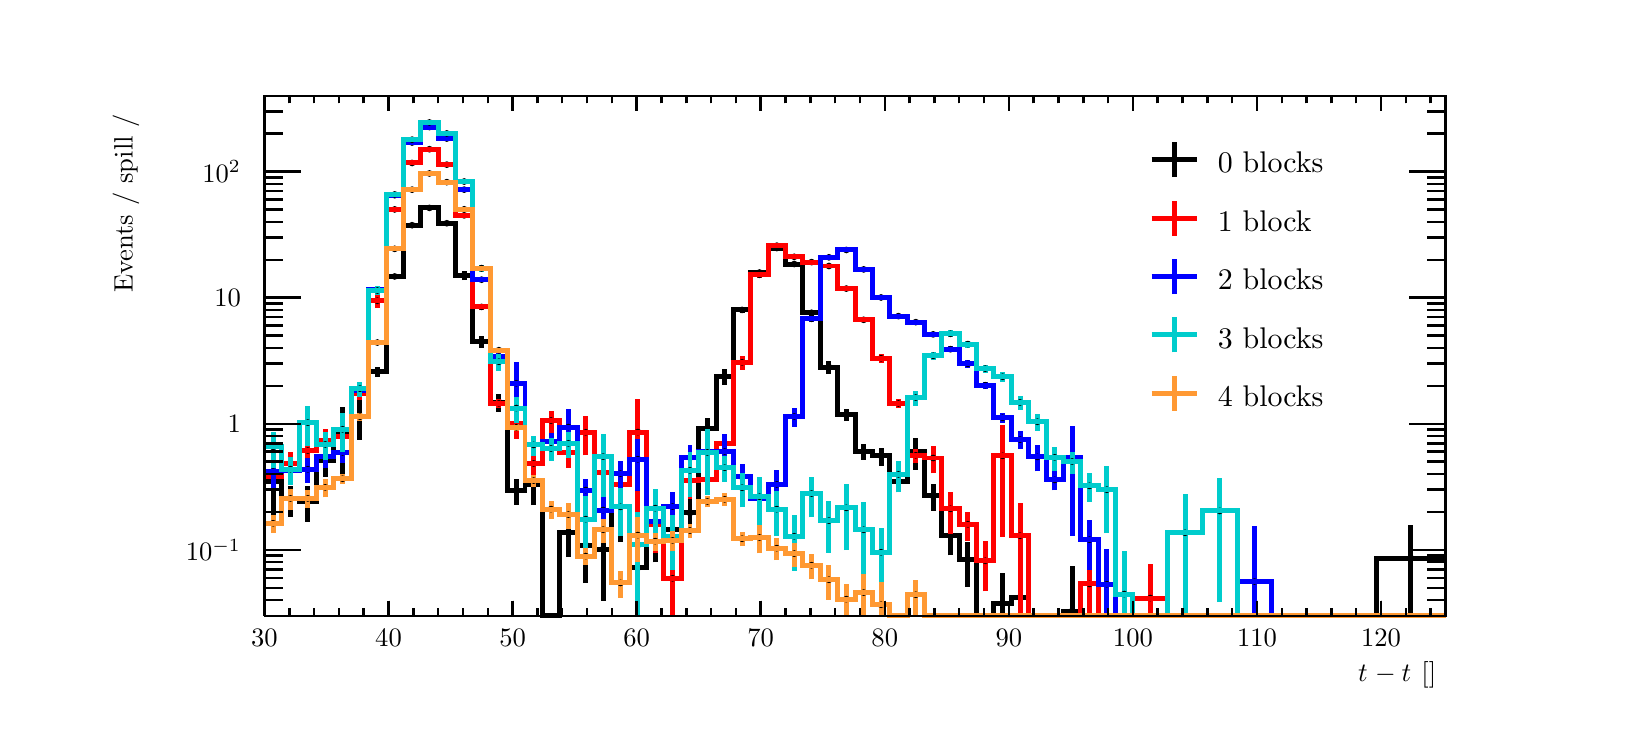
\begin{tikzpicture}
\pgfdeclareplotmark{cross} {
\pgfpathmoveto{\pgfpoint{-0.3\pgfplotmarksize}{\pgfplotmarksize}}
\pgfpathlineto{\pgfpoint{+0.3\pgfplotmarksize}{\pgfplotmarksize}}
\pgfpathlineto{\pgfpoint{+0.3\pgfplotmarksize}{0.3\pgfplotmarksize}}
\pgfpathlineto{\pgfpoint{+1\pgfplotmarksize}{0.3\pgfplotmarksize}}
\pgfpathlineto{\pgfpoint{+1\pgfplotmarksize}{-0.3\pgfplotmarksize}}
\pgfpathlineto{\pgfpoint{+0.3\pgfplotmarksize}{-0.3\pgfplotmarksize}}
\pgfpathlineto{\pgfpoint{+0.3\pgfplotmarksize}{-1.\pgfplotmarksize}}
\pgfpathlineto{\pgfpoint{-0.3\pgfplotmarksize}{-1.\pgfplotmarksize}}
\pgfpathlineto{\pgfpoint{-0.3\pgfplotmarksize}{-0.3\pgfplotmarksize}}
\pgfpathlineto{\pgfpoint{-1.\pgfplotmarksize}{-0.3\pgfplotmarksize}}
\pgfpathlineto{\pgfpoint{-1.\pgfplotmarksize}{0.3\pgfplotmarksize}}
\pgfpathlineto{\pgfpoint{-0.3\pgfplotmarksize}{0.3\pgfplotmarksize}}
\pgfpathclose
\pgfusepathqstroke
}
\pgfdeclareplotmark{cross*} {
\pgfpathmoveto{\pgfpoint{-0.3\pgfplotmarksize}{\pgfplotmarksize}}
\pgfpathlineto{\pgfpoint{+0.3\pgfplotmarksize}{\pgfplotmarksize}}
\pgfpathlineto{\pgfpoint{+0.3\pgfplotmarksize}{0.3\pgfplotmarksize}}
\pgfpathlineto{\pgfpoint{+1\pgfplotmarksize}{0.3\pgfplotmarksize}}
\pgfpathlineto{\pgfpoint{+1\pgfplotmarksize}{-0.3\pgfplotmarksize}}
\pgfpathlineto{\pgfpoint{+0.3\pgfplotmarksize}{-0.3\pgfplotmarksize}}
\pgfpathlineto{\pgfpoint{+0.3\pgfplotmarksize}{-1.\pgfplotmarksize}}
\pgfpathlineto{\pgfpoint{-0.3\pgfplotmarksize}{-1.\pgfplotmarksize}}
\pgfpathlineto{\pgfpoint{-0.3\pgfplotmarksize}{-0.3\pgfplotmarksize}}
\pgfpathlineto{\pgfpoint{-1.\pgfplotmarksize}{-0.3\pgfplotmarksize}}
\pgfpathlineto{\pgfpoint{-1.\pgfplotmarksize}{0.3\pgfplotmarksize}}
\pgfpathlineto{\pgfpoint{-0.3\pgfplotmarksize}{0.3\pgfplotmarksize}}
\pgfpathclose
\pgfusepathqfillstroke
}
\pgfdeclareplotmark{newstar} {
\pgfpathmoveto{\pgfqpoint{0pt}{\pgfplotmarksize}}
\pgfpathlineto{\pgfqpointpolar{44}{0.5\pgfplotmarksize}}
\pgfpathlineto{\pgfqpointpolar{18}{\pgfplotmarksize}}
\pgfpathlineto{\pgfqpointpolar{-20}{0.5\pgfplotmarksize}}
\pgfpathlineto{\pgfqpointpolar{-54}{\pgfplotmarksize}}
\pgfpathlineto{\pgfqpointpolar{-90}{0.5\pgfplotmarksize}}
\pgfpathlineto{\pgfqpointpolar{234}{\pgfplotmarksize}}
\pgfpathlineto{\pgfqpointpolar{198}{0.5\pgfplotmarksize}}
\pgfpathlineto{\pgfqpointpolar{162}{\pgfplotmarksize}}
\pgfpathlineto{\pgfqpointpolar{134}{0.5\pgfplotmarksize}}
\pgfpathclose
\pgfusepathqstroke
}
\pgfdeclareplotmark{newstar*} {
\pgfpathmoveto{\pgfqpoint{0pt}{\pgfplotmarksize}}
\pgfpathlineto{\pgfqpointpolar{44}{0.5\pgfplotmarksize}}
\pgfpathlineto{\pgfqpointpolar{18}{\pgfplotmarksize}}
\pgfpathlineto{\pgfqpointpolar{-20}{0.5\pgfplotmarksize}}
\pgfpathlineto{\pgfqpointpolar{-54}{\pgfplotmarksize}}
\pgfpathlineto{\pgfqpointpolar{-90}{0.5\pgfplotmarksize}}
\pgfpathlineto{\pgfqpointpolar{234}{\pgfplotmarksize}}
\pgfpathlineto{\pgfqpointpolar{198}{0.5\pgfplotmarksize}}
\pgfpathlineto{\pgfqpointpolar{162}{\pgfplotmarksize}}
\pgfpathlineto{\pgfqpointpolar{134}{0.5\pgfplotmarksize}}
\pgfpathclose
\pgfusepathqfillstroke
}
\definecolor{c}{rgb}{1,1,1};
\draw [color=c, fill=c] (0,0) rectangle (20,8.57658);
\draw [color=c, fill=c] (3,1.11495) rectangle (18,7.71892);
\definecolor{c}{rgb}{0,0,0};
\draw [c,line width=0.9] (3,1.11495) -- (3,7.71892) -- (18,7.71892) -- (18,1.11495) -- (3,1.11495);
\definecolor{c}{rgb}{1,1,1};
\draw [color=c, fill=c] (3,1.11495) rectangle (18,7.71892);
\definecolor{c}{rgb}{0,0,0};
\draw [c,line width=0.9] (3,1.11495) -- (3,7.71892) -- (18,7.71892) -- (18,1.11495) -- (3,1.11495);
\draw [c,line width=0.9] (3,1.11495) -- (3.22059,1.11495) -- (3.22059,1.11495) -- (3.44118,1.11495) -- (3.44118,1.11495) -- (3.66176,1.11495) -- (3.66176,1.11495) -- (3.88235,1.11495) -- (3.88235,1.11495) -- (4.10294,1.11495) -- (4.10294,1.11495) --
 (4.32353,1.11495) -- (4.32353,1.11495) -- (4.54412,1.11495) -- (4.54412,1.11495) -- (4.76471,1.11495) -- (4.76471,1.11495) -- (4.98529,1.11495) -- (4.98529,1.11495) -- (5.20588,1.11495) -- (5.20588,1.11495) -- (5.42647,1.11495) -- (5.42647,1.11495)
 -- (5.64706,1.11495) -- (5.64706,1.11495) -- (5.86765,1.11495) -- (5.86765,1.11495) -- (6.08824,1.11495) -- (6.08824,1.11495) -- (6.30882,1.11495) -- (6.30882,1.11495) -- (6.52941,1.11495) -- (6.52941,1.11495) -- (6.75,1.11495) -- (6.75,1.11495) --
 (6.97059,1.11495) -- (6.97059,1.11495) -- (7.19118,1.11495) -- (7.19118,1.11495) -- (7.41176,1.11495) -- (7.41176,1.11495) -- (7.63235,1.11495) -- (7.63235,1.11495) -- (7.85294,1.11495) -- (7.85294,1.11495) -- (8.07353,1.11495) -- (8.07353,1.11495)
 -- (8.29412,1.11495) -- (8.29412,1.11495) -- (8.51471,1.11495) -- (8.51471,1.11495) -- (8.73529,1.11495) -- (8.73529,1.11495) -- (8.95588,1.11495) -- (8.95588,1.11495) -- (9.17647,1.11495) -- (9.17647,1.11495) -- (9.39706,1.11495) --
 (9.39706,1.11495) -- (9.61765,1.11495) -- (9.61765,1.11495) -- (9.83823,1.11495) -- (9.83823,1.11495) -- (10.0588,1.11495) -- (10.0588,1.11495) -- (10.2794,1.11495) -- (10.2794,1.11495) -- (10.5,1.11495) -- (10.5,1.11495) -- (10.7206,1.11495) --
 (10.7206,1.11495) -- (10.9412,1.11495) -- (10.9412,1.11495) -- (11.1618,1.11495) -- (11.1618,1.11495) -- (11.3824,1.11495) -- (11.3824,1.11495) -- (11.6029,1.11495) -- (11.6029,1.11495) -- (11.8235,1.11495) -- (11.8235,1.11495) -- (12.0441,1.11495)
 -- (12.0441,1.11495) -- (12.2647,1.11495) -- (12.2647,1.11495) -- (12.4853,1.11495) -- (12.4853,1.11495) -- (12.7059,1.11495) -- (12.7059,1.11495) -- (12.9265,1.11495) -- (12.9265,1.11495) -- (13.1471,1.11495) -- (13.1471,1.11495) --
 (13.3676,1.11495) -- (13.3676,1.11495) -- (13.5882,1.11495) -- (13.5882,1.11495) -- (13.8088,1.11495) -- (13.8088,1.11495) -- (14.0294,1.11495) -- (14.0294,1.11495) -- (14.4706,1.11495) -- (14.4706,1.11495) -- (14.9118,1.11495) -- (14.9118,1.11495)
 -- (15.3529,1.11495) -- (15.3529,1.11495) -- (15.7941,1.11495) -- (15.7941,1.11495) -- (16.2353,1.11495) -- (16.2353,1.11495) -- (17.1176,1.11495) -- (17.1176,1.11495) -- (18,1.11495);
\draw [c,line width=0.9] (3,1.11495) -- (18,1.11495);
\draw [c,line width=0.9] (3,1.30793) -- (3,1.11495);
\draw [c,line width=0.9] (3.31513,1.21144) -- (3.31513,1.11495);
\draw [c,line width=0.9] (3.63025,1.21144) -- (3.63025,1.11495);
\draw [c,line width=0.9] (3.94538,1.21144) -- (3.94538,1.11495);
\draw [c,line width=0.9] (4.2605,1.21144) -- (4.2605,1.11495);
\draw [c,line width=0.9] (4.57563,1.30793) -- (4.57563,1.11495);
\draw [c,line width=0.9] (4.89076,1.21144) -- (4.89076,1.11495);
\draw [c,line width=0.9] (5.20588,1.21144) -- (5.20588,1.11495);
\draw [c,line width=0.9] (5.52101,1.21144) -- (5.52101,1.11495);
\draw [c,line width=0.9] (5.83613,1.21144) -- (5.83613,1.11495);
\draw [c,line width=0.9] (6.15126,1.30793) -- (6.15126,1.11495);
\draw [c,line width=0.9] (6.46639,1.21144) -- (6.46639,1.11495);
\draw [c,line width=0.9] (6.78151,1.21144) -- (6.78151,1.11495);
\draw [c,line width=0.9] (7.09664,1.21144) -- (7.09664,1.11495);
\draw [c,line width=0.9] (7.41176,1.21144) -- (7.41176,1.11495);
\draw [c,line width=0.9] (7.72689,1.30793) -- (7.72689,1.11495);
\draw [c,line width=0.9] (8.04202,1.21144) -- (8.04202,1.11495);
\draw [c,line width=0.9] (8.35714,1.21144) -- (8.35714,1.11495);
\draw [c,line width=0.9] (8.67227,1.21144) -- (8.67227,1.11495);
\draw [c,line width=0.9] (8.9874,1.21144) -- (8.9874,1.11495);
\draw [c,line width=0.9] (9.30252,1.30793) -- (9.30252,1.11495);
\draw [c,line width=0.9] (9.61765,1.21144) -- (9.61765,1.11495);
\draw [c,line width=0.9] (9.93277,1.21144) -- (9.93277,1.11495);
\draw [c,line width=0.9] (10.2479,1.21144) -- (10.2479,1.11495);
\draw [c,line width=0.9] (10.563,1.21144) -- (10.563,1.11495);
\draw [c,line width=0.9] (10.8782,1.30793) -- (10.8782,1.11495);
\draw [c,line width=0.9] (11.1933,1.21144) -- (11.1933,1.11495);
\draw [c,line width=0.9] (11.5084,1.21144) -- (11.5084,1.11495);
\draw [c,line width=0.9] (11.8235,1.21144) -- (11.8235,1.11495);
\draw [c,line width=0.9] (12.1387,1.21144) -- (12.1387,1.11495);
\draw [c,line width=0.9] (12.4538,1.30793) -- (12.4538,1.11495);
\draw [c,line width=0.9] (12.7689,1.21144) -- (12.7689,1.11495);
\draw [c,line width=0.9] (13.084,1.21144) -- (13.084,1.11495);
\draw [c,line width=0.9] (13.3992,1.21144) -- (13.3992,1.11495);
\draw [c,line width=0.9] (13.7143,1.21144) -- (13.7143,1.11495);
\draw [c,line width=0.9] (14.0294,1.30793) -- (14.0294,1.11495);
\draw [c,line width=0.9] (14.3445,1.21144) -- (14.3445,1.11495);
\draw [c,line width=0.9] (14.6597,1.21144) -- (14.6597,1.11495);
\draw [c,line width=0.9] (14.9748,1.21144) -- (14.9748,1.11495);
\draw [c,line width=0.9] (15.2899,1.21144) -- (15.2899,1.11495);
\draw [c,line width=0.9] (15.605,1.30793) -- (15.605,1.11495);
\draw [c,line width=0.9] (15.9202,1.21144) -- (15.9202,1.11495);
\draw [c,line width=0.9] (16.2353,1.21144) -- (16.2353,1.11495);
\draw [c,line width=0.9] (16.5504,1.21144) -- (16.5504,1.11495);
\draw [c,line width=0.9] (16.8655,1.21144) -- (16.8655,1.11495);
\draw [c,line width=0.9] (17.1807,1.30793) -- (17.1807,1.11495);
\draw [c,line width=0.9] (17.1807,1.30793) -- (17.1807,1.11495);
\draw [c,line width=0.9] (17.4958,1.21144) -- (17.4958,1.11495);
\draw [c,line width=0.9] (17.8109,1.21144) -- (17.8109,1.11495);
\draw [anchor=base] (3,0.729009) node[scale=0.960419, color=c, rotate=0]{30};
\draw [anchor=base] (4.57563,0.729009) node[scale=0.960419, color=c, rotate=0]{40};
\draw [anchor=base] (6.15126,0.729009) node[scale=0.960419, color=c, rotate=0]{50};
\draw [anchor=base] (7.72689,0.729009) node[scale=0.960419, color=c, rotate=0]{60};
\draw [anchor=base] (9.30252,0.729009) node[scale=0.960419, color=c, rotate=0]{70};
\draw [anchor=base] (10.8782,0.729009) node[scale=0.960419, color=c, rotate=0]{80};
\draw [anchor=base] (12.4538,0.729009) node[scale=0.960419, color=c, rotate=0]{90};
\draw [anchor=base] (14.0294,0.729009) node[scale=0.960419, color=c, rotate=0]{100};
\draw [anchor=base] (15.605,0.729009) node[scale=0.960419, color=c, rotate=0]{110};
\draw [anchor=base] (17.1807,0.729009) node[scale=0.960419, color=c, rotate=0]{120};
\draw [anchor= east] (18,0.360216) node[scale=0.960419, color=c, rotate=0]{$t_{\SFour} - t_{\STwo}$ [\si{\nano\second}] };
\draw [c,line width=0.9] (3,7.71892) -- (18,7.71892);
\draw [c,line width=0.9] (3,7.52595) -- (3,7.71892);
\draw [c,line width=0.9] (3.31513,7.62243) -- (3.31513,7.71892);
\draw [c,line width=0.9] (3.63025,7.62243) -- (3.63025,7.71892);
\draw [c,line width=0.9] (3.94538,7.62243) -- (3.94538,7.71892);
\draw [c,line width=0.9] (4.2605,7.62243) -- (4.2605,7.71892);
\draw [c,line width=0.9] (4.57563,7.52595) -- (4.57563,7.71892);
\draw [c,line width=0.9] (4.89076,7.62243) -- (4.89076,7.71892);
\draw [c,line width=0.9] (5.20588,7.62243) -- (5.20588,7.71892);
\draw [c,line width=0.9] (5.52101,7.62243) -- (5.52101,7.71892);
\draw [c,line width=0.9] (5.83613,7.62243) -- (5.83613,7.71892);
\draw [c,line width=0.9] (6.15126,7.52595) -- (6.15126,7.71892);
\draw [c,line width=0.9] (6.46639,7.62243) -- (6.46639,7.71892);
\draw [c,line width=0.9] (6.78151,7.62243) -- (6.78151,7.71892);
\draw [c,line width=0.9] (7.09664,7.62243) -- (7.09664,7.71892);
\draw [c,line width=0.9] (7.41176,7.62243) -- (7.41176,7.71892);
\draw [c,line width=0.9] (7.72689,7.52595) -- (7.72689,7.71892);
\draw [c,line width=0.9] (8.04202,7.62243) -- (8.04202,7.71892);
\draw [c,line width=0.9] (8.35714,7.62243) -- (8.35714,7.71892);
\draw [c,line width=0.9] (8.67227,7.62243) -- (8.67227,7.71892);
\draw [c,line width=0.9] (8.9874,7.62243) -- (8.9874,7.71892);
\draw [c,line width=0.9] (9.30252,7.52595) -- (9.30252,7.71892);
\draw [c,line width=0.9] (9.61765,7.62243) -- (9.61765,7.71892);
\draw [c,line width=0.9] (9.93277,7.62243) -- (9.93277,7.71892);
\draw [c,line width=0.9] (10.2479,7.62243) -- (10.2479,7.71892);
\draw [c,line width=0.9] (10.563,7.62243) -- (10.563,7.71892);
\draw [c,line width=0.9] (10.8782,7.52595) -- (10.8782,7.71892);
\draw [c,line width=0.9] (11.1933,7.62243) -- (11.1933,7.71892);
\draw [c,line width=0.9] (11.5084,7.62243) -- (11.5084,7.71892);
\draw [c,line width=0.9] (11.8235,7.62243) -- (11.8235,7.71892);
\draw [c,line width=0.9] (12.1387,7.62243) -- (12.1387,7.71892);
\draw [c,line width=0.9] (12.4538,7.52595) -- (12.4538,7.71892);
\draw [c,line width=0.9] (12.7689,7.62243) -- (12.7689,7.71892);
\draw [c,line width=0.9] (13.084,7.62243) -- (13.084,7.71892);
\draw [c,line width=0.9] (13.3992,7.62243) -- (13.3992,7.71892);
\draw [c,line width=0.9] (13.7143,7.62243) -- (13.7143,7.71892);
\draw [c,line width=0.9] (14.0294,7.52595) -- (14.0294,7.71892);
\draw [c,line width=0.9] (14.3445,7.62243) -- (14.3445,7.71892);
\draw [c,line width=0.9] (14.6597,7.62243) -- (14.6597,7.71892);
\draw [c,line width=0.9] (14.9748,7.62243) -- (14.9748,7.71892);
\draw [c,line width=0.9] (15.2899,7.62243) -- (15.2899,7.71892);
\draw [c,line width=0.9] (15.605,7.52595) -- (15.605,7.71892);
\draw [c,line width=0.9] (15.9202,7.62243) -- (15.9202,7.71892);
\draw [c,line width=0.9] (16.2353,7.62243) -- (16.2353,7.71892);
\draw [c,line width=0.9] (16.5504,7.62243) -- (16.5504,7.71892);
\draw [c,line width=0.9] (16.8655,7.62243) -- (16.8655,7.71892);
\draw [c,line width=0.9] (17.1807,7.52595) -- (17.1807,7.71892);
\draw [c,line width=0.9] (17.1807,7.52595) -- (17.1807,7.71892);
\draw [c,line width=0.9] (17.4958,7.62243) -- (17.4958,7.71892);
\draw [c,line width=0.9] (17.8109,7.62243) -- (17.8109,7.71892);
\draw [c,line width=0.9] (3,1.11495) -- (3,7.71892);
\draw [c,line width=0.9] (3.231,1.11496) -- (3,1.11496);
\draw [c,line width=0.9] (3.231,1.31498) -- (3,1.31498);
\draw [c,line width=0.9] (3.231,1.47013) -- (3,1.47013);
\draw [c,line width=0.9] (3.231,1.5969) -- (3,1.5969);
\draw [c,line width=0.9] (3.231,1.70408) -- (3,1.70408);
\draw [c,line width=0.9] (3.231,1.79693) -- (3,1.79693);
\draw [c,line width=0.9] (3.231,1.87882) -- (3,1.87882);
\draw [c,line width=0.9] (3.462,1.95208) -- (3,1.95208);
\draw [anchor= east] (2.82,1.95208) node[scale=0.960419, color=c, rotate=0]{$10^{-1}$};
\draw [c,line width=0.9] (3.231,2.43402) -- (3,2.43402);
\draw [c,line width=0.9] (3.231,2.71594) -- (3,2.71594);
\draw [c,line width=0.9] (3.231,2.91597) -- (3,2.91597);
\draw [c,line width=0.9] (3.231,3.07112) -- (3,3.07112);
\draw [c,line width=0.9] (3.231,3.19789) -- (3,3.19789);
\draw [c,line width=0.9] (3.231,3.30507) -- (3,3.30507);
\draw [c,line width=0.9] (3.231,3.39791) -- (3,3.39791);
\draw [c,line width=0.9] (3.231,3.4798) -- (3,3.4798);
\draw [c,line width=0.9] (3.462,3.55306) -- (3,3.55306);
\draw [anchor= east] (2.82,3.55306) node[scale=0.960419, color=c, rotate=0]{1};
\draw [c,line width=0.9] (3.231,4.03501) -- (3,4.03501);
\draw [c,line width=0.9] (3.231,4.31693) -- (3,4.31693);
\draw [c,line width=0.9] (3.231,4.51695) -- (3,4.51695);
\draw [c,line width=0.9] (3.231,4.6721) -- (3,4.6721);
\draw [c,line width=0.9] (3.231,4.79887) -- (3,4.79887);
\draw [c,line width=0.9] (3.231,4.90605) -- (3,4.90605);
\draw [c,line width=0.9] (3.231,4.99889) -- (3,4.99889);
\draw [c,line width=0.9] (3.231,5.08079) -- (3,5.08079);
\draw [c,line width=0.9] (3.462,5.15405) -- (3,5.15405);
\draw [anchor= east] (2.82,5.15405) node[scale=0.960419, color=c, rotate=0]{10};
\draw [c,line width=0.9] (3.231,5.63599) -- (3,5.63599);
\draw [c,line width=0.9] (3.231,5.91791) -- (3,5.91791);
\draw [c,line width=0.9] (3.231,6.11793) -- (3,6.11793);
\draw [c,line width=0.9] (3.231,6.27309) -- (3,6.27309);
\draw [c,line width=0.9] (3.231,6.39985) -- (3,6.39985);
\draw [c,line width=0.9] (3.231,6.50703) -- (3,6.50703);
\draw [c,line width=0.9] (3.231,6.59988) -- (3,6.59988);
\draw [c,line width=0.9] (3.231,6.68177) -- (3,6.68177);
\draw [c,line width=0.9] (3.462,6.75503) -- (3,6.75503);
\draw [anchor= east] (2.82,6.75503) node[scale=0.960419, color=c, rotate=0]{$10^{2}$};
\draw [c,line width=0.9] (3.231,7.23697) -- (3,7.23697);
\draw [c,line width=0.9] (3.231,7.51889) -- (3,7.51889);
\draw [c,line width=0.9] (3.231,7.71892) -- (3,7.71892);
\draw [anchor= east] (1.24,7.71892) node[scale=0.960419, color=c, rotate=90]{ Events / spill / \si{\nano\second} };
\draw [c,line width=0.9] (18,1.11495) -- (18,7.71892);
\draw [c,line width=0.9] (17.769,1.11496) -- (18,1.11496);
\draw [c,line width=0.9] (17.769,1.31498) -- (18,1.31498);
\draw [c,line width=0.9] (17.769,1.47013) -- (18,1.47013);
\draw [c,line width=0.9] (17.769,1.5969) -- (18,1.5969);
\draw [c,line width=0.9] (17.769,1.70408) -- (18,1.70408);
\draw [c,line width=0.9] (17.769,1.79693) -- (18,1.79693);
\draw [c,line width=0.9] (17.769,1.87882) -- (18,1.87882);
\draw [c,line width=0.9] (17.538,1.95208) -- (18,1.95208);
\draw [c,line width=0.9] (17.769,2.43402) -- (18,2.43402);
\draw [c,line width=0.9] (17.769,2.71594) -- (18,2.71594);
\draw [c,line width=0.9] (17.769,2.91597) -- (18,2.91597);
\draw [c,line width=0.9] (17.769,3.07112) -- (18,3.07112);
\draw [c,line width=0.9] (17.769,3.19789) -- (18,3.19789);
\draw [c,line width=0.9] (17.769,3.30507) -- (18,3.30507);
\draw [c,line width=0.9] (17.769,3.39791) -- (18,3.39791);
\draw [c,line width=0.9] (17.769,3.4798) -- (18,3.4798);
\draw [c,line width=0.9] (17.538,3.55306) -- (18,3.55306);
\draw [c,line width=0.9] (17.769,4.03501) -- (18,4.03501);
\draw [c,line width=0.9] (17.769,4.31693) -- (18,4.31693);
\draw [c,line width=0.9] (17.769,4.51695) -- (18,4.51695);
\draw [c,line width=0.9] (17.769,4.6721) -- (18,4.6721);
\draw [c,line width=0.9] (17.769,4.79887) -- (18,4.79887);
\draw [c,line width=0.9] (17.769,4.90605) -- (18,4.90605);
\draw [c,line width=0.9] (17.769,4.99889) -- (18,4.99889);
\draw [c,line width=0.9] (17.769,5.08079) -- (18,5.08079);
\draw [c,line width=0.9] (17.538,5.15405) -- (18,5.15405);
\draw [c,line width=0.9] (17.769,5.63599) -- (18,5.63599);
\draw [c,line width=0.9] (17.769,5.91791) -- (18,5.91791);
\draw [c,line width=0.9] (17.769,6.11793) -- (18,6.11793);
\draw [c,line width=0.9] (17.769,6.27309) -- (18,6.27309);
\draw [c,line width=0.9] (17.769,6.39985) -- (18,6.39985);
\draw [c,line width=0.9] (17.769,6.50703) -- (18,6.50703);
\draw [c,line width=0.9] (17.769,6.59988) -- (18,6.59988);
\draw [c,line width=0.9] (17.769,6.68177) -- (18,6.68177);
\draw [c,line width=0.9] (17.538,6.75503) -- (18,6.75503);
\draw [c,line width=0.9] (17.769,7.23697) -- (18,7.23697);
\draw [c,line width=0.9] (17.769,7.51889) -- (18,7.51889);
\draw [c,line width=0.9] (17.769,7.71892) -- (18,7.71892);
\draw [c,line width=1.8] (3.11029,2.26923) -- (3.11029,2.82229);
\draw [c,line width=1.8] (3.11029,2.82229) -- (3.11029,3.12639);
\foreach \P in {(3.11029,2.82229)}{\draw[mark options={color=c,fill=c},mark size=2.402402pt,mark=*,mark size=1pt] plot coordinates {\P};}
\draw [c,line width=1.8] (3.33088,2.37409) -- (3.33088,2.59778);
\draw [c,line width=1.8] (3.33088,2.59778) -- (3.33088,2.76676);
\foreach \P in {(3.33088,2.59778)}{\draw[mark options={color=c,fill=c},mark size=2.402402pt,mark=*,mark size=1pt] plot coordinates {\P};}
\draw [c,line width=1.8] (3.55147,2.30669) -- (3.55147,2.57217);
\draw [c,line width=1.8] (3.55147,2.57217) -- (3.55147,2.76382);
\foreach \P in {(3.55147,2.57217)}{\draw[mark options={color=c,fill=c},mark size=2.402402pt,mark=*,mark size=1pt] plot coordinates {\P};}
\draw [c,line width=1.8] (3.77206,2.88174) -- (3.77206,3.08666);
\draw [c,line width=1.8] (3.77206,3.08666) -- (3.77206,3.24473);
\foreach \P in {(3.77206,3.08666)}{\draw[mark options={color=c,fill=c},mark size=2.402402pt,mark=*,mark size=1pt] plot coordinates {\P};}
\draw [c,line width=1.8] (3.99265,2.79006) -- (3.99265,3.43347);
\draw [c,line width=1.8] (3.99265,3.43347) -- (3.99265,3.76184);
\foreach \P in {(3.99265,3.43347)}{\draw[mark options={color=c,fill=c},mark size=2.402402pt,mark=*,mark size=1pt] plot coordinates {\P};}
\draw [c,line width=1.8] (4.21324,3.34883) -- (4.21324,3.64918);
\draw [c,line width=1.8] (4.21324,3.64918) -- (4.21324,3.85825);
\foreach \P in {(4.21324,3.64918)}{\draw[mark options={color=c,fill=c},mark size=2.402402pt,mark=*,mark size=1pt] plot coordinates {\P};}
\draw [c,line width=1.8] (4.43382,4.1533) -- (4.43382,4.21931);
\draw [c,line width=1.8] (4.43382,4.21931) -- (4.43382,4.2796);
\foreach \P in {(4.43382,4.21931)}{\draw[mark options={color=c,fill=c},mark size=2.402402pt,mark=*,mark size=1pt] plot coordinates {\P};}
\draw [c,line width=1.8] (4.65441,5.39338) -- (4.65441,5.42411);
\draw [c,line width=1.8] (4.65441,5.42411) -- (4.65441,5.45354);
\foreach \P in {(4.65441,5.42411)}{\draw[mark options={color=c,fill=c},mark size=2.402402pt,mark=*,mark size=1pt] plot coordinates {\P};}
\draw [c,line width=1.8] (4.875,6.05236) -- (4.875,6.07488);
\draw [c,line width=1.8] (4.875,6.07488) -- (4.875,6.09669);
\foreach \P in {(4.875,6.07488)}{\draw[mark options={color=c,fill=c},mark size=2.402402pt,mark=*,mark size=1pt] plot coordinates {\P};}
\draw [c,line width=1.8] (5.09559,6.27165) -- (5.09559,6.29471);
\draw [c,line width=1.8] (5.09559,6.29471) -- (5.09559,6.31704);
\foreach \P in {(5.09559,6.29471)}{\draw[mark options={color=c,fill=c},mark size=2.402402pt,mark=*,mark size=1pt] plot coordinates {\P};}
\draw [c,line width=1.8] (5.31618,6.06723) -- (5.31618,6.09971);
\draw [c,line width=1.8] (5.31618,6.09971) -- (5.31618,6.13074);
\foreach \P in {(5.31618,6.09971)}{\draw[mark options={color=c,fill=c},mark size=2.402402pt,mark=*,mark size=1pt] plot coordinates {\P};}
\draw [c,line width=1.8] (5.53676,5.37726) -- (5.53676,5.44);
\draw [c,line width=1.8] (5.53676,5.44) -- (5.53676,5.49754);
\foreach \P in {(5.53676,5.44)}{\draw[mark options={color=c,fill=c},mark size=2.402402pt,mark=*,mark size=1pt] plot coordinates {\P};}
\draw [c,line width=1.8] (5.75735,4.51797) -- (5.75735,4.59454);
\draw [c,line width=1.8] (5.75735,4.59454) -- (5.75735,4.6635);
\foreach \P in {(5.75735,4.59454)}{\draw[mark options={color=c,fill=c},mark size=2.402402pt,mark=*,mark size=1pt] plot coordinates {\P};}
\draw [c,line width=1.8] (5.97794,3.70553) -- (5.97794,3.82824);
\draw [c,line width=1.8] (5.97794,3.82824) -- (5.97794,3.93252);
\foreach \P in {(5.97794,3.82824)}{\draw[mark options={color=c,fill=c},mark size=2.402402pt,mark=*,mark size=1pt] plot coordinates {\P};}
\draw [c,line width=1.8] (6.19853,2.52351) -- (6.19853,2.70383);
\draw [c,line width=1.8] (6.19853,2.70383) -- (6.19853,2.84689);
\foreach \P in {(6.19853,2.70383)}{\draw[mark options={color=c,fill=c},mark size=2.402402pt,mark=*,mark size=1pt] plot coordinates {\P};}
\draw [c,line width=1.8] (6.41912,2.52127) -- (6.41912,2.77715);
\draw [c,line width=1.8] (6.41912,2.77715) -- (6.41912,2.96378);
\foreach \P in {(6.41912,2.77715)}{\draw[mark options={color=c,fill=c},mark size=2.402402pt,mark=*,mark size=1pt] plot coordinates {\P};}
\draw [c,line width=1.8] (6.86029,1.85983) -- (6.86029,2.17678);
\draw [c,line width=1.8] (6.86029,2.17678) -- (6.86029,2.39369);
\foreach \P in {(6.86029,2.17678)}{\draw[mark options={color=c,fill=c},mark size=2.402402pt,mark=*,mark size=1pt] plot coordinates {\P};}
\draw [c,line width=1.8] (7.08088,1.5305) -- (7.08088,2.01323);
\draw [c,line width=1.8] (7.08088,2.01323) -- (7.08088,2.29541);
\foreach \P in {(7.08088,2.01323)}{\draw[mark options={color=c,fill=c},mark size=2.402402pt,mark=*,mark size=1pt] plot coordinates {\P};}
\draw [c,line width=1.8] (7.30147,1.30845) -- (7.30147,1.96235);
\draw [c,line width=1.8] (7.30147,1.96235) -- (7.30147,2.29328);
\foreach \P in {(7.30147,1.96235)}{\draw[mark options={color=c,fill=c},mark size=2.402402pt,mark=*,mark size=1pt] plot coordinates {\P};}
\draw [c,line width=1.8] (7.52206,2.04972) -- (7.52206,2.49638);
\draw [c,line width=1.8] (7.52206,2.49638) -- (7.52206,2.76613);
\foreach \P in {(7.52206,2.49638)}{\draw[mark options={color=c,fill=c},mark size=2.402402pt,mark=*,mark size=1pt] plot coordinates {\P};}
\draw [c,line width=1.8] (7.74265,1.21582) -- (7.74265,1.72582);
\draw [c,line width=1.8] (7.74265,1.72582) -- (7.74265,2.01685);
\foreach \P in {(7.74265,1.72582)}{\draw[mark options={color=c,fill=c},mark size=2.402402pt,mark=*,mark size=1pt] plot coordinates {\P};}
\draw [c,line width=1.8] (7.96324,1.79441) -- (7.96324,2.28593);
\draw [c,line width=1.8] (7.96324,2.28593) -- (7.96324,2.57101);
\foreach \P in {(7.96324,2.28593)}{\draw[mark options={color=c,fill=c},mark size=2.402402pt,mark=*,mark size=1pt] plot coordinates {\P};}
\draw [c,line width=1.8] (8.18382,1.89925) -- (8.18382,2.21606);
\draw [c,line width=1.8] (8.18382,2.21606) -- (8.18382,2.43289);
\foreach \P in {(8.18382,2.21606)}{\draw[mark options={color=c,fill=c},mark size=2.402402pt,mark=*,mark size=1pt] plot coordinates {\P};}
\draw [c,line width=1.8] (8.40441,2.18956) -- (8.40441,2.42094);
\draw [c,line width=1.8] (8.40441,2.42094) -- (8.40441,2.59425);
\foreach \P in {(8.40441,2.42094)}{\draw[mark options={color=c,fill=c},mark size=2.402402pt,mark=*,mark size=1pt] plot coordinates {\P};}
\draw [c,line width=1.8] (8.625,3.32169) -- (8.625,3.48779);
\draw [c,line width=1.8] (8.625,3.48779) -- (8.625,3.62177);
\foreach \P in {(8.625,3.48779)}{\draw[mark options={color=c,fill=c},mark size=2.402402pt,mark=*,mark size=1pt] plot coordinates {\P};}
\draw [c,line width=1.8] (8.84559,4.046) -- (8.84559,4.15581);
\draw [c,line width=1.8] (8.84559,4.15581) -- (8.84559,4.25062);
\foreach \P in {(8.84559,4.15581)}{\draw[mark options={color=c,fill=c},mark size=2.402402pt,mark=*,mark size=1pt] plot coordinates {\P};}
\draw [c,line width=1.8] (9.06618,4.9546) -- (9.06618,4.99931);
\draw [c,line width=1.8] (9.06618,4.99931) -- (9.06618,5.04132);
\foreach \P in {(9.06618,4.99931)}{\draw[mark options={color=c,fill=c},mark size=2.402402pt,mark=*,mark size=1pt] plot coordinates {\P};}
\draw [c,line width=1.8] (9.28677,5.44468) -- (9.28677,5.47408);
\draw [c,line width=1.8] (9.28677,5.47408) -- (9.28677,5.50229);
\foreach \P in {(9.28677,5.47408)}{\draw[mark options={color=c,fill=c},mark size=2.402402pt,mark=*,mark size=1pt] plot coordinates {\P};}
\draw [c,line width=1.8] (9.50735,5.76328) -- (9.50735,5.785);
\draw [c,line width=1.8] (9.50735,5.785) -- (9.50735,5.80607);
\foreach \P in {(9.50735,5.785)}{\draw[mark options={color=c,fill=c},mark size=2.402402pt,mark=*,mark size=1pt] plot coordinates {\P};}
\draw [c,line width=1.8] (9.72794,5.55883) -- (9.72794,5.58191);
\draw [c,line width=1.8] (9.72794,5.58191) -- (9.72794,5.60424);
\foreach \P in {(9.72794,5.58191)}{\draw[mark options={color=c,fill=c},mark size=2.402402pt,mark=*,mark size=1pt] plot coordinates {\P};}
\draw [c,line width=1.8] (9.94853,4.9256) -- (9.94853,4.96251);
\draw [c,line width=1.8] (9.94853,4.96251) -- (9.94853,4.99756);
\foreach \P in {(9.94853,4.96251)}{\draw[mark options={color=c,fill=c},mark size=2.402402pt,mark=*,mark size=1pt] plot coordinates {\P};}
\draw [c,line width=1.8] (10.1691,4.18793) -- (10.1691,4.27281);
\draw [c,line width=1.8] (10.1691,4.27281) -- (10.1691,4.34846);
\foreach \P in {(10.1691,4.27281)}{\draw[mark options={color=c,fill=c},mark size=2.402402pt,mark=*,mark size=1pt] plot coordinates {\P};}
\draw [c,line width=1.8] (10.3897,3.58544) -- (10.3897,3.66551);
\draw [c,line width=1.8] (10.3897,3.66551) -- (10.3897,3.73731);
\foreach \P in {(10.3897,3.66551)}{\draw[mark options={color=c,fill=c},mark size=2.402402pt,mark=*,mark size=1pt] plot coordinates {\P};}
\draw [c,line width=1.8] (10.6103,3.0982) -- (10.6103,3.20475);
\draw [c,line width=1.8] (10.6103,3.20475) -- (10.6103,3.29713);
\foreach \P in {(10.6103,3.20475)}{\draw[mark options={color=c,fill=c},mark size=2.402402pt,mark=*,mark size=1pt] plot coordinates {\P};}
\draw [c,line width=1.8] (10.8309,3.02288) -- (10.8309,3.14627);
\draw [c,line width=1.8] (10.8309,3.14627) -- (10.8309,3.25103);
\foreach \P in {(10.8309,3.14627)}{\draw[mark options={color=c,fill=c},mark size=2.402402pt,mark=*,mark size=1pt] plot coordinates {\P};}
\draw [c,line width=1.8] (11.0515,2.68649) -- (11.0515,2.82468);
\draw [c,line width=1.8] (11.0515,2.82468) -- (11.0515,2.9399);
\foreach \P in {(11.0515,2.82468)}{\draw[mark options={color=c,fill=c},mark size=2.402402pt,mark=*,mark size=1pt] plot coordinates {\P};}
\draw [c,line width=1.8] (11.2721,2.9717) -- (11.2721,3.20094);
\draw [c,line width=1.8] (11.2721,3.20094) -- (11.2721,3.37305);
\foreach \P in {(11.2721,3.20094)}{\draw[mark options={color=c,fill=c},mark size=2.402402pt,mark=*,mark size=1pt] plot coordinates {\P};}
\draw [c,line width=1.8] (11.4926,2.44675) -- (11.4926,2.63658);
\draw [c,line width=1.8] (11.4926,2.63658) -- (11.4926,2.78554);
\foreach \P in {(11.4926,2.63658)}{\draw[mark options={color=c,fill=c},mark size=2.402402pt,mark=*,mark size=1pt] plot coordinates {\P};}
\draw [c,line width=1.8] (11.7132,1.88029) -- (11.7132,2.13662);
\draw [c,line width=1.8] (11.7132,2.13662) -- (11.7132,2.32349);
\foreach \P in {(11.7132,2.13662)}{\draw[mark options={color=c,fill=c},mark size=2.402402pt,mark=*,mark size=1pt] plot coordinates {\P};}
\draw [c,line width=1.8] (11.9338,1.48647) -- (11.9338,1.82755);
\draw [c,line width=1.8] (11.9338,1.82755) -- (11.9338,2.05537);
\foreach \P in {(11.9338,1.82755)}{\draw[mark options={color=c,fill=c},mark size=2.402402pt,mark=*,mark size=1pt] plot coordinates {\P};}
\draw [c,line width=1.8] (12.375,1.11495) -- (12.375,1.26774);
\draw [c,line width=1.8] (12.375,1.26774) -- (12.375,1.65748);
\foreach \P in {(12.375,1.26774)}{\draw[mark options={color=c,fill=c},mark size=2.402402pt,mark=*,mark size=1pt] plot coordinates {\P};}
\draw [c,line width=1.8] (12.5956,1.11495) -- (12.5956,1.3495);
\draw [c,line width=1.8] (12.5956,1.3495) -- (12.5956,1.71027);
\foreach \P in {(12.5956,1.3495)}{\draw[mark options={color=c,fill=c},mark size=2.402402pt,mark=*,mark size=1pt] plot coordinates {\P};}
\draw [c,line width=1.8] (13.2574,1.11495) -- (13.2574,1.17392);
\draw [c,line width=1.8] (13.2574,1.17392) -- (13.2574,1.74136);
\foreach \P in {(13.2574,1.17392)}{\draw[mark options={color=c,fill=c},mark size=2.402402pt,mark=*,mark size=1pt] plot coordinates {\P};}
\draw [c,line width=1.8] (17.5588,1.11495) -- (17.5588,1.8481);
\draw [c,line width=1.8] (17.5588,1.8481) -- (17.5588,2.26717);
\foreach \P in {(17.5588,1.8481)}{\draw[mark options={color=c,fill=c},mark size=2.402402pt,mark=*,mark size=1pt] plot coordinates {\P};}
\draw [c,line width=1.8] (3,2.82229) -- (3.22059,2.82229) -- (3.22059,2.59778) -- (3.44118,2.59778) -- (3.44118,2.57217) -- (3.66176,2.57217) -- (3.66176,3.08666) -- (3.88235,3.08666) -- (3.88235,3.43347) -- (4.10294,3.43347) -- (4.10294,3.64918) --
 (4.32353,3.64918) -- (4.32353,4.21931) -- (4.54412,4.21931) -- (4.54412,5.42411) -- (4.76471,5.42411) -- (4.76471,6.07488) -- (4.98529,6.07488) -- (4.98529,6.29471) -- (5.20588,6.29471) -- (5.20588,6.09971) -- (5.42647,6.09971) -- (5.42647,5.44) --
 (5.64706,5.44) -- (5.64706,4.59454) -- (5.86765,4.59454) -- (5.86765,3.82824) -- (6.08824,3.82824) -- (6.08824,2.70383) -- (6.30882,2.70383) -- (6.30882,2.77715) -- (6.52941,2.77715) -- (6.52941,1.11495) -- (6.75,1.11495) -- (6.75,2.17678) --
 (6.97059,2.17678) -- (6.97059,2.01323) -- (7.19118,2.01323) -- (7.19118,1.96235) -- (7.41176,1.96235) -- (7.41176,2.49638) -- (7.63235,2.49638) -- (7.63235,1.72582) -- (7.85294,1.72582) -- (7.85294,2.28593) -- (8.07353,2.28593) -- (8.07353,2.21606)
 -- (8.29412,2.21606) -- (8.29412,2.42094) -- (8.51471,2.42094) -- (8.51471,3.48779) -- (8.73529,3.48779) -- (8.73529,4.15581) -- (8.95588,4.15581) -- (8.95588,4.99931) -- (9.17647,4.99931) -- (9.17647,5.47408) -- (9.39706,5.47408) -- (9.39706,5.785)
 -- (9.61765,5.785) -- (9.61765,5.58191) -- (9.83823,5.58191) -- (9.83823,4.96251) -- (10.0588,4.96251) -- (10.0588,4.27281) -- (10.2794,4.27281) -- (10.2794,3.66551) -- (10.5,3.66551) -- (10.5,3.20475) -- (10.7206,3.20475) -- (10.7206,3.14627) --
 (10.9412,3.14627) -- (10.9412,2.82468) -- (11.1618,2.82468) -- (11.1618,3.20094) -- (11.3824,3.20094) -- (11.3824,2.63658) -- (11.6029,2.63658) -- (11.6029,2.13662) -- (11.8235,2.13662) -- (11.8235,1.82755) -- (12.0441,1.82755) -- (12.0441,1.11495)
 -- (12.2647,1.11495) -- (12.2647,1.26774) -- (12.4853,1.26774) -- (12.4853,1.3495) -- (12.7059,1.3495) -- (12.7059,1.11495) -- (12.9265,1.11495) -- (12.9265,1.11495) -- (13.1471,1.11495) -- (13.1471,1.17392) -- (13.3676,1.17392) -- (13.3676,1.11495)
 -- (13.5882,1.11495) -- (13.5882,1.11495) -- (13.8088,1.11495) -- (13.8088,1.11495) -- (14.0294,1.11495) -- (14.0294,1.11495) -- (14.4706,1.11495) -- (14.4706,1.11495) -- (14.9118,1.11495) -- (14.9118,1.11495) -- (15.3529,1.11495) --
 (15.3529,1.11495) -- (15.7941,1.11495) -- (15.7941,1.11495) -- (16.2353,1.11495) -- (16.2353,1.11495) -- (17.1176,1.11495) -- (17.1176,1.8481) -- (18,1.8481);
\definecolor{c}{rgb}{1,0,0};
\draw [c,line width=1.8] (3.11029,2.71412) -- (3.11029,2.88562);
\draw [c,line width=1.8] (3.11029,2.88562) -- (3.11029,3.02308);
\definecolor{c}{rgb}{0,0,0};
\foreach \P in {(3.11029,2.88562)}{\draw[mark options={color=c,fill=c},mark size=2.402402pt,mark=*,mark size=1pt] plot coordinates {\P};}
\definecolor{c}{rgb}{1,0,0};
\draw [c,line width=1.8] (3.33088,2.88333) -- (3.33088,3.05475);
\draw [c,line width=1.8] (3.33088,3.05475) -- (3.33088,3.19215);
\definecolor{c}{rgb}{0,0,0};
\foreach \P in {(3.33088,3.05475)}{\draw[mark options={color=c,fill=c},mark size=2.402402pt,mark=*,mark size=1pt] plot coordinates {\P};}
\definecolor{c}{rgb}{1,0,0};
\draw [c,line width=1.8] (3.55147,3.00538) -- (3.55147,3.2134);
\draw [c,line width=1.8] (3.55147,3.2134) -- (3.55147,3.37331);
\definecolor{c}{rgb}{0,0,0};
\foreach \P in {(3.55147,3.2134)}{\draw[mark options={color=c,fill=c},mark size=2.402402pt,mark=*,mark size=1pt] plot coordinates {\P};}
\definecolor{c}{rgb}{1,0,0};
\draw [c,line width=1.8] (3.77206,3.15551) -- (3.77206,3.3392);
\draw [c,line width=1.8] (3.77206,3.3392) -- (3.77206,3.48436);
\definecolor{c}{rgb}{0,0,0};
\foreach \P in {(3.77206,3.3392)}{\draw[mark options={color=c,fill=c},mark size=2.402402pt,mark=*,mark size=1pt] plot coordinates {\P};}
\definecolor{c}{rgb}{1,0,0};
\draw [c,line width=1.8] (3.99265,3.25939) -- (3.99265,3.39409);
\draw [c,line width=1.8] (3.99265,3.39409) -- (3.99265,3.50688);
\definecolor{c}{rgb}{0,0,0};
\foreach \P in {(3.99265,3.39409)}{\draw[mark options={color=c,fill=c},mark size=2.402402pt,mark=*,mark size=1pt] plot coordinates {\P};}
\definecolor{c}{rgb}{1,0,0};
\draw [c,line width=1.8] (4.21324,3.85533) -- (4.21324,3.93812);
\draw [c,line width=1.8] (4.21324,3.93812) -- (4.21324,4.0121);
\definecolor{c}{rgb}{0,0,0};
\foreach \P in {(4.21324,3.93812)}{\draw[mark options={color=c,fill=c},mark size=2.402402pt,mark=*,mark size=1pt] plot coordinates {\P};}
\definecolor{c}{rgb}{1,0,0};
\draw [c,line width=1.8] (4.43382,5.02911) -- (4.43382,5.11608);
\draw [c,line width=1.8] (4.43382,5.11608) -- (4.43382,5.19336);
\definecolor{c}{rgb}{0,0,0};
\foreach \P in {(4.43382,5.11608)}{\draw[mark options={color=c,fill=c},mark size=2.402402pt,mark=*,mark size=1pt] plot coordinates {\P};}
\definecolor{c}{rgb}{1,0,0};
\draw [c,line width=1.8] (4.65441,6.26035) -- (4.65441,6.27555);
\draw [c,line width=1.8] (4.65441,6.27555) -- (4.65441,6.29043);
\definecolor{c}{rgb}{0,0,0};
\foreach \P in {(4.65441,6.27555)}{\draw[mark options={color=c,fill=c},mark size=2.402402pt,mark=*,mark size=1pt] plot coordinates {\P};}
\definecolor{c}{rgb}{1,0,0};
\draw [c,line width=1.8] (4.875,6.85481) -- (4.875,6.86533);
\draw [c,line width=1.8] (4.875,6.86533) -- (4.875,6.87568);
\definecolor{c}{rgb}{0,0,0};
\foreach \P in {(4.875,6.86533)}{\draw[mark options={color=c,fill=c},mark size=2.402402pt,mark=*,mark size=1pt] plot coordinates {\P};}
\definecolor{c}{rgb}{1,0,0};
\draw [c,line width=1.8] (5.09559,7.02954) -- (5.09559,7.03995);
\draw [c,line width=1.8] (5.09559,7.03995) -- (5.09559,7.05019);
\definecolor{c}{rgb}{0,0,0};
\foreach \P in {(5.09559,7.03995)}{\draw[mark options={color=c,fill=c},mark size=2.402402pt,mark=*,mark size=1pt] plot coordinates {\P};}
\definecolor{c}{rgb}{1,0,0};
\draw [c,line width=1.8] (5.31618,6.83243) -- (5.31618,6.84397);
\draw [c,line width=1.8] (5.31618,6.84397) -- (5.31618,6.85533);
\definecolor{c}{rgb}{0,0,0};
\foreach \P in {(5.31618,6.84397)}{\draw[mark options={color=c,fill=c},mark size=2.402402pt,mark=*,mark size=1pt] plot coordinates {\P};}
\definecolor{c}{rgb}{1,0,0};
\draw [c,line width=1.8] (5.53676,6.17868) -- (5.53676,6.20009);
\draw [c,line width=1.8] (5.53676,6.20009) -- (5.53676,6.22086);
\definecolor{c}{rgb}{0,0,0};
\foreach \P in {(5.53676,6.20009)}{\draw[mark options={color=c,fill=c},mark size=2.402402pt,mark=*,mark size=1pt] plot coordinates {\P};}
\definecolor{c}{rgb}{1,0,0};
\draw [c,line width=1.8] (5.75735,4.99306) -- (5.75735,5.03744);
\draw [c,line width=1.8] (5.75735,5.03744) -- (5.75735,5.07916);
\definecolor{c}{rgb}{0,0,0};
\foreach \P in {(5.75735,5.03744)}{\draw[mark options={color=c,fill=c},mark size=2.402402pt,mark=*,mark size=1pt] plot coordinates {\P};}
\definecolor{c}{rgb}{1,0,0};
\draw [c,line width=1.8] (5.97794,3.75491) -- (5.97794,3.81246);
\draw [c,line width=1.8] (5.97794,3.81246) -- (5.97794,3.86561);
\definecolor{c}{rgb}{0,0,0};
\foreach \P in {(5.97794,3.81246)}{\draw[mark options={color=c,fill=c},mark size=2.402402pt,mark=*,mark size=1pt] plot coordinates {\P};}
\definecolor{c}{rgb}{1,0,0};
\draw [c,line width=1.8] (6.19853,3.36445) -- (6.19853,3.55317);
\draw [c,line width=1.8] (6.19853,3.55317) -- (6.19853,3.70145);
\definecolor{c}{rgb}{0,0,0};
\foreach \P in {(6.19853,3.55317)}{\draw[mark options={color=c,fill=c},mark size=2.402402pt,mark=*,mark size=1pt] plot coordinates {\P};}
\definecolor{c}{rgb}{1,0,0};
\draw [c,line width=1.8] (6.41912,2.88255) -- (6.41912,3.04938);
\draw [c,line width=1.8] (6.41912,3.04938) -- (6.41912,3.18382);
\definecolor{c}{rgb}{0,0,0};
\foreach \P in {(6.41912,3.04938)}{\draw[mark options={color=c,fill=c},mark size=2.402402pt,mark=*,mark size=1pt] plot coordinates {\P};}
\definecolor{c}{rgb}{1,0,0};
\draw [c,line width=1.8] (6.63971,3.43865) -- (6.63971,3.59429);
\draw [c,line width=1.8] (6.63971,3.59429) -- (6.63971,3.72139);
\definecolor{c}{rgb}{0,0,0};
\foreach \P in {(6.63971,3.59429)}{\draw[mark options={color=c,fill=c},mark size=2.402402pt,mark=*,mark size=1pt] plot coordinates {\P};}
\definecolor{c}{rgb}{1,0,0};
\draw [c,line width=1.8] (6.86029,2.99218) -- (6.86029,3.19349);
\draw [c,line width=1.8] (6.86029,3.19349) -- (6.86029,3.34941);
\definecolor{c}{rgb}{0,0,0};
\foreach \P in {(6.86029,3.19349)}{\draw[mark options={color=c,fill=c},mark size=2.402402pt,mark=*,mark size=1pt] plot coordinates {\P};}
\definecolor{c}{rgb}{1,0,0};
\draw [c,line width=1.8] (7.08088,3.15114) -- (7.08088,3.44459);
\draw [c,line width=1.8] (7.08088,3.44459) -- (7.08088,3.65031);
\definecolor{c}{rgb}{0,0,0};
\foreach \P in {(7.08088,3.44459)}{\draw[mark options={color=c,fill=c},mark size=2.402402pt,mark=*,mark size=1pt] plot coordinates {\P};}
\definecolor{c}{rgb}{1,0,0};
\draw [c,line width=1.8] (7.30147,2.546) -- (7.30147,2.92891);
\draw [c,line width=1.8] (7.30147,2.92891) -- (7.30147,3.17441);
\definecolor{c}{rgb}{0,0,0};
\foreach \P in {(7.30147,2.92891)}{\draw[mark options={color=c,fill=c},mark size=2.402402pt,mark=*,mark size=1pt] plot coordinates {\P};}
\definecolor{c}{rgb}{1,0,0};
\draw [c,line width=1.8] (7.52206,2.45431) -- (7.52206,2.78191);
\draw [c,line width=1.8] (7.52206,2.78191) -- (7.52206,3.00371);
\definecolor{c}{rgb}{0,0,0};
\foreach \P in {(7.52206,2.78191)}{\draw[mark options={color=c,fill=c},mark size=2.402402pt,mark=*,mark size=1pt] plot coordinates {\P};}
\definecolor{c}{rgb}{1,0,0};
\draw [c,line width=1.8] (7.74265,2.27004) -- (7.74265,3.44782);
\draw [c,line width=1.8] (7.74265,3.44782) -- (7.74265,3.86274);
\definecolor{c}{rgb}{0,0,0};
\foreach \P in {(7.74265,3.44782)}{\draw[mark options={color=c,fill=c},mark size=2.402402pt,mark=*,mark size=1pt] plot coordinates {\P};}
\definecolor{c}{rgb}{1,0,0};
\draw [c,line width=1.8] (7.96324,1.91512) -- (7.96324,2.27835);
\draw [c,line width=1.8] (7.96324,2.27835) -- (7.96324,2.51572);
\definecolor{c}{rgb}{0,0,0};
\foreach \P in {(7.96324,2.27835)}{\draw[mark options={color=c,fill=c},mark size=2.402402pt,mark=*,mark size=1pt] plot coordinates {\P};}
\definecolor{c}{rgb}{1,0,0};
\draw [c,line width=1.8] (8.18382,1.13032) -- (8.18382,1.59016);
\draw [c,line width=1.8] (8.18382,1.59016) -- (8.18382,1.86455);
\definecolor{c}{rgb}{0,0,0};
\foreach \P in {(8.18382,1.59016)}{\draw[mark options={color=c,fill=c},mark size=2.402402pt,mark=*,mark size=1pt] plot coordinates {\P};}
\definecolor{c}{rgb}{1,0,0};
\draw [c,line width=1.8] (8.40441,2.60151) -- (8.40441,2.83074);
\draw [c,line width=1.8] (8.40441,2.83074) -- (8.40441,3.00285);
\definecolor{c}{rgb}{0,0,0};
\foreach \P in {(8.40441,2.83074)}{\draw[mark options={color=c,fill=c},mark size=2.402402pt,mark=*,mark size=1pt] plot coordinates {\P};}
\definecolor{c}{rgb}{1,0,0};
\draw [c,line width=1.8] (8.625,2.70188) -- (8.625,2.84878);
\draw [c,line width=1.8] (8.625,2.84878) -- (8.625,2.97);
\definecolor{c}{rgb}{0,0,0};
\foreach \P in {(8.625,2.84878)}{\draw[mark options={color=c,fill=c},mark size=2.402402pt,mark=*,mark size=1pt] plot coordinates {\P};}
\definecolor{c}{rgb}{1,0,0};
\draw [c,line width=1.8] (8.84559,3.17714) -- (8.84559,3.30578);
\draw [c,line width=1.8] (8.84559,3.30578) -- (8.84559,3.41429);
\definecolor{c}{rgb}{0,0,0};
\foreach \P in {(8.84559,3.30578)}{\draw[mark options={color=c,fill=c},mark size=2.402402pt,mark=*,mark size=1pt] plot coordinates {\P};}
\definecolor{c}{rgb}{1,0,0};
\draw [c,line width=1.8] (9.06618,4.23908) -- (9.06618,4.33337);
\draw [c,line width=1.8] (9.06618,4.33337) -- (9.06618,4.41639);
\definecolor{c}{rgb}{0,0,0};
\foreach \P in {(9.06618,4.33337)}{\draw[mark options={color=c,fill=c},mark size=2.402402pt,mark=*,mark size=1pt] plot coordinates {\P};}
\definecolor{c}{rgb}{1,0,0};
\draw [c,line width=1.8] (9.28677,5.40766) -- (9.28677,5.44464);
\draw [c,line width=1.8] (9.28677,5.44464) -- (9.28677,5.47976);
\definecolor{c}{rgb}{0,0,0};
\foreach \P in {(9.28677,5.44464)}{\draw[mark options={color=c,fill=c},mark size=2.402402pt,mark=*,mark size=1pt] plot coordinates {\P};}
\definecolor{c}{rgb}{1,0,0};
\draw [c,line width=1.8] (9.50735,5.79524) -- (9.50735,5.81493);
\draw [c,line width=1.8] (9.50735,5.81493) -- (9.50735,5.83408);
\definecolor{c}{rgb}{0,0,0};
\foreach \P in {(9.50735,5.81493)}{\draw[mark options={color=c,fill=c},mark size=2.402402pt,mark=*,mark size=1pt] plot coordinates {\P};}
\definecolor{c}{rgb}{1,0,0};
\draw [c,line width=1.8] (9.72794,5.65251) -- (9.72794,5.67357);
\draw [c,line width=1.8] (9.72794,5.67357) -- (9.72794,5.69401);
\definecolor{c}{rgb}{0,0,0};
\foreach \P in {(9.72794,5.67357)}{\draw[mark options={color=c,fill=c},mark size=2.402402pt,mark=*,mark size=1pt] plot coordinates {\P};}
\definecolor{c}{rgb}{1,0,0};
\draw [c,line width=1.8] (9.94853,5.5848) -- (9.94853,5.60602);
\draw [c,line width=1.8] (9.94853,5.60602) -- (9.94853,5.62662);
\definecolor{c}{rgb}{0,0,0};
\foreach \P in {(9.94853,5.60602)}{\draw[mark options={color=c,fill=c},mark size=2.402402pt,mark=*,mark size=1pt] plot coordinates {\P};}
\definecolor{c}{rgb}{1,0,0};
\draw [c,line width=1.8] (10.1691,5.53624) -- (10.1691,5.55688);
\draw [c,line width=1.8] (10.1691,5.55688) -- (10.1691,5.57693);
\definecolor{c}{rgb}{0,0,0};
\foreach \P in {(10.1691,5.55688)}{\draw[mark options={color=c,fill=c},mark size=2.402402pt,mark=*,mark size=1pt] plot coordinates {\P};}
\definecolor{c}{rgb}{1,0,0};
\draw [c,line width=1.8] (10.3897,5.247) -- (10.3897,5.26995);
\draw [c,line width=1.8] (10.3897,5.26995) -- (10.3897,5.29217);
\definecolor{c}{rgb}{0,0,0};
\foreach \P in {(10.3897,5.26995)}{\draw[mark options={color=c,fill=c},mark size=2.402402pt,mark=*,mark size=1pt] plot coordinates {\P};}
\definecolor{c}{rgb}{1,0,0};
\draw [c,line width=1.8] (10.6103,4.84611) -- (10.6103,4.87352);
\draw [c,line width=1.8] (10.6103,4.87352) -- (10.6103,4.89989);
\definecolor{c}{rgb}{0,0,0};
\foreach \P in {(10.6103,4.87352)}{\draw[mark options={color=c,fill=c},mark size=2.402402pt,mark=*,mark size=1pt] plot coordinates {\P};}
\definecolor{c}{rgb}{1,0,0};
\draw [c,line width=1.8] (10.8309,4.32962) -- (10.8309,4.38518);
\draw [c,line width=1.8] (10.8309,4.38518) -- (10.8309,4.43662);
\definecolor{c}{rgb}{0,0,0};
\foreach \P in {(10.8309,4.38518)}{\draw[mark options={color=c,fill=c},mark size=2.402402pt,mark=*,mark size=1pt] plot coordinates {\P};}
\definecolor{c}{rgb}{1,0,0};
\draw [c,line width=1.8] (11.0515,3.7534) -- (11.0515,3.81104);
\draw [c,line width=1.8] (11.0515,3.81104) -- (11.0515,3.86426);
\definecolor{c}{rgb}{0,0,0};
\foreach \P in {(11.0515,3.81104)}{\draw[mark options={color=c,fill=c},mark size=2.402402pt,mark=*,mark size=1pt] plot coordinates {\P};}
\definecolor{c}{rgb}{1,0,0};
\draw [c,line width=1.8] (11.2721,3.0596) -- (11.2721,3.15308);
\draw [c,line width=1.8] (11.2721,3.15308) -- (11.2721,3.23546);
\definecolor{c}{rgb}{0,0,0};
\foreach \P in {(11.2721,3.15308)}{\draw[mark options={color=c,fill=c},mark size=2.402402pt,mark=*,mark size=1pt] plot coordinates {\P};}
\definecolor{c}{rgb}{1,0,0};
\draw [c,line width=1.8] (11.4926,2.92381) -- (11.4926,3.11843);
\draw [c,line width=1.8] (11.4926,3.11843) -- (11.4926,3.27032);
\definecolor{c}{rgb}{0,0,0};
\foreach \P in {(11.4926,3.11843)}{\draw[mark options={color=c,fill=c},mark size=2.402402pt,mark=*,mark size=1pt] plot coordinates {\P};}
\definecolor{c}{rgb}{1,0,0};
\draw [c,line width=1.8] (11.7132,2.1595) -- (11.7132,2.47292);
\draw [c,line width=1.8] (11.7132,2.47292) -- (11.7132,2.68818);
\definecolor{c}{rgb}{0,0,0};
\foreach \P in {(11.7132,2.47292)}{\draw[mark options={color=c,fill=c},mark size=2.402402pt,mark=*,mark size=1pt] plot coordinates {\P};}
\definecolor{c}{rgb}{1,0,0};
\draw [c,line width=1.8] (11.9338,2.0668) -- (11.9338,2.27659);
\draw [c,line width=1.8] (11.9338,2.27659) -- (11.9338,2.43754);
\definecolor{c}{rgb}{0,0,0};
\foreach \P in {(11.9338,2.27659)}{\draw[mark options={color=c,fill=c},mark size=2.402402pt,mark=*,mark size=1pt] plot coordinates {\P};}
\definecolor{c}{rgb}{1,0,0};
\draw [c,line width=1.8] (12.1544,1.42428) -- (12.1544,1.81327);
\draw [c,line width=1.8] (12.1544,1.81327) -- (12.1544,2.06123);
\definecolor{c}{rgb}{0,0,0};
\foreach \P in {(12.1544,1.81327)}{\draw[mark options={color=c,fill=c},mark size=2.402402pt,mark=*,mark size=1pt] plot coordinates {\P};}
\definecolor{c}{rgb}{1,0,0};
\draw [c,line width=1.8] (12.375,2.11693) -- (12.375,3.14565);
\draw [c,line width=1.8] (12.375,3.14565) -- (12.375,3.54353);
\definecolor{c}{rgb}{0,0,0};
\foreach \P in {(12.375,3.14565)}{\draw[mark options={color=c,fill=c},mark size=2.402402pt,mark=*,mark size=1pt] plot coordinates {\P};}
\definecolor{c}{rgb}{1,0,0};
\draw [c,line width=1.8] (12.5956,1.11495) -- (12.5956,2.13126);
\draw [c,line width=1.8] (12.5956,2.13126) -- (12.5956,2.54615);
\definecolor{c}{rgb}{0,0,0};
\foreach \P in {(12.5956,2.13126)}{\draw[mark options={color=c,fill=c},mark size=2.402402pt,mark=*,mark size=1pt] plot coordinates {\P};}
\definecolor{c}{rgb}{1,0,0};
\draw [c,line width=1.8] (13.4779,1.11495) -- (13.4779,1.51888);
\draw [c,line width=1.8] (13.4779,1.51888) -- (13.4779,1.99433);
\definecolor{c}{rgb}{0,0,0};
\foreach \P in {(13.4779,1.51888)}{\draw[mark options={color=c,fill=c},mark size=2.402402pt,mark=*,mark size=1pt] plot coordinates {\P};}
\definecolor{c}{rgb}{1,0,0};
\draw [c,line width=1.8] (14.25,1.11495) -- (14.25,1.34005);
\draw [c,line width=1.8] (14.25,1.34005) -- (14.25,1.77545);
\definecolor{c}{rgb}{0,0,0};
\foreach \P in {(14.25,1.34005)}{\draw[mark options={color=c,fill=c},mark size=2.402402pt,mark=*,mark size=1pt] plot coordinates {\P};}
\definecolor{c}{rgb}{1,0,0};
\draw [c,line width=1.8] (3,2.88562) -- (3.22059,2.88562) -- (3.22059,3.05475) -- (3.44118,3.05475) -- (3.44118,3.2134) -- (3.66176,3.2134) -- (3.66176,3.3392) -- (3.88235,3.3392) -- (3.88235,3.39409) -- (4.10294,3.39409) -- (4.10294,3.93812) --
 (4.32353,3.93812) -- (4.32353,5.11608) -- (4.54412,5.11608) -- (4.54412,6.27555) -- (4.76471,6.27555) -- (4.76471,6.86533) -- (4.98529,6.86533) -- (4.98529,7.03995) -- (5.20588,7.03995) -- (5.20588,6.84397) -- (5.42647,6.84397) -- (5.42647,6.20009)
 -- (5.64706,6.20009) -- (5.64706,5.03744) -- (5.86765,5.03744) -- (5.86765,3.81246) -- (6.08824,3.81246) -- (6.08824,3.55317) -- (6.30882,3.55317) -- (6.30882,3.04938) -- (6.52941,3.04938) -- (6.52941,3.59429) -- (6.75,3.59429) -- (6.75,3.19349) --
 (6.97059,3.19349) -- (6.97059,3.44459) -- (7.19118,3.44459) -- (7.19118,2.92891) -- (7.41176,2.92891) -- (7.41176,2.78191) -- (7.63235,2.78191) -- (7.63235,3.44782) -- (7.85294,3.44782) -- (7.85294,2.27835) -- (8.07353,2.27835) -- (8.07353,1.59016)
 -- (8.29412,1.59016) -- (8.29412,2.83074) -- (8.51471,2.83074) -- (8.51471,2.84878) -- (8.73529,2.84878) -- (8.73529,3.30578) -- (8.95588,3.30578) -- (8.95588,4.33337) -- (9.17647,4.33337) -- (9.17647,5.44464) -- (9.39706,5.44464) --
 (9.39706,5.81493) -- (9.61765,5.81493) -- (9.61765,5.67357) -- (9.83823,5.67357) -- (9.83823,5.60602) -- (10.0588,5.60602) -- (10.0588,5.55688) -- (10.2794,5.55688) -- (10.2794,5.26995) -- (10.5,5.26995) -- (10.5,4.87352) -- (10.7206,4.87352) --
 (10.7206,4.38518) -- (10.9412,4.38518) -- (10.9412,3.81104) -- (11.1618,3.81104) -- (11.1618,3.15308) -- (11.3824,3.15308) -- (11.3824,3.11843) -- (11.6029,3.11843) -- (11.6029,2.47292) -- (11.8235,2.47292) -- (11.8235,2.27659) -- (12.0441,2.27659)
 -- (12.0441,1.81327) -- (12.2647,1.81327) -- (12.2647,3.14565) -- (12.4853,3.14565) -- (12.4853,2.13126) -- (12.7059,2.13126) -- (12.7059,1.11495) -- (12.9265,1.11495) -- (12.9265,1.11495) -- (13.1471,1.11495) -- (13.1471,1.11495) --
 (13.3676,1.11495) -- (13.3676,1.51888) -- (13.5882,1.51888) -- (13.5882,1.11495) -- (13.8088,1.11495) -- (13.8088,1.11495) -- (14.0294,1.11495) -- (14.0294,1.34005) -- (14.4706,1.34005) -- (14.4706,1.11495) -- (14.9118,1.11495) -- (14.9118,1.11495)
 -- (15.3529,1.11495) -- (15.3529,1.11495) -- (15.7941,1.11495) -- (15.7941,1.11495) -- (16.2353,1.11495) -- (16.2353,1.11495) -- (17.1176,1.11495) -- (17.1176,1.11495) -- (18,1.11495);
\definecolor{c}{rgb}{0,0,1};
\draw [c,line width=1.8] (3.11029,2.73301) -- (3.11029,2.94767);
\draw [c,line width=1.8] (3.11029,2.94767) -- (3.11029,3.11146);
\definecolor{c}{rgb}{0,0,0};
\foreach \P in {(3.11029,2.94767)}{\draw[mark options={color=c,fill=c},mark size=2.402402pt,mark=*,mark size=1pt] plot coordinates {\P};}
\definecolor{c}{rgb}{0,0,1};
\draw [c,line width=1.8] (3.33088,2.82119) -- (3.33088,2.96279);
\draw [c,line width=1.8] (3.33088,2.96279) -- (3.33088,3.08037);
\definecolor{c}{rgb}{0,0,0};
\foreach \P in {(3.33088,2.96279)}{\draw[mark options={color=c,fill=c},mark size=2.402402pt,mark=*,mark size=1pt] plot coordinates {\P};}
\definecolor{c}{rgb}{0,0,1};
\draw [c,line width=1.8] (3.55147,2.80253) -- (3.55147,2.97538);
\draw [c,line width=1.8] (3.55147,2.97538) -- (3.55147,3.1137);
\definecolor{c}{rgb}{0,0,0};
\foreach \P in {(3.55147,2.97538)}{\draw[mark options={color=c,fill=c},mark size=2.402402pt,mark=*,mark size=1pt] plot coordinates {\P};}
\definecolor{c}{rgb}{0,0,1};
\draw [c,line width=1.8] (3.77206,2.98826) -- (3.77206,3.13551);
\draw [c,line width=1.8] (3.77206,3.13551) -- (3.77206,3.25697);
\definecolor{c}{rgb}{0,0,0};
\foreach \P in {(3.77206,3.13551)}{\draw[mark options={color=c,fill=c},mark size=2.402402pt,mark=*,mark size=1pt] plot coordinates {\P};}
\definecolor{c}{rgb}{0,0,1};
\draw [c,line width=1.8] (3.99265,3.05262) -- (3.99265,3.18913);
\draw [c,line width=1.8] (3.99265,3.18913) -- (3.99265,3.30318);
\definecolor{c}{rgb}{0,0,0};
\foreach \P in {(3.99265,3.18913)}{\draw[mark options={color=c,fill=c},mark size=2.402402pt,mark=*,mark size=1pt] plot coordinates {\P};}
\definecolor{c}{rgb}{0,0,1};
\draw [c,line width=1.8] (4.21324,3.89548) -- (4.21324,3.97371);
\draw [c,line width=1.8] (4.21324,3.97371) -- (4.21324,4.04401);
\definecolor{c}{rgb}{0,0,0};
\foreach \P in {(4.21324,3.97371)}{\draw[mark options={color=c,fill=c},mark size=2.402402pt,mark=*,mark size=1pt] plot coordinates {\P};}
\definecolor{c}{rgb}{0,0,1};
\draw [c,line width=1.8] (4.43382,5.22343) -- (4.43382,5.2555);
\draw [c,line width=1.8] (4.43382,5.2555) -- (4.43382,5.28614);
\definecolor{c}{rgb}{0,0,0};
\foreach \P in {(4.43382,5.2555)}{\draw[mark options={color=c,fill=c},mark size=2.402402pt,mark=*,mark size=1pt] plot coordinates {\P};}
\definecolor{c}{rgb}{0,0,1};
\draw [c,line width=1.8] (4.65441,6.44276) -- (4.65441,6.45578);
\draw [c,line width=1.8] (4.65441,6.45578) -- (4.65441,6.46855);
\definecolor{c}{rgb}{0,0,0};
\foreach \P in {(4.65441,6.45578)}{\draw[mark options={color=c,fill=c},mark size=2.402402pt,mark=*,mark size=1pt] plot coordinates {\P};}
\definecolor{c}{rgb}{0,0,1};
\draw [c,line width=1.8] (4.875,7.11669) -- (4.875,7.12468);
\draw [c,line width=1.8] (4.875,7.12468) -- (4.875,7.13259);
\definecolor{c}{rgb}{0,0,0};
\foreach \P in {(4.875,7.12468)}{\draw[mark options={color=c,fill=c},mark size=2.402402pt,mark=*,mark size=1pt] plot coordinates {\P};}
\definecolor{c}{rgb}{0,0,1};
\draw [c,line width=1.8] (5.09559,7.31344) -- (5.09559,7.32118);
\draw [c,line width=1.8] (5.09559,7.32118) -- (5.09559,7.32883);
\definecolor{c}{rgb}{0,0,0};
\foreach \P in {(5.09559,7.32118)}{\draw[mark options={color=c,fill=c},mark size=2.402402pt,mark=*,mark size=1pt] plot coordinates {\P};}
\definecolor{c}{rgb}{0,0,1};
\draw [c,line width=1.8] (5.31618,7.16705) -- (5.31618,7.17537);
\draw [c,line width=1.8] (5.31618,7.17537) -- (5.31618,7.18358);
\definecolor{c}{rgb}{0,0,0};
\foreach \P in {(5.31618,7.17537)}{\draw[mark options={color=c,fill=c},mark size=2.402402pt,mark=*,mark size=1pt] plot coordinates {\P};}
\definecolor{c}{rgb}{0,0,1};
\draw [c,line width=1.8] (5.53676,6.51178) -- (5.53676,6.52682);
\draw [c,line width=1.8] (5.53676,6.52682) -- (5.53676,6.54153);
\definecolor{c}{rgb}{0,0,0};
\foreach \P in {(5.53676,6.52682)}{\draw[mark options={color=c,fill=c},mark size=2.402402pt,mark=*,mark size=1pt] plot coordinates {\P};}
\definecolor{c}{rgb}{0,0,1};
\draw [c,line width=1.8] (5.75735,5.34858) -- (5.75735,5.38318);
\draw [c,line width=1.8] (5.75735,5.38318) -- (5.75735,5.41615);
\definecolor{c}{rgb}{0,0,0};
\foreach \P in {(5.75735,5.38318)}{\draw[mark options={color=c,fill=c},mark size=2.402402pt,mark=*,mark size=1pt] plot coordinates {\P};}
\definecolor{c}{rgb}{0,0,1};
\draw [c,line width=1.8] (5.97794,4.29954) -- (5.97794,4.40552);
\draw [c,line width=1.8] (5.97794,4.40552) -- (5.97794,4.49746);
\definecolor{c}{rgb}{0,0,0};
\foreach \P in {(5.97794,4.40552)}{\draw[mark options={color=c,fill=c},mark size=2.402402pt,mark=*,mark size=1pt] plot coordinates {\P};}
\definecolor{c}{rgb}{0,0,1};
\draw [c,line width=1.8] (6.19853,3.62174) -- (6.19853,4.06746);
\draw [c,line width=1.8] (6.19853,4.06746) -- (6.19853,4.33687);
\definecolor{c}{rgb}{0,0,0};
\foreach \P in {(6.19853,4.06746)}{\draw[mark options={color=c,fill=c},mark size=2.402402pt,mark=*,mark size=1pt] plot coordinates {\P};}
\definecolor{c}{rgb}{0,0,1};
\draw [c,line width=1.8] (6.41912,3.16392) -- (6.41912,3.28746);
\draw [c,line width=1.8] (6.41912,3.28746) -- (6.41912,3.39233);
\definecolor{c}{rgb}{0,0,0};
\foreach \P in {(6.41912,3.28746)}{\draw[mark options={color=c,fill=c},mark size=2.402402pt,mark=*,mark size=1pt] plot coordinates {\P};}
\definecolor{c}{rgb}{0,0,1};
\draw [c,line width=1.8] (6.63971,3.19119) -- (6.63971,3.32777);
\draw [c,line width=1.8] (6.63971,3.32777) -- (6.63971,3.44188);
\definecolor{c}{rgb}{0,0,0};
\foreach \P in {(6.63971,3.32777)}{\draw[mark options={color=c,fill=c},mark size=2.402402pt,mark=*,mark size=1pt] plot coordinates {\P};}
\definecolor{c}{rgb}{0,0,1};
\draw [c,line width=1.8] (6.86029,3.17715) -- (6.86029,3.5112);
\draw [c,line width=1.8] (6.86029,3.5112) -- (6.86029,3.7359);
\definecolor{c}{rgb}{0,0,0};
\foreach \P in {(6.86029,3.5112)}{\draw[mark options={color=c,fill=c},mark size=2.402402pt,mark=*,mark size=1pt] plot coordinates {\P};}
\definecolor{c}{rgb}{0,0,1};
\draw [c,line width=1.8] (7.08088,2.54563) -- (7.08088,2.71168);
\draw [c,line width=1.8] (7.08088,2.71168) -- (7.08088,2.84563);
\definecolor{c}{rgb}{0,0,0};
\foreach \P in {(7.08088,2.71168)}{\draw[mark options={color=c,fill=c},mark size=2.402402pt,mark=*,mark size=1pt] plot coordinates {\P};}
\definecolor{c}{rgb}{0,0,1};
\draw [c,line width=1.8] (7.30147,2.12069) -- (7.30147,2.45784);
\draw [c,line width=1.8] (7.30147,2.45784) -- (7.30147,2.68392);
\definecolor{c}{rgb}{0,0,0};
\foreach \P in {(7.30147,2.45784)}{\draw[mark options={color=c,fill=c},mark size=2.402402pt,mark=*,mark size=1pt] plot coordinates {\P};}
\definecolor{c}{rgb}{0,0,1};
\draw [c,line width=1.8] (7.52206,2.70886) -- (7.52206,2.92051);
\draw [c,line width=1.8] (7.52206,2.92051) -- (7.52206,3.08255);
\definecolor{c}{rgb}{0,0,0};
\foreach \P in {(7.52206,2.92051)}{\draw[mark options={color=c,fill=c},mark size=2.402402pt,mark=*,mark size=1pt] plot coordinates {\P};}
\definecolor{c}{rgb}{0,0,1};
\draw [c,line width=1.8] (7.74265,2.69451) -- (7.74265,3.1028);
\draw [c,line width=1.8] (7.74265,3.1028) -- (7.74265,3.35832);
\definecolor{c}{rgb}{0,0,0};
\foreach \P in {(7.74265,3.1028)}{\draw[mark options={color=c,fill=c},mark size=2.402402pt,mark=*,mark size=1pt] plot coordinates {\P};}
\definecolor{c}{rgb}{0,0,1};
\draw [c,line width=1.8] (7.96324,2.07374) -- (7.96324,2.31727);
\draw [c,line width=1.8] (7.96324,2.31727) -- (7.96324,2.49728);
\definecolor{c}{rgb}{0,0,0};
\foreach \P in {(7.96324,2.31727)}{\draw[mark options={color=c,fill=c},mark size=2.402402pt,mark=*,mark size=1pt] plot coordinates {\P};}
\definecolor{c}{rgb}{0,0,1};
\draw [c,line width=1.8] (8.18382,2.25082) -- (8.18382,2.5013);
\draw [c,line width=1.8] (8.18382,2.5013) -- (8.18382,2.68506);
\definecolor{c}{rgb}{0,0,0};
\foreach \P in {(8.18382,2.5013)}{\draw[mark options={color=c,fill=c},mark size=2.402402pt,mark=*,mark size=1pt] plot coordinates {\P};}
\definecolor{c}{rgb}{0,0,1};
\draw [c,line width=1.8] (8.40441,2.9197) -- (8.40441,3.12337);
\draw [c,line width=1.8] (8.40441,3.12337) -- (8.40441,3.2807);
\definecolor{c}{rgb}{0,0,0};
\foreach \P in {(8.40441,3.12337)}{\draw[mark options={color=c,fill=c},mark size=2.402402pt,mark=*,mark size=1pt] plot coordinates {\P};}
\definecolor{c}{rgb}{0,0,1};
\draw [c,line width=1.8] (8.625,3.07718) -- (8.625,3.20078);
\draw [c,line width=1.8] (8.625,3.20078) -- (8.625,3.30569);
\definecolor{c}{rgb}{0,0,0};
\foreach \P in {(8.625,3.20078)}{\draw[mark options={color=c,fill=c},mark size=2.402402pt,mark=*,mark size=1pt] plot coordinates {\P};}
\definecolor{c}{rgb}{0,0,1};
\draw [c,line width=1.8] (8.84559,2.8651) -- (8.84559,3.20145);
\draw [c,line width=1.8] (8.84559,3.20145) -- (8.84559,3.42717);
\definecolor{c}{rgb}{0,0,0};
\foreach \P in {(8.84559,3.20145)}{\draw[mark options={color=c,fill=c},mark size=2.402402pt,mark=*,mark size=1pt] plot coordinates {\P};}
\definecolor{c}{rgb}{0,0,1};
\draw [c,line width=1.8] (9.06618,2.66521) -- (9.06618,2.87934);
\draw [c,line width=1.8] (9.06618,2.87934) -- (9.06618,3.04282);
\definecolor{c}{rgb}{0,0,0};
\foreach \P in {(9.06618,2.87934)}{\draw[mark options={color=c,fill=c},mark size=2.402402pt,mark=*,mark size=1pt] plot coordinates {\P};}
\definecolor{c}{rgb}{0,0,1};
\draw [c,line width=1.8] (9.28677,2.38153) -- (9.28677,2.6046);
\draw [c,line width=1.8] (9.28677,2.6046) -- (9.28677,2.77322);
\definecolor{c}{rgb}{0,0,0};
\foreach \P in {(9.28677,2.6046)}{\draw[mark options={color=c,fill=c},mark size=2.402402pt,mark=*,mark size=1pt] plot coordinates {\P};}
\definecolor{c}{rgb}{0,0,1};
\draw [c,line width=1.8] (9.50735,2.52972) -- (9.50735,2.78277);
\draw [c,line width=1.8] (9.50735,2.78277) -- (9.50735,2.9679);
\definecolor{c}{rgb}{0,0,0};
\foreach \P in {(9.50735,2.78277)}{\draw[mark options={color=c,fill=c},mark size=2.402402pt,mark=*,mark size=1pt] plot coordinates {\P};}
\definecolor{c}{rgb}{0,0,1};
\draw [c,line width=1.8] (9.72794,3.51354) -- (9.72794,3.6452);
\draw [c,line width=1.8] (9.72794,3.6452) -- (9.72794,3.75586);
\definecolor{c}{rgb}{0,0,0};
\foreach \P in {(9.72794,3.6452)}{\draw[mark options={color=c,fill=c},mark size=2.402402pt,mark=*,mark size=1pt] plot coordinates {\P};}
\definecolor{c}{rgb}{0,0,1};
\draw [c,line width=1.8] (9.94853,4.84389) -- (9.94853,4.88619);
\draw [c,line width=1.8] (9.94853,4.88619) -- (9.94853,4.92606);
\definecolor{c}{rgb}{0,0,0};
\foreach \P in {(9.94853,4.88619)}{\draw[mark options={color=c,fill=c},mark size=2.402402pt,mark=*,mark size=1pt] plot coordinates {\P};}
\definecolor{c}{rgb}{0,0,1};
\draw [c,line width=1.8] (10.1691,5.64827) -- (10.1691,5.66697);
\draw [c,line width=1.8] (10.1691,5.66697) -- (10.1691,5.68519);
\definecolor{c}{rgb}{0,0,0};
\foreach \P in {(10.1691,5.66697)}{\draw[mark options={color=c,fill=c},mark size=2.402402pt,mark=*,mark size=1pt] plot coordinates {\P};}
\definecolor{c}{rgb}{0,0,1};
\draw [c,line width=1.8] (10.3897,5.74432) -- (10.3897,5.76053);
\draw [c,line width=1.8] (10.3897,5.76053) -- (10.3897,5.77638);
\definecolor{c}{rgb}{0,0,0};
\foreach \P in {(10.3897,5.76053)}{\draw[mark options={color=c,fill=c},mark size=2.402402pt,mark=*,mark size=1pt] plot coordinates {\P};}
\definecolor{c}{rgb}{0,0,1};
\draw [c,line width=1.8] (10.6103,5.49543) -- (10.6103,5.51366);
\draw [c,line width=1.8] (10.6103,5.51366) -- (10.6103,5.53143);
\definecolor{c}{rgb}{0,0,0};
\foreach \P in {(10.6103,5.51366)}{\draw[mark options={color=c,fill=c},mark size=2.402402pt,mark=*,mark size=1pt] plot coordinates {\P};}
\definecolor{c}{rgb}{0,0,1};
\draw [c,line width=1.8] (10.8309,5.13362) -- (10.8309,5.15707);
\draw [c,line width=1.8] (10.8309,5.15707) -- (10.8309,5.17977);
\definecolor{c}{rgb}{0,0,0};
\foreach \P in {(10.8309,5.15707)}{\draw[mark options={color=c,fill=c},mark size=2.402402pt,mark=*,mark size=1pt] plot coordinates {\P};}
\definecolor{c}{rgb}{0,0,1};
\draw [c,line width=1.8] (11.0515,4.89558) -- (11.0515,4.92024);
\draw [c,line width=1.8] (11.0515,4.92024) -- (11.0515,4.94405);
\definecolor{c}{rgb}{0,0,0};
\foreach \P in {(11.0515,4.92024)}{\draw[mark options={color=c,fill=c},mark size=2.402402pt,mark=*,mark size=1pt] plot coordinates {\P};}
\definecolor{c}{rgb}{0,0,1};
\draw [c,line width=1.8] (11.2721,4.81653) -- (11.2721,4.84377);
\draw [c,line width=1.8] (11.2721,4.84377) -- (11.2721,4.86998);
\definecolor{c}{rgb}{0,0,0};
\foreach \P in {(11.2721,4.84377)}{\draw[mark options={color=c,fill=c},mark size=2.402402pt,mark=*,mark size=1pt] plot coordinates {\P};}
\definecolor{c}{rgb}{0,0,1};
\draw [c,line width=1.8] (11.4926,4.66031) -- (11.4926,4.68847);
\draw [c,line width=1.8] (11.4926,4.68847) -- (11.4926,4.71554);
\definecolor{c}{rgb}{0,0,0};
\foreach \P in {(11.4926,4.68847)}{\draw[mark options={color=c,fill=c},mark size=2.402402pt,mark=*,mark size=1pt] plot coordinates {\P};}
\definecolor{c}{rgb}{0,0,1};
\draw [c,line width=1.8] (11.7132,4.46134) -- (11.7132,4.50001);
\draw [c,line width=1.8] (11.7132,4.50001) -- (11.7132,4.53664);
\definecolor{c}{rgb}{0,0,0};
\foreach \P in {(11.7132,4.50001)}{\draw[mark options={color=c,fill=c},mark size=2.402402pt,mark=*,mark size=1pt] plot coordinates {\P};}
\definecolor{c}{rgb}{0,0,1};
\draw [c,line width=1.8] (11.9338,4.26621) -- (11.9338,4.31394);
\draw [c,line width=1.8] (11.9338,4.31394) -- (11.9338,4.3586);
\definecolor{c}{rgb}{0,0,0};
\foreach \P in {(11.9338,4.31394)}{\draw[mark options={color=c,fill=c},mark size=2.402402pt,mark=*,mark size=1pt] plot coordinates {\P};}
\definecolor{c}{rgb}{0,0,1};
\draw [c,line width=1.8] (12.1544,3.99353) -- (12.1544,4.04322);
\draw [c,line width=1.8] (12.1544,4.04322) -- (12.1544,4.08959);
\definecolor{c}{rgb}{0,0,0};
\foreach \P in {(12.1544,4.04322)}{\draw[mark options={color=c,fill=c},mark size=2.402402pt,mark=*,mark size=1pt] plot coordinates {\P};}
\definecolor{c}{rgb}{0,0,1};
\draw [c,line width=1.8] (12.375,3.56561) -- (12.375,3.62918);
\draw [c,line width=1.8] (12.375,3.62918) -- (12.375,3.68742);
\definecolor{c}{rgb}{0,0,0};
\foreach \P in {(12.375,3.62918)}{\draw[mark options={color=c,fill=c},mark size=2.402402pt,mark=*,mark size=1pt] plot coordinates {\P};}
\definecolor{c}{rgb}{0,0,1};
\draw [c,line width=1.8] (12.5956,3.23073) -- (12.5956,3.35204);
\draw [c,line width=1.8] (12.5956,3.35204) -- (12.5956,3.4553);
\definecolor{c}{rgb}{0,0,0};
\foreach \P in {(12.5956,3.35204)}{\draw[mark options={color=c,fill=c},mark size=2.402402pt,mark=*,mark size=1pt] plot coordinates {\P};}
\definecolor{c}{rgb}{0,0,1};
\draw [c,line width=1.8] (12.8162,2.94744) -- (12.8162,3.13214);
\draw [c,line width=1.8] (12.8162,3.13214) -- (12.8162,3.27793);
\definecolor{c}{rgb}{0,0,0};
\foreach \P in {(12.8162,3.13214)}{\draw[mark options={color=c,fill=c},mark size=2.402402pt,mark=*,mark size=1pt] plot coordinates {\P};}
\definecolor{c}{rgb}{0,0,1};
\draw [c,line width=1.8] (13.0368,2.7062) -- (13.0368,2.84024);
\draw [c,line width=1.8] (13.0368,2.84024) -- (13.0368,2.95257);
\definecolor{c}{rgb}{0,0,0};
\foreach \P in {(13.0368,2.84024)}{\draw[mark options={color=c,fill=c},mark size=2.402402pt,mark=*,mark size=1pt] plot coordinates {\P};}
\definecolor{c}{rgb}{0,0,1};
\draw [c,line width=1.8] (13.2574,2.13205) -- (13.2574,3.12707);
\draw [c,line width=1.8] (13.2574,3.12707) -- (13.2574,3.5205);
\definecolor{c}{rgb}{0,0,0};
\foreach \P in {(13.2574,3.12707)}{\draw[mark options={color=c,fill=c},mark size=2.402402pt,mark=*,mark size=1pt] plot coordinates {\P};}
\definecolor{c}{rgb}{0,0,1};
\draw [c,line width=1.8] (13.4779,1.69766) -- (13.4779,2.08139);
\draw [c,line width=1.8] (13.4779,2.08139) -- (13.4779,2.32723);
\definecolor{c}{rgb}{0,0,0};
\foreach \P in {(13.4779,2.08139)}{\draw[mark options={color=c,fill=c},mark size=2.402402pt,mark=*,mark size=1pt] plot coordinates {\P};}
\definecolor{c}{rgb}{0,0,1};
\draw [c,line width=1.8] (13.6985,1.11495) -- (13.6985,1.51536);
\draw [c,line width=1.8] (13.6985,1.51536) -- (13.6985,1.96517);
\definecolor{c}{rgb}{0,0,0};
\foreach \P in {(13.6985,1.51536)}{\draw[mark options={color=c,fill=c},mark size=2.402402pt,mark=*,mark size=1pt] plot coordinates {\P};}
\definecolor{c}{rgb}{0,0,1};
\draw [c,line width=1.8] (15.5735,1.11495) -- (15.5735,1.54957);
\draw [c,line width=1.8] (15.5735,1.54957) -- (15.5735,2.25523);
\definecolor{c}{rgb}{0,0,0};
\foreach \P in {(15.5735,1.54957)}{\draw[mark options={color=c,fill=c},mark size=2.402402pt,mark=*,mark size=1pt] plot coordinates {\P};}
\definecolor{c}{rgb}{0,0,1};
\draw [c,line width=1.8] (3,2.94767) -- (3.22059,2.94767) -- (3.22059,2.96279) -- (3.44118,2.96279) -- (3.44118,2.97538) -- (3.66176,2.97538) -- (3.66176,3.13551) -- (3.88235,3.13551) -- (3.88235,3.18913) -- (4.10294,3.18913) -- (4.10294,3.97371) --
 (4.32353,3.97371) -- (4.32353,5.2555) -- (4.54412,5.2555) -- (4.54412,6.45578) -- (4.76471,6.45578) -- (4.76471,7.12468) -- (4.98529,7.12468) -- (4.98529,7.32118) -- (5.20588,7.32118) -- (5.20588,7.17537) -- (5.42647,7.17537) -- (5.42647,6.52682) --
 (5.64706,6.52682) -- (5.64706,5.38318) -- (5.86765,5.38318) -- (5.86765,4.40552) -- (6.08824,4.40552) -- (6.08824,4.06746) -- (6.30882,4.06746) -- (6.30882,3.28746) -- (6.52941,3.28746) -- (6.52941,3.32777) -- (6.75,3.32777) -- (6.75,3.5112) --
 (6.97059,3.5112) -- (6.97059,2.71168) -- (7.19118,2.71168) -- (7.19118,2.45784) -- (7.41176,2.45784) -- (7.41176,2.92051) -- (7.63235,2.92051) -- (7.63235,3.1028) -- (7.85294,3.1028) -- (7.85294,2.31727) -- (8.07353,2.31727) -- (8.07353,2.5013) --
 (8.29412,2.5013) -- (8.29412,3.12337) -- (8.51471,3.12337) -- (8.51471,3.20078) -- (8.73529,3.20078) -- (8.73529,3.20145) -- (8.95588,3.20145) -- (8.95588,2.87934) -- (9.17647,2.87934) -- (9.17647,2.6046) -- (9.39706,2.6046) -- (9.39706,2.78277) --
 (9.61765,2.78277) -- (9.61765,3.6452) -- (9.83823,3.6452) -- (9.83823,4.88619) -- (10.0588,4.88619) -- (10.0588,5.66697) -- (10.2794,5.66697) -- (10.2794,5.76053) -- (10.5,5.76053) -- (10.5,5.51366) -- (10.7206,5.51366) -- (10.7206,5.15707) --
 (10.9412,5.15707) -- (10.9412,4.92024) -- (11.1618,4.92024) -- (11.1618,4.84377) -- (11.3824,4.84377) -- (11.3824,4.68847) -- (11.6029,4.68847) -- (11.6029,4.50001) -- (11.8235,4.50001) -- (11.8235,4.31394) -- (12.0441,4.31394) -- (12.0441,4.04322)
 -- (12.2647,4.04322) -- (12.2647,3.62918) -- (12.4853,3.62918) -- (12.4853,3.35204) -- (12.7059,3.35204) -- (12.7059,3.13214) -- (12.9265,3.13214) -- (12.9265,2.84024) -- (13.1471,2.84024) -- (13.1471,3.12707) -- (13.3676,3.12707) --
 (13.3676,2.08139) -- (13.5882,2.08139) -- (13.5882,1.51536) -- (13.8088,1.51536) -- (13.8088,1.11495) -- (14.0294,1.11495) -- (14.0294,1.11495) -- (14.4706,1.11495) -- (14.4706,1.11495) -- (14.9118,1.11495) -- (14.9118,1.11495) -- (15.3529,1.11495)
 -- (15.3529,1.54957) -- (15.7941,1.54957) -- (15.7941,1.11495) -- (16.2353,1.11495) -- (16.2353,1.11495) -- (17.1176,1.11495) -- (17.1176,1.11495) -- (18,1.11495);
\definecolor{c}{rgb}{0,0.8,0.8};
\draw [c,line width=1.8] (3.11029,2.99147) -- (3.11029,3.25985);
\draw [c,line width=1.8] (3.11029,3.25985) -- (3.11029,3.45301);
\definecolor{c}{rgb}{0,0,0};
\foreach \P in {(3.11029,3.25985)}{\draw[mark options={color=c,fill=c},mark size=2.402402pt,mark=*,mark size=1pt] plot coordinates {\P};}
\definecolor{c}{rgb}{0,0.8,0.8};
\draw [c,line width=1.8] (3.33088,2.77254) -- (3.33088,2.97682);
\draw [c,line width=1.8] (3.33088,2.97682) -- (3.33088,3.13451);
\definecolor{c}{rgb}{0,0,0};
\foreach \P in {(3.33088,2.97682)}{\draw[mark options={color=c,fill=c},mark size=2.402402pt,mark=*,mark size=1pt] plot coordinates {\P};}
\definecolor{c}{rgb}{0,0.8,0.8};
\draw [c,line width=1.8] (3.55147,3.26667) -- (3.55147,3.56792);
\draw [c,line width=1.8] (3.55147,3.56792) -- (3.55147,3.77741);
\definecolor{c}{rgb}{0,0,0};
\foreach \P in {(3.55147,3.56792)}{\draw[mark options={color=c,fill=c},mark size=2.402402pt,mark=*,mark size=1pt] plot coordinates {\P};}
\definecolor{c}{rgb}{0,0.8,0.8};
\draw [c,line width=1.8] (3.77206,3.08901) -- (3.77206,3.29062);
\draw [c,line width=1.8] (3.77206,3.29062) -- (3.77206,3.44672);
\definecolor{c}{rgb}{0,0,0};
\foreach \P in {(3.77206,3.29062)}{\draw[mark options={color=c,fill=c},mark size=2.402402pt,mark=*,mark size=1pt] plot coordinates {\P};}
\definecolor{c}{rgb}{0,0.8,0.8};
\draw [c,line width=1.8] (3.99265,3.19723) -- (3.99265,3.48281);
\draw [c,line width=1.8] (3.99265,3.48281) -- (3.99265,3.68466);
\definecolor{c}{rgb}{0,0,0};
\foreach \P in {(3.99265,3.48281)}{\draw[mark options={color=c,fill=c},mark size=2.402402pt,mark=*,mark size=1pt] plot coordinates {\P};}
\definecolor{c}{rgb}{0,0.8,0.8};
\draw [c,line width=1.8] (4.21324,3.89836) -- (4.21324,3.99937);
\draw [c,line width=1.8] (4.21324,3.99937) -- (4.21324,4.08755);
\definecolor{c}{rgb}{0,0,0};
\foreach \P in {(4.21324,3.99937)}{\draw[mark options={color=c,fill=c},mark size=2.402402pt,mark=*,mark size=1pt] plot coordinates {\P};}
\definecolor{c}{rgb}{0,0.8,0.8};
\draw [c,line width=1.8] (4.43382,5.18608) -- (4.43382,5.24553);
\draw [c,line width=1.8] (4.43382,5.24553) -- (4.43382,5.30029);
\definecolor{c}{rgb}{0,0,0};
\foreach \P in {(4.43382,5.24553)}{\draw[mark options={color=c,fill=c},mark size=2.402402pt,mark=*,mark size=1pt] plot coordinates {\P};}
\definecolor{c}{rgb}{0,0.8,0.8};
\draw [c,line width=1.8] (4.65441,6.44541) -- (4.65441,6.46538);
\draw [c,line width=1.8] (4.65441,6.46538) -- (4.65441,6.48479);
\definecolor{c}{rgb}{0,0,0};
\foreach \P in {(4.65441,6.46538)}{\draw[mark options={color=c,fill=c},mark size=2.402402pt,mark=*,mark size=1pt] plot coordinates {\P};}
\definecolor{c}{rgb}{0,0.8,0.8};
\draw [c,line width=1.8] (4.875,7.14931) -- (4.875,7.16104);
\draw [c,line width=1.8] (4.875,7.16104) -- (4.875,7.17257);
\definecolor{c}{rgb}{0,0,0};
\foreach \P in {(4.875,7.16104)}{\draw[mark options={color=c,fill=c},mark size=2.402402pt,mark=*,mark size=1pt] plot coordinates {\P};}
\definecolor{c}{rgb}{0,0.8,0.8};
\draw [c,line width=1.8] (5.09559,7.36942) -- (5.09559,7.37993);
\draw [c,line width=1.8] (5.09559,7.37993) -- (5.09559,7.39028);
\definecolor{c}{rgb}{0,0,0};
\foreach \P in {(5.09559,7.37993)}{\draw[mark options={color=c,fill=c},mark size=2.402402pt,mark=*,mark size=1pt] plot coordinates {\P};}
\definecolor{c}{rgb}{0,0.8,0.8};
\draw [c,line width=1.8] (5.31618,7.22875) -- (5.31618,7.24018);
\draw [c,line width=1.8] (5.31618,7.24018) -- (5.31618,7.25143);
\definecolor{c}{rgb}{0,0,0};
\foreach \P in {(5.31618,7.24018)}{\draw[mark options={color=c,fill=c},mark size=2.402402pt,mark=*,mark size=1pt] plot coordinates {\P};}
\definecolor{c}{rgb}{0,0.8,0.8};
\draw [c,line width=1.8] (5.53676,6.61041) -- (5.53676,6.62951);
\draw [c,line width=1.8] (5.53676,6.62951) -- (5.53676,6.6481);
\definecolor{c}{rgb}{0,0,0};
\foreach \P in {(5.53676,6.62951)}{\draw[mark options={color=c,fill=c},mark size=2.402402pt,mark=*,mark size=1pt] plot coordinates {\P};}
\definecolor{c}{rgb}{0,0.8,0.8};
\draw [c,line width=1.8] (5.75735,5.47999) -- (5.75735,5.52569);
\draw [c,line width=1.8] (5.75735,5.52569) -- (5.75735,5.56857);
\definecolor{c}{rgb}{0,0,0};
\foreach \P in {(5.75735,5.52569)}{\draw[mark options={color=c,fill=c},mark size=2.402402pt,mark=*,mark size=1pt] plot coordinates {\P};}
\definecolor{c}{rgb}{0,0.8,0.8};
\draw [c,line width=1.8] (5.97794,4.2229) -- (5.97794,4.34082);
\draw [c,line width=1.8] (5.97794,4.34082) -- (5.97794,4.44161);
\definecolor{c}{rgb}{0,0,0};
\foreach \P in {(5.97794,4.34082)}{\draw[mark options={color=c,fill=c},mark size=2.402402pt,mark=*,mark size=1pt] plot coordinates {\P};}
\definecolor{c}{rgb}{0,0.8,0.8};
\draw [c,line width=1.8] (6.19853,3.56702) -- (6.19853,3.75282);
\draw [c,line width=1.8] (6.19853,3.75282) -- (6.19853,3.8993);
\definecolor{c}{rgb}{0,0,0};
\foreach \P in {(6.19853,3.75282)}{\draw[mark options={color=c,fill=c},mark size=2.402402pt,mark=*,mark size=1pt] plot coordinates {\P};}
\definecolor{c}{rgb}{0,0.8,0.8};
\draw [c,line width=1.8] (6.41912,3.13976) -- (6.41912,3.28433);
\draw [c,line width=1.8] (6.41912,3.28433) -- (6.41912,3.40395);
\definecolor{c}{rgb}{0,0,0};
\foreach \P in {(6.41912,3.28433)}{\draw[mark options={color=c,fill=c},mark size=2.402402pt,mark=*,mark size=1pt] plot coordinates {\P};}
\definecolor{c}{rgb}{0,0.8,0.8};
\draw [c,line width=1.8] (6.63971,3.08118) -- (6.63971,3.23932);
\draw [c,line width=1.8] (6.63971,3.23932) -- (6.63971,3.36808);
\definecolor{c}{rgb}{0,0,0};
\foreach \P in {(6.63971,3.23932)}{\draw[mark options={color=c,fill=c},mark size=2.402402pt,mark=*,mark size=1pt] plot coordinates {\P};}
\definecolor{c}{rgb}{0,0.8,0.8};
\draw [c,line width=1.8] (6.86029,3.12194) -- (6.86029,3.30444);
\draw [c,line width=1.8] (6.86029,3.30444) -- (6.86029,3.44886);
\definecolor{c}{rgb}{0,0,0};
\foreach \P in {(6.86029,3.30444)}{\draw[mark options={color=c,fill=c},mark size=2.402402pt,mark=*,mark size=1pt] plot coordinates {\P};}
\definecolor{c}{rgb}{0,0.8,0.8};
\draw [c,line width=1.8] (7.08088,1.83763) -- (7.08088,2.3422);
\draw [c,line width=1.8] (7.08088,2.3422) -- (7.08088,2.6315);
\definecolor{c}{rgb}{0,0,0};
\foreach \P in {(7.08088,2.3422)}{\draw[mark options={color=c,fill=c},mark size=2.402402pt,mark=*,mark size=1pt] plot coordinates {\P};}
\definecolor{c}{rgb}{0,0.8,0.8};
\draw [c,line width=1.8] (7.30147,2.61998) -- (7.30147,3.13586);
\draw [c,line width=1.8] (7.30147,3.13586) -- (7.30147,3.42873);
\definecolor{c}{rgb}{0,0,0};
\foreach \P in {(7.30147,3.13586)}{\draw[mark options={color=c,fill=c},mark size=2.402402pt,mark=*,mark size=1pt] plot coordinates {\P};}
\definecolor{c}{rgb}{0,0.8,0.8};
\draw [c,line width=1.8] (7.52206,2.12304) -- (7.52206,2.49798);
\draw [c,line width=1.8] (7.52206,2.49798) -- (7.52206,2.74023);
\definecolor{c}{rgb}{0,0,0};
\foreach \P in {(7.52206,2.49798)}{\draw[mark options={color=c,fill=c},mark size=2.402402pt,mark=*,mark size=1pt] plot coordinates {\P};}
\definecolor{c}{rgb}{0,0.8,0.8};
\draw [c,line width=1.8] (7.74265,1.11495) -- (7.74265,2.01505);
\draw [c,line width=1.8] (7.74265,2.01505) -- (7.74265,2.43154);
\definecolor{c}{rgb}{0,0,0};
\foreach \P in {(7.74265,2.01505)}{\draw[mark options={color=c,fill=c},mark size=2.402402pt,mark=*,mark size=1pt] plot coordinates {\P};}
\definecolor{c}{rgb}{0,0.8,0.8};
\draw [c,line width=1.8] (7.96324,2.10199) -- (7.96324,2.48172);
\draw [c,line width=1.8] (7.96324,2.48172) -- (7.96324,2.72593);
\definecolor{c}{rgb}{0,0,0};
\foreach \P in {(7.96324,2.48172)}{\draw[mark options={color=c,fill=c},mark size=2.402402pt,mark=*,mark size=1pt] plot coordinates {\P};}
\definecolor{c}{rgb}{0,0.8,0.8};
\draw [c,line width=1.8] (8.18382,1.69375) -- (8.18382,2.126);
\draw [c,line width=1.8] (8.18382,2.126) -- (8.18382,2.39053);
\definecolor{c}{rgb}{0,0,0};
\foreach \P in {(8.18382,2.126)}{\draw[mark options={color=c,fill=c},mark size=2.402402pt,mark=*,mark size=1pt] plot coordinates {\P};}
\definecolor{c}{rgb}{0,0.8,0.8};
\draw [c,line width=1.8] (8.40441,2.61895) -- (8.40441,2.96138);
\draw [c,line width=1.8] (8.40441,2.96138) -- (8.40441,3.18979);
\definecolor{c}{rgb}{0,0,0};
\foreach \P in {(8.40441,2.96138)}{\draw[mark options={color=c,fill=c},mark size=2.402402pt,mark=*,mark size=1pt] plot coordinates {\P};}
\definecolor{c}{rgb}{0,0.8,0.8};
\draw [c,line width=1.8] (8.625,2.65195) -- (8.625,3.18965);
\draw [c,line width=1.8] (8.625,3.18965) -- (8.625,3.4892);
\definecolor{c}{rgb}{0,0,0};
\foreach \P in {(8.625,3.18965)}{\draw[mark options={color=c,fill=c},mark size=2.402402pt,mark=*,mark size=1pt] plot coordinates {\P};}
\definecolor{c}{rgb}{0,0.8,0.8};
\draw [c,line width=1.8] (8.84559,2.81464) -- (8.84559,2.99513);
\draw [c,line width=1.8] (8.84559,2.99513) -- (8.84559,3.13829);
\definecolor{c}{rgb}{0,0,0};
\foreach \P in {(8.84559,2.99513)}{\draw[mark options={color=c,fill=c},mark size=2.402402pt,mark=*,mark size=1pt] plot coordinates {\P};}
\definecolor{c}{rgb}{0,0.8,0.8};
\draw [c,line width=1.8] (9.06618,2.48988) -- (9.06618,2.7409);
\draw [c,line width=1.8] (9.06618,2.7409) -- (9.06618,2.92495);
\definecolor{c}{rgb}{0,0,0};
\foreach \P in {(9.06618,2.7409)}{\draw[mark options={color=c,fill=c},mark size=2.402402pt,mark=*,mark size=1pt] plot coordinates {\P};}
\definecolor{c}{rgb}{0,0.8,0.8};
\draw [c,line width=1.8] (9.28677,2.23803) -- (9.28677,2.62668);
\draw [c,line width=1.8] (9.28677,2.62668) -- (9.28677,2.87449);
\definecolor{c}{rgb}{0,0,0};
\foreach \P in {(9.28677,2.62668)}{\draw[mark options={color=c,fill=c},mark size=2.402402pt,mark=*,mark size=1pt] plot coordinates {\P};}
\definecolor{c}{rgb}{0,0.8,0.8};
\draw [c,line width=1.8] (9.50735,2.12182) -- (9.50735,2.46893);
\draw [c,line width=1.8] (9.50735,2.46893) -- (9.50735,2.69939);
\definecolor{c}{rgb}{0,0,0};
\foreach \P in {(9.50735,2.46893)}{\draw[mark options={color=c,fill=c},mark size=2.402402pt,mark=*,mark size=1pt] plot coordinates {\P};}
\definecolor{c}{rgb}{0,0.8,0.8};
\draw [c,line width=1.8] (9.72794,1.68762) -- (9.72794,2.12478);
\draw [c,line width=1.8] (9.72794,2.12478) -- (9.72794,2.3911);
\definecolor{c}{rgb}{0,0,0};
\foreach \P in {(9.72794,2.12478)}{\draw[mark options={color=c,fill=c},mark size=2.402402pt,mark=*,mark size=1pt] plot coordinates {\P};}
\definecolor{c}{rgb}{0,0.8,0.8};
\draw [c,line width=1.8] (9.94853,2.36533) -- (9.94853,2.66678);
\draw [c,line width=1.8] (9.94853,2.66678) -- (9.94853,2.87637);
\definecolor{c}{rgb}{0,0,0};
\foreach \P in {(9.94853,2.66678)}{\draw[mark options={color=c,fill=c},mark size=2.402402pt,mark=*,mark size=1pt] plot coordinates {\P};}
\definecolor{c}{rgb}{0,0.8,0.8};
\draw [c,line width=1.8] (10.1691,1.9155) -- (10.1691,2.32307);
\draw [c,line width=1.8] (10.1691,2.32307) -- (10.1691,2.57831);
\definecolor{c}{rgb}{0,0,0};
\foreach \P in {(10.1691,2.32307)}{\draw[mark options={color=c,fill=c},mark size=2.402402pt,mark=*,mark size=1pt] plot coordinates {\P};}
\definecolor{c}{rgb}{0,0.8,0.8};
\draw [c,line width=1.8] (10.3897,1.94957) -- (10.3897,2.48521);
\draw [c,line width=1.8] (10.3897,2.48521) -- (10.3897,2.78414);
\definecolor{c}{rgb}{0,0,0};
\foreach \P in {(10.3897,2.48521)}{\draw[mark options={color=c,fill=c},mark size=2.402402pt,mark=*,mark size=1pt] plot coordinates {\P};}
\definecolor{c}{rgb}{0,0.8,0.8};
\draw [c,line width=1.8] (10.6103,1.43627) -- (10.6103,2.20688);
\draw [c,line width=1.8] (10.6103,2.20688) -- (10.6103,2.5634);
\definecolor{c}{rgb}{0,0,0};
\foreach \P in {(10.6103,2.20688)}{\draw[mark options={color=c,fill=c},mark size=2.402402pt,mark=*,mark size=1pt] plot coordinates {\P};}
\definecolor{c}{rgb}{0,0.8,0.8};
\draw [c,line width=1.8] (10.8309,1.34023) -- (10.8309,1.92134);
\draw [c,line width=1.8] (10.8309,1.92134) -- (10.8309,2.2334);
\definecolor{c}{rgb}{0,0,0};
\foreach \P in {(10.8309,1.92134)}{\draw[mark options={color=c,fill=c},mark size=2.402402pt,mark=*,mark size=1pt] plot coordinates {\P};}
\definecolor{c}{rgb}{0,0.8,0.8};
\draw [c,line width=1.8] (11.0515,2.68119) -- (11.0515,2.90997);
\draw [c,line width=1.8] (11.0515,2.90997) -- (11.0515,3.08182);
\definecolor{c}{rgb}{0,0,0};
\foreach \P in {(11.0515,2.90997)}{\draw[mark options={color=c,fill=c},mark size=2.402402pt,mark=*,mark size=1pt] plot coordinates {\P};}
\definecolor{c}{rgb}{0,0.8,0.8};
\draw [c,line width=1.8] (11.2721,3.7838) -- (11.2721,3.88591);
\draw [c,line width=1.8] (11.2721,3.88591) -- (11.2721,3.97492);
\definecolor{c}{rgb}{0,0,0};
\foreach \P in {(11.2721,3.88591)}{\draw[mark options={color=c,fill=c},mark size=2.402402pt,mark=*,mark size=1pt] plot coordinates {\P};}
\definecolor{c}{rgb}{0,0.8,0.8};
\draw [c,line width=1.8] (11.4926,4.3622) -- (11.4926,4.41612);
\draw [c,line width=1.8] (11.4926,4.41612) -- (11.4926,4.46616);
\definecolor{c}{rgb}{0,0,0};
\foreach \P in {(11.4926,4.41612)}{\draw[mark options={color=c,fill=c},mark size=2.402402pt,mark=*,mark size=1pt] plot coordinates {\P};}
\definecolor{c}{rgb}{0,0.8,0.8};
\draw [c,line width=1.8] (11.7132,4.65138) -- (11.7132,4.69602);
\draw [c,line width=1.8] (11.7132,4.69602) -- (11.7132,4.73797);
\definecolor{c}{rgb}{0,0,0};
\foreach \P in {(11.7132,4.69602)}{\draw[mark options={color=c,fill=c},mark size=2.402402pt,mark=*,mark size=1pt] plot coordinates {\P};}
\definecolor{c}{rgb}{0,0.8,0.8};
\draw [c,line width=1.8] (11.9338,4.51771) -- (11.9338,4.56499);
\draw [c,line width=1.8] (11.9338,4.56499) -- (11.9338,4.60926);
\definecolor{c}{rgb}{0,0,0};
\foreach \P in {(11.9338,4.56499)}{\draw[mark options={color=c,fill=c},mark size=2.402402pt,mark=*,mark size=1pt] plot coordinates {\P};}
\definecolor{c}{rgb}{0,0.8,0.8};
\draw [c,line width=1.8] (12.1544,4.19914) -- (12.1544,4.25348);
\draw [c,line width=1.8] (12.1544,4.25348) -- (12.1544,4.30388);
\definecolor{c}{rgb}{0,0,0};
\foreach \P in {(12.1544,4.25348)}{\draw[mark options={color=c,fill=c},mark size=2.402402pt,mark=*,mark size=1pt] plot coordinates {\P};}
\definecolor{c}{rgb}{0,0.8,0.8};
\draw [c,line width=1.8] (12.375,4.0864) -- (12.375,4.1502);
\draw [c,line width=1.8] (12.375,4.1502) -- (12.375,4.20864);
\definecolor{c}{rgb}{0,0,0};
\foreach \P in {(12.375,4.1502)}{\draw[mark options={color=c,fill=c},mark size=2.402402pt,mark=*,mark size=1pt] plot coordinates {\P};}
\definecolor{c}{rgb}{0,0.8,0.8};
\draw [c,line width=1.8] (12.5956,3.73329) -- (12.5956,3.82391);
\draw [c,line width=1.8] (12.5956,3.82391) -- (12.5956,3.90406);
\definecolor{c}{rgb}{0,0,0};
\foreach \P in {(12.5956,3.82391)}{\draw[mark options={color=c,fill=c},mark size=2.402402pt,mark=*,mark size=1pt] plot coordinates {\P};}
\definecolor{c}{rgb}{0,0.8,0.8};
\draw [c,line width=1.8] (12.8162,3.46293) -- (12.8162,3.57928);
\draw [c,line width=1.8] (12.8162,3.57928) -- (12.8162,3.67892);
\definecolor{c}{rgb}{0,0,0};
\foreach \P in {(12.8162,3.57928)}{\draw[mark options={color=c,fill=c},mark size=2.402402pt,mark=*,mark size=1pt] plot coordinates {\P};}
\definecolor{c}{rgb}{0,0.8,0.8};
\draw [c,line width=1.8] (13.0368,2.95557) -- (13.0368,3.12697);
\draw [c,line width=1.8] (13.0368,3.12697) -- (13.0368,3.26436);
\definecolor{c}{rgb}{0,0,0};
\foreach \P in {(13.0368,3.12697)}{\draw[mark options={color=c,fill=c},mark size=2.402402pt,mark=*,mark size=1pt] plot coordinates {\P};}
\definecolor{c}{rgb}{0,0.8,0.8};
\draw [c,line width=1.8] (13.2574,2.92123) -- (13.2574,3.07441);
\draw [c,line width=1.8] (13.2574,3.07441) -- (13.2574,3.19986);
\definecolor{c}{rgb}{0,0,0};
\foreach \P in {(13.2574,3.07441)}{\draw[mark options={color=c,fill=c},mark size=2.402402pt,mark=*,mark size=1pt] plot coordinates {\P};}
\definecolor{c}{rgb}{0,0.8,0.8};
\draw [c,line width=1.8] (13.4779,2.55995) -- (13.4779,2.76481);
\draw [c,line width=1.8] (13.4779,2.76481) -- (13.4779,2.92284);
\definecolor{c}{rgb}{0,0,0};
\foreach \P in {(13.4779,2.76481)}{\draw[mark options={color=c,fill=c},mark size=2.402402pt,mark=*,mark size=1pt] plot coordinates {\P};}
\definecolor{c}{rgb}{0,0.8,0.8};
\draw [c,line width=1.8] (13.6985,2.16297) -- (13.6985,2.71582);
\draw [c,line width=1.8] (13.6985,2.71582) -- (13.6985,3.01985);
\definecolor{c}{rgb}{0,0,0};
\foreach \P in {(13.6985,2.71582)}{\draw[mark options={color=c,fill=c},mark size=2.402402pt,mark=*,mark size=1pt] plot coordinates {\P};}
\definecolor{c}{rgb}{0,0.8,0.8};
\draw [c,line width=1.8] (13.9191,1.11495) -- (13.9191,1.39033);
\draw [c,line width=1.8] (13.9191,1.39033) -- (13.9191,1.9327);
\definecolor{c}{rgb}{0,0,0};
\foreach \P in {(13.9191,1.39033)}{\draw[mark options={color=c,fill=c},mark size=2.402402pt,mark=*,mark size=1pt] plot coordinates {\P};}
\definecolor{c}{rgb}{0,0.8,0.8};
\draw [c,line width=1.8] (14.6912,1.11495) -- (14.6912,2.16852);
\draw [c,line width=1.8] (14.6912,2.16852) -- (14.6912,2.66728);
\definecolor{c}{rgb}{0,0,0};
\foreach \P in {(14.6912,2.16852)}{\draw[mark options={color=c,fill=c},mark size=2.402402pt,mark=*,mark size=1pt] plot coordinates {\P};}
\definecolor{c}{rgb}{0,0.8,0.8};
\draw [c,line width=1.8] (15.1324,1.28904) -- (15.1324,2.4465);
\draw [c,line width=1.8] (15.1324,2.4465) -- (15.1324,2.85932);
\definecolor{c}{rgb}{0,0,0};
\foreach \P in {(15.1324,2.4465)}{\draw[mark options={color=c,fill=c},mark size=2.402402pt,mark=*,mark size=1pt] plot coordinates {\P};}
\definecolor{c}{rgb}{0,0.8,0.8};
\draw [c,line width=1.8] (3,3.25985) -- (3.22059,3.25985) -- (3.22059,2.97682) -- (3.44118,2.97682) -- (3.44118,3.56792) -- (3.66176,3.56792) -- (3.66176,3.29062) -- (3.88235,3.29062) -- (3.88235,3.48281) -- (4.10294,3.48281) -- (4.10294,3.99937) --
 (4.32353,3.99937) -- (4.32353,5.24553) -- (4.54412,5.24553) -- (4.54412,6.46538) -- (4.76471,6.46538) -- (4.76471,7.16104) -- (4.98529,7.16104) -- (4.98529,7.37993) -- (5.20588,7.37993) -- (5.20588,7.24018) -- (5.42647,7.24018) -- (5.42647,6.62951)
 -- (5.64706,6.62951) -- (5.64706,5.52569) -- (5.86765,5.52569) -- (5.86765,4.34082) -- (6.08824,4.34082) -- (6.08824,3.75282) -- (6.30882,3.75282) -- (6.30882,3.28433) -- (6.52941,3.28433) -- (6.52941,3.23932) -- (6.75,3.23932) -- (6.75,3.30444) --
 (6.97059,3.30444) -- (6.97059,2.3422) -- (7.19118,2.3422) -- (7.19118,3.13586) -- (7.41176,3.13586) -- (7.41176,2.49798) -- (7.63235,2.49798) -- (7.63235,2.01505) -- (7.85294,2.01505) -- (7.85294,2.48172) -- (8.07353,2.48172) -- (8.07353,2.126) --
 (8.29412,2.126) -- (8.29412,2.96138) -- (8.51471,2.96138) -- (8.51471,3.18965) -- (8.73529,3.18965) -- (8.73529,2.99513) -- (8.95588,2.99513) -- (8.95588,2.7409) -- (9.17647,2.7409) -- (9.17647,2.62668) -- (9.39706,2.62668) -- (9.39706,2.46893) --
 (9.61765,2.46893) -- (9.61765,2.12478) -- (9.83823,2.12478) -- (9.83823,2.66678) -- (10.0588,2.66678) -- (10.0588,2.32307) -- (10.2794,2.32307) -- (10.2794,2.48521) -- (10.5,2.48521) -- (10.5,2.20688) -- (10.7206,2.20688) -- (10.7206,1.92134) --
 (10.9412,1.92134) -- (10.9412,2.90997) -- (11.1618,2.90997) -- (11.1618,3.88591) -- (11.3824,3.88591) -- (11.3824,4.41612) -- (11.6029,4.41612) -- (11.6029,4.69602) -- (11.8235,4.69602) -- (11.8235,4.56499) -- (12.0441,4.56499) -- (12.0441,4.25348)
 -- (12.2647,4.25348) -- (12.2647,4.1502) -- (12.4853,4.1502) -- (12.4853,3.82391) -- (12.7059,3.82391) -- (12.7059,3.57928) -- (12.9265,3.57928) -- (12.9265,3.12697) -- (13.1471,3.12697) -- (13.1471,3.07441) -- (13.3676,3.07441) -- (13.3676,2.76481)
 -- (13.5882,2.76481) -- (13.5882,2.71582) -- (13.8088,2.71582) -- (13.8088,1.39033) -- (14.0294,1.39033) -- (14.0294,1.11495) -- (14.4706,1.11495) -- (14.4706,2.16852) -- (14.9118,2.16852) -- (14.9118,2.4465) -- (15.3529,2.4465) -- (15.3529,1.11495)
 -- (15.7941,1.11495) -- (15.7941,1.11495) -- (16.2353,1.11495) -- (16.2353,1.11495) -- (17.1176,1.11495) -- (17.1176,1.11495) -- (18,1.11495);
\definecolor{c}{rgb}{1,0.6,0.2};
\draw [c,line width=1.8] (3.11029,2.16587) -- (3.11029,2.2898);
\draw [c,line width=1.8] (3.11029,2.2898) -- (3.11029,2.39495);
\definecolor{c}{rgb}{0,0,0};
\foreach \P in {(3.11029,2.2898)}{\draw[mark options={color=c,fill=c},mark size=2.402402pt,mark=*,mark size=1pt] plot coordinates {\P};}
\definecolor{c}{rgb}{1,0.6,0.2};
\draw [c,line width=1.8] (3.33088,2.4518) -- (3.33088,2.60524);
\draw [c,line width=1.8] (3.33088,2.60524) -- (3.33088,2.73087);
\definecolor{c}{rgb}{0,0,0};
\foreach \P in {(3.33088,2.60524)}{\draw[mark options={color=c,fill=c},mark size=2.402402pt,mark=*,mark size=1pt] plot coordinates {\P};}
\definecolor{c}{rgb}{1,0.6,0.2};
\draw [c,line width=1.8] (3.55147,2.48169) -- (3.55147,2.60529);
\draw [c,line width=1.8] (3.55147,2.60529) -- (3.55147,2.7102);
\definecolor{c}{rgb}{0,0,0};
\foreach \P in {(3.55147,2.60529)}{\draw[mark options={color=c,fill=c},mark size=2.402402pt,mark=*,mark size=1pt] plot coordinates {\P};}
\definecolor{c}{rgb}{1,0.6,0.2};
\draw [c,line width=1.8] (3.77206,2.61902) -- (3.77206,2.74541);
\draw [c,line width=1.8] (3.77206,2.74541) -- (3.77206,2.85232);
\definecolor{c}{rgb}{0,0,0};
\foreach \P in {(3.77206,2.74541)}{\draw[mark options={color=c,fill=c},mark size=2.402402pt,mark=*,mark size=1pt] plot coordinates {\P};}
\definecolor{c}{rgb}{1,0.6,0.2};
\draw [c,line width=1.8] (3.99265,2.79099) -- (3.99265,2.85528);
\draw [c,line width=1.8] (3.99265,2.85528) -- (3.99265,2.91413);
\definecolor{c}{rgb}{0,0,0};
\foreach \P in {(3.99265,2.85528)}{\draw[mark options={color=c,fill=c},mark size=2.402402pt,mark=*,mark size=1pt] plot coordinates {\P};}
\definecolor{c}{rgb}{1,0.6,0.2};
\draw [c,line width=1.8] (4.21324,3.59411) -- (4.21324,3.64232);
\draw [c,line width=1.8] (4.21324,3.64232) -- (4.21324,3.6874);
\definecolor{c}{rgb}{0,0,0};
\foreach \P in {(4.21324,3.64232)}{\draw[mark options={color=c,fill=c},mark size=2.402402pt,mark=*,mark size=1pt] plot coordinates {\P};}
\definecolor{c}{rgb}{1,0.6,0.2};
\draw [c,line width=1.8] (4.43382,4.56949) -- (4.43382,4.58505);
\draw [c,line width=1.8] (4.43382,4.58505) -- (4.43382,4.60027);
\definecolor{c}{rgb}{0,0,0};
\foreach \P in {(4.43382,4.58505)}{\draw[mark options={color=c,fill=c},mark size=2.402402pt,mark=*,mark size=1pt] plot coordinates {\P};}
\definecolor{c}{rgb}{1,0.6,0.2};
\draw [c,line width=1.8] (4.65441,5.76875) -- (4.65441,5.77466);
\draw [c,line width=1.8] (4.65441,5.77466) -- (4.65441,5.78052);
\definecolor{c}{rgb}{0,0,0};
\foreach \P in {(4.65441,5.77466)}{\draw[mark options={color=c,fill=c},mark size=2.402402pt,mark=*,mark size=1pt] plot coordinates {\P};}
\definecolor{c}{rgb}{1,0.6,0.2};
\draw [c,line width=1.8] (4.875,6.52228) -- (4.875,6.5262);
\draw [c,line width=1.8] (4.875,6.5262) -- (4.875,6.5301);
\definecolor{c}{rgb}{0,0,0};
\foreach \P in {(4.875,6.5262)}{\draw[mark options={color=c,fill=c},mark size=2.402402pt,mark=*,mark size=1pt] plot coordinates {\P};}
\definecolor{c}{rgb}{1,0.6,0.2};
\draw [c,line width=1.8] (5.09559,6.72846) -- (5.09559,6.73217);
\draw [c,line width=1.8] (5.09559,6.73217) -- (5.09559,6.73587);
\definecolor{c}{rgb}{0,0,0};
\foreach \P in {(5.09559,6.73217)}{\draw[mark options={color=c,fill=c},mark size=2.402402pt,mark=*,mark size=1pt] plot coordinates {\P};}
\definecolor{c}{rgb}{1,0.6,0.2};
\draw [c,line width=1.8] (5.31618,6.6175) -- (5.31618,6.62159);
\draw [c,line width=1.8] (5.31618,6.62159) -- (5.31618,6.62566);
\definecolor{c}{rgb}{0,0,0};
\foreach \P in {(5.31618,6.62159)}{\draw[mark options={color=c,fill=c},mark size=2.402402pt,mark=*,mark size=1pt] plot coordinates {\P};}
\definecolor{c}{rgb}{1,0.6,0.2};
\draw [c,line width=1.8] (5.53676,6.27156) -- (5.53676,6.27674);
\draw [c,line width=1.8] (5.53676,6.27674) -- (5.53676,6.28188);
\definecolor{c}{rgb}{0,0,0};
\foreach \P in {(5.53676,6.27674)}{\draw[mark options={color=c,fill=c},mark size=2.402402pt,mark=*,mark size=1pt] plot coordinates {\P};}
\definecolor{c}{rgb}{1,0.6,0.2};
\draw [c,line width=1.8] (5.75735,5.5217) -- (5.75735,5.53003);
\draw [c,line width=1.8] (5.75735,5.53003) -- (5.75735,5.53826);
\definecolor{c}{rgb}{0,0,0};
\foreach \P in {(5.75735,5.53003)}{\draw[mark options={color=c,fill=c},mark size=2.402402pt,mark=*,mark size=1pt] plot coordinates {\P};}
\definecolor{c}{rgb}{1,0.6,0.2};
\draw [c,line width=1.8] (5.97794,4.46762) -- (5.97794,4.48769);
\draw [c,line width=1.8] (5.97794,4.48769) -- (5.97794,4.50721);
\definecolor{c}{rgb}{0,0,0};
\foreach \P in {(5.97794,4.48769)}{\draw[mark options={color=c,fill=c},mark size=2.402402pt,mark=*,mark size=1pt] plot coordinates {\P};}
\definecolor{c}{rgb}{1,0.6,0.2};
\draw [c,line width=1.8] (6.19853,3.46631) -- (6.19853,3.50858);
\draw [c,line width=1.8] (6.19853,3.50858) -- (6.19853,3.54842);
\definecolor{c}{rgb}{0,0,0};
\foreach \P in {(6.19853,3.50858)}{\draw[mark options={color=c,fill=c},mark size=2.402402pt,mark=*,mark size=1pt] plot coordinates {\P};}
\definecolor{c}{rgb}{1,0.6,0.2};
\draw [c,line width=1.8] (6.41912,2.75013) -- (6.41912,2.83136);
\draw [c,line width=1.8] (6.41912,2.83136) -- (6.41912,2.90408);
\definecolor{c}{rgb}{0,0,0};
\foreach \P in {(6.41912,2.83136)}{\draw[mark options={color=c,fill=c},mark size=2.402402pt,mark=*,mark size=1pt] plot coordinates {\P};}
\definecolor{c}{rgb}{1,0.6,0.2};
\draw [c,line width=1.8] (6.63971,2.3438) -- (6.63971,2.46932);
\draw [c,line width=1.8] (6.63971,2.46932) -- (6.63971,2.5756);
\definecolor{c}{rgb}{0,0,0};
\foreach \P in {(6.63971,2.46932)}{\draw[mark options={color=c,fill=c},mark size=2.402402pt,mark=*,mark size=1pt] plot coordinates {\P};}
\definecolor{c}{rgb}{1,0.6,0.2};
\draw [c,line width=1.8] (6.86029,2.21176) -- (6.86029,2.39995);
\draw [c,line width=1.8] (6.86029,2.39995) -- (6.86029,2.5479);
\definecolor{c}{rgb}{0,0,0};
\foreach \P in {(6.86029,2.39995)}{\draw[mark options={color=c,fill=c},mark size=2.402402pt,mark=*,mark size=1pt] plot coordinates {\P};}
\definecolor{c}{rgb}{1,0.6,0.2};
\draw [c,line width=1.8] (7.08088,1.75834) -- (7.08088,1.87271);
\draw [c,line width=1.8] (7.08088,1.87271) -- (7.08088,1.97091);
\definecolor{c}{rgb}{0,0,0};
\foreach \P in {(7.08088,1.87271)}{\draw[mark options={color=c,fill=c},mark size=2.402402pt,mark=*,mark size=1pt] plot coordinates {\P};}
\definecolor{c}{rgb}{1,0.6,0.2};
\draw [c,line width=1.8] (7.30147,2.03782) -- (7.30147,2.20791);
\draw [c,line width=1.8] (7.30147,2.20791) -- (7.30147,2.34447);
\definecolor{c}{rgb}{0,0,0};
\foreach \P in {(7.30147,2.20791)}{\draw[mark options={color=c,fill=c},mark size=2.402402pt,mark=*,mark size=1pt] plot coordinates {\P};}
\definecolor{c}{rgb}{1,0.6,0.2};
\draw [c,line width=1.8] (7.52206,1.34274) -- (7.52206,1.53217);
\draw [c,line width=1.8] (7.52206,1.53217) -- (7.52206,1.6809);
\definecolor{c}{rgb}{0,0,0};
\foreach \P in {(7.52206,1.53217)}{\draw[mark options={color=c,fill=c},mark size=2.402402pt,mark=*,mark size=1pt] plot coordinates {\P};}
\definecolor{c}{rgb}{1,0.6,0.2};
\draw [c,line width=1.8] (7.74265,1.79869) -- (7.74265,2.13942);
\draw [c,line width=1.8] (7.74265,2.13942) -- (7.74265,2.36709);
\definecolor{c}{rgb}{0,0,0};
\foreach \P in {(7.74265,2.13942)}{\draw[mark options={color=c,fill=c},mark size=2.402402pt,mark=*,mark size=1pt] plot coordinates {\P};}
\definecolor{c}{rgb}{1,0.6,0.2};
\draw [c,line width=1.8] (7.96324,1.93976) -- (7.96324,2.06271);
\draw [c,line width=1.8] (7.96324,2.06271) -- (7.96324,2.16715);
\definecolor{c}{rgb}{0,0,0};
\foreach \P in {(7.96324,2.06271)}{\draw[mark options={color=c,fill=c},mark size=2.402402pt,mark=*,mark size=1pt] plot coordinates {\P};}
\definecolor{c}{rgb}{1,0.6,0.2};
\draw [c,line width=1.8] (8.18382,1.93272) -- (8.18382,2.07236);
\draw [c,line width=1.8] (8.18382,2.07236) -- (8.18382,2.18858);
\definecolor{c}{rgb}{0,0,0};
\foreach \P in {(8.18382,2.07236)}{\draw[mark options={color=c,fill=c},mark size=2.402402pt,mark=*,mark size=1pt] plot coordinates {\P};}
\definecolor{c}{rgb}{1,0.6,0.2};
\draw [c,line width=1.8] (8.40441,2.10078) -- (8.40441,2.19757);
\draw [c,line width=1.8] (8.40441,2.19757) -- (8.40441,2.28252);
\definecolor{c}{rgb}{0,0,0};
\foreach \P in {(8.40441,2.19757)}{\draw[mark options={color=c,fill=c},mark size=2.402402pt,mark=*,mark size=1pt] plot coordinates {\P};}
\definecolor{c}{rgb}{1,0.6,0.2};
\draw [c,line width=1.8] (8.625,2.49011) -- (8.625,2.56623);
\draw [c,line width=1.8] (8.625,2.56623) -- (8.625,2.63483);
\definecolor{c}{rgb}{0,0,0};
\foreach \P in {(8.625,2.56623)}{\draw[mark options={color=c,fill=c},mark size=2.402402pt,mark=*,mark size=1pt] plot coordinates {\P};}
\definecolor{c}{rgb}{1,0.6,0.2};
\draw [c,line width=1.8] (8.84559,2.50725) -- (8.84559,2.59336);
\draw [c,line width=1.8] (8.84559,2.59336) -- (8.84559,2.66997);
\definecolor{c}{rgb}{0,0,0};
\foreach \P in {(8.84559,2.59336)}{\draw[mark options={color=c,fill=c},mark size=2.402402pt,mark=*,mark size=1pt] plot coordinates {\P};}
\definecolor{c}{rgb}{1,0.6,0.2};
\draw [c,line width=1.8] (9.06618,1.99852) -- (9.06618,2.09304);
\draw [c,line width=1.8] (9.06618,2.09304) -- (9.06618,2.17624);
\definecolor{c}{rgb}{0,0,0};
\foreach \P in {(9.06618,2.09304)}{\draw[mark options={color=c,fill=c},mark size=2.402402pt,mark=*,mark size=1pt] plot coordinates {\P};}
\definecolor{c}{rgb}{1,0.6,0.2};
\draw [c,line width=1.8] (9.28677,1.90781) -- (9.28677,2.10903);
\draw [c,line width=1.8] (9.28677,2.10903) -- (9.28677,2.26489);
\definecolor{c}{rgb}{0,0,0};
\foreach \P in {(9.28677,2.10903)}{\draw[mark options={color=c,fill=c},mark size=2.402402pt,mark=*,mark size=1pt] plot coordinates {\P};}
\definecolor{c}{rgb}{1,0.6,0.2};
\draw [c,line width=1.8] (9.50735,1.82291) -- (9.50735,1.97351);
\draw [c,line width=1.8] (9.50735,1.97351) -- (9.50735,2.09723);
\definecolor{c}{rgb}{0,0,0};
\foreach \P in {(9.50735,1.97351)}{\draw[mark options={color=c,fill=c},mark size=2.402402pt,mark=*,mark size=1pt] plot coordinates {\P};}
\definecolor{c}{rgb}{1,0.6,0.2};
\draw [c,line width=1.8] (9.72794,1.73494) -- (9.72794,1.90455);
\draw [c,line width=1.8] (9.72794,1.90455) -- (9.72794,2.04079);
\definecolor{c}{rgb}{0,0,0};
\foreach \P in {(9.72794,1.90455)}{\draw[mark options={color=c,fill=c},mark size=2.402402pt,mark=*,mark size=1pt] plot coordinates {\P};}
\definecolor{c}{rgb}{1,0.6,0.2};
\draw [c,line width=1.8] (9.94853,1.57779) -- (9.94853,1.75651);
\draw [c,line width=1.8] (9.94853,1.75651) -- (9.94853,1.89856);
\definecolor{c}{rgb}{0,0,0};
\foreach \P in {(9.94853,1.75651)}{\draw[mark options={color=c,fill=c},mark size=2.402402pt,mark=*,mark size=1pt] plot coordinates {\P};}
\definecolor{c}{rgb}{1,0.6,0.2};
\draw [c,line width=1.8] (10.1691,1.31911) -- (10.1691,1.57234);
\draw [c,line width=1.8] (10.1691,1.57234) -- (10.1691,1.75756);
\definecolor{c}{rgb}{0,0,0};
\foreach \P in {(10.1691,1.57234)}{\draw[mark options={color=c,fill=c},mark size=2.402402pt,mark=*,mark size=1pt] plot coordinates {\P};}
\definecolor{c}{rgb}{1,0.6,0.2};
\draw [c,line width=1.8] (10.3897,1.11495) -- (10.3897,1.32605);
\draw [c,line width=1.8] (10.3897,1.32605) -- (10.3897,1.51917);
\definecolor{c}{rgb}{0,0,0};
\foreach \P in {(10.3897,1.32605)}{\draw[mark options={color=c,fill=c},mark size=2.402402pt,mark=*,mark size=1pt] plot coordinates {\P};}
\definecolor{c}{rgb}{1,0.6,0.2};
\draw [c,line width=1.8] (10.6103,1.11495) -- (10.6103,1.40907);
\draw [c,line width=1.8] (10.6103,1.40907) -- (10.6103,1.65056);
\definecolor{c}{rgb}{0,0,0};
\foreach \P in {(10.6103,1.40907)}{\draw[mark options={color=c,fill=c},mark size=2.402402pt,mark=*,mark size=1pt] plot coordinates {\P};}
\definecolor{c}{rgb}{1,0.6,0.2};
\draw [c,line width=1.8] (10.8309,1.11495) -- (10.8309,1.25466);
\draw [c,line width=1.8] (10.8309,1.25466) -- (10.8309,1.54025);
\definecolor{c}{rgb}{0,0,0};
\foreach \P in {(10.8309,1.25466)}{\draw[mark options={color=c,fill=c},mark size=2.402402pt,mark=*,mark size=1pt] plot coordinates {\P};}
\definecolor{c}{rgb}{1,0.6,0.2};
\draw [c,line width=1.8] (11.2721,1.11926) -- (11.2721,1.38167);
\draw [c,line width=1.8] (11.2721,1.38167) -- (11.2721,1.57173);
\definecolor{c}{rgb}{0,0,0};
\foreach \P in {(11.2721,1.38167)}{\draw[mark options={color=c,fill=c},mark size=2.402402pt,mark=*,mark size=1pt] plot coordinates {\P};}
\definecolor{c}{rgb}{1,0.6,0.2};
\draw [c,line width=1.8] (3,2.2898) -- (3.22059,2.2898) -- (3.22059,2.60524) -- (3.44118,2.60524) -- (3.44118,2.60529) -- (3.66176,2.60529) -- (3.66176,2.74541) -- (3.88235,2.74541) -- (3.88235,2.85528) -- (4.10294,2.85528) -- (4.10294,3.64232) --
 (4.32353,3.64232) -- (4.32353,4.58505) -- (4.54412,4.58505) -- (4.54412,5.77466) -- (4.76471,5.77466) -- (4.76471,6.5262) -- (4.98529,6.5262) -- (4.98529,6.73217) -- (5.20588,6.73217) -- (5.20588,6.62159) -- (5.42647,6.62159) -- (5.42647,6.27674) --
 (5.64706,6.27674) -- (5.64706,5.53003) -- (5.86765,5.53003) -- (5.86765,4.48769) -- (6.08824,4.48769) -- (6.08824,3.50858) -- (6.30882,3.50858) -- (6.30882,2.83136) -- (6.52941,2.83136) -- (6.52941,2.46932) -- (6.75,2.46932) -- (6.75,2.39995) --
 (6.97059,2.39995) -- (6.97059,1.87271) -- (7.19118,1.87271) -- (7.19118,2.20791) -- (7.41176,2.20791) -- (7.41176,1.53217) -- (7.63235,1.53217) -- (7.63235,2.13942) -- (7.85294,2.13942) -- (7.85294,2.06271) -- (8.07353,2.06271) -- (8.07353,2.07236)
 -- (8.29412,2.07236) -- (8.29412,2.19757) -- (8.51471,2.19757) -- (8.51471,2.56623) -- (8.73529,2.56623) -- (8.73529,2.59336) -- (8.95588,2.59336) -- (8.95588,2.09304) -- (9.17647,2.09304) -- (9.17647,2.10903) -- (9.39706,2.10903) --
 (9.39706,1.97351) -- (9.61765,1.97351) -- (9.61765,1.90455) -- (9.83823,1.90455) -- (9.83823,1.75651) -- (10.0588,1.75651) -- (10.0588,1.57234) -- (10.2794,1.57234) -- (10.2794,1.32605) -- (10.5,1.32605) -- (10.5,1.40907) -- (10.7206,1.40907) --
 (10.7206,1.25466) -- (10.9412,1.25466) -- (10.9412,1.11495) -- (11.1618,1.11495) -- (11.1618,1.38167) -- (11.3824,1.38167) -- (11.3824,1.11495) -- (11.6029,1.11495) -- (11.6029,1.11495) -- (11.8235,1.11495) -- (11.8235,1.11495) -- (12.0441,1.11495)
 -- (12.0441,1.11495) -- (12.2647,1.11495) -- (12.2647,1.11495) -- (12.4853,1.11495) -- (12.4853,1.11495) -- (12.7059,1.11495) -- (12.7059,1.11495) -- (12.9265,1.11495) -- (12.9265,1.11495) -- (13.1471,1.11495) -- (13.1471,1.11495) --
 (13.3676,1.11495) -- (13.3676,1.11495) -- (13.5882,1.11495) -- (13.5882,1.11495) -- (13.8088,1.11495) -- (13.8088,1.11495) -- (14.0294,1.11495) -- (14.0294,1.11495) -- (14.4706,1.11495) -- (14.4706,1.11495) -- (14.9118,1.11495) -- (14.9118,1.11495)
 -- (15.3529,1.11495) -- (15.3529,1.11495) -- (15.7941,1.11495) -- (15.7941,1.11495) -- (16.2353,1.11495) -- (16.2353,1.11495) -- (17.1176,1.11495) -- (17.1176,1.11495) -- (18,1.11495);
\definecolor{c}{rgb}{0,0,0};
\draw [c,line width=0.9] (3,1.11495) -- (18,1.11495);
\draw [c,line width=0.9] (3,1.30793) -- (3,1.11495);
\draw [c,line width=0.9] (3.31513,1.21144) -- (3.31513,1.11495);
\draw [c,line width=0.9] (3.63025,1.21144) -- (3.63025,1.11495);
\draw [c,line width=0.9] (3.94538,1.21144) -- (3.94538,1.11495);
\draw [c,line width=0.9] (4.2605,1.21144) -- (4.2605,1.11495);
\draw [c,line width=0.9] (4.57563,1.30793) -- (4.57563,1.11495);
\draw [c,line width=0.9] (4.89076,1.21144) -- (4.89076,1.11495);
\draw [c,line width=0.9] (5.20588,1.21144) -- (5.20588,1.11495);
\draw [c,line width=0.9] (5.52101,1.21144) -- (5.52101,1.11495);
\draw [c,line width=0.9] (5.83613,1.21144) -- (5.83613,1.11495);
\draw [c,line width=0.9] (6.15126,1.30793) -- (6.15126,1.11495);
\draw [c,line width=0.9] (6.46639,1.21144) -- (6.46639,1.11495);
\draw [c,line width=0.9] (6.78151,1.21144) -- (6.78151,1.11495);
\draw [c,line width=0.9] (7.09664,1.21144) -- (7.09664,1.11495);
\draw [c,line width=0.9] (7.41176,1.21144) -- (7.41176,1.11495);
\draw [c,line width=0.9] (7.72689,1.30793) -- (7.72689,1.11495);
\draw [c,line width=0.9] (8.04202,1.21144) -- (8.04202,1.11495);
\draw [c,line width=0.9] (8.35714,1.21144) -- (8.35714,1.11495);
\draw [c,line width=0.9] (8.67227,1.21144) -- (8.67227,1.11495);
\draw [c,line width=0.9] (8.9874,1.21144) -- (8.9874,1.11495);
\draw [c,line width=0.9] (9.30252,1.30793) -- (9.30252,1.11495);
\draw [c,line width=0.9] (9.61765,1.21144) -- (9.61765,1.11495);
\draw [c,line width=0.9] (9.93277,1.21144) -- (9.93277,1.11495);
\draw [c,line width=0.9] (10.2479,1.21144) -- (10.2479,1.11495);
\draw [c,line width=0.9] (10.563,1.21144) -- (10.563,1.11495);
\draw [c,line width=0.9] (10.8782,1.30793) -- (10.8782,1.11495);
\draw [c,line width=0.9] (11.1933,1.21144) -- (11.1933,1.11495);
\draw [c,line width=0.9] (11.5084,1.21144) -- (11.5084,1.11495);
\draw [c,line width=0.9] (11.8235,1.21144) -- (11.8235,1.11495);
\draw [c,line width=0.9] (12.1387,1.21144) -- (12.1387,1.11495);
\draw [c,line width=0.9] (12.4538,1.30793) -- (12.4538,1.11495);
\draw [c,line width=0.9] (12.7689,1.21144) -- (12.7689,1.11495);
\draw [c,line width=0.9] (13.084,1.21144) -- (13.084,1.11495);
\draw [c,line width=0.9] (13.3992,1.21144) -- (13.3992,1.11495);
\draw [c,line width=0.9] (13.7143,1.21144) -- (13.7143,1.11495);
\draw [c,line width=0.9] (14.0294,1.30793) -- (14.0294,1.11495);
\draw [c,line width=0.9] (14.3445,1.21144) -- (14.3445,1.11495);
\draw [c,line width=0.9] (14.6597,1.21144) -- (14.6597,1.11495);
\draw [c,line width=0.9] (14.9748,1.21144) -- (14.9748,1.11495);
\draw [c,line width=0.9] (15.2899,1.21144) -- (15.2899,1.11495);
\draw [c,line width=0.9] (15.605,1.30793) -- (15.605,1.11495);
\draw [c,line width=0.9] (15.9202,1.21144) -- (15.9202,1.11495);
\draw [c,line width=0.9] (16.2353,1.21144) -- (16.2353,1.11495);
\draw [c,line width=0.9] (16.5504,1.21144) -- (16.5504,1.11495);
\draw [c,line width=0.9] (16.8655,1.21144) -- (16.8655,1.11495);
\draw [c,line width=0.9] (17.1807,1.30793) -- (17.1807,1.11495);
\draw [c,line width=0.9] (17.1807,1.30793) -- (17.1807,1.11495);
\draw [c,line width=0.9] (17.4958,1.21144) -- (17.4958,1.11495);
\draw [c,line width=0.9] (17.8109,1.21144) -- (17.8109,1.11495);
\draw [c,line width=0.9] (3,7.71892) -- (18,7.71892);
\draw [c,line width=0.9] (3,7.52595) -- (3,7.71892);
\draw [c,line width=0.9] (3.31513,7.62243) -- (3.31513,7.71892);
\draw [c,line width=0.9] (3.63025,7.62243) -- (3.63025,7.71892);
\draw [c,line width=0.9] (3.94538,7.62243) -- (3.94538,7.71892);
\draw [c,line width=0.9] (4.2605,7.62243) -- (4.2605,7.71892);
\draw [c,line width=0.9] (4.57563,7.52595) -- (4.57563,7.71892);
\draw [c,line width=0.9] (4.89076,7.62243) -- (4.89076,7.71892);
\draw [c,line width=0.9] (5.20588,7.62243) -- (5.20588,7.71892);
\draw [c,line width=0.9] (5.52101,7.62243) -- (5.52101,7.71892);
\draw [c,line width=0.9] (5.83613,7.62243) -- (5.83613,7.71892);
\draw [c,line width=0.9] (6.15126,7.52595) -- (6.15126,7.71892);
\draw [c,line width=0.9] (6.46639,7.62243) -- (6.46639,7.71892);
\draw [c,line width=0.9] (6.78151,7.62243) -- (6.78151,7.71892);
\draw [c,line width=0.9] (7.09664,7.62243) -- (7.09664,7.71892);
\draw [c,line width=0.9] (7.41176,7.62243) -- (7.41176,7.71892);
\draw [c,line width=0.9] (7.72689,7.52595) -- (7.72689,7.71892);
\draw [c,line width=0.9] (8.04202,7.62243) -- (8.04202,7.71892);
\draw [c,line width=0.9] (8.35714,7.62243) -- (8.35714,7.71892);
\draw [c,line width=0.9] (8.67227,7.62243) -- (8.67227,7.71892);
\draw [c,line width=0.9] (8.9874,7.62243) -- (8.9874,7.71892);
\draw [c,line width=0.9] (9.30252,7.52595) -- (9.30252,7.71892);
\draw [c,line width=0.9] (9.61765,7.62243) -- (9.61765,7.71892);
\draw [c,line width=0.9] (9.93277,7.62243) -- (9.93277,7.71892);
\draw [c,line width=0.9] (10.2479,7.62243) -- (10.2479,7.71892);
\draw [c,line width=0.9] (10.563,7.62243) -- (10.563,7.71892);
\draw [c,line width=0.9] (10.8782,7.52595) -- (10.8782,7.71892);
\draw [c,line width=0.9] (11.1933,7.62243) -- (11.1933,7.71892);
\draw [c,line width=0.9] (11.5084,7.62243) -- (11.5084,7.71892);
\draw [c,line width=0.9] (11.8235,7.62243) -- (11.8235,7.71892);
\draw [c,line width=0.9] (12.1387,7.62243) -- (12.1387,7.71892);
\draw [c,line width=0.9] (12.4538,7.52595) -- (12.4538,7.71892);
\draw [c,line width=0.9] (12.7689,7.62243) -- (12.7689,7.71892);
\draw [c,line width=0.9] (13.084,7.62243) -- (13.084,7.71892);
\draw [c,line width=0.9] (13.3992,7.62243) -- (13.3992,7.71892);
\draw [c,line width=0.9] (13.7143,7.62243) -- (13.7143,7.71892);
\draw [c,line width=0.9] (14.0294,7.52595) -- (14.0294,7.71892);
\draw [c,line width=0.9] (14.3445,7.62243) -- (14.3445,7.71892);
\draw [c,line width=0.9] (14.6597,7.62243) -- (14.6597,7.71892);
\draw [c,line width=0.9] (14.9748,7.62243) -- (14.9748,7.71892);
\draw [c,line width=0.9] (15.2899,7.62243) -- (15.2899,7.71892);
\draw [c,line width=0.9] (15.605,7.52595) -- (15.605,7.71892);
\draw [c,line width=0.9] (15.9202,7.62243) -- (15.9202,7.71892);
\draw [c,line width=0.9] (16.2353,7.62243) -- (16.2353,7.71892);
\draw [c,line width=0.9] (16.5504,7.62243) -- (16.5504,7.71892);
\draw [c,line width=0.9] (16.8655,7.62243) -- (16.8655,7.71892);
\draw [c,line width=0.9] (17.1807,7.52595) -- (17.1807,7.71892);
\draw [c,line width=0.9] (17.1807,7.52595) -- (17.1807,7.71892);
\draw [c,line width=0.9] (17.4958,7.62243) -- (17.4958,7.71892);
\draw [c,line width=0.9] (17.8109,7.62243) -- (17.8109,7.71892);
\draw [c,line width=0.9] (3,1.11495) -- (3,7.71892);
\draw [c,line width=0.9] (3.231,1.11496) -- (3,1.11496);
\draw [c,line width=0.9] (3.231,1.31498) -- (3,1.31498);
\draw [c,line width=0.9] (3.231,1.47013) -- (3,1.47013);
\draw [c,line width=0.9] (3.231,1.5969) -- (3,1.5969);
\draw [c,line width=0.9] (3.231,1.70408) -- (3,1.70408);
\draw [c,line width=0.9] (3.231,1.79693) -- (3,1.79693);
\draw [c,line width=0.9] (3.231,1.87882) -- (3,1.87882);
\draw [c,line width=0.9] (3.462,1.95208) -- (3,1.95208);
\draw [c,line width=0.9] (3.231,2.43402) -- (3,2.43402);
\draw [c,line width=0.9] (3.231,2.71594) -- (3,2.71594);
\draw [c,line width=0.9] (3.231,2.91597) -- (3,2.91597);
\draw [c,line width=0.9] (3.231,3.07112) -- (3,3.07112);
\draw [c,line width=0.9] (3.231,3.19789) -- (3,3.19789);
\draw [c,line width=0.9] (3.231,3.30507) -- (3,3.30507);
\draw [c,line width=0.9] (3.231,3.39791) -- (3,3.39791);
\draw [c,line width=0.9] (3.231,3.4798) -- (3,3.4798);
\draw [c,line width=0.9] (3.462,3.55306) -- (3,3.55306);
\draw [c,line width=0.9] (3.231,4.03501) -- (3,4.03501);
\draw [c,line width=0.9] (3.231,4.31693) -- (3,4.31693);
\draw [c,line width=0.9] (3.231,4.51695) -- (3,4.51695);
\draw [c,line width=0.9] (3.231,4.6721) -- (3,4.6721);
\draw [c,line width=0.9] (3.231,4.79887) -- (3,4.79887);
\draw [c,line width=0.9] (3.231,4.90605) -- (3,4.90605);
\draw [c,line width=0.9] (3.231,4.99889) -- (3,4.99889);
\draw [c,line width=0.9] (3.231,5.08079) -- (3,5.08079);
\draw [c,line width=0.9] (3.462,5.15405) -- (3,5.15405);
\draw [c,line width=0.9] (3.231,5.63599) -- (3,5.63599);
\draw [c,line width=0.9] (3.231,5.91791) -- (3,5.91791);
\draw [c,line width=0.9] (3.231,6.11793) -- (3,6.11793);
\draw [c,line width=0.9] (3.231,6.27309) -- (3,6.27309);
\draw [c,line width=0.9] (3.231,6.39985) -- (3,6.39985);
\draw [c,line width=0.9] (3.231,6.50703) -- (3,6.50703);
\draw [c,line width=0.9] (3.231,6.59988) -- (3,6.59988);
\draw [c,line width=0.9] (3.231,6.68177) -- (3,6.68177);
\draw [c,line width=0.9] (3.462,6.75503) -- (3,6.75503);
\draw [c,line width=0.9] (3.231,7.23697) -- (3,7.23697);
\draw [c,line width=0.9] (3.231,7.51889) -- (3,7.51889);
\draw [c,line width=0.9] (3.231,7.71892) -- (3,7.71892);
\draw [c,line width=0.9] (18,1.11495) -- (18,7.71892);
\draw [c,line width=0.9] (17.769,1.11496) -- (18,1.11496);
\draw [c,line width=0.9] (17.769,1.31498) -- (18,1.31498);
\draw [c,line width=0.9] (17.769,1.47013) -- (18,1.47013);
\draw [c,line width=0.9] (17.769,1.5969) -- (18,1.5969);
\draw [c,line width=0.9] (17.769,1.70408) -- (18,1.70408);
\draw [c,line width=0.9] (17.769,1.79693) -- (18,1.79693);
\draw [c,line width=0.9] (17.769,1.87882) -- (18,1.87882);
\draw [c,line width=0.9] (17.538,1.95208) -- (18,1.95208);
\draw [c,line width=0.9] (17.769,2.43402) -- (18,2.43402);
\draw [c,line width=0.9] (17.769,2.71594) -- (18,2.71594);
\draw [c,line width=0.9] (17.769,2.91597) -- (18,2.91597);
\draw [c,line width=0.9] (17.769,3.07112) -- (18,3.07112);
\draw [c,line width=0.9] (17.769,3.19789) -- (18,3.19789);
\draw [c,line width=0.9] (17.769,3.30507) -- (18,3.30507);
\draw [c,line width=0.9] (17.769,3.39791) -- (18,3.39791);
\draw [c,line width=0.9] (17.769,3.4798) -- (18,3.4798);
\draw [c,line width=0.9] (17.538,3.55306) -- (18,3.55306);
\draw [c,line width=0.9] (17.769,4.03501) -- (18,4.03501);
\draw [c,line width=0.9] (17.769,4.31693) -- (18,4.31693);
\draw [c,line width=0.9] (17.769,4.51695) -- (18,4.51695);
\draw [c,line width=0.9] (17.769,4.6721) -- (18,4.6721);
\draw [c,line width=0.9] (17.769,4.79887) -- (18,4.79887);
\draw [c,line width=0.9] (17.769,4.90605) -- (18,4.90605);
\draw [c,line width=0.9] (17.769,4.99889) -- (18,4.99889);
\draw [c,line width=0.9] (17.769,5.08079) -- (18,5.08079);
\draw [c,line width=0.9] (17.538,5.15405) -- (18,5.15405);
\draw [c,line width=0.9] (17.769,5.63599) -- (18,5.63599);
\draw [c,line width=0.9] (17.769,5.91791) -- (18,5.91791);
\draw [c,line width=0.9] (17.769,6.11793) -- (18,6.11793);
\draw [c,line width=0.9] (17.769,6.27309) -- (18,6.27309);
\draw [c,line width=0.9] (17.769,6.39985) -- (18,6.39985);
\draw [c,line width=0.9] (17.769,6.50703) -- (18,6.50703);
\draw [c,line width=0.9] (17.769,6.59988) -- (18,6.59988);
\draw [c,line width=0.9] (17.769,6.68177) -- (18,6.68177);
\draw [c,line width=0.9] (17.538,6.75503) -- (18,6.75503);
\draw [c,line width=0.9] (17.769,7.23697) -- (18,7.23697);
\draw [c,line width=0.9] (17.769,7.51889) -- (18,7.51889);
\draw [c,line width=0.9] (17.769,7.71892) -- (18,7.71892);
\definecolor{c}{rgb}{1,1,1};
\draw [color=c, fill=c] (2,8.06198) rectangle (18,8.53369);
\definecolor{c}{rgb}{0,0,0};
%\draw (10,8.29784) node[scale=0.880384, color=c, rotate=0]{S4 ToF spectrum};
\definecolor{c}{rgb}{1,1,1};
\draw [color=c, fill=c] (14.1441,3.56757) rectangle (17.4595,7.27928);
\definecolor{c}{rgb}{0,0,0};
\draw [anchor=base west] (14.973,6.74108) node[scale=1.08047, color=c, rotate=0]{0 blocks};
\draw [c,line width=1.8] (14.2685,6.90811) -- (14.8486,6.90811);
\draw [c,line width=1.8] (14.5586,6.68541) -- (14.5586,7.13081);
\draw [anchor=base west] (14.973,5.99874) node[scale=1.08047, color=c, rotate=0]{1 block};
\definecolor{c}{rgb}{1,0,0};
\draw [c,line width=1.8] (14.2685,6.16577) -- (14.8486,6.16577);
\draw [c,line width=1.8] (14.5586,5.94306) -- (14.5586,6.38847);
\definecolor{c}{rgb}{0,0,0};
\draw [anchor=base west] (14.973,5.2564) node[scale=1.08047, color=c, rotate=0]{2 blocks};
\definecolor{c}{rgb}{0,0,1};
\draw [c,line width=1.8] (14.2685,5.42342) -- (14.8486,5.42342);
\draw [c,line width=1.8] (14.5586,5.20072) -- (14.5586,5.64613);
\definecolor{c}{rgb}{0,0,0};
\draw [anchor=base west] (14.973,4.51405) node[scale=1.08047, color=c, rotate=0]{3 blocks};
\definecolor{c}{rgb}{0,0.8,0.8};
\draw [c,line width=1.8] (14.2685,4.68108) -- (14.8486,4.68108);
\draw [c,line width=1.8] (14.5586,4.45838) -- (14.5586,4.90378);
\definecolor{c}{rgb}{0,0,0};
\draw [anchor=base west] (14.973,3.77171) node[scale=1.08047, color=c, rotate=0]{4 blocks};
\definecolor{c}{rgb}{1,0.6,0.2};
\draw [c,line width=1.8] (14.2685,3.93874) -- (14.8486,3.93874);
\draw [c,line width=1.8] (14.5586,3.71604) -- (14.5586,4.16144);
\end{tikzpicture}

  \end{adjustbox}
  \caption[Time of flight spectra measured in \SFour]{Time of flight spectra for the various moderator block configurations measured in \SFour. Here, the spectrum has been corrected for the bar efficiencies (see \citesec{sec:hptpc_beam_flux:methods:s4:efficiency}) and a flat background has been subtracted.}
  \label{fig:s4Tof}
\end{figure}

\citefig{fig:s4MassDistribution} shows the reconstructed mass distribution using the \STwo to \SFour time of flight.
This was produced using \citeeq{eq:massDistribution} with $p$ set to \SI{0.8}{\giga\electronvolt\per\clight}.
Here, one can see that the MIP peak matches well with the pion mass but the proton peak in data lies at a higher mass than the prediction.
This is due to protons losing energy in the walls of the HPgTPC pressure vessel which in turn, leads to this.

\begin{figure}[h]
  \begin{adjustbox}{max totalsize=.9\textwidth, center}
    \begin{tikzpicture}
\pgfdeclareplotmark{cross} {
\pgfpathmoveto{\pgfpoint{-0.3\pgfplotmarksize}{\pgfplotmarksize}}
\pgfpathlineto{\pgfpoint{+0.3\pgfplotmarksize}{\pgfplotmarksize}}
\pgfpathlineto{\pgfpoint{+0.3\pgfplotmarksize}{0.3\pgfplotmarksize}}
\pgfpathlineto{\pgfpoint{+1\pgfplotmarksize}{0.3\pgfplotmarksize}}
\pgfpathlineto{\pgfpoint{+1\pgfplotmarksize}{-0.3\pgfplotmarksize}}
\pgfpathlineto{\pgfpoint{+0.3\pgfplotmarksize}{-0.3\pgfplotmarksize}}
\pgfpathlineto{\pgfpoint{+0.3\pgfplotmarksize}{-1.\pgfplotmarksize}}
\pgfpathlineto{\pgfpoint{-0.3\pgfplotmarksize}{-1.\pgfplotmarksize}}
\pgfpathlineto{\pgfpoint{-0.3\pgfplotmarksize}{-0.3\pgfplotmarksize}}
\pgfpathlineto{\pgfpoint{-1.\pgfplotmarksize}{-0.3\pgfplotmarksize}}
\pgfpathlineto{\pgfpoint{-1.\pgfplotmarksize}{0.3\pgfplotmarksize}}
\pgfpathlineto{\pgfpoint{-0.3\pgfplotmarksize}{0.3\pgfplotmarksize}}
\pgfpathclose
\pgfusepathqstroke
}
\pgfdeclareplotmark{cross*} {
\pgfpathmoveto{\pgfpoint{-0.3\pgfplotmarksize}{\pgfplotmarksize}}
\pgfpathlineto{\pgfpoint{+0.3\pgfplotmarksize}{\pgfplotmarksize}}
\pgfpathlineto{\pgfpoint{+0.3\pgfplotmarksize}{0.3\pgfplotmarksize}}
\pgfpathlineto{\pgfpoint{+1\pgfplotmarksize}{0.3\pgfplotmarksize}}
\pgfpathlineto{\pgfpoint{+1\pgfplotmarksize}{-0.3\pgfplotmarksize}}
\pgfpathlineto{\pgfpoint{+0.3\pgfplotmarksize}{-0.3\pgfplotmarksize}}
\pgfpathlineto{\pgfpoint{+0.3\pgfplotmarksize}{-1.\pgfplotmarksize}}
\pgfpathlineto{\pgfpoint{-0.3\pgfplotmarksize}{-1.\pgfplotmarksize}}
\pgfpathlineto{\pgfpoint{-0.3\pgfplotmarksize}{-0.3\pgfplotmarksize}}
\pgfpathlineto{\pgfpoint{-1.\pgfplotmarksize}{-0.3\pgfplotmarksize}}
\pgfpathlineto{\pgfpoint{-1.\pgfplotmarksize}{0.3\pgfplotmarksize}}
\pgfpathlineto{\pgfpoint{-0.3\pgfplotmarksize}{0.3\pgfplotmarksize}}
\pgfpathclose
\pgfusepathqfillstroke
}
\pgfdeclareplotmark{newstar} {
\pgfpathmoveto{\pgfqpoint{0pt}{\pgfplotmarksize}}
\pgfpathlineto{\pgfqpointpolar{44}{0.5\pgfplotmarksize}}
\pgfpathlineto{\pgfqpointpolar{18}{\pgfplotmarksize}}
\pgfpathlineto{\pgfqpointpolar{-20}{0.5\pgfplotmarksize}}
\pgfpathlineto{\pgfqpointpolar{-54}{\pgfplotmarksize}}
\pgfpathlineto{\pgfqpointpolar{-90}{0.5\pgfplotmarksize}}
\pgfpathlineto{\pgfqpointpolar{234}{\pgfplotmarksize}}
\pgfpathlineto{\pgfqpointpolar{198}{0.5\pgfplotmarksize}}
\pgfpathlineto{\pgfqpointpolar{162}{\pgfplotmarksize}}
\pgfpathlineto{\pgfqpointpolar{134}{0.5\pgfplotmarksize}}
\pgfpathclose
\pgfusepathqstroke
}
\pgfdeclareplotmark{newstar*} {
\pgfpathmoveto{\pgfqpoint{0pt}{\pgfplotmarksize}}
\pgfpathlineto{\pgfqpointpolar{44}{0.5\pgfplotmarksize}}
\pgfpathlineto{\pgfqpointpolar{18}{\pgfplotmarksize}}
\pgfpathlineto{\pgfqpointpolar{-20}{0.5\pgfplotmarksize}}
\pgfpathlineto{\pgfqpointpolar{-54}{\pgfplotmarksize}}
\pgfpathlineto{\pgfqpointpolar{-90}{0.5\pgfplotmarksize}}
\pgfpathlineto{\pgfqpointpolar{234}{\pgfplotmarksize}}
\pgfpathlineto{\pgfqpointpolar{198}{0.5\pgfplotmarksize}}
\pgfpathlineto{\pgfqpointpolar{162}{\pgfplotmarksize}}
\pgfpathlineto{\pgfqpointpolar{134}{0.5\pgfplotmarksize}}
\pgfpathclose
\pgfusepathqfillstroke
}
\definecolor{c}{rgb}{1,1,1};
\draw [color=c, fill=c] (0,0) rectangle (20,9.43311);
\draw [color=c, fill=c] (3,1.2263) rectangle (18,8.4898);
\definecolor{c}{rgb}{0,0,0};
\draw [c,line width=0.9] (3,1.2263) -- (3,8.4898) -- (18,8.4898) -- (18,1.2263) -- (3,1.2263);
\definecolor{c}{rgb}{1,1,1};
\draw [color=c, fill=c] (3,1.2263) rectangle (18,8.4898);
\definecolor{c}{rgb}{0,0,0};
\draw [c,line width=0.9] (3,1.2263) -- (3,8.4898) -- (18,8.4898) -- (18,1.2263) -- (3,1.2263);
\draw [c,line width=1.8] (3.06881,3.56872) -- (3.06881,3.71136);
\draw [c,line width=1.8] (3.06881,3.71136) -- (3.06881,3.82762);
\foreach \P in {(3.06881,3.71136)}{\draw[mark options={color=c,fill=c},mark size=2.402402pt,mark=*,mark size=1pt] plot coordinates {\P};}
\draw [c,line width=1.8] (3.20642,3.60405) -- (3.20642,3.78774);
\draw [c,line width=1.8] (3.20642,3.78774) -- (3.20642,3.92983);
\foreach \P in {(3.20642,3.78774)}{\draw[mark options={color=c,fill=c},mark size=2.402402pt,mark=*,mark size=1pt] plot coordinates {\P};}
\draw [c,line width=1.8] (3.34404,3.83272) -- (3.34404,3.99102);
\draw [c,line width=1.8] (3.34404,3.99102) -- (3.34404,4.11746);
\foreach \P in {(3.34404,3.99102)}{\draw[mark options={color=c,fill=c},mark size=2.402402pt,mark=*,mark size=1pt] plot coordinates {\P};}
\draw [c,line width=1.8] (3.48165,4.37763) -- (3.48165,4.6782);
\draw [c,line width=1.8] (3.48165,4.6782) -- (3.48165,4.88094);
\foreach \P in {(3.48165,4.6782)}{\draw[mark options={color=c,fill=c},mark size=2.402402pt,mark=*,mark size=1pt] plot coordinates {\P};}
\draw [c,line width=1.8] (3.61927,4.62245) -- (3.61927,4.6917);
\draw [c,line width=1.8] (3.61927,4.6917) -- (3.61927,4.7541);
\foreach \P in {(3.61927,4.6917)}{\draw[mark options={color=c,fill=c},mark size=2.402402pt,mark=*,mark size=1pt] plot coordinates {\P};}
\draw [c,line width=1.8] (3.75688,5.88089) -- (3.75688,5.91059);
\draw [c,line width=1.8] (3.75688,5.91059) -- (3.75688,5.93895);
\foreach \P in {(3.75688,5.91059)}{\draw[mark options={color=c,fill=c},mark size=2.402402pt,mark=*,mark size=1pt] plot coordinates {\P};}
\draw [c,line width=1.8] (3.8945,6.58821) -- (3.8945,6.609);
\draw [c,line width=1.8] (3.8945,6.609) -- (3.8945,6.62913);
\foreach \P in {(3.8945,6.609)}{\draw[mark options={color=c,fill=c},mark size=2.402402pt,mark=*,mark size=1pt] plot coordinates {\P};}
\draw [c,line width=1.8] (4.03211,6.80875) -- (4.03211,6.8294);
\draw [c,line width=1.8] (4.03211,6.8294) -- (4.03211,6.8494);
\foreach \P in {(4.03211,6.8294)}{\draw[mark options={color=c,fill=c},mark size=2.402402pt,mark=*,mark size=1pt] plot coordinates {\P};}
\draw [c,line width=1.8] (4.16972,6.66216) -- (4.16972,6.68997);
\draw [c,line width=1.8] (4.16972,6.68997) -- (4.16972,6.7166);
\foreach \P in {(4.16972,6.68997)}{\draw[mark options={color=c,fill=c},mark size=2.402402pt,mark=*,mark size=1pt] plot coordinates {\P};}
\draw [c,line width=1.8] (4.30734,6.07616) -- (4.30734,6.12807);
\draw [c,line width=1.8] (4.30734,6.12807) -- (4.30734,6.17604);
\foreach \P in {(4.30734,6.12807)}{\draw[mark options={color=c,fill=c},mark size=2.402402pt,mark=*,mark size=1pt] plot coordinates {\P};}
\draw [c,line width=1.8] (4.44495,5.31081) -- (4.44495,5.39135);
\draw [c,line width=1.8] (4.44495,5.39135) -- (4.44495,5.46277);
\foreach \P in {(4.44495,5.39135)}{\draw[mark options={color=c,fill=c},mark size=2.402402pt,mark=*,mark size=1pt] plot coordinates {\P};}
\draw [c,line width=1.8] (4.58257,4.71441) -- (4.58257,4.80088);
\draw [c,line width=1.8] (4.58257,4.80088) -- (4.58257,4.87692);
\foreach \P in {(4.58257,4.80088)}{\draw[mark options={color=c,fill=c},mark size=2.402402pt,mark=*,mark size=1pt] plot coordinates {\P};}
\draw [c,line width=1.8] (4.72018,3.69222) -- (4.72018,3.794);
\draw [c,line width=1.8] (4.72018,3.794) -- (4.72018,3.88161);
\foreach \P in {(4.72018,3.794)}{\draw[mark options={color=c,fill=c},mark size=2.402402pt,mark=*,mark size=1pt] plot coordinates {\P};}
\draw [c,line width=1.8] (4.8578,3.56322) -- (4.8578,3.7652);
\draw [c,line width=1.8] (4.8578,3.7652) -- (4.8578,3.91796);
\foreach \P in {(4.8578,3.7652)}{\draw[mark options={color=c,fill=c},mark size=2.402402pt,mark=*,mark size=1pt] plot coordinates {\P};}
\draw [c,line width=1.8] (4.99541,2.72369) -- (4.99541,2.944);
\draw [c,line width=1.8] (4.99541,2.944) -- (4.99541,3.10698);
\foreach \P in {(4.99541,2.944)}{\draw[mark options={color=c,fill=c},mark size=2.402402pt,mark=*,mark size=1pt] plot coordinates {\P};}
\draw [c,line width=1.8] (5.13303,2.02126) -- (5.13303,2.48397);
\draw [c,line width=1.8] (5.13303,2.48397) -- (5.13303,2.74802);
\foreach \P in {(5.13303,2.48397)}{\draw[mark options={color=c,fill=c},mark size=2.402402pt,mark=*,mark size=1pt] plot coordinates {\P};}
\draw [c,line width=1.8] (5.27064,2.98961) -- (5.27064,3.21415);
\draw [c,line width=1.8] (5.27064,3.21415) -- (5.27064,3.37941);
\foreach \P in {(5.27064,3.21415)}{\draw[mark options={color=c,fill=c},mark size=2.402402pt,mark=*,mark size=1pt] plot coordinates {\P};}
\draw [c,line width=1.8] (5.40826,1.96462) -- (5.40826,2.33111);
\draw [c,line width=1.8] (5.40826,2.33111) -- (5.40826,2.56143);
\foreach \P in {(5.40826,2.33111)}{\draw[mark options={color=c,fill=c},mark size=2.402402pt,mark=*,mark size=1pt] plot coordinates {\P};}
\draw [c,line width=1.8] (5.54587,2.82628) -- (5.54587,3.17889);
\draw [c,line width=1.8] (5.54587,3.17889) -- (5.54587,3.40373);
\foreach \P in {(5.54587,3.17889)}{\draw[mark options={color=c,fill=c},mark size=2.402402pt,mark=*,mark size=1pt] plot coordinates {\P};}
\draw [c,line width=1.8] (5.68349,2.95178) -- (5.68349,3.37453);
\draw [c,line width=1.8] (5.68349,3.37453) -- (5.68349,3.62542);
\foreach \P in {(5.68349,3.37453)}{\draw[mark options={color=c,fill=c},mark size=2.402402pt,mark=*,mark size=1pt] plot coordinates {\P};}
\draw [c,line width=1.8] (5.8211,2.75545) -- (5.8211,3.01109);
\draw [c,line width=1.8] (5.8211,3.01109) -- (5.8211,3.19251);
\foreach \P in {(5.8211,3.01109)}{\draw[mark options={color=c,fill=c},mark size=2.402402pt,mark=*,mark size=1pt] plot coordinates {\P};}
\draw [c,line width=1.8] (5.95872,2.3592) -- (5.95872,2.71711);
\draw [c,line width=1.8] (5.95872,2.71711) -- (5.95872,2.94407);
\foreach \P in {(5.95872,2.71711)}{\draw[mark options={color=c,fill=c},mark size=2.402402pt,mark=*,mark size=1pt] plot coordinates {\P};}
\draw [c,line width=1.8] (6.09633,2.76628) -- (6.09633,3.19469);
\draw [c,line width=1.8] (6.09633,3.19469) -- (6.09633,3.4475);
\foreach \P in {(6.09633,3.19469)}{\draw[mark options={color=c,fill=c},mark size=2.402402pt,mark=*,mark size=1pt] plot coordinates {\P};}
\draw [c,line width=1.8] (6.23394,2.47429) -- (6.23394,2.73953);
\draw [c,line width=1.8] (6.23394,2.73953) -- (6.23394,2.92569);
\foreach \P in {(6.23394,2.73953)}{\draw[mark options={color=c,fill=c},mark size=2.402402pt,mark=*,mark size=1pt] plot coordinates {\P};}
\draw [c,line width=1.8] (6.37156,2.73579) -- (6.37156,3.01506);
\draw [c,line width=1.8] (6.37156,3.01506) -- (6.37156,3.20796);
\foreach \P in {(6.37156,3.01506)}{\draw[mark options={color=c,fill=c},mark size=2.402402pt,mark=*,mark size=1pt] plot coordinates {\P};}
\draw [c,line width=1.8] (6.50917,2.57445) -- (6.50917,2.86253);
\draw [c,line width=1.8] (6.50917,2.86253) -- (6.50917,3.05956);
\foreach \P in {(6.50917,2.86253)}{\draw[mark options={color=c,fill=c},mark size=2.402402pt,mark=*,mark size=1pt] plot coordinates {\P};}
\draw [c,line width=1.8] (6.64679,3.25685) -- (6.64679,3.42962);
\draw [c,line width=1.8] (6.64679,3.42962) -- (6.64679,3.56511);
\foreach \P in {(6.64679,3.42962)}{\draw[mark options={color=c,fill=c},mark size=2.402402pt,mark=*,mark size=1pt] plot coordinates {\P};}
\draw [c,line width=1.8] (6.7844,3.87258) -- (6.7844,4.06998);
\draw [c,line width=1.8] (6.7844,4.06998) -- (6.7844,4.22011);
\foreach \P in {(6.7844,4.06998)}{\draw[mark options={color=c,fill=c},mark size=2.402402pt,mark=*,mark size=1pt] plot coordinates {\P};}
\draw [c,line width=1.8] (6.92202,4.0118) -- (6.92202,4.12585);
\draw [c,line width=1.8] (6.92202,4.12585) -- (6.92202,4.22241);
\foreach \P in {(6.92202,4.12585)}{\draw[mark options={color=c,fill=c},mark size=2.402402pt,mark=*,mark size=1pt] plot coordinates {\P};}
\draw [c,line width=1.8] (7.05963,4.78915) -- (7.05963,4.89028);
\draw [c,line width=1.8] (7.05963,4.89028) -- (7.05963,4.97742);
\foreach \P in {(7.05963,4.89028)}{\draw[mark options={color=c,fill=c},mark size=2.402402pt,mark=*,mark size=1pt] plot coordinates {\P};}
\draw [c,line width=1.8] (7.19725,5.28396) -- (7.19725,5.33785);
\draw [c,line width=1.8] (7.19725,5.33785) -- (7.19725,5.3875);
\foreach \P in {(7.19725,5.33785)}{\draw[mark options={color=c,fill=c},mark size=2.402402pt,mark=*,mark size=1pt] plot coordinates {\P};}
\draw [c,line width=1.8] (7.33486,5.52386) -- (7.33486,5.57101);
\draw [c,line width=1.8] (7.33486,5.57101) -- (7.33486,5.61488);
\foreach \P in {(7.33486,5.57101)}{\draw[mark options={color=c,fill=c},mark size=2.402402pt,mark=*,mark size=1pt] plot coordinates {\P};}
\draw [c,line width=1.8] (7.47248,5.84918) -- (7.47248,5.87775);
\draw [c,line width=1.8] (7.47248,5.87775) -- (7.47248,5.90507);
\foreach \P in {(7.47248,5.87775)}{\draw[mark options={color=c,fill=c},mark size=2.402402pt,mark=*,mark size=1pt] plot coordinates {\P};}
\draw [c,line width=1.8] (7.61009,6.02421) -- (7.61009,6.05102);
\draw [c,line width=1.8] (7.61009,6.05102) -- (7.61009,6.07674);
\foreach \P in {(7.61009,6.05102)}{\draw[mark options={color=c,fill=c},mark size=2.402402pt,mark=*,mark size=1pt] plot coordinates {\P};}
\draw [c,line width=1.8] (7.74771,6.02286) -- (7.74771,6.046);
\draw [c,line width=1.8] (7.74771,6.046) -- (7.74771,6.06832);
\foreach \P in {(7.74771,6.046)}{\draw[mark options={color=c,fill=c},mark size=2.402402pt,mark=*,mark size=1pt] plot coordinates {\P};}
\draw [c,line width=1.8] (7.88532,5.85613) -- (7.88532,5.8838);
\draw [c,line width=1.8] (7.88532,5.8838) -- (7.88532,5.91031);
\foreach \P in {(7.88532,5.8838)}{\draw[mark options={color=c,fill=c},mark size=2.402402pt,mark=*,mark size=1pt] plot coordinates {\P};}
\draw [c,line width=1.8] (8.02294,5.52535) -- (8.02294,5.56009);
\draw [c,line width=1.8] (8.02294,5.56009) -- (8.02294,5.59301);
\foreach \P in {(8.02294,5.56009)}{\draw[mark options={color=c,fill=c},mark size=2.402402pt,mark=*,mark size=1pt] plot coordinates {\P};}
\draw [c,line width=1.8] (8.16055,5.01206) -- (8.16055,5.0609);
\draw [c,line width=1.8] (8.16055,5.0609) -- (8.16055,5.10624);
\foreach \P in {(8.16055,5.0609)}{\draw[mark options={color=c,fill=c},mark size=2.402402pt,mark=*,mark size=1pt] plot coordinates {\P};}
\draw [c,line width=1.8] (8.29817,4.66691) -- (8.29817,4.73945);
\draw [c,line width=1.8] (8.29817,4.73945) -- (8.29817,4.80449);
\foreach \P in {(8.29817,4.73945)}{\draw[mark options={color=c,fill=c},mark size=2.402402pt,mark=*,mark size=1pt] plot coordinates {\P};}
\draw [c,line width=1.8] (8.43578,4.28359) -- (8.43578,4.44033);
\draw [c,line width=1.8] (8.43578,4.44033) -- (8.43578,4.56577);
\foreach \P in {(8.43578,4.44033)}{\draw[mark options={color=c,fill=c},mark size=2.402402pt,mark=*,mark size=1pt] plot coordinates {\P};}
\draw [c,line width=1.8] (8.57339,3.99655) -- (8.57339,4.09149);
\draw [c,line width=1.8] (8.57339,4.09149) -- (8.57339,4.174);
\foreach \P in {(8.57339,4.09149)}{\draw[mark options={color=c,fill=c},mark size=2.402402pt,mark=*,mark size=1pt] plot coordinates {\P};}
\draw [c,line width=1.8] (8.71101,3.85907) -- (8.71101,3.96865);
\draw [c,line width=1.8] (8.71101,3.96865) -- (8.71101,4.06199);
\foreach \P in {(8.71101,3.96865)}{\draw[mark options={color=c,fill=c},mark size=2.402402pt,mark=*,mark size=1pt] plot coordinates {\P};}
\draw [c,line width=1.8] (8.84862,3.56063) -- (8.84862,3.68393);
\draw [c,line width=1.8] (8.84862,3.68393) -- (8.84862,3.78703);
\foreach \P in {(8.84862,3.68393)}{\draw[mark options={color=c,fill=c},mark size=2.402402pt,mark=*,mark size=1pt] plot coordinates {\P};}
\draw [c,line width=1.8] (8.98624,3.54614) -- (8.98624,3.69032);
\draw [c,line width=1.8] (8.98624,3.69032) -- (8.98624,3.8076);
\foreach \P in {(8.98624,3.69032)}{\draw[mark options={color=c,fill=c},mark size=2.402402pt,mark=*,mark size=1pt] plot coordinates {\P};}
\draw [c,line width=1.8] (9.12385,3.44504) -- (9.12385,3.58819);
\draw [c,line width=1.8] (9.12385,3.58819) -- (9.12385,3.70479);
\foreach \P in {(9.12385,3.58819)}{\draw[mark options={color=c,fill=c},mark size=2.402402pt,mark=*,mark size=1pt] plot coordinates {\P};}
\draw [c,line width=1.8] (9.26147,3.2554) -- (9.26147,3.41055);
\draw [c,line width=1.8] (9.26147,3.41055) -- (9.26147,3.53499);
\foreach \P in {(9.26147,3.41055)}{\draw[mark options={color=c,fill=c},mark size=2.402402pt,mark=*,mark size=1pt] plot coordinates {\P};}
\draw [c,line width=1.8] (9.39908,3.14598) -- (9.39908,3.30399);
\draw [c,line width=1.8] (9.39908,3.30399) -- (9.39908,3.43025);
\foreach \P in {(9.39908,3.30399)}{\draw[mark options={color=c,fill=c},mark size=2.402402pt,mark=*,mark size=1pt] plot coordinates {\P};}
\draw [c,line width=1.8] (9.5367,3.64807) -- (9.5367,3.90256);
\draw [c,line width=1.8] (9.5367,3.90256) -- (9.5367,4.0834);
\foreach \P in {(9.5367,3.90256)}{\draw[mark options={color=c,fill=c},mark size=2.402402pt,mark=*,mark size=1pt] plot coordinates {\P};}
\draw [c,line width=1.8] (9.67431,3.03567) -- (9.67431,3.21987);
\draw [c,line width=1.8] (9.67431,3.21987) -- (9.67431,3.36227);
\foreach \P in {(9.67431,3.21987)}{\draw[mark options={color=c,fill=c},mark size=2.402402pt,mark=*,mark size=1pt] plot coordinates {\P};}
\draw [c,line width=1.8] (9.81193,3.02432) -- (9.81193,3.2043);
\draw [c,line width=1.8] (9.81193,3.2043) -- (9.81193,3.34417);
\foreach \P in {(9.81193,3.2043)}{\draw[mark options={color=c,fill=c},mark size=2.402402pt,mark=*,mark size=1pt] plot coordinates {\P};}
\draw [c,line width=1.8] (9.94954,2.90575) -- (9.94954,3.15507);
\draw [c,line width=1.8] (9.94954,3.15507) -- (9.94954,3.33329);
\foreach \P in {(9.94954,3.15507)}{\draw[mark options={color=c,fill=c},mark size=2.402402pt,mark=*,mark size=1pt] plot coordinates {\P};}
\draw [c,line width=1.8] (10.0872,2.03789) -- (10.0872,2.38235);
\draw [c,line width=1.8] (10.0872,2.38235) -- (10.0872,2.6039);
\foreach \P in {(10.0872,2.38235)}{\draw[mark options={color=c,fill=c},mark size=2.402402pt,mark=*,mark size=1pt] plot coordinates {\P};}
\draw [c,line width=1.8] (10.2248,2.75862) -- (10.2248,2.98477);
\draw [c,line width=1.8] (10.2248,2.98477) -- (10.2248,3.1509);
\foreach \P in {(10.2248,2.98477)}{\draw[mark options={color=c,fill=c},mark size=2.402402pt,mark=*,mark size=1pt] plot coordinates {\P};}
\draw [c,line width=1.8] (10.3624,2.27162) -- (10.3624,2.5586);
\draw [c,line width=1.8] (10.3624,2.5586) -- (10.3624,2.75512);
\foreach \P in {(10.3624,2.5586)}{\draw[mark options={color=c,fill=c},mark size=2.402402pt,mark=*,mark size=1pt] plot coordinates {\P};}
\draw [c,line width=1.8] (10.5,1.96858) -- (10.5,2.32496);
\draw [c,line width=1.8] (10.5,2.32496) -- (10.5,2.55131);
\foreach \P in {(10.5,2.32496)}{\draw[mark options={color=c,fill=c},mark size=2.402402pt,mark=*,mark size=1pt] plot coordinates {\P};}
\draw [c,line width=1.8] (10.6376,1.2263) -- (10.6376,1.3277);
\draw [c,line width=1.8] (10.6376,1.3277) -- (10.6376,1.76537);
\foreach \P in {(10.6376,1.3277)}{\draw[mark options={color=c,fill=c},mark size=2.402402pt,mark=*,mark size=1pt] plot coordinates {\P};}
\draw [c,line width=1.8] (10.7752,1.98377) -- (10.7752,2.32996);
\draw [c,line width=1.8] (10.7752,2.32996) -- (10.7752,2.55221);
\foreach \P in {(10.7752,2.32996)}{\draw[mark options={color=c,fill=c},mark size=2.402402pt,mark=*,mark size=1pt] plot coordinates {\P};}
\draw [c,line width=1.8] (10.9128,2.15956) -- (10.9128,2.54358);
\draw [c,line width=1.8] (10.9128,2.54358) -- (10.9128,2.78057);
\foreach \P in {(10.9128,2.54358)}{\draw[mark options={color=c,fill=c},mark size=2.402402pt,mark=*,mark size=1pt] plot coordinates {\P};}
\draw [c,line width=1.8] (11.0505,1.2263) -- (11.0505,1.32725);
\draw [c,line width=1.8] (11.0505,1.32725) -- (11.0505,1.6654);
\foreach \P in {(11.0505,1.32725)}{\draw[mark options={color=c,fill=c},mark size=2.402402pt,mark=*,mark size=1pt] plot coordinates {\P};}
\draw [c,line width=1.8] (11.1881,2.27742) -- (11.1881,2.61114);
\draw [c,line width=1.8] (11.1881,2.61114) -- (11.1881,2.82825);
\foreach \P in {(11.1881,2.61114)}{\draw[mark options={color=c,fill=c},mark size=2.402402pt,mark=*,mark size=1pt] plot coordinates {\P};}
\draw [c,line width=1.8] (11.3257,1.2263) -- (11.3257,1.67205);
\draw [c,line width=1.8] (11.3257,1.67205) -- (11.3257,2.03101);
\foreach \P in {(11.3257,1.67205)}{\draw[mark options={color=c,fill=c},mark size=2.402402pt,mark=*,mark size=1pt] plot coordinates {\P};}
\draw [c,line width=1.8] (11.4633,1.32341) -- (11.4633,1.90285);
\draw [c,line width=1.8] (11.4633,1.90285) -- (11.4633,2.19972);
\foreach \P in {(11.4633,1.90285)}{\draw[mark options={color=c,fill=c},mark size=2.402402pt,mark=*,mark size=1pt] plot coordinates {\P};}
\draw [c,line width=1.8] (11.6009,1.2263) -- (11.6009,1.23591);
\draw [c,line width=1.8] (11.6009,1.23591) -- (11.6009,1.67363);
\foreach \P in {(11.6009,1.23591)}{\draw[mark options={color=c,fill=c},mark size=2.402402pt,mark=*,mark size=1pt] plot coordinates {\P};}
\draw [c,line width=1.8] (11.7385,1.2263) -- (11.7385,1.68607);
\draw [c,line width=1.8] (11.7385,1.68607) -- (11.7385,2.12389);
\foreach \P in {(11.7385,1.68607)}{\draw[mark options={color=c,fill=c},mark size=2.402402pt,mark=*,mark size=1pt] plot coordinates {\P};}
\draw [c,line width=1.8] (11.8761,1.2263) -- (11.8761,2.4233);
\draw [c,line width=1.8] (11.8761,2.4233) -- (11.8761,2.834);
\foreach \P in {(11.8761,2.4233)}{\draw[mark options={color=c,fill=c},mark size=2.402402pt,mark=*,mark size=1pt] plot coordinates {\P};}
\draw [c,line width=1.8] (12.0138,1.39728) -- (12.0138,2.4205);
\draw [c,line width=1.8] (12.0138,2.4205) -- (12.0138,2.79219);
\foreach \P in {(12.0138,2.4205)}{\draw[mark options={color=c,fill=c},mark size=2.402402pt,mark=*,mark size=1pt] plot coordinates {\P};}
\draw [c,line width=1.8] (12.1514,1.2263) -- (12.1514,1.93107);
\draw [c,line width=1.8] (12.1514,1.93107) -- (12.1514,2.27464);
\foreach \P in {(12.1514,1.93107)}{\draw[mark options={color=c,fill=c},mark size=2.402402pt,mark=*,mark size=1pt] plot coordinates {\P};}
\draw [c,line width=1.8] (12.5642,1.90555) -- (12.5642,2.34491);
\draw [c,line width=1.8] (12.5642,2.34491) -- (12.5642,2.60141);
\foreach \P in {(12.5642,2.34491)}{\draw[mark options={color=c,fill=c},mark size=2.402402pt,mark=*,mark size=1pt] plot coordinates {\P};}
\draw [c,line width=1.8] (12.7018,1.31527) -- (12.7018,1.89266);
\draw [c,line width=1.8] (12.7018,1.89266) -- (12.7018,2.18901);
\foreach \P in {(12.7018,1.89266)}{\draw[mark options={color=c,fill=c},mark size=2.402402pt,mark=*,mark size=1pt] plot coordinates {\P};}
\draw [c,line width=1.8] (12.8394,1.2263) -- (12.8394,1.6727);
\draw [c,line width=1.8] (12.8394,1.6727) -- (12.8394,2.03107);
\foreach \P in {(12.8394,1.6727)}{\draw[mark options={color=c,fill=c},mark size=2.402402pt,mark=*,mark size=1pt] plot coordinates {\P};}
\draw [c,line width=1.8] (12.9771,1.2263) -- (12.9771,1.39712);
\draw [c,line width=1.8] (12.9771,1.39712) -- (12.9771,1.83482);
\foreach \P in {(12.9771,1.39712)}{\draw[mark options={color=c,fill=c},mark size=2.402402pt,mark=*,mark size=1pt] plot coordinates {\P};}
\draw [c,line width=1.8] (13.1147,1.2263) -- (13.1147,1.5685);
\draw [c,line width=1.8] (13.1147,1.5685) -- (13.1147,1.9191);
\foreach \P in {(13.1147,1.5685)}{\draw[mark options={color=c,fill=c},mark size=2.402402pt,mark=*,mark size=1pt] plot coordinates {\P};}
\draw [c,line width=1.8] (13.2523,1.2263) -- (13.2523,1.2852);
\draw [c,line width=1.8] (13.2523,1.2852) -- (13.2523,1.72288);
\foreach \P in {(13.2523,1.2852)}{\draw[mark options={color=c,fill=c},mark size=2.402402pt,mark=*,mark size=1pt] plot coordinates {\P};}
\draw [c,line width=1.8] (13.5275,1.2263) -- (13.5275,1.92356);
\draw [c,line width=1.8] (13.5275,1.92356) -- (13.5275,2.30434);
\foreach \P in {(13.5275,1.92356)}{\draw[mark options={color=c,fill=c},mark size=2.402402pt,mark=*,mark size=1pt] plot coordinates {\P};}
\draw [c,line width=1.8] (13.9404,1.2263) -- (13.9404,1.33199);
\draw [c,line width=1.8] (13.9404,1.33199) -- (13.9404,1.76967);
\foreach \P in {(13.9404,1.33199)}{\draw[mark options={color=c,fill=c},mark size=2.402402pt,mark=*,mark size=1pt] plot coordinates {\P};}
\draw [c,line width=1.8] (14.2156,1.2263) -- (14.2156,1.34151);
\draw [c,line width=1.8] (14.2156,1.34151) -- (14.2156,1.77924);
\foreach \P in {(14.2156,1.34151)}{\draw[mark options={color=c,fill=c},mark size=2.402402pt,mark=*,mark size=1pt] plot coordinates {\P};}
\draw [c,line width=1.8] (14.6284,1.2263) -- (14.6284,2.47584);
\draw [c,line width=1.8] (14.6284,2.47584) -- (14.6284,2.88914);
\foreach \P in {(14.6284,2.47584)}{\draw[mark options={color=c,fill=c},mark size=2.402402pt,mark=*,mark size=1pt] plot coordinates {\P};}
\draw [c,line width=1.8] (14.7661,1.2263) -- (14.7661,1.77723);
\draw [c,line width=1.8] (14.7661,1.77723) -- (14.7661,2.11494);
\foreach \P in {(14.7661,1.77723)}{\draw[mark options={color=c,fill=c},mark size=2.402402pt,mark=*,mark size=1pt] plot coordinates {\P};}
\draw [c,line width=1.8] (15.0413,1.2263) -- (15.0413,1.86949);
\draw [c,line width=1.8] (15.0413,1.86949) -- (15.0413,2.21436);
\foreach \P in {(15.0413,1.86949)}{\draw[mark options={color=c,fill=c},mark size=2.402402pt,mark=*,mark size=1pt] plot coordinates {\P};}
\draw [c,line width=1.8] (15.3165,1.2263) -- (15.3165,1.41421);
\draw [c,line width=1.8] (15.3165,1.41421) -- (15.3165,1.85179);
\foreach \P in {(15.3165,1.41421)}{\draw[mark options={color=c,fill=c},mark size=2.402402pt,mark=*,mark size=1pt] plot coordinates {\P};}
\draw [c,line width=1.8] (15.4541,1.82819) -- (15.4541,2.75279);
\draw [c,line width=1.8] (15.4541,2.75279) -- (15.4541,3.11268);
\foreach \P in {(15.4541,2.75279)}{\draw[mark options={color=c,fill=c},mark size=2.402402pt,mark=*,mark size=1pt] plot coordinates {\P};}
\draw [c,line width=1.8] (15.7294,1.2263) -- (15.7294,1.23755);
\draw [c,line width=1.8] (15.7294,1.23755) -- (15.7294,1.67527);
\foreach \P in {(15.7294,1.23755)}{\draw[mark options={color=c,fill=c},mark size=2.402402pt,mark=*,mark size=1pt] plot coordinates {\P};}
\draw [c,line width=1.8] (16.1422,1.2263) -- (16.1422,1.75095);
\draw [c,line width=1.8] (16.1422,1.75095) -- (16.1422,2.09382);
\foreach \P in {(16.1422,1.75095)}{\draw[mark options={color=c,fill=c},mark size=2.402402pt,mark=*,mark size=1pt] plot coordinates {\P};}
\draw [c,line width=1.8] (16.2798,1.2263) -- (16.2798,1.33171);
\draw [c,line width=1.8] (16.2798,1.33171) -- (16.2798,1.76939);
\foreach \P in {(16.2798,1.33171)}{\draw[mark options={color=c,fill=c},mark size=2.402402pt,mark=*,mark size=1pt] plot coordinates {\P};}
\draw [c,line width=1.8] (16.555,1.2263) -- (16.555,1.7949);
\draw [c,line width=1.8] (16.555,1.7949) -- (16.555,2.23253);
\foreach \P in {(16.555,1.7949)}{\draw[mark options={color=c,fill=c},mark size=2.402402pt,mark=*,mark size=1pt] plot coordinates {\P};}
\draw [c,line width=1.8] (16.6927,1.2263) -- (16.6927,3.02411);
\draw [c,line width=1.8] (16.6927,3.02411) -- (16.6927,3.44421);
\foreach \P in {(16.6927,3.02411)}{\draw[mark options={color=c,fill=c},mark size=2.402402pt,mark=*,mark size=1pt] plot coordinates {\P};}
\draw [c,line width=1.8] (16.9679,1.52976) -- (16.9679,2.28801);
\draw [c,line width=1.8] (16.9679,2.28801) -- (16.9679,2.62255);
\foreach \P in {(16.9679,2.28801)}{\draw[mark options={color=c,fill=c},mark size=2.402402pt,mark=*,mark size=1pt] plot coordinates {\P};}
\draw [c,line width=1.8] (17.2431,1.2263) -- (17.2431,1.52343);
\draw [c,line width=1.8] (17.2431,1.52343) -- (17.2431,1.96114);
\foreach \P in {(17.2431,1.52343)}{\draw[mark options={color=c,fill=c},mark size=2.402402pt,mark=*,mark size=1pt] plot coordinates {\P};}
\draw [c,line width=1.8] (17.5183,1.24079) -- (17.5183,2.37168);
\draw [c,line width=1.8] (17.5183,2.37168) -- (17.5183,2.75413);
\foreach \P in {(17.5183,2.37168)}{\draw[mark options={color=c,fill=c},mark size=2.402402pt,mark=*,mark size=1pt] plot coordinates {\P};}
\draw [c,line width=1.8] (17.656,1.2263) -- (17.656,1.50107);
\draw [c,line width=1.8] (17.656,1.50107) -- (17.656,1.93861);
\foreach \P in {(17.656,1.50107)}{\draw[mark options={color=c,fill=c},mark size=2.402402pt,mark=*,mark size=1pt] plot coordinates {\P};}
\draw [c,line width=1.8] (3,3.71136) -- (3.13761,3.71136) -- (3.13761,3.78774) -- (3.27523,3.78774) -- (3.27523,3.99102) -- (3.41284,3.99102) -- (3.41284,4.6782) -- (3.55046,4.6782) -- (3.55046,4.6917) -- (3.68807,4.6917) -- (3.68807,5.91059) --
 (3.82569,5.91059) -- (3.82569,6.609) -- (3.9633,6.609) -- (3.9633,6.8294) -- (4.10092,6.8294) -- (4.10092,6.68997) -- (4.23853,6.68997) -- (4.23853,6.12807) -- (4.37615,6.12807) -- (4.37615,5.39135) -- (4.51376,5.39135) -- (4.51376,4.80088) --
 (4.65138,4.80088) -- (4.65138,3.794) -- (4.78899,3.794) -- (4.78899,3.7652) -- (4.92661,3.7652) -- (4.92661,2.944) -- (5.06422,2.944) -- (5.06422,2.48397) -- (5.20184,2.48397) -- (5.20184,3.21415) -- (5.33945,3.21415) -- (5.33945,2.33111) --
 (5.47706,2.33111) -- (5.47706,3.17889) -- (5.61468,3.17889) -- (5.61468,3.37453) -- (5.75229,3.37453) -- (5.75229,3.01109) -- (5.88991,3.01109) -- (5.88991,2.71711) -- (6.02752,2.71711) -- (6.02752,3.19469) -- (6.16514,3.19469) -- (6.16514,2.73953)
 -- (6.30275,2.73953) -- (6.30275,3.01506) -- (6.44037,3.01506) -- (6.44037,2.86253) -- (6.57798,2.86253) -- (6.57798,3.42962) -- (6.7156,3.42962) -- (6.7156,4.06998) -- (6.85321,4.06998) -- (6.85321,4.12585) -- (6.99083,4.12585) -- (6.99083,4.89028)
 -- (7.12844,4.89028) -- (7.12844,5.33785) -- (7.26606,5.33785) -- (7.26606,5.57101) -- (7.40367,5.57101) -- (7.40367,5.87775) -- (7.54128,5.87775) -- (7.54128,6.05102) -- (7.6789,6.05102) -- (7.6789,6.046) -- (7.81651,6.046) -- (7.81651,5.8838) --
 (7.95413,5.8838) -- (7.95413,5.56009) -- (8.09174,5.56009) -- (8.09174,5.0609) -- (8.22936,5.0609) -- (8.22936,4.73945) -- (8.36697,4.73945) -- (8.36697,4.44033) -- (8.50459,4.44033) -- (8.50459,4.09149) -- (8.6422,4.09149) -- (8.6422,3.96865) --
 (8.77982,3.96865) -- (8.77982,3.68393) -- (8.91743,3.68393) -- (8.91743,3.69032) -- (9.05505,3.69032) -- (9.05505,3.58819) -- (9.19266,3.58819) -- (9.19266,3.41055) -- (9.33028,3.41055) -- (9.33028,3.30399) -- (9.46789,3.30399) -- (9.46789,3.90256)
 -- (9.6055,3.90256) -- (9.6055,3.21987) -- (9.74312,3.21987) -- (9.74312,3.2043) -- (9.88073,3.2043) -- (9.88073,3.15507) -- (10.0183,3.15507) -- (10.0183,2.38235) -- (10.156,2.38235) -- (10.156,2.98477) -- (10.2936,2.98477) -- (10.2936,2.5586) --
 (10.4312,2.5586) -- (10.4312,2.32496) -- (10.5688,2.32496) -- (10.5688,1.3277) -- (10.7064,1.3277) -- (10.7064,2.32996) -- (10.844,2.32996) -- (10.844,2.54358) -- (10.9817,2.54358) -- (10.9817,1.32725) -- (11.1193,1.32725) -- (11.1193,2.61114) --
 (11.2569,2.61114) -- (11.2569,1.67205) -- (11.3945,1.67205) -- (11.3945,1.90285) -- (11.5321,1.90285) -- (11.5321,1.23591) -- (11.6697,1.23591) -- (11.6697,1.68607) -- (11.8073,1.68607) -- (11.8073,2.4233) -- (11.945,2.4233) -- (11.945,2.4205) --
 (12.0826,2.4205) -- (12.0826,1.93107) -- (12.2202,1.93107) -- (12.2202,1.2263) -- (12.3578,1.2263) -- (12.3578,1.2263) -- (12.4954,1.2263) -- (12.4954,2.34491) -- (12.633,2.34491) -- (12.633,1.89266) -- (12.7706,1.89266) -- (12.7706,1.6727) --
 (12.9083,1.6727) -- (12.9083,1.39712) -- (13.0459,1.39712) -- (13.0459,1.5685) -- (13.1835,1.5685) -- (13.1835,1.2852) -- (13.3211,1.2852) -- (13.3211,1.2263) -- (13.4587,1.2263) -- (13.4587,1.92356) -- (13.5963,1.92356) -- (13.5963,1.2263) --
 (13.7339,1.2263) -- (13.7339,1.2263) -- (13.8716,1.2263) -- (13.8716,1.33199) -- (14.0092,1.33199) -- (14.0092,1.2263) -- (14.1468,1.2263) -- (14.1468,1.34151) -- (14.2844,1.34151) -- (14.2844,1.2263) -- (14.422,1.2263) -- (14.422,1.2263) --
 (14.5596,1.2263) -- (14.5596,2.47584) -- (14.6972,2.47584) -- (14.6972,1.77723) -- (14.8349,1.77723) -- (14.8349,1.2263) -- (14.9725,1.2263) -- (14.9725,1.86949) -- (15.1101,1.86949) -- (15.1101,1.2263) -- (15.2477,1.2263) -- (15.2477,1.41421) --
 (15.3853,1.41421) -- (15.3853,2.75279) -- (15.5229,2.75279) -- (15.5229,1.2263) -- (15.6606,1.2263) -- (15.6606,1.23755) -- (15.7982,1.23755) -- (15.7982,1.2263) -- (15.9358,1.2263) -- (15.9358,1.2263) -- (16.0734,1.2263) -- (16.0734,1.75095) --
 (16.211,1.75095) -- (16.211,1.33171) -- (16.3486,1.33171) -- (16.3486,1.2263) -- (16.4862,1.2263) -- (16.4862,1.7949) -- (16.6239,1.7949) -- (16.6239,3.02411) -- (16.7615,3.02411) -- (16.7615,1.2263) -- (16.8991,1.2263) -- (16.8991,2.28801) --
 (17.0367,2.28801) -- (17.0367,1.2263) -- (17.1743,1.2263) -- (17.1743,1.52343) -- (17.3119,1.52343) -- (17.3119,1.2263) -- (17.4495,1.2263) -- (17.4495,2.37168) -- (17.5872,2.37168) -- (17.5872,1.50107) -- (17.7248,1.50107) -- (17.7248,1.2263) --
 (17.8624,1.2263) -- (17.8624,1.2263) -- (18,1.2263);
\draw [c,line width=0.9] (3,1.2263) -- (18,1.2263);
\draw [c,line width=0.9] (3.9375,1.43855) -- (3.9375,1.2263);
\draw [c,line width=0.9] (4.25,1.33243) -- (4.25,1.2263);
\draw [c,line width=0.9] (4.5625,1.33243) -- (4.5625,1.2263);
\draw [c,line width=0.9] (4.875,1.33243) -- (4.875,1.2263);
\draw [c,line width=0.9] (5.1875,1.33243) -- (5.1875,1.2263);
\draw [c,line width=0.9] (5.5,1.43855) -- (5.5,1.2263);
\draw [c,line width=0.9] (5.8125,1.33243) -- (5.8125,1.2263);
\draw [c,line width=0.9] (6.125,1.33243) -- (6.125,1.2263);
\draw [c,line width=0.9] (6.4375,1.33243) -- (6.4375,1.2263);
\draw [c,line width=0.9] (6.75,1.33243) -- (6.75,1.2263);
\draw [c,line width=0.9] (7.0625,1.43855) -- (7.0625,1.2263);
\draw [c,line width=0.9] (7.375,1.33243) -- (7.375,1.2263);
\draw [c,line width=0.9] (7.6875,1.33243) -- (7.6875,1.2263);
\draw [c,line width=0.9] (8,1.33243) -- (8,1.2263);
\draw [c,line width=0.9] (8.3125,1.33243) -- (8.3125,1.2263);
\draw [c,line width=0.9] (8.625,1.43855) -- (8.625,1.2263);
\draw [c,line width=0.9] (8.9375,1.33243) -- (8.9375,1.2263);
\draw [c,line width=0.9] (9.25,1.33243) -- (9.25,1.2263);
\draw [c,line width=0.9] (9.5625,1.33243) -- (9.5625,1.2263);
\draw [c,line width=0.9] (9.875,1.33243) -- (9.875,1.2263);
\draw [c,line width=0.9] (10.1875,1.43855) -- (10.1875,1.2263);
\draw [c,line width=0.9] (10.5,1.33243) -- (10.5,1.2263);
\draw [c,line width=0.9] (10.8125,1.33243) -- (10.8125,1.2263);
\draw [c,line width=0.9] (11.125,1.33243) -- (11.125,1.2263);
\draw [c,line width=0.9] (11.4375,1.33243) -- (11.4375,1.2263);
\draw [c,line width=0.9] (11.75,1.43855) -- (11.75,1.2263);
\draw [c,line width=0.9] (12.0625,1.33243) -- (12.0625,1.2263);
\draw [c,line width=0.9] (12.375,1.33243) -- (12.375,1.2263);
\draw [c,line width=0.9] (12.6875,1.33243) -- (12.6875,1.2263);
\draw [c,line width=0.9] (13,1.33243) -- (13,1.2263);
\draw [c,line width=0.9] (13.3125,1.43855) -- (13.3125,1.2263);
\draw [c,line width=0.9] (13.625,1.33243) -- (13.625,1.2263);
\draw [c,line width=0.9] (13.9375,1.33243) -- (13.9375,1.2263);
\draw [c,line width=0.9] (14.25,1.33243) -- (14.25,1.2263);
\draw [c,line width=0.9] (14.5625,1.33243) -- (14.5625,1.2263);
\draw [c,line width=0.9] (14.875,1.43855) -- (14.875,1.2263);
\draw [c,line width=0.9] (15.1875,1.33243) -- (15.1875,1.2263);
\draw [c,line width=0.9] (15.5,1.33243) -- (15.5,1.2263);
\draw [c,line width=0.9] (15.8125,1.33243) -- (15.8125,1.2263);
\draw [c,line width=0.9] (16.125,1.33243) -- (16.125,1.2263);
\draw [c,line width=0.9] (16.4375,1.43855) -- (16.4375,1.2263);
\draw [c,line width=0.9] (16.75,1.33243) -- (16.75,1.2263);
\draw [c,line width=0.9] (17.0625,1.33243) -- (17.0625,1.2263);
\draw [c,line width=0.9] (17.375,1.33243) -- (17.375,1.2263);
\draw [c,line width=0.9] (17.6875,1.33243) -- (17.6875,1.2263);
\draw [c,line width=0.9] (18,1.43855) -- (18,1.2263);
\draw [c,line width=0.9] (3.9375,1.43855) -- (3.9375,1.2263);
\draw [c,line width=0.9] (3.625,1.33243) -- (3.625,1.2263);
\draw [c,line width=0.9] (3.3125,1.33243) -- (3.3125,1.2263);
\draw [c,line width=0.9] (3,1.33243) -- (3,1.2263);
\draw [c,line width=0.9] (18,1.43855) -- (18,1.2263);
\draw [anchor=base] (3.9375,0.801814) node[scale=1.0576, color=c, rotate=0]{0};
\draw [anchor=base] (5.5,0.801814) node[scale=1.0576, color=c, rotate=0]{0.5};
\draw [anchor=base] (7.0625,0.801814) node[scale=1.0576, color=c, rotate=0]{1};
\draw [anchor=base] (8.625,0.801814) node[scale=1.0576, color=c, rotate=0]{1.5};
\draw [anchor=base] (10.1875,0.801814) node[scale=1.0576, color=c, rotate=0]{2};
\draw [anchor=base] (11.75,0.801814) node[scale=1.0576, color=c, rotate=0]{2.5};
\draw [anchor=base] (13.3125,0.801814) node[scale=1.0576, color=c, rotate=0]{3};
\draw [anchor=base] (14.875,0.801814) node[scale=1.0576, color=c, rotate=0]{3.5};
\draw [anchor=base] (16.4375,0.801814) node[scale=1.0576, color=c, rotate=0]{4};
\draw [anchor=base] (18,0.801814) node[scale=1.0576, color=c, rotate=0]{4.5};
\draw [anchor= east] (18,0.471655) node[scale=1.0576, color=c, rotate=0]{$m^{2}$ [\si{\square\giga\electronvolt\per\quartic\clight}]};
\draw [c,line width=0.9] (3,8.4898) -- (18,8.4898);
\draw [c,line width=0.9] (3.9375,8.27755) -- (3.9375,8.4898);
\draw [c,line width=0.9] (4.25,8.38367) -- (4.25,8.4898);
\draw [c,line width=0.9] (4.5625,8.38367) -- (4.5625,8.4898);
\draw [c,line width=0.9] (4.875,8.38367) -- (4.875,8.4898);
\draw [c,line width=0.9] (5.1875,8.38367) -- (5.1875,8.4898);
\draw [c,line width=0.9] (5.5,8.27755) -- (5.5,8.4898);
\draw [c,line width=0.9] (5.8125,8.38367) -- (5.8125,8.4898);
\draw [c,line width=0.9] (6.125,8.38367) -- (6.125,8.4898);
\draw [c,line width=0.9] (6.4375,8.38367) -- (6.4375,8.4898);
\draw [c,line width=0.9] (6.75,8.38367) -- (6.75,8.4898);
\draw [c,line width=0.9] (7.0625,8.27755) -- (7.0625,8.4898);
\draw [c,line width=0.9] (7.375,8.38367) -- (7.375,8.4898);
\draw [c,line width=0.9] (7.6875,8.38367) -- (7.6875,8.4898);
\draw [c,line width=0.9] (8,8.38367) -- (8,8.4898);
\draw [c,line width=0.9] (8.3125,8.38367) -- (8.3125,8.4898);
\draw [c,line width=0.9] (8.625,8.27755) -- (8.625,8.4898);
\draw [c,line width=0.9] (8.9375,8.38367) -- (8.9375,8.4898);
\draw [c,line width=0.9] (9.25,8.38367) -- (9.25,8.4898);
\draw [c,line width=0.9] (9.5625,8.38367) -- (9.5625,8.4898);
\draw [c,line width=0.9] (9.875,8.38367) -- (9.875,8.4898);
\draw [c,line width=0.9] (10.1875,8.27755) -- (10.1875,8.4898);
\draw [c,line width=0.9] (10.5,8.38367) -- (10.5,8.4898);
\draw [c,line width=0.9] (10.8125,8.38367) -- (10.8125,8.4898);
\draw [c,line width=0.9] (11.125,8.38367) -- (11.125,8.4898);
\draw [c,line width=0.9] (11.4375,8.38367) -- (11.4375,8.4898);
\draw [c,line width=0.9] (11.75,8.27755) -- (11.75,8.4898);
\draw [c,line width=0.9] (12.0625,8.38367) -- (12.0625,8.4898);
\draw [c,line width=0.9] (12.375,8.38367) -- (12.375,8.4898);
\draw [c,line width=0.9] (12.6875,8.38367) -- (12.6875,8.4898);
\draw [c,line width=0.9] (13,8.38367) -- (13,8.4898);
\draw [c,line width=0.9] (13.3125,8.27755) -- (13.3125,8.4898);
\draw [c,line width=0.9] (13.625,8.38367) -- (13.625,8.4898);
\draw [c,line width=0.9] (13.9375,8.38367) -- (13.9375,8.4898);
\draw [c,line width=0.9] (14.25,8.38367) -- (14.25,8.4898);
\draw [c,line width=0.9] (14.5625,8.38367) -- (14.5625,8.4898);
\draw [c,line width=0.9] (14.875,8.27755) -- (14.875,8.4898);
\draw [c,line width=0.9] (15.1875,8.38367) -- (15.1875,8.4898);
\draw [c,line width=0.9] (15.5,8.38367) -- (15.5,8.4898);
\draw [c,line width=0.9] (15.8125,8.38367) -- (15.8125,8.4898);
\draw [c,line width=0.9] (16.125,8.38367) -- (16.125,8.4898);
\draw [c,line width=0.9] (16.4375,8.27755) -- (16.4375,8.4898);
\draw [c,line width=0.9] (16.75,8.38367) -- (16.75,8.4898);
\draw [c,line width=0.9] (17.0625,8.38367) -- (17.0625,8.4898);
\draw [c,line width=0.9] (17.375,8.38367) -- (17.375,8.4898);
\draw [c,line width=0.9] (17.6875,8.38367) -- (17.6875,8.4898);
\draw [c,line width=0.9] (18,8.27755) -- (18,8.4898);
\draw [c,line width=0.9] (3.9375,8.27755) -- (3.9375,8.4898);
\draw [c,line width=0.9] (3.625,8.38367) -- (3.625,8.4898);
\draw [c,line width=0.9] (3.3125,8.38367) -- (3.3125,8.4898);
\draw [c,line width=0.9] (3,8.38367) -- (3,8.4898);
\draw [c,line width=0.9] (18,8.27755) -- (18,8.4898);
\draw [c,line width=0.9] (3,1.2263) -- (3,8.4898);
\draw [c,line width=0.9] (3.462,1.22631) -- (3,1.22631);
\draw [anchor= east] (2.82,1.22631) node[scale=1.0576, color=c, rotate=0]{$10^{-2}$};
\draw [c,line width=0.9] (3.231,1.66361) -- (3,1.66361);
\draw [c,line width=0.9] (3.231,1.91942) -- (3,1.91942);
\draw [c,line width=0.9] (3.231,2.10092) -- (3,2.10092);
\draw [c,line width=0.9] (3.231,2.2417) -- (3,2.2417);
\draw [c,line width=0.9] (3.231,2.35672) -- (3,2.35672);
\draw [c,line width=0.9] (3.231,2.45398) -- (3,2.45398);
\draw [c,line width=0.9] (3.231,2.53822) -- (3,2.53822);
\draw [c,line width=0.9] (3.231,2.61253) -- (3,2.61253);
\draw [c,line width=0.9] (3.462,2.679) -- (3,2.679);
\draw [anchor= east] (2.82,2.679) node[scale=1.0576, color=c, rotate=0]{$10^{-1}$};
\draw [c,line width=0.9] (3.231,3.11631) -- (3,3.11631);
\draw [c,line width=0.9] (3.231,3.37212) -- (3,3.37212);
\draw [c,line width=0.9] (3.231,3.55361) -- (3,3.55361);
\draw [c,line width=0.9] (3.231,3.6944) -- (3,3.6944);
\draw [c,line width=0.9] (3.231,3.80942) -- (3,3.80942);
\draw [c,line width=0.9] (3.231,3.90668) -- (3,3.90668);
\draw [c,line width=0.9] (3.231,3.99092) -- (3,3.99092);
\draw [c,line width=0.9] (3.231,4.06523) -- (3,4.06523);
\draw [c,line width=0.9] (3.462,4.1317) -- (3,4.1317);
\draw [anchor= east] (2.82,4.1317) node[scale=1.0576, color=c, rotate=0]{1};
\draw [c,line width=0.9] (3.231,4.56901) -- (3,4.56901);
\draw [c,line width=0.9] (3.231,4.82481) -- (3,4.82481);
\draw [c,line width=0.9] (3.231,5.00631) -- (3,5.00631);
\draw [c,line width=0.9] (3.231,5.14709) -- (3,5.14709);
\draw [c,line width=0.9] (3.231,5.26212) -- (3,5.26212);
\draw [c,line width=0.9] (3.231,5.35937) -- (3,5.35937);
\draw [c,line width=0.9] (3.231,5.44362) -- (3,5.44362);
\draw [c,line width=0.9] (3.231,5.51793) -- (3,5.51793);
\draw [c,line width=0.9] (3.462,5.5844) -- (3,5.5844);
\draw [anchor= east] (2.82,5.5844) node[scale=1.0576, color=c, rotate=0]{10};
\draw [c,line width=0.9] (3.231,6.02171) -- (3,6.02171);
\draw [c,line width=0.9] (3.231,6.27751) -- (3,6.27751);
\draw [c,line width=0.9] (3.231,6.45901) -- (3,6.45901);
\draw [c,line width=0.9] (3.231,6.59979) -- (3,6.59979);
\draw [c,line width=0.9] (3.231,6.71482) -- (3,6.71482);
\draw [c,line width=0.9] (3.231,6.81207) -- (3,6.81207);
\draw [c,line width=0.9] (3.231,6.89632) -- (3,6.89632);
\draw [c,line width=0.9] (3.231,6.97063) -- (3,6.97063);
\draw [c,line width=0.9] (3.462,7.0371) -- (3,7.0371);
\draw [anchor= east] (2.82,7.0371) node[scale=1.0576, color=c, rotate=0]{$10^{2}$};
\draw [c,line width=0.9] (3.231,7.4744) -- (3,7.4744);
\draw [c,line width=0.9] (3.231,7.73021) -- (3,7.73021);
\draw [c,line width=0.9] (3.231,7.91171) -- (3,7.91171);
\draw [c,line width=0.9] (3.231,8.05249) -- (3,8.05249);
\draw [c,line width=0.9] (3.231,8.16752) -- (3,8.16752);
\draw [c,line width=0.9] (3.231,8.26477) -- (3,8.26477);
\draw [c,line width=0.9] (3.231,8.34901) -- (3,8.34901);
\draw [c,line width=0.9] (3.231,8.42332) -- (3,8.42332);
\draw [c,line width=0.9] (3.462,8.4898) -- (3,8.4898);
\draw [anchor= east] (2.82,8.4898) node[scale=1.0576, color=c, rotate=0]{$10^{3}$};
\draw [anchor= east] (1.4,8.4898) node[scale=1.0576, color=c, rotate=90]{Events / spill / \SI{0.044}{\square\giga\electronvolt\per\quartic\clight} };
\draw [c,line width=0.9] (18,1.2263) -- (18,8.4898);
\draw [c,line width=0.9] (17.538,1.22631) -- (18,1.22631);
\draw [c,line width=0.9] (17.769,1.66361) -- (18,1.66361);
\draw [c,line width=0.9] (17.769,1.91942) -- (18,1.91942);
\draw [c,line width=0.9] (17.769,2.10092) -- (18,2.10092);
\draw [c,line width=0.9] (17.769,2.2417) -- (18,2.2417);
\draw [c,line width=0.9] (17.769,2.35672) -- (18,2.35672);
\draw [c,line width=0.9] (17.769,2.45398) -- (18,2.45398);
\draw [c,line width=0.9] (17.769,2.53822) -- (18,2.53822);
\draw [c,line width=0.9] (17.769,2.61253) -- (18,2.61253);
\draw [c,line width=0.9] (17.538,2.679) -- (18,2.679);
\draw [c,line width=0.9] (17.769,3.11631) -- (18,3.11631);
\draw [c,line width=0.9] (17.769,3.37212) -- (18,3.37212);
\draw [c,line width=0.9] (17.769,3.55361) -- (18,3.55361);
\draw [c,line width=0.9] (17.769,3.6944) -- (18,3.6944);
\draw [c,line width=0.9] (17.769,3.80942) -- (18,3.80942);
\draw [c,line width=0.9] (17.769,3.90668) -- (18,3.90668);
\draw [c,line width=0.9] (17.769,3.99092) -- (18,3.99092);
\draw [c,line width=0.9] (17.769,4.06523) -- (18,4.06523);
\draw [c,line width=0.9] (17.538,4.1317) -- (18,4.1317);
\draw [c,line width=0.9] (17.769,4.56901) -- (18,4.56901);
\draw [c,line width=0.9] (17.769,4.82481) -- (18,4.82481);
\draw [c,line width=0.9] (17.769,5.00631) -- (18,5.00631);
\draw [c,line width=0.9] (17.769,5.14709) -- (18,5.14709);
\draw [c,line width=0.9] (17.769,5.26212) -- (18,5.26212);
\draw [c,line width=0.9] (17.769,5.35937) -- (18,5.35937);
\draw [c,line width=0.9] (17.769,5.44362) -- (18,5.44362);
\draw [c,line width=0.9] (17.769,5.51793) -- (18,5.51793);
\draw [c,line width=0.9] (17.538,5.5844) -- (18,5.5844);
\draw [c,line width=0.9] (17.769,6.02171) -- (18,6.02171);
\draw [c,line width=0.9] (17.769,6.27751) -- (18,6.27751);
\draw [c,line width=0.9] (17.769,6.45901) -- (18,6.45901);
\draw [c,line width=0.9] (17.769,6.59979) -- (18,6.59979);
\draw [c,line width=0.9] (17.769,6.71482) -- (18,6.71482);
\draw [c,line width=0.9] (17.769,6.81207) -- (18,6.81207);
\draw [c,line width=0.9] (17.769,6.89632) -- (18,6.89632);
\draw [c,line width=0.9] (17.769,6.97063) -- (18,6.97063);
\draw [c,line width=0.9] (17.538,7.0371) -- (18,7.0371);
\draw [c,line width=0.9] (17.769,7.4744) -- (18,7.4744);
\draw [c,line width=0.9] (17.769,7.73021) -- (18,7.73021);
\draw [c,line width=0.9] (17.769,7.91171) -- (18,7.91171);
\draw [c,line width=0.9] (17.769,8.05249) -- (18,8.05249);
\draw [c,line width=0.9] (17.769,8.16752) -- (18,8.16752);
\draw [c,line width=0.9] (17.769,8.26477) -- (18,8.26477);
\draw [c,line width=0.9] (17.769,8.34901) -- (18,8.34901);
\draw [c,line width=0.9] (17.769,8.42332) -- (18,8.42332);
\draw [c,line width=0.9] (17.538,8.4898) -- (18,8.4898);
\definecolor{c}{rgb}{1,1,1};
\draw [color=c, fill=c] (2,8.86712) rectangle (18,9.38594);
\definecolor{c}{rgb}{0,0,0};
%\draw (10,9.12653) node[scale=0.956881, color=c, rotate=0]{Particle mass distribution, 0 blocks};
\draw [c,line width=0.9] (6.68875,8.34901) -- (6.68875,6.69751);
\draw [c, fill=c] (6.93124,6.69751) -- (6.68875,6.27751) -- (6.44626,6.69751);
\draw [c,line width=0.9] (6.93124,6.69751) -- (6.68875,6.27751) -- (6.44626,6.69751) -- (6.93124,6.69751);
\draw [c,line width=0.9] (3.99844,8.34901) -- (3.99844,7.4571);
\draw [c, fill=c] (4.24092,7.4571) -- (3.99844,7.0371) -- (3.75595,7.4571);
\draw [c,line width=0.9] (4.24092,7.4571) -- (3.99844,7.0371) -- (3.75595,7.4571) -- (4.24092,7.4571);
\draw [anchor=base west] (7.0625,7.61518) node[scale=1.0576, color=c, rotate=0]{proton};
\draw [anchor=base west] (4.40625,7.61518) node[scale=1.0576, color=c, rotate=0]{pion};
\end{tikzpicture}

  \end{adjustbox}
  \caption[Reconstructed mass spectrum for \SFour]{Reconstructed mass spectrum for \SFour for the data taken without moderator blocks. The vertical arrows show the predicted positions of the various particle species.}
  \label{fig:s4MassDistribution}
\end{figure}

%%% Time of flight spectra and mass distribution
\subsubsection{Particle identification}
\label{sec:hptpc_beam_flux:methods:s4:pid}

Unlike \SThree, \SFour did not record the PMT signal sizes during the beam test.
Therefore, only timing information is used to distinguish between protons and MIPs.
Particles for which $\SI{36}{\nano\second} < t_{\SFour} - t_{\STwo} < \SI{51}{\nano\second}$ are identified as MIPs, while those for which $\SI{62}{\nano\second} < t_{\SFour} - t_{\STwo} < \SI{125}{\nano\second}$ are considered to be protons.

%%% Efficiency correction
\subsubsection{Efficiency correction}
\label{sec:hptpc_beam_flux:methods:s4:efficiency}

The light collection efficiency of the \SFour bars varies both between bars and as a function of position along the bar.
It is necessary to correct for these differences using a `standard candle', which in this case is the cosmic ray flux.
\SFour hits occurring outside of beam spills are taken to be cosmic in origin.
For each separate moderator block sample, the number of hits occurring outside of beam spills is measured as a function of bar number and position.
It is necessary to perform this process separately for each sample because of changes in the PMT voltages that may have occurred.

It is assumed that the flux of cosmic rays should be equivalent through each part of \SFour is equal.
Each \SFour bar is divided into \SI{7}{\centi\metre} segments and the bin values are scaled such that the bin with the greatest recorded number of hits has a value of 1.
This creates a map of the relative efficiency of the various \SFour bars.
These efficiency maps are shown in \citefig{fig:barEff}.
One can see that the bar efficiency is typically highest towards the middle of each bar (\SI{70}{\centi\metre}).
This is due to the requirement for coincident PMT signals to be observed in order for a hit to be recorded.
The fact that bars with higher efficiency are typically in the middle of \SFour is by construction; this is where the beam centre is and therefore where the best performing bars are placed.
Bar 10 was excluded from the analysis due its very low efficiency.

\begin{figure}[t]
  \begin{subfigure}[t]{.5\textwidth}
    \begin{adjustbox}{max totalsize=\textwidth, center}
      \input{files/figures/hptpc_beam_flux/barEff0}
    \end{adjustbox}
    \caption{0 blocks}
  \end{subfigure}
  \hfill
  \begin{subfigure}[t]{.5\textwidth}
    \begin{adjustbox}{max totalsize=\textwidth, center}
      \input{files/figures/hptpc_beam_flux/barEff1}      
    \end{adjustbox}
    \caption{1 block}
  \end{subfigure} \\
  \begin{subfigure}[t]{.5\textwidth}
    \begin{adjustbox}{max totalsize=\textwidth, center}
      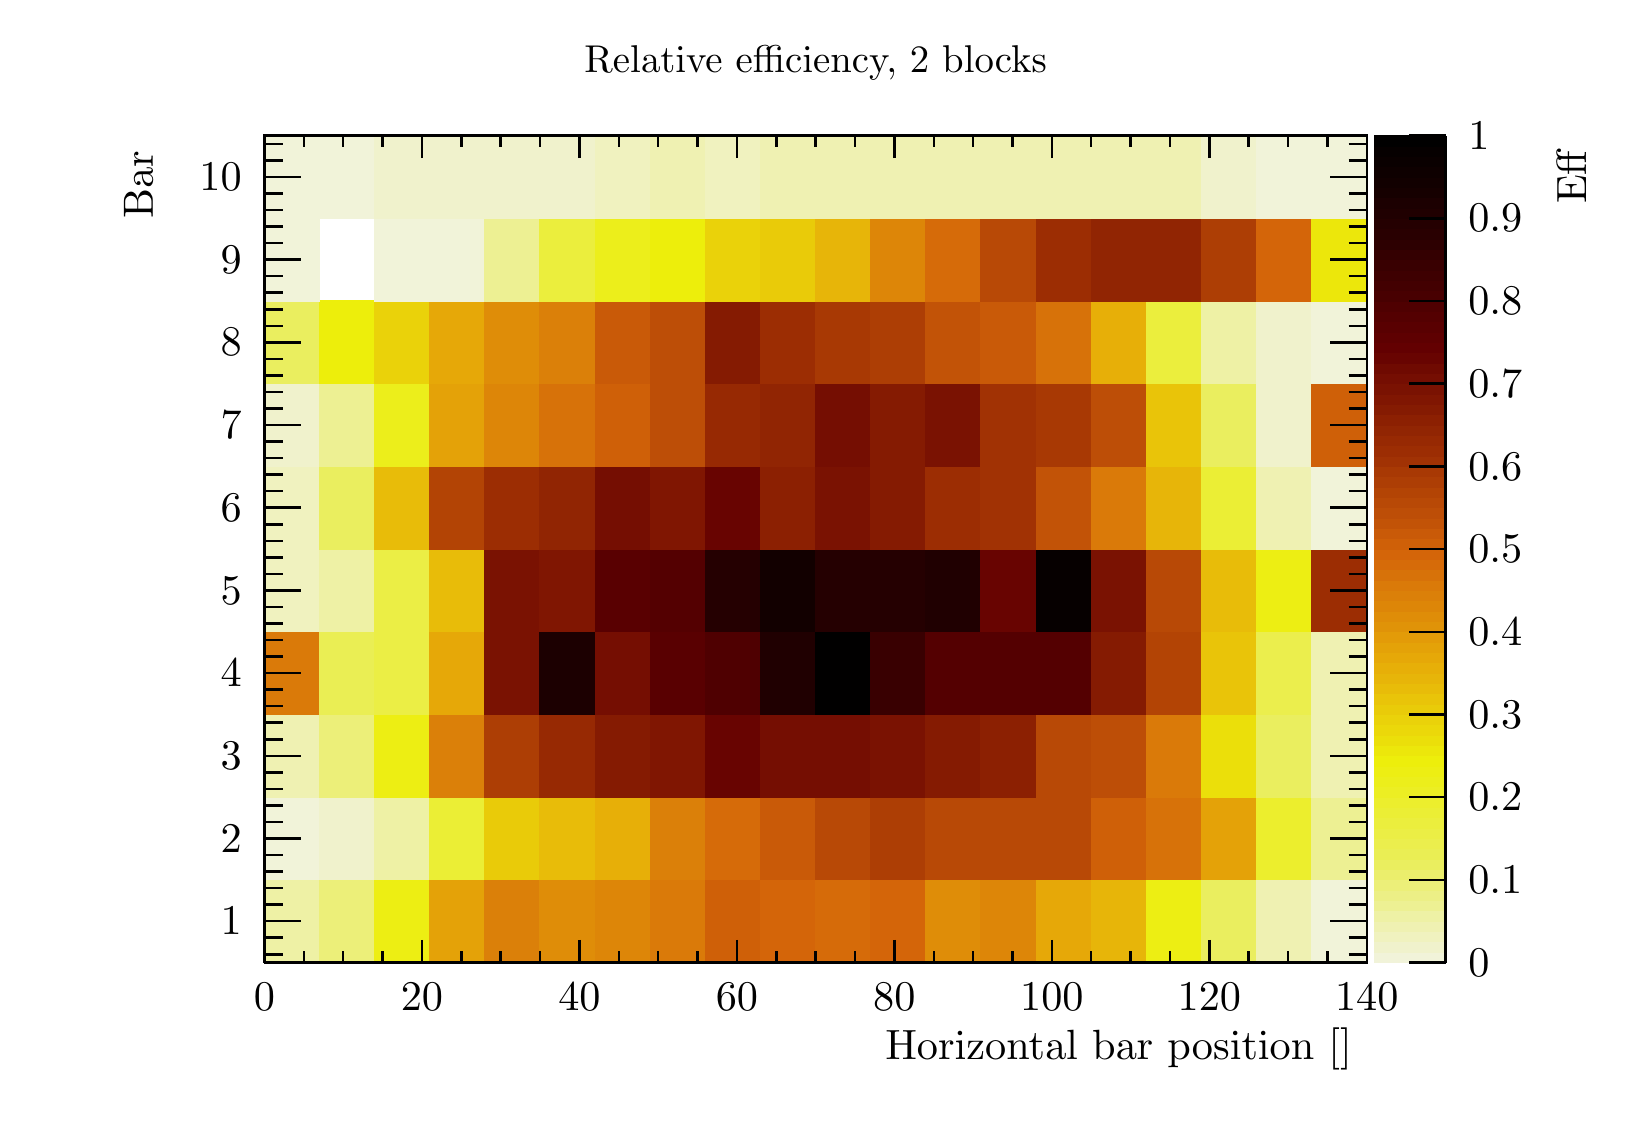
\begin{tikzpicture}
\pgfdeclareplotmark{cross} {
\pgfpathmoveto{\pgfpoint{-0.3\pgfplotmarksize}{\pgfplotmarksize}}
\pgfpathlineto{\pgfpoint{+0.3\pgfplotmarksize}{\pgfplotmarksize}}
\pgfpathlineto{\pgfpoint{+0.3\pgfplotmarksize}{0.3\pgfplotmarksize}}
\pgfpathlineto{\pgfpoint{+1\pgfplotmarksize}{0.3\pgfplotmarksize}}
\pgfpathlineto{\pgfpoint{+1\pgfplotmarksize}{-0.3\pgfplotmarksize}}
\pgfpathlineto{\pgfpoint{+0.3\pgfplotmarksize}{-0.3\pgfplotmarksize}}
\pgfpathlineto{\pgfpoint{+0.3\pgfplotmarksize}{-1.\pgfplotmarksize}}
\pgfpathlineto{\pgfpoint{-0.3\pgfplotmarksize}{-1.\pgfplotmarksize}}
\pgfpathlineto{\pgfpoint{-0.3\pgfplotmarksize}{-0.3\pgfplotmarksize}}
\pgfpathlineto{\pgfpoint{-1.\pgfplotmarksize}{-0.3\pgfplotmarksize}}
\pgfpathlineto{\pgfpoint{-1.\pgfplotmarksize}{0.3\pgfplotmarksize}}
\pgfpathlineto{\pgfpoint{-0.3\pgfplotmarksize}{0.3\pgfplotmarksize}}
\pgfpathclose
\pgfusepathqstroke
}
\pgfdeclareplotmark{cross*} {
\pgfpathmoveto{\pgfpoint{-0.3\pgfplotmarksize}{\pgfplotmarksize}}
\pgfpathlineto{\pgfpoint{+0.3\pgfplotmarksize}{\pgfplotmarksize}}
\pgfpathlineto{\pgfpoint{+0.3\pgfplotmarksize}{0.3\pgfplotmarksize}}
\pgfpathlineto{\pgfpoint{+1\pgfplotmarksize}{0.3\pgfplotmarksize}}
\pgfpathlineto{\pgfpoint{+1\pgfplotmarksize}{-0.3\pgfplotmarksize}}
\pgfpathlineto{\pgfpoint{+0.3\pgfplotmarksize}{-0.3\pgfplotmarksize}}
\pgfpathlineto{\pgfpoint{+0.3\pgfplotmarksize}{-1.\pgfplotmarksize}}
\pgfpathlineto{\pgfpoint{-0.3\pgfplotmarksize}{-1.\pgfplotmarksize}}
\pgfpathlineto{\pgfpoint{-0.3\pgfplotmarksize}{-0.3\pgfplotmarksize}}
\pgfpathlineto{\pgfpoint{-1.\pgfplotmarksize}{-0.3\pgfplotmarksize}}
\pgfpathlineto{\pgfpoint{-1.\pgfplotmarksize}{0.3\pgfplotmarksize}}
\pgfpathlineto{\pgfpoint{-0.3\pgfplotmarksize}{0.3\pgfplotmarksize}}
\pgfpathclose
\pgfusepathqfillstroke
}
\pgfdeclareplotmark{newstar} {
\pgfpathmoveto{\pgfqpoint{0pt}{\pgfplotmarksize}}
\pgfpathlineto{\pgfqpointpolar{44}{0.5\pgfplotmarksize}}
\pgfpathlineto{\pgfqpointpolar{18}{\pgfplotmarksize}}
\pgfpathlineto{\pgfqpointpolar{-20}{0.5\pgfplotmarksize}}
\pgfpathlineto{\pgfqpointpolar{-54}{\pgfplotmarksize}}
\pgfpathlineto{\pgfqpointpolar{-90}{0.5\pgfplotmarksize}}
\pgfpathlineto{\pgfqpointpolar{234}{\pgfplotmarksize}}
\pgfpathlineto{\pgfqpointpolar{198}{0.5\pgfplotmarksize}}
\pgfpathlineto{\pgfqpointpolar{162}{\pgfplotmarksize}}
\pgfpathlineto{\pgfqpointpolar{134}{0.5\pgfplotmarksize}}
\pgfpathclose
\pgfusepathqstroke
}
\pgfdeclareplotmark{newstar*} {
\pgfpathmoveto{\pgfqpoint{0pt}{\pgfplotmarksize}}
\pgfpathlineto{\pgfqpointpolar{44}{0.5\pgfplotmarksize}}
\pgfpathlineto{\pgfqpointpolar{18}{\pgfplotmarksize}}
\pgfpathlineto{\pgfqpointpolar{-20}{0.5\pgfplotmarksize}}
\pgfpathlineto{\pgfqpointpolar{-54}{\pgfplotmarksize}}
\pgfpathlineto{\pgfqpointpolar{-90}{0.5\pgfplotmarksize}}
\pgfpathlineto{\pgfqpointpolar{234}{\pgfplotmarksize}}
\pgfpathlineto{\pgfqpointpolar{198}{0.5\pgfplotmarksize}}
\pgfpathlineto{\pgfqpointpolar{162}{\pgfplotmarksize}}
\pgfpathlineto{\pgfqpointpolar{134}{0.5\pgfplotmarksize}}
\pgfpathclose
\pgfusepathqfillstroke
}
\definecolor{c}{rgb}{1,1,1};
\draw [color=c, fill=c] (0,0) rectangle (20,13.639);
\draw [color=c, fill=c] (3,1.77307) rectangle (17,12.2751);
\definecolor{c}{rgb}{0,0,0};
\draw [c,line width=0.9] (3,1.77307) -- (3,12.2751) -- (17,12.2751) -- (17,1.77307) -- (3,1.77307);
\definecolor{c}{rgb}{1,1,1};
\draw [color=c, fill=c] (3,1.77307) rectangle (17,12.2751);
\definecolor{c}{rgb}{0,0,0};
\draw [c,line width=0.9] (3,1.77307) -- (3,12.2751) -- (17,12.2751) -- (17,1.77307) -- (3,1.77307);
\definecolor{c}{rgb}{0.933839,0.943453,0.645794};
\draw [color=c, fill=c] (3,1.77307) rectangle (3.7,2.82327);
\definecolor{c}{rgb}{0.923719,0.937128,0.475016};
\draw [color=c, fill=c] (3.7,1.77307) rectangle (4.4,2.82327);
\definecolor{c}{rgb}{0.928309,0.933333,0.0740196};
\draw [color=c, fill=c] (4.4,1.77307) rectangle (5.1,2.82327);
\definecolor{c}{rgb}{0.895343,0.634191,0.0317402};
\draw [color=c, fill=c] (5.1,1.77307) rectangle (5.8,2.82327);
\definecolor{c}{rgb}{0.860049,0.502819,0.033701};
\draw [color=c, fill=c] (5.8,1.77307) rectangle (6.5,2.82327);
\definecolor{c}{rgb}{0.873284,0.552083,0.0329657};
\draw [color=c, fill=c] (6.5,1.77307) rectangle (7.2,2.82327);
\definecolor{c}{rgb}{0.866667,0.527451,0.0333333};
\draw [color=c, fill=c] (7.2,1.77307) rectangle (7.9,2.82327);
\definecolor{c}{rgb}{0.853431,0.478186,0.0340686};
\draw [color=c, fill=c] (7.9,1.77307) rectangle (8.6,2.82327);
\definecolor{c}{rgb}{0.810784,0.37549,0.0330882};
\draw [color=c, fill=c] (8.6,1.77307) rectangle (9.3,2.82327);
\definecolor{c}{rgb}{0.831373,0.396078,0.0352941};
\draw [color=c, fill=c] (9.3,1.77307) rectangle (10,2.82327);
\definecolor{c}{rgb}{0.83799,0.420711,0.0349265};
\draw [color=c, fill=c] (10,1.77307) rectangle (10.7,2.82327);
\definecolor{c}{rgb}{0.831373,0.396078,0.0352941};
\draw [color=c, fill=c] (10.7,1.77307) rectangle (11.4,2.82327);
\definecolor{c}{rgb}{0.873284,0.552083,0.0329657};
\draw [color=c, fill=c] (11.4,1.77307) rectangle (12.1,2.82327);
\definecolor{c}{rgb}{0.866667,0.527451,0.0333333};
\draw [color=c, fill=c] (12.1,1.77307) rectangle (12.8,2.82327);
\definecolor{c}{rgb}{0.901961,0.658824,0.0313726};
\draw [color=c, fill=c] (12.8,1.77307) rectangle (13.5,2.82327);
\definecolor{c}{rgb}{0.907108,0.710294,0.0335784};
\draw [color=c, fill=c] (13.5,1.77307) rectangle (14.2,2.82327);
\definecolor{c}{rgb}{0.928309,0.933333,0.0740196};
\draw [color=c, fill=c] (14.2,1.77307) rectangle (14.9,2.82327);
\definecolor{c}{rgb}{0.917647,0.933333,0.372549};
\draw [color=c, fill=c] (14.9,1.77307) rectangle (15.6,2.82327);
\definecolor{c}{rgb}{0.936875,0.945351,0.697027};
\draw [color=c, fill=c] (15.6,1.77307) rectangle (16.3,2.82327);
\definecolor{c}{rgb}{0.945984,0.951044,0.850727};
\draw [color=c, fill=c] (16.3,1.77307) rectangle (17,2.82327);
\draw [color=c, fill=c] (3,2.82327) rectangle (3.7,3.87347);
\definecolor{c}{rgb}{0.942948,0.949146,0.799494};
\draw [color=c, fill=c] (3.7,2.82327) rectangle (4.4,3.87347);
\definecolor{c}{rgb}{0.933839,0.943453,0.645794};
\draw [color=c, fill=c] (4.4,2.82327) rectangle (5.1,3.87347);
\definecolor{c}{rgb}{0.923529,0.933333,0.207843};
\draw [color=c, fill=c] (5.1,2.82327) rectangle (5.8,3.87347);
\definecolor{c}{rgb}{0.915686,0.796078,0.0372549};
\draw [color=c, fill=c] (5.8,2.82327) rectangle (6.5,3.87347);
\definecolor{c}{rgb}{0.909681,0.736029,0.0346814};
\draw [color=c, fill=c] (6.5,2.82327) rectangle (7.2,3.87347);
\definecolor{c}{rgb}{0.904534,0.684559,0.0324755};
\draw [color=c, fill=c] (7.2,2.82327) rectangle (7.9,3.87347);
\definecolor{c}{rgb}{0.860049,0.502819,0.033701};
\draw [color=c, fill=c] (7.9,2.82327) rectangle (8.6,3.87347);
\definecolor{c}{rgb}{0.83799,0.420711,0.0349265};
\draw [color=c, fill=c] (8.6,2.82327) rectangle (9.3,3.87347);
\definecolor{c}{rgb}{0.790196,0.354902,0.0308824};
\draw [color=c, fill=c] (9.3,2.82327) rectangle (10,3.87347);
\definecolor{c}{rgb}{0.721569,0.286275,0.0235294};
\draw [color=c, fill=c] (10,2.82327) rectangle (10.7,3.87347);
\definecolor{c}{rgb}{0.680392,0.245098,0.0191176};
\draw [color=c, fill=c] (10.7,2.82327) rectangle (11.4,3.87347);
\definecolor{c}{rgb}{0.721569,0.286275,0.0235294};
\draw [color=c, fill=c] (11.4,2.82327) rectangle (12.1,3.87347);
\draw [color=c, fill=c] (12.1,2.82327) rectangle (12.8,3.87347);
\draw [color=c, fill=c] (12.8,2.82327) rectangle (13.5,3.87347);
\definecolor{c}{rgb}{0.810784,0.37549,0.0330882};
\draw [color=c, fill=c] (13.5,2.82327) rectangle (14.2,3.87347);
\definecolor{c}{rgb}{0.844608,0.445343,0.0345588};
\draw [color=c, fill=c] (14.2,2.82327) rectangle (14.9,3.87347);
\definecolor{c}{rgb}{0.895343,0.634191,0.0317402};
\draw [color=c, fill=c] (14.9,2.82327) rectangle (15.6,3.87347);
\definecolor{c}{rgb}{0.924632,0.933333,0.176961};
\draw [color=c, fill=c] (15.6,2.82327) rectangle (16.3,3.87347);
\definecolor{c}{rgb}{0.929791,0.940923,0.577483};
\draw [color=c, fill=c] (16.3,2.82327) rectangle (17,3.87347);
\definecolor{c}{rgb}{0.936875,0.945351,0.697027};
\draw [color=c, fill=c] (3,3.87347) rectangle (3.7,4.92367);
\definecolor{c}{rgb}{0.923719,0.937128,0.475016};
\draw [color=c, fill=c] (3.7,3.87347) rectangle (4.4,4.92367);
\definecolor{c}{rgb}{0.928309,0.933333,0.0740196};
\draw [color=c, fill=c] (4.4,3.87347) rectangle (5.1,4.92367);
\definecolor{c}{rgb}{0.860049,0.502819,0.033701};
\draw [color=c, fill=c] (5.1,3.87347) rectangle (5.8,4.92367);
\definecolor{c}{rgb}{0.680392,0.245098,0.0191176};
\draw [color=c, fill=c] (5.8,3.87347) rectangle (6.5,4.92367);
\definecolor{c}{rgb}{0.590809,0.159926,0.0110294};
\draw [color=c, fill=c] (6.5,3.87347) rectangle (7.2,4.92367);
\definecolor{c}{rgb}{0.520956,0.104779,0.00857843};
\draw [color=c, fill=c] (7.2,3.87347) rectangle (7.9,4.92367);
\definecolor{c}{rgb}{0.5,0.0882353,0.00784314};
\draw [color=c, fill=c] (7.9,3.87347) rectangle (8.6,4.92367);
\definecolor{c}{rgb}{0.409191,0.0165441,0.00465686};
\draw [color=c, fill=c] (8.6,3.87347) rectangle (9.3,4.92367);
\definecolor{c}{rgb}{0.458088,0.0551471,0.00637255};
\draw [color=c, fill=c] (9.3,3.87347) rectangle (10,4.92367);
\draw [color=c, fill=c] (10,3.87347) rectangle (10.7,4.92367);
\definecolor{c}{rgb}{0.479044,0.0716912,0.00710784};
\draw [color=c, fill=c] (10.7,3.87347) rectangle (11.4,4.92367);
\definecolor{c}{rgb}{0.520956,0.104779,0.00857843};
\draw [color=c, fill=c] (11.4,3.87347) rectangle (12.1,4.92367);
\definecolor{c}{rgb}{0.548897,0.126838,0.00955882};
\draw [color=c, fill=c] (12.1,3.87347) rectangle (12.8,4.92367);
\definecolor{c}{rgb}{0.721569,0.286275,0.0235294};
\draw [color=c, fill=c] (12.8,3.87347) rectangle (13.5,4.92367);
\definecolor{c}{rgb}{0.742157,0.306863,0.0257353};
\draw [color=c, fill=c] (13.5,3.87347) rectangle (14.2,4.92367);
\definecolor{c}{rgb}{0.853431,0.478186,0.0340686};
\draw [color=c, fill=c] (14.2,3.87347) rectangle (14.9,4.92367);
\definecolor{c}{rgb}{0.923407,0.873284,0.0405637};
\draw [color=c, fill=c] (14.9,3.87347) rectangle (15.6,4.92367);
\definecolor{c}{rgb}{0.917647,0.933333,0.372549};
\draw [color=c, fill=c] (15.6,3.87347) rectangle (16.3,4.92367);
\definecolor{c}{rgb}{0.936875,0.945351,0.697027};
\draw [color=c, fill=c] (16.3,3.87347) rectangle (17,4.92367);
\definecolor{c}{rgb}{0.853431,0.478186,0.0340686};
\draw [color=c, fill=c] (3,4.92367) rectangle (3.7,5.97387);
\definecolor{c}{rgb}{0.919118,0.933333,0.331373};
\draw [color=c, fill=c] (3.7,4.92367) rectangle (4.4,5.97387);
\definecolor{c}{rgb}{0.921324,0.933333,0.269608};
\draw [color=c, fill=c] (4.4,4.92367) rectangle (5.1,5.97387);
\definecolor{c}{rgb}{0.901961,0.658824,0.0313726};
\draw [color=c, fill=c] (5.1,4.92367) rectangle (5.8,5.97387);
\definecolor{c}{rgb}{0.479044,0.0716912,0.00710784};
\draw [color=c, fill=c] (5.8,4.92367) rectangle (6.5,5.97387);
\definecolor{c}{rgb}{0.110294,0,0.00245098};
\draw [color=c, fill=c] (6.5,4.92367) rectangle (7.2,5.97387);
\definecolor{c}{rgb}{0.458088,0.0551471,0.00637255};
\draw [color=c, fill=c] (7.2,4.92367) rectangle (7.9,5.97387);
\definecolor{c}{rgb}{0.348529,0,0.00392157};
\draw [color=c, fill=c] (7.9,4.92367) rectangle (8.6,5.97387);
\definecolor{c}{rgb}{0.308824,0,0.00392157};
\draw [color=c, fill=c] (8.6,4.92367) rectangle (9.3,5.97387);
\definecolor{c}{rgb}{0.126838,0,0.00281863};
\draw [color=c, fill=c] (9.3,4.92367) rectangle (10,5.97387);
\definecolor{c}{rgb}{0.00551471,0,0.000122549};
\draw [color=c, fill=c] (10,4.92367) rectangle (10.7,5.97387);
\definecolor{c}{rgb}{0.222794,0,0.00392157};
\draw [color=c, fill=c] (10.7,4.92367) rectangle (11.4,5.97387);
\definecolor{c}{rgb}{0.328676,0,0.00392157};
\draw [color=c, fill=c] (11.4,4.92367) rectangle (12.1,5.97387);
\draw [color=c, fill=c] (12.1,4.92367) rectangle (12.8,5.97387);
\draw [color=c, fill=c] (12.8,4.92367) rectangle (13.5,5.97387);
\definecolor{c}{rgb}{0.520956,0.104779,0.00857843};
\draw [color=c, fill=c] (13.5,4.92367) rectangle (14.2,5.97387);
\definecolor{c}{rgb}{0.70098,0.265686,0.0213235};
\draw [color=c, fill=c] (14.2,4.92367) rectangle (14.9,5.97387);
\definecolor{c}{rgb}{0.913113,0.770343,0.036152};
\draw [color=c, fill=c] (14.9,4.92367) rectangle (15.6,5.97387);
\definecolor{c}{rgb}{0.920221,0.933333,0.30049};
\draw [color=c, fill=c] (15.6,4.92367) rectangle (16.3,5.97387);
\definecolor{c}{rgb}{0.936875,0.945351,0.697027};
\draw [color=c, fill=c] (16.3,4.92367) rectangle (17,5.97387);
\definecolor{c}{rgb}{0.939911,0.947249,0.748261};
\draw [color=c, fill=c] (3,5.97387) rectangle (3.7,7.02407);
\definecolor{c}{rgb}{0.933839,0.943453,0.645794};
\draw [color=c, fill=c] (3.7,5.97387) rectangle (4.4,7.02407);
\definecolor{c}{rgb}{0.921324,0.933333,0.269608};
\draw [color=c, fill=c] (4.4,5.97387) rectangle (5.1,7.02407);
\definecolor{c}{rgb}{0.909681,0.736029,0.0346814};
\draw [color=c, fill=c] (5.1,5.97387) rectangle (5.8,7.02407);
\definecolor{c}{rgb}{0.479044,0.0716912,0.00710784};
\draw [color=c, fill=c] (5.8,5.97387) rectangle (6.5,7.02407);
\definecolor{c}{rgb}{0.5,0.0882353,0.00784314};
\draw [color=c, fill=c] (6.5,5.97387) rectangle (7.2,7.02407);
\definecolor{c}{rgb}{0.348529,0,0.00392157};
\draw [color=c, fill=c] (7.2,5.97387) rectangle (7.9,7.02407);
\definecolor{c}{rgb}{0.328676,0,0.00392157};
\draw [color=c, fill=c] (7.9,5.97387) rectangle (8.6,7.02407);
\definecolor{c}{rgb}{0.143382,0,0.00318627};
\draw [color=c, fill=c] (8.6,5.97387) rectangle (9.3,7.02407);
\definecolor{c}{rgb}{0.0716912,0,0.00159314};
\draw [color=c, fill=c] (9.3,5.97387) rectangle (10,7.02407);
\definecolor{c}{rgb}{0.143382,0,0.00318627};
\draw [color=c, fill=c] (10,5.97387) rectangle (10.7,7.02407);
\draw [color=c, fill=c] (10.7,5.97387) rectangle (11.4,7.02407);
\definecolor{c}{rgb}{0.126838,0,0.00281863};
\draw [color=c, fill=c] (11.4,5.97387) rectangle (12.1,7.02407);
\definecolor{c}{rgb}{0.409191,0.0165441,0.00465686};
\draw [color=c, fill=c] (12.1,5.97387) rectangle (12.8,7.02407);
\definecolor{c}{rgb}{0.0220588,0,0.000490196};
\draw [color=c, fill=c] (12.8,5.97387) rectangle (13.5,7.02407);
\definecolor{c}{rgb}{0.479044,0.0716912,0.00710784};
\draw [color=c, fill=c] (13.5,5.97387) rectangle (14.2,7.02407);
\definecolor{c}{rgb}{0.721569,0.286275,0.0235294};
\draw [color=c, fill=c] (14.2,5.97387) rectangle (14.9,7.02407);
\definecolor{c}{rgb}{0.909681,0.736029,0.0346814};
\draw [color=c, fill=c] (14.9,5.97387) rectangle (15.6,7.02407);
\definecolor{c}{rgb}{0.928309,0.933333,0.0740196};
\draw [color=c, fill=c] (15.6,5.97387) rectangle (16.3,7.02407);
\definecolor{c}{rgb}{0.611765,0.176471,0.0117647};
\draw [color=c, fill=c] (16.3,5.97387) rectangle (17,7.02407);
\definecolor{c}{rgb}{0.939911,0.947249,0.748261};
\draw [color=c, fill=c] (3,7.02407) rectangle (3.7,8.07427);
\definecolor{c}{rgb}{0.917647,0.933333,0.372549};
\draw [color=c, fill=c] (3.7,7.02407) rectangle (4.4,8.07427);
\definecolor{c}{rgb}{0.909681,0.736029,0.0346814};
\draw [color=c, fill=c] (4.4,7.02407) rectangle (5.1,8.07427);
\definecolor{c}{rgb}{0.70098,0.265686,0.0213235};
\draw [color=c, fill=c] (5.1,7.02407) rectangle (5.8,8.07427);
\definecolor{c}{rgb}{0.611765,0.176471,0.0117647};
\draw [color=c, fill=c] (5.8,7.02407) rectangle (6.5,8.07427);
\definecolor{c}{rgb}{0.569853,0.143382,0.0102941};
\draw [color=c, fill=c] (6.5,7.02407) rectangle (7.2,8.07427);
\definecolor{c}{rgb}{0.458088,0.0551471,0.00637255};
\draw [color=c, fill=c] (7.2,7.02407) rectangle (7.9,8.07427);
\definecolor{c}{rgb}{0.5,0.0882353,0.00784314};
\draw [color=c, fill=c] (7.9,7.02407) rectangle (8.6,8.07427);
\definecolor{c}{rgb}{0.409191,0.0165441,0.00465686};
\draw [color=c, fill=c] (8.6,7.02407) rectangle (9.3,8.07427);
\definecolor{c}{rgb}{0.548897,0.126838,0.00955882};
\draw [color=c, fill=c] (9.3,7.02407) rectangle (10,8.07427);
\definecolor{c}{rgb}{0.479044,0.0716912,0.00710784};
\draw [color=c, fill=c] (10,7.02407) rectangle (10.7,8.07427);
\definecolor{c}{rgb}{0.520956,0.104779,0.00857843};
\draw [color=c, fill=c] (10.7,7.02407) rectangle (11.4,8.07427);
\definecolor{c}{rgb}{0.611765,0.176471,0.0117647};
\draw [color=c, fill=c] (11.4,7.02407) rectangle (12.1,8.07427);
\definecolor{c}{rgb}{0.632353,0.197059,0.0139706};
\draw [color=c, fill=c] (12.1,7.02407) rectangle (12.8,8.07427);
\definecolor{c}{rgb}{0.762745,0.327451,0.0279412};
\draw [color=c, fill=c] (12.8,7.02407) rectangle (13.5,8.07427);
\definecolor{c}{rgb}{0.853431,0.478186,0.0340686};
\draw [color=c, fill=c] (13.5,7.02407) rectangle (14.2,8.07427);
\definecolor{c}{rgb}{0.907108,0.710294,0.0335784};
\draw [color=c, fill=c] (14.2,7.02407) rectangle (14.9,8.07427);
\definecolor{c}{rgb}{0.923529,0.933333,0.207843};
\draw [color=c, fill=c] (14.9,7.02407) rectangle (15.6,8.07427);
\definecolor{c}{rgb}{0.936875,0.945351,0.697027};
\draw [color=c, fill=c] (15.6,7.02407) rectangle (16.3,8.07427);
\definecolor{c}{rgb}{0.945984,0.951044,0.850727};
\draw [color=c, fill=c] (16.3,7.02407) rectangle (17,8.07427);
\definecolor{c}{rgb}{0.942948,0.949146,0.799494};
\draw [color=c, fill=c] (3,8.07427) rectangle (3.7,9.12447);
\definecolor{c}{rgb}{0.929791,0.940923,0.577483};
\draw [color=c, fill=c] (3.7,8.07427) rectangle (4.4,9.12447);
\definecolor{c}{rgb}{0.927206,0.933333,0.104902};
\draw [color=c, fill=c] (4.4,8.07427) rectangle (5.1,9.12447);
\definecolor{c}{rgb}{0.895343,0.634191,0.0317402};
\draw [color=c, fill=c] (5.1,8.07427) rectangle (5.8,9.12447);
\definecolor{c}{rgb}{0.866667,0.527451,0.0333333};
\draw [color=c, fill=c] (5.8,8.07427) rectangle (6.5,9.12447);
\definecolor{c}{rgb}{0.844608,0.445343,0.0345588};
\draw [color=c, fill=c] (6.5,8.07427) rectangle (7.2,9.12447);
\definecolor{c}{rgb}{0.810784,0.37549,0.0330882};
\draw [color=c, fill=c] (7.2,8.07427) rectangle (7.9,9.12447);
\definecolor{c}{rgb}{0.742157,0.306863,0.0257353};
\draw [color=c, fill=c] (7.9,8.07427) rectangle (8.6,9.12447);
\definecolor{c}{rgb}{0.590809,0.159926,0.0110294};
\draw [color=c, fill=c] (8.6,8.07427) rectangle (9.3,9.12447);
\definecolor{c}{rgb}{0.569853,0.143382,0.0102941};
\draw [color=c, fill=c] (9.3,8.07427) rectangle (10,9.12447);
\definecolor{c}{rgb}{0.458088,0.0551471,0.00637255};
\draw [color=c, fill=c] (10,8.07427) rectangle (10.7,9.12447);
\definecolor{c}{rgb}{0.520956,0.104779,0.00857843};
\draw [color=c, fill=c] (10.7,8.07427) rectangle (11.4,9.12447);
\definecolor{c}{rgb}{0.479044,0.0716912,0.00710784};
\draw [color=c, fill=c] (11.4,8.07427) rectangle (12.1,9.12447);
\definecolor{c}{rgb}{0.632353,0.197059,0.0139706};
\draw [color=c, fill=c] (12.1,8.07427) rectangle (12.8,9.12447);
\definecolor{c}{rgb}{0.659804,0.22451,0.0169118};
\draw [color=c, fill=c] (12.8,8.07427) rectangle (13.5,9.12447);
\definecolor{c}{rgb}{0.742157,0.306863,0.0257353};
\draw [color=c, fill=c] (13.5,8.07427) rectangle (14.2,9.12447);
\definecolor{c}{rgb}{0.913113,0.770343,0.036152};
\draw [color=c, fill=c] (14.2,8.07427) rectangle (14.9,9.12447);
\definecolor{c}{rgb}{0.917647,0.933333,0.372549};
\draw [color=c, fill=c] (14.9,8.07427) rectangle (15.6,9.12447);
\definecolor{c}{rgb}{0.942948,0.949146,0.799494};
\draw [color=c, fill=c] (15.6,8.07427) rectangle (16.3,9.12447);
\definecolor{c}{rgb}{0.810784,0.37549,0.0330882};
\draw [color=c, fill=c] (16.3,8.07427) rectangle (17,9.12447);
\definecolor{c}{rgb}{0.917647,0.933333,0.372549};
\draw [color=c, fill=c] (3,9.12447) rectangle (3.7,10.1747);
\definecolor{c}{rgb}{0.929412,0.933333,0.0431373};
\draw [color=c, fill=c] (3.7,9.12447) rectangle (4.4,10.1747);
\definecolor{c}{rgb}{0.91826,0.821814,0.0383578};
\draw [color=c, fill=c] (4.4,9.12447) rectangle (5.1,10.1747);
\definecolor{c}{rgb}{0.901961,0.658824,0.0313726};
\draw [color=c, fill=c] (5.1,9.12447) rectangle (5.8,10.1747);
\definecolor{c}{rgb}{0.873284,0.552083,0.0329657};
\draw [color=c, fill=c] (5.8,9.12447) rectangle (6.5,10.1747);
\definecolor{c}{rgb}{0.860049,0.502819,0.033701};
\draw [color=c, fill=c] (6.5,9.12447) rectangle (7.2,10.1747);
\definecolor{c}{rgb}{0.790196,0.354902,0.0308824};
\draw [color=c, fill=c] (7.2,9.12447) rectangle (7.9,10.1747);
\definecolor{c}{rgb}{0.742157,0.306863,0.0257353};
\draw [color=c, fill=c] (7.9,9.12447) rectangle (8.6,10.1747);
\definecolor{c}{rgb}{0.520956,0.104779,0.00857843};
\draw [color=c, fill=c] (8.6,9.12447) rectangle (9.3,10.1747);
\definecolor{c}{rgb}{0.611765,0.176471,0.0117647};
\draw [color=c, fill=c] (9.3,9.12447) rectangle (10,10.1747);
\definecolor{c}{rgb}{0.659804,0.22451,0.0169118};
\draw [color=c, fill=c] (10,9.12447) rectangle (10.7,10.1747);
\definecolor{c}{rgb}{0.680392,0.245098,0.0191176};
\draw [color=c, fill=c] (10.7,9.12447) rectangle (11.4,10.1747);
\definecolor{c}{rgb}{0.762745,0.327451,0.0279412};
\draw [color=c, fill=c] (11.4,9.12447) rectangle (12.1,10.1747);
\definecolor{c}{rgb}{0.790196,0.354902,0.0308824};
\draw [color=c, fill=c] (12.1,9.12447) rectangle (12.8,10.1747);
\definecolor{c}{rgb}{0.844608,0.445343,0.0345588};
\draw [color=c, fill=c] (12.8,9.12447) rectangle (13.5,10.1747);
\definecolor{c}{rgb}{0.904534,0.684559,0.0324755};
\draw [color=c, fill=c] (13.5,9.12447) rectangle (14.2,10.1747);
\definecolor{c}{rgb}{0.922426,0.933333,0.238725};
\draw [color=c, fill=c] (14.2,9.12447) rectangle (14.9,10.1747);
\definecolor{c}{rgb}{0.933839,0.943453,0.645794};
\draw [color=c, fill=c] (14.9,9.12447) rectangle (15.6,10.1747);
\definecolor{c}{rgb}{0.942948,0.949146,0.799494};
\draw [color=c, fill=c] (15.6,9.12447) rectangle (16.3,10.1747);
\definecolor{c}{rgb}{0.945984,0.951044,0.850727};
\draw [color=c, fill=c] (16.3,9.12447) rectangle (17,10.1747);
\draw [color=c, fill=c] (3,10.1747) rectangle (3.7,11.2249);
\draw [color=c, fill=c] (4.4,10.1747) rectangle (5.1,11.2249);
\draw [color=c, fill=c] (5.1,10.1747) rectangle (5.8,11.2249);
\definecolor{c}{rgb}{0.929791,0.940923,0.577483};
\draw [color=c, fill=c] (5.8,10.1747) rectangle (6.5,11.2249);
\definecolor{c}{rgb}{0.922426,0.933333,0.238725};
\draw [color=c, fill=c] (6.5,10.1747) rectangle (7.2,11.2249);
\definecolor{c}{rgb}{0.927206,0.933333,0.104902};
\draw [color=c, fill=c] (7.2,10.1747) rectangle (7.9,11.2249);
\definecolor{c}{rgb}{0.929412,0.933333,0.0431373};
\draw [color=c, fill=c] (7.9,10.1747) rectangle (8.6,11.2249);
\definecolor{c}{rgb}{0.91826,0.821814,0.0383578};
\draw [color=c, fill=c] (8.6,10.1747) rectangle (9.3,11.2249);
\definecolor{c}{rgb}{0.915686,0.796078,0.0372549};
\draw [color=c, fill=c] (9.3,10.1747) rectangle (10,11.2249);
\definecolor{c}{rgb}{0.907108,0.710294,0.0335784};
\draw [color=c, fill=c] (10,10.1747) rectangle (10.7,11.2249);
\definecolor{c}{rgb}{0.866667,0.527451,0.0333333};
\draw [color=c, fill=c] (10.7,10.1747) rectangle (11.4,11.2249);
\definecolor{c}{rgb}{0.83799,0.420711,0.0349265};
\draw [color=c, fill=c] (11.4,10.1747) rectangle (12.1,11.2249);
\definecolor{c}{rgb}{0.721569,0.286275,0.0235294};
\draw [color=c, fill=c] (12.1,10.1747) rectangle (12.8,11.2249);
\definecolor{c}{rgb}{0.611765,0.176471,0.0117647};
\draw [color=c, fill=c] (12.8,10.1747) rectangle (13.5,11.2249);
\definecolor{c}{rgb}{0.569853,0.143382,0.0102941};
\draw [color=c, fill=c] (13.5,10.1747) rectangle (14.2,11.2249);
\draw [color=c, fill=c] (14.2,10.1747) rectangle (14.9,11.2249);
\definecolor{c}{rgb}{0.680392,0.245098,0.0191176};
\draw [color=c, fill=c] (14.9,10.1747) rectangle (15.6,11.2249);
\definecolor{c}{rgb}{0.831373,0.396078,0.0352941};
\draw [color=c, fill=c] (15.6,10.1747) rectangle (16.3,11.2249);
\definecolor{c}{rgb}{0.926838,0.907598,0.0420343};
\draw [color=c, fill=c] (16.3,10.1747) rectangle (17,11.2249);
\definecolor{c}{rgb}{0.945984,0.951044,0.850727};
\draw [color=c, fill=c] (3,11.2249) rectangle (3.7,12.2751);
\draw [color=c, fill=c] (3.7,11.2249) rectangle (4.4,12.2751);
\definecolor{c}{rgb}{0.942948,0.949146,0.799494};
\draw [color=c, fill=c] (4.4,11.2249) rectangle (5.1,12.2751);
\draw [color=c, fill=c] (5.1,11.2249) rectangle (5.8,12.2751);
\draw [color=c, fill=c] (5.8,11.2249) rectangle (6.5,12.2751);
\draw [color=c, fill=c] (6.5,11.2249) rectangle (7.2,12.2751);
\definecolor{c}{rgb}{0.939911,0.947249,0.748261};
\draw [color=c, fill=c] (7.2,11.2249) rectangle (7.9,12.2751);
\definecolor{c}{rgb}{0.936875,0.945351,0.697027};
\draw [color=c, fill=c] (7.9,11.2249) rectangle (8.6,12.2751);
\definecolor{c}{rgb}{0.939911,0.947249,0.748261};
\draw [color=c, fill=c] (8.6,11.2249) rectangle (9.3,12.2751);
\definecolor{c}{rgb}{0.936875,0.945351,0.697027};
\draw [color=c, fill=c] (9.3,11.2249) rectangle (10,12.2751);
\draw [color=c, fill=c] (10,11.2249) rectangle (10.7,12.2751);
\draw [color=c, fill=c] (10.7,11.2249) rectangle (11.4,12.2751);
\draw [color=c, fill=c] (11.4,11.2249) rectangle (12.1,12.2751);
\draw [color=c, fill=c] (12.1,11.2249) rectangle (12.8,12.2751);
\draw [color=c, fill=c] (12.8,11.2249) rectangle (13.5,12.2751);
\draw [color=c, fill=c] (13.5,11.2249) rectangle (14.2,12.2751);
\draw [color=c, fill=c] (14.2,11.2249) rectangle (14.9,12.2751);
\definecolor{c}{rgb}{0.942948,0.949146,0.799494};
\draw [color=c, fill=c] (14.9,11.2249) rectangle (15.6,12.2751);
\definecolor{c}{rgb}{0.945984,0.951044,0.850727};
\draw [color=c, fill=c] (15.6,11.2249) rectangle (16.3,12.2751);
\draw [color=c, fill=c] (16.3,11.2249) rectangle (17,12.2751);
\definecolor{c}{rgb}{0,0,0};
\draw [c,line width=0.9] (3,1.77307) -- (17,1.77307);
\draw [c,line width=0.9] (3,2.05948) -- (3,1.77307);
\draw [c,line width=0.9] (3.5,1.91628) -- (3.5,1.77307);
\draw [c,line width=0.9] (4,1.91628) -- (4,1.77307);
\draw [c,line width=0.9] (4.5,1.91628) -- (4.5,1.77307);
\draw [c,line width=0.9] (5,2.05948) -- (5,1.77307);
\draw [c,line width=0.9] (5.5,1.91628) -- (5.5,1.77307);
\draw [c,line width=0.9] (6,1.91628) -- (6,1.77307);
\draw [c,line width=0.9] (6.5,1.91628) -- (6.5,1.77307);
\draw [c,line width=0.9] (7,2.05948) -- (7,1.77307);
\draw [c,line width=0.9] (7.5,1.91628) -- (7.5,1.77307);
\draw [c,line width=0.9] (8,1.91628) -- (8,1.77307);
\draw [c,line width=0.9] (8.5,1.91628) -- (8.5,1.77307);
\draw [c,line width=0.9] (9,2.05948) -- (9,1.77307);
\draw [c,line width=0.9] (9.5,1.91628) -- (9.5,1.77307);
\draw [c,line width=0.9] (10,1.91628) -- (10,1.77307);
\draw [c,line width=0.9] (10.5,1.91628) -- (10.5,1.77307);
\draw [c,line width=0.9] (11,2.05948) -- (11,1.77307);
\draw [c,line width=0.9] (11.5,1.91628) -- (11.5,1.77307);
\draw [c,line width=0.9] (12,1.91628) -- (12,1.77307);
\draw [c,line width=0.9] (12.5,1.91628) -- (12.5,1.77307);
\draw [c,line width=0.9] (13,2.05948) -- (13,1.77307);
\draw [c,line width=0.9] (13.5,1.91628) -- (13.5,1.77307);
\draw [c,line width=0.9] (14,1.91628) -- (14,1.77307);
\draw [c,line width=0.9] (14.5,1.91628) -- (14.5,1.77307);
\draw [c,line width=0.9] (15,2.05948) -- (15,1.77307);
\draw [c,line width=0.9] (15.5,1.91628) -- (15.5,1.77307);
\draw [c,line width=0.9] (16,1.91628) -- (16,1.77307);
\draw [c,line width=0.9] (16.5,1.91628) -- (16.5,1.77307);
\draw [c,line width=0.9] (17,2.05948) -- (17,1.77307);
\draw [anchor=base] (3,1.15931) node[scale=1.52731, color=c, rotate=0]{0};
\draw [anchor=base] (5,1.15931) node[scale=1.52731, color=c, rotate=0]{20};
\draw [anchor=base] (7,1.15931) node[scale=1.52731, color=c, rotate=0]{40};
\draw [anchor=base] (9,1.15931) node[scale=1.52731, color=c, rotate=0]{60};
\draw [anchor=base] (11,1.15931) node[scale=1.52731, color=c, rotate=0]{80};
\draw [anchor=base] (13,1.15931) node[scale=1.52731, color=c, rotate=0]{100};
\draw [anchor=base] (15,1.15931) node[scale=1.52731, color=c, rotate=0]{120};
\draw [anchor=base] (17,1.15931) node[scale=1.52731, color=c, rotate=0]{140};
\draw [anchor= east] (17,0.681948) node[scale=1.52731, color=c, rotate=0]{Horizontal bar position [\si{\centi\metre}]};
\draw [c,line width=0.9] (3,12.2751) -- (17,12.2751);
\draw [c,line width=0.9] (3,11.9887) -- (3,12.2751);
\draw [c,line width=0.9] (3.5,12.1319) -- (3.5,12.2751);
\draw [c,line width=0.9] (4,12.1319) -- (4,12.2751);
\draw [c,line width=0.9] (4.5,12.1319) -- (4.5,12.2751);
\draw [c,line width=0.9] (5,11.9887) -- (5,12.2751);
\draw [c,line width=0.9] (5.5,12.1319) -- (5.5,12.2751);
\draw [c,line width=0.9] (6,12.1319) -- (6,12.2751);
\draw [c,line width=0.9] (6.5,12.1319) -- (6.5,12.2751);
\draw [c,line width=0.9] (7,11.9887) -- (7,12.2751);
\draw [c,line width=0.9] (7.5,12.1319) -- (7.5,12.2751);
\draw [c,line width=0.9] (8,12.1319) -- (8,12.2751);
\draw [c,line width=0.9] (8.5,12.1319) -- (8.5,12.2751);
\draw [c,line width=0.9] (9,11.9887) -- (9,12.2751);
\draw [c,line width=0.9] (9.5,12.1319) -- (9.5,12.2751);
\draw [c,line width=0.9] (10,12.1319) -- (10,12.2751);
\draw [c,line width=0.9] (10.5,12.1319) -- (10.5,12.2751);
\draw [c,line width=0.9] (11,11.9887) -- (11,12.2751);
\draw [c,line width=0.9] (11.5,12.1319) -- (11.5,12.2751);
\draw [c,line width=0.9] (12,12.1319) -- (12,12.2751);
\draw [c,line width=0.9] (12.5,12.1319) -- (12.5,12.2751);
\draw [c,line width=0.9] (13,11.9887) -- (13,12.2751);
\draw [c,line width=0.9] (13.5,12.1319) -- (13.5,12.2751);
\draw [c,line width=0.9] (14,12.1319) -- (14,12.2751);
\draw [c,line width=0.9] (14.5,12.1319) -- (14.5,12.2751);
\draw [c,line width=0.9] (15,11.9887) -- (15,12.2751);
\draw [c,line width=0.9] (15.5,12.1319) -- (15.5,12.2751);
\draw [c,line width=0.9] (16,12.1319) -- (16,12.2751);
\draw [c,line width=0.9] (16.5,12.1319) -- (16.5,12.2751);
\draw [c,line width=0.9] (17,11.9887) -- (17,12.2751);
\draw [c,line width=0.9] (3,1.77307) -- (3,12.2751);
\draw [c,line width=0.9] (3.462,2.29817) -- (3,2.29817);
\draw [c,line width=0.9] (3.231,2.50821) -- (3,2.50821);
\draw [c,line width=0.9] (3.231,2.71825) -- (3,2.71825);
\draw [c,line width=0.9] (3.231,2.92829) -- (3,2.92829);
\draw [c,line width=0.9] (3.231,3.13833) -- (3,3.13833);
\draw [c,line width=0.9] (3.462,3.34837) -- (3,3.34837);
\draw [c,line width=0.9] (3.231,3.55841) -- (3,3.55841);
\draw [c,line width=0.9] (3.231,3.76845) -- (3,3.76845);
\draw [c,line width=0.9] (3.231,3.97849) -- (3,3.97849);
\draw [c,line width=0.9] (3.231,4.18853) -- (3,4.18853);
\draw [c,line width=0.9] (3.462,4.39857) -- (3,4.39857);
\draw [c,line width=0.9] (3.231,4.60861) -- (3,4.60861);
\draw [c,line width=0.9] (3.231,4.81865) -- (3,4.81865);
\draw [c,line width=0.9] (3.231,5.02869) -- (3,5.02869);
\draw [c,line width=0.9] (3.231,5.23873) -- (3,5.23873);
\draw [c,line width=0.9] (3.462,5.44877) -- (3,5.44877);
\draw [c,line width=0.9] (3.231,5.65881) -- (3,5.65881);
\draw [c,line width=0.9] (3.231,5.86885) -- (3,5.86885);
\draw [c,line width=0.9] (3.231,6.07889) -- (3,6.07889);
\draw [c,line width=0.9] (3.231,6.28893) -- (3,6.28893);
\draw [c,line width=0.9] (3.462,6.49897) -- (3,6.49897);
\draw [c,line width=0.9] (3.231,6.70901) -- (3,6.70901);
\draw [c,line width=0.9] (3.231,6.91905) -- (3,6.91905);
\draw [c,line width=0.9] (3.231,7.12909) -- (3,7.12909);
\draw [c,line width=0.9] (3.231,7.33913) -- (3,7.33913);
\draw [c,line width=0.9] (3.462,7.54917) -- (3,7.54917);
\draw [c,line width=0.9] (3.231,7.75921) -- (3,7.75921);
\draw [c,line width=0.9] (3.231,7.96925) -- (3,7.96925);
\draw [c,line width=0.9] (3.231,8.17929) -- (3,8.17929);
\draw [c,line width=0.9] (3.231,8.38933) -- (3,8.38933);
\draw [c,line width=0.9] (3.462,8.59937) -- (3,8.59937);
\draw [c,line width=0.9] (3.231,8.80941) -- (3,8.80941);
\draw [c,line width=0.9] (3.231,9.01945) -- (3,9.01945);
\draw [c,line width=0.9] (3.231,9.22949) -- (3,9.22949);
\draw [c,line width=0.9] (3.231,9.43953) -- (3,9.43953);
\draw [c,line width=0.9] (3.462,9.64957) -- (3,9.64957);
\draw [c,line width=0.9] (3.231,9.85961) -- (3,9.85961);
\draw [c,line width=0.9] (3.231,10.0697) -- (3,10.0697);
\draw [c,line width=0.9] (3.231,10.2797) -- (3,10.2797);
\draw [c,line width=0.9] (3.231,10.4897) -- (3,10.4897);
\draw [c,line width=0.9] (3.462,10.6998) -- (3,10.6998);
\draw [c,line width=0.9] (3.231,10.9098) -- (3,10.9098);
\draw [c,line width=0.9] (3.231,11.1199) -- (3,11.1199);
\draw [c,line width=0.9] (3.231,11.3299) -- (3,11.3299);
\draw [c,line width=0.9] (3.231,11.5399) -- (3,11.5399);
\draw [c,line width=0.9] (3.462,11.75) -- (3,11.75);
\draw [c,line width=0.9] (3.462,2.29817) -- (3,2.29817);
\draw [c,line width=0.9] (3.231,2.08813) -- (3,2.08813);
\draw [c,line width=0.9] (3.231,1.87809) -- (3,1.87809);
\draw [c,line width=0.9] (3.462,11.75) -- (3,11.75);
\draw [c,line width=0.9] (3.231,11.96) -- (3,11.96);
\draw [c,line width=0.9] (3.231,12.1701) -- (3,12.1701);
\draw [anchor= east] (2.9,2.29817) node[scale=1.52731, color=c, rotate=0]{1};
\draw [anchor= east] (2.9,3.34837) node[scale=1.52731, color=c, rotate=0]{2};
\draw [anchor= east] (2.9,4.39857) node[scale=1.52731, color=c, rotate=0]{3};
\draw [anchor= east] (2.9,5.44877) node[scale=1.52731, color=c, rotate=0]{4};
\draw [anchor= east] (2.9,6.49897) node[scale=1.52731, color=c, rotate=0]{5};
\draw [anchor= east] (2.9,7.54917) node[scale=1.52731, color=c, rotate=0]{6};
\draw [anchor= east] (2.9,8.59937) node[scale=1.52731, color=c, rotate=0]{7};
\draw [anchor= east] (2.9,9.64957) node[scale=1.52731, color=c, rotate=0]{8};
\draw [anchor= east] (2.9,10.6998) node[scale=1.52731, color=c, rotate=0]{9};
\draw [anchor= east] (2.9,11.75) node[scale=1.52731, color=c, rotate=0]{10};
\draw [anchor= east] (1.4,12.2751) node[scale=1.52731, color=c, rotate=90]{ Bar};
\draw [c,line width=0.9] (17,1.77307) -- (17,12.2751);
\draw [c,line width=0.9] (16.538,2.29817) -- (17,2.29817);
\draw [c,line width=0.9] (16.769,2.50821) -- (17,2.50821);
\draw [c,line width=0.9] (16.769,2.71825) -- (17,2.71825);
\draw [c,line width=0.9] (16.769,2.92829) -- (17,2.92829);
\draw [c,line width=0.9] (16.769,3.13833) -- (17,3.13833);
\draw [c,line width=0.9] (16.538,3.34837) -- (17,3.34837);
\draw [c,line width=0.9] (16.769,3.55841) -- (17,3.55841);
\draw [c,line width=0.9] (16.769,3.76845) -- (17,3.76845);
\draw [c,line width=0.9] (16.769,3.97849) -- (17,3.97849);
\draw [c,line width=0.9] (16.769,4.18853) -- (17,4.18853);
\draw [c,line width=0.9] (16.538,4.39857) -- (17,4.39857);
\draw [c,line width=0.9] (16.769,4.60861) -- (17,4.60861);
\draw [c,line width=0.9] (16.769,4.81865) -- (17,4.81865);
\draw [c,line width=0.9] (16.769,5.02869) -- (17,5.02869);
\draw [c,line width=0.9] (16.769,5.23873) -- (17,5.23873);
\draw [c,line width=0.9] (16.538,5.44877) -- (17,5.44877);
\draw [c,line width=0.9] (16.769,5.65881) -- (17,5.65881);
\draw [c,line width=0.9] (16.769,5.86885) -- (17,5.86885);
\draw [c,line width=0.9] (16.769,6.07889) -- (17,6.07889);
\draw [c,line width=0.9] (16.769,6.28893) -- (17,6.28893);
\draw [c,line width=0.9] (16.538,6.49897) -- (17,6.49897);
\draw [c,line width=0.9] (16.769,6.70901) -- (17,6.70901);
\draw [c,line width=0.9] (16.769,6.91905) -- (17,6.91905);
\draw [c,line width=0.9] (16.769,7.12909) -- (17,7.12909);
\draw [c,line width=0.9] (16.769,7.33913) -- (17,7.33913);
\draw [c,line width=0.9] (16.538,7.54917) -- (17,7.54917);
\draw [c,line width=0.9] (16.769,7.75921) -- (17,7.75921);
\draw [c,line width=0.9] (16.769,7.96925) -- (17,7.96925);
\draw [c,line width=0.9] (16.769,8.17929) -- (17,8.17929);
\draw [c,line width=0.9] (16.769,8.38933) -- (17,8.38933);
\draw [c,line width=0.9] (16.538,8.59937) -- (17,8.59937);
\draw [c,line width=0.9] (16.769,8.80941) -- (17,8.80941);
\draw [c,line width=0.9] (16.769,9.01945) -- (17,9.01945);
\draw [c,line width=0.9] (16.769,9.22949) -- (17,9.22949);
\draw [c,line width=0.9] (16.769,9.43953) -- (17,9.43953);
\draw [c,line width=0.9] (16.538,9.64957) -- (17,9.64957);
\draw [c,line width=0.9] (16.769,9.85961) -- (17,9.85961);
\draw [c,line width=0.9] (16.769,10.0697) -- (17,10.0697);
\draw [c,line width=0.9] (16.769,10.2797) -- (17,10.2797);
\draw [c,line width=0.9] (16.769,10.4897) -- (17,10.4897);
\draw [c,line width=0.9] (16.538,10.6998) -- (17,10.6998);
\draw [c,line width=0.9] (16.769,10.9098) -- (17,10.9098);
\draw [c,line width=0.9] (16.769,11.1199) -- (17,11.1199);
\draw [c,line width=0.9] (16.769,11.3299) -- (17,11.3299);
\draw [c,line width=0.9] (16.769,11.5399) -- (17,11.5399);
\draw [c,line width=0.9] (16.538,11.75) -- (17,11.75);
\draw [c,line width=0.9] (16.538,2.29817) -- (17,2.29817);
\draw [c,line width=0.9] (16.769,2.08813) -- (17,2.08813);
\draw [c,line width=0.9] (16.769,1.87809) -- (17,1.87809);
\draw [c,line width=0.9] (16.538,11.75) -- (17,11.75);
\draw [c,line width=0.9] (16.769,11.96) -- (17,11.96);
\draw [c,line width=0.9] (16.769,12.1701) -- (17,12.1701);
\definecolor{c}{rgb}{0.945984,0.951044,0.850727};
\draw [color=c, fill=c] (17.1,1.77307) rectangle (18,1.90434);
\definecolor{c}{rgb}{0.942948,0.949146,0.799494};
\draw [color=c, fill=c] (17.1,1.90434) rectangle (18,2.03562);
\definecolor{c}{rgb}{0.939911,0.947249,0.748261};
\draw [color=c, fill=c] (17.1,2.03562) rectangle (18,2.16689);
\definecolor{c}{rgb}{0.936875,0.945351,0.697027};
\draw [color=c, fill=c] (17.1,2.16689) rectangle (18,2.29817);
\definecolor{c}{rgb}{0.933839,0.943453,0.645794};
\draw [color=c, fill=c] (17.1,2.29817) rectangle (18,2.42944);
\definecolor{c}{rgb}{0.929791,0.940923,0.577483};
\draw [color=c, fill=c] (17.1,2.42944) rectangle (18,2.56072);
\definecolor{c}{rgb}{0.926755,0.939026,0.526249};
\draw [color=c, fill=c] (17.1,2.56072) rectangle (18,2.69199);
\definecolor{c}{rgb}{0.923719,0.937128,0.475016};
\draw [color=c, fill=c] (17.1,2.69199) rectangle (18,2.82327);
\definecolor{c}{rgb}{0.920683,0.935231,0.423782};
\draw [color=c, fill=c] (17.1,2.82327) rectangle (18,2.95454);
\definecolor{c}{rgb}{0.917647,0.933333,0.372549};
\draw [color=c, fill=c] (17.1,2.95454) rectangle (18,3.08582);
\definecolor{c}{rgb}{0.919118,0.933333,0.331373};
\draw [color=c, fill=c] (17.1,3.08582) rectangle (18,3.21709);
\definecolor{c}{rgb}{0.920221,0.933333,0.30049};
\draw [color=c, fill=c] (17.1,3.21709) rectangle (18,3.34837);
\definecolor{c}{rgb}{0.921324,0.933333,0.269608};
\draw [color=c, fill=c] (17.1,3.34837) rectangle (18,3.47964);
\definecolor{c}{rgb}{0.922426,0.933333,0.238725};
\draw [color=c, fill=c] (17.1,3.47964) rectangle (18,3.61092);
\definecolor{c}{rgb}{0.923529,0.933333,0.207843};
\draw [color=c, fill=c] (17.1,3.61092) rectangle (18,3.74219);
\definecolor{c}{rgb}{0.924632,0.933333,0.176961};
\draw [color=c, fill=c] (17.1,3.74219) rectangle (18,3.87347);
\definecolor{c}{rgb}{0.926103,0.933333,0.135784};
\draw [color=c, fill=c] (17.1,3.87347) rectangle (18,4.00474);
\definecolor{c}{rgb}{0.927206,0.933333,0.104902};
\draw [color=c, fill=c] (17.1,4.00474) rectangle (18,4.13602);
\definecolor{c}{rgb}{0.928309,0.933333,0.0740196};
\draw [color=c, fill=c] (17.1,4.13602) rectangle (18,4.26729);
\definecolor{c}{rgb}{0.929412,0.933333,0.0431373};
\draw [color=c, fill=c] (17.1,4.26729) rectangle (18,4.39857);
\definecolor{c}{rgb}{0.926838,0.907598,0.0420343};
\draw [color=c, fill=c] (17.1,4.39857) rectangle (18,4.52984);
\definecolor{c}{rgb}{0.923407,0.873284,0.0405637};
\draw [color=c, fill=c] (17.1,4.52984) rectangle (18,4.66112);
\definecolor{c}{rgb}{0.920833,0.847549,0.0394608};
\draw [color=c, fill=c] (17.1,4.66112) rectangle (18,4.79239);
\definecolor{c}{rgb}{0.91826,0.821814,0.0383578};
\draw [color=c, fill=c] (17.1,4.79239) rectangle (18,4.92367);
\definecolor{c}{rgb}{0.915686,0.796078,0.0372549};
\draw [color=c, fill=c] (17.1,4.92367) rectangle (18,5.05494);
\definecolor{c}{rgb}{0.913113,0.770343,0.036152};
\draw [color=c, fill=c] (17.1,5.05494) rectangle (18,5.18622);
\definecolor{c}{rgb}{0.909681,0.736029,0.0346814};
\draw [color=c, fill=c] (17.1,5.18622) rectangle (18,5.31749);
\definecolor{c}{rgb}{0.907108,0.710294,0.0335784};
\draw [color=c, fill=c] (17.1,5.31749) rectangle (18,5.44877);
\definecolor{c}{rgb}{0.904534,0.684559,0.0324755};
\draw [color=c, fill=c] (17.1,5.44877) rectangle (18,5.58004);
\definecolor{c}{rgb}{0.901961,0.658824,0.0313726};
\draw [color=c, fill=c] (17.1,5.58004) rectangle (18,5.71132);
\definecolor{c}{rgb}{0.895343,0.634191,0.0317402};
\draw [color=c, fill=c] (17.1,5.71132) rectangle (18,5.84259);
\definecolor{c}{rgb}{0.888726,0.609559,0.0321078};
\draw [color=c, fill=c] (17.1,5.84259) rectangle (18,5.97387);
\definecolor{c}{rgb}{0.879902,0.576716,0.032598};
\draw [color=c, fill=c] (17.1,5.97387) rectangle (18,6.10514);
\definecolor{c}{rgb}{0.873284,0.552083,0.0329657};
\draw [color=c, fill=c] (17.1,6.10514) rectangle (18,6.23642);
\definecolor{c}{rgb}{0.866667,0.527451,0.0333333};
\draw [color=c, fill=c] (17.1,6.23642) rectangle (18,6.36769);
\definecolor{c}{rgb}{0.860049,0.502819,0.033701};
\draw [color=c, fill=c] (17.1,6.36769) rectangle (18,6.49897);
\definecolor{c}{rgb}{0.853431,0.478186,0.0340686};
\draw [color=c, fill=c] (17.1,6.49897) rectangle (18,6.63024);
\definecolor{c}{rgb}{0.844608,0.445343,0.0345588};
\draw [color=c, fill=c] (17.1,6.63024) rectangle (18,6.76152);
\definecolor{c}{rgb}{0.83799,0.420711,0.0349265};
\draw [color=c, fill=c] (17.1,6.76152) rectangle (18,6.89279);
\definecolor{c}{rgb}{0.831373,0.396078,0.0352941};
\draw [color=c, fill=c] (17.1,6.89279) rectangle (18,7.02407);
\definecolor{c}{rgb}{0.810784,0.37549,0.0330882};
\draw [color=c, fill=c] (17.1,7.02407) rectangle (18,7.15534);
\definecolor{c}{rgb}{0.790196,0.354902,0.0308824};
\draw [color=c, fill=c] (17.1,7.15534) rectangle (18,7.28662);
\definecolor{c}{rgb}{0.762745,0.327451,0.0279412};
\draw [color=c, fill=c] (17.1,7.28662) rectangle (18,7.41789);
\definecolor{c}{rgb}{0.742157,0.306863,0.0257353};
\draw [color=c, fill=c] (17.1,7.41789) rectangle (18,7.54917);
\definecolor{c}{rgb}{0.721569,0.286275,0.0235294};
\draw [color=c, fill=c] (17.1,7.54917) rectangle (18,7.68044);
\definecolor{c}{rgb}{0.70098,0.265686,0.0213235};
\draw [color=c, fill=c] (17.1,7.68044) rectangle (18,7.81172);
\definecolor{c}{rgb}{0.680392,0.245098,0.0191176};
\draw [color=c, fill=c] (17.1,7.81172) rectangle (18,7.94299);
\definecolor{c}{rgb}{0.659804,0.22451,0.0169118};
\draw [color=c, fill=c] (17.1,7.94299) rectangle (18,8.07427);
\definecolor{c}{rgb}{0.632353,0.197059,0.0139706};
\draw [color=c, fill=c] (17.1,8.07427) rectangle (18,8.20554);
\definecolor{c}{rgb}{0.611765,0.176471,0.0117647};
\draw [color=c, fill=c] (17.1,8.20554) rectangle (18,8.33682);
\definecolor{c}{rgb}{0.590809,0.159926,0.0110294};
\draw [color=c, fill=c] (17.1,8.33682) rectangle (18,8.46809);
\definecolor{c}{rgb}{0.569853,0.143382,0.0102941};
\draw [color=c, fill=c] (17.1,8.46809) rectangle (18,8.59937);
\definecolor{c}{rgb}{0.548897,0.126838,0.00955882};
\draw [color=c, fill=c] (17.1,8.59937) rectangle (18,8.73064);
\definecolor{c}{rgb}{0.520956,0.104779,0.00857843};
\draw [color=c, fill=c] (17.1,8.73064) rectangle (18,8.86192);
\definecolor{c}{rgb}{0.5,0.0882353,0.00784314};
\draw [color=c, fill=c] (17.1,8.86192) rectangle (18,8.99319);
\definecolor{c}{rgb}{0.479044,0.0716912,0.00710784};
\draw [color=c, fill=c] (17.1,8.99319) rectangle (18,9.12447);
\definecolor{c}{rgb}{0.458088,0.0551471,0.00637255};
\draw [color=c, fill=c] (17.1,9.12447) rectangle (18,9.25574);
\definecolor{c}{rgb}{0.437132,0.0386029,0.00563726};
\draw [color=c, fill=c] (17.1,9.25574) rectangle (18,9.38702);
\definecolor{c}{rgb}{0.409191,0.0165441,0.00465686};
\draw [color=c, fill=c] (17.1,9.38702) rectangle (18,9.5183);
\definecolor{c}{rgb}{0.388235,0,0.00392157};
\draw [color=c, fill=c] (17.1,9.5183) rectangle (18,9.64957);
\definecolor{c}{rgb}{0.368382,0,0.00392157};
\draw [color=c, fill=c] (17.1,9.64957) rectangle (18,9.78085);
\definecolor{c}{rgb}{0.348529,0,0.00392157};
\draw [color=c, fill=c] (17.1,9.78085) rectangle (18,9.91212);
\definecolor{c}{rgb}{0.328676,0,0.00392157};
\draw [color=c, fill=c] (17.1,9.91212) rectangle (18,10.0434);
\definecolor{c}{rgb}{0.308824,0,0.00392157};
\draw [color=c, fill=c] (17.1,10.0434) rectangle (18,10.1747);
\definecolor{c}{rgb}{0.282353,0,0.00392157};
\draw [color=c, fill=c] (17.1,10.1747) rectangle (18,10.3059);
\definecolor{c}{rgb}{0.2625,0,0.00392157};
\draw [color=c, fill=c] (17.1,10.3059) rectangle (18,10.4372);
\definecolor{c}{rgb}{0.242647,0,0.00392157};
\draw [color=c, fill=c] (17.1,10.4372) rectangle (18,10.5685);
\definecolor{c}{rgb}{0.222794,0,0.00392157};
\draw [color=c, fill=c] (17.1,10.5685) rectangle (18,10.6998);
\definecolor{c}{rgb}{0.202941,0,0.00392157};
\draw [color=c, fill=c] (17.1,10.6998) rectangle (18,10.831);
\definecolor{c}{rgb}{0.176471,0,0.00392157};
\draw [color=c, fill=c] (17.1,10.831) rectangle (18,10.9623);
\definecolor{c}{rgb}{0.159926,0,0.00355392};
\draw [color=c, fill=c] (17.1,10.9623) rectangle (18,11.0936);
\definecolor{c}{rgb}{0.143382,0,0.00318627};
\draw [color=c, fill=c] (17.1,11.0936) rectangle (18,11.2249);
\definecolor{c}{rgb}{0.126838,0,0.00281863};
\draw [color=c, fill=c] (17.1,11.2249) rectangle (18,11.3561);
\definecolor{c}{rgb}{0.110294,0,0.00245098};
\draw [color=c, fill=c] (17.1,11.3561) rectangle (18,11.4874);
\definecolor{c}{rgb}{0.0882353,0,0.00196078};
\draw [color=c, fill=c] (17.1,11.4874) rectangle (18,11.6187);
\definecolor{c}{rgb}{0.0716912,0,0.00159314};
\draw [color=c, fill=c] (17.1,11.6187) rectangle (18,11.75);
\definecolor{c}{rgb}{0.0551471,0,0.00122549};
\draw [color=c, fill=c] (17.1,11.75) rectangle (18,11.8812);
\definecolor{c}{rgb}{0.0386029,0,0.000857843};
\draw [color=c, fill=c] (17.1,11.8812) rectangle (18,12.0125);
\definecolor{c}{rgb}{0.0220588,0,0.000490196};
\draw [color=c, fill=c] (17.1,12.0125) rectangle (18,12.1438);
\definecolor{c}{rgb}{0.00551471,0,0.000122549};
\draw [color=c, fill=c] (17.1,12.1438) rectangle (18,12.2751);
\definecolor{c}{rgb}{0,0,0};
\draw [c,line width=0.9] (18,1.77307) -- (18,12.2751);
\draw [c,line width=0.9] (17.538,1.77307) -- (18,1.77307);
\draw [c,line width=0.9] (17.538,2.82327) -- (18,2.82327);
\draw [c,line width=0.9] (17.538,3.87347) -- (18,3.87347);
\draw [c,line width=0.9] (17.538,4.92367) -- (18,4.92367);
\draw [c,line width=0.9] (17.538,5.97387) -- (18,5.97387);
\draw [c,line width=0.9] (17.538,7.02407) -- (18,7.02407);
\draw [c,line width=0.9] (17.538,8.07427) -- (18,8.07427);
\draw [c,line width=0.9] (17.538,9.12447) -- (18,9.12447);
\draw [c,line width=0.9] (17.538,10.1747) -- (18,10.1747);
\draw [c,line width=0.9] (17.538,11.2249) -- (18,11.2249);
\draw [c,line width=0.9] (17.538,12.2751) -- (18,12.2751);
\draw [anchor= west] (18.1,1.77307) node[scale=1.52731, color=c, rotate=0]{0};
\draw [anchor= west] (18.1,2.82327) node[scale=1.52731, color=c, rotate=0]{0.1};
\draw [anchor= west] (18.1,3.87347) node[scale=1.52731, color=c, rotate=0]{0.2};
\draw [anchor= west] (18.1,4.92367) node[scale=1.52731, color=c, rotate=0]{0.3};
\draw [anchor= west] (18.1,5.97387) node[scale=1.52731, color=c, rotate=0]{0.4};
\draw [anchor= west] (18.1,7.02407) node[scale=1.52731, color=c, rotate=0]{0.5};
\draw [anchor= west] (18.1,8.07427) node[scale=1.52731, color=c, rotate=0]{0.6};
\draw [anchor= west] (18.1,9.12447) node[scale=1.52731, color=c, rotate=0]{0.7};
\draw [anchor= west] (18.1,10.1747) node[scale=1.52731, color=c, rotate=0]{0.8};
\draw [anchor= west] (18.1,11.2249) node[scale=1.52731, color=c, rotate=0]{0.9};
\draw [anchor= west] (18.1,12.2751) node[scale=1.52731, color=c, rotate=0]{1};
\draw [anchor= east] (19.6,12.2751) node[scale=1.52731, color=c, rotate=90]{ Eff};
\definecolor{c}{rgb}{1,1,1};
\draw [color=c, fill=c] (2,12.8206) rectangle (18,13.5708);
\definecolor{c}{rgb}{0,0,0};
\draw (10,13.1957) node[scale=1.40004, color=c, rotate=0]{Relative efficiency, 2 blocks};
\end{tikzpicture}

    \end{adjustbox}
    \caption{2 blocks}
  \end{subfigure}
  \hfill
  \begin{subfigure}[t]{.5\textwidth}
    \begin{adjustbox}{max totalsize=\textwidth, center}
      \input{files/figures/hptpc_beam_flux/barEff3}
    \end{adjustbox}
    \caption{3 blocks}
  \end{subfigure} \\

  \begin{subfigure}[t]{\textwidth}
    \begin{adjustbox}{max totalsize=.5\textwidth, center}
      \input{files/figures/hptpc_beam_flux/barEff4}
    \end{adjustbox}
    \caption{4 blocks}
  \end{subfigure}

  \caption[\SFour relative bar efficiencies]{\SFour relative bar efficiencies calculated using out-of-spill cosmic rays for each moderator block.}
  \label{fig:barEff}
\end{figure}

Beam events are weighted depending on the bar number and position where they are recorded with a weight which is the inverse of the efficiency for that particular bin.
Additionally, a further weight of \num{1.25} is applied to all events.
This weight represents the absolute efficiency of the bars and is derived from tests performed on \SFour bars with the $^{90}\text{Sr}$ source.
Using this source it was determined that the maximum measured rate of signals produced by the source was equal to \num{0.8} of the true rate.

\subsubsection{Background subtraction}
\label{sec:hptpc_beam_flux:methods:s4:bkg}

The other correction applied to the \SFour data consists of a background subtraction.
The background is determine by fitting a sum of signal and background functions to the time of flight spectra.
The signal functions are taken to be gaussians while the background is taken to be flat.
An example of a time of flight distribution with the combined signal and background function fitted is shown in \citefig{fig:bkgSub}.
These backgrounds are subtracted from the proton and MIP counts presented in \citesec{sec:hptpc_beam_flux:results:s4}.

\begin{figure}[h]
  \begin{adjustbox}{max totalsize=.8\textwidth, center}
    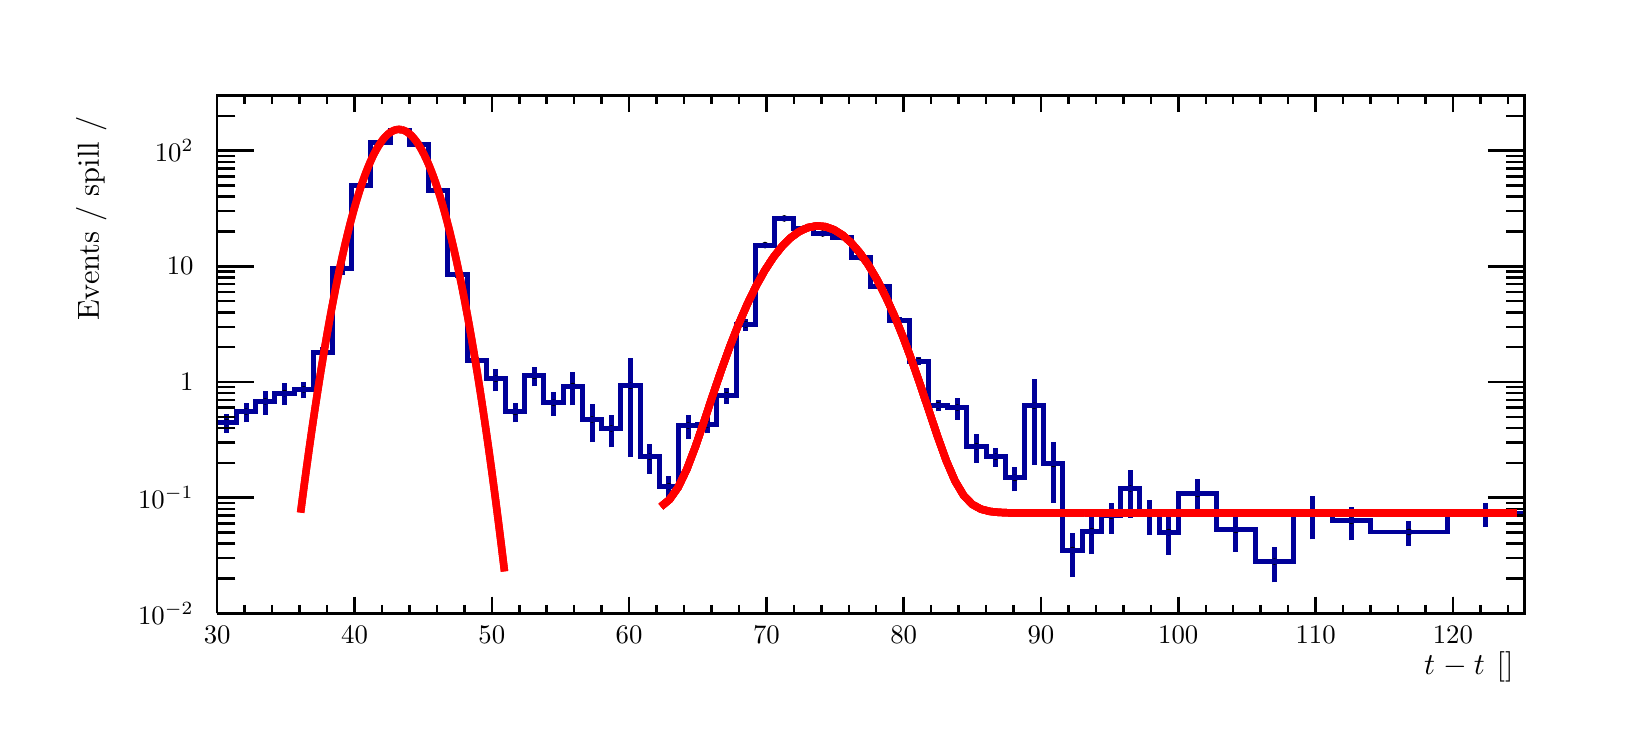
\begin{tikzpicture}
\pgfdeclareplotmark{cross} {
\pgfpathmoveto{\pgfpoint{-0.3\pgfplotmarksize}{\pgfplotmarksize}}
\pgfpathlineto{\pgfpoint{+0.3\pgfplotmarksize}{\pgfplotmarksize}}
\pgfpathlineto{\pgfpoint{+0.3\pgfplotmarksize}{0.3\pgfplotmarksize}}
\pgfpathlineto{\pgfpoint{+1\pgfplotmarksize}{0.3\pgfplotmarksize}}
\pgfpathlineto{\pgfpoint{+1\pgfplotmarksize}{-0.3\pgfplotmarksize}}
\pgfpathlineto{\pgfpoint{+0.3\pgfplotmarksize}{-0.3\pgfplotmarksize}}
\pgfpathlineto{\pgfpoint{+0.3\pgfplotmarksize}{-1.\pgfplotmarksize}}
\pgfpathlineto{\pgfpoint{-0.3\pgfplotmarksize}{-1.\pgfplotmarksize}}
\pgfpathlineto{\pgfpoint{-0.3\pgfplotmarksize}{-0.3\pgfplotmarksize}}
\pgfpathlineto{\pgfpoint{-1.\pgfplotmarksize}{-0.3\pgfplotmarksize}}
\pgfpathlineto{\pgfpoint{-1.\pgfplotmarksize}{0.3\pgfplotmarksize}}
\pgfpathlineto{\pgfpoint{-0.3\pgfplotmarksize}{0.3\pgfplotmarksize}}
\pgfpathclose
\pgfusepathqstroke
}
\pgfdeclareplotmark{cross*} {
\pgfpathmoveto{\pgfpoint{-0.3\pgfplotmarksize}{\pgfplotmarksize}}
\pgfpathlineto{\pgfpoint{+0.3\pgfplotmarksize}{\pgfplotmarksize}}
\pgfpathlineto{\pgfpoint{+0.3\pgfplotmarksize}{0.3\pgfplotmarksize}}
\pgfpathlineto{\pgfpoint{+1\pgfplotmarksize}{0.3\pgfplotmarksize}}
\pgfpathlineto{\pgfpoint{+1\pgfplotmarksize}{-0.3\pgfplotmarksize}}
\pgfpathlineto{\pgfpoint{+0.3\pgfplotmarksize}{-0.3\pgfplotmarksize}}
\pgfpathlineto{\pgfpoint{+0.3\pgfplotmarksize}{-1.\pgfplotmarksize}}
\pgfpathlineto{\pgfpoint{-0.3\pgfplotmarksize}{-1.\pgfplotmarksize}}
\pgfpathlineto{\pgfpoint{-0.3\pgfplotmarksize}{-0.3\pgfplotmarksize}}
\pgfpathlineto{\pgfpoint{-1.\pgfplotmarksize}{-0.3\pgfplotmarksize}}
\pgfpathlineto{\pgfpoint{-1.\pgfplotmarksize}{0.3\pgfplotmarksize}}
\pgfpathlineto{\pgfpoint{-0.3\pgfplotmarksize}{0.3\pgfplotmarksize}}
\pgfpathclose
\pgfusepathqfillstroke
}
\pgfdeclareplotmark{newstar} {
\pgfpathmoveto{\pgfqpoint{0pt}{\pgfplotmarksize}}
\pgfpathlineto{\pgfqpointpolar{44}{0.5\pgfplotmarksize}}
\pgfpathlineto{\pgfqpointpolar{18}{\pgfplotmarksize}}
\pgfpathlineto{\pgfqpointpolar{-20}{0.5\pgfplotmarksize}}
\pgfpathlineto{\pgfqpointpolar{-54}{\pgfplotmarksize}}
\pgfpathlineto{\pgfqpointpolar{-90}{0.5\pgfplotmarksize}}
\pgfpathlineto{\pgfqpointpolar{234}{\pgfplotmarksize}}
\pgfpathlineto{\pgfqpointpolar{198}{0.5\pgfplotmarksize}}
\pgfpathlineto{\pgfqpointpolar{162}{\pgfplotmarksize}}
\pgfpathlineto{\pgfqpointpolar{134}{0.5\pgfplotmarksize}}
\pgfpathclose
\pgfusepathqstroke
}
\pgfdeclareplotmark{newstar*} {
\pgfpathmoveto{\pgfqpoint{0pt}{\pgfplotmarksize}}
\pgfpathlineto{\pgfqpointpolar{44}{0.5\pgfplotmarksize}}
\pgfpathlineto{\pgfqpointpolar{18}{\pgfplotmarksize}}
\pgfpathlineto{\pgfqpointpolar{-20}{0.5\pgfplotmarksize}}
\pgfpathlineto{\pgfqpointpolar{-54}{\pgfplotmarksize}}
\pgfpathlineto{\pgfqpointpolar{-90}{0.5\pgfplotmarksize}}
\pgfpathlineto{\pgfqpointpolar{234}{\pgfplotmarksize}}
\pgfpathlineto{\pgfqpointpolar{198}{0.5\pgfplotmarksize}}
\pgfpathlineto{\pgfqpointpolar{162}{\pgfplotmarksize}}
\pgfpathlineto{\pgfqpointpolar{134}{0.5\pgfplotmarksize}}
\pgfpathclose
\pgfusepathqfillstroke
}
\definecolor{c}{rgb}{1,1,1};
\draw [color=c, fill=c] (0,0) rectangle (20,8.54034);
\draw [color=c, fill=c] (2.4,1.11024) rectangle (19,7.68631);
\definecolor{c}{rgb}{0,0,0};
\draw [c,line width=0.9] (2.4,1.11024) -- (2.4,7.68631) -- (19,7.68631) -- (19,1.11024) -- (2.4,1.11024);
\definecolor{c}{rgb}{1,1,1};
\draw [color=c, fill=c] (2.4,1.11024) rectangle (19,7.68631);
\definecolor{c}{rgb}{0,0,0};
\draw [c,line width=0.9] (2.4,1.11024) -- (2.4,7.68631) -- (19,7.68631) -- (19,1.11024) -- (2.4,1.11024);
\definecolor{c}{rgb}{0,0,0.6};
\draw [c,line width=1.8] (2.52206,3.40563) -- (2.52206,3.53721);
\draw [c,line width=1.8] (2.52206,3.53721) -- (2.52206,3.64623);
\definecolor{c}{rgb}{0,0,0};
\foreach \P in {(2.52206,3.53721)}{\draw[mark options={color=c,fill=c},mark size=2.402402pt,mark=*,mark size=1pt] plot coordinates {\P};}
\definecolor{c}{rgb}{0,0,0.6};
\draw [c,line width=1.8] (2.76618,3.53542) -- (2.76618,3.67175);
\draw [c,line width=1.8] (2.76618,3.67175) -- (2.76618,3.78401);
\definecolor{c}{rgb}{0,0,0};
\foreach \P in {(2.76618,3.67175)}{\draw[mark options={color=c,fill=c},mark size=2.402402pt,mark=*,mark size=1pt] plot coordinates {\P};}
\definecolor{c}{rgb}{0,0,0.6};
\draw [c,line width=1.8] (3.01029,3.63203) -- (3.01029,3.80158);
\draw [c,line width=1.8] (3.01029,3.80158) -- (3.01029,3.9354);
\definecolor{c}{rgb}{0,0,0};
\foreach \P in {(3.01029,3.80158)}{\draw[mark options={color=c,fill=c},mark size=2.402402pt,mark=*,mark size=1pt] plot coordinates {\P};}
\definecolor{c}{rgb}{0,0,0.6};
\draw [c,line width=1.8] (3.25441,3.75384) -- (3.25441,3.90664);
\draw [c,line width=1.8] (3.25441,3.90664) -- (3.25441,4.02981);
\definecolor{c}{rgb}{0,0,0};
\foreach \P in {(3.25441,3.90664)}{\draw[mark options={color=c,fill=c},mark size=2.402402pt,mark=*,mark size=1pt] plot coordinates {\P};}
\definecolor{c}{rgb}{0,0,0.6};
\draw [c,line width=1.8] (3.49853,3.83979) -- (3.49853,3.95299);
\draw [c,line width=1.8] (3.49853,3.95299) -- (3.49853,4.04909);
\definecolor{c}{rgb}{0,0,0};
\foreach \P in {(3.49853,3.95299)}{\draw[mark options={color=c,fill=c},mark size=2.402402pt,mark=*,mark size=1pt] plot coordinates {\P};}
\definecolor{c}{rgb}{0,0,0.6};
\draw [c,line width=1.8] (3.74265,4.35195) -- (3.74265,4.42496);
\draw [c,line width=1.8] (3.74265,4.42496) -- (3.74265,4.49047);
\definecolor{c}{rgb}{0,0,0};
\foreach \P in {(3.74265,4.42496)}{\draw[mark options={color=c,fill=c},mark size=2.402402pt,mark=*,mark size=1pt] plot coordinates {\P};}
\definecolor{c}{rgb}{0,0,0.6};
\draw [c,line width=1.8] (3.98676,5.4071) -- (3.98676,5.4863);
\draw [c,line width=1.8] (3.98676,5.4863) -- (3.98676,5.55674);
\definecolor{c}{rgb}{0,0,0};
\foreach \P in {(3.98676,5.4863)}{\draw[mark options={color=c,fill=c},mark size=2.402402pt,mark=*,mark size=1pt] plot coordinates {\P};}
\definecolor{c}{rgb}{0,0,0.6};
\draw [c,line width=1.8] (4.23088,6.53252) -- (4.23088,6.54645);
\draw [c,line width=1.8] (4.23088,6.54645) -- (4.23088,6.56009);
\definecolor{c}{rgb}{0,0,0};
\foreach \P in {(4.23088,6.54645)}{\draw[mark options={color=c,fill=c},mark size=2.402402pt,mark=*,mark size=1pt] plot coordinates {\P};}
\definecolor{c}{rgb}{0,0,0.6};
\draw [c,line width=1.8] (4.475,7.07742) -- (4.475,7.08706);
\draw [c,line width=1.8] (4.475,7.08706) -- (4.475,7.09655);
\definecolor{c}{rgb}{0,0,0};
\foreach \P in {(4.475,7.08706)}{\draw[mark options={color=c,fill=c},mark size=2.402402pt,mark=*,mark size=1pt] plot coordinates {\P};}
\definecolor{c}{rgb}{0,0,0.6};
\draw [c,line width=1.8] (4.71912,7.23764) -- (4.71912,7.24718);
\draw [c,line width=1.8] (4.71912,7.24718) -- (4.71912,7.25658);
\definecolor{c}{rgb}{0,0,0};
\foreach \P in {(4.71912,7.24718)}{\draw[mark options={color=c,fill=c},mark size=2.402402pt,mark=*,mark size=1pt] plot coordinates {\P};}
\definecolor{c}{rgb}{0,0,0.6};
\draw [c,line width=1.8] (4.96324,7.05689) -- (4.96324,7.06748);
\draw [c,line width=1.8] (4.96324,7.06748) -- (4.96324,7.07789);
\definecolor{c}{rgb}{0,0,0};
\foreach \P in {(4.96324,7.06748)}{\draw[mark options={color=c,fill=c},mark size=2.402402pt,mark=*,mark size=1pt] plot coordinates {\P};}
\definecolor{c}{rgb}{0,0,0.6};
\draw [c,line width=1.8] (5.20735,6.45771) -- (5.20735,6.47732);
\draw [c,line width=1.8] (5.20735,6.47732) -- (5.20735,6.49634);
\definecolor{c}{rgb}{0,0,0};
\foreach \P in {(5.20735,6.47732)}{\draw[mark options={color=c,fill=c},mark size=2.402402pt,mark=*,mark size=1pt] plot coordinates {\P};}
\definecolor{c}{rgb}{0,0,0.6};
\draw [c,line width=1.8] (5.45147,5.37429) -- (5.45147,5.41469);
\draw [c,line width=1.8] (5.45147,5.41469) -- (5.45147,5.45267);
\definecolor{c}{rgb}{0,0,0};
\foreach \P in {(5.45147,5.41469)}{\draw[mark options={color=c,fill=c},mark size=2.402402pt,mark=*,mark size=1pt] plot coordinates {\P};}
\definecolor{c}{rgb}{0,0,0.6};
\draw [c,line width=1.8] (5.69559,4.26388) -- (5.69559,4.31428);
\draw [c,line width=1.8] (5.69559,4.31428) -- (5.69559,4.361);
\definecolor{c}{rgb}{0,0,0};
\foreach \P in {(5.69559,4.31428)}{\draw[mark options={color=c,fill=c},mark size=2.402402pt,mark=*,mark size=1pt] plot coordinates {\P};}
\definecolor{c}{rgb}{0,0,0.6};
\draw [c,line width=1.8] (5.93971,3.92792) -- (5.93971,4.08884);
\draw [c,line width=1.8] (5.93971,4.08884) -- (5.93971,4.21723);
\definecolor{c}{rgb}{0,0,0};
\foreach \P in {(5.93971,4.08884)}{\draw[mark options={color=c,fill=c},mark size=2.402402pt,mark=*,mark size=1pt] plot coordinates {\P};}
\definecolor{c}{rgb}{0,0,0.6};
\draw [c,line width=1.8] (6.18382,3.53481) -- (6.18382,3.66741);
\draw [c,line width=1.8] (6.18382,3.66741) -- (6.18382,3.77714);
\definecolor{c}{rgb}{0,0,0};
\foreach \P in {(6.18382,3.66741)}{\draw[mark options={color=c,fill=c},mark size=2.402402pt,mark=*,mark size=1pt] plot coordinates {\P};}
\definecolor{c}{rgb}{0,0,0.6};
\draw [c,line width=1.8] (6.42794,3.99082) -- (6.42794,4.12429);
\draw [c,line width=1.8] (6.42794,4.12429) -- (6.42794,4.23461);
\definecolor{c}{rgb}{0,0,0};
\foreach \P in {(6.42794,4.12429)}{\draw[mark options={color=c,fill=c},mark size=2.402402pt,mark=*,mark size=1pt] plot coordinates {\P};}
\definecolor{c}{rgb}{0,0,0.6};
\draw [c,line width=1.8] (6.67206,3.62148) -- (6.67206,3.78512);
\draw [c,line width=1.8] (6.67206,3.78512) -- (6.67206,3.91524);
\definecolor{c}{rgb}{0,0,0};
\foreach \P in {(6.67206,3.78512)}{\draw[mark options={color=c,fill=c},mark size=2.402402pt,mark=*,mark size=1pt] plot coordinates {\P};}
\definecolor{c}{rgb}{0,0,0.6};
\draw [c,line width=1.8] (6.91618,3.75026) -- (6.91618,3.99588);
\draw [c,line width=1.8] (6.91618,3.99588) -- (6.91618,4.17278);
\definecolor{c}{rgb}{0,0,0};
\foreach \P in {(6.91618,3.99588)}{\draw[mark options={color=c,fill=c},mark size=2.402402pt,mark=*,mark size=1pt] plot coordinates {\P};}
\definecolor{c}{rgb}{0,0,0.6};
\draw [c,line width=1.8] (7.16029,3.28222) -- (7.16029,3.57122);
\draw [c,line width=1.8] (7.16029,3.57122) -- (7.16029,3.76938);
\definecolor{c}{rgb}{0,0,0};
\foreach \P in {(7.16029,3.57122)}{\draw[mark options={color=c,fill=c},mark size=2.402402pt,mark=*,mark size=1pt] plot coordinates {\P};}
\definecolor{c}{rgb}{0,0,0.6};
\draw [c,line width=1.8] (7.40441,3.21756) -- (7.40441,3.457);
\draw [c,line width=1.8] (7.40441,3.457) -- (7.40441,3.63069);
\definecolor{c}{rgb}{0,0,0};
\foreach \P in {(7.40441,3.457)}{\draw[mark options={color=c,fill=c},mark size=2.402402pt,mark=*,mark size=1pt] plot coordinates {\P};}
\definecolor{c}{rgb}{0,0,0.6};
\draw [c,line width=1.8] (7.64853,3.09392) -- (7.64853,3.99863);
\draw [c,line width=1.8] (7.64853,3.99863) -- (7.64853,4.35847);
\definecolor{c}{rgb}{0,0,0};
\foreach \P in {(7.64853,3.99863)}{\draw[mark options={color=c,fill=c},mark size=2.402402pt,mark=*,mark size=1pt] plot coordinates {\P};}
\definecolor{c}{rgb}{0,0,0.6};
\draw [c,line width=1.8] (7.89265,2.8828) -- (7.89265,3.09931);
\draw [c,line width=1.8] (7.89265,3.09931) -- (7.89265,3.26066);
\definecolor{c}{rgb}{0,0,0};
\foreach \P in {(7.89265,3.09931)}{\draw[mark options={color=c,fill=c},mark size=2.402402pt,mark=*,mark size=1pt] plot coordinates {\P};}
\definecolor{c}{rgb}{0,0,0.6};
\draw [c,line width=1.8] (8.13676,2.55854) -- (8.13676,2.72438);
\draw [c,line width=1.8] (8.13676,2.72438) -- (8.13676,2.85589);
\definecolor{c}{rgb}{0,0,0};
\foreach \P in {(8.13676,2.72438)}{\draw[mark options={color=c,fill=c},mark size=2.402402pt,mark=*,mark size=1pt] plot coordinates {\P};}
\definecolor{c}{rgb}{0,0,0.6};
\draw [c,line width=1.8] (8.38088,3.3223) -- (8.38088,3.49453);
\draw [c,line width=1.8] (8.38088,3.49453) -- (8.38088,3.63001);
\definecolor{c}{rgb}{0,0,0};
\foreach \P in {(8.38088,3.49453)}{\draw[mark options={color=c,fill=c},mark size=2.402402pt,mark=*,mark size=1pt] plot coordinates {\P};}
\definecolor{c}{rgb}{0,0,0.6};
\draw [c,line width=1.8] (8.625,3.39644) -- (8.625,3.5085);
\draw [c,line width=1.8] (8.625,3.5085) -- (8.625,3.60379);
\definecolor{c}{rgb}{0,0,0};
\foreach \P in {(8.625,3.5085)}{\draw[mark options={color=c,fill=c},mark size=2.402402pt,mark=*,mark size=1pt] plot coordinates {\P};}
\definecolor{c}{rgb}{0,0,0.6};
\draw [c,line width=1.8] (8.86912,3.77164) -- (8.86912,3.87856);
\draw [c,line width=1.8] (8.86912,3.87856) -- (8.86912,3.97011);
\definecolor{c}{rgb}{0,0,0};
\foreach \P in {(8.86912,3.87856)}{\draw[mark options={color=c,fill=c},mark size=2.402402pt,mark=*,mark size=1pt] plot coordinates {\P};}
\definecolor{c}{rgb}{0,0,0.6};
\draw [c,line width=1.8] (9.11324,4.6928) -- (9.11324,4.77736);
\draw [c,line width=1.8] (9.11324,4.77736) -- (9.11324,4.85201);
\definecolor{c}{rgb}{0,0,0};
\foreach \P in {(9.11324,4.77736)}{\draw[mark options={color=c,fill=c},mark size=2.402402pt,mark=*,mark size=1pt] plot coordinates {\P};}
\definecolor{c}{rgb}{0,0,0.6};
\draw [c,line width=1.8] (9.35735,5.75229) -- (9.35735,5.78607);
\draw [c,line width=1.8] (9.35735,5.78607) -- (9.35735,5.81815);
\definecolor{c}{rgb}{0,0,0};
\foreach \P in {(9.35735,5.78607)}{\draw[mark options={color=c,fill=c},mark size=2.402402pt,mark=*,mark size=1pt] plot coordinates {\P};}
\definecolor{c}{rgb}{0,0,0.6};
\draw [c,line width=1.8] (9.60147,6.10662) -- (9.60147,6.12465);
\draw [c,line width=1.8] (9.60147,6.12465) -- (9.60147,6.14217);
\definecolor{c}{rgb}{0,0,0};
\foreach \P in {(9.60147,6.12465)}{\draw[mark options={color=c,fill=c},mark size=2.402402pt,mark=*,mark size=1pt] plot coordinates {\P};}
\definecolor{c}{rgb}{0,0,0.6};
\draw [c,line width=1.8] (9.84559,5.97606) -- (9.84559,5.99533);
\draw [c,line width=1.8] (9.84559,5.99533) -- (9.84559,6.01402);
\definecolor{c}{rgb}{0,0,0};
\foreach \P in {(9.84559,5.99533)}{\draw[mark options={color=c,fill=c},mark size=2.402402pt,mark=*,mark size=1pt] plot coordinates {\P};}
\definecolor{c}{rgb}{0,0,0.6};
\draw [c,line width=1.8] (10.0897,5.91416) -- (10.0897,5.93356);
\draw [c,line width=1.8] (10.0897,5.93356) -- (10.0897,5.95238);
\definecolor{c}{rgb}{0,0,0};
\foreach \P in {(10.0897,5.93356)}{\draw[mark options={color=c,fill=c},mark size=2.402402pt,mark=*,mark size=1pt] plot coordinates {\P};}
\definecolor{c}{rgb}{0,0,0.6};
\draw [c,line width=1.8] (10.3338,5.86976) -- (10.3338,5.88863);
\draw [c,line width=1.8] (10.3338,5.88863) -- (10.3338,5.90695);
\definecolor{c}{rgb}{0,0,0};
\foreach \P in {(10.3338,5.88863)}{\draw[mark options={color=c,fill=c},mark size=2.402402pt,mark=*,mark size=1pt] plot coordinates {\P};}
\definecolor{c}{rgb}{0,0,0.6};
\draw [c,line width=1.8] (10.5779,5.60566) -- (10.5779,5.62659);
\draw [c,line width=1.8] (10.5779,5.62659) -- (10.5779,5.64687);
\definecolor{c}{rgb}{0,0,0};
\foreach \P in {(10.5779,5.62659)}{\draw[mark options={color=c,fill=c},mark size=2.402402pt,mark=*,mark size=1pt] plot coordinates {\P};}
\definecolor{c}{rgb}{0,0,0.6};
\draw [c,line width=1.8] (10.8221,5.24071) -- (10.8221,5.26561);
\draw [c,line width=1.8] (10.8221,5.26561) -- (10.8221,5.28957);
\definecolor{c}{rgb}{0,0,0};
\foreach \P in {(10.8221,5.26561)}{\draw[mark options={color=c,fill=c},mark size=2.402402pt,mark=*,mark size=1pt] plot coordinates {\P};}
\definecolor{c}{rgb}{0,0,0.6};
\draw [c,line width=1.8] (11.0662,4.77399) -- (11.0662,4.82392);
\draw [c,line width=1.8] (11.0662,4.82392) -- (11.0662,4.87023);
\definecolor{c}{rgb}{0,0,0};
\foreach \P in {(11.0662,4.82392)}{\draw[mark options={color=c,fill=c},mark size=2.402402pt,mark=*,mark size=1pt] plot coordinates {\P};}
\definecolor{c}{rgb}{0,0,0.6};
\draw [c,line width=1.8] (11.3103,4.26256) -- (11.3103,4.31303);
\draw [c,line width=1.8] (11.3103,4.31303) -- (11.3103,4.35981);
\definecolor{c}{rgb}{0,0,0};
\foreach \P in {(11.3103,4.31303)}{\draw[mark options={color=c,fill=c},mark size=2.402402pt,mark=*,mark size=1pt] plot coordinates {\P};}
\definecolor{c}{rgb}{0,0,0.6};
\draw [c,line width=1.8] (11.5544,3.67567) -- (11.5544,3.75184);
\draw [c,line width=1.8] (11.5544,3.75184) -- (11.5544,3.81988);
\definecolor{c}{rgb}{0,0,0};
\foreach \P in {(11.5544,3.75184)}{\draw[mark options={color=c,fill=c},mark size=2.402402pt,mark=*,mark size=1pt] plot coordinates {\P};}
\definecolor{c}{rgb}{0,0,0.6};
\draw [c,line width=1.8] (11.7985,3.5672) -- (11.7985,3.72348);
\draw [c,line width=1.8] (11.7985,3.72348) -- (11.7985,3.8489);
\definecolor{c}{rgb}{0,0,0};
\foreach \P in {(11.7985,3.72348)}{\draw[mark options={color=c,fill=c},mark size=2.402402pt,mark=*,mark size=1pt] plot coordinates {\P};}
\definecolor{c}{rgb}{0,0,0.6};
\draw [c,line width=1.8] (12.0426,3.02416) -- (12.0426,3.23053);
\draw [c,line width=1.8] (12.0426,3.23053) -- (12.0426,3.3862);
\definecolor{c}{rgb}{0,0,0};
\foreach \P in {(12.0426,3.23053)}{\draw[mark options={color=c,fill=c},mark size=2.402402pt,mark=*,mark size=1pt] plot coordinates {\P};}
\definecolor{c}{rgb}{0,0,0.6};
\draw [c,line width=1.8] (12.2868,2.96839) -- (12.2868,3.09817);
\draw [c,line width=1.8] (12.2868,3.09817) -- (12.2868,3.20596);
\definecolor{c}{rgb}{0,0,0};
\foreach \P in {(12.2868,3.09817)}{\draw[mark options={color=c,fill=c},mark size=2.402402pt,mark=*,mark size=1pt] plot coordinates {\P};}
\definecolor{c}{rgb}{0,0,0.6};
\draw [c,line width=1.8] (12.5309,2.65687) -- (12.5309,2.82943);
\draw [c,line width=1.8] (12.5309,2.82943) -- (12.5309,2.96512);
\definecolor{c}{rgb}{0,0,0};
\foreach \P in {(12.5309,2.82943)}{\draw[mark options={color=c,fill=c},mark size=2.402402pt,mark=*,mark size=1pt] plot coordinates {\P};}
\definecolor{c}{rgb}{0,0,0.6};
\draw [c,line width=1.8] (12.775,2.99823) -- (12.775,3.74575);
\draw [c,line width=1.8] (12.775,3.74575) -- (12.775,4.08055);
\definecolor{c}{rgb}{0,0,0};
\foreach \P in {(12.775,3.74575)}{\draw[mark options={color=c,fill=c},mark size=2.402402pt,mark=*,mark size=1pt] plot coordinates {\P};}
\definecolor{c}{rgb}{0,0,0.6};
\draw [c,line width=1.8] (13.0191,2.51154) -- (13.0191,3.0069);
\draw [c,line width=1.8] (13.0191,3.0069) -- (13.0191,3.28234);
\definecolor{c}{rgb}{0,0,0};
\foreach \P in {(13.0191,3.0069)}{\draw[mark options={color=c,fill=c},mark size=2.402402pt,mark=*,mark size=1pt] plot coordinates {\P};}
\definecolor{c}{rgb}{0,0,0.6};
\draw [c,line width=1.8] (13.2632,1.56822) -- (13.2632,1.91332);
\draw [c,line width=1.8] (13.2632,1.91332) -- (13.2632,2.13603);
\definecolor{c}{rgb}{0,0,0};
\foreach \P in {(13.2632,1.91332)}{\draw[mark options={color=c,fill=c},mark size=2.402402pt,mark=*,mark size=1pt] plot coordinates {\P};}
\definecolor{c}{rgb}{0,0,0.6};
\draw [c,line width=1.8] (13.5074,1.85818) -- (13.5074,2.15383);
\draw [c,line width=1.8] (13.5074,2.15383) -- (13.5074,2.35507);
\definecolor{c}{rgb}{0,0,0};
\foreach \P in {(13.5074,2.15383)}{\draw[mark options={color=c,fill=c},mark size=2.402402pt,mark=*,mark size=1pt] plot coordinates {\P};}
\definecolor{c}{rgb}{0,0,0.6};
\draw [c,line width=1.8] (13.7515,2.119) -- (13.7515,2.34834);
\draw [c,line width=1.8] (13.7515,2.34834) -- (13.7515,2.51667);
\definecolor{c}{rgb}{0,0,0};
\foreach \P in {(13.7515,2.34834)}{\draw[mark options={color=c,fill=c},mark size=2.402402pt,mark=*,mark size=1pt] plot coordinates {\P};}
\definecolor{c}{rgb}{0,0,0.6};
\draw [c,line width=1.8] (13.9956,2.32513) -- (13.9956,2.69427);
\draw [c,line width=1.8] (13.9956,2.69427) -- (13.9956,2.9266);
\definecolor{c}{rgb}{0,0,0};
\foreach \P in {(13.9956,2.69427)}{\draw[mark options={color=c,fill=c},mark size=2.402402pt,mark=*,mark size=1pt] plot coordinates {\P};}
\definecolor{c}{rgb}{0,0,0.6};
\draw [c,line width=1.8] (14.2397,2.10687) -- (14.2397,2.36895);
\draw [c,line width=1.8] (14.2397,2.36895) -- (14.2397,2.55417);
\definecolor{c}{rgb}{0,0,0};
\foreach \P in {(14.2397,2.36895)}{\draw[mark options={color=c,fill=c},mark size=2.402402pt,mark=*,mark size=1pt] plot coordinates {\P};}
\definecolor{c}{rgb}{0,0,0.6};
\draw [c,line width=1.8] (14.4838,1.85514) -- (14.4838,2.14103);
\draw [c,line width=1.8] (14.4838,2.14103) -- (14.4838,2.33774);
\definecolor{c}{rgb}{0,0,0};
\foreach \P in {(14.4838,2.14103)}{\draw[mark options={color=c,fill=c},mark size=2.402402pt,mark=*,mark size=1pt] plot coordinates {\P};}
\definecolor{c}{rgb}{0,0,0.6};
\draw [c,line width=1.8] (14.85,2.36537) -- (14.85,2.62598);
\draw [c,line width=1.8] (14.85,2.62598) -- (14.85,2.81047);
\definecolor{c}{rgb}{0,0,0};
\foreach \P in {(14.85,2.62598)}{\draw[mark options={color=c,fill=c},mark size=2.402402pt,mark=*,mark size=1pt] plot coordinates {\P};}
\definecolor{c}{rgb}{0,0,0.6};
\draw [c,line width=1.8] (15.3382,1.88934) -- (15.3382,2.169);
\draw [c,line width=1.8] (15.3382,2.169) -- (15.3382,2.36277);
\definecolor{c}{rgb}{0,0,0};
\foreach \P in {(15.3382,2.169)}{\draw[mark options={color=c,fill=c},mark size=2.402402pt,mark=*,mark size=1pt] plot coordinates {\P};}
\definecolor{c}{rgb}{0,0,0.6};
\draw [c,line width=1.8] (15.8265,1.50226) -- (15.8265,1.76695);
\draw [c,line width=1.8] (15.8265,1.76695) -- (15.8265,1.95346);
\definecolor{c}{rgb}{0,0,0};
\foreach \P in {(15.8265,1.76695)}{\draw[mark options={color=c,fill=c},mark size=2.402402pt,mark=*,mark size=1pt] plot coordinates {\P};}
\definecolor{c}{rgb}{0,0,0.6};
\draw [c,line width=1.8] (16.3147,2.04847) -- (16.3147,2.37792);
\draw [c,line width=1.8] (16.3147,2.37792) -- (16.3147,2.59408);
\definecolor{c}{rgb}{0,0,0};
\foreach \P in {(16.3147,2.37792)}{\draw[mark options={color=c,fill=c},mark size=2.402402pt,mark=*,mark size=1pt] plot coordinates {\P};}
\definecolor{c}{rgb}{0,0,0.6};
\draw [c,line width=1.8] (16.8029,2.03706) -- (16.8029,2.28433);
\draw [c,line width=1.8] (16.8029,2.28433) -- (16.8029,2.46207);
\definecolor{c}{rgb}{0,0,0};
\foreach \P in {(16.8029,2.28433)}{\draw[mark options={color=c,fill=c},mark size=2.402402pt,mark=*,mark size=1pt] plot coordinates {\P};}
\definecolor{c}{rgb}{0,0,0.6};
\draw [c,line width=1.8] (17.5353,1.96777) -- (17.5353,2.14249);
\draw [c,line width=1.8] (17.5353,2.14249) -- (17.5353,2.2795);
\definecolor{c}{rgb}{0,0,0};
\foreach \P in {(17.5353,2.14249)}{\draw[mark options={color=c,fill=c},mark size=2.402402pt,mark=*,mark size=1pt] plot coordinates {\P};}
\definecolor{c}{rgb}{0,0,0.6};
\draw [c,line width=1.8] (18.5118,2.20521) -- (18.5118,2.37216);
\draw [c,line width=1.8] (18.5118,2.37216) -- (18.5118,2.50435);
\definecolor{c}{rgb}{0,0,0};
\foreach \P in {(18.5118,2.37216)}{\draw[mark options={color=c,fill=c},mark size=2.402402pt,mark=*,mark size=1pt] plot coordinates {\P};}
\definecolor{c}{rgb}{0,0,0.6};
\draw [c,line width=1.8] (2.4,3.53721) -- (2.64412,3.53721) -- (2.64412,3.67175) -- (2.88824,3.67175) -- (2.88824,3.80158) -- (3.13235,3.80158) -- (3.13235,3.90664) -- (3.37647,3.90664) -- (3.37647,3.95299) -- (3.62059,3.95299) -- (3.62059,4.42496)
 -- (3.86471,4.42496) -- (3.86471,5.4863) -- (4.10882,5.4863) -- (4.10882,6.54645) -- (4.35294,6.54645) -- (4.35294,7.08706) -- (4.59706,7.08706) -- (4.59706,7.24718) -- (4.84118,7.24718) -- (4.84118,7.06748) -- (5.08529,7.06748) -- (5.08529,6.47732)
 -- (5.32941,6.47732) -- (5.32941,5.41469) -- (5.57353,5.41469) -- (5.57353,4.31428) -- (5.81765,4.31428) -- (5.81765,4.08884) -- (6.06176,4.08884) -- (6.06176,3.66741) -- (6.30588,3.66741) -- (6.30588,4.12429) -- (6.55,4.12429) -- (6.55,3.78512) --
 (6.79412,3.78512) -- (6.79412,3.99588) -- (7.03824,3.99588) -- (7.03824,3.57122) -- (7.28235,3.57122) -- (7.28235,3.457) -- (7.52647,3.457) -- (7.52647,3.99863) -- (7.77059,3.99863) -- (7.77059,3.09931) -- (8.01471,3.09931) -- (8.01471,2.72438) --
 (8.25882,2.72438) -- (8.25882,3.49453) -- (8.50294,3.49453) -- (8.50294,3.5085) -- (8.74706,3.5085) -- (8.74706,3.87856) -- (8.99118,3.87856) -- (8.99118,4.77736) -- (9.23529,4.77736) -- (9.23529,5.78607) -- (9.47941,5.78607) -- (9.47941,6.12465) --
 (9.72353,6.12465) -- (9.72353,5.99533) -- (9.96765,5.99533) -- (9.96765,5.93356) -- (10.2118,5.93356) -- (10.2118,5.88863) -- (10.4559,5.88863) -- (10.4559,5.62659) -- (10.7,5.62659) -- (10.7,5.26561) -- (10.9441,5.26561) -- (10.9441,4.82392) --
 (11.1882,4.82392) -- (11.1882,4.31303) -- (11.4324,4.31303) -- (11.4324,3.75184) -- (11.6765,3.75184) -- (11.6765,3.72348) -- (11.9206,3.72348) -- (11.9206,3.23053) -- (12.1647,3.23053) -- (12.1647,3.09817) -- (12.4088,3.09817) -- (12.4088,2.82943)
 -- (12.6529,2.82943) -- (12.6529,3.74575) -- (12.8971,3.74575) -- (12.8971,3.0069) -- (13.1412,3.0069) -- (13.1412,1.91332) -- (13.3853,1.91332) -- (13.3853,2.15383) -- (13.6294,2.15383) -- (13.6294,2.34834) -- (13.8735,2.34834) -- (13.8735,2.69427)
 -- (14.1176,2.69427) -- (14.1176,2.36895) -- (14.3618,2.36895) -- (14.3618,2.14103) -- (14.6059,2.14103) -- (14.6059,2.62598) -- (15.0941,2.62598) -- (15.0941,2.169) -- (15.5824,2.169) -- (15.5824,1.76695) -- (16.0706,1.76695) -- (16.0706,2.37792)
 -- (16.5588,2.37792) -- (16.5588,2.28433) -- (17.0471,2.28433) -- (17.0471,2.14249) -- (18.0235,2.14249) -- (18.0235,2.37216) -- (19,2.37216);
\definecolor{c}{rgb}{0,0,0};
\draw [c,line width=0.9] (2.4,1.11024) -- (19,1.11024);
\draw [c,line width=0.9] (2.4,1.3229) -- (2.4,1.11024);
\draw [c,line width=0.9] (2.74874,1.21657) -- (2.74874,1.11024);
\draw [c,line width=0.9] (3.09748,1.21657) -- (3.09748,1.11024);
\draw [c,line width=0.9] (3.44622,1.21657) -- (3.44622,1.11024);
\draw [c,line width=0.9] (3.79496,1.21657) -- (3.79496,1.11024);
\draw [c,line width=0.9] (4.1437,1.3229) -- (4.1437,1.11024);
\draw [c,line width=0.9] (4.49244,1.21657) -- (4.49244,1.11024);
\draw [c,line width=0.9] (4.84118,1.21657) -- (4.84118,1.11024);
\draw [c,line width=0.9] (5.18992,1.21657) -- (5.18992,1.11024);
\draw [c,line width=0.9] (5.53866,1.21657) -- (5.53866,1.11024);
\draw [c,line width=0.9] (5.88739,1.3229) -- (5.88739,1.11024);
\draw [c,line width=0.9] (6.23613,1.21657) -- (6.23613,1.11024);
\draw [c,line width=0.9] (6.58487,1.21657) -- (6.58487,1.11024);
\draw [c,line width=0.9] (6.93361,1.21657) -- (6.93361,1.11024);
\draw [c,line width=0.9] (7.28235,1.21657) -- (7.28235,1.11024);
\draw [c,line width=0.9] (7.63109,1.3229) -- (7.63109,1.11024);
\draw [c,line width=0.9] (7.97983,1.21657) -- (7.97983,1.11024);
\draw [c,line width=0.9] (8.32857,1.21657) -- (8.32857,1.11024);
\draw [c,line width=0.9] (8.67731,1.21657) -- (8.67731,1.11024);
\draw [c,line width=0.9] (9.02605,1.21657) -- (9.02605,1.11024);
\draw [c,line width=0.9] (9.37479,1.3229) -- (9.37479,1.11024);
\draw [c,line width=0.9] (9.72353,1.21657) -- (9.72353,1.11024);
\draw [c,line width=0.9] (10.0723,1.21657) -- (10.0723,1.11024);
\draw [c,line width=0.9] (10.421,1.21657) -- (10.421,1.11024);
\draw [c,line width=0.9] (10.7697,1.21657) -- (10.7697,1.11024);
\draw [c,line width=0.9] (11.1185,1.3229) -- (11.1185,1.11024);
\draw [c,line width=0.9] (11.4672,1.21657) -- (11.4672,1.11024);
\draw [c,line width=0.9] (11.816,1.21657) -- (11.816,1.11024);
\draw [c,line width=0.9] (12.1647,1.21657) -- (12.1647,1.11024);
\draw [c,line width=0.9] (12.5134,1.21657) -- (12.5134,1.11024);
\draw [c,line width=0.9] (12.8622,1.3229) -- (12.8622,1.11024);
\draw [c,line width=0.9] (13.2109,1.21657) -- (13.2109,1.11024);
\draw [c,line width=0.9] (13.5597,1.21657) -- (13.5597,1.11024);
\draw [c,line width=0.9] (13.9084,1.21657) -- (13.9084,1.11024);
\draw [c,line width=0.9] (14.2571,1.21657) -- (14.2571,1.11024);
\draw [c,line width=0.9] (14.6059,1.3229) -- (14.6059,1.11024);
\draw [c,line width=0.9] (14.9546,1.21657) -- (14.9546,1.11024);
\draw [c,line width=0.9] (15.3034,1.21657) -- (15.3034,1.11024);
\draw [c,line width=0.9] (15.6521,1.21657) -- (15.6521,1.11024);
\draw [c,line width=0.9] (16.0008,1.21657) -- (16.0008,1.11024);
\draw [c,line width=0.9] (16.3496,1.3229) -- (16.3496,1.11024);
\draw [c,line width=0.9] (16.6983,1.21657) -- (16.6983,1.11024);
\draw [c,line width=0.9] (17.0471,1.21657) -- (17.0471,1.11024);
\draw [c,line width=0.9] (17.3958,1.21657) -- (17.3958,1.11024);
\draw [c,line width=0.9] (17.7445,1.21657) -- (17.7445,1.11024);
\draw [c,line width=0.9] (18.0933,1.3229) -- (18.0933,1.11024);
\draw [c,line width=0.9] (18.0933,1.3229) -- (18.0933,1.11024);
\draw [c,line width=0.9] (18.442,1.21657) -- (18.442,1.11024);
\draw [c,line width=0.9] (18.7908,1.21657) -- (18.7908,1.11024);
\draw [anchor=base] (2.4,0.725929) node[scale=0.966515, color=c, rotate=0]{30};
\draw [anchor=base] (4.1437,0.725929) node[scale=0.966515, color=c, rotate=0]{40};
\draw [anchor=base] (5.88739,0.725929) node[scale=0.966515, color=c, rotate=0]{50};
\draw [anchor=base] (7.63109,0.725929) node[scale=0.966515, color=c, rotate=0]{60};
\draw [anchor=base] (9.37479,0.725929) node[scale=0.966515, color=c, rotate=0]{70};
\draw [anchor=base] (11.1185,0.725929) node[scale=0.966515, color=c, rotate=0]{80};
\draw [anchor=base] (12.8622,0.725929) node[scale=0.966515, color=c, rotate=0]{90};
\draw [anchor=base] (14.6059,0.725929) node[scale=0.966515, color=c, rotate=0]{100};
\draw [anchor=base] (16.3496,0.725929) node[scale=0.966515, color=c, rotate=0]{110};
\draw [anchor=base] (18.0933,0.725929) node[scale=0.966515, color=c, rotate=0]{120};
\draw [anchor= east] (19,0.427017) node[scale=1.1, color=c, rotate=0]{$t_{\SFour} - t_{\STwo}$ [\si{\nano\second}] };
\draw [c,line width=0.9] (2.4,7.68631) -- (19,7.68631);
\draw [c,line width=0.9] (2.4,7.47366) -- (2.4,7.68631);
\draw [c,line width=0.9] (2.74874,7.57998) -- (2.74874,7.68631);
\draw [c,line width=0.9] (3.09748,7.57998) -- (3.09748,7.68631);
\draw [c,line width=0.9] (3.44622,7.57998) -- (3.44622,7.68631);
\draw [c,line width=0.9] (3.79496,7.57998) -- (3.79496,7.68631);
\draw [c,line width=0.9] (4.1437,7.47366) -- (4.1437,7.68631);
\draw [c,line width=0.9] (4.49244,7.57998) -- (4.49244,7.68631);
\draw [c,line width=0.9] (4.84118,7.57998) -- (4.84118,7.68631);
\draw [c,line width=0.9] (5.18992,7.57998) -- (5.18992,7.68631);
\draw [c,line width=0.9] (5.53866,7.57998) -- (5.53866,7.68631);
\draw [c,line width=0.9] (5.88739,7.47366) -- (5.88739,7.68631);
\draw [c,line width=0.9] (6.23613,7.57998) -- (6.23613,7.68631);
\draw [c,line width=0.9] (6.58487,7.57998) -- (6.58487,7.68631);
\draw [c,line width=0.9] (6.93361,7.57998) -- (6.93361,7.68631);
\draw [c,line width=0.9] (7.28235,7.57998) -- (7.28235,7.68631);
\draw [c,line width=0.9] (7.63109,7.47366) -- (7.63109,7.68631);
\draw [c,line width=0.9] (7.97983,7.57998) -- (7.97983,7.68631);
\draw [c,line width=0.9] (8.32857,7.57998) -- (8.32857,7.68631);
\draw [c,line width=0.9] (8.67731,7.57998) -- (8.67731,7.68631);
\draw [c,line width=0.9] (9.02605,7.57998) -- (9.02605,7.68631);
\draw [c,line width=0.9] (9.37479,7.47366) -- (9.37479,7.68631);
\draw [c,line width=0.9] (9.72353,7.57998) -- (9.72353,7.68631);
\draw [c,line width=0.9] (10.0723,7.57998) -- (10.0723,7.68631);
\draw [c,line width=0.9] (10.421,7.57998) -- (10.421,7.68631);
\draw [c,line width=0.9] (10.7697,7.57998) -- (10.7697,7.68631);
\draw [c,line width=0.9] (11.1185,7.47366) -- (11.1185,7.68631);
\draw [c,line width=0.9] (11.4672,7.57998) -- (11.4672,7.68631);
\draw [c,line width=0.9] (11.816,7.57998) -- (11.816,7.68631);
\draw [c,line width=0.9] (12.1647,7.57998) -- (12.1647,7.68631);
\draw [c,line width=0.9] (12.5134,7.57998) -- (12.5134,7.68631);
\draw [c,line width=0.9] (12.8622,7.47366) -- (12.8622,7.68631);
\draw [c,line width=0.9] (13.2109,7.57998) -- (13.2109,7.68631);
\draw [c,line width=0.9] (13.5597,7.57998) -- (13.5597,7.68631);
\draw [c,line width=0.9] (13.9084,7.57998) -- (13.9084,7.68631);
\draw [c,line width=0.9] (14.2571,7.57998) -- (14.2571,7.68631);
\draw [c,line width=0.9] (14.6059,7.47366) -- (14.6059,7.68631);
\draw [c,line width=0.9] (14.9546,7.57998) -- (14.9546,7.68631);
\draw [c,line width=0.9] (15.3034,7.57998) -- (15.3034,7.68631);
\draw [c,line width=0.9] (15.6521,7.57998) -- (15.6521,7.68631);
\draw [c,line width=0.9] (16.0008,7.57998) -- (16.0008,7.68631);
\draw [c,line width=0.9] (16.3496,7.47366) -- (16.3496,7.68631);
\draw [c,line width=0.9] (16.6983,7.57998) -- (16.6983,7.68631);
\draw [c,line width=0.9] (17.0471,7.57998) -- (17.0471,7.68631);
\draw [c,line width=0.9] (17.3958,7.57998) -- (17.3958,7.68631);
\draw [c,line width=0.9] (17.7445,7.57998) -- (17.7445,7.68631);
\draw [c,line width=0.9] (18.0933,7.47366) -- (18.0933,7.68631);
\draw [c,line width=0.9] (18.0933,7.47366) -- (18.0933,7.68631);
\draw [c,line width=0.9] (18.442,7.57998) -- (18.442,7.68631);
\draw [c,line width=0.9] (18.7908,7.57998) -- (18.7908,7.68631);
\draw [c,line width=0.9] (2.4,1.11024) -- (2.4,7.68631);
\draw [c,line width=0.9] (2.862,1.11025) -- (2.4,1.11025);
\draw [anchor= east] (2.22,1.11025) node[scale=0.966515, color=c, rotate=0]{$10^{-2}$};
\draw [c,line width=0.9] (2.631,1.5524) -- (2.4,1.5524);
\draw [c,line width=0.9] (2.631,1.81105) -- (2.4,1.81105);
\draw [c,line width=0.9] (2.631,1.99456) -- (2.4,1.99456);
\draw [c,line width=0.9] (2.631,2.1369) -- (2.4,2.1369);
\draw [c,line width=0.9] (2.631,2.25321) -- (2.4,2.25321);
\draw [c,line width=0.9] (2.631,2.35154) -- (2.4,2.35154);
\draw [c,line width=0.9] (2.631,2.43672) -- (2.4,2.43672);
\draw [c,line width=0.9] (2.631,2.51185) -- (2.4,2.51185);
\draw [c,line width=0.9] (2.862,2.57906) -- (2.4,2.57906);
\draw [anchor= east] (2.22,2.57906) node[scale=0.966515, color=c, rotate=0]{$10^{-1}$};
\draw [c,line width=0.9] (2.631,3.02122) -- (2.4,3.02122);
\draw [c,line width=0.9] (2.631,3.27986) -- (2.4,3.27986);
\draw [c,line width=0.9] (2.631,3.46338) -- (2.4,3.46338);
\draw [c,line width=0.9] (2.631,3.60572) -- (2.4,3.60572);
\draw [c,line width=0.9] (2.631,3.72202) -- (2.4,3.72202);
\draw [c,line width=0.9] (2.631,3.82035) -- (2.4,3.82035);
\draw [c,line width=0.9] (2.631,3.90553) -- (2.4,3.90553);
\draw [c,line width=0.9] (2.631,3.98067) -- (2.4,3.98067);
\draw [c,line width=0.9] (2.862,4.04788) -- (2.4,4.04788);
\draw [anchor= east] (2.22,4.04788) node[scale=0.966515, color=c, rotate=0]{1};
\draw [c,line width=0.9] (2.631,4.49003) -- (2.4,4.49003);
\draw [c,line width=0.9] (2.631,4.74868) -- (2.4,4.74868);
\draw [c,line width=0.9] (2.631,4.93219) -- (2.4,4.93219);
\draw [c,line width=0.9] (2.631,5.07453) -- (2.4,5.07453);
\draw [c,line width=0.9] (2.631,5.19084) -- (2.4,5.19084);
\draw [c,line width=0.9] (2.631,5.28917) -- (2.4,5.28917);
\draw [c,line width=0.9] (2.631,5.37435) -- (2.4,5.37435);
\draw [c,line width=0.9] (2.631,5.44948) -- (2.4,5.44948);
\draw [c,line width=0.9] (2.862,5.51669) -- (2.4,5.51669);
\draw [anchor= east] (2.22,5.51669) node[scale=0.966515, color=c, rotate=0]{10};
\draw [c,line width=0.9] (2.631,5.95885) -- (2.4,5.95885);
\draw [c,line width=0.9] (2.631,6.21749) -- (2.4,6.21749);
\draw [c,line width=0.9] (2.631,6.40101) -- (2.4,6.40101);
\draw [c,line width=0.9] (2.631,6.54335) -- (2.4,6.54335);
\draw [c,line width=0.9] (2.631,6.65965) -- (2.4,6.65965);
\draw [c,line width=0.9] (2.631,6.75798) -- (2.4,6.75798);
\draw [c,line width=0.9] (2.631,6.84316) -- (2.4,6.84316);
\draw [c,line width=0.9] (2.631,6.9183) -- (2.4,6.9183);
\draw [c,line width=0.9] (2.862,6.98551) -- (2.4,6.98551);
\draw [anchor= east] (2.22,6.98551) node[scale=0.966515, color=c, rotate=0]{$10^{2}$};
\draw [c,line width=0.9] (2.631,7.42766) -- (2.4,7.42766);
\draw [c,line width=0.9] (2.631,7.68631) -- (2.4,7.68631);
\draw [anchor= east] (0.8,7.68631) node[scale=1.1, color=c, rotate=90]{ Events / spill / \si{\nano\second} };
\draw [c,line width=0.9] (19,1.11024) -- (19,7.68631);
\draw [c,line width=0.9] (18.538,1.11025) -- (19,1.11025);
\draw [c,line width=0.9] (18.769,1.5524) -- (19,1.5524);
\draw [c,line width=0.9] (18.769,1.81105) -- (19,1.81105);
\draw [c,line width=0.9] (18.769,1.99456) -- (19,1.99456);
\draw [c,line width=0.9] (18.769,2.1369) -- (19,2.1369);
\draw [c,line width=0.9] (18.769,2.25321) -- (19,2.25321);
\draw [c,line width=0.9] (18.769,2.35154) -- (19,2.35154);
\draw [c,line width=0.9] (18.769,2.43672) -- (19,2.43672);
\draw [c,line width=0.9] (18.769,2.51185) -- (19,2.51185);
\draw [c,line width=0.9] (18.538,2.57906) -- (19,2.57906);
\draw [c,line width=0.9] (18.769,3.02122) -- (19,3.02122);
\draw [c,line width=0.9] (18.769,3.27986) -- (19,3.27986);
\draw [c,line width=0.9] (18.769,3.46338) -- (19,3.46338);
\draw [c,line width=0.9] (18.769,3.60572) -- (19,3.60572);
\draw [c,line width=0.9] (18.769,3.72202) -- (19,3.72202);
\draw [c,line width=0.9] (18.769,3.82035) -- (19,3.82035);
\draw [c,line width=0.9] (18.769,3.90553) -- (19,3.90553);
\draw [c,line width=0.9] (18.769,3.98067) -- (19,3.98067);
\draw [c,line width=0.9] (18.538,4.04788) -- (19,4.04788);
\draw [c,line width=0.9] (18.769,4.49003) -- (19,4.49003);
\draw [c,line width=0.9] (18.769,4.74868) -- (19,4.74868);
\draw [c,line width=0.9] (18.769,4.93219) -- (19,4.93219);
\draw [c,line width=0.9] (18.769,5.07453) -- (19,5.07453);
\draw [c,line width=0.9] (18.769,5.19084) -- (19,5.19084);
\draw [c,line width=0.9] (18.769,5.28917) -- (19,5.28917);
\draw [c,line width=0.9] (18.769,5.37435) -- (19,5.37435);
\draw [c,line width=0.9] (18.769,5.44948) -- (19,5.44948);
\draw [c,line width=0.9] (18.538,5.51669) -- (19,5.51669);
\draw [c,line width=0.9] (18.769,5.95885) -- (19,5.95885);
\draw [c,line width=0.9] (18.769,6.21749) -- (19,6.21749);
\draw [c,line width=0.9] (18.769,6.40101) -- (19,6.40101);
\draw [c,line width=0.9] (18.769,6.54335) -- (19,6.54335);
\draw [c,line width=0.9] (18.769,6.65965) -- (19,6.65965);
\draw [c,line width=0.9] (18.769,6.75798) -- (19,6.75798);
\draw [c,line width=0.9] (18.769,6.84316) -- (19,6.84316);
\draw [c,line width=0.9] (18.769,6.9183) -- (19,6.9183);
\draw [c,line width=0.9] (18.538,6.98551) -- (19,6.98551);
\draw [c,line width=0.9] (18.769,7.42766) -- (19,7.42766);
\draw [c,line width=0.9] (18.769,7.68631) -- (19,7.68631);
\definecolor{c}{rgb}{1,1,1};
\draw [color=c, fill=c] (2,8.02792) rectangle (18,8.49764);
\definecolor{c}{rgb}{0,0,0};
%\draw (10,8.26278) node[scale=0.885972, color=c, rotate=0]{Time of flight, measured in S4, 1 blocks};
\definecolor{c}{rgb}{1,0,0};
\draw [c,line width=2.7] (3.4593,2.3887) -- (3.48545,2.59046) -- (3.51161,2.78795) -- (3.53776,2.98116) -- (3.56392,3.17011) -- (3.59007,3.35478) -- (3.61623,3.53519) -- (3.64238,3.71132) -- (3.66854,3.88318) -- (3.6947,4.05077) -- (3.72085,4.21409)
 -- (3.74701,4.37313) -- (3.77316,4.52791) -- (3.79932,4.67841) -- (3.82547,4.82464) -- (3.85163,4.9666) -- (3.87778,5.10429) -- (3.90394,5.23771) -- (3.93009,5.36685) -- (3.95625,5.49173) -- (3.98241,5.61233) -- (4.00856,5.72866) --
 (4.03472,5.84072) -- (4.06087,5.94851) -- (4.08703,6.05203) -- (4.11318,6.15127) -- (4.13934,6.24625) -- (4.16549,6.33695) -- (4.19165,6.42338) -- (4.2178,6.50554) -- (4.24396,6.58343) -- (4.27012,6.65705) -- (4.29627,6.7264) -- (4.32243,6.79147) --
 (4.34858,6.85227) -- (4.37474,6.9088) -- (4.40089,6.96106) -- (4.42705,7.00905) -- (4.4532,7.05277) -- (4.47936,7.09222) -- (4.50551,7.12739) -- (4.53167,7.15829) -- (4.55783,7.18492) -- (4.58398,7.20728) -- (4.61014,7.22537) -- (4.63629,7.23919) --
 (4.66245,7.24873) -- (4.6886,7.25401) -- (4.71476,7.25501) -- (4.74091,7.25174);
\draw [c,line width=2.7] (4.74091,7.25174) -- (4.76707,7.2442) -- (4.79322,7.23239) -- (4.81938,7.21631) -- (4.84554,7.19595) -- (4.87169,7.17133) -- (4.89785,7.14243) -- (4.924,7.10926) -- (4.95016,7.07182) -- (4.97631,7.03011) -- (5.00247,6.98413)
 -- (5.02862,6.93387) -- (5.05478,6.87935) -- (5.08094,6.82055) -- (5.10709,6.75748) -- (5.13325,6.69014) -- (5.1594,6.61853) -- (5.18556,6.54264) -- (5.21171,6.46249) -- (5.23787,6.37806) -- (5.26402,6.28937) -- (5.29018,6.1964) -- (5.31633,6.09916)
 -- (5.34249,5.99764) -- (5.36864,5.89186) -- (5.3948,5.78181) -- (5.42096,5.66748) -- (5.44711,5.54888) -- (5.47327,5.42601) -- (5.49942,5.29887) -- (5.52558,5.16746) -- (5.55173,5.03178) -- (5.57789,4.89182) -- (5.60404,4.7476) -- (5.6302,4.5991)
 -- (5.65635,4.44633) -- (5.68251,4.28929) -- (5.70867,4.12798) -- (5.73482,3.9624) -- (5.76098,3.79254) -- (5.78713,3.61841) -- (5.81329,3.44002) -- (5.83944,3.25735) -- (5.8656,3.07041) -- (5.89175,2.87919) -- (5.91791,2.68371) -- (5.94407,2.48396)
 -- (5.97022,2.27993) -- (5.99638,2.07163) -- (6.02253,1.85906);
\draw [c,line width=2.7] (6.02253,1.85906) -- (6.04869,1.64222);
\draw [c,line width=2.7] (8.03476,2.46443) -- (8.14461,2.55465) -- (8.25446,2.71043) -- (8.36432,2.93959) -- (8.47417,3.2283) -- (8.58402,3.55006) -- (8.69388,3.88018) -- (8.80373,4.20188) -- (8.91358,4.50538) -- (9.02343,4.7854) -- (9.13329,5.03912)
 -- (9.24314,5.26503) -- (9.35299,5.46233) -- (9.46285,5.63055) -- (9.5727,5.76945) -- (9.68255,5.87887) -- (9.79241,5.95872) -- (9.90226,6.00896) -- (10.0121,6.02956) -- (10.122,6.02051) -- (10.2318,5.98182) -- (10.3417,5.9135) -- (10.4515,5.81559)
 -- (10.5614,5.68817) -- (10.6712,5.53135) -- (10.7811,5.34534) -- (10.8909,5.13051) -- (11.0008,4.88749) -- (11.1106,4.61748) -- (11.2205,4.32266) -- (11.3303,4.0072) -- (11.4402,3.67881) -- (11.5501,3.35125) -- (11.6599,3.04636) -- (11.7698,2.7913)
 -- (11.8796,2.60667) -- (11.9895,2.49302) -- (12.0993,2.43272) -- (12.2092,2.40425) -- (12.319,2.39193) -- (12.4289,2.38695) -- (12.5387,2.38504) -- (12.6486,2.38435) -- (12.7584,2.38411) -- (12.8683,2.38403) -- (12.9781,2.38401) -- (13.088,2.384)
 -- (13.1978,2.384) -- (13.3077,2.384) -- (13.4176,2.384);
\draw [c,line width=2.7] (13.4176,2.384) -- (13.5274,2.384) -- (13.6373,2.384) -- (13.7471,2.384) -- (13.857,2.384) -- (13.9668,2.384) -- (14.0767,2.384) -- (14.1865,2.384) -- (14.2964,2.384) -- (14.4062,2.384) -- (14.5161,2.384) -- (14.6259,2.384)
 -- (14.7358,2.384) -- (14.8456,2.384) -- (14.9555,2.384) -- (15.0653,2.384) -- (15.1752,2.384) -- (15.2851,2.384) -- (15.3949,2.384) -- (15.5048,2.384) -- (15.6146,2.384) -- (15.7245,2.384) -- (15.8343,2.384) -- (15.9442,2.384) -- (16.054,2.384) --
 (16.1639,2.384) -- (16.2737,2.384) -- (16.3836,2.384) -- (16.4934,2.384) -- (16.6033,2.384) -- (16.7131,2.384) -- (16.823,2.384) -- (16.9328,2.384) -- (17.0427,2.384) -- (17.1526,2.384) -- (17.2624,2.384) -- (17.3723,2.384) -- (17.4821,2.384) --
 (17.592,2.384) -- (17.7018,2.384) -- (17.8117,2.384) -- (17.9215,2.384) -- (18.0314,2.384) -- (18.1412,2.384) -- (18.2511,2.384) -- (18.3609,2.384) -- (18.4708,2.384) -- (18.5806,2.384) -- (18.6905,2.384) -- (18.8003,2.384);
\draw [c,line width=2.7] (18.8003,2.384) -- (18.9102,2.384);
\draw [c,line width=2.7] (8.03476,2.46443) -- (8.14461,2.55465) -- (8.25446,2.71043) -- (8.36432,2.93959) -- (8.47417,3.2283) -- (8.58402,3.55006) -- (8.69388,3.88018) -- (8.80373,4.20188) -- (8.91358,4.50538) -- (9.02343,4.7854) -- (9.13329,5.03912)
 -- (9.24314,5.26503) -- (9.35299,5.46233) -- (9.46285,5.63055) -- (9.5727,5.76945) -- (9.68255,5.87887) -- (9.79241,5.95872) -- (9.90226,6.00896) -- (10.0121,6.02956) -- (10.122,6.02051) -- (10.2318,5.98182) -- (10.3417,5.9135) -- (10.4515,5.81559)
 -- (10.5614,5.68817) -- (10.6712,5.53135) -- (10.7811,5.34534) -- (10.8909,5.13051) -- (11.0008,4.88749) -- (11.1106,4.61748) -- (11.2205,4.32266) -- (11.3303,4.0072) -- (11.4402,3.67881) -- (11.5501,3.35125) -- (11.6599,3.04636) -- (11.7698,2.7913)
 -- (11.8796,2.60667) -- (11.9895,2.49302) -- (12.0993,2.43272) -- (12.2092,2.40425) -- (12.319,2.39193) -- (12.4289,2.38695) -- (12.5387,2.38504) -- (12.6486,2.38435) -- (12.7584,2.38411) -- (12.8683,2.38403) -- (12.9781,2.38401) -- (13.088,2.384)
 -- (13.1978,2.384) -- (13.3077,2.384) -- (13.4176,2.384);
\draw [c,line width=2.7] (13.4176,2.384) -- (13.5274,2.384) -- (13.6373,2.384) -- (13.7471,2.384) -- (13.857,2.384) -- (13.9668,2.384) -- (14.0767,2.384) -- (14.1865,2.384) -- (14.2964,2.384) -- (14.4062,2.384) -- (14.5161,2.384) -- (14.6259,2.384)
 -- (14.7358,2.384) -- (14.8456,2.384) -- (14.9555,2.384) -- (15.0653,2.384) -- (15.1752,2.384) -- (15.2851,2.384) -- (15.3949,2.384) -- (15.5048,2.384) -- (15.6146,2.384) -- (15.7245,2.384) -- (15.8343,2.384) -- (15.9442,2.384) -- (16.054,2.384) --
 (16.1639,2.384) -- (16.2737,2.384) -- (16.3836,2.384) -- (16.4934,2.384) -- (16.6033,2.384) -- (16.7131,2.384) -- (16.823,2.384) -- (16.9328,2.384) -- (17.0427,2.384) -- (17.1526,2.384) -- (17.2624,2.384) -- (17.3723,2.384) -- (17.4821,2.384) --
 (17.592,2.384) -- (17.7018,2.384) -- (17.8117,2.384) -- (17.9215,2.384) -- (18.0314,2.384) -- (18.1412,2.384) -- (18.2511,2.384) -- (18.3609,2.384) -- (18.4708,2.384) -- (18.5806,2.384) -- (18.6905,2.384) -- (18.8003,2.384);
\draw [c,line width=2.7] (18.8003,2.384) -- (18.9102,2.384);
\draw [c,line width=2.7] (3.4593,2.3887) -- (3.48545,2.59046) -- (3.51161,2.78795) -- (3.53776,2.98116) -- (3.56392,3.17011) -- (3.59007,3.35478) -- (3.61623,3.53519) -- (3.64238,3.71132) -- (3.66854,3.88318) -- (3.6947,4.05077) -- (3.72085,4.21409)
 -- (3.74701,4.37313) -- (3.77316,4.52791) -- (3.79932,4.67841) -- (3.82547,4.82464) -- (3.85163,4.9666) -- (3.87778,5.10429) -- (3.90394,5.23771) -- (3.93009,5.36685) -- (3.95625,5.49173) -- (3.98241,5.61233) -- (4.00856,5.72866) --
 (4.03472,5.84072) -- (4.06087,5.94851) -- (4.08703,6.05203) -- (4.11318,6.15127) -- (4.13934,6.24625) -- (4.16549,6.33695) -- (4.19165,6.42338) -- (4.2178,6.50554) -- (4.24396,6.58343) -- (4.27012,6.65705) -- (4.29627,6.7264) -- (4.32243,6.79147) --
 (4.34858,6.85227) -- (4.37474,6.9088) -- (4.40089,6.96106) -- (4.42705,7.00905) -- (4.4532,7.05277) -- (4.47936,7.09222) -- (4.50551,7.12739) -- (4.53167,7.15829) -- (4.55783,7.18492) -- (4.58398,7.20728) -- (4.61014,7.22537) -- (4.63629,7.23919) --
 (4.66245,7.24873) -- (4.6886,7.25401) -- (4.71476,7.25501) -- (4.74091,7.25174);
\draw [c,line width=2.7] (4.74091,7.25174) -- (4.76707,7.2442) -- (4.79322,7.23239) -- (4.81938,7.21631) -- (4.84554,7.19595) -- (4.87169,7.17133) -- (4.89785,7.14243) -- (4.924,7.10926) -- (4.95016,7.07182) -- (4.97631,7.03011) -- (5.00247,6.98413)
 -- (5.02862,6.93387) -- (5.05478,6.87935) -- (5.08094,6.82055) -- (5.10709,6.75748) -- (5.13325,6.69014) -- (5.1594,6.61853) -- (5.18556,6.54264) -- (5.21171,6.46249) -- (5.23787,6.37806) -- (5.26402,6.28937) -- (5.29018,6.1964) -- (5.31633,6.09916)
 -- (5.34249,5.99764) -- (5.36864,5.89186) -- (5.3948,5.78181) -- (5.42096,5.66748) -- (5.44711,5.54888) -- (5.47327,5.42601) -- (5.49942,5.29887) -- (5.52558,5.16746) -- (5.55173,5.03178) -- (5.57789,4.89182) -- (5.60404,4.7476) -- (5.6302,4.5991)
 -- (5.65635,4.44633) -- (5.68251,4.28929) -- (5.70867,4.12798) -- (5.73482,3.9624) -- (5.76098,3.79254) -- (5.78713,3.61841) -- (5.81329,3.44002) -- (5.83944,3.25735) -- (5.8656,3.07041) -- (5.89175,2.87919) -- (5.91791,2.68371) -- (5.94407,2.48396)
 -- (5.97022,2.27993) -- (5.99638,2.07163) -- (6.02253,1.85906);
\draw [c,line width=2.7] (6.02253,1.85906) -- (6.04869,1.64222);
\draw [c,line width=2.7] (8.03476,2.46443) -- (8.14461,2.55465) -- (8.25446,2.71043) -- (8.36432,2.93959) -- (8.47417,3.2283) -- (8.58402,3.55006) -- (8.69388,3.88018) -- (8.80373,4.20188) -- (8.91358,4.50538) -- (9.02343,4.7854) -- (9.13329,5.03912)
 -- (9.24314,5.26503) -- (9.35299,5.46233) -- (9.46285,5.63055) -- (9.5727,5.76945) -- (9.68255,5.87887) -- (9.79241,5.95872) -- (9.90226,6.00896) -- (10.0121,6.02956) -- (10.122,6.02051) -- (10.2318,5.98182) -- (10.3417,5.9135) -- (10.4515,5.81559)
 -- (10.5614,5.68817) -- (10.6712,5.53135) -- (10.7811,5.34534) -- (10.8909,5.13051) -- (11.0008,4.88749) -- (11.1106,4.61748) -- (11.2205,4.32266) -- (11.3303,4.0072) -- (11.4402,3.67881) -- (11.5501,3.35125) -- (11.6599,3.04636) -- (11.7698,2.7913)
 -- (11.8796,2.60667) -- (11.9895,2.49302) -- (12.0993,2.43272) -- (12.2092,2.40425) -- (12.319,2.39193) -- (12.4289,2.38695) -- (12.5387,2.38504) -- (12.6486,2.38435) -- (12.7584,2.38411) -- (12.8683,2.38403) -- (12.9781,2.38401) -- (13.088,2.384)
 -- (13.1978,2.384) -- (13.3077,2.384) -- (13.4176,2.384);
\draw [c,line width=2.7] (13.4176,2.384) -- (13.5274,2.384) -- (13.6373,2.384) -- (13.7471,2.384) -- (13.857,2.384) -- (13.9668,2.384) -- (14.0767,2.384) -- (14.1865,2.384) -- (14.2964,2.384) -- (14.4062,2.384) -- (14.5161,2.384) -- (14.6259,2.384)
 -- (14.7358,2.384) -- (14.8456,2.384) -- (14.9555,2.384) -- (15.0653,2.384) -- (15.1752,2.384) -- (15.2851,2.384) -- (15.3949,2.384) -- (15.5048,2.384) -- (15.6146,2.384) -- (15.7245,2.384) -- (15.8343,2.384) -- (15.9442,2.384) -- (16.054,2.384) --
 (16.1639,2.384) -- (16.2737,2.384) -- (16.3836,2.384) -- (16.4934,2.384) -- (16.6033,2.384) -- (16.7131,2.384) -- (16.823,2.384) -- (16.9328,2.384) -- (17.0427,2.384) -- (17.1526,2.384) -- (17.2624,2.384) -- (17.3723,2.384) -- (17.4821,2.384) --
 (17.592,2.384) -- (17.7018,2.384) -- (17.8117,2.384) -- (17.9215,2.384) -- (18.0314,2.384) -- (18.1412,2.384) -- (18.2511,2.384) -- (18.3609,2.384) -- (18.4708,2.384) -- (18.5806,2.384) -- (18.6905,2.384) -- (18.8003,2.384);
\draw [c,line width=2.7] (18.8003,2.384) -- (18.9102,2.384);
\draw [c,line width=2.7] (8.03476,2.46443) -- (8.14461,2.55465) -- (8.25446,2.71043) -- (8.36432,2.93959) -- (8.47417,3.2283) -- (8.58402,3.55006) -- (8.69388,3.88018) -- (8.80373,4.20188) -- (8.91358,4.50538) -- (9.02343,4.7854) -- (9.13329,5.03912)
 -- (9.24314,5.26503) -- (9.35299,5.46233) -- (9.46285,5.63055) -- (9.5727,5.76945) -- (9.68255,5.87887) -- (9.79241,5.95872) -- (9.90226,6.00896) -- (10.0121,6.02956) -- (10.122,6.02051) -- (10.2318,5.98182) -- (10.3417,5.9135) -- (10.4515,5.81559)
 -- (10.5614,5.68817) -- (10.6712,5.53135) -- (10.7811,5.34534) -- (10.8909,5.13051) -- (11.0008,4.88749) -- (11.1106,4.61748) -- (11.2205,4.32266) -- (11.3303,4.0072) -- (11.4402,3.67881) -- (11.5501,3.35125) -- (11.6599,3.04636) -- (11.7698,2.7913)
 -- (11.8796,2.60667) -- (11.9895,2.49302) -- (12.0993,2.43272) -- (12.2092,2.40425) -- (12.319,2.39193) -- (12.4289,2.38695) -- (12.5387,2.38504) -- (12.6486,2.38435) -- (12.7584,2.38411) -- (12.8683,2.38403) -- (12.9781,2.38401) -- (13.088,2.384)
 -- (13.1978,2.384) -- (13.3077,2.384) -- (13.4176,2.384);
\draw [c,line width=2.7] (13.4176,2.384) -- (13.5274,2.384) -- (13.6373,2.384) -- (13.7471,2.384) -- (13.857,2.384) -- (13.9668,2.384) -- (14.0767,2.384) -- (14.1865,2.384) -- (14.2964,2.384) -- (14.4062,2.384) -- (14.5161,2.384) -- (14.6259,2.384)
 -- (14.7358,2.384) -- (14.8456,2.384) -- (14.9555,2.384) -- (15.0653,2.384) -- (15.1752,2.384) -- (15.2851,2.384) -- (15.3949,2.384) -- (15.5048,2.384) -- (15.6146,2.384) -- (15.7245,2.384) -- (15.8343,2.384) -- (15.9442,2.384) -- (16.054,2.384) --
 (16.1639,2.384) -- (16.2737,2.384) -- (16.3836,2.384) -- (16.4934,2.384) -- (16.6033,2.384) -- (16.7131,2.384) -- (16.823,2.384) -- (16.9328,2.384) -- (17.0427,2.384) -- (17.1526,2.384) -- (17.2624,2.384) -- (17.3723,2.384) -- (17.4821,2.384) --
 (17.592,2.384) -- (17.7018,2.384) -- (17.8117,2.384) -- (17.9215,2.384) -- (18.0314,2.384) -- (18.1412,2.384) -- (18.2511,2.384) -- (18.3609,2.384) -- (18.4708,2.384) -- (18.5806,2.384) -- (18.6905,2.384) -- (18.8003,2.384);
\draw [c,line width=2.7] (18.8003,2.384) -- (18.9102,2.384);
\end{tikzpicture}

  \end{adjustbox}
  \caption[Example of a time of flight distribution with signal and background functions fitted]{Example of a time of flight distribution measured in \SFour with signal and background functions fitted (red).}
  \label{fig:bkgSub}
\end{figure}

The background rates are shown in \citetab{tab:bkgRates}.
The rates initially increase as more moderator blocks are added.
For the 3 and 4 moderator block samples, the background rates fall however.
This follows the same pattern as the total number of beam particles measured in \SFour (see \citesec{sec:hptpc_beam_flux:results:s4}).

The ratio of signal protons to background events in the proton timing window falls as the number of moderator blocks increases.
This is due to increased scattering from the moderator blocks as more are added.
This scattering means that an increased number of particles strike \SFour without striking \STwo, a process that leads to false coincidences.
These false coincidences contribute to the background rate.

\begin{table}
  \caption[\SFour background rates for each moderator block sample]{\SFour background rates for each moderator block sample. The number of background events per spill in found by multiplying the numbers by the timing window in question.}
  \label{tab:bkgRates}
  \centering
  \begin{tabular}{c c}
    \hline
    \hline 
    Number of moderator blocks & Background events / spill / \si{\nano\second} \\
    \hline
    0 & \num{0.037(4)} \\
    1 & \num{0.066(5)} \\
    2 & \num{0.165(7)} \\
    3 & \num{0.124(9)} \\
    4 & \num{0.085(2)} \\
    \hline
  \end{tabular}
\end{table}

\section{Results}
\label{sec:hptpc_beam_flux:results}

Beam flux measurements made with the \SThree detector are detailed in \citesec{sec:hptpc_beam_flux:results:s3} while those made with the \SFour detector are detailed in \citesec{sec:hptpc_beam_flux:results:s3}.
A comparison of the data with simulation is shown in \citesec{sec:hptpc_beam_flux:results:MCData}.
The results presented here are all given in terms of the angles $\theta$ and $\phi$, defined in \citesec{sec:hptpc_beam_flux:overview:survey}.

\subsection{Flux measurements at \SThree}
\label{sec:hptpc_beam_flux:results:s3}

\citefig{fig:protonKeData} left, shows the kinetic energies of protons calculated using the \SOne to \SThree time of flight for varying numbers of moderator blocks.
One can clearly see that the energy range of protons is changed from \SIrange{210}{320}{\mega\electronvolt} for the unmoderated beam to \SIrange{60}{110}{\mega\electronvolt} when four moderator blocks are place in the beamline.

\citefig{fig:protonKeData} right, shows the subset of those protons that are determined to impinge upon the TPC by the angle at which they are travelling (see \citetab{tab:angDistS1} for the relevant angles for the TPC).
Here, one can see that the rate of low energy protons of protons (those with kinetic energies of less than \SI{80}{\mega\electronvolt}) impingin on the TPC is increased from negligible levels for the 0, 1, and 2 block samples to \num{9.7(1)} per spill for the 4 moderator block sample.
These protons will then lose further energy within the walls of the HPgTPC vessel, resulting in a flux of protons with less than \SI{50}{\mega\electronvolt} within the TPC.
This the desired energy regime where various neutrino interaction generators become discrepant (see \citefig{fig:generatorProtons}).

\begin{figure}[h]
  \begin{minipage}[t]{.5\linewidth}
    \begin{adjustbox}{max totalsize=\textwidth, center}
      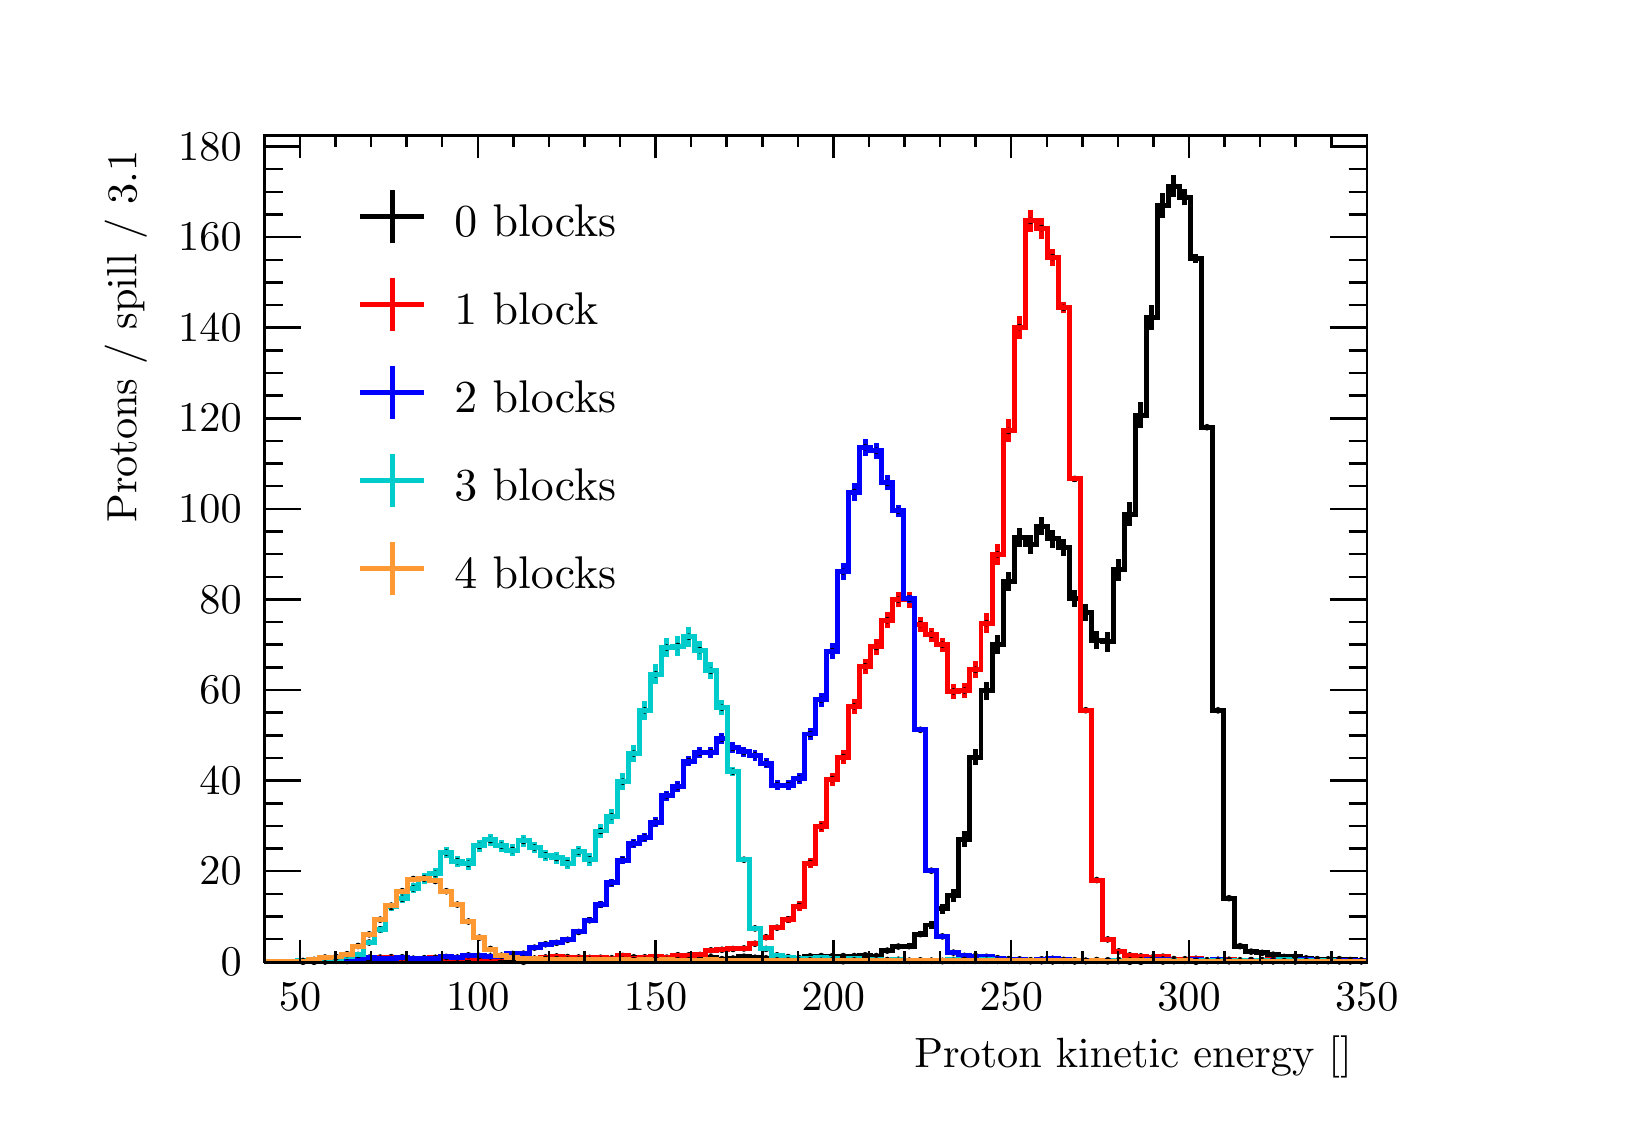
\begin{tikzpicture}
\pgfdeclareplotmark{cross} {
\pgfpathmoveto{\pgfpoint{-0.3\pgfplotmarksize}{\pgfplotmarksize}}
\pgfpathlineto{\pgfpoint{+0.3\pgfplotmarksize}{\pgfplotmarksize}}
\pgfpathlineto{\pgfpoint{+0.3\pgfplotmarksize}{0.3\pgfplotmarksize}}
\pgfpathlineto{\pgfpoint{+1\pgfplotmarksize}{0.3\pgfplotmarksize}}
\pgfpathlineto{\pgfpoint{+1\pgfplotmarksize}{-0.3\pgfplotmarksize}}
\pgfpathlineto{\pgfpoint{+0.3\pgfplotmarksize}{-0.3\pgfplotmarksize}}
\pgfpathlineto{\pgfpoint{+0.3\pgfplotmarksize}{-1.\pgfplotmarksize}}
\pgfpathlineto{\pgfpoint{-0.3\pgfplotmarksize}{-1.\pgfplotmarksize}}
\pgfpathlineto{\pgfpoint{-0.3\pgfplotmarksize}{-0.3\pgfplotmarksize}}
\pgfpathlineto{\pgfpoint{-1.\pgfplotmarksize}{-0.3\pgfplotmarksize}}
\pgfpathlineto{\pgfpoint{-1.\pgfplotmarksize}{0.3\pgfplotmarksize}}
\pgfpathlineto{\pgfpoint{-0.3\pgfplotmarksize}{0.3\pgfplotmarksize}}
\pgfpathclose
\pgfusepathqstroke
}
\pgfdeclareplotmark{cross*} {
\pgfpathmoveto{\pgfpoint{-0.3\pgfplotmarksize}{\pgfplotmarksize}}
\pgfpathlineto{\pgfpoint{+0.3\pgfplotmarksize}{\pgfplotmarksize}}
\pgfpathlineto{\pgfpoint{+0.3\pgfplotmarksize}{0.3\pgfplotmarksize}}
\pgfpathlineto{\pgfpoint{+1\pgfplotmarksize}{0.3\pgfplotmarksize}}
\pgfpathlineto{\pgfpoint{+1\pgfplotmarksize}{-0.3\pgfplotmarksize}}
\pgfpathlineto{\pgfpoint{+0.3\pgfplotmarksize}{-0.3\pgfplotmarksize}}
\pgfpathlineto{\pgfpoint{+0.3\pgfplotmarksize}{-1.\pgfplotmarksize}}
\pgfpathlineto{\pgfpoint{-0.3\pgfplotmarksize}{-1.\pgfplotmarksize}}
\pgfpathlineto{\pgfpoint{-0.3\pgfplotmarksize}{-0.3\pgfplotmarksize}}
\pgfpathlineto{\pgfpoint{-1.\pgfplotmarksize}{-0.3\pgfplotmarksize}}
\pgfpathlineto{\pgfpoint{-1.\pgfplotmarksize}{0.3\pgfplotmarksize}}
\pgfpathlineto{\pgfpoint{-0.3\pgfplotmarksize}{0.3\pgfplotmarksize}}
\pgfpathclose
\pgfusepathqfillstroke
}
\pgfdeclareplotmark{newstar} {
\pgfpathmoveto{\pgfqpoint{0pt}{\pgfplotmarksize}}
\pgfpathlineto{\pgfqpointpolar{44}{0.5\pgfplotmarksize}}
\pgfpathlineto{\pgfqpointpolar{18}{\pgfplotmarksize}}
\pgfpathlineto{\pgfqpointpolar{-20}{0.5\pgfplotmarksize}}
\pgfpathlineto{\pgfqpointpolar{-54}{\pgfplotmarksize}}
\pgfpathlineto{\pgfqpointpolar{-90}{0.5\pgfplotmarksize}}
\pgfpathlineto{\pgfqpointpolar{234}{\pgfplotmarksize}}
\pgfpathlineto{\pgfqpointpolar{198}{0.5\pgfplotmarksize}}
\pgfpathlineto{\pgfqpointpolar{162}{\pgfplotmarksize}}
\pgfpathlineto{\pgfqpointpolar{134}{0.5\pgfplotmarksize}}
\pgfpathclose
\pgfusepathqstroke
}
\pgfdeclareplotmark{newstar*} {
\pgfpathmoveto{\pgfqpoint{0pt}{\pgfplotmarksize}}
\pgfpathlineto{\pgfqpointpolar{44}{0.5\pgfplotmarksize}}
\pgfpathlineto{\pgfqpointpolar{18}{\pgfplotmarksize}}
\pgfpathlineto{\pgfqpointpolar{-20}{0.5\pgfplotmarksize}}
\pgfpathlineto{\pgfqpointpolar{-54}{\pgfplotmarksize}}
\pgfpathlineto{\pgfqpointpolar{-90}{0.5\pgfplotmarksize}}
\pgfpathlineto{\pgfqpointpolar{234}{\pgfplotmarksize}}
\pgfpathlineto{\pgfqpointpolar{198}{0.5\pgfplotmarksize}}
\pgfpathlineto{\pgfqpointpolar{162}{\pgfplotmarksize}}
\pgfpathlineto{\pgfqpointpolar{134}{0.5\pgfplotmarksize}}
\pgfpathclose
\pgfusepathqfillstroke
}
\definecolor{c}{rgb}{1,1,1};
\draw [color=c, fill=c] (0,0) rectangle (20,13.639);
\draw [color=c, fill=c] (3,1.77307) rectangle (17,12.2751);
\definecolor{c}{rgb}{0,0,0};
\draw [c,line width=0.9] (3,1.77307) -- (3,12.2751) -- (17,12.2751) -- (17,1.77307) -- (3,1.77307);
\definecolor{c}{rgb}{1,1,1};
\draw [color=c, fill=c] (3,1.77307) rectangle (17,12.2751);
\definecolor{c}{rgb}{0,0,0};
\draw [c,line width=0.9] (3,1.77307) -- (3,12.2751) -- (17,12.2751) -- (17,1.77307) -- (3,1.77307);
\draw [c,line width=0.9] (3,1.78273) -- (3.14,1.78273) -- (3.14,1.78273) -- (3.28,1.78273) -- (3.28,1.78273) -- (3.42,1.78273) -- (3.42,1.78273) -- (3.56,1.78273) -- (3.56,1.78273) -- (3.7,1.78273) -- (3.7,1.78273) -- (3.84,1.78273) -- (3.84,1.78273)
 -- (3.98,1.78273) -- (3.98,1.78273) -- (4.12,1.78273) -- (4.12,1.78273) -- (4.26,1.78273) -- (4.26,1.78273) -- (4.4,1.78273) -- (4.4,1.78273) -- (4.54,1.78273) -- (4.54,1.78273) -- (4.68,1.78273) -- (4.68,1.78273) -- (4.82,1.78273) -- (4.82,1.78273)
 -- (4.96,1.78273) -- (4.96,1.78273) -- (5.1,1.78273) -- (5.1,1.78273) -- (5.24,1.78273) -- (5.24,1.78273) -- (5.38,1.78273) -- (5.38,1.78273) -- (5.52,1.78273) -- (5.52,1.78273) -- (5.66,1.78273) -- (5.66,1.78273) -- (5.8,1.78273) -- (5.8,1.78273)
 -- (5.94,1.78273) -- (5.94,1.78273) -- (6.08,1.78273) -- (6.08,1.78273) -- (6.22,1.78273) -- (6.22,1.78273) -- (6.36,1.78273) -- (6.36,1.78273) -- (6.5,1.78273) -- (6.5,1.78273) -- (6.64,1.78273) -- (6.64,1.78273) -- (6.78,1.78273) -- (6.78,1.78273)
 -- (6.92,1.78273) -- (6.92,1.78273) -- (7.06,1.78273) -- (7.06,1.78273) -- (7.2,1.78273) -- (7.2,1.78273) -- (7.34,1.78273) -- (7.34,1.78273) -- (7.48,1.78273) -- (7.48,1.78273) -- (7.62,1.78273) -- (7.62,1.78273) -- (7.76,1.78273) -- (7.76,1.78273)
 -- (7.9,1.78273) -- (7.9,1.78273) -- (8.04,1.78273) -- (8.04,1.78273) -- (8.18,1.78273) -- (8.18,1.78273) -- (8.32,1.78273) -- (8.32,1.78273) -- (8.46,1.78273) -- (8.46,1.78273) -- (8.6,1.78273) -- (8.6,1.78273) -- (8.74,1.78273) -- (8.74,1.78273)
 -- (8.88,1.78273) -- (8.88,1.78273) -- (9.02,1.78273) -- (9.02,1.78273) -- (9.16,1.78273) -- (9.16,1.78273) -- (9.3,1.78273) -- (9.3,1.78273) -- (9.44,1.78273) -- (9.44,1.78273) -- (9.58,1.78273) -- (9.58,1.78273) -- (9.72,1.78273) -- (9.72,1.78273)
 -- (9.86,1.78273) -- (9.86,1.78273) -- (10,1.78273) -- (10,1.78273) -- (10.14,1.78273) -- (10.14,1.78273) -- (10.28,1.78273) -- (10.28,1.78273) -- (10.42,1.78273) -- (10.42,1.78273) -- (10.56,1.78273) -- (10.56,1.78273) -- (10.7,1.78273) --
 (10.7,1.78273) -- (10.84,1.78273) -- (10.84,1.78273) -- (10.98,1.78273) -- (10.98,1.78273) -- (11.12,1.78273) -- (11.12,1.78273) -- (11.26,1.78273) -- (11.26,1.78273) -- (11.4,1.78273) -- (11.4,1.78273) -- (11.54,1.78273) -- (11.54,1.78273) --
 (11.68,1.78273) -- (11.68,1.78273) -- (11.82,1.78273) -- (11.82,1.78273) -- (11.96,1.78273) -- (11.96,1.78273) -- (12.1,1.78273) -- (12.1,1.78273) -- (12.24,1.78273) -- (12.24,1.78273) -- (12.38,1.78273) -- (12.38,1.78273) -- (12.52,1.78273) --
 (12.52,1.78273) -- (12.66,1.78273) -- (12.66,1.78273) -- (12.8,1.78273) -- (12.8,1.78273) -- (12.94,1.78273) -- (12.94,1.78273) -- (13.08,1.78273) -- (13.08,1.78273) -- (13.22,1.78273) -- (13.22,1.78273) -- (13.36,1.78273) -- (13.36,1.78273) --
 (13.5,1.78273) -- (13.5,1.78273) -- (13.64,1.78273) -- (13.64,1.78273) -- (13.78,1.78273) -- (13.78,1.78273) -- (13.92,1.78273) -- (13.92,1.78273) -- (14.06,1.78273) -- (14.06,1.78273) -- (14.2,1.78273) -- (14.2,1.78273) -- (14.34,1.78273) --
 (14.34,1.78273) -- (14.48,1.78273) -- (14.48,1.78273) -- (14.62,1.78273) -- (14.62,1.78273) -- (14.76,1.78273) -- (14.76,1.78273) -- (14.9,1.78273) -- (14.9,1.78273) -- (15.04,1.78273) -- (15.04,1.78273) -- (15.18,1.78273) -- (15.18,1.78273) --
 (15.32,1.78273) -- (15.32,1.78273) -- (15.46,1.78273) -- (15.46,1.78273) -- (15.6,1.78273) -- (15.6,1.78273) -- (15.74,1.78273) -- (15.74,1.78273) -- (15.88,1.78273) -- (15.88,1.78273) -- (16.02,1.78273) -- (16.02,1.78273) -- (16.16,1.78273) --
 (16.16,1.78273) -- (16.3,1.78273) -- (16.3,1.78273) -- (16.44,1.78273) -- (16.44,1.78273) -- (16.58,1.78273) -- (16.58,1.78273) -- (16.72,1.78273) -- (16.72,1.78273) -- (16.86,1.78273) -- (16.86,1.78273) -- (17,1.78273);
\draw [c,line width=0.9] (3,1.77307) -- (17,1.77307);
\draw [c,line width=0.9] (3.45161,2.05948) -- (3.45161,1.77307);
\draw [c,line width=0.9] (3.90323,1.91628) -- (3.90323,1.77307);
\draw [c,line width=0.9] (4.35484,1.91628) -- (4.35484,1.77307);
\draw [c,line width=0.9] (4.80645,1.91628) -- (4.80645,1.77307);
\draw [c,line width=0.9] (5.25806,1.91628) -- (5.25806,1.77307);
\draw [c,line width=0.9] (5.70968,2.05948) -- (5.70968,1.77307);
\draw [c,line width=0.9] (6.16129,1.91628) -- (6.16129,1.77307);
\draw [c,line width=0.9] (6.6129,1.91628) -- (6.6129,1.77307);
\draw [c,line width=0.9] (7.06452,1.91628) -- (7.06452,1.77307);
\draw [c,line width=0.9] (7.51613,1.91628) -- (7.51613,1.77307);
\draw [c,line width=0.9] (7.96774,2.05948) -- (7.96774,1.77307);
\draw [c,line width=0.9] (8.41935,1.91628) -- (8.41935,1.77307);
\draw [c,line width=0.9] (8.87097,1.91628) -- (8.87097,1.77307);
\draw [c,line width=0.9] (9.32258,1.91628) -- (9.32258,1.77307);
\draw [c,line width=0.9] (9.77419,1.91628) -- (9.77419,1.77307);
\draw [c,line width=0.9] (10.2258,2.05948) -- (10.2258,1.77307);
\draw [c,line width=0.9] (10.6774,1.91628) -- (10.6774,1.77307);
\draw [c,line width=0.9] (11.129,1.91628) -- (11.129,1.77307);
\draw [c,line width=0.9] (11.5806,1.91628) -- (11.5806,1.77307);
\draw [c,line width=0.9] (12.0323,1.91628) -- (12.0323,1.77307);
\draw [c,line width=0.9] (12.4839,2.05948) -- (12.4839,1.77307);
\draw [c,line width=0.9] (12.9355,1.91628) -- (12.9355,1.77307);
\draw [c,line width=0.9] (13.3871,1.91628) -- (13.3871,1.77307);
\draw [c,line width=0.9] (13.8387,1.91628) -- (13.8387,1.77307);
\draw [c,line width=0.9] (14.2903,1.91628) -- (14.2903,1.77307);
\draw [c,line width=0.9] (14.7419,2.05948) -- (14.7419,1.77307);
\draw [c,line width=0.9] (15.1935,1.91628) -- (15.1935,1.77307);
\draw [c,line width=0.9] (15.6452,1.91628) -- (15.6452,1.77307);
\draw [c,line width=0.9] (16.0968,1.91628) -- (16.0968,1.77307);
\draw [c,line width=0.9] (16.5484,1.91628) -- (16.5484,1.77307);
\draw [c,line width=0.9] (17,2.05948) -- (17,1.77307);
\draw [c,line width=0.9] (3.45161,2.05948) -- (3.45161,1.77307);
\draw [c,line width=0.9] (3,1.91628) -- (3,1.77307);
\draw [anchor=base] (3.45161,1.15931) node[scale=1.52731, color=c, rotate=0]{50};
\draw [anchor=base] (5.70968,1.15931) node[scale=1.52731, color=c, rotate=0]{100};
\draw [anchor=base] (7.96774,1.15931) node[scale=1.52731, color=c, rotate=0]{150};
\draw [anchor=base] (10.2258,1.15931) node[scale=1.52731, color=c, rotate=0]{200};
\draw [anchor=base] (12.4839,1.15931) node[scale=1.52731, color=c, rotate=0]{250};
\draw [anchor=base] (14.7419,1.15931) node[scale=1.52731, color=c, rotate=0]{300};
\draw [anchor=base] (17,1.15931) node[scale=1.52731, color=c, rotate=0]{350};
\draw [anchor= east] (17,0.572837) node[scale=1.52731, color=c, rotate=0]{ Proton kinetic energy [\si{\mega\electronvolt}] };
\draw [c,line width=0.9] (3,12.2751) -- (17,12.2751);
\draw [c,line width=0.9] (3.45161,11.9887) -- (3.45161,12.2751);
\draw [c,line width=0.9] (3.90323,12.1319) -- (3.90323,12.2751);
\draw [c,line width=0.9] (4.35484,12.1319) -- (4.35484,12.2751);
\draw [c,line width=0.9] (4.80645,12.1319) -- (4.80645,12.2751);
\draw [c,line width=0.9] (5.25806,12.1319) -- (5.25806,12.2751);
\draw [c,line width=0.9] (5.70968,11.9887) -- (5.70968,12.2751);
\draw [c,line width=0.9] (6.16129,12.1319) -- (6.16129,12.2751);
\draw [c,line width=0.9] (6.6129,12.1319) -- (6.6129,12.2751);
\draw [c,line width=0.9] (7.06452,12.1319) -- (7.06452,12.2751);
\draw [c,line width=0.9] (7.51613,12.1319) -- (7.51613,12.2751);
\draw [c,line width=0.9] (7.96774,11.9887) -- (7.96774,12.2751);
\draw [c,line width=0.9] (8.41935,12.1319) -- (8.41935,12.2751);
\draw [c,line width=0.9] (8.87097,12.1319) -- (8.87097,12.2751);
\draw [c,line width=0.9] (9.32258,12.1319) -- (9.32258,12.2751);
\draw [c,line width=0.9] (9.77419,12.1319) -- (9.77419,12.2751);
\draw [c,line width=0.9] (10.2258,11.9887) -- (10.2258,12.2751);
\draw [c,line width=0.9] (10.6774,12.1319) -- (10.6774,12.2751);
\draw [c,line width=0.9] (11.129,12.1319) -- (11.129,12.2751);
\draw [c,line width=0.9] (11.5806,12.1319) -- (11.5806,12.2751);
\draw [c,line width=0.9] (12.0323,12.1319) -- (12.0323,12.2751);
\draw [c,line width=0.9] (12.4839,11.9887) -- (12.4839,12.2751);
\draw [c,line width=0.9] (12.9355,12.1319) -- (12.9355,12.2751);
\draw [c,line width=0.9] (13.3871,12.1319) -- (13.3871,12.2751);
\draw [c,line width=0.9] (13.8387,12.1319) -- (13.8387,12.2751);
\draw [c,line width=0.9] (14.2903,12.1319) -- (14.2903,12.2751);
\draw [c,line width=0.9] (14.7419,11.9887) -- (14.7419,12.2751);
\draw [c,line width=0.9] (15.1935,12.1319) -- (15.1935,12.2751);
\draw [c,line width=0.9] (15.6452,12.1319) -- (15.6452,12.2751);
\draw [c,line width=0.9] (16.0968,12.1319) -- (16.0968,12.2751);
\draw [c,line width=0.9] (16.5484,12.1319) -- (16.5484,12.2751);
\draw [c,line width=0.9] (17,11.9887) -- (17,12.2751);
\draw [c,line width=0.9] (3.45161,11.9887) -- (3.45161,12.2751);
\draw [c,line width=0.9] (3,12.1319) -- (3,12.2751);
\draw [c,line width=0.9] (3,1.77307) -- (3,12.2751);
\draw [c,line width=0.9] (3.462,1.78273) -- (3,1.78273);
\draw [c,line width=0.9] (3.231,2.07033) -- (3,2.07033);
\draw [c,line width=0.9] (3.231,2.35794) -- (3,2.35794);
\draw [c,line width=0.9] (3.231,2.64554) -- (3,2.64554);
\draw [c,line width=0.9] (3.462,2.93315) -- (3,2.93315);
\draw [c,line width=0.9] (3.231,3.22075) -- (3,3.22075);
\draw [c,line width=0.9] (3.231,3.50836) -- (3,3.50836);
\draw [c,line width=0.9] (3.231,3.79596) -- (3,3.79596);
\draw [c,line width=0.9] (3.462,4.08357) -- (3,4.08357);
\draw [c,line width=0.9] (3.231,4.37117) -- (3,4.37117);
\draw [c,line width=0.9] (3.231,4.65878) -- (3,4.65878);
\draw [c,line width=0.9] (3.231,4.94638) -- (3,4.94638);
\draw [c,line width=0.9] (3.462,5.23399) -- (3,5.23399);
\draw [c,line width=0.9] (3.231,5.52159) -- (3,5.52159);
\draw [c,line width=0.9] (3.231,5.8092) -- (3,5.8092);
\draw [c,line width=0.9] (3.231,6.0968) -- (3,6.0968);
\draw [c,line width=0.9] (3.462,6.38441) -- (3,6.38441);
\draw [c,line width=0.9] (3.231,6.67201) -- (3,6.67201);
\draw [c,line width=0.9] (3.231,6.95962) -- (3,6.95962);
\draw [c,line width=0.9] (3.231,7.24722) -- (3,7.24722);
\draw [c,line width=0.9] (3.462,7.53483) -- (3,7.53483);
\draw [c,line width=0.9] (3.231,7.82243) -- (3,7.82243);
\draw [c,line width=0.9] (3.231,8.11004) -- (3,8.11004);
\draw [c,line width=0.9] (3.231,8.39764) -- (3,8.39764);
\draw [c,line width=0.9] (3.462,8.68525) -- (3,8.68525);
\draw [c,line width=0.9] (3.231,8.97285) -- (3,8.97285);
\draw [c,line width=0.9] (3.231,9.26046) -- (3,9.26046);
\draw [c,line width=0.9] (3.231,9.54806) -- (3,9.54806);
\draw [c,line width=0.9] (3.462,9.83567) -- (3,9.83567);
\draw [c,line width=0.9] (3.231,10.1233) -- (3,10.1233);
\draw [c,line width=0.9] (3.231,10.4109) -- (3,10.4109);
\draw [c,line width=0.9] (3.231,10.6985) -- (3,10.6985);
\draw [c,line width=0.9] (3.462,10.9861) -- (3,10.9861);
\draw [c,line width=0.9] (3.231,11.2737) -- (3,11.2737);
\draw [c,line width=0.9] (3.231,11.5613) -- (3,11.5613);
\draw [c,line width=0.9] (3.231,11.8489) -- (3,11.8489);
\draw [c,line width=0.9] (3.462,12.1365) -- (3,12.1365);
\draw [c,line width=0.9] (3.462,1.78273) -- (3,1.78273);
\draw [c,line width=0.9] (3.462,12.1365) -- (3,12.1365);
\draw [anchor= east] (2.9,1.78273) node[scale=1.52731, color=c, rotate=0]{0};
\draw [anchor= east] (2.9,2.93315) node[scale=1.52731, color=c, rotate=0]{20};
\draw [anchor= east] (2.9,4.08357) node[scale=1.52731, color=c, rotate=0]{40};
\draw [anchor= east] (2.9,5.23399) node[scale=1.52731, color=c, rotate=0]{60};
\draw [anchor= east] (2.9,6.38441) node[scale=1.52731, color=c, rotate=0]{80};
\draw [anchor= east] (2.9,7.53483) node[scale=1.52731, color=c, rotate=0]{100};
\draw [anchor= east] (2.9,8.68525) node[scale=1.52731, color=c, rotate=0]{120};
\draw [anchor= east] (2.9,9.83567) node[scale=1.52731, color=c, rotate=0]{140};
\draw [anchor= east] (2.9,10.9861) node[scale=1.52731, color=c, rotate=0]{160};
\draw [anchor= east] (2.9,12.1365) node[scale=1.52731, color=c, rotate=0]{180};
\draw [anchor= east] (1.24,12.2751) node[scale=1.52731, color=c, rotate=90]{ Protons / spill / \SI{3.1}{\mega\electronvolt} };
\draw [c,line width=0.9] (17,1.77307) -- (17,12.2751);
\draw [c,line width=0.9] (16.538,1.78273) -- (17,1.78273);
\draw [c,line width=0.9] (16.769,2.07033) -- (17,2.07033);
\draw [c,line width=0.9] (16.769,2.35794) -- (17,2.35794);
\draw [c,line width=0.9] (16.769,2.64554) -- (17,2.64554);
\draw [c,line width=0.9] (16.538,2.93315) -- (17,2.93315);
\draw [c,line width=0.9] (16.769,3.22075) -- (17,3.22075);
\draw [c,line width=0.9] (16.769,3.50836) -- (17,3.50836);
\draw [c,line width=0.9] (16.769,3.79596) -- (17,3.79596);
\draw [c,line width=0.9] (16.538,4.08357) -- (17,4.08357);
\draw [c,line width=0.9] (16.769,4.37117) -- (17,4.37117);
\draw [c,line width=0.9] (16.769,4.65878) -- (17,4.65878);
\draw [c,line width=0.9] (16.769,4.94638) -- (17,4.94638);
\draw [c,line width=0.9] (16.538,5.23399) -- (17,5.23399);
\draw [c,line width=0.9] (16.769,5.52159) -- (17,5.52159);
\draw [c,line width=0.9] (16.769,5.8092) -- (17,5.8092);
\draw [c,line width=0.9] (16.769,6.0968) -- (17,6.0968);
\draw [c,line width=0.9] (16.538,6.38441) -- (17,6.38441);
\draw [c,line width=0.9] (16.769,6.67201) -- (17,6.67201);
\draw [c,line width=0.9] (16.769,6.95962) -- (17,6.95962);
\draw [c,line width=0.9] (16.769,7.24722) -- (17,7.24722);
\draw [c,line width=0.9] (16.538,7.53483) -- (17,7.53483);
\draw [c,line width=0.9] (16.769,7.82243) -- (17,7.82243);
\draw [c,line width=0.9] (16.769,8.11004) -- (17,8.11004);
\draw [c,line width=0.9] (16.769,8.39764) -- (17,8.39764);
\draw [c,line width=0.9] (16.538,8.68525) -- (17,8.68525);
\draw [c,line width=0.9] (16.769,8.97285) -- (17,8.97285);
\draw [c,line width=0.9] (16.769,9.26046) -- (17,9.26046);
\draw [c,line width=0.9] (16.769,9.54806) -- (17,9.54806);
\draw [c,line width=0.9] (16.538,9.83567) -- (17,9.83567);
\draw [c,line width=0.9] (16.769,10.1233) -- (17,10.1233);
\draw [c,line width=0.9] (16.769,10.4109) -- (17,10.4109);
\draw [c,line width=0.9] (16.769,10.6985) -- (17,10.6985);
\draw [c,line width=0.9] (16.538,10.9861) -- (17,10.9861);
\draw [c,line width=0.9] (16.769,11.2737) -- (17,11.2737);
\draw [c,line width=0.9] (16.769,11.5613) -- (17,11.5613);
\draw [c,line width=0.9] (16.769,11.8489) -- (17,11.8489);
\draw [c,line width=0.9] (16.538,12.1365) -- (17,12.1365);
\draw [c,line width=0.9] (16.538,1.78273) -- (17,1.78273);
\draw [c,line width=0.9] (16.538,12.1365) -- (17,12.1365);
\draw [c,line width=1.8] (6.29,1.77307) -- (6.29,1.78273);
\draw [c,line width=1.8] (6.29,1.78273) -- (6.29,1.79238);
\foreach \P in {(6.29,1.78273)}{\draw[mark options={color=c,fill=c},mark size=2.402402pt,mark=*,mark size=1pt] plot coordinates {\P};}
\draw [c,line width=1.8] (6.43,1.80761) -- (6.43,1.81886);
\draw [c,line width=1.8] (6.43,1.81886) -- (6.43,1.83012);
\foreach \P in {(6.43,1.81886)}{\draw[mark options={color=c,fill=c},mark size=2.402402pt,mark=*,mark size=1pt] plot coordinates {\P};}
\draw [c,line width=1.8] (6.57,1.82799) -- (6.57,1.83693);
\draw [c,line width=1.8] (6.57,1.83693) -- (6.57,1.84588);
\foreach \P in {(6.57,1.83693)}{\draw[mark options={color=c,fill=c},mark size=2.402402pt,mark=*,mark size=1pt] plot coordinates {\P};}
\draw [c,line width=1.8] (6.71,1.80181) -- (6.71,1.81112);
\draw [c,line width=1.8] (6.71,1.81112) -- (6.71,1.82043);
\foreach \P in {(6.71,1.81112)}{\draw[mark options={color=c,fill=c},mark size=2.402402pt,mark=*,mark size=1pt] plot coordinates {\P};}
\draw [c,line width=1.8] (6.85,1.80734) -- (6.85,1.81628);
\draw [c,line width=1.8] (6.85,1.81628) -- (6.85,1.82523);
\foreach \P in {(6.85,1.81628)}{\draw[mark options={color=c,fill=c},mark size=2.402402pt,mark=*,mark size=1pt] plot coordinates {\P};}
\draw [c,line width=1.8] (6.99,1.80474) -- (6.99,1.81628);
\draw [c,line width=1.8] (6.99,1.81628) -- (6.99,1.82783);
\foreach \P in {(6.99,1.81628)}{\draw[mark options={color=c,fill=c},mark size=2.402402pt,mark=*,mark size=1pt] plot coordinates {\P};}
\draw [c,line width=1.8] (7.13,1.81886) -- (7.13,1.82919);
\draw [c,line width=1.8] (7.13,1.82919) -- (7.13,1.83952);
\foreach \P in {(7.13,1.82919)}{\draw[mark options={color=c,fill=c},mark size=2.402402pt,mark=*,mark size=1pt] plot coordinates {\P};}
\draw [c,line width=1.8] (7.27,1.81628) -- (7.27,1.82661);
\draw [c,line width=1.8] (7.27,1.82661) -- (7.27,1.83693);
\foreach \P in {(7.27,1.82661)}{\draw[mark options={color=c,fill=c},mark size=2.402402pt,mark=*,mark size=1pt] plot coordinates {\P};}
\draw [c,line width=1.8] (7.41,1.8108) -- (7.41,1.82145);
\draw [c,line width=1.8] (7.41,1.82145) -- (7.41,1.83209);
\foreach \P in {(7.41,1.82145)}{\draw[mark options={color=c,fill=c},mark size=2.402402pt,mark=*,mark size=1pt] plot coordinates {\P};}
\draw [c,line width=1.8] (7.55,1.81192) -- (7.55,1.82403);
\draw [c,line width=1.8] (7.55,1.82403) -- (7.55,1.83614);
\foreach \P in {(7.55,1.82403)}{\draw[mark options={color=c,fill=c},mark size=2.402402pt,mark=*,mark size=1pt] plot coordinates {\P};}
\draw [c,line width=1.8] (7.69,1.82887) -- (7.69,1.83951);
\draw [c,line width=1.8] (7.69,1.83951) -- (7.69,1.85016);
\foreach \P in {(7.69,1.83951)}{\draw[mark options={color=c,fill=c},mark size=2.402402pt,mark=*,mark size=1pt] plot coordinates {\P};}
\draw [c,line width=1.8] (7.83,1.81423) -- (7.83,1.82661);
\draw [c,line width=1.8] (7.83,1.82661) -- (7.83,1.83899);
\foreach \P in {(7.83,1.82661)}{\draw[mark options={color=c,fill=c},mark size=2.402402pt,mark=*,mark size=1pt] plot coordinates {\P};}
\draw [c,line width=1.8] (7.97,1.83403) -- (7.97,1.84468);
\draw [c,line width=1.8] (7.97,1.84468) -- (7.97,1.85532);
\foreach \P in {(7.97,1.84468)}{\draw[mark options={color=c,fill=c},mark size=2.402402pt,mark=*,mark size=1pt] plot coordinates {\P};}
\draw [c,line width=1.8] (8.11,1.80214) -- (8.11,1.81628);
\draw [c,line width=1.8] (8.11,1.81628) -- (8.11,1.83042);
\foreach \P in {(8.11,1.81628)}{\draw[mark options={color=c,fill=c},mark size=2.402402pt,mark=*,mark size=1pt] plot coordinates {\P};}
\draw [c,line width=1.8] (8.25,1.8535) -- (8.25,1.86533);
\draw [c,line width=1.8] (8.25,1.86533) -- (8.25,1.87716);
\foreach \P in {(8.25,1.86533)}{\draw[mark options={color=c,fill=c},mark size=2.402402pt,mark=*,mark size=1pt] plot coordinates {\P};}
\draw [c,line width=1.8] (8.39,1.82945) -- (8.39,1.8421);
\draw [c,line width=1.8] (8.39,1.8421) -- (8.39,1.85474);
\foreach \P in {(8.39,1.8421)}{\draw[mark options={color=c,fill=c},mark size=2.402402pt,mark=*,mark size=1pt] plot coordinates {\P};}
\draw [c,line width=1.8] (8.53,1.81277) -- (8.53,1.82403);
\draw [c,line width=1.8] (8.53,1.82403) -- (8.53,1.83528);
\foreach \P in {(8.53,1.82403)}{\draw[mark options={color=c,fill=c},mark size=2.402402pt,mark=*,mark size=1pt] plot coordinates {\P};}
\draw [c,line width=1.8] (8.67,1.83279) -- (8.67,1.8421);
\draw [c,line width=1.8] (8.67,1.8421) -- (8.67,1.8514);
\foreach \P in {(8.67,1.8421)}{\draw[mark options={color=c,fill=c},mark size=2.402402pt,mark=*,mark size=1pt] plot coordinates {\P};}
\draw [c,line width=1.8] (8.81,1.80503) -- (8.81,1.81628);
\draw [c,line width=1.8] (8.81,1.81628) -- (8.81,1.82754);
\foreach \P in {(8.81,1.81628)}{\draw[mark options={color=c,fill=c},mark size=2.402402pt,mark=*,mark size=1pt] plot coordinates {\P};}
\draw [c,line width=1.8] (8.95,1.81112) -- (8.95,1.82403);
\draw [c,line width=1.8] (8.95,1.82403) -- (8.95,1.83693);
\foreach \P in {(8.95,1.82403)}{\draw[mark options={color=c,fill=c},mark size=2.402402pt,mark=*,mark size=1pt] plot coordinates {\P};}
\draw [c,line width=1.8] (9.09,1.83571) -- (9.09,1.84726);
\draw [c,line width=1.8] (9.09,1.84726) -- (9.09,1.8588);
\foreach \P in {(9.09,1.84726)}{\draw[mark options={color=c,fill=c},mark size=2.402402pt,mark=*,mark size=1pt] plot coordinates {\P};}
\draw [c,line width=1.8] (9.23,1.82144) -- (9.23,1.83435);
\draw [c,line width=1.8] (9.23,1.83435) -- (9.23,1.84726);
\foreach \P in {(9.23,1.83435)}{\draw[mark options={color=c,fill=c},mark size=2.402402pt,mark=*,mark size=1pt] plot coordinates {\P};}
\draw [c,line width=1.8] (9.37,1.81396) -- (9.37,1.82661);
\draw [c,line width=1.8] (9.37,1.82661) -- (9.37,1.83925);
\foreach \P in {(9.37,1.82661)}{\draw[mark options={color=c,fill=c},mark size=2.402402pt,mark=*,mark size=1pt] plot coordinates {\P};}
\draw [c,line width=1.8] (9.51,1.83801) -- (9.51,1.84984);
\draw [c,line width=1.8] (9.51,1.84984) -- (9.51,1.86167);
\foreach \P in {(9.51,1.84984)}{\draw[mark options={color=c,fill=c},mark size=2.402402pt,mark=*,mark size=1pt] plot coordinates {\P};}
\draw [c,line width=1.8] (9.65,1.82945) -- (9.65,1.8421);
\draw [c,line width=1.8] (9.65,1.8421) -- (9.65,1.85474);
\foreach \P in {(9.65,1.8421)}{\draw[mark options={color=c,fill=c},mark size=2.402402pt,mark=*,mark size=1pt] plot coordinates {\P};}
\draw [c,line width=1.8] (9.79,1.81553) -- (9.79,1.82919);
\draw [c,line width=1.8] (9.79,1.82919) -- (9.79,1.84285);
\foreach \P in {(9.79,1.82919)}{\draw[mark options={color=c,fill=c},mark size=2.402402pt,mark=*,mark size=1pt] plot coordinates {\P};}
\draw [c,line width=1.8] (9.93,1.83926) -- (9.93,1.85242);
\draw [c,line width=1.8] (9.93,1.85242) -- (9.93,1.86558);
\foreach \P in {(9.93,1.85242)}{\draw[mark options={color=c,fill=c},mark size=2.402402pt,mark=*,mark size=1pt] plot coordinates {\P};}
\draw [c,line width=1.8] (10.07,1.8404) -- (10.07,1.855);
\draw [c,line width=1.8] (10.07,1.855) -- (10.07,1.86961);
\foreach \P in {(10.07,1.855)}{\draw[mark options={color=c,fill=c},mark size=2.402402pt,mark=*,mark size=1pt] plot coordinates {\P};}
\draw [c,line width=1.8] (10.21,1.84031) -- (10.21,1.85242);
\draw [c,line width=1.8] (10.21,1.85242) -- (10.21,1.86453);
\foreach \P in {(10.21,1.85242)}{\draw[mark options={color=c,fill=c},mark size=2.402402pt,mark=*,mark size=1pt] plot coordinates {\P};}
\draw [c,line width=1.8] (10.35,1.83868) -- (10.35,1.855);
\draw [c,line width=1.8] (10.35,1.855) -- (10.35,1.87133);
\foreach \P in {(10.35,1.855)}{\draw[mark options={color=c,fill=c},mark size=2.402402pt,mark=*,mark size=1pt] plot coordinates {\P};}
\draw [c,line width=1.8] (10.49,1.84184) -- (10.49,1.855);
\draw [c,line width=1.8] (10.49,1.855) -- (10.49,1.86817);
\foreach \P in {(10.49,1.855)}{\draw[mark options={color=c,fill=c},mark size=2.402402pt,mark=*,mark size=1pt] plot coordinates {\P};}
\draw [c,line width=1.8] (10.63,1.8488) -- (10.63,1.86533);
\draw [c,line width=1.8] (10.63,1.86533) -- (10.63,1.88186);
\foreach \P in {(10.63,1.86533)}{\draw[mark options={color=c,fill=c},mark size=2.402402pt,mark=*,mark size=1pt] plot coordinates {\P};}
\draw [c,line width=1.8] (10.77,1.8322) -- (10.77,1.855);
\draw [c,line width=1.8] (10.77,1.855) -- (10.77,1.8778);
\foreach \P in {(10.77,1.855)}{\draw[mark options={color=c,fill=c},mark size=2.402402pt,mark=*,mark size=1pt] plot coordinates {\P};}
\draw [c,line width=1.8] (10.91,1.9019) -- (10.91,1.9247);
\draw [c,line width=1.8] (10.91,1.9247) -- (10.91,1.9475);
\foreach \P in {(10.91,1.9247)}{\draw[mark options={color=c,fill=c},mark size=2.402402pt,mark=*,mark size=1pt] plot coordinates {\P};}
\draw [c,line width=1.8] (11.05,1.94712) -- (11.05,1.97633);
\draw [c,line width=1.8] (11.05,1.97633) -- (11.05,2.00553);
\foreach \P in {(11.05,1.97633)}{\draw[mark options={color=c,fill=c},mark size=2.402402pt,mark=*,mark size=1pt] plot coordinates {\P};}
\draw [c,line width=1.8] (11.19,1.94638) -- (11.19,1.98149);
\draw [c,line width=1.8] (11.19,1.98149) -- (11.19,2.0166);
\foreach \P in {(11.19,1.98149)}{\draw[mark options={color=c,fill=c},mark size=2.402402pt,mark=*,mark size=1pt] plot coordinates {\P};}
\draw [c,line width=1.8] (11.33,2.0933) -- (11.33,2.13379);
\draw [c,line width=1.8] (11.33,2.13379) -- (11.33,2.17428);
\foreach \P in {(11.33,2.13379)}{\draw[mark options={color=c,fill=c},mark size=2.402402pt,mark=*,mark size=1pt] plot coordinates {\P};}
\draw [c,line width=1.8] (11.47,2.20284) -- (11.47,2.24995);
\draw [c,line width=1.8] (11.47,2.24995) -- (11.47,2.29706);
\foreach \P in {(11.47,2.24995)}{\draw[mark options={color=c,fill=c},mark size=2.402402pt,mark=*,mark size=1pt] plot coordinates {\P};}
\draw [c,line width=1.8] (11.61,2.39012) -- (11.61,2.45388);
\draw [c,line width=1.8] (11.61,2.45388) -- (11.61,2.51764);
\foreach \P in {(11.61,2.45388)}{\draw[mark options={color=c,fill=c},mark size=2.402402pt,mark=*,mark size=1pt] plot coordinates {\P};}
\draw [c,line width=1.8] (11.75,2.53607) -- (11.75,2.61909);
\draw [c,line width=1.8] (11.75,2.61909) -- (11.75,2.7021);
\foreach \P in {(11.75,2.61909)}{\draw[mark options={color=c,fill=c},mark size=2.402402pt,mark=*,mark size=1pt] plot coordinates {\P};}
\draw [c,line width=1.8] (11.89,3.24579) -- (11.89,3.34187);
\draw [c,line width=1.8] (11.89,3.34187) -- (11.89,3.43794);
\foreach \P in {(11.89,3.34187)}{\draw[mark options={color=c,fill=c},mark size=2.402402pt,mark=*,mark size=1pt] plot coordinates {\P};}
\draw [c,line width=1.8] (12.03,4.27783) -- (12.03,4.38215);
\draw [c,line width=1.8] (12.03,4.38215) -- (12.03,4.48647);
\foreach \P in {(12.03,4.38215)}{\draw[mark options={color=c,fill=c},mark size=2.402402pt,mark=*,mark size=1pt] plot coordinates {\P};}
\draw [c,line width=1.8] (12.17,5.11191) -- (12.17,5.22626);
\draw [c,line width=1.8] (12.17,5.22626) -- (12.17,5.34061);
\foreach \P in {(12.17,5.22626)}{\draw[mark options={color=c,fill=c},mark size=2.402402pt,mark=*,mark size=1pt] plot coordinates {\P};}
\draw [c,line width=1.8] (12.31,5.68717) -- (12.31,5.80707);
\draw [c,line width=1.8] (12.31,5.80707) -- (12.31,5.92696);
\foreach \P in {(12.31,5.80707)}{\draw[mark options={color=c,fill=c},mark size=2.402402pt,mark=*,mark size=1pt] plot coordinates {\P};}
\draw [c,line width=1.8] (12.45,6.49278) -- (12.45,6.61245);
\draw [c,line width=1.8] (12.45,6.61245) -- (12.45,6.73212);
\foreach \P in {(12.45,6.61245)}{\draw[mark options={color=c,fill=c},mark size=2.402402pt,mark=*,mark size=1pt] plot coordinates {\P};}
\draw [c,line width=1.8] (12.59,7.04921) -- (12.59,7.17002);
\draw [c,line width=1.8] (12.59,7.17002) -- (12.59,7.29083);
\foreach \P in {(12.59,7.17002)}{\draw[mark options={color=c,fill=c},mark size=2.402402pt,mark=*,mark size=1pt] plot coordinates {\P};}
\draw [c,line width=1.8] (12.73,6.95771) -- (12.73,7.07968);
\draw [c,line width=1.8] (12.73,7.07968) -- (12.73,7.20164);
\foreach \P in {(12.73,7.07968)}{\draw[mark options={color=c,fill=c},mark size=2.402402pt,mark=*,mark size=1pt] plot coordinates {\P};}
\draw [c,line width=1.8] (12.87,7.20029) -- (12.87,7.31458);
\draw [c,line width=1.8] (12.87,7.31458) -- (12.87,7.42887);
\foreach \P in {(12.87,7.31458)}{\draw[mark options={color=c,fill=c},mark size=2.402402pt,mark=*,mark size=1pt] plot coordinates {\P};}
\draw [c,line width=1.8] (13.01,7.04296) -- (13.01,7.15453);
\draw [c,line width=1.8] (13.01,7.15453) -- (13.01,7.26611);
\foreach \P in {(13.01,7.15453)}{\draw[mark options={color=c,fill=c},mark size=2.402402pt,mark=*,mark size=1pt] plot coordinates {\P};}
\draw [c,line width=1.8] (13.15,6.9398) -- (13.15,7.04612);
\draw [c,line width=1.8] (13.15,7.04612) -- (13.15,7.15243);
\foreach \P in {(13.15,7.04612)}{\draw[mark options={color=c,fill=c},mark size=2.402402pt,mark=*,mark size=1pt] plot coordinates {\P};}
\draw [c,line width=1.8] (13.29,6.29216) -- (13.29,6.39562);
\draw [c,line width=1.8] (13.29,6.39562) -- (13.29,6.49907);
\foreach \P in {(13.29,6.39562)}{\draw[mark options={color=c,fill=c},mark size=2.402402pt,mark=*,mark size=1pt] plot coordinates {\P};}
\draw [c,line width=1.8] (13.43,6.10865) -- (13.43,6.2175);
\draw [c,line width=1.8] (13.43,6.2175) -- (13.43,6.32635);
\foreach \P in {(13.43,6.2175)}{\draw[mark options={color=c,fill=c},mark size=2.402402pt,mark=*,mark size=1pt] plot coordinates {\P};}
\draw [c,line width=1.8] (13.57,5.75021) -- (13.57,5.86902);
\draw [c,line width=1.8] (13.57,5.86902) -- (13.57,5.98782);
\foreach \P in {(13.57,5.86902)}{\draw[mark options={color=c,fill=c},mark size=2.402402pt,mark=*,mark size=1pt] plot coordinates {\P};}
\draw [c,line width=1.8] (13.71,5.71586) -- (13.71,5.84579);
\draw [c,line width=1.8] (13.71,5.84579) -- (13.71,5.97571);
\foreach \P in {(13.71,5.84579)}{\draw[mark options={color=c,fill=c},mark size=2.402402pt,mark=*,mark size=1pt] plot coordinates {\P};}
\draw [c,line width=1.8] (13.85,6.61732) -- (13.85,6.75959);
\draw [c,line width=1.8] (13.85,6.75959) -- (13.85,6.90185);
\foreach \P in {(13.85,6.75959)}{\draw[mark options={color=c,fill=c},mark size=2.402402pt,mark=*,mark size=1pt] plot coordinates {\P};}
\draw [c,line width=1.8] (13.99,7.31378) -- (13.99,7.46946);
\draw [c,line width=1.8] (13.99,7.46946) -- (13.99,7.62515);
\foreach \P in {(13.99,7.46946)}{\draw[mark options={color=c,fill=c},mark size=2.402402pt,mark=*,mark size=1pt] plot coordinates {\P};}
\draw [c,line width=1.8] (14.13,8.5623) -- (14.13,8.72658);
\draw [c,line width=1.8] (14.13,8.72658) -- (14.13,8.89087);
\foreach \P in {(14.13,8.72658)}{\draw[mark options={color=c,fill=c},mark size=2.402402pt,mark=*,mark size=1pt] plot coordinates {\P};}
\draw [c,line width=1.8] (14.27,9.80077) -- (14.27,9.96305);
\draw [c,line width=1.8] (14.27,9.96305) -- (14.27,10.1253);
\foreach \P in {(14.27,9.96305)}{\draw[mark options={color=c,fill=c},mark size=2.402402pt,mark=*,mark size=1pt] plot coordinates {\P};}
\draw [c,line width=1.8] (14.41,11.2292) -- (14.41,11.3854);
\draw [c,line width=1.8] (14.41,11.3854) -- (14.41,11.5416);
\foreach \P in {(14.41,11.3854)}{\draw[mark options={color=c,fill=c},mark size=2.402402pt,mark=*,mark size=1pt] plot coordinates {\P};}
\draw [c,line width=1.8] (14.55,11.491) -- (14.55,11.6332);
\draw [c,line width=1.8] (14.55,11.6332) -- (14.55,11.7754);
\foreach \P in {(14.55,11.6332)}{\draw[mark options={color=c,fill=c},mark size=2.402402pt,mark=*,mark size=1pt] plot coordinates {\P};}
\draw [c,line width=1.8] (14.69,11.3892) -- (14.69,11.4938);
\draw [c,line width=1.8] (14.69,11.4938) -- (14.69,11.5984);
\foreach \P in {(14.69,11.4938)}{\draw[mark options={color=c,fill=c},mark size=2.402402pt,mark=*,mark size=1pt] plot coordinates {\P};}
\draw [c,line width=1.8] (14.83,10.6594) -- (14.83,10.7142);
\draw [c,line width=1.8] (14.83,10.7142) -- (14.83,10.7691);
\foreach \P in {(14.83,10.7142)}{\draw[mark options={color=c,fill=c},mark size=2.402402pt,mark=*,mark size=1pt] plot coordinates {\P};}
\draw [c,line width=1.8] (14.97,8.54804) -- (14.97,8.5717);
\draw [c,line width=1.8] (14.97,8.5717) -- (14.97,8.59536);
\foreach \P in {(14.97,8.5717)}{\draw[mark options={color=c,fill=c},mark size=2.402402pt,mark=*,mark size=1pt] plot coordinates {\P};}
\draw [c,line width=1.8] (15.11,4.95707) -- (15.11,4.97587);
\draw [c,line width=1.8] (15.11,4.97587) -- (15.11,4.99466);
\foreach \P in {(15.11,4.97587)}{\draw[mark options={color=c,fill=c},mark size=2.402402pt,mark=*,mark size=1pt] plot coordinates {\P};}
\draw [c,line width=1.8] (15.25,2.57281) -- (15.25,2.59069);
\draw [c,line width=1.8] (15.25,2.59069) -- (15.25,2.60858);
\foreach \P in {(15.25,2.59069)}{\draw[mark options={color=c,fill=c},mark size=2.402402pt,mark=*,mark size=1pt] plot coordinates {\P};}
\draw [c,line width=1.8] (15.39,1.96579) -- (15.39,1.98149);
\draw [c,line width=1.8] (15.39,1.98149) -- (15.39,1.99719);
\foreach \P in {(15.39,1.98149)}{\draw[mark options={color=c,fill=c},mark size=2.402402pt,mark=*,mark size=1pt] plot coordinates {\P};}
\draw [c,line width=1.8] (15.53,1.89889) -- (15.53,1.91179);
\draw [c,line width=1.8] (15.53,1.91179) -- (15.53,1.9247);
\foreach \P in {(15.53,1.91179)}{\draw[mark options={color=c,fill=c},mark size=2.402402pt,mark=*,mark size=1pt] plot coordinates {\P};}
\draw [c,line width=1.8] (15.67,1.88289) -- (15.67,1.8963);
\draw [c,line width=1.8] (15.67,1.8963) -- (15.67,1.90972);
\foreach \P in {(15.67,1.8963)}{\draw[mark options={color=c,fill=c},mark size=2.402402pt,mark=*,mark size=1pt] plot coordinates {\P};}
\draw [c,line width=1.8] (15.81,1.86243) -- (15.81,1.87307);
\draw [c,line width=1.8] (15.81,1.87307) -- (15.81,1.88372);
\foreach \P in {(15.81,1.87307)}{\draw[mark options={color=c,fill=c},mark size=2.402402pt,mark=*,mark size=1pt] plot coordinates {\P};}
\draw [c,line width=1.8] (15.95,1.83468) -- (15.95,1.84468);
\draw [c,line width=1.8] (15.95,1.84468) -- (15.95,1.85468);
\foreach \P in {(15.95,1.84468)}{\draw[mark options={color=c,fill=c},mark size=2.402402pt,mark=*,mark size=1pt] plot coordinates {\P};}
\draw [c,line width=1.8] (16.09,1.8421) -- (16.09,1.84984);
\draw [c,line width=1.8] (16.09,1.84984) -- (16.09,1.85758);
\foreach \P in {(16.09,1.84984)}{\draw[mark options={color=c,fill=c},mark size=2.402402pt,mark=*,mark size=1pt] plot coordinates {\P};}
\draw [c,line width=1.8] (16.23,1.81695) -- (16.23,1.82661);
\draw [c,line width=1.8] (16.23,1.82661) -- (16.23,1.83627);
\foreach \P in {(16.23,1.82661)}{\draw[mark options={color=c,fill=c},mark size=2.402402pt,mark=*,mark size=1pt] plot coordinates {\P};}
\draw [c,line width=1.8] (16.37,1.80734) -- (16.37,1.81628);
\draw [c,line width=1.8] (16.37,1.81628) -- (16.37,1.82523);
\foreach \P in {(16.37,1.81628)}{\draw[mark options={color=c,fill=c},mark size=2.402402pt,mark=*,mark size=1pt] plot coordinates {\P};}
\draw [c,line width=1.8] (16.51,1.81005) -- (16.51,1.8137);
\draw [c,line width=1.8] (16.51,1.8137) -- (16.51,1.81735);
\foreach \P in {(16.51,1.8137)}{\draw[mark options={color=c,fill=c},mark size=2.402402pt,mark=*,mark size=1pt] plot coordinates {\P};}
\foreach \P in {(16.65,1.81628)}{\draw[mark options={color=c,fill=c},mark size=2.402402pt,mark=*,mark size=1pt] plot coordinates {\P};}
\foreach \P in {(16.79,1.80596)}{\draw[mark options={color=c,fill=c},mark size=2.402402pt,mark=*,mark size=1pt] plot coordinates {\P};}
\foreach \P in {(16.93,1.80079)}{\draw[mark options={color=c,fill=c},mark size=2.402402pt,mark=*,mark size=1pt] plot coordinates {\P};}
\draw [c,line width=1.8] (3,1.78273) -- (3.14,1.78273) -- (3.14,1.78273) -- (3.28,1.78273) -- (3.28,1.78273) -- (3.42,1.78273) -- (3.42,1.78273) -- (3.56,1.78273) -- (3.56,1.78273) -- (3.7,1.78273) -- (3.7,1.78273) -- (3.84,1.78273) -- (3.84,1.78273)
 -- (3.98,1.78273) -- (3.98,1.78273) -- (4.12,1.78273) -- (4.12,1.78273) -- (4.26,1.78273) -- (4.26,1.78273) -- (4.4,1.78273) -- (4.4,1.78273) -- (4.54,1.78273) -- (4.54,1.78273) -- (4.68,1.78273) -- (4.68,1.78273) -- (4.82,1.78273) -- (4.82,1.78273)
 -- (4.96,1.78273) -- (4.96,1.78273) -- (5.1,1.78273) -- (5.1,1.78273) -- (5.24,1.78273) -- (5.24,1.78273) -- (5.38,1.78273) -- (5.38,1.78273) -- (5.52,1.78273) -- (5.52,1.78273) -- (5.66,1.78273) -- (5.66,1.78273) -- (5.8,1.78273) -- (5.8,1.78273)
 -- (5.94,1.78273) -- (5.94,1.78273) -- (6.08,1.78273) -- (6.08,1.78273) -- (6.22,1.78273) -- (6.22,1.78273) -- (6.36,1.78273) -- (6.36,1.81886) -- (6.5,1.81886) -- (6.5,1.83693) -- (6.64,1.83693) -- (6.64,1.81112) -- (6.78,1.81112) -- (6.78,1.81628)
 -- (6.92,1.81628) -- (6.92,1.81628) -- (7.06,1.81628) -- (7.06,1.82919) -- (7.2,1.82919) -- (7.2,1.82661) -- (7.34,1.82661) -- (7.34,1.82145) -- (7.48,1.82145) -- (7.48,1.82403) -- (7.62,1.82403) -- (7.62,1.83951) -- (7.76,1.83951) -- (7.76,1.82661)
 -- (7.9,1.82661) -- (7.9,1.84468) -- (8.04,1.84468) -- (8.04,1.81628) -- (8.18,1.81628) -- (8.18,1.86533) -- (8.32,1.86533) -- (8.32,1.8421) -- (8.46,1.8421) -- (8.46,1.82403) -- (8.6,1.82403) -- (8.6,1.8421) -- (8.74,1.8421) -- (8.74,1.81628) --
 (8.88,1.81628) -- (8.88,1.82403) -- (9.02,1.82403) -- (9.02,1.84726) -- (9.16,1.84726) -- (9.16,1.83435) -- (9.3,1.83435) -- (9.3,1.82661) -- (9.44,1.82661) -- (9.44,1.84984) -- (9.58,1.84984) -- (9.58,1.8421) -- (9.72,1.8421) -- (9.72,1.82919) --
 (9.86,1.82919) -- (9.86,1.85242) -- (10,1.85242) -- (10,1.855) -- (10.14,1.855) -- (10.14,1.85242) -- (10.28,1.85242) -- (10.28,1.855) -- (10.42,1.855) -- (10.42,1.855) -- (10.56,1.855) -- (10.56,1.86533) -- (10.7,1.86533) -- (10.7,1.855) --
 (10.84,1.855) -- (10.84,1.9247) -- (10.98,1.9247) -- (10.98,1.97633) -- (11.12,1.97633) -- (11.12,1.98149) -- (11.26,1.98149) -- (11.26,2.13379) -- (11.4,2.13379) -- (11.4,2.24995) -- (11.54,2.24995) -- (11.54,2.45388) -- (11.68,2.45388) --
 (11.68,2.61909) -- (11.82,2.61909) -- (11.82,3.34187) -- (11.96,3.34187) -- (11.96,4.38215) -- (12.1,4.38215) -- (12.1,5.22626) -- (12.24,5.22626) -- (12.24,5.80707) -- (12.38,5.80707) -- (12.38,6.61245) -- (12.52,6.61245) -- (12.52,7.17002) --
 (12.66,7.17002) -- (12.66,7.07968) -- (12.8,7.07968) -- (12.8,7.31458) -- (12.94,7.31458) -- (12.94,7.15453) -- (13.08,7.15453) -- (13.08,7.04612) -- (13.22,7.04612) -- (13.22,6.39562) -- (13.36,6.39562) -- (13.36,6.2175) -- (13.5,6.2175) --
 (13.5,5.86902) -- (13.64,5.86902) -- (13.64,5.84579) -- (13.78,5.84579) -- (13.78,6.75959) -- (13.92,6.75959) -- (13.92,7.46946) -- (14.06,7.46946) -- (14.06,8.72658) -- (14.2,8.72658) -- (14.2,9.96305) -- (14.34,9.96305) -- (14.34,11.3854) --
 (14.48,11.3854) -- (14.48,11.6332) -- (14.62,11.6332) -- (14.62,11.4938) -- (14.76,11.4938) -- (14.76,10.7142) -- (14.9,10.7142) -- (14.9,8.5717) -- (15.04,8.5717) -- (15.04,4.97587) -- (15.18,4.97587) -- (15.18,2.59069) -- (15.32,2.59069) --
 (15.32,1.98149) -- (15.46,1.98149) -- (15.46,1.91179) -- (15.6,1.91179) -- (15.6,1.8963) -- (15.74,1.8963) -- (15.74,1.87307) -- (15.88,1.87307) -- (15.88,1.84468) -- (16.02,1.84468) -- (16.02,1.84984) -- (16.16,1.84984) -- (16.16,1.82661) --
 (16.3,1.82661) -- (16.3,1.81628) -- (16.44,1.81628) -- (16.44,1.8137) -- (16.58,1.8137) -- (16.58,1.81628) -- (16.72,1.81628) -- (16.72,1.80596) -- (16.86,1.80596) -- (16.86,1.80079) -- (17,1.80079);
\definecolor{c}{rgb}{1,0,0};
\draw [c,line width=1.8] (3.63,1.78086) -- (3.63,1.78273);
\draw [c,line width=1.8] (3.63,1.78273) -- (3.63,1.78459);
\definecolor{c}{rgb}{0,0,0};
\foreach \P in {(3.63,1.78273)}{\draw[mark options={color=c,fill=c},mark size=2.402402pt,mark=*,mark size=1pt] plot coordinates {\P};}
\definecolor{c}{rgb}{1,0,0};
\draw [c,line width=1.8] (3.77,1.78595) -- (3.77,1.79057);
\draw [c,line width=1.8] (3.77,1.79057) -- (3.77,1.79519);
\definecolor{c}{rgb}{0,0,0};
\foreach \P in {(3.77,1.79057)}{\draw[mark options={color=c,fill=c},mark size=2.402402pt,mark=*,mark size=1pt] plot coordinates {\P};}
\definecolor{c}{rgb}{1,0,0};
\draw [c,line width=1.8] (3.91,1.79149) -- (3.91,1.79714);
\draw [c,line width=1.8] (3.91,1.79714) -- (3.91,1.8028);
\definecolor{c}{rgb}{0,0,0};
\foreach \P in {(3.91,1.79714)}{\draw[mark options={color=c,fill=c},mark size=2.402402pt,mark=*,mark size=1pt] plot coordinates {\P};}
\definecolor{c}{rgb}{1,0,0};
\draw [c,line width=1.8] (4.05,1.8009) -- (4.05,1.81013);
\draw [c,line width=1.8] (4.05,1.81013) -- (4.05,1.81936);
\definecolor{c}{rgb}{0,0,0};
\foreach \P in {(4.05,1.81013)}{\draw[mark options={color=c,fill=c},mark size=2.402402pt,mark=*,mark size=1pt] plot coordinates {\P};}
\definecolor{c}{rgb}{1,0,0};
\draw [c,line width=1.8] (4.19,1.81463) -- (4.19,1.82624);
\draw [c,line width=1.8] (4.19,1.82624) -- (4.19,1.83785);
\definecolor{c}{rgb}{0,0,0};
\foreach \P in {(4.19,1.82624)}{\draw[mark options={color=c,fill=c},mark size=2.402402pt,mark=*,mark size=1pt] plot coordinates {\P};}
\definecolor{c}{rgb}{1,0,0};
\draw [c,line width=1.8] (4.33,1.82283) -- (4.33,1.83251);
\draw [c,line width=1.8] (4.33,1.83251) -- (4.33,1.84219);
\definecolor{c}{rgb}{0,0,0};
\foreach \P in {(4.33,1.83251)}{\draw[mark options={color=c,fill=c},mark size=2.402402pt,mark=*,mark size=1pt] plot coordinates {\P};}
\definecolor{c}{rgb}{1,0,0};
\draw [c,line width=1.8] (4.47,1.82434) -- (4.47,1.83673);
\draw [c,line width=1.8] (4.47,1.83673) -- (4.47,1.84912);
\definecolor{c}{rgb}{0,0,0};
\foreach \P in {(4.47,1.83673)}{\draw[mark options={color=c,fill=c},mark size=2.402402pt,mark=*,mark size=1pt] plot coordinates {\P};}
\definecolor{c}{rgb}{1,0,0};
\draw [c,line width=1.8] (4.61,1.8314) -- (4.61,1.84175);
\draw [c,line width=1.8] (4.61,1.84175) -- (4.61,1.8521);
\definecolor{c}{rgb}{0,0,0};
\foreach \P in {(4.61,1.84175)}{\draw[mark options={color=c,fill=c},mark size=2.402402pt,mark=*,mark size=1pt] plot coordinates {\P};}
\definecolor{c}{rgb}{1,0,0};
\draw [c,line width=1.8] (4.75,1.81265) -- (4.75,1.82163);
\draw [c,line width=1.8] (4.75,1.82163) -- (4.75,1.83061);
\definecolor{c}{rgb}{0,0,0};
\foreach \P in {(4.75,1.82163)}{\draw[mark options={color=c,fill=c},mark size=2.402402pt,mark=*,mark size=1pt] plot coordinates {\P};}
\definecolor{c}{rgb}{1,0,0};
\draw [c,line width=1.8] (4.89,1.81206) -- (4.89,1.82182);
\draw [c,line width=1.8] (4.89,1.82182) -- (4.89,1.83158);
\definecolor{c}{rgb}{0,0,0};
\foreach \P in {(4.89,1.82182)}{\draw[mark options={color=c,fill=c},mark size=2.402402pt,mark=*,mark size=1pt] plot coordinates {\P};}
\definecolor{c}{rgb}{1,0,0};
\draw [c,line width=1.8] (5.03,1.80995) -- (5.03,1.81905);
\draw [c,line width=1.8] (5.03,1.81905) -- (5.03,1.82815);
\definecolor{c}{rgb}{0,0,0};
\foreach \P in {(5.03,1.81905)}{\draw[mark options={color=c,fill=c},mark size=2.402402pt,mark=*,mark size=1pt] plot coordinates {\P};}
\definecolor{c}{rgb}{1,0,0};
\draw [c,line width=1.8] (5.17,1.82267) -- (5.17,1.83294);
\draw [c,line width=1.8] (5.17,1.83294) -- (5.17,1.84321);
\definecolor{c}{rgb}{0,0,0};
\foreach \P in {(5.17,1.83294)}{\draw[mark options={color=c,fill=c},mark size=2.402402pt,mark=*,mark size=1pt] plot coordinates {\P};}
\definecolor{c}{rgb}{1,0,0};
\draw [c,line width=1.8] (5.31,1.80963) -- (5.31,1.81793);
\draw [c,line width=1.8] (5.31,1.81793) -- (5.31,1.82623);
\definecolor{c}{rgb}{0,0,0};
\foreach \P in {(5.31,1.81793)}{\draw[mark options={color=c,fill=c},mark size=2.402402pt,mark=*,mark size=1pt] plot coordinates {\P};}
\definecolor{c}{rgb}{1,0,0};
\draw [c,line width=1.8] (5.45,1.8147) -- (5.45,1.82518);
\draw [c,line width=1.8] (5.45,1.82518) -- (5.45,1.83565);
\definecolor{c}{rgb}{0,0,0};
\foreach \P in {(5.45,1.82518)}{\draw[mark options={color=c,fill=c},mark size=2.402402pt,mark=*,mark size=1pt] plot coordinates {\P};}
\definecolor{c}{rgb}{1,0,0};
\draw [c,line width=1.8] (5.59,1.82289) -- (5.59,1.83241);
\draw [c,line width=1.8] (5.59,1.83241) -- (5.59,1.84193);
\definecolor{c}{rgb}{0,0,0};
\foreach \P in {(5.59,1.83241)}{\draw[mark options={color=c,fill=c},mark size=2.402402pt,mark=*,mark size=1pt] plot coordinates {\P};}
\definecolor{c}{rgb}{1,0,0};
\draw [c,line width=1.8] (5.73,1.81408) -- (5.73,1.8244);
\draw [c,line width=1.8] (5.73,1.8244) -- (5.73,1.83471);
\definecolor{c}{rgb}{0,0,0};
\foreach \P in {(5.73,1.8244)}{\draw[mark options={color=c,fill=c},mark size=2.402402pt,mark=*,mark size=1pt] plot coordinates {\P};}
\definecolor{c}{rgb}{1,0,0};
\draw [c,line width=1.8] (5.87,1.80105) -- (5.87,1.81037);
\draw [c,line width=1.8] (5.87,1.81037) -- (5.87,1.81969);
\definecolor{c}{rgb}{0,0,0};
\foreach \P in {(5.87,1.81037)}{\draw[mark options={color=c,fill=c},mark size=2.402402pt,mark=*,mark size=1pt] plot coordinates {\P};}
\definecolor{c}{rgb}{1,0,0};
\draw [c,line width=1.8] (6.01,1.81982) -- (6.01,1.83243);
\draw [c,line width=1.8] (6.01,1.83243) -- (6.01,1.84504);
\definecolor{c}{rgb}{0,0,0};
\foreach \P in {(6.01,1.83243)}{\draw[mark options={color=c,fill=c},mark size=2.402402pt,mark=*,mark size=1pt] plot coordinates {\P};}
\definecolor{c}{rgb}{1,0,0};
\draw [c,line width=1.8] (6.15,1.83406) -- (6.15,1.84607);
\draw [c,line width=1.8] (6.15,1.84607) -- (6.15,1.85809);
\definecolor{c}{rgb}{0,0,0};
\foreach \P in {(6.15,1.84607)}{\draw[mark options={color=c,fill=c},mark size=2.402402pt,mark=*,mark size=1pt] plot coordinates {\P};}
\definecolor{c}{rgb}{1,0,0};
\draw [c,line width=1.8] (6.29,1.83217) -- (6.29,1.84122);
\draw [c,line width=1.8] (6.29,1.84122) -- (6.29,1.85028);
\definecolor{c}{rgb}{0,0,0};
\foreach \P in {(6.29,1.84122)}{\draw[mark options={color=c,fill=c},mark size=2.402402pt,mark=*,mark size=1pt] plot coordinates {\P};}
\definecolor{c}{rgb}{1,0,0};
\draw [c,line width=1.8] (6.43,1.81151) -- (6.43,1.82145);
\draw [c,line width=1.8] (6.43,1.82145) -- (6.43,1.8314);
\definecolor{c}{rgb}{0,0,0};
\foreach \P in {(6.43,1.82145)}{\draw[mark options={color=c,fill=c},mark size=2.402402pt,mark=*,mark size=1pt] plot coordinates {\P};}
\definecolor{c}{rgb}{1,0,0};
\draw [c,line width=1.8] (6.57,1.82119) -- (6.57,1.83418);
\draw [c,line width=1.8] (6.57,1.83418) -- (6.57,1.84717);
\definecolor{c}{rgb}{0,0,0};
\foreach \P in {(6.57,1.83418)}{\draw[mark options={color=c,fill=c},mark size=2.402402pt,mark=*,mark size=1pt] plot coordinates {\P};}
\definecolor{c}{rgb}{1,0,0};
\draw [c,line width=1.8] (6.71,1.83963) -- (6.71,1.85079);
\draw [c,line width=1.8] (6.71,1.85079) -- (6.71,1.86195);
\definecolor{c}{rgb}{0,0,0};
\foreach \P in {(6.71,1.85079)}{\draw[mark options={color=c,fill=c},mark size=2.402402pt,mark=*,mark size=1pt] plot coordinates {\P};}
\definecolor{c}{rgb}{1,0,0};
\draw [c,line width=1.8] (6.85,1.8304) -- (6.85,1.84212);
\draw [c,line width=1.8] (6.85,1.84212) -- (6.85,1.85383);
\definecolor{c}{rgb}{0,0,0};
\foreach \P in {(6.85,1.84212)}{\draw[mark options={color=c,fill=c},mark size=2.402402pt,mark=*,mark size=1pt] plot coordinates {\P};}
\definecolor{c}{rgb}{1,0,0};
\draw [c,line width=1.8] (6.99,1.82722) -- (6.99,1.83788);
\draw [c,line width=1.8] (6.99,1.83788) -- (6.99,1.84854);
\definecolor{c}{rgb}{0,0,0};
\foreach \P in {(6.99,1.83788)}{\draw[mark options={color=c,fill=c},mark size=2.402402pt,mark=*,mark size=1pt] plot coordinates {\P};}
\definecolor{c}{rgb}{1,0,0};
\draw [c,line width=1.8] (7.13,1.82184) -- (7.13,1.8324);
\draw [c,line width=1.8] (7.13,1.8324) -- (7.13,1.84296);
\definecolor{c}{rgb}{0,0,0};
\foreach \P in {(7.13,1.8324)}{\draw[mark options={color=c,fill=c},mark size=2.402402pt,mark=*,mark size=1pt] plot coordinates {\P};}
\definecolor{c}{rgb}{1,0,0};
\draw [c,line width=1.8] (7.27,1.82356) -- (7.27,1.83439);
\draw [c,line width=1.8] (7.27,1.83439) -- (7.27,1.84522);
\definecolor{c}{rgb}{0,0,0};
\foreach \P in {(7.27,1.83439)}{\draw[mark options={color=c,fill=c},mark size=2.402402pt,mark=*,mark size=1pt] plot coordinates {\P};}
\definecolor{c}{rgb}{1,0,0};
\draw [c,line width=1.8] (7.41,1.81403) -- (7.41,1.82689);
\draw [c,line width=1.8] (7.41,1.82689) -- (7.41,1.83974);
\definecolor{c}{rgb}{0,0,0};
\foreach \P in {(7.41,1.82689)}{\draw[mark options={color=c,fill=c},mark size=2.402402pt,mark=*,mark size=1pt] plot coordinates {\P};}
\definecolor{c}{rgb}{1,0,0};
\draw [c,line width=1.8] (7.55,1.84704) -- (7.55,1.85716);
\draw [c,line width=1.8] (7.55,1.85716) -- (7.55,1.86727);
\definecolor{c}{rgb}{0,0,0};
\foreach \P in {(7.55,1.85716)}{\draw[mark options={color=c,fill=c},mark size=2.402402pt,mark=*,mark size=1pt] plot coordinates {\P};}
\definecolor{c}{rgb}{1,0,0};
\draw [c,line width=1.8] (7.69,1.81803) -- (7.69,1.82932);
\draw [c,line width=1.8] (7.69,1.82932) -- (7.69,1.84061);
\definecolor{c}{rgb}{0,0,0};
\foreach \P in {(7.69,1.82932)}{\draw[mark options={color=c,fill=c},mark size=2.402402pt,mark=*,mark size=1pt] plot coordinates {\P};}
\definecolor{c}{rgb}{1,0,0};
\draw [c,line width=1.8] (7.83,1.82804) -- (7.83,1.83974);
\draw [c,line width=1.8] (7.83,1.83974) -- (7.83,1.85144);
\definecolor{c}{rgb}{0,0,0};
\foreach \P in {(7.83,1.83974)}{\draw[mark options={color=c,fill=c},mark size=2.402402pt,mark=*,mark size=1pt] plot coordinates {\P};}
\definecolor{c}{rgb}{1,0,0};
\draw [c,line width=1.8] (7.97,1.83531) -- (7.97,1.84558);
\draw [c,line width=1.8] (7.97,1.84558) -- (7.97,1.85585);
\definecolor{c}{rgb}{0,0,0};
\foreach \P in {(7.97,1.84558)}{\draw[mark options={color=c,fill=c},mark size=2.402402pt,mark=*,mark size=1pt] plot coordinates {\P};}
\definecolor{c}{rgb}{1,0,0};
\draw [c,line width=1.8] (8.11,1.82139) -- (8.11,1.83503);
\draw [c,line width=1.8] (8.11,1.83503) -- (8.11,1.84867);
\definecolor{c}{rgb}{0,0,0};
\foreach \P in {(8.11,1.83503)}{\draw[mark options={color=c,fill=c},mark size=2.402402pt,mark=*,mark size=1pt] plot coordinates {\P};}
\definecolor{c}{rgb}{1,0,0};
\draw [c,line width=1.8] (8.25,1.84576) -- (8.25,1.85955);
\draw [c,line width=1.8] (8.25,1.85955) -- (8.25,1.87335);
\definecolor{c}{rgb}{0,0,0};
\foreach \P in {(8.25,1.85955)}{\draw[mark options={color=c,fill=c},mark size=2.402402pt,mark=*,mark size=1pt] plot coordinates {\P};}
\definecolor{c}{rgb}{1,0,0};
\draw [c,line width=1.8] (8.39,1.85071) -- (8.39,1.86524);
\draw [c,line width=1.8] (8.39,1.86524) -- (8.39,1.87978);
\definecolor{c}{rgb}{0,0,0};
\foreach \P in {(8.39,1.86524)}{\draw[mark options={color=c,fill=c},mark size=2.402402pt,mark=*,mark size=1pt] plot coordinates {\P};}
\definecolor{c}{rgb}{1,0,0};
\draw [c,line width=1.8] (8.53,1.8507) -- (8.53,1.86982);
\draw [c,line width=1.8] (8.53,1.86982) -- (8.53,1.88894);
\definecolor{c}{rgb}{0,0,0};
\foreach \P in {(8.53,1.86982)}{\draw[mark options={color=c,fill=c},mark size=2.402402pt,mark=*,mark size=1pt] plot coordinates {\P};}
\definecolor{c}{rgb}{1,0,0};
\draw [c,line width=1.8] (8.67,1.90879) -- (8.67,1.92773);
\draw [c,line width=1.8] (8.67,1.92773) -- (8.67,1.94667);
\definecolor{c}{rgb}{0,0,0};
\foreach \P in {(8.67,1.92773)}{\draw[mark options={color=c,fill=c},mark size=2.402402pt,mark=*,mark size=1pt] plot coordinates {\P};}
\definecolor{c}{rgb}{1,0,0};
\draw [c,line width=1.8] (8.81,1.91692) -- (8.81,1.93529);
\draw [c,line width=1.8] (8.81,1.93529) -- (8.81,1.95365);
\definecolor{c}{rgb}{0,0,0};
\foreach \P in {(8.81,1.93529)}{\draw[mark options={color=c,fill=c},mark size=2.402402pt,mark=*,mark size=1pt] plot coordinates {\P};}
\definecolor{c}{rgb}{1,0,0};
\draw [c,line width=1.8] (8.95,1.92431) -- (8.95,1.94607);
\draw [c,line width=1.8] (8.95,1.94607) -- (8.95,1.96783);
\definecolor{c}{rgb}{0,0,0};
\foreach \P in {(8.95,1.94607)}{\draw[mark options={color=c,fill=c},mark size=2.402402pt,mark=*,mark size=1pt] plot coordinates {\P};}
\definecolor{c}{rgb}{1,0,0};
\draw [c,line width=1.8] (9.09,1.92718) -- (9.09,1.95229);
\draw [c,line width=1.8] (9.09,1.95229) -- (9.09,1.9774);
\definecolor{c}{rgb}{0,0,0};
\foreach \P in {(9.09,1.95229)}{\draw[mark options={color=c,fill=c},mark size=2.402402pt,mark=*,mark size=1pt] plot coordinates {\P};}
\definecolor{c}{rgb}{1,0,0};
\draw [c,line width=1.8] (9.23,1.98422) -- (9.23,2.01247);
\draw [c,line width=1.8] (9.23,2.01247) -- (9.23,2.04071);
\definecolor{c}{rgb}{0,0,0};
\foreach \P in {(9.23,2.01247)}{\draw[mark options={color=c,fill=c},mark size=2.402402pt,mark=*,mark size=1pt] plot coordinates {\P};}
\definecolor{c}{rgb}{1,0,0};
\draw [c,line width=1.8] (9.37,2.06135) -- (9.37,2.09455);
\draw [c,line width=1.8] (9.37,2.09455) -- (9.37,2.12776);
\definecolor{c}{rgb}{0,0,0};
\foreach \P in {(9.37,2.09455)}{\draw[mark options={color=c,fill=c},mark size=2.402402pt,mark=*,mark size=1pt] plot coordinates {\P};}
\definecolor{c}{rgb}{1,0,0};
\draw [c,line width=1.8] (9.51,2.1803) -- (9.51,2.21643);
\draw [c,line width=1.8] (9.51,2.21643) -- (9.51,2.25256);
\definecolor{c}{rgb}{0,0,0};
\foreach \P in {(9.51,2.21643)}{\draw[mark options={color=c,fill=c},mark size=2.402402pt,mark=*,mark size=1pt] plot coordinates {\P};}
\definecolor{c}{rgb}{1,0,0};
\draw [c,line width=1.8] (9.65,2.27522) -- (9.65,2.32061);
\draw [c,line width=1.8] (9.65,2.32061) -- (9.65,2.366);
\definecolor{c}{rgb}{0,0,0};
\foreach \P in {(9.65,2.32061)}{\draw[mark options={color=c,fill=c},mark size=2.402402pt,mark=*,mark size=1pt] plot coordinates {\P};}
\definecolor{c}{rgb}{1,0,0};
\draw [c,line width=1.8] (9.79,2.43207) -- (9.79,2.49076);
\draw [c,line width=1.8] (9.79,2.49076) -- (9.79,2.54945);
\definecolor{c}{rgb}{0,0,0};
\foreach \P in {(9.79,2.49076)}{\draw[mark options={color=c,fill=c},mark size=2.402402pt,mark=*,mark size=1pt] plot coordinates {\P};}
\definecolor{c}{rgb}{1,0,0};
\draw [c,line width=1.8] (9.93,2.96806) -- (9.93,3.03709);
\draw [c,line width=1.8] (9.93,3.03709) -- (9.93,3.10613);
\definecolor{c}{rgb}{0,0,0};
\foreach \P in {(9.93,3.03709)}{\draw[mark options={color=c,fill=c},mark size=2.402402pt,mark=*,mark size=1pt] plot coordinates {\P};}
\definecolor{c}{rgb}{1,0,0};
\draw [c,line width=1.8] (10.07,3.42665) -- (10.07,3.50147);
\draw [c,line width=1.8] (10.07,3.50147) -- (10.07,3.5763);
\definecolor{c}{rgb}{0,0,0};
\foreach \P in {(10.07,3.50147)}{\draw[mark options={color=c,fill=c},mark size=2.402402pt,mark=*,mark size=1pt] plot coordinates {\P};}
\definecolor{c}{rgb}{1,0,0};
\draw [c,line width=1.8] (10.21,4.0205) -- (10.21,4.10305);
\draw [c,line width=1.8] (10.21,4.10305) -- (10.21,4.18561);
\definecolor{c}{rgb}{0,0,0};
\foreach \P in {(10.21,4.10305)}{\draw[mark options={color=c,fill=c},mark size=2.402402pt,mark=*,mark size=1pt] plot coordinates {\P};}
\definecolor{c}{rgb}{1,0,0};
\draw [c,line width=1.8] (10.35,4.2933) -- (10.35,4.38214);
\draw [c,line width=1.8] (10.35,4.38214) -- (10.35,4.47099);
\definecolor{c}{rgb}{0,0,0};
\foreach \P in {(10.35,4.38214)}{\draw[mark options={color=c,fill=c},mark size=2.402402pt,mark=*,mark size=1pt] plot coordinates {\P};}
\definecolor{c}{rgb}{1,0,0};
\draw [c,line width=1.8] (10.49,4.93216) -- (10.49,5.02625);
\draw [c,line width=1.8] (10.49,5.02625) -- (10.49,5.12034);
\definecolor{c}{rgb}{0,0,0};
\foreach \P in {(10.49,5.02625)}{\draw[mark options={color=c,fill=c},mark size=2.402402pt,mark=*,mark size=1pt] plot coordinates {\P};}
\definecolor{c}{rgb}{1,0,0};
\draw [c,line width=1.8] (10.63,5.43732) -- (10.63,5.5356);
\draw [c,line width=1.8] (10.63,5.5356) -- (10.63,5.63389);
\definecolor{c}{rgb}{0,0,0};
\foreach \P in {(10.63,5.5356)}{\draw[mark options={color=c,fill=c},mark size=2.402402pt,mark=*,mark size=1pt] plot coordinates {\P};}
\definecolor{c}{rgb}{1,0,0};
\draw [c,line width=1.8] (10.77,5.67999) -- (10.77,5.78087);
\draw [c,line width=1.8] (10.77,5.78087) -- (10.77,5.88174);
\definecolor{c}{rgb}{0,0,0};
\foreach \P in {(10.77,5.78087)}{\draw[mark options={color=c,fill=c},mark size=2.402402pt,mark=*,mark size=1pt] plot coordinates {\P};}
\definecolor{c}{rgb}{1,0,0};
\draw [c,line width=1.8] (10.91,6.01889) -- (10.91,6.12007);
\draw [c,line width=1.8] (10.91,6.12007) -- (10.91,6.22125);
\definecolor{c}{rgb}{0,0,0};
\foreach \P in {(10.91,6.12007)}{\draw[mark options={color=c,fill=c},mark size=2.402402pt,mark=*,mark size=1pt] plot coordinates {\P};}
\definecolor{c}{rgb}{1,0,0};
\draw [c,line width=1.8] (11.05,6.28235) -- (11.05,6.3821);
\draw [c,line width=1.8] (11.05,6.3821) -- (11.05,6.48186);
\definecolor{c}{rgb}{0,0,0};
\foreach \P in {(11.05,6.3821)}{\draw[mark options={color=c,fill=c},mark size=2.402402pt,mark=*,mark size=1pt] plot coordinates {\P};}
\definecolor{c}{rgb}{1,0,0};
\draw [c,line width=1.8] (11.19,6.28162) -- (11.19,6.37958);
\draw [c,line width=1.8] (11.19,6.37958) -- (11.19,6.47754);
\definecolor{c}{rgb}{0,0,0};
\foreach \P in {(11.19,6.37958)}{\draw[mark options={color=c,fill=c},mark size=2.402402pt,mark=*,mark size=1pt] plot coordinates {\P};}
\definecolor{c}{rgb}{1,0,0};
\draw [c,line width=1.8] (11.33,5.97612) -- (11.33,6.07078);
\draw [c,line width=1.8] (11.33,6.07078) -- (11.33,6.16544);
\definecolor{c}{rgb}{0,0,0};
\foreach \P in {(11.33,6.07078)}{\draw[mark options={color=c,fill=c},mark size=2.402402pt,mark=*,mark size=1pt] plot coordinates {\P};}
\definecolor{c}{rgb}{1,0,0};
\draw [c,line width=1.8] (11.47,5.84741) -- (11.47,5.93682);
\draw [c,line width=1.8] (11.47,5.93682) -- (11.47,6.02624);
\definecolor{c}{rgb}{0,0,0};
\foreach \P in {(11.47,5.93682)}{\draw[mark options={color=c,fill=c},mark size=2.402402pt,mark=*,mark size=1pt] plot coordinates {\P};}
\definecolor{c}{rgb}{1,0,0};
\draw [c,line width=1.8] (11.61,5.72245) -- (11.61,5.81035);
\draw [c,line width=1.8] (11.61,5.81035) -- (11.61,5.89824);
\definecolor{c}{rgb}{0,0,0};
\foreach \P in {(11.61,5.81035)}{\draw[mark options={color=c,fill=c},mark size=2.402402pt,mark=*,mark size=1pt] plot coordinates {\P};}
\definecolor{c}{rgb}{1,0,0};
\draw [c,line width=1.8] (11.75,5.12412) -- (11.75,5.21571);
\draw [c,line width=1.8] (11.75,5.21571) -- (11.75,5.30731);
\definecolor{c}{rgb}{0,0,0};
\foreach \P in {(11.75,5.21571)}{\draw[mark options={color=c,fill=c},mark size=2.402402pt,mark=*,mark size=1pt] plot coordinates {\P};}
\definecolor{c}{rgb}{1,0,0};
\draw [c,line width=1.8] (11.89,5.12844) -- (11.89,5.22766);
\draw [c,line width=1.8] (11.89,5.22766) -- (11.89,5.32688);
\definecolor{c}{rgb}{0,0,0};
\foreach \P in {(11.89,5.22766)}{\draw[mark options={color=c,fill=c},mark size=2.402402pt,mark=*,mark size=1pt] plot coordinates {\P};}
\definecolor{c}{rgb}{1,0,0};
\draw [c,line width=1.8] (12.03,5.38171) -- (12.03,5.49139);
\draw [c,line width=1.8] (12.03,5.49139) -- (12.03,5.60108);
\definecolor{c}{rgb}{0,0,0};
\foreach \P in {(12.03,5.49139)}{\draw[mark options={color=c,fill=c},mark size=2.402402pt,mark=*,mark size=1pt] plot coordinates {\P};}
\definecolor{c}{rgb}{1,0,0};
\draw [c,line width=1.8] (12.17,5.95853) -- (12.17,6.08328);
\draw [c,line width=1.8] (12.17,6.08328) -- (12.17,6.20802);
\definecolor{c}{rgb}{0,0,0};
\foreach \P in {(12.17,6.08328)}{\draw[mark options={color=c,fill=c},mark size=2.402402pt,mark=*,mark size=1pt] plot coordinates {\P};}
\definecolor{c}{rgb}{1,0,0};
\draw [c,line width=1.8] (12.31,6.81991) -- (12.31,6.95638);
\draw [c,line width=1.8] (12.31,6.95638) -- (12.31,7.09285);
\definecolor{c}{rgb}{0,0,0};
\foreach \P in {(12.31,6.95638)}{\draw[mark options={color=c,fill=c},mark size=2.402402pt,mark=*,mark size=1pt] plot coordinates {\P};}
\definecolor{c}{rgb}{1,0,0};
\draw [c,line width=1.8] (12.45,8.37843) -- (12.45,8.52488);
\draw [c,line width=1.8] (12.45,8.52488) -- (12.45,8.67133);
\definecolor{c}{rgb}{0,0,0};
\foreach \P in {(12.45,8.52488)}{\draw[mark options={color=c,fill=c},mark size=2.402402pt,mark=*,mark size=1pt] plot coordinates {\P};}
\definecolor{c}{rgb}{1,0,0};
\draw [c,line width=1.8] (12.59,9.69707) -- (12.59,9.84243);
\draw [c,line width=1.8] (12.59,9.84243) -- (12.59,9.98779);
\definecolor{c}{rgb}{0,0,0};
\foreach \P in {(12.59,9.84243)}{\draw[mark options={color=c,fill=c},mark size=2.402402pt,mark=*,mark size=1pt] plot coordinates {\P};}
\definecolor{c}{rgb}{1,0,0};
\draw [c,line width=1.8] (12.73,11.0509) -- (12.73,11.1919);
\draw [c,line width=1.8] (12.73,11.1919) -- (12.73,11.3329);
\definecolor{c}{rgb}{0,0,0};
\foreach \P in {(12.73,11.1919)}{\draw[mark options={color=c,fill=c},mark size=2.402402pt,mark=*,mark size=1pt] plot coordinates {\P};}
\definecolor{c}{rgb}{1,0,0};
\draw [c,line width=1.8] (12.87,10.9672) -- (12.87,11.1007);
\draw [c,line width=1.8] (12.87,11.1007) -- (12.87,11.2342);
\definecolor{c}{rgb}{0,0,0};
\foreach \P in {(12.87,11.1007)}{\draw[mark options={color=c,fill=c},mark size=2.402402pt,mark=*,mark size=1pt] plot coordinates {\P};}
\definecolor{c}{rgb}{1,0,0};
\draw [c,line width=1.8] (13.01,10.6216) -- (13.01,10.7313);
\draw [c,line width=1.8] (13.01,10.7313) -- (13.01,10.841);
\definecolor{c}{rgb}{0,0,0};
\foreach \P in {(13.01,10.7313)}{\draw[mark options={color=c,fill=c},mark size=2.402402pt,mark=*,mark size=1pt] plot coordinates {\P};}
\definecolor{c}{rgb}{1,0,0};
\draw [c,line width=1.8] (13.15,10.0172) -- (13.15,10.088);
\draw [c,line width=1.8] (13.15,10.088) -- (13.15,10.1589);
\definecolor{c}{rgb}{0,0,0};
\foreach \P in {(13.15,10.088)}{\draw[mark options={color=c,fill=c},mark size=2.402402pt,mark=*,mark size=1pt] plot coordinates {\P};}
\definecolor{c}{rgb}{1,0,0};
\draw [c,line width=1.8] (13.29,7.87809) -- (13.29,7.91573);
\draw [c,line width=1.8] (13.29,7.91573) -- (13.29,7.95337);
\definecolor{c}{rgb}{0,0,0};
\foreach \P in {(13.29,7.91573)}{\draw[mark options={color=c,fill=c},mark size=2.402402pt,mark=*,mark size=1pt] plot coordinates {\P};}
\definecolor{c}{rgb}{1,0,0};
\draw [c,line width=1.8] (13.43,4.95662) -- (13.43,4.97757);
\draw [c,line width=1.8] (13.43,4.97757) -- (13.43,4.99852);
\definecolor{c}{rgb}{0,0,0};
\foreach \P in {(13.43,4.97757)}{\draw[mark options={color=c,fill=c},mark size=2.402402pt,mark=*,mark size=1pt] plot coordinates {\P};}
\definecolor{c}{rgb}{1,0,0};
\draw [c,line width=1.8] (13.57,2.80609) -- (13.57,2.82014);
\draw [c,line width=1.8] (13.57,2.82014) -- (13.57,2.83418);
\definecolor{c}{rgb}{0,0,0};
\foreach \P in {(13.57,2.82014)}{\draw[mark options={color=c,fill=c},mark size=2.402402pt,mark=*,mark size=1pt] plot coordinates {\P};}
\definecolor{c}{rgb}{1,0,0};
\draw [c,line width=1.8] (13.71,2.05251) -- (13.71,2.06696);
\draw [c,line width=1.8] (13.71,2.06696) -- (13.71,2.08141);
\definecolor{c}{rgb}{0,0,0};
\foreach \P in {(13.71,2.06696)}{\draw[mark options={color=c,fill=c},mark size=2.402402pt,mark=*,mark size=1pt] plot coordinates {\P};}
\definecolor{c}{rgb}{1,0,0};
\draw [c,line width=1.8] (13.85,1.90426) -- (13.85,1.91474);
\draw [c,line width=1.8] (13.85,1.91474) -- (13.85,1.92523);
\definecolor{c}{rgb}{0,0,0};
\foreach \P in {(13.85,1.91474)}{\draw[mark options={color=c,fill=c},mark size=2.402402pt,mark=*,mark size=1pt] plot coordinates {\P};}
\definecolor{c}{rgb}{1,0,0};
\draw [c,line width=1.8] (13.99,1.85042) -- (13.99,1.86405);
\draw [c,line width=1.8] (13.99,1.86405) -- (13.99,1.87768);
\definecolor{c}{rgb}{0,0,0};
\foreach \P in {(13.99,1.86405)}{\draw[mark options={color=c,fill=c},mark size=2.402402pt,mark=*,mark size=1pt] plot coordinates {\P};}
\definecolor{c}{rgb}{1,0,0};
\draw [c,line width=1.8] (14.13,1.84188) -- (14.13,1.85098);
\draw [c,line width=1.8] (14.13,1.85098) -- (14.13,1.86008);
\definecolor{c}{rgb}{0,0,0};
\foreach \P in {(14.13,1.85098)}{\draw[mark options={color=c,fill=c},mark size=2.402402pt,mark=*,mark size=1pt] plot coordinates {\P};}
\definecolor{c}{rgb}{1,0,0};
\draw [c,line width=1.8] (14.27,1.82502) -- (14.27,1.83357);
\draw [c,line width=1.8] (14.27,1.83357) -- (14.27,1.84212);
\definecolor{c}{rgb}{0,0,0};
\foreach \P in {(14.27,1.83357)}{\draw[mark options={color=c,fill=c},mark size=2.402402pt,mark=*,mark size=1pt] plot coordinates {\P};}
\definecolor{c}{rgb}{1,0,0};
\draw [c,line width=1.8] (14.41,1.83939) -- (14.41,1.84799);
\draw [c,line width=1.8] (14.41,1.84799) -- (14.41,1.85659);
\definecolor{c}{rgb}{0,0,0};
\foreach \P in {(14.41,1.84799)}{\draw[mark options={color=c,fill=c},mark size=2.402402pt,mark=*,mark size=1pt] plot coordinates {\P};}
\definecolor{c}{rgb}{1,0,0};
\draw [c,line width=1.8] (14.55,1.81069) -- (14.55,1.81704);
\draw [c,line width=1.8] (14.55,1.81704) -- (14.55,1.82338);
\definecolor{c}{rgb}{0,0,0};
\foreach \P in {(14.55,1.81704)}{\draw[mark options={color=c,fill=c},mark size=2.402402pt,mark=*,mark size=1pt] plot coordinates {\P};}
\definecolor{c}{rgb}{1,0,0};
\draw [c,line width=1.8] (14.69,1.80718) -- (14.69,1.81514);
\draw [c,line width=1.8] (14.69,1.81514) -- (14.69,1.8231);
\definecolor{c}{rgb}{0,0,0};
\foreach \P in {(14.69,1.81514)}{\draw[mark options={color=c,fill=c},mark size=2.402402pt,mark=*,mark size=1pt] plot coordinates {\P};}
\definecolor{c}{rgb}{1,0,0};
\draw [c,line width=1.8] (14.83,1.81388) -- (14.83,1.82124);
\draw [c,line width=1.8] (14.83,1.82124) -- (14.83,1.8286);
\definecolor{c}{rgb}{0,0,0};
\foreach \P in {(14.83,1.82124)}{\draw[mark options={color=c,fill=c},mark size=2.402402pt,mark=*,mark size=1pt] plot coordinates {\P};}
\definecolor{c}{rgb}{1,0,0};
\draw [c,line width=1.8] (14.97,1.79164) -- (14.97,1.79818);
\draw [c,line width=1.8] (14.97,1.79818) -- (14.97,1.80472);
\definecolor{c}{rgb}{0,0,0};
\foreach \P in {(14.97,1.79818)}{\draw[mark options={color=c,fill=c},mark size=2.402402pt,mark=*,mark size=1pt] plot coordinates {\P};}
\definecolor{c}{rgb}{1,0,0};
\draw [c,line width=1.8] (15.11,1.80058) -- (15.11,1.80717);
\draw [c,line width=1.8] (15.11,1.80717) -- (15.11,1.81376);
\definecolor{c}{rgb}{0,0,0};
\foreach \P in {(15.11,1.80717)}{\draw[mark options={color=c,fill=c},mark size=2.402402pt,mark=*,mark size=1pt] plot coordinates {\P};}
\definecolor{c}{rgb}{1,0,0};
\draw [c,line width=1.8] (15.25,1.8017) -- (15.25,1.80899);
\draw [c,line width=1.8] (15.25,1.80899) -- (15.25,1.81629);
\definecolor{c}{rgb}{0,0,0};
\foreach \P in {(15.25,1.80899)}{\draw[mark options={color=c,fill=c},mark size=2.402402pt,mark=*,mark size=1pt] plot coordinates {\P};}
\definecolor{c}{rgb}{1,0,0};
\draw [c,line width=1.8] (15.39,1.79276) -- (15.39,1.79992);
\draw [c,line width=1.8] (15.39,1.79992) -- (15.39,1.80708);
\definecolor{c}{rgb}{0,0,0};
\foreach \P in {(15.39,1.79992)}{\draw[mark options={color=c,fill=c},mark size=2.402402pt,mark=*,mark size=1pt] plot coordinates {\P};}
\definecolor{c}{rgb}{1,0,0};
\draw [c,line width=1.8] (15.53,1.7987) -- (15.53,1.80423);
\draw [c,line width=1.8] (15.53,1.80423) -- (15.53,1.80976);
\definecolor{c}{rgb}{0,0,0};
\foreach \P in {(15.53,1.80423)}{\draw[mark options={color=c,fill=c},mark size=2.402402pt,mark=*,mark size=1pt] plot coordinates {\P};}
\definecolor{c}{rgb}{1,0,0};
\draw [c,line width=1.8] (15.67,1.79938) -- (15.67,1.80371);
\draw [c,line width=1.8] (15.67,1.80371) -- (15.67,1.80804);
\definecolor{c}{rgb}{0,0,0};
\foreach \P in {(15.67,1.80371)}{\draw[mark options={color=c,fill=c},mark size=2.402402pt,mark=*,mark size=1pt] plot coordinates {\P};}
\definecolor{c}{rgb}{1,0,0};
\draw [c,line width=1.8] (15.81,1.79926) -- (15.81,1.80671);
\draw [c,line width=1.8] (15.81,1.80671) -- (15.81,1.81416);
\definecolor{c}{rgb}{0,0,0};
\foreach \P in {(15.81,1.80671)}{\draw[mark options={color=c,fill=c},mark size=2.402402pt,mark=*,mark size=1pt] plot coordinates {\P};}
\definecolor{c}{rgb}{1,0,0};
\draw [c,line width=1.8] (15.95,1.79093) -- (15.95,1.7974);
\draw [c,line width=1.8] (15.95,1.7974) -- (15.95,1.80387);
\definecolor{c}{rgb}{0,0,0};
\foreach \P in {(15.95,1.7974)}{\draw[mark options={color=c,fill=c},mark size=2.402402pt,mark=*,mark size=1pt] plot coordinates {\P};}
\definecolor{c}{rgb}{1,0,0};
\draw [c,line width=1.8] (16.09,1.78265) -- (16.09,1.78899);
\draw [c,line width=1.8] (16.09,1.78899) -- (16.09,1.79533);
\definecolor{c}{rgb}{0,0,0};
\foreach \P in {(16.09,1.78899)}{\draw[mark options={color=c,fill=c},mark size=2.402402pt,mark=*,mark size=1pt] plot coordinates {\P};}
\definecolor{c}{rgb}{1,0,0};
\draw [c,line width=1.8] (16.23,1.80007) -- (16.23,1.80624);
\draw [c,line width=1.8] (16.23,1.80624) -- (16.23,1.81241);
\definecolor{c}{rgb}{0,0,0};
\foreach \P in {(16.23,1.80624)}{\draw[mark options={color=c,fill=c},mark size=2.402402pt,mark=*,mark size=1pt] plot coordinates {\P};}
\definecolor{c}{rgb}{1,0,0};
\draw [c,line width=1.8] (16.37,1.79355) -- (16.37,1.80015);
\draw [c,line width=1.8] (16.37,1.80015) -- (16.37,1.80675);
\definecolor{c}{rgb}{0,0,0};
\foreach \P in {(16.37,1.80015)}{\draw[mark options={color=c,fill=c},mark size=2.402402pt,mark=*,mark size=1pt] plot coordinates {\P};}
\definecolor{c}{rgb}{1,0,0};
\draw [c,line width=1.8] (16.51,1.797) -- (16.51,1.80172);
\draw [c,line width=1.8] (16.51,1.80172) -- (16.51,1.80644);
\definecolor{c}{rgb}{0,0,0};
\foreach \P in {(16.51,1.80172)}{\draw[mark options={color=c,fill=c},mark size=2.402402pt,mark=*,mark size=1pt] plot coordinates {\P};}
\foreach \P in {(16.65,1.79978)}{\draw[mark options={color=c,fill=c},mark size=2.402402pt,mark=*,mark size=1pt] plot coordinates {\P};}
\foreach \P in {(16.79,1.8001)}{\draw[mark options={color=c,fill=c},mark size=2.402402pt,mark=*,mark size=1pt] plot coordinates {\P};}
\foreach \P in {(16.93,1.7941)}{\draw[mark options={color=c,fill=c},mark size=2.402402pt,mark=*,mark size=1pt] plot coordinates {\P};}
\definecolor{c}{rgb}{1,0,0};
\draw [c,line width=1.8] (3,1.78273) -- (3.14,1.78273) -- (3.14,1.78273) -- (3.28,1.78273) -- (3.28,1.78273) -- (3.42,1.78273) -- (3.42,1.78273) -- (3.56,1.78273) -- (3.56,1.78273) -- (3.7,1.78273) -- (3.7,1.79057) -- (3.84,1.79057) -- (3.84,1.79714)
 -- (3.98,1.79714) -- (3.98,1.81013) -- (4.12,1.81013) -- (4.12,1.82624) -- (4.26,1.82624) -- (4.26,1.83251) -- (4.4,1.83251) -- (4.4,1.83673) -- (4.54,1.83673) -- (4.54,1.84175) -- (4.68,1.84175) -- (4.68,1.82163) -- (4.82,1.82163) -- (4.82,1.82182)
 -- (4.96,1.82182) -- (4.96,1.81905) -- (5.1,1.81905) -- (5.1,1.83294) -- (5.24,1.83294) -- (5.24,1.81793) -- (5.38,1.81793) -- (5.38,1.82518) -- (5.52,1.82518) -- (5.52,1.83241) -- (5.66,1.83241) -- (5.66,1.8244) -- (5.8,1.8244) -- (5.8,1.81037) --
 (5.94,1.81037) -- (5.94,1.83243) -- (6.08,1.83243) -- (6.08,1.84607) -- (6.22,1.84607) -- (6.22,1.84122) -- (6.36,1.84122) -- (6.36,1.82145) -- (6.5,1.82145) -- (6.5,1.83418) -- (6.64,1.83418) -- (6.64,1.85079) -- (6.78,1.85079) -- (6.78,1.84212) --
 (6.92,1.84212) -- (6.92,1.83788) -- (7.06,1.83788) -- (7.06,1.8324) -- (7.2,1.8324) -- (7.2,1.83439) -- (7.34,1.83439) -- (7.34,1.82689) -- (7.48,1.82689) -- (7.48,1.85716) -- (7.62,1.85716) -- (7.62,1.82932) -- (7.76,1.82932) -- (7.76,1.83974) --
 (7.9,1.83974) -- (7.9,1.84558) -- (8.04,1.84558) -- (8.04,1.83503) -- (8.18,1.83503) -- (8.18,1.85955) -- (8.32,1.85955) -- (8.32,1.86524) -- (8.46,1.86524) -- (8.46,1.86982) -- (8.6,1.86982) -- (8.6,1.92773) -- (8.74,1.92773) -- (8.74,1.93529) --
 (8.88,1.93529) -- (8.88,1.94607) -- (9.02,1.94607) -- (9.02,1.95229) -- (9.16,1.95229) -- (9.16,2.01247) -- (9.3,2.01247) -- (9.3,2.09455) -- (9.44,2.09455) -- (9.44,2.21643) -- (9.58,2.21643) -- (9.58,2.32061) -- (9.72,2.32061) -- (9.72,2.49076) --
 (9.86,2.49076) -- (9.86,3.03709) -- (10,3.03709) -- (10,3.50147) -- (10.14,3.50147) -- (10.14,4.10305) -- (10.28,4.10305) -- (10.28,4.38214) -- (10.42,4.38214) -- (10.42,5.02625) -- (10.56,5.02625) -- (10.56,5.5356) -- (10.7,5.5356) --
 (10.7,5.78087) -- (10.84,5.78087) -- (10.84,6.12007) -- (10.98,6.12007) -- (10.98,6.3821) -- (11.12,6.3821) -- (11.12,6.37958) -- (11.26,6.37958) -- (11.26,6.07078) -- (11.4,6.07078) -- (11.4,5.93682) -- (11.54,5.93682) -- (11.54,5.81035) --
 (11.68,5.81035) -- (11.68,5.21571) -- (11.82,5.21571) -- (11.82,5.22766) -- (11.96,5.22766) -- (11.96,5.49139) -- (12.1,5.49139) -- (12.1,6.08328) -- (12.24,6.08328) -- (12.24,6.95638) -- (12.38,6.95638) -- (12.38,8.52488) -- (12.52,8.52488) --
 (12.52,9.84243) -- (12.66,9.84243) -- (12.66,11.1919) -- (12.8,11.1919) -- (12.8,11.1007) -- (12.94,11.1007) -- (12.94,10.7313) -- (13.08,10.7313) -- (13.08,10.088) -- (13.22,10.088) -- (13.22,7.91573) -- (13.36,7.91573) -- (13.36,4.97757) --
 (13.5,4.97757) -- (13.5,2.82014) -- (13.64,2.82014) -- (13.64,2.06696) -- (13.78,2.06696) -- (13.78,1.91474) -- (13.92,1.91474) -- (13.92,1.86405) -- (14.06,1.86405) -- (14.06,1.85098) -- (14.2,1.85098) -- (14.2,1.83357) -- (14.34,1.83357) --
 (14.34,1.84799) -- (14.48,1.84799) -- (14.48,1.81704) -- (14.62,1.81704) -- (14.62,1.81514) -- (14.76,1.81514) -- (14.76,1.82124) -- (14.9,1.82124) -- (14.9,1.79818) -- (15.04,1.79818) -- (15.04,1.80717) -- (15.18,1.80717) -- (15.18,1.80899) --
 (15.32,1.80899) -- (15.32,1.79992) -- (15.46,1.79992) -- (15.46,1.80423) -- (15.6,1.80423) -- (15.6,1.80371) -- (15.74,1.80371) -- (15.74,1.80671) -- (15.88,1.80671) -- (15.88,1.7974) -- (16.02,1.7974) -- (16.02,1.78899) -- (16.16,1.78899) --
 (16.16,1.80624) -- (16.3,1.80624) -- (16.3,1.80015) -- (16.44,1.80015) -- (16.44,1.80172) -- (16.58,1.80172) -- (16.58,1.79978) -- (16.72,1.79978) -- (16.72,1.8001) -- (16.86,1.8001) -- (16.86,1.7941) -- (17,1.7941);
\definecolor{c}{rgb}{0,0,1};
\draw [c,line width=1.8] (3.49,1.78138) -- (3.49,1.78273);
\draw [c,line width=1.8] (3.49,1.78273) -- (3.49,1.78407);
\definecolor{c}{rgb}{0,0,0};
\foreach \P in {(3.49,1.78273)}{\draw[mark options={color=c,fill=c},mark size=2.402402pt,mark=*,mark size=1pt] plot coordinates {\P};}
\definecolor{c}{rgb}{0,0,1};
\draw [c,line width=1.8] (3.63,1.785) -- (3.63,1.78764);
\draw [c,line width=1.8] (3.63,1.78764) -- (3.63,1.79028);
\definecolor{c}{rgb}{0,0,0};
\foreach \P in {(3.63,1.78764)}{\draw[mark options={color=c,fill=c},mark size=2.402402pt,mark=*,mark size=1pt] plot coordinates {\P};}
\definecolor{c}{rgb}{0,0,1};
\draw [c,line width=1.8] (3.77,1.78305) -- (3.77,1.78635);
\draw [c,line width=1.8] (3.77,1.78635) -- (3.77,1.78965);
\definecolor{c}{rgb}{0,0,0};
\foreach \P in {(3.77,1.78635)}{\draw[mark options={color=c,fill=c},mark size=2.402402pt,mark=*,mark size=1pt] plot coordinates {\P};}
\definecolor{c}{rgb}{0,0,1};
\draw [c,line width=1.8] (3.91,1.78975) -- (3.91,1.79439);
\draw [c,line width=1.8] (3.91,1.79439) -- (3.91,1.79903);
\definecolor{c}{rgb}{0,0,0};
\foreach \P in {(3.91,1.79439)}{\draw[mark options={color=c,fill=c},mark size=2.402402pt,mark=*,mark size=1pt] plot coordinates {\P};}
\definecolor{c}{rgb}{0,0,1};
\draw [c,line width=1.8] (4.05,1.7862) -- (4.05,1.7928);
\draw [c,line width=1.8] (4.05,1.7928) -- (4.05,1.79941);
\definecolor{c}{rgb}{0,0,0};
\foreach \P in {(4.05,1.7928)}{\draw[mark options={color=c,fill=c},mark size=2.402402pt,mark=*,mark size=1pt] plot coordinates {\P};}
\definecolor{c}{rgb}{0,0,1};
\draw [c,line width=1.8] (4.19,1.80261) -- (4.19,1.81062);
\draw [c,line width=1.8] (4.19,1.81062) -- (4.19,1.81863);
\definecolor{c}{rgb}{0,0,0};
\foreach \P in {(4.19,1.81062)}{\draw[mark options={color=c,fill=c},mark size=2.402402pt,mark=*,mark size=1pt] plot coordinates {\P};}
\definecolor{c}{rgb}{0,0,1};
\draw [c,line width=1.8] (4.33,1.82371) -- (4.33,1.83342);
\draw [c,line width=1.8] (4.33,1.83342) -- (4.33,1.84312);
\definecolor{c}{rgb}{0,0,0};
\foreach \P in {(4.33,1.83342)}{\draw[mark options={color=c,fill=c},mark size=2.402402pt,mark=*,mark size=1pt] plot coordinates {\P};}
\definecolor{c}{rgb}{0,0,1};
\draw [c,line width=1.8] (4.47,1.81552) -- (4.47,1.82457);
\draw [c,line width=1.8] (4.47,1.82457) -- (4.47,1.83362);
\definecolor{c}{rgb}{0,0,0};
\foreach \P in {(4.47,1.82457)}{\draw[mark options={color=c,fill=c},mark size=2.402402pt,mark=*,mark size=1pt] plot coordinates {\P};}
\definecolor{c}{rgb}{0,0,1};
\draw [c,line width=1.8] (4.61,1.81582) -- (4.61,1.82312);
\draw [c,line width=1.8] (4.61,1.82312) -- (4.61,1.83042);
\definecolor{c}{rgb}{0,0,0};
\foreach \P in {(4.61,1.82312)}{\draw[mark options={color=c,fill=c},mark size=2.402402pt,mark=*,mark size=1pt] plot coordinates {\P};}
\definecolor{c}{rgb}{0,0,1};
\draw [c,line width=1.8] (4.75,1.82986) -- (4.75,1.8399);
\draw [c,line width=1.8] (4.75,1.8399) -- (4.75,1.84994);
\definecolor{c}{rgb}{0,0,0};
\foreach \P in {(4.75,1.8399)}{\draw[mark options={color=c,fill=c},mark size=2.402402pt,mark=*,mark size=1pt] plot coordinates {\P};}
\definecolor{c}{rgb}{0,0,1};
\draw [c,line width=1.8] (4.89,1.81098) -- (4.89,1.81893);
\draw [c,line width=1.8] (4.89,1.81893) -- (4.89,1.82688);
\definecolor{c}{rgb}{0,0,0};
\foreach \P in {(4.89,1.81893)}{\draw[mark options={color=c,fill=c},mark size=2.402402pt,mark=*,mark size=1pt] plot coordinates {\P};}
\definecolor{c}{rgb}{0,0,1};
\draw [c,line width=1.8] (5.03,1.81829) -- (5.03,1.82764);
\draw [c,line width=1.8] (5.03,1.82764) -- (5.03,1.83699);
\definecolor{c}{rgb}{0,0,0};
\foreach \P in {(5.03,1.82764)}{\draw[mark options={color=c,fill=c},mark size=2.402402pt,mark=*,mark size=1pt] plot coordinates {\P};}
\definecolor{c}{rgb}{0,0,1};
\draw [c,line width=1.8] (5.17,1.82121) -- (5.17,1.83028);
\draw [c,line width=1.8] (5.17,1.83028) -- (5.17,1.83935);
\definecolor{c}{rgb}{0,0,0};
\foreach \P in {(5.17,1.83028)}{\draw[mark options={color=c,fill=c},mark size=2.402402pt,mark=*,mark size=1pt] plot coordinates {\P};}
\definecolor{c}{rgb}{0,0,1};
\draw [c,line width=1.8] (5.31,1.83456) -- (5.31,1.84516);
\draw [c,line width=1.8] (5.31,1.84516) -- (5.31,1.85576);
\definecolor{c}{rgb}{0,0,0};
\foreach \P in {(5.31,1.84516)}{\draw[mark options={color=c,fill=c},mark size=2.402402pt,mark=*,mark size=1pt] plot coordinates {\P};}
\definecolor{c}{rgb}{0,0,1};
\draw [c,line width=1.8] (5.45,1.82686) -- (5.45,1.83706);
\draw [c,line width=1.8] (5.45,1.83706) -- (5.45,1.84727);
\definecolor{c}{rgb}{0,0,0};
\foreach \P in {(5.45,1.83706)}{\draw[mark options={color=c,fill=c},mark size=2.402402pt,mark=*,mark size=1pt] plot coordinates {\P};}
\definecolor{c}{rgb}{0,0,1};
\draw [c,line width=1.8] (5.59,1.85187) -- (5.59,1.86426);
\draw [c,line width=1.8] (5.59,1.86426) -- (5.59,1.87664);
\definecolor{c}{rgb}{0,0,0};
\foreach \P in {(5.59,1.86426)}{\draw[mark options={color=c,fill=c},mark size=2.402402pt,mark=*,mark size=1pt] plot coordinates {\P};}
\definecolor{c}{rgb}{0,0,1};
\draw [c,line width=1.8] (5.73,1.84692) -- (5.73,1.85775);
\draw [c,line width=1.8] (5.73,1.85775) -- (5.73,1.86857);
\definecolor{c}{rgb}{0,0,0};
\foreach \P in {(5.73,1.85775)}{\draw[mark options={color=c,fill=c},mark size=2.402402pt,mark=*,mark size=1pt] plot coordinates {\P};}
\definecolor{c}{rgb}{0,0,1};
\draw [c,line width=1.8] (5.87,1.83901) -- (5.87,1.85068);
\draw [c,line width=1.8] (5.87,1.85068) -- (5.87,1.86234);
\definecolor{c}{rgb}{0,0,0};
\foreach \P in {(5.87,1.85068)}{\draw[mark options={color=c,fill=c},mark size=2.402402pt,mark=*,mark size=1pt] plot coordinates {\P};}
\definecolor{c}{rgb}{0,0,1};
\draw [c,line width=1.8] (6.01,1.84274) -- (6.01,1.85516);
\draw [c,line width=1.8] (6.01,1.85516) -- (6.01,1.86757);
\definecolor{c}{rgb}{0,0,0};
\foreach \P in {(6.01,1.85516)}{\draw[mark options={color=c,fill=c},mark size=2.402402pt,mark=*,mark size=1pt] plot coordinates {\P};}
\definecolor{c}{rgb}{0,0,1};
\draw [c,line width=1.8] (6.15,1.86892) -- (6.15,1.88243);
\draw [c,line width=1.8] (6.15,1.88243) -- (6.15,1.89594);
\definecolor{c}{rgb}{0,0,0};
\foreach \P in {(6.15,1.88243)}{\draw[mark options={color=c,fill=c},mark size=2.402402pt,mark=*,mark size=1pt] plot coordinates {\P};}
\definecolor{c}{rgb}{0,0,1};
\draw [c,line width=1.8] (6.29,1.8692) -- (6.29,1.88639);
\draw [c,line width=1.8] (6.29,1.88639) -- (6.29,1.90358);
\definecolor{c}{rgb}{0,0,0};
\foreach \P in {(6.29,1.88639)}{\draw[mark options={color=c,fill=c},mark size=2.402402pt,mark=*,mark size=1pt] plot coordinates {\P};}
\definecolor{c}{rgb}{0,0,1};
\draw [c,line width=1.8] (6.43,1.9432) -- (6.43,1.96246);
\draw [c,line width=1.8] (6.43,1.96246) -- (6.43,1.98172);
\definecolor{c}{rgb}{0,0,0};
\foreach \P in {(6.43,1.96246)}{\draw[mark options={color=c,fill=c},mark size=2.402402pt,mark=*,mark size=1pt] plot coordinates {\P};}
\definecolor{c}{rgb}{0,0,1};
\draw [c,line width=1.8] (6.57,1.98424) -- (6.57,2.00526);
\draw [c,line width=1.8] (6.57,2.00526) -- (6.57,2.02629);
\definecolor{c}{rgb}{0,0,0};
\foreach \P in {(6.57,2.00526)}{\draw[mark options={color=c,fill=c},mark size=2.402402pt,mark=*,mark size=1pt] plot coordinates {\P};}
\definecolor{c}{rgb}{0,0,1};
\draw [c,line width=1.8] (6.71,2.00159) -- (6.71,2.02362);
\draw [c,line width=1.8] (6.71,2.02362) -- (6.71,2.04565);
\definecolor{c}{rgb}{0,0,0};
\foreach \P in {(6.71,2.02362)}{\draw[mark options={color=c,fill=c},mark size=2.402402pt,mark=*,mark size=1pt] plot coordinates {\P};}
\definecolor{c}{rgb}{0,0,1};
\draw [c,line width=1.8] (6.85,2.03645) -- (6.85,2.0622);
\draw [c,line width=1.8] (6.85,2.0622) -- (6.85,2.08796);
\definecolor{c}{rgb}{0,0,0};
\foreach \P in {(6.85,2.0622)}{\draw[mark options={color=c,fill=c},mark size=2.402402pt,mark=*,mark size=1pt] plot coordinates {\P};}
\definecolor{c}{rgb}{0,0,1};
\draw [c,line width=1.8] (6.99,2.13127) -- (6.99,2.16209);
\draw [c,line width=1.8] (6.99,2.16209) -- (6.99,2.19291);
\definecolor{c}{rgb}{0,0,0};
\foreach \P in {(6.99,2.16209)}{\draw[mark options={color=c,fill=c},mark size=2.402402pt,mark=*,mark size=1pt] plot coordinates {\P};}
\definecolor{c}{rgb}{0,0,1};
\draw [c,line width=1.8] (7.13,2.27338) -- (7.13,2.30933);
\draw [c,line width=1.8] (7.13,2.30933) -- (7.13,2.34527);
\definecolor{c}{rgb}{0,0,0};
\foreach \P in {(7.13,2.30933)}{\draw[mark options={color=c,fill=c},mark size=2.402402pt,mark=*,mark size=1pt] plot coordinates {\P};}
\definecolor{c}{rgb}{0,0,1};
\draw [c,line width=1.8] (7.27,2.46777) -- (7.27,2.50972);
\draw [c,line width=1.8] (7.27,2.50972) -- (7.27,2.55167);
\definecolor{c}{rgb}{0,0,0};
\foreach \P in {(7.27,2.50972)}{\draw[mark options={color=c,fill=c},mark size=2.402402pt,mark=*,mark size=1pt] plot coordinates {\P};}
\definecolor{c}{rgb}{0,0,1};
\draw [c,line width=1.8] (7.41,2.73863) -- (7.41,2.78661);
\draw [c,line width=1.8] (7.41,2.78661) -- (7.41,2.83459);
\definecolor{c}{rgb}{0,0,0};
\foreach \P in {(7.41,2.78661)}{\draw[mark options={color=c,fill=c},mark size=2.402402pt,mark=*,mark size=1pt] plot coordinates {\P};}
\definecolor{c}{rgb}{0,0,1};
\draw [c,line width=1.8] (7.55,3.0213) -- (7.55,3.07433);
\draw [c,line width=1.8] (7.55,3.07433) -- (7.55,3.12737);
\definecolor{c}{rgb}{0,0,0};
\foreach \P in {(7.55,3.07433)}{\draw[mark options={color=c,fill=c},mark size=2.402402pt,mark=*,mark size=1pt] plot coordinates {\P};}
\definecolor{c}{rgb}{0,0,1};
\draw [c,line width=1.8] (7.69,3.23263) -- (7.69,3.286);
\draw [c,line width=1.8] (7.69,3.286) -- (7.69,3.33937);
\definecolor{c}{rgb}{0,0,0};
\foreach \P in {(7.69,3.286)}{\draw[mark options={color=c,fill=c},mark size=2.402402pt,mark=*,mark size=1pt] plot coordinates {\P};}
\definecolor{c}{rgb}{0,0,1};
\draw [c,line width=1.8] (7.83,3.30433) -- (7.83,3.36091);
\draw [c,line width=1.8] (7.83,3.36091) -- (7.83,3.41749);
\definecolor{c}{rgb}{0,0,0};
\foreach \P in {(7.83,3.36091)}{\draw[mark options={color=c,fill=c},mark size=2.402402pt,mark=*,mark size=1pt] plot coordinates {\P};}
\definecolor{c}{rgb}{0,0,1};
\draw [c,line width=1.8] (7.97,3.4925) -- (7.97,3.55411);
\draw [c,line width=1.8] (7.97,3.55411) -- (7.97,3.61571);
\definecolor{c}{rgb}{0,0,0};
\foreach \P in {(7.97,3.55411)}{\draw[mark options={color=c,fill=c},mark size=2.402402pt,mark=*,mark size=1pt] plot coordinates {\P};}
\definecolor{c}{rgb}{0,0,1};
\draw [c,line width=1.8] (8.11,3.82799) -- (8.11,3.89258);
\draw [c,line width=1.8] (8.11,3.89258) -- (8.11,3.95717);
\definecolor{c}{rgb}{0,0,0};
\foreach \P in {(8.11,3.89258)}{\draw[mark options={color=c,fill=c},mark size=2.402402pt,mark=*,mark size=1pt] plot coordinates {\P};}
\definecolor{c}{rgb}{0,0,1};
\draw [c,line width=1.8] (8.25,3.93889) -- (8.25,4.00705);
\draw [c,line width=1.8] (8.25,4.00705) -- (8.25,4.07521);
\definecolor{c}{rgb}{0,0,0};
\foreach \P in {(8.25,4.00705)}{\draw[mark options={color=c,fill=c},mark size=2.402402pt,mark=*,mark size=1pt] plot coordinates {\P};}
\definecolor{c}{rgb}{0,0,1};
\draw [c,line width=1.8] (8.39,4.26389) -- (8.39,4.33202);
\draw [c,line width=1.8] (8.39,4.33202) -- (8.39,4.40015);
\definecolor{c}{rgb}{0,0,0};
\foreach \P in {(8.39,4.33202)}{\draw[mark options={color=c,fill=c},mark size=2.402402pt,mark=*,mark size=1pt] plot coordinates {\P};}
\definecolor{c}{rgb}{0,0,1};
\draw [c,line width=1.8] (8.53,4.36761) -- (8.53,4.4384);
\draw [c,line width=1.8] (8.53,4.4384) -- (8.53,4.50918);
\definecolor{c}{rgb}{0,0,0};
\foreach \P in {(8.53,4.4384)}{\draw[mark options={color=c,fill=c},mark size=2.402402pt,mark=*,mark size=1pt] plot coordinates {\P};}
\definecolor{c}{rgb}{0,0,1};
\draw [c,line width=1.8] (8.67,4.37531) -- (8.67,4.4459);
\draw [c,line width=1.8] (8.67,4.4459) -- (8.67,4.5165);
\definecolor{c}{rgb}{0,0,0};
\foreach \P in {(8.67,4.4459)}{\draw[mark options={color=c,fill=c},mark size=2.402402pt,mark=*,mark size=1pt] plot coordinates {\P};}
\definecolor{c}{rgb}{0,0,1};
\draw [c,line width=1.8] (8.81,4.54555) -- (8.81,4.61518);
\draw [c,line width=1.8] (8.81,4.61518) -- (8.81,4.68481);
\definecolor{c}{rgb}{0,0,0};
\foreach \P in {(8.81,4.61518)}{\draw[mark options={color=c,fill=c},mark size=2.402402pt,mark=*,mark size=1pt] plot coordinates {\P};}
\definecolor{c}{rgb}{0,0,1};
\draw [c,line width=1.8] (8.95,4.42884) -- (8.95,4.49862);
\draw [c,line width=1.8] (8.95,4.49862) -- (8.95,4.56839);
\definecolor{c}{rgb}{0,0,0};
\foreach \P in {(8.95,4.49862)}{\draw[mark options={color=c,fill=c},mark size=2.402402pt,mark=*,mark size=1pt] plot coordinates {\P};}
\definecolor{c}{rgb}{0,0,1};
\draw [c,line width=1.8] (9.09,4.38149) -- (9.09,4.44839);
\draw [c,line width=1.8] (9.09,4.44839) -- (9.09,4.51529);
\definecolor{c}{rgb}{0,0,0};
\foreach \P in {(9.09,4.44839)}{\draw[mark options={color=c,fill=c},mark size=2.402402pt,mark=*,mark size=1pt] plot coordinates {\P};}
\definecolor{c}{rgb}{0,0,1};
\draw [c,line width=1.8] (9.23,4.33885) -- (9.23,4.40574);
\draw [c,line width=1.8] (9.23,4.40574) -- (9.23,4.47263);
\definecolor{c}{rgb}{0,0,0};
\foreach \P in {(9.23,4.40574)}{\draw[mark options={color=c,fill=c},mark size=2.402402pt,mark=*,mark size=1pt] plot coordinates {\P};}
\definecolor{c}{rgb}{0,0,1};
\draw [c,line width=1.8] (9.37,4.23784) -- (9.37,4.30141);
\draw [c,line width=1.8] (9.37,4.30141) -- (9.37,4.36499);
\definecolor{c}{rgb}{0,0,0};
\foreach \P in {(9.37,4.30141)}{\draw[mark options={color=c,fill=c},mark size=2.402402pt,mark=*,mark size=1pt] plot coordinates {\P};}
\definecolor{c}{rgb}{0,0,1};
\draw [c,line width=1.8] (9.51,3.96229) -- (9.51,4.02541);
\draw [c,line width=1.8] (9.51,4.02541) -- (9.51,4.08852);
\definecolor{c}{rgb}{0,0,0};
\foreach \P in {(9.51,4.02541)}{\draw[mark options={color=c,fill=c},mark size=2.402402pt,mark=*,mark size=1pt] plot coordinates {\P};}
\definecolor{c}{rgb}{0,0,1};
\draw [c,line width=1.8] (9.65,3.95895) -- (9.65,4.02735);
\draw [c,line width=1.8] (9.65,4.02735) -- (9.65,4.09576);
\definecolor{c}{rgb}{0,0,0};
\foreach \P in {(9.65,4.02735)}{\draw[mark options={color=c,fill=c},mark size=2.402402pt,mark=*,mark size=1pt] plot coordinates {\P};}
\definecolor{c}{rgb}{0,0,1};
\draw [c,line width=1.8] (9.79,4.03643) -- (9.79,4.11019);
\draw [c,line width=1.8] (9.79,4.11019) -- (9.79,4.18395);
\definecolor{c}{rgb}{0,0,0};
\foreach \P in {(9.79,4.11019)}{\draw[mark options={color=c,fill=c},mark size=2.402402pt,mark=*,mark size=1pt] plot coordinates {\P};}
\definecolor{c}{rgb}{0,0,1};
\draw [c,line width=1.8] (9.93,4.59361) -- (9.93,4.6755);
\draw [c,line width=1.8] (9.93,4.6755) -- (9.93,4.75739);
\definecolor{c}{rgb}{0,0,0};
\foreach \P in {(9.93,4.6755)}{\draw[mark options={color=c,fill=c},mark size=2.402402pt,mark=*,mark size=1pt] plot coordinates {\P};}
\definecolor{c}{rgb}{0,0,1};
\draw [c,line width=1.8] (10.07,5.01965) -- (10.07,5.11049);
\draw [c,line width=1.8] (10.07,5.11049) -- (10.07,5.20133);
\definecolor{c}{rgb}{0,0,0};
\foreach \P in {(10.07,5.11049)}{\draw[mark options={color=c,fill=c},mark size=2.402402pt,mark=*,mark size=1pt] plot coordinates {\P};}
\definecolor{c}{rgb}{0,0,1};
\draw [c,line width=1.8] (10.21,5.62795) -- (10.21,5.72846);
\draw [c,line width=1.8] (10.21,5.72846) -- (10.21,5.82897);
\definecolor{c}{rgb}{0,0,0};
\foreach \P in {(10.21,5.72846)}{\draw[mark options={color=c,fill=c},mark size=2.402402pt,mark=*,mark size=1pt] plot coordinates {\P};}
\definecolor{c}{rgb}{0,0,1};
\draw [c,line width=1.8] (10.35,6.62991) -- (10.35,6.73772);
\draw [c,line width=1.8] (10.35,6.73772) -- (10.35,6.84554);
\definecolor{c}{rgb}{0,0,0};
\foreach \P in {(10.35,6.73772)}{\draw[mark options={color=c,fill=c},mark size=2.402402pt,mark=*,mark size=1pt] plot coordinates {\P};}
\definecolor{c}{rgb}{0,0,1};
\draw [c,line width=1.8] (10.49,7.63854) -- (10.49,7.74805);
\draw [c,line width=1.8] (10.49,7.74805) -- (10.49,7.85755);
\definecolor{c}{rgb}{0,0,0};
\foreach \P in {(10.49,7.74805)}{\draw[mark options={color=c,fill=c},mark size=2.402402pt,mark=*,mark size=1pt] plot coordinates {\P};}
\definecolor{c}{rgb}{0,0,1};
\draw [c,line width=1.8] (10.63,8.21139) -- (10.63,8.31735);
\draw [c,line width=1.8] (10.63,8.31735) -- (10.63,8.4233);
\definecolor{c}{rgb}{0,0,0};
\foreach \P in {(10.63,8.31735)}{\draw[mark options={color=c,fill=c},mark size=2.402402pt,mark=*,mark size=1pt] plot coordinates {\P};}
\definecolor{c}{rgb}{0,0,1};
\draw [c,line width=1.8] (10.77,8.17079) -- (10.77,8.27393);
\draw [c,line width=1.8] (10.77,8.27393) -- (10.77,8.37706);
\definecolor{c}{rgb}{0,0,0};
\foreach \P in {(10.77,8.27393)}{\draw[mark options={color=c,fill=c},mark size=2.402402pt,mark=*,mark size=1pt] plot coordinates {\P};}
\definecolor{c}{rgb}{0,0,1};
\draw [c,line width=1.8] (10.91,7.77096) -- (10.91,7.86606);
\draw [c,line width=1.8] (10.91,7.86606) -- (10.91,7.96115);
\definecolor{c}{rgb}{0,0,0};
\foreach \P in {(10.91,7.86606)}{\draw[mark options={color=c,fill=c},mark size=2.402402pt,mark=*,mark size=1pt] plot coordinates {\P};}
\definecolor{c}{rgb}{0,0,1};
\draw [c,line width=1.8] (11.05,7.43328) -- (11.05,7.51097);
\draw [c,line width=1.8] (11.05,7.51097) -- (11.05,7.58866);
\definecolor{c}{rgb}{0,0,0};
\foreach \P in {(11.05,7.51097)}{\draw[mark options={color=c,fill=c},mark size=2.402402pt,mark=*,mark size=1pt] plot coordinates {\P};}
\definecolor{c}{rgb}{0,0,1};
\draw [c,line width=1.8] (11.19,6.34358) -- (11.19,6.39278);
\draw [c,line width=1.8] (11.19,6.39278) -- (11.19,6.44198);
\definecolor{c}{rgb}{0,0,0};
\foreach \P in {(11.19,6.39278)}{\draw[mark options={color=c,fill=c},mark size=2.402402pt,mark=*,mark size=1pt] plot coordinates {\P};}
\definecolor{c}{rgb}{0,0,1};
\draw [c,line width=1.8] (11.33,4.70282) -- (11.33,4.72943);
\draw [c,line width=1.8] (11.33,4.72943) -- (11.33,4.75604);
\definecolor{c}{rgb}{0,0,0};
\foreach \P in {(11.33,4.72943)}{\draw[mark options={color=c,fill=c},mark size=2.402402pt,mark=*,mark size=1pt] plot coordinates {\P};}
\definecolor{c}{rgb}{0,0,1};
\draw [c,line width=1.8] (11.47,2.92449) -- (11.47,2.93996);
\draw [c,line width=1.8] (11.47,2.93996) -- (11.47,2.95542);
\definecolor{c}{rgb}{0,0,0};
\foreach \P in {(11.47,2.93996)}{\draw[mark options={color=c,fill=c},mark size=2.402402pt,mark=*,mark size=1pt] plot coordinates {\P};}
\definecolor{c}{rgb}{0,0,1};
\draw [c,line width=1.8] (11.61,2.09284) -- (11.61,2.10506);
\draw [c,line width=1.8] (11.61,2.10506) -- (11.61,2.11729);
\definecolor{c}{rgb}{0,0,0};
\foreach \P in {(11.61,2.10506)}{\draw[mark options={color=c,fill=c},mark size=2.402402pt,mark=*,mark size=1pt] plot coordinates {\P};}
\definecolor{c}{rgb}{0,0,1};
\draw [c,line width=1.8] (11.75,1.88798) -- (11.75,1.89924);
\draw [c,line width=1.8] (11.75,1.89924) -- (11.75,1.9105);
\definecolor{c}{rgb}{0,0,0};
\foreach \P in {(11.75,1.89924)}{\draw[mark options={color=c,fill=c},mark size=2.402402pt,mark=*,mark size=1pt] plot coordinates {\P};}
\definecolor{c}{rgb}{0,0,1};
\draw [c,line width=1.8] (11.89,1.84773) -- (11.89,1.85815);
\draw [c,line width=1.8] (11.89,1.85815) -- (11.89,1.86857);
\definecolor{c}{rgb}{0,0,0};
\foreach \P in {(11.89,1.85815)}{\draw[mark options={color=c,fill=c},mark size=2.402402pt,mark=*,mark size=1pt] plot coordinates {\P};}
\definecolor{c}{rgb}{0,0,1};
\draw [c,line width=1.8] (12.03,1.84602) -- (12.03,1.85558);
\draw [c,line width=1.8] (12.03,1.85558) -- (12.03,1.86514);
\definecolor{c}{rgb}{0,0,0};
\foreach \P in {(12.03,1.85558)}{\draw[mark options={color=c,fill=c},mark size=2.402402pt,mark=*,mark size=1pt] plot coordinates {\P};}
\definecolor{c}{rgb}{0,0,1};
\draw [c,line width=1.8] (12.17,1.83944) -- (12.17,1.84638);
\draw [c,line width=1.8] (12.17,1.84638) -- (12.17,1.85332);
\definecolor{c}{rgb}{0,0,0};
\foreach \P in {(12.17,1.84638)}{\draw[mark options={color=c,fill=c},mark size=2.402402pt,mark=*,mark size=1pt] plot coordinates {\P};}
\definecolor{c}{rgb}{0,0,1};
\draw [c,line width=1.8] (12.31,1.821) -- (12.31,1.82872);
\draw [c,line width=1.8] (12.31,1.82872) -- (12.31,1.83644);
\definecolor{c}{rgb}{0,0,0};
\foreach \P in {(12.31,1.82872)}{\draw[mark options={color=c,fill=c},mark size=2.402402pt,mark=*,mark size=1pt] plot coordinates {\P};}
\definecolor{c}{rgb}{0,0,1};
\draw [c,line width=1.8] (12.45,1.80954) -- (12.45,1.81556);
\draw [c,line width=1.8] (12.45,1.81556) -- (12.45,1.82157);
\definecolor{c}{rgb}{0,0,0};
\foreach \P in {(12.45,1.81556)}{\draw[mark options={color=c,fill=c},mark size=2.402402pt,mark=*,mark size=1pt] plot coordinates {\P};}
\definecolor{c}{rgb}{0,0,1};
\draw [c,line width=1.8] (12.59,1.80562) -- (12.59,1.81348);
\draw [c,line width=1.8] (12.59,1.81348) -- (12.59,1.82133);
\definecolor{c}{rgb}{0,0,0};
\foreach \P in {(12.59,1.81348)}{\draw[mark options={color=c,fill=c},mark size=2.402402pt,mark=*,mark size=1pt] plot coordinates {\P};}
\definecolor{c}{rgb}{0,0,1};
\draw [c,line width=1.8] (12.73,1.79451) -- (12.73,1.80252);
\draw [c,line width=1.8] (12.73,1.80252) -- (12.73,1.81053);
\definecolor{c}{rgb}{0,0,0};
\foreach \P in {(12.73,1.80252)}{\draw[mark options={color=c,fill=c},mark size=2.402402pt,mark=*,mark size=1pt] plot coordinates {\P};}
\definecolor{c}{rgb}{0,0,1};
\draw [c,line width=1.8] (12.87,1.80698) -- (12.87,1.81377);
\draw [c,line width=1.8] (12.87,1.81377) -- (12.87,1.82056);
\definecolor{c}{rgb}{0,0,0};
\foreach \P in {(12.87,1.81377)}{\draw[mark options={color=c,fill=c},mark size=2.402402pt,mark=*,mark size=1pt] plot coordinates {\P};}
\definecolor{c}{rgb}{0,0,1};
\draw [c,line width=1.8] (13.01,1.81375) -- (13.01,1.82082);
\draw [c,line width=1.8] (13.01,1.82082) -- (13.01,1.82789);
\definecolor{c}{rgb}{0,0,0};
\foreach \P in {(13.01,1.82082)}{\draw[mark options={color=c,fill=c},mark size=2.402402pt,mark=*,mark size=1pt] plot coordinates {\P};}
\definecolor{c}{rgb}{0,0,1};
\draw [c,line width=1.8] (13.15,1.80267) -- (13.15,1.80714);
\draw [c,line width=1.8] (13.15,1.80714) -- (13.15,1.81162);
\definecolor{c}{rgb}{0,0,0};
\foreach \P in {(13.15,1.80714)}{\draw[mark options={color=c,fill=c},mark size=2.402402pt,mark=*,mark size=1pt] plot coordinates {\P};}
\definecolor{c}{rgb}{0,0,1};
\draw [c,line width=1.8] (13.29,1.79779) -- (13.29,1.80236);
\draw [c,line width=1.8] (13.29,1.80236) -- (13.29,1.80693);
\definecolor{c}{rgb}{0,0,0};
\foreach \P in {(13.29,1.80236)}{\draw[mark options={color=c,fill=c},mark size=2.402402pt,mark=*,mark size=1pt] plot coordinates {\P};}
\definecolor{c}{rgb}{0,0,1};
\draw [c,line width=1.8] (13.43,1.79076) -- (13.43,1.79675);
\draw [c,line width=1.8] (13.43,1.79675) -- (13.43,1.80274);
\definecolor{c}{rgb}{0,0,0};
\foreach \P in {(13.43,1.79675)}{\draw[mark options={color=c,fill=c},mark size=2.402402pt,mark=*,mark size=1pt] plot coordinates {\P};}
\definecolor{c}{rgb}{0,0,1};
\draw [c,line width=1.8] (13.57,1.79061) -- (13.57,1.79773);
\draw [c,line width=1.8] (13.57,1.79773) -- (13.57,1.80485);
\definecolor{c}{rgb}{0,0,0};
\foreach \P in {(13.57,1.79773)}{\draw[mark options={color=c,fill=c},mark size=2.402402pt,mark=*,mark size=1pt] plot coordinates {\P};}
\definecolor{c}{rgb}{0,0,1};
\draw [c,line width=1.8] (13.71,1.79621) -- (13.71,1.80177);
\draw [c,line width=1.8] (13.71,1.80177) -- (13.71,1.80733);
\definecolor{c}{rgb}{0,0,0};
\foreach \P in {(13.71,1.80177)}{\draw[mark options={color=c,fill=c},mark size=2.402402pt,mark=*,mark size=1pt] plot coordinates {\P};}
\definecolor{c}{rgb}{0,0,1};
\draw [c,line width=1.8] (13.85,1.79625) -- (13.85,1.80206);
\draw [c,line width=1.8] (13.85,1.80206) -- (13.85,1.80786);
\definecolor{c}{rgb}{0,0,0};
\foreach \P in {(13.85,1.80206)}{\draw[mark options={color=c,fill=c},mark size=2.402402pt,mark=*,mark size=1pt] plot coordinates {\P};}
\definecolor{c}{rgb}{0,0,1};
\draw [c,line width=1.8] (13.99,1.79356) -- (13.99,1.80028);
\draw [c,line width=1.8] (13.99,1.80028) -- (13.99,1.807);
\definecolor{c}{rgb}{0,0,0};
\foreach \P in {(13.99,1.80028)}{\draw[mark options={color=c,fill=c},mark size=2.402402pt,mark=*,mark size=1pt] plot coordinates {\P};}
\definecolor{c}{rgb}{0,0,1};
\draw [c,line width=1.8] (14.13,1.79612) -- (14.13,1.80253);
\draw [c,line width=1.8] (14.13,1.80253) -- (14.13,1.80895);
\definecolor{c}{rgb}{0,0,0};
\foreach \P in {(14.13,1.80253)}{\draw[mark options={color=c,fill=c},mark size=2.402402pt,mark=*,mark size=1pt] plot coordinates {\P};}
\definecolor{c}{rgb}{0,0,1};
\draw [c,line width=1.8] (14.27,1.79967) -- (14.27,1.8056);
\draw [c,line width=1.8] (14.27,1.8056) -- (14.27,1.81152);
\definecolor{c}{rgb}{0,0,0};
\foreach \P in {(14.27,1.8056)}{\draw[mark options={color=c,fill=c},mark size=2.402402pt,mark=*,mark size=1pt] plot coordinates {\P};}
\definecolor{c}{rgb}{0,0,1};
\draw [c,line width=1.8] (14.41,1.80677) -- (14.41,1.81186);
\draw [c,line width=1.8] (14.41,1.81186) -- (14.41,1.81696);
\definecolor{c}{rgb}{0,0,0};
\foreach \P in {(14.41,1.81186)}{\draw[mark options={color=c,fill=c},mark size=2.402402pt,mark=*,mark size=1pt] plot coordinates {\P};}
\definecolor{c}{rgb}{0,0,1};
\draw [c,line width=1.8] (14.55,1.79716) -- (14.55,1.80433);
\draw [c,line width=1.8] (14.55,1.80433) -- (14.55,1.8115);
\definecolor{c}{rgb}{0,0,0};
\foreach \P in {(14.55,1.80433)}{\draw[mark options={color=c,fill=c},mark size=2.402402pt,mark=*,mark size=1pt] plot coordinates {\P};}
\definecolor{c}{rgb}{0,0,1};
\draw [c,line width=1.8] (14.69,1.79577) -- (14.69,1.80142);
\draw [c,line width=1.8] (14.69,1.80142) -- (14.69,1.80707);
\definecolor{c}{rgb}{0,0,0};
\foreach \P in {(14.69,1.80142)}{\draw[mark options={color=c,fill=c},mark size=2.402402pt,mark=*,mark size=1pt] plot coordinates {\P};}
\definecolor{c}{rgb}{0,0,1};
\draw [c,line width=1.8] (14.83,1.7997) -- (14.83,1.80676);
\draw [c,line width=1.8] (14.83,1.80676) -- (14.83,1.81382);
\definecolor{c}{rgb}{0,0,0};
\foreach \P in {(14.83,1.80676)}{\draw[mark options={color=c,fill=c},mark size=2.402402pt,mark=*,mark size=1pt] plot coordinates {\P};}
\definecolor{c}{rgb}{0,0,1};
\draw [c,line width=1.8] (14.97,1.7969) -- (14.97,1.80193);
\draw [c,line width=1.8] (14.97,1.80193) -- (14.97,1.80696);
\definecolor{c}{rgb}{0,0,0};
\foreach \P in {(14.97,1.80193)}{\draw[mark options={color=c,fill=c},mark size=2.402402pt,mark=*,mark size=1pt] plot coordinates {\P};}
\definecolor{c}{rgb}{0,0,1};
\draw [c,line width=1.8] (15.11,1.80141) -- (15.11,1.80782);
\draw [c,line width=1.8] (15.11,1.80782) -- (15.11,1.81422);
\definecolor{c}{rgb}{0,0,0};
\foreach \P in {(15.11,1.80782)}{\draw[mark options={color=c,fill=c},mark size=2.402402pt,mark=*,mark size=1pt] plot coordinates {\P};}
\definecolor{c}{rgb}{0,0,1};
\draw [c,line width=1.8] (15.25,1.79896) -- (15.25,1.80352);
\draw [c,line width=1.8] (15.25,1.80352) -- (15.25,1.80808);
\definecolor{c}{rgb}{0,0,0};
\foreach \P in {(15.25,1.80352)}{\draw[mark options={color=c,fill=c},mark size=2.402402pt,mark=*,mark size=1pt] plot coordinates {\P};}
\definecolor{c}{rgb}{0,0,1};
\draw [c,line width=1.8] (15.39,1.78964) -- (15.39,1.79585);
\draw [c,line width=1.8] (15.39,1.79585) -- (15.39,1.80206);
\definecolor{c}{rgb}{0,0,0};
\foreach \P in {(15.39,1.79585)}{\draw[mark options={color=c,fill=c},mark size=2.402402pt,mark=*,mark size=1pt] plot coordinates {\P};}
\definecolor{c}{rgb}{0,0,1};
\draw [c,line width=1.8] (15.53,1.79763) -- (15.53,1.80229);
\draw [c,line width=1.8] (15.53,1.80229) -- (15.53,1.80694);
\definecolor{c}{rgb}{0,0,0};
\foreach \P in {(15.53,1.80229)}{\draw[mark options={color=c,fill=c},mark size=2.402402pt,mark=*,mark size=1pt] plot coordinates {\P};}
\definecolor{c}{rgb}{0,0,1};
\draw [c,line width=1.8] (15.67,1.79137) -- (15.67,1.79528);
\draw [c,line width=1.8] (15.67,1.79528) -- (15.67,1.79918);
\definecolor{c}{rgb}{0,0,0};
\foreach \P in {(15.67,1.79528)}{\draw[mark options={color=c,fill=c},mark size=2.402402pt,mark=*,mark size=1pt] plot coordinates {\P};}
\definecolor{c}{rgb}{0,0,1};
\draw [c,line width=1.8] (15.81,1.79612) -- (15.81,1.80311);
\draw [c,line width=1.8] (15.81,1.80311) -- (15.81,1.81011);
\definecolor{c}{rgb}{0,0,0};
\foreach \P in {(15.81,1.80311)}{\draw[mark options={color=c,fill=c},mark size=2.402402pt,mark=*,mark size=1pt] plot coordinates {\P};}
\definecolor{c}{rgb}{0,0,1};
\draw [c,line width=1.8] (15.95,1.79007) -- (15.95,1.79411);
\draw [c,line width=1.8] (15.95,1.79411) -- (15.95,1.79815);
\definecolor{c}{rgb}{0,0,0};
\foreach \P in {(15.95,1.79411)}{\draw[mark options={color=c,fill=c},mark size=2.402402pt,mark=*,mark size=1pt] plot coordinates {\P};}
\definecolor{c}{rgb}{0,0,1};
\draw [c,line width=1.8] (16.09,1.78671) -- (16.09,1.79216);
\draw [c,line width=1.8] (16.09,1.79216) -- (16.09,1.79761);
\definecolor{c}{rgb}{0,0,0};
\foreach \P in {(16.09,1.79216)}{\draw[mark options={color=c,fill=c},mark size=2.402402pt,mark=*,mark size=1pt] plot coordinates {\P};}
\definecolor{c}{rgb}{0,0,1};
\draw [c,line width=1.8] (16.23,1.80427) -- (16.23,1.80927);
\draw [c,line width=1.8] (16.23,1.80927) -- (16.23,1.81427);
\definecolor{c}{rgb}{0,0,0};
\foreach \P in {(16.23,1.80927)}{\draw[mark options={color=c,fill=c},mark size=2.402402pt,mark=*,mark size=1pt] plot coordinates {\P};}
\definecolor{c}{rgb}{0,0,1};
\draw [c,line width=1.8] (16.37,1.79044) -- (16.37,1.79493);
\draw [c,line width=1.8] (16.37,1.79493) -- (16.37,1.79941);
\definecolor{c}{rgb}{0,0,0};
\foreach \P in {(16.37,1.79493)}{\draw[mark options={color=c,fill=c},mark size=2.402402pt,mark=*,mark size=1pt] plot coordinates {\P};}
\definecolor{c}{rgb}{0,0,1};
\draw [c,line width=1.8] (16.51,1.79638) -- (16.51,1.80102);
\draw [c,line width=1.8] (16.51,1.80102) -- (16.51,1.80566);
\definecolor{c}{rgb}{0,0,0};
\foreach \P in {(16.51,1.80102)}{\draw[mark options={color=c,fill=c},mark size=2.402402pt,mark=*,mark size=1pt] plot coordinates {\P};}
\foreach \P in {(16.65,1.79617)}{\draw[mark options={color=c,fill=c},mark size=2.402402pt,mark=*,mark size=1pt] plot coordinates {\P};}
\foreach \P in {(16.79,1.79707)}{\draw[mark options={color=c,fill=c},mark size=2.402402pt,mark=*,mark size=1pt] plot coordinates {\P};}
\foreach \P in {(16.93,1.79515)}{\draw[mark options={color=c,fill=c},mark size=2.402402pt,mark=*,mark size=1pt] plot coordinates {\P};}
\definecolor{c}{rgb}{0,0,1};
\draw [c,line width=1.8] (3,1.78273) -- (3.14,1.78273) -- (3.14,1.78273) -- (3.28,1.78273) -- (3.28,1.78273) -- (3.42,1.78273) -- (3.42,1.78273) -- (3.56,1.78273) -- (3.56,1.78764) -- (3.7,1.78764) -- (3.7,1.78635) -- (3.84,1.78635) -- (3.84,1.79439)
 -- (3.98,1.79439) -- (3.98,1.7928) -- (4.12,1.7928) -- (4.12,1.81062) -- (4.26,1.81062) -- (4.26,1.83342) -- (4.4,1.83342) -- (4.4,1.82457) -- (4.54,1.82457) -- (4.54,1.82312) -- (4.68,1.82312) -- (4.68,1.8399) -- (4.82,1.8399) -- (4.82,1.81893) --
 (4.96,1.81893) -- (4.96,1.82764) -- (5.1,1.82764) -- (5.1,1.83028) -- (5.24,1.83028) -- (5.24,1.84516) -- (5.38,1.84516) -- (5.38,1.83706) -- (5.52,1.83706) -- (5.52,1.86426) -- (5.66,1.86426) -- (5.66,1.85775) -- (5.8,1.85775) -- (5.8,1.85068) --
 (5.94,1.85068) -- (5.94,1.85516) -- (6.08,1.85516) -- (6.08,1.88243) -- (6.22,1.88243) -- (6.22,1.88639) -- (6.36,1.88639) -- (6.36,1.96246) -- (6.5,1.96246) -- (6.5,2.00526) -- (6.64,2.00526) -- (6.64,2.02362) -- (6.78,2.02362) -- (6.78,2.0622) --
 (6.92,2.0622) -- (6.92,2.16209) -- (7.06,2.16209) -- (7.06,2.30933) -- (7.2,2.30933) -- (7.2,2.50972) -- (7.34,2.50972) -- (7.34,2.78661) -- (7.48,2.78661) -- (7.48,3.07433) -- (7.62,3.07433) -- (7.62,3.286) -- (7.76,3.286) -- (7.76,3.36091) --
 (7.9,3.36091) -- (7.9,3.55411) -- (8.04,3.55411) -- (8.04,3.89258) -- (8.18,3.89258) -- (8.18,4.00705) -- (8.32,4.00705) -- (8.32,4.33202) -- (8.46,4.33202) -- (8.46,4.4384) -- (8.6,4.4384) -- (8.6,4.4459) -- (8.74,4.4459) -- (8.74,4.61518) --
 (8.88,4.61518) -- (8.88,4.49862) -- (9.02,4.49862) -- (9.02,4.44839) -- (9.16,4.44839) -- (9.16,4.40574) -- (9.3,4.40574) -- (9.3,4.30141) -- (9.44,4.30141) -- (9.44,4.02541) -- (9.58,4.02541) -- (9.58,4.02735) -- (9.72,4.02735) -- (9.72,4.11019) --
 (9.86,4.11019) -- (9.86,4.6755) -- (10,4.6755) -- (10,5.11049) -- (10.14,5.11049) -- (10.14,5.72846) -- (10.28,5.72846) -- (10.28,6.73772) -- (10.42,6.73772) -- (10.42,7.74805) -- (10.56,7.74805) -- (10.56,8.31735) -- (10.7,8.31735) --
 (10.7,8.27393) -- (10.84,8.27393) -- (10.84,7.86606) -- (10.98,7.86606) -- (10.98,7.51097) -- (11.12,7.51097) -- (11.12,6.39278) -- (11.26,6.39278) -- (11.26,4.72943) -- (11.4,4.72943) -- (11.4,2.93996) -- (11.54,2.93996) -- (11.54,2.10506) --
 (11.68,2.10506) -- (11.68,1.89924) -- (11.82,1.89924) -- (11.82,1.85815) -- (11.96,1.85815) -- (11.96,1.85558) -- (12.1,1.85558) -- (12.1,1.84638) -- (12.24,1.84638) -- (12.24,1.82872) -- (12.38,1.82872) -- (12.38,1.81556) -- (12.52,1.81556) --
 (12.52,1.81348) -- (12.66,1.81348) -- (12.66,1.80252) -- (12.8,1.80252) -- (12.8,1.81377) -- (12.94,1.81377) -- (12.94,1.82082) -- (13.08,1.82082) -- (13.08,1.80714) -- (13.22,1.80714) -- (13.22,1.80236) -- (13.36,1.80236) -- (13.36,1.79675) --
 (13.5,1.79675) -- (13.5,1.79773) -- (13.64,1.79773) -- (13.64,1.80177) -- (13.78,1.80177) -- (13.78,1.80206) -- (13.92,1.80206) -- (13.92,1.80028) -- (14.06,1.80028) -- (14.06,1.80253) -- (14.2,1.80253) -- (14.2,1.8056) -- (14.34,1.8056) --
 (14.34,1.81186) -- (14.48,1.81186) -- (14.48,1.80433) -- (14.62,1.80433) -- (14.62,1.80142) -- (14.76,1.80142) -- (14.76,1.80676) -- (14.9,1.80676) -- (14.9,1.80193) -- (15.04,1.80193) -- (15.04,1.80782) -- (15.18,1.80782) -- (15.18,1.80352) --
 (15.32,1.80352) -- (15.32,1.79585) -- (15.46,1.79585) -- (15.46,1.80229) -- (15.6,1.80229) -- (15.6,1.79528) -- (15.74,1.79528) -- (15.74,1.80311) -- (15.88,1.80311) -- (15.88,1.79411) -- (16.02,1.79411) -- (16.02,1.79216) -- (16.16,1.79216) --
 (16.16,1.80927) -- (16.3,1.80927) -- (16.3,1.79493) -- (16.44,1.79493) -- (16.44,1.80102) -- (16.58,1.80102) -- (16.58,1.79617) -- (16.72,1.79617) -- (16.72,1.79707) -- (16.86,1.79707) -- (16.86,1.79515) -- (17,1.79515);
\definecolor{c}{rgb}{0,0.8,0.8};
\draw [c,line width=1.8] (3.49,1.787) -- (3.49,1.79317);
\draw [c,line width=1.8] (3.49,1.79317) -- (3.49,1.79933);
\definecolor{c}{rgb}{0,0,0};
\foreach \P in {(3.49,1.79317)}{\draw[mark options={color=c,fill=c},mark size=2.402402pt,mark=*,mark size=1pt] plot coordinates {\P};}
\definecolor{c}{rgb}{0,0.8,0.8};
\draw [c,line width=1.8] (3.63,1.78502) -- (3.63,1.79324);
\draw [c,line width=1.8] (3.63,1.79324) -- (3.63,1.80146);
\definecolor{c}{rgb}{0,0,0};
\foreach \P in {(3.63,1.79324)}{\draw[mark options={color=c,fill=c},mark size=2.402402pt,mark=*,mark size=1pt] plot coordinates {\P};}
\definecolor{c}{rgb}{0,0.8,0.8};
\draw [c,line width=1.8] (3.77,1.7871) -- (3.77,1.79418);
\draw [c,line width=1.8] (3.77,1.79418) -- (3.77,1.80125);
\definecolor{c}{rgb}{0,0,0};
\foreach \P in {(3.77,1.79418)}{\draw[mark options={color=c,fill=c},mark size=2.402402pt,mark=*,mark size=1pt] plot coordinates {\P};}
\definecolor{c}{rgb}{0,0.8,0.8};
\draw [c,line width=1.8] (3.91,1.79027) -- (3.91,1.79925);
\draw [c,line width=1.8] (3.91,1.79925) -- (3.91,1.80823);
\definecolor{c}{rgb}{0,0,0};
\foreach \P in {(3.91,1.79925)}{\draw[mark options={color=c,fill=c},mark size=2.402402pt,mark=*,mark size=1pt] plot coordinates {\P};}
\definecolor{c}{rgb}{0,0.8,0.8};
\draw [c,line width=1.8] (4.05,1.83243) -- (4.05,1.84898);
\draw [c,line width=1.8] (4.05,1.84898) -- (4.05,1.86553);
\definecolor{c}{rgb}{0,0,0};
\foreach \P in {(4.05,1.84898)}{\draw[mark options={color=c,fill=c},mark size=2.402402pt,mark=*,mark size=1pt] plot coordinates {\P};}
\definecolor{c}{rgb}{0,0.8,0.8};
\draw [c,line width=1.8] (4.19,1.84484) -- (4.19,1.87022);
\draw [c,line width=1.8] (4.19,1.87022) -- (4.19,1.8956);
\definecolor{c}{rgb}{0,0,0};
\foreach \P in {(4.19,1.87022)}{\draw[mark options={color=c,fill=c},mark size=2.402402pt,mark=*,mark size=1pt] plot coordinates {\P};}
\definecolor{c}{rgb}{0,0.8,0.8};
\draw [c,line width=1.8] (4.33,1.99253) -- (4.33,2.02781);
\draw [c,line width=1.8] (4.33,2.02781) -- (4.33,2.06308);
\definecolor{c}{rgb}{0,0,0};
\foreach \P in {(4.33,2.02781)}{\draw[mark options={color=c,fill=c},mark size=2.402402pt,mark=*,mark size=1pt] plot coordinates {\P};}
\definecolor{c}{rgb}{0,0.8,0.8};
\draw [c,line width=1.8] (4.47,2.14913) -- (4.47,2.19437);
\draw [c,line width=1.8] (4.47,2.19437) -- (4.47,2.23962);
\definecolor{c}{rgb}{0,0,0};
\foreach \P in {(4.47,2.19437)}{\draw[mark options={color=c,fill=c},mark size=2.402402pt,mark=*,mark size=1pt] plot coordinates {\P};}
\definecolor{c}{rgb}{0,0.8,0.8};
\draw [c,line width=1.8] (4.61,2.42313) -- (4.61,2.47878);
\draw [c,line width=1.8] (4.61,2.47878) -- (4.61,2.53442);
\definecolor{c}{rgb}{0,0,0};
\foreach \P in {(4.61,2.47878)}{\draw[mark options={color=c,fill=c},mark size=2.402402pt,mark=*,mark size=1pt] plot coordinates {\P};}
\definecolor{c}{rgb}{0,0.8,0.8};
\draw [c,line width=1.8] (4.75,2.52457) -- (4.75,2.58345);
\draw [c,line width=1.8] (4.75,2.58345) -- (4.75,2.64232);
\definecolor{c}{rgb}{0,0,0};
\foreach \P in {(4.75,2.58345)}{\draw[mark options={color=c,fill=c},mark size=2.402402pt,mark=*,mark size=1pt] plot coordinates {\P};}
\definecolor{c}{rgb}{0,0.8,0.8};
\draw [c,line width=1.8] (4.89,2.65011) -- (4.89,2.71402);
\draw [c,line width=1.8] (4.89,2.71402) -- (4.89,2.77793);
\definecolor{c}{rgb}{0,0,0};
\foreach \P in {(4.89,2.71402)}{\draw[mark options={color=c,fill=c},mark size=2.402402pt,mark=*,mark size=1pt] plot coordinates {\P};}
\definecolor{c}{rgb}{0,0.8,0.8};
\draw [c,line width=1.8] (5.03,2.77636) -- (5.03,2.84099);
\draw [c,line width=1.8] (5.03,2.84099) -- (5.03,2.90562);
\definecolor{c}{rgb}{0,0,0};
\foreach \P in {(5.03,2.84099)}{\draw[mark options={color=c,fill=c},mark size=2.402402pt,mark=*,mark size=1pt] plot coordinates {\P};}
\definecolor{c}{rgb}{0,0.8,0.8};
\draw [c,line width=1.8] (5.17,2.83037) -- (5.17,2.90157);
\draw [c,line width=1.8] (5.17,2.90157) -- (5.17,2.97277);
\definecolor{c}{rgb}{0,0,0};
\foreach \P in {(5.17,2.90157)}{\draw[mark options={color=c,fill=c},mark size=2.402402pt,mark=*,mark size=1pt] plot coordinates {\P};}
\definecolor{c}{rgb}{0,0.8,0.8};
\draw [c,line width=1.8] (5.31,3.09652) -- (5.31,3.16979);
\draw [c,line width=1.8] (5.31,3.16979) -- (5.31,3.24306);
\definecolor{c}{rgb}{0,0,0};
\foreach \P in {(5.31,3.16979)}{\draw[mark options={color=c,fill=c},mark size=2.402402pt,mark=*,mark size=1pt] plot coordinates {\P};}
\definecolor{c}{rgb}{0,0.8,0.8};
\draw [c,line width=1.8] (5.45,2.99054) -- (5.45,3.05987);
\draw [c,line width=1.8] (5.45,3.05987) -- (5.45,3.12919);
\definecolor{c}{rgb}{0,0,0};
\foreach \P in {(5.45,3.05987)}{\draw[mark options={color=c,fill=c},mark size=2.402402pt,mark=*,mark size=1pt] plot coordinates {\P};}
\definecolor{c}{rgb}{0,0.8,0.8};
\draw [c,line width=1.8] (5.59,2.95441) -- (5.59,3.02875);
\draw [c,line width=1.8] (5.59,3.02875) -- (5.59,3.10309);
\definecolor{c}{rgb}{0,0,0};
\foreach \P in {(5.59,3.02875)}{\draw[mark options={color=c,fill=c},mark size=2.402402pt,mark=*,mark size=1pt] plot coordinates {\P};}
\definecolor{c}{rgb}{0,0.8,0.8};
\draw [c,line width=1.8] (5.73,3.17435) -- (5.73,3.2549);
\draw [c,line width=1.8] (5.73,3.2549) -- (5.73,3.33545);
\definecolor{c}{rgb}{0,0,0};
\foreach \P in {(5.73,3.2549)}{\draw[mark options={color=c,fill=c},mark size=2.402402pt,mark=*,mark size=1pt] plot coordinates {\P};}
\definecolor{c}{rgb}{0,0.8,0.8};
\draw [c,line width=1.8] (5.87,3.25459) -- (5.87,3.32977);
\draw [c,line width=1.8] (5.87,3.32977) -- (5.87,3.40495);
\definecolor{c}{rgb}{0,0,0};
\foreach \P in {(5.87,3.32977)}{\draw[mark options={color=c,fill=c},mark size=2.402402pt,mark=*,mark size=1pt] plot coordinates {\P};}
\definecolor{c}{rgb}{0,0.8,0.8};
\draw [c,line width=1.8] (6.01,3.18278) -- (6.01,3.25797);
\draw [c,line width=1.8] (6.01,3.25797) -- (6.01,3.33316);
\definecolor{c}{rgb}{0,0,0};
\foreach \P in {(6.01,3.25797)}{\draw[mark options={color=c,fill=c},mark size=2.402402pt,mark=*,mark size=1pt] plot coordinates {\P};}
\definecolor{c}{rgb}{0,0.8,0.8};
\draw [c,line width=1.8] (6.15,3.12419) -- (6.15,3.2016);
\draw [c,line width=1.8] (6.15,3.2016) -- (6.15,3.279);
\definecolor{c}{rgb}{0,0,0};
\foreach \P in {(6.15,3.2016)}{\draw[mark options={color=c,fill=c},mark size=2.402402pt,mark=*,mark size=1pt] plot coordinates {\P};}
\definecolor{c}{rgb}{0,0.8,0.8};
\draw [c,line width=1.8] (6.29,3.24026) -- (6.29,3.31743);
\draw [c,line width=1.8] (6.29,3.31743) -- (6.29,3.39461);
\definecolor{c}{rgb}{0,0,0};
\foreach \P in {(6.29,3.31743)}{\draw[mark options={color=c,fill=c},mark size=2.402402pt,mark=*,mark size=1pt] plot coordinates {\P};}
\definecolor{c}{rgb}{0,0.8,0.8};
\draw [c,line width=1.8] (6.43,3.16134) -- (6.43,3.23419);
\draw [c,line width=1.8] (6.43,3.23419) -- (6.43,3.30704);
\definecolor{c}{rgb}{0,0,0};
\foreach \P in {(6.43,3.23419)}{\draw[mark options={color=c,fill=c},mark size=2.402402pt,mark=*,mark size=1pt] plot coordinates {\P};}
\definecolor{c}{rgb}{0,0.8,0.8};
\draw [c,line width=1.8] (6.57,3.0609) -- (6.57,3.1345);
\draw [c,line width=1.8] (6.57,3.1345) -- (6.57,3.20811);
\definecolor{c}{rgb}{0,0,0};
\foreach \P in {(6.57,3.1345)}{\draw[mark options={color=c,fill=c},mark size=2.402402pt,mark=*,mark size=1pt] plot coordinates {\P};}
\definecolor{c}{rgb}{0,0.8,0.8};
\draw [c,line width=1.8] (6.71,3.03061) -- (6.71,3.10167);
\draw [c,line width=1.8] (6.71,3.10167) -- (6.71,3.17272);
\definecolor{c}{rgb}{0,0,0};
\foreach \P in {(6.71,3.10167)}{\draw[mark options={color=c,fill=c},mark size=2.402402pt,mark=*,mark size=1pt] plot coordinates {\P};}
\definecolor{c}{rgb}{0,0.8,0.8};
\draw [c,line width=1.8] (6.85,2.9627) -- (6.85,3.03572);
\draw [c,line width=1.8] (6.85,3.03572) -- (6.85,3.10874);
\definecolor{c}{rgb}{0,0,0};
\foreach \P in {(6.85,3.03572)}{\draw[mark options={color=c,fill=c},mark size=2.402402pt,mark=*,mark size=1pt] plot coordinates {\P};}
\definecolor{c}{rgb}{0,0.8,0.8};
\draw [c,line width=1.8] (6.99,3.10947) -- (6.99,3.18187);
\draw [c,line width=1.8] (6.99,3.18187) -- (6.99,3.25427);
\definecolor{c}{rgb}{0,0,0};
\foreach \P in {(6.99,3.18187)}{\draw[mark options={color=c,fill=c},mark size=2.402402pt,mark=*,mark size=1pt] plot coordinates {\P};}
\definecolor{c}{rgb}{0,0.8,0.8};
\draw [c,line width=1.8] (7.13,3.00255) -- (7.13,3.08344);
\draw [c,line width=1.8] (7.13,3.08344) -- (7.13,3.16432);
\definecolor{c}{rgb}{0,0,0};
\foreach \P in {(7.13,3.08344)}{\draw[mark options={color=c,fill=c},mark size=2.402402pt,mark=*,mark size=1pt] plot coordinates {\P};}
\definecolor{c}{rgb}{0,0.8,0.8};
\draw [c,line width=1.8] (7.27,3.35819) -- (7.27,3.44371);
\draw [c,line width=1.8] (7.27,3.44371) -- (7.27,3.52923);
\definecolor{c}{rgb}{0,0,0};
\foreach \P in {(7.27,3.44371)}{\draw[mark options={color=c,fill=c},mark size=2.402402pt,mark=*,mark size=1pt] plot coordinates {\P};}
\definecolor{c}{rgb}{0,0.8,0.8};
\draw [c,line width=1.8] (7.41,3.53445) -- (7.41,3.63035);
\draw [c,line width=1.8] (7.41,3.63035) -- (7.41,3.72624);
\definecolor{c}{rgb}{0,0,0};
\foreach \P in {(7.41,3.63035)}{\draw[mark options={color=c,fill=c},mark size=2.402402pt,mark=*,mark size=1pt] plot coordinates {\P};}
\definecolor{c}{rgb}{0,0.8,0.8};
\draw [c,line width=1.8] (7.55,3.9673) -- (7.55,4.07068);
\draw [c,line width=1.8] (7.55,4.07068) -- (7.55,4.17406);
\definecolor{c}{rgb}{0,0,0};
\foreach \P in {(7.55,4.07068)}{\draw[mark options={color=c,fill=c},mark size=2.402402pt,mark=*,mark size=1pt] plot coordinates {\P};}
\definecolor{c}{rgb}{0,0.8,0.8};
\draw [c,line width=1.8] (7.69,4.31478) -- (7.69,4.4276);
\draw [c,line width=1.8] (7.69,4.4276) -- (7.69,4.54042);
\definecolor{c}{rgb}{0,0,0};
\foreach \P in {(7.69,4.4276)}{\draw[mark options={color=c,fill=c},mark size=2.402402pt,mark=*,mark size=1pt] plot coordinates {\P};}
\definecolor{c}{rgb}{0,0.8,0.8};
\draw [c,line width=1.8] (7.83,4.85475) -- (7.83,4.97575);
\draw [c,line width=1.8] (7.83,4.97575) -- (7.83,5.09676);
\definecolor{c}{rgb}{0,0,0};
\foreach \P in {(7.83,4.97575)}{\draw[mark options={color=c,fill=c},mark size=2.402402pt,mark=*,mark size=1pt] plot coordinates {\P};}
\definecolor{c}{rgb}{0,0.8,0.8};
\draw [c,line width=1.8] (7.97,5.30535) -- (7.97,5.43283);
\draw [c,line width=1.8] (7.97,5.43283) -- (7.97,5.5603);
\definecolor{c}{rgb}{0,0,0};
\foreach \P in {(7.97,5.43283)}{\draw[mark options={color=c,fill=c},mark size=2.402402pt,mark=*,mark size=1pt] plot coordinates {\P};}
\definecolor{c}{rgb}{0,0.8,0.8};
\draw [c,line width=1.8] (8.11,5.64769) -- (8.11,5.77385);
\draw [c,line width=1.8] (8.11,5.77385) -- (8.11,5.9);
\definecolor{c}{rgb}{0,0,0};
\foreach \P in {(8.11,5.77385)}{\draw[mark options={color=c,fill=c},mark size=2.402402pt,mark=*,mark size=1pt] plot coordinates {\P};}
\definecolor{c}{rgb}{0,0.8,0.8};
\draw [c,line width=1.8] (8.25,5.6669) -- (8.25,5.79304);
\draw [c,line width=1.8] (8.25,5.79304) -- (8.25,5.91918);
\definecolor{c}{rgb}{0,0,0};
\foreach \P in {(8.25,5.79304)}{\draw[mark options={color=c,fill=c},mark size=2.402402pt,mark=*,mark size=1pt] plot coordinates {\P};}
\definecolor{c}{rgb}{0,0.8,0.8};
\draw [c,line width=1.8] (8.39,5.78615) -- (8.39,5.91103);
\draw [c,line width=1.8] (8.39,5.91103) -- (8.39,6.03591);
\definecolor{c}{rgb}{0,0,0};
\foreach \P in {(8.39,5.91103)}{\draw[mark options={color=c,fill=c},mark size=2.402402pt,mark=*,mark size=1pt] plot coordinates {\P};}
\definecolor{c}{rgb}{0,0.8,0.8};
\draw [c,line width=1.8] (8.53,5.61877) -- (8.53,5.74014);
\draw [c,line width=1.8] (8.53,5.74014) -- (8.53,5.86151);
\definecolor{c}{rgb}{0,0,0};
\foreach \P in {(8.53,5.74014)}{\draw[mark options={color=c,fill=c},mark size=2.402402pt,mark=*,mark size=1pt] plot coordinates {\P};}
\definecolor{c}{rgb}{0,0.8,0.8};
\draw [c,line width=1.8] (8.67,5.36904) -- (8.67,5.4779);
\draw [c,line width=1.8] (8.67,5.4779) -- (8.67,5.58675);
\definecolor{c}{rgb}{0,0,0};
\foreach \P in {(8.67,5.4779)}{\draw[mark options={color=c,fill=c},mark size=2.402402pt,mark=*,mark size=1pt] plot coordinates {\P};}
\definecolor{c}{rgb}{0,0.8,0.8};
\draw [c,line width=1.8] (8.81,4.91687) -- (8.81,5.00977);
\draw [c,line width=1.8] (8.81,5.00977) -- (8.81,5.10266);
\definecolor{c}{rgb}{0,0,0};
\foreach \P in {(8.81,5.00977)}{\draw[mark options={color=c,fill=c},mark size=2.402402pt,mark=*,mark size=1pt] plot coordinates {\P};}
\definecolor{c}{rgb}{0,0.8,0.8};
\draw [c,line width=1.8] (8.95,4.13888) -- (8.95,4.19754);
\draw [c,line width=1.8] (8.95,4.19754) -- (8.95,4.2562);
\definecolor{c}{rgb}{0,0,0};
\foreach \P in {(8.95,4.19754)}{\draw[mark options={color=c,fill=c},mark size=2.402402pt,mark=*,mark size=1pt] plot coordinates {\P};}
\definecolor{c}{rgb}{0,0.8,0.8};
\draw [c,line width=1.8] (9.09,3.04498) -- (9.09,3.07953);
\draw [c,line width=1.8] (9.09,3.07953) -- (9.09,3.11409);
\definecolor{c}{rgb}{0,0,0};
\foreach \P in {(9.09,3.07953)}{\draw[mark options={color=c,fill=c},mark size=2.402402pt,mark=*,mark size=1pt] plot coordinates {\P};}
\definecolor{c}{rgb}{0,0.8,0.8};
\draw [c,line width=1.8] (9.23,2.18363) -- (9.23,2.20662);
\draw [c,line width=1.8] (9.23,2.20662) -- (9.23,2.2296);
\definecolor{c}{rgb}{0,0,0};
\foreach \P in {(9.23,2.20662)}{\draw[mark options={color=c,fill=c},mark size=2.402402pt,mark=*,mark size=1pt] plot coordinates {\P};}
\definecolor{c}{rgb}{0,0.8,0.8};
\draw [c,line width=1.8] (9.37,1.93329) -- (9.37,1.94692);
\draw [c,line width=1.8] (9.37,1.94692) -- (9.37,1.96054);
\definecolor{c}{rgb}{0,0,0};
\foreach \P in {(9.37,1.94692)}{\draw[mark options={color=c,fill=c},mark size=2.402402pt,mark=*,mark size=1pt] plot coordinates {\P};}
\definecolor{c}{rgb}{0,0.8,0.8};
\draw [c,line width=1.8] (9.51,1.85142) -- (9.51,1.86451);
\draw [c,line width=1.8] (9.51,1.86451) -- (9.51,1.87759);
\definecolor{c}{rgb}{0,0,0};
\foreach \P in {(9.51,1.86451)}{\draw[mark options={color=c,fill=c},mark size=2.402402pt,mark=*,mark size=1pt] plot coordinates {\P};}
\definecolor{c}{rgb}{0,0.8,0.8};
\draw [c,line width=1.8] (9.65,1.82225) -- (9.65,1.83341);
\draw [c,line width=1.8] (9.65,1.83341) -- (9.65,1.84457);
\definecolor{c}{rgb}{0,0,0};
\foreach \P in {(9.65,1.83341)}{\draw[mark options={color=c,fill=c},mark size=2.402402pt,mark=*,mark size=1pt] plot coordinates {\P};}
\definecolor{c}{rgb}{0,0.8,0.8};
\draw [c,line width=1.8] (9.79,1.8039) -- (9.79,1.81907);
\draw [c,line width=1.8] (9.79,1.81907) -- (9.79,1.83424);
\definecolor{c}{rgb}{0,0,0};
\foreach \P in {(9.79,1.81907)}{\draw[mark options={color=c,fill=c},mark size=2.402402pt,mark=*,mark size=1pt] plot coordinates {\P};}
\definecolor{c}{rgb}{0,0.8,0.8};
\draw [c,line width=1.8] (9.93,1.81779) -- (9.93,1.83076);
\draw [c,line width=1.8] (9.93,1.83076) -- (9.93,1.84374);
\definecolor{c}{rgb}{0,0,0};
\foreach \P in {(9.93,1.83076)}{\draw[mark options={color=c,fill=c},mark size=2.402402pt,mark=*,mark size=1pt] plot coordinates {\P};}
\definecolor{c}{rgb}{0,0.8,0.8};
\draw [c,line width=1.8] (10.07,1.82775) -- (10.07,1.83783);
\draw [c,line width=1.8] (10.07,1.83783) -- (10.07,1.84792);
\definecolor{c}{rgb}{0,0,0};
\foreach \P in {(10.07,1.83783)}{\draw[mark options={color=c,fill=c},mark size=2.402402pt,mark=*,mark size=1pt] plot coordinates {\P};}
\definecolor{c}{rgb}{0,0.8,0.8};
\draw [c,line width=1.8] (10.21,1.81665) -- (10.21,1.8298);
\draw [c,line width=1.8] (10.21,1.8298) -- (10.21,1.84296);
\definecolor{c}{rgb}{0,0,0};
\foreach \P in {(10.21,1.8298)}{\draw[mark options={color=c,fill=c},mark size=2.402402pt,mark=*,mark size=1pt] plot coordinates {\P};}
\definecolor{c}{rgb}{0,0.8,0.8};
\draw [c,line width=1.8] (10.35,1.77862) -- (10.35,1.78967);
\draw [c,line width=1.8] (10.35,1.78967) -- (10.35,1.80072);
\definecolor{c}{rgb}{0,0,0};
\foreach \P in {(10.35,1.78967)}{\draw[mark options={color=c,fill=c},mark size=2.402402pt,mark=*,mark size=1pt] plot coordinates {\P};}
\definecolor{c}{rgb}{0,0.8,0.8};
\draw [c,line width=1.8] (10.49,1.8202) -- (10.49,1.82877);
\draw [c,line width=1.8] (10.49,1.82877) -- (10.49,1.83735);
\definecolor{c}{rgb}{0,0,0};
\foreach \P in {(10.49,1.82877)}{\draw[mark options={color=c,fill=c},mark size=2.402402pt,mark=*,mark size=1pt] plot coordinates {\P};}
\definecolor{c}{rgb}{0,0.8,0.8};
\draw [c,line width=1.8] (10.63,1.79453) -- (10.63,1.80541);
\draw [c,line width=1.8] (10.63,1.80541) -- (10.63,1.81629);
\definecolor{c}{rgb}{0,0,0};
\foreach \P in {(10.63,1.80541)}{\draw[mark options={color=c,fill=c},mark size=2.402402pt,mark=*,mark size=1pt] plot coordinates {\P};}
\definecolor{c}{rgb}{0,0.8,0.8};
\draw [c,line width=1.8] (10.77,1.80544) -- (10.77,1.81552);
\draw [c,line width=1.8] (10.77,1.81552) -- (10.77,1.82559);
\definecolor{c}{rgb}{0,0,0};
\foreach \P in {(10.77,1.81552)}{\draw[mark options={color=c,fill=c},mark size=2.402402pt,mark=*,mark size=1pt] plot coordinates {\P};}
\definecolor{c}{rgb}{0,0.8,0.8};
\draw [c,line width=1.8] (10.91,1.79939) -- (10.91,1.80422);
\draw [c,line width=1.8] (10.91,1.80422) -- (10.91,1.80904);
\definecolor{c}{rgb}{0,0,0};
\foreach \P in {(10.91,1.80422)}{\draw[mark options={color=c,fill=c},mark size=2.402402pt,mark=*,mark size=1pt] plot coordinates {\P};}
\definecolor{c}{rgb}{0,0.8,0.8};
\draw [c,line width=1.8] (11.05,1.79906) -- (11.05,1.80897);
\draw [c,line width=1.8] (11.05,1.80897) -- (11.05,1.81889);
\definecolor{c}{rgb}{0,0,0};
\foreach \P in {(11.05,1.80897)}{\draw[mark options={color=c,fill=c},mark size=2.402402pt,mark=*,mark size=1pt] plot coordinates {\P};}
\definecolor{c}{rgb}{0,0.8,0.8};
\draw [c,line width=1.8] (11.19,1.78805) -- (11.19,1.79467);
\draw [c,line width=1.8] (11.19,1.79467) -- (11.19,1.80129);
\definecolor{c}{rgb}{0,0,0};
\foreach \P in {(11.19,1.79467)}{\draw[mark options={color=c,fill=c},mark size=2.402402pt,mark=*,mark size=1pt] plot coordinates {\P};}
\definecolor{c}{rgb}{0,0.8,0.8};
\draw [c,line width=1.8] (11.33,1.79422) -- (11.33,1.80068);
\draw [c,line width=1.8] (11.33,1.80068) -- (11.33,1.80715);
\definecolor{c}{rgb}{0,0,0};
\foreach \P in {(11.33,1.80068)}{\draw[mark options={color=c,fill=c},mark size=2.402402pt,mark=*,mark size=1pt] plot coordinates {\P};}
\definecolor{c}{rgb}{0,0.8,0.8};
\draw [c,line width=1.8] (11.47,1.78778) -- (11.47,1.79618);
\draw [c,line width=1.8] (11.47,1.79618) -- (11.47,1.80459);
\definecolor{c}{rgb}{0,0,0};
\foreach \P in {(11.47,1.79618)}{\draw[mark options={color=c,fill=c},mark size=2.402402pt,mark=*,mark size=1pt] plot coordinates {\P};}
\definecolor{c}{rgb}{0,0.8,0.8};
\draw [c,line width=1.8] (11.61,1.78199) -- (11.61,1.79114);
\draw [c,line width=1.8] (11.61,1.79114) -- (11.61,1.80029);
\definecolor{c}{rgb}{0,0,0};
\foreach \P in {(11.61,1.79114)}{\draw[mark options={color=c,fill=c},mark size=2.402402pt,mark=*,mark size=1pt] plot coordinates {\P};}
\definecolor{c}{rgb}{0,0.8,0.8};
\draw [c,line width=1.8] (11.75,1.7977) -- (11.75,1.80649);
\draw [c,line width=1.8] (11.75,1.80649) -- (11.75,1.81528);
\definecolor{c}{rgb}{0,0,0};
\foreach \P in {(11.75,1.80649)}{\draw[mark options={color=c,fill=c},mark size=2.402402pt,mark=*,mark size=1pt] plot coordinates {\P};}
\definecolor{c}{rgb}{0,0.8,0.8};
\draw [c,line width=1.8] (11.89,1.7949) -- (11.89,1.80483);
\draw [c,line width=1.8] (11.89,1.80483) -- (11.89,1.81475);
\definecolor{c}{rgb}{0,0,0};
\foreach \P in {(11.89,1.80483)}{\draw[mark options={color=c,fill=c},mark size=2.402402pt,mark=*,mark size=1pt] plot coordinates {\P};}
\definecolor{c}{rgb}{0,0.8,0.8};
\draw [c,line width=1.8] (12.03,1.79322) -- (12.03,1.79975);
\draw [c,line width=1.8] (12.03,1.79975) -- (12.03,1.80628);
\definecolor{c}{rgb}{0,0,0};
\foreach \P in {(12.03,1.79975)}{\draw[mark options={color=c,fill=c},mark size=2.402402pt,mark=*,mark size=1pt] plot coordinates {\P};}
\definecolor{c}{rgb}{0,0.8,0.8};
\draw [c,line width=1.8] (12.17,1.80024) -- (12.17,1.80805);
\draw [c,line width=1.8] (12.17,1.80805) -- (12.17,1.81586);
\definecolor{c}{rgb}{0,0,0};
\foreach \P in {(12.17,1.80805)}{\draw[mark options={color=c,fill=c},mark size=2.402402pt,mark=*,mark size=1pt] plot coordinates {\P};}
\definecolor{c}{rgb}{0,0.8,0.8};
\draw [c,line width=1.8] (12.31,1.78792) -- (12.31,1.79539);
\draw [c,line width=1.8] (12.31,1.79539) -- (12.31,1.80286);
\definecolor{c}{rgb}{0,0,0};
\foreach \P in {(12.31,1.79539)}{\draw[mark options={color=c,fill=c},mark size=2.402402pt,mark=*,mark size=1pt] plot coordinates {\P};}
\definecolor{c}{rgb}{0,0.8,0.8};
\draw [c,line width=1.8] (12.45,1.7933) -- (12.45,1.79691);
\draw [c,line width=1.8] (12.45,1.79691) -- (12.45,1.80052);
\definecolor{c}{rgb}{0,0,0};
\foreach \P in {(12.45,1.79691)}{\draw[mark options={color=c,fill=c},mark size=2.402402pt,mark=*,mark size=1pt] plot coordinates {\P};}
\definecolor{c}{rgb}{0,0.8,0.8};
\draw [c,line width=1.8] (12.59,1.79118) -- (12.59,1.79632);
\draw [c,line width=1.8] (12.59,1.79632) -- (12.59,1.80145);
\definecolor{c}{rgb}{0,0,0};
\foreach \P in {(12.59,1.79632)}{\draw[mark options={color=c,fill=c},mark size=2.402402pt,mark=*,mark size=1pt] plot coordinates {\P};}
\definecolor{c}{rgb}{0,0.8,0.8};
\draw [c,line width=1.8] (12.73,1.78216) -- (12.73,1.78982);
\draw [c,line width=1.8] (12.73,1.78982) -- (12.73,1.79749);
\definecolor{c}{rgb}{0,0,0};
\foreach \P in {(12.73,1.78982)}{\draw[mark options={color=c,fill=c},mark size=2.402402pt,mark=*,mark size=1pt] plot coordinates {\P};}
\definecolor{c}{rgb}{0,0.8,0.8};
\draw [c,line width=1.8] (12.87,1.78343) -- (12.87,1.78975);
\draw [c,line width=1.8] (12.87,1.78975) -- (12.87,1.79607);
\definecolor{c}{rgb}{0,0,0};
\foreach \P in {(12.87,1.78975)}{\draw[mark options={color=c,fill=c},mark size=2.402402pt,mark=*,mark size=1pt] plot coordinates {\P};}
\definecolor{c}{rgb}{0,0.8,0.8};
\draw [c,line width=1.8] (13.01,1.78144) -- (13.01,1.78729);
\draw [c,line width=1.8] (13.01,1.78729) -- (13.01,1.79314);
\definecolor{c}{rgb}{0,0,0};
\foreach \P in {(13.01,1.78729)}{\draw[mark options={color=c,fill=c},mark size=2.402402pt,mark=*,mark size=1pt] plot coordinates {\P};}
\definecolor{c}{rgb}{0,0.8,0.8};
\draw [c,line width=1.8] (13.15,1.79289) -- (13.15,1.80166);
\draw [c,line width=1.8] (13.15,1.80166) -- (13.15,1.81044);
\definecolor{c}{rgb}{0,0,0};
\foreach \P in {(13.15,1.80166)}{\draw[mark options={color=c,fill=c},mark size=2.402402pt,mark=*,mark size=1pt] plot coordinates {\P};}
\definecolor{c}{rgb}{0,0.8,0.8};
\draw [c,line width=1.8] (13.29,1.78057) -- (13.29,1.78664);
\draw [c,line width=1.8] (13.29,1.78664) -- (13.29,1.79272);
\definecolor{c}{rgb}{0,0,0};
\foreach \P in {(13.29,1.78664)}{\draw[mark options={color=c,fill=c},mark size=2.402402pt,mark=*,mark size=1pt] plot coordinates {\P};}
\definecolor{c}{rgb}{0,0.8,0.8};
\draw [c,line width=1.8] (13.43,1.78649) -- (13.43,1.79196);
\draw [c,line width=1.8] (13.43,1.79196) -- (13.43,1.79744);
\definecolor{c}{rgb}{0,0,0};
\foreach \P in {(13.43,1.79196)}{\draw[mark options={color=c,fill=c},mark size=2.402402pt,mark=*,mark size=1pt] plot coordinates {\P};}
\definecolor{c}{rgb}{0,0.8,0.8};
\draw [c,line width=1.8] (13.57,1.79711) -- (13.57,1.80428);
\draw [c,line width=1.8] (13.57,1.80428) -- (13.57,1.81145);
\definecolor{c}{rgb}{0,0,0};
\foreach \P in {(13.57,1.80428)}{\draw[mark options={color=c,fill=c},mark size=2.402402pt,mark=*,mark size=1pt] plot coordinates {\P};}
\foreach \P in {(13.71,1.78873)}{\draw[mark options={color=c,fill=c},mark size=2.402402pt,mark=*,mark size=1pt] plot coordinates {\P};}
\definecolor{c}{rgb}{0,0.8,0.8};
\draw [c,line width=1.8] (13.85,1.79404) -- (13.85,1.7981);
\draw [c,line width=1.8] (13.85,1.7981) -- (13.85,1.80215);
\definecolor{c}{rgb}{0,0,0};
\foreach \P in {(13.85,1.7981)}{\draw[mark options={color=c,fill=c},mark size=2.402402pt,mark=*,mark size=1pt] plot coordinates {\P};}
\definecolor{c}{rgb}{0,0.8,0.8};
\draw [c,line width=1.8] (13.99,1.77319) -- (13.99,1.78273);
\draw [c,line width=1.8] (13.99,1.78273) -- (13.99,1.79226);
\definecolor{c}{rgb}{0,0,0};
\foreach \P in {(13.99,1.78273)}{\draw[mark options={color=c,fill=c},mark size=2.402402pt,mark=*,mark size=1pt] plot coordinates {\P};}
\definecolor{c}{rgb}{0,0.8,0.8};
\draw [c,line width=1.8] (14.13,1.77584) -- (14.13,1.78273);
\draw [c,line width=1.8] (14.13,1.78273) -- (14.13,1.78961);
\definecolor{c}{rgb}{0,0,0};
\foreach \P in {(14.13,1.78273)}{\draw[mark options={color=c,fill=c},mark size=2.402402pt,mark=*,mark size=1pt] plot coordinates {\P};}
\definecolor{c}{rgb}{0,0.8,0.8};
\draw [c,line width=1.8] (14.27,1.79665) -- (14.27,1.80364);
\draw [c,line width=1.8] (14.27,1.80364) -- (14.27,1.81064);
\definecolor{c}{rgb}{0,0,0};
\foreach \P in {(14.27,1.80364)}{\draw[mark options={color=c,fill=c},mark size=2.402402pt,mark=*,mark size=1pt] plot coordinates {\P};}
\definecolor{c}{rgb}{0,0.8,0.8};
\draw [c,line width=1.8] (14.41,1.7809) -- (14.41,1.78648);
\draw [c,line width=1.8] (14.41,1.78648) -- (14.41,1.79205);
\definecolor{c}{rgb}{0,0,0};
\foreach \P in {(14.41,1.78648)}{\draw[mark options={color=c,fill=c},mark size=2.402402pt,mark=*,mark size=1pt] plot coordinates {\P};}
\definecolor{c}{rgb}{0,0.8,0.8};
\draw [c,line width=1.8] (14.55,1.79172) -- (14.55,1.79904);
\draw [c,line width=1.8] (14.55,1.79904) -- (14.55,1.80635);
\definecolor{c}{rgb}{0,0,0};
\foreach \P in {(14.55,1.79904)}{\draw[mark options={color=c,fill=c},mark size=2.402402pt,mark=*,mark size=1pt] plot coordinates {\P};}
\definecolor{c}{rgb}{0,0.8,0.8};
\draw [c,line width=1.8] (14.69,1.7946) -- (14.69,1.80097);
\draw [c,line width=1.8] (14.69,1.80097) -- (14.69,1.80733);
\definecolor{c}{rgb}{0,0,0};
\foreach \P in {(14.69,1.80097)}{\draw[mark options={color=c,fill=c},mark size=2.402402pt,mark=*,mark size=1pt] plot coordinates {\P};}
\definecolor{c}{rgb}{0,0.8,0.8};
\draw [c,line width=1.8] (14.83,1.77683) -- (14.83,1.78273);
\draw [c,line width=1.8] (14.83,1.78273) -- (14.83,1.78862);
\definecolor{c}{rgb}{0,0,0};
\foreach \P in {(14.83,1.78273)}{\draw[mark options={color=c,fill=c},mark size=2.402402pt,mark=*,mark size=1pt] plot coordinates {\P};}
\definecolor{c}{rgb}{0,0.8,0.8};
\draw [c,line width=1.8] (14.97,1.79082) -- (14.97,1.79858);
\draw [c,line width=1.8] (14.97,1.79858) -- (14.97,1.80633);
\definecolor{c}{rgb}{0,0,0};
\foreach \P in {(14.97,1.79858)}{\draw[mark options={color=c,fill=c},mark size=2.402402pt,mark=*,mark size=1pt] plot coordinates {\P};}
\definecolor{c}{rgb}{0,0.8,0.8};
\draw [c,line width=1.8] (15.11,1.78944) -- (15.11,1.79519);
\draw [c,line width=1.8] (15.11,1.79519) -- (15.11,1.80093);
\definecolor{c}{rgb}{0,0,0};
\foreach \P in {(15.11,1.79519)}{\draw[mark options={color=c,fill=c},mark size=2.402402pt,mark=*,mark size=1pt] plot coordinates {\P};}
\definecolor{c}{rgb}{0,0.8,0.8};
\draw [c,line width=1.8] (15.25,1.7876) -- (15.25,1.79257);
\draw [c,line width=1.8] (15.25,1.79257) -- (15.25,1.79753);
\definecolor{c}{rgb}{0,0,0};
\foreach \P in {(15.25,1.79257)}{\draw[mark options={color=c,fill=c},mark size=2.402402pt,mark=*,mark size=1pt] plot coordinates {\P};}
\definecolor{c}{rgb}{0,0.8,0.8};
\draw [c,line width=1.8] (15.39,1.79228) -- (15.39,1.79839);
\draw [c,line width=1.8] (15.39,1.79839) -- (15.39,1.8045);
\definecolor{c}{rgb}{0,0,0};
\foreach \P in {(15.39,1.79839)}{\draw[mark options={color=c,fill=c},mark size=2.402402pt,mark=*,mark size=1pt] plot coordinates {\P};}
\definecolor{c}{rgb}{0,0.8,0.8};
\draw [c,line width=1.8] (15.53,1.78068) -- (15.53,1.7912);
\draw [c,line width=1.8] (15.53,1.7912) -- (15.53,1.80171);
\definecolor{c}{rgb}{0,0,0};
\foreach \P in {(15.53,1.7912)}{\draw[mark options={color=c,fill=c},mark size=2.402402pt,mark=*,mark size=1pt] plot coordinates {\P};}
\definecolor{c}{rgb}{0,0.8,0.8};
\draw [c,line width=1.8] (15.67,1.78724) -- (15.67,1.79328);
\draw [c,line width=1.8] (15.67,1.79328) -- (15.67,1.79931);
\definecolor{c}{rgb}{0,0,0};
\foreach \P in {(15.67,1.79328)}{\draw[mark options={color=c,fill=c},mark size=2.402402pt,mark=*,mark size=1pt] plot coordinates {\P};}
\definecolor{c}{rgb}{0,0.8,0.8};
\draw [c,line width=1.8] (15.81,1.78295) -- (15.81,1.78947);
\draw [c,line width=1.8] (15.81,1.78947) -- (15.81,1.79599);
\definecolor{c}{rgb}{0,0,0};
\foreach \P in {(15.81,1.78947)}{\draw[mark options={color=c,fill=c},mark size=2.402402pt,mark=*,mark size=1pt] plot coordinates {\P};}
\definecolor{c}{rgb}{0,0.8,0.8};
\draw [c,line width=1.8] (15.95,1.80009) -- (15.95,1.80579);
\draw [c,line width=1.8] (15.95,1.80579) -- (15.95,1.8115);
\definecolor{c}{rgb}{0,0,0};
\foreach \P in {(15.95,1.80579)}{\draw[mark options={color=c,fill=c},mark size=2.402402pt,mark=*,mark size=1pt] plot coordinates {\P};}
\definecolor{c}{rgb}{0,0.8,0.8};
\draw [c,line width=1.8] (16.09,1.78749) -- (16.09,1.79421);
\draw [c,line width=1.8] (16.09,1.79421) -- (16.09,1.80093);
\definecolor{c}{rgb}{0,0,0};
\foreach \P in {(16.09,1.79421)}{\draw[mark options={color=c,fill=c},mark size=2.402402pt,mark=*,mark size=1pt] plot coordinates {\P};}
\definecolor{c}{rgb}{0,0.8,0.8};
\draw [c,line width=1.8] (16.23,1.78948) -- (16.23,1.79548);
\draw [c,line width=1.8] (16.23,1.79548) -- (16.23,1.80147);
\definecolor{c}{rgb}{0,0,0};
\foreach \P in {(16.23,1.79548)}{\draw[mark options={color=c,fill=c},mark size=2.402402pt,mark=*,mark size=1pt] plot coordinates {\P};}
\definecolor{c}{rgb}{0,0.8,0.8};
\draw [c,line width=1.8] (16.37,1.78842) -- (16.37,1.79232);
\draw [c,line width=1.8] (16.37,1.79232) -- (16.37,1.79622);
\definecolor{c}{rgb}{0,0,0};
\foreach \P in {(16.37,1.79232)}{\draw[mark options={color=c,fill=c},mark size=2.402402pt,mark=*,mark size=1pt] plot coordinates {\P};}
\definecolor{c}{rgb}{0,0.8,0.8};
\draw [c,line width=1.8] (16.51,1.79156) -- (16.51,1.79576);
\draw [c,line width=1.8] (16.51,1.79576) -- (16.51,1.79997);
\definecolor{c}{rgb}{0,0,0};
\foreach \P in {(16.51,1.79576)}{\draw[mark options={color=c,fill=c},mark size=2.402402pt,mark=*,mark size=1pt] plot coordinates {\P};}
\foreach \P in {(16.65,1.79006)}{\draw[mark options={color=c,fill=c},mark size=2.402402pt,mark=*,mark size=1pt] plot coordinates {\P};}
\foreach \P in {(16.79,1.78797)}{\draw[mark options={color=c,fill=c},mark size=2.402402pt,mark=*,mark size=1pt] plot coordinates {\P};}
\foreach \P in {(16.93,1.78816)}{\draw[mark options={color=c,fill=c},mark size=2.402402pt,mark=*,mark size=1pt] plot coordinates {\P};}
\definecolor{c}{rgb}{0,0.8,0.8};
\draw [c,line width=1.8] (3,1.78273) -- (3.14,1.78273) -- (3.14,1.78273) -- (3.28,1.78273) -- (3.28,1.78273) -- (3.42,1.78273) -- (3.42,1.79317) -- (3.56,1.79317) -- (3.56,1.79324) -- (3.7,1.79324) -- (3.7,1.79418) -- (3.84,1.79418) -- (3.84,1.79925)
 -- (3.98,1.79925) -- (3.98,1.84898) -- (4.12,1.84898) -- (4.12,1.87022) -- (4.26,1.87022) -- (4.26,2.02781) -- (4.4,2.02781) -- (4.4,2.19437) -- (4.54,2.19437) -- (4.54,2.47878) -- (4.68,2.47878) -- (4.68,2.58345) -- (4.82,2.58345) -- (4.82,2.71402)
 -- (4.96,2.71402) -- (4.96,2.84099) -- (5.1,2.84099) -- (5.1,2.90157) -- (5.24,2.90157) -- (5.24,3.16979) -- (5.38,3.16979) -- (5.38,3.05987) -- (5.52,3.05987) -- (5.52,3.02875) -- (5.66,3.02875) -- (5.66,3.2549) -- (5.8,3.2549) -- (5.8,3.32977) --
 (5.94,3.32977) -- (5.94,3.25797) -- (6.08,3.25797) -- (6.08,3.2016) -- (6.22,3.2016) -- (6.22,3.31743) -- (6.36,3.31743) -- (6.36,3.23419) -- (6.5,3.23419) -- (6.5,3.1345) -- (6.64,3.1345) -- (6.64,3.10167) -- (6.78,3.10167) -- (6.78,3.03572) --
 (6.92,3.03572) -- (6.92,3.18187) -- (7.06,3.18187) -- (7.06,3.08344) -- (7.2,3.08344) -- (7.2,3.44371) -- (7.34,3.44371) -- (7.34,3.63035) -- (7.48,3.63035) -- (7.48,4.07068) -- (7.62,4.07068) -- (7.62,4.4276) -- (7.76,4.4276) -- (7.76,4.97575) --
 (7.9,4.97575) -- (7.9,5.43283) -- (8.04,5.43283) -- (8.04,5.77385) -- (8.18,5.77385) -- (8.18,5.79304) -- (8.32,5.79304) -- (8.32,5.91103) -- (8.46,5.91103) -- (8.46,5.74014) -- (8.6,5.74014) -- (8.6,5.4779) -- (8.74,5.4779) -- (8.74,5.00977) --
 (8.88,5.00977) -- (8.88,4.19754) -- (9.02,4.19754) -- (9.02,3.07953) -- (9.16,3.07953) -- (9.16,2.20662) -- (9.3,2.20662) -- (9.3,1.94692) -- (9.44,1.94692) -- (9.44,1.86451) -- (9.58,1.86451) -- (9.58,1.83341) -- (9.72,1.83341) -- (9.72,1.81907) --
 (9.86,1.81907) -- (9.86,1.83076) -- (10,1.83076) -- (10,1.83783) -- (10.14,1.83783) -- (10.14,1.8298) -- (10.28,1.8298) -- (10.28,1.78967) -- (10.42,1.78967) -- (10.42,1.82877) -- (10.56,1.82877) -- (10.56,1.80541) -- (10.7,1.80541) --
 (10.7,1.81552) -- (10.84,1.81552) -- (10.84,1.80422) -- (10.98,1.80422) -- (10.98,1.80897) -- (11.12,1.80897) -- (11.12,1.79467) -- (11.26,1.79467) -- (11.26,1.80068) -- (11.4,1.80068) -- (11.4,1.79618) -- (11.54,1.79618) -- (11.54,1.79114) --
 (11.68,1.79114) -- (11.68,1.80649) -- (11.82,1.80649) -- (11.82,1.80483) -- (11.96,1.80483) -- (11.96,1.79975) -- (12.1,1.79975) -- (12.1,1.80805) -- (12.24,1.80805) -- (12.24,1.79539) -- (12.38,1.79539) -- (12.38,1.79691) -- (12.52,1.79691) --
 (12.52,1.79632) -- (12.66,1.79632) -- (12.66,1.78982) -- (12.8,1.78982) -- (12.8,1.78975) -- (12.94,1.78975) -- (12.94,1.78729) -- (13.08,1.78729) -- (13.08,1.80166) -- (13.22,1.80166) -- (13.22,1.78664) -- (13.36,1.78664) -- (13.36,1.79196) --
 (13.5,1.79196) -- (13.5,1.80428) -- (13.64,1.80428) -- (13.64,1.78873) -- (13.78,1.78873) -- (13.78,1.7981) -- (13.92,1.7981) -- (13.92,1.78273) -- (14.06,1.78273) -- (14.06,1.78273) -- (14.2,1.78273) -- (14.2,1.80364) -- (14.34,1.80364) --
 (14.34,1.78648) -- (14.48,1.78648) -- (14.48,1.79904) -- (14.62,1.79904) -- (14.62,1.80097) -- (14.76,1.80097) -- (14.76,1.78273) -- (14.9,1.78273) -- (14.9,1.79858) -- (15.04,1.79858) -- (15.04,1.79519) -- (15.18,1.79519) -- (15.18,1.79257) --
 (15.32,1.79257) -- (15.32,1.79839) -- (15.46,1.79839) -- (15.46,1.7912) -- (15.6,1.7912) -- (15.6,1.79328) -- (15.74,1.79328) -- (15.74,1.78947) -- (15.88,1.78947) -- (15.88,1.80579) -- (16.02,1.80579) -- (16.02,1.79421) -- (16.16,1.79421) --
 (16.16,1.79548) -- (16.3,1.79548) -- (16.3,1.79232) -- (16.44,1.79232) -- (16.44,1.79576) -- (16.58,1.79576) -- (16.58,1.79006) -- (16.72,1.79006) -- (16.72,1.78797) -- (16.86,1.78797) -- (16.86,1.78816) -- (17,1.78816);
\definecolor{c}{rgb}{1,0.6,0.2};
\draw [c,line width=1.8] (3.49,1.78887) -- (3.49,1.79008);
\draw [c,line width=1.8] (3.49,1.79008) -- (3.49,1.79129);
\definecolor{c}{rgb}{0,0,0};
\foreach \P in {(3.49,1.79008)}{\draw[mark options={color=c,fill=c},mark size=2.402402pt,mark=*,mark size=1pt] plot coordinates {\P};}
\definecolor{c}{rgb}{1,0.6,0.2};
\draw [c,line width=1.8] (3.63,1.80524) -- (3.63,1.80725);
\draw [c,line width=1.8] (3.63,1.80725) -- (3.63,1.80926);
\definecolor{c}{rgb}{0,0,0};
\foreach \P in {(3.63,1.80725)}{\draw[mark options={color=c,fill=c},mark size=2.402402pt,mark=*,mark size=1pt] plot coordinates {\P};}
\definecolor{c}{rgb}{1,0.6,0.2};
\draw [c,line width=1.8] (3.77,1.83388) -- (3.77,1.83647);
\draw [c,line width=1.8] (3.77,1.83647) -- (3.77,1.83906);
\definecolor{c}{rgb}{0,0,0};
\foreach \P in {(3.77,1.83647)}{\draw[mark options={color=c,fill=c},mark size=2.402402pt,mark=*,mark size=1pt] plot coordinates {\P};}
\definecolor{c}{rgb}{1,0.6,0.2};
\draw [c,line width=1.8] (3.91,1.84063) -- (3.91,1.84348);
\draw [c,line width=1.8] (3.91,1.84348) -- (3.91,1.84633);
\definecolor{c}{rgb}{0,0,0};
\foreach \P in {(3.91,1.84348)}{\draw[mark options={color=c,fill=c},mark size=2.402402pt,mark=*,mark size=1pt] plot coordinates {\P};}
\definecolor{c}{rgb}{1,0.6,0.2};
\draw [c,line width=1.8] (4.05,1.87478) -- (4.05,1.87869);
\draw [c,line width=1.8] (4.05,1.87869) -- (4.05,1.8826);
\definecolor{c}{rgb}{0,0,0};
\foreach \P in {(4.05,1.87869)}{\draw[mark options={color=c,fill=c},mark size=2.402402pt,mark=*,mark size=1pt] plot coordinates {\P};}
\definecolor{c}{rgb}{1,0.6,0.2};
\draw [c,line width=1.8] (4.19,1.97748) -- (4.19,1.98306);
\draw [c,line width=1.8] (4.19,1.98306) -- (4.19,1.98864);
\definecolor{c}{rgb}{0,0,0};
\foreach \P in {(4.19,1.98306)}{\draw[mark options={color=c,fill=c},mark size=2.402402pt,mark=*,mark size=1pt] plot coordinates {\P};}
\definecolor{c}{rgb}{1,0.6,0.2};
\draw [c,line width=1.8] (4.33,2.12415) -- (4.33,2.13121);
\draw [c,line width=1.8] (4.33,2.13121) -- (4.33,2.13828);
\definecolor{c}{rgb}{0,0,0};
\foreach \P in {(4.33,2.13121)}{\draw[mark options={color=c,fill=c},mark size=2.402402pt,mark=*,mark size=1pt] plot coordinates {\P};}
\definecolor{c}{rgb}{1,0.6,0.2};
\draw [c,line width=1.8] (4.47,2.3099) -- (4.47,2.31842);
\draw [c,line width=1.8] (4.47,2.31842) -- (4.47,2.32694);
\definecolor{c}{rgb}{0,0,0};
\foreach \P in {(4.47,2.31842)}{\draw[mark options={color=c,fill=c},mark size=2.402402pt,mark=*,mark size=1pt] plot coordinates {\P};}
\definecolor{c}{rgb}{1,0.6,0.2};
\draw [c,line width=1.8] (4.61,2.48654) -- (4.61,2.49619);
\draw [c,line width=1.8] (4.61,2.49619) -- (4.61,2.50584);
\definecolor{c}{rgb}{0,0,0};
\foreach \P in {(4.61,2.49619)}{\draw[mark options={color=c,fill=c},mark size=2.402402pt,mark=*,mark size=1pt] plot coordinates {\P};}
\definecolor{c}{rgb}{1,0.6,0.2};
\draw [c,line width=1.8] (4.75,2.66867) -- (4.75,2.67939);
\draw [c,line width=1.8] (4.75,2.67939) -- (4.75,2.6901);
\definecolor{c}{rgb}{0,0,0};
\foreach \P in {(4.75,2.67939)}{\draw[mark options={color=c,fill=c},mark size=2.402402pt,mark=*,mark size=1pt] plot coordinates {\P};}
\definecolor{c}{rgb}{1,0.6,0.2};
\draw [c,line width=1.8] (4.89,2.82212) -- (4.89,2.83334);
\draw [c,line width=1.8] (4.89,2.83334) -- (4.89,2.84457);
\definecolor{c}{rgb}{0,0,0};
\foreach \P in {(4.89,2.83334)}{\draw[mark options={color=c,fill=c},mark size=2.402402pt,mark=*,mark size=1pt] plot coordinates {\P};}
\definecolor{c}{rgb}{1,0.6,0.2};
\draw [c,line width=1.8] (5.03,2.82816) -- (5.03,2.83913);
\draw [c,line width=1.8] (5.03,2.83913) -- (5.03,2.8501);
\definecolor{c}{rgb}{0,0,0};
\foreach \P in {(5.03,2.83913)}{\draw[mark options={color=c,fill=c},mark size=2.402402pt,mark=*,mark size=1pt] plot coordinates {\P};}
\definecolor{c}{rgb}{1,0.6,0.2};
\draw [c,line width=1.8] (5.17,2.79901) -- (5.17,2.80951);
\draw [c,line width=1.8] (5.17,2.80951) -- (5.17,2.82001);
\definecolor{c}{rgb}{0,0,0};
\foreach \P in {(5.17,2.80951)}{\draw[mark options={color=c,fill=c},mark size=2.402402pt,mark=*,mark size=1pt] plot coordinates {\P};}
\definecolor{c}{rgb}{1,0.6,0.2};
\draw [c,line width=1.8] (5.31,2.66887) -- (5.31,2.67847);
\draw [c,line width=1.8] (5.31,2.67847) -- (5.31,2.68807);
\definecolor{c}{rgb}{0,0,0};
\foreach \P in {(5.31,2.67847)}{\draw[mark options={color=c,fill=c},mark size=2.402402pt,mark=*,mark size=1pt] plot coordinates {\P};}
\definecolor{c}{rgb}{1,0.6,0.2};
\draw [c,line width=1.8] (5.45,2.50126) -- (5.45,2.50948);
\draw [c,line width=1.8] (5.45,2.50948) -- (5.45,2.51769);
\definecolor{c}{rgb}{0,0,0};
\foreach \P in {(5.45,2.50948)}{\draw[mark options={color=c,fill=c},mark size=2.402402pt,mark=*,mark size=1pt] plot coordinates {\P};}
\definecolor{c}{rgb}{1,0.6,0.2};
\draw [c,line width=1.8] (5.59,2.28787) -- (5.59,2.29439);
\draw [c,line width=1.8] (5.59,2.29439) -- (5.59,2.3009);
\definecolor{c}{rgb}{0,0,0};
\foreach \P in {(5.59,2.29439)}{\draw[mark options={color=c,fill=c},mark size=2.402402pt,mark=*,mark size=1pt] plot coordinates {\P};}
\definecolor{c}{rgb}{1,0.6,0.2};
\draw [c,line width=1.8] (5.73,2.08488) -- (5.73,2.08968);
\draw [c,line width=1.8] (5.73,2.08968) -- (5.73,2.09448);
\definecolor{c}{rgb}{0,0,0};
\foreach \P in {(5.73,2.08968)}{\draw[mark options={color=c,fill=c},mark size=2.402402pt,mark=*,mark size=1pt] plot coordinates {\P};}
\definecolor{c}{rgb}{1,0.6,0.2};
\draw [c,line width=1.8] (5.87,1.94153) -- (5.87,1.94481);
\draw [c,line width=1.8] (5.87,1.94481) -- (5.87,1.9481);
\definecolor{c}{rgb}{0,0,0};
\foreach \P in {(5.87,1.94481)}{\draw[mark options={color=c,fill=c},mark size=2.402402pt,mark=*,mark size=1pt] plot coordinates {\P};}
\definecolor{c}{rgb}{1,0.6,0.2};
\draw [c,line width=1.8] (6.01,1.85818) -- (6.01,1.86074);
\draw [c,line width=1.8] (6.01,1.86074) -- (6.01,1.86331);
\definecolor{c}{rgb}{0,0,0};
\foreach \P in {(6.01,1.86074)}{\draw[mark options={color=c,fill=c},mark size=2.402402pt,mark=*,mark size=1pt] plot coordinates {\P};}
\definecolor{c}{rgb}{1,0.6,0.2};
\draw [c,line width=1.8] (6.15,1.83383) -- (6.15,1.83609);
\draw [c,line width=1.8] (6.15,1.83609) -- (6.15,1.83836);
\definecolor{c}{rgb}{0,0,0};
\foreach \P in {(6.15,1.83609)}{\draw[mark options={color=c,fill=c},mark size=2.402402pt,mark=*,mark size=1pt] plot coordinates {\P};}
\definecolor{c}{rgb}{1,0.6,0.2};
\draw [c,line width=1.8] (6.29,1.82146) -- (6.29,1.82355);
\draw [c,line width=1.8] (6.29,1.82355) -- (6.29,1.82565);
\definecolor{c}{rgb}{0,0,0};
\foreach \P in {(6.29,1.82355)}{\draw[mark options={color=c,fill=c},mark size=2.402402pt,mark=*,mark size=1pt] plot coordinates {\P};}
\definecolor{c}{rgb}{1,0.6,0.2};
\draw [c,line width=1.8] (6.43,1.81953) -- (6.43,1.82151);
\draw [c,line width=1.8] (6.43,1.82151) -- (6.43,1.82349);
\definecolor{c}{rgb}{0,0,0};
\foreach \P in {(6.43,1.82151)}{\draw[mark options={color=c,fill=c},mark size=2.402402pt,mark=*,mark size=1pt] plot coordinates {\P};}
\definecolor{c}{rgb}{1,0.6,0.2};
\draw [c,line width=1.8] (6.57,1.81398) -- (6.57,1.81601);
\draw [c,line width=1.8] (6.57,1.81601) -- (6.57,1.81804);
\definecolor{c}{rgb}{0,0,0};
\foreach \P in {(6.57,1.81601)}{\draw[mark options={color=c,fill=c},mark size=2.402402pt,mark=*,mark size=1pt] plot coordinates {\P};}
\definecolor{c}{rgb}{1,0.6,0.2};
\draw [c,line width=1.8] (6.71,1.81415) -- (6.71,1.81595);
\draw [c,line width=1.8] (6.71,1.81595) -- (6.71,1.81775);
\definecolor{c}{rgb}{0,0,0};
\foreach \P in {(6.71,1.81595)}{\draw[mark options={color=c,fill=c},mark size=2.402402pt,mark=*,mark size=1pt] plot coordinates {\P};}
\definecolor{c}{rgb}{1,0.6,0.2};
\draw [c,line width=1.8] (6.85,1.80953) -- (6.85,1.81138);
\draw [c,line width=1.8] (6.85,1.81138) -- (6.85,1.81323);
\definecolor{c}{rgb}{0,0,0};
\foreach \P in {(6.85,1.81138)}{\draw[mark options={color=c,fill=c},mark size=2.402402pt,mark=*,mark size=1pt] plot coordinates {\P};}
\definecolor{c}{rgb}{1,0.6,0.2};
\draw [c,line width=1.8] (6.99,1.80916) -- (6.99,1.81094);
\draw [c,line width=1.8] (6.99,1.81094) -- (6.99,1.81273);
\definecolor{c}{rgb}{0,0,0};
\foreach \P in {(6.99,1.81094)}{\draw[mark options={color=c,fill=c},mark size=2.402402pt,mark=*,mark size=1pt] plot coordinates {\P};}
\definecolor{c}{rgb}{1,0.6,0.2};
\draw [c,line width=1.8] (7.13,1.80909) -- (7.13,1.81082);
\draw [c,line width=1.8] (7.13,1.81082) -- (7.13,1.81255);
\definecolor{c}{rgb}{0,0,0};
\foreach \P in {(7.13,1.81082)}{\draw[mark options={color=c,fill=c},mark size=2.402402pt,mark=*,mark size=1pt] plot coordinates {\P};}
\definecolor{c}{rgb}{1,0.6,0.2};
\draw [c,line width=1.8] (7.27,1.80751) -- (7.27,1.80929);
\draw [c,line width=1.8] (7.27,1.80929) -- (7.27,1.81106);
\definecolor{c}{rgb}{0,0,0};
\foreach \P in {(7.27,1.80929)}{\draw[mark options={color=c,fill=c},mark size=2.402402pt,mark=*,mark size=1pt] plot coordinates {\P};}
\definecolor{c}{rgb}{1,0.6,0.2};
\draw [c,line width=1.8] (7.41,1.8075) -- (7.41,1.80927);
\draw [c,line width=1.8] (7.41,1.80927) -- (7.41,1.81103);
\definecolor{c}{rgb}{0,0,0};
\foreach \P in {(7.41,1.80927)}{\draw[mark options={color=c,fill=c},mark size=2.402402pt,mark=*,mark size=1pt] plot coordinates {\P};}
\definecolor{c}{rgb}{1,0.6,0.2};
\draw [c,line width=1.8] (7.55,1.80796) -- (7.55,1.80954);
\draw [c,line width=1.8] (7.55,1.80954) -- (7.55,1.81111);
\definecolor{c}{rgb}{0,0,0};
\foreach \P in {(7.55,1.80954)}{\draw[mark options={color=c,fill=c},mark size=2.402402pt,mark=*,mark size=1pt] plot coordinates {\P};}
\definecolor{c}{rgb}{1,0.6,0.2};
\draw [c,line width=1.8] (7.69,1.80216) -- (7.69,1.80394);
\draw [c,line width=1.8] (7.69,1.80394) -- (7.69,1.80573);
\definecolor{c}{rgb}{0,0,0};
\foreach \P in {(7.69,1.80394)}{\draw[mark options={color=c,fill=c},mark size=2.402402pt,mark=*,mark size=1pt] plot coordinates {\P};}
\definecolor{c}{rgb}{1,0.6,0.2};
\draw [c,line width=1.8] (7.83,1.80782) -- (7.83,1.80938);
\draw [c,line width=1.8] (7.83,1.80938) -- (7.83,1.81094);
\definecolor{c}{rgb}{0,0,0};
\foreach \P in {(7.83,1.80938)}{\draw[mark options={color=c,fill=c},mark size=2.402402pt,mark=*,mark size=1pt] plot coordinates {\P};}
\definecolor{c}{rgb}{1,0.6,0.2};
\draw [c,line width=1.8] (7.97,1.8026) -- (7.97,1.8043);
\draw [c,line width=1.8] (7.97,1.8043) -- (7.97,1.806);
\definecolor{c}{rgb}{0,0,0};
\foreach \P in {(7.97,1.8043)}{\draw[mark options={color=c,fill=c},mark size=2.402402pt,mark=*,mark size=1pt] plot coordinates {\P};}
\definecolor{c}{rgb}{1,0.6,0.2};
\draw [c,line width=1.8] (8.11,1.80581) -- (8.11,1.80735);
\draw [c,line width=1.8] (8.11,1.80735) -- (8.11,1.80888);
\definecolor{c}{rgb}{0,0,0};
\foreach \P in {(8.11,1.80735)}{\draw[mark options={color=c,fill=c},mark size=2.402402pt,mark=*,mark size=1pt] plot coordinates {\P};}
\definecolor{c}{rgb}{1,0.6,0.2};
\draw [c,line width=1.8] (8.25,1.80129) -- (8.25,1.80279);
\draw [c,line width=1.8] (8.25,1.80279) -- (8.25,1.8043);
\definecolor{c}{rgb}{0,0,0};
\foreach \P in {(8.25,1.80279)}{\draw[mark options={color=c,fill=c},mark size=2.402402pt,mark=*,mark size=1pt] plot coordinates {\P};}
\definecolor{c}{rgb}{1,0.6,0.2};
\draw [c,line width=1.8] (8.39,1.80138) -- (8.39,1.80295);
\draw [c,line width=1.8] (8.39,1.80295) -- (8.39,1.80452);
\definecolor{c}{rgb}{0,0,0};
\foreach \P in {(8.39,1.80295)}{\draw[mark options={color=c,fill=c},mark size=2.402402pt,mark=*,mark size=1pt] plot coordinates {\P};}
\definecolor{c}{rgb}{1,0.6,0.2};
\draw [c,line width=1.8] (8.53,1.80139) -- (8.53,1.80299);
\draw [c,line width=1.8] (8.53,1.80299) -- (8.53,1.80459);
\definecolor{c}{rgb}{0,0,0};
\foreach \P in {(8.53,1.80299)}{\draw[mark options={color=c,fill=c},mark size=2.402402pt,mark=*,mark size=1pt] plot coordinates {\P};}
\definecolor{c}{rgb}{1,0.6,0.2};
\draw [c,line width=1.8] (8.67,1.80512) -- (8.67,1.80648);
\draw [c,line width=1.8] (8.67,1.80648) -- (8.67,1.80783);
\definecolor{c}{rgb}{0,0,0};
\foreach \P in {(8.67,1.80648)}{\draw[mark options={color=c,fill=c},mark size=2.402402pt,mark=*,mark size=1pt] plot coordinates {\P};}
\definecolor{c}{rgb}{1,0.6,0.2};
\draw [c,line width=1.8] (8.81,1.7989) -- (8.81,1.8004);
\draw [c,line width=1.8] (8.81,1.8004) -- (8.81,1.80191);
\definecolor{c}{rgb}{0,0,0};
\foreach \P in {(8.81,1.8004)}{\draw[mark options={color=c,fill=c},mark size=2.402402pt,mark=*,mark size=1pt] plot coordinates {\P};}
\definecolor{c}{rgb}{1,0.6,0.2};
\draw [c,line width=1.8] (8.95,1.79787) -- (8.95,1.79939);
\draw [c,line width=1.8] (8.95,1.79939) -- (8.95,1.80091);
\definecolor{c}{rgb}{0,0,0};
\foreach \P in {(8.95,1.79939)}{\draw[mark options={color=c,fill=c},mark size=2.402402pt,mark=*,mark size=1pt] plot coordinates {\P};}
\definecolor{c}{rgb}{1,0.6,0.2};
\draw [c,line width=1.8] (9.09,1.8005) -- (9.09,1.80183);
\draw [c,line width=1.8] (9.09,1.80183) -- (9.09,1.80316);
\definecolor{c}{rgb}{0,0,0};
\foreach \P in {(9.09,1.80183)}{\draw[mark options={color=c,fill=c},mark size=2.402402pt,mark=*,mark size=1pt] plot coordinates {\P};}
\definecolor{c}{rgb}{1,0.6,0.2};
\draw [c,line width=1.8] (9.23,1.79755) -- (9.23,1.79904);
\draw [c,line width=1.8] (9.23,1.79904) -- (9.23,1.80053);
\definecolor{c}{rgb}{0,0,0};
\foreach \P in {(9.23,1.79904)}{\draw[mark options={color=c,fill=c},mark size=2.402402pt,mark=*,mark size=1pt] plot coordinates {\P};}
\definecolor{c}{rgb}{1,0.6,0.2};
\draw [c,line width=1.8] (9.37,1.79953) -- (9.37,1.80095);
\draw [c,line width=1.8] (9.37,1.80095) -- (9.37,1.80236);
\definecolor{c}{rgb}{0,0,0};
\foreach \P in {(9.37,1.80095)}{\draw[mark options={color=c,fill=c},mark size=2.402402pt,mark=*,mark size=1pt] plot coordinates {\P};}
\definecolor{c}{rgb}{1,0.6,0.2};
\draw [c,line width=1.8] (9.51,1.79933) -- (9.51,1.80083);
\draw [c,line width=1.8] (9.51,1.80083) -- (9.51,1.80233);
\definecolor{c}{rgb}{0,0,0};
\foreach \P in {(9.51,1.80083)}{\draw[mark options={color=c,fill=c},mark size=2.402402pt,mark=*,mark size=1pt] plot coordinates {\P};}
\definecolor{c}{rgb}{1,0.6,0.2};
\draw [c,line width=1.8] (9.65,1.7992) -- (9.65,1.80065);
\draw [c,line width=1.8] (9.65,1.80065) -- (9.65,1.80209);
\definecolor{c}{rgb}{0,0,0};
\foreach \P in {(9.65,1.80065)}{\draw[mark options={color=c,fill=c},mark size=2.402402pt,mark=*,mark size=1pt] plot coordinates {\P};}
\definecolor{c}{rgb}{1,0.6,0.2};
\draw [c,line width=1.8] (9.79,1.79793) -- (9.79,1.7993);
\draw [c,line width=1.8] (9.79,1.7993) -- (9.79,1.80066);
\definecolor{c}{rgb}{0,0,0};
\foreach \P in {(9.79,1.7993)}{\draw[mark options={color=c,fill=c},mark size=2.402402pt,mark=*,mark size=1pt] plot coordinates {\P};}
\definecolor{c}{rgb}{1,0.6,0.2};
\draw [c,line width=1.8] (9.93,1.80018) -- (9.93,1.80156);
\draw [c,line width=1.8] (9.93,1.80156) -- (9.93,1.80294);
\definecolor{c}{rgb}{0,0,0};
\foreach \P in {(9.93,1.80156)}{\draw[mark options={color=c,fill=c},mark size=2.402402pt,mark=*,mark size=1pt] plot coordinates {\P};}
\definecolor{c}{rgb}{1,0.6,0.2};
\draw [c,line width=1.8] (10.07,1.79508) -- (10.07,1.7965);
\draw [c,line width=1.8] (10.07,1.7965) -- (10.07,1.79791);
\definecolor{c}{rgb}{0,0,0};
\foreach \P in {(10.07,1.7965)}{\draw[mark options={color=c,fill=c},mark size=2.402402pt,mark=*,mark size=1pt] plot coordinates {\P};}
\definecolor{c}{rgb}{1,0.6,0.2};
\draw [c,line width=1.8] (10.21,1.79897) -- (10.21,1.80041);
\draw [c,line width=1.8] (10.21,1.80041) -- (10.21,1.80185);
\definecolor{c}{rgb}{0,0,0};
\foreach \P in {(10.21,1.80041)}{\draw[mark options={color=c,fill=c},mark size=2.402402pt,mark=*,mark size=1pt] plot coordinates {\P};}
\definecolor{c}{rgb}{1,0.6,0.2};
\draw [c,line width=1.8] (10.35,1.79772) -- (10.35,1.79914);
\draw [c,line width=1.8] (10.35,1.79914) -- (10.35,1.80057);
\definecolor{c}{rgb}{0,0,0};
\foreach \P in {(10.35,1.79914)}{\draw[mark options={color=c,fill=c},mark size=2.402402pt,mark=*,mark size=1pt] plot coordinates {\P};}
\definecolor{c}{rgb}{1,0.6,0.2};
\draw [c,line width=1.8] (10.49,1.79947) -- (10.49,1.80087);
\draw [c,line width=1.8] (10.49,1.80087) -- (10.49,1.80226);
\definecolor{c}{rgb}{0,0,0};
\foreach \P in {(10.49,1.80087)}{\draw[mark options={color=c,fill=c},mark size=2.402402pt,mark=*,mark size=1pt] plot coordinates {\P};}
\definecolor{c}{rgb}{1,0.6,0.2};
\draw [c,line width=1.8] (10.63,1.79722) -- (10.63,1.79845);
\draw [c,line width=1.8] (10.63,1.79845) -- (10.63,1.79968);
\definecolor{c}{rgb}{0,0,0};
\foreach \P in {(10.63,1.79845)}{\draw[mark options={color=c,fill=c},mark size=2.402402pt,mark=*,mark size=1pt] plot coordinates {\P};}
\definecolor{c}{rgb}{1,0.6,0.2};
\draw [c,line width=1.8] (10.77,1.7986) -- (10.77,1.79978);
\draw [c,line width=1.8] (10.77,1.79978) -- (10.77,1.80096);
\definecolor{c}{rgb}{0,0,0};
\foreach \P in {(10.77,1.79978)}{\draw[mark options={color=c,fill=c},mark size=2.402402pt,mark=*,mark size=1pt] plot coordinates {\P};}
\definecolor{c}{rgb}{1,0.6,0.2};
\draw [c,line width=1.8] (10.91,1.79415) -- (10.91,1.79541);
\draw [c,line width=1.8] (10.91,1.79541) -- (10.91,1.79666);
\definecolor{c}{rgb}{0,0,0};
\foreach \P in {(10.91,1.79541)}{\draw[mark options={color=c,fill=c},mark size=2.402402pt,mark=*,mark size=1pt] plot coordinates {\P};}
\definecolor{c}{rgb}{1,0.6,0.2};
\draw [c,line width=1.8] (11.05,1.79425) -- (11.05,1.79552);
\draw [c,line width=1.8] (11.05,1.79552) -- (11.05,1.79679);
\definecolor{c}{rgb}{0,0,0};
\foreach \P in {(11.05,1.79552)}{\draw[mark options={color=c,fill=c},mark size=2.402402pt,mark=*,mark size=1pt] plot coordinates {\P};}
\definecolor{c}{rgb}{1,0.6,0.2};
\draw [c,line width=1.8] (11.19,1.79441) -- (11.19,1.79562);
\draw [c,line width=1.8] (11.19,1.79562) -- (11.19,1.79683);
\definecolor{c}{rgb}{0,0,0};
\foreach \P in {(11.19,1.79562)}{\draw[mark options={color=c,fill=c},mark size=2.402402pt,mark=*,mark size=1pt] plot coordinates {\P};}
\definecolor{c}{rgb}{1,0.6,0.2};
\draw [c,line width=1.8] (11.33,1.79463) -- (11.33,1.79581);
\draw [c,line width=1.8] (11.33,1.79581) -- (11.33,1.79699);
\definecolor{c}{rgb}{0,0,0};
\foreach \P in {(11.33,1.79581)}{\draw[mark options={color=c,fill=c},mark size=2.402402pt,mark=*,mark size=1pt] plot coordinates {\P};}
\definecolor{c}{rgb}{1,0.6,0.2};
\draw [c,line width=1.8] (11.47,1.79453) -- (11.47,1.79575);
\draw [c,line width=1.8] (11.47,1.79575) -- (11.47,1.79697);
\definecolor{c}{rgb}{0,0,0};
\foreach \P in {(11.47,1.79575)}{\draw[mark options={color=c,fill=c},mark size=2.402402pt,mark=*,mark size=1pt] plot coordinates {\P};}
\definecolor{c}{rgb}{1,0.6,0.2};
\draw [c,line width=1.8] (11.61,1.79331) -- (11.61,1.79452);
\draw [c,line width=1.8] (11.61,1.79452) -- (11.61,1.79573);
\definecolor{c}{rgb}{0,0,0};
\foreach \P in {(11.61,1.79452)}{\draw[mark options={color=c,fill=c},mark size=2.402402pt,mark=*,mark size=1pt] plot coordinates {\P};}
\definecolor{c}{rgb}{1,0.6,0.2};
\draw [c,line width=1.8] (11.75,1.79406) -- (11.75,1.79526);
\draw [c,line width=1.8] (11.75,1.79526) -- (11.75,1.79645);
\definecolor{c}{rgb}{0,0,0};
\foreach \P in {(11.75,1.79526)}{\draw[mark options={color=c,fill=c},mark size=2.402402pt,mark=*,mark size=1pt] plot coordinates {\P};}
\definecolor{c}{rgb}{1,0.6,0.2};
\draw [c,line width=1.8] (11.89,1.79438) -- (11.89,1.79556);
\draw [c,line width=1.8] (11.89,1.79556) -- (11.89,1.79675);
\definecolor{c}{rgb}{0,0,0};
\foreach \P in {(11.89,1.79556)}{\draw[mark options={color=c,fill=c},mark size=2.402402pt,mark=*,mark size=1pt] plot coordinates {\P};}
\definecolor{c}{rgb}{1,0.6,0.2};
\draw [c,line width=1.8] (12.03,1.79353) -- (12.03,1.79478);
\draw [c,line width=1.8] (12.03,1.79478) -- (12.03,1.79604);
\definecolor{c}{rgb}{0,0,0};
\foreach \P in {(12.03,1.79478)}{\draw[mark options={color=c,fill=c},mark size=2.402402pt,mark=*,mark size=1pt] plot coordinates {\P};}
\definecolor{c}{rgb}{1,0.6,0.2};
\draw [c,line width=1.8] (12.17,1.79347) -- (12.17,1.79471);
\draw [c,line width=1.8] (12.17,1.79471) -- (12.17,1.79595);
\definecolor{c}{rgb}{0,0,0};
\foreach \P in {(12.17,1.79471)}{\draw[mark options={color=c,fill=c},mark size=2.402402pt,mark=*,mark size=1pt] plot coordinates {\P};}
\definecolor{c}{rgb}{1,0.6,0.2};
\draw [c,line width=1.8] (12.31,1.79504) -- (12.31,1.79616);
\draw [c,line width=1.8] (12.31,1.79616) -- (12.31,1.79728);
\definecolor{c}{rgb}{0,0,0};
\foreach \P in {(12.31,1.79616)}{\draw[mark options={color=c,fill=c},mark size=2.402402pt,mark=*,mark size=1pt] plot coordinates {\P};}
\definecolor{c}{rgb}{1,0.6,0.2};
\draw [c,line width=1.8] (12.45,1.79416) -- (12.45,1.79544);
\draw [c,line width=1.8] (12.45,1.79544) -- (12.45,1.79673);
\definecolor{c}{rgb}{0,0,0};
\foreach \P in {(12.45,1.79544)}{\draw[mark options={color=c,fill=c},mark size=2.402402pt,mark=*,mark size=1pt] plot coordinates {\P};}
\definecolor{c}{rgb}{1,0.6,0.2};
\draw [c,line width=1.8] (12.59,1.79303) -- (12.59,1.7942);
\draw [c,line width=1.8] (12.59,1.7942) -- (12.59,1.79537);
\definecolor{c}{rgb}{0,0,0};
\foreach \P in {(12.59,1.7942)}{\draw[mark options={color=c,fill=c},mark size=2.402402pt,mark=*,mark size=1pt] plot coordinates {\P};}
\definecolor{c}{rgb}{1,0.6,0.2};
\draw [c,line width=1.8] (12.73,1.79431) -- (12.73,1.79548);
\draw [c,line width=1.8] (12.73,1.79548) -- (12.73,1.79665);
\definecolor{c}{rgb}{0,0,0};
\foreach \P in {(12.73,1.79548)}{\draw[mark options={color=c,fill=c},mark size=2.402402pt,mark=*,mark size=1pt] plot coordinates {\P};}
\definecolor{c}{rgb}{1,0.6,0.2};
\draw [c,line width=1.8] (12.87,1.79299) -- (12.87,1.79416);
\draw [c,line width=1.8] (12.87,1.79416) -- (12.87,1.79533);
\definecolor{c}{rgb}{0,0,0};
\foreach \P in {(12.87,1.79416)}{\draw[mark options={color=c,fill=c},mark size=2.402402pt,mark=*,mark size=1pt] plot coordinates {\P};}
\definecolor{c}{rgb}{1,0.6,0.2};
\draw [c,line width=1.8] (13.01,1.79324) -- (13.01,1.79436);
\draw [c,line width=1.8] (13.01,1.79436) -- (13.01,1.79547);
\definecolor{c}{rgb}{0,0,0};
\foreach \P in {(13.01,1.79436)}{\draw[mark options={color=c,fill=c},mark size=2.402402pt,mark=*,mark size=1pt] plot coordinates {\P};}
\definecolor{c}{rgb}{1,0.6,0.2};
\draw [c,line width=1.8] (13.15,1.79301) -- (13.15,1.79418);
\draw [c,line width=1.8] (13.15,1.79418) -- (13.15,1.79536);
\definecolor{c}{rgb}{0,0,0};
\foreach \P in {(13.15,1.79418)}{\draw[mark options={color=c,fill=c},mark size=2.402402pt,mark=*,mark size=1pt] plot coordinates {\P};}
\definecolor{c}{rgb}{1,0.6,0.2};
\draw [c,line width=1.8] (13.29,1.79356) -- (13.29,1.7947);
\draw [c,line width=1.8] (13.29,1.7947) -- (13.29,1.79584);
\definecolor{c}{rgb}{0,0,0};
\foreach \P in {(13.29,1.7947)}{\draw[mark options={color=c,fill=c},mark size=2.402402pt,mark=*,mark size=1pt] plot coordinates {\P};}
\definecolor{c}{rgb}{1,0.6,0.2};
\draw [c,line width=1.8] (13.43,1.79171) -- (13.43,1.79277);
\draw [c,line width=1.8] (13.43,1.79277) -- (13.43,1.79383);
\definecolor{c}{rgb}{0,0,0};
\foreach \P in {(13.43,1.79277)}{\draw[mark options={color=c,fill=c},mark size=2.402402pt,mark=*,mark size=1pt] plot coordinates {\P};}
\definecolor{c}{rgb}{1,0.6,0.2};
\draw [c,line width=1.8] (13.57,1.79358) -- (13.57,1.79467);
\draw [c,line width=1.8] (13.57,1.79467) -- (13.57,1.79575);
\definecolor{c}{rgb}{0,0,0};
\foreach \P in {(13.57,1.79467)}{\draw[mark options={color=c,fill=c},mark size=2.402402pt,mark=*,mark size=1pt] plot coordinates {\P};}
\definecolor{c}{rgb}{1,0.6,0.2};
\draw [c,line width=1.8] (13.71,1.79137) -- (13.71,1.79255);
\draw [c,line width=1.8] (13.71,1.79255) -- (13.71,1.79373);
\definecolor{c}{rgb}{0,0,0};
\foreach \P in {(13.71,1.79255)}{\draw[mark options={color=c,fill=c},mark size=2.402402pt,mark=*,mark size=1pt] plot coordinates {\P};}
\definecolor{c}{rgb}{1,0.6,0.2};
\draw [c,line width=1.8] (13.85,1.79123) -- (13.85,1.79237);
\draw [c,line width=1.8] (13.85,1.79237) -- (13.85,1.79352);
\definecolor{c}{rgb}{0,0,0};
\foreach \P in {(13.85,1.79237)}{\draw[mark options={color=c,fill=c},mark size=2.402402pt,mark=*,mark size=1pt] plot coordinates {\P};}
\definecolor{c}{rgb}{1,0.6,0.2};
\draw [c,line width=1.8] (13.99,1.79226) -- (13.99,1.7934);
\draw [c,line width=1.8] (13.99,1.7934) -- (13.99,1.79454);
\definecolor{c}{rgb}{0,0,0};
\foreach \P in {(13.99,1.7934)}{\draw[mark options={color=c,fill=c},mark size=2.402402pt,mark=*,mark size=1pt] plot coordinates {\P};}
\definecolor{c}{rgb}{1,0.6,0.2};
\draw [c,line width=1.8] (14.13,1.79236) -- (14.13,1.79341);
\draw [c,line width=1.8] (14.13,1.79341) -- (14.13,1.79446);
\definecolor{c}{rgb}{0,0,0};
\foreach \P in {(14.13,1.79341)}{\draw[mark options={color=c,fill=c},mark size=2.402402pt,mark=*,mark size=1pt] plot coordinates {\P};}
\definecolor{c}{rgb}{1,0.6,0.2};
\draw [c,line width=1.8] (14.27,1.79368) -- (14.27,1.79471);
\draw [c,line width=1.8] (14.27,1.79471) -- (14.27,1.79575);
\definecolor{c}{rgb}{0,0,0};
\foreach \P in {(14.27,1.79471)}{\draw[mark options={color=c,fill=c},mark size=2.402402pt,mark=*,mark size=1pt] plot coordinates {\P};}
\definecolor{c}{rgb}{1,0.6,0.2};
\draw [c,line width=1.8] (14.41,1.79284) -- (14.41,1.79395);
\draw [c,line width=1.8] (14.41,1.79395) -- (14.41,1.79506);
\definecolor{c}{rgb}{0,0,0};
\foreach \P in {(14.41,1.79395)}{\draw[mark options={color=c,fill=c},mark size=2.402402pt,mark=*,mark size=1pt] plot coordinates {\P};}
\definecolor{c}{rgb}{1,0.6,0.2};
\draw [c,line width=1.8] (14.55,1.78974) -- (14.55,1.79075);
\draw [c,line width=1.8] (14.55,1.79075) -- (14.55,1.79175);
\definecolor{c}{rgb}{0,0,0};
\foreach \P in {(14.55,1.79075)}{\draw[mark options={color=c,fill=c},mark size=2.402402pt,mark=*,mark size=1pt] plot coordinates {\P};}
\definecolor{c}{rgb}{1,0.6,0.2};
\draw [c,line width=1.8] (14.69,1.79266) -- (14.69,1.79375);
\draw [c,line width=1.8] (14.69,1.79375) -- (14.69,1.79483);
\definecolor{c}{rgb}{0,0,0};
\foreach \P in {(14.69,1.79375)}{\draw[mark options={color=c,fill=c},mark size=2.402402pt,mark=*,mark size=1pt] plot coordinates {\P};}
\definecolor{c}{rgb}{1,0.6,0.2};
\draw [c,line width=1.8] (14.83,1.79094) -- (14.83,1.79191);
\draw [c,line width=1.8] (14.83,1.79191) -- (14.83,1.79288);
\definecolor{c}{rgb}{0,0,0};
\foreach \P in {(14.83,1.79191)}{\draw[mark options={color=c,fill=c},mark size=2.402402pt,mark=*,mark size=1pt] plot coordinates {\P};}
\definecolor{c}{rgb}{1,0.6,0.2};
\draw [c,line width=1.8] (14.97,1.79028) -- (14.97,1.79125);
\draw [c,line width=1.8] (14.97,1.79125) -- (14.97,1.79221);
\definecolor{c}{rgb}{0,0,0};
\foreach \P in {(14.97,1.79125)}{\draw[mark options={color=c,fill=c},mark size=2.402402pt,mark=*,mark size=1pt] plot coordinates {\P};}
\definecolor{c}{rgb}{1,0.6,0.2};
\draw [c,line width=1.8] (15.11,1.79166) -- (15.11,1.79272);
\draw [c,line width=1.8] (15.11,1.79272) -- (15.11,1.79378);
\definecolor{c}{rgb}{0,0,0};
\foreach \P in {(15.11,1.79272)}{\draw[mark options={color=c,fill=c},mark size=2.402402pt,mark=*,mark size=1pt] plot coordinates {\P};}
\definecolor{c}{rgb}{1,0.6,0.2};
\draw [c,line width=1.8] (15.25,1.78955) -- (15.25,1.79044);
\draw [c,line width=1.8] (15.25,1.79044) -- (15.25,1.79134);
\definecolor{c}{rgb}{0,0,0};
\foreach \P in {(15.25,1.79044)}{\draw[mark options={color=c,fill=c},mark size=2.402402pt,mark=*,mark size=1pt] plot coordinates {\P};}
\definecolor{c}{rgb}{1,0.6,0.2};
\draw [c,line width=1.8] (15.39,1.78979) -- (15.39,1.79073);
\draw [c,line width=1.8] (15.39,1.79073) -- (15.39,1.79167);
\definecolor{c}{rgb}{0,0,0};
\foreach \P in {(15.39,1.79073)}{\draw[mark options={color=c,fill=c},mark size=2.402402pt,mark=*,mark size=1pt] plot coordinates {\P};}
\definecolor{c}{rgb}{1,0.6,0.2};
\draw [c,line width=1.8] (15.53,1.79154) -- (15.53,1.7925);
\draw [c,line width=1.8] (15.53,1.7925) -- (15.53,1.79345);
\definecolor{c}{rgb}{0,0,0};
\foreach \P in {(15.53,1.7925)}{\draw[mark options={color=c,fill=c},mark size=2.402402pt,mark=*,mark size=1pt] plot coordinates {\P};}
\definecolor{c}{rgb}{1,0.6,0.2};
\draw [c,line width=1.8] (15.67,1.78858) -- (15.67,1.7896);
\draw [c,line width=1.8] (15.67,1.7896) -- (15.67,1.79062);
\definecolor{c}{rgb}{0,0,0};
\foreach \P in {(15.67,1.7896)}{\draw[mark options={color=c,fill=c},mark size=2.402402pt,mark=*,mark size=1pt] plot coordinates {\P};}
\definecolor{c}{rgb}{1,0.6,0.2};
\draw [c,line width=1.8] (15.81,1.78921) -- (15.81,1.7902);
\draw [c,line width=1.8] (15.81,1.7902) -- (15.81,1.7912);
\definecolor{c}{rgb}{0,0,0};
\foreach \P in {(15.81,1.7902)}{\draw[mark options={color=c,fill=c},mark size=2.402402pt,mark=*,mark size=1pt] plot coordinates {\P};}
\definecolor{c}{rgb}{1,0.6,0.2};
\draw [c,line width=1.8] (15.95,1.78979) -- (15.95,1.79084);
\draw [c,line width=1.8] (15.95,1.79084) -- (15.95,1.79189);
\definecolor{c}{rgb}{0,0,0};
\foreach \P in {(15.95,1.79084)}{\draw[mark options={color=c,fill=c},mark size=2.402402pt,mark=*,mark size=1pt] plot coordinates {\P};}
\definecolor{c}{rgb}{1,0.6,0.2};
\draw [c,line width=1.8] (16.09,1.79085) -- (16.09,1.79187);
\draw [c,line width=1.8] (16.09,1.79187) -- (16.09,1.79289);
\definecolor{c}{rgb}{0,0,0};
\foreach \P in {(16.09,1.79187)}{\draw[mark options={color=c,fill=c},mark size=2.402402pt,mark=*,mark size=1pt] plot coordinates {\P};}
\definecolor{c}{rgb}{1,0.6,0.2};
\draw [c,line width=1.8] (16.23,1.7907) -- (16.23,1.7917);
\draw [c,line width=1.8] (16.23,1.7917) -- (16.23,1.79269);
\definecolor{c}{rgb}{0,0,0};
\foreach \P in {(16.23,1.7917)}{\draw[mark options={color=c,fill=c},mark size=2.402402pt,mark=*,mark size=1pt] plot coordinates {\P};}
\definecolor{c}{rgb}{1,0.6,0.2};
\draw [c,line width=1.8] (16.37,1.79116) -- (16.37,1.79218);
\draw [c,line width=1.8] (16.37,1.79218) -- (16.37,1.79321);
\definecolor{c}{rgb}{0,0,0};
\foreach \P in {(16.37,1.79218)}{\draw[mark options={color=c,fill=c},mark size=2.402402pt,mark=*,mark size=1pt] plot coordinates {\P};}
\definecolor{c}{rgb}{1,0.6,0.2};
\draw [c,line width=1.8] (16.51,1.79003) -- (16.51,1.79095);
\draw [c,line width=1.8] (16.51,1.79095) -- (16.51,1.79186);
\definecolor{c}{rgb}{0,0,0};
\foreach \P in {(16.51,1.79095)}{\draw[mark options={color=c,fill=c},mark size=2.402402pt,mark=*,mark size=1pt] plot coordinates {\P};}
\foreach \P in {(16.65,1.78993)}{\draw[mark options={color=c,fill=c},mark size=2.402402pt,mark=*,mark size=1pt] plot coordinates {\P};}
\foreach \P in {(16.79,1.79205)}{\draw[mark options={color=c,fill=c},mark size=2.402402pt,mark=*,mark size=1pt] plot coordinates {\P};}
\foreach \P in {(16.93,1.79154)}{\draw[mark options={color=c,fill=c},mark size=2.402402pt,mark=*,mark size=1pt] plot coordinates {\P};}
\definecolor{c}{rgb}{1,0.6,0.2};
\draw [c,line width=1.8] (3,1.78273) -- (3.14,1.78273) -- (3.14,1.78273) -- (3.28,1.78273) -- (3.28,1.78273) -- (3.42,1.78273) -- (3.42,1.79008) -- (3.56,1.79008) -- (3.56,1.80725) -- (3.7,1.80725) -- (3.7,1.83647) -- (3.84,1.83647) -- (3.84,1.84348)
 -- (3.98,1.84348) -- (3.98,1.87869) -- (4.12,1.87869) -- (4.12,1.98306) -- (4.26,1.98306) -- (4.26,2.13121) -- (4.4,2.13121) -- (4.4,2.31842) -- (4.54,2.31842) -- (4.54,2.49619) -- (4.68,2.49619) -- (4.68,2.67939) -- (4.82,2.67939) -- (4.82,2.83334)
 -- (4.96,2.83334) -- (4.96,2.83913) -- (5.1,2.83913) -- (5.1,2.80951) -- (5.24,2.80951) -- (5.24,2.67847) -- (5.38,2.67847) -- (5.38,2.50948) -- (5.52,2.50948) -- (5.52,2.29439) -- (5.66,2.29439) -- (5.66,2.08968) -- (5.8,2.08968) -- (5.8,1.94481)
 -- (5.94,1.94481) -- (5.94,1.86074) -- (6.08,1.86074) -- (6.08,1.83609) -- (6.22,1.83609) -- (6.22,1.82355) -- (6.36,1.82355) -- (6.36,1.82151) -- (6.5,1.82151) -- (6.5,1.81601) -- (6.64,1.81601) -- (6.64,1.81595) -- (6.78,1.81595) -- (6.78,1.81138)
 -- (6.92,1.81138) -- (6.92,1.81094) -- (7.06,1.81094) -- (7.06,1.81082) -- (7.2,1.81082) -- (7.2,1.80929) -- (7.34,1.80929) -- (7.34,1.80927) -- (7.48,1.80927) -- (7.48,1.80954) -- (7.62,1.80954) -- (7.62,1.80394) -- (7.76,1.80394) -- (7.76,1.80938)
 -- (7.9,1.80938) -- (7.9,1.8043) -- (8.04,1.8043) -- (8.04,1.80735) -- (8.18,1.80735) -- (8.18,1.80279) -- (8.32,1.80279) -- (8.32,1.80295) -- (8.46,1.80295) -- (8.46,1.80299) -- (8.6,1.80299) -- (8.6,1.80648) -- (8.74,1.80648) -- (8.74,1.8004) --
 (8.88,1.8004) -- (8.88,1.79939) -- (9.02,1.79939) -- (9.02,1.80183) -- (9.16,1.80183) -- (9.16,1.79904) -- (9.3,1.79904) -- (9.3,1.80095) -- (9.44,1.80095) -- (9.44,1.80083) -- (9.58,1.80083) -- (9.58,1.80065) -- (9.72,1.80065) -- (9.72,1.7993) --
 (9.86,1.7993) -- (9.86,1.80156) -- (10,1.80156) -- (10,1.7965) -- (10.14,1.7965) -- (10.14,1.80041) -- (10.28,1.80041) -- (10.28,1.79914) -- (10.42,1.79914) -- (10.42,1.80087) -- (10.56,1.80087) -- (10.56,1.79845) -- (10.7,1.79845) -- (10.7,1.79978)
 -- (10.84,1.79978) -- (10.84,1.79541) -- (10.98,1.79541) -- (10.98,1.79552) -- (11.12,1.79552) -- (11.12,1.79562) -- (11.26,1.79562) -- (11.26,1.79581) -- (11.4,1.79581) -- (11.4,1.79575) -- (11.54,1.79575) -- (11.54,1.79452) -- (11.68,1.79452) --
 (11.68,1.79526) -- (11.82,1.79526) -- (11.82,1.79556) -- (11.96,1.79556) -- (11.96,1.79478) -- (12.1,1.79478) -- (12.1,1.79471) -- (12.24,1.79471) -- (12.24,1.79616) -- (12.38,1.79616) -- (12.38,1.79544) -- (12.52,1.79544) -- (12.52,1.7942) --
 (12.66,1.7942) -- (12.66,1.79548) -- (12.8,1.79548) -- (12.8,1.79416) -- (12.94,1.79416) -- (12.94,1.79436) -- (13.08,1.79436) -- (13.08,1.79418) -- (13.22,1.79418) -- (13.22,1.7947) -- (13.36,1.7947) -- (13.36,1.79277) -- (13.5,1.79277) --
 (13.5,1.79467) -- (13.64,1.79467) -- (13.64,1.79255) -- (13.78,1.79255) -- (13.78,1.79237) -- (13.92,1.79237) -- (13.92,1.7934) -- (14.06,1.7934) -- (14.06,1.79341) -- (14.2,1.79341) -- (14.2,1.79471) -- (14.34,1.79471) -- (14.34,1.79395) --
 (14.48,1.79395) -- (14.48,1.79075) -- (14.62,1.79075) -- (14.62,1.79375) -- (14.76,1.79375) -- (14.76,1.79191) -- (14.9,1.79191) -- (14.9,1.79125) -- (15.04,1.79125) -- (15.04,1.79272) -- (15.18,1.79272) -- (15.18,1.79044) -- (15.32,1.79044) --
 (15.32,1.79073) -- (15.46,1.79073) -- (15.46,1.7925) -- (15.6,1.7925) -- (15.6,1.7896) -- (15.74,1.7896) -- (15.74,1.7902) -- (15.88,1.7902) -- (15.88,1.79084) -- (16.02,1.79084) -- (16.02,1.79187) -- (16.16,1.79187) -- (16.16,1.7917) --
 (16.3,1.7917) -- (16.3,1.79218) -- (16.44,1.79218) -- (16.44,1.79095) -- (16.58,1.79095) -- (16.58,1.78993) -- (16.72,1.78993) -- (16.72,1.79205) -- (16.86,1.79205) -- (16.86,1.79154) -- (17,1.79154);
\definecolor{c}{rgb}{0,0,0};
\draw [c,line width=0.9] (3,1.77307) -- (17,1.77307);
\draw [c,line width=0.9] (3.45161,2.05948) -- (3.45161,1.77307);
\draw [c,line width=0.9] (3.90323,1.91628) -- (3.90323,1.77307);
\draw [c,line width=0.9] (4.35484,1.91628) -- (4.35484,1.77307);
\draw [c,line width=0.9] (4.80645,1.91628) -- (4.80645,1.77307);
\draw [c,line width=0.9] (5.25806,1.91628) -- (5.25806,1.77307);
\draw [c,line width=0.9] (5.70968,2.05948) -- (5.70968,1.77307);
\draw [c,line width=0.9] (6.16129,1.91628) -- (6.16129,1.77307);
\draw [c,line width=0.9] (6.6129,1.91628) -- (6.6129,1.77307);
\draw [c,line width=0.9] (7.06452,1.91628) -- (7.06452,1.77307);
\draw [c,line width=0.9] (7.51613,1.91628) -- (7.51613,1.77307);
\draw [c,line width=0.9] (7.96774,2.05948) -- (7.96774,1.77307);
\draw [c,line width=0.9] (8.41935,1.91628) -- (8.41935,1.77307);
\draw [c,line width=0.9] (8.87097,1.91628) -- (8.87097,1.77307);
\draw [c,line width=0.9] (9.32258,1.91628) -- (9.32258,1.77307);
\draw [c,line width=0.9] (9.77419,1.91628) -- (9.77419,1.77307);
\draw [c,line width=0.9] (10.2258,2.05948) -- (10.2258,1.77307);
\draw [c,line width=0.9] (10.6774,1.91628) -- (10.6774,1.77307);
\draw [c,line width=0.9] (11.129,1.91628) -- (11.129,1.77307);
\draw [c,line width=0.9] (11.5806,1.91628) -- (11.5806,1.77307);
\draw [c,line width=0.9] (12.0323,1.91628) -- (12.0323,1.77307);
\draw [c,line width=0.9] (12.4839,2.05948) -- (12.4839,1.77307);
\draw [c,line width=0.9] (12.9355,1.91628) -- (12.9355,1.77307);
\draw [c,line width=0.9] (13.3871,1.91628) -- (13.3871,1.77307);
\draw [c,line width=0.9] (13.8387,1.91628) -- (13.8387,1.77307);
\draw [c,line width=0.9] (14.2903,1.91628) -- (14.2903,1.77307);
\draw [c,line width=0.9] (14.7419,2.05948) -- (14.7419,1.77307);
\draw [c,line width=0.9] (15.1935,1.91628) -- (15.1935,1.77307);
\draw [c,line width=0.9] (15.6452,1.91628) -- (15.6452,1.77307);
\draw [c,line width=0.9] (16.0968,1.91628) -- (16.0968,1.77307);
\draw [c,line width=0.9] (16.5484,1.91628) -- (16.5484,1.77307);
\draw [c,line width=0.9] (17,2.05948) -- (17,1.77307);
\draw [c,line width=0.9] (3.45161,2.05948) -- (3.45161,1.77307);
\draw [c,line width=0.9] (3,1.91628) -- (3,1.77307);
\draw [c,line width=0.9] (3,12.2751) -- (17,12.2751);
\draw [c,line width=0.9] (3.45161,11.9887) -- (3.45161,12.2751);
\draw [c,line width=0.9] (3.90323,12.1319) -- (3.90323,12.2751);
\draw [c,line width=0.9] (4.35484,12.1319) -- (4.35484,12.2751);
\draw [c,line width=0.9] (4.80645,12.1319) -- (4.80645,12.2751);
\draw [c,line width=0.9] (5.25806,12.1319) -- (5.25806,12.2751);
\draw [c,line width=0.9] (5.70968,11.9887) -- (5.70968,12.2751);
\draw [c,line width=0.9] (6.16129,12.1319) -- (6.16129,12.2751);
\draw [c,line width=0.9] (6.6129,12.1319) -- (6.6129,12.2751);
\draw [c,line width=0.9] (7.06452,12.1319) -- (7.06452,12.2751);
\draw [c,line width=0.9] (7.51613,12.1319) -- (7.51613,12.2751);
\draw [c,line width=0.9] (7.96774,11.9887) -- (7.96774,12.2751);
\draw [c,line width=0.9] (8.41935,12.1319) -- (8.41935,12.2751);
\draw [c,line width=0.9] (8.87097,12.1319) -- (8.87097,12.2751);
\draw [c,line width=0.9] (9.32258,12.1319) -- (9.32258,12.2751);
\draw [c,line width=0.9] (9.77419,12.1319) -- (9.77419,12.2751);
\draw [c,line width=0.9] (10.2258,11.9887) -- (10.2258,12.2751);
\draw [c,line width=0.9] (10.6774,12.1319) -- (10.6774,12.2751);
\draw [c,line width=0.9] (11.129,12.1319) -- (11.129,12.2751);
\draw [c,line width=0.9] (11.5806,12.1319) -- (11.5806,12.2751);
\draw [c,line width=0.9] (12.0323,12.1319) -- (12.0323,12.2751);
\draw [c,line width=0.9] (12.4839,11.9887) -- (12.4839,12.2751);
\draw [c,line width=0.9] (12.9355,12.1319) -- (12.9355,12.2751);
\draw [c,line width=0.9] (13.3871,12.1319) -- (13.3871,12.2751);
\draw [c,line width=0.9] (13.8387,12.1319) -- (13.8387,12.2751);
\draw [c,line width=0.9] (14.2903,12.1319) -- (14.2903,12.2751);
\draw [c,line width=0.9] (14.7419,11.9887) -- (14.7419,12.2751);
\draw [c,line width=0.9] (15.1935,12.1319) -- (15.1935,12.2751);
\draw [c,line width=0.9] (15.6452,12.1319) -- (15.6452,12.2751);
\draw [c,line width=0.9] (16.0968,12.1319) -- (16.0968,12.2751);
\draw [c,line width=0.9] (16.5484,12.1319) -- (16.5484,12.2751);
\draw [c,line width=0.9] (17,11.9887) -- (17,12.2751);
\draw [c,line width=0.9] (3.45161,11.9887) -- (3.45161,12.2751);
\draw [c,line width=0.9] (3,12.1319) -- (3,12.2751);
\draw [c,line width=0.9] (3,1.77307) -- (3,12.2751);
\draw [c,line width=0.9] (3.462,1.78273) -- (3,1.78273);
\draw [c,line width=0.9] (3.231,2.07033) -- (3,2.07033);
\draw [c,line width=0.9] (3.231,2.35794) -- (3,2.35794);
\draw [c,line width=0.9] (3.231,2.64554) -- (3,2.64554);
\draw [c,line width=0.9] (3.462,2.93315) -- (3,2.93315);
\draw [c,line width=0.9] (3.231,3.22075) -- (3,3.22075);
\draw [c,line width=0.9] (3.231,3.50836) -- (3,3.50836);
\draw [c,line width=0.9] (3.231,3.79596) -- (3,3.79596);
\draw [c,line width=0.9] (3.462,4.08357) -- (3,4.08357);
\draw [c,line width=0.9] (3.231,4.37117) -- (3,4.37117);
\draw [c,line width=0.9] (3.231,4.65878) -- (3,4.65878);
\draw [c,line width=0.9] (3.231,4.94638) -- (3,4.94638);
\draw [c,line width=0.9] (3.462,5.23399) -- (3,5.23399);
\draw [c,line width=0.9] (3.231,5.52159) -- (3,5.52159);
\draw [c,line width=0.9] (3.231,5.8092) -- (3,5.8092);
\draw [c,line width=0.9] (3.231,6.0968) -- (3,6.0968);
\draw [c,line width=0.9] (3.462,6.38441) -- (3,6.38441);
\draw [c,line width=0.9] (3.231,6.67201) -- (3,6.67201);
\draw [c,line width=0.9] (3.231,6.95962) -- (3,6.95962);
\draw [c,line width=0.9] (3.231,7.24722) -- (3,7.24722);
\draw [c,line width=0.9] (3.462,7.53483) -- (3,7.53483);
\draw [c,line width=0.9] (3.231,7.82243) -- (3,7.82243);
\draw [c,line width=0.9] (3.231,8.11004) -- (3,8.11004);
\draw [c,line width=0.9] (3.231,8.39764) -- (3,8.39764);
\draw [c,line width=0.9] (3.462,8.68525) -- (3,8.68525);
\draw [c,line width=0.9] (3.231,8.97285) -- (3,8.97285);
\draw [c,line width=0.9] (3.231,9.26046) -- (3,9.26046);
\draw [c,line width=0.9] (3.231,9.54806) -- (3,9.54806);
\draw [c,line width=0.9] (3.462,9.83567) -- (3,9.83567);
\draw [c,line width=0.9] (3.231,10.1233) -- (3,10.1233);
\draw [c,line width=0.9] (3.231,10.4109) -- (3,10.4109);
\draw [c,line width=0.9] (3.231,10.6985) -- (3,10.6985);
\draw [c,line width=0.9] (3.462,10.9861) -- (3,10.9861);
\draw [c,line width=0.9] (3.231,11.2737) -- (3,11.2737);
\draw [c,line width=0.9] (3.231,11.5613) -- (3,11.5613);
\draw [c,line width=0.9] (3.231,11.8489) -- (3,11.8489);
\draw [c,line width=0.9] (3.462,12.1365) -- (3,12.1365);
\draw [c,line width=0.9] (3.462,1.78273) -- (3,1.78273);
\draw [c,line width=0.9] (3.462,12.1365) -- (3,12.1365);
\draw [c,line width=0.9] (17,1.77307) -- (17,12.2751);
\draw [c,line width=0.9] (16.538,1.78273) -- (17,1.78273);
\draw [c,line width=0.9] (16.769,2.07033) -- (17,2.07033);
\draw [c,line width=0.9] (16.769,2.35794) -- (17,2.35794);
\draw [c,line width=0.9] (16.769,2.64554) -- (17,2.64554);
\draw [c,line width=0.9] (16.538,2.93315) -- (17,2.93315);
\draw [c,line width=0.9] (16.769,3.22075) -- (17,3.22075);
\draw [c,line width=0.9] (16.769,3.50836) -- (17,3.50836);
\draw [c,line width=0.9] (16.769,3.79596) -- (17,3.79596);
\draw [c,line width=0.9] (16.538,4.08357) -- (17,4.08357);
\draw [c,line width=0.9] (16.769,4.37117) -- (17,4.37117);
\draw [c,line width=0.9] (16.769,4.65878) -- (17,4.65878);
\draw [c,line width=0.9] (16.769,4.94638) -- (17,4.94638);
\draw [c,line width=0.9] (16.538,5.23399) -- (17,5.23399);
\draw [c,line width=0.9] (16.769,5.52159) -- (17,5.52159);
\draw [c,line width=0.9] (16.769,5.8092) -- (17,5.8092);
\draw [c,line width=0.9] (16.769,6.0968) -- (17,6.0968);
\draw [c,line width=0.9] (16.538,6.38441) -- (17,6.38441);
\draw [c,line width=0.9] (16.769,6.67201) -- (17,6.67201);
\draw [c,line width=0.9] (16.769,6.95962) -- (17,6.95962);
\draw [c,line width=0.9] (16.769,7.24722) -- (17,7.24722);
\draw [c,line width=0.9] (16.538,7.53483) -- (17,7.53483);
\draw [c,line width=0.9] (16.769,7.82243) -- (17,7.82243);
\draw [c,line width=0.9] (16.769,8.11004) -- (17,8.11004);
\draw [c,line width=0.9] (16.769,8.39764) -- (17,8.39764);
\draw [c,line width=0.9] (16.538,8.68525) -- (17,8.68525);
\draw [c,line width=0.9] (16.769,8.97285) -- (17,8.97285);
\draw [c,line width=0.9] (16.769,9.26046) -- (17,9.26046);
\draw [c,line width=0.9] (16.769,9.54806) -- (17,9.54806);
\draw [c,line width=0.9] (16.538,9.83567) -- (17,9.83567);
\draw [c,line width=0.9] (16.769,10.1233) -- (17,10.1233);
\draw [c,line width=0.9] (16.769,10.4109) -- (17,10.4109);
\draw [c,line width=0.9] (16.769,10.6985) -- (17,10.6985);
\draw [c,line width=0.9] (16.538,10.9861) -- (17,10.9861);
\draw [c,line width=0.9] (16.769,11.2737) -- (17,11.2737);
\draw [c,line width=0.9] (16.769,11.5613) -- (17,11.5613);
\draw [c,line width=0.9] (16.769,11.8489) -- (17,11.8489);
\draw [c,line width=0.9] (16.538,12.1365) -- (17,12.1365);
\draw [c,line width=0.9] (16.538,1.78273) -- (17,1.78273);
\draw [c,line width=0.9] (16.538,12.1365) -- (17,12.1365);
\definecolor{c}{rgb}{1,1,1};
\draw [color=c, fill=c] (2,12.8206) rectangle (18,13.5708);
\definecolor{c}{rgb}{0,0,0};
%\draw (10,13.1957) node[scale=1.40004, color=c, rotate=0]{Proton kinetic energy measured for protons};
\definecolor{c}{rgb}{1,1,1};
\draw [color=c, fill=c] (4.04011,6.21776) rectangle (8.7106,11.8052);
\definecolor{c}{rgb}{0,0,0};
\draw [anchor=base west] (5.20774,10.995) node[scale=1.65459, color=c, rotate=0]{0 blocks};
\draw [c,line width=1.8] (4.21526,11.2464) -- (5.03259,11.2464);
\draw [c,line width=1.8] (4.62393,10.9112) -- (4.62393,11.5817);
\draw [anchor=base west] (5.20774,9.87751) node[scale=1.65459, color=c, rotate=0]{1 block};
\definecolor{c}{rgb}{1,0,0};
\draw [c,line width=1.8] (4.21526,10.1289) -- (5.03259,10.1289);
\draw [c,line width=1.8] (4.62393,9.7937) -- (4.62393,10.4642);
\definecolor{c}{rgb}{0,0,0};
\draw [anchor=base west] (5.20774,8.76003) node[scale=1.65459, color=c, rotate=0]{2 blocks};
\definecolor{c}{rgb}{0,0,1};
\draw [c,line width=1.8] (4.21526,9.01146) -- (5.03259,9.01146);
\draw [c,line width=1.8] (4.62393,8.67622) -- (4.62393,9.3467);
\definecolor{c}{rgb}{0,0,0};
\draw [anchor=base west] (5.20774,7.64255) node[scale=1.65459, color=c, rotate=0]{3 blocks};
\definecolor{c}{rgb}{0,0.8,0.8};
\draw [c,line width=1.8] (4.21526,7.89398) -- (5.03259,7.89398);
\draw [c,line width=1.8] (4.62393,7.55874) -- (4.62393,8.22923);
\definecolor{c}{rgb}{0,0,0};
\draw [anchor=base west] (5.20774,6.52507) node[scale=1.65459, color=c, rotate=0]{4 blocks};
\definecolor{c}{rgb}{1,0.6,0.2};
\draw [c,line width=1.8] (4.21526,6.7765) -- (5.03259,6.7765);
\draw [c,line width=1.8] (4.62393,6.44126) -- (4.62393,7.11175);
\end{tikzpicture}

    \end{adjustbox}
  \end{minipage}
  \hfill
  \begin{minipage}[t]{.5\linewidth}
    \begin{adjustbox}{max totalsize=\textwidth, center}
      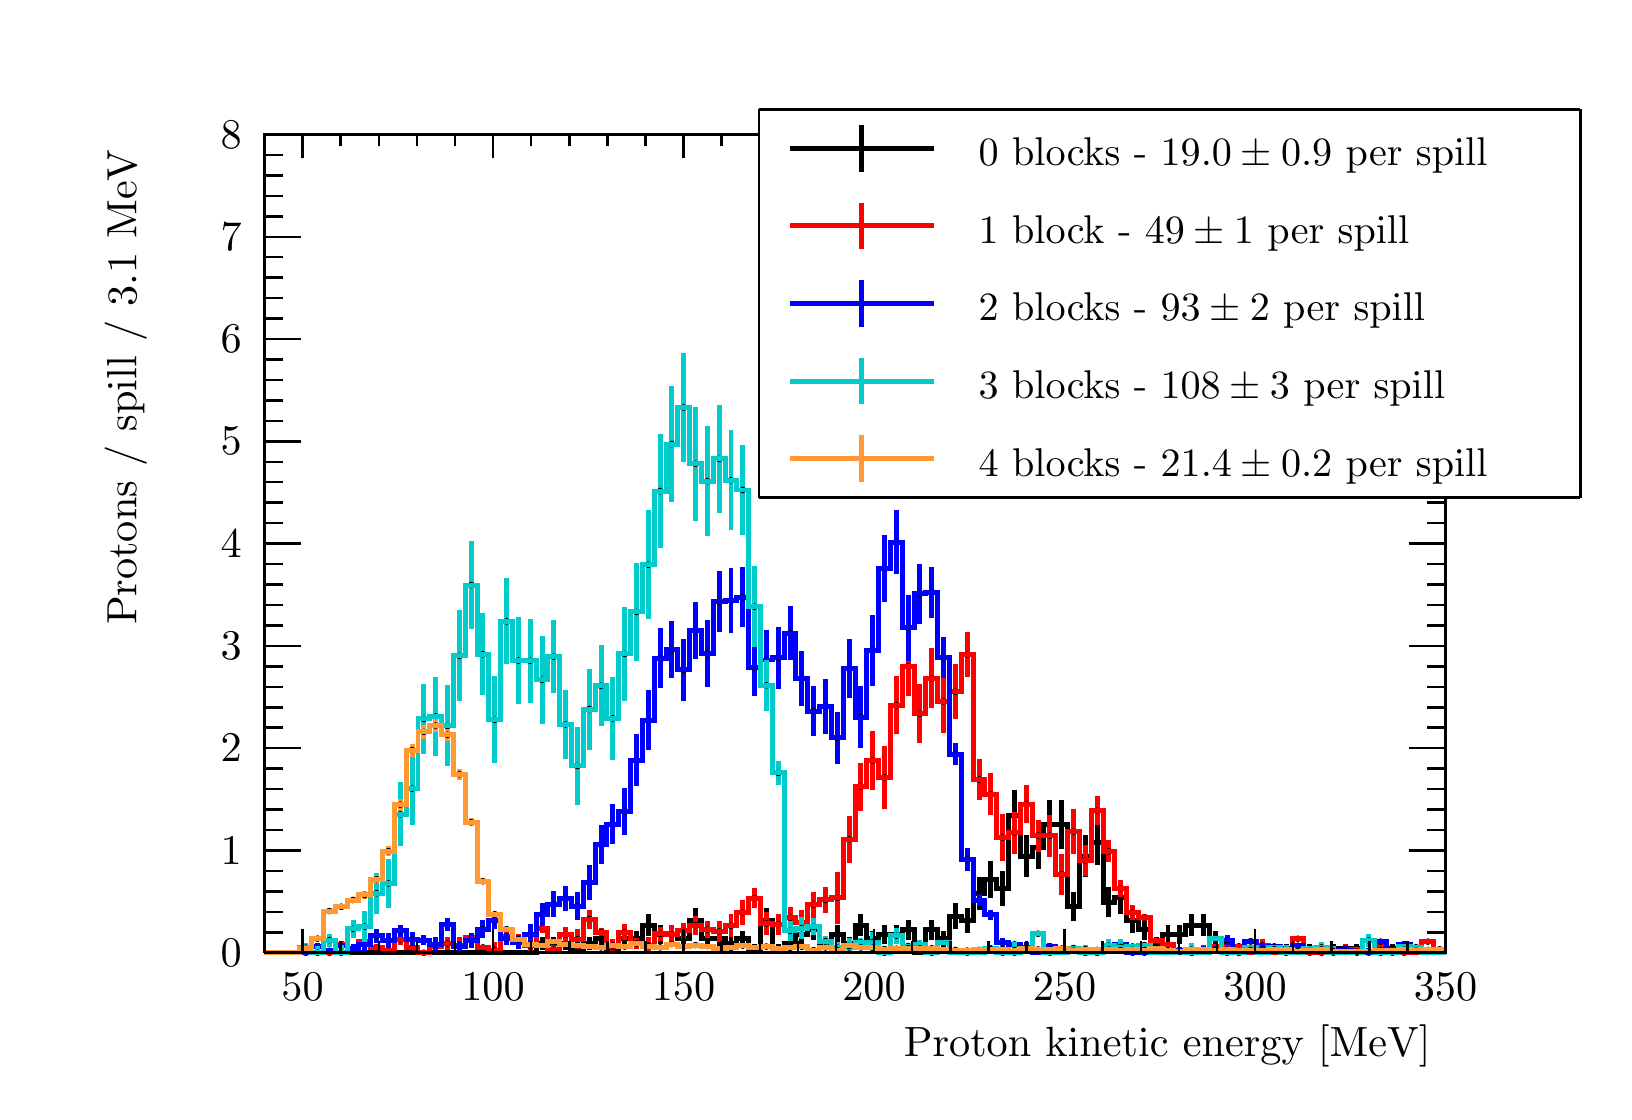
\begin{tikzpicture}
\pgfdeclareplotmark{cross} {
\pgfpathmoveto{\pgfpoint{-0.3\pgfplotmarksize}{\pgfplotmarksize}}
\pgfpathlineto{\pgfpoint{+0.3\pgfplotmarksize}{\pgfplotmarksize}}
\pgfpathlineto{\pgfpoint{+0.3\pgfplotmarksize}{0.3\pgfplotmarksize}}
\pgfpathlineto{\pgfpoint{+1\pgfplotmarksize}{0.3\pgfplotmarksize}}
\pgfpathlineto{\pgfpoint{+1\pgfplotmarksize}{-0.3\pgfplotmarksize}}
\pgfpathlineto{\pgfpoint{+0.3\pgfplotmarksize}{-0.3\pgfplotmarksize}}
\pgfpathlineto{\pgfpoint{+0.3\pgfplotmarksize}{-1.\pgfplotmarksize}}
\pgfpathlineto{\pgfpoint{-0.3\pgfplotmarksize}{-1.\pgfplotmarksize}}
\pgfpathlineto{\pgfpoint{-0.3\pgfplotmarksize}{-0.3\pgfplotmarksize}}
\pgfpathlineto{\pgfpoint{-1.\pgfplotmarksize}{-0.3\pgfplotmarksize}}
\pgfpathlineto{\pgfpoint{-1.\pgfplotmarksize}{0.3\pgfplotmarksize}}
\pgfpathlineto{\pgfpoint{-0.3\pgfplotmarksize}{0.3\pgfplotmarksize}}
\pgfpathclose
\pgfusepathqstroke
}
\pgfdeclareplotmark{cross*} {
\pgfpathmoveto{\pgfpoint{-0.3\pgfplotmarksize}{\pgfplotmarksize}}
\pgfpathlineto{\pgfpoint{+0.3\pgfplotmarksize}{\pgfplotmarksize}}
\pgfpathlineto{\pgfpoint{+0.3\pgfplotmarksize}{0.3\pgfplotmarksize}}
\pgfpathlineto{\pgfpoint{+1\pgfplotmarksize}{0.3\pgfplotmarksize}}
\pgfpathlineto{\pgfpoint{+1\pgfplotmarksize}{-0.3\pgfplotmarksize}}
\pgfpathlineto{\pgfpoint{+0.3\pgfplotmarksize}{-0.3\pgfplotmarksize}}
\pgfpathlineto{\pgfpoint{+0.3\pgfplotmarksize}{-1.\pgfplotmarksize}}
\pgfpathlineto{\pgfpoint{-0.3\pgfplotmarksize}{-1.\pgfplotmarksize}}
\pgfpathlineto{\pgfpoint{-0.3\pgfplotmarksize}{-0.3\pgfplotmarksize}}
\pgfpathlineto{\pgfpoint{-1.\pgfplotmarksize}{-0.3\pgfplotmarksize}}
\pgfpathlineto{\pgfpoint{-1.\pgfplotmarksize}{0.3\pgfplotmarksize}}
\pgfpathlineto{\pgfpoint{-0.3\pgfplotmarksize}{0.3\pgfplotmarksize}}
\pgfpathclose
\pgfusepathqfillstroke
}
\pgfdeclareplotmark{newstar} {
\pgfpathmoveto{\pgfqpoint{0pt}{\pgfplotmarksize}}
\pgfpathlineto{\pgfqpointpolar{44}{0.5\pgfplotmarksize}}
\pgfpathlineto{\pgfqpointpolar{18}{\pgfplotmarksize}}
\pgfpathlineto{\pgfqpointpolar{-20}{0.5\pgfplotmarksize}}
\pgfpathlineto{\pgfqpointpolar{-54}{\pgfplotmarksize}}
\pgfpathlineto{\pgfqpointpolar{-90}{0.5\pgfplotmarksize}}
\pgfpathlineto{\pgfqpointpolar{234}{\pgfplotmarksize}}
\pgfpathlineto{\pgfqpointpolar{198}{0.5\pgfplotmarksize}}
\pgfpathlineto{\pgfqpointpolar{162}{\pgfplotmarksize}}
\pgfpathlineto{\pgfqpointpolar{134}{0.5\pgfplotmarksize}}
\pgfpathclose
\pgfusepathqstroke
}
\pgfdeclareplotmark{newstar*} {
\pgfpathmoveto{\pgfqpoint{0pt}{\pgfplotmarksize}}
\pgfpathlineto{\pgfqpointpolar{44}{0.5\pgfplotmarksize}}
\pgfpathlineto{\pgfqpointpolar{18}{\pgfplotmarksize}}
\pgfpathlineto{\pgfqpointpolar{-20}{0.5\pgfplotmarksize}}
\pgfpathlineto{\pgfqpointpolar{-54}{\pgfplotmarksize}}
\pgfpathlineto{\pgfqpointpolar{-90}{0.5\pgfplotmarksize}}
\pgfpathlineto{\pgfqpointpolar{234}{\pgfplotmarksize}}
\pgfpathlineto{\pgfqpointpolar{198}{0.5\pgfplotmarksize}}
\pgfpathlineto{\pgfqpointpolar{162}{\pgfplotmarksize}}
\pgfpathlineto{\pgfqpointpolar{134}{0.5\pgfplotmarksize}}
\pgfpathclose
\pgfusepathqfillstroke
}
\definecolor{c}{rgb}{1,1,1};
\draw [color=c, fill=c] (0,0) rectangle (20,13.4957);
\draw [color=c, fill=c] (3,1.75444) rectangle (18,12.1461);
\definecolor{c}{rgb}{0,0,0};
\draw [c,line width=0.9] (3,1.75444) -- (3,12.1461) -- (18,12.1461) -- (18,1.75444) -- (3,1.75444);
\definecolor{c}{rgb}{1,1,1};
\draw [color=c, fill=c] (3,1.75444) rectangle (18,12.1461);
\definecolor{c}{rgb}{0,0,0};
\draw [c,line width=0.9] (3,1.75444) -- (3,12.1461) -- (18,12.1461) -- (18,1.75444) -- (3,1.75444);
\draw [c,line width=0.9] (3,1.75444) -- (3.15,1.75444) -- (3.15,1.75444) -- (3.3,1.75444) -- (3.3,1.75444) -- (3.45,1.75444) -- (3.45,1.75444) -- (3.6,1.75444) -- (3.6,1.75444) -- (3.75,1.75444) -- (3.75,1.75444) -- (3.9,1.75444) -- (3.9,1.75444) --
 (4.05,1.75444) -- (4.05,1.75444) -- (4.2,1.75444) -- (4.2,1.75444) -- (4.35,1.75444) -- (4.35,1.75444) -- (4.5,1.75444) -- (4.5,1.75444) -- (4.65,1.75444) -- (4.65,1.75444) -- (4.8,1.75444) -- (4.8,1.75444) -- (4.95,1.75444) -- (4.95,1.75444) --
 (5.1,1.75444) -- (5.1,1.75444) -- (5.25,1.75444) -- (5.25,1.75444) -- (5.4,1.75444) -- (5.4,1.75444) -- (5.55,1.75444) -- (5.55,1.75444) -- (5.7,1.75444) -- (5.7,1.75444) -- (5.85,1.75444) -- (5.85,1.75444) -- (6,1.75444) -- (6,1.75444) --
 (6.15,1.75444) -- (6.15,1.75444) -- (6.3,1.75444) -- (6.3,1.75444) -- (6.45,1.75444) -- (6.45,1.75444) -- (6.6,1.75444) -- (6.6,1.75444) -- (6.75,1.75444) -- (6.75,1.75444) -- (6.9,1.75444) -- (6.9,1.75444) -- (7.05,1.75444) -- (7.05,1.75444) --
 (7.2,1.75444) -- (7.2,1.75444) -- (7.35,1.75444) -- (7.35,1.75444) -- (7.5,1.75444) -- (7.5,1.75444) -- (7.65,1.75444) -- (7.65,1.75444) -- (7.8,1.75444) -- (7.8,1.75444) -- (7.95,1.75444) -- (7.95,1.75444) -- (8.1,1.75444) -- (8.1,1.75444) --
 (8.25,1.75444) -- (8.25,1.75444) -- (8.4,1.75444) -- (8.4,1.75444) -- (8.55,1.75444) -- (8.55,1.75444) -- (8.7,1.75444) -- (8.7,1.75444) -- (8.85,1.75444) -- (8.85,1.75444) -- (9,1.75444) -- (9,1.75444) -- (9.15,1.75444) -- (9.15,1.75444) --
 (9.3,1.75444) -- (9.3,1.75444) -- (9.45,1.75444) -- (9.45,1.75444) -- (9.6,1.75444) -- (9.6,1.75444) -- (9.75,1.75444) -- (9.75,1.75444) -- (9.9,1.75444) -- (9.9,1.75444) -- (10.05,1.75444) -- (10.05,1.75444) -- (10.2,1.75444) -- (10.2,1.75444) --
 (10.35,1.75444) -- (10.35,1.75444) -- (10.5,1.75444) -- (10.5,1.75444) -- (10.65,1.75444) -- (10.65,1.75444) -- (10.8,1.75444) -- (10.8,1.75444) -- (10.95,1.75444) -- (10.95,1.75444) -- (11.1,1.75444) -- (11.1,1.75444) -- (11.25,1.75444) --
 (11.25,1.75444) -- (11.4,1.75444) -- (11.4,1.75444) -- (11.55,1.75444) -- (11.55,1.75444) -- (11.7,1.75444) -- (11.7,1.75444) -- (11.85,1.75444) -- (11.85,1.75444) -- (12,1.75444) -- (12,1.75444) -- (12.15,1.75444) -- (12.15,1.75444) --
 (12.3,1.75444) -- (12.3,1.75444) -- (12.45,1.75444) -- (12.45,1.75444) -- (12.6,1.75444) -- (12.6,1.75444) -- (12.75,1.75444) -- (12.75,1.75444) -- (12.9,1.75444) -- (12.9,1.75444) -- (13.05,1.75444) -- (13.05,1.75444) -- (13.2,1.75444) --
 (13.2,1.75444) -- (13.35,1.75444) -- (13.35,1.75444) -- (13.5,1.75444) -- (13.5,1.75444) -- (13.65,1.75444) -- (13.65,1.75444) -- (13.8,1.75444) -- (13.8,1.75444) -- (13.95,1.75444) -- (13.95,1.75444) -- (14.1,1.75444) -- (14.1,1.75444) --
 (14.25,1.75444) -- (14.25,1.75444) -- (14.4,1.75444) -- (14.4,1.75444) -- (14.55,1.75444) -- (14.55,1.75444) -- (14.7,1.75444) -- (14.7,1.75444) -- (14.85,1.75444) -- (14.85,1.75444) -- (15,1.75444) -- (15,1.75444) -- (15.15,1.75444) --
 (15.15,1.75444) -- (15.3,1.75444) -- (15.3,1.75444) -- (15.45,1.75444) -- (15.45,1.75444) -- (15.6,1.75444) -- (15.6,1.75444) -- (15.75,1.75444) -- (15.75,1.75444) -- (15.9,1.75444) -- (15.9,1.75444) -- (16.05,1.75444) -- (16.05,1.75444) --
 (16.2,1.75444) -- (16.2,1.75444) -- (16.35,1.75444) -- (16.35,1.75444) -- (16.5,1.75444) -- (16.5,1.75444) -- (16.65,1.75444) -- (16.65,1.75444) -- (16.8,1.75444) -- (16.8,1.75444) -- (16.95,1.75444) -- (16.95,1.75444) -- (17.1,1.75444) --
 (17.1,1.75444) -- (17.25,1.75444) -- (17.25,1.75444) -- (17.4,1.75444) -- (17.4,1.75444) -- (17.55,1.75444) -- (17.55,1.75444) -- (17.7,1.75444) -- (17.7,1.75444) -- (17.85,1.75444) -- (17.85,1.75444) -- (18,1.75444);
\draw [c,line width=0.9] (3,1.75444) -- (18,1.75444);
\draw [c,line width=0.9] (3.48387,2.05809) -- (3.48387,1.75444);
\draw [c,line width=0.9] (3.96774,1.90627) -- (3.96774,1.75444);
\draw [c,line width=0.9] (4.45161,1.90627) -- (4.45161,1.75444);
\draw [c,line width=0.9] (4.93548,1.90627) -- (4.93548,1.75444);
\draw [c,line width=0.9] (5.41935,1.90627) -- (5.41935,1.75444);
\draw [c,line width=0.9] (5.90323,2.05809) -- (5.90323,1.75444);
\draw [c,line width=0.9] (6.3871,1.90627) -- (6.3871,1.75444);
\draw [c,line width=0.9] (6.87097,1.90627) -- (6.87097,1.75444);
\draw [c,line width=0.9] (7.35484,1.90627) -- (7.35484,1.75444);
\draw [c,line width=0.9] (7.83871,1.90627) -- (7.83871,1.75444);
\draw [c,line width=0.9] (8.32258,2.05809) -- (8.32258,1.75444);
\draw [c,line width=0.9] (8.80645,1.90627) -- (8.80645,1.75444);
\draw [c,line width=0.9] (9.29032,1.90627) -- (9.29032,1.75444);
\draw [c,line width=0.9] (9.77419,1.90627) -- (9.77419,1.75444);
\draw [c,line width=0.9] (10.2581,1.90627) -- (10.2581,1.75444);
\draw [c,line width=0.9] (10.7419,2.05809) -- (10.7419,1.75444);
\draw [c,line width=0.9] (11.2258,1.90627) -- (11.2258,1.75444);
\draw [c,line width=0.9] (11.7097,1.90627) -- (11.7097,1.75444);
\draw [c,line width=0.9] (12.1935,1.90627) -- (12.1935,1.75444);
\draw [c,line width=0.9] (12.6774,1.90627) -- (12.6774,1.75444);
\draw [c,line width=0.9] (13.1613,2.05809) -- (13.1613,1.75444);
\draw [c,line width=0.9] (13.6452,1.90627) -- (13.6452,1.75444);
\draw [c,line width=0.9] (14.129,1.90627) -- (14.129,1.75444);
\draw [c,line width=0.9] (14.6129,1.90627) -- (14.6129,1.75444);
\draw [c,line width=0.9] (15.0968,1.90627) -- (15.0968,1.75444);
\draw [c,line width=0.9] (15.5806,2.05809) -- (15.5806,1.75444);
\draw [c,line width=0.9] (16.0645,1.90627) -- (16.0645,1.75444);
\draw [c,line width=0.9] (16.5484,1.90627) -- (16.5484,1.75444);
\draw [c,line width=0.9] (17.0323,1.90627) -- (17.0323,1.75444);
\draw [c,line width=0.9] (17.5161,1.90627) -- (17.5161,1.75444);
\draw [c,line width=0.9] (18,2.05809) -- (18,1.75444);
\draw [c,line width=0.9] (3.48387,2.05809) -- (3.48387,1.75444);
\draw [c,line width=0.9] (18,2.05809) -- (18,1.75444);
\draw [anchor=base] (3.48387,1.14713) node[scale=1.52731, color=c, rotate=0]{50};
\draw [anchor=base] (5.90323,1.14713) node[scale=1.52731, color=c, rotate=0]{100};
\draw [anchor=base] (8.32258,1.14713) node[scale=1.52731, color=c, rotate=0]{150};
\draw [anchor=base] (10.7419,1.14713) node[scale=1.52731, color=c, rotate=0]{200};
\draw [anchor=base] (13.1613,1.14713) node[scale=1.52731, color=c, rotate=0]{250};
\draw [anchor=base] (15.5806,1.14713) node[scale=1.52731, color=c, rotate=0]{300};
\draw [anchor=base] (18,1.14713) node[scale=1.52731, color=c, rotate=0]{350};
\draw [anchor= east] (18,0.566819) node[scale=1.52731, color=c, rotate=0]{ Proton kinetic energy [MeV]};
\draw [c,line width=0.9] (3,12.1461) -- (18,12.1461);
\draw [c,line width=0.9] (3.48387,11.8425) -- (3.48387,12.1461);
\draw [c,line width=0.9] (3.96774,11.9943) -- (3.96774,12.1461);
\draw [c,line width=0.9] (4.45161,11.9943) -- (4.45161,12.1461);
\draw [c,line width=0.9] (4.93548,11.9943) -- (4.93548,12.1461);
\draw [c,line width=0.9] (5.41935,11.9943) -- (5.41935,12.1461);
\draw [c,line width=0.9] (5.90323,11.8425) -- (5.90323,12.1461);
\draw [c,line width=0.9] (6.3871,11.9943) -- (6.3871,12.1461);
\draw [c,line width=0.9] (6.87097,11.9943) -- (6.87097,12.1461);
\draw [c,line width=0.9] (7.35484,11.9943) -- (7.35484,12.1461);
\draw [c,line width=0.9] (7.83871,11.9943) -- (7.83871,12.1461);
\draw [c,line width=0.9] (8.32258,11.8425) -- (8.32258,12.1461);
\draw [c,line width=0.9] (8.80645,11.9943) -- (8.80645,12.1461);
\draw [c,line width=0.9] (9.29032,11.9943) -- (9.29032,12.1461);
\draw [c,line width=0.9] (9.77419,11.9943) -- (9.77419,12.1461);
\draw [c,line width=0.9] (10.2581,11.9943) -- (10.2581,12.1461);
\draw [c,line width=0.9] (10.7419,11.8425) -- (10.7419,12.1461);
\draw [c,line width=0.9] (11.2258,11.9943) -- (11.2258,12.1461);
\draw [c,line width=0.9] (11.7097,11.9943) -- (11.7097,12.1461);
\draw [c,line width=0.9] (12.1935,11.9943) -- (12.1935,12.1461);
\draw [c,line width=0.9] (12.6774,11.9943) -- (12.6774,12.1461);
\draw [c,line width=0.9] (13.1613,11.8425) -- (13.1613,12.1461);
\draw [c,line width=0.9] (13.6452,11.9943) -- (13.6452,12.1461);
\draw [c,line width=0.9] (14.129,11.9943) -- (14.129,12.1461);
\draw [c,line width=0.9] (14.6129,11.9943) -- (14.6129,12.1461);
\draw [c,line width=0.9] (15.0968,11.9943) -- (15.0968,12.1461);
\draw [c,line width=0.9] (15.5806,11.8425) -- (15.5806,12.1461);
\draw [c,line width=0.9] (16.0645,11.9943) -- (16.0645,12.1461);
\draw [c,line width=0.9] (16.5484,11.9943) -- (16.5484,12.1461);
\draw [c,line width=0.9] (17.0323,11.9943) -- (17.0323,12.1461);
\draw [c,line width=0.9] (17.5161,11.9943) -- (17.5161,12.1461);
\draw [c,line width=0.9] (18,11.8425) -- (18,12.1461);
\draw [c,line width=0.9] (3.48387,11.8425) -- (3.48387,12.1461);
\draw [c,line width=0.9] (18,11.8425) -- (18,12.1461);
\draw [c,line width=0.9] (3,1.75444) -- (3,12.1461);
\draw [c,line width=0.9] (3.462,1.75444) -- (3,1.75444);
\draw [c,line width=0.9] (3.231,2.01423) -- (3,2.01423);
\draw [c,line width=0.9] (3.231,2.27403) -- (3,2.27403);
\draw [c,line width=0.9] (3.231,2.53382) -- (3,2.53382);
\draw [c,line width=0.9] (3.231,2.79361) -- (3,2.79361);
\draw [c,line width=0.9] (3.462,3.0534) -- (3,3.0534);
\draw [c,line width=0.9] (3.231,3.31319) -- (3,3.31319);
\draw [c,line width=0.9] (3.231,3.57299) -- (3,3.57299);
\draw [c,line width=0.9] (3.231,3.83278) -- (3,3.83278);
\draw [c,line width=0.9] (3.231,4.09257) -- (3,4.09257);
\draw [c,line width=0.9] (3.462,4.35236) -- (3,4.35236);
\draw [c,line width=0.9] (3.231,4.61216) -- (3,4.61216);
\draw [c,line width=0.9] (3.231,4.87195) -- (3,4.87195);
\draw [c,line width=0.9] (3.231,5.13174) -- (3,5.13174);
\draw [c,line width=0.9] (3.231,5.39153) -- (3,5.39153);
\draw [c,line width=0.9] (3.462,5.65133) -- (3,5.65133);
\draw [c,line width=0.9] (3.231,5.91112) -- (3,5.91112);
\draw [c,line width=0.9] (3.231,6.17091) -- (3,6.17091);
\draw [c,line width=0.9] (3.231,6.4307) -- (3,6.4307);
\draw [c,line width=0.9] (3.231,6.69049) -- (3,6.69049);
\draw [c,line width=0.9] (3.462,6.95029) -- (3,6.95029);
\draw [c,line width=0.9] (3.231,7.21008) -- (3,7.21008);
\draw [c,line width=0.9] (3.231,7.46987) -- (3,7.46987);
\draw [c,line width=0.9] (3.231,7.72966) -- (3,7.72966);
\draw [c,line width=0.9] (3.231,7.98946) -- (3,7.98946);
\draw [c,line width=0.9] (3.462,8.24925) -- (3,8.24925);
\draw [c,line width=0.9] (3.231,8.50904) -- (3,8.50904);
\draw [c,line width=0.9] (3.231,8.76883) -- (3,8.76883);
\draw [c,line width=0.9] (3.231,9.02862) -- (3,9.02862);
\draw [c,line width=0.9] (3.231,9.28842) -- (3,9.28842);
\draw [c,line width=0.9] (3.462,9.54821) -- (3,9.54821);
\draw [c,line width=0.9] (3.231,9.808) -- (3,9.808);
\draw [c,line width=0.9] (3.231,10.0678) -- (3,10.0678);
\draw [c,line width=0.9] (3.231,10.3276) -- (3,10.3276);
\draw [c,line width=0.9] (3.231,10.5874) -- (3,10.5874);
\draw [c,line width=0.9] (3.462,10.8472) -- (3,10.8472);
\draw [c,line width=0.9] (3.231,11.107) -- (3,11.107);
\draw [c,line width=0.9] (3.231,11.3668) -- (3,11.3668);
\draw [c,line width=0.9] (3.231,11.6265) -- (3,11.6265);
\draw [c,line width=0.9] (3.231,11.8863) -- (3,11.8863);
\draw [c,line width=0.9] (3.462,12.1461) -- (3,12.1461);
\draw [anchor= east] (2.9,1.75444) node[scale=1.52731, color=c, rotate=0]{0};
\draw [anchor= east] (2.9,3.0534) node[scale=1.52731, color=c, rotate=0]{1};
\draw [anchor= east] (2.9,4.35236) node[scale=1.52731, color=c, rotate=0]{2};
\draw [anchor= east] (2.9,5.65133) node[scale=1.52731, color=c, rotate=0]{3};
\draw [anchor= east] (2.9,6.95029) node[scale=1.52731, color=c, rotate=0]{4};
\draw [anchor= east] (2.9,8.24925) node[scale=1.52731, color=c, rotate=0]{5};
\draw [anchor= east] (2.9,9.54821) node[scale=1.52731, color=c, rotate=0]{6};
\draw [anchor= east] (2.9,10.8472) node[scale=1.52731, color=c, rotate=0]{7};
\draw [anchor= east] (2.9,12.1461) node[scale=1.52731, color=c, rotate=0]{8};
\draw [anchor= east] (1.24,12.1461) node[scale=1.52731, color=c, rotate=90]{ Protons / spill / 3.1~MeV};
\draw [c,line width=0.9] (18,1.75444) -- (18,12.1461);
\draw [c,line width=0.9] (17.538,1.75444) -- (18,1.75444);
\draw [c,line width=0.9] (17.769,2.01423) -- (18,2.01423);
\draw [c,line width=0.9] (17.769,2.27403) -- (18,2.27403);
\draw [c,line width=0.9] (17.769,2.53382) -- (18,2.53382);
\draw [c,line width=0.9] (17.769,2.79361) -- (18,2.79361);
\draw [c,line width=0.9] (17.538,3.0534) -- (18,3.0534);
\draw [c,line width=0.9] (17.769,3.31319) -- (18,3.31319);
\draw [c,line width=0.9] (17.769,3.57299) -- (18,3.57299);
\draw [c,line width=0.9] (17.769,3.83278) -- (18,3.83278);
\draw [c,line width=0.9] (17.769,4.09257) -- (18,4.09257);
\draw [c,line width=0.9] (17.538,4.35236) -- (18,4.35236);
\draw [c,line width=0.9] (17.769,4.61216) -- (18,4.61216);
\draw [c,line width=0.9] (17.769,4.87195) -- (18,4.87195);
\draw [c,line width=0.9] (17.769,5.13174) -- (18,5.13174);
\draw [c,line width=0.9] (17.769,5.39153) -- (18,5.39153);
\draw [c,line width=0.9] (17.538,5.65133) -- (18,5.65133);
\draw [c,line width=0.9] (17.769,5.91112) -- (18,5.91112);
\draw [c,line width=0.9] (17.769,6.17091) -- (18,6.17091);
\draw [c,line width=0.9] (17.769,6.4307) -- (18,6.4307);
\draw [c,line width=0.9] (17.769,6.69049) -- (18,6.69049);
\draw [c,line width=0.9] (17.538,6.95029) -- (18,6.95029);
\draw [c,line width=0.9] (17.769,7.21008) -- (18,7.21008);
\draw [c,line width=0.9] (17.769,7.46987) -- (18,7.46987);
\draw [c,line width=0.9] (17.769,7.72966) -- (18,7.72966);
\draw [c,line width=0.9] (17.769,7.98946) -- (18,7.98946);
\draw [c,line width=0.9] (17.538,8.24925) -- (18,8.24925);
\draw [c,line width=0.9] (17.769,8.50904) -- (18,8.50904);
\draw [c,line width=0.9] (17.769,8.76883) -- (18,8.76883);
\draw [c,line width=0.9] (17.769,9.02862) -- (18,9.02862);
\draw [c,line width=0.9] (17.769,9.28842) -- (18,9.28842);
\draw [c,line width=0.9] (17.538,9.54821) -- (18,9.54821);
\draw [c,line width=0.9] (17.769,9.808) -- (18,9.808);
\draw [c,line width=0.9] (17.769,10.0678) -- (18,10.0678);
\draw [c,line width=0.9] (17.769,10.3276) -- (18,10.3276);
\draw [c,line width=0.9] (17.769,10.5874) -- (18,10.5874);
\draw [c,line width=0.9] (17.538,10.8472) -- (18,10.8472);
\draw [c,line width=0.9] (17.769,11.107) -- (18,11.107);
\draw [c,line width=0.9] (17.769,11.3668) -- (18,11.3668);
\draw [c,line width=0.9] (17.769,11.6265) -- (18,11.6265);
\draw [c,line width=0.9] (17.769,11.8863) -- (18,11.8863);
\draw [c,line width=0.9] (17.538,12.1461) -- (18,12.1461);
\draw [c,line width=1.8] (6.525,1.78858) -- (6.525,1.87103);
\draw [c,line width=1.8] (6.525,1.87103) -- (6.525,1.95347);
\foreach \P in {(6.525,1.87103)}{\draw[mark options={color=c,fill=c},mark size=2.402402pt,mark=*,mark size=1pt] plot coordinates {\P};}
\draw [c,line width=1.8] (6.675,1.78858) -- (6.675,1.87103);
\draw [c,line width=1.8] (6.675,1.87103) -- (6.675,1.95347);
\foreach \P in {(6.675,1.87103)}{\draw[mark options={color=c,fill=c},mark size=2.402402pt,mark=*,mark size=1pt] plot coordinates {\P};}
\draw [c,line width=1.8] (6.825,1.78858) -- (6.825,1.87103);
\draw [c,line width=1.8] (6.825,1.87103) -- (6.825,1.95347);
\foreach \P in {(6.825,1.87103)}{\draw[mark options={color=c,fill=c},mark size=2.402402pt,mark=*,mark size=1pt] plot coordinates {\P};}
\draw [c,line width=1.8] (6.975,1.75444) -- (6.975,1.81273);
\draw [c,line width=1.8] (6.975,1.81273) -- (6.975,1.87103);
\foreach \P in {(6.975,1.81273)}{\draw[mark options={color=c,fill=c},mark size=2.402402pt,mark=*,mark size=1pt] plot coordinates {\P};}
\draw [c,line width=1.8] (7.125,1.78858) -- (7.125,1.87103);
\draw [c,line width=1.8] (7.125,1.87103) -- (7.125,1.95347);
\foreach \P in {(7.125,1.87103)}{\draw[mark options={color=c,fill=c},mark size=2.402402pt,mark=*,mark size=1pt] plot coordinates {\P};}
\draw [c,line width=1.8] (7.275,1.82835) -- (7.275,1.92932);
\draw [c,line width=1.8] (7.275,1.92932) -- (7.275,2.03029);
\foreach \P in {(7.275,1.92932)}{\draw[mark options={color=c,fill=c},mark size=2.402402pt,mark=*,mark size=1pt] plot coordinates {\P};}
\draw [c,line width=1.8] (7.425,1.75444) -- (7.425,1.81273);
\draw [c,line width=1.8] (7.425,1.81273) -- (7.425,1.87103);
\foreach \P in {(7.425,1.81273)}{\draw[mark options={color=c,fill=c},mark size=2.402402pt,mark=*,mark size=1pt] plot coordinates {\P};}
\draw [c,line width=1.8] (7.575,1.82835) -- (7.575,1.92932);
\draw [c,line width=1.8] (7.575,1.92932) -- (7.575,2.03029);
\foreach \P in {(7.575,1.92932)}{\draw[mark options={color=c,fill=c},mark size=2.402402pt,mark=*,mark size=1pt] plot coordinates {\P};}
\draw [c,line width=1.8] (7.725,1.82835) -- (7.725,1.92932);
\draw [c,line width=1.8] (7.725,1.92932) -- (7.725,2.03029);
\foreach \P in {(7.725,1.92932)}{\draw[mark options={color=c,fill=c},mark size=2.402402pt,mark=*,mark size=1pt] plot coordinates {\P};}
\draw [c,line width=1.8] (7.875,1.9614) -- (7.875,2.1042);
\draw [c,line width=1.8] (7.875,2.1042) -- (7.875,2.247);
\foreach \P in {(7.875,2.1042)}{\draw[mark options={color=c,fill=c},mark size=2.402402pt,mark=*,mark size=1pt] plot coordinates {\P};}
\draw [c,line width=1.8] (8.025,1.87102) -- (8.025,1.98761);
\draw [c,line width=1.8] (8.025,1.98761) -- (8.025,2.10421);
\foreach \P in {(8.025,1.98761)}{\draw[mark options={color=c,fill=c},mark size=2.402402pt,mark=*,mark size=1pt] plot coordinates {\P};}
\draw [c,line width=1.8] (8.175,1.87102) -- (8.175,1.98761);
\draw [c,line width=1.8] (8.175,1.98761) -- (8.175,2.10421);
\foreach \P in {(8.175,1.98761)}{\draw[mark options={color=c,fill=c},mark size=2.402402pt,mark=*,mark size=1pt] plot coordinates {\P};}
\draw [c,line width=1.8] (8.325,1.82835) -- (8.325,1.92932);
\draw [c,line width=1.8] (8.325,1.92932) -- (8.325,2.03029);
\foreach \P in {(8.325,1.92932)}{\draw[mark options={color=c,fill=c},mark size=2.402402pt,mark=*,mark size=1pt] plot coordinates {\P};}
\draw [c,line width=1.8] (8.475,2.00825) -- (8.475,2.16249);
\draw [c,line width=1.8] (8.475,2.16249) -- (8.475,2.31673);
\foreach \P in {(8.475,2.16249)}{\draw[mark options={color=c,fill=c},mark size=2.402402pt,mark=*,mark size=1pt] plot coordinates {\P};}
\draw [c,line width=1.8] (8.625,1.82835) -- (8.625,1.92932);
\draw [c,line width=1.8] (8.625,1.92932) -- (8.625,2.03029);
\foreach \P in {(8.625,1.92932)}{\draw[mark options={color=c,fill=c},mark size=2.402402pt,mark=*,mark size=1pt] plot coordinates {\P};}
\draw [c,line width=1.8] (8.775,1.82835) -- (8.775,1.92932);
\draw [c,line width=1.8] (8.775,1.92932) -- (8.775,2.03029);
\foreach \P in {(8.775,1.92932)}{\draw[mark options={color=c,fill=c},mark size=2.402402pt,mark=*,mark size=1pt] plot coordinates {\P};}
\draw [c,line width=1.8] (8.925,1.78858) -- (8.925,1.87103);
\draw [c,line width=1.8] (8.925,1.87103) -- (8.925,1.95347);
\foreach \P in {(8.925,1.87103)}{\draw[mark options={color=c,fill=c},mark size=2.402402pt,mark=*,mark size=1pt] plot coordinates {\P};}
\draw [c,line width=1.8] (9.075,1.82835) -- (9.075,1.92932);
\draw [c,line width=1.8] (9.075,1.92932) -- (9.075,2.03029);
\foreach \P in {(9.075,1.92932)}{\draw[mark options={color=c,fill=c},mark size=2.402402pt,mark=*,mark size=1pt] plot coordinates {\P};}
\draw [c,line width=1.8] (9.225,1.75444) -- (9.225,1.81273);
\draw [c,line width=1.8] (9.225,1.81273) -- (9.225,1.87103);
\foreach \P in {(9.225,1.81273)}{\draw[mark options={color=c,fill=c},mark size=2.402402pt,mark=*,mark size=1pt] plot coordinates {\P};}
\draw [c,line width=1.8] (9.375,2.00825) -- (9.375,2.16249);
\draw [c,line width=1.8] (9.375,2.16249) -- (9.375,2.31673);
\foreach \P in {(9.375,2.16249)}{\draw[mark options={color=c,fill=c},mark size=2.402402pt,mark=*,mark size=1pt] plot coordinates {\P};}
\draw [c,line width=1.8] (9.525,1.75444) -- (9.525,1.81273);
\draw [c,line width=1.8] (9.525,1.81273) -- (9.525,1.87103);
\foreach \P in {(9.525,1.81273)}{\draw[mark options={color=c,fill=c},mark size=2.402402pt,mark=*,mark size=1pt] plot coordinates {\P};}
\draw [c,line width=1.8] (9.675,1.78858) -- (9.675,1.87103);
\draw [c,line width=1.8] (9.675,1.87103) -- (9.675,1.95347);
\foreach \P in {(9.675,1.87103)}{\draw[mark options={color=c,fill=c},mark size=2.402402pt,mark=*,mark size=1pt] plot coordinates {\P};}
\draw [c,line width=1.8] (9.825,1.87102) -- (9.825,1.98761);
\draw [c,line width=1.8] (9.825,1.98761) -- (9.825,2.10421);
\foreach \P in {(9.825,1.98761)}{\draw[mark options={color=c,fill=c},mark size=2.402402pt,mark=*,mark size=1pt] plot coordinates {\P};}
\draw [c,line width=1.8] (9.975,1.91555) -- (9.975,2.04591);
\draw [c,line width=1.8] (9.975,2.04591) -- (9.975,2.17626);
\foreach \P in {(9.975,2.04591)}{\draw[mark options={color=c,fill=c},mark size=2.402402pt,mark=*,mark size=1pt] plot coordinates {\P};}
\draw [c,line width=1.8] (10.125,1.78858) -- (10.125,1.87103);
\draw [c,line width=1.8] (10.125,1.87103) -- (10.125,1.95347);
\foreach \P in {(10.125,1.87103)}{\draw[mark options={color=c,fill=c},mark size=2.402402pt,mark=*,mark size=1pt] plot coordinates {\P};}
\draw [c,line width=1.8] (10.275,1.87102) -- (10.275,1.98761);
\draw [c,line width=1.8] (10.275,1.98761) -- (10.275,2.10421);
\foreach \P in {(10.275,1.98761)}{\draw[mark options={color=c,fill=c},mark size=2.402402pt,mark=*,mark size=1pt] plot coordinates {\P};}
\draw [c,line width=1.8] (10.425,1.78858) -- (10.425,1.87103);
\draw [c,line width=1.8] (10.425,1.87103) -- (10.425,1.95347);
\foreach \P in {(10.425,1.87103)}{\draw[mark options={color=c,fill=c},mark size=2.402402pt,mark=*,mark size=1pt] plot coordinates {\P};}
\draw [c,line width=1.8] (10.575,1.9614) -- (10.575,2.1042);
\draw [c,line width=1.8] (10.575,2.1042) -- (10.575,2.247);
\foreach \P in {(10.575,2.1042)}{\draw[mark options={color=c,fill=c},mark size=2.402402pt,mark=*,mark size=1pt] plot coordinates {\P};}
\draw [c,line width=1.8] (10.725,1.82835) -- (10.725,1.92932);
\draw [c,line width=1.8] (10.725,1.92932) -- (10.725,2.03029);
\foreach \P in {(10.725,1.92932)}{\draw[mark options={color=c,fill=c},mark size=2.402402pt,mark=*,mark size=1pt] plot coordinates {\P};}
\draw [c,line width=1.8] (10.875,1.87102) -- (10.875,1.98761);
\draw [c,line width=1.8] (10.875,1.98761) -- (10.875,2.10421);
\foreach \P in {(10.875,1.98761)}{\draw[mark options={color=c,fill=c},mark size=2.402402pt,mark=*,mark size=1pt] plot coordinates {\P};}
\draw [c,line width=1.8] (11.025,1.87102) -- (11.025,1.98761);
\draw [c,line width=1.8] (11.025,1.98761) -- (11.025,2.10421);
\foreach \P in {(11.025,1.98761)}{\draw[mark options={color=c,fill=c},mark size=2.402402pt,mark=*,mark size=1pt] plot coordinates {\P};}
\draw [c,line width=1.8] (11.175,1.91555) -- (11.175,2.04591);
\draw [c,line width=1.8] (11.175,2.04591) -- (11.175,2.17626);
\foreach \P in {(11.175,2.04591)}{\draw[mark options={color=c,fill=c},mark size=2.402402pt,mark=*,mark size=1pt] plot coordinates {\P};}
\draw [c,line width=1.8] (11.475,1.91555) -- (11.475,2.04591);
\draw [c,line width=1.8] (11.475,2.04591) -- (11.475,2.17626);
\foreach \P in {(11.475,2.04591)}{\draw[mark options={color=c,fill=c},mark size=2.402402pt,mark=*,mark size=1pt] plot coordinates {\P};}
\draw [c,line width=1.8] (11.625,1.82835) -- (11.625,1.92932);
\draw [c,line width=1.8] (11.625,1.92932) -- (11.625,2.03029);
\foreach \P in {(11.625,1.92932)}{\draw[mark options={color=c,fill=c},mark size=2.402402pt,mark=*,mark size=1pt] plot coordinates {\P};}
\draw [c,line width=1.8] (11.775,2.0559) -- (11.775,2.22079);
\draw [c,line width=1.8] (11.775,2.22079) -- (11.775,2.38568);
\foreach \P in {(11.775,2.22079)}{\draw[mark options={color=c,fill=c},mark size=2.402402pt,mark=*,mark size=1pt] plot coordinates {\P};}
\draw [c,line width=1.8] (11.925,2.00825) -- (11.925,2.16249);
\draw [c,line width=1.8] (11.925,2.16249) -- (11.925,2.31673);
\foreach \P in {(11.925,2.16249)}{\draw[mark options={color=c,fill=c},mark size=2.402402pt,mark=*,mark size=1pt] plot coordinates {\P};}
\draw [c,line width=1.8] (12.075,2.30206) -- (12.075,2.51225);
\draw [c,line width=1.8] (12.075,2.51225) -- (12.075,2.72245);
\foreach \P in {(12.075,2.51225)}{\draw[mark options={color=c,fill=c},mark size=2.402402pt,mark=*,mark size=1pt] plot coordinates {\P};}
\draw [c,line width=1.8] (12.225,2.45395) -- (12.225,2.68713);
\draw [c,line width=1.8] (12.225,2.68713) -- (12.225,2.92032);
\foreach \P in {(12.225,2.68713)}{\draw[mark options={color=c,fill=c},mark size=2.402402pt,mark=*,mark size=1pt] plot coordinates {\P};}
\draw [c,line width=1.8] (12.375,2.35242) -- (12.375,2.57055);
\draw [c,line width=1.8] (12.375,2.57055) -- (12.375,2.78867);
\foreach \P in {(12.375,2.57055)}{\draw[mark options={color=c,fill=c},mark size=2.402402pt,mark=*,mark size=1pt] plot coordinates {\P};}
\draw [c,line width=1.8] (12.525,3.18393) -- (12.525,3.50324);
\draw [c,line width=1.8] (12.525,3.50324) -- (12.525,3.82254);
\foreach \P in {(12.525,3.50324)}{\draw[mark options={color=c,fill=c},mark size=2.402402pt,mark=*,mark size=1pt] plot coordinates {\P};}
\draw [c,line width=1.8] (12.675,2.71145) -- (12.675,2.9786);
\draw [c,line width=1.8] (12.675,2.9786) -- (12.675,3.24575);
\foreach \P in {(12.675,2.9786)}{\draw[mark options={color=c,fill=c},mark size=2.402402pt,mark=*,mark size=1pt] plot coordinates {\P};}
\draw [c,line width=1.8] (12.825,2.8156) -- (12.825,3.09519);
\draw [c,line width=1.8] (12.825,3.09519) -- (12.825,3.37477);
\foreach \P in {(12.825,3.09519)}{\draw[mark options={color=c,fill=c},mark size=2.402402pt,mark=*,mark size=1pt] plot coordinates {\P};}
\draw [c,line width=1.8] (12.975,3.07817) -- (12.975,3.38665);
\draw [c,line width=1.8] (12.975,3.38665) -- (12.975,3.69513);
\foreach \P in {(12.975,3.38665)}{\draw[mark options={color=c,fill=c},mark size=2.402402pt,mark=*,mark size=1pt] plot coordinates {\P};}
\draw [c,line width=1.8] (13.125,3.07817) -- (13.125,3.38665);
\draw [c,line width=1.8] (13.125,3.38665) -- (13.125,3.69513);
\foreach \P in {(13.125,3.38665)}{\draw[mark options={color=c,fill=c},mark size=2.402402pt,mark=*,mark size=1pt] plot coordinates {\P};}
\draw [c,line width=1.8] (13.275,2.15302) -- (13.275,2.33737);
\draw [c,line width=1.8] (13.275,2.33737) -- (13.275,2.52172);
\foreach \P in {(13.275,2.33737)}{\draw[mark options={color=c,fill=c},mark size=2.402402pt,mark=*,mark size=1pt] plot coordinates {\P};}
\draw [c,line width=1.8] (13.425,2.71145) -- (13.425,2.9786);
\draw [c,line width=1.8] (13.425,2.9786) -- (13.425,3.24575);
\foreach \P in {(13.425,2.9786)}{\draw[mark options={color=c,fill=c},mark size=2.402402pt,mark=*,mark size=1pt] plot coordinates {\P};}
\draw [c,line width=1.8] (13.575,2.86788) -- (13.575,3.15348);
\draw [c,line width=1.8] (13.575,3.15348) -- (13.575,3.43907);
\foreach \P in {(13.575,3.15348)}{\draw[mark options={color=c,fill=c},mark size=2.402402pt,mark=*,mark size=1pt] plot coordinates {\P};}
\draw [c,line width=1.8] (13.725,2.20232) -- (13.725,2.39567);
\draw [c,line width=1.8] (13.725,2.39567) -- (13.725,2.58902);
\foreach \P in {(13.725,2.39567)}{\draw[mark options={color=c,fill=c},mark size=2.402402pt,mark=*,mark size=1pt] plot coordinates {\P};}
\draw [c,line width=1.8] (13.875,2.25201) -- (13.875,2.45396);
\draw [c,line width=1.8] (13.875,2.45396) -- (13.875,2.65591);
\foreach \P in {(13.875,2.45396)}{\draw[mark options={color=c,fill=c},mark size=2.402402pt,mark=*,mark size=1pt] plot coordinates {\P};}
\draw [c,line width=1.8] (14.025,2.00825) -- (14.025,2.16249);
\draw [c,line width=1.8] (14.025,2.16249) -- (14.025,2.31673);
\foreach \P in {(14.025,2.16249)}{\draw[mark options={color=c,fill=c},mark size=2.402402pt,mark=*,mark size=1pt] plot coordinates {\P};}
\draw [c,line width=1.8] (14.175,1.91555) -- (14.175,2.04591);
\draw [c,line width=1.8] (14.175,2.04591) -- (14.175,2.17626);
\foreach \P in {(14.175,2.04591)}{\draw[mark options={color=c,fill=c},mark size=2.402402pt,mark=*,mark size=1pt] plot coordinates {\P};}
\draw [c,line width=1.8] (14.325,1.78858) -- (14.325,1.87103);
\draw [c,line width=1.8] (14.325,1.87103) -- (14.325,1.95347);
\foreach \P in {(14.325,1.87103)}{\draw[mark options={color=c,fill=c},mark size=2.402402pt,mark=*,mark size=1pt] plot coordinates {\P};}
\draw [c,line width=1.8] (14.475,1.87102) -- (14.475,1.98761);
\draw [c,line width=1.8] (14.475,1.98761) -- (14.475,2.10421);
\foreach \P in {(14.475,1.98761)}{\draw[mark options={color=c,fill=c},mark size=2.402402pt,mark=*,mark size=1pt] plot coordinates {\P};}
\draw [c,line width=1.8] (14.625,1.87102) -- (14.625,1.98761);
\draw [c,line width=1.8] (14.625,1.98761) -- (14.625,2.10421);
\foreach \P in {(14.625,1.98761)}{\draw[mark options={color=c,fill=c},mark size=2.402402pt,mark=*,mark size=1pt] plot coordinates {\P};}
\draw [c,line width=1.8] (14.775,1.9614) -- (14.775,2.1042);
\draw [c,line width=1.8] (14.775,2.1042) -- (14.775,2.247);
\foreach \P in {(14.775,2.1042)}{\draw[mark options={color=c,fill=c},mark size=2.402402pt,mark=*,mark size=1pt] plot coordinates {\P};}
\draw [c,line width=1.8] (14.925,1.9614) -- (14.925,2.1042);
\draw [c,line width=1.8] (14.925,2.1042) -- (14.925,2.247);
\foreach \P in {(14.925,2.1042)}{\draw[mark options={color=c,fill=c},mark size=2.402402pt,mark=*,mark size=1pt] plot coordinates {\P};}
\draw [c,line width=1.8] (15.075,1.82835) -- (15.075,1.92932);
\draw [c,line width=1.8] (15.075,1.92932) -- (15.075,2.03029);
\foreach \P in {(15.075,1.92932)}{\draw[mark options={color=c,fill=c},mark size=2.402402pt,mark=*,mark size=1pt] plot coordinates {\P};}
\draw [c,line width=1.8] (15.225,1.78858) -- (15.225,1.87103);
\draw [c,line width=1.8] (15.225,1.87103) -- (15.225,1.95347);
\foreach \P in {(15.225,1.87103)}{\draw[mark options={color=c,fill=c},mark size=2.402402pt,mark=*,mark size=1pt] plot coordinates {\P};}
\draw [c,line width=1.8] (15.975,1.75444) -- (15.975,1.81273);
\draw [c,line width=1.8] (15.975,1.81273) -- (15.975,1.87103);
\foreach \P in {(15.975,1.81273)}{\draw[mark options={color=c,fill=c},mark size=2.402402pt,mark=*,mark size=1pt] plot coordinates {\P};}
\draw [c,line width=1.8] (16.275,1.75444) -- (16.275,1.81273);
\draw [c,line width=1.8] (16.275,1.81273) -- (16.275,1.87103);
\foreach \P in {(16.275,1.81273)}{\draw[mark options={color=c,fill=c},mark size=2.402402pt,mark=*,mark size=1pt] plot coordinates {\P};}
\draw [c,line width=1.8] (16.575,1.75444) -- (16.575,1.81273);
\draw [c,line width=1.8] (16.575,1.81273) -- (16.575,1.87103);
\foreach \P in {(16.575,1.81273)}{\draw[mark options={color=c,fill=c},mark size=2.402402pt,mark=*,mark size=1pt] plot coordinates {\P};}
\draw [c,line width=1.8] (16.725,1.75444) -- (16.725,1.81273);
\draw [c,line width=1.8] (16.725,1.81273) -- (16.725,1.87103);
\foreach \P in {(16.725,1.81273)}{\draw[mark options={color=c,fill=c},mark size=2.402402pt,mark=*,mark size=1pt] plot coordinates {\P};}
\draw [c,line width=1.8] (16.875,1.75444) -- (16.875,1.81273);
\draw [c,line width=1.8] (16.875,1.81273) -- (16.875,1.87103);
\foreach \P in {(16.875,1.81273)}{\draw[mark options={color=c,fill=c},mark size=2.402402pt,mark=*,mark size=1pt] plot coordinates {\P};}
\draw [c,line width=1.8] (17.175,1.75444) -- (17.175,1.81273);
\draw [c,line width=1.8] (17.175,1.81273) -- (17.175,1.87103);
\foreach \P in {(17.175,1.81273)}{\draw[mark options={color=c,fill=c},mark size=2.402402pt,mark=*,mark size=1pt] plot coordinates {\P};}
\draw [c,line width=1.8] (17.325,1.75444) -- (17.325,1.81273);
\draw [c,line width=1.8] (17.325,1.81273) -- (17.325,1.87103);
\foreach \P in {(17.325,1.81273)}{\draw[mark options={color=c,fill=c},mark size=2.402402pt,mark=*,mark size=1pt] plot coordinates {\P};}
\draw [c,line width=1.8] (3,1.75444) -- (3.15,1.75444) -- (3.15,1.75444) -- (3.3,1.75444) -- (3.3,1.75444) -- (3.45,1.75444) -- (3.45,1.75444) -- (3.6,1.75444) -- (3.6,1.75444) -- (3.75,1.75444) -- (3.75,1.75444) -- (3.9,1.75444) -- (3.9,1.75444) --
 (4.05,1.75444) -- (4.05,1.75444) -- (4.2,1.75444) -- (4.2,1.75444) -- (4.35,1.75444) -- (4.35,1.75444) -- (4.5,1.75444) -- (4.5,1.75444) -- (4.65,1.75444) -- (4.65,1.75444) -- (4.8,1.75444) -- (4.8,1.75444) -- (4.95,1.75444) -- (4.95,1.75444) --
 (5.1,1.75444) -- (5.1,1.75444) -- (5.25,1.75444) -- (5.25,1.75444) -- (5.4,1.75444) -- (5.4,1.75444) -- (5.55,1.75444) -- (5.55,1.75444) -- (5.7,1.75444) -- (5.7,1.75444) -- (5.85,1.75444) -- (5.85,1.75444) -- (6,1.75444) -- (6,1.75444) --
 (6.15,1.75444) -- (6.15,1.75444) -- (6.3,1.75444) -- (6.3,1.75444) -- (6.45,1.75444) -- (6.45,1.87103) -- (6.6,1.87103) -- (6.6,1.87103) -- (6.75,1.87103) -- (6.75,1.87103) -- (6.9,1.87103) -- (6.9,1.81273) -- (7.05,1.81273) -- (7.05,1.87103) --
 (7.2,1.87103) -- (7.2,1.92932) -- (7.35,1.92932) -- (7.35,1.81273) -- (7.5,1.81273) -- (7.5,1.92932) -- (7.65,1.92932) -- (7.65,1.92932) -- (7.8,1.92932) -- (7.8,2.1042) -- (7.95,2.1042) -- (7.95,1.98761) -- (8.1,1.98761) -- (8.1,1.98761) --
 (8.25,1.98761) -- (8.25,1.92932) -- (8.4,1.92932) -- (8.4,2.16249) -- (8.55,2.16249) -- (8.55,1.92932) -- (8.7,1.92932) -- (8.7,1.92932) -- (8.85,1.92932) -- (8.85,1.87103) -- (9,1.87103) -- (9,1.92932) -- (9.15,1.92932) -- (9.15,1.81273) --
 (9.3,1.81273) -- (9.3,2.16249) -- (9.45,2.16249) -- (9.45,1.81273) -- (9.6,1.81273) -- (9.6,1.87103) -- (9.75,1.87103) -- (9.75,1.98761) -- (9.9,1.98761) -- (9.9,2.04591) -- (10.05,2.04591) -- (10.05,1.87103) -- (10.2,1.87103) -- (10.2,1.98761) --
 (10.35,1.98761) -- (10.35,1.87103) -- (10.5,1.87103) -- (10.5,2.1042) -- (10.65,2.1042) -- (10.65,1.92932) -- (10.8,1.92932) -- (10.8,1.98761) -- (10.95,1.98761) -- (10.95,1.98761) -- (11.1,1.98761) -- (11.1,2.04591) -- (11.25,2.04591) --
 (11.25,1.75444) -- (11.4,1.75444) -- (11.4,2.04591) -- (11.55,2.04591) -- (11.55,1.92932) -- (11.7,1.92932) -- (11.7,2.22079) -- (11.85,2.22079) -- (11.85,2.16249) -- (12,2.16249) -- (12,2.51225) -- (12.15,2.51225) -- (12.15,2.68713) --
 (12.3,2.68713) -- (12.3,2.57055) -- (12.45,2.57055) -- (12.45,3.50324) -- (12.6,3.50324) -- (12.6,2.9786) -- (12.75,2.9786) -- (12.75,3.09519) -- (12.9,3.09519) -- (12.9,3.38665) -- (13.05,3.38665) -- (13.05,3.38665) -- (13.2,3.38665) --
 (13.2,2.33737) -- (13.35,2.33737) -- (13.35,2.9786) -- (13.5,2.9786) -- (13.5,3.15348) -- (13.65,3.15348) -- (13.65,2.39567) -- (13.8,2.39567) -- (13.8,2.45396) -- (13.95,2.45396) -- (13.95,2.16249) -- (14.1,2.16249) -- (14.1,2.04591) --
 (14.25,2.04591) -- (14.25,1.87103) -- (14.4,1.87103) -- (14.4,1.98761) -- (14.55,1.98761) -- (14.55,1.98761) -- (14.7,1.98761) -- (14.7,2.1042) -- (14.85,2.1042) -- (14.85,2.1042) -- (15,2.1042) -- (15,1.92932) -- (15.15,1.92932) -- (15.15,1.87103)
 -- (15.3,1.87103) -- (15.3,1.75444) -- (15.45,1.75444) -- (15.45,1.75444) -- (15.6,1.75444) -- (15.6,1.75444) -- (15.75,1.75444) -- (15.75,1.75444) -- (15.9,1.75444) -- (15.9,1.81273) -- (16.05,1.81273) -- (16.05,1.75444) -- (16.2,1.75444) --
 (16.2,1.81273) -- (16.35,1.81273) -- (16.35,1.75444) -- (16.5,1.75444) -- (16.5,1.81273) -- (16.65,1.81273) -- (16.65,1.81273) -- (16.8,1.81273) -- (16.8,1.81273) -- (16.95,1.81273) -- (16.95,1.75444) -- (17.1,1.75444) -- (17.1,1.81273) --
 (17.25,1.81273) -- (17.25,1.81273) -- (17.4,1.81273) -- (17.4,1.75444) -- (17.55,1.75444) -- (17.55,1.75444) -- (17.7,1.75444) -- (17.7,1.75444) -- (17.85,1.75444) -- (17.85,1.75444) -- (18,1.75444);
\definecolor{c}{rgb}{1,0,0};
\draw [c,line width=1.8] (3.825,1.75444) -- (3.825,1.79418);
\definecolor{c}{rgb}{0,0,0};
\foreach \P in {(3.825,1.75444)}{\draw[mark options={color=c,fill=c},mark size=2.402402pt,mark=*,mark size=1pt] plot coordinates {\P};}
\definecolor{c}{rgb}{1,0,0};
\draw [c,line width=1.8] (3.975,1.81208) -- (3.975,1.85866);
\draw [c,line width=1.8] (3.975,1.85866) -- (3.975,1.90523);
\definecolor{c}{rgb}{0,0,0};
\foreach \P in {(3.975,1.85866)}{\draw[mark options={color=c,fill=c},mark size=2.402402pt,mark=*,mark size=1pt] plot coordinates {\P};}
\definecolor{c}{rgb}{1,0,0};
\draw [c,line width=1.8] (4.125,1.75444) -- (4.125,1.78059);
\draw [c,line width=1.8] (4.125,1.78059) -- (4.125,1.83651);
\definecolor{c}{rgb}{0,0,0};
\foreach \P in {(4.125,1.78059)}{\draw[mark options={color=c,fill=c},mark size=2.402402pt,mark=*,mark size=1pt] plot coordinates {\P};}
\definecolor{c}{rgb}{1,0,0};
\draw [c,line width=1.8] (4.275,1.82973) -- (4.275,1.90137);
\draw [c,line width=1.8] (4.275,1.90137) -- (4.275,1.97301);
\definecolor{c}{rgb}{0,0,0};
\foreach \P in {(4.275,1.90137)}{\draw[mark options={color=c,fill=c},mark size=2.402402pt,mark=*,mark size=1pt] plot coordinates {\P};}
\definecolor{c}{rgb}{1,0,0};
\draw [c,line width=1.8] (4.425,1.76197) -- (4.425,1.81571);
\draw [c,line width=1.8] (4.425,1.81571) -- (4.425,1.86945);
\definecolor{c}{rgb}{0,0,0};
\foreach \P in {(4.425,1.81571)}{\draw[mark options={color=c,fill=c},mark size=2.402402pt,mark=*,mark size=1pt] plot coordinates {\P};}
\definecolor{c}{rgb}{1,0,0};
\draw [c,line width=1.8] (4.575,1.75444) -- (4.575,1.78433);
\draw [c,line width=1.8] (4.575,1.78433) -- (4.575,1.83498);
\definecolor{c}{rgb}{0,0,0};
\foreach \P in {(4.575,1.78433)}{\draw[mark options={color=c,fill=c},mark size=2.402402pt,mark=*,mark size=1pt] plot coordinates {\P};}
\definecolor{c}{rgb}{1,0,0};
\draw [c,line width=1.8] (4.725,1.85354) -- (4.725,1.92414);
\draw [c,line width=1.8] (4.725,1.92414) -- (4.725,1.99473);
\definecolor{c}{rgb}{0,0,0};
\foreach \P in {(4.725,1.92414)}{\draw[mark options={color=c,fill=c},mark size=2.402402pt,mark=*,mark size=1pt] plot coordinates {\P};}
\definecolor{c}{rgb}{1,0,0};
\draw [c,line width=1.8] (4.875,1.7723) -- (4.875,1.81827);
\draw [c,line width=1.8] (4.875,1.81827) -- (4.875,1.86424);
\definecolor{c}{rgb}{0,0,0};
\foreach \P in {(4.875,1.81827)}{\draw[mark options={color=c,fill=c},mark size=2.402402pt,mark=*,mark size=1pt] plot coordinates {\P};}
\definecolor{c}{rgb}{1,0,0};
\draw [c,line width=1.8] (5.025,1.75444) -- (5.025,1.7945);
\definecolor{c}{rgb}{0,0,0};
\foreach \P in {(5.025,1.75444)}{\draw[mark options={color=c,fill=c},mark size=2.402402pt,mark=*,mark size=1pt] plot coordinates {\P};}
\definecolor{c}{rgb}{1,0,0};
\draw [c,line width=1.8] (5.175,1.78945) -- (5.175,1.83863);
\draw [c,line width=1.8] (5.175,1.83863) -- (5.175,1.88781);
\definecolor{c}{rgb}{0,0,0};
\foreach \P in {(5.175,1.83863)}{\draw[mark options={color=c,fill=c},mark size=2.402402pt,mark=*,mark size=1pt] plot coordinates {\P};}
\definecolor{c}{rgb}{1,0,0};
\draw [c,line width=1.8] (5.325,1.79196) -- (5.325,1.87186);
\draw [c,line width=1.8] (5.325,1.87186) -- (5.325,1.95177);
\definecolor{c}{rgb}{0,0,0};
\foreach \P in {(5.325,1.87186)}{\draw[mark options={color=c,fill=c},mark size=2.402402pt,mark=*,mark size=1pt] plot coordinates {\P};}
\definecolor{c}{rgb}{1,0,0};
\draw [c,line width=1.8] (5.475,1.75444) -- (5.475,1.85106);
\draw [c,line width=1.8] (5.475,1.85106) -- (5.475,1.95509);
\definecolor{c}{rgb}{0,0,0};
\foreach \P in {(5.475,1.85106)}{\draw[mark options={color=c,fill=c},mark size=2.402402pt,mark=*,mark size=1pt] plot coordinates {\P};}
\definecolor{c}{rgb}{1,0,0};
\draw [c,line width=1.8] (5.625,1.90439) -- (5.625,1.95279);
\draw [c,line width=1.8] (5.625,1.95279) -- (5.625,2.0012);
\definecolor{c}{rgb}{0,0,0};
\foreach \P in {(5.625,1.95279)}{\draw[mark options={color=c,fill=c},mark size=2.402402pt,mark=*,mark size=1pt] plot coordinates {\P};}
\definecolor{c}{rgb}{1,0,0};
\draw [c,line width=1.8] (5.775,1.78821) -- (5.775,1.82195);
\draw [c,line width=1.8] (5.775,1.82195) -- (5.775,1.8557);
\definecolor{c}{rgb}{0,0,0};
\foreach \P in {(5.775,1.82195)}{\draw[mark options={color=c,fill=c},mark size=2.402402pt,mark=*,mark size=1pt] plot coordinates {\P};}
\definecolor{c}{rgb}{1,0,0};
\draw [c,line width=1.8] (5.925,1.75444) -- (5.925,1.78786);
\draw [c,line width=1.8] (5.925,1.78786) -- (5.925,1.88569);
\definecolor{c}{rgb}{0,0,0};
\foreach \P in {(5.925,1.78786)}{\draw[mark options={color=c,fill=c},mark size=2.402402pt,mark=*,mark size=1pt] plot coordinates {\P};}
\definecolor{c}{rgb}{1,0,0};
\draw [c,line width=1.8] (6.075,1.89582) -- (6.075,1.96401);
\draw [c,line width=1.8] (6.075,1.96401) -- (6.075,2.0322);
\definecolor{c}{rgb}{0,0,0};
\foreach \P in {(6.075,1.96401)}{\draw[mark options={color=c,fill=c},mark size=2.402402pt,mark=*,mark size=1pt] plot coordinates {\P};}
\definecolor{c}{rgb}{1,0,0};
\draw [c,line width=1.8] (6.225,1.80882) -- (6.225,1.90036);
\draw [c,line width=1.8] (6.225,1.90036) -- (6.225,1.9919);
\definecolor{c}{rgb}{0,0,0};
\foreach \P in {(6.225,1.90036)}{\draw[mark options={color=c,fill=c},mark size=2.402402pt,mark=*,mark size=1pt] plot coordinates {\P};}
\definecolor{c}{rgb}{1,0,0};
\draw [c,line width=1.8] (6.375,1.75444) -- (6.375,1.83998);
\draw [c,line width=1.8] (6.375,1.83998) -- (6.375,1.94236);
\definecolor{c}{rgb}{0,0,0};
\foreach \P in {(6.375,1.83998)}{\draw[mark options={color=c,fill=c},mark size=2.402402pt,mark=*,mark size=1pt] plot coordinates {\P};}
\definecolor{c}{rgb}{1,0,0};
\draw [c,line width=1.8] (6.525,2.00308) -- (6.525,2.06767);
\draw [c,line width=1.8] (6.525,2.06767) -- (6.525,2.13227);
\definecolor{c}{rgb}{0,0,0};
\foreach \P in {(6.525,2.06767)}{\draw[mark options={color=c,fill=c},mark size=2.402402pt,mark=*,mark size=1pt] plot coordinates {\P};}
\definecolor{c}{rgb}{1,0,0};
\draw [c,line width=1.8] (6.675,1.75444) -- (6.675,1.79446);
\draw [c,line width=1.8] (6.675,1.79446) -- (6.675,1.88854);
\definecolor{c}{rgb}{0,0,0};
\foreach \P in {(6.675,1.79446)}{\draw[mark options={color=c,fill=c},mark size=2.402402pt,mark=*,mark size=1pt] plot coordinates {\P};}
\definecolor{c}{rgb}{1,0,0};
\draw [c,line width=1.8] (6.825,1.88534) -- (6.825,1.98055);
\draw [c,line width=1.8] (6.825,1.98055) -- (6.825,2.07575);
\definecolor{c}{rgb}{0,0,0};
\foreach \P in {(6.825,1.98055)}{\draw[mark options={color=c,fill=c},mark size=2.402402pt,mark=*,mark size=1pt] plot coordinates {\P};}
\definecolor{c}{rgb}{1,0,0};
\draw [c,line width=1.8] (6.975,1.79932) -- (6.975,1.92575);
\draw [c,line width=1.8] (6.975,1.92575) -- (6.975,2.05219);
\definecolor{c}{rgb}{0,0,0};
\foreach \P in {(6.975,1.92575)}{\draw[mark options={color=c,fill=c},mark size=2.402402pt,mark=*,mark size=1pt] plot coordinates {\P};}
\definecolor{c}{rgb}{1,0,0};
\draw [c,line width=1.8] (7.125,2.06042) -- (7.125,2.1811);
\draw [c,line width=1.8] (7.125,2.1811) -- (7.125,2.30177);
\definecolor{c}{rgb}{0,0,0};
\foreach \P in {(7.125,2.1811)}{\draw[mark options={color=c,fill=c},mark size=2.402402pt,mark=*,mark size=1pt] plot coordinates {\P};}
\definecolor{c}{rgb}{1,0,0};
\draw [c,line width=1.8] (7.275,1.96506) -- (7.275,2.01699);
\draw [c,line width=1.8] (7.275,2.01699) -- (7.275,2.06892);
\definecolor{c}{rgb}{0,0,0};
\foreach \P in {(7.275,2.01699)}{\draw[mark options={color=c,fill=c},mark size=2.402402pt,mark=*,mark size=1pt] plot coordinates {\P};}
\definecolor{c}{rgb}{1,0,0};
\draw [c,line width=1.8] (7.425,1.75444) -- (7.425,1.82802);
\draw [c,line width=1.8] (7.425,1.82802) -- (7.425,1.93007);
\definecolor{c}{rgb}{0,0,0};
\foreach \P in {(7.425,1.82802)}{\draw[mark options={color=c,fill=c},mark size=2.402402pt,mark=*,mark size=1pt] plot coordinates {\P};}
\definecolor{c}{rgb}{1,0,0};
\draw [c,line width=1.8] (7.575,1.9184) -- (7.575,2.01681);
\draw [c,line width=1.8] (7.575,2.01681) -- (7.575,2.11523);
\definecolor{c}{rgb}{0,0,0};
\foreach \P in {(7.575,2.01681)}{\draw[mark options={color=c,fill=c},mark size=2.402402pt,mark=*,mark size=1pt] plot coordinates {\P};}
\definecolor{c}{rgb}{1,0,0};
\draw [c,line width=1.8] (7.725,1.80478) -- (7.725,1.87129);
\draw [c,line width=1.8] (7.725,1.87129) -- (7.725,1.93781);
\definecolor{c}{rgb}{0,0,0};
\foreach \P in {(7.725,1.87129)}{\draw[mark options={color=c,fill=c},mark size=2.402402pt,mark=*,mark size=1pt] plot coordinates {\P};}
\definecolor{c}{rgb}{1,0,0};
\draw [c,line width=1.8] (7.875,1.75444) -- (7.875,1.84602);
\draw [c,line width=1.8] (7.875,1.84602) -- (7.875,1.95722);
\definecolor{c}{rgb}{0,0,0};
\foreach \P in {(7.875,1.84602)}{\draw[mark options={color=c,fill=c},mark size=2.402402pt,mark=*,mark size=1pt] plot coordinates {\P};}
\definecolor{c}{rgb}{1,0,0};
\draw [c,line width=1.8] (8.025,1.9075) -- (8.025,1.99527);
\draw [c,line width=1.8] (8.025,1.99527) -- (8.025,2.08304);
\definecolor{c}{rgb}{0,0,0};
\foreach \P in {(8.025,1.99527)}{\draw[mark options={color=c,fill=c},mark size=2.402402pt,mark=*,mark size=1pt] plot coordinates {\P};}
\definecolor{c}{rgb}{1,0,0};
\draw [c,line width=1.8] (8.175,1.87216) -- (8.175,1.98644);
\draw [c,line width=1.8] (8.175,1.98644) -- (8.175,2.10073);
\definecolor{c}{rgb}{0,0,0};
\foreach \P in {(8.175,1.98644)}{\draw[mark options={color=c,fill=c},mark size=2.402402pt,mark=*,mark size=1pt] plot coordinates {\P};}
\definecolor{c}{rgb}{1,0,0};
\draw [c,line width=1.8] (8.325,1.92769) -- (8.325,2.03287);
\draw [c,line width=1.8] (8.325,2.03287) -- (8.325,2.13804);
\definecolor{c}{rgb}{0,0,0};
\foreach \P in {(8.325,2.03287)}{\draw[mark options={color=c,fill=c},mark size=2.402402pt,mark=*,mark size=1pt] plot coordinates {\P};}
\definecolor{c}{rgb}{1,0,0};
\draw [c,line width=1.8] (8.475,1.9841) -- (8.475,2.10511);
\draw [c,line width=1.8] (8.475,2.10511) -- (8.475,2.22613);
\definecolor{c}{rgb}{0,0,0};
\foreach \P in {(8.475,2.10511)}{\draw[mark options={color=c,fill=c},mark size=2.402402pt,mark=*,mark size=1pt] plot coordinates {\P};}
\definecolor{c}{rgb}{1,0,0};
\draw [c,line width=1.8] (8.625,1.9355) -- (8.625,2.04898);
\draw [c,line width=1.8] (8.625,2.04898) -- (8.625,2.16246);
\definecolor{c}{rgb}{0,0,0};
\foreach \P in {(8.625,2.04898)}{\draw[mark options={color=c,fill=c},mark size=2.402402pt,mark=*,mark size=1pt] plot coordinates {\P};}
\definecolor{c}{rgb}{1,0,0};
\draw [c,line width=1.8] (8.775,1.89701) -- (8.775,2.02581);
\draw [c,line width=1.8] (8.775,2.02581) -- (8.775,2.15461);
\definecolor{c}{rgb}{0,0,0};
\foreach \P in {(8.775,2.02581)}{\draw[mark options={color=c,fill=c},mark size=2.402402pt,mark=*,mark size=1pt] plot coordinates {\P};}
\definecolor{c}{rgb}{1,0,0};
\draw [c,line width=1.8] (8.925,1.94848) -- (8.925,2.09562);
\draw [c,line width=1.8] (8.925,2.09562) -- (8.925,2.24276);
\definecolor{c}{rgb}{0,0,0};
\foreach \P in {(8.925,2.09562)}{\draw[mark options={color=c,fill=c},mark size=2.402402pt,mark=*,mark size=1pt] plot coordinates {\P};}
\definecolor{c}{rgb}{1,0,0};
\draw [c,line width=1.8] (9.075,2.10407) -- (9.075,2.2654);
\draw [c,line width=1.8] (9.075,2.2654) -- (9.075,2.42673);
\definecolor{c}{rgb}{0,0,0};
\foreach \P in {(9.075,2.2654)}{\draw[mark options={color=c,fill=c},mark size=2.402402pt,mark=*,mark size=1pt] plot coordinates {\P};}
\definecolor{c}{rgb}{1,0,0};
\draw [c,line width=1.8] (9.225,2.32275) -- (9.225,2.44824);
\draw [c,line width=1.8] (9.225,2.44824) -- (9.225,2.57372);
\definecolor{c}{rgb}{0,0,0};
\foreach \P in {(9.225,2.44824)}{\draw[mark options={color=c,fill=c},mark size=2.402402pt,mark=*,mark size=1pt] plot coordinates {\P};}
\definecolor{c}{rgb}{1,0,0};
\draw [c,line width=1.8] (9.375,1.98595) -- (9.375,2.12575);
\draw [c,line width=1.8] (9.375,2.12575) -- (9.375,2.26555);
\definecolor{c}{rgb}{0,0,0};
\foreach \P in {(9.375,2.12575)}{\draw[mark options={color=c,fill=c},mark size=2.402402pt,mark=*,mark size=1pt] plot coordinates {\P};}
\definecolor{c}{rgb}{1,0,0};
\draw [c,line width=1.8] (9.525,1.98546) -- (9.525,2.11825);
\draw [c,line width=1.8] (9.525,2.11825) -- (9.525,2.25105);
\definecolor{c}{rgb}{0,0,0};
\foreach \P in {(9.525,2.11825)}{\draw[mark options={color=c,fill=c},mark size=2.402402pt,mark=*,mark size=1pt] plot coordinates {\P};}
\definecolor{c}{rgb}{1,0,0};
\draw [c,line width=1.8] (9.675,2.05727) -- (9.675,2.19774);
\draw [c,line width=1.8] (9.675,2.19774) -- (9.675,2.33822);
\definecolor{c}{rgb}{0,0,0};
\foreach \P in {(9.675,2.19774)}{\draw[mark options={color=c,fill=c},mark size=2.402402pt,mark=*,mark size=1pt] plot coordinates {\P};}
\definecolor{c}{rgb}{1,0,0};
\draw [c,line width=1.8] (9.825,1.97223) -- (9.825,2.13577);
\draw [c,line width=1.8] (9.825,2.13577) -- (9.825,2.29931);
\definecolor{c}{rgb}{0,0,0};
\foreach \P in {(9.825,2.13577)}{\draw[mark options={color=c,fill=c},mark size=2.402402pt,mark=*,mark size=1pt] plot coordinates {\P};}
\definecolor{c}{rgb}{1,0,0};
\draw [c,line width=1.8] (9.975,2.19467) -- (9.975,2.36275);
\draw [c,line width=1.8] (9.975,2.36275) -- (9.975,2.53084);
\definecolor{c}{rgb}{0,0,0};
\foreach \P in {(9.975,2.36275)}{\draw[mark options={color=c,fill=c},mark size=2.402402pt,mark=*,mark size=1pt] plot coordinates {\P};}
\definecolor{c}{rgb}{1,0,0};
\draw [c,line width=1.8] (10.125,2.26174) -- (10.125,2.42526);
\draw [c,line width=1.8] (10.125,2.42526) -- (10.125,2.58878);
\definecolor{c}{rgb}{0,0,0};
\foreach \P in {(10.125,2.42526)}{\draw[mark options={color=c,fill=c},mark size=2.402402pt,mark=*,mark size=1pt] plot coordinates {\P};}
\definecolor{c}{rgb}{1,0,0};
\draw [c,line width=1.8] (10.275,2.12199) -- (10.275,2.45174);
\draw [c,line width=1.8] (10.275,2.45174) -- (10.275,2.78149);
\definecolor{c}{rgb}{0,0,0};
\foreach \P in {(10.275,2.45174)}{\draw[mark options={color=c,fill=c},mark size=2.402402pt,mark=*,mark size=1pt] plot coordinates {\P};}
\definecolor{c}{rgb}{1,0,0};
\draw [c,line width=1.8] (10.425,2.89569) -- (10.425,3.19553);
\draw [c,line width=1.8] (10.425,3.19553) -- (10.425,3.49536);
\definecolor{c}{rgb}{0,0,0};
\foreach \P in {(10.425,3.19553)}{\draw[mark options={color=c,fill=c},mark size=2.402402pt,mark=*,mark size=1pt] plot coordinates {\P};}
\definecolor{c}{rgb}{1,0,0};
\draw [c,line width=1.8] (10.575,3.5605) -- (10.575,3.86209);
\draw [c,line width=1.8] (10.575,3.86209) -- (10.575,4.16369);
\definecolor{c}{rgb}{0,0,0};
\foreach \P in {(10.575,3.86209)}{\draw[mark options={color=c,fill=c},mark size=2.402402pt,mark=*,mark size=1pt] plot coordinates {\P};}
\definecolor{c}{rgb}{1,0,0};
\draw [c,line width=1.8] (10.725,3.81791) -- (10.725,4.1945);
\draw [c,line width=1.8] (10.725,4.1945) -- (10.725,4.5711);
\definecolor{c}{rgb}{0,0,0};
\foreach \P in {(10.725,4.1945)}{\draw[mark options={color=c,fill=c},mark size=2.402402pt,mark=*,mark size=1pt] plot coordinates {\P};}
\definecolor{c}{rgb}{1,0,0};
\draw [c,line width=1.8] (10.875,3.57663) -- (10.875,3.98103);
\draw [c,line width=1.8] (10.875,3.98103) -- (10.875,4.38542);
\definecolor{c}{rgb}{0,0,0};
\foreach \P in {(10.875,3.98103)}{\draw[mark options={color=c,fill=c},mark size=2.402402pt,mark=*,mark size=1pt] plot coordinates {\P};}
\definecolor{c}{rgb}{1,0,0};
\draw [c,line width=1.8] (11.025,4.52898) -- (11.025,4.89698);
\draw [c,line width=1.8] (11.025,4.89698) -- (11.025,5.26498);
\definecolor{c}{rgb}{0,0,0};
\foreach \P in {(11.025,4.89698)}{\draw[mark options={color=c,fill=c},mark size=2.402402pt,mark=*,mark size=1pt] plot coordinates {\P};}
\definecolor{c}{rgb}{1,0,0};
\draw [c,line width=1.8] (11.175,5.01251) -- (11.175,5.39403);
\draw [c,line width=1.8] (11.175,5.39403) -- (11.175,5.77555);
\definecolor{c}{rgb}{0,0,0};
\foreach \P in {(11.175,5.39403)}{\draw[mark options={color=c,fill=c},mark size=2.402402pt,mark=*,mark size=1pt] plot coordinates {\P};}
\definecolor{c}{rgb}{1,0,0};
\draw [c,line width=1.8] (11.325,4.41705) -- (11.325,4.79016);
\draw [c,line width=1.8] (11.325,4.79016) -- (11.325,5.16327);
\definecolor{c}{rgb}{0,0,0};
\foreach \P in {(11.325,4.79016)}{\draw[mark options={color=c,fill=c},mark size=2.402402pt,mark=*,mark size=1pt] plot coordinates {\P};}
\definecolor{c}{rgb}{1,0,0};
\draw [c,line width=1.8] (11.475,4.85702) -- (11.475,5.23792);
\draw [c,line width=1.8] (11.475,5.23792) -- (11.475,5.61882);
\definecolor{c}{rgb}{0,0,0};
\foreach \P in {(11.475,5.23792)}{\draw[mark options={color=c,fill=c},mark size=2.402402pt,mark=*,mark size=1pt] plot coordinates {\P};}
\definecolor{c}{rgb}{1,0,0};
\draw [c,line width=1.8] (11.625,4.54922) -- (11.625,4.94645);
\draw [c,line width=1.8] (11.625,4.94645) -- (11.625,5.34368);
\definecolor{c}{rgb}{0,0,0};
\foreach \P in {(11.625,4.94645)}{\draw[mark options={color=c,fill=c},mark size=2.402402pt,mark=*,mark size=1pt] plot coordinates {\P};}
\definecolor{c}{rgb}{1,0,0};
\draw [c,line width=1.8] (11.775,4.71957) -- (11.775,5.06831);
\draw [c,line width=1.8] (11.775,5.06831) -- (11.775,5.41705);
\definecolor{c}{rgb}{0,0,0};
\foreach \P in {(11.775,5.06831)}{\draw[mark options={color=c,fill=c},mark size=2.402402pt,mark=*,mark size=1pt] plot coordinates {\P};}
\definecolor{c}{rgb}{1,0,0};
\draw [c,line width=1.8] (11.925,5.25457) -- (11.925,5.5383);
\draw [c,line width=1.8] (11.925,5.5383) -- (11.925,5.82203);
\definecolor{c}{rgb}{0,0,0};
\foreach \P in {(11.925,5.5383)}{\draw[mark options={color=c,fill=c},mark size=2.402402pt,mark=*,mark size=1pt] plot coordinates {\P};}
\definecolor{c}{rgb}{1,0,0};
\draw [c,line width=1.8] (12.075,3.69701) -- (12.075,3.9545);
\draw [c,line width=1.8] (12.075,3.9545) -- (12.075,4.21199);
\definecolor{c}{rgb}{0,0,0};
\foreach \P in {(12.075,3.9545)}{\draw[mark options={color=c,fill=c},mark size=2.402402pt,mark=*,mark size=1pt] plot coordinates {\P};}
\definecolor{c}{rgb}{1,0,0};
\draw [c,line width=1.8] (12.225,3.50348) -- (12.225,3.76786);
\draw [c,line width=1.8] (12.225,3.76786) -- (12.225,4.03224);
\definecolor{c}{rgb}{0,0,0};
\foreach \P in {(12.225,3.76786)}{\draw[mark options={color=c,fill=c},mark size=2.402402pt,mark=*,mark size=1pt] plot coordinates {\P};}
\definecolor{c}{rgb}{1,0,0};
\draw [c,line width=1.8] (12.375,2.92398) -- (12.375,3.21712);
\draw [c,line width=1.8] (12.375,3.21712) -- (12.375,3.51026);
\definecolor{c}{rgb}{0,0,0};
\foreach \P in {(12.375,3.21712)}{\draw[mark options={color=c,fill=c},mark size=2.402402pt,mark=*,mark size=1pt] plot coordinates {\P};}
\definecolor{c}{rgb}{1,0,0};
\draw [c,line width=1.8] (12.525,3.00903) -- (12.525,3.27808);
\draw [c,line width=1.8] (12.525,3.27808) -- (12.525,3.54713);
\definecolor{c}{rgb}{0,0,0};
\foreach \P in {(12.525,3.27808)}{\draw[mark options={color=c,fill=c},mark size=2.402402pt,mark=*,mark size=1pt] plot coordinates {\P};}
\definecolor{c}{rgb}{1,0,0};
\draw [c,line width=1.8] (12.675,3.40362) -- (12.675,3.64223);
\draw [c,line width=1.8] (12.675,3.64223) -- (12.675,3.88084);
\definecolor{c}{rgb}{0,0,0};
\foreach \P in {(12.675,3.64223)}{\draw[mark options={color=c,fill=c},mark size=2.402402pt,mark=*,mark size=1pt] plot coordinates {\P};}
\definecolor{c}{rgb}{1,0,0};
\draw [c,line width=1.8] (12.825,3.03977) -- (12.825,3.24254);
\draw [c,line width=1.8] (12.825,3.24254) -- (12.825,3.44531);
\definecolor{c}{rgb}{0,0,0};
\foreach \P in {(12.825,3.24254)}{\draw[mark options={color=c,fill=c},mark size=2.402402pt,mark=*,mark size=1pt] plot coordinates {\P};}
\definecolor{c}{rgb}{1,0,0};
\draw [c,line width=1.8] (12.975,2.9762) -- (12.975,3.24022);
\draw [c,line width=1.8] (12.975,3.24022) -- (12.975,3.50423);
\definecolor{c}{rgb}{0,0,0};
\foreach \P in {(12.975,3.24022)}{\draw[mark options={color=c,fill=c},mark size=2.402402pt,mark=*,mark size=1pt] plot coordinates {\P};}
\definecolor{c}{rgb}{1,0,0};
\draw [c,line width=1.8] (13.125,2.4858) -- (13.125,2.74859);
\draw [c,line width=1.8] (13.125,2.74859) -- (13.125,3.01139);
\definecolor{c}{rgb}{0,0,0};
\foreach \P in {(13.125,2.74859)}{\draw[mark options={color=c,fill=c},mark size=2.402402pt,mark=*,mark size=1pt] plot coordinates {\P};}
\definecolor{c}{rgb}{1,0,0};
\draw [c,line width=1.8] (13.275,3.00876) -- (13.275,3.29341);
\draw [c,line width=1.8] (13.275,3.29341) -- (13.275,3.57806);
\definecolor{c}{rgb}{0,0,0};
\foreach \P in {(13.275,3.29341)}{\draw[mark options={color=c,fill=c},mark size=2.402402pt,mark=*,mark size=1pt] plot coordinates {\P};}
\definecolor{c}{rgb}{1,0,0};
\draw [c,line width=1.8] (13.425,2.72662) -- (13.425,2.92341);
\draw [c,line width=1.8] (13.425,2.92341) -- (13.425,3.12019);
\definecolor{c}{rgb}{0,0,0};
\foreach \P in {(13.425,2.92341)}{\draw[mark options={color=c,fill=c},mark size=2.402402pt,mark=*,mark size=1pt] plot coordinates {\P};}
\definecolor{c}{rgb}{1,0,0};
\draw [c,line width=1.8] (13.575,3.37407) -- (13.575,3.55824);
\draw [c,line width=1.8] (13.575,3.55824) -- (13.575,3.74241);
\definecolor{c}{rgb}{0,0,0};
\foreach \P in {(13.575,3.55824)}{\draw[mark options={color=c,fill=c},mark size=2.402402pt,mark=*,mark size=1pt] plot coordinates {\P};}
\definecolor{c}{rgb}{1,0,0};
\draw [c,line width=1.8] (13.725,2.90165) -- (13.725,3.04193);
\draw [c,line width=1.8] (13.725,3.04193) -- (13.725,3.1822);
\definecolor{c}{rgb}{0,0,0};
\foreach \P in {(13.725,3.04193)}{\draw[mark options={color=c,fill=c},mark size=2.402402pt,mark=*,mark size=1pt] plot coordinates {\P};}
\definecolor{c}{rgb}{1,0,0};
\draw [c,line width=1.8] (13.875,2.46165) -- (13.875,2.56985);
\draw [c,line width=1.8] (13.875,2.56985) -- (13.875,2.67805);
\definecolor{c}{rgb}{0,0,0};
\foreach \P in {(13.875,2.56985)}{\draw[mark options={color=c,fill=c},mark size=2.402402pt,mark=*,mark size=1pt] plot coordinates {\P};}
\definecolor{c}{rgb}{1,0,0};
\draw [c,line width=1.8] (14.025,2.16863) -- (14.025,2.26688);
\draw [c,line width=1.8] (14.025,2.26688) -- (14.025,2.36514);
\definecolor{c}{rgb}{0,0,0};
\foreach \P in {(14.025,2.26688)}{\draw[mark options={color=c,fill=c},mark size=2.402402pt,mark=*,mark size=1pt] plot coordinates {\P};}
\definecolor{c}{rgb}{1,0,0};
\draw [c,line width=1.8] (14.175,2.15488) -- (14.175,2.1994);
\draw [c,line width=1.8] (14.175,2.1994) -- (14.175,2.24392);
\definecolor{c}{rgb}{0,0,0};
\foreach \P in {(14.175,2.1994)}{\draw[mark options={color=c,fill=c},mark size=2.402402pt,mark=*,mark size=1pt] plot coordinates {\P};}
\definecolor{c}{rgb}{1,0,0};
\draw [c,line width=1.8] (14.325,1.87166) -- (14.325,1.90418);
\draw [c,line width=1.8] (14.325,1.90418) -- (14.325,1.93671);
\definecolor{c}{rgb}{0,0,0};
\foreach \P in {(14.325,1.90418)}{\draw[mark options={color=c,fill=c},mark size=2.402402pt,mark=*,mark size=1pt] plot coordinates {\P};}
\definecolor{c}{rgb}{1,0,0};
\draw [c,line width=1.8] (14.475,1.81971) -- (14.475,1.85655);
\draw [c,line width=1.8] (14.475,1.85655) -- (14.475,1.89338);
\definecolor{c}{rgb}{0,0,0};
\foreach \P in {(14.475,1.85655)}{\draw[mark options={color=c,fill=c},mark size=2.402402pt,mark=*,mark size=1pt] plot coordinates {\P};}
\definecolor{c}{rgb}{1,0,0};
\draw [c,line width=1.8] (14.625,1.75444) -- (14.625,1.78668);
\draw [c,line width=1.8] (14.625,1.78668) -- (14.625,1.82555);
\definecolor{c}{rgb}{0,0,0};
\foreach \P in {(14.625,1.78668)}{\draw[mark options={color=c,fill=c},mark size=2.402402pt,mark=*,mark size=1pt] plot coordinates {\P};}
\definecolor{c}{rgb}{1,0,0};
\draw [c,line width=1.8] (14.775,1.75444) -- (14.775,1.82939);
\definecolor{c}{rgb}{0,0,0};
\foreach \P in {(14.775,1.75444)}{\draw[mark options={color=c,fill=c},mark size=2.402402pt,mark=*,mark size=1pt] plot coordinates {\P};}
\definecolor{c}{rgb}{1,0,0};
\draw [c,line width=1.8] (14.925,1.75444) -- (14.925,1.79083);
\draw [c,line width=1.8] (14.925,1.79083) -- (14.925,1.84986);
\definecolor{c}{rgb}{0,0,0};
\foreach \P in {(14.925,1.79083)}{\draw[mark options={color=c,fill=c},mark size=2.402402pt,mark=*,mark size=1pt] plot coordinates {\P};}
\foreach \P in {(15.075,1.83156)}{\draw[mark options={color=c,fill=c},mark size=2.402402pt,mark=*,mark size=1pt] plot coordinates {\P};}
\definecolor{c}{rgb}{1,0,0};
\draw [c,line width=1.8] (15.225,1.78389) -- (15.225,1.83936);
\draw [c,line width=1.8] (15.225,1.83936) -- (15.225,1.89483);
\definecolor{c}{rgb}{0,0,0};
\foreach \P in {(15.225,1.83936)}{\draw[mark options={color=c,fill=c},mark size=2.402402pt,mark=*,mark size=1pt] plot coordinates {\P};}
\foreach \P in {(15.375,1.83633)}{\draw[mark options={color=c,fill=c},mark size=2.402402pt,mark=*,mark size=1pt] plot coordinates {\P};}
\definecolor{c}{rgb}{1,0,0};
\draw [c,line width=1.8] (15.675,1.76687) -- (15.675,1.84855);
\draw [c,line width=1.8] (15.675,1.84855) -- (15.675,1.93022);
\definecolor{c}{rgb}{0,0,0};
\foreach \P in {(15.675,1.84855)}{\draw[mark options={color=c,fill=c},mark size=2.402402pt,mark=*,mark size=1pt] plot coordinates {\P};}
\foreach \P in {(16.125,1.93221)}{\draw[mark options={color=c,fill=c},mark size=2.402402pt,mark=*,mark size=1pt] plot coordinates {\P};}
\definecolor{c}{rgb}{1,0,0};
\draw [c,line width=1.8] (16.275,1.75444) -- (16.275,1.78878);
\definecolor{c}{rgb}{0,0,0};
\foreach \P in {(16.275,1.75444)}{\draw[mark options={color=c,fill=c},mark size=2.402402pt,mark=*,mark size=1pt] plot coordinates {\P};}
\definecolor{c}{rgb}{1,0,0};
\draw [c,line width=1.8] (16.425,1.75444) -- (16.425,1.79316);
\definecolor{c}{rgb}{0,0,0};
\foreach \P in {(16.425,1.75444)}{\draw[mark options={color=c,fill=c},mark size=2.402402pt,mark=*,mark size=1pt] plot coordinates {\P};}
\definecolor{c}{rgb}{1,0,0};
\draw [c,line width=1.8] (16.725,1.75444) -- (16.725,1.78843);
\draw [c,line width=1.8] (16.725,1.78843) -- (16.725,1.86755);
\definecolor{c}{rgb}{0,0,0};
\foreach \P in {(16.725,1.78843)}{\draw[mark options={color=c,fill=c},mark size=2.402402pt,mark=*,mark size=1pt] plot coordinates {\P};}
\foreach \P in {(16.875,1.79263)}{\draw[mark options={color=c,fill=c},mark size=2.402402pt,mark=*,mark size=1pt] plot coordinates {\P};}
\definecolor{c}{rgb}{1,0,0};
\draw [c,line width=1.8] (17.175,1.82307) -- (17.175,1.85833);
\draw [c,line width=1.8] (17.175,1.85833) -- (17.175,1.89358);
\definecolor{c}{rgb}{0,0,0};
\foreach \P in {(17.175,1.85833)}{\draw[mark options={color=c,fill=c},mark size=2.402402pt,mark=*,mark size=1pt] plot coordinates {\P};}
\definecolor{c}{rgb}{1,0,0};
\draw [c,line width=1.8] (17.325,1.75444) -- (17.325,1.83218);
\definecolor{c}{rgb}{0,0,0};
\foreach \P in {(17.325,1.75444)}{\draw[mark options={color=c,fill=c},mark size=2.402402pt,mark=*,mark size=1pt] plot coordinates {\P};}
\definecolor{c}{rgb}{1,0,0};
\draw [c,line width=1.8] (17.475,1.75444) -- (17.475,1.78634);
\definecolor{c}{rgb}{0,0,0};
\foreach \P in {(17.475,1.75444)}{\draw[mark options={color=c,fill=c},mark size=2.402402pt,mark=*,mark size=1pt] plot coordinates {\P};}
\foreach \P in {(17.775,1.89544)}{\draw[mark options={color=c,fill=c},mark size=2.402402pt,mark=*,mark size=1pt] plot coordinates {\P};}
\foreach \P in {(17.925,1.78607)}{\draw[mark options={color=c,fill=c},mark size=2.402402pt,mark=*,mark size=1pt] plot coordinates {\P};}
\definecolor{c}{rgb}{1,0,0};
\draw [c,line width=1.8] (3,1.75444) -- (3.15,1.75444) -- (3.15,1.75444) -- (3.3,1.75444) -- (3.3,1.75444) -- (3.45,1.75444) -- (3.45,1.75444) -- (3.6,1.75444) -- (3.6,1.75444) -- (3.75,1.75444) -- (3.75,1.75444) -- (3.9,1.75444) -- (3.9,1.85866) --
 (4.05,1.85866) -- (4.05,1.78059) -- (4.2,1.78059) -- (4.2,1.90137) -- (4.35,1.90137) -- (4.35,1.81571) -- (4.5,1.81571) -- (4.5,1.78433) -- (4.65,1.78433) -- (4.65,1.92414) -- (4.8,1.92414) -- (4.8,1.81827) -- (4.95,1.81827) -- (4.95,1.75444) --
 (5.1,1.75444) -- (5.1,1.83863) -- (5.25,1.83863) -- (5.25,1.87186) -- (5.4,1.87186) -- (5.4,1.85106) -- (5.55,1.85106) -- (5.55,1.95279) -- (5.7,1.95279) -- (5.7,1.82195) -- (5.85,1.82195) -- (5.85,1.78786) -- (6,1.78786) -- (6,1.96401) --
 (6.15,1.96401) -- (6.15,1.90036) -- (6.3,1.90036) -- (6.3,1.83998) -- (6.45,1.83998) -- (6.45,2.06767) -- (6.6,2.06767) -- (6.6,1.79446) -- (6.75,1.79446) -- (6.75,1.98055) -- (6.9,1.98055) -- (6.9,1.92575) -- (7.05,1.92575) -- (7.05,2.1811) --
 (7.2,2.1811) -- (7.2,2.01699) -- (7.35,2.01699) -- (7.35,1.82802) -- (7.5,1.82802) -- (7.5,2.01681) -- (7.65,2.01681) -- (7.65,1.87129) -- (7.8,1.87129) -- (7.8,1.84602) -- (7.95,1.84602) -- (7.95,1.99527) -- (8.1,1.99527) -- (8.1,1.98644) --
 (8.25,1.98644) -- (8.25,2.03287) -- (8.4,2.03287) -- (8.4,2.10511) -- (8.55,2.10511) -- (8.55,2.04898) -- (8.7,2.04898) -- (8.7,2.02581) -- (8.85,2.02581) -- (8.85,2.09562) -- (9,2.09562) -- (9,2.2654) -- (9.15,2.2654) -- (9.15,2.44824) --
 (9.3,2.44824) -- (9.3,2.12575) -- (9.45,2.12575) -- (9.45,2.11825) -- (9.6,2.11825) -- (9.6,2.19774) -- (9.75,2.19774) -- (9.75,2.13577) -- (9.9,2.13577) -- (9.9,2.36275) -- (10.05,2.36275) -- (10.05,2.42526) -- (10.2,2.42526) -- (10.2,2.45174) --
 (10.35,2.45174) -- (10.35,3.19553) -- (10.5,3.19553) -- (10.5,3.86209) -- (10.65,3.86209) -- (10.65,4.1945) -- (10.8,4.1945) -- (10.8,3.98103) -- (10.95,3.98103) -- (10.95,4.89698) -- (11.1,4.89698) -- (11.1,5.39403) -- (11.25,5.39403) --
 (11.25,4.79016) -- (11.4,4.79016) -- (11.4,5.23792) -- (11.55,5.23792) -- (11.55,4.94645) -- (11.7,4.94645) -- (11.7,5.06831) -- (11.85,5.06831) -- (11.85,5.5383) -- (12,5.5383) -- (12,3.9545) -- (12.15,3.9545) -- (12.15,3.76786) -- (12.3,3.76786)
 -- (12.3,3.21712) -- (12.45,3.21712) -- (12.45,3.27808) -- (12.6,3.27808) -- (12.6,3.64223) -- (12.75,3.64223) -- (12.75,3.24254) -- (12.9,3.24254) -- (12.9,3.24022) -- (13.05,3.24022) -- (13.05,2.74859) -- (13.2,2.74859) -- (13.2,3.29341) --
 (13.35,3.29341) -- (13.35,2.92341) -- (13.5,2.92341) -- (13.5,3.55824) -- (13.65,3.55824) -- (13.65,3.04193) -- (13.8,3.04193) -- (13.8,2.56985) -- (13.95,2.56985) -- (13.95,2.26688) -- (14.1,2.26688) -- (14.1,2.1994) -- (14.25,2.1994) --
 (14.25,1.90418) -- (14.4,1.90418) -- (14.4,1.85655) -- (14.55,1.85655) -- (14.55,1.78668) -- (14.7,1.78668) -- (14.7,1.75444) -- (14.85,1.75444) -- (14.85,1.79083) -- (15,1.79083) -- (15,1.83156) -- (15.15,1.83156) -- (15.15,1.83936) --
 (15.3,1.83936) -- (15.3,1.83633) -- (15.45,1.83633) -- (15.45,1.75444) -- (15.6,1.75444) -- (15.6,1.84855) -- (15.75,1.84855) -- (15.75,1.75444) -- (15.9,1.75444) -- (15.9,1.75444) -- (16.05,1.75444) -- (16.05,1.93221) -- (16.2,1.93221) --
 (16.2,1.75444) -- (16.35,1.75444) -- (16.35,1.75444) -- (16.5,1.75444) -- (16.5,1.75444) -- (16.65,1.75444) -- (16.65,1.78843) -- (16.8,1.78843) -- (16.8,1.79263) -- (16.95,1.79263) -- (16.95,1.75444) -- (17.1,1.75444) -- (17.1,1.85833) --
 (17.25,1.85833) -- (17.25,1.75444) -- (17.4,1.75444) -- (17.4,1.75444) -- (17.55,1.75444) -- (17.55,1.75444) -- (17.7,1.75444) -- (17.7,1.89544) -- (17.85,1.89544) -- (17.85,1.78607) -- (18,1.78607);
\definecolor{c}{rgb}{0,0,1};
\draw [c,line width=1.8] (3.525,1.75444) -- (3.525,1.7834);
\definecolor{c}{rgb}{0,0,0};
\foreach \P in {(3.525,1.75444)}{\draw[mark options={color=c,fill=c},mark size=2.402402pt,mark=*,mark size=1pt] plot coordinates {\P};}
\definecolor{c}{rgb}{0,0,1};
\draw [c,line width=1.8] (3.675,1.7827) -- (3.675,1.82937);
\draw [c,line width=1.8] (3.675,1.82937) -- (3.675,1.87604);
\definecolor{c}{rgb}{0,0,0};
\foreach \P in {(3.675,1.82937)}{\draw[mark options={color=c,fill=c},mark size=2.402402pt,mark=*,mark size=1pt] plot coordinates {\P};}
\definecolor{c}{rgb}{0,0,1};
\draw [c,line width=1.8] (3.825,1.75444) -- (3.825,1.77889);
\draw [c,line width=1.8] (3.825,1.77889) -- (3.825,1.81493);
\definecolor{c}{rgb}{0,0,0};
\foreach \P in {(3.825,1.77889)}{\draw[mark options={color=c,fill=c},mark size=2.402402pt,mark=*,mark size=1pt] plot coordinates {\P};}
\definecolor{c}{rgb}{0,0,1};
\draw [c,line width=1.8] (3.975,1.79807) -- (3.975,1.84068);
\draw [c,line width=1.8] (3.975,1.84068) -- (3.975,1.88328);
\definecolor{c}{rgb}{0,0,0};
\foreach \P in {(3.975,1.84068)}{\draw[mark options={color=c,fill=c},mark size=2.402402pt,mark=*,mark size=1pt] plot coordinates {\P};}
\definecolor{c}{rgb}{0,0,1};
\draw [c,line width=1.8] (4.125,1.75444) -- (4.125,1.80518);
\draw [c,line width=1.8] (4.125,1.80518) -- (4.125,1.86576);
\definecolor{c}{rgb}{0,0,0};
\foreach \P in {(4.125,1.80518)}{\draw[mark options={color=c,fill=c},mark size=2.402402pt,mark=*,mark size=1pt] plot coordinates {\P};}
\definecolor{c}{rgb}{0,0,1};
\draw [c,line width=1.8] (4.275,1.78219) -- (4.275,1.85944);
\draw [c,line width=1.8] (4.275,1.85944) -- (4.275,1.93669);
\definecolor{c}{rgb}{0,0,0};
\foreach \P in {(4.275,1.85944)}{\draw[mark options={color=c,fill=c},mark size=2.402402pt,mark=*,mark size=1pt] plot coordinates {\P};}
\definecolor{c}{rgb}{0,0,1};
\draw [c,line width=1.8] (4.425,1.88238) -- (4.425,1.97032);
\draw [c,line width=1.8] (4.425,1.97032) -- (4.425,2.05826);
\definecolor{c}{rgb}{0,0,0};
\foreach \P in {(4.425,1.97032)}{\draw[mark options={color=c,fill=c},mark size=2.402402pt,mark=*,mark size=1pt] plot coordinates {\P};}
\definecolor{c}{rgb}{0,0,1};
\draw [c,line width=1.8] (4.575,1.82075) -- (4.575,1.91473);
\draw [c,line width=1.8] (4.575,1.91473) -- (4.575,2.00871);
\definecolor{c}{rgb}{0,0,0};
\foreach \P in {(4.575,1.91473)}{\draw[mark options={color=c,fill=c},mark size=2.402402pt,mark=*,mark size=1pt] plot coordinates {\P};}
\definecolor{c}{rgb}{0,0,1};
\draw [c,line width=1.8] (4.725,1.96041) -- (4.725,2.03266);
\draw [c,line width=1.8] (4.725,2.03266) -- (4.725,2.10492);
\definecolor{c}{rgb}{0,0,0};
\foreach \P in {(4.725,2.03266)}{\draw[mark options={color=c,fill=c},mark size=2.402402pt,mark=*,mark size=1pt] plot coordinates {\P};}
\definecolor{c}{rgb}{0,0,1};
\draw [c,line width=1.8] (4.875,1.839) -- (4.875,1.92623);
\draw [c,line width=1.8] (4.875,1.92623) -- (4.875,2.01345);
\definecolor{c}{rgb}{0,0,0};
\foreach \P in {(4.875,1.92623)}{\draw[mark options={color=c,fill=c},mark size=2.402402pt,mark=*,mark size=1pt] plot coordinates {\P};}
\definecolor{c}{rgb}{0,0,1};
\draw [c,line width=1.8] (5.025,1.84887) -- (5.025,1.91569);
\draw [c,line width=1.8] (5.025,1.91569) -- (5.025,1.98251);
\definecolor{c}{rgb}{0,0,0};
\foreach \P in {(5.025,1.91569)}{\draw[mark options={color=c,fill=c},mark size=2.402402pt,mark=*,mark size=1pt] plot coordinates {\P};}
\definecolor{c}{rgb}{0,0,1};
\draw [c,line width=1.8] (5.175,1.75829) -- (5.175,1.85787);
\draw [c,line width=1.8] (5.175,1.85787) -- (5.175,1.95745);
\definecolor{c}{rgb}{0,0,0};
\foreach \P in {(5.175,1.85787)}{\draw[mark options={color=c,fill=c},mark size=2.402402pt,mark=*,mark size=1pt] plot coordinates {\P};}
\definecolor{c}{rgb}{0,0,1};
\draw [c,line width=1.8] (5.325,2.03099) -- (5.325,2.11295);
\draw [c,line width=1.8] (5.325,2.11295) -- (5.325,2.1949);
\definecolor{c}{rgb}{0,0,0};
\foreach \P in {(5.325,2.11295)}{\draw[mark options={color=c,fill=c},mark size=2.402402pt,mark=*,mark size=1pt] plot coordinates {\P};}
\definecolor{c}{rgb}{0,0,1};
\draw [c,line width=1.8] (5.475,1.75444) -- (5.475,1.82986);
\draw [c,line width=1.8] (5.475,1.82986) -- (5.475,1.90586);
\definecolor{c}{rgb}{0,0,0};
\foreach \P in {(5.475,1.82986)}{\draw[mark options={color=c,fill=c},mark size=2.402402pt,mark=*,mark size=1pt] plot coordinates {\P};}
\definecolor{c}{rgb}{0,0,1};
\draw [c,line width=1.8] (5.625,1.81113) -- (5.625,1.90705);
\draw [c,line width=1.8] (5.625,1.90705) -- (5.625,2.00297);
\definecolor{c}{rgb}{0,0,0};
\foreach \P in {(5.625,1.90705)}{\draw[mark options={color=c,fill=c},mark size=2.402402pt,mark=*,mark size=1pt] plot coordinates {\P};}
\definecolor{c}{rgb}{0,0,1};
\draw [c,line width=1.8] (5.775,1.94505) -- (5.775,2.05477);
\draw [c,line width=1.8] (5.775,2.05477) -- (5.775,2.16449);
\definecolor{c}{rgb}{0,0,0};
\foreach \P in {(5.775,2.05477)}{\draw[mark options={color=c,fill=c},mark size=2.402402pt,mark=*,mark size=1pt] plot coordinates {\P};}
\definecolor{c}{rgb}{0,0,1};
\draw [c,line width=1.8] (5.925,2.06021) -- (5.925,2.15793);
\draw [c,line width=1.8] (5.925,2.15793) -- (5.925,2.25565);
\definecolor{c}{rgb}{0,0,0};
\foreach \P in {(5.925,2.15793)}{\draw[mark options={color=c,fill=c},mark size=2.402402pt,mark=*,mark size=1pt] plot coordinates {\P};}
\definecolor{c}{rgb}{0,0,1};
\draw [c,line width=1.8] (6.075,1.84909) -- (6.075,1.92995);
\draw [c,line width=1.8] (6.075,1.92995) -- (6.075,2.01081);
\definecolor{c}{rgb}{0,0,0};
\foreach \P in {(6.075,1.92995)}{\draw[mark options={color=c,fill=c},mark size=2.402402pt,mark=*,mark size=1pt] plot coordinates {\P};}
\definecolor{c}{rgb}{0,0,1};
\draw [c,line width=1.8] (6.225,1.79773) -- (6.225,1.88735);
\draw [c,line width=1.8] (6.225,1.88735) -- (6.225,1.97698);
\definecolor{c}{rgb}{0,0,0};
\foreach \P in {(6.225,1.88735)}{\draw[mark options={color=c,fill=c},mark size=2.402402pt,mark=*,mark size=1pt] plot coordinates {\P};}
\definecolor{c}{rgb}{0,0,1};
\draw [c,line width=1.8] (6.375,1.8565) -- (6.375,1.98626);
\draw [c,line width=1.8] (6.375,1.98626) -- (6.375,2.11601);
\definecolor{c}{rgb}{0,0,0};
\foreach \P in {(6.375,1.98626)}{\draw[mark options={color=c,fill=c},mark size=2.402402pt,mark=*,mark size=1pt] plot coordinates {\P};}
\definecolor{c}{rgb}{0,0,1};
\draw [c,line width=1.8] (6.525,2.10445) -- (6.525,2.24268);
\draw [c,line width=1.8] (6.525,2.24268) -- (6.525,2.3809);
\definecolor{c}{rgb}{0,0,0};
\foreach \P in {(6.525,2.24268)}{\draw[mark options={color=c,fill=c},mark size=2.402402pt,mark=*,mark size=1pt] plot coordinates {\P};}
\definecolor{c}{rgb}{0,0,1};
\draw [c,line width=1.8] (6.675,2.20724) -- (6.675,2.37003);
\draw [c,line width=1.8] (6.675,2.37003) -- (6.675,2.53283);
\definecolor{c}{rgb}{0,0,0};
\foreach \P in {(6.675,2.37003)}{\draw[mark options={color=c,fill=c},mark size=2.402402pt,mark=*,mark size=1pt] plot coordinates {\P};}
\definecolor{c}{rgb}{0,0,1};
\draw [c,line width=1.8] (6.825,2.2842) -- (6.825,2.4419);
\draw [c,line width=1.8] (6.825,2.4419) -- (6.825,2.5996);
\definecolor{c}{rgb}{0,0,0};
\foreach \P in {(6.825,2.4419)}{\draw[mark options={color=c,fill=c},mark size=2.402402pt,mark=*,mark size=1pt] plot coordinates {\P};}
\definecolor{c}{rgb}{0,0,1};
\draw [c,line width=1.8] (6.975,2.17115) -- (6.975,2.34703);
\draw [c,line width=1.8] (6.975,2.34703) -- (6.975,2.52291);
\definecolor{c}{rgb}{0,0,0};
\foreach \P in {(6.975,2.34703)}{\draw[mark options={color=c,fill=c},mark size=2.402402pt,mark=*,mark size=1pt] plot coordinates {\P};}
\definecolor{c}{rgb}{0,0,1};
\draw [c,line width=1.8] (7.125,2.41797) -- (7.125,2.64132);
\draw [c,line width=1.8] (7.125,2.64132) -- (7.125,2.86467);
\definecolor{c}{rgb}{0,0,0};
\foreach \P in {(7.125,2.64132)}{\draw[mark options={color=c,fill=c},mark size=2.402402pt,mark=*,mark size=1pt] plot coordinates {\P};}
\definecolor{c}{rgb}{0,0,1};
\draw [c,line width=1.8] (7.275,2.87718) -- (7.275,3.124);
\draw [c,line width=1.8] (7.275,3.124) -- (7.275,3.37082);
\definecolor{c}{rgb}{0,0,0};
\foreach \P in {(7.275,3.124)}{\draw[mark options={color=c,fill=c},mark size=2.402402pt,mark=*,mark size=1pt] plot coordinates {\P};}
\definecolor{c}{rgb}{0,0,1};
\draw [c,line width=1.8] (7.425,3.12925) -- (7.425,3.3864);
\draw [c,line width=1.8] (7.425,3.3864) -- (7.425,3.64355);
\definecolor{c}{rgb}{0,0,0};
\foreach \P in {(7.425,3.3864)}{\draw[mark options={color=c,fill=c},mark size=2.402402pt,mark=*,mark size=1pt] plot coordinates {\P};}
\definecolor{c}{rgb}{0,0,1};
\draw [c,line width=1.8] (7.575,3.24457) -- (7.575,3.54682);
\draw [c,line width=1.8] (7.575,3.54682) -- (7.575,3.84908);
\definecolor{c}{rgb}{0,0,0};
\foreach \P in {(7.575,3.54682)}{\draw[mark options={color=c,fill=c},mark size=2.402402pt,mark=*,mark size=1pt] plot coordinates {\P};}
\definecolor{c}{rgb}{0,0,1};
\draw [c,line width=1.8] (7.725,3.87313) -- (7.725,4.20017);
\draw [c,line width=1.8] (7.725,4.20017) -- (7.725,4.52721);
\definecolor{c}{rgb}{0,0,0};
\foreach \P in {(7.725,4.20017)}{\draw[mark options={color=c,fill=c},mark size=2.402402pt,mark=*,mark size=1pt] plot coordinates {\P};}
\definecolor{c}{rgb}{0,0,1};
\draw [c,line width=1.8] (7.875,4.32301) -- (7.875,4.70508);
\draw [c,line width=1.8] (7.875,4.70508) -- (7.875,5.08716);
\definecolor{c}{rgb}{0,0,0};
\foreach \P in {(7.875,4.70508)}{\draw[mark options={color=c,fill=c},mark size=2.402402pt,mark=*,mark size=1pt] plot coordinates {\P};}
\definecolor{c}{rgb}{0,0,1};
\draw [c,line width=1.8] (8.025,5.11988) -- (8.025,5.49699);
\draw [c,line width=1.8] (8.025,5.49699) -- (8.025,5.8741);
\definecolor{c}{rgb}{0,0,0};
\foreach \P in {(8.025,5.49699)}{\draw[mark options={color=c,fill=c},mark size=2.402402pt,mark=*,mark size=1pt] plot coordinates {\P};}
\definecolor{c}{rgb}{0,0,1};
\draw [c,line width=1.8] (8.175,5.24319) -- (8.175,5.60219);
\draw [c,line width=1.8] (8.175,5.60219) -- (8.175,5.96118);
\definecolor{c}{rgb}{0,0,0};
\foreach \P in {(8.175,5.60219)}{\draw[mark options={color=c,fill=c},mark size=2.402402pt,mark=*,mark size=1pt] plot coordinates {\P};}
\definecolor{c}{rgb}{0,0,1};
\draw [c,line width=1.8] (8.325,4.94793) -- (8.325,5.34608);
\draw [c,line width=1.8] (8.325,5.34608) -- (8.325,5.74422);
\definecolor{c}{rgb}{0,0,0};
\foreach \P in {(8.325,5.34608)}{\draw[mark options={color=c,fill=c},mark size=2.402402pt,mark=*,mark size=1pt] plot coordinates {\P};}
\definecolor{c}{rgb}{0,0,1};
\draw [c,line width=1.8] (8.475,5.48975) -- (8.475,5.84906);
\draw [c,line width=1.8] (8.475,5.84906) -- (8.475,6.20838);
\definecolor{c}{rgb}{0,0,0};
\foreach \P in {(8.475,5.84906)}{\draw[mark options={color=c,fill=c},mark size=2.402402pt,mark=*,mark size=1pt] plot coordinates {\P};}
\definecolor{c}{rgb}{0,0,1};
\draw [c,line width=1.8] (8.625,5.13352) -- (8.625,5.5558);
\draw [c,line width=1.8] (8.625,5.5558) -- (8.625,5.97808);
\definecolor{c}{rgb}{0,0,0};
\foreach \P in {(8.625,5.5558)}{\draw[mark options={color=c,fill=c},mark size=2.402402pt,mark=*,mark size=1pt] plot coordinates {\P};}
\definecolor{c}{rgb}{0,0,1};
\draw [c,line width=1.8] (8.775,5.82291) -- (8.775,6.21154);
\draw [c,line width=1.8] (8.775,6.21154) -- (8.775,6.60017);
\definecolor{c}{rgb}{0,0,0};
\foreach \P in {(8.775,6.21154)}{\draw[mark options={color=c,fill=c},mark size=2.402402pt,mark=*,mark size=1pt] plot coordinates {\P};}
\definecolor{c}{rgb}{0,0,1};
\draw [c,line width=1.8] (8.925,5.81088) -- (8.925,6.22602);
\draw [c,line width=1.8] (8.925,6.22602) -- (8.925,6.64115);
\definecolor{c}{rgb}{0,0,0};
\foreach \P in {(8.925,6.22602)}{\draw[mark options={color=c,fill=c},mark size=2.402402pt,mark=*,mark size=1pt] plot coordinates {\P};}
\definecolor{c}{rgb}{0,0,1};
\draw [c,line width=1.8] (9.075,5.89101) -- (9.075,6.2703);
\draw [c,line width=1.8] (9.075,6.2703) -- (9.075,6.64958);
\definecolor{c}{rgb}{0,0,0};
\foreach \P in {(9.075,6.2703)}{\draw[mark options={color=c,fill=c},mark size=2.402402pt,mark=*,mark size=1pt] plot coordinates {\P};}
\definecolor{c}{rgb}{0,0,1};
\draw [c,line width=1.8] (9.225,5.01582) -- (9.225,5.37174);
\draw [c,line width=1.8] (9.225,5.37174) -- (9.225,5.72766);
\definecolor{c}{rgb}{0,0,0};
\foreach \P in {(9.225,5.37174)}{\draw[mark options={color=c,fill=c},mark size=2.402402pt,mark=*,mark size=1pt] plot coordinates {\P};}
\definecolor{c}{rgb}{0,0,1};
\draw [c,line width=1.8] (9.375,5.09335) -- (9.375,5.47204);
\draw [c,line width=1.8] (9.375,5.47204) -- (9.375,5.85074);
\definecolor{c}{rgb}{0,0,0};
\foreach \P in {(9.375,5.47204)}{\draw[mark options={color=c,fill=c},mark size=2.402402pt,mark=*,mark size=1pt] plot coordinates {\P};}
\definecolor{c}{rgb}{0,0,1};
\draw [c,line width=1.8] (9.525,5.10454) -- (9.525,5.50017);
\draw [c,line width=1.8] (9.525,5.50017) -- (9.525,5.89579);
\definecolor{c}{rgb}{0,0,0};
\foreach \P in {(9.525,5.50017)}{\draw[mark options={color=c,fill=c},mark size=2.402402pt,mark=*,mark size=1pt] plot coordinates {\P};}
\definecolor{c}{rgb}{0,0,1};
\draw [c,line width=1.8] (9.675,5.47359) -- (9.675,5.81346);
\draw [c,line width=1.8] (9.675,5.81346) -- (9.675,6.15333);
\definecolor{c}{rgb}{0,0,0};
\foreach \P in {(9.675,5.81346)}{\draw[mark options={color=c,fill=c},mark size=2.402402pt,mark=*,mark size=1pt] plot coordinates {\P};}
\definecolor{c}{rgb}{0,0,1};
\draw [c,line width=1.8] (9.825,4.89231) -- (9.825,5.24071);
\draw [c,line width=1.8] (9.825,5.24071) -- (9.825,5.58911);
\definecolor{c}{rgb}{0,0,0};
\foreach \P in {(9.825,5.24071)}{\draw[mark options={color=c,fill=c},mark size=2.402402pt,mark=*,mark size=1pt] plot coordinates {\P};}
\definecolor{c}{rgb}{0,0,1};
\draw [c,line width=1.8] (9.975,4.50087) -- (9.975,4.82101);
\draw [c,line width=1.8] (9.975,4.82101) -- (9.975,5.14116);
\definecolor{c}{rgb}{0,0,0};
\foreach \P in {(9.975,4.82101)}{\draw[mark options={color=c,fill=c},mark size=2.402402pt,mark=*,mark size=1pt] plot coordinates {\P};}
\definecolor{c}{rgb}{0,0,1};
\draw [c,line width=1.8] (10.125,4.52999) -- (10.125,4.88296);
\draw [c,line width=1.8] (10.125,4.88296) -- (10.125,5.23592);
\definecolor{c}{rgb}{0,0,0};
\foreach \P in {(10.125,4.88296)}{\draw[mark options={color=c,fill=c},mark size=2.402402pt,mark=*,mark size=1pt] plot coordinates {\P};}
\definecolor{c}{rgb}{0,0,1};
\draw [c,line width=1.8] (10.275,4.14796) -- (10.275,4.48243);
\draw [c,line width=1.8] (10.275,4.48243) -- (10.275,4.81691);
\definecolor{c}{rgb}{0,0,0};
\foreach \P in {(10.275,4.48243)}{\draw[mark options={color=c,fill=c},mark size=2.402402pt,mark=*,mark size=1pt] plot coordinates {\P};}
\definecolor{c}{rgb}{0,0,1};
\draw [c,line width=1.8] (10.425,4.98515) -- (10.425,5.36253);
\draw [c,line width=1.8] (10.425,5.36253) -- (10.425,5.7399);
\definecolor{c}{rgb}{0,0,0};
\foreach \P in {(10.425,5.36253)}{\draw[mark options={color=c,fill=c},mark size=2.402402pt,mark=*,mark size=1pt] plot coordinates {\P};}
\definecolor{c}{rgb}{0,0,1};
\draw [c,line width=1.8] (10.575,4.35133) -- (10.575,4.74805);
\draw [c,line width=1.8] (10.575,4.74805) -- (10.575,5.14476);
\definecolor{c}{rgb}{0,0,0};
\foreach \P in {(10.575,4.74805)}{\draw[mark options={color=c,fill=c},mark size=2.402402pt,mark=*,mark size=1pt] plot coordinates {\P};}
\definecolor{c}{rgb}{0,0,1};
\draw [c,line width=1.8] (10.725,5.14064) -- (10.725,5.59312);
\draw [c,line width=1.8] (10.725,5.59312) -- (10.725,6.04559);
\definecolor{c}{rgb}{0,0,0};
\foreach \P in {(10.725,5.59312)}{\draw[mark options={color=c,fill=c},mark size=2.402402pt,mark=*,mark size=1pt] plot coordinates {\P};}
\definecolor{c}{rgb}{0,0,1};
\draw [c,line width=1.8] (10.875,6.20665) -- (10.875,6.6331);
\draw [c,line width=1.8] (10.875,6.6331) -- (10.875,7.05956);
\definecolor{c}{rgb}{0,0,0};
\foreach \P in {(10.875,6.6331)}{\draw[mark options={color=c,fill=c},mark size=2.402402pt,mark=*,mark size=1pt] plot coordinates {\P};}
\definecolor{c}{rgb}{0,0,1};
\draw [c,line width=1.8] (11.025,6.56008) -- (11.025,6.96743);
\draw [c,line width=1.8] (11.025,6.96743) -- (11.025,7.37479);
\definecolor{c}{rgb}{0,0,0};
\foreach \P in {(11.025,6.96743)}{\draw[mark options={color=c,fill=c},mark size=2.402402pt,mark=*,mark size=1pt] plot coordinates {\P};}
\definecolor{c}{rgb}{0,0,1};
\draw [c,line width=1.8] (11.175,5.46194) -- (11.175,5.88127);
\draw [c,line width=1.8] (11.175,5.88127) -- (11.175,6.3006);
\definecolor{c}{rgb}{0,0,0};
\foreach \P in {(11.175,5.88127)}{\draw[mark options={color=c,fill=c},mark size=2.402402pt,mark=*,mark size=1pt] plot coordinates {\P};}
\definecolor{c}{rgb}{0,0,1};
\draw [c,line width=1.8] (11.325,5.92859) -- (11.325,6.3121);
\draw [c,line width=1.8] (11.325,6.3121) -- (11.325,6.69561);
\definecolor{c}{rgb}{0,0,0};
\foreach \P in {(11.325,6.3121)}{\draw[mark options={color=c,fill=c},mark size=2.402402pt,mark=*,mark size=1pt] plot coordinates {\P};}
\definecolor{c}{rgb}{0,0,1};
\draw [c,line width=1.8] (11.475,6.01176) -- (11.475,6.33466);
\draw [c,line width=1.8] (11.475,6.33466) -- (11.475,6.65755);
\definecolor{c}{rgb}{0,0,0};
\foreach \P in {(11.475,6.33466)}{\draw[mark options={color=c,fill=c},mark size=2.402402pt,mark=*,mark size=1pt] plot coordinates {\P};}
\definecolor{c}{rgb}{0,0,1};
\draw [c,line width=1.8] (11.625,5.2471) -- (11.625,5.50258);
\draw [c,line width=1.8] (11.625,5.50258) -- (11.625,5.75806);
\definecolor{c}{rgb}{0,0,0};
\foreach \P in {(11.625,5.50258)}{\draw[mark options={color=c,fill=c},mark size=2.402402pt,mark=*,mark size=1pt] plot coordinates {\P};}
\definecolor{c}{rgb}{0,0,1};
\draw [c,line width=1.8] (11.775,4.13363) -- (11.775,4.27798);
\draw [c,line width=1.8] (11.775,4.27798) -- (11.775,4.42233);
\definecolor{c}{rgb}{0,0,0};
\foreach \P in {(11.775,4.27798)}{\draw[mark options={color=c,fill=c},mark size=2.402402pt,mark=*,mark size=1pt] plot coordinates {\P};}
\definecolor{c}{rgb}{0,0,1};
\draw [c,line width=1.8] (11.925,2.79483) -- (11.925,2.9409);
\draw [c,line width=1.8] (11.925,2.9409) -- (11.925,3.08696);
\definecolor{c}{rgb}{0,0,0};
\foreach \P in {(11.925,2.9409)}{\draw[mark options={color=c,fill=c},mark size=2.402402pt,mark=*,mark size=1pt] plot coordinates {\P};}
\definecolor{c}{rgb}{0,0,1};
\draw [c,line width=1.8] (12.075,2.34711) -- (12.075,2.42337);
\draw [c,line width=1.8] (12.075,2.42337) -- (12.075,2.49963);
\definecolor{c}{rgb}{0,0,0};
\foreach \P in {(12.075,2.42337)}{\draw[mark options={color=c,fill=c},mark size=2.402402pt,mark=*,mark size=1pt] plot coordinates {\P};}
\definecolor{c}{rgb}{0,0,1};
\draw [c,line width=1.8] (12.225,2.17555) -- (12.225,2.23904);
\draw [c,line width=1.8] (12.225,2.23904) -- (12.225,2.30252);
\definecolor{c}{rgb}{0,0,0};
\foreach \P in {(12.225,2.23904)}{\draw[mark options={color=c,fill=c},mark size=2.402402pt,mark=*,mark size=1pt] plot coordinates {\P};}
\definecolor{c}{rgb}{0,0,1};
\draw [c,line width=1.8] (12.375,1.83443) -- (12.375,1.88835);
\draw [c,line width=1.8] (12.375,1.88835) -- (12.375,1.94227);
\definecolor{c}{rgb}{0,0,0};
\foreach \P in {(12.375,1.88835)}{\draw[mark options={color=c,fill=c},mark size=2.402402pt,mark=*,mark size=1pt] plot coordinates {\P};}
\foreach \P in {(12.525,1.86078)}{\draw[mark options={color=c,fill=c},mark size=2.402402pt,mark=*,mark size=1pt] plot coordinates {\P};}
\definecolor{c}{rgb}{0,0,1};
\draw [c,line width=1.8] (12.675,1.76966) -- (12.675,1.82706);
\draw [c,line width=1.8] (12.675,1.82706) -- (12.675,1.88446);
\definecolor{c}{rgb}{0,0,0};
\foreach \P in {(12.675,1.82706)}{\draw[mark options={color=c,fill=c},mark size=2.402402pt,mark=*,mark size=1pt] plot coordinates {\P};}
\definecolor{c}{rgb}{0,0,1};
\draw [c,line width=1.8] (12.975,1.79169) -- (12.975,1.83258);
\draw [c,line width=1.8] (12.975,1.83258) -- (12.975,1.87346);
\definecolor{c}{rgb}{0,0,0};
\foreach \P in {(12.975,1.83258)}{\draw[mark options={color=c,fill=c},mark size=2.402402pt,mark=*,mark size=1pt] plot coordinates {\P};}
\foreach \P in {(13.275,1.81201)}{\draw[mark options={color=c,fill=c},mark size=2.402402pt,mark=*,mark size=1pt] plot coordinates {\P};}
\definecolor{c}{rgb}{0,0,1};
\draw [c,line width=1.8] (13.425,1.75444) -- (13.425,1.82318);
\definecolor{c}{rgb}{0,0,0};
\foreach \P in {(13.425,1.75444)}{\draw[mark options={color=c,fill=c},mark size=2.402402pt,mark=*,mark size=1pt] plot coordinates {\P};}
\definecolor{c}{rgb}{0,0,1};
\draw [c,line width=1.8] (13.575,1.75444) -- (13.575,1.77999);
\definecolor{c}{rgb}{0,0,0};
\foreach \P in {(13.575,1.75444)}{\draw[mark options={color=c,fill=c},mark size=2.402402pt,mark=*,mark size=1pt] plot coordinates {\P};}
\foreach \P in {(13.725,1.78563)}{\draw[mark options={color=c,fill=c},mark size=2.402402pt,mark=*,mark size=1pt] plot coordinates {\P};}
\foreach \P in {(13.875,1.86111)}{\draw[mark options={color=c,fill=c},mark size=2.402402pt,mark=*,mark size=1pt] plot coordinates {\P};}
\definecolor{c}{rgb}{0,0,1};
\draw [c,line width=1.8] (14.025,1.75444) -- (14.025,1.78859);
\definecolor{c}{rgb}{0,0,0};
\foreach \P in {(14.025,1.75444)}{\draw[mark options={color=c,fill=c},mark size=2.402402pt,mark=*,mark size=1pt] plot coordinates {\P};}
\definecolor{c}{rgb}{0,0,1};
\draw [c,line width=1.8] (14.175,1.75444) -- (14.175,1.78509);
\definecolor{c}{rgb}{0,0,0};
\foreach \P in {(14.175,1.75444)}{\draw[mark options={color=c,fill=c},mark size=2.402402pt,mark=*,mark size=1pt] plot coordinates {\P};}
\definecolor{c}{rgb}{0,0,1};
\draw [c,line width=1.8] (14.325,1.75444) -- (14.325,1.78838);
\draw [c,line width=1.8] (14.325,1.78838) -- (14.325,1.84443);
\definecolor{c}{rgb}{0,0,0};
\foreach \P in {(14.325,1.78838)}{\draw[mark options={color=c,fill=c},mark size=2.402402pt,mark=*,mark size=1pt] plot coordinates {\P};}
\definecolor{c}{rgb}{0,0,1};
\draw [c,line width=1.8] (14.475,1.75444) -- (14.475,1.78495);
\draw [c,line width=1.8] (14.475,1.78495) -- (14.475,1.81973);
\definecolor{c}{rgb}{0,0,0};
\foreach \P in {(14.475,1.78495)}{\draw[mark options={color=c,fill=c},mark size=2.402402pt,mark=*,mark size=1pt] plot coordinates {\P};}
\foreach \P in {(14.625,1.78462)}{\draw[mark options={color=c,fill=c},mark size=2.402402pt,mark=*,mark size=1pt] plot coordinates {\P};}
\definecolor{c}{rgb}{0,0,1};
\draw [c,line width=1.8] (14.775,1.75444) -- (14.775,1.80098);
\draw [c,line width=1.8] (14.775,1.80098) -- (14.775,1.86304);
\definecolor{c}{rgb}{0,0,0};
\foreach \P in {(14.775,1.80098)}{\draw[mark options={color=c,fill=c},mark size=2.402402pt,mark=*,mark size=1pt] plot coordinates {\P};}
\definecolor{c}{rgb}{0,0,1};
\draw [c,line width=1.8] (14.925,1.75444) -- (14.925,1.78901);
\draw [c,line width=1.8] (14.925,1.78901) -- (14.925,1.84163);
\definecolor{c}{rgb}{0,0,0};
\foreach \P in {(14.925,1.78901)}{\draw[mark options={color=c,fill=c},mark size=2.402402pt,mark=*,mark size=1pt] plot coordinates {\P};}
\definecolor{c}{rgb}{0,0,1};
\draw [c,line width=1.8] (15.075,1.75444) -- (15.075,1.78961);
\draw [c,line width=1.8] (15.075,1.78961) -- (15.075,1.83576);
\definecolor{c}{rgb}{0,0,0};
\foreach \P in {(15.075,1.78961)}{\draw[mark options={color=c,fill=c},mark size=2.402402pt,mark=*,mark size=1pt] plot coordinates {\P};}
\definecolor{c}{rgb}{0,0,1};
\draw [c,line width=1.8] (15.225,1.85658) -- (15.225,1.91606);
\draw [c,line width=1.8] (15.225,1.91606) -- (15.225,1.97554);
\definecolor{c}{rgb}{0,0,0};
\foreach \P in {(15.225,1.91606)}{\draw[mark options={color=c,fill=c},mark size=2.402402pt,mark=*,mark size=1pt] plot coordinates {\P};}
\definecolor{c}{rgb}{0,0,1};
\draw [c,line width=1.8] (15.375,1.75444) -- (15.375,1.82517);
\definecolor{c}{rgb}{0,0,0};
\foreach \P in {(15.375,1.75444)}{\draw[mark options={color=c,fill=c},mark size=2.402402pt,mark=*,mark size=1pt] plot coordinates {\P};}
\foreach \P in {(15.525,1.90118)}{\draw[mark options={color=c,fill=c},mark size=2.402402pt,mark=*,mark size=1pt] plot coordinates {\P};}
\definecolor{c}{rgb}{0,0,1};
\draw [c,line width=1.8] (15.675,1.75444) -- (15.675,1.79391);
\draw [c,line width=1.8] (15.675,1.79391) -- (15.675,1.87233);
\definecolor{c}{rgb}{0,0,0};
\foreach \P in {(15.675,1.79391)}{\draw[mark options={color=c,fill=c},mark size=2.402402pt,mark=*,mark size=1pt] plot coordinates {\P};}
\definecolor{c}{rgb}{0,0,1};
\draw [c,line width=1.8] (15.825,1.80895) -- (15.825,1.83554);
\draw [c,line width=1.8] (15.825,1.83554) -- (15.825,1.86213);
\definecolor{c}{rgb}{0,0,0};
\foreach \P in {(15.825,1.83554)}{\draw[mark options={color=c,fill=c},mark size=2.402402pt,mark=*,mark size=1pt] plot coordinates {\P};}
\definecolor{c}{rgb}{0,0,1};
\draw [c,line width=1.8] (15.975,1.76778) -- (15.975,1.80037);
\draw [c,line width=1.8] (15.975,1.80037) -- (15.975,1.83295);
\definecolor{c}{rgb}{0,0,0};
\foreach \P in {(15.975,1.80037)}{\draw[mark options={color=c,fill=c},mark size=2.402402pt,mark=*,mark size=1pt] plot coordinates {\P};}
\definecolor{c}{rgb}{0,0,1};
\draw [c,line width=1.8] (16.125,1.81241) -- (16.125,1.84269);
\draw [c,line width=1.8] (16.125,1.84269) -- (16.125,1.87298);
\definecolor{c}{rgb}{0,0,0};
\foreach \P in {(16.125,1.84269)}{\draw[mark options={color=c,fill=c},mark size=2.402402pt,mark=*,mark size=1pt] plot coordinates {\P};}
\definecolor{c}{rgb}{0,0,1};
\draw [c,line width=1.8] (16.275,1.75444) -- (16.275,1.78095);
\draw [c,line width=1.8] (16.275,1.78095) -- (16.275,1.81153);
\definecolor{c}{rgb}{0,0,0};
\foreach \P in {(16.275,1.78095)}{\draw[mark options={color=c,fill=c},mark size=2.402402pt,mark=*,mark size=1pt] plot coordinates {\P};}
\foreach \P in {(16.425,1.78685)}{\draw[mark options={color=c,fill=c},mark size=2.402402pt,mark=*,mark size=1pt] plot coordinates {\P};}
\foreach \P in {(16.575,1.78459)}{\draw[mark options={color=c,fill=c},mark size=2.402402pt,mark=*,mark size=1pt] plot coordinates {\P};}
\definecolor{c}{rgb}{0,0,1};
\draw [c,line width=1.8] (16.725,1.75444) -- (16.725,1.78488);
\draw [c,line width=1.8] (16.725,1.78488) -- (16.725,1.85611);
\definecolor{c}{rgb}{0,0,0};
\foreach \P in {(16.725,1.78488)}{\draw[mark options={color=c,fill=c},mark size=2.402402pt,mark=*,mark size=1pt] plot coordinates {\P};}
\definecolor{c}{rgb}{0,0,1};
\draw [c,line width=1.8] (16.875,1.75444) -- (16.875,1.78299);
\definecolor{c}{rgb}{0,0,0};
\foreach \P in {(16.875,1.75444)}{\draw[mark options={color=c,fill=c},mark size=2.402402pt,mark=*,mark size=1pt] plot coordinates {\P};}
\definecolor{c}{rgb}{0,0,1};
\draw [c,line width=1.8] (17.025,1.75444) -- (17.025,1.81443);
\definecolor{c}{rgb}{0,0,0};
\foreach \P in {(17.025,1.75444)}{\draw[mark options={color=c,fill=c},mark size=2.402402pt,mark=*,mark size=1pt] plot coordinates {\P};}
\definecolor{c}{rgb}{0,0,1};
\draw [c,line width=1.8] (17.175,1.87277) -- (17.175,1.89527);
\draw [c,line width=1.8] (17.175,1.89527) -- (17.175,1.91777);
\definecolor{c}{rgb}{0,0,0};
\foreach \P in {(17.175,1.89527)}{\draw[mark options={color=c,fill=c},mark size=2.402402pt,mark=*,mark size=1pt] plot coordinates {\P};}
\definecolor{c}{rgb}{0,0,1};
\draw [c,line width=1.8] (17.325,1.75476) -- (17.325,1.78288);
\draw [c,line width=1.8] (17.325,1.78288) -- (17.325,1.811);
\definecolor{c}{rgb}{0,0,0};
\foreach \P in {(17.325,1.78288)}{\draw[mark options={color=c,fill=c},mark size=2.402402pt,mark=*,mark size=1pt] plot coordinates {\P};}
\definecolor{c}{rgb}{0,0,1};
\draw [c,line width=1.8] (17.475,1.81027) -- (17.475,1.85763);
\draw [c,line width=1.8] (17.475,1.85763) -- (17.475,1.90499);
\definecolor{c}{rgb}{0,0,0};
\foreach \P in {(17.475,1.85763)}{\draw[mark options={color=c,fill=c},mark size=2.402402pt,mark=*,mark size=1pt] plot coordinates {\P};}
\foreach \P in {(17.625,1.7769)}{\draw[mark options={color=c,fill=c},mark size=2.402402pt,mark=*,mark size=1pt] plot coordinates {\P};}
\foreach \P in {(17.775,1.78245)}{\draw[mark options={color=c,fill=c},mark size=2.402402pt,mark=*,mark size=1pt] plot coordinates {\P};}
\foreach \P in {(17.925,1.78608)}{\draw[mark options={color=c,fill=c},mark size=2.402402pt,mark=*,mark size=1pt] plot coordinates {\P};}
\definecolor{c}{rgb}{0,0,1};
\draw [c,line width=1.8] (3,1.75444) -- (3.15,1.75444) -- (3.15,1.75444) -- (3.3,1.75444) -- (3.3,1.75444) -- (3.45,1.75444) -- (3.45,1.75444) -- (3.6,1.75444) -- (3.6,1.82937) -- (3.75,1.82937) -- (3.75,1.77889) -- (3.9,1.77889) -- (3.9,1.84068) --
 (4.05,1.84068) -- (4.05,1.80518) -- (4.2,1.80518) -- (4.2,1.85944) -- (4.35,1.85944) -- (4.35,1.97032) -- (4.5,1.97032) -- (4.5,1.91473) -- (4.65,1.91473) -- (4.65,2.03266) -- (4.8,2.03266) -- (4.8,1.92623) -- (4.95,1.92623) -- (4.95,1.91569) --
 (5.1,1.91569) -- (5.1,1.85787) -- (5.25,1.85787) -- (5.25,2.11295) -- (5.4,2.11295) -- (5.4,1.82986) -- (5.55,1.82986) -- (5.55,1.90705) -- (5.7,1.90705) -- (5.7,2.05477) -- (5.85,2.05477) -- (5.85,2.15793) -- (6,2.15793) -- (6,1.92995) --
 (6.15,1.92995) -- (6.15,1.88735) -- (6.3,1.88735) -- (6.3,1.98626) -- (6.45,1.98626) -- (6.45,2.24268) -- (6.6,2.24268) -- (6.6,2.37003) -- (6.75,2.37003) -- (6.75,2.4419) -- (6.9,2.4419) -- (6.9,2.34703) -- (7.05,2.34703) -- (7.05,2.64132) --
 (7.2,2.64132) -- (7.2,3.124) -- (7.35,3.124) -- (7.35,3.3864) -- (7.5,3.3864) -- (7.5,3.54682) -- (7.65,3.54682) -- (7.65,4.20017) -- (7.8,4.20017) -- (7.8,4.70508) -- (7.95,4.70508) -- (7.95,5.49699) -- (8.1,5.49699) -- (8.1,5.60219) --
 (8.25,5.60219) -- (8.25,5.34608) -- (8.4,5.34608) -- (8.4,5.84906) -- (8.55,5.84906) -- (8.55,5.5558) -- (8.7,5.5558) -- (8.7,6.21154) -- (8.85,6.21154) -- (8.85,6.22602) -- (9,6.22602) -- (9,6.2703) -- (9.15,6.2703) -- (9.15,5.37174) --
 (9.3,5.37174) -- (9.3,5.47204) -- (9.45,5.47204) -- (9.45,5.50017) -- (9.6,5.50017) -- (9.6,5.81346) -- (9.75,5.81346) -- (9.75,5.24071) -- (9.9,5.24071) -- (9.9,4.82101) -- (10.05,4.82101) -- (10.05,4.88296) -- (10.2,4.88296) -- (10.2,4.48243) --
 (10.35,4.48243) -- (10.35,5.36253) -- (10.5,5.36253) -- (10.5,4.74805) -- (10.65,4.74805) -- (10.65,5.59312) -- (10.8,5.59312) -- (10.8,6.6331) -- (10.95,6.6331) -- (10.95,6.96743) -- (11.1,6.96743) -- (11.1,5.88127) -- (11.25,5.88127) --
 (11.25,6.3121) -- (11.4,6.3121) -- (11.4,6.33466) -- (11.55,6.33466) -- (11.55,5.50258) -- (11.7,5.50258) -- (11.7,4.27798) -- (11.85,4.27798) -- (11.85,2.9409) -- (12,2.9409) -- (12,2.42337) -- (12.15,2.42337) -- (12.15,2.23904) -- (12.3,2.23904)
 -- (12.3,1.88835) -- (12.45,1.88835) -- (12.45,1.86078) -- (12.6,1.86078) -- (12.6,1.82706) -- (12.75,1.82706) -- (12.75,1.75444) -- (12.9,1.75444) -- (12.9,1.83258) -- (13.05,1.83258) -- (13.05,1.75444) -- (13.2,1.75444) -- (13.2,1.81201) --
 (13.35,1.81201) -- (13.35,1.75444) -- (13.5,1.75444) -- (13.5,1.75444) -- (13.65,1.75444) -- (13.65,1.78563) -- (13.8,1.78563) -- (13.8,1.86111) -- (13.95,1.86111) -- (13.95,1.75444) -- (14.1,1.75444) -- (14.1,1.75444) -- (14.25,1.75444) --
 (14.25,1.78838) -- (14.4,1.78838) -- (14.4,1.78495) -- (14.55,1.78495) -- (14.55,1.78462) -- (14.7,1.78462) -- (14.7,1.80098) -- (14.85,1.80098) -- (14.85,1.78901) -- (15,1.78901) -- (15,1.78961) -- (15.15,1.78961) -- (15.15,1.91606) --
 (15.3,1.91606) -- (15.3,1.75444) -- (15.45,1.75444) -- (15.45,1.90118) -- (15.6,1.90118) -- (15.6,1.79391) -- (15.75,1.79391) -- (15.75,1.83554) -- (15.9,1.83554) -- (15.9,1.80037) -- (16.05,1.80037) -- (16.05,1.84269) -- (16.2,1.84269) --
 (16.2,1.78095) -- (16.35,1.78095) -- (16.35,1.78685) -- (16.5,1.78685) -- (16.5,1.78459) -- (16.65,1.78459) -- (16.65,1.78488) -- (16.8,1.78488) -- (16.8,1.75444) -- (16.95,1.75444) -- (16.95,1.75444) -- (17.1,1.75444) -- (17.1,1.89527) --
 (17.25,1.89527) -- (17.25,1.78288) -- (17.4,1.78288) -- (17.4,1.85763) -- (17.55,1.85763) -- (17.55,1.7769) -- (17.7,1.7769) -- (17.7,1.78245) -- (17.85,1.78245) -- (17.85,1.78608) -- (18,1.78608);
\definecolor{c}{rgb}{0,0.8,0.8};
\draw [c,line width=1.8] (3.525,1.75444) -- (3.525,1.81881);
\draw [c,line width=1.8] (3.525,1.81881) -- (3.525,1.88387);
\definecolor{c}{rgb}{0,0,0};
\foreach \P in {(3.525,1.81881)}{\draw[mark options={color=c,fill=c},mark size=2.402402pt,mark=*,mark size=1pt] plot coordinates {\P};}
\definecolor{c}{rgb}{0,0.8,0.8};
\draw [c,line width=1.8] (3.675,1.75444) -- (3.675,1.83569);
\definecolor{c}{rgb}{0,0,0};
\foreach \P in {(3.675,1.75444)}{\draw[mark options={color=c,fill=c},mark size=2.402402pt,mark=*,mark size=1pt] plot coordinates {\P};}
\definecolor{c}{rgb}{0,0.8,0.8};
\draw [c,line width=1.8] (3.825,1.8327) -- (3.825,1.91403);
\draw [c,line width=1.8] (3.825,1.91403) -- (3.825,1.99536);
\definecolor{c}{rgb}{0,0,0};
\foreach \P in {(3.825,1.91403)}{\draw[mark options={color=c,fill=c},mark size=2.402402pt,mark=*,mark size=1pt] plot coordinates {\P};}
\definecolor{c}{rgb}{0,0.8,0.8};
\draw [c,line width=1.8] (3.975,1.75444) -- (3.975,1.85693);
\definecolor{c}{rgb}{0,0,0};
\foreach \P in {(3.975,1.75444)}{\draw[mark options={color=c,fill=c},mark size=2.402402pt,mark=*,mark size=1pt] plot coordinates {\P};}
\definecolor{c}{rgb}{0,0.8,0.8};
\draw [c,line width=1.8] (4.125,1.94133) -- (4.125,2.05774);
\draw [c,line width=1.8] (4.125,2.05774) -- (4.125,2.17415);
\definecolor{c}{rgb}{0,0,0};
\foreach \P in {(4.125,2.05774)}{\draw[mark options={color=c,fill=c},mark size=2.402402pt,mark=*,mark size=1pt] plot coordinates {\P};}
\definecolor{c}{rgb}{0,0.8,0.8};
\draw [c,line width=1.8] (4.275,1.88592) -- (4.275,2.08591);
\draw [c,line width=1.8] (4.275,2.08591) -- (4.275,2.2859);
\definecolor{c}{rgb}{0,0,0};
\foreach \P in {(4.275,2.08591)}{\draw[mark options={color=c,fill=c},mark size=2.402402pt,mark=*,mark size=1pt] plot coordinates {\P};}
\definecolor{c}{rgb}{0,0.8,0.8};
\draw [c,line width=1.8] (4.425,2.24942) -- (4.425,2.51089);
\draw [c,line width=1.8] (4.425,2.51089) -- (4.425,2.77235);
\definecolor{c}{rgb}{0,0,0};
\foreach \P in {(4.425,2.51089)}{\draw[mark options={color=c,fill=c},mark size=2.402402pt,mark=*,mark size=1pt] plot coordinates {\P};}
\definecolor{c}{rgb}{0,0.8,0.8};
\draw [c,line width=1.8] (4.575,2.32366) -- (4.575,2.6347);
\draw [c,line width=1.8] (4.575,2.6347) -- (4.575,2.94575);
\definecolor{c}{rgb}{0,0,0};
\foreach \P in {(4.575,2.6347)}{\draw[mark options={color=c,fill=c},mark size=2.402402pt,mark=*,mark size=1pt] plot coordinates {\P};}
\definecolor{c}{rgb}{0,0.8,0.8};
\draw [c,line width=1.8] (4.725,3.10382) -- (4.725,3.51201);
\draw [c,line width=1.8] (4.725,3.51201) -- (4.725,3.92021);
\definecolor{c}{rgb}{0,0,0};
\foreach \P in {(4.725,3.51201)}{\draw[mark options={color=c,fill=c},mark size=2.402402pt,mark=*,mark size=1pt] plot coordinates {\P};}
\definecolor{c}{rgb}{0,0.8,0.8};
\draw [c,line width=1.8] (4.875,3.37458) -- (4.875,3.83853);
\draw [c,line width=1.8] (4.875,3.83853) -- (4.875,4.30248);
\definecolor{c}{rgb}{0,0,0};
\foreach \P in {(4.875,3.83853)}{\draw[mark options={color=c,fill=c},mark size=2.402402pt,mark=*,mark size=1pt] plot coordinates {\P};}
\definecolor{c}{rgb}{0,0.8,0.8};
\draw [c,line width=1.8] (5.025,4.28173) -- (5.025,4.72437);
\draw [c,line width=1.8] (5.025,4.72437) -- (5.025,5.16701);
\definecolor{c}{rgb}{0,0,0};
\foreach \P in {(5.025,4.72437)}{\draw[mark options={color=c,fill=c},mark size=2.402402pt,mark=*,mark size=1pt] plot coordinates {\P};}
\definecolor{c}{rgb}{0,0.8,0.8};
\draw [c,line width=1.8] (5.175,4.24831) -- (5.175,4.7549);
\draw [c,line width=1.8] (5.175,4.7549) -- (5.175,5.26149);
\definecolor{c}{rgb}{0,0,0};
\foreach \P in {(5.175,4.7549)}{\draw[mark options={color=c,fill=c},mark size=2.402402pt,mark=*,mark size=1pt] plot coordinates {\P};}
\definecolor{c}{rgb}{0,0.8,0.8};
\draw [c,line width=1.8] (5.325,4.12075) -- (5.325,4.63499);
\draw [c,line width=1.8] (5.325,4.63499) -- (5.325,5.14923);
\definecolor{c}{rgb}{0,0,0};
\foreach \P in {(5.325,4.63499)}{\draw[mark options={color=c,fill=c},mark size=2.402402pt,mark=*,mark size=1pt] plot coordinates {\P};}
\definecolor{c}{rgb}{0,0.8,0.8};
\draw [c,line width=1.8] (5.475,4.94651) -- (5.475,5.5251);
\draw [c,line width=1.8] (5.475,5.5251) -- (5.475,6.10369);
\definecolor{c}{rgb}{0,0,0};
\foreach \P in {(5.475,5.5251)}{\draw[mark options={color=c,fill=c},mark size=2.402402pt,mark=*,mark size=1pt] plot coordinates {\P};}
\definecolor{c}{rgb}{0,0.8,0.8};
\draw [c,line width=1.8] (5.625,5.8666) -- (5.625,6.42287);
\draw [c,line width=1.8] (5.625,6.42287) -- (5.625,6.97915);
\definecolor{c}{rgb}{0,0,0};
\foreach \P in {(5.625,6.42287)}{\draw[mark options={color=c,fill=c},mark size=2.402402pt,mark=*,mark size=1pt] plot coordinates {\P};}
\definecolor{c}{rgb}{0,0.8,0.8};
\draw [c,line width=1.8] (5.775,5.02648) -- (5.775,5.5451);
\draw [c,line width=1.8] (5.775,5.5451) -- (5.775,6.06373);
\definecolor{c}{rgb}{0,0,0};
\foreach \P in {(5.775,5.5451)}{\draw[mark options={color=c,fill=c},mark size=2.402402pt,mark=*,mark size=1pt] plot coordinates {\P};}
\definecolor{c}{rgb}{0,0.8,0.8};
\draw [c,line width=1.8] (5.925,4.15946) -- (5.925,4.7118);
\draw [c,line width=1.8] (5.925,4.7118) -- (5.925,5.26413);
\definecolor{c}{rgb}{0,0,0};
\foreach \P in {(5.925,4.7118)}{\draw[mark options={color=c,fill=c},mark size=2.402402pt,mark=*,mark size=1pt] plot coordinates {\P};}
\definecolor{c}{rgb}{0,0.8,0.8};
\draw [c,line width=1.8] (6.075,5.41509) -- (6.075,5.96228);
\draw [c,line width=1.8] (6.075,5.96228) -- (6.075,6.50946);
\definecolor{c}{rgb}{0,0,0};
\foreach \P in {(6.075,5.96228)}{\draw[mark options={color=c,fill=c},mark size=2.402402pt,mark=*,mark size=1pt] plot coordinates {\P};}
\definecolor{c}{rgb}{0,0.8,0.8};
\draw [c,line width=1.8] (6.225,4.90805) -- (6.225,5.46438);
\draw [c,line width=1.8] (6.225,5.46438) -- (6.225,6.0207);
\definecolor{c}{rgb}{0,0,0};
\foreach \P in {(6.225,5.46438)}{\draw[mark options={color=c,fill=c},mark size=2.402402pt,mark=*,mark size=1pt] plot coordinates {\P};}
\definecolor{c}{rgb}{0,0.8,0.8};
\draw [c,line width=1.8] (6.375,4.93002) -- (6.375,5.46271);
\draw [c,line width=1.8] (6.375,5.46271) -- (6.375,5.99541);
\definecolor{c}{rgb}{0,0,0};
\foreach \P in {(6.375,5.46271)}{\draw[mark options={color=c,fill=c},mark size=2.402402pt,mark=*,mark size=1pt] plot coordinates {\P};}
\definecolor{c}{rgb}{0,0.8,0.8};
\draw [c,line width=1.8] (6.525,4.66528) -- (6.525,5.22026);
\draw [c,line width=1.8] (6.525,5.22026) -- (6.525,5.77524);
\definecolor{c}{rgb}{0,0,0};
\foreach \P in {(6.525,5.22026)}{\draw[mark options={color=c,fill=c},mark size=2.402402pt,mark=*,mark size=1pt] plot coordinates {\P};}
\definecolor{c}{rgb}{0,0.8,0.8};
\draw [c,line width=1.8] (6.675,5.04731) -- (6.675,5.51462);
\draw [c,line width=1.8] (6.675,5.51462) -- (6.675,5.98193);
\definecolor{c}{rgb}{0,0,0};
\foreach \P in {(6.675,5.51462)}{\draw[mark options={color=c,fill=c},mark size=2.402402pt,mark=*,mark size=1pt] plot coordinates {\P};}
\definecolor{c}{rgb}{0,0.8,0.8};
\draw [c,line width=1.8] (6.825,4.21992) -- (6.825,4.65324);
\draw [c,line width=1.8] (6.825,4.65324) -- (6.825,5.08655);
\definecolor{c}{rgb}{0,0,0};
\foreach \P in {(6.825,4.65324)}{\draw[mark options={color=c,fill=c},mark size=2.402402pt,mark=*,mark size=1pt] plot coordinates {\P};}
\definecolor{c}{rgb}{0,0.8,0.8};
\draw [c,line width=1.8] (6.975,3.62701) -- (6.975,4.12636);
\draw [c,line width=1.8] (6.975,4.12636) -- (6.975,4.62571);
\definecolor{c}{rgb}{0,0,0};
\foreach \P in {(6.975,4.12636)}{\draw[mark options={color=c,fill=c},mark size=2.402402pt,mark=*,mark size=1pt] plot coordinates {\P};}
\definecolor{c}{rgb}{0,0.8,0.8};
\draw [c,line width=1.8] (7.125,4.335) -- (7.125,4.84921);
\draw [c,line width=1.8] (7.125,4.84921) -- (7.125,5.36342);
\definecolor{c}{rgb}{0,0,0};
\foreach \P in {(7.125,4.84921)}{\draw[mark options={color=c,fill=c},mark size=2.402402pt,mark=*,mark size=1pt] plot coordinates {\P};}
\definecolor{c}{rgb}{0,0.8,0.8};
\draw [c,line width=1.8] (7.275,4.63003) -- (7.275,5.14452);
\draw [c,line width=1.8] (7.275,5.14452) -- (7.275,5.659);
\definecolor{c}{rgb}{0,0,0};
\foreach \P in {(7.275,5.14452)}{\draw[mark options={color=c,fill=c},mark size=2.402402pt,mark=*,mark size=1pt] plot coordinates {\P};}
\definecolor{c}{rgb}{0,0.8,0.8};
\draw [c,line width=1.8] (7.425,4.20294) -- (7.425,4.73021);
\draw [c,line width=1.8] (7.425,4.73021) -- (7.425,5.25749);
\definecolor{c}{rgb}{0,0,0};
\foreach \P in {(7.425,4.73021)}{\draw[mark options={color=c,fill=c},mark size=2.402402pt,mark=*,mark size=1pt] plot coordinates {\P};}
\definecolor{c}{rgb}{0,0.8,0.8};
\draw [c,line width=1.8] (7.575,4.95433) -- (7.575,5.54959);
\draw [c,line width=1.8] (7.575,5.54959) -- (7.575,6.14485);
\definecolor{c}{rgb}{0,0,0};
\foreach \P in {(7.575,5.54959)}{\draw[mark options={color=c,fill=c},mark size=2.402402pt,mark=*,mark size=1pt] plot coordinates {\P};}
\definecolor{c}{rgb}{0,0.8,0.8};
\draw [c,line width=1.8] (7.725,5.46161) -- (7.725,6.08184);
\draw [c,line width=1.8] (7.725,6.08184) -- (7.725,6.70207);
\definecolor{c}{rgb}{0,0,0};
\foreach \P in {(7.725,6.08184)}{\draw[mark options={color=c,fill=c},mark size=2.402402pt,mark=*,mark size=1pt] plot coordinates {\P};}
\definecolor{c}{rgb}{0,0.8,0.8};
\draw [c,line width=1.8] (7.875,5.99296) -- (7.875,6.682);
\draw [c,line width=1.8] (7.875,6.682) -- (7.875,7.37103);
\definecolor{c}{rgb}{0,0,0};
\foreach \P in {(7.875,6.682)}{\draw[mark options={color=c,fill=c},mark size=2.402402pt,mark=*,mark size=1pt] plot coordinates {\P};}
\definecolor{c}{rgb}{0,0.8,0.8};
\draw [c,line width=1.8] (8.025,6.89518) -- (8.025,7.61757);
\draw [c,line width=1.8] (8.025,7.61757) -- (8.025,8.33995);
\definecolor{c}{rgb}{0,0,0};
\foreach \P in {(8.025,7.61757)}{\draw[mark options={color=c,fill=c},mark size=2.402402pt,mark=*,mark size=1pt] plot coordinates {\P};}
\definecolor{c}{rgb}{0,0.8,0.8};
\draw [c,line width=1.8] (8.175,7.47742) -- (8.175,8.215);
\draw [c,line width=1.8] (8.175,8.215) -- (8.175,8.95259);
\definecolor{c}{rgb}{0,0,0};
\foreach \P in {(8.175,8.215)}{\draw[mark options={color=c,fill=c},mark size=2.402402pt,mark=*,mark size=1pt] plot coordinates {\P};}
\definecolor{c}{rgb}{0,0.8,0.8};
\draw [c,line width=1.8] (8.325,7.98601) -- (8.325,8.6786);
\draw [c,line width=1.8] (8.325,8.6786) -- (8.325,9.3712);
\definecolor{c}{rgb}{0,0,0};
\foreach \P in {(8.325,8.6786)}{\draw[mark options={color=c,fill=c},mark size=2.402402pt,mark=*,mark size=1pt] plot coordinates {\P};}
\definecolor{c}{rgb}{0,0.8,0.8};
\draw [c,line width=1.8] (8.475,7.23992) -- (8.475,7.96452);
\draw [c,line width=1.8] (8.475,7.96452) -- (8.475,8.68912);
\definecolor{c}{rgb}{0,0,0};
\foreach \P in {(8.475,7.96452)}{\draw[mark options={color=c,fill=c},mark size=2.402402pt,mark=*,mark size=1pt] plot coordinates {\P};}
\definecolor{c}{rgb}{0,0.8,0.8};
\draw [c,line width=1.8] (8.625,7.04687) -- (8.625,7.74365);
\draw [c,line width=1.8] (8.625,7.74365) -- (8.625,8.44043);
\definecolor{c}{rgb}{0,0,0};
\foreach \P in {(8.625,7.74365)}{\draw[mark options={color=c,fill=c},mark size=2.402402pt,mark=*,mark size=1pt] plot coordinates {\P};}
\definecolor{c}{rgb}{0,0.8,0.8};
\draw [c,line width=1.8] (8.775,7.3402) -- (8.775,8.0257);
\draw [c,line width=1.8] (8.775,8.0257) -- (8.775,8.71119);
\definecolor{c}{rgb}{0,0,0};
\foreach \P in {(8.775,8.0257)}{\draw[mark options={color=c,fill=c},mark size=2.402402pt,mark=*,mark size=1pt] plot coordinates {\P};}
\definecolor{c}{rgb}{0,0.8,0.8};
\draw [c,line width=1.8] (8.925,7.12117) -- (8.925,7.75492);
\draw [c,line width=1.8] (8.925,7.75492) -- (8.925,8.38867);
\definecolor{c}{rgb}{0,0,0};
\foreach \P in {(8.925,7.75492)}{\draw[mark options={color=c,fill=c},mark size=2.402402pt,mark=*,mark size=1pt] plot coordinates {\P};}
\definecolor{c}{rgb}{0,0.8,0.8};
\draw [c,line width=1.8] (9.075,7.06171) -- (9.075,7.63103);
\draw [c,line width=1.8] (9.075,7.63103) -- (9.075,8.20035);
\definecolor{c}{rgb}{0,0,0};
\foreach \P in {(9.075,7.63103)}{\draw[mark options={color=c,fill=c},mark size=2.402402pt,mark=*,mark size=1pt] plot coordinates {\P};}
\definecolor{c}{rgb}{0,0.8,0.8};
\draw [c,line width=1.8] (9.225,5.63534) -- (9.225,6.14836);
\draw [c,line width=1.8] (9.225,6.14836) -- (9.225,6.66138);
\definecolor{c}{rgb}{0,0,0};
\foreach \P in {(9.225,6.14836)}{\draw[mark options={color=c,fill=c},mark size=2.402402pt,mark=*,mark size=1pt] plot coordinates {\P};}
\definecolor{c}{rgb}{0,0.8,0.8};
\draw [c,line width=1.8] (9.375,4.82458) -- (9.375,5.15054);
\draw [c,line width=1.8] (9.375,5.15054) -- (9.375,5.47649);
\definecolor{c}{rgb}{0,0,0};
\foreach \P in {(9.375,5.15054)}{\draw[mark options={color=c,fill=c},mark size=2.402402pt,mark=*,mark size=1pt] plot coordinates {\P};}
\definecolor{c}{rgb}{0,0.8,0.8};
\draw [c,line width=1.8] (9.525,3.88237) -- (9.525,4.0376);
\draw [c,line width=1.8] (9.525,4.0376) -- (9.525,4.19283);
\definecolor{c}{rgb}{0,0,0};
\foreach \P in {(9.525,4.0376)}{\draw[mark options={color=c,fill=c},mark size=2.402402pt,mark=*,mark size=1pt] plot coordinates {\P};}
\definecolor{c}{rgb}{0,0.8,0.8};
\draw [c,line width=1.8] (9.675,1.90605) -- (9.675,2.03161);
\draw [c,line width=1.8] (9.675,2.03161) -- (9.675,2.15718);
\definecolor{c}{rgb}{0,0,0};
\foreach \P in {(9.675,2.03161)}{\draw[mark options={color=c,fill=c},mark size=2.402402pt,mark=*,mark size=1pt] plot coordinates {\P};}
\definecolor{c}{rgb}{0,0.8,0.8};
\draw [c,line width=1.8] (9.825,1.93202) -- (9.825,2.06777);
\draw [c,line width=1.8] (9.825,2.06777) -- (9.825,2.20352);
\definecolor{c}{rgb}{0,0,0};
\foreach \P in {(9.825,2.06777)}{\draw[mark options={color=c,fill=c},mark size=2.402402pt,mark=*,mark size=1pt] plot coordinates {\P};}
\definecolor{c}{rgb}{0,0.8,0.8};
\draw [c,line width=1.8] (9.975,1.97687) -- (9.975,2.08332);
\draw [c,line width=1.8] (9.975,2.08332) -- (9.975,2.18977);
\definecolor{c}{rgb}{0,0,0};
\foreach \P in {(9.975,2.08332)}{\draw[mark options={color=c,fill=c},mark size=2.402402pt,mark=*,mark size=1pt] plot coordinates {\P};}
\definecolor{c}{rgb}{0,0.8,0.8};
\draw [c,line width=1.8] (10.125,1.83711) -- (10.125,1.90245);
\draw [c,line width=1.8] (10.125,1.90245) -- (10.125,1.96779);
\definecolor{c}{rgb}{0,0,0};
\foreach \P in {(10.125,1.90245)}{\draw[mark options={color=c,fill=c},mark size=2.402402pt,mark=*,mark size=1pt] plot coordinates {\P};}
\definecolor{c}{rgb}{0,0.8,0.8};
\draw [c,line width=1.8] (10.275,1.75444) -- (10.275,1.81908);
\draw [c,line width=1.8] (10.275,1.81908) -- (10.275,1.88695);
\definecolor{c}{rgb}{0,0,0};
\foreach \P in {(10.275,1.81908)}{\draw[mark options={color=c,fill=c},mark size=2.402402pt,mark=*,mark size=1pt] plot coordinates {\P};}
\definecolor{c}{rgb}{0,0.8,0.8};
\draw [c,line width=1.8] (10.425,1.75444) -- (10.425,1.82151);
\draw [c,line width=1.8] (10.425,1.82151) -- (10.425,1.9436);
\definecolor{c}{rgb}{0,0,0};
\foreach \P in {(10.425,1.82151)}{\draw[mark options={color=c,fill=c},mark size=2.402402pt,mark=*,mark size=1pt] plot coordinates {\P};}
\definecolor{c}{rgb}{0,0.8,0.8};
\draw [c,line width=1.8] (10.575,1.82632) -- (10.575,1.88613);
\draw [c,line width=1.8] (10.575,1.88613) -- (10.575,1.94593);
\definecolor{c}{rgb}{0,0,0};
\foreach \P in {(10.575,1.88613)}{\draw[mark options={color=c,fill=c},mark size=2.402402pt,mark=*,mark size=1pt] plot coordinates {\P};}
\definecolor{c}{rgb}{0,0.8,0.8};
\draw [c,line width=1.8] (10.725,1.7625) -- (10.725,1.88985);
\draw [c,line width=1.8] (10.725,1.88985) -- (10.725,2.0172);
\definecolor{c}{rgb}{0,0,0};
\foreach \P in {(10.725,1.88985)}{\draw[mark options={color=c,fill=c},mark size=2.402402pt,mark=*,mark size=1pt] plot coordinates {\P};}
\definecolor{c}{rgb}{0,0.8,0.8};
\draw [c,line width=1.8] (10.875,1.75444) -- (10.875,1.84086);
\definecolor{c}{rgb}{0,0,0};
\foreach \P in {(10.875,1.75444)}{\draw[mark options={color=c,fill=c},mark size=2.402402pt,mark=*,mark size=1pt] plot coordinates {\P};}
\definecolor{c}{rgb}{0,0.8,0.8};
\draw [c,line width=1.8] (11.025,1.86807) -- (11.025,1.96993);
\draw [c,line width=1.8] (11.025,1.96993) -- (11.025,2.07178);
\definecolor{c}{rgb}{0,0,0};
\foreach \P in {(11.025,1.96993)}{\draw[mark options={color=c,fill=c},mark size=2.402402pt,mark=*,mark size=1pt] plot coordinates {\P};}
\foreach \P in {(11.175,1.83903)}{\draw[mark options={color=c,fill=c},mark size=2.402402pt,mark=*,mark size=1pt] plot coordinates {\P};}
\definecolor{c}{rgb}{0,0.8,0.8};
\draw [c,line width=1.8] (11.325,1.7868) -- (11.325,1.85318);
\draw [c,line width=1.8] (11.325,1.85318) -- (11.325,1.91955);
\definecolor{c}{rgb}{0,0,0};
\foreach \P in {(11.325,1.85318)}{\draw[mark options={color=c,fill=c},mark size=2.402402pt,mark=*,mark size=1pt] plot coordinates {\P};}
\definecolor{c}{rgb}{0,0.8,0.8};
\draw [c,line width=1.8] (11.475,1.75444) -- (11.475,1.82082);
\definecolor{c}{rgb}{0,0,0};
\foreach \P in {(11.475,1.75444)}{\draw[mark options={color=c,fill=c},mark size=2.402402pt,mark=*,mark size=1pt] plot coordinates {\P};}
\foreach \P in {(11.625,1.88571)}{\draw[mark options={color=c,fill=c},mark size=2.402402pt,mark=*,mark size=1pt] plot coordinates {\P};}
\definecolor{c}{rgb}{0,0.8,0.8};
\draw [c,line width=1.8] (11.925,1.75444) -- (11.925,1.80927);
\definecolor{c}{rgb}{0,0,0};
\foreach \P in {(11.925,1.75444)}{\draw[mark options={color=c,fill=c},mark size=2.402402pt,mark=*,mark size=1pt] plot coordinates {\P};}
\foreach \P in {(12.225,1.8089)}{\draw[mark options={color=c,fill=c},mark size=2.402402pt,mark=*,mark size=1pt] plot coordinates {\P};}
\definecolor{c}{rgb}{0,0.8,0.8};
\draw [c,line width=1.8] (12.375,1.75444) -- (12.375,1.80951);
\definecolor{c}{rgb}{0,0,0};
\foreach \P in {(12.375,1.75444)}{\draw[mark options={color=c,fill=c},mark size=2.402402pt,mark=*,mark size=1pt] plot coordinates {\P};}
\definecolor{c}{rgb}{0,0.8,0.8};
\draw [c,line width=1.8] (12.525,1.75444) -- (12.525,1.89653);
\definecolor{c}{rgb}{0,0,0};
\foreach \P in {(12.525,1.75444)}{\draw[mark options={color=c,fill=c},mark size=2.402402pt,mark=*,mark size=1pt] plot coordinates {\P};}
\foreach \P in {(12.675,1.80913)}{\draw[mark options={color=c,fill=c},mark size=2.402402pt,mark=*,mark size=1pt] plot coordinates {\P};}
\foreach \P in {(12.825,1.9959)}{\draw[mark options={color=c,fill=c},mark size=2.402402pt,mark=*,mark size=1pt] plot coordinates {\P};}
\definecolor{c}{rgb}{0,0.8,0.8};
\draw [c,line width=1.8] (12.975,1.75444) -- (12.975,1.81354);
\definecolor{c}{rgb}{0,0,0};
\foreach \P in {(12.975,1.75444)}{\draw[mark options={color=c,fill=c},mark size=2.402402pt,mark=*,mark size=1pt] plot coordinates {\P};}
\foreach \P in {(13.275,1.81306)}{\draw[mark options={color=c,fill=c},mark size=2.402402pt,mark=*,mark size=1pt] plot coordinates {\P};}
\definecolor{c}{rgb}{0,0.8,0.8};
\draw [c,line width=1.8] (13.425,1.75444) -- (13.425,1.84653);
\definecolor{c}{rgb}{0,0,0};
\foreach \P in {(13.425,1.75444)}{\draw[mark options={color=c,fill=c},mark size=2.402402pt,mark=*,mark size=1pt] plot coordinates {\P};}
\definecolor{c}{rgb}{0,0.8,0.8};
\draw [c,line width=1.8] (13.575,1.75444) -- (13.575,1.8281);
\definecolor{c}{rgb}{0,0,0};
\foreach \P in {(13.575,1.75444)}{\draw[mark options={color=c,fill=c},mark size=2.402402pt,mark=*,mark size=1pt] plot coordinates {\P};}
\definecolor{c}{rgb}{0,0.8,0.8};
\draw [c,line width=1.8] (13.725,1.76382) -- (13.725,1.84428);
\draw [c,line width=1.8] (13.725,1.84428) -- (13.725,1.92473);
\definecolor{c}{rgb}{0,0,0};
\foreach \P in {(13.725,1.84428)}{\draw[mark options={color=c,fill=c},mark size=2.402402pt,mark=*,mark size=1pt] plot coordinates {\P};}
\definecolor{c}{rgb}{0,0.8,0.8};
\draw [c,line width=1.8] (13.875,1.75444) -- (13.875,1.82703);
\draw [c,line width=1.8] (13.875,1.82703) -- (13.875,1.92818);
\definecolor{c}{rgb}{0,0,0};
\foreach \P in {(13.875,1.82703)}{\draw[mark options={color=c,fill=c},mark size=2.402402pt,mark=*,mark size=1pt] plot coordinates {\P};}
\foreach \P in {(14.025,1.83345)}{\draw[mark options={color=c,fill=c},mark size=2.402402pt,mark=*,mark size=1pt] plot coordinates {\P};}
\foreach \P in {(14.175,1.85255)}{\draw[mark options={color=c,fill=c},mark size=2.402402pt,mark=*,mark size=1pt] plot coordinates {\P};}
\definecolor{c}{rgb}{0,0.8,0.8};
\draw [c,line width=1.8] (14.775,1.75444) -- (14.775,1.88263);
\definecolor{c}{rgb}{0,0,0};
\foreach \P in {(14.775,1.75444)}{\draw[mark options={color=c,fill=c},mark size=2.402402pt,mark=*,mark size=1pt] plot coordinates {\P};}
\foreach \P in {(15.075,1.93143)}{\draw[mark options={color=c,fill=c},mark size=2.402402pt,mark=*,mark size=1pt] plot coordinates {\P};}
\definecolor{c}{rgb}{0,0.8,0.8};
\draw [c,line width=1.8] (15.225,1.75444) -- (15.225,1.82231);
\definecolor{c}{rgb}{0,0,0};
\foreach \P in {(15.225,1.75444)}{\draw[mark options={color=c,fill=c},mark size=2.402402pt,mark=*,mark size=1pt] plot coordinates {\P};}
\definecolor{c}{rgb}{0,0.8,0.8};
\draw [c,line width=1.8] (15.375,1.75444) -- (15.375,1.82231);
\definecolor{c}{rgb}{0,0,0};
\foreach \P in {(15.375,1.75444)}{\draw[mark options={color=c,fill=c},mark size=2.402402pt,mark=*,mark size=1pt] plot coordinates {\P};}
\foreach \P in {(15.525,1.82151)}{\draw[mark options={color=c,fill=c},mark size=2.402402pt,mark=*,mark size=1pt] plot coordinates {\P};}
\foreach \P in {(15.825,1.82151)}{\draw[mark options={color=c,fill=c},mark size=2.402402pt,mark=*,mark size=1pt] plot coordinates {\P};}
\definecolor{c}{rgb}{0,0.8,0.8};
\draw [c,line width=1.8] (15.975,1.75444) -- (15.975,1.84643);
\definecolor{c}{rgb}{0,0,0};
\foreach \P in {(15.975,1.75444)}{\draw[mark options={color=c,fill=c},mark size=2.402402pt,mark=*,mark size=1pt] plot coordinates {\P};}
\foreach \P in {(16.275,1.8141)}{\draw[mark options={color=c,fill=c},mark size=2.402402pt,mark=*,mark size=1pt] plot coordinates {\P};}
\definecolor{c}{rgb}{0,0.8,0.8};
\draw [c,line width=1.8] (16.425,1.7558) -- (16.425,1.82313);
\draw [c,line width=1.8] (16.425,1.82313) -- (16.425,1.89045);
\definecolor{c}{rgb}{0,0,0};
\foreach \P in {(16.425,1.82313)}{\draw[mark options={color=c,fill=c},mark size=2.402402pt,mark=*,mark size=1pt] plot coordinates {\P};}
\definecolor{c}{rgb}{0,0.8,0.8};
\draw [c,line width=1.8] (16.575,1.75444) -- (16.575,1.84574);
\definecolor{c}{rgb}{0,0,0};
\foreach \P in {(16.575,1.75444)}{\draw[mark options={color=c,fill=c},mark size=2.402402pt,mark=*,mark size=1pt] plot coordinates {\P};}
\definecolor{c}{rgb}{0,0.8,0.8};
\draw [c,line width=1.8] (17.025,1.82667) -- (17.025,1.91009);
\draw [c,line width=1.8] (17.025,1.91009) -- (17.025,1.99351);
\definecolor{c}{rgb}{0,0,0};
\foreach \P in {(17.025,1.91009)}{\draw[mark options={color=c,fill=c},mark size=2.402402pt,mark=*,mark size=1pt] plot coordinates {\P};}
\definecolor{c}{rgb}{0,0.8,0.8};
\draw [c,line width=1.8] (17.175,1.75444) -- (17.175,1.82558);
\definecolor{c}{rgb}{0,0,0};
\foreach \P in {(17.175,1.75444)}{\draw[mark options={color=c,fill=c},mark size=2.402402pt,mark=*,mark size=1pt] plot coordinates {\P};}
\foreach \P in {(17.475,1.83623)}{\draw[mark options={color=c,fill=c},mark size=2.402402pt,mark=*,mark size=1pt] plot coordinates {\P};}
\foreach \P in {(17.625,1.82464)}{\draw[mark options={color=c,fill=c},mark size=2.402402pt,mark=*,mark size=1pt] plot coordinates {\P};}
\definecolor{c}{rgb}{0,0.8,0.8};
\draw [c,line width=1.8] (3,1.75444) -- (3.15,1.75444) -- (3.15,1.75444) -- (3.3,1.75444) -- (3.3,1.75444) -- (3.45,1.75444) -- (3.45,1.81881) -- (3.6,1.81881) -- (3.6,1.75444) -- (3.75,1.75444) -- (3.75,1.91403) -- (3.9,1.91403) -- (3.9,1.75444) --
 (4.05,1.75444) -- (4.05,2.05774) -- (4.2,2.05774) -- (4.2,2.08591) -- (4.35,2.08591) -- (4.35,2.51089) -- (4.5,2.51089) -- (4.5,2.6347) -- (4.65,2.6347) -- (4.65,3.51201) -- (4.8,3.51201) -- (4.8,3.83853) -- (4.95,3.83853) -- (4.95,4.72437) --
 (5.1,4.72437) -- (5.1,4.7549) -- (5.25,4.7549) -- (5.25,4.63499) -- (5.4,4.63499) -- (5.4,5.5251) -- (5.55,5.5251) -- (5.55,6.42287) -- (5.7,6.42287) -- (5.7,5.5451) -- (5.85,5.5451) -- (5.85,4.7118) -- (6,4.7118) -- (6,5.96228) -- (6.15,5.96228) --
 (6.15,5.46438) -- (6.3,5.46438) -- (6.3,5.46271) -- (6.45,5.46271) -- (6.45,5.22026) -- (6.6,5.22026) -- (6.6,5.51462) -- (6.75,5.51462) -- (6.75,4.65324) -- (6.9,4.65324) -- (6.9,4.12636) -- (7.05,4.12636) -- (7.05,4.84921) -- (7.2,4.84921) --
 (7.2,5.14452) -- (7.35,5.14452) -- (7.35,4.73021) -- (7.5,4.73021) -- (7.5,5.54959) -- (7.65,5.54959) -- (7.65,6.08184) -- (7.8,6.08184) -- (7.8,6.682) -- (7.95,6.682) -- (7.95,7.61757) -- (8.1,7.61757) -- (8.1,8.215) -- (8.25,8.215) --
 (8.25,8.6786) -- (8.4,8.6786) -- (8.4,7.96452) -- (8.55,7.96452) -- (8.55,7.74365) -- (8.7,7.74365) -- (8.7,8.0257) -- (8.85,8.0257) -- (8.85,7.75492) -- (9,7.75492) -- (9,7.63103) -- (9.15,7.63103) -- (9.15,6.14836) -- (9.3,6.14836) --
 (9.3,5.15054) -- (9.45,5.15054) -- (9.45,4.0376) -- (9.6,4.0376) -- (9.6,2.03161) -- (9.75,2.03161) -- (9.75,2.06777) -- (9.9,2.06777) -- (9.9,2.08332) -- (10.05,2.08332) -- (10.05,1.90245) -- (10.2,1.90245) -- (10.2,1.81908) -- (10.35,1.81908) --
 (10.35,1.82151) -- (10.5,1.82151) -- (10.5,1.88613) -- (10.65,1.88613) -- (10.65,1.88985) -- (10.8,1.88985) -- (10.8,1.75444) -- (10.95,1.75444) -- (10.95,1.96993) -- (11.1,1.96993) -- (11.1,1.83903) -- (11.25,1.83903) -- (11.25,1.85318) --
 (11.4,1.85318) -- (11.4,1.75444) -- (11.55,1.75444) -- (11.55,1.88571) -- (11.7,1.88571) -- (11.7,1.75444) -- (11.85,1.75444) -- (11.85,1.75444) -- (12,1.75444) -- (12,1.75444) -- (12.15,1.75444) -- (12.15,1.8089) -- (12.3,1.8089) -- (12.3,1.75444)
 -- (12.45,1.75444) -- (12.45,1.75444) -- (12.6,1.75444) -- (12.6,1.80913) -- (12.75,1.80913) -- (12.75,1.9959) -- (12.9,1.9959) -- (12.9,1.75444) -- (13.05,1.75444) -- (13.05,1.75444) -- (13.2,1.75444) -- (13.2,1.81306) -- (13.35,1.81306) --
 (13.35,1.75444) -- (13.5,1.75444) -- (13.5,1.75444) -- (13.65,1.75444) -- (13.65,1.84428) -- (13.8,1.84428) -- (13.8,1.82703) -- (13.95,1.82703) -- (13.95,1.83345) -- (14.1,1.83345) -- (14.1,1.85255) -- (14.25,1.85255) -- (14.25,1.75444) --
 (14.4,1.75444) -- (14.4,1.75444) -- (14.55,1.75444) -- (14.55,1.75444) -- (14.7,1.75444) -- (14.7,1.75444) -- (14.85,1.75444) -- (14.85,1.75444) -- (15,1.75444) -- (15,1.93143) -- (15.15,1.93143) -- (15.15,1.75444) -- (15.3,1.75444) --
 (15.3,1.75444) -- (15.45,1.75444) -- (15.45,1.82151) -- (15.6,1.82151) -- (15.6,1.75444) -- (15.75,1.75444) -- (15.75,1.82151) -- (15.9,1.82151) -- (15.9,1.75444) -- (16.05,1.75444) -- (16.05,1.75444) -- (16.2,1.75444) -- (16.2,1.8141) --
 (16.35,1.8141) -- (16.35,1.82313) -- (16.5,1.82313) -- (16.5,1.75444) -- (16.65,1.75444) -- (16.65,1.75444) -- (16.8,1.75444) -- (16.8,1.75444) -- (16.95,1.75444) -- (16.95,1.91009) -- (17.1,1.91009) -- (17.1,1.75444) -- (17.25,1.75444) --
 (17.25,1.75444) -- (17.4,1.75444) -- (17.4,1.83623) -- (17.55,1.83623) -- (17.55,1.82464) -- (17.7,1.82464) -- (17.7,1.75444) -- (17.85,1.75444) -- (17.85,1.75444) -- (18,1.75444);
\definecolor{c}{rgb}{1,0.6,0.2};
\draw [c,line width=1.8] (3.525,1.78896) -- (3.525,1.80337);
\draw [c,line width=1.8] (3.525,1.80337) -- (3.525,1.81778);
\definecolor{c}{rgb}{0,0,0};
\foreach \P in {(3.525,1.80337)}{\draw[mark options={color=c,fill=c},mark size=2.402402pt,mark=*,mark size=1pt] plot coordinates {\P};}
\definecolor{c}{rgb}{1,0.6,0.2};
\draw [c,line width=1.8] (3.675,1.90711) -- (3.675,1.93348);
\draw [c,line width=1.8] (3.675,1.93348) -- (3.675,1.95985);
\definecolor{c}{rgb}{0,0,0};
\foreach \P in {(3.675,1.93348)}{\draw[mark options={color=c,fill=c},mark size=2.402402pt,mark=*,mark size=1pt] plot coordinates {\P};}
\definecolor{c}{rgb}{1,0.6,0.2};
\draw [c,line width=1.8] (3.825,2.24454) -- (3.825,2.28318);
\draw [c,line width=1.8] (3.825,2.28318) -- (3.825,2.32182);
\definecolor{c}{rgb}{0,0,0};
\foreach \P in {(3.825,2.28318)}{\draw[mark options={color=c,fill=c},mark size=2.402402pt,mark=*,mark size=1pt] plot coordinates {\P};}
\definecolor{c}{rgb}{1,0.6,0.2};
\draw [c,line width=1.8] (3.975,2.29926) -- (3.975,2.33866);
\draw [c,line width=1.8] (3.975,2.33866) -- (3.975,2.37807);
\definecolor{c}{rgb}{0,0,0};
\foreach \P in {(3.975,2.33866)}{\draw[mark options={color=c,fill=c},mark size=2.402402pt,mark=*,mark size=1pt] plot coordinates {\P};}
\definecolor{c}{rgb}{1,0.6,0.2};
\draw [c,line width=1.8] (4.125,2.38309) -- (4.125,2.42382);
\draw [c,line width=1.8] (4.125,2.42382) -- (4.125,2.46454);
\definecolor{c}{rgb}{0,0,0};
\foreach \P in {(4.125,2.42382)}{\draw[mark options={color=c,fill=c},mark size=2.402402pt,mark=*,mark size=1pt] plot coordinates {\P};}
\definecolor{c}{rgb}{1,0.6,0.2};
\draw [c,line width=1.8] (4.275,2.44194) -- (4.275,2.48796);
\draw [c,line width=1.8] (4.275,2.48796) -- (4.275,2.53398);
\definecolor{c}{rgb}{0,0,0};
\foreach \P in {(4.275,2.48796)}{\draw[mark options={color=c,fill=c},mark size=2.402402pt,mark=*,mark size=1pt] plot coordinates {\P};}
\definecolor{c}{rgb}{1,0.6,0.2};
\draw [c,line width=1.8] (4.425,2.63711) -- (4.425,2.68904);
\draw [c,line width=1.8] (4.425,2.68904) -- (4.425,2.74096);
\definecolor{c}{rgb}{0,0,0};
\foreach \P in {(4.425,2.68904)}{\draw[mark options={color=c,fill=c},mark size=2.402402pt,mark=*,mark size=1pt] plot coordinates {\P};}
\definecolor{c}{rgb}{1,0.6,0.2};
\draw [c,line width=1.8] (4.575,2.98271) -- (4.575,3.04471);
\draw [c,line width=1.8] (4.575,3.04471) -- (4.575,3.10671);
\definecolor{c}{rgb}{0,0,0};
\foreach \P in {(4.575,3.04471)}{\draw[mark options={color=c,fill=c},mark size=2.402402pt,mark=*,mark size=1pt] plot coordinates {\P};}
\definecolor{c}{rgb}{1,0.6,0.2};
\draw [c,line width=1.8] (4.725,3.56042) -- (4.725,3.63488);
\draw [c,line width=1.8] (4.725,3.63488) -- (4.725,3.70935);
\definecolor{c}{rgb}{0,0,0};
\foreach \P in {(4.725,3.63488)}{\draw[mark options={color=c,fill=c},mark size=2.402402pt,mark=*,mark size=1pt] plot coordinates {\P};}
\definecolor{c}{rgb}{1,0.6,0.2};
\draw [c,line width=1.8] (4.875,4.24442) -- (4.875,4.32777);
\draw [c,line width=1.8] (4.875,4.32777) -- (4.875,4.41112);
\definecolor{c}{rgb}{0,0,0};
\foreach \P in {(4.875,4.32777)}{\draw[mark options={color=c,fill=c},mark size=2.402402pt,mark=*,mark size=1pt] plot coordinates {\P};}
\definecolor{c}{rgb}{1,0.6,0.2};
\draw [c,line width=1.8] (5.025,4.47395) -- (5.025,4.55924);
\draw [c,line width=1.8] (5.025,4.55924) -- (5.025,4.64453);
\definecolor{c}{rgb}{0,0,0};
\foreach \P in {(5.025,4.55924)}{\draw[mark options={color=c,fill=c},mark size=2.402402pt,mark=*,mark size=1pt] plot coordinates {\P};}
\definecolor{c}{rgb}{1,0.6,0.2};
\draw [c,line width=1.8] (5.175,4.55612) -- (5.175,4.63966);
\draw [c,line width=1.8] (5.175,4.63966) -- (5.175,4.72319);
\definecolor{c}{rgb}{0,0,0};
\foreach \P in {(5.175,4.63966)}{\draw[mark options={color=c,fill=c},mark size=2.402402pt,mark=*,mark size=1pt] plot coordinates {\P};}
\definecolor{c}{rgb}{1,0.6,0.2};
\draw [c,line width=1.8] (5.325,4.44343) -- (5.325,4.52274);
\draw [c,line width=1.8] (5.325,4.52274) -- (5.325,4.60205);
\definecolor{c}{rgb}{0,0,0};
\foreach \P in {(5.325,4.52274)}{\draw[mark options={color=c,fill=c},mark size=2.402402pt,mark=*,mark size=1pt] plot coordinates {\P};}
\definecolor{c}{rgb}{1,0.6,0.2};
\draw [c,line width=1.8] (5.475,3.95246) -- (5.475,4.02029);
\draw [c,line width=1.8] (5.475,4.02029) -- (5.475,4.08813);
\definecolor{c}{rgb}{0,0,0};
\foreach \P in {(5.475,4.02029)}{\draw[mark options={color=c,fill=c},mark size=2.402402pt,mark=*,mark size=1pt] plot coordinates {\P};}
\definecolor{c}{rgb}{1,0.6,0.2};
\draw [c,line width=1.8] (5.625,3.35845) -- (5.625,3.41167);
\draw [c,line width=1.8] (5.625,3.41167) -- (5.625,3.46489);
\definecolor{c}{rgb}{0,0,0};
\foreach \P in {(5.625,3.41167)}{\draw[mark options={color=c,fill=c},mark size=2.402402pt,mark=*,mark size=1pt] plot coordinates {\P};}
\definecolor{c}{rgb}{1,0.6,0.2};
\draw [c,line width=1.8] (5.775,2.62316) -- (5.775,2.66197);
\draw [c,line width=1.8] (5.775,2.66197) -- (5.775,2.70078);
\definecolor{c}{rgb}{0,0,0};
\foreach \P in {(5.775,2.66197)}{\draw[mark options={color=c,fill=c},mark size=2.402402pt,mark=*,mark size=1pt] plot coordinates {\P};}
\definecolor{c}{rgb}{1,0.6,0.2};
\draw [c,line width=1.8] (5.925,2.21404) -- (5.925,2.24353);
\draw [c,line width=1.8] (5.925,2.24353) -- (5.925,2.27301);
\definecolor{c}{rgb}{0,0,0};
\foreach \P in {(5.925,2.24353)}{\draw[mark options={color=c,fill=c},mark size=2.402402pt,mark=*,mark size=1pt] plot coordinates {\P};}
\definecolor{c}{rgb}{1,0.6,0.2};
\draw [c,line width=1.8] (6.075,2.03193) -- (6.075,2.05373);
\draw [c,line width=1.8] (6.075,2.05373) -- (6.075,2.07553);
\definecolor{c}{rgb}{0,0,0};
\foreach \P in {(6.075,2.05373)}{\draw[mark options={color=c,fill=c},mark size=2.402402pt,mark=*,mark size=1pt] plot coordinates {\P};}
\definecolor{c}{rgb}{1,0.6,0.2};
\draw [c,line width=1.8] (6.225,1.9093) -- (6.225,1.92573);
\draw [c,line width=1.8] (6.225,1.92573) -- (6.225,1.94216);
\definecolor{c}{rgb}{0,0,0};
\foreach \P in {(6.225,1.92573)}{\draw[mark options={color=c,fill=c},mark size=2.402402pt,mark=*,mark size=1pt] plot coordinates {\P};}
\definecolor{c}{rgb}{1,0.6,0.2};
\draw [c,line width=1.8] (6.375,1.84878) -- (6.375,1.8649);
\draw [c,line width=1.8] (6.375,1.8649) -- (6.375,1.88101);
\definecolor{c}{rgb}{0,0,0};
\foreach \P in {(6.375,1.8649)}{\draw[mark options={color=c,fill=c},mark size=2.402402pt,mark=*,mark size=1pt] plot coordinates {\P};}
\definecolor{c}{rgb}{1,0.6,0.2};
\draw [c,line width=1.8] (6.525,1.83182) -- (6.525,1.85076);
\draw [c,line width=1.8] (6.525,1.85076) -- (6.525,1.86971);
\definecolor{c}{rgb}{0,0,0};
\foreach \P in {(6.525,1.85076)}{\draw[mark options={color=c,fill=c},mark size=2.402402pt,mark=*,mark size=1pt] plot coordinates {\P};}
\definecolor{c}{rgb}{1,0.6,0.2};
\draw [c,line width=1.8] (6.675,1.87676) -- (6.675,1.89211);
\draw [c,line width=1.8] (6.675,1.89211) -- (6.675,1.90746);
\definecolor{c}{rgb}{0,0,0};
\foreach \P in {(6.675,1.89211)}{\draw[mark options={color=c,fill=c},mark size=2.402402pt,mark=*,mark size=1pt] plot coordinates {\P};}
\definecolor{c}{rgb}{1,0.6,0.2};
\draw [c,line width=1.8] (6.825,1.83895) -- (6.825,1.85565);
\draw [c,line width=1.8] (6.825,1.85565) -- (6.825,1.87235);
\definecolor{c}{rgb}{0,0,0};
\foreach \P in {(6.825,1.85565)}{\draw[mark options={color=c,fill=c},mark size=2.402402pt,mark=*,mark size=1pt] plot coordinates {\P};}
\definecolor{c}{rgb}{1,0.6,0.2};
\draw [c,line width=1.8] (6.975,1.83895) -- (6.975,1.85231);
\draw [c,line width=1.8] (6.975,1.85231) -- (6.975,1.86567);
\definecolor{c}{rgb}{0,0,0};
\foreach \P in {(6.975,1.85231)}{\draw[mark options={color=c,fill=c},mark size=2.402402pt,mark=*,mark size=1pt] plot coordinates {\P};}
\definecolor{c}{rgb}{1,0.6,0.2};
\draw [c,line width=1.8] (7.125,1.82032) -- (7.125,1.83313);
\draw [c,line width=1.8] (7.125,1.83313) -- (7.125,1.84595);
\definecolor{c}{rgb}{0,0,0};
\foreach \P in {(7.125,1.83313)}{\draw[mark options={color=c,fill=c},mark size=2.402402pt,mark=*,mark size=1pt] plot coordinates {\P};}
\definecolor{c}{rgb}{1,0.6,0.2};
\draw [c,line width=1.8] (7.275,1.80683) -- (7.275,1.82163);
\draw [c,line width=1.8] (7.275,1.82163) -- (7.275,1.83642);
\definecolor{c}{rgb}{0,0,0};
\foreach \P in {(7.275,1.82163)}{\draw[mark options={color=c,fill=c},mark size=2.402402pt,mark=*,mark size=1pt] plot coordinates {\P};}
\definecolor{c}{rgb}{1,0.6,0.2};
\draw [c,line width=1.8] (7.425,1.83321) -- (7.425,1.84716);
\draw [c,line width=1.8] (7.425,1.84716) -- (7.425,1.86112);
\definecolor{c}{rgb}{0,0,0};
\foreach \P in {(7.425,1.84716)}{\draw[mark options={color=c,fill=c},mark size=2.402402pt,mark=*,mark size=1pt] plot coordinates {\P};}
\definecolor{c}{rgb}{1,0.6,0.2};
\draw [c,line width=1.8] (7.575,1.81573) -- (7.575,1.83289);
\draw [c,line width=1.8] (7.575,1.83289) -- (7.575,1.85005);
\definecolor{c}{rgb}{0,0,0};
\foreach \P in {(7.575,1.83289)}{\draw[mark options={color=c,fill=c},mark size=2.402402pt,mark=*,mark size=1pt] plot coordinates {\P};}
\definecolor{c}{rgb}{1,0.6,0.2};
\draw [c,line width=1.8] (7.725,1.8602) -- (7.725,1.87467);
\draw [c,line width=1.8] (7.725,1.87467) -- (7.725,1.88914);
\definecolor{c}{rgb}{0,0,0};
\foreach \P in {(7.725,1.87467)}{\draw[mark options={color=c,fill=c},mark size=2.402402pt,mark=*,mark size=1pt] plot coordinates {\P};}
\definecolor{c}{rgb}{1,0.6,0.2};
\draw [c,line width=1.8] (7.875,1.82575) -- (7.875,1.8394);
\draw [c,line width=1.8] (7.875,1.8394) -- (7.875,1.85305);
\definecolor{c}{rgb}{0,0,0};
\foreach \P in {(7.875,1.8394)}{\draw[mark options={color=c,fill=c},mark size=2.402402pt,mark=*,mark size=1pt] plot coordinates {\P};}
\definecolor{c}{rgb}{1,0.6,0.2};
\draw [c,line width=1.8] (8.025,1.80675) -- (8.025,1.82232);
\draw [c,line width=1.8] (8.025,1.82232) -- (8.025,1.83789);
\definecolor{c}{rgb}{0,0,0};
\foreach \P in {(8.025,1.82232)}{\draw[mark options={color=c,fill=c},mark size=2.402402pt,mark=*,mark size=1pt] plot coordinates {\P};}
\definecolor{c}{rgb}{1,0.6,0.2};
\draw [c,line width=1.8] (8.175,1.85074) -- (8.175,1.86487);
\draw [c,line width=1.8] (8.175,1.86487) -- (8.175,1.879);
\definecolor{c}{rgb}{0,0,0};
\foreach \P in {(8.175,1.86487)}{\draw[mark options={color=c,fill=c},mark size=2.402402pt,mark=*,mark size=1pt] plot coordinates {\P};}
\definecolor{c}{rgb}{1,0.6,0.2};
\draw [c,line width=1.8] (8.325,1.81832) -- (8.325,1.83334);
\draw [c,line width=1.8] (8.325,1.83334) -- (8.325,1.84835);
\definecolor{c}{rgb}{0,0,0};
\foreach \P in {(8.325,1.83334)}{\draw[mark options={color=c,fill=c},mark size=2.402402pt,mark=*,mark size=1pt] plot coordinates {\P};}
\definecolor{c}{rgb}{1,0.6,0.2};
\draw [c,line width=1.8] (8.475,1.83585) -- (8.475,1.85106);
\draw [c,line width=1.8] (8.475,1.85106) -- (8.475,1.86628);
\definecolor{c}{rgb}{0,0,0};
\foreach \P in {(8.475,1.85106)}{\draw[mark options={color=c,fill=c},mark size=2.402402pt,mark=*,mark size=1pt] plot coordinates {\P};}
\definecolor{c}{rgb}{1,0.6,0.2};
\draw [c,line width=1.8] (8.625,1.82787) -- (8.625,1.83924);
\draw [c,line width=1.8] (8.625,1.83924) -- (8.625,1.85061);
\definecolor{c}{rgb}{0,0,0};
\foreach \P in {(8.625,1.83924)}{\draw[mark options={color=c,fill=c},mark size=2.402402pt,mark=*,mark size=1pt] plot coordinates {\P};}
\definecolor{c}{rgb}{1,0.6,0.2};
\draw [c,line width=1.8] (8.775,1.79915) -- (8.775,1.81147);
\draw [c,line width=1.8] (8.775,1.81147) -- (8.775,1.82379);
\definecolor{c}{rgb}{0,0,0};
\foreach \P in {(8.775,1.81147)}{\draw[mark options={color=c,fill=c},mark size=2.402402pt,mark=*,mark size=1pt] plot coordinates {\P};}
\definecolor{c}{rgb}{1,0.6,0.2};
\draw [c,line width=1.8] (8.925,1.79968) -- (8.925,1.81472);
\draw [c,line width=1.8] (8.925,1.81472) -- (8.925,1.82976);
\definecolor{c}{rgb}{0,0,0};
\foreach \P in {(8.925,1.81472)}{\draw[mark options={color=c,fill=c},mark size=2.402402pt,mark=*,mark size=1pt] plot coordinates {\P};}
\definecolor{c}{rgb}{1,0.6,0.2};
\draw [c,line width=1.8] (9.075,1.83302) -- (9.075,1.84533);
\draw [c,line width=1.8] (9.075,1.84533) -- (9.075,1.85763);
\definecolor{c}{rgb}{0,0,0};
\foreach \P in {(9.075,1.84533)}{\draw[mark options={color=c,fill=c},mark size=2.402402pt,mark=*,mark size=1pt] plot coordinates {\P};}
\definecolor{c}{rgb}{1,0.6,0.2};
\draw [c,line width=1.8] (9.225,1.80419) -- (9.225,1.81859);
\draw [c,line width=1.8] (9.225,1.81859) -- (9.225,1.83299);
\definecolor{c}{rgb}{0,0,0};
\foreach \P in {(9.225,1.81859)}{\draw[mark options={color=c,fill=c},mark size=2.402402pt,mark=*,mark size=1pt] plot coordinates {\P};}
\definecolor{c}{rgb}{1,0.6,0.2};
\draw [c,line width=1.8] (9.375,1.82086) -- (9.375,1.83253);
\draw [c,line width=1.8] (9.375,1.83253) -- (9.375,1.84421);
\definecolor{c}{rgb}{0,0,0};
\foreach \P in {(9.375,1.83253)}{\draw[mark options={color=c,fill=c},mark size=2.402402pt,mark=*,mark size=1pt] plot coordinates {\P};}
\definecolor{c}{rgb}{1,0.6,0.2};
\draw [c,line width=1.8] (9.525,1.79876) -- (9.525,1.81058);
\draw [c,line width=1.8] (9.525,1.81058) -- (9.525,1.82239);
\definecolor{c}{rgb}{0,0,0};
\foreach \P in {(9.525,1.81058)}{\draw[mark options={color=c,fill=c},mark size=2.402402pt,mark=*,mark size=1pt] plot coordinates {\P};}
\definecolor{c}{rgb}{1,0.6,0.2};
\draw [c,line width=1.8] (9.675,1.80197) -- (9.675,1.81481);
\draw [c,line width=1.8] (9.675,1.81481) -- (9.675,1.82765);
\definecolor{c}{rgb}{0,0,0};
\foreach \P in {(9.675,1.81481)}{\draw[mark options={color=c,fill=c},mark size=2.402402pt,mark=*,mark size=1pt] plot coordinates {\P};}
\definecolor{c}{rgb}{1,0.6,0.2};
\draw [c,line width=1.8] (9.825,1.81804) -- (9.825,1.82925);
\draw [c,line width=1.8] (9.825,1.82925) -- (9.825,1.84045);
\definecolor{c}{rgb}{0,0,0};
\foreach \P in {(9.825,1.82925)}{\draw[mark options={color=c,fill=c},mark size=2.402402pt,mark=*,mark size=1pt] plot coordinates {\P};}
\definecolor{c}{rgb}{1,0.6,0.2};
\draw [c,line width=1.8] (9.975,1.77586) -- (9.975,1.78714);
\draw [c,line width=1.8] (9.975,1.78714) -- (9.975,1.79842);
\definecolor{c}{rgb}{0,0,0};
\foreach \P in {(9.975,1.78714)}{\draw[mark options={color=c,fill=c},mark size=2.402402pt,mark=*,mark size=1pt] plot coordinates {\P};}
\definecolor{c}{rgb}{1,0.6,0.2};
\draw [c,line width=1.8] (10.125,1.80728) -- (10.125,1.82078);
\draw [c,line width=1.8] (10.125,1.82078) -- (10.125,1.83427);
\definecolor{c}{rgb}{0,0,0};
\foreach \P in {(10.125,1.82078)}{\draw[mark options={color=c,fill=c},mark size=2.402402pt,mark=*,mark size=1pt] plot coordinates {\P};}
\definecolor{c}{rgb}{1,0.6,0.2};
\draw [c,line width=1.8] (10.275,1.77428) -- (10.275,1.7882);
\draw [c,line width=1.8] (10.275,1.7882) -- (10.275,1.80212);
\definecolor{c}{rgb}{0,0,0};
\foreach \P in {(10.275,1.7882)}{\draw[mark options={color=c,fill=c},mark size=2.402402pt,mark=*,mark size=1pt] plot coordinates {\P};}
\definecolor{c}{rgb}{1,0.6,0.2};
\draw [c,line width=1.8] (10.425,1.82707) -- (10.425,1.84017);
\draw [c,line width=1.8] (10.425,1.84017) -- (10.425,1.85328);
\definecolor{c}{rgb}{0,0,0};
\foreach \P in {(10.425,1.84017)}{\draw[mark options={color=c,fill=c},mark size=2.402402pt,mark=*,mark size=1pt] plot coordinates {\P};}
\definecolor{c}{rgb}{1,0.6,0.2};
\draw [c,line width=1.8] (10.575,1.80941) -- (10.575,1.82115);
\draw [c,line width=1.8] (10.575,1.82115) -- (10.575,1.83289);
\definecolor{c}{rgb}{0,0,0};
\foreach \P in {(10.575,1.82115)}{\draw[mark options={color=c,fill=c},mark size=2.402402pt,mark=*,mark size=1pt] plot coordinates {\P};}
\definecolor{c}{rgb}{1,0.6,0.2};
\draw [c,line width=1.8] (10.725,1.80591) -- (10.725,1.8164);
\draw [c,line width=1.8] (10.725,1.8164) -- (10.725,1.82688);
\definecolor{c}{rgb}{0,0,0};
\foreach \P in {(10.725,1.8164)}{\draw[mark options={color=c,fill=c},mark size=2.402402pt,mark=*,mark size=1pt] plot coordinates {\P};}
\definecolor{c}{rgb}{1,0.6,0.2};
\draw [c,line width=1.8] (10.875,1.78773) -- (10.875,1.8);
\draw [c,line width=1.8] (10.875,1.8) -- (10.875,1.81227);
\definecolor{c}{rgb}{0,0,0};
\foreach \P in {(10.875,1.8)}{\draw[mark options={color=c,fill=c},mark size=2.402402pt,mark=*,mark size=1pt] plot coordinates {\P};}
\definecolor{c}{rgb}{1,0.6,0.2};
\draw [c,line width=1.8] (11.025,1.79393) -- (11.025,1.80531);
\draw [c,line width=1.8] (11.025,1.80531) -- (11.025,1.81668);
\definecolor{c}{rgb}{0,0,0};
\foreach \P in {(11.025,1.80531)}{\draw[mark options={color=c,fill=c},mark size=2.402402pt,mark=*,mark size=1pt] plot coordinates {\P};}
\definecolor{c}{rgb}{1,0.6,0.2};
\draw [c,line width=1.8] (11.175,1.80058) -- (11.175,1.81251);
\draw [c,line width=1.8] (11.175,1.81251) -- (11.175,1.82443);
\definecolor{c}{rgb}{0,0,0};
\foreach \P in {(11.175,1.81251)}{\draw[mark options={color=c,fill=c},mark size=2.402402pt,mark=*,mark size=1pt] plot coordinates {\P};}
\definecolor{c}{rgb}{1,0.6,0.2};
\draw [c,line width=1.8] (11.325,1.80068) -- (11.325,1.81011);
\draw [c,line width=1.8] (11.325,1.81011) -- (11.325,1.81955);
\definecolor{c}{rgb}{0,0,0};
\foreach \P in {(11.325,1.81011)}{\draw[mark options={color=c,fill=c},mark size=2.402402pt,mark=*,mark size=1pt] plot coordinates {\P};}
\definecolor{c}{rgb}{1,0.6,0.2};
\draw [c,line width=1.8] (11.475,1.80146) -- (11.475,1.81121);
\draw [c,line width=1.8] (11.475,1.81121) -- (11.475,1.82096);
\definecolor{c}{rgb}{0,0,0};
\foreach \P in {(11.475,1.81121)}{\draw[mark options={color=c,fill=c},mark size=2.402402pt,mark=*,mark size=1pt] plot coordinates {\P};}
\definecolor{c}{rgb}{1,0.6,0.2};
\draw [c,line width=1.8] (11.625,1.78287) -- (11.625,1.79167);
\draw [c,line width=1.8] (11.625,1.79167) -- (11.625,1.80047);
\definecolor{c}{rgb}{0,0,0};
\foreach \P in {(11.625,1.79167)}{\draw[mark options={color=c,fill=c},mark size=2.402402pt,mark=*,mark size=1pt] plot coordinates {\P};}
\definecolor{c}{rgb}{1,0.6,0.2};
\draw [c,line width=1.8] (11.775,1.77949) -- (11.775,1.78864);
\draw [c,line width=1.8] (11.775,1.78864) -- (11.775,1.79779);
\definecolor{c}{rgb}{0,0,0};
\foreach \P in {(11.775,1.78864)}{\draw[mark options={color=c,fill=c},mark size=2.402402pt,mark=*,mark size=1pt] plot coordinates {\P};}
\definecolor{c}{rgb}{1,0.6,0.2};
\draw [c,line width=1.8] (11.925,1.7712) -- (11.925,1.78104);
\draw [c,line width=1.8] (11.925,1.78104) -- (11.925,1.79089);
\definecolor{c}{rgb}{0,0,0};
\foreach \P in {(11.925,1.78104)}{\draw[mark options={color=c,fill=c},mark size=2.402402pt,mark=*,mark size=1pt] plot coordinates {\P};}
\definecolor{c}{rgb}{1,0.6,0.2};
\draw [c,line width=1.8] (12.075,1.77989) -- (12.075,1.79055);
\draw [c,line width=1.8] (12.075,1.79055) -- (12.075,1.80121);
\definecolor{c}{rgb}{0,0,0};
\foreach \P in {(12.075,1.79055)}{\draw[mark options={color=c,fill=c},mark size=2.402402pt,mark=*,mark size=1pt] plot coordinates {\P};}
\definecolor{c}{rgb}{1,0.6,0.2};
\draw [c,line width=1.8] (12.225,1.78913) -- (12.225,1.79816);
\draw [c,line width=1.8] (12.225,1.79816) -- (12.225,1.80719);
\definecolor{c}{rgb}{0,0,0};
\foreach \P in {(12.225,1.79816)}{\draw[mark options={color=c,fill=c},mark size=2.402402pt,mark=*,mark size=1pt] plot coordinates {\P};}
\definecolor{c}{rgb}{1,0.6,0.2};
\draw [c,line width=1.8] (12.375,1.79012) -- (12.375,1.80185);
\draw [c,line width=1.8] (12.375,1.80185) -- (12.375,1.81357);
\definecolor{c}{rgb}{0,0,0};
\foreach \P in {(12.375,1.80185)}{\draw[mark options={color=c,fill=c},mark size=2.402402pt,mark=*,mark size=1pt] plot coordinates {\P};}
\definecolor{c}{rgb}{1,0.6,0.2};
\draw [c,line width=1.8] (12.525,1.77693) -- (12.525,1.787);
\draw [c,line width=1.8] (12.525,1.787) -- (12.525,1.79707);
\definecolor{c}{rgb}{0,0,0};
\foreach \P in {(12.525,1.787)}{\draw[mark options={color=c,fill=c},mark size=2.402402pt,mark=*,mark size=1pt] plot coordinates {\P};}
\definecolor{c}{rgb}{1,0.6,0.2};
\draw [c,line width=1.8] (12.675,1.8007) -- (12.675,1.81157);
\draw [c,line width=1.8] (12.675,1.81157) -- (12.675,1.82244);
\definecolor{c}{rgb}{0,0,0};
\foreach \P in {(12.675,1.81157)}{\draw[mark options={color=c,fill=c},mark size=2.402402pt,mark=*,mark size=1pt] plot coordinates {\P};}
\definecolor{c}{rgb}{1,0.6,0.2};
\draw [c,line width=1.8] (12.825,1.7845) -- (12.825,1.79558);
\draw [c,line width=1.8] (12.825,1.79558) -- (12.825,1.80667);
\definecolor{c}{rgb}{0,0,0};
\foreach \P in {(12.825,1.79558)}{\draw[mark options={color=c,fill=c},mark size=2.402402pt,mark=*,mark size=1pt] plot coordinates {\P};}
\definecolor{c}{rgb}{1,0.6,0.2};
\draw [c,line width=1.8] (12.975,1.79179) -- (12.975,1.79992);
\draw [c,line width=1.8] (12.975,1.79992) -- (12.975,1.80805);
\definecolor{c}{rgb}{0,0,0};
\foreach \P in {(12.975,1.79992)}{\draw[mark options={color=c,fill=c},mark size=2.402402pt,mark=*,mark size=1pt] plot coordinates {\P};}
\definecolor{c}{rgb}{1,0.6,0.2};
\draw [c,line width=1.8] (13.125,1.79566) -- (13.125,1.80703);
\draw [c,line width=1.8] (13.125,1.80703) -- (13.125,1.81841);
\definecolor{c}{rgb}{0,0,0};
\foreach \P in {(13.125,1.80703)}{\draw[mark options={color=c,fill=c},mark size=2.402402pt,mark=*,mark size=1pt] plot coordinates {\P};}
\definecolor{c}{rgb}{1,0.6,0.2};
\draw [c,line width=1.8] (13.275,1.77065) -- (13.275,1.78009);
\draw [c,line width=1.8] (13.275,1.78009) -- (13.275,1.78953);
\definecolor{c}{rgb}{0,0,0};
\foreach \P in {(13.275,1.78009)}{\draw[mark options={color=c,fill=c},mark size=2.402402pt,mark=*,mark size=1pt] plot coordinates {\P};}
\definecolor{c}{rgb}{1,0.6,0.2};
\draw [c,line width=1.8] (13.425,1.79041) -- (13.425,1.80088);
\draw [c,line width=1.8] (13.425,1.80088) -- (13.425,1.81134);
\definecolor{c}{rgb}{0,0,0};
\foreach \P in {(13.425,1.80088)}{\draw[mark options={color=c,fill=c},mark size=2.402402pt,mark=*,mark size=1pt] plot coordinates {\P};}
\definecolor{c}{rgb}{1,0.6,0.2};
\draw [c,line width=1.8] (13.575,1.77989) -- (13.575,1.78971);
\draw [c,line width=1.8] (13.575,1.78971) -- (13.575,1.79952);
\definecolor{c}{rgb}{0,0,0};
\foreach \P in {(13.575,1.78971)}{\draw[mark options={color=c,fill=c},mark size=2.402402pt,mark=*,mark size=1pt] plot coordinates {\P};}
\definecolor{c}{rgb}{1,0.6,0.2};
\draw [c,line width=1.8] (13.725,1.78635) -- (13.725,1.79498);
\draw [c,line width=1.8] (13.725,1.79498) -- (13.725,1.80361);
\definecolor{c}{rgb}{0,0,0};
\foreach \P in {(13.725,1.79498)}{\draw[mark options={color=c,fill=c},mark size=2.402402pt,mark=*,mark size=1pt] plot coordinates {\P};}
\definecolor{c}{rgb}{1,0.6,0.2};
\draw [c,line width=1.8] (13.875,1.77625) -- (13.875,1.78726);
\draw [c,line width=1.8] (13.875,1.78726) -- (13.875,1.79826);
\definecolor{c}{rgb}{0,0,0};
\foreach \P in {(13.875,1.78726)}{\draw[mark options={color=c,fill=c},mark size=2.402402pt,mark=*,mark size=1pt] plot coordinates {\P};}
\definecolor{c}{rgb}{1,0.6,0.2};
\draw [c,line width=1.8] (14.025,1.78294) -- (14.025,1.79182);
\draw [c,line width=1.8] (14.025,1.79182) -- (14.025,1.8007);
\definecolor{c}{rgb}{0,0,0};
\foreach \P in {(14.025,1.79182)}{\draw[mark options={color=c,fill=c},mark size=2.402402pt,mark=*,mark size=1pt] plot coordinates {\P};}
\definecolor{c}{rgb}{1,0.6,0.2};
\draw [c,line width=1.8] (14.175,1.78187) -- (14.175,1.78912);
\draw [c,line width=1.8] (14.175,1.78912) -- (14.175,1.79638);
\definecolor{c}{rgb}{0,0,0};
\foreach \P in {(14.175,1.78912)}{\draw[mark options={color=c,fill=c},mark size=2.402402pt,mark=*,mark size=1pt] plot coordinates {\P};}
\definecolor{c}{rgb}{1,0.6,0.2};
\draw [c,line width=1.8] (14.325,1.8004) -- (14.325,1.80735);
\draw [c,line width=1.8] (14.325,1.80735) -- (14.325,1.8143);
\definecolor{c}{rgb}{0,0,0};
\foreach \P in {(14.325,1.80735)}{\draw[mark options={color=c,fill=c},mark size=2.402402pt,mark=*,mark size=1pt] plot coordinates {\P};}
\definecolor{c}{rgb}{1,0.6,0.2};
\draw [c,line width=1.8] (14.475,1.76745) -- (14.475,1.77814);
\draw [c,line width=1.8] (14.475,1.77814) -- (14.475,1.78883);
\definecolor{c}{rgb}{0,0,0};
\foreach \P in {(14.475,1.77814)}{\draw[mark options={color=c,fill=c},mark size=2.402402pt,mark=*,mark size=1pt] plot coordinates {\P};}
\definecolor{c}{rgb}{1,0.6,0.2};
\draw [c,line width=1.8] (14.625,1.75883) -- (14.625,1.76796);
\draw [c,line width=1.8] (14.625,1.76796) -- (14.625,1.7771);
\definecolor{c}{rgb}{0,0,0};
\foreach \P in {(14.625,1.76796)}{\draw[mark options={color=c,fill=c},mark size=2.402402pt,mark=*,mark size=1pt] plot coordinates {\P};}
\definecolor{c}{rgb}{1,0.6,0.2};
\draw [c,line width=1.8] (14.775,1.78347) -- (14.775,1.7931);
\draw [c,line width=1.8] (14.775,1.7931) -- (14.775,1.80273);
\definecolor{c}{rgb}{0,0,0};
\foreach \P in {(14.775,1.7931)}{\draw[mark options={color=c,fill=c},mark size=2.402402pt,mark=*,mark size=1pt] plot coordinates {\P};}
\definecolor{c}{rgb}{1,0.6,0.2};
\draw [c,line width=1.8] (14.925,1.78023) -- (14.925,1.78932);
\draw [c,line width=1.8] (14.925,1.78932) -- (14.925,1.79842);
\definecolor{c}{rgb}{0,0,0};
\foreach \P in {(14.925,1.78932)}{\draw[mark options={color=c,fill=c},mark size=2.402402pt,mark=*,mark size=1pt] plot coordinates {\P};}
\definecolor{c}{rgb}{1,0.6,0.2};
\draw [c,line width=1.8] (15.075,1.77982) -- (15.075,1.78725);
\draw [c,line width=1.8] (15.075,1.78725) -- (15.075,1.79468);
\definecolor{c}{rgb}{0,0,0};
\foreach \P in {(15.075,1.78725)}{\draw[mark options={color=c,fill=c},mark size=2.402402pt,mark=*,mark size=1pt] plot coordinates {\P};}
\definecolor{c}{rgb}{1,0.6,0.2};
\draw [c,line width=1.8] (15.225,1.78504) -- (15.225,1.79459);
\draw [c,line width=1.8] (15.225,1.79459) -- (15.225,1.80415);
\definecolor{c}{rgb}{0,0,0};
\foreach \P in {(15.225,1.79459)}{\draw[mark options={color=c,fill=c},mark size=2.402402pt,mark=*,mark size=1pt] plot coordinates {\P};}
\definecolor{c}{rgb}{1,0.6,0.2};
\draw [c,line width=1.8] (15.375,1.77088) -- (15.375,1.7803);
\draw [c,line width=1.8] (15.375,1.7803) -- (15.375,1.78973);
\definecolor{c}{rgb}{0,0,0};
\foreach \P in {(15.375,1.7803)}{\draw[mark options={color=c,fill=c},mark size=2.402402pt,mark=*,mark size=1pt] plot coordinates {\P};}
\definecolor{c}{rgb}{1,0.6,0.2};
\draw [c,line width=1.8] (15.525,1.78016) -- (15.525,1.78873);
\draw [c,line width=1.8] (15.525,1.78873) -- (15.525,1.79729);
\definecolor{c}{rgb}{0,0,0};
\foreach \P in {(15.525,1.78873)}{\draw[mark options={color=c,fill=c},mark size=2.402402pt,mark=*,mark size=1pt] plot coordinates {\P};}
\definecolor{c}{rgb}{1,0.6,0.2};
\draw [c,line width=1.8] (15.675,1.77094) -- (15.675,1.78048);
\draw [c,line width=1.8] (15.675,1.78048) -- (15.675,1.79003);
\definecolor{c}{rgb}{0,0,0};
\foreach \P in {(15.675,1.78048)}{\draw[mark options={color=c,fill=c},mark size=2.402402pt,mark=*,mark size=1pt] plot coordinates {\P};}
\definecolor{c}{rgb}{1,0.6,0.2};
\draw [c,line width=1.8] (15.825,1.79199) -- (15.825,1.79891);
\draw [c,line width=1.8] (15.825,1.79891) -- (15.825,1.80584);
\definecolor{c}{rgb}{0,0,0};
\foreach \P in {(15.825,1.79891)}{\draw[mark options={color=c,fill=c},mark size=2.402402pt,mark=*,mark size=1pt] plot coordinates {\P};}
\definecolor{c}{rgb}{1,0.6,0.2};
\draw [c,line width=1.8] (15.975,1.77932) -- (15.975,1.78954);
\draw [c,line width=1.8] (15.975,1.78954) -- (15.975,1.79976);
\definecolor{c}{rgb}{0,0,0};
\foreach \P in {(15.975,1.78954)}{\draw[mark options={color=c,fill=c},mark size=2.402402pt,mark=*,mark size=1pt] plot coordinates {\P};}
\definecolor{c}{rgb}{1,0.6,0.2};
\draw [c,line width=1.8] (16.125,1.7684) -- (16.125,1.77513);
\draw [c,line width=1.8] (16.125,1.77513) -- (16.125,1.78185);
\definecolor{c}{rgb}{0,0,0};
\foreach \P in {(16.125,1.77513)}{\draw[mark options={color=c,fill=c},mark size=2.402402pt,mark=*,mark size=1pt] plot coordinates {\P};}
\definecolor{c}{rgb}{1,0.6,0.2};
\draw [c,line width=1.8] (16.275,1.76987) -- (16.275,1.77707);
\draw [c,line width=1.8] (16.275,1.77707) -- (16.275,1.78426);
\definecolor{c}{rgb}{0,0,0};
\foreach \P in {(16.275,1.77707)}{\draw[mark options={color=c,fill=c},mark size=2.402402pt,mark=*,mark size=1pt] plot coordinates {\P};}
\definecolor{c}{rgb}{1,0.6,0.2};
\draw [c,line width=1.8] (16.425,1.79058) -- (16.425,1.7973);
\draw [c,line width=1.8] (16.425,1.7973) -- (16.425,1.80401);
\definecolor{c}{rgb}{0,0,0};
\foreach \P in {(16.425,1.7973)}{\draw[mark options={color=c,fill=c},mark size=2.402402pt,mark=*,mark size=1pt] plot coordinates {\P};}
\definecolor{c}{rgb}{1,0.6,0.2};
\draw [c,line width=1.8] (16.575,1.76744) -- (16.575,1.7735);
\draw [c,line width=1.8] (16.575,1.7735) -- (16.575,1.77956);
\definecolor{c}{rgb}{0,0,0};
\foreach \P in {(16.575,1.7735)}{\draw[mark options={color=c,fill=c},mark size=2.402402pt,mark=*,mark size=1pt] plot coordinates {\P};}
\definecolor{c}{rgb}{1,0.6,0.2};
\draw [c,line width=1.8] (16.725,1.76702) -- (16.725,1.77562);
\draw [c,line width=1.8] (16.725,1.77562) -- (16.725,1.78421);
\definecolor{c}{rgb}{0,0,0};
\foreach \P in {(16.725,1.77562)}{\draw[mark options={color=c,fill=c},mark size=2.402402pt,mark=*,mark size=1pt] plot coordinates {\P};}
\definecolor{c}{rgb}{1,0.6,0.2};
\draw [c,line width=1.8] (16.875,1.76011) -- (16.875,1.76799);
\draw [c,line width=1.8] (16.875,1.76799) -- (16.875,1.77587);
\definecolor{c}{rgb}{0,0,0};
\foreach \P in {(16.875,1.76799)}{\draw[mark options={color=c,fill=c},mark size=2.402402pt,mark=*,mark size=1pt] plot coordinates {\P};}
\definecolor{c}{rgb}{1,0.6,0.2};
\draw [c,line width=1.8] (17.025,1.76297) -- (17.025,1.77399);
\draw [c,line width=1.8] (17.025,1.77399) -- (17.025,1.785);
\definecolor{c}{rgb}{0,0,0};
\foreach \P in {(17.025,1.77399)}{\draw[mark options={color=c,fill=c},mark size=2.402402pt,mark=*,mark size=1pt] plot coordinates {\P};}
\definecolor{c}{rgb}{1,0.6,0.2};
\draw [c,line width=1.8] (17.175,1.77794) -- (17.175,1.78606);
\draw [c,line width=1.8] (17.175,1.78606) -- (17.175,1.79418);
\definecolor{c}{rgb}{0,0,0};
\foreach \P in {(17.175,1.78606)}{\draw[mark options={color=c,fill=c},mark size=2.402402pt,mark=*,mark size=1pt] plot coordinates {\P};}
\definecolor{c}{rgb}{1,0.6,0.2};
\draw [c,line width=1.8] (17.325,1.76924) -- (17.325,1.77745);
\draw [c,line width=1.8] (17.325,1.77745) -- (17.325,1.78565);
\definecolor{c}{rgb}{0,0,0};
\foreach \P in {(17.325,1.77745)}{\draw[mark options={color=c,fill=c},mark size=2.402402pt,mark=*,mark size=1pt] plot coordinates {\P};}
\definecolor{c}{rgb}{1,0.6,0.2};
\draw [c,line width=1.8] (17.475,1.78214) -- (17.475,1.793);
\draw [c,line width=1.8] (17.475,1.793) -- (17.475,1.80385);
\definecolor{c}{rgb}{0,0,0};
\foreach \P in {(17.475,1.793)}{\draw[mark options={color=c,fill=c},mark size=2.402402pt,mark=*,mark size=1pt] plot coordinates {\P};}
\foreach \P in {(17.625,1.77891)}{\draw[mark options={color=c,fill=c},mark size=2.402402pt,mark=*,mark size=1pt] plot coordinates {\P};}
\foreach \P in {(17.775,1.79005)}{\draw[mark options={color=c,fill=c},mark size=2.402402pt,mark=*,mark size=1pt] plot coordinates {\P};}
\foreach \P in {(17.925,1.79713)}{\draw[mark options={color=c,fill=c},mark size=2.402402pt,mark=*,mark size=1pt] plot coordinates {\P};}
\definecolor{c}{rgb}{1,0.6,0.2};
\draw [c,line width=1.8] (3,1.75444) -- (3.15,1.75444) -- (3.15,1.75444) -- (3.3,1.75444) -- (3.3,1.75444) -- (3.45,1.75444) -- (3.45,1.80337) -- (3.6,1.80337) -- (3.6,1.93348) -- (3.75,1.93348) -- (3.75,2.28318) -- (3.9,2.28318) -- (3.9,2.33866) --
 (4.05,2.33866) -- (4.05,2.42382) -- (4.2,2.42382) -- (4.2,2.48796) -- (4.35,2.48796) -- (4.35,2.68904) -- (4.5,2.68904) -- (4.5,3.04471) -- (4.65,3.04471) -- (4.65,3.63488) -- (4.8,3.63488) -- (4.8,4.32777) -- (4.95,4.32777) -- (4.95,4.55924) --
 (5.1,4.55924) -- (5.1,4.63966) -- (5.25,4.63966) -- (5.25,4.52274) -- (5.4,4.52274) -- (5.4,4.02029) -- (5.55,4.02029) -- (5.55,3.41167) -- (5.7,3.41167) -- (5.7,2.66197) -- (5.85,2.66197) -- (5.85,2.24353) -- (6,2.24353) -- (6,2.05373) --
 (6.15,2.05373) -- (6.15,1.92573) -- (6.3,1.92573) -- (6.3,1.8649) -- (6.45,1.8649) -- (6.45,1.85076) -- (6.6,1.85076) -- (6.6,1.89211) -- (6.75,1.89211) -- (6.75,1.85565) -- (6.9,1.85565) -- (6.9,1.85231) -- (7.05,1.85231) -- (7.05,1.83313) --
 (7.2,1.83313) -- (7.2,1.82163) -- (7.35,1.82163) -- (7.35,1.84716) -- (7.5,1.84716) -- (7.5,1.83289) -- (7.65,1.83289) -- (7.65,1.87467) -- (7.8,1.87467) -- (7.8,1.8394) -- (7.95,1.8394) -- (7.95,1.82232) -- (8.1,1.82232) -- (8.1,1.86487) --
 (8.25,1.86487) -- (8.25,1.83334) -- (8.4,1.83334) -- (8.4,1.85106) -- (8.55,1.85106) -- (8.55,1.83924) -- (8.7,1.83924) -- (8.7,1.81147) -- (8.85,1.81147) -- (8.85,1.81472) -- (9,1.81472) -- (9,1.84533) -- (9.15,1.84533) -- (9.15,1.81859) --
 (9.3,1.81859) -- (9.3,1.83253) -- (9.45,1.83253) -- (9.45,1.81058) -- (9.6,1.81058) -- (9.6,1.81481) -- (9.75,1.81481) -- (9.75,1.82925) -- (9.9,1.82925) -- (9.9,1.78714) -- (10.05,1.78714) -- (10.05,1.82078) -- (10.2,1.82078) -- (10.2,1.7882) --
 (10.35,1.7882) -- (10.35,1.84017) -- (10.5,1.84017) -- (10.5,1.82115) -- (10.65,1.82115) -- (10.65,1.8164) -- (10.8,1.8164) -- (10.8,1.8) -- (10.95,1.8) -- (10.95,1.80531) -- (11.1,1.80531) -- (11.1,1.81251) -- (11.25,1.81251) -- (11.25,1.81011) --
 (11.4,1.81011) -- (11.4,1.81121) -- (11.55,1.81121) -- (11.55,1.79167) -- (11.7,1.79167) -- (11.7,1.78864) -- (11.85,1.78864) -- (11.85,1.78104) -- (12,1.78104) -- (12,1.79055) -- (12.15,1.79055) -- (12.15,1.79816) -- (12.3,1.79816) --
 (12.3,1.80185) -- (12.45,1.80185) -- (12.45,1.787) -- (12.6,1.787) -- (12.6,1.81157) -- (12.75,1.81157) -- (12.75,1.79558) -- (12.9,1.79558) -- (12.9,1.79992) -- (13.05,1.79992) -- (13.05,1.80703) -- (13.2,1.80703) -- (13.2,1.78009) --
 (13.35,1.78009) -- (13.35,1.80088) -- (13.5,1.80088) -- (13.5,1.78971) -- (13.65,1.78971) -- (13.65,1.79498) -- (13.8,1.79498) -- (13.8,1.78726) -- (13.95,1.78726) -- (13.95,1.79182) -- (14.1,1.79182) -- (14.1,1.78912) -- (14.25,1.78912) --
 (14.25,1.80735) -- (14.4,1.80735) -- (14.4,1.77814) -- (14.55,1.77814) -- (14.55,1.76796) -- (14.7,1.76796) -- (14.7,1.7931) -- (14.85,1.7931) -- (14.85,1.78932) -- (15,1.78932) -- (15,1.78725) -- (15.15,1.78725) -- (15.15,1.79459) -- (15.3,1.79459)
 -- (15.3,1.7803) -- (15.45,1.7803) -- (15.45,1.78873) -- (15.6,1.78873) -- (15.6,1.78048) -- (15.75,1.78048) -- (15.75,1.79891) -- (15.9,1.79891) -- (15.9,1.78954) -- (16.05,1.78954) -- (16.05,1.77513) -- (16.2,1.77513) -- (16.2,1.77707) --
 (16.35,1.77707) -- (16.35,1.7973) -- (16.5,1.7973) -- (16.5,1.7735) -- (16.65,1.7735) -- (16.65,1.77562) -- (16.8,1.77562) -- (16.8,1.76799) -- (16.95,1.76799) -- (16.95,1.77399) -- (17.1,1.77399) -- (17.1,1.78606) -- (17.25,1.78606) --
 (17.25,1.77745) -- (17.4,1.77745) -- (17.4,1.793) -- (17.55,1.793) -- (17.55,1.77891) -- (17.7,1.77891) -- (17.7,1.79005) -- (17.85,1.79005) -- (17.85,1.79713) -- (18,1.79713);
\definecolor{c}{rgb}{0,0,0};
\draw [c,line width=0.9] (3,1.75444) -- (18,1.75444);
\draw [c,line width=0.9] (3.48387,2.05809) -- (3.48387,1.75444);
\draw [c,line width=0.9] (3.96774,1.90627) -- (3.96774,1.75444);
\draw [c,line width=0.9] (4.45161,1.90627) -- (4.45161,1.75444);
\draw [c,line width=0.9] (4.93548,1.90627) -- (4.93548,1.75444);
\draw [c,line width=0.9] (5.41935,1.90627) -- (5.41935,1.75444);
\draw [c,line width=0.9] (5.90323,2.05809) -- (5.90323,1.75444);
\draw [c,line width=0.9] (6.3871,1.90627) -- (6.3871,1.75444);
\draw [c,line width=0.9] (6.87097,1.90627) -- (6.87097,1.75444);
\draw [c,line width=0.9] (7.35484,1.90627) -- (7.35484,1.75444);
\draw [c,line width=0.9] (7.83871,1.90627) -- (7.83871,1.75444);
\draw [c,line width=0.9] (8.32258,2.05809) -- (8.32258,1.75444);
\draw [c,line width=0.9] (8.80645,1.90627) -- (8.80645,1.75444);
\draw [c,line width=0.9] (9.29032,1.90627) -- (9.29032,1.75444);
\draw [c,line width=0.9] (9.77419,1.90627) -- (9.77419,1.75444);
\draw [c,line width=0.9] (10.2581,1.90627) -- (10.2581,1.75444);
\draw [c,line width=0.9] (10.7419,2.05809) -- (10.7419,1.75444);
\draw [c,line width=0.9] (11.2258,1.90627) -- (11.2258,1.75444);
\draw [c,line width=0.9] (11.7097,1.90627) -- (11.7097,1.75444);
\draw [c,line width=0.9] (12.1935,1.90627) -- (12.1935,1.75444);
\draw [c,line width=0.9] (12.6774,1.90627) -- (12.6774,1.75444);
\draw [c,line width=0.9] (13.1613,2.05809) -- (13.1613,1.75444);
\draw [c,line width=0.9] (13.6452,1.90627) -- (13.6452,1.75444);
\draw [c,line width=0.9] (14.129,1.90627) -- (14.129,1.75444);
\draw [c,line width=0.9] (14.6129,1.90627) -- (14.6129,1.75444);
\draw [c,line width=0.9] (15.0968,1.90627) -- (15.0968,1.75444);
\draw [c,line width=0.9] (15.5806,2.05809) -- (15.5806,1.75444);
\draw [c,line width=0.9] (16.0645,1.90627) -- (16.0645,1.75444);
\draw [c,line width=0.9] (16.5484,1.90627) -- (16.5484,1.75444);
\draw [c,line width=0.9] (17.0323,1.90627) -- (17.0323,1.75444);
\draw [c,line width=0.9] (17.5161,1.90627) -- (17.5161,1.75444);
\draw [c,line width=0.9] (18,2.05809) -- (18,1.75444);
\draw [c,line width=0.9] (3.48387,2.05809) -- (3.48387,1.75444);
\draw [c,line width=0.9] (18,2.05809) -- (18,1.75444);
\draw [c,line width=0.9] (3,12.1461) -- (18,12.1461);
\draw [c,line width=0.9] (3.48387,11.8425) -- (3.48387,12.1461);
\draw [c,line width=0.9] (3.96774,11.9943) -- (3.96774,12.1461);
\draw [c,line width=0.9] (4.45161,11.9943) -- (4.45161,12.1461);
\draw [c,line width=0.9] (4.93548,11.9943) -- (4.93548,12.1461);
\draw [c,line width=0.9] (5.41935,11.9943) -- (5.41935,12.1461);
\draw [c,line width=0.9] (5.90323,11.8425) -- (5.90323,12.1461);
\draw [c,line width=0.9] (6.3871,11.9943) -- (6.3871,12.1461);
\draw [c,line width=0.9] (6.87097,11.9943) -- (6.87097,12.1461);
\draw [c,line width=0.9] (7.35484,11.9943) -- (7.35484,12.1461);
\draw [c,line width=0.9] (7.83871,11.9943) -- (7.83871,12.1461);
\draw [c,line width=0.9] (8.32258,11.8425) -- (8.32258,12.1461);
\draw [c,line width=0.9] (8.80645,11.9943) -- (8.80645,12.1461);
\draw [c,line width=0.9] (9.29032,11.9943) -- (9.29032,12.1461);
\draw [c,line width=0.9] (9.77419,11.9943) -- (9.77419,12.1461);
\draw [c,line width=0.9] (10.2581,11.9943) -- (10.2581,12.1461);
\draw [c,line width=0.9] (10.7419,11.8425) -- (10.7419,12.1461);
\draw [c,line width=0.9] (11.2258,11.9943) -- (11.2258,12.1461);
\draw [c,line width=0.9] (11.7097,11.9943) -- (11.7097,12.1461);
\draw [c,line width=0.9] (12.1935,11.9943) -- (12.1935,12.1461);
\draw [c,line width=0.9] (12.6774,11.9943) -- (12.6774,12.1461);
\draw [c,line width=0.9] (13.1613,11.8425) -- (13.1613,12.1461);
\draw [c,line width=0.9] (13.6452,11.9943) -- (13.6452,12.1461);
\draw [c,line width=0.9] (14.129,11.9943) -- (14.129,12.1461);
\draw [c,line width=0.9] (14.6129,11.9943) -- (14.6129,12.1461);
\draw [c,line width=0.9] (15.0968,11.9943) -- (15.0968,12.1461);
\draw [c,line width=0.9] (15.5806,11.8425) -- (15.5806,12.1461);
\draw [c,line width=0.9] (16.0645,11.9943) -- (16.0645,12.1461);
\draw [c,line width=0.9] (16.5484,11.9943) -- (16.5484,12.1461);
\draw [c,line width=0.9] (17.0323,11.9943) -- (17.0323,12.1461);
\draw [c,line width=0.9] (17.5161,11.9943) -- (17.5161,12.1461);
\draw [c,line width=0.9] (18,11.8425) -- (18,12.1461);
\draw [c,line width=0.9] (3.48387,11.8425) -- (3.48387,12.1461);
\draw [c,line width=0.9] (18,11.8425) -- (18,12.1461);
\draw [c,line width=0.9] (3,1.75444) -- (3,12.1461);
\draw [c,line width=0.9] (3.462,1.75444) -- (3,1.75444);
\draw [c,line width=0.9] (3.231,2.01423) -- (3,2.01423);
\draw [c,line width=0.9] (3.231,2.27403) -- (3,2.27403);
\draw [c,line width=0.9] (3.231,2.53382) -- (3,2.53382);
\draw [c,line width=0.9] (3.231,2.79361) -- (3,2.79361);
\draw [c,line width=0.9] (3.462,3.0534) -- (3,3.0534);
\draw [c,line width=0.9] (3.231,3.31319) -- (3,3.31319);
\draw [c,line width=0.9] (3.231,3.57299) -- (3,3.57299);
\draw [c,line width=0.9] (3.231,3.83278) -- (3,3.83278);
\draw [c,line width=0.9] (3.231,4.09257) -- (3,4.09257);
\draw [c,line width=0.9] (3.462,4.35236) -- (3,4.35236);
\draw [c,line width=0.9] (3.231,4.61216) -- (3,4.61216);
\draw [c,line width=0.9] (3.231,4.87195) -- (3,4.87195);
\draw [c,line width=0.9] (3.231,5.13174) -- (3,5.13174);
\draw [c,line width=0.9] (3.231,5.39153) -- (3,5.39153);
\draw [c,line width=0.9] (3.462,5.65133) -- (3,5.65133);
\draw [c,line width=0.9] (3.231,5.91112) -- (3,5.91112);
\draw [c,line width=0.9] (3.231,6.17091) -- (3,6.17091);
\draw [c,line width=0.9] (3.231,6.4307) -- (3,6.4307);
\draw [c,line width=0.9] (3.231,6.69049) -- (3,6.69049);
\draw [c,line width=0.9] (3.462,6.95029) -- (3,6.95029);
\draw [c,line width=0.9] (3.231,7.21008) -- (3,7.21008);
\draw [c,line width=0.9] (3.231,7.46987) -- (3,7.46987);
\draw [c,line width=0.9] (3.231,7.72966) -- (3,7.72966);
\draw [c,line width=0.9] (3.231,7.98946) -- (3,7.98946);
\draw [c,line width=0.9] (3.462,8.24925) -- (3,8.24925);
\draw [c,line width=0.9] (3.231,8.50904) -- (3,8.50904);
\draw [c,line width=0.9] (3.231,8.76883) -- (3,8.76883);
\draw [c,line width=0.9] (3.231,9.02862) -- (3,9.02862);
\draw [c,line width=0.9] (3.231,9.28842) -- (3,9.28842);
\draw [c,line width=0.9] (3.462,9.54821) -- (3,9.54821);
\draw [c,line width=0.9] (3.231,9.808) -- (3,9.808);
\draw [c,line width=0.9] (3.231,10.0678) -- (3,10.0678);
\draw [c,line width=0.9] (3.231,10.3276) -- (3,10.3276);
\draw [c,line width=0.9] (3.231,10.5874) -- (3,10.5874);
\draw [c,line width=0.9] (3.462,10.8472) -- (3,10.8472);
\draw [c,line width=0.9] (3.231,11.107) -- (3,11.107);
\draw [c,line width=0.9] (3.231,11.3668) -- (3,11.3668);
\draw [c,line width=0.9] (3.231,11.6265) -- (3,11.6265);
\draw [c,line width=0.9] (3.231,11.8863) -- (3,11.8863);
\draw [c,line width=0.9] (3.462,12.1461) -- (3,12.1461);
\draw [c,line width=0.9] (18,1.75444) -- (18,12.1461);
\draw [c,line width=0.9] (17.538,1.75444) -- (18,1.75444);
\draw [c,line width=0.9] (17.769,2.01423) -- (18,2.01423);
\draw [c,line width=0.9] (17.769,2.27403) -- (18,2.27403);
\draw [c,line width=0.9] (17.769,2.53382) -- (18,2.53382);
\draw [c,line width=0.9] (17.769,2.79361) -- (18,2.79361);
\draw [c,line width=0.9] (17.538,3.0534) -- (18,3.0534);
\draw [c,line width=0.9] (17.769,3.31319) -- (18,3.31319);
\draw [c,line width=0.9] (17.769,3.57299) -- (18,3.57299);
\draw [c,line width=0.9] (17.769,3.83278) -- (18,3.83278);
\draw [c,line width=0.9] (17.769,4.09257) -- (18,4.09257);
\draw [c,line width=0.9] (17.538,4.35236) -- (18,4.35236);
\draw [c,line width=0.9] (17.769,4.61216) -- (18,4.61216);
\draw [c,line width=0.9] (17.769,4.87195) -- (18,4.87195);
\draw [c,line width=0.9] (17.769,5.13174) -- (18,5.13174);
\draw [c,line width=0.9] (17.769,5.39153) -- (18,5.39153);
\draw [c,line width=0.9] (17.538,5.65133) -- (18,5.65133);
\draw [c,line width=0.9] (17.769,5.91112) -- (18,5.91112);
\draw [c,line width=0.9] (17.769,6.17091) -- (18,6.17091);
\draw [c,line width=0.9] (17.769,6.4307) -- (18,6.4307);
\draw [c,line width=0.9] (17.769,6.69049) -- (18,6.69049);
\draw [c,line width=0.9] (17.538,6.95029) -- (18,6.95029);
\draw [c,line width=0.9] (17.769,7.21008) -- (18,7.21008);
\draw [c,line width=0.9] (17.769,7.46987) -- (18,7.46987);
\draw [c,line width=0.9] (17.769,7.72966) -- (18,7.72966);
\draw [c,line width=0.9] (17.769,7.98946) -- (18,7.98946);
\draw [c,line width=0.9] (17.538,8.24925) -- (18,8.24925);
\draw [c,line width=0.9] (17.769,8.50904) -- (18,8.50904);
\draw [c,line width=0.9] (17.769,8.76883) -- (18,8.76883);
\draw [c,line width=0.9] (17.769,9.02862) -- (18,9.02862);
\draw [c,line width=0.9] (17.769,9.28842) -- (18,9.28842);
\draw [c,line width=0.9] (17.538,9.54821) -- (18,9.54821);
\draw [c,line width=0.9] (17.769,9.808) -- (18,9.808);
\draw [c,line width=0.9] (17.769,10.0678) -- (18,10.0678);
\draw [c,line width=0.9] (17.769,10.3276) -- (18,10.3276);
\draw [c,line width=0.9] (17.769,10.5874) -- (18,10.5874);
\draw [c,line width=0.9] (17.538,10.8472) -- (18,10.8472);
\draw [c,line width=0.9] (17.769,11.107) -- (18,11.107);
\draw [c,line width=0.9] (17.769,11.3668) -- (18,11.3668);
\draw [c,line width=0.9] (17.769,11.6265) -- (18,11.6265);
\draw [c,line width=0.9] (17.769,11.8863) -- (18,11.8863);
\draw [c,line width=0.9] (17.538,12.1461) -- (18,12.1461);
\definecolor{c}{rgb}{1,1,1};
\draw [color=c, fill=c] (2,12.686) rectangle (18,13.4282);
\definecolor{c}{rgb}{0,0,0};
%\draw (10,13.0571) node[scale=1.27276, color=c, rotate=0]{Proton kinetic energy measured for protons crossing the TPC};
\definecolor{c}{rgb}{1,1,1};
\draw [color=c, fill=c] (9.28367,7.53582) rectangle (19.7135,12.4642);
\definecolor{c}{rgb}{0,0,0};
\draw [c,line width=0.9] (9.28367,7.53582) -- (19.7135,7.53582);
\draw [c,line width=0.9] (19.7135,7.53582) -- (19.7135,12.4642);
\draw [c,line width=0.9] (19.7135,12.4642) -- (9.28367,12.4642);
\draw [c,line width=0.9] (9.28367,12.4642) -- (9.28367,7.53582);
\draw [anchor=base west] (11.8911,11.7496) node[scale=1.45, color=c, rotate=0]{0 blocks - $19.0 \pm 0.9$ per spill};
\draw [c,line width=1.8] (9.67478,11.9713) -- (11.5,11.9713);
\draw [c,line width=1.8] (10.5874,11.6756) -- (10.5874,12.267);
\draw [anchor=base west] (11.8911,10.7639) node[scale=1.45, color=c, rotate=0]{1 block - $49 \pm 1$ per spill};
\definecolor{c}{rgb}{1,0,0};
\draw [c,line width=1.8] (9.67478,10.9857) -- (11.5,10.9857);
\draw [c,line width=1.8] (10.5874,10.69) -- (10.5874,11.2814);
\definecolor{c}{rgb}{0,0,0};
\draw [anchor=base west] (11.8911,9.77822) node[scale=1.45, color=c, rotate=0]{2 blocks - $93 \pm 2$ per spill};
\definecolor{c}{rgb}{0,0,1};
\draw [c,line width=1.8] (9.67478,10) -- (11.5,10);
\draw [c,line width=1.8] (10.5874,9.7043) -- (10.5874,10.2957);
\definecolor{c}{rgb}{0,0,0};
\draw [anchor=base west] (11.8911,8.79255) node[scale=1.45, color=c, rotate=0]{3 blocks - $108 \pm 3$ per spill};
\definecolor{c}{rgb}{0,0.8,0.8};
\draw [c,line width=1.8] (9.67478,9.01433) -- (11.5,9.01433);
\draw [c,line width=1.8] (10.5874,8.71862) -- (10.5874,9.31003);
\definecolor{c}{rgb}{0,0,0};
\draw [anchor=base west] (11.8911,7.80688) node[scale=1.45, color=c, rotate=0]{4 blocks - $21.4 \pm 0.2$ per spill};
\definecolor{c}{rgb}{1,0.6,0.2};
\draw [c,line width=1.8] (9.67478,8.02865) -- (11.5,8.02865);
\draw [c,line width=1.8] (10.5874,7.73295) -- (10.5874,8.32436);
\end{tikzpicture}

    \end{adjustbox}
  \end{minipage}
  \caption[Proton kinetic energies measured in \SThree]{Left: Proton kinetic energies measured in \SThree for various numbers of moderator blocks. Right: Proton kinetic energies measured in \SThree for the subset of protons which are judged to have impinged on the TPC.}
  \label{fig:protonKeData}
\end{figure}

Additionally, \citefig{fig:protonKeData} right, shows that the the addition of moderator blocks also has a substantial effect on the multiplicity of protons impinging on the TPC.
One can see that adding moderator blocks initially increases the number of protons impinging on the TPC from \num{19.0(9)} per spill for the unmoderated beam to \num{108(3)} per spill for the three moderator block sample.
Adding the fourth moderator block removes the flux of protons with kinetic energies greater than \SI{100}{\mega\electronvolt} and reduces the number of protons striking the TPC to \num{21.4(2)} per spill.

\citefig{fig:protonMipS3} left, shows the number or protons detected in \SThree as a function of number of moderator blocks and off-axis angle $\theta$.
Similarly, \citefig{fig:protonMipS3} right, shows the same distribution but for protons.
For both of these distributions as more moderator blocks are added the peak value falls and the distribution broadens.
As a result, at off-axis angles the number of protons and MIPs increases as more moderator blocks are added.
One can tell by looking at \citetab{tab:angDistS1} that the TPC lies in this off-axis region.

\begin{figure}[h]
  \begin{minipage}[t]{.5\textwidth}
    \begin{adjustbox}{max totalsize=\textwidth, center}
      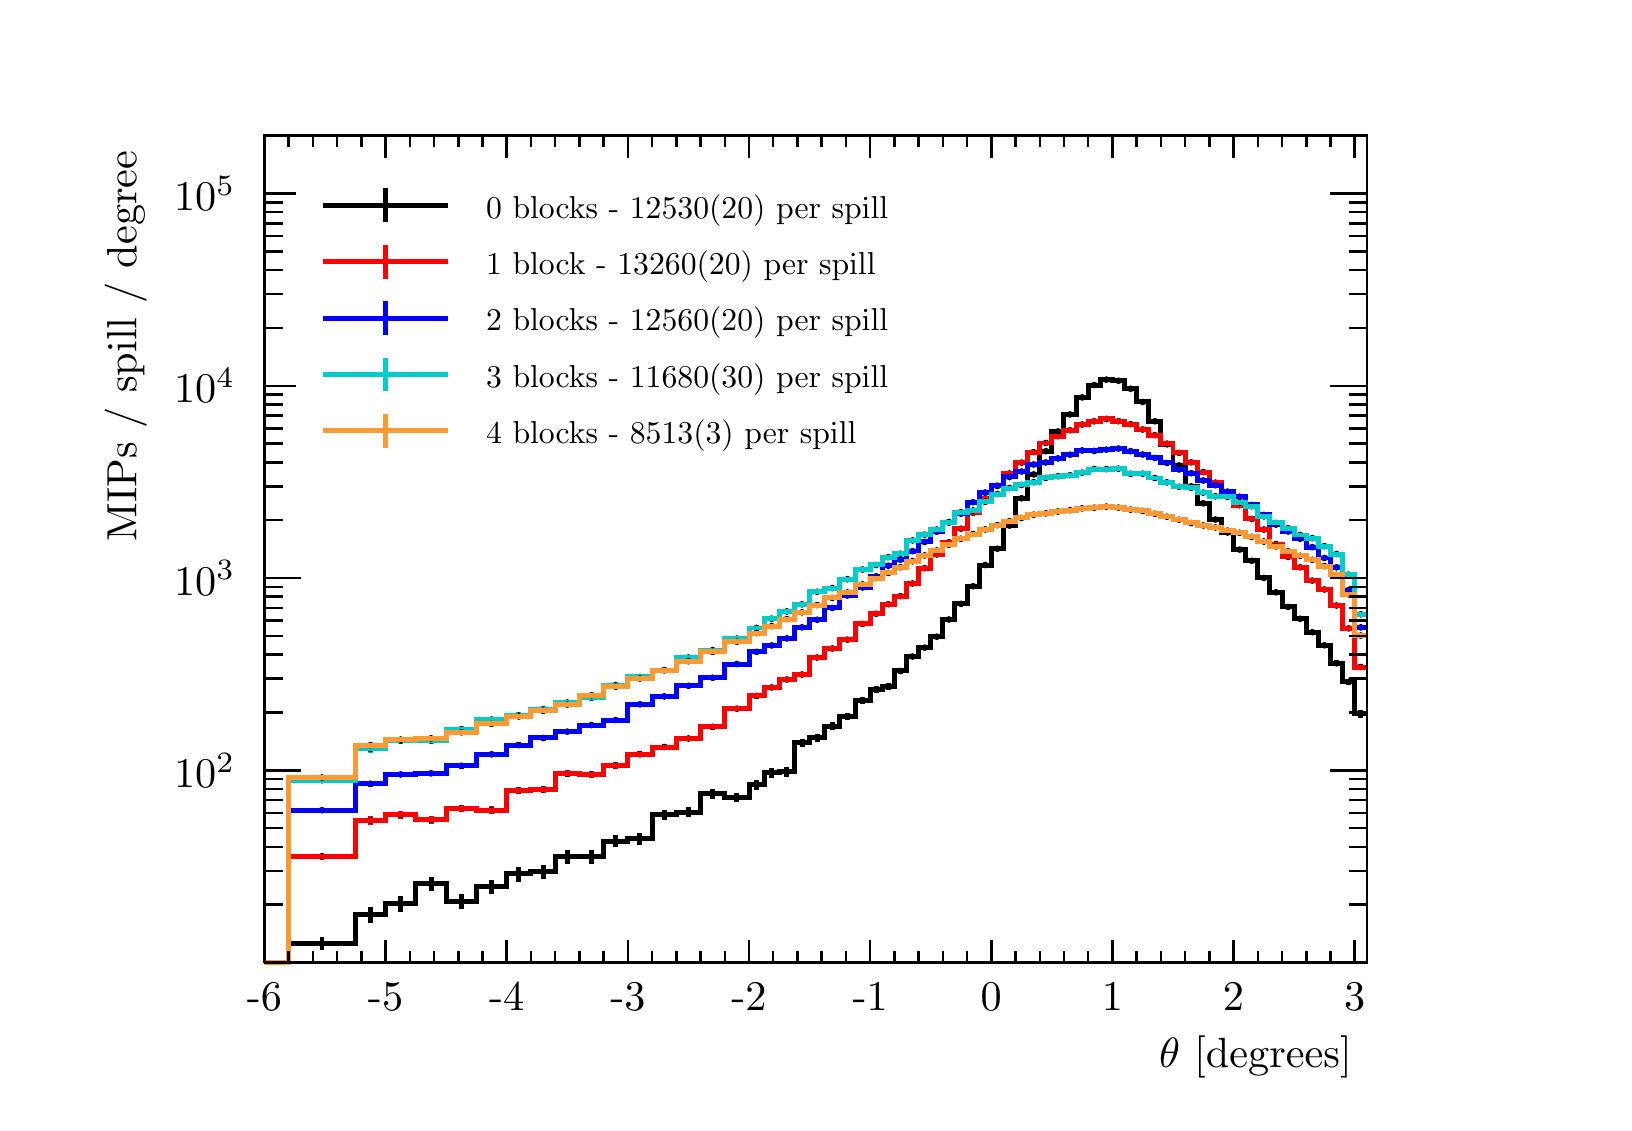
\begin{tikzpicture}
\pgfdeclareplotmark{cross} {
\pgfpathmoveto{\pgfpoint{-0.3\pgfplotmarksize}{\pgfplotmarksize}}
\pgfpathlineto{\pgfpoint{+0.3\pgfplotmarksize}{\pgfplotmarksize}}
\pgfpathlineto{\pgfpoint{+0.3\pgfplotmarksize}{0.3\pgfplotmarksize}}
\pgfpathlineto{\pgfpoint{+1\pgfplotmarksize}{0.3\pgfplotmarksize}}
\pgfpathlineto{\pgfpoint{+1\pgfplotmarksize}{-0.3\pgfplotmarksize}}
\pgfpathlineto{\pgfpoint{+0.3\pgfplotmarksize}{-0.3\pgfplotmarksize}}
\pgfpathlineto{\pgfpoint{+0.3\pgfplotmarksize}{-1.\pgfplotmarksize}}
\pgfpathlineto{\pgfpoint{-0.3\pgfplotmarksize}{-1.\pgfplotmarksize}}
\pgfpathlineto{\pgfpoint{-0.3\pgfplotmarksize}{-0.3\pgfplotmarksize}}
\pgfpathlineto{\pgfpoint{-1.\pgfplotmarksize}{-0.3\pgfplotmarksize}}
\pgfpathlineto{\pgfpoint{-1.\pgfplotmarksize}{0.3\pgfplotmarksize}}
\pgfpathlineto{\pgfpoint{-0.3\pgfplotmarksize}{0.3\pgfplotmarksize}}
\pgfpathclose
\pgfusepathqstroke
}
\pgfdeclareplotmark{cross*} {
\pgfpathmoveto{\pgfpoint{-0.3\pgfplotmarksize}{\pgfplotmarksize}}
\pgfpathlineto{\pgfpoint{+0.3\pgfplotmarksize}{\pgfplotmarksize}}
\pgfpathlineto{\pgfpoint{+0.3\pgfplotmarksize}{0.3\pgfplotmarksize}}
\pgfpathlineto{\pgfpoint{+1\pgfplotmarksize}{0.3\pgfplotmarksize}}
\pgfpathlineto{\pgfpoint{+1\pgfplotmarksize}{-0.3\pgfplotmarksize}}
\pgfpathlineto{\pgfpoint{+0.3\pgfplotmarksize}{-0.3\pgfplotmarksize}}
\pgfpathlineto{\pgfpoint{+0.3\pgfplotmarksize}{-1.\pgfplotmarksize}}
\pgfpathlineto{\pgfpoint{-0.3\pgfplotmarksize}{-1.\pgfplotmarksize}}
\pgfpathlineto{\pgfpoint{-0.3\pgfplotmarksize}{-0.3\pgfplotmarksize}}
\pgfpathlineto{\pgfpoint{-1.\pgfplotmarksize}{-0.3\pgfplotmarksize}}
\pgfpathlineto{\pgfpoint{-1.\pgfplotmarksize}{0.3\pgfplotmarksize}}
\pgfpathlineto{\pgfpoint{-0.3\pgfplotmarksize}{0.3\pgfplotmarksize}}
\pgfpathclose
\pgfusepathqfillstroke
}
\pgfdeclareplotmark{newstar} {
\pgfpathmoveto{\pgfqpoint{0pt}{\pgfplotmarksize}}
\pgfpathlineto{\pgfqpointpolar{44}{0.5\pgfplotmarksize}}
\pgfpathlineto{\pgfqpointpolar{18}{\pgfplotmarksize}}
\pgfpathlineto{\pgfqpointpolar{-20}{0.5\pgfplotmarksize}}
\pgfpathlineto{\pgfqpointpolar{-54}{\pgfplotmarksize}}
\pgfpathlineto{\pgfqpointpolar{-90}{0.5\pgfplotmarksize}}
\pgfpathlineto{\pgfqpointpolar{234}{\pgfplotmarksize}}
\pgfpathlineto{\pgfqpointpolar{198}{0.5\pgfplotmarksize}}
\pgfpathlineto{\pgfqpointpolar{162}{\pgfplotmarksize}}
\pgfpathlineto{\pgfqpointpolar{134}{0.5\pgfplotmarksize}}
\pgfpathclose
\pgfusepathqstroke
}
\pgfdeclareplotmark{newstar*} {
\pgfpathmoveto{\pgfqpoint{0pt}{\pgfplotmarksize}}
\pgfpathlineto{\pgfqpointpolar{44}{0.5\pgfplotmarksize}}
\pgfpathlineto{\pgfqpointpolar{18}{\pgfplotmarksize}}
\pgfpathlineto{\pgfqpointpolar{-20}{0.5\pgfplotmarksize}}
\pgfpathlineto{\pgfqpointpolar{-54}{\pgfplotmarksize}}
\pgfpathlineto{\pgfqpointpolar{-90}{0.5\pgfplotmarksize}}
\pgfpathlineto{\pgfqpointpolar{234}{\pgfplotmarksize}}
\pgfpathlineto{\pgfqpointpolar{198}{0.5\pgfplotmarksize}}
\pgfpathlineto{\pgfqpointpolar{162}{\pgfplotmarksize}}
\pgfpathlineto{\pgfqpointpolar{134}{0.5\pgfplotmarksize}}
\pgfpathclose
\pgfusepathqfillstroke
}
\definecolor{c}{rgb}{1,1,1};
\draw [color=c, fill=c] (0,0) rectangle (20,13.639);
\draw [color=c, fill=c] (3,1.77307) rectangle (17,12.2751);
\definecolor{c}{rgb}{0,0,0};
\draw [c,line width=0.9] (3,1.77307) -- (3,12.2751) -- (17,12.2751) -- (17,1.77307) -- (3,1.77307);
\definecolor{c}{rgb}{1,1,1};
\draw [color=c, fill=c] (3,1.77307) rectangle (17,12.2751);
\definecolor{c}{rgb}{0,0,0};
\draw [c,line width=0.9] (3,1.77307) -- (3,12.2751) -- (17,12.2751) -- (17,1.77307) -- (3,1.77307);
\draw [c,line width=0.9] (3,1.77307) -- (3.30769,1.77307) -- (3.30769,1.77307) -- (4.15385,1.77307) -- (4.15385,1.77307) -- (4.53846,1.77307) -- (4.53846,1.77307) -- (4.92308,1.77307) -- (4.92308,1.77307) -- (5.30769,1.77307) -- (5.30769,1.77307) --
 (5.69231,1.77307) -- (5.69231,1.77307) -- (6.07692,1.77307) -- (6.07692,1.77307) -- (6.38462,1.77307) -- (6.38462,1.77307) -- (6.69231,1.77307) -- (6.69231,1.77307) -- (7,1.77307) -- (7,1.77307) -- (7.30769,1.77307) -- (7.30769,1.77307) --
 (7.61538,1.77307) -- (7.61538,1.77307) -- (7.92308,1.77307) -- (7.92308,1.77307) -- (8.23077,1.77307) -- (8.23077,1.77307) -- (8.53846,1.77307) -- (8.53846,1.77307) -- (8.84615,1.77307) -- (8.84615,1.77307) -- (9.15385,1.77307) -- (9.15385,1.77307)
 -- (9.34615,1.77307) -- (9.34615,1.77307) -- (9.53846,1.77307) -- (9.53846,1.77307) -- (9.73077,1.77307) -- (9.73077,1.77307) -- (9.92308,1.77307) -- (9.92308,1.77307) -- (10.1154,1.77307) -- (10.1154,1.77307) -- (10.3077,1.77307) --
 (10.3077,1.77307) -- (10.5,1.77307) -- (10.5,1.77307) -- (10.6923,1.77307) -- (10.6923,1.77307) -- (10.8462,1.77307) -- (10.8462,1.77307) -- (11,1.77307) -- (11,1.77307) -- (11.1538,1.77307) -- (11.1538,1.77307) -- (11.3077,1.77307) --
 (11.3077,1.77307) -- (11.4615,1.77307) -- (11.4615,1.77307) -- (11.6154,1.77307) -- (11.6154,1.77307) -- (11.7692,1.77307) -- (11.7692,1.77307) -- (11.9231,1.77307) -- (11.9231,1.77307) -- (12.0769,1.77307) -- (12.0769,1.77307) -- (12.2308,1.77307)
 -- (12.2308,1.77307) -- (12.3846,1.77307) -- (12.3846,1.77307) -- (12.5385,1.77307) -- (12.5385,1.77307) -- (12.6923,1.77307) -- (12.6923,1.77307) -- (12.8462,1.77307) -- (12.8462,1.77307) -- (13,1.77307) -- (13,1.77307) -- (13.1538,1.77307) --
 (13.1538,1.77307) -- (13.3077,1.77307) -- (13.3077,1.77307) -- (13.4615,1.77307) -- (13.4615,1.77307) -- (13.6154,1.77307) -- (13.6154,1.77307) -- (13.7692,1.77307) -- (13.7692,1.77307) -- (13.9231,1.77307) -- (13.9231,1.77307) -- (14.0769,1.77307)
 -- (14.0769,1.77307) -- (14.2308,1.77307) -- (14.2308,1.77307) -- (14.3846,1.77307) -- (14.3846,1.77307) -- (14.5385,1.77307) -- (14.5385,1.77307) -- (14.6923,1.77307) -- (14.6923,1.77307) -- (14.8462,1.77307) -- (14.8462,1.77307) -- (15,1.77307) --
 (15,1.77307) -- (15.1538,1.77307) -- (15.1538,1.77307) -- (15.3077,1.77307) -- (15.3077,1.77307) -- (15.4615,1.77307) -- (15.4615,1.77307) -- (15.6154,1.77307) -- (15.6154,1.77307) -- (15.7692,1.77307) -- (15.7692,1.77307) -- (15.9231,1.77307) --
 (15.9231,1.77307) -- (16.0769,1.77307) -- (16.0769,1.77307) -- (16.2308,1.77307) -- (16.2308,1.77307) -- (16.3846,1.77307) -- (16.3846,1.77307) -- (16.5385,1.77307) -- (16.5385,1.77307) -- (16.6923,1.77307) -- (16.6923,1.77307) -- (16.8462,1.77307)
 -- (16.8462,1.77307) -- (17,1.77307);
\draw [c,line width=0.9] (3,1.77307) -- (17,1.77307);
\draw [c,line width=0.9] (3,2.05948) -- (3,1.77307);
\draw [c,line width=0.9] (3.30769,1.91628) -- (3.30769,1.77307);
\draw [c,line width=0.9] (3.61538,1.91628) -- (3.61538,1.77307);
\draw [c,line width=0.9] (3.92308,1.91628) -- (3.92308,1.77307);
\draw [c,line width=0.9] (4.23077,1.91628) -- (4.23077,1.77307);
\draw [c,line width=0.9] (4.53846,2.05948) -- (4.53846,1.77307);
\draw [c,line width=0.9] (4.84615,1.91628) -- (4.84615,1.77307);
\draw [c,line width=0.9] (5.15385,1.91628) -- (5.15385,1.77307);
\draw [c,line width=0.9] (5.46154,1.91628) -- (5.46154,1.77307);
\draw [c,line width=0.9] (5.76923,1.91628) -- (5.76923,1.77307);
\draw [c,line width=0.9] (6.07692,2.05948) -- (6.07692,1.77307);
\draw [c,line width=0.9] (6.38462,1.91628) -- (6.38462,1.77307);
\draw [c,line width=0.9] (6.69231,1.91628) -- (6.69231,1.77307);
\draw [c,line width=0.9] (7,1.91628) -- (7,1.77307);
\draw [c,line width=0.9] (7.30769,1.91628) -- (7.30769,1.77307);
\draw [c,line width=0.9] (7.61538,2.05948) -- (7.61538,1.77307);
\draw [c,line width=0.9] (7.92308,1.91628) -- (7.92308,1.77307);
\draw [c,line width=0.9] (8.23077,1.91628) -- (8.23077,1.77307);
\draw [c,line width=0.9] (8.53846,1.91628) -- (8.53846,1.77307);
\draw [c,line width=0.9] (8.84615,1.91628) -- (8.84615,1.77307);
\draw [c,line width=0.9] (9.15385,2.05948) -- (9.15385,1.77307);
\draw [c,line width=0.9] (9.46154,1.91628) -- (9.46154,1.77307);
\draw [c,line width=0.9] (9.76923,1.91628) -- (9.76923,1.77307);
\draw [c,line width=0.9] (10.0769,1.91628) -- (10.0769,1.77307);
\draw [c,line width=0.9] (10.3846,1.91628) -- (10.3846,1.77307);
\draw [c,line width=0.9] (10.6923,2.05948) -- (10.6923,1.77307);
\draw [c,line width=0.9] (11,1.91628) -- (11,1.77307);
\draw [c,line width=0.9] (11.3077,1.91628) -- (11.3077,1.77307);
\draw [c,line width=0.9] (11.6154,1.91628) -- (11.6154,1.77307);
\draw [c,line width=0.9] (11.9231,1.91628) -- (11.9231,1.77307);
\draw [c,line width=0.9] (12.2308,2.05948) -- (12.2308,1.77307);
\draw [c,line width=0.9] (12.5385,1.91628) -- (12.5385,1.77307);
\draw [c,line width=0.9] (12.8462,1.91628) -- (12.8462,1.77307);
\draw [c,line width=0.9] (13.1538,1.91628) -- (13.1538,1.77307);
\draw [c,line width=0.9] (13.4615,1.91628) -- (13.4615,1.77307);
\draw [c,line width=0.9] (13.7692,2.05948) -- (13.7692,1.77307);
\draw [c,line width=0.9] (14.0769,1.91628) -- (14.0769,1.77307);
\draw [c,line width=0.9] (14.3846,1.91628) -- (14.3846,1.77307);
\draw [c,line width=0.9] (14.6923,1.91628) -- (14.6923,1.77307);
\draw [c,line width=0.9] (15,1.91628) -- (15,1.77307);
\draw [c,line width=0.9] (15.3077,2.05948) -- (15.3077,1.77307);
\draw [c,line width=0.9] (15.6154,1.91628) -- (15.6154,1.77307);
\draw [c,line width=0.9] (15.9231,1.91628) -- (15.9231,1.77307);
\draw [c,line width=0.9] (16.2308,1.91628) -- (16.2308,1.77307);
\draw [c,line width=0.9] (16.5385,1.91628) -- (16.5385,1.77307);
\draw [c,line width=0.9] (16.8462,2.05948) -- (16.8462,1.77307);
\draw [c,line width=0.9] (16.8462,2.05948) -- (16.8462,1.77307);
\draw [anchor=base] (3,1.15931) node[scale=1.52731, color=c, rotate=0]{-6};
\draw [anchor=base] (4.53846,1.15931) node[scale=1.52731, color=c, rotate=0]{-5};
\draw [anchor=base] (6.07692,1.15931) node[scale=1.52731, color=c, rotate=0]{-4};
\draw [anchor=base] (7.61538,1.15931) node[scale=1.52731, color=c, rotate=0]{-3};
\draw [anchor=base] (9.15385,1.15931) node[scale=1.52731, color=c, rotate=0]{-2};
\draw [anchor=base] (10.6923,1.15931) node[scale=1.52731, color=c, rotate=0]{-1};
\draw [anchor=base] (12.2308,1.15931) node[scale=1.52731, color=c, rotate=0]{0};
\draw [anchor=base] (13.7692,1.15931) node[scale=1.52731, color=c, rotate=0]{1};
\draw [anchor=base] (15.3077,1.15931) node[scale=1.52731, color=c, rotate=0]{2};
\draw [anchor=base] (16.8462,1.15931) node[scale=1.52731, color=c, rotate=0]{3};
\draw [anchor= east] (17,0.572837) node[scale=1.52731, color=c, rotate=0]{$\theta$ [degrees] };
\draw [c,line width=0.9] (3,12.2751) -- (17,12.2751);
\draw [c,line width=0.9] (3,11.9887) -- (3,12.2751);
\draw [c,line width=0.9] (3.30769,12.1319) -- (3.30769,12.2751);
\draw [c,line width=0.9] (3.61538,12.1319) -- (3.61538,12.2751);
\draw [c,line width=0.9] (3.92308,12.1319) -- (3.92308,12.2751);
\draw [c,line width=0.9] (4.23077,12.1319) -- (4.23077,12.2751);
\draw [c,line width=0.9] (4.53846,11.9887) -- (4.53846,12.2751);
\draw [c,line width=0.9] (4.84615,12.1319) -- (4.84615,12.2751);
\draw [c,line width=0.9] (5.15385,12.1319) -- (5.15385,12.2751);
\draw [c,line width=0.9] (5.46154,12.1319) -- (5.46154,12.2751);
\draw [c,line width=0.9] (5.76923,12.1319) -- (5.76923,12.2751);
\draw [c,line width=0.9] (6.07692,11.9887) -- (6.07692,12.2751);
\draw [c,line width=0.9] (6.38462,12.1319) -- (6.38462,12.2751);
\draw [c,line width=0.9] (6.69231,12.1319) -- (6.69231,12.2751);
\draw [c,line width=0.9] (7,12.1319) -- (7,12.2751);
\draw [c,line width=0.9] (7.30769,12.1319) -- (7.30769,12.2751);
\draw [c,line width=0.9] (7.61538,11.9887) -- (7.61538,12.2751);
\draw [c,line width=0.9] (7.92308,12.1319) -- (7.92308,12.2751);
\draw [c,line width=0.9] (8.23077,12.1319) -- (8.23077,12.2751);
\draw [c,line width=0.9] (8.53846,12.1319) -- (8.53846,12.2751);
\draw [c,line width=0.9] (8.84615,12.1319) -- (8.84615,12.2751);
\draw [c,line width=0.9] (9.15385,11.9887) -- (9.15385,12.2751);
\draw [c,line width=0.9] (9.46154,12.1319) -- (9.46154,12.2751);
\draw [c,line width=0.9] (9.76923,12.1319) -- (9.76923,12.2751);
\draw [c,line width=0.9] (10.0769,12.1319) -- (10.0769,12.2751);
\draw [c,line width=0.9] (10.3846,12.1319) -- (10.3846,12.2751);
\draw [c,line width=0.9] (10.6923,11.9887) -- (10.6923,12.2751);
\draw [c,line width=0.9] (11,12.1319) -- (11,12.2751);
\draw [c,line width=0.9] (11.3077,12.1319) -- (11.3077,12.2751);
\draw [c,line width=0.9] (11.6154,12.1319) -- (11.6154,12.2751);
\draw [c,line width=0.9] (11.9231,12.1319) -- (11.9231,12.2751);
\draw [c,line width=0.9] (12.2308,11.9887) -- (12.2308,12.2751);
\draw [c,line width=0.9] (12.5385,12.1319) -- (12.5385,12.2751);
\draw [c,line width=0.9] (12.8462,12.1319) -- (12.8462,12.2751);
\draw [c,line width=0.9] (13.1538,12.1319) -- (13.1538,12.2751);
\draw [c,line width=0.9] (13.4615,12.1319) -- (13.4615,12.2751);
\draw [c,line width=0.9] (13.7692,11.9887) -- (13.7692,12.2751);
\draw [c,line width=0.9] (14.0769,12.1319) -- (14.0769,12.2751);
\draw [c,line width=0.9] (14.3846,12.1319) -- (14.3846,12.2751);
\draw [c,line width=0.9] (14.6923,12.1319) -- (14.6923,12.2751);
\draw [c,line width=0.9] (15,12.1319) -- (15,12.2751);
\draw [c,line width=0.9] (15.3077,11.9887) -- (15.3077,12.2751);
\draw [c,line width=0.9] (15.6154,12.1319) -- (15.6154,12.2751);
\draw [c,line width=0.9] (15.9231,12.1319) -- (15.9231,12.2751);
\draw [c,line width=0.9] (16.2308,12.1319) -- (16.2308,12.2751);
\draw [c,line width=0.9] (16.5385,12.1319) -- (16.5385,12.2751);
\draw [c,line width=0.9] (16.8462,11.9887) -- (16.8462,12.2751);
\draw [c,line width=0.9] (16.8462,11.9887) -- (16.8462,12.2751);
\draw [c,line width=0.9] (3,1.77307) -- (3,12.2751);
\draw [c,line width=0.9] (3.231,2.5081) -- (3,2.5081);
\draw [c,line width=0.9] (3.231,2.93807) -- (3,2.93807);
\draw [c,line width=0.9] (3.231,3.24314) -- (3,3.24314);
\draw [c,line width=0.9] (3.231,3.47977) -- (3,3.47977);
\draw [c,line width=0.9] (3.231,3.67311) -- (3,3.67311);
\draw [c,line width=0.9] (3.231,3.83658) -- (3,3.83658);
\draw [c,line width=0.9] (3.231,3.97818) -- (3,3.97818);
\draw [c,line width=0.9] (3.231,4.10308) -- (3,4.10308);
\draw [c,line width=0.9] (3.462,4.21481) -- (3,4.21481);
\draw [anchor= east] (2.82,4.21481) node[scale=1.52731, color=c, rotate=0]{$10^{2}$};
\draw [c,line width=0.9] (3.231,4.94984) -- (3,4.94984);
\draw [c,line width=0.9] (3.231,5.37981) -- (3,5.37981);
\draw [c,line width=0.9] (3.231,5.68488) -- (3,5.68488);
\draw [c,line width=0.9] (3.231,5.92151) -- (3,5.92151);
\draw [c,line width=0.9] (3.231,6.11485) -- (3,6.11485);
\draw [c,line width=0.9] (3.231,6.27832) -- (3,6.27832);
\draw [c,line width=0.9] (3.231,6.41992) -- (3,6.41992);
\draw [c,line width=0.9] (3.231,6.54482) -- (3,6.54482);
\draw [c,line width=0.9] (3.462,6.65655) -- (3,6.65655);
\draw [anchor= east] (2.82,6.65655) node[scale=1.52731, color=c, rotate=0]{$10^{3}$};
\draw [c,line width=0.9] (3.231,7.39159) -- (3,7.39159);
\draw [c,line width=0.9] (3.231,7.82156) -- (3,7.82156);
\draw [c,line width=0.9] (3.231,8.12662) -- (3,8.12662);
\draw [c,line width=0.9] (3.231,8.36325) -- (3,8.36325);
\draw [c,line width=0.9] (3.231,8.55659) -- (3,8.55659);
\draw [c,line width=0.9] (3.231,8.72006) -- (3,8.72006);
\draw [c,line width=0.9] (3.231,8.86166) -- (3,8.86166);
\draw [c,line width=0.9] (3.231,8.98656) -- (3,8.98656);
\draw [c,line width=0.9] (3.462,9.09829) -- (3,9.09829);
\draw [anchor= east] (2.82,9.09829) node[scale=1.52731, color=c, rotate=0]{$10^{4}$};
\draw [c,line width=0.9] (3.231,9.83333) -- (3,9.83333);
\draw [c,line width=0.9] (3.231,10.2633) -- (3,10.2633);
\draw [c,line width=0.9] (3.231,10.5684) -- (3,10.5684);
\draw [c,line width=0.9] (3.231,10.805) -- (3,10.805);
\draw [c,line width=0.9] (3.231,10.9983) -- (3,10.9983);
\draw [c,line width=0.9] (3.231,11.1618) -- (3,11.1618);
\draw [c,line width=0.9] (3.231,11.3034) -- (3,11.3034);
\draw [c,line width=0.9] (3.231,11.4283) -- (3,11.4283);
\draw [c,line width=0.9] (3.462,11.54) -- (3,11.54);
\draw [anchor= east] (2.82,11.54) node[scale=1.52731, color=c, rotate=0]{$10^{5}$};
\draw [c,line width=0.9] (3.231,12.2751) -- (3,12.2751);
\draw [anchor= east] (1.24,12.2751) node[scale=1.52731, color=c, rotate=90]{MIPs / spill / degree};
\draw [c,line width=0.9] (17,1.77307) -- (17,12.2751);
\draw [c,line width=0.9] (16.769,2.5081) -- (17,2.5081);
\draw [c,line width=0.9] (16.769,2.93807) -- (17,2.93807);
\draw [c,line width=0.9] (16.769,3.24314) -- (17,3.24314);
\draw [c,line width=0.9] (16.769,3.47977) -- (17,3.47977);
\draw [c,line width=0.9] (16.769,3.67311) -- (17,3.67311);
\draw [c,line width=0.9] (16.769,3.83658) -- (17,3.83658);
\draw [c,line width=0.9] (16.769,3.97818) -- (17,3.97818);
\draw [c,line width=0.9] (16.769,4.10308) -- (17,4.10308);
\draw [c,line width=0.9] (16.538,4.21481) -- (17,4.21481);
\draw [c,line width=0.9] (16.769,4.94984) -- (17,4.94984);
\draw [c,line width=0.9] (16.769,5.37981) -- (17,5.37981);
\draw [c,line width=0.9] (16.769,5.68488) -- (17,5.68488);
\draw [c,line width=0.9] (16.769,5.92151) -- (17,5.92151);
\draw [c,line width=0.9] (16.769,6.11485) -- (17,6.11485);
\draw [c,line width=0.9] (16.769,6.27832) -- (17,6.27832);
\draw [c,line width=0.9] (16.769,6.41992) -- (17,6.41992);
\draw [c,line width=0.9] (16.769,6.54482) -- (17,6.54482);
\draw [c,line width=0.9] (16.538,6.65655) -- (17,6.65655);
\draw [c,line width=0.9] (16.769,7.39159) -- (17,7.39159);
\draw [c,line width=0.9] (16.769,7.82156) -- (17,7.82156);
\draw [c,line width=0.9] (16.769,8.12662) -- (17,8.12662);
\draw [c,line width=0.9] (16.769,8.36325) -- (17,8.36325);
\draw [c,line width=0.9] (16.769,8.55659) -- (17,8.55659);
\draw [c,line width=0.9] (16.769,8.72006) -- (17,8.72006);
\draw [c,line width=0.9] (16.769,8.86166) -- (17,8.86166);
\draw [c,line width=0.9] (16.769,8.98656) -- (17,8.98656);
\draw [c,line width=0.9] (16.538,9.09829) -- (17,9.09829);
\draw [c,line width=0.9] (16.769,9.83333) -- (17,9.83333);
\draw [c,line width=0.9] (16.769,10.2633) -- (17,10.2633);
\draw [c,line width=0.9] (16.769,10.5684) -- (17,10.5684);
\draw [c,line width=0.9] (16.769,10.805) -- (17,10.805);
\draw [c,line width=0.9] (16.769,10.9983) -- (17,10.9983);
\draw [c,line width=0.9] (16.769,11.1618) -- (17,11.1618);
\draw [c,line width=0.9] (16.769,11.3034) -- (17,11.3034);
\draw [c,line width=0.9] (16.769,11.4283) -- (17,11.4283);
\draw [c,line width=0.9] (16.538,11.54) -- (17,11.54);
\draw [c,line width=0.9] (16.769,12.2751) -- (17,12.2751);
\draw [c,line width=1.8] (3.73077,1.92614) -- (3.73077,2.01524);
\draw [c,line width=1.8] (3.73077,2.01524) -- (3.73077,2.09743);
\foreach \P in {(3.73077,2.01524)}{\draw[mark options={color=c,fill=c},mark size=2.402402pt,mark=*,mark size=1pt] plot coordinates {\P};}
\draw [c,line width=1.8] (4.34615,2.27048) -- (4.34615,2.38281);
\draw [c,line width=1.8] (4.34615,2.38281) -- (4.34615,2.48437);
\foreach \P in {(4.34615,2.38281)}{\draw[mark options={color=c,fill=c},mark size=2.402402pt,mark=*,mark size=1pt] plot coordinates {\P};}
\draw [c,line width=1.8] (4.73077,2.4183) -- (4.73077,2.52307);
\draw [c,line width=1.8] (4.73077,2.52307) -- (4.73077,2.61842);
\foreach \P in {(4.73077,2.52307)}{\draw[mark options={color=c,fill=c},mark size=2.402402pt,mark=*,mark size=1pt] plot coordinates {\P};}
\draw [c,line width=1.8] (5.11538,2.68015) -- (5.11538,2.77276);
\draw [c,line width=1.8] (5.11538,2.77276) -- (5.11538,2.85793);
\foreach \P in {(5.11538,2.77276)}{\draw[mark options={color=c,fill=c},mark size=2.402402pt,mark=*,mark size=1pt] plot coordinates {\P};}
\draw [c,line width=1.8] (5.5,2.44752) -- (5.5,2.55086);
\draw [c,line width=1.8] (5.5,2.55086) -- (5.5,2.64502);
\foreach \P in {(5.5,2.55086)}{\draw[mark options={color=c,fill=c},mark size=2.402402pt,mark=*,mark size=1pt] plot coordinates {\P};}
\draw [c,line width=1.8] (5.88462,2.64067) -- (5.88462,2.73502);
\draw [c,line width=1.8] (5.88462,2.73502) -- (5.88462,2.82166);
\foreach \P in {(5.88462,2.73502)}{\draw[mark options={color=c,fill=c},mark size=2.402402pt,mark=*,mark size=1pt] plot coordinates {\P};}
\draw [c,line width=1.8] (6.23077,2.80239) -- (6.23077,2.90013);
\draw [c,line width=1.8] (6.23077,2.90013) -- (6.23077,2.98962);
\foreach \P in {(6.23077,2.90013)}{\draw[mark options={color=c,fill=c},mark size=2.402402pt,mark=*,mark size=1pt] plot coordinates {\P};}
\draw [c,line width=1.8] (6.53846,2.82794) -- (6.53846,2.92451);
\draw [c,line width=1.8] (6.53846,2.92451) -- (6.53846,3.01301);
\foreach \P in {(6.53846,2.92451)}{\draw[mark options={color=c,fill=c},mark size=2.402402pt,mark=*,mark size=1pt] plot coordinates {\P};}
\draw [c,line width=1.8] (6.84615,3.02725) -- (6.84615,3.11517);
\draw [c,line width=1.8] (6.84615,3.11517) -- (6.84615,3.19635);
\foreach \P in {(6.84615,3.11517)}{\draw[mark options={color=c,fill=c},mark size=2.402402pt,mark=*,mark size=1pt] plot coordinates {\P};}
\draw [c,line width=1.8] (7.15385,3.02725) -- (7.15385,3.11517);
\draw [c,line width=1.8] (7.15385,3.11517) -- (7.15385,3.19635);
\foreach \P in {(7.15385,3.11517)}{\draw[mark options={color=c,fill=c},mark size=2.402402pt,mark=*,mark size=1pt] plot coordinates {\P};}
\draw [c,line width=1.8] (7.46154,3.23666) -- (7.46154,3.31631);
\draw [c,line width=1.8] (7.46154,3.31631) -- (7.46154,3.39039);
\foreach \P in {(7.46154,3.31631)}{\draw[mark options={color=c,fill=c},mark size=2.402402pt,mark=*,mark size=1pt] plot coordinates {\P};}
\draw [c,line width=1.8] (7.76923,3.27072) -- (7.76923,3.34911);
\draw [c,line width=1.8] (7.76923,3.34911) -- (7.76923,3.4221);
\foreach \P in {(7.76923,3.34911)}{\draw[mark options={color=c,fill=c},mark size=2.402402pt,mark=*,mark size=1pt] plot coordinates {\P};}
\draw [c,line width=1.8] (8.07692,3.58385) -- (8.07692,3.65148);
\draw [c,line width=1.8] (8.07692,3.65148) -- (8.07692,3.71506);
\foreach \P in {(8.07692,3.65148)}{\draw[mark options={color=c,fill=c},mark size=2.402402pt,mark=*,mark size=1pt] plot coordinates {\P};}
\draw [c,line width=1.8] (8.38461,3.61679) -- (8.38461,3.68338);
\draw [c,line width=1.8] (8.38461,3.68338) -- (8.38461,3.74603);
\foreach \P in {(8.38461,3.68338)}{\draw[mark options={color=c,fill=c},mark size=2.402402pt,mark=*,mark size=1pt] plot coordinates {\P};}
\draw [c,line width=1.8] (8.69231,3.85579) -- (8.69231,3.91528);
\draw [c,line width=1.8] (8.69231,3.91528) -- (8.69231,3.97161);
\foreach \P in {(8.69231,3.91528)}{\draw[mark options={color=c,fill=c},mark size=2.402402pt,mark=*,mark size=1pt] plot coordinates {\P};}
\draw [c,line width=1.8] (9,3.80594) -- (9,3.86685);
\draw [c,line width=1.8] (9,3.86685) -- (9,3.92445);
\foreach \P in {(9,3.86685)}{\draw[mark options={color=c,fill=c},mark size=2.402402pt,mark=*,mark size=1pt] plot coordinates {\P};}
\draw [c,line width=1.8] (9.25,3.95834) -- (9.25,4.03004);
\draw [c,line width=1.8] (9.25,4.03004) -- (9.25,4.09719);
\foreach \P in {(9.25,4.03004)}{\draw[mark options={color=c,fill=c},mark size=2.402402pt,mark=*,mark size=1pt] plot coordinates {\P};}
\draw [c,line width=1.8] (9.44231,4.1152) -- (9.44231,4.18179);
\draw [c,line width=1.8] (9.44231,4.18179) -- (9.44231,4.24444);
\foreach \P in {(9.44231,4.18179)}{\draw[mark options={color=c,fill=c},mark size=2.402402pt,mark=*,mark size=1pt] plot coordinates {\P};}
\draw [c,line width=1.8] (9.63461,4.12729) -- (9.63461,4.1935);
\draw [c,line width=1.8] (9.63461,4.1935) -- (9.63461,4.25582);
\foreach \P in {(9.63461,4.1935)}{\draw[mark options={color=c,fill=c},mark size=2.402402pt,mark=*,mark size=1pt] plot coordinates {\P};}
\draw [c,line width=1.8] (9.82692,4.50822) -- (9.82692,4.56354);
\draw [c,line width=1.8] (9.82692,4.56354) -- (9.82692,4.61613);
\foreach \P in {(9.82692,4.56354)}{\draw[mark options={color=c,fill=c},mark size=2.402402pt,mark=*,mark size=1pt] plot coordinates {\P};}
\draw [c,line width=1.8] (10.0192,4.57635) -- (10.0192,4.62993);
\draw [c,line width=1.8] (10.0192,4.62993) -- (10.0192,4.68093);
\foreach \P in {(10.0192,4.62993)}{\draw[mark options={color=c,fill=c},mark size=2.402402pt,mark=*,mark size=1pt] plot coordinates {\P};}
\draw [c,line width=1.8] (10.2115,4.72413) -- (10.2115,4.7741);
\draw [c,line width=1.8] (10.2115,4.7741) -- (10.2115,4.82182);
\foreach \P in {(10.2115,4.7741)}{\draw[mark options={color=c,fill=c},mark size=2.402402pt,mark=*,mark size=1pt] plot coordinates {\P};}
\draw [c,line width=1.8] (10.4038,4.84991) -- (10.4038,4.897);
\draw [c,line width=1.8] (10.4038,4.897) -- (10.4038,4.94209);
\foreach \P in {(10.4038,4.897)}{\draw[mark options={color=c,fill=c},mark size=2.402402pt,mark=*,mark size=1pt] plot coordinates {\P};}
\draw [c,line width=1.8] (10.5962,5.06096) -- (10.5962,5.1036);
\draw [c,line width=1.8] (10.5962,5.1036) -- (10.5962,5.14458);
\foreach \P in {(10.5962,5.1036)}{\draw[mark options={color=c,fill=c},mark size=2.402402pt,mark=*,mark size=1pt] plot coordinates {\P};}
\draw [c,line width=1.8] (10.7692,5.1954) -- (10.7692,5.24014);
\draw [c,line width=1.8] (10.7692,5.24014) -- (10.7692,5.28307);
\foreach \P in {(10.7692,5.24014)}{\draw[mark options={color=c,fill=c},mark size=2.402402pt,mark=*,mark size=1pt] plot coordinates {\P};}
\draw [c,line width=1.8] (10.9231,5.2371) -- (10.9231,5.28097);
\draw [c,line width=1.8] (10.9231,5.28097) -- (10.9231,5.32309);
\foreach \P in {(10.9231,5.28097)}{\draw[mark options={color=c,fill=c},mark size=2.402402pt,mark=*,mark size=1pt] plot coordinates {\P};}
\draw [c,line width=1.8] (11.0769,5.43611) -- (11.0769,5.47605);
\draw [c,line width=1.8] (11.0769,5.47605) -- (11.0769,5.51454);
\foreach \P in {(11.0769,5.47605)}{\draw[mark options={color=c,fill=c},mark size=2.402402pt,mark=*,mark size=1pt] plot coordinates {\P};}
\draw [c,line width=1.8] (11.2308,5.62262) -- (11.2308,5.6592);
\draw [c,line width=1.8] (11.2308,5.6592) -- (11.2308,5.69456);
\foreach \P in {(11.2308,5.6592)}{\draw[mark options={color=c,fill=c},mark size=2.402402pt,mark=*,mark size=1pt] plot coordinates {\P};}
\draw [c,line width=1.8] (11.3846,5.73774) -- (11.3846,5.77239);
\draw [c,line width=1.8] (11.3846,5.77239) -- (11.3846,5.80594);
\foreach \P in {(11.3846,5.77239)}{\draw[mark options={color=c,fill=c},mark size=2.402402pt,mark=*,mark size=1pt] plot coordinates {\P};}
\draw [c,line width=1.8] (11.5385,5.87841) -- (11.5385,5.91084);
\draw [c,line width=1.8] (11.5385,5.91084) -- (11.5385,5.9423);
\foreach \P in {(11.5385,5.91084)}{\draw[mark options={color=c,fill=c},mark size=2.402402pt,mark=*,mark size=1pt] plot coordinates {\P};}
\draw [c,line width=1.8] (11.6923,6.10062) -- (11.6923,6.12982);
\draw [c,line width=1.8] (11.6923,6.12982) -- (11.6923,6.15824);
\foreach \P in {(11.6923,6.12982)}{\draw[mark options={color=c,fill=c},mark size=2.402402pt,mark=*,mark size=1pt] plot coordinates {\P};}
\draw [c,line width=1.8] (11.8462,6.30168) -- (11.8462,6.32823);
\draw [c,line width=1.8] (11.8462,6.32823) -- (11.8462,6.35414);
\foreach \P in {(11.8462,6.32823)}{\draw[mark options={color=c,fill=c},mark size=2.402402pt,mark=*,mark size=1pt] plot coordinates {\P};}
\draw [c,line width=1.8] (12,6.5286) -- (12,6.55247);
\draw [c,line width=1.8] (12,6.55247) -- (12,6.5758);
\foreach \P in {(12,6.55247)}{\draw[mark options={color=c,fill=c},mark size=2.402402pt,mark=*,mark size=1pt] plot coordinates {\P};}
\draw [c,line width=1.8] (12.1538,6.80078) -- (12.1538,6.82177);
\draw [c,line width=1.8] (12.1538,6.82177) -- (12.1538,6.84235);
\foreach \P in {(12.1538,6.82177)}{\draw[mark options={color=c,fill=c},mark size=2.402402pt,mark=*,mark size=1pt] plot coordinates {\P};}
\draw [c,line width=1.8] (12.3077,7.00964) -- (12.3077,7.02866);
\draw [c,line width=1.8] (12.3077,7.02866) -- (12.3077,7.04735);
\foreach \P in {(12.3077,7.02866)}{\draw[mark options={color=c,fill=c},mark size=2.402402pt,mark=*,mark size=1pt] plot coordinates {\P};}
\draw [c,line width=1.8] (12.4615,7.30582) -- (12.4615,7.32236);
\draw [c,line width=1.8] (12.4615,7.32236) -- (12.4615,7.33865);
\foreach \P in {(12.4615,7.32236)}{\draw[mark options={color=c,fill=c},mark size=2.402402pt,mark=*,mark size=1pt] plot coordinates {\P};}
\draw [c,line width=1.8] (12.6154,7.65548) -- (12.6154,7.66951);
\draw [c,line width=1.8] (12.6154,7.66951) -- (12.6154,7.68335);
\foreach \P in {(12.6154,7.66951)}{\draw[mark options={color=c,fill=c},mark size=2.402402pt,mark=*,mark size=1pt] plot coordinates {\P};}
\draw [c,line width=1.8] (12.7692,7.96041) -- (12.7692,7.97256);
\draw [c,line width=1.8] (12.7692,7.97256) -- (12.7692,7.98457);
\foreach \P in {(12.7692,7.97256)}{\draw[mark options={color=c,fill=c},mark size=2.402402pt,mark=*,mark size=1pt] plot coordinates {\P};}
\draw [c,line width=1.8] (12.9231,8.25708) -- (12.9231,8.26764);
\draw [c,line width=1.8] (12.9231,8.26764) -- (12.9231,8.2781);
\foreach \P in {(12.9231,8.26764)}{\draw[mark options={color=c,fill=c},mark size=2.402402pt,mark=*,mark size=1pt] plot coordinates {\P};}
\draw [c,line width=1.8] (13.0769,8.50812) -- (13.0769,8.5175);
\draw [c,line width=1.8] (13.0769,8.5175) -- (13.0769,8.5268);
\foreach \P in {(13.0769,8.5175)}{\draw[mark options={color=c,fill=c},mark size=2.402402pt,mark=*,mark size=1pt] plot coordinates {\P};}
\draw [c,line width=1.8] (13.2308,8.72542) -- (13.2308,8.73389);
\draw [c,line width=1.8] (13.2308,8.73389) -- (13.2308,8.74229);
\foreach \P in {(13.2308,8.73389)}{\draw[mark options={color=c,fill=c},mark size=2.402402pt,mark=*,mark size=1pt] plot coordinates {\P};}
\draw [c,line width=1.8] (13.3846,8.94273) -- (13.3846,8.95037);
\draw [c,line width=1.8] (13.3846,8.95037) -- (13.3846,8.95796);
\foreach \P in {(13.3846,8.95037)}{\draw[mark options={color=c,fill=c},mark size=2.402402pt,mark=*,mark size=1pt] plot coordinates {\P};}
\draw [c,line width=1.8] (13.5385,9.10047) -- (13.5385,9.10757);
\draw [c,line width=1.8] (13.5385,9.10757) -- (13.5385,9.11462);
\foreach \P in {(13.5385,9.10757)}{\draw[mark options={color=c,fill=c},mark size=2.402402pt,mark=*,mark size=1pt] plot coordinates {\P};}
\draw [c,line width=1.8] (13.6923,9.16942) -- (13.6923,9.17629);
\draw [c,line width=1.8] (13.6923,9.17629) -- (13.6923,9.18312);
\foreach \P in {(13.6923,9.17629)}{\draw[mark options={color=c,fill=c},mark size=2.402402pt,mark=*,mark size=1pt] plot coordinates {\P};}
\draw [c,line width=1.8] (13.8462,9.15504) -- (13.8462,9.16196);
\draw [c,line width=1.8] (13.8462,9.16196) -- (13.8462,9.16883);
\foreach \P in {(13.8462,9.16196)}{\draw[mark options={color=c,fill=c},mark size=2.402402pt,mark=*,mark size=1pt] plot coordinates {\P};}
\draw [c,line width=1.8] (14,9.0526) -- (14,9.05985);
\draw [c,line width=1.8] (14,9.05985) -- (14,9.06706);
\foreach \P in {(14,9.05985)}{\draw[mark options={color=c,fill=c},mark size=2.402402pt,mark=*,mark size=1pt] plot coordinates {\P};}
\draw [c,line width=1.8] (14.1538,8.88426) -- (14.1538,8.89212);
\draw [c,line width=1.8] (14.1538,8.89212) -- (14.1538,8.89992);
\foreach \P in {(14.1538,8.89212)}{\draw[mark options={color=c,fill=c},mark size=2.402402pt,mark=*,mark size=1pt] plot coordinates {\P};}
\draw [c,line width=1.8] (14.3077,8.63878) -- (14.3077,8.6476);
\draw [c,line width=1.8] (14.3077,8.6476) -- (14.3077,8.65635);
\foreach \P in {(14.3077,8.6476)}{\draw[mark options={color=c,fill=c},mark size=2.402402pt,mark=*,mark size=1pt] plot coordinates {\P};}
\draw [c,line width=1.8] (14.4615,8.34369) -- (14.4615,8.35383);
\draw [c,line width=1.8] (14.4615,8.35383) -- (14.4615,8.36387);
\foreach \P in {(14.4615,8.35383)}{\draw[mark options={color=c,fill=c},mark size=2.402402pt,mark=*,mark size=1pt] plot coordinates {\P};}
\draw [c,line width=1.8] (14.6154,8.07483) -- (14.6154,8.08634);
\draw [c,line width=1.8] (14.6154,8.08634) -- (14.6154,8.09772);
\foreach \P in {(14.6154,8.08634)}{\draw[mark options={color=c,fill=c},mark size=2.402402pt,mark=*,mark size=1pt] plot coordinates {\P};}
\draw [c,line width=1.8] (14.7692,7.80771) -- (14.7692,7.82077);
\draw [c,line width=1.8] (14.7692,7.82077) -- (14.7692,7.83367);
\foreach \P in {(14.7692,7.82077)}{\draw[mark options={color=c,fill=c},mark size=2.402402pt,mark=*,mark size=1pt] plot coordinates {\P};}
\draw [c,line width=1.8] (14.9231,7.5909) -- (14.9231,7.60536);
\draw [c,line width=1.8] (14.9231,7.60536) -- (14.9231,7.61962);
\foreach \P in {(14.9231,7.60536)}{\draw[mark options={color=c,fill=c},mark size=2.402402pt,mark=*,mark size=1pt] plot coordinates {\P};}
\draw [c,line width=1.8] (15.0769,7.38355) -- (15.0769,7.39949);
\draw [c,line width=1.8] (15.0769,7.39949) -- (15.0769,7.4152);
\foreach \P in {(15.0769,7.39949)}{\draw[mark options={color=c,fill=c},mark size=2.402402pt,mark=*,mark size=1pt] plot coordinates {\P};}
\draw [c,line width=1.8] (15.2308,7.21725) -- (15.2308,7.23449);
\draw [c,line width=1.8] (15.2308,7.23449) -- (15.2308,7.25146);
\foreach \P in {(15.2308,7.23449)}{\draw[mark options={color=c,fill=c},mark size=2.402402pt,mark=*,mark size=1pt] plot coordinates {\P};}
\draw [c,line width=1.8] (15.3846,6.99877) -- (15.3846,7.01788);
\draw [c,line width=1.8] (15.3846,7.01788) -- (15.3846,7.03666);
\foreach \P in {(15.3846,7.01788)}{\draw[mark options={color=c,fill=c},mark size=2.402402pt,mark=*,mark size=1pt] plot coordinates {\P};}
\draw [c,line width=1.8] (15.5385,6.85451) -- (15.5385,6.87498);
\draw [c,line width=1.8] (15.5385,6.87498) -- (15.5385,6.89505);
\foreach \P in {(15.5385,6.87498)}{\draw[mark options={color=c,fill=c},mark size=2.402402pt,mark=*,mark size=1pt] plot coordinates {\P};}
\draw [c,line width=1.8] (15.6923,6.63513) -- (15.6923,6.65782);
\draw [c,line width=1.8] (15.6923,6.65782) -- (15.6923,6.68004);
\foreach \P in {(15.6923,6.65782)}{\draw[mark options={color=c,fill=c},mark size=2.402402pt,mark=*,mark size=1pt] plot coordinates {\P};}
\draw [c,line width=1.8] (15.8462,6.45041) -- (15.8462,6.47517);
\draw [c,line width=1.8] (15.8462,6.47517) -- (15.8462,6.49936);
\foreach \P in {(15.8462,6.47517)}{\draw[mark options={color=c,fill=c},mark size=2.402402pt,mark=*,mark size=1pt] plot coordinates {\P};}
\draw [c,line width=1.8] (16,6.2622) -- (16,6.28926);
\draw [c,line width=1.8] (16,6.28926) -- (16,6.31564);
\foreach \P in {(16,6.28926)}{\draw[mark options={color=c,fill=c},mark size=2.402402pt,mark=*,mark size=1pt] plot coordinates {\P};}
\draw [c,line width=1.8] (16.1538,6.10931) -- (16.1538,6.13839);
\draw [c,line width=1.8] (16.1538,6.13839) -- (16.1538,6.16669);
\foreach \P in {(16.1538,6.13839)}{\draw[mark options={color=c,fill=c},mark size=2.402402pt,mark=*,mark size=1pt] plot coordinates {\P};}
\draw [c,line width=1.8] (16.3077,5.93637) -- (16.3077,5.96792);
\draw [c,line width=1.8] (16.3077,5.96792) -- (16.3077,5.99855);
\foreach \P in {(16.3077,5.96792)}{\draw[mark options={color=c,fill=c},mark size=2.402402pt,mark=*,mark size=1pt] plot coordinates {\P};}
\draw [c,line width=1.8] (16.4615,5.76848) -- (16.4615,5.80263);
\draw [c,line width=1.8] (16.4615,5.80263) -- (16.4615,5.83571);
\foreach \P in {(16.4615,5.80263)}{\draw[mark options={color=c,fill=c},mark size=2.402402pt,mark=*,mark size=1pt] plot coordinates {\P};}
\draw [c,line width=1.8] (16.6154,5.53612) -- (16.6154,5.57422);
\draw [c,line width=1.8] (16.6154,5.57422) -- (16.6154,5.611);
\foreach \P in {(16.6154,5.57422)}{\draw[mark options={color=c,fill=c},mark size=2.402402pt,mark=*,mark size=1pt] plot coordinates {\P};}
\draw [c,line width=1.8] (16.7692,5.29591) -- (16.7692,5.33858);
\draw [c,line width=1.8] (16.7692,5.33858) -- (16.7692,5.3796);
\foreach \P in {(16.7692,5.33858)}{\draw[mark options={color=c,fill=c},mark size=2.402402pt,mark=*,mark size=1pt] plot coordinates {\P};}
\draw [c,line width=1.8] (16.9231,4.88448) -- (16.9231,4.93628);
\draw [c,line width=1.8] (16.9231,4.93628) -- (16.9231,4.98567);
\foreach \P in {(16.9231,4.93628)}{\draw[mark options={color=c,fill=c},mark size=2.402402pt,mark=*,mark size=1pt] plot coordinates {\P};}
\draw [c,line width=1.8] (3,1.77307) -- (3.30769,1.77307) -- (3.30769,2.01524) -- (4.15385,2.01524) -- (4.15385,2.38281) -- (4.53846,2.38281) -- (4.53846,2.52307) -- (4.92308,2.52307) -- (4.92308,2.77276) -- (5.30769,2.77276) -- (5.30769,2.55086) --
 (5.69231,2.55086) -- (5.69231,2.73502) -- (6.07692,2.73502) -- (6.07692,2.90013) -- (6.38462,2.90013) -- (6.38462,2.92451) -- (6.69231,2.92451) -- (6.69231,3.11517) -- (7,3.11517) -- (7,3.11517) -- (7.30769,3.11517) -- (7.30769,3.31631) --
 (7.61538,3.31631) -- (7.61538,3.34911) -- (7.92308,3.34911) -- (7.92308,3.65148) -- (8.23077,3.65148) -- (8.23077,3.68338) -- (8.53846,3.68338) -- (8.53846,3.91528) -- (8.84615,3.91528) -- (8.84615,3.86685) -- (9.15385,3.86685) -- (9.15385,4.03004)
 -- (9.34615,4.03004) -- (9.34615,4.18179) -- (9.53846,4.18179) -- (9.53846,4.1935) -- (9.73077,4.1935) -- (9.73077,4.56354) -- (9.92308,4.56354) -- (9.92308,4.62993) -- (10.1154,4.62993) -- (10.1154,4.7741) -- (10.3077,4.7741) -- (10.3077,4.897) --
 (10.5,4.897) -- (10.5,5.1036) -- (10.6923,5.1036) -- (10.6923,5.24014) -- (10.8462,5.24014) -- (10.8462,5.28097) -- (11,5.28097) -- (11,5.47605) -- (11.1538,5.47605) -- (11.1538,5.6592) -- (11.3077,5.6592) -- (11.3077,5.77239) -- (11.4615,5.77239)
 -- (11.4615,5.91084) -- (11.6154,5.91084) -- (11.6154,6.12982) -- (11.7692,6.12982) -- (11.7692,6.32823) -- (11.9231,6.32823) -- (11.9231,6.55247) -- (12.0769,6.55247) -- (12.0769,6.82177) -- (12.2308,6.82177) -- (12.2308,7.02866) --
 (12.3846,7.02866) -- (12.3846,7.32236) -- (12.5385,7.32236) -- (12.5385,7.66951) -- (12.6923,7.66951) -- (12.6923,7.97256) -- (12.8462,7.97256) -- (12.8462,8.26764) -- (13,8.26764) -- (13,8.5175) -- (13.1538,8.5175) -- (13.1538,8.73389) --
 (13.3077,8.73389) -- (13.3077,8.95037) -- (13.4615,8.95037) -- (13.4615,9.10757) -- (13.6154,9.10757) -- (13.6154,9.17629) -- (13.7692,9.17629) -- (13.7692,9.16196) -- (13.9231,9.16196) -- (13.9231,9.05985) -- (14.0769,9.05985) -- (14.0769,8.89212)
 -- (14.2308,8.89212) -- (14.2308,8.6476) -- (14.3846,8.6476) -- (14.3846,8.35383) -- (14.5385,8.35383) -- (14.5385,8.08634) -- (14.6923,8.08634) -- (14.6923,7.82077) -- (14.8462,7.82077) -- (14.8462,7.60536) -- (15,7.60536) -- (15,7.39949) --
 (15.1538,7.39949) -- (15.1538,7.23449) -- (15.3077,7.23449) -- (15.3077,7.01788) -- (15.4615,7.01788) -- (15.4615,6.87498) -- (15.6154,6.87498) -- (15.6154,6.65782) -- (15.7692,6.65782) -- (15.7692,6.47517) -- (15.9231,6.47517) -- (15.9231,6.28926)
 -- (16.0769,6.28926) -- (16.0769,6.13839) -- (16.2308,6.13839) -- (16.2308,5.96792) -- (16.3846,5.96792) -- (16.3846,5.80263) -- (16.5385,5.80263) -- (16.5385,5.57422) -- (16.6923,5.57422) -- (16.6923,5.33858) -- (16.8462,5.33858) --
 (16.8462,4.93628) -- (17,4.93628);
\definecolor{c}{rgb}{1,0,0};
\draw [c,line width=1.8] (3.73077,3.07583) -- (3.73077,3.12093);
\draw [c,line width=1.8] (3.73077,3.12093) -- (3.73077,3.16418);
\definecolor{c}{rgb}{0,0,0};
\foreach \P in {(3.73077,3.12093)}{\draw[mark options={color=c,fill=c},mark size=2.402402pt,mark=*,mark size=1pt] plot coordinates {\P};}
\definecolor{c}{rgb}{1,0,0};
\draw [c,line width=1.8] (4.34615,3.52455) -- (4.34615,3.57826);
\draw [c,line width=1.8] (4.34615,3.57826) -- (4.34615,3.62938);
\definecolor{c}{rgb}{0,0,0};
\foreach \P in {(4.34615,3.57826)}{\draw[mark options={color=c,fill=c},mark size=2.402402pt,mark=*,mark size=1pt] plot coordinates {\P};}
\definecolor{c}{rgb}{1,0,0};
\draw [c,line width=1.8] (4.73077,3.59788) -- (4.73077,3.64933);
\draw [c,line width=1.8] (4.73077,3.64933) -- (4.73077,3.6984);
\definecolor{c}{rgb}{0,0,0};
\foreach \P in {(4.73077,3.64933)}{\draw[mark options={color=c,fill=c},mark size=2.402402pt,mark=*,mark size=1pt] plot coordinates {\P};}
\definecolor{c}{rgb}{1,0,0};
\draw [c,line width=1.8] (5.11538,3.53171) -- (5.11538,3.58478);
\draw [c,line width=1.8] (5.11538,3.58478) -- (5.11538,3.63532);
\definecolor{c}{rgb}{0,0,0};
\foreach \P in {(5.11538,3.58478)}{\draw[mark options={color=c,fill=c},mark size=2.402402pt,mark=*,mark size=1pt] plot coordinates {\P};}
\definecolor{c}{rgb}{1,0,0};
\draw [c,line width=1.8] (5.5,3.68147) -- (5.5,3.73156);
\draw [c,line width=1.8] (5.5,3.73156) -- (5.5,3.77939);
\definecolor{c}{rgb}{0,0,0};
\foreach \P in {(5.5,3.73156)}{\draw[mark options={color=c,fill=c},mark size=2.402402pt,mark=*,mark size=1pt] plot coordinates {\P};}
\definecolor{c}{rgb}{1,0,0};
\draw [c,line width=1.8] (5.88462,3.6591) -- (5.88462,3.70953);
\draw [c,line width=1.8] (5.88462,3.70953) -- (5.88462,3.75767);
\definecolor{c}{rgb}{0,0,0};
\foreach \P in {(5.88462,3.70953)}{\draw[mark options={color=c,fill=c},mark size=2.402402pt,mark=*,mark size=1pt] plot coordinates {\P};}
\definecolor{c}{rgb}{1,0,0};
\draw [c,line width=1.8] (6.23077,3.90994) -- (6.23077,3.95969);
\draw [c,line width=1.8] (6.23077,3.95969) -- (6.23077,4.00721);
\definecolor{c}{rgb}{0,0,0};
\foreach \P in {(6.23077,3.95969)}{\draw[mark options={color=c,fill=c},mark size=2.402402pt,mark=*,mark size=1pt] plot coordinates {\P};}
\definecolor{c}{rgb}{1,0,0};
\draw [c,line width=1.8] (6.53846,3.92327) -- (6.53846,3.97323);
\draw [c,line width=1.8] (6.53846,3.97323) -- (6.53846,4.02094);
\definecolor{c}{rgb}{0,0,0};
\foreach \P in {(6.53846,3.97323)}{\draw[mark options={color=c,fill=c},mark size=2.402402pt,mark=*,mark size=1pt] plot coordinates {\P};}
\definecolor{c}{rgb}{1,0,0};
\draw [c,line width=1.8] (6.84615,4.12613) -- (6.84615,4.1712);
\draw [c,line width=1.8] (6.84615,4.1712) -- (6.84615,4.21444);
\definecolor{c}{rgb}{0,0,0};
\foreach \P in {(6.84615,4.1712)}{\draw[mark options={color=c,fill=c},mark size=2.402402pt,mark=*,mark size=1pt] plot coordinates {\P};}
\definecolor{c}{rgb}{1,0,0};
\draw [c,line width=1.8] (7.15385,4.11876) -- (7.15385,4.16399);
\draw [c,line width=1.8] (7.15385,4.16399) -- (7.15385,4.20738);
\definecolor{c}{rgb}{0,0,0};
\foreach \P in {(7.15385,4.16399)}{\draw[mark options={color=c,fill=c},mark size=2.402402pt,mark=*,mark size=1pt] plot coordinates {\P};}
\definecolor{c}{rgb}{1,0,0};
\draw [c,line width=1.8] (7.46154,4.23622) -- (7.46154,4.27912);
\draw [c,line width=1.8] (7.46154,4.27912) -- (7.46154,4.32036);
\definecolor{c}{rgb}{0,0,0};
\foreach \P in {(7.46154,4.27912)}{\draw[mark options={color=c,fill=c},mark size=2.402402pt,mark=*,mark size=1pt] plot coordinates {\P};}
\definecolor{c}{rgb}{1,0,0};
\draw [c,line width=1.8] (7.76923,4.37852) -- (7.76923,4.41839);
\draw [c,line width=1.8] (7.76923,4.41839) -- (7.76923,4.45681);
\definecolor{c}{rgb}{0,0,0};
\foreach \P in {(7.76923,4.41839)}{\draw[mark options={color=c,fill=c},mark size=2.402402pt,mark=*,mark size=1pt] plot coordinates {\P};}
\definecolor{c}{rgb}{1,0,0};
\draw [c,line width=1.8] (8.07692,4.47183) -- (8.07692,4.51012);
\draw [c,line width=1.8] (8.07692,4.51012) -- (8.07692,4.54708);
\definecolor{c}{rgb}{0,0,0};
\foreach \P in {(8.07692,4.51012)}{\draw[mark options={color=c,fill=c},mark size=2.402402pt,mark=*,mark size=1pt] plot coordinates {\P};}
\definecolor{c}{rgb}{1,0,0};
\draw [c,line width=1.8] (8.38461,4.58233) -- (8.38461,4.61882);
\draw [c,line width=1.8] (8.38461,4.61882) -- (8.38461,4.65409);
\definecolor{c}{rgb}{0,0,0};
\foreach \P in {(8.38461,4.61882)}{\draw[mark options={color=c,fill=c},mark size=2.402402pt,mark=*,mark size=1pt] plot coordinates {\P};}
\definecolor{c}{rgb}{1,0,0};
\draw [c,line width=1.8] (8.69231,4.73243) -- (8.69231,4.76642);
\draw [c,line width=1.8] (8.69231,4.76642) -- (8.69231,4.79935);
\definecolor{c}{rgb}{0,0,0};
\foreach \P in {(8.69231,4.76642)}{\draw[mark options={color=c,fill=c},mark size=2.402402pt,mark=*,mark size=1pt] plot coordinates {\P};}
\definecolor{c}{rgb}{1,0,0};
\draw [c,line width=1.8] (9,4.96683) -- (9,4.99708);
\draw [c,line width=1.8] (9,4.99708) -- (9,5.02649);
\definecolor{c}{rgb}{0,0,0};
\foreach \P in {(9,4.99708)}{\draw[mark options={color=c,fill=c},mark size=2.402402pt,mark=*,mark size=1pt] plot coordinates {\P};}
\definecolor{c}{rgb}{1,0,0};
\draw [c,line width=1.8] (9.25,5.12432) -- (9.25,5.15991);
\draw [c,line width=1.8] (9.25,5.15991) -- (9.25,5.19434);
\definecolor{c}{rgb}{0,0,0};
\foreach \P in {(9.25,5.15991)}{\draw[mark options={color=c,fill=c},mark size=2.402402pt,mark=*,mark size=1pt] plot coordinates {\P};}
\definecolor{c}{rgb}{1,0,0};
\draw [c,line width=1.8] (9.44231,5.23343) -- (9.44231,5.26725);
\draw [c,line width=1.8] (9.44231,5.26725) -- (9.44231,5.30003);
\definecolor{c}{rgb}{0,0,0};
\foreach \P in {(9.44231,5.26725)}{\draw[mark options={color=c,fill=c},mark size=2.402402pt,mark=*,mark size=1pt] plot coordinates {\P};}
\definecolor{c}{rgb}{1,0,0};
\draw [c,line width=1.8] (9.63461,5.33587) -- (9.63461,5.36799);
\draw [c,line width=1.8] (9.63461,5.36799) -- (9.63461,5.39918);
\definecolor{c}{rgb}{0,0,0};
\foreach \P in {(9.63461,5.36799)}{\draw[mark options={color=c,fill=c},mark size=2.402402pt,mark=*,mark size=1pt] plot coordinates {\P};}
\definecolor{c}{rgb}{1,0,0};
\draw [c,line width=1.8] (9.82692,5.39963) -- (9.82692,5.43085);
\draw [c,line width=1.8] (9.82692,5.43085) -- (9.82692,5.46118);
\definecolor{c}{rgb}{0,0,0};
\foreach \P in {(9.82692,5.43085)}{\draw[mark options={color=c,fill=c},mark size=2.402402pt,mark=*,mark size=1pt] plot coordinates {\P};}
\definecolor{c}{rgb}{1,0,0};
\draw [c,line width=1.8] (10.0192,5.61858) -- (10.0192,5.6469);
\draw [c,line width=1.8] (10.0192,5.6469) -- (10.0192,5.67449);
\definecolor{c}{rgb}{0,0,0};
\foreach \P in {(10.0192,5.6469)}{\draw[mark options={color=c,fill=c},mark size=2.402402pt,mark=*,mark size=1pt] plot coordinates {\P};}
\definecolor{c}{rgb}{1,0,0};
\draw [c,line width=1.8] (10.2115,5.73442) -- (10.2115,5.76125);
\draw [c,line width=1.8] (10.2115,5.76125) -- (10.2115,5.78741);
\definecolor{c}{rgb}{0,0,0};
\foreach \P in {(10.2115,5.76125)}{\draw[mark options={color=c,fill=c},mark size=2.402402pt,mark=*,mark size=1pt] plot coordinates {\P};}
\definecolor{c}{rgb}{1,0,0};
\draw [c,line width=1.8] (10.4038,5.84841) -- (10.4038,5.87377);
\draw [c,line width=1.8] (10.4038,5.87377) -- (10.4038,5.89854);
\definecolor{c}{rgb}{0,0,0};
\foreach \P in {(10.4038,5.87377)}{\draw[mark options={color=c,fill=c},mark size=2.402402pt,mark=*,mark size=1pt] plot coordinates {\P};}
\definecolor{c}{rgb}{1,0,0};
\draw [c,line width=1.8] (10.5962,6.05052) -- (10.5962,6.07348);
\draw [c,line width=1.8] (10.5962,6.07348) -- (10.5962,6.09595);
\definecolor{c}{rgb}{0,0,0};
\foreach \P in {(10.5962,6.07348)}{\draw[mark options={color=c,fill=c},mark size=2.402402pt,mark=*,mark size=1pt] plot coordinates {\P};}
\definecolor{c}{rgb}{1,0,0};
\draw [c,line width=1.8] (10.7692,6.17803) -- (10.7692,6.20222);
\draw [c,line width=1.8] (10.7692,6.20222) -- (10.7692,6.22586);
\definecolor{c}{rgb}{0,0,0};
\foreach \P in {(10.7692,6.20222)}{\draw[mark options={color=c,fill=c},mark size=2.402402pt,mark=*,mark size=1pt] plot coordinates {\P};}
\definecolor{c}{rgb}{1,0,0};
\draw [c,line width=1.8] (10.9231,6.301) -- (10.9231,6.32402);
\draw [c,line width=1.8] (10.9231,6.32402) -- (10.9231,6.34654);
\definecolor{c}{rgb}{0,0,0};
\foreach \P in {(10.9231,6.32402)}{\draw[mark options={color=c,fill=c},mark size=2.402402pt,mark=*,mark size=1pt] plot coordinates {\P};}
\definecolor{c}{rgb}{1,0,0};
\draw [c,line width=1.8] (11.0769,6.40452) -- (11.0769,6.42623);
\draw [c,line width=1.8] (11.0769,6.42623) -- (11.0769,6.4475);
\definecolor{c}{rgb}{0,0,0};
\foreach \P in {(11.0769,6.42623)}{\draw[mark options={color=c,fill=c},mark size=2.402402pt,mark=*,mark size=1pt] plot coordinates {\P};}
\definecolor{c}{rgb}{1,0,0};
\draw [c,line width=1.8] (11.2308,6.56672) -- (11.2308,6.58682);
\draw [c,line width=1.8] (11.2308,6.58682) -- (11.2308,6.60655);
\definecolor{c}{rgb}{0,0,0};
\foreach \P in {(11.2308,6.58682)}{\draw[mark options={color=c,fill=c},mark size=2.402402pt,mark=*,mark size=1pt] plot coordinates {\P};}
\definecolor{c}{rgb}{1,0,0};
\draw [c,line width=1.8] (11.3846,6.76317) -- (11.3846,6.78162);
\draw [c,line width=1.8] (11.3846,6.78162) -- (11.3846,6.79975);
\definecolor{c}{rgb}{0,0,0};
\foreach \P in {(11.3846,6.78162)}{\draw[mark options={color=c,fill=c},mark size=2.402402pt,mark=*,mark size=1pt] plot coordinates {\P};}
\definecolor{c}{rgb}{1,0,0};
\draw [c,line width=1.8] (11.5385,6.93828) -- (11.5385,6.95516);
\draw [c,line width=1.8] (11.5385,6.95516) -- (11.5385,6.97178);
\definecolor{c}{rgb}{0,0,0};
\foreach \P in {(11.5385,6.95516)}{\draw[mark options={color=c,fill=c},mark size=2.402402pt,mark=*,mark size=1pt] plot coordinates {\P};}
\definecolor{c}{rgb}{1,0,0};
\draw [c,line width=1.8] (11.6923,7.09576) -- (11.6923,7.11144);
\draw [c,line width=1.8] (11.6923,7.11144) -- (11.6923,7.12689);
\definecolor{c}{rgb}{0,0,0};
\foreach \P in {(11.6923,7.11144)}{\draw[mark options={color=c,fill=c},mark size=2.402402pt,mark=*,mark size=1pt] plot coordinates {\P};}
\definecolor{c}{rgb}{1,0,0};
\draw [c,line width=1.8] (11.8462,7.2682) -- (11.8462,7.28268);
\draw [c,line width=1.8] (11.8462,7.28268) -- (11.8462,7.29697);
\definecolor{c}{rgb}{0,0,0};
\foreach \P in {(11.8462,7.28268)}{\draw[mark options={color=c,fill=c},mark size=2.402402pt,mark=*,mark size=1pt] plot coordinates {\P};}
\definecolor{c}{rgb}{1,0,0};
\draw [c,line width=1.8] (12,7.47222) -- (12,7.48535);
\draw [c,line width=1.8] (12,7.48535) -- (12,7.49832);
\definecolor{c}{rgb}{0,0,0};
\foreach \P in {(12,7.48535)}{\draw[mark options={color=c,fill=c},mark size=2.402402pt,mark=*,mark size=1pt] plot coordinates {\P};}
\definecolor{c}{rgb}{1,0,0};
\draw [c,line width=1.8] (12.1538,7.65692) -- (12.1538,7.66899);
\draw [c,line width=1.8] (12.1538,7.66899) -- (12.1538,7.68092);
\definecolor{c}{rgb}{0,0,0};
\foreach \P in {(12.1538,7.66899)}{\draw[mark options={color=c,fill=c},mark size=2.402402pt,mark=*,mark size=1pt] plot coordinates {\P};}
\definecolor{c}{rgb}{1,0,0};
\draw [c,line width=1.8] (12.3077,7.8152) -- (12.3077,7.82641);
\draw [c,line width=1.8] (12.3077,7.82641) -- (12.3077,7.83749);
\definecolor{c}{rgb}{0,0,0};
\foreach \P in {(12.3077,7.82641)}{\draw[mark options={color=c,fill=c},mark size=2.402402pt,mark=*,mark size=1pt] plot coordinates {\P};}
\definecolor{c}{rgb}{1,0,0};
\draw [c,line width=1.8] (12.4615,7.97346) -- (12.4615,7.98385);
\draw [c,line width=1.8] (12.4615,7.98385) -- (12.4615,7.99413);
\definecolor{c}{rgb}{0,0,0};
\foreach \P in {(12.4615,7.98385)}{\draw[mark options={color=c,fill=c},mark size=2.402402pt,mark=*,mark size=1pt] plot coordinates {\P};}
\definecolor{c}{rgb}{1,0,0};
\draw [c,line width=1.8] (12.6154,8.11131) -- (12.6154,8.12103);
\draw [c,line width=1.8] (12.6154,8.12103) -- (12.6154,8.13066);
\definecolor{c}{rgb}{0,0,0};
\foreach \P in {(12.6154,8.12103)}{\draw[mark options={color=c,fill=c},mark size=2.402402pt,mark=*,mark size=1pt] plot coordinates {\P};}
\definecolor{c}{rgb}{1,0,0};
\draw [c,line width=1.8] (12.7692,8.24634) -- (12.7692,8.25546);
\draw [c,line width=1.8] (12.7692,8.25546) -- (12.7692,8.26451);
\definecolor{c}{rgb}{0,0,0};
\foreach \P in {(12.7692,8.25546)}{\draw[mark options={color=c,fill=c},mark size=2.402402pt,mark=*,mark size=1pt] plot coordinates {\P};}
\definecolor{c}{rgb}{1,0,0};
\draw [c,line width=1.8] (12.9231,8.36274) -- (12.9231,8.37137);
\draw [c,line width=1.8] (12.9231,8.37137) -- (12.9231,8.37994);
\definecolor{c}{rgb}{0,0,0};
\foreach \P in {(12.9231,8.37137)}{\draw[mark options={color=c,fill=c},mark size=2.402402pt,mark=*,mark size=1pt] plot coordinates {\P};}
\definecolor{c}{rgb}{1,0,0};
\draw [c,line width=1.8] (13.0769,8.44946) -- (13.0769,8.45775);
\draw [c,line width=1.8] (13.0769,8.45775) -- (13.0769,8.46597);
\definecolor{c}{rgb}{0,0,0};
\foreach \P in {(13.0769,8.45775)}{\draw[mark options={color=c,fill=c},mark size=2.402402pt,mark=*,mark size=1pt] plot coordinates {\P};}
\definecolor{c}{rgb}{1,0,0};
\draw [c,line width=1.8] (13.2308,8.52563) -- (13.2308,8.53362);
\draw [c,line width=1.8] (13.2308,8.53362) -- (13.2308,8.54156);
\definecolor{c}{rgb}{0,0,0};
\foreach \P in {(13.2308,8.53362)}{\draw[mark options={color=c,fill=c},mark size=2.402402pt,mark=*,mark size=1pt] plot coordinates {\P};}
\definecolor{c}{rgb}{1,0,0};
\draw [c,line width=1.8] (13.3846,8.59824) -- (13.3846,8.60597);
\draw [c,line width=1.8] (13.3846,8.60597) -- (13.3846,8.61365);
\definecolor{c}{rgb}{0,0,0};
\foreach \P in {(13.3846,8.60597)}{\draw[mark options={color=c,fill=c},mark size=2.402402pt,mark=*,mark size=1pt] plot coordinates {\P};}
\definecolor{c}{rgb}{1,0,0};
\draw [c,line width=1.8] (13.5385,8.63985) -- (13.5385,8.64744);
\draw [c,line width=1.8] (13.5385,8.64744) -- (13.5385,8.65498);
\definecolor{c}{rgb}{0,0,0};
\foreach \P in {(13.5385,8.64744)}{\draw[mark options={color=c,fill=c},mark size=2.402402pt,mark=*,mark size=1pt] plot coordinates {\P};}
\definecolor{c}{rgb}{1,0,0};
\draw [c,line width=1.8] (13.6923,8.66911) -- (13.6923,8.67659);
\draw [c,line width=1.8] (13.6923,8.67659) -- (13.6923,8.68402);
\definecolor{c}{rgb}{0,0,0};
\foreach \P in {(13.6923,8.67659)}{\draw[mark options={color=c,fill=c},mark size=2.402402pt,mark=*,mark size=1pt] plot coordinates {\P};}
\definecolor{c}{rgb}{1,0,0};
\draw [c,line width=1.8] (13.8462,8.64082) -- (13.8462,8.6484);
\draw [c,line width=1.8] (13.8462,8.6484) -- (13.8462,8.65593);
\definecolor{c}{rgb}{0,0,0};
\foreach \P in {(13.8462,8.6484)}{\draw[mark options={color=c,fill=c},mark size=2.402402pt,mark=*,mark size=1pt] plot coordinates {\P};}
\definecolor{c}{rgb}{1,0,0};
\draw [c,line width=1.8] (14,8.60286) -- (14,8.61056);
\draw [c,line width=1.8] (14,8.61056) -- (14,8.61822);
\definecolor{c}{rgb}{0,0,0};
\foreach \P in {(14,8.61056)}{\draw[mark options={color=c,fill=c},mark size=2.402402pt,mark=*,mark size=1pt] plot coordinates {\P};}
\definecolor{c}{rgb}{1,0,0};
\draw [c,line width=1.8] (14.1538,8.53487) -- (14.1538,8.54284);
\draw [c,line width=1.8] (14.1538,8.54284) -- (14.1538,8.55075);
\definecolor{c}{rgb}{0,0,0};
\foreach \P in {(14.1538,8.54284)}{\draw[mark options={color=c,fill=c},mark size=2.402402pt,mark=*,mark size=1pt] plot coordinates {\P};}
\definecolor{c}{rgb}{1,0,0};
\draw [c,line width=1.8] (14.3077,8.46293) -- (14.3077,8.47117);
\draw [c,line width=1.8] (14.3077,8.47117) -- (14.3077,8.47935);
\definecolor{c}{rgb}{0,0,0};
\foreach \P in {(14.3077,8.47117)}{\draw[mark options={color=c,fill=c},mark size=2.402402pt,mark=*,mark size=1pt] plot coordinates {\P};}
\definecolor{c}{rgb}{1,0,0};
\draw [c,line width=1.8] (14.4615,8.35467) -- (14.4615,8.36334);
\draw [c,line width=1.8] (14.4615,8.36334) -- (14.4615,8.37193);
\definecolor{c}{rgb}{0,0,0};
\foreach \P in {(14.4615,8.36334)}{\draw[mark options={color=c,fill=c},mark size=2.402402pt,mark=*,mark size=1pt] plot coordinates {\P};}
\definecolor{c}{rgb}{1,0,0};
\draw [c,line width=1.8] (14.6154,8.2369) -- (14.6154,8.24606);
\draw [c,line width=1.8] (14.6154,8.24606) -- (14.6154,8.25514);
\definecolor{c}{rgb}{0,0,0};
\foreach \P in {(14.6154,8.24606)}{\draw[mark options={color=c,fill=c},mark size=2.402402pt,mark=*,mark size=1pt] plot coordinates {\P};}
\definecolor{c}{rgb}{1,0,0};
\draw [c,line width=1.8] (14.7692,8.11581) -- (14.7692,8.12553);
\draw [c,line width=1.8] (14.7692,8.12553) -- (14.7692,8.13515);
\definecolor{c}{rgb}{0,0,0};
\foreach \P in {(14.7692,8.12553)}{\draw[mark options={color=c,fill=c},mark size=2.402402pt,mark=*,mark size=1pt] plot coordinates {\P};}
\definecolor{c}{rgb}{1,0,0};
\draw [c,line width=1.8] (14.9231,7.99173) -- (14.9231,8.00202);
\draw [c,line width=1.8] (14.9231,8.00202) -- (14.9231,8.01222);
\definecolor{c}{rgb}{0,0,0};
\foreach \P in {(14.9231,8.00202)}{\draw[mark options={color=c,fill=c},mark size=2.402402pt,mark=*,mark size=1pt] plot coordinates {\P};}
\definecolor{c}{rgb}{1,0,0};
\draw [c,line width=1.8] (15.0769,7.85689) -- (15.0769,7.86786);
\draw [c,line width=1.8] (15.0769,7.86786) -- (15.0769,7.87871);
\definecolor{c}{rgb}{0,0,0};
\foreach \P in {(15.0769,7.86786)}{\draw[mark options={color=c,fill=c},mark size=2.402402pt,mark=*,mark size=1pt] plot coordinates {\P};}
\definecolor{c}{rgb}{1,0,0};
\draw [c,line width=1.8] (15.2308,7.71759) -- (15.2308,7.72929);
\draw [c,line width=1.8] (15.2308,7.72929) -- (15.2308,7.74086);
\definecolor{c}{rgb}{0,0,0};
\foreach \P in {(15.2308,7.72929)}{\draw[mark options={color=c,fill=c},mark size=2.402402pt,mark=*,mark size=1pt] plot coordinates {\P};}
\definecolor{c}{rgb}{1,0,0};
\draw [c,line width=1.8] (15.3846,7.56898) -- (15.3846,7.58152);
\draw [c,line width=1.8] (15.3846,7.58152) -- (15.3846,7.59392);
\definecolor{c}{rgb}{0,0,0};
\foreach \P in {(15.3846,7.58152)}{\draw[mark options={color=c,fill=c},mark size=2.402402pt,mark=*,mark size=1pt] plot coordinates {\P};}
\definecolor{c}{rgb}{1,0,0};
\draw [c,line width=1.8] (15.5385,7.39304) -- (15.5385,7.40673);
\draw [c,line width=1.8] (15.5385,7.40673) -- (15.5385,7.42025);
\definecolor{c}{rgb}{0,0,0};
\foreach \P in {(15.5385,7.40673)}{\draw[mark options={color=c,fill=c},mark size=2.402402pt,mark=*,mark size=1pt] plot coordinates {\P};}
\definecolor{c}{rgb}{1,0,0};
\draw [c,line width=1.8] (15.6923,7.25794) -- (15.6923,7.27252);
\draw [c,line width=1.8] (15.6923,7.27252) -- (15.6923,7.2869);
\definecolor{c}{rgb}{0,0,0};
\foreach \P in {(15.6923,7.27252)}{\draw[mark options={color=c,fill=c},mark size=2.402402pt,mark=*,mark size=1pt] plot coordinates {\P};}
\definecolor{c}{rgb}{1,0,0};
\draw [c,line width=1.8] (15.8462,7.07146) -- (15.8462,7.08737);
\draw [c,line width=1.8] (15.8462,7.08737) -- (15.8462,7.10304);
\definecolor{c}{rgb}{0,0,0};
\foreach \P in {(15.8462,7.08737)}{\draw[mark options={color=c,fill=c},mark size=2.402402pt,mark=*,mark size=1pt] plot coordinates {\P};}
\definecolor{c}{rgb}{1,0,0};
\draw [c,line width=1.8] (16,6.90752) -- (16,6.92475);
\draw [c,line width=1.8] (16,6.92475) -- (16,6.9417);
\definecolor{c}{rgb}{0,0,0};
\foreach \P in {(16,6.92475)}{\draw[mark options={color=c,fill=c},mark size=2.402402pt,mark=*,mark size=1pt] plot coordinates {\P};}
\definecolor{c}{rgb}{1,0,0};
\draw [c,line width=1.8] (16.1538,6.77477) -- (16.1538,6.79305);
\draw [c,line width=1.8] (16.1538,6.79305) -- (16.1538,6.81102);
\definecolor{c}{rgb}{0,0,0};
\foreach \P in {(16.1538,6.79305)}{\draw[mark options={color=c,fill=c},mark size=2.402402pt,mark=*,mark size=1pt] plot coordinates {\P};}
\definecolor{c}{rgb}{1,0,0};
\draw [c,line width=1.8] (16.3077,6.60404) -- (16.3077,6.62378);
\draw [c,line width=1.8] (16.3077,6.62378) -- (16.3077,6.64315);
\definecolor{c}{rgb}{0,0,0};
\foreach \P in {(16.3077,6.62378)}{\draw[mark options={color=c,fill=c},mark size=2.402402pt,mark=*,mark size=1pt] plot coordinates {\P};}
\definecolor{c}{rgb}{1,0,0};
\draw [c,line width=1.8] (16.4615,6.49057) -- (16.4615,6.51145);
\draw [c,line width=1.8] (16.4615,6.51145) -- (16.4615,6.53194);
\definecolor{c}{rgb}{0,0,0};
\foreach \P in {(16.4615,6.51145)}{\draw[mark options={color=c,fill=c},mark size=2.402402pt,mark=*,mark size=1pt] plot coordinates {\P};}
\definecolor{c}{rgb}{1,0,0};
\draw [c,line width=1.8] (16.6154,6.28451) -- (16.6154,6.30757);
\draw [c,line width=1.8] (16.6154,6.30757) -- (16.6154,6.33014);
\definecolor{c}{rgb}{0,0,0};
\foreach \P in {(16.6154,6.30757)}{\draw[mark options={color=c,fill=c},mark size=2.402402pt,mark=*,mark size=1pt] plot coordinates {\P};}
\definecolor{c}{rgb}{1,0,0};
\draw [c,line width=1.8] (16.7692,5.99061) -- (16.7692,6.01705);
\draw [c,line width=1.8] (16.7692,6.01705) -- (16.7692,6.04285);
\definecolor{c}{rgb}{0,0,0};
\foreach \P in {(16.7692,6.01705)}{\draw[mark options={color=c,fill=c},mark size=2.402402pt,mark=*,mark size=1pt] plot coordinates {\P};}
\definecolor{c}{rgb}{1,0,0};
\draw [c,line width=1.8] (16.9231,5.4926) -- (16.9231,5.52622);
\draw [c,line width=1.8] (16.9231,5.52622) -- (16.9231,5.55881);
\definecolor{c}{rgb}{0,0,0};
\foreach \P in {(16.9231,5.52622)}{\draw[mark options={color=c,fill=c},mark size=2.402402pt,mark=*,mark size=1pt] plot coordinates {\P};}
\definecolor{c}{rgb}{1,0,0};
\draw [c,line width=1.8] (3,1.77307) -- (3.30769,1.77307) -- (3.30769,3.12093) -- (4.15385,3.12093) -- (4.15385,3.57826) -- (4.53846,3.57826) -- (4.53846,3.64933) -- (4.92308,3.64933) -- (4.92308,3.58478) -- (5.30769,3.58478) -- (5.30769,3.73156) --
 (5.69231,3.73156) -- (5.69231,3.70953) -- (6.07692,3.70953) -- (6.07692,3.95969) -- (6.38462,3.95969) -- (6.38462,3.97323) -- (6.69231,3.97323) -- (6.69231,4.1712) -- (7,4.1712) -- (7,4.16399) -- (7.30769,4.16399) -- (7.30769,4.27912) --
 (7.61538,4.27912) -- (7.61538,4.41839) -- (7.92308,4.41839) -- (7.92308,4.51012) -- (8.23077,4.51012) -- (8.23077,4.61882) -- (8.53846,4.61882) -- (8.53846,4.76642) -- (8.84615,4.76642) -- (8.84615,4.99708) -- (9.15385,4.99708) -- (9.15385,5.15991)
 -- (9.34615,5.15991) -- (9.34615,5.26725) -- (9.53846,5.26725) -- (9.53846,5.36799) -- (9.73077,5.36799) -- (9.73077,5.43085) -- (9.92308,5.43085) -- (9.92308,5.6469) -- (10.1154,5.6469) -- (10.1154,5.76125) -- (10.3077,5.76125) -- (10.3077,5.87377)
 -- (10.5,5.87377) -- (10.5,6.07348) -- (10.6923,6.07348) -- (10.6923,6.20222) -- (10.8462,6.20222) -- (10.8462,6.32402) -- (11,6.32402) -- (11,6.42623) -- (11.1538,6.42623) -- (11.1538,6.58682) -- (11.3077,6.58682) -- (11.3077,6.78162) --
 (11.4615,6.78162) -- (11.4615,6.95516) -- (11.6154,6.95516) -- (11.6154,7.11144) -- (11.7692,7.11144) -- (11.7692,7.28268) -- (11.9231,7.28268) -- (11.9231,7.48535) -- (12.0769,7.48535) -- (12.0769,7.66899) -- (12.2308,7.66899) -- (12.2308,7.82641)
 -- (12.3846,7.82641) -- (12.3846,7.98385) -- (12.5385,7.98385) -- (12.5385,8.12103) -- (12.6923,8.12103) -- (12.6923,8.25546) -- (12.8462,8.25546) -- (12.8462,8.37137) -- (13,8.37137) -- (13,8.45775) -- (13.1538,8.45775) -- (13.1538,8.53362) --
 (13.3077,8.53362) -- (13.3077,8.60597) -- (13.4615,8.60597) -- (13.4615,8.64744) -- (13.6154,8.64744) -- (13.6154,8.67659) -- (13.7692,8.67659) -- (13.7692,8.6484) -- (13.9231,8.6484) -- (13.9231,8.61056) -- (14.0769,8.61056) -- (14.0769,8.54284) --
 (14.2308,8.54284) -- (14.2308,8.47117) -- (14.3846,8.47117) -- (14.3846,8.36334) -- (14.5385,8.36334) -- (14.5385,8.24606) -- (14.6923,8.24606) -- (14.6923,8.12553) -- (14.8462,8.12553) -- (14.8462,8.00202) -- (15,8.00202) -- (15,7.86786) --
 (15.1538,7.86786) -- (15.1538,7.72929) -- (15.3077,7.72929) -- (15.3077,7.58152) -- (15.4615,7.58152) -- (15.4615,7.40673) -- (15.6154,7.40673) -- (15.6154,7.27252) -- (15.7692,7.27252) -- (15.7692,7.08737) -- (15.9231,7.08737) -- (15.9231,6.92475)
 -- (16.0769,6.92475) -- (16.0769,6.79305) -- (16.2308,6.79305) -- (16.2308,6.62378) -- (16.3846,6.62378) -- (16.3846,6.51145) -- (16.5385,6.51145) -- (16.5385,6.30757) -- (16.6923,6.30757) -- (16.6923,6.01705) -- (16.8462,6.01705) --
 (16.8462,5.52622) -- (17,5.52622);
\definecolor{c}{rgb}{0,0,1};
\draw [c,line width=1.8] (3.73077,3.6772) -- (3.73077,3.7082);
\draw [c,line width=1.8] (3.73077,3.7082) -- (3.73077,3.73833);
\definecolor{c}{rgb}{0,0,0};
\foreach \P in {(3.73077,3.7082)}{\draw[mark options={color=c,fill=c},mark size=2.402402pt,mark=*,mark size=1pt] plot coordinates {\P};}
\definecolor{c}{rgb}{0,0,1};
\draw [c,line width=1.8] (4.34615,4.00458) -- (4.34615,4.04367);
\draw [c,line width=1.8] (4.34615,4.04367) -- (4.34615,4.08137);
\definecolor{c}{rgb}{0,0,0};
\foreach \P in {(4.34615,4.04367)}{\draw[mark options={color=c,fill=c},mark size=2.402402pt,mark=*,mark size=1pt] plot coordinates {\P};}
\definecolor{c}{rgb}{0,0,1};
\draw [c,line width=1.8] (4.73077,4.12547) -- (4.73077,4.1625);
\draw [c,line width=1.8] (4.73077,4.1625) -- (4.73077,4.19829);
\definecolor{c}{rgb}{0,0,0};
\foreach \P in {(4.73077,4.1625)}{\draw[mark options={color=c,fill=c},mark size=2.402402pt,mark=*,mark size=1pt] plot coordinates {\P};}
\definecolor{c}{rgb}{0,0,1};
\draw [c,line width=1.8] (5.11538,4.13877) -- (5.11538,4.17593);
\draw [c,line width=1.8] (5.11538,4.17593) -- (5.11538,4.21183);
\definecolor{c}{rgb}{0,0,0};
\foreach \P in {(5.11538,4.17593)}{\draw[mark options={color=c,fill=c},mark size=2.402402pt,mark=*,mark size=1pt] plot coordinates {\P};}
\definecolor{c}{rgb}{0,0,1};
\draw [c,line width=1.8] (5.5,4.23644) -- (5.5,4.27178);
\draw [c,line width=1.8] (5.5,4.27178) -- (5.5,4.30597);
\definecolor{c}{rgb}{0,0,0};
\foreach \P in {(5.5,4.27178)}{\draw[mark options={color=c,fill=c},mark size=2.402402pt,mark=*,mark size=1pt] plot coordinates {\P};}
\definecolor{c}{rgb}{0,0,1};
\draw [c,line width=1.8] (5.88462,4.38511) -- (5.88462,4.41811);
\draw [c,line width=1.8] (5.88462,4.41811) -- (5.88462,4.45011);
\definecolor{c}{rgb}{0,0,0};
\foreach \P in {(5.88462,4.41811)}{\draw[mark options={color=c,fill=c},mark size=2.402402pt,mark=*,mark size=1pt] plot coordinates {\P};}
\definecolor{c}{rgb}{0,0,1};
\draw [c,line width=1.8] (6.23077,4.50034) -- (6.23077,4.5351);
\draw [c,line width=1.8] (6.23077,4.5351) -- (6.23077,4.56876);
\definecolor{c}{rgb}{0,0,0};
\foreach \P in {(6.23077,4.5351)}{\draw[mark options={color=c,fill=c},mark size=2.402402pt,mark=*,mark size=1pt] plot coordinates {\P};}
\definecolor{c}{rgb}{0,0,1};
\draw [c,line width=1.8] (6.53846,4.59189) -- (6.53846,4.62497);
\draw [c,line width=1.8] (6.53846,4.62497) -- (6.53846,4.65706);
\definecolor{c}{rgb}{0,0,0};
\foreach \P in {(6.53846,4.62497)}{\draw[mark options={color=c,fill=c},mark size=2.402402pt,mark=*,mark size=1pt] plot coordinates {\P};}
\definecolor{c}{rgb}{0,0,1};
\draw [c,line width=1.8] (6.84615,4.67361) -- (6.84615,4.70569);
\draw [c,line width=1.8] (6.84615,4.70569) -- (6.84615,4.73682);
\definecolor{c}{rgb}{0,0,0};
\foreach \P in {(6.84615,4.70569)}{\draw[mark options={color=c,fill=c},mark size=2.402402pt,mark=*,mark size=1pt] plot coordinates {\P};}
\definecolor{c}{rgb}{0,0,1};
\draw [c,line width=1.8] (7.15385,4.75869) -- (7.15385,4.7896);
\draw [c,line width=1.8] (7.15385,4.7896) -- (7.15385,4.81963);
\definecolor{c}{rgb}{0,0,0};
\foreach \P in {(7.15385,4.7896)}{\draw[mark options={color=c,fill=c},mark size=2.402402pt,mark=*,mark size=1pt] plot coordinates {\P};}
\definecolor{c}{rgb}{0,0,1};
\draw [c,line width=1.8] (7.46154,4.82314) -- (7.46154,4.85286);
\draw [c,line width=1.8] (7.46154,4.85286) -- (7.46154,4.88177);
\definecolor{c}{rgb}{0,0,0};
\foreach \P in {(7.46154,4.85286)}{\draw[mark options={color=c,fill=c},mark size=2.402402pt,mark=*,mark size=1pt] plot coordinates {\P};}
\definecolor{c}{rgb}{0,0,1};
\draw [c,line width=1.8] (7.76923,5.02564) -- (7.76923,5.05283);
\draw [c,line width=1.8] (7.76923,5.05283) -- (7.76923,5.07935);
\definecolor{c}{rgb}{0,0,0};
\foreach \P in {(7.76923,5.05283)}{\draw[mark options={color=c,fill=c},mark size=2.402402pt,mark=*,mark size=1pt] plot coordinates {\P};}
\definecolor{c}{rgb}{0,0,1};
\draw [c,line width=1.8] (8.07692,5.12696) -- (8.07692,5.15289);
\draw [c,line width=1.8] (8.07692,5.15289) -- (8.07692,5.1782);
\definecolor{c}{rgb}{0,0,0};
\foreach \P in {(8.07692,5.15289)}{\draw[mark options={color=c,fill=c},mark size=2.402402pt,mark=*,mark size=1pt] plot coordinates {\P};}
\definecolor{c}{rgb}{0,0,1};
\draw [c,line width=1.8] (8.38461,5.26306) -- (8.38461,5.28732);
\draw [c,line width=1.8] (8.38461,5.28732) -- (8.38461,5.31103);
\definecolor{c}{rgb}{0,0,0};
\foreach \P in {(8.38461,5.28732)}{\draw[mark options={color=c,fill=c},mark size=2.402402pt,mark=*,mark size=1pt] plot coordinates {\P};}
\definecolor{c}{rgb}{0,0,1};
\draw [c,line width=1.8] (8.69231,5.3669) -- (8.69231,5.38992);
\draw [c,line width=1.8] (8.69231,5.38992) -- (8.69231,5.41246);
\definecolor{c}{rgb}{0,0,0};
\foreach \P in {(8.69231,5.38992)}{\draw[mark options={color=c,fill=c},mark size=2.402402pt,mark=*,mark size=1pt] plot coordinates {\P};}
\definecolor{c}{rgb}{0,0,1};
\draw [c,line width=1.8] (9,5.54318) -- (9,5.56449);
\draw [c,line width=1.8] (9,5.56449) -- (9,5.58537);
\definecolor{c}{rgb}{0,0,0};
\foreach \P in {(9,5.56449)}{\draw[mark options={color=c,fill=c},mark size=2.402402pt,mark=*,mark size=1pt] plot coordinates {\P};}
\definecolor{c}{rgb}{0,0,1};
\draw [c,line width=1.8] (9.25,5.69398) -- (9.25,5.71904);
\draw [c,line width=1.8] (9.25,5.71904) -- (9.25,5.74352);
\definecolor{c}{rgb}{0,0,0};
\foreach \P in {(9.25,5.71904)}{\draw[mark options={color=c,fill=c},mark size=2.402402pt,mark=*,mark size=1pt] plot coordinates {\P};}
\definecolor{c}{rgb}{0,0,1};
\draw [c,line width=1.8] (9.44231,5.77617) -- (9.44231,5.8003);
\draw [c,line width=1.8] (9.44231,5.8003) -- (9.44231,5.8239);
\definecolor{c}{rgb}{0,0,0};
\foreach \P in {(9.44231,5.8003)}{\draw[mark options={color=c,fill=c},mark size=2.402402pt,mark=*,mark size=1pt] plot coordinates {\P};}
\definecolor{c}{rgb}{0,0,1};
\draw [c,line width=1.8] (9.63461,5.86643) -- (9.63461,5.8895);
\draw [c,line width=1.8] (9.63461,5.8895) -- (9.63461,5.91209);
\definecolor{c}{rgb}{0,0,0};
\foreach \P in {(9.63461,5.8895)}{\draw[mark options={color=c,fill=c},mark size=2.402402pt,mark=*,mark size=1pt] plot coordinates {\P};}
\definecolor{c}{rgb}{0,0,1};
\draw [c,line width=1.8] (9.82692,6.00844) -- (9.82692,6.03002);
\draw [c,line width=1.8] (9.82692,6.03002) -- (9.82692,6.05117);
\definecolor{c}{rgb}{0,0,0};
\foreach \P in {(9.82692,6.03002)}{\draw[mark options={color=c,fill=c},mark size=2.402402pt,mark=*,mark size=1pt] plot coordinates {\P};}
\definecolor{c}{rgb}{0,0,1};
\draw [c,line width=1.8] (10.0192,6.1061) -- (10.0192,6.12677);
\draw [c,line width=1.8] (10.0192,6.12677) -- (10.0192,6.14705);
\definecolor{c}{rgb}{0,0,0};
\foreach \P in {(10.0192,6.12677)}{\draw[mark options={color=c,fill=c},mark size=2.402402pt,mark=*,mark size=1pt] plot coordinates {\P};}
\definecolor{c}{rgb}{0,0,1};
\draw [c,line width=1.8] (10.2115,6.25691) -- (10.2115,6.27617);
\draw [c,line width=1.8] (10.2115,6.27617) -- (10.2115,6.29508);
\definecolor{c}{rgb}{0,0,0};
\foreach \P in {(10.2115,6.27617)}{\draw[mark options={color=c,fill=c},mark size=2.402402pt,mark=*,mark size=1pt] plot coordinates {\P};}
\definecolor{c}{rgb}{0,0,1};
\draw [c,line width=1.8] (10.4038,6.41591) -- (10.4038,6.43368);
\draw [c,line width=1.8] (10.4038,6.43368) -- (10.4038,6.45115);
\definecolor{c}{rgb}{0,0,0};
\foreach \P in {(10.4038,6.43368)}{\draw[mark options={color=c,fill=c},mark size=2.402402pt,mark=*,mark size=1pt] plot coordinates {\P};}
\definecolor{c}{rgb}{0,0,1};
\draw [c,line width=1.8] (10.5962,6.51938) -- (10.5962,6.53634);
\draw [c,line width=1.8] (10.5962,6.53634) -- (10.5962,6.55302);
\definecolor{c}{rgb}{0,0,0};
\foreach \P in {(10.5962,6.53634)}{\draw[mark options={color=c,fill=c},mark size=2.402402pt,mark=*,mark size=1pt] plot coordinates {\P};}
\definecolor{c}{rgb}{0,0,1};
\draw [c,line width=1.8] (10.7692,6.66057) -- (10.7692,6.67837);
\draw [c,line width=1.8] (10.7692,6.67837) -- (10.7692,6.69588);
\definecolor{c}{rgb}{0,0,0};
\foreach \P in {(10.7692,6.67837)}{\draw[mark options={color=c,fill=c},mark size=2.402402pt,mark=*,mark size=1pt] plot coordinates {\P};}
\definecolor{c}{rgb}{0,0,1};
\draw [c,line width=1.8] (10.9231,6.79567) -- (10.9231,6.81236);
\draw [c,line width=1.8] (10.9231,6.81236) -- (10.9231,6.82879);
\definecolor{c}{rgb}{0,0,0};
\foreach \P in {(10.9231,6.81236)}{\draw[mark options={color=c,fill=c},mark size=2.402402pt,mark=*,mark size=1pt] plot coordinates {\P};}
\definecolor{c}{rgb}{0,0,1};
\draw [c,line width=1.8] (11.0769,6.87402) -- (11.0769,6.8901);
\draw [c,line width=1.8] (11.0769,6.8901) -- (11.0769,6.90593);
\definecolor{c}{rgb}{0,0,0};
\foreach \P in {(11.0769,6.8901)}{\draw[mark options={color=c,fill=c},mark size=2.402402pt,mark=*,mark size=1pt] plot coordinates {\P};}
\definecolor{c}{rgb}{0,0,1};
\draw [c,line width=1.8] (11.2308,6.98253) -- (11.2308,6.99779);
\draw [c,line width=1.8] (11.2308,6.99779) -- (11.2308,7.01282);
\definecolor{c}{rgb}{0,0,0};
\foreach \P in {(11.2308,6.99779)}{\draw[mark options={color=c,fill=c},mark size=2.402402pt,mark=*,mark size=1pt] plot coordinates {\P};}
\definecolor{c}{rgb}{0,0,1};
\draw [c,line width=1.8] (11.3846,7.10003) -- (11.3846,7.11448);
\draw [c,line width=1.8] (11.3846,7.11448) -- (11.3846,7.12873);
\definecolor{c}{rgb}{0,0,0};
\foreach \P in {(11.3846,7.11448)}{\draw[mark options={color=c,fill=c},mark size=2.402402pt,mark=*,mark size=1pt] plot coordinates {\P};}
\definecolor{c}{rgb}{0,0,1};
\draw [c,line width=1.8] (11.5385,7.23107) -- (11.5385,7.24466);
\draw [c,line width=1.8] (11.5385,7.24466) -- (11.5385,7.25807);
\definecolor{c}{rgb}{0,0,0};
\foreach \P in {(11.5385,7.24466)}{\draw[mark options={color=c,fill=c},mark size=2.402402pt,mark=*,mark size=1pt] plot coordinates {\P};}
\definecolor{c}{rgb}{0,0,1};
\draw [c,line width=1.8] (11.6923,7.35428) -- (11.6923,7.36711);
\draw [c,line width=1.8] (11.6923,7.36711) -- (11.6923,7.37978);
\definecolor{c}{rgb}{0,0,0};
\foreach \P in {(11.6923,7.36711)}{\draw[mark options={color=c,fill=c},mark size=2.402402pt,mark=*,mark size=1pt] plot coordinates {\P};}
\definecolor{c}{rgb}{0,0,1};
\draw [c,line width=1.8] (11.8462,7.46094) -- (11.8462,7.47314);
\draw [c,line width=1.8] (11.8462,7.47314) -- (11.8462,7.48521);
\definecolor{c}{rgb}{0,0,0};
\foreach \P in {(11.8462,7.47314)}{\draw[mark options={color=c,fill=c},mark size=2.402402pt,mark=*,mark size=1pt] plot coordinates {\P};}
\definecolor{c}{rgb}{0,0,1};
\draw [c,line width=1.8] (12,7.60856) -- (12,7.61993);
\draw [c,line width=1.8] (12,7.61993) -- (12,7.63119);
\definecolor{c}{rgb}{0,0,0};
\foreach \P in {(12,7.61993)}{\draw[mark options={color=c,fill=c},mark size=2.402402pt,mark=*,mark size=1pt] plot coordinates {\P};}
\definecolor{c}{rgb}{0,0,1};
\draw [c,line width=1.8] (12.1538,7.73176) -- (12.1538,7.74248);
\draw [c,line width=1.8] (12.1538,7.74248) -- (12.1538,7.75308);
\definecolor{c}{rgb}{0,0,0};
\foreach \P in {(12.1538,7.74248)}{\draw[mark options={color=c,fill=c},mark size=2.402402pt,mark=*,mark size=1pt] plot coordinates {\P};}
\definecolor{c}{rgb}{0,0,1};
\draw [c,line width=1.8] (12.3077,7.81728) -- (12.3077,7.82757);
\draw [c,line width=1.8] (12.3077,7.82757) -- (12.3077,7.83776);
\definecolor{c}{rgb}{0,0,0};
\foreach \P in {(12.3077,7.82757)}{\draw[mark options={color=c,fill=c},mark size=2.402402pt,mark=*,mark size=1pt] plot coordinates {\P};}
\definecolor{c}{rgb}{0,0,1};
\draw [c,line width=1.8] (12.4615,7.93003) -- (12.4615,7.93977);
\draw [c,line width=1.8] (12.4615,7.93977) -- (12.4615,7.94942);
\definecolor{c}{rgb}{0,0,0};
\foreach \P in {(12.4615,7.93977)}{\draw[mark options={color=c,fill=c},mark size=2.402402pt,mark=*,mark size=1pt] plot coordinates {\P};}
\definecolor{c}{rgb}{0,0,1};
\draw [c,line width=1.8] (12.6154,7.99922) -- (12.6154,8.00867);
\draw [c,line width=1.8] (12.6154,8.00867) -- (12.6154,8.01803);
\definecolor{c}{rgb}{0,0,0};
\foreach \P in {(12.6154,8.00867)}{\draw[mark options={color=c,fill=c},mark size=2.402402pt,mark=*,mark size=1pt] plot coordinates {\P};}
\definecolor{c}{rgb}{0,0,1};
\draw [c,line width=1.8] (12.7692,8.08922) -- (12.7692,8.09828);
\draw [c,line width=1.8] (12.7692,8.09828) -- (12.7692,8.10726);
\definecolor{c}{rgb}{0,0,0};
\foreach \P in {(12.7692,8.09828)}{\draw[mark options={color=c,fill=c},mark size=2.402402pt,mark=*,mark size=1pt] plot coordinates {\P};}
\definecolor{c}{rgb}{0,0,1};
\draw [c,line width=1.8] (12.9231,8.1153) -- (12.9231,8.12424);
\draw [c,line width=1.8] (12.9231,8.12424) -- (12.9231,8.13311);
\definecolor{c}{rgb}{0,0,0};
\foreach \P in {(12.9231,8.12424)}{\draw[mark options={color=c,fill=c},mark size=2.402402pt,mark=*,mark size=1pt] plot coordinates {\P};}
\definecolor{c}{rgb}{0,0,1};
\draw [c,line width=1.8] (13.0769,8.16666) -- (13.0769,8.1754);
\draw [c,line width=1.8] (13.0769,8.1754) -- (13.0769,8.18407);
\definecolor{c}{rgb}{0,0,0};
\foreach \P in {(13.0769,8.1754)}{\draw[mark options={color=c,fill=c},mark size=2.402402pt,mark=*,mark size=1pt] plot coordinates {\P};}
\definecolor{c}{rgb}{0,0,1};
\draw [c,line width=1.8] (13.2308,8.21352) -- (13.2308,8.22206);
\draw [c,line width=1.8] (13.2308,8.22206) -- (13.2308,8.23054);
\definecolor{c}{rgb}{0,0,0};
\foreach \P in {(13.2308,8.22206)}{\draw[mark options={color=c,fill=c},mark size=2.402402pt,mark=*,mark size=1pt] plot coordinates {\P};}
\definecolor{c}{rgb}{0,0,1};
\draw [c,line width=1.8] (13.3846,8.26843) -- (13.3846,8.27676);
\draw [c,line width=1.8] (13.3846,8.27676) -- (13.3846,8.28503);
\definecolor{c}{rgb}{0,0,0};
\foreach \P in {(13.3846,8.27676)}{\draw[mark options={color=c,fill=c},mark size=2.402402pt,mark=*,mark size=1pt] plot coordinates {\P};}
\definecolor{c}{rgb}{0,0,1};
\draw [c,line width=1.8] (13.5385,8.26243) -- (13.5385,8.27077);
\draw [c,line width=1.8] (13.5385,8.27077) -- (13.5385,8.27904);
\definecolor{c}{rgb}{0,0,0};
\foreach \P in {(13.5385,8.27077)}{\draw[mark options={color=c,fill=c},mark size=2.402402pt,mark=*,mark size=1pt] plot coordinates {\P};}
\definecolor{c}{rgb}{0,0,1};
\draw [c,line width=1.8] (13.6923,8.27886) -- (13.6923,8.28714);
\draw [c,line width=1.8] (13.6923,8.28714) -- (13.6923,8.29535);
\definecolor{c}{rgb}{0,0,0};
\foreach \P in {(13.6923,8.28714)}{\draw[mark options={color=c,fill=c},mark size=2.402402pt,mark=*,mark size=1pt] plot coordinates {\P};}
\definecolor{c}{rgb}{0,0,1};
\draw [c,line width=1.8] (13.8462,8.2922) -- (13.8462,8.30043);
\draw [c,line width=1.8] (13.8462,8.30043) -- (13.8462,8.3086);
\definecolor{c}{rgb}{0,0,0};
\foreach \P in {(13.8462,8.30043)}{\draw[mark options={color=c,fill=c},mark size=2.402402pt,mark=*,mark size=1pt] plot coordinates {\P};}
\definecolor{c}{rgb}{0,0,1};
\draw [c,line width=1.8] (14,8.25886) -- (14,8.26724);
\draw [c,line width=1.8] (14,8.26724) -- (14,8.27555);
\definecolor{c}{rgb}{0,0,0};
\foreach \P in {(14,8.26724)}{\draw[mark options={color=c,fill=c},mark size=2.402402pt,mark=*,mark size=1pt] plot coordinates {\P};}
\definecolor{c}{rgb}{0,0,1};
\draw [c,line width=1.8] (14.1538,8.21654) -- (14.1538,8.22507);
\draw [c,line width=1.8] (14.1538,8.22507) -- (14.1538,8.23354);
\definecolor{c}{rgb}{0,0,0};
\foreach \P in {(14.1538,8.22507)}{\draw[mark options={color=c,fill=c},mark size=2.402402pt,mark=*,mark size=1pt] plot coordinates {\P};}
\definecolor{c}{rgb}{0,0,1};
\draw [c,line width=1.8] (14.3077,8.17252) -- (14.3077,8.18124);
\draw [c,line width=1.8] (14.3077,8.18124) -- (14.3077,8.18988);
\definecolor{c}{rgb}{0,0,0};
\foreach \P in {(14.3077,8.18124)}{\draw[mark options={color=c,fill=c},mark size=2.402402pt,mark=*,mark size=1pt] plot coordinates {\P};}
\definecolor{c}{rgb}{0,0,1};
\draw [c,line width=1.8] (14.4615,8.10865) -- (14.4615,8.11765);
\draw [c,line width=1.8] (14.4615,8.11765) -- (14.4615,8.12657);
\definecolor{c}{rgb}{0,0,0};
\foreach \P in {(14.4615,8.11765)}{\draw[mark options={color=c,fill=c},mark size=2.402402pt,mark=*,mark size=1pt] plot coordinates {\P};}
\definecolor{c}{rgb}{0,0,1};
\draw [c,line width=1.8] (14.6154,8.0262) -- (14.6154,8.03554);
\draw [c,line width=1.8] (14.6154,8.03554) -- (14.6154,8.0448);
\definecolor{c}{rgb}{0,0,0};
\foreach \P in {(14.6154,8.03554)}{\draw[mark options={color=c,fill=c},mark size=2.402402pt,mark=*,mark size=1pt] plot coordinates {\P};}
\definecolor{c}{rgb}{0,0,1};
\draw [c,line width=1.8] (14.7692,7.97837) -- (14.7692,7.98794);
\draw [c,line width=1.8] (14.7692,7.98794) -- (14.7692,7.99743);
\definecolor{c}{rgb}{0,0,0};
\foreach \P in {(14.7692,7.98794)}{\draw[mark options={color=c,fill=c},mark size=2.402402pt,mark=*,mark size=1pt] plot coordinates {\P};}
\definecolor{c}{rgb}{0,0,1};
\draw [c,line width=1.8] (14.9231,7.88516) -- (14.9231,7.89514);
\draw [c,line width=1.8] (14.9231,7.89514) -- (14.9231,7.90502);
\definecolor{c}{rgb}{0,0,0};
\foreach \P in {(14.9231,7.89514)}{\draw[mark options={color=c,fill=c},mark size=2.402402pt,mark=*,mark size=1pt] plot coordinates {\P};}
\definecolor{c}{rgb}{0,0,1};
\draw [c,line width=1.8] (15.0769,7.8252) -- (15.0769,7.83546);
\draw [c,line width=1.8] (15.0769,7.83546) -- (15.0769,7.84562);
\definecolor{c}{rgb}{0,0,0};
\foreach \P in {(15.0769,7.83546)}{\draw[mark options={color=c,fill=c},mark size=2.402402pt,mark=*,mark size=1pt] plot coordinates {\P};}
\definecolor{c}{rgb}{0,0,1};
\draw [c,line width=1.8] (15.2308,7.7427) -- (15.2308,7.75337);
\draw [c,line width=1.8] (15.2308,7.75337) -- (15.2308,7.76393);
\definecolor{c}{rgb}{0,0,0};
\foreach \P in {(15.2308,7.75337)}{\draw[mark options={color=c,fill=c},mark size=2.402402pt,mark=*,mark size=1pt] plot coordinates {\P};}
\definecolor{c}{rgb}{0,0,1};
\draw [c,line width=1.8] (15.3846,7.67734) -- (15.3846,7.68836);
\draw [c,line width=1.8] (15.3846,7.68836) -- (15.3846,7.69927);
\definecolor{c}{rgb}{0,0,0};
\foreach \P in {(15.3846,7.68836)}{\draw[mark options={color=c,fill=c},mark size=2.402402pt,mark=*,mark size=1pt] plot coordinates {\P};}
\definecolor{c}{rgb}{0,0,1};
\draw [c,line width=1.8] (15.5385,7.57261) -- (15.5385,7.58417);
\draw [c,line width=1.8] (15.5385,7.58417) -- (15.5385,7.5956);
\definecolor{c}{rgb}{0,0,0};
\foreach \P in {(15.5385,7.58417)}{\draw[mark options={color=c,fill=c},mark size=2.402402pt,mark=*,mark size=1pt] plot coordinates {\P};}
\definecolor{c}{rgb}{0,0,1};
\draw [c,line width=1.8] (15.6923,7.44509) -- (15.6923,7.45735);
\draw [c,line width=1.8] (15.6923,7.45735) -- (15.6923,7.46947);
\definecolor{c}{rgb}{0,0,0};
\foreach \P in {(15.6923,7.45735)}{\draw[mark options={color=c,fill=c},mark size=2.402402pt,mark=*,mark size=1pt] plot coordinates {\P};}
\definecolor{c}{rgb}{0,0,1};
\draw [c,line width=1.8] (15.8462,7.32227) -- (15.8462,7.33527);
\draw [c,line width=1.8] (15.8462,7.33527) -- (15.8462,7.34812);
\definecolor{c}{rgb}{0,0,0};
\foreach \P in {(15.8462,7.33527)}{\draw[mark options={color=c,fill=c},mark size=2.402402pt,mark=*,mark size=1pt] plot coordinates {\P};}
\definecolor{c}{rgb}{0,0,1};
\draw [c,line width=1.8] (16,7.23476) -- (16,7.24834);
\draw [c,line width=1.8] (16,7.24834) -- (16,7.26175);
\definecolor{c}{rgb}{0,0,0};
\foreach \P in {(16,7.24834)}{\draw[mark options={color=c,fill=c},mark size=2.402402pt,mark=*,mark size=1pt] plot coordinates {\P};}
\definecolor{c}{rgb}{0,0,1};
\draw [c,line width=1.8] (16.1538,7.141) -- (16.1538,7.15521);
\draw [c,line width=1.8] (16.1538,7.15521) -- (16.1538,7.16923);
\definecolor{c}{rgb}{0,0,0};
\foreach \P in {(16.1538,7.15521)}{\draw[mark options={color=c,fill=c},mark size=2.402402pt,mark=*,mark size=1pt] plot coordinates {\P};}
\definecolor{c}{rgb}{0,0,1};
\draw [c,line width=1.8] (16.3077,7.03382) -- (16.3077,7.04869);
\draw [c,line width=1.8] (16.3077,7.04869) -- (16.3077,7.06336);
\definecolor{c}{rgb}{0,0,0};
\foreach \P in {(16.3077,7.04869)}{\draw[mark options={color=c,fill=c},mark size=2.402402pt,mark=*,mark size=1pt] plot coordinates {\P};}
\definecolor{c}{rgb}{0,0,1};
\draw [c,line width=1.8] (16.4615,6.89488) -- (16.4615,6.91077);
\draw [c,line width=1.8] (16.4615,6.91077) -- (16.4615,6.92643);
\definecolor{c}{rgb}{0,0,0};
\foreach \P in {(16.4615,6.91077)}{\draw[mark options={color=c,fill=c},mark size=2.402402pt,mark=*,mark size=1pt] plot coordinates {\P};}
\definecolor{c}{rgb}{0,0,1};
\draw [c,line width=1.8] (16.6154,6.77548) -- (16.6154,6.79228);
\draw [c,line width=1.8] (16.6154,6.79228) -- (16.6154,6.80881);
\definecolor{c}{rgb}{0,0,0};
\foreach \P in {(16.6154,6.79228)}{\draw[mark options={color=c,fill=c},mark size=2.402402pt,mark=*,mark size=1pt] plot coordinates {\P};}
\definecolor{c}{rgb}{0,0,1};
\draw [c,line width=1.8] (16.7692,6.48444) -- (16.7692,6.50369);
\draw [c,line width=1.8] (16.7692,6.50369) -- (16.7692,6.5226);
\definecolor{c}{rgb}{0,0,0};
\foreach \P in {(16.7692,6.50369)}{\draw[mark options={color=c,fill=c},mark size=2.402402pt,mark=*,mark size=1pt] plot coordinates {\P};}
\definecolor{c}{rgb}{0,0,1};
\draw [c,line width=1.8] (16.9231,6.00527) -- (16.9231,6.02954);
\draw [c,line width=1.8] (16.9231,6.02954) -- (16.9231,6.05327);
\definecolor{c}{rgb}{0,0,0};
\foreach \P in {(16.9231,6.02954)}{\draw[mark options={color=c,fill=c},mark size=2.402402pt,mark=*,mark size=1pt] plot coordinates {\P};}
\definecolor{c}{rgb}{0,0,1};
\draw [c,line width=1.8] (3,1.77307) -- (3.30769,1.77307) -- (3.30769,3.7082) -- (4.15385,3.7082) -- (4.15385,4.04367) -- (4.53846,4.04367) -- (4.53846,4.1625) -- (4.92308,4.1625) -- (4.92308,4.17593) -- (5.30769,4.17593) -- (5.30769,4.27178) --
 (5.69231,4.27178) -- (5.69231,4.41811) -- (6.07692,4.41811) -- (6.07692,4.5351) -- (6.38462,4.5351) -- (6.38462,4.62497) -- (6.69231,4.62497) -- (6.69231,4.70569) -- (7,4.70569) -- (7,4.7896) -- (7.30769,4.7896) -- (7.30769,4.85286) --
 (7.61538,4.85286) -- (7.61538,5.05283) -- (7.92308,5.05283) -- (7.92308,5.15289) -- (8.23077,5.15289) -- (8.23077,5.28732) -- (8.53846,5.28732) -- (8.53846,5.38992) -- (8.84615,5.38992) -- (8.84615,5.56449) -- (9.15385,5.56449) -- (9.15385,5.71904)
 -- (9.34615,5.71904) -- (9.34615,5.8003) -- (9.53846,5.8003) -- (9.53846,5.8895) -- (9.73077,5.8895) -- (9.73077,6.03002) -- (9.92308,6.03002) -- (9.92308,6.12677) -- (10.1154,6.12677) -- (10.1154,6.27617) -- (10.3077,6.27617) -- (10.3077,6.43368)
 -- (10.5,6.43368) -- (10.5,6.53634) -- (10.6923,6.53634) -- (10.6923,6.67837) -- (10.8462,6.67837) -- (10.8462,6.81236) -- (11,6.81236) -- (11,6.8901) -- (11.1538,6.8901) -- (11.1538,6.99779) -- (11.3077,6.99779) -- (11.3077,7.11448) --
 (11.4615,7.11448) -- (11.4615,7.24466) -- (11.6154,7.24466) -- (11.6154,7.36711) -- (11.7692,7.36711) -- (11.7692,7.47314) -- (11.9231,7.47314) -- (11.9231,7.61993) -- (12.0769,7.61993) -- (12.0769,7.74248) -- (12.2308,7.74248) -- (12.2308,7.82757)
 -- (12.3846,7.82757) -- (12.3846,7.93977) -- (12.5385,7.93977) -- (12.5385,8.00867) -- (12.6923,8.00867) -- (12.6923,8.09828) -- (12.8462,8.09828) -- (12.8462,8.12424) -- (13,8.12424) -- (13,8.1754) -- (13.1538,8.1754) -- (13.1538,8.22206) --
 (13.3077,8.22206) -- (13.3077,8.27676) -- (13.4615,8.27676) -- (13.4615,8.27077) -- (13.6154,8.27077) -- (13.6154,8.28714) -- (13.7692,8.28714) -- (13.7692,8.30043) -- (13.9231,8.30043) -- (13.9231,8.26724) -- (14.0769,8.26724) -- (14.0769,8.22507)
 -- (14.2308,8.22507) -- (14.2308,8.18124) -- (14.3846,8.18124) -- (14.3846,8.11765) -- (14.5385,8.11765) -- (14.5385,8.03554) -- (14.6923,8.03554) -- (14.6923,7.98794) -- (14.8462,7.98794) -- (14.8462,7.89514) -- (15,7.89514) -- (15,7.83546) --
 (15.1538,7.83546) -- (15.1538,7.75337) -- (15.3077,7.75337) -- (15.3077,7.68836) -- (15.4615,7.68836) -- (15.4615,7.58417) -- (15.6154,7.58417) -- (15.6154,7.45735) -- (15.7692,7.45735) -- (15.7692,7.33527) -- (15.9231,7.33527) -- (15.9231,7.24834)
 -- (16.0769,7.24834) -- (16.0769,7.15521) -- (16.2308,7.15521) -- (16.2308,7.04869) -- (16.3846,7.04869) -- (16.3846,6.91077) -- (16.5385,6.91077) -- (16.5385,6.79228) -- (16.6923,6.79228) -- (16.6923,6.50369) -- (16.8462,6.50369) --
 (16.8462,6.02954) -- (17,6.02954);
\definecolor{c}{rgb}{0,0.8,0.8};
\draw [c,line width=1.8] (3.73077,4.05091) -- (3.73077,4.08856);
\draw [c,line width=1.8] (3.73077,4.08856) -- (3.73077,4.12492);
\definecolor{c}{rgb}{0,0,0};
\foreach \P in {(3.73077,4.08856)}{\draw[mark options={color=c,fill=c},mark size=2.402402pt,mark=*,mark size=1pt] plot coordinates {\P};}
\definecolor{c}{rgb}{0,0.8,0.8};
\draw [c,line width=1.8] (4.34615,4.43887) -- (4.34615,4.48536);
\draw [c,line width=1.8] (4.34615,4.48536) -- (4.34615,4.52991);
\definecolor{c}{rgb}{0,0,0};
\foreach \P in {(4.34615,4.48536)}{\draw[mark options={color=c,fill=c},mark size=2.402402pt,mark=*,mark size=1pt] plot coordinates {\P};}
\definecolor{c}{rgb}{0,0.8,0.8};
\draw [c,line width=1.8] (4.73077,4.54704) -- (4.73077,4.59093);
\draw [c,line width=1.8] (4.73077,4.59093) -- (4.73077,4.63308);
\definecolor{c}{rgb}{0,0,0};
\foreach \P in {(4.73077,4.59093)}{\draw[mark options={color=c,fill=c},mark size=2.402402pt,mark=*,mark size=1pt] plot coordinates {\P};}
\definecolor{c}{rgb}{0,0.8,0.8};
\draw [c,line width=1.8] (5.11538,4.54765) -- (5.11538,4.5919);
\draw [c,line width=1.8] (5.11538,4.5919) -- (5.11538,4.63438);
\definecolor{c}{rgb}{0,0,0};
\foreach \P in {(5.11538,4.5919)}{\draw[mark options={color=c,fill=c},mark size=2.402402pt,mark=*,mark size=1pt] plot coordinates {\P};}
\definecolor{c}{rgb}{0,0.8,0.8};
\draw [c,line width=1.8] (5.5,4.69522) -- (5.5,4.73654);
\draw [c,line width=1.8] (5.5,4.73654) -- (5.5,4.77631);
\definecolor{c}{rgb}{0,0,0};
\foreach \P in {(5.5,4.73654)}{\draw[mark options={color=c,fill=c},mark size=2.402402pt,mark=*,mark size=1pt] plot coordinates {\P};}
\definecolor{c}{rgb}{0,0.8,0.8};
\draw [c,line width=1.8] (5.88462,4.8196) -- (5.88462,4.85861);
\draw [c,line width=1.8] (5.88462,4.85861) -- (5.88462,4.89625);
\definecolor{c}{rgb}{0,0,0};
\foreach \P in {(5.88462,4.85861)}{\draw[mark options={color=c,fill=c},mark size=2.402402pt,mark=*,mark size=1pt] plot coordinates {\P};}
\definecolor{c}{rgb}{0,0.8,0.8};
\draw [c,line width=1.8] (6.23077,4.86694) -- (6.23077,4.90948);
\draw [c,line width=1.8] (6.23077,4.90948) -- (6.23077,4.95039);
\definecolor{c}{rgb}{0,0,0};
\foreach \P in {(6.23077,4.90948)}{\draw[mark options={color=c,fill=c},mark size=2.402402pt,mark=*,mark size=1pt] plot coordinates {\P};}
\definecolor{c}{rgb}{0,0.8,0.8};
\draw [c,line width=1.8] (6.53846,4.94787) -- (6.53846,4.98875);
\draw [c,line width=1.8] (6.53846,4.98875) -- (6.53846,5.02812);
\definecolor{c}{rgb}{0,0,0};
\foreach \P in {(6.53846,4.98875)}{\draw[mark options={color=c,fill=c},mark size=2.402402pt,mark=*,mark size=1pt] plot coordinates {\P};}
\definecolor{c}{rgb}{0,0.8,0.8};
\draw [c,line width=1.8] (6.84615,5.03587) -- (6.84615,5.07515);
\draw [c,line width=1.8] (6.84615,5.07515) -- (6.84615,5.11303);
\definecolor{c}{rgb}{0,0,0};
\foreach \P in {(6.84615,5.07515)}{\draw[mark options={color=c,fill=c},mark size=2.402402pt,mark=*,mark size=1pt] plot coordinates {\P};}
\definecolor{c}{rgb}{0,0.8,0.8};
\draw [c,line width=1.8] (7.15385,5.10068) -- (7.15385,5.13896);
\draw [c,line width=1.8] (7.15385,5.13896) -- (7.15385,5.1759);
\definecolor{c}{rgb}{0,0,0};
\foreach \P in {(7.15385,5.13896)}{\draw[mark options={color=c,fill=c},mark size=2.402402pt,mark=*,mark size=1pt] plot coordinates {\P};}
\definecolor{c}{rgb}{0,0.8,0.8};
\draw [c,line width=1.8] (7.46154,5.26115) -- (7.46154,5.29657);
\draw [c,line width=1.8] (7.46154,5.29657) -- (7.46154,5.33085);
\definecolor{c}{rgb}{0,0,0};
\foreach \P in {(7.46154,5.29657)}{\draw[mark options={color=c,fill=c},mark size=2.402402pt,mark=*,mark size=1pt] plot coordinates {\P};}
\definecolor{c}{rgb}{0,0.8,0.8};
\draw [c,line width=1.8] (7.76923,5.3669) -- (7.76923,5.40044);
\draw [c,line width=1.8] (7.76923,5.40044) -- (7.76923,5.43296);
\definecolor{c}{rgb}{0,0,0};
\foreach \P in {(7.76923,5.40044)}{\draw[mark options={color=c,fill=c},mark size=2.402402pt,mark=*,mark size=1pt] plot coordinates {\P};}
\definecolor{c}{rgb}{0,0.8,0.8};
\draw [c,line width=1.8] (8.07692,5.45366) -- (8.07692,5.48605);
\draw [c,line width=1.8] (8.07692,5.48605) -- (8.07692,5.51748);
\definecolor{c}{rgb}{0,0,0};
\foreach \P in {(8.07692,5.48605)}{\draw[mark options={color=c,fill=c},mark size=2.402402pt,mark=*,mark size=1pt] plot coordinates {\P};}
\definecolor{c}{rgb}{0,0.8,0.8};
\draw [c,line width=1.8] (8.38461,5.61742) -- (8.38461,5.64738);
\draw [c,line width=1.8] (8.38461,5.64738) -- (8.38461,5.67651);
\definecolor{c}{rgb}{0,0,0};
\foreach \P in {(8.38461,5.64738)}{\draw[mark options={color=c,fill=c},mark size=2.402402pt,mark=*,mark size=1pt] plot coordinates {\P};}
\definecolor{c}{rgb}{0,0.8,0.8};
\draw [c,line width=1.8] (8.69231,5.71293) -- (8.69231,5.74153);
\draw [c,line width=1.8] (8.69231,5.74153) -- (8.69231,5.76937);
\definecolor{c}{rgb}{0,0,0};
\foreach \P in {(8.69231,5.74153)}{\draw[mark options={color=c,fill=c},mark size=2.402402pt,mark=*,mark size=1pt] plot coordinates {\P};}
\definecolor{c}{rgb}{0,0.8,0.8};
\draw [c,line width=1.8] (9,5.86086) -- (9,5.88745);
\draw [c,line width=1.8] (9,5.88745) -- (9,5.9134);
\definecolor{c}{rgb}{0,0,0};
\foreach \P in {(9,5.88745)}{\draw[mark options={color=c,fill=c},mark size=2.402402pt,mark=*,mark size=1pt] plot coordinates {\P};}
\definecolor{c}{rgb}{0,0.8,0.8};
\draw [c,line width=1.8] (9.25,5.99014) -- (9.25,6.02173);
\draw [c,line width=1.8] (9.25,6.02173) -- (9.25,6.05241);
\definecolor{c}{rgb}{0,0,0};
\foreach \P in {(9.25,6.02173)}{\draw[mark options={color=c,fill=c},mark size=2.402402pt,mark=*,mark size=1pt] plot coordinates {\P};}
\definecolor{c}{rgb}{0,0.8,0.8};
\draw [c,line width=1.8] (9.44231,6.1096) -- (9.44231,6.1395);
\draw [c,line width=1.8] (9.44231,6.1395) -- (9.44231,6.16858);
\definecolor{c}{rgb}{0,0,0};
\foreach \P in {(9.44231,6.1395)}{\draw[mark options={color=c,fill=c},mark size=2.402402pt,mark=*,mark size=1pt] plot coordinates {\P};}
\definecolor{c}{rgb}{0,0.8,0.8};
\draw [c,line width=1.8] (9.63461,6.20376) -- (9.63461,6.23247);
\draw [c,line width=1.8] (9.63461,6.23247) -- (9.63461,6.26042);
\definecolor{c}{rgb}{0,0,0};
\foreach \P in {(9.63461,6.23247)}{\draw[mark options={color=c,fill=c},mark size=2.402402pt,mark=*,mark size=1pt] plot coordinates {\P};}
\definecolor{c}{rgb}{0,0.8,0.8};
\draw [c,line width=1.8] (9.82692,6.29517) -- (9.82692,6.32257);
\draw [c,line width=1.8] (9.82692,6.32257) -- (9.82692,6.34929);
\definecolor{c}{rgb}{0,0,0};
\foreach \P in {(9.82692,6.32257)}{\draw[mark options={color=c,fill=c},mark size=2.402402pt,mark=*,mark size=1pt] plot coordinates {\P};}
\definecolor{c}{rgb}{0,0.8,0.8};
\draw [c,line width=1.8] (10.0192,6.4567) -- (10.0192,6.48216);
\draw [c,line width=1.8] (10.0192,6.48216) -- (10.0192,6.50702);
\definecolor{c}{rgb}{0,0,0};
\foreach \P in {(10.0192,6.48216)}{\draw[mark options={color=c,fill=c},mark size=2.402402pt,mark=*,mark size=1pt] plot coordinates {\P};}
\definecolor{c}{rgb}{0,0.8,0.8};
\draw [c,line width=1.8] (10.2115,6.50344) -- (10.2115,6.52845);
\draw [c,line width=1.8] (10.2115,6.52845) -- (10.2115,6.55287);
\definecolor{c}{rgb}{0,0,0};
\foreach \P in {(10.2115,6.52845)}{\draw[mark options={color=c,fill=c},mark size=2.402402pt,mark=*,mark size=1pt] plot coordinates {\P};}
\definecolor{c}{rgb}{0,0.8,0.8};
\draw [c,line width=1.8] (10.4038,6.61778) -- (10.4038,6.6414);
\draw [c,line width=1.8] (10.4038,6.6414) -- (10.4038,6.66451);
\definecolor{c}{rgb}{0,0,0};
\foreach \P in {(10.4038,6.6414)}{\draw[mark options={color=c,fill=c},mark size=2.402402pt,mark=*,mark size=1pt] plot coordinates {\P};}
\definecolor{c}{rgb}{0,0.8,0.8};
\draw [c,line width=1.8] (10.5962,6.74204) -- (10.5962,6.76428);
\draw [c,line width=1.8] (10.5962,6.76428) -- (10.5962,6.78606);
\definecolor{c}{rgb}{0,0,0};
\foreach \P in {(10.5962,6.76428)}{\draw[mark options={color=c,fill=c},mark size=2.402402pt,mark=*,mark size=1pt] plot coordinates {\P};}
\definecolor{c}{rgb}{0,0.8,0.8};
\draw [c,line width=1.8] (10.7692,6.79788) -- (10.7692,6.82213);
\draw [c,line width=1.8] (10.7692,6.82213) -- (10.7692,6.84585);
\definecolor{c}{rgb}{0,0,0};
\foreach \P in {(10.7692,6.82213)}{\draw[mark options={color=c,fill=c},mark size=2.402402pt,mark=*,mark size=1pt] plot coordinates {\P};}
\definecolor{c}{rgb}{0,0.8,0.8};
\draw [c,line width=1.8] (10.9231,6.89875) -- (10.9231,6.92187);
\draw [c,line width=1.8] (10.9231,6.92187) -- (10.9231,6.9445);
\definecolor{c}{rgb}{0,0,0};
\foreach \P in {(10.9231,6.92187)}{\draw[mark options={color=c,fill=c},mark size=2.402402pt,mark=*,mark size=1pt] plot coordinates {\P};}
\definecolor{c}{rgb}{0,0.8,0.8};
\draw [c,line width=1.8] (11.0769,6.94185) -- (11.0769,6.96445);
\draw [c,line width=1.8] (11.0769,6.96445) -- (11.0769,6.98657);
\definecolor{c}{rgb}{0,0,0};
\foreach \P in {(11.0769,6.96445)}{\draw[mark options={color=c,fill=c},mark size=2.402402pt,mark=*,mark size=1pt] plot coordinates {\P};}
\definecolor{c}{rgb}{0,0.8,0.8};
\draw [c,line width=1.8] (11.2308,7.11326) -- (11.2308,7.13411);
\draw [c,line width=1.8] (11.2308,7.13411) -- (11.2308,7.15457);
\definecolor{c}{rgb}{0,0,0};
\foreach \P in {(11.2308,7.13411)}{\draw[mark options={color=c,fill=c},mark size=2.402402pt,mark=*,mark size=1pt] plot coordinates {\P};}
\definecolor{c}{rgb}{0,0.8,0.8};
\draw [c,line width=1.8] (11.3846,7.18694) -- (11.3846,7.20713);
\draw [c,line width=1.8] (11.3846,7.20713) -- (11.3846,7.22695);
\definecolor{c}{rgb}{0,0,0};
\foreach \P in {(11.3846,7.20713)}{\draw[mark options={color=c,fill=c},mark size=2.402402pt,mark=*,mark size=1pt] plot coordinates {\P};}
\definecolor{c}{rgb}{0,0.8,0.8};
\draw [c,line width=1.8] (11.5385,7.25267) -- (11.5385,7.27221);
\draw [c,line width=1.8] (11.5385,7.27221) -- (11.5385,7.29141);
\definecolor{c}{rgb}{0,0,0};
\foreach \P in {(11.5385,7.27221)}{\draw[mark options={color=c,fill=c},mark size=2.402402pt,mark=*,mark size=1pt] plot coordinates {\P};}
\definecolor{c}{rgb}{0,0.8,0.8};
\draw [c,line width=1.8] (11.6923,7.34115) -- (11.6923,7.35986);
\draw [c,line width=1.8] (11.6923,7.35986) -- (11.6923,7.37824);
\definecolor{c}{rgb}{0,0,0};
\foreach \P in {(11.6923,7.35986)}{\draw[mark options={color=c,fill=c},mark size=2.402402pt,mark=*,mark size=1pt] plot coordinates {\P};}
\definecolor{c}{rgb}{0,0.8,0.8};
\draw [c,line width=1.8] (11.8462,7.47549) -- (11.8462,7.49304);
\draw [c,line width=1.8] (11.8462,7.49304) -- (11.8462,7.51031);
\definecolor{c}{rgb}{0,0,0};
\foreach \P in {(11.8462,7.49304)}{\draw[mark options={color=c,fill=c},mark size=2.402402pt,mark=*,mark size=1pt] plot coordinates {\P};}
\definecolor{c}{rgb}{0,0.8,0.8};
\draw [c,line width=1.8] (12,7.49706) -- (12,7.51444);
\draw [c,line width=1.8] (12,7.51444) -- (12,7.53153);
\definecolor{c}{rgb}{0,0,0};
\foreach \P in {(12,7.51444)}{\draw[mark options={color=c,fill=c},mark size=2.402402pt,mark=*,mark size=1pt] plot coordinates {\P};}
\definecolor{c}{rgb}{0,0.8,0.8};
\draw [c,line width=1.8] (12.1538,7.60738) -- (12.1538,7.62392);
\draw [c,line width=1.8] (12.1538,7.62392) -- (12.1538,7.64021);
\definecolor{c}{rgb}{0,0,0};
\foreach \P in {(12.1538,7.62392)}{\draw[mark options={color=c,fill=c},mark size=2.402402pt,mark=*,mark size=1pt] plot coordinates {\P};}
\definecolor{c}{rgb}{0,0.8,0.8};
\draw [c,line width=1.8] (12.3077,7.70694) -- (12.3077,7.72271);
\draw [c,line width=1.8] (12.3077,7.72271) -- (12.3077,7.73826);
\definecolor{c}{rgb}{0,0,0};
\foreach \P in {(12.3077,7.72271)}{\draw[mark options={color=c,fill=c},mark size=2.402402pt,mark=*,mark size=1pt] plot coordinates {\P};}
\definecolor{c}{rgb}{0,0.8,0.8};
\draw [c,line width=1.8] (12.4615,7.78435) -- (12.4615,7.79956);
\draw [c,line width=1.8] (12.4615,7.79956) -- (12.4615,7.81456);
\definecolor{c}{rgb}{0,0,0};
\foreach \P in {(12.4615,7.79956)}{\draw[mark options={color=c,fill=c},mark size=2.402402pt,mark=*,mark size=1pt] plot coordinates {\P};}
\definecolor{c}{rgb}{0,0.8,0.8};
\draw [c,line width=1.8] (12.6154,7.82374) -- (12.6154,7.83865);
\draw [c,line width=1.8] (12.6154,7.83865) -- (12.6154,7.85335);
\definecolor{c}{rgb}{0,0,0};
\foreach \P in {(12.6154,7.83865)}{\draw[mark options={color=c,fill=c},mark size=2.402402pt,mark=*,mark size=1pt] plot coordinates {\P};}
\definecolor{c}{rgb}{0,0.8,0.8};
\draw [c,line width=1.8] (12.7692,7.85904) -- (12.7692,7.87371);
\draw [c,line width=1.8] (12.7692,7.87371) -- (12.7692,7.88819);
\definecolor{c}{rgb}{0,0,0};
\foreach \P in {(12.7692,7.87371)}{\draw[mark options={color=c,fill=c},mark size=2.402402pt,mark=*,mark size=1pt] plot coordinates {\P};}
\definecolor{c}{rgb}{0,0.8,0.8};
\draw [c,line width=1.8] (12.9231,7.91348) -- (12.9231,7.92779);
\draw [c,line width=1.8] (12.9231,7.92779) -- (12.9231,7.94192);
\definecolor{c}{rgb}{0,0,0};
\foreach \P in {(12.9231,7.92779)}{\draw[mark options={color=c,fill=c},mark size=2.402402pt,mark=*,mark size=1pt] plot coordinates {\P};}
\definecolor{c}{rgb}{0,0.8,0.8};
\draw [c,line width=1.8] (13.0769,7.93607) -- (13.0769,7.95024);
\draw [c,line width=1.8] (13.0769,7.95024) -- (13.0769,7.96422);
\definecolor{c}{rgb}{0,0,0};
\foreach \P in {(13.0769,7.95024)}{\draw[mark options={color=c,fill=c},mark size=2.402402pt,mark=*,mark size=1pt] plot coordinates {\P};}
\definecolor{c}{rgb}{0,0.8,0.8};
\draw [c,line width=1.8] (13.2308,7.94877) -- (13.2308,7.96284);
\draw [c,line width=1.8] (13.2308,7.96284) -- (13.2308,7.97673);
\definecolor{c}{rgb}{0,0,0};
\foreach \P in {(13.2308,7.96284)}{\draw[mark options={color=c,fill=c},mark size=2.402402pt,mark=*,mark size=1pt] plot coordinates {\P};}
\definecolor{c}{rgb}{0,0.8,0.8};
\draw [c,line width=1.8] (13.3846,7.98024) -- (13.3846,7.99412);
\draw [c,line width=1.8] (13.3846,7.99412) -- (13.3846,8.00783);
\definecolor{c}{rgb}{0,0,0};
\foreach \P in {(13.3846,7.99412)}{\draw[mark options={color=c,fill=c},mark size=2.402402pt,mark=*,mark size=1pt] plot coordinates {\P};}
\definecolor{c}{rgb}{0,0.8,0.8};
\draw [c,line width=1.8] (13.5385,8.0274) -- (13.5385,8.04093);
\draw [c,line width=1.8] (13.5385,8.04093) -- (13.5385,8.05429);
\definecolor{c}{rgb}{0,0,0};
\foreach \P in {(13.5385,8.04093)}{\draw[mark options={color=c,fill=c},mark size=2.402402pt,mark=*,mark size=1pt] plot coordinates {\P};}
\definecolor{c}{rgb}{0,0.8,0.8};
\draw [c,line width=1.8] (13.6923,8.02657) -- (13.6923,8.04014);
\draw [c,line width=1.8] (13.6923,8.04014) -- (13.6923,8.05353);
\definecolor{c}{rgb}{0,0,0};
\foreach \P in {(13.6923,8.04014)}{\draw[mark options={color=c,fill=c},mark size=2.402402pt,mark=*,mark size=1pt] plot coordinates {\P};}
\definecolor{c}{rgb}{0,0.8,0.8};
\draw [c,line width=1.8] (13.8462,8.03071) -- (13.8462,8.04427);
\draw [c,line width=1.8] (13.8462,8.04427) -- (13.8462,8.05765);
\definecolor{c}{rgb}{0,0,0};
\foreach \P in {(13.8462,8.04427)}{\draw[mark options={color=c,fill=c},mark size=2.402402pt,mark=*,mark size=1pt] plot coordinates {\P};}
\definecolor{c}{rgb}{0,0.8,0.8};
\draw [c,line width=1.8] (14,7.96594) -- (14,7.9799);
\draw [c,line width=1.8] (14,7.9799) -- (14,7.99368);
\definecolor{c}{rgb}{0,0,0};
\foreach \P in {(14,7.9799)}{\draw[mark options={color=c,fill=c},mark size=2.402402pt,mark=*,mark size=1pt] plot coordinates {\P};}
\definecolor{c}{rgb}{0,0.8,0.8};
\draw [c,line width=1.8] (14.1538,7.96709) -- (14.1538,7.98107);
\draw [c,line width=1.8] (14.1538,7.98107) -- (14.1538,7.99487);
\definecolor{c}{rgb}{0,0,0};
\foreach \P in {(14.1538,7.98107)}{\draw[mark options={color=c,fill=c},mark size=2.402402pt,mark=*,mark size=1pt] plot coordinates {\P};}
\definecolor{c}{rgb}{0,0.8,0.8};
\draw [c,line width=1.8] (14.3077,7.91248) -- (14.3077,7.92679);
\draw [c,line width=1.8] (14.3077,7.92679) -- (14.3077,7.94091);
\definecolor{c}{rgb}{0,0,0};
\foreach \P in {(14.3077,7.92679)}{\draw[mark options={color=c,fill=c},mark size=2.402402pt,mark=*,mark size=1pt] plot coordinates {\P};}
\definecolor{c}{rgb}{0,0.8,0.8};
\draw [c,line width=1.8] (14.4615,7.85656) -- (14.4615,7.87126);
\draw [c,line width=1.8] (14.4615,7.87126) -- (14.4615,7.88576);
\definecolor{c}{rgb}{0,0,0};
\foreach \P in {(14.4615,7.87126)}{\draw[mark options={color=c,fill=c},mark size=2.402402pt,mark=*,mark size=1pt] plot coordinates {\P};}
\definecolor{c}{rgb}{0,0.8,0.8};
\draw [c,line width=1.8] (14.6154,7.79989) -- (14.6154,7.81499);
\draw [c,line width=1.8] (14.6154,7.81499) -- (14.6154,7.82988);
\definecolor{c}{rgb}{0,0,0};
\foreach \P in {(14.6154,7.81499)}{\draw[mark options={color=c,fill=c},mark size=2.402402pt,mark=*,mark size=1pt] plot coordinates {\P};}
\definecolor{c}{rgb}{0,0.8,0.8};
\draw [c,line width=1.8] (14.7692,7.78779) -- (14.7692,7.80301);
\draw [c,line width=1.8] (14.7692,7.80301) -- (14.7692,7.81801);
\definecolor{c}{rgb}{0,0,0};
\foreach \P in {(14.7692,7.80301)}{\draw[mark options={color=c,fill=c},mark size=2.402402pt,mark=*,mark size=1pt] plot coordinates {\P};}
\definecolor{c}{rgb}{0,0.8,0.8};
\draw [c,line width=1.8] (14.9231,7.72534) -- (14.9231,7.74096);
\draw [c,line width=1.8] (14.9231,7.74096) -- (14.9231,7.75636);
\definecolor{c}{rgb}{0,0,0};
\foreach \P in {(14.9231,7.74096)}{\draw[mark options={color=c,fill=c},mark size=2.402402pt,mark=*,mark size=1pt] plot coordinates {\P};}
\definecolor{c}{rgb}{0,0.8,0.8};
\draw [c,line width=1.8] (15.0769,7.67839) -- (15.0769,7.6944);
\draw [c,line width=1.8] (15.0769,7.6944) -- (15.0769,7.71018);
\definecolor{c}{rgb}{0,0,0};
\foreach \P in {(15.0769,7.6944)}{\draw[mark options={color=c,fill=c},mark size=2.402402pt,mark=*,mark size=1pt] plot coordinates {\P};}
\definecolor{c}{rgb}{0,0.8,0.8};
\draw [c,line width=1.8] (15.2308,7.67189) -- (15.2308,7.68796);
\draw [c,line width=1.8] (15.2308,7.68796) -- (15.2308,7.70378);
\definecolor{c}{rgb}{0,0,0};
\foreach \P in {(15.2308,7.68796)}{\draw[mark options={color=c,fill=c},mark size=2.402402pt,mark=*,mark size=1pt] plot coordinates {\P};}
\definecolor{c}{rgb}{0,0.8,0.8};
\draw [c,line width=1.8] (15.3846,7.60086) -- (15.3846,7.61746);
\draw [c,line width=1.8] (15.3846,7.61746) -- (15.3846,7.63379);
\definecolor{c}{rgb}{0,0,0};
\foreach \P in {(15.3846,7.61746)}{\draw[mark options={color=c,fill=c},mark size=2.402402pt,mark=*,mark size=1pt] plot coordinates {\P};}
\definecolor{c}{rgb}{0,0.8,0.8};
\draw [c,line width=1.8] (15.5385,7.55225) -- (15.5385,7.56921);
\draw [c,line width=1.8] (15.5385,7.56921) -- (15.5385,7.58591);
\definecolor{c}{rgb}{0,0,0};
\foreach \P in {(15.5385,7.56921)}{\draw[mark options={color=c,fill=c},mark size=2.402402pt,mark=*,mark size=1pt] plot coordinates {\P};}
\definecolor{c}{rgb}{0,0.8,0.8};
\draw [c,line width=1.8] (15.6923,7.42197) -- (15.6923,7.43996);
\draw [c,line width=1.8] (15.6923,7.43996) -- (15.6923,7.45765);
\definecolor{c}{rgb}{0,0,0};
\foreach \P in {(15.6923,7.43996)}{\draw[mark options={color=c,fill=c},mark size=2.402402pt,mark=*,mark size=1pt] plot coordinates {\P};}
\definecolor{c}{rgb}{0,0.8,0.8};
\draw [c,line width=1.8] (15.8462,7.33759) -- (15.8462,7.35633);
\draw [c,line width=1.8] (15.8462,7.35633) -- (15.8462,7.37475);
\definecolor{c}{rgb}{0,0,0};
\foreach \P in {(15.8462,7.35633)}{\draw[mark options={color=c,fill=c},mark size=2.402402pt,mark=*,mark size=1pt] plot coordinates {\P};}
\definecolor{c}{rgb}{0,0.8,0.8};
\draw [c,line width=1.8] (16,7.27081) -- (16,7.29018);
\draw [c,line width=1.8] (16,7.29018) -- (16,7.3092);
\definecolor{c}{rgb}{0,0,0};
\foreach \P in {(16,7.29018)}{\draw[mark options={color=c,fill=c},mark size=2.402402pt,mark=*,mark size=1pt] plot coordinates {\P};}
\definecolor{c}{rgb}{0,0.8,0.8};
\draw [c,line width=1.8] (16.1538,7.18285) -- (16.1538,7.20301);
\draw [c,line width=1.8] (16.1538,7.20301) -- (16.1538,7.22279);
\definecolor{c}{rgb}{0,0,0};
\foreach \P in {(16.1538,7.20301)}{\draw[mark options={color=c,fill=c},mark size=2.402402pt,mark=*,mark size=1pt] plot coordinates {\P};}
\definecolor{c}{rgb}{0,0.8,0.8};
\draw [c,line width=1.8] (16.3077,7.14231) -- (16.3077,7.16291);
\draw [c,line width=1.8] (16.3077,7.16291) -- (16.3077,7.18313);
\definecolor{c}{rgb}{0,0,0};
\foreach \P in {(16.3077,7.16291)}{\draw[mark options={color=c,fill=c},mark size=2.402402pt,mark=*,mark size=1pt] plot coordinates {\P};}
\definecolor{c}{rgb}{0,0.8,0.8};
\draw [c,line width=1.8] (16.4615,7.03957) -- (16.4615,7.06116);
\draw [c,line width=1.8] (16.4615,7.06116) -- (16.4615,7.08232);
\definecolor{c}{rgb}{0,0,0};
\foreach \P in {(16.4615,7.06116)}{\draw[mark options={color=c,fill=c},mark size=2.402402pt,mark=*,mark size=1pt] plot coordinates {\P};}
\definecolor{c}{rgb}{0,0.8,0.8};
\draw [c,line width=1.8] (16.6154,6.93848) -- (16.6154,6.96112);
\draw [c,line width=1.8] (16.6154,6.96112) -- (16.6154,6.98327);
\definecolor{c}{rgb}{0,0,0};
\foreach \P in {(16.6154,6.96112)}{\draw[mark options={color=c,fill=c},mark size=2.402402pt,mark=*,mark size=1pt] plot coordinates {\P};}
\definecolor{c}{rgb}{0,0.8,0.8};
\draw [c,line width=1.8] (16.7692,6.67346) -- (16.7692,6.69912);
\draw [c,line width=1.8] (16.7692,6.69912) -- (16.7692,6.72417);
\definecolor{c}{rgb}{0,0,0};
\foreach \P in {(16.7692,6.69912)}{\draw[mark options={color=c,fill=c},mark size=2.402402pt,mark=*,mark size=1pt] plot coordinates {\P};}
\definecolor{c}{rgb}{0,0.8,0.8};
\draw [c,line width=1.8] (16.9231,6.16347) -- (16.9231,6.19606);
\draw [c,line width=1.8] (16.9231,6.19606) -- (16.9231,6.22768);
\definecolor{c}{rgb}{0,0,0};
\foreach \P in {(16.9231,6.19606)}{\draw[mark options={color=c,fill=c},mark size=2.402402pt,mark=*,mark size=1pt] plot coordinates {\P};}
\definecolor{c}{rgb}{0,0.8,0.8};
\draw [c,line width=1.8] (3,1.77307) -- (3.30769,1.77307) -- (3.30769,4.08856) -- (4.15385,4.08856) -- (4.15385,4.48536) -- (4.53846,4.48536) -- (4.53846,4.59093) -- (4.92308,4.59093) -- (4.92308,4.5919) -- (5.30769,4.5919) -- (5.30769,4.73654) --
 (5.69231,4.73654) -- (5.69231,4.85861) -- (6.07692,4.85861) -- (6.07692,4.90948) -- (6.38462,4.90948) -- (6.38462,4.98875) -- (6.69231,4.98875) -- (6.69231,5.07515) -- (7,5.07515) -- (7,5.13896) -- (7.30769,5.13896) -- (7.30769,5.29657) --
 (7.61538,5.29657) -- (7.61538,5.40044) -- (7.92308,5.40044) -- (7.92308,5.48605) -- (8.23077,5.48605) -- (8.23077,5.64738) -- (8.53846,5.64738) -- (8.53846,5.74153) -- (8.84615,5.74153) -- (8.84615,5.88745) -- (9.15385,5.88745) -- (9.15385,6.02173)
 -- (9.34615,6.02173) -- (9.34615,6.1395) -- (9.53846,6.1395) -- (9.53846,6.23247) -- (9.73077,6.23247) -- (9.73077,6.32257) -- (9.92308,6.32257) -- (9.92308,6.48216) -- (10.1154,6.48216) -- (10.1154,6.52845) -- (10.3077,6.52845) -- (10.3077,6.6414)
 -- (10.5,6.6414) -- (10.5,6.76428) -- (10.6923,6.76428) -- (10.6923,6.82213) -- (10.8462,6.82213) -- (10.8462,6.92187) -- (11,6.92187) -- (11,6.96445) -- (11.1538,6.96445) -- (11.1538,7.13411) -- (11.3077,7.13411) -- (11.3077,7.20713) --
 (11.4615,7.20713) -- (11.4615,7.27221) -- (11.6154,7.27221) -- (11.6154,7.35986) -- (11.7692,7.35986) -- (11.7692,7.49304) -- (11.9231,7.49304) -- (11.9231,7.51444) -- (12.0769,7.51444) -- (12.0769,7.62392) -- (12.2308,7.62392) -- (12.2308,7.72271)
 -- (12.3846,7.72271) -- (12.3846,7.79956) -- (12.5385,7.79956) -- (12.5385,7.83865) -- (12.6923,7.83865) -- (12.6923,7.87371) -- (12.8462,7.87371) -- (12.8462,7.92779) -- (13,7.92779) -- (13,7.95024) -- (13.1538,7.95024) -- (13.1538,7.96284) --
 (13.3077,7.96284) -- (13.3077,7.99412) -- (13.4615,7.99412) -- (13.4615,8.04093) -- (13.6154,8.04093) -- (13.6154,8.04014) -- (13.7692,8.04014) -- (13.7692,8.04427) -- (13.9231,8.04427) -- (13.9231,7.9799) -- (14.0769,7.9799) -- (14.0769,7.98107) --
 (14.2308,7.98107) -- (14.2308,7.92679) -- (14.3846,7.92679) -- (14.3846,7.87126) -- (14.5385,7.87126) -- (14.5385,7.81499) -- (14.6923,7.81499) -- (14.6923,7.80301) -- (14.8462,7.80301) -- (14.8462,7.74096) -- (15,7.74096) -- (15,7.6944) --
 (15.1538,7.6944) -- (15.1538,7.68796) -- (15.3077,7.68796) -- (15.3077,7.61746) -- (15.4615,7.61746) -- (15.4615,7.56921) -- (15.6154,7.56921) -- (15.6154,7.43996) -- (15.7692,7.43996) -- (15.7692,7.35633) -- (15.9231,7.35633) -- (15.9231,7.29018)
 -- (16.0769,7.29018) -- (16.0769,7.20301) -- (16.2308,7.20301) -- (16.2308,7.16291) -- (16.3846,7.16291) -- (16.3846,7.06116) -- (16.5385,7.06116) -- (16.5385,6.96112) -- (16.6923,6.96112) -- (16.6923,6.69912) -- (16.8462,6.69912) --
 (16.8462,6.19606) -- (17,6.19606);
\definecolor{c}{rgb}{1,0.6,0.2};
\draw [c,line width=1.8] (3.73077,4.11636) -- (3.73077,4.12285);
\draw [c,line width=1.8] (3.73077,4.12285) -- (3.73077,4.1293);
\definecolor{c}{rgb}{0,0,0};
\foreach \P in {(3.73077,4.12285)}{\draw[mark options={color=c,fill=c},mark size=2.402402pt,mark=*,mark size=1pt] plot coordinates {\P};}
\definecolor{c}{rgb}{1,0.6,0.2};
\draw [c,line width=1.8] (4.34615,4.52675) -- (4.34615,4.53467);
\draw [c,line width=1.8] (4.34615,4.53467) -- (4.34615,4.54253);
\definecolor{c}{rgb}{0,0,0};
\foreach \P in {(4.34615,4.53467)}{\draw[mark options={color=c,fill=c},mark size=2.402402pt,mark=*,mark size=1pt] plot coordinates {\P};}
\definecolor{c}{rgb}{1,0.6,0.2};
\draw [c,line width=1.8] (4.73077,4.59739) -- (4.73077,4.60504);
\draw [c,line width=1.8] (4.73077,4.60504) -- (4.73077,4.61264);
\definecolor{c}{rgb}{0,0,0};
\foreach \P in {(4.73077,4.60504)}{\draw[mark options={color=c,fill=c},mark size=2.402402pt,mark=*,mark size=1pt] plot coordinates {\P};}
\definecolor{c}{rgb}{1,0.6,0.2};
\draw [c,line width=1.8] (5.11538,4.61254) -- (5.11538,4.62015);
\draw [c,line width=1.8] (5.11538,4.62015) -- (5.11538,4.62771);
\definecolor{c}{rgb}{0,0,0};
\foreach \P in {(5.11538,4.62015)}{\draw[mark options={color=c,fill=c},mark size=2.402402pt,mark=*,mark size=1pt] plot coordinates {\P};}
\definecolor{c}{rgb}{1,0.6,0.2};
\draw [c,line width=1.8] (5.5,4.68999) -- (5.5,4.69733);
\draw [c,line width=1.8] (5.5,4.69733) -- (5.5,4.70462);
\definecolor{c}{rgb}{0,0,0};
\foreach \P in {(5.5,4.69733)}{\draw[mark options={color=c,fill=c},mark size=2.402402pt,mark=*,mark size=1pt] plot coordinates {\P};}
\definecolor{c}{rgb}{1,0.6,0.2};
\draw [c,line width=1.8] (5.88462,4.79715) -- (5.88462,4.80412);
\draw [c,line width=1.8] (5.88462,4.80412) -- (5.88462,4.81105);
\definecolor{c}{rgb}{0,0,0};
\foreach \P in {(5.88462,4.80412)}{\draw[mark options={color=c,fill=c},mark size=2.402402pt,mark=*,mark size=1pt] plot coordinates {\P};}
\definecolor{c}{rgb}{1,0.6,0.2};
\draw [c,line width=1.8] (6.23077,4.89073) -- (6.23077,4.89819);
\draw [c,line width=1.8] (6.23077,4.89819) -- (6.23077,4.90559);
\definecolor{c}{rgb}{0,0,0};
\foreach \P in {(6.23077,4.89819)}{\draw[mark options={color=c,fill=c},mark size=2.402402pt,mark=*,mark size=1pt] plot coordinates {\P};}
\definecolor{c}{rgb}{1,0.6,0.2};
\draw [c,line width=1.8] (6.53846,4.96263) -- (6.53846,4.96983);
\draw [c,line width=1.8] (6.53846,4.96983) -- (6.53846,4.97699);
\definecolor{c}{rgb}{0,0,0};
\foreach \P in {(6.53846,4.96983)}{\draw[mark options={color=c,fill=c},mark size=2.402402pt,mark=*,mark size=1pt] plot coordinates {\P};}
\definecolor{c}{rgb}{1,0.6,0.2};
\draw [c,line width=1.8] (6.84615,5.04266) -- (6.84615,5.0496);
\draw [c,line width=1.8] (6.84615,5.0496) -- (6.84615,5.0565);
\definecolor{c}{rgb}{0,0,0};
\foreach \P in {(6.84615,5.0496)}{\draw[mark options={color=c,fill=c},mark size=2.402402pt,mark=*,mark size=1pt] plot coordinates {\P};}
\definecolor{c}{rgb}{1,0.6,0.2};
\draw [c,line width=1.8] (7.15385,5.16085) -- (7.15385,5.16742);
\draw [c,line width=1.8] (7.15385,5.16742) -- (7.15385,5.17395);
\definecolor{c}{rgb}{0,0,0};
\foreach \P in {(7.15385,5.16742)}{\draw[mark options={color=c,fill=c},mark size=2.402402pt,mark=*,mark size=1pt] plot coordinates {\P};}
\definecolor{c}{rgb}{1,0.6,0.2};
\draw [c,line width=1.8] (7.46154,5.26923) -- (7.46154,5.27547);
\draw [c,line width=1.8] (7.46154,5.27547) -- (7.46154,5.28167);
\definecolor{c}{rgb}{0,0,0};
\foreach \P in {(7.46154,5.27547)}{\draw[mark options={color=c,fill=c},mark size=2.402402pt,mark=*,mark size=1pt] plot coordinates {\P};}
\definecolor{c}{rgb}{1,0.6,0.2};
\draw [c,line width=1.8] (7.76923,5.37471) -- (7.76923,5.38065);
\draw [c,line width=1.8] (7.76923,5.38065) -- (7.76923,5.38656);
\definecolor{c}{rgb}{0,0,0};
\foreach \P in {(7.76923,5.38065)}{\draw[mark options={color=c,fill=c},mark size=2.402402pt,mark=*,mark size=1pt] plot coordinates {\P};}
\definecolor{c}{rgb}{1,0.6,0.2};
\draw [c,line width=1.8] (8.07692,5.48112) -- (8.07692,5.48677);
\draw [c,line width=1.8] (8.07692,5.48677) -- (8.07692,5.49239);
\definecolor{c}{rgb}{0,0,0};
\foreach \P in {(8.07692,5.48677)}{\draw[mark options={color=c,fill=c},mark size=2.402402pt,mark=*,mark size=1pt] plot coordinates {\P};}
\definecolor{c}{rgb}{1,0.6,0.2};
\draw [c,line width=1.8] (8.38461,5.59487) -- (8.38461,5.60023);
\draw [c,line width=1.8] (8.38461,5.60023) -- (8.38461,5.60555);
\definecolor{c}{rgb}{0,0,0};
\foreach \P in {(8.38461,5.60023)}{\draw[mark options={color=c,fill=c},mark size=2.402402pt,mark=*,mark size=1pt] plot coordinates {\P};}
\definecolor{c}{rgb}{1,0.6,0.2};
\draw [c,line width=1.8] (8.69231,5.71382) -- (8.69231,5.71888);
\draw [c,line width=1.8] (8.69231,5.71888) -- (8.69231,5.72393);
\definecolor{c}{rgb}{0,0,0};
\foreach \P in {(8.69231,5.71888)}{\draw[mark options={color=c,fill=c},mark size=2.402402pt,mark=*,mark size=1pt] plot coordinates {\P};}
\definecolor{c}{rgb}{1,0.6,0.2};
\draw [c,line width=1.8] (9,5.84271) -- (9,5.84747);
\draw [c,line width=1.8] (9,5.84747) -- (9,5.85221);
\definecolor{c}{rgb}{0,0,0};
\foreach \P in {(9,5.84747)}{\draw[mark options={color=c,fill=c},mark size=2.402402pt,mark=*,mark size=1pt] plot coordinates {\P};}
\definecolor{c}{rgb}{1,0.6,0.2};
\draw [c,line width=1.8] (9.25,5.9513) -- (9.25,5.95701);
\draw [c,line width=1.8] (9.25,5.95701) -- (9.25,5.9627);
\definecolor{c}{rgb}{0,0,0};
\foreach \P in {(9.25,5.95701)}{\draw[mark options={color=c,fill=c},mark size=2.402402pt,mark=*,mark size=1pt] plot coordinates {\P};}
\definecolor{c}{rgb}{1,0.6,0.2};
\draw [c,line width=1.8] (9.44231,6.04051) -- (9.44231,6.046);
\draw [c,line width=1.8] (9.44231,6.046) -- (9.44231,6.05145);
\definecolor{c}{rgb}{0,0,0};
\foreach \P in {(9.44231,6.046)}{\draw[mark options={color=c,fill=c},mark size=2.402402pt,mark=*,mark size=1pt] plot coordinates {\P};}
\definecolor{c}{rgb}{1,0.6,0.2};
\draw [c,line width=1.8] (9.63461,6.12955) -- (9.63461,6.13481);
\draw [c,line width=1.8] (9.63461,6.13481) -- (9.63461,6.14005);
\definecolor{c}{rgb}{0,0,0};
\foreach \P in {(9.63461,6.13481)}{\draw[mark options={color=c,fill=c},mark size=2.402402pt,mark=*,mark size=1pt] plot coordinates {\P};}
\definecolor{c}{rgb}{1,0.6,0.2};
\draw [c,line width=1.8] (9.82692,6.21647) -- (9.82692,6.22152);
\draw [c,line width=1.8] (9.82692,6.22152) -- (9.82692,6.22655);
\definecolor{c}{rgb}{0,0,0};
\foreach \P in {(9.82692,6.22152)}{\draw[mark options={color=c,fill=c},mark size=2.402402pt,mark=*,mark size=1pt] plot coordinates {\P};}
\definecolor{c}{rgb}{1,0.6,0.2};
\draw [c,line width=1.8] (10.0192,6.308) -- (10.0192,6.31284);
\draw [c,line width=1.8] (10.0192,6.31284) -- (10.0192,6.31766);
\definecolor{c}{rgb}{0,0,0};
\foreach \P in {(10.0192,6.31284)}{\draw[mark options={color=c,fill=c},mark size=2.402402pt,mark=*,mark size=1pt] plot coordinates {\P};}
\definecolor{c}{rgb}{1,0.6,0.2};
\draw [c,line width=1.8] (10.2115,6.39898) -- (10.2115,6.40362);
\draw [c,line width=1.8] (10.2115,6.40362) -- (10.2115,6.40823);
\definecolor{c}{rgb}{0,0,0};
\foreach \P in {(10.2115,6.40362)}{\draw[mark options={color=c,fill=c},mark size=2.402402pt,mark=*,mark size=1pt] plot coordinates {\P};}
\definecolor{c}{rgb}{1,0.6,0.2};
\draw [c,line width=1.8] (10.4038,6.46814) -- (10.4038,6.47263);
\draw [c,line width=1.8] (10.4038,6.47263) -- (10.4038,6.47709);
\definecolor{c}{rgb}{0,0,0};
\foreach \P in {(10.4038,6.47263)}{\draw[mark options={color=c,fill=c},mark size=2.402402pt,mark=*,mark size=1pt] plot coordinates {\P};}
\definecolor{c}{rgb}{1,0.6,0.2};
\draw [c,line width=1.8] (10.5962,6.57082) -- (10.5962,6.57509);
\draw [c,line width=1.8] (10.5962,6.57509) -- (10.5962,6.57935);
\definecolor{c}{rgb}{0,0,0};
\foreach \P in {(10.5962,6.57509)}{\draw[mark options={color=c,fill=c},mark size=2.402402pt,mark=*,mark size=1pt] plot coordinates {\P};}
\definecolor{c}{rgb}{1,0.6,0.2};
\draw [c,line width=1.8] (10.7692,6.65159) -- (10.7692,6.65619);
\draw [c,line width=1.8] (10.7692,6.65619) -- (10.7692,6.66076);
\definecolor{c}{rgb}{0,0,0};
\foreach \P in {(10.7692,6.65619)}{\draw[mark options={color=c,fill=c},mark size=2.402402pt,mark=*,mark size=1pt] plot coordinates {\P};}
\definecolor{c}{rgb}{1,0.6,0.2};
\draw [c,line width=1.8] (10.9231,6.71713) -- (10.9231,6.72159);
\draw [c,line width=1.8] (10.9231,6.72159) -- (10.9231,6.72603);
\definecolor{c}{rgb}{0,0,0};
\foreach \P in {(10.9231,6.72159)}{\draw[mark options={color=c,fill=c},mark size=2.402402pt,mark=*,mark size=1pt] plot coordinates {\P};}
\definecolor{c}{rgb}{1,0.6,0.2};
\draw [c,line width=1.8] (11.0769,6.78945) -- (11.0769,6.79376);
\draw [c,line width=1.8] (11.0769,6.79376) -- (11.0769,6.79806);
\definecolor{c}{rgb}{0,0,0};
\foreach \P in {(11.0769,6.79376)}{\draw[mark options={color=c,fill=c},mark size=2.402402pt,mark=*,mark size=1pt] plot coordinates {\P};}
\definecolor{c}{rgb}{1,0.6,0.2};
\draw [c,line width=1.8] (11.2308,6.86517) -- (11.2308,6.86933);
\draw [c,line width=1.8] (11.2308,6.86933) -- (11.2308,6.87347);
\definecolor{c}{rgb}{0,0,0};
\foreach \P in {(11.2308,6.86933)}{\draw[mark options={color=c,fill=c},mark size=2.402402pt,mark=*,mark size=1pt] plot coordinates {\P};}
\definecolor{c}{rgb}{1,0.6,0.2};
\draw [c,line width=1.8] (11.3846,6.93969) -- (11.3846,6.9437);
\draw [c,line width=1.8] (11.3846,6.9437) -- (11.3846,6.94769);
\definecolor{c}{rgb}{0,0,0};
\foreach \P in {(11.3846,6.9437)}{\draw[mark options={color=c,fill=c},mark size=2.402402pt,mark=*,mark size=1pt] plot coordinates {\P};}
\definecolor{c}{rgb}{1,0.6,0.2};
\draw [c,line width=1.8] (11.5385,7.002) -- (11.5385,7.00589);
\draw [c,line width=1.8] (11.5385,7.00589) -- (11.5385,7.00977);
\definecolor{c}{rgb}{0,0,0};
\foreach \P in {(11.5385,7.00589)}{\draw[mark options={color=c,fill=c},mark size=2.402402pt,mark=*,mark size=1pt] plot coordinates {\P};}
\definecolor{c}{rgb}{1,0.6,0.2};
\draw [c,line width=1.8] (11.6923,7.07438) -- (11.6923,7.07814);
\draw [c,line width=1.8] (11.6923,7.07814) -- (11.6923,7.08189);
\definecolor{c}{rgb}{0,0,0};
\foreach \P in {(11.6923,7.07814)}{\draw[mark options={color=c,fill=c},mark size=2.402402pt,mark=*,mark size=1pt] plot coordinates {\P};}
\definecolor{c}{rgb}{1,0.6,0.2};
\draw [c,line width=1.8] (11.8462,7.15115) -- (11.8462,7.15478);
\draw [c,line width=1.8] (11.8462,7.15478) -- (11.8462,7.1584);
\definecolor{c}{rgb}{0,0,0};
\foreach \P in {(11.8462,7.15478)}{\draw[mark options={color=c,fill=c},mark size=2.402402pt,mark=*,mark size=1pt] plot coordinates {\P};}
\definecolor{c}{rgb}{1,0.6,0.2};
\draw [c,line width=1.8] (12,7.21185) -- (12,7.21538);
\draw [c,line width=1.8] (12,7.21538) -- (12,7.21889);
\definecolor{c}{rgb}{0,0,0};
\foreach \P in {(12,7.21538)}{\draw[mark options={color=c,fill=c},mark size=2.402402pt,mark=*,mark size=1pt] plot coordinates {\P};}
\definecolor{c}{rgb}{1,0.6,0.2};
\draw [c,line width=1.8] (12.1538,7.2703) -- (12.1538,7.27373);
\draw [c,line width=1.8] (12.1538,7.27373) -- (12.1538,7.27715);
\definecolor{c}{rgb}{0,0,0};
\foreach \P in {(12.1538,7.27373)}{\draw[mark options={color=c,fill=c},mark size=2.402402pt,mark=*,mark size=1pt] plot coordinates {\P};}
\definecolor{c}{rgb}{1,0.6,0.2};
\draw [c,line width=1.8] (12.3077,7.32487) -- (12.3077,7.32822);
\draw [c,line width=1.8] (12.3077,7.32822) -- (12.3077,7.33156);
\definecolor{c}{rgb}{0,0,0};
\foreach \P in {(12.3077,7.32822)}{\draw[mark options={color=c,fill=c},mark size=2.402402pt,mark=*,mark size=1pt] plot coordinates {\P};}
\definecolor{c}{rgb}{1,0.6,0.2};
\draw [c,line width=1.8] (12.4615,7.37522) -- (12.4615,7.37849);
\draw [c,line width=1.8] (12.4615,7.37849) -- (12.4615,7.38175);
\definecolor{c}{rgb}{0,0,0};
\foreach \P in {(12.4615,7.37849)}{\draw[mark options={color=c,fill=c},mark size=2.402402pt,mark=*,mark size=1pt] plot coordinates {\P};}
\definecolor{c}{rgb}{1,0.6,0.2};
\draw [c,line width=1.8] (12.6154,7.41632) -- (12.6154,7.41952);
\draw [c,line width=1.8] (12.6154,7.41952) -- (12.6154,7.42272);
\definecolor{c}{rgb}{0,0,0};
\foreach \P in {(12.6154,7.41952)}{\draw[mark options={color=c,fill=c},mark size=2.402402pt,mark=*,mark size=1pt] plot coordinates {\P};}
\definecolor{c}{rgb}{1,0.6,0.2};
\draw [c,line width=1.8] (12.7692,7.45762) -- (12.7692,7.46077);
\draw [c,line width=1.8] (12.7692,7.46077) -- (12.7692,7.4639);
\definecolor{c}{rgb}{0,0,0};
\foreach \P in {(12.7692,7.46077)}{\draw[mark options={color=c,fill=c},mark size=2.402402pt,mark=*,mark size=1pt] plot coordinates {\P};}
\definecolor{c}{rgb}{1,0.6,0.2};
\draw [c,line width=1.8] (12.9231,7.47538) -- (12.9231,7.4785);
\draw [c,line width=1.8] (12.9231,7.4785) -- (12.9231,7.4816);
\definecolor{c}{rgb}{0,0,0};
\foreach \P in {(12.9231,7.4785)}{\draw[mark options={color=c,fill=c},mark size=2.402402pt,mark=*,mark size=1pt] plot coordinates {\P};}
\definecolor{c}{rgb}{1,0.6,0.2};
\draw [c,line width=1.8] (13.0769,7.49779) -- (13.0769,7.50087);
\draw [c,line width=1.8] (13.0769,7.50087) -- (13.0769,7.50395);
\definecolor{c}{rgb}{0,0,0};
\foreach \P in {(13.0769,7.50087)}{\draw[mark options={color=c,fill=c},mark size=2.402402pt,mark=*,mark size=1pt] plot coordinates {\P};}
\definecolor{c}{rgb}{1,0.6,0.2};
\draw [c,line width=1.8] (13.2308,7.51512) -- (13.2308,7.51818);
\draw [c,line width=1.8] (13.2308,7.51818) -- (13.2308,7.52123);
\definecolor{c}{rgb}{0,0,0};
\foreach \P in {(13.2308,7.51818)}{\draw[mark options={color=c,fill=c},mark size=2.402402pt,mark=*,mark size=1pt] plot coordinates {\P};}
\definecolor{c}{rgb}{1,0.6,0.2};
\draw [c,line width=1.8] (13.3846,7.53871) -- (13.3846,7.54173);
\draw [c,line width=1.8] (13.3846,7.54173) -- (13.3846,7.54475);
\definecolor{c}{rgb}{0,0,0};
\foreach \P in {(13.3846,7.54173)}{\draw[mark options={color=c,fill=c},mark size=2.402402pt,mark=*,mark size=1pt] plot coordinates {\P};}
\definecolor{c}{rgb}{1,0.6,0.2};
\draw [c,line width=1.8] (13.5385,7.54639) -- (13.5385,7.5494);
\draw [c,line width=1.8] (13.5385,7.5494) -- (13.5385,7.55241);
\definecolor{c}{rgb}{0,0,0};
\foreach \P in {(13.5385,7.5494)}{\draw[mark options={color=c,fill=c},mark size=2.402402pt,mark=*,mark size=1pt] plot coordinates {\P};}
\definecolor{c}{rgb}{1,0.6,0.2};
\draw [c,line width=1.8] (13.6923,7.56024) -- (13.6923,7.56324);
\draw [c,line width=1.8] (13.6923,7.56324) -- (13.6923,7.56622);
\definecolor{c}{rgb}{0,0,0};
\foreach \P in {(13.6923,7.56324)}{\draw[mark options={color=c,fill=c},mark size=2.402402pt,mark=*,mark size=1pt] plot coordinates {\P};}
\definecolor{c}{rgb}{1,0.6,0.2};
\draw [c,line width=1.8] (13.8462,7.54711) -- (13.8462,7.55012);
\draw [c,line width=1.8] (13.8462,7.55012) -- (13.8462,7.55313);
\definecolor{c}{rgb}{0,0,0};
\foreach \P in {(13.8462,7.55012)}{\draw[mark options={color=c,fill=c},mark size=2.402402pt,mark=*,mark size=1pt] plot coordinates {\P};}
\definecolor{c}{rgb}{1,0.6,0.2};
\draw [c,line width=1.8] (14,7.52213) -- (14,7.52518);
\draw [c,line width=1.8] (14,7.52518) -- (14,7.52822);
\definecolor{c}{rgb}{0,0,0};
\foreach \P in {(14,7.52518)}{\draw[mark options={color=c,fill=c},mark size=2.402402pt,mark=*,mark size=1pt] plot coordinates {\P};}
\definecolor{c}{rgb}{1,0.6,0.2};
\draw [c,line width=1.8] (14.1538,7.50562) -- (14.1538,7.5087);
\draw [c,line width=1.8] (14.1538,7.5087) -- (14.1538,7.51176);
\definecolor{c}{rgb}{0,0,0};
\foreach \P in {(14.1538,7.5087)}{\draw[mark options={color=c,fill=c},mark size=2.402402pt,mark=*,mark size=1pt] plot coordinates {\P};}
\definecolor{c}{rgb}{1,0.6,0.2};
\draw [c,line width=1.8] (14.3077,7.46954) -- (14.3077,7.47267);
\draw [c,line width=1.8] (14.3077,7.47267) -- (14.3077,7.47579);
\definecolor{c}{rgb}{0,0,0};
\foreach \P in {(14.3077,7.47267)}{\draw[mark options={color=c,fill=c},mark size=2.402402pt,mark=*,mark size=1pt] plot coordinates {\P};}
\definecolor{c}{rgb}{1,0.6,0.2};
\draw [c,line width=1.8] (14.4615,7.43163) -- (14.4615,7.43481);
\draw [c,line width=1.8] (14.4615,7.43481) -- (14.4615,7.43798);
\definecolor{c}{rgb}{0,0,0};
\foreach \P in {(14.4615,7.43481)}{\draw[mark options={color=c,fill=c},mark size=2.402402pt,mark=*,mark size=1pt] plot coordinates {\P};}
\definecolor{c}{rgb}{1,0.6,0.2};
\draw [c,line width=1.8] (14.6154,7.39403) -- (14.6154,7.39727);
\draw [c,line width=1.8] (14.6154,7.39727) -- (14.6154,7.4005);
\definecolor{c}{rgb}{0,0,0};
\foreach \P in {(14.6154,7.39727)}{\draw[mark options={color=c,fill=c},mark size=2.402402pt,mark=*,mark size=1pt] plot coordinates {\P};}
\definecolor{c}{rgb}{1,0.6,0.2};
\draw [c,line width=1.8] (14.7692,7.35212) -- (14.7692,7.35543);
\draw [c,line width=1.8] (14.7692,7.35543) -- (14.7692,7.35872);
\definecolor{c}{rgb}{0,0,0};
\foreach \P in {(14.7692,7.35543)}{\draw[mark options={color=c,fill=c},mark size=2.402402pt,mark=*,mark size=1pt] plot coordinates {\P};}
\definecolor{c}{rgb}{1,0.6,0.2};
\draw [c,line width=1.8] (14.9231,7.32087) -- (14.9231,7.32422);
\draw [c,line width=1.8] (14.9231,7.32422) -- (14.9231,7.32757);
\definecolor{c}{rgb}{0,0,0};
\foreach \P in {(14.9231,7.32422)}{\draw[mark options={color=c,fill=c},mark size=2.402402pt,mark=*,mark size=1pt] plot coordinates {\P};}
\definecolor{c}{rgb}{1,0.6,0.2};
\draw [c,line width=1.8] (15.0769,7.29555) -- (15.0769,7.29895);
\draw [c,line width=1.8] (15.0769,7.29895) -- (15.0769,7.30233);
\definecolor{c}{rgb}{0,0,0};
\foreach \P in {(15.0769,7.29895)}{\draw[mark options={color=c,fill=c},mark size=2.402402pt,mark=*,mark size=1pt] plot coordinates {\P};}
\definecolor{c}{rgb}{1,0.6,0.2};
\draw [c,line width=1.8] (15.2308,7.25458) -- (15.2308,7.25804);
\draw [c,line width=1.8] (15.2308,7.25804) -- (15.2308,7.26149);
\definecolor{c}{rgb}{0,0,0};
\foreach \P in {(15.2308,7.25804)}{\draw[mark options={color=c,fill=c},mark size=2.402402pt,mark=*,mark size=1pt] plot coordinates {\P};}
\definecolor{c}{rgb}{1,0.6,0.2};
\draw [c,line width=1.8] (15.3846,7.22791) -- (15.3846,7.23141);
\draw [c,line width=1.8] (15.3846,7.23141) -- (15.3846,7.23491);
\definecolor{c}{rgb}{0,0,0};
\foreach \P in {(15.3846,7.23141)}{\draw[mark options={color=c,fill=c},mark size=2.402402pt,mark=*,mark size=1pt] plot coordinates {\P};}
\definecolor{c}{rgb}{1,0.6,0.2};
\draw [c,line width=1.8] (15.5385,7.17556) -- (15.5385,7.17915);
\draw [c,line width=1.8] (15.5385,7.17915) -- (15.5385,7.18272);
\definecolor{c}{rgb}{0,0,0};
\foreach \P in {(15.5385,7.17915)}{\draw[mark options={color=c,fill=c},mark size=2.402402pt,mark=*,mark size=1pt] plot coordinates {\P};}
\definecolor{c}{rgb}{1,0.6,0.2};
\draw [c,line width=1.8] (15.6923,7.11597) -- (15.6923,7.11966);
\draw [c,line width=1.8] (15.6923,7.11966) -- (15.6923,7.12334);
\definecolor{c}{rgb}{0,0,0};
\foreach \P in {(15.6923,7.11966)}{\draw[mark options={color=c,fill=c},mark size=2.402402pt,mark=*,mark size=1pt] plot coordinates {\P};}
\definecolor{c}{rgb}{1,0.6,0.2};
\draw [c,line width=1.8] (15.8462,7.05472) -- (15.8462,7.05852);
\draw [c,line width=1.8] (15.8462,7.05852) -- (15.8462,7.0623);
\definecolor{c}{rgb}{0,0,0};
\foreach \P in {(15.8462,7.05852)}{\draw[mark options={color=c,fill=c},mark size=2.402402pt,mark=*,mark size=1pt] plot coordinates {\P};}
\definecolor{c}{rgb}{1,0.6,0.2};
\draw [c,line width=1.8] (16,6.99291) -- (16,6.99682);
\draw [c,line width=1.8] (16,6.99682) -- (16,7.00072);
\definecolor{c}{rgb}{0,0,0};
\foreach \P in {(16,6.99682)}{\draw[mark options={color=c,fill=c},mark size=2.402402pt,mark=*,mark size=1pt] plot coordinates {\P};}
\definecolor{c}{rgb}{1,0.6,0.2};
\draw [c,line width=1.8] (16.1538,6.93428) -- (16.1538,6.9383);
\draw [c,line width=1.8] (16.1538,6.9383) -- (16.1538,6.94231);
\definecolor{c}{rgb}{0,0,0};
\foreach \P in {(16.1538,6.9383)}{\draw[mark options={color=c,fill=c},mark size=2.402402pt,mark=*,mark size=1pt] plot coordinates {\P};}
\definecolor{c}{rgb}{1,0.6,0.2};
\draw [c,line width=1.8] (16.3077,6.88401) -- (16.3077,6.88813);
\draw [c,line width=1.8] (16.3077,6.88813) -- (16.3077,6.89223);
\definecolor{c}{rgb}{0,0,0};
\foreach \P in {(16.3077,6.88813)}{\draw[mark options={color=c,fill=c},mark size=2.402402pt,mark=*,mark size=1pt] plot coordinates {\P};}
\definecolor{c}{rgb}{1,0.6,0.2};
\draw [c,line width=1.8] (16.4615,6.80314) -- (16.4615,6.80742);
\draw [c,line width=1.8] (16.4615,6.80742) -- (16.4615,6.81168);
\definecolor{c}{rgb}{0,0,0};
\foreach \P in {(16.4615,6.80742)}{\draw[mark options={color=c,fill=c},mark size=2.402402pt,mark=*,mark size=1pt] plot coordinates {\P};}
\definecolor{c}{rgb}{1,0.6,0.2};
\draw [c,line width=1.8] (16.6154,6.69158) -- (16.6154,6.69609);
\draw [c,line width=1.8] (16.6154,6.69609) -- (16.6154,6.70058);
\definecolor{c}{rgb}{0,0,0};
\foreach \P in {(16.6154,6.69609)}{\draw[mark options={color=c,fill=c},mark size=2.402402pt,mark=*,mark size=1pt] plot coordinates {\P};}
\definecolor{c}{rgb}{1,0.6,0.2};
\draw [c,line width=1.8] (16.7692,6.44465) -- (16.7692,6.44972);
\draw [c,line width=1.8] (16.7692,6.44972) -- (16.7692,6.45477);
\definecolor{c}{rgb}{0,0,0};
\foreach \P in {(16.7692,6.44972)}{\draw[mark options={color=c,fill=c},mark size=2.402402pt,mark=*,mark size=1pt] plot coordinates {\P};}
\definecolor{c}{rgb}{1,0.6,0.2};
\draw [c,line width=1.8] (16.9231,5.91984) -- (16.9231,5.92633);
\draw [c,line width=1.8] (16.9231,5.92633) -- (16.9231,5.93277);
\definecolor{c}{rgb}{0,0,0};
\foreach \P in {(16.9231,5.92633)}{\draw[mark options={color=c,fill=c},mark size=2.402402pt,mark=*,mark size=1pt] plot coordinates {\P};}
\definecolor{c}{rgb}{1,0.6,0.2};
\draw [c,line width=1.8] (3,1.77307) -- (3.30769,1.77307) -- (3.30769,4.12285) -- (4.15385,4.12285) -- (4.15385,4.53467) -- (4.53846,4.53467) -- (4.53846,4.60504) -- (4.92308,4.60504) -- (4.92308,4.62015) -- (5.30769,4.62015) -- (5.30769,4.69733) --
 (5.69231,4.69733) -- (5.69231,4.80412) -- (6.07692,4.80412) -- (6.07692,4.89819) -- (6.38462,4.89819) -- (6.38462,4.96983) -- (6.69231,4.96983) -- (6.69231,5.0496) -- (7,5.0496) -- (7,5.16742) -- (7.30769,5.16742) -- (7.30769,5.27547) --
 (7.61538,5.27547) -- (7.61538,5.38065) -- (7.92308,5.38065) -- (7.92308,5.48677) -- (8.23077,5.48677) -- (8.23077,5.60023) -- (8.53846,5.60023) -- (8.53846,5.71888) -- (8.84615,5.71888) -- (8.84615,5.84747) -- (9.15385,5.84747) -- (9.15385,5.95701)
 -- (9.34615,5.95701) -- (9.34615,6.046) -- (9.53846,6.046) -- (9.53846,6.13481) -- (9.73077,6.13481) -- (9.73077,6.22152) -- (9.92308,6.22152) -- (9.92308,6.31284) -- (10.1154,6.31284) -- (10.1154,6.40362) -- (10.3077,6.40362) -- (10.3077,6.47263)
 -- (10.5,6.47263) -- (10.5,6.57509) -- (10.6923,6.57509) -- (10.6923,6.65619) -- (10.8462,6.65619) -- (10.8462,6.72159) -- (11,6.72159) -- (11,6.79376) -- (11.1538,6.79376) -- (11.1538,6.86933) -- (11.3077,6.86933) -- (11.3077,6.9437) --
 (11.4615,6.9437) -- (11.4615,7.00589) -- (11.6154,7.00589) -- (11.6154,7.07814) -- (11.7692,7.07814) -- (11.7692,7.15478) -- (11.9231,7.15478) -- (11.9231,7.21538) -- (12.0769,7.21538) -- (12.0769,7.27373) -- (12.2308,7.27373) -- (12.2308,7.32822)
 -- (12.3846,7.32822) -- (12.3846,7.37849) -- (12.5385,7.37849) -- (12.5385,7.41952) -- (12.6923,7.41952) -- (12.6923,7.46077) -- (12.8462,7.46077) -- (12.8462,7.4785) -- (13,7.4785) -- (13,7.50087) -- (13.1538,7.50087) -- (13.1538,7.51818) --
 (13.3077,7.51818) -- (13.3077,7.54173) -- (13.4615,7.54173) -- (13.4615,7.5494) -- (13.6154,7.5494) -- (13.6154,7.56324) -- (13.7692,7.56324) -- (13.7692,7.55012) -- (13.9231,7.55012) -- (13.9231,7.52518) -- (14.0769,7.52518) -- (14.0769,7.5087) --
 (14.2308,7.5087) -- (14.2308,7.47267) -- (14.3846,7.47267) -- (14.3846,7.43481) -- (14.5385,7.43481) -- (14.5385,7.39727) -- (14.6923,7.39727) -- (14.6923,7.35543) -- (14.8462,7.35543) -- (14.8462,7.32422) -- (15,7.32422) -- (15,7.29895) --
 (15.1538,7.29895) -- (15.1538,7.25804) -- (15.3077,7.25804) -- (15.3077,7.23141) -- (15.4615,7.23141) -- (15.4615,7.17915) -- (15.6154,7.17915) -- (15.6154,7.11966) -- (15.7692,7.11966) -- (15.7692,7.05852) -- (15.9231,7.05852) -- (15.9231,6.99682)
 -- (16.0769,6.99682) -- (16.0769,6.9383) -- (16.2308,6.9383) -- (16.2308,6.88813) -- (16.3846,6.88813) -- (16.3846,6.80742) -- (16.5385,6.80742) -- (16.5385,6.69609) -- (16.6923,6.69609) -- (16.6923,6.44972) -- (16.8462,6.44972) -- (16.8462,5.92633)
 -- (17,5.92633);
\definecolor{c}{rgb}{0,0,0};
\draw [c,line width=0.9] (3,1.77307) -- (17,1.77307);
\draw [c,line width=0.9] (3,2.05948) -- (3,1.77307);
\draw [c,line width=0.9] (3.30769,1.91628) -- (3.30769,1.77307);
\draw [c,line width=0.9] (3.61538,1.91628) -- (3.61538,1.77307);
\draw [c,line width=0.9] (3.92308,1.91628) -- (3.92308,1.77307);
\draw [c,line width=0.9] (4.23077,1.91628) -- (4.23077,1.77307);
\draw [c,line width=0.9] (4.53846,2.05948) -- (4.53846,1.77307);
\draw [c,line width=0.9] (4.84615,1.91628) -- (4.84615,1.77307);
\draw [c,line width=0.9] (5.15385,1.91628) -- (5.15385,1.77307);
\draw [c,line width=0.9] (5.46154,1.91628) -- (5.46154,1.77307);
\draw [c,line width=0.9] (5.76923,1.91628) -- (5.76923,1.77307);
\draw [c,line width=0.9] (6.07692,2.05948) -- (6.07692,1.77307);
\draw [c,line width=0.9] (6.38462,1.91628) -- (6.38462,1.77307);
\draw [c,line width=0.9] (6.69231,1.91628) -- (6.69231,1.77307);
\draw [c,line width=0.9] (7,1.91628) -- (7,1.77307);
\draw [c,line width=0.9] (7.30769,1.91628) -- (7.30769,1.77307);
\draw [c,line width=0.9] (7.61538,2.05948) -- (7.61538,1.77307);
\draw [c,line width=0.9] (7.92308,1.91628) -- (7.92308,1.77307);
\draw [c,line width=0.9] (8.23077,1.91628) -- (8.23077,1.77307);
\draw [c,line width=0.9] (8.53846,1.91628) -- (8.53846,1.77307);
\draw [c,line width=0.9] (8.84615,1.91628) -- (8.84615,1.77307);
\draw [c,line width=0.9] (9.15385,2.05948) -- (9.15385,1.77307);
\draw [c,line width=0.9] (9.46154,1.91628) -- (9.46154,1.77307);
\draw [c,line width=0.9] (9.76923,1.91628) -- (9.76923,1.77307);
\draw [c,line width=0.9] (10.0769,1.91628) -- (10.0769,1.77307);
\draw [c,line width=0.9] (10.3846,1.91628) -- (10.3846,1.77307);
\draw [c,line width=0.9] (10.6923,2.05948) -- (10.6923,1.77307);
\draw [c,line width=0.9] (11,1.91628) -- (11,1.77307);
\draw [c,line width=0.9] (11.3077,1.91628) -- (11.3077,1.77307);
\draw [c,line width=0.9] (11.6154,1.91628) -- (11.6154,1.77307);
\draw [c,line width=0.9] (11.9231,1.91628) -- (11.9231,1.77307);
\draw [c,line width=0.9] (12.2308,2.05948) -- (12.2308,1.77307);
\draw [c,line width=0.9] (12.5385,1.91628) -- (12.5385,1.77307);
\draw [c,line width=0.9] (12.8462,1.91628) -- (12.8462,1.77307);
\draw [c,line width=0.9] (13.1538,1.91628) -- (13.1538,1.77307);
\draw [c,line width=0.9] (13.4615,1.91628) -- (13.4615,1.77307);
\draw [c,line width=0.9] (13.7692,2.05948) -- (13.7692,1.77307);
\draw [c,line width=0.9] (14.0769,1.91628) -- (14.0769,1.77307);
\draw [c,line width=0.9] (14.3846,1.91628) -- (14.3846,1.77307);
\draw [c,line width=0.9] (14.6923,1.91628) -- (14.6923,1.77307);
\draw [c,line width=0.9] (15,1.91628) -- (15,1.77307);
\draw [c,line width=0.9] (15.3077,2.05948) -- (15.3077,1.77307);
\draw [c,line width=0.9] (15.6154,1.91628) -- (15.6154,1.77307);
\draw [c,line width=0.9] (15.9231,1.91628) -- (15.9231,1.77307);
\draw [c,line width=0.9] (16.2308,1.91628) -- (16.2308,1.77307);
\draw [c,line width=0.9] (16.5385,1.91628) -- (16.5385,1.77307);
\draw [c,line width=0.9] (16.8462,2.05948) -- (16.8462,1.77307);
\draw [c,line width=0.9] (16.8462,2.05948) -- (16.8462,1.77307);
\draw [c,line width=0.9] (3,12.2751) -- (17,12.2751);
\draw [c,line width=0.9] (3,11.9887) -- (3,12.2751);
\draw [c,line width=0.9] (3.30769,12.1319) -- (3.30769,12.2751);
\draw [c,line width=0.9] (3.61538,12.1319) -- (3.61538,12.2751);
\draw [c,line width=0.9] (3.92308,12.1319) -- (3.92308,12.2751);
\draw [c,line width=0.9] (4.23077,12.1319) -- (4.23077,12.2751);
\draw [c,line width=0.9] (4.53846,11.9887) -- (4.53846,12.2751);
\draw [c,line width=0.9] (4.84615,12.1319) -- (4.84615,12.2751);
\draw [c,line width=0.9] (5.15385,12.1319) -- (5.15385,12.2751);
\draw [c,line width=0.9] (5.46154,12.1319) -- (5.46154,12.2751);
\draw [c,line width=0.9] (5.76923,12.1319) -- (5.76923,12.2751);
\draw [c,line width=0.9] (6.07692,11.9887) -- (6.07692,12.2751);
\draw [c,line width=0.9] (6.38462,12.1319) -- (6.38462,12.2751);
\draw [c,line width=0.9] (6.69231,12.1319) -- (6.69231,12.2751);
\draw [c,line width=0.9] (7,12.1319) -- (7,12.2751);
\draw [c,line width=0.9] (7.30769,12.1319) -- (7.30769,12.2751);
\draw [c,line width=0.9] (7.61538,11.9887) -- (7.61538,12.2751);
\draw [c,line width=0.9] (7.92308,12.1319) -- (7.92308,12.2751);
\draw [c,line width=0.9] (8.23077,12.1319) -- (8.23077,12.2751);
\draw [c,line width=0.9] (8.53846,12.1319) -- (8.53846,12.2751);
\draw [c,line width=0.9] (8.84615,12.1319) -- (8.84615,12.2751);
\draw [c,line width=0.9] (9.15385,11.9887) -- (9.15385,12.2751);
\draw [c,line width=0.9] (9.46154,12.1319) -- (9.46154,12.2751);
\draw [c,line width=0.9] (9.76923,12.1319) -- (9.76923,12.2751);
\draw [c,line width=0.9] (10.0769,12.1319) -- (10.0769,12.2751);
\draw [c,line width=0.9] (10.3846,12.1319) -- (10.3846,12.2751);
\draw [c,line width=0.9] (10.6923,11.9887) -- (10.6923,12.2751);
\draw [c,line width=0.9] (11,12.1319) -- (11,12.2751);
\draw [c,line width=0.9] (11.3077,12.1319) -- (11.3077,12.2751);
\draw [c,line width=0.9] (11.6154,12.1319) -- (11.6154,12.2751);
\draw [c,line width=0.9] (11.9231,12.1319) -- (11.9231,12.2751);
\draw [c,line width=0.9] (12.2308,11.9887) -- (12.2308,12.2751);
\draw [c,line width=0.9] (12.5385,12.1319) -- (12.5385,12.2751);
\draw [c,line width=0.9] (12.8462,12.1319) -- (12.8462,12.2751);
\draw [c,line width=0.9] (13.1538,12.1319) -- (13.1538,12.2751);
\draw [c,line width=0.9] (13.4615,12.1319) -- (13.4615,12.2751);
\draw [c,line width=0.9] (13.7692,11.9887) -- (13.7692,12.2751);
\draw [c,line width=0.9] (14.0769,12.1319) -- (14.0769,12.2751);
\draw [c,line width=0.9] (14.3846,12.1319) -- (14.3846,12.2751);
\draw [c,line width=0.9] (14.6923,12.1319) -- (14.6923,12.2751);
\draw [c,line width=0.9] (15,12.1319) -- (15,12.2751);
\draw [c,line width=0.9] (15.3077,11.9887) -- (15.3077,12.2751);
\draw [c,line width=0.9] (15.6154,12.1319) -- (15.6154,12.2751);
\draw [c,line width=0.9] (15.9231,12.1319) -- (15.9231,12.2751);
\draw [c,line width=0.9] (16.2308,12.1319) -- (16.2308,12.2751);
\draw [c,line width=0.9] (16.5385,12.1319) -- (16.5385,12.2751);
\draw [c,line width=0.9] (16.8462,11.9887) -- (16.8462,12.2751);
\draw [c,line width=0.9] (16.8462,11.9887) -- (16.8462,12.2751);
\draw [c,line width=0.9] (3,1.77307) -- (3,12.2751);
\draw [c,line width=0.9] (3.231,2.5081) -- (3,2.5081);
\draw [c,line width=0.9] (3.231,2.93807) -- (3,2.93807);
\draw [c,line width=0.9] (3.231,3.24314) -- (3,3.24314);
\draw [c,line width=0.9] (3.231,3.47977) -- (3,3.47977);
\draw [c,line width=0.9] (3.231,3.67311) -- (3,3.67311);
\draw [c,line width=0.9] (3.231,3.83658) -- (3,3.83658);
\draw [c,line width=0.9] (3.231,3.97818) -- (3,3.97818);
\draw [c,line width=0.9] (3.231,4.10308) -- (3,4.10308);
\draw [c,line width=0.9] (3.462,4.21481) -- (3,4.21481);
\draw [c,line width=0.9] (3.231,4.94984) -- (3,4.94984);
\draw [c,line width=0.9] (3.231,5.37981) -- (3,5.37981);
\draw [c,line width=0.9] (3.231,5.68488) -- (3,5.68488);
\draw [c,line width=0.9] (3.231,5.92151) -- (3,5.92151);
\draw [c,line width=0.9] (3.231,6.11485) -- (3,6.11485);
\draw [c,line width=0.9] (3.231,6.27832) -- (3,6.27832);
\draw [c,line width=0.9] (3.231,6.41992) -- (3,6.41992);
\draw [c,line width=0.9] (3.231,6.54482) -- (3,6.54482);
\draw [c,line width=0.9] (3.462,6.65655) -- (3,6.65655);
\draw [c,line width=0.9] (3.231,7.39159) -- (3,7.39159);
\draw [c,line width=0.9] (3.231,7.82156) -- (3,7.82156);
\draw [c,line width=0.9] (3.231,8.12662) -- (3,8.12662);
\draw [c,line width=0.9] (3.231,8.36325) -- (3,8.36325);
\draw [c,line width=0.9] (3.231,8.55659) -- (3,8.55659);
\draw [c,line width=0.9] (3.231,8.72006) -- (3,8.72006);
\draw [c,line width=0.9] (3.231,8.86166) -- (3,8.86166);
\draw [c,line width=0.9] (3.231,8.98656) -- (3,8.98656);
\draw [c,line width=0.9] (3.462,9.09829) -- (3,9.09829);
\draw [c,line width=0.9] (3.231,9.83333) -- (3,9.83333);
\draw [c,line width=0.9] (3.231,10.2633) -- (3,10.2633);
\draw [c,line width=0.9] (3.231,10.5684) -- (3,10.5684);
\draw [c,line width=0.9] (3.231,10.805) -- (3,10.805);
\draw [c,line width=0.9] (3.231,10.9983) -- (3,10.9983);
\draw [c,line width=0.9] (3.231,11.1618) -- (3,11.1618);
\draw [c,line width=0.9] (3.231,11.3034) -- (3,11.3034);
\draw [c,line width=0.9] (3.231,11.4283) -- (3,11.4283);
\draw [c,line width=0.9] (3.462,11.54) -- (3,11.54);
\draw [c,line width=0.9] (3.231,12.2751) -- (3,12.2751);
\draw [c,line width=0.9] (17,1.77307) -- (17,12.2751);
\draw [c,line width=0.9] (16.769,2.5081) -- (17,2.5081);
\draw [c,line width=0.9] (16.769,2.93807) -- (17,2.93807);
\draw [c,line width=0.9] (16.769,3.24314) -- (17,3.24314);
\draw [c,line width=0.9] (16.769,3.47977) -- (17,3.47977);
\draw [c,line width=0.9] (16.769,3.67311) -- (17,3.67311);
\draw [c,line width=0.9] (16.769,3.83658) -- (17,3.83658);
\draw [c,line width=0.9] (16.769,3.97818) -- (17,3.97818);
\draw [c,line width=0.9] (16.769,4.10308) -- (17,4.10308);
\draw [c,line width=0.9] (16.538,4.21481) -- (17,4.21481);
\draw [c,line width=0.9] (16.769,4.94984) -- (17,4.94984);
\draw [c,line width=0.9] (16.769,5.37981) -- (17,5.37981);
\draw [c,line width=0.9] (16.769,5.68488) -- (17,5.68488);
\draw [c,line width=0.9] (16.769,5.92151) -- (17,5.92151);
\draw [c,line width=0.9] (16.769,6.11485) -- (17,6.11485);
\draw [c,line width=0.9] (16.769,6.27832) -- (17,6.27832);
\draw [c,line width=0.9] (16.769,6.41992) -- (17,6.41992);
\draw [c,line width=0.9] (16.769,6.54482) -- (17,6.54482);
\draw [c,line width=0.9] (16.538,6.65655) -- (17,6.65655);
\draw [c,line width=0.9] (16.769,7.39159) -- (17,7.39159);
\draw [c,line width=0.9] (16.769,7.82156) -- (17,7.82156);
\draw [c,line width=0.9] (16.769,8.12662) -- (17,8.12662);
\draw [c,line width=0.9] (16.769,8.36325) -- (17,8.36325);
\draw [c,line width=0.9] (16.769,8.55659) -- (17,8.55659);
\draw [c,line width=0.9] (16.769,8.72006) -- (17,8.72006);
\draw [c,line width=0.9] (16.769,8.86166) -- (17,8.86166);
\draw [c,line width=0.9] (16.769,8.98656) -- (17,8.98656);
\draw [c,line width=0.9] (16.538,9.09829) -- (17,9.09829);
\draw [c,line width=0.9] (16.769,9.83333) -- (17,9.83333);
\draw [c,line width=0.9] (16.769,10.2633) -- (17,10.2633);
\draw [c,line width=0.9] (16.769,10.5684) -- (17,10.5684);
\draw [c,line width=0.9] (16.769,10.805) -- (17,10.805);
\draw [c,line width=0.9] (16.769,10.9983) -- (17,10.9983);
\draw [c,line width=0.9] (16.769,11.1618) -- (17,11.1618);
\draw [c,line width=0.9] (16.769,11.3034) -- (17,11.3034);
\draw [c,line width=0.9] (16.769,11.4283) -- (17,11.4283);
\draw [c,line width=0.9] (16.538,11.54) -- (17,11.54);
\draw [c,line width=0.9] (16.769,12.2751) -- (17,12.2751);
\definecolor{c}{rgb}{1,1,1};
\draw [color=c, fill=c] (2,12.8206) rectangle (18,13.5708);
\definecolor{c}{rgb}{0,0,0};
%\draw (10,13.1957) node[scale=1.40004, color=c, rotate=0]{$S1 \cap S3 angular distribution of MIP hits$};
\definecolor{c}{rgb}{1,1,1};
\draw [color=c, fill=c] (3.40974,8.16619) rectangle (12.4642,11.7479);
\definecolor{c}{rgb}{0,0,0};
\draw [anchor=base west] (5.67335,11.2285) node[scale=1.14549, color=c, rotate=0]{0 blocks - \num{12530(20)} per spill};
\draw [c,line width=1.8] (3.74928,11.3897) -- (5.33381,11.3897);
\draw [c,line width=1.8] (4.54155,11.1748) -- (4.54155,11.6046);
\draw [anchor=base west] (5.67335,10.5122) node[scale=1.14549, color=c, rotate=0]{1 block - \num{13260(20)} per spill};
\definecolor{c}{rgb}{1,0,0};
\draw [c,line width=1.8] (3.74928,10.6734) -- (5.33381,10.6734);
\draw [c,line width=1.8] (4.54155,10.4585) -- (4.54155,10.8883);
\definecolor{c}{rgb}{0,0,0};
\draw [anchor=base west] (5.67335,9.79585) node[scale=1.14549, color=c, rotate=0]{2 blocks - \num{12560(20)} per spill};
\definecolor{c}{rgb}{0,0,1};
\draw [c,line width=1.8] (3.74928,9.95702) -- (5.33381,9.95702);
\draw [c,line width=1.8] (4.54155,9.74212) -- (4.54155,10.1719);
\definecolor{c}{rgb}{0,0,0};
\draw [anchor=base west] (5.67335,9.07951) node[scale=1.14549, color=c, rotate=0]{3 blocks - \num{11680(30)} per spill};
\definecolor{c}{rgb}{0,0.8,0.8};
\draw [c,line width=1.8] (3.74928,9.24069) -- (5.33381,9.24069);
\draw [c,line width=1.8] (4.54155,9.02579) -- (4.54155,9.45559);
\definecolor{c}{rgb}{0,0,0};
\draw [anchor=base west] (5.67335,8.36318) node[scale=1.14549, color=c, rotate=0]{4 blocks - \num{8513(3)} per spill};
\definecolor{c}{rgb}{1,0.6,0.2};
\draw [c,line width=1.8] (3.74928,8.52435) -- (5.33381,8.52435);
\draw [c,line width=1.8] (4.54155,8.30946) -- (4.54155,8.73925);
\end{tikzpicture}

    \end{adjustbox}
  \end{minipage}
  \hfill
  \begin{minipage}[t]{.5\textwidth}
    \begin{adjustbox}{max totalsize=\textwidth, center}
      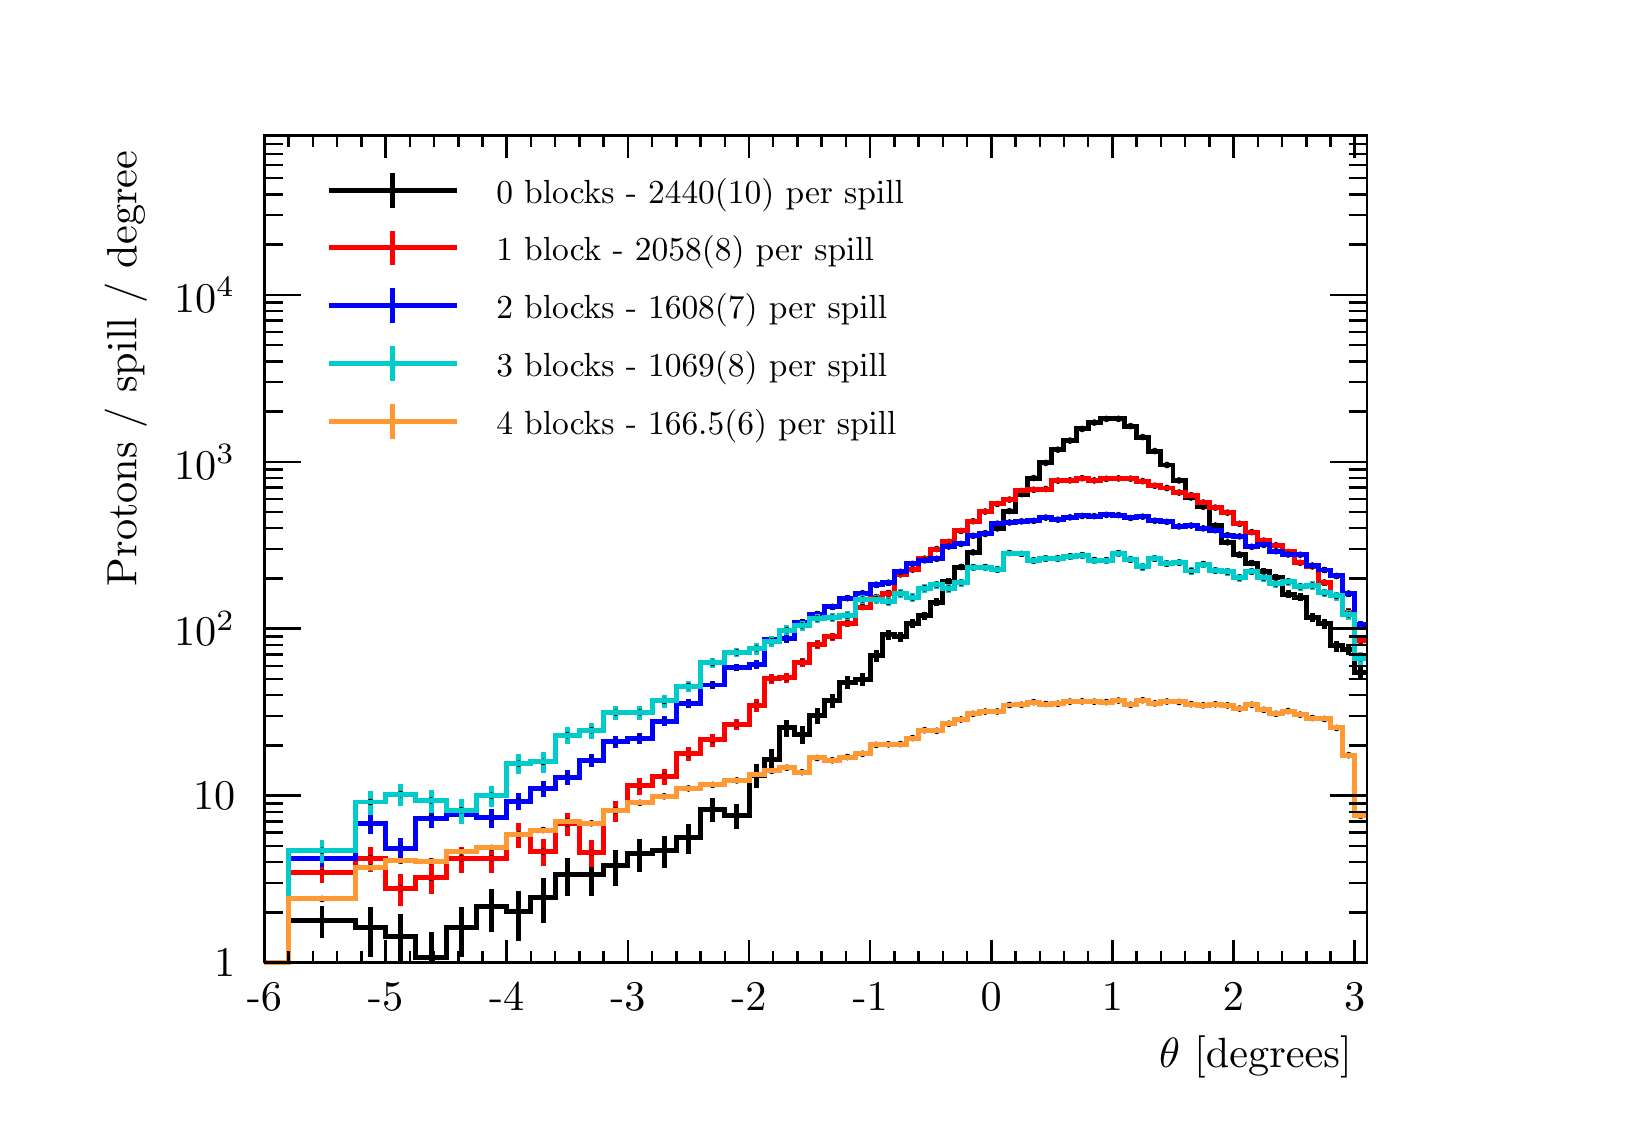
\begin{tikzpicture}
\pgfdeclareplotmark{cross} {
\pgfpathmoveto{\pgfpoint{-0.3\pgfplotmarksize}{\pgfplotmarksize}}
\pgfpathlineto{\pgfpoint{+0.3\pgfplotmarksize}{\pgfplotmarksize}}
\pgfpathlineto{\pgfpoint{+0.3\pgfplotmarksize}{0.3\pgfplotmarksize}}
\pgfpathlineto{\pgfpoint{+1\pgfplotmarksize}{0.3\pgfplotmarksize}}
\pgfpathlineto{\pgfpoint{+1\pgfplotmarksize}{-0.3\pgfplotmarksize}}
\pgfpathlineto{\pgfpoint{+0.3\pgfplotmarksize}{-0.3\pgfplotmarksize}}
\pgfpathlineto{\pgfpoint{+0.3\pgfplotmarksize}{-1.\pgfplotmarksize}}
\pgfpathlineto{\pgfpoint{-0.3\pgfplotmarksize}{-1.\pgfplotmarksize}}
\pgfpathlineto{\pgfpoint{-0.3\pgfplotmarksize}{-0.3\pgfplotmarksize}}
\pgfpathlineto{\pgfpoint{-1.\pgfplotmarksize}{-0.3\pgfplotmarksize}}
\pgfpathlineto{\pgfpoint{-1.\pgfplotmarksize}{0.3\pgfplotmarksize}}
\pgfpathlineto{\pgfpoint{-0.3\pgfplotmarksize}{0.3\pgfplotmarksize}}
\pgfpathclose
\pgfusepathqstroke
}
\pgfdeclareplotmark{cross*} {
\pgfpathmoveto{\pgfpoint{-0.3\pgfplotmarksize}{\pgfplotmarksize}}
\pgfpathlineto{\pgfpoint{+0.3\pgfplotmarksize}{\pgfplotmarksize}}
\pgfpathlineto{\pgfpoint{+0.3\pgfplotmarksize}{0.3\pgfplotmarksize}}
\pgfpathlineto{\pgfpoint{+1\pgfplotmarksize}{0.3\pgfplotmarksize}}
\pgfpathlineto{\pgfpoint{+1\pgfplotmarksize}{-0.3\pgfplotmarksize}}
\pgfpathlineto{\pgfpoint{+0.3\pgfplotmarksize}{-0.3\pgfplotmarksize}}
\pgfpathlineto{\pgfpoint{+0.3\pgfplotmarksize}{-1.\pgfplotmarksize}}
\pgfpathlineto{\pgfpoint{-0.3\pgfplotmarksize}{-1.\pgfplotmarksize}}
\pgfpathlineto{\pgfpoint{-0.3\pgfplotmarksize}{-0.3\pgfplotmarksize}}
\pgfpathlineto{\pgfpoint{-1.\pgfplotmarksize}{-0.3\pgfplotmarksize}}
\pgfpathlineto{\pgfpoint{-1.\pgfplotmarksize}{0.3\pgfplotmarksize}}
\pgfpathlineto{\pgfpoint{-0.3\pgfplotmarksize}{0.3\pgfplotmarksize}}
\pgfpathclose
\pgfusepathqfillstroke
}
\pgfdeclareplotmark{newstar} {
\pgfpathmoveto{\pgfqpoint{0pt}{\pgfplotmarksize}}
\pgfpathlineto{\pgfqpointpolar{44}{0.5\pgfplotmarksize}}
\pgfpathlineto{\pgfqpointpolar{18}{\pgfplotmarksize}}
\pgfpathlineto{\pgfqpointpolar{-20}{0.5\pgfplotmarksize}}
\pgfpathlineto{\pgfqpointpolar{-54}{\pgfplotmarksize}}
\pgfpathlineto{\pgfqpointpolar{-90}{0.5\pgfplotmarksize}}
\pgfpathlineto{\pgfqpointpolar{234}{\pgfplotmarksize}}
\pgfpathlineto{\pgfqpointpolar{198}{0.5\pgfplotmarksize}}
\pgfpathlineto{\pgfqpointpolar{162}{\pgfplotmarksize}}
\pgfpathlineto{\pgfqpointpolar{134}{0.5\pgfplotmarksize}}
\pgfpathclose
\pgfusepathqstroke
}
\pgfdeclareplotmark{newstar*} {
\pgfpathmoveto{\pgfqpoint{0pt}{\pgfplotmarksize}}
\pgfpathlineto{\pgfqpointpolar{44}{0.5\pgfplotmarksize}}
\pgfpathlineto{\pgfqpointpolar{18}{\pgfplotmarksize}}
\pgfpathlineto{\pgfqpointpolar{-20}{0.5\pgfplotmarksize}}
\pgfpathlineto{\pgfqpointpolar{-54}{\pgfplotmarksize}}
\pgfpathlineto{\pgfqpointpolar{-90}{0.5\pgfplotmarksize}}
\pgfpathlineto{\pgfqpointpolar{234}{\pgfplotmarksize}}
\pgfpathlineto{\pgfqpointpolar{198}{0.5\pgfplotmarksize}}
\pgfpathlineto{\pgfqpointpolar{162}{\pgfplotmarksize}}
\pgfpathlineto{\pgfqpointpolar{134}{0.5\pgfplotmarksize}}
\pgfpathclose
\pgfusepathqfillstroke
}
\definecolor{c}{rgb}{1,1,1};
\draw [color=c, fill=c] (0,0) rectangle (20,13.639);
\draw [color=c, fill=c] (3,1.77307) rectangle (17,12.2751);
\definecolor{c}{rgb}{0,0,0};
\draw [c,line width=0.9] (3,1.77307) -- (3,12.2751) -- (17,12.2751) -- (17,1.77307) -- (3,1.77307);
\definecolor{c}{rgb}{1,1,1};
\draw [color=c, fill=c] (3,1.77307) rectangle (17,12.2751);
\definecolor{c}{rgb}{0,0,0};
\draw [c,line width=0.9] (3,1.77307) -- (3,12.2751) -- (17,12.2751) -- (17,1.77307) -- (3,1.77307);
\draw [c,line width=0.9] (3,1.77307) -- (3.30769,1.77307) -- (3.30769,1.77307) -- (4.15385,1.77307) -- (4.15385,1.77307) -- (4.53846,1.77307) -- (4.53846,1.77307) -- (4.92308,1.77307) -- (4.92308,1.77307) -- (5.30769,1.77307) -- (5.30769,1.77307) --
 (5.69231,1.77307) -- (5.69231,1.77307) -- (6.07692,1.77307) -- (6.07692,1.77307) -- (6.38462,1.77307) -- (6.38462,1.77307) -- (6.69231,1.77307) -- (6.69231,1.77307) -- (7,1.77307) -- (7,1.77307) -- (7.30769,1.77307) -- (7.30769,1.77307) --
 (7.61538,1.77307) -- (7.61538,1.77307) -- (7.92308,1.77307) -- (7.92308,1.77307) -- (8.23077,1.77307) -- (8.23077,1.77307) -- (8.53846,1.77307) -- (8.53846,1.77307) -- (8.84615,1.77307) -- (8.84615,1.77307) -- (9.15385,1.77307) -- (9.15385,1.77307)
 -- (9.34615,1.77307) -- (9.34615,1.77307) -- (9.53846,1.77307) -- (9.53846,1.77307) -- (9.73077,1.77307) -- (9.73077,1.77307) -- (9.92308,1.77307) -- (9.92308,1.77307) -- (10.1154,1.77307) -- (10.1154,1.77307) -- (10.3077,1.77307) --
 (10.3077,1.77307) -- (10.5,1.77307) -- (10.5,1.77307) -- (10.6923,1.77307) -- (10.6923,1.77307) -- (10.8462,1.77307) -- (10.8462,1.77307) -- (11,1.77307) -- (11,1.77307) -- (11.1538,1.77307) -- (11.1538,1.77307) -- (11.3077,1.77307) --
 (11.3077,1.77307) -- (11.4615,1.77307) -- (11.4615,1.77307) -- (11.6154,1.77307) -- (11.6154,1.77307) -- (11.7692,1.77307) -- (11.7692,1.77307) -- (11.9231,1.77307) -- (11.9231,1.77307) -- (12.0769,1.77307) -- (12.0769,1.77307) -- (12.2308,1.77307)
 -- (12.2308,1.77307) -- (12.3846,1.77307) -- (12.3846,1.77307) -- (12.5385,1.77307) -- (12.5385,1.77307) -- (12.6923,1.77307) -- (12.6923,1.77307) -- (12.8462,1.77307) -- (12.8462,1.77307) -- (13,1.77307) -- (13,1.77307) -- (13.1538,1.77307) --
 (13.1538,1.77307) -- (13.3077,1.77307) -- (13.3077,1.77307) -- (13.4615,1.77307) -- (13.4615,1.77307) -- (13.6154,1.77307) -- (13.6154,1.77307) -- (13.7692,1.77307) -- (13.7692,1.77307) -- (13.9231,1.77307) -- (13.9231,1.77307) -- (14.0769,1.77307)
 -- (14.0769,1.77307) -- (14.2308,1.77307) -- (14.2308,1.77307) -- (14.3846,1.77307) -- (14.3846,1.77307) -- (14.5385,1.77307) -- (14.5385,1.77307) -- (14.6923,1.77307) -- (14.6923,1.77307) -- (14.8462,1.77307) -- (14.8462,1.77307) -- (15,1.77307) --
 (15,1.77307) -- (15.1538,1.77307) -- (15.1538,1.77307) -- (15.3077,1.77307) -- (15.3077,1.77307) -- (15.4615,1.77307) -- (15.4615,1.77307) -- (15.6154,1.77307) -- (15.6154,1.77307) -- (15.7692,1.77307) -- (15.7692,1.77307) -- (15.9231,1.77307) --
 (15.9231,1.77307) -- (16.0769,1.77307) -- (16.0769,1.77307) -- (16.2308,1.77307) -- (16.2308,1.77307) -- (16.3846,1.77307) -- (16.3846,1.77307) -- (16.5385,1.77307) -- (16.5385,1.77307) -- (16.6923,1.77307) -- (16.6923,1.77307) -- (16.8462,1.77307)
 -- (16.8462,1.77307) -- (17,1.77307);
\draw [c,line width=0.9] (3,1.77307) -- (17,1.77307);
\draw [c,line width=0.9] (3,2.05948) -- (3,1.77307);
\draw [c,line width=0.9] (3.30769,1.91628) -- (3.30769,1.77307);
\draw [c,line width=0.9] (3.61538,1.91628) -- (3.61538,1.77307);
\draw [c,line width=0.9] (3.92308,1.91628) -- (3.92308,1.77307);
\draw [c,line width=0.9] (4.23077,1.91628) -- (4.23077,1.77307);
\draw [c,line width=0.9] (4.53846,2.05948) -- (4.53846,1.77307);
\draw [c,line width=0.9] (4.84615,1.91628) -- (4.84615,1.77307);
\draw [c,line width=0.9] (5.15385,1.91628) -- (5.15385,1.77307);
\draw [c,line width=0.9] (5.46154,1.91628) -- (5.46154,1.77307);
\draw [c,line width=0.9] (5.76923,1.91628) -- (5.76923,1.77307);
\draw [c,line width=0.9] (6.07692,2.05948) -- (6.07692,1.77307);
\draw [c,line width=0.9] (6.38462,1.91628) -- (6.38462,1.77307);
\draw [c,line width=0.9] (6.69231,1.91628) -- (6.69231,1.77307);
\draw [c,line width=0.9] (7,1.91628) -- (7,1.77307);
\draw [c,line width=0.9] (7.30769,1.91628) -- (7.30769,1.77307);
\draw [c,line width=0.9] (7.61538,2.05948) -- (7.61538,1.77307);
\draw [c,line width=0.9] (7.92308,1.91628) -- (7.92308,1.77307);
\draw [c,line width=0.9] (8.23077,1.91628) -- (8.23077,1.77307);
\draw [c,line width=0.9] (8.53846,1.91628) -- (8.53846,1.77307);
\draw [c,line width=0.9] (8.84615,1.91628) -- (8.84615,1.77307);
\draw [c,line width=0.9] (9.15385,2.05948) -- (9.15385,1.77307);
\draw [c,line width=0.9] (9.46154,1.91628) -- (9.46154,1.77307);
\draw [c,line width=0.9] (9.76923,1.91628) -- (9.76923,1.77307);
\draw [c,line width=0.9] (10.0769,1.91628) -- (10.0769,1.77307);
\draw [c,line width=0.9] (10.3846,1.91628) -- (10.3846,1.77307);
\draw [c,line width=0.9] (10.6923,2.05948) -- (10.6923,1.77307);
\draw [c,line width=0.9] (11,1.91628) -- (11,1.77307);
\draw [c,line width=0.9] (11.3077,1.91628) -- (11.3077,1.77307);
\draw [c,line width=0.9] (11.6154,1.91628) -- (11.6154,1.77307);
\draw [c,line width=0.9] (11.9231,1.91628) -- (11.9231,1.77307);
\draw [c,line width=0.9] (12.2308,2.05948) -- (12.2308,1.77307);
\draw [c,line width=0.9] (12.5385,1.91628) -- (12.5385,1.77307);
\draw [c,line width=0.9] (12.8462,1.91628) -- (12.8462,1.77307);
\draw [c,line width=0.9] (13.1538,1.91628) -- (13.1538,1.77307);
\draw [c,line width=0.9] (13.4615,1.91628) -- (13.4615,1.77307);
\draw [c,line width=0.9] (13.7692,2.05948) -- (13.7692,1.77307);
\draw [c,line width=0.9] (14.0769,1.91628) -- (14.0769,1.77307);
\draw [c,line width=0.9] (14.3846,1.91628) -- (14.3846,1.77307);
\draw [c,line width=0.9] (14.6923,1.91628) -- (14.6923,1.77307);
\draw [c,line width=0.9] (15,1.91628) -- (15,1.77307);
\draw [c,line width=0.9] (15.3077,2.05948) -- (15.3077,1.77307);
\draw [c,line width=0.9] (15.6154,1.91628) -- (15.6154,1.77307);
\draw [c,line width=0.9] (15.9231,1.91628) -- (15.9231,1.77307);
\draw [c,line width=0.9] (16.2308,1.91628) -- (16.2308,1.77307);
\draw [c,line width=0.9] (16.5385,1.91628) -- (16.5385,1.77307);
\draw [c,line width=0.9] (16.8462,2.05948) -- (16.8462,1.77307);
\draw [c,line width=0.9] (16.8462,2.05948) -- (16.8462,1.77307);
\draw [anchor=base] (3,1.15931) node[scale=1.52731, color=c, rotate=0]{-6};
\draw [anchor=base] (4.53846,1.15931) node[scale=1.52731, color=c, rotate=0]{-5};
\draw [anchor=base] (6.07692,1.15931) node[scale=1.52731, color=c, rotate=0]{-4};
\draw [anchor=base] (7.61538,1.15931) node[scale=1.52731, color=c, rotate=0]{-3};
\draw [anchor=base] (9.15385,1.15931) node[scale=1.52731, color=c, rotate=0]{-2};
\draw [anchor=base] (10.6923,1.15931) node[scale=1.52731, color=c, rotate=0]{-1};
\draw [anchor=base] (12.2308,1.15931) node[scale=1.52731, color=c, rotate=0]{0};
\draw [anchor=base] (13.7692,1.15931) node[scale=1.52731, color=c, rotate=0]{1};
\draw [anchor=base] (15.3077,1.15931) node[scale=1.52731, color=c, rotate=0]{2};
\draw [anchor=base] (16.8462,1.15931) node[scale=1.52731, color=c, rotate=0]{3};
\draw [anchor= east] (17,0.572837) node[scale=1.52731, color=c, rotate=0]{$\theta$ [degrees]};
\draw [c,line width=0.9] (3,12.2751) -- (17,12.2751);
\draw [c,line width=0.9] (3,11.9887) -- (3,12.2751);
\draw [c,line width=0.9] (3.30769,12.1319) -- (3.30769,12.2751);
\draw [c,line width=0.9] (3.61538,12.1319) -- (3.61538,12.2751);
\draw [c,line width=0.9] (3.92308,12.1319) -- (3.92308,12.2751);
\draw [c,line width=0.9] (4.23077,12.1319) -- (4.23077,12.2751);
\draw [c,line width=0.9] (4.53846,11.9887) -- (4.53846,12.2751);
\draw [c,line width=0.9] (4.84615,12.1319) -- (4.84615,12.2751);
\draw [c,line width=0.9] (5.15385,12.1319) -- (5.15385,12.2751);
\draw [c,line width=0.9] (5.46154,12.1319) -- (5.46154,12.2751);
\draw [c,line width=0.9] (5.76923,12.1319) -- (5.76923,12.2751);
\draw [c,line width=0.9] (6.07692,11.9887) -- (6.07692,12.2751);
\draw [c,line width=0.9] (6.38462,12.1319) -- (6.38462,12.2751);
\draw [c,line width=0.9] (6.69231,12.1319) -- (6.69231,12.2751);
\draw [c,line width=0.9] (7,12.1319) -- (7,12.2751);
\draw [c,line width=0.9] (7.30769,12.1319) -- (7.30769,12.2751);
\draw [c,line width=0.9] (7.61538,11.9887) -- (7.61538,12.2751);
\draw [c,line width=0.9] (7.92308,12.1319) -- (7.92308,12.2751);
\draw [c,line width=0.9] (8.23077,12.1319) -- (8.23077,12.2751);
\draw [c,line width=0.9] (8.53846,12.1319) -- (8.53846,12.2751);
\draw [c,line width=0.9] (8.84615,12.1319) -- (8.84615,12.2751);
\draw [c,line width=0.9] (9.15385,11.9887) -- (9.15385,12.2751);
\draw [c,line width=0.9] (9.46154,12.1319) -- (9.46154,12.2751);
\draw [c,line width=0.9] (9.76923,12.1319) -- (9.76923,12.2751);
\draw [c,line width=0.9] (10.0769,12.1319) -- (10.0769,12.2751);
\draw [c,line width=0.9] (10.3846,12.1319) -- (10.3846,12.2751);
\draw [c,line width=0.9] (10.6923,11.9887) -- (10.6923,12.2751);
\draw [c,line width=0.9] (11,12.1319) -- (11,12.2751);
\draw [c,line width=0.9] (11.3077,12.1319) -- (11.3077,12.2751);
\draw [c,line width=0.9] (11.6154,12.1319) -- (11.6154,12.2751);
\draw [c,line width=0.9] (11.9231,12.1319) -- (11.9231,12.2751);
\draw [c,line width=0.9] (12.2308,11.9887) -- (12.2308,12.2751);
\draw [c,line width=0.9] (12.5385,12.1319) -- (12.5385,12.2751);
\draw [c,line width=0.9] (12.8462,12.1319) -- (12.8462,12.2751);
\draw [c,line width=0.9] (13.1538,12.1319) -- (13.1538,12.2751);
\draw [c,line width=0.9] (13.4615,12.1319) -- (13.4615,12.2751);
\draw [c,line width=0.9] (13.7692,11.9887) -- (13.7692,12.2751);
\draw [c,line width=0.9] (14.0769,12.1319) -- (14.0769,12.2751);
\draw [c,line width=0.9] (14.3846,12.1319) -- (14.3846,12.2751);
\draw [c,line width=0.9] (14.6923,12.1319) -- (14.6923,12.2751);
\draw [c,line width=0.9] (15,12.1319) -- (15,12.2751);
\draw [c,line width=0.9] (15.3077,11.9887) -- (15.3077,12.2751);
\draw [c,line width=0.9] (15.6154,12.1319) -- (15.6154,12.2751);
\draw [c,line width=0.9] (15.9231,12.1319) -- (15.9231,12.2751);
\draw [c,line width=0.9] (16.2308,12.1319) -- (16.2308,12.2751);
\draw [c,line width=0.9] (16.5385,12.1319) -- (16.5385,12.2751);
\draw [c,line width=0.9] (16.8462,11.9887) -- (16.8462,12.2751);
\draw [c,line width=0.9] (16.8462,11.9887) -- (16.8462,12.2751);
\draw [c,line width=0.9] (3,1.77307) -- (3,12.2751);
\draw [c,line width=0.9] (3.462,1.77307) -- (3,1.77307);
\draw [anchor= east] (2.82,1.77307) node[scale=1.52731, color=c, rotate=0]{1};
\draw [c,line width=0.9] (3.231,2.41119) -- (3,2.41119);
\draw [c,line width=0.9] (3.231,2.78447) -- (3,2.78447);
\draw [c,line width=0.9] (3.231,3.04931) -- (3,3.04931);
\draw [c,line width=0.9] (3.231,3.25474) -- (3,3.25474);
\draw [c,line width=0.9] (3.231,3.42259) -- (3,3.42259);
\draw [c,line width=0.9] (3.231,3.56451) -- (3,3.56451);
\draw [c,line width=0.9] (3.231,3.68744) -- (3,3.68744);
\draw [c,line width=0.9] (3.231,3.79587) -- (3,3.79587);
\draw [c,line width=0.9] (3.462,3.89287) -- (3,3.89287);
\draw [anchor= east] (2.82,3.89287) node[scale=1.52731, color=c, rotate=0]{10};
\draw [c,line width=0.9] (3.231,4.53099) -- (3,4.53099);
\draw [c,line width=0.9] (3.231,4.90427) -- (3,4.90427);
\draw [c,line width=0.9] (3.231,5.16912) -- (3,5.16912);
\draw [c,line width=0.9] (3.231,5.37454) -- (3,5.37454);
\draw [c,line width=0.9] (3.231,5.54239) -- (3,5.54239);
\draw [c,line width=0.9] (3.231,5.68431) -- (3,5.68431);
\draw [c,line width=0.9] (3.231,5.80724) -- (3,5.80724);
\draw [c,line width=0.9] (3.231,5.91567) -- (3,5.91567);
\draw [c,line width=0.9] (3.462,6.01267) -- (3,6.01267);
\draw [anchor= east] (2.82,6.01267) node[scale=1.52731, color=c, rotate=0]{$10^{2}$};
\draw [c,line width=0.9] (3.231,6.65079) -- (3,6.65079);
\draw [c,line width=0.9] (3.231,7.02407) -- (3,7.02407);
\draw [c,line width=0.9] (3.231,7.28892) -- (3,7.28892);
\draw [c,line width=0.9] (3.231,7.49434) -- (3,7.49434);
\draw [c,line width=0.9] (3.231,7.66219) -- (3,7.66219);
\draw [c,line width=0.9] (3.231,7.80411) -- (3,7.80411);
\draw [c,line width=0.9] (3.231,7.92704) -- (3,7.92704);
\draw [c,line width=0.9] (3.231,8.03547) -- (3,8.03547);
\draw [c,line width=0.9] (3.462,8.13247) -- (3,8.13247);
\draw [anchor= east] (2.82,8.13247) node[scale=1.52731, color=c, rotate=0]{$10^{3}$};
\draw [c,line width=0.9] (3.231,8.77059) -- (3,8.77059);
\draw [c,line width=0.9] (3.231,9.14387) -- (3,9.14387);
\draw [c,line width=0.9] (3.231,9.40872) -- (3,9.40872);
\draw [c,line width=0.9] (3.231,9.61415) -- (3,9.61415);
\draw [c,line width=0.9] (3.231,9.78199) -- (3,9.78199);
\draw [c,line width=0.9] (3.231,9.92391) -- (3,9.92391);
\draw [c,line width=0.9] (3.231,10.0468) -- (3,10.0468);
\draw [c,line width=0.9] (3.231,10.1553) -- (3,10.1553);
\draw [c,line width=0.9] (3.462,10.2523) -- (3,10.2523);
\draw [anchor= east] (2.82,10.2523) node[scale=1.52731, color=c, rotate=0]{$10^{4}$};
\draw [c,line width=0.9] (3.231,10.8904) -- (3,10.8904);
\draw [c,line width=0.9] (3.231,11.2637) -- (3,11.2637);
\draw [c,line width=0.9] (3.231,11.5285) -- (3,11.5285);
\draw [c,line width=0.9] (3.231,11.7339) -- (3,11.7339);
\draw [c,line width=0.9] (3.231,11.9018) -- (3,11.9018);
\draw [c,line width=0.9] (3.231,12.0437) -- (3,12.0437);
\draw [c,line width=0.9] (3.231,12.1666) -- (3,12.1666);
\draw [c,line width=0.9] (3.231,12.2751) -- (3,12.2751);
\draw [anchor= east] (1.24,12.2751) node[scale=1.52731, color=c, rotate=90]{ Protons / spill / degree};
\draw [c,line width=0.9] (17,1.77307) -- (17,12.2751);
\draw [c,line width=0.9] (16.538,1.77307) -- (17,1.77307);
\draw [c,line width=0.9] (16.769,2.41119) -- (17,2.41119);
\draw [c,line width=0.9] (16.769,2.78447) -- (17,2.78447);
\draw [c,line width=0.9] (16.769,3.04931) -- (17,3.04931);
\draw [c,line width=0.9] (16.769,3.25474) -- (17,3.25474);
\draw [c,line width=0.9] (16.769,3.42259) -- (17,3.42259);
\draw [c,line width=0.9] (16.769,3.56451) -- (17,3.56451);
\draw [c,line width=0.9] (16.769,3.68744) -- (17,3.68744);
\draw [c,line width=0.9] (16.769,3.79587) -- (17,3.79587);
\draw [c,line width=0.9] (16.538,3.89287) -- (17,3.89287);
\draw [c,line width=0.9] (16.769,4.53099) -- (17,4.53099);
\draw [c,line width=0.9] (16.769,4.90427) -- (17,4.90427);
\draw [c,line width=0.9] (16.769,5.16912) -- (17,5.16912);
\draw [c,line width=0.9] (16.769,5.37454) -- (17,5.37454);
\draw [c,line width=0.9] (16.769,5.54239) -- (17,5.54239);
\draw [c,line width=0.9] (16.769,5.68431) -- (17,5.68431);
\draw [c,line width=0.9] (16.769,5.80724) -- (17,5.80724);
\draw [c,line width=0.9] (16.769,5.91567) -- (17,5.91567);
\draw [c,line width=0.9] (16.538,6.01267) -- (17,6.01267);
\draw [c,line width=0.9] (16.769,6.65079) -- (17,6.65079);
\draw [c,line width=0.9] (16.769,7.02407) -- (17,7.02407);
\draw [c,line width=0.9] (16.769,7.28892) -- (17,7.28892);
\draw [c,line width=0.9] (16.769,7.49434) -- (17,7.49434);
\draw [c,line width=0.9] (16.769,7.66219) -- (17,7.66219);
\draw [c,line width=0.9] (16.769,7.80411) -- (17,7.80411);
\draw [c,line width=0.9] (16.769,7.92704) -- (17,7.92704);
\draw [c,line width=0.9] (16.769,8.03547) -- (17,8.03547);
\draw [c,line width=0.9] (16.538,8.13247) -- (17,8.13247);
\draw [c,line width=0.9] (16.769,8.77059) -- (17,8.77059);
\draw [c,line width=0.9] (16.769,9.14387) -- (17,9.14387);
\draw [c,line width=0.9] (16.769,9.40872) -- (17,9.40872);
\draw [c,line width=0.9] (16.769,9.61415) -- (17,9.61415);
\draw [c,line width=0.9] (16.769,9.78199) -- (17,9.78199);
\draw [c,line width=0.9] (16.769,9.92391) -- (17,9.92391);
\draw [c,line width=0.9] (16.769,10.0468) -- (17,10.0468);
\draw [c,line width=0.9] (16.769,10.1553) -- (17,10.1553);
\draw [c,line width=0.9] (16.538,10.2523) -- (17,10.2523);
\draw [c,line width=0.9] (16.769,10.8904) -- (17,10.8904);
\draw [c,line width=0.9] (16.769,11.2637) -- (17,11.2637);
\draw [c,line width=0.9] (16.769,11.5285) -- (17,11.5285);
\draw [c,line width=0.9] (16.769,11.7339) -- (17,11.7339);
\draw [c,line width=0.9] (16.769,11.9018) -- (17,11.9018);
\draw [c,line width=0.9] (16.769,12.0437) -- (17,12.0437);
\draw [c,line width=0.9] (16.769,12.1666) -- (17,12.1666);
\draw [c,line width=0.9] (16.769,12.2751) -- (17,12.2751);
\draw [c,line width=1.8] (3.73077,2.09091) -- (3.73077,2.31167);
\draw [c,line width=1.8] (3.73077,2.31167) -- (3.73077,2.4896);
\foreach \P in {(3.73077,2.31167)}{\draw[mark options={color=c,fill=c},mark size=2.402402pt,mark=*,mark size=1pt] plot coordinates {\P};}
\draw [c,line width=1.8] (4.34615,1.84136) -- (4.34615,2.21467);
\draw [c,line width=1.8] (4.34615,2.21467) -- (4.34615,2.47953);
\foreach \P in {(4.34615,2.21467)}{\draw[mark options={color=c,fill=c},mark size=2.402402pt,mark=*,mark size=1pt] plot coordinates {\P};}
\draw [c,line width=1.8] (4.73077,1.77307) -- (4.73077,2.10624);
\draw [c,line width=1.8] (4.73077,2.10624) -- (4.73077,2.38496);
\foreach \P in {(4.73077,2.10624)}{\draw[mark options={color=c,fill=c},mark size=2.402402pt,mark=*,mark size=1pt] plot coordinates {\P};}
\draw [c,line width=1.8] (5.11538,1.77307) -- (5.11538,1.84139);
\draw [c,line width=1.8] (5.11538,1.84139) -- (5.11538,2.15658);
\foreach \P in {(5.11538,1.84139)}{\draw[mark options={color=c,fill=c},mark size=2.402402pt,mark=*,mark size=1pt] plot coordinates {\P};}
\draw [c,line width=1.8] (5.5,1.84136) -- (5.5,2.21467);
\draw [c,line width=1.8] (5.5,2.21467) -- (5.5,2.47953);
\foreach \P in {(5.5,2.21467)}{\draw[mark options={color=c,fill=c},mark size=2.402402pt,mark=*,mark size=1pt] plot coordinates {\P};}
\draw [c,line width=1.8] (5.88462,2.16591) -- (5.88462,2.47952);
\draw [c,line width=1.8] (5.88462,2.47952) -- (5.88462,2.71301);
\foreach \P in {(5.88462,2.47952)}{\draw[mark options={color=c,fill=c},mark size=2.402402pt,mark=*,mark size=1pt] plot coordinates {\P};}
\draw [c,line width=1.8] (6.23077,2.04679) -- (6.23077,2.4201);
\draw [c,line width=1.8] (6.23077,2.4201) -- (6.23077,2.68496);
\foreach \P in {(6.23077,2.4201)}{\draw[mark options={color=c,fill=c},mark size=2.402402pt,mark=*,mark size=1pt] plot coordinates {\P};}
\draw [c,line width=1.8] (6.53846,2.27447) -- (6.53846,2.60484);
\draw [c,line width=1.8] (6.53846,2.60484) -- (6.53846,2.84746);
\foreach \P in {(6.53846,2.60484)}{\draw[mark options={color=c,fill=c},mark size=2.402402pt,mark=*,mark size=1pt] plot coordinates {\P};}
\draw [c,line width=1.8] (6.84615,2.61539) -- (6.84615,2.89038);
\draw [c,line width=1.8] (6.84615,2.89038) -- (6.84615,3.10184);
\foreach \P in {(6.84615,2.89038)}{\draw[mark options={color=c,fill=c},mark size=2.402402pt,mark=*,mark size=1pt] plot coordinates {\P};}
\draw [c,line width=1.8] (7.15385,2.61539) -- (7.15385,2.89038);
\draw [c,line width=1.8] (7.15385,2.89038) -- (7.15385,3.10184);
\foreach \P in {(7.15385,2.89038)}{\draw[mark options={color=c,fill=c},mark size=2.402402pt,mark=*,mark size=1pt] plot coordinates {\P};}
\draw [c,line width=1.8] (7.46154,2.74986) -- (7.46154,3.0056);
\draw [c,line width=1.8] (7.46154,3.0056) -- (7.46154,3.20553);
\foreach \P in {(7.46154,3.0056)}{\draw[mark options={color=c,fill=c},mark size=2.402402pt,mark=*,mark size=1pt] plot coordinates {\P};}
\draw [c,line width=1.8] (7.76923,2.9222) -- (7.76923,3.15522);
\draw [c,line width=1.8] (7.76923,3.15522) -- (7.76923,3.34102);
\foreach \P in {(7.76923,3.15522)}{\draw[mark options={color=c,fill=c},mark size=2.402402pt,mark=*,mark size=1pt] plot coordinates {\P};}
\draw [c,line width=1.8] (8.07692,2.97349) -- (8.07692,3.20014);
\draw [c,line width=1.8] (8.07692,3.20014) -- (8.07692,3.38187);
\foreach \P in {(8.07692,3.20014)}{\draw[mark options={color=c,fill=c},mark size=2.402402pt,mark=*,mark size=1pt] plot coordinates {\P};}
\draw [c,line width=1.8] (8.38461,3.15521) -- (8.38461,3.36065);
\draw [c,line width=1.8] (8.38461,3.36065) -- (8.38461,3.52851);
\foreach \P in {(8.38461,3.36065)}{\draw[mark options={color=c,fill=c},mark size=2.402402pt,mark=*,mark size=1pt] plot coordinates {\P};}
\draw [c,line width=1.8] (8.69231,3.55621) -- (8.69231,3.72157);
\draw [c,line width=1.8] (8.69231,3.72157) -- (8.69231,3.8617);
\foreach \P in {(8.69231,3.72157)}{\draw[mark options={color=c,fill=c},mark size=2.402402pt,mark=*,mark size=1pt] plot coordinates {\P};}
\draw [c,line width=1.8] (9,3.47051) -- (9,3.64373);
\draw [c,line width=1.8] (9,3.64373) -- (9,3.78946);
\foreach \P in {(9,3.64373)}{\draw[mark options={color=c,fill=c},mark size=2.402402pt,mark=*,mark size=1pt] plot coordinates {\P};}
\draw [c,line width=1.8] (9.25,3.98891) -- (9.25,4.15427);
\draw [c,line width=1.8] (9.25,4.15427) -- (9.25,4.2944);
\foreach \P in {(9.25,4.15427)}{\draw[mark options={color=c,fill=c},mark size=2.402402pt,mark=*,mark size=1pt] plot coordinates {\P};}
\draw [c,line width=1.8] (9.44231,4.20785) -- (9.44231,4.35471);
\draw [c,line width=1.8] (9.44231,4.35471) -- (9.44231,4.48133);
\foreach \P in {(9.44231,4.35471)}{\draw[mark options={color=c,fill=c},mark size=2.402402pt,mark=*,mark size=1pt] plot coordinates {\P};}
\draw [c,line width=1.8] (9.63461,4.63798) -- (9.63461,4.75429);
\draw [c,line width=1.8] (9.63461,4.75429) -- (9.63461,4.85754);
\foreach \P in {(9.63461,4.75429)}{\draw[mark options={color=c,fill=c},mark size=2.402402pt,mark=*,mark size=1pt] plot coordinates {\P};}
\draw [c,line width=1.8] (9.82692,4.55108) -- (9.82692,4.67301);
\draw [c,line width=1.8] (9.82692,4.67301) -- (9.82692,4.78066);
\foreach \P in {(9.82692,4.67301)}{\draw[mark options={color=c,fill=c},mark size=2.402402pt,mark=*,mark size=1pt] plot coordinates {\P};}
\draw [c,line width=1.8] (10.0192,4.80271) -- (10.0192,4.90908);
\draw [c,line width=1.8] (10.0192,4.90908) -- (10.0192,5.00442);
\foreach \P in {(10.0192,4.90908)}{\draw[mark options={color=c,fill=c},mark size=2.402402pt,mark=*,mark size=1pt] plot coordinates {\P};}
\draw [c,line width=1.8] (10.2115,5.0013) -- (10.2115,5.09681);
\draw [c,line width=1.8] (10.2115,5.09681) -- (10.2115,5.18333);
\foreach \P in {(10.2115,5.09681)}{\draw[mark options={color=c,fill=c},mark size=2.402402pt,mark=*,mark size=1pt] plot coordinates {\P};}
\draw [c,line width=1.8] (10.4038,5.24863) -- (10.4038,5.33213);
\draw [c,line width=1.8] (10.4038,5.33213) -- (10.4038,5.40869);
\foreach \P in {(10.4038,5.33213)}{\draw[mark options={color=c,fill=c},mark size=2.402402pt,mark=*,mark size=1pt] plot coordinates {\P};}
\draw [c,line width=1.8] (10.5962,5.29115) -- (10.5962,5.37276);
\draw [c,line width=1.8] (10.5962,5.37276) -- (10.5962,5.44771);
\foreach \P in {(10.5962,5.37276)}{\draw[mark options={color=c,fill=c},mark size=2.402402pt,mark=*,mark size=1pt] plot coordinates {\P};}
\draw [c,line width=1.8] (10.7692,5.58892) -- (10.7692,5.66653);
\draw [c,line width=1.8] (10.7692,5.66653) -- (10.7692,5.73811);
\foreach \P in {(10.7692,5.66653)}{\draw[mark options={color=c,fill=c},mark size=2.402402pt,mark=*,mark size=1pt] plot coordinates {\P};}
\draw [c,line width=1.8] (10.9231,5.87387) -- (10.9231,5.94036);
\draw [c,line width=1.8] (10.9231,5.94036) -- (10.9231,6.00237);
\foreach \P in {(10.9231,5.94036)}{\draw[mark options={color=c,fill=c},mark size=2.402402pt,mark=*,mark size=1pt] plot coordinates {\P};}
\draw [c,line width=1.8] (11.0769,5.84084) -- (11.0769,5.90853);
\draw [c,line width=1.8] (11.0769,5.90853) -- (11.0769,5.97159);
\foreach \P in {(11.0769,5.90853)}{\draw[mark options={color=c,fill=c},mark size=2.402402pt,mark=*,mark size=1pt] plot coordinates {\P};}
\draw [c,line width=1.8] (11.2308,6.02352) -- (11.2308,6.08482);
\draw [c,line width=1.8] (11.2308,6.08482) -- (11.2308,6.1423);
\foreach \P in {(11.2308,6.08482)}{\draw[mark options={color=c,fill=c},mark size=2.402402pt,mark=*,mark size=1pt] plot coordinates {\P};}
\draw [c,line width=1.8] (11.3846,6.11743) -- (11.3846,6.17569);
\draw [c,line width=1.8] (11.3846,6.17569) -- (11.3846,6.23047);
\foreach \P in {(11.3846,6.17569)}{\draw[mark options={color=c,fill=c},mark size=2.402402pt,mark=*,mark size=1pt] plot coordinates {\P};}
\draw [c,line width=1.8] (11.5385,6.29584) -- (11.5385,6.34871);
\draw [c,line width=1.8] (11.5385,6.34871) -- (11.5385,6.39872);
\foreach \P in {(11.5385,6.34871)}{\draw[mark options={color=c,fill=c},mark size=2.402402pt,mark=*,mark size=1pt] plot coordinates {\P};}
\draw [c,line width=1.8] (11.6923,6.5613) -- (11.6923,6.60708);
\draw [c,line width=1.8] (11.6923,6.60708) -- (11.6923,6.65069);
\foreach \P in {(11.6923,6.60708)}{\draw[mark options={color=c,fill=c},mark size=2.402402pt,mark=*,mark size=1pt] plot coordinates {\P};}
\draw [c,line width=1.8] (11.8462,6.75514) -- (11.8462,6.79634);
\draw [c,line width=1.8] (11.8462,6.79634) -- (11.8462,6.83578);
\foreach \P in {(11.8462,6.79634)}{\draw[mark options={color=c,fill=c},mark size=2.402402pt,mark=*,mark size=1pt] plot coordinates {\P};}
\draw [c,line width=1.8] (12,6.94536) -- (12,6.98252);
\draw [c,line width=1.8] (12,6.98252) -- (12,7.01824);
\foreach \P in {(12,6.98252)}{\draw[mark options={color=c,fill=c},mark size=2.402402pt,mark=*,mark size=1pt] plot coordinates {\P};}
\draw [c,line width=1.8] (12.1538,7.18396) -- (12.1538,7.21661);
\draw [c,line width=1.8] (12.1538,7.21661) -- (12.1538,7.24813);
\foreach \P in {(12.1538,7.21661)}{\draw[mark options={color=c,fill=c},mark size=2.402402pt,mark=*,mark size=1pt] plot coordinates {\P};}
\draw [c,line width=1.8] (12.3077,7.2551) -- (12.3077,7.28651);
\draw [c,line width=1.8] (12.3077,7.28651) -- (12.3077,7.31688);
\foreach \P in {(12.3077,7.28651)}{\draw[mark options={color=c,fill=c},mark size=2.402402pt,mark=*,mark size=1pt] plot coordinates {\P};}
\draw [c,line width=1.8] (12.4615,7.47871) -- (12.4615,7.50652);
\draw [c,line width=1.8] (12.4615,7.50652) -- (12.4615,7.53352);
\foreach \P in {(12.4615,7.50652)}{\draw[mark options={color=c,fill=c},mark size=2.402402pt,mark=*,mark size=1pt] plot coordinates {\P};}
\draw [c,line width=1.8] (12.6154,7.69682) -- (12.6154,7.72153);
\draw [c,line width=1.8] (12.6154,7.72153) -- (12.6154,7.74559);
\foreach \P in {(12.6154,7.72153)}{\draw[mark options={color=c,fill=c},mark size=2.402402pt,mark=*,mark size=1pt] plot coordinates {\P};}
\draw [c,line width=1.8] (12.7692,7.9041) -- (12.7692,7.92618);
\draw [c,line width=1.8] (12.7692,7.92618) -- (12.7692,7.94774);
\foreach \P in {(12.7692,7.92618)}{\draw[mark options={color=c,fill=c},mark size=2.402402pt,mark=*,mark size=1pt] plot coordinates {\P};}
\draw [c,line width=1.8] (12.9231,8.09831) -- (12.9231,8.11818);
\draw [c,line width=1.8] (12.9231,8.11818) -- (12.9231,8.13763);
\foreach \P in {(12.9231,8.11818)}{\draw[mark options={color=c,fill=c},mark size=2.402402pt,mark=*,mark size=1pt] plot coordinates {\P};}
\draw [c,line width=1.8] (13.0769,8.26868) -- (13.0769,8.28679);
\draw [c,line width=1.8] (13.0769,8.28679) -- (13.0769,8.30456);
\foreach \P in {(13.0769,8.28679)}{\draw[mark options={color=c,fill=c},mark size=2.402402pt,mark=*,mark size=1pt] plot coordinates {\P};}
\draw [c,line width=1.8] (13.2308,8.38491) -- (13.2308,8.40192);
\draw [c,line width=1.8] (13.2308,8.40192) -- (13.2308,8.41862);
\foreach \P in {(13.2308,8.40192)}{\draw[mark options={color=c,fill=c},mark size=2.402402pt,mark=*,mark size=1pt] plot coordinates {\P};}
\draw [c,line width=1.8] (13.3846,8.5343) -- (13.3846,8.54998);
\draw [c,line width=1.8] (13.3846,8.54998) -- (13.3846,8.5654);
\foreach \P in {(13.3846,8.54998)}{\draw[mark options={color=c,fill=c},mark size=2.402402pt,mark=*,mark size=1pt] plot coordinates {\P};}
\draw [c,line width=1.8] (13.5385,8.61585) -- (13.5385,8.63085);
\draw [c,line width=1.8] (13.5385,8.63085) -- (13.5385,8.64561);
\foreach \P in {(13.5385,8.63085)}{\draw[mark options={color=c,fill=c},mark size=2.402402pt,mark=*,mark size=1pt] plot coordinates {\P};}
\draw [c,line width=1.8] (13.6923,8.66264) -- (13.6923,8.67726);
\draw [c,line width=1.8] (13.6923,8.67726) -- (13.6923,8.69166);
\foreach \P in {(13.6923,8.67726)}{\draw[mark options={color=c,fill=c},mark size=2.402402pt,mark=*,mark size=1pt] plot coordinates {\P};}
\draw [c,line width=1.8] (13.8462,8.66333) -- (13.8462,8.67795);
\draw [c,line width=1.8] (13.8462,8.67795) -- (13.8462,8.69234);
\foreach \P in {(13.8462,8.67795)}{\draw[mark options={color=c,fill=c},mark size=2.402402pt,mark=*,mark size=1pt] plot coordinates {\P};}
\draw [c,line width=1.8] (14,8.57064) -- (14,8.58601);
\draw [c,line width=1.8] (14,8.58601) -- (14,8.60114);
\foreach \P in {(14,8.58601)}{\draw[mark options={color=c,fill=c},mark size=2.402402pt,mark=*,mark size=1pt] plot coordinates {\P};}
\draw [c,line width=1.8] (14.1538,8.42986) -- (14.1538,8.44645);
\draw [c,line width=1.8] (14.1538,8.44645) -- (14.1538,8.46276);
\foreach \P in {(14.1538,8.44645)}{\draw[mark options={color=c,fill=c},mark size=2.402402pt,mark=*,mark size=1pt] plot coordinates {\P};}
\draw [c,line width=1.8] (14.3077,8.25051) -- (14.3077,8.2688);
\draw [c,line width=1.8] (14.3077,8.2688) -- (14.3077,8.28674);
\foreach \P in {(14.3077,8.2688)}{\draw[mark options={color=c,fill=c},mark size=2.402402pt,mark=*,mark size=1pt] plot coordinates {\P};}
\draw [c,line width=1.8] (14.4615,8.07163) -- (14.4615,8.09179);
\draw [c,line width=1.8] (14.4615,8.09179) -- (14.4615,8.11151);
\foreach \P in {(14.4615,8.09179)}{\draw[mark options={color=c,fill=c},mark size=2.402402pt,mark=*,mark size=1pt] plot coordinates {\P};}
\draw [c,line width=1.8] (14.6154,7.87325) -- (14.6154,7.8957);
\draw [c,line width=1.8] (14.6154,7.8957) -- (14.6154,7.91762);
\foreach \P in {(14.6154,7.8957)}{\draw[mark options={color=c,fill=c},mark size=2.402402pt,mark=*,mark size=1pt] plot coordinates {\P};}
\draw [c,line width=1.8] (14.7692,7.65396) -- (14.7692,7.67925);
\draw [c,line width=1.8] (14.7692,7.67925) -- (14.7692,7.70387);
\foreach \P in {(14.7692,7.67925)}{\draw[mark options={color=c,fill=c},mark size=2.402402pt,mark=*,mark size=1pt] plot coordinates {\P};}
\draw [c,line width=1.8] (14.9231,7.53414) -- (14.9231,7.56114);
\draw [c,line width=1.8] (14.9231,7.56114) -- (14.9231,7.58736);
\foreach \P in {(14.9231,7.56114)}{\draw[mark options={color=c,fill=c},mark size=2.402402pt,mark=*,mark size=1pt] plot coordinates {\P};}
\draw [c,line width=1.8] (15.0769,7.29227) -- (15.0769,7.32305);
\draw [c,line width=1.8] (15.0769,7.32305) -- (15.0769,7.35284);
\foreach \P in {(15.0769,7.32305)}{\draw[mark options={color=c,fill=c},mark size=2.402402pt,mark=*,mark size=1pt] plot coordinates {\P};}
\draw [c,line width=1.8] (15.2308,7.0755) -- (15.2308,7.11013);
\draw [c,line width=1.8] (15.2308,7.11013) -- (15.2308,7.1435);
\foreach \P in {(15.2308,7.11013)}{\draw[mark options={color=c,fill=c},mark size=2.402402pt,mark=*,mark size=1pt] plot coordinates {\P};}
\draw [c,line width=1.8] (15.3846,6.917) -- (15.3846,6.95473);
\draw [c,line width=1.8] (15.3846,6.95473) -- (15.3846,6.99099);
\foreach \P in {(15.3846,6.95473)}{\draw[mark options={color=c,fill=c},mark size=2.402402pt,mark=*,mark size=1pt] plot coordinates {\P};}
\draw [c,line width=1.8] (15.5385,6.80603) -- (15.5385,6.84612);
\draw [c,line width=1.8] (15.5385,6.84612) -- (15.5385,6.88453);
\foreach \P in {(15.5385,6.84612)}{\draw[mark options={color=c,fill=c},mark size=2.402402pt,mark=*,mark size=1pt] plot coordinates {\P};}
\draw [c,line width=1.8] (15.6923,6.69938) -- (15.6923,6.74185);
\draw [c,line width=1.8] (15.6923,6.74185) -- (15.6923,6.78245);
\foreach \P in {(15.6923,6.74185)}{\draw[mark options={color=c,fill=c},mark size=2.402402pt,mark=*,mark size=1pt] plot coordinates {\P};}
\draw [c,line width=1.8] (15.8462,6.62359) -- (15.8462,6.66785);
\draw [c,line width=1.8] (15.8462,6.66785) -- (15.8462,6.71008);
\foreach \P in {(15.8462,6.66785)}{\draw[mark options={color=c,fill=c},mark size=2.402402pt,mark=*,mark size=1pt] plot coordinates {\P};}
\draw [c,line width=1.8] (16,6.40179) -- (16,6.45171);
\draw [c,line width=1.8] (16,6.45171) -- (16,6.49906);
\foreach \P in {(16,6.45171)}{\draw[mark options={color=c,fill=c},mark size=2.402402pt,mark=*,mark size=1pt] plot coordinates {\P};}
\draw [c,line width=1.8] (16.1538,6.36139) -- (16.1538,6.41242);
\draw [c,line width=1.8] (16.1538,6.41242) -- (16.1538,6.46077);
\foreach \P in {(16.1538,6.41242)}{\draw[mark options={color=c,fill=c},mark size=2.402402pt,mark=*,mark size=1pt] plot coordinates {\P};}
\draw [c,line width=1.8] (16.3077,6.09207) -- (16.3077,6.15114);
\draw [c,line width=1.8] (16.3077,6.15114) -- (16.3077,6.20664);
\foreach \P in {(16.3077,6.15114)}{\draw[mark options={color=c,fill=c},mark size=2.402402pt,mark=*,mark size=1pt] plot coordinates {\P};}
\draw [c,line width=1.8] (16.4615,6.01159) -- (16.4615,6.07329);
\draw [c,line width=1.8] (16.4615,6.07329) -- (16.4615,6.13111);
\foreach \P in {(16.4615,6.07329)}{\draw[mark options={color=c,fill=c},mark size=2.402402pt,mark=*,mark size=1pt] plot coordinates {\P};}
\draw [c,line width=1.8] (16.6154,5.72331) -- (16.6154,5.79546);
\draw [c,line width=1.8] (16.6154,5.79546) -- (16.6154,5.86237);
\foreach \P in {(16.6154,5.79546)}{\draw[mark options={color=c,fill=c},mark size=2.402402pt,mark=*,mark size=1pt] plot coordinates {\P};}
\draw [c,line width=1.8] (16.7692,5.67299) -- (16.7692,5.74714);
\draw [c,line width=1.8] (16.7692,5.74714) -- (16.7692,5.81576);
\foreach \P in {(16.7692,5.74714)}{\draw[mark options={color=c,fill=c},mark size=2.402402pt,mark=*,mark size=1pt] plot coordinates {\P};}
\draw [c,line width=1.8] (16.9231,5.37072) -- (16.9231,5.45809);
\draw [c,line width=1.8] (16.9231,5.45809) -- (16.9231,5.53788);
\foreach \P in {(16.9231,5.45809)}{\draw[mark options={color=c,fill=c},mark size=2.402402pt,mark=*,mark size=1pt] plot coordinates {\P};}
\draw [c,line width=1.8] (3,1.77307) -- (3.30769,1.77307) -- (3.30769,2.31167) -- (4.15385,2.31167) -- (4.15385,2.21467) -- (4.53846,2.21467) -- (4.53846,2.10624) -- (4.92308,2.10624) -- (4.92308,1.84139) -- (5.30769,1.84139) -- (5.30769,2.21467) --
 (5.69231,2.21467) -- (5.69231,2.47952) -- (6.07692,2.47952) -- (6.07692,2.4201) -- (6.38462,2.4201) -- (6.38462,2.60484) -- (6.69231,2.60484) -- (6.69231,2.89038) -- (7,2.89038) -- (7,2.89038) -- (7.30769,2.89038) -- (7.30769,3.0056) --
 (7.61538,3.0056) -- (7.61538,3.15522) -- (7.92308,3.15522) -- (7.92308,3.20014) -- (8.23077,3.20014) -- (8.23077,3.36065) -- (8.53846,3.36065) -- (8.53846,3.72157) -- (8.84615,3.72157) -- (8.84615,3.64373) -- (9.15385,3.64373) -- (9.15385,4.15427)
 -- (9.34615,4.15427) -- (9.34615,4.35471) -- (9.53846,4.35471) -- (9.53846,4.75429) -- (9.73077,4.75429) -- (9.73077,4.67301) -- (9.92308,4.67301) -- (9.92308,4.90908) -- (10.1154,4.90908) -- (10.1154,5.09681) -- (10.3077,5.09681) --
 (10.3077,5.33213) -- (10.5,5.33213) -- (10.5,5.37276) -- (10.6923,5.37276) -- (10.6923,5.66653) -- (10.8462,5.66653) -- (10.8462,5.94036) -- (11,5.94036) -- (11,5.90853) -- (11.1538,5.90853) -- (11.1538,6.08482) -- (11.3077,6.08482) --
 (11.3077,6.17569) -- (11.4615,6.17569) -- (11.4615,6.34871) -- (11.6154,6.34871) -- (11.6154,6.60708) -- (11.7692,6.60708) -- (11.7692,6.79634) -- (11.9231,6.79634) -- (11.9231,6.98252) -- (12.0769,6.98252) -- (12.0769,7.21661) -- (12.2308,7.21661)
 -- (12.2308,7.28651) -- (12.3846,7.28651) -- (12.3846,7.50652) -- (12.5385,7.50652) -- (12.5385,7.72153) -- (12.6923,7.72153) -- (12.6923,7.92618) -- (12.8462,7.92618) -- (12.8462,8.11818) -- (13,8.11818) -- (13,8.28679) -- (13.1538,8.28679) --
 (13.1538,8.40192) -- (13.3077,8.40192) -- (13.3077,8.54998) -- (13.4615,8.54998) -- (13.4615,8.63085) -- (13.6154,8.63085) -- (13.6154,8.67726) -- (13.7692,8.67726) -- (13.7692,8.67795) -- (13.9231,8.67795) -- (13.9231,8.58601) -- (14.0769,8.58601)
 -- (14.0769,8.44645) -- (14.2308,8.44645) -- (14.2308,8.2688) -- (14.3846,8.2688) -- (14.3846,8.09179) -- (14.5385,8.09179) -- (14.5385,7.8957) -- (14.6923,7.8957) -- (14.6923,7.67925) -- (14.8462,7.67925) -- (14.8462,7.56114) -- (15,7.56114) --
 (15,7.32305) -- (15.1538,7.32305) -- (15.1538,7.11013) -- (15.3077,7.11013) -- (15.3077,6.95473) -- (15.4615,6.95473) -- (15.4615,6.84612) -- (15.6154,6.84612) -- (15.6154,6.74185) -- (15.7692,6.74185) -- (15.7692,6.66785) -- (15.9231,6.66785) --
 (15.9231,6.45171) -- (16.0769,6.45171) -- (16.0769,6.41242) -- (16.2308,6.41242) -- (16.2308,6.15114) -- (16.3846,6.15114) -- (16.3846,6.07329) -- (16.5385,6.07329) -- (16.5385,5.79546) -- (16.6923,5.79546) -- (16.6923,5.74714) -- (16.8462,5.74714)
 -- (16.8462,5.45809) -- (17,5.45809);
\definecolor{c}{rgb}{1,0,0};
\draw [c,line width=1.8] (3.73077,2.78813) -- (3.73077,2.92056);
\draw [c,line width=1.8] (3.73077,2.92056) -- (3.73077,3.0363);
\definecolor{c}{rgb}{0,0,0};
\foreach \P in {(3.73077,2.92056)}{\draw[mark options={color=c,fill=c},mark size=2.402402pt,mark=*,mark size=1pt] plot coordinates {\P};}
\definecolor{c}{rgb}{1,0,0};
\draw [c,line width=1.8] (4.34615,2.92543) -- (4.34615,3.09725);
\draw [c,line width=1.8] (4.34615,3.09725) -- (4.34615,3.24199);
\definecolor{c}{rgb}{0,0,0};
\foreach \P in {(4.34615,3.09725)}{\draw[mark options={color=c,fill=c},mark size=2.402402pt,mark=*,mark size=1pt] plot coordinates {\P};}
\definecolor{c}{rgb}{1,0,0};
\draw [c,line width=1.8] (4.73077,2.4881) -- (4.73077,2.71215);
\draw [c,line width=1.8] (4.73077,2.71215) -- (4.73077,2.89221);
\definecolor{c}{rgb}{0,0,0};
\foreach \P in {(4.73077,2.71215)}{\draw[mark options={color=c,fill=c},mark size=2.402402pt,mark=*,mark size=1pt] plot coordinates {\P};}
\definecolor{c}{rgb}{1,0,0};
\draw [c,line width=1.8] (5.11538,2.64098) -- (5.11538,2.85029);
\draw [c,line width=1.8] (5.11538,2.85029) -- (5.11538,3.02072);
\definecolor{c}{rgb}{0,0,0};
\foreach \P in {(5.11538,2.85029)}{\draw[mark options={color=c,fill=c},mark size=2.402402pt,mark=*,mark size=1pt] plot coordinates {\P};}
\definecolor{c}{rgb}{1,0,0};
\draw [c,line width=1.8] (5.5,2.91523) -- (5.5,3.09586);
\draw [c,line width=1.8] (5.5,3.09586) -- (5.5,3.2468);
\definecolor{c}{rgb}{0,0,0};
\foreach \P in {(5.5,3.09586)}{\draw[mark options={color=c,fill=c},mark size=2.402402pt,mark=*,mark size=1pt] plot coordinates {\P};}
\definecolor{c}{rgb}{1,0,0};
\draw [c,line width=1.8] (5.88462,2.91103) -- (5.88462,3.09638);
\draw [c,line width=1.8] (5.88462,3.09638) -- (5.88462,3.2506);
\definecolor{c}{rgb}{0,0,0};
\foreach \P in {(5.88462,3.09638)}{\draw[mark options={color=c,fill=c},mark size=2.402402pt,mark=*,mark size=1pt] plot coordinates {\P};}
\definecolor{c}{rgb}{1,0,0};
\draw [c,line width=1.8] (6.23077,3.23073) -- (6.23077,3.39855);
\draw [c,line width=1.8] (6.23077,3.39855) -- (6.23077,3.54044);
\definecolor{c}{rgb}{0,0,0};
\foreach \P in {(6.23077,3.39855)}{\draw[mark options={color=c,fill=c},mark size=2.402402pt,mark=*,mark size=1pt] plot coordinates {\P};}
\definecolor{c}{rgb}{1,0,0};
\draw [c,line width=1.8] (6.53846,2.99576) -- (6.53846,3.18305);
\draw [c,line width=1.8] (6.53846,3.18305) -- (6.53846,3.3386);
\definecolor{c}{rgb}{0,0,0};
\foreach \P in {(6.53846,3.18305)}{\draw[mark options={color=c,fill=c},mark size=2.402402pt,mark=*,mark size=1pt] plot coordinates {\P};}
\definecolor{c}{rgb}{1,0,0};
\draw [c,line width=1.8] (6.84615,3.3762) -- (6.84615,3.53513);
\draw [c,line width=1.8] (6.84615,3.53513) -- (6.84615,3.67061);
\definecolor{c}{rgb}{0,0,0};
\foreach \P in {(6.84615,3.53513)}{\draw[mark options={color=c,fill=c},mark size=2.402402pt,mark=*,mark size=1pt] plot coordinates {\P};}
\definecolor{c}{rgb}{1,0,0};
\draw [c,line width=1.8] (7.15385,2.9836) -- (7.15385,3.16964);
\draw [c,line width=1.8] (7.15385,3.16964) -- (7.15385,3.32433);
\definecolor{c}{rgb}{0,0,0};
\foreach \P in {(7.15385,3.16964)}{\draw[mark options={color=c,fill=c},mark size=2.402402pt,mark=*,mark size=1pt] plot coordinates {\P};}
\definecolor{c}{rgb}{1,0,0};
\draw [c,line width=1.8] (7.46154,3.56247) -- (7.46154,3.7024);
\draw [c,line width=1.8] (7.46154,3.7024) -- (7.46154,3.82383);
\definecolor{c}{rgb}{0,0,0};
\foreach \P in {(7.46154,3.7024)}{\draw[mark options={color=c,fill=c},mark size=2.402402pt,mark=*,mark size=1pt] plot coordinates {\P};}
\definecolor{c}{rgb}{1,0,0};
\draw [c,line width=1.8] (7.76923,3.90036) -- (7.76923,4.01831);
\draw [c,line width=1.8] (7.76923,4.01831) -- (7.76923,4.12285);
\definecolor{c}{rgb}{0,0,0};
\foreach \P in {(7.76923,4.01831)}{\draw[mark options={color=c,fill=c},mark size=2.402402pt,mark=*,mark size=1pt] plot coordinates {\P};}
\definecolor{c}{rgb}{1,0,0};
\draw [c,line width=1.8] (8.07692,4.03059) -- (8.07692,4.13915);
\draw [c,line width=1.8] (8.07692,4.13915) -- (8.07692,4.23624);
\definecolor{c}{rgb}{0,0,0};
\foreach \P in {(8.07692,4.13915)}{\draw[mark options={color=c,fill=c},mark size=2.402402pt,mark=*,mark size=1pt] plot coordinates {\P};}
\definecolor{c}{rgb}{1,0,0};
\draw [c,line width=1.8] (8.38461,4.33032) -- (8.38461,4.42411);
\draw [c,line width=1.8] (8.38461,4.42411) -- (8.38461,4.50922);
\definecolor{c}{rgb}{0,0,0};
\foreach \P in {(8.38461,4.42411)}{\draw[mark options={color=c,fill=c},mark size=2.402402pt,mark=*,mark size=1pt] plot coordinates {\P};}
\definecolor{c}{rgb}{1,0,0};
\draw [c,line width=1.8] (8.69231,4.51531) -- (8.69231,4.59978);
\draw [c,line width=1.8] (8.69231,4.59978) -- (8.69231,4.67714);
\definecolor{c}{rgb}{0,0,0};
\foreach \P in {(8.69231,4.59978)}{\draw[mark options={color=c,fill=c},mark size=2.402402pt,mark=*,mark size=1pt] plot coordinates {\P};}
\definecolor{c}{rgb}{1,0,0};
\draw [c,line width=1.8] (9,4.72129) -- (9,4.79528);
\draw [c,line width=1.8] (9,4.79528) -- (9,4.86376);
\definecolor{c}{rgb}{0,0,0};
\foreach \P in {(9,4.79528)}{\draw[mark options={color=c,fill=c},mark size=2.402402pt,mark=*,mark size=1pt] plot coordinates {\P};}
\definecolor{c}{rgb}{1,0,0};
\draw [c,line width=1.8] (9.25,4.95694) -- (9.25,5.04097);
\draw [c,line width=1.8] (9.25,5.04097) -- (9.25,5.11796);
\definecolor{c}{rgb}{0,0,0};
\foreach \P in {(9.25,5.04097)}{\draw[mark options={color=c,fill=c},mark size=2.402402pt,mark=*,mark size=1pt] plot coordinates {\P};}
\definecolor{c}{rgb}{1,0,0};
\draw [c,line width=1.8] (9.44231,5.30671) -- (9.44231,5.37673);
\draw [c,line width=1.8] (9.44231,5.37673) -- (9.44231,5.4418);
\definecolor{c}{rgb}{0,0,0};
\foreach \P in {(9.44231,5.37673)}{\draw[mark options={color=c,fill=c},mark size=2.402402pt,mark=*,mark size=1pt] plot coordinates {\P};}
\definecolor{c}{rgb}{1,0,0};
\draw [c,line width=1.8] (9.63461,5.31969) -- (9.63461,5.38872);
\draw [c,line width=1.8] (9.63461,5.38872) -- (9.63461,5.45293);
\definecolor{c}{rgb}{0,0,0};
\foreach \P in {(9.63461,5.38872)}{\draw[mark options={color=c,fill=c},mark size=2.402402pt,mark=*,mark size=1pt] plot coordinates {\P};}
\definecolor{c}{rgb}{1,0,0};
\draw [c,line width=1.8] (9.82692,5.52601) -- (9.82692,5.58759);
\draw [c,line width=1.8] (9.82692,5.58759) -- (9.82692,5.6453);
\definecolor{c}{rgb}{0,0,0};
\foreach \P in {(9.82692,5.58759)}{\draw[mark options={color=c,fill=c},mark size=2.402402pt,mark=*,mark size=1pt] plot coordinates {\P};}
\definecolor{c}{rgb}{1,0,0};
\draw [c,line width=1.8] (10.0192,5.75714) -- (10.0192,5.812);
\draw [c,line width=1.8] (10.0192,5.812) -- (10.0192,5.86378);
\definecolor{c}{rgb}{0,0,0};
\foreach \P in {(10.0192,5.812)}{\draw[mark options={color=c,fill=c},mark size=2.402402pt,mark=*,mark size=1pt] plot coordinates {\P};}
\definecolor{c}{rgb}{1,0,0};
\draw [c,line width=1.8] (10.2115,5.85852) -- (10.2115,5.90964);
\draw [c,line width=1.8] (10.2115,5.90964) -- (10.2115,5.95806);
\definecolor{c}{rgb}{0,0,0};
\foreach \P in {(10.2115,5.90964)}{\draw[mark options={color=c,fill=c},mark size=2.402402pt,mark=*,mark size=1pt] plot coordinates {\P};}
\definecolor{c}{rgb}{1,0,0};
\draw [c,line width=1.8] (10.4038,6.0356) -- (10.4038,6.08266);
\draw [c,line width=1.8] (10.4038,6.08266) -- (10.4038,6.12743);
\definecolor{c}{rgb}{0,0,0};
\foreach \P in {(10.4038,6.08266)}{\draw[mark options={color=c,fill=c},mark size=2.402402pt,mark=*,mark size=1pt] plot coordinates {\P};}
\definecolor{c}{rgb}{1,0,0};
\draw [c,line width=1.8] (10.5962,6.24503) -- (10.5962,6.28699);
\draw [c,line width=1.8] (10.5962,6.28699) -- (10.5962,6.32712);
\definecolor{c}{rgb}{0,0,0};
\foreach \P in {(10.5962,6.28699)}{\draw[mark options={color=c,fill=c},mark size=2.402402pt,mark=*,mark size=1pt] plot coordinates {\P};}
\definecolor{c}{rgb}{1,0,0};
\draw [c,line width=1.8] (10.7692,6.3611) -- (10.7692,6.40527);
\draw [c,line width=1.8] (10.7692,6.40527) -- (10.7692,6.44741);
\definecolor{c}{rgb}{0,0,0};
\foreach \P in {(10.7692,6.40527)}{\draw[mark options={color=c,fill=c},mark size=2.402402pt,mark=*,mark size=1pt] plot coordinates {\P};}
\definecolor{c}{rgb}{1,0,0};
\draw [c,line width=1.8] (10.9231,6.42059) -- (10.9231,6.46329);
\draw [c,line width=1.8] (10.9231,6.46329) -- (10.9231,6.50411);
\definecolor{c}{rgb}{0,0,0};
\foreach \P in {(10.9231,6.46329)}{\draw[mark options={color=c,fill=c},mark size=2.402402pt,mark=*,mark size=1pt] plot coordinates {\P};}
\definecolor{c}{rgb}{1,0,0};
\draw [c,line width=1.8] (11.0769,6.66515) -- (11.0769,6.70241);
\draw [c,line width=1.8] (11.0769,6.70241) -- (11.0769,6.73821);
\definecolor{c}{rgb}{0,0,0};
\foreach \P in {(11.0769,6.70241)}{\draw[mark options={color=c,fill=c},mark size=2.402402pt,mark=*,mark size=1pt] plot coordinates {\P};}
\definecolor{c}{rgb}{1,0,0};
\draw [c,line width=1.8] (11.2308,6.72682) -- (11.2308,6.76274);
\draw [c,line width=1.8] (11.2308,6.76274) -- (11.2308,6.7973);
\definecolor{c}{rgb}{0,0,0};
\foreach \P in {(11.2308,6.76274)}{\draw[mark options={color=c,fill=c},mark size=2.402402pt,mark=*,mark size=1pt] plot coordinates {\P};}
\definecolor{c}{rgb}{1,0,0};
\draw [c,line width=1.8] (11.3846,6.8689) -- (11.3846,6.90218);
\draw [c,line width=1.8] (11.3846,6.90218) -- (11.3846,6.9343);
\definecolor{c}{rgb}{0,0,0};
\foreach \P in {(11.3846,6.90218)}{\draw[mark options={color=c,fill=c},mark size=2.402402pt,mark=*,mark size=1pt] plot coordinates {\P};}
\definecolor{c}{rgb}{1,0,0};
\draw [c,line width=1.8] (11.5385,6.99353) -- (11.5385,7.0244);
\draw [c,line width=1.8] (11.5385,7.0244) -- (11.5385,7.05427);
\definecolor{c}{rgb}{0,0,0};
\foreach \P in {(11.5385,7.0244)}{\draw[mark options={color=c,fill=c},mark size=2.402402pt,mark=*,mark size=1pt] plot coordinates {\P};}
\definecolor{c}{rgb}{1,0,0};
\draw [c,line width=1.8] (11.6923,7.08626) -- (11.6923,7.11588);
\draw [c,line width=1.8] (11.6923,7.11588) -- (11.6923,7.14458);
\definecolor{c}{rgb}{0,0,0};
\foreach \P in {(11.6923,7.11588)}{\draw[mark options={color=c,fill=c},mark size=2.402402pt,mark=*,mark size=1pt] plot coordinates {\P};}
\definecolor{c}{rgb}{1,0,0};
\draw [c,line width=1.8] (11.8462,7.22713) -- (11.8462,7.25455);
\draw [c,line width=1.8] (11.8462,7.25455) -- (11.8462,7.28117);
\definecolor{c}{rgb}{0,0,0};
\foreach \P in {(11.8462,7.25455)}{\draw[mark options={color=c,fill=c},mark size=2.402402pt,mark=*,mark size=1pt] plot coordinates {\P};}
\definecolor{c}{rgb}{1,0,0};
\draw [c,line width=1.8] (12,7.35239) -- (12,7.37811);
\draw [c,line width=1.8] (12,7.37811) -- (12,7.40313);
\definecolor{c}{rgb}{0,0,0};
\foreach \P in {(12,7.37811)}{\draw[mark options={color=c,fill=c},mark size=2.402402pt,mark=*,mark size=1pt] plot coordinates {\P};}
\definecolor{c}{rgb}{1,0,0};
\draw [c,line width=1.8] (12.1538,7.47681) -- (12.1538,7.50072);
\draw [c,line width=1.8] (12.1538,7.50072) -- (12.1538,7.52402);
\definecolor{c}{rgb}{0,0,0};
\foreach \P in {(12.1538,7.50072)}{\draw[mark options={color=c,fill=c},mark size=2.402402pt,mark=*,mark size=1pt] plot coordinates {\P};}
\definecolor{c}{rgb}{1,0,0};
\draw [c,line width=1.8] (12.3077,7.57484) -- (12.3077,7.59768);
\draw [c,line width=1.8] (12.3077,7.59768) -- (12.3077,7.61998);
\definecolor{c}{rgb}{0,0,0};
\foreach \P in {(12.3077,7.59768)}{\draw[mark options={color=c,fill=c},mark size=2.402402pt,mark=*,mark size=1pt] plot coordinates {\P};}
\definecolor{c}{rgb}{1,0,0};
\draw [c,line width=1.8] (12.4615,7.63041) -- (12.4615,7.65244);
\draw [c,line width=1.8] (12.4615,7.65244) -- (12.4615,7.67395);
\definecolor{c}{rgb}{0,0,0};
\foreach \P in {(12.4615,7.65244)}{\draw[mark options={color=c,fill=c},mark size=2.402402pt,mark=*,mark size=1pt] plot coordinates {\P};}
\definecolor{c}{rgb}{1,0,0};
\draw [c,line width=1.8] (12.6154,7.74109) -- (12.6154,7.76186);
\draw [c,line width=1.8] (12.6154,7.76186) -- (12.6154,7.78216);
\definecolor{c}{rgb}{0,0,0};
\foreach \P in {(12.6154,7.76186)}{\draw[mark options={color=c,fill=c},mark size=2.402402pt,mark=*,mark size=1pt] plot coordinates {\P};}
\definecolor{c}{rgb}{1,0,0};
\draw [c,line width=1.8] (12.7692,7.75683) -- (12.7692,7.77747);
\draw [c,line width=1.8] (12.7692,7.77747) -- (12.7692,7.79765);
\definecolor{c}{rgb}{0,0,0};
\foreach \P in {(12.7692,7.77747)}{\draw[mark options={color=c,fill=c},mark size=2.402402pt,mark=*,mark size=1pt] plot coordinates {\P};}
\definecolor{c}{rgb}{1,0,0};
\draw [c,line width=1.8] (12.9231,7.76576) -- (12.9231,7.78615);
\draw [c,line width=1.8] (12.9231,7.78615) -- (12.9231,7.80609);
\definecolor{c}{rgb}{0,0,0};
\foreach \P in {(12.9231,7.78615)}{\draw[mark options={color=c,fill=c},mark size=2.402402pt,mark=*,mark size=1pt] plot coordinates {\P};}
\definecolor{c}{rgb}{1,0,0};
\draw [c,line width=1.8] (13.0769,7.87425) -- (13.0769,7.89363);
\draw [c,line width=1.8] (13.0769,7.89363) -- (13.0769,7.9126);
\definecolor{c}{rgb}{0,0,0};
\foreach \P in {(13.0769,7.89363)}{\draw[mark options={color=c,fill=c},mark size=2.402402pt,mark=*,mark size=1pt] plot coordinates {\P};}
\definecolor{c}{rgb}{1,0,0};
\draw [c,line width=1.8] (13.2308,7.87748) -- (13.2308,7.8967);
\draw [c,line width=1.8] (13.2308,7.8967) -- (13.2308,7.91552);
\definecolor{c}{rgb}{0,0,0};
\foreach \P in {(13.2308,7.8967)}{\draw[mark options={color=c,fill=c},mark size=2.402402pt,mark=*,mark size=1pt] plot coordinates {\P};}
\definecolor{c}{rgb}{1,0,0};
\draw [c,line width=1.8] (13.3846,7.90488) -- (13.3846,7.92384);
\draw [c,line width=1.8] (13.3846,7.92384) -- (13.3846,7.94242);
\definecolor{c}{rgb}{0,0,0};
\foreach \P in {(13.3846,7.92384)}{\draw[mark options={color=c,fill=c},mark size=2.402402pt,mark=*,mark size=1pt] plot coordinates {\P};}
\definecolor{c}{rgb}{1,0,0};
\draw [c,line width=1.8] (13.5385,7.87699) -- (13.5385,7.89624);
\draw [c,line width=1.8] (13.5385,7.89624) -- (13.5385,7.91511);
\definecolor{c}{rgb}{0,0,0};
\foreach \P in {(13.5385,7.89624)}{\draw[mark options={color=c,fill=c},mark size=2.402402pt,mark=*,mark size=1pt] plot coordinates {\P};}
\definecolor{c}{rgb}{1,0,0};
\draw [c,line width=1.8] (13.6923,7.89695) -- (13.6923,7.916);
\draw [c,line width=1.8] (13.6923,7.916) -- (13.6923,7.93465);
\definecolor{c}{rgb}{0,0,0};
\foreach \P in {(13.6923,7.916)}{\draw[mark options={color=c,fill=c},mark size=2.402402pt,mark=*,mark size=1pt] plot coordinates {\P};}
\definecolor{c}{rgb}{1,0,0};
\draw [c,line width=1.8] (13.8462,7.90248) -- (13.8462,7.92158);
\draw [c,line width=1.8] (13.8462,7.92158) -- (13.8462,7.94029);
\definecolor{c}{rgb}{0,0,0};
\foreach \P in {(13.8462,7.92158)}{\draw[mark options={color=c,fill=c},mark size=2.402402pt,mark=*,mark size=1pt] plot coordinates {\P};}
\definecolor{c}{rgb}{1,0,0};
\draw [c,line width=1.8] (14,7.89963) -- (14,7.91862);
\draw [c,line width=1.8] (14,7.91862) -- (14,7.93723);
\definecolor{c}{rgb}{0,0,0};
\foreach \P in {(14,7.91862)}{\draw[mark options={color=c,fill=c},mark size=2.402402pt,mark=*,mark size=1pt] plot coordinates {\P};}
\definecolor{c}{rgb}{1,0,0};
\draw [c,line width=1.8] (14.1538,7.86667) -- (14.1538,7.88604);
\draw [c,line width=1.8] (14.1538,7.88604) -- (14.1538,7.90501);
\definecolor{c}{rgb}{0,0,0};
\foreach \P in {(14.1538,7.88604)}{\draw[mark options={color=c,fill=c},mark size=2.402402pt,mark=*,mark size=1pt] plot coordinates {\P};}
\definecolor{c}{rgb}{1,0,0};
\draw [c,line width=1.8] (14.3077,7.80808) -- (14.3077,7.82812);
\draw [c,line width=1.8] (14.3077,7.82812) -- (14.3077,7.84774);
\definecolor{c}{rgb}{0,0,0};
\foreach \P in {(14.3077,7.82812)}{\draw[mark options={color=c,fill=c},mark size=2.402402pt,mark=*,mark size=1pt] plot coordinates {\P};}
\definecolor{c}{rgb}{1,0,0};
\draw [c,line width=1.8] (14.4615,7.77962) -- (14.4615,7.7999);
\draw [c,line width=1.8] (14.4615,7.7999) -- (14.4615,7.81974);
\definecolor{c}{rgb}{0,0,0};
\foreach \P in {(14.4615,7.7999)}{\draw[mark options={color=c,fill=c},mark size=2.402402pt,mark=*,mark size=1pt] plot coordinates {\P};}
\definecolor{c}{rgb}{1,0,0};
\draw [c,line width=1.8] (14.6154,7.72091) -- (14.6154,7.74184);
\draw [c,line width=1.8] (14.6154,7.74184) -- (14.6154,7.7623);
\definecolor{c}{rgb}{0,0,0};
\foreach \P in {(14.6154,7.74184)}{\draw[mark options={color=c,fill=c},mark size=2.402402pt,mark=*,mark size=1pt] plot coordinates {\P};}
\definecolor{c}{rgb}{1,0,0};
\draw [c,line width=1.8] (14.7692,7.68695) -- (14.7692,7.70831);
\draw [c,line width=1.8] (14.7692,7.70831) -- (14.7692,7.72919);
\definecolor{c}{rgb}{0,0,0};
\foreach \P in {(14.7692,7.70831)}{\draw[mark options={color=c,fill=c},mark size=2.402402pt,mark=*,mark size=1pt] plot coordinates {\P};}
\definecolor{c}{rgb}{1,0,0};
\draw [c,line width=1.8] (14.9231,7.59237) -- (14.9231,7.61479);
\draw [c,line width=1.8] (14.9231,7.61479) -- (14.9231,7.63667);
\definecolor{c}{rgb}{0,0,0};
\foreach \P in {(14.9231,7.61479)}{\draw[mark options={color=c,fill=c},mark size=2.402402pt,mark=*,mark size=1pt] plot coordinates {\P};}
\definecolor{c}{rgb}{1,0,0};
\draw [c,line width=1.8] (15.0769,7.52717) -- (15.0769,7.55048);
\draw [c,line width=1.8] (15.0769,7.55048) -- (15.0769,7.57321);
\definecolor{c}{rgb}{0,0,0};
\foreach \P in {(15.0769,7.55048)}{\draw[mark options={color=c,fill=c},mark size=2.402402pt,mark=*,mark size=1pt] plot coordinates {\P};}
\definecolor{c}{rgb}{1,0,0};
\draw [c,line width=1.8] (15.2308,7.46272) -- (15.2308,7.48681);
\draw [c,line width=1.8] (15.2308,7.48681) -- (15.2308,7.51029);
\definecolor{c}{rgb}{0,0,0};
\foreach \P in {(15.2308,7.48681)}{\draw[mark options={color=c,fill=c},mark size=2.402402pt,mark=*,mark size=1pt] plot coordinates {\P};}
\definecolor{c}{rgb}{1,0,0};
\draw [c,line width=1.8] (15.3846,7.31899) -- (15.3846,7.34505);
\draw [c,line width=1.8] (15.3846,7.34505) -- (15.3846,7.37039);
\definecolor{c}{rgb}{0,0,0};
\foreach \P in {(15.3846,7.34505)}{\draw[mark options={color=c,fill=c},mark size=2.402402pt,mark=*,mark size=1pt] plot coordinates {\P};}
\definecolor{c}{rgb}{1,0,0};
\draw [c,line width=1.8] (15.5385,7.21158) -- (15.5385,7.23933);
\draw [c,line width=1.8] (15.5385,7.23933) -- (15.5385,7.26627);
\definecolor{c}{rgb}{0,0,0};
\foreach \P in {(15.5385,7.23933)}{\draw[mark options={color=c,fill=c},mark size=2.402402pt,mark=*,mark size=1pt] plot coordinates {\P};}
\definecolor{c}{rgb}{1,0,0};
\draw [c,line width=1.8] (15.6923,7.10213) -- (15.6923,7.1317);
\draw [c,line width=1.8] (15.6923,7.1317) -- (15.6923,7.16036);
\definecolor{c}{rgb}{0,0,0};
\foreach \P in {(15.6923,7.1317)}{\draw[mark options={color=c,fill=c},mark size=2.402402pt,mark=*,mark size=1pt] plot coordinates {\P};}
\definecolor{c}{rgb}{1,0,0};
\draw [c,line width=1.8] (15.8462,7.04111) -- (15.8462,7.07143);
\draw [c,line width=1.8] (15.8462,7.07143) -- (15.8462,7.10079);
\definecolor{c}{rgb}{0,0,0};
\foreach \P in {(15.8462,7.07143)}{\draw[mark options={color=c,fill=c},mark size=2.402402pt,mark=*,mark size=1pt] plot coordinates {\P};}
\definecolor{c}{rgb}{1,0,0};
\draw [c,line width=1.8] (16,6.95601) -- (16,6.98787);
\draw [c,line width=1.8] (16,6.98787) -- (16,7.01866);
\definecolor{c}{rgb}{0,0,0};
\foreach \P in {(16,6.98787)}{\draw[mark options={color=c,fill=c},mark size=2.402402pt,mark=*,mark size=1pt] plot coordinates {\P};}
\definecolor{c}{rgb}{1,0,0};
\draw [c,line width=1.8] (16.1538,6.81576) -- (16.1538,6.84986);
\draw [c,line width=1.8] (16.1538,6.84986) -- (16.1538,6.88275);
\definecolor{c}{rgb}{0,0,0};
\foreach \P in {(16.1538,6.84986)}{\draw[mark options={color=c,fill=c},mark size=2.402402pt,mark=*,mark size=1pt] plot coordinates {\P};}
\definecolor{c}{rgb}{1,0,0};
\draw [c,line width=1.8] (16.3077,6.76877) -- (16.3077,6.80373);
\draw [c,line width=1.8] (16.3077,6.80373) -- (16.3077,6.8374);
\definecolor{c}{rgb}{0,0,0};
\foreach \P in {(16.3077,6.80373)}{\draw[mark options={color=c,fill=c},mark size=2.402402pt,mark=*,mark size=1pt] plot coordinates {\P};}
\definecolor{c}{rgb}{1,0,0};
\draw [c,line width=1.8] (16.4615,6.5603) -- (16.4615,6.59983);
\draw [c,line width=1.8] (16.4615,6.59983) -- (16.4615,6.63773);
\definecolor{c}{rgb}{0,0,0};
\foreach \P in {(16.4615,6.59983)}{\draw[mark options={color=c,fill=c},mark size=2.402402pt,mark=*,mark size=1pt] plot coordinates {\P};}
\definecolor{c}{rgb}{1,0,0};
\draw [c,line width=1.8] (16.6154,6.39196) -- (16.6154,6.43504);
\draw [c,line width=1.8] (16.6154,6.43504) -- (16.6154,6.4762);
\definecolor{c}{rgb}{0,0,0};
\foreach \P in {(16.6154,6.43504)}{\draw[mark options={color=c,fill=c},mark size=2.402402pt,mark=*,mark size=1pt] plot coordinates {\P};}
\definecolor{c}{rgb}{1,0,0};
\draw [c,line width=1.8] (16.7692,6.17556) -- (16.7692,6.22441);
\draw [c,line width=1.8] (16.7692,6.22441) -- (16.7692,6.27079);
\definecolor{c}{rgb}{0,0,0};
\foreach \P in {(16.7692,6.22441)}{\draw[mark options={color=c,fill=c},mark size=2.402402pt,mark=*,mark size=1pt] plot coordinates {\P};}
\definecolor{c}{rgb}{1,0,0};
\draw [c,line width=1.8] (16.9231,5.80084) -- (16.9231,5.86043);
\draw [c,line width=1.8] (16.9231,5.86043) -- (16.9231,5.9164);
\definecolor{c}{rgb}{0,0,0};
\foreach \P in {(16.9231,5.86043)}{\draw[mark options={color=c,fill=c},mark size=2.402402pt,mark=*,mark size=1pt] plot coordinates {\P};}
\definecolor{c}{rgb}{1,0,0};
\draw [c,line width=1.8] (3,1.77307) -- (3.30769,1.77307) -- (3.30769,2.92056) -- (4.15385,2.92056) -- (4.15385,3.09725) -- (4.53846,3.09725) -- (4.53846,2.71215) -- (4.92308,2.71215) -- (4.92308,2.85029) -- (5.30769,2.85029) -- (5.30769,3.09586) --
 (5.69231,3.09586) -- (5.69231,3.09638) -- (6.07692,3.09638) -- (6.07692,3.39855) -- (6.38462,3.39855) -- (6.38462,3.18305) -- (6.69231,3.18305) -- (6.69231,3.53513) -- (7,3.53513) -- (7,3.16964) -- (7.30769,3.16964) -- (7.30769,3.7024) --
 (7.61538,3.7024) -- (7.61538,4.01831) -- (7.92308,4.01831) -- (7.92308,4.13915) -- (8.23077,4.13915) -- (8.23077,4.42411) -- (8.53846,4.42411) -- (8.53846,4.59978) -- (8.84615,4.59978) -- (8.84615,4.79528) -- (9.15385,4.79528) -- (9.15385,5.04097)
 -- (9.34615,5.04097) -- (9.34615,5.37673) -- (9.53846,5.37673) -- (9.53846,5.38872) -- (9.73077,5.38872) -- (9.73077,5.58759) -- (9.92308,5.58759) -- (9.92308,5.812) -- (10.1154,5.812) -- (10.1154,5.90964) -- (10.3077,5.90964) -- (10.3077,6.08266)
 -- (10.5,6.08266) -- (10.5,6.28699) -- (10.6923,6.28699) -- (10.6923,6.40527) -- (10.8462,6.40527) -- (10.8462,6.46329) -- (11,6.46329) -- (11,6.70241) -- (11.1538,6.70241) -- (11.1538,6.76274) -- (11.3077,6.76274) -- (11.3077,6.90218) --
 (11.4615,6.90218) -- (11.4615,7.0244) -- (11.6154,7.0244) -- (11.6154,7.11588) -- (11.7692,7.11588) -- (11.7692,7.25455) -- (11.9231,7.25455) -- (11.9231,7.37811) -- (12.0769,7.37811) -- (12.0769,7.50072) -- (12.2308,7.50072) -- (12.2308,7.59768) --
 (12.3846,7.59768) -- (12.3846,7.65244) -- (12.5385,7.65244) -- (12.5385,7.76186) -- (12.6923,7.76186) -- (12.6923,7.77747) -- (12.8462,7.77747) -- (12.8462,7.78615) -- (13,7.78615) -- (13,7.89363) -- (13.1538,7.89363) -- (13.1538,7.8967) --
 (13.3077,7.8967) -- (13.3077,7.92384) -- (13.4615,7.92384) -- (13.4615,7.89624) -- (13.6154,7.89624) -- (13.6154,7.916) -- (13.7692,7.916) -- (13.7692,7.92158) -- (13.9231,7.92158) -- (13.9231,7.91862) -- (14.0769,7.91862) -- (14.0769,7.88604) --
 (14.2308,7.88604) -- (14.2308,7.82812) -- (14.3846,7.82812) -- (14.3846,7.7999) -- (14.5385,7.7999) -- (14.5385,7.74184) -- (14.6923,7.74184) -- (14.6923,7.70831) -- (14.8462,7.70831) -- (14.8462,7.61479) -- (15,7.61479) -- (15,7.55048) --
 (15.1538,7.55048) -- (15.1538,7.48681) -- (15.3077,7.48681) -- (15.3077,7.34505) -- (15.4615,7.34505) -- (15.4615,7.23933) -- (15.6154,7.23933) -- (15.6154,7.1317) -- (15.7692,7.1317) -- (15.7692,7.07143) -- (15.9231,7.07143) -- (15.9231,6.98787) --
 (16.0769,6.98787) -- (16.0769,6.84986) -- (16.2308,6.84986) -- (16.2308,6.80373) -- (16.3846,6.80373) -- (16.3846,6.59983) -- (16.5385,6.59983) -- (16.5385,6.43504) -- (16.6923,6.43504) -- (16.6923,6.22441) -- (16.8462,6.22441) -- (16.8462,5.86043)
 -- (17,5.86043);
\definecolor{c}{rgb}{0,0,1};
\draw [c,line width=1.8] (3.73077,2.98939) -- (3.73077,3.0944);
\draw [c,line width=1.8] (3.73077,3.0944) -- (3.73077,3.18865);
\definecolor{c}{rgb}{0,0,0};
\foreach \P in {(3.73077,3.0944)}{\draw[mark options={color=c,fill=c},mark size=2.402402pt,mark=*,mark size=1pt] plot coordinates {\P};}
\definecolor{c}{rgb}{0,0,1};
\draw [c,line width=1.8] (4.34615,3.40534) -- (4.34615,3.53375);
\draw [c,line width=1.8] (4.34615,3.53375) -- (4.34615,3.64642);
\definecolor{c}{rgb}{0,0,0};
\foreach \P in {(4.34615,3.53375)}{\draw[mark options={color=c,fill=c},mark size=2.402402pt,mark=*,mark size=1pt] plot coordinates {\P};}
\definecolor{c}{rgb}{0,0,1};
\draw [c,line width=1.8] (4.73077,3.0748) -- (4.73077,3.22393);
\draw [c,line width=1.8] (4.73077,3.22393) -- (4.73077,3.35223);
\definecolor{c}{rgb}{0,0,0};
\foreach \P in {(4.73077,3.22393)}{\draw[mark options={color=c,fill=c},mark size=2.402402pt,mark=*,mark size=1pt] plot coordinates {\P};}
\definecolor{c}{rgb}{0,0,1};
\draw [c,line width=1.8] (5.11538,3.48721) -- (5.11538,3.60836);
\draw [c,line width=1.8] (5.11538,3.60836) -- (5.11538,3.7154);
\definecolor{c}{rgb}{0,0,0};
\foreach \P in {(5.11538,3.60836)}{\draw[mark options={color=c,fill=c},mark size=2.402402pt,mark=*,mark size=1pt] plot coordinates {\P};}
\definecolor{c}{rgb}{0,0,1};
\draw [c,line width=1.8] (5.5,3.52985) -- (5.5,3.64974);
\draw [c,line width=1.8] (5.5,3.64974) -- (5.5,3.7558);
\definecolor{c}{rgb}{0,0,0};
\foreach \P in {(5.5,3.64974)}{\draw[mark options={color=c,fill=c},mark size=2.402402pt,mark=*,mark size=1pt] plot coordinates {\P};}
\definecolor{c}{rgb}{0,0,1};
\draw [c,line width=1.8] (5.88462,3.48615) -- (5.88462,3.61144);
\draw [c,line width=1.8] (5.88462,3.61144) -- (5.88462,3.72171);
\definecolor{c}{rgb}{0,0,0};
\foreach \P in {(5.88462,3.61144)}{\draw[mark options={color=c,fill=c},mark size=2.402402pt,mark=*,mark size=1pt] plot coordinates {\P};}
\definecolor{c}{rgb}{0,0,1};
\draw [c,line width=1.8] (6.23077,3.70481) -- (6.23077,3.82405);
\draw [c,line width=1.8] (6.23077,3.82405) -- (6.23077,3.92959);
\definecolor{c}{rgb}{0,0,0};
\foreach \P in {(6.23077,3.82405)}{\draw[mark options={color=c,fill=c},mark size=2.402402pt,mark=*,mark size=1pt] plot coordinates {\P};}
\definecolor{c}{rgb}{0,0,1};
\draw [c,line width=1.8] (6.53846,3.87381) -- (6.53846,3.98399);
\draw [c,line width=1.8] (6.53846,3.98399) -- (6.53846,4.08237);
\definecolor{c}{rgb}{0,0,0};
\foreach \P in {(6.53846,3.98399)}{\draw[mark options={color=c,fill=c},mark size=2.402402pt,mark=*,mark size=1pt] plot coordinates {\P};}
\definecolor{c}{rgb}{0,0,1};
\draw [c,line width=1.8] (6.84615,4.02832) -- (6.84615,4.12805);
\draw [c,line width=1.8] (6.84615,4.12805) -- (6.84615,4.21802);
\definecolor{c}{rgb}{0,0,0};
\foreach \P in {(6.84615,4.12805)}{\draw[mark options={color=c,fill=c},mark size=2.402402pt,mark=*,mark size=1pt] plot coordinates {\P};}
\definecolor{c}{rgb}{0,0,1};
\draw [c,line width=1.8] (7.15385,4.25405) -- (7.15385,4.34509);
\draw [c,line width=1.8] (7.15385,4.34509) -- (7.15385,4.42792);
\definecolor{c}{rgb}{0,0,0};
\foreach \P in {(7.15385,4.34509)}{\draw[mark options={color=c,fill=c},mark size=2.402402pt,mark=*,mark size=1pt] plot coordinates {\P};}
\definecolor{c}{rgb}{0,0,1};
\draw [c,line width=1.8] (7.46154,4.49686) -- (7.46154,4.57648);
\draw [c,line width=1.8] (7.46154,4.57648) -- (7.46154,4.64976);
\definecolor{c}{rgb}{0,0,0};
\foreach \P in {(7.46154,4.57648)}{\draw[mark options={color=c,fill=c},mark size=2.402402pt,mark=*,mark size=1pt] plot coordinates {\P};}
\definecolor{c}{rgb}{0,0,1};
\draw [c,line width=1.8] (7.76923,4.54241) -- (7.76923,4.61963);
\draw [c,line width=1.8] (7.76923,4.61963) -- (7.76923,4.69087);
\definecolor{c}{rgb}{0,0,0};
\foreach \P in {(7.76923,4.61963)}{\draw[mark options={color=c,fill=c},mark size=2.402402pt,mark=*,mark size=1pt] plot coordinates {\P};}
\definecolor{c}{rgb}{0,0,1};
\draw [c,line width=1.8] (8.07692,4.77374) -- (8.07692,4.84);
\draw [c,line width=1.8] (8.07692,4.84) -- (8.07692,4.9018);
\definecolor{c}{rgb}{0,0,0};
\foreach \P in {(8.07692,4.84)}{\draw[mark options={color=c,fill=c},mark size=2.402402pt,mark=*,mark size=1pt] plot coordinates {\P};}
\definecolor{c}{rgb}{0,0,1};
\draw [c,line width=1.8] (8.38461,5.00421) -- (8.38461,5.06343);
\draw [c,line width=1.8] (8.38461,5.06343) -- (8.38461,5.11907);
\definecolor{c}{rgb}{0,0,0};
\foreach \P in {(8.38461,5.06343)}{\draw[mark options={color=c,fill=c},mark size=2.402402pt,mark=*,mark size=1pt] plot coordinates {\P};}
\definecolor{c}{rgb}{0,0,1};
\draw [c,line width=1.8] (8.69231,5.24623) -- (8.69231,5.29787);
\draw [c,line width=1.8] (8.69231,5.29787) -- (8.69231,5.34677);
\definecolor{c}{rgb}{0,0,0};
\foreach \P in {(8.69231,5.29787)}{\draw[mark options={color=c,fill=c},mark size=2.402402pt,mark=*,mark size=1pt] plot coordinates {\P};}
\definecolor{c}{rgb}{0,0,1};
\draw [c,line width=1.8] (9,5.47161) -- (9,5.51816);
\draw [c,line width=1.8] (9,5.51816) -- (9,5.56247);
\definecolor{c}{rgb}{0,0,0};
\foreach \P in {(9,5.51816)}{\draw[mark options={color=c,fill=c},mark size=2.402402pt,mark=*,mark size=1pt] plot coordinates {\P};}
\definecolor{c}{rgb}{0,0,1};
\draw [c,line width=1.8] (9.25,5.49995) -- (9.25,5.55715);
\draw [c,line width=1.8] (9.25,5.55715) -- (9.25,5.611);
\definecolor{c}{rgb}{0,0,0};
\foreach \P in {(9.25,5.55715)}{\draw[mark options={color=c,fill=c},mark size=2.402402pt,mark=*,mark size=1pt] plot coordinates {\P};}
\definecolor{c}{rgb}{0,0,1};
\draw [c,line width=1.8] (9.44231,5.82328) -- (9.44231,5.87144);
\draw [c,line width=1.8] (9.44231,5.87144) -- (9.44231,5.9172);
\definecolor{c}{rgb}{0,0,0};
\foreach \P in {(9.44231,5.87144)}{\draw[mark options={color=c,fill=c},mark size=2.402402pt,mark=*,mark size=1pt] plot coordinates {\P};}
\definecolor{c}{rgb}{0,0,1};
\draw [c,line width=1.8] (9.63461,5.8353) -- (9.63461,5.8837);
\draw [c,line width=1.8] (9.63461,5.8837) -- (9.63461,5.92968);
\definecolor{c}{rgb}{0,0,0};
\foreach \P in {(9.63461,5.8837)}{\draw[mark options={color=c,fill=c},mark size=2.402402pt,mark=*,mark size=1pt] plot coordinates {\P};}
\definecolor{c}{rgb}{0,0,1};
\draw [c,line width=1.8] (9.82692,6.05221) -- (9.82692,6.09541);
\draw [c,line width=1.8] (9.82692,6.09541) -- (9.82692,6.13667);
\definecolor{c}{rgb}{0,0,0};
\foreach \P in {(9.82692,6.09541)}{\draw[mark options={color=c,fill=c},mark size=2.402402pt,mark=*,mark size=1pt] plot coordinates {\P};}
\definecolor{c}{rgb}{0,0,1};
\draw [c,line width=1.8] (10.0192,6.15834) -- (10.0192,6.19859);
\draw [c,line width=1.8] (10.0192,6.19859) -- (10.0192,6.23716);
\definecolor{c}{rgb}{0,0,0};
\foreach \P in {(10.0192,6.19859)}{\draw[mark options={color=c,fill=c},mark size=2.402402pt,mark=*,mark size=1pt] plot coordinates {\P};}
\definecolor{c}{rgb}{0,0,1};
\draw [c,line width=1.8] (10.2115,6.25198) -- (10.2115,6.29061);
\draw [c,line width=1.8] (10.2115,6.29061) -- (10.2115,6.32769);
\definecolor{c}{rgb}{0,0,0};
\foreach \P in {(10.2115,6.29061)}{\draw[mark options={color=c,fill=c},mark size=2.402402pt,mark=*,mark size=1pt] plot coordinates {\P};}
\definecolor{c}{rgb}{0,0,1};
\draw [c,line width=1.8] (10.4038,6.36416) -- (10.4038,6.40047);
\draw [c,line width=1.8] (10.4038,6.40047) -- (10.4038,6.43541);
\definecolor{c}{rgb}{0,0,0};
\foreach \P in {(10.4038,6.40047)}{\draw[mark options={color=c,fill=c},mark size=2.402402pt,mark=*,mark size=1pt] plot coordinates {\P};}
\definecolor{c}{rgb}{0,0,1};
\draw [c,line width=1.8] (10.5962,6.42823) -- (10.5962,6.46306);
\draw [c,line width=1.8] (10.5962,6.46306) -- (10.5962,6.49662);
\definecolor{c}{rgb}{0,0,0};
\foreach \P in {(10.5962,6.46306)}{\draw[mark options={color=c,fill=c},mark size=2.402402pt,mark=*,mark size=1pt] plot coordinates {\P};}
\definecolor{c}{rgb}{0,0,1};
\draw [c,line width=1.8] (10.7692,6.53498) -- (10.7692,6.5719);
\draw [c,line width=1.8] (10.7692,6.5719) -- (10.7692,6.6074);
\definecolor{c}{rgb}{0,0,0};
\foreach \P in {(10.7692,6.5719)}{\draw[mark options={color=c,fill=c},mark size=2.402402pt,mark=*,mark size=1pt] plot coordinates {\P};}
\definecolor{c}{rgb}{0,0,1};
\draw [c,line width=1.8] (10.9231,6.56111) -- (10.9231,6.59729);
\draw [c,line width=1.8] (10.9231,6.59729) -- (10.9231,6.6321);
\definecolor{c}{rgb}{0,0,0};
\foreach \P in {(10.9231,6.59729)}{\draw[mark options={color=c,fill=c},mark size=2.402402pt,mark=*,mark size=1pt] plot coordinates {\P};}
\definecolor{c}{rgb}{0,0,1};
\draw [c,line width=1.8] (11.0769,6.70197) -- (11.0769,6.73552);
\draw [c,line width=1.8] (11.0769,6.73552) -- (11.0769,6.76789);
\definecolor{c}{rgb}{0,0,0};
\foreach \P in {(11.0769,6.73552)}{\draw[mark options={color=c,fill=c},mark size=2.402402pt,mark=*,mark size=1pt] plot coordinates {\P};}
\definecolor{c}{rgb}{0,0,1};
\draw [c,line width=1.8] (11.2308,6.80465) -- (11.2308,6.83618);
\draw [c,line width=1.8] (11.2308,6.83618) -- (11.2308,6.86667);
\definecolor{c}{rgb}{0,0,0};
\foreach \P in {(11.2308,6.83618)}{\draw[mark options={color=c,fill=c},mark size=2.402402pt,mark=*,mark size=1pt] plot coordinates {\P};}
\definecolor{c}{rgb}{0,0,1};
\draw [c,line width=1.8] (11.3846,6.8509) -- (11.3846,6.88191);
\draw [c,line width=1.8] (11.3846,6.88191) -- (11.3846,6.91191);
\definecolor{c}{rgb}{0,0,0};
\foreach \P in {(11.3846,6.88191)}{\draw[mark options={color=c,fill=c},mark size=2.402402pt,mark=*,mark size=1pt] plot coordinates {\P};}
\definecolor{c}{rgb}{0,0,1};
\draw [c,line width=1.8] (11.5385,6.86926) -- (11.5385,6.90008);
\draw [c,line width=1.8] (11.5385,6.90008) -- (11.5385,6.92991);
\definecolor{c}{rgb}{0,0,0};
\foreach \P in {(11.5385,6.90008)}{\draw[mark options={color=c,fill=c},mark size=2.402402pt,mark=*,mark size=1pt] plot coordinates {\P};}
\definecolor{c}{rgb}{0,0,1};
\draw [c,line width=1.8] (11.6923,7.02832) -- (11.6923,7.05653);
\draw [c,line width=1.8] (11.6923,7.05653) -- (11.6923,7.0839);
\definecolor{c}{rgb}{0,0,0};
\foreach \P in {(11.6923,7.05653)}{\draw[mark options={color=c,fill=c},mark size=2.402402pt,mark=*,mark size=1pt] plot coordinates {\P};}
\definecolor{c}{rgb}{0,0,1};
\draw [c,line width=1.8] (11.8462,7.06127) -- (11.8462,7.08902);
\draw [c,line width=1.8] (11.8462,7.08902) -- (11.8462,7.11595);
\definecolor{c}{rgb}{0,0,0};
\foreach \P in {(11.8462,7.08902)}{\draw[mark options={color=c,fill=c},mark size=2.402402pt,mark=*,mark size=1pt] plot coordinates {\P};}
\definecolor{c}{rgb}{0,0,1};
\draw [c,line width=1.8] (12,7.1659) -- (12,7.19206);
\draw [c,line width=1.8] (12,7.19206) -- (12,7.21749);
\definecolor{c}{rgb}{0,0,0};
\foreach \P in {(12,7.19206)}{\draw[mark options={color=c,fill=c},mark size=2.402402pt,mark=*,mark size=1pt] plot coordinates {\P};}
\definecolor{c}{rgb}{0,0,1};
\draw [c,line width=1.8] (12.1538,7.20069) -- (12.1538,7.2265);
\draw [c,line width=1.8] (12.1538,7.2265) -- (12.1538,7.2516);
\definecolor{c}{rgb}{0,0,0};
\foreach \P in {(12.1538,7.2265)}{\draw[mark options={color=c,fill=c},mark size=2.402402pt,mark=*,mark size=1pt] plot coordinates {\P};}
\definecolor{c}{rgb}{0,0,1};
\draw [c,line width=1.8] (12.3077,7.32277) -- (12.3077,7.34687);
\draw [c,line width=1.8] (12.3077,7.34687) -- (12.3077,7.37036);
\definecolor{c}{rgb}{0,0,0};
\foreach \P in {(12.3077,7.34687)}{\draw[mark options={color=c,fill=c},mark size=2.402402pt,mark=*,mark size=1pt] plot coordinates {\P};}
\definecolor{c}{rgb}{0,0,1};
\draw [c,line width=1.8] (12.4615,7.33819) -- (12.4615,7.36192);
\draw [c,line width=1.8] (12.4615,7.36192) -- (12.4615,7.38506);
\definecolor{c}{rgb}{0,0,0};
\foreach \P in {(12.4615,7.36192)}{\draw[mark options={color=c,fill=c},mark size=2.402402pt,mark=*,mark size=1pt] plot coordinates {\P};}
\definecolor{c}{rgb}{0,0,1};
\draw [c,line width=1.8] (12.6154,7.35226) -- (12.6154,7.37583);
\draw [c,line width=1.8] (12.6154,7.37583) -- (12.6154,7.39882);
\definecolor{c}{rgb}{0,0,0};
\foreach \P in {(12.6154,7.37583)}{\draw[mark options={color=c,fill=c},mark size=2.402402pt,mark=*,mark size=1pt] plot coordinates {\P};}
\definecolor{c}{rgb}{0,0,1};
\draw [c,line width=1.8] (12.7692,7.35906) -- (12.7692,7.38255);
\draw [c,line width=1.8] (12.7692,7.38255) -- (12.7692,7.40546);
\definecolor{c}{rgb}{0,0,0};
\foreach \P in {(12.7692,7.38255)}{\draw[mark options={color=c,fill=c},mark size=2.402402pt,mark=*,mark size=1pt] plot coordinates {\P};}
\definecolor{c}{rgb}{0,0,1};
\draw [c,line width=1.8] (12.9231,7.40076) -- (12.9231,7.42377);
\draw [c,line width=1.8] (12.9231,7.42377) -- (12.9231,7.44623);
\definecolor{c}{rgb}{0,0,0};
\foreach \P in {(12.9231,7.42377)}{\draw[mark options={color=c,fill=c},mark size=2.402402pt,mark=*,mark size=1pt] plot coordinates {\P};}
\definecolor{c}{rgb}{0,0,1};
\draw [c,line width=1.8] (13.0769,7.37469) -- (13.0769,7.39811);
\draw [c,line width=1.8] (13.0769,7.39811) -- (13.0769,7.42094);
\definecolor{c}{rgb}{0,0,0};
\foreach \P in {(13.0769,7.39811)}{\draw[mark options={color=c,fill=c},mark size=2.402402pt,mark=*,mark size=1pt] plot coordinates {\P};}
\definecolor{c}{rgb}{0,0,1};
\draw [c,line width=1.8] (13.2308,7.40411) -- (13.2308,7.42691);
\draw [c,line width=1.8] (13.2308,7.42691) -- (13.2308,7.44915);
\definecolor{c}{rgb}{0,0,0};
\foreach \P in {(13.2308,7.42691)}{\draw[mark options={color=c,fill=c},mark size=2.402402pt,mark=*,mark size=1pt] plot coordinates {\P};}
\definecolor{c}{rgb}{0,0,1};
\draw [c,line width=1.8] (13.3846,7.42195) -- (13.3846,7.44463);
\draw [c,line width=1.8] (13.3846,7.44463) -- (13.3846,7.46676);
\definecolor{c}{rgb}{0,0,0};
\foreach \P in {(13.3846,7.44463)}{\draw[mark options={color=c,fill=c},mark size=2.402402pt,mark=*,mark size=1pt] plot coordinates {\P};}
\definecolor{c}{rgb}{0,0,1};
\draw [c,line width=1.8] (13.5385,7.42004) -- (13.5385,7.44276);
\draw [c,line width=1.8] (13.5385,7.44276) -- (13.5385,7.46493);
\definecolor{c}{rgb}{0,0,0};
\foreach \P in {(13.5385,7.44276)}{\draw[mark options={color=c,fill=c},mark size=2.402402pt,mark=*,mark size=1pt] plot coordinates {\P};}
\definecolor{c}{rgb}{0,0,1};
\draw [c,line width=1.8] (13.6923,7.43611) -- (13.6923,7.45864);
\draw [c,line width=1.8] (13.6923,7.45864) -- (13.6923,7.48063);
\definecolor{c}{rgb}{0,0,0};
\foreach \P in {(13.6923,7.45864)}{\draw[mark options={color=c,fill=c},mark size=2.402402pt,mark=*,mark size=1pt] plot coordinates {\P};}
\definecolor{c}{rgb}{0,0,1};
\draw [c,line width=1.8] (13.8462,7.43281) -- (13.8462,7.45539);
\draw [c,line width=1.8] (13.8462,7.45539) -- (13.8462,7.47743);
\definecolor{c}{rgb}{0,0,0};
\foreach \P in {(13.8462,7.45539)}{\draw[mark options={color=c,fill=c},mark size=2.402402pt,mark=*,mark size=1pt] plot coordinates {\P};}
\definecolor{c}{rgb}{0,0,1};
\draw [c,line width=1.8] (14,7.39674) -- (14,7.41986);
\draw [c,line width=1.8] (14,7.41986) -- (14,7.44242);
\definecolor{c}{rgb}{0,0,0};
\foreach \P in {(14,7.41986)}{\draw[mark options={color=c,fill=c},mark size=2.402402pt,mark=*,mark size=1pt] plot coordinates {\P};}
\definecolor{c}{rgb}{0,0,1};
\draw [c,line width=1.8] (14.1538,7.41264) -- (14.1538,7.43552);
\draw [c,line width=1.8] (14.1538,7.43552) -- (14.1538,7.45786);
\definecolor{c}{rgb}{0,0,0};
\foreach \P in {(14.1538,7.43552)}{\draw[mark options={color=c,fill=c},mark size=2.402402pt,mark=*,mark size=1pt] plot coordinates {\P};}
\definecolor{c}{rgb}{0,0,1};
\draw [c,line width=1.8] (14.3077,7.36065) -- (14.3077,7.38409);
\draw [c,line width=1.8] (14.3077,7.38409) -- (14.3077,7.40694);
\definecolor{c}{rgb}{0,0,0};
\foreach \P in {(14.3077,7.38409)}{\draw[mark options={color=c,fill=c},mark size=2.402402pt,mark=*,mark size=1pt] plot coordinates {\P};}
\definecolor{c}{rgb}{0,0,1};
\draw [c,line width=1.8] (14.4615,7.34611) -- (14.4615,7.36974);
\draw [c,line width=1.8] (14.4615,7.36974) -- (14.4615,7.39277);
\definecolor{c}{rgb}{0,0,0};
\foreach \P in {(14.4615,7.36974)}{\draw[mark options={color=c,fill=c},mark size=2.402402pt,mark=*,mark size=1pt] plot coordinates {\P};}
\definecolor{c}{rgb}{0,0,1};
\draw [c,line width=1.8] (14.6154,7.28739) -- (14.6154,7.31186);
\draw [c,line width=1.8] (14.6154,7.31186) -- (14.6154,7.3357);
\definecolor{c}{rgb}{0,0,0};
\foreach \P in {(14.6154,7.31186)}{\draw[mark options={color=c,fill=c},mark size=2.402402pt,mark=*,mark size=1pt] plot coordinates {\P};}
\definecolor{c}{rgb}{0,0,1};
\draw [c,line width=1.8] (14.7692,7.29842) -- (14.7692,7.32269);
\draw [c,line width=1.8] (14.7692,7.32269) -- (14.7692,7.34634);
\definecolor{c}{rgb}{0,0,0};
\foreach \P in {(14.7692,7.32269)}{\draw[mark options={color=c,fill=c},mark size=2.402402pt,mark=*,mark size=1pt] plot coordinates {\P};}
\definecolor{c}{rgb}{0,0,1};
\draw [c,line width=1.8] (14.9231,7.26241) -- (14.9231,7.28724);
\draw [c,line width=1.8] (14.9231,7.28724) -- (14.9231,7.31141);
\definecolor{c}{rgb}{0,0,0};
\foreach \P in {(14.9231,7.28724)}{\draw[mark options={color=c,fill=c},mark size=2.402402pt,mark=*,mark size=1pt] plot coordinates {\P};}
\definecolor{c}{rgb}{0,0,1};
\draw [c,line width=1.8] (15.0769,7.23908) -- (15.0769,7.264);
\draw [c,line width=1.8] (15.0769,7.264) -- (15.0769,7.28826);
\definecolor{c}{rgb}{0,0,0};
\foreach \P in {(15.0769,7.264)}{\draw[mark options={color=c,fill=c},mark size=2.402402pt,mark=*,mark size=1pt] plot coordinates {\P};}
\definecolor{c}{rgb}{0,0,1};
\draw [c,line width=1.8] (15.2308,7.17412) -- (15.2308,7.20026);
\draw [c,line width=1.8] (15.2308,7.20026) -- (15.2308,7.22568);
\definecolor{c}{rgb}{0,0,0};
\foreach \P in {(15.2308,7.20026)}{\draw[mark options={color=c,fill=c},mark size=2.402402pt,mark=*,mark size=1pt] plot coordinates {\P};}
\definecolor{c}{rgb}{0,0,1};
\draw [c,line width=1.8] (15.3846,7.15942) -- (15.3846,7.18561);
\draw [c,line width=1.8] (15.3846,7.18561) -- (15.3846,7.21107);
\definecolor{c}{rgb}{0,0,0};
\foreach \P in {(15.3846,7.18561)}{\draw[mark options={color=c,fill=c},mark size=2.402402pt,mark=*,mark size=1pt] plot coordinates {\P};}
\definecolor{c}{rgb}{0,0,1};
\draw [c,line width=1.8] (15.5385,7.02499) -- (15.5385,7.05298);
\draw [c,line width=1.8] (15.5385,7.05298) -- (15.5385,7.08014);
\definecolor{c}{rgb}{0,0,0};
\foreach \P in {(15.5385,7.05298)}{\draw[mark options={color=c,fill=c},mark size=2.402402pt,mark=*,mark size=1pt] plot coordinates {\P};}
\definecolor{c}{rgb}{0,0,1};
\draw [c,line width=1.8] (15.6923,7.04975) -- (15.6923,7.07762);
\draw [c,line width=1.8] (15.6923,7.07762) -- (15.6923,7.10468);
\definecolor{c}{rgb}{0,0,0};
\foreach \P in {(15.6923,7.07762)}{\draw[mark options={color=c,fill=c},mark size=2.402402pt,mark=*,mark size=1pt] plot coordinates {\P};}
\definecolor{c}{rgb}{0,0,1};
\draw [c,line width=1.8] (15.8462,6.96801) -- (15.8462,6.99717);
\draw [c,line width=1.8] (15.8462,6.99717) -- (15.8462,7.02544);
\definecolor{c}{rgb}{0,0,0};
\foreach \P in {(15.8462,6.99717)}{\draw[mark options={color=c,fill=c},mark size=2.402402pt,mark=*,mark size=1pt] plot coordinates {\P};}
\definecolor{c}{rgb}{0,0,1};
\draw [c,line width=1.8] (16,6.92521) -- (16,6.95501);
\draw [c,line width=1.8] (16,6.95501) -- (16,6.98388);
\definecolor{c}{rgb}{0,0,0};
\foreach \P in {(16,6.95501)}{\draw[mark options={color=c,fill=c},mark size=2.402402pt,mark=*,mark size=1pt] plot coordinates {\P};}
\definecolor{c}{rgb}{0,0,1};
\draw [c,line width=1.8] (16.1538,6.92199) -- (16.1538,6.95185);
\draw [c,line width=1.8] (16.1538,6.95185) -- (16.1538,6.98078);
\definecolor{c}{rgb}{0,0,0};
\foreach \P in {(16.1538,6.95185)}{\draw[mark options={color=c,fill=c},mark size=2.402402pt,mark=*,mark size=1pt] plot coordinates {\P};}
\definecolor{c}{rgb}{0,0,1};
\draw [c,line width=1.8] (16.3077,6.78243) -- (16.3077,6.81457);
\draw [c,line width=1.8] (16.3077,6.81457) -- (16.3077,6.84562);
\definecolor{c}{rgb}{0,0,0};
\foreach \P in {(16.3077,6.81457)}{\draw[mark options={color=c,fill=c},mark size=2.402402pt,mark=*,mark size=1pt] plot coordinates {\P};}
\definecolor{c}{rgb}{0,0,1};
\draw [c,line width=1.8] (16.4615,6.72533) -- (16.4615,6.75848);
\draw [c,line width=1.8] (16.4615,6.75848) -- (16.4615,6.79048);
\definecolor{c}{rgb}{0,0,0};
\foreach \P in {(16.4615,6.75848)}{\draw[mark options={color=c,fill=c},mark size=2.402402pt,mark=*,mark size=1pt] plot coordinates {\P};}
\definecolor{c}{rgb}{0,0,1};
\draw [c,line width=1.8] (16.6154,6.6487) -- (16.6154,6.68343);
\draw [c,line width=1.8] (16.6154,6.68343) -- (16.6154,6.7169);
\definecolor{c}{rgb}{0,0,0};
\foreach \P in {(16.6154,6.68343)}{\draw[mark options={color=c,fill=c},mark size=2.402402pt,mark=*,mark size=1pt] plot coordinates {\P};}
\definecolor{c}{rgb}{0,0,1};
\draw [c,line width=1.8] (16.7692,6.42075) -- (16.7692,6.4601);
\draw [c,line width=1.8] (16.7692,6.4601) -- (16.7692,6.49785);
\definecolor{c}{rgb}{0,0,0};
\foreach \P in {(16.7692,6.4601)}{\draw[mark options={color=c,fill=c},mark size=2.402402pt,mark=*,mark size=1pt] plot coordinates {\P};}
\definecolor{c}{rgb}{0,0,1};
\draw [c,line width=1.8] (16.9231,6.01485) -- (16.9231,6.06402);
\draw [c,line width=1.8] (16.9231,6.06402) -- (16.9231,6.11069);
\definecolor{c}{rgb}{0,0,0};
\foreach \P in {(16.9231,6.06402)}{\draw[mark options={color=c,fill=c},mark size=2.402402pt,mark=*,mark size=1pt] plot coordinates {\P};}
\definecolor{c}{rgb}{0,0,1};
\draw [c,line width=1.8] (3,1.77307) -- (3.30769,1.77307) -- (3.30769,3.0944) -- (4.15385,3.0944) -- (4.15385,3.53375) -- (4.53846,3.53375) -- (4.53846,3.22393) -- (4.92308,3.22393) -- (4.92308,3.60836) -- (5.30769,3.60836) -- (5.30769,3.64974) --
 (5.69231,3.64974) -- (5.69231,3.61144) -- (6.07692,3.61144) -- (6.07692,3.82405) -- (6.38462,3.82405) -- (6.38462,3.98399) -- (6.69231,3.98399) -- (6.69231,4.12805) -- (7,4.12805) -- (7,4.34509) -- (7.30769,4.34509) -- (7.30769,4.57648) --
 (7.61538,4.57648) -- (7.61538,4.61963) -- (7.92308,4.61963) -- (7.92308,4.84) -- (8.23077,4.84) -- (8.23077,5.06343) -- (8.53846,5.06343) -- (8.53846,5.29787) -- (8.84615,5.29787) -- (8.84615,5.51816) -- (9.15385,5.51816) -- (9.15385,5.55715) --
 (9.34615,5.55715) -- (9.34615,5.87144) -- (9.53846,5.87144) -- (9.53846,5.8837) -- (9.73077,5.8837) -- (9.73077,6.09541) -- (9.92308,6.09541) -- (9.92308,6.19859) -- (10.1154,6.19859) -- (10.1154,6.29061) -- (10.3077,6.29061) -- (10.3077,6.40047) --
 (10.5,6.40047) -- (10.5,6.46306) -- (10.6923,6.46306) -- (10.6923,6.5719) -- (10.8462,6.5719) -- (10.8462,6.59729) -- (11,6.59729) -- (11,6.73552) -- (11.1538,6.73552) -- (11.1538,6.83618) -- (11.3077,6.83618) -- (11.3077,6.88191) --
 (11.4615,6.88191) -- (11.4615,6.90008) -- (11.6154,6.90008) -- (11.6154,7.05653) -- (11.7692,7.05653) -- (11.7692,7.08902) -- (11.9231,7.08902) -- (11.9231,7.19206) -- (12.0769,7.19206) -- (12.0769,7.2265) -- (12.2308,7.2265) -- (12.2308,7.34687) --
 (12.3846,7.34687) -- (12.3846,7.36192) -- (12.5385,7.36192) -- (12.5385,7.37583) -- (12.6923,7.37583) -- (12.6923,7.38255) -- (12.8462,7.38255) -- (12.8462,7.42377) -- (13,7.42377) -- (13,7.39811) -- (13.1538,7.39811) -- (13.1538,7.42691) --
 (13.3077,7.42691) -- (13.3077,7.44463) -- (13.4615,7.44463) -- (13.4615,7.44276) -- (13.6154,7.44276) -- (13.6154,7.45864) -- (13.7692,7.45864) -- (13.7692,7.45539) -- (13.9231,7.45539) -- (13.9231,7.41986) -- (14.0769,7.41986) -- (14.0769,7.43552)
 -- (14.2308,7.43552) -- (14.2308,7.38409) -- (14.3846,7.38409) -- (14.3846,7.36974) -- (14.5385,7.36974) -- (14.5385,7.31186) -- (14.6923,7.31186) -- (14.6923,7.32269) -- (14.8462,7.32269) -- (14.8462,7.28724) -- (15,7.28724) -- (15,7.264) --
 (15.1538,7.264) -- (15.1538,7.20026) -- (15.3077,7.20026) -- (15.3077,7.18561) -- (15.4615,7.18561) -- (15.4615,7.05298) -- (15.6154,7.05298) -- (15.6154,7.07762) -- (15.7692,7.07762) -- (15.7692,6.99717) -- (15.9231,6.99717) -- (15.9231,6.95501) --
 (16.0769,6.95501) -- (16.0769,6.95185) -- (16.2308,6.95185) -- (16.2308,6.81457) -- (16.3846,6.81457) -- (16.3846,6.75848) -- (16.5385,6.75848) -- (16.5385,6.68343) -- (16.6923,6.68343) -- (16.6923,6.4601) -- (16.8462,6.4601) -- (16.8462,6.06402) --
 (17,6.06402);
\definecolor{c}{rgb}{0,0.8,0.8};
\draw [c,line width=1.8] (3.73077,3.04121) -- (3.73077,3.1942);
\draw [c,line width=1.8] (3.73077,3.1942) -- (3.73077,3.32535);
\definecolor{c}{rgb}{0,0,0};
\foreach \P in {(3.73077,3.1942)}{\draw[mark options={color=c,fill=c},mark size=2.402402pt,mark=*,mark size=1pt] plot coordinates {\P};}
\definecolor{c}{rgb}{0,0.8,0.8};
\draw [c,line width=1.8] (4.34615,3.64828) -- (4.34615,3.81205);
\draw [c,line width=1.8] (4.34615,3.81205) -- (4.34615,3.95104);
\definecolor{c}{rgb}{0,0,0};
\foreach \P in {(4.34615,3.81205)}{\draw[mark options={color=c,fill=c},mark size=2.402402pt,mark=*,mark size=1pt] plot coordinates {\P};}
\definecolor{c}{rgb}{0,0.8,0.8};
\draw [c,line width=1.8] (4.73077,3.76343) -- (4.73077,3.91158);
\draw [c,line width=1.8] (4.73077,3.91158) -- (4.73077,4.03917);
\definecolor{c}{rgb}{0,0,0};
\foreach \P in {(4.73077,3.91158)}{\draw[mark options={color=c,fill=c},mark size=2.402402pt,mark=*,mark size=1pt] plot coordinates {\P};}
\definecolor{c}{rgb}{0,0.8,0.8};
\draw [c,line width=1.8] (5.11538,3.66938) -- (5.11538,3.83131);
\draw [c,line width=1.8] (5.11538,3.83131) -- (5.11538,3.96896);
\definecolor{c}{rgb}{0,0,0};
\foreach \P in {(5.11538,3.83131)}{\draw[mark options={color=c,fill=c},mark size=2.402402pt,mark=*,mark size=1pt] plot coordinates {\P};}
\definecolor{c}{rgb}{0,0.8,0.8};
\draw [c,line width=1.8] (5.5,3.53896) -- (5.5,3.70662);
\draw [c,line width=1.8] (5.5,3.70662) -- (5.5,3.8484);
\definecolor{c}{rgb}{0,0,0};
\foreach \P in {(5.5,3.70662)}{\draw[mark options={color=c,fill=c},mark size=2.402402pt,mark=*,mark size=1pt] plot coordinates {\P};}
\definecolor{c}{rgb}{0,0.8,0.8};
\draw [c,line width=1.8] (5.88462,3.74321) -- (5.88462,3.89258);
\draw [c,line width=1.8] (5.88462,3.89258) -- (5.88462,4.02106);
\definecolor{c}{rgb}{0,0,0};
\foreach \P in {(5.88462,3.89258)}{\draw[mark options={color=c,fill=c},mark size=2.402402pt,mark=*,mark size=1pt] plot coordinates {\P};}
\definecolor{c}{rgb}{0,0.8,0.8};
\draw [c,line width=1.8] (6.23077,4.16246) -- (6.23077,4.2991);
\draw [c,line width=1.8] (6.23077,4.2991) -- (6.23077,4.41804);
\definecolor{c}{rgb}{0,0,0};
\foreach \P in {(6.23077,4.2991)}{\draw[mark options={color=c,fill=c},mark size=2.402402pt,mark=*,mark size=1pt] plot coordinates {\P};}
\definecolor{c}{rgb}{0,0.8,0.8};
\draw [c,line width=1.8] (6.53846,4.18388) -- (6.53846,4.32122);
\draw [c,line width=1.8] (6.53846,4.32122) -- (6.53846,4.44071);
\definecolor{c}{rgb}{0,0,0};
\foreach \P in {(6.53846,4.32122)}{\draw[mark options={color=c,fill=c},mark size=2.402402pt,mark=*,mark size=1pt] plot coordinates {\P};}
\definecolor{c}{rgb}{0,0.8,0.8};
\draw [c,line width=1.8] (6.84615,4.54705) -- (6.84615,4.66004);
\draw [c,line width=1.8] (6.84615,4.66004) -- (6.84615,4.76066);
\definecolor{c}{rgb}{0,0,0};
\foreach \P in {(6.84615,4.66004)}{\draw[mark options={color=c,fill=c},mark size=2.402402pt,mark=*,mark size=1pt] plot coordinates {\P};}
\definecolor{c}{rgb}{0,0.8,0.8};
\draw [c,line width=1.8] (7.15385,4.61521) -- (7.15385,4.7224);
\draw [c,line width=1.8] (7.15385,4.7224) -- (7.15385,4.81841);
\definecolor{c}{rgb}{0,0,0};
\foreach \P in {(7.15385,4.7224)}{\draw[mark options={color=c,fill=c},mark size=2.402402pt,mark=*,mark size=1pt] plot coordinates {\P};}
\definecolor{c}{rgb}{0,0.8,0.8};
\draw [c,line width=1.8] (7.46154,4.85268) -- (7.46154,4.94698);
\draw [c,line width=1.8] (7.46154,4.94698) -- (7.46154,5.0325);
\definecolor{c}{rgb}{0,0,0};
\foreach \P in {(7.46154,4.94698)}{\draw[mark options={color=c,fill=c},mark size=2.402402pt,mark=*,mark size=1pt] plot coordinates {\P};}
\definecolor{c}{rgb}{0,0.8,0.8};
\draw [c,line width=1.8] (7.76923,4.85485) -- (7.76923,4.94901);
\draw [c,line width=1.8] (7.76923,4.94901) -- (7.76923,5.03442);
\definecolor{c}{rgb}{0,0,0};
\foreach \P in {(7.76923,4.94901)}{\draw[mark options={color=c,fill=c},mark size=2.402402pt,mark=*,mark size=1pt] plot coordinates {\P};}
\definecolor{c}{rgb}{0,0.8,0.8};
\draw [c,line width=1.8] (8.07692,5.00809) -- (8.07692,5.09547);
\draw [c,line width=1.8] (8.07692,5.09547) -- (8.07692,5.17527);
\definecolor{c}{rgb}{0,0,0};
\foreach \P in {(8.07692,5.09547)}{\draw[mark options={color=c,fill=c},mark size=2.402402pt,mark=*,mark size=1pt] plot coordinates {\P};}
\definecolor{c}{rgb}{0,0.8,0.8};
\draw [c,line width=1.8] (8.38461,5.20553) -- (8.38461,5.28305);
\draw [c,line width=1.8] (8.38461,5.28305) -- (8.38461,5.35455);
\definecolor{c}{rgb}{0,0,0};
\foreach \P in {(8.38461,5.28305)}{\draw[mark options={color=c,fill=c},mark size=2.402402pt,mark=*,mark size=1pt] plot coordinates {\P};}
\definecolor{c}{rgb}{0,0.8,0.8};
\draw [c,line width=1.8] (8.69231,5.51305) -- (8.69231,5.57893);
\draw [c,line width=1.8] (8.69231,5.57893) -- (8.69231,5.64041);
\definecolor{c}{rgb}{0,0,0};
\foreach \P in {(8.69231,5.57893)}{\draw[mark options={color=c,fill=c},mark size=2.402402pt,mark=*,mark size=1pt] plot coordinates {\P};}
\definecolor{c}{rgb}{0,0.8,0.8};
\draw [c,line width=1.8] (9,5.65007) -- (9,5.71131);
\draw [c,line width=1.8] (9,5.71131) -- (9,5.76873);
\definecolor{c}{rgb}{0,0,0};
\foreach \P in {(9,5.71131)}{\draw[mark options={color=c,fill=c},mark size=2.402402pt,mark=*,mark size=1pt] plot coordinates {\P};}
\definecolor{c}{rgb}{0,0.8,0.8};
\draw [c,line width=1.8] (9.25,5.68474) -- (9.25,5.76092);
\draw [c,line width=1.8] (9.25,5.76092) -- (9.25,5.83127);
\definecolor{c}{rgb}{0,0,0};
\foreach \P in {(9.25,5.76092)}{\draw[mark options={color=c,fill=c},mark size=2.402402pt,mark=*,mark size=1pt] plot coordinates {\P};}
\definecolor{c}{rgb}{0,0.8,0.8};
\draw [c,line width=1.8] (9.44231,5.78192) -- (9.44231,5.85406);
\draw [c,line width=1.8] (9.44231,5.85406) -- (9.44231,5.92096);
\definecolor{c}{rgb}{0,0,0};
\foreach \P in {(9.44231,5.85406)}{\draw[mark options={color=c,fill=c},mark size=2.402402pt,mark=*,mark size=1pt] plot coordinates {\P};}
\definecolor{c}{rgb}{0,0.8,0.8};
\draw [c,line width=1.8] (9.63461,5.92764) -- (9.63461,5.99363);
\draw [c,line width=1.8] (9.63461,5.99363) -- (9.63461,6.05521);
\definecolor{c}{rgb}{0,0,0};
\foreach \P in {(9.63461,5.99363)}{\draw[mark options={color=c,fill=c},mark size=2.402402pt,mark=*,mark size=1pt] plot coordinates {\P};}
\definecolor{c}{rgb}{0,0.8,0.8};
\draw [c,line width=1.8] (9.82692,5.98994) -- (9.82692,6.05395);
\draw [c,line width=1.8] (9.82692,6.05395) -- (9.82692,6.1138);
\definecolor{c}{rgb}{0,0,0};
\foreach \P in {(9.82692,6.05395)}{\draw[mark options={color=c,fill=c},mark size=2.402402pt,mark=*,mark size=1pt] plot coordinates {\P};}
\definecolor{c}{rgb}{0,0.8,0.8};
\draw [c,line width=1.8] (10.0192,6.08244) -- (10.0192,6.14295);
\draw [c,line width=1.8] (10.0192,6.14295) -- (10.0192,6.19973);
\definecolor{c}{rgb}{0,0,0};
\foreach \P in {(10.0192,6.14295)}{\draw[mark options={color=c,fill=c},mark size=2.402402pt,mark=*,mark size=1pt] plot coordinates {\P};}
\definecolor{c}{rgb}{0,0.8,0.8};
\draw [c,line width=1.8] (10.2115,6.0934) -- (10.2115,6.15396);
\draw [c,line width=1.8] (10.2115,6.15396) -- (10.2115,6.21079);
\definecolor{c}{rgb}{0,0,0};
\foreach \P in {(10.2115,6.15396)}{\draw[mark options={color=c,fill=c},mark size=2.402402pt,mark=*,mark size=1pt] plot coordinates {\P};}
\definecolor{c}{rgb}{0,0.8,0.8};
\draw [c,line width=1.8] (10.4038,6.11918) -- (10.4038,6.17884);
\draw [c,line width=1.8] (10.4038,6.17884) -- (10.4038,6.23486);
\definecolor{c}{rgb}{0,0,0};
\foreach \P in {(10.4038,6.17884)}{\draw[mark options={color=c,fill=c},mark size=2.402402pt,mark=*,mark size=1pt] plot coordinates {\P};}
\definecolor{c}{rgb}{0,0.8,0.8};
\draw [c,line width=1.8] (10.5962,6.33065) -- (10.5962,6.38413);
\draw [c,line width=1.8] (10.5962,6.38413) -- (10.5962,6.43467);
\definecolor{c}{rgb}{0,0,0};
\foreach \P in {(10.5962,6.38413)}{\draw[mark options={color=c,fill=c},mark size=2.402402pt,mark=*,mark size=1pt] plot coordinates {\P};}
\definecolor{c}{rgb}{0,0.8,0.8};
\draw [c,line width=1.8] (10.7692,6.32981) -- (10.7692,6.38927);
\draw [c,line width=1.8] (10.7692,6.38927) -- (10.7692,6.44512);
\definecolor{c}{rgb}{0,0,0};
\foreach \P in {(10.7692,6.38927)}{\draw[mark options={color=c,fill=c},mark size=2.402402pt,mark=*,mark size=1pt] plot coordinates {\P};}
\definecolor{c}{rgb}{0,0.8,0.8};
\draw [c,line width=1.8] (10.9231,6.29492) -- (10.9231,6.35543);
\draw [c,line width=1.8] (10.9231,6.35543) -- (10.9231,6.4122);
\definecolor{c}{rgb}{0,0,0};
\foreach \P in {(10.9231,6.35543)}{\draw[mark options={color=c,fill=c},mark size=2.402402pt,mark=*,mark size=1pt] plot coordinates {\P};}
\definecolor{c}{rgb}{0,0.8,0.8};
\draw [c,line width=1.8] (11.0769,6.40307) -- (11.0769,6.46075);
\draw [c,line width=1.8] (11.0769,6.46075) -- (11.0769,6.51503);
\definecolor{c}{rgb}{0,0,0};
\foreach \P in {(11.0769,6.46075)}{\draw[mark options={color=c,fill=c},mark size=2.402402pt,mark=*,mark size=1pt] plot coordinates {\P};}
\definecolor{c}{rgb}{0,0.8,0.8};
\draw [c,line width=1.8] (11.2308,6.34922) -- (11.2308,6.40853);
\draw [c,line width=1.8] (11.2308,6.40853) -- (11.2308,6.46425);
\definecolor{c}{rgb}{0,0,0};
\foreach \P in {(11.2308,6.40853)}{\draw[mark options={color=c,fill=c},mark size=2.402402pt,mark=*,mark size=1pt] plot coordinates {\P};}
\definecolor{c}{rgb}{0,0.8,0.8};
\draw [c,line width=1.8] (11.3846,6.47109) -- (11.3846,6.52681);
\draw [c,line width=1.8] (11.3846,6.52681) -- (11.3846,6.57935);
\definecolor{c}{rgb}{0,0,0};
\foreach \P in {(11.3846,6.52681)}{\draw[mark options={color=c,fill=c},mark size=2.402402pt,mark=*,mark size=1pt] plot coordinates {\P};}
\definecolor{c}{rgb}{0,0.8,0.8};
\draw [c,line width=1.8] (11.5385,6.5186) -- (11.5385,6.57255);
\draw [c,line width=1.8] (11.5385,6.57255) -- (11.5385,6.62352);
\definecolor{c}{rgb}{0,0,0};
\foreach \P in {(11.5385,6.57255)}{\draw[mark options={color=c,fill=c},mark size=2.402402pt,mark=*,mark size=1pt] plot coordinates {\P};}
\definecolor{c}{rgb}{0,0.8,0.8};
\draw [c,line width=1.8] (11.6923,6.46748) -- (11.6923,6.52272);
\draw [c,line width=1.8] (11.6923,6.52272) -- (11.6923,6.57483);
\definecolor{c}{rgb}{0,0,0};
\foreach \P in {(11.6923,6.52272)}{\draw[mark options={color=c,fill=c},mark size=2.402402pt,mark=*,mark size=1pt] plot coordinates {\P};}
\definecolor{c}{rgb}{0,0.8,0.8};
\draw [c,line width=1.8] (11.8462,6.54438) -- (11.8462,6.59754);
\draw [c,line width=1.8] (11.8462,6.59754) -- (11.8462,6.6478);
\definecolor{c}{rgb}{0,0,0};
\foreach \P in {(11.8462,6.59754)}{\draw[mark options={color=c,fill=c},mark size=2.402402pt,mark=*,mark size=1pt] plot coordinates {\P};}
\definecolor{c}{rgb}{0,0.8,0.8};
\draw [c,line width=1.8] (12,6.74572) -- (12,6.79323);
\draw [c,line width=1.8] (12,6.79323) -- (12,6.83841);
\definecolor{c}{rgb}{0,0,0};
\foreach \P in {(12,6.79323)}{\draw[mark options={color=c,fill=c},mark size=2.402402pt,mark=*,mark size=1pt] plot coordinates {\P};}
\definecolor{c}{rgb}{0,0.8,0.8};
\draw [c,line width=1.8] (12.1538,6.74785) -- (12.1538,6.7953);
\draw [c,line width=1.8] (12.1538,6.7953) -- (12.1538,6.84042);
\definecolor{c}{rgb}{0,0,0};
\foreach \P in {(12.1538,6.7953)}{\draw[mark options={color=c,fill=c},mark size=2.402402pt,mark=*,mark size=1pt] plot coordinates {\P};}
\definecolor{c}{rgb}{0,0.8,0.8};
\draw [c,line width=1.8] (12.3077,6.71678) -- (12.3077,6.76497);
\draw [c,line width=1.8] (12.3077,6.76497) -- (12.3077,6.81077);
\definecolor{c}{rgb}{0,0,0};
\foreach \P in {(12.3077,6.76497)}{\draw[mark options={color=c,fill=c},mark size=2.402402pt,mark=*,mark size=1pt] plot coordinates {\P};}
\definecolor{c}{rgb}{0,0.8,0.8};
\draw [c,line width=1.8] (12.4615,6.9304) -- (12.4615,6.97347);
\draw [c,line width=1.8] (12.4615,6.97347) -- (12.4615,7.01462);
\definecolor{c}{rgb}{0,0,0};
\foreach \P in {(12.4615,6.97347)}{\draw[mark options={color=c,fill=c},mark size=2.402402pt,mark=*,mark size=1pt] plot coordinates {\P};}
\definecolor{c}{rgb}{0,0.8,0.8};
\draw [c,line width=1.8] (12.6154,6.91952) -- (12.6154,6.9631);
\draw [c,line width=1.8] (12.6154,6.9631) -- (12.6154,7.0047);
\definecolor{c}{rgb}{0,0,0};
\foreach \P in {(12.6154,6.9631)}{\draw[mark options={color=c,fill=c},mark size=2.402402pt,mark=*,mark size=1pt] plot coordinates {\P};}
\definecolor{c}{rgb}{0,0.8,0.8};
\draw [c,line width=1.8] (12.7692,6.83375) -- (12.7692,6.8791);
\draw [c,line width=1.8] (12.7692,6.8791) -- (12.7692,6.92232);
\definecolor{c}{rgb}{0,0,0};
\foreach \P in {(12.7692,6.8791)}{\draw[mark options={color=c,fill=c},mark size=2.402402pt,mark=*,mark size=1pt] plot coordinates {\P};}
\definecolor{c}{rgb}{0,0.8,0.8};
\draw [c,line width=1.8] (12.9231,6.85867) -- (12.9231,6.90367);
\draw [c,line width=1.8] (12.9231,6.90367) -- (12.9231,6.94658);
\definecolor{c}{rgb}{0,0,0};
\foreach \P in {(12.9231,6.90367)}{\draw[mark options={color=c,fill=c},mark size=2.402402pt,mark=*,mark size=1pt] plot coordinates {\P};}
\definecolor{c}{rgb}{0,0.8,0.8};
\draw [c,line width=1.8] (13.0769,6.8604) -- (13.0769,6.90524);
\draw [c,line width=1.8] (13.0769,6.90524) -- (13.0769,6.94799);
\definecolor{c}{rgb}{0,0,0};
\foreach \P in {(13.0769,6.90524)}{\draw[mark options={color=c,fill=c},mark size=2.402402pt,mark=*,mark size=1pt] plot coordinates {\P};}
\definecolor{c}{rgb}{0,0.8,0.8};
\draw [c,line width=1.8] (13.2308,6.88851) -- (13.2308,6.93269);
\draw [c,line width=1.8] (13.2308,6.93269) -- (13.2308,6.97484);
\definecolor{c}{rgb}{0,0,0};
\foreach \P in {(13.2308,6.93269)}{\draw[mark options={color=c,fill=c},mark size=2.402402pt,mark=*,mark size=1pt] plot coordinates {\P};}
\definecolor{c}{rgb}{0,0.8,0.8};
\draw [c,line width=1.8] (13.3846,6.9016) -- (13.3846,6.94535);
\draw [c,line width=1.8] (13.3846,6.94535) -- (13.3846,6.98712);
\definecolor{c}{rgb}{0,0,0};
\foreach \P in {(13.3846,6.94535)}{\draw[mark options={color=c,fill=c},mark size=2.402402pt,mark=*,mark size=1pt] plot coordinates {\P};}
\definecolor{c}{rgb}{0,0.8,0.8};
\draw [c,line width=1.8] (13.5385,6.83979) -- (13.5385,6.88514);
\draw [c,line width=1.8] (13.5385,6.88514) -- (13.5385,6.92836);
\definecolor{c}{rgb}{0,0,0};
\foreach \P in {(13.5385,6.88514)}{\draw[mark options={color=c,fill=c},mark size=2.402402pt,mark=*,mark size=1pt] plot coordinates {\P};}
\definecolor{c}{rgb}{0,0.8,0.8};
\draw [c,line width=1.8] (13.6923,6.83768) -- (13.6923,6.88319);
\draw [c,line width=1.8] (13.6923,6.88319) -- (13.6923,6.92656);
\definecolor{c}{rgb}{0,0,0};
\foreach \P in {(13.6923,6.88319)}{\draw[mark options={color=c,fill=c},mark size=2.402402pt,mark=*,mark size=1pt] plot coordinates {\P};}
\definecolor{c}{rgb}{0,0.8,0.8};
\draw [c,line width=1.8] (13.8462,6.92905) -- (13.8462,6.97241);
\draw [c,line width=1.8] (13.8462,6.97241) -- (13.8462,7.01382);
\definecolor{c}{rgb}{0,0,0};
\foreach \P in {(13.8462,6.97241)}{\draw[mark options={color=c,fill=c},mark size=2.402402pt,mark=*,mark size=1pt] plot coordinates {\P};}
\definecolor{c}{rgb}{0,0.8,0.8};
\draw [c,line width=1.8] (14,6.84423) -- (14,6.8894);
\draw [c,line width=1.8] (14,6.8894) -- (14,6.93246);
\definecolor{c}{rgb}{0,0,0};
\foreach \P in {(14,6.8894)}{\draw[mark options={color=c,fill=c},mark size=2.402402pt,mark=*,mark size=1pt] plot coordinates {\P};}
\definecolor{c}{rgb}{0,0.8,0.8};
\draw [c,line width=1.8] (14.1538,6.74985) -- (14.1538,6.79735);
\draw [c,line width=1.8] (14.1538,6.79735) -- (14.1538,6.84252);
\definecolor{c}{rgb}{0,0,0};
\foreach \P in {(14.1538,6.79735)}{\draw[mark options={color=c,fill=c},mark size=2.402402pt,mark=*,mark size=1pt] plot coordinates {\P};}
\definecolor{c}{rgb}{0,0.8,0.8};
\draw [c,line width=1.8] (14.3077,6.85653) -- (14.3077,6.90151);
\draw [c,line width=1.8] (14.3077,6.90151) -- (14.3077,6.94439);
\definecolor{c}{rgb}{0,0,0};
\foreach \P in {(14.3077,6.90151)}{\draw[mark options={color=c,fill=c},mark size=2.402402pt,mark=*,mark size=1pt] plot coordinates {\P};}
\definecolor{c}{rgb}{0,0.8,0.8};
\draw [c,line width=1.8] (14.4615,6.79288) -- (14.4615,6.83911);
\draw [c,line width=1.8] (14.4615,6.83911) -- (14.4615,6.88313);
\definecolor{c}{rgb}{0,0,0};
\foreach \P in {(14.4615,6.83911)}{\draw[mark options={color=c,fill=c},mark size=2.402402pt,mark=*,mark size=1pt] plot coordinates {\P};}
\definecolor{c}{rgb}{0,0.8,0.8};
\draw [c,line width=1.8] (14.6154,6.80551) -- (14.6154,6.8517);
\draw [c,line width=1.8] (14.6154,6.8517) -- (14.6154,6.89568);
\definecolor{c}{rgb}{0,0,0};
\foreach \P in {(14.6154,6.8517)}{\draw[mark options={color=c,fill=c},mark size=2.402402pt,mark=*,mark size=1pt] plot coordinates {\P};}
\definecolor{c}{rgb}{0,0.8,0.8};
\draw [c,line width=1.8] (14.7692,6.6965) -- (14.7692,6.74569);
\draw [c,line width=1.8] (14.7692,6.74569) -- (14.7692,6.79239);
\definecolor{c}{rgb}{0,0,0};
\foreach \P in {(14.7692,6.74569)}{\draw[mark options={color=c,fill=c},mark size=2.402402pt,mark=*,mark size=1pt] plot coordinates {\P};}
\definecolor{c}{rgb}{0,0.8,0.8};
\draw [c,line width=1.8] (14.9231,6.78737) -- (14.9231,6.83391);
\draw [c,line width=1.8] (14.9231,6.83391) -- (14.9231,6.8782);
\definecolor{c}{rgb}{0,0,0};
\foreach \P in {(14.9231,6.83391)}{\draw[mark options={color=c,fill=c},mark size=2.402402pt,mark=*,mark size=1pt] plot coordinates {\P};}
\definecolor{c}{rgb}{0,0.8,0.8};
\draw [c,line width=1.8] (15.0769,6.70223) -- (15.0769,6.75111);
\draw [c,line width=1.8] (15.0769,6.75111) -- (15.0769,6.79752);
\definecolor{c}{rgb}{0,0,0};
\foreach \P in {(15.0769,6.75111)}{\draw[mark options={color=c,fill=c},mark size=2.402402pt,mark=*,mark size=1pt] plot coordinates {\P};}
\definecolor{c}{rgb}{0,0.8,0.8};
\draw [c,line width=1.8] (15.2308,6.68579) -- (15.2308,6.73509);
\draw [c,line width=1.8] (15.2308,6.73509) -- (15.2308,6.78188);
\definecolor{c}{rgb}{0,0,0};
\foreach \P in {(15.2308,6.73509)}{\draw[mark options={color=c,fill=c},mark size=2.402402pt,mark=*,mark size=1pt] plot coordinates {\P};}
\definecolor{c}{rgb}{0,0.8,0.8};
\draw [c,line width=1.8] (15.3846,6.61202) -- (15.3846,6.66304);
\draw [c,line width=1.8] (15.3846,6.66304) -- (15.3846,6.71137);
\definecolor{c}{rgb}{0,0,0};
\foreach \P in {(15.3846,6.66304)}{\draw[mark options={color=c,fill=c},mark size=2.402402pt,mark=*,mark size=1pt] plot coordinates {\P};}
\definecolor{c}{rgb}{0,0.8,0.8};
\draw [c,line width=1.8] (15.5385,6.68859) -- (15.5385,6.73779);
\draw [c,line width=1.8] (15.5385,6.73779) -- (15.5385,6.78449);
\definecolor{c}{rgb}{0,0,0};
\foreach \P in {(15.5385,6.73779)}{\draw[mark options={color=c,fill=c},mark size=2.402402pt,mark=*,mark size=1pt] plot coordinates {\P};}
\definecolor{c}{rgb}{0,0.8,0.8};
\draw [c,line width=1.8] (15.6923,6.60967) -- (15.6923,6.66091);
\draw [c,line width=1.8] (15.6923,6.66091) -- (15.6923,6.70945);
\definecolor{c}{rgb}{0,0,0};
\foreach \P in {(15.6923,6.66091)}{\draw[mark options={color=c,fill=c},mark size=2.402402pt,mark=*,mark size=1pt] plot coordinates {\P};}
\definecolor{c}{rgb}{0,0.8,0.8};
\draw [c,line width=1.8] (15.8462,6.53339) -- (15.8462,6.58686);
\draw [c,line width=1.8] (15.8462,6.58686) -- (15.8462,6.6374);
\definecolor{c}{rgb}{0,0,0};
\foreach \P in {(15.8462,6.58686)}{\draw[mark options={color=c,fill=c},mark size=2.402402pt,mark=*,mark size=1pt] plot coordinates {\P};}
\definecolor{c}{rgb}{0,0.8,0.8};
\draw [c,line width=1.8] (16,6.55964) -- (16,6.61231);
\draw [c,line width=1.8] (16,6.61231) -- (16,6.66214);
\definecolor{c}{rgb}{0,0,0};
\foreach \P in {(16,6.61231)}{\draw[mark options={color=c,fill=c},mark size=2.402402pt,mark=*,mark size=1pt] plot coordinates {\P};}
\definecolor{c}{rgb}{0,0.8,0.8};
\draw [c,line width=1.8] (16.1538,6.49357) -- (16.1538,6.54786);
\draw [c,line width=1.8] (16.1538,6.54786) -- (16.1538,6.59913);
\definecolor{c}{rgb}{0,0,0};
\foreach \P in {(16.1538,6.54786)}{\draw[mark options={color=c,fill=c},mark size=2.402402pt,mark=*,mark size=1pt] plot coordinates {\P};}
\definecolor{c}{rgb}{0,0.8,0.8};
\draw [c,line width=1.8] (16.3077,6.50718) -- (16.3077,6.56153);
\draw [c,line width=1.8] (16.3077,6.56153) -- (16.3077,6.61285);
\definecolor{c}{rgb}{0,0,0};
\foreach \P in {(16.3077,6.56153)}{\draw[mark options={color=c,fill=c},mark size=2.402402pt,mark=*,mark size=1pt] plot coordinates {\P};}
\definecolor{c}{rgb}{0,0.8,0.8};
\draw [c,line width=1.8] (16.4615,6.41047) -- (16.4615,6.46822);
\draw [c,line width=1.8] (16.4615,6.46822) -- (16.4615,6.52256);
\definecolor{c}{rgb}{0,0,0};
\foreach \P in {(16.4615,6.46822)}{\draw[mark options={color=c,fill=c},mark size=2.402402pt,mark=*,mark size=1pt] plot coordinates {\P};}
\definecolor{c}{rgb}{0,0.8,0.8};
\draw [c,line width=1.8] (16.6154,6.37071) -- (16.6154,6.429);
\draw [c,line width=1.8] (16.6154,6.429) -- (16.6154,6.48382);
\definecolor{c}{rgb}{0,0,0};
\foreach \P in {(16.6154,6.429)}{\draw[mark options={color=c,fill=c},mark size=2.402402pt,mark=*,mark size=1pt] plot coordinates {\P};}
\definecolor{c}{rgb}{0,0.8,0.8};
\draw [c,line width=1.8] (16.7692,6.12698) -- (16.7692,6.19387);
\draw [c,line width=1.8] (16.7692,6.19387) -- (16.7692,6.25623);
\definecolor{c}{rgb}{0,0,0};
\foreach \P in {(16.7692,6.19387)}{\draw[mark options={color=c,fill=c},mark size=2.402402pt,mark=*,mark size=1pt] plot coordinates {\P};}
\definecolor{c}{rgb}{0,0.8,0.8};
\draw [c,line width=1.8] (16.9231,5.54704) -- (16.9231,5.63799);
\draw [c,line width=1.8] (16.9231,5.63799) -- (16.9231,5.72077);
\definecolor{c}{rgb}{0,0,0};
\foreach \P in {(16.9231,5.63799)}{\draw[mark options={color=c,fill=c},mark size=2.402402pt,mark=*,mark size=1pt] plot coordinates {\P};}
\definecolor{c}{rgb}{0,0.8,0.8};
\draw [c,line width=1.8] (3,1.77307) -- (3.30769,1.77307) -- (3.30769,3.1942) -- (4.15385,3.1942) -- (4.15385,3.81205) -- (4.53846,3.81205) -- (4.53846,3.91158) -- (4.92308,3.91158) -- (4.92308,3.83131) -- (5.30769,3.83131) -- (5.30769,3.70662) --
 (5.69231,3.70662) -- (5.69231,3.89258) -- (6.07692,3.89258) -- (6.07692,4.2991) -- (6.38462,4.2991) -- (6.38462,4.32122) -- (6.69231,4.32122) -- (6.69231,4.66004) -- (7,4.66004) -- (7,4.7224) -- (7.30769,4.7224) -- (7.30769,4.94698) --
 (7.61538,4.94698) -- (7.61538,4.94901) -- (7.92308,4.94901) -- (7.92308,5.09547) -- (8.23077,5.09547) -- (8.23077,5.28305) -- (8.53846,5.28305) -- (8.53846,5.57893) -- (8.84615,5.57893) -- (8.84615,5.71131) -- (9.15385,5.71131) -- (9.15385,5.76092)
 -- (9.34615,5.76092) -- (9.34615,5.85406) -- (9.53846,5.85406) -- (9.53846,5.99363) -- (9.73077,5.99363) -- (9.73077,6.05395) -- (9.92308,6.05395) -- (9.92308,6.14295) -- (10.1154,6.14295) -- (10.1154,6.15396) -- (10.3077,6.15396) --
 (10.3077,6.17884) -- (10.5,6.17884) -- (10.5,6.38413) -- (10.6923,6.38413) -- (10.6923,6.38927) -- (10.8462,6.38927) -- (10.8462,6.35543) -- (11,6.35543) -- (11,6.46075) -- (11.1538,6.46075) -- (11.1538,6.40853) -- (11.3077,6.40853) --
 (11.3077,6.52681) -- (11.4615,6.52681) -- (11.4615,6.57255) -- (11.6154,6.57255) -- (11.6154,6.52272) -- (11.7692,6.52272) -- (11.7692,6.59754) -- (11.9231,6.59754) -- (11.9231,6.79323) -- (12.0769,6.79323) -- (12.0769,6.7953) -- (12.2308,6.7953) --
 (12.2308,6.76497) -- (12.3846,6.76497) -- (12.3846,6.97347) -- (12.5385,6.97347) -- (12.5385,6.9631) -- (12.6923,6.9631) -- (12.6923,6.8791) -- (12.8462,6.8791) -- (12.8462,6.90367) -- (13,6.90367) -- (13,6.90524) -- (13.1538,6.90524) --
 (13.1538,6.93269) -- (13.3077,6.93269) -- (13.3077,6.94535) -- (13.4615,6.94535) -- (13.4615,6.88514) -- (13.6154,6.88514) -- (13.6154,6.88319) -- (13.7692,6.88319) -- (13.7692,6.97241) -- (13.9231,6.97241) -- (13.9231,6.8894) -- (14.0769,6.8894) --
 (14.0769,6.79735) -- (14.2308,6.79735) -- (14.2308,6.90151) -- (14.3846,6.90151) -- (14.3846,6.83911) -- (14.5385,6.83911) -- (14.5385,6.8517) -- (14.6923,6.8517) -- (14.6923,6.74569) -- (14.8462,6.74569) -- (14.8462,6.83391) -- (15,6.83391) --
 (15,6.75111) -- (15.1538,6.75111) -- (15.1538,6.73509) -- (15.3077,6.73509) -- (15.3077,6.66304) -- (15.4615,6.66304) -- (15.4615,6.73779) -- (15.6154,6.73779) -- (15.6154,6.66091) -- (15.7692,6.66091) -- (15.7692,6.58686) -- (15.9231,6.58686) --
 (15.9231,6.61231) -- (16.0769,6.61231) -- (16.0769,6.54786) -- (16.2308,6.54786) -- (16.2308,6.56153) -- (16.3846,6.56153) -- (16.3846,6.46822) -- (16.5385,6.46822) -- (16.5385,6.429) -- (16.6923,6.429) -- (16.6923,6.19387) -- (16.8462,6.19387) --
 (16.8462,5.63799) -- (17,5.63799);
\definecolor{c}{rgb}{1,0.6,0.2};
\draw [c,line width=1.8] (3.73077,2.5456) -- (3.73077,2.58074);
\draw [c,line width=1.8] (3.73077,2.58074) -- (3.73077,2.61459);
\definecolor{c}{rgb}{0,0,0};
\foreach \P in {(3.73077,2.58074)}{\draw[mark options={color=c,fill=c},mark size=2.402402pt,mark=*,mark size=1pt] plot coordinates {\P};}
\definecolor{c}{rgb}{1,0.6,0.2};
\draw [c,line width=1.8] (4.34615,2.94091) -- (4.34615,2.98342);
\draw [c,line width=1.8] (4.34615,2.98342) -- (4.34615,3.02407);
\definecolor{c}{rgb}{0,0,0};
\foreach \P in {(4.34615,2.98342)}{\draw[mark options={color=c,fill=c},mark size=2.402402pt,mark=*,mark size=1pt] plot coordinates {\P};}
\definecolor{c}{rgb}{1,0.6,0.2};
\draw [c,line width=1.8] (4.73077,3.02674) -- (4.73077,3.06701);
\draw [c,line width=1.8] (4.73077,3.06701) -- (4.73077,3.10561);
\definecolor{c}{rgb}{0,0,0};
\foreach \P in {(4.73077,3.06701)}{\draw[mark options={color=c,fill=c},mark size=2.402402pt,mark=*,mark size=1pt] plot coordinates {\P};}
\definecolor{c}{rgb}{1,0.6,0.2};
\draw [c,line width=1.8] (5.11538,3.01944) -- (5.11538,3.05996);
\draw [c,line width=1.8] (5.11538,3.05996) -- (5.11538,3.09877);
\definecolor{c}{rgb}{0,0,0};
\foreach \P in {(5.11538,3.05996)}{\draw[mark options={color=c,fill=c},mark size=2.402402pt,mark=*,mark size=1pt] plot coordinates {\P};}
\definecolor{c}{rgb}{1,0.6,0.2};
\draw [c,line width=1.8] (5.5,3.14414) -- (5.5,3.18224);
\draw [c,line width=1.8] (5.5,3.18224) -- (5.5,3.21883);
\definecolor{c}{rgb}{0,0,0};
\foreach \P in {(5.5,3.18224)}{\draw[mark options={color=c,fill=c},mark size=2.402402pt,mark=*,mark size=1pt] plot coordinates {\P};}
\definecolor{c}{rgb}{1,0.6,0.2};
\draw [c,line width=1.8] (5.88462,3.19176) -- (5.88462,3.22861);
\draw [c,line width=1.8] (5.88462,3.22861) -- (5.88462,3.26405);
\definecolor{c}{rgb}{0,0,0};
\foreach \P in {(5.88462,3.22861)}{\draw[mark options={color=c,fill=c},mark size=2.402402pt,mark=*,mark size=1pt] plot coordinates {\P};}
\definecolor{c}{rgb}{1,0.6,0.2};
\draw [c,line width=1.8] (6.23077,3.36581) -- (6.23077,3.40322);
\draw [c,line width=1.8] (6.23077,3.40322) -- (6.23077,3.43917);
\definecolor{c}{rgb}{0,0,0};
\foreach \P in {(6.23077,3.40322)}{\draw[mark options={color=c,fill=c},mark size=2.402402pt,mark=*,mark size=1pt] plot coordinates {\P};}
\definecolor{c}{rgb}{1,0.6,0.2};
\draw [c,line width=1.8] (6.53846,3.41942) -- (6.53846,3.456);
\draw [c,line width=1.8] (6.53846,3.456) -- (6.53846,3.49119);
\definecolor{c}{rgb}{0,0,0};
\foreach \P in {(6.53846,3.456)}{\draw[mark options={color=c,fill=c},mark size=2.402402pt,mark=*,mark size=1pt] plot coordinates {\P};}
\definecolor{c}{rgb}{1,0.6,0.2};
\draw [c,line width=1.8] (6.84615,3.53151) -- (6.84615,3.56597);
\draw [c,line width=1.8] (6.84615,3.56597) -- (6.84615,3.59918);
\definecolor{c}{rgb}{0,0,0};
\foreach \P in {(6.84615,3.56597)}{\draw[mark options={color=c,fill=c},mark size=2.402402pt,mark=*,mark size=1pt] plot coordinates {\P};}
\definecolor{c}{rgb}{1,0.6,0.2};
\draw [c,line width=1.8] (7.15385,3.50702) -- (7.15385,3.54167);
\draw [c,line width=1.8] (7.15385,3.54167) -- (7.15385,3.57506);
\definecolor{c}{rgb}{0,0,0};
\foreach \P in {(7.15385,3.54167)}{\draw[mark options={color=c,fill=c},mark size=2.402402pt,mark=*,mark size=1pt] plot coordinates {\P};}
\definecolor{c}{rgb}{1,0.6,0.2};
\draw [c,line width=1.8] (7.46154,3.671) -- (7.46154,3.70272);
\draw [c,line width=1.8] (7.46154,3.70272) -- (7.46154,3.73338);
\definecolor{c}{rgb}{0,0,0};
\foreach \P in {(7.46154,3.70272)}{\draw[mark options={color=c,fill=c},mark size=2.402402pt,mark=*,mark size=1pt] plot coordinates {\P};}
\definecolor{c}{rgb}{1,0.6,0.2};
\draw [c,line width=1.8] (7.76923,3.77172) -- (7.76923,3.80185);
\draw [c,line width=1.8] (7.76923,3.80185) -- (7.76923,3.83103);
\definecolor{c}{rgb}{0,0,0};
\foreach \P in {(7.76923,3.80185)}{\draw[mark options={color=c,fill=c},mark size=2.402402pt,mark=*,mark size=1pt] plot coordinates {\P};}
\definecolor{c}{rgb}{1,0.6,0.2};
\draw [c,line width=1.8] (8.07692,3.85577) -- (8.07692,3.88462);
\draw [c,line width=1.8] (8.07692,3.88462) -- (8.07692,3.91259);
\definecolor{c}{rgb}{0,0,0};
\foreach \P in {(8.07692,3.88462)}{\draw[mark options={color=c,fill=c},mark size=2.402402pt,mark=*,mark size=1pt] plot coordinates {\P};}
\definecolor{c}{rgb}{1,0.6,0.2};
\draw [c,line width=1.8] (8.38461,3.95744) -- (8.38461,3.98463);
\draw [c,line width=1.8] (8.38461,3.98463) -- (8.38461,4.01104);
\definecolor{c}{rgb}{0,0,0};
\foreach \P in {(8.38461,3.98463)}{\draw[mark options={color=c,fill=c},mark size=2.402402pt,mark=*,mark size=1pt] plot coordinates {\P};}
\definecolor{c}{rgb}{1,0.6,0.2};
\draw [c,line width=1.8] (8.69231,4.00307) -- (8.69231,4.02951);
\draw [c,line width=1.8] (8.69231,4.02951) -- (8.69231,4.05521);
\definecolor{c}{rgb}{0,0,0};
\foreach \P in {(8.69231,4.02951)}{\draw[mark options={color=c,fill=c},mark size=2.402402pt,mark=*,mark size=1pt] plot coordinates {\P};}
\definecolor{c}{rgb}{1,0.6,0.2};
\draw [c,line width=1.8] (9,4.06076) -- (9,4.08653);
\draw [c,line width=1.8] (9,4.08653) -- (9,4.1116);
\definecolor{c}{rgb}{0,0,0};
\foreach \P in {(9,4.08653)}{\draw[mark options={color=c,fill=c},mark size=2.402402pt,mark=*,mark size=1pt] plot coordinates {\P};}
\definecolor{c}{rgb}{1,0.6,0.2};
\draw [c,line width=1.8] (9.25,4.13528) -- (9.25,4.16657);
\draw [c,line width=1.8] (9.25,4.16657) -- (9.25,4.19683);
\definecolor{c}{rgb}{0,0,0};
\foreach \P in {(9.25,4.16657)}{\draw[mark options={color=c,fill=c},mark size=2.402402pt,mark=*,mark size=1pt] plot coordinates {\P};}
\definecolor{c}{rgb}{1,0.6,0.2};
\draw [c,line width=1.8] (9.44231,4.17733) -- (9.44231,4.20776);
\draw [c,line width=1.8] (9.44231,4.20776) -- (9.44231,4.23721);
\definecolor{c}{rgb}{0,0,0};
\foreach \P in {(9.44231,4.20776)}{\draw[mark options={color=c,fill=c},mark size=2.402402pt,mark=*,mark size=1pt] plot coordinates {\P};}
\definecolor{c}{rgb}{1,0.6,0.2};
\draw [c,line width=1.8] (9.63461,4.21671) -- (9.63461,4.24656);
\draw [c,line width=1.8] (9.63461,4.24656) -- (9.63461,4.27547);
\definecolor{c}{rgb}{0,0,0};
\foreach \P in {(9.63461,4.24656)}{\draw[mark options={color=c,fill=c},mark size=2.402402pt,mark=*,mark size=1pt] plot coordinates {\P};}
\definecolor{c}{rgb}{1,0.6,0.2};
\draw [c,line width=1.8] (9.82692,4.16036) -- (9.82692,4.19113);
\draw [c,line width=1.8] (9.82692,4.19113) -- (9.82692,4.22092);
\definecolor{c}{rgb}{0,0,0};
\foreach \P in {(9.82692,4.19113)}{\draw[mark options={color=c,fill=c},mark size=2.402402pt,mark=*,mark size=1pt] plot coordinates {\P};}
\definecolor{c}{rgb}{1,0.6,0.2};
\draw [c,line width=1.8] (10.0192,4.34341) -- (10.0192,4.37128);
\draw [c,line width=1.8] (10.0192,4.37128) -- (10.0192,4.39832);
\definecolor{c}{rgb}{0,0,0};
\foreach \P in {(10.0192,4.37128)}{\draw[mark options={color=c,fill=c},mark size=2.402402pt,mark=*,mark size=1pt] plot coordinates {\P};}
\definecolor{c}{rgb}{1,0.6,0.2};
\draw [c,line width=1.8] (10.2115,4.3138) -- (10.2115,4.34216);
\draw [c,line width=1.8] (10.2115,4.34216) -- (10.2115,4.36967);
\definecolor{c}{rgb}{0,0,0};
\foreach \P in {(10.2115,4.34216)}{\draw[mark options={color=c,fill=c},mark size=2.402402pt,mark=*,mark size=1pt] plot coordinates {\P};}
\definecolor{c}{rgb}{1,0.6,0.2};
\draw [c,line width=1.8] (10.4038,4.35514) -- (10.4038,4.38283);
\draw [c,line width=1.8] (10.4038,4.38283) -- (10.4038,4.40971);
\definecolor{c}{rgb}{0,0,0};
\foreach \P in {(10.4038,4.38283)}{\draw[mark options={color=c,fill=c},mark size=2.402402pt,mark=*,mark size=1pt] plot coordinates {\P};}
\definecolor{c}{rgb}{1,0.6,0.2};
\draw [c,line width=1.8] (10.5962,4.3972) -- (10.5962,4.42434);
\draw [c,line width=1.8] (10.5962,4.42434) -- (10.5962,4.45069);
\definecolor{c}{rgb}{0,0,0};
\foreach \P in {(10.5962,4.42434)}{\draw[mark options={color=c,fill=c},mark size=2.402402pt,mark=*,mark size=1pt] plot coordinates {\P};}
\definecolor{c}{rgb}{1,0.6,0.2};
\draw [c,line width=1.8] (10.7692,4.50898) -- (10.7692,4.53757);
\draw [c,line width=1.8] (10.7692,4.53757) -- (10.7692,4.56531);
\definecolor{c}{rgb}{0,0,0};
\foreach \P in {(10.7692,4.53757)}{\draw[mark options={color=c,fill=c},mark size=2.402402pt,mark=*,mark size=1pt] plot coordinates {\P};}
\definecolor{c}{rgb}{1,0.6,0.2};
\draw [c,line width=1.8] (10.9231,4.5161) -- (10.9231,4.54462);
\draw [c,line width=1.8] (10.9231,4.54462) -- (10.9231,4.57228);
\definecolor{c}{rgb}{0,0,0};
\foreach \P in {(10.9231,4.54462)}{\draw[mark options={color=c,fill=c},mark size=2.402402pt,mark=*,mark size=1pt] plot coordinates {\P};}
\definecolor{c}{rgb}{1,0.6,0.2};
\draw [c,line width=1.8] (11.0769,4.51879) -- (11.0769,4.54719);
\draw [c,line width=1.8] (11.0769,4.54719) -- (11.0769,4.57475);
\definecolor{c}{rgb}{0,0,0};
\foreach \P in {(11.0769,4.54719)}{\draw[mark options={color=c,fill=c},mark size=2.402402pt,mark=*,mark size=1pt] plot coordinates {\P};}
\definecolor{c}{rgb}{1,0.6,0.2};
\draw [c,line width=1.8] (11.2308,4.59626) -- (11.2308,4.62344);
\draw [c,line width=1.8] (11.2308,4.62344) -- (11.2308,4.64984);
\definecolor{c}{rgb}{0,0,0};
\foreach \P in {(11.2308,4.62344)}{\draw[mark options={color=c,fill=c},mark size=2.402402pt,mark=*,mark size=1pt] plot coordinates {\P};}
\definecolor{c}{rgb}{1,0.6,0.2};
\draw [c,line width=1.8] (11.3846,4.69829) -- (11.3846,4.72408);
\draw [c,line width=1.8] (11.3846,4.72408) -- (11.3846,4.74916);
\definecolor{c}{rgb}{0,0,0};
\foreach \P in {(11.3846,4.72408)}{\draw[mark options={color=c,fill=c},mark size=2.402402pt,mark=*,mark size=1pt] plot coordinates {\P};}
\definecolor{c}{rgb}{1,0.6,0.2};
\draw [c,line width=1.8] (11.5385,4.69073) -- (11.5385,4.71645);
\draw [c,line width=1.8] (11.5385,4.71645) -- (11.5385,4.74148);
\definecolor{c}{rgb}{0,0,0};
\foreach \P in {(11.5385,4.71645)}{\draw[mark options={color=c,fill=c},mark size=2.402402pt,mark=*,mark size=1pt] plot coordinates {\P};}
\definecolor{c}{rgb}{1,0.6,0.2};
\draw [c,line width=1.8] (11.6923,4.78141) -- (11.6923,4.80592);
\draw [c,line width=1.8] (11.6923,4.80592) -- (11.6923,4.8298);
\definecolor{c}{rgb}{0,0,0};
\foreach \P in {(11.6923,4.80592)}{\draw[mark options={color=c,fill=c},mark size=2.402402pt,mark=*,mark size=1pt] plot coordinates {\P};}
\definecolor{c}{rgb}{1,0.6,0.2};
\draw [c,line width=1.8] (11.8462,4.836) -- (11.8462,4.85977);
\draw [c,line width=1.8] (11.8462,4.85977) -- (11.8462,4.88294);
\definecolor{c}{rgb}{0,0,0};
\foreach \P in {(11.8462,4.85977)}{\draw[mark options={color=c,fill=c},mark size=2.402402pt,mark=*,mark size=1pt] plot coordinates {\P};}
\definecolor{c}{rgb}{1,0.6,0.2};
\draw [c,line width=1.8] (12,4.90904) -- (12,4.93179);
\draw [c,line width=1.8] (12,4.93179) -- (12,4.954);
\definecolor{c}{rgb}{0,0,0};
\foreach \P in {(12,4.93179)}{\draw[mark options={color=c,fill=c},mark size=2.402402pt,mark=*,mark size=1pt] plot coordinates {\P};}
\definecolor{c}{rgb}{1,0.6,0.2};
\draw [c,line width=1.8] (12.1538,4.93812) -- (12.1538,4.96071);
\draw [c,line width=1.8] (12.1538,4.96071) -- (12.1538,4.98277);
\definecolor{c}{rgb}{0,0,0};
\foreach \P in {(12.1538,4.96071)}{\draw[mark options={color=c,fill=c},mark size=2.402402pt,mark=*,mark size=1pt] plot coordinates {\P};}
\definecolor{c}{rgb}{1,0.6,0.2};
\draw [c,line width=1.8] (12.3077,4.93944) -- (12.3077,4.9619);
\draw [c,line width=1.8] (12.3077,4.9619) -- (12.3077,4.98383);
\definecolor{c}{rgb}{0,0,0};
\foreach \P in {(12.3077,4.9619)}{\draw[mark options={color=c,fill=c},mark size=2.402402pt,mark=*,mark size=1pt] plot coordinates {\P};}
\definecolor{c}{rgb}{1,0.6,0.2};
\draw [c,line width=1.8] (12.4615,5.02221) -- (12.4615,5.04387);
\draw [c,line width=1.8] (12.4615,5.04387) -- (12.4615,5.06503);
\definecolor{c}{rgb}{0,0,0};
\foreach \P in {(12.4615,5.04387)}{\draw[mark options={color=c,fill=c},mark size=2.402402pt,mark=*,mark size=1pt] plot coordinates {\P};}
\definecolor{c}{rgb}{1,0.6,0.2};
\draw [c,line width=1.8] (12.6154,5.02574) -- (12.6154,5.04727);
\draw [c,line width=1.8] (12.6154,5.04727) -- (12.6154,5.06831);
\definecolor{c}{rgb}{0,0,0};
\foreach \P in {(12.6154,5.04727)}{\draw[mark options={color=c,fill=c},mark size=2.402402pt,mark=*,mark size=1pt] plot coordinates {\P};}
\definecolor{c}{rgb}{1,0.6,0.2};
\draw [c,line width=1.8] (12.7692,5.05908) -- (12.7692,5.08026);
\draw [c,line width=1.8] (12.7692,5.08026) -- (12.7692,5.10095);
\definecolor{c}{rgb}{0,0,0};
\foreach \P in {(12.7692,5.08026)}{\draw[mark options={color=c,fill=c},mark size=2.402402pt,mark=*,mark size=1pt] plot coordinates {\P};}
\definecolor{c}{rgb}{1,0.6,0.2};
\draw [c,line width=1.8] (12.9231,5.03502) -- (12.9231,5.05649);
\draw [c,line width=1.8] (12.9231,5.05649) -- (12.9231,5.07746);
\definecolor{c}{rgb}{0,0,0};
\foreach \P in {(12.9231,5.05649)}{\draw[mark options={color=c,fill=c},mark size=2.402402pt,mark=*,mark size=1pt] plot coordinates {\P};}
\definecolor{c}{rgb}{1,0.6,0.2};
\draw [c,line width=1.8] (13.0769,5.03879) -- (13.0769,5.06014);
\draw [c,line width=1.8] (13.0769,5.06014) -- (13.0769,5.08102);
\definecolor{c}{rgb}{0,0,0};
\foreach \P in {(13.0769,5.06014)}{\draw[mark options={color=c,fill=c},mark size=2.402402pt,mark=*,mark size=1pt] plot coordinates {\P};}
\definecolor{c}{rgb}{1,0.6,0.2};
\draw [c,line width=1.8] (13.2308,5.0657) -- (13.2308,5.08677);
\draw [c,line width=1.8] (13.2308,5.08677) -- (13.2308,5.10738);
\definecolor{c}{rgb}{0,0,0};
\foreach \P in {(13.2308,5.08677)}{\draw[mark options={color=c,fill=c},mark size=2.402402pt,mark=*,mark size=1pt] plot coordinates {\P};}
\definecolor{c}{rgb}{1,0.6,0.2};
\draw [c,line width=1.8] (13.3846,5.06942) -- (13.3846,5.09041);
\draw [c,line width=1.8] (13.3846,5.09041) -- (13.3846,5.11094);
\definecolor{c}{rgb}{0,0,0};
\foreach \P in {(13.3846,5.09041)}{\draw[mark options={color=c,fill=c},mark size=2.402402pt,mark=*,mark size=1pt] plot coordinates {\P};}
\definecolor{c}{rgb}{1,0.6,0.2};
\draw [c,line width=1.8] (13.5385,5.06458) -- (13.5385,5.08562);
\draw [c,line width=1.8] (13.5385,5.08562) -- (13.5385,5.10619);
\definecolor{c}{rgb}{0,0,0};
\foreach \P in {(13.5385,5.08562)}{\draw[mark options={color=c,fill=c},mark size=2.402402pt,mark=*,mark size=1pt] plot coordinates {\P};}
\definecolor{c}{rgb}{1,0.6,0.2};
\draw [c,line width=1.8] (13.6923,5.05952) -- (13.6923,5.08068);
\draw [c,line width=1.8] (13.6923,5.08068) -- (13.6923,5.10136);
\definecolor{c}{rgb}{0,0,0};
\foreach \P in {(13.6923,5.08068)}{\draw[mark options={color=c,fill=c},mark size=2.402402pt,mark=*,mark size=1pt] plot coordinates {\P};}
\definecolor{c}{rgb}{1,0.6,0.2};
\draw [c,line width=1.8] (13.8462,5.07956) -- (13.8462,5.10047);
\draw [c,line width=1.8] (13.8462,5.10047) -- (13.8462,5.12091);
\definecolor{c}{rgb}{0,0,0};
\foreach \P in {(13.8462,5.10047)}{\draw[mark options={color=c,fill=c},mark size=2.402402pt,mark=*,mark size=1pt] plot coordinates {\P};}
\definecolor{c}{rgb}{1,0.6,0.2};
\draw [c,line width=1.8] (14,5.02536) -- (14,5.04703);
\draw [c,line width=1.8] (14,5.04703) -- (14,5.0682);
\definecolor{c}{rgb}{0,0,0};
\foreach \P in {(14,5.04703)}{\draw[mark options={color=c,fill=c},mark size=2.402402pt,mark=*,mark size=1pt] plot coordinates {\P};}
\definecolor{c}{rgb}{1,0.6,0.2};
\draw [c,line width=1.8] (14.1538,5.08431) -- (14.1538,5.10508);
\draw [c,line width=1.8] (14.1538,5.10508) -- (14.1538,5.1254);
\definecolor{c}{rgb}{0,0,0};
\foreach \P in {(14.1538,5.10508)}{\draw[mark options={color=c,fill=c},mark size=2.402402pt,mark=*,mark size=1pt] plot coordinates {\P};}
\definecolor{c}{rgb}{1,0.6,0.2};
\draw [c,line width=1.8] (14.3077,5.0437) -- (14.3077,5.06505);
\draw [c,line width=1.8] (14.3077,5.06505) -- (14.3077,5.08592);
\definecolor{c}{rgb}{0,0,0};
\foreach \P in {(14.3077,5.06505)}{\draw[mark options={color=c,fill=c},mark size=2.402402pt,mark=*,mark size=1pt] plot coordinates {\P};}
\definecolor{c}{rgb}{1,0.6,0.2};
\draw [c,line width=1.8] (14.4615,5.06717) -- (14.4615,5.08827);
\draw [c,line width=1.8] (14.4615,5.08827) -- (14.4615,5.10891);
\definecolor{c}{rgb}{0,0,0};
\foreach \P in {(14.4615,5.08827)}{\draw[mark options={color=c,fill=c},mark size=2.402402pt,mark=*,mark size=1pt] plot coordinates {\P};}
\definecolor{c}{rgb}{1,0.6,0.2};
\draw [c,line width=1.8] (14.6154,5.06175) -- (14.6154,5.08292);
\draw [c,line width=1.8] (14.6154,5.08292) -- (14.6154,5.10361);
\definecolor{c}{rgb}{0,0,0};
\foreach \P in {(14.6154,5.08292)}{\draw[mark options={color=c,fill=c},mark size=2.402402pt,mark=*,mark size=1pt] plot coordinates {\P};}
\definecolor{c}{rgb}{1,0.6,0.2};
\draw [c,line width=1.8] (14.7692,5.0333) -- (14.7692,5.05475);
\draw [c,line width=1.8] (14.7692,5.05475) -- (14.7692,5.07571);
\definecolor{c}{rgb}{0,0,0};
\foreach \P in {(14.7692,5.05475)}{\draw[mark options={color=c,fill=c},mark size=2.402402pt,mark=*,mark size=1pt] plot coordinates {\P};}
\definecolor{c}{rgb}{1,0.6,0.2};
\draw [c,line width=1.8] (14.9231,5.0183) -- (14.9231,5.03991);
\draw [c,line width=1.8] (14.9231,5.03991) -- (14.9231,5.06102);
\definecolor{c}{rgb}{0,0,0};
\foreach \P in {(14.9231,5.03991)}{\draw[mark options={color=c,fill=c},mark size=2.402402pt,mark=*,mark size=1pt] plot coordinates {\P};}
\definecolor{c}{rgb}{1,0.6,0.2};
\draw [c,line width=1.8] (15.0769,5.03173) -- (15.0769,5.05314);
\draw [c,line width=1.8] (15.0769,5.05314) -- (15.0769,5.07406);
\definecolor{c}{rgb}{0,0,0};
\foreach \P in {(15.0769,5.05314)}{\draw[mark options={color=c,fill=c},mark size=2.402402pt,mark=*,mark size=1pt] plot coordinates {\P};}
\definecolor{c}{rgb}{1,0.6,0.2};
\draw [c,line width=1.8] (15.2308,5.01721) -- (15.2308,5.03888);
\draw [c,line width=1.8] (15.2308,5.03888) -- (15.2308,5.06005);
\definecolor{c}{rgb}{0,0,0};
\foreach \P in {(15.2308,5.03888)}{\draw[mark options={color=c,fill=c},mark size=2.402402pt,mark=*,mark size=1pt] plot coordinates {\P};}
\definecolor{c}{rgb}{1,0.6,0.2};
\draw [c,line width=1.8] (15.3846,4.9764) -- (15.3846,4.99847);
\draw [c,line width=1.8] (15.3846,4.99847) -- (15.3846,5.02003);
\definecolor{c}{rgb}{0,0,0};
\foreach \P in {(15.3846,4.99847)}{\draw[mark options={color=c,fill=c},mark size=2.402402pt,mark=*,mark size=1pt] plot coordinates {\P};}
\definecolor{c}{rgb}{1,0.6,0.2};
\draw [c,line width=1.8] (15.5385,5.02564) -- (15.5385,5.04726);
\draw [c,line width=1.8] (15.5385,5.04726) -- (15.5385,5.06839);
\definecolor{c}{rgb}{0,0,0};
\foreach \P in {(15.5385,5.04726)}{\draw[mark options={color=c,fill=c},mark size=2.402402pt,mark=*,mark size=1pt] plot coordinates {\P};}
\definecolor{c}{rgb}{1,0.6,0.2};
\draw [c,line width=1.8] (15.6923,4.96038) -- (15.6923,4.98268);
\draw [c,line width=1.8] (15.6923,4.98268) -- (15.6923,5.00446);
\definecolor{c}{rgb}{0,0,0};
\foreach \P in {(15.6923,4.98268)}{\draw[mark options={color=c,fill=c},mark size=2.402402pt,mark=*,mark size=1pt] plot coordinates {\P};}
\definecolor{c}{rgb}{1,0.6,0.2};
\draw [c,line width=1.8] (15.8462,4.90923) -- (15.8462,4.93216);
\draw [c,line width=1.8] (15.8462,4.93216) -- (15.8462,4.95452);
\definecolor{c}{rgb}{0,0,0};
\foreach \P in {(15.8462,4.93216)}{\draw[mark options={color=c,fill=c},mark size=2.402402pt,mark=*,mark size=1pt] plot coordinates {\P};}
\definecolor{c}{rgb}{1,0.6,0.2};
\draw [c,line width=1.8] (16,4.94396) -- (16,4.96647);
\draw [c,line width=1.8] (16,4.96647) -- (16,4.98844);
\definecolor{c}{rgb}{0,0,0};
\foreach \P in {(16,4.96647)}{\draw[mark options={color=c,fill=c},mark size=2.402402pt,mark=*,mark size=1pt] plot coordinates {\P};}
\definecolor{c}{rgb}{1,0.6,0.2};
\draw [c,line width=1.8] (16.1538,4.89851) -- (16.1538,4.92152);
\draw [c,line width=1.8] (16.1538,4.92152) -- (16.1538,4.94396);
\definecolor{c}{rgb}{0,0,0};
\foreach \P in {(16.1538,4.92152)}{\draw[mark options={color=c,fill=c},mark size=2.402402pt,mark=*,mark size=1pt] plot coordinates {\P};}
\definecolor{c}{rgb}{1,0.6,0.2};
\draw [c,line width=1.8] (16.3077,4.8547) -- (16.3077,4.8783);
\draw [c,line width=1.8] (16.3077,4.8783) -- (16.3077,4.90131);
\definecolor{c}{rgb}{0,0,0};
\foreach \P in {(16.3077,4.8783)}{\draw[mark options={color=c,fill=c},mark size=2.402402pt,mark=*,mark size=1pt] plot coordinates {\P};}
\definecolor{c}{rgb}{1,0.6,0.2};
\draw [c,line width=1.8] (16.4615,4.8428) -- (16.4615,4.86648);
\draw [c,line width=1.8] (16.4615,4.86648) -- (16.4615,4.88957);
\definecolor{c}{rgb}{0,0,0};
\foreach \P in {(16.4615,4.86648)}{\draw[mark options={color=c,fill=c},mark size=2.402402pt,mark=*,mark size=1pt] plot coordinates {\P};}
\definecolor{c}{rgb}{1,0.6,0.2};
\draw [c,line width=1.8] (16.6154,4.72681) -- (16.6154,4.7522);
\draw [c,line width=1.8] (16.6154,4.7522) -- (16.6154,4.77691);
\definecolor{c}{rgb}{0,0,0};
\foreach \P in {(16.6154,4.7522)}{\draw[mark options={color=c,fill=c},mark size=2.402402pt,mark=*,mark size=1pt] plot coordinates {\P};}
\definecolor{c}{rgb}{1,0.6,0.2};
\draw [c,line width=1.8] (16.7692,4.37571) -- (16.7692,4.4064);
\draw [c,line width=1.8] (16.7692,4.4064) -- (16.7692,4.4361);
\definecolor{c}{rgb}{0,0,0};
\foreach \P in {(16.7692,4.4064)}{\draw[mark options={color=c,fill=c},mark size=2.402402pt,mark=*,mark size=1pt] plot coordinates {\P};}
\definecolor{c}{rgb}{1,0.6,0.2};
\draw [c,line width=1.8] (16.9231,3.59154) -- (16.9231,3.63848);
\draw [c,line width=1.8] (16.9231,3.63848) -- (16.9231,3.68314);
\definecolor{c}{rgb}{0,0,0};
\foreach \P in {(16.9231,3.63848)}{\draw[mark options={color=c,fill=c},mark size=2.402402pt,mark=*,mark size=1pt] plot coordinates {\P};}
\definecolor{c}{rgb}{1,0.6,0.2};
\draw [c,line width=1.8] (3,1.77307) -- (3.30769,1.77307) -- (3.30769,2.58074) -- (4.15385,2.58074) -- (4.15385,2.98342) -- (4.53846,2.98342) -- (4.53846,3.06701) -- (4.92308,3.06701) -- (4.92308,3.05996) -- (5.30769,3.05996) -- (5.30769,3.18224) --
 (5.69231,3.18224) -- (5.69231,3.22861) -- (6.07692,3.22861) -- (6.07692,3.40322) -- (6.38462,3.40322) -- (6.38462,3.456) -- (6.69231,3.456) -- (6.69231,3.56597) -- (7,3.56597) -- (7,3.54167) -- (7.30769,3.54167) -- (7.30769,3.70272) --
 (7.61538,3.70272) -- (7.61538,3.80185) -- (7.92308,3.80185) -- (7.92308,3.88462) -- (8.23077,3.88462) -- (8.23077,3.98463) -- (8.53846,3.98463) -- (8.53846,4.02951) -- (8.84615,4.02951) -- (8.84615,4.08653) -- (9.15385,4.08653) -- (9.15385,4.16657)
 -- (9.34615,4.16657) -- (9.34615,4.20776) -- (9.53846,4.20776) -- (9.53846,4.24656) -- (9.73077,4.24656) -- (9.73077,4.19113) -- (9.92308,4.19113) -- (9.92308,4.37128) -- (10.1154,4.37128) -- (10.1154,4.34216) -- (10.3077,4.34216) --
 (10.3077,4.38283) -- (10.5,4.38283) -- (10.5,4.42434) -- (10.6923,4.42434) -- (10.6923,4.53757) -- (10.8462,4.53757) -- (10.8462,4.54462) -- (11,4.54462) -- (11,4.54719) -- (11.1538,4.54719) -- (11.1538,4.62344) -- (11.3077,4.62344) --
 (11.3077,4.72408) -- (11.4615,4.72408) -- (11.4615,4.71645) -- (11.6154,4.71645) -- (11.6154,4.80592) -- (11.7692,4.80592) -- (11.7692,4.85977) -- (11.9231,4.85977) -- (11.9231,4.93179) -- (12.0769,4.93179) -- (12.0769,4.96071) -- (12.2308,4.96071)
 -- (12.2308,4.9619) -- (12.3846,4.9619) -- (12.3846,5.04387) -- (12.5385,5.04387) -- (12.5385,5.04727) -- (12.6923,5.04727) -- (12.6923,5.08026) -- (12.8462,5.08026) -- (12.8462,5.05649) -- (13,5.05649) -- (13,5.06014) -- (13.1538,5.06014) --
 (13.1538,5.08677) -- (13.3077,5.08677) -- (13.3077,5.09041) -- (13.4615,5.09041) -- (13.4615,5.08562) -- (13.6154,5.08562) -- (13.6154,5.08068) -- (13.7692,5.08068) -- (13.7692,5.10047) -- (13.9231,5.10047) -- (13.9231,5.04703) -- (14.0769,5.04703)
 -- (14.0769,5.10508) -- (14.2308,5.10508) -- (14.2308,5.06505) -- (14.3846,5.06505) -- (14.3846,5.08827) -- (14.5385,5.08827) -- (14.5385,5.08292) -- (14.6923,5.08292) -- (14.6923,5.05475) -- (14.8462,5.05475) -- (14.8462,5.03991) -- (15,5.03991) --
 (15,5.05314) -- (15.1538,5.05314) -- (15.1538,5.03888) -- (15.3077,5.03888) -- (15.3077,4.99847) -- (15.4615,4.99847) -- (15.4615,5.04726) -- (15.6154,5.04726) -- (15.6154,4.98268) -- (15.7692,4.98268) -- (15.7692,4.93216) -- (15.9231,4.93216) --
 (15.9231,4.96647) -- (16.0769,4.96647) -- (16.0769,4.92152) -- (16.2308,4.92152) -- (16.2308,4.8783) -- (16.3846,4.8783) -- (16.3846,4.86648) -- (16.5385,4.86648) -- (16.5385,4.7522) -- (16.6923,4.7522) -- (16.6923,4.4064) -- (16.8462,4.4064) --
 (16.8462,3.63848) -- (17,3.63848);
\definecolor{c}{rgb}{0,0,0};
\draw [c,line width=0.9] (3,1.77307) -- (17,1.77307);
\draw [c,line width=0.9] (3,2.05948) -- (3,1.77307);
\draw [c,line width=0.9] (3.30769,1.91628) -- (3.30769,1.77307);
\draw [c,line width=0.9] (3.61538,1.91628) -- (3.61538,1.77307);
\draw [c,line width=0.9] (3.92308,1.91628) -- (3.92308,1.77307);
\draw [c,line width=0.9] (4.23077,1.91628) -- (4.23077,1.77307);
\draw [c,line width=0.9] (4.53846,2.05948) -- (4.53846,1.77307);
\draw [c,line width=0.9] (4.84615,1.91628) -- (4.84615,1.77307);
\draw [c,line width=0.9] (5.15385,1.91628) -- (5.15385,1.77307);
\draw [c,line width=0.9] (5.46154,1.91628) -- (5.46154,1.77307);
\draw [c,line width=0.9] (5.76923,1.91628) -- (5.76923,1.77307);
\draw [c,line width=0.9] (6.07692,2.05948) -- (6.07692,1.77307);
\draw [c,line width=0.9] (6.38462,1.91628) -- (6.38462,1.77307);
\draw [c,line width=0.9] (6.69231,1.91628) -- (6.69231,1.77307);
\draw [c,line width=0.9] (7,1.91628) -- (7,1.77307);
\draw [c,line width=0.9] (7.30769,1.91628) -- (7.30769,1.77307);
\draw [c,line width=0.9] (7.61538,2.05948) -- (7.61538,1.77307);
\draw [c,line width=0.9] (7.92308,1.91628) -- (7.92308,1.77307);
\draw [c,line width=0.9] (8.23077,1.91628) -- (8.23077,1.77307);
\draw [c,line width=0.9] (8.53846,1.91628) -- (8.53846,1.77307);
\draw [c,line width=0.9] (8.84615,1.91628) -- (8.84615,1.77307);
\draw [c,line width=0.9] (9.15385,2.05948) -- (9.15385,1.77307);
\draw [c,line width=0.9] (9.46154,1.91628) -- (9.46154,1.77307);
\draw [c,line width=0.9] (9.76923,1.91628) -- (9.76923,1.77307);
\draw [c,line width=0.9] (10.0769,1.91628) -- (10.0769,1.77307);
\draw [c,line width=0.9] (10.3846,1.91628) -- (10.3846,1.77307);
\draw [c,line width=0.9] (10.6923,2.05948) -- (10.6923,1.77307);
\draw [c,line width=0.9] (11,1.91628) -- (11,1.77307);
\draw [c,line width=0.9] (11.3077,1.91628) -- (11.3077,1.77307);
\draw [c,line width=0.9] (11.6154,1.91628) -- (11.6154,1.77307);
\draw [c,line width=0.9] (11.9231,1.91628) -- (11.9231,1.77307);
\draw [c,line width=0.9] (12.2308,2.05948) -- (12.2308,1.77307);
\draw [c,line width=0.9] (12.5385,1.91628) -- (12.5385,1.77307);
\draw [c,line width=0.9] (12.8462,1.91628) -- (12.8462,1.77307);
\draw [c,line width=0.9] (13.1538,1.91628) -- (13.1538,1.77307);
\draw [c,line width=0.9] (13.4615,1.91628) -- (13.4615,1.77307);
\draw [c,line width=0.9] (13.7692,2.05948) -- (13.7692,1.77307);
\draw [c,line width=0.9] (14.0769,1.91628) -- (14.0769,1.77307);
\draw [c,line width=0.9] (14.3846,1.91628) -- (14.3846,1.77307);
\draw [c,line width=0.9] (14.6923,1.91628) -- (14.6923,1.77307);
\draw [c,line width=0.9] (15,1.91628) -- (15,1.77307);
\draw [c,line width=0.9] (15.3077,2.05948) -- (15.3077,1.77307);
\draw [c,line width=0.9] (15.6154,1.91628) -- (15.6154,1.77307);
\draw [c,line width=0.9] (15.9231,1.91628) -- (15.9231,1.77307);
\draw [c,line width=0.9] (16.2308,1.91628) -- (16.2308,1.77307);
\draw [c,line width=0.9] (16.5385,1.91628) -- (16.5385,1.77307);
\draw [c,line width=0.9] (16.8462,2.05948) -- (16.8462,1.77307);
\draw [c,line width=0.9] (16.8462,2.05948) -- (16.8462,1.77307);
\draw [c,line width=0.9] (3,12.2751) -- (17,12.2751);
\draw [c,line width=0.9] (3,11.9887) -- (3,12.2751);
\draw [c,line width=0.9] (3.30769,12.1319) -- (3.30769,12.2751);
\draw [c,line width=0.9] (3.61538,12.1319) -- (3.61538,12.2751);
\draw [c,line width=0.9] (3.92308,12.1319) -- (3.92308,12.2751);
\draw [c,line width=0.9] (4.23077,12.1319) -- (4.23077,12.2751);
\draw [c,line width=0.9] (4.53846,11.9887) -- (4.53846,12.2751);
\draw [c,line width=0.9] (4.84615,12.1319) -- (4.84615,12.2751);
\draw [c,line width=0.9] (5.15385,12.1319) -- (5.15385,12.2751);
\draw [c,line width=0.9] (5.46154,12.1319) -- (5.46154,12.2751);
\draw [c,line width=0.9] (5.76923,12.1319) -- (5.76923,12.2751);
\draw [c,line width=0.9] (6.07692,11.9887) -- (6.07692,12.2751);
\draw [c,line width=0.9] (6.38462,12.1319) -- (6.38462,12.2751);
\draw [c,line width=0.9] (6.69231,12.1319) -- (6.69231,12.2751);
\draw [c,line width=0.9] (7,12.1319) -- (7,12.2751);
\draw [c,line width=0.9] (7.30769,12.1319) -- (7.30769,12.2751);
\draw [c,line width=0.9] (7.61538,11.9887) -- (7.61538,12.2751);
\draw [c,line width=0.9] (7.92308,12.1319) -- (7.92308,12.2751);
\draw [c,line width=0.9] (8.23077,12.1319) -- (8.23077,12.2751);
\draw [c,line width=0.9] (8.53846,12.1319) -- (8.53846,12.2751);
\draw [c,line width=0.9] (8.84615,12.1319) -- (8.84615,12.2751);
\draw [c,line width=0.9] (9.15385,11.9887) -- (9.15385,12.2751);
\draw [c,line width=0.9] (9.46154,12.1319) -- (9.46154,12.2751);
\draw [c,line width=0.9] (9.76923,12.1319) -- (9.76923,12.2751);
\draw [c,line width=0.9] (10.0769,12.1319) -- (10.0769,12.2751);
\draw [c,line width=0.9] (10.3846,12.1319) -- (10.3846,12.2751);
\draw [c,line width=0.9] (10.6923,11.9887) -- (10.6923,12.2751);
\draw [c,line width=0.9] (11,12.1319) -- (11,12.2751);
\draw [c,line width=0.9] (11.3077,12.1319) -- (11.3077,12.2751);
\draw [c,line width=0.9] (11.6154,12.1319) -- (11.6154,12.2751);
\draw [c,line width=0.9] (11.9231,12.1319) -- (11.9231,12.2751);
\draw [c,line width=0.9] (12.2308,11.9887) -- (12.2308,12.2751);
\draw [c,line width=0.9] (12.5385,12.1319) -- (12.5385,12.2751);
\draw [c,line width=0.9] (12.8462,12.1319) -- (12.8462,12.2751);
\draw [c,line width=0.9] (13.1538,12.1319) -- (13.1538,12.2751);
\draw [c,line width=0.9] (13.4615,12.1319) -- (13.4615,12.2751);
\draw [c,line width=0.9] (13.7692,11.9887) -- (13.7692,12.2751);
\draw [c,line width=0.9] (14.0769,12.1319) -- (14.0769,12.2751);
\draw [c,line width=0.9] (14.3846,12.1319) -- (14.3846,12.2751);
\draw [c,line width=0.9] (14.6923,12.1319) -- (14.6923,12.2751);
\draw [c,line width=0.9] (15,12.1319) -- (15,12.2751);
\draw [c,line width=0.9] (15.3077,11.9887) -- (15.3077,12.2751);
\draw [c,line width=0.9] (15.6154,12.1319) -- (15.6154,12.2751);
\draw [c,line width=0.9] (15.9231,12.1319) -- (15.9231,12.2751);
\draw [c,line width=0.9] (16.2308,12.1319) -- (16.2308,12.2751);
\draw [c,line width=0.9] (16.5385,12.1319) -- (16.5385,12.2751);
\draw [c,line width=0.9] (16.8462,11.9887) -- (16.8462,12.2751);
\draw [c,line width=0.9] (16.8462,11.9887) -- (16.8462,12.2751);
\draw [c,line width=0.9] (3,1.77307) -- (3,12.2751);
\draw [c,line width=0.9] (3.462,1.77307) -- (3,1.77307);
\draw [c,line width=0.9] (3.231,2.41119) -- (3,2.41119);
\draw [c,line width=0.9] (3.231,2.78447) -- (3,2.78447);
\draw [c,line width=0.9] (3.231,3.04931) -- (3,3.04931);
\draw [c,line width=0.9] (3.231,3.25474) -- (3,3.25474);
\draw [c,line width=0.9] (3.231,3.42259) -- (3,3.42259);
\draw [c,line width=0.9] (3.231,3.56451) -- (3,3.56451);
\draw [c,line width=0.9] (3.231,3.68744) -- (3,3.68744);
\draw [c,line width=0.9] (3.231,3.79587) -- (3,3.79587);
\draw [c,line width=0.9] (3.462,3.89287) -- (3,3.89287);
\draw [c,line width=0.9] (3.231,4.53099) -- (3,4.53099);
\draw [c,line width=0.9] (3.231,4.90427) -- (3,4.90427);
\draw [c,line width=0.9] (3.231,5.16912) -- (3,5.16912);
\draw [c,line width=0.9] (3.231,5.37454) -- (3,5.37454);
\draw [c,line width=0.9] (3.231,5.54239) -- (3,5.54239);
\draw [c,line width=0.9] (3.231,5.68431) -- (3,5.68431);
\draw [c,line width=0.9] (3.231,5.80724) -- (3,5.80724);
\draw [c,line width=0.9] (3.231,5.91567) -- (3,5.91567);
\draw [c,line width=0.9] (3.462,6.01267) -- (3,6.01267);
\draw [c,line width=0.9] (3.231,6.65079) -- (3,6.65079);
\draw [c,line width=0.9] (3.231,7.02407) -- (3,7.02407);
\draw [c,line width=0.9] (3.231,7.28892) -- (3,7.28892);
\draw [c,line width=0.9] (3.231,7.49434) -- (3,7.49434);
\draw [c,line width=0.9] (3.231,7.66219) -- (3,7.66219);
\draw [c,line width=0.9] (3.231,7.80411) -- (3,7.80411);
\draw [c,line width=0.9] (3.231,7.92704) -- (3,7.92704);
\draw [c,line width=0.9] (3.231,8.03547) -- (3,8.03547);
\draw [c,line width=0.9] (3.462,8.13247) -- (3,8.13247);
\draw [c,line width=0.9] (3.231,8.77059) -- (3,8.77059);
\draw [c,line width=0.9] (3.231,9.14387) -- (3,9.14387);
\draw [c,line width=0.9] (3.231,9.40872) -- (3,9.40872);
\draw [c,line width=0.9] (3.231,9.61415) -- (3,9.61415);
\draw [c,line width=0.9] (3.231,9.78199) -- (3,9.78199);
\draw [c,line width=0.9] (3.231,9.92391) -- (3,9.92391);
\draw [c,line width=0.9] (3.231,10.0468) -- (3,10.0468);
\draw [c,line width=0.9] (3.231,10.1553) -- (3,10.1553);
\draw [c,line width=0.9] (3.462,10.2523) -- (3,10.2523);
\draw [c,line width=0.9] (3.231,10.8904) -- (3,10.8904);
\draw [c,line width=0.9] (3.231,11.2637) -- (3,11.2637);
\draw [c,line width=0.9] (3.231,11.5285) -- (3,11.5285);
\draw [c,line width=0.9] (3.231,11.7339) -- (3,11.7339);
\draw [c,line width=0.9] (3.231,11.9018) -- (3,11.9018);
\draw [c,line width=0.9] (3.231,12.0437) -- (3,12.0437);
\draw [c,line width=0.9] (3.231,12.1666) -- (3,12.1666);
\draw [c,line width=0.9] (3.231,12.2751) -- (3,12.2751);
\draw [c,line width=0.9] (17,1.77307) -- (17,12.2751);
\draw [c,line width=0.9] (16.538,1.77307) -- (17,1.77307);
\draw [c,line width=0.9] (16.769,2.41119) -- (17,2.41119);
\draw [c,line width=0.9] (16.769,2.78447) -- (17,2.78447);
\draw [c,line width=0.9] (16.769,3.04931) -- (17,3.04931);
\draw [c,line width=0.9] (16.769,3.25474) -- (17,3.25474);
\draw [c,line width=0.9] (16.769,3.42259) -- (17,3.42259);
\draw [c,line width=0.9] (16.769,3.56451) -- (17,3.56451);
\draw [c,line width=0.9] (16.769,3.68744) -- (17,3.68744);
\draw [c,line width=0.9] (16.769,3.79587) -- (17,3.79587);
\draw [c,line width=0.9] (16.538,3.89287) -- (17,3.89287);
\draw [c,line width=0.9] (16.769,4.53099) -- (17,4.53099);
\draw [c,line width=0.9] (16.769,4.90427) -- (17,4.90427);
\draw [c,line width=0.9] (16.769,5.16912) -- (17,5.16912);
\draw [c,line width=0.9] (16.769,5.37454) -- (17,5.37454);
\draw [c,line width=0.9] (16.769,5.54239) -- (17,5.54239);
\draw [c,line width=0.9] (16.769,5.68431) -- (17,5.68431);
\draw [c,line width=0.9] (16.769,5.80724) -- (17,5.80724);
\draw [c,line width=0.9] (16.769,5.91567) -- (17,5.91567);
\draw [c,line width=0.9] (16.538,6.01267) -- (17,6.01267);
\draw [c,line width=0.9] (16.769,6.65079) -- (17,6.65079);
\draw [c,line width=0.9] (16.769,7.02407) -- (17,7.02407);
\draw [c,line width=0.9] (16.769,7.28892) -- (17,7.28892);
\draw [c,line width=0.9] (16.769,7.49434) -- (17,7.49434);
\draw [c,line width=0.9] (16.769,7.66219) -- (17,7.66219);
\draw [c,line width=0.9] (16.769,7.80411) -- (17,7.80411);
\draw [c,line width=0.9] (16.769,7.92704) -- (17,7.92704);
\draw [c,line width=0.9] (16.769,8.03547) -- (17,8.03547);
\draw [c,line width=0.9] (16.538,8.13247) -- (17,8.13247);
\draw [c,line width=0.9] (16.769,8.77059) -- (17,8.77059);
\draw [c,line width=0.9] (16.769,9.14387) -- (17,9.14387);
\draw [c,line width=0.9] (16.769,9.40872) -- (17,9.40872);
\draw [c,line width=0.9] (16.769,9.61415) -- (17,9.61415);
\draw [c,line width=0.9] (16.769,9.78199) -- (17,9.78199);
\draw [c,line width=0.9] (16.769,9.92391) -- (17,9.92391);
\draw [c,line width=0.9] (16.769,10.0468) -- (17,10.0468);
\draw [c,line width=0.9] (16.769,10.1553) -- (17,10.1553);
\draw [c,line width=0.9] (16.538,10.2523) -- (17,10.2523);
\draw [c,line width=0.9] (16.769,10.8904) -- (17,10.8904);
\draw [c,line width=0.9] (16.769,11.2637) -- (17,11.2637);
\draw [c,line width=0.9] (16.769,11.5285) -- (17,11.5285);
\draw [c,line width=0.9] (16.769,11.7339) -- (17,11.7339);
\draw [c,line width=0.9] (16.769,11.9018) -- (17,11.9018);
\draw [c,line width=0.9] (16.769,12.0437) -- (17,12.0437);
\draw [c,line width=0.9] (16.769,12.1666) -- (17,12.1666);
\draw [c,line width=0.9] (16.769,12.2751) -- (17,12.2751);
\definecolor{c}{rgb}{1,1,1};
\draw [color=c, fill=c] (2,12.8206) rectangle (18,13.5708);
\definecolor{c}{rgb}{0,0,0};
%\draw (10,13.1957) node[scale=1.40004, color=c, rotate=0]{$S1 \cap S3 angular distribution of proton hits$};
\definecolor{c}{rgb}{1,1,1};
\draw [color=c, fill=c] (3.46705,8.2808) rectangle (12.7794,11.9484);
\definecolor{c}{rgb}{0,0,0};
\draw [anchor=base west] (5.79513,11.4166) node[scale=1.20912, color=c, rotate=0]{0 blocks - \num{2440(10)} per spill};
\draw [c,line width=1.8] (3.81626,11.5817) -- (5.44592,11.5817);
\draw [c,line width=1.8] (4.63109,11.3616) -- (4.63109,11.8017);
\draw [anchor=base west] (5.79513,10.6831) node[scale=1.20912, color=c, rotate=0]{1 block - \num{2058(8)} per spill};
\definecolor{c}{rgb}{1,0,0};
\draw [c,line width=1.8] (3.81626,10.8481) -- (5.44592,10.8481);
\draw [c,line width=1.8] (4.63109,10.6281) -- (4.63109,11.0682);
\definecolor{c}{rgb}{0,0,0};
\draw [anchor=base west] (5.79513,9.94957) node[scale=1.20912, color=c, rotate=0]{2 blocks - \num{1608(7)} per spill};
\definecolor{c}{rgb}{0,0,1};
\draw [c,line width=1.8] (3.81626,10.1146) -- (5.44592,10.1146);
\draw [c,line width=1.8] (4.63109,9.89456) -- (4.63109,10.3347);
\definecolor{c}{rgb}{0,0,0};
\draw [anchor=base west] (5.79513,9.21605) node[scale=1.20912, color=c, rotate=0]{3 blocks - \num{1069(8)} per spill};
\definecolor{c}{rgb}{0,0.8,0.8};
\draw [c,line width=1.8] (3.81626,9.38109) -- (5.44592,9.38109);
\draw [c,line width=1.8] (4.63109,9.16103) -- (4.63109,9.60115);
\definecolor{c}{rgb}{0,0,0};
\draw [anchor=base west] (5.79513,8.48252) node[scale=1.20912, color=c, rotate=0]{4 blocks - \num{166.5(6)} per spill};
\definecolor{c}{rgb}{1,0.6,0.2};
\draw [c,line width=1.8] (3.81626,8.64756) -- (5.44592,8.64756);
\draw [c,line width=1.8] (4.63109,8.42751) -- (4.63109,8.86762);
\end{tikzpicture}

    \end{adjustbox}      
  \end{minipage}
  \caption[Proton and MIP distributions as a function of $\theta$]{Left: MIP rates as a function of $\theta$ as measured in \SThree. Right: Proton rates as a function of $\theta$ as measured in \SThree. The errors shown in the legends are statistical.}
  \label{fig:protonMipS3}
\end{figure}

As shown by comparing \citefig{fig:unmoderatedBeam} left, and \citefig{fig:s3Tof}, the steering of the beam leads to scattering within the steering magnets.
This scattering also leads to a broadening of the steered beam.
For the unmoderated and unsteered beam, the horizontal FWHM at \SThree is measured as \SI{9.6}{\centi\metre} while the vertical FWHM is measured as \SI{11.0}{\centi\metre}.
By comparison, the unmoderated and steered beam has a measured horizontal FWHM at \SThree of \SI{16.8}{\centi\metre}.

\citefig{fig:s3Ratios} left, shows the ratio $N_{\text{proton}}/N_{\text{MIP}}$ as a function of $\theta$ and the number of moderator blocks.
For all samples, the ratio rises from a low at the steered beam centre (\ang{1}) at more off-axis angles.
The ratio then peaks at values ranging from roughly \ang{-1} for the unmoderated beam to \ang{-2} for the 3 block sample, with the peak moving to lower angles as more moderator blocks are added.
For the 4 block sample, no clear peak is visible.
Overall, the addition of more moderator blocks reduces the proton/MIP ratio from a peak value of around 0.35 for the unmoderated beam to approximately 0.02 for the 4 block sample.
Thus one can see that the reducing the energy of protons incident on the TPC can at the price of reducing the beam purity.
A similar pattern is seen in \citefig{fig:s3Ratios} right with the peak gradually shifting to greater off-axis angles with increasing numbers of moderator blocks being added.

\begin{figure}[h]
  \begin{minipage}[t]{.5\textwidth}
    \begin{adjustbox}{max totalsize=\textwidth, center}
      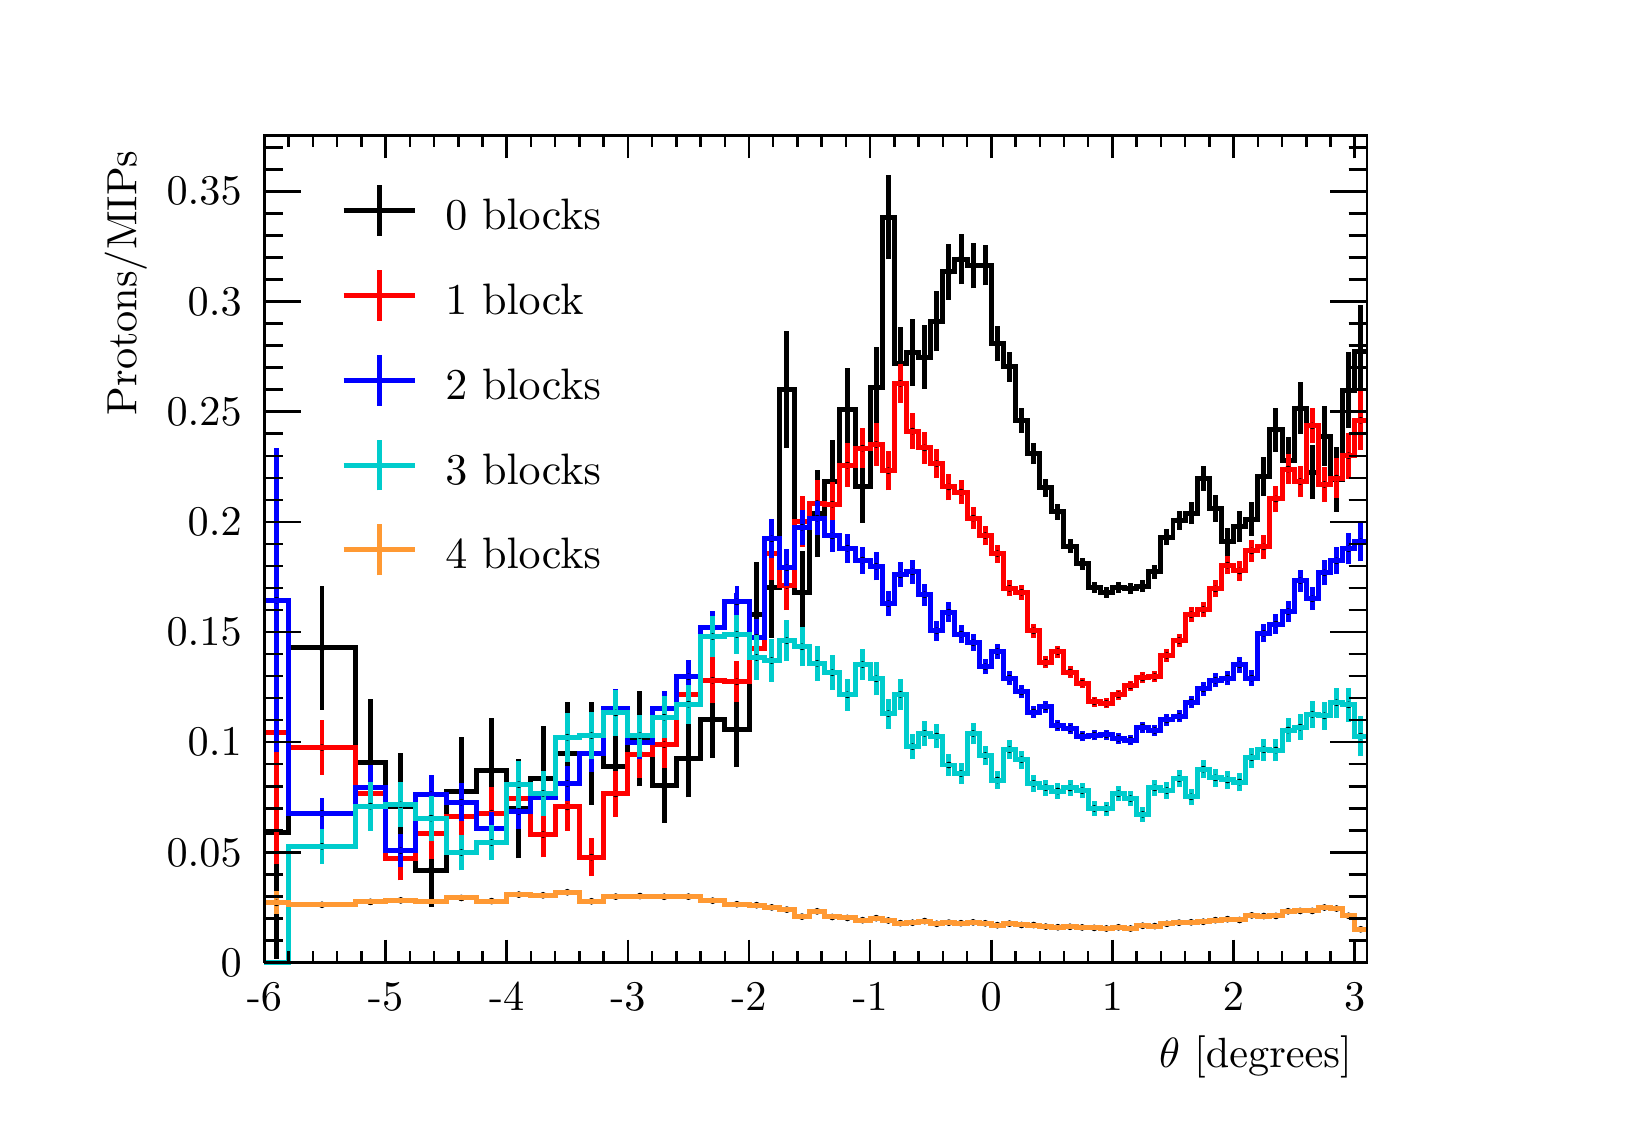
\begin{tikzpicture}
\pgfdeclareplotmark{cross} {
\pgfpathmoveto{\pgfpoint{-0.3\pgfplotmarksize}{\pgfplotmarksize}}
\pgfpathlineto{\pgfpoint{+0.3\pgfplotmarksize}{\pgfplotmarksize}}
\pgfpathlineto{\pgfpoint{+0.3\pgfplotmarksize}{0.3\pgfplotmarksize}}
\pgfpathlineto{\pgfpoint{+1\pgfplotmarksize}{0.3\pgfplotmarksize}}
\pgfpathlineto{\pgfpoint{+1\pgfplotmarksize}{-0.3\pgfplotmarksize}}
\pgfpathlineto{\pgfpoint{+0.3\pgfplotmarksize}{-0.3\pgfplotmarksize}}
\pgfpathlineto{\pgfpoint{+0.3\pgfplotmarksize}{-1.\pgfplotmarksize}}
\pgfpathlineto{\pgfpoint{-0.3\pgfplotmarksize}{-1.\pgfplotmarksize}}
\pgfpathlineto{\pgfpoint{-0.3\pgfplotmarksize}{-0.3\pgfplotmarksize}}
\pgfpathlineto{\pgfpoint{-1.\pgfplotmarksize}{-0.3\pgfplotmarksize}}
\pgfpathlineto{\pgfpoint{-1.\pgfplotmarksize}{0.3\pgfplotmarksize}}
\pgfpathlineto{\pgfpoint{-0.3\pgfplotmarksize}{0.3\pgfplotmarksize}}
\pgfpathclose
\pgfusepathqstroke
}
\pgfdeclareplotmark{cross*} {
\pgfpathmoveto{\pgfpoint{-0.3\pgfplotmarksize}{\pgfplotmarksize}}
\pgfpathlineto{\pgfpoint{+0.3\pgfplotmarksize}{\pgfplotmarksize}}
\pgfpathlineto{\pgfpoint{+0.3\pgfplotmarksize}{0.3\pgfplotmarksize}}
\pgfpathlineto{\pgfpoint{+1\pgfplotmarksize}{0.3\pgfplotmarksize}}
\pgfpathlineto{\pgfpoint{+1\pgfplotmarksize}{-0.3\pgfplotmarksize}}
\pgfpathlineto{\pgfpoint{+0.3\pgfplotmarksize}{-0.3\pgfplotmarksize}}
\pgfpathlineto{\pgfpoint{+0.3\pgfplotmarksize}{-1.\pgfplotmarksize}}
\pgfpathlineto{\pgfpoint{-0.3\pgfplotmarksize}{-1.\pgfplotmarksize}}
\pgfpathlineto{\pgfpoint{-0.3\pgfplotmarksize}{-0.3\pgfplotmarksize}}
\pgfpathlineto{\pgfpoint{-1.\pgfplotmarksize}{-0.3\pgfplotmarksize}}
\pgfpathlineto{\pgfpoint{-1.\pgfplotmarksize}{0.3\pgfplotmarksize}}
\pgfpathlineto{\pgfpoint{-0.3\pgfplotmarksize}{0.3\pgfplotmarksize}}
\pgfpathclose
\pgfusepathqfillstroke
}
\pgfdeclareplotmark{newstar} {
\pgfpathmoveto{\pgfqpoint{0pt}{\pgfplotmarksize}}
\pgfpathlineto{\pgfqpointpolar{44}{0.5\pgfplotmarksize}}
\pgfpathlineto{\pgfqpointpolar{18}{\pgfplotmarksize}}
\pgfpathlineto{\pgfqpointpolar{-20}{0.5\pgfplotmarksize}}
\pgfpathlineto{\pgfqpointpolar{-54}{\pgfplotmarksize}}
\pgfpathlineto{\pgfqpointpolar{-90}{0.5\pgfplotmarksize}}
\pgfpathlineto{\pgfqpointpolar{234}{\pgfplotmarksize}}
\pgfpathlineto{\pgfqpointpolar{198}{0.5\pgfplotmarksize}}
\pgfpathlineto{\pgfqpointpolar{162}{\pgfplotmarksize}}
\pgfpathlineto{\pgfqpointpolar{134}{0.5\pgfplotmarksize}}
\pgfpathclose
\pgfusepathqstroke
}
\pgfdeclareplotmark{newstar*} {
\pgfpathmoveto{\pgfqpoint{0pt}{\pgfplotmarksize}}
\pgfpathlineto{\pgfqpointpolar{44}{0.5\pgfplotmarksize}}
\pgfpathlineto{\pgfqpointpolar{18}{\pgfplotmarksize}}
\pgfpathlineto{\pgfqpointpolar{-20}{0.5\pgfplotmarksize}}
\pgfpathlineto{\pgfqpointpolar{-54}{\pgfplotmarksize}}
\pgfpathlineto{\pgfqpointpolar{-90}{0.5\pgfplotmarksize}}
\pgfpathlineto{\pgfqpointpolar{234}{\pgfplotmarksize}}
\pgfpathlineto{\pgfqpointpolar{198}{0.5\pgfplotmarksize}}
\pgfpathlineto{\pgfqpointpolar{162}{\pgfplotmarksize}}
\pgfpathlineto{\pgfqpointpolar{134}{0.5\pgfplotmarksize}}
\pgfpathclose
\pgfusepathqfillstroke
}
\definecolor{c}{rgb}{1,1,1};
\draw [color=c, fill=c] (0,0) rectangle (20,13.639);
\draw [color=c, fill=c] (3,1.77307) rectangle (17,12.2751);
\definecolor{c}{rgb}{0,0,0};
\draw [c,line width=0.9] (3,1.77307) -- (3,12.2751) -- (17,12.2751) -- (17,1.77307) -- (3,1.77307);
\definecolor{c}{rgb}{1,1,1};
\draw [color=c, fill=c] (3,1.77307) rectangle (17,12.2751);
\definecolor{c}{rgb}{0,0,0};
\draw [c,line width=0.9] (3,1.77307) -- (3,12.2751) -- (17,12.2751) -- (17,1.77307) -- (3,1.77307);
\draw [c,line width=0.9] (3,1.77307) -- (3.30769,1.77307) -- (3.30769,1.77307) -- (4.15385,1.77307) -- (4.15385,1.77307) -- (4.53846,1.77307) -- (4.53846,1.77307) -- (4.92308,1.77307) -- (4.92308,1.77307) -- (5.30769,1.77307) -- (5.30769,1.77307) --
 (5.69231,1.77307) -- (5.69231,1.77307) -- (6.07692,1.77307) -- (6.07692,1.77307) -- (6.38462,1.77307) -- (6.38462,1.77307) -- (6.69231,1.77307) -- (6.69231,1.77307) -- (7,1.77307) -- (7,1.77307) -- (7.30769,1.77307) -- (7.30769,1.77307) --
 (7.61538,1.77307) -- (7.61538,1.77307) -- (7.92308,1.77307) -- (7.92308,1.77307) -- (8.23077,1.77307) -- (8.23077,1.77307) -- (8.53846,1.77307) -- (8.53846,1.77307) -- (8.84615,1.77307) -- (8.84615,1.77307) -- (9.15385,1.77307) -- (9.15385,1.77307)
 -- (9.34615,1.77307) -- (9.34615,1.77307) -- (9.53846,1.77307) -- (9.53846,1.77307) -- (9.73077,1.77307) -- (9.73077,1.77307) -- (9.92308,1.77307) -- (9.92308,1.77307) -- (10.1154,1.77307) -- (10.1154,1.77307) -- (10.3077,1.77307) --
 (10.3077,1.77307) -- (10.5,1.77307) -- (10.5,1.77307) -- (10.6923,1.77307) -- (10.6923,1.77307) -- (10.8462,1.77307) -- (10.8462,1.77307) -- (11,1.77307) -- (11,1.77307) -- (11.1538,1.77307) -- (11.1538,1.77307) -- (11.3077,1.77307) --
 (11.3077,1.77307) -- (11.4615,1.77307) -- (11.4615,1.77307) -- (11.6154,1.77307) -- (11.6154,1.77307) -- (11.7692,1.77307) -- (11.7692,1.77307) -- (11.9231,1.77307) -- (11.9231,1.77307) -- (12.0769,1.77307) -- (12.0769,1.77307) -- (12.2308,1.77307)
 -- (12.2308,1.77307) -- (12.3846,1.77307) -- (12.3846,1.77307) -- (12.5385,1.77307) -- (12.5385,1.77307) -- (12.6923,1.77307) -- (12.6923,1.77307) -- (12.8462,1.77307) -- (12.8462,1.77307) -- (13,1.77307) -- (13,1.77307) -- (13.1538,1.77307) --
 (13.1538,1.77307) -- (13.3077,1.77307) -- (13.3077,1.77307) -- (13.4615,1.77307) -- (13.4615,1.77307) -- (13.6154,1.77307) -- (13.6154,1.77307) -- (13.7692,1.77307) -- (13.7692,1.77307) -- (13.9231,1.77307) -- (13.9231,1.77307) -- (14.0769,1.77307)
 -- (14.0769,1.77307) -- (14.2308,1.77307) -- (14.2308,1.77307) -- (14.3846,1.77307) -- (14.3846,1.77307) -- (14.5385,1.77307) -- (14.5385,1.77307) -- (14.6923,1.77307) -- (14.6923,1.77307) -- (14.8462,1.77307) -- (14.8462,1.77307) -- (15,1.77307) --
 (15,1.77307) -- (15.1538,1.77307) -- (15.1538,1.77307) -- (15.3077,1.77307) -- (15.3077,1.77307) -- (15.4615,1.77307) -- (15.4615,1.77307) -- (15.6154,1.77307) -- (15.6154,1.77307) -- (15.7692,1.77307) -- (15.7692,1.77307) -- (15.9231,1.77307) --
 (15.9231,1.77307) -- (16.0769,1.77307) -- (16.0769,1.77307) -- (16.2308,1.77307) -- (16.2308,1.77307) -- (16.3846,1.77307) -- (16.3846,1.77307) -- (16.5385,1.77307) -- (16.5385,1.77307) -- (16.6923,1.77307) -- (16.6923,1.77307) -- (16.8462,1.77307)
 -- (16.8462,1.77307) -- (17,1.77307);
\draw [c,line width=0.9] (3,1.77307) -- (17,1.77307);
\draw [c,line width=0.9] (3,2.05948) -- (3,1.77307);
\draw [c,line width=0.9] (3.30769,1.91628) -- (3.30769,1.77307);
\draw [c,line width=0.9] (3.61538,1.91628) -- (3.61538,1.77307);
\draw [c,line width=0.9] (3.92308,1.91628) -- (3.92308,1.77307);
\draw [c,line width=0.9] (4.23077,1.91628) -- (4.23077,1.77307);
\draw [c,line width=0.9] (4.53846,2.05948) -- (4.53846,1.77307);
\draw [c,line width=0.9] (4.84615,1.91628) -- (4.84615,1.77307);
\draw [c,line width=0.9] (5.15385,1.91628) -- (5.15385,1.77307);
\draw [c,line width=0.9] (5.46154,1.91628) -- (5.46154,1.77307);
\draw [c,line width=0.9] (5.76923,1.91628) -- (5.76923,1.77307);
\draw [c,line width=0.9] (6.07692,2.05948) -- (6.07692,1.77307);
\draw [c,line width=0.9] (6.38462,1.91628) -- (6.38462,1.77307);
\draw [c,line width=0.9] (6.69231,1.91628) -- (6.69231,1.77307);
\draw [c,line width=0.9] (7,1.91628) -- (7,1.77307);
\draw [c,line width=0.9] (7.30769,1.91628) -- (7.30769,1.77307);
\draw [c,line width=0.9] (7.61538,2.05948) -- (7.61538,1.77307);
\draw [c,line width=0.9] (7.92308,1.91628) -- (7.92308,1.77307);
\draw [c,line width=0.9] (8.23077,1.91628) -- (8.23077,1.77307);
\draw [c,line width=0.9] (8.53846,1.91628) -- (8.53846,1.77307);
\draw [c,line width=0.9] (8.84615,1.91628) -- (8.84615,1.77307);
\draw [c,line width=0.9] (9.15385,2.05948) -- (9.15385,1.77307);
\draw [c,line width=0.9] (9.46154,1.91628) -- (9.46154,1.77307);
\draw [c,line width=0.9] (9.76923,1.91628) -- (9.76923,1.77307);
\draw [c,line width=0.9] (10.0769,1.91628) -- (10.0769,1.77307);
\draw [c,line width=0.9] (10.3846,1.91628) -- (10.3846,1.77307);
\draw [c,line width=0.9] (10.6923,2.05948) -- (10.6923,1.77307);
\draw [c,line width=0.9] (11,1.91628) -- (11,1.77307);
\draw [c,line width=0.9] (11.3077,1.91628) -- (11.3077,1.77307);
\draw [c,line width=0.9] (11.6154,1.91628) -- (11.6154,1.77307);
\draw [c,line width=0.9] (11.9231,1.91628) -- (11.9231,1.77307);
\draw [c,line width=0.9] (12.2308,2.05948) -- (12.2308,1.77307);
\draw [c,line width=0.9] (12.5385,1.91628) -- (12.5385,1.77307);
\draw [c,line width=0.9] (12.8462,1.91628) -- (12.8462,1.77307);
\draw [c,line width=0.9] (13.1538,1.91628) -- (13.1538,1.77307);
\draw [c,line width=0.9] (13.4615,1.91628) -- (13.4615,1.77307);
\draw [c,line width=0.9] (13.7692,2.05948) -- (13.7692,1.77307);
\draw [c,line width=0.9] (14.0769,1.91628) -- (14.0769,1.77307);
\draw [c,line width=0.9] (14.3846,1.91628) -- (14.3846,1.77307);
\draw [c,line width=0.9] (14.6923,1.91628) -- (14.6923,1.77307);
\draw [c,line width=0.9] (15,1.91628) -- (15,1.77307);
\draw [c,line width=0.9] (15.3077,2.05948) -- (15.3077,1.77307);
\draw [c,line width=0.9] (15.6154,1.91628) -- (15.6154,1.77307);
\draw [c,line width=0.9] (15.9231,1.91628) -- (15.9231,1.77307);
\draw [c,line width=0.9] (16.2308,1.91628) -- (16.2308,1.77307);
\draw [c,line width=0.9] (16.5385,1.91628) -- (16.5385,1.77307);
\draw [c,line width=0.9] (16.8462,2.05948) -- (16.8462,1.77307);
\draw [c,line width=0.9] (16.8462,2.05948) -- (16.8462,1.77307);
\draw [anchor=base] (3,1.15931) node[scale=1.52731, color=c, rotate=0]{-6};
\draw [anchor=base] (4.53846,1.15931) node[scale=1.52731, color=c, rotate=0]{-5};
\draw [anchor=base] (6.07692,1.15931) node[scale=1.52731, color=c, rotate=0]{-4};
\draw [anchor=base] (7.61538,1.15931) node[scale=1.52731, color=c, rotate=0]{-3};
\draw [anchor=base] (9.15385,1.15931) node[scale=1.52731, color=c, rotate=0]{-2};
\draw [anchor=base] (10.6923,1.15931) node[scale=1.52731, color=c, rotate=0]{-1};
\draw [anchor=base] (12.2308,1.15931) node[scale=1.52731, color=c, rotate=0]{0};
\draw [anchor=base] (13.7692,1.15931) node[scale=1.52731, color=c, rotate=0]{1};
\draw [anchor=base] (15.3077,1.15931) node[scale=1.52731, color=c, rotate=0]{2};
\draw [anchor=base] (16.8462,1.15931) node[scale=1.52731, color=c, rotate=0]{3};
\draw [anchor= east] (17,0.572837) node[scale=1.52731, color=c, rotate=0]{$\theta$ [degrees]};
\draw [c,line width=0.9] (3,12.2751) -- (17,12.2751);
\draw [c,line width=0.9] (3,11.9887) -- (3,12.2751);
\draw [c,line width=0.9] (3.30769,12.1319) -- (3.30769,12.2751);
\draw [c,line width=0.9] (3.61538,12.1319) -- (3.61538,12.2751);
\draw [c,line width=0.9] (3.92308,12.1319) -- (3.92308,12.2751);
\draw [c,line width=0.9] (4.23077,12.1319) -- (4.23077,12.2751);
\draw [c,line width=0.9] (4.53846,11.9887) -- (4.53846,12.2751);
\draw [c,line width=0.9] (4.84615,12.1319) -- (4.84615,12.2751);
\draw [c,line width=0.9] (5.15385,12.1319) -- (5.15385,12.2751);
\draw [c,line width=0.9] (5.46154,12.1319) -- (5.46154,12.2751);
\draw [c,line width=0.9] (5.76923,12.1319) -- (5.76923,12.2751);
\draw [c,line width=0.9] (6.07692,11.9887) -- (6.07692,12.2751);
\draw [c,line width=0.9] (6.38462,12.1319) -- (6.38462,12.2751);
\draw [c,line width=0.9] (6.69231,12.1319) -- (6.69231,12.2751);
\draw [c,line width=0.9] (7,12.1319) -- (7,12.2751);
\draw [c,line width=0.9] (7.30769,12.1319) -- (7.30769,12.2751);
\draw [c,line width=0.9] (7.61538,11.9887) -- (7.61538,12.2751);
\draw [c,line width=0.9] (7.92308,12.1319) -- (7.92308,12.2751);
\draw [c,line width=0.9] (8.23077,12.1319) -- (8.23077,12.2751);
\draw [c,line width=0.9] (8.53846,12.1319) -- (8.53846,12.2751);
\draw [c,line width=0.9] (8.84615,12.1319) -- (8.84615,12.2751);
\draw [c,line width=0.9] (9.15385,11.9887) -- (9.15385,12.2751);
\draw [c,line width=0.9] (9.46154,12.1319) -- (9.46154,12.2751);
\draw [c,line width=0.9] (9.76923,12.1319) -- (9.76923,12.2751);
\draw [c,line width=0.9] (10.0769,12.1319) -- (10.0769,12.2751);
\draw [c,line width=0.9] (10.3846,12.1319) -- (10.3846,12.2751);
\draw [c,line width=0.9] (10.6923,11.9887) -- (10.6923,12.2751);
\draw [c,line width=0.9] (11,12.1319) -- (11,12.2751);
\draw [c,line width=0.9] (11.3077,12.1319) -- (11.3077,12.2751);
\draw [c,line width=0.9] (11.6154,12.1319) -- (11.6154,12.2751);
\draw [c,line width=0.9] (11.9231,12.1319) -- (11.9231,12.2751);
\draw [c,line width=0.9] (12.2308,11.9887) -- (12.2308,12.2751);
\draw [c,line width=0.9] (12.5385,12.1319) -- (12.5385,12.2751);
\draw [c,line width=0.9] (12.8462,12.1319) -- (12.8462,12.2751);
\draw [c,line width=0.9] (13.1538,12.1319) -- (13.1538,12.2751);
\draw [c,line width=0.9] (13.4615,12.1319) -- (13.4615,12.2751);
\draw [c,line width=0.9] (13.7692,11.9887) -- (13.7692,12.2751);
\draw [c,line width=0.9] (14.0769,12.1319) -- (14.0769,12.2751);
\draw [c,line width=0.9] (14.3846,12.1319) -- (14.3846,12.2751);
\draw [c,line width=0.9] (14.6923,12.1319) -- (14.6923,12.2751);
\draw [c,line width=0.9] (15,12.1319) -- (15,12.2751);
\draw [c,line width=0.9] (15.3077,11.9887) -- (15.3077,12.2751);
\draw [c,line width=0.9] (15.6154,12.1319) -- (15.6154,12.2751);
\draw [c,line width=0.9] (15.9231,12.1319) -- (15.9231,12.2751);
\draw [c,line width=0.9] (16.2308,12.1319) -- (16.2308,12.2751);
\draw [c,line width=0.9] (16.5385,12.1319) -- (16.5385,12.2751);
\draw [c,line width=0.9] (16.8462,11.9887) -- (16.8462,12.2751);
\draw [c,line width=0.9] (16.8462,11.9887) -- (16.8462,12.2751);
\draw [c,line width=0.9] (3,1.77307) -- (3,12.2751);
\draw [c,line width=0.9] (3.462,1.77307) -- (3,1.77307);
\draw [c,line width=0.9] (3.231,2.05289) -- (3,2.05289);
\draw [c,line width=0.9] (3.231,2.33272) -- (3,2.33272);
\draw [c,line width=0.9] (3.231,2.61255) -- (3,2.61255);
\draw [c,line width=0.9] (3.231,2.89237) -- (3,2.89237);
\draw [c,line width=0.9] (3.462,3.1722) -- (3,3.1722);
\draw [c,line width=0.9] (3.231,3.45203) -- (3,3.45203);
\draw [c,line width=0.9] (3.231,3.73185) -- (3,3.73185);
\draw [c,line width=0.9] (3.231,4.01168) -- (3,4.01168);
\draw [c,line width=0.9] (3.231,4.29151) -- (3,4.29151);
\draw [c,line width=0.9] (3.462,4.57133) -- (3,4.57133);
\draw [c,line width=0.9] (3.231,4.85116) -- (3,4.85116);
\draw [c,line width=0.9] (3.231,5.13099) -- (3,5.13099);
\draw [c,line width=0.9] (3.231,5.41081) -- (3,5.41081);
\draw [c,line width=0.9] (3.231,5.69064) -- (3,5.69064);
\draw [c,line width=0.9] (3.462,5.97047) -- (3,5.97047);
\draw [c,line width=0.9] (3.231,6.25029) -- (3,6.25029);
\draw [c,line width=0.9] (3.231,6.53012) -- (3,6.53012);
\draw [c,line width=0.9] (3.231,6.80995) -- (3,6.80995);
\draw [c,line width=0.9] (3.231,7.08977) -- (3,7.08977);
\draw [c,line width=0.9] (3.462,7.3696) -- (3,7.3696);
\draw [c,line width=0.9] (3.231,7.64943) -- (3,7.64943);
\draw [c,line width=0.9] (3.231,7.92925) -- (3,7.92925);
\draw [c,line width=0.9] (3.231,8.20908) -- (3,8.20908);
\draw [c,line width=0.9] (3.231,8.48891) -- (3,8.48891);
\draw [c,line width=0.9] (3.462,8.76873) -- (3,8.76873);
\draw [c,line width=0.9] (3.231,9.04856) -- (3,9.04856);
\draw [c,line width=0.9] (3.231,9.32839) -- (3,9.32839);
\draw [c,line width=0.9] (3.231,9.60821) -- (3,9.60821);
\draw [c,line width=0.9] (3.231,9.88804) -- (3,9.88804);
\draw [c,line width=0.9] (3.462,10.1679) -- (3,10.1679);
\draw [c,line width=0.9] (3.231,10.4477) -- (3,10.4477);
\draw [c,line width=0.9] (3.231,10.7275) -- (3,10.7275);
\draw [c,line width=0.9] (3.231,11.0073) -- (3,11.0073);
\draw [c,line width=0.9] (3.231,11.2872) -- (3,11.2872);
\draw [c,line width=0.9] (3.462,11.567) -- (3,11.567);
\draw [c,line width=0.9] (3.462,11.567) -- (3,11.567);
\draw [c,line width=0.9] (3.231,11.8468) -- (3,11.8468);
\draw [c,line width=0.9] (3.231,12.1267) -- (3,12.1267);
\draw [anchor= east] (2.9,1.77307) node[scale=1.52731, color=c, rotate=0]{0};
\draw [anchor= east] (2.9,3.1722) node[scale=1.52731, color=c, rotate=0]{0.05};
\draw [anchor= east] (2.9,4.57133) node[scale=1.52731, color=c, rotate=0]{0.1};
\draw [anchor= east] (2.9,5.97047) node[scale=1.52731, color=c, rotate=0]{0.15};
\draw [anchor= east] (2.9,7.3696) node[scale=1.52731, color=c, rotate=0]{0.2};
\draw [anchor= east] (2.9,8.76873) node[scale=1.52731, color=c, rotate=0]{0.25};
\draw [anchor= east] (2.9,10.1679) node[scale=1.52731, color=c, rotate=0]{0.3};
\draw [anchor= east] (2.9,11.567) node[scale=1.52731, color=c, rotate=0]{0.35};
\draw [anchor= east] (1.24,12.2751) node[scale=1.52731, color=c, rotate=90]{  Protons/MIPs};
\draw [c,line width=0.9] (17,1.77307) -- (17,12.2751);
\draw [c,line width=0.9] (16.538,1.77307) -- (17,1.77307);
\draw [c,line width=0.9] (16.769,2.05289) -- (17,2.05289);
\draw [c,line width=0.9] (16.769,2.33272) -- (17,2.33272);
\draw [c,line width=0.9] (16.769,2.61255) -- (17,2.61255);
\draw [c,line width=0.9] (16.769,2.89237) -- (17,2.89237);
\draw [c,line width=0.9] (16.538,3.1722) -- (17,3.1722);
\draw [c,line width=0.9] (16.769,3.45203) -- (17,3.45203);
\draw [c,line width=0.9] (16.769,3.73185) -- (17,3.73185);
\draw [c,line width=0.9] (16.769,4.01168) -- (17,4.01168);
\draw [c,line width=0.9] (16.769,4.29151) -- (17,4.29151);
\draw [c,line width=0.9] (16.538,4.57133) -- (17,4.57133);
\draw [c,line width=0.9] (16.769,4.85116) -- (17,4.85116);
\draw [c,line width=0.9] (16.769,5.13099) -- (17,5.13099);
\draw [c,line width=0.9] (16.769,5.41081) -- (17,5.41081);
\draw [c,line width=0.9] (16.769,5.69064) -- (17,5.69064);
\draw [c,line width=0.9] (16.538,5.97047) -- (17,5.97047);
\draw [c,line width=0.9] (16.769,6.25029) -- (17,6.25029);
\draw [c,line width=0.9] (16.769,6.53012) -- (17,6.53012);
\draw [c,line width=0.9] (16.769,6.80995) -- (17,6.80995);
\draw [c,line width=0.9] (16.769,7.08977) -- (17,7.08977);
\draw [c,line width=0.9] (16.538,7.3696) -- (17,7.3696);
\draw [c,line width=0.9] (16.769,7.64943) -- (17,7.64943);
\draw [c,line width=0.9] (16.769,7.92925) -- (17,7.92925);
\draw [c,line width=0.9] (16.769,8.20908) -- (17,8.20908);
\draw [c,line width=0.9] (16.769,8.48891) -- (17,8.48891);
\draw [c,line width=0.9] (16.538,8.76873) -- (17,8.76873);
\draw [c,line width=0.9] (16.769,9.04856) -- (17,9.04856);
\draw [c,line width=0.9] (16.769,9.32839) -- (17,9.32839);
\draw [c,line width=0.9] (16.769,9.60821) -- (17,9.60821);
\draw [c,line width=0.9] (16.769,9.88804) -- (17,9.88804);
\draw [c,line width=0.9] (16.538,10.1679) -- (17,10.1679);
\draw [c,line width=0.9] (16.769,10.4477) -- (17,10.4477);
\draw [c,line width=0.9] (16.769,10.7275) -- (17,10.7275);
\draw [c,line width=0.9] (16.769,11.0073) -- (17,11.0073);
\draw [c,line width=0.9] (16.769,11.2872) -- (17,11.2872);
\draw [c,line width=0.9] (16.538,11.567) -- (17,11.567);
\draw [c,line width=0.9] (16.538,11.567) -- (17,11.567);
\draw [c,line width=0.9] (16.769,11.8468) -- (17,11.8468);
\draw [c,line width=0.9] (16.769,12.1267) -- (17,12.1267);
\draw [c,line width=1.8] (3.15385,1.82211) -- (3.15385,3.41911);
\draw [c,line width=1.8] (3.15385,3.41911) -- (3.15385,5.0161);
\foreach \P in {(3.15385,3.41911)}{\draw[mark options={color=c,fill=c},mark size=2.402402pt,mark=*,mark size=1pt] plot coordinates {\P};}
\draw [c,line width=1.8] (3.73077,4.98149) -- (3.73077,5.77059);
\draw [c,line width=1.8] (3.73077,5.77059) -- (3.73077,6.55969);
\foreach \P in {(3.73077,5.77059)}{\draw[mark options={color=c,fill=c},mark size=2.402402pt,mark=*,mark size=1pt] plot coordinates {\P};}
\draw [c,line width=1.8] (4.34615,3.5084) -- (4.34615,4.31694);
\draw [c,line width=1.8] (4.34615,4.31694) -- (4.34615,5.12549);
\foreach \P in {(4.34615,4.31694)}{\draw[mark options={color=c,fill=c},mark size=2.402402pt,mark=*,mark size=1pt] plot coordinates {\P};}
\draw [c,line width=1.8] (4.73077,3.07893) -- (4.73077,3.75414);
\draw [c,line width=1.8] (4.73077,3.75414) -- (4.73077,4.42935);
\foreach \P in {(4.73077,3.75414)}{\draw[mark options={color=c,fill=c},mark size=2.402402pt,mark=*,mark size=1pt] plot coordinates {\P};}
\draw [c,line width=1.8] (5.11538,2.47797) -- (5.11538,2.94716);
\draw [c,line width=1.8] (5.11538,2.94716) -- (5.11538,3.41635);
\foreach \P in {(5.11538,2.94716)}{\draw[mark options={color=c,fill=c},mark size=2.402402pt,mark=*,mark size=1pt] plot coordinates {\P};}
\draw [c,line width=1.8] (5.5,3.24904) -- (5.5,3.94413);
\draw [c,line width=1.8] (5.5,3.94413) -- (5.5,4.63923);
\foreach \P in {(5.5,3.94413)}{\draw[mark options={color=c,fill=c},mark size=2.402402pt,mark=*,mark size=1pt] plot coordinates {\P};}
\draw [c,line width=1.8] (5.88462,3.53511) -- (5.88462,4.20634);
\draw [c,line width=1.8] (5.88462,4.20634) -- (5.88462,4.87758);
\foreach \P in {(5.88462,4.20634)}{\draw[mark options={color=c,fill=c},mark size=2.402402pt,mark=*,mark size=1pt] plot coordinates {\P};}
\draw [c,line width=1.8] (6.23077,3.09766) -- (6.23077,3.72534);
\draw [c,line width=1.8] (6.23077,3.72534) -- (6.23077,4.35303);
\foreach \P in {(6.23077,3.72534)}{\draw[mark options={color=c,fill=c},mark size=2.402402pt,mark=*,mark size=1pt] plot coordinates {\P};}
\draw [c,line width=1.8] (6.53846,3.43175) -- (6.53846,4.10495);
\draw [c,line width=1.8] (6.53846,4.10495) -- (6.53846,4.77816);
\foreach \P in {(6.53846,4.10495)}{\draw[mark options={color=c,fill=c},mark size=2.402402pt,mark=*,mark size=1pt] plot coordinates {\P};}
\draw [c,line width=1.8] (6.84615,3.77705) -- (6.84615,4.42965);
\draw [c,line width=1.8] (6.84615,4.42965) -- (6.84615,5.08224);
\foreach \P in {(6.84615,4.42965)}{\draw[mark options={color=c,fill=c},mark size=2.402402pt,mark=*,mark size=1pt] plot coordinates {\P};}
\draw [c,line width=1.8] (7.15385,3.77705) -- (7.15385,4.42965);
\draw [c,line width=1.8] (7.15385,4.42965) -- (7.15385,5.08224);
\foreach \P in {(7.15385,4.42965)}{\draw[mark options={color=c,fill=c},mark size=2.402402pt,mark=*,mark size=1pt] plot coordinates {\P};}
\draw [c,line width=1.8] (7.46154,3.68708) -- (7.46154,4.26367);
\draw [c,line width=1.8] (7.46154,4.26367) -- (7.46154,4.84026);
\foreach \P in {(7.46154,4.26367)}{\draw[mark options={color=c,fill=c},mark size=2.402402pt,mark=*,mark size=1pt] plot coordinates {\P};}
\draw [c,line width=1.8] (7.76923,4.01178) -- (7.76923,4.61395);
\draw [c,line width=1.8] (7.76923,4.61395) -- (7.76923,5.21612);
\foreach \P in {(7.76923,4.61395)}{\draw[mark options={color=c,fill=c},mark size=2.402402pt,mark=*,mark size=1pt] plot coordinates {\P};}
\draw [c,line width=1.8] (8.07692,3.54651) -- (8.07692,4.01595);
\draw [c,line width=1.8] (8.07692,4.01595) -- (8.07692,4.48539);
\foreach \P in {(8.07692,4.01595)}{\draw[mark options={color=c,fill=c},mark size=2.402402pt,mark=*,mark size=1pt] plot coordinates {\P};}
\draw [c,line width=1.8] (8.38461,3.8704) -- (8.38461,4.36405);
\draw [c,line width=1.8] (8.38461,4.36405) -- (8.38461,4.85771);
\foreach \P in {(8.38461,4.36405)}{\draw[mark options={color=c,fill=c},mark size=2.402402pt,mark=*,mark size=1pt] plot coordinates {\P};}
\draw [c,line width=1.8] (8.69231,4.37658) -- (8.69231,4.85449);
\draw [c,line width=1.8] (8.69231,4.85449) -- (8.69231,5.3324);
\foreach \P in {(8.69231,4.85449)}{\draw[mark options={color=c,fill=c},mark size=2.402402pt,mark=*,mark size=1pt] plot coordinates {\P};}
\draw [c,line width=1.8] (9,4.2563) -- (9,4.73696);
\draw [c,line width=1.8] (9,4.73696) -- (9,5.21762);
\foreach \P in {(9,4.73696)}{\draw[mark options={color=c,fill=c},mark size=2.402402pt,mark=*,mark size=1pt] plot coordinates {\P};}
\draw [c,line width=1.8] (9.25,5.53021) -- (9.25,6.19768);
\draw [c,line width=1.8] (9.25,6.19768) -- (9.25,6.86514);
\foreach \P in {(9.25,6.19768)}{\draw[mark options={color=c,fill=c},mark size=2.402402pt,mark=*,mark size=1pt] plot coordinates {\P};}
\draw [c,line width=1.8] (9.44231,5.9002) -- (9.44231,6.54048);
\draw [c,line width=1.8] (9.44231,6.54048) -- (9.44231,7.18077);
\foreach \P in {(9.44231,6.54048)}{\draw[mark options={color=c,fill=c},mark size=2.402402pt,mark=*,mark size=1pt] plot coordinates {\P};}
\draw [c,line width=1.8] (9.63461,8.30763) -- (9.63461,9.05061);
\draw [c,line width=1.8] (9.63461,9.05061) -- (9.63461,9.79359);
\foreach \P in {(9.63461,9.05061)}{\draw[mark options={color=c,fill=c},mark size=2.402402pt,mark=*,mark size=1pt] plot coordinates {\P};}
\draw [c,line width=1.8] (9.82692,5.94121) -- (9.82692,6.473);
\draw [c,line width=1.8] (9.82692,6.473) -- (9.82692,7.00478);
\foreach \P in {(9.82692,6.473)}{\draw[mark options={color=c,fill=c},mark size=2.402402pt,mark=*,mark size=1pt] plot coordinates {\P};}
\draw [c,line width=1.8] (10.0192,6.92282) -- (10.0192,7.47827);
\draw [c,line width=1.8] (10.0192,7.47827) -- (10.0192,8.03372);
\foreach \P in {(10.0192,7.47827)}{\draw[mark options={color=c,fill=c},mark size=2.402402pt,mark=*,mark size=1pt] plot coordinates {\P};}
\draw [c,line width=1.8] (10.2115,7.34742) -- (10.2115,7.87945);
\draw [c,line width=1.8] (10.2115,7.87945) -- (10.2115,8.41148);
\foreach \P in {(10.2115,7.87945)}{\draw[mark options={color=c,fill=c},mark size=2.402402pt,mark=*,mark size=1pt] plot coordinates {\P};}
\draw [c,line width=1.8] (10.4038,8.26812) -- (10.4038,8.79513);
\draw [c,line width=1.8] (10.4038,8.79513) -- (10.4038,9.32215);
\foreach \P in {(10.4038,8.79513)}{\draw[mark options={color=c,fill=c},mark size=2.402402pt,mark=*,mark size=1pt] plot coordinates {\P};}
\draw [c,line width=1.8] (10.5962,7.35913) -- (10.5962,7.8128);
\draw [c,line width=1.8] (10.5962,7.8128) -- (10.5962,8.26647);
\foreach \P in {(10.5962,7.8128)}{\draw[mark options={color=c,fill=c},mark size=2.402402pt,mark=*,mark size=1pt] plot coordinates {\P};}
\draw [c,line width=1.8] (10.7692,8.57136) -- (10.7692,9.07912);
\draw [c,line width=1.8] (10.7692,9.07912) -- (10.7692,9.58688);
\foreach \P in {(10.7692,9.07912)}{\draw[mark options={color=c,fill=c},mark size=2.402402pt,mark=*,mark size=1pt] plot coordinates {\P};}
\draw [c,line width=1.8] (10.9231,10.702) -- (10.9231,11.2385);
\draw [c,line width=1.8] (10.9231,11.2385) -- (10.9231,11.775);
\foreach \P in {(10.9231,11.2385)}{\draw[mark options={color=c,fill=c},mark size=2.402402pt,mark=*,mark size=1pt] plot coordinates {\P};}
\draw [c,line width=1.8] (11.0769,8.92018) -- (11.0769,9.38038);
\draw [c,line width=1.8] (11.0769,9.38038) -- (11.0769,9.84057);
\foreach \P in {(11.0769,9.38038)}{\draw[mark options={color=c,fill=c},mark size=2.402402pt,mark=*,mark size=1pt] plot coordinates {\P};}
\draw [c,line width=1.8] (11.2308,9.09999) -- (11.2308,9.52459);
\draw [c,line width=1.8] (11.2308,9.52459) -- (11.2308,9.94918);
\foreach \P in {(11.2308,9.52459)}{\draw[mark options={color=c,fill=c},mark size=2.402402pt,mark=*,mark size=1pt] plot coordinates {\P};}
\draw [c,line width=1.8] (11.3846,9.06099) -- (11.3846,9.46252);
\draw [c,line width=1.8] (11.3846,9.46252) -- (11.3846,9.86404);
\foreach \P in {(11.3846,9.46252)}{\draw[mark options={color=c,fill=c},mark size=2.402402pt,mark=*,mark size=1pt] plot coordinates {\P};}
\draw [c,line width=1.8] (11.5385,9.53396) -- (11.5385,9.91671);
\draw [c,line width=1.8] (11.5385,9.91671) -- (11.5385,10.2995);
\foreach \P in {(11.5385,9.91671)}{\draw[mark options={color=c,fill=c},mark size=2.402402pt,mark=*,mark size=1pt] plot coordinates {\P};}
\draw [c,line width=1.8] (11.6923,10.1909) -- (11.6923,10.5434);
\draw [c,line width=1.8] (11.6923,10.5434) -- (11.6923,10.896);
\foreach \P in {(11.6923,10.5434)}{\draw[mark options={color=c,fill=c},mark size=2.402402pt,mark=*,mark size=1pt] plot coordinates {\P};}
\draw [c,line width=1.8] (11.8462,10.3843) -- (11.8462,10.707);
\draw [c,line width=1.8] (11.8462,10.707) -- (11.8462,11.0296);
\foreach \P in {(11.8462,10.707)}{\draw[mark options={color=c,fill=c},mark size=2.402402pt,mark=*,mark size=1pt] plot coordinates {\P};}
\draw [c,line width=1.8] (12,10.3355) -- (12,10.625);
\draw [c,line width=1.8] (12,10.625) -- (12,10.9146);
\foreach \P in {(12,10.625)}{\draw[mark options={color=c,fill=c},mark size=2.402402pt,mark=*,mark size=1pt] plot coordinates {\P};}
\draw [c,line width=1.8] (12.1538,10.3727) -- (12.1538,10.6278);
\draw [c,line width=1.8] (12.1538,10.6278) -- (12.1538,10.8828);
\foreach \P in {(12.1538,10.6278)}{\draw[mark options={color=c,fill=c},mark size=2.402402pt,mark=*,mark size=1pt] plot coordinates {\P};}
\draw [c,line width=1.8] (12.3077,9.40941) -- (12.3077,9.63297);
\draw [c,line width=1.8] (12.3077,9.63297) -- (12.3077,9.85653);
\foreach \P in {(12.3077,9.63297)}{\draw[mark options={color=c,fill=c},mark size=2.402402pt,mark=*,mark size=1pt] plot coordinates {\P};}
\draw [c,line width=1.8] (12.4615,9.14774) -- (12.4615,9.34012);
\draw [c,line width=1.8] (12.4615,9.34012) -- (12.4615,9.53249);
\foreach \P in {(12.4615,9.34012)}{\draw[mark options={color=c,fill=c},mark size=2.402402pt,mark=*,mark size=1pt] plot coordinates {\P};}
\draw [c,line width=1.8] (12.6154,8.50404) -- (12.6154,8.66245);
\draw [c,line width=1.8] (12.6154,8.66245) -- (12.6154,8.82085);
\foreach \P in {(12.6154,8.66245)}{\draw[mark options={color=c,fill=c},mark size=2.402402pt,mark=*,mark size=1pt] plot coordinates {\P};}
\draw [c,line width=1.8] (12.7692,8.10435) -- (12.7692,8.2387);
\draw [c,line width=1.8] (12.7692,8.2387) -- (12.7692,8.37306);
\foreach \P in {(12.7692,8.2387)}{\draw[mark options={color=c,fill=c},mark size=2.402402pt,mark=*,mark size=1pt] plot coordinates {\P};}
\draw [c,line width=1.8] (12.9231,7.68928) -- (12.9231,7.80332);
\draw [c,line width=1.8] (12.9231,7.80332) -- (12.9231,7.91735);
\foreach \P in {(12.9231,7.80332)}{\draw[mark options={color=c,fill=c},mark size=2.402402pt,mark=*,mark size=1pt] plot coordinates {\P};}
\draw [c,line width=1.8] (13.0769,7.39569) -- (13.0769,7.49512);
\draw [c,line width=1.8] (13.0769,7.49512) -- (13.0769,7.59454);
\foreach \P in {(13.0769,7.49512)}{\draw[mark options={color=c,fill=c},mark size=2.402402pt,mark=*,mark size=1pt] plot coordinates {\P};}
\draw [c,line width=1.8] (13.2308,6.97329) -- (13.2308,7.06043);
\draw [c,line width=1.8] (13.2308,7.06043) -- (13.2308,7.14758);
\foreach \P in {(13.2308,7.06043)}{\draw[mark options={color=c,fill=c},mark size=2.402402pt,mark=*,mark size=1pt] plot coordinates {\P};}
\draw [c,line width=1.8] (13.3846,6.7589) -- (13.3846,6.83628);
\draw [c,line width=1.8] (13.3846,6.83628) -- (13.3846,6.91366);
\foreach \P in {(13.3846,6.83628)}{\draw[mark options={color=c,fill=c},mark size=2.402402pt,mark=*,mark size=1pt] plot coordinates {\P};}
\draw [c,line width=1.8] (13.5385,6.46938) -- (13.5385,6.53954);
\draw [c,line width=1.8] (13.5385,6.53954) -- (13.5385,6.60971);
\foreach \P in {(13.5385,6.53954)}{\draw[mark options={color=c,fill=c},mark size=2.402402pt,mark=*,mark size=1pt] plot coordinates {\P};}
\draw [c,line width=1.8] (13.6923,6.40391) -- (13.6923,6.47146);
\draw [c,line width=1.8] (13.6923,6.47146) -- (13.6923,6.539);
\foreach \P in {(13.6923,6.47146)}{\draw[mark options={color=c,fill=c},mark size=2.402402pt,mark=*,mark size=1pt] plot coordinates {\P};}
\draw [c,line width=1.8] (13.8462,6.47055) -- (13.8462,6.53894);
\draw [c,line width=1.8] (13.8462,6.53894) -- (13.8462,6.60733);
\foreach \P in {(13.8462,6.53894)}{\draw[mark options={color=c,fill=c},mark size=2.402402pt,mark=*,mark size=1pt] plot coordinates {\P};}
\draw [c,line width=1.8] (14,6.45026) -- (14,6.52192);
\draw [c,line width=1.8] (14,6.52192) -- (14,6.59357);
\foreach \P in {(14,6.52192)}{\draw[mark options={color=c,fill=c},mark size=2.402402pt,mark=*,mark size=1pt] plot coordinates {\P};}
\draw [c,line width=1.8] (14.1538,6.47551) -- (14.1538,6.55327);
\draw [c,line width=1.8] (14.1538,6.55327) -- (14.1538,6.63103);
\foreach \P in {(14.1538,6.55327)}{\draw[mark options={color=c,fill=c},mark size=2.402402pt,mark=*,mark size=1pt] plot coordinates {\P};}
\draw [c,line width=1.8] (14.3077,6.64793) -- (14.3077,6.73649);
\draw [c,line width=1.8] (14.3077,6.73649) -- (14.3077,6.82506);
\foreach \P in {(14.3077,6.73649)}{\draw[mark options={color=c,fill=c},mark size=2.402402pt,mark=*,mark size=1pt] plot coordinates {\P};}
\draw [c,line width=1.8] (14.4615,7.07039) -- (14.4615,7.1755);
\draw [c,line width=1.8] (14.4615,7.1755) -- (14.4615,7.28061);
\foreach \P in {(14.4615,7.1755)}{\draw[mark options={color=c,fill=c},mark size=2.402402pt,mark=*,mark size=1pt] plot coordinates {\P};}
\draw [c,line width=1.8] (14.6154,7.27076) -- (14.6154,7.39177);
\draw [c,line width=1.8] (14.6154,7.39177) -- (14.6154,7.51279);
\foreach \P in {(14.6154,7.39177)}{\draw[mark options={color=c,fill=c},mark size=2.402402pt,mark=*,mark size=1pt] plot coordinates {\P};}
\draw [c,line width=1.8] (14.7692,7.34057) -- (14.7692,7.47851);
\draw [c,line width=1.8] (14.7692,7.47851) -- (14.7692,7.61646);
\foreach \P in {(14.7692,7.47851)}{\draw[mark options={color=c,fill=c},mark size=2.402402pt,mark=*,mark size=1pt] plot coordinates {\P};}
\draw [c,line width=1.8] (14.9231,7.76493) -- (14.9231,7.92186);
\draw [c,line width=1.8] (14.9231,7.92186) -- (14.9231,8.07879);
\foreach \P in {(14.9231,7.92186)}{\draw[mark options={color=c,fill=c},mark size=2.402402pt,mark=*,mark size=1pt] plot coordinates {\P};}
\draw [c,line width=1.8] (15.0769,7.36896) -- (15.0769,7.53787);
\draw [c,line width=1.8] (15.0769,7.53787) -- (15.0769,7.70678);
\foreach \P in {(15.0769,7.53787)}{\draw[mark options={color=c,fill=c},mark size=2.402402pt,mark=*,mark size=1pt] plot coordinates {\P};}
\draw [c,line width=1.8] (15.2308,6.94021) -- (15.2308,7.11766);
\draw [c,line width=1.8] (15.2308,7.11766) -- (15.2308,7.29511);
\foreach \P in {(15.2308,7.11766)}{\draw[mark options={color=c,fill=c},mark size=2.402402pt,mark=*,mark size=1pt] plot coordinates {\P};}
\draw [c,line width=1.8] (15.3846,7.11146) -- (15.3846,7.31065);
\draw [c,line width=1.8] (15.3846,7.31065) -- (15.3846,7.50984);
\foreach \P in {(15.3846,7.31065)}{\draw[mark options={color=c,fill=c},mark size=2.402402pt,mark=*,mark size=1pt] plot coordinates {\P};}
\draw [c,line width=1.8] (15.5385,7.18993) -- (15.5385,7.40435);
\draw [c,line width=1.8] (15.5385,7.40435) -- (15.5385,7.61877);
\foreach \P in {(15.5385,7.40435)}{\draw[mark options={color=c,fill=c},mark size=2.402402pt,mark=*,mark size=1pt] plot coordinates {\P};}
\draw [c,line width=1.8] (15.6923,7.69841) -- (15.6923,7.94405);
\draw [c,line width=1.8] (15.6923,7.94405) -- (15.6923,8.18969);
\foreach \P in {(15.6923,7.94405)}{\draw[mark options={color=c,fill=c},mark size=2.402402pt,mark=*,mark size=1pt] plot coordinates {\P};}
\draw [c,line width=1.8] (15.8462,8.2613) -- (15.8462,8.53778);
\draw [c,line width=1.8] (15.8462,8.53778) -- (15.8462,8.81425);
\foreach \P in {(15.8462,8.53778)}{\draw[mark options={color=c,fill=c},mark size=2.402402pt,mark=*,mark size=1pt] plot coordinates {\P};}
\draw [c,line width=1.8] (16,7.85164) -- (16,8.14729);
\draw [c,line width=1.8] (16,8.14729) -- (16,8.44294);
\foreach \P in {(16,8.14729)}{\draw[mark options={color=c,fill=c},mark size=2.402402pt,mark=*,mark size=1pt] plot coordinates {\P};}
\draw [c,line width=1.8] (16.1538,8.48633) -- (16.1538,8.81479);
\draw [c,line width=1.8] (16.1538,8.81479) -- (16.1538,9.14325);
\foreach \P in {(16.1538,8.81479)}{\draw[mark options={color=c,fill=c},mark size=2.402402pt,mark=*,mark size=1pt] plot coordinates {\P};}
\draw [c,line width=1.8] (16.3077,7.65829) -- (16.3077,7.99945);
\draw [c,line width=1.8] (16.3077,7.99945) -- (16.3077,8.34061);
\foreach \P in {(16.3077,7.99945)}{\draw[mark options={color=c,fill=c},mark size=2.402402pt,mark=*,mark size=1pt] plot coordinates {\P};}
\draw [c,line width=1.8] (16.4615,8.08155) -- (16.4615,8.45969);
\draw [c,line width=1.8] (16.4615,8.45969) -- (16.4615,8.83783);
\foreach \P in {(16.4615,8.45969)}{\draw[mark options={color=c,fill=c},mark size=2.402402pt,mark=*,mark size=1pt] plot coordinates {\P};}
\draw [c,line width=1.8] (16.6154,7.49771) -- (16.6154,7.90625);
\draw [c,line width=1.8] (16.6154,7.90625) -- (16.6154,8.31479);
\foreach \P in {(16.6154,7.90625)}{\draw[mark options={color=c,fill=c},mark size=2.402402pt,mark=*,mark size=1pt] plot coordinates {\P};}
\draw [c,line width=1.8] (16.7692,8.55682) -- (16.7692,9.04073);
\draw [c,line width=1.8] (16.7692,9.04073) -- (16.7692,9.52463);
\foreach \P in {(16.7692,9.04073)}{\draw[mark options={color=c,fill=c},mark size=2.402402pt,mark=*,mark size=1pt] plot coordinates {\P};}
\draw [c,line width=1.8] (16.9231,8.93468) -- (16.9231,9.5319);
\draw [c,line width=1.8] (16.9231,9.5319) -- (16.9231,10.1291);
\foreach \P in {(16.9231,9.5319)}{\draw[mark options={color=c,fill=c},mark size=2.402402pt,mark=*,mark size=1pt] plot coordinates {\P};}
\draw [c,line width=1.8] (3,3.41911) -- (3.30769,3.41911) -- (3.30769,5.77059) -- (4.15385,5.77059) -- (4.15385,4.31694) -- (4.53846,4.31694) -- (4.53846,3.75414) -- (4.92308,3.75414) -- (4.92308,2.94716) -- (5.30769,2.94716) -- (5.30769,3.94413) --
 (5.69231,3.94413) -- (5.69231,4.20634) -- (6.07692,4.20634) -- (6.07692,3.72534) -- (6.38462,3.72534) -- (6.38462,4.10495) -- (6.69231,4.10495) -- (6.69231,4.42965) -- (7,4.42965) -- (7,4.42965) -- (7.30769,4.42965) -- (7.30769,4.26367) --
 (7.61538,4.26367) -- (7.61538,4.61395) -- (7.92308,4.61395) -- (7.92308,4.01595) -- (8.23077,4.01595) -- (8.23077,4.36405) -- (8.53846,4.36405) -- (8.53846,4.85449) -- (8.84615,4.85449) -- (8.84615,4.73696) -- (9.15385,4.73696) -- (9.15385,6.19768)
 -- (9.34615,6.19768) -- (9.34615,6.54048) -- (9.53846,6.54048) -- (9.53846,9.05061) -- (9.73077,9.05061) -- (9.73077,6.473) -- (9.92308,6.473) -- (9.92308,7.47827) -- (10.1154,7.47827) -- (10.1154,7.87945) -- (10.3077,7.87945) -- (10.3077,8.79513)
 -- (10.5,8.79513) -- (10.5,7.8128) -- (10.6923,7.8128) -- (10.6923,9.07912) -- (10.8462,9.07912) -- (10.8462,11.2385) -- (11,11.2385) -- (11,9.38038) -- (11.1538,9.38038) -- (11.1538,9.52459) -- (11.3077,9.52459) -- (11.3077,9.46252) --
 (11.4615,9.46252) -- (11.4615,9.91671) -- (11.6154,9.91671) -- (11.6154,10.5434) -- (11.7692,10.5434) -- (11.7692,10.707) -- (11.9231,10.707) -- (11.9231,10.625) -- (12.0769,10.625) -- (12.0769,10.6278) -- (12.2308,10.6278) -- (12.2308,9.63297) --
 (12.3846,9.63297) -- (12.3846,9.34012) -- (12.5385,9.34012) -- (12.5385,8.66245) -- (12.6923,8.66245) -- (12.6923,8.2387) -- (12.8462,8.2387) -- (12.8462,7.80332) -- (13,7.80332) -- (13,7.49512) -- (13.1538,7.49512) -- (13.1538,7.06043) --
 (13.3077,7.06043) -- (13.3077,6.83628) -- (13.4615,6.83628) -- (13.4615,6.53954) -- (13.6154,6.53954) -- (13.6154,6.47146) -- (13.7692,6.47146) -- (13.7692,6.53894) -- (13.9231,6.53894) -- (13.9231,6.52192) -- (14.0769,6.52192) -- (14.0769,6.55327)
 -- (14.2308,6.55327) -- (14.2308,6.73649) -- (14.3846,6.73649) -- (14.3846,7.1755) -- (14.5385,7.1755) -- (14.5385,7.39177) -- (14.6923,7.39177) -- (14.6923,7.47851) -- (14.8462,7.47851) -- (14.8462,7.92186) -- (15,7.92186) -- (15,7.53787) --
 (15.1538,7.53787) -- (15.1538,7.11766) -- (15.3077,7.11766) -- (15.3077,7.31065) -- (15.4615,7.31065) -- (15.4615,7.40435) -- (15.6154,7.40435) -- (15.6154,7.94405) -- (15.7692,7.94405) -- (15.7692,8.53778) -- (15.9231,8.53778) -- (15.9231,8.14729)
 -- (16.0769,8.14729) -- (16.0769,8.81479) -- (16.2308,8.81479) -- (16.2308,7.99945) -- (16.3846,7.99945) -- (16.3846,8.45969) -- (16.5385,8.45969) -- (16.5385,7.90625) -- (16.6923,7.90625) -- (16.6923,9.04073) -- (16.8462,9.04073) --
 (16.8462,9.5319) -- (17,9.5319);
\definecolor{c}{rgb}{1,0,0};
\draw [c,line width=1.8] (3.15385,3.01897) -- (3.15385,4.69533);
\draw [c,line width=1.8] (3.15385,4.69533) -- (3.15385,6.3717);
\definecolor{c}{rgb}{0,0,0};
\foreach \P in {(3.15385,4.69533)}{\draw[mark options={color=c,fill=c},mark size=2.402402pt,mark=*,mark size=1pt] plot coordinates {\P};}
\definecolor{c}{rgb}{1,0,0};
\draw [c,line width=1.8] (3.73077,4.15602) -- (3.73077,4.5033);
\draw [c,line width=1.8] (3.73077,4.5033) -- (3.73077,4.85059);
\definecolor{c}{rgb}{0,0,0};
\foreach \P in {(3.73077,4.5033)}{\draw[mark options={color=c,fill=c},mark size=2.402402pt,mark=*,mark size=1pt] plot coordinates {\P};}
\definecolor{c}{rgb}{1,0,0};
\draw [c,line width=1.8] (4.34615,3.5692) -- (4.34615,3.92217);
\draw [c,line width=1.8] (4.34615,3.92217) -- (4.34615,4.27514);
\definecolor{c}{rgb}{0,0,0};
\foreach \P in {(4.34615,3.92217)}{\draw[mark options={color=c,fill=c},mark size=2.402402pt,mark=*,mark size=1pt] plot coordinates {\P};}
\definecolor{c}{rgb}{1,0,0};
\draw [c,line width=1.8] (4.73077,2.8168) -- (4.73077,3.09583);
\draw [c,line width=1.8] (4.73077,3.09583) -- (4.73077,3.37486);
\definecolor{c}{rgb}{0,0,0};
\foreach \P in {(4.73077,3.09583)}{\draw[mark options={color=c,fill=c},mark size=2.402402pt,mark=*,mark size=1pt] plot coordinates {\P};}
\definecolor{c}{rgb}{1,0,0};
\draw [c,line width=1.8] (5.11538,3.08425) -- (5.11538,3.40645);
\draw [c,line width=1.8] (5.11538,3.40645) -- (5.11538,3.72865);
\definecolor{c}{rgb}{0,0,0};
\foreach \P in {(5.11538,3.40645)}{\draw[mark options={color=c,fill=c},mark size=2.402402pt,mark=*,mark size=1pt] plot coordinates {\P};}
\definecolor{c}{rgb}{1,0,0};
\draw [c,line width=1.8] (5.5,3.3103) -- (5.5,3.63009);
\draw [c,line width=1.8] (5.5,3.63009) -- (5.5,3.94989);
\definecolor{c}{rgb}{0,0,0};
\foreach \P in {(5.5,3.63009)}{\draw[mark options={color=c,fill=c},mark size=2.402402pt,mark=*,mark size=1pt] plot coordinates {\P};}
\definecolor{c}{rgb}{1,0,0};
\draw [c,line width=1.8] (5.88462,3.33666) -- (5.88462,3.67016);
\draw [c,line width=1.8] (5.88462,3.67016) -- (5.88462,4.00365);
\definecolor{c}{rgb}{0,0,0};
\foreach \P in {(5.88462,3.67016)}{\draw[mark options={color=c,fill=c},mark size=2.402402pt,mark=*,mark size=1pt] plot coordinates {\P};}
\definecolor{c}{rgb}{1,0,0};
\draw [c,line width=1.8] (6.23077,3.51982) -- (6.23077,3.85362);
\draw [c,line width=1.8] (6.23077,3.85362) -- (6.23077,4.18741);
\definecolor{c}{rgb}{0,0,0};
\foreach \P in {(6.23077,3.85362)}{\draw[mark options={color=c,fill=c},mark size=2.402402pt,mark=*,mark size=1pt] plot coordinates {\P};}
\definecolor{c}{rgb}{1,0,0};
\draw [c,line width=1.8] (6.53846,3.10745) -- (6.53846,3.39853);
\draw [c,line width=1.8] (6.53846,3.39853) -- (6.53846,3.6896);
\definecolor{c}{rgb}{0,0,0};
\foreach \P in {(6.53846,3.39853)}{\draw[mark options={color=c,fill=c},mark size=2.402402pt,mark=*,mark size=1pt] plot coordinates {\P};}
\definecolor{c}{rgb}{1,0,0};
\draw [c,line width=1.8] (6.84615,3.44809) -- (6.84615,3.74997);
\draw [c,line width=1.8] (6.84615,3.74997) -- (6.84615,4.05185);
\definecolor{c}{rgb}{0,0,0};
\foreach \P in {(6.84615,3.74997)}{\draw[mark options={color=c,fill=c},mark size=2.402402pt,mark=*,mark size=1pt] plot coordinates {\P};}
\definecolor{c}{rgb}{1,0,0};
\draw [c,line width=1.8] (7.15385,2.87181) -- (7.15385,3.11127);
\draw [c,line width=1.8] (7.15385,3.11127) -- (7.15385,3.35074);
\definecolor{c}{rgb}{0,0,0};
\foreach \P in {(7.15385,3.11127)}{\draw[mark options={color=c,fill=c},mark size=2.402402pt,mark=*,mark size=1pt] plot coordinates {\P};}
\definecolor{c}{rgb}{1,0,0};
\draw [c,line width=1.8] (7.46154,3.6239) -- (7.46154,3.91445);
\draw [c,line width=1.8] (7.46154,3.91445) -- (7.46154,4.20501);
\definecolor{c}{rgb}{0,0,0};
\foreach \P in {(7.46154,3.91445)}{\draw[mark options={color=c,fill=c},mark size=2.402402pt,mark=*,mark size=1pt] plot coordinates {\P};}
\definecolor{c}{rgb}{1,0,0};
\draw [c,line width=1.8] (7.76923,4.11691) -- (7.76923,4.41969);
\draw [c,line width=1.8] (7.76923,4.41969) -- (7.76923,4.72246);
\definecolor{c}{rgb}{0,0,0};
\foreach \P in {(7.76923,4.41969)}{\draw[mark options={color=c,fill=c},mark size=2.402402pt,mark=*,mark size=1pt] plot coordinates {\P};}
\definecolor{c}{rgb}{1,0,0};
\draw [c,line width=1.8] (8.07692,4.24813) -- (8.07692,4.54081);
\draw [c,line width=1.8] (8.07692,4.54081) -- (8.07692,4.83349);
\definecolor{c}{rgb}{0,0,0};
\foreach \P in {(8.07692,4.54081)}{\draw[mark options={color=c,fill=c},mark size=2.402402pt,mark=*,mark size=1pt] plot coordinates {\P};}
\definecolor{c}{rgb}{1,0,0};
\draw [c,line width=1.8] (8.38461,4.86838) -- (8.38461,5.17747);
\draw [c,line width=1.8] (8.38461,5.17747) -- (8.38461,5.48655);
\definecolor{c}{rgb}{0,0,0};
\foreach \P in {(8.38461,5.17747)}{\draw[mark options={color=c,fill=c},mark size=2.402402pt,mark=*,mark size=1pt] plot coordinates {\P};}
\definecolor{c}{rgb}{1,0,0};
\draw [c,line width=1.8] (8.69231,5.06417) -- (8.69231,5.35784);
\draw [c,line width=1.8] (8.69231,5.35784) -- (8.69231,5.6515);
\definecolor{c}{rgb}{0,0,0};
\foreach \P in {(8.69231,5.35784)}{\draw[mark options={color=c,fill=c},mark size=2.402402pt,mark=*,mark size=1pt] plot coordinates {\P};}
\definecolor{c}{rgb}{1,0,0};
\draw [c,line width=1.8] (9,5.08135) -- (9,5.33938);
\draw [c,line width=1.8] (9,5.33938) -- (9,5.59742);
\definecolor{c}{rgb}{0,0,0};
\foreach \P in {(9,5.33938)}{\draw[mark options={color=c,fill=c},mark size=2.402402pt,mark=*,mark size=1pt] plot coordinates {\P};}
\definecolor{c}{rgb}{1,0,0};
\draw [c,line width=1.8] (9.25,5.44465) -- (9.25,5.76733);
\draw [c,line width=1.8] (9.25,5.76733) -- (9.25,6.09);
\definecolor{c}{rgb}{0,0,0};
\foreach \P in {(9.25,5.76733)}{\draw[mark options={color=c,fill=c},mark size=2.402402pt,mark=*,mark size=1pt] plot coordinates {\P};}
\definecolor{c}{rgb}{1,0,0};
\draw [c,line width=1.8] (9.44231,6.62832) -- (9.44231,6.97145);
\draw [c,line width=1.8] (9.44231,6.97145) -- (9.44231,7.31458);
\definecolor{c}{rgb}{0,0,0};
\foreach \P in {(9.44231,6.97145)}{\draw[mark options={color=c,fill=c},mark size=2.402402pt,mark=*,mark size=1pt] plot coordinates {\P};}
\definecolor{c}{rgb}{1,0,0};
\draw [c,line width=1.8] (9.63461,6.24741) -- (9.63461,6.56229);
\draw [c,line width=1.8] (9.63461,6.56229) -- (9.63461,6.87717);
\definecolor{c}{rgb}{0,0,0};
\foreach \P in {(9.63461,6.56229)}{\draw[mark options={color=c,fill=c},mark size=2.402402pt,mark=*,mark size=1pt] plot coordinates {\P};}
\definecolor{c}{rgb}{1,0,0};
\draw [c,line width=1.8] (9.82692,7.0507) -- (9.82692,7.375);
\draw [c,line width=1.8] (9.82692,7.375) -- (9.82692,7.69929);
\definecolor{c}{rgb}{0,0,0};
\foreach \P in {(9.82692,7.375)}{\draw[mark options={color=c,fill=c},mark size=2.402402pt,mark=*,mark size=1pt] plot coordinates {\P};}
\definecolor{c}{rgb}{1,0,0};
\draw [c,line width=1.8] (10.0192,7.30378) -- (10.0192,7.60376);
\draw [c,line width=1.8] (10.0192,7.60376) -- (10.0192,7.90375);
\definecolor{c}{rgb}{0,0,0};
\foreach \P in {(10.0192,7.60376)}{\draw[mark options={color=c,fill=c},mark size=2.402402pt,mark=*,mark size=1pt] plot coordinates {\P};}
\definecolor{c}{rgb}{1,0,0};
\draw [c,line width=1.8] (10.2115,7.31265) -- (10.2115,7.59345);
\draw [c,line width=1.8] (10.2115,7.59345) -- (10.2115,7.87424);
\definecolor{c}{rgb}{0,0,0};
\foreach \P in {(10.2115,7.59345)}{\draw[mark options={color=c,fill=c},mark size=2.402402pt,mark=*,mark size=1pt] plot coordinates {\P};}
\definecolor{c}{rgb}{1,0,0};
\draw [c,line width=1.8] (10.4038,7.8129) -- (10.4038,8.08973);
\draw [c,line width=1.8] (10.4038,8.08973) -- (10.4038,8.36656);
\definecolor{c}{rgb}{0,0,0};
\foreach \P in {(10.4038,8.08973)}{\draw[mark options={color=c,fill=c},mark size=2.402402pt,mark=*,mark size=1pt] plot coordinates {\P};}
\definecolor{c}{rgb}{1,0,0};
\draw [c,line width=1.8] (10.5962,8.05132) -- (10.5962,8.30577);
\draw [c,line width=1.8] (10.5962,8.30577) -- (10.5962,8.56021);
\definecolor{c}{rgb}{0,0,0};
\foreach \P in {(10.5962,8.30577)}{\draw[mark options={color=c,fill=c},mark size=2.402402pt,mark=*,mark size=1pt] plot coordinates {\P};}
\definecolor{c}{rgb}{1,0,0};
\draw [c,line width=1.8] (10.7692,8.08319) -- (10.7692,8.35213);
\draw [c,line width=1.8] (10.7692,8.35213) -- (10.7692,8.62106);
\definecolor{c}{rgb}{0,0,0};
\foreach \P in {(10.7692,8.35213)}{\draw[mark options={color=c,fill=c},mark size=2.402402pt,mark=*,mark size=1pt] plot coordinates {\P};}
\definecolor{c}{rgb}{1,0,0};
\draw [c,line width=1.8] (10.9231,7.77012) -- (10.9231,8.01985);
\draw [c,line width=1.8] (10.9231,8.01985) -- (10.9231,8.26957);
\definecolor{c}{rgb}{0,0,0};
\foreach \P in {(10.9231,8.01985)}{\draw[mark options={color=c,fill=c},mark size=2.402402pt,mark=*,mark size=1pt] plot coordinates {\P};}
\definecolor{c}{rgb}{1,0,0};
\draw [c,line width=1.8] (11.0769,8.87818) -- (11.0769,9.12829);
\draw [c,line width=1.8] (11.0769,9.12829) -- (11.0769,9.37841);
\definecolor{c}{rgb}{0,0,0};
\foreach \P in {(11.0769,9.12829)}{\draw[mark options={color=c,fill=c},mark size=2.402402pt,mark=*,mark size=1pt] plot coordinates {\P};}
\definecolor{c}{rgb}{1,0,0};
\draw [c,line width=1.8] (11.2308,8.29789) -- (11.2308,8.5228);
\draw [c,line width=1.8] (11.2308,8.5228) -- (11.2308,8.7477);
\definecolor{c}{rgb}{0,0,0};
\foreach \P in {(11.2308,8.5228)}{\draw[mark options={color=c,fill=c},mark size=2.402402pt,mark=*,mark size=1pt] plot coordinates {\P};}
\definecolor{c}{rgb}{1,0,0};
\draw [c,line width=1.8] (11.3846,8.10524) -- (11.3846,8.3087);
\draw [c,line width=1.8] (11.3846,8.3087) -- (11.3846,8.51215);
\definecolor{c}{rgb}{0,0,0};
\foreach \P in {(11.3846,8.3087)}{\draw[mark options={color=c,fill=c},mark size=2.402402pt,mark=*,mark size=1pt] plot coordinates {\P};}
\definecolor{c}{rgb}{1,0,0};
\draw [c,line width=1.8] (11.5385,7.92573) -- (11.5385,8.10988);
\draw [c,line width=1.8] (11.5385,8.10988) -- (11.5385,8.29403);
\definecolor{c}{rgb}{0,0,0};
\foreach \P in {(11.5385,8.10988)}{\draw[mark options={color=c,fill=c},mark size=2.402402pt,mark=*,mark size=1pt] plot coordinates {\P};}
\definecolor{c}{rgb}{1,0,0};
\draw [c,line width=1.8] (11.6923,7.64363) -- (11.6923,7.81289);
\draw [c,line width=1.8] (11.6923,7.81289) -- (11.6923,7.98214);
\definecolor{c}{rgb}{0,0,0};
\foreach \P in {(11.6923,7.81289)}{\draw[mark options={color=c,fill=c},mark size=2.402402pt,mark=*,mark size=1pt] plot coordinates {\P};}
\definecolor{c}{rgb}{1,0,0};
\draw [c,line width=1.8] (11.8462,7.59219) -- (11.8462,7.74767);
\draw [c,line width=1.8] (11.8462,7.74767) -- (11.8462,7.90315);
\definecolor{c}{rgb}{0,0,0};
\foreach \P in {(11.8462,7.74767)}{\draw[mark options={color=c,fill=c},mark size=2.402402pt,mark=*,mark size=1pt] plot coordinates {\P};}
\definecolor{c}{rgb}{1,0,0};
\draw [c,line width=1.8] (12,7.27845) -- (12,7.4172);
\draw [c,line width=1.8] (12,7.4172) -- (12,7.55595);
\definecolor{c}{rgb}{0,0,0};
\foreach \P in {(12,7.4172)}{\draw[mark options={color=c,fill=c},mark size=2.402402pt,mark=*,mark size=1pt] plot coordinates {\P};}
\definecolor{c}{rgb}{1,0,0};
\draw [c,line width=1.8] (12.1538,7.07102) -- (12.1538,7.19592);
\draw [c,line width=1.8] (12.1538,7.19592) -- (12.1538,7.32083);
\definecolor{c}{rgb}{0,0,0};
\foreach \P in {(12.1538,7.19592)}{\draw[mark options={color=c,fill=c},mark size=2.402402pt,mark=*,mark size=1pt] plot coordinates {\P};}
\definecolor{c}{rgb}{1,0,0};
\draw [c,line width=1.8] (12.3077,6.8523) -- (12.3077,6.96706);
\draw [c,line width=1.8] (12.3077,6.96706) -- (12.3077,7.08181);
\definecolor{c}{rgb}{0,0,0};
\foreach \P in {(12.3077,6.96706)}{\draw[mark options={color=c,fill=c},mark size=2.402402pt,mark=*,mark size=1pt] plot coordinates {\P};}
\definecolor{c}{rgb}{1,0,0};
\draw [c,line width=1.8] (12.4615,6.42243) -- (12.4615,6.5248);
\draw [c,line width=1.8] (12.4615,6.5248) -- (12.4615,6.62717);
\definecolor{c}{rgb}{0,0,0};
\foreach \P in {(12.4615,6.5248)}{\draw[mark options={color=c,fill=c},mark size=2.402402pt,mark=*,mark size=1pt] plot coordinates {\P};}
\definecolor{c}{rgb}{1,0,0};
\draw [c,line width=1.8] (12.6154,6.3795) -- (12.6154,6.47512);
\draw [c,line width=1.8] (12.6154,6.47512) -- (12.6154,6.57073);
\definecolor{c}{rgb}{0,0,0};
\foreach \P in {(12.6154,6.47512)}{\draw[mark options={color=c,fill=c},mark size=2.402402pt,mark=*,mark size=1pt] plot coordinates {\P};}
\definecolor{c}{rgb}{1,0,0};
\draw [c,line width=1.8] (12.7692,5.90012) -- (12.7692,5.98613);
\draw [c,line width=1.8] (12.7692,5.98613) -- (12.7692,6.07213);
\definecolor{c}{rgb}{0,0,0};
\foreach \P in {(12.7692,5.98613)}{\draw[mark options={color=c,fill=c},mark size=2.402402pt,mark=*,mark size=1pt] plot coordinates {\P};}
\definecolor{c}{rgb}{1,0,0};
\draw [c,line width=1.8] (12.9231,5.50802) -- (12.9231,5.58566);
\draw [c,line width=1.8] (12.9231,5.58566) -- (12.9231,5.66331);
\definecolor{c}{rgb}{0,0,0};
\foreach \P in {(12.9231,5.58566)}{\draw[mark options={color=c,fill=c},mark size=2.402402pt,mark=*,mark size=1pt] plot coordinates {\P};}
\definecolor{c}{rgb}{1,0,0};
\draw [c,line width=1.8] (13.0769,5.64646) -- (13.0769,5.72263);
\draw [c,line width=1.8] (13.0769,5.72263) -- (13.0769,5.79879);
\definecolor{c}{rgb}{0,0,0};
\foreach \P in {(13.0769,5.72263)}{\draw[mark options={color=c,fill=c},mark size=2.402402pt,mark=*,mark size=1pt] plot coordinates {\P};}
\definecolor{c}{rgb}{1,0,0};
\draw [c,line width=1.8] (13.2308,5.39115) -- (13.2308,5.46218);
\draw [c,line width=1.8] (13.2308,5.46218) -- (13.2308,5.53322);
\definecolor{c}{rgb}{0,0,0};
\foreach \P in {(13.2308,5.46218)}{\draw[mark options={color=c,fill=c},mark size=2.402402pt,mark=*,mark size=1pt] plot coordinates {\P};}
\definecolor{c}{rgb}{1,0,0};
\draw [c,line width=1.8] (13.3846,5.25436) -- (13.3846,5.32198);
\draw [c,line width=1.8] (13.3846,5.32198) -- (13.3846,5.3896);
\definecolor{c}{rgb}{0,0,0};
\foreach \P in {(13.3846,5.32198)}{\draw[mark options={color=c,fill=c},mark size=2.402402pt,mark=*,mark size=1pt] plot coordinates {\P};}
\definecolor{c}{rgb}{1,0,0};
\draw [c,line width=1.8] (13.5385,5.02071) -- (13.5385,5.0851);
\draw [c,line width=1.8] (13.5385,5.0851) -- (13.5385,5.1495);
\definecolor{c}{rgb}{0,0,0};
\foreach \P in {(13.5385,5.0851)}{\draw[mark options={color=c,fill=c},mark size=2.402402pt,mark=*,mark size=1pt] plot coordinates {\P};}
\definecolor{c}{rgb}{1,0,0};
\draw [c,line width=1.8] (13.6923,5.00186) -- (13.6923,5.06518);
\draw [c,line width=1.8] (13.6923,5.06518) -- (13.6923,5.1285);
\definecolor{c}{rgb}{0,0,0};
\foreach \P in {(13.6923,5.06518)}{\draw[mark options={color=c,fill=c},mark size=2.402402pt,mark=*,mark size=1pt] plot coordinates {\P};}
\definecolor{c}{rgb}{1,0,0};
\draw [c,line width=1.8] (13.8462,5.10904) -- (13.8462,5.17445);
\draw [c,line width=1.8] (13.8462,5.17445) -- (13.8462,5.23987);
\definecolor{c}{rgb}{0,0,0};
\foreach \P in {(13.8462,5.17445)}{\draw[mark options={color=c,fill=c},mark size=2.402402pt,mark=*,mark size=1pt] plot coordinates {\P};}
\definecolor{c}{rgb}{1,0,0};
\draw [c,line width=1.8] (14,5.21958) -- (14,5.28668);
\draw [c,line width=1.8] (14,5.28668) -- (14,5.35378);
\definecolor{c}{rgb}{0,0,0};
\foreach \P in {(14,5.28668)}{\draw[mark options={color=c,fill=c},mark size=2.402402pt,mark=*,mark size=1pt] plot coordinates {\P};}
\definecolor{c}{rgb}{1,0,0};
\draw [c,line width=1.8] (14.1538,5.31791) -- (14.1538,5.38816);
\draw [c,line width=1.8] (14.1538,5.38816) -- (14.1538,5.45841);
\definecolor{c}{rgb}{0,0,0};
\foreach \P in {(14.1538,5.38816)}{\draw[mark options={color=c,fill=c},mark size=2.402402pt,mark=*,mark size=1pt] plot coordinates {\P};}
\definecolor{c}{rgb}{1,0,0};
\draw [c,line width=1.8] (14.3077,5.33216) -- (14.3077,5.4051);
\draw [c,line width=1.8] (14.3077,5.4051) -- (14.3077,5.47804);
\definecolor{c}{rgb}{0,0,0};
\foreach \P in {(14.3077,5.4051)}{\draw[mark options={color=c,fill=c},mark size=2.402402pt,mark=*,mark size=1pt] plot coordinates {\P};}
\definecolor{c}{rgb}{1,0,0};
\draw [c,line width=1.8] (14.4615,5.59363) -- (14.4615,5.67246);
\draw [c,line width=1.8] (14.4615,5.67246) -- (14.4615,5.75128);
\definecolor{c}{rgb}{0,0,0};
\foreach \P in {(14.4615,5.67246)}{\draw[mark options={color=c,fill=c},mark size=2.402402pt,mark=*,mark size=1pt] plot coordinates {\P};}
\definecolor{c}{rgb}{1,0,0};
\draw [c,line width=1.8] (14.6154,5.77734) -- (14.6154,5.86228);
\draw [c,line width=1.8] (14.6154,5.86228) -- (14.6154,5.94722);
\definecolor{c}{rgb}{0,0,0};
\foreach \P in {(14.6154,5.86228)}{\draw[mark options={color=c,fill=c},mark size=2.402402pt,mark=*,mark size=1pt] plot coordinates {\P};}
\definecolor{c}{rgb}{1,0,0};
\draw [c,line width=1.8] (14.7692,6.09767) -- (14.7692,6.19066);
\draw [c,line width=1.8] (14.7692,6.19066) -- (14.7692,6.28365);
\definecolor{c}{rgb}{0,0,0};
\foreach \P in {(14.7692,6.19066)}{\draw[mark options={color=c,fill=c},mark size=2.402402pt,mark=*,mark size=1pt] plot coordinates {\P};}
\definecolor{c}{rgb}{1,0,0};
\draw [c,line width=1.8] (14.9231,6.15799) -- (14.9231,6.25687);
\draw [c,line width=1.8] (14.9231,6.25687) -- (14.9231,6.35576);
\definecolor{c}{rgb}{0,0,0};
\foreach \P in {(14.9231,6.25687)}{\draw[mark options={color=c,fill=c},mark size=2.402402pt,mark=*,mark size=1pt] plot coordinates {\P};}
\definecolor{c}{rgb}{1,0,0};
\draw [c,line width=1.8] (15.0769,6.41021) -- (15.0769,6.51831);
\draw [c,line width=1.8] (15.0769,6.51831) -- (15.0769,6.62641);
\definecolor{c}{rgb}{0,0,0};
\foreach \P in {(15.0769,6.51831)}{\draw[mark options={color=c,fill=c},mark size=2.402402pt,mark=*,mark size=1pt] plot coordinates {\P};}
\definecolor{c}{rgb}{1,0,0};
\draw [c,line width=1.8] (15.2308,6.70131) -- (15.2308,6.81932);
\draw [c,line width=1.8] (15.2308,6.81932) -- (15.2308,6.93734);
\definecolor{c}{rgb}{0,0,0};
\foreach \P in {(15.2308,6.81932)}{\draw[mark options={color=c,fill=c},mark size=2.402402pt,mark=*,mark size=1pt] plot coordinates {\P};}
\definecolor{c}{rgb}{1,0,0};
\draw [c,line width=1.8] (15.3846,6.62016) -- (15.3846,6.74602);
\draw [c,line width=1.8] (15.3846,6.74602) -- (15.3846,6.87187);
\definecolor{c}{rgb}{0,0,0};
\foreach \P in {(15.3846,6.74602)}{\draw[mark options={color=c,fill=c},mark size=2.402402pt,mark=*,mark size=1pt] plot coordinates {\P};}
\definecolor{c}{rgb}{1,0,0};
\draw [c,line width=1.8] (15.5385,6.86099) -- (15.5385,7.00096);
\draw [c,line width=1.8] (15.5385,7.00096) -- (15.5385,7.14093);
\definecolor{c}{rgb}{0,0,0};
\foreach \P in {(15.5385,7.00096)}{\draw[mark options={color=c,fill=c},mark size=2.402402pt,mark=*,mark size=1pt] plot coordinates {\P};}
\definecolor{c}{rgb}{1,0,0};
\draw [c,line width=1.8] (15.6923,6.90157) -- (15.6923,7.0517);
\draw [c,line width=1.8] (15.6923,7.0517) -- (15.6923,7.20183);
\definecolor{c}{rgb}{0,0,0};
\foreach \P in {(15.6923,7.0517)}{\draw[mark options={color=c,fill=c},mark size=2.402402pt,mark=*,mark size=1pt] plot coordinates {\P};}
\definecolor{c}{rgb}{1,0,0};
\draw [c,line width=1.8] (15.8462,7.49077) -- (15.8462,7.66036);
\draw [c,line width=1.8] (15.8462,7.66036) -- (15.8462,7.82995);
\definecolor{c}{rgb}{0,0,0};
\foreach \P in {(15.8462,7.66036)}{\draw[mark options={color=c,fill=c},mark size=2.402402pt,mark=*,mark size=1pt] plot coordinates {\P};}
\definecolor{c}{rgb}{1,0,0};
\draw [c,line width=1.8] (16,7.85271) -- (16,8.04055);
\draw [c,line width=1.8] (16,8.04055) -- (16,8.22838);
\definecolor{c}{rgb}{0,0,0};
\foreach \P in {(16,8.04055)}{\draw[mark options={color=c,fill=c},mark size=2.402402pt,mark=*,mark size=1pt] plot coordinates {\P};}
\definecolor{c}{rgb}{1,0,0};
\draw [c,line width=1.8] (16.1538,7.68474) -- (16.1538,7.88148);
\draw [c,line width=1.8] (16.1538,7.88148) -- (16.1538,8.07823);
\definecolor{c}{rgb}{0,0,0};
\foreach \P in {(16.1538,7.88148)}{\draw[mark options={color=c,fill=c},mark size=2.402402pt,mark=*,mark size=1pt] plot coordinates {\P};}
\definecolor{c}{rgb}{1,0,0};
\draw [c,line width=1.8] (16.3077,8.36735) -- (16.3077,8.58841);
\draw [c,line width=1.8] (16.3077,8.58841) -- (16.3077,8.80947);
\definecolor{c}{rgb}{0,0,0};
\foreach \P in {(16.3077,8.58841)}{\draw[mark options={color=c,fill=c},mark size=2.402402pt,mark=*,mark size=1pt] plot coordinates {\P};}
\definecolor{c}{rgb}{1,0,0};
\draw [c,line width=1.8] (16.4615,7.61909) -- (16.4615,7.84466);
\draw [c,line width=1.8] (16.4615,7.84466) -- (16.4615,8.07023);
\definecolor{c}{rgb}{0,0,0};
\foreach \P in {(16.4615,7.84466)}{\draw[mark options={color=c,fill=c},mark size=2.402402pt,mark=*,mark size=1pt] plot coordinates {\P};}
\definecolor{c}{rgb}{1,0,0};
\draw [c,line width=1.8] (16.6154,7.67708) -- (16.6154,7.92577);
\draw [c,line width=1.8] (16.6154,7.92577) -- (16.6154,8.17445);
\definecolor{c}{rgb}{0,0,0};
\foreach \P in {(16.6154,7.92577)}{\draw[mark options={color=c,fill=c},mark size=2.402402pt,mark=*,mark size=1pt] plot coordinates {\P};}
\definecolor{c}{rgb}{1,0,0};
\draw [c,line width=1.8] (16.7692,7.91865) -- (16.7692,8.20997);
\draw [c,line width=1.8] (16.7692,8.20997) -- (16.7692,8.5013);
\definecolor{c}{rgb}{0,0,0};
\foreach \P in {(16.7692,8.20997)}{\draw[mark options={color=c,fill=c},mark size=2.402402pt,mark=*,mark size=1pt] plot coordinates {\P};}
\definecolor{c}{rgb}{1,0,0};
\draw [c,line width=1.8] (16.9231,8.28423) -- (16.9231,8.65947);
\draw [c,line width=1.8] (16.9231,8.65947) -- (16.9231,9.03471);
\definecolor{c}{rgb}{0,0,0};
\foreach \P in {(16.9231,8.65947)}{\draw[mark options={color=c,fill=c},mark size=2.402402pt,mark=*,mark size=1pt] plot coordinates {\P};}
\definecolor{c}{rgb}{1,0,0};
\draw [c,line width=1.8] (3,4.69533) -- (3.30769,4.69533) -- (3.30769,4.5033) -- (4.15385,4.5033) -- (4.15385,3.92217) -- (4.53846,3.92217) -- (4.53846,3.09583) -- (4.92308,3.09583) -- (4.92308,3.40645) -- (5.30769,3.40645) -- (5.30769,3.63009) --
 (5.69231,3.63009) -- (5.69231,3.67016) -- (6.07692,3.67016) -- (6.07692,3.85362) -- (6.38462,3.85362) -- (6.38462,3.39853) -- (6.69231,3.39853) -- (6.69231,3.74997) -- (7,3.74997) -- (7,3.11127) -- (7.30769,3.11127) -- (7.30769,3.91445) --
 (7.61538,3.91445) -- (7.61538,4.41969) -- (7.92308,4.41969) -- (7.92308,4.54081) -- (8.23077,4.54081) -- (8.23077,5.17747) -- (8.53846,5.17747) -- (8.53846,5.35784) -- (8.84615,5.35784) -- (8.84615,5.33938) -- (9.15385,5.33938) -- (9.15385,5.76733)
 -- (9.34615,5.76733) -- (9.34615,6.97145) -- (9.53846,6.97145) -- (9.53846,6.56229) -- (9.73077,6.56229) -- (9.73077,7.375) -- (9.92308,7.375) -- (9.92308,7.60376) -- (10.1154,7.60376) -- (10.1154,7.59345) -- (10.3077,7.59345) -- (10.3077,8.08973)
 -- (10.5,8.08973) -- (10.5,8.30577) -- (10.6923,8.30577) -- (10.6923,8.35213) -- (10.8462,8.35213) -- (10.8462,8.01985) -- (11,8.01985) -- (11,9.12829) -- (11.1538,9.12829) -- (11.1538,8.5228) -- (11.3077,8.5228) -- (11.3077,8.3087) --
 (11.4615,8.3087) -- (11.4615,8.10988) -- (11.6154,8.10988) -- (11.6154,7.81289) -- (11.7692,7.81289) -- (11.7692,7.74767) -- (11.9231,7.74767) -- (11.9231,7.4172) -- (12.0769,7.4172) -- (12.0769,7.19592) -- (12.2308,7.19592) -- (12.2308,6.96706) --
 (12.3846,6.96706) -- (12.3846,6.5248) -- (12.5385,6.5248) -- (12.5385,6.47512) -- (12.6923,6.47512) -- (12.6923,5.98613) -- (12.8462,5.98613) -- (12.8462,5.58566) -- (13,5.58566) -- (13,5.72263) -- (13.1538,5.72263) -- (13.1538,5.46218) --
 (13.3077,5.46218) -- (13.3077,5.32198) -- (13.4615,5.32198) -- (13.4615,5.0851) -- (13.6154,5.0851) -- (13.6154,5.06518) -- (13.7692,5.06518) -- (13.7692,5.17445) -- (13.9231,5.17445) -- (13.9231,5.28668) -- (14.0769,5.28668) -- (14.0769,5.38816) --
 (14.2308,5.38816) -- (14.2308,5.4051) -- (14.3846,5.4051) -- (14.3846,5.67246) -- (14.5385,5.67246) -- (14.5385,5.86228) -- (14.6923,5.86228) -- (14.6923,6.19066) -- (14.8462,6.19066) -- (14.8462,6.25687) -- (15,6.25687) -- (15,6.51831) --
 (15.1538,6.51831) -- (15.1538,6.81932) -- (15.3077,6.81932) -- (15.3077,6.74602) -- (15.4615,6.74602) -- (15.4615,7.00096) -- (15.6154,7.00096) -- (15.6154,7.0517) -- (15.7692,7.0517) -- (15.7692,7.66036) -- (15.9231,7.66036) -- (15.9231,8.04055) --
 (16.0769,8.04055) -- (16.0769,7.88148) -- (16.2308,7.88148) -- (16.2308,8.58841) -- (16.3846,8.58841) -- (16.3846,7.84466) -- (16.5385,7.84466) -- (16.5385,7.92577) -- (16.6923,7.92577) -- (16.6923,8.20997) -- (16.8462,8.20997) -- (16.8462,8.65947)
 -- (17,8.65947);
\definecolor{c}{rgb}{0,0,1};
\draw [c,line width=1.8] (3.15385,4.44918) -- (3.15385,6.37542);
\draw [c,line width=1.8] (3.15385,6.37542) -- (3.15385,8.30166);
\definecolor{c}{rgb}{0,0,0};
\foreach \P in {(3.15385,6.37542)}{\draw[mark options={color=c,fill=c},mark size=2.402402pt,mark=*,mark size=1pt] plot coordinates {\P};}
\definecolor{c}{rgb}{0,0,1};
\draw [c,line width=1.8] (3.73077,3.47078) -- (3.73077,3.66844);
\draw [c,line width=1.8] (3.73077,3.66844) -- (3.73077,3.86611);
\definecolor{c}{rgb}{0,0,0};
\foreach \P in {(3.73077,3.66844)}{\draw[mark options={color=c,fill=c},mark size=2.402402pt,mark=*,mark size=1pt] plot coordinates {\P};}
\definecolor{c}{rgb}{0,0,1};
\draw [c,line width=1.8] (4.34615,3.72155) -- (4.34615,3.99928);
\draw [c,line width=1.8] (4.34615,3.99928) -- (4.34615,4.277);
\definecolor{c}{rgb}{0,0,0};
\foreach \P in {(4.34615,3.99928)}{\draw[mark options={color=c,fill=c},mark size=2.402402pt,mark=*,mark size=1pt] plot coordinates {\P};}
\definecolor{c}{rgb}{0,0,1};
\draw [c,line width=1.8] (4.73077,2.98724) -- (4.73077,3.19456);
\draw [c,line width=1.8] (4.73077,3.19456) -- (4.73077,3.40187);
\definecolor{c}{rgb}{0,0,0};
\foreach \P in {(4.73077,3.19456)}{\draw[mark options={color=c,fill=c},mark size=2.402402pt,mark=*,mark size=1pt] plot coordinates {\P};}
\definecolor{c}{rgb}{0,0,1};
\draw [c,line width=1.8] (5.11538,3.65132) -- (5.11538,3.90414);
\draw [c,line width=1.8] (5.11538,3.90414) -- (5.11538,4.15695);
\definecolor{c}{rgb}{0,0,0};
\foreach \P in {(5.11538,3.90414)}{\draw[mark options={color=c,fill=c},mark size=2.402402pt,mark=*,mark size=1pt] plot coordinates {\P};}
\definecolor{c}{rgb}{0,0,1};
\draw [c,line width=1.8] (5.5,3.57014) -- (5.5,3.80947);
\draw [c,line width=1.8] (5.5,3.80947) -- (5.5,4.04881);
\definecolor{c}{rgb}{0,0,0};
\foreach \P in {(5.5,3.80947)}{\draw[mark options={color=c,fill=c},mark size=2.402402pt,mark=*,mark size=1pt] plot coordinates {\P};}
\definecolor{c}{rgb}{0,0,1};
\draw [c,line width=1.8] (5.88462,3.2652) -- (5.88462,3.47472);
\draw [c,line width=1.8] (5.88462,3.47472) -- (5.88462,3.68424);
\definecolor{c}{rgb}{0,0,0};
\foreach \P in {(5.88462,3.47472)}{\draw[mark options={color=c,fill=c},mark size=2.402402pt,mark=*,mark size=1pt] plot coordinates {\P};}
\definecolor{c}{rgb}{0,0,1};
\draw [c,line width=1.8] (6.23077,3.46755) -- (6.23077,3.69284);
\draw [c,line width=1.8] (6.23077,3.69284) -- (6.23077,3.91813);
\definecolor{c}{rgb}{0,0,0};
\foreach \P in {(6.23077,3.69284)}{\draw[mark options={color=c,fill=c},mark size=2.402402pt,mark=*,mark size=1pt] plot coordinates {\P};}
\definecolor{c}{rgb}{0,0,1};
\draw [c,line width=1.8] (6.53846,3.64395) -- (6.53846,3.87149);
\draw [c,line width=1.8] (6.53846,3.87149) -- (6.53846,4.09903);
\definecolor{c}{rgb}{0,0,0};
\foreach \P in {(6.53846,3.87149)}{\draw[mark options={color=c,fill=c},mark size=2.402402pt,mark=*,mark size=1pt] plot coordinates {\P};}
\definecolor{c}{rgb}{0,0,1};
\draw [c,line width=1.8] (6.84615,3.82296) -- (6.84615,4.0471);
\draw [c,line width=1.8] (6.84615,4.0471) -- (6.84615,4.27124);
\definecolor{c}{rgb}{0,0,0};
\foreach \P in {(6.84615,4.0471)}{\draw[mark options={color=c,fill=c},mark size=2.402402pt,mark=*,mark size=1pt] plot coordinates {\P};}
\definecolor{c}{rgb}{0,0,1};
\draw [c,line width=1.8] (7.15385,4.19472) -- (7.15385,4.43268);
\draw [c,line width=1.8] (7.15385,4.43268) -- (7.15385,4.67063);
\definecolor{c}{rgb}{0,0,0};
\foreach \P in {(7.15385,4.43268)}{\draw[mark options={color=c,fill=c},mark size=2.402402pt,mark=*,mark size=1pt] plot coordinates {\P};}
\definecolor{c}{rgb}{0,0,1};
\draw [c,line width=1.8] (7.46154,4.74411) -- (7.46154,4.99465);
\draw [c,line width=1.8] (7.46154,4.99465) -- (7.46154,5.24519);
\definecolor{c}{rgb}{0,0,0};
\foreach \P in {(7.46154,4.99465)}{\draw[mark options={color=c,fill=c},mark size=2.402402pt,mark=*,mark size=1pt] plot coordinates {\P};}
\definecolor{c}{rgb}{0,0,1};
\draw [c,line width=1.8] (7.76923,4.35567) -- (7.76923,4.56899);
\draw [c,line width=1.8] (7.76923,4.56899) -- (7.76923,4.78232);
\definecolor{c}{rgb}{0,0,0};
\foreach \P in {(7.76923,4.56899)}{\draw[mark options={color=c,fill=c},mark size=2.402402pt,mark=*,mark size=1pt] plot coordinates {\P};}
\definecolor{c}{rgb}{0,0,1};
\draw [c,line width=1.8] (8.07692,4.79358) -- (8.07692,5.00533);
\draw [c,line width=1.8] (8.07692,5.00533) -- (8.07692,5.21707);
\definecolor{c}{rgb}{0,0,0};
\foreach \P in {(8.07692,5.00533)}{\draw[mark options={color=c,fill=c},mark size=2.402402pt,mark=*,mark size=1pt] plot coordinates {\P};}
\definecolor{c}{rgb}{0,0,1};
\draw [c,line width=1.8] (8.38461,5.19142) -- (8.38461,5.40263);
\draw [c,line width=1.8] (8.38461,5.40263) -- (8.38461,5.61384);
\definecolor{c}{rgb}{0,0,0};
\foreach \P in {(8.38461,5.40263)}{\draw[mark options={color=c,fill=c},mark size=2.402402pt,mark=*,mark size=1pt] plot coordinates {\P};}
\definecolor{c}{rgb}{0,0,1};
\draw [c,line width=1.8] (8.69231,5.80956) -- (8.69231,6.02347);
\draw [c,line width=1.8] (8.69231,6.02347) -- (8.69231,6.23739);
\definecolor{c}{rgb}{0,0,0};
\foreach \P in {(8.69231,6.02347)}{\draw[mark options={color=c,fill=c},mark size=2.402402pt,mark=*,mark size=1pt] plot coordinates {\P};}
\definecolor{c}{rgb}{0,0,1};
\draw [c,line width=1.8] (9,6.14655) -- (9,6.35297);
\draw [c,line width=1.8] (9,6.35297) -- (9,6.55938);
\definecolor{c}{rgb}{0,0,0};
\foreach \P in {(9,6.35297)}{\draw[mark options={color=c,fill=c},mark size=2.402402pt,mark=*,mark size=1pt] plot coordinates {\P};}
\definecolor{c}{rgb}{0,0,1};
\draw [c,line width=1.8] (9.25,5.67305) -- (9.25,5.90311);
\draw [c,line width=1.8] (9.25,5.90311) -- (9.25,6.13317);
\definecolor{c}{rgb}{0,0,0};
\foreach \P in {(9.25,5.90311)}{\draw[mark options={color=c,fill=c},mark size=2.402402pt,mark=*,mark size=1pt] plot coordinates {\P};}
\definecolor{c}{rgb}{0,0,1};
\draw [c,line width=1.8] (9.44231,6.90806) -- (9.44231,7.15497);
\draw [c,line width=1.8] (9.44231,7.15497) -- (9.44231,7.40188);
\definecolor{c}{rgb}{0,0,0};
\foreach \P in {(9.44231,7.15497)}{\draw[mark options={color=c,fill=c},mark size=2.402402pt,mark=*,mark size=1pt] plot coordinates {\P};}
\definecolor{c}{rgb}{0,0,1};
\draw [c,line width=1.8] (9.63461,6.55483) -- (9.63461,6.78712);
\draw [c,line width=1.8] (9.63461,6.78712) -- (9.63461,7.0194);
\definecolor{c}{rgb}{0,0,0};
\foreach \P in {(9.63461,6.78712)}{\draw[mark options={color=c,fill=c},mark size=2.402402pt,mark=*,mark size=1pt] plot coordinates {\P};}
\definecolor{c}{rgb}{0,0,1};
\draw [c,line width=1.8] (9.82692,7.07403) -- (9.82692,7.30038);
\draw [c,line width=1.8] (9.82692,7.30038) -- (9.82692,7.52673);
\definecolor{c}{rgb}{0,0,0};
\foreach \P in {(9.82692,7.30038)}{\draw[mark options={color=c,fill=c},mark size=2.402402pt,mark=*,mark size=1pt] plot coordinates {\P};}
\definecolor{c}{rgb}{0,0,1};
\draw [c,line width=1.8] (10.0192,7.20077) -- (10.0192,7.41677);
\draw [c,line width=1.8] (10.0192,7.41677) -- (10.0192,7.63277);
\definecolor{c}{rgb}{0,0,0};
\foreach \P in {(10.0192,7.41677)}{\draw[mark options={color=c,fill=c},mark size=2.402402pt,mark=*,mark size=1pt] plot coordinates {\P};}
\definecolor{c}{rgb}{0,0,1};
\draw [c,line width=1.8] (10.2115,6.99077) -- (10.2115,7.19047);
\draw [c,line width=1.8] (10.2115,7.19047) -- (10.2115,7.39017);
\definecolor{c}{rgb}{0,0,0};
\foreach \P in {(10.2115,7.19047)}{\draw[mark options={color=c,fill=c},mark size=2.402402pt,mark=*,mark size=1pt] plot coordinates {\P};}
\definecolor{c}{rgb}{0,0,1};
\draw [c,line width=1.8] (10.4038,6.85159) -- (10.4038,7.03457);
\draw [c,line width=1.8] (10.4038,7.03457) -- (10.4038,7.21756);
\definecolor{c}{rgb}{0,0,0};
\foreach \P in {(10.4038,7.03457)}{\draw[mark options={color=c,fill=c},mark size=2.402402pt,mark=*,mark size=1pt] plot coordinates {\P};}
\definecolor{c}{rgb}{0,0,1};
\draw [c,line width=1.8] (10.5962,6.71352) -- (10.5962,6.88507);
\draw [c,line width=1.8] (10.5962,6.88507) -- (10.5962,7.05661);
\definecolor{c}{rgb}{0,0,0};
\foreach \P in {(10.5962,6.88507)}{\draw[mark options={color=c,fill=c},mark size=2.402402pt,mark=*,mark size=1pt] plot coordinates {\P};}
\definecolor{c}{rgb}{0,0,1};
\draw [c,line width=1.8] (10.7692,6.62627) -- (10.7692,6.80538);
\draw [c,line width=1.8] (10.7692,6.80538) -- (10.7692,6.98449);
\definecolor{c}{rgb}{0,0,0};
\foreach \P in {(10.7692,6.80538)}{\draw[mark options={color=c,fill=c},mark size=2.402402pt,mark=*,mark size=1pt] plot coordinates {\P};}
\definecolor{c}{rgb}{0,0,1};
\draw [c,line width=1.8] (10.9231,6.17118) -- (10.9231,6.33205);
\draw [c,line width=1.8] (10.9231,6.33205) -- (10.9231,6.49293);
\definecolor{c}{rgb}{0,0,0};
\foreach \P in {(10.9231,6.33205)}{\draw[mark options={color=c,fill=c},mark size=2.402402pt,mark=*,mark size=1pt] plot coordinates {\P};}
\definecolor{c}{rgb}{0,0,1};
\draw [c,line width=1.8] (11.0769,6.5362) -- (11.0769,6.69621);
\draw [c,line width=1.8] (11.0769,6.69621) -- (11.0769,6.85622);
\definecolor{c}{rgb}{0,0,0};
\foreach \P in {(11.0769,6.69621)}{\draw[mark options={color=c,fill=c},mark size=2.402402pt,mark=*,mark size=1pt] plot coordinates {\P};}
\definecolor{c}{rgb}{0,0,1};
\draw [c,line width=1.8] (11.2308,6.58294) -- (11.2308,6.73472);
\draw [c,line width=1.8] (11.2308,6.73472) -- (11.2308,6.8865);
\definecolor{c}{rgb}{0,0,0};
\foreach \P in {(11.2308,6.73472)}{\draw[mark options={color=c,fill=c},mark size=2.402402pt,mark=*,mark size=1pt] plot coordinates {\P};}
\definecolor{c}{rgb}{0,0,1};
\draw [c,line width=1.8] (11.3846,6.30282) -- (11.3846,6.44404);
\draw [c,line width=1.8] (11.3846,6.44404) -- (11.3846,6.58525);
\definecolor{c}{rgb}{0,0,0};
\foreach \P in {(11.3846,6.44404)}{\draw[mark options={color=c,fill=c},mark size=2.402402pt,mark=*,mark size=1pt] plot coordinates {\P};}
\definecolor{c}{rgb}{0,0,1};
\draw [c,line width=1.8] (11.5385,5.85898) -- (11.5385,5.98677);
\draw [c,line width=1.8] (11.5385,5.98677) -- (11.5385,6.11455);
\definecolor{c}{rgb}{0,0,0};
\foreach \P in {(11.5385,5.98677)}{\draw[mark options={color=c,fill=c},mark size=2.402402pt,mark=*,mark size=1pt] plot coordinates {\P};}
\definecolor{c}{rgb}{0,0,1};
\draw [c,line width=1.8] (11.6923,6.09954) -- (11.6923,6.22266);
\draw [c,line width=1.8] (11.6923,6.22266) -- (11.6923,6.34578);
\definecolor{c}{rgb}{0,0,0};
\foreach \P in {(11.6923,6.22266)}{\draw[mark options={color=c,fill=c},mark size=2.402402pt,mark=*,mark size=1pt] plot coordinates {\P};}
\definecolor{c}{rgb}{0,0,1};
\draw [c,line width=1.8] (11.8462,5.82968) -- (11.8462,5.94386);
\draw [c,line width=1.8] (11.8462,5.94386) -- (11.8462,6.05804);
\definecolor{c}{rgb}{0,0,0};
\foreach \P in {(11.8462,5.94386)}{\draw[mark options={color=c,fill=c},mark size=2.402402pt,mark=*,mark size=1pt] plot coordinates {\P};}
\definecolor{c}{rgb}{0,0,1};
\draw [c,line width=1.8] (12,5.72961) -- (12,5.8348);
\draw [c,line width=1.8] (12,5.8348) -- (12,5.94);
\definecolor{c}{rgb}{0,0,0};
\foreach \P in {(12,5.8348)}{\draw[mark options={color=c,fill=c},mark size=2.402402pt,mark=*,mark size=1pt] plot coordinates {\P};}
\definecolor{c}{rgb}{0,0,1};
\draw [c,line width=1.8] (12.1538,5.43297) -- (12.1538,5.52945);
\draw [c,line width=1.8] (12.1538,5.52945) -- (12.1538,5.62594);
\definecolor{c}{rgb}{0,0,0};
\foreach \P in {(12.1538,5.52945)}{\draw[mark options={color=c,fill=c},mark size=2.402402pt,mark=*,mark size=1pt] plot coordinates {\P};}
\definecolor{c}{rgb}{0,0,1};
\draw [c,line width=1.8] (12.3077,5.62954) -- (12.3077,5.72406);
\draw [c,line width=1.8] (12.3077,5.72406) -- (12.3077,5.81859);
\definecolor{c}{rgb}{0,0,0};
\foreach \P in {(12.3077,5.72406)}{\draw[mark options={color=c,fill=c},mark size=2.402402pt,mark=*,mark size=1pt] plot coordinates {\P};}
\definecolor{c}{rgb}{0,0,1};
\draw [c,line width=1.8] (12.4615,5.30016) -- (12.4615,5.38597);
\draw [c,line width=1.8] (12.4615,5.38597) -- (12.4615,5.47178);
\definecolor{c}{rgb}{0,0,0};
\foreach \P in {(12.4615,5.38597)}{\draw[mark options={color=c,fill=c},mark size=2.402402pt,mark=*,mark size=1pt] plot coordinates {\P};}
\definecolor{c}{rgb}{0,0,1};
\draw [c,line width=1.8] (12.6154,5.12884) -- (12.6154,5.21025);
\draw [c,line width=1.8] (12.6154,5.21025) -- (12.6154,5.29166);
\definecolor{c}{rgb}{0,0,0};
\foreach \P in {(12.6154,5.21025)}{\draw[mark options={color=c,fill=c},mark size=2.402402pt,mark=*,mark size=1pt] plot coordinates {\P};}
\definecolor{c}{rgb}{0,0,1};
\draw [c,line width=1.8] (12.7692,4.87938) -- (12.7692,4.95486);
\draw [c,line width=1.8] (12.7692,4.95486) -- (12.7692,5.03033);
\definecolor{c}{rgb}{0,0,0};
\foreach \P in {(12.7692,4.95486)}{\draw[mark options={color=c,fill=c},mark size=2.402402pt,mark=*,mark size=1pt] plot coordinates {\P};}
\definecolor{c}{rgb}{0,0,1};
\draw [c,line width=1.8] (12.9231,4.94474) -- (12.9231,5.02008);
\draw [c,line width=1.8] (12.9231,5.02008) -- (12.9231,5.09543);
\definecolor{c}{rgb}{0,0,0};
\foreach \P in {(12.9231,5.02008)}{\draw[mark options={color=c,fill=c},mark size=2.402402pt,mark=*,mark size=1pt] plot coordinates {\P};}
\definecolor{c}{rgb}{0,0,1};
\draw [c,line width=1.8] (13.0769,4.71071) -- (13.0769,4.78208);
\draw [c,line width=1.8] (13.0769,4.78208) -- (13.0769,4.85344);
\definecolor{c}{rgb}{0,0,0};
\foreach \P in {(13.0769,4.78208)}{\draw[mark options={color=c,fill=c},mark size=2.402402pt,mark=*,mark size=1pt] plot coordinates {\P};}
\definecolor{c}{rgb}{0,0,1};
\draw [c,line width=1.8] (13.2308,4.6753) -- (13.2308,4.74404);
\draw [c,line width=1.8] (13.2308,4.74404) -- (13.2308,4.81279);
\definecolor{c}{rgb}{0,0,0};
\foreach \P in {(13.2308,4.74404)}{\draw[mark options={color=c,fill=c},mark size=2.402402pt,mark=*,mark size=1pt] plot coordinates {\P};}
\definecolor{c}{rgb}{0,0,1};
\draw [c,line width=1.8] (13.3846,4.58319) -- (13.3846,4.64952);
\draw [c,line width=1.8] (13.3846,4.64952) -- (13.3846,4.71585);
\definecolor{c}{rgb}{0,0,0};
\foreach \P in {(13.3846,4.64952)}{\draw[mark options={color=c,fill=c},mark size=2.402402pt,mark=*,mark size=1pt] plot coordinates {\P};}
\definecolor{c}{rgb}{0,0,1};
\draw [c,line width=1.8] (13.5385,4.59333) -- (13.5385,4.65996);
\draw [c,line width=1.8] (13.5385,4.65996) -- (13.5385,4.7266);
\definecolor{c}{rgb}{0,0,0};
\foreach \P in {(13.5385,4.65996)}{\draw[mark options={color=c,fill=c},mark size=2.402402pt,mark=*,mark size=1pt] plot coordinates {\P};}
\definecolor{c}{rgb}{0,0,1};
\draw [c,line width=1.8] (13.6923,4.599) -- (13.6923,4.66522);
\draw [c,line width=1.8] (13.6923,4.66522) -- (13.6923,4.73143);
\definecolor{c}{rgb}{0,0,0};
\foreach \P in {(13.6923,4.66522)}{\draw[mark options={color=c,fill=c},mark size=2.402402pt,mark=*,mark size=1pt] plot coordinates {\P};}
\definecolor{c}{rgb}{0,0,1};
\draw [c,line width=1.8] (13.8462,4.55375) -- (13.8462,4.61911);
\draw [c,line width=1.8] (13.8462,4.61911) -- (13.8462,4.68447);
\definecolor{c}{rgb}{0,0,0};
\foreach \P in {(13.8462,4.61911)}{\draw[mark options={color=c,fill=c},mark size=2.402402pt,mark=*,mark size=1pt] plot coordinates {\P};}
\definecolor{c}{rgb}{0,0,1};
\draw [c,line width=1.8] (14,4.53201) -- (14,4.59844);
\draw [c,line width=1.8] (14,4.59844) -- (14,4.66488);
\definecolor{c}{rgb}{0,0,0};
\foreach \P in {(14,4.59844)}{\draw[mark options={color=c,fill=c},mark size=2.402402pt,mark=*,mark size=1pt] plot coordinates {\P};}
\definecolor{c}{rgb}{0,0,1};
\draw [c,line width=1.8] (14.1538,4.6941) -- (14.1538,4.76349);
\draw [c,line width=1.8] (14.1538,4.76349) -- (14.1538,4.83288);
\definecolor{c}{rgb}{0,0,0};
\foreach \P in {(14.1538,4.76349)}{\draw[mark options={color=c,fill=c},mark size=2.402402pt,mark=*,mark size=1pt] plot coordinates {\P};}
\definecolor{c}{rgb}{0,0,1};
\draw [c,line width=1.8] (14.3077,4.65023) -- (14.3077,4.72033);
\draw [c,line width=1.8] (14.3077,4.72033) -- (14.3077,4.79043);
\definecolor{c}{rgb}{0,0,0};
\foreach \P in {(14.3077,4.72033)}{\draw[mark options={color=c,fill=c},mark size=2.402402pt,mark=*,mark size=1pt] plot coordinates {\P};}
\definecolor{c}{rgb}{0,0,1};
\draw [c,line width=1.8] (14.4615,4.78038) -- (14.4615,4.85407);
\draw [c,line width=1.8] (14.4615,4.85407) -- (14.4615,4.92776);
\definecolor{c}{rgb}{0,0,0};
\foreach \P in {(14.4615,4.85407)}{\draw[mark options={color=c,fill=c},mark size=2.402402pt,mark=*,mark size=1pt] plot coordinates {\P};}
\definecolor{c}{rgb}{0,0,1};
\draw [c,line width=1.8] (14.6154,4.82199) -- (14.6154,4.89928);
\draw [c,line width=1.8] (14.6154,4.89928) -- (14.6154,4.97658);
\definecolor{c}{rgb}{0,0,0};
\foreach \P in {(14.6154,4.89928)}{\draw[mark options={color=c,fill=c},mark size=2.402402pt,mark=*,mark size=1pt] plot coordinates {\P};}
\definecolor{c}{rgb}{0,0,1};
\draw [c,line width=1.8] (14.7692,5.00058) -- (14.7692,5.08147);
\draw [c,line width=1.8] (14.7692,5.08147) -- (14.7692,5.16237);
\definecolor{c}{rgb}{0,0,0};
\foreach \P in {(14.7692,5.08147)}{\draw[mark options={color=c,fill=c},mark size=2.402402pt,mark=*,mark size=1pt] plot coordinates {\P};}
\definecolor{c}{rgb}{0,0,1};
\draw [c,line width=1.8] (14.9231,5.16115) -- (14.9231,5.24764);
\draw [c,line width=1.8] (14.9231,5.24764) -- (14.9231,5.33413);
\definecolor{c}{rgb}{0,0,0};
\foreach \P in {(14.9231,5.24764)}{\draw[mark options={color=c,fill=c},mark size=2.402402pt,mark=*,mark size=1pt] plot coordinates {\P};}
\definecolor{c}{rgb}{0,0,1};
\draw [c,line width=1.8] (15.0769,5.2677) -- (15.0769,5.35716);
\draw [c,line width=1.8] (15.0769,5.35716) -- (15.0769,5.44662);
\definecolor{c}{rgb}{0,0,0};
\foreach \P in {(15.0769,5.35716)}{\draw[mark options={color=c,fill=c},mark size=2.402402pt,mark=*,mark size=1pt] plot coordinates {\P};}
\definecolor{c}{rgb}{0,0,1};
\draw [c,line width=1.8] (15.2308,5.29226) -- (15.2308,5.3866);
\draw [c,line width=1.8] (15.2308,5.3866) -- (15.2308,5.48094);
\definecolor{c}{rgb}{0,0,0};
\foreach \P in {(15.2308,5.3866)}{\draw[mark options={color=c,fill=c},mark size=2.402402pt,mark=*,mark size=1pt] plot coordinates {\P};}
\definecolor{c}{rgb}{0,0,1};
\draw [c,line width=1.8] (15.3846,5.45571) -- (15.3846,5.55438);
\draw [c,line width=1.8] (15.3846,5.55438) -- (15.3846,5.65304);
\definecolor{c}{rgb}{0,0,0};
\foreach \P in {(15.3846,5.55438)}{\draw[mark options={color=c,fill=c},mark size=2.402402pt,mark=*,mark size=1pt] plot coordinates {\P};}
\definecolor{c}{rgb}{0,0,1};
\draw [c,line width=1.8] (15.5385,5.28403) -- (15.5385,5.38509);
\draw [c,line width=1.8] (15.5385,5.38509) -- (15.5385,5.48614);
\definecolor{c}{rgb}{0,0,0};
\foreach \P in {(15.5385,5.38509)}{\draw[mark options={color=c,fill=c},mark size=2.402402pt,mark=*,mark size=1pt] plot coordinates {\P};}
\definecolor{c}{rgb}{0,0,1};
\draw [c,line width=1.8] (15.6923,5.8394) -- (15.6923,5.95435);
\draw [c,line width=1.8] (15.6923,5.95435) -- (15.6923,6.0693);
\definecolor{c}{rgb}{0,0,0};
\foreach \P in {(15.6923,5.95435)}{\draw[mark options={color=c,fill=c},mark size=2.402402pt,mark=*,mark size=1pt] plot coordinates {\P};}
\definecolor{c}{rgb}{0,0,1};
\draw [c,line width=1.8] (15.8462,5.9487) -- (15.8462,6.07195);
\draw [c,line width=1.8] (15.8462,6.07195) -- (15.8462,6.1952);
\definecolor{c}{rgb}{0,0,0};
\foreach \P in {(15.8462,6.07195)}{\draw[mark options={color=c,fill=c},mark size=2.402402pt,mark=*,mark size=1pt] plot coordinates {\P};}
\definecolor{c}{rgb}{0,0,1};
\draw [c,line width=1.8] (16,6.10014) -- (16,6.23034);
\draw [c,line width=1.8] (16,6.23034) -- (16,6.36054);
\definecolor{c}{rgb}{0,0,0};
\foreach \P in {(16,6.23034)}{\draw[mark options={color=c,fill=c},mark size=2.402402pt,mark=*,mark size=1pt] plot coordinates {\P};}
\definecolor{c}{rgb}{0,0,1};
\draw [c,line width=1.8] (16.1538,6.48202) -- (16.1538,6.62282);
\draw [c,line width=1.8] (16.1538,6.62282) -- (16.1538,6.76363);
\definecolor{c}{rgb}{0,0,0};
\foreach \P in {(16.1538,6.62282)}{\draw[mark options={color=c,fill=c},mark size=2.402402pt,mark=*,mark size=1pt] plot coordinates {\P};}
\definecolor{c}{rgb}{0,0,1};
\draw [c,line width=1.8] (16.3077,6.24762) -- (16.3077,6.3924);
\draw [c,line width=1.8] (16.3077,6.3924) -- (16.3077,6.53718);
\definecolor{c}{rgb}{0,0,0};
\foreach \P in {(16.3077,6.3924)}{\draw[mark options={color=c,fill=c},mark size=2.402402pt,mark=*,mark size=1pt] plot coordinates {\P};}
\definecolor{c}{rgb}{0,0,1};
\draw [c,line width=1.8] (16.4615,6.56424) -- (16.4615,6.72309);
\draw [c,line width=1.8] (16.4615,6.72309) -- (16.4615,6.88193);
\definecolor{c}{rgb}{0,0,0};
\foreach \P in {(16.4615,6.72309)}{\draw[mark options={color=c,fill=c},mark size=2.402402pt,mark=*,mark size=1pt] plot coordinates {\P};}
\definecolor{c}{rgb}{0,0,1};
\draw [c,line width=1.8] (16.6154,6.70438) -- (16.6154,6.87496);
\draw [c,line width=1.8] (16.6154,6.87496) -- (16.6154,7.04553);
\definecolor{c}{rgb}{0,0,0};
\foreach \P in {(16.6154,6.87496)}{\draw[mark options={color=c,fill=c},mark size=2.402402pt,mark=*,mark size=1pt] plot coordinates {\P};}
\definecolor{c}{rgb}{0,0,1};
\draw [c,line width=1.8] (16.7692,6.83015) -- (16.7692,7.02797);
\draw [c,line width=1.8] (16.7692,7.02797) -- (16.7692,7.22579);
\definecolor{c}{rgb}{0,0,0};
\foreach \P in {(16.7692,7.02797)}{\draw[mark options={color=c,fill=c},mark size=2.402402pt,mark=*,mark size=1pt] plot coordinates {\P};}
\definecolor{c}{rgb}{0,0,1};
\draw [c,line width=1.8] (16.9231,6.86773) -- (16.9231,7.11748);
\draw [c,line width=1.8] (16.9231,7.11748) -- (16.9231,7.36724);
\definecolor{c}{rgb}{0,0,0};
\foreach \P in {(16.9231,7.11748)}{\draw[mark options={color=c,fill=c},mark size=2.402402pt,mark=*,mark size=1pt] plot coordinates {\P};}
\definecolor{c}{rgb}{0,0,1};
\draw [c,line width=1.8] (3,6.37542) -- (3.30769,6.37542) -- (3.30769,3.66844) -- (4.15385,3.66844) -- (4.15385,3.99928) -- (4.53846,3.99928) -- (4.53846,3.19456) -- (4.92308,3.19456) -- (4.92308,3.90414) -- (5.30769,3.90414) -- (5.30769,3.80947) --
 (5.69231,3.80947) -- (5.69231,3.47472) -- (6.07692,3.47472) -- (6.07692,3.69284) -- (6.38462,3.69284) -- (6.38462,3.87149) -- (6.69231,3.87149) -- (6.69231,4.0471) -- (7,4.0471) -- (7,4.43268) -- (7.30769,4.43268) -- (7.30769,4.99465) --
 (7.61538,4.99465) -- (7.61538,4.56899) -- (7.92308,4.56899) -- (7.92308,5.00533) -- (8.23077,5.00533) -- (8.23077,5.40263) -- (8.53846,5.40263) -- (8.53846,6.02347) -- (8.84615,6.02347) -- (8.84615,6.35297) -- (9.15385,6.35297) -- (9.15385,5.90311)
 -- (9.34615,5.90311) -- (9.34615,7.15497) -- (9.53846,7.15497) -- (9.53846,6.78712) -- (9.73077,6.78712) -- (9.73077,7.30038) -- (9.92308,7.30038) -- (9.92308,7.41677) -- (10.1154,7.41677) -- (10.1154,7.19047) -- (10.3077,7.19047) --
 (10.3077,7.03457) -- (10.5,7.03457) -- (10.5,6.88507) -- (10.6923,6.88507) -- (10.6923,6.80538) -- (10.8462,6.80538) -- (10.8462,6.33205) -- (11,6.33205) -- (11,6.69621) -- (11.1538,6.69621) -- (11.1538,6.73472) -- (11.3077,6.73472) --
 (11.3077,6.44404) -- (11.4615,6.44404) -- (11.4615,5.98677) -- (11.6154,5.98677) -- (11.6154,6.22266) -- (11.7692,6.22266) -- (11.7692,5.94386) -- (11.9231,5.94386) -- (11.9231,5.8348) -- (12.0769,5.8348) -- (12.0769,5.52945) -- (12.2308,5.52945) --
 (12.2308,5.72406) -- (12.3846,5.72406) -- (12.3846,5.38597) -- (12.5385,5.38597) -- (12.5385,5.21025) -- (12.6923,5.21025) -- (12.6923,4.95486) -- (12.8462,4.95486) -- (12.8462,5.02008) -- (13,5.02008) -- (13,4.78208) -- (13.1538,4.78208) --
 (13.1538,4.74404) -- (13.3077,4.74404) -- (13.3077,4.64952) -- (13.4615,4.64952) -- (13.4615,4.65996) -- (13.6154,4.65996) -- (13.6154,4.66522) -- (13.7692,4.66522) -- (13.7692,4.61911) -- (13.9231,4.61911) -- (13.9231,4.59844) -- (14.0769,4.59844)
 -- (14.0769,4.76349) -- (14.2308,4.76349) -- (14.2308,4.72033) -- (14.3846,4.72033) -- (14.3846,4.85407) -- (14.5385,4.85407) -- (14.5385,4.89928) -- (14.6923,4.89928) -- (14.6923,5.08147) -- (14.8462,5.08147) -- (14.8462,5.24764) -- (15,5.24764) --
 (15,5.35716) -- (15.1538,5.35716) -- (15.1538,5.3866) -- (15.3077,5.3866) -- (15.3077,5.55438) -- (15.4615,5.55438) -- (15.4615,5.38509) -- (15.6154,5.38509) -- (15.6154,5.95435) -- (15.7692,5.95435) -- (15.7692,6.07195) -- (15.9231,6.07195) --
 (15.9231,6.23034) -- (16.0769,6.23034) -- (16.0769,6.62282) -- (16.2308,6.62282) -- (16.2308,6.3924) -- (16.3846,6.3924) -- (16.3846,6.72309) -- (16.5385,6.72309) -- (16.5385,6.87496) -- (16.6923,6.87496) -- (16.6923,7.02797) -- (16.8462,7.02797) --
 (16.8462,7.11748) -- (17,7.11748);
\definecolor{c}{rgb}{0,0.8,0.8};
\draw [c,line width=1.8] (3.73077,3.02897) -- (3.73077,3.24878);
\draw [c,line width=1.8] (3.73077,3.24878) -- (3.73077,3.46859);
\definecolor{c}{rgb}{0,0,0};
\foreach \P in {(3.73077,3.24878)}{\draw[mark options={color=c,fill=c},mark size=2.402402pt,mark=*,mark size=1pt] plot coordinates {\P};}
\definecolor{c}{rgb}{0,0.8,0.8};
\draw [c,line width=1.8] (4.34615,3.44731) -- (4.34615,3.75897);
\draw [c,line width=1.8] (4.34615,3.75897) -- (4.34615,4.07063);
\definecolor{c}{rgb}{0,0,0};
\foreach \P in {(4.34615,3.75897)}{\draw[mark options={color=c,fill=c},mark size=2.402402pt,mark=*,mark size=1pt] plot coordinates {\P};}
\definecolor{c}{rgb}{0,0.8,0.8};
\draw [c,line width=1.8] (4.73077,3.48875) -- (4.73077,3.77607);
\draw [c,line width=1.8] (4.73077,3.77607) -- (4.73077,4.06338);
\definecolor{c}{rgb}{0,0,0};
\foreach \P in {(4.73077,3.77607)}{\draw[mark options={color=c,fill=c},mark size=2.402402pt,mark=*,mark size=1pt] plot coordinates {\P};}
\definecolor{c}{rgb}{0,0.8,0.8};
\draw [c,line width=1.8] (5.11538,3.32138) -- (5.11538,3.60713);
\draw [c,line width=1.8] (5.11538,3.60713) -- (5.11538,3.89287);
\definecolor{c}{rgb}{0,0,0};
\foreach \P in {(5.11538,3.60713)}{\draw[mark options={color=c,fill=c},mark size=2.402402pt,mark=*,mark size=1pt] plot coordinates {\P};}
\definecolor{c}{rgb}{0,0.8,0.8};
\draw [c,line width=1.8] (5.5,2.94346) -- (5.5,3.17059);
\draw [c,line width=1.8] (5.5,3.17059) -- (5.5,3.39771);
\definecolor{c}{rgb}{0,0,0};
\foreach \P in {(5.5,3.17059)}{\draw[mark options={color=c,fill=c},mark size=2.402402pt,mark=*,mark size=1pt] plot coordinates {\P};}
\definecolor{c}{rgb}{0,0.8,0.8};
\draw [c,line width=1.8] (5.88462,3.07499) -- (5.88462,3.29742);
\draw [c,line width=1.8] (5.88462,3.29742) -- (5.88462,3.51985);
\definecolor{c}{rgb}{0,0,0};
\foreach \P in {(5.88462,3.29742)}{\draw[mark options={color=c,fill=c},mark size=2.402402pt,mark=*,mark size=1pt] plot coordinates {\P};}
\definecolor{c}{rgb}{0,0.8,0.8};
\draw [c,line width=1.8] (6.23077,3.73374) -- (6.23077,4.03263);
\draw [c,line width=1.8] (6.23077,4.03263) -- (6.23077,4.33152);
\definecolor{c}{rgb}{0,0,0};
\foreach \P in {(6.23077,4.03263)}{\draw[mark options={color=c,fill=c},mark size=2.402402pt,mark=*,mark size=1pt] plot coordinates {\P};}
\definecolor{c}{rgb}{0,0.8,0.8};
\draw [c,line width=1.8] (6.53846,3.63522) -- (6.53846,3.92088);
\draw [c,line width=1.8] (6.53846,3.92088) -- (6.53846,4.20654);
\definecolor{c}{rgb}{0,0,0};
\foreach \P in {(6.53846,3.92088)}{\draw[mark options={color=c,fill=c},mark size=2.402402pt,mark=*,mark size=1pt] plot coordinates {\P};}
\definecolor{c}{rgb}{0,0.8,0.8};
\draw [c,line width=1.8] (6.84615,4.32111) -- (6.84615,4.63361);
\draw [c,line width=1.8] (6.84615,4.63361) -- (6.84615,4.94612);
\definecolor{c}{rgb}{0,0,0};
\foreach \P in {(6.84615,4.63361)}{\draw[mark options={color=c,fill=c},mark size=2.402402pt,mark=*,mark size=1pt] plot coordinates {\P};}
\definecolor{c}{rgb}{0,0.8,0.8};
\draw [c,line width=1.8] (7.15385,4.35513) -- (7.15385,4.65535);
\draw [c,line width=1.8] (7.15385,4.65535) -- (7.15385,4.95558);
\definecolor{c}{rgb}{0,0,0};
\foreach \P in {(7.15385,4.65535)}{\draw[mark options={color=c,fill=c},mark size=2.402402pt,mark=*,mark size=1pt] plot coordinates {\P};}
\definecolor{c}{rgb}{0,0.8,0.8};
\draw [c,line width=1.8] (7.46154,4.65282) -- (7.46154,4.94356);
\draw [c,line width=1.8] (7.46154,4.94356) -- (7.46154,5.2343);
\definecolor{c}{rgb}{0,0,0};
\foreach \P in {(7.46154,4.94356)}{\draw[mark options={color=c,fill=c},mark size=2.402402pt,mark=*,mark size=1pt] plot coordinates {\P};}
\definecolor{c}{rgb}{0,0.8,0.8};
\draw [c,line width=1.8] (7.76923,4.38886) -- (7.76923,4.65409);
\draw [c,line width=1.8] (7.76923,4.65409) -- (7.76923,4.91933);
\definecolor{c}{rgb}{0,0,0};
\foreach \P in {(7.76923,4.65409)}{\draw[mark options={color=c,fill=c},mark size=2.402402pt,mark=*,mark size=1pt] plot coordinates {\P};}
\definecolor{c}{rgb}{0,0.8,0.8};
\draw [c,line width=1.8] (8.07692,4.62313) -- (8.07692,4.88895);
\draw [c,line width=1.8] (8.07692,4.88895) -- (8.07692,5.15477);
\definecolor{c}{rgb}{0,0,0};
\foreach \P in {(8.07692,4.88895)}{\draw[mark options={color=c,fill=c},mark size=2.402402pt,mark=*,mark size=1pt] plot coordinates {\P};}
\definecolor{c}{rgb}{0,0.8,0.8};
\draw [c,line width=1.8] (8.38461,4.80482) -- (8.38461,5.054);
\draw [c,line width=1.8] (8.38461,5.054) -- (8.38461,5.30318);
\definecolor{c}{rgb}{0,0,0};
\foreach \P in {(8.38461,5.054)}{\draw[mark options={color=c,fill=c},mark size=2.402402pt,mark=*,mark size=1pt] plot coordinates {\P};}
\definecolor{c}{rgb}{0,0.8,0.8};
\draw [c,line width=1.8] (8.69231,5.64925) -- (8.69231,5.91324);
\draw [c,line width=1.8] (8.69231,5.91324) -- (8.69231,6.17723);
\definecolor{c}{rgb}{0,0,0};
\foreach \P in {(8.69231,5.91324)}{\draw[mark options={color=c,fill=c},mark size=2.402402pt,mark=*,mark size=1pt] plot coordinates {\P};}
\definecolor{c}{rgb}{0,0.8,0.8};
\draw [c,line width=1.8] (9,5.6917) -- (9,5.93894);
\draw [c,line width=1.8] (9,5.93894) -- (9,6.18617);
\definecolor{c}{rgb}{0,0,0};
\foreach \P in {(9,5.93894)}{\draw[mark options={color=c,fill=c},mark size=2.402402pt,mark=*,mark size=1pt] plot coordinates {\P};}
\definecolor{c}{rgb}{0,0.8,0.8};
\draw [c,line width=1.8] (9.25,5.36143) -- (9.25,5.64666);
\draw [c,line width=1.8] (9.25,5.64666) -- (9.25,5.93189);
\definecolor{c}{rgb}{0,0,0};
\foreach \P in {(9.25,5.64666)}{\draw[mark options={color=c,fill=c},mark size=2.402402pt,mark=*,mark size=1pt] plot coordinates {\P};}
\definecolor{c}{rgb}{0,0.8,0.8};
\draw [c,line width=1.8] (9.44231,5.34018) -- (9.44231,5.60857);
\draw [c,line width=1.8] (9.44231,5.60857) -- (9.44231,5.87696);
\definecolor{c}{rgb}{0,0,0};
\foreach \P in {(9.44231,5.60857)}{\draw[mark options={color=c,fill=c},mark size=2.402402pt,mark=*,mark size=1pt] plot coordinates {\P};}
\definecolor{c}{rgb}{0,0.8,0.8};
\draw [c,line width=1.8] (9.63461,5.59999) -- (9.63461,5.86179);
\draw [c,line width=1.8] (9.63461,5.86179) -- (9.63461,6.12359);
\definecolor{c}{rgb}{0,0,0};
\foreach \P in {(9.63461,5.86179)}{\draw[mark options={color=c,fill=c},mark size=2.402402pt,mark=*,mark size=1pt] plot coordinates {\P};}
\definecolor{c}{rgb}{0,0.8,0.8};
\draw [c,line width=1.8] (9.82692,5.53359) -- (9.82692,5.78304);
\draw [c,line width=1.8] (9.82692,5.78304) -- (9.82692,6.03249);
\definecolor{c}{rgb}{0,0,0};
\foreach \P in {(9.82692,5.78304)}{\draw[mark options={color=c,fill=c},mark size=2.402402pt,mark=*,mark size=1pt] plot coordinates {\P};}
\definecolor{c}{rgb}{0,0.8,0.8};
\draw [c,line width=1.8] (10.0192,5.3478) -- (10.0192,5.57295);
\draw [c,line width=1.8] (10.0192,5.57295) -- (10.0192,5.79811);
\definecolor{c}{rgb}{0,0,0};
\foreach \P in {(10.0192,5.57295)}{\draw[mark options={color=c,fill=c},mark size=2.402402pt,mark=*,mark size=1pt] plot coordinates {\P};}
\definecolor{c}{rgb}{0,0.8,0.8};
\draw [c,line width=1.8] (10.2115,5.2357) -- (10.2115,5.45442);
\draw [c,line width=1.8] (10.2115,5.45442) -- (10.2115,5.67315);
\definecolor{c}{rgb}{0,0,0};
\foreach \P in {(10.2115,5.45442)}{\draw[mark options={color=c,fill=c},mark size=2.402402pt,mark=*,mark size=1pt] plot coordinates {\P};}
\definecolor{c}{rgb}{0,0.8,0.8};
\draw [c,line width=1.8] (10.4038,4.97295) -- (10.4038,5.17309);
\draw [c,line width=1.8] (10.4038,5.17309) -- (10.4038,5.37324);
\definecolor{c}{rgb}{0,0,0};
\foreach \P in {(10.4038,5.17309)}{\draw[mark options={color=c,fill=c},mark size=2.402402pt,mark=*,mark size=1pt] plot coordinates {\P};}
\definecolor{c}{rgb}{0,0.8,0.8};
\draw [c,line width=1.8] (10.5962,5.35893) -- (10.5962,5.55753);
\draw [c,line width=1.8] (10.5962,5.55753) -- (10.5962,5.75614);
\definecolor{c}{rgb}{0,0,0};
\foreach \P in {(10.5962,5.55753)}{\draw[mark options={color=c,fill=c},mark size=2.402402pt,mark=*,mark size=1pt] plot coordinates {\P};}
\definecolor{c}{rgb}{0,0.8,0.8};
\draw [c,line width=1.8] (10.7692,5.16604) -- (10.7692,5.37665);
\draw [c,line width=1.8] (10.7692,5.37665) -- (10.7692,5.58727);
\definecolor{c}{rgb}{0,0,0};
\foreach \P in {(10.7692,5.37665)}{\draw[mark options={color=c,fill=c},mark size=2.402402pt,mark=*,mark size=1pt] plot coordinates {\P};}
\definecolor{c}{rgb}{0,0.8,0.8};
\draw [c,line width=1.8] (10.9231,4.74515) -- (10.9231,4.93478);
\draw [c,line width=1.8] (10.9231,4.93478) -- (10.9231,5.12441);
\definecolor{c}{rgb}{0,0,0};
\foreach \P in {(10.9231,4.93478)}{\draw[mark options={color=c,fill=c},mark size=2.402402pt,mark=*,mark size=1pt] plot coordinates {\P};}
\definecolor{c}{rgb}{0,0.8,0.8};
\draw [c,line width=1.8] (11.0769,4.9848) -- (11.0769,5.1785);
\draw [c,line width=1.8] (11.0769,5.1785) -- (11.0769,5.3722);
\definecolor{c}{rgb}{0,0,0};
\foreach \P in {(11.0769,5.1785)}{\draw[mark options={color=c,fill=c},mark size=2.402402pt,mark=*,mark size=1pt] plot coordinates {\P};}
\definecolor{c}{rgb}{0,0.8,0.8};
\draw [c,line width=1.8] (11.2308,4.35253) -- (11.2308,4.51496);
\draw [c,line width=1.8] (11.2308,4.51496) -- (11.2308,4.6774);
\definecolor{c}{rgb}{0,0,0};
\foreach \P in {(11.2308,4.51496)}{\draw[mark options={color=c,fill=c},mark size=2.402402pt,mark=*,mark size=1pt] plot coordinates {\P};}
\definecolor{c}{rgb}{0,0.8,0.8};
\draw [c,line width=1.8] (11.3846,4.52169) -- (11.3846,4.68341);
\draw [c,line width=1.8] (11.3846,4.68341) -- (11.3846,4.84513);
\definecolor{c}{rgb}{0,0,0};
\foreach \P in {(11.3846,4.68341)}{\draw[mark options={color=c,fill=c},mark size=2.402402pt,mark=*,mark size=1pt] plot coordinates {\P};}
\definecolor{c}{rgb}{0,0.8,0.8};
\draw [c,line width=1.8] (11.5385,4.49449) -- (11.5385,4.6496);
\draw [c,line width=1.8] (11.5385,4.6496) -- (11.5385,4.80471);
\definecolor{c}{rgb}{0,0,0};
\foreach \P in {(11.5385,4.6496)}{\draw[mark options={color=c,fill=c},mark size=2.402402pt,mark=*,mark size=1pt] plot coordinates {\P};}
\definecolor{c}{rgb}{0,0.8,0.8};
\draw [c,line width=1.8] (11.6923,4.14244) -- (11.6923,4.28187);
\draw [c,line width=1.8] (11.6923,4.28187) -- (11.6923,4.4213);
\definecolor{c}{rgb}{0,0,0};
\foreach \P in {(11.6923,4.28187)}{\draw[mark options={color=c,fill=c},mark size=2.402402pt,mark=*,mark size=1pt] plot coordinates {\P};}
\definecolor{c}{rgb}{0,0.8,0.8};
\draw [c,line width=1.8] (11.8462,4.04436) -- (11.8462,4.17311);
\draw [c,line width=1.8] (11.8462,4.17311) -- (11.8462,4.30186);
\definecolor{c}{rgb}{0,0,0};
\foreach \P in {(11.8462,4.17311)}{\draw[mark options={color=c,fill=c},mark size=2.402402pt,mark=*,mark size=1pt] plot coordinates {\P};}
\definecolor{c}{rgb}{0,0.8,0.8};
\draw [c,line width=1.8] (12,4.5437) -- (12,4.68225);
\draw [c,line width=1.8] (12,4.68225) -- (12,4.82081);
\definecolor{c}{rgb}{0,0,0};
\foreach \P in {(12,4.68225)}{\draw[mark options={color=c,fill=c},mark size=2.402402pt,mark=*,mark size=1pt] plot coordinates {\P};}
\definecolor{c}{rgb}{0,0.8,0.8};
\draw [c,line width=1.8] (12.1538,4.27698) -- (12.1538,4.40279);
\draw [c,line width=1.8] (12.1538,4.40279) -- (12.1538,4.5286);
\definecolor{c}{rgb}{0,0,0};
\foreach \P in {(12.1538,4.40279)}{\draw[mark options={color=c,fill=c},mark size=2.402402pt,mark=*,mark size=1pt] plot coordinates {\P};}
\definecolor{c}{rgb}{0,0.8,0.8};
\draw [c,line width=1.8] (12.3077,3.97793) -- (12.3077,4.09122);
\draw [c,line width=1.8] (12.3077,4.09122) -- (12.3077,4.20451);
\definecolor{c}{rgb}{0,0,0};
\foreach \P in {(12.3077,4.09122)}{\draw[mark options={color=c,fill=c},mark size=2.402402pt,mark=*,mark size=1pt] plot coordinates {\P};}
\definecolor{c}{rgb}{0,0.8,0.8};
\draw [c,line width=1.8] (12.4615,4.35968) -- (12.4615,4.4772);
\draw [c,line width=1.8] (12.4615,4.4772) -- (12.4615,4.59472);
\definecolor{c}{rgb}{0,0,0};
\foreach \P in {(12.4615,4.4772)}{\draw[mark options={color=c,fill=c},mark size=2.402402pt,mark=*,mark size=1pt] plot coordinates {\P};}
\definecolor{c}{rgb}{0,0.8,0.8};
\draw [c,line width=1.8] (12.6154,4.23669) -- (12.6154,4.35015);
\draw [c,line width=1.8] (12.6154,4.35015) -- (12.6154,4.46361);
\definecolor{c}{rgb}{0,0,0};
\foreach \P in {(12.6154,4.35015)}{\draw[mark options={color=c,fill=c},mark size=2.402402pt,mark=*,mark size=1pt] plot coordinates {\P};}
\definecolor{c}{rgb}{0,0.8,0.8};
\draw [c,line width=1.8] (12.7692,3.94404) -- (12.7692,4.04891);
\draw [c,line width=1.8] (12.7692,4.04891) -- (12.7692,4.15378);
\definecolor{c}{rgb}{0,0,0};
\foreach \P in {(12.7692,4.04891)}{\draw[mark options={color=c,fill=c},mark size=2.402402pt,mark=*,mark size=1pt] plot coordinates {\P};}
\definecolor{c}{rgb}{0,0.8,0.8};
\draw [c,line width=1.8] (12.9231,3.89259) -- (12.9231,3.99425);
\draw [c,line width=1.8] (12.9231,3.99425) -- (12.9231,4.0959);
\definecolor{c}{rgb}{0,0,0};
\foreach \P in {(12.9231,3.99425)}{\draw[mark options={color=c,fill=c},mark size=2.402402pt,mark=*,mark size=1pt] plot coordinates {\P};}
\definecolor{c}{rgb}{0,0.8,0.8};
\draw [c,line width=1.8] (13.0769,3.85198) -- (13.0769,3.95142);
\draw [c,line width=1.8] (13.0769,3.95142) -- (13.0769,4.05087);
\definecolor{c}{rgb}{0,0,0};
\foreach \P in {(13.0769,3.95142)}{\draw[mark options={color=c,fill=c},mark size=2.402402pt,mark=*,mark size=1pt] plot coordinates {\P};}
\definecolor{c}{rgb}{0,0.8,0.8};
\draw [c,line width=1.8] (13.2308,3.89114) -- (13.2308,3.99085);
\draw [c,line width=1.8] (13.2308,3.99085) -- (13.2308,4.09056);
\definecolor{c}{rgb}{0,0,0};
\foreach \P in {(13.2308,3.99085)}{\draw[mark options={color=c,fill=c},mark size=2.402402pt,mark=*,mark size=1pt] plot coordinates {\P};}
\definecolor{c}{rgb}{0,0.8,0.8};
\draw [c,line width=1.8] (13.3846,3.8589) -- (13.3846,3.95621);
\draw [c,line width=1.8] (13.3846,3.95621) -- (13.3846,4.05353);
\definecolor{c}{rgb}{0,0,0};
\foreach \P in {(13.3846,3.95621)}{\draw[mark options={color=c,fill=c},mark size=2.402402pt,mark=*,mark size=1pt] plot coordinates {\P};}
\definecolor{c}{rgb}{0,0.8,0.8};
\draw [c,line width=1.8] (13.5385,3.63901) -- (13.5385,3.7297);
\draw [c,line width=1.8] (13.5385,3.7297) -- (13.5385,3.82038);
\definecolor{c}{rgb}{0,0,0};
\foreach \P in {(13.5385,3.7297)}{\draw[mark options={color=c,fill=c},mark size=2.402402pt,mark=*,mark size=1pt] plot coordinates {\P};}
\definecolor{c}{rgb}{0,0.8,0.8};
\draw [c,line width=1.8] (13.6923,3.63613) -- (13.6923,3.72701);
\draw [c,line width=1.8] (13.6923,3.72701) -- (13.6923,3.81789);
\definecolor{c}{rgb}{0,0,0};
\foreach \P in {(13.6923,3.72701)}{\draw[mark options={color=c,fill=c},mark size=2.402402pt,mark=*,mark size=1pt] plot coordinates {\P};}
\definecolor{c}{rgb}{0,0.8,0.8};
\draw [c,line width=1.8] (13.8462,3.82271) -- (13.8462,3.91749);
\draw [c,line width=1.8] (13.8462,3.91749) -- (13.8462,4.01228);
\definecolor{c}{rgb}{0,0,0};
\foreach \P in {(13.8462,3.91749)}{\draw[mark options={color=c,fill=c},mark size=2.402402pt,mark=*,mark size=1pt] plot coordinates {\P};}
\definecolor{c}{rgb}{0,0.8,0.8};
\draw [c,line width=1.8] (14,3.7593) -- (14,3.85522);
\draw [c,line width=1.8] (14,3.85522) -- (14,3.95114);
\definecolor{c}{rgb}{0,0,0};
\foreach \P in {(14,3.85522)}{\draw[mark options={color=c,fill=c},mark size=2.402402pt,mark=*,mark size=1pt] plot coordinates {\P};}
\definecolor{c}{rgb}{0,0.8,0.8};
\draw [c,line width=1.8] (14.1538,3.56359) -- (14.1538,3.65502);
\draw [c,line width=1.8] (14.1538,3.65502) -- (14.1538,3.74644);
\definecolor{c}{rgb}{0,0,0};
\foreach \P in {(14.1538,3.65502)}{\draw[mark options={color=c,fill=c},mark size=2.402402pt,mark=*,mark size=1pt] plot coordinates {\P};}
\definecolor{c}{rgb}{0,0.8,0.8};
\draw [c,line width=1.8] (14.3077,3.88967) -- (14.3077,3.99114);
\draw [c,line width=1.8] (14.3077,3.99114) -- (14.3077,4.09261);
\definecolor{c}{rgb}{0,0,0};
\foreach \P in {(14.3077,3.99114)}{\draw[mark options={color=c,fill=c},mark size=2.402402pt,mark=*,mark size=1pt] plot coordinates {\P};}
\definecolor{c}{rgb}{0,0.8,0.8};
\draw [c,line width=1.8] (14.4615,3.85444) -- (14.4615,3.95721);
\draw [c,line width=1.8] (14.4615,3.95721) -- (14.4615,4.05998);
\definecolor{c}{rgb}{0,0,0};
\foreach \P in {(14.4615,3.95721)}{\draw[mark options={color=c,fill=c},mark size=2.402402pt,mark=*,mark size=1pt] plot coordinates {\P};}
\definecolor{c}{rgb}{0,0.8,0.8};
\draw [c,line width=1.8] (14.6154,3.99856) -- (14.6154,4.10794);
\draw [c,line width=1.8] (14.6154,4.10794) -- (14.6154,4.21732);
\definecolor{c}{rgb}{0,0,0};
\foreach \P in {(14.6154,4.10794)}{\draw[mark options={color=c,fill=c},mark size=2.402402pt,mark=*,mark size=1pt] plot coordinates {\P};}
\definecolor{c}{rgb}{0,0.8,0.8};
\draw [c,line width=1.8] (14.7692,3.77235) -- (14.7692,3.87764);
\draw [c,line width=1.8] (14.7692,3.87764) -- (14.7692,3.98294);
\definecolor{c}{rgb}{0,0,0};
\foreach \P in {(14.7692,3.87764)}{\draw[mark options={color=c,fill=c},mark size=2.402402pt,mark=*,mark size=1pt] plot coordinates {\P};}
\definecolor{c}{rgb}{0,0.8,0.8};
\draw [c,line width=1.8] (14.9231,4.11322) -- (14.9231,4.22885);
\draw [c,line width=1.8] (14.9231,4.22885) -- (14.9231,4.34448);
\definecolor{c}{rgb}{0,0,0};
\foreach \P in {(14.9231,4.22885)}{\draw[mark options={color=c,fill=c},mark size=2.402402pt,mark=*,mark size=1pt] plot coordinates {\P};}
\definecolor{c}{rgb}{0,0.8,0.8};
\draw [c,line width=1.8] (15.0769,4.00228) -- (15.0769,4.11836);
\draw [c,line width=1.8] (15.0769,4.11836) -- (15.0769,4.23445);
\definecolor{c}{rgb}{0,0,0};
\foreach \P in {(15.0769,4.11836)}{\draw[mark options={color=c,fill=c},mark size=2.402402pt,mark=*,mark size=1pt] plot coordinates {\P};}
\definecolor{c}{rgb}{0,0.8,0.8};
\draw [c,line width=1.8] (15.2308,3.97614) -- (15.2308,4.09195);
\draw [c,line width=1.8] (15.2308,4.09195) -- (15.2308,4.20777);
\definecolor{c}{rgb}{0,0,0};
\foreach \P in {(15.2308,4.09195)}{\draw[mark options={color=c,fill=c},mark size=2.402402pt,mark=*,mark size=1pt] plot coordinates {\P};}
\definecolor{c}{rgb}{0,0.8,0.8};
\draw [c,line width=1.8] (15.3846,3.94636) -- (15.3846,4.0648);
\draw [c,line width=1.8] (15.3846,4.0648) -- (15.3846,4.18324);
\definecolor{c}{rgb}{0,0,0};
\foreach \P in {(15.3846,4.0648)}{\draw[mark options={color=c,fill=c},mark size=2.402402pt,mark=*,mark size=1pt] plot coordinates {\P};}
\definecolor{c}{rgb}{0,0.8,0.8};
\draw [c,line width=1.8] (15.5385,4.24542) -- (15.5385,4.37434);
\draw [c,line width=1.8] (15.5385,4.37434) -- (15.5385,4.50327);
\definecolor{c}{rgb}{0,0,0};
\foreach \P in {(15.5385,4.37434)}{\draw[mark options={color=c,fill=c},mark size=2.402402pt,mark=*,mark size=1pt] plot coordinates {\P};}
\definecolor{c}{rgb}{0,0.8,0.8};
\draw [c,line width=1.8] (15.6923,4.33702) -- (15.6923,4.4761);
\draw [c,line width=1.8] (15.6923,4.4761) -- (15.6923,4.61519);
\definecolor{c}{rgb}{0,0,0};
\foreach \P in {(15.6923,4.4761)}{\draw[mark options={color=c,fill=c},mark size=2.402402pt,mark=*,mark size=1pt] plot coordinates {\P};}
\definecolor{c}{rgb}{0,0.8,0.8};
\draw [c,line width=1.8] (15.8462,4.32711) -- (15.8462,4.47187);
\draw [c,line width=1.8] (15.8462,4.47187) -- (15.8462,4.61663);
\definecolor{c}{rgb}{0,0,0};
\foreach \P in {(15.8462,4.47187)}{\draw[mark options={color=c,fill=c},mark size=2.402402pt,mark=*,mark size=1pt] plot coordinates {\P};}
\definecolor{c}{rgb}{0,0.8,0.8};
\draw [c,line width=1.8] (16,4.57075) -- (16,4.7261);
\draw [c,line width=1.8] (16,4.7261) -- (16,4.88144);
\definecolor{c}{rgb}{0,0,0};
\foreach \P in {(16,4.7261)}{\draw[mark options={color=c,fill=c},mark size=2.402402pt,mark=*,mark size=1pt] plot coordinates {\P};}
\definecolor{c}{rgb}{0,0.8,0.8};
\draw [c,line width=1.8] (16.1538,4.60044) -- (16.1538,4.76233);
\draw [c,line width=1.8] (16.1538,4.76233) -- (16.1538,4.92423);
\definecolor{c}{rgb}{0,0,0};
\foreach \P in {(16.1538,4.76233)}{\draw[mark options={color=c,fill=c},mark size=2.402402pt,mark=*,mark size=1pt] plot coordinates {\P};}
\definecolor{c}{rgb}{0,0.8,0.8};
\draw [c,line width=1.8] (16.3077,4.75379) -- (16.3077,4.92396);
\draw [c,line width=1.8] (16.3077,4.92396) -- (16.3077,5.09414);
\definecolor{c}{rgb}{0,0,0};
\foreach \P in {(16.3077,4.92396)}{\draw[mark options={color=c,fill=c},mark size=2.402402pt,mark=*,mark size=1pt] plot coordinates {\P};}
\definecolor{c}{rgb}{0,0.8,0.8};
\draw [c,line width=1.8] (16.4615,4.72763) -- (16.4615,4.90698);
\draw [c,line width=1.8] (16.4615,4.90698) -- (16.4615,5.08633);
\definecolor{c}{rgb}{0,0,0};
\foreach \P in {(16.4615,4.90698)}{\draw[mark options={color=c,fill=c},mark size=2.402402pt,mark=*,mark size=1pt] plot coordinates {\P};}
\definecolor{c}{rgb}{0,0.8,0.8};
\draw [c,line width=1.8] (16.6154,4.88317) -- (16.6154,5.0734);
\draw [c,line width=1.8] (16.6154,5.0734) -- (16.6154,5.26363);
\definecolor{c}{rgb}{0,0,0};
\foreach \P in {(16.6154,5.0734)}{\draw[mark options={color=c,fill=c},mark size=2.402402pt,mark=*,mark size=1pt] plot coordinates {\P};}
\definecolor{c}{rgb}{0,0.8,0.8};
\draw [c,line width=1.8] (16.7692,4.83052) -- (16.7692,5.04599);
\draw [c,line width=1.8] (16.7692,5.04599) -- (16.7692,5.26146);
\definecolor{c}{rgb}{0,0,0};
\foreach \P in {(16.7692,5.04599)}{\draw[mark options={color=c,fill=c},mark size=2.402402pt,mark=*,mark size=1pt] plot coordinates {\P};}
\definecolor{c}{rgb}{0,0.8,0.8};
\draw [c,line width=1.8] (16.9231,4.39232) -- (16.9231,4.64868);
\draw [c,line width=1.8] (16.9231,4.64868) -- (16.9231,4.90504);
\definecolor{c}{rgb}{0,0,0};
\foreach \P in {(16.9231,4.64868)}{\draw[mark options={color=c,fill=c},mark size=2.402402pt,mark=*,mark size=1pt] plot coordinates {\P};}
\definecolor{c}{rgb}{0,0.8,0.8};
\draw [c,line width=1.8] (3,1.77307) -- (3.30769,1.77307) -- (3.30769,3.24878) -- (4.15385,3.24878) -- (4.15385,3.75897) -- (4.53846,3.75897) -- (4.53846,3.77607) -- (4.92308,3.77607) -- (4.92308,3.60713) -- (5.30769,3.60713) -- (5.30769,3.17059) --
 (5.69231,3.17059) -- (5.69231,3.29742) -- (6.07692,3.29742) -- (6.07692,4.03263) -- (6.38462,4.03263) -- (6.38462,3.92088) -- (6.69231,3.92088) -- (6.69231,4.63361) -- (7,4.63361) -- (7,4.65535) -- (7.30769,4.65535) -- (7.30769,4.94356) --
 (7.61538,4.94356) -- (7.61538,4.65409) -- (7.92308,4.65409) -- (7.92308,4.88895) -- (8.23077,4.88895) -- (8.23077,5.054) -- (8.53846,5.054) -- (8.53846,5.91324) -- (8.84615,5.91324) -- (8.84615,5.93894) -- (9.15385,5.93894) -- (9.15385,5.64666) --
 (9.34615,5.64666) -- (9.34615,5.60857) -- (9.53846,5.60857) -- (9.53846,5.86179) -- (9.73077,5.86179) -- (9.73077,5.78304) -- (9.92308,5.78304) -- (9.92308,5.57295) -- (10.1154,5.57295) -- (10.1154,5.45442) -- (10.3077,5.45442) -- (10.3077,5.17309)
 -- (10.5,5.17309) -- (10.5,5.55753) -- (10.6923,5.55753) -- (10.6923,5.37665) -- (10.8462,5.37665) -- (10.8462,4.93478) -- (11,4.93478) -- (11,5.1785) -- (11.1538,5.1785) -- (11.1538,4.51496) -- (11.3077,4.51496) -- (11.3077,4.68341) --
 (11.4615,4.68341) -- (11.4615,4.6496) -- (11.6154,4.6496) -- (11.6154,4.28187) -- (11.7692,4.28187) -- (11.7692,4.17311) -- (11.9231,4.17311) -- (11.9231,4.68225) -- (12.0769,4.68225) -- (12.0769,4.40279) -- (12.2308,4.40279) -- (12.2308,4.09122) --
 (12.3846,4.09122) -- (12.3846,4.4772) -- (12.5385,4.4772) -- (12.5385,4.35015) -- (12.6923,4.35015) -- (12.6923,4.04891) -- (12.8462,4.04891) -- (12.8462,3.99425) -- (13,3.99425) -- (13,3.95142) -- (13.1538,3.95142) -- (13.1538,3.99085) --
 (13.3077,3.99085) -- (13.3077,3.95621) -- (13.4615,3.95621) -- (13.4615,3.7297) -- (13.6154,3.7297) -- (13.6154,3.72701) -- (13.7692,3.72701) -- (13.7692,3.91749) -- (13.9231,3.91749) -- (13.9231,3.85522) -- (14.0769,3.85522) -- (14.0769,3.65502) --
 (14.2308,3.65502) -- (14.2308,3.99114) -- (14.3846,3.99114) -- (14.3846,3.95721) -- (14.5385,3.95721) -- (14.5385,4.10794) -- (14.6923,4.10794) -- (14.6923,3.87764) -- (14.8462,3.87764) -- (14.8462,4.22885) -- (15,4.22885) -- (15,4.11836) --
 (15.1538,4.11836) -- (15.1538,4.09195) -- (15.3077,4.09195) -- (15.3077,4.0648) -- (15.4615,4.0648) -- (15.4615,4.37434) -- (15.6154,4.37434) -- (15.6154,4.4761) -- (15.7692,4.4761) -- (15.7692,4.47187) -- (15.9231,4.47187) -- (15.9231,4.7261) --
 (16.0769,4.7261) -- (16.0769,4.76233) -- (16.2308,4.76233) -- (16.2308,4.92396) -- (16.3846,4.92396) -- (16.3846,4.90698) -- (16.5385,4.90698) -- (16.5385,5.0734) -- (16.6923,5.0734) -- (16.6923,5.04599) -- (16.8462,5.04599) -- (16.8462,4.64868) --
 (17,4.64868);
\definecolor{c}{rgb}{1,0.6,0.2};
\draw [c,line width=1.8] (3.15385,2.38757) -- (3.15385,2.53152);
\draw [c,line width=1.8] (3.15385,2.53152) -- (3.15385,2.67546);
\definecolor{c}{rgb}{0,0,0};
\foreach \P in {(3.15385,2.53152)}{\draw[mark options={color=c,fill=c},mark size=2.402402pt,mark=*,mark size=1pt] plot coordinates {\P};}
\definecolor{c}{rgb}{1,0.6,0.2};
\draw [c,line width=1.8] (3.73077,2.47972) -- (3.73077,2.50684);
\draw [c,line width=1.8] (3.73077,2.50684) -- (3.73077,2.53396);
\definecolor{c}{rgb}{0,0,0};
\foreach \P in {(3.73077,2.50684)}{\draw[mark options={color=c,fill=c},mark size=2.402402pt,mark=*,mark size=1pt] plot coordinates {\P};}
\definecolor{c}{rgb}{1,0.6,0.2};
\draw [c,line width=1.8] (4.34615,2.50944) -- (4.34615,2.54374);
\draw [c,line width=1.8] (4.34615,2.54374) -- (4.34615,2.57803);
\definecolor{c}{rgb}{0,0,0};
\foreach \P in {(4.34615,2.54374)}{\draw[mark options={color=c,fill=c},mark size=2.402402pt,mark=*,mark size=1pt] plot coordinates {\P};}
\definecolor{c}{rgb}{1,0.6,0.2};
\draw [c,line width=1.8] (4.73077,2.52947) -- (4.73077,2.5628);
\draw [c,line width=1.8] (4.73077,2.5628) -- (4.73077,2.59613);
\definecolor{c}{rgb}{0,0,0};
\foreach \P in {(4.73077,2.5628)}{\draw[mark options={color=c,fill=c},mark size=2.402402pt,mark=*,mark size=1pt] plot coordinates {\P};}
\definecolor{c}{rgb}{1,0.6,0.2};
\draw [c,line width=1.8] (5.11538,2.51288) -- (5.11538,2.54568);
\draw [c,line width=1.8] (5.11538,2.54568) -- (5.11538,2.57849);
\definecolor{c}{rgb}{0,0,0};
\foreach \P in {(5.11538,2.54568)}{\draw[mark options={color=c,fill=c},mark size=2.402402pt,mark=*,mark size=1pt] plot coordinates {\P};}
\definecolor{c}{rgb}{1,0.6,0.2};
\draw [c,line width=1.8] (5.5,2.56073) -- (5.5,2.5935);
\draw [c,line width=1.8] (5.5,2.5935) -- (5.5,2.62627);
\definecolor{c}{rgb}{0,0,0};
\foreach \P in {(5.5,2.5935)}{\draw[mark options={color=c,fill=c},mark size=2.402402pt,mark=*,mark size=1pt] plot coordinates {\P};}
\definecolor{c}{rgb}{1,0.6,0.2};
\draw [c,line width=1.8] (5.88462,2.52304) -- (5.88462,2.55322);
\draw [c,line width=1.8] (5.88462,2.55322) -- (5.88462,2.58341);
\definecolor{c}{rgb}{0,0,0};
\foreach \P in {(5.88462,2.55322)}{\draw[mark options={color=c,fill=c},mark size=2.402402pt,mark=*,mark size=1pt] plot coordinates {\P};}
\definecolor{c}{rgb}{1,0.6,0.2};
\draw [c,line width=1.8] (6.23077,2.60227) -- (6.23077,2.6361);
\draw [c,line width=1.8] (6.23077,2.6361) -- (6.23077,2.66994);
\definecolor{c}{rgb}{0,0,0};
\foreach \P in {(6.23077,2.6361)}{\draw[mark options={color=c,fill=c},mark size=2.402402pt,mark=*,mark size=1pt] plot coordinates {\P};}
\definecolor{c}{rgb}{1,0.6,0.2};
\draw [c,line width=1.8] (6.53846,2.59456) -- (6.53846,2.62732);
\draw [c,line width=1.8] (6.53846,2.62732) -- (6.53846,2.66008);
\definecolor{c}{rgb}{0,0,0};
\foreach \P in {(6.53846,2.62732)}{\draw[mark options={color=c,fill=c},mark size=2.402402pt,mark=*,mark size=1pt] plot coordinates {\P};}
\definecolor{c}{rgb}{1,0.6,0.2};
\draw [c,line width=1.8] (6.84615,2.63368) -- (6.84615,2.66594);
\draw [c,line width=1.8] (6.84615,2.66594) -- (6.84615,2.6982);
\definecolor{c}{rgb}{0,0,0};
\foreach \P in {(6.84615,2.66594)}{\draw[mark options={color=c,fill=c},mark size=2.402402pt,mark=*,mark size=1pt] plot coordinates {\P};}
\definecolor{c}{rgb}{1,0.6,0.2};
\draw [c,line width=1.8] (7.15385,2.5229) -- (7.15385,2.55124);
\draw [c,line width=1.8] (7.15385,2.55124) -- (7.15385,2.57959);
\definecolor{c}{rgb}{0,0,0};
\foreach \P in {(7.15385,2.55124)}{\draw[mark options={color=c,fill=c},mark size=2.402402pt,mark=*,mark size=1pt] plot coordinates {\P};}
\definecolor{c}{rgb}{1,0.6,0.2};
\draw [c,line width=1.8] (7.46154,2.58229) -- (7.46154,2.61022);
\draw [c,line width=1.8] (7.46154,2.61022) -- (7.46154,2.63814);
\definecolor{c}{rgb}{0,0,0};
\foreach \P in {(7.46154,2.61022)}{\draw[mark options={color=c,fill=c},mark size=2.402402pt,mark=*,mark size=1pt] plot coordinates {\P};}
\definecolor{c}{rgb}{1,0.6,0.2};
\draw [c,line width=1.8] (7.76923,2.59058) -- (7.76923,2.61735);
\draw [c,line width=1.8] (7.76923,2.61735) -- (7.76923,2.64412);
\definecolor{c}{rgb}{0,0,0};
\foreach \P in {(7.76923,2.61735)}{\draw[mark options={color=c,fill=c},mark size=2.402402pt,mark=*,mark size=1pt] plot coordinates {\P};}
\definecolor{c}{rgb}{1,0.6,0.2};
\draw [c,line width=1.8] (8.07692,2.58342) -- (8.07692,2.60881);
\draw [c,line width=1.8] (8.07692,2.60881) -- (8.07692,2.63421);
\definecolor{c}{rgb}{0,0,0};
\foreach \P in {(8.07692,2.60881)}{\draw[mark options={color=c,fill=c},mark size=2.402402pt,mark=*,mark size=1pt] plot coordinates {\P};}
\definecolor{c}{rgb}{1,0.6,0.2};
\draw [c,line width=1.8] (8.38461,2.58619) -- (8.38461,2.61019);
\draw [c,line width=1.8] (8.38461,2.61019) -- (8.38461,2.63419);
\definecolor{c}{rgb}{0,0,0};
\foreach \P in {(8.38461,2.61019)}{\draw[mark options={color=c,fill=c},mark size=2.402402pt,mark=*,mark size=1pt] plot coordinates {\P};}
\definecolor{c}{rgb}{1,0.6,0.2};
\draw [c,line width=1.8] (8.69231,2.53702) -- (8.69231,2.55896);
\draw [c,line width=1.8] (8.69231,2.55896) -- (8.69231,2.5809);
\definecolor{c}{rgb}{0,0,0};
\foreach \P in {(8.69231,2.55896)}{\draw[mark options={color=c,fill=c},mark size=2.402402pt,mark=*,mark size=1pt] plot coordinates {\P};}
\definecolor{c}{rgb}{1,0.6,0.2};
\draw [c,line width=1.8] (9,2.49352) -- (9,2.5137);
\draw [c,line width=1.8] (9,2.5137) -- (9,2.53387);
\definecolor{c}{rgb}{0,0,0};
\foreach \P in {(9,2.5137)}{\draw[mark options={color=c,fill=c},mark size=2.402402pt,mark=*,mark size=1pt] plot coordinates {\P};}
\definecolor{c}{rgb}{1,0.6,0.2};
\draw [c,line width=1.8] (9.25,2.47765) -- (9.25,2.50168);
\draw [c,line width=1.8] (9.25,2.50168) -- (9.25,2.5257);
\definecolor{c}{rgb}{0,0,0};
\foreach \P in {(9.25,2.50168)}{\draw[mark options={color=c,fill=c},mark size=2.402402pt,mark=*,mark size=1pt] plot coordinates {\P};}
\definecolor{c}{rgb}{1,0.6,0.2};
\draw [c,line width=1.8] (9.44231,2.4512) -- (9.44231,2.47369);
\draw [c,line width=1.8] (9.44231,2.47369) -- (9.44231,2.49618);
\definecolor{c}{rgb}{0,0,0};
\foreach \P in {(9.44231,2.47369)}{\draw[mark options={color=c,fill=c},mark size=2.402402pt,mark=*,mark size=1pt] plot coordinates {\P};}
\definecolor{c}{rgb}{1,0.6,0.2};
\draw [c,line width=1.8] (9.63461,2.42396) -- (9.63461,2.44514);
\draw [c,line width=1.8] (9.63461,2.44514) -- (9.63461,2.46632);
\definecolor{c}{rgb}{0,0,0};
\foreach \P in {(9.63461,2.44514)}{\draw[mark options={color=c,fill=c},mark size=2.402402pt,mark=*,mark size=1pt] plot coordinates {\P};}
\definecolor{c}{rgb}{1,0.6,0.2};
\draw [c,line width=1.8] (9.82692,2.33721) -- (9.82692,2.35619);
\draw [c,line width=1.8] (9.82692,2.35619) -- (9.82692,2.37516);
\definecolor{c}{rgb}{0,0,0};
\foreach \P in {(9.82692,2.35619)}{\draw[mark options={color=c,fill=c},mark size=2.402402pt,mark=*,mark size=1pt] plot coordinates {\P};}
\definecolor{c}{rgb}{1,0.6,0.2};
\draw [c,line width=1.8] (10.0192,2.40453) -- (10.0192,2.4237);
\draw [c,line width=1.8] (10.0192,2.4237) -- (10.0192,2.44288);
\definecolor{c}{rgb}{0,0,0};
\foreach \P in {(10.0192,2.4237)}{\draw[mark options={color=c,fill=c},mark size=2.402402pt,mark=*,mark size=1pt] plot coordinates {\P};}
\definecolor{c}{rgb}{1,0.6,0.2};
\draw [c,line width=1.8] (10.2115,2.33436) -- (10.2115,2.35173);
\draw [c,line width=1.8] (10.2115,2.35173) -- (10.2115,2.3691);
\definecolor{c}{rgb}{0,0,0};
\foreach \P in {(10.2115,2.35173)}{\draw[mark options={color=c,fill=c},mark size=2.402402pt,mark=*,mark size=1pt] plot coordinates {\P};}
\definecolor{c}{rgb}{1,0.6,0.2};
\draw [c,line width=1.8] (10.4038,2.32314) -- (10.4038,2.33976);
\draw [c,line width=1.8] (10.4038,2.33976) -- (10.4038,2.35638);
\definecolor{c}{rgb}{0,0,0};
\foreach \P in {(10.4038,2.33976)}{\draw[mark options={color=c,fill=c},mark size=2.402402pt,mark=*,mark size=1pt] plot coordinates {\P};}
\definecolor{c}{rgb}{1,0.6,0.2};
\draw [c,line width=1.8] (10.5962,2.29581) -- (10.5962,2.31129);
\draw [c,line width=1.8] (10.5962,2.31129) -- (10.5962,2.32677);
\definecolor{c}{rgb}{0,0,0};
\foreach \P in {(10.5962,2.31129)}{\draw[mark options={color=c,fill=c},mark size=2.402402pt,mark=*,mark size=1pt] plot coordinates {\P};}
\definecolor{c}{rgb}{1,0.6,0.2};
\draw [c,line width=1.8] (10.7692,2.31986) -- (10.7692,2.33693);
\draw [c,line width=1.8] (10.7692,2.33693) -- (10.7692,2.354);
\definecolor{c}{rgb}{0,0,0};
\foreach \P in {(10.7692,2.33693)}{\draw[mark options={color=c,fill=c},mark size=2.402402pt,mark=*,mark size=1pt] plot coordinates {\P};}
\definecolor{c}{rgb}{1,0.6,0.2};
\draw [c,line width=1.8] (10.9231,2.29114) -- (10.9231,2.30728);
\draw [c,line width=1.8] (10.9231,2.30728) -- (10.9231,2.32341);
\definecolor{c}{rgb}{0,0,0};
\foreach \P in {(10.9231,2.30728)}{\draw[mark options={color=c,fill=c},mark size=2.402402pt,mark=*,mark size=1pt] plot coordinates {\P};}
\definecolor{c}{rgb}{1,0.6,0.2};
\draw [c,line width=1.8] (11.0769,2.25845) -- (11.0769,2.27352);
\draw [c,line width=1.8] (11.0769,2.27352) -- (11.0769,2.28859);
\definecolor{c}{rgb}{0,0,0};
\foreach \P in {(11.0769,2.27352)}{\draw[mark options={color=c,fill=c},mark size=2.402402pt,mark=*,mark size=1pt] plot coordinates {\P};}
\definecolor{c}{rgb}{1,0.6,0.2};
\draw [c,line width=1.8] (11.2308,2.26475) -- (11.2308,2.27934);
\draw [c,line width=1.8] (11.2308,2.27934) -- (11.2308,2.29394);
\definecolor{c}{rgb}{0,0,0};
\foreach \P in {(11.2308,2.27934)}{\draw[mark options={color=c,fill=c},mark size=2.402402pt,mark=*,mark size=1pt] plot coordinates {\P};}
\definecolor{c}{rgb}{1,0.6,0.2};
\draw [c,line width=1.8] (11.3846,2.28517) -- (11.3846,2.29958);
\draw [c,line width=1.8] (11.3846,2.29958) -- (11.3846,2.31398);
\definecolor{c}{rgb}{0,0,0};
\foreach \P in {(11.3846,2.29958)}{\draw[mark options={color=c,fill=c},mark size=2.402402pt,mark=*,mark size=1pt] plot coordinates {\P};}
\definecolor{c}{rgb}{1,0.6,0.2};
\draw [c,line width=1.8] (11.5385,2.25204) -- (11.5385,2.26549);
\draw [c,line width=1.8] (11.5385,2.26549) -- (11.5385,2.27894);
\definecolor{c}{rgb}{0,0,0};
\foreach \P in {(11.5385,2.26549)}{\draw[mark options={color=c,fill=c},mark size=2.402402pt,mark=*,mark size=1pt] plot coordinates {\P};}
\definecolor{c}{rgb}{1,0.6,0.2};
\draw [c,line width=1.8] (11.6923,2.26681) -- (11.6923,2.28);
\draw [c,line width=1.8] (11.6923,2.28) -- (11.6923,2.2932);
\definecolor{c}{rgb}{0,0,0};
\foreach \P in {(11.6923,2.28)}{\draw[mark options={color=c,fill=c},mark size=2.402402pt,mark=*,mark size=1pt] plot coordinates {\P};}
\definecolor{c}{rgb}{1,0.6,0.2};
\draw [c,line width=1.8] (11.8462,2.26044) -- (11.8462,2.27307);
\draw [c,line width=1.8] (11.8462,2.27307) -- (11.8462,2.2857);
\definecolor{c}{rgb}{0,0,0};
\foreach \P in {(11.8462,2.27307)}{\draw[mark options={color=c,fill=c},mark size=2.402402pt,mark=*,mark size=1pt] plot coordinates {\P};}
\definecolor{c}{rgb}{1,0.6,0.2};
\draw [c,line width=1.8] (12,2.27137) -- (12,2.28372);
\draw [c,line width=1.8] (12,2.28372) -- (12,2.29608);
\definecolor{c}{rgb}{0,0,0};
\foreach \P in {(12,2.28372)}{\draw[mark options={color=c,fill=c},mark size=2.402402pt,mark=*,mark size=1pt] plot coordinates {\P};}
\definecolor{c}{rgb}{1,0.6,0.2};
\draw [c,line width=1.8] (12.1538,2.25982) -- (12.1538,2.27181);
\draw [c,line width=1.8] (12.1538,2.27181) -- (12.1538,2.2838);
\definecolor{c}{rgb}{0,0,0};
\foreach \P in {(12.1538,2.27181)}{\draw[mark options={color=c,fill=c},mark size=2.402402pt,mark=*,mark size=1pt] plot coordinates {\P};}
\definecolor{c}{rgb}{1,0.6,0.2};
\draw [c,line width=1.8] (12.3077,2.2361) -- (12.3077,2.24744);
\draw [c,line width=1.8] (12.3077,2.24744) -- (12.3077,2.25878);
\definecolor{c}{rgb}{0,0,0};
\foreach \P in {(12.3077,2.24744)}{\draw[mark options={color=c,fill=c},mark size=2.402402pt,mark=*,mark size=1pt] plot coordinates {\P};}
\definecolor{c}{rgb}{1,0.6,0.2};
\draw [c,line width=1.8] (12.4615,2.25621) -- (12.4615,2.26761);
\draw [c,line width=1.8] (12.4615,2.26761) -- (12.4615,2.279);
\definecolor{c}{rgb}{0,0,0};
\foreach \P in {(12.4615,2.26761)}{\draw[mark options={color=c,fill=c},mark size=2.402402pt,mark=*,mark size=1pt] plot coordinates {\P};}
\definecolor{c}{rgb}{1,0.6,0.2};
\draw [c,line width=1.8] (12.6154,2.23965) -- (12.6154,2.25059);
\draw [c,line width=1.8] (12.6154,2.25059) -- (12.6154,2.26154);
\definecolor{c}{rgb}{0,0,0};
\foreach \P in {(12.6154,2.25059)}{\draw[mark options={color=c,fill=c},mark size=2.402402pt,mark=*,mark size=1pt] plot coordinates {\P};}
\definecolor{c}{rgb}{1,0.6,0.2};
\draw [c,line width=1.8] (12.7692,2.2384) -- (12.7692,2.24913);
\draw [c,line width=1.8] (12.7692,2.24913) -- (12.7692,2.25987);
\definecolor{c}{rgb}{0,0,0};
\foreach \P in {(12.7692,2.24913)}{\draw[mark options={color=c,fill=c},mark size=2.402402pt,mark=*,mark size=1pt] plot coordinates {\P};}
\definecolor{c}{rgb}{1,0.6,0.2};
\draw [c,line width=1.8] (12.9231,2.21888) -- (12.9231,2.22931);
\draw [c,line width=1.8] (12.9231,2.22931) -- (12.9231,2.23974);
\definecolor{c}{rgb}{0,0,0};
\foreach \P in {(12.9231,2.22931)}{\draw[mark options={color=c,fill=c},mark size=2.402402pt,mark=*,mark size=1pt] plot coordinates {\P};}
\definecolor{c}{rgb}{1,0.6,0.2};
\draw [c,line width=1.8] (13.0769,2.21136) -- (13.0769,2.22156);
\draw [c,line width=1.8] (13.0769,2.22156) -- (13.0769,2.23176);
\definecolor{c}{rgb}{0,0,0};
\foreach \P in {(13.0769,2.22156)}{\draw[mark options={color=c,fill=c},mark size=2.402402pt,mark=*,mark size=1pt] plot coordinates {\P};}
\definecolor{c}{rgb}{1,0.6,0.2};
\draw [c,line width=1.8] (13.2308,2.21705) -- (13.2308,2.22725);
\draw [c,line width=1.8] (13.2308,2.22725) -- (13.2308,2.23744);
\definecolor{c}{rgb}{0,0,0};
\foreach \P in {(13.2308,2.22725)}{\draw[mark options={color=c,fill=c},mark size=2.402402pt,mark=*,mark size=1pt] plot coordinates {\P};}
\definecolor{c}{rgb}{1,0.6,0.2};
\draw [c,line width=1.8] (13.3846,2.20906) -- (13.3846,2.21903);
\draw [c,line width=1.8] (13.3846,2.21903) -- (13.3846,2.22901);
\definecolor{c}{rgb}{0,0,0};
\foreach \P in {(13.3846,2.21903)}{\draw[mark options={color=c,fill=c},mark size=2.402402pt,mark=*,mark size=1pt] plot coordinates {\P};}
\definecolor{c}{rgb}{1,0.6,0.2};
\draw [c,line width=1.8] (13.5385,2.20365) -- (13.5385,2.21352);
\draw [c,line width=1.8] (13.5385,2.21352) -- (13.5385,2.2234);
\definecolor{c}{rgb}{0,0,0};
\foreach \P in {(13.5385,2.21352)}{\draw[mark options={color=c,fill=c},mark size=2.402402pt,mark=*,mark size=1pt] plot coordinates {\P};}
\definecolor{c}{rgb}{1,0.6,0.2};
\draw [c,line width=1.8] (13.6923,2.19573) -- (13.6923,2.20548);
\draw [c,line width=1.8] (13.6923,2.20548) -- (13.6923,2.21523);
\definecolor{c}{rgb}{0,0,0};
\foreach \P in {(13.6923,2.20548)}{\draw[mark options={color=c,fill=c},mark size=2.402402pt,mark=*,mark size=1pt] plot coordinates {\P};}
\definecolor{c}{rgb}{1,0.6,0.2};
\draw [c,line width=1.8] (13.8462,2.21041) -- (13.8462,2.22038);
\draw [c,line width=1.8] (13.8462,2.22038) -- (13.8462,2.23034);
\definecolor{c}{rgb}{0,0,0};
\foreach \P in {(13.8462,2.22038)}{\draw[mark options={color=c,fill=c},mark size=2.402402pt,mark=*,mark size=1pt] plot coordinates {\P};}
\definecolor{c}{rgb}{1,0.6,0.2};
\draw [c,line width=1.8] (14,2.19522) -- (14,2.2052);
\draw [c,line width=1.8] (14,2.2052) -- (14,2.21517);
\definecolor{c}{rgb}{0,0,0};
\foreach \P in {(14,2.2052)}{\draw[mark options={color=c,fill=c},mark size=2.402402pt,mark=*,mark size=1pt] plot coordinates {\P};}
\definecolor{c}{rgb}{1,0.6,0.2};
\draw [c,line width=1.8] (14.1538,2.23019) -- (14.1538,2.24053);
\draw [c,line width=1.8] (14.1538,2.24053) -- (14.1538,2.25088);
\definecolor{c}{rgb}{0,0,0};
\foreach \P in {(14.1538,2.24053)}{\draw[mark options={color=c,fill=c},mark size=2.402402pt,mark=*,mark size=1pt] plot coordinates {\P};}
\definecolor{c}{rgb}{1,0.6,0.2};
\draw [c,line width=1.8] (14.3077,2.22558) -- (14.3077,2.23611);
\draw [c,line width=1.8] (14.3077,2.23611) -- (14.3077,2.24664);
\definecolor{c}{rgb}{0,0,0};
\foreach \P in {(14.3077,2.23611)}{\draw[mark options={color=c,fill=c},mark size=2.402402pt,mark=*,mark size=1pt] plot coordinates {\P};}
\definecolor{c}{rgb}{1,0.6,0.2};
\draw [c,line width=1.8] (14.4615,2.25414) -- (14.4615,2.2652);
\draw [c,line width=1.8] (14.4615,2.2652) -- (14.4615,2.27625);
\definecolor{c}{rgb}{0,0,0};
\foreach \P in {(14.4615,2.2652)}{\draw[mark options={color=c,fill=c},mark size=2.402402pt,mark=*,mark size=1pt] plot coordinates {\P};}
\definecolor{c}{rgb}{1,0.6,0.2};
\draw [c,line width=1.8] (14.6154,2.26856) -- (14.6154,2.27998);
\draw [c,line width=1.8] (14.6154,2.27998) -- (14.6154,2.29139);
\definecolor{c}{rgb}{0,0,0};
\foreach \P in {(14.6154,2.27998)}{\draw[mark options={color=c,fill=c},mark size=2.402402pt,mark=*,mark size=1pt] plot coordinates {\P};}
\definecolor{c}{rgb}{1,0.6,0.2};
\draw [c,line width=1.8] (14.7692,2.27282) -- (14.7692,2.28449);
\draw [c,line width=1.8] (14.7692,2.28449) -- (14.7692,2.29616);
\definecolor{c}{rgb}{0,0,0};
\foreach \P in {(14.7692,2.28449)}{\draw[mark options={color=c,fill=c},mark size=2.402402pt,mark=*,mark size=1pt] plot coordinates {\P};}
\definecolor{c}{rgb}{1,0.6,0.2};
\draw [c,line width=1.8] (14.9231,2.27943) -- (14.9231,2.29134);
\draw [c,line width=1.8] (14.9231,2.29134) -- (14.9231,2.30325);
\definecolor{c}{rgb}{0,0,0};
\foreach \P in {(14.9231,2.29134)}{\draw[mark options={color=c,fill=c},mark size=2.402402pt,mark=*,mark size=1pt] plot coordinates {\P};}
\definecolor{c}{rgb}{1,0.6,0.2};
\draw [c,line width=1.8] (15.0769,2.29926) -- (15.0769,2.31152);
\draw [c,line width=1.8] (15.0769,2.31152) -- (15.0769,2.32378);
\definecolor{c}{rgb}{0,0,0};
\foreach \P in {(15.0769,2.31152)}{\draw[mark options={color=c,fill=c},mark size=2.402402pt,mark=*,mark size=1pt] plot coordinates {\P};}
\definecolor{c}{rgb}{1,0.6,0.2};
\draw [c,line width=1.8] (15.2308,2.3114) -- (15.2308,2.32409);
\draw [c,line width=1.8] (15.2308,2.32409) -- (15.2308,2.33678);
\definecolor{c}{rgb}{0,0,0};
\foreach \P in {(15.2308,2.32409)}{\draw[mark options={color=c,fill=c},mark size=2.402402pt,mark=*,mark size=1pt] plot coordinates {\P};}
\definecolor{c}{rgb}{1,0.6,0.2};
\draw [c,line width=1.8] (15.3846,2.30115) -- (15.3846,2.31384);
\draw [c,line width=1.8] (15.3846,2.31384) -- (15.3846,2.32653);
\definecolor{c}{rgb}{0,0,0};
\foreach \P in {(15.3846,2.31384)}{\draw[mark options={color=c,fill=c},mark size=2.402402pt,mark=*,mark size=1pt] plot coordinates {\P};}
\definecolor{c}{rgb}{1,0.6,0.2};
\draw [c,line width=1.8] (15.5385,2.35833) -- (15.5385,2.37208);
\draw [c,line width=1.8] (15.5385,2.37208) -- (15.5385,2.38583);
\definecolor{c}{rgb}{0,0,0};
\foreach \P in {(15.5385,2.37208)}{\draw[mark options={color=c,fill=c},mark size=2.402402pt,mark=*,mark size=1pt] plot coordinates {\P};}
\definecolor{c}{rgb}{1,0.6,0.2};
\draw [c,line width=1.8] (15.6923,2.34974) -- (15.6923,2.36372);
\draw [c,line width=1.8] (15.6923,2.36372) -- (15.6923,2.37771);
\definecolor{c}{rgb}{0,0,0};
\foreach \P in {(15.6923,2.36372)}{\draw[mark options={color=c,fill=c},mark size=2.402402pt,mark=*,mark size=1pt] plot coordinates {\P};}
\definecolor{c}{rgb}{1,0.6,0.2};
\draw [c,line width=1.8] (15.8462,2.35096) -- (15.8462,2.36537);
\draw [c,line width=1.8] (15.8462,2.36537) -- (15.8462,2.37978);
\definecolor{c}{rgb}{0,0,0};
\foreach \P in {(15.8462,2.36537)}{\draw[mark options={color=c,fill=c},mark size=2.402402pt,mark=*,mark size=1pt] plot coordinates {\P};}
\definecolor{c}{rgb}{1,0.6,0.2};
\draw [c,line width=1.8] (16,2.40914) -- (16,2.42469);
\draw [c,line width=1.8] (16,2.42469) -- (16,2.44025);
\definecolor{c}{rgb}{0,0,0};
\foreach \P in {(16,2.42469)}{\draw[mark options={color=c,fill=c},mark size=2.402402pt,mark=*,mark size=1pt] plot coordinates {\P};}
\definecolor{c}{rgb}{1,0.6,0.2};
\draw [c,line width=1.8] (16.1538,2.41285) -- (16.1538,2.42884);
\draw [c,line width=1.8] (16.1538,2.42884) -- (16.1538,2.44484);
\definecolor{c}{rgb}{0,0,0};
\foreach \P in {(16.1538,2.42884)}{\draw[mark options={color=c,fill=c},mark size=2.402402pt,mark=*,mark size=1pt] plot coordinates {\P};}
\definecolor{c}{rgb}{1,0.6,0.2};
\draw [c,line width=1.8] (16.3077,2.41268) -- (16.3077,2.42909);
\draw [c,line width=1.8] (16.3077,2.42909) -- (16.3077,2.4455);
\definecolor{c}{rgb}{0,0,0};
\foreach \P in {(16.3077,2.42909)}{\draw[mark options={color=c,fill=c},mark size=2.402402pt,mark=*,mark size=1pt] plot coordinates {\P};}
\definecolor{c}{rgb}{1,0.6,0.2};
\draw [c,line width=1.8] (16.4615,2.45441) -- (16.4615,2.47194);
\draw [c,line width=1.8] (16.4615,2.47194) -- (16.4615,2.48947);
\definecolor{c}{rgb}{0,0,0};
\foreach \P in {(16.4615,2.47194)}{\draw[mark options={color=c,fill=c},mark size=2.402402pt,mark=*,mark size=1pt] plot coordinates {\P};}
\definecolor{c}{rgb}{1,0.6,0.2};
\draw [c,line width=1.8] (16.6154,2.44026) -- (16.6154,2.45868);
\draw [c,line width=1.8] (16.6154,2.45868) -- (16.6154,2.4771);
\definecolor{c}{rgb}{0,0,0};
\foreach \P in {(16.6154,2.45868)}{\draw[mark options={color=c,fill=c},mark size=2.402402pt,mark=*,mark size=1pt] plot coordinates {\P};}
\definecolor{c}{rgb}{1,0.6,0.2};
\draw [c,line width=1.8] (16.7692,2.34788) -- (16.7692,2.36715);
\draw [c,line width=1.8] (16.7692,2.36715) -- (16.7692,2.38642);
\definecolor{c}{rgb}{0,0,0};
\foreach \P in {(16.7692,2.36715)}{\draw[mark options={color=c,fill=c},mark size=2.402402pt,mark=*,mark size=1pt] plot coordinates {\P};}
\definecolor{c}{rgb}{1,0.6,0.2};
\draw [c,line width=1.8] (16.9231,2.17483) -- (16.9231,2.19568);
\draw [c,line width=1.8] (16.9231,2.19568) -- (16.9231,2.21653);
\definecolor{c}{rgb}{0,0,0};
\foreach \P in {(16.9231,2.19568)}{\draw[mark options={color=c,fill=c},mark size=2.402402pt,mark=*,mark size=1pt] plot coordinates {\P};}
\definecolor{c}{rgb}{1,0.6,0.2};
\draw [c,line width=1.8] (3,2.53152) -- (3.30769,2.53152) -- (3.30769,2.50684) -- (4.15385,2.50684) -- (4.15385,2.54374) -- (4.53846,2.54374) -- (4.53846,2.5628) -- (4.92308,2.5628) -- (4.92308,2.54568) -- (5.30769,2.54568) -- (5.30769,2.5935) --
 (5.69231,2.5935) -- (5.69231,2.55322) -- (6.07692,2.55322) -- (6.07692,2.6361) -- (6.38462,2.6361) -- (6.38462,2.62732) -- (6.69231,2.62732) -- (6.69231,2.66594) -- (7,2.66594) -- (7,2.55124) -- (7.30769,2.55124) -- (7.30769,2.61022) --
 (7.61538,2.61022) -- (7.61538,2.61735) -- (7.92308,2.61735) -- (7.92308,2.60881) -- (8.23077,2.60881) -- (8.23077,2.61019) -- (8.53846,2.61019) -- (8.53846,2.55896) -- (8.84615,2.55896) -- (8.84615,2.5137) -- (9.15385,2.5137) -- (9.15385,2.50168) --
 (9.34615,2.50168) -- (9.34615,2.47369) -- (9.53846,2.47369) -- (9.53846,2.44514) -- (9.73077,2.44514) -- (9.73077,2.35619) -- (9.92308,2.35619) -- (9.92308,2.4237) -- (10.1154,2.4237) -- (10.1154,2.35173) -- (10.3077,2.35173) -- (10.3077,2.33976) --
 (10.5,2.33976) -- (10.5,2.31129) -- (10.6923,2.31129) -- (10.6923,2.33693) -- (10.8462,2.33693) -- (10.8462,2.30728) -- (11,2.30728) -- (11,2.27352) -- (11.1538,2.27352) -- (11.1538,2.27934) -- (11.3077,2.27934) -- (11.3077,2.29958) --
 (11.4615,2.29958) -- (11.4615,2.26549) -- (11.6154,2.26549) -- (11.6154,2.28) -- (11.7692,2.28) -- (11.7692,2.27307) -- (11.9231,2.27307) -- (11.9231,2.28372) -- (12.0769,2.28372) -- (12.0769,2.27181) -- (12.2308,2.27181) -- (12.2308,2.24744) --
 (12.3846,2.24744) -- (12.3846,2.26761) -- (12.5385,2.26761) -- (12.5385,2.25059) -- (12.6923,2.25059) -- (12.6923,2.24913) -- (12.8462,2.24913) -- (12.8462,2.22931) -- (13,2.22931) -- (13,2.22156) -- (13.1538,2.22156) -- (13.1538,2.22725) --
 (13.3077,2.22725) -- (13.3077,2.21903) -- (13.4615,2.21903) -- (13.4615,2.21352) -- (13.6154,2.21352) -- (13.6154,2.20548) -- (13.7692,2.20548) -- (13.7692,2.22038) -- (13.9231,2.22038) -- (13.9231,2.2052) -- (14.0769,2.2052) -- (14.0769,2.24053) --
 (14.2308,2.24053) -- (14.2308,2.23611) -- (14.3846,2.23611) -- (14.3846,2.2652) -- (14.5385,2.2652) -- (14.5385,2.27998) -- (14.6923,2.27998) -- (14.6923,2.28449) -- (14.8462,2.28449) -- (14.8462,2.29134) -- (15,2.29134) -- (15,2.31152) --
 (15.1538,2.31152) -- (15.1538,2.32409) -- (15.3077,2.32409) -- (15.3077,2.31384) -- (15.4615,2.31384) -- (15.4615,2.37208) -- (15.6154,2.37208) -- (15.6154,2.36372) -- (15.7692,2.36372) -- (15.7692,2.36537) -- (15.9231,2.36537) -- (15.9231,2.42469)
 -- (16.0769,2.42469) -- (16.0769,2.42884) -- (16.2308,2.42884) -- (16.2308,2.42909) -- (16.3846,2.42909) -- (16.3846,2.47194) -- (16.5385,2.47194) -- (16.5385,2.45868) -- (16.6923,2.45868) -- (16.6923,2.36715) -- (16.8462,2.36715) --
 (16.8462,2.19568) -- (17,2.19568);
\definecolor{c}{rgb}{0,0,0};
\draw [c,line width=0.9] (3,1.77307) -- (17,1.77307);
\draw [c,line width=0.9] (3,2.05948) -- (3,1.77307);
\draw [c,line width=0.9] (3.30769,1.91628) -- (3.30769,1.77307);
\draw [c,line width=0.9] (3.61538,1.91628) -- (3.61538,1.77307);
\draw [c,line width=0.9] (3.92308,1.91628) -- (3.92308,1.77307);
\draw [c,line width=0.9] (4.23077,1.91628) -- (4.23077,1.77307);
\draw [c,line width=0.9] (4.53846,2.05948) -- (4.53846,1.77307);
\draw [c,line width=0.9] (4.84615,1.91628) -- (4.84615,1.77307);
\draw [c,line width=0.9] (5.15385,1.91628) -- (5.15385,1.77307);
\draw [c,line width=0.9] (5.46154,1.91628) -- (5.46154,1.77307);
\draw [c,line width=0.9] (5.76923,1.91628) -- (5.76923,1.77307);
\draw [c,line width=0.9] (6.07692,2.05948) -- (6.07692,1.77307);
\draw [c,line width=0.9] (6.38462,1.91628) -- (6.38462,1.77307);
\draw [c,line width=0.9] (6.69231,1.91628) -- (6.69231,1.77307);
\draw [c,line width=0.9] (7,1.91628) -- (7,1.77307);
\draw [c,line width=0.9] (7.30769,1.91628) -- (7.30769,1.77307);
\draw [c,line width=0.9] (7.61538,2.05948) -- (7.61538,1.77307);
\draw [c,line width=0.9] (7.92308,1.91628) -- (7.92308,1.77307);
\draw [c,line width=0.9] (8.23077,1.91628) -- (8.23077,1.77307);
\draw [c,line width=0.9] (8.53846,1.91628) -- (8.53846,1.77307);
\draw [c,line width=0.9] (8.84615,1.91628) -- (8.84615,1.77307);
\draw [c,line width=0.9] (9.15385,2.05948) -- (9.15385,1.77307);
\draw [c,line width=0.9] (9.46154,1.91628) -- (9.46154,1.77307);
\draw [c,line width=0.9] (9.76923,1.91628) -- (9.76923,1.77307);
\draw [c,line width=0.9] (10.0769,1.91628) -- (10.0769,1.77307);
\draw [c,line width=0.9] (10.3846,1.91628) -- (10.3846,1.77307);
\draw [c,line width=0.9] (10.6923,2.05948) -- (10.6923,1.77307);
\draw [c,line width=0.9] (11,1.91628) -- (11,1.77307);
\draw [c,line width=0.9] (11.3077,1.91628) -- (11.3077,1.77307);
\draw [c,line width=0.9] (11.6154,1.91628) -- (11.6154,1.77307);
\draw [c,line width=0.9] (11.9231,1.91628) -- (11.9231,1.77307);
\draw [c,line width=0.9] (12.2308,2.05948) -- (12.2308,1.77307);
\draw [c,line width=0.9] (12.5385,1.91628) -- (12.5385,1.77307);
\draw [c,line width=0.9] (12.8462,1.91628) -- (12.8462,1.77307);
\draw [c,line width=0.9] (13.1538,1.91628) -- (13.1538,1.77307);
\draw [c,line width=0.9] (13.4615,1.91628) -- (13.4615,1.77307);
\draw [c,line width=0.9] (13.7692,2.05948) -- (13.7692,1.77307);
\draw [c,line width=0.9] (14.0769,1.91628) -- (14.0769,1.77307);
\draw [c,line width=0.9] (14.3846,1.91628) -- (14.3846,1.77307);
\draw [c,line width=0.9] (14.6923,1.91628) -- (14.6923,1.77307);
\draw [c,line width=0.9] (15,1.91628) -- (15,1.77307);
\draw [c,line width=0.9] (15.3077,2.05948) -- (15.3077,1.77307);
\draw [c,line width=0.9] (15.6154,1.91628) -- (15.6154,1.77307);
\draw [c,line width=0.9] (15.9231,1.91628) -- (15.9231,1.77307);
\draw [c,line width=0.9] (16.2308,1.91628) -- (16.2308,1.77307);
\draw [c,line width=0.9] (16.5385,1.91628) -- (16.5385,1.77307);
\draw [c,line width=0.9] (16.8462,2.05948) -- (16.8462,1.77307);
\draw [c,line width=0.9] (16.8462,2.05948) -- (16.8462,1.77307);
\draw [c,line width=0.9] (3,12.2751) -- (17,12.2751);
\draw [c,line width=0.9] (3,11.9887) -- (3,12.2751);
\draw [c,line width=0.9] (3.30769,12.1319) -- (3.30769,12.2751);
\draw [c,line width=0.9] (3.61538,12.1319) -- (3.61538,12.2751);
\draw [c,line width=0.9] (3.92308,12.1319) -- (3.92308,12.2751);
\draw [c,line width=0.9] (4.23077,12.1319) -- (4.23077,12.2751);
\draw [c,line width=0.9] (4.53846,11.9887) -- (4.53846,12.2751);
\draw [c,line width=0.9] (4.84615,12.1319) -- (4.84615,12.2751);
\draw [c,line width=0.9] (5.15385,12.1319) -- (5.15385,12.2751);
\draw [c,line width=0.9] (5.46154,12.1319) -- (5.46154,12.2751);
\draw [c,line width=0.9] (5.76923,12.1319) -- (5.76923,12.2751);
\draw [c,line width=0.9] (6.07692,11.9887) -- (6.07692,12.2751);
\draw [c,line width=0.9] (6.38462,12.1319) -- (6.38462,12.2751);
\draw [c,line width=0.9] (6.69231,12.1319) -- (6.69231,12.2751);
\draw [c,line width=0.9] (7,12.1319) -- (7,12.2751);
\draw [c,line width=0.9] (7.30769,12.1319) -- (7.30769,12.2751);
\draw [c,line width=0.9] (7.61538,11.9887) -- (7.61538,12.2751);
\draw [c,line width=0.9] (7.92308,12.1319) -- (7.92308,12.2751);
\draw [c,line width=0.9] (8.23077,12.1319) -- (8.23077,12.2751);
\draw [c,line width=0.9] (8.53846,12.1319) -- (8.53846,12.2751);
\draw [c,line width=0.9] (8.84615,12.1319) -- (8.84615,12.2751);
\draw [c,line width=0.9] (9.15385,11.9887) -- (9.15385,12.2751);
\draw [c,line width=0.9] (9.46154,12.1319) -- (9.46154,12.2751);
\draw [c,line width=0.9] (9.76923,12.1319) -- (9.76923,12.2751);
\draw [c,line width=0.9] (10.0769,12.1319) -- (10.0769,12.2751);
\draw [c,line width=0.9] (10.3846,12.1319) -- (10.3846,12.2751);
\draw [c,line width=0.9] (10.6923,11.9887) -- (10.6923,12.2751);
\draw [c,line width=0.9] (11,12.1319) -- (11,12.2751);
\draw [c,line width=0.9] (11.3077,12.1319) -- (11.3077,12.2751);
\draw [c,line width=0.9] (11.6154,12.1319) -- (11.6154,12.2751);
\draw [c,line width=0.9] (11.9231,12.1319) -- (11.9231,12.2751);
\draw [c,line width=0.9] (12.2308,11.9887) -- (12.2308,12.2751);
\draw [c,line width=0.9] (12.5385,12.1319) -- (12.5385,12.2751);
\draw [c,line width=0.9] (12.8462,12.1319) -- (12.8462,12.2751);
\draw [c,line width=0.9] (13.1538,12.1319) -- (13.1538,12.2751);
\draw [c,line width=0.9] (13.4615,12.1319) -- (13.4615,12.2751);
\draw [c,line width=0.9] (13.7692,11.9887) -- (13.7692,12.2751);
\draw [c,line width=0.9] (14.0769,12.1319) -- (14.0769,12.2751);
\draw [c,line width=0.9] (14.3846,12.1319) -- (14.3846,12.2751);
\draw [c,line width=0.9] (14.6923,12.1319) -- (14.6923,12.2751);
\draw [c,line width=0.9] (15,12.1319) -- (15,12.2751);
\draw [c,line width=0.9] (15.3077,11.9887) -- (15.3077,12.2751);
\draw [c,line width=0.9] (15.6154,12.1319) -- (15.6154,12.2751);
\draw [c,line width=0.9] (15.9231,12.1319) -- (15.9231,12.2751);
\draw [c,line width=0.9] (16.2308,12.1319) -- (16.2308,12.2751);
\draw [c,line width=0.9] (16.5385,12.1319) -- (16.5385,12.2751);
\draw [c,line width=0.9] (16.8462,11.9887) -- (16.8462,12.2751);
\draw [c,line width=0.9] (16.8462,11.9887) -- (16.8462,12.2751);
\draw [c,line width=0.9] (3,1.77307) -- (3,12.2751);
\draw [c,line width=0.9] (3.462,1.77307) -- (3,1.77307);
\draw [c,line width=0.9] (3.231,2.05289) -- (3,2.05289);
\draw [c,line width=0.9] (3.231,2.33272) -- (3,2.33272);
\draw [c,line width=0.9] (3.231,2.61255) -- (3,2.61255);
\draw [c,line width=0.9] (3.231,2.89237) -- (3,2.89237);
\draw [c,line width=0.9] (3.462,3.1722) -- (3,3.1722);
\draw [c,line width=0.9] (3.231,3.45203) -- (3,3.45203);
\draw [c,line width=0.9] (3.231,3.73185) -- (3,3.73185);
\draw [c,line width=0.9] (3.231,4.01168) -- (3,4.01168);
\draw [c,line width=0.9] (3.231,4.29151) -- (3,4.29151);
\draw [c,line width=0.9] (3.462,4.57133) -- (3,4.57133);
\draw [c,line width=0.9] (3.231,4.85116) -- (3,4.85116);
\draw [c,line width=0.9] (3.231,5.13099) -- (3,5.13099);
\draw [c,line width=0.9] (3.231,5.41081) -- (3,5.41081);
\draw [c,line width=0.9] (3.231,5.69064) -- (3,5.69064);
\draw [c,line width=0.9] (3.462,5.97047) -- (3,5.97047);
\draw [c,line width=0.9] (3.231,6.25029) -- (3,6.25029);
\draw [c,line width=0.9] (3.231,6.53012) -- (3,6.53012);
\draw [c,line width=0.9] (3.231,6.80995) -- (3,6.80995);
\draw [c,line width=0.9] (3.231,7.08977) -- (3,7.08977);
\draw [c,line width=0.9] (3.462,7.3696) -- (3,7.3696);
\draw [c,line width=0.9] (3.231,7.64943) -- (3,7.64943);
\draw [c,line width=0.9] (3.231,7.92925) -- (3,7.92925);
\draw [c,line width=0.9] (3.231,8.20908) -- (3,8.20908);
\draw [c,line width=0.9] (3.231,8.48891) -- (3,8.48891);
\draw [c,line width=0.9] (3.462,8.76873) -- (3,8.76873);
\draw [c,line width=0.9] (3.231,9.04856) -- (3,9.04856);
\draw [c,line width=0.9] (3.231,9.32839) -- (3,9.32839);
\draw [c,line width=0.9] (3.231,9.60821) -- (3,9.60821);
\draw [c,line width=0.9] (3.231,9.88804) -- (3,9.88804);
\draw [c,line width=0.9] (3.462,10.1679) -- (3,10.1679);
\draw [c,line width=0.9] (3.231,10.4477) -- (3,10.4477);
\draw [c,line width=0.9] (3.231,10.7275) -- (3,10.7275);
\draw [c,line width=0.9] (3.231,11.0073) -- (3,11.0073);
\draw [c,line width=0.9] (3.231,11.2872) -- (3,11.2872);
\draw [c,line width=0.9] (3.462,11.567) -- (3,11.567);
\draw [c,line width=0.9] (3.462,11.567) -- (3,11.567);
\draw [c,line width=0.9] (3.231,11.8468) -- (3,11.8468);
\draw [c,line width=0.9] (3.231,12.1267) -- (3,12.1267);
\draw [c,line width=0.9] (17,1.77307) -- (17,12.2751);
\draw [c,line width=0.9] (16.538,1.77307) -- (17,1.77307);
\draw [c,line width=0.9] (16.769,2.05289) -- (17,2.05289);
\draw [c,line width=0.9] (16.769,2.33272) -- (17,2.33272);
\draw [c,line width=0.9] (16.769,2.61255) -- (17,2.61255);
\draw [c,line width=0.9] (16.769,2.89237) -- (17,2.89237);
\draw [c,line width=0.9] (16.538,3.1722) -- (17,3.1722);
\draw [c,line width=0.9] (16.769,3.45203) -- (17,3.45203);
\draw [c,line width=0.9] (16.769,3.73185) -- (17,3.73185);
\draw [c,line width=0.9] (16.769,4.01168) -- (17,4.01168);
\draw [c,line width=0.9] (16.769,4.29151) -- (17,4.29151);
\draw [c,line width=0.9] (16.538,4.57133) -- (17,4.57133);
\draw [c,line width=0.9] (16.769,4.85116) -- (17,4.85116);
\draw [c,line width=0.9] (16.769,5.13099) -- (17,5.13099);
\draw [c,line width=0.9] (16.769,5.41081) -- (17,5.41081);
\draw [c,line width=0.9] (16.769,5.69064) -- (17,5.69064);
\draw [c,line width=0.9] (16.538,5.97047) -- (17,5.97047);
\draw [c,line width=0.9] (16.769,6.25029) -- (17,6.25029);
\draw [c,line width=0.9] (16.769,6.53012) -- (17,6.53012);
\draw [c,line width=0.9] (16.769,6.80995) -- (17,6.80995);
\draw [c,line width=0.9] (16.769,7.08977) -- (17,7.08977);
\draw [c,line width=0.9] (16.538,7.3696) -- (17,7.3696);
\draw [c,line width=0.9] (16.769,7.64943) -- (17,7.64943);
\draw [c,line width=0.9] (16.769,7.92925) -- (17,7.92925);
\draw [c,line width=0.9] (16.769,8.20908) -- (17,8.20908);
\draw [c,line width=0.9] (16.769,8.48891) -- (17,8.48891);
\draw [c,line width=0.9] (16.538,8.76873) -- (17,8.76873);
\draw [c,line width=0.9] (16.769,9.04856) -- (17,9.04856);
\draw [c,line width=0.9] (16.769,9.32839) -- (17,9.32839);
\draw [c,line width=0.9] (16.769,9.60821) -- (17,9.60821);
\draw [c,line width=0.9] (16.769,9.88804) -- (17,9.88804);
\draw [c,line width=0.9] (16.538,10.1679) -- (17,10.1679);
\draw [c,line width=0.9] (16.769,10.4477) -- (17,10.4477);
\draw [c,line width=0.9] (16.769,10.7275) -- (17,10.7275);
\draw [c,line width=0.9] (16.769,11.0073) -- (17,11.0073);
\draw [c,line width=0.9] (16.769,11.2872) -- (17,11.2872);
\draw [c,line width=0.9] (16.538,11.567) -- (17,11.567);
\draw [c,line width=0.9] (16.538,11.567) -- (17,11.567);
\draw [c,line width=0.9] (16.769,11.8468) -- (17,11.8468);
\draw [c,line width=0.9] (16.769,12.1267) -- (17,12.1267);
\definecolor{c}{rgb}{1,1,1};
\draw [color=c, fill=c] (2,12.8206) rectangle (18,13.5708);
\definecolor{c}{rgb}{0,0,0};
%\draw (10,13.1957) node[scale=1.40004, color=c, rotate=0]{$S1 \cap S3 angular distribution of proton/MIP ratio$};
\definecolor{c}{rgb}{1,1,1};
\draw [color=c, fill=c] (3.81089,6.47564) rectangle (8.96848,11.8625);
\definecolor{c}{rgb}{0,0,0};
\draw [anchor=base west] (5.10029,11.0814) node[scale=1.59095, color=c, rotate=0]{0 blocks};
\draw [c,line width=1.8] (4.0043,11.3238) -- (4.90688,11.3238);
\draw [c,line width=1.8] (4.45559,11.0006) -- (4.45559,11.647);
\draw [anchor=base west] (5.10029,10.004) node[scale=1.59095, color=c, rotate=0]{1 block};
\definecolor{c}{rgb}{1,0,0};
\draw [c,line width=1.8] (4.0043,10.2464) -- (4.90688,10.2464);
\draw [c,line width=1.8] (4.45559,9.92321) -- (4.45559,10.5696);
\definecolor{c}{rgb}{0,0,0};
\draw [anchor=base west] (5.10029,8.92665) node[scale=1.59095, color=c, rotate=0]{2 blocks};
\definecolor{c}{rgb}{0,0,1};
\draw [c,line width=1.8] (4.0043,9.16905) -- (4.90688,9.16905);
\draw [c,line width=1.8] (4.45559,8.84585) -- (4.45559,9.49226);
\definecolor{c}{rgb}{0,0,0};
\draw [anchor=base west] (5.10029,7.84928) node[scale=1.59095, color=c, rotate=0]{3 blocks};
\definecolor{c}{rgb}{0,0.8,0.8};
\draw [c,line width=1.8] (4.0043,8.09169) -- (4.90688,8.09169);
\draw [c,line width=1.8] (4.45559,7.76848) -- (4.45559,8.4149);
\definecolor{c}{rgb}{0,0,0};
\draw [anchor=base west] (5.10029,6.77192) node[scale=1.59095, color=c, rotate=0]{4 blocks};
\definecolor{c}{rgb}{1,0.6,0.2};
\draw [c,line width=1.8] (4.0043,7.01433) -- (4.90688,7.01433);
\draw [c,line width=1.8] (4.45559,6.69112) -- (4.45559,7.33754);
\end{tikzpicture}

    \end{adjustbox}
  \end{minipage}
  \hfill
  \begin{minipage}[t]{.5\textwidth}
    \begin{adjustbox}{max totalsize=\textwidth, center}
      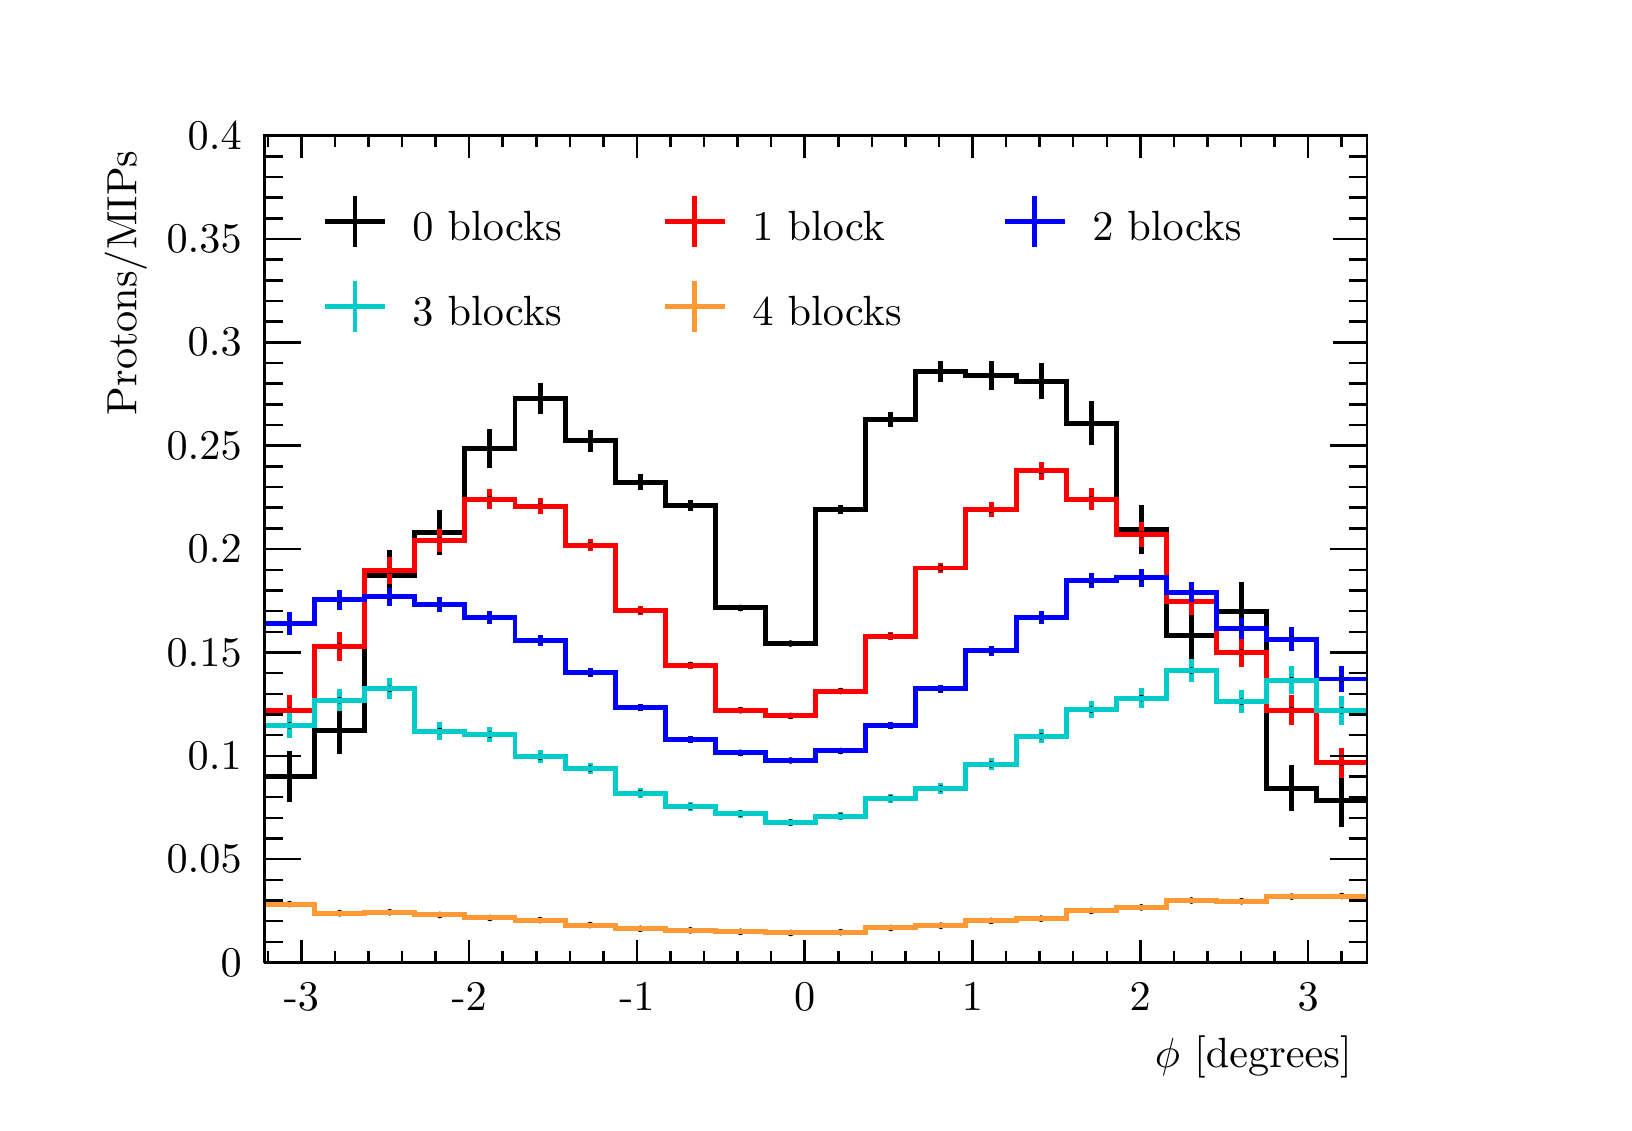
\begin{tikzpicture}
\pgfdeclareplotmark{cross} {
\pgfpathmoveto{\pgfpoint{-0.3\pgfplotmarksize}{\pgfplotmarksize}}
\pgfpathlineto{\pgfpoint{+0.3\pgfplotmarksize}{\pgfplotmarksize}}
\pgfpathlineto{\pgfpoint{+0.3\pgfplotmarksize}{0.3\pgfplotmarksize}}
\pgfpathlineto{\pgfpoint{+1\pgfplotmarksize}{0.3\pgfplotmarksize}}
\pgfpathlineto{\pgfpoint{+1\pgfplotmarksize}{-0.3\pgfplotmarksize}}
\pgfpathlineto{\pgfpoint{+0.3\pgfplotmarksize}{-0.3\pgfplotmarksize}}
\pgfpathlineto{\pgfpoint{+0.3\pgfplotmarksize}{-1.\pgfplotmarksize}}
\pgfpathlineto{\pgfpoint{-0.3\pgfplotmarksize}{-1.\pgfplotmarksize}}
\pgfpathlineto{\pgfpoint{-0.3\pgfplotmarksize}{-0.3\pgfplotmarksize}}
\pgfpathlineto{\pgfpoint{-1.\pgfplotmarksize}{-0.3\pgfplotmarksize}}
\pgfpathlineto{\pgfpoint{-1.\pgfplotmarksize}{0.3\pgfplotmarksize}}
\pgfpathlineto{\pgfpoint{-0.3\pgfplotmarksize}{0.3\pgfplotmarksize}}
\pgfpathclose
\pgfusepathqstroke
}
\pgfdeclareplotmark{cross*} {
\pgfpathmoveto{\pgfpoint{-0.3\pgfplotmarksize}{\pgfplotmarksize}}
\pgfpathlineto{\pgfpoint{+0.3\pgfplotmarksize}{\pgfplotmarksize}}
\pgfpathlineto{\pgfpoint{+0.3\pgfplotmarksize}{0.3\pgfplotmarksize}}
\pgfpathlineto{\pgfpoint{+1\pgfplotmarksize}{0.3\pgfplotmarksize}}
\pgfpathlineto{\pgfpoint{+1\pgfplotmarksize}{-0.3\pgfplotmarksize}}
\pgfpathlineto{\pgfpoint{+0.3\pgfplotmarksize}{-0.3\pgfplotmarksize}}
\pgfpathlineto{\pgfpoint{+0.3\pgfplotmarksize}{-1.\pgfplotmarksize}}
\pgfpathlineto{\pgfpoint{-0.3\pgfplotmarksize}{-1.\pgfplotmarksize}}
\pgfpathlineto{\pgfpoint{-0.3\pgfplotmarksize}{-0.3\pgfplotmarksize}}
\pgfpathlineto{\pgfpoint{-1.\pgfplotmarksize}{-0.3\pgfplotmarksize}}
\pgfpathlineto{\pgfpoint{-1.\pgfplotmarksize}{0.3\pgfplotmarksize}}
\pgfpathlineto{\pgfpoint{-0.3\pgfplotmarksize}{0.3\pgfplotmarksize}}
\pgfpathclose
\pgfusepathqfillstroke
}
\pgfdeclareplotmark{newstar} {
\pgfpathmoveto{\pgfqpoint{0pt}{\pgfplotmarksize}}
\pgfpathlineto{\pgfqpointpolar{44}{0.5\pgfplotmarksize}}
\pgfpathlineto{\pgfqpointpolar{18}{\pgfplotmarksize}}
\pgfpathlineto{\pgfqpointpolar{-20}{0.5\pgfplotmarksize}}
\pgfpathlineto{\pgfqpointpolar{-54}{\pgfplotmarksize}}
\pgfpathlineto{\pgfqpointpolar{-90}{0.5\pgfplotmarksize}}
\pgfpathlineto{\pgfqpointpolar{234}{\pgfplotmarksize}}
\pgfpathlineto{\pgfqpointpolar{198}{0.5\pgfplotmarksize}}
\pgfpathlineto{\pgfqpointpolar{162}{\pgfplotmarksize}}
\pgfpathlineto{\pgfqpointpolar{134}{0.5\pgfplotmarksize}}
\pgfpathclose
\pgfusepathqstroke
}
\pgfdeclareplotmark{newstar*} {
\pgfpathmoveto{\pgfqpoint{0pt}{\pgfplotmarksize}}
\pgfpathlineto{\pgfqpointpolar{44}{0.5\pgfplotmarksize}}
\pgfpathlineto{\pgfqpointpolar{18}{\pgfplotmarksize}}
\pgfpathlineto{\pgfqpointpolar{-20}{0.5\pgfplotmarksize}}
\pgfpathlineto{\pgfqpointpolar{-54}{\pgfplotmarksize}}
\pgfpathlineto{\pgfqpointpolar{-90}{0.5\pgfplotmarksize}}
\pgfpathlineto{\pgfqpointpolar{234}{\pgfplotmarksize}}
\pgfpathlineto{\pgfqpointpolar{198}{0.5\pgfplotmarksize}}
\pgfpathlineto{\pgfqpointpolar{162}{\pgfplotmarksize}}
\pgfpathlineto{\pgfqpointpolar{134}{0.5\pgfplotmarksize}}
\pgfpathclose
\pgfusepathqfillstroke
}
\definecolor{c}{rgb}{1,1,1};
\draw [color=c, fill=c] (0,0) rectangle (20,13.639);
\draw [color=c, fill=c] (3,1.77307) rectangle (17,12.2751);
\definecolor{c}{rgb}{0,0,0};
\draw [c,line width=0.9] (3,1.77307) -- (3,12.2751) -- (17,12.2751) -- (17,1.77307) -- (3,1.77307);
\definecolor{c}{rgb}{1,1,1};
\draw [color=c, fill=c] (3,1.77307) rectangle (17,12.2751);
\definecolor{c}{rgb}{0,0,0};
\draw [c,line width=0.9] (3,1.77307) -- (3,12.2751) -- (17,12.2751) -- (17,1.77307) -- (3,1.77307);
\draw [c,line width=0.9] (3,1.77307) -- (3.63636,1.77307) -- (3.63636,1.77307) -- (4.27273,1.77307) -- (4.27273,1.77307) -- (4.90909,1.77307) -- (4.90909,1.77307) -- (5.54545,1.77307) -- (5.54545,1.77307) -- (6.18182,1.77307) -- (6.18182,1.77307) --
 (6.81818,1.77307) -- (6.81818,1.77307) -- (7.45455,1.77307) -- (7.45455,1.77307) -- (8.09091,1.77307) -- (8.09091,1.77307) -- (8.72727,1.77307) -- (8.72727,1.77307) -- (9.36364,1.77307) -- (9.36364,1.77307) -- (10,1.77307) -- (10,1.77307) --
 (10.6364,1.77307) -- (10.6364,1.77307) -- (11.2727,1.77307) -- (11.2727,1.77307) -- (11.9091,1.77307) -- (11.9091,1.77307) -- (12.5455,1.77307) -- (12.5455,1.77307) -- (13.1818,1.77307) -- (13.1818,1.77307) -- (13.8182,1.77307) -- (13.8182,1.77307)
 -- (14.4545,1.77307) -- (14.4545,1.77307) -- (15.0909,1.77307) -- (15.0909,1.77307) -- (15.7273,1.77307) -- (15.7273,1.77307) -- (16.3636,1.77307) -- (16.3636,1.77307) -- (17,1.77307);
\draw [c,line width=0.9] (3,1.77307) -- (17,1.77307);
\draw [c,line width=0.9] (3.4688,2.05948) -- (3.4688,1.77307);
\draw [c,line width=0.9] (3.89498,1.91628) -- (3.89498,1.77307);
\draw [c,line width=0.9] (4.32116,1.91628) -- (4.32116,1.77307);
\draw [c,line width=0.9] (4.74734,1.91628) -- (4.74734,1.77307);
\draw [c,line width=0.9] (5.17352,1.91628) -- (5.17352,1.77307);
\draw [c,line width=0.9] (5.5997,2.05948) -- (5.5997,1.77307);
\draw [c,line width=0.9] (6.02588,1.91628) -- (6.02588,1.77307);
\draw [c,line width=0.9] (6.45205,1.91628) -- (6.45205,1.77307);
\draw [c,line width=0.9] (6.87823,1.91628) -- (6.87823,1.77307);
\draw [c,line width=0.9] (7.30441,1.91628) -- (7.30441,1.77307);
\draw [c,line width=0.9] (7.73059,2.05948) -- (7.73059,1.77307);
\draw [c,line width=0.9] (8.15677,1.91628) -- (8.15677,1.77307);
\draw [c,line width=0.9] (8.58295,1.91628) -- (8.58295,1.77307);
\draw [c,line width=0.9] (9.00913,1.91628) -- (9.00913,1.77307);
\draw [c,line width=0.9] (9.43531,1.91628) -- (9.43531,1.77307);
\draw [c,line width=0.9] (9.86149,2.05948) -- (9.86149,1.77307);
\draw [c,line width=0.9] (10.2877,1.91628) -- (10.2877,1.77307);
\draw [c,line width=0.9] (10.7139,1.91628) -- (10.7139,1.77307);
\draw [c,line width=0.9] (11.14,1.91628) -- (11.14,1.77307);
\draw [c,line width=0.9] (11.5662,1.91628) -- (11.5662,1.77307);
\draw [c,line width=0.9] (11.9924,2.05948) -- (11.9924,1.77307);
\draw [c,line width=0.9] (12.4186,1.91628) -- (12.4186,1.77307);
\draw [c,line width=0.9] (12.8447,1.91628) -- (12.8447,1.77307);
\draw [c,line width=0.9] (13.2709,1.91628) -- (13.2709,1.77307);
\draw [c,line width=0.9] (13.6971,1.91628) -- (13.6971,1.77307);
\draw [c,line width=0.9] (14.1233,2.05948) -- (14.1233,1.77307);
\draw [c,line width=0.9] (14.5495,1.91628) -- (14.5495,1.77307);
\draw [c,line width=0.9] (14.9756,1.91628) -- (14.9756,1.77307);
\draw [c,line width=0.9] (15.4018,1.91628) -- (15.4018,1.77307);
\draw [c,line width=0.9] (15.828,1.91628) -- (15.828,1.77307);
\draw [c,line width=0.9] (16.2542,2.05948) -- (16.2542,1.77307);
\draw [c,line width=0.9] (3.4688,2.05948) -- (3.4688,1.77307);
\draw [c,line width=0.9] (3.04262,1.91628) -- (3.04262,1.77307);
\draw [c,line width=0.9] (16.2542,2.05948) -- (16.2542,1.77307);
\draw [c,line width=0.9] (16.6804,1.91628) -- (16.6804,1.77307);
\draw [anchor=base] (3.4688,1.15931) node[scale=1.52731, color=c, rotate=0]{-3};
\draw [anchor=base] (5.5997,1.15931) node[scale=1.52731, color=c, rotate=0]{-2};
\draw [anchor=base] (7.73059,1.15931) node[scale=1.52731, color=c, rotate=0]{-1};
\draw [anchor=base] (9.86149,1.15931) node[scale=1.52731, color=c, rotate=0]{0};
\draw [anchor=base] (11.9924,1.15931) node[scale=1.52731, color=c, rotate=0]{1};
\draw [anchor=base] (14.1233,1.15931) node[scale=1.52731, color=c, rotate=0]{2};
\draw [anchor=base] (16.2542,1.15931) node[scale=1.52731, color=c, rotate=0]{3};
\draw [anchor= east] (17,0.572837) node[scale=1.52731, color=c, rotate=0]{$\phi$ [degrees]};
\draw [c,line width=0.9] (3,12.2751) -- (17,12.2751);
\draw [c,line width=0.9] (3.4688,11.9887) -- (3.4688,12.2751);
\draw [c,line width=0.9] (3.89498,12.1319) -- (3.89498,12.2751);
\draw [c,line width=0.9] (4.32116,12.1319) -- (4.32116,12.2751);
\draw [c,line width=0.9] (4.74734,12.1319) -- (4.74734,12.2751);
\draw [c,line width=0.9] (5.17352,12.1319) -- (5.17352,12.2751);
\draw [c,line width=0.9] (5.5997,11.9887) -- (5.5997,12.2751);
\draw [c,line width=0.9] (6.02588,12.1319) -- (6.02588,12.2751);
\draw [c,line width=0.9] (6.45205,12.1319) -- (6.45205,12.2751);
\draw [c,line width=0.9] (6.87823,12.1319) -- (6.87823,12.2751);
\draw [c,line width=0.9] (7.30441,12.1319) -- (7.30441,12.2751);
\draw [c,line width=0.9] (7.73059,11.9887) -- (7.73059,12.2751);
\draw [c,line width=0.9] (8.15677,12.1319) -- (8.15677,12.2751);
\draw [c,line width=0.9] (8.58295,12.1319) -- (8.58295,12.2751);
\draw [c,line width=0.9] (9.00913,12.1319) -- (9.00913,12.2751);
\draw [c,line width=0.9] (9.43531,12.1319) -- (9.43531,12.2751);
\draw [c,line width=0.9] (9.86149,11.9887) -- (9.86149,12.2751);
\draw [c,line width=0.9] (10.2877,12.1319) -- (10.2877,12.2751);
\draw [c,line width=0.9] (10.7139,12.1319) -- (10.7139,12.2751);
\draw [c,line width=0.9] (11.14,12.1319) -- (11.14,12.2751);
\draw [c,line width=0.9] (11.5662,12.1319) -- (11.5662,12.2751);
\draw [c,line width=0.9] (11.9924,11.9887) -- (11.9924,12.2751);
\draw [c,line width=0.9] (12.4186,12.1319) -- (12.4186,12.2751);
\draw [c,line width=0.9] (12.8447,12.1319) -- (12.8447,12.2751);
\draw [c,line width=0.9] (13.2709,12.1319) -- (13.2709,12.2751);
\draw [c,line width=0.9] (13.6971,12.1319) -- (13.6971,12.2751);
\draw [c,line width=0.9] (14.1233,11.9887) -- (14.1233,12.2751);
\draw [c,line width=0.9] (14.5495,12.1319) -- (14.5495,12.2751);
\draw [c,line width=0.9] (14.9756,12.1319) -- (14.9756,12.2751);
\draw [c,line width=0.9] (15.4018,12.1319) -- (15.4018,12.2751);
\draw [c,line width=0.9] (15.828,12.1319) -- (15.828,12.2751);
\draw [c,line width=0.9] (16.2542,11.9887) -- (16.2542,12.2751);
\draw [c,line width=0.9] (3.4688,11.9887) -- (3.4688,12.2751);
\draw [c,line width=0.9] (3.04262,12.1319) -- (3.04262,12.2751);
\draw [c,line width=0.9] (16.2542,11.9887) -- (16.2542,12.2751);
\draw [c,line width=0.9] (16.6804,12.1319) -- (16.6804,12.2751);
\draw [c,line width=0.9] (3,1.77307) -- (3,12.2751);
\draw [c,line width=0.9] (3.462,1.77307) -- (3,1.77307);
\draw [c,line width=0.9] (3.231,2.03562) -- (3,2.03562);
\draw [c,line width=0.9] (3.231,2.29817) -- (3,2.29817);
\draw [c,line width=0.9] (3.231,2.56072) -- (3,2.56072);
\draw [c,line width=0.9] (3.231,2.82327) -- (3,2.82327);
\draw [c,line width=0.9] (3.462,3.08582) -- (3,3.08582);
\draw [c,line width=0.9] (3.231,3.34837) -- (3,3.34837);
\draw [c,line width=0.9] (3.231,3.61092) -- (3,3.61092);
\draw [c,line width=0.9] (3.231,3.87347) -- (3,3.87347);
\draw [c,line width=0.9] (3.231,4.13602) -- (3,4.13602);
\draw [c,line width=0.9] (3.462,4.39857) -- (3,4.39857);
\draw [c,line width=0.9] (3.231,4.66112) -- (3,4.66112);
\draw [c,line width=0.9] (3.231,4.92367) -- (3,4.92367);
\draw [c,line width=0.9] (3.231,5.18622) -- (3,5.18622);
\draw [c,line width=0.9] (3.231,5.44877) -- (3,5.44877);
\draw [c,line width=0.9] (3.462,5.71132) -- (3,5.71132);
\draw [c,line width=0.9] (3.231,5.97387) -- (3,5.97387);
\draw [c,line width=0.9] (3.231,6.23642) -- (3,6.23642);
\draw [c,line width=0.9] (3.231,6.49897) -- (3,6.49897);
\draw [c,line width=0.9] (3.231,6.76152) -- (3,6.76152);
\draw [c,line width=0.9] (3.462,7.02407) -- (3,7.02407);
\draw [c,line width=0.9] (3.231,7.28662) -- (3,7.28662);
\draw [c,line width=0.9] (3.231,7.54917) -- (3,7.54917);
\draw [c,line width=0.9] (3.231,7.81172) -- (3,7.81172);
\draw [c,line width=0.9] (3.231,8.07427) -- (3,8.07427);
\draw [c,line width=0.9] (3.462,8.33682) -- (3,8.33682);
\draw [c,line width=0.9] (3.231,8.59937) -- (3,8.59937);
\draw [c,line width=0.9] (3.231,8.86192) -- (3,8.86192);
\draw [c,line width=0.9] (3.231,9.12447) -- (3,9.12447);
\draw [c,line width=0.9] (3.231,9.38702) -- (3,9.38702);
\draw [c,line width=0.9] (3.462,9.64957) -- (3,9.64957);
\draw [c,line width=0.9] (3.231,9.91212) -- (3,9.91212);
\draw [c,line width=0.9] (3.231,10.1747) -- (3,10.1747);
\draw [c,line width=0.9] (3.231,10.4372) -- (3,10.4372);
\draw [c,line width=0.9] (3.231,10.6998) -- (3,10.6998);
\draw [c,line width=0.9] (3.462,10.9623) -- (3,10.9623);
\draw [c,line width=0.9] (3.231,11.2249) -- (3,11.2249);
\draw [c,line width=0.9] (3.231,11.4874) -- (3,11.4874);
\draw [c,line width=0.9] (3.231,11.75) -- (3,11.75);
\draw [c,line width=0.9] (3.231,12.0125) -- (3,12.0125);
\draw [c,line width=0.9] (3.462,12.2751) -- (3,12.2751);
\draw [anchor= east] (2.9,1.77307) node[scale=1.52731, color=c, rotate=0]{0};
\draw [anchor= east] (2.9,3.08582) node[scale=1.52731, color=c, rotate=0]{0.05};
\draw [anchor= east] (2.9,4.39857) node[scale=1.52731, color=c, rotate=0]{0.1};
\draw [anchor= east] (2.9,5.71132) node[scale=1.52731, color=c, rotate=0]{0.15};
\draw [anchor= east] (2.9,7.02407) node[scale=1.52731, color=c, rotate=0]{0.2};
\draw [anchor= east] (2.9,8.33682) node[scale=1.52731, color=c, rotate=0]{0.25};
\draw [anchor= east] (2.9,9.64957) node[scale=1.52731, color=c, rotate=0]{0.3};
\draw [anchor= east] (2.9,10.9623) node[scale=1.52731, color=c, rotate=0]{0.35};
\draw [anchor= east] (2.9,12.2751) node[scale=1.52731, color=c, rotate=0]{0.4};
\draw [anchor= east] (1.24,12.2751) node[scale=1.52731, color=c, rotate=90]{  Protons/MIPs};
\draw [c,line width=0.9] (17,1.77307) -- (17,12.2751);
\draw [c,line width=0.9] (16.538,1.77307) -- (17,1.77307);
\draw [c,line width=0.9] (16.769,2.03562) -- (17,2.03562);
\draw [c,line width=0.9] (16.769,2.29817) -- (17,2.29817);
\draw [c,line width=0.9] (16.769,2.56072) -- (17,2.56072);
\draw [c,line width=0.9] (16.769,2.82327) -- (17,2.82327);
\draw [c,line width=0.9] (16.538,3.08582) -- (17,3.08582);
\draw [c,line width=0.9] (16.769,3.34837) -- (17,3.34837);
\draw [c,line width=0.9] (16.769,3.61092) -- (17,3.61092);
\draw [c,line width=0.9] (16.769,3.87347) -- (17,3.87347);
\draw [c,line width=0.9] (16.769,4.13602) -- (17,4.13602);
\draw [c,line width=0.9] (16.538,4.39857) -- (17,4.39857);
\draw [c,line width=0.9] (16.769,4.66112) -- (17,4.66112);
\draw [c,line width=0.9] (16.769,4.92367) -- (17,4.92367);
\draw [c,line width=0.9] (16.769,5.18622) -- (17,5.18622);
\draw [c,line width=0.9] (16.769,5.44877) -- (17,5.44877);
\draw [c,line width=0.9] (16.538,5.71132) -- (17,5.71132);
\draw [c,line width=0.9] (16.769,5.97387) -- (17,5.97387);
\draw [c,line width=0.9] (16.769,6.23642) -- (17,6.23642);
\draw [c,line width=0.9] (16.769,6.49897) -- (17,6.49897);
\draw [c,line width=0.9] (16.769,6.76152) -- (17,6.76152);
\draw [c,line width=0.9] (16.538,7.02407) -- (17,7.02407);
\draw [c,line width=0.9] (16.769,7.28662) -- (17,7.28662);
\draw [c,line width=0.9] (16.769,7.54917) -- (17,7.54917);
\draw [c,line width=0.9] (16.769,7.81172) -- (17,7.81172);
\draw [c,line width=0.9] (16.769,8.07427) -- (17,8.07427);
\draw [c,line width=0.9] (16.538,8.33682) -- (17,8.33682);
\draw [c,line width=0.9] (16.769,8.59937) -- (17,8.59937);
\draw [c,line width=0.9] (16.769,8.86192) -- (17,8.86192);
\draw [c,line width=0.9] (16.769,9.12447) -- (17,9.12447);
\draw [c,line width=0.9] (16.769,9.38702) -- (17,9.38702);
\draw [c,line width=0.9] (16.538,9.64957) -- (17,9.64957);
\draw [c,line width=0.9] (16.769,9.91212) -- (17,9.91212);
\draw [c,line width=0.9] (16.769,10.1747) -- (17,10.1747);
\draw [c,line width=0.9] (16.769,10.4372) -- (17,10.4372);
\draw [c,line width=0.9] (16.769,10.6998) -- (17,10.6998);
\draw [c,line width=0.9] (16.538,10.9623) -- (17,10.9623);
\draw [c,line width=0.9] (16.769,11.2249) -- (17,11.2249);
\draw [c,line width=0.9] (16.769,11.4874) -- (17,11.4874);
\draw [c,line width=0.9] (16.769,11.75) -- (17,11.75);
\draw [c,line width=0.9] (16.769,12.0125) -- (17,12.0125);
\draw [c,line width=0.9] (16.538,12.2751) -- (17,12.2751);
\draw [c,line width=1.8] (3.31818,3.80808) -- (3.31818,4.13307);
\draw [c,line width=1.8] (3.31818,4.13307) -- (3.31818,4.45805);
\foreach \P in {(3.31818,4.13307)}{\draw[mark options={color=c,fill=c},mark size=2.402402pt,mark=*,mark size=1pt] plot coordinates {\P};}
\draw [c,line width=1.8] (3.95455,4.41539) -- (3.95455,4.72226);
\draw [c,line width=1.8] (3.95455,4.72226) -- (3.95455,5.02913);
\foreach \P in {(3.95455,4.72226)}{\draw[mark options={color=c,fill=c},mark size=2.402402pt,mark=*,mark size=1pt] plot coordinates {\P};}
\draw [c,line width=1.8] (4.59091,6.36336) -- (4.59091,6.68924);
\draw [c,line width=1.8] (4.59091,6.68924) -- (4.59091,7.01511);
\foreach \P in {(4.59091,6.68924)}{\draw[mark options={color=c,fill=c},mark size=2.402402pt,mark=*,mark size=1pt] plot coordinates {\P};}
\draw [c,line width=1.8] (5.22727,6.95027) -- (5.22727,7.23731);
\draw [c,line width=1.8] (5.22727,7.23731) -- (5.22727,7.52435);
\foreach \P in {(5.22727,7.23731)}{\draw[mark options={color=c,fill=c},mark size=2.402402pt,mark=*,mark size=1pt] plot coordinates {\P};}
\draw [c,line width=1.8] (5.86364,8.05935) -- (5.86364,8.30108);
\draw [c,line width=1.8] (5.86364,8.30108) -- (5.86364,8.54282);
\foreach \P in {(5.86364,8.30108)}{\draw[mark options={color=c,fill=c},mark size=2.402402pt,mark=*,mark size=1pt] plot coordinates {\P};}
\draw [c,line width=1.8] (6.5,8.738) -- (6.5,8.93286);
\draw [c,line width=1.8] (6.5,8.93286) -- (6.5,9.12772);
\foreach \P in {(6.5,8.93286)}{\draw[mark options={color=c,fill=c},mark size=2.402402pt,mark=*,mark size=1pt] plot coordinates {\P};}
\draw [c,line width=1.8] (7.13636,8.25921) -- (7.13636,8.39849);
\draw [c,line width=1.8] (7.13636,8.39849) -- (7.13636,8.53777);
\foreach \P in {(7.13636,8.39849)}{\draw[mark options={color=c,fill=c},mark size=2.402402pt,mark=*,mark size=1pt] plot coordinates {\P};}
\draw [c,line width=1.8] (7.77273,7.77828) -- (7.77273,7.87577);
\draw [c,line width=1.8] (7.77273,7.87577) -- (7.77273,7.97326);
\foreach \P in {(7.77273,7.87577)}{\draw[mark options={color=c,fill=c},mark size=2.402402pt,mark=*,mark size=1pt] plot coordinates {\P};}
\draw [c,line width=1.8] (8.40909,7.5099) -- (8.40909,7.57818);
\draw [c,line width=1.8] (8.40909,7.57818) -- (8.40909,7.64647);
\foreach \P in {(8.40909,7.57818)}{\draw[mark options={color=c,fill=c},mark size=2.402402pt,mark=*,mark size=1pt] plot coordinates {\P};}
\draw [c,line width=1.8] (9.04545,6.23857) -- (9.04545,6.27671);
\draw [c,line width=1.8] (9.04545,6.27671) -- (9.04545,6.31485);
\foreach \P in {(9.04545,6.27671)}{\draw[mark options={color=c,fill=c},mark size=2.402402pt,mark=*,mark size=1pt] plot coordinates {\P};}
\draw [c,line width=1.8] (9.68182,5.79204) -- (9.68182,5.82443);
\draw [c,line width=1.8] (9.68182,5.82443) -- (9.68182,5.85681);
\foreach \P in {(9.68182,5.82443)}{\draw[mark options={color=c,fill=c},mark size=2.402402pt,mark=*,mark size=1pt] plot coordinates {\P};}
\draw [c,line width=1.8] (10.3182,7.47425) -- (10.3182,7.53112);
\draw [c,line width=1.8] (10.3182,7.53112) -- (10.3182,7.58798);
\foreach \P in {(10.3182,7.53112)}{\draw[mark options={color=c,fill=c},mark size=2.402402pt,mark=*,mark size=1pt] plot coordinates {\P};}
\draw [c,line width=1.8] (10.9545,8.57392) -- (10.9545,8.66757);
\draw [c,line width=1.8] (10.9545,8.66757) -- (10.9545,8.76122);
\foreach \P in {(10.9545,8.66757)}{\draw[mark options={color=c,fill=c},mark size=2.402402pt,mark=*,mark size=1pt] plot coordinates {\P};}
\draw [c,line width=1.8] (11.5909,9.14225) -- (11.5909,9.27642);
\draw [c,line width=1.8] (11.5909,9.27642) -- (11.5909,9.41059);
\foreach \P in {(11.5909,9.27642)}{\draw[mark options={color=c,fill=c},mark size=2.402402pt,mark=*,mark size=1pt] plot coordinates {\P};}
\draw [c,line width=1.8] (12.2273,9.04159) -- (12.2273,9.22441);
\draw [c,line width=1.8] (12.2273,9.22441) -- (12.2273,9.40722);
\foreach \P in {(12.2273,9.22441)}{\draw[mark options={color=c,fill=c},mark size=2.402402pt,mark=*,mark size=1pt] plot coordinates {\P};}
\draw [c,line width=1.8] (12.8636,8.92559) -- (12.8636,9.15666);
\draw [c,line width=1.8] (12.8636,9.15666) -- (12.8636,9.38773);
\foreach \P in {(12.8636,9.15666)}{\draw[mark options={color=c,fill=c},mark size=2.402402pt,mark=*,mark size=1pt] plot coordinates {\P};}
\draw [c,line width=1.8] (13.5,8.34016) -- (13.5,8.62085);
\draw [c,line width=1.8] (13.5,8.62085) -- (13.5,8.90154);
\foreach \P in {(13.5,8.62085)}{\draw[mark options={color=c,fill=c},mark size=2.402402pt,mark=*,mark size=1pt] plot coordinates {\P};}
\draw [c,line width=1.8] (14.1364,6.96408) -- (14.1364,7.27082);
\draw [c,line width=1.8] (14.1364,7.27082) -- (14.1364,7.57756);
\foreach \P in {(14.1364,7.27082)}{\draw[mark options={color=c,fill=c},mark size=2.402402pt,mark=*,mark size=1pt] plot coordinates {\P};}
\draw [c,line width=1.8] (14.7727,5.6213) -- (14.7727,5.92854);
\draw [c,line width=1.8] (14.7727,5.92854) -- (14.7727,6.23577);
\foreach \P in {(14.7727,5.92854)}{\draw[mark options={color=c,fill=c},mark size=2.402402pt,mark=*,mark size=1pt] plot coordinates {\P};}
\draw [c,line width=1.8] (15.4091,5.86537) -- (15.4091,6.23494);
\draw [c,line width=1.8] (15.4091,6.23494) -- (15.4091,6.60452);
\foreach \P in {(15.4091,6.23494)}{\draw[mark options={color=c,fill=c},mark size=2.402402pt,mark=*,mark size=1pt] plot coordinates {\P};}
\draw [c,line width=1.8] (16.0455,3.69529) -- (16.0455,3.9894);
\draw [c,line width=1.8] (16.0455,3.9894) -- (16.0455,4.28351);
\foreach \P in {(16.0455,3.9894)}{\draw[mark options={color=c,fill=c},mark size=2.402402pt,mark=*,mark size=1pt] plot coordinates {\P};}
\draw [c,line width=1.8] (16.6818,3.49909) -- (16.6818,3.83344);
\draw [c,line width=1.8] (16.6818,3.83344) -- (16.6818,4.16778);
\foreach \P in {(16.6818,3.83344)}{\draw[mark options={color=c,fill=c},mark size=2.402402pt,mark=*,mark size=1pt] plot coordinates {\P};}
\draw [c,line width=1.8] (3,4.13307) -- (3.63636,4.13307) -- (3.63636,4.72226) -- (4.27273,4.72226) -- (4.27273,6.68924) -- (4.90909,6.68924) -- (4.90909,7.23731) -- (5.54545,7.23731) -- (5.54545,8.30108) -- (6.18182,8.30108) -- (6.18182,8.93286) --
 (6.81818,8.93286) -- (6.81818,8.39849) -- (7.45455,8.39849) -- (7.45455,7.87577) -- (8.09091,7.87577) -- (8.09091,7.57818) -- (8.72727,7.57818) -- (8.72727,6.27671) -- (9.36364,6.27671) -- (9.36364,5.82443) -- (10,5.82443) -- (10,7.53112) --
 (10.6364,7.53112) -- (10.6364,8.66757) -- (11.2727,8.66757) -- (11.2727,9.27642) -- (11.9091,9.27642) -- (11.9091,9.22441) -- (12.5455,9.22441) -- (12.5455,9.15666) -- (13.1818,9.15666) -- (13.1818,8.62085) -- (13.8182,8.62085) -- (13.8182,7.27082)
 -- (14.4545,7.27082) -- (14.4545,5.92854) -- (15.0909,5.92854) -- (15.0909,6.23494) -- (15.7273,6.23494) -- (15.7273,3.9894) -- (16.3636,3.9894) -- (16.3636,3.83344) -- (17,3.83344);
\definecolor{c}{rgb}{1,0,0};
\draw [c,line width=1.8] (3.31818,4.78145) -- (3.31818,4.97313);
\draw [c,line width=1.8] (3.31818,4.97313) -- (3.31818,5.16481);
\definecolor{c}{rgb}{0,0,0};
\foreach \P in {(3.31818,4.97313)}{\draw[mark options={color=c,fill=c},mark size=2.402402pt,mark=*,mark size=1pt] plot coordinates {\P};}
\definecolor{c}{rgb}{1,0,0};
\draw [c,line width=1.8] (3.95455,5.6081) -- (3.95455,5.78705);
\draw [c,line width=1.8] (3.95455,5.78705) -- (3.95455,5.96599);
\definecolor{c}{rgb}{0,0,0};
\foreach \P in {(3.95455,5.78705)}{\draw[mark options={color=c,fill=c},mark size=2.402402pt,mark=*,mark size=1pt] plot coordinates {\P};}
\definecolor{c}{rgb}{1,0,0};
\draw [c,line width=1.8] (4.59091,6.57712) -- (4.59091,6.74842);
\draw [c,line width=1.8] (4.59091,6.74842) -- (4.59091,6.91972);
\definecolor{c}{rgb}{0,0,0};
\foreach \P in {(4.59091,6.74842)}{\draw[mark options={color=c,fill=c},mark size=2.402402pt,mark=*,mark size=1pt] plot coordinates {\P};}
\definecolor{c}{rgb}{1,0,0};
\draw [c,line width=1.8] (5.22727,6.98706) -- (5.22727,7.13564);
\draw [c,line width=1.8] (5.22727,7.13564) -- (5.22727,7.28422);
\definecolor{c}{rgb}{0,0,0};
\foreach \P in {(5.22727,7.13564)}{\draw[mark options={color=c,fill=c},mark size=2.402402pt,mark=*,mark size=1pt] plot coordinates {\P};}
\definecolor{c}{rgb}{1,0,0};
\draw [c,line width=1.8] (5.86364,7.53021) -- (5.86364,7.65829);
\draw [c,line width=1.8] (5.86364,7.65829) -- (5.86364,7.78638);
\definecolor{c}{rgb}{0,0,0};
\foreach \P in {(5.86364,7.65829)}{\draw[mark options={color=c,fill=c},mark size=2.402402pt,mark=*,mark size=1pt] plot coordinates {\P};}
\definecolor{c}{rgb}{1,0,0};
\draw [c,line width=1.8] (6.5,7.46591) -- (6.5,7.5684);
\draw [c,line width=1.8] (6.5,7.5684) -- (6.5,7.67089);
\definecolor{c}{rgb}{0,0,0};
\foreach \P in {(6.5,7.5684)}{\draw[mark options={color=c,fill=c},mark size=2.402402pt,mark=*,mark size=1pt] plot coordinates {\P};}
\definecolor{c}{rgb}{1,0,0};
\draw [c,line width=1.8] (7.13636,6.99514) -- (7.13636,7.07247);
\draw [c,line width=1.8] (7.13636,7.07247) -- (7.13636,7.14981);
\definecolor{c}{rgb}{0,0,0};
\foreach \P in {(7.13636,7.07247)}{\draw[mark options={color=c,fill=c},mark size=2.402402pt,mark=*,mark size=1pt] plot coordinates {\P};}
\definecolor{c}{rgb}{1,0,0};
\draw [c,line width=1.8] (7.77273,6.18448) -- (7.77273,6.24109);
\draw [c,line width=1.8] (7.77273,6.24109) -- (7.77273,6.29769);
\definecolor{c}{rgb}{0,0,0};
\foreach \P in {(7.77273,6.24109)}{\draw[mark options={color=c,fill=c},mark size=2.402402pt,mark=*,mark size=1pt] plot coordinates {\P};}
\definecolor{c}{rgb}{1,0,0};
\draw [c,line width=1.8] (8.40909,5.5071) -- (8.40909,5.55116);
\draw [c,line width=1.8] (8.40909,5.55116) -- (8.40909,5.59522);
\definecolor{c}{rgb}{0,0,0};
\foreach \P in {(8.40909,5.55116)}{\draw[mark options={color=c,fill=c},mark size=2.402402pt,mark=*,mark size=1pt] plot coordinates {\P};}
\definecolor{c}{rgb}{1,0,0};
\draw [c,line width=1.8] (9.04545,4.94121) -- (9.04545,4.97695);
\draw [c,line width=1.8] (9.04545,4.97695) -- (9.04545,5.01268);
\definecolor{c}{rgb}{0,0,0};
\foreach \P in {(9.04545,4.97695)}{\draw[mark options={color=c,fill=c},mark size=2.402402pt,mark=*,mark size=1pt] plot coordinates {\P};}
\definecolor{c}{rgb}{1,0,0};
\draw [c,line width=1.8] (9.68182,4.87123) -- (9.68182,4.9057);
\draw [c,line width=1.8] (9.68182,4.9057) -- (9.68182,4.94017);
\definecolor{c}{rgb}{0,0,0};
\foreach \P in {(9.68182,4.9057)}{\draw[mark options={color=c,fill=c},mark size=2.402402pt,mark=*,mark size=1pt] plot coordinates {\P};}
\definecolor{c}{rgb}{1,0,0};
\draw [c,line width=1.8] (10.3182,5.18155) -- (10.3182,5.22031);
\draw [c,line width=1.8] (10.3182,5.22031) -- (10.3182,5.25907);
\definecolor{c}{rgb}{0,0,0};
\foreach \P in {(10.3182,5.22031)}{\draw[mark options={color=c,fill=c},mark size=2.402402pt,mark=*,mark size=1pt] plot coordinates {\P};}
\definecolor{c}{rgb}{1,0,0};
\draw [c,line width=1.8] (10.9545,5.86661) -- (10.9545,5.91603);
\draw [c,line width=1.8] (10.9545,5.91603) -- (10.9545,5.96545);
\definecolor{c}{rgb}{0,0,0};
\foreach \P in {(10.9545,5.91603)}{\draw[mark options={color=c,fill=c},mark size=2.402402pt,mark=*,mark size=1pt] plot coordinates {\P};}
\definecolor{c}{rgb}{1,0,0};
\draw [c,line width=1.8] (11.5909,6.71715) -- (11.5909,6.78377);
\draw [c,line width=1.8] (11.5909,6.78377) -- (11.5909,6.85039);
\definecolor{c}{rgb}{0,0,0};
\foreach \P in {(11.5909,6.78377)}{\draw[mark options={color=c,fill=c},mark size=2.402402pt,mark=*,mark size=1pt] plot coordinates {\P};}
\definecolor{c}{rgb}{1,0,0};
\draw [c,line width=1.8] (12.2273,7.43032) -- (12.2273,7.52302);
\draw [c,line width=1.8] (12.2273,7.52302) -- (12.2273,7.61572);
\definecolor{c}{rgb}{0,0,0};
\foreach \P in {(12.2273,7.52302)}{\draw[mark options={color=c,fill=c},mark size=2.402402pt,mark=*,mark size=1pt] plot coordinates {\P};}
\definecolor{c}{rgb}{1,0,0};
\draw [c,line width=1.8] (12.8636,7.89794) -- (12.8636,8.01654);
\draw [c,line width=1.8] (12.8636,8.01654) -- (12.8636,8.13513);
\definecolor{c}{rgb}{0,0,0};
\foreach \P in {(12.8636,8.01654)}{\draw[mark options={color=c,fill=c},mark size=2.402402pt,mark=*,mark size=1pt] plot coordinates {\P};}
\definecolor{c}{rgb}{1,0,0};
\draw [c,line width=1.8] (13.5,7.51706) -- (13.5,7.65841);
\draw [c,line width=1.8] (13.5,7.65841) -- (13.5,7.79976);
\definecolor{c}{rgb}{0,0,0};
\foreach \P in {(13.5,7.65841)}{\draw[mark options={color=c,fill=c},mark size=2.402402pt,mark=*,mark size=1pt] plot coordinates {\P};}
\definecolor{c}{rgb}{1,0,0};
\draw [c,line width=1.8] (14.1364,7.04699) -- (14.1364,7.21009);
\draw [c,line width=1.8] (14.1364,7.21009) -- (14.1364,7.37319);
\definecolor{c}{rgb}{0,0,0};
\foreach \P in {(14.1364,7.21009)}{\draw[mark options={color=c,fill=c},mark size=2.402402pt,mark=*,mark size=1pt] plot coordinates {\P};}
\definecolor{c}{rgb}{1,0,0};
\draw [c,line width=1.8] (14.7727,6.18734) -- (14.7727,6.36271);
\draw [c,line width=1.8] (14.7727,6.36271) -- (14.7727,6.53807);
\definecolor{c}{rgb}{0,0,0};
\foreach \P in {(14.7727,6.36271)}{\draw[mark options={color=c,fill=c},mark size=2.402402pt,mark=*,mark size=1pt] plot coordinates {\P};}
\definecolor{c}{rgb}{1,0,0};
\draw [c,line width=1.8] (15.4091,5.53084) -- (15.4091,5.71479);
\draw [c,line width=1.8] (15.4091,5.71479) -- (15.4091,5.89875);
\definecolor{c}{rgb}{0,0,0};
\foreach \P in {(15.4091,5.71479)}{\draw[mark options={color=c,fill=c},mark size=2.402402pt,mark=*,mark size=1pt] plot coordinates {\P};}
\definecolor{c}{rgb}{1,0,0};
\draw [c,line width=1.8] (16.0455,4.78569) -- (16.0455,4.97952);
\draw [c,line width=1.8] (16.0455,4.97952) -- (16.0455,5.17335);
\definecolor{c}{rgb}{0,0,0};
\foreach \P in {(16.0455,4.97952)}{\draw[mark options={color=c,fill=c},mark size=2.402402pt,mark=*,mark size=1pt] plot coordinates {\P};}
\definecolor{c}{rgb}{1,0,0};
\draw [c,line width=1.8] (16.6818,4.11737) -- (16.6818,4.30993);
\draw [c,line width=1.8] (16.6818,4.30993) -- (16.6818,4.50248);
\definecolor{c}{rgb}{0,0,0};
\foreach \P in {(16.6818,4.30993)}{\draw[mark options={color=c,fill=c},mark size=2.402402pt,mark=*,mark size=1pt] plot coordinates {\P};}
\definecolor{c}{rgb}{1,0,0};
\draw [c,line width=1.8] (3,4.97313) -- (3.63636,4.97313) -- (3.63636,5.78705) -- (4.27273,5.78705) -- (4.27273,6.74842) -- (4.90909,6.74842) -- (4.90909,7.13564) -- (5.54545,7.13564) -- (5.54545,7.65829) -- (6.18182,7.65829) -- (6.18182,7.5684) --
 (6.81818,7.5684) -- (6.81818,7.07247) -- (7.45455,7.07247) -- (7.45455,6.24109) -- (8.09091,6.24109) -- (8.09091,5.55116) -- (8.72727,5.55116) -- (8.72727,4.97695) -- (9.36364,4.97695) -- (9.36364,4.9057) -- (10,4.9057) -- (10,5.22031) --
 (10.6364,5.22031) -- (10.6364,5.91603) -- (11.2727,5.91603) -- (11.2727,6.78377) -- (11.9091,6.78377) -- (11.9091,7.52302) -- (12.5455,7.52302) -- (12.5455,8.01654) -- (13.1818,8.01654) -- (13.1818,7.65841) -- (13.8182,7.65841) -- (13.8182,7.21009)
 -- (14.4545,7.21009) -- (14.4545,6.36271) -- (15.0909,6.36271) -- (15.0909,5.71479) -- (15.7273,5.71479) -- (15.7273,4.97952) -- (16.3636,4.97952) -- (16.3636,4.30993) -- (17,4.30993);
\definecolor{c}{rgb}{0,0,1};
\draw [c,line width=1.8] (3.31818,5.92759) -- (3.31818,6.07822);
\draw [c,line width=1.8] (3.31818,6.07822) -- (3.31818,6.22885);
\definecolor{c}{rgb}{0,0,0};
\foreach \P in {(3.31818,6.07822)}{\draw[mark options={color=c,fill=c},mark size=2.402402pt,mark=*,mark size=1pt] plot coordinates {\P};}
\definecolor{c}{rgb}{0,0,1};
\draw [c,line width=1.8] (3.95455,6.24646) -- (3.95455,6.37771);
\draw [c,line width=1.8] (3.95455,6.37771) -- (3.95455,6.50896);
\definecolor{c}{rgb}{0,0,0};
\foreach \P in {(3.95455,6.37771)}{\draw[mark options={color=c,fill=c},mark size=2.402402pt,mark=*,mark size=1pt] plot coordinates {\P};}
\definecolor{c}{rgb}{0,0,1};
\draw [c,line width=1.8] (4.59091,6.29971) -- (4.59091,6.41607);
\draw [c,line width=1.8] (4.59091,6.41607) -- (4.59091,6.53243);
\definecolor{c}{rgb}{0,0,0};
\foreach \P in {(4.59091,6.41607)}{\draw[mark options={color=c,fill=c},mark size=2.402402pt,mark=*,mark size=1pt] plot coordinates {\P};}
\definecolor{c}{rgb}{0,0,1};
\draw [c,line width=1.8] (5.22727,6.21984) -- (5.22727,6.31949);
\draw [c,line width=1.8] (5.22727,6.31949) -- (5.22727,6.41914);
\definecolor{c}{rgb}{0,0,0};
\foreach \P in {(5.22727,6.31949)}{\draw[mark options={color=c,fill=c},mark size=2.402402pt,mark=*,mark size=1pt] plot coordinates {\P};}
\definecolor{c}{rgb}{0,0,1};
\draw [c,line width=1.8] (5.86364,6.06879) -- (5.86364,6.15273);
\draw [c,line width=1.8] (5.86364,6.15273) -- (5.86364,6.23666);
\definecolor{c}{rgb}{0,0,0};
\foreach \P in {(5.86364,6.15273)}{\draw[mark options={color=c,fill=c},mark size=2.402402pt,mark=*,mark size=1pt] plot coordinates {\P};}
\definecolor{c}{rgb}{0,0,1};
\draw [c,line width=1.8] (6.5,5.7898) -- (6.5,5.86022);
\draw [c,line width=1.8] (6.5,5.86022) -- (6.5,5.93064);
\definecolor{c}{rgb}{0,0,0};
\foreach \P in {(6.5,5.86022)}{\draw[mark options={color=c,fill=c},mark size=2.402402pt,mark=*,mark size=1pt] plot coordinates {\P};}
\definecolor{c}{rgb}{0,0,1};
\draw [c,line width=1.8] (7.13636,5.39713) -- (7.13636,5.45483);
\draw [c,line width=1.8] (7.13636,5.45483) -- (7.13636,5.51254);
\definecolor{c}{rgb}{0,0,0};
\foreach \P in {(7.13636,5.45483)}{\draw[mark options={color=c,fill=c},mark size=2.402402pt,mark=*,mark size=1pt] plot coordinates {\P};}
\definecolor{c}{rgb}{0,0,1};
\draw [c,line width=1.8] (7.77273,4.96354) -- (7.77273,5.01062);
\draw [c,line width=1.8] (7.77273,5.01062) -- (7.77273,5.0577);
\definecolor{c}{rgb}{0,0,0};
\foreach \P in {(7.77273,5.01062)}{\draw[mark options={color=c,fill=c},mark size=2.402402pt,mark=*,mark size=1pt] plot coordinates {\P};}
\definecolor{c}{rgb}{0,0,1};
\draw [c,line width=1.8] (8.40909,4.56629) -- (8.40909,4.60615);
\draw [c,line width=1.8] (8.40909,4.60615) -- (8.40909,4.64601);
\definecolor{c}{rgb}{0,0,0};
\foreach \P in {(8.40909,4.60615)}{\draw[mark options={color=c,fill=c},mark size=2.402402pt,mark=*,mark size=1pt] plot coordinates {\P};}
\definecolor{c}{rgb}{0,0,1};
\draw [c,line width=1.8] (9.04545,4.40098) -- (9.04545,4.43678);
\draw [c,line width=1.8] (9.04545,4.43678) -- (9.04545,4.47259);
\definecolor{c}{rgb}{0,0,0};
\foreach \P in {(9.04545,4.43678)}{\draw[mark options={color=c,fill=c},mark size=2.402402pt,mark=*,mark size=1pt] plot coordinates {\P};}
\definecolor{c}{rgb}{0,0,1};
\draw [c,line width=1.8] (9.68182,4.30451) -- (9.68182,4.3395);
\draw [c,line width=1.8] (9.68182,4.3395) -- (9.68182,4.37449);
\definecolor{c}{rgb}{0,0,0};
\foreach \P in {(9.68182,4.3395)}{\draw[mark options={color=c,fill=c},mark size=2.402402pt,mark=*,mark size=1pt] plot coordinates {\P};}
\definecolor{c}{rgb}{0,0,1};
\draw [c,line width=1.8] (10.3182,4.42284) -- (10.3182,4.45999);
\draw [c,line width=1.8] (10.3182,4.45999) -- (10.3182,4.49713);
\definecolor{c}{rgb}{0,0,0};
\foreach \P in {(10.3182,4.45999)}{\draw[mark options={color=c,fill=c},mark size=2.402402pt,mark=*,mark size=1pt] plot coordinates {\P};}
\definecolor{c}{rgb}{0,0,1};
\draw [c,line width=1.8] (10.9545,4.73639) -- (10.9545,4.7792);
\draw [c,line width=1.8] (10.9545,4.7792) -- (10.9545,4.82201);
\definecolor{c}{rgb}{0,0,0};
\foreach \P in {(10.9545,4.7792)}{\draw[mark options={color=c,fill=c},mark size=2.402402pt,mark=*,mark size=1pt] plot coordinates {\P};}
\definecolor{c}{rgb}{0,0,1};
\draw [c,line width=1.8] (11.5909,5.19588) -- (11.5909,5.24757);
\draw [c,line width=1.8] (11.5909,5.24757) -- (11.5909,5.29926);
\definecolor{c}{rgb}{0,0,0};
\foreach \P in {(11.5909,5.24757)}{\draw[mark options={color=c,fill=c},mark size=2.402402pt,mark=*,mark size=1pt] plot coordinates {\P};}
\definecolor{c}{rgb}{0,0,1};
\draw [c,line width=1.8] (12.2273,5.66757) -- (12.2273,5.73297);
\draw [c,line width=1.8] (12.2273,5.73297) -- (12.2273,5.79837);
\definecolor{c}{rgb}{0,0,0};
\foreach \P in {(12.2273,5.73297)}{\draw[mark options={color=c,fill=c},mark size=2.402402pt,mark=*,mark size=1pt] plot coordinates {\P};}
\definecolor{c}{rgb}{0,0,1};
\draw [c,line width=1.8] (12.8636,6.07319) -- (12.8636,6.15251);
\draw [c,line width=1.8] (12.8636,6.15251) -- (12.8636,6.23183);
\definecolor{c}{rgb}{0,0,0};
\foreach \P in {(12.8636,6.15251)}{\draw[mark options={color=c,fill=c},mark size=2.402402pt,mark=*,mark size=1pt] plot coordinates {\P};}
\definecolor{c}{rgb}{0,0,1};
\draw [c,line width=1.8] (13.5,6.52464) -- (13.5,6.62018);
\draw [c,line width=1.8] (13.5,6.62018) -- (13.5,6.71572);
\definecolor{c}{rgb}{0,0,0};
\foreach \P in {(13.5,6.62018)}{\draw[mark options={color=c,fill=c},mark size=2.402402pt,mark=*,mark size=1pt] plot coordinates {\P};}
\definecolor{c}{rgb}{0,0,1};
\draw [c,line width=1.8] (14.1364,6.5479) -- (14.1364,6.65735);
\draw [c,line width=1.8] (14.1364,6.65735) -- (14.1364,6.7668);
\definecolor{c}{rgb}{0,0,0};
\foreach \P in {(14.1364,6.65735)}{\draw[mark options={color=c,fill=c},mark size=2.402402pt,mark=*,mark size=1pt] plot coordinates {\P};}
\definecolor{c}{rgb}{0,0,1};
\draw [c,line width=1.8] (14.7727,6.35066) -- (14.7727,6.47536);
\draw [c,line width=1.8] (14.7727,6.47536) -- (14.7727,6.60007);
\definecolor{c}{rgb}{0,0,0};
\foreach \P in {(14.7727,6.47536)}{\draw[mark options={color=c,fill=c},mark size=2.402402pt,mark=*,mark size=1pt] plot coordinates {\P};}
\definecolor{c}{rgb}{0,0,1};
\draw [c,line width=1.8] (15.4091,5.88646) -- (15.4091,6.01987);
\draw [c,line width=1.8] (15.4091,6.01987) -- (15.4091,6.15328);
\definecolor{c}{rgb}{0,0,0};
\foreach \P in {(15.4091,6.01987)}{\draw[mark options={color=c,fill=c},mark size=2.402402pt,mark=*,mark size=1pt] plot coordinates {\P};}
\definecolor{c}{rgb}{0,0,1};
\draw [c,line width=1.8] (16.0455,5.72967) -- (16.0455,5.88085);
\draw [c,line width=1.8] (16.0455,5.88085) -- (16.0455,6.03202);
\definecolor{c}{rgb}{0,0,0};
\foreach \P in {(16.0455,5.88085)}{\draw[mark options={color=c,fill=c},mark size=2.402402pt,mark=*,mark size=1pt] plot coordinates {\P};}
\definecolor{c}{rgb}{0,0,1};
\draw [c,line width=1.8] (16.6818,5.21531) -- (16.6818,5.37408);
\draw [c,line width=1.8] (16.6818,5.37408) -- (16.6818,5.53286);
\definecolor{c}{rgb}{0,0,0};
\foreach \P in {(16.6818,5.37408)}{\draw[mark options={color=c,fill=c},mark size=2.402402pt,mark=*,mark size=1pt] plot coordinates {\P};}
\definecolor{c}{rgb}{0,0,1};
\draw [c,line width=1.8] (3,6.07822) -- (3.63636,6.07822) -- (3.63636,6.37771) -- (4.27273,6.37771) -- (4.27273,6.41607) -- (4.90909,6.41607) -- (4.90909,6.31949) -- (5.54545,6.31949) -- (5.54545,6.15273) -- (6.18182,6.15273) -- (6.18182,5.86022) --
 (6.81818,5.86022) -- (6.81818,5.45483) -- (7.45455,5.45483) -- (7.45455,5.01062) -- (8.09091,5.01062) -- (8.09091,4.60615) -- (8.72727,4.60615) -- (8.72727,4.43678) -- (9.36364,4.43678) -- (9.36364,4.3395) -- (10,4.3395) -- (10,4.45999) --
 (10.6364,4.45999) -- (10.6364,4.7792) -- (11.2727,4.7792) -- (11.2727,5.24757) -- (11.9091,5.24757) -- (11.9091,5.73297) -- (12.5455,5.73297) -- (12.5455,6.15251) -- (13.1818,6.15251) -- (13.1818,6.62018) -- (13.8182,6.62018) -- (13.8182,6.65735) --
 (14.4545,6.65735) -- (14.4545,6.47536) -- (15.0909,6.47536) -- (15.0909,6.01987) -- (15.7273,6.01987) -- (15.7273,5.88085) -- (16.3636,5.88085) -- (16.3636,5.37408) -- (17,5.37408);
\definecolor{c}{rgb}{0,0.8,0.8};
\draw [c,line width=1.8] (3.31818,4.62981) -- (3.31818,4.78465);
\draw [c,line width=1.8] (3.31818,4.78465) -- (3.31818,4.9395);
\definecolor{c}{rgb}{0,0,0};
\foreach \P in {(3.31818,4.78465)}{\draw[mark options={color=c,fill=c},mark size=2.402402pt,mark=*,mark size=1pt] plot coordinates {\P};}
\definecolor{c}{rgb}{0,0.8,0.8};
\draw [c,line width=1.8] (3.95455,4.96178) -- (3.95455,5.10304);
\draw [c,line width=1.8] (3.95455,5.10304) -- (3.95455,5.24431);
\definecolor{c}{rgb}{0,0,0};
\foreach \P in {(3.95455,5.10304)}{\draw[mark options={color=c,fill=c},mark size=2.402402pt,mark=*,mark size=1pt] plot coordinates {\P};}
\definecolor{c}{rgb}{0,0.8,0.8};
\draw [c,line width=1.8] (4.59091,5.1175) -- (4.59091,5.25024);
\draw [c,line width=1.8] (4.59091,5.25024) -- (4.59091,5.38298);
\definecolor{c}{rgb}{0,0,0};
\foreach \P in {(4.59091,5.25024)}{\draw[mark options={color=c,fill=c},mark size=2.402402pt,mark=*,mark size=1pt] plot coordinates {\P};}
\definecolor{c}{rgb}{0,0.8,0.8};
\draw [c,line width=1.8] (5.22727,4.60377) -- (5.22727,4.71293);
\draw [c,line width=1.8] (5.22727,4.71293) -- (5.22727,4.82208);
\definecolor{c}{rgb}{0,0,0};
\foreach \P in {(5.22727,4.71293)}{\draw[mark options={color=c,fill=c},mark size=2.402402pt,mark=*,mark size=1pt] plot coordinates {\P};}
\definecolor{c}{rgb}{0,0.8,0.8};
\draw [c,line width=1.8] (5.86364,4.57013) -- (5.86364,4.66734);
\draw [c,line width=1.8] (5.86364,4.66734) -- (5.86364,4.76455);
\definecolor{c}{rgb}{0,0,0};
\foreach \P in {(5.86364,4.66734)}{\draw[mark options={color=c,fill=c},mark size=2.402402pt,mark=*,mark size=1pt] plot coordinates {\P};}
\definecolor{c}{rgb}{0,0.8,0.8};
\draw [c,line width=1.8] (6.5,4.30269) -- (6.5,4.38537);
\draw [c,line width=1.8] (6.5,4.38537) -- (6.5,4.46805);
\definecolor{c}{rgb}{0,0,0};
\foreach \P in {(6.5,4.38537)}{\draw[mark options={color=c,fill=c},mark size=2.402402pt,mark=*,mark size=1pt] plot coordinates {\P};}
\definecolor{c}{rgb}{0,0.8,0.8};
\draw [c,line width=1.8] (7.13636,4.16404) -- (7.13636,4.23685);
\draw [c,line width=1.8] (7.13636,4.23685) -- (7.13636,4.30966);
\definecolor{c}{rgb}{0,0,0};
\foreach \P in {(7.13636,4.23685)}{\draw[mark options={color=c,fill=c},mark size=2.402402pt,mark=*,mark size=1pt] plot coordinates {\P};}
\definecolor{c}{rgb}{0,0.8,0.8};
\draw [c,line width=1.8] (7.77273,3.86297) -- (7.77273,3.92406);
\draw [c,line width=1.8] (7.77273,3.92406) -- (7.77273,3.98516);
\definecolor{c}{rgb}{0,0,0};
\foreach \P in {(7.77273,3.92406)}{\draw[mark options={color=c,fill=c},mark size=2.402402pt,mark=*,mark size=1pt] plot coordinates {\P};}
\definecolor{c}{rgb}{0,0.8,0.8};
\draw [c,line width=1.8] (8.40909,3.69989) -- (8.40909,3.75477);
\draw [c,line width=1.8] (8.40909,3.75477) -- (8.40909,3.80965);
\definecolor{c}{rgb}{0,0,0};
\foreach \P in {(8.40909,3.75477)}{\draw[mark options={color=c,fill=c},mark size=2.402402pt,mark=*,mark size=1pt] plot coordinates {\P};}
\definecolor{c}{rgb}{0,0.8,0.8};
\draw [c,line width=1.8] (9.04545,3.61397) -- (9.04545,3.66483);
\draw [c,line width=1.8] (9.04545,3.66483) -- (9.04545,3.71569);
\definecolor{c}{rgb}{0,0,0};
\foreach \P in {(9.04545,3.66483)}{\draw[mark options={color=c,fill=c},mark size=2.402402pt,mark=*,mark size=1pt] plot coordinates {\P};}
\definecolor{c}{rgb}{0,0.8,0.8};
\draw [c,line width=1.8] (9.68182,3.50203) -- (9.68182,3.55134);
\draw [c,line width=1.8] (9.68182,3.55134) -- (9.68182,3.60065);
\definecolor{c}{rgb}{0,0,0};
\foreach \P in {(9.68182,3.55134)}{\draw[mark options={color=c,fill=c},mark size=2.402402pt,mark=*,mark size=1pt] plot coordinates {\P};}
\definecolor{c}{rgb}{0,0.8,0.8};
\draw [c,line width=1.8] (10.3182,3.5808) -- (10.3182,3.63197);
\draw [c,line width=1.8] (10.3182,3.63197) -- (10.3182,3.68313);
\definecolor{c}{rgb}{0,0,0};
\foreach \P in {(10.3182,3.63197)}{\draw[mark options={color=c,fill=c},mark size=2.402402pt,mark=*,mark size=1pt] plot coordinates {\P};}
\definecolor{c}{rgb}{0,0.8,0.8};
\draw [c,line width=1.8] (10.9545,3.80166) -- (10.9545,3.85966);
\draw [c,line width=1.8] (10.9545,3.85966) -- (10.9545,3.91765);
\definecolor{c}{rgb}{0,0,0};
\foreach \P in {(10.9545,3.85966)}{\draw[mark options={color=c,fill=c},mark size=2.402402pt,mark=*,mark size=1pt] plot coordinates {\P};}
\definecolor{c}{rgb}{0,0.8,0.8};
\draw [c,line width=1.8] (11.5909,3.91964) -- (11.5909,3.98387);
\draw [c,line width=1.8] (11.5909,3.98387) -- (11.5909,4.0481);
\definecolor{c}{rgb}{0,0,0};
\foreach \P in {(11.5909,3.98387)}{\draw[mark options={color=c,fill=c},mark size=2.402402pt,mark=*,mark size=1pt] plot coordinates {\P};}
\definecolor{c}{rgb}{0,0.8,0.8};
\draw [c,line width=1.8] (12.2273,4.21267) -- (12.2273,4.29001);
\draw [c,line width=1.8] (12.2273,4.29001) -- (12.2273,4.36735);
\definecolor{c}{rgb}{0,0,0};
\foreach \P in {(12.2273,4.29001)}{\draw[mark options={color=c,fill=c},mark size=2.402402pt,mark=*,mark size=1pt] plot coordinates {\P};}
\definecolor{c}{rgb}{0,0.8,0.8};
\draw [c,line width=1.8] (12.8636,4.55588) -- (12.8636,4.64654);
\draw [c,line width=1.8] (12.8636,4.64654) -- (12.8636,4.73721);
\definecolor{c}{rgb}{0,0,0};
\foreach \P in {(12.8636,4.64654)}{\draw[mark options={color=c,fill=c},mark size=2.402402pt,mark=*,mark size=1pt] plot coordinates {\P};}
\definecolor{c}{rgb}{0,0.8,0.8};
\draw [c,line width=1.8] (13.5,4.87824) -- (13.5,4.98556);
\draw [c,line width=1.8] (13.5,4.98556) -- (13.5,5.09288);
\definecolor{c}{rgb}{0,0,0};
\foreach \P in {(13.5,4.98556)}{\draw[mark options={color=c,fill=c},mark size=2.402402pt,mark=*,mark size=1pt] plot coordinates {\P};}
\definecolor{c}{rgb}{0,0.8,0.8};
\draw [c,line width=1.8] (14.1364,5.00811) -- (14.1364,5.13091);
\draw [c,line width=1.8] (14.1364,5.13091) -- (14.1364,5.25372);
\definecolor{c}{rgb}{0,0,0};
\foreach \P in {(14.1364,5.13091)}{\draw[mark options={color=c,fill=c},mark size=2.402402pt,mark=*,mark size=1pt] plot coordinates {\P};}
\definecolor{c}{rgb}{0,0.8,0.8};
\draw [c,line width=1.8] (14.7727,5.33748) -- (14.7727,5.48156);
\draw [c,line width=1.8] (14.7727,5.48156) -- (14.7727,5.62563);
\definecolor{c}{rgb}{0,0,0};
\foreach \P in {(14.7727,5.48156)}{\draw[mark options={color=c,fill=c},mark size=2.402402pt,mark=*,mark size=1pt] plot coordinates {\P};}
\definecolor{c}{rgb}{0,0.8,0.8};
\draw [c,line width=1.8] (15.4091,4.93759) -- (15.4091,5.08655);
\draw [c,line width=1.8] (15.4091,5.08655) -- (15.4091,5.23552);
\definecolor{c}{rgb}{0,0,0};
\foreach \P in {(15.4091,5.08655)}{\draw[mark options={color=c,fill=c},mark size=2.402402pt,mark=*,mark size=1pt] plot coordinates {\P};}
\definecolor{c}{rgb}{0,0.8,0.8};
\draw [c,line width=1.8] (16.0455,5.1801) -- (16.0455,5.3599);
\draw [c,line width=1.8] (16.0455,5.3599) -- (16.0455,5.53971);
\definecolor{c}{rgb}{0,0,0};
\foreach \P in {(16.0455,5.3599)}{\draw[mark options={color=c,fill=c},mark size=2.402402pt,mark=*,mark size=1pt] plot coordinates {\P};}
\definecolor{c}{rgb}{0,0.8,0.8};
\draw [c,line width=1.8] (16.6818,4.79627) -- (16.6818,4.9764);
\draw [c,line width=1.8] (16.6818,4.9764) -- (16.6818,5.15652);
\definecolor{c}{rgb}{0,0,0};
\foreach \P in {(16.6818,4.9764)}{\draw[mark options={color=c,fill=c},mark size=2.402402pt,mark=*,mark size=1pt] plot coordinates {\P};}
\definecolor{c}{rgb}{0,0.8,0.8};
\draw [c,line width=1.8] (3,4.78465) -- (3.63636,4.78465) -- (3.63636,5.10304) -- (4.27273,5.10304) -- (4.27273,5.25024) -- (4.90909,5.25024) -- (4.90909,4.71293) -- (5.54545,4.71293) -- (5.54545,4.66734) -- (6.18182,4.66734) -- (6.18182,4.38537) --
 (6.81818,4.38537) -- (6.81818,4.23685) -- (7.45455,4.23685) -- (7.45455,3.92406) -- (8.09091,3.92406) -- (8.09091,3.75477) -- (8.72727,3.75477) -- (8.72727,3.66483) -- (9.36364,3.66483) -- (9.36364,3.55134) -- (10,3.55134) -- (10,3.63197) --
 (10.6364,3.63197) -- (10.6364,3.85966) -- (11.2727,3.85966) -- (11.2727,3.98387) -- (11.9091,3.98387) -- (11.9091,4.29001) -- (12.5455,4.29001) -- (12.5455,4.64654) -- (13.1818,4.64654) -- (13.1818,4.98556) -- (13.8182,4.98556) -- (13.8182,5.13091)
 -- (14.4545,5.13091) -- (14.4545,5.48156) -- (15.0909,5.48156) -- (15.0909,5.08655) -- (15.7273,5.08655) -- (15.7273,5.3599) -- (16.3636,5.3599) -- (16.3636,4.9764) -- (17,4.9764);
\definecolor{c}{rgb}{1,0.6,0.2};
\draw [c,line width=1.8] (3.31818,2.50089) -- (3.31818,2.51558);
\draw [c,line width=1.8] (3.31818,2.51558) -- (3.31818,2.53026);
\definecolor{c}{rgb}{0,0,0};
\foreach \P in {(3.31818,2.51558)}{\draw[mark options={color=c,fill=c},mark size=2.402402pt,mark=*,mark size=1pt] plot coordinates {\P};}
\definecolor{c}{rgb}{1,0.6,0.2};
\draw [c,line width=1.8] (3.95455,2.38789) -- (3.95455,2.39992);
\draw [c,line width=1.8] (3.95455,2.39992) -- (3.95455,2.41196);
\definecolor{c}{rgb}{0,0,0};
\foreach \P in {(3.95455,2.39992)}{\draw[mark options={color=c,fill=c},mark size=2.402402pt,mark=*,mark size=1pt] plot coordinates {\P};}
\definecolor{c}{rgb}{1,0.6,0.2};
\draw [c,line width=1.8] (4.59091,2.40104) -- (4.59091,2.41228);
\draw [c,line width=1.8] (4.59091,2.41228) -- (4.59091,2.42352);
\definecolor{c}{rgb}{0,0,0};
\foreach \P in {(4.59091,2.41228)}{\draw[mark options={color=c,fill=c},mark size=2.402402pt,mark=*,mark size=1pt] plot coordinates {\P};}
\definecolor{c}{rgb}{1,0.6,0.2};
\draw [c,line width=1.8] (5.22727,2.3676) -- (5.22727,2.37756);
\draw [c,line width=1.8] (5.22727,2.37756) -- (5.22727,2.38753);
\definecolor{c}{rgb}{0,0,0};
\foreach \P in {(5.22727,2.37756)}{\draw[mark options={color=c,fill=c},mark size=2.402402pt,mark=*,mark size=1pt] plot coordinates {\P};}
\definecolor{c}{rgb}{1,0.6,0.2};
\draw [c,line width=1.8] (5.86364,2.3302) -- (5.86364,2.33899);
\draw [c,line width=1.8] (5.86364,2.33899) -- (5.86364,2.34777);
\definecolor{c}{rgb}{0,0,0};
\foreach \P in {(5.86364,2.33899)}{\draw[mark options={color=c,fill=c},mark size=2.402402pt,mark=*,mark size=1pt] plot coordinates {\P};}
\definecolor{c}{rgb}{1,0.6,0.2};
\draw [c,line width=1.8] (6.5,2.30409) -- (6.5,2.312);
\draw [c,line width=1.8] (6.5,2.312) -- (6.5,2.31991);
\definecolor{c}{rgb}{0,0,0};
\foreach \P in {(6.5,2.312)}{\draw[mark options={color=c,fill=c},mark size=2.402402pt,mark=*,mark size=1pt] plot coordinates {\P};}
\definecolor{c}{rgb}{1,0.6,0.2};
\draw [c,line width=1.8] (7.13636,2.24244) -- (7.13636,2.24938);
\draw [c,line width=1.8] (7.13636,2.24938) -- (7.13636,2.25632);
\definecolor{c}{rgb}{0,0,0};
\foreach \P in {(7.13636,2.24938)}{\draw[mark options={color=c,fill=c},mark size=2.402402pt,mark=*,mark size=1pt] plot coordinates {\P};}
\definecolor{c}{rgb}{1,0.6,0.2};
\draw [c,line width=1.8] (7.77273,2.19546) -- (7.77273,2.20148);
\draw [c,line width=1.8] (7.77273,2.20148) -- (7.77273,2.2075);
\definecolor{c}{rgb}{0,0,0};
\foreach \P in {(7.77273,2.20148)}{\draw[mark options={color=c,fill=c},mark size=2.402402pt,mark=*,mark size=1pt] plot coordinates {\P};}
\definecolor{c}{rgb}{1,0.6,0.2};
\draw [c,line width=1.8] (8.40909,2.17667) -- (8.40909,2.18229);
\draw [c,line width=1.8] (8.40909,2.18229) -- (8.40909,2.1879);
\definecolor{c}{rgb}{0,0,0};
\foreach \P in {(8.40909,2.18229)}{\draw[mark options={color=c,fill=c},mark size=2.402402pt,mark=*,mark size=1pt] plot coordinates {\P};}
\definecolor{c}{rgb}{1,0.6,0.2};
\draw [c,line width=1.8] (9.04545,2.15786) -- (9.04545,2.16309);
\draw [c,line width=1.8] (9.04545,2.16309) -- (9.04545,2.16831);
\definecolor{c}{rgb}{0,0,0};
\foreach \P in {(9.04545,2.16309)}{\draw[mark options={color=c,fill=c},mark size=2.402402pt,mark=*,mark size=1pt] plot coordinates {\P};}
\definecolor{c}{rgb}{1,0.6,0.2};
\draw [c,line width=1.8] (9.68182,2.14345) -- (9.68182,2.1486);
\draw [c,line width=1.8] (9.68182,2.1486) -- (9.68182,2.15374);
\definecolor{c}{rgb}{0,0,0};
\foreach \P in {(9.68182,2.1486)}{\draw[mark options={color=c,fill=c},mark size=2.402402pt,mark=*,mark size=1pt] plot coordinates {\P};}
\definecolor{c}{rgb}{1,0.6,0.2};
\draw [c,line width=1.8] (10.3182,2.15393) -- (10.3182,2.15922);
\draw [c,line width=1.8] (10.3182,2.15922) -- (10.3182,2.16451);
\definecolor{c}{rgb}{0,0,0};
\foreach \P in {(10.3182,2.15922)}{\draw[mark options={color=c,fill=c},mark size=2.402402pt,mark=*,mark size=1pt] plot coordinates {\P};}
\definecolor{c}{rgb}{1,0.6,0.2};
\draw [c,line width=1.8] (10.9545,2.20664) -- (10.9545,2.21263);
\draw [c,line width=1.8] (10.9545,2.21263) -- (10.9545,2.21861);
\definecolor{c}{rgb}{0,0,0};
\foreach \P in {(10.9545,2.21263)}{\draw[mark options={color=c,fill=c},mark size=2.402402pt,mark=*,mark size=1pt] plot coordinates {\P};}
\definecolor{c}{rgb}{1,0.6,0.2};
\draw [c,line width=1.8] (11.5909,2.23427) -- (11.5909,2.24085);
\draw [c,line width=1.8] (11.5909,2.24085) -- (11.5909,2.24743);
\definecolor{c}{rgb}{0,0,0};
\foreach \P in {(11.5909,2.24085)}{\draw[mark options={color=c,fill=c},mark size=2.402402pt,mark=*,mark size=1pt] plot coordinates {\P};}
\definecolor{c}{rgb}{1,0.6,0.2};
\draw [c,line width=1.8] (12.2273,2.29417) -- (12.2273,2.30195);
\draw [c,line width=1.8] (12.2273,2.30195) -- (12.2273,2.30973);
\definecolor{c}{rgb}{0,0,0};
\foreach \P in {(12.2273,2.30195)}{\draw[mark options={color=c,fill=c},mark size=2.402402pt,mark=*,mark size=1pt] plot coordinates {\P};}
\definecolor{c}{rgb}{1,0.6,0.2};
\draw [c,line width=1.8] (12.8636,2.32188) -- (12.8636,2.33047);
\draw [c,line width=1.8] (12.8636,2.33047) -- (12.8636,2.33906);
\definecolor{c}{rgb}{0,0,0};
\foreach \P in {(12.8636,2.33047)}{\draw[mark options={color=c,fill=c},mark size=2.402402pt,mark=*,mark size=1pt] plot coordinates {\P};}
\definecolor{c}{rgb}{1,0.6,0.2};
\draw [c,line width=1.8] (13.5,2.41931) -- (13.5,2.4294);
\draw [c,line width=1.8] (13.5,2.4294) -- (13.5,2.4395);
\definecolor{c}{rgb}{0,0,0};
\foreach \P in {(13.5,2.4294)}{\draw[mark options={color=c,fill=c},mark size=2.402402pt,mark=*,mark size=1pt] plot coordinates {\P};}
\definecolor{c}{rgb}{1,0.6,0.2};
\draw [c,line width=1.8] (14.1364,2.4622) -- (14.1364,2.47352);
\draw [c,line width=1.8] (14.1364,2.47352) -- (14.1364,2.48485);
\definecolor{c}{rgb}{0,0,0};
\foreach \P in {(14.1364,2.47352)}{\draw[mark options={color=c,fill=c},mark size=2.402402pt,mark=*,mark size=1pt] plot coordinates {\P};}
\definecolor{c}{rgb}{1,0.6,0.2};
\draw [c,line width=1.8] (14.7727,2.54779) -- (14.7727,2.56117);
\draw [c,line width=1.8] (14.7727,2.56117) -- (14.7727,2.57454);
\definecolor{c}{rgb}{0,0,0};
\foreach \P in {(14.7727,2.56117)}{\draw[mark options={color=c,fill=c},mark size=2.402402pt,mark=*,mark size=1pt] plot coordinates {\P};}
\definecolor{c}{rgb}{1,0.6,0.2};
\draw [c,line width=1.8] (15.4091,2.53731) -- (15.4091,2.55149);
\draw [c,line width=1.8] (15.4091,2.55149) -- (15.4091,2.56567);
\definecolor{c}{rgb}{0,0,0};
\foreach \P in {(15.4091,2.55149)}{\draw[mark options={color=c,fill=c},mark size=2.402402pt,mark=*,mark size=1pt] plot coordinates {\P};}
\definecolor{c}{rgb}{1,0.6,0.2};
\draw [c,line width=1.8] (16.0455,2.5942) -- (16.0455,2.61029);
\draw [c,line width=1.8] (16.0455,2.61029) -- (16.0455,2.62638);
\definecolor{c}{rgb}{0,0,0};
\foreach \P in {(16.0455,2.61029)}{\draw[mark options={color=c,fill=c},mark size=2.402402pt,mark=*,mark size=1pt] plot coordinates {\P};}
\definecolor{c}{rgb}{1,0.6,0.2};
\draw [c,line width=1.8] (16.6818,2.59981) -- (16.6818,2.61799);
\draw [c,line width=1.8] (16.6818,2.61799) -- (16.6818,2.63617);
\definecolor{c}{rgb}{0,0,0};
\foreach \P in {(16.6818,2.61799)}{\draw[mark options={color=c,fill=c},mark size=2.402402pt,mark=*,mark size=1pt] plot coordinates {\P};}
\definecolor{c}{rgb}{1,0.6,0.2};
\draw [c,line width=1.8] (3,2.51558) -- (3.63636,2.51558) -- (3.63636,2.39992) -- (4.27273,2.39992) -- (4.27273,2.41228) -- (4.90909,2.41228) -- (4.90909,2.37756) -- (5.54545,2.37756) -- (5.54545,2.33899) -- (6.18182,2.33899) -- (6.18182,2.312) --
 (6.81818,2.312) -- (6.81818,2.24938) -- (7.45455,2.24938) -- (7.45455,2.20148) -- (8.09091,2.20148) -- (8.09091,2.18229) -- (8.72727,2.18229) -- (8.72727,2.16309) -- (9.36364,2.16309) -- (9.36364,2.1486) -- (10,2.1486) -- (10,2.15922) --
 (10.6364,2.15922) -- (10.6364,2.21263) -- (11.2727,2.21263) -- (11.2727,2.24085) -- (11.9091,2.24085) -- (11.9091,2.30195) -- (12.5455,2.30195) -- (12.5455,2.33047) -- (13.1818,2.33047) -- (13.1818,2.4294) -- (13.8182,2.4294) -- (13.8182,2.47352) --
 (14.4545,2.47352) -- (14.4545,2.56117) -- (15.0909,2.56117) -- (15.0909,2.55149) -- (15.7273,2.55149) -- (15.7273,2.61029) -- (16.3636,2.61029) -- (16.3636,2.61799) -- (17,2.61799);
\definecolor{c}{rgb}{0,0,0};
\draw [c,line width=0.9] (3,1.77307) -- (17,1.77307);
\draw [c,line width=0.9] (3.4688,2.05948) -- (3.4688,1.77307);
\draw [c,line width=0.9] (3.89498,1.91628) -- (3.89498,1.77307);
\draw [c,line width=0.9] (4.32116,1.91628) -- (4.32116,1.77307);
\draw [c,line width=0.9] (4.74734,1.91628) -- (4.74734,1.77307);
\draw [c,line width=0.9] (5.17352,1.91628) -- (5.17352,1.77307);
\draw [c,line width=0.9] (5.5997,2.05948) -- (5.5997,1.77307);
\draw [c,line width=0.9] (6.02588,1.91628) -- (6.02588,1.77307);
\draw [c,line width=0.9] (6.45205,1.91628) -- (6.45205,1.77307);
\draw [c,line width=0.9] (6.87823,1.91628) -- (6.87823,1.77307);
\draw [c,line width=0.9] (7.30441,1.91628) -- (7.30441,1.77307);
\draw [c,line width=0.9] (7.73059,2.05948) -- (7.73059,1.77307);
\draw [c,line width=0.9] (8.15677,1.91628) -- (8.15677,1.77307);
\draw [c,line width=0.9] (8.58295,1.91628) -- (8.58295,1.77307);
\draw [c,line width=0.9] (9.00913,1.91628) -- (9.00913,1.77307);
\draw [c,line width=0.9] (9.43531,1.91628) -- (9.43531,1.77307);
\draw [c,line width=0.9] (9.86149,2.05948) -- (9.86149,1.77307);
\draw [c,line width=0.9] (10.2877,1.91628) -- (10.2877,1.77307);
\draw [c,line width=0.9] (10.7139,1.91628) -- (10.7139,1.77307);
\draw [c,line width=0.9] (11.14,1.91628) -- (11.14,1.77307);
\draw [c,line width=0.9] (11.5662,1.91628) -- (11.5662,1.77307);
\draw [c,line width=0.9] (11.9924,2.05948) -- (11.9924,1.77307);
\draw [c,line width=0.9] (12.4186,1.91628) -- (12.4186,1.77307);
\draw [c,line width=0.9] (12.8447,1.91628) -- (12.8447,1.77307);
\draw [c,line width=0.9] (13.2709,1.91628) -- (13.2709,1.77307);
\draw [c,line width=0.9] (13.6971,1.91628) -- (13.6971,1.77307);
\draw [c,line width=0.9] (14.1233,2.05948) -- (14.1233,1.77307);
\draw [c,line width=0.9] (14.5495,1.91628) -- (14.5495,1.77307);
\draw [c,line width=0.9] (14.9756,1.91628) -- (14.9756,1.77307);
\draw [c,line width=0.9] (15.4018,1.91628) -- (15.4018,1.77307);
\draw [c,line width=0.9] (15.828,1.91628) -- (15.828,1.77307);
\draw [c,line width=0.9] (16.2542,2.05948) -- (16.2542,1.77307);
\draw [c,line width=0.9] (3.4688,2.05948) -- (3.4688,1.77307);
\draw [c,line width=0.9] (3.04262,1.91628) -- (3.04262,1.77307);
\draw [c,line width=0.9] (16.2542,2.05948) -- (16.2542,1.77307);
\draw [c,line width=0.9] (16.6804,1.91628) -- (16.6804,1.77307);
\draw [c,line width=0.9] (3,12.2751) -- (17,12.2751);
\draw [c,line width=0.9] (3.4688,11.9887) -- (3.4688,12.2751);
\draw [c,line width=0.9] (3.89498,12.1319) -- (3.89498,12.2751);
\draw [c,line width=0.9] (4.32116,12.1319) -- (4.32116,12.2751);
\draw [c,line width=0.9] (4.74734,12.1319) -- (4.74734,12.2751);
\draw [c,line width=0.9] (5.17352,12.1319) -- (5.17352,12.2751);
\draw [c,line width=0.9] (5.5997,11.9887) -- (5.5997,12.2751);
\draw [c,line width=0.9] (6.02588,12.1319) -- (6.02588,12.2751);
\draw [c,line width=0.9] (6.45205,12.1319) -- (6.45205,12.2751);
\draw [c,line width=0.9] (6.87823,12.1319) -- (6.87823,12.2751);
\draw [c,line width=0.9] (7.30441,12.1319) -- (7.30441,12.2751);
\draw [c,line width=0.9] (7.73059,11.9887) -- (7.73059,12.2751);
\draw [c,line width=0.9] (8.15677,12.1319) -- (8.15677,12.2751);
\draw [c,line width=0.9] (8.58295,12.1319) -- (8.58295,12.2751);
\draw [c,line width=0.9] (9.00913,12.1319) -- (9.00913,12.2751);
\draw [c,line width=0.9] (9.43531,12.1319) -- (9.43531,12.2751);
\draw [c,line width=0.9] (9.86149,11.9887) -- (9.86149,12.2751);
\draw [c,line width=0.9] (10.2877,12.1319) -- (10.2877,12.2751);
\draw [c,line width=0.9] (10.7139,12.1319) -- (10.7139,12.2751);
\draw [c,line width=0.9] (11.14,12.1319) -- (11.14,12.2751);
\draw [c,line width=0.9] (11.5662,12.1319) -- (11.5662,12.2751);
\draw [c,line width=0.9] (11.9924,11.9887) -- (11.9924,12.2751);
\draw [c,line width=0.9] (12.4186,12.1319) -- (12.4186,12.2751);
\draw [c,line width=0.9] (12.8447,12.1319) -- (12.8447,12.2751);
\draw [c,line width=0.9] (13.2709,12.1319) -- (13.2709,12.2751);
\draw [c,line width=0.9] (13.6971,12.1319) -- (13.6971,12.2751);
\draw [c,line width=0.9] (14.1233,11.9887) -- (14.1233,12.2751);
\draw [c,line width=0.9] (14.5495,12.1319) -- (14.5495,12.2751);
\draw [c,line width=0.9] (14.9756,12.1319) -- (14.9756,12.2751);
\draw [c,line width=0.9] (15.4018,12.1319) -- (15.4018,12.2751);
\draw [c,line width=0.9] (15.828,12.1319) -- (15.828,12.2751);
\draw [c,line width=0.9] (16.2542,11.9887) -- (16.2542,12.2751);
\draw [c,line width=0.9] (3.4688,11.9887) -- (3.4688,12.2751);
\draw [c,line width=0.9] (3.04262,12.1319) -- (3.04262,12.2751);
\draw [c,line width=0.9] (16.2542,11.9887) -- (16.2542,12.2751);
\draw [c,line width=0.9] (16.6804,12.1319) -- (16.6804,12.2751);
\draw [c,line width=0.9] (3,1.77307) -- (3,12.2751);
\draw [c,line width=0.9] (3.462,1.77307) -- (3,1.77307);
\draw [c,line width=0.9] (3.231,2.03562) -- (3,2.03562);
\draw [c,line width=0.9] (3.231,2.29817) -- (3,2.29817);
\draw [c,line width=0.9] (3.231,2.56072) -- (3,2.56072);
\draw [c,line width=0.9] (3.231,2.82327) -- (3,2.82327);
\draw [c,line width=0.9] (3.462,3.08582) -- (3,3.08582);
\draw [c,line width=0.9] (3.231,3.34837) -- (3,3.34837);
\draw [c,line width=0.9] (3.231,3.61092) -- (3,3.61092);
\draw [c,line width=0.9] (3.231,3.87347) -- (3,3.87347);
\draw [c,line width=0.9] (3.231,4.13602) -- (3,4.13602);
\draw [c,line width=0.9] (3.462,4.39857) -- (3,4.39857);
\draw [c,line width=0.9] (3.231,4.66112) -- (3,4.66112);
\draw [c,line width=0.9] (3.231,4.92367) -- (3,4.92367);
\draw [c,line width=0.9] (3.231,5.18622) -- (3,5.18622);
\draw [c,line width=0.9] (3.231,5.44877) -- (3,5.44877);
\draw [c,line width=0.9] (3.462,5.71132) -- (3,5.71132);
\draw [c,line width=0.9] (3.231,5.97387) -- (3,5.97387);
\draw [c,line width=0.9] (3.231,6.23642) -- (3,6.23642);
\draw [c,line width=0.9] (3.231,6.49897) -- (3,6.49897);
\draw [c,line width=0.9] (3.231,6.76152) -- (3,6.76152);
\draw [c,line width=0.9] (3.462,7.02407) -- (3,7.02407);
\draw [c,line width=0.9] (3.231,7.28662) -- (3,7.28662);
\draw [c,line width=0.9] (3.231,7.54917) -- (3,7.54917);
\draw [c,line width=0.9] (3.231,7.81172) -- (3,7.81172);
\draw [c,line width=0.9] (3.231,8.07427) -- (3,8.07427);
\draw [c,line width=0.9] (3.462,8.33682) -- (3,8.33682);
\draw [c,line width=0.9] (3.231,8.59937) -- (3,8.59937);
\draw [c,line width=0.9] (3.231,8.86192) -- (3,8.86192);
\draw [c,line width=0.9] (3.231,9.12447) -- (3,9.12447);
\draw [c,line width=0.9] (3.231,9.38702) -- (3,9.38702);
\draw [c,line width=0.9] (3.462,9.64957) -- (3,9.64957);
\draw [c,line width=0.9] (3.231,9.91212) -- (3,9.91212);
\draw [c,line width=0.9] (3.231,10.1747) -- (3,10.1747);
\draw [c,line width=0.9] (3.231,10.4372) -- (3,10.4372);
\draw [c,line width=0.9] (3.231,10.6998) -- (3,10.6998);
\draw [c,line width=0.9] (3.462,10.9623) -- (3,10.9623);
\draw [c,line width=0.9] (3.231,11.2249) -- (3,11.2249);
\draw [c,line width=0.9] (3.231,11.4874) -- (3,11.4874);
\draw [c,line width=0.9] (3.231,11.75) -- (3,11.75);
\draw [c,line width=0.9] (3.231,12.0125) -- (3,12.0125);
\draw [c,line width=0.9] (3.462,12.2751) -- (3,12.2751);
\draw [c,line width=0.9] (17,1.77307) -- (17,12.2751);
\draw [c,line width=0.9] (16.538,1.77307) -- (17,1.77307);
\draw [c,line width=0.9] (16.769,2.03562) -- (17,2.03562);
\draw [c,line width=0.9] (16.769,2.29817) -- (17,2.29817);
\draw [c,line width=0.9] (16.769,2.56072) -- (17,2.56072);
\draw [c,line width=0.9] (16.769,2.82327) -- (17,2.82327);
\draw [c,line width=0.9] (16.538,3.08582) -- (17,3.08582);
\draw [c,line width=0.9] (16.769,3.34837) -- (17,3.34837);
\draw [c,line width=0.9] (16.769,3.61092) -- (17,3.61092);
\draw [c,line width=0.9] (16.769,3.87347) -- (17,3.87347);
\draw [c,line width=0.9] (16.769,4.13602) -- (17,4.13602);
\draw [c,line width=0.9] (16.538,4.39857) -- (17,4.39857);
\draw [c,line width=0.9] (16.769,4.66112) -- (17,4.66112);
\draw [c,line width=0.9] (16.769,4.92367) -- (17,4.92367);
\draw [c,line width=0.9] (16.769,5.18622) -- (17,5.18622);
\draw [c,line width=0.9] (16.769,5.44877) -- (17,5.44877);
\draw [c,line width=0.9] (16.538,5.71132) -- (17,5.71132);
\draw [c,line width=0.9] (16.769,5.97387) -- (17,5.97387);
\draw [c,line width=0.9] (16.769,6.23642) -- (17,6.23642);
\draw [c,line width=0.9] (16.769,6.49897) -- (17,6.49897);
\draw [c,line width=0.9] (16.769,6.76152) -- (17,6.76152);
\draw [c,line width=0.9] (16.538,7.02407) -- (17,7.02407);
\draw [c,line width=0.9] (16.769,7.28662) -- (17,7.28662);
\draw [c,line width=0.9] (16.769,7.54917) -- (17,7.54917);
\draw [c,line width=0.9] (16.769,7.81172) -- (17,7.81172);
\draw [c,line width=0.9] (16.769,8.07427) -- (17,8.07427);
\draw [c,line width=0.9] (16.538,8.33682) -- (17,8.33682);
\draw [c,line width=0.9] (16.769,8.59937) -- (17,8.59937);
\draw [c,line width=0.9] (16.769,8.86192) -- (17,8.86192);
\draw [c,line width=0.9] (16.769,9.12447) -- (17,9.12447);
\draw [c,line width=0.9] (16.769,9.38702) -- (17,9.38702);
\draw [c,line width=0.9] (16.538,9.64957) -- (17,9.64957);
\draw [c,line width=0.9] (16.769,9.91212) -- (17,9.91212);
\draw [c,line width=0.9] (16.769,10.1747) -- (17,10.1747);
\draw [c,line width=0.9] (16.769,10.4372) -- (17,10.4372);
\draw [c,line width=0.9] (16.769,10.6998) -- (17,10.6998);
\draw [c,line width=0.9] (16.538,10.9623) -- (17,10.9623);
\draw [c,line width=0.9] (16.769,11.2249) -- (17,11.2249);
\draw [c,line width=0.9] (16.769,11.4874) -- (17,11.4874);
\draw [c,line width=0.9] (16.769,11.75) -- (17,11.75);
\draw [c,line width=0.9] (16.769,12.0125) -- (17,12.0125);
\draw [c,line width=0.9] (16.538,12.2751) -- (17,12.2751);
\definecolor{c}{rgb}{1,1,1};
\draw [color=c, fill=c] (2,12.8206) rectangle (18,13.5708);
\definecolor{c}{rgb}{0,0,0};
%\draw (10,13.1957) node[scale=1.40004, color=c, rotate=0]{$S1 \cap S3 angular distribution of proton/MIP ratio$};
\definecolor{c}{rgb}{1,1,1};
\draw [color=c, fill=c] (3.61032,9.5702) rectangle (16.5616,11.7192);
\definecolor{c}{rgb}{0,0,0};
\draw [anchor=base west] (4.68959,10.9402) node[scale=1.52731, color=c, rotate=0]{0 blocks};
\draw [c,line width=1.8] (3.77221,11.1819) -- (4.5277,11.1819);
\draw [c,line width=1.8] (4.14995,10.8596) -- (4.14995,11.5043);
\draw [anchor=base west] (9.00669,10.9402) node[scale=1.52731, color=c, rotate=0]{1 block};
\definecolor{c}{rgb}{1,0,0};
\draw [c,line width=1.8] (8.0893,11.1819) -- (8.84479,11.1819);
\draw [c,line width=1.8] (8.46705,10.8596) -- (8.46705,11.5043);
\definecolor{c}{rgb}{0,0,0};
\draw [anchor=base west] (13.3238,10.9402) node[scale=1.52731, color=c, rotate=0]{2 blocks};
\definecolor{c}{rgb}{0,0,1};
\draw [c,line width=1.8] (12.4064,11.1819) -- (13.1619,11.1819);
\draw [c,line width=1.8] (12.7841,10.8596) -- (12.7841,11.5043);
\definecolor{c}{rgb}{0,0,0};
\draw [anchor=base west] (4.68959,9.86569) node[scale=1.52731, color=c, rotate=0]{3 blocks};
\definecolor{c}{rgb}{0,0.8,0.8};
\draw [c,line width=1.8] (3.77221,10.1074) -- (4.5277,10.1074);
\draw [c,line width=1.8] (4.14995,9.7851) -- (4.14995,10.4298);
\definecolor{c}{rgb}{0,0,0};
\draw [anchor=base west] (9.00669,9.86569) node[scale=1.52731, color=c, rotate=0]{4 blocks};
\definecolor{c}{rgb}{1,0.6,0.2};
\draw [c,line width=1.8] (8.0893,10.1074) -- (8.84479,10.1074);
\draw [c,line width=1.8] (8.46705,9.7851) -- (8.46705,10.4298);
\end{tikzpicture}

    \end{adjustbox}
  \end{minipage}
  \caption[Proton/MIP ratios as a function of off-axis angle and number of moderator blocks]{Left: Proton/MIP ratio as a function of $\theta$ and number of moderator blocks. Right: Proton/MIP ratio as a function of $\phi$ and number of moderator blocks. The TPC covers the horizontal angles \ang{-3.6} to \ang{-1.4} and vertical angles \ang{-2.6} to \ang{+2.6}.}
  \label{fig:s3Ratios}
\end{figure}

\subsection{Flux measurements at \SFour}
\label{sec:hptpc_beam_flux:results:s4}

\citefig{fig:s4Rates} shows the measured distribution of MIPs (left) and protons (right) in \SFour as a function of $\theta$ and the number of moderator blocks.
\citefig{fig:s4Rates} left, shows that the number of MIPs per spill peaks between \ang{-2} and \ang{-1} for all the various samples.
A similar pattern is observed for protons in \citefig{fig:s4Rates} right, where the peak occurs at approximately \ang{-2}.
The fall in the number of events between \ang{-1} and \ang{0} can be explained by beam particles impinging on the doors of the vessel.
Particles striking the doors travel through a greater length of steel (relative to those particles that strike the body of the vessel), resulting in greater energy losses and potentially stopping within the vessel.

\citefig{fig:s4Rates} left, shows that MIP multiplicity changes significantly with the addition of moderator blocks from \num{236(4)} per spill for the unmoderated beam to \num{1132(9)} for 3 block configuration.
The rate then falls with the addition of a fourth moderator block.
This pattern can be explained by an increase in scattering caused by the blocks leading to more particles passing through \STwo and \SFour which are both located in off-axis positions.
The fall in MIPs due to the addition of the fourth moderator block can be explained as lower energy particles being attenuated in the walls of the HPgTPC pressure vessel.

A similar pattern is observed for protons in \citefig{fig:s4Rates} right.
However, in this case the number of observed protons begins to fall with the addition of the second moderator block.
This is due to the larger energy loss by the protons within the moderator.
This additional energy loss leads to the attenuation of a larger proportion of the protons within the vessel walls, resulting in the observation of fewer events in \SFour.

\begin{figure}[h]
  \begin{minipage}[t]{.5\textwidth}
    \begin{adjustbox}{max totalsize=\textwidth, center}
      \input{files/figures/hptpc_beam_flux/thetaS4Mip}
    \end{adjustbox}
  \end{minipage}
  \hfill
  \begin{minipage}[t]{.5\textwidth}
    \begin{adjustbox}{max totalsize=\textwidth, center}
      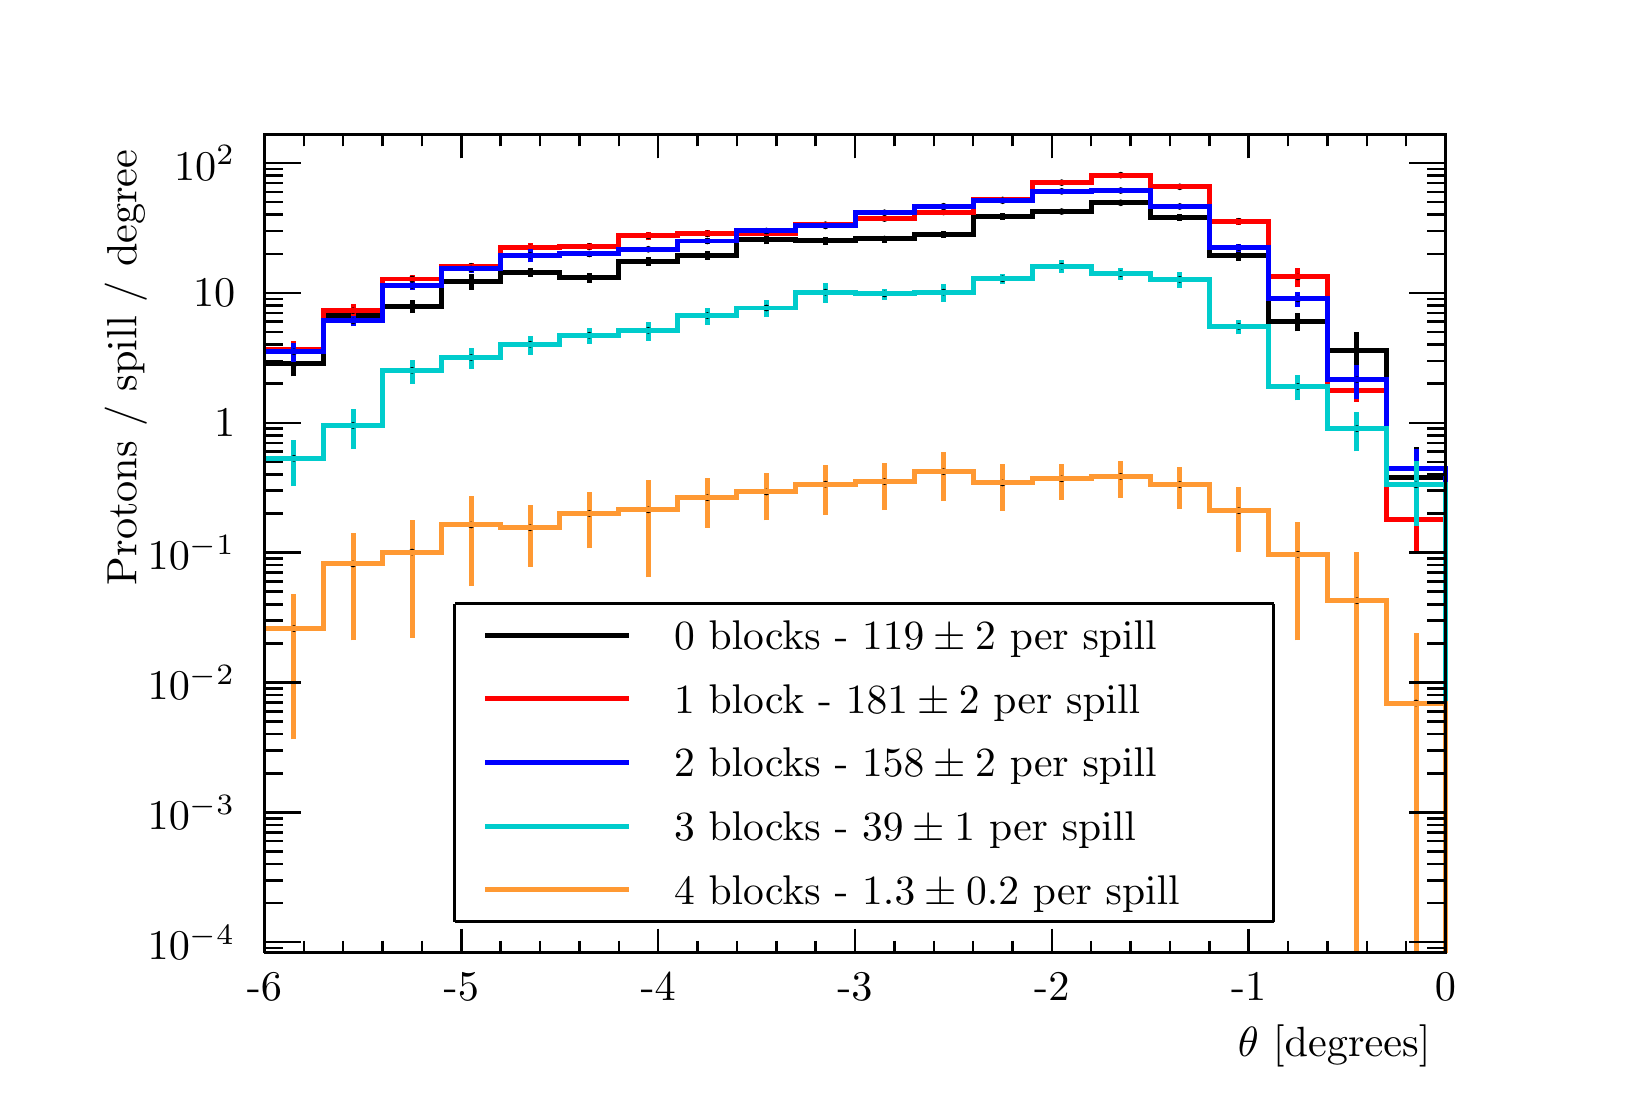
\begin{tikzpicture}
\pgfdeclareplotmark{cross} {
\pgfpathmoveto{\pgfpoint{-0.3\pgfplotmarksize}{\pgfplotmarksize}}
\pgfpathlineto{\pgfpoint{+0.3\pgfplotmarksize}{\pgfplotmarksize}}
\pgfpathlineto{\pgfpoint{+0.3\pgfplotmarksize}{0.3\pgfplotmarksize}}
\pgfpathlineto{\pgfpoint{+1\pgfplotmarksize}{0.3\pgfplotmarksize}}
\pgfpathlineto{\pgfpoint{+1\pgfplotmarksize}{-0.3\pgfplotmarksize}}
\pgfpathlineto{\pgfpoint{+0.3\pgfplotmarksize}{-0.3\pgfplotmarksize}}
\pgfpathlineto{\pgfpoint{+0.3\pgfplotmarksize}{-1.\pgfplotmarksize}}
\pgfpathlineto{\pgfpoint{-0.3\pgfplotmarksize}{-1.\pgfplotmarksize}}
\pgfpathlineto{\pgfpoint{-0.3\pgfplotmarksize}{-0.3\pgfplotmarksize}}
\pgfpathlineto{\pgfpoint{-1.\pgfplotmarksize}{-0.3\pgfplotmarksize}}
\pgfpathlineto{\pgfpoint{-1.\pgfplotmarksize}{0.3\pgfplotmarksize}}
\pgfpathlineto{\pgfpoint{-0.3\pgfplotmarksize}{0.3\pgfplotmarksize}}
\pgfpathclose
\pgfusepathqstroke
}
\pgfdeclareplotmark{cross*} {
\pgfpathmoveto{\pgfpoint{-0.3\pgfplotmarksize}{\pgfplotmarksize}}
\pgfpathlineto{\pgfpoint{+0.3\pgfplotmarksize}{\pgfplotmarksize}}
\pgfpathlineto{\pgfpoint{+0.3\pgfplotmarksize}{0.3\pgfplotmarksize}}
\pgfpathlineto{\pgfpoint{+1\pgfplotmarksize}{0.3\pgfplotmarksize}}
\pgfpathlineto{\pgfpoint{+1\pgfplotmarksize}{-0.3\pgfplotmarksize}}
\pgfpathlineto{\pgfpoint{+0.3\pgfplotmarksize}{-0.3\pgfplotmarksize}}
\pgfpathlineto{\pgfpoint{+0.3\pgfplotmarksize}{-1.\pgfplotmarksize}}
\pgfpathlineto{\pgfpoint{-0.3\pgfplotmarksize}{-1.\pgfplotmarksize}}
\pgfpathlineto{\pgfpoint{-0.3\pgfplotmarksize}{-0.3\pgfplotmarksize}}
\pgfpathlineto{\pgfpoint{-1.\pgfplotmarksize}{-0.3\pgfplotmarksize}}
\pgfpathlineto{\pgfpoint{-1.\pgfplotmarksize}{0.3\pgfplotmarksize}}
\pgfpathlineto{\pgfpoint{-0.3\pgfplotmarksize}{0.3\pgfplotmarksize}}
\pgfpathclose
\pgfusepathqfillstroke
}
\pgfdeclareplotmark{newstar} {
\pgfpathmoveto{\pgfqpoint{0pt}{\pgfplotmarksize}}
\pgfpathlineto{\pgfqpointpolar{44}{0.5\pgfplotmarksize}}
\pgfpathlineto{\pgfqpointpolar{18}{\pgfplotmarksize}}
\pgfpathlineto{\pgfqpointpolar{-20}{0.5\pgfplotmarksize}}
\pgfpathlineto{\pgfqpointpolar{-54}{\pgfplotmarksize}}
\pgfpathlineto{\pgfqpointpolar{-90}{0.5\pgfplotmarksize}}
\pgfpathlineto{\pgfqpointpolar{234}{\pgfplotmarksize}}
\pgfpathlineto{\pgfqpointpolar{198}{0.5\pgfplotmarksize}}
\pgfpathlineto{\pgfqpointpolar{162}{\pgfplotmarksize}}
\pgfpathlineto{\pgfqpointpolar{134}{0.5\pgfplotmarksize}}
\pgfpathclose
\pgfusepathqstroke
}
\pgfdeclareplotmark{newstar*} {
\pgfpathmoveto{\pgfqpoint{0pt}{\pgfplotmarksize}}
\pgfpathlineto{\pgfqpointpolar{44}{0.5\pgfplotmarksize}}
\pgfpathlineto{\pgfqpointpolar{18}{\pgfplotmarksize}}
\pgfpathlineto{\pgfqpointpolar{-20}{0.5\pgfplotmarksize}}
\pgfpathlineto{\pgfqpointpolar{-54}{\pgfplotmarksize}}
\pgfpathlineto{\pgfqpointpolar{-90}{0.5\pgfplotmarksize}}
\pgfpathlineto{\pgfqpointpolar{234}{\pgfplotmarksize}}
\pgfpathlineto{\pgfqpointpolar{198}{0.5\pgfplotmarksize}}
\pgfpathlineto{\pgfqpointpolar{162}{\pgfplotmarksize}}
\pgfpathlineto{\pgfqpointpolar{134}{0.5\pgfplotmarksize}}
\pgfpathclose
\pgfusepathqfillstroke
}
\definecolor{c}{rgb}{1,1,1};
\draw [color=c, fill=c] (0,0) rectangle (20,13.4957);
\draw [color=c, fill=c] (3,1.75444) rectangle (18,12.1461);
\definecolor{c}{rgb}{0,0,0};
\draw [c,line width=0.9] (3,1.75444) -- (3,12.1461) -- (18,12.1461) -- (18,1.75444) -- (3,1.75444);
\definecolor{c}{rgb}{1,1,1};
\draw [color=c, fill=c] (3,1.75444) rectangle (18,12.1461);
\definecolor{c}{rgb}{0,0,0};
\draw [c,line width=0.9] (3,1.75444) -- (3,12.1461) -- (18,12.1461) -- (18,1.75444) -- (3,1.75444);
\draw [c,line width=0.9] (3,1.75444) -- (3.75,1.75444) -- (3.75,1.75444) -- (4.5,1.75444) -- (4.5,1.75444) -- (5.25,1.75444) -- (5.25,1.75444) -- (6,1.75444) -- (6,1.75444) -- (6.75,1.75444) -- (6.75,1.75444) -- (7.5,1.75444) -- (7.5,1.75444) --
 (8.25,1.75444) -- (8.25,1.75444) -- (9,1.75444) -- (9,1.75444) -- (9.75,1.75444) -- (9.75,1.75444) -- (10.5,1.75444) -- (10.5,1.75444) -- (11.25,1.75444) -- (11.25,1.75444) -- (12,1.75444) -- (12,1.75444) -- (12.75,1.75444) -- (12.75,1.75444) --
 (13.5,1.75444) -- (13.5,1.75444) -- (14.25,1.75444) -- (14.25,1.75444) -- (15,1.75444) -- (15,1.75444) -- (15.75,1.75444) -- (15.75,1.75444) -- (16.5,1.75444) -- (16.5,1.75444) -- (17.25,1.75444) -- (17.25,1.75444) -- (18,1.75444) -- (18,1.75444);
\draw [c,line width=0.9] (3,1.75444) -- (18,1.75444);
\draw [c,line width=0.9] (3,2.05809) -- (3,1.75444);
\draw [c,line width=0.9] (3.5,1.90627) -- (3.5,1.75444);
\draw [c,line width=0.9] (4,1.90627) -- (4,1.75444);
\draw [c,line width=0.9] (4.5,1.90627) -- (4.5,1.75444);
\draw [c,line width=0.9] (5,1.90627) -- (5,1.75444);
\draw [c,line width=0.9] (5.5,2.05809) -- (5.5,1.75444);
\draw [c,line width=0.9] (6,1.90627) -- (6,1.75444);
\draw [c,line width=0.9] (6.5,1.90627) -- (6.5,1.75444);
\draw [c,line width=0.9] (7,1.90627) -- (7,1.75444);
\draw [c,line width=0.9] (7.5,1.90627) -- (7.5,1.75444);
\draw [c,line width=0.9] (8,2.05809) -- (8,1.75444);
\draw [c,line width=0.9] (8.5,1.90627) -- (8.5,1.75444);
\draw [c,line width=0.9] (9,1.90627) -- (9,1.75444);
\draw [c,line width=0.9] (9.5,1.90627) -- (9.5,1.75444);
\draw [c,line width=0.9] (10,1.90627) -- (10,1.75444);
\draw [c,line width=0.9] (10.5,2.05809) -- (10.5,1.75444);
\draw [c,line width=0.9] (11,1.90627) -- (11,1.75444);
\draw [c,line width=0.9] (11.5,1.90627) -- (11.5,1.75444);
\draw [c,line width=0.9] (12,1.90627) -- (12,1.75444);
\draw [c,line width=0.9] (12.5,1.90627) -- (12.5,1.75444);
\draw [c,line width=0.9] (13,2.05809) -- (13,1.75444);
\draw [c,line width=0.9] (13.5,1.90627) -- (13.5,1.75444);
\draw [c,line width=0.9] (14,1.90627) -- (14,1.75444);
\draw [c,line width=0.9] (14.5,1.90627) -- (14.5,1.75444);
\draw [c,line width=0.9] (15,1.90627) -- (15,1.75444);
\draw [c,line width=0.9] (15.5,2.05809) -- (15.5,1.75444);
\draw [c,line width=0.9] (16,1.90627) -- (16,1.75444);
\draw [c,line width=0.9] (16.5,1.90627) -- (16.5,1.75444);
\draw [c,line width=0.9] (17,1.90627) -- (17,1.75444);
\draw [c,line width=0.9] (17.5,1.90627) -- (17.5,1.75444);
\draw [c,line width=0.9] (18,2.05809) -- (18,1.75444);
\draw [anchor=base] (3,1.14713) node[scale=1.52731, color=c, rotate=0]{-6};
\draw [anchor=base] (5.5,1.14713) node[scale=1.52731, color=c, rotate=0]{-5};
\draw [anchor=base] (8,1.14713) node[scale=1.52731, color=c, rotate=0]{-4};
\draw [anchor=base] (10.5,1.14713) node[scale=1.52731, color=c, rotate=0]{-3};
\draw [anchor=base] (13,1.14713) node[scale=1.52731, color=c, rotate=0]{-2};
\draw [anchor=base] (15.5,1.14713) node[scale=1.52731, color=c, rotate=0]{-1};
\draw [anchor=base] (18,1.14713) node[scale=1.52731, color=c, rotate=0]{0};
\draw [anchor= east] (18,0.566819) node[scale=1.52731, color=c, rotate=0]{$ \theta$ [degrees]};
\draw [c,line width=0.9] (3,12.1461) -- (18,12.1461);
\draw [c,line width=0.9] (3,11.8425) -- (3,12.1461);
\draw [c,line width=0.9] (3.5,11.9943) -- (3.5,12.1461);
\draw [c,line width=0.9] (4,11.9943) -- (4,12.1461);
\draw [c,line width=0.9] (4.5,11.9943) -- (4.5,12.1461);
\draw [c,line width=0.9] (5,11.9943) -- (5,12.1461);
\draw [c,line width=0.9] (5.5,11.8425) -- (5.5,12.1461);
\draw [c,line width=0.9] (6,11.9943) -- (6,12.1461);
\draw [c,line width=0.9] (6.5,11.9943) -- (6.5,12.1461);
\draw [c,line width=0.9] (7,11.9943) -- (7,12.1461);
\draw [c,line width=0.9] (7.5,11.9943) -- (7.5,12.1461);
\draw [c,line width=0.9] (8,11.8425) -- (8,12.1461);
\draw [c,line width=0.9] (8.5,11.9943) -- (8.5,12.1461);
\draw [c,line width=0.9] (9,11.9943) -- (9,12.1461);
\draw [c,line width=0.9] (9.5,11.9943) -- (9.5,12.1461);
\draw [c,line width=0.9] (10,11.9943) -- (10,12.1461);
\draw [c,line width=0.9] (10.5,11.8425) -- (10.5,12.1461);
\draw [c,line width=0.9] (11,11.9943) -- (11,12.1461);
\draw [c,line width=0.9] (11.5,11.9943) -- (11.5,12.1461);
\draw [c,line width=0.9] (12,11.9943) -- (12,12.1461);
\draw [c,line width=0.9] (12.5,11.9943) -- (12.5,12.1461);
\draw [c,line width=0.9] (13,11.8425) -- (13,12.1461);
\draw [c,line width=0.9] (13.5,11.9943) -- (13.5,12.1461);
\draw [c,line width=0.9] (14,11.9943) -- (14,12.1461);
\draw [c,line width=0.9] (14.5,11.9943) -- (14.5,12.1461);
\draw [c,line width=0.9] (15,11.9943) -- (15,12.1461);
\draw [c,line width=0.9] (15.5,11.8425) -- (15.5,12.1461);
\draw [c,line width=0.9] (16,11.9943) -- (16,12.1461);
\draw [c,line width=0.9] (16.5,11.9943) -- (16.5,12.1461);
\draw [c,line width=0.9] (17,11.9943) -- (17,12.1461);
\draw [c,line width=0.9] (17.5,11.9943) -- (17.5,12.1461);
\draw [c,line width=0.9] (18,11.8425) -- (18,12.1461);
\draw [c,line width=0.9] (3,1.75444) -- (3,12.1461);
\draw [c,line width=0.9] (3.231,1.81225) -- (3,1.81225);
\draw [c,line width=0.9] (3.462,1.88772) -- (3,1.88772);
\draw [anchor= east] (2.82,1.88772) node[scale=1.52731, color=c, rotate=0]{$10^{-4}$};
\draw [c,line width=0.9] (3.231,2.38422) -- (3,2.38422);
\draw [c,line width=0.9] (3.231,2.67466) -- (3,2.67466);
\draw [c,line width=0.9] (3.231,2.88072) -- (3,2.88072);
\draw [c,line width=0.9] (3.231,3.04056) -- (3,3.04056);
\draw [c,line width=0.9] (3.231,3.17116) -- (3,3.17116);
\draw [c,line width=0.9] (3.231,3.28158) -- (3,3.28158);
\draw [c,line width=0.9] (3.231,3.37722) -- (3,3.37722);
\draw [c,line width=0.9] (3.231,3.46159) -- (3,3.46159);
\draw [c,line width=0.9] (3.462,3.53706) -- (3,3.53706);
\draw [anchor= east] (2.82,3.53706) node[scale=1.52731, color=c, rotate=0]{$10^{-3}$};
\draw [c,line width=0.9] (3.231,4.03357) -- (3,4.03357);
\draw [c,line width=0.9] (3.231,4.324) -- (3,4.324);
\draw [c,line width=0.9] (3.231,4.53007) -- (3,4.53007);
\draw [c,line width=0.9] (3.231,4.68991) -- (3,4.68991);
\draw [c,line width=0.9] (3.231,4.8205) -- (3,4.8205);
\draw [c,line width=0.9] (3.231,4.93092) -- (3,4.93092);
\draw [c,line width=0.9] (3.231,5.02657) -- (3,5.02657);
\draw [c,line width=0.9] (3.231,5.11094) -- (3,5.11094);
\draw [c,line width=0.9] (3.462,5.18641) -- (3,5.18641);
\draw [anchor= east] (2.82,5.18641) node[scale=1.52731, color=c, rotate=0]{$10^{-2}$};
\draw [c,line width=0.9] (3.231,5.68291) -- (3,5.68291);
\draw [c,line width=0.9] (3.231,5.97335) -- (3,5.97335);
\draw [c,line width=0.9] (3.231,6.17941) -- (3,6.17941);
\draw [c,line width=0.9] (3.231,6.33925) -- (3,6.33925);
\draw [c,line width=0.9] (3.231,6.46985) -- (3,6.46985);
\draw [c,line width=0.9] (3.231,6.58027) -- (3,6.58027);
\draw [c,line width=0.9] (3.231,6.67592) -- (3,6.67592);
\draw [c,line width=0.9] (3.231,6.76028) -- (3,6.76028);
\draw [c,line width=0.9] (3.462,6.83575) -- (3,6.83575);
\draw [anchor= east] (2.82,6.83575) node[scale=1.52731, color=c, rotate=0]{$10^{-1}$};
\draw [c,line width=0.9] (3.231,7.33226) -- (3,7.33226);
\draw [c,line width=0.9] (3.231,7.62269) -- (3,7.62269);
\draw [c,line width=0.9] (3.231,7.82876) -- (3,7.82876);
\draw [c,line width=0.9] (3.231,7.9886) -- (3,7.9886);
\draw [c,line width=0.9] (3.231,8.11919) -- (3,8.11919);
\draw [c,line width=0.9] (3.231,8.22961) -- (3,8.22961);
\draw [c,line width=0.9] (3.231,8.32526) -- (3,8.32526);
\draw [c,line width=0.9] (3.231,8.40963) -- (3,8.40963);
\draw [c,line width=0.9] (3.462,8.4851) -- (3,8.4851);
\draw [anchor= east] (2.82,8.4851) node[scale=1.52731, color=c, rotate=0]{1};
\draw [c,line width=0.9] (3.231,8.9816) -- (3,8.9816);
\draw [c,line width=0.9] (3.231,9.27204) -- (3,9.27204);
\draw [c,line width=0.9] (3.231,9.4781) -- (3,9.4781);
\draw [c,line width=0.9] (3.231,9.63794) -- (3,9.63794);
\draw [c,line width=0.9] (3.231,9.76854) -- (3,9.76854);
\draw [c,line width=0.9] (3.231,9.87896) -- (3,9.87896);
\draw [c,line width=0.9] (3.231,9.97461) -- (3,9.97461);
\draw [c,line width=0.9] (3.231,10.059) -- (3,10.059);
\draw [c,line width=0.9] (3.462,10.1344) -- (3,10.1344);
\draw [anchor= east] (2.82,10.1344) node[scale=1.52731, color=c, rotate=0]{10};
\draw [c,line width=0.9] (3.231,10.6309) -- (3,10.6309);
\draw [c,line width=0.9] (3.231,10.9214) -- (3,10.9214);
\draw [c,line width=0.9] (3.231,11.1274) -- (3,11.1274);
\draw [c,line width=0.9] (3.231,11.2873) -- (3,11.2873);
\draw [c,line width=0.9] (3.231,11.4179) -- (3,11.4179);
\draw [c,line width=0.9] (3.231,11.5283) -- (3,11.5283);
\draw [c,line width=0.9] (3.231,11.624) -- (3,11.624);
\draw [c,line width=0.9] (3.231,11.7083) -- (3,11.7083);
\draw [c,line width=0.9] (3.462,11.7838) -- (3,11.7838);
\draw [anchor= east] (2.82,11.7838) node[scale=1.52731, color=c, rotate=0]{$10^{2}$};
\draw [anchor= east] (1.24,12.1461) node[scale=1.52731, color=c, rotate=90]{ Protons / spill / degree};
\draw [c,line width=0.9] (18,1.75444) -- (18,12.1461);
\draw [c,line width=0.9] (17.769,1.81225) -- (18,1.81225);
\draw [c,line width=0.9] (17.538,1.88772) -- (18,1.88772);
\draw [c,line width=0.9] (17.769,2.38422) -- (18,2.38422);
\draw [c,line width=0.9] (17.769,2.67466) -- (18,2.67466);
\draw [c,line width=0.9] (17.769,2.88072) -- (18,2.88072);
\draw [c,line width=0.9] (17.769,3.04056) -- (18,3.04056);
\draw [c,line width=0.9] (17.769,3.17116) -- (18,3.17116);
\draw [c,line width=0.9] (17.769,3.28158) -- (18,3.28158);
\draw [c,line width=0.9] (17.769,3.37722) -- (18,3.37722);
\draw [c,line width=0.9] (17.769,3.46159) -- (18,3.46159);
\draw [c,line width=0.9] (17.538,3.53706) -- (18,3.53706);
\draw [c,line width=0.9] (17.769,4.03357) -- (18,4.03357);
\draw [c,line width=0.9] (17.769,4.324) -- (18,4.324);
\draw [c,line width=0.9] (17.769,4.53007) -- (18,4.53007);
\draw [c,line width=0.9] (17.769,4.68991) -- (18,4.68991);
\draw [c,line width=0.9] (17.769,4.8205) -- (18,4.8205);
\draw [c,line width=0.9] (17.769,4.93092) -- (18,4.93092);
\draw [c,line width=0.9] (17.769,5.02657) -- (18,5.02657);
\draw [c,line width=0.9] (17.769,5.11094) -- (18,5.11094);
\draw [c,line width=0.9] (17.538,5.18641) -- (18,5.18641);
\draw [c,line width=0.9] (17.769,5.68291) -- (18,5.68291);
\draw [c,line width=0.9] (17.769,5.97335) -- (18,5.97335);
\draw [c,line width=0.9] (17.769,6.17941) -- (18,6.17941);
\draw [c,line width=0.9] (17.769,6.33925) -- (18,6.33925);
\draw [c,line width=0.9] (17.769,6.46985) -- (18,6.46985);
\draw [c,line width=0.9] (17.769,6.58027) -- (18,6.58027);
\draw [c,line width=0.9] (17.769,6.67592) -- (18,6.67592);
\draw [c,line width=0.9] (17.769,6.76028) -- (18,6.76028);
\draw [c,line width=0.9] (17.538,6.83575) -- (18,6.83575);
\draw [c,line width=0.9] (17.769,7.33226) -- (18,7.33226);
\draw [c,line width=0.9] (17.769,7.62269) -- (18,7.62269);
\draw [c,line width=0.9] (17.769,7.82876) -- (18,7.82876);
\draw [c,line width=0.9] (17.769,7.9886) -- (18,7.9886);
\draw [c,line width=0.9] (17.769,8.11919) -- (18,8.11919);
\draw [c,line width=0.9] (17.769,8.22961) -- (18,8.22961);
\draw [c,line width=0.9] (17.769,8.32526) -- (18,8.32526);
\draw [c,line width=0.9] (17.769,8.40963) -- (18,8.40963);
\draw [c,line width=0.9] (17.538,8.4851) -- (18,8.4851);
\draw [c,line width=0.9] (17.769,8.9816) -- (18,8.9816);
\draw [c,line width=0.9] (17.769,9.27204) -- (18,9.27204);
\draw [c,line width=0.9] (17.769,9.4781) -- (18,9.4781);
\draw [c,line width=0.9] (17.769,9.63794) -- (18,9.63794);
\draw [c,line width=0.9] (17.769,9.76854) -- (18,9.76854);
\draw [c,line width=0.9] (17.769,9.87896) -- (18,9.87896);
\draw [c,line width=0.9] (17.769,9.97461) -- (18,9.97461);
\draw [c,line width=0.9] (17.769,10.059) -- (18,10.059);
\draw [c,line width=0.9] (17.538,10.1344) -- (18,10.1344);
\draw [c,line width=0.9] (17.769,10.6309) -- (18,10.6309);
\draw [c,line width=0.9] (17.769,10.9214) -- (18,10.9214);
\draw [c,line width=0.9] (17.769,11.1274) -- (18,11.1274);
\draw [c,line width=0.9] (17.769,11.2873) -- (18,11.2873);
\draw [c,line width=0.9] (17.769,11.4179) -- (18,11.4179);
\draw [c,line width=0.9] (17.769,11.5283) -- (18,11.5283);
\draw [c,line width=0.9] (17.769,11.624) -- (18,11.624);
\draw [c,line width=0.9] (17.769,11.7083) -- (18,11.7083);
\draw [c,line width=0.9] (17.538,11.7838) -- (18,11.7838);
\draw [c,line width=1.8] (3.375,9.07502) -- (3.375,9.23213);
\draw [c,line width=1.8] (3.375,9.23213) -- (3.375,9.3609);
\foreach \P in {(3.375,9.23213)}{\draw[mark options={color=c,fill=c},mark size=2.402402pt,mark=*,mark size=1pt] plot coordinates {\P};}
\draw [c,line width=1.8] (4.125,9.75966) -- (4.125,9.85284);
\draw [c,line width=1.8] (4.125,9.85284) -- (4.125,9.93528);
\foreach \P in {(4.125,9.85284)}{\draw[mark options={color=c,fill=c},mark size=2.402402pt,mark=*,mark size=1pt] plot coordinates {\P};}
\draw [c,line width=1.8] (4.875,9.87682) -- (4.875,9.96395);
\draw [c,line width=1.8] (4.875,9.96395) -- (4.875,10.0416);
\foreach \P in {(4.875,9.96395)}{\draw[mark options={color=c,fill=c},mark size=2.402402pt,mark=*,mark size=1pt] plot coordinates {\P};}
\draw [c,line width=1.8] (5.625,10.1726) -- (5.625,10.2788);
\draw [c,line width=1.8] (5.625,10.2788) -- (5.625,10.3713);
\foreach \P in {(5.625,10.2788)}{\draw[mark options={color=c,fill=c},mark size=2.402402pt,mark=*,mark size=1pt] plot coordinates {\P};}
\draw [c,line width=1.8] (6.375,10.3373) -- (6.375,10.3992);
\draw [c,line width=1.8] (6.375,10.3992) -- (6.375,10.4562);
\foreach \P in {(6.375,10.3992)}{\draw[mark options={color=c,fill=c},mark size=2.402402pt,mark=*,mark size=1pt] plot coordinates {\P};}
\draw [c,line width=1.8] (7.125,10.2656) -- (7.125,10.3311);
\draw [c,line width=1.8] (7.125,10.3311) -- (7.125,10.3911);
\foreach \P in {(7.125,10.3311)}{\draw[mark options={color=c,fill=c},mark size=2.402402pt,mark=*,mark size=1pt] plot coordinates {\P};}
\draw [c,line width=1.8] (7.875,10.4763) -- (7.875,10.5374);
\draw [c,line width=1.8] (7.875,10.5374) -- (7.875,10.5938);
\foreach \P in {(7.875,10.5374)}{\draw[mark options={color=c,fill=c},mark size=2.402402pt,mark=*,mark size=1pt] plot coordinates {\P};}
\draw [c,line width=1.8] (8.625,10.5567) -- (8.625,10.6116);
\draw [c,line width=1.8] (8.625,10.6116) -- (8.625,10.6626);
\foreach \P in {(8.625,10.6116)}{\draw[mark options={color=c,fill=c},mark size=2.402402pt,mark=*,mark size=1pt] plot coordinates {\P};}
\draw [c,line width=1.8] (9.375,10.7503) -- (9.375,10.8141);
\draw [c,line width=1.8] (9.375,10.8141) -- (9.375,10.8726);
\foreach \P in {(9.375,10.8141)}{\draw[mark options={color=c,fill=c},mark size=2.402402pt,mark=*,mark size=1pt] plot coordinates {\P};}
\draw [c,line width=1.8] (10.125,10.7469) -- (10.125,10.7963);
\draw [c,line width=1.8] (10.125,10.7963) -- (10.125,10.8425);
\foreach \P in {(10.125,10.7963)}{\draw[mark options={color=c,fill=c},mark size=2.402402pt,mark=*,mark size=1pt] plot coordinates {\P};}
\draw [c,line width=1.8] (10.875,10.7735) -- (10.875,10.8191);
\draw [c,line width=1.8] (10.875,10.8191) -- (10.875,10.8619);
\foreach \P in {(10.875,10.8191)}{\draw[mark options={color=c,fill=c},mark size=2.402402pt,mark=*,mark size=1pt] plot coordinates {\P};}
\draw [c,line width=1.8] (11.625,10.8337) -- (11.625,10.877);
\draw [c,line width=1.8] (11.625,10.877) -- (11.625,10.9179);
\foreach \P in {(11.625,10.877)}{\draw[mark options={color=c,fill=c},mark size=2.402402pt,mark=*,mark size=1pt] plot coordinates {\P};}
\draw [c,line width=1.8] (12.375,11.0626) -- (12.375,11.1046);
\draw [c,line width=1.8] (12.375,11.1046) -- (12.375,11.1444);
\foreach \P in {(12.375,11.1046)}{\draw[mark options={color=c,fill=c},mark size=2.402402pt,mark=*,mark size=1pt] plot coordinates {\P};}
\draw [c,line width=1.8] (13.125,11.1339) -- (13.125,11.1675);
\draw [c,line width=1.8] (13.125,11.1675) -- (13.125,11.1996);
\foreach \P in {(13.125,11.1675)}{\draw[mark options={color=c,fill=c},mark size=2.402402pt,mark=*,mark size=1pt] plot coordinates {\P};}
\draw [c,line width=1.8] (13.875,11.2461) -- (13.875,11.2785);
\draw [c,line width=1.8] (13.875,11.2785) -- (13.875,11.3096);
\foreach \P in {(13.875,11.2785)}{\draw[mark options={color=c,fill=c},mark size=2.402402pt,mark=*,mark size=1pt] plot coordinates {\P};}
\draw [c,line width=1.8] (14.625,11.0483) -- (14.625,11.0912);
\draw [c,line width=1.8] (14.625,11.0912) -- (14.625,11.1317);
\foreach \P in {(14.625,11.0912)}{\draw[mark options={color=c,fill=c},mark size=2.402402pt,mark=*,mark size=1pt] plot coordinates {\P};}
\draw [c,line width=1.8] (15.375,10.5449) -- (15.375,10.608);
\draw [c,line width=1.8] (15.375,10.608) -- (15.375,10.666);
\foreach \P in {(15.375,10.608)}{\draw[mark options={color=c,fill=c},mark size=2.402402pt,mark=*,mark size=1pt] plot coordinates {\P};}
\draw [c,line width=1.8] (16.125,9.64718) -- (16.125,9.77334);
\draw [c,line width=1.8] (16.125,9.77334) -- (16.125,9.88057);
\foreach \P in {(16.125,9.77334)}{\draw[mark options={color=c,fill=c},mark size=2.402402pt,mark=*,mark size=1pt] plot coordinates {\P};}
\draw [c,line width=1.8] (16.875,9.05435) -- (16.875,9.40081);
\draw [c,line width=1.8] (16.875,9.40081) -- (16.875,9.63333);
\foreach \P in {(16.875,9.40081)}{\draw[mark options={color=c,fill=c},mark size=2.402402pt,mark=*,mark size=1pt] plot coordinates {\P};}
\draw [c,line width=1.8] (17.625,6.89102) -- (17.625,7.79455);
\draw [c,line width=1.8] (17.625,7.79455) -- (17.625,8.18165);
\foreach \P in {(17.625,7.79455)}{\draw[mark options={color=c,fill=c},mark size=2.402402pt,mark=*,mark size=1pt] plot coordinates {\P};}
\draw [c,line width=1.8] (3,9.23213) -- (3.75,9.23213) -- (3.75,9.85284) -- (4.5,9.85284) -- (4.5,9.96395) -- (5.25,9.96395) -- (5.25,10.2788) -- (6,10.2788) -- (6,10.3992) -- (6.75,10.3992) -- (6.75,10.3311) -- (7.5,10.3311) -- (7.5,10.5374) --
 (8.25,10.5374) -- (8.25,10.6116) -- (9,10.6116) -- (9,10.8141) -- (9.75,10.8141) -- (9.75,10.7963) -- (10.5,10.7963) -- (10.5,10.8191) -- (11.25,10.8191) -- (11.25,10.877) -- (12,10.877) -- (12,11.1046) -- (12.75,11.1046) -- (12.75,11.1675) --
 (13.5,11.1675) -- (13.5,11.2785) -- (14.25,11.2785) -- (14.25,11.0912) -- (15,11.0912) -- (15,10.608) -- (15.75,10.608) -- (15.75,9.77334) -- (16.5,9.77334) -- (16.5,9.40081) -- (17.25,9.40081) -- (17.25,7.79455) -- (18,7.79455) -- (18,1.75444);
\definecolor{c}{rgb}{1,0,0};
\draw [c,line width=1.8] (3.375,9.29318) -- (3.375,9.41497);
\draw [c,line width=1.8] (3.375,9.41497) -- (3.375,9.51902);
\definecolor{c}{rgb}{0,0,0};
\foreach \P in {(3.375,9.41497)}{\draw[mark options={color=c,fill=c},mark size=2.402402pt,mark=*,mark size=1pt] plot coordinates {\P};}
\definecolor{c}{rgb}{1,0,0};
\draw [c,line width=1.8] (4.125,9.80481) -- (4.125,9.90725);
\draw [c,line width=1.8] (4.125,9.90725) -- (4.125,9.99686);
\definecolor{c}{rgb}{0,0,0};
\foreach \P in {(4.125,9.90725)}{\draw[mark options={color=c,fill=c},mark size=2.402402pt,mark=*,mark size=1pt] plot coordinates {\P};}
\definecolor{c}{rgb}{1,0,0};
\draw [c,line width=1.8] (4.875,10.249) -- (4.875,10.3108);
\draw [c,line width=1.8] (4.875,10.3108) -- (4.875,10.3677);
\definecolor{c}{rgb}{0,0,0};
\foreach \P in {(4.875,10.3108)}{\draw[mark options={color=c,fill=c},mark size=2.402402pt,mark=*,mark size=1pt] plot coordinates {\P};}
\definecolor{c}{rgb}{1,0,0};
\draw [c,line width=1.8] (5.625,10.4221) -- (5.625,10.4723);
\draw [c,line width=1.8] (5.625,10.4723) -- (5.625,10.5191);
\definecolor{c}{rgb}{0,0,0};
\foreach \P in {(5.625,10.4723)}{\draw[mark options={color=c,fill=c},mark size=2.402402pt,mark=*,mark size=1pt] plot coordinates {\P};}
\definecolor{c}{rgb}{1,0,0};
\draw [c,line width=1.8] (6.375,10.6326) -- (6.375,10.7055);
\draw [c,line width=1.8] (6.375,10.7055) -- (6.375,10.7716);
\definecolor{c}{rgb}{0,0,0};
\foreach \P in {(6.375,10.7055)}{\draw[mark options={color=c,fill=c},mark size=2.402402pt,mark=*,mark size=1pt] plot coordinates {\P};}
\definecolor{c}{rgb}{1,0,0};
\draw [c,line width=1.8] (7.125,10.6743) -- (7.125,10.7239);
\draw [c,line width=1.8] (7.125,10.7239) -- (7.125,10.7702);
\definecolor{c}{rgb}{0,0,0};
\foreach \P in {(7.125,10.7239)}{\draw[mark options={color=c,fill=c},mark size=2.402402pt,mark=*,mark size=1pt] plot coordinates {\P};}
\definecolor{c}{rgb}{1,0,0};
\draw [c,line width=1.8] (7.875,10.8026) -- (7.875,10.8576);
\draw [c,line width=1.8] (7.875,10.8576) -- (7.875,10.9087);
\definecolor{c}{rgb}{0,0,0};
\foreach \P in {(7.875,10.8576)}{\draw[mark options={color=c,fill=c},mark size=2.402402pt,mark=*,mark size=1pt] plot coordinates {\P};}
\definecolor{c}{rgb}{1,0,0};
\draw [c,line width=1.8] (8.625,10.8427) -- (8.625,10.8862);
\draw [c,line width=1.8] (8.625,10.8862) -- (8.625,10.9272);
\definecolor{c}{rgb}{0,0,0};
\foreach \P in {(8.625,10.8862)}{\draw[mark options={color=c,fill=c},mark size=2.402402pt,mark=*,mark size=1pt] plot coordinates {\P};}
\definecolor{c}{rgb}{1,0,0};
\draw [c,line width=1.8] (9.375,10.8581) -- (9.375,10.8913);
\draw [c,line width=1.8] (9.375,10.8913) -- (9.375,10.923);
\definecolor{c}{rgb}{0,0,0};
\foreach \P in {(9.375,10.8913)}{\draw[mark options={color=c,fill=c},mark size=2.402402pt,mark=*,mark size=1pt] plot coordinates {\P};}
\definecolor{c}{rgb}{1,0,0};
\draw [c,line width=1.8] (10.125,10.9658) -- (10.125,11.0008);
\draw [c,line width=1.8] (10.125,11.0008) -- (10.125,11.0341);
\definecolor{c}{rgb}{0,0,0};
\foreach \P in {(10.125,11.0008)}{\draw[mark options={color=c,fill=c},mark size=2.402402pt,mark=*,mark size=1pt] plot coordinates {\P};}
\definecolor{c}{rgb}{1,0,0};
\draw [c,line width=1.8] (10.875,11.0434) -- (10.875,11.0777);
\draw [c,line width=1.8] (10.875,11.0777) -- (10.875,11.1105);
\definecolor{c}{rgb}{0,0,0};
\foreach \P in {(10.875,11.0777)}{\draw[mark options={color=c,fill=c},mark size=2.402402pt,mark=*,mark size=1pt] plot coordinates {\P};}
\definecolor{c}{rgb}{1,0,0};
\draw [c,line width=1.8] (11.625,11.1321) -- (11.625,11.1615);
\draw [c,line width=1.8] (11.625,11.1615) -- (11.625,11.1898);
\definecolor{c}{rgb}{0,0,0};
\foreach \P in {(11.625,11.1615)}{\draw[mark options={color=c,fill=c},mark size=2.402402pt,mark=*,mark size=1pt] plot coordinates {\P};}
\definecolor{c}{rgb}{1,0,0};
\draw [c,line width=1.8] (12.375,11.2866) -- (12.375,11.3151);
\draw [c,line width=1.8] (12.375,11.3151) -- (12.375,11.3425);
\definecolor{c}{rgb}{0,0,0};
\foreach \P in {(12.375,11.3151)}{\draw[mark options={color=c,fill=c},mark size=2.402402pt,mark=*,mark size=1pt] plot coordinates {\P};}
\definecolor{c}{rgb}{1,0,0};
\draw [c,line width=1.8] (13.125,11.5124) -- (13.125,11.5342);
\draw [c,line width=1.8] (13.125,11.5342) -- (13.125,11.5554);
\definecolor{c}{rgb}{0,0,0};
\foreach \P in {(13.125,11.5342)}{\draw[mark options={color=c,fill=c},mark size=2.402402pt,mark=*,mark size=1pt] plot coordinates {\P};}
\definecolor{c}{rgb}{1,0,0};
\draw [c,line width=1.8] (13.875,11.6021) -- (13.875,11.6298);
\draw [c,line width=1.8] (13.875,11.6298) -- (13.875,11.6565);
\definecolor{c}{rgb}{0,0,0};
\foreach \P in {(13.875,11.6298)}{\draw[mark options={color=c,fill=c},mark size=2.402402pt,mark=*,mark size=1pt] plot coordinates {\P};}
\definecolor{c}{rgb}{1,0,0};
\draw [c,line width=1.8] (14.625,11.4519) -- (14.625,11.4816);
\draw [c,line width=1.8] (14.625,11.4816) -- (14.625,11.51);
\definecolor{c}{rgb}{0,0,0};
\foreach \P in {(14.625,11.4816)}{\draw[mark options={color=c,fill=c},mark size=2.402402pt,mark=*,mark size=1pt] plot coordinates {\P};}
\definecolor{c}{rgb}{1,0,0};
\draw [c,line width=1.8] (15.375,10.9998) -- (15.375,11.0445);
\draw [c,line width=1.8] (15.375,11.0445) -- (15.375,11.0866);
\definecolor{c}{rgb}{0,0,0};
\foreach \P in {(15.375,11.0445)}{\draw[mark options={color=c,fill=c},mark size=2.402402pt,mark=*,mark size=1pt] plot coordinates {\P};}
\definecolor{c}{rgb}{1,0,0};
\draw [c,line width=1.8] (16.125,10.2048) -- (16.125,10.3367);
\draw [c,line width=1.8] (16.125,10.3367) -- (16.125,10.4481);
\definecolor{c}{rgb}{0,0,0};
\foreach \P in {(16.125,10.3367)}{\draw[mark options={color=c,fill=c},mark size=2.402402pt,mark=*,mark size=1pt] plot coordinates {\P};}
\definecolor{c}{rgb}{1,0,0};
\draw [c,line width=1.8] (16.875,8.75069) -- (16.875,8.89064);
\draw [c,line width=1.8] (16.875,8.89064) -- (16.875,9.00767);
\definecolor{c}{rgb}{0,0,0};
\foreach \P in {(16.875,8.89064)}{\draw[mark options={color=c,fill=c},mark size=2.402402pt,mark=*,mark size=1pt] plot coordinates {\P};}
\definecolor{c}{rgb}{1,0,0};
\draw [c,line width=1.8] (17.625,6.83079) -- (17.625,7.25361);
\draw [c,line width=1.8] (17.625,7.25361) -- (17.625,7.51769);
\definecolor{c}{rgb}{0,0,0};
\foreach \P in {(17.625,7.25361)}{\draw[mark options={color=c,fill=c},mark size=2.402402pt,mark=*,mark size=1pt] plot coordinates {\P};}
\definecolor{c}{rgb}{1,0,0};
\draw [c,line width=1.8] (3,9.41497) -- (3.75,9.41497) -- (3.75,9.90725) -- (4.5,9.90725) -- (4.5,10.3108) -- (5.25,10.3108) -- (5.25,10.4723) -- (6,10.4723) -- (6,10.7055) -- (6.75,10.7055) -- (6.75,10.7239) -- (7.5,10.7239) -- (7.5,10.8576) --
 (8.25,10.8576) -- (8.25,10.8862) -- (9,10.8862) -- (9,10.8913) -- (9.75,10.8913) -- (9.75,11.0008) -- (10.5,11.0008) -- (10.5,11.0777) -- (11.25,11.0777) -- (11.25,11.1615) -- (12,11.1615) -- (12,11.3151) -- (12.75,11.3151) -- (12.75,11.5342) --
 (13.5,11.5342) -- (13.5,11.6298) -- (14.25,11.6298) -- (14.25,11.4816) -- (15,11.4816) -- (15,11.0445) -- (15.75,11.0445) -- (15.75,10.3367) -- (16.5,10.3367) -- (16.5,8.89064) -- (17.25,8.89064) -- (17.25,7.25361) -- (18,7.25361) -- (18,1.75444);
\definecolor{c}{rgb}{0,0,1};
\draw [c,line width=1.8] (3.375,9.26219) -- (3.375,9.38668);
\draw [c,line width=1.8] (3.375,9.38668) -- (3.375,9.4927);
\definecolor{c}{rgb}{0,0,0};
\foreach \P in {(3.375,9.38668)}{\draw[mark options={color=c,fill=c},mark size=2.402402pt,mark=*,mark size=1pt] plot coordinates {\P};}
\definecolor{c}{rgb}{0,0,1};
\draw [c,line width=1.8] (4.125,9.70904) -- (4.125,9.77916);
\draw [c,line width=1.8] (4.125,9.77916) -- (4.125,9.84303);
\definecolor{c}{rgb}{0,0,0};
\foreach \P in {(4.125,9.77916)}{\draw[mark options={color=c,fill=c},mark size=2.402402pt,mark=*,mark size=1pt] plot coordinates {\P};}
\definecolor{c}{rgb}{0,0,1};
\draw [c,line width=1.8] (4.875,10.1747) -- (4.875,10.2284);
\draw [c,line width=1.8] (4.875,10.2284) -- (4.875,10.2784);
\definecolor{c}{rgb}{0,0,0};
\foreach \P in {(4.875,10.2284)}{\draw[mark options={color=c,fill=c},mark size=2.402402pt,mark=*,mark size=1pt] plot coordinates {\P};}
\definecolor{c}{rgb}{0,0,1};
\draw [c,line width=1.8] (5.625,10.3923) -- (5.625,10.4383);
\draw [c,line width=1.8] (5.625,10.4383) -- (5.625,10.4816);
\definecolor{c}{rgb}{0,0,0};
\foreach \P in {(5.625,10.4383)}{\draw[mark options={color=c,fill=c},mark size=2.402402pt,mark=*,mark size=1pt] plot coordinates {\P};}
\definecolor{c}{rgb}{0,0,1};
\draw [c,line width=1.8] (6.375,10.5222) -- (6.375,10.6123);
\draw [c,line width=1.8] (6.375,10.6123) -- (6.375,10.6922);
\definecolor{c}{rgb}{0,0,0};
\foreach \P in {(6.375,10.6123)}{\draw[mark options={color=c,fill=c},mark size=2.402402pt,mark=*,mark size=1pt] plot coordinates {\P};}
\definecolor{c}{rgb}{0,0,1};
\draw [c,line width=1.8] (7.125,10.5909) -- (7.125,10.629);
\draw [c,line width=1.8] (7.125,10.629) -- (7.125,10.6652);
\definecolor{c}{rgb}{0,0,0};
\foreach \P in {(7.125,10.629)}{\draw[mark options={color=c,fill=c},mark size=2.402402pt,mark=*,mark size=1pt] plot coordinates {\P};}
\definecolor{c}{rgb}{0,0,1};
\draw [c,line width=1.8] (7.875,10.6551) -- (7.875,10.6884);
\draw [c,line width=1.8] (7.875,10.6884) -- (7.875,10.7202);
\definecolor{c}{rgb}{0,0,0};
\foreach \P in {(7.875,10.6884)}{\draw[mark options={color=c,fill=c},mark size=2.402402pt,mark=*,mark size=1pt] plot coordinates {\P};}
\definecolor{c}{rgb}{0,0,1};
\draw [c,line width=1.8] (8.625,10.76) -- (8.625,10.7933);
\draw [c,line width=1.8] (8.625,10.7933) -- (8.625,10.8251);
\definecolor{c}{rgb}{0,0,0};
\foreach \P in {(8.625,10.7933)}{\draw[mark options={color=c,fill=c},mark size=2.402402pt,mark=*,mark size=1pt] plot coordinates {\P};}
\definecolor{c}{rgb}{0,0,1};
\draw [c,line width=1.8] (9.375,10.888) -- (9.375,10.9207);
\draw [c,line width=1.8] (9.375,10.9207) -- (9.375,10.952);
\definecolor{c}{rgb}{0,0,0};
\foreach \P in {(9.375,10.9207)}{\draw[mark options={color=c,fill=c},mark size=2.402402pt,mark=*,mark size=1pt] plot coordinates {\P};}
\definecolor{c}{rgb}{0,0,1};
\draw [c,line width=1.8] (10.125,10.9536) -- (10.125,10.985);
\draw [c,line width=1.8] (10.125,10.985) -- (10.125,11.015);
\definecolor{c}{rgb}{0,0,0};
\foreach \P in {(10.125,10.985)}{\draw[mark options={color=c,fill=c},mark size=2.402402pt,mark=*,mark size=1pt] plot coordinates {\P};}
\definecolor{c}{rgb}{0,0,1};
\draw [c,line width=1.8] (10.875,11.1223) -- (10.875,11.1525);
\draw [c,line width=1.8] (10.875,11.1525) -- (10.875,11.1815);
\definecolor{c}{rgb}{0,0,0};
\foreach \P in {(10.875,11.1525)}{\draw[mark options={color=c,fill=c},mark size=2.402402pt,mark=*,mark size=1pt] plot coordinates {\P};}
\definecolor{c}{rgb}{0,0,1};
\draw [c,line width=1.8] (11.625,11.2075) -- (11.625,11.2349);
\draw [c,line width=1.8] (11.625,11.2349) -- (11.625,11.2612);
\definecolor{c}{rgb}{0,0,0};
\foreach \P in {(11.625,11.2349)}{\draw[mark options={color=c,fill=c},mark size=2.402402pt,mark=*,mark size=1pt] plot coordinates {\P};}
\definecolor{c}{rgb}{0,0,1};
\draw [c,line width=1.8] (12.375,11.2803) -- (12.375,11.3051);
\draw [c,line width=1.8] (12.375,11.3051) -- (12.375,11.329);
\definecolor{c}{rgb}{0,0,0};
\foreach \P in {(12.375,11.3051)}{\draw[mark options={color=c,fill=c},mark size=2.402402pt,mark=*,mark size=1pt] plot coordinates {\P};}
\definecolor{c}{rgb}{0,0,1};
\draw [c,line width=1.8] (13.125,11.4016) -- (13.125,11.4237);
\draw [c,line width=1.8] (13.125,11.4237) -- (13.125,11.4451);
\definecolor{c}{rgb}{0,0,0};
\foreach \P in {(13.125,11.4237)}{\draw[mark options={color=c,fill=c},mark size=2.402402pt,mark=*,mark size=1pt] plot coordinates {\P};}
\definecolor{c}{rgb}{0,0,1};
\draw [c,line width=1.8] (13.875,11.4097) -- (13.875,11.4344);
\draw [c,line width=1.8] (13.875,11.4344) -- (13.875,11.4582);
\definecolor{c}{rgb}{0,0,0};
\foreach \P in {(13.875,11.4344)}{\draw[mark options={color=c,fill=c},mark size=2.402402pt,mark=*,mark size=1pt] plot coordinates {\P};}
\definecolor{c}{rgb}{0,0,1};
\draw [c,line width=1.8] (14.625,11.2014) -- (14.625,11.2318);
\draw [c,line width=1.8] (14.625,11.2318) -- (14.625,11.2609);
\definecolor{c}{rgb}{0,0,0};
\foreach \P in {(14.625,11.2318)}{\draw[mark options={color=c,fill=c},mark size=2.402402pt,mark=*,mark size=1pt] plot coordinates {\P};}
\definecolor{c}{rgb}{0,0,1};
\draw [c,line width=1.8] (15.375,10.6577) -- (15.375,10.7085);
\draw [c,line width=1.8] (15.375,10.7085) -- (15.375,10.756);
\definecolor{c}{rgb}{0,0,0};
\foreach \P in {(15.375,10.7085)}{\draw[mark options={color=c,fill=c},mark size=2.402402pt,mark=*,mark size=1pt] plot coordinates {\P};}
\definecolor{c}{rgb}{0,0,1};
\draw [c,line width=1.8] (16.125,9.9559) -- (16.125,10.0573);
\draw [c,line width=1.8] (16.125,10.0573) -- (16.125,10.1462);
\definecolor{c}{rgb}{0,0,0};
\foreach \P in {(16.125,10.0573)}{\draw[mark options={color=c,fill=c},mark size=2.402402pt,mark=*,mark size=1pt] plot coordinates {\P};}
\definecolor{c}{rgb}{0,0,1};
\draw [c,line width=1.8] (16.875,8.7896) -- (16.875,9.03343);
\draw [c,line width=1.8] (16.875,9.03343) -- (16.875,9.21501);
\definecolor{c}{rgb}{0,0,0};
\foreach \P in {(16.875,9.03343)}{\draw[mark options={color=c,fill=c},mark size=2.402402pt,mark=*,mark size=1pt] plot coordinates {\P};}
\definecolor{c}{rgb}{0,0,1};
\draw [c,line width=1.8] (17.625,7.50684) -- (17.625,7.89908);
\draw [c,line width=1.8] (17.625,7.89908) -- (17.625,8.15109);
\definecolor{c}{rgb}{0,0,0};
\foreach \P in {(17.625,7.89908)}{\draw[mark options={color=c,fill=c},mark size=2.402402pt,mark=*,mark size=1pt] plot coordinates {\P};}
\definecolor{c}{rgb}{0,0,1};
\draw [c,line width=1.8] (3,9.38668) -- (3.75,9.38668) -- (3.75,9.77916) -- (4.5,9.77916) -- (4.5,10.2284) -- (5.25,10.2284) -- (5.25,10.4383) -- (6,10.4383) -- (6,10.6123) -- (6.75,10.6123) -- (6.75,10.629) -- (7.5,10.629) -- (7.5,10.6884) --
 (8.25,10.6884) -- (8.25,10.7933) -- (9,10.7933) -- (9,10.9207) -- (9.75,10.9207) -- (9.75,10.985) -- (10.5,10.985) -- (10.5,11.1525) -- (11.25,11.1525) -- (11.25,11.2349) -- (12,11.2349) -- (12,11.3051) -- (12.75,11.3051) -- (12.75,11.4237) --
 (13.5,11.4237) -- (13.5,11.4344) -- (14.25,11.4344) -- (14.25,11.2318) -- (15,11.2318) -- (15,10.7085) -- (15.75,10.7085) -- (15.75,10.0573) -- (16.5,10.0573) -- (16.5,9.03343) -- (17.25,9.03343) -- (17.25,7.89908) -- (18,7.89908) -- (18,1.75444);
\definecolor{c}{rgb}{0,0.8,0.8};
\draw [c,line width=1.8] (3.375,7.6816) -- (3.375,8.03296);
\draw [c,line width=1.8] (3.375,8.03296) -- (3.375,8.26766);
\definecolor{c}{rgb}{0,0,0};
\foreach \P in {(3.375,8.03296)}{\draw[mark options={color=c,fill=c},mark size=2.402402pt,mark=*,mark size=1pt] plot coordinates {\P};}
\definecolor{c}{rgb}{0,0.8,0.8};
\draw [c,line width=1.8] (4.125,8.15709) -- (4.125,8.45078);
\draw [c,line width=1.8] (4.125,8.45078) -- (4.125,8.65847);
\definecolor{c}{rgb}{0,0,0};
\foreach \P in {(4.125,8.45078)}{\draw[mark options={color=c,fill=c},mark size=2.402402pt,mark=*,mark size=1pt] plot coordinates {\P};}
\definecolor{c}{rgb}{0,0.8,0.8};
\draw [c,line width=1.8] (4.875,8.98252) -- (4.875,9.15079);
\draw [c,line width=1.8] (4.875,9.15079) -- (4.875,9.28695);
\definecolor{c}{rgb}{0,0,0};
\foreach \P in {(4.875,9.15079)}{\draw[mark options={color=c,fill=c},mark size=2.402402pt,mark=*,mark size=1pt] plot coordinates {\P};}
\definecolor{c}{rgb}{0,0.8,0.8};
\draw [c,line width=1.8] (5.625,9.16477) -- (5.625,9.31377);
\draw [c,line width=1.8] (5.625,9.31377) -- (5.625,9.43705);
\definecolor{c}{rgb}{0,0,0};
\foreach \P in {(5.625,9.31377)}{\draw[mark options={color=c,fill=c},mark size=2.402402pt,mark=*,mark size=1pt] plot coordinates {\P};}
\definecolor{c}{rgb}{0,0.8,0.8};
\draw [c,line width=1.8] (6.375,9.3505) -- (6.375,9.48136);
\draw [c,line width=1.8] (6.375,9.48136) -- (6.375,9.59197);
\definecolor{c}{rgb}{0,0,0};
\foreach \P in {(6.375,9.48136)}{\draw[mark options={color=c,fill=c},mark size=2.402402pt,mark=*,mark size=1pt] plot coordinates {\P};}
\definecolor{c}{rgb}{0,0.8,0.8};
\draw [c,line width=1.8] (7.125,9.48531) -- (7.125,9.59574);
\draw [c,line width=1.8] (7.125,9.59574) -- (7.125,9.6914);
\definecolor{c}{rgb}{0,0,0};
\foreach \P in {(7.125,9.59574)}{\draw[mark options={color=c,fill=c},mark size=2.402402pt,mark=*,mark size=1pt] plot coordinates {\P};}
\definecolor{c}{rgb}{0,0.8,0.8};
\draw [c,line width=1.8] (7.875,9.52682) -- (7.875,9.65851);
\draw [c,line width=1.8] (7.875,9.65851) -- (7.875,9.7697);
\definecolor{c}{rgb}{0,0,0};
\foreach \P in {(7.875,9.65851)}{\draw[mark options={color=c,fill=c},mark size=2.402402pt,mark=*,mark size=1pt] plot coordinates {\P};}
\definecolor{c}{rgb}{0,0.8,0.8};
\draw [c,line width=1.8] (8.625,9.73158) -- (8.625,9.84645);
\draw [c,line width=1.8] (8.625,9.84645) -- (8.625,9.94542);
\definecolor{c}{rgb}{0,0,0};
\foreach \P in {(8.625,9.84645)}{\draw[mark options={color=c,fill=c},mark size=2.402402pt,mark=*,mark size=1pt] plot coordinates {\P};}
\definecolor{c}{rgb}{0,0.8,0.8};
\draw [c,line width=1.8] (9.375,9.82763) -- (9.375,9.94242);
\draw [c,line width=1.8] (9.375,9.94242) -- (9.375,10.0413);
\definecolor{c}{rgb}{0,0,0};
\foreach \P in {(9.375,9.94242)}{\draw[mark options={color=c,fill=c},mark size=2.402402pt,mark=*,mark size=1pt] plot coordinates {\P};}
\definecolor{c}{rgb}{0,0.8,0.8};
\draw [c,line width=1.8] (10.125,10.0108) -- (10.125,10.1425);
\draw [c,line width=1.8] (10.125,10.1425) -- (10.125,10.2537);
\definecolor{c}{rgb}{0,0,0};
\foreach \P in {(10.125,10.1425)}{\draw[mark options={color=c,fill=c},mark size=2.402402pt,mark=*,mark size=1pt] plot coordinates {\P};}
\definecolor{c}{rgb}{0,0.8,0.8};
\draw [c,line width=1.8] (10.875,10.047) -- (10.875,10.1208);
\draw [c,line width=1.8] (10.875,10.1208) -- (10.875,10.1877);
\definecolor{c}{rgb}{0,0,0};
\foreach \P in {(10.875,10.1208)}{\draw[mark options={color=c,fill=c},mark size=2.402402pt,mark=*,mark size=1pt] plot coordinates {\P};}
\definecolor{c}{rgb}{0,0.8,0.8};
\draw [c,line width=1.8] (11.625,10.0223) -- (11.625,10.1438);
\draw [c,line width=1.8] (11.625,10.1438) -- (11.625,10.2476);
\definecolor{c}{rgb}{0,0,0};
\foreach \P in {(11.625,10.1438)}{\draw[mark options={color=c,fill=c},mark size=2.402402pt,mark=*,mark size=1pt] plot coordinates {\P};}
\definecolor{c}{rgb}{0,0.8,0.8};
\draw [c,line width=1.8] (12.375,10.2466) -- (12.375,10.313);
\draw [c,line width=1.8] (12.375,10.313) -- (12.375,10.3737);
\definecolor{c}{rgb}{0,0,0};
\foreach \P in {(12.375,10.313)}{\draw[mark options={color=c,fill=c},mark size=2.402402pt,mark=*,mark size=1pt] plot coordinates {\P};}
\definecolor{c}{rgb}{0,0.8,0.8};
\draw [c,line width=1.8] (13.125,10.3902) -- (13.125,10.4743);
\draw [c,line width=1.8] (13.125,10.4743) -- (13.125,10.5496);
\definecolor{c}{rgb}{0,0,0};
\foreach \P in {(13.125,10.4743)}{\draw[mark options={color=c,fill=c},mark size=2.402402pt,mark=*,mark size=1pt] plot coordinates {\P};}
\definecolor{c}{rgb}{0,0.8,0.8};
\draw [c,line width=1.8] (13.875,10.3043) -- (13.875,10.3787);
\draw [c,line width=1.8] (13.875,10.3787) -- (13.875,10.4461);
\definecolor{c}{rgb}{0,0,0};
\foreach \P in {(13.875,10.3787)}{\draw[mark options={color=c,fill=c},mark size=2.402402pt,mark=*,mark size=1pt] plot coordinates {\P};}
\definecolor{c}{rgb}{0,0.8,0.8};
\draw [c,line width=1.8] (14.625,10.1983) -- (14.625,10.3056);
\draw [c,line width=1.8] (14.625,10.3056) -- (14.625,10.3989);
\definecolor{c}{rgb}{0,0,0};
\foreach \P in {(14.625,10.3056)}{\draw[mark options={color=c,fill=c},mark size=2.402402pt,mark=*,mark size=1pt] plot coordinates {\P};}
\definecolor{c}{rgb}{0,0.8,0.8};
\draw [c,line width=1.8] (15.375,9.60738) -- (15.375,9.70787);
\draw [c,line width=1.8] (15.375,9.70787) -- (15.375,9.79597);
\definecolor{c}{rgb}{0,0,0};
\foreach \P in {(15.375,9.70787)}{\draw[mark options={color=c,fill=c},mark size=2.402402pt,mark=*,mark size=1pt] plot coordinates {\P};}
\definecolor{c}{rgb}{0,0.8,0.8};
\draw [c,line width=1.8] (16.125,8.77046) -- (16.125,8.946);
\draw [c,line width=1.8] (16.125,8.946) -- (16.125,9.08687);
\definecolor{c}{rgb}{0,0,0};
\foreach \P in {(16.125,8.946)}{\draw[mark options={color=c,fill=c},mark size=2.402402pt,mark=*,mark size=1pt] plot coordinates {\P};}
\definecolor{c}{rgb}{0,0.8,0.8};
\draw [c,line width=1.8] (16.875,8.12109) -- (16.875,8.41104);
\draw [c,line width=1.8] (16.875,8.41104) -- (16.875,8.61686);
\definecolor{c}{rgb}{0,0,0};
\foreach \P in {(16.875,8.41104)}{\draw[mark options={color=c,fill=c},mark size=2.402402pt,mark=*,mark size=1pt] plot coordinates {\P};}
\definecolor{c}{rgb}{0,0.8,0.8};
\draw [c,line width=1.8] (17.625,7.17765) -- (17.625,7.69668);
\draw [c,line width=1.8] (17.625,7.69668) -- (17.625,7.99447);
\definecolor{c}{rgb}{0,0,0};
\foreach \P in {(17.625,7.69668)}{\draw[mark options={color=c,fill=c},mark size=2.402402pt,mark=*,mark size=1pt] plot coordinates {\P};}
\definecolor{c}{rgb}{0,0.8,0.8};
\draw [c,line width=1.8] (3,8.03296) -- (3.75,8.03296) -- (3.75,8.45078) -- (4.5,8.45078) -- (4.5,9.15079) -- (5.25,9.15079) -- (5.25,9.31377) -- (6,9.31377) -- (6,9.48136) -- (6.75,9.48136) -- (6.75,9.59574) -- (7.5,9.59574) -- (7.5,9.65851) --
 (8.25,9.65851) -- (8.25,9.84645) -- (9,9.84645) -- (9,9.94242) -- (9.75,9.94242) -- (9.75,10.1425) -- (10.5,10.1425) -- (10.5,10.1208) -- (11.25,10.1208) -- (11.25,10.1438) -- (12,10.1438) -- (12,10.313) -- (12.75,10.313) -- (12.75,10.4743) --
 (13.5,10.4743) -- (13.5,10.3787) -- (14.25,10.3787) -- (14.25,10.3056) -- (15,10.3056) -- (15,9.70787) -- (15.75,9.70787) -- (15.75,8.946) -- (16.5,8.946) -- (16.5,8.41104) -- (17.25,8.41104) -- (17.25,7.69668) -- (18,7.69668) -- (18,1.75444);
\definecolor{c}{rgb}{1,0.6,0.2};
\draw [c,line width=1.8] (3.375,4.46315) -- (3.375,5.8709);
\draw [c,line width=1.8] (3.375,5.8709) -- (3.375,6.31538);
\definecolor{c}{rgb}{0,0,0};
\foreach \P in {(3.375,5.8709)}{\draw[mark options={color=c,fill=c},mark size=2.402402pt,mark=*,mark size=1pt] plot coordinates {\P};}
\definecolor{c}{rgb}{1,0.6,0.2};
\draw [c,line width=1.8] (4.125,5.71984) -- (4.125,6.6915);
\draw [c,line width=1.8] (4.125,6.6915) -- (4.125,7.08926);
\definecolor{c}{rgb}{0,0,0};
\foreach \P in {(4.125,6.6915)}{\draw[mark options={color=c,fill=c},mark size=2.402402pt,mark=*,mark size=1pt] plot coordinates {\P};}
\definecolor{c}{rgb}{1,0.6,0.2};
\draw [c,line width=1.8] (4.875,5.75478) -- (4.875,6.84276);
\draw [c,line width=1.8] (4.875,6.84276) -- (4.875,7.2562);
\definecolor{c}{rgb}{0,0,0};
\foreach \P in {(4.875,6.84276)}{\draw[mark options={color=c,fill=c},mark size=2.402402pt,mark=*,mark size=1pt] plot coordinates {\P};}
\definecolor{c}{rgb}{1,0.6,0.2};
\draw [c,line width=1.8] (5.625,6.41071) -- (5.625,7.18734);
\draw [c,line width=1.8] (5.625,7.18734) -- (5.625,7.55116);
\definecolor{c}{rgb}{0,0,0};
\foreach \P in {(5.625,7.18734)}{\draw[mark options={color=c,fill=c},mark size=2.402402pt,mark=*,mark size=1pt] plot coordinates {\P};}
\definecolor{c}{rgb}{1,0.6,0.2};
\draw [c,line width=1.8] (6.375,6.65696) -- (6.375,7.15238);
\draw [c,line width=1.8] (6.375,7.15238) -- (6.375,7.44246);
\definecolor{c}{rgb}{0,0,0};
\foreach \P in {(6.375,7.15238)}{\draw[mark options={color=c,fill=c},mark size=2.402402pt,mark=*,mark size=1pt] plot coordinates {\P};}
\definecolor{c}{rgb}{1,0.6,0.2};
\draw [c,line width=1.8] (7.125,6.88876) -- (7.125,7.33325);
\draw [c,line width=1.8] (7.125,7.33325) -- (7.125,7.60547);
\definecolor{c}{rgb}{0,0,0};
\foreach \P in {(7.125,7.33325)}{\draw[mark options={color=c,fill=c},mark size=2.402402pt,mark=*,mark size=1pt] plot coordinates {\P};}
\definecolor{c}{rgb}{1,0.6,0.2};
\draw [c,line width=1.8] (7.875,6.5204) -- (7.875,7.37932);
\draw [c,line width=1.8] (7.875,7.37932) -- (7.875,7.7588);
\definecolor{c}{rgb}{0,0,0};
\foreach \P in {(7.875,7.37932)}{\draw[mark options={color=c,fill=c},mark size=2.402402pt,mark=*,mark size=1pt] plot coordinates {\P};}
\definecolor{c}{rgb}{1,0.6,0.2};
\draw [c,line width=1.8] (8.625,7.15281) -- (8.625,7.53369);
\draw [c,line width=1.8] (8.625,7.53369) -- (8.625,7.78103);
\definecolor{c}{rgb}{0,0,0};
\foreach \P in {(8.625,7.53369)}{\draw[mark options={color=c,fill=c},mark size=2.402402pt,mark=*,mark size=1pt] plot coordinates {\P};}
\definecolor{c}{rgb}{1,0.6,0.2};
\draw [c,line width=1.8] (9.375,7.24592) -- (9.375,7.60599);
\draw [c,line width=1.8] (9.375,7.60599) -- (9.375,7.84449);
\definecolor{c}{rgb}{0,0,0};
\foreach \P in {(9.375,7.60599)}{\draw[mark options={color=c,fill=c},mark size=2.402402pt,mark=*,mark size=1pt] plot coordinates {\P};}
\definecolor{c}{rgb}{1,0.6,0.2};
\draw [c,line width=1.8] (10.125,7.31794) -- (10.125,7.70438);
\draw [c,line width=1.8] (10.125,7.70438) -- (10.125,7.95402);
\definecolor{c}{rgb}{0,0,0};
\foreach \P in {(10.125,7.70438)}{\draw[mark options={color=c,fill=c},mark size=2.402402pt,mark=*,mark size=1pt] plot coordinates {\P};}
\definecolor{c}{rgb}{1,0.6,0.2};
\draw [c,line width=1.8] (10.875,7.37515) -- (10.875,7.73809);
\draw [c,line width=1.8] (10.875,7.73809) -- (10.875,7.97783);
\definecolor{c}{rgb}{0,0,0};
\foreach \P in {(10.875,7.73809)}{\draw[mark options={color=c,fill=c},mark size=2.402402pt,mark=*,mark size=1pt] plot coordinates {\P};}
\definecolor{c}{rgb}{1,0.6,0.2};
\draw [c,line width=1.8] (11.625,7.48919) -- (11.625,7.86411);
\draw [c,line width=1.8] (11.625,7.86411) -- (11.625,8.10895);
\definecolor{c}{rgb}{0,0,0};
\foreach \P in {(11.625,7.86411)}{\draw[mark options={color=c,fill=c},mark size=2.402402pt,mark=*,mark size=1pt] plot coordinates {\P};}
\definecolor{c}{rgb}{1,0.6,0.2};
\draw [c,line width=1.8] (12.375,7.36503) -- (12.375,7.72086);
\draw [c,line width=1.8] (12.375,7.72086) -- (12.375,7.95752);
\definecolor{c}{rgb}{0,0,0};
\foreach \P in {(12.375,7.72086)}{\draw[mark options={color=c,fill=c},mark size=2.402402pt,mark=*,mark size=1pt] plot coordinates {\P};}
\definecolor{c}{rgb}{1,0.6,0.2};
\draw [c,line width=1.8] (13.125,7.50978) -- (13.125,7.77254);
\draw [c,line width=1.8] (13.125,7.77254) -- (13.125,7.96436);
\definecolor{c}{rgb}{0,0,0};
\foreach \P in {(13.125,7.77254)}{\draw[mark options={color=c,fill=c},mark size=2.402402pt,mark=*,mark size=1pt] plot coordinates {\P};}
\definecolor{c}{rgb}{1,0.6,0.2};
\draw [c,line width=1.8] (13.875,7.53145) -- (13.875,7.80324);
\draw [c,line width=1.8] (13.875,7.80324) -- (13.875,7.9998);
\definecolor{c}{rgb}{0,0,0};
\foreach \P in {(13.875,7.80324)}{\draw[mark options={color=c,fill=c},mark size=2.402402pt,mark=*,mark size=1pt] plot coordinates {\P};}
\definecolor{c}{rgb}{1,0.6,0.2};
\draw [c,line width=1.8] (14.625,7.38838) -- (14.625,7.70052);
\draw [c,line width=1.8] (14.625,7.70052) -- (14.625,7.9172);
\definecolor{c}{rgb}{0,0,0};
\foreach \P in {(14.625,7.70052)}{\draw[mark options={color=c,fill=c},mark size=2.402402pt,mark=*,mark size=1pt] plot coordinates {\P};}
\definecolor{c}{rgb}{1,0.6,0.2};
\draw [c,line width=1.8] (15.375,6.84632) -- (15.375,7.36921);
\draw [c,line width=1.8] (15.375,7.36921) -- (15.375,7.66823);
\definecolor{c}{rgb}{0,0,0};
\foreach \P in {(15.375,7.36921)}{\draw[mark options={color=c,fill=c},mark size=2.402402pt,mark=*,mark size=1pt] plot coordinates {\P};}
\definecolor{c}{rgb}{1,0.6,0.2};
\draw [c,line width=1.8] (16.125,5.72159) -- (16.125,6.81492);
\draw [c,line width=1.8] (16.125,6.81492) -- (16.125,7.22902);
\definecolor{c}{rgb}{0,0,0};
\foreach \P in {(16.125,6.81492)}{\draw[mark options={color=c,fill=c},mark size=2.402402pt,mark=*,mark size=1pt] plot coordinates {\P};}
\definecolor{c}{rgb}{1,0.6,0.2};
\draw [c,line width=1.8] (16.875,1.75444) -- (16.875,6.22555);
\draw [c,line width=1.8] (16.875,6.22555) -- (16.875,6.84365);
\definecolor{c}{rgb}{0,0,0};
\foreach \P in {(16.875,6.22555)}{\draw[mark options={color=c,fill=c},mark size=2.402402pt,mark=*,mark size=1pt] plot coordinates {\P};}
\definecolor{c}{rgb}{1,0.6,0.2};
\draw [c,line width=1.8] (17.625,1.75444) -- (17.625,4.92567);
\draw [c,line width=1.8] (17.625,4.92567) -- (17.625,5.80966);
\definecolor{c}{rgb}{0,0,0};
\foreach \P in {(17.625,4.92567)}{\draw[mark options={color=c,fill=c},mark size=2.402402pt,mark=*,mark size=1pt] plot coordinates {\P};}
\definecolor{c}{rgb}{1,0.6,0.2};
\draw [c,line width=1.8] (3,5.8709) -- (3.75,5.8709) -- (3.75,6.6915) -- (4.5,6.6915) -- (4.5,6.84276) -- (5.25,6.84276) -- (5.25,7.18734) -- (6,7.18734) -- (6,7.15238) -- (6.75,7.15238) -- (6.75,7.33325) -- (7.5,7.33325) -- (7.5,7.37932) --
 (8.25,7.37932) -- (8.25,7.53369) -- (9,7.53369) -- (9,7.60599) -- (9.75,7.60599) -- (9.75,7.70438) -- (10.5,7.70438) -- (10.5,7.73809) -- (11.25,7.73809) -- (11.25,7.86411) -- (12,7.86411) -- (12,7.72086) -- (12.75,7.72086) -- (12.75,7.77254) --
 (13.5,7.77254) -- (13.5,7.80324) -- (14.25,7.80324) -- (14.25,7.70052) -- (15,7.70052) -- (15,7.36921) -- (15.75,7.36921) -- (15.75,6.81492) -- (16.5,6.81492) -- (16.5,6.22555) -- (17.25,6.22555) -- (17.25,4.92567) -- (18,4.92567) -- (18,1.75444);
\definecolor{c}{rgb}{0,0,0};
\draw [c,line width=0.9] (3,1.75444) -- (18,1.75444);
\draw [c,line width=0.9] (3,2.05809) -- (3,1.75444);
\draw [c,line width=0.9] (3.5,1.90627) -- (3.5,1.75444);
\draw [c,line width=0.9] (4,1.90627) -- (4,1.75444);
\draw [c,line width=0.9] (4.5,1.90627) -- (4.5,1.75444);
\draw [c,line width=0.9] (5,1.90627) -- (5,1.75444);
\draw [c,line width=0.9] (5.5,2.05809) -- (5.5,1.75444);
\draw [c,line width=0.9] (6,1.90627) -- (6,1.75444);
\draw [c,line width=0.9] (6.5,1.90627) -- (6.5,1.75444);
\draw [c,line width=0.9] (7,1.90627) -- (7,1.75444);
\draw [c,line width=0.9] (7.5,1.90627) -- (7.5,1.75444);
\draw [c,line width=0.9] (8,2.05809) -- (8,1.75444);
\draw [c,line width=0.9] (8.5,1.90627) -- (8.5,1.75444);
\draw [c,line width=0.9] (9,1.90627) -- (9,1.75444);
\draw [c,line width=0.9] (9.5,1.90627) -- (9.5,1.75444);
\draw [c,line width=0.9] (10,1.90627) -- (10,1.75444);
\draw [c,line width=0.9] (10.5,2.05809) -- (10.5,1.75444);
\draw [c,line width=0.9] (11,1.90627) -- (11,1.75444);
\draw [c,line width=0.9] (11.5,1.90627) -- (11.5,1.75444);
\draw [c,line width=0.9] (12,1.90627) -- (12,1.75444);
\draw [c,line width=0.9] (12.5,1.90627) -- (12.5,1.75444);
\draw [c,line width=0.9] (13,2.05809) -- (13,1.75444);
\draw [c,line width=0.9] (13.5,1.90627) -- (13.5,1.75444);
\draw [c,line width=0.9] (14,1.90627) -- (14,1.75444);
\draw [c,line width=0.9] (14.5,1.90627) -- (14.5,1.75444);
\draw [c,line width=0.9] (15,1.90627) -- (15,1.75444);
\draw [c,line width=0.9] (15.5,2.05809) -- (15.5,1.75444);
\draw [c,line width=0.9] (16,1.90627) -- (16,1.75444);
\draw [c,line width=0.9] (16.5,1.90627) -- (16.5,1.75444);
\draw [c,line width=0.9] (17,1.90627) -- (17,1.75444);
\draw [c,line width=0.9] (17.5,1.90627) -- (17.5,1.75444);
\draw [c,line width=0.9] (18,2.05809) -- (18,1.75444);
\draw [c,line width=0.9] (3,12.1461) -- (18,12.1461);
\draw [c,line width=0.9] (3,11.8425) -- (3,12.1461);
\draw [c,line width=0.9] (3.5,11.9943) -- (3.5,12.1461);
\draw [c,line width=0.9] (4,11.9943) -- (4,12.1461);
\draw [c,line width=0.9] (4.5,11.9943) -- (4.5,12.1461);
\draw [c,line width=0.9] (5,11.9943) -- (5,12.1461);
\draw [c,line width=0.9] (5.5,11.8425) -- (5.5,12.1461);
\draw [c,line width=0.9] (6,11.9943) -- (6,12.1461);
\draw [c,line width=0.9] (6.5,11.9943) -- (6.5,12.1461);
\draw [c,line width=0.9] (7,11.9943) -- (7,12.1461);
\draw [c,line width=0.9] (7.5,11.9943) -- (7.5,12.1461);
\draw [c,line width=0.9] (8,11.8425) -- (8,12.1461);
\draw [c,line width=0.9] (8.5,11.9943) -- (8.5,12.1461);
\draw [c,line width=0.9] (9,11.9943) -- (9,12.1461);
\draw [c,line width=0.9] (9.5,11.9943) -- (9.5,12.1461);
\draw [c,line width=0.9] (10,11.9943) -- (10,12.1461);
\draw [c,line width=0.9] (10.5,11.8425) -- (10.5,12.1461);
\draw [c,line width=0.9] (11,11.9943) -- (11,12.1461);
\draw [c,line width=0.9] (11.5,11.9943) -- (11.5,12.1461);
\draw [c,line width=0.9] (12,11.9943) -- (12,12.1461);
\draw [c,line width=0.9] (12.5,11.9943) -- (12.5,12.1461);
\draw [c,line width=0.9] (13,11.8425) -- (13,12.1461);
\draw [c,line width=0.9] (13.5,11.9943) -- (13.5,12.1461);
\draw [c,line width=0.9] (14,11.9943) -- (14,12.1461);
\draw [c,line width=0.9] (14.5,11.9943) -- (14.5,12.1461);
\draw [c,line width=0.9] (15,11.9943) -- (15,12.1461);
\draw [c,line width=0.9] (15.5,11.8425) -- (15.5,12.1461);
\draw [c,line width=0.9] (16,11.9943) -- (16,12.1461);
\draw [c,line width=0.9] (16.5,11.9943) -- (16.5,12.1461);
\draw [c,line width=0.9] (17,11.9943) -- (17,12.1461);
\draw [c,line width=0.9] (17.5,11.9943) -- (17.5,12.1461);
\draw [c,line width=0.9] (18,11.8425) -- (18,12.1461);
\draw [c,line width=0.9] (3,1.75444) -- (3,12.1461);
\draw [c,line width=0.9] (3.231,1.81225) -- (3,1.81225);
\draw [c,line width=0.9] (3.462,1.88772) -- (3,1.88772);
\draw [c,line width=0.9] (3.231,2.38422) -- (3,2.38422);
\draw [c,line width=0.9] (3.231,2.67466) -- (3,2.67466);
\draw [c,line width=0.9] (3.231,2.88072) -- (3,2.88072);
\draw [c,line width=0.9] (3.231,3.04056) -- (3,3.04056);
\draw [c,line width=0.9] (3.231,3.17116) -- (3,3.17116);
\draw [c,line width=0.9] (3.231,3.28158) -- (3,3.28158);
\draw [c,line width=0.9] (3.231,3.37722) -- (3,3.37722);
\draw [c,line width=0.9] (3.231,3.46159) -- (3,3.46159);
\draw [c,line width=0.9] (3.462,3.53706) -- (3,3.53706);
\draw [c,line width=0.9] (3.231,4.03357) -- (3,4.03357);
\draw [c,line width=0.9] (3.231,4.324) -- (3,4.324);
\draw [c,line width=0.9] (3.231,4.53007) -- (3,4.53007);
\draw [c,line width=0.9] (3.231,4.68991) -- (3,4.68991);
\draw [c,line width=0.9] (3.231,4.8205) -- (3,4.8205);
\draw [c,line width=0.9] (3.231,4.93092) -- (3,4.93092);
\draw [c,line width=0.9] (3.231,5.02657) -- (3,5.02657);
\draw [c,line width=0.9] (3.231,5.11094) -- (3,5.11094);
\draw [c,line width=0.9] (3.462,5.18641) -- (3,5.18641);
\draw [c,line width=0.9] (3.231,5.68291) -- (3,5.68291);
\draw [c,line width=0.9] (3.231,5.97335) -- (3,5.97335);
\draw [c,line width=0.9] (3.231,6.17941) -- (3,6.17941);
\draw [c,line width=0.9] (3.231,6.33925) -- (3,6.33925);
\draw [c,line width=0.9] (3.231,6.46985) -- (3,6.46985);
\draw [c,line width=0.9] (3.231,6.58027) -- (3,6.58027);
\draw [c,line width=0.9] (3.231,6.67592) -- (3,6.67592);
\draw [c,line width=0.9] (3.231,6.76028) -- (3,6.76028);
\draw [c,line width=0.9] (3.462,6.83575) -- (3,6.83575);
\draw [c,line width=0.9] (3.231,7.33226) -- (3,7.33226);
\draw [c,line width=0.9] (3.231,7.62269) -- (3,7.62269);
\draw [c,line width=0.9] (3.231,7.82876) -- (3,7.82876);
\draw [c,line width=0.9] (3.231,7.9886) -- (3,7.9886);
\draw [c,line width=0.9] (3.231,8.11919) -- (3,8.11919);
\draw [c,line width=0.9] (3.231,8.22961) -- (3,8.22961);
\draw [c,line width=0.9] (3.231,8.32526) -- (3,8.32526);
\draw [c,line width=0.9] (3.231,8.40963) -- (3,8.40963);
\draw [c,line width=0.9] (3.462,8.4851) -- (3,8.4851);
\draw [c,line width=0.9] (3.231,8.9816) -- (3,8.9816);
\draw [c,line width=0.9] (3.231,9.27204) -- (3,9.27204);
\draw [c,line width=0.9] (3.231,9.4781) -- (3,9.4781);
\draw [c,line width=0.9] (3.231,9.63794) -- (3,9.63794);
\draw [c,line width=0.9] (3.231,9.76854) -- (3,9.76854);
\draw [c,line width=0.9] (3.231,9.87896) -- (3,9.87896);
\draw [c,line width=0.9] (3.231,9.97461) -- (3,9.97461);
\draw [c,line width=0.9] (3.231,10.059) -- (3,10.059);
\draw [c,line width=0.9] (3.462,10.1344) -- (3,10.1344);
\draw [c,line width=0.9] (3.231,10.6309) -- (3,10.6309);
\draw [c,line width=0.9] (3.231,10.9214) -- (3,10.9214);
\draw [c,line width=0.9] (3.231,11.1274) -- (3,11.1274);
\draw [c,line width=0.9] (3.231,11.2873) -- (3,11.2873);
\draw [c,line width=0.9] (3.231,11.4179) -- (3,11.4179);
\draw [c,line width=0.9] (3.231,11.5283) -- (3,11.5283);
\draw [c,line width=0.9] (3.231,11.624) -- (3,11.624);
\draw [c,line width=0.9] (3.231,11.7083) -- (3,11.7083);
\draw [c,line width=0.9] (3.462,11.7838) -- (3,11.7838);
\draw [c,line width=0.9] (18,1.75444) -- (18,12.1461);
\draw [c,line width=0.9] (17.769,1.81225) -- (18,1.81225);
\draw [c,line width=0.9] (17.538,1.88772) -- (18,1.88772);
\draw [c,line width=0.9] (17.769,2.38422) -- (18,2.38422);
\draw [c,line width=0.9] (17.769,2.67466) -- (18,2.67466);
\draw [c,line width=0.9] (17.769,2.88072) -- (18,2.88072);
\draw [c,line width=0.9] (17.769,3.04056) -- (18,3.04056);
\draw [c,line width=0.9] (17.769,3.17116) -- (18,3.17116);
\draw [c,line width=0.9] (17.769,3.28158) -- (18,3.28158);
\draw [c,line width=0.9] (17.769,3.37722) -- (18,3.37722);
\draw [c,line width=0.9] (17.769,3.46159) -- (18,3.46159);
\draw [c,line width=0.9] (17.538,3.53706) -- (18,3.53706);
\draw [c,line width=0.9] (17.769,4.03357) -- (18,4.03357);
\draw [c,line width=0.9] (17.769,4.324) -- (18,4.324);
\draw [c,line width=0.9] (17.769,4.53007) -- (18,4.53007);
\draw [c,line width=0.9] (17.769,4.68991) -- (18,4.68991);
\draw [c,line width=0.9] (17.769,4.8205) -- (18,4.8205);
\draw [c,line width=0.9] (17.769,4.93092) -- (18,4.93092);
\draw [c,line width=0.9] (17.769,5.02657) -- (18,5.02657);
\draw [c,line width=0.9] (17.769,5.11094) -- (18,5.11094);
\draw [c,line width=0.9] (17.538,5.18641) -- (18,5.18641);
\draw [c,line width=0.9] (17.769,5.68291) -- (18,5.68291);
\draw [c,line width=0.9] (17.769,5.97335) -- (18,5.97335);
\draw [c,line width=0.9] (17.769,6.17941) -- (18,6.17941);
\draw [c,line width=0.9] (17.769,6.33925) -- (18,6.33925);
\draw [c,line width=0.9] (17.769,6.46985) -- (18,6.46985);
\draw [c,line width=0.9] (17.769,6.58027) -- (18,6.58027);
\draw [c,line width=0.9] (17.769,6.67592) -- (18,6.67592);
\draw [c,line width=0.9] (17.769,6.76028) -- (18,6.76028);
\draw [c,line width=0.9] (17.538,6.83575) -- (18,6.83575);
\draw [c,line width=0.9] (17.769,7.33226) -- (18,7.33226);
\draw [c,line width=0.9] (17.769,7.62269) -- (18,7.62269);
\draw [c,line width=0.9] (17.769,7.82876) -- (18,7.82876);
\draw [c,line width=0.9] (17.769,7.9886) -- (18,7.9886);
\draw [c,line width=0.9] (17.769,8.11919) -- (18,8.11919);
\draw [c,line width=0.9] (17.769,8.22961) -- (18,8.22961);
\draw [c,line width=0.9] (17.769,8.32526) -- (18,8.32526);
\draw [c,line width=0.9] (17.769,8.40963) -- (18,8.40963);
\draw [c,line width=0.9] (17.538,8.4851) -- (18,8.4851);
\draw [c,line width=0.9] (17.769,8.9816) -- (18,8.9816);
\draw [c,line width=0.9] (17.769,9.27204) -- (18,9.27204);
\draw [c,line width=0.9] (17.769,9.4781) -- (18,9.4781);
\draw [c,line width=0.9] (17.769,9.63794) -- (18,9.63794);
\draw [c,line width=0.9] (17.769,9.76854) -- (18,9.76854);
\draw [c,line width=0.9] (17.769,9.87896) -- (18,9.87896);
\draw [c,line width=0.9] (17.769,9.97461) -- (18,9.97461);
\draw [c,line width=0.9] (17.769,10.059) -- (18,10.059);
\draw [c,line width=0.9] (17.538,10.1344) -- (18,10.1344);
\draw [c,line width=0.9] (17.769,10.6309) -- (18,10.6309);
\draw [c,line width=0.9] (17.769,10.9214) -- (18,10.9214);
\draw [c,line width=0.9] (17.769,11.1274) -- (18,11.1274);
\draw [c,line width=0.9] (17.769,11.2873) -- (18,11.2873);
\draw [c,line width=0.9] (17.769,11.4179) -- (18,11.4179);
\draw [c,line width=0.9] (17.769,11.5283) -- (18,11.5283);
\draw [c,line width=0.9] (17.769,11.624) -- (18,11.624);
\draw [c,line width=0.9] (17.769,11.7083) -- (18,11.7083);
\draw [c,line width=0.9] (17.538,11.7838) -- (18,11.7838);
\definecolor{c}{rgb}{1,1,1};
\draw [color=c, fill=c] (2,12.686) rectangle (18,13.4282);
\definecolor{c}{rgb}{0,0,0};
%\draw (10,13.0571) node[scale=1.40004, color=c, rotate=0]{$\mathit{S1} \cap \mathit{S2} \cap \mathit{S4}$ angular distribution of proton hits};
\definecolor{c}{rgb}{1,1,1};
\draw [color=c, fill=c] (5.41547,2.149) rectangle (15.8166,6.18911);
\definecolor{c}{rgb}{0,0,0};
\draw [c,line width=0.9] (5.41547,2.149) -- (15.8166,2.149);
\draw [c,line width=0.9] (15.8166,2.149) -- (15.8166,6.18911);
\draw [c,line width=0.9] (15.8166,6.18911) -- (5.41547,6.18911);
\draw [c,line width=0.9] (5.41547,6.18911) -- (5.41547,2.149);
\draw [anchor=base west] (8.01576,5.60329) node[scale=1.5, color=c, rotate=0]{0 blocks - $119 \pm 2$ per spill};
\draw [c,line width=1.8] (5.80552,5.7851) -- (7.62572,5.7851);
\draw [anchor=base west] (8.01576,4.79527) node[scale=1.5, color=c, rotate=0]{1 block - $181 \pm 2$ per spill};
\definecolor{c}{rgb}{1,0,0};
\draw [c,line width=1.8] (5.80552,4.97708) -- (7.62572,4.97708);
\definecolor{c}{rgb}{0,0,0};
\draw [anchor=base west] (8.01576,3.98725) node[scale=1.5, color=c, rotate=0]{2 blocks - $158 \pm 2$ per spill};
\definecolor{c}{rgb}{0,0,1};
\draw [c,line width=1.8] (5.80552,4.16905) -- (7.62572,4.16905);
\definecolor{c}{rgb}{0,0,0};
\draw [anchor=base west] (8.01576,3.17923) node[scale=1.5, color=c, rotate=0]{3 blocks - $39 \pm 1$ per spill};
\definecolor{c}{rgb}{0,0.8,0.8};
\draw [c,line width=1.8] (5.80552,3.36103) -- (7.62572,3.36103);
\definecolor{c}{rgb}{0,0,0};
\draw [anchor=base west] (8.01576,2.3712) node[scale=1.5, color=c, rotate=0]{4 blocks - $1.3 \pm 0.2$ per spill};
\definecolor{c}{rgb}{1,0.6,0.2};
\draw [c,line width=1.8] (5.80552,2.55301) -- (7.62572,2.55301);
\end{tikzpicture}

    \end{adjustbox}
  \end{minipage}
  \caption[\SFour particle rates as a function of $\theta$ and moderator blocks]{Left: Measured distributions of MIPs in \SFour as a function of of $\theta$ and the number of moderator blocks. Right: Measured distributions of protons in \SFour as a function of $\theta$ and the number of moderator blocks.}
  \label{fig:s4Rates}
\end{figure}

\citefig{fig:s4Ratios} shows the proton/MIP ratio as a function of the two off-axis angles.
For all of the various moderator block configurations, the ratio is flat across $\theta$ and $\phi$.
The ratio falls as more moderator blocks are added, from a high of 0.5 for the unmoderated beam to \num{0.002} for the 4 moderator block data.
This very low ratio for the 4 block data is thought to be due to attenuation of protons within the pressure vessel.

\begin{figure}[h]
  \begin{minipage}[t]{.5\textwidth}
    \begin{adjustbox}{max totalsize=\textwidth, center}
      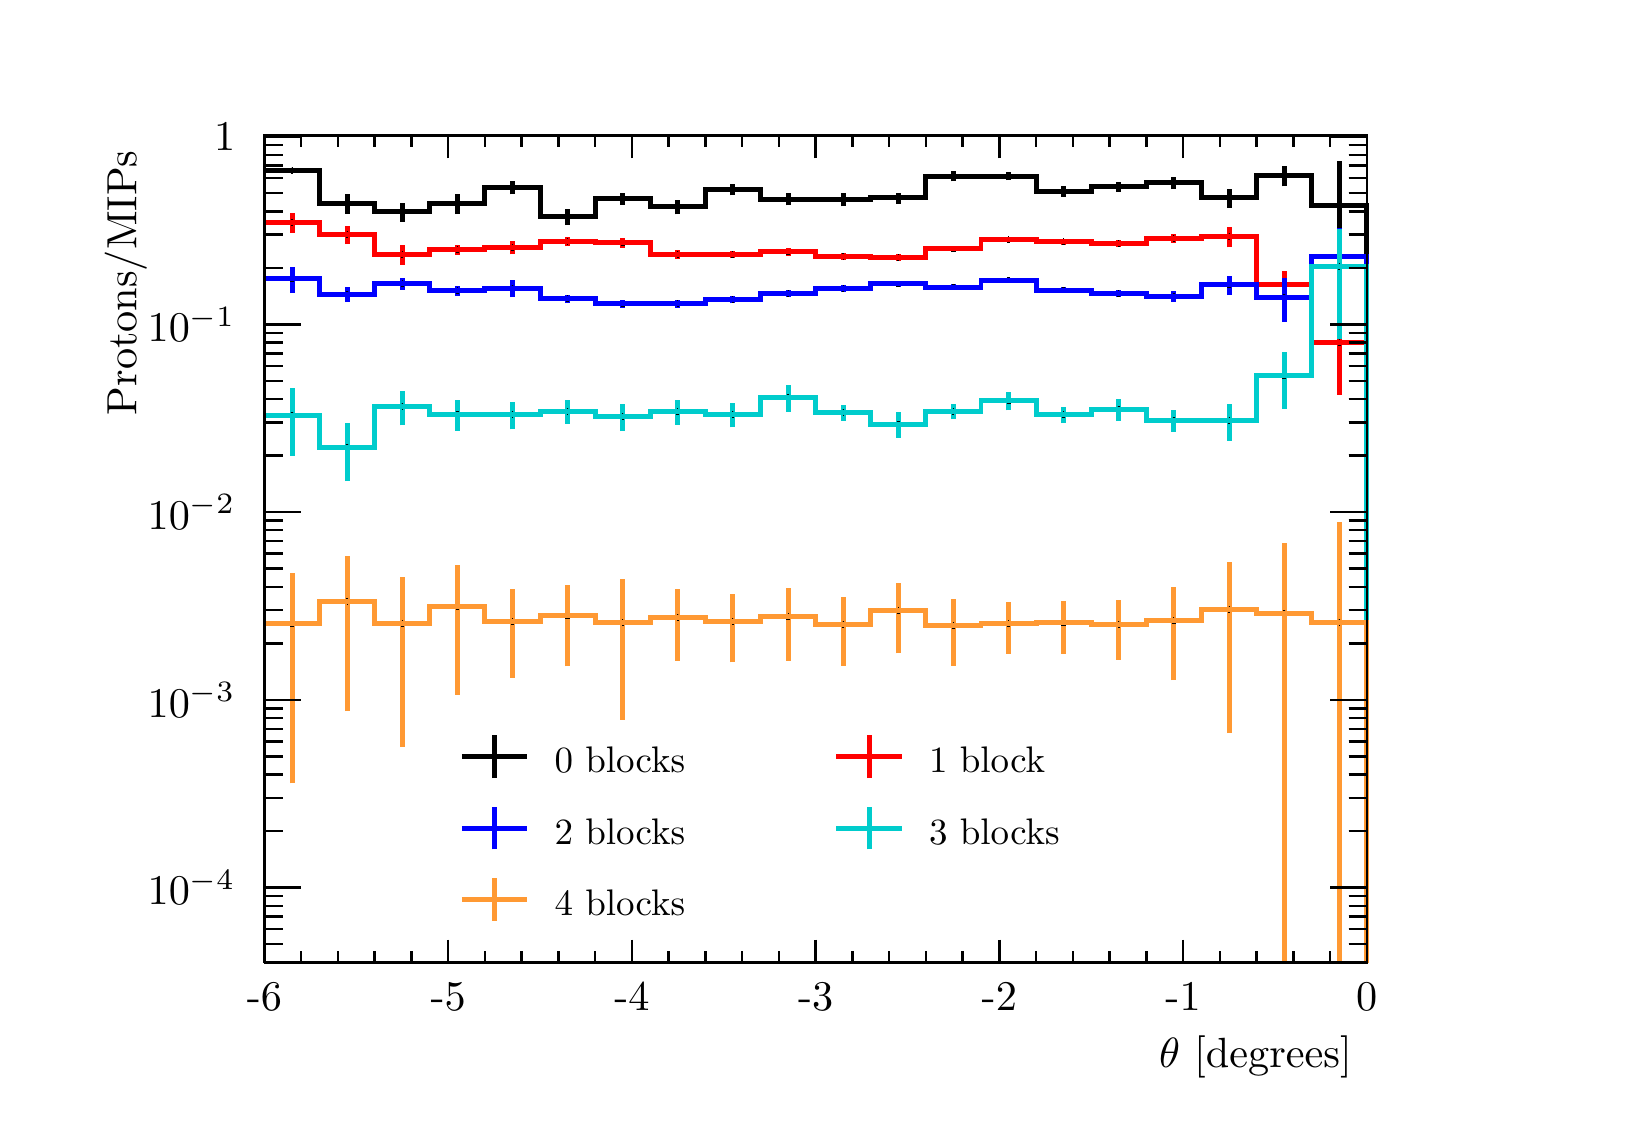
\begin{tikzpicture}
\pgfdeclareplotmark{cross} {
\pgfpathmoveto{\pgfpoint{-0.3\pgfplotmarksize}{\pgfplotmarksize}}
\pgfpathlineto{\pgfpoint{+0.3\pgfplotmarksize}{\pgfplotmarksize}}
\pgfpathlineto{\pgfpoint{+0.3\pgfplotmarksize}{0.3\pgfplotmarksize}}
\pgfpathlineto{\pgfpoint{+1\pgfplotmarksize}{0.3\pgfplotmarksize}}
\pgfpathlineto{\pgfpoint{+1\pgfplotmarksize}{-0.3\pgfplotmarksize}}
\pgfpathlineto{\pgfpoint{+0.3\pgfplotmarksize}{-0.3\pgfplotmarksize}}
\pgfpathlineto{\pgfpoint{+0.3\pgfplotmarksize}{-1.\pgfplotmarksize}}
\pgfpathlineto{\pgfpoint{-0.3\pgfplotmarksize}{-1.\pgfplotmarksize}}
\pgfpathlineto{\pgfpoint{-0.3\pgfplotmarksize}{-0.3\pgfplotmarksize}}
\pgfpathlineto{\pgfpoint{-1.\pgfplotmarksize}{-0.3\pgfplotmarksize}}
\pgfpathlineto{\pgfpoint{-1.\pgfplotmarksize}{0.3\pgfplotmarksize}}
\pgfpathlineto{\pgfpoint{-0.3\pgfplotmarksize}{0.3\pgfplotmarksize}}
\pgfpathclose
\pgfusepathqstroke
}
\pgfdeclareplotmark{cross*} {
\pgfpathmoveto{\pgfpoint{-0.3\pgfplotmarksize}{\pgfplotmarksize}}
\pgfpathlineto{\pgfpoint{+0.3\pgfplotmarksize}{\pgfplotmarksize}}
\pgfpathlineto{\pgfpoint{+0.3\pgfplotmarksize}{0.3\pgfplotmarksize}}
\pgfpathlineto{\pgfpoint{+1\pgfplotmarksize}{0.3\pgfplotmarksize}}
\pgfpathlineto{\pgfpoint{+1\pgfplotmarksize}{-0.3\pgfplotmarksize}}
\pgfpathlineto{\pgfpoint{+0.3\pgfplotmarksize}{-0.3\pgfplotmarksize}}
\pgfpathlineto{\pgfpoint{+0.3\pgfplotmarksize}{-1.\pgfplotmarksize}}
\pgfpathlineto{\pgfpoint{-0.3\pgfplotmarksize}{-1.\pgfplotmarksize}}
\pgfpathlineto{\pgfpoint{-0.3\pgfplotmarksize}{-0.3\pgfplotmarksize}}
\pgfpathlineto{\pgfpoint{-1.\pgfplotmarksize}{-0.3\pgfplotmarksize}}
\pgfpathlineto{\pgfpoint{-1.\pgfplotmarksize}{0.3\pgfplotmarksize}}
\pgfpathlineto{\pgfpoint{-0.3\pgfplotmarksize}{0.3\pgfplotmarksize}}
\pgfpathclose
\pgfusepathqfillstroke
}
\pgfdeclareplotmark{newstar} {
\pgfpathmoveto{\pgfqpoint{0pt}{\pgfplotmarksize}}
\pgfpathlineto{\pgfqpointpolar{44}{0.5\pgfplotmarksize}}
\pgfpathlineto{\pgfqpointpolar{18}{\pgfplotmarksize}}
\pgfpathlineto{\pgfqpointpolar{-20}{0.5\pgfplotmarksize}}
\pgfpathlineto{\pgfqpointpolar{-54}{\pgfplotmarksize}}
\pgfpathlineto{\pgfqpointpolar{-90}{0.5\pgfplotmarksize}}
\pgfpathlineto{\pgfqpointpolar{234}{\pgfplotmarksize}}
\pgfpathlineto{\pgfqpointpolar{198}{0.5\pgfplotmarksize}}
\pgfpathlineto{\pgfqpointpolar{162}{\pgfplotmarksize}}
\pgfpathlineto{\pgfqpointpolar{134}{0.5\pgfplotmarksize}}
\pgfpathclose
\pgfusepathqstroke
}
\pgfdeclareplotmark{newstar*} {
\pgfpathmoveto{\pgfqpoint{0pt}{\pgfplotmarksize}}
\pgfpathlineto{\pgfqpointpolar{44}{0.5\pgfplotmarksize}}
\pgfpathlineto{\pgfqpointpolar{18}{\pgfplotmarksize}}
\pgfpathlineto{\pgfqpointpolar{-20}{0.5\pgfplotmarksize}}
\pgfpathlineto{\pgfqpointpolar{-54}{\pgfplotmarksize}}
\pgfpathlineto{\pgfqpointpolar{-90}{0.5\pgfplotmarksize}}
\pgfpathlineto{\pgfqpointpolar{234}{\pgfplotmarksize}}
\pgfpathlineto{\pgfqpointpolar{198}{0.5\pgfplotmarksize}}
\pgfpathlineto{\pgfqpointpolar{162}{\pgfplotmarksize}}
\pgfpathlineto{\pgfqpointpolar{134}{0.5\pgfplotmarksize}}
\pgfpathclose
\pgfusepathqfillstroke
}
\definecolor{c}{rgb}{1,1,1};
\draw [color=c, fill=c] (0,0) rectangle (20,13.639);
\draw [color=c, fill=c] (3,1.77307) rectangle (17,12.2751);
\definecolor{c}{rgb}{0,0,0};
\draw [c,line width=0.9] (3,1.77307) -- (3,12.2751) -- (17,12.2751) -- (17,1.77307) -- (3,1.77307);
\definecolor{c}{rgb}{1,1,1};
\draw [color=c, fill=c] (3,1.77307) rectangle (17,12.2751);
\definecolor{c}{rgb}{0,0,0};
\draw [c,line width=0.9] (3,1.77307) -- (3,12.2751) -- (17,12.2751) -- (17,1.77307) -- (3,1.77307);
\draw [c,line width=0.9] (3,1.77307) -- (3.7,1.77307) -- (3.7,1.77307) -- (4.4,1.77307) -- (4.4,1.77307) -- (5.1,1.77307) -- (5.1,1.77307) -- (5.8,1.77307) -- (5.8,1.77307) -- (6.5,1.77307) -- (6.5,1.77307) -- (7.2,1.77307) -- (7.2,1.77307) --
 (7.9,1.77307) -- (7.9,1.77307) -- (8.6,1.77307) -- (8.6,1.77307) -- (9.3,1.77307) -- (9.3,1.77307) -- (10,1.77307) -- (10,1.77307) -- (10.7,1.77307) -- (10.7,1.77307) -- (11.4,1.77307) -- (11.4,1.77307) -- (12.1,1.77307) -- (12.1,1.77307) --
 (12.8,1.77307) -- (12.8,1.77307) -- (13.5,1.77307) -- (13.5,1.77307) -- (14.2,1.77307) -- (14.2,1.77307) -- (14.9,1.77307) -- (14.9,1.77307) -- (15.6,1.77307) -- (15.6,1.77307) -- (16.3,1.77307) -- (16.3,1.77307) -- (17,1.77307) -- (17,1.77307);
\draw [c,line width=0.9] (3,1.77307) -- (17,1.77307);
\draw [c,line width=0.9] (3,2.05948) -- (3,1.77307);
\draw [c,line width=0.9] (3.46667,1.91628) -- (3.46667,1.77307);
\draw [c,line width=0.9] (3.93333,1.91628) -- (3.93333,1.77307);
\draw [c,line width=0.9] (4.4,1.91628) -- (4.4,1.77307);
\draw [c,line width=0.9] (4.86667,1.91628) -- (4.86667,1.77307);
\draw [c,line width=0.9] (5.33333,2.05948) -- (5.33333,1.77307);
\draw [c,line width=0.9] (5.8,1.91628) -- (5.8,1.77307);
\draw [c,line width=0.9] (6.26667,1.91628) -- (6.26667,1.77307);
\draw [c,line width=0.9] (6.73333,1.91628) -- (6.73333,1.77307);
\draw [c,line width=0.9] (7.2,1.91628) -- (7.2,1.77307);
\draw [c,line width=0.9] (7.66667,2.05948) -- (7.66667,1.77307);
\draw [c,line width=0.9] (8.13333,1.91628) -- (8.13333,1.77307);
\draw [c,line width=0.9] (8.6,1.91628) -- (8.6,1.77307);
\draw [c,line width=0.9] (9.06667,1.91628) -- (9.06667,1.77307);
\draw [c,line width=0.9] (9.53333,1.91628) -- (9.53333,1.77307);
\draw [c,line width=0.9] (10,2.05948) -- (10,1.77307);
\draw [c,line width=0.9] (10.4667,1.91628) -- (10.4667,1.77307);
\draw [c,line width=0.9] (10.9333,1.91628) -- (10.9333,1.77307);
\draw [c,line width=0.9] (11.4,1.91628) -- (11.4,1.77307);
\draw [c,line width=0.9] (11.8667,1.91628) -- (11.8667,1.77307);
\draw [c,line width=0.9] (12.3333,2.05948) -- (12.3333,1.77307);
\draw [c,line width=0.9] (12.8,1.91628) -- (12.8,1.77307);
\draw [c,line width=0.9] (13.2667,1.91628) -- (13.2667,1.77307);
\draw [c,line width=0.9] (13.7333,1.91628) -- (13.7333,1.77307);
\draw [c,line width=0.9] (14.2,1.91628) -- (14.2,1.77307);
\draw [c,line width=0.9] (14.6667,2.05948) -- (14.6667,1.77307);
\draw [c,line width=0.9] (15.1333,1.91628) -- (15.1333,1.77307);
\draw [c,line width=0.9] (15.6,1.91628) -- (15.6,1.77307);
\draw [c,line width=0.9] (16.0667,1.91628) -- (16.0667,1.77307);
\draw [c,line width=0.9] (16.5333,1.91628) -- (16.5333,1.77307);
\draw [c,line width=0.9] (17,2.05948) -- (17,1.77307);
\draw [anchor=base] (3,1.15931) node[scale=1.52731, color=c, rotate=0]{-6};
\draw [anchor=base] (5.33333,1.15931) node[scale=1.52731, color=c, rotate=0]{-5};
\draw [anchor=base] (7.66667,1.15931) node[scale=1.52731, color=c, rotate=0]{-4};
\draw [anchor=base] (10,1.15931) node[scale=1.52731, color=c, rotate=0]{-3};
\draw [anchor=base] (12.3333,1.15931) node[scale=1.52731, color=c, rotate=0]{-2};
\draw [anchor=base] (14.6667,1.15931) node[scale=1.52731, color=c, rotate=0]{-1};
\draw [anchor=base] (17,1.15931) node[scale=1.52731, color=c, rotate=0]{0};
\draw [anchor= east] (17,0.572837) node[scale=1.52731, color=c, rotate=0]{$\theta$ [degrees] };
\draw [c,line width=0.9] (3,12.2751) -- (17,12.2751);
\draw [c,line width=0.9] (3,11.9887) -- (3,12.2751);
\draw [c,line width=0.9] (3.46667,12.1319) -- (3.46667,12.2751);
\draw [c,line width=0.9] (3.93333,12.1319) -- (3.93333,12.2751);
\draw [c,line width=0.9] (4.4,12.1319) -- (4.4,12.2751);
\draw [c,line width=0.9] (4.86667,12.1319) -- (4.86667,12.2751);
\draw [c,line width=0.9] (5.33333,11.9887) -- (5.33333,12.2751);
\draw [c,line width=0.9] (5.8,12.1319) -- (5.8,12.2751);
\draw [c,line width=0.9] (6.26667,12.1319) -- (6.26667,12.2751);
\draw [c,line width=0.9] (6.73333,12.1319) -- (6.73333,12.2751);
\draw [c,line width=0.9] (7.2,12.1319) -- (7.2,12.2751);
\draw [c,line width=0.9] (7.66667,11.9887) -- (7.66667,12.2751);
\draw [c,line width=0.9] (8.13333,12.1319) -- (8.13333,12.2751);
\draw [c,line width=0.9] (8.6,12.1319) -- (8.6,12.2751);
\draw [c,line width=0.9] (9.06667,12.1319) -- (9.06667,12.2751);
\draw [c,line width=0.9] (9.53333,12.1319) -- (9.53333,12.2751);
\draw [c,line width=0.9] (10,11.9887) -- (10,12.2751);
\draw [c,line width=0.9] (10.4667,12.1319) -- (10.4667,12.2751);
\draw [c,line width=0.9] (10.9333,12.1319) -- (10.9333,12.2751);
\draw [c,line width=0.9] (11.4,12.1319) -- (11.4,12.2751);
\draw [c,line width=0.9] (11.8667,12.1319) -- (11.8667,12.2751);
\draw [c,line width=0.9] (12.3333,11.9887) -- (12.3333,12.2751);
\draw [c,line width=0.9] (12.8,12.1319) -- (12.8,12.2751);
\draw [c,line width=0.9] (13.2667,12.1319) -- (13.2667,12.2751);
\draw [c,line width=0.9] (13.7333,12.1319) -- (13.7333,12.2751);
\draw [c,line width=0.9] (14.2,12.1319) -- (14.2,12.2751);
\draw [c,line width=0.9] (14.6667,11.9887) -- (14.6667,12.2751);
\draw [c,line width=0.9] (15.1333,12.1319) -- (15.1333,12.2751);
\draw [c,line width=0.9] (15.6,12.1319) -- (15.6,12.2751);
\draw [c,line width=0.9] (16.0667,12.1319) -- (16.0667,12.2751);
\draw [c,line width=0.9] (16.5333,12.1319) -- (16.5333,12.2751);
\draw [c,line width=0.9] (17,11.9887) -- (17,12.2751);
\draw [c,line width=0.9] (3,1.77307) -- (3,12.2751);
\draw [c,line width=0.9] (3.231,1.77653) -- (3,1.77653);
\draw [c,line width=0.9] (3.231,2.0076) -- (3,2.0076);
\draw [c,line width=0.9] (3.231,2.1964) -- (3,2.1964);
\draw [c,line width=0.9] (3.231,2.35603) -- (3,2.35603);
\draw [c,line width=0.9] (3.231,2.49431) -- (3,2.49431);
\draw [c,line width=0.9] (3.231,2.61628) -- (3,2.61628);
\draw [c,line width=0.9] (3.462,2.72539) -- (3,2.72539);
\draw [anchor= east] (2.82,2.72539) node[scale=1.52731, color=c, rotate=0]{$10^{-4}$};
\draw [c,line width=0.9] (3.231,3.44317) -- (3,3.44317);
\draw [c,line width=0.9] (3.231,3.86305) -- (3,3.86305);
\draw [c,line width=0.9] (3.231,4.16096) -- (3,4.16096);
\draw [c,line width=0.9] (3.231,4.39203) -- (3,4.39203);
\draw [c,line width=0.9] (3.231,4.58083) -- (3,4.58083);
\draw [c,line width=0.9] (3.231,4.74046) -- (3,4.74046);
\draw [c,line width=0.9] (3.231,4.87874) -- (3,4.87874);
\draw [c,line width=0.9] (3.231,5.00071) -- (3,5.00071);
\draw [c,line width=0.9] (3.462,5.10982) -- (3,5.10982);
\draw [anchor= east] (2.82,5.10982) node[scale=1.52731, color=c, rotate=0]{$10^{-3}$};
\draw [c,line width=0.9] (3.231,5.8276) -- (3,5.8276);
\draw [c,line width=0.9] (3.231,6.24748) -- (3,6.24748);
\draw [c,line width=0.9] (3.231,6.54539) -- (3,6.54539);
\draw [c,line width=0.9] (3.231,6.77646) -- (3,6.77646);
\draw [c,line width=0.9] (3.231,6.96527) -- (3,6.96527);
\draw [c,line width=0.9] (3.231,7.1249) -- (3,7.1249);
\draw [c,line width=0.9] (3.231,7.26317) -- (3,7.26317);
\draw [c,line width=0.9] (3.231,7.38514) -- (3,7.38514);
\draw [c,line width=0.9] (3.462,7.49425) -- (3,7.49425);
\draw [anchor= east] (2.82,7.49425) node[scale=1.52731, color=c, rotate=0]{$10^{-2}$};
\draw [c,line width=0.9] (3.231,8.21203) -- (3,8.21203);
\draw [c,line width=0.9] (3.231,8.63191) -- (3,8.63191);
\draw [c,line width=0.9] (3.231,8.92982) -- (3,8.92982);
\draw [c,line width=0.9] (3.231,9.16089) -- (3,9.16089);
\draw [c,line width=0.9] (3.231,9.3497) -- (3,9.3497);
\draw [c,line width=0.9] (3.231,9.50933) -- (3,9.50933);
\draw [c,line width=0.9] (3.231,9.6476) -- (3,9.6476);
\draw [c,line width=0.9] (3.231,9.76957) -- (3,9.76957);
\draw [c,line width=0.9] (3.462,9.87868) -- (3,9.87868);
\draw [anchor= east] (2.82,9.87868) node[scale=1.52731, color=c, rotate=0]{$10^{-1}$};
\draw [c,line width=0.9] (3.231,10.5965) -- (3,10.5965);
\draw [c,line width=0.9] (3.231,11.0163) -- (3,11.0163);
\draw [c,line width=0.9] (3.231,11.3142) -- (3,11.3142);
\draw [c,line width=0.9] (3.231,11.5453) -- (3,11.5453);
\draw [c,line width=0.9] (3.231,11.7341) -- (3,11.7341);
\draw [c,line width=0.9] (3.231,11.8938) -- (3,11.8938);
\draw [c,line width=0.9] (3.231,12.032) -- (3,12.032);
\draw [c,line width=0.9] (3.231,12.154) -- (3,12.154);
\draw [c,line width=0.9] (3.462,12.2631) -- (3,12.2631);
\draw [anchor= east] (2.82,12.2631) node[scale=1.52731, color=c, rotate=0]{1};
\draw [anchor= east] (1.24,12.2751) node[scale=1.52731, color=c, rotate=90]{ Protons/MIPs};
\draw [c,line width=0.9] (17,1.77307) -- (17,12.2751);
\draw [c,line width=0.9] (16.769,1.77653) -- (17,1.77653);
\draw [c,line width=0.9] (16.769,2.0076) -- (17,2.0076);
\draw [c,line width=0.9] (16.769,2.1964) -- (17,2.1964);
\draw [c,line width=0.9] (16.769,2.35603) -- (17,2.35603);
\draw [c,line width=0.9] (16.769,2.49431) -- (17,2.49431);
\draw [c,line width=0.9] (16.769,2.61628) -- (17,2.61628);
\draw [c,line width=0.9] (16.538,2.72539) -- (17,2.72539);
\draw [c,line width=0.9] (16.769,3.44317) -- (17,3.44317);
\draw [c,line width=0.9] (16.769,3.86305) -- (17,3.86305);
\draw [c,line width=0.9] (16.769,4.16096) -- (17,4.16096);
\draw [c,line width=0.9] (16.769,4.39203) -- (17,4.39203);
\draw [c,line width=0.9] (16.769,4.58083) -- (17,4.58083);
\draw [c,line width=0.9] (16.769,4.74046) -- (17,4.74046);
\draw [c,line width=0.9] (16.769,4.87874) -- (17,4.87874);
\draw [c,line width=0.9] (16.769,5.00071) -- (17,5.00071);
\draw [c,line width=0.9] (16.538,5.10982) -- (17,5.10982);
\draw [c,line width=0.9] (16.769,5.8276) -- (17,5.8276);
\draw [c,line width=0.9] (16.769,6.24748) -- (17,6.24748);
\draw [c,line width=0.9] (16.769,6.54539) -- (17,6.54539);
\draw [c,line width=0.9] (16.769,6.77646) -- (17,6.77646);
\draw [c,line width=0.9] (16.769,6.96527) -- (17,6.96527);
\draw [c,line width=0.9] (16.769,7.1249) -- (17,7.1249);
\draw [c,line width=0.9] (16.769,7.26317) -- (17,7.26317);
\draw [c,line width=0.9] (16.769,7.38514) -- (17,7.38514);
\draw [c,line width=0.9] (16.538,7.49425) -- (17,7.49425);
\draw [c,line width=0.9] (16.769,8.21203) -- (17,8.21203);
\draw [c,line width=0.9] (16.769,8.63191) -- (17,8.63191);
\draw [c,line width=0.9] (16.769,8.92982) -- (17,8.92982);
\draw [c,line width=0.9] (16.769,9.16089) -- (17,9.16089);
\draw [c,line width=0.9] (16.769,9.3497) -- (17,9.3497);
\draw [c,line width=0.9] (16.769,9.50933) -- (17,9.50933);
\draw [c,line width=0.9] (16.769,9.6476) -- (17,9.6476);
\draw [c,line width=0.9] (16.769,9.76957) -- (17,9.76957);
\draw [c,line width=0.9] (16.538,9.87868) -- (17,9.87868);
\draw [c,line width=0.9] (16.769,10.5965) -- (17,10.5965);
\draw [c,line width=0.9] (16.769,11.0163) -- (17,11.0163);
\draw [c,line width=0.9] (16.769,11.3142) -- (17,11.3142);
\draw [c,line width=0.9] (16.769,11.5453) -- (17,11.5453);
\draw [c,line width=0.9] (16.769,11.7341) -- (17,11.7341);
\draw [c,line width=0.9] (16.769,11.8938) -- (17,11.8938);
\draw [c,line width=0.9] (16.769,12.032) -- (17,12.032);
\draw [c,line width=0.9] (16.769,12.154) -- (17,12.154);
\draw [c,line width=0.9] (16.538,12.2631) -- (17,12.2631);
\draw [c,line width=1.8] (3.35,11.7944) -- (3.35,11.8326);
\draw [c,line width=1.8] (3.35,11.8326) -- (3.35,11.8695);
\foreach \P in {(3.35,11.8326)}{\draw[mark options={color=c,fill=c},mark size=2.402402pt, line width=0.000000pt, mark=*,mark size=1pt] plot coordinates {\P};}
\draw [c,line width=1.8] (4.05,11.2801) -- (4.05,11.4121);
\draw [c,line width=1.8] (4.05,11.4121) -- (4.05,11.5292);
\foreach \P in {(4.05,11.4121)}{\draw[mark options={color=c,fill=c},mark size=2.402402pt, line width=0.000000pt, mark=*,mark size=1pt] plot coordinates {\P};}
\draw [c,line width=1.8] (4.75,11.1787) -- (4.75,11.3065);
\draw [c,line width=1.8] (4.75,11.3065) -- (4.75,11.4203);
\foreach \P in {(4.75,11.3065)}{\draw[mark options={color=c,fill=c},mark size=2.402402pt, line width=0.000000pt, mark=*,mark size=1pt] plot coordinates {\P};}
\draw [c,line width=1.8] (5.45,11.2778) -- (5.45,11.4122);
\draw [c,line width=1.8] (5.45,11.4122) -- (5.45,11.5311);
\foreach \P in {(5.45,11.4122)}{\draw[mark options={color=c,fill=c},mark size=2.402402pt, line width=0.000000pt, mark=*,mark size=1pt] plot coordinates {\P};}
\draw [c,line width=1.8] (6.15,11.5292) -- (6.15,11.617);
\draw [c,line width=1.8] (6.15,11.617) -- (6.15,11.6979);
\foreach \P in {(6.15,11.617)}{\draw[mark options={color=c,fill=c},mark size=2.402402pt, line width=0.000000pt, mark=*,mark size=1pt] plot coordinates {\P};}
\draw [c,line width=1.8] (6.85,11.1391) -- (6.85,11.2438);
\draw [c,line width=1.8] (6.85,11.2438) -- (6.85,11.3388);
\foreach \P in {(6.85,11.2438)}{\draw[mark options={color=c,fill=c},mark size=2.402402pt, line width=0.000000pt, mark=*,mark size=1pt] plot coordinates {\P};}
\draw [c,line width=1.8] (7.55,11.397) -- (7.55,11.4769);
\draw [c,line width=1.8] (7.55,11.4769) -- (7.55,11.551);
\foreach \P in {(7.55,11.4769)}{\draw[mark options={color=c,fill=c},mark size=2.402402pt, line width=0.000000pt, mark=*,mark size=1pt] plot coordinates {\P};}
\draw [c,line width=1.8] (8.25,11.2744) -- (8.25,11.3688);
\draw [c,line width=1.8] (8.25,11.3688) -- (8.25,11.4553);
\foreach \P in {(8.25,11.3688)}{\draw[mark options={color=c,fill=c},mark size=2.402402pt, line width=0.000000pt, mark=*,mark size=1pt] plot coordinates {\P};}
\draw [c,line width=1.8] (8.95,11.5168) -- (8.95,11.5936);
\draw [c,line width=1.8] (8.95,11.5936) -- (8.95,11.665);
\foreach \P in {(8.95,11.5936)}{\draw[mark options={color=c,fill=c},mark size=2.402402pt, line width=0.000000pt, mark=*,mark size=1pt] plot coordinates {\P};}
\draw [c,line width=1.8] (9.65,11.3879) -- (9.65,11.4689);
\draw [c,line width=1.8] (9.65,11.4689) -- (9.65,11.544);
\foreach \P in {(9.65,11.4689)}{\draw[mark options={color=c,fill=c},mark size=2.402402pt, line width=0.000000pt, mark=*,mark size=1pt] plot coordinates {\P};}
\draw [c,line width=1.8] (10.35,11.3756) -- (10.35,11.4639);
\draw [c,line width=1.8] (10.35,11.4639) -- (10.35,11.5452);
\foreach \P in {(10.35,11.4639)}{\draw[mark options={color=c,fill=c},mark size=2.402402pt, line width=0.000000pt, mark=*,mark size=1pt] plot coordinates {\P};}
\draw [c,line width=1.8] (11.05,11.412) -- (11.05,11.4839);
\draw [c,line width=1.8] (11.05,11.4839) -- (11.05,11.5512);
\foreach \P in {(11.05,11.4839)}{\draw[mark options={color=c,fill=c},mark size=2.402402pt, line width=0.000000pt, mark=*,mark size=1pt] plot coordinates {\P};}
\draw [c,line width=1.8] (11.75,11.6931) -- (11.75,11.7612);
\draw [c,line width=1.8] (11.75,11.7612) -- (11.75,11.8251);
\foreach \P in {(11.75,11.7612)}{\draw[mark options={color=c,fill=c},mark size=2.402402pt, line width=0.000000pt, mark=*,mark size=1pt] plot coordinates {\P};}
\draw [c,line width=1.8] (12.45,11.7084) -- (12.45,11.759);
\draw [c,line width=1.8] (12.45,11.759) -- (12.45,11.8072);
\foreach \P in {(12.45,11.759)}{\draw[mark options={color=c,fill=c},mark size=2.402402pt, line width=0.000000pt, mark=*,mark size=1pt] plot coordinates {\P};}
\draw [c,line width=1.8] (13.15,11.4965) -- (13.15,11.5686);
\draw [c,line width=1.8] (13.15,11.5686) -- (13.15,11.636);
\foreach \P in {(13.15,11.5686)}{\draw[mark options={color=c,fill=c},mark size=2.402402pt, line width=0.000000pt, mark=*,mark size=1pt] plot coordinates {\P};}
\draw [c,line width=1.8] (13.85,11.5606) -- (13.85,11.6255);
\draw [c,line width=1.8] (13.85,11.6255) -- (13.85,11.6866);
\foreach \P in {(13.85,11.6255)}{\draw[mark options={color=c,fill=c},mark size=2.402402pt, line width=0.000000pt, mark=*,mark size=1pt] plot coordinates {\P};}
\draw [c,line width=1.8] (14.55,11.5941) -- (14.55,11.6769);
\draw [c,line width=1.8] (14.55,11.6769) -- (14.55,11.7536);
\foreach \P in {(14.55,11.6769)}{\draw[mark options={color=c,fill=c},mark size=2.402402pt, line width=0.000000pt, mark=*,mark size=1pt] plot coordinates {\P};}
\draw [c,line width=1.8] (15.25,11.3608) -- (15.25,11.4891);
\draw [c,line width=1.8] (15.25,11.4891) -- (15.25,11.6033);
\foreach \P in {(15.25,11.4891)}{\draw[mark options={color=c,fill=c},mark size=2.402402pt, line width=0.000000pt, mark=*,mark size=1pt] plot coordinates {\P};}
\draw [c,line width=1.8] (15.95,11.6301) -- (15.95,11.7651);
\draw [c,line width=1.8] (15.95,11.7651) -- (15.95,11.8844);
\foreach \P in {(15.95,11.7651)}{\draw[mark options={color=c,fill=c},mark size=2.402402pt, line width=0.000000pt, mark=*,mark size=1pt] plot coordinates {\P};}
\draw [c,line width=1.8] (16.65,10.041) -- (16.65,11.3908);
\draw [c,line width=1.8] (16.65,11.3908) -- (16.65,11.9574);
\foreach \P in {(16.65,11.3908)}{\draw[mark options={color=c,fill=c},mark size=2.402402pt, line width=0.000000pt, mark=*,mark size=1pt] plot coordinates {\P};}
\draw [c,line width=1.8] (3,11.8326) -- (3.7,11.8326) -- (3.7,11.4121) -- (4.4,11.4121) -- (4.4,11.3065) -- (5.1,11.3065) -- (5.1,11.4122) -- (5.8,11.4122) -- (5.8,11.617) -- (6.5,11.617) -- (6.5,11.2438) -- (7.2,11.2438) -- (7.2,11.4769) --
 (7.9,11.4769) -- (7.9,11.3688) -- (8.6,11.3688) -- (8.6,11.5936) -- (9.3,11.5936) -- (9.3,11.4689) -- (10,11.4689) -- (10,11.4639) -- (10.7,11.4639) -- (10.7,11.4839) -- (11.4,11.4839) -- (11.4,11.7612) -- (12.1,11.7612) -- (12.1,11.759) --
 (12.8,11.759) -- (12.8,11.5686) -- (13.5,11.5686) -- (13.5,11.6255) -- (14.2,11.6255) -- (14.2,11.6769) -- (14.9,11.6769) -- (14.9,11.4891) -- (15.6,11.4891) -- (15.6,11.7651) -- (16.3,11.7651) -- (16.3,11.3908) -- (17,11.3908) -- (17,1.77307);
\definecolor{c}{rgb}{1,0,0};
\draw [c,line width=1.8] (3.35,11.0436) -- (3.35,11.1738);
\draw [c,line width=1.8] (3.35,11.1738) -- (3.35,11.2894);
\definecolor{c}{rgb}{0,0,0};
\foreach \P in {(3.35,11.1738)}{\draw[mark options={color=c,fill=c},mark size=2.402402pt, line width=0.000000pt, mark=*,mark size=1pt] plot coordinates {\P};}
\definecolor{c}{rgb}{1,0,0};
\draw [c,line width=1.8] (4.05,10.8972) -- (4.05,11.0207);
\draw [c,line width=1.8] (4.05,11.0207) -- (4.05,11.131);
\definecolor{c}{rgb}{0,0,0};
\foreach \P in {(4.05,11.0207)}{\draw[mark options={color=c,fill=c},mark size=2.402402pt, line width=0.000000pt, mark=*,mark size=1pt] plot coordinates {\P};}
\definecolor{c}{rgb}{1,0,0};
\draw [c,line width=1.8] (4.75,10.6369) -- (4.75,10.7653);
\draw [c,line width=1.8] (4.75,10.7653) -- (4.75,10.8796);
\definecolor{c}{rgb}{0,0,0};
\foreach \P in {(4.75,10.7653)}{\draw[mark options={color=c,fill=c},mark size=2.402402pt, line width=0.000000pt, mark=*,mark size=1pt] plot coordinates {\P};}
\definecolor{c}{rgb}{1,0,0};
\draw [c,line width=1.8] (5.45,10.7622) -- (5.45,10.8283);
\draw [c,line width=1.8] (5.45,10.8283) -- (5.45,10.8905);
\definecolor{c}{rgb}{0,0,0};
\foreach \P in {(5.45,10.8283)}{\draw[mark options={color=c,fill=c},mark size=2.402402pt, line width=0.000000pt, mark=*,mark size=1pt] plot coordinates {\P};}
\definecolor{c}{rgb}{1,0,0};
\draw [c,line width=1.8] (6.15,10.7679) -- (6.15,10.854);
\draw [c,line width=1.8] (6.15,10.854) -- (6.15,10.9335);
\definecolor{c}{rgb}{0,0,0};
\foreach \P in {(6.15,10.854)}{\draw[mark options={color=c,fill=c},mark size=2.402402pt, line width=0.000000pt, mark=*,mark size=1pt] plot coordinates {\P};}
\definecolor{c}{rgb}{1,0,0};
\draw [c,line width=1.8] (6.85,10.8691) -- (6.85,10.932);
\draw [c,line width=1.8] (6.85,10.932) -- (6.85,10.9913);
\definecolor{c}{rgb}{0,0,0};
\foreach \P in {(6.85,10.932)}{\draw[mark options={color=c,fill=c},mark size=2.402402pt, line width=0.000000pt, mark=*,mark size=1pt] plot coordinates {\P};}
\definecolor{c}{rgb}{1,0,0};
\draw [c,line width=1.8] (7.55,10.8482) -- (7.55,10.913);
\draw [c,line width=1.8] (7.55,10.913) -- (7.55,10.974);
\definecolor{c}{rgb}{0,0,0};
\foreach \P in {(7.55,10.913)}{\draw[mark options={color=c,fill=c},mark size=2.402402pt, line width=0.000000pt, mark=*,mark size=1pt] plot coordinates {\P};}
\definecolor{c}{rgb}{1,0,0};
\draw [c,line width=1.8] (8.25,10.7072) -- (8.25,10.767);
\draw [c,line width=1.8] (8.25,10.767) -- (8.25,10.8236);
\definecolor{c}{rgb}{0,0,0};
\foreach \P in {(8.25,10.767)}{\draw[mark options={color=c,fill=c},mark size=2.402402pt, line width=0.000000pt, mark=*,mark size=1pt] plot coordinates {\P};}
\definecolor{c}{rgb}{1,0,0};
\draw [c,line width=1.8] (8.95,10.7158) -- (8.95,10.7635);
\draw [c,line width=1.8] (8.95,10.7635) -- (8.95,10.8092);
\definecolor{c}{rgb}{0,0,0};
\foreach \P in {(8.95,10.7635)}{\draw[mark options={color=c,fill=c},mark size=2.402402pt, line width=0.000000pt, mark=*,mark size=1pt] plot coordinates {\P};}
\definecolor{c}{rgb}{1,0,0};
\draw [c,line width=1.8] (9.65,10.7498) -- (9.65,10.7991);
\draw [c,line width=1.8] (9.65,10.7991) -- (9.65,10.8462);
\definecolor{c}{rgb}{0,0,0};
\foreach \P in {(9.65,10.7991)}{\draw[mark options={color=c,fill=c},mark size=2.402402pt, line width=0.000000pt, mark=*,mark size=1pt] plot coordinates {\P};}
\definecolor{c}{rgb}{1,0,0};
\draw [c,line width=1.8] (10.35,10.6966) -- (10.35,10.7431);
\draw [c,line width=1.8] (10.35,10.7431) -- (10.35,10.7877);
\definecolor{c}{rgb}{0,0,0};
\foreach \P in {(10.35,10.7431)}{\draw[mark options={color=c,fill=c},mark size=2.402402pt, line width=0.000000pt, mark=*,mark size=1pt] plot coordinates {\P};}
\definecolor{c}{rgb}{1,0,0};
\draw [c,line width=1.8] (11.05,10.6849) -- (11.05,10.7279);
\draw [c,line width=1.8] (11.05,10.7279) -- (11.05,10.7692);
\definecolor{c}{rgb}{0,0,0};
\foreach \P in {(11.05,10.7279)}{\draw[mark options={color=c,fill=c},mark size=2.402402pt, line width=0.000000pt, mark=*,mark size=1pt] plot coordinates {\P};}
\definecolor{c}{rgb}{1,0,0};
\draw [c,line width=1.8] (11.75,10.7966) -- (11.75,10.8353);
\draw [c,line width=1.8] (11.75,10.8353) -- (11.75,10.8726);
\definecolor{c}{rgb}{0,0,0};
\foreach \P in {(11.75,10.8353)}{\draw[mark options={color=c,fill=c},mark size=2.402402pt, line width=0.000000pt, mark=*,mark size=1pt] plot coordinates {\P};}
\definecolor{c}{rgb}{1,0,0};
\draw [c,line width=1.8] (12.45,10.9224) -- (12.45,10.9539);
\draw [c,line width=1.8] (12.45,10.9539) -- (12.45,10.9845);
\definecolor{c}{rgb}{0,0,0};
\foreach \P in {(12.45,10.9539)}{\draw[mark options={color=c,fill=c},mark size=2.402402pt, line width=0.000000pt, mark=*,mark size=1pt] plot coordinates {\P};}
\definecolor{c}{rgb}{1,0,0};
\draw [c,line width=1.8] (13.15,10.891) -- (13.15,10.9273);
\draw [c,line width=1.8] (13.15,10.9273) -- (13.15,10.9624);
\definecolor{c}{rgb}{0,0,0};
\foreach \P in {(13.15,10.9273)}{\draw[mark options={color=c,fill=c},mark size=2.402402pt, line width=0.000000pt, mark=*,mark size=1pt] plot coordinates {\P};}
\definecolor{c}{rgb}{1,0,0};
\draw [c,line width=1.8] (13.85,10.8625) -- (13.85,10.9045);
\draw [c,line width=1.8] (13.85,10.9045) -- (13.85,10.9449);
\definecolor{c}{rgb}{0,0,0};
\foreach \P in {(13.85,10.9045)}{\draw[mark options={color=c,fill=c},mark size=2.402402pt, line width=0.000000pt, mark=*,mark size=1pt] plot coordinates {\P};}
\definecolor{c}{rgb}{1,0,0};
\draw [c,line width=1.8] (14.55,10.9139) -- (14.55,10.9694);
\draw [c,line width=1.8] (14.55,10.9694) -- (14.55,11.0221);
\definecolor{c}{rgb}{0,0,0};
\foreach \P in {(14.55,10.9694)}{\draw[mark options={color=c,fill=c},mark size=2.402402pt, line width=0.000000pt, mark=*,mark size=1pt] plot coordinates {\P};}
\definecolor{c}{rgb}{1,0,0};
\draw [c,line width=1.8] (15.25,10.856) -- (15.25,10.9946);
\draw [c,line width=1.8] (15.25,10.9946) -- (15.25,11.1168);
\definecolor{c}{rgb}{0,0,0};
\foreach \P in {(15.25,10.9946)}{\draw[mark options={color=c,fill=c},mark size=2.402402pt, line width=0.000000pt, mark=*,mark size=1pt] plot coordinates {\P};}
\definecolor{c}{rgb}{1,0,0};
\draw [c,line width=1.8] (15.95,10.1715) -- (15.95,10.3785);
\draw [c,line width=1.8] (15.95,10.3785) -- (15.95,10.5509);
\definecolor{c}{rgb}{0,0,0};
\foreach \P in {(15.95,10.3785)}{\draw[mark options={color=c,fill=c},mark size=2.402402pt, line width=0.000000pt, mark=*,mark size=1pt] plot coordinates {\P};}
\definecolor{c}{rgb}{1,0,0};
\draw [c,line width=1.8] (16.65,8.98619) -- (16.65,9.64699);
\draw [c,line width=1.8] (16.65,9.64699) -- (16.65,10.0472);
\definecolor{c}{rgb}{0,0,0};
\foreach \P in {(16.65,9.64699)}{\draw[mark options={color=c,fill=c},mark size=2.402402pt, line width=0.000000pt, mark=*,mark size=1pt] plot coordinates {\P};}
\definecolor{c}{rgb}{1,0,0};
\draw [c,line width=1.8] (3,11.1738) -- (3.7,11.1738) -- (3.7,11.0207) -- (4.4,11.0207) -- (4.4,10.7653) -- (5.1,10.7653) -- (5.1,10.8283) -- (5.8,10.8283) -- (5.8,10.854) -- (6.5,10.854) -- (6.5,10.932) -- (7.2,10.932) -- (7.2,10.913) --
 (7.9,10.913) -- (7.9,10.767) -- (8.6,10.767) -- (8.6,10.7635) -- (9.3,10.7635) -- (9.3,10.7991) -- (10,10.7991) -- (10,10.7431) -- (10.7,10.7431) -- (10.7,10.7279) -- (11.4,10.7279) -- (11.4,10.8353) -- (12.1,10.8353) -- (12.1,10.9539) --
 (12.8,10.9539) -- (12.8,10.9273) -- (13.5,10.9273) -- (13.5,10.9045) -- (14.2,10.9045) -- (14.2,10.9694) -- (14.9,10.9694) -- (14.9,10.9946) -- (15.6,10.9946) -- (15.6,10.3785) -- (16.3,10.3785) -- (16.3,9.64699) -- (17,9.64699) -- (17,1.77307);
\definecolor{c}{rgb}{0,0,1};
\draw [c,line width=1.8] (3.35,10.2743) -- (3.35,10.455);
\draw [c,line width=1.8] (3.35,10.455) -- (3.35,10.6088);
\definecolor{c}{rgb}{0,0,0};
\foreach \P in {(3.35,10.455)}{\draw[mark options={color=c,fill=c},mark size=2.402402pt, line width=0.000000pt, mark=*,mark size=1pt] plot coordinates {\P};}
\definecolor{c}{rgb}{0,0,1};
\draw [c,line width=1.8] (4.05,10.1619) -- (4.05,10.2629);
\draw [c,line width=1.8] (4.05,10.2629) -- (4.05,10.3549);
\definecolor{c}{rgb}{0,0,0};
\foreach \P in {(4.05,10.2629)}{\draw[mark options={color=c,fill=c},mark size=2.402402pt, line width=0.000000pt, mark=*,mark size=1pt] plot coordinates {\P};}
\definecolor{c}{rgb}{0,0,1};
\draw [c,line width=1.8] (4.75,10.3183) -- (4.75,10.3938);
\draw [c,line width=1.8] (4.75,10.3938) -- (4.75,10.4642);
\definecolor{c}{rgb}{0,0,0};
\foreach \P in {(4.75,10.3938)}{\draw[mark options={color=c,fill=c},mark size=2.402402pt, line width=0.000000pt, mark=*,mark size=1pt] plot coordinates {\P};}
\definecolor{c}{rgb}{0,0,1};
\draw [c,line width=1.8] (5.45,10.2384) -- (5.45,10.306);
\draw [c,line width=1.8] (5.45,10.306) -- (5.45,10.3695);
\definecolor{c}{rgb}{0,0,0};
\foreach \P in {(5.45,10.306)}{\draw[mark options={color=c,fill=c},mark size=2.402402pt, line width=0.000000pt, mark=*,mark size=1pt] plot coordinates {\P};}
\definecolor{c}{rgb}{0,0,1};
\draw [c,line width=1.8] (6.15,10.225) -- (6.15,10.3378);
\draw [c,line width=1.8] (6.15,10.3378) -- (6.15,10.4395);
\definecolor{c}{rgb}{0,0,0};
\foreach \P in {(6.15,10.3378)}{\draw[mark options={color=c,fill=c},mark size=2.402402pt, line width=0.000000pt, mark=*,mark size=1pt] plot coordinates {\P};}
\definecolor{c}{rgb}{0,0,1};
\draw [c,line width=1.8] (6.85,10.147) -- (6.85,10.2034);
\draw [c,line width=1.8] (6.85,10.2034) -- (6.85,10.2569);
\definecolor{c}{rgb}{0,0,0};
\foreach \P in {(6.85,10.2034)}{\draw[mark options={color=c,fill=c},mark size=2.402402pt, line width=0.000000pt, mark=*,mark size=1pt] plot coordinates {\P};}
\definecolor{c}{rgb}{0,0,1};
\draw [c,line width=1.8] (7.55,10.0873) -- (7.55,10.1384);
\draw [c,line width=1.8] (7.55,10.1384) -- (7.55,10.1871);
\definecolor{c}{rgb}{0,0,0};
\foreach \P in {(7.55,10.1384)}{\draw[mark options={color=c,fill=c},mark size=2.402402pt, line width=0.000000pt, mark=*,mark size=1pt] plot coordinates {\P};}
\definecolor{c}{rgb}{0,0,1};
\draw [c,line width=1.8] (8.25,10.0918) -- (8.25,10.1425);
\draw [c,line width=1.8] (8.25,10.1425) -- (8.25,10.1908);
\definecolor{c}{rgb}{0,0,0};
\foreach \P in {(8.25,10.1425)}{\draw[mark options={color=c,fill=c},mark size=2.402402pt, line width=0.000000pt, mark=*,mark size=1pt] plot coordinates {\P};}
\definecolor{c}{rgb}{0,0,1};
\draw [c,line width=1.8] (8.95,10.1443) -- (8.95,10.193);
\draw [c,line width=1.8] (8.95,10.193) -- (8.95,10.2395);
\definecolor{c}{rgb}{0,0,0};
\foreach \P in {(8.95,10.193)}{\draw[mark options={color=c,fill=c},mark size=2.402402pt, line width=0.000000pt, mark=*,mark size=1pt] plot coordinates {\P};}
\definecolor{c}{rgb}{0,0,1};
\draw [c,line width=1.8] (9.65,10.2271) -- (9.65,10.2717);
\draw [c,line width=1.8] (9.65,10.2717) -- (9.65,10.3144);
\definecolor{c}{rgb}{0,0,0};
\foreach \P in {(9.65,10.2717)}{\draw[mark options={color=c,fill=c},mark size=2.402402pt, line width=0.000000pt, mark=*,mark size=1pt] plot coordinates {\P};}
\definecolor{c}{rgb}{0,0,1};
\draw [c,line width=1.8] (10.35,10.2906) -- (10.35,10.3336);
\draw [c,line width=1.8] (10.35,10.3336) -- (10.35,10.3749);
\definecolor{c}{rgb}{0,0,0};
\foreach \P in {(10.35,10.3336)}{\draw[mark options={color=c,fill=c},mark size=2.402402pt, line width=0.000000pt, mark=*,mark size=1pt] plot coordinates {\P};}
\definecolor{c}{rgb}{0,0,1};
\draw [c,line width=1.8] (11.05,10.351) -- (11.05,10.3921);
\draw [c,line width=1.8] (11.05,10.3921) -- (11.05,10.4316);
\definecolor{c}{rgb}{0,0,0};
\foreach \P in {(11.05,10.3921)}{\draw[mark options={color=c,fill=c},mark size=2.402402pt, line width=0.000000pt, mark=*,mark size=1pt] plot coordinates {\P};}
\definecolor{c}{rgb}{0,0,1};
\draw [c,line width=1.8] (11.75,10.3162) -- (11.75,10.3514);
\draw [c,line width=1.8] (11.75,10.3514) -- (11.75,10.3855);
\definecolor{c}{rgb}{0,0,0};
\foreach \P in {(11.75,10.3514)}{\draw[mark options={color=c,fill=c},mark size=2.402402pt, line width=0.000000pt, mark=*,mark size=1pt] plot coordinates {\P};}
\definecolor{c}{rgb}{0,0,1};
\draw [c,line width=1.8] (12.45,10.4088) -- (12.45,10.4398);
\draw [c,line width=1.8] (12.45,10.4398) -- (12.45,10.4699);
\definecolor{c}{rgb}{0,0,0};
\foreach \P in {(12.45,10.4398)}{\draw[mark options={color=c,fill=c},mark size=2.402402pt, line width=0.000000pt, mark=*,mark size=1pt] plot coordinates {\P};}
\definecolor{c}{rgb}{0,0,1};
\draw [c,line width=1.8] (13.15,10.2781) -- (13.15,10.3136);
\draw [c,line width=1.8] (13.15,10.3136) -- (13.15,10.3479);
\definecolor{c}{rgb}{0,0,0};
\foreach \P in {(13.15,10.3136)}{\draw[mark options={color=c,fill=c},mark size=2.402402pt, line width=0.000000pt, mark=*,mark size=1pt] plot coordinates {\P};}
\definecolor{c}{rgb}{0,0,1};
\draw [c,line width=1.8] (13.85,10.2241) -- (13.85,10.2676);
\draw [c,line width=1.8] (13.85,10.2676) -- (13.85,10.3095);
\definecolor{c}{rgb}{0,0,0};
\foreach \P in {(13.85,10.2676)}{\draw[mark options={color=c,fill=c},mark size=2.402402pt, line width=0.000000pt, mark=*,mark size=1pt] plot coordinates {\P};}
\definecolor{c}{rgb}{0,0,1};
\draw [c,line width=1.8] (14.55,10.168) -- (14.55,10.2365);
\draw [c,line width=1.8] (14.55,10.2365) -- (14.55,10.3008);
\definecolor{c}{rgb}{0,0,0};
\foreach \P in {(14.55,10.2365)}{\draw[mark options={color=c,fill=c},mark size=2.402402pt, line width=0.000000pt, mark=*,mark size=1pt] plot coordinates {\P};}
\definecolor{c}{rgb}{0,0,1};
\draw [c,line width=1.8] (15.25,10.2482) -- (15.25,10.3797);
\draw [c,line width=1.8] (15.25,10.3797) -- (15.25,10.4964);
\definecolor{c}{rgb}{0,0,0};
\foreach \P in {(15.25,10.3797)}{\draw[mark options={color=c,fill=c},mark size=2.402402pt, line width=0.000000pt, mark=*,mark size=1pt] plot coordinates {\P};}
\definecolor{c}{rgb}{0,0,1};
\draw [c,line width=1.8] (15.95,9.91172) -- (15.95,10.2252);
\draw [c,line width=1.8] (15.95,10.2252) -- (15.95,10.4654);
\definecolor{c}{rgb}{0,0,0};
\foreach \P in {(15.95,10.2252)}{\draw[mark options={color=c,fill=c},mark size=2.402402pt, line width=0.000000pt, mark=*,mark size=1pt] plot coordinates {\P};}
\definecolor{c}{rgb}{0,0,1};
\draw [c,line width=1.8] (16.65,10.1592) -- (16.65,10.7367);
\draw [c,line width=1.8] (16.65,10.7367) -- (16.65,11.1053);
\definecolor{c}{rgb}{0,0,0};
\foreach \P in {(16.65,10.7367)}{\draw[mark options={color=c,fill=c},mark size=2.402402pt, line width=0.000000pt, mark=*,mark size=1pt] plot coordinates {\P};}
\definecolor{c}{rgb}{0,0,1};
\draw [c,line width=1.8] (3,10.455) -- (3.7,10.455) -- (3.7,10.2629) -- (4.4,10.2629) -- (4.4,10.3938) -- (5.1,10.3938) -- (5.1,10.306) -- (5.8,10.306) -- (5.8,10.3378) -- (6.5,10.3378) -- (6.5,10.2034) -- (7.2,10.2034) -- (7.2,10.1384) --
 (7.9,10.1384) -- (7.9,10.1425) -- (8.6,10.1425) -- (8.6,10.193) -- (9.3,10.193) -- (9.3,10.2717) -- (10,10.2717) -- (10,10.3336) -- (10.7,10.3336) -- (10.7,10.3921) -- (11.4,10.3921) -- (11.4,10.3514) -- (12.1,10.3514) -- (12.1,10.4398) --
 (12.8,10.4398) -- (12.8,10.3136) -- (13.5,10.3136) -- (13.5,10.2676) -- (14.2,10.2676) -- (14.2,10.2365) -- (14.9,10.2365) -- (14.9,10.3797) -- (15.6,10.3797) -- (15.6,10.2252) -- (16.3,10.2252) -- (16.3,10.7367) -- (17,10.7367) -- (17,1.77307);
\definecolor{c}{rgb}{0,0.8,0.8};
\draw [c,line width=1.8] (3.35,8.21194) -- (3.35,8.72565);
\draw [c,line width=1.8] (3.35,8.72565) -- (3.35,9.06746);
\definecolor{c}{rgb}{0,0,0};
\foreach \P in {(3.35,8.72565)}{\draw[mark options={color=c,fill=c},mark size=2.402402pt, line width=0.000000pt, mark=*,mark size=1pt] plot coordinates {\P};}
\definecolor{c}{rgb}{0,0.8,0.8};
\draw [c,line width=1.8] (4.05,7.8863) -- (4.05,8.31976);
\draw [c,line width=1.8] (4.05,8.31976) -- (4.05,8.6244);
\definecolor{c}{rgb}{0,0,0};
\foreach \P in {(4.05,8.31976)}{\draw[mark options={color=c,fill=c},mark size=2.402402pt, line width=0.000000pt, mark=*,mark size=1pt] plot coordinates {\P};}
\definecolor{c}{rgb}{0,0.8,0.8};
\draw [c,line width=1.8] (4.75,8.59411) -- (4.75,8.83744);
\draw [c,line width=1.8] (4.75,8.83744) -- (4.75,9.03433);
\definecolor{c}{rgb}{0,0,0};
\foreach \P in {(4.75,8.83744)}{\draw[mark options={color=c,fill=c},mark size=2.402402pt, line width=0.000000pt, mark=*,mark size=1pt] plot coordinates {\P};}
\definecolor{c}{rgb}{0,0.8,0.8};
\draw [c,line width=1.8] (5.45,8.52404) -- (5.45,8.73854);
\draw [c,line width=1.8] (5.45,8.73854) -- (5.45,8.91614);
\definecolor{c}{rgb}{0,0,0};
\foreach \P in {(5.45,8.73854)}{\draw[mark options={color=c,fill=c},mark size=2.402402pt, line width=0.000000pt, mark=*,mark size=1pt] plot coordinates {\P};}
\definecolor{c}{rgb}{0,0.8,0.8};
\draw [c,line width=1.8] (6.15,8.54332) -- (6.15,8.73526);
\draw [c,line width=1.8] (6.15,8.73526) -- (6.15,8.89713);
\definecolor{c}{rgb}{0,0,0};
\foreach \P in {(6.15,8.73526)}{\draw[mark options={color=c,fill=c},mark size=2.402402pt, line width=0.000000pt, mark=*,mark size=1pt] plot coordinates {\P};}
\definecolor{c}{rgb}{0,0.8,0.8};
\draw [c,line width=1.8] (6.85,8.61271) -- (6.85,8.77345);
\draw [c,line width=1.8] (6.85,8.77345) -- (6.85,8.91257);
\definecolor{c}{rgb}{0,0,0};
\foreach \P in {(6.85,8.77345)}{\draw[mark options={color=c,fill=c},mark size=2.402402pt, line width=0.000000pt, mark=*,mark size=1pt] plot coordinates {\P};}
\definecolor{c}{rgb}{0,0.8,0.8};
\draw [c,line width=1.8] (7.55,8.52126) -- (7.55,8.70972);
\draw [c,line width=1.8] (7.55,8.70972) -- (7.55,8.8691);
\definecolor{c}{rgb}{0,0,0};
\foreach \P in {(7.55,8.70972)}{\draw[mark options={color=c,fill=c},mark size=2.402402pt, line width=0.000000pt, mark=*,mark size=1pt] plot coordinates {\P};}
\definecolor{c}{rgb}{0,0.8,0.8};
\draw [c,line width=1.8] (8.25,8.60438) -- (8.25,8.76921);
\draw [c,line width=1.8] (8.25,8.76921) -- (8.25,8.91137);
\definecolor{c}{rgb}{0,0,0};
\foreach \P in {(8.25,8.76921)}{\draw[mark options={color=c,fill=c},mark size=2.402402pt, line width=0.000000pt, mark=*,mark size=1pt] plot coordinates {\P};}
\definecolor{c}{rgb}{0,0.8,0.8};
\draw [c,line width=1.8] (8.95,8.57023) -- (8.95,8.73458);
\draw [c,line width=1.8] (8.95,8.73458) -- (8.95,8.87639);
\definecolor{c}{rgb}{0,0,0};
\foreach \P in {(8.95,8.73458)}{\draw[mark options={color=c,fill=c},mark size=2.402402pt, line width=0.000000pt, mark=*,mark size=1pt] plot coordinates {\P};}
\definecolor{c}{rgb}{0,0.8,0.8};
\draw [c,line width=1.8] (9.65,8.76726) -- (9.65,8.95297);
\draw [c,line width=1.8] (9.65,8.95297) -- (9.65,9.11038);
\definecolor{c}{rgb}{0,0,0};
\foreach \P in {(9.65,8.95297)}{\draw[mark options={color=c,fill=c},mark size=2.402402pt, line width=0.000000pt, mark=*,mark size=1pt] plot coordinates {\P};}
\definecolor{c}{rgb}{0,0.8,0.8};
\draw [c,line width=1.8] (10.35,8.65358) -- (10.35,8.76151);
\draw [c,line width=1.8] (10.35,8.76151) -- (10.35,8.85924);
\definecolor{c}{rgb}{0,0,0};
\foreach \P in {(10.35,8.76151)}{\draw[mark options={color=c,fill=c},mark size=2.402402pt, line width=0.000000pt, mark=*,mark size=1pt] plot coordinates {\P};}
\definecolor{c}{rgb}{0,0.8,0.8};
\draw [c,line width=1.8] (11.05,8.43833) -- (11.05,8.61193);
\draw [c,line width=1.8] (11.05,8.61193) -- (11.05,8.76055);
\definecolor{c}{rgb}{0,0,0};
\foreach \P in {(11.05,8.61193)}{\draw[mark options={color=c,fill=c},mark size=2.402402pt, line width=0.000000pt, mark=*,mark size=1pt] plot coordinates {\P};}
\definecolor{c}{rgb}{0,0.8,0.8};
\draw [c,line width=1.8] (11.75,8.67515) -- (11.75,8.77207);
\draw [c,line width=1.8] (11.75,8.77207) -- (11.75,8.8607);
\definecolor{c}{rgb}{0,0,0};
\foreach \P in {(11.75,8.77207)}{\draw[mark options={color=c,fill=c},mark size=2.402402pt, line width=0.000000pt, mark=*,mark size=1pt] plot coordinates {\P};}
\definecolor{c}{rgb}{0,0.8,0.8};
\draw [c,line width=1.8] (12.45,8.78697) -- (12.45,8.90656);
\draw [c,line width=1.8] (12.45,8.90656) -- (12.45,9.01375);
\definecolor{c}{rgb}{0,0,0};
\foreach \P in {(12.45,8.90656)}{\draw[mark options={color=c,fill=c},mark size=2.402402pt, line width=0.000000pt, mark=*,mark size=1pt] plot coordinates {\P};}
\definecolor{c}{rgb}{0,0.8,0.8};
\draw [c,line width=1.8] (13.15,8.62446) -- (13.15,8.73123);
\draw [c,line width=1.8] (13.15,8.73123) -- (13.15,8.82802);
\definecolor{c}{rgb}{0,0,0};
\foreach \P in {(13.15,8.73123)}{\draw[mark options={color=c,fill=c},mark size=2.402402pt, line width=0.000000pt, mark=*,mark size=1pt] plot coordinates {\P};}
\definecolor{c}{rgb}{0,0.8,0.8};
\draw [c,line width=1.8] (13.85,8.64942) -- (13.85,8.80198);
\draw [c,line width=1.8] (13.85,8.80198) -- (13.85,8.93493);
\definecolor{c}{rgb}{0,0,0};
\foreach \P in {(13.85,8.80198)}{\draw[mark options={color=c,fill=c},mark size=2.402402pt, line width=0.000000pt, mark=*,mark size=1pt] plot coordinates {\P};}
\definecolor{c}{rgb}{0,0.8,0.8};
\draw [c,line width=1.8] (14.55,8.51377) -- (14.55,8.66155);
\draw [c,line width=1.8] (14.55,8.66155) -- (14.55,8.79085);
\definecolor{c}{rgb}{0,0,0};
\foreach \P in {(14.55,8.66155)}{\draw[mark options={color=c,fill=c},mark size=2.402402pt, line width=0.000000pt, mark=*,mark size=1pt] plot coordinates {\P};}
\definecolor{c}{rgb}{0,0.8,0.8};
\draw [c,line width=1.8] (15.25,8.39801) -- (15.25,8.65675);
\draw [c,line width=1.8] (15.25,8.65675) -- (15.25,8.8636);
\definecolor{c}{rgb}{0,0,0};
\foreach \P in {(15.25,8.65675)}{\draw[mark options={color=c,fill=c},mark size=2.402402pt, line width=0.000000pt, mark=*,mark size=1pt] plot coordinates {\P};}
\definecolor{c}{rgb}{0,0.8,0.8};
\draw [c,line width=1.8] (15.95,8.80448) -- (15.95,9.22418);
\draw [c,line width=1.8] (15.95,9.22418) -- (15.95,9.52199);
\definecolor{c}{rgb}{0,0,0};
\foreach \P in {(15.95,9.22418)}{\draw[mark options={color=c,fill=c},mark size=2.402402pt, line width=0.000000pt, mark=*,mark size=1pt] plot coordinates {\P};}
\definecolor{c}{rgb}{0,0.8,0.8};
\draw [c,line width=1.8] (16.65,9.68769) -- (16.65,10.6127);
\draw [c,line width=1.8] (16.65,10.6127) -- (16.65,11.0934);
\definecolor{c}{rgb}{0,0,0};
\foreach \P in {(16.65,10.6127)}{\draw[mark options={color=c,fill=c},mark size=2.402402pt, line width=0.000000pt, mark=*,mark size=1pt] plot coordinates {\P};}
\definecolor{c}{rgb}{0,0.8,0.8};
\draw [c,line width=1.8] (3,8.72565) -- (3.7,8.72565) -- (3.7,8.31976) -- (4.4,8.31976) -- (4.4,8.83744) -- (5.1,8.83744) -- (5.1,8.73854) -- (5.8,8.73854) -- (5.8,8.73526) -- (6.5,8.73526) -- (6.5,8.77345) -- (7.2,8.77345) -- (7.2,8.70972) --
 (7.9,8.70972) -- (7.9,8.76921) -- (8.6,8.76921) -- (8.6,8.73458) -- (9.3,8.73458) -- (9.3,8.95297) -- (10,8.95297) -- (10,8.76151) -- (10.7,8.76151) -- (10.7,8.61193) -- (11.4,8.61193) -- (11.4,8.77207) -- (12.1,8.77207) -- (12.1,8.90656) --
 (12.8,8.90656) -- (12.8,8.73123) -- (13.5,8.73123) -- (13.5,8.80198) -- (14.2,8.80198) -- (14.2,8.66155) -- (14.9,8.66155) -- (14.9,8.65675) -- (15.6,8.65675) -- (15.6,9.22418) -- (16.3,9.22418) -- (16.3,10.6127) -- (17,10.6127) -- (17,1.77307);
\definecolor{c}{rgb}{1,0.6,0.2};
\draw [c,line width=1.8] (3.35,4.04992) -- (3.35,6.0741);
\draw [c,line width=1.8] (3.35,6.0741) -- (3.35,6.71584);
\definecolor{c}{rgb}{0,0,0};
\foreach \P in {(3.35,6.0741)}{\draw[mark options={color=c,fill=c},mark size=2.402402pt, line width=0.000000pt, mark=*,mark size=1pt] plot coordinates {\P};}
\definecolor{c}{rgb}{1,0.6,0.2};
\draw [c,line width=1.8] (4.05,4.96547) -- (4.05,6.36139);
\draw [c,line width=1.8] (4.05,6.36139) -- (4.05,6.9351);
\definecolor{c}{rgb}{0,0,0};
\foreach \P in {(4.05,6.36139)}{\draw[mark options={color=c,fill=c},mark size=2.402402pt, line width=0.000000pt, mark=*,mark size=1pt] plot coordinates {\P};}
\definecolor{c}{rgb}{1,0.6,0.2};
\draw [c,line width=1.8] (4.75,4.51386) -- (4.75,6.07828);
\draw [c,line width=1.8] (4.75,6.07828) -- (4.75,6.67496);
\definecolor{c}{rgb}{0,0,0};
\foreach \P in {(4.75,6.07828)}{\draw[mark options={color=c,fill=c},mark size=2.402402pt, line width=0.000000pt, mark=*,mark size=1pt] plot coordinates {\P};}
\definecolor{c}{rgb}{1,0.6,0.2};
\draw [c,line width=1.8] (5.45,5.17432) -- (5.45,6.29139);
\draw [c,line width=1.8] (5.45,6.29139) -- (5.45,6.81621);
\definecolor{c}{rgb}{0,0,0};
\foreach \P in {(5.45,6.29139)}{\draw[mark options={color=c,fill=c},mark size=2.402402pt, line width=0.000000pt, mark=*,mark size=1pt] plot coordinates {\P};}
\definecolor{c}{rgb}{1,0.6,0.2};
\draw [c,line width=1.8] (6.15,5.38697) -- (6.15,6.10097);
\draw [c,line width=1.8] (6.15,6.10097) -- (6.15,6.51958);
\definecolor{c}{rgb}{0,0,0};
\foreach \P in {(6.15,6.10097)}{\draw[mark options={color=c,fill=c},mark size=2.402402pt, line width=0.000000pt, mark=*,mark size=1pt] plot coordinates {\P};}
\definecolor{c}{rgb}{1,0.6,0.2};
\draw [c,line width=1.8] (6.85,5.53386) -- (6.85,6.17433);
\draw [c,line width=1.8] (6.85,6.17433) -- (6.85,6.56709);
\definecolor{c}{rgb}{0,0,0};
\foreach \P in {(6.85,6.17433)}{\draw[mark options={color=c,fill=c},mark size=2.402402pt, line width=0.000000pt, mark=*,mark size=1pt] plot coordinates {\P};}
\definecolor{c}{rgb}{1,0.6,0.2};
\draw [c,line width=1.8] (7.55,4.85537) -- (7.55,6.0913);
\draw [c,line width=1.8] (7.55,6.0913) -- (7.55,6.63886);
\definecolor{c}{rgb}{0,0,0};
\foreach \P in {(7.55,6.0913)}{\draw[mark options={color=c,fill=c},mark size=2.402402pt, line width=0.000000pt, mark=*,mark size=1pt] plot coordinates {\P};}
\definecolor{c}{rgb}{1,0.6,0.2};
\draw [c,line width=1.8] (8.25,5.60842) -- (8.25,6.1573);
\draw [c,line width=1.8] (8.25,6.1573) -- (8.25,6.51414);
\definecolor{c}{rgb}{0,0,0};
\foreach \P in {(8.25,6.1573)}{\draw[mark options={color=c,fill=c},mark size=2.402402pt, line width=0.000000pt, mark=*,mark size=1pt] plot coordinates {\P};}
\definecolor{c}{rgb}{1,0.6,0.2};
\draw [c,line width=1.8] (8.95,5.58567) -- (8.95,6.10469);
\draw [c,line width=1.8] (8.95,6.10469) -- (8.95,6.44882);
\definecolor{c}{rgb}{0,0,0};
\foreach \P in {(8.95,6.10469)}{\draw[mark options={color=c,fill=c},mark size=2.402402pt, line width=0.000000pt, mark=*,mark size=1pt] plot coordinates {\P};}
\definecolor{c}{rgb}{1,0.6,0.2};
\draw [c,line width=1.8] (9.65,5.60778) -- (9.65,6.1646);
\draw [c,line width=1.8] (9.65,6.1646) -- (9.65,6.52474);
\definecolor{c}{rgb}{0,0,0};
\foreach \P in {(9.65,6.1646)}{\draw[mark options={color=c,fill=c},mark size=2.402402pt, line width=0.000000pt, mark=*,mark size=1pt] plot coordinates {\P};}
\definecolor{c}{rgb}{1,0.6,0.2};
\draw [c,line width=1.8] (10.35,5.54527) -- (10.35,6.06843);
\draw [c,line width=1.8] (10.35,6.06843) -- (10.35,6.41435);
\definecolor{c}{rgb}{0,0,0};
\foreach \P in {(10.35,6.06843)}{\draw[mark options={color=c,fill=c},mark size=2.402402pt, line width=0.000000pt, mark=*,mark size=1pt] plot coordinates {\P};}
\definecolor{c}{rgb}{1,0.6,0.2};
\draw [c,line width=1.8] (11.05,5.70076) -- (11.05,6.24082);
\draw [c,line width=1.8] (11.05,6.24082) -- (11.05,6.59396);
\definecolor{c}{rgb}{0,0,0};
\foreach \P in {(11.05,6.24082)}{\draw[mark options={color=c,fill=c},mark size=2.402402pt, line width=0.000000pt, mark=*,mark size=1pt] plot coordinates {\P};}
\definecolor{c}{rgb}{1,0.6,0.2};
\draw [c,line width=1.8] (11.75,5.54104) -- (11.75,6.05397);
\draw [c,line width=1.8] (11.75,6.05397) -- (11.75,6.39545);
\definecolor{c}{rgb}{0,0,0};
\foreach \P in {(11.75,6.05397)}{\draw[mark options={color=c,fill=c},mark size=2.402402pt, line width=0.000000pt, mark=*,mark size=1pt] plot coordinates {\P};}
\definecolor{c}{rgb}{1,0.6,0.2};
\draw [c,line width=1.8] (12.45,5.69722) -- (12.45,6.07612);
\draw [c,line width=1.8] (12.45,6.07612) -- (12.45,6.35292);
\definecolor{c}{rgb}{0,0,0};
\foreach \P in {(12.45,6.07612)}{\draw[mark options={color=c,fill=c},mark size=2.402402pt, line width=0.000000pt, mark=*,mark size=1pt] plot coordinates {\P};}
\definecolor{c}{rgb}{1,0.6,0.2};
\draw [c,line width=1.8] (13.15,5.69412) -- (13.15,6.08601);
\draw [c,line width=1.8] (13.15,6.08601) -- (13.15,6.36964);
\definecolor{c}{rgb}{0,0,0};
\foreach \P in {(13.15,6.08601)}{\draw[mark options={color=c,fill=c},mark size=2.402402pt, line width=0.000000pt, mark=*,mark size=1pt] plot coordinates {\P};}
\definecolor{c}{rgb}{1,0.6,0.2};
\draw [c,line width=1.8] (13.85,5.61818) -- (13.85,6.06821);
\draw [c,line width=1.8] (13.85,6.06821) -- (13.85,6.38087);
\definecolor{c}{rgb}{0,0,0};
\foreach \P in {(13.85,6.06821)}{\draw[mark options={color=c,fill=c},mark size=2.402402pt, line width=0.000000pt, mark=*,mark size=1pt] plot coordinates {\P};}
\definecolor{c}{rgb}{1,0.6,0.2};
\draw [c,line width=1.8] (14.55,5.36098) -- (14.55,6.11431);
\draw [c,line width=1.8] (14.55,6.11431) -- (14.55,6.54577);
\definecolor{c}{rgb}{0,0,0};
\foreach \P in {(14.55,6.11431)}{\draw[mark options={color=c,fill=c},mark size=2.402402pt, line width=0.000000pt, mark=*,mark size=1pt] plot coordinates {\P};}
\definecolor{c}{rgb}{1,0.6,0.2};
\draw [c,line width=1.8] (15.25,4.68641) -- (15.25,6.25691);
\draw [c,line width=1.8] (15.25,6.25691) -- (15.25,6.85433);
\definecolor{c}{rgb}{0,0,0};
\foreach \P in {(15.25,6.25691)}{\draw[mark options={color=c,fill=c},mark size=2.402402pt, line width=0.000000pt, mark=*,mark size=1pt] plot coordinates {\P};}
\definecolor{c}{rgb}{1,0.6,0.2};
\draw [c,line width=1.8] (15.95,1.77307) -- (15.95,6.21059);
\draw [c,line width=1.8] (15.95,6.21059) -- (15.95,7.10255);
\definecolor{c}{rgb}{0,0,0};
\foreach \P in {(15.95,6.21059)}{\draw[mark options={color=c,fill=c},mark size=2.402402pt, line width=0.000000pt, mark=*,mark size=1pt] plot coordinates {\P};}
\definecolor{c}{rgb}{1,0.6,0.2};
\draw [c,line width=1.8] (16.65,1.77307) -- (16.65,6.09433);
\draw [c,line width=1.8] (16.65,6.09433) -- (16.65,7.37059);
\definecolor{c}{rgb}{0,0,0};
\foreach \P in {(16.65,6.09433)}{\draw[mark options={color=c,fill=c},mark size=2.402402pt, line width=0.000000pt, mark=*,mark size=1pt] plot coordinates {\P};}
\definecolor{c}{rgb}{1,0.6,0.2};
\draw [c,line width=1.8] (3,6.0741) -- (3.7,6.0741) -- (3.7,6.36139) -- (4.4,6.36139) -- (4.4,6.07828) -- (5.1,6.07828) -- (5.1,6.29139) -- (5.8,6.29139) -- (5.8,6.10097) -- (6.5,6.10097) -- (6.5,6.17433) -- (7.2,6.17433) -- (7.2,6.0913) --
 (7.9,6.0913) -- (7.9,6.1573) -- (8.6,6.1573) -- (8.6,6.10469) -- (9.3,6.10469) -- (9.3,6.1646) -- (10,6.1646) -- (10,6.06843) -- (10.7,6.06843) -- (10.7,6.24082) -- (11.4,6.24082) -- (11.4,6.05397) -- (12.1,6.05397) -- (12.1,6.07612) --
 (12.8,6.07612) -- (12.8,6.08601) -- (13.5,6.08601) -- (13.5,6.06821) -- (14.2,6.06821) -- (14.2,6.11431) -- (14.9,6.11431) -- (14.9,6.25691) -- (15.6,6.25691) -- (15.6,6.21059) -- (16.3,6.21059) -- (16.3,6.09433) -- (17,6.09433) -- (17,1.77307);
\definecolor{c}{rgb}{0,0,0};
\draw [c,line width=0.9] (3,1.77307) -- (17,1.77307);
\draw [c,line width=0.9] (3,2.05948) -- (3,1.77307);
\draw [c,line width=0.9] (3.46667,1.91628) -- (3.46667,1.77307);
\draw [c,line width=0.9] (3.93333,1.91628) -- (3.93333,1.77307);
\draw [c,line width=0.9] (4.4,1.91628) -- (4.4,1.77307);
\draw [c,line width=0.9] (4.86667,1.91628) -- (4.86667,1.77307);
\draw [c,line width=0.9] (5.33333,2.05948) -- (5.33333,1.77307);
\draw [c,line width=0.9] (5.8,1.91628) -- (5.8,1.77307);
\draw [c,line width=0.9] (6.26667,1.91628) -- (6.26667,1.77307);
\draw [c,line width=0.9] (6.73333,1.91628) -- (6.73333,1.77307);
\draw [c,line width=0.9] (7.2,1.91628) -- (7.2,1.77307);
\draw [c,line width=0.9] (7.66667,2.05948) -- (7.66667,1.77307);
\draw [c,line width=0.9] (8.13333,1.91628) -- (8.13333,1.77307);
\draw [c,line width=0.9] (8.6,1.91628) -- (8.6,1.77307);
\draw [c,line width=0.9] (9.06667,1.91628) -- (9.06667,1.77307);
\draw [c,line width=0.9] (9.53333,1.91628) -- (9.53333,1.77307);
\draw [c,line width=0.9] (10,2.05948) -- (10,1.77307);
\draw [c,line width=0.9] (10.4667,1.91628) -- (10.4667,1.77307);
\draw [c,line width=0.9] (10.9333,1.91628) -- (10.9333,1.77307);
\draw [c,line width=0.9] (11.4,1.91628) -- (11.4,1.77307);
\draw [c,line width=0.9] (11.8667,1.91628) -- (11.8667,1.77307);
\draw [c,line width=0.9] (12.3333,2.05948) -- (12.3333,1.77307);
\draw [c,line width=0.9] (12.8,1.91628) -- (12.8,1.77307);
\draw [c,line width=0.9] (13.2667,1.91628) -- (13.2667,1.77307);
\draw [c,line width=0.9] (13.7333,1.91628) -- (13.7333,1.77307);
\draw [c,line width=0.9] (14.2,1.91628) -- (14.2,1.77307);
\draw [c,line width=0.9] (14.6667,2.05948) -- (14.6667,1.77307);
\draw [c,line width=0.9] (15.1333,1.91628) -- (15.1333,1.77307);
\draw [c,line width=0.9] (15.6,1.91628) -- (15.6,1.77307);
\draw [c,line width=0.9] (16.0667,1.91628) -- (16.0667,1.77307);
\draw [c,line width=0.9] (16.5333,1.91628) -- (16.5333,1.77307);
\draw [c,line width=0.9] (17,2.05948) -- (17,1.77307);
\draw [c,line width=0.9] (3,12.2751) -- (17,12.2751);
\draw [c,line width=0.9] (3,11.9887) -- (3,12.2751);
\draw [c,line width=0.9] (3.46667,12.1319) -- (3.46667,12.2751);
\draw [c,line width=0.9] (3.93333,12.1319) -- (3.93333,12.2751);
\draw [c,line width=0.9] (4.4,12.1319) -- (4.4,12.2751);
\draw [c,line width=0.9] (4.86667,12.1319) -- (4.86667,12.2751);
\draw [c,line width=0.9] (5.33333,11.9887) -- (5.33333,12.2751);
\draw [c,line width=0.9] (5.8,12.1319) -- (5.8,12.2751);
\draw [c,line width=0.9] (6.26667,12.1319) -- (6.26667,12.2751);
\draw [c,line width=0.9] (6.73333,12.1319) -- (6.73333,12.2751);
\draw [c,line width=0.9] (7.2,12.1319) -- (7.2,12.2751);
\draw [c,line width=0.9] (7.66667,11.9887) -- (7.66667,12.2751);
\draw [c,line width=0.9] (8.13333,12.1319) -- (8.13333,12.2751);
\draw [c,line width=0.9] (8.6,12.1319) -- (8.6,12.2751);
\draw [c,line width=0.9] (9.06667,12.1319) -- (9.06667,12.2751);
\draw [c,line width=0.9] (9.53333,12.1319) -- (9.53333,12.2751);
\draw [c,line width=0.9] (10,11.9887) -- (10,12.2751);
\draw [c,line width=0.9] (10.4667,12.1319) -- (10.4667,12.2751);
\draw [c,line width=0.9] (10.9333,12.1319) -- (10.9333,12.2751);
\draw [c,line width=0.9] (11.4,12.1319) -- (11.4,12.2751);
\draw [c,line width=0.9] (11.8667,12.1319) -- (11.8667,12.2751);
\draw [c,line width=0.9] (12.3333,11.9887) -- (12.3333,12.2751);
\draw [c,line width=0.9] (12.8,12.1319) -- (12.8,12.2751);
\draw [c,line width=0.9] (13.2667,12.1319) -- (13.2667,12.2751);
\draw [c,line width=0.9] (13.7333,12.1319) -- (13.7333,12.2751);
\draw [c,line width=0.9] (14.2,12.1319) -- (14.2,12.2751);
\draw [c,line width=0.9] (14.6667,11.9887) -- (14.6667,12.2751);
\draw [c,line width=0.9] (15.1333,12.1319) -- (15.1333,12.2751);
\draw [c,line width=0.9] (15.6,12.1319) -- (15.6,12.2751);
\draw [c,line width=0.9] (16.0667,12.1319) -- (16.0667,12.2751);
\draw [c,line width=0.9] (16.5333,12.1319) -- (16.5333,12.2751);
\draw [c,line width=0.9] (17,11.9887) -- (17,12.2751);
\draw [c,line width=0.9] (3,1.77307) -- (3,12.2751);
\draw [c,line width=0.9] (3.231,1.77653) -- (3,1.77653);
\draw [c,line width=0.9] (3.231,2.0076) -- (3,2.0076);
\draw [c,line width=0.9] (3.231,2.1964) -- (3,2.1964);
\draw [c,line width=0.9] (3.231,2.35603) -- (3,2.35603);
\draw [c,line width=0.9] (3.231,2.49431) -- (3,2.49431);
\draw [c,line width=0.9] (3.231,2.61628) -- (3,2.61628);
\draw [c,line width=0.9] (3.462,2.72539) -- (3,2.72539);
\draw [c,line width=0.9] (3.231,3.44317) -- (3,3.44317);
\draw [c,line width=0.9] (3.231,3.86305) -- (3,3.86305);
\draw [c,line width=0.9] (3.231,4.16096) -- (3,4.16096);
\draw [c,line width=0.9] (3.231,4.39203) -- (3,4.39203);
\draw [c,line width=0.9] (3.231,4.58083) -- (3,4.58083);
\draw [c,line width=0.9] (3.231,4.74046) -- (3,4.74046);
\draw [c,line width=0.9] (3.231,4.87874) -- (3,4.87874);
\draw [c,line width=0.9] (3.231,5.00071) -- (3,5.00071);
\draw [c,line width=0.9] (3.462,5.10982) -- (3,5.10982);
\draw [c,line width=0.9] (3.231,5.8276) -- (3,5.8276);
\draw [c,line width=0.9] (3.231,6.24748) -- (3,6.24748);
\draw [c,line width=0.9] (3.231,6.54539) -- (3,6.54539);
\draw [c,line width=0.9] (3.231,6.77646) -- (3,6.77646);
\draw [c,line width=0.9] (3.231,6.96527) -- (3,6.96527);
\draw [c,line width=0.9] (3.231,7.1249) -- (3,7.1249);
\draw [c,line width=0.9] (3.231,7.26317) -- (3,7.26317);
\draw [c,line width=0.9] (3.231,7.38514) -- (3,7.38514);
\draw [c,line width=0.9] (3.462,7.49425) -- (3,7.49425);
\draw [c,line width=0.9] (3.231,8.21203) -- (3,8.21203);
\draw [c,line width=0.9] (3.231,8.63191) -- (3,8.63191);
\draw [c,line width=0.9] (3.231,8.92982) -- (3,8.92982);
\draw [c,line width=0.9] (3.231,9.16089) -- (3,9.16089);
\draw [c,line width=0.9] (3.231,9.3497) -- (3,9.3497);
\draw [c,line width=0.9] (3.231,9.50933) -- (3,9.50933);
\draw [c,line width=0.9] (3.231,9.6476) -- (3,9.6476);
\draw [c,line width=0.9] (3.231,9.76957) -- (3,9.76957);
\draw [c,line width=0.9] (3.462,9.87868) -- (3,9.87868);
\draw [c,line width=0.9] (3.231,10.5965) -- (3,10.5965);
\draw [c,line width=0.9] (3.231,11.0163) -- (3,11.0163);
\draw [c,line width=0.9] (3.231,11.3142) -- (3,11.3142);
\draw [c,line width=0.9] (3.231,11.5453) -- (3,11.5453);
\draw [c,line width=0.9] (3.231,11.7341) -- (3,11.7341);
\draw [c,line width=0.9] (3.231,11.8938) -- (3,11.8938);
\draw [c,line width=0.9] (3.231,12.032) -- (3,12.032);
\draw [c,line width=0.9] (3.231,12.154) -- (3,12.154);
\draw [c,line width=0.9] (3.462,12.2631) -- (3,12.2631);
\draw [c,line width=0.9] (17,1.77307) -- (17,12.2751);
\draw [c,line width=0.9] (16.769,1.77653) -- (17,1.77653);
\draw [c,line width=0.9] (16.769,2.0076) -- (17,2.0076);
\draw [c,line width=0.9] (16.769,2.1964) -- (17,2.1964);
\draw [c,line width=0.9] (16.769,2.35603) -- (17,2.35603);
\draw [c,line width=0.9] (16.769,2.49431) -- (17,2.49431);
\draw [c,line width=0.9] (16.769,2.61628) -- (17,2.61628);
\draw [c,line width=0.9] (16.538,2.72539) -- (17,2.72539);
\draw [c,line width=0.9] (16.769,3.44317) -- (17,3.44317);
\draw [c,line width=0.9] (16.769,3.86305) -- (17,3.86305);
\draw [c,line width=0.9] (16.769,4.16096) -- (17,4.16096);
\draw [c,line width=0.9] (16.769,4.39203) -- (17,4.39203);
\draw [c,line width=0.9] (16.769,4.58083) -- (17,4.58083);
\draw [c,line width=0.9] (16.769,4.74046) -- (17,4.74046);
\draw [c,line width=0.9] (16.769,4.87874) -- (17,4.87874);
\draw [c,line width=0.9] (16.769,5.00071) -- (17,5.00071);
\draw [c,line width=0.9] (16.538,5.10982) -- (17,5.10982);
\draw [c,line width=0.9] (16.769,5.8276) -- (17,5.8276);
\draw [c,line width=0.9] (16.769,6.24748) -- (17,6.24748);
\draw [c,line width=0.9] (16.769,6.54539) -- (17,6.54539);
\draw [c,line width=0.9] (16.769,6.77646) -- (17,6.77646);
\draw [c,line width=0.9] (16.769,6.96527) -- (17,6.96527);
\draw [c,line width=0.9] (16.769,7.1249) -- (17,7.1249);
\draw [c,line width=0.9] (16.769,7.26317) -- (17,7.26317);
\draw [c,line width=0.9] (16.769,7.38514) -- (17,7.38514);
\draw [c,line width=0.9] (16.538,7.49425) -- (17,7.49425);
\draw [c,line width=0.9] (16.769,8.21203) -- (17,8.21203);
\draw [c,line width=0.9] (16.769,8.63191) -- (17,8.63191);
\draw [c,line width=0.9] (16.769,8.92982) -- (17,8.92982);
\draw [c,line width=0.9] (16.769,9.16089) -- (17,9.16089);
\draw [c,line width=0.9] (16.769,9.3497) -- (17,9.3497);
\draw [c,line width=0.9] (16.769,9.50933) -- (17,9.50933);
\draw [c,line width=0.9] (16.769,9.6476) -- (17,9.6476);
\draw [c,line width=0.9] (16.769,9.76957) -- (17,9.76957);
\draw [c,line width=0.9] (16.538,9.87868) -- (17,9.87868);
\draw [c,line width=0.9] (16.769,10.5965) -- (17,10.5965);
\draw [c,line width=0.9] (16.769,11.0163) -- (17,11.0163);
\draw [c,line width=0.9] (16.769,11.3142) -- (17,11.3142);
\draw [c,line width=0.9] (16.769,11.5453) -- (17,11.5453);
\draw [c,line width=0.9] (16.769,11.7341) -- (17,11.7341);
\draw [c,line width=0.9] (16.769,11.8938) -- (17,11.8938);
\draw [c,line width=0.9] (16.769,12.032) -- (17,12.032);
\draw [c,line width=0.9] (16.769,12.154) -- (17,12.154);
\draw [c,line width=0.9] (16.538,12.2631) -- (17,12.2631);
\definecolor{c}{rgb}{1,1,1};
\draw [color=c, fill=c] (2,12.8206) rectangle (18,13.5708);
\definecolor{c}{rgb}{0,0,0};
%\draw (10,13.1957) node[scale=1.40004, color=c, rotate=0]{$S1 \cap S2 \cap S4 angular distribution of proton/MIP ratio$};
\definecolor{c}{rgb}{1,1,1};
\draw [color=c, fill=c] (5.32951,2.12034) rectangle (14.8424,4.84241);
\definecolor{c}{rgb}{0,0,0};
\draw [anchor=base west] (6.51862,4.18458) node[scale=1.3364, color=c, rotate=0]{0 blocks};
\draw [c,line width=1.8] (5.50788,4.38873) -- (6.34026,4.38873);
\draw [c,line width=1.8] (5.92407,4.11652) -- (5.92407,4.66094);
\draw [anchor=base west] (11.2751,4.18458) node[scale=1.3364, color=c, rotate=0]{1 block};
\definecolor{c}{rgb}{1,0,0};
\draw [c,line width=1.8] (10.2643,4.38873) -- (11.0967,4.38873);
\draw [c,line width=1.8] (10.6805,4.11652) -- (10.6805,4.66094);
\definecolor{c}{rgb}{0,0,0};
\draw [anchor=base west] (6.51862,3.27722) node[scale=1.3364, color=c, rotate=0]{2 blocks};
\definecolor{c}{rgb}{0,0,1};
\draw [c,line width=1.8] (5.50788,3.48138) -- (6.34026,3.48138);
\draw [c,line width=1.8] (5.92407,3.20917) -- (5.92407,3.75358);
\definecolor{c}{rgb}{0,0,0};
\draw [anchor=base west] (11.2751,3.27722) node[scale=1.3364, color=c, rotate=0]{3 blocks};
\definecolor{c}{rgb}{0,0.8,0.8};
\draw [c,line width=1.8] (10.2643,3.48138) -- (11.0967,3.48138);
\draw [c,line width=1.8] (10.6805,3.20917) -- (10.6805,3.75358);
\definecolor{c}{rgb}{0,0,0};
\draw [anchor=base west] (6.51862,2.36987) node[scale=1.3364, color=c, rotate=0]{4 blocks};
\definecolor{c}{rgb}{1,0.6,0.2};
\draw [c,line width=1.8] (5.50788,2.57402) -- (6.34026,2.57402);
\draw [c,line width=1.8] (5.92407,2.30181) -- (5.92407,2.84623);
\end{tikzpicture}

    \end{adjustbox}
  \end{minipage}
  \hfill
  \begin{minipage}[t]{.5\textwidth}
    \begin{adjustbox}{max totalsize=\textwidth, center}
      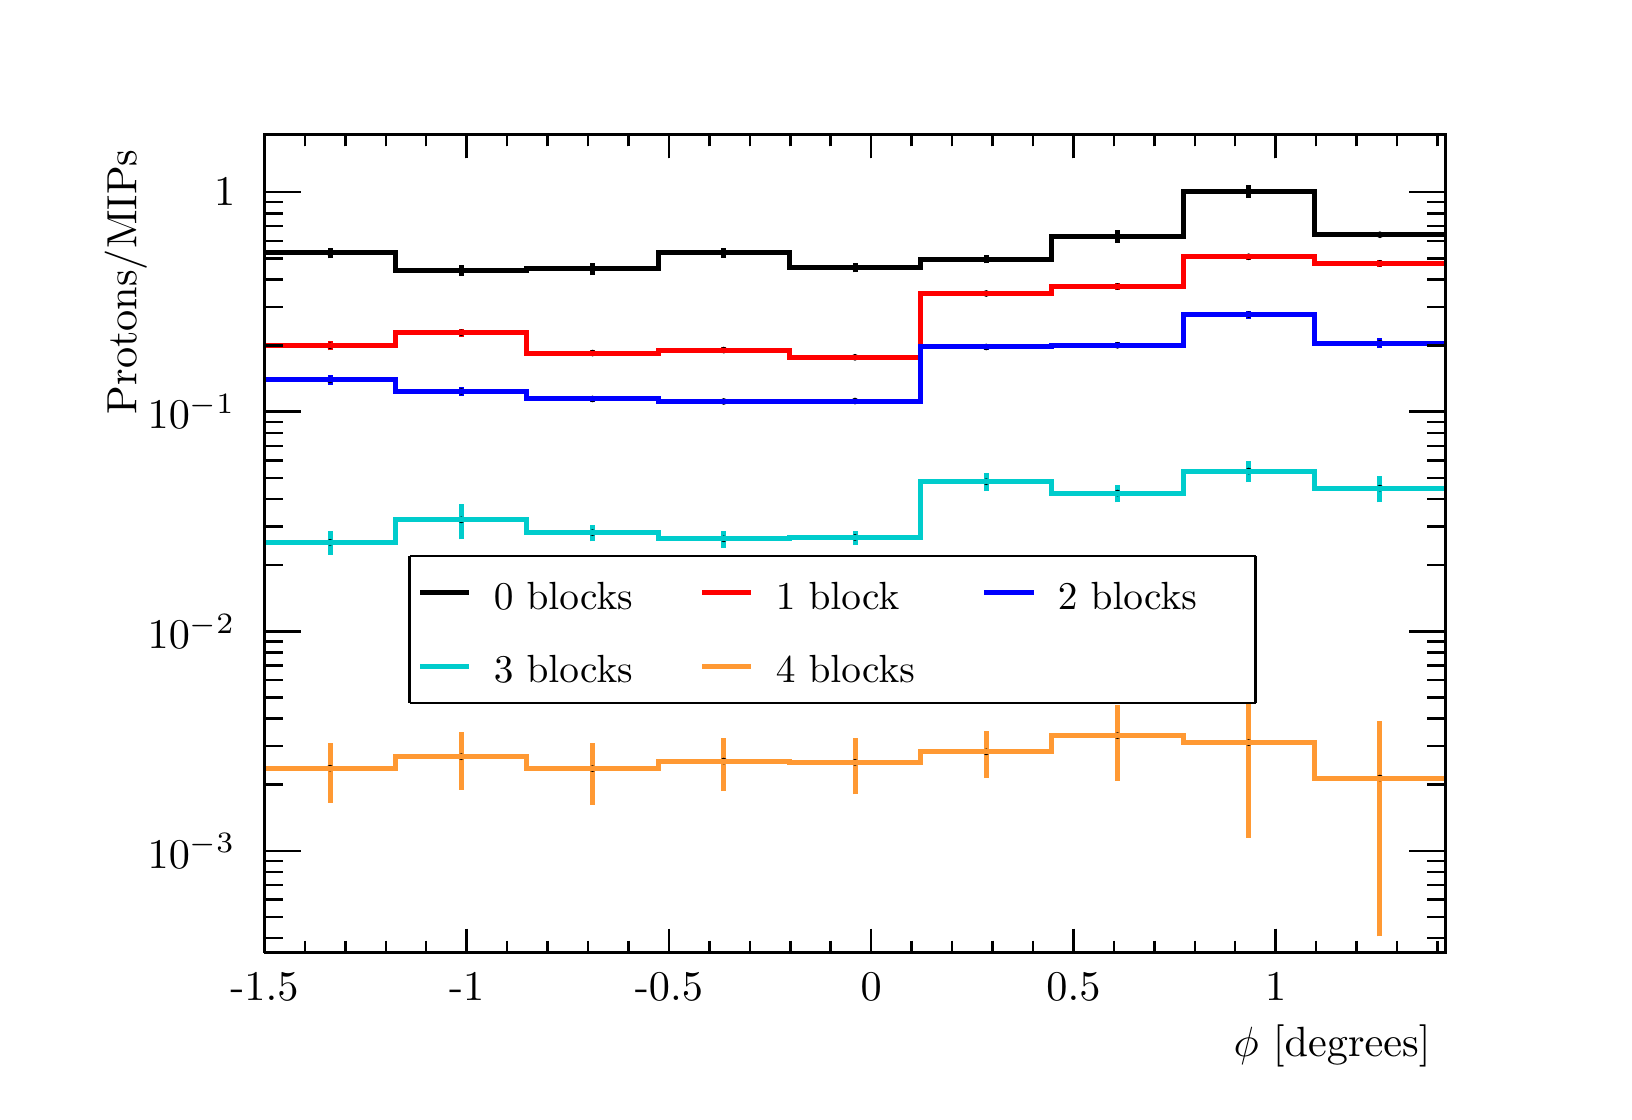
\begin{tikzpicture}
\pgfdeclareplotmark{cross} {
\pgfpathmoveto{\pgfpoint{-0.3\pgfplotmarksize}{\pgfplotmarksize}}
\pgfpathlineto{\pgfpoint{+0.3\pgfplotmarksize}{\pgfplotmarksize}}
\pgfpathlineto{\pgfpoint{+0.3\pgfplotmarksize}{0.3\pgfplotmarksize}}
\pgfpathlineto{\pgfpoint{+1\pgfplotmarksize}{0.3\pgfplotmarksize}}
\pgfpathlineto{\pgfpoint{+1\pgfplotmarksize}{-0.3\pgfplotmarksize}}
\pgfpathlineto{\pgfpoint{+0.3\pgfplotmarksize}{-0.3\pgfplotmarksize}}
\pgfpathlineto{\pgfpoint{+0.3\pgfplotmarksize}{-1.\pgfplotmarksize}}
\pgfpathlineto{\pgfpoint{-0.3\pgfplotmarksize}{-1.\pgfplotmarksize}}
\pgfpathlineto{\pgfpoint{-0.3\pgfplotmarksize}{-0.3\pgfplotmarksize}}
\pgfpathlineto{\pgfpoint{-1.\pgfplotmarksize}{-0.3\pgfplotmarksize}}
\pgfpathlineto{\pgfpoint{-1.\pgfplotmarksize}{0.3\pgfplotmarksize}}
\pgfpathlineto{\pgfpoint{-0.3\pgfplotmarksize}{0.3\pgfplotmarksize}}
\pgfpathclose
\pgfusepathqstroke
}
\pgfdeclareplotmark{cross*} {
\pgfpathmoveto{\pgfpoint{-0.3\pgfplotmarksize}{\pgfplotmarksize}}
\pgfpathlineto{\pgfpoint{+0.3\pgfplotmarksize}{\pgfplotmarksize}}
\pgfpathlineto{\pgfpoint{+0.3\pgfplotmarksize}{0.3\pgfplotmarksize}}
\pgfpathlineto{\pgfpoint{+1\pgfplotmarksize}{0.3\pgfplotmarksize}}
\pgfpathlineto{\pgfpoint{+1\pgfplotmarksize}{-0.3\pgfplotmarksize}}
\pgfpathlineto{\pgfpoint{+0.3\pgfplotmarksize}{-0.3\pgfplotmarksize}}
\pgfpathlineto{\pgfpoint{+0.3\pgfplotmarksize}{-1.\pgfplotmarksize}}
\pgfpathlineto{\pgfpoint{-0.3\pgfplotmarksize}{-1.\pgfplotmarksize}}
\pgfpathlineto{\pgfpoint{-0.3\pgfplotmarksize}{-0.3\pgfplotmarksize}}
\pgfpathlineto{\pgfpoint{-1.\pgfplotmarksize}{-0.3\pgfplotmarksize}}
\pgfpathlineto{\pgfpoint{-1.\pgfplotmarksize}{0.3\pgfplotmarksize}}
\pgfpathlineto{\pgfpoint{-0.3\pgfplotmarksize}{0.3\pgfplotmarksize}}
\pgfpathclose
\pgfusepathqfillstroke
}
\pgfdeclareplotmark{newstar} {
\pgfpathmoveto{\pgfqpoint{0pt}{\pgfplotmarksize}}
\pgfpathlineto{\pgfqpointpolar{44}{0.5\pgfplotmarksize}}
\pgfpathlineto{\pgfqpointpolar{18}{\pgfplotmarksize}}
\pgfpathlineto{\pgfqpointpolar{-20}{0.5\pgfplotmarksize}}
\pgfpathlineto{\pgfqpointpolar{-54}{\pgfplotmarksize}}
\pgfpathlineto{\pgfqpointpolar{-90}{0.5\pgfplotmarksize}}
\pgfpathlineto{\pgfqpointpolar{234}{\pgfplotmarksize}}
\pgfpathlineto{\pgfqpointpolar{198}{0.5\pgfplotmarksize}}
\pgfpathlineto{\pgfqpointpolar{162}{\pgfplotmarksize}}
\pgfpathlineto{\pgfqpointpolar{134}{0.5\pgfplotmarksize}}
\pgfpathclose
\pgfusepathqstroke
}
\pgfdeclareplotmark{newstar*} {
\pgfpathmoveto{\pgfqpoint{0pt}{\pgfplotmarksize}}
\pgfpathlineto{\pgfqpointpolar{44}{0.5\pgfplotmarksize}}
\pgfpathlineto{\pgfqpointpolar{18}{\pgfplotmarksize}}
\pgfpathlineto{\pgfqpointpolar{-20}{0.5\pgfplotmarksize}}
\pgfpathlineto{\pgfqpointpolar{-54}{\pgfplotmarksize}}
\pgfpathlineto{\pgfqpointpolar{-90}{0.5\pgfplotmarksize}}
\pgfpathlineto{\pgfqpointpolar{234}{\pgfplotmarksize}}
\pgfpathlineto{\pgfqpointpolar{198}{0.5\pgfplotmarksize}}
\pgfpathlineto{\pgfqpointpolar{162}{\pgfplotmarksize}}
\pgfpathlineto{\pgfqpointpolar{134}{0.5\pgfplotmarksize}}
\pgfpathclose
\pgfusepathqfillstroke
}
\definecolor{c}{rgb}{1,1,1};
\draw [color=c, fill=c] (0,0) rectangle (20,13.4957);
\draw [color=c, fill=c] (3,1.75444) rectangle (18,12.1461);
\definecolor{c}{rgb}{0,0,0};
\draw [c,line width=0.9] (3,1.75444) -- (3,12.1461) -- (18,12.1461) -- (18,1.75444) -- (3,1.75444);
\definecolor{c}{rgb}{1,1,1};
\draw [color=c, fill=c] (3,1.75444) rectangle (18,12.1461);
\definecolor{c}{rgb}{0,0,0};
\draw [c,line width=0.9] (3,1.75444) -- (3,12.1461) -- (18,12.1461) -- (18,1.75444) -- (3,1.75444);
\draw [c,line width=0.9] (3,1.75444) -- (4.66667,1.75444) -- (4.66667,1.75444) -- (6.33333,1.75444) -- (6.33333,1.75444) -- (8,1.75444) -- (8,1.75444) -- (9.66667,1.75444) -- (9.66667,1.75444) -- (11.3333,1.75444) -- (11.3333,1.75444) -- (13,1.75444)
 -- (13,1.75444) -- (14.6667,1.75444) -- (14.6667,1.75444) -- (16.3333,1.75444) -- (16.3333,1.75444) -- (18,1.75444);
\draw [c,line width=0.9] (3,1.75444) -- (18,1.75444);
\draw [c,line width=0.9] (3,2.05809) -- (3,1.75444);
\draw [c,line width=0.9] (3.5137,1.90627) -- (3.5137,1.75444);
\draw [c,line width=0.9] (4.0274,1.90627) -- (4.0274,1.75444);
\draw [c,line width=0.9] (4.5411,1.90627) -- (4.5411,1.75444);
\draw [c,line width=0.9] (5.05479,1.90627) -- (5.05479,1.75444);
\draw [c,line width=0.9] (5.56849,2.05809) -- (5.56849,1.75444);
\draw [c,line width=0.9] (6.08219,1.90627) -- (6.08219,1.75444);
\draw [c,line width=0.9] (6.59589,1.90627) -- (6.59589,1.75444);
\draw [c,line width=0.9] (7.10959,1.90627) -- (7.10959,1.75444);
\draw [c,line width=0.9] (7.62329,1.90627) -- (7.62329,1.75444);
\draw [c,line width=0.9] (8.13699,2.05809) -- (8.13699,1.75444);
\draw [c,line width=0.9] (8.65069,1.90627) -- (8.65069,1.75444);
\draw [c,line width=0.9] (9.16438,1.90627) -- (9.16438,1.75444);
\draw [c,line width=0.9] (9.67808,1.90627) -- (9.67808,1.75444);
\draw [c,line width=0.9] (10.1918,1.90627) -- (10.1918,1.75444);
\draw [c,line width=0.9] (10.7055,2.05809) -- (10.7055,1.75444);
\draw [c,line width=0.9] (11.2192,1.90627) -- (11.2192,1.75444);
\draw [c,line width=0.9] (11.7329,1.90627) -- (11.7329,1.75444);
\draw [c,line width=0.9] (12.2466,1.90627) -- (12.2466,1.75444);
\draw [c,line width=0.9] (12.7603,1.90627) -- (12.7603,1.75444);
\draw [c,line width=0.9] (13.274,2.05809) -- (13.274,1.75444);
\draw [c,line width=0.9] (13.7877,1.90627) -- (13.7877,1.75444);
\draw [c,line width=0.9] (14.3014,1.90627) -- (14.3014,1.75444);
\draw [c,line width=0.9] (14.8151,1.90627) -- (14.8151,1.75444);
\draw [c,line width=0.9] (15.3288,1.90627) -- (15.3288,1.75444);
\draw [c,line width=0.9] (15.8425,2.05809) -- (15.8425,1.75444);
\draw [c,line width=0.9] (15.8425,2.05809) -- (15.8425,1.75444);
\draw [c,line width=0.9] (16.3562,1.90627) -- (16.3562,1.75444);
\draw [c,line width=0.9] (16.8699,1.90627) -- (16.8699,1.75444);
\draw [c,line width=0.9] (17.3836,1.90627) -- (17.3836,1.75444);
\draw [c,line width=0.9] (17.8973,1.90627) -- (17.8973,1.75444);
\draw [anchor=base] (3,1.14713) node[scale=1.52731, color=c, rotate=0]{-1.5};
\draw [anchor=base] (5.56849,1.14713) node[scale=1.52731, color=c, rotate=0]{-1};
\draw [anchor=base] (8.13699,1.14713) node[scale=1.52731, color=c, rotate=0]{-0.5};
\draw [anchor=base] (10.7055,1.14713) node[scale=1.52731, color=c, rotate=0]{0};
\draw [anchor=base] (13.274,1.14713) node[scale=1.52731, color=c, rotate=0]{0.5};
\draw [anchor=base] (15.8425,1.14713) node[scale=1.52731, color=c, rotate=0]{1};
\draw [anchor= east] (18,0.566819) node[scale=1.52731, color=c, rotate=0]{$\phi$ [degrees]};
\draw [c,line width=0.9] (3,12.1461) -- (18,12.1461);
\draw [c,line width=0.9] (3,11.8425) -- (3,12.1461);
\draw [c,line width=0.9] (3.5137,11.9943) -- (3.5137,12.1461);
\draw [c,line width=0.9] (4.0274,11.9943) -- (4.0274,12.1461);
\draw [c,line width=0.9] (4.5411,11.9943) -- (4.5411,12.1461);
\draw [c,line width=0.9] (5.05479,11.9943) -- (5.05479,12.1461);
\draw [c,line width=0.9] (5.56849,11.8425) -- (5.56849,12.1461);
\draw [c,line width=0.9] (6.08219,11.9943) -- (6.08219,12.1461);
\draw [c,line width=0.9] (6.59589,11.9943) -- (6.59589,12.1461);
\draw [c,line width=0.9] (7.10959,11.9943) -- (7.10959,12.1461);
\draw [c,line width=0.9] (7.62329,11.9943) -- (7.62329,12.1461);
\draw [c,line width=0.9] (8.13699,11.8425) -- (8.13699,12.1461);
\draw [c,line width=0.9] (8.65069,11.9943) -- (8.65069,12.1461);
\draw [c,line width=0.9] (9.16438,11.9943) -- (9.16438,12.1461);
\draw [c,line width=0.9] (9.67808,11.9943) -- (9.67808,12.1461);
\draw [c,line width=0.9] (10.1918,11.9943) -- (10.1918,12.1461);
\draw [c,line width=0.9] (10.7055,11.8425) -- (10.7055,12.1461);
\draw [c,line width=0.9] (11.2192,11.9943) -- (11.2192,12.1461);
\draw [c,line width=0.9] (11.7329,11.9943) -- (11.7329,12.1461);
\draw [c,line width=0.9] (12.2466,11.9943) -- (12.2466,12.1461);
\draw [c,line width=0.9] (12.7603,11.9943) -- (12.7603,12.1461);
\draw [c,line width=0.9] (13.274,11.8425) -- (13.274,12.1461);
\draw [c,line width=0.9] (13.7877,11.9943) -- (13.7877,12.1461);
\draw [c,line width=0.9] (14.3014,11.9943) -- (14.3014,12.1461);
\draw [c,line width=0.9] (14.8151,11.9943) -- (14.8151,12.1461);
\draw [c,line width=0.9] (15.3288,11.9943) -- (15.3288,12.1461);
\draw [c,line width=0.9] (15.8425,11.8425) -- (15.8425,12.1461);
\draw [c,line width=0.9] (15.8425,11.8425) -- (15.8425,12.1461);
\draw [c,line width=0.9] (16.3562,11.9943) -- (16.3562,12.1461);
\draw [c,line width=0.9] (16.8699,11.9943) -- (16.8699,12.1461);
\draw [c,line width=0.9] (17.3836,11.9943) -- (17.3836,12.1461);
\draw [c,line width=0.9] (17.8973,11.9943) -- (17.8973,12.1461);
\draw [c,line width=0.9] (3,1.75444) -- (3,12.1461);
\draw [c,line width=0.9] (3.231,1.93919) -- (3,1.93919);
\draw [c,line width=0.9] (3.231,2.20939) -- (3,2.20939);
\draw [c,line width=0.9] (3.231,2.43016) -- (3,2.43016);
\draw [c,line width=0.9] (3.231,2.61681) -- (3,2.61681);
\draw [c,line width=0.9] (3.231,2.7785) -- (3,2.7785);
\draw [c,line width=0.9] (3.231,2.92112) -- (3,2.92112);
\draw [c,line width=0.9] (3.462,3.0487) -- (3,3.0487);
\draw [anchor= east] (2.82,3.0487) node[scale=1.52731, color=c, rotate=0]{$10^{-3}$};
\draw [c,line width=0.9] (3.231,3.88801) -- (3,3.88801);
\draw [c,line width=0.9] (3.231,4.37898) -- (3,4.37898);
\draw [c,line width=0.9] (3.231,4.72732) -- (3,4.72732);
\draw [c,line width=0.9] (3.231,4.99752) -- (3,4.99752);
\draw [c,line width=0.9] (3.231,5.21829) -- (3,5.21829);
\draw [c,line width=0.9] (3.231,5.40494) -- (3,5.40494);
\draw [c,line width=0.9] (3.231,5.56663) -- (3,5.56663);
\draw [c,line width=0.9] (3.231,5.70925) -- (3,5.70925);
\draw [c,line width=0.9] (3.462,5.83683) -- (3,5.83683);
\draw [anchor= east] (2.82,5.83683) node[scale=1.52731, color=c, rotate=0]{$10^{-2}$};
\draw [c,line width=0.9] (3.231,6.67614) -- (3,6.67614);
\draw [c,line width=0.9] (3.231,7.16711) -- (3,7.16711);
\draw [c,line width=0.9] (3.231,7.51545) -- (3,7.51545);
\draw [c,line width=0.9] (3.231,7.78565) -- (3,7.78565);
\draw [c,line width=0.9] (3.231,8.00642) -- (3,8.00642);
\draw [c,line width=0.9] (3.231,8.19307) -- (3,8.19307);
\draw [c,line width=0.9] (3.231,8.35476) -- (3,8.35476);
\draw [c,line width=0.9] (3.231,8.49738) -- (3,8.49738);
\draw [c,line width=0.9] (3.462,8.62496) -- (3,8.62496);
\draw [anchor= east] (2.82,8.62496) node[scale=1.52731, color=c, rotate=0]{$10^{-1}$};
\draw [c,line width=0.9] (3.231,9.46427) -- (3,9.46427);
\draw [c,line width=0.9] (3.231,9.95524) -- (3,9.95524);
\draw [c,line width=0.9] (3.231,10.3036) -- (3,10.3036);
\draw [c,line width=0.9] (3.231,10.5738) -- (3,10.5738);
\draw [c,line width=0.9] (3.231,10.7945) -- (3,10.7945);
\draw [c,line width=0.9] (3.231,10.9812) -- (3,10.9812);
\draw [c,line width=0.9] (3.231,11.1429) -- (3,11.1429);
\draw [c,line width=0.9] (3.231,11.2855) -- (3,11.2855);
\draw [c,line width=0.9] (3.462,11.4131) -- (3,11.4131);
\draw [anchor= east] (2.82,11.4131) node[scale=1.52731, color=c, rotate=0]{1};
\draw [anchor= east] (1.24,12.1461) node[scale=1.52731, color=c, rotate=90]{ Protons/MIPs};
\draw [c,line width=0.9] (18,1.75444) -- (18,12.1461);
\draw [c,line width=0.9] (17.769,1.93919) -- (18,1.93919);
\draw [c,line width=0.9] (17.769,2.20939) -- (18,2.20939);
\draw [c,line width=0.9] (17.769,2.43016) -- (18,2.43016);
\draw [c,line width=0.9] (17.769,2.61681) -- (18,2.61681);
\draw [c,line width=0.9] (17.769,2.7785) -- (18,2.7785);
\draw [c,line width=0.9] (17.769,2.92112) -- (18,2.92112);
\draw [c,line width=0.9] (17.538,3.0487) -- (18,3.0487);
\draw [c,line width=0.9] (17.769,3.88801) -- (18,3.88801);
\draw [c,line width=0.9] (17.769,4.37898) -- (18,4.37898);
\draw [c,line width=0.9] (17.769,4.72732) -- (18,4.72732);
\draw [c,line width=0.9] (17.769,4.99752) -- (18,4.99752);
\draw [c,line width=0.9] (17.769,5.21829) -- (18,5.21829);
\draw [c,line width=0.9] (17.769,5.40494) -- (18,5.40494);
\draw [c,line width=0.9] (17.769,5.56663) -- (18,5.56663);
\draw [c,line width=0.9] (17.769,5.70925) -- (18,5.70925);
\draw [c,line width=0.9] (17.538,5.83683) -- (18,5.83683);
\draw [c,line width=0.9] (17.769,6.67614) -- (18,6.67614);
\draw [c,line width=0.9] (17.769,7.16711) -- (18,7.16711);
\draw [c,line width=0.9] (17.769,7.51545) -- (18,7.51545);
\draw [c,line width=0.9] (17.769,7.78565) -- (18,7.78565);
\draw [c,line width=0.9] (17.769,8.00642) -- (18,8.00642);
\draw [c,line width=0.9] (17.769,8.19307) -- (18,8.19307);
\draw [c,line width=0.9] (17.769,8.35476) -- (18,8.35476);
\draw [c,line width=0.9] (17.769,8.49738) -- (18,8.49738);
\draw [c,line width=0.9] (17.538,8.62496) -- (18,8.62496);
\draw [c,line width=0.9] (17.769,9.46427) -- (18,9.46427);
\draw [c,line width=0.9] (17.769,9.95524) -- (18,9.95524);
\draw [c,line width=0.9] (17.769,10.3036) -- (18,10.3036);
\draw [c,line width=0.9] (17.769,10.5738) -- (18,10.5738);
\draw [c,line width=0.9] (17.769,10.7945) -- (18,10.7945);
\draw [c,line width=0.9] (17.769,10.9812) -- (18,10.9812);
\draw [c,line width=0.9] (17.769,11.1429) -- (18,11.1429);
\draw [c,line width=0.9] (17.769,11.2855) -- (18,11.2855);
\draw [c,line width=0.9] (17.538,11.4131) -- (18,11.4131);
\draw [c,line width=1.8] (3.83333,10.572) -- (3.83333,10.6419);
\draw [c,line width=1.8] (3.83333,10.6419) -- (3.83333,10.7081);
\foreach \P in {(3.83333,10.6419)}{\draw[mark options={color=c,fill=c},mark size=2.402402pt,mark=*,mark size=1pt] plot coordinates {\P};}
\draw [c,line width=1.8] (5.5,10.3482) -- (5.5,10.42);
\draw [c,line width=1.8] (5.5,10.42) -- (5.5,10.4878);
\foreach \P in {(5.5,10.42)}{\draw[mark options={color=c,fill=c},mark size=2.402402pt,mark=*,mark size=1pt] plot coordinates {\P};}
\draw [c,line width=1.8] (7.16667,10.3597) -- (7.16667,10.4384);
\draw [c,line width=1.8] (7.16667,10.4384) -- (7.16667,10.5124);
\foreach \P in {(7.16667,10.4384)}{\draw[mark options={color=c,fill=c},mark size=2.402402pt,mark=*,mark size=1pt] plot coordinates {\P};}
\draw [c,line width=1.8] (8.83333,10.5821) -- (8.83333,10.6443);
\draw [c,line width=1.8] (8.83333,10.6443) -- (8.83333,10.7033);
\foreach \P in {(8.83333,10.6443)}{\draw[mark options={color=c,fill=c},mark size=2.402402pt,mark=*,mark size=1pt] plot coordinates {\P};}
\draw [c,line width=1.8] (10.5,10.3955) -- (10.5,10.4552);
\draw [c,line width=1.8] (10.5,10.4552) -- (10.5,10.5121);
\foreach \P in {(10.5,10.4552)}{\draw[mark options={color=c,fill=c},mark size=2.402402pt,mark=*,mark size=1pt] plot coordinates {\P};}
\draw [c,line width=1.8] (12.1667,10.5095) -- (12.1667,10.5604);
\draw [c,line width=1.8] (12.1667,10.5604) -- (12.1667,10.6093);
\foreach \P in {(12.1667,10.5604)}{\draw[mark options={color=c,fill=c},mark size=2.402402pt,mark=*,mark size=1pt] plot coordinates {\P};}
\draw [c,line width=1.8] (13.8333,10.7682) -- (13.8333,10.8531);
\draw [c,line width=1.8] (13.8333,10.8531) -- (13.8333,10.9325);
\foreach \P in {(13.8333,10.8531)}{\draw[mark options={color=c,fill=c},mark size=2.402402pt,mark=*,mark size=1pt] plot coordinates {\P};}
\draw [c,line width=1.8] (15.5,11.3373) -- (15.5,11.424);
\draw [c,line width=1.8] (15.5,11.424) -- (15.5,11.505);
\foreach \P in {(15.5,11.424)}{\draw[mark options={color=c,fill=c},mark size=2.402402pt,mark=*,mark size=1pt] plot coordinates {\P};}
\draw [c,line width=1.8] (17.1667,10.8476) -- (17.1667,10.8726);
\draw [c,line width=1.8] (17.1667,10.8726) -- (17.1667,10.8972);
\foreach \P in {(17.1667,10.8726)}{\draw[mark options={color=c,fill=c},mark size=2.402402pt,mark=*,mark size=1pt] plot coordinates {\P};}
\draw [c,line width=1.8] (3,10.6419) -- (4.66667,10.6419) -- (4.66667,10.42) -- (6.33333,10.42) -- (6.33333,10.4384) -- (8,10.4384) -- (8,10.6443) -- (9.66667,10.6443) -- (9.66667,10.4552) -- (11.3333,10.4552) -- (11.3333,10.5604) -- (13,10.5604) --
 (13,10.8531) -- (14.6667,10.8531) -- (14.6667,11.424) -- (16.3333,11.424) -- (16.3333,10.8726) -- (18,10.8726);
\definecolor{c}{rgb}{1,0,0};
\draw [c,line width=1.8] (3.83333,9.40359) -- (3.83333,9.46301);
\draw [c,line width=1.8] (3.83333,9.46301) -- (3.83333,9.51965);
\definecolor{c}{rgb}{0,0,0};
\foreach \P in {(3.83333,9.46301)}{\draw[mark options={color=c,fill=c},mark size=2.402402pt,mark=*,mark size=1pt] plot coordinates {\P};}
\definecolor{c}{rgb}{1,0,0};
\draw [c,line width=1.8] (5.5,9.57854) -- (5.5,9.62851);
\draw [c,line width=1.8] (5.5,9.62851) -- (5.5,9.6765);
\definecolor{c}{rgb}{0,0,0};
\foreach \P in {(5.5,9.62851)}{\draw[mark options={color=c,fill=c},mark size=2.402402pt,mark=*,mark size=1pt] plot coordinates {\P};}
\definecolor{c}{rgb}{1,0,0};
\draw [c,line width=1.8] (7.16667,9.33523) -- (7.16667,9.37043);
\draw [c,line width=1.8] (7.16667,9.37043) -- (7.16667,9.40463);
\definecolor{c}{rgb}{0,0,0};
\foreach \P in {(7.16667,9.37043)}{\draw[mark options={color=c,fill=c},mark size=2.402402pt,mark=*,mark size=1pt] plot coordinates {\P};}
\definecolor{c}{rgb}{1,0,0};
\draw [c,line width=1.8] (8.83333,9.37028) -- (8.83333,9.40777);
\draw [c,line width=1.8] (8.83333,9.40777) -- (8.83333,9.44414);
\definecolor{c}{rgb}{0,0,0};
\foreach \P in {(8.83333,9.40777)}{\draw[mark options={color=c,fill=c},mark size=2.402402pt,mark=*,mark size=1pt] plot coordinates {\P};}
\definecolor{c}{rgb}{1,0,0};
\draw [c,line width=1.8] (10.5,9.28506) -- (10.5,9.31673);
\draw [c,line width=1.8] (10.5,9.31673) -- (10.5,9.3476);
\definecolor{c}{rgb}{0,0,0};
\foreach \P in {(10.5,9.31673)}{\draw[mark options={color=c,fill=c},mark size=2.402402pt,mark=*,mark size=1pt] plot coordinates {\P};}
\definecolor{c}{rgb}{1,0,0};
\draw [c,line width=1.8] (12.1667,10.0925) -- (12.1667,10.1267);
\draw [c,line width=1.8] (12.1667,10.1267) -- (12.1667,10.1601);
\definecolor{c}{rgb}{0,0,0};
\foreach \P in {(12.1667,10.1267)}{\draw[mark options={color=c,fill=c},mark size=2.402402pt,mark=*,mark size=1pt] plot coordinates {\P};}
\definecolor{c}{rgb}{1,0,0};
\draw [c,line width=1.8] (13.8333,10.1698) -- (13.8333,10.2162);
\draw [c,line width=1.8] (13.8333,10.2162) -- (13.8333,10.261);
\definecolor{c}{rgb}{0,0,0};
\foreach \P in {(13.8333,10.2162)}{\draw[mark options={color=c,fill=c},mark size=2.402402pt,mark=*,mark size=1pt] plot coordinates {\P};}
\definecolor{c}{rgb}{1,0,0};
\draw [c,line width=1.8] (15.5,10.5564) -- (15.5,10.5934);
\draw [c,line width=1.8] (15.5,10.5934) -- (15.5,10.6294);
\definecolor{c}{rgb}{0,0,0};
\foreach \P in {(15.5,10.5934)}{\draw[mark options={color=c,fill=c},mark size=2.402402pt,mark=*,mark size=1pt] plot coordinates {\P};}
\definecolor{c}{rgb}{1,0,0};
\draw [c,line width=1.8] (17.1667,10.4672) -- (17.1667,10.5099);
\draw [c,line width=1.8] (17.1667,10.5099) -- (17.1667,10.5512);
\definecolor{c}{rgb}{0,0,0};
\foreach \P in {(17.1667,10.5099)}{\draw[mark options={color=c,fill=c},mark size=2.402402pt,mark=*,mark size=1pt] plot coordinates {\P};}
\definecolor{c}{rgb}{1,0,0};
\draw [c,line width=1.8] (3,9.46301) -- (4.66667,9.46301) -- (4.66667,9.62851) -- (6.33333,9.62851) -- (6.33333,9.37043) -- (8,9.37043) -- (8,9.40777) -- (9.66667,9.40777) -- (9.66667,9.31673) -- (11.3333,9.31673) -- (11.3333,10.1267) -- (13,10.1267)
 -- (13,10.2162) -- (14.6667,10.2162) -- (14.6667,10.5934) -- (16.3333,10.5934) -- (16.3333,10.5099) -- (18,10.5099);
\definecolor{c}{rgb}{0,0,1};
\draw [c,line width=1.8] (3.83333,8.96981) -- (3.83333,9.02932);
\draw [c,line width=1.8] (3.83333,9.02932) -- (3.83333,9.08605);
\definecolor{c}{rgb}{0,0,0};
\foreach \P in {(3.83333,9.02932)}{\draw[mark options={color=c,fill=c},mark size=2.402402pt,mark=*,mark size=1pt] plot coordinates {\P};}
\definecolor{c}{rgb}{0,0,1};
\draw [c,line width=1.8] (5.5,8.83028) -- (5.5,8.88269);
\draw [c,line width=1.8] (5.5,8.88269) -- (5.5,8.93294);
\definecolor{c}{rgb}{0,0,0};
\foreach \P in {(5.5,8.88269)}{\draw[mark options={color=c,fill=c},mark size=2.402402pt,mark=*,mark size=1pt] plot coordinates {\P};}
\definecolor{c}{rgb}{0,0,1};
\draw [c,line width=1.8] (7.16667,8.74754) -- (7.16667,8.78715);
\draw [c,line width=1.8] (7.16667,8.78715) -- (7.16667,8.82551);
\definecolor{c}{rgb}{0,0,0};
\foreach \P in {(7.16667,8.78715)}{\draw[mark options={color=c,fill=c},mark size=2.402402pt,mark=*,mark size=1pt] plot coordinates {\P};}
\definecolor{c}{rgb}{0,0,1};
\draw [c,line width=1.8] (8.83333,8.72092) -- (8.83333,8.75543);
\draw [c,line width=1.8] (8.83333,8.75543) -- (8.83333,8.78898);
\definecolor{c}{rgb}{0,0,0};
\foreach \P in {(8.83333,8.75543)}{\draw[mark options={color=c,fill=c},mark size=2.402402pt,mark=*,mark size=1pt] plot coordinates {\P};}
\definecolor{c}{rgb}{0,0,1};
\draw [c,line width=1.8] (10.5,8.73099) -- (10.5,8.76081);
\draw [c,line width=1.8] (10.5,8.76081) -- (10.5,8.78991);
\definecolor{c}{rgb}{0,0,0};
\foreach \P in {(10.5,8.76081)}{\draw[mark options={color=c,fill=c},mark size=2.402402pt,mark=*,mark size=1pt] plot coordinates {\P};}
\definecolor{c}{rgb}{0,0,1};
\draw [c,line width=1.8] (12.1667,9.41213) -- (12.1667,9.44762);
\draw [c,line width=1.8] (12.1667,9.44762) -- (12.1667,9.48209);
\definecolor{c}{rgb}{0,0,0};
\foreach \P in {(12.1667,9.44762)}{\draw[mark options={color=c,fill=c},mark size=2.402402pt,mark=*,mark size=1pt] plot coordinates {\P};}
\definecolor{c}{rgb}{0,0,1};
\draw [c,line width=1.8] (13.8333,9.43055) -- (13.8333,9.4684);
\draw [c,line width=1.8] (13.8333,9.4684) -- (13.8333,9.5051);
\definecolor{c}{rgb}{0,0,0};
\foreach \P in {(13.8333,9.4684)}{\draw[mark options={color=c,fill=c},mark size=2.402402pt,mark=*,mark size=1pt] plot coordinates {\P};}
\definecolor{c}{rgb}{0,0,1};
\draw [c,line width=1.8] (15.5,9.80824) -- (15.5,9.8583);
\draw [c,line width=1.8] (15.5,9.8583) -- (15.5,9.90637);
\definecolor{c}{rgb}{0,0,0};
\foreach \P in {(15.5,9.8583)}{\draw[mark options={color=c,fill=c},mark size=2.402402pt,mark=*,mark size=1pt] plot coordinates {\P};}
\definecolor{c}{rgb}{0,0,1};
\draw [c,line width=1.8] (17.1667,9.43336) -- (17.1667,9.49632);
\draw [c,line width=1.8] (17.1667,9.49632) -- (17.1667,9.55617);
\definecolor{c}{rgb}{0,0,0};
\foreach \P in {(17.1667,9.49632)}{\draw[mark options={color=c,fill=c},mark size=2.402402pt,mark=*,mark size=1pt] plot coordinates {\P};}
\definecolor{c}{rgb}{0,0,1};
\draw [c,line width=1.8] (3,9.02932) -- (4.66667,9.02932) -- (4.66667,8.88269) -- (6.33333,8.88269) -- (6.33333,8.78715) -- (8,8.78715) -- (8,8.75543) -- (9.66667,8.75543) -- (9.66667,8.76081) -- (11.3333,8.76081) -- (11.3333,9.44762) -- (13,9.44762)
 -- (13,9.4684) -- (14.6667,9.4684) -- (14.6667,9.8583) -- (16.3333,9.8583) -- (16.3333,9.49632) -- (18,9.49632);
\definecolor{c}{rgb}{0,0.8,0.8};
\draw [c,line width=1.8] (3.83333,6.80707) -- (3.83333,6.96591);
\draw [c,line width=1.8] (3.83333,6.96591) -- (3.83333,7.10631);
\definecolor{c}{rgb}{0,0,0};
\foreach \P in {(3.83333,6.96591)}{\draw[mark options={color=c,fill=c},mark size=2.402402pt,mark=*,mark size=1pt] plot coordinates {\P};}
\definecolor{c}{rgb}{0,0.8,0.8};
\draw [c,line width=1.8] (5.5,7.00316) -- (5.5,7.25221);
\draw [c,line width=1.8] (5.5,7.25221) -- (5.5,7.45867);
\definecolor{c}{rgb}{0,0,0};
\foreach \P in {(5.5,7.25221)}{\draw[mark options={color=c,fill=c},mark size=2.402402pt,mark=*,mark size=1pt] plot coordinates {\P};}
\definecolor{c}{rgb}{0,0.8,0.8};
\draw [c,line width=1.8] (7.16667,6.97812) -- (7.16667,7.08972);
\draw [c,line width=1.8] (7.16667,7.08972) -- (7.16667,7.1919);
\definecolor{c}{rgb}{0,0,0};
\foreach \P in {(7.16667,7.08972)}{\draw[mark options={color=c,fill=c},mark size=2.402402pt,mark=*,mark size=1pt] plot coordinates {\P};}
\definecolor{c}{rgb}{0,0.8,0.8};
\draw [c,line width=1.8] (8.83333,6.89753) -- (8.83333,7.01091);
\draw [c,line width=1.8] (8.83333,7.01091) -- (8.83333,7.11458);
\definecolor{c}{rgb}{0,0,0};
\foreach \P in {(8.83333,7.01091)}{\draw[mark options={color=c,fill=c},mark size=2.402402pt,mark=*,mark size=1pt] plot coordinates {\P};}
\definecolor{c}{rgb}{0,0.8,0.8};
\draw [c,line width=1.8] (10.5,6.9388) -- (10.5,7.0284);
\draw [c,line width=1.8] (10.5,7.0284) -- (10.5,7.11182);
\definecolor{c}{rgb}{0,0,0};
\foreach \P in {(10.5,7.0284)}{\draw[mark options={color=c,fill=c},mark size=2.402402pt,mark=*,mark size=1pt] plot coordinates {\P};}
\definecolor{c}{rgb}{0,0.8,0.8};
\draw [c,line width=1.8] (12.1667,7.61534) -- (12.1667,7.73673);
\draw [c,line width=1.8] (12.1667,7.73673) -- (12.1667,7.84705);
\definecolor{c}{rgb}{0,0,0};
\foreach \P in {(12.1667,7.73673)}{\draw[mark options={color=c,fill=c},mark size=2.402402pt,mark=*,mark size=1pt] plot coordinates {\P};}
\definecolor{c}{rgb}{0,0.8,0.8};
\draw [c,line width=1.8] (13.8333,7.47538) -- (13.8333,7.59226);
\draw [c,line width=1.8] (13.8333,7.59226) -- (13.8333,7.69885);
\definecolor{c}{rgb}{0,0,0};
\foreach \P in {(13.8333,7.59226)}{\draw[mark options={color=c,fill=c},mark size=2.402402pt,mark=*,mark size=1pt] plot coordinates {\P};}
\definecolor{c}{rgb}{0,0.8,0.8};
\draw [c,line width=1.8] (15.5,7.73149) -- (15.5,7.87156);
\draw [c,line width=1.8] (15.5,7.87156) -- (15.5,7.9971);
\definecolor{c}{rgb}{0,0,0};
\foreach \P in {(15.5,7.87156)}{\draw[mark options={color=c,fill=c},mark size=2.402402pt,mark=*,mark size=1pt] plot coordinates {\P};}
\definecolor{c}{rgb}{0,0.8,0.8};
\draw [c,line width=1.8] (17.1667,7.47332) -- (17.1667,7.65497);
\draw [c,line width=1.8] (17.1667,7.65497) -- (17.1667,7.81288);
\definecolor{c}{rgb}{0,0,0};
\foreach \P in {(17.1667,7.65497)}{\draw[mark options={color=c,fill=c},mark size=2.402402pt,mark=*,mark size=1pt] plot coordinates {\P};}
\definecolor{c}{rgb}{0,0.8,0.8};
\draw [c,line width=1.8] (3,6.96591) -- (4.66667,6.96591) -- (4.66667,7.25221) -- (6.33333,7.25221) -- (6.33333,7.08972) -- (8,7.08972) -- (8,7.01091) -- (9.66667,7.01091) -- (9.66667,7.0284) -- (11.3333,7.0284) -- (11.3333,7.73673) -- (13,7.73673)
 -- (13,7.59226) -- (14.6667,7.59226) -- (14.6667,7.87156) -- (16.3333,7.87156) -- (16.3333,7.65497) -- (18,7.65497);
\definecolor{c}{rgb}{1,0.6,0.2};
\draw [c,line width=1.8] (3.83333,3.66164) -- (3.83333,4.09876);
\draw [c,line width=1.8] (3.83333,4.09876) -- (3.83333,4.41926);
\definecolor{c}{rgb}{0,0,0};
\foreach \P in {(3.83333,4.09876)}{\draw[mark options={color=c,fill=c},mark size=2.402402pt,mark=*,mark size=1pt] plot coordinates {\P};}
\definecolor{c}{rgb}{1,0.6,0.2};
\draw [c,line width=1.8] (5.5,3.82735) -- (5.5,4.24444);
\draw [c,line width=1.8] (5.5,4.24444) -- (5.5,4.55409);
\definecolor{c}{rgb}{0,0,0};
\foreach \P in {(5.5,4.24444)}{\draw[mark options={color=c,fill=c},mark size=2.402402pt,mark=*,mark size=1pt] plot coordinates {\P};}
\definecolor{c}{rgb}{1,0.6,0.2};
\draw [c,line width=1.8] (7.16667,3.63482) -- (7.16667,4.09249);
\draw [c,line width=1.8] (7.16667,4.09249) -- (7.16667,4.42384);
\definecolor{c}{rgb}{0,0,0};
\foreach \P in {(7.16667,4.09249)}{\draw[mark options={color=c,fill=c},mark size=2.402402pt,mark=*,mark size=1pt] plot coordinates {\P};}
\definecolor{c}{rgb}{1,0.6,0.2};
\draw [c,line width=1.8] (8.83333,3.80636) -- (8.83333,4.18831);
\draw [c,line width=1.8] (8.83333,4.18831) -- (8.83333,4.47823);
\definecolor{c}{rgb}{0,0,0};
\foreach \P in {(8.83333,4.18831)}{\draw[mark options={color=c,fill=c},mark size=2.402402pt,mark=*,mark size=1pt] plot coordinates {\P};}
\definecolor{c}{rgb}{1,0.6,0.2};
\draw [c,line width=1.8] (10.5,3.76571) -- (10.5,4.17192);
\draw [c,line width=1.8] (10.5,4.17192) -- (10.5,4.47555);
\definecolor{c}{rgb}{0,0,0};
\foreach \P in {(10.5,4.17192)}{\draw[mark options={color=c,fill=c},mark size=2.402402pt,mark=*,mark size=1pt] plot coordinates {\P};}
\definecolor{c}{rgb}{1,0.6,0.2};
\draw [c,line width=1.8] (12.1667,3.97351) -- (12.1667,4.30575);
\draw [c,line width=1.8] (12.1667,4.30575) -- (12.1667,4.56619);
\definecolor{c}{rgb}{0,0,0};
\foreach \P in {(12.1667,4.30575)}{\draw[mark options={color=c,fill=c},mark size=2.402402pt,mark=*,mark size=1pt] plot coordinates {\P};}
\definecolor{c}{rgb}{1,0.6,0.2};
\draw [c,line width=1.8] (13.8333,3.93934) -- (13.8333,4.5115);
\draw [c,line width=1.8] (13.8333,4.5115) -- (13.8333,4.89848);
\definecolor{c}{rgb}{0,0,0};
\foreach \P in {(13.8333,4.5115)}{\draw[mark options={color=c,fill=c},mark size=2.402402pt,mark=*,mark size=1pt] plot coordinates {\P};}
\definecolor{c}{rgb}{1,0.6,0.2};
\draw [c,line width=1.8] (15.5,3.21511) -- (15.5,4.42355);
\draw [c,line width=1.8] (15.5,4.42355) -- (15.5,5.01619);
\definecolor{c}{rgb}{0,0,0};
\foreach \P in {(15.5,4.42355)}{\draw[mark options={color=c,fill=c},mark size=2.402402pt,mark=*,mark size=1pt] plot coordinates {\P};}
\definecolor{c}{rgb}{1,0.6,0.2};
\draw [c,line width=1.8] (17.1667,1.96315) -- (17.1667,3.97294);
\draw [c,line width=1.8] (17.1667,3.97294) -- (17.1667,4.69126);
\definecolor{c}{rgb}{0,0,0};
\foreach \P in {(17.1667,3.97294)}{\draw[mark options={color=c,fill=c},mark size=2.402402pt,mark=*,mark size=1pt] plot coordinates {\P};}
\definecolor{c}{rgb}{1,0.6,0.2};
\draw [c,line width=1.8] (3,4.09876) -- (4.66667,4.09876) -- (4.66667,4.24444) -- (6.33333,4.24444) -- (6.33333,4.09249) -- (8,4.09249) -- (8,4.18831) -- (9.66667,4.18831) -- (9.66667,4.17192) -- (11.3333,4.17192) -- (11.3333,4.30575) -- (13,4.30575)
 -- (13,4.5115) -- (14.6667,4.5115) -- (14.6667,4.42355) -- (16.3333,4.42355) -- (16.3333,3.97294) -- (18,3.97294);
\definecolor{c}{rgb}{0,0,0};
\draw [c,line width=0.9] (3,1.75444) -- (18,1.75444);
\draw [c,line width=0.9] (3,2.05809) -- (3,1.75444);
\draw [c,line width=0.9] (3.5137,1.90627) -- (3.5137,1.75444);
\draw [c,line width=0.9] (4.0274,1.90627) -- (4.0274,1.75444);
\draw [c,line width=0.9] (4.5411,1.90627) -- (4.5411,1.75444);
\draw [c,line width=0.9] (5.05479,1.90627) -- (5.05479,1.75444);
\draw [c,line width=0.9] (5.56849,2.05809) -- (5.56849,1.75444);
\draw [c,line width=0.9] (6.08219,1.90627) -- (6.08219,1.75444);
\draw [c,line width=0.9] (6.59589,1.90627) -- (6.59589,1.75444);
\draw [c,line width=0.9] (7.10959,1.90627) -- (7.10959,1.75444);
\draw [c,line width=0.9] (7.62329,1.90627) -- (7.62329,1.75444);
\draw [c,line width=0.9] (8.13699,2.05809) -- (8.13699,1.75444);
\draw [c,line width=0.9] (8.65069,1.90627) -- (8.65069,1.75444);
\draw [c,line width=0.9] (9.16438,1.90627) -- (9.16438,1.75444);
\draw [c,line width=0.9] (9.67808,1.90627) -- (9.67808,1.75444);
\draw [c,line width=0.9] (10.1918,1.90627) -- (10.1918,1.75444);
\draw [c,line width=0.9] (10.7055,2.05809) -- (10.7055,1.75444);
\draw [c,line width=0.9] (11.2192,1.90627) -- (11.2192,1.75444);
\draw [c,line width=0.9] (11.7329,1.90627) -- (11.7329,1.75444);
\draw [c,line width=0.9] (12.2466,1.90627) -- (12.2466,1.75444);
\draw [c,line width=0.9] (12.7603,1.90627) -- (12.7603,1.75444);
\draw [c,line width=0.9] (13.274,2.05809) -- (13.274,1.75444);
\draw [c,line width=0.9] (13.7877,1.90627) -- (13.7877,1.75444);
\draw [c,line width=0.9] (14.3014,1.90627) -- (14.3014,1.75444);
\draw [c,line width=0.9] (14.8151,1.90627) -- (14.8151,1.75444);
\draw [c,line width=0.9] (15.3288,1.90627) -- (15.3288,1.75444);
\draw [c,line width=0.9] (15.8425,2.05809) -- (15.8425,1.75444);
\draw [c,line width=0.9] (15.8425,2.05809) -- (15.8425,1.75444);
\draw [c,line width=0.9] (16.3562,1.90627) -- (16.3562,1.75444);
\draw [c,line width=0.9] (16.8699,1.90627) -- (16.8699,1.75444);
\draw [c,line width=0.9] (17.3836,1.90627) -- (17.3836,1.75444);
\draw [c,line width=0.9] (17.8973,1.90627) -- (17.8973,1.75444);
\draw [c,line width=0.9] (3,12.1461) -- (18,12.1461);
\draw [c,line width=0.9] (3,11.8425) -- (3,12.1461);
\draw [c,line width=0.9] (3.5137,11.9943) -- (3.5137,12.1461);
\draw [c,line width=0.9] (4.0274,11.9943) -- (4.0274,12.1461);
\draw [c,line width=0.9] (4.5411,11.9943) -- (4.5411,12.1461);
\draw [c,line width=0.9] (5.05479,11.9943) -- (5.05479,12.1461);
\draw [c,line width=0.9] (5.56849,11.8425) -- (5.56849,12.1461);
\draw [c,line width=0.9] (6.08219,11.9943) -- (6.08219,12.1461);
\draw [c,line width=0.9] (6.59589,11.9943) -- (6.59589,12.1461);
\draw [c,line width=0.9] (7.10959,11.9943) -- (7.10959,12.1461);
\draw [c,line width=0.9] (7.62329,11.9943) -- (7.62329,12.1461);
\draw [c,line width=0.9] (8.13699,11.8425) -- (8.13699,12.1461);
\draw [c,line width=0.9] (8.65069,11.9943) -- (8.65069,12.1461);
\draw [c,line width=0.9] (9.16438,11.9943) -- (9.16438,12.1461);
\draw [c,line width=0.9] (9.67808,11.9943) -- (9.67808,12.1461);
\draw [c,line width=0.9] (10.1918,11.9943) -- (10.1918,12.1461);
\draw [c,line width=0.9] (10.7055,11.8425) -- (10.7055,12.1461);
\draw [c,line width=0.9] (11.2192,11.9943) -- (11.2192,12.1461);
\draw [c,line width=0.9] (11.7329,11.9943) -- (11.7329,12.1461);
\draw [c,line width=0.9] (12.2466,11.9943) -- (12.2466,12.1461);
\draw [c,line width=0.9] (12.7603,11.9943) -- (12.7603,12.1461);
\draw [c,line width=0.9] (13.274,11.8425) -- (13.274,12.1461);
\draw [c,line width=0.9] (13.7877,11.9943) -- (13.7877,12.1461);
\draw [c,line width=0.9] (14.3014,11.9943) -- (14.3014,12.1461);
\draw [c,line width=0.9] (14.8151,11.9943) -- (14.8151,12.1461);
\draw [c,line width=0.9] (15.3288,11.9943) -- (15.3288,12.1461);
\draw [c,line width=0.9] (15.8425,11.8425) -- (15.8425,12.1461);
\draw [c,line width=0.9] (15.8425,11.8425) -- (15.8425,12.1461);
\draw [c,line width=0.9] (16.3562,11.9943) -- (16.3562,12.1461);
\draw [c,line width=0.9] (16.8699,11.9943) -- (16.8699,12.1461);
\draw [c,line width=0.9] (17.3836,11.9943) -- (17.3836,12.1461);
\draw [c,line width=0.9] (17.8973,11.9943) -- (17.8973,12.1461);
\draw [c,line width=0.9] (3,1.75444) -- (3,12.1461);
\draw [c,line width=0.9] (3.231,1.93919) -- (3,1.93919);
\draw [c,line width=0.9] (3.231,2.20939) -- (3,2.20939);
\draw [c,line width=0.9] (3.231,2.43016) -- (3,2.43016);
\draw [c,line width=0.9] (3.231,2.61681) -- (3,2.61681);
\draw [c,line width=0.9] (3.231,2.7785) -- (3,2.7785);
\draw [c,line width=0.9] (3.231,2.92112) -- (3,2.92112);
\draw [c,line width=0.9] (3.462,3.0487) -- (3,3.0487);
\draw [c,line width=0.9] (3.231,3.88801) -- (3,3.88801);
\draw [c,line width=0.9] (3.231,4.37898) -- (3,4.37898);
\draw [c,line width=0.9] (3.231,4.72732) -- (3,4.72732);
\draw [c,line width=0.9] (3.231,4.99752) -- (3,4.99752);
\draw [c,line width=0.9] (3.231,5.21829) -- (3,5.21829);
\draw [c,line width=0.9] (3.231,5.40494) -- (3,5.40494);
\draw [c,line width=0.9] (3.231,5.56663) -- (3,5.56663);
\draw [c,line width=0.9] (3.231,5.70925) -- (3,5.70925);
\draw [c,line width=0.9] (3.462,5.83683) -- (3,5.83683);
\draw [c,line width=0.9] (3.231,6.67614) -- (3,6.67614);
\draw [c,line width=0.9] (3.231,7.16711) -- (3,7.16711);
\draw [c,line width=0.9] (3.231,7.51545) -- (3,7.51545);
\draw [c,line width=0.9] (3.231,7.78565) -- (3,7.78565);
\draw [c,line width=0.9] (3.231,8.00642) -- (3,8.00642);
\draw [c,line width=0.9] (3.231,8.19307) -- (3,8.19307);
\draw [c,line width=0.9] (3.231,8.35476) -- (3,8.35476);
\draw [c,line width=0.9] (3.231,8.49738) -- (3,8.49738);
\draw [c,line width=0.9] (3.462,8.62496) -- (3,8.62496);
\draw [c,line width=0.9] (3.231,9.46427) -- (3,9.46427);
\draw [c,line width=0.9] (3.231,9.95524) -- (3,9.95524);
\draw [c,line width=0.9] (3.231,10.3036) -- (3,10.3036);
\draw [c,line width=0.9] (3.231,10.5738) -- (3,10.5738);
\draw [c,line width=0.9] (3.231,10.7945) -- (3,10.7945);
\draw [c,line width=0.9] (3.231,10.9812) -- (3,10.9812);
\draw [c,line width=0.9] (3.231,11.1429) -- (3,11.1429);
\draw [c,line width=0.9] (3.231,11.2855) -- (3,11.2855);
\draw [c,line width=0.9] (3.462,11.4131) -- (3,11.4131);
\draw [c,line width=0.9] (18,1.75444) -- (18,12.1461);
\draw [c,line width=0.9] (17.769,1.93919) -- (18,1.93919);
\draw [c,line width=0.9] (17.769,2.20939) -- (18,2.20939);
\draw [c,line width=0.9] (17.769,2.43016) -- (18,2.43016);
\draw [c,line width=0.9] (17.769,2.61681) -- (18,2.61681);
\draw [c,line width=0.9] (17.769,2.7785) -- (18,2.7785);
\draw [c,line width=0.9] (17.769,2.92112) -- (18,2.92112);
\draw [c,line width=0.9] (17.538,3.0487) -- (18,3.0487);
\draw [c,line width=0.9] (17.769,3.88801) -- (18,3.88801);
\draw [c,line width=0.9] (17.769,4.37898) -- (18,4.37898);
\draw [c,line width=0.9] (17.769,4.72732) -- (18,4.72732);
\draw [c,line width=0.9] (17.769,4.99752) -- (18,4.99752);
\draw [c,line width=0.9] (17.769,5.21829) -- (18,5.21829);
\draw [c,line width=0.9] (17.769,5.40494) -- (18,5.40494);
\draw [c,line width=0.9] (17.769,5.56663) -- (18,5.56663);
\draw [c,line width=0.9] (17.769,5.70925) -- (18,5.70925);
\draw [c,line width=0.9] (17.538,5.83683) -- (18,5.83683);
\draw [c,line width=0.9] (17.769,6.67614) -- (18,6.67614);
\draw [c,line width=0.9] (17.769,7.16711) -- (18,7.16711);
\draw [c,line width=0.9] (17.769,7.51545) -- (18,7.51545);
\draw [c,line width=0.9] (17.769,7.78565) -- (18,7.78565);
\draw [c,line width=0.9] (17.769,8.00642) -- (18,8.00642);
\draw [c,line width=0.9] (17.769,8.19307) -- (18,8.19307);
\draw [c,line width=0.9] (17.769,8.35476) -- (18,8.35476);
\draw [c,line width=0.9] (17.769,8.49738) -- (18,8.49738);
\draw [c,line width=0.9] (17.538,8.62496) -- (18,8.62496);
\draw [c,line width=0.9] (17.769,9.46427) -- (18,9.46427);
\draw [c,line width=0.9] (17.769,9.95524) -- (18,9.95524);
\draw [c,line width=0.9] (17.769,10.3036) -- (18,10.3036);
\draw [c,line width=0.9] (17.769,10.5738) -- (18,10.5738);
\draw [c,line width=0.9] (17.769,10.7945) -- (18,10.7945);
\draw [c,line width=0.9] (17.769,10.9812) -- (18,10.9812);
\draw [c,line width=0.9] (17.769,11.1429) -- (18,11.1429);
\draw [c,line width=0.9] (17.769,11.2855) -- (18,11.2855);
\draw [c,line width=0.9] (17.538,11.4131) -- (18,11.4131);
\definecolor{c}{rgb}{1,1,1};
\draw [color=c, fill=c] (2,12.686) rectangle (18,13.4282);
\definecolor{c}{rgb}{0,0,0};
%\draw (10,13.0571) node[scale=1.40004, color=c, rotate=0]{$S1 \cap S2 \cap S4 angular distribution of proton/MIP ratio$};
\definecolor{c}{rgb}{1,1,1};
\draw [color=c, fill=c] (4.84241,4.92837) rectangle (15.5874,6.79083);
\definecolor{c}{rgb}{0,0,0};
\draw [c,line width=0.9] (4.84241,4.92837) -- (15.5874,4.92837);
\draw [c,line width=0.9] (15.5874,4.92837) -- (15.5874,6.79083);
\draw [c,line width=0.9] (15.5874,6.79083) -- (4.84241,6.79083);
\draw [c,line width=0.9] (4.84241,6.79083) -- (4.84241,4.92837);
\draw [anchor=base west] (5.73782,6.11569) node[scale=1.42, color=c, rotate=0]{0 blocks};
\draw [c,line width=1.8] (4.97672,6.32521) -- (5.60351,6.32521);
\draw [anchor=base west] (9.31948,6.11569) node[scale=1.42, color=c, rotate=0]{1 block};
\definecolor{c}{rgb}{1,0,0};
\draw [c,line width=1.8] (8.55838,6.32521) -- (9.18517,6.32521);
\definecolor{c}{rgb}{0,0,0};
\draw [anchor=base west] (12.9011,6.11569) node[scale=1.42, color=c, rotate=0]{2 blocks};
\definecolor{c}{rgb}{0,0,1};
\draw [c,line width=1.8] (12.14,6.32521) -- (12.7668,6.32521);
\definecolor{c}{rgb}{0,0,0};
\draw [anchor=base west] (5.73782,5.18446) node[scale=1.42, color=c, rotate=0]{3 blocks};
\definecolor{c}{rgb}{0,0.8,0.8};
\draw [c,line width=1.8] (4.97672,5.39398) -- (5.60351,5.39398);
\definecolor{c}{rgb}{0,0,0};
\draw [anchor=base west] (9.31948,5.18446) node[scale=1.42, color=c, rotate=0]{4 blocks};
\definecolor{c}{rgb}{1,0.6,0.2};
\draw [c,line width=1.8] (8.55838,5.39398) -- (9.18517,5.39398);
\end{tikzpicture}

    \end{adjustbox}
  \end{minipage}
  \caption[Proton/MIP ratios as measured in \SFour as a function of $\theta$ and $\phi$]{Proton/MIP ratios as measured in \SFour as a function of $\theta$ and $\phi$}
  \label{fig:s4Ratios}
\end{figure}

\subsection{Comparisons with simulation}
\label{sec:hptpc_beam_flux:results:MCData}

\citefig{fig:protonKeData} right, provides a measurement of the number of protons incident upon the TPC.
However, in order to gain an estimate of the number and energy of protons traversing the TPC, a Monte Carlo (MC) simulation is performed using GEANT4~\cite{geant}.
The simulation contains geometric volumes representing the pressure vessel, the TPC and \SFour.
Protons are propagated through this geometry, with their starting positions and momenta taken from \SThree data (see \citefig{fig:protonKeData}).
This step ensures that the input distributions match the true beam conditions as closely as possible.

The simulation is validated in multiple ways.
The simulated and measured time of flight spectra are compared.
Additionally, the ratio of protons detected in \SThree and \SFour is compared in data and MC.
The systematic uncertainties on the latter measurement are discussed in \citesec{sec:hptpc_beam_flux:results:MCData:systs}, while the validation is discussed in \citesec{sec:hptpc_beam_flux:results:MCData:validation}.
The results of the simulation are discussed in \citesec{sec:hptpc_beam_flux:results:MCData:results}

\subsubsection{Systematic uncertainties}
\label{sec:hptpc_beam_flux:results:MCData:systs}

Systematic uncertainties on the number of protons measured in \SThree and \SFour are estimated for both simulation and data.
These uncertainties are tabulated in \citetab{tab:systs}.

The systematic uncertainty on the number of simulated protons reaching \SFour, $n_{\SFour,~\text{MC}}$, is evaluated by varying the initial geometric conditions of the simulation and observing the fractional change in $n_{\SFour,~\text{MC}}$.
Additionally, the simulation is rerun with an additional \SI{1}{\centi\metre} thick piece of acrylic in the beamline and the change in $n_{\SFour,~\text{MC}}$ observed.
We allow this systematic to act as a proxy for the uncertainty on the prescence of unknown light materials in the beamline.

\begin{table}
  \caption[Systematic errors on the number of protons at \SThree and \SFour for data and Monte Carlo]{Systematic errors on the number of protons at \SThree and \SFour for data and Monte Carlo. All values are the percent error of the \SFour proton count with the exception of the uncertainty on the efficiency of \SThree which is the percent error on the proton count measured in \SThree. All of these uncertainties are treated as uncorrelated.}
  \label{tab:systs}
  \begin{tabular}{c c c c c c}
    \hline
    \hline
    \multicolumn{6}{c}{\textbf{Monte Carlo}} \\
    \hline
    & \multicolumn{5}{c}{Number of moderator blocks} \\
    & 0 & 1 & 2 & 3 & 4 \\
    \hline
    Systematic uncertainty on $n_{\mathit{S4},~\text{MC}}$ & 9.5\% & 8.0\% & 8.5\% & 17.0\% & 8.0\% \\
    \hline
    \multicolumn{6}{c}{\textbf{Data}} \\
    \hline
    & \multicolumn{5}{c}{Number of moderator blocks} \\
    Source of systematic error & 0 & 1 & 2 & 3 & 4 \\
    \hline
    Absolute efficiency of $\mathit{S3}$ & 1.1\% & 11.4\% & 7.0\% & 11.4\% & 4.9\% \\
    Absolute efficiency of $\mathit{S4}$ & 11.0\% & 11.0\% & 11.0\% & 11.0\% & 11.0\% \\ 
    $\mathit{S4}$ angular correction & 2.9\% & 1.5\% & 6.7\% & 8.2\% & 4.1\% \\
    $\mathit{S4}$ background uncertainty & 0.18\% & 0.16\% & 1.1\% & 1.4\% & 8.1\% \\
    \hline
    \textbf{Total} & 11.5\% & 16.0\% & 14.7\% & 18.3\% & 18.9\% \\
    \hline
  \end{tabular}
\end{table}

For data, the error on the absolute efficiency of \SThree is evaluated by taking the $\pm 1 \sigma$ uncertainty on the fitted relationship between $(\SOne\STwo)_{\text{UToF}}/(\SOne\STwo)_{\text{DToF}}$ and $(\SOne\STwo)_{\text{DToF}}$ (see \citesec{sec:hptpc_beam_flux:methods:s3:deadtime}) and evaluating the fractional change in the number of protons detected by \SThree.

The error on the absolute efficiency of \SFour is evaluated from the calibration tests performed on the bars with a $^{90}\text{Sr}$ source (see \citesec{sec:hptpc_dtof_characterisation:characterisation:barRes}).
From these tests an absolute efficiency of 0.8 was determined.
However, the readout used in these tests is significantly different to that used in the beam test and therefore there is a significant uncertainty attached to this number.
This uncertainty was evaluated by taking the standard deviation in the absolute efficiency measured using the $^{90}\text{Sr}$ source.

The uncertainty on the \SFour relative efficiency correction (see \citesec{sec:hptpc_beam_flux:methods:s4:efficiency}) is evaluated by altering the number of horizontal bins used to correct each bar from 20 to 10 and calculating the resulting change in the number of detected \SFour protons.

Finally, the uncertainty on the \SFour background subtraction (see \citesec{sec:hptpc_beam_flux:methods:s4:bkg}) is calculated by varying the flat background within the $\pm 1 \sigma$ fit errors and determining the resulting fractional change in the number of \SFour protons.
One can see that this uncertainty has the greatest effect in the 4 moderator block case.
This is due to the the very small number of protons detected relative to the background.

\subsubsection{Validation of simulation}
\label{sec:hptpc_beam_flux:results:MCData:validation}

The simulation is validated against data by comparing the number of protons reaching \SThree and \SFour for both.
The kinetic energy spectrum of simulated protons judged to have been detected in \SFour is shown in \citefig{fig:protonS4Sim}.
Protons are judged to have been detected in \SFour if they pass through the relevant geometry volume within the timing windows from \citesec{sec:hptpc_beam_flux:methods:s4:pid} and have a kinetic energy of more than \SI{10}{\mega\electronvolt} (momentum of \SI{140}{\mega\electronvolt\per\clight}).
For all samples a significant reduction in kinetic energy is observed from the nominal beam energy due to energy loss within the walls of the pressure vessel.
In particular, for the 4 block sample, very few particles survive through the second vessel wall.

\begin{figure}[h]
  \begin{adjustbox}{max totalsize=.7\textwidth, center}
    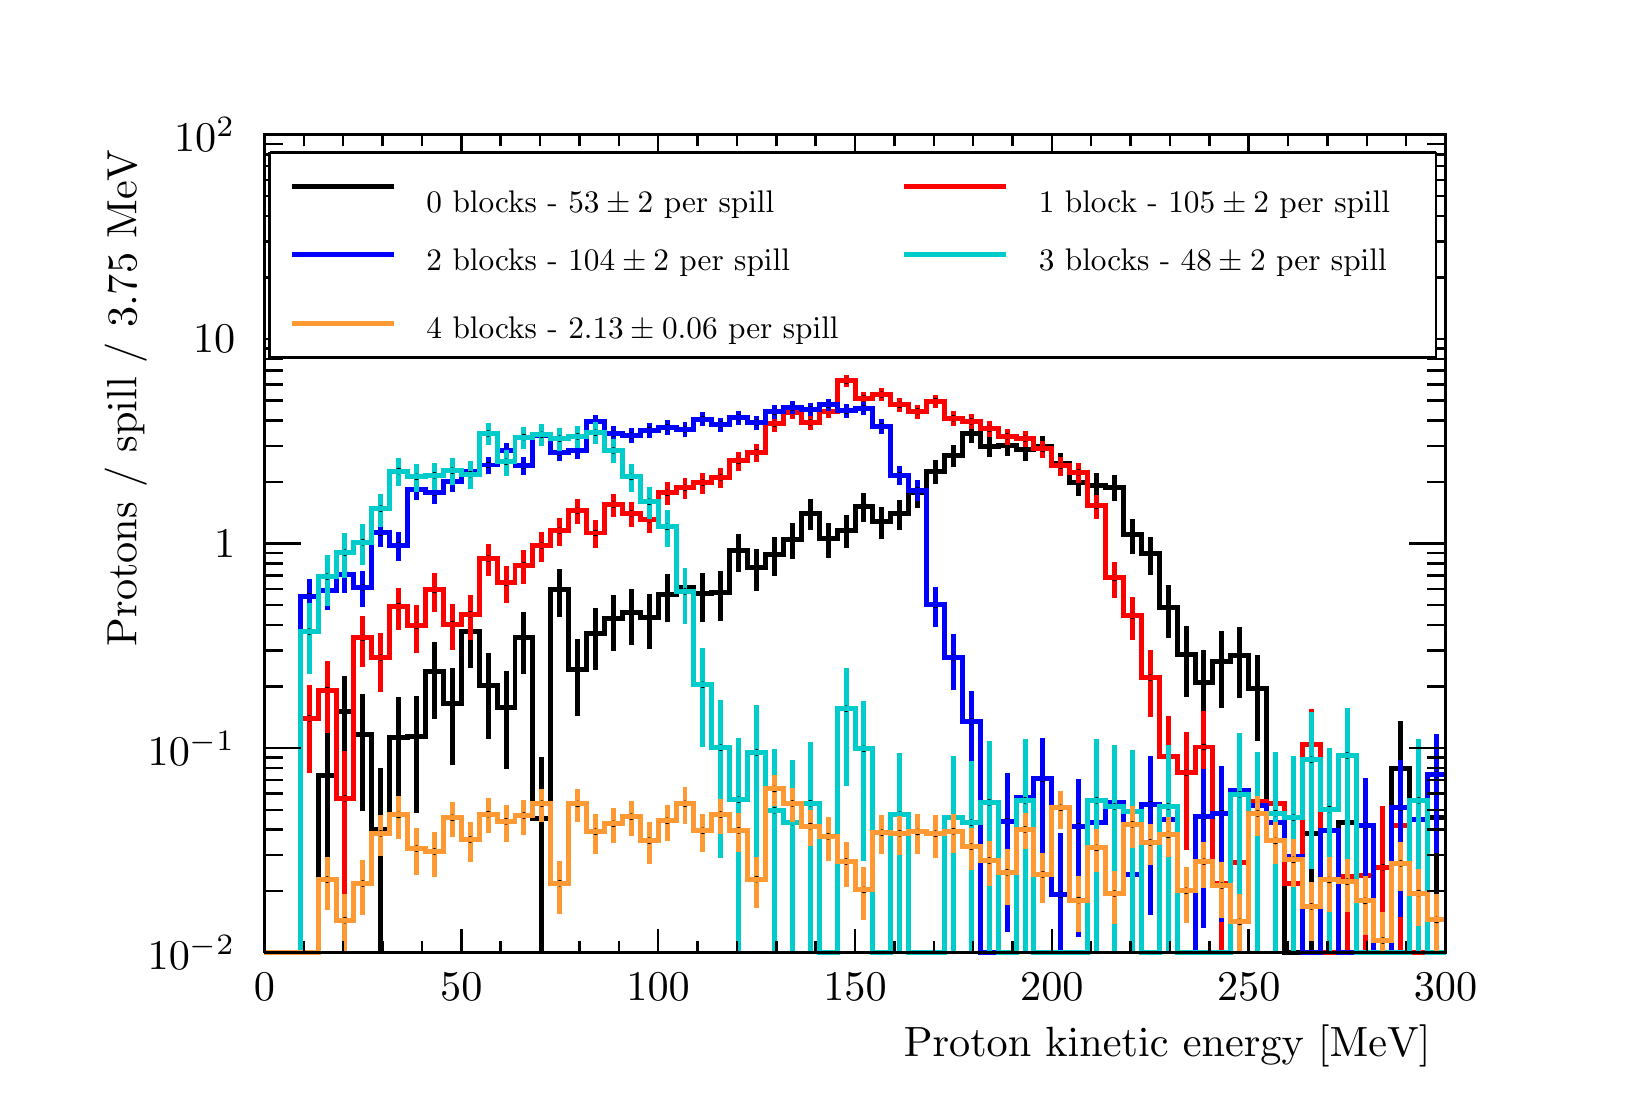
\begin{tikzpicture}
\pgfdeclareplotmark{cross} {
\pgfpathmoveto{\pgfpoint{-0.3\pgfplotmarksize}{\pgfplotmarksize}}
\pgfpathlineto{\pgfpoint{+0.3\pgfplotmarksize}{\pgfplotmarksize}}
\pgfpathlineto{\pgfpoint{+0.3\pgfplotmarksize}{0.3\pgfplotmarksize}}
\pgfpathlineto{\pgfpoint{+1\pgfplotmarksize}{0.3\pgfplotmarksize}}
\pgfpathlineto{\pgfpoint{+1\pgfplotmarksize}{-0.3\pgfplotmarksize}}
\pgfpathlineto{\pgfpoint{+0.3\pgfplotmarksize}{-0.3\pgfplotmarksize}}
\pgfpathlineto{\pgfpoint{+0.3\pgfplotmarksize}{-1.\pgfplotmarksize}}
\pgfpathlineto{\pgfpoint{-0.3\pgfplotmarksize}{-1.\pgfplotmarksize}}
\pgfpathlineto{\pgfpoint{-0.3\pgfplotmarksize}{-0.3\pgfplotmarksize}}
\pgfpathlineto{\pgfpoint{-1.\pgfplotmarksize}{-0.3\pgfplotmarksize}}
\pgfpathlineto{\pgfpoint{-1.\pgfplotmarksize}{0.3\pgfplotmarksize}}
\pgfpathlineto{\pgfpoint{-0.3\pgfplotmarksize}{0.3\pgfplotmarksize}}
\pgfpathclose
\pgfusepathqstroke
}
\pgfdeclareplotmark{cross*} {
\pgfpathmoveto{\pgfpoint{-0.3\pgfplotmarksize}{\pgfplotmarksize}}
\pgfpathlineto{\pgfpoint{+0.3\pgfplotmarksize}{\pgfplotmarksize}}
\pgfpathlineto{\pgfpoint{+0.3\pgfplotmarksize}{0.3\pgfplotmarksize}}
\pgfpathlineto{\pgfpoint{+1\pgfplotmarksize}{0.3\pgfplotmarksize}}
\pgfpathlineto{\pgfpoint{+1\pgfplotmarksize}{-0.3\pgfplotmarksize}}
\pgfpathlineto{\pgfpoint{+0.3\pgfplotmarksize}{-0.3\pgfplotmarksize}}
\pgfpathlineto{\pgfpoint{+0.3\pgfplotmarksize}{-1.\pgfplotmarksize}}
\pgfpathlineto{\pgfpoint{-0.3\pgfplotmarksize}{-1.\pgfplotmarksize}}
\pgfpathlineto{\pgfpoint{-0.3\pgfplotmarksize}{-0.3\pgfplotmarksize}}
\pgfpathlineto{\pgfpoint{-1.\pgfplotmarksize}{-0.3\pgfplotmarksize}}
\pgfpathlineto{\pgfpoint{-1.\pgfplotmarksize}{0.3\pgfplotmarksize}}
\pgfpathlineto{\pgfpoint{-0.3\pgfplotmarksize}{0.3\pgfplotmarksize}}
\pgfpathclose
\pgfusepathqfillstroke
}
\pgfdeclareplotmark{newstar} {
\pgfpathmoveto{\pgfqpoint{0pt}{\pgfplotmarksize}}
\pgfpathlineto{\pgfqpointpolar{44}{0.5\pgfplotmarksize}}
\pgfpathlineto{\pgfqpointpolar{18}{\pgfplotmarksize}}
\pgfpathlineto{\pgfqpointpolar{-20}{0.5\pgfplotmarksize}}
\pgfpathlineto{\pgfqpointpolar{-54}{\pgfplotmarksize}}
\pgfpathlineto{\pgfqpointpolar{-90}{0.5\pgfplotmarksize}}
\pgfpathlineto{\pgfqpointpolar{234}{\pgfplotmarksize}}
\pgfpathlineto{\pgfqpointpolar{198}{0.5\pgfplotmarksize}}
\pgfpathlineto{\pgfqpointpolar{162}{\pgfplotmarksize}}
\pgfpathlineto{\pgfqpointpolar{134}{0.5\pgfplotmarksize}}
\pgfpathclose
\pgfusepathqstroke
}
\pgfdeclareplotmark{newstar*} {
\pgfpathmoveto{\pgfqpoint{0pt}{\pgfplotmarksize}}
\pgfpathlineto{\pgfqpointpolar{44}{0.5\pgfplotmarksize}}
\pgfpathlineto{\pgfqpointpolar{18}{\pgfplotmarksize}}
\pgfpathlineto{\pgfqpointpolar{-20}{0.5\pgfplotmarksize}}
\pgfpathlineto{\pgfqpointpolar{-54}{\pgfplotmarksize}}
\pgfpathlineto{\pgfqpointpolar{-90}{0.5\pgfplotmarksize}}
\pgfpathlineto{\pgfqpointpolar{234}{\pgfplotmarksize}}
\pgfpathlineto{\pgfqpointpolar{198}{0.5\pgfplotmarksize}}
\pgfpathlineto{\pgfqpointpolar{162}{\pgfplotmarksize}}
\pgfpathlineto{\pgfqpointpolar{134}{0.5\pgfplotmarksize}}
\pgfpathclose
\pgfusepathqfillstroke
}
\definecolor{c}{rgb}{1,1,1};
\draw [color=c, fill=c] (0,0) rectangle (20,13.4957);
\draw [color=c, fill=c] (3,1.75444) rectangle (18,12.1461);
\definecolor{c}{rgb}{0,0,0};
\draw [c,line width=0.9] (3,1.75444) -- (3,12.1461) -- (18,12.1461) -- (18,1.75444) -- (3,1.75444);
\definecolor{c}{rgb}{1,1,1};
\draw [color=c, fill=c] (3,1.75444) rectangle (18,12.1461);
\definecolor{c}{rgb}{0,0,0};
\draw [c,line width=0.9] (3,1.75444) -- (3,12.1461) -- (18,12.1461) -- (18,1.75444) -- (3,1.75444);
\draw [c,line width=0.9] (3,1.75444) -- (3.22727,1.75444) -- (3.22727,1.75444) -- (3.45455,1.75444) -- (3.45455,1.75444) -- (3.68182,1.75444) -- (3.68182,1.75444) -- (3.90909,1.75444) -- (3.90909,1.75444) -- (4.13636,1.75444) -- (4.13636,1.75444) --
 (4.36364,1.75444) -- (4.36364,1.75444) -- (4.59091,1.75444) -- (4.59091,1.75444) -- (4.81818,1.75444) -- (4.81818,1.75444) -- (5.04545,1.75444) -- (5.04545,1.75444) -- (5.27273,1.75444) -- (5.27273,1.75444) -- (5.5,1.75444) -- (5.5,1.75444) --
 (5.72727,1.75444) -- (5.72727,1.75444) -- (5.95455,1.75444) -- (5.95455,1.75444) -- (6.18182,1.75444) -- (6.18182,1.75444) -- (6.40909,1.75444) -- (6.40909,1.75444) -- (6.63636,1.75444) -- (6.63636,1.75444) -- (6.86364,1.75444) -- (6.86364,1.75444)
 -- (7.09091,1.75444) -- (7.09091,1.75444) -- (7.31818,1.75444) -- (7.31818,1.75444) -- (7.54545,1.75444) -- (7.54545,1.75444) -- (7.77273,1.75444) -- (7.77273,1.75444) -- (8,1.75444) -- (8,1.75444) -- (8.22727,1.75444) -- (8.22727,1.75444) --
 (8.45455,1.75444) -- (8.45455,1.75444) -- (8.68182,1.75444) -- (8.68182,1.75444) -- (8.90909,1.75444) -- (8.90909,1.75444) -- (9.13636,1.75444) -- (9.13636,1.75444) -- (9.36364,1.75444) -- (9.36364,1.75444) -- (9.59091,1.75444) -- (9.59091,1.75444)
 -- (9.81818,1.75444) -- (9.81818,1.75444) -- (10.0455,1.75444) -- (10.0455,1.75444) -- (10.2727,1.75444) -- (10.2727,1.75444) -- (10.5,1.75444) -- (10.5,1.75444) -- (10.7273,1.75444) -- (10.7273,1.75444) -- (10.9545,1.75444) -- (10.9545,1.75444) --
 (11.1818,1.75444) -- (11.1818,1.75444) -- (11.4091,1.75444) -- (11.4091,1.75444) -- (11.6364,1.75444) -- (11.6364,1.75444) -- (11.8636,1.75444) -- (11.8636,1.75444) -- (12.0909,1.75444) -- (12.0909,1.75444) -- (12.3182,1.75444) -- (12.3182,1.75444)
 -- (12.5455,1.75444) -- (12.5455,1.75444) -- (12.7727,1.75444) -- (12.7727,1.75444) -- (13,1.75444) -- (13,1.75444) -- (13.2273,1.75444) -- (13.2273,1.75444) -- (13.4545,1.75444) -- (13.4545,1.75444) -- (13.6818,1.75444) -- (13.6818,1.75444) --
 (13.9091,1.75444) -- (13.9091,1.75444) -- (14.1364,1.75444) -- (14.1364,1.75444) -- (14.3636,1.75444) -- (14.3636,1.75444) -- (14.5909,1.75444) -- (14.5909,1.75444) -- (14.8182,1.75444) -- (14.8182,1.75444) -- (15.0455,1.75444) -- (15.0455,1.75444)
 -- (15.2727,1.75444) -- (15.2727,1.75444) -- (15.5,1.75444) -- (15.5,1.75444) -- (15.7273,1.75444) -- (15.7273,1.75444) -- (15.9545,1.75444) -- (15.9545,1.75444) -- (16.1818,1.75444) -- (16.1818,1.75444) -- (16.4091,1.75444) -- (16.4091,1.75444) --
 (16.6364,1.75444) -- (16.6364,1.75444) -- (16.8636,1.75444) -- (16.8636,1.75444) -- (17.0909,1.75444) -- (17.0909,1.75444) -- (17.3182,1.75444) -- (17.3182,1.75444) -- (17.5455,1.75444) -- (17.5455,1.75444) -- (17.7727,1.75444) -- (17.7727,1.75444)
 -- (18,1.75444);
\draw [c,line width=0.9] (3,1.75444) -- (18,1.75444);
\draw [c,line width=0.9] (3,2.05809) -- (3,1.75444);
\draw [c,line width=0.9] (3.5,1.90627) -- (3.5,1.75444);
\draw [c,line width=0.9] (4,1.90627) -- (4,1.75444);
\draw [c,line width=0.9] (4.5,1.90627) -- (4.5,1.75444);
\draw [c,line width=0.9] (5,1.90627) -- (5,1.75444);
\draw [c,line width=0.9] (5.5,2.05809) -- (5.5,1.75444);
\draw [c,line width=0.9] (6,1.90627) -- (6,1.75444);
\draw [c,line width=0.9] (6.5,1.90627) -- (6.5,1.75444);
\draw [c,line width=0.9] (7,1.90627) -- (7,1.75444);
\draw [c,line width=0.9] (7.5,1.90627) -- (7.5,1.75444);
\draw [c,line width=0.9] (8,2.05809) -- (8,1.75444);
\draw [c,line width=0.9] (8.5,1.90627) -- (8.5,1.75444);
\draw [c,line width=0.9] (9,1.90627) -- (9,1.75444);
\draw [c,line width=0.9] (9.5,1.90627) -- (9.5,1.75444);
\draw [c,line width=0.9] (10,1.90627) -- (10,1.75444);
\draw [c,line width=0.9] (10.5,2.05809) -- (10.5,1.75444);
\draw [c,line width=0.9] (11,1.90627) -- (11,1.75444);
\draw [c,line width=0.9] (11.5,1.90627) -- (11.5,1.75444);
\draw [c,line width=0.9] (12,1.90627) -- (12,1.75444);
\draw [c,line width=0.9] (12.5,1.90627) -- (12.5,1.75444);
\draw [c,line width=0.9] (13,2.05809) -- (13,1.75444);
\draw [c,line width=0.9] (13.5,1.90627) -- (13.5,1.75444);
\draw [c,line width=0.9] (14,1.90627) -- (14,1.75444);
\draw [c,line width=0.9] (14.5,1.90627) -- (14.5,1.75444);
\draw [c,line width=0.9] (15,1.90627) -- (15,1.75444);
\draw [c,line width=0.9] (15.5,2.05809) -- (15.5,1.75444);
\draw [c,line width=0.9] (16,1.90627) -- (16,1.75444);
\draw [c,line width=0.9] (16.5,1.90627) -- (16.5,1.75444);
\draw [c,line width=0.9] (17,1.90627) -- (17,1.75444);
\draw [c,line width=0.9] (17.5,1.90627) -- (17.5,1.75444);
\draw [c,line width=0.9] (18,2.05809) -- (18,1.75444);
\draw [c,line width=0.9] (18,2.05809) -- (18,1.75444);
\draw [anchor=base] (3,1.14713) node[scale=1.52731, color=c, rotate=0]{0};
\draw [anchor=base] (5.5,1.14713) node[scale=1.52731, color=c, rotate=0]{50};
\draw [anchor=base] (8,1.14713) node[scale=1.52731, color=c, rotate=0]{100};
\draw [anchor=base] (10.5,1.14713) node[scale=1.52731, color=c, rotate=0]{150};
\draw [anchor=base] (13,1.14713) node[scale=1.52731, color=c, rotate=0]{200};
\draw [anchor=base] (15.5,1.14713) node[scale=1.52731, color=c, rotate=0]{250};
\draw [anchor=base] (18,1.14713) node[scale=1.52731, color=c, rotate=0]{300};
\draw [anchor= east] (18,0.566819) node[scale=1.52731, color=c, rotate=0]{Proton kinetic energy [MeV]};
\draw [c,line width=0.9] (3,12.1461) -- (18,12.1461);
\draw [c,line width=0.9] (3,11.8425) -- (3,12.1461);
\draw [c,line width=0.9] (3.5,11.9943) -- (3.5,12.1461);
\draw [c,line width=0.9] (4,11.9943) -- (4,12.1461);
\draw [c,line width=0.9] (4.5,11.9943) -- (4.5,12.1461);
\draw [c,line width=0.9] (5,11.9943) -- (5,12.1461);
\draw [c,line width=0.9] (5.5,11.8425) -- (5.5,12.1461);
\draw [c,line width=0.9] (6,11.9943) -- (6,12.1461);
\draw [c,line width=0.9] (6.5,11.9943) -- (6.5,12.1461);
\draw [c,line width=0.9] (7,11.9943) -- (7,12.1461);
\draw [c,line width=0.9] (7.5,11.9943) -- (7.5,12.1461);
\draw [c,line width=0.9] (8,11.8425) -- (8,12.1461);
\draw [c,line width=0.9] (8.5,11.9943) -- (8.5,12.1461);
\draw [c,line width=0.9] (9,11.9943) -- (9,12.1461);
\draw [c,line width=0.9] (9.5,11.9943) -- (9.5,12.1461);
\draw [c,line width=0.9] (10,11.9943) -- (10,12.1461);
\draw [c,line width=0.9] (10.5,11.8425) -- (10.5,12.1461);
\draw [c,line width=0.9] (11,11.9943) -- (11,12.1461);
\draw [c,line width=0.9] (11.5,11.9943) -- (11.5,12.1461);
\draw [c,line width=0.9] (12,11.9943) -- (12,12.1461);
\draw [c,line width=0.9] (12.5,11.9943) -- (12.5,12.1461);
\draw [c,line width=0.9] (13,11.8425) -- (13,12.1461);
\draw [c,line width=0.9] (13.5,11.9943) -- (13.5,12.1461);
\draw [c,line width=0.9] (14,11.9943) -- (14,12.1461);
\draw [c,line width=0.9] (14.5,11.9943) -- (14.5,12.1461);
\draw [c,line width=0.9] (15,11.9943) -- (15,12.1461);
\draw [c,line width=0.9] (15.5,11.8425) -- (15.5,12.1461);
\draw [c,line width=0.9] (16,11.9943) -- (16,12.1461);
\draw [c,line width=0.9] (16.5,11.9943) -- (16.5,12.1461);
\draw [c,line width=0.9] (17,11.9943) -- (17,12.1461);
\draw [c,line width=0.9] (17.5,11.9943) -- (17.5,12.1461);
\draw [c,line width=0.9] (18,11.8425) -- (18,12.1461);
\draw [c,line width=0.9] (18,11.8425) -- (18,12.1461);
\draw [c,line width=0.9] (3,1.75444) -- (3,12.1461);
\draw [c,line width=0.9] (3.462,1.75444) -- (3,1.75444);
\draw [anchor= east] (2.82,1.75444) node[scale=1.52731, color=c, rotate=0]{$10^{-2}$};
\draw [c,line width=0.9] (3.231,2.5365) -- (3,2.5365);
\draw [c,line width=0.9] (3.231,2.99397) -- (3,2.99397);
\draw [c,line width=0.9] (3.231,3.31855) -- (3,3.31855);
\draw [c,line width=0.9] (3.231,3.57031) -- (3,3.57031);
\draw [c,line width=0.9] (3.231,3.77602) -- (3,3.77602);
\draw [c,line width=0.9] (3.231,3.94994) -- (3,3.94994);
\draw [c,line width=0.9] (3.231,4.1006) -- (3,4.1006);
\draw [c,line width=0.9] (3.231,4.23349) -- (3,4.23349);
\draw [c,line width=0.9] (3.462,4.35237) -- (3,4.35237);
\draw [anchor= east] (2.82,4.35237) node[scale=1.52731, color=c, rotate=0]{$10^{-1}$};
\draw [c,line width=0.9] (3.231,5.13442) -- (3,5.13442);
\draw [c,line width=0.9] (3.231,5.59189) -- (3,5.59189);
\draw [c,line width=0.9] (3.231,5.91647) -- (3,5.91647);
\draw [c,line width=0.9] (3.231,6.16824) -- (3,6.16824);
\draw [c,line width=0.9] (3.231,6.37394) -- (3,6.37394);
\draw [c,line width=0.9] (3.231,6.54786) -- (3,6.54786);
\draw [c,line width=0.9] (3.231,6.69852) -- (3,6.69852);
\draw [c,line width=0.9] (3.231,6.83141) -- (3,6.83141);
\draw [c,line width=0.9] (3.462,6.95029) -- (3,6.95029);
\draw [anchor= east] (2.82,6.95029) node[scale=1.52731, color=c, rotate=0]{1};
\draw [c,line width=0.9] (3.231,7.73234) -- (3,7.73234);
\draw [c,line width=0.9] (3.231,8.18981) -- (3,8.18981);
\draw [c,line width=0.9] (3.231,8.51439) -- (3,8.51439);
\draw [c,line width=0.9] (3.231,8.76616) -- (3,8.76616);
\draw [c,line width=0.9] (3.231,8.97186) -- (3,8.97186);
\draw [c,line width=0.9] (3.231,9.14579) -- (3,9.14579);
\draw [c,line width=0.9] (3.231,9.29644) -- (3,9.29644);
\draw [c,line width=0.9] (3.231,9.42934) -- (3,9.42934);
\draw [c,line width=0.9] (3.462,9.54821) -- (3,9.54821);
\draw [anchor= east] (2.82,9.54821) node[scale=1.52731, color=c, rotate=0]{10};
\draw [c,line width=0.9] (3.231,10.3303) -- (3,10.3303);
\draw [c,line width=0.9] (3.231,10.7877) -- (3,10.7877);
\draw [c,line width=0.9] (3.231,11.1123) -- (3,11.1123);
\draw [c,line width=0.9] (3.231,11.3641) -- (3,11.3641);
\draw [c,line width=0.9] (3.231,11.5698) -- (3,11.5698);
\draw [c,line width=0.9] (3.231,11.7437) -- (3,11.7437);
\draw [c,line width=0.9] (3.231,11.8944) -- (3,11.8944);
\draw [c,line width=0.9] (3.231,12.0273) -- (3,12.0273);
\draw [c,line width=0.9] (3.462,12.1461) -- (3,12.1461);
\draw [anchor= east] (2.82,12.1461) node[scale=1.52731, color=c, rotate=0]{$10^{2}$};
\draw [anchor= east] (1.24,12.1461) node[scale=1.52731, color=c, rotate=90]{Protons / spill / 3.75~MeV};
\draw [c,line width=0.9] (18,1.75444) -- (18,12.1461);
\draw [c,line width=0.9] (17.538,1.75444) -- (18,1.75444);
\draw [c,line width=0.9] (17.769,2.5365) -- (18,2.5365);
\draw [c,line width=0.9] (17.769,2.99397) -- (18,2.99397);
\draw [c,line width=0.9] (17.769,3.31855) -- (18,3.31855);
\draw [c,line width=0.9] (17.769,3.57031) -- (18,3.57031);
\draw [c,line width=0.9] (17.769,3.77602) -- (18,3.77602);
\draw [c,line width=0.9] (17.769,3.94994) -- (18,3.94994);
\draw [c,line width=0.9] (17.769,4.1006) -- (18,4.1006);
\draw [c,line width=0.9] (17.769,4.23349) -- (18,4.23349);
\draw [c,line width=0.9] (17.538,4.35237) -- (18,4.35237);
\draw [c,line width=0.9] (17.769,5.13442) -- (18,5.13442);
\draw [c,line width=0.9] (17.769,5.59189) -- (18,5.59189);
\draw [c,line width=0.9] (17.769,5.91647) -- (18,5.91647);
\draw [c,line width=0.9] (17.769,6.16824) -- (18,6.16824);
\draw [c,line width=0.9] (17.769,6.37394) -- (18,6.37394);
\draw [c,line width=0.9] (17.769,6.54786) -- (18,6.54786);
\draw [c,line width=0.9] (17.769,6.69852) -- (18,6.69852);
\draw [c,line width=0.9] (17.769,6.83141) -- (18,6.83141);
\draw [c,line width=0.9] (17.538,6.95029) -- (18,6.95029);
\draw [c,line width=0.9] (17.769,7.73234) -- (18,7.73234);
\draw [c,line width=0.9] (17.769,8.18981) -- (18,8.18981);
\draw [c,line width=0.9] (17.769,8.51439) -- (18,8.51439);
\draw [c,line width=0.9] (17.769,8.76616) -- (18,8.76616);
\draw [c,line width=0.9] (17.769,8.97186) -- (18,8.97186);
\draw [c,line width=0.9] (17.769,9.14579) -- (18,9.14579);
\draw [c,line width=0.9] (17.769,9.29644) -- (18,9.29644);
\draw [c,line width=0.9] (17.769,9.42934) -- (18,9.42934);
\draw [c,line width=0.9] (17.538,9.54821) -- (18,9.54821);
\draw [c,line width=0.9] (17.769,10.3303) -- (18,10.3303);
\draw [c,line width=0.9] (17.769,10.7877) -- (18,10.7877);
\draw [c,line width=0.9] (17.769,11.1123) -- (18,11.1123);
\draw [c,line width=0.9] (17.769,11.3641) -- (18,11.3641);
\draw [c,line width=0.9] (17.769,11.5698) -- (18,11.5698);
\draw [c,line width=0.9] (17.769,11.7437) -- (18,11.7437);
\draw [c,line width=0.9] (17.769,11.8944) -- (18,11.8944);
\draw [c,line width=0.9] (17.769,12.0273) -- (18,12.0273);
\draw [c,line width=0.9] (17.538,12.1461) -- (18,12.1461);
\draw [c,line width=1.8] (3.79545,2.60924) -- (3.79545,4.00539);
\draw [c,line width=1.8] (3.79545,4.00539) -- (3.79545,4.61061);
\foreach \P in {(3.79545,4.00539)}{\draw[mark options={color=c,fill=c},mark size=2.402402pt,mark=*,mark size=1pt] plot coordinates {\P};}
\draw [c,line width=1.8] (4.02273,4.03114) -- (4.02273,4.81428);
\draw [c,line width=1.8] (4.02273,4.81428) -- (4.02273,5.27211);
\foreach \P in {(4.02273,4.81428)}{\draw[mark options={color=c,fill=c},mark size=2.402402pt,mark=*,mark size=1pt] plot coordinates {\P};}
\draw [c,line width=1.8] (4.25,3.5497) -- (4.25,4.52289);
\draw [c,line width=1.8] (4.25,4.52289) -- (4.25,5.0375);
\foreach \P in {(4.25,4.52289)}{\draw[mark options={color=c,fill=c},mark size=2.402402pt,mark=*,mark size=1pt] plot coordinates {\P};}
\draw [c,line width=1.8] (4.47727,1.75444) -- (4.47727,3.32318);
\draw [c,line width=1.8] (4.47727,3.32318) -- (4.47727,4.10524);
\foreach \P in {(4.47727,3.32318)}{\draw[mark options={color=c,fill=c},mark size=2.402402pt,mark=*,mark size=1pt] plot coordinates {\P};}
\draw [c,line width=1.8] (4.70455,3.51188) -- (4.70455,4.48763);
\draw [c,line width=1.8] (4.70455,4.48763) -- (4.70455,5.00292);
\foreach \P in {(4.70455,4.48763)}{\draw[mark options={color=c,fill=c},mark size=2.402402pt,mark=*,mark size=1pt] plot coordinates {\P};}
\draw [c,line width=1.8] (4.93182,3.5301) -- (4.93182,4.50411);
\draw [c,line width=1.8] (4.93182,4.50411) -- (4.93182,5.01894);
\foreach \P in {(4.93182,4.50411)}{\draw[mark options={color=c,fill=c},mark size=2.402402pt,mark=*,mark size=1pt] plot coordinates {\P};}
\draw [c,line width=1.8] (5.15909,4.72595) -- (5.15909,5.31984);
\draw [c,line width=1.8] (5.15909,5.31984) -- (5.15909,5.7069);
\foreach \P in {(5.15909,5.31984)}{\draw[mark options={color=c,fill=c},mark size=2.402402pt,mark=*,mark size=1pt] plot coordinates {\P};}
\draw [c,line width=1.8] (5.38636,4.13231) -- (5.38636,4.91521);
\draw [c,line width=1.8] (5.38636,4.91521) -- (5.38636,5.37296);
\foreach \P in {(5.38636,4.91521)}{\draw[mark options={color=c,fill=c},mark size=2.402402pt,mark=*,mark size=1pt] plot coordinates {\P};}
\draw [c,line width=1.8] (5.61364,5.36765) -- (5.61364,5.8311);
\draw [c,line width=1.8] (5.61364,5.8311) -- (5.61364,6.15865);
\foreach \P in {(5.61364,5.8311)}{\draw[mark options={color=c,fill=c},mark size=2.402402pt,mark=*,mark size=1pt] plot coordinates {\P};}
\draw [c,line width=1.8] (5.84091,4.47369) -- (5.84091,5.14585);
\draw [c,line width=1.8] (5.84091,5.14585) -- (5.84091,5.56418);
\foreach \P in {(5.84091,5.14585)}{\draw[mark options={color=c,fill=c},mark size=2.402402pt,mark=*,mark size=1pt] plot coordinates {\P};}
\draw [c,line width=1.8] (6.06818,4.08623) -- (6.06818,4.8698);
\draw [c,line width=1.8] (6.06818,4.8698) -- (6.06818,5.32777);
\foreach \P in {(6.06818,4.8698)}{\draw[mark options={color=c,fill=c},mark size=2.402402pt,mark=*,mark size=1pt] plot coordinates {\P};}
\draw [c,line width=1.8] (6.29545,5.29359) -- (6.29545,5.75425);
\draw [c,line width=1.8] (6.29545,5.75425) -- (6.29545,6.08042);
\foreach \P in {(6.29545,5.75425)}{\draw[mark options={color=c,fill=c},mark size=2.402402pt,mark=*,mark size=1pt] plot coordinates {\P};}
\draw [c,line width=1.8] (6.52273,1.75444) -- (6.52273,3.46448);
\draw [c,line width=1.8] (6.52273,3.46448) -- (6.52273,4.24653);
\foreach \P in {(6.52273,3.46448)}{\draw[mark options={color=c,fill=c},mark size=2.402402pt,mark=*,mark size=1pt] plot coordinates {\P};}
\draw [c,line width=1.8] (6.75,6.02252) -- (6.75,6.36177);
\draw [c,line width=1.8] (6.75,6.36177) -- (6.75,6.62224);
\foreach \P in {(6.75,6.36177)}{\draw[mark options={color=c,fill=c},mark size=2.402402pt,mark=*,mark size=1pt] plot coordinates {\P};}
\draw [c,line width=1.8] (6.97727,4.75616) -- (6.97727,5.34913);
\draw [c,line width=1.8] (6.97727,5.34913) -- (6.97727,5.73582);
\foreach \P in {(6.97727,5.34913)}{\draw[mark options={color=c,fill=c},mark size=2.402402pt,mark=*,mark size=1pt] plot coordinates {\P};}
\draw [c,line width=1.8] (7.20455,5.34851) -- (7.20455,5.80911);
\draw [c,line width=1.8] (7.20455,5.80911) -- (7.20455,6.13526);
\foreach \P in {(7.20455,5.80911)}{\draw[mark options={color=c,fill=c},mark size=2.402402pt,mark=*,mark size=1pt] plot coordinates {\P};}
\draw [c,line width=1.8] (7.43182,5.58905) -- (7.43182,5.99782);
\draw [c,line width=1.8] (7.43182,5.99782) -- (7.43182,6.29724);
\foreach \P in {(7.43182,5.99782)}{\draw[mark options={color=c,fill=c},mark size=2.402402pt,mark=*,mark size=1pt] plot coordinates {\P};}
\draw [c,line width=1.8] (7.65909,5.66385) -- (7.65909,6.07109);
\draw [c,line width=1.8] (7.65909,6.07109) -- (7.65909,6.36969);
\foreach \P in {(7.65909,6.07109)}{\draw[mark options={color=c,fill=c},mark size=2.402402pt,mark=*,mark size=1pt] plot coordinates {\P};}
\draw [c,line width=1.8] (7.88636,5.61049) -- (7.88636,6.01595);
\draw [c,line width=1.8] (7.88636,6.01595) -- (7.88636,6.3136);
\foreach \P in {(7.88636,6.01595)}{\draw[mark options={color=c,fill=c},mark size=2.402402pt,mark=*,mark size=1pt] plot coordinates {\P};}
\draw [c,line width=1.8] (8.11364,5.94903) -- (8.11364,6.30148);
\draw [c,line width=1.8] (8.11364,6.30148) -- (8.11364,6.56965);
\foreach \P in {(8.11364,6.30148)}{\draw[mark options={color=c,fill=c},mark size=2.402402pt,mark=*,mark size=1pt] plot coordinates {\P};}
\draw [c,line width=1.8] (8.34091,6.06278) -- (8.34091,6.38842);
\draw [c,line width=1.8] (8.34091,6.38842) -- (8.34091,6.64082);
\foreach \P in {(8.34091,6.38842)}{\draw[mark options={color=c,fill=c},mark size=2.402402pt,mark=*,mark size=1pt] plot coordinates {\P};}
\draw [c,line width=1.8] (8.56818,5.95652) -- (8.56818,6.31043);
\draw [c,line width=1.8] (8.56818,6.31043) -- (8.56818,6.57943);
\foreach \P in {(8.56818,6.31043)}{\draw[mark options={color=c,fill=c},mark size=2.402402pt,mark=*,mark size=1pt] plot coordinates {\P};}
\draw [c,line width=1.8] (8.79545,5.97304) -- (8.79545,6.32748);
\draw [c,line width=1.8] (8.79545,6.32748) -- (8.79545,6.5968);
\foreach \P in {(8.79545,6.32748)}{\draw[mark options={color=c,fill=c},mark size=2.402402pt,mark=*,mark size=1pt] plot coordinates {\P};}
\draw [c,line width=1.8] (9.02273,6.5917) -- (9.02273,6.85685);
\draw [c,line width=1.8] (9.02273,6.85685) -- (9.02273,7.07139);
\foreach \P in {(9.02273,6.85685)}{\draw[mark options={color=c,fill=c},mark size=2.402402pt,mark=*,mark size=1pt] plot coordinates {\P};}
\draw [c,line width=1.8] (9.25,6.34879) -- (9.25,6.64525);
\draw [c,line width=1.8] (9.25,6.64525) -- (9.25,6.8798);
\foreach \P in {(9.25,6.64525)}{\draw[mark options={color=c,fill=c},mark size=2.402402pt,mark=*,mark size=1pt] plot coordinates {\P};}
\draw [c,line width=1.8] (9.47727,6.5369) -- (9.47727,6.81036);
\draw [c,line width=1.8] (9.47727,6.81036) -- (9.47727,7.0303);
\foreach \P in {(9.47727,6.81036)}{\draw[mark options={color=c,fill=c},mark size=2.402402pt,mark=*,mark size=1pt] plot coordinates {\P};}
\draw [c,line width=1.8] (9.70455,6.7599) -- (9.70455,7.00766);
\draw [c,line width=1.8] (9.70455,7.00766) -- (9.70455,7.21069);
\foreach \P in {(9.70455,7.00766)}{\draw[mark options={color=c,fill=c},mark size=2.402402pt,mark=*,mark size=1pt] plot coordinates {\P};}
\draw [c,line width=1.8] (9.93182,7.12677) -- (9.93182,7.33707);
\draw [c,line width=1.8] (9.93182,7.33707) -- (9.93182,7.51427);
\foreach \P in {(9.93182,7.33707)}{\draw[mark options={color=c,fill=c},mark size=2.402402pt,mark=*,mark size=1pt] plot coordinates {\P};}
\draw [c,line width=1.8] (10.1591,6.7687) -- (10.1591,7.01088);
\draw [c,line width=1.8] (10.1591,7.01088) -- (10.1591,7.21015);
\foreach \P in {(10.1591,7.01088)}{\draw[mark options={color=c,fill=c},mark size=2.402402pt,mark=*,mark size=1pt] plot coordinates {\P};}
\draw [c,line width=1.8] (10.3864,6.88913) -- (10.3864,7.11788);
\draw [c,line width=1.8] (10.3864,7.11788) -- (10.3864,7.30797);
\foreach \P in {(10.3864,7.11788)}{\draw[mark options={color=c,fill=c},mark size=2.402402pt,mark=*,mark size=1pt] plot coordinates {\P};}
\draw [c,line width=1.8] (10.6136,7.22852) -- (10.6136,7.42613);
\draw [c,line width=1.8] (10.6136,7.42613) -- (10.6136,7.59423);
\foreach \P in {(10.6136,7.42613)}{\draw[mark options={color=c,fill=c},mark size=2.402402pt,mark=*,mark size=1pt] plot coordinates {\P};}
\draw [c,line width=1.8] (10.8409,7.0079) -- (10.8409,7.22835);
\draw [c,line width=1.8] (10.8409,7.22835) -- (10.8409,7.41268);
\foreach \P in {(10.8409,7.22835)}{\draw[mark options={color=c,fill=c},mark size=2.402402pt,mark=*,mark size=1pt] plot coordinates {\P};}
\draw [c,line width=1.8] (11.0682,7.12833) -- (11.0682,7.33525);
\draw [c,line width=1.8] (11.0682,7.33525) -- (11.0682,7.51005);
\foreach \P in {(11.0682,7.33525)}{\draw[mark options={color=c,fill=c},mark size=2.402402pt,mark=*,mark size=1pt] plot coordinates {\P};}
\draw [c,line width=1.8] (11.2955,7.40746) -- (11.2955,7.59292);
\draw [c,line width=1.8] (11.2955,7.59292) -- (11.2955,7.75215);
\foreach \P in {(11.2955,7.59292)}{\draw[mark options={color=c,fill=c},mark size=2.402402pt,mark=*,mark size=1pt] plot coordinates {\P};}
\draw [c,line width=1.8] (11.5227,7.70421) -- (11.5227,7.86713);
\draw [c,line width=1.8] (11.5227,7.86713) -- (11.5227,8.00947);
\foreach \P in {(11.5227,7.86713)}{\draw[mark options={color=c,fill=c},mark size=2.402402pt,mark=*,mark size=1pt] plot coordinates {\P};}
\draw [c,line width=1.8] (11.75,7.92009) -- (11.75,8.06794);
\draw [c,line width=1.8] (11.75,8.06794) -- (11.75,8.19864);
\foreach \P in {(11.75,8.06794)}{\draw[mark options={color=c,fill=c},mark size=2.402402pt,mark=*,mark size=1pt] plot coordinates {\P};}
\draw [c,line width=1.8] (11.9773,8.22288) -- (11.9773,8.3524);
\draw [c,line width=1.8] (11.9773,8.3524) -- (11.9773,8.46858);
\foreach \P in {(11.9773,8.3524)}{\draw[mark options={color=c,fill=c},mark size=2.402402pt,mark=*,mark size=1pt] plot coordinates {\P};}
\draw [c,line width=1.8] (12.2045,8.04755) -- (12.2045,8.18769);
\draw [c,line width=1.8] (12.2045,8.18769) -- (12.2045,8.31234);
\foreach \P in {(12.2045,8.18769)}{\draw[mark options={color=c,fill=c},mark size=2.402402pt,mark=*,mark size=1pt] plot coordinates {\P};}
\draw [c,line width=1.8] (12.4318,8.06348) -- (12.4318,8.20158);
\draw [c,line width=1.8] (12.4318,8.20158) -- (12.4318,8.32461);
\foreach \P in {(12.4318,8.20158)}{\draw[mark options={color=c,fill=c},mark size=2.402402pt,mark=*,mark size=1pt] plot coordinates {\P};}
\draw [c,line width=1.8] (12.6591,7.9996) -- (12.6591,8.14294);
\draw [c,line width=1.8] (12.6591,8.14294) -- (12.6591,8.27011);
\foreach \P in {(12.6591,8.14294)}{\draw[mark options={color=c,fill=c},mark size=2.402402pt,mark=*,mark size=1pt] plot coordinates {\P};}
\draw [c,line width=1.8] (12.8864,8.04758) -- (12.8864,8.18805);
\draw [c,line width=1.8] (12.8864,8.18805) -- (12.8864,8.31296);
\foreach \P in {(12.8864,8.18805)}{\draw[mark options={color=c,fill=c},mark size=2.402402pt,mark=*,mark size=1pt] plot coordinates {\P};}
\draw [c,line width=1.8] (13.1136,7.81831) -- (13.1136,7.97079);
\draw [c,line width=1.8] (13.1136,7.97079) -- (13.1136,8.10509);
\foreach \P in {(13.1136,7.97079)}{\draw[mark options={color=c,fill=c},mark size=2.402402pt,mark=*,mark size=1pt] plot coordinates {\P};}
\draw [c,line width=1.8] (13.3409,7.55089) -- (13.3409,7.72195);
\draw [c,line width=1.8] (13.3409,7.72195) -- (13.3409,7.87046);
\foreach \P in {(13.3409,7.72195)}{\draw[mark options={color=c,fill=c},mark size=2.402402pt,mark=*,mark size=1pt] plot coordinates {\P};}
\draw [c,line width=1.8] (13.5682,7.5121) -- (13.5682,7.68905);
\draw [c,line width=1.8] (13.5682,7.68905) -- (13.5682,7.84197);
\foreach \P in {(13.5682,7.68905)}{\draw[mark options={color=c,fill=c},mark size=2.402402pt,mark=*,mark size=1pt] plot coordinates {\P};}
\draw [c,line width=1.8] (13.7955,7.48592) -- (13.7955,7.66469);
\draw [c,line width=1.8] (13.7955,7.66469) -- (13.7955,7.81896);
\foreach \P in {(13.7955,7.66469)}{\draw[mark options={color=c,fill=c},mark size=2.402402pt,mark=*,mark size=1pt] plot coordinates {\P};}
\draw [c,line width=1.8] (14.0227,6.81875) -- (14.0227,7.06169);
\draw [c,line width=1.8] (14.0227,7.06169) -- (14.0227,7.26147);
\foreach \P in {(14.0227,7.06169)}{\draw[mark options={color=c,fill=c},mark size=2.402402pt,mark=*,mark size=1pt] plot coordinates {\P};}
\draw [c,line width=1.8] (14.25,6.54671) -- (14.25,6.81855);
\draw [c,line width=1.8] (14.25,6.81855) -- (14.25,7.03744);
\foreach \P in {(14.25,6.81855)}{\draw[mark options={color=c,fill=c},mark size=2.402402pt,mark=*,mark size=1pt] plot coordinates {\P};}
\draw [c,line width=1.8] (14.4773,5.75068) -- (14.4773,6.13666);
\draw [c,line width=1.8] (14.4773,6.13666) -- (14.4773,6.42371);
\foreach \P in {(14.4773,6.13666)}{\draw[mark options={color=c,fill=c},mark size=2.402402pt,mark=*,mark size=1pt] plot coordinates {\P};}
\draw [c,line width=1.8] (14.7045,4.99765) -- (14.7045,5.53879);
\draw [c,line width=1.8] (14.7045,5.53879) -- (14.7045,5.90299);
\foreach \P in {(14.7045,5.53879)}{\draw[mark options={color=c,fill=c},mark size=2.402402pt,mark=*,mark size=1pt] plot coordinates {\P};}
\draw [c,line width=1.8] (14.9318,4.50266) -- (14.9318,5.18182);
\draw [c,line width=1.8] (14.9318,5.18182) -- (14.9318,5.6028);
\foreach \P in {(14.9318,5.18182)}{\draw[mark options={color=c,fill=c},mark size=2.402402pt,mark=*,mark size=1pt] plot coordinates {\P};}
\draw [c,line width=1.8] (15.1591,4.86338) -- (15.1591,5.45838);
\draw [c,line width=1.8] (15.1591,5.45838) -- (15.1591,5.84591);
\foreach \P in {(15.1591,5.45838)}{\draw[mark options={color=c,fill=c},mark size=2.402402pt,mark=*,mark size=1pt] plot coordinates {\P};}
\draw [c,line width=1.8] (15.3864,4.99129) -- (15.3864,5.5324);
\draw [c,line width=1.8] (15.3864,5.5324) -- (15.3864,5.89658);
\foreach \P in {(15.3864,5.5324)}{\draw[mark options={color=c,fill=c},mark size=2.402402pt,mark=*,mark size=1pt] plot coordinates {\P};}
\draw [c,line width=1.8] (15.6136,4.44511) -- (15.6136,5.11566);
\draw [c,line width=1.8] (15.6136,5.11566) -- (15.6136,5.53337);
\foreach \P in {(15.6136,5.11566)}{\draw[mark options={color=c,fill=c},mark size=2.402402pt,mark=*,mark size=1pt] plot coordinates {\P};}
\draw [c,line width=1.8] (15.8409,1.75444) -- (15.8409,3.17557);
\draw [c,line width=1.8] (15.8409,3.17557) -- (15.8409,3.95762);
\foreach \P in {(15.8409,3.17557)}{\draw[mark options={color=c,fill=c},mark size=2.402402pt,mark=*,mark size=1pt] plot coordinates {\P};}
\draw [c,line width=1.8] (16.2955,1.75444) -- (16.2955,3.26653);
\draw [c,line width=1.8] (16.2955,3.26653) -- (16.2955,4.04858);
\foreach \P in {(16.2955,3.26653)}{\draw[mark options={color=c,fill=c},mark size=2.402402pt,mark=*,mark size=1pt] plot coordinates {\P};}
\draw [c,line width=1.8] (16.75,1.75444) -- (16.75,3.41388);
\draw [c,line width=1.8] (16.75,3.41388) -- (16.75,4.19594);
\foreach \P in {(16.75,3.41388)}{\draw[mark options={color=c,fill=c},mark size=2.402402pt,mark=*,mark size=1pt] plot coordinates {\P};}
\draw [c,line width=1.8] (17.4318,2.69824) -- (17.4318,4.08945);
\draw [c,line width=1.8] (17.4318,4.08945) -- (17.4318,4.69383);
\foreach \P in {(17.4318,4.08945)}{\draw[mark options={color=c,fill=c},mark size=2.402402pt,mark=*,mark size=1pt] plot coordinates {\P};}
\draw [c,line width=1.8] (17.8864,1.75444) -- (17.8864,3.46919);
\draw [c,line width=1.8] (17.8864,3.46919) -- (17.8864,4.25124);
\foreach \P in {(17.8864,3.46919)}{\draw[mark options={color=c,fill=c},mark size=2.402402pt,mark=*,mark size=1pt] plot coordinates {\P};}
\draw [c,line width=1.8] (3,1.75444) -- (3.22727,1.75444) -- (3.22727,1.75444) -- (3.45455,1.75444) -- (3.45455,1.75444) -- (3.68182,1.75444) -- (3.68182,4.00539) -- (3.90909,4.00539) -- (3.90909,4.81428) -- (4.13636,4.81428) -- (4.13636,4.52289) --
 (4.36364,4.52289) -- (4.36364,3.32318) -- (4.59091,3.32318) -- (4.59091,4.48763) -- (4.81818,4.48763) -- (4.81818,4.50411) -- (5.04545,4.50411) -- (5.04545,5.31984) -- (5.27273,5.31984) -- (5.27273,4.91521) -- (5.5,4.91521) -- (5.5,5.8311) --
 (5.72727,5.8311) -- (5.72727,5.14585) -- (5.95455,5.14585) -- (5.95455,4.8698) -- (6.18182,4.8698) -- (6.18182,5.75425) -- (6.40909,5.75425) -- (6.40909,3.46448) -- (6.63636,3.46448) -- (6.63636,6.36177) -- (6.86364,6.36177) -- (6.86364,5.34913) --
 (7.09091,5.34913) -- (7.09091,5.80911) -- (7.31818,5.80911) -- (7.31818,5.99782) -- (7.54545,5.99782) -- (7.54545,6.07109) -- (7.77273,6.07109) -- (7.77273,6.01595) -- (8,6.01595) -- (8,6.30148) -- (8.22727,6.30148) -- (8.22727,6.38842) --
 (8.45455,6.38842) -- (8.45455,6.31043) -- (8.68182,6.31043) -- (8.68182,6.32748) -- (8.90909,6.32748) -- (8.90909,6.85685) -- (9.13636,6.85685) -- (9.13636,6.64525) -- (9.36364,6.64525) -- (9.36364,6.81036) -- (9.59091,6.81036) -- (9.59091,7.00766)
 -- (9.81818,7.00766) -- (9.81818,7.33707) -- (10.0455,7.33707) -- (10.0455,7.01088) -- (10.2727,7.01088) -- (10.2727,7.11788) -- (10.5,7.11788) -- (10.5,7.42613) -- (10.7273,7.42613) -- (10.7273,7.22835) -- (10.9545,7.22835) -- (10.9545,7.33525) --
 (11.1818,7.33525) -- (11.1818,7.59292) -- (11.4091,7.59292) -- (11.4091,7.86713) -- (11.6364,7.86713) -- (11.6364,8.06794) -- (11.8636,8.06794) -- (11.8636,8.3524) -- (12.0909,8.3524) -- (12.0909,8.18769) -- (12.3182,8.18769) -- (12.3182,8.20158) --
 (12.5455,8.20158) -- (12.5455,8.14294) -- (12.7727,8.14294) -- (12.7727,8.18805) -- (13,8.18805) -- (13,7.97079) -- (13.2273,7.97079) -- (13.2273,7.72195) -- (13.4545,7.72195) -- (13.4545,7.68905) -- (13.6818,7.68905) -- (13.6818,7.66469) --
 (13.9091,7.66469) -- (13.9091,7.06169) -- (14.1364,7.06169) -- (14.1364,6.81855) -- (14.3636,6.81855) -- (14.3636,6.13666) -- (14.5909,6.13666) -- (14.5909,5.53879) -- (14.8182,5.53879) -- (14.8182,5.18182) -- (15.0455,5.18182) -- (15.0455,5.45838)
 -- (15.2727,5.45838) -- (15.2727,5.5324) -- (15.5,5.5324) -- (15.5,5.11566) -- (15.7273,5.11566) -- (15.7273,3.17557) -- (15.9545,3.17557) -- (15.9545,1.75444) -- (16.1818,1.75444) -- (16.1818,3.26653) -- (16.4091,3.26653) -- (16.4091,1.75444) --
 (16.6364,1.75444) -- (16.6364,3.41388) -- (16.8636,3.41388) -- (16.8636,1.75444) -- (17.0909,1.75444) -- (17.0909,1.75444) -- (17.3182,1.75444) -- (17.3182,4.08945) -- (17.5455,4.08945) -- (17.5455,1.75444) -- (17.7727,1.75444) -- (17.7727,3.46919)
 -- (18,3.46919);
\definecolor{c}{rgb}{1,0,0};
\draw [c,line width=1.8] (3.56818,4.04233) -- (3.56818,4.73002);
\draw [c,line width=1.8] (3.56818,4.73002) -- (3.56818,5.15419);
\definecolor{c}{rgb}{0,0,0};
\foreach \P in {(3.56818,4.73002)}{\draw[mark options={color=c,fill=c},mark size=2.402402pt,mark=*,mark size=1pt] plot coordinates {\P};}
\definecolor{c}{rgb}{1,0,0};
\draw [c,line width=1.8] (3.79545,4.5476) -- (3.79545,5.09077);
\draw [c,line width=1.8] (3.79545,5.09077) -- (3.79545,5.45588);
\definecolor{c}{rgb}{0,0,0};
\foreach \P in {(3.79545,5.09077)}{\draw[mark options={color=c,fill=c},mark size=2.402402pt,mark=*,mark size=1pt] plot coordinates {\P};}
\definecolor{c}{rgb}{1,0,0};
\draw [c,line width=1.8] (4.02273,2.32359) -- (4.02273,3.71481);
\draw [c,line width=1.8] (4.02273,3.71481) -- (4.02273,4.31919);
\definecolor{c}{rgb}{0,0,0};
\foreach \P in {(4.02273,3.71481)}{\draw[mark options={color=c,fill=c},mark size=2.402402pt,mark=*,mark size=1pt] plot coordinates {\P};}
\definecolor{c}{rgb}{1,0,0};
\draw [c,line width=1.8] (4.25,5.38034) -- (4.25,5.75291);
\draw [c,line width=1.8] (4.25,5.75291) -- (4.25,6.03253);
\definecolor{c}{rgb}{0,0,0};
\foreach \P in {(4.25,5.75291)}{\draw[mark options={color=c,fill=c},mark size=2.402402pt,mark=*,mark size=1pt] plot coordinates {\P};}
\definecolor{c}{rgb}{1,0,0};
\draw [c,line width=1.8] (4.47727,5.06878) -- (4.47727,5.50201);
\draw [c,line width=1.8] (4.47727,5.50201) -- (4.47727,5.81427);
\definecolor{c}{rgb}{0,0,0};
\foreach \P in {(4.47727,5.50201)}{\draw[mark options={color=c,fill=c},mark size=2.402402pt,mark=*,mark size=1pt] plot coordinates {\P};}
\definecolor{c}{rgb}{1,0,0};
\draw [c,line width=1.8] (4.70455,5.85764) -- (4.70455,6.15627);
\draw [c,line width=1.8] (4.70455,6.15627) -- (4.70455,6.39218);
\definecolor{c}{rgb}{0,0,0};
\foreach \P in {(4.70455,6.15627)}{\draw[mark options={color=c,fill=c},mark size=2.402402pt,mark=*,mark size=1pt] plot coordinates {\P};}
\definecolor{c}{rgb}{1,0,0};
\draw [c,line width=1.8] (4.93182,5.56026) -- (4.93182,5.90519);
\draw [c,line width=1.8] (4.93182,5.90519) -- (4.93182,6.16899);
\definecolor{c}{rgb}{0,0,0};
\foreach \P in {(4.93182,5.90519)}{\draw[mark options={color=c,fill=c},mark size=2.402402pt,mark=*,mark size=1pt] plot coordinates {\P};}
\definecolor{c}{rgb}{1,0,0};
\draw [c,line width=1.8] (5.15909,6.08567) -- (5.15909,6.36135);
\draw [c,line width=1.8] (5.15909,6.36135) -- (5.15909,6.58273);
\definecolor{c}{rgb}{0,0,0};
\foreach \P in {(5.15909,6.36135)}{\draw[mark options={color=c,fill=c},mark size=2.402402pt,mark=*,mark size=1pt] plot coordinates {\P};}
\definecolor{c}{rgb}{1,0,0};
\draw [c,line width=1.8] (5.38636,5.60087) -- (5.38636,5.92915);
\draw [c,line width=1.8] (5.38636,5.92915) -- (5.38636,6.18314);
\definecolor{c}{rgb}{0,0,0};
\foreach \P in {(5.38636,5.92915)}{\draw[mark options={color=c,fill=c},mark size=2.402402pt,mark=*,mark size=1pt] plot coordinates {\P};}
\definecolor{c}{rgb}{1,0,0};
\draw [c,line width=1.8] (5.61364,5.73173) -- (5.61364,6.05263);
\draw [c,line width=1.8] (5.61364,6.05263) -- (5.61364,6.30218);
\definecolor{c}{rgb}{0,0,0};
\foreach \P in {(5.61364,6.05263)}{\draw[mark options={color=c,fill=c},mark size=2.402402pt,mark=*,mark size=1pt] plot coordinates {\P};}
\definecolor{c}{rgb}{1,0,0};
\draw [c,line width=1.8] (5.84091,6.53542) -- (5.84091,6.76106);
\draw [c,line width=1.8] (5.84091,6.76106) -- (5.84091,6.94901);
\definecolor{c}{rgb}{0,0,0};
\foreach \P in {(5.84091,6.76106)}{\draw[mark options={color=c,fill=c},mark size=2.402402pt,mark=*,mark size=1pt] plot coordinates {\P};}
\definecolor{c}{rgb}{1,0,0};
\draw [c,line width=1.8] (6.06818,6.19229) -- (6.06818,6.4528);
\draw [c,line width=1.8] (6.06818,6.4528) -- (6.06818,6.6643);
\definecolor{c}{rgb}{0,0,0};
\foreach \P in {(6.06818,6.4528)}{\draw[mark options={color=c,fill=c},mark size=2.402402pt,mark=*,mark size=1pt] plot coordinates {\P};}
\definecolor{c}{rgb}{1,0,0};
\draw [c,line width=1.8] (6.29545,6.44218) -- (6.29545,6.67668);
\draw [c,line width=1.8] (6.29545,6.67668) -- (6.29545,6.87073);
\definecolor{c}{rgb}{0,0,0};
\foreach \P in {(6.29545,6.67668)}{\draw[mark options={color=c,fill=c},mark size=2.402402pt,mark=*,mark size=1pt] plot coordinates {\P};}
\definecolor{c}{rgb}{1,0,0};
\draw [c,line width=1.8] (6.52273,6.71977) -- (6.52273,6.9257);
\draw [c,line width=1.8] (6.52273,6.9257) -- (6.52273,7.09978);
\definecolor{c}{rgb}{0,0,0};
\foreach \P in {(6.52273,6.9257)}{\draw[mark options={color=c,fill=c},mark size=2.402402pt,mark=*,mark size=1pt] plot coordinates {\P};}
\definecolor{c}{rgb}{1,0,0};
\draw [c,line width=1.8] (6.75,6.92566) -- (6.75,7.11535);
\draw [c,line width=1.8] (6.75,7.11535) -- (6.75,7.27768);
\definecolor{c}{rgb}{0,0,0};
\foreach \P in {(6.75,7.11535)}{\draw[mark options={color=c,fill=c},mark size=2.402402pt,mark=*,mark size=1pt] plot coordinates {\P};}
\definecolor{c}{rgb}{1,0,0};
\draw [c,line width=1.8] (6.97727,7.20221) -- (6.97727,7.36808);
\draw [c,line width=1.8] (6.97727,7.36808) -- (6.97727,7.51266);
\definecolor{c}{rgb}{0,0,0};
\foreach \P in {(6.97727,7.36808)}{\draw[mark options={color=c,fill=c},mark size=2.402402pt,mark=*,mark size=1pt] plot coordinates {\P};}
\definecolor{c}{rgb}{1,0,0};
\draw [c,line width=1.8] (7.20455,6.89399) -- (7.20455,7.08505);
\draw [c,line width=1.8] (7.20455,7.08505) -- (7.20455,7.24839);
\definecolor{c}{rgb}{0,0,0};
\foreach \P in {(7.20455,7.08505)}{\draw[mark options={color=c,fill=c},mark size=2.402402pt,mark=*,mark size=1pt] plot coordinates {\P};}
\definecolor{c}{rgb}{1,0,0};
\draw [c,line width=1.8] (7.43182,7.28504) -- (7.43182,7.44446);
\draw [c,line width=1.8] (7.43182,7.44446) -- (7.43182,7.58411);
\definecolor{c}{rgb}{0,0,0};
\foreach \P in {(7.43182,7.44446)}{\draw[mark options={color=c,fill=c},mark size=2.402402pt,mark=*,mark size=1pt] plot coordinates {\P};}
\definecolor{c}{rgb}{1,0,0};
\draw [c,line width=1.8] (7.65909,7.16567) -- (7.65909,7.33452);
\draw [c,line width=1.8] (7.65909,7.33452) -- (7.65909,7.48136);
\definecolor{c}{rgb}{0,0,0};
\foreach \P in {(7.65909,7.33452)}{\draw[mark options={color=c,fill=c},mark size=2.402402pt,mark=*,mark size=1pt] plot coordinates {\P};}
\definecolor{c}{rgb}{1,0,0};
\draw [c,line width=1.8] (7.88636,7.08697) -- (7.88636,7.25927);
\draw [c,line width=1.8] (7.88636,7.25927) -- (7.88636,7.40871);
\definecolor{c}{rgb}{0,0,0};
\foreach \P in {(7.88636,7.25927)}{\draw[mark options={color=c,fill=c},mark size=2.402402pt,mark=*,mark size=1pt] plot coordinates {\P};}
\definecolor{c}{rgb}{1,0,0};
\draw [c,line width=1.8] (8.11364,7.44436) -- (8.11364,7.59491);
\draw [c,line width=1.8] (8.11364,7.59491) -- (8.11364,7.72771);
\definecolor{c}{rgb}{0,0,0};
\foreach \P in {(8.11364,7.59491)}{\draw[mark options={color=c,fill=c},mark size=2.402402pt,mark=*,mark size=1pt] plot coordinates {\P};}
\definecolor{c}{rgb}{1,0,0};
\draw [c,line width=1.8] (8.34091,7.51561) -- (8.34091,7.65908);
\draw [c,line width=1.8] (8.34091,7.65908) -- (8.34091,7.78636);
\definecolor{c}{rgb}{0,0,0};
\foreach \P in {(8.34091,7.65908)}{\draw[mark options={color=c,fill=c},mark size=2.402402pt,mark=*,mark size=1pt] plot coordinates {\P};}
\definecolor{c}{rgb}{1,0,0};
\draw [c,line width=1.8] (8.56818,7.58243) -- (8.56818,7.7248);
\draw [c,line width=1.8] (8.56818,7.7248) -- (8.56818,7.8512);
\definecolor{c}{rgb}{0,0,0};
\foreach \P in {(8.56818,7.7248)}{\draw[mark options={color=c,fill=c},mark size=2.402402pt,mark=*,mark size=1pt] plot coordinates {\P};}
\definecolor{c}{rgb}{1,0,0};
\draw [c,line width=1.8] (8.79545,7.65516) -- (8.79545,7.79023);
\draw [c,line width=1.8] (8.79545,7.79023) -- (8.79545,7.91084);
\definecolor{c}{rgb}{0,0,0};
\foreach \P in {(8.79545,7.79023)}{\draw[mark options={color=c,fill=c},mark size=2.402402pt,mark=*,mark size=1pt] plot coordinates {\P};}
\definecolor{c}{rgb}{1,0,0};
\draw [c,line width=1.8] (9.02273,7.87591) -- (9.02273,7.99981);
\draw [c,line width=1.8] (9.02273,7.99981) -- (9.02273,8.11144);
\definecolor{c}{rgb}{0,0,0};
\foreach \P in {(9.02273,7.99981)}{\draw[mark options={color=c,fill=c},mark size=2.402402pt,mark=*,mark size=1pt] plot coordinates {\P};}
\definecolor{c}{rgb}{1,0,0};
\draw [c,line width=1.8] (9.25,7.99057) -- (9.25,8.11017);
\draw [c,line width=1.8] (9.25,8.11017) -- (9.25,8.2183);
\definecolor{c}{rgb}{0,0,0};
\foreach \P in {(9.25,8.11017)}{\draw[mark options={color=c,fill=c},mark size=2.402402pt,mark=*,mark size=1pt] plot coordinates {\P};}
\definecolor{c}{rgb}{1,0,0};
\draw [c,line width=1.8] (9.47727,8.37227) -- (9.47727,8.47282);
\draw [c,line width=1.8] (9.47727,8.47282) -- (9.47727,8.56514);
\definecolor{c}{rgb}{0,0,0};
\foreach \P in {(9.47727,8.47282)}{\draw[mark options={color=c,fill=c},mark size=2.402402pt,mark=*,mark size=1pt] plot coordinates {\P};}
\definecolor{c}{rgb}{1,0,0};
\draw [c,line width=1.8] (9.70455,8.52675) -- (9.70455,8.61934);
\draw [c,line width=1.8] (9.70455,8.61934) -- (9.70455,8.7049);
\definecolor{c}{rgb}{0,0,0};
\foreach \P in {(9.70455,8.61934)}{\draw[mark options={color=c,fill=c},mark size=2.402402pt,mark=*,mark size=1pt] plot coordinates {\P};}
\definecolor{c}{rgb}{1,0,0};
\draw [c,line width=1.8] (9.93182,8.39016) -- (9.93182,8.48958);
\draw [c,line width=1.8] (9.93182,8.48958) -- (9.93182,8.58095);
\definecolor{c}{rgb}{0,0,0};
\foreach \P in {(9.93182,8.48958)}{\draw[mark options={color=c,fill=c},mark size=2.402402pt,mark=*,mark size=1pt] plot coordinates {\P};}
\definecolor{c}{rgb}{1,0,0};
\draw [c,line width=1.8] (10.1591,8.54132) -- (10.1591,8.63337);
\draw [c,line width=1.8] (10.1591,8.63337) -- (10.1591,8.71847);
\definecolor{c}{rgb}{0,0,0};
\foreach \P in {(10.1591,8.63337)}{\draw[mark options={color=c,fill=c},mark size=2.402402pt,mark=*,mark size=1pt] plot coordinates {\P};}
\definecolor{c}{rgb}{1,0,0};
\draw [c,line width=1.8] (10.3864,8.9397) -- (10.3864,9.0177);
\draw [c,line width=1.8] (10.3864,9.0177) -- (10.3864,9.09066);
\definecolor{c}{rgb}{0,0,0};
\foreach \P in {(10.3864,9.0177)}{\draw[mark options={color=c,fill=c},mark size=2.402402pt,mark=*,mark size=1pt] plot coordinates {\P};}
\definecolor{c}{rgb}{1,0,0};
\draw [c,line width=1.8] (10.6136,8.7086) -- (10.6136,8.79442);
\draw [c,line width=1.8] (10.6136,8.79442) -- (10.6136,8.87417);
\definecolor{c}{rgb}{0,0,0};
\foreach \P in {(10.6136,8.79442)}{\draw[mark options={color=c,fill=c},mark size=2.402402pt,mark=*,mark size=1pt] plot coordinates {\P};}
\definecolor{c}{rgb}{1,0,0};
\draw [c,line width=1.8] (10.8409,8.75803) -- (10.8409,8.84259);
\draw [c,line width=1.8] (10.8409,8.84259) -- (10.8409,8.92125);
\definecolor{c}{rgb}{0,0,0};
\foreach \P in {(10.8409,8.84259)}{\draw[mark options={color=c,fill=c},mark size=2.402402pt,mark=*,mark size=1pt] plot coordinates {\P};}
\definecolor{c}{rgb}{1,0,0};
\draw [c,line width=1.8] (11.0682,8.62314) -- (11.0682,8.7125);
\draw [c,line width=1.8] (11.0682,8.7125) -- (11.0682,8.7953);
\definecolor{c}{rgb}{0,0,0};
\foreach \P in {(11.0682,8.7125)}{\draw[mark options={color=c,fill=c},mark size=2.402402pt,mark=*,mark size=1pt] plot coordinates {\P};}
\definecolor{c}{rgb}{1,0,0};
\draw [c,line width=1.8] (11.2955,8.53894) -- (11.2955,8.63112);
\draw [c,line width=1.8] (11.2955,8.63112) -- (11.2955,8.71634);
\definecolor{c}{rgb}{0,0,0};
\foreach \P in {(11.2955,8.63112)}{\draw[mark options={color=c,fill=c},mark size=2.402402pt,mark=*,mark size=1pt] plot coordinates {\P};}
\definecolor{c}{rgb}{1,0,0};
\draw [c,line width=1.8] (11.5227,8.67223) -- (11.5227,8.75975);
\draw [c,line width=1.8] (11.5227,8.75975) -- (11.5227,8.84097);
\definecolor{c}{rgb}{0,0,0};
\foreach \P in {(11.5227,8.75975)}{\draw[mark options={color=c,fill=c},mark size=2.402402pt,mark=*,mark size=1pt] plot coordinates {\P};}
\definecolor{c}{rgb}{1,0,0};
\draw [c,line width=1.8] (11.75,8.4446) -- (11.75,8.54179);
\draw [c,line width=1.8] (11.75,8.54179) -- (11.75,8.63127);
\definecolor{c}{rgb}{0,0,0};
\foreach \P in {(11.75,8.54179)}{\draw[mark options={color=c,fill=c},mark size=2.402402pt,mark=*,mark size=1pt] plot coordinates {\P};}
\definecolor{c}{rgb}{1,0,0};
\draw [c,line width=1.8] (11.9773,8.40428) -- (11.9773,8.50253);
\draw [c,line width=1.8] (11.9773,8.50253) -- (11.9773,8.5929);
\definecolor{c}{rgb}{0,0,0};
\foreach \P in {(11.9773,8.50253)}{\draw[mark options={color=c,fill=c},mark size=2.402402pt,mark=*,mark size=1pt] plot coordinates {\P};}
\definecolor{c}{rgb}{1,0,0};
\draw [c,line width=1.8] (12.2045,8.30344) -- (12.2045,8.40734);
\draw [c,line width=1.8] (12.2045,8.40734) -- (12.2045,8.50248);
\definecolor{c}{rgb}{0,0,0};
\foreach \P in {(12.2045,8.40734)}{\draw[mark options={color=c,fill=c},mark size=2.402402pt,mark=*,mark size=1pt] plot coordinates {\P};}
\definecolor{c}{rgb}{1,0,0};
\draw [c,line width=1.8] (12.4318,8.2068) -- (12.4318,8.31356);
\draw [c,line width=1.8] (12.4318,8.31356) -- (12.4318,8.41108);
\definecolor{c}{rgb}{0,0,0};
\foreach \P in {(12.4318,8.31356)}{\draw[mark options={color=c,fill=c},mark size=2.402402pt,mark=*,mark size=1pt] plot coordinates {\P};}
\definecolor{c}{rgb}{1,0,0};
\draw [c,line width=1.8] (12.6591,8.17456) -- (12.6591,8.28399);
\draw [c,line width=1.8] (12.6591,8.28399) -- (12.6591,8.38374);
\definecolor{c}{rgb}{0,0,0};
\foreach \P in {(12.6591,8.28399)}{\draw[mark options={color=c,fill=c},mark size=2.402402pt,mark=*,mark size=1pt] plot coordinates {\P};}
\definecolor{c}{rgb}{1,0,0};
\draw [c,line width=1.8] (12.8864,8.03904) -- (12.8864,8.15352);
\draw [c,line width=1.8] (12.8864,8.15352) -- (12.8864,8.25745);
\definecolor{c}{rgb}{0,0,0};
\foreach \P in {(12.8864,8.15352)}{\draw[mark options={color=c,fill=c},mark size=2.402402pt,mark=*,mark size=1pt] plot coordinates {\P};}
\definecolor{c}{rgb}{1,0,0};
\draw [c,line width=1.8] (13.1136,7.81187) -- (13.1136,7.93984);
\draw [c,line width=1.8] (13.1136,7.93984) -- (13.1136,8.05475);
\definecolor{c}{rgb}{0,0,0};
\foreach \P in {(13.1136,7.93984)}{\draw[mark options={color=c,fill=c},mark size=2.402402pt,mark=*,mark size=1pt] plot coordinates {\P};}
\definecolor{c}{rgb}{1,0,0};
\draw [c,line width=1.8] (13.3409,7.72162) -- (13.3409,7.85602);
\draw [c,line width=1.8] (13.3409,7.85602) -- (13.3409,7.9761);
\definecolor{c}{rgb}{0,0,0};
\foreach \P in {(13.3409,7.85602)}{\draw[mark options={color=c,fill=c},mark size=2.402402pt,mark=*,mark size=1pt] plot coordinates {\P};}
\definecolor{c}{rgb}{1,0,0};
\draw [c,line width=1.8] (13.5682,7.26667) -- (13.5682,7.42968);
\draw [c,line width=1.8] (13.5682,7.42968) -- (13.5682,7.57208);
\definecolor{c}{rgb}{0,0,0};
\foreach \P in {(13.5682,7.42968)}{\draw[mark options={color=c,fill=c},mark size=2.402402pt,mark=*,mark size=1pt] plot coordinates {\P};}
\definecolor{c}{rgb}{1,0,0};
\draw [c,line width=1.8] (13.7955,6.26338) -- (13.7955,6.51381);
\draw [c,line width=1.8] (13.7955,6.51381) -- (13.7955,6.71862);
\definecolor{c}{rgb}{0,0,0};
\foreach \P in {(13.7955,6.51381)}{\draw[mark options={color=c,fill=c},mark size=2.402402pt,mark=*,mark size=1pt] plot coordinates {\P};}
\definecolor{c}{rgb}{1,0,0};
\draw [c,line width=1.8] (14.0227,5.72701) -- (14.0227,6.03328);
\draw [c,line width=1.8] (14.0227,6.03328) -- (14.0227,6.27391);
\definecolor{c}{rgb}{0,0,0};
\foreach \P in {(14.0227,6.03328)}{\draw[mark options={color=c,fill=c},mark size=2.402402pt,mark=*,mark size=1pt] plot coordinates {\P};}
\definecolor{c}{rgb}{1,0,0};
\draw [c,line width=1.8] (14.25,4.74877) -- (14.25,5.24812);
\draw [c,line width=1.8] (14.25,5.24812) -- (14.25,5.59307);
\definecolor{c}{rgb}{0,0,0};
\foreach \P in {(14.25,5.24812)}{\draw[mark options={color=c,fill=c},mark size=2.402402pt,mark=*,mark size=1pt] plot coordinates {\P};}
\definecolor{c}{rgb}{1,0,0};
\draw [c,line width=1.8] (14.4773,3.25088) -- (14.4773,4.24433);
\draw [c,line width=1.8] (14.4773,4.24433) -- (14.4773,4.76429);
\definecolor{c}{rgb}{0,0,0};
\foreach \P in {(14.4773,4.24433)}{\draw[mark options={color=c,fill=c},mark size=2.402402pt,mark=*,mark size=1pt] plot coordinates {\P};}
\definecolor{c}{rgb}{1,0,0};
\draw [c,line width=1.8] (14.7045,3.05594) -- (14.7045,4.04131);
\draw [c,line width=1.8] (14.7045,4.04131) -- (14.7045,4.55915);
\definecolor{c}{rgb}{0,0,0};
\foreach \P in {(14.7045,4.04131)}{\draw[mark options={color=c,fill=c},mark size=2.402402pt,mark=*,mark size=1pt] plot coordinates {\P};}
\definecolor{c}{rgb}{1,0,0};
\draw [c,line width=1.8] (14.9318,3.58399) -- (14.9318,4.36733);
\draw [c,line width=1.8] (14.9318,4.36733) -- (14.9318,4.82523);
\definecolor{c}{rgb}{0,0,0};
\foreach \P in {(14.9318,4.36733)}{\draw[mark options={color=c,fill=c},mark size=2.402402pt,mark=*,mark size=1pt] plot coordinates {\P};}
\definecolor{c}{rgb}{1,0,0};
\draw [c,line width=1.8] (15.1591,1.75444) -- (15.1591,2.63877);
\draw [c,line width=1.8] (15.1591,2.63877) -- (15.1591,3.42082);
\definecolor{c}{rgb}{0,0,0};
\foreach \P in {(15.1591,2.63877)}{\draw[mark options={color=c,fill=c},mark size=2.402402pt,mark=*,mark size=1pt] plot coordinates {\P};}
\definecolor{c}{rgb}{1,0,0};
\draw [c,line width=1.8] (15.3864,1.75444) -- (15.3864,2.90446);
\draw [c,line width=1.8] (15.3864,2.90446) -- (15.3864,3.68651);
\definecolor{c}{rgb}{0,0,0};
\foreach \P in {(15.3864,2.90446)}{\draw[mark options={color=c,fill=c},mark size=2.402402pt,mark=*,mark size=1pt] plot coordinates {\P};}
\definecolor{c}{rgb}{1,0,0};
\draw [c,line width=1.8] (15.6136,2.29151) -- (15.6136,3.67976);
\draw [c,line width=1.8] (15.6136,3.67976) -- (15.6136,4.28364);
\definecolor{c}{rgb}{0,0,0};
\foreach \P in {(15.6136,3.67976)}{\draw[mark options={color=c,fill=c},mark size=2.402402pt,mark=*,mark size=1pt] plot coordinates {\P};}
\definecolor{c}{rgb}{1,0,0};
\draw [c,line width=1.8] (15.8409,2.26261) -- (15.8409,3.65175);
\draw [c,line width=1.8] (15.8409,3.65175) -- (15.8409,4.25578);
\definecolor{c}{rgb}{0,0,0};
\foreach \P in {(15.8409,3.65175)}{\draw[mark options={color=c,fill=c},mark size=2.402402pt,mark=*,mark size=1pt] plot coordinates {\P};}
\definecolor{c}{rgb}{1,0,0};
\draw [c,line width=1.8] (16.0682,1.75444) -- (16.0682,2.62763);
\draw [c,line width=1.8] (16.0682,2.62763) -- (16.0682,3.40968);
\definecolor{c}{rgb}{0,0,0};
\foreach \P in {(16.0682,2.62763)}{\draw[mark options={color=c,fill=c},mark size=2.402402pt,mark=*,mark size=1pt] plot coordinates {\P};}
\definecolor{c}{rgb}{1,0,0};
\draw [c,line width=1.8] (16.2955,3.61128) -- (16.2955,4.39532);
\draw [c,line width=1.8] (16.2955,4.39532) -- (16.2955,4.85346);
\definecolor{c}{rgb}{0,0,0};
\foreach \P in {(16.2955,4.39532)}{\draw[mark options={color=c,fill=c},mark size=2.402402pt,mark=*,mark size=1pt] plot coordinates {\P};}
\definecolor{c}{rgb}{1,0,0};
\draw [c,line width=1.8] (16.75,1.75444) -- (16.75,2.72172);
\draw [c,line width=1.8] (16.75,2.72172) -- (16.75,3.50377);
\definecolor{c}{rgb}{0,0,0};
\foreach \P in {(16.75,2.72172)}{\draw[mark options={color=c,fill=c},mark size=2.402402pt,mark=*,mark size=1pt] plot coordinates {\P};}
\definecolor{c}{rgb}{1,0,0};
\draw [c,line width=1.8] (16.9773,1.75444) -- (16.9773,2.7321);
\draw [c,line width=1.8] (16.9773,2.7321) -- (16.9773,3.51415);
\definecolor{c}{rgb}{0,0,0};
\foreach \P in {(16.9773,2.7321)}{\draw[mark options={color=c,fill=c},mark size=2.402402pt,mark=*,mark size=1pt] plot coordinates {\P};}
\definecolor{c}{rgb}{1,0,0};
\draw [c,line width=1.8] (17.2045,1.75444) -- (17.2045,2.83956);
\draw [c,line width=1.8] (17.2045,2.83956) -- (17.2045,3.62161);
\definecolor{c}{rgb}{0,0,0};
\foreach \P in {(17.2045,2.83956)}{\draw[mark options={color=c,fill=c},mark size=2.402402pt,mark=*,mark size=1pt] plot coordinates {\P};}
\definecolor{c}{rgb}{1,0,0};
\draw [c,line width=1.8] (17.4318,1.75444) -- (17.4318,3.36862);
\draw [c,line width=1.8] (17.4318,3.36862) -- (17.4318,4.15068);
\definecolor{c}{rgb}{0,0,0};
\foreach \P in {(17.4318,3.36862)}{\draw[mark options={color=c,fill=c},mark size=2.402402pt,mark=*,mark size=1pt] plot coordinates {\P};}
\definecolor{c}{rgb}{1,0,0};
\draw [c,line width=1.8] (3,1.75444) -- (3.22727,1.75444) -- (3.22727,1.75444) -- (3.45455,1.75444) -- (3.45455,4.73002) -- (3.68182,4.73002) -- (3.68182,5.09077) -- (3.90909,5.09077) -- (3.90909,3.71481) -- (4.13636,3.71481) -- (4.13636,5.75291) --
 (4.36364,5.75291) -- (4.36364,5.50201) -- (4.59091,5.50201) -- (4.59091,6.15627) -- (4.81818,6.15627) -- (4.81818,5.90519) -- (5.04545,5.90519) -- (5.04545,6.36135) -- (5.27273,6.36135) -- (5.27273,5.92915) -- (5.5,5.92915) -- (5.5,6.05263) --
 (5.72727,6.05263) -- (5.72727,6.76106) -- (5.95455,6.76106) -- (5.95455,6.4528) -- (6.18182,6.4528) -- (6.18182,6.67668) -- (6.40909,6.67668) -- (6.40909,6.9257) -- (6.63636,6.9257) -- (6.63636,7.11535) -- (6.86364,7.11535) -- (6.86364,7.36808) --
 (7.09091,7.36808) -- (7.09091,7.08505) -- (7.31818,7.08505) -- (7.31818,7.44446) -- (7.54545,7.44446) -- (7.54545,7.33452) -- (7.77273,7.33452) -- (7.77273,7.25927) -- (8,7.25927) -- (8,7.59491) -- (8.22727,7.59491) -- (8.22727,7.65908) --
 (8.45455,7.65908) -- (8.45455,7.7248) -- (8.68182,7.7248) -- (8.68182,7.79023) -- (8.90909,7.79023) -- (8.90909,7.99981) -- (9.13636,7.99981) -- (9.13636,8.11017) -- (9.36364,8.11017) -- (9.36364,8.47282) -- (9.59091,8.47282) -- (9.59091,8.61934) --
 (9.81818,8.61934) -- (9.81818,8.48958) -- (10.0455,8.48958) -- (10.0455,8.63337) -- (10.2727,8.63337) -- (10.2727,9.0177) -- (10.5,9.0177) -- (10.5,8.79442) -- (10.7273,8.79442) -- (10.7273,8.84259) -- (10.9545,8.84259) -- (10.9545,8.7125) --
 (11.1818,8.7125) -- (11.1818,8.63112) -- (11.4091,8.63112) -- (11.4091,8.75975) -- (11.6364,8.75975) -- (11.6364,8.54179) -- (11.8636,8.54179) -- (11.8636,8.50253) -- (12.0909,8.50253) -- (12.0909,8.40734) -- (12.3182,8.40734) -- (12.3182,8.31356)
 -- (12.5455,8.31356) -- (12.5455,8.28399) -- (12.7727,8.28399) -- (12.7727,8.15352) -- (13,8.15352) -- (13,7.93984) -- (13.2273,7.93984) -- (13.2273,7.85602) -- (13.4545,7.85602) -- (13.4545,7.42968) -- (13.6818,7.42968) -- (13.6818,6.51381) --
 (13.9091,6.51381) -- (13.9091,6.03328) -- (14.1364,6.03328) -- (14.1364,5.24812) -- (14.3636,5.24812) -- (14.3636,4.24433) -- (14.5909,4.24433) -- (14.5909,4.04131) -- (14.8182,4.04131) -- (14.8182,4.36733) -- (15.0455,4.36733) -- (15.0455,2.63877)
 -- (15.2727,2.63877) -- (15.2727,2.90446) -- (15.5,2.90446) -- (15.5,3.67976) -- (15.7273,3.67976) -- (15.7273,3.65175) -- (15.9545,3.65175) -- (15.9545,2.62763) -- (16.1818,2.62763) -- (16.1818,4.39532) -- (16.4091,4.39532) -- (16.4091,1.75444) --
 (16.6364,1.75444) -- (16.6364,2.72172) -- (16.8636,2.72172) -- (16.8636,2.7321) -- (17.0909,2.7321) -- (17.0909,2.83956) -- (17.3182,2.83956) -- (17.3182,3.36862) -- (17.5455,3.36862) -- (17.5455,1.75444) -- (17.7727,1.75444) -- (17.7727,1.75444) --
 (18,1.75444);
\definecolor{c}{rgb}{0,0,1};
\draw [c,line width=1.8] (3.56818,6.01678) -- (3.56818,6.28455);
\draw [c,line width=1.8] (3.56818,6.28455) -- (3.56818,6.5008);
\definecolor{c}{rgb}{0,0,0};
\foreach \P in {(3.56818,6.28455)}{\draw[mark options={color=c,fill=c},mark size=2.402402pt,mark=*,mark size=1pt] plot coordinates {\P};}
\definecolor{c}{rgb}{0,0,1};
\draw [c,line width=1.8] (3.79545,6.10855) -- (3.79545,6.35873);
\draw [c,line width=1.8] (3.79545,6.35873) -- (3.79545,6.56338);
\definecolor{c}{rgb}{0,0,0};
\foreach \P in {(3.79545,6.35873)}{\draw[mark options={color=c,fill=c},mark size=2.402402pt,mark=*,mark size=1pt] plot coordinates {\P};}
\definecolor{c}{rgb}{0,0,1};
\draw [c,line width=1.8] (4.02273,6.32821) -- (4.02273,6.56396);
\draw [c,line width=1.8] (4.02273,6.56396) -- (4.02273,6.75886);
\definecolor{c}{rgb}{0,0,0};
\foreach \P in {(4.02273,6.56396)}{\draw[mark options={color=c,fill=c},mark size=2.402402pt,mark=*,mark size=1pt] plot coordinates {\P};}
\definecolor{c}{rgb}{0,0,1};
\draw [c,line width=1.8] (4.25,6.14265) -- (4.25,6.39332);
\draw [c,line width=1.8] (4.25,6.39332) -- (4.25,6.5983);
\definecolor{c}{rgb}{0,0,0};
\foreach \P in {(4.25,6.39332)}{\draw[mark options={color=c,fill=c},mark size=2.402402pt,mark=*,mark size=1pt] plot coordinates {\P};}
\definecolor{c}{rgb}{0,0,1};
\draw [c,line width=1.8] (4.47727,6.90608) -- (4.47727,7.08537);
\draw [c,line width=1.8] (4.47727,7.08537) -- (4.47727,7.24003);
\definecolor{c}{rgb}{0,0,0};
\foreach \P in {(4.47727,7.08537)}{\draw[mark options={color=c,fill=c},mark size=2.402402pt,mark=*,mark size=1pt] plot coordinates {\P};}
\definecolor{c}{rgb}{0,0,1};
\draw [c,line width=1.8] (4.70455,6.73409) -- (4.70455,6.92879);
\draw [c,line width=1.8] (4.70455,6.92879) -- (4.70455,7.09478);
\definecolor{c}{rgb}{0,0,0};
\foreach \P in {(4.70455,6.92879)}{\draw[mark options={color=c,fill=c},mark size=2.402402pt,mark=*,mark size=1pt] plot coordinates {\P};}
\definecolor{c}{rgb}{0,0,1};
\draw [c,line width=1.8] (4.93182,7.50715) -- (4.93182,7.64303);
\draw [c,line width=1.8] (4.93182,7.64303) -- (4.93182,7.76429);
\definecolor{c}{rgb}{0,0,0};
\foreach \P in {(4.93182,7.64303)}{\draw[mark options={color=c,fill=c},mark size=2.402402pt,mark=*,mark size=1pt] plot coordinates {\P};}
\definecolor{c}{rgb}{0,0,1};
\draw [c,line width=1.8] (5.15909,7.45442) -- (5.15909,7.59666);
\draw [c,line width=1.8] (5.15909,7.59666) -- (5.15909,7.72296);
\definecolor{c}{rgb}{0,0,0};
\foreach \P in {(5.15909,7.59666)}{\draw[mark options={color=c,fill=c},mark size=2.402402pt,mark=*,mark size=1pt] plot coordinates {\P};}
\definecolor{c}{rgb}{0,0,1};
\draw [c,line width=1.8] (5.38636,7.6087) -- (5.38636,7.74057);
\draw [c,line width=1.8] (5.38636,7.74057) -- (5.38636,7.85862);
\definecolor{c}{rgb}{0,0,0};
\foreach \P in {(5.38636,7.74057)}{\draw[mark options={color=c,fill=c},mark size=2.402402pt,mark=*,mark size=1pt] plot coordinates {\P};}
\definecolor{c}{rgb}{0,0,1};
\draw [c,line width=1.8] (5.61364,7.74003) -- (5.61364,7.86288);
\draw [c,line width=1.8] (5.61364,7.86288) -- (5.61364,7.97365);
\definecolor{c}{rgb}{0,0,0};
\foreach \P in {(5.61364,7.86288)}{\draw[mark options={color=c,fill=c},mark size=2.402402pt,mark=*,mark size=1pt] plot coordinates {\P};}
\definecolor{c}{rgb}{0,0,1};
\draw [c,line width=1.8] (5.84091,7.82951) -- (5.84091,7.94866);
\draw [c,line width=1.8] (5.84091,7.94866) -- (5.84091,8.05642);
\definecolor{c}{rgb}{0,0,0};
\foreach \P in {(5.84091,7.94866)}{\draw[mark options={color=c,fill=c},mark size=2.402402pt,mark=*,mark size=1pt] plot coordinates {\P};}
\definecolor{c}{rgb}{0,0,1};
\draw [c,line width=1.8] (6.06818,8.01922) -- (6.06818,8.12898);
\draw [c,line width=1.8] (6.06818,8.12898) -- (6.06818,8.22901);
\definecolor{c}{rgb}{0,0,0};
\foreach \P in {(6.06818,8.12898)}{\draw[mark options={color=c,fill=c},mark size=2.402402pt,mark=*,mark size=1pt] plot coordinates {\P};}
\definecolor{c}{rgb}{0,0,1};
\draw [c,line width=1.8] (6.29545,7.81889) -- (6.29545,7.93984);
\draw [c,line width=1.8] (6.29545,7.93984) -- (6.29545,8.04906);
\definecolor{c}{rgb}{0,0,0};
\foreach \P in {(6.29545,7.93984)}{\draw[mark options={color=c,fill=c},mark size=2.402402pt,mark=*,mark size=1pt] plot coordinates {\P};}
\definecolor{c}{rgb}{0,0,1};
\draw [c,line width=1.8] (6.52273,8.22674) -- (6.52273,8.32833);
\draw [c,line width=1.8] (6.52273,8.32833) -- (6.52273,8.42151);
\definecolor{c}{rgb}{0,0,0};
\foreach \P in {(6.52273,8.32833)}{\draw[mark options={color=c,fill=c},mark size=2.402402pt,mark=*,mark size=1pt] plot coordinates {\P};}
\definecolor{c}{rgb}{0,0,1};
\draw [c,line width=1.8] (6.75,7.99597) -- (6.75,8.10604);
\draw [c,line width=1.8] (6.75,8.10604) -- (6.75,8.20631);
\definecolor{c}{rgb}{0,0,0};
\foreach \P in {(6.75,8.10604)}{\draw[mark options={color=c,fill=c},mark size=2.402402pt,mark=*,mark size=1pt] plot coordinates {\P};}
\definecolor{c}{rgb}{0,0,1};
\draw [c,line width=1.8] (6.97727,8.02971) -- (6.97727,8.13811);
\draw [c,line width=1.8] (6.97727,8.13811) -- (6.97727,8.237);
\definecolor{c}{rgb}{0,0,0};
\foreach \P in {(6.97727,8.13811)}{\draw[mark options={color=c,fill=c},mark size=2.402402pt,mark=*,mark size=1pt] plot coordinates {\P};}
\definecolor{c}{rgb}{0,0,1};
\draw [c,line width=1.8] (7.20455,8.40171) -- (7.20455,8.495);
\draw [c,line width=1.8] (7.20455,8.495) -- (7.20455,8.58116);
\definecolor{c}{rgb}{0,0,0};
\foreach \P in {(7.20455,8.495)}{\draw[mark options={color=c,fill=c},mark size=2.402402pt,mark=*,mark size=1pt] plot coordinates {\P};}
\definecolor{c}{rgb}{0,0,1};
\draw [c,line width=1.8] (7.43182,8.25008) -- (7.43182,8.34832);
\draw [c,line width=1.8] (7.43182,8.34832) -- (7.43182,8.43868);
\definecolor{c}{rgb}{0,0,0};
\foreach \P in {(7.43182,8.34832)}{\draw[mark options={color=c,fill=c},mark size=2.402402pt,mark=*,mark size=1pt] plot coordinates {\P};}
\definecolor{c}{rgb}{0,0,1};
\draw [c,line width=1.8] (7.65909,8.22189) -- (7.65909,8.32248);
\draw [c,line width=1.8] (7.65909,8.32248) -- (7.65909,8.41483);
\definecolor{c}{rgb}{0,0,0};
\foreach \P in {(7.65909,8.32248)}{\draw[mark options={color=c,fill=c},mark size=2.402402pt,mark=*,mark size=1pt] plot coordinates {\P};}
\definecolor{c}{rgb}{0,0,1};
\draw [c,line width=1.8] (7.88636,8.29505) -- (7.88636,8.39238);
\draw [c,line width=1.8] (7.88636,8.39238) -- (7.88636,8.48198);
\definecolor{c}{rgb}{0,0,0};
\foreach \P in {(7.88636,8.39238)}{\draw[mark options={color=c,fill=c},mark size=2.402402pt,mark=*,mark size=1pt] plot coordinates {\P};}
\definecolor{c}{rgb}{0,0,1};
\draw [c,line width=1.8] (8.11364,8.33253) -- (8.11364,8.42775);
\draw [c,line width=1.8] (8.11364,8.42775) -- (8.11364,8.51556);
\definecolor{c}{rgb}{0,0,0};
\foreach \P in {(8.11364,8.42775)}{\draw[mark options={color=c,fill=c},mark size=2.402402pt,mark=*,mark size=1pt] plot coordinates {\P};}
\definecolor{c}{rgb}{0,0,1};
\draw [c,line width=1.8] (8.34091,8.30338) -- (8.34091,8.39981);
\draw [c,line width=1.8] (8.34091,8.39981) -- (8.34091,8.48864);
\definecolor{c}{rgb}{0,0,0};
\foreach \P in {(8.34091,8.39981)}{\draw[mark options={color=c,fill=c},mark size=2.402402pt,mark=*,mark size=1pt] plot coordinates {\P};}
\definecolor{c}{rgb}{0,0,1};
\draw [c,line width=1.8] (8.56818,8.44033) -- (8.56818,8.53188);
\draw [c,line width=1.8] (8.56818,8.53188) -- (8.56818,8.61656);
\definecolor{c}{rgb}{0,0,0};
\foreach \P in {(8.56818,8.53188)}{\draw[mark options={color=c,fill=c},mark size=2.402402pt,mark=*,mark size=1pt] plot coordinates {\P};}
\definecolor{c}{rgb}{0,0,1};
\draw [c,line width=1.8] (8.79545,8.36853) -- (8.79545,8.46273);
\draw [c,line width=1.8] (8.79545,8.46273) -- (8.79545,8.54967);
\definecolor{c}{rgb}{0,0,0};
\foreach \P in {(8.79545,8.46273)}{\draw[mark options={color=c,fill=c},mark size=2.402402pt,mark=*,mark size=1pt] plot coordinates {\P};}
\definecolor{c}{rgb}{0,0,1};
\draw [c,line width=1.8] (9.02273,8.46258) -- (9.02273,8.55255);
\draw [c,line width=1.8] (9.02273,8.55255) -- (9.02273,8.63588);
\definecolor{c}{rgb}{0,0,0};
\foreach \P in {(9.02273,8.55255)}{\draw[mark options={color=c,fill=c},mark size=2.402402pt,mark=*,mark size=1pt] plot coordinates {\P};}
\definecolor{c}{rgb}{0,0,1};
\draw [c,line width=1.8] (9.25,8.39666) -- (9.25,8.48938);
\draw [c,line width=1.8] (9.25,8.48938) -- (9.25,8.57506);
\definecolor{c}{rgb}{0,0,0};
\foreach \P in {(9.25,8.48938)}{\draw[mark options={color=c,fill=c},mark size=2.402402pt,mark=*,mark size=1pt] plot coordinates {\P};}
\definecolor{c}{rgb}{0,0,1};
\draw [c,line width=1.8] (9.47727,8.53527) -- (9.47727,8.62301);
\draw [c,line width=1.8] (9.47727,8.62301) -- (9.47727,8.70442);
\definecolor{c}{rgb}{0,0,0};
\foreach \P in {(9.47727,8.62301)}{\draw[mark options={color=c,fill=c},mark size=2.402402pt,mark=*,mark size=1pt] plot coordinates {\P};}
\definecolor{c}{rgb}{0,0,1};
\draw [c,line width=1.8] (9.70455,8.5923) -- (9.70455,8.67703);
\draw [c,line width=1.8] (9.70455,8.67703) -- (9.70455,8.75583);
\definecolor{c}{rgb}{0,0,0};
\foreach \P in {(9.70455,8.67703)}{\draw[mark options={color=c,fill=c},mark size=2.402402pt,mark=*,mark size=1pt] plot coordinates {\P};}
\definecolor{c}{rgb}{0,0,1};
\draw [c,line width=1.8] (9.93182,8.56796) -- (9.93182,8.65454);
\draw [c,line width=1.8] (9.93182,8.65454) -- (9.93182,8.73495);
\definecolor{c}{rgb}{0,0,0};
\foreach \P in {(9.93182,8.65454)}{\draw[mark options={color=c,fill=c},mark size=2.402402pt,mark=*,mark size=1pt] plot coordinates {\P};}
\definecolor{c}{rgb}{0,0,1};
\draw [c,line width=1.8] (10.1591,8.63088) -- (10.1591,8.71468);
\draw [c,line width=1.8] (10.1591,8.71468) -- (10.1591,8.79268);
\definecolor{c}{rgb}{0,0,0};
\foreach \P in {(10.1591,8.71468)}{\draw[mark options={color=c,fill=c},mark size=2.402402pt,mark=*,mark size=1pt] plot coordinates {\P};}
\definecolor{c}{rgb}{0,0,1};
\draw [c,line width=1.8] (10.3864,8.54625) -- (10.3864,8.63484);
\draw [c,line width=1.8] (10.3864,8.63484) -- (10.3864,8.71697);
\definecolor{c}{rgb}{0,0,0};
\foreach \P in {(10.3864,8.63484)}{\draw[mark options={color=c,fill=c},mark size=2.402402pt,mark=*,mark size=1pt] plot coordinates {\P};}
\definecolor{c}{rgb}{0,0,1};
\draw [c,line width=1.8] (10.6136,8.58346) -- (10.6136,8.6699);
\draw [c,line width=1.8] (10.6136,8.6699) -- (10.6136,8.75018);
\definecolor{c}{rgb}{0,0,0};
\foreach \P in {(10.6136,8.6699)}{\draw[mark options={color=c,fill=c},mark size=2.402402pt,mark=*,mark size=1pt] plot coordinates {\P};}
\definecolor{c}{rgb}{0,0,1};
\draw [c,line width=1.8] (10.8409,8.34441) -- (10.8409,8.43985);
\draw [c,line width=1.8] (10.8409,8.43985) -- (10.8409,8.52785);
\definecolor{c}{rgb}{0,0,0};
\foreach \P in {(10.8409,8.43985)}{\draw[mark options={color=c,fill=c},mark size=2.402402pt,mark=*,mark size=1pt] plot coordinates {\P};}
\definecolor{c}{rgb}{0,0,1};
\draw [c,line width=1.8] (11.0682,7.69134) -- (11.0682,7.8184);
\draw [c,line width=1.8] (11.0682,7.8184) -- (11.0682,7.93258);
\definecolor{c}{rgb}{0,0,0};
\foreach \P in {(11.0682,7.8184)}{\draw[mark options={color=c,fill=c},mark size=2.402402pt,mark=*,mark size=1pt] plot coordinates {\P};}
\definecolor{c}{rgb}{0,0,1};
\draw [c,line width=1.8] (11.2955,7.48863) -- (11.2955,7.62867);
\draw [c,line width=1.8] (11.2955,7.62867) -- (11.2955,7.75323);
\definecolor{c}{rgb}{0,0,0};
\foreach \P in {(11.2955,7.62867)}{\draw[mark options={color=c,fill=c},mark size=2.402402pt,mark=*,mark size=1pt] plot coordinates {\P};}
\definecolor{c}{rgb}{0,0,1};
\draw [c,line width=1.8] (11.5227,5.88796) -- (11.5227,6.17146);
\draw [c,line width=1.8] (11.5227,6.17146) -- (11.5227,6.39783);
\definecolor{c}{rgb}{0,0,0};
\foreach \P in {(11.5227,6.17146)}{\draw[mark options={color=c,fill=c},mark size=2.402402pt,mark=*,mark size=1pt] plot coordinates {\P};}
\definecolor{c}{rgb}{0,0,1};
\draw [c,line width=1.8] (11.75,5.08977) -- (11.75,5.5027);
\draw [c,line width=1.8] (11.75,5.5027) -- (11.75,5.80434);
\definecolor{c}{rgb}{0,0,0};
\foreach \P in {(11.75,5.5027)}{\draw[mark options={color=c,fill=c},mark size=2.402402pt,mark=*,mark size=1pt] plot coordinates {\P};}
\definecolor{c}{rgb}{0,0,1};
\draw [c,line width=1.8] (11.9773,4.09511) -- (11.9773,4.69161);
\draw [c,line width=1.8] (11.9773,4.69161) -- (11.9773,5.07976);
\definecolor{c}{rgb}{0,0,0};
\foreach \P in {(11.9773,4.69161)}{\draw[mark options={color=c,fill=c},mark size=2.402402pt,mark=*,mark size=1pt] plot coordinates {\P};}
\definecolor{c}{rgb}{0,0,1};
\draw [c,line width=1.8] (12.4318,2.01907) -- (12.4318,3.42564);
\draw [c,line width=1.8] (12.4318,3.42564) -- (12.4318,4.03262);
\definecolor{c}{rgb}{0,0,0};
\foreach \P in {(12.4318,3.42564)}{\draw[mark options={color=c,fill=c},mark size=2.402402pt,mark=*,mark size=1pt] plot coordinates {\P};}
\definecolor{c}{rgb}{0,0,1};
\draw [c,line width=1.8] (12.6591,2.74727) -- (12.6591,3.72321);
\draw [c,line width=1.8] (12.6591,3.72321) -- (12.6591,4.23855);
\definecolor{c}{rgb}{0,0,0};
\foreach \P in {(12.6591,3.72321)}{\draw[mark options={color=c,fill=c},mark size=2.402402pt,mark=*,mark size=1pt] plot coordinates {\P};}
\definecolor{c}{rgb}{0,0,1};
\draw [c,line width=1.8] (12.8864,2.97155) -- (12.8864,3.96103);
\draw [c,line width=1.8] (12.8864,3.96103) -- (12.8864,4.47995);
\definecolor{c}{rgb}{0,0,0};
\foreach \P in {(12.8864,3.96103)}{\draw[mark options={color=c,fill=c},mark size=2.402402pt,mark=*,mark size=1pt] plot coordinates {\P};}
\definecolor{c}{rgb}{0,0,1};
\draw [c,line width=1.8] (13.1136,1.75444) -- (13.1136,2.49296);
\draw [c,line width=1.8] (13.1136,2.49296) -- (13.1136,3.27501);
\definecolor{c}{rgb}{0,0,0};
\foreach \P in {(13.1136,2.49296)}{\draw[mark options={color=c,fill=c},mark size=2.402402pt,mark=*,mark size=1pt] plot coordinates {\P};}
\definecolor{c}{rgb}{0,0,1};
\draw [c,line width=1.8] (13.3409,1.95887) -- (13.3409,3.36046);
\draw [c,line width=1.8] (13.3409,3.36046) -- (13.3409,3.9666);
\definecolor{c}{rgb}{0,0,0};
\foreach \P in {(13.3409,3.36046)}{\draw[mark options={color=c,fill=c},mark size=2.402402pt,mark=*,mark size=1pt] plot coordinates {\P};}
\definecolor{c}{rgb}{0,0,1};
\draw [c,line width=1.8] (13.5682,2.00864) -- (13.5682,3.41036);
\draw [c,line width=1.8] (13.5682,3.41036) -- (13.5682,4.01652);
\definecolor{c}{rgb}{0,0,0};
\foreach \P in {(13.5682,3.41036)}{\draw[mark options={color=c,fill=c},mark size=2.402402pt,mark=*,mark size=1pt] plot coordinates {\P};}
\definecolor{c}{rgb}{0,0,1};
\draw [c,line width=1.8] (13.7955,2.23637) -- (13.7955,3.66852);
\draw [c,line width=1.8] (13.7955,3.66852) -- (13.7955,4.27974);
\definecolor{c}{rgb}{0,0,0};
\foreach \P in {(13.7955,3.66852)}{\draw[mark options={color=c,fill=c},mark size=2.402402pt,mark=*,mark size=1pt] plot coordinates {\P};}
\definecolor{c}{rgb}{0,0,1};
\draw [c,line width=1.8] (14.0227,1.75444) -- (14.0227,2.75015);
\draw [c,line width=1.8] (14.0227,2.75015) -- (14.0227,3.53221);
\definecolor{c}{rgb}{0,0,0};
\foreach \P in {(14.0227,2.75015)}{\draw[mark options={color=c,fill=c},mark size=2.402402pt,mark=*,mark size=1pt] plot coordinates {\P};}
\definecolor{c}{rgb}{0,0,1};
\draw [c,line width=1.8] (14.25,2.23522) -- (14.25,3.64121);
\draw [c,line width=1.8] (14.25,3.64121) -- (14.25,4.2481);
\definecolor{c}{rgb}{0,0,0};
\foreach \P in {(14.25,3.64121)}{\draw[mark options={color=c,fill=c},mark size=2.402402pt,mark=*,mark size=1pt] plot coordinates {\P};}
\definecolor{c}{rgb}{0,0,1};
\draw [c,line width=1.8] (14.4773,2.05645) -- (14.4773,3.44213);
\draw [c,line width=1.8] (14.4773,3.44213) -- (14.4773,4.04556);
\definecolor{c}{rgb}{0,0,0};
\foreach \P in {(14.4773,3.44213)}{\draw[mark options={color=c,fill=c},mark size=2.402402pt,mark=*,mark size=1pt] plot coordinates {\P};}
\definecolor{c}{rgb}{0,0,1};
\draw [c,line width=1.8] (14.9318,2.06574) -- (14.9318,3.48319);
\draw [c,line width=1.8] (14.9318,3.48319) -- (14.9318,4.09199);
\definecolor{c}{rgb}{0,0,0};
\foreach \P in {(14.9318,3.48319)}{\draw[mark options={color=c,fill=c},mark size=2.402402pt,mark=*,mark size=1pt] plot coordinates {\P};}
\definecolor{c}{rgb}{0,0,1};
\draw [c,line width=1.8] (15.1591,2.13873) -- (15.1591,3.527);
\draw [c,line width=1.8] (15.1591,3.527) -- (15.1591,4.13088);
\definecolor{c}{rgb}{0,0,0};
\foreach \P in {(15.1591,3.527)}{\draw[mark options={color=c,fill=c},mark size=2.402402pt,mark=*,mark size=1pt] plot coordinates {\P};}
\definecolor{c}{rgb}{0,0,1};
\draw [c,line width=1.8] (15.3864,2.83) -- (15.3864,3.81692);
\draw [c,line width=1.8] (15.3864,3.81692) -- (15.3864,4.33518);
\definecolor{c}{rgb}{0,0,0};
\foreach \P in {(15.3864,3.81692)}{\draw[mark options={color=c,fill=c},mark size=2.402402pt,mark=*,mark size=1pt] plot coordinates {\P};}
\definecolor{c}{rgb}{0,0,1};
\draw [c,line width=1.8] (15.6136,2.19125) -- (15.6136,3.61915);
\draw [c,line width=1.8] (15.6136,3.61915) -- (15.6136,4.22966);
\definecolor{c}{rgb}{0,0,0};
\foreach \P in {(15.6136,3.61915)}{\draw[mark options={color=c,fill=c},mark size=2.402402pt,mark=*,mark size=1pt] plot coordinates {\P};}
\definecolor{c}{rgb}{0,0,1};
\draw [c,line width=1.8] (15.8409,2.00423) -- (15.8409,3.40233);
\draw [c,line width=1.8] (15.8409,3.40233) -- (15.8409,4.00789);
\definecolor{c}{rgb}{0,0,0};
\foreach \P in {(15.8409,3.40233)}{\draw[mark options={color=c,fill=c},mark size=2.402402pt,mark=*,mark size=1pt] plot coordinates {\P};}
\definecolor{c}{rgb}{0,0,1};
\draw [c,line width=1.8] (16.0682,1.75444) -- (16.0682,2.97099);
\draw [c,line width=1.8] (16.0682,2.97099) -- (16.0682,3.75304);
\definecolor{c}{rgb}{0,0,0};
\foreach \P in {(16.0682,2.97099)}{\draw[mark options={color=c,fill=c},mark size=2.402402pt,mark=*,mark size=1pt] plot coordinates {\P};}
\definecolor{c}{rgb}{0,0,1};
\draw [c,line width=1.8] (16.5227,1.92437) -- (16.5227,3.31209);
\draw [c,line width=1.8] (16.5227,3.31209) -- (16.5227,3.91587);
\definecolor{c}{rgb}{0,0,0};
\foreach \P in {(16.5227,3.31209)}{\draw[mark options={color=c,fill=c},mark size=2.402402pt,mark=*,mark size=1pt] plot coordinates {\P};}
\definecolor{c}{rgb}{0,0,1};
\draw [c,line width=1.8] (16.9773,1.9819) -- (16.9773,3.36877);
\draw [c,line width=1.8] (16.9773,3.36877) -- (16.9773,3.97241);
\definecolor{c}{rgb}{0,0,0};
\foreach \P in {(16.9773,3.36877)}{\draw[mark options={color=c,fill=c},mark size=2.402402pt,mark=*,mark size=1pt] plot coordinates {\P};}
\definecolor{c}{rgb}{0,0,1};
\draw [c,line width=1.8] (17.4318,2.20789) -- (17.4318,3.59587);
\draw [c,line width=1.8] (17.4318,3.59587) -- (17.4318,4.1997);
\definecolor{c}{rgb}{0,0,0};
\foreach \P in {(17.4318,3.59587)}{\draw[mark options={color=c,fill=c},mark size=2.402402pt,mark=*,mark size=1pt] plot coordinates {\P};}
\definecolor{c}{rgb}{0,0,1};
\draw [c,line width=1.8] (17.6591,2.03586) -- (17.6591,3.44415);
\draw [c,line width=1.8] (17.6591,3.44415) -- (17.6591,4.05142);
\definecolor{c}{rgb}{0,0,0};
\foreach \P in {(17.6591,3.44415)}{\draw[mark options={color=c,fill=c},mark size=2.402402pt,mark=*,mark size=1pt] plot coordinates {\P};}
\definecolor{c}{rgb}{0,0,1};
\draw [c,line width=1.8] (17.8864,3.02429) -- (17.8864,4.01846);
\draw [c,line width=1.8] (17.8864,4.01846) -- (17.8864,4.53862);
\definecolor{c}{rgb}{0,0,0};
\foreach \P in {(17.8864,4.01846)}{\draw[mark options={color=c,fill=c},mark size=2.402402pt,mark=*,mark size=1pt] plot coordinates {\P};}
\definecolor{c}{rgb}{0,0,1};
\draw [c,line width=1.8] (3,1.75444) -- (3.22727,1.75444) -- (3.22727,1.75444) -- (3.45455,1.75444) -- (3.45455,6.28455) -- (3.68182,6.28455) -- (3.68182,6.35873) -- (3.90909,6.35873) -- (3.90909,6.56396) -- (4.13636,6.56396) -- (4.13636,6.39332) --
 (4.36364,6.39332) -- (4.36364,7.08537) -- (4.59091,7.08537) -- (4.59091,6.92879) -- (4.81818,6.92879) -- (4.81818,7.64303) -- (5.04545,7.64303) -- (5.04545,7.59666) -- (5.27273,7.59666) -- (5.27273,7.74057) -- (5.5,7.74057) -- (5.5,7.86288) --
 (5.72727,7.86288) -- (5.72727,7.94866) -- (5.95455,7.94866) -- (5.95455,8.12898) -- (6.18182,8.12898) -- (6.18182,7.93984) -- (6.40909,7.93984) -- (6.40909,8.32833) -- (6.63636,8.32833) -- (6.63636,8.10604) -- (6.86364,8.10604) -- (6.86364,8.13811)
 -- (7.09091,8.13811) -- (7.09091,8.495) -- (7.31818,8.495) -- (7.31818,8.34832) -- (7.54545,8.34832) -- (7.54545,8.32248) -- (7.77273,8.32248) -- (7.77273,8.39238) -- (8,8.39238) -- (8,8.42775) -- (8.22727,8.42775) -- (8.22727,8.39981) --
 (8.45455,8.39981) -- (8.45455,8.53188) -- (8.68182,8.53188) -- (8.68182,8.46273) -- (8.90909,8.46273) -- (8.90909,8.55255) -- (9.13636,8.55255) -- (9.13636,8.48938) -- (9.36364,8.48938) -- (9.36364,8.62301) -- (9.59091,8.62301) -- (9.59091,8.67703)
 -- (9.81818,8.67703) -- (9.81818,8.65454) -- (10.0455,8.65454) -- (10.0455,8.71468) -- (10.2727,8.71468) -- (10.2727,8.63484) -- (10.5,8.63484) -- (10.5,8.6699) -- (10.7273,8.6699) -- (10.7273,8.43985) -- (10.9545,8.43985) -- (10.9545,7.8184) --
 (11.1818,7.8184) -- (11.1818,7.62867) -- (11.4091,7.62867) -- (11.4091,6.17146) -- (11.6364,6.17146) -- (11.6364,5.5027) -- (11.8636,5.5027) -- (11.8636,4.69161) -- (12.0909,4.69161) -- (12.0909,1.75444) -- (12.3182,1.75444) -- (12.3182,3.42564) --
 (12.5455,3.42564) -- (12.5455,3.72321) -- (12.7727,3.72321) -- (12.7727,3.96103) -- (13,3.96103) -- (13,2.49296) -- (13.2273,2.49296) -- (13.2273,3.36046) -- (13.4545,3.36046) -- (13.4545,3.41036) -- (13.6818,3.41036) -- (13.6818,3.66852) --
 (13.9091,3.66852) -- (13.9091,2.75015) -- (14.1364,2.75015) -- (14.1364,3.64121) -- (14.3636,3.64121) -- (14.3636,3.44213) -- (14.5909,3.44213) -- (14.5909,1.75444) -- (14.8182,1.75444) -- (14.8182,3.48319) -- (15.0455,3.48319) -- (15.0455,3.527) --
 (15.2727,3.527) -- (15.2727,3.81692) -- (15.5,3.81692) -- (15.5,3.61915) -- (15.7273,3.61915) -- (15.7273,3.40233) -- (15.9545,3.40233) -- (15.9545,2.97099) -- (16.1818,2.97099) -- (16.1818,1.75444) -- (16.4091,1.75444) -- (16.4091,3.31209) --
 (16.6364,3.31209) -- (16.6364,1.75444) -- (16.8636,1.75444) -- (16.8636,3.36877) -- (17.0909,3.36877) -- (17.0909,1.75444) -- (17.3182,1.75444) -- (17.3182,3.59587) -- (17.5455,3.59587) -- (17.5455,3.44415) -- (17.7727,3.44415) -- (17.7727,4.01846)
 -- (18,4.01846);
\definecolor{c}{rgb}{0,0.8,0.8};
\draw [c,line width=1.8] (3.56818,5.28903) -- (3.56818,5.83248);
\draw [c,line width=1.8] (3.56818,5.83248) -- (3.56818,6.1977);
\definecolor{c}{rgb}{0,0,0};
\foreach \P in {(3.56818,5.83248)}{\draw[mark options={color=c,fill=c},mark size=2.402402pt,mark=*,mark size=1pt] plot coordinates {\P};}
\definecolor{c}{rgb}{0,0.8,0.8};
\draw [c,line width=1.8] (3.79545,6.15967) -- (3.79545,6.53058);
\draw [c,line width=1.8] (3.79545,6.53058) -- (3.79545,6.80925);
\definecolor{c}{rgb}{0,0,0};
\foreach \P in {(3.79545,6.53058)}{\draw[mark options={color=c,fill=c},mark size=2.402402pt,mark=*,mark size=1pt] plot coordinates {\P};}
\definecolor{c}{rgb}{0,0.8,0.8};
\draw [c,line width=1.8] (4.02273,6.51917) -- (4.02273,6.83558);
\draw [c,line width=1.8] (4.02273,6.83558) -- (4.02273,7.08242);
\definecolor{c}{rgb}{0,0,0};
\foreach \P in {(4.02273,6.83558)}{\draw[mark options={color=c,fill=c},mark size=2.402402pt,mark=*,mark size=1pt] plot coordinates {\P};}
\definecolor{c}{rgb}{0,0.8,0.8};
\draw [c,line width=1.8] (4.25,6.67816) -- (4.25,6.96682);
\draw [c,line width=1.8] (4.25,6.96682) -- (4.25,7.19646);
\definecolor{c}{rgb}{0,0,0};
\foreach \P in {(4.25,6.96682)}{\draw[mark options={color=c,fill=c},mark size=2.402402pt,mark=*,mark size=1pt] plot coordinates {\P};}
\definecolor{c}{rgb}{0,0.8,0.8};
\draw [c,line width=1.8] (4.47727,7.16505) -- (4.47727,7.39456);
\draw [c,line width=1.8] (4.47727,7.39456) -- (4.47727,7.58518);
\definecolor{c}{rgb}{0,0,0};
\foreach \P in {(4.47727,7.39456)}{\draw[mark options={color=c,fill=c},mark size=2.402402pt,mark=*,mark size=1pt] plot coordinates {\P};}
\definecolor{c}{rgb}{0,0.8,0.8};
\draw [c,line width=1.8] (4.70455,7.68501) -- (4.70455,7.87167);
\draw [c,line width=1.8] (4.70455,7.87167) -- (4.70455,8.03178);
\definecolor{c}{rgb}{0,0,0};
\foreach \P in {(4.70455,7.87167)}{\draw[mark options={color=c,fill=c},mark size=2.402402pt,mark=*,mark size=1pt] plot coordinates {\P};}
\definecolor{c}{rgb}{0,0.8,0.8};
\draw [c,line width=1.8] (4.93182,7.60705) -- (4.93182,7.79786);
\draw [c,line width=1.8] (4.93182,7.79786) -- (4.93182,7.96102);
\definecolor{c}{rgb}{0,0,0};
\foreach \P in {(4.93182,7.79786)}{\draw[mark options={color=c,fill=c},mark size=2.402402pt,mark=*,mark size=1pt] plot coordinates {\P};}
\definecolor{c}{rgb}{0,0.8,0.8};
\draw [c,line width=1.8] (5.15909,7.62919) -- (5.15909,7.81759);
\draw [c,line width=1.8] (5.15909,7.81759) -- (5.15909,7.97898);
\definecolor{c}{rgb}{0,0,0};
\foreach \P in {(5.15909,7.81759)}{\draw[mark options={color=c,fill=c},mark size=2.402402pt,mark=*,mark size=1pt] plot coordinates {\P};}
\definecolor{c}{rgb}{0,0.8,0.8};
\draw [c,line width=1.8] (5.38636,7.69256) -- (5.38636,7.87675);
\draw [c,line width=1.8] (5.38636,7.87675) -- (5.38636,8.03505);
\definecolor{c}{rgb}{0,0,0};
\foreach \P in {(5.38636,7.87675)}{\draw[mark options={color=c,fill=c},mark size=2.402402pt,mark=*,mark size=1pt] plot coordinates {\P};}
\definecolor{c}{rgb}{0,0.8,0.8};
\draw [c,line width=1.8] (5.61364,7.6421) -- (5.61364,7.83252);
\draw [c,line width=1.8] (5.61364,7.83252) -- (5.61364,7.9954);
\definecolor{c}{rgb}{0,0,0};
\foreach \P in {(5.61364,7.83252)}{\draw[mark options={color=c,fill=c},mark size=2.402402pt,mark=*,mark size=1pt] plot coordinates {\P};}
\definecolor{c}{rgb}{0,0.8,0.8};
\draw [c,line width=1.8] (5.84091,8.20014) -- (5.84091,8.34869);
\draw [c,line width=1.8] (5.84091,8.34869) -- (5.84091,8.47993);
\definecolor{c}{rgb}{0,0,0};
\foreach \P in {(5.84091,8.34869)}{\draw[mark options={color=c,fill=c},mark size=2.402402pt,mark=*,mark size=1pt] plot coordinates {\P};}
\definecolor{c}{rgb}{0,0.8,0.8};
\draw [c,line width=1.8] (6.06818,7.81186) -- (6.06818,7.98969);
\draw [c,line width=1.8] (6.06818,7.98969) -- (6.06818,8.14326);
\definecolor{c}{rgb}{0,0,0};
\foreach \P in {(6.06818,7.98969)}{\draw[mark options={color=c,fill=c},mark size=2.402402pt,mark=*,mark size=1pt] plot coordinates {\P};}
\definecolor{c}{rgb}{0,0.8,0.8};
\draw [c,line width=1.8] (6.29545,8.15242) -- (6.29545,8.30326);
\draw [c,line width=1.8] (6.29545,8.30326) -- (6.29545,8.43629);
\definecolor{c}{rgb}{0,0,0};
\foreach \P in {(6.29545,8.30326)}{\draw[mark options={color=c,fill=c},mark size=2.402402pt,mark=*,mark size=1pt] plot coordinates {\P};}
\definecolor{c}{rgb}{0,0.8,0.8};
\draw [c,line width=1.8] (6.52273,8.18355) -- (6.52273,8.33195);
\draw [c,line width=1.8] (6.52273,8.33195) -- (6.52273,8.46308);
\definecolor{c}{rgb}{0,0,0};
\foreach \P in {(6.52273,8.33195)}{\draw[mark options={color=c,fill=c},mark size=2.402402pt,mark=*,mark size=1pt] plot coordinates {\P};}
\definecolor{c}{rgb}{0,0.8,0.8};
\draw [c,line width=1.8] (6.75,8.13108) -- (6.75,8.2832);
\draw [c,line width=1.8] (6.75,8.2832) -- (6.75,8.41723);
\definecolor{c}{rgb}{0,0,0};
\foreach \P in {(6.75,8.2832)}{\draw[mark options={color=c,fill=c},mark size=2.402402pt,mark=*,mark size=1pt] plot coordinates {\P};}
\definecolor{c}{rgb}{0,0.8,0.8};
\draw [c,line width=1.8] (6.97727,8.16195) -- (6.97727,8.31133);
\draw [c,line width=1.8] (6.97727,8.31133) -- (6.97727,8.44323);
\definecolor{c}{rgb}{0,0,0};
\foreach \P in {(6.97727,8.31133)}{\draw[mark options={color=c,fill=c},mark size=2.402402pt,mark=*,mark size=1pt] plot coordinates {\P};}
\definecolor{c}{rgb}{0,0.8,0.8};
\draw [c,line width=1.8] (7.20455,8.21006) -- (7.20455,8.35848);
\draw [c,line width=1.8] (7.20455,8.35848) -- (7.20455,8.48962);
\definecolor{c}{rgb}{0,0,0};
\foreach \P in {(7.20455,8.35848)}{\draw[mark options={color=c,fill=c},mark size=2.402402pt,mark=*,mark size=1pt] plot coordinates {\P};}
\definecolor{c}{rgb}{0,0.8,0.8};
\draw [c,line width=1.8] (7.43182,7.96838) -- (7.43182,8.13307);
\draw [c,line width=1.8] (7.43182,8.13307) -- (7.43182,8.27676);
\definecolor{c}{rgb}{0,0,0};
\foreach \P in {(7.43182,8.13307)}{\draw[mark options={color=c,fill=c},mark size=2.402402pt,mark=*,mark size=1pt] plot coordinates {\P};}
\definecolor{c}{rgb}{0,0.8,0.8};
\draw [c,line width=1.8] (7.65909,7.60376) -- (7.65909,7.79688);
\draw [c,line width=1.8] (7.65909,7.79688) -- (7.65909,7.96173);
\definecolor{c}{rgb}{0,0,0};
\foreach \P in {(7.65909,7.79688)}{\draw[mark options={color=c,fill=c},mark size=2.402402pt,mark=*,mark size=1pt] plot coordinates {\P};}
\definecolor{c}{rgb}{0,0.8,0.8};
\draw [c,line width=1.8] (7.88636,7.26084) -- (7.88636,7.48151);
\draw [c,line width=1.8] (7.88636,7.48151) -- (7.88636,7.66601);
\definecolor{c}{rgb}{0,0,0};
\foreach \P in {(7.88636,7.48151)}{\draw[mark options={color=c,fill=c},mark size=2.402402pt,mark=*,mark size=1pt] plot coordinates {\P};}
\definecolor{c}{rgb}{0,0.8,0.8};
\draw [c,line width=1.8] (8.11364,6.90225) -- (8.11364,7.16264);
\draw [c,line width=1.8] (8.11364,7.16264) -- (8.11364,7.37407);
\definecolor{c}{rgb}{0,0,0};
\foreach \P in {(8.11364,7.16264)}{\draw[mark options={color=c,fill=c},mark size=2.402402pt,mark=*,mark size=1pt] plot coordinates {\P};}
\definecolor{c}{rgb}{0,0.8,0.8};
\draw [c,line width=1.8] (8.34091,5.93544) -- (8.34091,6.34262);
\draw [c,line width=1.8] (8.34091,6.34262) -- (8.34091,6.64119);
\definecolor{c}{rgb}{0,0,0};
\foreach \P in {(8.34091,6.34262)}{\draw[mark options={color=c,fill=c},mark size=2.402402pt,mark=*,mark size=1pt] plot coordinates {\P};}
\definecolor{c}{rgb}{0,0.8,0.8};
\draw [c,line width=1.8] (8.56818,4.36315) -- (8.56818,5.15741);
\draw [c,line width=1.8] (8.56818,5.15741) -- (8.56818,5.61892);
\definecolor{c}{rgb}{0,0,0};
\foreach \P in {(8.56818,5.15741)}{\draw[mark options={color=c,fill=c},mark size=2.402402pt,mark=*,mark size=1pt] plot coordinates {\P};}
\definecolor{c}{rgb}{0,0.8,0.8};
\draw [c,line width=1.8] (8.79545,2.96378) -- (8.79545,4.35821);
\draw [c,line width=1.8] (8.79545,4.35821) -- (8.79545,4.96314);
\definecolor{c}{rgb}{0,0,0};
\foreach \P in {(8.79545,4.35821)}{\draw[mark options={color=c,fill=c},mark size=2.402402pt,mark=*,mark size=1pt] plot coordinates {\P};}
\definecolor{c}{rgb}{0,0.8,0.8};
\draw [c,line width=1.8] (9.02273,1.75444) -- (9.02273,3.69788);
\draw [c,line width=1.8] (9.02273,3.69788) -- (9.02273,4.47994);
\definecolor{c}{rgb}{0,0,0};
\foreach \P in {(9.02273,3.69788)}{\draw[mark options={color=c,fill=c},mark size=2.402402pt,mark=*,mark size=1pt] plot coordinates {\P};}
\definecolor{c}{rgb}{0,0.8,0.8};
\draw [c,line width=1.8] (9.25,2.91049) -- (9.25,4.2981);
\draw [c,line width=1.8] (9.25,4.2981) -- (9.25,4.90187);
\definecolor{c}{rgb}{0,0,0};
\foreach \P in {(9.25,4.2981)}{\draw[mark options={color=c,fill=c},mark size=2.402402pt,mark=*,mark size=1pt] plot coordinates {\P};}
\definecolor{c}{rgb}{0,0.8,0.8};
\draw [c,line width=1.8] (9.47727,1.75444) -- (9.47727,3.56395);
\draw [c,line width=1.8] (9.47727,3.56395) -- (9.47727,4.346);
\definecolor{c}{rgb}{0,0,0};
\foreach \P in {(9.47727,3.56395)}{\draw[mark options={color=c,fill=c},mark size=2.402402pt,mark=*,mark size=1pt] plot coordinates {\P};}
\definecolor{c}{rgb}{0,0.8,0.8};
\draw [c,line width=1.8] (9.70455,1.75444) -- (9.70455,3.41391);
\draw [c,line width=1.8] (9.70455,3.41391) -- (9.70455,4.19596);
\definecolor{c}{rgb}{0,0,0};
\foreach \P in {(9.70455,3.41391)}{\draw[mark options={color=c,fill=c},mark size=2.402402pt,mark=*,mark size=1pt] plot coordinates {\P};}
\definecolor{c}{rgb}{0,0.8,0.8};
\draw [c,line width=1.8] (9.93182,1.75444) -- (9.93182,3.65282);
\draw [c,line width=1.8] (9.93182,3.65282) -- (9.93182,4.43487);
\definecolor{c}{rgb}{0,0,0};
\foreach \P in {(9.93182,3.65282)}{\draw[mark options={color=c,fill=c},mark size=2.402402pt,mark=*,mark size=1pt] plot coordinates {\P};}
\definecolor{c}{rgb}{0,0.8,0.8};
\draw [c,line width=1.8] (10.3864,3.87492) -- (10.3864,4.85306);
\draw [c,line width=1.8] (10.3864,4.85306) -- (10.3864,5.36899);
\definecolor{c}{rgb}{0,0,0};
\foreach \P in {(10.3864,4.85306)}{\draw[mark options={color=c,fill=c},mark size=2.402402pt,mark=*,mark size=1pt] plot coordinates {\P};}
\definecolor{c}{rgb}{0,0.8,0.8};
\draw [c,line width=1.8] (10.6136,2.92374) -- (10.6136,4.34423);
\draw [c,line width=1.8] (10.6136,4.34423) -- (10.6136,4.95353);
\definecolor{c}{rgb}{0,0,0};
\foreach \P in {(10.6136,4.34423)}{\draw[mark options={color=c,fill=c},mark size=2.402402pt,mark=*,mark size=1pt] plot coordinates {\P};}
\definecolor{c}{rgb}{0,0.8,0.8};
\draw [c,line width=1.8] (11.0682,1.75444) -- (11.0682,3.50746);
\draw [c,line width=1.8] (11.0682,3.50746) -- (11.0682,4.28952);
\definecolor{c}{rgb}{0,0,0};
\foreach \P in {(11.0682,3.50746)}{\draw[mark options={color=c,fill=c},mark size=2.402402pt,mark=*,mark size=1pt] plot coordinates {\P};}
\definecolor{c}{rgb}{0,0.8,0.8};
\draw [c,line width=1.8] (11.75,1.75444) -- (11.75,3.47015);
\draw [c,line width=1.8] (11.75,3.47015) -- (11.75,4.2522);
\definecolor{c}{rgb}{0,0,0};
\foreach \P in {(11.75,3.47015)}{\draw[mark options={color=c,fill=c},mark size=2.402402pt,mark=*,mark size=1pt] plot coordinates {\P};}
\definecolor{c}{rgb}{0,0.8,0.8};
\draw [c,line width=1.8] (11.9773,1.75444) -- (11.9773,3.40645);
\draw [c,line width=1.8] (11.9773,3.40645) -- (11.9773,4.1885);
\definecolor{c}{rgb}{0,0,0};
\foreach \P in {(11.9773,3.40645)}{\draw[mark options={color=c,fill=c},mark size=2.402402pt,mark=*,mark size=1pt] plot coordinates {\P};}
\definecolor{c}{rgb}{0,0.8,0.8};
\draw [c,line width=1.8] (12.2045,1.75444) -- (12.2045,3.66418);
\draw [c,line width=1.8] (12.2045,3.66418) -- (12.2045,4.44623);
\definecolor{c}{rgb}{0,0,0};
\foreach \P in {(12.2045,3.66418)}{\draw[mark options={color=c,fill=c},mark size=2.402402pt,mark=*,mark size=1pt] plot coordinates {\P};}
\definecolor{c}{rgb}{0,0.8,0.8};
\draw [c,line width=1.8] (12.6591,1.75444) -- (12.6591,3.68936);
\draw [c,line width=1.8] (12.6591,3.68936) -- (12.6591,4.47141);
\definecolor{c}{rgb}{0,0,0};
\foreach \P in {(12.6591,3.68936)}{\draw[mark options={color=c,fill=c},mark size=2.402402pt,mark=*,mark size=1pt] plot coordinates {\P};}
\definecolor{c}{rgb}{0,0.8,0.8};
\draw [c,line width=1.8] (13.5682,1.75444) -- (13.5682,3.68936);
\draw [c,line width=1.8] (13.5682,3.68936) -- (13.5682,4.47141);
\definecolor{c}{rgb}{0,0,0};
\foreach \P in {(13.5682,3.68936)}{\draw[mark options={color=c,fill=c},mark size=2.402402pt,mark=*,mark size=1pt] plot coordinates {\P};}
\definecolor{c}{rgb}{0,0.8,0.8};
\draw [c,line width=1.8] (13.7955,1.75444) -- (13.7955,3.61245);
\draw [c,line width=1.8] (13.7955,3.61245) -- (13.7955,4.39451);
\definecolor{c}{rgb}{0,0,0};
\foreach \P in {(13.7955,3.61245)}{\draw[mark options={color=c,fill=c},mark size=2.402402pt,mark=*,mark size=1pt] plot coordinates {\P};}
\definecolor{c}{rgb}{0,0.8,0.8};
\draw [c,line width=1.8] (14.0227,1.75444) -- (14.0227,3.54511);
\draw [c,line width=1.8] (14.0227,3.54511) -- (14.0227,4.32717);
\definecolor{c}{rgb}{0,0,0};
\foreach \P in {(14.0227,3.54511)}{\draw[mark options={color=c,fill=c},mark size=2.402402pt,mark=*,mark size=1pt] plot coordinates {\P};}
\definecolor{c}{rgb}{0,0.8,0.8};
\draw [c,line width=1.8] (14.4773,1.75444) -- (14.4773,3.61245);
\draw [c,line width=1.8] (14.4773,3.61245) -- (14.4773,4.39451);
\definecolor{c}{rgb}{0,0,0};
\foreach \P in {(14.4773,3.61245)}{\draw[mark options={color=c,fill=c},mark size=2.402402pt,mark=*,mark size=1pt] plot coordinates {\P};}
\definecolor{c}{rgb}{0,0.8,0.8};
\draw [c,line width=1.8] (15.3864,1.75444) -- (15.3864,3.7662);
\draw [c,line width=1.8] (15.3864,3.7662) -- (15.3864,4.54826);
\definecolor{c}{rgb}{0,0,0};
\foreach \P in {(15.3864,3.7662)}{\draw[mark options={color=c,fill=c},mark size=2.402402pt,mark=*,mark size=1pt] plot coordinates {\P};}
\definecolor{c}{rgb}{0,0.8,0.8};
\draw [c,line width=1.8] (15.6136,1.75444) -- (15.6136,3.52751);
\draw [c,line width=1.8] (15.6136,3.52751) -- (15.6136,4.30956);
\definecolor{c}{rgb}{0,0,0};
\foreach \P in {(15.6136,3.52751)}{\draw[mark options={color=c,fill=c},mark size=2.402402pt,mark=*,mark size=1pt] plot coordinates {\P};}
\definecolor{c}{rgb}{0,0.8,0.8};
\draw [c,line width=1.8] (15.8409,1.75444) -- (15.8409,3.52751);
\draw [c,line width=1.8] (15.8409,3.52751) -- (15.8409,4.30956);
\definecolor{c}{rgb}{0,0,0};
\foreach \P in {(15.8409,3.52751)}{\draw[mark options={color=c,fill=c},mark size=2.402402pt,mark=*,mark size=1pt] plot coordinates {\P};}
\definecolor{c}{rgb}{0,0.8,0.8};
\draw [c,line width=1.8] (16.0682,1.75444) -- (16.0682,3.47015);
\draw [c,line width=1.8] (16.0682,3.47015) -- (16.0682,4.2522);
\definecolor{c}{rgb}{0,0,0};
\foreach \P in {(16.0682,3.47015)}{\draw[mark options={color=c,fill=c},mark size=2.402402pt,mark=*,mark size=1pt] plot coordinates {\P};}
\definecolor{c}{rgb}{0,0.8,0.8};
\draw [c,line width=1.8] (16.2955,2.82051) -- (16.2955,4.20607);
\draw [c,line width=1.8] (16.2955,4.20607) -- (16.2955,4.80948);
\definecolor{c}{rgb}{0,0,0};
\foreach \P in {(16.2955,4.20607)}{\draw[mark options={color=c,fill=c},mark size=2.402402pt,mark=*,mark size=1pt] plot coordinates {\P};}
\definecolor{c}{rgb}{0,0.8,0.8};
\draw [c,line width=1.8] (16.5227,1.75444) -- (16.5227,3.57828);
\draw [c,line width=1.8] (16.5227,3.57828) -- (16.5227,4.36033);
\definecolor{c}{rgb}{0,0,0};
\foreach \P in {(16.5227,3.57828)}{\draw[mark options={color=c,fill=c},mark size=2.402402pt,mark=*,mark size=1pt] plot coordinates {\P};}
\definecolor{c}{rgb}{0,0.8,0.8};
\draw [c,line width=1.8] (16.75,2.8705) -- (16.75,4.25965);
\draw [c,line width=1.8] (16.75,4.25965) -- (16.75,4.86368);
\definecolor{c}{rgb}{0,0,0};
\foreach \P in {(16.75,4.25965)}{\draw[mark options={color=c,fill=c},mark size=2.402402pt,mark=*,mark size=1pt] plot coordinates {\P};}
\definecolor{c}{rgb}{0,0.8,0.8};
\draw [c,line width=1.8] (17.6591,1.75444) -- (17.6591,3.68936);
\draw [c,line width=1.8] (17.6591,3.68936) -- (17.6591,4.47141);
\definecolor{c}{rgb}{0,0,0};
\foreach \P in {(17.6591,3.68936)}{\draw[mark options={color=c,fill=c},mark size=2.402402pt,mark=*,mark size=1pt] plot coordinates {\P};}
\definecolor{c}{rgb}{0,0.8,0.8};
\draw [c,line width=1.8] (3,1.75444) -- (3.22727,1.75444) -- (3.22727,1.75444) -- (3.45455,1.75444) -- (3.45455,5.83248) -- (3.68182,5.83248) -- (3.68182,6.53058) -- (3.90909,6.53058) -- (3.90909,6.83558) -- (4.13636,6.83558) -- (4.13636,6.96682) --
 (4.36364,6.96682) -- (4.36364,7.39456) -- (4.59091,7.39456) -- (4.59091,7.87167) -- (4.81818,7.87167) -- (4.81818,7.79786) -- (5.04545,7.79786) -- (5.04545,7.81759) -- (5.27273,7.81759) -- (5.27273,7.87675) -- (5.5,7.87675) -- (5.5,7.83252) --
 (5.72727,7.83252) -- (5.72727,8.34869) -- (5.95455,8.34869) -- (5.95455,7.98969) -- (6.18182,7.98969) -- (6.18182,8.30326) -- (6.40909,8.30326) -- (6.40909,8.33195) -- (6.63636,8.33195) -- (6.63636,8.2832) -- (6.86364,8.2832) -- (6.86364,8.31133) --
 (7.09091,8.31133) -- (7.09091,8.35848) -- (7.31818,8.35848) -- (7.31818,8.13307) -- (7.54545,8.13307) -- (7.54545,7.79688) -- (7.77273,7.79688) -- (7.77273,7.48151) -- (8,7.48151) -- (8,7.16264) -- (8.22727,7.16264) -- (8.22727,6.34262) --
 (8.45455,6.34262) -- (8.45455,5.15741) -- (8.68182,5.15741) -- (8.68182,4.35821) -- (8.90909,4.35821) -- (8.90909,3.69788) -- (9.13636,3.69788) -- (9.13636,4.2981) -- (9.36364,4.2981) -- (9.36364,3.56395) -- (9.59091,3.56395) -- (9.59091,3.41391) --
 (9.81818,3.41391) -- (9.81818,3.65282) -- (10.0455,3.65282) -- (10.0455,1.75444) -- (10.2727,1.75444) -- (10.2727,4.85306) -- (10.5,4.85306) -- (10.5,4.34423) -- (10.7273,4.34423) -- (10.7273,1.75444) -- (10.9545,1.75444) -- (10.9545,3.50746) --
 (11.1818,3.50746) -- (11.1818,1.75444) -- (11.4091,1.75444) -- (11.4091,1.75444) -- (11.6364,1.75444) -- (11.6364,3.47015) -- (11.8636,3.47015) -- (11.8636,3.40645) -- (12.0909,3.40645) -- (12.0909,3.66418) -- (12.3182,3.66418) -- (12.3182,1.75444)
 -- (12.5455,1.75444) -- (12.5455,3.68936) -- (12.7727,3.68936) -- (12.7727,1.75444) -- (13,1.75444) -- (13,1.75444) -- (13.2273,1.75444) -- (13.2273,1.75444) -- (13.4545,1.75444) -- (13.4545,3.68936) -- (13.6818,3.68936) -- (13.6818,3.61245) --
 (13.9091,3.61245) -- (13.9091,3.54511) -- (14.1364,3.54511) -- (14.1364,1.75444) -- (14.3636,1.75444) -- (14.3636,3.61245) -- (14.5909,3.61245) -- (14.5909,1.75444) -- (14.8182,1.75444) -- (14.8182,1.75444) -- (15.0455,1.75444) -- (15.0455,1.75444)
 -- (15.2727,1.75444) -- (15.2727,3.7662) -- (15.5,3.7662) -- (15.5,3.52751) -- (15.7273,3.52751) -- (15.7273,3.52751) -- (15.9545,3.52751) -- (15.9545,3.47015) -- (16.1818,3.47015) -- (16.1818,4.20607) -- (16.4091,4.20607) -- (16.4091,3.57828) --
 (16.6364,3.57828) -- (16.6364,4.25965) -- (16.8636,4.25965) -- (16.8636,1.75444) -- (17.0909,1.75444) -- (17.0909,1.75444) -- (17.3182,1.75444) -- (17.3182,1.75444) -- (17.5455,1.75444) -- (17.5455,3.68936) -- (17.7727,3.68936) -- (17.7727,1.75444)
 -- (18,1.75444);
\definecolor{c}{rgb}{1,0.6,0.2};
\draw [c,line width=1.8] (3.79545,2.29403) -- (3.79545,2.68341);
\draw [c,line width=1.8] (3.79545,2.68341) -- (3.79545,2.97234);
\definecolor{c}{rgb}{0,0,0};
\foreach \P in {(3.79545,2.68341)}{\draw[mark options={color=c,fill=c},mark size=2.402402pt,mark=*,mark size=1pt] plot coordinates {\P};}
\definecolor{c}{rgb}{1,0.6,0.2};
\draw [c,line width=1.8] (4.02273,1.75444) -- (4.02273,2.1676);
\draw [c,line width=1.8] (4.02273,2.1676) -- (4.02273,2.49512);
\definecolor{c}{rgb}{0,0,0};
\foreach \P in {(4.02273,2.1676)}{\draw[mark options={color=c,fill=c},mark size=2.402402pt,mark=*,mark size=1pt] plot coordinates {\P};}
\definecolor{c}{rgb}{1,0.6,0.2};
\draw [c,line width=1.8] (4.25,2.23292) -- (4.25,2.63353);
\draw [c,line width=1.8] (4.25,2.63353) -- (4.25,2.92858);
\definecolor{c}{rgb}{0,0,0};
\foreach \P in {(4.25,2.63353)}{\draw[mark options={color=c,fill=c},mark size=2.402402pt,mark=*,mark size=1pt] plot coordinates {\P};}
\definecolor{c}{rgb}{1,0.6,0.2};
\draw [c,line width=1.8] (4.47727,2.97678) -- (4.47727,3.27064);
\draw [c,line width=1.8] (4.47727,3.27064) -- (4.47727,3.50356);
\definecolor{c}{rgb}{0,0,0};
\foreach \P in {(4.47727,3.27064)}{\draw[mark options={color=c,fill=c},mark size=2.402402pt,mark=*,mark size=1pt] plot coordinates {\P};}
\definecolor{c}{rgb}{1,0.6,0.2};
\draw [c,line width=1.8] (4.70455,3.20103) -- (4.70455,3.50441);
\draw [c,line width=1.8] (4.70455,3.50441) -- (4.70455,3.74326);
\definecolor{c}{rgb}{0,0,0};
\foreach \P in {(4.70455,3.50441)}{\draw[mark options={color=c,fill=c},mark size=2.402402pt,mark=*,mark size=1pt] plot coordinates {\P};}
\definecolor{c}{rgb}{1,0.6,0.2};
\draw [c,line width=1.8] (4.93182,2.74112) -- (4.93182,3.07657);
\draw [c,line width=1.8] (4.93182,3.07657) -- (4.93182,3.3348);
\definecolor{c}{rgb}{0,0,0};
\foreach \P in {(4.93182,3.07657)}{\draw[mark options={color=c,fill=c},mark size=2.402402pt,mark=*,mark size=1pt] plot coordinates {\P};}
\definecolor{c}{rgb}{1,0.6,0.2};
\draw [c,line width=1.8] (5.15909,2.71781) -- (5.15909,3.0402);
\draw [c,line width=1.8] (5.15909,3.0402) -- (5.15909,3.29064);
\definecolor{c}{rgb}{0,0,0};
\foreach \P in {(5.15909,3.0402)}{\draw[mark options={color=c,fill=c},mark size=2.402402pt,mark=*,mark size=1pt] plot coordinates {\P};}
\definecolor{c}{rgb}{1,0.6,0.2};
\draw [c,line width=1.8] (5.38636,3.22315) -- (5.38636,3.46771);
\draw [c,line width=1.8] (5.38636,3.46771) -- (5.38636,3.66859);
\definecolor{c}{rgb}{0,0,0};
\foreach \P in {(5.38636,3.46771)}{\draw[mark options={color=c,fill=c},mark size=2.402402pt,mark=*,mark size=1pt] plot coordinates {\P};}
\definecolor{c}{rgb}{1,0.6,0.2};
\draw [c,line width=1.8] (5.61364,2.909) -- (5.61364,3.19202);
\draw [c,line width=1.8] (5.61364,3.19202) -- (5.61364,3.4181);
\definecolor{c}{rgb}{0,0,0};
\foreach \P in {(5.61364,3.19202)}{\draw[mark options={color=c,fill=c},mark size=2.402402pt,mark=*,mark size=1pt] plot coordinates {\P};}
\definecolor{c}{rgb}{1,0.6,0.2};
\draw [c,line width=1.8] (5.84091,3.26951) -- (5.84091,3.51437);
\draw [c,line width=1.8] (5.84091,3.51437) -- (5.84091,3.71545);
\definecolor{c}{rgb}{0,0,0};
\foreach \P in {(5.84091,3.51437)}{\draw[mark options={color=c,fill=c},mark size=2.402402pt,mark=*,mark size=1pt] plot coordinates {\P};}
\definecolor{c}{rgb}{1,0.6,0.2};
\draw [c,line width=1.8] (6.06818,3.16595) -- (6.06818,3.42329);
\draw [c,line width=1.8] (6.06818,3.42329) -- (6.06818,3.6327);
\definecolor{c}{rgb}{0,0,0};
\foreach \P in {(6.06818,3.42329)}{\draw[mark options={color=c,fill=c},mark size=2.402402pt,mark=*,mark size=1pt] plot coordinates {\P};}
\definecolor{c}{rgb}{1,0.6,0.2};
\draw [c,line width=1.8] (6.29545,3.25428) -- (6.29545,3.49733);
\draw [c,line width=1.8] (6.29545,3.49733) -- (6.29545,3.69719);
\definecolor{c}{rgb}{0,0,0};
\foreach \P in {(6.29545,3.49733)}{\draw[mark options={color=c,fill=c},mark size=2.402402pt,mark=*,mark size=1pt] plot coordinates {\P};}
\definecolor{c}{rgb}{1,0.6,0.2};
\draw [c,line width=1.8] (6.52273,3.41627) -- (6.52273,3.64785);
\draw [c,line width=1.8] (6.52273,3.64785) -- (6.52273,3.83989);
\definecolor{c}{rgb}{0,0,0};
\foreach \P in {(6.52273,3.64785)}{\draw[mark options={color=c,fill=c},mark size=2.402402pt,mark=*,mark size=1pt] plot coordinates {\P};}
\definecolor{c}{rgb}{1,0.6,0.2};
\draw [c,line width=1.8] (6.75,2.24919) -- (6.75,2.63705);
\draw [c,line width=1.8] (6.75,2.63705) -- (6.75,2.92514);
\definecolor{c}{rgb}{0,0,0};
\foreach \P in {(6.75,2.63705)}{\draw[mark options={color=c,fill=c},mark size=2.402402pt,mark=*,mark size=1pt] plot coordinates {\P};}
\definecolor{c}{rgb}{1,0.6,0.2};
\draw [c,line width=1.8] (6.97727,3.41167) -- (6.97727,3.64419);
\draw [c,line width=1.8] (6.97727,3.64419) -- (6.97727,3.83688);
\definecolor{c}{rgb}{0,0,0};
\foreach \P in {(6.97727,3.64419)}{\draw[mark options={color=c,fill=c},mark size=2.402402pt,mark=*,mark size=1pt] plot coordinates {\P};}
\definecolor{c}{rgb}{1,0.6,0.2};
\draw [c,line width=1.8] (7.20455,3.00508) -- (7.20455,3.29094);
\draw [c,line width=1.8] (7.20455,3.29094) -- (7.20455,3.51882);
\definecolor{c}{rgb}{0,0,0};
\foreach \P in {(7.20455,3.29094)}{\draw[mark options={color=c,fill=c},mark size=2.402402pt,mark=*,mark size=1pt] plot coordinates {\P};}
\definecolor{c}{rgb}{1,0.6,0.2};
\draw [c,line width=1.8] (7.43182,3.14201) -- (7.43182,3.39142);
\draw [c,line width=1.8] (7.43182,3.39142) -- (7.43182,3.59556);
\definecolor{c}{rgb}{0,0,0};
\foreach \P in {(7.43182,3.39142)}{\draw[mark options={color=c,fill=c},mark size=2.402402pt,mark=*,mark size=1pt] plot coordinates {\P};}
\definecolor{c}{rgb}{1,0.6,0.2};
\draw [c,line width=1.8] (7.65909,3.23111) -- (7.65909,3.48167);
\draw [c,line width=1.8] (7.65909,3.48167) -- (7.65909,3.68658);
\definecolor{c}{rgb}{0,0,0};
\foreach \P in {(7.65909,3.48167)}{\draw[mark options={color=c,fill=c},mark size=2.402402pt,mark=*,mark size=1pt] plot coordinates {\P};}
\definecolor{c}{rgb}{1,0.6,0.2};
\draw [c,line width=1.8] (7.88636,2.88587) -- (7.88636,3.17767);
\draw [c,line width=1.8] (7.88636,3.17767) -- (7.88636,3.4093);
\definecolor{c}{rgb}{0,0,0};
\foreach \P in {(7.88636,3.17767)}{\draw[mark options={color=c,fill=c},mark size=2.402402pt,mark=*,mark size=1pt] plot coordinates {\P};}
\definecolor{c}{rgb}{1,0.6,0.2};
\draw [c,line width=1.8] (8.11364,3.17879) -- (8.11364,3.43021);
\draw [c,line width=1.8] (8.11364,3.43021) -- (8.11364,3.63568);
\definecolor{c}{rgb}{0,0,0};
\foreach \P in {(8.11364,3.43021)}{\draw[mark options={color=c,fill=c},mark size=2.402402pt,mark=*,mark size=1pt] plot coordinates {\P};}
\definecolor{c}{rgb}{1,0.6,0.2};
\draw [c,line width=1.8] (8.34091,3.38951) -- (8.34091,3.64519);
\draw [c,line width=1.8] (8.34091,3.64519) -- (8.34091,3.85349);
\definecolor{c}{rgb}{0,0,0};
\foreach \P in {(8.34091,3.64519)}{\draw[mark options={color=c,fill=c},mark size=2.402402pt,mark=*,mark size=1pt] plot coordinates {\P};}
\definecolor{c}{rgb}{1,0.6,0.2};
\draw [c,line width=1.8] (8.56818,3.03378) -- (8.56818,3.30327);
\draw [c,line width=1.8] (8.56818,3.30327) -- (8.56818,3.52064);
\definecolor{c}{rgb}{0,0,0};
\foreach \P in {(8.56818,3.30327)}{\draw[mark options={color=c,fill=c},mark size=2.402402pt,mark=*,mark size=1pt] plot coordinates {\P};}
\definecolor{c}{rgb}{1,0.6,0.2};
\draw [c,line width=1.8] (8.79545,3.26807) -- (8.79545,3.50905);
\draw [c,line width=1.8] (8.79545,3.50905) -- (8.79545,3.7075);
\definecolor{c}{rgb}{0,0,0};
\foreach \P in {(8.79545,3.50905)}{\draw[mark options={color=c,fill=c},mark size=2.402402pt,mark=*,mark size=1pt] plot coordinates {\P};}
\definecolor{c}{rgb}{1,0.6,0.2};
\draw [c,line width=1.8] (9.02273,3.03044) -- (9.02273,3.30842);
\draw [c,line width=1.8] (9.02273,3.30842) -- (9.02273,3.53128);
\definecolor{c}{rgb}{0,0,0};
\foreach \P in {(9.02273,3.30842)}{\draw[mark options={color=c,fill=c},mark size=2.402402pt,mark=*,mark size=1pt] plot coordinates {\P};}
\definecolor{c}{rgb}{1,0.6,0.2};
\draw [c,line width=1.8] (9.25,2.31768) -- (9.25,2.68963);
\draw [c,line width=1.8] (9.25,2.68963) -- (9.25,2.96889);
\definecolor{c}{rgb}{0,0,0};
\foreach \P in {(9.25,2.68963)}{\draw[mark options={color=c,fill=c},mark size=2.402402pt,mark=*,mark size=1pt] plot coordinates {\P};}
\definecolor{c}{rgb}{1,0.6,0.2};
\draw [c,line width=1.8] (9.47727,3.61775) -- (9.47727,3.83405);
\draw [c,line width=1.8] (9.47727,3.83405) -- (9.47727,4.01547);
\definecolor{c}{rgb}{0,0,0};
\foreach \P in {(9.47727,3.83405)}{\draw[mark options={color=c,fill=c},mark size=2.402402pt,mark=*,mark size=1pt] plot coordinates {\P};}
\definecolor{c}{rgb}{1,0.6,0.2};
\draw [c,line width=1.8] (9.70455,3.4145) -- (9.70455,3.65061);
\draw [c,line width=1.8] (9.70455,3.65061) -- (9.70455,3.84576);
\definecolor{c}{rgb}{0,0,0};
\foreach \P in {(9.70455,3.65061)}{\draw[mark options={color=c,fill=c},mark size=2.402402pt,mark=*,mark size=1pt] plot coordinates {\P};}
\definecolor{c}{rgb}{1,0.6,0.2};
\draw [c,line width=1.8] (9.93182,3.10634) -- (9.93182,3.36261);
\draw [c,line width=1.8] (9.93182,3.36261) -- (9.93182,3.57131);
\definecolor{c}{rgb}{0,0,0};
\foreach \P in {(9.93182,3.36261)}{\draw[mark options={color=c,fill=c},mark size=2.402402pt,mark=*,mark size=1pt] plot coordinates {\P};}
\definecolor{c}{rgb}{1,0.6,0.2};
\draw [c,line width=1.8] (10.1591,2.9192) -- (10.1591,3.23222);
\draw [c,line width=1.8] (10.1591,3.23222) -- (10.1591,3.47699);
\definecolor{c}{rgb}{0,0,0};
\foreach \P in {(10.1591,3.23222)}{\draw[mark options={color=c,fill=c},mark size=2.402402pt,mark=*,mark size=1pt] plot coordinates {\P};}
\definecolor{c}{rgb}{1,0.6,0.2};
\draw [c,line width=1.8] (10.3864,2.59152) -- (10.3864,2.91291);
\draw [c,line width=1.8] (10.3864,2.91291) -- (10.3864,3.16276);
\definecolor{c}{rgb}{0,0,0};
\foreach \P in {(10.3864,2.91291)}{\draw[mark options={color=c,fill=c},mark size=2.402402pt,mark=*,mark size=1pt] plot coordinates {\P};}
\definecolor{c}{rgb}{1,0.6,0.2};
\draw [c,line width=1.8] (10.6136,2.16444) -- (10.6136,2.55194);
\draw [c,line width=1.8] (10.6136,2.55194) -- (10.6136,2.83983);
\definecolor{c}{rgb}{0,0,0};
\foreach \P in {(10.6136,2.55194)}{\draw[mark options={color=c,fill=c},mark size=2.402402pt,mark=*,mark size=1pt] plot coordinates {\P};}
\definecolor{c}{rgb}{1,0.6,0.2};
\draw [c,line width=1.8] (10.8409,3.00827) -- (10.8409,3.27911);
\draw [c,line width=1.8] (10.8409,3.27911) -- (10.8409,3.49735);
\definecolor{c}{rgb}{0,0,0};
\foreach \P in {(10.8409,3.27911)}{\draw[mark options={color=c,fill=c},mark size=2.402402pt,mark=*,mark size=1pt] plot coordinates {\P};}
\definecolor{c}{rgb}{1,0.6,0.2};
\draw [c,line width=1.8] (11.0682,2.99002) -- (11.0682,3.27081);
\draw [c,line width=1.8] (11.0682,3.27081) -- (11.0682,3.49546);
\definecolor{c}{rgb}{0,0,0};
\foreach \P in {(11.0682,3.27081)}{\draw[mark options={color=c,fill=c},mark size=2.402402pt,mark=*,mark size=1pt] plot coordinates {\P};}
\definecolor{c}{rgb}{1,0.6,0.2};
\draw [c,line width=1.8] (11.2955,3.00562) -- (11.2955,3.2881);
\draw [c,line width=1.8] (11.2955,3.2881) -- (11.2955,3.51384);
\definecolor{c}{rgb}{0,0,0};
\foreach \P in {(11.2955,3.2881)}{\draw[mark options={color=c,fill=c},mark size=2.402402pt,mark=*,mark size=1pt] plot coordinates {\P};}
\definecolor{c}{rgb}{1,0.6,0.2};
\draw [c,line width=1.8] (11.5227,2.95633) -- (11.5227,3.26642);
\draw [c,line width=1.8] (11.5227,3.26642) -- (11.5227,3.50939);
\definecolor{c}{rgb}{0,0,0};
\foreach \P in {(11.5227,3.26642)}{\draw[mark options={color=c,fill=c},mark size=2.402402pt,mark=*,mark size=1pt] plot coordinates {\P};}
\definecolor{c}{rgb}{1,0.6,0.2};
\draw [c,line width=1.8] (11.75,3.02428) -- (11.75,3.29663);
\draw [c,line width=1.8] (11.75,3.29663) -- (11.75,3.51585);
\definecolor{c}{rgb}{0,0,0};
\foreach \P in {(11.75,3.29663)}{\draw[mark options={color=c,fill=c},mark size=2.402402pt,mark=*,mark size=1pt] plot coordinates {\P};}
\definecolor{c}{rgb}{1,0.6,0.2};
\draw [c,line width=1.8] (11.9773,2.80786) -- (11.9773,3.10175);
\draw [c,line width=1.8] (11.9773,3.10175) -- (11.9773,3.3347);
\definecolor{c}{rgb}{0,0,0};
\foreach \P in {(11.9773,3.10175)}{\draw[mark options={color=c,fill=c},mark size=2.402402pt,mark=*,mark size=1pt] plot coordinates {\P};}
\definecolor{c}{rgb}{1,0.6,0.2};
\draw [c,line width=1.8] (12.2045,2.60517) -- (12.2045,2.92508);
\draw [c,line width=1.8] (12.2045,2.92508) -- (12.2045,3.17403);
\definecolor{c}{rgb}{0,0,0};
\foreach \P in {(12.2045,2.92508)}{\draw[mark options={color=c,fill=c},mark size=2.402402pt,mark=*,mark size=1pt] plot coordinates {\P};}
\definecolor{c}{rgb}{1,0.6,0.2};
\draw [c,line width=1.8] (12.4318,2.36542) -- (12.4318,2.77582);
\draw [c,line width=1.8] (12.4318,2.77582) -- (12.4318,3.07611);
\definecolor{c}{rgb}{0,0,0};
\foreach \P in {(12.4318,2.77582)}{\draw[mark options={color=c,fill=c},mark size=2.402402pt,mark=*,mark size=1pt] plot coordinates {\P};}
\definecolor{c}{rgb}{1,0.6,0.2};
\draw [c,line width=1.8] (12.6591,3.06576) -- (12.6591,3.32025);
\draw [c,line width=1.8] (12.6591,3.32025) -- (12.6591,3.52776);
\definecolor{c}{rgb}{0,0,0};
\foreach \P in {(12.6591,3.32025)}{\draw[mark options={color=c,fill=c},mark size=2.402402pt,mark=*,mark size=1pt] plot coordinates {\P};}
\definecolor{c}{rgb}{1,0.6,0.2};
\draw [c,line width=1.8] (12.8864,2.39177) -- (12.8864,2.74857);
\draw [c,line width=1.8] (12.8864,2.74857) -- (12.8864,3.01923);
\definecolor{c}{rgb}{0,0,0};
\foreach \P in {(12.8864,2.74857)}{\draw[mark options={color=c,fill=c},mark size=2.402402pt,mark=*,mark size=1pt] plot coordinates {\P};}
\definecolor{c}{rgb}{1,0.6,0.2};
\draw [c,line width=1.8] (13.1136,3.33094) -- (13.1136,3.59464);
\draw [c,line width=1.8] (13.1136,3.59464) -- (13.1136,3.80823);
\definecolor{c}{rgb}{0,0,0};
\foreach \P in {(13.1136,3.59464)}{\draw[mark options={color=c,fill=c},mark size=2.402402pt,mark=*,mark size=1pt] plot coordinates {\P};}
\definecolor{c}{rgb}{1,0.6,0.2};
\draw [c,line width=1.8] (13.3409,2.01269) -- (13.3409,2.42277);
\draw [c,line width=1.8] (13.3409,2.42277) -- (13.3409,2.72289);
\definecolor{c}{rgb}{0,0,0};
\foreach \P in {(13.3409,2.42277)}{\draw[mark options={color=c,fill=c},mark size=2.402402pt,mark=*,mark size=1pt] plot coordinates {\P};}
\definecolor{c}{rgb}{1,0.6,0.2};
\draw [c,line width=1.8] (13.5682,2.78587) -- (13.5682,3.0855);
\draw [c,line width=1.8] (13.5682,3.0855) -- (13.5682,3.32202);
\definecolor{c}{rgb}{0,0,0};
\foreach \P in {(13.5682,3.0855)}{\draw[mark options={color=c,fill=c},mark size=2.402402pt,mark=*,mark size=1pt] plot coordinates {\P};}
\definecolor{c}{rgb}{1,0.6,0.2};
\draw [c,line width=1.8] (13.7955,2.11756) -- (13.7955,2.50612);
\draw [c,line width=1.8] (13.7955,2.50612) -- (13.7955,2.79461);
\definecolor{c}{rgb}{0,0,0};
\foreach \P in {(13.7955,2.50612)}{\draw[mark options={color=c,fill=c},mark size=2.402402pt,mark=*,mark size=1pt] plot coordinates {\P};}
\definecolor{c}{rgb}{1,0.6,0.2};
\draw [c,line width=1.8] (14.0227,3.08749) -- (14.0227,3.38503);
\draw [c,line width=1.8] (14.0227,3.38503) -- (14.0227,3.62025);
\definecolor{c}{rgb}{0,0,0};
\foreach \P in {(14.0227,3.38503)}{\draw[mark options={color=c,fill=c},mark size=2.402402pt,mark=*,mark size=1pt] plot coordinates {\P};}
\definecolor{c}{rgb}{1,0.6,0.2};
\draw [c,line width=1.8] (14.25,2.86489) -- (14.25,3.15473);
\draw [c,line width=1.8] (14.25,3.15473) -- (14.25,3.38513);
\definecolor{c}{rgb}{0,0,0};
\foreach \P in {(14.25,3.15473)}{\draw[mark options={color=c,fill=c},mark size=2.402402pt,mark=*,mark size=1pt] plot coordinates {\P};}
\definecolor{c}{rgb}{1,0.6,0.2};
\draw [c,line width=1.8] (14.4773,2.96453) -- (14.4773,3.25012);
\draw [c,line width=1.8] (14.4773,3.25012) -- (14.4773,3.47783);
\definecolor{c}{rgb}{0,0,0};
\foreach \P in {(14.4773,3.25012)}{\draw[mark options={color=c,fill=c},mark size=2.402402pt,mark=*,mark size=1pt] plot coordinates {\P};}
\definecolor{c}{rgb}{1,0.6,0.2};
\draw [c,line width=1.8] (14.7045,2.12616) -- (14.7045,2.5412);
\draw [c,line width=1.8] (14.7045,2.5412) -- (14.7045,2.84395);
\definecolor{c}{rgb}{0,0,0};
\foreach \P in {(14.7045,2.5412)}{\draw[mark options={color=c,fill=c},mark size=2.402402pt,mark=*,mark size=1pt] plot coordinates {\P};}
\definecolor{c}{rgb}{1,0.6,0.2};
\draw [c,line width=1.8] (14.9318,2.58246) -- (14.9318,2.91108);
\draw [c,line width=1.8] (14.9318,2.91108) -- (14.9318,3.16526);
\definecolor{c}{rgb}{0,0,0};
\foreach \P in {(14.9318,2.91108)}{\draw[mark options={color=c,fill=c},mark size=2.402402pt,mark=*,mark size=1pt] plot coordinates {\P};}
\definecolor{c}{rgb}{1,0.6,0.2};
\draw [c,line width=1.8] (15.1591,2.19119) -- (15.1591,2.60684);
\draw [c,line width=1.8] (15.1591,2.60684) -- (15.1591,2.90992);
\definecolor{c}{rgb}{0,0,0};
\foreach \P in {(15.1591,2.60684)}{\draw[mark options={color=c,fill=c},mark size=2.402402pt,mark=*,mark size=1pt] plot coordinates {\P};}
\definecolor{c}{rgb}{1,0.6,0.2};
\draw [c,line width=1.8] (15.3864,1.75444) -- (15.3864,2.14611);
\draw [c,line width=1.8] (15.3864,2.14611) -- (15.3864,2.49867);
\definecolor{c}{rgb}{0,0,0};
\foreach \P in {(15.3864,2.14611)}{\draw[mark options={color=c,fill=c},mark size=2.402402pt,mark=*,mark size=1pt] plot coordinates {\P};}
\definecolor{c}{rgb}{1,0.6,0.2};
\draw [c,line width=1.8] (15.6136,3.23761) -- (15.6136,3.52328);
\draw [c,line width=1.8] (15.6136,3.52328) -- (15.6136,3.75105);
\definecolor{c}{rgb}{0,0,0};
\foreach \P in {(15.6136,3.52328)}{\draw[mark options={color=c,fill=c},mark size=2.402402pt,mark=*,mark size=1pt] plot coordinates {\P};}
\definecolor{c}{rgb}{1,0.6,0.2};
\draw [c,line width=1.8] (15.8409,2.87607) -- (15.8409,3.17461);
\draw [c,line width=1.8] (15.8409,3.17461) -- (15.8409,3.41046);
\definecolor{c}{rgb}{0,0,0};
\foreach \P in {(15.8409,3.17461)}{\draw[mark options={color=c,fill=c},mark size=2.402402pt,mark=*,mark size=1pt] plot coordinates {\P};}
\definecolor{c}{rgb}{1,0.6,0.2};
\draw [c,line width=1.8] (16.0682,2.59227) -- (16.0682,2.93416);
\draw [c,line width=1.8] (16.0682,2.93416) -- (16.0682,3.19619);
\definecolor{c}{rgb}{0,0,0};
\foreach \P in {(16.0682,2.93416)}{\draw[mark options={color=c,fill=c},mark size=2.402402pt,mark=*,mark size=1pt] plot coordinates {\P};}
\definecolor{c}{rgb}{1,0.6,0.2};
\draw [c,line width=1.8] (16.2955,1.90688) -- (16.2955,2.34188);
\draw [c,line width=1.8] (16.2955,2.34188) -- (16.2955,2.65505);
\definecolor{c}{rgb}{0,0,0};
\foreach \P in {(16.2955,2.34188)}{\draw[mark options={color=c,fill=c},mark size=2.402402pt,mark=*,mark size=1pt] plot coordinates {\P};}
\definecolor{c}{rgb}{1,0.6,0.2};
\draw [c,line width=1.8] (16.5227,2.27527) -- (16.5227,2.67925);
\draw [c,line width=1.8] (16.5227,2.67925) -- (16.5227,2.97611);
\definecolor{c}{rgb}{0,0,0};
\foreach \P in {(16.5227,2.67925)}{\draw[mark options={color=c,fill=c},mark size=2.402402pt,mark=*,mark size=1pt] plot coordinates {\P};}
\definecolor{c}{rgb}{1,0.6,0.2};
\draw [c,line width=1.8] (16.75,2.26604) -- (16.75,2.65717);
\draw [c,line width=1.8] (16.75,2.65717) -- (16.75,2.94706);
\definecolor{c}{rgb}{0,0,0};
\foreach \P in {(16.75,2.65717)}{\draw[mark options={color=c,fill=c},mark size=2.402402pt,mark=*,mark size=1pt] plot coordinates {\P};}
\definecolor{c}{rgb}{1,0.6,0.2};
\draw [c,line width=1.8] (16.9773,1.97998) -- (16.9773,2.41259);
\draw [c,line width=1.8] (16.9773,2.41259) -- (16.9773,2.72454);
\definecolor{c}{rgb}{0,0,0};
\foreach \P in {(16.9773,2.41259)}{\draw[mark options={color=c,fill=c},mark size=2.402402pt,mark=*,mark size=1pt] plot coordinates {\P};}
\definecolor{c}{rgb}{1,0.6,0.2};
\draw [c,line width=1.8] (17.2045,1.75444) -- (17.2045,1.90924);
\draw [c,line width=1.8] (17.2045,1.90924) -- (17.2045,2.27341);
\definecolor{c}{rgb}{0,0,0};
\foreach \P in {(17.2045,1.90924)}{\draw[mark options={color=c,fill=c},mark size=2.402402pt,mark=*,mark size=1pt] plot coordinates {\P};}
\definecolor{c}{rgb}{1,0.6,0.2};
\draw [c,line width=1.8] (17.4318,2.53315) -- (17.4318,2.8889);
\draw [c,line width=1.8] (17.4318,2.8889) -- (17.4318,3.15896);
\definecolor{c}{rgb}{0,0,0};
\foreach \P in {(17.4318,2.8889)}{\draw[mark options={color=c,fill=c},mark size=2.402402pt,mark=*,mark size=1pt] plot coordinates {\P};}
\definecolor{c}{rgb}{1,0.6,0.2};
\draw [c,line width=1.8] (17.6591,2.097) -- (17.6591,2.51227);
\draw [c,line width=1.8] (17.6591,2.51227) -- (17.6591,2.81514);
\definecolor{c}{rgb}{0,0,0};
\foreach \P in {(17.6591,2.51227)}{\draw[mark options={color=c,fill=c},mark size=2.402402pt,mark=*,mark size=1pt] plot coordinates {\P};}
\definecolor{c}{rgb}{1,0.6,0.2};
\draw [c,line width=1.8] (17.8864,1.75444) -- (17.8864,2.17085);
\draw [c,line width=1.8] (17.8864,2.17085) -- (17.8864,2.49865);
\definecolor{c}{rgb}{0,0,0};
\foreach \P in {(17.8864,2.17085)}{\draw[mark options={color=c,fill=c},mark size=2.402402pt,mark=*,mark size=1pt] plot coordinates {\P};}
\definecolor{c}{rgb}{1,0.6,0.2};
\draw [c,line width=1.8] (3,1.75444) -- (3.22727,1.75444) -- (3.22727,1.75444) -- (3.45455,1.75444) -- (3.45455,1.75444) -- (3.68182,1.75444) -- (3.68182,2.68341) -- (3.90909,2.68341) -- (3.90909,2.1676) -- (4.13636,2.1676) -- (4.13636,2.63353) --
 (4.36364,2.63353) -- (4.36364,3.27064) -- (4.59091,3.27064) -- (4.59091,3.50441) -- (4.81818,3.50441) -- (4.81818,3.07657) -- (5.04545,3.07657) -- (5.04545,3.0402) -- (5.27273,3.0402) -- (5.27273,3.46771) -- (5.5,3.46771) -- (5.5,3.19202) --
 (5.72727,3.19202) -- (5.72727,3.51437) -- (5.95455,3.51437) -- (5.95455,3.42329) -- (6.18182,3.42329) -- (6.18182,3.49733) -- (6.40909,3.49733) -- (6.40909,3.64785) -- (6.63636,3.64785) -- (6.63636,2.63705) -- (6.86364,2.63705) -- (6.86364,3.64419)
 -- (7.09091,3.64419) -- (7.09091,3.29094) -- (7.31818,3.29094) -- (7.31818,3.39142) -- (7.54545,3.39142) -- (7.54545,3.48167) -- (7.77273,3.48167) -- (7.77273,3.17767) -- (8,3.17767) -- (8,3.43021) -- (8.22727,3.43021) -- (8.22727,3.64519) --
 (8.45455,3.64519) -- (8.45455,3.30327) -- (8.68182,3.30327) -- (8.68182,3.50905) -- (8.90909,3.50905) -- (8.90909,3.30842) -- (9.13636,3.30842) -- (9.13636,2.68963) -- (9.36364,2.68963) -- (9.36364,3.83405) -- (9.59091,3.83405) -- (9.59091,3.65061)
 -- (9.81818,3.65061) -- (9.81818,3.36261) -- (10.0455,3.36261) -- (10.0455,3.23222) -- (10.2727,3.23222) -- (10.2727,2.91291) -- (10.5,2.91291) -- (10.5,2.55194) -- (10.7273,2.55194) -- (10.7273,3.27911) -- (10.9545,3.27911) -- (10.9545,3.27081) --
 (11.1818,3.27081) -- (11.1818,3.2881) -- (11.4091,3.2881) -- (11.4091,3.26642) -- (11.6364,3.26642) -- (11.6364,3.29663) -- (11.8636,3.29663) -- (11.8636,3.10175) -- (12.0909,3.10175) -- (12.0909,2.92508) -- (12.3182,2.92508) -- (12.3182,2.77582) --
 (12.5455,2.77582) -- (12.5455,3.32025) -- (12.7727,3.32025) -- (12.7727,2.74857) -- (13,2.74857) -- (13,3.59464) -- (13.2273,3.59464) -- (13.2273,2.42277) -- (13.4545,2.42277) -- (13.4545,3.0855) -- (13.6818,3.0855) -- (13.6818,2.50612) --
 (13.9091,2.50612) -- (13.9091,3.38503) -- (14.1364,3.38503) -- (14.1364,3.15473) -- (14.3636,3.15473) -- (14.3636,3.25012) -- (14.5909,3.25012) -- (14.5909,2.5412) -- (14.8182,2.5412) -- (14.8182,2.91108) -- (15.0455,2.91108) -- (15.0455,2.60684) --
 (15.2727,2.60684) -- (15.2727,2.14611) -- (15.5,2.14611) -- (15.5,3.52328) -- (15.7273,3.52328) -- (15.7273,3.17461) -- (15.9545,3.17461) -- (15.9545,2.93416) -- (16.1818,2.93416) -- (16.1818,2.34188) -- (16.4091,2.34188) -- (16.4091,2.67925) --
 (16.6364,2.67925) -- (16.6364,2.65717) -- (16.8636,2.65717) -- (16.8636,2.41259) -- (17.0909,2.41259) -- (17.0909,1.90924) -- (17.3182,1.90924) -- (17.3182,2.8889) -- (17.5455,2.8889) -- (17.5455,2.51227) -- (17.7727,2.51227) -- (17.7727,2.17085) --
 (18,2.17085);
\definecolor{c}{rgb}{0,0,0};
\draw [c,line width=0.9] (3,1.75444) -- (18,1.75444);
\draw [c,line width=0.9] (3,2.05809) -- (3,1.75444);
\draw [c,line width=0.9] (3.5,1.90627) -- (3.5,1.75444);
\draw [c,line width=0.9] (4,1.90627) -- (4,1.75444);
\draw [c,line width=0.9] (4.5,1.90627) -- (4.5,1.75444);
\draw [c,line width=0.9] (5,1.90627) -- (5,1.75444);
\draw [c,line width=0.9] (5.5,2.05809) -- (5.5,1.75444);
\draw [c,line width=0.9] (6,1.90627) -- (6,1.75444);
\draw [c,line width=0.9] (6.5,1.90627) -- (6.5,1.75444);
\draw [c,line width=0.9] (7,1.90627) -- (7,1.75444);
\draw [c,line width=0.9] (7.5,1.90627) -- (7.5,1.75444);
\draw [c,line width=0.9] (8,2.05809) -- (8,1.75444);
\draw [c,line width=0.9] (8.5,1.90627) -- (8.5,1.75444);
\draw [c,line width=0.9] (9,1.90627) -- (9,1.75444);
\draw [c,line width=0.9] (9.5,1.90627) -- (9.5,1.75444);
\draw [c,line width=0.9] (10,1.90627) -- (10,1.75444);
\draw [c,line width=0.9] (10.5,2.05809) -- (10.5,1.75444);
\draw [c,line width=0.9] (11,1.90627) -- (11,1.75444);
\draw [c,line width=0.9] (11.5,1.90627) -- (11.5,1.75444);
\draw [c,line width=0.9] (12,1.90627) -- (12,1.75444);
\draw [c,line width=0.9] (12.5,1.90627) -- (12.5,1.75444);
\draw [c,line width=0.9] (13,2.05809) -- (13,1.75444);
\draw [c,line width=0.9] (13.5,1.90627) -- (13.5,1.75444);
\draw [c,line width=0.9] (14,1.90627) -- (14,1.75444);
\draw [c,line width=0.9] (14.5,1.90627) -- (14.5,1.75444);
\draw [c,line width=0.9] (15,1.90627) -- (15,1.75444);
\draw [c,line width=0.9] (15.5,2.05809) -- (15.5,1.75444);
\draw [c,line width=0.9] (16,1.90627) -- (16,1.75444);
\draw [c,line width=0.9] (16.5,1.90627) -- (16.5,1.75444);
\draw [c,line width=0.9] (17,1.90627) -- (17,1.75444);
\draw [c,line width=0.9] (17.5,1.90627) -- (17.5,1.75444);
\draw [c,line width=0.9] (18,2.05809) -- (18,1.75444);
\draw [c,line width=0.9] (18,2.05809) -- (18,1.75444);
\draw [c,line width=0.9] (3,12.1461) -- (18,12.1461);
\draw [c,line width=0.9] (3,11.8425) -- (3,12.1461);
\draw [c,line width=0.9] (3.5,11.9943) -- (3.5,12.1461);
\draw [c,line width=0.9] (4,11.9943) -- (4,12.1461);
\draw [c,line width=0.9] (4.5,11.9943) -- (4.5,12.1461);
\draw [c,line width=0.9] (5,11.9943) -- (5,12.1461);
\draw [c,line width=0.9] (5.5,11.8425) -- (5.5,12.1461);
\draw [c,line width=0.9] (6,11.9943) -- (6,12.1461);
\draw [c,line width=0.9] (6.5,11.9943) -- (6.5,12.1461);
\draw [c,line width=0.9] (7,11.9943) -- (7,12.1461);
\draw [c,line width=0.9] (7.5,11.9943) -- (7.5,12.1461);
\draw [c,line width=0.9] (8,11.8425) -- (8,12.1461);
\draw [c,line width=0.9] (8.5,11.9943) -- (8.5,12.1461);
\draw [c,line width=0.9] (9,11.9943) -- (9,12.1461);
\draw [c,line width=0.9] (9.5,11.9943) -- (9.5,12.1461);
\draw [c,line width=0.9] (10,11.9943) -- (10,12.1461);
\draw [c,line width=0.9] (10.5,11.8425) -- (10.5,12.1461);
\draw [c,line width=0.9] (11,11.9943) -- (11,12.1461);
\draw [c,line width=0.9] (11.5,11.9943) -- (11.5,12.1461);
\draw [c,line width=0.9] (12,11.9943) -- (12,12.1461);
\draw [c,line width=0.9] (12.5,11.9943) -- (12.5,12.1461);
\draw [c,line width=0.9] (13,11.8425) -- (13,12.1461);
\draw [c,line width=0.9] (13.5,11.9943) -- (13.5,12.1461);
\draw [c,line width=0.9] (14,11.9943) -- (14,12.1461);
\draw [c,line width=0.9] (14.5,11.9943) -- (14.5,12.1461);
\draw [c,line width=0.9] (15,11.9943) -- (15,12.1461);
\draw [c,line width=0.9] (15.5,11.8425) -- (15.5,12.1461);
\draw [c,line width=0.9] (16,11.9943) -- (16,12.1461);
\draw [c,line width=0.9] (16.5,11.9943) -- (16.5,12.1461);
\draw [c,line width=0.9] (17,11.9943) -- (17,12.1461);
\draw [c,line width=0.9] (17.5,11.9943) -- (17.5,12.1461);
\draw [c,line width=0.9] (18,11.8425) -- (18,12.1461);
\draw [c,line width=0.9] (18,11.8425) -- (18,12.1461);
\draw [c,line width=0.9] (3,1.75444) -- (3,12.1461);
\draw [c,line width=0.9] (3.462,1.75444) -- (3,1.75444);
\draw [c,line width=0.9] (3.231,2.5365) -- (3,2.5365);
\draw [c,line width=0.9] (3.231,2.99397) -- (3,2.99397);
\draw [c,line width=0.9] (3.231,3.31855) -- (3,3.31855);
\draw [c,line width=0.9] (3.231,3.57031) -- (3,3.57031);
\draw [c,line width=0.9] (3.231,3.77602) -- (3,3.77602);
\draw [c,line width=0.9] (3.231,3.94994) -- (3,3.94994);
\draw [c,line width=0.9] (3.231,4.1006) -- (3,4.1006);
\draw [c,line width=0.9] (3.231,4.23349) -- (3,4.23349);
\draw [c,line width=0.9] (3.462,4.35237) -- (3,4.35237);
\draw [c,line width=0.9] (3.231,5.13442) -- (3,5.13442);
\draw [c,line width=0.9] (3.231,5.59189) -- (3,5.59189);
\draw [c,line width=0.9] (3.231,5.91647) -- (3,5.91647);
\draw [c,line width=0.9] (3.231,6.16824) -- (3,6.16824);
\draw [c,line width=0.9] (3.231,6.37394) -- (3,6.37394);
\draw [c,line width=0.9] (3.231,6.54786) -- (3,6.54786);
\draw [c,line width=0.9] (3.231,6.69852) -- (3,6.69852);
\draw [c,line width=0.9] (3.231,6.83141) -- (3,6.83141);
\draw [c,line width=0.9] (3.462,6.95029) -- (3,6.95029);
\draw [c,line width=0.9] (3.231,7.73234) -- (3,7.73234);
\draw [c,line width=0.9] (3.231,8.18981) -- (3,8.18981);
\draw [c,line width=0.9] (3.231,8.51439) -- (3,8.51439);
\draw [c,line width=0.9] (3.231,8.76616) -- (3,8.76616);
\draw [c,line width=0.9] (3.231,8.97186) -- (3,8.97186);
\draw [c,line width=0.9] (3.231,9.14579) -- (3,9.14579);
\draw [c,line width=0.9] (3.231,9.29644) -- (3,9.29644);
\draw [c,line width=0.9] (3.231,9.42934) -- (3,9.42934);
\draw [c,line width=0.9] (3.462,9.54821) -- (3,9.54821);
\draw [c,line width=0.9] (3.231,10.3303) -- (3,10.3303);
\draw [c,line width=0.9] (3.231,10.7877) -- (3,10.7877);
\draw [c,line width=0.9] (3.231,11.1123) -- (3,11.1123);
\draw [c,line width=0.9] (3.231,11.3641) -- (3,11.3641);
\draw [c,line width=0.9] (3.231,11.5698) -- (3,11.5698);
\draw [c,line width=0.9] (3.231,11.7437) -- (3,11.7437);
\draw [c,line width=0.9] (3.231,11.8944) -- (3,11.8944);
\draw [c,line width=0.9] (3.231,12.0273) -- (3,12.0273);
\draw [c,line width=0.9] (3.462,12.1461) -- (3,12.1461);
\draw [c,line width=0.9] (18,1.75444) -- (18,12.1461);
\draw [c,line width=0.9] (17.538,1.75444) -- (18,1.75444);
\draw [c,line width=0.9] (17.769,2.5365) -- (18,2.5365);
\draw [c,line width=0.9] (17.769,2.99397) -- (18,2.99397);
\draw [c,line width=0.9] (17.769,3.31855) -- (18,3.31855);
\draw [c,line width=0.9] (17.769,3.57031) -- (18,3.57031);
\draw [c,line width=0.9] (17.769,3.77602) -- (18,3.77602);
\draw [c,line width=0.9] (17.769,3.94994) -- (18,3.94994);
\draw [c,line width=0.9] (17.769,4.1006) -- (18,4.1006);
\draw [c,line width=0.9] (17.769,4.23349) -- (18,4.23349);
\draw [c,line width=0.9] (17.538,4.35237) -- (18,4.35237);
\draw [c,line width=0.9] (17.769,5.13442) -- (18,5.13442);
\draw [c,line width=0.9] (17.769,5.59189) -- (18,5.59189);
\draw [c,line width=0.9] (17.769,5.91647) -- (18,5.91647);
\draw [c,line width=0.9] (17.769,6.16824) -- (18,6.16824);
\draw [c,line width=0.9] (17.769,6.37394) -- (18,6.37394);
\draw [c,line width=0.9] (17.769,6.54786) -- (18,6.54786);
\draw [c,line width=0.9] (17.769,6.69852) -- (18,6.69852);
\draw [c,line width=0.9] (17.769,6.83141) -- (18,6.83141);
\draw [c,line width=0.9] (17.538,6.95029) -- (18,6.95029);
\draw [c,line width=0.9] (17.769,7.73234) -- (18,7.73234);
\draw [c,line width=0.9] (17.769,8.18981) -- (18,8.18981);
\draw [c,line width=0.9] (17.769,8.51439) -- (18,8.51439);
\draw [c,line width=0.9] (17.769,8.76616) -- (18,8.76616);
\draw [c,line width=0.9] (17.769,8.97186) -- (18,8.97186);
\draw [c,line width=0.9] (17.769,9.14579) -- (18,9.14579);
\draw [c,line width=0.9] (17.769,9.29644) -- (18,9.29644);
\draw [c,line width=0.9] (17.769,9.42934) -- (18,9.42934);
\draw [c,line width=0.9] (17.538,9.54821) -- (18,9.54821);
\draw [c,line width=0.9] (17.769,10.3303) -- (18,10.3303);
\draw [c,line width=0.9] (17.769,10.7877) -- (18,10.7877);
\draw [c,line width=0.9] (17.769,11.1123) -- (18,11.1123);
\draw [c,line width=0.9] (17.769,11.3641) -- (18,11.3641);
\draw [c,line width=0.9] (17.769,11.5698) -- (18,11.5698);
\draw [c,line width=0.9] (17.769,11.7437) -- (18,11.7437);
\draw [c,line width=0.9] (17.769,11.8944) -- (18,11.8944);
\draw [c,line width=0.9] (17.769,12.0273) -- (18,12.0273);
\draw [c,line width=0.9] (17.538,12.1461) -- (18,12.1461);
\definecolor{c}{rgb}{1,1,1};
\draw [color=c, fill=c] (2,12.686) rectangle (18,13.4282);
\definecolor{c}{rgb}{0,0,0};
%\draw (10,13.0571) node[scale=1.40004, color=c, rotate=0]{Proton kinetic energy in $\mathit{S4}$};
\definecolor{c}{rgb}{1,1,1};
\draw [color=c, fill=c] (3.0659,9.31232) rectangle (17.8797,11.9198);
\definecolor{c}{rgb}{0,0,0};
\draw [c,line width=0.9] (3.0659,9.31232) -- (17.8797,9.31232);
\draw [c,line width=0.9] (17.8797,9.31232) -- (17.8797,11.9198);
\draw [c,line width=0.9] (17.8797,11.9198) -- (3.0659,11.9198);
\draw [c,line width=0.9] (3.0659,11.9198) -- (3.0659,9.31232);
\draw [anchor=base west] (4.91762,11.15896) node[scale=1.13, color=c, rotate=0]{0 blocks - $53 \pm 2$ per spill};
\draw [c,line width=1.8] (3.34366,11.4852) -- (4.63986,11.4852);
\draw [anchor=base west] (12.6948,11.15896) node[scale=1.13, color=c, rotate=0]{1 block - $105 \pm 2$ per spill};
\definecolor{c}{rgb}{1,0,0};
\draw [c,line width=1.8] (11.1209,11.4852) -- (12.4171,11.4852);
\definecolor{c}{rgb}{0,0,0};
\draw [anchor=base west] (4.91762,10.4205) node[scale=1.13, color=c, rotate=0]{2 blocks - $104 \pm 2$ per spill};
\definecolor{c}{rgb}{0,0,1};
\draw [c,line width=1.8] (3.34366,10.616) -- (4.63986,10.616);
\definecolor{c}{rgb}{0,0,0};
\draw [anchor=base west] (12.6948,10.4205) node[scale=1.13, color=c, rotate=0]{3 blocks - $48 \pm 2$ per spill};
\definecolor{c}{rgb}{0,0.8,0.8};
\draw [c,line width=1.8] (11.1209,10.616) -- (12.4171,10.616);
\definecolor{c}{rgb}{0,0,0};
\draw [anchor=base west] (4.91762,9.55134) node[scale=1.13, color=c, rotate=0]{4 blocks - $2.13 \pm 0.06$ per spill};
\definecolor{c}{rgb}{1,0.6,0.2};
\draw [c,line width=1.8] (3.34366,9.7469) -- (4.63986,9.7469);
\end{tikzpicture}

  \end{adjustbox}
  \caption[Kinetic energy distributions for simulated protons reaching \SFour.]{Kinetic energy distributions for simulated protons reaching \SFour. A detection threshold of \SI{10}{\mega\electronvolt} is applied. }
  \label{fig:protonS4Sim}
\end{figure}

\citefig{fig:tofS4Sim} shows a comparison of the simulated and measured time of flight between \STwo and \SFour for protons for varying number of moderator blocks.
For all moderator block samples the peak positions in data an simulation agree to within \SI{2}{\nano\second}.
This confirms that the energy loss in the pressure vessel is consistent between data and simulation.

\begin{figure}[h]
  \begin{adjustbox}{max totalsize=.7\textwidth, center}
    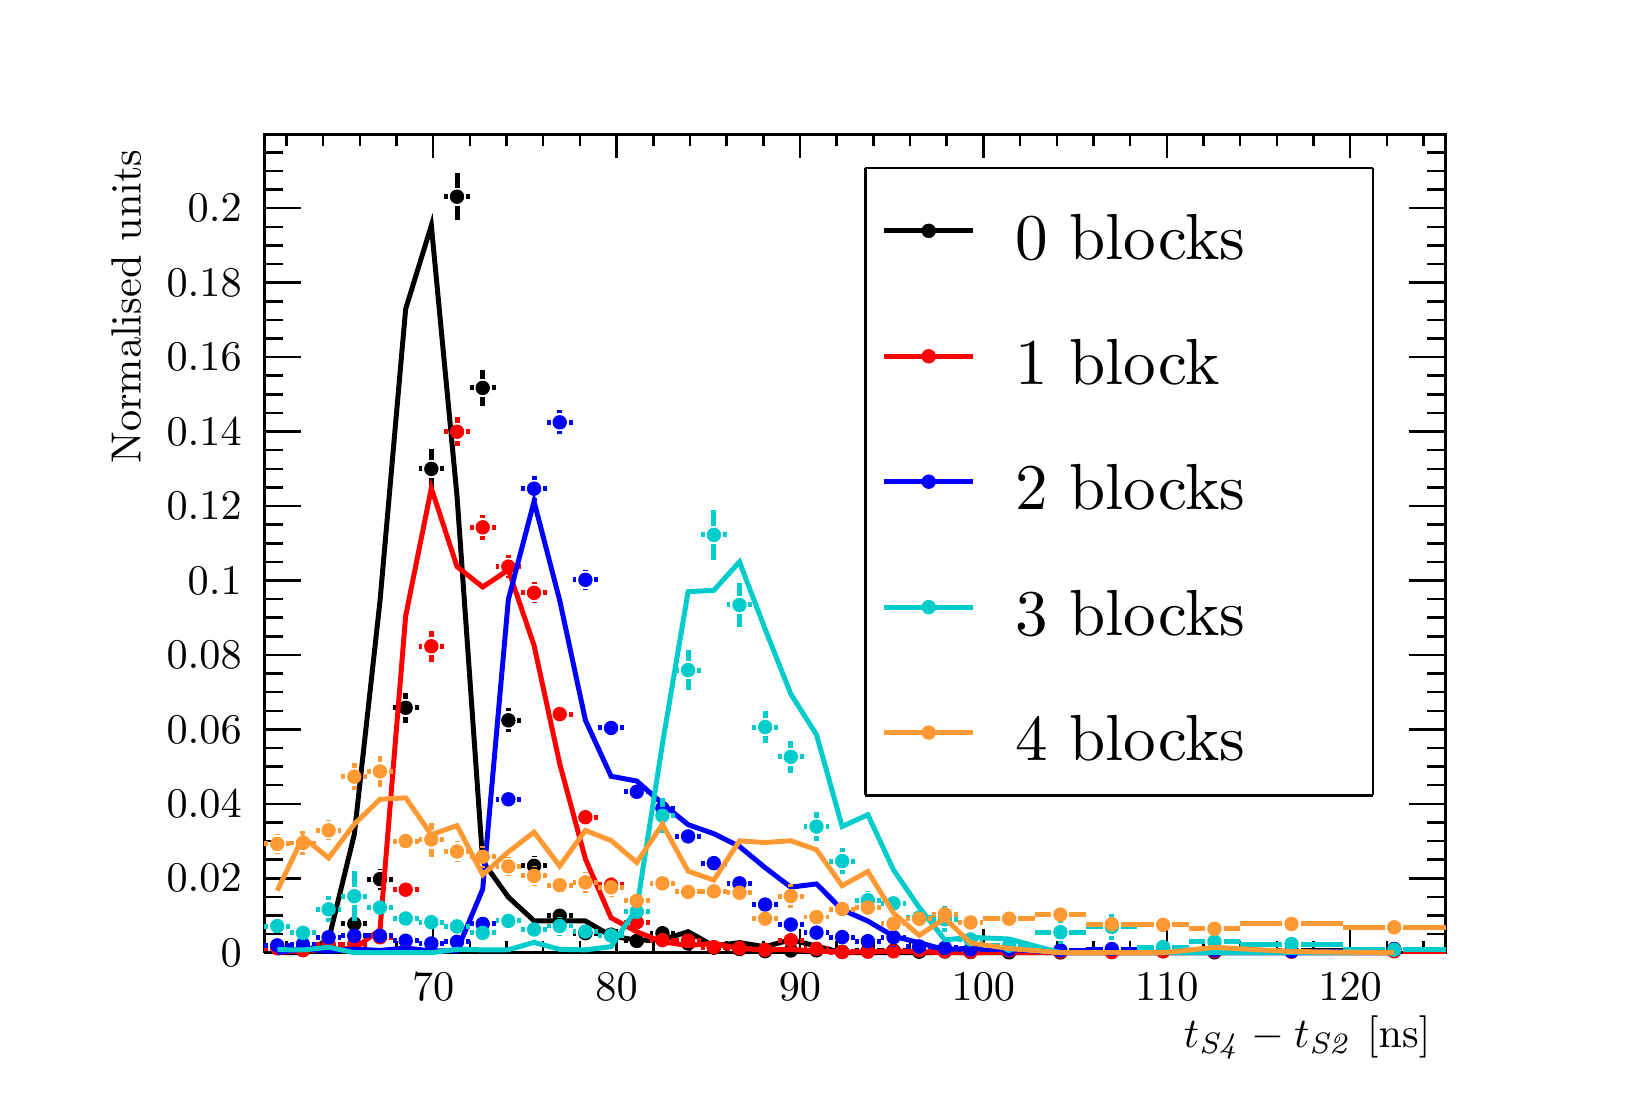
\begin{tikzpicture}
\pgfdeclareplotmark{cross} {
\pgfpathmoveto{\pgfpoint{-0.3\pgfplotmarksize}{\pgfplotmarksize}}
\pgfpathlineto{\pgfpoint{+0.3\pgfplotmarksize}{\pgfplotmarksize}}
\pgfpathlineto{\pgfpoint{+0.3\pgfplotmarksize}{0.3\pgfplotmarksize}}
\pgfpathlineto{\pgfpoint{+1\pgfplotmarksize}{0.3\pgfplotmarksize}}
\pgfpathlineto{\pgfpoint{+1\pgfplotmarksize}{-0.3\pgfplotmarksize}}
\pgfpathlineto{\pgfpoint{+0.3\pgfplotmarksize}{-0.3\pgfplotmarksize}}
\pgfpathlineto{\pgfpoint{+0.3\pgfplotmarksize}{-1.\pgfplotmarksize}}
\pgfpathlineto{\pgfpoint{-0.3\pgfplotmarksize}{-1.\pgfplotmarksize}}
\pgfpathlineto{\pgfpoint{-0.3\pgfplotmarksize}{-0.3\pgfplotmarksize}}
\pgfpathlineto{\pgfpoint{-1.\pgfplotmarksize}{-0.3\pgfplotmarksize}}
\pgfpathlineto{\pgfpoint{-1.\pgfplotmarksize}{0.3\pgfplotmarksize}}
\pgfpathlineto{\pgfpoint{-0.3\pgfplotmarksize}{0.3\pgfplotmarksize}}
\pgfpathclose
\pgfusepathqstroke
}
\pgfdeclareplotmark{cross*} {
\pgfpathmoveto{\pgfpoint{-0.3\pgfplotmarksize}{\pgfplotmarksize}}
\pgfpathlineto{\pgfpoint{+0.3\pgfplotmarksize}{\pgfplotmarksize}}
\pgfpathlineto{\pgfpoint{+0.3\pgfplotmarksize}{0.3\pgfplotmarksize}}
\pgfpathlineto{\pgfpoint{+1\pgfplotmarksize}{0.3\pgfplotmarksize}}
\pgfpathlineto{\pgfpoint{+1\pgfplotmarksize}{-0.3\pgfplotmarksize}}
\pgfpathlineto{\pgfpoint{+0.3\pgfplotmarksize}{-0.3\pgfplotmarksize}}
\pgfpathlineto{\pgfpoint{+0.3\pgfplotmarksize}{-1.\pgfplotmarksize}}
\pgfpathlineto{\pgfpoint{-0.3\pgfplotmarksize}{-1.\pgfplotmarksize}}
\pgfpathlineto{\pgfpoint{-0.3\pgfplotmarksize}{-0.3\pgfplotmarksize}}
\pgfpathlineto{\pgfpoint{-1.\pgfplotmarksize}{-0.3\pgfplotmarksize}}
\pgfpathlineto{\pgfpoint{-1.\pgfplotmarksize}{0.3\pgfplotmarksize}}
\pgfpathlineto{\pgfpoint{-0.3\pgfplotmarksize}{0.3\pgfplotmarksize}}
\pgfpathclose
\pgfusepathqfillstroke
}
\pgfdeclareplotmark{newstar} {
\pgfpathmoveto{\pgfqpoint{0pt}{\pgfplotmarksize}}
\pgfpathlineto{\pgfqpointpolar{44}{0.5\pgfplotmarksize}}
\pgfpathlineto{\pgfqpointpolar{18}{\pgfplotmarksize}}
\pgfpathlineto{\pgfqpointpolar{-20}{0.5\pgfplotmarksize}}
\pgfpathlineto{\pgfqpointpolar{-54}{\pgfplotmarksize}}
\pgfpathlineto{\pgfqpointpolar{-90}{0.5\pgfplotmarksize}}
\pgfpathlineto{\pgfqpointpolar{234}{\pgfplotmarksize}}
\pgfpathlineto{\pgfqpointpolar{198}{0.5\pgfplotmarksize}}
\pgfpathlineto{\pgfqpointpolar{162}{\pgfplotmarksize}}
\pgfpathlineto{\pgfqpointpolar{134}{0.5\pgfplotmarksize}}
\pgfpathclose
\pgfusepathqstroke
}
\pgfdeclareplotmark{newstar*} {
\pgfpathmoveto{\pgfqpoint{0pt}{\pgfplotmarksize}}
\pgfpathlineto{\pgfqpointpolar{44}{0.5\pgfplotmarksize}}
\pgfpathlineto{\pgfqpointpolar{18}{\pgfplotmarksize}}
\pgfpathlineto{\pgfqpointpolar{-20}{0.5\pgfplotmarksize}}
\pgfpathlineto{\pgfqpointpolar{-54}{\pgfplotmarksize}}
\pgfpathlineto{\pgfqpointpolar{-90}{0.5\pgfplotmarksize}}
\pgfpathlineto{\pgfqpointpolar{234}{\pgfplotmarksize}}
\pgfpathlineto{\pgfqpointpolar{198}{0.5\pgfplotmarksize}}
\pgfpathlineto{\pgfqpointpolar{162}{\pgfplotmarksize}}
\pgfpathlineto{\pgfqpointpolar{134}{0.5\pgfplotmarksize}}
\pgfpathclose
\pgfusepathqfillstroke
}
\definecolor{c}{rgb}{1,1,1};
\draw [color=c, fill=c] (0,0) rectangle (20,13.4957);
\draw [color=c, fill=c] (3,1.75444) rectangle (18,12.1461);
\definecolor{c}{rgb}{0,0,0};
\draw [c,line width=0.9] (3,1.75444) -- (3,12.1461) -- (18,12.1461) -- (18,1.75444) -- (3,1.75444);
\definecolor{c}{rgb}{1,1,1};
\draw [color=c, fill=c] (3,1.75444) rectangle (18,12.1461);
\definecolor{c}{rgb}{0,0,0};
\draw [c,line width=0.9] (3,1.75444) -- (3,12.1461) -- (18,12.1461) -- (18,1.75444) -- (3,1.75444);
\draw [c,line width=1.8] (3,1.83114) -- (3.04843,1.83114);
\draw [c,line width=1.8] (3.27766,1.83114) -- (3.32609,1.83114);
\foreach \P in {(3.16304,1.83114)}{\draw[mark options={color=c,fill=c},mark size=2.402402pt,mark=*] plot coordinates {\P};}
\draw [c,line width=1.8] (3.32609,1.82516) -- (3.37452,1.82516);
\draw [c,line width=1.8] (3.60374,1.82516) -- (3.65217,1.82516);
\foreach \P in {(3.48913,1.82516)}{\draw[mark options={color=c,fill=c},mark size=2.402402pt,mark=*] plot coordinates {\P};}
\draw [c,line width=1.8] (3.65217,1.84454) -- (3.7006,1.84454);
\draw [c,line width=1.8] (3.92983,1.84454) -- (3.97826,1.84454);
\foreach \P in {(3.81522,1.84454)}{\draw[mark options={color=c,fill=c},mark size=2.402402pt,mark=*] plot coordinates {\P};}
\draw [c,line width=1.8] (3.97826,2.12085) -- (4.02669,2.12085);
\draw [c,line width=1.8] (4.25592,2.12085) -- (4.30435,2.12085);
\foreach \P in {(4.1413,2.12085)}{\draw[mark options={color=c,fill=c},mark size=2.402402pt,mark=*] plot coordinates {\P};}
\draw [c,line width=1.8] (4.46739,2.55475) -- (4.46739,2.57465);
\draw [c,line width=1.8] (4.46739,2.80387) -- (4.46739,2.82376);
\draw [c,line width=1.8] (4.30435,2.68926) -- (4.35278,2.68926);
\draw [c,line width=1.8] (4.582,2.68926) -- (4.63043,2.68926);
\foreach \P in {(4.46739,2.68926)}{\draw[mark options={color=c,fill=c},mark size=2.402402pt,mark=*] plot coordinates {\P};}
\draw [c,line width=1.8] (4.79348,4.67286) -- (4.79348,4.75114);
\draw [c,line width=1.8] (4.79348,4.98037) -- (4.79348,5.05865);
\draw [c,line width=1.8] (4.63043,4.86575) -- (4.67886,4.86575);
\draw [c,line width=1.8] (4.90809,4.86575) -- (4.95652,4.86575);
\foreach \P in {(4.79348,4.86575)}{\draw[mark options={color=c,fill=c},mark size=2.402402pt,mark=*] plot coordinates {\P};}
\draw [c,line width=1.8] (5.11957,7.64548) -- (5.11957,7.78469);
\draw [c,line width=1.8] (5.11957,8.01391) -- (5.11957,8.15312);
\draw [c,line width=1.8] (4.95652,7.8993) -- (5.00495,7.8993);
\draw [c,line width=1.8] (5.23418,7.8993) -- (5.28261,7.8993);
\foreach \P in {(5.11957,7.8993)}{\draw[mark options={color=c,fill=c},mark size=2.402402pt,mark=*] plot coordinates {\P};}
\draw [c,line width=1.8] (5.44565,11.0614) -- (5.44565,11.2417);
\draw [c,line width=1.8] (5.44565,11.4709) -- (5.44565,11.6513);
\draw [c,line width=1.8] (5.28261,11.3563) -- (5.33104,11.3563);
\draw [c,line width=1.8] (5.56027,11.3563) -- (5.6087,11.3563);
\foreach \P in {(5.44565,11.3563)}{\draw[mark options={color=c,fill=c},mark size=2.402402pt,mark=*] plot coordinates {\P};}
\draw [c,line width=1.8] (5.77174,8.694) -- (5.77174,8.81308);
\draw [c,line width=1.8] (5.77174,9.04231) -- (5.77174,9.1614);
\draw [c,line width=1.8] (5.6087,8.9277) -- (5.65713,8.9277);
\draw [c,line width=1.8] (5.88635,8.9277) -- (5.93478,8.9277);
\foreach \P in {(5.77174,8.9277)}{\draw[mark options={color=c,fill=c},mark size=2.402402pt,mark=*] plot coordinates {\P};}
\draw [c,line width=1.8] (6.09783,4.55419) -- (6.09783,4.59147);
\draw [c,line width=1.8] (6.09783,4.8207) -- (6.09783,4.85798);
\draw [c,line width=1.8] (5.93478,4.70608) -- (5.98321,4.70608);
\draw [c,line width=1.8] (6.21244,4.70608) -- (6.26087,4.70608);
\foreach \P in {(6.09783,4.70608)}{\draw[mark options={color=c,fill=c},mark size=2.402402pt,mark=*] plot coordinates {\P};}
\draw [c,line width=1.8] (6.42391,2.73278) -- (6.42391,2.74337);
\draw [c,line width=1.8] (6.42391,2.9726) -- (6.42391,2.98319);
\draw [c,line width=1.8] (6.26087,2.85799) -- (6.3093,2.85799);
\draw [c,line width=1.8] (6.53853,2.85799) -- (6.58696,2.85799);
\foreach \P in {(6.42391,2.85799)}{\draw[mark options={color=c,fill=c},mark size=2.402402pt,mark=*] plot coordinates {\P};}
\draw [c,line width=1.8] (6.58696,2.22344) -- (6.63539,2.22344);
\draw [c,line width=1.8] (6.86461,2.22344) -- (6.91304,2.22344);
\foreach \P in {(6.75,2.22344)}{\draw[mark options={color=c,fill=c},mark size=2.402402pt,mark=*] plot coordinates {\P};}
\draw [c,line width=1.8] (6.91304,2.00306) -- (6.96147,2.00306);
\draw [c,line width=1.8] (7.1907,2.00306) -- (7.23913,2.00306);
\foreach \P in {(7.07609,2.00306)}{\draw[mark options={color=c,fill=c},mark size=2.402402pt,mark=*] plot coordinates {\P};}
\draw [c,line width=1.8] (7.23913,1.98414) -- (7.28756,1.98414);
\draw [c,line width=1.8] (7.51679,1.98414) -- (7.56522,1.98414);
\foreach \P in {(7.40217,1.98414)}{\draw[mark options={color=c,fill=c},mark size=2.402402pt,mark=*] plot coordinates {\P};}
\draw [c,line width=1.8] (7.56522,1.90433) -- (7.61365,1.90433);
\draw [c,line width=1.8] (7.84287,1.90433) -- (7.8913,1.90433);
\foreach \P in {(7.72826,1.90433)}{\draw[mark options={color=c,fill=c},mark size=2.402402pt,mark=*] plot coordinates {\P};}
\draw [c,line width=1.8] (7.8913,2.00177) -- (7.93973,2.00177);
\draw [c,line width=1.8] (8.16896,2.00177) -- (8.21739,2.00177);
\foreach \P in {(8.05435,2.00177)}{\draw[mark options={color=c,fill=c},mark size=2.402402pt,mark=*] plot coordinates {\P};}
\draw [c,line width=1.8] (8.21739,1.87216) -- (8.26582,1.87216);
\draw [c,line width=1.8] (8.49505,1.87216) -- (8.54348,1.87216);
\foreach \P in {(8.38043,1.87216)}{\draw[mark options={color=c,fill=c},mark size=2.402402pt,mark=*] plot coordinates {\P};}
\draw [c,line width=1.8] (8.54348,1.81906) -- (8.59191,1.81906);
\draw [c,line width=1.8] (8.82113,1.81906) -- (8.86957,1.81906);
\foreach \P in {(8.70652,1.81906)}{\draw[mark options={color=c,fill=c},mark size=2.402402pt,mark=*] plot coordinates {\P};}
\draw [c,line width=1.8] (8.86957,1.80095) -- (8.918,1.80095);
\draw [c,line width=1.8] (9.14722,1.80095) -- (9.19565,1.80095);
\foreach \P in {(9.03261,1.80095)}{\draw[mark options={color=c,fill=c},mark size=2.402402pt,mark=*] plot coordinates {\P};}
\draw [c,line width=1.8] (9.19565,1.77486) -- (9.24408,1.77486);
\draw [c,line width=1.8] (9.47331,1.77486) -- (9.52174,1.77486);
\foreach \P in {(9.3587,1.77486)}{\draw[mark options={color=c,fill=c},mark size=2.402402pt,mark=*] plot coordinates {\P};}
\draw [c,line width=1.8] (9.52174,1.78306) -- (9.57017,1.78306);
\draw [c,line width=1.8] (9.7994,1.78306) -- (9.84783,1.78306);
\foreach \P in {(9.68478,1.78306)}{\draw[mark options={color=c,fill=c},mark size=2.402402pt,mark=*] plot coordinates {\P};}
\draw [c,line width=1.8] (9.84783,1.78487) -- (9.89626,1.78487);
\draw [c,line width=1.8] (10.1255,1.78487) -- (10.1739,1.78487);
\foreach \P in {(10.0109,1.78487)}{\draw[mark options={color=c,fill=c},mark size=2.402402pt,mark=*] plot coordinates {\P};}
\draw [c,line width=1.8] (10.1739,1.76533) -- (10.2223,1.76533);
\draw [c,line width=1.8] (10.4516,1.76533) -- (10.5,1.76533);
\foreach \P in {(10.337,1.76533)}{\draw[mark options={color=c,fill=c},mark size=2.402402pt,mark=*] plot coordinates {\P};}
\draw [c,line width=1.8] (10.5,1.7786) -- (10.5484,1.7786);
\draw [c,line width=1.8] (10.7777,1.7786) -- (10.8261,1.7786);
\foreach \P in {(10.663,1.7786)}{\draw[mark options={color=c,fill=c},mark size=2.402402pt,mark=*] plot coordinates {\P};}
\draw [c,line width=1.8] (10.8261,1.78124) -- (10.8745,1.78124);
\draw [c,line width=1.8] (11.1037,1.78124) -- (11.1522,1.78124);
\foreach \P in {(10.9891,1.78124)}{\draw[mark options={color=c,fill=c},mark size=2.402402pt,mark=*] plot coordinates {\P};}
\draw [c,line width=1.8] (11.1522,1.767) -- (11.2006,1.767);
\draw [c,line width=1.8] (11.4298,1.767) -- (11.4783,1.767);
\foreach \P in {(11.3152,1.767)}{\draw[mark options={color=c,fill=c},mark size=2.402402pt,mark=*] plot coordinates {\P};}
\draw [c,line width=1.8] (11.4783,1.77006) -- (11.5267,1.77006);
\draw [c,line width=1.8] (11.7559,1.77006) -- (11.8043,1.77006);
\foreach \P in {(11.6413,1.77006)}{\draw[mark options={color=c,fill=c},mark size=2.402402pt,mark=*] plot coordinates {\P};}
\draw [c,line width=1.8] (11.8043,1.76448) -- (11.8528,1.76448);
\draw [c,line width=1.8] (12.082,1.76448) -- (12.1304,1.76448);
\foreach \P in {(11.9674,1.76448)}{\draw[mark options={color=c,fill=c},mark size=2.402402pt,mark=*] plot coordinates {\P};}
\draw [c,line width=1.8] (12.1304,1.76013) -- (12.3419,1.76013);
\draw [c,line width=1.8] (12.5711,1.76013) -- (12.7826,1.76013);
\foreach \P in {(12.4565,1.76013)}{\draw[mark options={color=c,fill=c},mark size=2.402402pt,mark=*] plot coordinates {\P};}
\draw [c,line width=1.8] (12.7826,1.75877) -- (12.9941,1.75877);
\draw [c,line width=1.8] (13.2233,1.75877) -- (13.4348,1.75877);
\foreach \P in {(13.1087,1.75877)}{\draw[mark options={color=c,fill=c},mark size=2.402402pt,mark=*] plot coordinates {\P};}
\draw [c,line width=1.8] (13.4348,1.7716) -- (13.6463,1.7716);
\draw [c,line width=1.8] (13.8755,1.7716) -- (14.087,1.7716);
\foreach \P in {(13.7609,1.7716)}{\draw[mark options={color=c,fill=c},mark size=2.402402pt,mark=*] plot coordinates {\P};}
\draw [c,line width=1.8] (14.087,1.77325) -- (14.2984,1.77325);
\draw [c,line width=1.8] (14.5277,1.77325) -- (14.7391,1.77325);
\foreach \P in {(14.413,1.77325)}{\draw[mark options={color=c,fill=c},mark size=2.402402pt,mark=*] plot coordinates {\P};}
\draw [c,line width=1.8] (14.7391,1.76012) -- (14.9506,1.76012);
\draw [c,line width=1.8] (15.1798,1.76012) -- (15.3913,1.76012);
\foreach \P in {(15.0652,1.76012)}{\draw[mark options={color=c,fill=c},mark size=2.402402pt,mark=*] plot coordinates {\P};}
\draw [c,line width=1.8] (15.3913,1.77863) -- (15.9289,1.77863);
\draw [c,line width=1.8] (16.1581,1.77863) -- (16.6957,1.77863);
\foreach \P in {(16.0435,1.77863)}{\draw[mark options={color=c,fill=c},mark size=2.402402pt,mark=*] plot coordinates {\P};}
\draw [c,line width=1.8] (16.6957,1.80192) -- (17.2332,1.80192);
\draw [c,line width=1.8] (17.4624,1.80192) -- (18,1.80192);
\foreach \P in {(17.3478,1.80192)}{\draw[mark options={color=c,fill=c},mark size=2.402402pt,mark=*] plot coordinates {\P};}
\draw [c,line width=0.9] (3,1.75444) -- (18,1.75444);
\draw [c,line width=0.9] (5.14286,2.05809) -- (5.14286,1.75444);
\draw [c,line width=0.9] (5.6087,1.90627) -- (5.6087,1.75444);
\draw [c,line width=0.9] (6.07453,1.90627) -- (6.07453,1.75444);
\draw [c,line width=0.9] (6.54037,1.90627) -- (6.54037,1.75444);
\draw [c,line width=0.9] (7.00621,1.90627) -- (7.00621,1.75444);
\draw [c,line width=0.9] (7.47205,2.05809) -- (7.47205,1.75444);
\draw [c,line width=0.9] (7.93789,1.90627) -- (7.93789,1.75444);
\draw [c,line width=0.9] (8.40373,1.90627) -- (8.40373,1.75444);
\draw [c,line width=0.9] (8.86957,1.90627) -- (8.86957,1.75444);
\draw [c,line width=0.9] (9.3354,1.90627) -- (9.3354,1.75444);
\draw [c,line width=0.9] (9.80124,2.05809) -- (9.80124,1.75444);
\draw [c,line width=0.9] (10.2671,1.90627) -- (10.2671,1.75444);
\draw [c,line width=0.9] (10.7329,1.90627) -- (10.7329,1.75444);
\draw [c,line width=0.9] (11.1988,1.90627) -- (11.1988,1.75444);
\draw [c,line width=0.9] (11.6646,1.90627) -- (11.6646,1.75444);
\draw [c,line width=0.9] (12.1304,2.05809) -- (12.1304,1.75444);
\draw [c,line width=0.9] (12.5963,1.90627) -- (12.5963,1.75444);
\draw [c,line width=0.9] (13.0621,1.90627) -- (13.0621,1.75444);
\draw [c,line width=0.9] (13.528,1.90627) -- (13.528,1.75444);
\draw [c,line width=0.9] (13.9938,1.90627) -- (13.9938,1.75444);
\draw [c,line width=0.9] (14.4596,2.05809) -- (14.4596,1.75444);
\draw [c,line width=0.9] (14.9255,1.90627) -- (14.9255,1.75444);
\draw [c,line width=0.9] (15.3913,1.90627) -- (15.3913,1.75444);
\draw [c,line width=0.9] (15.8571,1.90627) -- (15.8571,1.75444);
\draw [c,line width=0.9] (16.323,1.90627) -- (16.323,1.75444);
\draw [c,line width=0.9] (16.7888,2.05809) -- (16.7888,1.75444);
\draw [c,line width=0.9] (5.14286,2.05809) -- (5.14286,1.75444);
\draw [c,line width=0.9] (4.67702,1.90627) -- (4.67702,1.75444);
\draw [c,line width=0.9] (4.21118,1.90627) -- (4.21118,1.75444);
\draw [c,line width=0.9] (3.74534,1.90627) -- (3.74534,1.75444);
\draw [c,line width=0.9] (3.2795,1.90627) -- (3.2795,1.75444);
\draw [c,line width=0.9] (16.7888,2.05809) -- (16.7888,1.75444);
\draw [c,line width=0.9] (17.2547,1.90627) -- (17.2547,1.75444);
\draw [c,line width=0.9] (17.7205,1.90627) -- (17.7205,1.75444);
\draw [anchor=base] (5.14286,1.14713) node[scale=1.52731, color=c, rotate=0]{70};
\draw [anchor=base] (7.47205,1.14713) node[scale=1.52731, color=c, rotate=0]{80};
\draw [anchor=base] (9.80124,1.14713) node[scale=1.52731, color=c, rotate=0]{90};
\draw [anchor=base] (12.1304,1.14713) node[scale=1.52731, color=c, rotate=0]{100};
\draw [anchor=base] (14.4596,1.14713) node[scale=1.52731, color=c, rotate=0]{110};
\draw [anchor=base] (16.7888,1.14713) node[scale=1.52731, color=c, rotate=0]{120};
\draw [anchor= east] (18,0.674785) node[scale=1.52731, color=c, rotate=0]{$t_{\mathit{S4}} - t_{\mathit{S2}}$ [ns]};
\draw [c,line width=0.9] (3,12.1461) -- (18,12.1461);
\draw [c,line width=0.9] (5.14286,11.8425) -- (5.14286,12.1461);
\draw [c,line width=0.9] (5.6087,11.9943) -- (5.6087,12.1461);
\draw [c,line width=0.9] (6.07453,11.9943) -- (6.07453,12.1461);
\draw [c,line width=0.9] (6.54037,11.9943) -- (6.54037,12.1461);
\draw [c,line width=0.9] (7.00621,11.9943) -- (7.00621,12.1461);
\draw [c,line width=0.9] (7.47205,11.8425) -- (7.47205,12.1461);
\draw [c,line width=0.9] (7.93789,11.9943) -- (7.93789,12.1461);
\draw [c,line width=0.9] (8.40373,11.9943) -- (8.40373,12.1461);
\draw [c,line width=0.9] (8.86957,11.9943) -- (8.86957,12.1461);
\draw [c,line width=0.9] (9.3354,11.9943) -- (9.3354,12.1461);
\draw [c,line width=0.9] (9.80124,11.8425) -- (9.80124,12.1461);
\draw [c,line width=0.9] (10.2671,11.9943) -- (10.2671,12.1461);
\draw [c,line width=0.9] (10.7329,11.9943) -- (10.7329,12.1461);
\draw [c,line width=0.9] (11.1988,11.9943) -- (11.1988,12.1461);
\draw [c,line width=0.9] (11.6646,11.9943) -- (11.6646,12.1461);
\draw [c,line width=0.9] (12.1304,11.8425) -- (12.1304,12.1461);
\draw [c,line width=0.9] (12.5963,11.9943) -- (12.5963,12.1461);
\draw [c,line width=0.9] (13.0621,11.9943) -- (13.0621,12.1461);
\draw [c,line width=0.9] (13.528,11.9943) -- (13.528,12.1461);
\draw [c,line width=0.9] (13.9938,11.9943) -- (13.9938,12.1461);
\draw [c,line width=0.9] (14.4596,11.8425) -- (14.4596,12.1461);
\draw [c,line width=0.9] (14.9255,11.9943) -- (14.9255,12.1461);
\draw [c,line width=0.9] (15.3913,11.9943) -- (15.3913,12.1461);
\draw [c,line width=0.9] (15.8571,11.9943) -- (15.8571,12.1461);
\draw [c,line width=0.9] (16.323,11.9943) -- (16.323,12.1461);
\draw [c,line width=0.9] (16.7888,11.8425) -- (16.7888,12.1461);
\draw [c,line width=0.9] (5.14286,11.8425) -- (5.14286,12.1461);
\draw [c,line width=0.9] (4.67702,11.9943) -- (4.67702,12.1461);
\draw [c,line width=0.9] (4.21118,11.9943) -- (4.21118,12.1461);
\draw [c,line width=0.9] (3.74534,11.9943) -- (3.74534,12.1461);
\draw [c,line width=0.9] (3.2795,11.9943) -- (3.2795,12.1461);
\draw [c,line width=0.9] (16.7888,11.8425) -- (16.7888,12.1461);
\draw [c,line width=0.9] (17.2547,11.9943) -- (17.2547,12.1461);
\draw [c,line width=0.9] (17.7205,11.9943) -- (17.7205,12.1461);
\draw [c,line width=0.9] (3,1.75444) -- (3,12.1461);
\draw [c,line width=0.9] (3.462,1.75444) -- (3,1.75444);
\draw [c,line width=0.9] (3.231,1.99082) -- (3,1.99082);
\draw [c,line width=0.9] (3.231,2.2272) -- (3,2.2272);
\draw [c,line width=0.9] (3.231,2.46357) -- (3,2.46357);
\draw [c,line width=0.9] (3.462,2.69995) -- (3,2.69995);
\draw [c,line width=0.9] (3.231,2.93633) -- (3,2.93633);
\draw [c,line width=0.9] (3.231,3.1727) -- (3,3.1727);
\draw [c,line width=0.9] (3.231,3.40908) -- (3,3.40908);
\draw [c,line width=0.9] (3.462,3.64546) -- (3,3.64546);
\draw [c,line width=0.9] (3.231,3.88184) -- (3,3.88184);
\draw [c,line width=0.9] (3.231,4.11821) -- (3,4.11821);
\draw [c,line width=0.9] (3.231,4.35459) -- (3,4.35459);
\draw [c,line width=0.9] (3.462,4.59097) -- (3,4.59097);
\draw [c,line width=0.9] (3.231,4.82734) -- (3,4.82734);
\draw [c,line width=0.9] (3.231,5.06372) -- (3,5.06372);
\draw [c,line width=0.9] (3.231,5.3001) -- (3,5.3001);
\draw [c,line width=0.9] (3.462,5.53648) -- (3,5.53648);
\draw [c,line width=0.9] (3.231,5.77285) -- (3,5.77285);
\draw [c,line width=0.9] (3.231,6.00923) -- (3,6.00923);
\draw [c,line width=0.9] (3.231,6.24561) -- (3,6.24561);
\draw [c,line width=0.9] (3.462,6.48199) -- (3,6.48199);
\draw [c,line width=0.9] (3.231,6.71836) -- (3,6.71836);
\draw [c,line width=0.9] (3.231,6.95474) -- (3,6.95474);
\draw [c,line width=0.9] (3.231,7.19112) -- (3,7.19112);
\draw [c,line width=0.9] (3.462,7.42749) -- (3,7.42749);
\draw [c,line width=0.9] (3.231,7.66387) -- (3,7.66387);
\draw [c,line width=0.9] (3.231,7.90025) -- (3,7.90025);
\draw [c,line width=0.9] (3.231,8.13663) -- (3,8.13663);
\draw [c,line width=0.9] (3.462,8.373) -- (3,8.373);
\draw [c,line width=0.9] (3.231,8.60938) -- (3,8.60938);
\draw [c,line width=0.9] (3.231,8.84576) -- (3,8.84576);
\draw [c,line width=0.9] (3.231,9.08213) -- (3,9.08213);
\draw [c,line width=0.9] (3.462,9.31851) -- (3,9.31851);
\draw [c,line width=0.9] (3.231,9.55489) -- (3,9.55489);
\draw [c,line width=0.9] (3.231,9.79127) -- (3,9.79127);
\draw [c,line width=0.9] (3.231,10.0276) -- (3,10.0276);
\draw [c,line width=0.9] (3.462,10.264) -- (3,10.264);
\draw [c,line width=0.9] (3.231,10.5004) -- (3,10.5004);
\draw [c,line width=0.9] (3.231,10.7368) -- (3,10.7368);
\draw [c,line width=0.9] (3.231,10.9732) -- (3,10.9732);
\draw [c,line width=0.9] (3.462,11.2095) -- (3,11.2095);
\draw [c,line width=0.9] (3.462,11.2095) -- (3,11.2095);
\draw [c,line width=0.9] (3.231,11.4459) -- (3,11.4459);
\draw [c,line width=0.9] (3.231,11.6823) -- (3,11.6823);
\draw [c,line width=0.9] (3.231,11.9187) -- (3,11.9187);
\draw [anchor= east] (2.9,1.75444) node[scale=1.52731, color=c, rotate=0]{0};
\draw [anchor= east] (2.9,2.69995) node[scale=1.52731, color=c, rotate=0]{0.02};
\draw [anchor= east] (2.9,3.64546) node[scale=1.52731, color=c, rotate=0]{0.04};
\draw [anchor= east] (2.9,4.59097) node[scale=1.52731, color=c, rotate=0]{0.06};
\draw [anchor= east] (2.9,5.53648) node[scale=1.52731, color=c, rotate=0]{0.08};
\draw [anchor= east] (2.9,6.48199) node[scale=1.52731, color=c, rotate=0]{0.1};
\draw [anchor= east] (2.9,7.42749) node[scale=1.52731, color=c, rotate=0]{0.12};
\draw [anchor= east] (2.9,8.373) node[scale=1.52731, color=c, rotate=0]{0.14};
\draw [anchor= east] (2.9,9.31851) node[scale=1.52731, color=c, rotate=0]{0.16};
\draw [anchor= east] (2.9,10.264) node[scale=1.52731, color=c, rotate=0]{0.18};
\draw [anchor= east] (2.9,11.2095) node[scale=1.52731, color=c, rotate=0]{0.2};
\draw [anchor= east] (1.24,12.1461) node[scale=1.52731, color=c, rotate=90]{Normalised units};
\draw [c,line width=0.9] (18,1.75444) -- (18,12.1461);
\draw [c,line width=0.9] (17.538,1.75444) -- (18,1.75444);
\draw [c,line width=0.9] (17.769,1.99082) -- (18,1.99082);
\draw [c,line width=0.9] (17.769,2.2272) -- (18,2.2272);
\draw [c,line width=0.9] (17.769,2.46357) -- (18,2.46357);
\draw [c,line width=0.9] (17.538,2.69995) -- (18,2.69995);
\draw [c,line width=0.9] (17.769,2.93633) -- (18,2.93633);
\draw [c,line width=0.9] (17.769,3.1727) -- (18,3.1727);
\draw [c,line width=0.9] (17.769,3.40908) -- (18,3.40908);
\draw [c,line width=0.9] (17.538,3.64546) -- (18,3.64546);
\draw [c,line width=0.9] (17.769,3.88184) -- (18,3.88184);
\draw [c,line width=0.9] (17.769,4.11821) -- (18,4.11821);
\draw [c,line width=0.9] (17.769,4.35459) -- (18,4.35459);
\draw [c,line width=0.9] (17.538,4.59097) -- (18,4.59097);
\draw [c,line width=0.9] (17.769,4.82734) -- (18,4.82734);
\draw [c,line width=0.9] (17.769,5.06372) -- (18,5.06372);
\draw [c,line width=0.9] (17.769,5.3001) -- (18,5.3001);
\draw [c,line width=0.9] (17.538,5.53648) -- (18,5.53648);
\draw [c,line width=0.9] (17.769,5.77285) -- (18,5.77285);
\draw [c,line width=0.9] (17.769,6.00923) -- (18,6.00923);
\draw [c,line width=0.9] (17.769,6.24561) -- (18,6.24561);
\draw [c,line width=0.9] (17.538,6.48199) -- (18,6.48199);
\draw [c,line width=0.9] (17.769,6.71836) -- (18,6.71836);
\draw [c,line width=0.9] (17.769,6.95474) -- (18,6.95474);
\draw [c,line width=0.9] (17.769,7.19112) -- (18,7.19112);
\draw [c,line width=0.9] (17.538,7.42749) -- (18,7.42749);
\draw [c,line width=0.9] (17.769,7.66387) -- (18,7.66387);
\draw [c,line width=0.9] (17.769,7.90025) -- (18,7.90025);
\draw [c,line width=0.9] (17.769,8.13663) -- (18,8.13663);
\draw [c,line width=0.9] (17.538,8.373) -- (18,8.373);
\draw [c,line width=0.9] (17.769,8.60938) -- (18,8.60938);
\draw [c,line width=0.9] (17.769,8.84576) -- (18,8.84576);
\draw [c,line width=0.9] (17.769,9.08213) -- (18,9.08213);
\draw [c,line width=0.9] (17.538,9.31851) -- (18,9.31851);
\draw [c,line width=0.9] (17.769,9.55489) -- (18,9.55489);
\draw [c,line width=0.9] (17.769,9.79127) -- (18,9.79127);
\draw [c,line width=0.9] (17.769,10.0276) -- (18,10.0276);
\draw [c,line width=0.9] (17.538,10.264) -- (18,10.264);
\draw [c,line width=0.9] (17.769,10.5004) -- (18,10.5004);
\draw [c,line width=0.9] (17.769,10.7368) -- (18,10.7368);
\draw [c,line width=0.9] (17.769,10.9732) -- (18,10.9732);
\draw [c,line width=0.9] (17.538,11.2095) -- (18,11.2095);
\draw [c,line width=0.9] (17.538,11.2095) -- (18,11.2095);
\draw [c,line width=0.9] (17.769,11.4459) -- (18,11.4459);
\draw [c,line width=0.9] (17.769,11.6823) -- (18,11.6823);
\draw [c,line width=0.9] (17.769,11.9187) -- (18,11.9187);
\draw [c,line width=1.8] (3.16304,1.75444) -- (3.48913,1.75444) -- (3.81522,1.91963) -- (4.1413,3.2586) -- (4.46739,6.21923) -- (4.79348,9.93097) -- (5.11957,10.9903) -- (5.44565,7.5521) -- (5.77174,2.91629) -- (6.09783,2.46021) -- (6.42391,2.16031)
 -- (6.75,2.15888) -- (7.07609,2.1576) -- (7.40217,1.96821) -- (7.72826,1.91351) -- (8.05435,1.91827) -- (8.38043,2.02123) -- (8.70652,1.84056) -- (9.03261,1.88256) -- (9.3587,1.83017) -- (9.68478,1.92059) -- (10.0109,1.83781) -- (10.337,1.75444) --
 (10.663,1.75444) -- (10.9891,1.75444) -- (11.3152,1.75444) -- (11.6413,1.75444) -- (11.9674,1.75444) -- (12.4565,1.75444) -- (13.1087,1.75444) -- (13.7609,1.75444) -- (14.413,1.75444) -- (15.0652,1.75444) -- (16.0435,1.75444) -- (17.3478,1.75444);
\definecolor{c}{rgb}{1,0,0};
\draw [c,line width=1.8] (3,1.81211) -- (3.04843,1.81211);
\draw [c,line width=1.8] (3.27766,1.81211) -- (3.32609,1.81211);
\foreach \P in {(3.16304,1.81211)}{\draw[mark options={color=c,fill=c},mark size=2.402402pt,mark=*] plot coordinates {\P};}
\draw [c,line width=1.8] (3.32609,1.78648) -- (3.37452,1.78648);
\draw [c,line width=1.8] (3.60374,1.78648) -- (3.65217,1.78648);
\foreach \P in {(3.48913,1.78648)}{\draw[mark options={color=c,fill=c},mark size=2.402402pt,mark=*] plot coordinates {\P};}
\draw [c,line width=1.8] (3.65217,1.86159) -- (3.7006,1.86159);
\draw [c,line width=1.8] (3.92983,1.86159) -- (3.97826,1.86159);
\foreach \P in {(3.81522,1.86159)}{\draw[mark options={color=c,fill=c},mark size=2.402402pt,mark=*] plot coordinates {\P};}
\draw [c,line width=1.8] (3.97826,1.86397) -- (4.02669,1.86397);
\draw [c,line width=1.8] (4.25592,1.86397) -- (4.30435,1.86397);
\foreach \P in {(4.1413,1.86397)}{\draw[mark options={color=c,fill=c},mark size=2.402402pt,mark=*] plot coordinates {\P};}
\draw [c,line width=1.8] (4.30435,1.95008) -- (4.35278,1.95008);
\draw [c,line width=1.8] (4.582,1.95008) -- (4.63043,1.95008);
\foreach \P in {(4.46739,1.95008)}{\draw[mark options={color=c,fill=c},mark size=2.402402pt,mark=*] plot coordinates {\P};}
\draw [c,line width=1.8] (4.63043,2.55497) -- (4.67886,2.55497);
\draw [c,line width=1.8] (4.90809,2.55497) -- (4.95652,2.55497);
\foreach \P in {(4.79348,2.55497)}{\draw[mark options={color=c,fill=c},mark size=2.402402pt,mark=*] plot coordinates {\P};}
\draw [c,line width=1.8] (5.11957,5.44535) -- (5.11957,5.53144);
\draw [c,line width=1.8] (5.11957,5.76067) -- (5.11957,5.84676);
\draw [c,line width=1.8] (4.95652,5.64606) -- (5.00495,5.64606);
\draw [c,line width=1.8] (5.23418,5.64606) -- (5.28261,5.64606);
\foreach \P in {(5.11957,5.64606)}{\draw[mark options={color=c,fill=c},mark size=2.402402pt,mark=*] plot coordinates {\P};}
\draw [c,line width=1.8] (5.44565,8.18679) -- (5.44565,8.25649);
\draw [c,line width=1.8] (5.44565,8.48571) -- (5.44565,8.55541);
\draw [c,line width=1.8] (5.28261,8.3711) -- (5.33104,8.3711);
\draw [c,line width=1.8] (5.56027,8.3711) -- (5.6087,8.3711);
\foreach \P in {(5.44565,8.3711)}{\draw[mark options={color=c,fill=c},mark size=2.402402pt,mark=*] plot coordinates {\P};}
\draw [c,line width=1.8] (5.77174,6.99625) -- (5.77174,7.04232);
\draw [c,line width=1.8] (5.77174,7.27155) -- (5.77174,7.31762);
\draw [c,line width=1.8] (5.6087,7.15694) -- (5.65713,7.15694);
\draw [c,line width=1.8] (5.88635,7.15694) -- (5.93478,7.15694);
\foreach \P in {(5.77174,7.15694)}{\draw[mark options={color=c,fill=c},mark size=2.402402pt,mark=*] plot coordinates {\P};}
\draw [c,line width=1.8] (6.09783,6.51144) -- (6.09783,6.54373);
\draw [c,line width=1.8] (6.09783,6.77295) -- (6.09783,6.80523);
\draw [c,line width=1.8] (5.93478,6.65834) -- (5.98321,6.65834);
\draw [c,line width=1.8] (6.21244,6.65834) -- (6.26087,6.65834);
\foreach \P in {(6.09783,6.65834)}{\draw[mark options={color=c,fill=c},mark size=2.402402pt,mark=*] plot coordinates {\P};}
\draw [c,line width=1.8] (6.42391,6.19165) -- (6.42391,6.21023);
\draw [c,line width=1.8] (6.42391,6.43946) -- (6.42391,6.45803);
\draw [c,line width=1.8] (6.26087,6.32484) -- (6.3093,6.32484);
\draw [c,line width=1.8] (6.53853,6.32484) -- (6.58696,6.32484);
\foreach \P in {(6.42391,6.32484)}{\draw[mark options={color=c,fill=c},mark size=2.402402pt,mark=*] plot coordinates {\P};}
\draw [c,line width=1.8] (6.58696,4.78522) -- (6.63539,4.78522);
\draw [c,line width=1.8] (6.86461,4.78522) -- (6.91304,4.78522);
\foreach \P in {(6.75,4.78522)}{\draw[mark options={color=c,fill=c},mark size=2.402402pt,mark=*] plot coordinates {\P};}
\draw [c,line width=1.8] (6.91304,3.47547) -- (6.96147,3.47547);
\draw [c,line width=1.8] (7.1907,3.47547) -- (7.23913,3.47547);
\foreach \P in {(7.07609,3.47547)}{\draw[mark options={color=c,fill=c},mark size=2.402402pt,mark=*] plot coordinates {\P};}
\draw [c,line width=1.8] (7.23913,2.61559) -- (7.28756,2.61559);
\draw [c,line width=1.8] (7.51679,2.61559) -- (7.56522,2.61559);
\foreach \P in {(7.40217,2.61559)}{\draw[mark options={color=c,fill=c},mark size=2.402402pt,mark=*] plot coordinates {\P};}
\draw [c,line width=1.8] (7.56522,2.14104) -- (7.61365,2.14104);
\draw [c,line width=1.8] (7.84287,2.14104) -- (7.8913,2.14104);
\foreach \P in {(7.72826,2.14104)}{\draw[mark options={color=c,fill=c},mark size=2.402402pt,mark=*] plot coordinates {\P};}
\draw [c,line width=1.8] (7.8913,1.91483) -- (7.93973,1.91483);
\draw [c,line width=1.8] (8.16896,1.91483) -- (8.21739,1.91483);
\foreach \P in {(8.05435,1.91483)}{\draw[mark options={color=c,fill=c},mark size=2.402402pt,mark=*] plot coordinates {\P};}
\draw [c,line width=1.8] (8.21739,1.90786) -- (8.26582,1.90786);
\draw [c,line width=1.8] (8.49505,1.90786) -- (8.54348,1.90786);
\foreach \P in {(8.38043,1.90786)}{\draw[mark options={color=c,fill=c},mark size=2.402402pt,mark=*] plot coordinates {\P};}
\draw [c,line width=1.8] (8.54348,1.82528) -- (8.59191,1.82528);
\draw [c,line width=1.8] (8.82113,1.82528) -- (8.86957,1.82528);
\foreach \P in {(8.70652,1.82528)}{\draw[mark options={color=c,fill=c},mark size=2.402402pt,mark=*] plot coordinates {\P};}
\draw [c,line width=1.8] (8.86957,1.81201) -- (8.918,1.81201);
\draw [c,line width=1.8] (9.14722,1.81201) -- (9.19565,1.81201);
\foreach \P in {(9.03261,1.81201)}{\draw[mark options={color=c,fill=c},mark size=2.402402pt,mark=*] plot coordinates {\P};}
\draw [c,line width=1.8] (9.19565,1.79221) -- (9.24408,1.79221);
\draw [c,line width=1.8] (9.47331,1.79221) -- (9.52174,1.79221);
\foreach \P in {(9.3587,1.79221)}{\draw[mark options={color=c,fill=c},mark size=2.402402pt,mark=*] plot coordinates {\P};}
\draw [c,line width=1.8] (9.52174,1.91331) -- (9.57017,1.91331);
\draw [c,line width=1.8] (9.7994,1.91331) -- (9.84783,1.91331);
\foreach \P in {(9.68478,1.91331)}{\draw[mark options={color=c,fill=c},mark size=2.402402pt,mark=*] plot coordinates {\P};}
\draw [c,line width=1.8] (9.84783,1.80433) -- (9.89626,1.80433);
\draw [c,line width=1.8] (10.1255,1.80433) -- (10.1739,1.80433);
\foreach \P in {(10.0109,1.80433)}{\draw[mark options={color=c,fill=c},mark size=2.402402pt,mark=*] plot coordinates {\P};}
\draw [c,line width=1.8] (10.1739,1.76343) -- (10.2223,1.76343);
\draw [c,line width=1.8] (10.4516,1.76343) -- (10.5,1.76343);
\foreach \P in {(10.337,1.76343)}{\draw[mark options={color=c,fill=c},mark size=2.402402pt,mark=*] plot coordinates {\P};}
\draw [c,line width=1.8] (10.5,1.76754) -- (10.5484,1.76754);
\draw [c,line width=1.8] (10.7777,1.76754) -- (10.8261,1.76754);
\foreach \P in {(10.663,1.76754)}{\draw[mark options={color=c,fill=c},mark size=2.402402pt,mark=*] plot coordinates {\P};}
\draw [c,line width=1.8] (10.8261,1.77221) -- (10.8745,1.77221);
\draw [c,line width=1.8] (11.1037,1.77221) -- (11.1522,1.77221);
\foreach \P in {(10.9891,1.77221)}{\draw[mark options={color=c,fill=c},mark size=2.402402pt,mark=*] plot coordinates {\P};}
\draw [c,line width=1.8] (11.1522,1.785) -- (11.2006,1.785);
\draw [c,line width=1.8] (11.4298,1.785) -- (11.4783,1.785);
\foreach \P in {(11.3152,1.785)}{\draw[mark options={color=c,fill=c},mark size=2.402402pt,mark=*] plot coordinates {\P};}
\draw [c,line width=1.8] (11.4783,1.77279) -- (11.5267,1.77279);
\draw [c,line width=1.8] (11.7559,1.77279) -- (11.8043,1.77279);
\foreach \P in {(11.6413,1.77279)}{\draw[mark options={color=c,fill=c},mark size=2.402402pt,mark=*] plot coordinates {\P};}
\draw [c,line width=1.8] (11.8043,1.76728) -- (11.8528,1.76728);
\draw [c,line width=1.8] (12.082,1.76728) -- (12.1304,1.76728);
\foreach \P in {(11.9674,1.76728)}{\draw[mark options={color=c,fill=c},mark size=2.402402pt,mark=*] plot coordinates {\P};}
\draw [c,line width=1.8] (12.1304,1.7819) -- (12.3419,1.7819);
\draw [c,line width=1.8] (12.5711,1.7819) -- (12.7826,1.7819);
\foreach \P in {(12.4565,1.7819)}{\draw[mark options={color=c,fill=c},mark size=2.402402pt,mark=*] plot coordinates {\P};}
\draw [c,line width=1.8] (12.7826,1.76786) -- (12.9941,1.76786);
\draw [c,line width=1.8] (13.2233,1.76786) -- (13.4348,1.76786);
\foreach \P in {(13.1087,1.76786)}{\draw[mark options={color=c,fill=c},mark size=2.402402pt,mark=*] plot coordinates {\P};}
\draw [c,line width=1.8] (13.4348,1.76158) -- (13.6463,1.76158);
\draw [c,line width=1.8] (13.8755,1.76158) -- (14.087,1.76158);
\foreach \P in {(13.7609,1.76158)}{\draw[mark options={color=c,fill=c},mark size=2.402402pt,mark=*] plot coordinates {\P};}
\draw [c,line width=1.8] (14.087,1.77305) -- (14.2984,1.77305);
\draw [c,line width=1.8] (14.5277,1.77305) -- (14.7391,1.77305);
\foreach \P in {(14.413,1.77305)}{\draw[mark options={color=c,fill=c},mark size=2.402402pt,mark=*] plot coordinates {\P};}
\draw [c,line width=1.8] (14.7391,1.77051) -- (14.9506,1.77051);
\draw [c,line width=1.8] (15.1798,1.77051) -- (15.3913,1.77051);
\foreach \P in {(15.0652,1.77051)}{\draw[mark options={color=c,fill=c},mark size=2.402402pt,mark=*] plot coordinates {\P};}
\draw [c,line width=1.8] (15.3913,1.76731) -- (15.9289,1.76731);
\draw [c,line width=1.8] (16.1581,1.76731) -- (16.6957,1.76731);
\foreach \P in {(16.0435,1.76731)}{\draw[mark options={color=c,fill=c},mark size=2.402402pt,mark=*] plot coordinates {\P};}
\draw [c,line width=1.8] (16.6957,1.77289) -- (17.2332,1.77289);
\draw [c,line width=1.8] (17.4624,1.77289) -- (18,1.77289);
\foreach \P in {(17.3478,1.77289)}{\draw[mark options={color=c,fill=c},mark size=2.402402pt,mark=*] plot coordinates {\P};}
\draw [c,line width=1.8] (3.16304,1.75444) -- (3.48913,1.78544) -- (3.81522,1.79914) -- (4.1413,1.80957) -- (4.46739,2.04422) -- (4.79348,6.03159) -- (5.11957,7.65407) -- (5.44565,6.65773) -- (5.77174,6.39961) -- (6.09783,6.61606) --
 (6.42391,5.65677) -- (6.75,4.15407) -- (7.07609,2.94562) -- (7.40217,2.19736) -- (7.72826,2.0213) -- (8.05435,1.89342) -- (8.38043,1.84477) -- (8.70652,1.87479) -- (9.03261,1.80696) -- (9.3587,1.79074) -- (9.68478,1.79576) -- (10.0109,1.77547) --
 (10.337,1.76332) -- (10.663,1.76492) -- (10.9891,1.77752) -- (11.3152,1.76899) -- (11.6413,1.75444) -- (11.9674,1.75444) -- (12.4565,1.75444) -- (13.1087,1.75444) -- (13.7609,1.75444) -- (14.413,1.75444) -- (15.0652,1.75444) -- (16.0435,1.75444) --
 (17.3478,1.75444);
\definecolor{c}{rgb}{0,0,1};
\draw [c,line width=1.8] (3,1.8478) -- (3.04843,1.8478);
\draw [c,line width=1.8] (3.27766,1.8478) -- (3.32609,1.8478);
\foreach \P in {(3.16304,1.8478)}{\draw[mark options={color=c,fill=c},mark size=2.402402pt,mark=*] plot coordinates {\P};}
\draw [c,line width=1.8] (3.32609,1.86213) -- (3.37452,1.86213);
\draw [c,line width=1.8] (3.60374,1.86213) -- (3.65217,1.86213);
\foreach \P in {(3.48913,1.86213)}{\draw[mark options={color=c,fill=c},mark size=2.402402pt,mark=*] plot coordinates {\P};}
\draw [c,line width=1.8] (3.65217,1.95125) -- (3.7006,1.95125);
\draw [c,line width=1.8] (3.92983,1.95125) -- (3.97826,1.95125);
\foreach \P in {(3.81522,1.95125)}{\draw[mark options={color=c,fill=c},mark size=2.402402pt,mark=*] plot coordinates {\P};}
\draw [c,line width=1.8] (3.97826,1.969) -- (4.02669,1.969);
\draw [c,line width=1.8] (4.25592,1.969) -- (4.30435,1.969);
\foreach \P in {(4.1413,1.969)}{\draw[mark options={color=c,fill=c},mark size=2.402402pt,mark=*] plot coordinates {\P};}
\draw [c,line width=1.8] (4.30435,1.96916) -- (4.35278,1.96916);
\draw [c,line width=1.8] (4.582,1.96916) -- (4.63043,1.96916);
\foreach \P in {(4.46739,1.96916)}{\draw[mark options={color=c,fill=c},mark size=2.402402pt,mark=*] plot coordinates {\P};}
\draw [c,line width=1.8] (4.63043,1.90663) -- (4.67886,1.90663);
\draw [c,line width=1.8] (4.90809,1.90663) -- (4.95652,1.90663);
\foreach \P in {(4.79348,1.90663)}{\draw[mark options={color=c,fill=c},mark size=2.402402pt,mark=*] plot coordinates {\P};}
\draw [c,line width=1.8] (4.95652,1.872) -- (5.00495,1.872);
\draw [c,line width=1.8] (5.23418,1.872) -- (5.28261,1.872);
\foreach \P in {(5.11957,1.872)}{\draw[mark options={color=c,fill=c},mark size=2.402402pt,mark=*] plot coordinates {\P};}
\draw [c,line width=1.8] (5.28261,1.89287) -- (5.33104,1.89287);
\draw [c,line width=1.8] (5.56027,1.89287) -- (5.6087,1.89287);
\foreach \P in {(5.44565,1.89287)}{\draw[mark options={color=c,fill=c},mark size=2.402402pt,mark=*] plot coordinates {\P};}
\draw [c,line width=1.8] (5.6087,2.11977) -- (5.65713,2.11977);
\draw [c,line width=1.8] (5.88635,2.11977) -- (5.93478,2.11977);
\foreach \P in {(5.77174,2.11977)}{\draw[mark options={color=c,fill=c},mark size=2.402402pt,mark=*] plot coordinates {\P};}
\draw [c,line width=1.8] (5.93478,3.70281) -- (5.98321,3.70281);
\draw [c,line width=1.8] (6.21244,3.70281) -- (6.26087,3.70281);
\foreach \P in {(6.09783,3.70281)}{\draw[mark options={color=c,fill=c},mark size=2.402402pt,mark=*] plot coordinates {\P};}
\draw [c,line width=1.8] (6.42391,7.49274) -- (6.42391,7.53335);
\draw [c,line width=1.8] (6.42391,7.76258) -- (6.42391,7.80318);
\draw [c,line width=1.8] (6.26087,7.64796) -- (6.3093,7.64796);
\draw [c,line width=1.8] (6.53853,7.64796) -- (6.58696,7.64796);
\foreach \P in {(6.42391,7.64796)}{\draw[mark options={color=c,fill=c},mark size=2.402402pt,mark=*] plot coordinates {\P};}
\draw [c,line width=1.8] (6.75,8.33596) -- (6.75,8.37558);
\draw [c,line width=1.8] (6.75,8.6048) -- (6.75,8.64442);
\draw [c,line width=1.8] (6.58696,8.49019) -- (6.63539,8.49019);
\draw [c,line width=1.8] (6.86461,8.49019) -- (6.91304,8.49019);
\foreach \P in {(6.75,8.49019)}{\draw[mark options={color=c,fill=c},mark size=2.402402pt,mark=*] plot coordinates {\P};}
\draw [c,line width=1.8] (7.07609,6.36945) -- (7.07609,6.37624);
\draw [c,line width=1.8] (7.07609,6.60546) -- (7.07609,6.61224);
\draw [c,line width=1.8] (6.91304,6.49085) -- (6.96147,6.49085);
\draw [c,line width=1.8] (7.1907,6.49085) -- (7.23913,6.49085);
\foreach \P in {(7.07609,6.49085)}{\draw[mark options={color=c,fill=c},mark size=2.402402pt,mark=*] plot coordinates {\P};}
\draw [c,line width=1.8] (7.23913,4.60902) -- (7.28756,4.60902);
\draw [c,line width=1.8] (7.51679,4.60902) -- (7.56522,4.60902);
\foreach \P in {(7.40217,4.60902)}{\draw[mark options={color=c,fill=c},mark size=2.402402pt,mark=*] plot coordinates {\P};}
\draw [c,line width=1.8] (7.56522,3.79828) -- (7.61365,3.79828);
\draw [c,line width=1.8] (7.84287,3.79828) -- (7.8913,3.79828);
\foreach \P in {(7.72826,3.79828)}{\draw[mark options={color=c,fill=c},mark size=2.402402pt,mark=*] plot coordinates {\P};}
\draw [c,line width=1.8] (7.8913,3.59022) -- (7.93973,3.59022);
\draw [c,line width=1.8] (8.16896,3.59022) -- (8.21739,3.59022);
\foreach \P in {(8.05435,3.59022)}{\draw[mark options={color=c,fill=c},mark size=2.402402pt,mark=*] plot coordinates {\P};}
\draw [c,line width=1.8] (8.21739,3.23198) -- (8.26582,3.23198);
\draw [c,line width=1.8] (8.49505,3.23198) -- (8.54348,3.23198);
\foreach \P in {(8.38043,3.23198)}{\draw[mark options={color=c,fill=c},mark size=2.402402pt,mark=*] plot coordinates {\P};}
\draw [c,line width=1.8] (8.54348,2.89212) -- (8.59191,2.89212);
\draw [c,line width=1.8] (8.82113,2.89212) -- (8.86957,2.89212);
\foreach \P in {(8.70652,2.89212)}{\draw[mark options={color=c,fill=c},mark size=2.402402pt,mark=*] plot coordinates {\P};}
\draw [c,line width=1.8] (8.86957,2.63581) -- (8.918,2.63581);
\draw [c,line width=1.8] (9.14722,2.63581) -- (9.19565,2.63581);
\foreach \P in {(9.03261,2.63581)}{\draw[mark options={color=c,fill=c},mark size=2.402402pt,mark=*] plot coordinates {\P};}
\draw [c,line width=1.8] (9.19565,2.36642) -- (9.24408,2.36642);
\draw [c,line width=1.8] (9.47331,2.36642) -- (9.52174,2.36642);
\foreach \P in {(9.3587,2.36642)}{\draw[mark options={color=c,fill=c},mark size=2.402402pt,mark=*] plot coordinates {\P};}
\draw [c,line width=1.8] (9.52174,2.1125) -- (9.57017,2.1125);
\draw [c,line width=1.8] (9.7994,2.1125) -- (9.84783,2.1125);
\foreach \P in {(9.68478,2.1125)}{\draw[mark options={color=c,fill=c},mark size=2.402402pt,mark=*] plot coordinates {\P};}
\draw [c,line width=1.8] (9.84783,2.00994) -- (9.89626,2.00994);
\draw [c,line width=1.8] (10.1255,2.00994) -- (10.1739,2.00994);
\foreach \P in {(10.0109,2.00994)}{\draw[mark options={color=c,fill=c},mark size=2.402402pt,mark=*] plot coordinates {\P};}
\draw [c,line width=1.8] (10.1739,1.95316) -- (10.2223,1.95316);
\draw [c,line width=1.8] (10.4516,1.95316) -- (10.5,1.95316);
\foreach \P in {(10.337,1.95316)}{\draw[mark options={color=c,fill=c},mark size=2.402402pt,mark=*] plot coordinates {\P};}
\draw [c,line width=1.8] (10.5,1.90083) -- (10.5484,1.90083);
\draw [c,line width=1.8] (10.7777,1.90083) -- (10.8261,1.90083);
\foreach \P in {(10.663,1.90083)}{\draw[mark options={color=c,fill=c},mark size=2.402402pt,mark=*] plot coordinates {\P};}
\draw [c,line width=1.8] (10.9891,1.83674) -- (10.9891,1.83744);
\draw [c,line width=1.8] (10.9891,2.06666) -- (10.9891,2.06736);
\draw [c,line width=1.8] (10.8261,1.95205) -- (10.8745,1.95205);
\draw [c,line width=1.8] (11.1037,1.95205) -- (11.1522,1.95205);
\foreach \P in {(10.9891,1.95205)}{\draw[mark options={color=c,fill=c},mark size=2.402402pt,mark=*] plot coordinates {\P};}
\draw [c,line width=1.8] (11.1522,1.8342) -- (11.2006,1.8342);
\draw [c,line width=1.8] (11.4298,1.8342) -- (11.4783,1.8342);
\foreach \P in {(11.3152,1.8342)}{\draw[mark options={color=c,fill=c},mark size=2.402402pt,mark=*] plot coordinates {\P};}
\draw [c,line width=1.8] (11.4783,1.81544) -- (11.5267,1.81544);
\draw [c,line width=1.8] (11.7559,1.81544) -- (11.8043,1.81544);
\foreach \P in {(11.6413,1.81544)}{\draw[mark options={color=c,fill=c},mark size=2.402402pt,mark=*] plot coordinates {\P};}
\draw [c,line width=1.8] (11.8043,1.79728) -- (11.8528,1.79728);
\draw [c,line width=1.8] (12.082,1.79728) -- (12.1304,1.79728);
\foreach \P in {(11.9674,1.79728)}{\draw[mark options={color=c,fill=c},mark size=2.402402pt,mark=*] plot coordinates {\P};}
\draw [c,line width=1.8] (12.1304,1.79647) -- (12.3419,1.79647);
\draw [c,line width=1.8] (12.5711,1.79647) -- (12.7826,1.79647);
\foreach \P in {(12.4565,1.79647)}{\draw[mark options={color=c,fill=c},mark size=2.402402pt,mark=*] plot coordinates {\P};}
\draw [c,line width=1.8] (12.7826,1.78491) -- (12.9941,1.78491);
\draw [c,line width=1.8] (13.2233,1.78491) -- (13.4348,1.78491);
\foreach \P in {(13.1087,1.78491)}{\draw[mark options={color=c,fill=c},mark size=2.402402pt,mark=*] plot coordinates {\P};}
\draw [c,line width=1.8] (13.4348,1.80178) -- (13.6463,1.80178);
\draw [c,line width=1.8] (13.8755,1.80178) -- (14.087,1.80178);
\foreach \P in {(13.7609,1.80178)}{\draw[mark options={color=c,fill=c},mark size=2.402402pt,mark=*] plot coordinates {\P};}
\draw [c,line width=1.8] (14.087,1.81619) -- (14.2984,1.81619);
\draw [c,line width=1.8] (14.5277,1.81619) -- (14.7391,1.81619);
\foreach \P in {(14.413,1.81619)}{\draw[mark options={color=c,fill=c},mark size=2.402402pt,mark=*] plot coordinates {\P};}
\draw [c,line width=1.8] (14.7391,1.78527) -- (14.9506,1.78527);
\draw [c,line width=1.8] (15.1798,1.78527) -- (15.3913,1.78527);
\foreach \P in {(15.0652,1.78527)}{\draw[mark options={color=c,fill=c},mark size=2.402402pt,mark=*] plot coordinates {\P};}
\draw [c,line width=1.8] (15.3913,1.77305) -- (15.9289,1.77305);
\draw [c,line width=1.8] (16.1581,1.77305) -- (16.6957,1.77305);
\foreach \P in {(16.0435,1.77305)}{\draw[mark options={color=c,fill=c},mark size=2.402402pt,mark=*] plot coordinates {\P};}
\draw [c,line width=1.8] (16.6957,1.79734) -- (17.2332,1.79734);
\draw [c,line width=1.8] (17.4624,1.79734) -- (18,1.79734);
\foreach \P in {(17.3478,1.79734)}{\draw[mark options={color=c,fill=c},mark size=2.402402pt,mark=*] plot coordinates {\P};}
\draw [c,line width=1.8] (3.16304,1.75444) -- (3.48913,1.80585) -- (3.81522,1.77305) -- (4.1413,1.8013) -- (4.46739,1.78334) -- (4.79348,1.81354) -- (5.11957,1.77739) -- (5.44565,1.78148) -- (5.77174,2.56181) -- (6.09783,6.24229) -- (6.42391,7.48541)
 -- (6.75,6.22779) -- (7.07609,4.70841) -- (7.40217,3.9954) -- (7.72826,3.93513) -- (8.05435,3.64841) -- (8.38043,3.38114) -- (8.70652,3.26634) -- (9.03261,3.10473) -- (9.3587,2.83411) -- (9.68478,2.5874) -- (10.0109,2.62838) -- (10.337,2.30041) --
 (10.663,2.15715) -- (10.9891,1.9643) -- (11.3152,1.8818) -- (11.6413,1.79413) -- (11.9674,1.81227) -- (12.4565,1.79709) -- (13.1087,1.75444) -- (13.7609,1.75444) -- (14.413,1.75444) -- (15.0652,1.75444) -- (16.0435,1.75444) -- (17.3478,1.75444);
\definecolor{c}{rgb}{0,0.8,0.8};
\draw [c,line width=1.8] (3,2.09277) -- (3.04843,2.09277);
\draw [c,line width=1.8] (3.27766,2.09277) -- (3.32609,2.09277);
\foreach \P in {(3.16304,2.09277)}{\draw[mark options={color=c,fill=c},mark size=2.402402pt,mark=*] plot coordinates {\P};}
\draw [c,line width=1.8] (3.32609,2.00686) -- (3.37452,2.00686);
\draw [c,line width=1.8] (3.60374,2.00686) -- (3.65217,2.00686);
\foreach \P in {(3.48913,2.00686)}{\draw[mark options={color=c,fill=c},mark size=2.402402pt,mark=*] plot coordinates {\P};}
\draw [c,line width=1.8] (3.81522,2.13958) -- (3.81522,2.19128);
\draw [c,line width=1.8] (3.81522,2.4205) -- (3.81522,2.4722);
\draw [c,line width=1.8] (3.65217,2.30589) -- (3.7006,2.30589);
\draw [c,line width=1.8] (3.92983,2.30589) -- (3.97826,2.30589);
\foreach \P in {(3.81522,2.30589)}{\draw[mark options={color=c,fill=c},mark size=2.402402pt,mark=*] plot coordinates {\P};}
\draw [c,line width=1.8] (4.1413,2.15228) -- (4.1413,2.35746);
\draw [c,line width=1.8] (4.1413,2.58668) -- (4.1413,2.79186);
\draw [c,line width=1.8] (3.97826,2.47207) -- (4.02669,2.47207);
\draw [c,line width=1.8] (4.25592,2.47207) -- (4.30435,2.47207);
\foreach \P in {(4.1413,2.47207)}{\draw[mark options={color=c,fill=c},mark size=2.402402pt,mark=*] plot coordinates {\P};}
\draw [c,line width=1.8] (4.30435,2.32716) -- (4.35278,2.32716);
\draw [c,line width=1.8] (4.582,2.32716) -- (4.63043,2.32716);
\foreach \P in {(4.46739,2.32716)}{\draw[mark options={color=c,fill=c},mark size=2.402402pt,mark=*] plot coordinates {\P};}
\draw [c,line width=1.8] (4.63043,2.18968) -- (4.67886,2.18968);
\draw [c,line width=1.8] (4.90809,2.18968) -- (4.95652,2.18968);
\foreach \P in {(4.79348,2.18968)}{\draw[mark options={color=c,fill=c},mark size=2.402402pt,mark=*] plot coordinates {\P};}
\draw [c,line width=1.8] (4.95652,2.1425) -- (5.00495,2.1425);
\draw [c,line width=1.8] (5.23418,2.1425) -- (5.28261,2.1425);
\foreach \P in {(5.11957,2.1425)}{\draw[mark options={color=c,fill=c},mark size=2.402402pt,mark=*] plot coordinates {\P};}
\draw [c,line width=1.8] (5.28261,2.08886) -- (5.33104,2.08886);
\draw [c,line width=1.8] (5.56027,2.08886) -- (5.6087,2.08886);
\foreach \P in {(5.44565,2.08886)}{\draw[mark options={color=c,fill=c},mark size=2.402402pt,mark=*] plot coordinates {\P};}
\draw [c,line width=1.8] (5.6087,2.00664) -- (5.65713,2.00664);
\draw [c,line width=1.8] (5.88635,2.00664) -- (5.93478,2.00664);
\foreach \P in {(5.77174,2.00664)}{\draw[mark options={color=c,fill=c},mark size=2.402402pt,mark=*] plot coordinates {\P};}
\draw [c,line width=1.8] (5.93478,2.15819) -- (5.98321,2.15819);
\draw [c,line width=1.8] (6.21244,2.15819) -- (6.26087,2.15819);
\foreach \P in {(6.09783,2.15819)}{\draw[mark options={color=c,fill=c},mark size=2.402402pt,mark=*] plot coordinates {\P};}
\draw [c,line width=1.8] (6.26087,2.04901) -- (6.3093,2.04901);
\draw [c,line width=1.8] (6.53853,2.04901) -- (6.58696,2.04901);
\foreach \P in {(6.42391,2.04901)}{\draw[mark options={color=c,fill=c},mark size=2.402402pt,mark=*] plot coordinates {\P};}
\draw [c,line width=1.8] (6.75,1.97804) -- (6.75,1.97924);
\draw [c,line width=1.8] (6.75,2.20847) -- (6.75,2.20967);
\draw [c,line width=1.8] (6.58696,2.09385) -- (6.63539,2.09385);
\draw [c,line width=1.8] (6.86461,2.09385) -- (6.91304,2.09385);
\foreach \P in {(6.75,2.09385)}{\draw[mark options={color=c,fill=c},mark size=2.402402pt,mark=*] plot coordinates {\P};}
\draw [c,line width=1.8] (6.91304,2.02273) -- (6.96147,2.02273);
\draw [c,line width=1.8] (7.1907,2.02273) -- (7.23913,2.02273);
\foreach \P in {(7.07609,2.02273)}{\draw[mark options={color=c,fill=c},mark size=2.402402pt,mark=*] plot coordinates {\P};}
\draw [c,line width=1.8] (7.23913,1.97407) -- (7.28756,1.97407);
\draw [c,line width=1.8] (7.51679,1.97407) -- (7.56522,1.97407);
\foreach \P in {(7.40217,1.97407)}{\draw[mark options={color=c,fill=c},mark size=2.402402pt,mark=*] plot coordinates {\P};}
\draw [c,line width=1.8] (7.56522,2.27541) -- (7.61365,2.27541);
\draw [c,line width=1.8] (7.84287,2.27541) -- (7.8913,2.27541);
\foreach \P in {(7.72826,2.27541)}{\draw[mark options={color=c,fill=c},mark size=2.402402pt,mark=*] plot coordinates {\P};}
\draw [c,line width=1.8] (8.05435,3.27389) -- (8.05435,3.38004);
\draw [c,line width=1.8] (8.05435,3.60926) -- (8.05435,3.71541);
\draw [c,line width=1.8] (7.8913,3.49465) -- (7.93973,3.49465);
\draw [c,line width=1.8] (8.16896,3.49465) -- (8.21739,3.49465);
\foreach \P in {(8.05435,3.49465)}{\draw[mark options={color=c,fill=c},mark size=2.402402pt,mark=*] plot coordinates {\P};}
\draw [c,line width=1.8] (8.38043,5.08486) -- (8.38043,5.22884);
\draw [c,line width=1.8] (8.38043,5.45806) -- (8.38043,5.60205);
\draw [c,line width=1.8] (8.21739,5.34345) -- (8.26582,5.34345);
\draw [c,line width=1.8] (8.49505,5.34345) -- (8.54348,5.34345);
\foreach \P in {(8.38043,5.34345)}{\draw[mark options={color=c,fill=c},mark size=2.402402pt,mark=*] plot coordinates {\P};}
\draw [c,line width=1.8] (8.70652,6.73868) -- (8.70652,6.94635);
\draw [c,line width=1.8] (8.70652,7.17558) -- (8.70652,7.38326);
\draw [c,line width=1.8] (8.54348,7.06097) -- (8.59191,7.06097);
\draw [c,line width=1.8] (8.82113,7.06097) -- (8.86957,7.06097);
\foreach \P in {(8.70652,7.06097)}{\draw[mark options={color=c,fill=c},mark size=2.402402pt,mark=*] plot coordinates {\P};}
\draw [c,line width=1.8] (9.03261,5.88863) -- (9.03261,6.05618);
\draw [c,line width=1.8] (9.03261,6.28541) -- (9.03261,6.45297);
\draw [c,line width=1.8] (8.86957,6.1708) -- (8.918,6.1708);
\draw [c,line width=1.8] (9.14722,6.1708) -- (9.19565,6.1708);
\foreach \P in {(9.03261,6.1708)}{\draw[mark options={color=c,fill=c},mark size=2.402402pt,mark=*] plot coordinates {\P};}
\draw [c,line width=1.8] (9.3587,4.41456) -- (9.3587,4.50611);
\draw [c,line width=1.8] (9.3587,4.73533) -- (9.3587,4.82689);
\draw [c,line width=1.8] (9.19565,4.62072) -- (9.24408,4.62072);
\draw [c,line width=1.8] (9.47331,4.62072) -- (9.52174,4.62072);
\foreach \P in {(9.3587,4.62072)}{\draw[mark options={color=c,fill=c},mark size=2.402402pt,mark=*] plot coordinates {\P};}
\draw [c,line width=1.8] (9.68478,4.0349) -- (9.68478,4.12756);
\draw [c,line width=1.8] (9.68478,4.35679) -- (9.68478,4.44945);
\draw [c,line width=1.8] (9.52174,4.24217) -- (9.57017,4.24217);
\draw [c,line width=1.8] (9.7994,4.24217) -- (9.84783,4.24217);
\foreach \P in {(9.68478,4.24217)}{\draw[mark options={color=c,fill=c},mark size=2.402402pt,mark=*] plot coordinates {\P};}
\draw [c,line width=1.8] (10.0109,3.1761) -- (10.0109,3.24214);
\draw [c,line width=1.8] (10.0109,3.47137) -- (10.0109,3.53741);
\draw [c,line width=1.8] (9.84783,3.35675) -- (9.89626,3.35675);
\draw [c,line width=1.8] (10.1255,3.35675) -- (10.1739,3.35675);
\foreach \P in {(10.0109,3.35675)}{\draw[mark options={color=c,fill=c},mark size=2.402402pt,mark=*] plot coordinates {\P};}
\draw [c,line width=1.8] (10.337,2.75799) -- (10.337,2.80362);
\draw [c,line width=1.8] (10.337,3.03285) -- (10.337,3.07848);
\draw [c,line width=1.8] (10.1739,2.91823) -- (10.2223,2.91823);
\draw [c,line width=1.8] (10.4516,2.91823) -- (10.5,2.91823);
\foreach \P in {(10.337,2.91823)}{\draw[mark options={color=c,fill=c},mark size=2.402402pt,mark=*] plot coordinates {\P};}
\draw [c,line width=1.8] (10.663,2.30233) -- (10.663,2.30627);
\draw [c,line width=1.8] (10.663,2.5355) -- (10.663,2.53944);
\draw [c,line width=1.8] (10.5,2.42088) -- (10.5484,2.42088);
\draw [c,line width=1.8] (10.7777,2.42088) -- (10.8261,2.42088);
\foreach \P in {(10.663,2.42088)}{\draw[mark options={color=c,fill=c},mark size=2.402402pt,mark=*] plot coordinates {\P};}
\draw [c,line width=1.8] (10.8261,2.38137) -- (10.8745,2.38137);
\draw [c,line width=1.8] (11.1037,2.38137) -- (11.1522,2.38137);
\foreach \P in {(10.9891,2.38137)}{\draw[mark options={color=c,fill=c},mark size=2.402402pt,mark=*] plot coordinates {\P};}
\draw [c,line width=1.8] (11.1522,2.20058) -- (11.2006,2.20058);
\draw [c,line width=1.8] (11.4298,2.20058) -- (11.4783,2.20058);
\foreach \P in {(11.3152,2.20058)}{\draw[mark options={color=c,fill=c},mark size=2.402402pt,mark=*] plot coordinates {\P};}
\draw [c,line width=1.8] (11.6413,2.01389) -- (11.6413,2.06403);
\draw [c,line width=1.8] (11.6413,2.29326) -- (11.6413,2.34341);
\draw [c,line width=1.8] (11.4783,2.17865) -- (11.5267,2.17865);
\draw [c,line width=1.8] (11.7559,2.17865) -- (11.8043,2.17865);
\foreach \P in {(11.6413,2.17865)}{\draw[mark options={color=c,fill=c},mark size=2.402402pt,mark=*] plot coordinates {\P};}
\draw [c,line width=1.8] (11.8043,1.9229) -- (11.8528,1.9229);
\draw [c,line width=1.8] (12.082,1.9229) -- (12.1304,1.9229);
\foreach \P in {(11.9674,1.9229)}{\draw[mark options={color=c,fill=c},mark size=2.402402pt,mark=*] plot coordinates {\P};}
\draw [c,line width=1.8] (12.1304,1.84422) -- (12.3419,1.84422);
\draw [c,line width=1.8] (12.5711,1.84422) -- (12.7826,1.84422);
\foreach \P in {(12.4565,1.84422)}{\draw[mark options={color=c,fill=c},mark size=2.402402pt,mark=*] plot coordinates {\P};}
\draw [c,line width=1.8] (13.1087,1.87156) -- (13.1087,1.90036);
\draw [c,line width=1.8] (13.1087,2.12959) -- (13.1087,2.15839);
\draw [c,line width=1.8] (12.7826,2.01498) -- (12.9941,2.01498);
\draw [c,line width=1.8] (13.2233,2.01498) -- (13.4348,2.01498);
\foreach \P in {(13.1087,2.01498)}{\draw[mark options={color=c,fill=c},mark size=2.402402pt,mark=*] plot coordinates {\P};}
\draw [c,line width=1.8] (13.7609,1.91684) -- (13.7609,1.96756);
\draw [c,line width=1.8] (13.7609,2.19679) -- (13.7609,2.24751);
\draw [c,line width=1.8] (13.4348,2.08218) -- (13.6463,2.08218);
\draw [c,line width=1.8] (13.8755,2.08218) -- (14.087,2.08218);
\foreach \P in {(13.7609,2.08218)}{\draw[mark options={color=c,fill=c},mark size=2.402402pt,mark=*] plot coordinates {\P};}
\draw [c,line width=1.8] (14.087,1.8261) -- (14.2984,1.8261);
\draw [c,line width=1.8] (14.5277,1.8261) -- (14.7391,1.8261);
\foreach \P in {(14.413,1.8261)}{\draw[mark options={color=c,fill=c},mark size=2.402402pt,mark=*] plot coordinates {\P};}
\draw [c,line width=1.8] (14.7391,1.89567) -- (14.9506,1.89567);
\draw [c,line width=1.8] (15.1798,1.89567) -- (15.3913,1.89567);
\foreach \P in {(15.0652,1.89567)}{\draw[mark options={color=c,fill=c},mark size=2.402402pt,mark=*] plot coordinates {\P};}
\draw [c,line width=1.8] (15.3913,1.86464) -- (15.9289,1.86464);
\draw [c,line width=1.8] (16.1581,1.86464) -- (16.6957,1.86464);
\foreach \P in {(16.0435,1.86464)}{\draw[mark options={color=c,fill=c},mark size=2.402402pt,mark=*] plot coordinates {\P};}
\draw [c,line width=1.8] (16.6957,1.79245) -- (17.2332,1.79245);
\draw [c,line width=1.8] (17.4624,1.79245) -- (18,1.79245);
\foreach \P in {(17.3478,1.79245)}{\draw[mark options={color=c,fill=c},mark size=2.402402pt,mark=*] plot coordinates {\P};}
\draw [c,line width=1.8] (3.16304,1.79419) -- (3.48913,1.78935) -- (3.81522,1.825) -- (4.1413,1.75444) -- (4.46739,1.75444) -- (4.79348,1.75444) -- (5.11957,1.75444) -- (5.44565,1.79802) -- (5.77174,1.79114) -- (6.09783,1.79237) -- (6.42391,1.88588)
 -- (6.75,1.79759) -- (7.07609,1.79114) -- (7.40217,1.83123) -- (7.72826,2.31698) -- (8.05435,4.40635) -- (8.38043,6.33923) -- (8.70652,6.35692) -- (9.03261,6.71819) -- (9.3587,5.86326) -- (9.68478,5.04002) -- (10.0109,4.52309) -- (10.337,3.35776) --
 (10.663,3.50698) -- (10.9891,2.80537) -- (11.3152,2.32915) -- (11.6413,1.91755) -- (11.9674,1.94973) -- (12.4565,1.92858) -- (13.1087,1.75444) -- (13.7609,1.75444) -- (14.413,1.75444) -- (15.0652,1.75444) -- (16.0435,1.75444) -- (17.3478,1.75444);
\definecolor{c}{rgb}{1,0.6,0.2};
\draw [c,line width=1.8] (3.16304,3.00678) -- (3.16304,3.02231);
\draw [c,line width=1.8] (3.16304,3.25154) -- (3.16304,3.26707);
\draw [c,line width=1.8] (3,3.13693) -- (3.04843,3.13693);
\draw [c,line width=1.8] (3.27766,3.13693) -- (3.32609,3.13693);
\foreach \P in {(3.16304,3.13693)}{\draw[mark options={color=c,fill=c},mark size=2.402402pt,mark=*] plot coordinates {\P};}
\draw [c,line width=1.8] (3.48913,3.00001) -- (3.48913,3.03353);
\draw [c,line width=1.8] (3.48913,3.26276) -- (3.48913,3.29628);
\draw [c,line width=1.8] (3.32609,3.14814) -- (3.37452,3.14814);
\draw [c,line width=1.8] (3.60374,3.14814) -- (3.65217,3.14814);
\foreach \P in {(3.48913,3.14814)}{\draw[mark options={color=c,fill=c},mark size=2.402402pt,mark=*] plot coordinates {\P};}
\draw [c,line width=1.8] (3.81522,3.18211) -- (3.81522,3.19419);
\draw [c,line width=1.8] (3.81522,3.42341) -- (3.81522,3.43548);
\draw [c,line width=1.8] (3.65217,3.3088) -- (3.7006,3.3088);
\draw [c,line width=1.8] (3.92983,3.3088) -- (3.97826,3.3088);
\foreach \P in {(3.81522,3.3088)}{\draw[mark options={color=c,fill=c},mark size=2.402402pt,mark=*] plot coordinates {\P};}
\draw [c,line width=1.8] (4.1413,3.81874) -- (4.1413,3.8759);
\draw [c,line width=1.8] (4.1413,4.10513) -- (4.1413,4.16229);
\draw [c,line width=1.8] (3.97826,3.99051) -- (4.02669,3.99051);
\draw [c,line width=1.8] (4.25592,3.99051) -- (4.30435,3.99051);
\foreach \P in {(4.1413,3.99051)}{\draw[mark options={color=c,fill=c},mark size=2.402402pt,mark=*] plot coordinates {\P};}
\draw [c,line width=1.8] (4.46739,3.85578) -- (4.46739,3.94181);
\draw [c,line width=1.8] (4.46739,4.17103) -- (4.46739,4.25706);
\draw [c,line width=1.8] (4.30435,4.05642) -- (4.35278,4.05642);
\draw [c,line width=1.8] (4.582,4.05642) -- (4.63043,4.05642);
\foreach \P in {(4.46739,4.05642)}{\draw[mark options={color=c,fill=c},mark size=2.402402pt,mark=*] plot coordinates {\P};}
\draw [c,line width=1.8] (4.63043,3.17273) -- (4.67886,3.17273);
\draw [c,line width=1.8] (4.90809,3.17273) -- (4.95652,3.17273);
\foreach \P in {(4.79348,3.17273)}{\draw[mark options={color=c,fill=c},mark size=2.402402pt,mark=*] plot coordinates {\P};}
\draw [c,line width=1.8] (5.11957,2.97656) -- (5.11957,3.07762);
\draw [c,line width=1.8] (5.11957,3.30685) -- (5.11957,3.40791);
\draw [c,line width=1.8] (4.95652,3.19224) -- (5.00495,3.19224);
\draw [c,line width=1.8] (5.23418,3.19224) -- (5.28261,3.19224);
\foreach \P in {(5.11957,3.19224)}{\draw[mark options={color=c,fill=c},mark size=2.402402pt,mark=*] plot coordinates {\P};}
\draw [c,line width=1.8] (5.44565,2.9027) -- (5.44565,2.92563);
\draw [c,line width=1.8] (5.44565,3.15486) -- (5.44565,3.17779);
\draw [c,line width=1.8] (5.28261,3.04025) -- (5.33104,3.04025);
\draw [c,line width=1.8] (5.56027,3.04025) -- (5.6087,3.04025);
\foreach \P in {(5.44565,3.04025)}{\draw[mark options={color=c,fill=c},mark size=2.402402pt,mark=*] plot coordinates {\P};}
\draw [c,line width=1.8] (5.77174,2.83511) -- (5.77174,2.85894);
\draw [c,line width=1.8] (5.77174,3.08817) -- (5.77174,3.112);
\draw [c,line width=1.8] (5.6087,2.97356) -- (5.65713,2.97356);
\draw [c,line width=1.8] (5.88635,2.97356) -- (5.93478,2.97356);
\foreach \P in {(5.77174,2.97356)}{\draw[mark options={color=c,fill=c},mark size=2.402402pt,mark=*] plot coordinates {\P};}
\draw [c,line width=1.8] (6.09783,2.73373) -- (6.09783,2.73629);
\draw [c,line width=1.8] (6.09783,2.96551) -- (6.09783,2.96807);
\draw [c,line width=1.8] (5.93478,2.8509) -- (5.98321,2.8509);
\draw [c,line width=1.8] (6.21244,2.8509) -- (6.26087,2.8509);
\foreach \P in {(6.09783,2.8509)}{\draw[mark options={color=c,fill=c},mark size=2.402402pt,mark=*] plot coordinates {\P};}
\draw [c,line width=1.8] (6.42391,2.60952) -- (6.42391,2.61599);
\draw [c,line width=1.8] (6.42391,2.84521) -- (6.42391,2.85168);
\draw [c,line width=1.8] (6.26087,2.7306) -- (6.3093,2.7306);
\draw [c,line width=1.8] (6.53853,2.7306) -- (6.58696,2.7306);
\foreach \P in {(6.42391,2.7306)}{\draw[mark options={color=c,fill=c},mark size=2.402402pt,mark=*] plot coordinates {\P};}
\draw [c,line width=1.8] (6.58696,2.61229) -- (6.63539,2.61229);
\draw [c,line width=1.8] (6.86461,2.61229) -- (6.91304,2.61229);
\foreach \P in {(6.75,2.61229)}{\draw[mark options={color=c,fill=c},mark size=2.402402pt,mark=*] plot coordinates {\P};}
\draw [c,line width=1.8] (7.07609,2.51735) -- (7.07609,2.53298);
\draw [c,line width=1.8] (7.07609,2.7622) -- (7.07609,2.77783);
\draw [c,line width=1.8] (6.91304,2.64759) -- (6.96147,2.64759);
\draw [c,line width=1.8] (7.1907,2.64759) -- (7.23913,2.64759);
\foreach \P in {(7.07609,2.64759)}{\draw[mark options={color=c,fill=c},mark size=2.402402pt,mark=*] plot coordinates {\P};}
\draw [c,line width=1.8] (7.40217,2.45754) -- (7.40217,2.47052);
\draw [c,line width=1.8] (7.40217,2.69974) -- (7.40217,2.71272);
\draw [c,line width=1.8] (7.23913,2.58513) -- (7.28756,2.58513);
\draw [c,line width=1.8] (7.51679,2.58513) -- (7.56522,2.58513);
\foreach \P in {(7.40217,2.58513)}{\draw[mark options={color=c,fill=c},mark size=2.402402pt,mark=*] plot coordinates {\P};}
\draw [c,line width=1.8] (7.56522,2.41319) -- (7.61365,2.41319);
\draw [c,line width=1.8] (7.84287,2.41319) -- (7.8913,2.41319);
\foreach \P in {(7.72826,2.41319)}{\draw[mark options={color=c,fill=c},mark size=2.402402pt,mark=*] plot coordinates {\P};}
\draw [c,line width=1.8] (7.8913,2.63547) -- (7.93973,2.63547);
\draw [c,line width=1.8] (8.16896,2.63547) -- (8.21739,2.63547);
\foreach \P in {(8.05435,2.63547)}{\draw[mark options={color=c,fill=c},mark size=2.402402pt,mark=*] plot coordinates {\P};}
\draw [c,line width=1.8] (8.21739,2.52742) -- (8.26582,2.52742);
\draw [c,line width=1.8] (8.49505,2.52742) -- (8.54348,2.52742);
\foreach \P in {(8.38043,2.52742)}{\draw[mark options={color=c,fill=c},mark size=2.402402pt,mark=*] plot coordinates {\P};}
\draw [c,line width=1.8] (8.54348,2.53434) -- (8.59191,2.53434);
\draw [c,line width=1.8] (8.82113,2.53434) -- (8.86957,2.53434);
\foreach \P in {(8.70652,2.53434)}{\draw[mark options={color=c,fill=c},mark size=2.402402pt,mark=*] plot coordinates {\P};}
\draw [c,line width=1.8] (8.86957,2.51597) -- (8.918,2.51597);
\draw [c,line width=1.8] (9.14722,2.51597) -- (9.19565,2.51597);
\foreach \P in {(9.03261,2.51597)}{\draw[mark options={color=c,fill=c},mark size=2.402402pt,mark=*] plot coordinates {\P};}
\draw [c,line width=1.8] (9.19565,2.18669) -- (9.24408,2.18669);
\draw [c,line width=1.8] (9.47331,2.18669) -- (9.52174,2.18669);
\foreach \P in {(9.3587,2.18669)}{\draw[mark options={color=c,fill=c},mark size=2.402402pt,mark=*] plot coordinates {\P};}
\draw [c,line width=1.8] (9.68478,2.31921) -- (9.68478,2.35974);
\draw [c,line width=1.8] (9.68478,2.58897) -- (9.68478,2.6295);
\draw [c,line width=1.8] (9.52174,2.47435) -- (9.57017,2.47435);
\draw [c,line width=1.8] (9.7994,2.47435) -- (9.84783,2.47435);
\foreach \P in {(9.68478,2.47435)}{\draw[mark options={color=c,fill=c},mark size=2.402402pt,mark=*] plot coordinates {\P};}
\draw [c,line width=1.8] (9.84783,2.20824) -- (9.89626,2.20824);
\draw [c,line width=1.8] (10.1255,2.20824) -- (10.1739,2.20824);
\foreach \P in {(10.0109,2.20824)}{\draw[mark options={color=c,fill=c},mark size=2.402402pt,mark=*] plot coordinates {\P};}
\draw [c,line width=1.8] (10.1739,2.30951) -- (10.2223,2.30951);
\draw [c,line width=1.8] (10.4516,2.30951) -- (10.5,2.30951);
\foreach \P in {(10.337,2.30951)}{\draw[mark options={color=c,fill=c},mark size=2.402402pt,mark=*] plot coordinates {\P};}
\draw [c,line width=1.8] (10.5,2.32815) -- (10.5484,2.32815);
\draw [c,line width=1.8] (10.7777,2.32815) -- (10.8261,2.32815);
\foreach \P in {(10.663,2.32815)}{\draw[mark options={color=c,fill=c},mark size=2.402402pt,mark=*] plot coordinates {\P};}
\draw [c,line width=1.8] (10.8261,2.12183) -- (10.8745,2.12183);
\draw [c,line width=1.8] (11.1037,2.12183) -- (11.1522,2.12183);
\foreach \P in {(10.9891,2.12183)}{\draw[mark options={color=c,fill=c},mark size=2.402402pt,mark=*] plot coordinates {\P};}
\draw [c,line width=1.8] (11.1522,2.18507) -- (11.2006,2.18507);
\draw [c,line width=1.8] (11.4298,2.18507) -- (11.4783,2.18507);
\foreach \P in {(11.3152,2.18507)}{\draw[mark options={color=c,fill=c},mark size=2.402402pt,mark=*] plot coordinates {\P};}
\draw [c,line width=1.8] (11.4783,2.2423) -- (11.5267,2.2423);
\draw [c,line width=1.8] (11.7559,2.2423) -- (11.8043,2.2423);
\foreach \P in {(11.6413,2.2423)}{\draw[mark options={color=c,fill=c},mark size=2.402402pt,mark=*] plot coordinates {\P};}
\draw [c,line width=1.8] (11.8043,2.13916) -- (11.8528,2.13916);
\draw [c,line width=1.8] (12.082,2.13916) -- (12.1304,2.13916);
\foreach \P in {(11.9674,2.13916)}{\draw[mark options={color=c,fill=c},mark size=2.402402pt,mark=*] plot coordinates {\P};}
\draw [c,line width=1.8] (12.1304,2.18752) -- (12.3419,2.18752);
\draw [c,line width=1.8] (12.5711,2.18752) -- (12.7826,2.18752);
\foreach \P in {(12.4565,2.18752)}{\draw[mark options={color=c,fill=c},mark size=2.402402pt,mark=*] plot coordinates {\P};}
\draw [c,line width=1.8] (12.7826,2.23887) -- (12.9941,2.23887);
\draw [c,line width=1.8] (13.2233,2.23887) -- (13.4348,2.23887);
\foreach \P in {(13.1087,2.23887)}{\draw[mark options={color=c,fill=c},mark size=2.402402pt,mark=*] plot coordinates {\P};}
\draw [c,line width=1.8] (13.4348,2.11614) -- (13.6463,2.11614);
\draw [c,line width=1.8] (13.8755,2.11614) -- (14.087,2.11614);
\foreach \P in {(13.7609,2.11614)}{\draw[mark options={color=c,fill=c},mark size=2.402402pt,mark=*] plot coordinates {\P};}
\draw [c,line width=1.8] (14.087,2.10812) -- (14.2984,2.10812);
\draw [c,line width=1.8] (14.5277,2.10812) -- (14.7391,2.10812);
\foreach \P in {(14.413,2.10812)}{\draw[mark options={color=c,fill=c},mark size=2.402402pt,mark=*] plot coordinates {\P};}
\draw [c,line width=1.8] (14.7391,2.05873) -- (14.9506,2.05873);
\draw [c,line width=1.8] (15.1798,2.05873) -- (15.3913,2.05873);
\foreach \P in {(15.0652,2.05873)}{\draw[mark options={color=c,fill=c},mark size=2.402402pt,mark=*] plot coordinates {\P};}
\draw [c,line width=1.8] (15.3913,2.11952) -- (15.9289,2.11952);
\draw [c,line width=1.8] (16.1581,2.11952) -- (16.6957,2.11952);
\foreach \P in {(16.0435,2.11952)}{\draw[mark options={color=c,fill=c},mark size=2.402402pt,mark=*] plot coordinates {\P};}
\draw [c,line width=1.8] (16.6957,2.07696) -- (17.2332,2.07696);
\draw [c,line width=1.8] (17.4624,2.07696) -- (18,2.07696);
\foreach \P in {(17.3478,2.07696)}{\draw[mark options={color=c,fill=c},mark size=2.402402pt,mark=*] plot coordinates {\P};}
\draw [c,line width=1.8] (3.16304,2.5443) -- (3.48913,3.22332) -- (3.81522,2.95787) -- (4.1413,3.38784) -- (4.46739,3.70357) -- (4.79348,3.72174) -- (5.11957,3.25415) -- (5.44565,3.36872) -- (5.77174,2.74518) -- (6.09783,3.03496) -- (6.42391,3.28596)
 -- (6.75,2.85604) -- (7.07609,3.30712) -- (7.40217,3.17983) -- (7.72826,2.90043) -- (8.05435,3.3868) -- (8.38043,2.79033) -- (8.70652,2.67691) -- (9.03261,3.17451) -- (9.3587,3.15429) -- (9.68478,3.17682) -- (10.0109,3.0626) -- (10.337,2.60582) --
 (10.663,2.78556) -- (10.9891,2.2576) -- (11.3152,1.97471) -- (11.6413,2.19142) -- (11.9674,1.87877) -- (12.4565,1.80799) -- (13.1087,1.75444) -- (13.7609,1.75444) -- (14.413,1.75444) -- (15.0652,1.82253) -- (16.0435,1.76995) -- (17.3478,1.75444);
\definecolor{c}{rgb}{1,1,1};
\draw [color=c, fill=c] (2,12.686) rectangle (18,13.4282);
\definecolor{c}{rgb}{0,0,0};
%\draw (10,13.0571) node[scale=1.40004, color=c, rotate=0]{Time of flight};
\definecolor{c}{rgb}{1,1,1};
\draw [color=c, fill=c] (10.6304,3.75358) rectangle (17.0774,11.7192);
\definecolor{c}{rgb}{0,0,0};
\draw [c,line width=0.9] (10.6304,3.75358) -- (17.0774,3.75358);
\draw [c,line width=0.9] (17.0774,3.75358) -- (17.0774,11.7192);
\draw [c,line width=0.9] (17.0774,11.7192) -- (10.6304,11.7192);
\draw [c,line width=0.9] (10.6304,11.7192) -- (10.6304,3.75358);
\draw [anchor=base west] (12.2421,10.5642) node[scale=2.35461, color=c, rotate=0]{0 blocks};
\definecolor{c}{rgb}{1,1,1};
\draw [c, fill=c] (10.8721,10.365) -- (12.0004,10.365) -- (12.0004,11.4802) -- (10.8721,11.4802);
\definecolor{c}{rgb}{0,0,0};
\draw [c,line width=1.8] (10.8721,10.9226) -- (12.0004,10.9226);
\foreach \P in {(11.4362,10.9226)}{\draw[mark options={color=c,fill=c},mark size=2.402402pt,mark=*] plot coordinates {\P};}
\draw [anchor=base west] (12.2421,8.97106) node[scale=2.35461, color=c, rotate=0]{1 block};
\definecolor{c}{rgb}{1,1,1};
\draw [c, fill=c] (10.8721,8.77192) -- (12.0004,8.77192) -- (12.0004,9.88711) -- (10.8721,9.88711);
\definecolor{c}{rgb}{1,0,0};
\draw [c,line width=1.8] (10.8721,9.32951) -- (12.0004,9.32951);
\foreach \P in {(11.4362,9.32951)}{\draw[mark options={color=c,fill=c},mark size=2.402402pt,mark=*] plot coordinates {\P};}
\definecolor{c}{rgb}{0,0,0};
\draw [anchor=base west] (12.2421,7.37794) node[scale=2.35461, color=c, rotate=0]{2 blocks};
\definecolor{c}{rgb}{1,1,1};
\draw [c, fill=c] (10.8721,7.1788) -- (12.0004,7.1788) -- (12.0004,8.29398) -- (10.8721,8.29398);
\definecolor{c}{rgb}{0,0,1};
\draw [c,line width=1.8] (10.8721,7.73639) -- (12.0004,7.73639);
\foreach \P in {(11.4362,7.73639)}{\draw[mark options={color=c,fill=c},mark size=2.402402pt,mark=*] plot coordinates {\P};}
\definecolor{c}{rgb}{0,0,0};
\draw [anchor=base west] (12.2421,5.78481) node[scale=2.35461, color=c, rotate=0]{3 blocks};
\definecolor{c}{rgb}{1,1,1};
\draw [c, fill=c] (10.8721,5.58567) -- (12.0004,5.58567) -- (12.0004,6.70086) -- (10.8721,6.70086);
\definecolor{c}{rgb}{0,0.8,0.8};
\draw [c,line width=1.8] (10.8721,6.14327) -- (12.0004,6.14327);
\foreach \P in {(11.4362,6.14327)}{\draw[mark options={color=c,fill=c},mark size=2.402402pt,mark=*] plot coordinates {\P};}
\definecolor{c}{rgb}{0,0,0};
\draw [anchor=base west] (12.2421,4.19169) node[scale=2.35461, color=c, rotate=0]{4 blocks};
\definecolor{c}{rgb}{1,1,1};
\draw [c, fill=c] (10.8721,3.99255) -- (12.0004,3.99255) -- (12.0004,5.10774) -- (10.8721,5.10774);
\definecolor{c}{rgb}{1,0.6,0.2};
\draw [c,line width=1.8] (10.8721,4.55014) -- (12.0004,4.55014);
\foreach \P in {(11.4362,4.55014)}{\draw[mark options={color=c,fill=c},mark size=2.402402pt,mark=*] plot coordinates {\P};}
\end{tikzpicture}

  \end{adjustbox}
  \caption[Comparison of simulated and measure proton time of flight from \STwo to \SFour]{Comparison of simulated and measure proton time of flight from \STwo to \SFour. The data are shown as points while the simulation results are shown as solid lines. All distributions are area normalised to 1.}
  \label{fig:tofS4Sim}
\end{figure}

\citetab{tab:s3s4Ratios} shows the number of protons reaching \SFour divided by the number of protons reaching \SThree for both data and MC, for each moderator block sample.
In each case, the systematic errors detailed in \citesec{sec:hptpc_beam_flux:results:MCData:systs} are combined with the statistical errors to give the error shown.
One can see that there is some agreement between the data and MC which indicates both that the corrections detailed in \citesec{sec:hptpc_beam_flux:methods} are well-motivated and that the simulation represents the data well.

\begin{table}
  \centering
  \caption[Comparison of number of protons reaching \SThree and \SFour in data and Monte Carlo]{Ratio of protons reaching \SFour to the number of protons reaching \SThree in data and Monte Carlo. Here, the errors are combined statistical and sytematic.}
  \begin{tabular}{c|c c c}
    \hline
    \hline
    Number of moderator blocks & Monte Carlo & Data & Data/MC\\
    \hline
    $0$ & $0.027 \pm 0.003$ & $0.049 \pm 0.007$ & $1.8 \pm 0.3$ \\
    $1$ & $0.067 \pm 0.005$ & $0.09 \pm 0.01$ & $1.3 \pm 0.2$ \\
    $2$ & $0.084 \pm 0.007$ & $0.10 \pm 0.01$ & $1.2 \pm 0.2$ \\
    $3$ & $0.06 \pm 0.01$ & $0.036 \pm 0.007$ & $0.7 \pm 0.2$ \\
    $4$ & $0.011 \pm 0.001$ & $0.008 \pm 0.001$ & $0.7 \pm 0.1$ \\
    \hline
  \end{tabular}
  \label{tab:s3s4Ratios}
\end{table}

\subsubsection{Simulation results}
\label{sec:hptpc_beam_flux:results:MCData:results}

\citefig{fig:protonTpcSim} shows the momenta and kinetic energies of those simulated protons that enter the TPC active volume.
These plots show that the use of 4 moderator blocks is well motivated, given that for this sample, the flux of protons entering the TPC active volume is almost entirely within the region of interest (proton kinetic energy of less than \SI{50}{\mega\electronvolt}).
In fact, \num{4.9(1)} protons per spill with energies below \SI{50}{\mega\electronvolt} entered the TPC active volume in the 4 moderator block case
The 3 moderator block sample also had a significant proton flux within this energy range.
However, the total number of protons entering the TPC active volume for the 3 moderator block sample (\num{62(2)} per spill) is significantly more than for the 4 block sample (\num{7.0(1)} per spill).
Given that part of the motivation for modifying the beam is to reduce the multiplicity of particles entering the TPC, this again provides justification for the choice of 4 moderator blocks.

\begin{figure}[h]
  \begin{minipage}[t]{.5\textwidth}
    \begin{adjustbox}{max totalsize=\textwidth, center}
      \begin{tikzpicture}
\pgfdeclareplotmark{cross} {
\pgfpathmoveto{\pgfpoint{-0.3\pgfplotmarksize}{\pgfplotmarksize}}
\pgfpathlineto{\pgfpoint{+0.3\pgfplotmarksize}{\pgfplotmarksize}}
\pgfpathlineto{\pgfpoint{+0.3\pgfplotmarksize}{0.3\pgfplotmarksize}}
\pgfpathlineto{\pgfpoint{+1\pgfplotmarksize}{0.3\pgfplotmarksize}}
\pgfpathlineto{\pgfpoint{+1\pgfplotmarksize}{-0.3\pgfplotmarksize}}
\pgfpathlineto{\pgfpoint{+0.3\pgfplotmarksize}{-0.3\pgfplotmarksize}}
\pgfpathlineto{\pgfpoint{+0.3\pgfplotmarksize}{-1.\pgfplotmarksize}}
\pgfpathlineto{\pgfpoint{-0.3\pgfplotmarksize}{-1.\pgfplotmarksize}}
\pgfpathlineto{\pgfpoint{-0.3\pgfplotmarksize}{-0.3\pgfplotmarksize}}
\pgfpathlineto{\pgfpoint{-1.\pgfplotmarksize}{-0.3\pgfplotmarksize}}
\pgfpathlineto{\pgfpoint{-1.\pgfplotmarksize}{0.3\pgfplotmarksize}}
\pgfpathlineto{\pgfpoint{-0.3\pgfplotmarksize}{0.3\pgfplotmarksize}}
\pgfpathclose
\pgfusepathqstroke
}
\pgfdeclareplotmark{cross*} {
\pgfpathmoveto{\pgfpoint{-0.3\pgfplotmarksize}{\pgfplotmarksize}}
\pgfpathlineto{\pgfpoint{+0.3\pgfplotmarksize}{\pgfplotmarksize}}
\pgfpathlineto{\pgfpoint{+0.3\pgfplotmarksize}{0.3\pgfplotmarksize}}
\pgfpathlineto{\pgfpoint{+1\pgfplotmarksize}{0.3\pgfplotmarksize}}
\pgfpathlineto{\pgfpoint{+1\pgfplotmarksize}{-0.3\pgfplotmarksize}}
\pgfpathlineto{\pgfpoint{+0.3\pgfplotmarksize}{-0.3\pgfplotmarksize}}
\pgfpathlineto{\pgfpoint{+0.3\pgfplotmarksize}{-1.\pgfplotmarksize}}
\pgfpathlineto{\pgfpoint{-0.3\pgfplotmarksize}{-1.\pgfplotmarksize}}
\pgfpathlineto{\pgfpoint{-0.3\pgfplotmarksize}{-0.3\pgfplotmarksize}}
\pgfpathlineto{\pgfpoint{-1.\pgfplotmarksize}{-0.3\pgfplotmarksize}}
\pgfpathlineto{\pgfpoint{-1.\pgfplotmarksize}{0.3\pgfplotmarksize}}
\pgfpathlineto{\pgfpoint{-0.3\pgfplotmarksize}{0.3\pgfplotmarksize}}
\pgfpathclose
\pgfusepathqfillstroke
}
\pgfdeclareplotmark{newstar} {
\pgfpathmoveto{\pgfqpoint{0pt}{\pgfplotmarksize}}
\pgfpathlineto{\pgfqpointpolar{44}{0.5\pgfplotmarksize}}
\pgfpathlineto{\pgfqpointpolar{18}{\pgfplotmarksize}}
\pgfpathlineto{\pgfqpointpolar{-20}{0.5\pgfplotmarksize}}
\pgfpathlineto{\pgfqpointpolar{-54}{\pgfplotmarksize}}
\pgfpathlineto{\pgfqpointpolar{-90}{0.5\pgfplotmarksize}}
\pgfpathlineto{\pgfqpointpolar{234}{\pgfplotmarksize}}
\pgfpathlineto{\pgfqpointpolar{198}{0.5\pgfplotmarksize}}
\pgfpathlineto{\pgfqpointpolar{162}{\pgfplotmarksize}}
\pgfpathlineto{\pgfqpointpolar{134}{0.5\pgfplotmarksize}}
\pgfpathclose
\pgfusepathqstroke
}
\pgfdeclareplotmark{newstar*} {
\pgfpathmoveto{\pgfqpoint{0pt}{\pgfplotmarksize}}
\pgfpathlineto{\pgfqpointpolar{44}{0.5\pgfplotmarksize}}
\pgfpathlineto{\pgfqpointpolar{18}{\pgfplotmarksize}}
\pgfpathlineto{\pgfqpointpolar{-20}{0.5\pgfplotmarksize}}
\pgfpathlineto{\pgfqpointpolar{-54}{\pgfplotmarksize}}
\pgfpathlineto{\pgfqpointpolar{-90}{0.5\pgfplotmarksize}}
\pgfpathlineto{\pgfqpointpolar{234}{\pgfplotmarksize}}
\pgfpathlineto{\pgfqpointpolar{198}{0.5\pgfplotmarksize}}
\pgfpathlineto{\pgfqpointpolar{162}{\pgfplotmarksize}}
\pgfpathlineto{\pgfqpointpolar{134}{0.5\pgfplotmarksize}}
\pgfpathclose
\pgfusepathqfillstroke
}
\definecolor{c}{rgb}{1,1,1};
\draw [color=c, fill=c] (0,0) rectangle (20,13.639);
\draw [color=c, fill=c] (3,1.77307) rectangle (17,12.2751);
\definecolor{c}{rgb}{0,0,0};
\draw [c,line width=0.9] (3,1.77307) -- (3,12.2751) -- (17,12.2751) -- (17,1.77307) -- (3,1.77307);
\definecolor{c}{rgb}{1,1,1};
\draw [color=c, fill=c] (3,1.77307) rectangle (17,12.2751);
\definecolor{c}{rgb}{0,0,0};
\draw [c,line width=0.9] (3,1.77307) -- (3,12.2751) -- (17,12.2751) -- (17,1.77307) -- (3,1.77307);
\draw [c,line width=0.9] (3,1.77307) -- (3.175,1.77307) -- (3.175,1.77307) -- (3.35,1.77307) -- (3.35,1.77307) -- (3.525,1.77307) -- (3.525,1.77307) -- (3.7,1.77307) -- (3.7,1.77307) -- (3.875,1.77307) -- (3.875,1.77307) -- (4.05,1.77307) --
 (4.05,1.77307) -- (4.225,1.77307) -- (4.225,1.77307) -- (4.4,1.77307) -- (4.4,1.77307) -- (4.575,1.77307) -- (4.575,1.77307) -- (4.75,1.77307) -- (4.75,1.77307) -- (4.925,1.77307) -- (4.925,1.77307) -- (5.1,1.77307) -- (5.1,1.77307) --
 (5.275,1.77307) -- (5.275,1.77307) -- (5.45,1.77307) -- (5.45,1.77307) -- (5.625,1.77307) -- (5.625,1.77307) -- (5.8,1.77307) -- (5.8,1.77307) -- (5.975,1.77307) -- (5.975,1.77307) -- (6.15,1.77307) -- (6.15,1.77307) -- (6.325,1.77307) --
 (6.325,1.77307) -- (6.5,1.77307) -- (6.5,1.77307) -- (6.675,1.77307) -- (6.675,1.77307) -- (6.85,1.77307) -- (6.85,1.77307) -- (7.025,1.77307) -- (7.025,1.77307) -- (7.2,1.77307) -- (7.2,1.77307) -- (7.375,1.77307) -- (7.375,1.77307) --
 (7.55,1.77307) -- (7.55,1.77307) -- (7.725,1.77307) -- (7.725,1.77307) -- (7.9,1.77307) -- (7.9,1.77307) -- (8.075,1.77307) -- (8.075,1.77307) -- (8.25,1.77307) -- (8.25,1.77307) -- (8.425,1.77307) -- (8.425,1.77307) -- (8.6,1.77307) --
 (8.6,1.77307) -- (8.775,1.77307) -- (8.775,1.77307) -- (8.95,1.77307) -- (8.95,1.77307) -- (9.125,1.77307) -- (9.125,1.77307) -- (9.3,1.77307) -- (9.3,1.77307) -- (9.475,1.77307) -- (9.475,1.77307) -- (9.65,1.77307) -- (9.65,1.77307) --
 (9.825,1.77307) -- (9.825,1.77307) -- (10,1.77307) -- (10,1.77307) -- (10.175,1.77307) -- (10.175,1.77307) -- (10.35,1.77307) -- (10.35,1.77307) -- (10.525,1.77307) -- (10.525,1.77307) -- (10.7,1.77307) -- (10.7,1.77307) -- (10.875,1.77307) --
 (10.875,1.77307) -- (11.05,1.77307) -- (11.05,1.77307) -- (11.225,1.77307) -- (11.225,1.77307) -- (11.4,1.77307) -- (11.4,1.77307) -- (11.575,1.77307) -- (11.575,1.77307) -- (11.75,1.77307) -- (11.75,1.77307) -- (11.925,1.77307) -- (11.925,1.77307)
 -- (12.1,1.77307) -- (12.1,1.77307) -- (12.275,1.77307) -- (12.275,1.77307) -- (12.45,1.77307) -- (12.45,1.77307) -- (12.625,1.77307) -- (12.625,1.77307) -- (12.8,1.77307) -- (12.8,1.77307) -- (12.975,1.77307) -- (12.975,1.77307) -- (13.15,1.77307)
 -- (13.15,1.77307) -- (13.325,1.77307) -- (13.325,1.77307) -- (13.5,1.77307) -- (13.5,1.77307) -- (13.675,1.77307) -- (13.675,1.77307) -- (13.85,1.77307) -- (13.85,1.77307) -- (14.025,1.77307) -- (14.025,1.77307) -- (14.2,1.77307) -- (14.2,1.77307)
 -- (14.375,1.77307) -- (14.375,1.77307) -- (14.55,1.77307) -- (14.55,1.77307) -- (14.725,1.77307) -- (14.725,1.77307) -- (14.9,1.77307) -- (14.9,1.77307) -- (15.075,1.77307) -- (15.075,1.77307) -- (15.25,1.77307) -- (15.25,1.77307) --
 (15.425,1.77307) -- (15.425,1.77307) -- (15.6,1.77307) -- (15.6,1.77307) -- (15.775,1.77307) -- (15.775,1.77307) -- (15.95,1.77307) -- (15.95,1.77307) -- (16.125,1.77307) -- (16.125,1.77307) -- (16.3,1.77307) -- (16.3,1.77307) -- (16.475,1.77307) --
 (16.475,1.77307) -- (16.65,1.77307) -- (16.65,1.77307) -- (16.825,1.77307) -- (16.825,1.77307) -- (17,1.77307);
\draw [c,line width=0.9] (3,1.77307) -- (17,1.77307);
\draw [c,line width=0.9] (3,2.05948) -- (3,1.77307);
\draw [c,line width=0.9] (3.35,1.91628) -- (3.35,1.77307);
\draw [c,line width=0.9] (3.7,1.91628) -- (3.7,1.77307);
\draw [c,line width=0.9] (4.05,1.91628) -- (4.05,1.77307);
\draw [c,line width=0.9] (4.4,1.91628) -- (4.4,1.77307);
\draw [c,line width=0.9] (4.75,2.05948) -- (4.75,1.77307);
\draw [c,line width=0.9] (5.1,1.91628) -- (5.1,1.77307);
\draw [c,line width=0.9] (5.45,1.91628) -- (5.45,1.77307);
\draw [c,line width=0.9] (5.8,1.91628) -- (5.8,1.77307);
\draw [c,line width=0.9] (6.15,1.91628) -- (6.15,1.77307);
\draw [c,line width=0.9] (6.5,2.05948) -- (6.5,1.77307);
\draw [c,line width=0.9] (6.85,1.91628) -- (6.85,1.77307);
\draw [c,line width=0.9] (7.2,1.91628) -- (7.2,1.77307);
\draw [c,line width=0.9] (7.55,1.91628) -- (7.55,1.77307);
\draw [c,line width=0.9] (7.9,1.91628) -- (7.9,1.77307);
\draw [c,line width=0.9] (8.25,2.05948) -- (8.25,1.77307);
\draw [c,line width=0.9] (8.6,1.91628) -- (8.6,1.77307);
\draw [c,line width=0.9] (8.95,1.91628) -- (8.95,1.77307);
\draw [c,line width=0.9] (9.3,1.91628) -- (9.3,1.77307);
\draw [c,line width=0.9] (9.65,1.91628) -- (9.65,1.77307);
\draw [c,line width=0.9] (10,2.05948) -- (10,1.77307);
\draw [c,line width=0.9] (10.35,1.91628) -- (10.35,1.77307);
\draw [c,line width=0.9] (10.7,1.91628) -- (10.7,1.77307);
\draw [c,line width=0.9] (11.05,1.91628) -- (11.05,1.77307);
\draw [c,line width=0.9] (11.4,1.91628) -- (11.4,1.77307);
\draw [c,line width=0.9] (11.75,2.05948) -- (11.75,1.77307);
\draw [c,line width=0.9] (12.1,1.91628) -- (12.1,1.77307);
\draw [c,line width=0.9] (12.45,1.91628) -- (12.45,1.77307);
\draw [c,line width=0.9] (12.8,1.91628) -- (12.8,1.77307);
\draw [c,line width=0.9] (13.15,1.91628) -- (13.15,1.77307);
\draw [c,line width=0.9] (13.5,2.05948) -- (13.5,1.77307);
\draw [c,line width=0.9] (13.85,1.91628) -- (13.85,1.77307);
\draw [c,line width=0.9] (14.2,1.91628) -- (14.2,1.77307);
\draw [c,line width=0.9] (14.55,1.91628) -- (14.55,1.77307);
\draw [c,line width=0.9] (14.9,1.91628) -- (14.9,1.77307);
\draw [c,line width=0.9] (15.25,2.05948) -- (15.25,1.77307);
\draw [c,line width=0.9] (15.6,1.91628) -- (15.6,1.77307);
\draw [c,line width=0.9] (15.95,1.91628) -- (15.95,1.77307);
\draw [c,line width=0.9] (16.3,1.91628) -- (16.3,1.77307);
\draw [c,line width=0.9] (16.65,1.91628) -- (16.65,1.77307);
\draw [c,line width=0.9] (17,2.05948) -- (17,1.77307);
\draw [anchor=base] (3,1.15931) node[scale=1.52731, color=c, rotate=0]{0};
\draw [anchor=base] (4.75,1.15931) node[scale=1.52731, color=c, rotate=0]{0.1};
\draw [anchor=base] (6.5,1.15931) node[scale=1.52731, color=c, rotate=0]{0.2};
\draw [anchor=base] (8.25,1.15931) node[scale=1.52731, color=c, rotate=0]{0.3};
\draw [anchor=base] (10,1.15931) node[scale=1.52731, color=c, rotate=0]{0.4};
\draw [anchor=base] (11.75,1.15931) node[scale=1.52731, color=c, rotate=0]{0.5};
\draw [anchor=base] (13.5,1.15931) node[scale=1.52731, color=c, rotate=0]{0.6};
\draw [anchor=base] (15.25,1.15931) node[scale=1.52731, color=c, rotate=0]{0.7};
\draw [anchor=base] (17,1.15931) node[scale=1.52731, color=c, rotate=0]{0.8};
\draw [anchor= east] (17,0.572837) node[scale=1.52731, color=c, rotate=0]{ Proton momentum [\si{\giga\electronvolt\per\clight}] };
\draw [c,line width=0.9] (3,12.2751) -- (17,12.2751);
\draw [c,line width=0.9] (3,11.9887) -- (3,12.2751);
\draw [c,line width=0.9] (3.35,12.1319) -- (3.35,12.2751);
\draw [c,line width=0.9] (3.7,12.1319) -- (3.7,12.2751);
\draw [c,line width=0.9] (4.05,12.1319) -- (4.05,12.2751);
\draw [c,line width=0.9] (4.4,12.1319) -- (4.4,12.2751);
\draw [c,line width=0.9] (4.75,11.9887) -- (4.75,12.2751);
\draw [c,line width=0.9] (5.1,12.1319) -- (5.1,12.2751);
\draw [c,line width=0.9] (5.45,12.1319) -- (5.45,12.2751);
\draw [c,line width=0.9] (5.8,12.1319) -- (5.8,12.2751);
\draw [c,line width=0.9] (6.15,12.1319) -- (6.15,12.2751);
\draw [c,line width=0.9] (6.5,11.9887) -- (6.5,12.2751);
\draw [c,line width=0.9] (6.85,12.1319) -- (6.85,12.2751);
\draw [c,line width=0.9] (7.2,12.1319) -- (7.2,12.2751);
\draw [c,line width=0.9] (7.55,12.1319) -- (7.55,12.2751);
\draw [c,line width=0.9] (7.9,12.1319) -- (7.9,12.2751);
\draw [c,line width=0.9] (8.25,11.9887) -- (8.25,12.2751);
\draw [c,line width=0.9] (8.6,12.1319) -- (8.6,12.2751);
\draw [c,line width=0.9] (8.95,12.1319) -- (8.95,12.2751);
\draw [c,line width=0.9] (9.3,12.1319) -- (9.3,12.2751);
\draw [c,line width=0.9] (9.65,12.1319) -- (9.65,12.2751);
\draw [c,line width=0.9] (10,11.9887) -- (10,12.2751);
\draw [c,line width=0.9] (10.35,12.1319) -- (10.35,12.2751);
\draw [c,line width=0.9] (10.7,12.1319) -- (10.7,12.2751);
\draw [c,line width=0.9] (11.05,12.1319) -- (11.05,12.2751);
\draw [c,line width=0.9] (11.4,12.1319) -- (11.4,12.2751);
\draw [c,line width=0.9] (11.75,11.9887) -- (11.75,12.2751);
\draw [c,line width=0.9] (12.1,12.1319) -- (12.1,12.2751);
\draw [c,line width=0.9] (12.45,12.1319) -- (12.45,12.2751);
\draw [c,line width=0.9] (12.8,12.1319) -- (12.8,12.2751);
\draw [c,line width=0.9] (13.15,12.1319) -- (13.15,12.2751);
\draw [c,line width=0.9] (13.5,11.9887) -- (13.5,12.2751);
\draw [c,line width=0.9] (13.85,12.1319) -- (13.85,12.2751);
\draw [c,line width=0.9] (14.2,12.1319) -- (14.2,12.2751);
\draw [c,line width=0.9] (14.55,12.1319) -- (14.55,12.2751);
\draw [c,line width=0.9] (14.9,12.1319) -- (14.9,12.2751);
\draw [c,line width=0.9] (15.25,11.9887) -- (15.25,12.2751);
\draw [c,line width=0.9] (15.6,12.1319) -- (15.6,12.2751);
\draw [c,line width=0.9] (15.95,12.1319) -- (15.95,12.2751);
\draw [c,line width=0.9] (16.3,12.1319) -- (16.3,12.2751);
\draw [c,line width=0.9] (16.65,12.1319) -- (16.65,12.2751);
\draw [c,line width=0.9] (17,11.9887) -- (17,12.2751);
\draw [c,line width=0.9] (3,1.77307) -- (3,12.2751);
\draw [c,line width=0.9] (3.231,1.91839) -- (3,1.91839);
\draw [c,line width=0.9] (3.231,2.29004) -- (3,2.29004);
\draw [c,line width=0.9] (3.231,2.57832) -- (3,2.57832);
\draw [c,line width=0.9] (3.231,2.81387) -- (3,2.81387);
\draw [c,line width=0.9] (3.231,3.01301) -- (3,3.01301);
\draw [c,line width=0.9] (3.231,3.18552) -- (3,3.18552);
\draw [c,line width=0.9] (3.231,3.33769) -- (3,3.33769);
\draw [c,line width=0.9] (3.462,3.4738) -- (3,3.4738);
\draw [anchor= east] (2.82,3.4738) node[scale=1.52731, color=c, rotate=0]{$10^{-1}$};
\draw [c,line width=0.9] (3.231,4.36928) -- (3,4.36928);
\draw [c,line width=0.9] (3.231,4.89311) -- (3,4.89311);
\draw [c,line width=0.9] (3.231,5.26476) -- (3,5.26476);
\draw [c,line width=0.9] (3.231,5.55304) -- (3,5.55304);
\draw [c,line width=0.9] (3.231,5.78858) -- (3,5.78858);
\draw [c,line width=0.9] (3.231,5.98773) -- (3,5.98773);
\draw [c,line width=0.9] (3.231,6.16024) -- (3,6.16024);
\draw [c,line width=0.9] (3.231,6.31241) -- (3,6.31241);
\draw [c,line width=0.9] (3.462,6.44852) -- (3,6.44852);
\draw [anchor= east] (2.82,6.44852) node[scale=1.52731, color=c, rotate=0]{1};
\draw [c,line width=0.9] (3.231,7.344) -- (3,7.344);
\draw [c,line width=0.9] (3.231,7.86782) -- (3,7.86782);
\draw [c,line width=0.9] (3.231,8.23948) -- (3,8.23948);
\draw [c,line width=0.9] (3.231,8.52776) -- (3,8.52776);
\draw [c,line width=0.9] (3.231,8.7633) -- (3,8.7633);
\draw [c,line width=0.9] (3.231,8.96245) -- (3,8.96245);
\draw [c,line width=0.9] (3.231,9.13496) -- (3,9.13496);
\draw [c,line width=0.9] (3.231,9.28713) -- (3,9.28713);
\draw [c,line width=0.9] (3.462,9.42324) -- (3,9.42324);
\draw [anchor= east] (2.82,9.42324) node[scale=1.52731, color=c, rotate=0]{10};
\draw [c,line width=0.9] (3.231,10.3187) -- (3,10.3187);
\draw [c,line width=0.9] (3.231,10.8425) -- (3,10.8425);
\draw [c,line width=0.9] (3.231,11.2142) -- (3,11.2142);
\draw [c,line width=0.9] (3.231,11.5025) -- (3,11.5025);
\draw [c,line width=0.9] (3.231,11.738) -- (3,11.738);
\draw [c,line width=0.9] (3.231,11.9372) -- (3,11.9372);
\draw [c,line width=0.9] (3.231,12.1097) -- (3,12.1097);
\draw [c,line width=0.9] (3.231,12.2618) -- (3,12.2618);
\draw [anchor= east] (1.24,12.2751) node[scale=1.52731, color=c, rotate=90]{ Protons / spill / \SI{0.01}{\giga\electronvolt\per\clight} };
\draw [c,line width=0.9] (17,1.77307) -- (17,12.2751);
\draw [c,line width=0.9] (16.769,1.91839) -- (17,1.91839);
\draw [c,line width=0.9] (16.769,2.29004) -- (17,2.29004);
\draw [c,line width=0.9] (16.769,2.57832) -- (17,2.57832);
\draw [c,line width=0.9] (16.769,2.81387) -- (17,2.81387);
\draw [c,line width=0.9] (16.769,3.01301) -- (17,3.01301);
\draw [c,line width=0.9] (16.769,3.18552) -- (17,3.18552);
\draw [c,line width=0.9] (16.769,3.33769) -- (17,3.33769);
\draw [c,line width=0.9] (16.538,3.4738) -- (17,3.4738);
\draw [c,line width=0.9] (16.769,4.36928) -- (17,4.36928);
\draw [c,line width=0.9] (16.769,4.89311) -- (17,4.89311);
\draw [c,line width=0.9] (16.769,5.26476) -- (17,5.26476);
\draw [c,line width=0.9] (16.769,5.55304) -- (17,5.55304);
\draw [c,line width=0.9] (16.769,5.78858) -- (17,5.78858);
\draw [c,line width=0.9] (16.769,5.98773) -- (17,5.98773);
\draw [c,line width=0.9] (16.769,6.16024) -- (17,6.16024);
\draw [c,line width=0.9] (16.769,6.31241) -- (17,6.31241);
\draw [c,line width=0.9] (16.538,6.44852) -- (17,6.44852);
\draw [c,line width=0.9] (16.769,7.344) -- (17,7.344);
\draw [c,line width=0.9] (16.769,7.86782) -- (17,7.86782);
\draw [c,line width=0.9] (16.769,8.23948) -- (17,8.23948);
\draw [c,line width=0.9] (16.769,8.52776) -- (17,8.52776);
\draw [c,line width=0.9] (16.769,8.7633) -- (17,8.7633);
\draw [c,line width=0.9] (16.769,8.96245) -- (17,8.96245);
\draw [c,line width=0.9] (16.769,9.13496) -- (17,9.13496);
\draw [c,line width=0.9] (16.769,9.28713) -- (17,9.28713);
\draw [c,line width=0.9] (16.538,9.42324) -- (17,9.42324);
\draw [c,line width=0.9] (16.769,10.3187) -- (17,10.3187);
\draw [c,line width=0.9] (16.769,10.8425) -- (17,10.8425);
\draw [c,line width=0.9] (16.769,11.2142) -- (17,11.2142);
\draw [c,line width=0.9] (16.769,11.5025) -- (17,11.5025);
\draw [c,line width=0.9] (16.769,11.738) -- (17,11.738);
\draw [c,line width=0.9] (16.769,11.9372) -- (17,11.9372);
\draw [c,line width=0.9] (16.769,12.1097) -- (17,12.1097);
\draw [c,line width=0.9] (16.769,12.2618) -- (17,12.2618);
\draw [c,line width=1.8] (4.3125,1.77307) -- (4.3125,2.22597);
\draw [c,line width=1.8] (4.3125,2.22597) -- (4.3125,3.12145);
\foreach \P in {(4.3125,2.22597)}{\draw[mark options={color=c,fill=c},mark size=2.402402pt, line width=0.000000pt, mark=*,mark size=1pt] plot coordinates {\P};}
\draw [c,line width=1.8] (4.6625,1.77307) -- (4.6625,2.36365);
\draw [c,line width=1.8] (4.6625,2.36365) -- (4.6625,3.25913);
\foreach \P in {(4.6625,2.36365)}{\draw[mark options={color=c,fill=c},mark size=2.402402pt, line width=0.000000pt, mark=*,mark size=1pt] plot coordinates {\P};}
\draw [c,line width=1.8] (4.8375,1.77307) -- (4.8375,2.28588);
\draw [c,line width=1.8] (4.8375,2.28588) -- (4.8375,3.18136);
\foreach \P in {(4.8375,2.28588)}{\draw[mark options={color=c,fill=c},mark size=2.402402pt, line width=0.000000pt, mark=*,mark size=1pt] plot coordinates {\P};}
\draw [c,line width=1.8] (5.0125,1.77307) -- (5.0125,2.24868);
\draw [c,line width=1.8] (5.0125,2.24868) -- (5.0125,3.14416);
\foreach \P in {(5.0125,2.24868)}{\draw[mark options={color=c,fill=c},mark size=2.402402pt, line width=0.000000pt, mark=*,mark size=1pt] plot coordinates {\P};}
\draw [c,line width=1.8] (5.5375,1.77307) -- (5.5375,2.14734);
\draw [c,line width=1.8] (5.5375,2.14734) -- (5.5375,3.04282);
\foreach \P in {(5.5375,2.14734)}{\draw[mark options={color=c,fill=c},mark size=2.402402pt, line width=0.000000pt, mark=*,mark size=1pt] plot coordinates {\P};}
\draw [c,line width=1.8] (6.0625,1.77307) -- (6.0625,2.10565);
\draw [c,line width=1.8] (6.0625,2.10565) -- (6.0625,3.00113);
\foreach \P in {(6.0625,2.10565)}{\draw[mark options={color=c,fill=c},mark size=2.402402pt, line width=0.000000pt, mark=*,mark size=1pt] plot coordinates {\P};}
\draw [c,line width=1.8] (6.4125,1.77307) -- (6.4125,2.3145);
\draw [c,line width=1.8] (6.4125,2.3145) -- (6.4125,3.20998);
\foreach \P in {(6.4125,2.3145)}{\draw[mark options={color=c,fill=c},mark size=2.402402pt, line width=0.000000pt, mark=*,mark size=1pt] plot coordinates {\P};}
\draw [c,line width=1.8] (6.5875,1.77307) -- (6.5875,2.16441);
\draw [c,line width=1.8] (6.5875,2.16441) -- (6.5875,3.05989);
\foreach \P in {(6.5875,2.16441)}{\draw[mark options={color=c,fill=c},mark size=2.402402pt, line width=0.000000pt, mark=*,mark size=1pt] plot coordinates {\P};}
\draw [c,line width=1.8] (6.7625,2.53881) -- (6.7625,3.65168);
\draw [c,line width=1.8] (6.7625,3.65168) -- (6.7625,4.24054);
\foreach \P in {(6.7625,3.65168)}{\draw[mark options={color=c,fill=c},mark size=2.402402pt, line width=0.000000pt, mark=*,mark size=1pt] plot coordinates {\P};}
\draw [c,line width=1.8] (6.9375,3.14092) -- (6.9375,4.03866);
\draw [c,line width=1.8] (6.9375,4.03866) -- (6.9375,4.56324);
\foreach \P in {(6.9375,4.03866)}{\draw[mark options={color=c,fill=c},mark size=2.402402pt, line width=0.000000pt, mark=*,mark size=1pt] plot coordinates {\P};}
\draw [c,line width=1.8] (7.1125,2.63345) -- (7.1125,3.74804);
\draw [c,line width=1.8] (7.1125,3.74804) -- (7.1125,4.33736);
\foreach \P in {(7.1125,3.74804)}{\draw[mark options={color=c,fill=c},mark size=2.402402pt, line width=0.000000pt, mark=*,mark size=1pt] plot coordinates {\P};}
\draw [c,line width=1.8] (7.4625,1.77307) -- (7.4625,3.27029);
\draw [c,line width=1.8] (7.4625,3.27029) -- (7.4625,3.96401);
\foreach \P in {(7.4625,3.27029)}{\draw[mark options={color=c,fill=c},mark size=2.402402pt, line width=0.000000pt, mark=*,mark size=1pt] plot coordinates {\P};}
\draw [c,line width=1.8] (7.6375,2.66776) -- (7.6375,3.79523);
\draw [c,line width=1.8] (7.6375,3.79523) -- (7.6375,4.38796);
\foreach \P in {(7.6375,3.79523)}{\draw[mark options={color=c,fill=c},mark size=2.402402pt, line width=0.000000pt, mark=*,mark size=1pt] plot coordinates {\P};}
\draw [c,line width=1.8] (7.8125,1.77307) -- (7.8125,3.11042);
\draw [c,line width=1.8] (7.8125,3.11042) -- (7.8125,3.80137);
\foreach \P in {(7.8125,3.11042)}{\draw[mark options={color=c,fill=c},mark size=2.402402pt, line width=0.000000pt, mark=*,mark size=1pt] plot coordinates {\P};}
\draw [c,line width=1.8] (7.9875,1.77307) -- (7.9875,3.10266);
\draw [c,line width=1.8] (7.9875,3.10266) -- (7.9875,3.79963);
\foreach \P in {(7.9875,3.10266)}{\draw[mark options={color=c,fill=c},mark size=2.402402pt, line width=0.000000pt, mark=*,mark size=1pt] plot coordinates {\P};}
\draw [c,line width=1.8] (8.3375,1.77307) -- (8.3375,3.20819);
\draw [c,line width=1.8] (8.3375,3.20819) -- (8.3375,3.89972);
\foreach \P in {(8.3375,3.20819)}{\draw[mark options={color=c,fill=c},mark size=2.402402pt, line width=0.000000pt, mark=*,mark size=1pt] plot coordinates {\P};}
\draw [c,line width=1.8] (8.6875,3.1491) -- (8.6875,4.05104);
\draw [c,line width=1.8] (8.6875,4.05104) -- (8.6875,4.57701);
\foreach \P in {(8.6875,4.05104)}{\draw[mark options={color=c,fill=c},mark size=2.402402pt, line width=0.000000pt, mark=*,mark size=1pt] plot coordinates {\P};}
\draw [c,line width=1.8] (8.8625,1.77307) -- (8.8625,2.14734);
\draw [c,line width=1.8] (8.8625,2.14734) -- (8.8625,3.04282);
\foreach \P in {(8.8625,2.14734)}{\draw[mark options={color=c,fill=c},mark size=2.402402pt, line width=0.000000pt, mark=*,mark size=1pt] plot coordinates {\P};}
\draw [c,line width=1.8] (9.0375,1.77307) -- (9.0375,2.16441);
\draw [c,line width=1.8] (9.0375,2.16441) -- (9.0375,3.05989);
\foreach \P in {(9.0375,2.16441)}{\draw[mark options={color=c,fill=c},mark size=2.402402pt, line width=0.000000pt, mark=*,mark size=1pt] plot coordinates {\P};}
\draw [c,line width=1.8] (9.2125,1.77307) -- (9.2125,2.1817);
\draw [c,line width=1.8] (9.2125,2.1817) -- (9.2125,3.07718);
\foreach \P in {(9.2125,2.1817)}{\draw[mark options={color=c,fill=c},mark size=2.402402pt, line width=0.000000pt, mark=*,mark size=1pt] plot coordinates {\P};}
\draw [c,line width=1.8] (9.3875,1.77307) -- (9.3875,3.28698);
\draw [c,line width=1.8] (9.3875,3.28698) -- (9.3875,3.987);
\foreach \P in {(9.3875,3.28698)}{\draw[mark options={color=c,fill=c},mark size=2.402402pt, line width=0.000000pt, mark=*,mark size=1pt] plot coordinates {\P};}
\draw [c,line width=1.8] (9.5625,2.62963) -- (9.5625,3.76183);
\draw [c,line width=1.8] (9.5625,3.76183) -- (9.5625,4.35582);
\foreach \P in {(9.5625,3.76183)}{\draw[mark options={color=c,fill=c},mark size=2.402402pt, line width=0.000000pt, mark=*,mark size=1pt] plot coordinates {\P};}
\draw [c,line width=1.8] (9.7375,1.77307) -- (9.7375,2.21699);
\draw [c,line width=1.8] (9.7375,2.21699) -- (9.7375,3.11247);
\foreach \P in {(9.7375,2.21699)}{\draw[mark options={color=c,fill=c},mark size=2.402402pt, line width=0.000000pt, mark=*,mark size=1pt] plot coordinates {\P};}
\draw [c,line width=1.8] (9.9125,3.1537) -- (9.9125,4.05059);
\draw [c,line width=1.8] (9.9125,4.05059) -- (9.9125,4.57488);
\foreach \P in {(9.9125,4.05059)}{\draw[mark options={color=c,fill=c},mark size=2.402402pt, line width=0.000000pt, mark=*,mark size=1pt] plot coordinates {\P};}
\draw [c,line width=1.8] (10.0875,2.39764) -- (10.0875,3.5108);
\draw [c,line width=1.8] (10.0875,3.5108) -- (10.0875,4.09973);
\foreach \P in {(10.0875,3.5108)}{\draw[mark options={color=c,fill=c},mark size=2.402402pt, line width=0.000000pt, mark=*,mark size=1pt] plot coordinates {\P};}
\draw [c,line width=1.8] (10.2625,2.53929) -- (10.2625,3.65311);
\draw [c,line width=1.8] (10.2625,3.65311) -- (10.2625,4.24222);
\foreach \P in {(10.2625,3.65311)}{\draw[mark options={color=c,fill=c},mark size=2.402402pt, line width=0.000000pt, mark=*,mark size=1pt] plot coordinates {\P};}
\draw [c,line width=1.8] (10.4375,4.03395) -- (10.4375,4.71741);
\draw [c,line width=1.8] (10.4375,4.71741) -- (10.4375,5.16205);
\foreach \P in {(10.4375,4.71741)}{\draw[mark options={color=c,fill=c},mark size=2.402402pt, line width=0.000000pt, mark=*,mark size=1pt] plot coordinates {\P};}
\draw [c,line width=1.8] (10.6125,3.50234) -- (10.6125,4.27081);
\draw [c,line width=1.8] (10.6125,4.27081) -- (10.6125,4.74937);
\foreach \P in {(10.6125,4.27081)}{\draw[mark options={color=c,fill=c},mark size=2.402402pt, line width=0.000000pt, mark=*,mark size=1pt] plot coordinates {\P};}
\draw [c,line width=1.8] (10.7875,3.19506) -- (10.7875,4.09566);
\draw [c,line width=1.8] (10.7875,4.09566) -- (10.7875,4.62119);
\foreach \P in {(10.7875,4.09566)}{\draw[mark options={color=c,fill=c},mark size=2.402402pt, line width=0.000000pt, mark=*,mark size=1pt] plot coordinates {\P};}
\draw [c,line width=1.8] (10.9625,3.69004) -- (10.9625,4.46337);
\draw [c,line width=1.8] (10.9625,4.46337) -- (10.9625,4.94376);
\foreach \P in {(10.9625,4.46337)}{\draw[mark options={color=c,fill=c},mark size=2.402402pt, line width=0.000000pt, mark=*,mark size=1pt] plot coordinates {\P};}
\draw [c,line width=1.8] (11.1375,3.54244) -- (11.1375,4.31291);
\draw [c,line width=1.8] (11.1375,4.31291) -- (11.1375,4.79222);
\foreach \P in {(11.1375,4.31291)}{\draw[mark options={color=c,fill=c},mark size=2.402402pt, line width=0.000000pt, mark=*,mark size=1pt] plot coordinates {\P};}
\draw [c,line width=1.8] (11.3125,3.22643) -- (11.3125,4.12378);
\draw [c,line width=1.8] (11.3125,4.12378) -- (11.3125,4.64823);
\foreach \P in {(11.3125,4.12378)}{\draw[mark options={color=c,fill=c},mark size=2.402402pt, line width=0.000000pt, mark=*,mark size=1pt] plot coordinates {\P};}
\draw [c,line width=1.8] (11.4875,3.46945) -- (11.4875,4.23836);
\draw [c,line width=1.8] (11.4875,4.23836) -- (11.4875,4.71708);
\foreach \P in {(11.4875,4.23836)}{\draw[mark options={color=c,fill=c},mark size=2.402402pt, line width=0.000000pt, mark=*,mark size=1pt] plot coordinates {\P};}
\draw [c,line width=1.8] (11.6625,4.37682) -- (11.6625,4.94289);
\draw [c,line width=1.8] (11.6625,4.94289) -- (11.6625,5.33517);
\foreach \P in {(11.6625,4.94289)}{\draw[mark options={color=c,fill=c},mark size=2.402402pt, line width=0.000000pt, mark=*,mark size=1pt] plot coordinates {\P};}
\draw [c,line width=1.8] (11.8375,2.46462) -- (11.8375,3.58667);
\draw [c,line width=1.8] (11.8375,3.58667) -- (11.8375,4.17798);
\foreach \P in {(11.8375,3.58667)}{\draw[mark options={color=c,fill=c},mark size=2.402402pt, line width=0.000000pt, mark=*,mark size=1pt] plot coordinates {\P};}
\draw [c,line width=1.8] (12.0125,2.61546) -- (12.0125,3.74708);
\draw [c,line width=1.8] (12.0125,3.74708) -- (12.0125,4.34091);
\foreach \P in {(12.0125,3.74708)}{\draw[mark options={color=c,fill=c},mark size=2.402402pt, line width=0.000000pt, mark=*,mark size=1pt] plot coordinates {\P};}
\draw [c,line width=1.8] (12.1875,3.22694) -- (12.1875,4.12742);
\draw [c,line width=1.8] (12.1875,4.12742) -- (12.1875,4.65291);
\foreach \P in {(12.1875,4.12742)}{\draw[mark options={color=c,fill=c},mark size=2.402402pt, line width=0.000000pt, mark=*,mark size=1pt] plot coordinates {\P};}
\draw [c,line width=1.8] (12.3625,3.8574) -- (12.3625,4.53586);
\draw [c,line width=1.8] (12.3625,4.53586) -- (12.3625,4.97842);
\foreach \P in {(12.3625,4.53586)}{\draw[mark options={color=c,fill=c},mark size=2.402402pt, line width=0.000000pt, mark=*,mark size=1pt] plot coordinates {\P};}
\draw [c,line width=1.8] (12.5375,4.16996) -- (12.5375,4.78856);
\draw [c,line width=1.8] (12.5375,4.78856) -- (12.5375,5.20512);
\foreach \P in {(12.5375,4.78856)}{\draw[mark options={color=c,fill=c},mark size=2.402402pt, line width=0.000000pt, mark=*,mark size=1pt] plot coordinates {\P};}
\draw [c,line width=1.8] (12.7125,3.24101) -- (12.7125,4.13702);
\draw [c,line width=1.8] (12.7125,4.13702) -- (12.7125,4.66102);
\foreach \P in {(12.7125,4.13702)}{\draw[mark options={color=c,fill=c},mark size=2.402402pt, line width=0.000000pt, mark=*,mark size=1pt] plot coordinates {\P};}
\draw [c,line width=1.8] (12.8875,4.21708) -- (12.8875,4.83405);
\draw [c,line width=1.8] (12.8875,4.83405) -- (12.8875,5.24988);
\foreach \P in {(12.8875,4.83405)}{\draw[mark options={color=c,fill=c},mark size=2.402402pt, line width=0.000000pt, mark=*,mark size=1pt] plot coordinates {\P};}
\draw [c,line width=1.8] (13.0625,3.1185) -- (13.0625,4.01538);
\draw [c,line width=1.8] (13.0625,4.01538) -- (13.0625,4.53967);
\foreach \P in {(13.0625,4.01538)}{\draw[mark options={color=c,fill=c},mark size=2.402402pt, line width=0.000000pt, mark=*,mark size=1pt] plot coordinates {\P};}
\draw [c,line width=1.8] (13.2375,3.92936) -- (13.2375,4.60809);
\draw [c,line width=1.8] (13.2375,4.60809) -- (13.2375,5.05074);
\foreach \P in {(13.2375,4.60809)}{\draw[mark options={color=c,fill=c},mark size=2.402402pt, line width=0.000000pt, mark=*,mark size=1pt] plot coordinates {\P};}
\draw [c,line width=1.8] (13.4125,4.21415) -- (13.4125,4.83218);
\draw [c,line width=1.8] (13.4125,4.83218) -- (13.4125,5.24848);
\foreach \P in {(13.4125,4.83218)}{\draw[mark options={color=c,fill=c},mark size=2.402402pt, line width=0.000000pt, mark=*,mark size=1pt] plot coordinates {\P};}
\draw [c,line width=1.8] (13.5875,2.62809) -- (13.5875,3.74997);
\draw [c,line width=1.8] (13.5875,3.74997) -- (13.5875,4.34123);
\foreach \P in {(13.5875,3.74997)}{\draw[mark options={color=c,fill=c},mark size=2.402402pt, line width=0.000000pt, mark=*,mark size=1pt] plot coordinates {\P};}
\draw [c,line width=1.8] (13.7625,3.46849) -- (13.7625,4.24197);
\draw [c,line width=1.8] (13.7625,4.24197) -- (13.7625,4.72242);
\foreach \P in {(13.7625,4.24197)}{\draw[mark options={color=c,fill=c},mark size=2.402402pt, line width=0.000000pt, mark=*,mark size=1pt] plot coordinates {\P};}
\draw [c,line width=1.8] (13.9375,3.86774) -- (13.9375,4.54654);
\draw [c,line width=1.8] (13.9375,4.54654) -- (13.9375,4.98923);
\foreach \P in {(13.9375,4.54654)}{\draw[mark options={color=c,fill=c},mark size=2.402402pt, line width=0.000000pt, mark=*,mark size=1pt] plot coordinates {\P};}
\draw [c,line width=1.8] (14.1125,4.11685) -- (14.1125,4.73516);
\draw [c,line width=1.8] (14.1125,4.73516) -- (14.1125,5.15159);
\foreach \P in {(14.1125,4.73516)}{\draw[mark options={color=c,fill=c},mark size=2.402402pt, line width=0.000000pt, mark=*,mark size=1pt] plot coordinates {\P};}
\draw [c,line width=1.8] (14.2875,4.42562) -- (14.2875,4.9915);
\draw [c,line width=1.8] (14.2875,4.9915) -- (14.2875,5.38369);
\foreach \P in {(14.2875,4.9915)}{\draw[mark options={color=c,fill=c},mark size=2.402402pt, line width=0.000000pt, mark=*,mark size=1pt] plot coordinates {\P};}
\draw [c,line width=1.8] (14.4625,5.04026) -- (14.4625,5.48333);
\draw [c,line width=1.8] (14.4625,5.48333) -- (14.4625,5.81263);
\foreach \P in {(14.4625,5.48333)}{\draw[mark options={color=c,fill=c},mark size=2.402402pt, line width=0.000000pt, mark=*,mark size=1pt] plot coordinates {\P};}
\draw [c,line width=1.8] (14.6375,5.24813) -- (14.6375,5.67141);
\draw [c,line width=1.8] (14.6375,5.67141) -- (14.6375,5.9897);
\foreach \P in {(14.6375,5.67141)}{\draw[mark options={color=c,fill=c},mark size=2.402402pt, line width=0.000000pt, mark=*,mark size=1pt] plot coordinates {\P};}
\draw [c,line width=1.8] (14.8125,5.6382) -- (14.8125,5.9876);
\draw [c,line width=1.8] (14.8125,5.9876) -- (14.8125,6.26235);
\foreach \P in {(14.8125,5.9876)}{\draw[mark options={color=c,fill=c},mark size=2.402402pt, line width=0.000000pt, mark=*,mark size=1pt] plot coordinates {\P};}
\draw [c,line width=1.8] (14.9875,6.2216) -- (14.9875,6.50512);
\draw [c,line width=1.8] (14.9875,6.50512) -- (14.9875,6.73748);
\foreach \P in {(14.9875,6.50512)}{\draw[mark options={color=c,fill=c},mark size=2.402402pt, line width=0.000000pt, mark=*,mark size=1pt] plot coordinates {\P};}
\draw [c,line width=1.8] (15.1625,5.36158) -- (15.1625,5.766);
\draw [c,line width=1.8] (15.1625,5.766) -- (15.1625,6.07355);
\foreach \P in {(15.1625,5.766)}{\draw[mark options={color=c,fill=c},mark size=2.402402pt, line width=0.000000pt, mark=*,mark size=1pt] plot coordinates {\P};}
\draw [c,line width=1.8] (15.3375,5.40414) -- (15.3375,5.79277);
\draw [c,line width=1.8] (15.3375,5.79277) -- (15.3375,6.09113);
\foreach \P in {(15.3375,5.79277)}{\draw[mark options={color=c,fill=c},mark size=2.402402pt, line width=0.000000pt, mark=*,mark size=1pt] plot coordinates {\P};}
\draw [c,line width=1.8] (15.5125,5.59012) -- (15.5125,5.95092);
\draw [c,line width=1.8] (15.5125,5.95092) -- (15.5125,6.23265);
\foreach \P in {(15.5125,5.95092)}{\draw[mark options={color=c,fill=c},mark size=2.402402pt, line width=0.000000pt, mark=*,mark size=1pt] plot coordinates {\P};}
\draw [c,line width=1.8] (15.6875,4.15371) -- (15.6875,4.772);
\draw [c,line width=1.8] (15.6875,4.772) -- (15.6875,5.18843);
\foreach \P in {(15.6875,4.772)}{\draw[mark options={color=c,fill=c},mark size=2.402402pt, line width=0.000000pt, mark=*,mark size=1pt] plot coordinates {\P};}
\draw [c,line width=1.8] (15.8625,4.61534) -- (15.8625,5.14102);
\draw [c,line width=1.8] (15.8625,5.14102) -- (15.8625,5.51361);
\foreach \P in {(15.8625,5.14102)}{\draw[mark options={color=c,fill=c},mark size=2.402402pt, line width=0.000000pt, mark=*,mark size=1pt] plot coordinates {\P};}
\draw [c,line width=1.8] (16.0375,1.77307) -- (16.0375,3.28148);
\draw [c,line width=1.8] (16.0375,3.28148) -- (16.0375,3.97992);
\foreach \P in {(16.0375,3.28148)}{\draw[mark options={color=c,fill=c},mark size=2.402402pt, line width=0.000000pt, mark=*,mark size=1pt] plot coordinates {\P};}
\draw [c,line width=1.8] (16.2125,3.61838) -- (16.2125,4.39619);
\draw [c,line width=1.8] (16.2125,4.39619) -- (16.2125,4.87828);
\foreach \P in {(16.2125,4.39619)}{\draw[mark options={color=c,fill=c},mark size=2.402402pt, line width=0.000000pt, mark=*,mark size=1pt] plot coordinates {\P};}
\draw [c,line width=1.8] (16.3875,2.58325) -- (16.3875,3.702);
\draw [c,line width=1.8] (16.3875,3.702) -- (16.3875,4.29243);
\foreach \P in {(16.3875,3.702)}{\draw[mark options={color=c,fill=c},mark size=2.402402pt, line width=0.000000pt, mark=*,mark size=1pt] plot coordinates {\P};}
\draw [c,line width=1.8] (16.5625,1.77307) -- (16.5625,3.22453);
\draw [c,line width=1.8] (16.5625,3.22453) -- (16.5625,3.91544);
\foreach \P in {(16.5625,3.22453)}{\draw[mark options={color=c,fill=c},mark size=2.402402pt, line width=0.000000pt, mark=*,mark size=1pt] plot coordinates {\P};}
\draw [c,line width=1.8] (3,1.77307) -- (3.175,1.77307) -- (3.175,1.77307) -- (3.35,1.77307) -- (3.35,1.77307) -- (3.525,1.77307) -- (3.525,1.77307) -- (3.7,1.77307) -- (3.7,1.77307) -- (3.875,1.77307) -- (3.875,1.77307) -- (4.05,1.77307) --
 (4.05,1.77307) -- (4.225,1.77307) -- (4.225,2.22597) -- (4.4,2.22597) -- (4.4,1.77307) -- (4.575,1.77307) -- (4.575,2.36365) -- (4.75,2.36365) -- (4.75,2.28588) -- (4.925,2.28588) -- (4.925,2.24868) -- (5.1,2.24868) -- (5.1,1.77307) --
 (5.275,1.77307) -- (5.275,1.77307) -- (5.45,1.77307) -- (5.45,2.14734) -- (5.625,2.14734) -- (5.625,1.77307) -- (5.8,1.77307) -- (5.8,1.77307) -- (5.975,1.77307) -- (5.975,2.10565) -- (6.15,2.10565) -- (6.15,1.77307) -- (6.325,1.77307) --
 (6.325,2.3145) -- (6.5,2.3145) -- (6.5,2.16441) -- (6.675,2.16441) -- (6.675,3.65168) -- (6.85,3.65168) -- (6.85,4.03866) -- (7.025,4.03866) -- (7.025,3.74804) -- (7.2,3.74804) -- (7.2,1.77307) -- (7.375,1.77307) -- (7.375,3.27029) -- (7.55,3.27029)
 -- (7.55,3.79523) -- (7.725,3.79523) -- (7.725,3.11042) -- (7.9,3.11042) -- (7.9,3.10266) -- (8.075,3.10266) -- (8.075,1.77307) -- (8.25,1.77307) -- (8.25,3.20819) -- (8.425,3.20819) -- (8.425,1.77307) -- (8.6,1.77307) -- (8.6,4.05104) --
 (8.775,4.05104) -- (8.775,2.14734) -- (8.95,2.14734) -- (8.95,2.16441) -- (9.125,2.16441) -- (9.125,2.1817) -- (9.3,2.1817) -- (9.3,3.28698) -- (9.475,3.28698) -- (9.475,3.76183) -- (9.65,3.76183) -- (9.65,2.21699) -- (9.825,2.21699) --
 (9.825,4.05059) -- (10,4.05059) -- (10,3.5108) -- (10.175,3.5108) -- (10.175,3.65311) -- (10.35,3.65311) -- (10.35,4.71741) -- (10.525,4.71741) -- (10.525,4.27081) -- (10.7,4.27081) -- (10.7,4.09566) -- (10.875,4.09566) -- (10.875,4.46337) --
 (11.05,4.46337) -- (11.05,4.31291) -- (11.225,4.31291) -- (11.225,4.12378) -- (11.4,4.12378) -- (11.4,4.23836) -- (11.575,4.23836) -- (11.575,4.94289) -- (11.75,4.94289) -- (11.75,3.58667) -- (11.925,3.58667) -- (11.925,3.74708) -- (12.1,3.74708) --
 (12.1,4.12742) -- (12.275,4.12742) -- (12.275,4.53586) -- (12.45,4.53586) -- (12.45,4.78856) -- (12.625,4.78856) -- (12.625,4.13702) -- (12.8,4.13702) -- (12.8,4.83405) -- (12.975,4.83405) -- (12.975,4.01538) -- (13.15,4.01538) -- (13.15,4.60809) --
 (13.325,4.60809) -- (13.325,4.83218) -- (13.5,4.83218) -- (13.5,3.74997) -- (13.675,3.74997) -- (13.675,4.24197) -- (13.85,4.24197) -- (13.85,4.54654) -- (14.025,4.54654) -- (14.025,4.73516) -- (14.2,4.73516) -- (14.2,4.9915) -- (14.375,4.9915) --
 (14.375,5.48333) -- (14.55,5.48333) -- (14.55,5.67141) -- (14.725,5.67141) -- (14.725,5.9876) -- (14.9,5.9876) -- (14.9,6.50512) -- (15.075,6.50512) -- (15.075,5.766) -- (15.25,5.766) -- (15.25,5.79277) -- (15.425,5.79277) -- (15.425,5.95092) --
 (15.6,5.95092) -- (15.6,4.772) -- (15.775,4.772) -- (15.775,5.14102) -- (15.95,5.14102) -- (15.95,3.28148) -- (16.125,3.28148) -- (16.125,4.39619) -- (16.3,4.39619) -- (16.3,3.702) -- (16.475,3.702) -- (16.475,3.22453) -- (16.65,3.22453) --
 (16.65,1.77307) -- (16.825,1.77307) -- (16.825,1.77307) -- (17,1.77307);
\definecolor{c}{rgb}{1,0,0};
\draw [c,line width=1.8] (3.6125,1.77307) -- (3.6125,1.99724);
\draw [c,line width=1.8] (3.6125,1.99724) -- (3.6125,2.89272);
\definecolor{c}{rgb}{0,0,0};
\foreach \P in {(3.6125,1.99724)}{\draw[mark options={color=c,fill=c},mark size=2.402402pt, line width=0.000000pt, mark=*,mark size=1pt] plot coordinates {\P};}
\definecolor{c}{rgb}{1,0,0};
\draw [c,line width=1.8] (5.0125,1.77307) -- (5.0125,2.76278);
\draw [c,line width=1.8] (5.0125,2.76278) -- (5.0125,3.45406);
\definecolor{c}{rgb}{0,0,0};
\foreach \P in {(5.0125,2.76278)}{\draw[mark options={color=c,fill=c},mark size=2.402402pt, line width=0.000000pt, mark=*,mark size=1pt] plot coordinates {\P};}
\definecolor{c}{rgb}{1,0,0};
\draw [c,line width=1.8] (5.1875,2.13082) -- (5.1875,3.24647);
\draw [c,line width=1.8] (5.1875,3.24647) -- (5.1875,3.83607);
\definecolor{c}{rgb}{0,0,0};
\foreach \P in {(5.1875,3.24647)}{\draw[mark options={color=c,fill=c},mark size=2.402402pt, line width=0.000000pt, mark=*,mark size=1pt] plot coordinates {\P};}
\definecolor{c}{rgb}{1,0,0};
\draw [c,line width=1.8] (5.3625,1.77307) -- (5.3625,1.9171);
\draw [c,line width=1.8] (5.3625,1.9171) -- (5.3625,2.81258);
\definecolor{c}{rgb}{0,0,0};
\foreach \P in {(5.3625,1.9171)}{\draw[mark options={color=c,fill=c},mark size=2.402402pt, line width=0.000000pt, mark=*,mark size=1pt] plot coordinates {\P};}
\definecolor{c}{rgb}{1,0,0};
\draw [c,line width=1.8] (5.8875,2.63296) -- (5.8875,3.53316);
\draw [c,line width=1.8] (5.8875,3.53316) -- (5.8875,4.05856);
\definecolor{c}{rgb}{0,0,0};
\foreach \P in {(5.8875,3.53316)}{\draw[mark options={color=c,fill=c},mark size=2.402402pt, line width=0.000000pt, mark=*,mark size=1pt] plot coordinates {\P};}
\definecolor{c}{rgb}{1,0,0};
\draw [c,line width=1.8] (6.0625,1.77307) -- (6.0625,2.26606);
\draw [c,line width=1.8] (6.0625,2.26606) -- (6.0625,3.16154);
\definecolor{c}{rgb}{0,0,0};
\foreach \P in {(6.0625,2.26606)}{\draw[mark options={color=c,fill=c},mark size=2.402402pt, line width=0.000000pt, mark=*,mark size=1pt] plot coordinates {\P};}
\definecolor{c}{rgb}{1,0,0};
\draw [c,line width=1.8] (6.4125,1.94465) -- (6.4125,3.05736);
\draw [c,line width=1.8] (6.4125,3.05736) -- (6.4125,3.64616);
\definecolor{c}{rgb}{0,0,0};
\foreach \P in {(6.4125,3.05736)}{\draw[mark options={color=c,fill=c},mark size=2.402402pt, line width=0.000000pt, mark=*,mark size=1pt] plot coordinates {\P};}
\definecolor{c}{rgb}{1,0,0};
\draw [c,line width=1.8] (6.5875,1.77307) -- (6.5875,2.75024);
\draw [c,line width=1.8] (6.5875,2.75024) -- (6.5875,3.44165);
\definecolor{c}{rgb}{0,0,0};
\foreach \P in {(6.5875,2.75024)}{\draw[mark options={color=c,fill=c},mark size=2.402402pt, line width=0.000000pt, mark=*,mark size=1pt] plot coordinates {\P};}
\definecolor{c}{rgb}{1,0,0};
\draw [c,line width=1.8] (6.7625,3.31834) -- (6.7625,4.00248);
\draw [c,line width=1.8] (6.7625,4.00248) -- (6.7625,4.4474);
\definecolor{c}{rgb}{0,0,0};
\foreach \P in {(6.7625,4.00248)}{\draw[mark options={color=c,fill=c},mark size=2.402402pt, line width=0.000000pt, mark=*,mark size=1pt] plot coordinates {\P};}
\definecolor{c}{rgb}{1,0,0};
\draw [c,line width=1.8] (6.9375,3.04277) -- (6.9375,3.81791);
\draw [c,line width=1.8] (6.9375,3.81791) -- (6.9375,4.299);
\definecolor{c}{rgb}{0,0,0};
\foreach \P in {(6.9375,3.81791)}{\draw[mark options={color=c,fill=c},mark size=2.402402pt, line width=0.000000pt, mark=*,mark size=1pt] plot coordinates {\P};}
\definecolor{c}{rgb}{1,0,0};
\draw [c,line width=1.8] (7.2875,3.97208) -- (7.2875,4.54459);
\draw [c,line width=1.8] (7.2875,4.54459) -- (7.2875,4.93992);
\definecolor{c}{rgb}{0,0,0};
\foreach \P in {(7.2875,4.54459)}{\draw[mark options={color=c,fill=c},mark size=2.402402pt, line width=0.000000pt, mark=*,mark size=1pt] plot coordinates {\P};}
\definecolor{c}{rgb}{1,0,0};
\draw [c,line width=1.8] (7.4625,4.0397) -- (7.4625,4.57428);
\draw [c,line width=1.8] (7.4625,4.57428) -- (7.4625,4.95129);
\definecolor{c}{rgb}{0,0,0};
\foreach \P in {(7.4625,4.57428)}{\draw[mark options={color=c,fill=c},mark size=2.402402pt, line width=0.000000pt, mark=*,mark size=1pt] plot coordinates {\P};}
\definecolor{c}{rgb}{1,0,0};
\draw [c,line width=1.8] (7.6375,2.44498) -- (7.6375,3.34923);
\draw [c,line width=1.8] (7.6375,3.34923) -- (7.6375,3.87596);
\definecolor{c}{rgb}{0,0,0};
\foreach \P in {(7.6375,3.34923)}{\draw[mark options={color=c,fill=c},mark size=2.402402pt, line width=0.000000pt, mark=*,mark size=1pt] plot coordinates {\P};}
\definecolor{c}{rgb}{1,0,0};
\draw [c,line width=1.8] (7.8125,3.60877) -- (7.8125,4.22707);
\draw [c,line width=1.8] (7.8125,4.22707) -- (7.8125,4.6435);
\definecolor{c}{rgb}{0,0,0};
\foreach \P in {(7.8125,4.22707)}{\draw[mark options={color=c,fill=c},mark size=2.402402pt, line width=0.000000pt, mark=*,mark size=1pt] plot coordinates {\P};}
\definecolor{c}{rgb}{1,0,0};
\draw [c,line width=1.8] (7.9875,4.17704) -- (7.9875,4.71099);
\draw [c,line width=1.8] (7.9875,4.71099) -- (7.9875,5.08769);
\definecolor{c}{rgb}{0,0,0};
\foreach \P in {(7.9875,4.71099)}{\draw[mark options={color=c,fill=c},mark size=2.402402pt, line width=0.000000pt, mark=*,mark size=1pt] plot coordinates {\P};}
\definecolor{c}{rgb}{1,0,0};
\draw [c,line width=1.8] (8.1625,3.14878) -- (8.1625,3.94321);
\draw [c,line width=1.8] (8.1625,3.94321) -- (8.1625,4.43151);
\definecolor{c}{rgb}{0,0,0};
\foreach \P in {(8.1625,3.94321)}{\draw[mark options={color=c,fill=c},mark size=2.402402pt, line width=0.000000pt, mark=*,mark size=1pt] plot coordinates {\P};}
\definecolor{c}{rgb}{1,0,0};
\draw [c,line width=1.8] (8.3375,4.08931) -- (8.3375,4.61608);
\draw [c,line width=1.8] (8.3375,4.61608) -- (8.3375,4.98921);
\definecolor{c}{rgb}{0,0,0};
\foreach \P in {(8.3375,4.61608)}{\draw[mark options={color=c,fill=c},mark size=2.402402pt, line width=0.000000pt, mark=*,mark size=1pt] plot coordinates {\P};}
\definecolor{c}{rgb}{1,0,0};
\draw [c,line width=1.8] (8.5125,3.95265) -- (8.5125,4.52808);
\draw [c,line width=1.8] (8.5125,4.52808) -- (8.5125,4.92478);
\definecolor{c}{rgb}{0,0,0};
\foreach \P in {(8.5125,4.52808)}{\draw[mark options={color=c,fill=c},mark size=2.402402pt, line width=0.000000pt, mark=*,mark size=1pt] plot coordinates {\P};}
\definecolor{c}{rgb}{1,0,0};
\draw [c,line width=1.8] (8.6875,3.38874) -- (8.6875,4.08809);
\draw [c,line width=1.8] (8.6875,4.08809) -- (8.6875,4.5393);
\definecolor{c}{rgb}{0,0,0};
\foreach \P in {(8.6875,4.08809)}{\draw[mark options={color=c,fill=c},mark size=2.402402pt, line width=0.000000pt, mark=*,mark size=1pt] plot coordinates {\P};}
\definecolor{c}{rgb}{1,0,0};
\draw [c,line width=1.8] (8.8625,4.07171) -- (8.8625,4.60464);
\draw [c,line width=1.8] (8.8625,4.60464) -- (8.8625,4.98083);
\definecolor{c}{rgb}{0,0,0};
\foreach \P in {(8.8625,4.60464)}{\draw[mark options={color=c,fill=c},mark size=2.402402pt, line width=0.000000pt, mark=*,mark size=1pt] plot coordinates {\P};}
\definecolor{c}{rgb}{1,0,0};
\draw [c,line width=1.8] (9.0375,4.17585) -- (9.0375,4.70913);
\draw [c,line width=1.8] (9.0375,4.70913) -- (9.0375,5.0855);
\definecolor{c}{rgb}{0,0,0};
\foreach \P in {(9.0375,4.70913)}{\draw[mark options={color=c,fill=c},mark size=2.402402pt, line width=0.000000pt, mark=*,mark size=1pt] plot coordinates {\P};}
\definecolor{c}{rgb}{1,0,0};
\draw [c,line width=1.8] (9.2125,4.57865) -- (9.2125,5.02902);
\draw [c,line width=1.8] (9.2125,5.02902) -- (9.2125,5.36233);
\definecolor{c}{rgb}{0,0,0};
\foreach \P in {(9.2125,5.02902)}{\draw[mark options={color=c,fill=c},mark size=2.402402pt, line width=0.000000pt, mark=*,mark size=1pt] plot coordinates {\P};}
\definecolor{c}{rgb}{1,0,0};
\draw [c,line width=1.8] (9.3875,3.39902) -- (9.3875,4.08383);
\draw [c,line width=1.8] (9.3875,4.08383) -- (9.3875,4.52903);
\definecolor{c}{rgb}{0,0,0};
\foreach \P in {(9.3875,4.08383)}{\draw[mark options={color=c,fill=c},mark size=2.402402pt, line width=0.000000pt, mark=*,mark size=1pt] plot coordinates {\P};}
\definecolor{c}{rgb}{1,0,0};
\draw [c,line width=1.8] (9.5625,4.29467) -- (9.5625,4.79828);
\draw [c,line width=1.8] (9.5625,4.79828) -- (9.5625,5.15972);
\definecolor{c}{rgb}{0,0,0};
\foreach \P in {(9.5625,4.79828)}{\draw[mark options={color=c,fill=c},mark size=2.402402pt, line width=0.000000pt, mark=*,mark size=1pt] plot coordinates {\P};}
\definecolor{c}{rgb}{1,0,0};
\draw [c,line width=1.8] (9.7375,4.39773) -- (9.7375,4.87326);
\draw [c,line width=1.8] (9.7375,4.87326) -- (9.7375,5.22008);
\definecolor{c}{rgb}{0,0,0};
\foreach \P in {(9.7375,4.87326)}{\draw[mark options={color=c,fill=c},mark size=2.402402pt, line width=0.000000pt, mark=*,mark size=1pt] plot coordinates {\P};}
\definecolor{c}{rgb}{1,0,0};
\draw [c,line width=1.8] (9.9125,4.78763) -- (9.9125,5.19199);
\draw [c,line width=1.8] (9.9125,5.19199) -- (9.9125,5.49951);
\definecolor{c}{rgb}{0,0,0};
\foreach \P in {(9.9125,5.19199)}{\draw[mark options={color=c,fill=c},mark size=2.402402pt, line width=0.000000pt, mark=*,mark size=1pt] plot coordinates {\P};}
\definecolor{c}{rgb}{1,0,0};
\draw [c,line width=1.8] (10.0875,4.64295) -- (10.0875,5.0961);
\draw [c,line width=1.8] (10.0875,5.0961) -- (10.0875,5.43092);
\definecolor{c}{rgb}{0,0,0};
\foreach \P in {(10.0875,5.0961)}{\draw[mark options={color=c,fill=c},mark size=2.402402pt, line width=0.000000pt, mark=*,mark size=1pt] plot coordinates {\P};}
\definecolor{c}{rgb}{1,0,0};
\draw [c,line width=1.8] (10.2625,3.03749) -- (10.2625,3.81354);
\draw [c,line width=1.8] (10.2625,3.81354) -- (10.2625,4.29497);
\definecolor{c}{rgb}{0,0,0};
\foreach \P in {(10.2625,3.81354)}{\draw[mark options={color=c,fill=c},mark size=2.402402pt, line width=0.000000pt, mark=*,mark size=1pt] plot coordinates {\P};}
\definecolor{c}{rgb}{1,0,0};
\draw [c,line width=1.8] (10.4375,3.10181) -- (10.4375,3.87789);
\draw [c,line width=1.8] (10.4375,3.87789) -- (10.4375,4.35933);
\definecolor{c}{rgb}{0,0,0};
\foreach \P in {(10.4375,3.87789)}{\draw[mark options={color=c,fill=c},mark size=2.402402pt, line width=0.000000pt, mark=*,mark size=1pt] plot coordinates {\P};}
\definecolor{c}{rgb}{1,0,0};
\draw [c,line width=1.8] (10.6125,4.13296) -- (10.6125,4.66711);
\draw [c,line width=1.8] (10.6125,4.66711) -- (10.6125,5.04389);
\definecolor{c}{rgb}{0,0,0};
\foreach \P in {(10.6125,4.66711)}{\draw[mark options={color=c,fill=c},mark size=2.402402pt, line width=0.000000pt, mark=*,mark size=1pt] plot coordinates {\P};}
\definecolor{c}{rgb}{1,0,0};
\draw [c,line width=1.8] (10.7875,3.36486) -- (10.7875,4.04501);
\draw [c,line width=1.8] (10.7875,4.04501) -- (10.7875,4.48827);
\definecolor{c}{rgb}{0,0,0};
\foreach \P in {(10.7875,4.04501)}{\draw[mark options={color=c,fill=c},mark size=2.402402pt, line width=0.000000pt, mark=*,mark size=1pt] plot coordinates {\P};}
\definecolor{c}{rgb}{1,0,0};
\draw [c,line width=1.8] (10.9625,4.64353) -- (10.9625,5.07259);
\draw [c,line width=1.8] (10.9625,5.07259) -- (10.9625,5.39412);
\definecolor{c}{rgb}{0,0,0};
\foreach \P in {(10.9625,5.07259)}{\draw[mark options={color=c,fill=c},mark size=2.402402pt, line width=0.000000pt, mark=*,mark size=1pt] plot coordinates {\P};}
\definecolor{c}{rgb}{1,0,0};
\draw [c,line width=1.8] (11.1375,4.43713) -- (11.1375,4.91356);
\draw [c,line width=1.8] (11.1375,4.91356) -- (11.1375,5.26085);
\definecolor{c}{rgb}{0,0,0};
\foreach \P in {(11.1375,4.91356)}{\draw[mark options={color=c,fill=c},mark size=2.402402pt, line width=0.000000pt, mark=*,mark size=1pt] plot coordinates {\P};}
\definecolor{c}{rgb}{1,0,0};
\draw [c,line width=1.8] (11.3125,4.66939) -- (11.3125,5.09164);
\draw [c,line width=1.8] (11.3125,5.09164) -- (11.3125,5.40934);
\definecolor{c}{rgb}{0,0,0};
\foreach \P in {(11.3125,5.09164)}{\draw[mark options={color=c,fill=c},mark size=2.402402pt, line width=0.000000pt, mark=*,mark size=1pt] plot coordinates {\P};}
\definecolor{c}{rgb}{1,0,0};
\draw [c,line width=1.8] (11.4875,4.02757) -- (11.4875,4.55743);
\draw [c,line width=1.8] (11.4875,4.55743) -- (11.4875,4.93209);
\definecolor{c}{rgb}{0,0,0};
\foreach \P in {(11.4875,4.55743)}{\draw[mark options={color=c,fill=c},mark size=2.402402pt, line width=0.000000pt, mark=*,mark size=1pt] plot coordinates {\P};}
\definecolor{c}{rgb}{1,0,0};
\draw [c,line width=1.8] (11.6625,5.10357) -- (11.6625,5.44292);
\draw [c,line width=1.8] (11.6625,5.44292) -- (11.6625,5.71142);
\definecolor{c}{rgb}{0,0,0};
\foreach \P in {(11.6625,5.44292)}{\draw[mark options={color=c,fill=c},mark size=2.402402pt, line width=0.000000pt, mark=*,mark size=1pt] plot coordinates {\P};}
\definecolor{c}{rgb}{1,0,0};
\draw [c,line width=1.8] (11.8375,5.13806) -- (11.8375,5.48851);
\draw [c,line width=1.8] (11.8375,5.48851) -- (11.8375,5.76389);
\definecolor{c}{rgb}{0,0,0};
\foreach \P in {(11.8375,5.48851)}{\draw[mark options={color=c,fill=c},mark size=2.402402pt, line width=0.000000pt, mark=*,mark size=1pt] plot coordinates {\P};}
\definecolor{c}{rgb}{1,0,0};
\draw [c,line width=1.8] (12.0125,4.64653) -- (12.0125,5.05221);
\draw [c,line width=1.8] (12.0125,5.05221) -- (12.0125,5.36048);
\definecolor{c}{rgb}{0,0,0};
\foreach \P in {(12.0125,5.05221)}{\draw[mark options={color=c,fill=c},mark size=2.402402pt, line width=0.000000pt, mark=*,mark size=1pt] plot coordinates {\P};}
\definecolor{c}{rgb}{1,0,0};
\draw [c,line width=1.8] (12.1875,5.41353) -- (12.1875,5.7287);
\draw [c,line width=1.8] (12.1875,5.7287) -- (12.1875,5.98186);
\definecolor{c}{rgb}{0,0,0};
\foreach \P in {(12.1875,5.7287)}{\draw[mark options={color=c,fill=c},mark size=2.402402pt, line width=0.000000pt, mark=*,mark size=1pt] plot coordinates {\P};}
\definecolor{c}{rgb}{1,0,0};
\draw [c,line width=1.8] (12.3625,4.91309) -- (12.3625,5.30675);
\draw [c,line width=1.8] (12.3625,5.30675) -- (12.3625,5.60806);
\definecolor{c}{rgb}{0,0,0};
\foreach \P in {(12.3625,5.30675)}{\draw[mark options={color=c,fill=c},mark size=2.402402pt, line width=0.000000pt, mark=*,mark size=1pt] plot coordinates {\P};}
\definecolor{c}{rgb}{1,0,0};
\draw [c,line width=1.8] (12.5375,4.48221) -- (12.5375,4.95314);
\draw [c,line width=1.8] (12.5375,4.95314) -- (12.5375,5.29751);
\definecolor{c}{rgb}{0,0,0};
\foreach \P in {(12.5375,4.95314)}{\draw[mark options={color=c,fill=c},mark size=2.402402pt, line width=0.000000pt, mark=*,mark size=1pt] plot coordinates {\P};}
\definecolor{c}{rgb}{1,0,0};
\draw [c,line width=1.8] (12.7125,5.07265) -- (12.7125,5.43572);
\draw [c,line width=1.8] (12.7125,5.43572) -- (12.7125,5.71883);
\definecolor{c}{rgb}{0,0,0};
\foreach \P in {(12.7125,5.43572)}{\draw[mark options={color=c,fill=c},mark size=2.402402pt, line width=0.000000pt, mark=*,mark size=1pt] plot coordinates {\P};}
\definecolor{c}{rgb}{1,0,0};
\draw [c,line width=1.8] (12.8875,5.29037) -- (12.8875,5.62176);
\draw [c,line width=1.8] (12.8875,5.62176) -- (12.8875,5.88526);
\definecolor{c}{rgb}{0,0,0};
\foreach \P in {(12.8875,5.62176)}{\draw[mark options={color=c,fill=c},mark size=2.402402pt, line width=0.000000pt, mark=*,mark size=1pt] plot coordinates {\P};}
\definecolor{c}{rgb}{1,0,0};
\draw [c,line width=1.8] (13.0625,6.07514) -- (13.0625,6.32279);
\draw [c,line width=1.8] (13.0625,6.32279) -- (13.0625,6.53051);
\definecolor{c}{rgb}{0,0,0};
\foreach \P in {(13.0625,6.32279)}{\draw[mark options={color=c,fill=c},mark size=2.402402pt, line width=0.000000pt, mark=*,mark size=1pt] plot coordinates {\P};}
\definecolor{c}{rgb}{1,0,0};
\draw [c,line width=1.8] (13.2375,6.68981) -- (13.2375,6.8876);
\draw [c,line width=1.8] (13.2375,6.8876) -- (13.2375,7.05908);
\definecolor{c}{rgb}{0,0,0};
\foreach \P in {(13.2375,6.8876)}{\draw[mark options={color=c,fill=c},mark size=2.402402pt, line width=0.000000pt, mark=*,mark size=1pt] plot coordinates {\P};}
\definecolor{c}{rgb}{1,0,0};
\draw [c,line width=1.8] (13.4125,6.75508) -- (13.4125,6.94372);
\draw [c,line width=1.8] (13.4125,6.94372) -- (13.4125,7.10829);
\definecolor{c}{rgb}{0,0,0};
\foreach \P in {(13.4125,6.94372)}{\draw[mark options={color=c,fill=c},mark size=2.402402pt, line width=0.000000pt, mark=*,mark size=1pt] plot coordinates {\P};}
\definecolor{c}{rgb}{1,0,0};
\draw [c,line width=1.8] (13.5875,7.24162) -- (13.5875,7.39908);
\draw [c,line width=1.8] (13.5875,7.39908) -- (13.5875,7.53941);
\definecolor{c}{rgb}{0,0,0};
\foreach \P in {(13.5875,7.39908)}{\draw[mark options={color=c,fill=c},mark size=2.402402pt, line width=0.000000pt, mark=*,mark size=1pt] plot coordinates {\P};}
\definecolor{c}{rgb}{1,0,0};
\draw [c,line width=1.8] (13.7625,7.32513) -- (13.7625,7.47749);
\draw [c,line width=1.8] (13.7625,7.47749) -- (13.7625,7.61376);
\definecolor{c}{rgb}{0,0,0};
\foreach \P in {(13.7625,7.47749)}{\draw[mark options={color=c,fill=c},mark size=2.402402pt, line width=0.000000pt, mark=*,mark size=1pt] plot coordinates {\P};}
\definecolor{c}{rgb}{1,0,0};
\draw [c,line width=1.8] (13.9375,7.22772) -- (13.9375,7.38587);
\draw [c,line width=1.8] (13.9375,7.38587) -- (13.9375,7.52675);
\definecolor{c}{rgb}{0,0,0};
\foreach \P in {(13.9375,7.38587)}{\draw[mark options={color=c,fill=c},mark size=2.402402pt, line width=0.000000pt, mark=*,mark size=1pt] plot coordinates {\P};}
\definecolor{c}{rgb}{1,0,0};
\draw [c,line width=1.8] (14.1125,7.04507) -- (14.1125,7.21357);
\draw [c,line width=1.8] (14.1125,7.21357) -- (14.1125,7.36261);
\definecolor{c}{rgb}{0,0,0};
\foreach \P in {(14.1125,7.21357)}{\draw[mark options={color=c,fill=c},mark size=2.402402pt, line width=0.000000pt, mark=*,mark size=1pt] plot coordinates {\P};}
\definecolor{c}{rgb}{1,0,0};
\draw [c,line width=1.8] (14.2875,7.24476) -- (14.2875,7.40322);
\draw [c,line width=1.8] (14.2875,7.40322) -- (14.2875,7.54435);
\definecolor{c}{rgb}{0,0,0};
\foreach \P in {(14.2875,7.40322)}{\draw[mark options={color=c,fill=c},mark size=2.402402pt, line width=0.000000pt, mark=*,mark size=1pt] plot coordinates {\P};}
\definecolor{c}{rgb}{1,0,0};
\draw [c,line width=1.8] (14.4625,6.15122) -- (14.4625,6.39128);
\draw [c,line width=1.8] (14.4625,6.39128) -- (14.4625,6.59364);
\definecolor{c}{rgb}{0,0,0};
\foreach \P in {(14.4625,6.39128)}{\draw[mark options={color=c,fill=c},mark size=2.402402pt, line width=0.000000pt, mark=*,mark size=1pt] plot coordinates {\P};}
\definecolor{c}{rgb}{1,0,0};
\draw [c,line width=1.8] (14.6375,5.89138) -- (14.6375,6.15583);
\draw [c,line width=1.8] (14.6375,6.15583) -- (14.6375,6.37524);
\definecolor{c}{rgb}{0,0,0};
\foreach \P in {(14.6375,6.15583)}{\draw[mark options={color=c,fill=c},mark size=2.402402pt, line width=0.000000pt, mark=*,mark size=1pt] plot coordinates {\P};}
\definecolor{c}{rgb}{1,0,0};
\draw [c,line width=1.8] (14.8125,5.96146) -- (14.8125,6.21635);
\draw [c,line width=1.8] (14.8125,6.21635) -- (14.8125,6.42914);
\definecolor{c}{rgb}{0,0,0};
\foreach \P in {(14.8125,6.21635)}{\draw[mark options={color=c,fill=c},mark size=2.402402pt, line width=0.000000pt, mark=*,mark size=1pt] plot coordinates {\P};}
\definecolor{c}{rgb}{1,0,0};
\draw [c,line width=1.8] (14.9875,5.8042) -- (14.9875,6.07839);
\draw [c,line width=1.8] (14.9875,6.07839) -- (14.9875,6.30445);
\definecolor{c}{rgb}{0,0,0};
\foreach \P in {(14.9875,6.07839)}{\draw[mark options={color=c,fill=c},mark size=2.402402pt, line width=0.000000pt, mark=*,mark size=1pt] plot coordinates {\P};}
\definecolor{c}{rgb}{1,0,0};
\draw [c,line width=1.8] (15.1625,6.03613) -- (15.1625,6.28589);
\draw [c,line width=1.8] (15.1625,6.28589) -- (15.1625,6.4951);
\definecolor{c}{rgb}{0,0,0};
\foreach \P in {(15.1625,6.28589)}{\draw[mark options={color=c,fill=c},mark size=2.402402pt, line width=0.000000pt, mark=*,mark size=1pt] plot coordinates {\P};}
\definecolor{c}{rgb}{1,0,0};
\draw [c,line width=1.8] (15.3375,5.79955) -- (15.3375,6.07992);
\draw [c,line width=1.8] (15.3375,6.07992) -- (15.3375,6.31016);
\definecolor{c}{rgb}{0,0,0};
\foreach \P in {(15.3375,6.07992)}{\draw[mark options={color=c,fill=c},mark size=2.402402pt, line width=0.000000pt, mark=*,mark size=1pt] plot coordinates {\P};}
\definecolor{c}{rgb}{1,0,0};
\draw [c,line width=1.8] (15.5125,5.05536) -- (15.5125,5.41935);
\draw [c,line width=1.8] (15.5125,5.41935) -- (15.5125,5.70301);
\definecolor{c}{rgb}{0,0,0};
\foreach \P in {(15.5125,5.41935)}{\draw[mark options={color=c,fill=c},mark size=2.402402pt, line width=0.000000pt, mark=*,mark size=1pt] plot coordinates {\P};}
\definecolor{c}{rgb}{1,0,0};
\draw [c,line width=1.8] (15.6875,4.70093) -- (15.6875,5.10845);
\draw [c,line width=1.8] (15.6875,5.10845) -- (15.6875,5.41779);
\definecolor{c}{rgb}{0,0,0};
\foreach \P in {(15.6875,5.10845)}{\draw[mark options={color=c,fill=c},mark size=2.402402pt, line width=0.000000pt, mark=*,mark size=1pt] plot coordinates {\P};}
\definecolor{c}{rgb}{1,0,0};
\draw [c,line width=1.8] (15.8625,3.05383) -- (15.8625,3.84717);
\draw [c,line width=1.8] (15.8625,3.84717) -- (15.8625,4.33507);
\definecolor{c}{rgb}{0,0,0};
\foreach \P in {(15.8625,3.84717)}{\draw[mark options={color=c,fill=c},mark size=2.402402pt, line width=0.000000pt, mark=*,mark size=1pt] plot coordinates {\P};}
\definecolor{c}{rgb}{1,0,0};
\draw [c,line width=1.8] (16.2125,1.77307) -- (16.2125,2.6864);
\draw [c,line width=1.8] (16.2125,2.6864) -- (16.2125,3.379);
\definecolor{c}{rgb}{0,0,0};
\foreach \P in {(16.2125,2.6864)}{\draw[mark options={color=c,fill=c},mark size=2.402402pt, line width=0.000000pt, mark=*,mark size=1pt] plot coordinates {\P};}
\definecolor{c}{rgb}{1,0,0};
\draw [c,line width=1.8] (16.3875,1.77307) -- (16.3875,2.80743);
\draw [c,line width=1.8] (16.3875,2.80743) -- (16.3875,3.50211);
\definecolor{c}{rgb}{0,0,0};
\foreach \P in {(16.3875,2.80743)}{\draw[mark options={color=c,fill=c},mark size=2.402402pt, line width=0.000000pt, mark=*,mark size=1pt] plot coordinates {\P};}
\definecolor{c}{rgb}{1,0,0};
\draw [c,line width=1.8] (16.7375,1.77307) -- (16.7375,1.80896);
\draw [c,line width=1.8] (16.7375,1.80896) -- (16.7375,2.70444);
\definecolor{c}{rgb}{0,0,0};
\foreach \P in {(16.7375,1.80896)}{\draw[mark options={color=c,fill=c},mark size=2.402402pt, line width=0.000000pt, mark=*,mark size=1pt] plot coordinates {\P};}
\definecolor{c}{rgb}{1,0,0};
\draw [c,line width=1.8] (16.9125,2.00001) -- (16.9125,3.11717);
\draw [c,line width=1.8] (16.9125,3.11717) -- (16.9125,3.70717);
\definecolor{c}{rgb}{0,0,0};
\foreach \P in {(16.9125,3.11717)}{\draw[mark options={color=c,fill=c},mark size=2.402402pt, line width=0.000000pt, mark=*,mark size=1pt] plot coordinates {\P};}
\definecolor{c}{rgb}{1,0,0};
\draw [c,line width=1.8] (3,1.77307) -- (3.175,1.77307) -- (3.175,1.77307) -- (3.35,1.77307) -- (3.35,1.77307) -- (3.525,1.77307) -- (3.525,1.99724) -- (3.7,1.99724) -- (3.7,1.77307) -- (3.875,1.77307) -- (3.875,1.77307) -- (4.05,1.77307) --
 (4.05,1.77307) -- (4.225,1.77307) -- (4.225,1.77307) -- (4.4,1.77307) -- (4.4,1.77307) -- (4.575,1.77307) -- (4.575,1.77307) -- (4.75,1.77307) -- (4.75,1.77307) -- (4.925,1.77307) -- (4.925,2.76278) -- (5.1,2.76278) -- (5.1,3.24647) --
 (5.275,3.24647) -- (5.275,1.9171) -- (5.45,1.9171) -- (5.45,1.77307) -- (5.625,1.77307) -- (5.625,1.77307) -- (5.8,1.77307) -- (5.8,3.53316) -- (5.975,3.53316) -- (5.975,2.26606) -- (6.15,2.26606) -- (6.15,1.77307) -- (6.325,1.77307) --
 (6.325,3.05736) -- (6.5,3.05736) -- (6.5,2.75024) -- (6.675,2.75024) -- (6.675,4.00248) -- (6.85,4.00248) -- (6.85,3.81791) -- (7.025,3.81791) -- (7.025,1.77307) -- (7.2,1.77307) -- (7.2,4.54459) -- (7.375,4.54459) -- (7.375,4.57428) --
 (7.55,4.57428) -- (7.55,3.34923) -- (7.725,3.34923) -- (7.725,4.22707) -- (7.9,4.22707) -- (7.9,4.71099) -- (8.075,4.71099) -- (8.075,3.94321) -- (8.25,3.94321) -- (8.25,4.61608) -- (8.425,4.61608) -- (8.425,4.52808) -- (8.6,4.52808) --
 (8.6,4.08809) -- (8.775,4.08809) -- (8.775,4.60464) -- (8.95,4.60464) -- (8.95,4.70913) -- (9.125,4.70913) -- (9.125,5.02902) -- (9.3,5.02902) -- (9.3,4.08383) -- (9.475,4.08383) -- (9.475,4.79828) -- (9.65,4.79828) -- (9.65,4.87326) --
 (9.825,4.87326) -- (9.825,5.19199) -- (10,5.19199) -- (10,5.0961) -- (10.175,5.0961) -- (10.175,3.81354) -- (10.35,3.81354) -- (10.35,3.87789) -- (10.525,3.87789) -- (10.525,4.66711) -- (10.7,4.66711) -- (10.7,4.04501) -- (10.875,4.04501) --
 (10.875,5.07259) -- (11.05,5.07259) -- (11.05,4.91356) -- (11.225,4.91356) -- (11.225,5.09164) -- (11.4,5.09164) -- (11.4,4.55743) -- (11.575,4.55743) -- (11.575,5.44292) -- (11.75,5.44292) -- (11.75,5.48851) -- (11.925,5.48851) -- (11.925,5.05221)
 -- (12.1,5.05221) -- (12.1,5.7287) -- (12.275,5.7287) -- (12.275,5.30675) -- (12.45,5.30675) -- (12.45,4.95314) -- (12.625,4.95314) -- (12.625,5.43572) -- (12.8,5.43572) -- (12.8,5.62176) -- (12.975,5.62176) -- (12.975,6.32279) -- (13.15,6.32279) --
 (13.15,6.8876) -- (13.325,6.8876) -- (13.325,6.94372) -- (13.5,6.94372) -- (13.5,7.39908) -- (13.675,7.39908) -- (13.675,7.47749) -- (13.85,7.47749) -- (13.85,7.38587) -- (14.025,7.38587) -- (14.025,7.21357) -- (14.2,7.21357) -- (14.2,7.40322) --
 (14.375,7.40322) -- (14.375,6.39128) -- (14.55,6.39128) -- (14.55,6.15583) -- (14.725,6.15583) -- (14.725,6.21635) -- (14.9,6.21635) -- (14.9,6.07839) -- (15.075,6.07839) -- (15.075,6.28589) -- (15.25,6.28589) -- (15.25,6.07992) -- (15.425,6.07992)
 -- (15.425,5.41935) -- (15.6,5.41935) -- (15.6,5.10845) -- (15.775,5.10845) -- (15.775,3.84717) -- (15.95,3.84717) -- (15.95,1.77307) -- (16.125,1.77307) -- (16.125,2.6864) -- (16.3,2.6864) -- (16.3,2.80743) -- (16.475,2.80743) -- (16.475,1.77307)
 -- (16.65,1.77307) -- (16.65,1.80896) -- (16.825,1.80896) -- (16.825,3.11717) -- (17,3.11717);
\definecolor{c}{rgb}{0,0,1};
\draw [c,line width=1.8] (4.3125,1.77307) -- (4.3125,2.34948);
\draw [c,line width=1.8] (4.3125,2.34948) -- (4.3125,3.04669);
\definecolor{c}{rgb}{0,0,0};
\foreach \P in {(4.3125,2.34948)}{\draw[mark options={color=c,fill=c},mark size=2.402402pt, line width=0.000000pt, mark=*,mark size=1pt] plot coordinates {\P};}
\definecolor{c}{rgb}{0,0,1};
\draw [c,line width=1.8] (5.0125,1.77307) -- (5.0125,2.7847);
\draw [c,line width=1.8] (5.0125,2.7847) -- (5.0125,3.4786);
\definecolor{c}{rgb}{0,0,0};
\foreach \P in {(5.0125,2.7847)}{\draw[mark options={color=c,fill=c},mark size=2.402402pt, line width=0.000000pt, mark=*,mark size=1pt] plot coordinates {\P};}
\definecolor{c}{rgb}{0,0,1};
\draw [c,line width=1.8] (5.1875,1.77307) -- (5.1875,1.82866);
\draw [c,line width=1.8] (5.1875,1.82866) -- (5.1875,2.72414);
\definecolor{c}{rgb}{0,0,0};
\foreach \P in {(5.1875,1.82866)}{\draw[mark options={color=c,fill=c},mark size=2.402402pt, line width=0.000000pt, mark=*,mark size=1pt] plot coordinates {\P};}
\definecolor{c}{rgb}{0,0,1};
\draw [c,line width=1.8] (5.5375,1.77307) -- (5.5375,2.86985);
\draw [c,line width=1.8] (5.5375,2.86985) -- (5.5375,3.46493);
\definecolor{c}{rgb}{0,0,0};
\foreach \P in {(5.5375,2.86985)}{\draw[mark options={color=c,fill=c},mark size=2.402402pt, line width=0.000000pt, mark=*,mark size=1pt] plot coordinates {\P};}
\definecolor{c}{rgb}{0,0,1};
\draw [c,line width=1.8] (5.7125,1.77307) -- (5.7125,2.57662);
\draw [c,line width=1.8] (5.7125,2.57662) -- (5.7125,3.26755);
\definecolor{c}{rgb}{0,0,0};
\foreach \P in {(5.7125,2.57662)}{\draw[mark options={color=c,fill=c},mark size=2.402402pt, line width=0.000000pt, mark=*,mark size=1pt] plot coordinates {\P};}
\definecolor{c}{rgb}{0,0,1};
\draw [c,line width=1.8] (5.8875,1.77307) -- (5.8875,2.84153);
\draw [c,line width=1.8] (5.8875,2.84153) -- (5.8875,3.43533);
\definecolor{c}{rgb}{0,0,0};
\foreach \P in {(5.8875,2.84153)}{\draw[mark options={color=c,fill=c},mark size=2.402402pt, line width=0.000000pt, mark=*,mark size=1pt] plot coordinates {\P};}
\definecolor{c}{rgb}{0,0,1};
\draw [c,line width=1.8] (6.0625,2.37376) -- (6.0625,3.27225);
\draw [c,line width=1.8] (6.0625,3.27225) -- (6.0625,3.79707);
\definecolor{c}{rgb}{0,0,0};
\foreach \P in {(6.0625,3.27225)}{\draw[mark options={color=c,fill=c},mark size=2.402402pt, line width=0.000000pt, mark=*,mark size=1pt] plot coordinates {\P};}
\definecolor{c}{rgb}{0,0,1};
\draw [c,line width=1.8] (6.2375,2.56971) -- (6.2375,3.467);
\draw [c,line width=1.8] (6.2375,3.467) -- (6.2375,3.99142);
\definecolor{c}{rgb}{0,0,0};
\foreach \P in {(6.2375,3.467)}{\draw[mark options={color=c,fill=c},mark size=2.402402pt, line width=0.000000pt, mark=*,mark size=1pt] plot coordinates {\P};}
\definecolor{c}{rgb}{0,0,1};
\draw [c,line width=1.8] (6.4125,1.81345) -- (6.4125,2.97235);
\draw [c,line width=1.8] (6.4125,2.97235) -- (6.4125,3.57326);
\definecolor{c}{rgb}{0,0,0};
\foreach \P in {(6.4125,2.97235)}{\draw[mark options={color=c,fill=c},mark size=2.402402pt, line width=0.000000pt, mark=*,mark size=1pt] plot coordinates {\P};}
\definecolor{c}{rgb}{0,0,1};
\draw [c,line width=1.8] (6.5875,1.86399) -- (6.5875,2.97889);
\draw [c,line width=1.8] (6.5875,2.97889) -- (6.5875,3.56829);
\definecolor{c}{rgb}{0,0,0};
\foreach \P in {(6.5875,2.97889)}{\draw[mark options={color=c,fill=c},mark size=2.402402pt, line width=0.000000pt, mark=*,mark size=1pt] plot coordinates {\P};}
\definecolor{c}{rgb}{0,0,1};
\draw [c,line width=1.8] (6.7625,2.446) -- (6.7625,3.35605);
\draw [c,line width=1.8] (6.7625,3.35605) -- (6.7625,3.8847);
\definecolor{c}{rgb}{0,0,0};
\foreach \P in {(6.7625,3.35605)}{\draw[mark options={color=c,fill=c},mark size=2.402402pt, line width=0.000000pt, mark=*,mark size=1pt] plot coordinates {\P};}
\definecolor{c}{rgb}{0,0,1};
\draw [c,line width=1.8] (6.9375,2.05407) -- (6.9375,3.17454);
\draw [c,line width=1.8] (6.9375,3.17454) -- (6.9375,3.76542);
\definecolor{c}{rgb}{0,0,0};
\foreach \P in {(6.9375,3.17454)}{\draw[mark options={color=c,fill=c},mark size=2.402402pt, line width=0.000000pt, mark=*,mark size=1pt] plot coordinates {\P};}
\definecolor{c}{rgb}{0,0,1};
\draw [c,line width=1.8] (7.1125,4.2703) -- (7.1125,4.74684);
\draw [c,line width=1.8] (7.1125,4.74684) -- (7.1125,5.09419);
\definecolor{c}{rgb}{0,0,0};
\foreach \P in {(7.1125,4.74684)}{\draw[mark options={color=c,fill=c},mark size=2.402402pt, line width=0.000000pt, mark=*,mark size=1pt] plot coordinates {\P};}
\definecolor{c}{rgb}{0,0,1};
\draw [c,line width=1.8] (7.2875,2.91869) -- (7.2875,3.69203);
\draw [c,line width=1.8] (7.2875,3.69203) -- (7.2875,4.17243);
\definecolor{c}{rgb}{0,0,0};
\foreach \P in {(7.2875,3.69203)}{\draw[mark options={color=c,fill=c},mark size=2.402402pt, line width=0.000000pt, mark=*,mark size=1pt] plot coordinates {\P};}
\definecolor{c}{rgb}{0,0,1};
\draw [c,line width=1.8] (7.4625,3.83039) -- (7.4625,4.36215);
\draw [c,line width=1.8] (7.4625,4.36215) -- (7.4625,4.73776);
\definecolor{c}{rgb}{0,0,0};
\foreach \P in {(7.4625,4.36215)}{\draw[mark options={color=c,fill=c},mark size=2.402402pt, line width=0.000000pt, mark=*,mark size=1pt] plot coordinates {\P};}
\definecolor{c}{rgb}{0,0,1};
\draw [c,line width=1.8] (7.6375,3.72541) -- (7.6375,4.30223);
\draw [c,line width=1.8] (7.6375,4.30223) -- (7.6375,4.69959);
\definecolor{c}{rgb}{0,0,0};
\foreach \P in {(7.6375,4.30223)}{\draw[mark options={color=c,fill=c},mark size=2.402402pt, line width=0.000000pt, mark=*,mark size=1pt] plot coordinates {\P};}
\definecolor{c}{rgb}{0,0,1};
\draw [c,line width=1.8] (7.8125,3.34096) -- (7.8125,4.03656);
\draw [c,line width=1.8] (7.8125,4.03656) -- (7.8125,4.48624);
\definecolor{c}{rgb}{0,0,0};
\foreach \P in {(7.8125,4.03656)}{\draw[mark options={color=c,fill=c},mark size=2.402402pt, line width=0.000000pt, mark=*,mark size=1pt] plot coordinates {\P};}
\definecolor{c}{rgb}{0,0,1};
\draw [c,line width=1.8] (7.9875,3.91422) -- (7.9875,4.48624);
\draw [c,line width=1.8] (7.9875,4.48624) -- (7.9875,4.88134);
\definecolor{c}{rgb}{0,0,0};
\foreach \P in {(7.9875,4.48624)}{\draw[mark options={color=c,fill=c},mark size=2.402402pt, line width=0.000000pt, mark=*,mark size=1pt] plot coordinates {\P};}
\definecolor{c}{rgb}{0,0,1};
\draw [c,line width=1.8] (8.1625,3.85208) -- (8.1625,4.38684);
\draw [c,line width=1.8] (8.1625,4.38684) -- (8.1625,4.76392);
\definecolor{c}{rgb}{0,0,0};
\foreach \P in {(8.1625,4.38684)}{\draw[mark options={color=c,fill=c},mark size=2.402402pt, line width=0.000000pt, mark=*,mark size=1pt] plot coordinates {\P};}
\definecolor{c}{rgb}{0,0,1};
\draw [c,line width=1.8] (8.3375,4.24626) -- (8.3375,4.7139);
\draw [c,line width=1.8] (8.3375,4.7139) -- (8.3375,5.05652);
\definecolor{c}{rgb}{0,0,0};
\foreach \P in {(8.3375,4.7139)}{\draw[mark options={color=c,fill=c},mark size=2.402402pt, line width=0.000000pt, mark=*,mark size=1pt] plot coordinates {\P};}
\definecolor{c}{rgb}{0,0,1};
\draw [c,line width=1.8] (8.5125,3.34465) -- (8.5125,4.03263);
\draw [c,line width=1.8] (8.5125,4.03263) -- (8.5125,4.47915);
\definecolor{c}{rgb}{0,0,0};
\foreach \P in {(8.5125,4.03263)}{\draw[mark options={color=c,fill=c},mark size=2.402402pt, line width=0.000000pt, mark=*,mark size=1pt] plot coordinates {\P};}
\definecolor{c}{rgb}{0,0,1};
\draw [c,line width=1.8] (8.6875,3.28733) -- (8.6875,3.97473);
\draw [c,line width=1.8] (8.6875,3.97473) -- (8.6875,4.42102);
\definecolor{c}{rgb}{0,0,0};
\foreach \P in {(8.6875,3.97473)}{\draw[mark options={color=c,fill=c},mark size=2.402402pt, line width=0.000000pt, mark=*,mark size=1pt] plot coordinates {\P};}
\definecolor{c}{rgb}{0,0,1};
\draw [c,line width=1.8] (8.8625,4.23902) -- (8.8625,4.7045);
\draw [c,line width=1.8] (8.8625,4.7045) -- (8.8625,5.04597);
\definecolor{c}{rgb}{0,0,0};
\foreach \P in {(8.8625,4.7045)}{\draw[mark options={color=c,fill=c},mark size=2.402402pt, line width=0.000000pt, mark=*,mark size=1pt] plot coordinates {\P};}
\definecolor{c}{rgb}{0,0,1};
\draw [c,line width=1.8] (9.0375,4.55741) -- (9.0375,4.9721);
\draw [c,line width=1.8] (9.0375,4.9721) -- (9.0375,5.28552);
\definecolor{c}{rgb}{0,0,0};
\foreach \P in {(9.0375,4.9721)}{\draw[mark options={color=c,fill=c},mark size=2.402402pt, line width=0.000000pt, mark=*,mark size=1pt] plot coordinates {\P};}
\definecolor{c}{rgb}{0,0,1};
\draw [c,line width=1.8] (9.2125,4.67327) -- (9.2125,5.06565);
\draw [c,line width=1.8] (9.2125,5.06565) -- (9.2125,5.3662);
\definecolor{c}{rgb}{0,0,0};
\foreach \P in {(9.2125,5.06565)}{\draw[mark options={color=c,fill=c},mark size=2.402402pt, line width=0.000000pt, mark=*,mark size=1pt] plot coordinates {\P};}
\definecolor{c}{rgb}{0,0,1};
\draw [c,line width=1.8] (9.3875,4.75007) -- (9.3875,5.12821);
\draw [c,line width=1.8] (9.3875,5.12821) -- (9.3875,5.42037);
\definecolor{c}{rgb}{0,0,0};
\foreach \P in {(9.3875,5.12821)}{\draw[mark options={color=c,fill=c},mark size=2.402402pt, line width=0.000000pt, mark=*,mark size=1pt] plot coordinates {\P};}
\definecolor{c}{rgb}{0,0,1};
\draw [c,line width=1.8] (9.5625,5.28665) -- (9.5625,5.60993);
\draw [c,line width=1.8] (9.5625,5.60993) -- (9.5625,5.86829);
\definecolor{c}{rgb}{0,0,0};
\foreach \P in {(9.5625,5.60993)}{\draw[mark options={color=c,fill=c},mark size=2.402402pt, line width=0.000000pt, mark=*,mark size=1pt] plot coordinates {\P};}
\definecolor{c}{rgb}{0,0,1};
\draw [c,line width=1.8] (9.7375,4.81935) -- (9.7375,5.19564);
\draw [c,line width=1.8] (9.7375,5.19564) -- (9.7375,5.4867);
\definecolor{c}{rgb}{0,0,0};
\foreach \P in {(9.7375,5.19564)}{\draw[mark options={color=c,fill=c},mark size=2.402402pt, line width=0.000000pt, mark=*,mark size=1pt] plot coordinates {\P};}
\definecolor{c}{rgb}{0,0,1};
\draw [c,line width=1.8] (9.9125,5.4274) -- (9.9125,5.72858);
\draw [c,line width=1.8] (9.9125,5.72858) -- (9.9125,5.97265);
\definecolor{c}{rgb}{0,0,0};
\foreach \P in {(9.9125,5.72858)}{\draw[mark options={color=c,fill=c},mark size=2.402402pt, line width=0.000000pt, mark=*,mark size=1pt] plot coordinates {\P};}
\definecolor{c}{rgb}{0,0,1};
\draw [c,line width=1.8] (10.0875,5.46694) -- (10.0875,5.77491);
\draw [c,line width=1.8] (10.0875,5.77491) -- (10.0875,6.02341);
\definecolor{c}{rgb}{0,0,0};
\foreach \P in {(10.0875,5.77491)}{\draw[mark options={color=c,fill=c},mark size=2.402402pt, line width=0.000000pt, mark=*,mark size=1pt] plot coordinates {\P};}
\definecolor{c}{rgb}{0,0,1};
\draw [c,line width=1.8] (10.2625,5.97431) -- (10.2625,6.22253);
\draw [c,line width=1.8] (10.2625,6.22253) -- (10.2625,6.43065);
\definecolor{c}{rgb}{0,0,0};
\foreach \P in {(10.2625,6.22253)}{\draw[mark options={color=c,fill=c},mark size=2.402402pt, line width=0.000000pt, mark=*,mark size=1pt] plot coordinates {\P};}
\definecolor{c}{rgb}{0,0,1};
\draw [c,line width=1.8] (10.4375,6.00728) -- (10.4375,6.24313);
\draw [c,line width=1.8] (10.4375,6.24313) -- (10.4375,6.44249);
\definecolor{c}{rgb}{0,0,0};
\foreach \P in {(10.4375,6.24313)}{\draw[mark options={color=c,fill=c},mark size=2.402402pt, line width=0.000000pt, mark=*,mark size=1pt] plot coordinates {\P};}
\definecolor{c}{rgb}{0,0,1};
\draw [c,line width=1.8] (10.6125,6.51792) -- (10.6125,6.71135);
\draw [c,line width=1.8] (10.6125,6.71135) -- (10.6125,6.87956);
\definecolor{c}{rgb}{0,0,0};
\foreach \P in {(10.6125,6.71135)}{\draw[mark options={color=c,fill=c},mark size=2.402402pt, line width=0.000000pt, mark=*,mark size=1pt] plot coordinates {\P};}
\definecolor{c}{rgb}{0,0,1};
\draw [c,line width=1.8] (10.7875,7.15839) -- (10.7875,7.30996);
\draw [c,line width=1.8] (10.7875,7.30996) -- (10.7875,7.44561);
\definecolor{c}{rgb}{0,0,0};
\foreach \P in {(10.7875,7.30996)}{\draw[mark options={color=c,fill=c},mark size=2.402402pt, line width=0.000000pt, mark=*,mark size=1pt] plot coordinates {\P};}
\definecolor{c}{rgb}{0,0,1};
\draw [c,line width=1.8] (10.9625,7.02847) -- (10.9625,7.19072);
\draw [c,line width=1.8] (10.9625,7.19072) -- (10.9625,7.33485);
\definecolor{c}{rgb}{0,0,0};
\foreach \P in {(10.9625,7.19072)}{\draw[mark options={color=c,fill=c},mark size=2.402402pt, line width=0.000000pt, mark=*,mark size=1pt] plot coordinates {\P};}
\definecolor{c}{rgb}{0,0,1};
\draw [c,line width=1.8] (11.1375,7.40556) -- (11.1375,7.54398);
\draw [c,line width=1.8] (11.1375,7.54398) -- (11.1375,7.66899);
\definecolor{c}{rgb}{0,0,0};
\foreach \P in {(11.1375,7.54398)}{\draw[mark options={color=c,fill=c},mark size=2.402402pt, line width=0.000000pt, mark=*,mark size=1pt] plot coordinates {\P};}
\definecolor{c}{rgb}{0,0,1};
\draw [c,line width=1.8] (11.3125,7.30441) -- (11.3125,7.44917);
\draw [c,line width=1.8] (11.3125,7.44917) -- (11.3125,7.57934);
\definecolor{c}{rgb}{0,0,0};
\foreach \P in {(11.3125,7.44917)}{\draw[mark options={color=c,fill=c},mark size=2.402402pt, line width=0.000000pt, mark=*,mark size=1pt] plot coordinates {\P};}
\definecolor{c}{rgb}{0,0,1};
\draw [c,line width=1.8] (11.4875,7.56075) -- (11.4875,7.69347);
\draw [c,line width=1.8] (11.4875,7.69347) -- (11.4875,7.81382);
\definecolor{c}{rgb}{0,0,0};
\foreach \P in {(11.4875,7.69347)}{\draw[mark options={color=c,fill=c},mark size=2.402402pt, line width=0.000000pt, mark=*,mark size=1pt] plot coordinates {\P};}
\definecolor{c}{rgb}{0,0,1};
\draw [c,line width=1.8] (11.6625,7.22532) -- (11.6625,7.37458);
\draw [c,line width=1.8] (11.6625,7.37458) -- (11.6625,7.50837);
\definecolor{c}{rgb}{0,0,0};
\foreach \P in {(11.6625,7.37458)}{\draw[mark options={color=c,fill=c},mark size=2.402402pt, line width=0.000000pt, mark=*,mark size=1pt] plot coordinates {\P};}
\definecolor{c}{rgb}{0,0,1};
\draw [c,line width=1.8] (11.8375,7.67493) -- (11.8375,7.79983);
\draw [c,line width=1.8] (11.8375,7.79983) -- (11.8375,7.91371);
\definecolor{c}{rgb}{0,0,0};
\foreach \P in {(11.8375,7.79983)}{\draw[mark options={color=c,fill=c},mark size=2.402402pt, line width=0.000000pt, mark=*,mark size=1pt] plot coordinates {\P};}
\definecolor{c}{rgb}{0,0,1};
\draw [c,line width=1.8] (12.0125,7.53799) -- (12.0125,7.66896);
\draw [c,line width=1.8] (12.0125,7.66896) -- (12.0125,7.78787);
\definecolor{c}{rgb}{0,0,0};
\foreach \P in {(12.0125,7.66896)}{\draw[mark options={color=c,fill=c},mark size=2.402402pt, line width=0.000000pt, mark=*,mark size=1pt] plot coordinates {\P};}
\definecolor{c}{rgb}{0,0,1};
\draw [c,line width=1.8] (12.1875,7.44102) -- (12.1875,7.57693);
\draw [c,line width=1.8] (12.1875,7.57693) -- (12.1875,7.69989);
\definecolor{c}{rgb}{0,0,0};
\foreach \P in {(12.1875,7.57693)}{\draw[mark options={color=c,fill=c},mark size=2.402402pt, line width=0.000000pt, mark=*,mark size=1pt] plot coordinates {\P};}
\definecolor{c}{rgb}{0,0,1};
\draw [c,line width=1.8] (12.3625,7.52893) -- (12.3625,7.6606);
\draw [c,line width=1.8] (12.3625,7.6606) -- (12.3625,7.78009);
\definecolor{c}{rgb}{0,0,0};
\foreach \P in {(12.3625,7.6606)}{\draw[mark options={color=c,fill=c},mark size=2.402402pt, line width=0.000000pt, mark=*,mark size=1pt] plot coordinates {\P};}
\definecolor{c}{rgb}{0,0,1};
\draw [c,line width=1.8] (12.5375,7.4732) -- (12.5375,7.6096);
\draw [c,line width=1.8] (12.5375,7.6096) -- (12.5375,7.73295);
\definecolor{c}{rgb}{0,0,0};
\foreach \P in {(12.5375,7.6096)}{\draw[mark options={color=c,fill=c},mark size=2.402402pt, line width=0.000000pt, mark=*,mark size=1pt] plot coordinates {\P};}
\definecolor{c}{rgb}{0,0,1};
\draw [c,line width=1.8] (12.7125,7.30052) -- (12.7125,7.44484);
\draw [c,line width=1.8] (12.7125,7.44484) -- (12.7125,7.57465);
\definecolor{c}{rgb}{0,0,0};
\foreach \P in {(12.7125,7.44484)}{\draw[mark options={color=c,fill=c},mark size=2.402402pt, line width=0.000000pt, mark=*,mark size=1pt] plot coordinates {\P};}
\definecolor{c}{rgb}{0,0,1};
\draw [c,line width=1.8] (12.8875,7.09761) -- (12.8875,7.25224);
\draw [c,line width=1.8] (12.8875,7.25224) -- (12.8875,7.39033);
\definecolor{c}{rgb}{0,0,0};
\foreach \P in {(12.8875,7.25224)}{\draw[mark options={color=c,fill=c},mark size=2.402402pt, line width=0.000000pt, mark=*,mark size=1pt] plot coordinates {\P};}
\definecolor{c}{rgb}{0,0,1};
\draw [c,line width=1.8] (13.0625,7.23664) -- (13.0625,7.38445);
\draw [c,line width=1.8] (13.0625,7.38445) -- (13.0625,7.51707);
\definecolor{c}{rgb}{0,0,0};
\foreach \P in {(13.0625,7.38445)}{\draw[mark options={color=c,fill=c},mark size=2.402402pt, line width=0.000000pt, mark=*,mark size=1pt] plot coordinates {\P};}
\definecolor{c}{rgb}{0,0,1};
\draw [c,line width=1.8] (13.2375,7.20994) -- (13.2375,7.35821);
\draw [c,line width=1.8] (13.2375,7.35821) -- (13.2375,7.4912);
\definecolor{c}{rgb}{0,0,0};
\foreach \P in {(13.2375,7.35821)}{\draw[mark options={color=c,fill=c},mark size=2.402402pt, line width=0.000000pt, mark=*,mark size=1pt] plot coordinates {\P};}
\definecolor{c}{rgb}{0,0,1};
\draw [c,line width=1.8] (13.4125,7.59683) -- (13.4125,7.72604);
\draw [c,line width=1.8] (13.4125,7.72604) -- (13.4125,7.84349);
\definecolor{c}{rgb}{0,0,0};
\foreach \P in {(13.4125,7.72604)}{\draw[mark options={color=c,fill=c},mark size=2.402402pt, line width=0.000000pt, mark=*,mark size=1pt] plot coordinates {\P};}
\definecolor{c}{rgb}{0,0,1};
\draw [c,line width=1.8] (13.5875,7.8289) -- (13.5875,7.94784);
\draw [c,line width=1.8] (13.5875,7.94784) -- (13.5875,8.05674);
\definecolor{c}{rgb}{0,0,0};
\foreach \P in {(13.5875,7.94784)}{\draw[mark options={color=c,fill=c},mark size=2.402402pt, line width=0.000000pt, mark=*,mark size=1pt] plot coordinates {\P};}
\definecolor{c}{rgb}{0,0,1};
\draw [c,line width=1.8] (13.7625,7.49834) -- (13.7625,7.63416);
\draw [c,line width=1.8] (13.7625,7.63416) -- (13.7625,7.75705);
\definecolor{c}{rgb}{0,0,0};
\foreach \P in {(13.7625,7.63416)}{\draw[mark options={color=c,fill=c},mark size=2.402402pt, line width=0.000000pt, mark=*,mark size=1pt] plot coordinates {\P};}
\definecolor{c}{rgb}{0,0,1};
\draw [c,line width=1.8] (13.9375,7.32108) -- (13.9375,7.46536);
\draw [c,line width=1.8] (13.9375,7.46536) -- (13.9375,7.59513);
\definecolor{c}{rgb}{0,0,0};
\foreach \P in {(13.9375,7.46536)}{\draw[mark options={color=c,fill=c},mark size=2.402402pt, line width=0.000000pt, mark=*,mark size=1pt] plot coordinates {\P};}
\definecolor{c}{rgb}{0,0,1};
\draw [c,line width=1.8] (14.1125,6.83937) -- (14.1125,7.01497);
\draw [c,line width=1.8] (14.1125,7.01497) -- (14.1125,7.16954);
\definecolor{c}{rgb}{0,0,0};
\foreach \P in {(14.1125,7.01497)}{\draw[mark options={color=c,fill=c},mark size=2.402402pt, line width=0.000000pt, mark=*,mark size=1pt] plot coordinates {\P};}
\definecolor{c}{rgb}{0,0,1};
\draw [c,line width=1.8] (14.2875,5.40369) -- (14.2875,5.70331);
\draw [c,line width=1.8] (14.2875,5.70331) -- (14.2875,5.94635);
\definecolor{c}{rgb}{0,0,0};
\foreach \P in {(14.2875,5.70331)}{\draw[mark options={color=c,fill=c},mark size=2.402402pt, line width=0.000000pt, mark=*,mark size=1pt] plot coordinates {\P};}
\definecolor{c}{rgb}{0,0,1};
\draw [c,line width=1.8] (14.4625,3.91419) -- (14.4625,4.45334);
\draw [c,line width=1.8] (14.4625,4.45334) -- (14.4625,4.83259);
\definecolor{c}{rgb}{0,0,0};
\foreach \P in {(14.4625,4.45334)}{\draw[mark options={color=c,fill=c},mark size=2.402402pt, line width=0.000000pt, mark=*,mark size=1pt] plot coordinates {\P};}
\definecolor{c}{rgb}{0,0,1};
\draw [c,line width=1.8] (14.6375,2.0452) -- (14.6375,3.19302);
\draw [c,line width=1.8] (14.6375,3.19302) -- (14.6375,3.79108);
\definecolor{c}{rgb}{0,0,0};
\foreach \P in {(14.6375,3.19302)}{\draw[mark options={color=c,fill=c},mark size=2.402402pt, line width=0.000000pt, mark=*,mark size=1pt] plot coordinates {\P};}
\definecolor{c}{rgb}{0,0,1};
\draw [c,line width=1.8] (15.8625,1.77307) -- (15.8625,2.45328);
\draw [c,line width=1.8] (15.8625,2.45328) -- (15.8625,3.14442);
\definecolor{c}{rgb}{0,0,0};
\foreach \P in {(15.8625,2.45328)}{\draw[mark options={color=c,fill=c},mark size=2.402402pt, line width=0.000000pt, mark=*,mark size=1pt] plot coordinates {\P};}
\definecolor{c}{rgb}{0,0,1};
\draw [c,line width=1.8] (16.3875,1.86747) -- (16.3875,2.98012);
\draw [c,line width=1.8] (16.3875,2.98012) -- (16.3875,3.56891);
\definecolor{c}{rgb}{0,0,0};
\foreach \P in {(16.3875,2.98012)}{\draw[mark options={color=c,fill=c},mark size=2.402402pt, line width=0.000000pt, mark=*,mark size=1pt] plot coordinates {\P};}
\definecolor{c}{rgb}{0,0,1};
\draw [c,line width=1.8] (16.5625,1.77307) -- (16.5625,2.685);
\draw [c,line width=1.8] (16.5625,2.685) -- (16.5625,3.38043);
\definecolor{c}{rgb}{0,0,0};
\foreach \P in {(16.5625,2.685)}{\draw[mark options={color=c,fill=c},mark size=2.402402pt, line width=0.000000pt, mark=*,mark size=1pt] plot coordinates {\P};}
\definecolor{c}{rgb}{0,0,1};
\draw [c,line width=1.8] (16.7375,1.77307) -- (16.7375,1.89207);
\draw [c,line width=1.8] (16.7375,1.89207) -- (16.7375,2.78755);
\definecolor{c}{rgb}{0,0,0};
\foreach \P in {(16.7375,1.89207)}{\draw[mark options={color=c,fill=c},mark size=2.402402pt, line width=0.000000pt, mark=*,mark size=1pt] plot coordinates {\P};}
\definecolor{c}{rgb}{0,0,1};
\draw [c,line width=1.8] (16.9125,1.86156) -- (16.9125,3.00491);
\draw [c,line width=1.8] (16.9125,3.00491) -- (16.9125,3.6018);
\definecolor{c}{rgb}{0,0,0};
\foreach \P in {(16.9125,3.00491)}{\draw[mark options={color=c,fill=c},mark size=2.402402pt, line width=0.000000pt, mark=*,mark size=1pt] plot coordinates {\P};}
\definecolor{c}{rgb}{0,0,1};
\draw [c,line width=1.8] (3,1.77307) -- (3.175,1.77307) -- (3.175,1.77307) -- (3.35,1.77307) -- (3.35,1.77307) -- (3.525,1.77307) -- (3.525,1.77307) -- (3.7,1.77307) -- (3.7,1.77307) -- (3.875,1.77307) -- (3.875,1.77307) -- (4.05,1.77307) --
 (4.05,1.77307) -- (4.225,1.77307) -- (4.225,2.34948) -- (4.4,2.34948) -- (4.4,1.77307) -- (4.575,1.77307) -- (4.575,1.77307) -- (4.75,1.77307) -- (4.75,1.77307) -- (4.925,1.77307) -- (4.925,2.7847) -- (5.1,2.7847) -- (5.1,1.82866) -- (5.275,1.82866)
 -- (5.275,1.77307) -- (5.45,1.77307) -- (5.45,2.86985) -- (5.625,2.86985) -- (5.625,2.57662) -- (5.8,2.57662) -- (5.8,2.84153) -- (5.975,2.84153) -- (5.975,3.27225) -- (6.15,3.27225) -- (6.15,3.467) -- (6.325,3.467) -- (6.325,2.97235) --
 (6.5,2.97235) -- (6.5,2.97889) -- (6.675,2.97889) -- (6.675,3.35605) -- (6.85,3.35605) -- (6.85,3.17454) -- (7.025,3.17454) -- (7.025,4.74684) -- (7.2,4.74684) -- (7.2,3.69203) -- (7.375,3.69203) -- (7.375,4.36215) -- (7.55,4.36215) --
 (7.55,4.30223) -- (7.725,4.30223) -- (7.725,4.03656) -- (7.9,4.03656) -- (7.9,4.48624) -- (8.075,4.48624) -- (8.075,4.38684) -- (8.25,4.38684) -- (8.25,4.7139) -- (8.425,4.7139) -- (8.425,4.03263) -- (8.6,4.03263) -- (8.6,3.97473) -- (8.775,3.97473)
 -- (8.775,4.7045) -- (8.95,4.7045) -- (8.95,4.9721) -- (9.125,4.9721) -- (9.125,5.06565) -- (9.3,5.06565) -- (9.3,5.12821) -- (9.475,5.12821) -- (9.475,5.60993) -- (9.65,5.60993) -- (9.65,5.19564) -- (9.825,5.19564) -- (9.825,5.72858) --
 (10,5.72858) -- (10,5.77491) -- (10.175,5.77491) -- (10.175,6.22253) -- (10.35,6.22253) -- (10.35,6.24313) -- (10.525,6.24313) -- (10.525,6.71135) -- (10.7,6.71135) -- (10.7,7.30996) -- (10.875,7.30996) -- (10.875,7.19072) -- (11.05,7.19072) --
 (11.05,7.54398) -- (11.225,7.54398) -- (11.225,7.44917) -- (11.4,7.44917) -- (11.4,7.69347) -- (11.575,7.69347) -- (11.575,7.37458) -- (11.75,7.37458) -- (11.75,7.79983) -- (11.925,7.79983) -- (11.925,7.66896) -- (12.1,7.66896) -- (12.1,7.57693) --
 (12.275,7.57693) -- (12.275,7.6606) -- (12.45,7.6606) -- (12.45,7.6096) -- (12.625,7.6096) -- (12.625,7.44484) -- (12.8,7.44484) -- (12.8,7.25224) -- (12.975,7.25224) -- (12.975,7.38445) -- (13.15,7.38445) -- (13.15,7.35821) -- (13.325,7.35821) --
 (13.325,7.72604) -- (13.5,7.72604) -- (13.5,7.94784) -- (13.675,7.94784) -- (13.675,7.63416) -- (13.85,7.63416) -- (13.85,7.46536) -- (14.025,7.46536) -- (14.025,7.01497) -- (14.2,7.01497) -- (14.2,5.70331) -- (14.375,5.70331) -- (14.375,4.45334) --
 (14.55,4.45334) -- (14.55,3.19302) -- (14.725,3.19302) -- (14.725,1.77307) -- (14.9,1.77307) -- (14.9,1.77307) -- (15.075,1.77307) -- (15.075,1.77307) -- (15.25,1.77307) -- (15.25,1.77307) -- (15.425,1.77307) -- (15.425,1.77307) -- (15.6,1.77307) --
 (15.6,1.77307) -- (15.775,1.77307) -- (15.775,2.45328) -- (15.95,2.45328) -- (15.95,1.77307) -- (16.125,1.77307) -- (16.125,1.77307) -- (16.3,1.77307) -- (16.3,2.98012) -- (16.475,2.98012) -- (16.475,2.685) -- (16.65,2.685) -- (16.65,1.89207) --
 (16.825,1.89207) -- (16.825,3.00491) -- (17,3.00491);
\definecolor{c}{rgb}{0,0.8,0.8};
\draw [c,line width=1.8] (4.3125,1.77307) -- (4.3125,2.64486);
\draw [c,line width=1.8] (4.3125,2.64486) -- (4.3125,3.54034);
\definecolor{c}{rgb}{0,0,0};
\foreach \P in {(4.3125,2.64486)}{\draw[mark options={color=c,fill=c},mark size=2.402402pt, line width=0.000000pt, mark=*,mark size=1pt] plot coordinates {\P};}
\definecolor{c}{rgb}{0,0.8,0.8};
\draw [c,line width=1.8] (4.4875,2.95044) -- (4.4875,4.06969);
\draw [c,line width=1.8] (4.4875,4.06969) -- (4.4875,4.66024);
\definecolor{c}{rgb}{0,0,0};
\foreach \P in {(4.4875,4.06969)}{\draw[mark options={color=c,fill=c},mark size=2.402402pt, line width=0.000000pt, mark=*,mark size=1pt] plot coordinates {\P};}
\definecolor{c}{rgb}{0,0.8,0.8};
\draw [c,line width=1.8] (4.6625,1.77307) -- (4.6625,2.42228);
\draw [c,line width=1.8] (4.6625,2.42228) -- (4.6625,3.31776);
\definecolor{c}{rgb}{0,0,0};
\foreach \P in {(4.6625,2.42228)}{\draw[mark options={color=c,fill=c},mark size=2.402402pt, line width=0.000000pt, mark=*,mark size=1pt] plot coordinates {\P};}
\definecolor{c}{rgb}{0,0.8,0.8};
\draw [c,line width=1.8] (4.8375,1.77307) -- (4.8375,2.36263);
\draw [c,line width=1.8] (4.8375,2.36263) -- (4.8375,3.25811);
\definecolor{c}{rgb}{0,0,0};
\foreach \P in {(4.8375,2.36263)}{\draw[mark options={color=c,fill=c},mark size=2.402402pt, line width=0.000000pt, mark=*,mark size=1pt] plot coordinates {\P};}
\definecolor{c}{rgb}{0,0.8,0.8};
\draw [c,line width=1.8] (5.1875,3.47627) -- (5.1875,4.37822);
\draw [c,line width=1.8] (5.1875,4.37822) -- (5.1875,4.90419);
\definecolor{c}{rgb}{0,0,0};
\foreach \P in {(5.1875,4.37822)}{\draw[mark options={color=c,fill=c},mark size=2.402402pt, line width=0.000000pt, mark=*,mark size=1pt] plot coordinates {\P};}
\definecolor{c}{rgb}{0,0.8,0.8};
\draw [c,line width=1.8] (5.3625,2.06026) -- (5.3625,3.65293);
\draw [c,line width=1.8] (5.3625,3.65293) -- (5.3625,4.34491);
\definecolor{c}{rgb}{0,0,0};
\foreach \P in {(5.3625,3.65293)}{\draw[mark options={color=c,fill=c},mark size=2.402402pt, line width=0.000000pt, mark=*,mark size=1pt] plot coordinates {\P};}
\definecolor{c}{rgb}{0,0.8,0.8};
\draw [c,line width=1.8] (5.5375,3.60123) -- (5.5375,4.49929);
\draw [c,line width=1.8] (5.5375,4.49929) -- (5.5375,5.02397);
\definecolor{c}{rgb}{0,0,0};
\foreach \P in {(5.5375,4.49929)}{\draw[mark options={color=c,fill=c},mark size=2.402402pt, line width=0.000000pt, mark=*,mark size=1pt] plot coordinates {\P};}
\definecolor{c}{rgb}{0,0.8,0.8};
\draw [c,line width=1.8] (5.7125,4.2603) -- (5.7125,4.94631);
\draw [c,line width=1.8] (5.7125,4.94631) -- (5.7125,5.39201);
\definecolor{c}{rgb}{0,0,0};
\foreach \P in {(5.7125,4.94631)}{\draw[mark options={color=c,fill=c},mark size=2.402402pt, line width=0.000000pt, mark=*,mark size=1pt] plot coordinates {\P};}
\definecolor{c}{rgb}{0,0.8,0.8};
\draw [c,line width=1.8] (5.8875,3.35678) -- (5.8875,4.27425);
\draw [c,line width=1.8] (5.8875,4.27425) -- (5.8875,4.80532);
\definecolor{c}{rgb}{0,0,0};
\foreach \P in {(5.8875,4.27425)}{\draw[mark options={color=c,fill=c},mark size=2.402402pt, line width=0.000000pt, mark=*,mark size=1pt] plot coordinates {\P};}
\definecolor{c}{rgb}{0,0.8,0.8};
\draw [c,line width=1.8] (6.0625,3.63676) -- (6.0625,4.54051);
\draw [c,line width=1.8] (6.0625,4.54051) -- (6.0625,5.06708);
\definecolor{c}{rgb}{0,0,0};
\foreach \P in {(6.0625,4.54051)}{\draw[mark options={color=c,fill=c},mark size=2.402402pt, line width=0.000000pt, mark=*,mark size=1pt] plot coordinates {\P};}
\definecolor{c}{rgb}{0,0.8,0.8};
\draw [c,line width=1.8] (6.2375,5.20792) -- (6.2375,5.67423);
\draw [c,line width=1.8] (6.2375,5.67423) -- (6.2375,6.01614);
\definecolor{c}{rgb}{0,0,0};
\foreach \P in {(6.2375,5.67423)}{\draw[mark options={color=c,fill=c},mark size=2.402402pt, line width=0.000000pt, mark=*,mark size=1pt] plot coordinates {\P};}
\definecolor{c}{rgb}{0,0.8,0.8};
\draw [c,line width=1.8] (6.4125,5.01398) -- (6.4125,5.50962);
\draw [c,line width=1.8] (6.4125,5.50962) -- (6.4125,5.86695);
\definecolor{c}{rgb}{0,0,0};
\foreach \P in {(6.4125,5.50962)}{\draw[mark options={color=c,fill=c},mark size=2.402402pt, line width=0.000000pt, mark=*,mark size=1pt] plot coordinates {\P};}
\definecolor{c}{rgb}{0,0.8,0.8};
\draw [c,line width=1.8] (6.5875,4.96136) -- (6.5875,5.48977);
\draw [c,line width=1.8] (6.5875,5.48977) -- (6.5875,5.86371);
\definecolor{c}{rgb}{0,0,0};
\foreach \P in {(6.5875,5.48977)}{\draw[mark options={color=c,fill=c},mark size=2.402402pt, line width=0.000000pt, mark=*,mark size=1pt] plot coordinates {\P};}
\definecolor{c}{rgb}{0,0.8,0.8};
\draw [c,line width=1.8] (6.7625,4.90597) -- (6.7625,5.43942);
\draw [c,line width=1.8] (6.7625,5.43942) -- (6.7625,5.81586);
\definecolor{c}{rgb}{0,0,0};
\foreach \P in {(6.7625,5.43942)}{\draw[mark options={color=c,fill=c},mark size=2.402402pt, line width=0.000000pt, mark=*,mark size=1pt] plot coordinates {\P};}
\definecolor{c}{rgb}{0,0.8,0.8};
\draw [c,line width=1.8] (6.9375,5.08471) -- (6.9375,5.57956);
\draw [c,line width=1.8] (6.9375,5.57956) -- (6.9375,5.93648);
\definecolor{c}{rgb}{0,0,0};
\foreach \P in {(6.9375,5.57956)}{\draw[mark options={color=c,fill=c},mark size=2.402402pt, line width=0.000000pt, mark=*,mark size=1pt] plot coordinates {\P};}
\definecolor{c}{rgb}{0,0.8,0.8};
\draw [c,line width=1.8] (7.1125,5.51478) -- (7.1125,5.9383);
\draw [c,line width=1.8] (7.1125,5.9383) -- (7.1125,6.25673);
\definecolor{c}{rgb}{0,0,0};
\foreach \P in {(7.1125,5.9383)}{\draw[mark options={color=c,fill=c},mark size=2.402402pt, line width=0.000000pt, mark=*,mark size=1pt] plot coordinates {\P};}
\definecolor{c}{rgb}{0,0.8,0.8};
\draw [c,line width=1.8] (7.2875,6.28921) -- (7.2875,6.60168);
\draw [c,line width=1.8] (7.2875,6.60168) -- (7.2875,6.85309);
\definecolor{c}{rgb}{0,0,0};
\foreach \P in {(7.2875,6.60168)}{\draw[mark options={color=c,fill=c},mark size=2.402402pt, line width=0.000000pt, mark=*,mark size=1pt] plot coordinates {\P};}
\definecolor{c}{rgb}{0,0.8,0.8};
\draw [c,line width=1.8] (7.4625,5.50872) -- (7.4625,5.93288);
\draw [c,line width=1.8] (7.4625,5.93288) -- (7.4625,6.25167);
\definecolor{c}{rgb}{0,0,0};
\foreach \P in {(7.4625,5.93288)}{\draw[mark options={color=c,fill=c},mark size=2.402402pt, line width=0.000000pt, mark=*,mark size=1pt] plot coordinates {\P};}
\definecolor{c}{rgb}{0,0.8,0.8};
\draw [c,line width=1.8] (7.6375,5.85358) -- (7.6375,6.22876);
\draw [c,line width=1.8] (7.6375,6.22876) -- (7.6375,6.51914);
\definecolor{c}{rgb}{0,0,0};
\foreach \P in {(7.6375,6.22876)}{\draw[mark options={color=c,fill=c},mark size=2.402402pt, line width=0.000000pt, mark=*,mark size=1pt] plot coordinates {\P};}
\definecolor{c}{rgb}{0,0.8,0.8};
\draw [c,line width=1.8] (7.8125,5.74531) -- (7.8125,6.122);
\draw [c,line width=1.8] (7.8125,6.122) -- (7.8125,6.41329);
\definecolor{c}{rgb}{0,0,0};
\foreach \P in {(7.8125,6.122)}{\draw[mark options={color=c,fill=c},mark size=2.402402pt, line width=0.000000pt, mark=*,mark size=1pt] plot coordinates {\P};}
\definecolor{c}{rgb}{0,0.8,0.8};
\draw [c,line width=1.8] (7.9875,6.02814) -- (7.9875,6.37912);
\draw [c,line width=1.8] (7.9875,6.37912) -- (7.9875,6.65483);
\definecolor{c}{rgb}{0,0,0};
\foreach \P in {(7.9875,6.37912)}{\draw[mark options={color=c,fill=c},mark size=2.402402pt, line width=0.000000pt, mark=*,mark size=1pt] plot coordinates {\P};}
\definecolor{c}{rgb}{0,0.8,0.8};
\draw [c,line width=1.8] (8.1625,6.69558) -- (8.1625,6.96921);
\draw [c,line width=1.8] (8.1625,6.96921) -- (8.1625,7.19489);
\definecolor{c}{rgb}{0,0,0};
\foreach \P in {(8.1625,6.96921)}{\draw[mark options={color=c,fill=c},mark size=2.402402pt, line width=0.000000pt, mark=*,mark size=1pt] plot coordinates {\P};}
\definecolor{c}{rgb}{0,0.8,0.8};
\draw [c,line width=1.8] (8.3375,6.44398) -- (8.3375,6.74122);
\draw [c,line width=1.8] (8.3375,6.74122) -- (8.3375,6.98271);
\definecolor{c}{rgb}{0,0,0};
\foreach \P in {(8.3375,6.74122)}{\draw[mark options={color=c,fill=c},mark size=2.402402pt, line width=0.000000pt, mark=*,mark size=1pt] plot coordinates {\P};}
\definecolor{c}{rgb}{0,0.8,0.8};
\draw [c,line width=1.8] (8.5125,6.77408) -- (8.5125,7.03287);
\draw [c,line width=1.8] (8.5125,7.03287) -- (8.5125,7.24837);
\definecolor{c}{rgb}{0,0,0};
\foreach \P in {(8.5125,7.03287)}{\draw[mark options={color=c,fill=c},mark size=2.402402pt, line width=0.000000pt, mark=*,mark size=1pt] plot coordinates {\P};}
\definecolor{c}{rgb}{0,0.8,0.8};
\draw [c,line width=1.8] (8.6875,6.36215) -- (8.6875,6.67368);
\draw [c,line width=1.8] (8.6875,6.67368) -- (8.6875,6.9245);
\definecolor{c}{rgb}{0,0,0};
\foreach \P in {(8.6875,6.67368)}{\draw[mark options={color=c,fill=c},mark size=2.402402pt, line width=0.000000pt, mark=*,mark size=1pt] plot coordinates {\P};}
\definecolor{c}{rgb}{0,0.8,0.8};
\draw [c,line width=1.8] (8.8625,6.55721) -- (8.8625,6.83595);
\draw [c,line width=1.8] (8.8625,6.83595) -- (8.8625,7.06509);
\definecolor{c}{rgb}{0,0,0};
\foreach \P in {(8.8625,6.83595)}{\draw[mark options={color=c,fill=c},mark size=2.402402pt, line width=0.000000pt, mark=*,mark size=1pt] plot coordinates {\P};}
\definecolor{c}{rgb}{0,0.8,0.8};
\draw [c,line width=1.8] (9.0375,6.31501) -- (9.0375,6.61896);
\draw [c,line width=1.8] (9.0375,6.61896) -- (9.0375,6.86484);
\definecolor{c}{rgb}{0,0,0};
\foreach \P in {(9.0375,6.61896)}{\draw[mark options={color=c,fill=c},mark size=2.402402pt, line width=0.000000pt, mark=*,mark size=1pt] plot coordinates {\P};}
\definecolor{c}{rgb}{0,0.8,0.8};
\draw [c,line width=1.8] (9.2125,6.5959) -- (9.2125,6.87398);
\draw [c,line width=1.8] (9.2125,6.87398) -- (9.2125,7.10268);
\definecolor{c}{rgb}{0,0,0};
\foreach \P in {(9.2125,6.87398)}{\draw[mark options={color=c,fill=c},mark size=2.402402pt, line width=0.000000pt, mark=*,mark size=1pt] plot coordinates {\P};}
\definecolor{c}{rgb}{0,0.8,0.8};
\draw [c,line width=1.8] (9.3875,6.83315) -- (9.3875,7.08733);
\draw [c,line width=1.8] (9.3875,7.08733) -- (9.3875,7.29962);
\definecolor{c}{rgb}{0,0,0};
\foreach \P in {(9.3875,7.08733)}{\draw[mark options={color=c,fill=c},mark size=2.402402pt, line width=0.000000pt, mark=*,mark size=1pt] plot coordinates {\P};}
\definecolor{c}{rgb}{0,0.8,0.8};
\draw [c,line width=1.8] (9.5625,6.08246) -- (9.5625,6.41213);
\draw [c,line width=1.8] (9.5625,6.41213) -- (9.5625,6.67454);
\definecolor{c}{rgb}{0,0,0};
\foreach \P in {(9.5625,6.41213)}{\draw[mark options={color=c,fill=c},mark size=2.402402pt, line width=0.000000pt, mark=*,mark size=1pt] plot coordinates {\P};}
\definecolor{c}{rgb}{0,0.8,0.8};
\draw [c,line width=1.8] (9.7375,6.56742) -- (9.7375,6.84665);
\draw [c,line width=1.8] (9.7375,6.84665) -- (9.7375,7.07612);
\definecolor{c}{rgb}{0,0,0};
\foreach \P in {(9.7375,6.84665)}{\draw[mark options={color=c,fill=c},mark size=2.402402pt, line width=0.000000pt, mark=*,mark size=1pt] plot coordinates {\P};}
\definecolor{c}{rgb}{0,0.8,0.8};
\draw [c,line width=1.8] (9.9125,6.37096) -- (9.9125,6.6753);
\draw [c,line width=1.8] (9.9125,6.6753) -- (9.9125,6.92144);
\definecolor{c}{rgb}{0,0,0};
\foreach \P in {(9.9125,6.6753)}{\draw[mark options={color=c,fill=c},mark size=2.402402pt, line width=0.000000pt, mark=*,mark size=1pt] plot coordinates {\P};}
\definecolor{c}{rgb}{0,0.8,0.8};
\draw [c,line width=1.8] (10.0875,6.59357) -- (10.0875,6.86629);
\draw [c,line width=1.8] (10.0875,6.86629) -- (10.0875,7.09136);
\definecolor{c}{rgb}{0,0,0};
\foreach \P in {(10.0875,6.86629)}{\draw[mark options={color=c,fill=c},mark size=2.402402pt, line width=0.000000pt, mark=*,mark size=1pt] plot coordinates {\P};}
\definecolor{c}{rgb}{0,0.8,0.8};
\draw [c,line width=1.8] (10.2625,7.1771) -- (10.2625,7.40209);
\draw [c,line width=1.8] (10.2625,7.40209) -- (10.2625,7.59365);
\definecolor{c}{rgb}{0,0,0};
\foreach \P in {(10.2625,7.40209)}{\draw[mark options={color=c,fill=c},mark size=2.402402pt, line width=0.000000pt, mark=*,mark size=1pt] plot coordinates {\P};}
\definecolor{c}{rgb}{0,0.8,0.8};
\draw [c,line width=1.8] (10.4375,6.85409) -- (10.4375,7.10848);
\draw [c,line width=1.8] (10.4375,7.10848) -- (10.4375,7.32093);
\definecolor{c}{rgb}{0,0,0};
\foreach \P in {(10.4375,7.10848)}{\draw[mark options={color=c,fill=c},mark size=2.402402pt, line width=0.000000pt, mark=*,mark size=1pt] plot coordinates {\P};}
\definecolor{c}{rgb}{0,0.8,0.8};
\draw [c,line width=1.8] (10.6125,7.29959) -- (10.6125,7.50992);
\draw [c,line width=1.8] (10.6125,7.50992) -- (10.6125,7.69075);
\definecolor{c}{rgb}{0,0,0};
\foreach \P in {(10.6125,7.50992)}{\draw[mark options={color=c,fill=c},mark size=2.402402pt, line width=0.000000pt, mark=*,mark size=1pt] plot coordinates {\P};}
\definecolor{c}{rgb}{0,0.8,0.8};
\draw [c,line width=1.8] (10.7875,7.655) -- (10.7875,7.83882);
\draw [c,line width=1.8] (10.7875,7.83882) -- (10.7875,7.99971);
\definecolor{c}{rgb}{0,0,0};
\foreach \P in {(10.7875,7.83882)}{\draw[mark options={color=c,fill=c},mark size=2.402402pt, line width=0.000000pt, mark=*,mark size=1pt] plot coordinates {\P};}
\definecolor{c}{rgb}{0,0.8,0.8};
\draw [c,line width=1.8] (10.9625,7.37646) -- (10.9625,7.58191);
\draw [c,line width=1.8] (10.9625,7.58191) -- (10.9625,7.75912);
\definecolor{c}{rgb}{0,0,0};
\foreach \P in {(10.9625,7.58191)}{\draw[mark options={color=c,fill=c},mark size=2.402402pt, line width=0.000000pt, mark=*,mark size=1pt] plot coordinates {\P};}
\definecolor{c}{rgb}{0,0.8,0.8};
\draw [c,line width=1.8] (11.1375,7.81154) -- (11.1375,7.98727);
\draw [c,line width=1.8] (11.1375,7.98727) -- (11.1375,8.14192);
\definecolor{c}{rgb}{0,0,0};
\foreach \P in {(11.1375,7.98727)}{\draw[mark options={color=c,fill=c},mark size=2.402402pt, line width=0.000000pt, mark=*,mark size=1pt] plot coordinates {\P};}
\definecolor{c}{rgb}{0,0.8,0.8};
\draw [c,line width=1.8] (11.3125,8.04955) -- (11.3125,8.20875);
\draw [c,line width=1.8] (11.3125,8.20875) -- (11.3125,8.35046);
\definecolor{c}{rgb}{0,0,0};
\foreach \P in {(11.3125,8.20875)}{\draw[mark options={color=c,fill=c},mark size=2.402402pt, line width=0.000000pt, mark=*,mark size=1pt] plot coordinates {\P};}
\definecolor{c}{rgb}{0,0.8,0.8};
\draw [c,line width=1.8] (11.4875,7.73938) -- (11.4875,7.91795);
\draw [c,line width=1.8] (11.4875,7.91795) -- (11.4875,8.07481);
\definecolor{c}{rgb}{0,0,0};
\foreach \P in {(11.4875,7.91795)}{\draw[mark options={color=c,fill=c},mark size=2.402402pt, line width=0.000000pt, mark=*,mark size=1pt] plot coordinates {\P};}
\definecolor{c}{rgb}{0,0.8,0.8};
\draw [c,line width=1.8] (11.6625,7.94331) -- (11.6625,8.10776);
\draw [c,line width=1.8] (11.6625,8.10776) -- (11.6625,8.25363);
\definecolor{c}{rgb}{0,0,0};
\foreach \P in {(11.6625,8.10776)}{\draw[mark options={color=c,fill=c},mark size=2.402402pt, line width=0.000000pt, mark=*,mark size=1pt] plot coordinates {\P};}
\definecolor{c}{rgb}{0,0.8,0.8};
\draw [c,line width=1.8] (11.8375,7.98181) -- (11.8375,8.14657);
\draw [c,line width=1.8] (11.8375,8.14657) -- (11.8375,8.29267);
\definecolor{c}{rgb}{0,0,0};
\foreach \P in {(11.8375,8.14657)}{\draw[mark options={color=c,fill=c},mark size=2.402402pt, line width=0.000000pt, mark=*,mark size=1pt] plot coordinates {\P};}
\definecolor{c}{rgb}{0,0.8,0.8};
\draw [c,line width=1.8] (12.0125,7.45219) -- (12.0125,7.65103);
\draw [c,line width=1.8] (12.0125,7.65103) -- (12.0125,7.82331);
\definecolor{c}{rgb}{0,0,0};
\foreach \P in {(12.0125,7.65103)}{\draw[mark options={color=c,fill=c},mark size=2.402402pt, line width=0.000000pt, mark=*,mark size=1pt] plot coordinates {\P};}
\definecolor{c}{rgb}{0,0.8,0.8};
\draw [c,line width=1.8] (12.1875,6.96684) -- (12.1875,7.21163);
\draw [c,line width=1.8] (12.1875,7.21163) -- (12.1875,7.41735);
\definecolor{c}{rgb}{0,0,0};
\foreach \P in {(12.1875,7.21163)}{\draw[mark options={color=c,fill=c},mark size=2.402402pt, line width=0.000000pt, mark=*,mark size=1pt] plot coordinates {\P};}
\definecolor{c}{rgb}{0,0.8,0.8};
\draw [c,line width=1.8] (12.3625,7.01981) -- (12.3625,7.25366);
\draw [c,line width=1.8] (12.3625,7.25366) -- (12.3625,7.4516);
\definecolor{c}{rgb}{0,0,0};
\foreach \P in {(12.3625,7.25366)}{\draw[mark options={color=c,fill=c},mark size=2.402402pt, line width=0.000000pt, mark=*,mark size=1pt] plot coordinates {\P};}
\definecolor{c}{rgb}{0,0.8,0.8};
\draw [c,line width=1.8] (12.5375,5.0317) -- (12.5375,5.52561);
\draw [c,line width=1.8] (12.5375,5.52561) -- (12.5375,5.88205);
\definecolor{c}{rgb}{0,0,0};
\foreach \P in {(12.5375,5.52561)}{\draw[mark options={color=c,fill=c},mark size=2.402402pt, line width=0.000000pt, mark=*,mark size=1pt] plot coordinates {\P};}
\definecolor{c}{rgb}{0,0.8,0.8};
\draw [c,line width=1.8] (12.7125,3.58912) -- (12.7125,4.48805);
\draw [c,line width=1.8] (12.7125,4.48805) -- (12.7125,5.01302);
\definecolor{c}{rgb}{0,0,0};
\foreach \P in {(12.7125,4.48805)}{\draw[mark options={color=c,fill=c},mark size=2.402402pt, line width=0.000000pt, mark=*,mark size=1pt] plot coordinates {\P};}
\definecolor{c}{rgb}{0,0.8,0.8};
\draw [c,line width=1.8] (12.8875,1.88381) -- (12.8875,3.48049);
\draw [c,line width=1.8] (12.8875,3.48049) -- (12.8875,4.17316);
\definecolor{c}{rgb}{0,0,0};
\foreach \P in {(12.8875,3.48049)}{\draw[mark options={color=c,fill=c},mark size=2.402402pt, line width=0.000000pt, mark=*,mark size=1pt] plot coordinates {\P};}
\definecolor{c}{rgb}{0,0.8,0.8};
\draw [c,line width=1.8] (13.0625,1.8228) -- (13.0625,3.41167);
\draw [c,line width=1.8] (13.0625,3.41167) -- (13.0625,4.10301);
\definecolor{c}{rgb}{0,0,0};
\foreach \P in {(13.0625,3.41167)}{\draw[mark options={color=c,fill=c},mark size=2.402402pt, line width=0.000000pt, mark=*,mark size=1pt] plot coordinates {\P};}
\definecolor{c}{rgb}{0,0.8,0.8};
\draw [c,line width=1.8] (13.2375,2.94086) -- (13.2375,4.08454);
\draw [c,line width=1.8] (13.2375,4.08454) -- (13.2375,4.68153);
\definecolor{c}{rgb}{0,0,0};
\foreach \P in {(13.2375,4.08454)}{\draw[mark options={color=c,fill=c},mark size=2.402402pt, line width=0.000000pt, mark=*,mark size=1pt] plot coordinates {\P};}
\definecolor{c}{rgb}{0,0.8,0.8};
\draw [c,line width=1.8] (13.4125,2.92545) -- (13.4125,4.04441);
\draw [c,line width=1.8] (13.4125,4.04441) -- (13.4125,4.63489);
\definecolor{c}{rgb}{0,0,0};
\foreach \P in {(13.4125,4.04441)}{\draw[mark options={color=c,fill=c},mark size=2.402402pt, line width=0.000000pt, mark=*,mark size=1pt] plot coordinates {\P};}
\definecolor{c}{rgb}{0,0.8,0.8};
\draw [c,line width=1.8] (13.5875,1.95001) -- (13.5875,3.55281);
\draw [c,line width=1.8] (13.5875,3.55281) -- (13.5875,4.24651);
\definecolor{c}{rgb}{0,0,0};
\foreach \P in {(13.5875,3.55281)}{\draw[mark options={color=c,fill=c},mark size=2.402402pt, line width=0.000000pt, mark=*,mark size=1pt] plot coordinates {\P};}
\definecolor{c}{rgb}{0,0.8,0.8};
\draw [c,line width=1.8] (14.1125,1.77307) -- (14.1125,2.50636);
\draw [c,line width=1.8] (14.1125,2.50636) -- (14.1125,3.40184);
\definecolor{c}{rgb}{0,0,0};
\foreach \P in {(14.1125,2.50636)}{\draw[mark options={color=c,fill=c},mark size=2.402402pt, line width=0.000000pt, mark=*,mark size=1pt] plot coordinates {\P};}
\definecolor{c}{rgb}{0,0.8,0.8};
\draw [c,line width=1.8] (14.6375,1.77307) -- (14.6375,2.2828);
\draw [c,line width=1.8] (14.6375,2.2828) -- (14.6375,3.17828);
\definecolor{c}{rgb}{0,0,0};
\foreach \P in {(14.6375,2.2828)}{\draw[mark options={color=c,fill=c},mark size=2.402402pt, line width=0.000000pt, mark=*,mark size=1pt] plot coordinates {\P};}
\definecolor{c}{rgb}{0,0.8,0.8};
\draw [c,line width=1.8] (14.8125,1.77307) -- (14.8125,2.73053);
\draw [c,line width=1.8] (14.8125,2.73053) -- (14.8125,3.62601);
\definecolor{c}{rgb}{0,0,0};
\foreach \P in {(14.8125,2.73053)}{\draw[mark options={color=c,fill=c},mark size=2.402402pt, line width=0.000000pt, mark=*,mark size=1pt] plot coordinates {\P};}
\definecolor{c}{rgb}{0,0.8,0.8};
\draw [c,line width=1.8] (14.9875,1.77307) -- (14.9875,2.71464);
\draw [c,line width=1.8] (14.9875,2.71464) -- (14.9875,3.61012);
\definecolor{c}{rgb}{0,0,0};
\foreach \P in {(14.9875,2.71464)}{\draw[mark options={color=c,fill=c},mark size=2.402402pt, line width=0.000000pt, mark=*,mark size=1pt] plot coordinates {\P};}
\definecolor{c}{rgb}{0,0.8,0.8};
\draw [c,line width=1.8] (15.5125,1.77307) -- (15.5125,2.71464);
\draw [c,line width=1.8] (15.5125,2.71464) -- (15.5125,3.61012);
\definecolor{c}{rgb}{0,0,0};
\foreach \P in {(15.5125,2.71464)}{\draw[mark options={color=c,fill=c},mark size=2.402402pt, line width=0.000000pt, mark=*,mark size=1pt] plot coordinates {\P};}
\definecolor{c}{rgb}{0,0.8,0.8};
\draw [c,line width=1.8] (16.3875,1.77307) -- (16.3875,2.80262);
\draw [c,line width=1.8] (16.3875,2.80262) -- (16.3875,3.69811);
\definecolor{c}{rgb}{0,0,0};
\foreach \P in {(16.3875,2.80262)}{\draw[mark options={color=c,fill=c},mark size=2.402402pt, line width=0.000000pt, mark=*,mark size=1pt] plot coordinates {\P};}
\definecolor{c}{rgb}{0,0.8,0.8};
\draw [c,line width=1.8] (16.5625,1.77307) -- (16.5625,2.52931);
\draw [c,line width=1.8] (16.5625,2.52931) -- (16.5625,3.42479);
\definecolor{c}{rgb}{0,0,0};
\foreach \P in {(16.5625,2.52931)}{\draw[mark options={color=c,fill=c},mark size=2.402402pt, line width=0.000000pt, mark=*,mark size=1pt] plot coordinates {\P};}
\definecolor{c}{rgb}{0,0.8,0.8};
\draw [c,line width=1.8] (3,1.77307) -- (3.175,1.77307) -- (3.175,1.77307) -- (3.35,1.77307) -- (3.35,1.77307) -- (3.525,1.77307) -- (3.525,1.77307) -- (3.7,1.77307) -- (3.7,1.77307) -- (3.875,1.77307) -- (3.875,1.77307) -- (4.05,1.77307) --
 (4.05,1.77307) -- (4.225,1.77307) -- (4.225,2.64486) -- (4.4,2.64486) -- (4.4,4.06969) -- (4.575,4.06969) -- (4.575,2.42228) -- (4.75,2.42228) -- (4.75,2.36263) -- (4.925,2.36263) -- (4.925,1.77307) -- (5.1,1.77307) -- (5.1,4.37822) --
 (5.275,4.37822) -- (5.275,3.65293) -- (5.45,3.65293) -- (5.45,4.49929) -- (5.625,4.49929) -- (5.625,4.94631) -- (5.8,4.94631) -- (5.8,4.27425) -- (5.975,4.27425) -- (5.975,4.54051) -- (6.15,4.54051) -- (6.15,5.67423) -- (6.325,5.67423) --
 (6.325,5.50962) -- (6.5,5.50962) -- (6.5,5.48977) -- (6.675,5.48977) -- (6.675,5.43942) -- (6.85,5.43942) -- (6.85,5.57956) -- (7.025,5.57956) -- (7.025,5.9383) -- (7.2,5.9383) -- (7.2,6.60168) -- (7.375,6.60168) -- (7.375,5.93288) -- (7.55,5.93288)
 -- (7.55,6.22876) -- (7.725,6.22876) -- (7.725,6.122) -- (7.9,6.122) -- (7.9,6.37912) -- (8.075,6.37912) -- (8.075,6.96921) -- (8.25,6.96921) -- (8.25,6.74122) -- (8.425,6.74122) -- (8.425,7.03287) -- (8.6,7.03287) -- (8.6,6.67368) --
 (8.775,6.67368) -- (8.775,6.83595) -- (8.95,6.83595) -- (8.95,6.61896) -- (9.125,6.61896) -- (9.125,6.87398) -- (9.3,6.87398) -- (9.3,7.08733) -- (9.475,7.08733) -- (9.475,6.41213) -- (9.65,6.41213) -- (9.65,6.84665) -- (9.825,6.84665) --
 (9.825,6.6753) -- (10,6.6753) -- (10,6.86629) -- (10.175,6.86629) -- (10.175,7.40209) -- (10.35,7.40209) -- (10.35,7.10848) -- (10.525,7.10848) -- (10.525,7.50992) -- (10.7,7.50992) -- (10.7,7.83882) -- (10.875,7.83882) -- (10.875,7.58191) --
 (11.05,7.58191) -- (11.05,7.98727) -- (11.225,7.98727) -- (11.225,8.20875) -- (11.4,8.20875) -- (11.4,7.91795) -- (11.575,7.91795) -- (11.575,8.10776) -- (11.75,8.10776) -- (11.75,8.14657) -- (11.925,8.14657) -- (11.925,7.65103) -- (12.1,7.65103) --
 (12.1,7.21163) -- (12.275,7.21163) -- (12.275,7.25366) -- (12.45,7.25366) -- (12.45,5.52561) -- (12.625,5.52561) -- (12.625,4.48805) -- (12.8,4.48805) -- (12.8,3.48049) -- (12.975,3.48049) -- (12.975,3.41167) -- (13.15,3.41167) -- (13.15,4.08454) --
 (13.325,4.08454) -- (13.325,4.04441) -- (13.5,4.04441) -- (13.5,3.55281) -- (13.675,3.55281) -- (13.675,1.77307) -- (13.85,1.77307) -- (13.85,1.77307) -- (14.025,1.77307) -- (14.025,2.50636) -- (14.2,2.50636) -- (14.2,1.77307) -- (14.375,1.77307) --
 (14.375,1.77307) -- (14.55,1.77307) -- (14.55,2.2828) -- (14.725,2.2828) -- (14.725,2.73053) -- (14.9,2.73053) -- (14.9,2.71464) -- (15.075,2.71464) -- (15.075,1.77307) -- (15.25,1.77307) -- (15.25,1.77307) -- (15.425,1.77307) -- (15.425,2.71464) --
 (15.6,2.71464) -- (15.6,1.77307) -- (15.775,1.77307) -- (15.775,1.77307) -- (15.95,1.77307) -- (15.95,1.77307) -- (16.125,1.77307) -- (16.125,1.77307) -- (16.3,1.77307) -- (16.3,2.80262) -- (16.475,2.80262) -- (16.475,2.52931) -- (16.65,2.52931) --
 (16.65,1.77307) -- (16.825,1.77307) -- (16.825,1.77307) -- (17,1.77307);
\definecolor{c}{rgb}{1,0.6,0.2};
\draw [c,line width=1.8] (4.1375,1.77307) -- (4.1375,1.99788);
\draw [c,line width=1.8] (4.1375,1.99788) -- (4.1375,2.2818);
\definecolor{c}{rgb}{0,0,0};
\foreach \P in {(4.1375,1.99788)}{\draw[mark options={color=c,fill=c},mark size=2.402402pt, line width=0.000000pt, mark=*,mark size=1pt] plot coordinates {\P};}
\definecolor{c}{rgb}{1,0.6,0.2};
\draw [c,line width=1.8] (4.3125,2.1212) -- (4.3125,2.4151);
\draw [c,line width=1.8] (4.3125,2.4151) -- (4.3125,2.65437);
\definecolor{c}{rgb}{0,0,0};
\foreach \P in {(4.3125,2.4151)}{\draw[mark options={color=c,fill=c},mark size=2.402402pt, line width=0.000000pt, mark=*,mark size=1pt] plot coordinates {\P};}
\definecolor{c}{rgb}{1,0.6,0.2};
\draw [c,line width=1.8] (4.4875,2.19714) -- (4.4875,2.47798);
\draw [c,line width=1.8] (4.4875,2.47798) -- (4.4875,2.70854);
\definecolor{c}{rgb}{0,0,0};
\foreach \P in {(4.4875,2.47798)}{\draw[mark options={color=c,fill=c},mark size=2.402402pt, line width=0.000000pt, mark=*,mark size=1pt] plot coordinates {\P};}
\definecolor{c}{rgb}{1,0.6,0.2};
\draw [c,line width=1.8] (4.6625,2.30421) -- (4.6625,2.57417);
\draw [c,line width=1.8] (4.6625,2.57417) -- (4.6625,2.79736);
\definecolor{c}{rgb}{0,0,0};
\foreach \P in {(4.6625,2.57417)}{\draw[mark options={color=c,fill=c},mark size=2.402402pt, line width=0.000000pt, mark=*,mark size=1pt] plot coordinates {\P};}
\definecolor{c}{rgb}{1,0.6,0.2};
\draw [c,line width=1.8] (4.8375,2.72854) -- (4.8375,2.97144);
\draw [c,line width=1.8] (4.8375,2.97144) -- (4.8375,3.17582);
\definecolor{c}{rgb}{0,0,0};
\foreach \P in {(4.8375,2.97144)}{\draw[mark options={color=c,fill=c},mark size=2.402402pt, line width=0.000000pt, mark=*,mark size=1pt] plot coordinates {\P};}
\definecolor{c}{rgb}{1,0.6,0.2};
\draw [c,line width=1.8] (5.0125,3.21702) -- (5.0125,3.40853);
\draw [c,line width=1.8] (5.0125,3.40853) -- (5.0125,3.57528);
\definecolor{c}{rgb}{0,0,0};
\foreach \P in {(5.0125,3.40853)}{\draw[mark options={color=c,fill=c},mark size=2.402402pt, line width=0.000000pt, mark=*,mark size=1pt] plot coordinates {\P};}
\definecolor{c}{rgb}{1,0.6,0.2};
\draw [c,line width=1.8] (5.1875,3.47536) -- (5.1875,3.65093);
\draw [c,line width=1.8] (5.1875,3.65093) -- (5.1875,3.80546);
\definecolor{c}{rgb}{0,0,0};
\foreach \P in {(5.1875,3.65093)}{\draw[mark options={color=c,fill=c},mark size=2.402402pt, line width=0.000000pt, mark=*,mark size=1pt] plot coordinates {\P};}
\definecolor{c}{rgb}{1,0.6,0.2};
\draw [c,line width=1.8] (5.3625,3.66981) -- (5.3625,3.84832);
\draw [c,line width=1.8] (5.3625,3.84832) -- (5.3625,4.00514);
\definecolor{c}{rgb}{0,0,0};
\foreach \P in {(5.3625,3.84832)}{\draw[mark options={color=c,fill=c},mark size=2.402402pt, line width=0.000000pt, mark=*,mark size=1pt] plot coordinates {\P};}
\definecolor{c}{rgb}{1,0.6,0.2};
\draw [c,line width=1.8] (5.5375,3.87781) -- (5.5375,4.02594);
\draw [c,line width=1.8] (5.5375,4.02594) -- (5.5375,4.15881);
\definecolor{c}{rgb}{0,0,0};
\foreach \P in {(5.5375,4.02594)}{\draw[mark options={color=c,fill=c},mark size=2.402402pt, line width=0.000000pt, mark=*,mark size=1pt] plot coordinates {\P};}
\definecolor{c}{rgb}{1,0.6,0.2};
\draw [c,line width=1.8] (5.7125,3.95081) -- (5.7125,4.10204);
\draw [c,line width=1.8] (5.7125,4.10204) -- (5.7125,4.23741);
\definecolor{c}{rgb}{0,0,0};
\foreach \P in {(5.7125,4.10204)}{\draw[mark options={color=c,fill=c},mark size=2.402402pt, line width=0.000000pt, mark=*,mark size=1pt] plot coordinates {\P};}
\definecolor{c}{rgb}{1,0.6,0.2};
\draw [c,line width=1.8] (5.8875,4.18948) -- (5.8875,4.32466);
\draw [c,line width=1.8] (5.8875,4.32466) -- (5.8875,4.44702);
\definecolor{c}{rgb}{0,0,0};
\foreach \P in {(5.8875,4.32466)}{\draw[mark options={color=c,fill=c},mark size=2.402402pt, line width=0.000000pt, mark=*,mark size=1pt] plot coordinates {\P};}
\definecolor{c}{rgb}{1,0.6,0.2};
\draw [c,line width=1.8] (6.0625,4.15615) -- (6.0625,4.2916);
\draw [c,line width=1.8] (6.0625,4.2916) -- (6.0625,4.41419);
\definecolor{c}{rgb}{0,0,0};
\foreach \P in {(6.0625,4.2916)}{\draw[mark options={color=c,fill=c},mark size=2.402402pt, line width=0.000000pt, mark=*,mark size=1pt] plot coordinates {\P};}
\definecolor{c}{rgb}{1,0.6,0.2};
\draw [c,line width=1.8] (6.2375,4.39577) -- (6.2375,4.51954);
\draw [c,line width=1.8] (6.2375,4.51954) -- (6.2375,4.63248);
\definecolor{c}{rgb}{0,0,0};
\foreach \P in {(6.2375,4.51954)}{\draw[mark options={color=c,fill=c},mark size=2.402402pt, line width=0.000000pt, mark=*,mark size=1pt] plot coordinates {\P};}
\definecolor{c}{rgb}{1,0.6,0.2};
\draw [c,line width=1.8] (6.4125,4.60009) -- (6.4125,4.71341);
\draw [c,line width=1.8] (6.4125,4.71341) -- (6.4125,4.81759);
\definecolor{c}{rgb}{0,0,0};
\foreach \P in {(6.4125,4.71341)}{\draw[mark options={color=c,fill=c},mark size=2.402402pt, line width=0.000000pt, mark=*,mark size=1pt] plot coordinates {\P};}
\definecolor{c}{rgb}{1,0.6,0.2};
\draw [c,line width=1.8] (6.5875,4.84395) -- (6.5875,4.94809);
\draw [c,line width=1.8] (6.5875,4.94809) -- (6.5875,5.04445);
\definecolor{c}{rgb}{0,0,0};
\foreach \P in {(6.5875,4.94809)}{\draw[mark options={color=c,fill=c},mark size=2.402402pt, line width=0.000000pt, mark=*,mark size=1pt] plot coordinates {\P};}
\definecolor{c}{rgb}{1,0.6,0.2};
\draw [c,line width=1.8] (6.7625,4.96606) -- (6.7625,5.06698);
\draw [c,line width=1.8] (6.7625,5.06698) -- (6.7625,5.16059);
\definecolor{c}{rgb}{0,0,0};
\foreach \P in {(6.7625,5.06698)}{\draw[mark options={color=c,fill=c},mark size=2.402402pt, line width=0.000000pt, mark=*,mark size=1pt] plot coordinates {\P};}
\definecolor{c}{rgb}{1,0.6,0.2};
\draw [c,line width=1.8] (6.9375,4.90762) -- (6.9375,5.00962);
\draw [c,line width=1.8] (6.9375,5.00962) -- (6.9375,5.10415);
\definecolor{c}{rgb}{0,0,0};
\foreach \P in {(6.9375,5.00962)}{\draw[mark options={color=c,fill=c},mark size=2.402402pt, line width=0.000000pt, mark=*,mark size=1pt] plot coordinates {\P};}
\definecolor{c}{rgb}{1,0.6,0.2};
\draw [c,line width=1.8] (7.1125,5.10859) -- (7.1125,5.20347);
\draw [c,line width=1.8] (7.1125,5.20347) -- (7.1125,5.29186);
\definecolor{c}{rgb}{0,0,0};
\foreach \P in {(7.1125,5.20347)}{\draw[mark options={color=c,fill=c},mark size=2.402402pt, line width=0.000000pt, mark=*,mark size=1pt] plot coordinates {\P};}
\definecolor{c}{rgb}{1,0.6,0.2};
\draw [c,line width=1.8] (7.2875,4.89923) -- (7.2875,5.00043);
\draw [c,line width=1.8] (7.2875,5.00043) -- (7.2875,5.09428);
\definecolor{c}{rgb}{0,0,0};
\foreach \P in {(7.2875,5.00043)}{\draw[mark options={color=c,fill=c},mark size=2.402402pt, line width=0.000000pt, mark=*,mark size=1pt] plot coordinates {\P};}
\definecolor{c}{rgb}{1,0.6,0.2};
\draw [c,line width=1.8] (7.4625,4.71437) -- (7.4625,4.82128);
\draw [c,line width=1.8] (7.4625,4.82128) -- (7.4625,4.92002);
\definecolor{c}{rgb}{0,0,0};
\foreach \P in {(7.4625,4.82128)}{\draw[mark options={color=c,fill=c},mark size=2.402402pt, line width=0.000000pt, mark=*,mark size=1pt] plot coordinates {\P};}
\definecolor{c}{rgb}{1,0.6,0.2};
\draw [c,line width=1.8] (7.6375,4.7679) -- (7.6375,4.87471);
\draw [c,line width=1.8] (7.6375,4.87471) -- (7.6375,4.97335);
\definecolor{c}{rgb}{0,0,0};
\foreach \P in {(7.6375,4.87471)}{\draw[mark options={color=c,fill=c},mark size=2.402402pt, line width=0.000000pt, mark=*,mark size=1pt] plot coordinates {\P};}
\definecolor{c}{rgb}{1,0.6,0.2};
\draw [c,line width=1.8] (7.8125,4.3645) -- (7.8125,4.48946);
\draw [c,line width=1.8] (7.8125,4.48946) -- (7.8125,4.6034);
\definecolor{c}{rgb}{0,0,0};
\foreach \P in {(7.8125,4.48946)}{\draw[mark options={color=c,fill=c},mark size=2.402402pt, line width=0.000000pt, mark=*,mark size=1pt] plot coordinates {\P};}
\definecolor{c}{rgb}{1,0.6,0.2};
\draw [c,line width=1.8] (7.9875,4.21044) -- (7.9875,4.3431);
\draw [c,line width=1.8] (7.9875,4.3431) -- (7.9875,4.46339);
\definecolor{c}{rgb}{0,0,0};
\foreach \P in {(7.9875,4.3431)}{\draw[mark options={color=c,fill=c},mark size=2.402402pt, line width=0.000000pt, mark=*,mark size=1pt] plot coordinates {\P};}
\definecolor{c}{rgb}{1,0.6,0.2};
\draw [c,line width=1.8] (8.1625,4.04737) -- (8.1625,4.19499);
\draw [c,line width=1.8] (8.1625,4.19499) -- (8.1625,4.32746);
\definecolor{c}{rgb}{0,0,0};
\foreach \P in {(8.1625,4.19499)}{\draw[mark options={color=c,fill=c},mark size=2.402402pt, line width=0.000000pt, mark=*,mark size=1pt] plot coordinates {\P};}
\definecolor{c}{rgb}{1,0.6,0.2};
\draw [c,line width=1.8] (8.3375,3.38033) -- (8.3375,3.55758);
\draw [c,line width=1.8] (8.3375,3.55758) -- (8.3375,3.71342);
\definecolor{c}{rgb}{0,0,0};
\foreach \P in {(8.3375,3.55758)}{\draw[mark options={color=c,fill=c},mark size=2.402402pt, line width=0.000000pt, mark=*,mark size=1pt] plot coordinates {\P};}
\definecolor{c}{rgb}{1,0.6,0.2};
\draw [c,line width=1.8] (8.5125,3.36782) -- (8.5125,3.55473);
\draw [c,line width=1.8] (8.5125,3.55473) -- (8.5125,3.71798);
\definecolor{c}{rgb}{0,0,0};
\foreach \P in {(8.5125,3.55473)}{\draw[mark options={color=c,fill=c},mark size=2.402402pt, line width=0.000000pt, mark=*,mark size=1pt] plot coordinates {\P};}
\definecolor{c}{rgb}{1,0.6,0.2};
\draw [c,line width=1.8] (8.6875,2.51212) -- (8.6875,2.7699);
\draw [c,line width=1.8] (8.6875,2.7699) -- (8.6875,2.9847);
\definecolor{c}{rgb}{0,0,0};
\foreach \P in {(8.6875,2.7699)}{\draw[mark options={color=c,fill=c},mark size=2.402402pt, line width=0.000000pt, mark=*,mark size=1pt] plot coordinates {\P};}
\definecolor{c}{rgb}{1,0.6,0.2};
\draw [c,line width=1.8] (8.8625,2.934) -- (8.8625,3.16641);
\draw [c,line width=1.8] (8.8625,3.16641) -- (8.8625,3.36332);
\definecolor{c}{rgb}{0,0,0};
\foreach \P in {(8.8625,3.16641)}{\draw[mark options={color=c,fill=c},mark size=2.402402pt, line width=0.000000pt, mark=*,mark size=1pt] plot coordinates {\P};}
\definecolor{c}{rgb}{1,0.6,0.2};
\draw [c,line width=1.8] (9.0375,2.40012) -- (9.0375,2.67383);
\draw [c,line width=1.8] (9.0375,2.67383) -- (9.0375,2.89957);
\definecolor{c}{rgb}{0,0,0};
\foreach \P in {(9.0375,2.67383)}{\draw[mark options={color=c,fill=c},mark size=2.402402pt, line width=0.000000pt, mark=*,mark size=1pt] plot coordinates {\P};}
\definecolor{c}{rgb}{1,0.6,0.2};
\draw [c,line width=1.8] (9.2125,1.82573) -- (9.2125,2.13947);
\draw [c,line width=1.8] (9.2125,2.13947) -- (9.2125,2.39171);
\definecolor{c}{rgb}{0,0,0};
\foreach \P in {(9.2125,2.13947)}{\draw[mark options={color=c,fill=c},mark size=2.402402pt, line width=0.000000pt, mark=*,mark size=1pt] plot coordinates {\P};}
\definecolor{c}{rgb}{1,0.6,0.2};
\draw [c,line width=1.8] (9.3875,2.2359) -- (9.3875,2.50882);
\draw [c,line width=1.8] (9.3875,2.50882) -- (9.3875,2.73402);
\definecolor{c}{rgb}{0,0,0};
\foreach \P in {(9.3875,2.50882)}{\draw[mark options={color=c,fill=c},mark size=2.402402pt, line width=0.000000pt, mark=*,mark size=1pt] plot coordinates {\P};}
\definecolor{c}{rgb}{1,0.6,0.2};
\draw [c,line width=1.8] (9.5625,2.44585) -- (9.5625,2.70467);
\draw [c,line width=1.8] (9.5625,2.70467) -- (9.5625,2.92019);
\definecolor{c}{rgb}{0,0,0};
\foreach \P in {(9.5625,2.70467)}{\draw[mark options={color=c,fill=c},mark size=2.402402pt, line width=0.000000pt, mark=*,mark size=1pt] plot coordinates {\P};}
\definecolor{c}{rgb}{1,0.6,0.2};
\draw [c,line width=1.8] (9.7375,2.34519) -- (9.7375,2.61953);
\draw [c,line width=1.8] (9.7375,2.61953) -- (9.7375,2.84569);
\definecolor{c}{rgb}{0,0,0};
\foreach \P in {(9.7375,2.61953)}{\draw[mark options={color=c,fill=c},mark size=2.402402pt, line width=0.000000pt, mark=*,mark size=1pt] plot coordinates {\P};}
\definecolor{c}{rgb}{1,0.6,0.2};
\draw [c,line width=1.8] (9.9125,2.28) -- (9.9125,2.55583);
\draw [c,line width=1.8] (9.9125,2.55583) -- (9.9125,2.78301);
\definecolor{c}{rgb}{0,0,0};
\foreach \P in {(9.9125,2.55583)}{\draw[mark options={color=c,fill=c},mark size=2.402402pt, line width=0.000000pt, mark=*,mark size=1pt] plot coordinates {\P};}
\definecolor{c}{rgb}{1,0.6,0.2};
\draw [c,line width=1.8] (10.0875,2.27774) -- (10.0875,2.5447);
\draw [c,line width=1.8] (10.0875,2.5447) -- (10.0875,2.76583);
\definecolor{c}{rgb}{0,0,0};
\foreach \P in {(10.0875,2.5447)}{\draw[mark options={color=c,fill=c},mark size=2.402402pt, line width=0.000000pt, mark=*,mark size=1pt] plot coordinates {\P};}
\definecolor{c}{rgb}{1,0.6,0.2};
\draw [c,line width=1.8] (10.2625,2.28411) -- (10.2625,2.57623);
\draw [c,line width=1.8] (10.2625,2.57623) -- (10.2625,2.81432);
\definecolor{c}{rgb}{0,0,0};
\foreach \P in {(10.2625,2.57623)}{\draw[mark options={color=c,fill=c},mark size=2.402402pt, line width=0.000000pt, mark=*,mark size=1pt] plot coordinates {\P};}
\definecolor{c}{rgb}{1,0.6,0.2};
\draw [c,line width=1.8] (10.4375,2.74014) -- (10.4375,2.9933);
\draw [c,line width=1.8] (10.4375,2.9933) -- (10.4375,3.20488);
\definecolor{c}{rgb}{0,0,0};
\foreach \P in {(10.4375,2.9933)}{\draw[mark options={color=c,fill=c},mark size=2.402402pt, line width=0.000000pt, mark=*,mark size=1pt] plot coordinates {\P};}
\definecolor{c}{rgb}{1,0.6,0.2};
\draw [c,line width=1.8] (10.6125,2.42213) -- (10.6125,2.68156);
\draw [c,line width=1.8] (10.6125,2.68156) -- (10.6125,2.8975);
\definecolor{c}{rgb}{0,0,0};
\foreach \P in {(10.6125,2.68156)}{\draw[mark options={color=c,fill=c},mark size=2.402402pt, line width=0.000000pt, mark=*,mark size=1pt] plot coordinates {\P};}
\definecolor{c}{rgb}{1,0.6,0.2};
\draw [c,line width=1.8] (10.7875,2.19493) -- (10.7875,2.47782);
\draw [c,line width=1.8] (10.7875,2.47782) -- (10.7875,2.70975);
\definecolor{c}{rgb}{0,0,0};
\foreach \P in {(10.7875,2.47782)}{\draw[mark options={color=c,fill=c},mark size=2.402402pt, line width=0.000000pt, mark=*,mark size=1pt] plot coordinates {\P};}
\definecolor{c}{rgb}{1,0.6,0.2};
\draw [c,line width=1.8] (10.9625,1.99153) -- (10.9625,2.29084);
\draw [c,line width=1.8] (10.9625,2.29084) -- (10.9625,2.53369);
\definecolor{c}{rgb}{0,0,0};
\foreach \P in {(10.9625,2.29084)}{\draw[mark options={color=c,fill=c},mark size=2.402402pt, line width=0.000000pt, mark=*,mark size=1pt] plot coordinates {\P};}
\definecolor{c}{rgb}{1,0.6,0.2};
\draw [c,line width=1.8] (11.1375,2.86425) -- (11.1375,3.09094);
\draw [c,line width=1.8] (11.1375,3.09094) -- (11.1375,3.28373);
\definecolor{c}{rgb}{0,0,0};
\foreach \P in {(11.1375,3.09094)}{\draw[mark options={color=c,fill=c},mark size=2.402402pt, line width=0.000000pt, mark=*,mark size=1pt] plot coordinates {\P};}
\definecolor{c}{rgb}{1,0.6,0.2};
\draw [c,line width=1.8] (11.3125,2.90266) -- (11.3125,3.11891);
\draw [c,line width=1.8] (11.3125,3.11891) -- (11.3125,3.3041);
\definecolor{c}{rgb}{0,0,0};
\foreach \P in {(11.3125,3.11891)}{\draw[mark options={color=c,fill=c},mark size=2.402402pt, line width=0.000000pt, mark=*,mark size=1pt] plot coordinates {\P};}
\definecolor{c}{rgb}{1,0.6,0.2};
\draw [c,line width=1.8] (11.4875,2.31366) -- (11.4875,2.58684);
\draw [c,line width=1.8] (11.4875,2.58684) -- (11.4875,2.81222);
\definecolor{c}{rgb}{0,0,0};
\foreach \P in {(11.4875,2.58684)}{\draw[mark options={color=c,fill=c},mark size=2.402402pt, line width=0.000000pt, mark=*,mark size=1pt] plot coordinates {\P};}
\definecolor{c}{rgb}{1,0.6,0.2};
\draw [c,line width=1.8] (11.6625,2.24635) -- (11.6625,2.52771);
\draw [c,line width=1.8] (11.6625,2.52771) -- (11.6625,2.75862);
\definecolor{c}{rgb}{0,0,0};
\foreach \P in {(11.6625,2.52771)}{\draw[mark options={color=c,fill=c},mark size=2.402402pt, line width=0.000000pt, mark=*,mark size=1pt] plot coordinates {\P};}
\definecolor{c}{rgb}{1,0.6,0.2};
\draw [c,line width=1.8] (11.8375,2.3482) -- (11.8375,2.61235);
\draw [c,line width=1.8] (11.8375,2.61235) -- (11.8375,2.83155);
\definecolor{c}{rgb}{0,0,0};
\foreach \P in {(11.8375,2.61235)}{\draw[mark options={color=c,fill=c},mark size=2.402402pt, line width=0.000000pt, mark=*,mark size=1pt] plot coordinates {\P};}
\definecolor{c}{rgb}{1,0.6,0.2};
\draw [c,line width=1.8] (12.0125,2.16245) -- (12.0125,2.4432);
\draw [c,line width=1.8] (12.0125,2.4432) -- (12.0125,2.67369);
\definecolor{c}{rgb}{0,0,0};
\foreach \P in {(12.0125,2.4432)}{\draw[mark options={color=c,fill=c},mark size=2.402402pt, line width=0.000000pt, mark=*,mark size=1pt] plot coordinates {\P};}
\definecolor{c}{rgb}{1,0.6,0.2};
\draw [c,line width=1.8] (12.1875,2.26747) -- (12.1875,2.5535);
\draw [c,line width=1.8] (12.1875,2.5535) -- (12.1875,2.78754);
\definecolor{c}{rgb}{0,0,0};
\foreach \P in {(12.1875,2.5535)}{\draw[mark options={color=c,fill=c},mark size=2.402402pt, line width=0.000000pt, mark=*,mark size=1pt] plot coordinates {\P};}
\definecolor{c}{rgb}{1,0.6,0.2};
\draw [c,line width=1.8] (12.3625,2.14852) -- (12.3625,2.42928);
\draw [c,line width=1.8] (12.3625,2.42928) -- (12.3625,2.65979);
\definecolor{c}{rgb}{0,0,0};
\foreach \P in {(12.3625,2.42928)}{\draw[mark options={color=c,fill=c},mark size=2.402402pt, line width=0.000000pt, mark=*,mark size=1pt] plot coordinates {\P};}
\definecolor{c}{rgb}{1,0.6,0.2};
\draw [c,line width=1.8] (12.5375,2.54411) -- (12.5375,2.81318);
\draw [c,line width=1.8] (12.5375,2.81318) -- (12.5375,3.03576);
\definecolor{c}{rgb}{0,0,0};
\foreach \P in {(12.5375,2.81318)}{\draw[mark options={color=c,fill=c},mark size=2.402402pt, line width=0.000000pt, mark=*,mark size=1pt] plot coordinates {\P};}
\definecolor{c}{rgb}{1,0.6,0.2};
\draw [c,line width=1.8] (12.7125,2.13043) -- (12.7125,2.41937);
\draw [c,line width=1.8] (12.7125,2.41937) -- (12.7125,2.65535);
\definecolor{c}{rgb}{0,0,0};
\foreach \P in {(12.7125,2.41937)}{\draw[mark options={color=c,fill=c},mark size=2.402402pt, line width=0.000000pt, mark=*,mark size=1pt] plot coordinates {\P};}
\definecolor{c}{rgb}{1,0.6,0.2};
\draw [c,line width=1.8] (12.8875,1.87518) -- (12.8875,2.21434);
\draw [c,line width=1.8] (12.8875,2.21434) -- (12.8875,2.48272);
\definecolor{c}{rgb}{0,0,0};
\foreach \P in {(12.8875,2.21434)}{\draw[mark options={color=c,fill=c},mark size=2.402402pt, line width=0.000000pt, mark=*,mark size=1pt] plot coordinates {\P};}
\definecolor{c}{rgb}{1,0.6,0.2};
\draw [c,line width=1.8] (13.0625,1.77307) -- (13.0625,2.10236);
\draw [c,line width=1.8] (13.0625,2.10236) -- (13.0625,2.38181);
\definecolor{c}{rgb}{0,0,0};
\foreach \P in {(13.0625,2.10236)}{\draw[mark options={color=c,fill=c},mark size=2.402402pt, line width=0.000000pt, mark=*,mark size=1pt] plot coordinates {\P};}
\definecolor{c}{rgb}{1,0.6,0.2};
\draw [c,line width=1.8] (13.2375,2.23024) -- (13.2375,2.51583);
\draw [c,line width=1.8] (13.2375,2.51583) -- (13.2375,2.74957);
\definecolor{c}{rgb}{0,0,0};
\foreach \P in {(13.2375,2.51583)}{\draw[mark options={color=c,fill=c},mark size=2.402402pt, line width=0.000000pt, mark=*,mark size=1pt] plot coordinates {\P};}
\definecolor{c}{rgb}{1,0.6,0.2};
\draw [c,line width=1.8] (13.4125,2.21651) -- (13.4125,2.49737);
\draw [c,line width=1.8] (13.4125,2.49737) -- (13.4125,2.72794);
\definecolor{c}{rgb}{0,0,0};
\foreach \P in {(13.4125,2.49737)}{\draw[mark options={color=c,fill=c},mark size=2.402402pt, line width=0.000000pt, mark=*,mark size=1pt] plot coordinates {\P};}
\definecolor{c}{rgb}{1,0.6,0.2};
\draw [c,line width=1.8] (13.5875,2.13517) -- (13.5875,2.42297);
\draw [c,line width=1.8] (13.5875,2.42297) -- (13.5875,2.65819);
\definecolor{c}{rgb}{0,0,0};
\foreach \P in {(13.5875,2.42297)}{\draw[mark options={color=c,fill=c},mark size=2.402402pt, line width=0.000000pt, mark=*,mark size=1pt] plot coordinates {\P};}
\definecolor{c}{rgb}{1,0.6,0.2};
\draw [c,line width=1.8] (13.7625,1.77307) -- (13.7625,1.83967);
\draw [c,line width=1.8] (13.7625,1.83967) -- (13.7625,2.12334);
\definecolor{c}{rgb}{0,0,0};
\foreach \P in {(13.7625,1.83967)}{\draw[mark options={color=c,fill=c},mark size=2.402402pt, line width=0.000000pt, mark=*,mark size=1pt] plot coordinates {\P};}
\definecolor{c}{rgb}{1,0.6,0.2};
\draw [c,line width=1.8] (13.9375,1.77307) -- (13.9375,1.90492);
\draw [c,line width=1.8] (13.9375,1.90492) -- (13.9375,2.19161);
\definecolor{c}{rgb}{0,0,0};
\foreach \P in {(13.9375,1.90492)}{\draw[mark options={color=c,fill=c},mark size=2.402402pt, line width=0.000000pt, mark=*,mark size=1pt] plot coordinates {\P};}
\definecolor{c}{rgb}{1,0.6,0.2};
\draw [c,line width=1.8] (14.1125,1.77307) -- (14.1125,1.99342);
\draw [c,line width=1.8] (14.1125,1.99342) -- (14.1125,2.2708);
\definecolor{c}{rgb}{0,0,0};
\foreach \P in {(14.1125,1.99342)}{\draw[mark options={color=c,fill=c},mark size=2.402402pt, line width=0.000000pt, mark=*,mark size=1pt] plot coordinates {\P};}
\definecolor{c}{rgb}{1,0.6,0.2};
\draw [c,line width=1.8] (14.2875,1.99543) -- (14.2875,2.30457);
\draw [c,line width=1.8] (14.2875,2.30457) -- (14.2875,2.55383);
\definecolor{c}{rgb}{0,0,0};
\foreach \P in {(14.2875,2.30457)}{\draw[mark options={color=c,fill=c},mark size=2.402402pt, line width=0.000000pt, mark=*,mark size=1pt] plot coordinates {\P};}
\definecolor{c}{rgb}{1,0.6,0.2};
\draw [c,line width=1.8] (14.4625,1.97952) -- (14.4625,2.29369);
\draw [c,line width=1.8] (14.4625,2.29369) -- (14.4625,2.54622);
\definecolor{c}{rgb}{0,0,0};
\foreach \P in {(14.4625,2.29369)}{\draw[mark options={color=c,fill=c},mark size=2.402402pt, line width=0.000000pt, mark=*,mark size=1pt] plot coordinates {\P};}
\definecolor{c}{rgb}{1,0.6,0.2};
\draw [c,line width=1.8] (14.6375,1.89611) -- (14.6375,2.21885);
\draw [c,line width=1.8] (14.6375,2.21885) -- (14.6375,2.47687);
\definecolor{c}{rgb}{0,0,0};
\foreach \P in {(14.6375,2.21885)}{\draw[mark options={color=c,fill=c},mark size=2.402402pt, line width=0.000000pt, mark=*,mark size=1pt] plot coordinates {\P};}
\definecolor{c}{rgb}{1,0.6,0.2};
\draw [c,line width=1.8] (14.9875,1.77307) -- (14.9875,2.01731);
\draw [c,line width=1.8] (14.9875,2.01731) -- (14.9875,2.30705);
\definecolor{c}{rgb}{0,0,0};
\foreach \P in {(14.9875,2.01731)}{\draw[mark options={color=c,fill=c},mark size=2.402402pt, line width=0.000000pt, mark=*,mark size=1pt] plot coordinates {\P};}
\definecolor{c}{rgb}{1,0.6,0.2};
\draw [c,line width=1.8] (15.1625,1.77307) -- (15.1625,2.10339);
\draw [c,line width=1.8] (15.1625,2.10339) -- (15.1625,2.36845);
\definecolor{c}{rgb}{0,0,0};
\foreach \P in {(15.1625,2.10339)}{\draw[mark options={color=c,fill=c},mark size=2.402402pt, line width=0.000000pt, mark=*,mark size=1pt] plot coordinates {\P};}
\definecolor{c}{rgb}{1,0.6,0.2};
\draw [c,line width=1.8] (15.3375,2.11644) -- (15.3375,2.40976);
\draw [c,line width=1.8] (15.3375,2.40976) -- (15.3375,2.64865);
\definecolor{c}{rgb}{0,0,0};
\foreach \P in {(15.3375,2.40976)}{\draw[mark options={color=c,fill=c},mark size=2.402402pt, line width=0.000000pt, mark=*,mark size=1pt] plot coordinates {\P};}
\definecolor{c}{rgb}{1,0.6,0.2};
\draw [c,line width=1.8] (15.5125,1.77307) -- (15.5125,1.82151);
\draw [c,line width=1.8] (15.5125,1.82151) -- (15.5125,2.11233);
\definecolor{c}{rgb}{0,0,0};
\foreach \P in {(15.5125,1.82151)}{\draw[mark options={color=c,fill=c},mark size=2.402402pt, line width=0.000000pt, mark=*,mark size=1pt] plot coordinates {\P};}
\definecolor{c}{rgb}{1,0.6,0.2};
\draw [c,line width=1.8] (15.6875,1.88043) -- (15.6875,2.23767);
\draw [c,line width=1.8] (15.6875,2.23767) -- (15.6875,2.51722);
\definecolor{c}{rgb}{0,0,0};
\foreach \P in {(15.6875,2.23767)}{\draw[mark options={color=c,fill=c},mark size=2.402402pt, line width=0.000000pt, mark=*,mark size=1pt] plot coordinates {\P};}
\definecolor{c}{rgb}{1,0.6,0.2};
\draw [c,line width=1.8] (16.2125,1.78891) -- (16.2125,2.13358);
\draw [c,line width=1.8] (16.2125,2.13358) -- (16.2125,2.40539);
\definecolor{c}{rgb}{0,0,0};
\foreach \P in {(16.2125,2.13358)}{\draw[mark options={color=c,fill=c},mark size=2.402402pt, line width=0.000000pt, mark=*,mark size=1pt] plot coordinates {\P};}
\definecolor{c}{rgb}{1,0.6,0.2};
\draw [c,line width=1.8] (16.5625,1.77307) -- (16.5625,1.82685);
\draw [c,line width=1.8] (16.5625,1.82685) -- (16.5625,2.15716);
\definecolor{c}{rgb}{0,0,0};
\foreach \P in {(16.5625,1.82685)}{\draw[mark options={color=c,fill=c},mark size=2.402402pt, line width=0.000000pt, mark=*,mark size=1pt] plot coordinates {\P};}
\definecolor{c}{rgb}{1,0.6,0.2};
\draw [c,line width=1.8] (3,1.77307) -- (3.175,1.77307) -- (3.175,1.77307) -- (3.35,1.77307) -- (3.35,1.77307) -- (3.525,1.77307) -- (3.525,1.77307) -- (3.7,1.77307) -- (3.7,1.77307) -- (3.875,1.77307) -- (3.875,1.77307) -- (4.05,1.77307) --
 (4.05,1.99788) -- (4.225,1.99788) -- (4.225,2.4151) -- (4.4,2.4151) -- (4.4,2.47798) -- (4.575,2.47798) -- (4.575,2.57417) -- (4.75,2.57417) -- (4.75,2.97144) -- (4.925,2.97144) -- (4.925,3.40853) -- (5.1,3.40853) -- (5.1,3.65093) -- (5.275,3.65093)
 -- (5.275,3.84832) -- (5.45,3.84832) -- (5.45,4.02594) -- (5.625,4.02594) -- (5.625,4.10204) -- (5.8,4.10204) -- (5.8,4.32466) -- (5.975,4.32466) -- (5.975,4.2916) -- (6.15,4.2916) -- (6.15,4.51954) -- (6.325,4.51954) -- (6.325,4.71341) --
 (6.5,4.71341) -- (6.5,4.94809) -- (6.675,4.94809) -- (6.675,5.06698) -- (6.85,5.06698) -- (6.85,5.00962) -- (7.025,5.00962) -- (7.025,5.20347) -- (7.2,5.20347) -- (7.2,5.00043) -- (7.375,5.00043) -- (7.375,4.82128) -- (7.55,4.82128) --
 (7.55,4.87471) -- (7.725,4.87471) -- (7.725,4.48946) -- (7.9,4.48946) -- (7.9,4.3431) -- (8.075,4.3431) -- (8.075,4.19499) -- (8.25,4.19499) -- (8.25,3.55758) -- (8.425,3.55758) -- (8.425,3.55473) -- (8.6,3.55473) -- (8.6,2.7699) -- (8.775,2.7699)
 -- (8.775,3.16641) -- (8.95,3.16641) -- (8.95,2.67383) -- (9.125,2.67383) -- (9.125,2.13947) -- (9.3,2.13947) -- (9.3,2.50882) -- (9.475,2.50882) -- (9.475,2.70467) -- (9.65,2.70467) -- (9.65,2.61953) -- (9.825,2.61953) -- (9.825,2.55583) --
 (10,2.55583) -- (10,2.5447) -- (10.175,2.5447) -- (10.175,2.57623) -- (10.35,2.57623) -- (10.35,2.9933) -- (10.525,2.9933) -- (10.525,2.68156) -- (10.7,2.68156) -- (10.7,2.47782) -- (10.875,2.47782) -- (10.875,2.29084) -- (11.05,2.29084) --
 (11.05,3.09094) -- (11.225,3.09094) -- (11.225,3.11891) -- (11.4,3.11891) -- (11.4,2.58684) -- (11.575,2.58684) -- (11.575,2.52771) -- (11.75,2.52771) -- (11.75,2.61235) -- (11.925,2.61235) -- (11.925,2.4432) -- (12.1,2.4432) -- (12.1,2.5535) --
 (12.275,2.5535) -- (12.275,2.42928) -- (12.45,2.42928) -- (12.45,2.81318) -- (12.625,2.81318) -- (12.625,2.41937) -- (12.8,2.41937) -- (12.8,2.21434) -- (12.975,2.21434) -- (12.975,2.10236) -- (13.15,2.10236) -- (13.15,2.51583) -- (13.325,2.51583)
 -- (13.325,2.49737) -- (13.5,2.49737) -- (13.5,2.42297) -- (13.675,2.42297) -- (13.675,1.83967) -- (13.85,1.83967) -- (13.85,1.90492) -- (14.025,1.90492) -- (14.025,1.99342) -- (14.2,1.99342) -- (14.2,2.30457) -- (14.375,2.30457) -- (14.375,2.29369)
 -- (14.55,2.29369) -- (14.55,2.21885) -- (14.725,2.21885) -- (14.725,1.77307) -- (14.9,1.77307) -- (14.9,2.01731) -- (15.075,2.01731) -- (15.075,2.10339) -- (15.25,2.10339) -- (15.25,2.40976) -- (15.425,2.40976) -- (15.425,1.82151) -- (15.6,1.82151)
 -- (15.6,2.23767) -- (15.775,2.23767) -- (15.775,1.77307) -- (15.95,1.77307) -- (15.95,1.77307) -- (16.125,1.77307) -- (16.125,2.13358) -- (16.3,2.13358) -- (16.3,1.77307) -- (16.475,1.77307) -- (16.475,1.82685) -- (16.65,1.82685) -- (16.65,1.77307)
 -- (16.825,1.77307) -- (16.825,1.77307) -- (17,1.77307);
\definecolor{c}{rgb}{0,0,0};
\draw [c,line width=0.9] (3,1.77307) -- (17,1.77307);
\draw [c,line width=0.9] (3,2.05948) -- (3,1.77307);
\draw [c,line width=0.9] (3.35,1.91628) -- (3.35,1.77307);
\draw [c,line width=0.9] (3.7,1.91628) -- (3.7,1.77307);
\draw [c,line width=0.9] (4.05,1.91628) -- (4.05,1.77307);
\draw [c,line width=0.9] (4.4,1.91628) -- (4.4,1.77307);
\draw [c,line width=0.9] (4.75,2.05948) -- (4.75,1.77307);
\draw [c,line width=0.9] (5.1,1.91628) -- (5.1,1.77307);
\draw [c,line width=0.9] (5.45,1.91628) -- (5.45,1.77307);
\draw [c,line width=0.9] (5.8,1.91628) -- (5.8,1.77307);
\draw [c,line width=0.9] (6.15,1.91628) -- (6.15,1.77307);
\draw [c,line width=0.9] (6.5,2.05948) -- (6.5,1.77307);
\draw [c,line width=0.9] (6.85,1.91628) -- (6.85,1.77307);
\draw [c,line width=0.9] (7.2,1.91628) -- (7.2,1.77307);
\draw [c,line width=0.9] (7.55,1.91628) -- (7.55,1.77307);
\draw [c,line width=0.9] (7.9,1.91628) -- (7.9,1.77307);
\draw [c,line width=0.9] (8.25,2.05948) -- (8.25,1.77307);
\draw [c,line width=0.9] (8.6,1.91628) -- (8.6,1.77307);
\draw [c,line width=0.9] (8.95,1.91628) -- (8.95,1.77307);
\draw [c,line width=0.9] (9.3,1.91628) -- (9.3,1.77307);
\draw [c,line width=0.9] (9.65,1.91628) -- (9.65,1.77307);
\draw [c,line width=0.9] (10,2.05948) -- (10,1.77307);
\draw [c,line width=0.9] (10.35,1.91628) -- (10.35,1.77307);
\draw [c,line width=0.9] (10.7,1.91628) -- (10.7,1.77307);
\draw [c,line width=0.9] (11.05,1.91628) -- (11.05,1.77307);
\draw [c,line width=0.9] (11.4,1.91628) -- (11.4,1.77307);
\draw [c,line width=0.9] (11.75,2.05948) -- (11.75,1.77307);
\draw [c,line width=0.9] (12.1,1.91628) -- (12.1,1.77307);
\draw [c,line width=0.9] (12.45,1.91628) -- (12.45,1.77307);
\draw [c,line width=0.9] (12.8,1.91628) -- (12.8,1.77307);
\draw [c,line width=0.9] (13.15,1.91628) -- (13.15,1.77307);
\draw [c,line width=0.9] (13.5,2.05948) -- (13.5,1.77307);
\draw [c,line width=0.9] (13.85,1.91628) -- (13.85,1.77307);
\draw [c,line width=0.9] (14.2,1.91628) -- (14.2,1.77307);
\draw [c,line width=0.9] (14.55,1.91628) -- (14.55,1.77307);
\draw [c,line width=0.9] (14.9,1.91628) -- (14.9,1.77307);
\draw [c,line width=0.9] (15.25,2.05948) -- (15.25,1.77307);
\draw [c,line width=0.9] (15.6,1.91628) -- (15.6,1.77307);
\draw [c,line width=0.9] (15.95,1.91628) -- (15.95,1.77307);
\draw [c,line width=0.9] (16.3,1.91628) -- (16.3,1.77307);
\draw [c,line width=0.9] (16.65,1.91628) -- (16.65,1.77307);
\draw [c,line width=0.9] (17,2.05948) -- (17,1.77307);
\draw [c,line width=0.9] (3,12.2751) -- (17,12.2751);
\draw [c,line width=0.9] (3,11.9887) -- (3,12.2751);
\draw [c,line width=0.9] (3.35,12.1319) -- (3.35,12.2751);
\draw [c,line width=0.9] (3.7,12.1319) -- (3.7,12.2751);
\draw [c,line width=0.9] (4.05,12.1319) -- (4.05,12.2751);
\draw [c,line width=0.9] (4.4,12.1319) -- (4.4,12.2751);
\draw [c,line width=0.9] (4.75,11.9887) -- (4.75,12.2751);
\draw [c,line width=0.9] (5.1,12.1319) -- (5.1,12.2751);
\draw [c,line width=0.9] (5.45,12.1319) -- (5.45,12.2751);
\draw [c,line width=0.9] (5.8,12.1319) -- (5.8,12.2751);
\draw [c,line width=0.9] (6.15,12.1319) -- (6.15,12.2751);
\draw [c,line width=0.9] (6.5,11.9887) -- (6.5,12.2751);
\draw [c,line width=0.9] (6.85,12.1319) -- (6.85,12.2751);
\draw [c,line width=0.9] (7.2,12.1319) -- (7.2,12.2751);
\draw [c,line width=0.9] (7.55,12.1319) -- (7.55,12.2751);
\draw [c,line width=0.9] (7.9,12.1319) -- (7.9,12.2751);
\draw [c,line width=0.9] (8.25,11.9887) -- (8.25,12.2751);
\draw [c,line width=0.9] (8.6,12.1319) -- (8.6,12.2751);
\draw [c,line width=0.9] (8.95,12.1319) -- (8.95,12.2751);
\draw [c,line width=0.9] (9.3,12.1319) -- (9.3,12.2751);
\draw [c,line width=0.9] (9.65,12.1319) -- (9.65,12.2751);
\draw [c,line width=0.9] (10,11.9887) -- (10,12.2751);
\draw [c,line width=0.9] (10.35,12.1319) -- (10.35,12.2751);
\draw [c,line width=0.9] (10.7,12.1319) -- (10.7,12.2751);
\draw [c,line width=0.9] (11.05,12.1319) -- (11.05,12.2751);
\draw [c,line width=0.9] (11.4,12.1319) -- (11.4,12.2751);
\draw [c,line width=0.9] (11.75,11.9887) -- (11.75,12.2751);
\draw [c,line width=0.9] (12.1,12.1319) -- (12.1,12.2751);
\draw [c,line width=0.9] (12.45,12.1319) -- (12.45,12.2751);
\draw [c,line width=0.9] (12.8,12.1319) -- (12.8,12.2751);
\draw [c,line width=0.9] (13.15,12.1319) -- (13.15,12.2751);
\draw [c,line width=0.9] (13.5,11.9887) -- (13.5,12.2751);
\draw [c,line width=0.9] (13.85,12.1319) -- (13.85,12.2751);
\draw [c,line width=0.9] (14.2,12.1319) -- (14.2,12.2751);
\draw [c,line width=0.9] (14.55,12.1319) -- (14.55,12.2751);
\draw [c,line width=0.9] (14.9,12.1319) -- (14.9,12.2751);
\draw [c,line width=0.9] (15.25,11.9887) -- (15.25,12.2751);
\draw [c,line width=0.9] (15.6,12.1319) -- (15.6,12.2751);
\draw [c,line width=0.9] (15.95,12.1319) -- (15.95,12.2751);
\draw [c,line width=0.9] (16.3,12.1319) -- (16.3,12.2751);
\draw [c,line width=0.9] (16.65,12.1319) -- (16.65,12.2751);
\draw [c,line width=0.9] (17,11.9887) -- (17,12.2751);
\draw [c,line width=0.9] (3,1.77307) -- (3,12.2751);
\draw [c,line width=0.9] (3.231,1.91839) -- (3,1.91839);
\draw [c,line width=0.9] (3.231,2.29004) -- (3,2.29004);
\draw [c,line width=0.9] (3.231,2.57832) -- (3,2.57832);
\draw [c,line width=0.9] (3.231,2.81387) -- (3,2.81387);
\draw [c,line width=0.9] (3.231,3.01301) -- (3,3.01301);
\draw [c,line width=0.9] (3.231,3.18552) -- (3,3.18552);
\draw [c,line width=0.9] (3.231,3.33769) -- (3,3.33769);
\draw [c,line width=0.9] (3.462,3.4738) -- (3,3.4738);
\draw [c,line width=0.9] (3.231,4.36928) -- (3,4.36928);
\draw [c,line width=0.9] (3.231,4.89311) -- (3,4.89311);
\draw [c,line width=0.9] (3.231,5.26476) -- (3,5.26476);
\draw [c,line width=0.9] (3.231,5.55304) -- (3,5.55304);
\draw [c,line width=0.9] (3.231,5.78858) -- (3,5.78858);
\draw [c,line width=0.9] (3.231,5.98773) -- (3,5.98773);
\draw [c,line width=0.9] (3.231,6.16024) -- (3,6.16024);
\draw [c,line width=0.9] (3.231,6.31241) -- (3,6.31241);
\draw [c,line width=0.9] (3.462,6.44852) -- (3,6.44852);
\draw [c,line width=0.9] (3.231,7.344) -- (3,7.344);
\draw [c,line width=0.9] (3.231,7.86782) -- (3,7.86782);
\draw [c,line width=0.9] (3.231,8.23948) -- (3,8.23948);
\draw [c,line width=0.9] (3.231,8.52776) -- (3,8.52776);
\draw [c,line width=0.9] (3.231,8.7633) -- (3,8.7633);
\draw [c,line width=0.9] (3.231,8.96245) -- (3,8.96245);
\draw [c,line width=0.9] (3.231,9.13496) -- (3,9.13496);
\draw [c,line width=0.9] (3.231,9.28713) -- (3,9.28713);
\draw [c,line width=0.9] (3.462,9.42324) -- (3,9.42324);
\draw [c,line width=0.9] (3.231,10.3187) -- (3,10.3187);
\draw [c,line width=0.9] (3.231,10.8425) -- (3,10.8425);
\draw [c,line width=0.9] (3.231,11.2142) -- (3,11.2142);
\draw [c,line width=0.9] (3.231,11.5025) -- (3,11.5025);
\draw [c,line width=0.9] (3.231,11.738) -- (3,11.738);
\draw [c,line width=0.9] (3.231,11.9372) -- (3,11.9372);
\draw [c,line width=0.9] (3.231,12.1097) -- (3,12.1097);
\draw [c,line width=0.9] (3.231,12.2618) -- (3,12.2618);
\draw [c,line width=0.9] (17,1.77307) -- (17,12.2751);
\draw [c,line width=0.9] (16.769,1.91839) -- (17,1.91839);
\draw [c,line width=0.9] (16.769,2.29004) -- (17,2.29004);
\draw [c,line width=0.9] (16.769,2.57832) -- (17,2.57832);
\draw [c,line width=0.9] (16.769,2.81387) -- (17,2.81387);
\draw [c,line width=0.9] (16.769,3.01301) -- (17,3.01301);
\draw [c,line width=0.9] (16.769,3.18552) -- (17,3.18552);
\draw [c,line width=0.9] (16.769,3.33769) -- (17,3.33769);
\draw [c,line width=0.9] (16.538,3.4738) -- (17,3.4738);
\draw [c,line width=0.9] (16.769,4.36928) -- (17,4.36928);
\draw [c,line width=0.9] (16.769,4.89311) -- (17,4.89311);
\draw [c,line width=0.9] (16.769,5.26476) -- (17,5.26476);
\draw [c,line width=0.9] (16.769,5.55304) -- (17,5.55304);
\draw [c,line width=0.9] (16.769,5.78858) -- (17,5.78858);
\draw [c,line width=0.9] (16.769,5.98773) -- (17,5.98773);
\draw [c,line width=0.9] (16.769,6.16024) -- (17,6.16024);
\draw [c,line width=0.9] (16.769,6.31241) -- (17,6.31241);
\draw [c,line width=0.9] (16.538,6.44852) -- (17,6.44852);
\draw [c,line width=0.9] (16.769,7.344) -- (17,7.344);
\draw [c,line width=0.9] (16.769,7.86782) -- (17,7.86782);
\draw [c,line width=0.9] (16.769,8.23948) -- (17,8.23948);
\draw [c,line width=0.9] (16.769,8.52776) -- (17,8.52776);
\draw [c,line width=0.9] (16.769,8.7633) -- (17,8.7633);
\draw [c,line width=0.9] (16.769,8.96245) -- (17,8.96245);
\draw [c,line width=0.9] (16.769,9.13496) -- (17,9.13496);
\draw [c,line width=0.9] (16.769,9.28713) -- (17,9.28713);
\draw [c,line width=0.9] (16.538,9.42324) -- (17,9.42324);
\draw [c,line width=0.9] (16.769,10.3187) -- (17,10.3187);
\draw [c,line width=0.9] (16.769,10.8425) -- (17,10.8425);
\draw [c,line width=0.9] (16.769,11.2142) -- (17,11.2142);
\draw [c,line width=0.9] (16.769,11.5025) -- (17,11.5025);
\draw [c,line width=0.9] (16.769,11.738) -- (17,11.738);
\draw [c,line width=0.9] (16.769,11.9372) -- (17,11.9372);
\draw [c,line width=0.9] (16.769,12.1097) -- (17,12.1097);
\draw [c,line width=0.9] (16.769,12.2618) -- (17,12.2618);
\definecolor{c}{rgb}{1,1,1};
\draw [color=c, fill=c] (2,12.8206) rectangle (18,13.5708);
\definecolor{c}{rgb}{0,0,0};
%\draw (10,13.1957) node[scale=1.40004, color=c, rotate=0]{Proton momentum in TPC active region};
\definecolor{c}{rgb}{1,1,1};
\draw [color=c, fill=c] (3.4957,8.39542) rectangle (13.5817,12.063);
\definecolor{c}{rgb}{0,0,0};
\draw [anchor=base west] (6.01719,11.5312) node[scale=1.40004, color=c, rotate=0]{0 blocks - \num{12.6(7)} per spill};
\draw [c,line width=1.8] (3.87393,11.6963) -- (5.63897,11.6963);
\draw [anchor=base west] (6.01719,10.7977) node[scale=1.40004, color=c, rotate=0]{1 block - \num{30.5(9)} per spill};
\definecolor{c}{rgb}{1,0,0};
\draw [c,line width=1.8] (3.87393,10.9628) -- (5.63897,10.9628);
\definecolor{c}{rgb}{0,0,0};
\draw [anchor=base west] (6.01719,10.0642) node[scale=1.40004, color=c, rotate=0]{2 blocks - \num{56(1)} per spill};
\definecolor{c}{rgb}{0,0,1};
\draw [c,line width=1.8] (3.87393,10.2292) -- (5.63897,10.2292);
\definecolor{c}{rgb}{0,0,0};
\draw [anchor=base west] (6.01719,9.33066) node[scale=1.40004, color=c, rotate=0]{3 blocks - \num{62(2)} per spill};
\definecolor{c}{rgb}{0,0.8,0.8};
\draw [c,line width=1.8] (3.87393,9.4957) -- (5.63897,9.4957);
\definecolor{c}{rgb}{0,0,0};
\draw [anchor=base west] (6.01719,8.59713) node[scale=1.40004, color=c, rotate=0]{4 blocks - \num{7.0(1)} per spill};
\definecolor{c}{rgb}{1,0.6,0.2};
\draw [c,line width=1.8] (3.87393,8.76218) -- (5.63897,8.76218);
\end{tikzpicture}

    \end{adjustbox}
  \end{minipage}
  \hfill
  \begin{minipage}[t]{.5\textwidth}
    \begin{adjustbox}{max totalsize=\textwidth, center}
      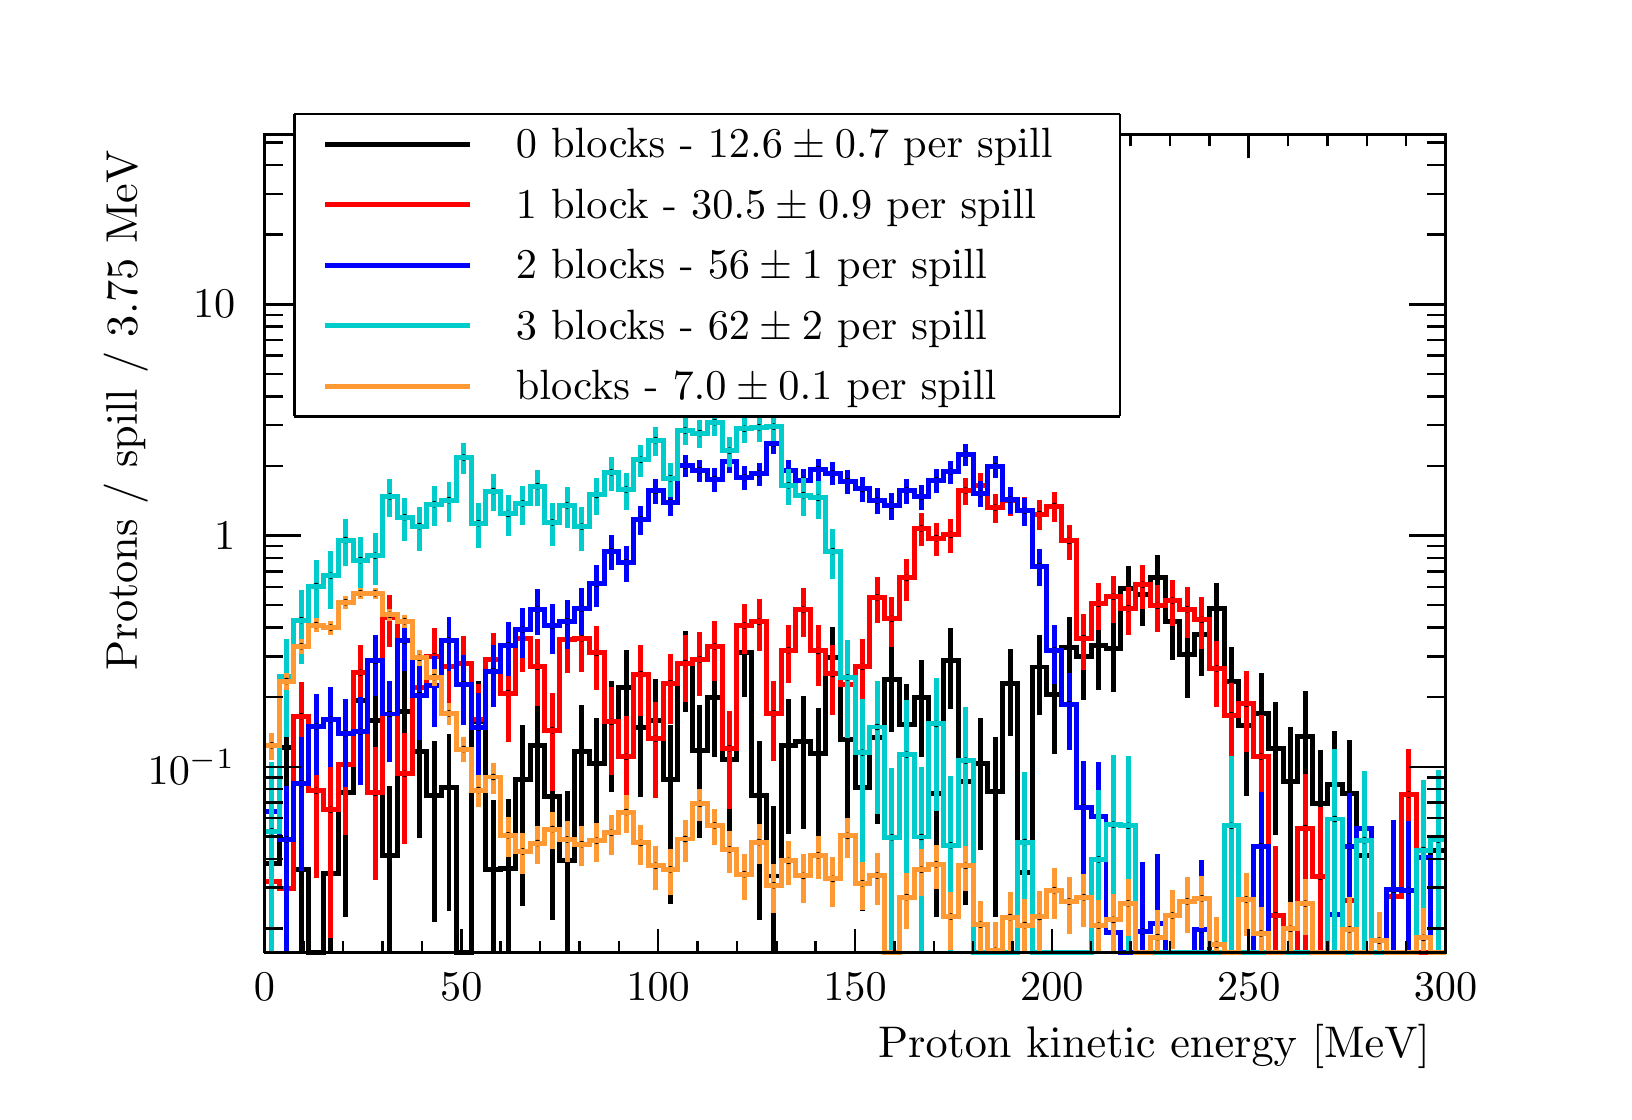
\begin{tikzpicture}
\pgfdeclareplotmark{cross} {
\pgfpathmoveto{\pgfpoint{-0.3\pgfplotmarksize}{\pgfplotmarksize}}
\pgfpathlineto{\pgfpoint{+0.3\pgfplotmarksize}{\pgfplotmarksize}}
\pgfpathlineto{\pgfpoint{+0.3\pgfplotmarksize}{0.3\pgfplotmarksize}}
\pgfpathlineto{\pgfpoint{+1\pgfplotmarksize}{0.3\pgfplotmarksize}}
\pgfpathlineto{\pgfpoint{+1\pgfplotmarksize}{-0.3\pgfplotmarksize}}
\pgfpathlineto{\pgfpoint{+0.3\pgfplotmarksize}{-0.3\pgfplotmarksize}}
\pgfpathlineto{\pgfpoint{+0.3\pgfplotmarksize}{-1.\pgfplotmarksize}}
\pgfpathlineto{\pgfpoint{-0.3\pgfplotmarksize}{-1.\pgfplotmarksize}}
\pgfpathlineto{\pgfpoint{-0.3\pgfplotmarksize}{-0.3\pgfplotmarksize}}
\pgfpathlineto{\pgfpoint{-1.\pgfplotmarksize}{-0.3\pgfplotmarksize}}
\pgfpathlineto{\pgfpoint{-1.\pgfplotmarksize}{0.3\pgfplotmarksize}}
\pgfpathlineto{\pgfpoint{-0.3\pgfplotmarksize}{0.3\pgfplotmarksize}}
\pgfpathclose
\pgfusepathqstroke
}
\pgfdeclareplotmark{cross*} {
\pgfpathmoveto{\pgfpoint{-0.3\pgfplotmarksize}{\pgfplotmarksize}}
\pgfpathlineto{\pgfpoint{+0.3\pgfplotmarksize}{\pgfplotmarksize}}
\pgfpathlineto{\pgfpoint{+0.3\pgfplotmarksize}{0.3\pgfplotmarksize}}
\pgfpathlineto{\pgfpoint{+1\pgfplotmarksize}{0.3\pgfplotmarksize}}
\pgfpathlineto{\pgfpoint{+1\pgfplotmarksize}{-0.3\pgfplotmarksize}}
\pgfpathlineto{\pgfpoint{+0.3\pgfplotmarksize}{-0.3\pgfplotmarksize}}
\pgfpathlineto{\pgfpoint{+0.3\pgfplotmarksize}{-1.\pgfplotmarksize}}
\pgfpathlineto{\pgfpoint{-0.3\pgfplotmarksize}{-1.\pgfplotmarksize}}
\pgfpathlineto{\pgfpoint{-0.3\pgfplotmarksize}{-0.3\pgfplotmarksize}}
\pgfpathlineto{\pgfpoint{-1.\pgfplotmarksize}{-0.3\pgfplotmarksize}}
\pgfpathlineto{\pgfpoint{-1.\pgfplotmarksize}{0.3\pgfplotmarksize}}
\pgfpathlineto{\pgfpoint{-0.3\pgfplotmarksize}{0.3\pgfplotmarksize}}
\pgfpathclose
\pgfusepathqfillstroke
}
\pgfdeclareplotmark{newstar} {
\pgfpathmoveto{\pgfqpoint{0pt}{\pgfplotmarksize}}
\pgfpathlineto{\pgfqpointpolar{44}{0.5\pgfplotmarksize}}
\pgfpathlineto{\pgfqpointpolar{18}{\pgfplotmarksize}}
\pgfpathlineto{\pgfqpointpolar{-20}{0.5\pgfplotmarksize}}
\pgfpathlineto{\pgfqpointpolar{-54}{\pgfplotmarksize}}
\pgfpathlineto{\pgfqpointpolar{-90}{0.5\pgfplotmarksize}}
\pgfpathlineto{\pgfqpointpolar{234}{\pgfplotmarksize}}
\pgfpathlineto{\pgfqpointpolar{198}{0.5\pgfplotmarksize}}
\pgfpathlineto{\pgfqpointpolar{162}{\pgfplotmarksize}}
\pgfpathlineto{\pgfqpointpolar{134}{0.5\pgfplotmarksize}}
\pgfpathclose
\pgfusepathqstroke
}
\pgfdeclareplotmark{newstar*} {
\pgfpathmoveto{\pgfqpoint{0pt}{\pgfplotmarksize}}
\pgfpathlineto{\pgfqpointpolar{44}{0.5\pgfplotmarksize}}
\pgfpathlineto{\pgfqpointpolar{18}{\pgfplotmarksize}}
\pgfpathlineto{\pgfqpointpolar{-20}{0.5\pgfplotmarksize}}
\pgfpathlineto{\pgfqpointpolar{-54}{\pgfplotmarksize}}
\pgfpathlineto{\pgfqpointpolar{-90}{0.5\pgfplotmarksize}}
\pgfpathlineto{\pgfqpointpolar{234}{\pgfplotmarksize}}
\pgfpathlineto{\pgfqpointpolar{198}{0.5\pgfplotmarksize}}
\pgfpathlineto{\pgfqpointpolar{162}{\pgfplotmarksize}}
\pgfpathlineto{\pgfqpointpolar{134}{0.5\pgfplotmarksize}}
\pgfpathclose
\pgfusepathqfillstroke
}
\definecolor{c}{rgb}{1,1,1};
\draw [color=c, fill=c] (0,0) rectangle (20,13.4957);
\draw [color=c, fill=c] (3,1.75444) rectangle (18,12.1461);
\definecolor{c}{rgb}{0,0,0};
\draw [c,line width=0.9] (3,1.75444) -- (3,12.1461) -- (18,12.1461) -- (18,1.75444) -- (3,1.75444);
\definecolor{c}{rgb}{1,1,1};
\draw [color=c, fill=c] (3,1.75444) rectangle (18,12.1461);
\definecolor{c}{rgb}{0,0,0};
\draw [c,line width=0.9] (3,1.75444) -- (3,12.1461) -- (18,12.1461) -- (18,1.75444) -- (3,1.75444);
\draw [c,line width=0.9] (3,1.75444) -- (3.1875,1.75444) -- (3.1875,1.75444) -- (3.375,1.75444) -- (3.375,1.75444) -- (3.5625,1.75444) -- (3.5625,1.75444) -- (3.75,1.75444) -- (3.75,1.75444) -- (3.9375,1.75444) -- (3.9375,1.75444) -- (4.125,1.75444)
 -- (4.125,1.75444) -- (4.3125,1.75444) -- (4.3125,1.75444) -- (4.5,1.75444) -- (4.5,1.75444) -- (4.6875,1.75444) -- (4.6875,1.75444) -- (4.875,1.75444) -- (4.875,1.75444) -- (5.0625,1.75444) -- (5.0625,1.75444) -- (5.25,1.75444) -- (5.25,1.75444) --
 (5.4375,1.75444) -- (5.4375,1.75444) -- (5.625,1.75444) -- (5.625,1.75444) -- (5.8125,1.75444) -- (5.8125,1.75444) -- (6,1.75444) -- (6,1.75444) -- (6.1875,1.75444) -- (6.1875,1.75444) -- (6.375,1.75444) -- (6.375,1.75444) -- (6.5625,1.75444) --
 (6.5625,1.75444) -- (6.75,1.75444) -- (6.75,1.75444) -- (6.9375,1.75444) -- (6.9375,1.75444) -- (7.125,1.75444) -- (7.125,1.75444) -- (7.3125,1.75444) -- (7.3125,1.75444) -- (7.5,1.75444) -- (7.5,1.75444) -- (7.6875,1.75444) -- (7.6875,1.75444) --
 (7.875,1.75444) -- (7.875,1.75444) -- (8.0625,1.75444) -- (8.0625,1.75444) -- (8.25,1.75444) -- (8.25,1.75444) -- (8.4375,1.75444) -- (8.4375,1.75444) -- (8.625,1.75444) -- (8.625,1.75444) -- (8.8125,1.75444) -- (8.8125,1.75444) -- (9,1.75444) --
 (9,1.75444) -- (9.1875,1.75444) -- (9.1875,1.75444) -- (9.375,1.75444) -- (9.375,1.75444) -- (9.5625,1.75444) -- (9.5625,1.75444) -- (9.75,1.75444) -- (9.75,1.75444) -- (9.9375,1.75444) -- (9.9375,1.75444) -- (10.125,1.75444) -- (10.125,1.75444) --
 (10.3125,1.75444) -- (10.3125,1.75444) -- (10.5,1.75444) -- (10.5,1.75444) -- (10.6875,1.75444) -- (10.6875,1.75444) -- (10.875,1.75444) -- (10.875,1.75444) -- (11.0625,1.75444) -- (11.0625,1.75444) -- (11.25,1.75444) -- (11.25,1.75444) --
 (11.4375,1.75444) -- (11.4375,1.75444) -- (11.625,1.75444) -- (11.625,1.75444) -- (11.8125,1.75444) -- (11.8125,1.75444) -- (12,1.75444) -- (12,1.75444) -- (12.1875,1.75444) -- (12.1875,1.75444) -- (12.375,1.75444) -- (12.375,1.75444) --
 (12.5625,1.75444) -- (12.5625,1.75444) -- (12.75,1.75444) -- (12.75,1.75444) -- (12.9375,1.75444) -- (12.9375,1.75444) -- (13.125,1.75444) -- (13.125,1.75444) -- (13.3125,1.75444) -- (13.3125,1.75444) -- (13.5,1.75444) -- (13.5,1.75444) --
 (13.6875,1.75444) -- (13.6875,1.75444) -- (13.875,1.75444) -- (13.875,1.75444) -- (14.0625,1.75444) -- (14.0625,1.75444) -- (14.25,1.75444) -- (14.25,1.75444) -- (14.4375,1.75444) -- (14.4375,1.75444) -- (14.625,1.75444) -- (14.625,1.75444) --
 (14.8125,1.75444) -- (14.8125,1.75444) -- (15,1.75444) -- (15,1.75444) -- (15.1875,1.75444) -- (15.1875,1.75444) -- (15.375,1.75444) -- (15.375,1.75444) -- (15.5625,1.75444) -- (15.5625,1.75444) -- (15.75,1.75444) -- (15.75,1.75444) --
 (15.9375,1.75444) -- (15.9375,1.75444) -- (16.125,1.75444) -- (16.125,1.75444) -- (16.3125,1.75444) -- (16.3125,1.75444) -- (16.5,1.75444) -- (16.5,1.75444) -- (16.6875,1.75444) -- (16.6875,1.75444) -- (16.875,1.75444) -- (16.875,1.75444) --
 (17.0625,1.75444) -- (17.0625,1.75444) -- (17.25,1.75444) -- (17.25,1.75444) -- (17.4375,1.75444) -- (17.4375,1.75444) -- (17.625,1.75444) -- (17.625,1.75444) -- (17.8125,1.75444) -- (17.8125,1.75444) -- (18,1.75444);
\draw [c,line width=0.9] (3,1.75444) -- (18,1.75444);
\draw [c,line width=0.9] (3,2.05809) -- (3,1.75444);
\draw [c,line width=0.9] (3.5,1.90627) -- (3.5,1.75444);
\draw [c,line width=0.9] (4,1.90627) -- (4,1.75444);
\draw [c,line width=0.9] (4.5,1.90627) -- (4.5,1.75444);
\draw [c,line width=0.9] (5,1.90627) -- (5,1.75444);
\draw [c,line width=0.9] (5.5,2.05809) -- (5.5,1.75444);
\draw [c,line width=0.9] (6,1.90627) -- (6,1.75444);
\draw [c,line width=0.9] (6.5,1.90627) -- (6.5,1.75444);
\draw [c,line width=0.9] (7,1.90627) -- (7,1.75444);
\draw [c,line width=0.9] (7.5,1.90627) -- (7.5,1.75444);
\draw [c,line width=0.9] (8,2.05809) -- (8,1.75444);
\draw [c,line width=0.9] (8.5,1.90627) -- (8.5,1.75444);
\draw [c,line width=0.9] (9,1.90627) -- (9,1.75444);
\draw [c,line width=0.9] (9.5,1.90627) -- (9.5,1.75444);
\draw [c,line width=0.9] (10,1.90627) -- (10,1.75444);
\draw [c,line width=0.9] (10.5,2.05809) -- (10.5,1.75444);
\draw [c,line width=0.9] (11,1.90627) -- (11,1.75444);
\draw [c,line width=0.9] (11.5,1.90627) -- (11.5,1.75444);
\draw [c,line width=0.9] (12,1.90627) -- (12,1.75444);
\draw [c,line width=0.9] (12.5,1.90627) -- (12.5,1.75444);
\draw [c,line width=0.9] (13,2.05809) -- (13,1.75444);
\draw [c,line width=0.9] (13.5,1.90627) -- (13.5,1.75444);
\draw [c,line width=0.9] (14,1.90627) -- (14,1.75444);
\draw [c,line width=0.9] (14.5,1.90627) -- (14.5,1.75444);
\draw [c,line width=0.9] (15,1.90627) -- (15,1.75444);
\draw [c,line width=0.9] (15.5,2.05809) -- (15.5,1.75444);
\draw [c,line width=0.9] (16,1.90627) -- (16,1.75444);
\draw [c,line width=0.9] (16.5,1.90627) -- (16.5,1.75444);
\draw [c,line width=0.9] (17,1.90627) -- (17,1.75444);
\draw [c,line width=0.9] (17.5,1.90627) -- (17.5,1.75444);
\draw [c,line width=0.9] (18,2.05809) -- (18,1.75444);
\draw [anchor=base] (3,1.14713) node[scale=1.52731, color=c, rotate=0]{0};
\draw [anchor=base] (5.5,1.14713) node[scale=1.52731, color=c, rotate=0]{50};
\draw [anchor=base] (8,1.14713) node[scale=1.52731, color=c, rotate=0]{100};
\draw [anchor=base] (10.5,1.14713) node[scale=1.52731, color=c, rotate=0]{150};
\draw [anchor=base] (13,1.14713) node[scale=1.52731, color=c, rotate=0]{200};
\draw [anchor=base] (15.5,1.14713) node[scale=1.52731, color=c, rotate=0]{250};
\draw [anchor=base] (18,1.14713) node[scale=1.52731, color=c, rotate=0]{300};
\draw [anchor= east] (18,0.566819) node[scale=1.6, color=c, rotate=0]{Proton kinetic energy [MeV]};
\draw [c,line width=0.9] (3,12.1461) -- (18,12.1461);
\draw [c,line width=0.9] (3,11.8425) -- (3,12.1461);
\draw [c,line width=0.9] (3.5,11.9943) -- (3.5,12.1461);
\draw [c,line width=0.9] (4,11.9943) -- (4,12.1461);
\draw [c,line width=0.9] (4.5,11.9943) -- (4.5,12.1461);
\draw [c,line width=0.9] (5,11.9943) -- (5,12.1461);
\draw [c,line width=0.9] (5.5,11.8425) -- (5.5,12.1461);
\draw [c,line width=0.9] (6,11.9943) -- (6,12.1461);
\draw [c,line width=0.9] (6.5,11.9943) -- (6.5,12.1461);
\draw [c,line width=0.9] (7,11.9943) -- (7,12.1461);
\draw [c,line width=0.9] (7.5,11.9943) -- (7.5,12.1461);
\draw [c,line width=0.9] (8,11.8425) -- (8,12.1461);
\draw [c,line width=0.9] (8.5,11.9943) -- (8.5,12.1461);
\draw [c,line width=0.9] (9,11.9943) -- (9,12.1461);
\draw [c,line width=0.9] (9.5,11.9943) -- (9.5,12.1461);
\draw [c,line width=0.9] (10,11.9943) -- (10,12.1461);
\draw [c,line width=0.9] (10.5,11.8425) -- (10.5,12.1461);
\draw [c,line width=0.9] (11,11.9943) -- (11,12.1461);
\draw [c,line width=0.9] (11.5,11.9943) -- (11.5,12.1461);
\draw [c,line width=0.9] (12,11.9943) -- (12,12.1461);
\draw [c,line width=0.9] (12.5,11.9943) -- (12.5,12.1461);
\draw [c,line width=0.9] (13,11.8425) -- (13,12.1461);
\draw [c,line width=0.9] (13.5,11.9943) -- (13.5,12.1461);
\draw [c,line width=0.9] (14,11.9943) -- (14,12.1461);
\draw [c,line width=0.9] (14.5,11.9943) -- (14.5,12.1461);
\draw [c,line width=0.9] (15,11.9943) -- (15,12.1461);
\draw [c,line width=0.9] (15.5,11.8425) -- (15.5,12.1461);
\draw [c,line width=0.9] (16,11.9943) -- (16,12.1461);
\draw [c,line width=0.9] (16.5,11.9943) -- (16.5,12.1461);
\draw [c,line width=0.9] (17,11.9943) -- (17,12.1461);
\draw [c,line width=0.9] (17.5,11.9943) -- (17.5,12.1461);
\draw [c,line width=0.9] (18,11.8425) -- (18,12.1461);
\draw [c,line width=0.9] (3,1.75444) -- (3,12.1461);
\draw [c,line width=0.9] (3.231,2.06278) -- (3,2.06278);
\draw [c,line width=0.9] (3.231,2.57994) -- (3,2.57994);
\draw [c,line width=0.9] (3.231,2.94688) -- (3,2.94688);
\draw [c,line width=0.9] (3.231,3.2315) -- (3,3.2315);
\draw [c,line width=0.9] (3.231,3.46405) -- (3,3.46405);
\draw [c,line width=0.9] (3.231,3.66066) -- (3,3.66066);
\draw [c,line width=0.9] (3.231,3.83098) -- (3,3.83098);
\draw [c,line width=0.9] (3.231,3.98121) -- (3,3.98121);
\draw [c,line width=0.9] (3.462,4.1156) -- (3,4.1156);
\draw [anchor= east] (2.82,4.1156) node[scale=1.52731, color=c, rotate=0]{$10^{-1}$};
\draw [c,line width=0.9] (3.231,4.9997) -- (3,4.9997);
\draw [c,line width=0.9] (3.231,5.51687) -- (3,5.51687);
\draw [c,line width=0.9] (3.231,5.8838) -- (3,5.8838);
\draw [c,line width=0.9] (3.231,6.16842) -- (3,6.16842);
\draw [c,line width=0.9] (3.231,6.40097) -- (3,6.40097);
\draw [c,line width=0.9] (3.231,6.59759) -- (3,6.59759);
\draw [c,line width=0.9] (3.231,6.76791) -- (3,6.76791);
\draw [c,line width=0.9] (3.231,6.91814) -- (3,6.91814);
\draw [c,line width=0.9] (3.462,7.05252) -- (3,7.05252);
\draw [anchor= east] (2.82,7.05252) node[scale=1.52731, color=c, rotate=0]{1};
\draw [c,line width=0.9] (3.231,7.93663) -- (3,7.93663);
\draw [c,line width=0.9] (3.231,8.45379) -- (3,8.45379);
\draw [c,line width=0.9] (3.231,8.82073) -- (3,8.82073);
\draw [c,line width=0.9] (3.231,9.10535) -- (3,9.10535);
\draw [c,line width=0.9] (3.231,9.3379) -- (3,9.3379);
\draw [c,line width=0.9] (3.231,9.53452) -- (3,9.53452);
\draw [c,line width=0.9] (3.231,9.70483) -- (3,9.70483);
\draw [c,line width=0.9] (3.231,9.85506) -- (3,9.85506);
\draw [c,line width=0.9] (3.462,9.98945) -- (3,9.98945);
\draw [anchor= east] (2.82,9.98945) node[scale=1.52731, color=c, rotate=0]{10};
\draw [c,line width=0.9] (3.231,10.8736) -- (3,10.8736);
\draw [c,line width=0.9] (3.231,11.3907) -- (3,11.3907);
\draw [c,line width=0.9] (3.231,11.7577) -- (3,11.7577);
\draw [c,line width=0.9] (3.231,12.0423) -- (3,12.0423);
\draw [anchor= east] (1.24,12.1461) node[scale=1.6, color=c, rotate=90]{Protons / spill / 3.75~MeV};
\draw [c,line width=0.9] (18,1.75444) -- (18,12.1461);
\draw [c,line width=0.9] (17.769,2.06278) -- (18,2.06278);
\draw [c,line width=0.9] (17.769,2.57994) -- (18,2.57994);
\draw [c,line width=0.9] (17.769,2.94688) -- (18,2.94688);
\draw [c,line width=0.9] (17.769,3.2315) -- (18,3.2315);
\draw [c,line width=0.9] (17.769,3.46405) -- (18,3.46405);
\draw [c,line width=0.9] (17.769,3.66066) -- (18,3.66066);
\draw [c,line width=0.9] (17.769,3.83098) -- (18,3.83098);
\draw [c,line width=0.9] (17.769,3.98121) -- (18,3.98121);
\draw [c,line width=0.9] (17.538,4.1156) -- (18,4.1156);
\draw [c,line width=0.9] (17.769,4.9997) -- (18,4.9997);
\draw [c,line width=0.9] (17.769,5.51687) -- (18,5.51687);
\draw [c,line width=0.9] (17.769,5.8838) -- (18,5.8838);
\draw [c,line width=0.9] (17.769,6.16842) -- (18,6.16842);
\draw [c,line width=0.9] (17.769,6.40097) -- (18,6.40097);
\draw [c,line width=0.9] (17.769,6.59759) -- (18,6.59759);
\draw [c,line width=0.9] (17.769,6.76791) -- (18,6.76791);
\draw [c,line width=0.9] (17.769,6.91814) -- (18,6.91814);
\draw [c,line width=0.9] (17.538,7.05252) -- (18,7.05252);
\draw [c,line width=0.9] (17.769,7.93663) -- (18,7.93663);
\draw [c,line width=0.9] (17.769,8.45379) -- (18,8.45379);
\draw [c,line width=0.9] (17.769,8.82073) -- (18,8.82073);
\draw [c,line width=0.9] (17.769,9.10535) -- (18,9.10535);
\draw [c,line width=0.9] (17.769,9.3379) -- (18,9.3379);
\draw [c,line width=0.9] (17.769,9.53452) -- (18,9.53452);
\draw [c,line width=0.9] (17.769,9.70483) -- (18,9.70483);
\draw [c,line width=0.9] (17.769,9.85506) -- (18,9.85506);
\draw [c,line width=0.9] (17.538,9.98945) -- (18,9.98945);
\draw [c,line width=0.9] (17.769,10.8736) -- (18,10.8736);
\draw [c,line width=0.9] (17.769,11.3907) -- (18,11.3907);
\draw [c,line width=0.9] (17.769,11.7577) -- (18,11.7577);
\draw [c,line width=0.9] (17.769,12.0423) -- (18,12.0423);
\draw [c,line width=1.8] (3.09375,1.75444) -- (3.09375,2.88361);
\draw [c,line width=1.8] (3.09375,2.88361) -- (3.09375,3.76772);
\foreach \P in {(3.09375,2.88361)}{\draw[mark options={color=c,fill=c},mark size=2.402402pt,mark=*,mark size=1pt] plot coordinates {\P};}
\draw [c,line width=1.8] (3.28125,3.25859) -- (3.28125,4.35827);
\draw [c,line width=1.8] (3.28125,4.35827) -- (3.28125,4.9399);
\foreach \P in {(3.28125,4.35827)}{\draw[mark options={color=c,fill=c},mark size=2.402402pt,mark=*,mark size=1pt] plot coordinates {\P};}
\draw [c,line width=1.8] (3.46875,1.75444) -- (3.46875,2.80599);
\draw [c,line width=1.8] (3.46875,2.80599) -- (3.46875,3.69009);
\foreach \P in {(3.46875,2.80599)}{\draw[mark options={color=c,fill=c},mark size=2.402402pt,mark=*,mark size=1pt] plot coordinates {\P};}
\draw [c,line width=1.8] (3.84375,1.75444) -- (3.84375,2.76482);
\draw [c,line width=1.8] (3.84375,2.76482) -- (3.84375,3.64893);
\foreach \P in {(3.84375,2.76482)}{\draw[mark options={color=c,fill=c},mark size=2.402402pt,mark=*,mark size=1pt] plot coordinates {\P};}
\draw [c,line width=1.8] (4.03125,2.21176) -- (4.03125,3.78318);
\draw [c,line width=1.8] (4.03125,3.78318) -- (4.03125,4.4662);
\foreach \P in {(4.03125,3.78318)}{\draw[mark options={color=c,fill=c},mark size=2.402402pt,mark=*,mark size=1pt] plot coordinates {\P};}
\draw [c,line width=1.8] (4.21875,4.20134) -- (4.21875,4.95768);
\draw [c,line width=1.8] (4.21875,4.95768) -- (4.21875,5.42925);
\foreach \P in {(4.21875,4.95768)}{\draw[mark options={color=c,fill=c},mark size=2.402402pt,mark=*,mark size=1pt] plot coordinates {\P};}
\draw [c,line width=1.8] (4.40625,3.81376) -- (4.40625,4.70187);
\draw [c,line width=1.8] (4.40625,4.70187) -- (4.40625,5.22037);
\foreach \P in {(4.40625,4.70187)}{\draw[mark options={color=c,fill=c},mark size=2.402402pt,mark=*,mark size=1pt] plot coordinates {\P};}
\draw [c,line width=1.8] (4.59375,1.75444) -- (4.59375,2.99021);
\draw [c,line width=1.8] (4.59375,2.99021) -- (4.59375,3.87432);
\foreach \P in {(4.59375,2.99021)}{\draw[mark options={color=c,fill=c},mark size=2.402402pt,mark=*,mark size=1pt] plot coordinates {\P};}
\draw [c,line width=1.8] (4.78125,3.92042) -- (4.78125,4.81517);
\draw [c,line width=1.8] (4.78125,4.81517) -- (4.78125,5.33587);
\foreach \P in {(4.78125,4.81517)}{\draw[mark options={color=c,fill=c},mark size=2.402402pt,mark=*,mark size=1pt] plot coordinates {\P};}
\draw [c,line width=1.8] (4.96875,3.20634) -- (4.96875,4.30595);
\draw [c,line width=1.8] (4.96875,4.30595) -- (4.96875,4.88756);
\foreach \P in {(4.96875,4.30595)}{\draw[mark options={color=c,fill=c},mark size=2.402402pt,mark=*,mark size=1pt] plot coordinates {\P};}
\draw [c,line width=1.8] (5.15625,2.14751) -- (5.15625,3.74917);
\draw [c,line width=1.8] (5.15625,3.74917) -- (5.15625,4.43729);
\foreach \P in {(5.15625,3.74917)}{\draw[mark options={color=c,fill=c},mark size=2.402402pt,mark=*,mark size=1pt] plot coordinates {\P};}
\draw [c,line width=1.8] (5.34375,2.28352) -- (5.34375,3.85336);
\draw [c,line width=1.8] (5.34375,3.85336) -- (5.34375,4.53611);
\foreach \P in {(5.34375,3.85336)}{\draw[mark options={color=c,fill=c},mark size=2.402402pt,mark=*,mark size=1pt] plot coordinates {\P};}
\draw [c,line width=1.8] (5.71875,3.79502) -- (5.71875,4.6855);
\draw [c,line width=1.8] (5.71875,4.6855) -- (5.71875,5.20479);
\foreach \P in {(5.71875,4.6855)}{\draw[mark options={color=c,fill=c},mark size=2.402402pt,mark=*,mark size=1pt] plot coordinates {\P};}
\draw [c,line width=1.8] (5.90625,1.75444) -- (5.90625,2.80599);
\draw [c,line width=1.8] (5.90625,2.80599) -- (5.90625,3.69009);
\foreach \P in {(5.90625,2.80599)}{\draw[mark options={color=c,fill=c},mark size=2.402402pt,mark=*,mark size=1pt] plot coordinates {\P};}
\draw [c,line width=1.8] (6.09375,1.75444) -- (6.09375,2.82284);
\draw [c,line width=1.8] (6.09375,2.82284) -- (6.09375,3.70694);
\foreach \P in {(6.09375,2.82284)}{\draw[mark options={color=c,fill=c},mark size=2.402402pt,mark=*,mark size=1pt] plot coordinates {\P};}
\draw [c,line width=1.8] (6.28125,2.34524) -- (6.28125,3.9537);
\draw [c,line width=1.8] (6.28125,3.9537) -- (6.28125,4.64294);
\foreach \P in {(6.28125,3.9537)}{\draw[mark options={color=c,fill=c},mark size=2.402402pt,mark=*,mark size=1pt] plot coordinates {\P};}
\draw [c,line width=1.8] (6.46875,3.26895) -- (6.46875,4.38917);
\draw [c,line width=1.8] (6.46875,4.38917) -- (6.46875,4.97623);
\foreach \P in {(6.46875,4.38917)}{\draw[mark options={color=c,fill=c},mark size=2.402402pt,mark=*,mark size=1pt] plot coordinates {\P};}
\draw [c,line width=1.8] (6.65625,2.16629) -- (6.65625,3.73316);
\draw [c,line width=1.8] (6.65625,3.73316) -- (6.65625,4.4154);
\foreach \P in {(6.65625,3.73316)}{\draw[mark options={color=c,fill=c},mark size=2.402402pt,mark=*,mark size=1pt] plot coordinates {\P};}
\draw [c,line width=1.8] (6.84375,1.75444) -- (6.84375,2.92887);
\draw [c,line width=1.8] (6.84375,2.92887) -- (6.84375,3.81297);
\foreach \P in {(6.84375,2.92887)}{\draw[mark options={color=c,fill=c},mark size=2.402402pt,mark=*,mark size=1pt] plot coordinates {\P};}
\draw [c,line width=1.8] (7.03125,3.21311) -- (7.03125,4.31409);
\draw [c,line width=1.8] (7.03125,4.31409) -- (7.03125,4.89607);
\foreach \P in {(7.03125,4.31409)}{\draw[mark options={color=c,fill=c},mark size=2.402402pt,mark=*,mark size=1pt] plot coordinates {\P};}
\draw [c,line width=1.8] (7.21875,3.05311) -- (7.21875,4.15213);
\draw [c,line width=1.8] (7.21875,4.15213) -- (7.21875,4.73357);
\foreach \P in {(7.21875,4.15213)}{\draw[mark options={color=c,fill=c},mark size=2.402402pt,mark=*,mark size=1pt] plot coordinates {\P};}
\draw [c,line width=1.8] (7.40625,3.80073) -- (7.40625,4.68629);
\draw [c,line width=1.8] (7.40625,4.68629) -- (7.40625,5.20394);
\foreach \P in {(7.40625,4.68629)}{\draw[mark options={color=c,fill=c},mark size=2.402402pt,mark=*,mark size=1pt] plot coordinates {\P};}
\draw [c,line width=1.8] (7.59375,4.35959) -- (7.59375,5.12309);
\draw [c,line width=1.8] (7.59375,5.12309) -- (7.59375,5.59737);
\foreach \P in {(7.59375,5.12309)}{\draw[mark options={color=c,fill=c},mark size=2.402402pt,mark=*,mark size=1pt] plot coordinates {\P};}
\draw [c,line width=1.8] (7.78125,3.73217) -- (7.78125,4.62029);
\draw [c,line width=1.8] (7.78125,4.62029) -- (7.78125,5.1388);
\foreach \P in {(7.78125,4.62029)}{\draw[mark options={color=c,fill=c},mark size=2.402402pt,mark=*,mark size=1pt] plot coordinates {\P};}
\draw [c,line width=1.8] (7.96875,3.81687) -- (7.96875,4.7073);
\draw [c,line width=1.8] (7.96875,4.7073) -- (7.96875,5.22657);
\foreach \P in {(7.96875,4.7073)}{\draw[mark options={color=c,fill=c},mark size=2.402402pt,mark=*,mark size=1pt] plot coordinates {\P};}
\draw [c,line width=1.8] (8.15625,2.37477) -- (8.15625,3.95774);
\draw [c,line width=1.8] (8.15625,3.95774) -- (8.15625,4.64272);
\foreach \P in {(8.15625,3.95774)}{\draw[mark options={color=c,fill=c},mark size=2.402402pt,mark=*,mark size=1pt] plot coordinates {\P};}
\draw [c,line width=1.8] (8.34375,4.81266) -- (8.34375,5.42338);
\draw [c,line width=1.8] (8.34375,5.42338) -- (8.34375,5.83464);
\foreach \P in {(8.34375,5.42338)}{\draw[mark options={color=c,fill=c},mark size=2.402402pt,mark=*,mark size=1pt] plot coordinates {\P};}
\draw [c,line width=1.8] (8.53125,3.2146) -- (8.53125,4.31941);
\draw [c,line width=1.8] (8.53125,4.31941) -- (8.53125,4.9024);
\foreach \P in {(8.53125,4.31941)}{\draw[mark options={color=c,fill=c},mark size=2.402402pt,mark=*,mark size=1pt] plot coordinates {\P};}
\draw [c,line width=1.8] (8.71875,4.23914) -- (8.71875,4.99865);
\draw [c,line width=1.8] (8.71875,4.99865) -- (8.71875,5.47143);
\foreach \P in {(8.71875,4.99865)}{\draw[mark options={color=c,fill=c},mark size=2.402402pt,mark=*,mark size=1pt] plot coordinates {\P};}
\draw [c,line width=1.8] (8.90625,3.1066) -- (8.90625,4.21311);
\draw [c,line width=1.8] (8.90625,4.21311) -- (8.90625,4.79655);
\foreach \P in {(8.90625,4.21311)}{\draw[mark options={color=c,fill=c},mark size=2.402402pt,mark=*,mark size=1pt] plot coordinates {\P};}
\draw [c,line width=1.8] (9.09375,5.00714) -- (9.09375,5.56602);
\draw [c,line width=1.8] (9.09375,5.56602) -- (9.09375,5.95332);
\foreach \P in {(9.09375,5.56602)}{\draw[mark options={color=c,fill=c},mark size=2.402402pt,mark=*,mark size=1pt] plot coordinates {\P};}
\draw [c,line width=1.8] (9.28125,2.17213) -- (9.28125,3.75569);
\draw [c,line width=1.8] (9.28125,3.75569) -- (9.28125,4.44077);
\foreach \P in {(9.28125,3.75569)}{\draw[mark options={color=c,fill=c},mark size=2.402402pt,mark=*,mark size=1pt] plot coordinates {\P};}
\draw [c,line width=1.8] (9.46875,1.75444) -- (9.46875,2.72888);
\draw [c,line width=1.8] (9.46875,2.72888) -- (9.46875,3.61298);
\foreach \P in {(9.46875,2.72888)}{\draw[mark options={color=c,fill=c},mark size=2.402402pt,mark=*,mark size=1pt] plot coordinates {\P};}
\draw [c,line width=1.8] (9.65625,3.26816) -- (9.65625,4.38541);
\draw [c,line width=1.8] (9.65625,4.38541) -- (9.65625,4.97169);
\foreach \P in {(9.65625,4.38541)}{\draw[mark options={color=c,fill=c},mark size=2.402402pt,mark=*,mark size=1pt] plot coordinates {\P};}
\draw [c,line width=1.8] (9.84375,3.32992) -- (9.84375,4.43358);
\draw [c,line width=1.8] (9.84375,4.43358) -- (9.84375,5.01627);
\foreach \P in {(9.84375,4.43358)}{\draw[mark options={color=c,fill=c},mark size=2.402402pt,mark=*,mark size=1pt] plot coordinates {\P};}
\draw [c,line width=1.8] (10.0312,3.18526) -- (10.0312,4.28446);
\draw [c,line width=1.8] (10.0312,4.28446) -- (10.0312,4.86595);
\foreach \P in {(10.0312,4.28446)}{\draw[mark options={color=c,fill=c},mark size=2.402402pt,mark=*,mark size=1pt] plot coordinates {\P};}
\draw [c,line width=1.8] (10.2188,4.94393) -- (10.2188,5.50183);
\draw [c,line width=1.8] (10.2188,5.50183) -- (10.2188,5.88865);
\foreach \P in {(10.2188,5.50183)}{\draw[mark options={color=c,fill=c},mark size=2.402402pt,mark=*,mark size=1pt] plot coordinates {\P};}
\draw [c,line width=1.8] (10.4062,3.35925) -- (10.4062,4.46107);
\draw [c,line width=1.8] (10.4062,4.46107) -- (10.4062,5.04326);
\foreach \P in {(10.4062,4.46107)}{\draw[mark options={color=c,fill=c},mark size=2.402402pt,mark=*,mark size=1pt] plot coordinates {\P};}
\draw [c,line width=1.8] (10.5938,2.28647) -- (10.5938,3.85296);
\draw [c,line width=1.8] (10.5938,3.85296) -- (10.5938,4.53514);
\foreach \P in {(10.5938,3.85296)}{\draw[mark options={color=c,fill=c},mark size=2.402402pt,mark=*,mark size=1pt] plot coordinates {\P};}
\draw [c,line width=1.8] (10.7812,3.38603) -- (10.7812,4.48729);
\draw [c,line width=1.8] (10.7812,4.48729) -- (10.7812,5.06933);
\foreach \P in {(10.7812,4.48729)}{\draw[mark options={color=c,fill=c},mark size=2.402402pt,mark=*,mark size=1pt] plot coordinates {\P};}
\draw [c,line width=1.8] (10.9688,4.55262) -- (10.9688,5.22406);
\draw [c,line width=1.8] (10.9688,5.22406) -- (10.9688,5.66166);
\foreach \P in {(10.9688,5.22406)}{\draw[mark options={color=c,fill=c},mark size=2.402402pt,mark=*,mark size=1pt] plot coordinates {\P};}
\draw [c,line width=1.8] (11.1562,3.76481) -- (11.1562,4.65029);
\draw [c,line width=1.8] (11.1562,4.65029) -- (11.1562,5.16792);
\foreach \P in {(11.1562,4.65029)}{\draw[mark options={color=c,fill=c},mark size=2.402402pt,mark=*,mark size=1pt] plot coordinates {\P};}
\draw [c,line width=1.8] (11.3438,4.23945) -- (11.3438,4.99674);
\draw [c,line width=1.8] (11.3438,4.99674) -- (11.3438,5.46866);
\foreach \P in {(11.3438,4.99674)}{\draw[mark options={color=c,fill=c},mark size=2.402402pt,mark=*,mark size=1pt] plot coordinates {\P};}
\draw [c,line width=1.8] (11.5312,2.20694) -- (11.5312,3.78037);
\draw [c,line width=1.8] (11.5312,3.78037) -- (11.5312,4.46374);
\foreach \P in {(11.5312,3.78037)}{\draw[mark options={color=c,fill=c},mark size=2.402402pt,mark=*,mark size=1pt] plot coordinates {\P};}
\draw [c,line width=1.8] (11.7188,4.85294) -- (11.7188,5.46267);
\draw [c,line width=1.8] (11.7188,5.46267) -- (11.7188,5.87349);
\foreach \P in {(11.7188,5.46267)}{\draw[mark options={color=c,fill=c},mark size=2.402402pt,mark=*,mark size=1pt] plot coordinates {\P};}
\draw [c,line width=1.8] (11.9062,2.35538) -- (11.9062,3.93321);
\draw [c,line width=1.8] (11.9062,3.93321) -- (11.9062,4.61732);
\foreach \P in {(11.9062,3.93321)}{\draw[mark options={color=c,fill=c},mark size=2.402402pt,mark=*,mark size=1pt] plot coordinates {\P};}
\draw [c,line width=1.8] (12.0938,3.05295) -- (12.0938,4.15161);
\draw [c,line width=1.8] (12.0938,4.15161) -- (12.0938,4.73296);
\foreach \P in {(12.0938,4.15161)}{\draw[mark options={color=c,fill=c},mark size=2.402402pt,mark=*,mark size=1pt] plot coordinates {\P};}
\draw [c,line width=1.8] (12.2812,2.20471) -- (12.2812,3.80467);
\draw [c,line width=1.8] (12.2812,3.80467) -- (12.2812,4.49251);
\foreach \P in {(12.2812,3.80467)}{\draw[mark options={color=c,fill=c},mark size=2.402402pt,mark=*,mark size=1pt] plot coordinates {\P};}
\draw [c,line width=1.8] (12.4688,4.50453) -- (12.4688,5.1747);
\draw [c,line width=1.8] (12.4688,5.1747) -- (12.4688,5.61177);
\foreach \P in {(12.4688,5.1747)}{\draw[mark options={color=c,fill=c},mark size=2.402402pt,mark=*,mark size=1pt] plot coordinates {\P};}
\draw [c,line width=1.8] (12.6562,1.75444) -- (12.6562,2.77295);
\draw [c,line width=1.8] (12.6562,2.77295) -- (12.6562,3.65706);
\foreach \P in {(12.6562,2.77295)}{\draw[mark options={color=c,fill=c},mark size=2.402402pt,mark=*,mark size=1pt] plot coordinates {\P};}
\draw [c,line width=1.8] (12.8438,4.77329) -- (12.8438,5.38322);
\draw [c,line width=1.8] (12.8438,5.38322) -- (12.8438,5.79413);
\foreach \P in {(12.8438,5.38322)}{\draw[mark options={color=c,fill=c},mark size=2.402402pt,mark=*,mark size=1pt] plot coordinates {\P};}
\draw [c,line width=1.8] (13.0312,4.28008) -- (13.0312,5.03675);
\draw [c,line width=1.8] (13.0312,5.03675) -- (13.0312,5.50845);
\foreach \P in {(13.0312,5.03675)}{\draw[mark options={color=c,fill=c},mark size=2.402402pt,mark=*,mark size=1pt] plot coordinates {\P};}
\draw [c,line width=1.8] (13.2188,5.06989) -- (13.2188,5.63176);
\draw [c,line width=1.8] (13.2188,5.63176) -- (13.2188,6.02048);
\foreach \P in {(13.2188,5.63176)}{\draw[mark options={color=c,fill=c},mark size=2.402402pt,mark=*,mark size=1pt] plot coordinates {\P};}
\draw [c,line width=1.8] (13.4062,4.96405) -- (13.4062,5.5216);
\draw [c,line width=1.8] (13.4062,5.5216) -- (13.4062,5.90826);
\foreach \P in {(13.4062,5.5216)}{\draw[mark options={color=c,fill=c},mark size=2.402402pt,mark=*,mark size=1pt] plot coordinates {\P};}
\draw [c,line width=1.8] (13.5938,5.09222) -- (13.5938,5.65326);
\draw [c,line width=1.8] (13.5938,5.65326) -- (13.5938,6.04158);
\foreach \P in {(13.5938,5.65326)}{\draw[mark options={color=c,fill=c},mark size=2.402402pt,mark=*,mark size=1pt] plot coordinates {\P};}
\draw [c,line width=1.8] (13.7812,5.05976) -- (13.7812,5.62227);
\draw [c,line width=1.8] (13.7812,5.62227) -- (13.7812,6.01128);
\foreach \P in {(13.7812,5.62227)}{\draw[mark options={color=c,fill=c},mark size=2.402402pt,mark=*,mark size=1pt] plot coordinates {\P};}
\draw [c,line width=1.8] (13.9688,5.99376) -- (13.9688,6.37751);
\draw [c,line width=1.8] (13.9688,6.37751) -- (13.9688,6.67211);
\foreach \P in {(13.9688,6.37751)}{\draw[mark options={color=c,fill=c},mark size=2.402402pt,mark=*,mark size=1pt] plot coordinates {\P};}
\draw [c,line width=1.8] (14.1562,5.90172) -- (14.1562,6.30143);
\draw [c,line width=1.8] (14.1562,6.30143) -- (14.1562,6.60531);
\foreach \P in {(14.1562,6.30143)}{\draw[mark options={color=c,fill=c},mark size=2.402402pt,mark=*,mark size=1pt] plot coordinates {\P};}
\draw [c,line width=1.8] (14.3438,6.15172) -- (14.3438,6.52073);
\draw [c,line width=1.8] (14.3438,6.52073) -- (14.3438,6.80659);
\foreach \P in {(14.3438,6.52073)}{\draw[mark options={color=c,fill=c},mark size=2.402402pt,mark=*,mark size=1pt] plot coordinates {\P};}
\draw [c,line width=1.8] (14.5312,5.47306) -- (14.5312,5.95979);
\draw [c,line width=1.8] (14.5312,5.95979) -- (14.5312,6.31123);
\foreach \P in {(14.5312,5.95979)}{\draw[mark options={color=c,fill=c},mark size=2.402402pt,mark=*,mark size=1pt] plot coordinates {\P};}
\draw [c,line width=1.8] (14.7188,4.98887) -- (14.7188,5.54688);
\draw [c,line width=1.8] (14.7188,5.54688) -- (14.7188,5.93375);
\foreach \P in {(14.7188,5.54688)}{\draw[mark options={color=c,fill=c},mark size=2.402402pt,mark=*,mark size=1pt] plot coordinates {\P};}
\draw [c,line width=1.8] (14.9062,5.2751) -- (14.9062,5.79712);
\draw [c,line width=1.8] (14.9062,5.79712) -- (14.9062,6.16647);
\foreach \P in {(14.9062,5.79712)}{\draw[mark options={color=c,fill=c},mark size=2.402402pt,mark=*,mark size=1pt] plot coordinates {\P};}
\draw [c,line width=1.8] (15.0938,5.68342) -- (15.0938,6.12018);
\draw [c,line width=1.8] (15.0938,6.12018) -- (15.0938,6.44492);
\foreach \P in {(15.0938,6.12018)}{\draw[mark options={color=c,fill=c},mark size=2.402402pt,mark=*,mark size=1pt] plot coordinates {\P};}
\draw [c,line width=1.8] (15.2812,4.52418) -- (15.2812,5.19948);
\draw [c,line width=1.8] (15.2812,5.19948) -- (15.2812,5.63868);
\foreach \P in {(15.2812,5.19948)}{\draw[mark options={color=c,fill=c},mark size=2.402402pt,mark=*,mark size=1pt] plot coordinates {\P};}
\draw [c,line width=1.8] (15.4688,3.75023) -- (15.4688,4.63574);
\draw [c,line width=1.8] (15.4688,4.63574) -- (15.4688,5.15338);
\foreach \P in {(15.4688,4.63574)}{\draw[mark options={color=c,fill=c},mark size=2.402402pt,mark=*,mark size=1pt] plot coordinates {\P};}
\draw [c,line width=1.8] (15.6562,3.90541) -- (15.6562,4.79003);
\draw [c,line width=1.8] (15.6562,4.79003) -- (15.6562,5.30737);
\foreach \P in {(15.6562,4.79003)}{\draw[mark options={color=c,fill=c},mark size=2.402402pt,mark=*,mark size=1pt] plot coordinates {\P};}
\draw [c,line width=1.8] (15.8438,3.24548) -- (15.8438,4.35047);
\draw [c,line width=1.8] (15.8438,4.35047) -- (15.8438,4.93351);
\foreach \P in {(15.8438,4.35047)}{\draw[mark options={color=c,fill=c},mark size=2.402402pt,mark=*,mark size=1pt] plot coordinates {\P};}
\draw [c,line width=1.8] (16.0312,2.31522) -- (16.0312,3.92571);
\draw [c,line width=1.8] (16.0312,3.92571) -- (16.0312,4.61529);
\foreach \P in {(16.0312,3.92571)}{\draw[mark options={color=c,fill=c},mark size=2.402402pt,mark=*,mark size=1pt] plot coordinates {\P};}
\draw [c,line width=1.8] (16.2188,3.39157) -- (16.2188,4.49861);
\draw [c,line width=1.8] (16.2188,4.49861) -- (16.2188,5.0822);
\foreach \P in {(16.2188,4.49861)}{\draw[mark options={color=c,fill=c},mark size=2.402402pt,mark=*,mark size=1pt] plot coordinates {\P};}
\draw [c,line width=1.8] (16.4062,2.07848) -- (16.4062,3.6457);
\draw [c,line width=1.8] (16.4062,3.6457) -- (16.4062,4.328);
\foreach \P in {(16.4062,3.6457)}{\draw[mark options={color=c,fill=c},mark size=2.402402pt,mark=*,mark size=1pt] plot coordinates {\P};}
\draw [c,line width=1.8] (16.5938,2.32483) -- (16.5938,3.89271);
\draw [c,line width=1.8] (16.5938,3.89271) -- (16.5938,4.57512);
\foreach \P in {(16.5938,3.89271)}{\draw[mark options={color=c,fill=c},mark size=2.402402pt,mark=*,mark size=1pt] plot coordinates {\P};}
\draw [c,line width=1.8] (16.7812,2.19993) -- (16.7812,3.77524);
\draw [c,line width=1.8] (16.7812,3.77524) -- (16.7812,4.45892);
\foreach \P in {(16.7812,3.77524)}{\draw[mark options={color=c,fill=c},mark size=2.402402pt,mark=*,mark size=1pt] plot coordinates {\P};}
\draw [c,line width=1.8] (16.9688,1.75444) -- (16.9688,2.98539);
\draw [c,line width=1.8] (16.9688,2.98539) -- (16.9688,3.86949);
\foreach \P in {(16.9688,2.98539)}{\draw[mark options={color=c,fill=c},mark size=2.402402pt,mark=*,mark size=1pt] plot coordinates {\P};}
\draw [c,line width=1.8] (17.9062,1.75444) -- (17.9062,3.05466);
\draw [c,line width=1.8] (17.9062,3.05466) -- (17.9062,3.93876);
\foreach \P in {(17.9062,3.05466)}{\draw[mark options={color=c,fill=c},mark size=2.402402pt,mark=*,mark size=1pt] plot coordinates {\P};}
\draw [c,line width=1.8] (3,2.88361) -- (3.1875,2.88361) -- (3.1875,4.35827) -- (3.375,4.35827) -- (3.375,2.80599) -- (3.5625,2.80599) -- (3.5625,1.75444) -- (3.75,1.75444) -- (3.75,2.76482) -- (3.9375,2.76482) -- (3.9375,3.78318) -- (4.125,3.78318)
 -- (4.125,4.95768) -- (4.3125,4.95768) -- (4.3125,4.70187) -- (4.5,4.70187) -- (4.5,2.99021) -- (4.6875,2.99021) -- (4.6875,4.81517) -- (4.875,4.81517) -- (4.875,4.30595) -- (5.0625,4.30595) -- (5.0625,3.74917) -- (5.25,3.74917) -- (5.25,3.85336) --
 (5.4375,3.85336) -- (5.4375,1.75444) -- (5.625,1.75444) -- (5.625,4.6855) -- (5.8125,4.6855) -- (5.8125,2.80599) -- (6,2.80599) -- (6,2.82284) -- (6.1875,2.82284) -- (6.1875,3.9537) -- (6.375,3.9537) -- (6.375,4.38917) -- (6.5625,4.38917) --
 (6.5625,3.73316) -- (6.75,3.73316) -- (6.75,2.92887) -- (6.9375,2.92887) -- (6.9375,4.31409) -- (7.125,4.31409) -- (7.125,4.15213) -- (7.3125,4.15213) -- (7.3125,4.68629) -- (7.5,4.68629) -- (7.5,5.12309) -- (7.6875,5.12309) -- (7.6875,4.62029) --
 (7.875,4.62029) -- (7.875,4.7073) -- (8.0625,4.7073) -- (8.0625,3.95774) -- (8.25,3.95774) -- (8.25,5.42338) -- (8.4375,5.42338) -- (8.4375,4.31941) -- (8.625,4.31941) -- (8.625,4.99865) -- (8.8125,4.99865) -- (8.8125,4.21311) -- (9,4.21311) --
 (9,5.56602) -- (9.1875,5.56602) -- (9.1875,3.75569) -- (9.375,3.75569) -- (9.375,2.72888) -- (9.5625,2.72888) -- (9.5625,4.38541) -- (9.75,4.38541) -- (9.75,4.43358) -- (9.9375,4.43358) -- (9.9375,4.28446) -- (10.125,4.28446) -- (10.125,5.50183) --
 (10.3125,5.50183) -- (10.3125,4.46107) -- (10.5,4.46107) -- (10.5,3.85296) -- (10.6875,3.85296) -- (10.6875,4.48729) -- (10.875,4.48729) -- (10.875,5.22406) -- (11.0625,5.22406) -- (11.0625,4.65029) -- (11.25,4.65029) -- (11.25,4.99674) --
 (11.4375,4.99674) -- (11.4375,3.78037) -- (11.625,3.78037) -- (11.625,5.46267) -- (11.8125,5.46267) -- (11.8125,3.93321) -- (12,3.93321) -- (12,4.15161) -- (12.1875,4.15161) -- (12.1875,3.80467) -- (12.375,3.80467) -- (12.375,5.1747) --
 (12.5625,5.1747) -- (12.5625,2.77295) -- (12.75,2.77295) -- (12.75,5.38322) -- (12.9375,5.38322) -- (12.9375,5.03675) -- (13.125,5.03675) -- (13.125,5.63176) -- (13.3125,5.63176) -- (13.3125,5.5216) -- (13.5,5.5216) -- (13.5,5.65326) --
 (13.6875,5.65326) -- (13.6875,5.62227) -- (13.875,5.62227) -- (13.875,6.37751) -- (14.0625,6.37751) -- (14.0625,6.30143) -- (14.25,6.30143) -- (14.25,6.52073) -- (14.4375,6.52073) -- (14.4375,5.95979) -- (14.625,5.95979) -- (14.625,5.54688) --
 (14.8125,5.54688) -- (14.8125,5.79712) -- (15,5.79712) -- (15,6.12018) -- (15.1875,6.12018) -- (15.1875,5.19948) -- (15.375,5.19948) -- (15.375,4.63574) -- (15.5625,4.63574) -- (15.5625,4.79003) -- (15.75,4.79003) -- (15.75,4.35047) --
 (15.9375,4.35047) -- (15.9375,3.92571) -- (16.125,3.92571) -- (16.125,4.49861) -- (16.3125,4.49861) -- (16.3125,3.6457) -- (16.5,3.6457) -- (16.5,3.89271) -- (16.6875,3.89271) -- (16.6875,3.77524) -- (16.875,3.77524) -- (16.875,2.98539) --
 (17.0625,2.98539) -- (17.0625,1.75444) -- (17.25,1.75444) -- (17.25,1.75444) -- (17.4375,1.75444) -- (17.4375,1.75444) -- (17.625,1.75444) -- (17.625,1.75444) -- (17.8125,1.75444) -- (17.8125,3.05466) -- (18,3.05466);
\definecolor{c}{rgb}{1,0,0};
\draw [c,line width=1.8] (3.09375,1.75444) -- (3.09375,2.65779);
\draw [c,line width=1.8] (3.09375,2.65779) -- (3.09375,3.5419);
\definecolor{c}{rgb}{0,0,0};
\foreach \P in {(3.09375,2.65779)}{\draw[mark options={color=c,fill=c},mark size=2.402402pt,mark=*,mark size=1pt] plot coordinates {\P};}
\definecolor{c}{rgb}{1,0,0};
\draw [c,line width=1.8] (3.28125,1.75444) -- (3.28125,2.5762);
\draw [c,line width=1.8] (3.28125,2.5762) -- (3.28125,3.4603);
\definecolor{c}{rgb}{0,0,0};
\foreach \P in {(3.28125,2.5762)}{\draw[mark options={color=c,fill=c},mark size=2.402402pt,mark=*,mark size=1pt] plot coordinates {\P};}
\definecolor{c}{rgb}{1,0,0};
\draw [c,line width=1.8] (3.46875,4.08593) -- (3.46875,4.75785);
\draw [c,line width=1.8] (3.46875,4.75785) -- (3.46875,5.19565);
\definecolor{c}{rgb}{0,0,0};
\foreach \P in {(3.46875,4.75785)}{\draw[mark options={color=c,fill=c},mark size=2.402402pt,mark=*,mark size=1pt] plot coordinates {\P};}
\definecolor{c}{rgb}{1,0,0};
\draw [c,line width=1.8] (3.65625,2.70487) -- (3.65625,3.81174);
\draw [c,line width=1.8] (3.65625,3.81174) -- (3.65625,4.39528);
\definecolor{c}{rgb}{0,0,0};
\foreach \P in {(3.65625,3.81174)}{\draw[mark options={color=c,fill=c},mark size=2.402402pt,mark=*,mark size=1pt] plot coordinates {\P};}
\definecolor{c}{rgb}{1,0,0};
\draw [c,line width=1.8] (3.84375,1.93736) -- (3.84375,3.56935);
\draw [c,line width=1.8] (3.84375,3.56935) -- (3.84375,4.26244);
\definecolor{c}{rgb}{0,0,0};
\foreach \P in {(3.84375,3.56935)}{\draw[mark options={color=c,fill=c},mark size=2.402402pt,mark=*,mark size=1pt] plot coordinates {\P};}
\definecolor{c}{rgb}{1,0,0};
\draw [c,line width=1.8] (4.03125,3.25388) -- (4.03125,4.14387);
\draw [c,line width=1.8] (4.03125,4.14387) -- (4.03125,4.66299);
\definecolor{c}{rgb}{0,0,0};
\foreach \P in {(4.03125,4.14387)}{\draw[mark options={color=c,fill=c},mark size=2.402402pt,mark=*,mark size=1pt] plot coordinates {\P};}
\definecolor{c}{rgb}{1,0,0};
\draw [c,line width=1.8] (4.21875,4.8219) -- (4.21875,5.31176);
\draw [c,line width=1.8] (4.21875,5.31176) -- (4.21875,5.66482);
\definecolor{c}{rgb}{0,0,0};
\foreach \P in {(4.21875,5.31176)}{\draw[mark options={color=c,fill=c},mark size=2.402402pt,mark=*,mark size=1pt] plot coordinates {\P};}
\definecolor{c}{rgb}{1,0,0};
\draw [c,line width=1.8] (4.40625,2.68162) -- (4.40625,3.78493);
\draw [c,line width=1.8] (4.40625,3.78493) -- (4.40625,4.36753);
\definecolor{c}{rgb}{0,0,0};
\foreach \P in {(4.40625,3.78493)}{\draw[mark options={color=c,fill=c},mark size=2.402402pt,mark=*,mark size=1pt] plot coordinates {\P};}
\definecolor{c}{rgb}{1,0,0};
\draw [c,line width=1.8] (4.59375,5.63846) -- (4.59375,6.01163);
\draw [c,line width=1.8] (4.59375,6.01163) -- (4.59375,6.29998);
\definecolor{c}{rgb}{0,0,0};
\foreach \P in {(4.59375,6.01163)}{\draw[mark options={color=c,fill=c},mark size=2.402402pt,mark=*,mark size=1pt] plot coordinates {\P};}
\definecolor{c}{rgb}{1,0,0};
\draw [c,line width=1.8] (4.78125,3.13835) -- (4.78125,4.02647);
\draw [c,line width=1.8] (4.78125,4.02647) -- (4.78125,4.54497);
\definecolor{c}{rgb}{0,0,0};
\foreach \P in {(4.78125,4.02647)}{\draw[mark options={color=c,fill=c},mark size=2.402402pt,mark=*,mark size=1pt] plot coordinates {\P};}
\definecolor{c}{rgb}{1,0,0};
\draw [c,line width=1.8] (4.96875,4.60042) -- (4.96875,5.12364);
\draw [c,line width=1.8] (4.96875,5.12364) -- (4.96875,5.49359);
\definecolor{c}{rgb}{0,0,0};
\foreach \P in {(4.96875,5.12364)}{\draw[mark options={color=c,fill=c},mark size=2.402402pt,mark=*,mark size=1pt] plot coordinates {\P};}
\definecolor{c}{rgb}{1,0,0};
\draw [c,line width=1.8] (5.15625,5.02163) -- (5.15625,5.51835);
\draw [c,line width=1.8] (5.15625,5.51835) -- (5.15625,5.87494);
\definecolor{c}{rgb}{0,0,0};
\foreach \P in {(5.15625,5.51835)}{\draw[mark options={color=c,fill=c},mark size=2.402402pt,mark=*,mark size=1pt] plot coordinates {\P};}
\definecolor{c}{rgb}{1,0,0};
\draw [c,line width=1.8] (5.34375,4.90124) -- (5.34375,5.38876);
\draw [c,line width=1.8] (5.34375,5.38876) -- (5.34375,5.74061);
\definecolor{c}{rgb}{0,0,0};
\foreach \P in {(5.34375,5.38876)}{\draw[mark options={color=c,fill=c},mark size=2.402402pt,mark=*,mark size=1pt] plot coordinates {\P};}
\definecolor{c}{rgb}{1,0,0};
\draw [c,line width=1.8] (5.53125,4.92792) -- (5.53125,5.42221);
\draw [c,line width=1.8] (5.53125,5.42221) -- (5.53125,5.77754);
\definecolor{c}{rgb}{0,0,0};
\foreach \P in {(5.53125,5.42221)}{\draw[mark options={color=c,fill=c},mark size=2.402402pt,mark=*,mark size=1pt] plot coordinates {\P};}
\definecolor{c}{rgb}{1,0,0};
\draw [c,line width=1.8] (5.71875,4.03162) -- (5.71875,4.72208);
\draw [c,line width=1.8] (5.71875,4.72208) -- (5.71875,5.16756);
\definecolor{c}{rgb}{0,0,0};
\foreach \P in {(5.71875,4.72208)}{\draw[mark options={color=c,fill=c},mark size=2.402402pt,mark=*,mark size=1pt] plot coordinates {\P};}
\definecolor{c}{rgb}{1,0,0};
\draw [c,line width=1.8] (5.90625,5.01684) -- (5.90625,5.48104);
\draw [c,line width=1.8] (5.90625,5.48104) -- (5.90625,5.82065);
\definecolor{c}{rgb}{0,0,0};
\foreach \P in {(5.90625,5.48104)}{\draw[mark options={color=c,fill=c},mark size=2.402402pt,mark=*,mark size=1pt] plot coordinates {\P};}
\definecolor{c}{rgb}{1,0,0};
\draw [c,line width=1.8] (6.09375,4.43479) -- (6.09375,5.05252);
\draw [c,line width=1.8] (6.09375,5.05252) -- (6.09375,5.46692);
\definecolor{c}{rgb}{0,0,0};
\foreach \P in {(6.09375,5.05252)}{\draw[mark options={color=c,fill=c},mark size=2.402402pt,mark=*,mark size=1pt] plot coordinates {\P};}
\definecolor{c}{rgb}{1,0,0};
\draw [c,line width=1.8] (6.28125,5.31911) -- (6.28125,5.74267);
\draw [c,line width=1.8] (6.28125,5.74267) -- (6.28125,6.06009);
\definecolor{c}{rgb}{0,0,0};
\foreach \P in {(6.28125,5.74267)}{\draw[mark options={color=c,fill=c},mark size=2.402402pt,mark=*,mark size=1pt] plot coordinates {\P};}
\definecolor{c}{rgb}{1,0,0};
\draw [c,line width=1.8] (6.46875,4.89061) -- (6.46875,5.38436);
\draw [c,line width=1.8] (6.46875,5.38436) -- (6.46875,5.73943);
\definecolor{c}{rgb}{0,0,0};
\foreach \P in {(6.46875,5.38436)}{\draw[mark options={color=c,fill=c},mark size=2.402402pt,mark=*,mark size=1pt] plot coordinates {\P};}
\definecolor{c}{rgb}{1,0,0};
\draw [c,line width=1.8] (6.65625,3.80376) -- (6.65625,4.57984);
\draw [c,line width=1.8] (6.65625,4.57984) -- (6.65625,5.05887);
\definecolor{c}{rgb}{0,0,0};
\foreach \P in {(6.65625,4.57984)}{\draw[mark options={color=c,fill=c},mark size=2.402402pt,mark=*,mark size=1pt] plot coordinates {\P};}
\definecolor{c}{rgb}{1,0,0};
\draw [c,line width=1.8] (6.84375,5.30704) -- (6.84375,5.73036);
\draw [c,line width=1.8] (6.84375,5.73036) -- (6.84375,6.04765);
\definecolor{c}{rgb}{0,0,0};
\foreach \P in {(6.84375,5.73036)}{\draw[mark options={color=c,fill=c},mark size=2.402402pt,mark=*,mark size=1pt] plot coordinates {\P};}
\definecolor{c}{rgb}{1,0,0};
\draw [c,line width=1.8] (7.03125,5.32578) -- (7.03125,5.74677);
\draw [c,line width=1.8] (7.03125,5.74677) -- (7.03125,6.06275);
\definecolor{c}{rgb}{0,0,0};
\foreach \P in {(7.03125,5.74677)}{\draw[mark options={color=c,fill=c},mark size=2.402402pt,mark=*,mark size=1pt] plot coordinates {\P};}
\definecolor{c}{rgb}{1,0,0};
\draw [c,line width=1.8] (7.21875,5.09178) -- (7.21875,5.56137);
\draw [c,line width=1.8] (7.21875,5.56137) -- (7.21875,5.90383);
\definecolor{c}{rgb}{0,0,0};
\foreach \P in {(7.21875,5.56137)}{\draw[mark options={color=c,fill=c},mark size=2.402402pt,mark=*,mark size=1pt] plot coordinates {\P};}
\definecolor{c}{rgb}{1,0,0};
\draw [c,line width=1.8] (7.40625,4.0095) -- (7.40625,4.68586);
\draw [c,line width=1.8] (7.40625,4.68586) -- (7.40625,5.12552);
\definecolor{c}{rgb}{0,0,0};
\foreach \P in {(7.40625,4.68586)}{\draw[mark options={color=c,fill=c},mark size=2.402402pt,mark=*,mark size=1pt] plot coordinates {\P};}
\definecolor{c}{rgb}{1,0,0};
\draw [c,line width=1.8] (7.59375,3.34292) -- (7.59375,4.2421);
\draw [c,line width=1.8] (7.59375,4.2421) -- (7.59375,4.76425);
\definecolor{c}{rgb}{0,0,0};
\foreach \P in {(7.59375,4.2421)}{\draw[mark options={color=c,fill=c},mark size=2.402402pt,mark=*,mark size=1pt] plot coordinates {\P};}
\definecolor{c}{rgb}{1,0,0};
\draw [c,line width=1.8] (7.78125,4.76639) -- (7.78125,5.29374);
\draw [c,line width=1.8] (7.78125,5.29374) -- (7.78125,5.66574);
\definecolor{c}{rgb}{0,0,0};
\foreach \P in {(7.78125,5.29374)}{\draw[mark options={color=c,fill=c},mark size=2.402402pt,mark=*,mark size=1pt] plot coordinates {\P};}
\definecolor{c}{rgb}{1,0,0};
\draw [c,line width=1.8] (7.96875,3.71409) -- (7.96875,4.47212);
\draw [c,line width=1.8] (7.96875,4.47212) -- (7.96875,4.94434);
\definecolor{c}{rgb}{0,0,0};
\foreach \P in {(7.96875,4.47212)}{\draw[mark options={color=c,fill=c},mark size=2.402402pt,mark=*,mark size=1pt] plot coordinates {\P};}
\definecolor{c}{rgb}{1,0,0};
\draw [c,line width=1.8] (8.15625,4.65628) -- (8.15625,5.17842);
\draw [c,line width=1.8] (8.15625,5.17842) -- (8.15625,5.54784);
\definecolor{c}{rgb}{0,0,0};
\foreach \P in {(8.15625,5.17842)}{\draw[mark options={color=c,fill=c},mark size=2.402402pt,mark=*,mark size=1pt] plot coordinates {\P};}
\definecolor{c}{rgb}{1,0,0};
\draw [c,line width=1.8] (8.34375,4.93617) -- (8.34375,5.43381);
\draw [c,line width=1.8] (8.34375,5.43381) -- (8.34375,5.79087);
\definecolor{c}{rgb}{0,0,0};
\foreach \P in {(8.34375,5.43381)}{\draw[mark options={color=c,fill=c},mark size=2.402402pt,mark=*,mark size=1pt] plot coordinates {\P};}
\definecolor{c}{rgb}{1,0,0};
\draw [c,line width=1.8] (8.53125,5.01045) -- (8.53125,5.47954);
\draw [c,line width=1.8] (8.53125,5.47954) -- (8.53125,5.82174);
\definecolor{c}{rgb}{0,0,0};
\foreach \P in {(8.53125,5.47954)}{\draw[mark options={color=c,fill=c},mark size=2.402402pt,mark=*,mark size=1pt] plot coordinates {\P};}
\definecolor{c}{rgb}{1,0,0};
\draw [c,line width=1.8] (8.71875,5.2066) -- (8.71875,5.64396);
\draw [c,line width=1.8] (8.71875,5.64396) -- (8.71875,5.96903);
\definecolor{c}{rgb}{0,0,0};
\foreach \P in {(8.71875,5.64396)}{\draw[mark options={color=c,fill=c},mark size=2.402402pt,mark=*,mark size=1pt] plot coordinates {\P};}
\definecolor{c}{rgb}{1,0,0};
\draw [c,line width=1.8] (8.90625,3.58509) -- (8.90625,4.34914);
\draw [c,line width=1.8] (8.90625,4.34914) -- (8.90625,4.82365);
\definecolor{c}{rgb}{0,0,0};
\foreach \P in {(8.90625,4.34914)}{\draw[mark options={color=c,fill=c},mark size=2.402402pt,mark=*,mark size=1pt] plot coordinates {\P};}
\definecolor{c}{rgb}{1,0,0};
\draw [c,line width=1.8] (9.09375,5.55262) -- (9.09375,5.91002);
\draw [c,line width=1.8] (9.09375,5.91002) -- (9.09375,6.18889);
\definecolor{c}{rgb}{0,0,0};
\foreach \P in {(9.09375,5.91002)}{\draw[mark options={color=c,fill=c},mark size=2.402402pt,mark=*,mark size=1pt] plot coordinates {\P};}
\definecolor{c}{rgb}{1,0,0};
\draw [c,line width=1.8] (9.28125,5.58926) -- (9.28125,5.95953);
\draw [c,line width=1.8] (9.28125,5.95953) -- (9.28125,6.24614);
\definecolor{c}{rgb}{0,0,0};
\foreach \P in {(9.28125,5.95953)}{\draw[mark options={color=c,fill=c},mark size=2.402402pt,mark=*,mark size=1pt] plot coordinates {\P};}
\definecolor{c}{rgb}{1,0,0};
\draw [c,line width=1.8] (9.46875,4.18499) -- (9.46875,4.79584);
\draw [c,line width=1.8] (9.46875,4.79584) -- (9.46875,5.20716);
\definecolor{c}{rgb}{0,0,0};
\foreach \P in {(9.46875,4.79584)}{\draw[mark options={color=c,fill=c},mark size=2.402402pt,mark=*,mark size=1pt] plot coordinates {\P};}
\definecolor{c}{rgb}{1,0,0};
\draw [c,line width=1.8] (9.65625,5.17843) -- (9.65625,5.59621);
\draw [c,line width=1.8] (9.65625,5.59621) -- (9.65625,5.91039);
\definecolor{c}{rgb}{0,0,0};
\foreach \P in {(9.65625,5.59621)}{\draw[mark options={color=c,fill=c},mark size=2.402402pt,mark=*,mark size=1pt] plot coordinates {\P};}
\definecolor{c}{rgb}{1,0,0};
\draw [c,line width=1.8] (9.84375,5.76327) -- (9.84375,6.11243);
\draw [c,line width=1.8] (9.84375,6.11243) -- (9.84375,6.38626);
\definecolor{c}{rgb}{0,0,0};
\foreach \P in {(9.84375,6.11243)}{\draw[mark options={color=c,fill=c},mark size=2.402402pt,mark=*,mark size=1pt] plot coordinates {\P};}
\definecolor{c}{rgb}{1,0,0};
\draw [c,line width=1.8] (10.0312,5.14281) -- (10.0312,5.58694);
\draw [c,line width=1.8] (10.0312,5.58694) -- (10.0312,5.91573);
\definecolor{c}{rgb}{0,0,0};
\foreach \P in {(10.0312,5.58694)}{\draw[mark options={color=c,fill=c},mark size=2.402402pt,mark=*,mark size=1pt] plot coordinates {\P};}
\definecolor{c}{rgb}{1,0,0};
\draw [c,line width=1.8] (10.2188,4.76967) -- (10.2188,5.29455);
\draw [c,line width=1.8] (10.2188,5.29455) -- (10.2188,5.66532);
\definecolor{c}{rgb}{0,0,0};
\foreach \P in {(10.2188,5.29455)}{\draw[mark options={color=c,fill=c},mark size=2.402402pt,mark=*,mark size=1pt] plot coordinates {\P};}
\definecolor{c}{rgb}{1,0,0};
\draw [c,line width=1.8] (10.4062,4.59418) -- (10.4062,5.16259);
\draw [c,line width=1.8] (10.4062,5.16259) -- (10.4062,5.5544);
\definecolor{c}{rgb}{0,0,0};
\foreach \P in {(10.4062,5.16259)}{\draw[mark options={color=c,fill=c},mark size=2.402402pt,mark=*,mark size=1pt] plot coordinates {\P};}
\definecolor{c}{rgb}{1,0,0};
\draw [c,line width=1.8] (10.5938,4.89642) -- (10.5938,5.38509);
\draw [c,line width=1.8] (10.5938,5.38509) -- (10.5938,5.73754);
\definecolor{c}{rgb}{0,0,0};
\foreach \P in {(10.5938,5.38509)}{\draw[mark options={color=c,fill=c},mark size=2.402402pt,mark=*,mark size=1pt] plot coordinates {\P};}
\definecolor{c}{rgb}{1,0,0};
\draw [c,line width=1.8] (10.7812,5.93901) -- (10.7812,6.26674);
\draw [c,line width=1.8] (10.7812,6.26674) -- (10.7812,6.52724);
\definecolor{c}{rgb}{0,0,0};
\foreach \P in {(10.7812,6.26674)}{\draw[mark options={color=c,fill=c},mark size=2.402402pt,mark=*,mark size=1pt] plot coordinates {\P};}
\definecolor{c}{rgb}{1,0,0};
\draw [c,line width=1.8] (10.9688,5.63797) -- (10.9688,5.99507);
\draw [c,line width=1.8] (10.9688,5.99507) -- (10.9688,6.27375);
\definecolor{c}{rgb}{0,0,0};
\foreach \P in {(10.9688,5.99507)}{\draw[mark options={color=c,fill=c},mark size=2.402402pt,mark=*,mark size=1pt] plot coordinates {\P};}
\definecolor{c}{rgb}{1,0,0};
\draw [c,line width=1.8] (11.1562,6.21571) -- (11.1562,6.51412);
\draw [c,line width=1.8] (11.1562,6.51412) -- (11.1562,6.75579);
\definecolor{c}{rgb}{0,0,0};
\foreach \P in {(11.1562,6.51412)}{\draw[mark options={color=c,fill=c},mark size=2.402402pt,mark=*,mark size=1pt] plot coordinates {\P};}
\definecolor{c}{rgb}{1,0,0};
\draw [c,line width=1.8] (11.3438,6.91664) -- (11.3438,7.14251);
\draw [c,line width=1.8] (11.3438,7.14251) -- (11.3438,7.33432);
\definecolor{c}{rgb}{0,0,0};
\foreach \P in {(11.3438,7.14251)}{\draw[mark options={color=c,fill=c},mark size=2.402402pt,mark=*,mark size=1pt] plot coordinates {\P};}
\definecolor{c}{rgb}{1,0,0};
\draw [c,line width=1.8] (11.5312,6.78765) -- (11.5312,7.01913);
\draw [c,line width=1.8] (11.5312,7.01913) -- (11.5312,7.21498);
\definecolor{c}{rgb}{0,0,0};
\foreach \P in {(11.5312,7.01913)}{\draw[mark options={color=c,fill=c},mark size=2.402402pt,mark=*,mark size=1pt] plot coordinates {\P};}
\definecolor{c}{rgb}{1,0,0};
\draw [c,line width=1.8] (11.7188,6.82966) -- (11.7188,7.06102);
\draw [c,line width=1.8] (11.7188,7.06102) -- (11.7188,7.25678);
\definecolor{c}{rgb}{0,0,0};
\foreach \P in {(11.7188,7.06102)}{\draw[mark options={color=c,fill=c},mark size=2.402402pt,mark=*,mark size=1pt] plot coordinates {\P};}
\definecolor{c}{rgb}{1,0,0};
\draw [c,line width=1.8] (11.9062,7.44452) -- (11.9062,7.62496);
\draw [c,line width=1.8] (11.9062,7.62496) -- (11.9062,7.783);
\definecolor{c}{rgb}{0,0,0};
\foreach \P in {(11.9062,7.62496)}{\draw[mark options={color=c,fill=c},mark size=2.402402pt,mark=*,mark size=1pt] plot coordinates {\P};}
\definecolor{c}{rgb}{1,0,0};
\draw [c,line width=1.8] (12.0938,7.51323) -- (12.0938,7.69207);
\draw [c,line width=1.8] (12.0938,7.69207) -- (12.0938,7.84889);
\definecolor{c}{rgb}{0,0,0};
\foreach \P in {(12.0938,7.69207)}{\draw[mark options={color=c,fill=c},mark size=2.402402pt,mark=*,mark size=1pt] plot coordinates {\P};}
\definecolor{c}{rgb}{1,0,0};
\draw [c,line width=1.8] (12.2812,7.21334) -- (12.2812,7.40803);
\draw [c,line width=1.8] (12.2812,7.40803) -- (12.2812,7.5769);
\definecolor{c}{rgb}{0,0,0};
\foreach \P in {(12.2812,7.40803)}{\draw[mark options={color=c,fill=c},mark size=2.402402pt,mark=*,mark size=1pt] plot coordinates {\P};}
\definecolor{c}{rgb}{1,0,0};
\draw [c,line width=1.8] (12.4688,7.30663) -- (12.4688,7.49932);
\draw [c,line width=1.8] (12.4688,7.49932) -- (12.4688,7.66669);
\definecolor{c}{rgb}{0,0,0};
\foreach \P in {(12.4688,7.49932)}{\draw[mark options={color=c,fill=c},mark size=2.402402pt,mark=*,mark size=1pt] plot coordinates {\P};}
\definecolor{c}{rgb}{1,0,0};
\draw [c,line width=1.8] (12.6562,7.17741) -- (12.6562,7.37433);
\draw [c,line width=1.8] (12.6562,7.37433) -- (12.6562,7.54487);
\definecolor{c}{rgb}{0,0,0};
\foreach \P in {(12.6562,7.37433)}{\draw[mark options={color=c,fill=c},mark size=2.402402pt,mark=*,mark size=1pt] plot coordinates {\P};}
\definecolor{c}{rgb}{1,0,0};
\draw [c,line width=1.8] (12.8438,7.12075) -- (12.8438,7.32528);
\draw [c,line width=1.8] (12.8438,7.32528) -- (12.8438,7.5015);
\definecolor{c}{rgb}{0,0,0};
\foreach \P in {(12.8438,7.32528)}{\draw[mark options={color=c,fill=c},mark size=2.402402pt,mark=*,mark size=1pt] plot coordinates {\P};}
\definecolor{c}{rgb}{1,0,0};
\draw [c,line width=1.8] (13.0312,7.22603) -- (13.0312,7.42738);
\draw [c,line width=1.8] (13.0312,7.42738) -- (13.0312,7.60124);
\definecolor{c}{rgb}{0,0,0};
\foreach \P in {(13.0312,7.42738)}{\draw[mark options={color=c,fill=c},mark size=2.402402pt,mark=*,mark size=1pt] plot coordinates {\P};}
\definecolor{c}{rgb}{1,0,0};
\draw [c,line width=1.8] (13.2188,6.7469) -- (13.2188,6.98523);
\draw [c,line width=1.8] (13.2188,6.98523) -- (13.2188,7.18596);
\definecolor{c}{rgb}{0,0,0};
\foreach \P in {(13.2188,6.98523)}{\draw[mark options={color=c,fill=c},mark size=2.402402pt,mark=*,mark size=1pt] plot coordinates {\P};}
\definecolor{c}{rgb}{1,0,0};
\draw [c,line width=1.8] (13.4062,5.35078) -- (13.4062,5.75026);
\draw [c,line width=1.8] (13.4062,5.75026) -- (13.4062,6.05401);
\definecolor{c}{rgb}{0,0,0};
\foreach \P in {(13.4062,5.75026)}{\draw[mark options={color=c,fill=c},mark size=2.402402pt,mark=*,mark size=1pt] plot coordinates {\P};}
\definecolor{c}{rgb}{1,0,0};
\draw [c,line width=1.8] (13.5938,5.84812) -- (13.5938,6.1848);
\draw [c,line width=1.8] (13.5938,6.1848) -- (13.5938,6.45091);
\definecolor{c}{rgb}{0,0,0};
\foreach \P in {(13.5938,6.1848)}{\draw[mark options={color=c,fill=c},mark size=2.402402pt,mark=*,mark size=1pt] plot coordinates {\P};}
\definecolor{c}{rgb}{1,0,0};
\draw [c,line width=1.8] (13.7812,5.94616) -- (13.7812,6.27564);
\draw [c,line width=1.8] (13.7812,6.27564) -- (13.7812,6.53724);
\definecolor{c}{rgb}{0,0,0};
\foreach \P in {(13.7812,6.27564)}{\draw[mark options={color=c,fill=c},mark size=2.402402pt,mark=*,mark size=1pt] plot coordinates {\P};}
\definecolor{c}{rgb}{1,0,0};
\draw [c,line width=1.8] (13.9688,5.7925) -- (13.9688,6.12866);
\draw [c,line width=1.8] (13.9688,6.12866) -- (13.9688,6.39446);
\definecolor{c}{rgb}{0,0,0};
\foreach \P in {(13.9688,6.12866)}{\draw[mark options={color=c,fill=c},mark size=2.402402pt,mark=*,mark size=1pt] plot coordinates {\P};}
\definecolor{c}{rgb}{1,0,0};
\draw [c,line width=1.8] (14.1562,6.11932) -- (14.1562,6.42869);
\draw [c,line width=1.8] (14.1562,6.42869) -- (14.1562,6.67748);
\definecolor{c}{rgb}{0,0,0};
\foreach \P in {(14.1562,6.42869)}{\draw[mark options={color=c,fill=c},mark size=2.402402pt,mark=*,mark size=1pt] plot coordinates {\P};}
\definecolor{c}{rgb}{1,0,0};
\draw [c,line width=1.8] (14.3438,5.82251) -- (14.3438,6.15898);
\draw [c,line width=1.8] (14.3438,6.15898) -- (14.3438,6.42496);
\definecolor{c}{rgb}{0,0,0};
\foreach \P in {(14.3438,6.15898)}{\draw[mark options={color=c,fill=c},mark size=2.402402pt,mark=*,mark size=1pt] plot coordinates {\P};}
\definecolor{c}{rgb}{1,0,0};
\draw [c,line width=1.8] (14.5312,5.90133) -- (14.5312,6.2278);
\draw [c,line width=1.8] (14.5312,6.2278) -- (14.5312,6.4875);
\definecolor{c}{rgb}{0,0,0};
\foreach \P in {(14.5312,6.2278)}{\draw[mark options={color=c,fill=c},mark size=2.402402pt,mark=*,mark size=1pt] plot coordinates {\P};}
\definecolor{c}{rgb}{1,0,0};
\draw [c,line width=1.8] (14.7188,5.75731) -- (14.7188,6.11578);
\draw [c,line width=1.8] (14.7188,6.11578) -- (14.7188,6.39529);
\definecolor{c}{rgb}{0,0,0};
\foreach \P in {(14.7188,6.11578)}{\draw[mark options={color=c,fill=c},mark size=2.402402pt,mark=*,mark size=1pt] plot coordinates {\P};}
\definecolor{c}{rgb}{1,0,0};
\draw [c,line width=1.8] (14.9062,5.60779) -- (14.9062,5.98229);
\draw [c,line width=1.8] (14.9062,5.98229) -- (14.9062,6.27142);
\definecolor{c}{rgb}{0,0,0};
\foreach \P in {(14.9062,5.98229)}{\draw[mark options={color=c,fill=c},mark size=2.402402pt,mark=*,mark size=1pt] plot coordinates {\P};}
\definecolor{c}{rgb}{1,0,0};
\draw [c,line width=1.8] (15.0938,4.8726) -- (15.0938,5.36452);
\draw [c,line width=1.8] (15.0938,5.36452) -- (15.0938,5.71864);
\definecolor{c}{rgb}{0,0,0};
\foreach \P in {(15.0938,5.36452)}{\draw[mark options={color=c,fill=c},mark size=2.402402pt,mark=*,mark size=1pt] plot coordinates {\P};}
\definecolor{c}{rgb}{1,0,0};
\draw [c,line width=1.8] (15.2812,4.1624) -- (15.2812,4.77172);
\draw [c,line width=1.8] (15.2812,4.77172) -- (15.2812,5.18235);
\definecolor{c}{rgb}{0,0,0};
\foreach \P in {(15.2812,4.77172)}{\draw[mark options={color=c,fill=c},mark size=2.402402pt,mark=*,mark size=1pt] plot coordinates {\P};}
\definecolor{c}{rgb}{1,0,0};
\draw [c,line width=1.8] (15.4688,4.29756) -- (15.4688,4.91501);
\draw [c,line width=1.8] (15.4688,4.91501) -- (15.4688,5.32928);
\definecolor{c}{rgb}{0,0,0};
\foreach \P in {(15.4688,4.91501)}{\draw[mark options={color=c,fill=c},mark size=2.402402pt,mark=*,mark size=1pt] plot coordinates {\P};}
\definecolor{c}{rgb}{1,0,0};
\draw [c,line width=1.8] (15.6562,3.32602) -- (15.6562,4.24534);
\draw [c,line width=1.8] (15.6562,4.24534) -- (15.6562,4.77403);
\definecolor{c}{rgb}{0,0,0};
\foreach \P in {(15.6562,4.24534)}{\draw[mark options={color=c,fill=c},mark size=2.402402pt,mark=*,mark size=1pt] plot coordinates {\P};}
\definecolor{c}{rgb}{1,0,0};
\draw [c,line width=1.8] (15.8438,1.75444) -- (15.8438,2.23006);
\draw [c,line width=1.8] (15.8438,2.23006) -- (15.8438,3.11416);
\definecolor{c}{rgb}{0,0,0};
\foreach \P in {(15.8438,2.23006)}{\draw[mark options={color=c,fill=c},mark size=2.402402pt,mark=*,mark size=1pt] plot coordinates {\P};}
\definecolor{c}{rgb}{1,0,0};
\draw [c,line width=1.8] (16.2188,1.76219) -- (16.2188,3.3382);
\draw [c,line width=1.8] (16.2188,3.3382) -- (16.2188,4.022);
\definecolor{c}{rgb}{0,0,0};
\foreach \P in {(16.2188,3.3382)}{\draw[mark options={color=c,fill=c},mark size=2.402402pt,mark=*,mark size=1pt] plot coordinates {\P};}
\definecolor{c}{rgb}{1,0,0};
\draw [c,line width=1.8] (16.4062,1.75444) -- (16.4062,2.71708);
\draw [c,line width=1.8] (16.4062,2.71708) -- (16.4062,3.60118);
\definecolor{c}{rgb}{0,0,0};
\foreach \P in {(16.4062,2.71708)}{\draw[mark options={color=c,fill=c},mark size=2.402402pt,mark=*,mark size=1pt] plot coordinates {\P};}
\definecolor{c}{rgb}{1,0,0};
\draw [c,line width=1.8] (16.7812,1.75444) -- (16.7812,2.41188);
\draw [c,line width=1.8] (16.7812,2.41188) -- (16.7812,3.29599);
\definecolor{c}{rgb}{0,0,0};
\foreach \P in {(16.7812,2.41188)}{\draw[mark options={color=c,fill=c},mark size=2.402402pt,mark=*,mark size=1pt] plot coordinates {\P};}
\definecolor{c}{rgb}{1,0,0};
\draw [c,line width=1.8] (17.3438,1.75444) -- (17.3438,2.4719);
\draw [c,line width=1.8] (17.3438,2.4719) -- (17.3438,3.35601);
\definecolor{c}{rgb}{0,0,0};
\foreach \P in {(17.3438,2.4719)}{\draw[mark options={color=c,fill=c},mark size=2.402402pt,mark=*,mark size=1pt] plot coordinates {\P};}
\definecolor{c}{rgb}{1,0,0};
\draw [c,line width=1.8] (17.5312,2.66053) -- (17.5312,3.7635);
\draw [c,line width=1.8] (17.5312,3.7635) -- (17.5312,4.346);
\definecolor{c}{rgb}{0,0,0};
\foreach \P in {(17.5312,3.7635)}{\draw[mark options={color=c,fill=c},mark size=2.402402pt,mark=*,mark size=1pt] plot coordinates {\P};}
\definecolor{c}{rgb}{1,0,0};
\draw [c,line width=1.8] (3,2.65779) -- (3.1875,2.65779) -- (3.1875,2.5762) -- (3.375,2.5762) -- (3.375,4.75785) -- (3.5625,4.75785) -- (3.5625,3.81174) -- (3.75,3.81174) -- (3.75,3.56935) -- (3.9375,3.56935) -- (3.9375,4.14387) -- (4.125,4.14387) --
 (4.125,5.31176) -- (4.3125,5.31176) -- (4.3125,3.78493) -- (4.5,3.78493) -- (4.5,6.01163) -- (4.6875,6.01163) -- (4.6875,4.02647) -- (4.875,4.02647) -- (4.875,5.12364) -- (5.0625,5.12364) -- (5.0625,5.51835) -- (5.25,5.51835) -- (5.25,5.38876) --
 (5.4375,5.38876) -- (5.4375,5.42221) -- (5.625,5.42221) -- (5.625,4.72208) -- (5.8125,4.72208) -- (5.8125,5.48104) -- (6,5.48104) -- (6,5.05252) -- (6.1875,5.05252) -- (6.1875,5.74267) -- (6.375,5.74267) -- (6.375,5.38436) -- (6.5625,5.38436) --
 (6.5625,4.57984) -- (6.75,4.57984) -- (6.75,5.73036) -- (6.9375,5.73036) -- (6.9375,5.74677) -- (7.125,5.74677) -- (7.125,5.56137) -- (7.3125,5.56137) -- (7.3125,4.68586) -- (7.5,4.68586) -- (7.5,4.2421) -- (7.6875,4.2421) -- (7.6875,5.29374) --
 (7.875,5.29374) -- (7.875,4.47212) -- (8.0625,4.47212) -- (8.0625,5.17842) -- (8.25,5.17842) -- (8.25,5.43381) -- (8.4375,5.43381) -- (8.4375,5.47954) -- (8.625,5.47954) -- (8.625,5.64396) -- (8.8125,5.64396) -- (8.8125,4.34914) -- (9,4.34914) --
 (9,5.91002) -- (9.1875,5.91002) -- (9.1875,5.95953) -- (9.375,5.95953) -- (9.375,4.79584) -- (9.5625,4.79584) -- (9.5625,5.59621) -- (9.75,5.59621) -- (9.75,6.11243) -- (9.9375,6.11243) -- (9.9375,5.58694) -- (10.125,5.58694) -- (10.125,5.29455) --
 (10.3125,5.29455) -- (10.3125,5.16259) -- (10.5,5.16259) -- (10.5,5.38509) -- (10.6875,5.38509) -- (10.6875,6.26674) -- (10.875,6.26674) -- (10.875,5.99507) -- (11.0625,5.99507) -- (11.0625,6.51412) -- (11.25,6.51412) -- (11.25,7.14251) --
 (11.4375,7.14251) -- (11.4375,7.01913) -- (11.625,7.01913) -- (11.625,7.06102) -- (11.8125,7.06102) -- (11.8125,7.62496) -- (12,7.62496) -- (12,7.69207) -- (12.1875,7.69207) -- (12.1875,7.40803) -- (12.375,7.40803) -- (12.375,7.49932) --
 (12.5625,7.49932) -- (12.5625,7.37433) -- (12.75,7.37433) -- (12.75,7.32528) -- (12.9375,7.32528) -- (12.9375,7.42738) -- (13.125,7.42738) -- (13.125,6.98523) -- (13.3125,6.98523) -- (13.3125,5.75026) -- (13.5,5.75026) -- (13.5,6.1848) --
 (13.6875,6.1848) -- (13.6875,6.27564) -- (13.875,6.27564) -- (13.875,6.12866) -- (14.0625,6.12866) -- (14.0625,6.42869) -- (14.25,6.42869) -- (14.25,6.15898) -- (14.4375,6.15898) -- (14.4375,6.2278) -- (14.625,6.2278) -- (14.625,6.11578) --
 (14.8125,6.11578) -- (14.8125,5.98229) -- (15,5.98229) -- (15,5.36452) -- (15.1875,5.36452) -- (15.1875,4.77172) -- (15.375,4.77172) -- (15.375,4.91501) -- (15.5625,4.91501) -- (15.5625,4.24534) -- (15.75,4.24534) -- (15.75,2.23006) --
 (15.9375,2.23006) -- (15.9375,1.75444) -- (16.125,1.75444) -- (16.125,3.3382) -- (16.3125,3.3382) -- (16.3125,2.71708) -- (16.5,2.71708) -- (16.5,1.75444) -- (16.6875,1.75444) -- (16.6875,2.41188) -- (16.875,2.41188) -- (16.875,1.75444) --
 (17.0625,1.75444) -- (17.0625,1.75444) -- (17.25,1.75444) -- (17.25,2.4719) -- (17.4375,2.4719) -- (17.4375,3.7635) -- (17.625,3.7635) -- (17.625,1.75444) -- (17.8125,1.75444) -- (17.8125,1.75444) -- (18,1.75444);
\definecolor{c}{rgb}{0,0,1};
\draw [c,line width=1.8] (3.09375,2.43312) -- (3.09375,3.54547);
\draw [c,line width=1.8] (3.09375,3.54547) -- (3.09375,4.13047);
\definecolor{c}{rgb}{0,0,0};
\foreach \P in {(3.09375,3.54547)}{\draw[mark options={color=c,fill=c},mark size=2.402402pt,mark=*,mark size=1pt] plot coordinates {\P};}
\definecolor{c}{rgb}{0,0,1};
\draw [c,line width=1.8] (3.28125,1.75444) -- (3.28125,3.19322);
\draw [c,line width=1.8] (3.28125,3.19322) -- (3.28125,3.87707);
\definecolor{c}{rgb}{0,0,0};
\foreach \P in {(3.28125,3.19322)}{\draw[mark options={color=c,fill=c},mark size=2.402402pt,mark=*,mark size=1pt] plot coordinates {\P};}
\definecolor{c}{rgb}{0,0,1};
\draw [c,line width=1.8] (3.46875,2.79471) -- (3.46875,3.90509);
\draw [c,line width=1.8] (3.46875,3.90509) -- (3.46875,4.48957);
\definecolor{c}{rgb}{0,0,0};
\foreach \P in {(3.46875,3.90509)}{\draw[mark options={color=c,fill=c},mark size=2.402402pt,mark=*,mark size=1pt] plot coordinates {\P};}
\definecolor{c}{rgb}{0,0,1};
\draw [c,line width=1.8] (3.65625,4.01324) -- (3.65625,4.62876);
\draw [c,line width=1.8] (3.65625,4.62876) -- (3.65625,5.04216);
\definecolor{c}{rgb}{0,0,0};
\foreach \P in {(3.65625,4.62876)}{\draw[mark options={color=c,fill=c},mark size=2.402402pt,mark=*,mark size=1pt] plot coordinates {\P};}
\definecolor{c}{rgb}{0,0,1};
\draw [c,line width=1.8] (3.84375,4.10702) -- (3.84375,4.7164);
\draw [c,line width=1.8] (3.84375,4.7164) -- (3.84375,5.12705);
\definecolor{c}{rgb}{0,0,0};
\foreach \P in {(3.84375,4.7164)}{\draw[mark options={color=c,fill=c},mark size=2.402402pt,mark=*,mark size=1pt] plot coordinates {\P};}
\definecolor{c}{rgb}{0,0,1};
\draw [c,line width=1.8] (4.03125,3.85984) -- (4.03125,4.54057);
\draw [c,line width=1.8] (4.03125,4.54057) -- (4.03125,4.98203);
\definecolor{c}{rgb}{0,0,0};
\foreach \P in {(4.03125,4.54057)}{\draw[mark options={color=c,fill=c},mark size=2.402402pt,mark=*,mark size=1pt] plot coordinates {\P};}
\definecolor{c}{rgb}{0,0,1};
\draw [c,line width=1.8] (4.21875,3.88197) -- (4.21875,4.56264);
\draw [c,line width=1.8] (4.21875,4.56264) -- (4.21875,5.00408);
\definecolor{c}{rgb}{0,0,0};
\foreach \P in {(4.21875,4.56264)}{\draw[mark options={color=c,fill=c},mark size=2.402402pt,mark=*,mark size=1pt] plot coordinates {\P};}
\definecolor{c}{rgb}{0,0,1};
\draw [c,line width=1.8] (4.40625,5.01707) -- (4.40625,5.46168);
\draw [c,line width=1.8] (4.40625,5.46168) -- (4.40625,5.79073);
\definecolor{c}{rgb}{0,0,0};
\foreach \P in {(4.40625,5.46168)}{\draw[mark options={color=c,fill=c},mark size=2.402402pt,mark=*,mark size=1pt] plot coordinates {\P};}
\definecolor{c}{rgb}{0,0,1};
\draw [c,line width=1.8] (4.59375,4.17155) -- (4.59375,4.78635);
\draw [c,line width=1.8] (4.59375,4.78635) -- (4.59375,5.19944);
\definecolor{c}{rgb}{0,0,0};
\foreach \P in {(4.59375,4.78635)}{\draw[mark options={color=c,fill=c},mark size=2.402402pt,mark=*,mark size=1pt] plot coordinates {\P};}
\definecolor{c}{rgb}{0,0,1};
\draw [c,line width=1.8] (4.78125,5.32655) -- (4.78125,5.71446);
\draw [c,line width=1.8] (4.78125,5.71446) -- (4.78125,6.0115);
\definecolor{c}{rgb}{0,0,0};
\foreach \P in {(4.78125,5.71446)}{\draw[mark options={color=c,fill=c},mark size=2.402402pt,mark=*,mark size=1pt] plot coordinates {\P};}
\definecolor{c}{rgb}{0,0,1};
\draw [c,line width=1.8] (4.96875,4.45356) -- (4.96875,5.02639);
\draw [c,line width=1.8] (4.96875,5.02639) -- (4.96875,5.42028);
\definecolor{c}{rgb}{0,0,0};
\foreach \P in {(4.96875,5.02639)}{\draw[mark options={color=c,fill=c},mark size=2.402402pt,mark=*,mark size=1pt] plot coordinates {\P};}
\definecolor{c}{rgb}{0,0,1};
\draw [c,line width=1.8] (5.15625,4.62291) -- (5.15625,5.15305);
\draw [c,line width=1.8] (5.15625,5.15305) -- (5.15625,5.52642);
\definecolor{c}{rgb}{0,0,0};
\foreach \P in {(5.15625,5.15305)}{\draw[mark options={color=c,fill=c},mark size=2.402402pt,mark=*,mark size=1pt] plot coordinates {\P};}
\definecolor{c}{rgb}{0,0,1};
\draw [c,line width=1.8] (5.34375,5.33638) -- (5.34375,5.72123);
\draw [c,line width=1.8] (5.34375,5.72123) -- (5.34375,6.01648);
\definecolor{c}{rgb}{0,0,0};
\foreach \P in {(5.34375,5.72123)}{\draw[mark options={color=c,fill=c},mark size=2.402402pt,mark=*,mark size=1pt] plot coordinates {\P};}
\definecolor{c}{rgb}{0,0,1};
\draw [c,line width=1.8] (5.53125,4.6411) -- (5.53125,5.16633);
\draw [c,line width=1.8] (5.53125,5.16633) -- (5.53125,5.53728);
\definecolor{c}{rgb}{0,0,0};
\foreach \P in {(5.53125,5.16633)}{\draw[mark options={color=c,fill=c},mark size=2.402402pt,mark=*,mark size=1pt] plot coordinates {\P};}
\definecolor{c}{rgb}{0,0,1};
\draw [c,line width=1.8] (5.71875,3.93149) -- (5.71875,4.61017);
\draw [c,line width=1.8] (5.71875,4.61017) -- (5.71875,5.05078);
\definecolor{c}{rgb}{0,0,0};
\foreach \P in {(5.71875,4.61017)}{\draw[mark options={color=c,fill=c},mark size=2.402402pt,mark=*,mark size=1pt] plot coordinates {\P};}
\definecolor{c}{rgb}{0,0,1};
\draw [c,line width=1.8] (5.90625,4.87109) -- (5.90625,5.33066);
\draw [c,line width=1.8] (5.90625,5.33066) -- (5.90625,5.66779);
\definecolor{c}{rgb}{0,0,0};
\foreach \P in {(5.90625,5.33066)}{\draw[mark options={color=c,fill=c},mark size=2.402402pt,mark=*,mark size=1pt] plot coordinates {\P};}
\definecolor{c}{rgb}{0,0,1};
\draw [c,line width=1.8] (6.09375,5.26588) -- (6.09375,5.65967);
\draw [c,line width=1.8] (6.09375,5.65967) -- (6.09375,5.96013);
\definecolor{c}{rgb}{0,0,0};
\foreach \P in {(6.09375,5.65967)}{\draw[mark options={color=c,fill=c},mark size=2.402402pt,mark=*,mark size=1pt] plot coordinates {\P};}
\definecolor{c}{rgb}{0,0,1};
\draw [c,line width=1.8] (6.28125,5.49848) -- (6.28125,5.85839);
\draw [c,line width=1.8] (6.28125,5.85839) -- (6.28125,6.13877);
\definecolor{c}{rgb}{0,0,0};
\foreach \P in {(6.28125,5.85839)}{\draw[mark options={color=c,fill=c},mark size=2.402402pt,mark=*,mark size=1pt] plot coordinates {\P};}
\definecolor{c}{rgb}{0,0,1};
\draw [c,line width=1.8] (6.46875,5.78546) -- (6.46875,6.11482);
\draw [c,line width=1.8] (6.46875,6.11482) -- (6.46875,6.37635);
\definecolor{c}{rgb}{0,0,0};
\foreach \P in {(6.46875,6.11482)}{\draw[mark options={color=c,fill=c},mark size=2.402402pt,mark=*,mark size=1pt] plot coordinates {\P};}
\definecolor{c}{rgb}{0,0,1};
\draw [c,line width=1.8] (6.65625,5.54679) -- (6.65625,5.90528);
\draw [c,line width=1.8] (6.65625,5.90528) -- (6.65625,6.1848);
\definecolor{c}{rgb}{0,0,0};
\foreach \P in {(6.65625,5.90528)}{\draw[mark options={color=c,fill=c},mark size=2.402402pt,mark=*,mark size=1pt] plot coordinates {\P};}
\definecolor{c}{rgb}{0,0,1};
\draw [c,line width=1.8] (6.84375,5.6167) -- (6.84375,5.96453);
\draw [c,line width=1.8] (6.84375,5.96453) -- (6.84375,6.23755);
\definecolor{c}{rgb}{0,0,0};
\foreach \P in {(6.84375,5.96453)}{\draw[mark options={color=c,fill=c},mark size=2.402402pt,mark=*,mark size=1pt] plot coordinates {\P};}
\definecolor{c}{rgb}{0,0,1};
\draw [c,line width=1.8] (7.03125,5.79453) -- (7.03125,6.12451);
\draw [c,line width=1.8] (7.03125,6.12451) -- (7.03125,6.38643);
\definecolor{c}{rgb}{0,0,0};
\foreach \P in {(7.03125,6.12451)}{\draw[mark options={color=c,fill=c},mark size=2.402402pt,mark=*,mark size=1pt] plot coordinates {\P};}
\definecolor{c}{rgb}{0,0,1};
\draw [c,line width=1.8] (7.21875,6.14169) -- (7.21875,6.43906);
\draw [c,line width=1.8] (7.21875,6.43906) -- (7.21875,6.68004);
\definecolor{c}{rgb}{0,0,0};
\foreach \P in {(7.21875,6.43906)}{\draw[mark options={color=c,fill=c},mark size=2.402402pt,mark=*,mark size=1pt] plot coordinates {\P};}
\definecolor{c}{rgb}{0,0,1};
\draw [c,line width=1.8] (7.40625,6.61319) -- (7.40625,6.85415);
\draw [c,line width=1.8] (7.40625,6.85415) -- (7.40625,7.05674);
\definecolor{c}{rgb}{0,0,0};
\foreach \P in {(7.40625,6.85415)}{\draw[mark options={color=c,fill=c},mark size=2.402402pt,mark=*,mark size=1pt] plot coordinates {\P};}
\definecolor{c}{rgb}{0,0,1};
\draw [c,line width=1.8] (7.59375,6.4671) -- (7.59375,6.71498);
\draw [c,line width=1.8] (7.59375,6.71498) -- (7.59375,6.92243);
\definecolor{c}{rgb}{0,0,0};
\foreach \P in {(7.59375,6.71498)}{\draw[mark options={color=c,fill=c},mark size=2.402402pt,mark=*,mark size=1pt] plot coordinates {\P};}
\definecolor{c}{rgb}{0,0,1};
\draw [c,line width=1.8] (7.78125,7.06359) -- (7.78125,7.25878);
\draw [c,line width=1.8] (7.78125,7.25878) -- (7.78125,7.42803);
\definecolor{c}{rgb}{0,0,0};
\foreach \P in {(7.78125,7.25878)}{\draw[mark options={color=c,fill=c},mark size=2.402402pt,mark=*,mark size=1pt] plot coordinates {\P};}
\definecolor{c}{rgb}{0,0,1};
\draw [c,line width=1.8] (7.96875,7.45063) -- (7.96875,7.61941);
\draw [c,line width=1.8] (7.96875,7.61941) -- (7.96875,7.76845);
\definecolor{c}{rgb}{0,0,0};
\foreach \P in {(7.96875,7.61941)}{\draw[mark options={color=c,fill=c},mark size=2.402402pt,mark=*,mark size=1pt] plot coordinates {\P};}
\definecolor{c}{rgb}{0,0,1};
\draw [c,line width=1.8] (8.15625,7.29567) -- (8.15625,7.47806);
\draw [c,line width=1.8] (8.15625,7.47806) -- (8.15625,7.6376);
\definecolor{c}{rgb}{0,0,0};
\foreach \P in {(8.15625,7.47806)}{\draw[mark options={color=c,fill=c},mark size=2.402402pt,mark=*,mark size=1pt] plot coordinates {\P};}
\definecolor{c}{rgb}{0,0,1};
\draw [c,line width=1.8] (8.34375,7.79224) -- (8.34375,7.93922);
\draw [c,line width=1.8] (8.34375,7.93922) -- (8.34375,8.071);
\definecolor{c}{rgb}{0,0,0};
\foreach \P in {(8.34375,7.93922)}{\draw[mark options={color=c,fill=c},mark size=2.402402pt,mark=*,mark size=1pt] plot coordinates {\P};}
\definecolor{c}{rgb}{0,0,1};
\draw [c,line width=1.8] (8.53125,7.72786) -- (8.53125,7.88079);
\draw [c,line width=1.8] (8.53125,7.88079) -- (8.53125,8.01733);
\definecolor{c}{rgb}{0,0,0};
\foreach \P in {(8.53125,7.88079)}{\draw[mark options={color=c,fill=c},mark size=2.402402pt,mark=*,mark size=1pt] plot coordinates {\P};}
\definecolor{c}{rgb}{0,0,1};
\draw [c,line width=1.8] (8.71875,7.60921) -- (8.71875,7.76972);
\draw [c,line width=1.8] (8.71875,7.76972) -- (8.71875,7.91228);
\definecolor{c}{rgb}{0,0,0};
\foreach \P in {(8.71875,7.76972)}{\draw[mark options={color=c,fill=c},mark size=2.402402pt,mark=*,mark size=1pt] plot coordinates {\P};}
\definecolor{c}{rgb}{0,0,1};
\draw [c,line width=1.8] (8.90625,7.8411) -- (8.90625,7.98867);
\draw [c,line width=1.8] (8.90625,7.98867) -- (8.90625,8.12092);
\definecolor{c}{rgb}{0,0,0};
\foreach \P in {(8.90625,7.98867)}{\draw[mark options={color=c,fill=c},mark size=2.402402pt,mark=*,mark size=1pt] plot coordinates {\P};}
\definecolor{c}{rgb}{0,0,1};
\draw [c,line width=1.8] (9.09375,7.63401) -- (9.09375,7.79233);
\draw [c,line width=1.8] (9.09375,7.79233) -- (9.09375,7.93314);
\definecolor{c}{rgb}{0,0,0};
\foreach \P in {(9.09375,7.79233)}{\draw[mark options={color=c,fill=c},mark size=2.402402pt,mark=*,mark size=1pt] plot coordinates {\P};}
\definecolor{c}{rgb}{0,0,1};
\draw [c,line width=1.8] (9.28125,7.68434) -- (9.28125,7.84066);
\draw [c,line width=1.8] (9.28125,7.84066) -- (9.28125,7.97989);
\definecolor{c}{rgb}{0,0,0};
\foreach \P in {(9.28125,7.84066)}{\draw[mark options={color=c,fill=c},mark size=2.402402pt,mark=*,mark size=1pt] plot coordinates {\P};}
\definecolor{c}{rgb}{0,0,1};
\draw [c,line width=1.8] (9.46875,8.08904) -- (9.46875,8.22094);
\draw [c,line width=1.8] (9.46875,8.22094) -- (9.46875,8.34047);
\definecolor{c}{rgb}{0,0,0};
\foreach \P in {(9.46875,8.22094)}{\draw[mark options={color=c,fill=c},mark size=2.402402pt,mark=*,mark size=1pt] plot coordinates {\P};}
\definecolor{c}{rgb}{0,0,1};
\draw [c,line width=1.8] (9.65625,7.723) -- (9.65625,7.87374);
\draw [c,line width=1.8] (9.65625,7.87374) -- (9.65625,8.00853);
\definecolor{c}{rgb}{0,0,0};
\foreach \P in {(9.65625,7.87374)}{\draw[mark options={color=c,fill=c},mark size=2.402402pt,mark=*,mark size=1pt] plot coordinates {\P};}
\definecolor{c}{rgb}{0,0,1};
\draw [c,line width=1.8] (9.84375,7.59206) -- (9.84375,7.7521);
\draw [c,line width=1.8] (9.84375,7.7521) -- (9.84375,7.89427);
\definecolor{c}{rgb}{0,0,0};
\foreach \P in {(9.84375,7.7521)}{\draw[mark options={color=c,fill=c},mark size=2.402402pt,mark=*,mark size=1pt] plot coordinates {\P};}
\definecolor{c}{rgb}{0,0,1};
\draw [c,line width=1.8] (10.0312,7.74722) -- (10.0312,7.89701);
\draw [c,line width=1.8] (10.0312,7.89701) -- (10.0312,8.03105);
\definecolor{c}{rgb}{0,0,0};
\foreach \P in {(10.0312,7.89701)}{\draw[mark options={color=c,fill=c},mark size=2.402402pt,mark=*,mark size=1pt] plot coordinates {\P};}
\definecolor{c}{rgb}{0,0,1};
\draw [c,line width=1.8] (10.2188,7.68879) -- (10.2188,7.84438);
\draw [c,line width=1.8] (10.2188,7.84438) -- (10.2188,7.98304);
\definecolor{c}{rgb}{0,0,0};
\foreach \P in {(10.2188,7.84438)}{\draw[mark options={color=c,fill=c},mark size=2.402402pt,mark=*,mark size=1pt] plot coordinates {\P};}
\definecolor{c}{rgb}{0,0,1};
\draw [c,line width=1.8] (10.4062,7.58261) -- (10.4062,7.74448);
\draw [c,line width=1.8] (10.4062,7.74448) -- (10.4062,7.8881);
\definecolor{c}{rgb}{0,0,0};
\foreach \P in {(10.4062,7.74448)}{\draw[mark options={color=c,fill=c},mark size=2.402402pt,mark=*,mark size=1pt] plot coordinates {\P};}
\definecolor{c}{rgb}{0,0,1};
\draw [c,line width=1.8] (10.5938,7.47663) -- (10.5938,7.64402);
\draw [c,line width=1.8] (10.5938,7.64402) -- (10.5938,7.79198);
\definecolor{c}{rgb}{0,0,0};
\foreach \P in {(10.5938,7.64402)}{\draw[mark options={color=c,fill=c},mark size=2.402402pt,mark=*,mark size=1pt] plot coordinates {\P};}
\definecolor{c}{rgb}{0,0,1};
\draw [c,line width=1.8] (10.7812,7.32009) -- (10.7812,7.4983);
\draw [c,line width=1.8] (10.7812,7.4983) -- (10.7812,7.65464);
\definecolor{c}{rgb}{0,0,0};
\foreach \P in {(10.7812,7.4983)}{\draw[mark options={color=c,fill=c},mark size=2.402402pt,mark=*,mark size=1pt] plot coordinates {\P};}
\definecolor{c}{rgb}{0,0,1};
\draw [c,line width=1.8] (10.9688,7.24916) -- (10.9688,7.43116);
\draw [c,line width=1.8] (10.9688,7.43116) -- (10.9688,7.59041);
\definecolor{c}{rgb}{0,0,0};
\foreach \P in {(10.9688,7.43116)}{\draw[mark options={color=c,fill=c},mark size=2.402402pt,mark=*,mark size=1pt] plot coordinates {\P};}
\definecolor{c}{rgb}{0,0,1};
\draw [c,line width=1.8] (11.1562,7.4588) -- (11.1562,7.6273);
\draw [c,line width=1.8] (11.1562,7.6273) -- (11.1562,7.77611);
\definecolor{c}{rgb}{0,0,0};
\foreach \P in {(11.1562,7.6273)}{\draw[mark options={color=c,fill=c},mark size=2.402402pt,mark=*,mark size=1pt] plot coordinates {\P};}
\definecolor{c}{rgb}{0,0,1};
\draw [c,line width=1.8] (11.3438,7.37214) -- (11.3438,7.54596);
\draw [c,line width=1.8] (11.3438,7.54596) -- (11.3438,7.69891);
\definecolor{c}{rgb}{0,0,0};
\foreach \P in {(11.3438,7.54596)}{\draw[mark options={color=c,fill=c},mark size=2.402402pt,mark=*,mark size=1pt] plot coordinates {\P};}
\definecolor{c}{rgb}{0,0,1};
\draw [c,line width=1.8] (11.5312,7.597) -- (11.5312,7.7573);
\draw [c,line width=1.8] (11.5312,7.7573) -- (11.5312,7.8997);
\definecolor{c}{rgb}{0,0,0};
\foreach \P in {(11.5312,7.7573)}{\draw[mark options={color=c,fill=c},mark size=2.402402pt,mark=*,mark size=1pt] plot coordinates {\P};}
\definecolor{c}{rgb}{0,0,1};
\draw [c,line width=1.8] (11.7188,7.71185) -- (11.7188,7.86464);
\draw [c,line width=1.8] (11.7188,7.86464) -- (11.7188,8.00107);
\definecolor{c}{rgb}{0,0,0};
\foreach \P in {(11.7188,7.86464)}{\draw[mark options={color=c,fill=c},mark size=2.402402pt,mark=*,mark size=1pt] plot coordinates {\P};}
\definecolor{c}{rgb}{0,0,1};
\draw [c,line width=1.8] (11.9062,7.94036) -- (11.9062,8.0824);
\draw [c,line width=1.8] (11.9062,8.0824) -- (11.9062,8.2102);
\definecolor{c}{rgb}{0,0,0};
\foreach \P in {(11.9062,8.0824)}{\draw[mark options={color=c,fill=c},mark size=2.402402pt,mark=*,mark size=1pt] plot coordinates {\P};}
\definecolor{c}{rgb}{0,0,1};
\draw [c,line width=1.8] (12.0938,7.41283) -- (12.0938,7.58683);
\draw [c,line width=1.8] (12.0938,7.58683) -- (12.0938,7.73991);
\definecolor{c}{rgb}{0,0,0};
\foreach \P in {(12.0938,7.58683)}{\draw[mark options={color=c,fill=c},mark size=2.402402pt,mark=*,mark size=1pt] plot coordinates {\P};}
\definecolor{c}{rgb}{0,0,1};
\draw [c,line width=1.8] (12.2812,7.78193) -- (12.2812,7.93209);
\draw [c,line width=1.8] (12.2812,7.93209) -- (12.2812,8.06642);
\definecolor{c}{rgb}{0,0,0};
\foreach \P in {(12.2812,7.93209)}{\draw[mark options={color=c,fill=c},mark size=2.402402pt,mark=*,mark size=1pt] plot coordinates {\P};}
\definecolor{c}{rgb}{0,0,1};
\draw [c,line width=1.8] (12.4688,7.32954) -- (12.4688,7.51096);
\draw [c,line width=1.8] (12.4688,7.51096) -- (12.4688,7.66975);
\definecolor{c}{rgb}{0,0,0};
\foreach \P in {(12.4688,7.51096)}{\draw[mark options={color=c,fill=c},mark size=2.402402pt,mark=*,mark size=1pt] plot coordinates {\P};}
\definecolor{c}{rgb}{0,0,1};
\draw [c,line width=1.8] (12.6562,7.17777) -- (12.6562,7.36758);
\draw [c,line width=1.8] (12.6562,7.36758) -- (12.6562,7.53277);
\definecolor{c}{rgb}{0,0,0};
\foreach \P in {(12.6562,7.36758)}{\draw[mark options={color=c,fill=c},mark size=2.402402pt,mark=*,mark size=1pt] plot coordinates {\P};}
\definecolor{c}{rgb}{0,0,1};
\draw [c,line width=1.8] (12.8438,6.40627) -- (12.8438,6.66364);
\draw [c,line width=1.8] (12.8438,6.66364) -- (12.8438,6.8777);
\definecolor{c}{rgb}{0,0,0};
\foreach \P in {(12.8438,6.66364)}{\draw[mark options={color=c,fill=c},mark size=2.402402pt,mark=*,mark size=1pt] plot coordinates {\P};}
\definecolor{c}{rgb}{0,0,1};
\draw [c,line width=1.8] (13.0312,5.17205) -- (13.0312,5.59496);
\draw [c,line width=1.8] (13.0312,5.59496) -- (13.0312,5.91202);
\definecolor{c}{rgb}{0,0,0};
\foreach \P in {(13.0312,5.59496)}{\draw[mark options={color=c,fill=c},mark size=2.402402pt,mark=*,mark size=1pt] plot coordinates {\P};}
\definecolor{c}{rgb}{0,0,1};
\draw [c,line width=1.8] (13.2188,4.33513) -- (13.2188,4.91096);
\draw [c,line width=1.8] (13.2188,4.91096) -- (13.2188,5.30624);
\definecolor{c}{rgb}{0,0,0};
\foreach \P in {(13.2188,4.91096)}{\draw[mark options={color=c,fill=c},mark size=2.402402pt,mark=*,mark size=1pt] plot coordinates {\P};}
\definecolor{c}{rgb}{0,0,1};
\draw [c,line width=1.8] (13.4062,2.4916) -- (13.4062,3.60134);
\draw [c,line width=1.8] (13.4062,3.60134) -- (13.4062,4.18565);
\definecolor{c}{rgb}{0,0,0};
\foreach \P in {(13.4062,3.60134)}{\draw[mark options={color=c,fill=c},mark size=2.402402pt,mark=*,mark size=1pt] plot coordinates {\P};}
\definecolor{c}{rgb}{0,0,1};
\draw [c,line width=1.8] (13.5938,1.92314) -- (13.5938,3.48942);
\draw [c,line width=1.8] (13.5938,3.48942) -- (13.5938,4.17156);
\definecolor{c}{rgb}{0,0,0};
\foreach \P in {(13.5938,3.48942)}{\draw[mark options={color=c,fill=c},mark size=2.402402pt,mark=*,mark size=1pt] plot coordinates {\P};}
\definecolor{c}{rgb}{0,0,1};
\draw [c,line width=1.8] (13.7812,1.75444) -- (13.7812,2.01469);
\draw [c,line width=1.8] (13.7812,2.01469) -- (13.7812,2.8988);
\definecolor{c}{rgb}{0,0,0};
\foreach \P in {(13.7812,2.01469)}{\draw[mark options={color=c,fill=c},mark size=2.402402pt,mark=*,mark size=1pt] plot coordinates {\P};}
\definecolor{c}{rgb}{0,0,1};
\draw [c,line width=1.8] (14.1562,1.75444) -- (14.1562,2.02382);
\draw [c,line width=1.8] (14.1562,2.02382) -- (14.1562,2.90792);
\definecolor{c}{rgb}{0,0,0};
\foreach \P in {(14.1562,2.02382)}{\draw[mark options={color=c,fill=c},mark size=2.402402pt,mark=*,mark size=1pt] plot coordinates {\P};}
\definecolor{c}{rgb}{0,0,1};
\draw [c,line width=1.8] (14.3438,1.75444) -- (14.3438,2.1213);
\draw [c,line width=1.8] (14.3438,2.1213) -- (14.3438,3.0054);
\definecolor{c}{rgb}{0,0,0};
\foreach \P in {(14.3438,2.1213)}{\draw[mark options={color=c,fill=c},mark size=2.402402pt,mark=*,mark size=1pt] plot coordinates {\P};}
\definecolor{c}{rgb}{0,0,1};
\draw [c,line width=1.8] (14.9062,1.75444) -- (14.9062,2.04925);
\draw [c,line width=1.8] (14.9062,2.04925) -- (14.9062,2.93335);
\definecolor{c}{rgb}{0,0,0};
\foreach \P in {(14.9062,2.04925)}{\draw[mark options={color=c,fill=c},mark size=2.402402pt,mark=*,mark size=1pt] plot coordinates {\P};}
\definecolor{c}{rgb}{0,0,1};
\draw [c,line width=1.8] (15.6562,1.75444) -- (15.6562,3.10804);
\draw [c,line width=1.8] (15.6562,3.10804) -- (15.6562,3.7904);
\definecolor{c}{rgb}{0,0,0};
\foreach \P in {(15.6562,3.10804)}{\draw[mark options={color=c,fill=c},mark size=2.402402pt,mark=*,mark size=1pt] plot coordinates {\P};}
\definecolor{c}{rgb}{0,0,1};
\draw [c,line width=1.8] (16.5938,1.75444) -- (16.5938,2.23899);
\draw [c,line width=1.8] (16.5938,2.23899) -- (16.5938,3.12309);
\definecolor{c}{rgb}{0,0,0};
\foreach \P in {(16.5938,2.23899)}{\draw[mark options={color=c,fill=c},mark size=2.402402pt,mark=*,mark size=1pt] plot coordinates {\P};}
\definecolor{c}{rgb}{0,0,1};
\draw [c,line width=1.8] (16.7812,1.75444) -- (16.7812,3.10494);
\draw [c,line width=1.8] (16.7812,3.10494) -- (16.7812,3.78708);
\definecolor{c}{rgb}{0,0,0};
\foreach \P in {(16.7812,3.10494)}{\draw[mark options={color=c,fill=c},mark size=2.402402pt,mark=*,mark size=1pt] plot coordinates {\P};}
\definecolor{c}{rgb}{0,0,1};
\draw [c,line width=1.8] (16.9688,1.75444) -- (16.9688,3.33682);
\draw [c,line width=1.8] (16.9688,3.33682) -- (16.9688,4.02341);
\definecolor{c}{rgb}{0,0,0};
\foreach \P in {(16.9688,3.33682)}{\draw[mark options={color=c,fill=c},mark size=2.402402pt,mark=*,mark size=1pt] plot coordinates {\P};}
\definecolor{c}{rgb}{0,0,1};
\draw [c,line width=1.8] (17.3438,1.75444) -- (17.3438,2.55397);
\draw [c,line width=1.8] (17.3438,2.55397) -- (17.3438,3.43807);
\definecolor{c}{rgb}{0,0,0};
\foreach \P in {(17.3438,2.55397)}{\draw[mark options={color=c,fill=c},mark size=2.402402pt,mark=*,mark size=1pt] plot coordinates {\P};}
\definecolor{c}{rgb}{0,0,1};
\draw [c,line width=1.8] (17.5312,1.75444) -- (17.5312,2.5436);
\draw [c,line width=1.8] (17.5312,2.5436) -- (17.5312,3.4277);
\definecolor{c}{rgb}{0,0,0};
\foreach \P in {(17.5312,2.5436)}{\draw[mark options={color=c,fill=c},mark size=2.402402pt,mark=*,mark size=1pt] plot coordinates {\P};}
\definecolor{c}{rgb}{0,0,1};
\draw [c,line width=1.8] (17.7188,1.75444) -- (17.7188,2.95972);
\draw [c,line width=1.8] (17.7188,2.95972) -- (17.7188,3.64268);
\definecolor{c}{rgb}{0,0,0};
\foreach \P in {(17.7188,2.95972)}{\draw[mark options={color=c,fill=c},mark size=2.402402pt,mark=*,mark size=1pt] plot coordinates {\P};}
\definecolor{c}{rgb}{0,0,1};
\draw [c,line width=1.8] (3,3.54547) -- (3.1875,3.54547) -- (3.1875,3.19322) -- (3.375,3.19322) -- (3.375,3.90509) -- (3.5625,3.90509) -- (3.5625,4.62876) -- (3.75,4.62876) -- (3.75,4.7164) -- (3.9375,4.7164) -- (3.9375,4.54057) -- (4.125,4.54057) --
 (4.125,4.56264) -- (4.3125,4.56264) -- (4.3125,5.46168) -- (4.5,5.46168) -- (4.5,4.78635) -- (4.6875,4.78635) -- (4.6875,5.71446) -- (4.875,5.71446) -- (4.875,5.02639) -- (5.0625,5.02639) -- (5.0625,5.15305) -- (5.25,5.15305) -- (5.25,5.72123) --
 (5.4375,5.72123) -- (5.4375,5.16633) -- (5.625,5.16633) -- (5.625,4.61017) -- (5.8125,4.61017) -- (5.8125,5.33066) -- (6,5.33066) -- (6,5.65967) -- (6.1875,5.65967) -- (6.1875,5.85839) -- (6.375,5.85839) -- (6.375,6.11482) -- (6.5625,6.11482) --
 (6.5625,5.90528) -- (6.75,5.90528) -- (6.75,5.96453) -- (6.9375,5.96453) -- (6.9375,6.12451) -- (7.125,6.12451) -- (7.125,6.43906) -- (7.3125,6.43906) -- (7.3125,6.85415) -- (7.5,6.85415) -- (7.5,6.71498) -- (7.6875,6.71498) -- (7.6875,7.25878) --
 (7.875,7.25878) -- (7.875,7.61941) -- (8.0625,7.61941) -- (8.0625,7.47806) -- (8.25,7.47806) -- (8.25,7.93922) -- (8.4375,7.93922) -- (8.4375,7.88079) -- (8.625,7.88079) -- (8.625,7.76972) -- (8.8125,7.76972) -- (8.8125,7.98867) -- (9,7.98867) --
 (9,7.79233) -- (9.1875,7.79233) -- (9.1875,7.84066) -- (9.375,7.84066) -- (9.375,8.22094) -- (9.5625,8.22094) -- (9.5625,7.87374) -- (9.75,7.87374) -- (9.75,7.7521) -- (9.9375,7.7521) -- (9.9375,7.89701) -- (10.125,7.89701) -- (10.125,7.84438) --
 (10.3125,7.84438) -- (10.3125,7.74448) -- (10.5,7.74448) -- (10.5,7.64402) -- (10.6875,7.64402) -- (10.6875,7.4983) -- (10.875,7.4983) -- (10.875,7.43116) -- (11.0625,7.43116) -- (11.0625,7.6273) -- (11.25,7.6273) -- (11.25,7.54596) --
 (11.4375,7.54596) -- (11.4375,7.7573) -- (11.625,7.7573) -- (11.625,7.86464) -- (11.8125,7.86464) -- (11.8125,8.0824) -- (12,8.0824) -- (12,7.58683) -- (12.1875,7.58683) -- (12.1875,7.93209) -- (12.375,7.93209) -- (12.375,7.51096) --
 (12.5625,7.51096) -- (12.5625,7.36758) -- (12.75,7.36758) -- (12.75,6.66364) -- (12.9375,6.66364) -- (12.9375,5.59496) -- (13.125,5.59496) -- (13.125,4.91096) -- (13.3125,4.91096) -- (13.3125,3.60134) -- (13.5,3.60134) -- (13.5,3.48942) --
 (13.6875,3.48942) -- (13.6875,2.01469) -- (13.875,2.01469) -- (13.875,1.75444) -- (14.0625,1.75444) -- (14.0625,2.02382) -- (14.25,2.02382) -- (14.25,2.1213) -- (14.4375,2.1213) -- (14.4375,1.75444) -- (14.625,1.75444) -- (14.625,1.75444) --
 (14.8125,1.75444) -- (14.8125,2.04925) -- (15,2.04925) -- (15,1.75444) -- (15.1875,1.75444) -- (15.1875,1.75444) -- (15.375,1.75444) -- (15.375,1.75444) -- (15.5625,1.75444) -- (15.5625,3.10804) -- (15.75,3.10804) -- (15.75,1.75444) --
 (15.9375,1.75444) -- (15.9375,1.75444) -- (16.125,1.75444) -- (16.125,1.75444) -- (16.3125,1.75444) -- (16.3125,1.75444) -- (16.5,1.75444) -- (16.5,2.23899) -- (16.6875,2.23899) -- (16.6875,3.10494) -- (16.875,3.10494) -- (16.875,3.33682) --
 (17.0625,3.33682) -- (17.0625,1.75444) -- (17.25,1.75444) -- (17.25,2.55397) -- (17.4375,2.55397) -- (17.4375,2.5436) -- (17.625,2.5436) -- (17.625,2.95972) -- (17.8125,2.95972) -- (17.8125,1.75444) -- (18,1.75444);
\definecolor{c}{rgb}{0,0.8,0.8};
\draw [c,line width=1.8] (3.09375,1.75444) -- (3.09375,3.29719);
\draw [c,line width=1.8] (3.09375,3.29719) -- (3.09375,4.1813);
\definecolor{c}{rgb}{0,0,0};
\foreach \P in {(3.09375,3.29719)}{\draw[mark options={color=c,fill=c},mark size=2.402402pt,mark=*,mark size=1pt] plot coordinates {\P};}
\definecolor{c}{rgb}{0,0.8,0.8};
\draw [c,line width=1.8] (3.28125,4.49616) -- (3.28125,5.25974);
\draw [c,line width=1.8] (3.28125,5.25974) -- (3.28125,5.73406);
\definecolor{c}{rgb}{0,0,0};
\foreach \P in {(3.28125,5.25974)}{\draw[mark options={color=c,fill=c},mark size=2.402402pt,mark=*,mark size=1pt] plot coordinates {\P};}
\definecolor{c}{rgb}{0,0.8,0.8};
\draw [c,line width=1.8] (3.46875,5.41848) -- (3.46875,5.97839);
\draw [c,line width=1.8] (3.46875,5.97839) -- (3.46875,6.36617);
\definecolor{c}{rgb}{0,0,0};
\foreach \P in {(3.46875,5.97839)}{\draw[mark options={color=c,fill=c},mark size=2.402402pt,mark=*,mark size=1pt] plot coordinates {\P};}
\definecolor{c}{rgb}{0,0.8,0.8};
\draw [c,line width=1.8] (3.65625,5.97117) -- (3.65625,6.41172);
\draw [c,line width=1.8] (3.65625,6.41172) -- (3.65625,6.73854);
\definecolor{c}{rgb}{0,0,0};
\foreach \P in {(3.65625,6.41172)}{\draw[mark options={color=c,fill=c},mark size=2.402402pt,mark=*,mark size=1pt] plot coordinates {\P};}
\definecolor{c}{rgb}{0,0.8,0.8};
\draw [c,line width=1.8] (3.84375,6.12441) -- (3.84375,6.54279);
\draw [c,line width=1.8] (3.84375,6.54279) -- (3.84375,6.85731);
\definecolor{c}{rgb}{0,0,0};
\foreach \P in {(3.84375,6.54279)}{\draw[mark options={color=c,fill=c},mark size=2.402402pt,mark=*,mark size=1pt] plot coordinates {\P};}
\definecolor{c}{rgb}{0,0.8,0.8};
\draw [c,line width=1.8] (4.03125,6.65992) -- (4.03125,6.99544);
\draw [c,line width=1.8] (4.03125,6.99544) -- (4.03125,7.26083);
\definecolor{c}{rgb}{0,0,0};
\foreach \P in {(4.03125,6.99544)}{\draw[mark options={color=c,fill=c},mark size=2.402402pt,mark=*,mark size=1pt] plot coordinates {\P};}
\definecolor{c}{rgb}{0,0.8,0.8};
\draw [c,line width=1.8] (4.21875,6.35528) -- (4.21875,6.7406);
\draw [c,line width=1.8] (4.21875,6.7406) -- (4.21875,7.03613);
\definecolor{c}{rgb}{0,0,0};
\foreach \P in {(4.21875,6.7406)}{\draw[mark options={color=c,fill=c},mark size=2.402402pt,mark=*,mark size=1pt] plot coordinates {\P};}
\definecolor{c}{rgb}{0,0.8,0.8};
\draw [c,line width=1.8] (4.40625,6.42586) -- (4.40625,6.79675);
\draw [c,line width=1.8] (4.40625,6.79675) -- (4.40625,7.08373);
\definecolor{c}{rgb}{0,0,0};
\foreach \P in {(4.40625,6.79675)}{\draw[mark options={color=c,fill=c},mark size=2.402402pt,mark=*,mark size=1pt] plot coordinates {\P};}
\definecolor{c}{rgb}{0,0.8,0.8};
\draw [c,line width=1.8] (4.59375,7.28492) -- (4.59375,7.54891);
\draw [c,line width=1.8] (4.59375,7.54891) -- (4.59375,7.76752);
\definecolor{c}{rgb}{0,0,0};
\foreach \P in {(4.59375,7.54891)}{\draw[mark options={color=c,fill=c},mark size=2.402402pt,mark=*,mark size=1pt] plot coordinates {\P};}
\definecolor{c}{rgb}{0,0.8,0.8};
\draw [c,line width=1.8] (4.78125,6.98423) -- (4.78125,7.28559);
\draw [c,line width=1.8] (4.78125,7.28559) -- (4.78125,7.52919);
\definecolor{c}{rgb}{0,0,0};
\foreach \P in {(4.78125,7.28559)}{\draw[mark options={color=c,fill=c},mark size=2.402402pt,mark=*,mark size=1pt] plot coordinates {\P};}
\definecolor{c}{rgb}{0,0.8,0.8};
\draw [c,line width=1.8] (4.96875,6.86179) -- (4.96875,7.17168);
\draw [c,line width=1.8] (4.96875,7.17168) -- (4.96875,7.42081);
\definecolor{c}{rgb}{0,0,0};
\foreach \P in {(4.96875,7.17168)}{\draw[mark options={color=c,fill=c},mark size=2.402402pt,mark=*,mark size=1pt] plot coordinates {\P};}
\definecolor{c}{rgb}{0,0.8,0.8};
\draw [c,line width=1.8] (5.15625,7.16775) -- (5.15625,7.45008);
\draw [c,line width=1.8] (5.15625,7.45008) -- (5.15625,7.68111);
\definecolor{c}{rgb}{0,0,0};
\foreach \P in {(5.15625,7.45008)}{\draw[mark options={color=c,fill=c},mark size=2.402402pt,mark=*,mark size=1pt] plot coordinates {\P};}
\definecolor{c}{rgb}{0,0.8,0.8};
\draw [c,line width=1.8] (5.34375,7.22189) -- (5.34375,7.50188);
\draw [c,line width=1.8] (5.34375,7.50188) -- (5.34375,7.73133);
\definecolor{c}{rgb}{0,0,0};
\foreach \P in {(5.34375,7.50188)}{\draw[mark options={color=c,fill=c},mark size=2.402402pt,mark=*,mark size=1pt] plot coordinates {\P};}
\definecolor{c}{rgb}{0,0.8,0.8};
\draw [c,line width=1.8] (5.53125,7.83) -- (5.53125,8.04329);
\draw [c,line width=1.8] (5.53125,8.04329) -- (5.53125,8.22598);
\definecolor{c}{rgb}{0,0,0};
\foreach \P in {(5.53125,8.04329)}{\draw[mark options={color=c,fill=c},mark size=2.402402pt,mark=*,mark size=1pt] plot coordinates {\P};}
\definecolor{c}{rgb}{0,0.8,0.8};
\draw [c,line width=1.8] (5.71875,6.89317) -- (5.71875,7.20911);
\draw [c,line width=1.8] (5.71875,7.20911) -- (5.71875,7.46212);
\definecolor{c}{rgb}{0,0,0};
\foreach \P in {(5.71875,7.20911)}{\draw[mark options={color=c,fill=c},mark size=2.402402pt,mark=*,mark size=1pt] plot coordinates {\P};}
\definecolor{c}{rgb}{0,0.8,0.8};
\draw [c,line width=1.8] (5.90625,7.36251) -- (5.90625,7.61717);
\draw [c,line width=1.8] (5.90625,7.61717) -- (5.90625,7.82935);
\definecolor{c}{rgb}{0,0,0};
\foreach \P in {(5.90625,7.61717)}{\draw[mark options={color=c,fill=c},mark size=2.402402pt,mark=*,mark size=1pt] plot coordinates {\P};}
\definecolor{c}{rgb}{0,0.8,0.8};
\draw [c,line width=1.8] (6.09375,7.0415) -- (6.09375,7.32793);
\draw [c,line width=1.8] (6.09375,7.32793) -- (6.09375,7.56168);
\definecolor{c}{rgb}{0,0,0};
\foreach \P in {(6.09375,7.32793)}{\draw[mark options={color=c,fill=c},mark size=2.402402pt,mark=*,mark size=1pt] plot coordinates {\P};}
\definecolor{c}{rgb}{0,0.8,0.8};
\draw [c,line width=1.8] (6.28125,7.18597) -- (6.28125,7.46077);
\draw [c,line width=1.8] (6.28125,7.46077) -- (6.28125,7.68674);
\definecolor{c}{rgb}{0,0,0};
\foreach \P in {(6.28125,7.46077)}{\draw[mark options={color=c,fill=c},mark size=2.402402pt,mark=*,mark size=1pt] plot coordinates {\P};}
\definecolor{c}{rgb}{0,0.8,0.8};
\draw [c,line width=1.8] (6.46875,7.4285) -- (6.46875,7.67952);
\draw [c,line width=1.8] (6.46875,7.67952) -- (6.46875,7.88918);
\definecolor{c}{rgb}{0,0,0};
\foreach \P in {(6.46875,7.67952)}{\draw[mark options={color=c,fill=c},mark size=2.402402pt,mark=*,mark size=1pt] plot coordinates {\P};}
\definecolor{c}{rgb}{0,0.8,0.8};
\draw [c,line width=1.8] (6.65625,6.91863) -- (6.65625,7.21899);
\draw [c,line width=1.8] (6.65625,7.21899) -- (6.65625,7.46192);
\definecolor{c}{rgb}{0,0,0};
\foreach \P in {(6.65625,7.21899)}{\draw[mark options={color=c,fill=c},mark size=2.402402pt,mark=*,mark size=1pt] plot coordinates {\P};}
\definecolor{c}{rgb}{0,0.8,0.8};
\draw [c,line width=1.8] (6.84375,7.1535) -- (6.84375,7.43522);
\draw [c,line width=1.8] (6.84375,7.43522) -- (6.84375,7.66584);
\definecolor{c}{rgb}{0,0,0};
\foreach \P in {(6.84375,7.43522)}{\draw[mark options={color=c,fill=c},mark size=2.402402pt,mark=*,mark size=1pt] plot coordinates {\P};}
\definecolor{c}{rgb}{0,0.8,0.8};
\draw [c,line width=1.8] (7.03125,6.85796) -- (7.03125,7.16608);
\draw [c,line width=1.8] (7.03125,7.16608) -- (7.03125,7.41406);
\definecolor{c}{rgb}{0,0,0};
\foreach \P in {(7.03125,7.16608)}{\draw[mark options={color=c,fill=c},mark size=2.402402pt,mark=*,mark size=1pt] plot coordinates {\P};}
\definecolor{c}{rgb}{0,0.8,0.8};
\draw [c,line width=1.8] (7.21875,7.30919) -- (7.21875,7.56804);
\draw [c,line width=1.8] (7.21875,7.56804) -- (7.21875,7.78312);
\definecolor{c}{rgb}{0,0,0};
\foreach \P in {(7.21875,7.56804)}{\draw[mark options={color=c,fill=c},mark size=2.402402pt,mark=*,mark size=1pt] plot coordinates {\P};}
\definecolor{c}{rgb}{0,0.8,0.8};
\draw [c,line width=1.8] (7.40625,7.61906) -- (7.40625,7.85475);
\draw [c,line width=1.8] (7.40625,7.85475) -- (7.40625,8.05361);
\definecolor{c}{rgb}{0,0,0};
\foreach \P in {(7.40625,7.85475)}{\draw[mark options={color=c,fill=c},mark size=2.402402pt,mark=*,mark size=1pt] plot coordinates {\P};}
\definecolor{c}{rgb}{0,0.8,0.8};
\draw [c,line width=1.8] (7.59375,7.37674) -- (7.59375,7.63682);
\draw [c,line width=1.8] (7.59375,7.63682) -- (7.59375,7.85275);
\definecolor{c}{rgb}{0,0,0};
\foreach \P in {(7.59375,7.63682)}{\draw[mark options={color=c,fill=c},mark size=2.402402pt,mark=*,mark size=1pt] plot coordinates {\P};}
\definecolor{c}{rgb}{0,0.8,0.8};
\draw [c,line width=1.8] (7.78125,7.80038) -- (7.78125,8.01605);
\draw [c,line width=1.8] (7.78125,8.01605) -- (7.78125,8.20048);
\definecolor{c}{rgb}{0,0,0};
\foreach \P in {(7.78125,8.01605)}{\draw[mark options={color=c,fill=c},mark size=2.402402pt,mark=*,mark size=1pt] plot coordinates {\P};}
\definecolor{c}{rgb}{0,0.8,0.8};
\draw [c,line width=1.8] (7.96875,8.06883) -- (7.96875,8.26336);
\draw [c,line width=1.8] (7.96875,8.26336) -- (7.96875,8.43211);
\definecolor{c}{rgb}{0,0,0};
\foreach \P in {(7.96875,8.26336)}{\draw[mark options={color=c,fill=c},mark size=2.402402pt,mark=*,mark size=1pt] plot coordinates {\P};}
\definecolor{c}{rgb}{0,0.8,0.8};
\draw [c,line width=1.8] (8.15625,7.54035) -- (8.15625,7.7787);
\draw [c,line width=1.8] (8.15625,7.7787) -- (8.15625,7.97944);
\definecolor{c}{rgb}{0,0,0};
\foreach \P in {(8.15625,7.7787)}{\draw[mark options={color=c,fill=c},mark size=2.402402pt,mark=*,mark size=1pt] plot coordinates {\P};}
\definecolor{c}{rgb}{0,0.8,0.8};
\draw [c,line width=1.8] (8.34375,8.19862) -- (8.34375,8.38671);
\draw [c,line width=1.8] (8.34375,8.38671) -- (8.34375,8.5506);
\definecolor{c}{rgb}{0,0,0};
\foreach \P in {(8.34375,8.38671)}{\draw[mark options={color=c,fill=c},mark size=2.402402pt,mark=*,mark size=1pt] plot coordinates {\P};}
\definecolor{c}{rgb}{0,0.8,0.8};
\draw [c,line width=1.8] (8.53125,8.16463) -- (8.53125,8.35327);
\draw [c,line width=1.8] (8.53125,8.35327) -- (8.53125,8.51757);
\definecolor{c}{rgb}{0,0,0};
\foreach \P in {(8.53125,8.35327)}{\draw[mark options={color=c,fill=c},mark size=2.402402pt,mark=*,mark size=1pt] plot coordinates {\P};}
\definecolor{c}{rgb}{0,0.8,0.8};
\draw [c,line width=1.8] (8.71875,8.31409) -- (8.71875,8.49253);
\draw [c,line width=1.8] (8.71875,8.49253) -- (8.71875,8.64904);
\definecolor{c}{rgb}{0,0,0};
\foreach \P in {(8.71875,8.49253)}{\draw[mark options={color=c,fill=c},mark size=2.402402pt,mark=*,mark size=1pt] plot coordinates {\P};}
\definecolor{c}{rgb}{0,0.8,0.8};
\draw [c,line width=1.8] (8.90625,7.92588) -- (8.90625,8.13115);
\draw [c,line width=1.8] (8.90625,8.13115) -- (8.90625,8.30792);
\definecolor{c}{rgb}{0,0,0};
\foreach \P in {(8.90625,8.13115)}{\draw[mark options={color=c,fill=c},mark size=2.402402pt,mark=*,mark size=1pt] plot coordinates {\P};}
\definecolor{c}{rgb}{0,0.8,0.8};
\draw [c,line width=1.8] (9.09375,8.22617) -- (9.09375,8.40873);
\draw [c,line width=1.8] (9.09375,8.40873) -- (9.09375,8.5684);
\definecolor{c}{rgb}{0,0,0};
\foreach \P in {(9.09375,8.40873)}{\draw[mark options={color=c,fill=c},mark size=2.402402pt,mark=*,mark size=1pt] plot coordinates {\P};}
\definecolor{c}{rgb}{0,0.8,0.8};
\draw [c,line width=1.8] (9.28125,8.24567) -- (9.28125,8.42684);
\draw [c,line width=1.8] (9.28125,8.42684) -- (9.28125,8.58545);
\definecolor{c}{rgb}{0,0,0};
\foreach \P in {(9.28125,8.42684)}{\draw[mark options={color=c,fill=c},mark size=2.402402pt,mark=*,mark size=1pt] plot coordinates {\P};}
\definecolor{c}{rgb}{0,0.8,0.8};
\draw [c,line width=1.8] (9.46875,8.25188) -- (9.46875,8.4364);
\draw [c,line width=1.8] (9.46875,8.4364) -- (9.46875,8.59757);
\definecolor{c}{rgb}{0,0,0};
\foreach \P in {(9.46875,8.4364)}{\draw[mark options={color=c,fill=c},mark size=2.402402pt,mark=*,mark size=1pt] plot coordinates {\P};}
\definecolor{c}{rgb}{0,0.8,0.8};
\draw [c,line width=1.8] (9.65625,7.4402) -- (9.65625,7.69082);
\draw [c,line width=1.8] (9.65625,7.69082) -- (9.65625,7.90019);
\definecolor{c}{rgb}{0,0,0};
\foreach \P in {(9.65625,7.69082)}{\draw[mark options={color=c,fill=c},mark size=2.402402pt,mark=*,mark size=1pt] plot coordinates {\P};}
\definecolor{c}{rgb}{0,0.8,0.8};
\draw [c,line width=1.8] (9.84375,7.29629) -- (9.84375,7.56549);
\draw [c,line width=1.8] (9.84375,7.56549) -- (9.84375,7.78766);
\definecolor{c}{rgb}{0,0,0};
\foreach \P in {(9.84375,7.56549)}{\draw[mark options={color=c,fill=c},mark size=2.402402pt,mark=*,mark size=1pt] plot coordinates {\P};}
\definecolor{c}{rgb}{0,0.8,0.8};
\draw [c,line width=1.8] (10.0312,7.26865) -- (10.0312,7.53252);
\draw [c,line width=1.8] (10.0312,7.53252) -- (10.0312,7.75105);
\definecolor{c}{rgb}{0,0,0};
\foreach \P in {(10.0312,7.53252)}{\draw[mark options={color=c,fill=c},mark size=2.402402pt,mark=*,mark size=1pt] plot coordinates {\P};}
\definecolor{c}{rgb}{0,0.8,0.8};
\draw [c,line width=1.8] (10.2188,6.49733) -- (10.2188,6.85464);
\draw [c,line width=1.8] (10.2188,6.85464) -- (10.2188,7.13344);
\definecolor{c}{rgb}{0,0,0};
\foreach \P in {(10.2188,6.85464)}{\draw[mark options={color=c,fill=c},mark size=2.402402pt,mark=*,mark size=1pt] plot coordinates {\P};}
\definecolor{c}{rgb}{0,0.8,0.8};
\draw [c,line width=1.8] (10.4062,4.48764) -- (10.4062,5.24984);
\draw [c,line width=1.8] (10.4062,5.24984) -- (10.4062,5.72364);
\definecolor{c}{rgb}{0,0,0};
\foreach \P in {(10.4062,5.24984)}{\draw[mark options={color=c,fill=c},mark size=2.402402pt,mark=*,mark size=1pt] plot coordinates {\P};}
\definecolor{c}{rgb}{0,0.8,0.8};
\draw [c,line width=1.8] (10.5938,2.72838) -- (10.5938,4.29535);
\draw [c,line width=1.8] (10.5938,4.29535) -- (10.5938,4.97761);
\definecolor{c}{rgb}{0,0,0};
\foreach \P in {(10.5938,4.29535)}{\draw[mark options={color=c,fill=c},mark size=2.402402pt,mark=*,mark size=1pt] plot coordinates {\P};}
\definecolor{c}{rgb}{0,0.8,0.8};
\draw [c,line width=1.8] (10.7812,3.51855) -- (10.7812,4.6213);
\draw [c,line width=1.8] (10.7812,4.6213) -- (10.7812,5.20375);
\definecolor{c}{rgb}{0,0,0};
\foreach \P in {(10.7812,4.6213)}{\draw[mark options={color=c,fill=c},mark size=2.402402pt,mark=*,mark size=1pt] plot coordinates {\P};}
\definecolor{c}{rgb}{0,0.8,0.8};
\draw [c,line width=1.8] (10.9688,1.75444) -- (10.9688,3.22001);
\draw [c,line width=1.8] (10.9688,3.22001) -- (10.9688,4.10412);
\definecolor{c}{rgb}{0,0,0};
\foreach \P in {(10.9688,3.22001)}{\draw[mark options={color=c,fill=c},mark size=2.402402pt,mark=*,mark size=1pt] plot coordinates {\P};}
\definecolor{c}{rgb}{0,0.8,0.8};
\draw [c,line width=1.8] (11.1562,2.64842) -- (11.1562,4.27087);
\draw [c,line width=1.8] (11.1562,4.27087) -- (11.1562,4.9624);
\definecolor{c}{rgb}{0,0,0};
\foreach \P in {(11.1562,4.27087)}{\draw[mark options={color=c,fill=c},mark size=2.402402pt,mark=*,mark size=1pt] plot coordinates {\P};}
\definecolor{c}{rgb}{0,0.8,0.8};
\draw [c,line width=1.8] (11.3438,1.75444) -- (11.3438,3.2243);
\draw [c,line width=1.8] (11.3438,3.2243) -- (11.3438,4.1084);
\definecolor{c}{rgb}{0,0,0};
\foreach \P in {(11.3438,3.2243)}{\draw[mark options={color=c,fill=c},mark size=2.402402pt,mark=*,mark size=1pt] plot coordinates {\P};}
\definecolor{c}{rgb}{0,0.8,0.8};
\draw [c,line width=1.8] (11.5312,3.55226) -- (11.5312,4.66057);
\draw [c,line width=1.8] (11.5312,4.66057) -- (11.5312,5.2445);
\definecolor{c}{rgb}{0,0,0};
\foreach \P in {(11.5312,4.66057)}{\draw[mark options={color=c,fill=c},mark size=2.402402pt,mark=*,mark size=1pt] plot coordinates {\P};}
\definecolor{c}{rgb}{0,0.8,0.8};
\draw [c,line width=1.8] (11.7188,1.75444) -- (11.7188,3.11826);
\draw [c,line width=1.8] (11.7188,3.11826) -- (11.7188,4.00237);
\definecolor{c}{rgb}{0,0,0};
\foreach \P in {(11.7188,3.11826)}{\draw[mark options={color=c,fill=c},mark size=2.402402pt,mark=*,mark size=1pt] plot coordinates {\P};}
\definecolor{c}{rgb}{0,0.8,0.8};
\draw [c,line width=1.8] (11.9062,2.61116) -- (11.9062,4.1936);
\draw [c,line width=1.8] (11.9062,4.1936) -- (11.9062,4.87849);
\definecolor{c}{rgb}{0,0,0};
\foreach \P in {(11.9062,4.1936)}{\draw[mark options={color=c,fill=c},mark size=2.402402pt,mark=*,mark size=1pt] plot coordinates {\P};}
\definecolor{c}{rgb}{0,0.8,0.8};
\draw [c,line width=1.8] (12.6562,1.75444) -- (12.6562,3.16044);
\draw [c,line width=1.8] (12.6562,3.16044) -- (12.6562,4.04455);
\definecolor{c}{rgb}{0,0,0};
\foreach \P in {(12.6562,3.16044)}{\draw[mark options={color=c,fill=c},mark size=2.402402pt,mark=*,mark size=1pt] plot coordinates {\P};}
\definecolor{c}{rgb}{0,0.8,0.8};
\draw [c,line width=1.8] (13.5938,1.75444) -- (13.5938,2.93972);
\draw [c,line width=1.8] (13.5938,2.93972) -- (13.5938,3.82383);
\definecolor{c}{rgb}{0,0,0};
\foreach \P in {(13.5938,2.93972)}{\draw[mark options={color=c,fill=c},mark size=2.402402pt,mark=*,mark size=1pt] plot coordinates {\P};}
\definecolor{c}{rgb}{0,0.8,0.8};
\draw [c,line width=1.8] (13.7812,1.75444) -- (13.7812,3.38177);
\draw [c,line width=1.8] (13.7812,3.38177) -- (13.7812,4.26587);
\definecolor{c}{rgb}{0,0,0};
\foreach \P in {(13.7812,3.38177)}{\draw[mark options={color=c,fill=c},mark size=2.402402pt,mark=*,mark size=1pt] plot coordinates {\P};}
\definecolor{c}{rgb}{0,0.8,0.8};
\draw [c,line width=1.8] (13.9688,1.75444) -- (13.9688,3.36608);
\draw [c,line width=1.8] (13.9688,3.36608) -- (13.9688,4.25018);
\definecolor{c}{rgb}{0,0,0};
\foreach \P in {(13.9688,3.36608)}{\draw[mark options={color=c,fill=c},mark size=2.402402pt,mark=*,mark size=1pt] plot coordinates {\P};}
\definecolor{c}{rgb}{0,0.8,0.8};
\draw [c,line width=1.8] (15.2812,1.75444) -- (15.2812,3.36608);
\draw [c,line width=1.8] (15.2812,3.36608) -- (15.2812,4.25018);
\definecolor{c}{rgb}{0,0,0};
\foreach \P in {(15.2812,3.36608)}{\draw[mark options={color=c,fill=c},mark size=2.402402pt,mark=*,mark size=1pt] plot coordinates {\P};}
\definecolor{c}{rgb}{0,0.8,0.8};
\draw [c,line width=1.8] (16.5938,1.75444) -- (16.5938,3.45295);
\draw [c,line width=1.8] (16.5938,3.45295) -- (16.5938,4.33705);
\definecolor{c}{rgb}{0,0,0};
\foreach \P in {(16.5938,3.45295)}{\draw[mark options={color=c,fill=c},mark size=2.402402pt,mark=*,mark size=1pt] plot coordinates {\P};}
\definecolor{c}{rgb}{0,0.8,0.8};
\draw [c,line width=1.8] (16.9688,1.75444) -- (16.9688,3.18311);
\draw [c,line width=1.8] (16.9688,3.18311) -- (16.9688,4.06721);
\definecolor{c}{rgb}{0,0,0};
\foreach \P in {(16.9688,3.18311)}{\draw[mark options={color=c,fill=c},mark size=2.402402pt,mark=*,mark size=1pt] plot coordinates {\P};}
\definecolor{c}{rgb}{0,0.8,0.8};
\draw [c,line width=1.8] (17.7188,1.75444) -- (17.7188,3.05844);
\draw [c,line width=1.8] (17.7188,3.05844) -- (17.7188,3.94255);
\definecolor{c}{rgb}{0,0,0};
\foreach \P in {(17.7188,3.05844)}{\draw[mark options={color=c,fill=c},mark size=2.402402pt,mark=*,mark size=1pt] plot coordinates {\P};}
\definecolor{c}{rgb}{0,0.8,0.8};
\draw [c,line width=1.8] (17.9062,1.75444) -- (17.9062,3.19145);
\draw [c,line width=1.8] (17.9062,3.19145) -- (17.9062,4.07555);
\definecolor{c}{rgb}{0,0,0};
\foreach \P in {(17.9062,3.19145)}{\draw[mark options={color=c,fill=c},mark size=2.402402pt,mark=*,mark size=1pt] plot coordinates {\P};}
\definecolor{c}{rgb}{0,0.8,0.8};
\draw [c,line width=1.8] (3,3.29719) -- (3.1875,3.29719) -- (3.1875,5.25974) -- (3.375,5.25974) -- (3.375,5.97839) -- (3.5625,5.97839) -- (3.5625,6.41172) -- (3.75,6.41172) -- (3.75,6.54279) -- (3.9375,6.54279) -- (3.9375,6.99544) -- (4.125,6.99544)
 -- (4.125,6.7406) -- (4.3125,6.7406) -- (4.3125,6.79675) -- (4.5,6.79675) -- (4.5,7.54891) -- (4.6875,7.54891) -- (4.6875,7.28559) -- (4.875,7.28559) -- (4.875,7.17168) -- (5.0625,7.17168) -- (5.0625,7.45008) -- (5.25,7.45008) -- (5.25,7.50188) --
 (5.4375,7.50188) -- (5.4375,8.04329) -- (5.625,8.04329) -- (5.625,7.20911) -- (5.8125,7.20911) -- (5.8125,7.61717) -- (6,7.61717) -- (6,7.32793) -- (6.1875,7.32793) -- (6.1875,7.46077) -- (6.375,7.46077) -- (6.375,7.67952) -- (6.5625,7.67952) --
 (6.5625,7.21899) -- (6.75,7.21899) -- (6.75,7.43522) -- (6.9375,7.43522) -- (6.9375,7.16608) -- (7.125,7.16608) -- (7.125,7.56804) -- (7.3125,7.56804) -- (7.3125,7.85475) -- (7.5,7.85475) -- (7.5,7.63682) -- (7.6875,7.63682) -- (7.6875,8.01605) --
 (7.875,8.01605) -- (7.875,8.26336) -- (8.0625,8.26336) -- (8.0625,7.7787) -- (8.25,7.7787) -- (8.25,8.38671) -- (8.4375,8.38671) -- (8.4375,8.35327) -- (8.625,8.35327) -- (8.625,8.49253) -- (8.8125,8.49253) -- (8.8125,8.13115) -- (9,8.13115) --
 (9,8.40873) -- (9.1875,8.40873) -- (9.1875,8.42684) -- (9.375,8.42684) -- (9.375,8.4364) -- (9.5625,8.4364) -- (9.5625,7.69082) -- (9.75,7.69082) -- (9.75,7.56549) -- (9.9375,7.56549) -- (9.9375,7.53252) -- (10.125,7.53252) -- (10.125,6.85464) --
 (10.3125,6.85464) -- (10.3125,5.24984) -- (10.5,5.24984) -- (10.5,4.29535) -- (10.6875,4.29535) -- (10.6875,4.6213) -- (10.875,4.6213) -- (10.875,3.22001) -- (11.0625,3.22001) -- (11.0625,4.27087) -- (11.25,4.27087) -- (11.25,3.2243) --
 (11.4375,3.2243) -- (11.4375,4.66057) -- (11.625,4.66057) -- (11.625,3.11826) -- (11.8125,3.11826) -- (11.8125,4.1936) -- (12,4.1936) -- (12,1.75444) -- (12.1875,1.75444) -- (12.1875,1.75444) -- (12.375,1.75444) -- (12.375,1.75444) --
 (12.5625,1.75444) -- (12.5625,3.16044) -- (12.75,3.16044) -- (12.75,1.75444) -- (12.9375,1.75444) -- (12.9375,1.75444) -- (13.125,1.75444) -- (13.125,1.75444) -- (13.3125,1.75444) -- (13.3125,1.75444) -- (13.5,1.75444) -- (13.5,2.93972) --
 (13.6875,2.93972) -- (13.6875,3.38177) -- (13.875,3.38177) -- (13.875,3.36608) -- (14.0625,3.36608) -- (14.0625,1.75444) -- (14.25,1.75444) -- (14.25,1.75444) -- (14.4375,1.75444) -- (14.4375,1.75444) -- (14.625,1.75444) -- (14.625,1.75444) --
 (14.8125,1.75444) -- (14.8125,1.75444) -- (15,1.75444) -- (15,1.75444) -- (15.1875,1.75444) -- (15.1875,3.36608) -- (15.375,3.36608) -- (15.375,1.75444) -- (15.5625,1.75444) -- (15.5625,1.75444) -- (15.75,1.75444) -- (15.75,1.75444) --
 (15.9375,1.75444) -- (15.9375,1.75444) -- (16.125,1.75444) -- (16.125,1.75444) -- (16.3125,1.75444) -- (16.3125,1.75444) -- (16.5,1.75444) -- (16.5,3.45295) -- (16.6875,3.45295) -- (16.6875,1.75444) -- (16.875,1.75444) -- (16.875,3.18311) --
 (17.0625,3.18311) -- (17.0625,1.75444) -- (17.25,1.75444) -- (17.25,1.75444) -- (17.4375,1.75444) -- (17.4375,1.75444) -- (17.625,1.75444) -- (17.625,3.05844) -- (17.8125,3.05844) -- (17.8125,3.19145) -- (18,3.19145);
\definecolor{c}{rgb}{1,0.6,0.2};
\draw [c,line width=1.8] (3.09375,4.20725) -- (3.09375,4.38781);
\draw [c,line width=1.8] (3.09375,4.38781) -- (3.09375,4.54595);
\definecolor{c}{rgb}{0,0,0};
\foreach \P in {(3.09375,4.38781)}{\draw[mark options={color=c,fill=c},mark size=2.402402pt,mark=*,mark size=1pt] plot coordinates {\P};}
\definecolor{c}{rgb}{1,0.6,0.2};
\draw [c,line width=1.8] (3.28125,5.08648) -- (3.28125,5.20495);
\draw [c,line width=1.8] (3.28125,5.20495) -- (3.28125,5.31336);
\definecolor{c}{rgb}{0,0,0};
\foreach \P in {(3.28125,5.20495)}{\draw[mark options={color=c,fill=c},mark size=2.402402pt,mark=*,mark size=1pt] plot coordinates {\P};}
\definecolor{c}{rgb}{1,0.6,0.2};
\draw [c,line width=1.8] (3.46875,5.54381) -- (3.46875,5.64647);
\draw [c,line width=1.8] (3.46875,5.64647) -- (3.46875,5.74148);
\definecolor{c}{rgb}{0,0,0};
\foreach \P in {(3.46875,5.64647)}{\draw[mark options={color=c,fill=c},mark size=2.402402pt,mark=*,mark size=1pt] plot coordinates {\P};}
\definecolor{c}{rgb}{1,0.6,0.2};
\draw [c,line width=1.8] (3.65625,5.82457) -- (3.65625,5.91531);
\draw [c,line width=1.8] (3.65625,5.91531) -- (3.65625,6.00002);
\definecolor{c}{rgb}{0,0,0};
\foreach \P in {(3.65625,5.91531)}{\draw[mark options={color=c,fill=c},mark size=2.402402pt,mark=*,mark size=1pt] plot coordinates {\P};}
\definecolor{c}{rgb}{1,0.6,0.2};
\draw [c,line width=1.8] (3.84375,5.79499) -- (3.84375,5.88393);
\draw [c,line width=1.8] (3.84375,5.88393) -- (3.84375,5.96708);
\definecolor{c}{rgb}{0,0,0};
\foreach \P in {(3.84375,5.88393)}{\draw[mark options={color=c,fill=c},mark size=2.402402pt,mark=*,mark size=1pt] plot coordinates {\P};}
\definecolor{c}{rgb}{1,0.6,0.2};
\draw [c,line width=1.8] (4.03125,6.12495) -- (4.03125,6.20508);
\draw [c,line width=1.8] (4.03125,6.20508) -- (4.03125,6.28048);
\definecolor{c}{rgb}{0,0,0};
\foreach \P in {(4.03125,6.20508)}{\draw[mark options={color=c,fill=c},mark size=2.402402pt,mark=*,mark size=1pt] plot coordinates {\P};}
\definecolor{c}{rgb}{1,0.6,0.2};
\draw [c,line width=1.8] (4.21875,6.24366) -- (4.21875,6.31984);
\draw [c,line width=1.8] (4.21875,6.31984) -- (4.21875,6.39172);
\definecolor{c}{rgb}{0,0,0};
\foreach \P in {(4.21875,6.31984)}{\draw[mark options={color=c,fill=c},mark size=2.402402pt,mark=*,mark size=1pt] plot coordinates {\P};}
\definecolor{c}{rgb}{1,0.6,0.2};
\draw [c,line width=1.8] (4.40625,6.24154) -- (4.40625,6.31834);
\draw [c,line width=1.8] (4.40625,6.31834) -- (4.40625,6.39079);
\definecolor{c}{rgb}{0,0,0};
\foreach \P in {(4.40625,6.31834)}{\draw[mark options={color=c,fill=c},mark size=2.402402pt,mark=*,mark size=1pt] plot coordinates {\P};}
\definecolor{c}{rgb}{1,0.6,0.2};
\draw [c,line width=1.8] (4.59375,5.96188) -- (4.59375,6.04538);
\draw [c,line width=1.8] (4.59375,6.04538) -- (4.59375,6.12375);
\definecolor{c}{rgb}{0,0,0};
\foreach \P in {(4.59375,6.04538)}{\draw[mark options={color=c,fill=c},mark size=2.402402pt,mark=*,mark size=1pt] plot coordinates {\P};}
\definecolor{c}{rgb}{1,0.6,0.2};
\draw [c,line width=1.8] (4.78125,5.87715) -- (4.78125,5.96397);
\draw [c,line width=1.8] (4.78125,5.96397) -- (4.78125,6.04527);
\definecolor{c}{rgb}{0,0,0};
\foreach \P in {(4.78125,5.96397)}{\draw[mark options={color=c,fill=c},mark size=2.402402pt,mark=*,mark size=1pt] plot coordinates {\P};}
\definecolor{c}{rgb}{1,0.6,0.2};
\draw [c,line width=1.8] (4.96875,5.39429) -- (4.96875,5.49965);
\draw [c,line width=1.8] (4.96875,5.49965) -- (4.96875,5.59697);
\definecolor{c}{rgb}{0,0,0};
\foreach \P in {(4.96875,5.49965)}{\draw[mark options={color=c,fill=c},mark size=2.402402pt,mark=*,mark size=1pt] plot coordinates {\P};}
\definecolor{c}{rgb}{1,0.6,0.2};
\draw [c,line width=1.8] (5.15625,5.13884) -- (5.15625,5.25532);
\draw [c,line width=1.8] (5.15625,5.25532) -- (5.15625,5.36204);
\definecolor{c}{rgb}{0,0,0};
\foreach \P in {(5.15625,5.25532)}{\draw[mark options={color=c,fill=c},mark size=2.402402pt,mark=*,mark size=1pt] plot coordinates {\P};}
\definecolor{c}{rgb}{1,0.6,0.2};
\draw [c,line width=1.8] (5.34375,4.64764) -- (5.34375,4.79395);
\draw [c,line width=1.8] (5.34375,4.79395) -- (5.34375,4.9252);
\definecolor{c}{rgb}{0,0,0};
\foreach \P in {(5.34375,4.79395)}{\draw[mark options={color=c,fill=c},mark size=2.402402pt,mark=*,mark size=1pt] plot coordinates {\P};}
\definecolor{c}{rgb}{1,0.6,0.2};
\draw [c,line width=1.8] (5.53125,4.17267) -- (5.53125,4.3408);
\draw [c,line width=1.8] (5.53125,4.3408) -- (5.53125,4.48932);
\definecolor{c}{rgb}{0,0,0};
\foreach \P in {(5.53125,4.3408)}{\draw[mark options={color=c,fill=c},mark size=2.402402pt,mark=*,mark size=1pt] plot coordinates {\P};}
\definecolor{c}{rgb}{1,0.6,0.2};
\draw [c,line width=1.8] (5.71875,3.59928) -- (5.71875,3.82042);
\draw [c,line width=1.8] (5.71875,3.82042) -- (5.71875,4.00883);
\definecolor{c}{rgb}{0,0,0};
\foreach \P in {(5.71875,3.82042)}{\draw[mark options={color=c,fill=c},mark size=2.402402pt,mark=*,mark size=1pt] plot coordinates {\P};}
\definecolor{c}{rgb}{1,0.6,0.2};
\draw [c,line width=1.8] (5.90625,3.77641) -- (5.90625,3.98628);
\draw [c,line width=1.8] (5.90625,3.98628) -- (5.90625,4.16645);
\definecolor{c}{rgb}{0,0,0};
\foreach \P in {(5.90625,3.98628)}{\draw[mark options={color=c,fill=c},mark size=2.402402pt,mark=*,mark size=1pt] plot coordinates {\P};}
\definecolor{c}{rgb}{1,0.6,0.2};
\draw [c,line width=1.8] (6.09375,2.96535) -- (6.09375,3.24674);
\draw [c,line width=1.8] (6.09375,3.24674) -- (6.09375,3.47712);
\definecolor{c}{rgb}{0,0,0};
\foreach \P in {(6.09375,3.24674)}{\draw[mark options={color=c,fill=c},mark size=2.402402pt,mark=*,mark size=1pt] plot coordinates {\P};}
\definecolor{c}{rgb}{1,0.6,0.2};
\draw [c,line width=1.8] (6.28125,2.75909) -- (6.28125,3.041);
\draw [c,line width=1.8] (6.28125,3.041) -- (6.28125,3.27175);
\definecolor{c}{rgb}{0,0,0};
\foreach \P in {(6.28125,3.041)}{\draw[mark options={color=c,fill=c},mark size=2.402402pt,mark=*,mark size=1pt] plot coordinates {\P};}
\definecolor{c}{rgb}{1,0.6,0.2};
\draw [c,line width=1.8] (6.46875,2.87797) -- (6.46875,3.14761);
\draw [c,line width=1.8] (6.46875,3.14761) -- (6.46875,3.37007);
\definecolor{c}{rgb}{0,0,0};
\foreach \P in {(6.46875,3.14761)}{\draw[mark options={color=c,fill=c},mark size=2.402402pt,mark=*,mark size=1pt] plot coordinates {\P};}
\definecolor{c}{rgb}{1,0.6,0.2};
\draw [c,line width=1.8] (6.65625,3.06738) -- (6.65625,3.3256);
\draw [c,line width=1.8] (6.65625,3.3256) -- (6.65625,3.54024);
\definecolor{c}{rgb}{0,0,0};
\foreach \P in {(6.65625,3.3256)}{\draw[mark options={color=c,fill=c},mark size=2.402402pt,mark=*,mark size=1pt] plot coordinates {\P};}
\definecolor{c}{rgb}{1,0.6,0.2};
\draw [c,line width=1.8] (6.84375,2.90879) -- (6.84375,3.19293);
\draw [c,line width=1.8] (6.84375,3.19293) -- (6.84375,3.42517);
\definecolor{c}{rgb}{0,0,0};
\foreach \P in {(6.84375,3.19293)}{\draw[mark options={color=c,fill=c},mark size=2.402402pt,mark=*,mark size=1pt] plot coordinates {\P};}
\definecolor{c}{rgb}{1,0.6,0.2};
\draw [c,line width=1.8] (7.03125,2.85236) -- (7.03125,3.13339);
\draw [c,line width=1.8] (7.03125,3.13339) -- (7.03125,3.36355);
\definecolor{c}{rgb}{0,0,0};
\foreach \P in {(7.03125,3.13339)}{\draw[mark options={color=c,fill=c},mark size=2.402402pt,mark=*,mark size=1pt] plot coordinates {\P};}
\definecolor{c}{rgb}{1,0.6,0.2};
\draw [c,line width=1.8] (7.21875,2.9112) -- (7.21875,3.17714);
\draw [c,line width=1.8] (7.21875,3.17714) -- (7.21875,3.39708);
\definecolor{c}{rgb}{0,0,0};
\foreach \P in {(7.21875,3.17714)}{\draw[mark options={color=c,fill=c},mark size=2.402402pt,mark=*,mark size=1pt] plot coordinates {\P};}
\definecolor{c}{rgb}{1,0.6,0.2};
\draw [c,line width=1.8] (7.40625,2.99535) -- (7.40625,3.27737);
\draw [c,line width=1.8] (7.40625,3.27737) -- (7.40625,3.50818);
\definecolor{c}{rgb}{0,0,0};
\foreach \P in {(7.40625,3.27737)}{\draw[mark options={color=c,fill=c},mark size=2.402402pt,mark=*,mark size=1pt] plot coordinates {\P};}
\definecolor{c}{rgb}{1,0.6,0.2};
\draw [c,line width=1.8] (7.59375,3.2782) -- (7.59375,3.54157);
\draw [c,line width=1.8] (7.59375,3.54157) -- (7.59375,3.75976);
\definecolor{c}{rgb}{0,0,0};
\foreach \P in {(7.59375,3.54157)}{\draw[mark options={color=c,fill=c},mark size=2.402402pt,mark=*,mark size=1pt] plot coordinates {\P};}
\definecolor{c}{rgb}{1,0.6,0.2};
\draw [c,line width=1.8] (7.78125,2.87224) -- (7.78125,3.14819);
\draw [c,line width=1.8] (7.78125,3.14819) -- (7.78125,3.37493);
\definecolor{c}{rgb}{0,0,0};
\foreach \P in {(7.78125,3.14819)}{\draw[mark options={color=c,fill=c},mark size=2.402402pt,mark=*,mark size=1pt] plot coordinates {\P};}
\definecolor{c}{rgb}{1,0.6,0.2};
\draw [c,line width=1.8] (7.96875,2.54568) -- (7.96875,2.85817);
\draw [c,line width=1.8] (7.96875,2.85817) -- (7.96875,3.10896);
\definecolor{c}{rgb}{0,0,0};
\foreach \P in {(7.96875,2.85817)}{\draw[mark options={color=c,fill=c},mark size=2.402402pt,mark=*,mark size=1pt] plot coordinates {\P};}
\definecolor{c}{rgb}{1,0.6,0.2};
\draw [c,line width=1.8] (8.15625,2.49122) -- (8.15625,2.81315);
\draw [c,line width=1.8] (8.15625,2.81315) -- (8.15625,3.06999);
\definecolor{c}{rgb}{0,0,0};
\foreach \P in {(8.15625,2.81315)}{\draw[mark options={color=c,fill=c},mark size=2.402402pt,mark=*,mark size=1pt] plot coordinates {\P};}
\definecolor{c}{rgb}{1,0.6,0.2};
\draw [c,line width=1.8] (8.34375,2.9095) -- (8.34375,3.19883);
\draw [c,line width=1.8] (8.34375,3.19883) -- (8.34375,3.43451);
\definecolor{c}{rgb}{0,0,0};
\foreach \P in {(8.34375,3.19883)}{\draw[mark options={color=c,fill=c},mark size=2.402402pt,mark=*,mark size=1pt] plot coordinates {\P};}
\definecolor{c}{rgb}{1,0.6,0.2};
\draw [c,line width=1.8] (8.53125,3.42474) -- (8.53125,3.64521);
\draw [c,line width=1.8] (8.53125,3.64521) -- (8.53125,3.83312);
\definecolor{c}{rgb}{0,0,0};
\foreach \P in {(8.53125,3.64521)}{\draw[mark options={color=c,fill=c},mark size=2.402402pt,mark=*,mark size=1pt] plot coordinates {\P};}
\definecolor{c}{rgb}{1,0.6,0.2};
\draw [c,line width=1.8] (8.71875,3.11686) -- (8.71875,3.3714);
\draw [c,line width=1.8] (8.71875,3.3714) -- (8.71875,3.5835);
\definecolor{c}{rgb}{0,0,0};
\foreach \P in {(8.71875,3.3714)}{\draw[mark options={color=c,fill=c},mark size=2.402402pt,mark=*,mark size=1pt] plot coordinates {\P};}
\definecolor{c}{rgb}{1,0.6,0.2};
\draw [c,line width=1.8] (8.90625,2.77314) -- (8.90625,3.0667);
\draw [c,line width=1.8] (8.90625,3.0667) -- (8.90625,3.30518);
\definecolor{c}{rgb}{0,0,0};
\foreach \P in {(8.90625,3.0667)}{\draw[mark options={color=c,fill=c},mark size=2.402402pt,mark=*,mark size=1pt] plot coordinates {\P};}
\definecolor{c}{rgb}{1,0.6,0.2};
\draw [c,line width=1.8] (9.09375,2.42312) -- (9.09375,2.75178);
\draw [c,line width=1.8] (9.09375,2.75178) -- (9.09375,3.01287);
\definecolor{c}{rgb}{0,0,0};
\foreach \P in {(9.09375,2.75178)}{\draw[mark options={color=c,fill=c},mark size=2.402402pt,mark=*,mark size=1pt] plot coordinates {\P};}
\definecolor{c}{rgb}{1,0.6,0.2};
\draw [c,line width=1.8] (9.28125,2.88262) -- (9.28125,3.15963);
\draw [c,line width=1.8] (9.28125,3.15963) -- (9.28125,3.38708);
\definecolor{c}{rgb}{0,0,0};
\foreach \P in {(9.28125,3.15963)}{\draw[mark options={color=c,fill=c},mark size=2.402402pt,mark=*,mark size=1pt] plot coordinates {\P};}
\definecolor{c}{rgb}{1,0.6,0.2};
\draw [c,line width=1.8] (9.46875,2.2632) -- (9.46875,2.61135);
\draw [c,line width=1.8] (9.46875,2.61135) -- (9.46875,2.88457);
\definecolor{c}{rgb}{0,0,0};
\foreach \P in {(9.46875,2.61135)}{\draw[mark options={color=c,fill=c},mark size=2.402402pt,mark=*,mark size=1pt] plot coordinates {\P};}
\definecolor{c}{rgb}{1,0.6,0.2};
\draw [c,line width=1.8] (9.65625,2.61882) -- (9.65625,2.92221);
\draw [c,line width=1.8] (9.65625,2.92221) -- (9.65625,3.16712);
\definecolor{c}{rgb}{0,0,0};
\foreach \P in {(9.65625,2.92221)}{\draw[mark options={color=c,fill=c},mark size=2.402402pt,mark=*,mark size=1pt] plot coordinates {\P};}
\definecolor{c}{rgb}{1,0.6,0.2};
\draw [c,line width=1.8] (9.84375,2.38192) -- (9.84375,2.73059);
\draw [c,line width=1.8] (9.84375,2.73059) -- (9.84375,3.00413);
\definecolor{c}{rgb}{0,0,0};
\foreach \P in {(9.84375,2.73059)}{\draw[mark options={color=c,fill=c},mark size=2.402402pt,mark=*,mark size=1pt] plot coordinates {\P};}
\definecolor{c}{rgb}{1,0.6,0.2};
\draw [c,line width=1.8] (10.0312,2.69465) -- (10.0312,2.99106);
\draw [c,line width=1.8] (10.0312,2.99106) -- (10.0312,3.23142);
\definecolor{c}{rgb}{0,0,0};
\foreach \P in {(10.0312,2.99106)}{\draw[mark options={color=c,fill=c},mark size=2.402402pt,mark=*,mark size=1pt] plot coordinates {\P};}
\definecolor{c}{rgb}{1,0.6,0.2};
\draw [c,line width=1.8] (10.2188,2.32923) -- (10.2188,2.692);
\draw [c,line width=1.8] (10.2188,2.692) -- (10.2188,2.97411);
\definecolor{c}{rgb}{0,0,0};
\foreach \P in {(10.2188,2.692)}{\draw[mark options={color=c,fill=c},mark size=2.402402pt,mark=*,mark size=1pt] plot coordinates {\P};}
\definecolor{c}{rgb}{1,0.6,0.2};
\draw [c,line width=1.8] (10.4062,2.95518) -- (10.4062,3.23889);
\draw [c,line width=1.8] (10.4062,3.23889) -- (10.4062,3.47084);
\definecolor{c}{rgb}{0,0,0};
\foreach \P in {(10.4062,3.23889)}{\draw[mark options={color=c,fill=c},mark size=2.402402pt,mark=*,mark size=1pt] plot coordinates {\P};}
\definecolor{c}{rgb}{1,0.6,0.2};
\draw [c,line width=1.8] (10.5938,2.30093) -- (10.5938,2.63711);
\draw [c,line width=1.8] (10.5938,2.63711) -- (10.5938,2.9029);
\definecolor{c}{rgb}{0,0,0};
\foreach \P in {(10.5938,2.63711)}{\draw[mark options={color=c,fill=c},mark size=2.402402pt,mark=*,mark size=1pt] plot coordinates {\P};}
\definecolor{c}{rgb}{1,0.6,0.2};
\draw [c,line width=1.8] (10.7812,2.3644) -- (10.7812,2.7345);
\draw [c,line width=1.8] (10.7812,2.7345) -- (10.7812,3.02102);
\definecolor{c}{rgb}{0,0,0};
\foreach \P in {(10.7812,2.7345)}{\draw[mark options={color=c,fill=c},mark size=2.402402pt,mark=*,mark size=1pt] plot coordinates {\P};}
\definecolor{c}{rgb}{1,0.6,0.2};
\draw [c,line width=1.8] (11.1562,2.05206) -- (11.1562,2.4614);
\draw [c,line width=1.8] (11.1562,2.4614) -- (11.1562,2.7708);
\definecolor{c}{rgb}{0,0,0};
\foreach \P in {(11.1562,2.4614)}{\draw[mark options={color=c,fill=c},mark size=2.402402pt,mark=*,mark size=1pt] plot coordinates {\P};}
\definecolor{c}{rgb}{1,0.6,0.2};
\draw [c,line width=1.8] (11.3438,2.47469) -- (11.3438,2.80876);
\draw [c,line width=1.8] (11.3438,2.80876) -- (11.3438,3.07325);
\definecolor{c}{rgb}{0,0,0};
\foreach \P in {(11.3438,2.80876)}{\draw[mark options={color=c,fill=c},mark size=2.402402pt,mark=*,mark size=1pt] plot coordinates {\P};}
\definecolor{c}{rgb}{1,0.6,0.2};
\draw [c,line width=1.8] (11.5312,2.56377) -- (11.5312,2.87693);
\draw [c,line width=1.8] (11.5312,2.87693) -- (11.5312,3.12815);
\definecolor{c}{rgb}{0,0,0};
\foreach \P in {(11.5312,2.87693)}{\draw[mark options={color=c,fill=c},mark size=2.402402pt,mark=*,mark size=1pt] plot coordinates {\P};}
\definecolor{c}{rgb}{1,0.6,0.2};
\draw [c,line width=1.8] (11.7188,1.79352) -- (11.7188,2.21357);
\draw [c,line width=1.8] (11.7188,2.21357) -- (11.7188,2.52903);
\definecolor{c}{rgb}{0,0,0};
\foreach \P in {(11.7188,2.21357)}{\draw[mark options={color=c,fill=c},mark size=2.402402pt,mark=*,mark size=1pt] plot coordinates {\P};}
\definecolor{c}{rgb}{1,0.6,0.2};
\draw [c,line width=1.8] (11.9062,2.53782) -- (11.9062,2.85753);
\draw [c,line width=1.8] (11.9062,2.85753) -- (11.9062,3.11295);
\definecolor{c}{rgb}{0,0,0};
\foreach \P in {(11.9062,2.85753)}{\draw[mark options={color=c,fill=c},mark size=2.402402pt,mark=*,mark size=1pt] plot coordinates {\P};}
\definecolor{c}{rgb}{1,0.6,0.2};
\draw [c,line width=1.8] (12.0938,1.75444) -- (12.0938,2.11076);
\draw [c,line width=1.8] (12.0938,2.11076) -- (12.0938,2.41568);
\definecolor{c}{rgb}{0,0,0};
\foreach \P in {(12.0938,2.11076)}{\draw[mark options={color=c,fill=c},mark size=2.402402pt,mark=*,mark size=1pt] plot coordinates {\P};}
\definecolor{c}{rgb}{1,0.6,0.2};
\draw [c,line width=1.8] (12.2812,1.75444) -- (12.2812,1.77862);
\draw [c,line width=1.8] (12.2812,1.77862) -- (12.2812,2.14783);
\definecolor{c}{rgb}{0,0,0};
\foreach \P in {(12.2812,1.77862)}{\draw[mark options={color=c,fill=c},mark size=2.402402pt,mark=*,mark size=1pt] plot coordinates {\P};}
\definecolor{c}{rgb}{1,0.6,0.2};
\draw [c,line width=1.8] (12.4688,1.78137) -- (12.4688,2.20664);
\draw [c,line width=1.8] (12.4688,2.20664) -- (12.4688,2.52502);
\definecolor{c}{rgb}{0,0,0};
\foreach \P in {(12.4688,2.20664)}{\draw[mark options={color=c,fill=c},mark size=2.402402pt,mark=*,mark size=1pt] plot coordinates {\P};}
\definecolor{c}{rgb}{1,0.6,0.2};
\draw [c,line width=1.8] (12.6562,1.75444) -- (12.6562,2.10533);
\draw [c,line width=1.8] (12.6562,2.10533) -- (12.6562,2.4331);
\definecolor{c}{rgb}{0,0,0};
\foreach \P in {(12.6562,2.10533)}{\draw[mark options={color=c,fill=c},mark size=2.402402pt,mark=*,mark size=1pt] plot coordinates {\P};}
\definecolor{c}{rgb}{1,0.6,0.2};
\draw [c,line width=1.8] (12.8438,1.76373) -- (12.8438,2.20843);
\draw [c,line width=1.8] (12.8438,2.20843) -- (12.8438,2.53752);
\definecolor{c}{rgb}{0,0,0};
\foreach \P in {(12.8438,2.20843)}{\draw[mark options={color=c,fill=c},mark size=2.402402pt,mark=*,mark size=1pt] plot coordinates {\P};}
\definecolor{c}{rgb}{1,0.6,0.2};
\draw [c,line width=1.8] (13.0312,2.18864) -- (13.0312,2.54832);
\draw [c,line width=1.8] (13.0312,2.54832) -- (13.0312,2.82856);
\definecolor{c}{rgb}{0,0,0};
\foreach \P in {(13.0312,2.54832)}{\draw[mark options={color=c,fill=c},mark size=2.402402pt,mark=*,mark size=1pt] plot coordinates {\P};}
\definecolor{c}{rgb}{1,0.6,0.2};
\draw [c,line width=1.8] (13.2188,1.99059) -- (13.2188,2.40439);
\draw [c,line width=1.8] (13.2188,2.40439) -- (13.2188,2.71633);
\definecolor{c}{rgb}{0,0,0};
\foreach \P in {(13.2188,2.40439)}{\draw[mark options={color=c,fill=c},mark size=2.402402pt,mark=*,mark size=1pt] plot coordinates {\P};}
\definecolor{c}{rgb}{1,0.6,0.2};
\draw [c,line width=1.8] (13.4062,2.07913) -- (13.4062,2.45879);
\draw [c,line width=1.8] (13.4062,2.45879) -- (13.4062,2.75098);
\definecolor{c}{rgb}{0,0,0};
\foreach \P in {(13.4062,2.45879)}{\draw[mark options={color=c,fill=c},mark size=2.402402pt,mark=*,mark size=1pt] plot coordinates {\P};}
\definecolor{c}{rgb}{1,0.6,0.2};
\draw [c,line width=1.8] (13.5938,1.75444) -- (13.5938,2.0983);
\draw [c,line width=1.8] (13.5938,2.0983) -- (13.5938,2.42371);
\definecolor{c}{rgb}{0,0,0};
\foreach \P in {(13.5938,2.0983)}{\draw[mark options={color=c,fill=c},mark size=2.402402pt,mark=*,mark size=1pt] plot coordinates {\P};}
\definecolor{c}{rgb}{1,0.6,0.2};
\draw [c,line width=1.8] (13.7812,1.75444) -- (13.7812,2.17156);
\draw [c,line width=1.8] (13.7812,2.17156) -- (13.7812,2.50195);
\definecolor{c}{rgb}{0,0,0};
\foreach \P in {(13.7812,2.17156)}{\draw[mark options={color=c,fill=c},mark size=2.402402pt,mark=*,mark size=1pt] plot coordinates {\P};}
\definecolor{c}{rgb}{1,0.6,0.2};
\draw [c,line width=1.8] (13.9688,1.96659) -- (13.9688,2.38245);
\draw [c,line width=1.8] (13.9688,2.38245) -- (13.9688,2.69554);
\definecolor{c}{rgb}{0,0,0};
\foreach \P in {(13.9688,2.38245)}{\draw[mark options={color=c,fill=c},mark size=2.402402pt,mark=*,mark size=1pt] plot coordinates {\P};}
\definecolor{c}{rgb}{1,0.6,0.2};
\draw [c,line width=1.8] (14.3438,1.75444) -- (14.3438,1.95323);
\draw [c,line width=1.8] (14.3438,1.95323) -- (14.3438,2.29153);
\definecolor{c}{rgb}{0,0,0};
\foreach \P in {(14.3438,1.95323)}{\draw[mark options={color=c,fill=c},mark size=2.402402pt,mark=*,mark size=1pt] plot coordinates {\P};}
\definecolor{c}{rgb}{1,0.6,0.2};
\draw [c,line width=1.8] (14.5312,1.80118) -- (14.5312,2.22806);
\draw [c,line width=1.8] (14.5312,2.22806) -- (14.5312,2.54734);
\definecolor{c}{rgb}{0,0,0};
\foreach \P in {(14.5312,2.22806)}{\draw[mark options={color=c,fill=c},mark size=2.402402pt,mark=*,mark size=1pt] plot coordinates {\P};}
\definecolor{c}{rgb}{1,0.6,0.2};
\draw [c,line width=1.8] (14.7188,2.0021) -- (14.7188,2.40638);
\draw [c,line width=1.8] (14.7188,2.40638) -- (14.7188,2.71289);
\definecolor{c}{rgb}{0,0,0};
\foreach \P in {(14.7188,2.40638)}{\draw[mark options={color=c,fill=c},mark size=2.402402pt,mark=*,mark size=1pt] plot coordinates {\P};}
\definecolor{c}{rgb}{1,0.6,0.2};
\draw [c,line width=1.8] (14.9062,2.07458) -- (14.9062,2.44554);
\draw [c,line width=1.8] (14.9062,2.44554) -- (14.9062,2.73257);
\definecolor{c}{rgb}{0,0,0};
\foreach \P in {(14.9062,2.44554)}{\draw[mark options={color=c,fill=c},mark size=2.402402pt,mark=*,mark size=1pt] plot coordinates {\P};}
\definecolor{c}{rgb}{1,0.6,0.2};
\draw [c,line width=1.8] (15.0938,1.75444) -- (15.0938,1.85649);
\draw [c,line width=1.8] (15.0938,1.85649) -- (15.0938,2.20986);
\definecolor{c}{rgb}{0,0,0};
\foreach \P in {(15.0938,1.85649)}{\draw[mark options={color=c,fill=c},mark size=2.402402pt,mark=*,mark size=1pt] plot coordinates {\P};}
\definecolor{c}{rgb}{1,0.6,0.2};
\draw [c,line width=1.8] (15.4688,1.97152) -- (15.4688,2.43108);
\draw [c,line width=1.8] (15.4688,2.43108) -- (15.4688,2.7682);
\definecolor{c}{rgb}{0,0,0};
\foreach \P in {(15.4688,2.43108)}{\draw[mark options={color=c,fill=c},mark size=2.402402pt,mark=*,mark size=1pt] plot coordinates {\P};}
\definecolor{c}{rgb}{1,0.6,0.2};
\draw [c,line width=1.8] (15.6562,1.75444) -- (15.6562,1.9998);
\draw [c,line width=1.8] (15.6562,1.9998) -- (15.6562,2.3381);
\definecolor{c}{rgb}{0,0,0};
\foreach \P in {(15.6562,1.9998)}{\draw[mark options={color=c,fill=c},mark size=2.402402pt,mark=*,mark size=1pt] plot coordinates {\P};}
\definecolor{c}{rgb}{1,0.6,0.2};
\draw [c,line width=1.8] (16.0312,1.75444) -- (16.0312,2.05828);
\draw [c,line width=1.8] (16.0312,2.05828) -- (16.0312,2.40338);
\definecolor{c}{rgb}{0,0,0};
\foreach \P in {(16.0312,2.05828)}{\draw[mark options={color=c,fill=c},mark size=2.402402pt,mark=*,mark size=1pt] plot coordinates {\P};}
\definecolor{c}{rgb}{1,0.6,0.2};
\draw [c,line width=1.8] (16.2188,1.97504) -- (16.2188,2.3792);
\draw [c,line width=1.8] (16.2188,2.3792) -- (16.2188,2.68564);
\definecolor{c}{rgb}{0,0,0};
\foreach \P in {(16.2188,2.3792)}{\draw[mark options={color=c,fill=c},mark size=2.402402pt,mark=*,mark size=1pt] plot coordinates {\P};}
\definecolor{c}{rgb}{1,0.6,0.2};
\draw [c,line width=1.8] (16.7812,1.75444) -- (16.7812,2.05095);
\draw [c,line width=1.8] (16.7812,2.05095) -- (16.7812,2.45737);
\definecolor{c}{rgb}{0,0,0};
\foreach \P in {(16.7812,2.05095)}{\draw[mark options={color=c,fill=c},mark size=2.402402pt,mark=*,mark size=1pt] plot coordinates {\P};}
\definecolor{c}{rgb}{1,0.6,0.2};
\draw [c,line width=1.8] (17.1562,1.75444) -- (17.1562,1.90896);
\draw [c,line width=1.8] (17.1562,1.90896) -- (17.1562,2.2678);
\definecolor{c}{rgb}{0,0,0};
\foreach \P in {(17.1562,1.90896)}{\draw[mark options={color=c,fill=c},mark size=2.402402pt,mark=*,mark size=1pt] plot coordinates {\P};}
\definecolor{c}{rgb}{1,0.6,0.2};
\draw [c,line width=1.8] (17.7188,1.75444) -- (17.7188,1.94334);
\draw [c,line width=1.8] (17.7188,1.94334) -- (17.7188,2.32395);
\definecolor{c}{rgb}{0,0,0};
\foreach \P in {(17.7188,1.94334)}{\draw[mark options={color=c,fill=c},mark size=2.402402pt,mark=*,mark size=1pt] plot coordinates {\P};}
\definecolor{c}{rgb}{1,0.6,0.2};
\draw [c,line width=1.8] (3,4.38781) -- (3.1875,4.38781) -- (3.1875,5.20495) -- (3.375,5.20495) -- (3.375,5.64647) -- (3.5625,5.64647) -- (3.5625,5.91531) -- (3.75,5.91531) -- (3.75,5.88393) -- (3.9375,5.88393) -- (3.9375,6.20508) -- (4.125,6.20508)
 -- (4.125,6.31984) -- (4.3125,6.31984) -- (4.3125,6.31834) -- (4.5,6.31834) -- (4.5,6.04538) -- (4.6875,6.04538) -- (4.6875,5.96397) -- (4.875,5.96397) -- (4.875,5.49965) -- (5.0625,5.49965) -- (5.0625,5.25532) -- (5.25,5.25532) -- (5.25,4.79395) --
 (5.4375,4.79395) -- (5.4375,4.3408) -- (5.625,4.3408) -- (5.625,3.82042) -- (5.8125,3.82042) -- (5.8125,3.98628) -- (6,3.98628) -- (6,3.24674) -- (6.1875,3.24674) -- (6.1875,3.041) -- (6.375,3.041) -- (6.375,3.14761) -- (6.5625,3.14761) --
 (6.5625,3.3256) -- (6.75,3.3256) -- (6.75,3.19293) -- (6.9375,3.19293) -- (6.9375,3.13339) -- (7.125,3.13339) -- (7.125,3.17714) -- (7.3125,3.17714) -- (7.3125,3.27737) -- (7.5,3.27737) -- (7.5,3.54157) -- (7.6875,3.54157) -- (7.6875,3.14819) --
 (7.875,3.14819) -- (7.875,2.85817) -- (8.0625,2.85817) -- (8.0625,2.81315) -- (8.25,2.81315) -- (8.25,3.19883) -- (8.4375,3.19883) -- (8.4375,3.64521) -- (8.625,3.64521) -- (8.625,3.3714) -- (8.8125,3.3714) -- (8.8125,3.0667) -- (9,3.0667) --
 (9,2.75178) -- (9.1875,2.75178) -- (9.1875,3.15963) -- (9.375,3.15963) -- (9.375,2.61135) -- (9.5625,2.61135) -- (9.5625,2.92221) -- (9.75,2.92221) -- (9.75,2.73059) -- (9.9375,2.73059) -- (9.9375,2.99106) -- (10.125,2.99106) -- (10.125,2.692) --
 (10.3125,2.692) -- (10.3125,3.23889) -- (10.5,3.23889) -- (10.5,2.63711) -- (10.6875,2.63711) -- (10.6875,2.7345) -- (10.875,2.7345) -- (10.875,1.75444) -- (11.0625,1.75444) -- (11.0625,2.4614) -- (11.25,2.4614) -- (11.25,2.80876) --
 (11.4375,2.80876) -- (11.4375,2.87693) -- (11.625,2.87693) -- (11.625,2.21357) -- (11.8125,2.21357) -- (11.8125,2.85753) -- (12,2.85753) -- (12,2.11076) -- (12.1875,2.11076) -- (12.1875,1.77862) -- (12.375,1.77862) -- (12.375,2.20664) --
 (12.5625,2.20664) -- (12.5625,2.10533) -- (12.75,2.10533) -- (12.75,2.20843) -- (12.9375,2.20843) -- (12.9375,2.54832) -- (13.125,2.54832) -- (13.125,2.40439) -- (13.3125,2.40439) -- (13.3125,2.45879) -- (13.5,2.45879) -- (13.5,2.0983) --
 (13.6875,2.0983) -- (13.6875,2.17156) -- (13.875,2.17156) -- (13.875,2.38245) -- (14.0625,2.38245) -- (14.0625,1.75444) -- (14.25,1.75444) -- (14.25,1.95323) -- (14.4375,1.95323) -- (14.4375,2.22806) -- (14.625,2.22806) -- (14.625,2.40638) --
 (14.8125,2.40638) -- (14.8125,2.44554) -- (15,2.44554) -- (15,1.85649) -- (15.1875,1.85649) -- (15.1875,1.75444) -- (15.375,1.75444) -- (15.375,2.43108) -- (15.5625,2.43108) -- (15.5625,1.9998) -- (15.75,1.9998) -- (15.75,1.75444) --
 (15.9375,1.75444) -- (15.9375,2.05828) -- (16.125,2.05828) -- (16.125,2.3792) -- (16.3125,2.3792) -- (16.3125,1.75444) -- (16.5,1.75444) -- (16.5,1.75444) -- (16.6875,1.75444) -- (16.6875,2.05095) -- (16.875,2.05095) -- (16.875,1.75444) --
 (17.0625,1.75444) -- (17.0625,1.90896) -- (17.25,1.90896) -- (17.25,1.75444) -- (17.4375,1.75444) -- (17.4375,1.75444) -- (17.625,1.75444) -- (17.625,1.94334) -- (17.8125,1.94334) -- (17.8125,1.75444) -- (18,1.75444);
\definecolor{c}{rgb}{0,0,0};
\draw [c,line width=0.9] (3,1.75444) -- (18,1.75444);
\draw [c,line width=0.9] (3,2.05809) -- (3,1.75444);
\draw [c,line width=0.9] (3.5,1.90627) -- (3.5,1.75444);
\draw [c,line width=0.9] (4,1.90627) -- (4,1.75444);
\draw [c,line width=0.9] (4.5,1.90627) -- (4.5,1.75444);
\draw [c,line width=0.9] (5,1.90627) -- (5,1.75444);
\draw [c,line width=0.9] (5.5,2.05809) -- (5.5,1.75444);
\draw [c,line width=0.9] (6,1.90627) -- (6,1.75444);
\draw [c,line width=0.9] (6.5,1.90627) -- (6.5,1.75444);
\draw [c,line width=0.9] (7,1.90627) -- (7,1.75444);
\draw [c,line width=0.9] (7.5,1.90627) -- (7.5,1.75444);
\draw [c,line width=0.9] (8,2.05809) -- (8,1.75444);
\draw [c,line width=0.9] (8.5,1.90627) -- (8.5,1.75444);
\draw [c,line width=0.9] (9,1.90627) -- (9,1.75444);
\draw [c,line width=0.9] (9.5,1.90627) -- (9.5,1.75444);
\draw [c,line width=0.9] (10,1.90627) -- (10,1.75444);
\draw [c,line width=0.9] (10.5,2.05809) -- (10.5,1.75444);
\draw [c,line width=0.9] (11,1.90627) -- (11,1.75444);
\draw [c,line width=0.9] (11.5,1.90627) -- (11.5,1.75444);
\draw [c,line width=0.9] (12,1.90627) -- (12,1.75444);
\draw [c,line width=0.9] (12.5,1.90627) -- (12.5,1.75444);
\draw [c,line width=0.9] (13,2.05809) -- (13,1.75444);
\draw [c,line width=0.9] (13.5,1.90627) -- (13.5,1.75444);
\draw [c,line width=0.9] (14,1.90627) -- (14,1.75444);
\draw [c,line width=0.9] (14.5,1.90627) -- (14.5,1.75444);
\draw [c,line width=0.9] (15,1.90627) -- (15,1.75444);
\draw [c,line width=0.9] (15.5,2.05809) -- (15.5,1.75444);
\draw [c,line width=0.9] (16,1.90627) -- (16,1.75444);
\draw [c,line width=0.9] (16.5,1.90627) -- (16.5,1.75444);
\draw [c,line width=0.9] (17,1.90627) -- (17,1.75444);
\draw [c,line width=0.9] (17.5,1.90627) -- (17.5,1.75444);
\draw [c,line width=0.9] (18,2.05809) -- (18,1.75444);
\draw [c,line width=0.9] (3,12.1461) -- (18,12.1461);
\draw [c,line width=0.9] (3,11.8425) -- (3,12.1461);
\draw [c,line width=0.9] (3.5,11.9943) -- (3.5,12.1461);
\draw [c,line width=0.9] (4,11.9943) -- (4,12.1461);
\draw [c,line width=0.9] (4.5,11.9943) -- (4.5,12.1461);
\draw [c,line width=0.9] (5,11.9943) -- (5,12.1461);
\draw [c,line width=0.9] (5.5,11.8425) -- (5.5,12.1461);
\draw [c,line width=0.9] (6,11.9943) -- (6,12.1461);
\draw [c,line width=0.9] (6.5,11.9943) -- (6.5,12.1461);
\draw [c,line width=0.9] (7,11.9943) -- (7,12.1461);
\draw [c,line width=0.9] (7.5,11.9943) -- (7.5,12.1461);
\draw [c,line width=0.9] (8,11.8425) -- (8,12.1461);
\draw [c,line width=0.9] (8.5,11.9943) -- (8.5,12.1461);
\draw [c,line width=0.9] (9,11.9943) -- (9,12.1461);
\draw [c,line width=0.9] (9.5,11.9943) -- (9.5,12.1461);
\draw [c,line width=0.9] (10,11.9943) -- (10,12.1461);
\draw [c,line width=0.9] (10.5,11.8425) -- (10.5,12.1461);
\draw [c,line width=0.9] (11,11.9943) -- (11,12.1461);
\draw [c,line width=0.9] (11.5,11.9943) -- (11.5,12.1461);
\draw [c,line width=0.9] (12,11.9943) -- (12,12.1461);
\draw [c,line width=0.9] (12.5,11.9943) -- (12.5,12.1461);
\draw [c,line width=0.9] (13,11.8425) -- (13,12.1461);
\draw [c,line width=0.9] (13.5,11.9943) -- (13.5,12.1461);
\draw [c,line width=0.9] (14,11.9943) -- (14,12.1461);
\draw [c,line width=0.9] (14.5,11.9943) -- (14.5,12.1461);
\draw [c,line width=0.9] (15,11.9943) -- (15,12.1461);
\draw [c,line width=0.9] (15.5,11.8425) -- (15.5,12.1461);
\draw [c,line width=0.9] (16,11.9943) -- (16,12.1461);
\draw [c,line width=0.9] (16.5,11.9943) -- (16.5,12.1461);
\draw [c,line width=0.9] (17,11.9943) -- (17,12.1461);
\draw [c,line width=0.9] (17.5,11.9943) -- (17.5,12.1461);
\draw [c,line width=0.9] (18,11.8425) -- (18,12.1461);
\draw [c,line width=0.9] (3,1.75444) -- (3,12.1461);
\draw [c,line width=0.9] (3.231,2.06278) -- (3,2.06278);
\draw [c,line width=0.9] (3.231,2.57994) -- (3,2.57994);
\draw [c,line width=0.9] (3.231,2.94688) -- (3,2.94688);
\draw [c,line width=0.9] (3.231,3.2315) -- (3,3.2315);
\draw [c,line width=0.9] (3.231,3.46405) -- (3,3.46405);
\draw [c,line width=0.9] (3.231,3.66066) -- (3,3.66066);
\draw [c,line width=0.9] (3.231,3.83098) -- (3,3.83098);
\draw [c,line width=0.9] (3.231,3.98121) -- (3,3.98121);
\draw [c,line width=0.9] (3.462,4.1156) -- (3,4.1156);
\draw [c,line width=0.9] (3.231,4.9997) -- (3,4.9997);
\draw [c,line width=0.9] (3.231,5.51687) -- (3,5.51687);
\draw [c,line width=0.9] (3.231,5.8838) -- (3,5.8838);
\draw [c,line width=0.9] (3.231,6.16842) -- (3,6.16842);
\draw [c,line width=0.9] (3.231,6.40097) -- (3,6.40097);
\draw [c,line width=0.9] (3.231,6.59759) -- (3,6.59759);
\draw [c,line width=0.9] (3.231,6.76791) -- (3,6.76791);
\draw [c,line width=0.9] (3.231,6.91814) -- (3,6.91814);
\draw [c,line width=0.9] (3.462,7.05252) -- (3,7.05252);
\draw [c,line width=0.9] (3.231,7.93663) -- (3,7.93663);
\draw [c,line width=0.9] (3.231,8.45379) -- (3,8.45379);
\draw [c,line width=0.9] (3.231,8.82073) -- (3,8.82073);
\draw [c,line width=0.9] (3.231,9.10535) -- (3,9.10535);
\draw [c,line width=0.9] (3.231,9.3379) -- (3,9.3379);
\draw [c,line width=0.9] (3.231,9.53452) -- (3,9.53452);
\draw [c,line width=0.9] (3.231,9.70483) -- (3,9.70483);
\draw [c,line width=0.9] (3.231,9.85506) -- (3,9.85506);
\draw [c,line width=0.9] (3.462,9.98945) -- (3,9.98945);
\draw [c,line width=0.9] (3.231,10.8736) -- (3,10.8736);
\draw [c,line width=0.9] (3.231,11.3907) -- (3,11.3907);
\draw [c,line width=0.9] (3.231,11.7577) -- (3,11.7577);
\draw [c,line width=0.9] (3.231,12.0423) -- (3,12.0423);
\draw [c,line width=0.9] (18,1.75444) -- (18,12.1461);
\draw [c,line width=0.9] (17.769,2.06278) -- (18,2.06278);
\draw [c,line width=0.9] (17.769,2.57994) -- (18,2.57994);
\draw [c,line width=0.9] (17.769,2.94688) -- (18,2.94688);
\draw [c,line width=0.9] (17.769,3.2315) -- (18,3.2315);
\draw [c,line width=0.9] (17.769,3.46405) -- (18,3.46405);
\draw [c,line width=0.9] (17.769,3.66066) -- (18,3.66066);
\draw [c,line width=0.9] (17.769,3.83098) -- (18,3.83098);
\draw [c,line width=0.9] (17.769,3.98121) -- (18,3.98121);
\draw [c,line width=0.9] (17.538,4.1156) -- (18,4.1156);
\draw [c,line width=0.9] (17.769,4.9997) -- (18,4.9997);
\draw [c,line width=0.9] (17.769,5.51687) -- (18,5.51687);
\draw [c,line width=0.9] (17.769,5.8838) -- (18,5.8838);
\draw [c,line width=0.9] (17.769,6.16842) -- (18,6.16842);
\draw [c,line width=0.9] (17.769,6.40097) -- (18,6.40097);
\draw [c,line width=0.9] (17.769,6.59759) -- (18,6.59759);
\draw [c,line width=0.9] (17.769,6.76791) -- (18,6.76791);
\draw [c,line width=0.9] (17.769,6.91814) -- (18,6.91814);
\draw [c,line width=0.9] (17.538,7.05252) -- (18,7.05252);
\draw [c,line width=0.9] (17.769,7.93663) -- (18,7.93663);
\draw [c,line width=0.9] (17.769,8.45379) -- (18,8.45379);
\draw [c,line width=0.9] (17.769,8.82073) -- (18,8.82073);
\draw [c,line width=0.9] (17.769,9.10535) -- (18,9.10535);
\draw [c,line width=0.9] (17.769,9.3379) -- (18,9.3379);
\draw [c,line width=0.9] (17.769,9.53452) -- (18,9.53452);
\draw [c,line width=0.9] (17.769,9.70483) -- (18,9.70483);
\draw [c,line width=0.9] (17.769,9.85506) -- (18,9.85506);
\draw [c,line width=0.9] (17.538,9.98945) -- (18,9.98945);
\draw [c,line width=0.9] (17.769,10.8736) -- (18,10.8736);
\draw [c,line width=0.9] (17.769,11.3907) -- (18,11.3907);
\draw [c,line width=0.9] (17.769,11.7577) -- (18,11.7577);
\draw [c,line width=0.9] (17.769,12.0423) -- (18,12.0423);
\definecolor{c}{rgb}{1,1,1};
\draw [color=c, fill=c] (2,12.686) rectangle (18,13.4282);
\definecolor{c}{rgb}{0,0,0};
%\draw (10,13.0571) node[scale=1.40004, color=c, rotate=0]{Proton kinetic energy in TPC active region};
\definecolor{c}{rgb}{1,1,1};
\draw [color=c, fill=c] (3.38109,8.56734) rectangle (13.8682,12.4069);
\definecolor{c}{rgb}{0,0,0};
\draw [c,line width=0.9] (3.38109,8.56734) -- (13.8682,8.56734);
\draw [c,line width=0.9] (13.8682,8.56734) -- (13.8682,12.4069);
\draw [c,line width=0.9] (13.8682,12.4069) -- (3.38109,12.4069);
\draw [c,line width=0.9] (3.38109,12.4069) -- (3.38109,8.56734);
\draw [anchor=base west] (6.00287,11.8501) node[scale=1.53, color=c, rotate=0]{0 blocks - $12.6 \pm 0.7$ per spill};
\draw [c,line width=1.8] (3.77436,12.0229) -- (5.6096,12.0229);
\draw [anchor=base west] (6.00287,11.0822) node[scale=1.53, color=c, rotate=0]{1 block - $30.5 \pm 0.9$ per spill};
\definecolor{c}{rgb}{1,0,0};
\draw [c,line width=1.8] (3.77436,11.255) -- (5.6096,11.255);
\definecolor{c}{rgb}{0,0,0};
\draw [anchor=base west] (6.00287,10.3143) node[scale=1.53, color=c, rotate=0]{2 blocks - $56 \pm 1$ per spill};
\definecolor{c}{rgb}{0,0,1};
\draw [c,line width=1.8] (3.77436,10.4871) -- (5.6096,10.4871);
\definecolor{c}{rgb}{0,0,0};
\draw [anchor=base west] (6.00287,9.54642) node[scale=1.53, color=c, rotate=0]{3 blocks - $62 \pm 2$ per spill};
\definecolor{c}{rgb}{0,0.8,0.8};
\draw [c,line width=1.8] (3.77436,9.7192) -- (5.6096,9.7192);
\definecolor{c}{rgb}{0,0,0};
\draw [anchor=base west] (6.00287,8.77851) node[scale=1.53, color=c, rotate=0]{ blocks - $7.0 \pm 0.1$ per spill};
\definecolor{c}{rgb}{1,0.6,0.2};
\draw [c,line width=1.8] (3.77436,8.95129) -- (5.6096,8.95129);
\end{tikzpicture}

    \end{adjustbox}    
  \end{minipage}
  \caption[Momentum and kinetic energy distributions of simulated protons reaching the active volume of the TPC]{Left: Momentum distributions of simulated protons reaching the active volume of the TPC. Right: Kinetic energy distributions of simulated protons reaching the active volume of the TPC. The errors shown in the legend are the statistical errors.}
  \label{fig:protonTpcSim}
\end{figure}

